%\documentclass[overheadsbeamer.tex]{subfiles}
\documentclass[handoutsbeamer.tex]{subfiles}

\begin{document}

\ona{ \setcounter{chapter}{4} } % ONE LESS
\lecture{Conditions for Observability and Controllability in the Frequency Domain}{Lect05}
\chapter{Conditions for Observability and Controllability in the Frequency Domain}\label{C.Frequency}

\begin{frame}\ft{Outline}
\ona{In \Chap~\ref{C.StateSpace} we characterised controllability, observability and identifiability by the ranks of certain matrices built from a state-space realisation $(\mathbf A,\mathbf B,\mathbf C)$, and we met persistency of excitation as a rank condition on a Hankel matrix of the input. A realisation, however, is not what an experiment provides. An experiment provides a time series of expectation values, and what is invariant in such a series is its \emph{transfer function}, which records the frequencies and decay rates that are present and the weight attached to each. In this \chap{} we take up the frequency-domain point of view, and we use it to answer a question that the rank conditions leave open: why an experiment must excite the system persistently, and what exactly it must excite. The reader who has not met the Fourier or the Laplace transform need not be alarmed: the first section builds both from Euler's formula and the picture of a complex number as a vector in the plane. We then find that the poles of the transfer function are eigenvalues of the Lindbladian, that the Hautus test replaces the Kalman matrices by a condition at each eigenvalue separately, that the rank of the Hankel matrix of the data counts the modes that the experiment both excites and sees, and that the algorithm of Ho and Kalman recovers a realisation from that matrix. The same point of view explains why sampling at a single uniform rate loses information, which is the phenomenon of aliasing, and why the multirate condition of \Chap~\ref{C.StateSpace} restores it.}
\onp{Outline of today's lecture:
\begin{itemize}\setlength\itemsep{0.6em}
    \item the question: what must an experiment excite, and what must it see?
    \item frequencies from first principles: modes as rotating vectors, the $\lambda$-plane, the Fourier transform;
    \item Laplace transform and transfer function of the vectorised master equation;
    \item poles $=$ eigenvalues of the Lindbladian: frequencies and decay rates;
    \item Hautus (PBH) tests, Kalman decomposition, minimal realisations;
    \item Markov parameters, the Hankel matrix, and the Ho--Kalman / ERA algorithm;
    \item sampling, aliasing, and the multirate condition;
    \item identifiability as the transfer function being determined by data.
\end{itemize}}
\ona{\medskip\noindent\textit{Sources.} This \chap{} draws on \citep{parvaiz2026survey,parvaiz2025identifiability}, on which several of its passages are based.}
\onp{\vfill{\scriptsize Sources: \citep{parvaiz2026survey,parvaiz2025identifiability}.}}
\end{frame}

\begin{frame}\ft{What an experiment reveals}
\ona{Let us begin with the question to which the whole \chap{} is an answer. Figure~\ref{fig:ch05:excite} shows four experiments on one qubit, the example that we shall use throughout and describe fully in Section~\ref{sec:ch05:complex}. The qubit precesses about the $z$-axis with angular frequency $\omega$, its coherence decays at the rate $\Gamma$, and its population relaxes towards the ground state at the rate $\gamma_1$. In the first experiment it is prepared in the excited state $\ket1$, whose Bloch vector lies on the $z$-axis, and $\sigma_x$ is measured. The data are identically zero. Nothing is wrong with the apparatus. A state on the $z$-axis does not precess, and the relaxation which it does undergo takes place along the $z$-axis, where a measurement of $\sigma_x$ cannot see it. No quantity of such data will reveal $\omega$, $\Gamma$ or $\gamma_1$. If $\sigma_n$ is measured instead, along an axis midway between $x$ and $z$, the relaxation appears, but the precession still does not, since it has never been set in motion. If the qubit is prepared in a tilted state $\vec x_0$, everything is set in motion, but a measurement of $\sigma_x$ then misses the relaxation. Only the fourth experiment reveals all four modes of the qubit.}
\ona{Two different things have gone wrong. In one case the measurement fails to see a motion that is present; this is a failure of observability, which we met in \Chap~\ref{C.StateSpace}. In the other the preparation fails to set a motion going at all; this is a failure of \emph{persistency of excitation}. In \Chap~\ref{C.StateSpace} persistency of excitation was defined as a rank condition on a Hankel matrix of the input, and Willems' lemma showed that it suffices for the data to determine the model; but where the condition comes from was not explained. The frequency-domain point of view explains it. We shall see that each mode enters the data with a weight that is the product of two numbers, one measuring how much the preparation excites the mode and one measuring how much of it the measurement sees \eqref{eq:ch05:sum}; that a sinusoidal input determines the transfer function at its own frequency and nowhere else, so that an input must contain enough frequencies (Figure~\ref{fig:ch05:onefreq}); and that sampling adds a third way of losing a mode, by making two modes indistinguishable at the sampling instants. The rank of the Hankel matrix of the data counts the modes that survive all three (Proposition~\ref{prop:ch05:modal}).}
\onp{\begin{center}\resizebox{!}{0.6\textheight}{% Generated by code/needham.py -- do not edit by hand.
\definecolor{qocA}{rgb}{0.00,0.45,0.70}
\definecolor{qocB}{rgb}{0.90,0.60,0.00}
\definecolor{qocC}{rgb}{0.00,0.62,0.45}
\definecolor{qocD}{rgb}{0.80,0.40,0.00}
\definecolor{qocE}{rgb}{0.80,0.60,0.70}
\definecolor{qocF}{rgb}{0.35,0.70,0.90}
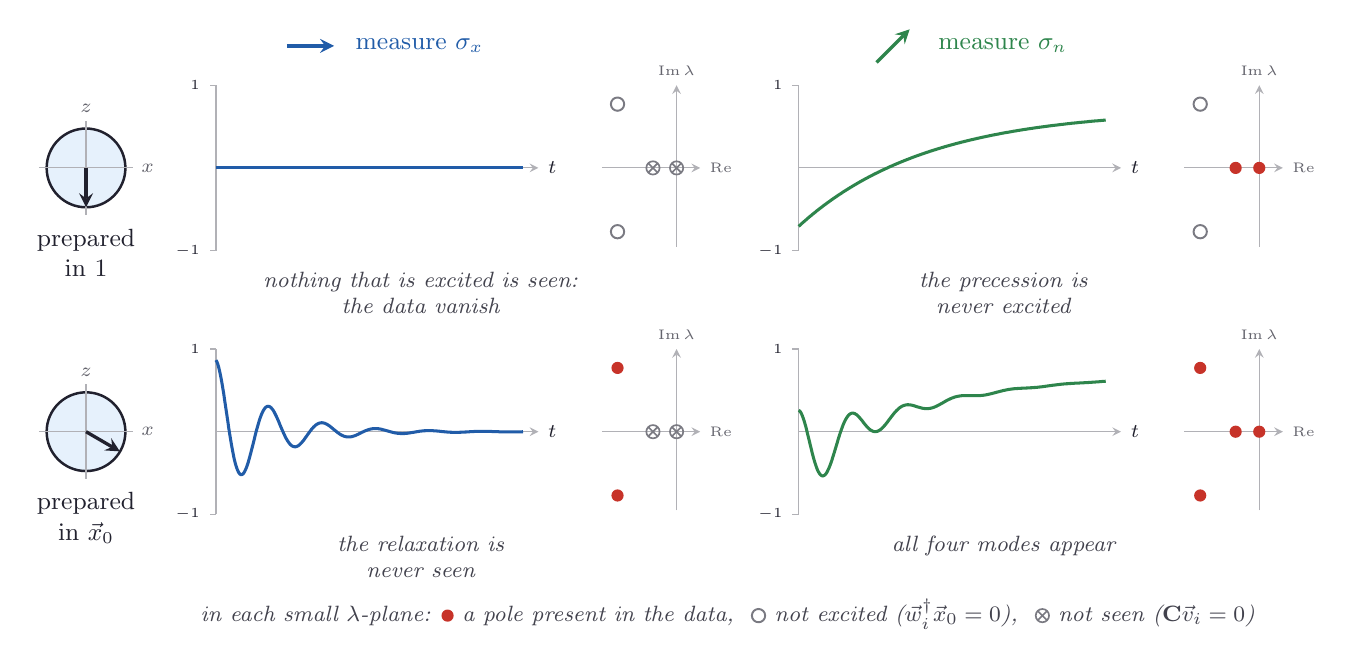
\begin{tikzpicture}[ink/.style={line width=0.9pt, ndInk}, faint/.style={line width=0.4pt, ndInk!35}, dashedink/.style={line width=0.5pt, ndInk!55, dash pattern=on 2.5pt off 2pt}, vec/.style={->, >=stealth, line width=1.2pt}, note/.style={font=\footnotesize\itshape, text=ndInk!85, align=center}, pointer/.style={->, >=stealth, line width=0.4pt, ndInk!60, shorten >=2pt, shorten <=1pt}, dot/.style={circle, fill=ndInk, inner sep=0pt, minimum size=3.4pt}, wash/.style={fill=ndSky, fill opacity=0.55}, every node/.style={text=ndInk}]
\definecolor{ndInk}{rgb}{0.13,0.13,0.18}
\definecolor{ndPaper}{rgb}{0.99,0.96,0.88}
\definecolor{ndSky}{rgb}{0.84,0.91,0.98}
\definecolor{ndRose}{rgb}{0.98,0.86,0.84}
\definecolor{ndBlue}{rgb}{0.13,0.36,0.66}
\definecolor{ndRed}{rgb}{0.78,0.20,0.16}
\definecolor{ndGold}{rgb}{0.88,0.62,0.10}
\definecolor{ndGreen}{rgb}{0.18,0.52,0.30}
\draw[vec, ndBlue] (3.30,6.15) -- (3.90,6.15);
\node[font=\small, text=ndBlue, anchor=west] at (4.05,6.15) {measure $\sigma_x$};
\draw[vec, ndGreen] (10.79,5.94) -- (11.21,6.36);
\node[font=\small, text=ndGreen, anchor=west] at (11.45,6.15) {measure $\sigma_n$};
\fill[ndSky, fill opacity=0.6] (0.75,4.60) circle (0.50);
\draw[ink] (0.75,4.60) circle (0.50);
\draw[faint] (0.15,4.60) -- (1.35,4.60) (0.75,4.00) -- (0.75,5.20);
\node[font=\scriptsize, text=ndInk!70, anchor=west] at (1.33,4.60) {$x$};
\node[font=\scriptsize, text=ndInk!70, anchor=south] at (0.75,5.18) {$z$};
\draw[vec, ndInk] (0.75,4.60) -- (0.75,4.10);
\node[font=\small, align=center, anchor=north] at (0.75,3.95) {prepared\\ in $\ket1$};
\draw[faint, ->, >=stealth] (2.400,4.600) -- (6.495,4.600) node[right, font=\scriptsize, text=ndInk] {$t$};
\draw[faint] (2.400,3.550) -- (2.400,5.650);
\draw[faint] (2.400,3.550) -- (2.319,3.550) node[left, font=\tiny, text=ndInk] {$-1$};
\draw[faint] (2.400,5.650) -- (2.319,5.650) node[left, font=\tiny, text=ndInk] {$1$};
\draw[line width=1.1pt, ndBlue] (2.400,4.600) -- (2.411,4.600) -- (2.422,4.600) -- (2.433,4.600) -- (2.443,4.600) -- (2.454,4.600) -- (2.465,4.600) -- (2.476,4.600) -- (2.487,4.600) -- (2.498,4.600) -- (2.508,4.600) -- (2.519,4.600) -- (2.530,4.600) -- (2.541,4.600) -- (2.552,4.600) -- (2.562,4.600) -- (2.573,4.600) -- (2.584,4.600) -- (2.595,4.600) -- (2.606,4.600) -- (2.617,4.600) -- (2.627,4.600) -- (2.638,4.600) -- (2.649,4.600) -- (2.660,4.600) -- (2.671,4.600) -- (2.682,4.600) -- (2.692,4.600) -- (2.703,4.600) -- (2.714,4.600) -- (2.725,4.600) -- (2.736,4.600) -- (2.747,4.600) -- (2.757,4.600) -- (2.768,4.600) -- (2.779,4.600) -- (2.790,4.600) -- (2.801,4.600) -- (2.812,4.600) -- (2.822,4.600) -- (2.833,4.600) -- (2.844,4.600) -- (2.855,4.600) -- (2.866,4.600) -- (2.877,4.600) -- (2.888,4.600) -- (2.898,4.600) -- (2.909,4.600) -- (2.920,4.600) -- (2.931,4.600) -- (2.942,4.600) -- (2.952,4.600) -- (2.963,4.600) -- (2.974,4.600) -- (2.985,4.600) -- (2.996,4.600) -- (3.007,4.600) -- (3.018,4.600) -- (3.028,4.600) -- (3.039,4.600) -- (3.050,4.600) -- (3.061,4.600) -- (3.072,4.600) -- (3.083,4.600) -- (3.093,4.600) -- (3.104,4.600) -- (3.115,4.600) -- (3.126,4.600) -- (3.137,4.600) -- (3.147,4.600) -- (3.158,4.600) -- (3.169,4.600) -- (3.180,4.600) -- (3.191,4.600) -- (3.202,4.600) -- (3.212,4.600) -- (3.223,4.600) -- (3.234,4.600) -- (3.245,4.600) -- (3.256,4.600) -- (3.267,4.600) -- (3.277,4.600) -- (3.288,4.600) -- (3.299,4.600) -- (3.310,4.600) -- (3.321,4.600) -- (3.332,4.600) -- (3.342,4.600) -- (3.353,4.600) -- (3.364,4.600) -- (3.375,4.600) -- (3.386,4.600) -- (3.397,4.600) -- (3.407,4.600) -- (3.418,4.600) -- (3.429,4.600) -- (3.440,4.600) -- (3.451,4.600) -- (3.462,4.600) -- (3.473,4.600) -- (3.483,4.600) -- (3.494,4.600) -- (3.505,4.600) -- (3.516,4.600) -- (3.527,4.600) -- (3.537,4.600) -- (3.548,4.600) -- (3.559,4.600) -- (3.570,4.600) -- (3.581,4.600) -- (3.592,4.600) -- (3.603,4.600) -- (3.613,4.600) -- (3.624,4.600) -- (3.635,4.600) -- (3.646,4.600) -- (3.657,4.600) -- (3.667,4.600) -- (3.678,4.600) -- (3.689,4.600) -- (3.700,4.600) -- (3.711,4.600) -- (3.722,4.600) -- (3.732,4.600) -- (3.743,4.600) -- (3.754,4.600) -- (3.765,4.600) -- (3.776,4.600) -- (3.787,4.600) -- (3.797,4.600) -- (3.808,4.600) -- (3.819,4.600) -- (3.830,4.600) -- (3.841,4.600) -- (3.852,4.600) -- (3.862,4.600) -- (3.873,4.600) -- (3.884,4.600) -- (3.895,4.600) -- (3.906,4.600) -- (3.917,4.600) -- (3.928,4.600) -- (3.938,4.600) -- (3.949,4.600) -- (3.960,4.600) -- (3.971,4.600) -- (3.982,4.600) -- (3.993,4.600) -- (4.003,4.600) -- (4.014,4.600) -- (4.025,4.600) -- (4.036,4.600) -- (4.047,4.600) -- (4.058,4.600) -- (4.068,4.600) -- (4.079,4.600) -- (4.090,4.600) -- (4.101,4.600) -- (4.112,4.600) -- (4.122,4.600) -- (4.133,4.600) -- (4.144,4.600) -- (4.155,4.600) -- (4.166,4.600) -- (4.177,4.600) -- (4.188,4.600) -- (4.198,4.600) -- (4.209,4.600) -- (4.220,4.600) -- (4.231,4.600) -- (4.242,4.600) -- (4.252,4.600) -- (4.263,4.600) -- (4.274,4.600) -- (4.285,4.600) -- (4.296,4.600) -- (4.307,4.600) -- (4.317,4.600) -- (4.328,4.600) -- (4.339,4.600) -- (4.350,4.600) -- (4.361,4.600) -- (4.372,4.600) -- (4.383,4.600) -- (4.393,4.600) -- (4.404,4.600) -- (4.415,4.600) -- (4.426,4.600) -- (4.437,4.600) -- (4.447,4.600) -- (4.458,4.600) -- (4.469,4.600) -- (4.480,4.600) -- (4.491,4.600) -- (4.502,4.600) -- (4.513,4.600) -- (4.523,4.600) -- (4.534,4.600) -- (4.545,4.600) -- (4.556,4.600) -- (4.567,4.600) -- (4.578,4.600) -- (4.588,4.600) -- (4.599,4.600) -- (4.610,4.600) -- (4.621,4.600) -- (4.632,4.600) -- (4.643,4.600) -- (4.653,4.600) -- (4.664,4.600) -- (4.675,4.600) -- (4.686,4.600) -- (4.697,4.600) -- (4.707,4.600) -- (4.718,4.600) -- (4.729,4.600) -- (4.740,4.600) -- (4.751,4.600) -- (4.762,4.600) -- (4.772,4.600) -- (4.783,4.600) -- (4.794,4.600) -- (4.805,4.600) -- (4.816,4.600) -- (4.827,4.600) -- (4.838,4.600) -- (4.848,4.600) -- (4.859,4.600) -- (4.870,4.600) -- (4.881,4.600) -- (4.892,4.600) -- (4.902,4.600) -- (4.913,4.600) -- (4.924,4.600) -- (4.935,4.600) -- (4.946,4.600) -- (4.957,4.600) -- (4.967,4.600) -- (4.978,4.600) -- (4.989,4.600) -- (5.000,4.600) -- (5.011,4.600) -- (5.022,4.600) -- (5.032,4.600) -- (5.043,4.600) -- (5.054,4.600) -- (5.065,4.600) -- (5.076,4.600) -- (5.087,4.600) -- (5.098,4.600) -- (5.108,4.600) -- (5.119,4.600) -- (5.130,4.600) -- (5.141,4.600) -- (5.152,4.600) -- (5.162,4.600) -- (5.173,4.600) -- (5.184,4.600) -- (5.195,4.600) -- (5.206,4.600) -- (5.217,4.600) -- (5.227,4.600) -- (5.238,4.600) -- (5.249,4.600) -- (5.260,4.600) -- (5.271,4.600) -- (5.282,4.600) -- (5.293,4.600) -- (5.303,4.600) -- (5.314,4.600) -- (5.325,4.600) -- (5.336,4.600) -- (5.347,4.600) -- (5.357,4.600) -- (5.368,4.600) -- (5.379,4.600) -- (5.390,4.600) -- (5.401,4.600) -- (5.412,4.600) -- (5.423,4.600) -- (5.433,4.600) -- (5.444,4.600) -- (5.455,4.600) -- (5.466,4.600) -- (5.477,4.600) -- (5.487,4.600) -- (5.498,4.600) -- (5.509,4.600) -- (5.520,4.600) -- (5.531,4.600) -- (5.542,4.600) -- (5.553,4.600) -- (5.563,4.600) -- (5.574,4.600) -- (5.585,4.600) -- (5.596,4.600) -- (5.607,4.600) -- (5.617,4.600) -- (5.628,4.600) -- (5.639,4.600) -- (5.650,4.600) -- (5.661,4.600) -- (5.672,4.600) -- (5.683,4.600) -- (5.693,4.600) -- (5.704,4.600) -- (5.715,4.600) -- (5.726,4.600) -- (5.737,4.600) -- (5.748,4.600) -- (5.758,4.600) -- (5.769,4.600) -- (5.780,4.600) -- (5.791,4.600) -- (5.802,4.600) -- (5.812,4.600) -- (5.823,4.600) -- (5.834,4.600) -- (5.845,4.600) -- (5.856,4.600) -- (5.867,4.600) -- (5.877,4.600) -- (5.888,4.600) -- (5.899,4.600) -- (5.910,4.600) -- (5.921,4.600) -- (5.932,4.600) -- (5.943,4.600) -- (5.953,4.600) -- (5.964,4.600) -- (5.975,4.600) -- (5.986,4.600) -- (5.997,4.600) -- (6.008,4.600) -- (6.018,4.600) -- (6.029,4.600) -- (6.040,4.600) -- (6.051,4.600) -- (6.062,4.600) -- (6.072,4.600) -- (6.083,4.600) -- (6.094,4.600) -- (6.105,4.600) -- (6.116,4.600) -- (6.127,4.600) -- (6.138,4.600) -- (6.148,4.600) -- (6.159,4.600) -- (6.170,4.600) -- (6.181,4.600) -- (6.192,4.600) -- (6.202,4.600) -- (6.213,4.600) -- (6.224,4.600) -- (6.235,4.600) -- (6.246,4.600) -- (6.257,4.600) -- (6.268,4.600) -- (6.278,4.600) -- (6.289,4.600) -- (6.300,4.600);
\draw[faint, ->, >=stealth] (7.30,4.60) -- (8.55,4.60) node[right, font=\tiny, text=ndInk!70] {Re};
\draw[faint, ->, >=stealth] (8.25,3.60) -- (8.25,5.65) node[above, font=\tiny, text=ndInk!70] {Im\,$\lambda$};
\draw[line width=0.7pt, ndInk!60, fill=white] (7.500,5.410) circle (2.4pt);
\draw[line width=0.7pt, ndInk!60, fill=white] (7.500,3.790) circle (2.4pt);
\draw[line width=0.6pt, ndInk!60] (7.950,4.600) circle (2.4pt) (7.890,4.540) -- (8.010,4.660) (7.890,4.660) -- (8.010,4.540);
\draw[line width=0.6pt, ndInk!60] (8.250,4.600) circle (2.4pt) (8.190,4.540) -- (8.310,4.660) (8.190,4.660) -- (8.310,4.540);
\node[note, anchor=north] at (5.00,3.40) {nothing that is excited is seen:\\ the data vanish};
\draw[faint, ->, >=stealth] (9.800,4.600) -- (13.895,4.600) node[right, font=\scriptsize, text=ndInk] {$t$};
\draw[faint] (9.800,3.550) -- (9.800,5.650);
\draw[faint] (9.800,3.550) -- (9.719,3.550) node[left, font=\tiny, text=ndInk] {$-1$};
\draw[faint] (9.800,5.650) -- (9.719,5.650) node[left, font=\tiny, text=ndInk] {$1$};
\draw[line width=1.1pt, ndGreen] (9.800,3.858) -- (9.811,3.867) -- (9.822,3.877) -- (9.833,3.887) -- (9.843,3.897) -- (9.854,3.906) -- (9.865,3.916) -- (9.876,3.925) -- (9.887,3.935) -- (9.898,3.944) -- (9.908,3.953) -- (9.919,3.963) -- (9.930,3.972) -- (9.941,3.981) -- (9.952,3.990) -- (9.963,3.999) -- (9.973,4.008) -- (9.984,4.017) -- (9.995,4.025) -- (10.006,4.034) -- (10.017,4.043) -- (10.027,4.052) -- (10.038,4.060) -- (10.049,4.069) -- (10.060,4.077) -- (10.071,4.086) -- (10.082,4.094) -- (10.093,4.102) -- (10.103,4.110) -- (10.114,4.119) -- (10.125,4.127) -- (10.136,4.135) -- (10.147,4.143) -- (10.158,4.151) -- (10.168,4.159) -- (10.179,4.167) -- (10.190,4.174) -- (10.201,4.182) -- (10.212,4.190) -- (10.223,4.198) -- (10.233,4.205) -- (10.244,4.213) -- (10.255,4.220) -- (10.266,4.228) -- (10.277,4.235) -- (10.288,4.242) -- (10.298,4.250) -- (10.309,4.257) -- (10.320,4.264) -- (10.331,4.271) -- (10.342,4.278) -- (10.353,4.286) -- (10.363,4.293) -- (10.374,4.300) -- (10.385,4.306) -- (10.396,4.313) -- (10.407,4.320) -- (10.418,4.327) -- (10.428,4.334) -- (10.439,4.340) -- (10.450,4.347) -- (10.461,4.354) -- (10.472,4.360) -- (10.483,4.367) -- (10.493,4.373) -- (10.504,4.380) -- (10.515,4.386) -- (10.526,4.392) -- (10.537,4.399) -- (10.548,4.405) -- (10.558,4.411) -- (10.569,4.417) -- (10.580,4.424) -- (10.591,4.430) -- (10.602,4.436) -- (10.613,4.442) -- (10.623,4.448) -- (10.634,4.454) -- (10.645,4.460) -- (10.656,4.466) -- (10.667,4.471) -- (10.678,4.477) -- (10.688,4.483) -- (10.699,4.489) -- (10.710,4.494) -- (10.721,4.500) -- (10.732,4.505) -- (10.743,4.511) -- (10.753,4.517) -- (10.764,4.522) -- (10.775,4.528) -- (10.786,4.533) -- (10.797,4.538) -- (10.808,4.544) -- (10.818,4.549) -- (10.829,4.554) -- (10.840,4.559) -- (10.851,4.565) -- (10.862,4.570) -- (10.873,4.575) -- (10.883,4.580) -- (10.894,4.585) -- (10.905,4.590) -- (10.916,4.595) -- (10.927,4.600) -- (10.938,4.605) -- (10.948,4.610) -- (10.959,4.615) -- (10.970,4.620) -- (10.981,4.624) -- (10.992,4.629) -- (11.003,4.634) -- (11.013,4.639) -- (11.024,4.643) -- (11.035,4.648) -- (11.046,4.653) -- (11.057,4.657) -- (11.068,4.662) -- (11.078,4.666) -- (11.089,4.671) -- (11.100,4.675) -- (11.111,4.680) -- (11.122,4.684) -- (11.133,4.688) -- (11.143,4.693) -- (11.154,4.697) -- (11.165,4.701) -- (11.176,4.706) -- (11.187,4.710) -- (11.198,4.714) -- (11.208,4.718) -- (11.219,4.722) -- (11.230,4.727) -- (11.241,4.731) -- (11.252,4.735) -- (11.263,4.739) -- (11.273,4.743) -- (11.284,4.747) -- (11.295,4.751) -- (11.306,4.755) -- (11.317,4.759) -- (11.328,4.762) -- (11.338,4.766) -- (11.349,4.770) -- (11.360,4.774) -- (11.371,4.778) -- (11.382,4.781) -- (11.393,4.785) -- (11.403,4.789) -- (11.414,4.793) -- (11.425,4.796) -- (11.436,4.800) -- (11.447,4.803) -- (11.458,4.807) -- (11.468,4.811) -- (11.479,4.814) -- (11.490,4.818) -- (11.501,4.821) -- (11.512,4.825) -- (11.523,4.828) -- (11.533,4.831) -- (11.544,4.835) -- (11.555,4.838) -- (11.566,4.842) -- (11.577,4.845) -- (11.588,4.848) -- (11.598,4.851) -- (11.609,4.855) -- (11.620,4.858) -- (11.631,4.861) -- (11.642,4.864) -- (11.652,4.868) -- (11.663,4.871) -- (11.674,4.874) -- (11.685,4.877) -- (11.696,4.880) -- (11.707,4.883) -- (11.718,4.886) -- (11.728,4.889) -- (11.739,4.892) -- (11.750,4.895) -- (11.761,4.898) -- (11.772,4.901) -- (11.783,4.904) -- (11.793,4.907) -- (11.804,4.910) -- (11.815,4.913) -- (11.826,4.916) -- (11.837,4.918) -- (11.848,4.921) -- (11.858,4.924) -- (11.869,4.927) -- (11.880,4.930) -- (11.891,4.932) -- (11.902,4.935) -- (11.913,4.938) -- (11.923,4.940) -- (11.934,4.943) -- (11.945,4.946) -- (11.956,4.948) -- (11.967,4.951) -- (11.978,4.954) -- (11.988,4.956) -- (11.999,4.959) -- (12.010,4.961) -- (12.021,4.964) -- (12.032,4.966) -- (12.043,4.969) -- (12.053,4.971) -- (12.064,4.974) -- (12.075,4.976) -- (12.086,4.979) -- (12.097,4.981) -- (12.108,4.984) -- (12.118,4.986) -- (12.129,4.988) -- (12.140,4.991) -- (12.151,4.993) -- (12.162,4.995) -- (12.173,4.998) -- (12.183,5.000) -- (12.194,5.002) -- (12.205,5.004) -- (12.216,5.007) -- (12.227,5.009) -- (12.238,5.011) -- (12.248,5.013) -- (12.259,5.016) -- (12.270,5.018) -- (12.281,5.020) -- (12.292,5.022) -- (12.303,5.024) -- (12.313,5.026) -- (12.324,5.028) -- (12.335,5.030) -- (12.346,5.032) -- (12.357,5.035) -- (12.367,5.037) -- (12.378,5.039) -- (12.389,5.041) -- (12.400,5.043) -- (12.411,5.045) -- (12.422,5.047) -- (12.433,5.049) -- (12.443,5.051) -- (12.454,5.052) -- (12.465,5.054) -- (12.476,5.056) -- (12.487,5.058) -- (12.498,5.060) -- (12.508,5.062) -- (12.519,5.064) -- (12.530,5.066) -- (12.541,5.068) -- (12.552,5.069) -- (12.562,5.071) -- (12.573,5.073) -- (12.584,5.075) -- (12.595,5.077) -- (12.606,5.078) -- (12.617,5.080) -- (12.628,5.082) -- (12.638,5.084) -- (12.649,5.085) -- (12.660,5.087) -- (12.671,5.089) -- (12.682,5.090) -- (12.693,5.092) -- (12.703,5.094) -- (12.714,5.095) -- (12.725,5.097) -- (12.736,5.099) -- (12.747,5.100) -- (12.758,5.102) -- (12.768,5.103) -- (12.779,5.105) -- (12.790,5.107) -- (12.801,5.108) -- (12.812,5.110) -- (12.823,5.111) -- (12.833,5.113) -- (12.844,5.114) -- (12.855,5.116) -- (12.866,5.117) -- (12.877,5.119) -- (12.888,5.120) -- (12.898,5.122) -- (12.909,5.123) -- (12.920,5.125) -- (12.931,5.126) -- (12.942,5.128) -- (12.953,5.129) -- (12.963,5.130) -- (12.974,5.132) -- (12.985,5.133) -- (12.996,5.135) -- (13.007,5.136) -- (13.018,5.137) -- (13.028,5.139) -- (13.039,5.140) -- (13.050,5.141) -- (13.061,5.143) -- (13.072,5.144) -- (13.083,5.145) -- (13.093,5.147) -- (13.104,5.148) -- (13.115,5.149) -- (13.126,5.151) -- (13.137,5.152) -- (13.148,5.153) -- (13.158,5.154) -- (13.169,5.156) -- (13.180,5.157) -- (13.191,5.158) -- (13.202,5.159) -- (13.213,5.161) -- (13.223,5.162) -- (13.234,5.163) -- (13.245,5.164) -- (13.256,5.165) -- (13.267,5.167) -- (13.277,5.168) -- (13.288,5.169) -- (13.299,5.170) -- (13.310,5.171) -- (13.321,5.172) -- (13.332,5.173) -- (13.343,5.175) -- (13.353,5.176) -- (13.364,5.177) -- (13.375,5.178) -- (13.386,5.179) -- (13.397,5.180) -- (13.408,5.181) -- (13.418,5.182) -- (13.429,5.183) -- (13.440,5.184) -- (13.451,5.185) -- (13.462,5.186) -- (13.473,5.188) -- (13.483,5.189) -- (13.494,5.190) -- (13.505,5.191) -- (13.516,5.192) -- (13.527,5.193) -- (13.538,5.194) -- (13.548,5.195) -- (13.559,5.196) -- (13.570,5.197) -- (13.581,5.198) -- (13.592,5.198) -- (13.603,5.199) -- (13.613,5.200) -- (13.624,5.201) -- (13.635,5.202) -- (13.646,5.203) -- (13.657,5.204) -- (13.668,5.205) -- (13.678,5.206) -- (13.689,5.207) -- (13.700,5.208);
\draw[faint, ->, >=stealth] (14.70,4.60) -- (15.95,4.60) node[right, font=\tiny, text=ndInk!70] {Re};
\draw[faint, ->, >=stealth] (15.65,3.60) -- (15.65,5.65) node[above, font=\tiny, text=ndInk!70] {Im\,$\lambda$};
\draw[line width=0.7pt, ndInk!60, fill=white] (14.900,5.410) circle (2.4pt);
\draw[line width=0.7pt, ndInk!60, fill=white] (14.900,3.790) circle (2.4pt);
\fill[ndRed] (15.350,4.600) circle (2.2pt);
\fill[ndRed] (15.650,4.600) circle (2.2pt);
\node[note, anchor=north] at (12.40,3.40) {the precession is\\ never excited};
\fill[ndSky, fill opacity=0.6] (0.75,1.25) circle (0.50);
\draw[ink] (0.75,1.25) circle (0.50);
\draw[faint] (0.15,1.25) -- (1.35,1.25) (0.75,0.65) -- (0.75,1.85);
\node[font=\scriptsize, text=ndInk!70, anchor=west] at (1.33,1.25) {$x$};
\node[font=\scriptsize, text=ndInk!70, anchor=south] at (0.75,1.83) {$z$};
\draw[vec, ndInk] (0.75,1.25) -- (1.18,1.00);
\node[font=\small, align=center, anchor=north] at (0.75,0.60) {prepared\\ in $\vec x_0$};
\draw[faint, ->, >=stealth] (2.400,1.250) -- (6.495,1.250) node[right, font=\scriptsize, text=ndInk] {$t$};
\draw[faint] (2.400,0.200) -- (2.400,2.300);
\draw[faint] (2.400,0.200) -- (2.319,0.200) node[left, font=\tiny, text=ndInk] {$-1$};
\draw[faint] (2.400,2.300) -- (2.319,2.300) node[left, font=\tiny, text=ndInk] {$1$};
\draw[line width=1.1pt, ndBlue] (2.400,2.159) -- (2.411,2.140) -- (2.422,2.112) -- (2.433,2.076) -- (2.443,2.034) -- (2.454,1.984) -- (2.465,1.929) -- (2.476,1.869) -- (2.487,1.804) -- (2.498,1.737) -- (2.508,1.666) -- (2.519,1.593) -- (2.530,1.520) -- (2.541,1.446) -- (2.552,1.372) -- (2.562,1.300) -- (2.573,1.230) -- (2.584,1.162) -- (2.595,1.097) -- (2.606,1.036) -- (2.617,0.979) -- (2.627,0.926) -- (2.638,0.879) -- (2.649,0.837) -- (2.660,0.801) -- (2.671,0.770) -- (2.682,0.745) -- (2.692,0.726) -- (2.703,0.713) -- (2.714,0.705) -- (2.725,0.704) -- (2.736,0.708) -- (2.747,0.717) -- (2.757,0.732) -- (2.768,0.751) -- (2.779,0.775) -- (2.790,0.802) -- (2.801,0.834) -- (2.812,0.868) -- (2.822,0.905) -- (2.833,0.945) -- (2.844,0.986) -- (2.855,1.029) -- (2.866,1.072) -- (2.877,1.116) -- (2.888,1.159) -- (2.898,1.203) -- (2.909,1.245) -- (2.920,1.286) -- (2.931,1.325) -- (2.942,1.362) -- (2.952,1.397) -- (2.963,1.429) -- (2.974,1.458) -- (2.985,1.485) -- (2.996,1.508) -- (3.007,1.527) -- (3.018,1.544) -- (3.028,1.556) -- (3.039,1.565) -- (3.050,1.571) -- (3.061,1.573) -- (3.072,1.572) -- (3.083,1.568) -- (3.093,1.561) -- (3.104,1.551) -- (3.115,1.538) -- (3.126,1.522) -- (3.137,1.505) -- (3.147,1.485) -- (3.158,1.463) -- (3.169,1.441) -- (3.180,1.417) -- (3.191,1.392) -- (3.202,1.366) -- (3.212,1.340) -- (3.223,1.314) -- (3.234,1.289) -- (3.245,1.263) -- (3.256,1.239) -- (3.267,1.215) -- (3.277,1.193) -- (3.288,1.171) -- (3.299,1.152) -- (3.310,1.134) -- (3.321,1.117) -- (3.332,1.103) -- (3.342,1.090) -- (3.353,1.080) -- (3.364,1.071) -- (3.375,1.065) -- (3.386,1.061) -- (3.397,1.059) -- (3.407,1.058) -- (3.418,1.060) -- (3.429,1.064) -- (3.440,1.069) -- (3.451,1.076) -- (3.462,1.085) -- (3.473,1.095) -- (3.483,1.106) -- (3.494,1.118) -- (3.505,1.131) -- (3.516,1.145) -- (3.527,1.160) -- (3.537,1.175) -- (3.548,1.190) -- (3.559,1.205) -- (3.570,1.221) -- (3.581,1.236) -- (3.592,1.251) -- (3.603,1.265) -- (3.613,1.279) -- (3.624,1.291) -- (3.635,1.304) -- (3.646,1.315) -- (3.657,1.325) -- (3.667,1.334) -- (3.678,1.342) -- (3.689,1.348) -- (3.700,1.354) -- (3.711,1.358) -- (3.722,1.361) -- (3.732,1.363) -- (3.743,1.364) -- (3.754,1.363) -- (3.765,1.361) -- (3.776,1.359) -- (3.787,1.355) -- (3.797,1.350) -- (3.808,1.345) -- (3.819,1.338) -- (3.830,1.331) -- (3.841,1.324) -- (3.852,1.316) -- (3.862,1.307) -- (3.873,1.298) -- (3.884,1.289) -- (3.895,1.280) -- (3.906,1.271) -- (3.917,1.262) -- (3.928,1.253) -- (3.938,1.245) -- (3.949,1.236) -- (3.960,1.229) -- (3.971,1.221) -- (3.982,1.214) -- (3.993,1.208) -- (4.003,1.203) -- (4.014,1.198) -- (4.025,1.193) -- (4.036,1.190) -- (4.047,1.187) -- (4.058,1.185) -- (4.068,1.183) -- (4.079,1.183) -- (4.090,1.183) -- (4.101,1.184) -- (4.112,1.185) -- (4.122,1.187) -- (4.133,1.189) -- (4.144,1.193) -- (4.155,1.196) -- (4.166,1.200) -- (4.177,1.204) -- (4.188,1.209) -- (4.198,1.214) -- (4.209,1.219) -- (4.220,1.225) -- (4.231,1.230) -- (4.242,1.235) -- (4.252,1.241) -- (4.263,1.246) -- (4.274,1.251) -- (4.285,1.256) -- (4.296,1.261) -- (4.307,1.265) -- (4.317,1.269) -- (4.328,1.273) -- (4.339,1.277) -- (4.350,1.280) -- (4.361,1.283) -- (4.372,1.285) -- (4.383,1.287) -- (4.393,1.288) -- (4.404,1.289) -- (4.415,1.290) -- (4.426,1.290) -- (4.437,1.290) -- (4.447,1.289) -- (4.458,1.288) -- (4.469,1.287) -- (4.480,1.285) -- (4.491,1.283) -- (4.502,1.281) -- (4.513,1.278) -- (4.523,1.275) -- (4.534,1.272) -- (4.545,1.269) -- (4.556,1.266) -- (4.567,1.263) -- (4.578,1.260) -- (4.588,1.257) -- (4.599,1.254) -- (4.610,1.251) -- (4.621,1.248) -- (4.632,1.245) -- (4.643,1.242) -- (4.653,1.239) -- (4.664,1.237) -- (4.675,1.235) -- (4.686,1.233) -- (4.697,1.231) -- (4.707,1.230) -- (4.718,1.229) -- (4.729,1.228) -- (4.740,1.227) -- (4.751,1.227) -- (4.762,1.226) -- (4.772,1.226) -- (4.783,1.227) -- (4.794,1.227) -- (4.805,1.228) -- (4.816,1.229) -- (4.827,1.230) -- (4.838,1.231) -- (4.848,1.233) -- (4.859,1.234) -- (4.870,1.236) -- (4.881,1.238) -- (4.892,1.240) -- (4.902,1.241) -- (4.913,1.243) -- (4.924,1.245) -- (4.935,1.247) -- (4.946,1.249) -- (4.957,1.251) -- (4.967,1.252) -- (4.978,1.254) -- (4.989,1.256) -- (5.000,1.257) -- (5.011,1.258) -- (5.022,1.260) -- (5.032,1.261) -- (5.043,1.262) -- (5.054,1.262) -- (5.065,1.263) -- (5.076,1.263) -- (5.087,1.264) -- (5.098,1.264) -- (5.108,1.264) -- (5.119,1.264) -- (5.130,1.264) -- (5.141,1.263) -- (5.152,1.263) -- (5.162,1.262) -- (5.173,1.261) -- (5.184,1.261) -- (5.195,1.260) -- (5.206,1.259) -- (5.217,1.258) -- (5.227,1.257) -- (5.238,1.256) -- (5.249,1.254) -- (5.260,1.253) -- (5.271,1.252) -- (5.282,1.251) -- (5.293,1.250) -- (5.303,1.249) -- (5.314,1.248) -- (5.325,1.247) -- (5.336,1.246) -- (5.347,1.245) -- (5.357,1.245) -- (5.368,1.244) -- (5.379,1.243) -- (5.390,1.243) -- (5.401,1.242) -- (5.412,1.242) -- (5.423,1.242) -- (5.433,1.242) -- (5.444,1.242) -- (5.455,1.242) -- (5.466,1.242) -- (5.477,1.242) -- (5.487,1.242) -- (5.498,1.243) -- (5.509,1.243) -- (5.520,1.244) -- (5.531,1.244) -- (5.542,1.245) -- (5.553,1.245) -- (5.563,1.246) -- (5.574,1.246) -- (5.585,1.247) -- (5.596,1.248) -- (5.607,1.248) -- (5.617,1.249) -- (5.628,1.250) -- (5.639,1.250) -- (5.650,1.251) -- (5.661,1.252) -- (5.672,1.252) -- (5.683,1.253) -- (5.693,1.253) -- (5.704,1.253) -- (5.715,1.254) -- (5.726,1.254) -- (5.737,1.254) -- (5.748,1.255) -- (5.758,1.255) -- (5.769,1.255) -- (5.780,1.255) -- (5.791,1.255) -- (5.802,1.255) -- (5.812,1.255) -- (5.823,1.255) -- (5.834,1.254) -- (5.845,1.254) -- (5.856,1.254) -- (5.867,1.254) -- (5.877,1.253) -- (5.888,1.253) -- (5.899,1.253) -- (5.910,1.252) -- (5.921,1.252) -- (5.932,1.251) -- (5.943,1.251) -- (5.953,1.251) -- (5.964,1.250) -- (5.975,1.250) -- (5.986,1.250) -- (5.997,1.249) -- (6.008,1.249) -- (6.018,1.249) -- (6.029,1.248) -- (6.040,1.248) -- (6.051,1.248) -- (6.062,1.248) -- (6.072,1.247) -- (6.083,1.247) -- (6.094,1.247) -- (6.105,1.247) -- (6.116,1.247) -- (6.127,1.247) -- (6.138,1.247) -- (6.148,1.247) -- (6.159,1.247) -- (6.170,1.247) -- (6.181,1.247) -- (6.192,1.248) -- (6.202,1.248) -- (6.213,1.248) -- (6.224,1.248) -- (6.235,1.248) -- (6.246,1.249) -- (6.257,1.249) -- (6.268,1.249) -- (6.278,1.249) -- (6.289,1.249) -- (6.300,1.250);
\draw[faint, ->, >=stealth] (7.30,1.25) -- (8.55,1.25) node[right, font=\tiny, text=ndInk!70] {Re};
\draw[faint, ->, >=stealth] (8.25,0.25) -- (8.25,2.30) node[above, font=\tiny, text=ndInk!70] {Im\,$\lambda$};
\fill[ndRed] (7.500,2.060) circle (2.2pt);
\fill[ndRed] (7.500,0.440) circle (2.2pt);
\draw[line width=0.6pt, ndInk!60] (7.950,1.250) circle (2.4pt) (7.890,1.190) -- (8.010,1.310) (7.890,1.310) -- (8.010,1.190);
\draw[line width=0.6pt, ndInk!60] (8.250,1.250) circle (2.4pt) (8.190,1.190) -- (8.310,1.310) (8.190,1.310) -- (8.310,1.190);
\node[note, anchor=north] at (5.00,0.05) {the relaxation is\\ never seen};
\draw[faint, ->, >=stealth] (9.800,1.250) -- (13.895,1.250) node[right, font=\scriptsize, text=ndInk] {$t$};
\draw[faint] (9.800,0.200) -- (9.800,2.300);
\draw[faint] (9.800,0.200) -- (9.719,0.200) node[left, font=\tiny, text=ndInk] {$-1$};
\draw[faint] (9.800,2.300) -- (9.719,2.300) node[left, font=\tiny, text=ndInk] {$1$};
\draw[line width=1.1pt, ndGreen] (9.800,1.522) -- (9.811,1.515) -- (9.822,1.503) -- (9.833,1.485) -- (9.843,1.462) -- (9.854,1.434) -- (9.865,1.403) -- (9.876,1.367) -- (9.887,1.329) -- (9.898,1.288) -- (9.908,1.245) -- (9.919,1.200) -- (9.930,1.155) -- (9.941,1.110) -- (9.952,1.065) -- (9.963,1.020) -- (9.973,0.977) -- (9.984,0.936) -- (9.995,0.896) -- (10.006,0.860) -- (10.017,0.826) -- (10.027,0.796) -- (10.038,0.768) -- (10.049,0.745) -- (10.060,0.726) -- (10.071,0.710) -- (10.082,0.699) -- (10.093,0.692) -- (10.103,0.688) -- (10.114,0.690) -- (10.125,0.695) -- (10.136,0.703) -- (10.147,0.716) -- (10.158,0.732) -- (10.168,0.752) -- (10.179,0.775) -- (10.190,0.800) -- (10.201,0.828) -- (10.212,0.858) -- (10.223,0.890) -- (10.233,0.924) -- (10.244,0.958) -- (10.255,0.994) -- (10.266,1.030) -- (10.277,1.067) -- (10.288,1.103) -- (10.298,1.139) -- (10.309,1.175) -- (10.320,1.209) -- (10.331,1.242) -- (10.342,1.274) -- (10.353,1.304) -- (10.363,1.332) -- (10.374,1.358) -- (10.385,1.381) -- (10.396,1.403) -- (10.407,1.422) -- (10.418,1.438) -- (10.428,1.452) -- (10.439,1.464) -- (10.450,1.473) -- (10.461,1.480) -- (10.472,1.484) -- (10.483,1.486) -- (10.493,1.485) -- (10.504,1.483) -- (10.515,1.479) -- (10.526,1.472) -- (10.537,1.465) -- (10.548,1.455) -- (10.558,1.445) -- (10.569,1.434) -- (10.580,1.421) -- (10.591,1.408) -- (10.602,1.395) -- (10.613,1.381) -- (10.623,1.367) -- (10.634,1.353) -- (10.645,1.340) -- (10.656,1.327) -- (10.667,1.314) -- (10.678,1.303) -- (10.688,1.292) -- (10.699,1.283) -- (10.710,1.274) -- (10.721,1.267) -- (10.732,1.261) -- (10.743,1.256) -- (10.753,1.253) -- (10.764,1.251) -- (10.775,1.251) -- (10.786,1.252) -- (10.797,1.254) -- (10.808,1.258) -- (10.818,1.263) -- (10.829,1.270) -- (10.840,1.277) -- (10.851,1.286) -- (10.862,1.296) -- (10.873,1.307) -- (10.883,1.319) -- (10.894,1.331) -- (10.905,1.344) -- (10.916,1.358) -- (10.927,1.372) -- (10.938,1.386) -- (10.948,1.401) -- (10.959,1.415) -- (10.970,1.430) -- (10.981,1.444) -- (10.992,1.458) -- (11.003,1.472) -- (11.013,1.485) -- (11.024,1.497) -- (11.035,1.509) -- (11.046,1.521) -- (11.057,1.531) -- (11.068,1.541) -- (11.078,1.550) -- (11.089,1.558) -- (11.100,1.565) -- (11.111,1.572) -- (11.122,1.577) -- (11.133,1.582) -- (11.143,1.585) -- (11.154,1.588) -- (11.165,1.590) -- (11.176,1.592) -- (11.187,1.592) -- (11.198,1.592) -- (11.208,1.591) -- (11.219,1.590) -- (11.230,1.588) -- (11.241,1.586) -- (11.252,1.583) -- (11.263,1.580) -- (11.273,1.577) -- (11.284,1.573) -- (11.295,1.570) -- (11.306,1.566) -- (11.317,1.563) -- (11.328,1.560) -- (11.338,1.557) -- (11.349,1.554) -- (11.360,1.551) -- (11.371,1.549) -- (11.382,1.546) -- (11.393,1.545) -- (11.403,1.544) -- (11.414,1.543) -- (11.425,1.543) -- (11.436,1.543) -- (11.447,1.544) -- (11.458,1.545) -- (11.468,1.546) -- (11.479,1.549) -- (11.490,1.551) -- (11.501,1.554) -- (11.512,1.558) -- (11.523,1.562) -- (11.533,1.566) -- (11.544,1.571) -- (11.555,1.576) -- (11.566,1.582) -- (11.577,1.587) -- (11.588,1.593) -- (11.598,1.599) -- (11.609,1.605) -- (11.620,1.611) -- (11.631,1.617) -- (11.642,1.623) -- (11.652,1.630) -- (11.663,1.636) -- (11.674,1.642) -- (11.685,1.648) -- (11.696,1.653) -- (11.707,1.659) -- (11.718,1.664) -- (11.728,1.669) -- (11.739,1.674) -- (11.750,1.678) -- (11.761,1.682) -- (11.772,1.686) -- (11.783,1.690) -- (11.793,1.693) -- (11.804,1.696) -- (11.815,1.698) -- (11.826,1.700) -- (11.837,1.702) -- (11.848,1.704) -- (11.858,1.705) -- (11.869,1.707) -- (11.880,1.707) -- (11.891,1.708) -- (11.902,1.709) -- (11.913,1.709) -- (11.923,1.709) -- (11.934,1.709) -- (11.945,1.709) -- (11.956,1.709) -- (11.967,1.708) -- (11.978,1.708) -- (11.988,1.708) -- (11.999,1.707) -- (12.010,1.707) -- (12.021,1.707) -- (12.032,1.707) -- (12.043,1.707) -- (12.053,1.707) -- (12.064,1.707) -- (12.075,1.707) -- (12.086,1.708) -- (12.097,1.708) -- (12.108,1.709) -- (12.118,1.710) -- (12.129,1.711) -- (12.140,1.712) -- (12.151,1.714) -- (12.162,1.715) -- (12.173,1.717) -- (12.183,1.719) -- (12.194,1.721) -- (12.205,1.723) -- (12.216,1.726) -- (12.227,1.728) -- (12.238,1.731) -- (12.248,1.733) -- (12.259,1.736) -- (12.270,1.739) -- (12.281,1.742) -- (12.292,1.745) -- (12.303,1.748) -- (12.313,1.751) -- (12.324,1.753) -- (12.335,1.756) -- (12.346,1.759) -- (12.357,1.762) -- (12.367,1.765) -- (12.378,1.767) -- (12.389,1.770) -- (12.400,1.773) -- (12.411,1.775) -- (12.422,1.777) -- (12.433,1.780) -- (12.443,1.782) -- (12.454,1.784) -- (12.465,1.786) -- (12.476,1.787) -- (12.487,1.789) -- (12.498,1.791) -- (12.508,1.792) -- (12.519,1.793) -- (12.530,1.795) -- (12.541,1.796) -- (12.552,1.797) -- (12.562,1.798) -- (12.573,1.798) -- (12.584,1.799) -- (12.595,1.800) -- (12.606,1.801) -- (12.617,1.801) -- (12.628,1.802) -- (12.638,1.802) -- (12.649,1.803) -- (12.660,1.803) -- (12.671,1.804) -- (12.682,1.804) -- (12.693,1.805) -- (12.703,1.805) -- (12.714,1.806) -- (12.725,1.806) -- (12.736,1.807) -- (12.747,1.808) -- (12.758,1.808) -- (12.768,1.809) -- (12.779,1.810) -- (12.790,1.811) -- (12.801,1.811) -- (12.812,1.812) -- (12.823,1.813) -- (12.833,1.814) -- (12.844,1.816) -- (12.855,1.817) -- (12.866,1.818) -- (12.877,1.819) -- (12.888,1.820) -- (12.898,1.822) -- (12.909,1.823) -- (12.920,1.825) -- (12.931,1.826) -- (12.942,1.828) -- (12.953,1.829) -- (12.963,1.831) -- (12.974,1.832) -- (12.985,1.834) -- (12.996,1.835) -- (13.007,1.837) -- (13.018,1.838) -- (13.028,1.840) -- (13.039,1.841) -- (13.050,1.842) -- (13.061,1.844) -- (13.072,1.845) -- (13.083,1.847) -- (13.093,1.848) -- (13.104,1.849) -- (13.115,1.850) -- (13.126,1.852) -- (13.137,1.853) -- (13.148,1.854) -- (13.158,1.855) -- (13.169,1.856) -- (13.180,1.857) -- (13.191,1.858) -- (13.202,1.859) -- (13.213,1.859) -- (13.223,1.860) -- (13.234,1.861) -- (13.245,1.862) -- (13.256,1.862) -- (13.267,1.863) -- (13.277,1.864) -- (13.288,1.864) -- (13.299,1.865) -- (13.310,1.866) -- (13.321,1.866) -- (13.332,1.867) -- (13.343,1.867) -- (13.353,1.868) -- (13.364,1.868) -- (13.375,1.869) -- (13.386,1.870) -- (13.397,1.870) -- (13.408,1.871) -- (13.418,1.871) -- (13.429,1.872) -- (13.440,1.873) -- (13.451,1.873) -- (13.462,1.874) -- (13.473,1.874) -- (13.483,1.875) -- (13.494,1.876) -- (13.505,1.877) -- (13.516,1.877) -- (13.527,1.878) -- (13.538,1.879) -- (13.548,1.880) -- (13.559,1.880) -- (13.570,1.881) -- (13.581,1.882) -- (13.592,1.883) -- (13.603,1.884) -- (13.613,1.884) -- (13.624,1.885) -- (13.635,1.886) -- (13.646,1.887) -- (13.657,1.888) -- (13.668,1.889) -- (13.678,1.890) -- (13.689,1.890) -- (13.700,1.891);
\draw[faint, ->, >=stealth] (14.70,1.25) -- (15.95,1.25) node[right, font=\tiny, text=ndInk!70] {Re};
\draw[faint, ->, >=stealth] (15.65,0.25) -- (15.65,2.30) node[above, font=\tiny, text=ndInk!70] {Im\,$\lambda$};
\fill[ndRed] (14.900,2.060) circle (2.2pt);
\fill[ndRed] (14.900,0.440) circle (2.2pt);
\fill[ndRed] (15.350,1.250) circle (2.2pt);
\fill[ndRed] (15.650,1.250) circle (2.2pt);
\node[note, anchor=north] at (12.40,0.05) {all four modes appear};
\node[note, anchor=north] at (8.90,-0.75) {in each small $\lambda$-plane: \tikz[baseline=-0.6ex]\fill[ndRed] (0,0) circle (2.2pt);\ a pole present in the data, \ \tikz[baseline=-0.6ex]\draw[line width=0.7pt, ndInk!60] (0,0) circle (2.4pt);\ not excited ($\vec w_i^\dagger\vec x_0=0$), \ \tikz[baseline=-0.6ex]\draw[line width=0.6pt, ndInk!60] (0,0) circle (2.4pt) (-0.06,-0.06) -- (0.06,0.06) (-0.06,0.06) -- (0.06,-0.06);\ not seen ($\mathbf C\vec v_i=0$)};
\end{tikzpicture}
}\end{center}
{\small A mode reaches the data only if the experiment \alert{excites} it (persistency of excitation), the measurement \alert{sees} it (observability), and the sampling keeps it apart from the others.}}
\ona{\begin{figure}[H]\centering
\resizebox{\linewidth}{!}{% Generated by code/needham.py -- do not edit by hand.
\definecolor{qocA}{rgb}{0.00,0.45,0.70}
\definecolor{qocB}{rgb}{0.90,0.60,0.00}
\definecolor{qocC}{rgb}{0.00,0.62,0.45}
\definecolor{qocD}{rgb}{0.80,0.40,0.00}
\definecolor{qocE}{rgb}{0.80,0.60,0.70}
\definecolor{qocF}{rgb}{0.35,0.70,0.90}
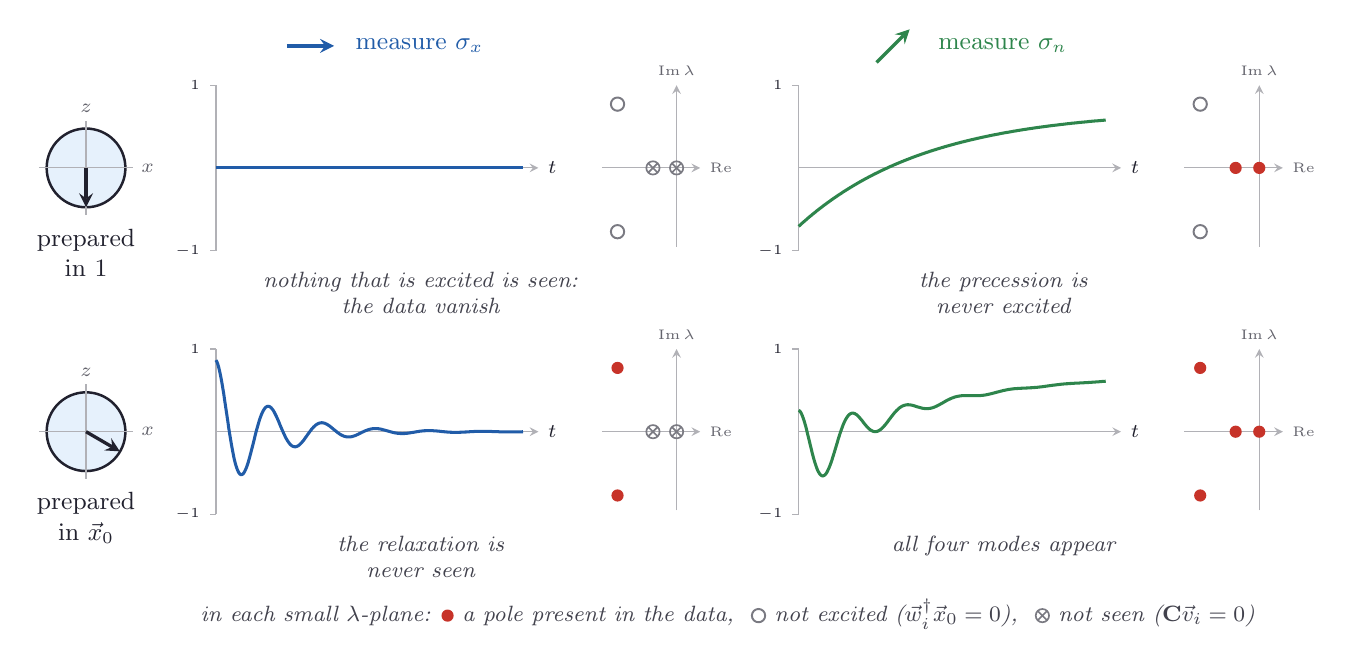
\begin{tikzpicture}[ink/.style={line width=0.9pt, ndInk}, faint/.style={line width=0.4pt, ndInk!35}, dashedink/.style={line width=0.5pt, ndInk!55, dash pattern=on 2.5pt off 2pt}, vec/.style={->, >=stealth, line width=1.2pt}, note/.style={font=\footnotesize\itshape, text=ndInk!85, align=center}, pointer/.style={->, >=stealth, line width=0.4pt, ndInk!60, shorten >=2pt, shorten <=1pt}, dot/.style={circle, fill=ndInk, inner sep=0pt, minimum size=3.4pt}, wash/.style={fill=ndSky, fill opacity=0.55}, every node/.style={text=ndInk}]
\definecolor{ndInk}{rgb}{0.13,0.13,0.18}
\definecolor{ndPaper}{rgb}{0.99,0.96,0.88}
\definecolor{ndSky}{rgb}{0.84,0.91,0.98}
\definecolor{ndRose}{rgb}{0.98,0.86,0.84}
\definecolor{ndBlue}{rgb}{0.13,0.36,0.66}
\definecolor{ndRed}{rgb}{0.78,0.20,0.16}
\definecolor{ndGold}{rgb}{0.88,0.62,0.10}
\definecolor{ndGreen}{rgb}{0.18,0.52,0.30}
\draw[vec, ndBlue] (3.30,6.15) -- (3.90,6.15);
\node[font=\small, text=ndBlue, anchor=west] at (4.05,6.15) {measure $\sigma_x$};
\draw[vec, ndGreen] (10.79,5.94) -- (11.21,6.36);
\node[font=\small, text=ndGreen, anchor=west] at (11.45,6.15) {measure $\sigma_n$};
\fill[ndSky, fill opacity=0.6] (0.75,4.60) circle (0.50);
\draw[ink] (0.75,4.60) circle (0.50);
\draw[faint] (0.15,4.60) -- (1.35,4.60) (0.75,4.00) -- (0.75,5.20);
\node[font=\scriptsize, text=ndInk!70, anchor=west] at (1.33,4.60) {$x$};
\node[font=\scriptsize, text=ndInk!70, anchor=south] at (0.75,5.18) {$z$};
\draw[vec, ndInk] (0.75,4.60) -- (0.75,4.10);
\node[font=\small, align=center, anchor=north] at (0.75,3.95) {prepared\\ in $\ket1$};
\draw[faint, ->, >=stealth] (2.400,4.600) -- (6.495,4.600) node[right, font=\scriptsize, text=ndInk] {$t$};
\draw[faint] (2.400,3.550) -- (2.400,5.650);
\draw[faint] (2.400,3.550) -- (2.319,3.550) node[left, font=\tiny, text=ndInk] {$-1$};
\draw[faint] (2.400,5.650) -- (2.319,5.650) node[left, font=\tiny, text=ndInk] {$1$};
\draw[line width=1.1pt, ndBlue] (2.400,4.600) -- (2.411,4.600) -- (2.422,4.600) -- (2.433,4.600) -- (2.443,4.600) -- (2.454,4.600) -- (2.465,4.600) -- (2.476,4.600) -- (2.487,4.600) -- (2.498,4.600) -- (2.508,4.600) -- (2.519,4.600) -- (2.530,4.600) -- (2.541,4.600) -- (2.552,4.600) -- (2.562,4.600) -- (2.573,4.600) -- (2.584,4.600) -- (2.595,4.600) -- (2.606,4.600) -- (2.617,4.600) -- (2.627,4.600) -- (2.638,4.600) -- (2.649,4.600) -- (2.660,4.600) -- (2.671,4.600) -- (2.682,4.600) -- (2.692,4.600) -- (2.703,4.600) -- (2.714,4.600) -- (2.725,4.600) -- (2.736,4.600) -- (2.747,4.600) -- (2.757,4.600) -- (2.768,4.600) -- (2.779,4.600) -- (2.790,4.600) -- (2.801,4.600) -- (2.812,4.600) -- (2.822,4.600) -- (2.833,4.600) -- (2.844,4.600) -- (2.855,4.600) -- (2.866,4.600) -- (2.877,4.600) -- (2.888,4.600) -- (2.898,4.600) -- (2.909,4.600) -- (2.920,4.600) -- (2.931,4.600) -- (2.942,4.600) -- (2.952,4.600) -- (2.963,4.600) -- (2.974,4.600) -- (2.985,4.600) -- (2.996,4.600) -- (3.007,4.600) -- (3.018,4.600) -- (3.028,4.600) -- (3.039,4.600) -- (3.050,4.600) -- (3.061,4.600) -- (3.072,4.600) -- (3.083,4.600) -- (3.093,4.600) -- (3.104,4.600) -- (3.115,4.600) -- (3.126,4.600) -- (3.137,4.600) -- (3.147,4.600) -- (3.158,4.600) -- (3.169,4.600) -- (3.180,4.600) -- (3.191,4.600) -- (3.202,4.600) -- (3.212,4.600) -- (3.223,4.600) -- (3.234,4.600) -- (3.245,4.600) -- (3.256,4.600) -- (3.267,4.600) -- (3.277,4.600) -- (3.288,4.600) -- (3.299,4.600) -- (3.310,4.600) -- (3.321,4.600) -- (3.332,4.600) -- (3.342,4.600) -- (3.353,4.600) -- (3.364,4.600) -- (3.375,4.600) -- (3.386,4.600) -- (3.397,4.600) -- (3.407,4.600) -- (3.418,4.600) -- (3.429,4.600) -- (3.440,4.600) -- (3.451,4.600) -- (3.462,4.600) -- (3.473,4.600) -- (3.483,4.600) -- (3.494,4.600) -- (3.505,4.600) -- (3.516,4.600) -- (3.527,4.600) -- (3.537,4.600) -- (3.548,4.600) -- (3.559,4.600) -- (3.570,4.600) -- (3.581,4.600) -- (3.592,4.600) -- (3.603,4.600) -- (3.613,4.600) -- (3.624,4.600) -- (3.635,4.600) -- (3.646,4.600) -- (3.657,4.600) -- (3.667,4.600) -- (3.678,4.600) -- (3.689,4.600) -- (3.700,4.600) -- (3.711,4.600) -- (3.722,4.600) -- (3.732,4.600) -- (3.743,4.600) -- (3.754,4.600) -- (3.765,4.600) -- (3.776,4.600) -- (3.787,4.600) -- (3.797,4.600) -- (3.808,4.600) -- (3.819,4.600) -- (3.830,4.600) -- (3.841,4.600) -- (3.852,4.600) -- (3.862,4.600) -- (3.873,4.600) -- (3.884,4.600) -- (3.895,4.600) -- (3.906,4.600) -- (3.917,4.600) -- (3.928,4.600) -- (3.938,4.600) -- (3.949,4.600) -- (3.960,4.600) -- (3.971,4.600) -- (3.982,4.600) -- (3.993,4.600) -- (4.003,4.600) -- (4.014,4.600) -- (4.025,4.600) -- (4.036,4.600) -- (4.047,4.600) -- (4.058,4.600) -- (4.068,4.600) -- (4.079,4.600) -- (4.090,4.600) -- (4.101,4.600) -- (4.112,4.600) -- (4.122,4.600) -- (4.133,4.600) -- (4.144,4.600) -- (4.155,4.600) -- (4.166,4.600) -- (4.177,4.600) -- (4.188,4.600) -- (4.198,4.600) -- (4.209,4.600) -- (4.220,4.600) -- (4.231,4.600) -- (4.242,4.600) -- (4.252,4.600) -- (4.263,4.600) -- (4.274,4.600) -- (4.285,4.600) -- (4.296,4.600) -- (4.307,4.600) -- (4.317,4.600) -- (4.328,4.600) -- (4.339,4.600) -- (4.350,4.600) -- (4.361,4.600) -- (4.372,4.600) -- (4.383,4.600) -- (4.393,4.600) -- (4.404,4.600) -- (4.415,4.600) -- (4.426,4.600) -- (4.437,4.600) -- (4.447,4.600) -- (4.458,4.600) -- (4.469,4.600) -- (4.480,4.600) -- (4.491,4.600) -- (4.502,4.600) -- (4.513,4.600) -- (4.523,4.600) -- (4.534,4.600) -- (4.545,4.600) -- (4.556,4.600) -- (4.567,4.600) -- (4.578,4.600) -- (4.588,4.600) -- (4.599,4.600) -- (4.610,4.600) -- (4.621,4.600) -- (4.632,4.600) -- (4.643,4.600) -- (4.653,4.600) -- (4.664,4.600) -- (4.675,4.600) -- (4.686,4.600) -- (4.697,4.600) -- (4.707,4.600) -- (4.718,4.600) -- (4.729,4.600) -- (4.740,4.600) -- (4.751,4.600) -- (4.762,4.600) -- (4.772,4.600) -- (4.783,4.600) -- (4.794,4.600) -- (4.805,4.600) -- (4.816,4.600) -- (4.827,4.600) -- (4.838,4.600) -- (4.848,4.600) -- (4.859,4.600) -- (4.870,4.600) -- (4.881,4.600) -- (4.892,4.600) -- (4.902,4.600) -- (4.913,4.600) -- (4.924,4.600) -- (4.935,4.600) -- (4.946,4.600) -- (4.957,4.600) -- (4.967,4.600) -- (4.978,4.600) -- (4.989,4.600) -- (5.000,4.600) -- (5.011,4.600) -- (5.022,4.600) -- (5.032,4.600) -- (5.043,4.600) -- (5.054,4.600) -- (5.065,4.600) -- (5.076,4.600) -- (5.087,4.600) -- (5.098,4.600) -- (5.108,4.600) -- (5.119,4.600) -- (5.130,4.600) -- (5.141,4.600) -- (5.152,4.600) -- (5.162,4.600) -- (5.173,4.600) -- (5.184,4.600) -- (5.195,4.600) -- (5.206,4.600) -- (5.217,4.600) -- (5.227,4.600) -- (5.238,4.600) -- (5.249,4.600) -- (5.260,4.600) -- (5.271,4.600) -- (5.282,4.600) -- (5.293,4.600) -- (5.303,4.600) -- (5.314,4.600) -- (5.325,4.600) -- (5.336,4.600) -- (5.347,4.600) -- (5.357,4.600) -- (5.368,4.600) -- (5.379,4.600) -- (5.390,4.600) -- (5.401,4.600) -- (5.412,4.600) -- (5.423,4.600) -- (5.433,4.600) -- (5.444,4.600) -- (5.455,4.600) -- (5.466,4.600) -- (5.477,4.600) -- (5.487,4.600) -- (5.498,4.600) -- (5.509,4.600) -- (5.520,4.600) -- (5.531,4.600) -- (5.542,4.600) -- (5.553,4.600) -- (5.563,4.600) -- (5.574,4.600) -- (5.585,4.600) -- (5.596,4.600) -- (5.607,4.600) -- (5.617,4.600) -- (5.628,4.600) -- (5.639,4.600) -- (5.650,4.600) -- (5.661,4.600) -- (5.672,4.600) -- (5.683,4.600) -- (5.693,4.600) -- (5.704,4.600) -- (5.715,4.600) -- (5.726,4.600) -- (5.737,4.600) -- (5.748,4.600) -- (5.758,4.600) -- (5.769,4.600) -- (5.780,4.600) -- (5.791,4.600) -- (5.802,4.600) -- (5.812,4.600) -- (5.823,4.600) -- (5.834,4.600) -- (5.845,4.600) -- (5.856,4.600) -- (5.867,4.600) -- (5.877,4.600) -- (5.888,4.600) -- (5.899,4.600) -- (5.910,4.600) -- (5.921,4.600) -- (5.932,4.600) -- (5.943,4.600) -- (5.953,4.600) -- (5.964,4.600) -- (5.975,4.600) -- (5.986,4.600) -- (5.997,4.600) -- (6.008,4.600) -- (6.018,4.600) -- (6.029,4.600) -- (6.040,4.600) -- (6.051,4.600) -- (6.062,4.600) -- (6.072,4.600) -- (6.083,4.600) -- (6.094,4.600) -- (6.105,4.600) -- (6.116,4.600) -- (6.127,4.600) -- (6.138,4.600) -- (6.148,4.600) -- (6.159,4.600) -- (6.170,4.600) -- (6.181,4.600) -- (6.192,4.600) -- (6.202,4.600) -- (6.213,4.600) -- (6.224,4.600) -- (6.235,4.600) -- (6.246,4.600) -- (6.257,4.600) -- (6.268,4.600) -- (6.278,4.600) -- (6.289,4.600) -- (6.300,4.600);
\draw[faint, ->, >=stealth] (7.30,4.60) -- (8.55,4.60) node[right, font=\tiny, text=ndInk!70] {Re};
\draw[faint, ->, >=stealth] (8.25,3.60) -- (8.25,5.65) node[above, font=\tiny, text=ndInk!70] {Im\,$\lambda$};
\draw[line width=0.7pt, ndInk!60, fill=white] (7.500,5.410) circle (2.4pt);
\draw[line width=0.7pt, ndInk!60, fill=white] (7.500,3.790) circle (2.4pt);
\draw[line width=0.6pt, ndInk!60] (7.950,4.600) circle (2.4pt) (7.890,4.540) -- (8.010,4.660) (7.890,4.660) -- (8.010,4.540);
\draw[line width=0.6pt, ndInk!60] (8.250,4.600) circle (2.4pt) (8.190,4.540) -- (8.310,4.660) (8.190,4.660) -- (8.310,4.540);
\node[note, anchor=north] at (5.00,3.40) {nothing that is excited is seen:\\ the data vanish};
\draw[faint, ->, >=stealth] (9.800,4.600) -- (13.895,4.600) node[right, font=\scriptsize, text=ndInk] {$t$};
\draw[faint] (9.800,3.550) -- (9.800,5.650);
\draw[faint] (9.800,3.550) -- (9.719,3.550) node[left, font=\tiny, text=ndInk] {$-1$};
\draw[faint] (9.800,5.650) -- (9.719,5.650) node[left, font=\tiny, text=ndInk] {$1$};
\draw[line width=1.1pt, ndGreen] (9.800,3.858) -- (9.811,3.867) -- (9.822,3.877) -- (9.833,3.887) -- (9.843,3.897) -- (9.854,3.906) -- (9.865,3.916) -- (9.876,3.925) -- (9.887,3.935) -- (9.898,3.944) -- (9.908,3.953) -- (9.919,3.963) -- (9.930,3.972) -- (9.941,3.981) -- (9.952,3.990) -- (9.963,3.999) -- (9.973,4.008) -- (9.984,4.017) -- (9.995,4.025) -- (10.006,4.034) -- (10.017,4.043) -- (10.027,4.052) -- (10.038,4.060) -- (10.049,4.069) -- (10.060,4.077) -- (10.071,4.086) -- (10.082,4.094) -- (10.093,4.102) -- (10.103,4.110) -- (10.114,4.119) -- (10.125,4.127) -- (10.136,4.135) -- (10.147,4.143) -- (10.158,4.151) -- (10.168,4.159) -- (10.179,4.167) -- (10.190,4.174) -- (10.201,4.182) -- (10.212,4.190) -- (10.223,4.198) -- (10.233,4.205) -- (10.244,4.213) -- (10.255,4.220) -- (10.266,4.228) -- (10.277,4.235) -- (10.288,4.242) -- (10.298,4.250) -- (10.309,4.257) -- (10.320,4.264) -- (10.331,4.271) -- (10.342,4.278) -- (10.353,4.286) -- (10.363,4.293) -- (10.374,4.300) -- (10.385,4.306) -- (10.396,4.313) -- (10.407,4.320) -- (10.418,4.327) -- (10.428,4.334) -- (10.439,4.340) -- (10.450,4.347) -- (10.461,4.354) -- (10.472,4.360) -- (10.483,4.367) -- (10.493,4.373) -- (10.504,4.380) -- (10.515,4.386) -- (10.526,4.392) -- (10.537,4.399) -- (10.548,4.405) -- (10.558,4.411) -- (10.569,4.417) -- (10.580,4.424) -- (10.591,4.430) -- (10.602,4.436) -- (10.613,4.442) -- (10.623,4.448) -- (10.634,4.454) -- (10.645,4.460) -- (10.656,4.466) -- (10.667,4.471) -- (10.678,4.477) -- (10.688,4.483) -- (10.699,4.489) -- (10.710,4.494) -- (10.721,4.500) -- (10.732,4.505) -- (10.743,4.511) -- (10.753,4.517) -- (10.764,4.522) -- (10.775,4.528) -- (10.786,4.533) -- (10.797,4.538) -- (10.808,4.544) -- (10.818,4.549) -- (10.829,4.554) -- (10.840,4.559) -- (10.851,4.565) -- (10.862,4.570) -- (10.873,4.575) -- (10.883,4.580) -- (10.894,4.585) -- (10.905,4.590) -- (10.916,4.595) -- (10.927,4.600) -- (10.938,4.605) -- (10.948,4.610) -- (10.959,4.615) -- (10.970,4.620) -- (10.981,4.624) -- (10.992,4.629) -- (11.003,4.634) -- (11.013,4.639) -- (11.024,4.643) -- (11.035,4.648) -- (11.046,4.653) -- (11.057,4.657) -- (11.068,4.662) -- (11.078,4.666) -- (11.089,4.671) -- (11.100,4.675) -- (11.111,4.680) -- (11.122,4.684) -- (11.133,4.688) -- (11.143,4.693) -- (11.154,4.697) -- (11.165,4.701) -- (11.176,4.706) -- (11.187,4.710) -- (11.198,4.714) -- (11.208,4.718) -- (11.219,4.722) -- (11.230,4.727) -- (11.241,4.731) -- (11.252,4.735) -- (11.263,4.739) -- (11.273,4.743) -- (11.284,4.747) -- (11.295,4.751) -- (11.306,4.755) -- (11.317,4.759) -- (11.328,4.762) -- (11.338,4.766) -- (11.349,4.770) -- (11.360,4.774) -- (11.371,4.778) -- (11.382,4.781) -- (11.393,4.785) -- (11.403,4.789) -- (11.414,4.793) -- (11.425,4.796) -- (11.436,4.800) -- (11.447,4.803) -- (11.458,4.807) -- (11.468,4.811) -- (11.479,4.814) -- (11.490,4.818) -- (11.501,4.821) -- (11.512,4.825) -- (11.523,4.828) -- (11.533,4.831) -- (11.544,4.835) -- (11.555,4.838) -- (11.566,4.842) -- (11.577,4.845) -- (11.588,4.848) -- (11.598,4.851) -- (11.609,4.855) -- (11.620,4.858) -- (11.631,4.861) -- (11.642,4.864) -- (11.652,4.868) -- (11.663,4.871) -- (11.674,4.874) -- (11.685,4.877) -- (11.696,4.880) -- (11.707,4.883) -- (11.718,4.886) -- (11.728,4.889) -- (11.739,4.892) -- (11.750,4.895) -- (11.761,4.898) -- (11.772,4.901) -- (11.783,4.904) -- (11.793,4.907) -- (11.804,4.910) -- (11.815,4.913) -- (11.826,4.916) -- (11.837,4.918) -- (11.848,4.921) -- (11.858,4.924) -- (11.869,4.927) -- (11.880,4.930) -- (11.891,4.932) -- (11.902,4.935) -- (11.913,4.938) -- (11.923,4.940) -- (11.934,4.943) -- (11.945,4.946) -- (11.956,4.948) -- (11.967,4.951) -- (11.978,4.954) -- (11.988,4.956) -- (11.999,4.959) -- (12.010,4.961) -- (12.021,4.964) -- (12.032,4.966) -- (12.043,4.969) -- (12.053,4.971) -- (12.064,4.974) -- (12.075,4.976) -- (12.086,4.979) -- (12.097,4.981) -- (12.108,4.984) -- (12.118,4.986) -- (12.129,4.988) -- (12.140,4.991) -- (12.151,4.993) -- (12.162,4.995) -- (12.173,4.998) -- (12.183,5.000) -- (12.194,5.002) -- (12.205,5.004) -- (12.216,5.007) -- (12.227,5.009) -- (12.238,5.011) -- (12.248,5.013) -- (12.259,5.016) -- (12.270,5.018) -- (12.281,5.020) -- (12.292,5.022) -- (12.303,5.024) -- (12.313,5.026) -- (12.324,5.028) -- (12.335,5.030) -- (12.346,5.032) -- (12.357,5.035) -- (12.367,5.037) -- (12.378,5.039) -- (12.389,5.041) -- (12.400,5.043) -- (12.411,5.045) -- (12.422,5.047) -- (12.433,5.049) -- (12.443,5.051) -- (12.454,5.052) -- (12.465,5.054) -- (12.476,5.056) -- (12.487,5.058) -- (12.498,5.060) -- (12.508,5.062) -- (12.519,5.064) -- (12.530,5.066) -- (12.541,5.068) -- (12.552,5.069) -- (12.562,5.071) -- (12.573,5.073) -- (12.584,5.075) -- (12.595,5.077) -- (12.606,5.078) -- (12.617,5.080) -- (12.628,5.082) -- (12.638,5.084) -- (12.649,5.085) -- (12.660,5.087) -- (12.671,5.089) -- (12.682,5.090) -- (12.693,5.092) -- (12.703,5.094) -- (12.714,5.095) -- (12.725,5.097) -- (12.736,5.099) -- (12.747,5.100) -- (12.758,5.102) -- (12.768,5.103) -- (12.779,5.105) -- (12.790,5.107) -- (12.801,5.108) -- (12.812,5.110) -- (12.823,5.111) -- (12.833,5.113) -- (12.844,5.114) -- (12.855,5.116) -- (12.866,5.117) -- (12.877,5.119) -- (12.888,5.120) -- (12.898,5.122) -- (12.909,5.123) -- (12.920,5.125) -- (12.931,5.126) -- (12.942,5.128) -- (12.953,5.129) -- (12.963,5.130) -- (12.974,5.132) -- (12.985,5.133) -- (12.996,5.135) -- (13.007,5.136) -- (13.018,5.137) -- (13.028,5.139) -- (13.039,5.140) -- (13.050,5.141) -- (13.061,5.143) -- (13.072,5.144) -- (13.083,5.145) -- (13.093,5.147) -- (13.104,5.148) -- (13.115,5.149) -- (13.126,5.151) -- (13.137,5.152) -- (13.148,5.153) -- (13.158,5.154) -- (13.169,5.156) -- (13.180,5.157) -- (13.191,5.158) -- (13.202,5.159) -- (13.213,5.161) -- (13.223,5.162) -- (13.234,5.163) -- (13.245,5.164) -- (13.256,5.165) -- (13.267,5.167) -- (13.277,5.168) -- (13.288,5.169) -- (13.299,5.170) -- (13.310,5.171) -- (13.321,5.172) -- (13.332,5.173) -- (13.343,5.175) -- (13.353,5.176) -- (13.364,5.177) -- (13.375,5.178) -- (13.386,5.179) -- (13.397,5.180) -- (13.408,5.181) -- (13.418,5.182) -- (13.429,5.183) -- (13.440,5.184) -- (13.451,5.185) -- (13.462,5.186) -- (13.473,5.188) -- (13.483,5.189) -- (13.494,5.190) -- (13.505,5.191) -- (13.516,5.192) -- (13.527,5.193) -- (13.538,5.194) -- (13.548,5.195) -- (13.559,5.196) -- (13.570,5.197) -- (13.581,5.198) -- (13.592,5.198) -- (13.603,5.199) -- (13.613,5.200) -- (13.624,5.201) -- (13.635,5.202) -- (13.646,5.203) -- (13.657,5.204) -- (13.668,5.205) -- (13.678,5.206) -- (13.689,5.207) -- (13.700,5.208);
\draw[faint, ->, >=stealth] (14.70,4.60) -- (15.95,4.60) node[right, font=\tiny, text=ndInk!70] {Re};
\draw[faint, ->, >=stealth] (15.65,3.60) -- (15.65,5.65) node[above, font=\tiny, text=ndInk!70] {Im\,$\lambda$};
\draw[line width=0.7pt, ndInk!60, fill=white] (14.900,5.410) circle (2.4pt);
\draw[line width=0.7pt, ndInk!60, fill=white] (14.900,3.790) circle (2.4pt);
\fill[ndRed] (15.350,4.600) circle (2.2pt);
\fill[ndRed] (15.650,4.600) circle (2.2pt);
\node[note, anchor=north] at (12.40,3.40) {the precession is\\ never excited};
\fill[ndSky, fill opacity=0.6] (0.75,1.25) circle (0.50);
\draw[ink] (0.75,1.25) circle (0.50);
\draw[faint] (0.15,1.25) -- (1.35,1.25) (0.75,0.65) -- (0.75,1.85);
\node[font=\scriptsize, text=ndInk!70, anchor=west] at (1.33,1.25) {$x$};
\node[font=\scriptsize, text=ndInk!70, anchor=south] at (0.75,1.83) {$z$};
\draw[vec, ndInk] (0.75,1.25) -- (1.18,1.00);
\node[font=\small, align=center, anchor=north] at (0.75,0.60) {prepared\\ in $\vec x_0$};
\draw[faint, ->, >=stealth] (2.400,1.250) -- (6.495,1.250) node[right, font=\scriptsize, text=ndInk] {$t$};
\draw[faint] (2.400,0.200) -- (2.400,2.300);
\draw[faint] (2.400,0.200) -- (2.319,0.200) node[left, font=\tiny, text=ndInk] {$-1$};
\draw[faint] (2.400,2.300) -- (2.319,2.300) node[left, font=\tiny, text=ndInk] {$1$};
\draw[line width=1.1pt, ndBlue] (2.400,2.159) -- (2.411,2.140) -- (2.422,2.112) -- (2.433,2.076) -- (2.443,2.034) -- (2.454,1.984) -- (2.465,1.929) -- (2.476,1.869) -- (2.487,1.804) -- (2.498,1.737) -- (2.508,1.666) -- (2.519,1.593) -- (2.530,1.520) -- (2.541,1.446) -- (2.552,1.372) -- (2.562,1.300) -- (2.573,1.230) -- (2.584,1.162) -- (2.595,1.097) -- (2.606,1.036) -- (2.617,0.979) -- (2.627,0.926) -- (2.638,0.879) -- (2.649,0.837) -- (2.660,0.801) -- (2.671,0.770) -- (2.682,0.745) -- (2.692,0.726) -- (2.703,0.713) -- (2.714,0.705) -- (2.725,0.704) -- (2.736,0.708) -- (2.747,0.717) -- (2.757,0.732) -- (2.768,0.751) -- (2.779,0.775) -- (2.790,0.802) -- (2.801,0.834) -- (2.812,0.868) -- (2.822,0.905) -- (2.833,0.945) -- (2.844,0.986) -- (2.855,1.029) -- (2.866,1.072) -- (2.877,1.116) -- (2.888,1.159) -- (2.898,1.203) -- (2.909,1.245) -- (2.920,1.286) -- (2.931,1.325) -- (2.942,1.362) -- (2.952,1.397) -- (2.963,1.429) -- (2.974,1.458) -- (2.985,1.485) -- (2.996,1.508) -- (3.007,1.527) -- (3.018,1.544) -- (3.028,1.556) -- (3.039,1.565) -- (3.050,1.571) -- (3.061,1.573) -- (3.072,1.572) -- (3.083,1.568) -- (3.093,1.561) -- (3.104,1.551) -- (3.115,1.538) -- (3.126,1.522) -- (3.137,1.505) -- (3.147,1.485) -- (3.158,1.463) -- (3.169,1.441) -- (3.180,1.417) -- (3.191,1.392) -- (3.202,1.366) -- (3.212,1.340) -- (3.223,1.314) -- (3.234,1.289) -- (3.245,1.263) -- (3.256,1.239) -- (3.267,1.215) -- (3.277,1.193) -- (3.288,1.171) -- (3.299,1.152) -- (3.310,1.134) -- (3.321,1.117) -- (3.332,1.103) -- (3.342,1.090) -- (3.353,1.080) -- (3.364,1.071) -- (3.375,1.065) -- (3.386,1.061) -- (3.397,1.059) -- (3.407,1.058) -- (3.418,1.060) -- (3.429,1.064) -- (3.440,1.069) -- (3.451,1.076) -- (3.462,1.085) -- (3.473,1.095) -- (3.483,1.106) -- (3.494,1.118) -- (3.505,1.131) -- (3.516,1.145) -- (3.527,1.160) -- (3.537,1.175) -- (3.548,1.190) -- (3.559,1.205) -- (3.570,1.221) -- (3.581,1.236) -- (3.592,1.251) -- (3.603,1.265) -- (3.613,1.279) -- (3.624,1.291) -- (3.635,1.304) -- (3.646,1.315) -- (3.657,1.325) -- (3.667,1.334) -- (3.678,1.342) -- (3.689,1.348) -- (3.700,1.354) -- (3.711,1.358) -- (3.722,1.361) -- (3.732,1.363) -- (3.743,1.364) -- (3.754,1.363) -- (3.765,1.361) -- (3.776,1.359) -- (3.787,1.355) -- (3.797,1.350) -- (3.808,1.345) -- (3.819,1.338) -- (3.830,1.331) -- (3.841,1.324) -- (3.852,1.316) -- (3.862,1.307) -- (3.873,1.298) -- (3.884,1.289) -- (3.895,1.280) -- (3.906,1.271) -- (3.917,1.262) -- (3.928,1.253) -- (3.938,1.245) -- (3.949,1.236) -- (3.960,1.229) -- (3.971,1.221) -- (3.982,1.214) -- (3.993,1.208) -- (4.003,1.203) -- (4.014,1.198) -- (4.025,1.193) -- (4.036,1.190) -- (4.047,1.187) -- (4.058,1.185) -- (4.068,1.183) -- (4.079,1.183) -- (4.090,1.183) -- (4.101,1.184) -- (4.112,1.185) -- (4.122,1.187) -- (4.133,1.189) -- (4.144,1.193) -- (4.155,1.196) -- (4.166,1.200) -- (4.177,1.204) -- (4.188,1.209) -- (4.198,1.214) -- (4.209,1.219) -- (4.220,1.225) -- (4.231,1.230) -- (4.242,1.235) -- (4.252,1.241) -- (4.263,1.246) -- (4.274,1.251) -- (4.285,1.256) -- (4.296,1.261) -- (4.307,1.265) -- (4.317,1.269) -- (4.328,1.273) -- (4.339,1.277) -- (4.350,1.280) -- (4.361,1.283) -- (4.372,1.285) -- (4.383,1.287) -- (4.393,1.288) -- (4.404,1.289) -- (4.415,1.290) -- (4.426,1.290) -- (4.437,1.290) -- (4.447,1.289) -- (4.458,1.288) -- (4.469,1.287) -- (4.480,1.285) -- (4.491,1.283) -- (4.502,1.281) -- (4.513,1.278) -- (4.523,1.275) -- (4.534,1.272) -- (4.545,1.269) -- (4.556,1.266) -- (4.567,1.263) -- (4.578,1.260) -- (4.588,1.257) -- (4.599,1.254) -- (4.610,1.251) -- (4.621,1.248) -- (4.632,1.245) -- (4.643,1.242) -- (4.653,1.239) -- (4.664,1.237) -- (4.675,1.235) -- (4.686,1.233) -- (4.697,1.231) -- (4.707,1.230) -- (4.718,1.229) -- (4.729,1.228) -- (4.740,1.227) -- (4.751,1.227) -- (4.762,1.226) -- (4.772,1.226) -- (4.783,1.227) -- (4.794,1.227) -- (4.805,1.228) -- (4.816,1.229) -- (4.827,1.230) -- (4.838,1.231) -- (4.848,1.233) -- (4.859,1.234) -- (4.870,1.236) -- (4.881,1.238) -- (4.892,1.240) -- (4.902,1.241) -- (4.913,1.243) -- (4.924,1.245) -- (4.935,1.247) -- (4.946,1.249) -- (4.957,1.251) -- (4.967,1.252) -- (4.978,1.254) -- (4.989,1.256) -- (5.000,1.257) -- (5.011,1.258) -- (5.022,1.260) -- (5.032,1.261) -- (5.043,1.262) -- (5.054,1.262) -- (5.065,1.263) -- (5.076,1.263) -- (5.087,1.264) -- (5.098,1.264) -- (5.108,1.264) -- (5.119,1.264) -- (5.130,1.264) -- (5.141,1.263) -- (5.152,1.263) -- (5.162,1.262) -- (5.173,1.261) -- (5.184,1.261) -- (5.195,1.260) -- (5.206,1.259) -- (5.217,1.258) -- (5.227,1.257) -- (5.238,1.256) -- (5.249,1.254) -- (5.260,1.253) -- (5.271,1.252) -- (5.282,1.251) -- (5.293,1.250) -- (5.303,1.249) -- (5.314,1.248) -- (5.325,1.247) -- (5.336,1.246) -- (5.347,1.245) -- (5.357,1.245) -- (5.368,1.244) -- (5.379,1.243) -- (5.390,1.243) -- (5.401,1.242) -- (5.412,1.242) -- (5.423,1.242) -- (5.433,1.242) -- (5.444,1.242) -- (5.455,1.242) -- (5.466,1.242) -- (5.477,1.242) -- (5.487,1.242) -- (5.498,1.243) -- (5.509,1.243) -- (5.520,1.244) -- (5.531,1.244) -- (5.542,1.245) -- (5.553,1.245) -- (5.563,1.246) -- (5.574,1.246) -- (5.585,1.247) -- (5.596,1.248) -- (5.607,1.248) -- (5.617,1.249) -- (5.628,1.250) -- (5.639,1.250) -- (5.650,1.251) -- (5.661,1.252) -- (5.672,1.252) -- (5.683,1.253) -- (5.693,1.253) -- (5.704,1.253) -- (5.715,1.254) -- (5.726,1.254) -- (5.737,1.254) -- (5.748,1.255) -- (5.758,1.255) -- (5.769,1.255) -- (5.780,1.255) -- (5.791,1.255) -- (5.802,1.255) -- (5.812,1.255) -- (5.823,1.255) -- (5.834,1.254) -- (5.845,1.254) -- (5.856,1.254) -- (5.867,1.254) -- (5.877,1.253) -- (5.888,1.253) -- (5.899,1.253) -- (5.910,1.252) -- (5.921,1.252) -- (5.932,1.251) -- (5.943,1.251) -- (5.953,1.251) -- (5.964,1.250) -- (5.975,1.250) -- (5.986,1.250) -- (5.997,1.249) -- (6.008,1.249) -- (6.018,1.249) -- (6.029,1.248) -- (6.040,1.248) -- (6.051,1.248) -- (6.062,1.248) -- (6.072,1.247) -- (6.083,1.247) -- (6.094,1.247) -- (6.105,1.247) -- (6.116,1.247) -- (6.127,1.247) -- (6.138,1.247) -- (6.148,1.247) -- (6.159,1.247) -- (6.170,1.247) -- (6.181,1.247) -- (6.192,1.248) -- (6.202,1.248) -- (6.213,1.248) -- (6.224,1.248) -- (6.235,1.248) -- (6.246,1.249) -- (6.257,1.249) -- (6.268,1.249) -- (6.278,1.249) -- (6.289,1.249) -- (6.300,1.250);
\draw[faint, ->, >=stealth] (7.30,1.25) -- (8.55,1.25) node[right, font=\tiny, text=ndInk!70] {Re};
\draw[faint, ->, >=stealth] (8.25,0.25) -- (8.25,2.30) node[above, font=\tiny, text=ndInk!70] {Im\,$\lambda$};
\fill[ndRed] (7.500,2.060) circle (2.2pt);
\fill[ndRed] (7.500,0.440) circle (2.2pt);
\draw[line width=0.6pt, ndInk!60] (7.950,1.250) circle (2.4pt) (7.890,1.190) -- (8.010,1.310) (7.890,1.310) -- (8.010,1.190);
\draw[line width=0.6pt, ndInk!60] (8.250,1.250) circle (2.4pt) (8.190,1.190) -- (8.310,1.310) (8.190,1.310) -- (8.310,1.190);
\node[note, anchor=north] at (5.00,0.05) {the relaxation is\\ never seen};
\draw[faint, ->, >=stealth] (9.800,1.250) -- (13.895,1.250) node[right, font=\scriptsize, text=ndInk] {$t$};
\draw[faint] (9.800,0.200) -- (9.800,2.300);
\draw[faint] (9.800,0.200) -- (9.719,0.200) node[left, font=\tiny, text=ndInk] {$-1$};
\draw[faint] (9.800,2.300) -- (9.719,2.300) node[left, font=\tiny, text=ndInk] {$1$};
\draw[line width=1.1pt, ndGreen] (9.800,1.522) -- (9.811,1.515) -- (9.822,1.503) -- (9.833,1.485) -- (9.843,1.462) -- (9.854,1.434) -- (9.865,1.403) -- (9.876,1.367) -- (9.887,1.329) -- (9.898,1.288) -- (9.908,1.245) -- (9.919,1.200) -- (9.930,1.155) -- (9.941,1.110) -- (9.952,1.065) -- (9.963,1.020) -- (9.973,0.977) -- (9.984,0.936) -- (9.995,0.896) -- (10.006,0.860) -- (10.017,0.826) -- (10.027,0.796) -- (10.038,0.768) -- (10.049,0.745) -- (10.060,0.726) -- (10.071,0.710) -- (10.082,0.699) -- (10.093,0.692) -- (10.103,0.688) -- (10.114,0.690) -- (10.125,0.695) -- (10.136,0.703) -- (10.147,0.716) -- (10.158,0.732) -- (10.168,0.752) -- (10.179,0.775) -- (10.190,0.800) -- (10.201,0.828) -- (10.212,0.858) -- (10.223,0.890) -- (10.233,0.924) -- (10.244,0.958) -- (10.255,0.994) -- (10.266,1.030) -- (10.277,1.067) -- (10.288,1.103) -- (10.298,1.139) -- (10.309,1.175) -- (10.320,1.209) -- (10.331,1.242) -- (10.342,1.274) -- (10.353,1.304) -- (10.363,1.332) -- (10.374,1.358) -- (10.385,1.381) -- (10.396,1.403) -- (10.407,1.422) -- (10.418,1.438) -- (10.428,1.452) -- (10.439,1.464) -- (10.450,1.473) -- (10.461,1.480) -- (10.472,1.484) -- (10.483,1.486) -- (10.493,1.485) -- (10.504,1.483) -- (10.515,1.479) -- (10.526,1.472) -- (10.537,1.465) -- (10.548,1.455) -- (10.558,1.445) -- (10.569,1.434) -- (10.580,1.421) -- (10.591,1.408) -- (10.602,1.395) -- (10.613,1.381) -- (10.623,1.367) -- (10.634,1.353) -- (10.645,1.340) -- (10.656,1.327) -- (10.667,1.314) -- (10.678,1.303) -- (10.688,1.292) -- (10.699,1.283) -- (10.710,1.274) -- (10.721,1.267) -- (10.732,1.261) -- (10.743,1.256) -- (10.753,1.253) -- (10.764,1.251) -- (10.775,1.251) -- (10.786,1.252) -- (10.797,1.254) -- (10.808,1.258) -- (10.818,1.263) -- (10.829,1.270) -- (10.840,1.277) -- (10.851,1.286) -- (10.862,1.296) -- (10.873,1.307) -- (10.883,1.319) -- (10.894,1.331) -- (10.905,1.344) -- (10.916,1.358) -- (10.927,1.372) -- (10.938,1.386) -- (10.948,1.401) -- (10.959,1.415) -- (10.970,1.430) -- (10.981,1.444) -- (10.992,1.458) -- (11.003,1.472) -- (11.013,1.485) -- (11.024,1.497) -- (11.035,1.509) -- (11.046,1.521) -- (11.057,1.531) -- (11.068,1.541) -- (11.078,1.550) -- (11.089,1.558) -- (11.100,1.565) -- (11.111,1.572) -- (11.122,1.577) -- (11.133,1.582) -- (11.143,1.585) -- (11.154,1.588) -- (11.165,1.590) -- (11.176,1.592) -- (11.187,1.592) -- (11.198,1.592) -- (11.208,1.591) -- (11.219,1.590) -- (11.230,1.588) -- (11.241,1.586) -- (11.252,1.583) -- (11.263,1.580) -- (11.273,1.577) -- (11.284,1.573) -- (11.295,1.570) -- (11.306,1.566) -- (11.317,1.563) -- (11.328,1.560) -- (11.338,1.557) -- (11.349,1.554) -- (11.360,1.551) -- (11.371,1.549) -- (11.382,1.546) -- (11.393,1.545) -- (11.403,1.544) -- (11.414,1.543) -- (11.425,1.543) -- (11.436,1.543) -- (11.447,1.544) -- (11.458,1.545) -- (11.468,1.546) -- (11.479,1.549) -- (11.490,1.551) -- (11.501,1.554) -- (11.512,1.558) -- (11.523,1.562) -- (11.533,1.566) -- (11.544,1.571) -- (11.555,1.576) -- (11.566,1.582) -- (11.577,1.587) -- (11.588,1.593) -- (11.598,1.599) -- (11.609,1.605) -- (11.620,1.611) -- (11.631,1.617) -- (11.642,1.623) -- (11.652,1.630) -- (11.663,1.636) -- (11.674,1.642) -- (11.685,1.648) -- (11.696,1.653) -- (11.707,1.659) -- (11.718,1.664) -- (11.728,1.669) -- (11.739,1.674) -- (11.750,1.678) -- (11.761,1.682) -- (11.772,1.686) -- (11.783,1.690) -- (11.793,1.693) -- (11.804,1.696) -- (11.815,1.698) -- (11.826,1.700) -- (11.837,1.702) -- (11.848,1.704) -- (11.858,1.705) -- (11.869,1.707) -- (11.880,1.707) -- (11.891,1.708) -- (11.902,1.709) -- (11.913,1.709) -- (11.923,1.709) -- (11.934,1.709) -- (11.945,1.709) -- (11.956,1.709) -- (11.967,1.708) -- (11.978,1.708) -- (11.988,1.708) -- (11.999,1.707) -- (12.010,1.707) -- (12.021,1.707) -- (12.032,1.707) -- (12.043,1.707) -- (12.053,1.707) -- (12.064,1.707) -- (12.075,1.707) -- (12.086,1.708) -- (12.097,1.708) -- (12.108,1.709) -- (12.118,1.710) -- (12.129,1.711) -- (12.140,1.712) -- (12.151,1.714) -- (12.162,1.715) -- (12.173,1.717) -- (12.183,1.719) -- (12.194,1.721) -- (12.205,1.723) -- (12.216,1.726) -- (12.227,1.728) -- (12.238,1.731) -- (12.248,1.733) -- (12.259,1.736) -- (12.270,1.739) -- (12.281,1.742) -- (12.292,1.745) -- (12.303,1.748) -- (12.313,1.751) -- (12.324,1.753) -- (12.335,1.756) -- (12.346,1.759) -- (12.357,1.762) -- (12.367,1.765) -- (12.378,1.767) -- (12.389,1.770) -- (12.400,1.773) -- (12.411,1.775) -- (12.422,1.777) -- (12.433,1.780) -- (12.443,1.782) -- (12.454,1.784) -- (12.465,1.786) -- (12.476,1.787) -- (12.487,1.789) -- (12.498,1.791) -- (12.508,1.792) -- (12.519,1.793) -- (12.530,1.795) -- (12.541,1.796) -- (12.552,1.797) -- (12.562,1.798) -- (12.573,1.798) -- (12.584,1.799) -- (12.595,1.800) -- (12.606,1.801) -- (12.617,1.801) -- (12.628,1.802) -- (12.638,1.802) -- (12.649,1.803) -- (12.660,1.803) -- (12.671,1.804) -- (12.682,1.804) -- (12.693,1.805) -- (12.703,1.805) -- (12.714,1.806) -- (12.725,1.806) -- (12.736,1.807) -- (12.747,1.808) -- (12.758,1.808) -- (12.768,1.809) -- (12.779,1.810) -- (12.790,1.811) -- (12.801,1.811) -- (12.812,1.812) -- (12.823,1.813) -- (12.833,1.814) -- (12.844,1.816) -- (12.855,1.817) -- (12.866,1.818) -- (12.877,1.819) -- (12.888,1.820) -- (12.898,1.822) -- (12.909,1.823) -- (12.920,1.825) -- (12.931,1.826) -- (12.942,1.828) -- (12.953,1.829) -- (12.963,1.831) -- (12.974,1.832) -- (12.985,1.834) -- (12.996,1.835) -- (13.007,1.837) -- (13.018,1.838) -- (13.028,1.840) -- (13.039,1.841) -- (13.050,1.842) -- (13.061,1.844) -- (13.072,1.845) -- (13.083,1.847) -- (13.093,1.848) -- (13.104,1.849) -- (13.115,1.850) -- (13.126,1.852) -- (13.137,1.853) -- (13.148,1.854) -- (13.158,1.855) -- (13.169,1.856) -- (13.180,1.857) -- (13.191,1.858) -- (13.202,1.859) -- (13.213,1.859) -- (13.223,1.860) -- (13.234,1.861) -- (13.245,1.862) -- (13.256,1.862) -- (13.267,1.863) -- (13.277,1.864) -- (13.288,1.864) -- (13.299,1.865) -- (13.310,1.866) -- (13.321,1.866) -- (13.332,1.867) -- (13.343,1.867) -- (13.353,1.868) -- (13.364,1.868) -- (13.375,1.869) -- (13.386,1.870) -- (13.397,1.870) -- (13.408,1.871) -- (13.418,1.871) -- (13.429,1.872) -- (13.440,1.873) -- (13.451,1.873) -- (13.462,1.874) -- (13.473,1.874) -- (13.483,1.875) -- (13.494,1.876) -- (13.505,1.877) -- (13.516,1.877) -- (13.527,1.878) -- (13.538,1.879) -- (13.548,1.880) -- (13.559,1.880) -- (13.570,1.881) -- (13.581,1.882) -- (13.592,1.883) -- (13.603,1.884) -- (13.613,1.884) -- (13.624,1.885) -- (13.635,1.886) -- (13.646,1.887) -- (13.657,1.888) -- (13.668,1.889) -- (13.678,1.890) -- (13.689,1.890) -- (13.700,1.891);
\draw[faint, ->, >=stealth] (14.70,1.25) -- (15.95,1.25) node[right, font=\tiny, text=ndInk!70] {Re};
\draw[faint, ->, >=stealth] (15.65,0.25) -- (15.65,2.30) node[above, font=\tiny, text=ndInk!70] {Im\,$\lambda$};
\fill[ndRed] (14.900,2.060) circle (2.2pt);
\fill[ndRed] (14.900,0.440) circle (2.2pt);
\fill[ndRed] (15.350,1.250) circle (2.2pt);
\fill[ndRed] (15.650,1.250) circle (2.2pt);
\node[note, anchor=north] at (12.40,0.05) {all four modes appear};
\node[note, anchor=north] at (8.90,-0.75) {in each small $\lambda$-plane: \tikz[baseline=-0.6ex]\fill[ndRed] (0,0) circle (2.2pt);\ a pole present in the data, \ \tikz[baseline=-0.6ex]\draw[line width=0.7pt, ndInk!60] (0,0) circle (2.4pt);\ not excited ($\vec w_i^\dagger\vec x_0=0$), \ \tikz[baseline=-0.6ex]\draw[line width=0.6pt, ndInk!60] (0,0) circle (2.4pt) (-0.06,-0.06) -- (0.06,0.06) (-0.06,0.06) -- (0.06,-0.06);\ not seen ($\mathbf C\vec v_i=0$)};
\end{tikzpicture}
}
\caption{Four experiments on the qubit of this \chap{}: prepared in $\ket1$, on the $z$-axis, or in the tilted state $\vec x_0$, and measured along $x$ or along $\vec n=(1,0,1)/\sqrt2$. In the first experiment nothing that is excited is seen, and the data vanish; in the second the precession is never excited; in the third the relaxation is never seen; only in the fourth do all four modes appear. The small diagrams anticipate Section~\ref{sec:ch05:complex}: each shows the eigenvalues $\lambda_i$ in the complex plane, filled when the mode is present in the data, as an empty ring when the preparation does not excite it ($\vec w_i^\dagger\vec x_0=0$), and as a crossed ring when the measurement does not see it ($\mathbf C\vec v_i=0$). Generated by \texttt{code/ch05\_excite.py}.}\label{fig:ch05:excite}
\end{figure}}
\end{frame}

\section{Exponentials and frequencies}\label{sec:ch05:complex}

\begin{frame}\ft{Modes as rotating vectors}
\ona{We shall need only one function in this \chap{}, the complex exponential, and it is best understood through a picture. A complex number $z=a+\imath b$ may be drawn as a point of the plane, or as the vector from the origin to that point, with the real part $a$ measured horizontally and the imaginary part $b$ vertically. Euler's formula $\ee^{\imath\theta}=\cos\theta+\imath\sin\theta$ tells us that multiplication by $\ee^{\imath\theta}$ rotates a vector through the angle $\theta$ and leaves its length unaltered. Thus, for real $\omega$, $\ee^{\imath\omega t}$ is a vector of unit length turning anticlockwise with angular velocity $\omega$, and for complex $\lambda=\alpha+\imath\omega$ we have}
\onp{A complex number is a vector in the plane, and multiplication by $\ee^{\imath\theta}=\cos\theta+\imath\sin\theta$ rotates it through $\theta$. For $\lambda=\alpha+\imath\omega$:}
\begin{equation}\label{eq:ch05:phasor}
    \ee^{\lambda t}=\ee^{\alpha t}\,\ee^{\imath\omega t}=\ee^{\alpha t}\big(\cos\omega t+\imath\sin\omega t\big),\qquad
    \frac{\mathrm d}{\mathrm dt}\,\ee^{\lambda t}=\lambda\,\ee^{\lambda t}.
\end{equation}
\ona{This is the same rotating vector, but its length now varies like $\ee^{\alpha t}$, and when $\alpha<0$ its tip runs inwards along a spiral (Figure~\ref{fig:ch05:phasor}(a)). Its real part, which is its projection on the horizontal axis, is $\ee^{\alpha t}\cos\omega t$, a damped oscillation (Figure~\ref{fig:ch05:phasor}(b)); nearly every signal in this course has that form. The second identity in \eqref{eq:ch05:phasor} says that the velocity of the tip is the vector itself multiplied by $\lambda$, that is to say rotated through $\arg\lambda$ and stretched by the factor $\abs{\lambda}$. When $\alpha=0$ the velocity is perpendicular to the vector and the tip moves on a circle. When $\alpha<0$ the velocity makes more than a right angle with the vector, and the tip moves inwards. That the derivative of an exponential is a constant multiple of it is the fact on which the rest of the \chap{} depends, for it turns a linear differential equation into an algebraic one as soon as the solution is written as a sum of exponentials.}
\onp{\begin{itemize}
    \item The tip turns with angular velocity $\omega$, and its distance from the origin varies like $\ee^{\alpha t}$.
    \item Its projection on the real axis is the damped oscillation $\ee^{\alpha t}\cos\omega t$.
    \item \alert{Differentiation is multiplication by $\lambda$.}
\end{itemize}}
\end{frame}

\begin{frame}\ft{Modes as rotating vectors}
\ona{\begin{figure}[H]\centering
\resizebox{\linewidth}{!}{% Generated by code/needham.py -- do not edit by hand.
\definecolor{qocA}{rgb}{0.00,0.45,0.70}
\definecolor{qocB}{rgb}{0.90,0.60,0.00}
\definecolor{qocC}{rgb}{0.00,0.62,0.45}
\definecolor{qocD}{rgb}{0.80,0.40,0.00}
\definecolor{qocE}{rgb}{0.80,0.60,0.70}
\definecolor{qocF}{rgb}{0.35,0.70,0.90}
\begin{tikzpicture}[ink/.style={line width=0.9pt, ndInk}, faint/.style={line width=0.4pt, ndInk!35}, dashedink/.style={line width=0.5pt, ndInk!55, dash pattern=on 2.5pt off 2pt}, vec/.style={->, >=stealth, line width=1.2pt}, note/.style={font=\footnotesize\itshape, text=ndInk!85, align=center}, pointer/.style={->, >=stealth, line width=0.4pt, ndInk!60, shorten >=2pt, shorten <=1pt}, dot/.style={circle, fill=ndInk, inner sep=0pt, minimum size=3.4pt}, wash/.style={fill=ndSky, fill opacity=0.55}, every node/.style={text=ndInk}]
\definecolor{ndInk}{rgb}{0.13,0.13,0.18}
\definecolor{ndPaper}{rgb}{0.99,0.96,0.88}
\definecolor{ndSky}{rgb}{0.84,0.91,0.98}
\definecolor{ndRose}{rgb}{0.98,0.86,0.84}
\definecolor{ndBlue}{rgb}{0.13,0.36,0.66}
\definecolor{ndRed}{rgb}{0.78,0.20,0.16}
\definecolor{ndGold}{rgb}{0.88,0.62,0.10}
\definecolor{ndGreen}{rgb}{0.18,0.52,0.30}
\draw[faint, ->, >=stealth] (-2.50,0) -- (2.60,0) node[right, text=ndInk] {$\mathrm{Re}$};
\draw[faint, ->, >=stealth] (0,-2.40) -- (0,2.50) node[above, text=ndInk] {$\mathrm{Im}$};
\draw[faint] (0,0) circle (2.000);
\node[font=\scriptsize, below right, text=ndInk!70] at (2.00,0) {$1$};
\draw[ink] (2.000,0.000) -- (1.992,0.043) -- (1.984,0.086) -- (1.974,0.129) -- (1.964,0.171) -- (1.953,0.213) -- (1.941,0.254) -- (1.928,0.295) -- (1.914,0.335) -- (1.899,0.376) -- (1.884,0.415) -- (1.868,0.454) -- (1.851,0.493) -- (1.833,0.531) -- (1.814,0.569) -- (1.795,0.606) -- (1.775,0.642) -- (1.754,0.678) -- (1.733,0.713) -- (1.711,0.748) -- (1.688,0.782) -- (1.665,0.816) -- (1.641,0.848) -- (1.616,0.881) -- (1.591,0.912) -- (1.565,0.943) -- (1.539,0.973) -- (1.512,1.003) -- (1.484,1.031) -- (1.456,1.060) -- (1.428,1.087) -- (1.399,1.114) -- (1.369,1.140) -- (1.339,1.165) -- (1.309,1.189) -- (1.278,1.213) -- (1.247,1.236) -- (1.216,1.258) -- (1.184,1.280) -- (1.152,1.300) -- (1.119,1.320) -- (1.086,1.339) -- (1.053,1.358) -- (1.020,1.375) -- (0.986,1.392) -- (0.952,1.408) -- (0.918,1.423) -- (0.884,1.437) -- (0.849,1.451) -- (0.815,1.464) -- (0.780,1.476) -- (0.745,1.487) -- (0.710,1.497) -- (0.675,1.507) -- (0.640,1.516) -- (0.605,1.524) -- (0.569,1.531) -- (0.534,1.537) -- (0.499,1.543) -- (0.464,1.548) -- (0.428,1.552) -- (0.393,1.555) -- (0.358,1.558) -- (0.323,1.560) -- (0.288,1.561) -- (0.253,1.561) -- (0.219,1.560) -- (0.184,1.559) -- (0.150,1.557) -- (0.115,1.554) -- (0.081,1.551) -- (0.048,1.547) -- (0.014,1.542) -- (-0.019,1.536) -- (-0.053,1.530) -- (-0.085,1.523) -- (-0.118,1.515) -- (-0.150,1.507) -- (-0.182,1.498) -- (-0.214,1.488) -- (-0.245,1.477) -- (-0.276,1.467) -- (-0.307,1.455) -- (-0.337,1.443) -- (-0.367,1.430) -- (-0.396,1.416) -- (-0.426,1.402) -- (-0.454,1.388) -- (-0.482,1.373) -- (-0.510,1.357) -- (-0.538,1.341) -- (-0.565,1.324) -- (-0.591,1.307) -- (-0.617,1.289) -- (-0.642,1.271) -- (-0.667,1.252) -- (-0.692,1.233) -- (-0.716,1.213) -- (-0.739,1.193) -- (-0.762,1.172) -- (-0.785,1.151) -- (-0.807,1.130) -- (-0.828,1.108) -- (-0.849,1.086) -- (-0.869,1.063) -- (-0.889,1.041) -- (-0.908,1.017) -- (-0.926,0.994) -- (-0.944,0.970) -- (-0.961,0.946) -- (-0.978,0.921) -- (-0.994,0.897) -- (-1.010,0.872) -- (-1.025,0.847) -- (-1.039,0.821) -- (-1.053,0.796) -- (-1.066,0.770) -- (-1.079,0.744) -- (-1.090,0.718) -- (-1.102,0.691) -- (-1.113,0.665) -- (-1.123,0.638) -- (-1.132,0.612) -- (-1.141,0.585) -- (-1.149,0.558) -- (-1.157,0.531) -- (-1.164,0.504) -- (-1.170,0.477) -- (-1.176,0.450) -- (-1.181,0.423) -- (-1.186,0.395) -- (-1.190,0.368) -- (-1.193,0.341) -- (-1.196,0.314) -- (-1.198,0.287) -- (-1.200,0.260) -- (-1.201,0.233) -- (-1.201,0.206) -- (-1.201,0.179) -- (-1.200,0.153) -- (-1.199,0.126) -- (-1.197,0.100) -- (-1.195,0.074) -- (-1.192,0.047) -- (-1.188,0.022) -- (-1.184,-0.004) -- (-1.179,-0.030) -- (-1.174,-0.055) -- (-1.169,-0.080) -- (-1.162,-0.105) -- (-1.156,-0.130) -- (-1.148,-0.154) -- (-1.141,-0.179) -- (-1.132,-0.203) -- (-1.124,-0.226) -- (-1.114,-0.250) -- (-1.105,-0.273) -- (-1.095,-0.296) -- (-1.084,-0.318) -- (-1.073,-0.340) -- (-1.061,-0.362) -- (-1.050,-0.384) -- (-1.037,-0.405) -- (-1.024,-0.426) -- (-1.011,-0.446) -- (-0.998,-0.467) -- (-0.984,-0.486) -- (-0.970,-0.506) -- (-0.955,-0.525) -- (-0.940,-0.543) -- (-0.925,-0.562) -- (-0.909,-0.579) -- (-0.893,-0.597) -- (-0.877,-0.614) -- (-0.860,-0.630) -- (-0.843,-0.647) -- (-0.826,-0.662) -- (-0.808,-0.678) -- (-0.791,-0.692) -- (-0.773,-0.707) -- (-0.754,-0.721) -- (-0.736,-0.734) -- (-0.717,-0.747) -- (-0.698,-0.760) -- (-0.679,-0.772) -- (-0.660,-0.784) -- (-0.640,-0.795) -- (-0.621,-0.806) -- (-0.601,-0.816) -- (-0.581,-0.826) -- (-0.561,-0.836) -- (-0.541,-0.844) -- (-0.520,-0.853) -- (-0.500,-0.861) -- (-0.479,-0.868) -- (-0.459,-0.875) -- (-0.438,-0.882) -- (-0.417,-0.888) -- (-0.397,-0.894) -- (-0.376,-0.899) -- (-0.355,-0.903) -- (-0.334,-0.908) -- (-0.313,-0.911) -- (-0.292,-0.915) -- (-0.271,-0.917) -- (-0.250,-0.920) -- (-0.230,-0.922) -- (-0.209,-0.923) -- (-0.188,-0.924) -- (-0.167,-0.924) -- (-0.147,-0.925) -- (-0.126,-0.924) -- (-0.106,-0.923) -- (-0.085,-0.922) -- (-0.065,-0.920) -- (-0.045,-0.918) -- (-0.025,-0.916) -- (-0.005,-0.913) -- (0.015,-0.909) -- (0.034,-0.905) -- (0.054,-0.901) -- (0.073,-0.897) -- (0.092,-0.892) -- (0.111,-0.886) -- (0.130,-0.880) -- (0.148,-0.874) -- (0.167,-0.868) -- (0.185,-0.861) -- (0.203,-0.853) -- (0.220,-0.846) -- (0.238,-0.838) -- (0.255,-0.829) -- (0.272,-0.821) -- (0.289,-0.812) -- (0.305,-0.802) -- (0.321,-0.793) -- (0.337,-0.783) -- (0.353,-0.772) -- (0.368,-0.762) -- (0.383,-0.751) -- (0.398,-0.740) -- (0.412,-0.728) -- (0.426,-0.717) -- (0.440,-0.705) -- (0.454,-0.692) -- (0.467,-0.680) -- (0.480,-0.667) -- (0.492,-0.654) -- (0.505,-0.641) -- (0.517,-0.628) -- (0.528,-0.614) -- (0.539,-0.600) -- (0.550,-0.586) -- (0.561,-0.572) -- (0.571,-0.558) -- (0.581,-0.543) -- (0.591,-0.529) -- (0.600,-0.514) -- (0.608,-0.499) -- (0.617,-0.484) -- (0.625,-0.469) -- (0.633,-0.454) -- (0.640,-0.438) -- (0.647,-0.423) -- (0.654,-0.407) -- (0.660,-0.391) -- (0.666,-0.376) -- (0.672,-0.360) -- (0.677,-0.344) -- (0.682,-0.328) -- (0.686,-0.312) -- (0.690,-0.296) -- (0.694,-0.280) -- (0.697,-0.264) -- (0.700,-0.248) -- (0.703,-0.232) -- (0.705,-0.215) -- (0.707,-0.199) -- (0.709,-0.183) -- (0.710,-0.167) -- (0.711,-0.151) -- (0.711,-0.135) -- (0.712,-0.120) -- (0.711,-0.104) -- (0.711,-0.088) -- (0.710,-0.072) -- (0.709,-0.057) -- (0.707,-0.041) -- (0.706,-0.026) -- (0.703,-0.010) -- (0.701,0.005) -- (0.698,0.020) -- (0.695,0.035) -- (0.692,0.050) -- (0.688,0.065) -- (0.684,0.079) -- (0.680,0.094) -- (0.675,0.108) -- (0.670,0.122) -- (0.665,0.136) -- (0.659,0.150) -- (0.653,0.164) -- (0.647,0.177) -- (0.641,0.191) -- (0.634,0.204) -- (0.628,0.217) -- (0.621,0.229) -- (0.613,0.242) -- (0.606,0.254) -- (0.598,0.266) -- (0.590,0.278) -- (0.581,0.290) -- (0.573,0.301) -- (0.564,0.313) -- (0.555,0.324) -- (0.546,0.334) -- (0.537,0.345) -- (0.527,0.355) -- (0.518,0.365) -- (0.508,0.375) -- (0.498,0.385) -- (0.487,0.394) -- (0.477,0.403) -- (0.467,0.412) -- (0.456,0.420) -- (0.445,0.428) -- (0.434,0.436) -- (0.423,0.444) -- (0.412,0.451) -- (0.400,0.459) -- (0.389,0.466) -- (0.377,0.472) -- (0.366,0.478) -- (0.354,0.485) -- (0.342,0.490) -- (0.330,0.496) -- (0.318,0.501) -- (0.306,0.506) -- (0.294,0.511) -- (0.282,0.515) -- (0.270,0.519) -- (0.257,0.523) -- (0.245,0.527) -- (0.233,0.530) -- (0.221,0.533) -- (0.208,0.536) -- (0.196,0.538) -- (0.183,0.540) -- (0.171,0.542) -- (0.159,0.544) -- (0.146,0.545) -- (0.134,0.546) -- (0.122,0.547) -- (0.109,0.547) -- (0.097,0.548) -- (0.085,0.548) -- (0.073,0.547) -- (0.061,0.547) -- (0.049,0.546) -- (0.037,0.545) -- (0.025,0.544) -- (0.013,0.542) -- (0.001,0.540) -- (-0.011,0.538) -- (-0.022,0.536) -- (-0.034,0.533) -- (-0.045,0.531) -- (-0.056,0.528) -- (-0.068,0.524) -- (-0.079,0.521) -- (-0.090,0.517) -- (-0.100,0.513) -- (-0.111,0.509) -- (-0.122,0.505) -- (-0.132,0.500) -- (-0.143,0.495) -- (-0.153,0.490) -- (-0.163,0.485) -- (-0.173,0.480) -- (-0.182,0.474) -- (-0.192,0.469) -- (-0.201,0.463) -- (-0.210,0.457) -- (-0.219,0.450) -- (-0.228,0.444) -- (-0.237,0.437) -- (-0.246,0.430) -- (-0.254,0.423) -- (-0.262,0.416) -- (-0.270,0.409) -- (-0.278,0.402) -- (-0.286,0.394) -- (-0.293,0.386) -- (-0.300,0.378) -- (-0.307,0.371) -- (-0.314,0.362) -- (-0.321,0.354) -- (-0.327,0.346) -- (-0.333,0.338) -- (-0.339,0.329) -- (-0.345,0.321) -- (-0.351,0.312) -- (-0.356,0.303) -- (-0.361,0.294) -- (-0.366,0.285) -- (-0.371,0.276) -- (-0.376,0.267) -- (-0.380,0.258) -- (-0.384,0.249) -- (-0.388,0.240) -- (-0.392,0.230) -- (-0.395,0.221) -- (-0.398,0.212) -- (-0.401,0.202) -- (-0.404,0.193) -- (-0.407,0.183) -- (-0.409,0.174) -- (-0.411,0.164) -- (-0.413,0.155) -- (-0.415,0.145) -- (-0.417,0.136) -- (-0.418,0.126) -- (-0.419,0.117) -- (-0.420,0.107) -- (-0.421,0.098) -- (-0.421,0.088) -- (-0.421,0.079) -- (-0.422,0.069) -- (-0.421,0.060) -- (-0.421,0.051) -- (-0.421,0.041) -- (-0.420,0.032) -- (-0.419,0.023) -- (-0.418,0.014) -- (-0.416,0.005) -- (-0.415,-0.004) -- (-0.413,-0.013) -- (-0.411,-0.022) -- (-0.409,-0.031) -- (-0.407,-0.040) -- (-0.405,-0.048) -- (-0.402,-0.057) -- (-0.399,-0.065) -- (-0.396,-0.074) -- (-0.393,-0.082) -- (-0.390,-0.090) -- (-0.387,-0.098) -- (-0.383,-0.106) -- (-0.379,-0.114) -- (-0.375,-0.122) -- (-0.371,-0.130) -- (-0.367,-0.137) -- (-0.363,-0.145) -- (-0.358,-0.152) -- (-0.353,-0.159) -- (-0.349,-0.166) -- (-0.344,-0.173) -- (-0.339,-0.180) -- (-0.333,-0.186) -- (-0.328,-0.193) -- (-0.323,-0.199) -- (-0.317,-0.205) -- (-0.311,-0.211) -- (-0.306,-0.217) -- (-0.300,-0.223) -- (-0.294,-0.229) -- (-0.288,-0.234) -- (-0.282,-0.240) -- (-0.275,-0.245) -- (-0.269,-0.250) -- (-0.263,-0.255) -- (-0.256,-0.259) -- (-0.249,-0.264) -- (-0.243,-0.268) -- (-0.236,-0.272) -- (-0.229,-0.276) -- (-0.222,-0.280) -- (-0.216,-0.284) -- (-0.209,-0.288) -- (-0.202,-0.291) -- (-0.194,-0.294) -- (-0.187,-0.297) -- (-0.180,-0.300) -- (-0.173,-0.303) -- (-0.166,-0.306) -- (-0.159,-0.308) -- (-0.151,-0.310) -- (-0.144,-0.312) -- (-0.137,-0.314) -- (-0.129,-0.316) -- (-0.122,-0.318) -- (-0.115,-0.319) -- (-0.107,-0.320) -- (-0.100,-0.321) -- (-0.093,-0.322) -- (-0.085,-0.323) -- (-0.078,-0.324) -- (-0.071,-0.324) -- (-0.064,-0.324) -- (-0.056,-0.324) -- (-0.049,-0.324) -- (-0.042,-0.324) -- (-0.035,-0.324) -- (-0.028,-0.323) -- (-0.020,-0.323) -- (-0.013,-0.322) -- (-0.006,-0.321) -- (0.001,-0.320) -- (0.007,-0.319) -- (0.014,-0.317) -- (0.021,-0.316) -- (0.028,-0.314) -- (0.035,-0.312) -- (0.041,-0.310) -- (0.048,-0.308) -- (0.054,-0.306) -- (0.061,-0.304) -- (0.067,-0.301) -- (0.073,-0.299) -- (0.079,-0.296) -- (0.085,-0.293) -- (0.091,-0.290) -- (0.097,-0.287) -- (0.103,-0.284) -- (0.109,-0.280) -- (0.115,-0.277) -- (0.120,-0.273) -- (0.126,-0.270) -- (0.131,-0.266) -- (0.136,-0.262) -- (0.141,-0.258) -- (0.146,-0.254) -- (0.151,-0.250) -- (0.156,-0.246) -- (0.161,-0.242) -- (0.165,-0.237) -- (0.170,-0.233) -- (0.174,-0.228) -- (0.179,-0.223) -- (0.183,-0.219) -- (0.187,-0.214) -- (0.191,-0.209) -- (0.194,-0.204) -- (0.198,-0.199) -- (0.202,-0.194) -- (0.205,-0.189) -- (0.208,-0.184) -- (0.211,-0.179) -- (0.215,-0.173) -- (0.217,-0.168) -- (0.220,-0.163) -- (0.223,-0.157) -- (0.225,-0.152) -- (0.228,-0.146) -- (0.230,-0.141) -- (0.232,-0.135) -- (0.234,-0.130) -- (0.236,-0.124) -- (0.238,-0.119) -- (0.240,-0.113) -- (0.241,-0.108) -- (0.243,-0.102) -- (0.244,-0.096) -- (0.245,-0.091) -- (0.246,-0.085) -- (0.247,-0.079) -- (0.248,-0.074) -- (0.248,-0.068) -- (0.249,-0.062) -- (0.249,-0.057) -- (0.250,-0.051) -- (0.250,-0.046) -- (0.250,-0.040) -- (0.250,-0.035) -- (0.249,-0.029) -- (0.249,-0.024) -- (0.249,-0.018) -- (0.248,-0.013) -- (0.247,-0.007) -- (0.247,-0.002) -- (0.246,0.004) -- (0.245,0.009) -- (0.244,0.014) -- (0.242,0.019) -- (0.241,0.024) -- (0.239,0.030) -- (0.238,0.035) -- (0.236,0.040) -- (0.235,0.045) -- (0.233,0.049) -- (0.231,0.054) -- (0.229,0.059) -- (0.226,0.064) -- (0.224,0.068) -- (0.222,0.073) -- (0.219,0.078) -- (0.217,0.082) -- (0.214,0.086) -- (0.212,0.091) -- (0.209,0.095) -- (0.206,0.099) -- (0.203,0.103) -- (0.200,0.107) -- (0.197,0.111) -- (0.194,0.115) -- (0.191,0.119) -- (0.187,0.122) -- (0.184,0.126) -- (0.181,0.129) -- (0.177,0.133) -- (0.173,0.136) -- (0.170,0.139) -- (0.166,0.142) -- (0.162,0.145) -- (0.159,0.148) -- (0.155,0.151) -- (0.151,0.154) -- (0.147,0.157) -- (0.143,0.159) -- (0.139,0.162) -- (0.135,0.164) -- (0.131,0.166) -- (0.127,0.169) -- (0.123,0.171) -- (0.119,0.173) -- (0.115,0.175) -- (0.110,0.176) -- (0.106,0.178) -- (0.102,0.180) -- (0.098,0.181) -- (0.093,0.183) -- (0.089,0.184) -- (0.085,0.185) -- (0.080,0.186) -- (0.076,0.187) -- (0.072,0.188) -- (0.067,0.189) -- (0.063,0.190) -- (0.059,0.190) -- (0.054,0.191) -- (0.050,0.191) -- (0.046,0.192) -- (0.041,0.192) -- (0.037,0.192) -- (0.033,0.192) -- (0.028,0.192) -- (0.024,0.192) -- (0.020,0.192) -- (0.016,0.192) -- (0.011,0.191) -- (0.007,0.191) -- (0.003,0.190) -- (-0.001,0.189) -- (-0.005,0.189) -- (-0.009,0.188) -- (-0.013,0.187) -- (-0.017,0.186) -- (-0.021,0.185) -- (-0.025,0.184) -- (-0.029,0.182) -- (-0.033,0.181) -- (-0.036,0.180) -- (-0.040,0.178) -- (-0.044,0.177) -- (-0.048,0.175) -- (-0.051,0.173) -- (-0.055,0.172) -- (-0.058,0.170) -- (-0.062,0.168) -- (-0.065,0.166) -- (-0.068,0.164) -- (-0.072,0.162) -- (-0.075,0.159) -- (-0.078,0.157) -- (-0.081,0.155) -- (-0.084,0.153) -- (-0.087,0.150) -- (-0.090,0.148) -- (-0.093,0.145) -- (-0.096,0.143) -- (-0.098,0.140) -- (-0.101,0.137) -- (-0.104,0.135) -- (-0.106,0.132) -- (-0.109,0.129) -- (-0.111,0.126) -- (-0.113,0.123) -- (-0.116,0.120) -- (-0.118,0.117) -- (-0.120,0.115) -- (-0.122,0.111) -- (-0.124,0.108) -- (-0.126,0.105) -- (-0.127,0.102) -- (-0.129,0.099) -- (-0.131,0.096) -- (-0.132,0.093) -- (-0.134,0.089) -- (-0.135,0.086) -- (-0.137,0.083) -- (-0.138,0.080) -- (-0.139,0.076) -- (-0.140,0.073) -- (-0.141,0.070) -- (-0.142,0.067) -- (-0.143,0.063) -- (-0.144,0.060) -- (-0.145,0.057) -- (-0.145,0.053) -- (-0.146,0.050) -- (-0.146,0.046) -- (-0.147,0.043) -- (-0.147,0.040) -- (-0.147,0.036) -- (-0.148,0.033) -- (-0.148,0.030) -- (-0.148,0.027) -- (-0.148,0.023) -- (-0.148,0.020) -- (-0.148,0.017) -- (-0.148,0.013) -- (-0.147,0.010) -- (-0.147,0.007) -- (-0.146,0.004) -- (-0.146,0.001) -- (-0.145,-0.003) -- (-0.145,-0.006) -- (-0.144,-0.009) -- (-0.143,-0.012) -- (-0.143,-0.015) -- (-0.142,-0.018) -- (-0.141,-0.021) -- (-0.140,-0.024) -- (-0.139,-0.027) -- (-0.138,-0.030) -- (-0.136,-0.033) -- (-0.135,-0.035) -- (-0.134,-0.038) -- (-0.133,-0.041) -- (-0.131,-0.044) -- (-0.130,-0.046) -- (-0.128,-0.049) -- (-0.127,-0.052) -- (-0.125,-0.054) -- (-0.123,-0.057) -- (-0.122,-0.059) -- (-0.120,-0.061) -- (-0.118,-0.064) -- (-0.116,-0.066) -- (-0.115,-0.068) -- (-0.113,-0.071) -- (-0.111,-0.073) -- (-0.109,-0.075) -- (-0.107,-0.077) -- (-0.105,-0.079) -- (-0.102,-0.081) -- (-0.100,-0.083) -- (-0.098,-0.085) -- (-0.096,-0.086) -- (-0.094,-0.088) -- (-0.091,-0.090) -- (-0.089,-0.092) -- (-0.087,-0.093) -- (-0.084,-0.095) -- (-0.082,-0.096) -- (-0.080,-0.097) -- (-0.077,-0.099) -- (-0.075,-0.100) -- (-0.072,-0.101) -- (-0.070,-0.103) -- (-0.067,-0.104) -- (-0.065,-0.105) -- (-0.062,-0.106) -- (-0.060,-0.107) -- (-0.057,-0.108) -- (-0.055,-0.108) -- (-0.052,-0.109) -- (-0.050,-0.110) -- (-0.047,-0.110) -- (-0.045,-0.111) -- (-0.042,-0.112) -- (-0.039,-0.112) -- (-0.037,-0.112) -- (-0.034,-0.113) -- (-0.032,-0.113) -- (-0.029,-0.113) -- (-0.027,-0.114) -- (-0.024,-0.114) -- (-0.021,-0.114) -- (-0.019,-0.114) -- (-0.016,-0.114) -- (-0.014,-0.114) -- (-0.011,-0.114) -- (-0.009,-0.113) -- (-0.006,-0.113) -- (-0.004,-0.113) -- (-0.001,-0.113) -- (0.001,-0.112) -- (0.003,-0.112) -- (0.006,-0.111) -- (0.008,-0.111) -- (0.011,-0.110) -- (0.013,-0.109) -- (0.015,-0.109) -- (0.017,-0.108) -- (0.020,-0.107) -- (0.022,-0.106) -- (0.024,-0.105) -- (0.026,-0.104) -- (0.029,-0.104) -- (0.031,-0.102) -- (0.033,-0.101) -- (0.035,-0.100) -- (0.037,-0.099) -- (0.039,-0.098) -- (0.041,-0.097) -- (0.043,-0.096) -- (0.045,-0.094) -- (0.047,-0.093) -- (0.048,-0.092) -- (0.050,-0.090) -- (0.052,-0.089) -- (0.054,-0.087) -- (0.055,-0.086) -- (0.057,-0.084) -- (0.059,-0.083) -- (0.060,-0.081) -- (0.062,-0.080) -- (0.063,-0.078) -- (0.065,-0.076) -- (0.066,-0.075) -- (0.067,-0.073) -- (0.069,-0.071) -- (0.070,-0.069) -- (0.071,-0.068) -- (0.072,-0.066) -- (0.073,-0.064) -- (0.075,-0.062) -- (0.076,-0.060) -- (0.077,-0.058) -- (0.078,-0.056) -- (0.079,-0.055) -- (0.079,-0.053) -- (0.080,-0.051) -- (0.081,-0.049) -- (0.082,-0.047) -- (0.082,-0.045) -- (0.083,-0.043) -- (0.084,-0.041) -- (0.084,-0.039) -- (0.085,-0.037) -- (0.085,-0.035) -- (0.086,-0.033) -- (0.086,-0.031) -- (0.086,-0.029) -- (0.087,-0.027) -- (0.087,-0.025) -- (0.087,-0.023) -- (0.087,-0.021) -- (0.088,-0.019) -- (0.088,-0.017) -- (0.088,-0.015) -- (0.088,-0.013) -- (0.088,-0.011) -- (0.087,-0.010) -- (0.087,-0.008) -- (0.087,-0.006) -- (0.087,-0.004) -- (0.087,-0.002) -- (0.086,-0.000) -- (0.086,0.002) -- (0.086,0.004) -- (0.085,0.006) -- (0.085,0.007) -- (0.084,0.009) -- (0.084,0.011) -- (0.083,0.013) -- (0.083,0.014) -- (0.082,0.016) -- (0.081,0.018) -- (0.081,0.020) -- (0.080,0.021) -- (0.079,0.023) -- (0.078,0.025) -- (0.078,0.026) -- (0.077,0.028) -- (0.076,0.029) -- (0.075,0.031) -- (0.074,0.032) -- (0.073,0.034) -- (0.072,0.035) -- (0.071,0.037) -- (0.070,0.038) -- (0.069,0.039) -- (0.068,0.041) -- (0.067,0.042) -- (0.065,0.043) -- (0.064,0.045) -- (0.063,0.046) -- (0.062,0.047);
\draw[vec, ndBlue] (0,0) -- (2.000,0.000);
\draw[dashedink, ndGold] (2.000,0.000) -- (2.000,0);
\fill[ndGold] (2.000,0) circle (1.9pt);
\node[dot, fill=ndBlue] at (2.000,0.000) {};
\node[font=\scriptsize, text=ndBlue, above right] at (2.000,0.000) {$t_0$};
\draw[vec, ndBlue] (0,0) -- (0.835,1.456);
\draw[dashedink, ndGold] (0.835,1.456) -- (0.835,0);
\fill[ndGold] (0.835,0) circle (1.9pt);
\node[dot, fill=ndBlue] at (0.835,1.456) {};
\node[font=\scriptsize, text=ndBlue, right] at (0.835,1.456) {$t_1$};
\draw[vec, ndBlue] (0,0) -- (-0.712,1.217);
\draw[dashedink, ndGold] (-0.712,1.217) -- (-0.712,0);
\fill[ndGold] (-0.712,0) circle (1.9pt);
\node[dot, fill=ndBlue] at (-0.712,1.217) {};
\node[font=\scriptsize, text=ndBlue, above left] at (-0.712,1.217) {$t_2$};
\draw[vec, ndBlue] (0,0) -- (-1.183,-0.010);
\draw[dashedink, ndGold] (-1.183,-0.010) -- (-1.183,0);
\fill[ndGold] (-1.183,0) circle (1.9pt);
\node[dot, fill=ndBlue] at (-1.183,-0.010) {};
\node[font=\scriptsize, text=ndBlue, below left] at (-1.183,-0.010) {$t_3$};
\draw[dashedink] (0.835,1.456) -- (1.186,2.068);
\draw[vec, ndRed] (0.835,1.456) -- (-0.760,2.049);
\draw[line width=0.6pt, ndRed] ($(0.835,1.456)+(60.16:0.42)$) arc (60.16:159.62:0.42);
\node[font=\scriptsize, text=ndRed] at (0.563,2.209) {$\arg\lambda$};
\node[font=\small, text=ndRed, above] at (-0.760,2.069) {$\lambda\,\ee^{\lambda t_1}$};
\node[note, anchor=east] (d) at (-2.75,1.30) {the velocity (red) is\\ $\lambda$ times the vector:\\ it is turned through\\ $\arg\lambda$ and stretched\\ by $\abs{\lambda}$ (drawn at $\tfrac13$)};
\draw[pointer] (d.east) to[bend left=25] (-0.042,1.862);
\node[note, anchor=east] (r) at (-2.75,-1.25) {the vector turns\\ at the rate $\omega=\mathrm{Im}\,\lambda$;\\ its length $\ee^{\alpha t}$ decreases,\\ $\alpha=\mathrm{Re}\,\lambda<0$};
\draw[pointer] (r.east) to[bend right=20] (0.029,0.544);
\node[note, text=ndGold!80!ndInk, anchor=north] at (0.00,-2.44) {gold: the projection $\mathrm{Re}\,\ee^{\lambda t}$ on the real axis};
\node[font=\small] at (0,-3.19) {(a) $\ee^{\lambda t}$ in the complex plane, $\lambda=-\Gamma+\imath\omega$};
\draw[faint, ->, >=stealth] (3.900,0.000) -- (11.804,0.000) node[right, text=ndInk] {$t$};
\draw[faint, ->, >=stealth] (3.900,-2.100) -- (3.900,2.352) node[above, text=ndInk] {$\mathrm{Re}\,\ee^{\lambda t}$};
\draw[faint] (6.553,0.060) -- (6.553,-0.060) node[below, font=\scriptsize, text=ndInk] {$\frac{2\pi}{\omega}$};
\draw[faint] (9.206,0.060) -- (9.206,-0.060) node[below, font=\scriptsize, text=ndInk] {$\frac{4\pi}{\omega}$};
\draw[faint] (3.960,-2.000) -- (3.840,-2.000) node[left, font=\scriptsize, text=ndInk] {$-1$};
\draw[faint] (3.960,2.000) -- (3.840,2.000) node[left, font=\scriptsize, text=ndInk] {$1$};
\draw[dashedink] (3.900,2.000) -- (3.915,1.988) -- (3.930,1.976) -- (3.946,1.964) -- (3.961,1.952) -- (3.976,1.941) -- (3.991,1.929) -- (4.007,1.918) -- (4.022,1.906) -- (4.037,1.895) -- (4.052,1.883) -- (4.068,1.872) -- (4.083,1.861) -- (4.098,1.850) -- (4.113,1.839) -- (4.128,1.828) -- (4.144,1.817) -- (4.159,1.806) -- (4.174,1.795) -- (4.189,1.784) -- (4.205,1.773) -- (4.220,1.763) -- (4.235,1.752) -- (4.250,1.742) -- (4.266,1.731) -- (4.281,1.721) -- (4.296,1.711) -- (4.311,1.700) -- (4.326,1.690) -- (4.342,1.680) -- (4.357,1.670) -- (4.372,1.660) -- (4.387,1.650) -- (4.403,1.640) -- (4.418,1.630) -- (4.433,1.620) -- (4.448,1.611) -- (4.464,1.601) -- (4.479,1.592) -- (4.494,1.582) -- (4.509,1.572) -- (4.524,1.563) -- (4.540,1.554) -- (4.555,1.544) -- (4.570,1.535) -- (4.585,1.526) -- (4.601,1.517) -- (4.616,1.508) -- (4.631,1.499) -- (4.646,1.490) -- (4.662,1.481) -- (4.677,1.472) -- (4.692,1.463) -- (4.707,1.454) -- (4.722,1.446) -- (4.738,1.437) -- (4.753,1.428) -- (4.768,1.420) -- (4.783,1.411) -- (4.799,1.403) -- (4.814,1.394) -- (4.829,1.386) -- (4.844,1.378) -- (4.860,1.369) -- (4.875,1.361) -- (4.890,1.353) -- (4.905,1.345) -- (4.920,1.337) -- (4.936,1.329) -- (4.951,1.321) -- (4.966,1.313) -- (4.981,1.305) -- (4.997,1.297) -- (5.012,1.290) -- (5.027,1.282) -- (5.042,1.274) -- (5.058,1.266) -- (5.073,1.259) -- (5.088,1.251) -- (5.103,1.244) -- (5.118,1.236) -- (5.134,1.229) -- (5.149,1.222) -- (5.164,1.214) -- (5.179,1.207) -- (5.195,1.200) -- (5.210,1.193) -- (5.225,1.185) -- (5.240,1.178) -- (5.256,1.171) -- (5.271,1.164) -- (5.286,1.157) -- (5.301,1.150) -- (5.316,1.143) -- (5.332,1.137) -- (5.347,1.130) -- (5.362,1.123) -- (5.377,1.116) -- (5.393,1.110) -- (5.408,1.103) -- (5.423,1.096) -- (5.438,1.090) -- (5.454,1.083) -- (5.469,1.077) -- (5.484,1.070) -- (5.499,1.064) -- (5.514,1.057) -- (5.530,1.051) -- (5.545,1.045) -- (5.560,1.039) -- (5.575,1.032) -- (5.591,1.026) -- (5.606,1.020) -- (5.621,1.014) -- (5.636,1.008) -- (5.652,1.002) -- (5.667,0.996) -- (5.682,0.990) -- (5.697,0.984) -- (5.712,0.978) -- (5.728,0.972) -- (5.743,0.966) -- (5.758,0.960) -- (5.773,0.955) -- (5.789,0.949) -- (5.804,0.943) -- (5.819,0.938) -- (5.834,0.932) -- (5.849,0.926) -- (5.865,0.921) -- (5.880,0.915) -- (5.895,0.910) -- (5.910,0.904) -- (5.926,0.899) -- (5.941,0.894) -- (5.956,0.888) -- (5.971,0.883) -- (5.987,0.878) -- (6.002,0.872) -- (6.017,0.867) -- (6.032,0.862) -- (6.047,0.857) -- (6.063,0.852) -- (6.078,0.847) -- (6.093,0.841) -- (6.108,0.836) -- (6.124,0.831) -- (6.139,0.826) -- (6.154,0.821) -- (6.169,0.817) -- (6.185,0.812) -- (6.200,0.807) -- (6.215,0.802) -- (6.230,0.797) -- (6.245,0.792) -- (6.261,0.788) -- (6.276,0.783) -- (6.291,0.778) -- (6.306,0.774) -- (6.322,0.769) -- (6.337,0.764) -- (6.352,0.760) -- (6.367,0.755) -- (6.383,0.751) -- (6.398,0.746) -- (6.413,0.742) -- (6.428,0.737) -- (6.443,0.733) -- (6.459,0.728) -- (6.474,0.724) -- (6.489,0.720) -- (6.504,0.715) -- (6.520,0.711) -- (6.535,0.707) -- (6.550,0.703) -- (6.565,0.698) -- (6.581,0.694) -- (6.596,0.690) -- (6.611,0.686) -- (6.626,0.682) -- (6.641,0.678) -- (6.657,0.674) -- (6.672,0.670) -- (6.687,0.666) -- (6.702,0.662) -- (6.718,0.658) -- (6.733,0.654) -- (6.748,0.650) -- (6.763,0.646) -- (6.779,0.642) -- (6.794,0.638) -- (6.809,0.634) -- (6.824,0.631) -- (6.839,0.627) -- (6.855,0.623) -- (6.870,0.619) -- (6.885,0.616) -- (6.900,0.612) -- (6.916,0.608) -- (6.931,0.605) -- (6.946,0.601) -- (6.961,0.597) -- (6.977,0.594) -- (6.992,0.590) -- (7.007,0.587) -- (7.022,0.583) -- (7.037,0.580) -- (7.053,0.576) -- (7.068,0.573) -- (7.083,0.569) -- (7.098,0.566) -- (7.114,0.562) -- (7.129,0.559) -- (7.144,0.556) -- (7.159,0.552) -- (7.175,0.549) -- (7.190,0.546) -- (7.205,0.543) -- (7.220,0.539) -- (7.235,0.536) -- (7.251,0.533) -- (7.266,0.530) -- (7.281,0.526) -- (7.296,0.523) -- (7.312,0.520) -- (7.327,0.517) -- (7.342,0.514) -- (7.357,0.511) -- (7.373,0.508) -- (7.388,0.505) -- (7.403,0.502) -- (7.418,0.499) -- (7.433,0.496) -- (7.449,0.493) -- (7.464,0.490) -- (7.479,0.487) -- (7.494,0.484) -- (7.510,0.481) -- (7.525,0.478) -- (7.540,0.475) -- (7.555,0.472) -- (7.571,0.470) -- (7.586,0.467) -- (7.601,0.464) -- (7.616,0.461) -- (7.631,0.458) -- (7.647,0.456) -- (7.662,0.453) -- (7.677,0.450) -- (7.692,0.448) -- (7.708,0.445) -- (7.723,0.442) -- (7.738,0.440) -- (7.753,0.437) -- (7.769,0.434) -- (7.784,0.432) -- (7.799,0.429) -- (7.814,0.427) -- (7.829,0.424) -- (7.845,0.421) -- (7.860,0.419) -- (7.875,0.416) -- (7.890,0.414) -- (7.906,0.411) -- (7.921,0.409) -- (7.936,0.407) -- (7.951,0.404) -- (7.967,0.402) -- (7.982,0.399) -- (7.997,0.397) -- (8.012,0.395) -- (8.027,0.392) -- (8.043,0.390) -- (8.058,0.387) -- (8.073,0.385) -- (8.088,0.383) -- (8.104,0.381) -- (8.119,0.378) -- (8.134,0.376) -- (8.149,0.374) -- (8.165,0.371) -- (8.180,0.369) -- (8.195,0.367) -- (8.210,0.365) -- (8.225,0.363) -- (8.241,0.360) -- (8.256,0.358) -- (8.271,0.356) -- (8.286,0.354) -- (8.302,0.352) -- (8.317,0.350) -- (8.332,0.348) -- (8.347,0.346) -- (8.363,0.344) -- (8.378,0.342) -- (8.393,0.339) -- (8.408,0.337) -- (8.423,0.335) -- (8.439,0.333) -- (8.454,0.331) -- (8.469,0.329) -- (8.484,0.327) -- (8.500,0.325) -- (8.515,0.324) -- (8.530,0.322) -- (8.545,0.320) -- (8.561,0.318) -- (8.576,0.316) -- (8.591,0.314) -- (8.606,0.312) -- (8.621,0.310) -- (8.637,0.308) -- (8.652,0.306) -- (8.667,0.305) -- (8.682,0.303) -- (8.698,0.301) -- (8.713,0.299) -- (8.728,0.297) -- (8.743,0.296) -- (8.759,0.294) -- (8.774,0.292) -- (8.789,0.290) -- (8.804,0.289) -- (8.819,0.287) -- (8.835,0.285) -- (8.850,0.283) -- (8.865,0.282) -- (8.880,0.280) -- (8.896,0.278) -- (8.911,0.277) -- (8.926,0.275) -- (8.941,0.273) -- (8.957,0.272) -- (8.972,0.270) -- (8.987,0.269) -- (9.002,0.267) -- (9.017,0.265) -- (9.033,0.264) -- (9.048,0.262) -- (9.063,0.261) -- (9.078,0.259) -- (9.094,0.257) -- (9.109,0.256) -- (9.124,0.254) -- (9.139,0.253) -- (9.155,0.251) -- (9.170,0.250) -- (9.185,0.248) -- (9.200,0.247) -- (9.215,0.245) -- (9.231,0.244) -- (9.246,0.242) -- (9.261,0.241) -- (9.276,0.240) -- (9.292,0.238) -- (9.307,0.237) -- (9.322,0.235) -- (9.337,0.234) -- (9.353,0.232) -- (9.368,0.231) -- (9.383,0.230) -- (9.398,0.228) -- (9.413,0.227) -- (9.429,0.226) -- (9.444,0.224) -- (9.459,0.223) -- (9.474,0.222) -- (9.490,0.220) -- (9.505,0.219) -- (9.520,0.218) -- (9.535,0.216) -- (9.551,0.215) -- (9.566,0.214) -- (9.581,0.212) -- (9.596,0.211) -- (9.611,0.210) -- (9.627,0.209) -- (9.642,0.207) -- (9.657,0.206) -- (9.672,0.205) -- (9.688,0.204) -- (9.703,0.202) -- (9.718,0.201) -- (9.733,0.200) -- (9.748,0.199) -- (9.764,0.198) -- (9.779,0.196) -- (9.794,0.195) -- (9.809,0.194) -- (9.825,0.193) -- (9.840,0.192) -- (9.855,0.191) -- (9.870,0.189) -- (9.886,0.188) -- (9.901,0.187) -- (9.916,0.186) -- (9.931,0.185) -- (9.946,0.184) -- (9.962,0.183) -- (9.977,0.182) -- (9.992,0.181) -- (10.007,0.179) -- (10.023,0.178) -- (10.038,0.177) -- (10.053,0.176) -- (10.068,0.175) -- (10.084,0.174) -- (10.099,0.173) -- (10.114,0.172) -- (10.129,0.171) -- (10.144,0.170) -- (10.160,0.169) -- (10.175,0.168) -- (10.190,0.167) -- (10.205,0.166) -- (10.221,0.165) -- (10.236,0.164) -- (10.251,0.163) -- (10.266,0.162) -- (10.282,0.161) -- (10.297,0.160) -- (10.312,0.159) -- (10.327,0.158) -- (10.342,0.157) -- (10.358,0.156) -- (10.373,0.155) -- (10.388,0.154) -- (10.403,0.154) -- (10.419,0.153) -- (10.434,0.152) -- (10.449,0.151) -- (10.464,0.150) -- (10.480,0.149) -- (10.495,0.148) -- (10.510,0.147) -- (10.525,0.146) -- (10.540,0.145) -- (10.556,0.145) -- (10.571,0.144) -- (10.586,0.143) -- (10.601,0.142) -- (10.617,0.141) -- (10.632,0.140) -- (10.647,0.139) -- (10.662,0.139) -- (10.678,0.138) -- (10.693,0.137) -- (10.708,0.136) -- (10.723,0.135) -- (10.738,0.134) -- (10.754,0.134) -- (10.769,0.133) -- (10.784,0.132) -- (10.799,0.131) -- (10.815,0.131) -- (10.830,0.130) -- (10.845,0.129) -- (10.860,0.128) -- (10.876,0.127) -- (10.891,0.127) -- (10.906,0.126) -- (10.921,0.125) -- (10.936,0.124) -- (10.952,0.124) -- (10.967,0.123) -- (10.982,0.122) -- (10.997,0.121) -- (11.013,0.121) -- (11.028,0.120) -- (11.043,0.119) -- (11.058,0.119) -- (11.074,0.118) -- (11.089,0.117) -- (11.104,0.116) -- (11.119,0.116) -- (11.134,0.115) -- (11.150,0.114) -- (11.165,0.114) -- (11.180,0.113) -- (11.195,0.112) -- (11.211,0.112) -- (11.226,0.111) -- (11.241,0.110) -- (11.256,0.110) -- (11.272,0.109) -- (11.287,0.108) -- (11.302,0.108) -- (11.317,0.107) -- (11.332,0.106) -- (11.348,0.106) -- (11.363,0.105) -- (11.378,0.104) -- (11.393,0.104) -- (11.409,0.103) -- (11.424,0.103) -- (11.439,0.102) -- (11.454,0.101) -- (11.470,0.101) -- (11.485,0.100) -- (11.500,0.100);
\draw[dashedink] (3.900,-2.000) -- (3.915,-1.988) -- (3.930,-1.976) -- (3.946,-1.964) -- (3.961,-1.952) -- (3.976,-1.941) -- (3.991,-1.929) -- (4.007,-1.918) -- (4.022,-1.906) -- (4.037,-1.895) -- (4.052,-1.883) -- (4.068,-1.872) -- (4.083,-1.861) -- (4.098,-1.850) -- (4.113,-1.839) -- (4.128,-1.828) -- (4.144,-1.817) -- (4.159,-1.806) -- (4.174,-1.795) -- (4.189,-1.784) -- (4.205,-1.773) -- (4.220,-1.763) -- (4.235,-1.752) -- (4.250,-1.742) -- (4.266,-1.731) -- (4.281,-1.721) -- (4.296,-1.711) -- (4.311,-1.700) -- (4.326,-1.690) -- (4.342,-1.680) -- (4.357,-1.670) -- (4.372,-1.660) -- (4.387,-1.650) -- (4.403,-1.640) -- (4.418,-1.630) -- (4.433,-1.620) -- (4.448,-1.611) -- (4.464,-1.601) -- (4.479,-1.592) -- (4.494,-1.582) -- (4.509,-1.572) -- (4.524,-1.563) -- (4.540,-1.554) -- (4.555,-1.544) -- (4.570,-1.535) -- (4.585,-1.526) -- (4.601,-1.517) -- (4.616,-1.508) -- (4.631,-1.499) -- (4.646,-1.490) -- (4.662,-1.481) -- (4.677,-1.472) -- (4.692,-1.463) -- (4.707,-1.454) -- (4.722,-1.446) -- (4.738,-1.437) -- (4.753,-1.428) -- (4.768,-1.420) -- (4.783,-1.411) -- (4.799,-1.403) -- (4.814,-1.394) -- (4.829,-1.386) -- (4.844,-1.378) -- (4.860,-1.369) -- (4.875,-1.361) -- (4.890,-1.353) -- (4.905,-1.345) -- (4.920,-1.337) -- (4.936,-1.329) -- (4.951,-1.321) -- (4.966,-1.313) -- (4.981,-1.305) -- (4.997,-1.297) -- (5.012,-1.290) -- (5.027,-1.282) -- (5.042,-1.274) -- (5.058,-1.266) -- (5.073,-1.259) -- (5.088,-1.251) -- (5.103,-1.244) -- (5.118,-1.236) -- (5.134,-1.229) -- (5.149,-1.222) -- (5.164,-1.214) -- (5.179,-1.207) -- (5.195,-1.200) -- (5.210,-1.193) -- (5.225,-1.185) -- (5.240,-1.178) -- (5.256,-1.171) -- (5.271,-1.164) -- (5.286,-1.157) -- (5.301,-1.150) -- (5.316,-1.143) -- (5.332,-1.137) -- (5.347,-1.130) -- (5.362,-1.123) -- (5.377,-1.116) -- (5.393,-1.110) -- (5.408,-1.103) -- (5.423,-1.096) -- (5.438,-1.090) -- (5.454,-1.083) -- (5.469,-1.077) -- (5.484,-1.070) -- (5.499,-1.064) -- (5.514,-1.057) -- (5.530,-1.051) -- (5.545,-1.045) -- (5.560,-1.039) -- (5.575,-1.032) -- (5.591,-1.026) -- (5.606,-1.020) -- (5.621,-1.014) -- (5.636,-1.008) -- (5.652,-1.002) -- (5.667,-0.996) -- (5.682,-0.990) -- (5.697,-0.984) -- (5.712,-0.978) -- (5.728,-0.972) -- (5.743,-0.966) -- (5.758,-0.960) -- (5.773,-0.955) -- (5.789,-0.949) -- (5.804,-0.943) -- (5.819,-0.938) -- (5.834,-0.932) -- (5.849,-0.926) -- (5.865,-0.921) -- (5.880,-0.915) -- (5.895,-0.910) -- (5.910,-0.904) -- (5.926,-0.899) -- (5.941,-0.894) -- (5.956,-0.888) -- (5.971,-0.883) -- (5.987,-0.878) -- (6.002,-0.872) -- (6.017,-0.867) -- (6.032,-0.862) -- (6.047,-0.857) -- (6.063,-0.852) -- (6.078,-0.847) -- (6.093,-0.841) -- (6.108,-0.836) -- (6.124,-0.831) -- (6.139,-0.826) -- (6.154,-0.821) -- (6.169,-0.817) -- (6.185,-0.812) -- (6.200,-0.807) -- (6.215,-0.802) -- (6.230,-0.797) -- (6.245,-0.792) -- (6.261,-0.788) -- (6.276,-0.783) -- (6.291,-0.778) -- (6.306,-0.774) -- (6.322,-0.769) -- (6.337,-0.764) -- (6.352,-0.760) -- (6.367,-0.755) -- (6.383,-0.751) -- (6.398,-0.746) -- (6.413,-0.742) -- (6.428,-0.737) -- (6.443,-0.733) -- (6.459,-0.728) -- (6.474,-0.724) -- (6.489,-0.720) -- (6.504,-0.715) -- (6.520,-0.711) -- (6.535,-0.707) -- (6.550,-0.703) -- (6.565,-0.698) -- (6.581,-0.694) -- (6.596,-0.690) -- (6.611,-0.686) -- (6.626,-0.682) -- (6.641,-0.678) -- (6.657,-0.674) -- (6.672,-0.670) -- (6.687,-0.666) -- (6.702,-0.662) -- (6.718,-0.658) -- (6.733,-0.654) -- (6.748,-0.650) -- (6.763,-0.646) -- (6.779,-0.642) -- (6.794,-0.638) -- (6.809,-0.634) -- (6.824,-0.631) -- (6.839,-0.627) -- (6.855,-0.623) -- (6.870,-0.619) -- (6.885,-0.616) -- (6.900,-0.612) -- (6.916,-0.608) -- (6.931,-0.605) -- (6.946,-0.601) -- (6.961,-0.597) -- (6.977,-0.594) -- (6.992,-0.590) -- (7.007,-0.587) -- (7.022,-0.583) -- (7.037,-0.580) -- (7.053,-0.576) -- (7.068,-0.573) -- (7.083,-0.569) -- (7.098,-0.566) -- (7.114,-0.562) -- (7.129,-0.559) -- (7.144,-0.556) -- (7.159,-0.552) -- (7.175,-0.549) -- (7.190,-0.546) -- (7.205,-0.543) -- (7.220,-0.539) -- (7.235,-0.536) -- (7.251,-0.533) -- (7.266,-0.530) -- (7.281,-0.526) -- (7.296,-0.523) -- (7.312,-0.520) -- (7.327,-0.517) -- (7.342,-0.514) -- (7.357,-0.511) -- (7.373,-0.508) -- (7.388,-0.505) -- (7.403,-0.502) -- (7.418,-0.499) -- (7.433,-0.496) -- (7.449,-0.493) -- (7.464,-0.490) -- (7.479,-0.487) -- (7.494,-0.484) -- (7.510,-0.481) -- (7.525,-0.478) -- (7.540,-0.475) -- (7.555,-0.472) -- (7.571,-0.470) -- (7.586,-0.467) -- (7.601,-0.464) -- (7.616,-0.461) -- (7.631,-0.458) -- (7.647,-0.456) -- (7.662,-0.453) -- (7.677,-0.450) -- (7.692,-0.448) -- (7.708,-0.445) -- (7.723,-0.442) -- (7.738,-0.440) -- (7.753,-0.437) -- (7.769,-0.434) -- (7.784,-0.432) -- (7.799,-0.429) -- (7.814,-0.427) -- (7.829,-0.424) -- (7.845,-0.421) -- (7.860,-0.419) -- (7.875,-0.416) -- (7.890,-0.414) -- (7.906,-0.411) -- (7.921,-0.409) -- (7.936,-0.407) -- (7.951,-0.404) -- (7.967,-0.402) -- (7.982,-0.399) -- (7.997,-0.397) -- (8.012,-0.395) -- (8.027,-0.392) -- (8.043,-0.390) -- (8.058,-0.387) -- (8.073,-0.385) -- (8.088,-0.383) -- (8.104,-0.381) -- (8.119,-0.378) -- (8.134,-0.376) -- (8.149,-0.374) -- (8.165,-0.371) -- (8.180,-0.369) -- (8.195,-0.367) -- (8.210,-0.365) -- (8.225,-0.363) -- (8.241,-0.360) -- (8.256,-0.358) -- (8.271,-0.356) -- (8.286,-0.354) -- (8.302,-0.352) -- (8.317,-0.350) -- (8.332,-0.348) -- (8.347,-0.346) -- (8.363,-0.344) -- (8.378,-0.342) -- (8.393,-0.339) -- (8.408,-0.337) -- (8.423,-0.335) -- (8.439,-0.333) -- (8.454,-0.331) -- (8.469,-0.329) -- (8.484,-0.327) -- (8.500,-0.325) -- (8.515,-0.324) -- (8.530,-0.322) -- (8.545,-0.320) -- (8.561,-0.318) -- (8.576,-0.316) -- (8.591,-0.314) -- (8.606,-0.312) -- (8.621,-0.310) -- (8.637,-0.308) -- (8.652,-0.306) -- (8.667,-0.305) -- (8.682,-0.303) -- (8.698,-0.301) -- (8.713,-0.299) -- (8.728,-0.297) -- (8.743,-0.296) -- (8.759,-0.294) -- (8.774,-0.292) -- (8.789,-0.290) -- (8.804,-0.289) -- (8.819,-0.287) -- (8.835,-0.285) -- (8.850,-0.283) -- (8.865,-0.282) -- (8.880,-0.280) -- (8.896,-0.278) -- (8.911,-0.277) -- (8.926,-0.275) -- (8.941,-0.273) -- (8.957,-0.272) -- (8.972,-0.270) -- (8.987,-0.269) -- (9.002,-0.267) -- (9.017,-0.265) -- (9.033,-0.264) -- (9.048,-0.262) -- (9.063,-0.261) -- (9.078,-0.259) -- (9.094,-0.257) -- (9.109,-0.256) -- (9.124,-0.254) -- (9.139,-0.253) -- (9.155,-0.251) -- (9.170,-0.250) -- (9.185,-0.248) -- (9.200,-0.247) -- (9.215,-0.245) -- (9.231,-0.244) -- (9.246,-0.242) -- (9.261,-0.241) -- (9.276,-0.240) -- (9.292,-0.238) -- (9.307,-0.237) -- (9.322,-0.235) -- (9.337,-0.234) -- (9.353,-0.232) -- (9.368,-0.231) -- (9.383,-0.230) -- (9.398,-0.228) -- (9.413,-0.227) -- (9.429,-0.226) -- (9.444,-0.224) -- (9.459,-0.223) -- (9.474,-0.222) -- (9.490,-0.220) -- (9.505,-0.219) -- (9.520,-0.218) -- (9.535,-0.216) -- (9.551,-0.215) -- (9.566,-0.214) -- (9.581,-0.212) -- (9.596,-0.211) -- (9.611,-0.210) -- (9.627,-0.209) -- (9.642,-0.207) -- (9.657,-0.206) -- (9.672,-0.205) -- (9.688,-0.204) -- (9.703,-0.202) -- (9.718,-0.201) -- (9.733,-0.200) -- (9.748,-0.199) -- (9.764,-0.198) -- (9.779,-0.196) -- (9.794,-0.195) -- (9.809,-0.194) -- (9.825,-0.193) -- (9.840,-0.192) -- (9.855,-0.191) -- (9.870,-0.189) -- (9.886,-0.188) -- (9.901,-0.187) -- (9.916,-0.186) -- (9.931,-0.185) -- (9.946,-0.184) -- (9.962,-0.183) -- (9.977,-0.182) -- (9.992,-0.181) -- (10.007,-0.179) -- (10.023,-0.178) -- (10.038,-0.177) -- (10.053,-0.176) -- (10.068,-0.175) -- (10.084,-0.174) -- (10.099,-0.173) -- (10.114,-0.172) -- (10.129,-0.171) -- (10.144,-0.170) -- (10.160,-0.169) -- (10.175,-0.168) -- (10.190,-0.167) -- (10.205,-0.166) -- (10.221,-0.165) -- (10.236,-0.164) -- (10.251,-0.163) -- (10.266,-0.162) -- (10.282,-0.161) -- (10.297,-0.160) -- (10.312,-0.159) -- (10.327,-0.158) -- (10.342,-0.157) -- (10.358,-0.156) -- (10.373,-0.155) -- (10.388,-0.154) -- (10.403,-0.154) -- (10.419,-0.153) -- (10.434,-0.152) -- (10.449,-0.151) -- (10.464,-0.150) -- (10.480,-0.149) -- (10.495,-0.148) -- (10.510,-0.147) -- (10.525,-0.146) -- (10.540,-0.145) -- (10.556,-0.145) -- (10.571,-0.144) -- (10.586,-0.143) -- (10.601,-0.142) -- (10.617,-0.141) -- (10.632,-0.140) -- (10.647,-0.139) -- (10.662,-0.139) -- (10.678,-0.138) -- (10.693,-0.137) -- (10.708,-0.136) -- (10.723,-0.135) -- (10.738,-0.134) -- (10.754,-0.134) -- (10.769,-0.133) -- (10.784,-0.132) -- (10.799,-0.131) -- (10.815,-0.131) -- (10.830,-0.130) -- (10.845,-0.129) -- (10.860,-0.128) -- (10.876,-0.127) -- (10.891,-0.127) -- (10.906,-0.126) -- (10.921,-0.125) -- (10.936,-0.124) -- (10.952,-0.124) -- (10.967,-0.123) -- (10.982,-0.122) -- (10.997,-0.121) -- (11.013,-0.121) -- (11.028,-0.120) -- (11.043,-0.119) -- (11.058,-0.119) -- (11.074,-0.118) -- (11.089,-0.117) -- (11.104,-0.116) -- (11.119,-0.116) -- (11.134,-0.115) -- (11.150,-0.114) -- (11.165,-0.114) -- (11.180,-0.113) -- (11.195,-0.112) -- (11.211,-0.112) -- (11.226,-0.111) -- (11.241,-0.110) -- (11.256,-0.110) -- (11.272,-0.109) -- (11.287,-0.108) -- (11.302,-0.108) -- (11.317,-0.107) -- (11.332,-0.106) -- (11.348,-0.106) -- (11.363,-0.105) -- (11.378,-0.104) -- (11.393,-0.104) -- (11.409,-0.103) -- (11.424,-0.103) -- (11.439,-0.102) -- (11.454,-0.101) -- (11.470,-0.101) -- (11.485,-0.100) -- (11.500,-0.100);
\draw[line width=1.3pt, ndGold!85!ndInk] (3.900,2.000) -- (3.915,1.987) -- (3.930,1.971) -- (3.946,1.953) -- (3.961,1.932) -- (3.976,1.909) -- (3.991,1.884) -- (4.007,1.857) -- (4.022,1.827) -- (4.037,1.796) -- (4.052,1.762) -- (4.068,1.727) -- (4.083,1.689) -- (4.098,1.650) -- (4.113,1.609) -- (4.128,1.566) -- (4.144,1.522) -- (4.159,1.477) -- (4.174,1.430) -- (4.189,1.381) -- (4.205,1.332) -- (4.220,1.281) -- (4.235,1.229) -- (4.250,1.176) -- (4.266,1.122) -- (4.281,1.067) -- (4.296,1.012) -- (4.311,0.956) -- (4.326,0.899) -- (4.342,0.842) -- (4.357,0.784) -- (4.372,0.726) -- (4.387,0.668) -- (4.403,0.609) -- (4.418,0.550) -- (4.433,0.492) -- (4.448,0.433) -- (4.464,0.375) -- (4.479,0.316) -- (4.494,0.258) -- (4.509,0.201) -- (4.524,0.143) -- (4.540,0.087) -- (4.555,0.030) -- (4.570,-0.025) -- (4.585,-0.080) -- (4.601,-0.134) -- (4.616,-0.187) -- (4.631,-0.240) -- (4.646,-0.291) -- (4.662,-0.342) -- (4.677,-0.391) -- (4.692,-0.439) -- (4.707,-0.486) -- (4.722,-0.532) -- (4.738,-0.577) -- (4.753,-0.620) -- (4.768,-0.662) -- (4.783,-0.703) -- (4.799,-0.742) -- (4.814,-0.780) -- (4.829,-0.816) -- (4.844,-0.851) -- (4.860,-0.884) -- (4.875,-0.916) -- (4.890,-0.946) -- (4.905,-0.974) -- (4.920,-1.001) -- (4.936,-1.026) -- (4.951,-1.049) -- (4.966,-1.071) -- (4.981,-1.091) -- (4.997,-1.110) -- (5.012,-1.126) -- (5.027,-1.141) -- (5.042,-1.155) -- (5.058,-1.166) -- (5.073,-1.176) -- (5.088,-1.185) -- (5.103,-1.191) -- (5.118,-1.196) -- (5.134,-1.199) -- (5.149,-1.201) -- (5.164,-1.201) -- (5.179,-1.199) -- (5.195,-1.196) -- (5.210,-1.192) -- (5.225,-1.185) -- (5.240,-1.178) -- (5.256,-1.168) -- (5.271,-1.158) -- (5.286,-1.146) -- (5.301,-1.132) -- (5.316,-1.118) -- (5.332,-1.101) -- (5.347,-1.084) -- (5.362,-1.066) -- (5.377,-1.046) -- (5.393,-1.025) -- (5.408,-1.003) -- (5.423,-0.980) -- (5.438,-0.955) -- (5.454,-0.930) -- (5.469,-0.904) -- (5.484,-0.877) -- (5.499,-0.849) -- (5.514,-0.821) -- (5.530,-0.792) -- (5.545,-0.761) -- (5.560,-0.731) -- (5.575,-0.699) -- (5.591,-0.668) -- (5.606,-0.635) -- (5.621,-0.602) -- (5.636,-0.569) -- (5.652,-0.536) -- (5.667,-0.502) -- (5.682,-0.468) -- (5.697,-0.433) -- (5.712,-0.399) -- (5.728,-0.364) -- (5.743,-0.329) -- (5.758,-0.294) -- (5.773,-0.260) -- (5.789,-0.225) -- (5.804,-0.191) -- (5.819,-0.156) -- (5.834,-0.122) -- (5.849,-0.088) -- (5.865,-0.054) -- (5.880,-0.021) -- (5.895,0.012) -- (5.910,0.044) -- (5.926,0.077) -- (5.941,0.108) -- (5.956,0.139) -- (5.971,0.170) -- (5.987,0.200) -- (6.002,0.229) -- (6.017,0.258) -- (6.032,0.286) -- (6.047,0.313) -- (6.063,0.339) -- (6.078,0.365) -- (6.093,0.390) -- (6.108,0.414) -- (6.124,0.438) -- (6.139,0.460) -- (6.154,0.482) -- (6.169,0.502) -- (6.185,0.522) -- (6.200,0.541) -- (6.215,0.559) -- (6.230,0.576) -- (6.245,0.591) -- (6.261,0.606) -- (6.276,0.620) -- (6.291,0.633) -- (6.306,0.645) -- (6.322,0.656) -- (6.337,0.666) -- (6.352,0.675) -- (6.367,0.683) -- (6.383,0.690) -- (6.398,0.696) -- (6.413,0.701) -- (6.428,0.705) -- (6.443,0.708) -- (6.459,0.710) -- (6.474,0.711) -- (6.489,0.712) -- (6.504,0.711) -- (6.520,0.709) -- (6.535,0.706) -- (6.550,0.703) -- (6.565,0.698) -- (6.581,0.693) -- (6.596,0.686) -- (6.611,0.679) -- (6.626,0.672) -- (6.641,0.663) -- (6.657,0.653) -- (6.672,0.643) -- (6.687,0.632) -- (6.702,0.621) -- (6.718,0.608) -- (6.733,0.595) -- (6.748,0.582) -- (6.763,0.567) -- (6.779,0.552) -- (6.794,0.537) -- (6.809,0.521) -- (6.824,0.505) -- (6.839,0.488) -- (6.855,0.471) -- (6.870,0.453) -- (6.885,0.435) -- (6.900,0.416) -- (6.916,0.397) -- (6.931,0.378) -- (6.946,0.359) -- (6.961,0.339) -- (6.977,0.319) -- (6.992,0.299) -- (7.007,0.279) -- (7.022,0.258) -- (7.037,0.238) -- (7.053,0.217) -- (7.068,0.197) -- (7.083,0.176) -- (7.098,0.156) -- (7.114,0.135) -- (7.129,0.115) -- (7.144,0.094) -- (7.159,0.074) -- (7.175,0.054) -- (7.190,0.034) -- (7.205,0.014) -- (7.220,-0.005) -- (7.235,-0.025) -- (7.251,-0.044) -- (7.266,-0.062) -- (7.281,-0.081) -- (7.296,-0.099) -- (7.312,-0.117) -- (7.327,-0.134) -- (7.342,-0.151) -- (7.357,-0.168) -- (7.373,-0.184) -- (7.388,-0.200) -- (7.403,-0.215) -- (7.418,-0.230) -- (7.433,-0.244) -- (7.449,-0.258) -- (7.464,-0.271) -- (7.479,-0.284) -- (7.494,-0.296) -- (7.510,-0.308) -- (7.525,-0.319) -- (7.540,-0.330) -- (7.555,-0.340) -- (7.571,-0.350) -- (7.586,-0.358) -- (7.601,-0.367) -- (7.616,-0.375) -- (7.631,-0.382) -- (7.647,-0.388) -- (7.662,-0.394) -- (7.677,-0.400) -- (7.692,-0.404) -- (7.708,-0.409) -- (7.723,-0.412) -- (7.738,-0.415) -- (7.753,-0.418) -- (7.769,-0.419) -- (7.784,-0.421) -- (7.799,-0.421) -- (7.814,-0.422) -- (7.829,-0.421) -- (7.845,-0.420) -- (7.860,-0.419) -- (7.875,-0.416) -- (7.890,-0.414) -- (7.906,-0.411) -- (7.921,-0.407) -- (7.936,-0.403) -- (7.951,-0.398) -- (7.967,-0.393) -- (7.982,-0.388) -- (7.997,-0.382) -- (8.012,-0.375) -- (8.027,-0.368) -- (8.043,-0.361) -- (8.058,-0.353) -- (8.073,-0.345) -- (8.088,-0.337) -- (8.104,-0.328) -- (8.119,-0.319) -- (8.134,-0.310) -- (8.149,-0.300) -- (8.165,-0.290) -- (8.180,-0.280) -- (8.195,-0.269) -- (8.210,-0.258) -- (8.225,-0.247) -- (8.241,-0.236) -- (8.256,-0.225) -- (8.271,-0.214) -- (8.286,-0.202) -- (8.302,-0.190) -- (8.317,-0.178) -- (8.332,-0.166) -- (8.347,-0.154) -- (8.363,-0.142) -- (8.378,-0.130) -- (8.393,-0.118) -- (8.408,-0.106) -- (8.423,-0.093) -- (8.439,-0.081) -- (8.454,-0.069) -- (8.469,-0.057) -- (8.484,-0.045) -- (8.500,-0.033) -- (8.515,-0.021) -- (8.530,-0.010) -- (8.545,0.002) -- (8.561,0.014) -- (8.576,0.025) -- (8.591,0.036) -- (8.606,0.047) -- (8.621,0.058) -- (8.637,0.068) -- (8.652,0.078) -- (8.667,0.089) -- (8.682,0.098) -- (8.698,0.108) -- (8.713,0.117) -- (8.728,0.126) -- (8.743,0.135) -- (8.759,0.144) -- (8.774,0.152) -- (8.789,0.160) -- (8.804,0.168) -- (8.819,0.175) -- (8.835,0.182) -- (8.850,0.189) -- (8.865,0.195) -- (8.880,0.201) -- (8.896,0.207) -- (8.911,0.212) -- (8.926,0.217) -- (8.941,0.221) -- (8.957,0.226) -- (8.972,0.230) -- (8.987,0.233) -- (9.002,0.236) -- (9.017,0.239) -- (9.033,0.242) -- (9.048,0.244) -- (9.063,0.246) -- (9.078,0.247) -- (9.094,0.248) -- (9.109,0.249) -- (9.124,0.250) -- (9.139,0.250) -- (9.155,0.249) -- (9.170,0.249) -- (9.185,0.248) -- (9.200,0.247) -- (9.215,0.245) -- (9.231,0.243) -- (9.246,0.241) -- (9.261,0.239) -- (9.276,0.236) -- (9.292,0.233) -- (9.307,0.230) -- (9.322,0.226) -- (9.337,0.223) -- (9.353,0.219) -- (9.368,0.214) -- (9.383,0.210) -- (9.398,0.205) -- (9.413,0.200) -- (9.429,0.195) -- (9.444,0.189) -- (9.459,0.184) -- (9.474,0.178) -- (9.490,0.172) -- (9.505,0.166) -- (9.520,0.160) -- (9.535,0.154) -- (9.551,0.147) -- (9.566,0.141) -- (9.581,0.134) -- (9.596,0.127) -- (9.611,0.120) -- (9.627,0.113) -- (9.642,0.106) -- (9.657,0.099) -- (9.672,0.092) -- (9.688,0.085) -- (9.703,0.078) -- (9.718,0.070) -- (9.733,0.063) -- (9.748,0.056) -- (9.764,0.049) -- (9.779,0.042) -- (9.794,0.034) -- (9.809,0.027) -- (9.825,0.020) -- (9.840,0.013) -- (9.855,0.006) -- (9.870,-0.001) -- (9.886,-0.007) -- (9.901,-0.014) -- (9.916,-0.021) -- (9.931,-0.027) -- (9.946,-0.034) -- (9.962,-0.040) -- (9.977,-0.046) -- (9.992,-0.052) -- (10.007,-0.058) -- (10.023,-0.063) -- (10.038,-0.069) -- (10.053,-0.074) -- (10.068,-0.080) -- (10.084,-0.085) -- (10.099,-0.090) -- (10.114,-0.094) -- (10.129,-0.099) -- (10.144,-0.103) -- (10.160,-0.107) -- (10.175,-0.111) -- (10.190,-0.115) -- (10.205,-0.119) -- (10.221,-0.122) -- (10.236,-0.125) -- (10.251,-0.128) -- (10.266,-0.131) -- (10.282,-0.134) -- (10.297,-0.136) -- (10.312,-0.138) -- (10.327,-0.140) -- (10.342,-0.142) -- (10.358,-0.143) -- (10.373,-0.144) -- (10.388,-0.146) -- (10.403,-0.146) -- (10.419,-0.147) -- (10.434,-0.148) -- (10.449,-0.148) -- (10.464,-0.148) -- (10.480,-0.148) -- (10.495,-0.147) -- (10.510,-0.147) -- (10.525,-0.146) -- (10.540,-0.145) -- (10.556,-0.144) -- (10.571,-0.143) -- (10.586,-0.142) -- (10.601,-0.140) -- (10.617,-0.138) -- (10.632,-0.136) -- (10.647,-0.134) -- (10.662,-0.132) -- (10.678,-0.130) -- (10.693,-0.127) -- (10.708,-0.124) -- (10.723,-0.122) -- (10.738,-0.119) -- (10.754,-0.116) -- (10.769,-0.113) -- (10.784,-0.109) -- (10.799,-0.106) -- (10.815,-0.102) -- (10.830,-0.099) -- (10.845,-0.095) -- (10.860,-0.091) -- (10.876,-0.088) -- (10.891,-0.084) -- (10.906,-0.080) -- (10.921,-0.076) -- (10.936,-0.072) -- (10.952,-0.067) -- (10.967,-0.063) -- (10.982,-0.059) -- (10.997,-0.055) -- (11.013,-0.051) -- (11.028,-0.046) -- (11.043,-0.042) -- (11.058,-0.038) -- (11.074,-0.034) -- (11.089,-0.029) -- (11.104,-0.025) -- (11.119,-0.021) -- (11.134,-0.017) -- (11.150,-0.012) -- (11.165,-0.008) -- (11.180,-0.004) -- (11.195,-0.000) -- (11.211,0.004) -- (11.226,0.008) -- (11.241,0.012) -- (11.256,0.016) -- (11.272,0.020) -- (11.287,0.023) -- (11.302,0.027) -- (11.317,0.030) -- (11.332,0.034) -- (11.348,0.037) -- (11.363,0.041) -- (11.378,0.044) -- (11.393,0.047) -- (11.409,0.050) -- (11.424,0.053) -- (11.439,0.056) -- (11.454,0.058) -- (11.470,0.061) -- (11.485,0.063) -- (11.500,0.066);
\fill[ndGold] (3.900,2.000) circle (1.9pt);
\node[font=\scriptsize, text=ndBlue, above right] at (3.900,2.000) {$t_0$};
\fill[ndGold] (4.343,0.835) circle (1.9pt);
\node[font=\scriptsize, text=ndBlue, above right] at (4.343,0.835) {$t_1$};
\fill[ndGold] (4.787,-0.712) circle (1.9pt);
\node[font=\scriptsize, text=ndBlue, below left] at (4.787,-0.712) {$t_2$};
\fill[ndGold] (5.230,-1.183) circle (1.9pt);
\node[font=\scriptsize, text=ndBlue, below] at (5.230,-1.183) {$t_3$};
\node[note, anchor=west] (e) at (7.193,1.440) {envelope $\pm\ee^{\alpha t}$:\\ the length of the vector};
\draw[pointer] (e.west) to[bend right=20] (5.863,0.961);
\node[note, anchor=west] (c) at (8.587,-1.240) {$\ee^{\alpha t}\cos\omega t$: one\\ oscillation per turn};
\draw[pointer] (c.west) to[bend left=20] (7.890,-0.474);
\node[font=\small] at (7.700,-3.080) {(b) its projection on the real axis, against time};
\end{tikzpicture}
}
\caption{The mode $\ee^{\lambda t}$ with $\lambda=-\Gamma+\imath\omega$, $\Gamma=0.5$, $\omega=3$. (a) The vector $\ee^{\lambda t}$ in the complex plane, shown in blue at the times $t_0,\dots,t_3$; its tip describes a spiral. The velocity $\lambda\ee^{\lambda t}$ (red, drawn at one third of its length) is obtained from the vector by a rotation through $\arg\lambda\approx99.5^\circ$ and a dilation by $\abs\lambda$, and so points slightly inwards. (b) The projection on the real axis, $\mathrm{Re}\,\ee^{\lambda t}=\ee^{-\Gamma t}\cos\omega t$ (gold), plotted against $t$ between the envelopes $\pm\ee^{-\Gamma t}$. Generated by \texttt{code/ch05\_phasor.py}.}\label{fig:ch05:phasor}
\end{figure}}
\onp{\begin{center}\resizebox{\linewidth}{!}{% Generated by code/needham.py -- do not edit by hand.
\definecolor{qocA}{rgb}{0.00,0.45,0.70}
\definecolor{qocB}{rgb}{0.90,0.60,0.00}
\definecolor{qocC}{rgb}{0.00,0.62,0.45}
\definecolor{qocD}{rgb}{0.80,0.40,0.00}
\definecolor{qocE}{rgb}{0.80,0.60,0.70}
\definecolor{qocF}{rgb}{0.35,0.70,0.90}
\begin{tikzpicture}[ink/.style={line width=0.9pt, ndInk}, faint/.style={line width=0.4pt, ndInk!35}, dashedink/.style={line width=0.5pt, ndInk!55, dash pattern=on 2.5pt off 2pt}, vec/.style={->, >=stealth, line width=1.2pt}, note/.style={font=\footnotesize\itshape, text=ndInk!85, align=center}, pointer/.style={->, >=stealth, line width=0.4pt, ndInk!60, shorten >=2pt, shorten <=1pt}, dot/.style={circle, fill=ndInk, inner sep=0pt, minimum size=3.4pt}, wash/.style={fill=ndSky, fill opacity=0.55}, every node/.style={text=ndInk}]
\definecolor{ndInk}{rgb}{0.13,0.13,0.18}
\definecolor{ndPaper}{rgb}{0.99,0.96,0.88}
\definecolor{ndSky}{rgb}{0.84,0.91,0.98}
\definecolor{ndRose}{rgb}{0.98,0.86,0.84}
\definecolor{ndBlue}{rgb}{0.13,0.36,0.66}
\definecolor{ndRed}{rgb}{0.78,0.20,0.16}
\definecolor{ndGold}{rgb}{0.88,0.62,0.10}
\definecolor{ndGreen}{rgb}{0.18,0.52,0.30}
\draw[faint, ->, >=stealth] (-2.50,0) -- (2.60,0) node[right, text=ndInk] {$\mathrm{Re}$};
\draw[faint, ->, >=stealth] (0,-2.40) -- (0,2.50) node[above, text=ndInk] {$\mathrm{Im}$};
\draw[faint] (0,0) circle (2.000);
\node[font=\scriptsize, below right, text=ndInk!70] at (2.00,0) {$1$};
\draw[ink] (2.000,0.000) -- (1.992,0.043) -- (1.984,0.086) -- (1.974,0.129) -- (1.964,0.171) -- (1.953,0.213) -- (1.941,0.254) -- (1.928,0.295) -- (1.914,0.335) -- (1.899,0.376) -- (1.884,0.415) -- (1.868,0.454) -- (1.851,0.493) -- (1.833,0.531) -- (1.814,0.569) -- (1.795,0.606) -- (1.775,0.642) -- (1.754,0.678) -- (1.733,0.713) -- (1.711,0.748) -- (1.688,0.782) -- (1.665,0.816) -- (1.641,0.848) -- (1.616,0.881) -- (1.591,0.912) -- (1.565,0.943) -- (1.539,0.973) -- (1.512,1.003) -- (1.484,1.031) -- (1.456,1.060) -- (1.428,1.087) -- (1.399,1.114) -- (1.369,1.140) -- (1.339,1.165) -- (1.309,1.189) -- (1.278,1.213) -- (1.247,1.236) -- (1.216,1.258) -- (1.184,1.280) -- (1.152,1.300) -- (1.119,1.320) -- (1.086,1.339) -- (1.053,1.358) -- (1.020,1.375) -- (0.986,1.392) -- (0.952,1.408) -- (0.918,1.423) -- (0.884,1.437) -- (0.849,1.451) -- (0.815,1.464) -- (0.780,1.476) -- (0.745,1.487) -- (0.710,1.497) -- (0.675,1.507) -- (0.640,1.516) -- (0.605,1.524) -- (0.569,1.531) -- (0.534,1.537) -- (0.499,1.543) -- (0.464,1.548) -- (0.428,1.552) -- (0.393,1.555) -- (0.358,1.558) -- (0.323,1.560) -- (0.288,1.561) -- (0.253,1.561) -- (0.219,1.560) -- (0.184,1.559) -- (0.150,1.557) -- (0.115,1.554) -- (0.081,1.551) -- (0.048,1.547) -- (0.014,1.542) -- (-0.019,1.536) -- (-0.053,1.530) -- (-0.085,1.523) -- (-0.118,1.515) -- (-0.150,1.507) -- (-0.182,1.498) -- (-0.214,1.488) -- (-0.245,1.477) -- (-0.276,1.467) -- (-0.307,1.455) -- (-0.337,1.443) -- (-0.367,1.430) -- (-0.396,1.416) -- (-0.426,1.402) -- (-0.454,1.388) -- (-0.482,1.373) -- (-0.510,1.357) -- (-0.538,1.341) -- (-0.565,1.324) -- (-0.591,1.307) -- (-0.617,1.289) -- (-0.642,1.271) -- (-0.667,1.252) -- (-0.692,1.233) -- (-0.716,1.213) -- (-0.739,1.193) -- (-0.762,1.172) -- (-0.785,1.151) -- (-0.807,1.130) -- (-0.828,1.108) -- (-0.849,1.086) -- (-0.869,1.063) -- (-0.889,1.041) -- (-0.908,1.017) -- (-0.926,0.994) -- (-0.944,0.970) -- (-0.961,0.946) -- (-0.978,0.921) -- (-0.994,0.897) -- (-1.010,0.872) -- (-1.025,0.847) -- (-1.039,0.821) -- (-1.053,0.796) -- (-1.066,0.770) -- (-1.079,0.744) -- (-1.090,0.718) -- (-1.102,0.691) -- (-1.113,0.665) -- (-1.123,0.638) -- (-1.132,0.612) -- (-1.141,0.585) -- (-1.149,0.558) -- (-1.157,0.531) -- (-1.164,0.504) -- (-1.170,0.477) -- (-1.176,0.450) -- (-1.181,0.423) -- (-1.186,0.395) -- (-1.190,0.368) -- (-1.193,0.341) -- (-1.196,0.314) -- (-1.198,0.287) -- (-1.200,0.260) -- (-1.201,0.233) -- (-1.201,0.206) -- (-1.201,0.179) -- (-1.200,0.153) -- (-1.199,0.126) -- (-1.197,0.100) -- (-1.195,0.074) -- (-1.192,0.047) -- (-1.188,0.022) -- (-1.184,-0.004) -- (-1.179,-0.030) -- (-1.174,-0.055) -- (-1.169,-0.080) -- (-1.162,-0.105) -- (-1.156,-0.130) -- (-1.148,-0.154) -- (-1.141,-0.179) -- (-1.132,-0.203) -- (-1.124,-0.226) -- (-1.114,-0.250) -- (-1.105,-0.273) -- (-1.095,-0.296) -- (-1.084,-0.318) -- (-1.073,-0.340) -- (-1.061,-0.362) -- (-1.050,-0.384) -- (-1.037,-0.405) -- (-1.024,-0.426) -- (-1.011,-0.446) -- (-0.998,-0.467) -- (-0.984,-0.486) -- (-0.970,-0.506) -- (-0.955,-0.525) -- (-0.940,-0.543) -- (-0.925,-0.562) -- (-0.909,-0.579) -- (-0.893,-0.597) -- (-0.877,-0.614) -- (-0.860,-0.630) -- (-0.843,-0.647) -- (-0.826,-0.662) -- (-0.808,-0.678) -- (-0.791,-0.692) -- (-0.773,-0.707) -- (-0.754,-0.721) -- (-0.736,-0.734) -- (-0.717,-0.747) -- (-0.698,-0.760) -- (-0.679,-0.772) -- (-0.660,-0.784) -- (-0.640,-0.795) -- (-0.621,-0.806) -- (-0.601,-0.816) -- (-0.581,-0.826) -- (-0.561,-0.836) -- (-0.541,-0.844) -- (-0.520,-0.853) -- (-0.500,-0.861) -- (-0.479,-0.868) -- (-0.459,-0.875) -- (-0.438,-0.882) -- (-0.417,-0.888) -- (-0.397,-0.894) -- (-0.376,-0.899) -- (-0.355,-0.903) -- (-0.334,-0.908) -- (-0.313,-0.911) -- (-0.292,-0.915) -- (-0.271,-0.917) -- (-0.250,-0.920) -- (-0.230,-0.922) -- (-0.209,-0.923) -- (-0.188,-0.924) -- (-0.167,-0.924) -- (-0.147,-0.925) -- (-0.126,-0.924) -- (-0.106,-0.923) -- (-0.085,-0.922) -- (-0.065,-0.920) -- (-0.045,-0.918) -- (-0.025,-0.916) -- (-0.005,-0.913) -- (0.015,-0.909) -- (0.034,-0.905) -- (0.054,-0.901) -- (0.073,-0.897) -- (0.092,-0.892) -- (0.111,-0.886) -- (0.130,-0.880) -- (0.148,-0.874) -- (0.167,-0.868) -- (0.185,-0.861) -- (0.203,-0.853) -- (0.220,-0.846) -- (0.238,-0.838) -- (0.255,-0.829) -- (0.272,-0.821) -- (0.289,-0.812) -- (0.305,-0.802) -- (0.321,-0.793) -- (0.337,-0.783) -- (0.353,-0.772) -- (0.368,-0.762) -- (0.383,-0.751) -- (0.398,-0.740) -- (0.412,-0.728) -- (0.426,-0.717) -- (0.440,-0.705) -- (0.454,-0.692) -- (0.467,-0.680) -- (0.480,-0.667) -- (0.492,-0.654) -- (0.505,-0.641) -- (0.517,-0.628) -- (0.528,-0.614) -- (0.539,-0.600) -- (0.550,-0.586) -- (0.561,-0.572) -- (0.571,-0.558) -- (0.581,-0.543) -- (0.591,-0.529) -- (0.600,-0.514) -- (0.608,-0.499) -- (0.617,-0.484) -- (0.625,-0.469) -- (0.633,-0.454) -- (0.640,-0.438) -- (0.647,-0.423) -- (0.654,-0.407) -- (0.660,-0.391) -- (0.666,-0.376) -- (0.672,-0.360) -- (0.677,-0.344) -- (0.682,-0.328) -- (0.686,-0.312) -- (0.690,-0.296) -- (0.694,-0.280) -- (0.697,-0.264) -- (0.700,-0.248) -- (0.703,-0.232) -- (0.705,-0.215) -- (0.707,-0.199) -- (0.709,-0.183) -- (0.710,-0.167) -- (0.711,-0.151) -- (0.711,-0.135) -- (0.712,-0.120) -- (0.711,-0.104) -- (0.711,-0.088) -- (0.710,-0.072) -- (0.709,-0.057) -- (0.707,-0.041) -- (0.706,-0.026) -- (0.703,-0.010) -- (0.701,0.005) -- (0.698,0.020) -- (0.695,0.035) -- (0.692,0.050) -- (0.688,0.065) -- (0.684,0.079) -- (0.680,0.094) -- (0.675,0.108) -- (0.670,0.122) -- (0.665,0.136) -- (0.659,0.150) -- (0.653,0.164) -- (0.647,0.177) -- (0.641,0.191) -- (0.634,0.204) -- (0.628,0.217) -- (0.621,0.229) -- (0.613,0.242) -- (0.606,0.254) -- (0.598,0.266) -- (0.590,0.278) -- (0.581,0.290) -- (0.573,0.301) -- (0.564,0.313) -- (0.555,0.324) -- (0.546,0.334) -- (0.537,0.345) -- (0.527,0.355) -- (0.518,0.365) -- (0.508,0.375) -- (0.498,0.385) -- (0.487,0.394) -- (0.477,0.403) -- (0.467,0.412) -- (0.456,0.420) -- (0.445,0.428) -- (0.434,0.436) -- (0.423,0.444) -- (0.412,0.451) -- (0.400,0.459) -- (0.389,0.466) -- (0.377,0.472) -- (0.366,0.478) -- (0.354,0.485) -- (0.342,0.490) -- (0.330,0.496) -- (0.318,0.501) -- (0.306,0.506) -- (0.294,0.511) -- (0.282,0.515) -- (0.270,0.519) -- (0.257,0.523) -- (0.245,0.527) -- (0.233,0.530) -- (0.221,0.533) -- (0.208,0.536) -- (0.196,0.538) -- (0.183,0.540) -- (0.171,0.542) -- (0.159,0.544) -- (0.146,0.545) -- (0.134,0.546) -- (0.122,0.547) -- (0.109,0.547) -- (0.097,0.548) -- (0.085,0.548) -- (0.073,0.547) -- (0.061,0.547) -- (0.049,0.546) -- (0.037,0.545) -- (0.025,0.544) -- (0.013,0.542) -- (0.001,0.540) -- (-0.011,0.538) -- (-0.022,0.536) -- (-0.034,0.533) -- (-0.045,0.531) -- (-0.056,0.528) -- (-0.068,0.524) -- (-0.079,0.521) -- (-0.090,0.517) -- (-0.100,0.513) -- (-0.111,0.509) -- (-0.122,0.505) -- (-0.132,0.500) -- (-0.143,0.495) -- (-0.153,0.490) -- (-0.163,0.485) -- (-0.173,0.480) -- (-0.182,0.474) -- (-0.192,0.469) -- (-0.201,0.463) -- (-0.210,0.457) -- (-0.219,0.450) -- (-0.228,0.444) -- (-0.237,0.437) -- (-0.246,0.430) -- (-0.254,0.423) -- (-0.262,0.416) -- (-0.270,0.409) -- (-0.278,0.402) -- (-0.286,0.394) -- (-0.293,0.386) -- (-0.300,0.378) -- (-0.307,0.371) -- (-0.314,0.362) -- (-0.321,0.354) -- (-0.327,0.346) -- (-0.333,0.338) -- (-0.339,0.329) -- (-0.345,0.321) -- (-0.351,0.312) -- (-0.356,0.303) -- (-0.361,0.294) -- (-0.366,0.285) -- (-0.371,0.276) -- (-0.376,0.267) -- (-0.380,0.258) -- (-0.384,0.249) -- (-0.388,0.240) -- (-0.392,0.230) -- (-0.395,0.221) -- (-0.398,0.212) -- (-0.401,0.202) -- (-0.404,0.193) -- (-0.407,0.183) -- (-0.409,0.174) -- (-0.411,0.164) -- (-0.413,0.155) -- (-0.415,0.145) -- (-0.417,0.136) -- (-0.418,0.126) -- (-0.419,0.117) -- (-0.420,0.107) -- (-0.421,0.098) -- (-0.421,0.088) -- (-0.421,0.079) -- (-0.422,0.069) -- (-0.421,0.060) -- (-0.421,0.051) -- (-0.421,0.041) -- (-0.420,0.032) -- (-0.419,0.023) -- (-0.418,0.014) -- (-0.416,0.005) -- (-0.415,-0.004) -- (-0.413,-0.013) -- (-0.411,-0.022) -- (-0.409,-0.031) -- (-0.407,-0.040) -- (-0.405,-0.048) -- (-0.402,-0.057) -- (-0.399,-0.065) -- (-0.396,-0.074) -- (-0.393,-0.082) -- (-0.390,-0.090) -- (-0.387,-0.098) -- (-0.383,-0.106) -- (-0.379,-0.114) -- (-0.375,-0.122) -- (-0.371,-0.130) -- (-0.367,-0.137) -- (-0.363,-0.145) -- (-0.358,-0.152) -- (-0.353,-0.159) -- (-0.349,-0.166) -- (-0.344,-0.173) -- (-0.339,-0.180) -- (-0.333,-0.186) -- (-0.328,-0.193) -- (-0.323,-0.199) -- (-0.317,-0.205) -- (-0.311,-0.211) -- (-0.306,-0.217) -- (-0.300,-0.223) -- (-0.294,-0.229) -- (-0.288,-0.234) -- (-0.282,-0.240) -- (-0.275,-0.245) -- (-0.269,-0.250) -- (-0.263,-0.255) -- (-0.256,-0.259) -- (-0.249,-0.264) -- (-0.243,-0.268) -- (-0.236,-0.272) -- (-0.229,-0.276) -- (-0.222,-0.280) -- (-0.216,-0.284) -- (-0.209,-0.288) -- (-0.202,-0.291) -- (-0.194,-0.294) -- (-0.187,-0.297) -- (-0.180,-0.300) -- (-0.173,-0.303) -- (-0.166,-0.306) -- (-0.159,-0.308) -- (-0.151,-0.310) -- (-0.144,-0.312) -- (-0.137,-0.314) -- (-0.129,-0.316) -- (-0.122,-0.318) -- (-0.115,-0.319) -- (-0.107,-0.320) -- (-0.100,-0.321) -- (-0.093,-0.322) -- (-0.085,-0.323) -- (-0.078,-0.324) -- (-0.071,-0.324) -- (-0.064,-0.324) -- (-0.056,-0.324) -- (-0.049,-0.324) -- (-0.042,-0.324) -- (-0.035,-0.324) -- (-0.028,-0.323) -- (-0.020,-0.323) -- (-0.013,-0.322) -- (-0.006,-0.321) -- (0.001,-0.320) -- (0.007,-0.319) -- (0.014,-0.317) -- (0.021,-0.316) -- (0.028,-0.314) -- (0.035,-0.312) -- (0.041,-0.310) -- (0.048,-0.308) -- (0.054,-0.306) -- (0.061,-0.304) -- (0.067,-0.301) -- (0.073,-0.299) -- (0.079,-0.296) -- (0.085,-0.293) -- (0.091,-0.290) -- (0.097,-0.287) -- (0.103,-0.284) -- (0.109,-0.280) -- (0.115,-0.277) -- (0.120,-0.273) -- (0.126,-0.270) -- (0.131,-0.266) -- (0.136,-0.262) -- (0.141,-0.258) -- (0.146,-0.254) -- (0.151,-0.250) -- (0.156,-0.246) -- (0.161,-0.242) -- (0.165,-0.237) -- (0.170,-0.233) -- (0.174,-0.228) -- (0.179,-0.223) -- (0.183,-0.219) -- (0.187,-0.214) -- (0.191,-0.209) -- (0.194,-0.204) -- (0.198,-0.199) -- (0.202,-0.194) -- (0.205,-0.189) -- (0.208,-0.184) -- (0.211,-0.179) -- (0.215,-0.173) -- (0.217,-0.168) -- (0.220,-0.163) -- (0.223,-0.157) -- (0.225,-0.152) -- (0.228,-0.146) -- (0.230,-0.141) -- (0.232,-0.135) -- (0.234,-0.130) -- (0.236,-0.124) -- (0.238,-0.119) -- (0.240,-0.113) -- (0.241,-0.108) -- (0.243,-0.102) -- (0.244,-0.096) -- (0.245,-0.091) -- (0.246,-0.085) -- (0.247,-0.079) -- (0.248,-0.074) -- (0.248,-0.068) -- (0.249,-0.062) -- (0.249,-0.057) -- (0.250,-0.051) -- (0.250,-0.046) -- (0.250,-0.040) -- (0.250,-0.035) -- (0.249,-0.029) -- (0.249,-0.024) -- (0.249,-0.018) -- (0.248,-0.013) -- (0.247,-0.007) -- (0.247,-0.002) -- (0.246,0.004) -- (0.245,0.009) -- (0.244,0.014) -- (0.242,0.019) -- (0.241,0.024) -- (0.239,0.030) -- (0.238,0.035) -- (0.236,0.040) -- (0.235,0.045) -- (0.233,0.049) -- (0.231,0.054) -- (0.229,0.059) -- (0.226,0.064) -- (0.224,0.068) -- (0.222,0.073) -- (0.219,0.078) -- (0.217,0.082) -- (0.214,0.086) -- (0.212,0.091) -- (0.209,0.095) -- (0.206,0.099) -- (0.203,0.103) -- (0.200,0.107) -- (0.197,0.111) -- (0.194,0.115) -- (0.191,0.119) -- (0.187,0.122) -- (0.184,0.126) -- (0.181,0.129) -- (0.177,0.133) -- (0.173,0.136) -- (0.170,0.139) -- (0.166,0.142) -- (0.162,0.145) -- (0.159,0.148) -- (0.155,0.151) -- (0.151,0.154) -- (0.147,0.157) -- (0.143,0.159) -- (0.139,0.162) -- (0.135,0.164) -- (0.131,0.166) -- (0.127,0.169) -- (0.123,0.171) -- (0.119,0.173) -- (0.115,0.175) -- (0.110,0.176) -- (0.106,0.178) -- (0.102,0.180) -- (0.098,0.181) -- (0.093,0.183) -- (0.089,0.184) -- (0.085,0.185) -- (0.080,0.186) -- (0.076,0.187) -- (0.072,0.188) -- (0.067,0.189) -- (0.063,0.190) -- (0.059,0.190) -- (0.054,0.191) -- (0.050,0.191) -- (0.046,0.192) -- (0.041,0.192) -- (0.037,0.192) -- (0.033,0.192) -- (0.028,0.192) -- (0.024,0.192) -- (0.020,0.192) -- (0.016,0.192) -- (0.011,0.191) -- (0.007,0.191) -- (0.003,0.190) -- (-0.001,0.189) -- (-0.005,0.189) -- (-0.009,0.188) -- (-0.013,0.187) -- (-0.017,0.186) -- (-0.021,0.185) -- (-0.025,0.184) -- (-0.029,0.182) -- (-0.033,0.181) -- (-0.036,0.180) -- (-0.040,0.178) -- (-0.044,0.177) -- (-0.048,0.175) -- (-0.051,0.173) -- (-0.055,0.172) -- (-0.058,0.170) -- (-0.062,0.168) -- (-0.065,0.166) -- (-0.068,0.164) -- (-0.072,0.162) -- (-0.075,0.159) -- (-0.078,0.157) -- (-0.081,0.155) -- (-0.084,0.153) -- (-0.087,0.150) -- (-0.090,0.148) -- (-0.093,0.145) -- (-0.096,0.143) -- (-0.098,0.140) -- (-0.101,0.137) -- (-0.104,0.135) -- (-0.106,0.132) -- (-0.109,0.129) -- (-0.111,0.126) -- (-0.113,0.123) -- (-0.116,0.120) -- (-0.118,0.117) -- (-0.120,0.115) -- (-0.122,0.111) -- (-0.124,0.108) -- (-0.126,0.105) -- (-0.127,0.102) -- (-0.129,0.099) -- (-0.131,0.096) -- (-0.132,0.093) -- (-0.134,0.089) -- (-0.135,0.086) -- (-0.137,0.083) -- (-0.138,0.080) -- (-0.139,0.076) -- (-0.140,0.073) -- (-0.141,0.070) -- (-0.142,0.067) -- (-0.143,0.063) -- (-0.144,0.060) -- (-0.145,0.057) -- (-0.145,0.053) -- (-0.146,0.050) -- (-0.146,0.046) -- (-0.147,0.043) -- (-0.147,0.040) -- (-0.147,0.036) -- (-0.148,0.033) -- (-0.148,0.030) -- (-0.148,0.027) -- (-0.148,0.023) -- (-0.148,0.020) -- (-0.148,0.017) -- (-0.148,0.013) -- (-0.147,0.010) -- (-0.147,0.007) -- (-0.146,0.004) -- (-0.146,0.001) -- (-0.145,-0.003) -- (-0.145,-0.006) -- (-0.144,-0.009) -- (-0.143,-0.012) -- (-0.143,-0.015) -- (-0.142,-0.018) -- (-0.141,-0.021) -- (-0.140,-0.024) -- (-0.139,-0.027) -- (-0.138,-0.030) -- (-0.136,-0.033) -- (-0.135,-0.035) -- (-0.134,-0.038) -- (-0.133,-0.041) -- (-0.131,-0.044) -- (-0.130,-0.046) -- (-0.128,-0.049) -- (-0.127,-0.052) -- (-0.125,-0.054) -- (-0.123,-0.057) -- (-0.122,-0.059) -- (-0.120,-0.061) -- (-0.118,-0.064) -- (-0.116,-0.066) -- (-0.115,-0.068) -- (-0.113,-0.071) -- (-0.111,-0.073) -- (-0.109,-0.075) -- (-0.107,-0.077) -- (-0.105,-0.079) -- (-0.102,-0.081) -- (-0.100,-0.083) -- (-0.098,-0.085) -- (-0.096,-0.086) -- (-0.094,-0.088) -- (-0.091,-0.090) -- (-0.089,-0.092) -- (-0.087,-0.093) -- (-0.084,-0.095) -- (-0.082,-0.096) -- (-0.080,-0.097) -- (-0.077,-0.099) -- (-0.075,-0.100) -- (-0.072,-0.101) -- (-0.070,-0.103) -- (-0.067,-0.104) -- (-0.065,-0.105) -- (-0.062,-0.106) -- (-0.060,-0.107) -- (-0.057,-0.108) -- (-0.055,-0.108) -- (-0.052,-0.109) -- (-0.050,-0.110) -- (-0.047,-0.110) -- (-0.045,-0.111) -- (-0.042,-0.112) -- (-0.039,-0.112) -- (-0.037,-0.112) -- (-0.034,-0.113) -- (-0.032,-0.113) -- (-0.029,-0.113) -- (-0.027,-0.114) -- (-0.024,-0.114) -- (-0.021,-0.114) -- (-0.019,-0.114) -- (-0.016,-0.114) -- (-0.014,-0.114) -- (-0.011,-0.114) -- (-0.009,-0.113) -- (-0.006,-0.113) -- (-0.004,-0.113) -- (-0.001,-0.113) -- (0.001,-0.112) -- (0.003,-0.112) -- (0.006,-0.111) -- (0.008,-0.111) -- (0.011,-0.110) -- (0.013,-0.109) -- (0.015,-0.109) -- (0.017,-0.108) -- (0.020,-0.107) -- (0.022,-0.106) -- (0.024,-0.105) -- (0.026,-0.104) -- (0.029,-0.104) -- (0.031,-0.102) -- (0.033,-0.101) -- (0.035,-0.100) -- (0.037,-0.099) -- (0.039,-0.098) -- (0.041,-0.097) -- (0.043,-0.096) -- (0.045,-0.094) -- (0.047,-0.093) -- (0.048,-0.092) -- (0.050,-0.090) -- (0.052,-0.089) -- (0.054,-0.087) -- (0.055,-0.086) -- (0.057,-0.084) -- (0.059,-0.083) -- (0.060,-0.081) -- (0.062,-0.080) -- (0.063,-0.078) -- (0.065,-0.076) -- (0.066,-0.075) -- (0.067,-0.073) -- (0.069,-0.071) -- (0.070,-0.069) -- (0.071,-0.068) -- (0.072,-0.066) -- (0.073,-0.064) -- (0.075,-0.062) -- (0.076,-0.060) -- (0.077,-0.058) -- (0.078,-0.056) -- (0.079,-0.055) -- (0.079,-0.053) -- (0.080,-0.051) -- (0.081,-0.049) -- (0.082,-0.047) -- (0.082,-0.045) -- (0.083,-0.043) -- (0.084,-0.041) -- (0.084,-0.039) -- (0.085,-0.037) -- (0.085,-0.035) -- (0.086,-0.033) -- (0.086,-0.031) -- (0.086,-0.029) -- (0.087,-0.027) -- (0.087,-0.025) -- (0.087,-0.023) -- (0.087,-0.021) -- (0.088,-0.019) -- (0.088,-0.017) -- (0.088,-0.015) -- (0.088,-0.013) -- (0.088,-0.011) -- (0.087,-0.010) -- (0.087,-0.008) -- (0.087,-0.006) -- (0.087,-0.004) -- (0.087,-0.002) -- (0.086,-0.000) -- (0.086,0.002) -- (0.086,0.004) -- (0.085,0.006) -- (0.085,0.007) -- (0.084,0.009) -- (0.084,0.011) -- (0.083,0.013) -- (0.083,0.014) -- (0.082,0.016) -- (0.081,0.018) -- (0.081,0.020) -- (0.080,0.021) -- (0.079,0.023) -- (0.078,0.025) -- (0.078,0.026) -- (0.077,0.028) -- (0.076,0.029) -- (0.075,0.031) -- (0.074,0.032) -- (0.073,0.034) -- (0.072,0.035) -- (0.071,0.037) -- (0.070,0.038) -- (0.069,0.039) -- (0.068,0.041) -- (0.067,0.042) -- (0.065,0.043) -- (0.064,0.045) -- (0.063,0.046) -- (0.062,0.047);
\draw[vec, ndBlue] (0,0) -- (2.000,0.000);
\draw[dashedink, ndGold] (2.000,0.000) -- (2.000,0);
\fill[ndGold] (2.000,0) circle (1.9pt);
\node[dot, fill=ndBlue] at (2.000,0.000) {};
\node[font=\scriptsize, text=ndBlue, above right] at (2.000,0.000) {$t_0$};
\draw[vec, ndBlue] (0,0) -- (0.835,1.456);
\draw[dashedink, ndGold] (0.835,1.456) -- (0.835,0);
\fill[ndGold] (0.835,0) circle (1.9pt);
\node[dot, fill=ndBlue] at (0.835,1.456) {};
\node[font=\scriptsize, text=ndBlue, right] at (0.835,1.456) {$t_1$};
\draw[vec, ndBlue] (0,0) -- (-0.712,1.217);
\draw[dashedink, ndGold] (-0.712,1.217) -- (-0.712,0);
\fill[ndGold] (-0.712,0) circle (1.9pt);
\node[dot, fill=ndBlue] at (-0.712,1.217) {};
\node[font=\scriptsize, text=ndBlue, above left] at (-0.712,1.217) {$t_2$};
\draw[vec, ndBlue] (0,0) -- (-1.183,-0.010);
\draw[dashedink, ndGold] (-1.183,-0.010) -- (-1.183,0);
\fill[ndGold] (-1.183,0) circle (1.9pt);
\node[dot, fill=ndBlue] at (-1.183,-0.010) {};
\node[font=\scriptsize, text=ndBlue, below left] at (-1.183,-0.010) {$t_3$};
\draw[dashedink] (0.835,1.456) -- (1.186,2.068);
\draw[vec, ndRed] (0.835,1.456) -- (-0.760,2.049);
\draw[line width=0.6pt, ndRed] ($(0.835,1.456)+(60.16:0.42)$) arc (60.16:159.62:0.42);
\node[font=\scriptsize, text=ndRed] at (0.563,2.209) {$\arg\lambda$};
\node[font=\small, text=ndRed, above] at (-0.760,2.069) {$\lambda\,\ee^{\lambda t_1}$};
\node[note, anchor=east] (d) at (-2.75,1.30) {the velocity (red) is\\ $\lambda$ times the vector:\\ it is turned through\\ $\arg\lambda$ and stretched\\ by $\abs{\lambda}$ (drawn at $\tfrac13$)};
\draw[pointer] (d.east) to[bend left=25] (-0.042,1.862);
\node[note, anchor=east] (r) at (-2.75,-1.25) {the vector turns\\ at the rate $\omega=\mathrm{Im}\,\lambda$;\\ its length $\ee^{\alpha t}$ decreases,\\ $\alpha=\mathrm{Re}\,\lambda<0$};
\draw[pointer] (r.east) to[bend right=20] (0.029,0.544);
\node[note, text=ndGold!80!ndInk, anchor=north] at (0.00,-2.44) {gold: the projection $\mathrm{Re}\,\ee^{\lambda t}$ on the real axis};
\node[font=\small] at (0,-3.19) {(a) $\ee^{\lambda t}$ in the complex plane, $\lambda=-\Gamma+\imath\omega$};
\draw[faint, ->, >=stealth] (3.900,0.000) -- (11.804,0.000) node[right, text=ndInk] {$t$};
\draw[faint, ->, >=stealth] (3.900,-2.100) -- (3.900,2.352) node[above, text=ndInk] {$\mathrm{Re}\,\ee^{\lambda t}$};
\draw[faint] (6.553,0.060) -- (6.553,-0.060) node[below, font=\scriptsize, text=ndInk] {$\frac{2\pi}{\omega}$};
\draw[faint] (9.206,0.060) -- (9.206,-0.060) node[below, font=\scriptsize, text=ndInk] {$\frac{4\pi}{\omega}$};
\draw[faint] (3.960,-2.000) -- (3.840,-2.000) node[left, font=\scriptsize, text=ndInk] {$-1$};
\draw[faint] (3.960,2.000) -- (3.840,2.000) node[left, font=\scriptsize, text=ndInk] {$1$};
\draw[dashedink] (3.900,2.000) -- (3.915,1.988) -- (3.930,1.976) -- (3.946,1.964) -- (3.961,1.952) -- (3.976,1.941) -- (3.991,1.929) -- (4.007,1.918) -- (4.022,1.906) -- (4.037,1.895) -- (4.052,1.883) -- (4.068,1.872) -- (4.083,1.861) -- (4.098,1.850) -- (4.113,1.839) -- (4.128,1.828) -- (4.144,1.817) -- (4.159,1.806) -- (4.174,1.795) -- (4.189,1.784) -- (4.205,1.773) -- (4.220,1.763) -- (4.235,1.752) -- (4.250,1.742) -- (4.266,1.731) -- (4.281,1.721) -- (4.296,1.711) -- (4.311,1.700) -- (4.326,1.690) -- (4.342,1.680) -- (4.357,1.670) -- (4.372,1.660) -- (4.387,1.650) -- (4.403,1.640) -- (4.418,1.630) -- (4.433,1.620) -- (4.448,1.611) -- (4.464,1.601) -- (4.479,1.592) -- (4.494,1.582) -- (4.509,1.572) -- (4.524,1.563) -- (4.540,1.554) -- (4.555,1.544) -- (4.570,1.535) -- (4.585,1.526) -- (4.601,1.517) -- (4.616,1.508) -- (4.631,1.499) -- (4.646,1.490) -- (4.662,1.481) -- (4.677,1.472) -- (4.692,1.463) -- (4.707,1.454) -- (4.722,1.446) -- (4.738,1.437) -- (4.753,1.428) -- (4.768,1.420) -- (4.783,1.411) -- (4.799,1.403) -- (4.814,1.394) -- (4.829,1.386) -- (4.844,1.378) -- (4.860,1.369) -- (4.875,1.361) -- (4.890,1.353) -- (4.905,1.345) -- (4.920,1.337) -- (4.936,1.329) -- (4.951,1.321) -- (4.966,1.313) -- (4.981,1.305) -- (4.997,1.297) -- (5.012,1.290) -- (5.027,1.282) -- (5.042,1.274) -- (5.058,1.266) -- (5.073,1.259) -- (5.088,1.251) -- (5.103,1.244) -- (5.118,1.236) -- (5.134,1.229) -- (5.149,1.222) -- (5.164,1.214) -- (5.179,1.207) -- (5.195,1.200) -- (5.210,1.193) -- (5.225,1.185) -- (5.240,1.178) -- (5.256,1.171) -- (5.271,1.164) -- (5.286,1.157) -- (5.301,1.150) -- (5.316,1.143) -- (5.332,1.137) -- (5.347,1.130) -- (5.362,1.123) -- (5.377,1.116) -- (5.393,1.110) -- (5.408,1.103) -- (5.423,1.096) -- (5.438,1.090) -- (5.454,1.083) -- (5.469,1.077) -- (5.484,1.070) -- (5.499,1.064) -- (5.514,1.057) -- (5.530,1.051) -- (5.545,1.045) -- (5.560,1.039) -- (5.575,1.032) -- (5.591,1.026) -- (5.606,1.020) -- (5.621,1.014) -- (5.636,1.008) -- (5.652,1.002) -- (5.667,0.996) -- (5.682,0.990) -- (5.697,0.984) -- (5.712,0.978) -- (5.728,0.972) -- (5.743,0.966) -- (5.758,0.960) -- (5.773,0.955) -- (5.789,0.949) -- (5.804,0.943) -- (5.819,0.938) -- (5.834,0.932) -- (5.849,0.926) -- (5.865,0.921) -- (5.880,0.915) -- (5.895,0.910) -- (5.910,0.904) -- (5.926,0.899) -- (5.941,0.894) -- (5.956,0.888) -- (5.971,0.883) -- (5.987,0.878) -- (6.002,0.872) -- (6.017,0.867) -- (6.032,0.862) -- (6.047,0.857) -- (6.063,0.852) -- (6.078,0.847) -- (6.093,0.841) -- (6.108,0.836) -- (6.124,0.831) -- (6.139,0.826) -- (6.154,0.821) -- (6.169,0.817) -- (6.185,0.812) -- (6.200,0.807) -- (6.215,0.802) -- (6.230,0.797) -- (6.245,0.792) -- (6.261,0.788) -- (6.276,0.783) -- (6.291,0.778) -- (6.306,0.774) -- (6.322,0.769) -- (6.337,0.764) -- (6.352,0.760) -- (6.367,0.755) -- (6.383,0.751) -- (6.398,0.746) -- (6.413,0.742) -- (6.428,0.737) -- (6.443,0.733) -- (6.459,0.728) -- (6.474,0.724) -- (6.489,0.720) -- (6.504,0.715) -- (6.520,0.711) -- (6.535,0.707) -- (6.550,0.703) -- (6.565,0.698) -- (6.581,0.694) -- (6.596,0.690) -- (6.611,0.686) -- (6.626,0.682) -- (6.641,0.678) -- (6.657,0.674) -- (6.672,0.670) -- (6.687,0.666) -- (6.702,0.662) -- (6.718,0.658) -- (6.733,0.654) -- (6.748,0.650) -- (6.763,0.646) -- (6.779,0.642) -- (6.794,0.638) -- (6.809,0.634) -- (6.824,0.631) -- (6.839,0.627) -- (6.855,0.623) -- (6.870,0.619) -- (6.885,0.616) -- (6.900,0.612) -- (6.916,0.608) -- (6.931,0.605) -- (6.946,0.601) -- (6.961,0.597) -- (6.977,0.594) -- (6.992,0.590) -- (7.007,0.587) -- (7.022,0.583) -- (7.037,0.580) -- (7.053,0.576) -- (7.068,0.573) -- (7.083,0.569) -- (7.098,0.566) -- (7.114,0.562) -- (7.129,0.559) -- (7.144,0.556) -- (7.159,0.552) -- (7.175,0.549) -- (7.190,0.546) -- (7.205,0.543) -- (7.220,0.539) -- (7.235,0.536) -- (7.251,0.533) -- (7.266,0.530) -- (7.281,0.526) -- (7.296,0.523) -- (7.312,0.520) -- (7.327,0.517) -- (7.342,0.514) -- (7.357,0.511) -- (7.373,0.508) -- (7.388,0.505) -- (7.403,0.502) -- (7.418,0.499) -- (7.433,0.496) -- (7.449,0.493) -- (7.464,0.490) -- (7.479,0.487) -- (7.494,0.484) -- (7.510,0.481) -- (7.525,0.478) -- (7.540,0.475) -- (7.555,0.472) -- (7.571,0.470) -- (7.586,0.467) -- (7.601,0.464) -- (7.616,0.461) -- (7.631,0.458) -- (7.647,0.456) -- (7.662,0.453) -- (7.677,0.450) -- (7.692,0.448) -- (7.708,0.445) -- (7.723,0.442) -- (7.738,0.440) -- (7.753,0.437) -- (7.769,0.434) -- (7.784,0.432) -- (7.799,0.429) -- (7.814,0.427) -- (7.829,0.424) -- (7.845,0.421) -- (7.860,0.419) -- (7.875,0.416) -- (7.890,0.414) -- (7.906,0.411) -- (7.921,0.409) -- (7.936,0.407) -- (7.951,0.404) -- (7.967,0.402) -- (7.982,0.399) -- (7.997,0.397) -- (8.012,0.395) -- (8.027,0.392) -- (8.043,0.390) -- (8.058,0.387) -- (8.073,0.385) -- (8.088,0.383) -- (8.104,0.381) -- (8.119,0.378) -- (8.134,0.376) -- (8.149,0.374) -- (8.165,0.371) -- (8.180,0.369) -- (8.195,0.367) -- (8.210,0.365) -- (8.225,0.363) -- (8.241,0.360) -- (8.256,0.358) -- (8.271,0.356) -- (8.286,0.354) -- (8.302,0.352) -- (8.317,0.350) -- (8.332,0.348) -- (8.347,0.346) -- (8.363,0.344) -- (8.378,0.342) -- (8.393,0.339) -- (8.408,0.337) -- (8.423,0.335) -- (8.439,0.333) -- (8.454,0.331) -- (8.469,0.329) -- (8.484,0.327) -- (8.500,0.325) -- (8.515,0.324) -- (8.530,0.322) -- (8.545,0.320) -- (8.561,0.318) -- (8.576,0.316) -- (8.591,0.314) -- (8.606,0.312) -- (8.621,0.310) -- (8.637,0.308) -- (8.652,0.306) -- (8.667,0.305) -- (8.682,0.303) -- (8.698,0.301) -- (8.713,0.299) -- (8.728,0.297) -- (8.743,0.296) -- (8.759,0.294) -- (8.774,0.292) -- (8.789,0.290) -- (8.804,0.289) -- (8.819,0.287) -- (8.835,0.285) -- (8.850,0.283) -- (8.865,0.282) -- (8.880,0.280) -- (8.896,0.278) -- (8.911,0.277) -- (8.926,0.275) -- (8.941,0.273) -- (8.957,0.272) -- (8.972,0.270) -- (8.987,0.269) -- (9.002,0.267) -- (9.017,0.265) -- (9.033,0.264) -- (9.048,0.262) -- (9.063,0.261) -- (9.078,0.259) -- (9.094,0.257) -- (9.109,0.256) -- (9.124,0.254) -- (9.139,0.253) -- (9.155,0.251) -- (9.170,0.250) -- (9.185,0.248) -- (9.200,0.247) -- (9.215,0.245) -- (9.231,0.244) -- (9.246,0.242) -- (9.261,0.241) -- (9.276,0.240) -- (9.292,0.238) -- (9.307,0.237) -- (9.322,0.235) -- (9.337,0.234) -- (9.353,0.232) -- (9.368,0.231) -- (9.383,0.230) -- (9.398,0.228) -- (9.413,0.227) -- (9.429,0.226) -- (9.444,0.224) -- (9.459,0.223) -- (9.474,0.222) -- (9.490,0.220) -- (9.505,0.219) -- (9.520,0.218) -- (9.535,0.216) -- (9.551,0.215) -- (9.566,0.214) -- (9.581,0.212) -- (9.596,0.211) -- (9.611,0.210) -- (9.627,0.209) -- (9.642,0.207) -- (9.657,0.206) -- (9.672,0.205) -- (9.688,0.204) -- (9.703,0.202) -- (9.718,0.201) -- (9.733,0.200) -- (9.748,0.199) -- (9.764,0.198) -- (9.779,0.196) -- (9.794,0.195) -- (9.809,0.194) -- (9.825,0.193) -- (9.840,0.192) -- (9.855,0.191) -- (9.870,0.189) -- (9.886,0.188) -- (9.901,0.187) -- (9.916,0.186) -- (9.931,0.185) -- (9.946,0.184) -- (9.962,0.183) -- (9.977,0.182) -- (9.992,0.181) -- (10.007,0.179) -- (10.023,0.178) -- (10.038,0.177) -- (10.053,0.176) -- (10.068,0.175) -- (10.084,0.174) -- (10.099,0.173) -- (10.114,0.172) -- (10.129,0.171) -- (10.144,0.170) -- (10.160,0.169) -- (10.175,0.168) -- (10.190,0.167) -- (10.205,0.166) -- (10.221,0.165) -- (10.236,0.164) -- (10.251,0.163) -- (10.266,0.162) -- (10.282,0.161) -- (10.297,0.160) -- (10.312,0.159) -- (10.327,0.158) -- (10.342,0.157) -- (10.358,0.156) -- (10.373,0.155) -- (10.388,0.154) -- (10.403,0.154) -- (10.419,0.153) -- (10.434,0.152) -- (10.449,0.151) -- (10.464,0.150) -- (10.480,0.149) -- (10.495,0.148) -- (10.510,0.147) -- (10.525,0.146) -- (10.540,0.145) -- (10.556,0.145) -- (10.571,0.144) -- (10.586,0.143) -- (10.601,0.142) -- (10.617,0.141) -- (10.632,0.140) -- (10.647,0.139) -- (10.662,0.139) -- (10.678,0.138) -- (10.693,0.137) -- (10.708,0.136) -- (10.723,0.135) -- (10.738,0.134) -- (10.754,0.134) -- (10.769,0.133) -- (10.784,0.132) -- (10.799,0.131) -- (10.815,0.131) -- (10.830,0.130) -- (10.845,0.129) -- (10.860,0.128) -- (10.876,0.127) -- (10.891,0.127) -- (10.906,0.126) -- (10.921,0.125) -- (10.936,0.124) -- (10.952,0.124) -- (10.967,0.123) -- (10.982,0.122) -- (10.997,0.121) -- (11.013,0.121) -- (11.028,0.120) -- (11.043,0.119) -- (11.058,0.119) -- (11.074,0.118) -- (11.089,0.117) -- (11.104,0.116) -- (11.119,0.116) -- (11.134,0.115) -- (11.150,0.114) -- (11.165,0.114) -- (11.180,0.113) -- (11.195,0.112) -- (11.211,0.112) -- (11.226,0.111) -- (11.241,0.110) -- (11.256,0.110) -- (11.272,0.109) -- (11.287,0.108) -- (11.302,0.108) -- (11.317,0.107) -- (11.332,0.106) -- (11.348,0.106) -- (11.363,0.105) -- (11.378,0.104) -- (11.393,0.104) -- (11.409,0.103) -- (11.424,0.103) -- (11.439,0.102) -- (11.454,0.101) -- (11.470,0.101) -- (11.485,0.100) -- (11.500,0.100);
\draw[dashedink] (3.900,-2.000) -- (3.915,-1.988) -- (3.930,-1.976) -- (3.946,-1.964) -- (3.961,-1.952) -- (3.976,-1.941) -- (3.991,-1.929) -- (4.007,-1.918) -- (4.022,-1.906) -- (4.037,-1.895) -- (4.052,-1.883) -- (4.068,-1.872) -- (4.083,-1.861) -- (4.098,-1.850) -- (4.113,-1.839) -- (4.128,-1.828) -- (4.144,-1.817) -- (4.159,-1.806) -- (4.174,-1.795) -- (4.189,-1.784) -- (4.205,-1.773) -- (4.220,-1.763) -- (4.235,-1.752) -- (4.250,-1.742) -- (4.266,-1.731) -- (4.281,-1.721) -- (4.296,-1.711) -- (4.311,-1.700) -- (4.326,-1.690) -- (4.342,-1.680) -- (4.357,-1.670) -- (4.372,-1.660) -- (4.387,-1.650) -- (4.403,-1.640) -- (4.418,-1.630) -- (4.433,-1.620) -- (4.448,-1.611) -- (4.464,-1.601) -- (4.479,-1.592) -- (4.494,-1.582) -- (4.509,-1.572) -- (4.524,-1.563) -- (4.540,-1.554) -- (4.555,-1.544) -- (4.570,-1.535) -- (4.585,-1.526) -- (4.601,-1.517) -- (4.616,-1.508) -- (4.631,-1.499) -- (4.646,-1.490) -- (4.662,-1.481) -- (4.677,-1.472) -- (4.692,-1.463) -- (4.707,-1.454) -- (4.722,-1.446) -- (4.738,-1.437) -- (4.753,-1.428) -- (4.768,-1.420) -- (4.783,-1.411) -- (4.799,-1.403) -- (4.814,-1.394) -- (4.829,-1.386) -- (4.844,-1.378) -- (4.860,-1.369) -- (4.875,-1.361) -- (4.890,-1.353) -- (4.905,-1.345) -- (4.920,-1.337) -- (4.936,-1.329) -- (4.951,-1.321) -- (4.966,-1.313) -- (4.981,-1.305) -- (4.997,-1.297) -- (5.012,-1.290) -- (5.027,-1.282) -- (5.042,-1.274) -- (5.058,-1.266) -- (5.073,-1.259) -- (5.088,-1.251) -- (5.103,-1.244) -- (5.118,-1.236) -- (5.134,-1.229) -- (5.149,-1.222) -- (5.164,-1.214) -- (5.179,-1.207) -- (5.195,-1.200) -- (5.210,-1.193) -- (5.225,-1.185) -- (5.240,-1.178) -- (5.256,-1.171) -- (5.271,-1.164) -- (5.286,-1.157) -- (5.301,-1.150) -- (5.316,-1.143) -- (5.332,-1.137) -- (5.347,-1.130) -- (5.362,-1.123) -- (5.377,-1.116) -- (5.393,-1.110) -- (5.408,-1.103) -- (5.423,-1.096) -- (5.438,-1.090) -- (5.454,-1.083) -- (5.469,-1.077) -- (5.484,-1.070) -- (5.499,-1.064) -- (5.514,-1.057) -- (5.530,-1.051) -- (5.545,-1.045) -- (5.560,-1.039) -- (5.575,-1.032) -- (5.591,-1.026) -- (5.606,-1.020) -- (5.621,-1.014) -- (5.636,-1.008) -- (5.652,-1.002) -- (5.667,-0.996) -- (5.682,-0.990) -- (5.697,-0.984) -- (5.712,-0.978) -- (5.728,-0.972) -- (5.743,-0.966) -- (5.758,-0.960) -- (5.773,-0.955) -- (5.789,-0.949) -- (5.804,-0.943) -- (5.819,-0.938) -- (5.834,-0.932) -- (5.849,-0.926) -- (5.865,-0.921) -- (5.880,-0.915) -- (5.895,-0.910) -- (5.910,-0.904) -- (5.926,-0.899) -- (5.941,-0.894) -- (5.956,-0.888) -- (5.971,-0.883) -- (5.987,-0.878) -- (6.002,-0.872) -- (6.017,-0.867) -- (6.032,-0.862) -- (6.047,-0.857) -- (6.063,-0.852) -- (6.078,-0.847) -- (6.093,-0.841) -- (6.108,-0.836) -- (6.124,-0.831) -- (6.139,-0.826) -- (6.154,-0.821) -- (6.169,-0.817) -- (6.185,-0.812) -- (6.200,-0.807) -- (6.215,-0.802) -- (6.230,-0.797) -- (6.245,-0.792) -- (6.261,-0.788) -- (6.276,-0.783) -- (6.291,-0.778) -- (6.306,-0.774) -- (6.322,-0.769) -- (6.337,-0.764) -- (6.352,-0.760) -- (6.367,-0.755) -- (6.383,-0.751) -- (6.398,-0.746) -- (6.413,-0.742) -- (6.428,-0.737) -- (6.443,-0.733) -- (6.459,-0.728) -- (6.474,-0.724) -- (6.489,-0.720) -- (6.504,-0.715) -- (6.520,-0.711) -- (6.535,-0.707) -- (6.550,-0.703) -- (6.565,-0.698) -- (6.581,-0.694) -- (6.596,-0.690) -- (6.611,-0.686) -- (6.626,-0.682) -- (6.641,-0.678) -- (6.657,-0.674) -- (6.672,-0.670) -- (6.687,-0.666) -- (6.702,-0.662) -- (6.718,-0.658) -- (6.733,-0.654) -- (6.748,-0.650) -- (6.763,-0.646) -- (6.779,-0.642) -- (6.794,-0.638) -- (6.809,-0.634) -- (6.824,-0.631) -- (6.839,-0.627) -- (6.855,-0.623) -- (6.870,-0.619) -- (6.885,-0.616) -- (6.900,-0.612) -- (6.916,-0.608) -- (6.931,-0.605) -- (6.946,-0.601) -- (6.961,-0.597) -- (6.977,-0.594) -- (6.992,-0.590) -- (7.007,-0.587) -- (7.022,-0.583) -- (7.037,-0.580) -- (7.053,-0.576) -- (7.068,-0.573) -- (7.083,-0.569) -- (7.098,-0.566) -- (7.114,-0.562) -- (7.129,-0.559) -- (7.144,-0.556) -- (7.159,-0.552) -- (7.175,-0.549) -- (7.190,-0.546) -- (7.205,-0.543) -- (7.220,-0.539) -- (7.235,-0.536) -- (7.251,-0.533) -- (7.266,-0.530) -- (7.281,-0.526) -- (7.296,-0.523) -- (7.312,-0.520) -- (7.327,-0.517) -- (7.342,-0.514) -- (7.357,-0.511) -- (7.373,-0.508) -- (7.388,-0.505) -- (7.403,-0.502) -- (7.418,-0.499) -- (7.433,-0.496) -- (7.449,-0.493) -- (7.464,-0.490) -- (7.479,-0.487) -- (7.494,-0.484) -- (7.510,-0.481) -- (7.525,-0.478) -- (7.540,-0.475) -- (7.555,-0.472) -- (7.571,-0.470) -- (7.586,-0.467) -- (7.601,-0.464) -- (7.616,-0.461) -- (7.631,-0.458) -- (7.647,-0.456) -- (7.662,-0.453) -- (7.677,-0.450) -- (7.692,-0.448) -- (7.708,-0.445) -- (7.723,-0.442) -- (7.738,-0.440) -- (7.753,-0.437) -- (7.769,-0.434) -- (7.784,-0.432) -- (7.799,-0.429) -- (7.814,-0.427) -- (7.829,-0.424) -- (7.845,-0.421) -- (7.860,-0.419) -- (7.875,-0.416) -- (7.890,-0.414) -- (7.906,-0.411) -- (7.921,-0.409) -- (7.936,-0.407) -- (7.951,-0.404) -- (7.967,-0.402) -- (7.982,-0.399) -- (7.997,-0.397) -- (8.012,-0.395) -- (8.027,-0.392) -- (8.043,-0.390) -- (8.058,-0.387) -- (8.073,-0.385) -- (8.088,-0.383) -- (8.104,-0.381) -- (8.119,-0.378) -- (8.134,-0.376) -- (8.149,-0.374) -- (8.165,-0.371) -- (8.180,-0.369) -- (8.195,-0.367) -- (8.210,-0.365) -- (8.225,-0.363) -- (8.241,-0.360) -- (8.256,-0.358) -- (8.271,-0.356) -- (8.286,-0.354) -- (8.302,-0.352) -- (8.317,-0.350) -- (8.332,-0.348) -- (8.347,-0.346) -- (8.363,-0.344) -- (8.378,-0.342) -- (8.393,-0.339) -- (8.408,-0.337) -- (8.423,-0.335) -- (8.439,-0.333) -- (8.454,-0.331) -- (8.469,-0.329) -- (8.484,-0.327) -- (8.500,-0.325) -- (8.515,-0.324) -- (8.530,-0.322) -- (8.545,-0.320) -- (8.561,-0.318) -- (8.576,-0.316) -- (8.591,-0.314) -- (8.606,-0.312) -- (8.621,-0.310) -- (8.637,-0.308) -- (8.652,-0.306) -- (8.667,-0.305) -- (8.682,-0.303) -- (8.698,-0.301) -- (8.713,-0.299) -- (8.728,-0.297) -- (8.743,-0.296) -- (8.759,-0.294) -- (8.774,-0.292) -- (8.789,-0.290) -- (8.804,-0.289) -- (8.819,-0.287) -- (8.835,-0.285) -- (8.850,-0.283) -- (8.865,-0.282) -- (8.880,-0.280) -- (8.896,-0.278) -- (8.911,-0.277) -- (8.926,-0.275) -- (8.941,-0.273) -- (8.957,-0.272) -- (8.972,-0.270) -- (8.987,-0.269) -- (9.002,-0.267) -- (9.017,-0.265) -- (9.033,-0.264) -- (9.048,-0.262) -- (9.063,-0.261) -- (9.078,-0.259) -- (9.094,-0.257) -- (9.109,-0.256) -- (9.124,-0.254) -- (9.139,-0.253) -- (9.155,-0.251) -- (9.170,-0.250) -- (9.185,-0.248) -- (9.200,-0.247) -- (9.215,-0.245) -- (9.231,-0.244) -- (9.246,-0.242) -- (9.261,-0.241) -- (9.276,-0.240) -- (9.292,-0.238) -- (9.307,-0.237) -- (9.322,-0.235) -- (9.337,-0.234) -- (9.353,-0.232) -- (9.368,-0.231) -- (9.383,-0.230) -- (9.398,-0.228) -- (9.413,-0.227) -- (9.429,-0.226) -- (9.444,-0.224) -- (9.459,-0.223) -- (9.474,-0.222) -- (9.490,-0.220) -- (9.505,-0.219) -- (9.520,-0.218) -- (9.535,-0.216) -- (9.551,-0.215) -- (9.566,-0.214) -- (9.581,-0.212) -- (9.596,-0.211) -- (9.611,-0.210) -- (9.627,-0.209) -- (9.642,-0.207) -- (9.657,-0.206) -- (9.672,-0.205) -- (9.688,-0.204) -- (9.703,-0.202) -- (9.718,-0.201) -- (9.733,-0.200) -- (9.748,-0.199) -- (9.764,-0.198) -- (9.779,-0.196) -- (9.794,-0.195) -- (9.809,-0.194) -- (9.825,-0.193) -- (9.840,-0.192) -- (9.855,-0.191) -- (9.870,-0.189) -- (9.886,-0.188) -- (9.901,-0.187) -- (9.916,-0.186) -- (9.931,-0.185) -- (9.946,-0.184) -- (9.962,-0.183) -- (9.977,-0.182) -- (9.992,-0.181) -- (10.007,-0.179) -- (10.023,-0.178) -- (10.038,-0.177) -- (10.053,-0.176) -- (10.068,-0.175) -- (10.084,-0.174) -- (10.099,-0.173) -- (10.114,-0.172) -- (10.129,-0.171) -- (10.144,-0.170) -- (10.160,-0.169) -- (10.175,-0.168) -- (10.190,-0.167) -- (10.205,-0.166) -- (10.221,-0.165) -- (10.236,-0.164) -- (10.251,-0.163) -- (10.266,-0.162) -- (10.282,-0.161) -- (10.297,-0.160) -- (10.312,-0.159) -- (10.327,-0.158) -- (10.342,-0.157) -- (10.358,-0.156) -- (10.373,-0.155) -- (10.388,-0.154) -- (10.403,-0.154) -- (10.419,-0.153) -- (10.434,-0.152) -- (10.449,-0.151) -- (10.464,-0.150) -- (10.480,-0.149) -- (10.495,-0.148) -- (10.510,-0.147) -- (10.525,-0.146) -- (10.540,-0.145) -- (10.556,-0.145) -- (10.571,-0.144) -- (10.586,-0.143) -- (10.601,-0.142) -- (10.617,-0.141) -- (10.632,-0.140) -- (10.647,-0.139) -- (10.662,-0.139) -- (10.678,-0.138) -- (10.693,-0.137) -- (10.708,-0.136) -- (10.723,-0.135) -- (10.738,-0.134) -- (10.754,-0.134) -- (10.769,-0.133) -- (10.784,-0.132) -- (10.799,-0.131) -- (10.815,-0.131) -- (10.830,-0.130) -- (10.845,-0.129) -- (10.860,-0.128) -- (10.876,-0.127) -- (10.891,-0.127) -- (10.906,-0.126) -- (10.921,-0.125) -- (10.936,-0.124) -- (10.952,-0.124) -- (10.967,-0.123) -- (10.982,-0.122) -- (10.997,-0.121) -- (11.013,-0.121) -- (11.028,-0.120) -- (11.043,-0.119) -- (11.058,-0.119) -- (11.074,-0.118) -- (11.089,-0.117) -- (11.104,-0.116) -- (11.119,-0.116) -- (11.134,-0.115) -- (11.150,-0.114) -- (11.165,-0.114) -- (11.180,-0.113) -- (11.195,-0.112) -- (11.211,-0.112) -- (11.226,-0.111) -- (11.241,-0.110) -- (11.256,-0.110) -- (11.272,-0.109) -- (11.287,-0.108) -- (11.302,-0.108) -- (11.317,-0.107) -- (11.332,-0.106) -- (11.348,-0.106) -- (11.363,-0.105) -- (11.378,-0.104) -- (11.393,-0.104) -- (11.409,-0.103) -- (11.424,-0.103) -- (11.439,-0.102) -- (11.454,-0.101) -- (11.470,-0.101) -- (11.485,-0.100) -- (11.500,-0.100);
\draw[line width=1.3pt, ndGold!85!ndInk] (3.900,2.000) -- (3.915,1.987) -- (3.930,1.971) -- (3.946,1.953) -- (3.961,1.932) -- (3.976,1.909) -- (3.991,1.884) -- (4.007,1.857) -- (4.022,1.827) -- (4.037,1.796) -- (4.052,1.762) -- (4.068,1.727) -- (4.083,1.689) -- (4.098,1.650) -- (4.113,1.609) -- (4.128,1.566) -- (4.144,1.522) -- (4.159,1.477) -- (4.174,1.430) -- (4.189,1.381) -- (4.205,1.332) -- (4.220,1.281) -- (4.235,1.229) -- (4.250,1.176) -- (4.266,1.122) -- (4.281,1.067) -- (4.296,1.012) -- (4.311,0.956) -- (4.326,0.899) -- (4.342,0.842) -- (4.357,0.784) -- (4.372,0.726) -- (4.387,0.668) -- (4.403,0.609) -- (4.418,0.550) -- (4.433,0.492) -- (4.448,0.433) -- (4.464,0.375) -- (4.479,0.316) -- (4.494,0.258) -- (4.509,0.201) -- (4.524,0.143) -- (4.540,0.087) -- (4.555,0.030) -- (4.570,-0.025) -- (4.585,-0.080) -- (4.601,-0.134) -- (4.616,-0.187) -- (4.631,-0.240) -- (4.646,-0.291) -- (4.662,-0.342) -- (4.677,-0.391) -- (4.692,-0.439) -- (4.707,-0.486) -- (4.722,-0.532) -- (4.738,-0.577) -- (4.753,-0.620) -- (4.768,-0.662) -- (4.783,-0.703) -- (4.799,-0.742) -- (4.814,-0.780) -- (4.829,-0.816) -- (4.844,-0.851) -- (4.860,-0.884) -- (4.875,-0.916) -- (4.890,-0.946) -- (4.905,-0.974) -- (4.920,-1.001) -- (4.936,-1.026) -- (4.951,-1.049) -- (4.966,-1.071) -- (4.981,-1.091) -- (4.997,-1.110) -- (5.012,-1.126) -- (5.027,-1.141) -- (5.042,-1.155) -- (5.058,-1.166) -- (5.073,-1.176) -- (5.088,-1.185) -- (5.103,-1.191) -- (5.118,-1.196) -- (5.134,-1.199) -- (5.149,-1.201) -- (5.164,-1.201) -- (5.179,-1.199) -- (5.195,-1.196) -- (5.210,-1.192) -- (5.225,-1.185) -- (5.240,-1.178) -- (5.256,-1.168) -- (5.271,-1.158) -- (5.286,-1.146) -- (5.301,-1.132) -- (5.316,-1.118) -- (5.332,-1.101) -- (5.347,-1.084) -- (5.362,-1.066) -- (5.377,-1.046) -- (5.393,-1.025) -- (5.408,-1.003) -- (5.423,-0.980) -- (5.438,-0.955) -- (5.454,-0.930) -- (5.469,-0.904) -- (5.484,-0.877) -- (5.499,-0.849) -- (5.514,-0.821) -- (5.530,-0.792) -- (5.545,-0.761) -- (5.560,-0.731) -- (5.575,-0.699) -- (5.591,-0.668) -- (5.606,-0.635) -- (5.621,-0.602) -- (5.636,-0.569) -- (5.652,-0.536) -- (5.667,-0.502) -- (5.682,-0.468) -- (5.697,-0.433) -- (5.712,-0.399) -- (5.728,-0.364) -- (5.743,-0.329) -- (5.758,-0.294) -- (5.773,-0.260) -- (5.789,-0.225) -- (5.804,-0.191) -- (5.819,-0.156) -- (5.834,-0.122) -- (5.849,-0.088) -- (5.865,-0.054) -- (5.880,-0.021) -- (5.895,0.012) -- (5.910,0.044) -- (5.926,0.077) -- (5.941,0.108) -- (5.956,0.139) -- (5.971,0.170) -- (5.987,0.200) -- (6.002,0.229) -- (6.017,0.258) -- (6.032,0.286) -- (6.047,0.313) -- (6.063,0.339) -- (6.078,0.365) -- (6.093,0.390) -- (6.108,0.414) -- (6.124,0.438) -- (6.139,0.460) -- (6.154,0.482) -- (6.169,0.502) -- (6.185,0.522) -- (6.200,0.541) -- (6.215,0.559) -- (6.230,0.576) -- (6.245,0.591) -- (6.261,0.606) -- (6.276,0.620) -- (6.291,0.633) -- (6.306,0.645) -- (6.322,0.656) -- (6.337,0.666) -- (6.352,0.675) -- (6.367,0.683) -- (6.383,0.690) -- (6.398,0.696) -- (6.413,0.701) -- (6.428,0.705) -- (6.443,0.708) -- (6.459,0.710) -- (6.474,0.711) -- (6.489,0.712) -- (6.504,0.711) -- (6.520,0.709) -- (6.535,0.706) -- (6.550,0.703) -- (6.565,0.698) -- (6.581,0.693) -- (6.596,0.686) -- (6.611,0.679) -- (6.626,0.672) -- (6.641,0.663) -- (6.657,0.653) -- (6.672,0.643) -- (6.687,0.632) -- (6.702,0.621) -- (6.718,0.608) -- (6.733,0.595) -- (6.748,0.582) -- (6.763,0.567) -- (6.779,0.552) -- (6.794,0.537) -- (6.809,0.521) -- (6.824,0.505) -- (6.839,0.488) -- (6.855,0.471) -- (6.870,0.453) -- (6.885,0.435) -- (6.900,0.416) -- (6.916,0.397) -- (6.931,0.378) -- (6.946,0.359) -- (6.961,0.339) -- (6.977,0.319) -- (6.992,0.299) -- (7.007,0.279) -- (7.022,0.258) -- (7.037,0.238) -- (7.053,0.217) -- (7.068,0.197) -- (7.083,0.176) -- (7.098,0.156) -- (7.114,0.135) -- (7.129,0.115) -- (7.144,0.094) -- (7.159,0.074) -- (7.175,0.054) -- (7.190,0.034) -- (7.205,0.014) -- (7.220,-0.005) -- (7.235,-0.025) -- (7.251,-0.044) -- (7.266,-0.062) -- (7.281,-0.081) -- (7.296,-0.099) -- (7.312,-0.117) -- (7.327,-0.134) -- (7.342,-0.151) -- (7.357,-0.168) -- (7.373,-0.184) -- (7.388,-0.200) -- (7.403,-0.215) -- (7.418,-0.230) -- (7.433,-0.244) -- (7.449,-0.258) -- (7.464,-0.271) -- (7.479,-0.284) -- (7.494,-0.296) -- (7.510,-0.308) -- (7.525,-0.319) -- (7.540,-0.330) -- (7.555,-0.340) -- (7.571,-0.350) -- (7.586,-0.358) -- (7.601,-0.367) -- (7.616,-0.375) -- (7.631,-0.382) -- (7.647,-0.388) -- (7.662,-0.394) -- (7.677,-0.400) -- (7.692,-0.404) -- (7.708,-0.409) -- (7.723,-0.412) -- (7.738,-0.415) -- (7.753,-0.418) -- (7.769,-0.419) -- (7.784,-0.421) -- (7.799,-0.421) -- (7.814,-0.422) -- (7.829,-0.421) -- (7.845,-0.420) -- (7.860,-0.419) -- (7.875,-0.416) -- (7.890,-0.414) -- (7.906,-0.411) -- (7.921,-0.407) -- (7.936,-0.403) -- (7.951,-0.398) -- (7.967,-0.393) -- (7.982,-0.388) -- (7.997,-0.382) -- (8.012,-0.375) -- (8.027,-0.368) -- (8.043,-0.361) -- (8.058,-0.353) -- (8.073,-0.345) -- (8.088,-0.337) -- (8.104,-0.328) -- (8.119,-0.319) -- (8.134,-0.310) -- (8.149,-0.300) -- (8.165,-0.290) -- (8.180,-0.280) -- (8.195,-0.269) -- (8.210,-0.258) -- (8.225,-0.247) -- (8.241,-0.236) -- (8.256,-0.225) -- (8.271,-0.214) -- (8.286,-0.202) -- (8.302,-0.190) -- (8.317,-0.178) -- (8.332,-0.166) -- (8.347,-0.154) -- (8.363,-0.142) -- (8.378,-0.130) -- (8.393,-0.118) -- (8.408,-0.106) -- (8.423,-0.093) -- (8.439,-0.081) -- (8.454,-0.069) -- (8.469,-0.057) -- (8.484,-0.045) -- (8.500,-0.033) -- (8.515,-0.021) -- (8.530,-0.010) -- (8.545,0.002) -- (8.561,0.014) -- (8.576,0.025) -- (8.591,0.036) -- (8.606,0.047) -- (8.621,0.058) -- (8.637,0.068) -- (8.652,0.078) -- (8.667,0.089) -- (8.682,0.098) -- (8.698,0.108) -- (8.713,0.117) -- (8.728,0.126) -- (8.743,0.135) -- (8.759,0.144) -- (8.774,0.152) -- (8.789,0.160) -- (8.804,0.168) -- (8.819,0.175) -- (8.835,0.182) -- (8.850,0.189) -- (8.865,0.195) -- (8.880,0.201) -- (8.896,0.207) -- (8.911,0.212) -- (8.926,0.217) -- (8.941,0.221) -- (8.957,0.226) -- (8.972,0.230) -- (8.987,0.233) -- (9.002,0.236) -- (9.017,0.239) -- (9.033,0.242) -- (9.048,0.244) -- (9.063,0.246) -- (9.078,0.247) -- (9.094,0.248) -- (9.109,0.249) -- (9.124,0.250) -- (9.139,0.250) -- (9.155,0.249) -- (9.170,0.249) -- (9.185,0.248) -- (9.200,0.247) -- (9.215,0.245) -- (9.231,0.243) -- (9.246,0.241) -- (9.261,0.239) -- (9.276,0.236) -- (9.292,0.233) -- (9.307,0.230) -- (9.322,0.226) -- (9.337,0.223) -- (9.353,0.219) -- (9.368,0.214) -- (9.383,0.210) -- (9.398,0.205) -- (9.413,0.200) -- (9.429,0.195) -- (9.444,0.189) -- (9.459,0.184) -- (9.474,0.178) -- (9.490,0.172) -- (9.505,0.166) -- (9.520,0.160) -- (9.535,0.154) -- (9.551,0.147) -- (9.566,0.141) -- (9.581,0.134) -- (9.596,0.127) -- (9.611,0.120) -- (9.627,0.113) -- (9.642,0.106) -- (9.657,0.099) -- (9.672,0.092) -- (9.688,0.085) -- (9.703,0.078) -- (9.718,0.070) -- (9.733,0.063) -- (9.748,0.056) -- (9.764,0.049) -- (9.779,0.042) -- (9.794,0.034) -- (9.809,0.027) -- (9.825,0.020) -- (9.840,0.013) -- (9.855,0.006) -- (9.870,-0.001) -- (9.886,-0.007) -- (9.901,-0.014) -- (9.916,-0.021) -- (9.931,-0.027) -- (9.946,-0.034) -- (9.962,-0.040) -- (9.977,-0.046) -- (9.992,-0.052) -- (10.007,-0.058) -- (10.023,-0.063) -- (10.038,-0.069) -- (10.053,-0.074) -- (10.068,-0.080) -- (10.084,-0.085) -- (10.099,-0.090) -- (10.114,-0.094) -- (10.129,-0.099) -- (10.144,-0.103) -- (10.160,-0.107) -- (10.175,-0.111) -- (10.190,-0.115) -- (10.205,-0.119) -- (10.221,-0.122) -- (10.236,-0.125) -- (10.251,-0.128) -- (10.266,-0.131) -- (10.282,-0.134) -- (10.297,-0.136) -- (10.312,-0.138) -- (10.327,-0.140) -- (10.342,-0.142) -- (10.358,-0.143) -- (10.373,-0.144) -- (10.388,-0.146) -- (10.403,-0.146) -- (10.419,-0.147) -- (10.434,-0.148) -- (10.449,-0.148) -- (10.464,-0.148) -- (10.480,-0.148) -- (10.495,-0.147) -- (10.510,-0.147) -- (10.525,-0.146) -- (10.540,-0.145) -- (10.556,-0.144) -- (10.571,-0.143) -- (10.586,-0.142) -- (10.601,-0.140) -- (10.617,-0.138) -- (10.632,-0.136) -- (10.647,-0.134) -- (10.662,-0.132) -- (10.678,-0.130) -- (10.693,-0.127) -- (10.708,-0.124) -- (10.723,-0.122) -- (10.738,-0.119) -- (10.754,-0.116) -- (10.769,-0.113) -- (10.784,-0.109) -- (10.799,-0.106) -- (10.815,-0.102) -- (10.830,-0.099) -- (10.845,-0.095) -- (10.860,-0.091) -- (10.876,-0.088) -- (10.891,-0.084) -- (10.906,-0.080) -- (10.921,-0.076) -- (10.936,-0.072) -- (10.952,-0.067) -- (10.967,-0.063) -- (10.982,-0.059) -- (10.997,-0.055) -- (11.013,-0.051) -- (11.028,-0.046) -- (11.043,-0.042) -- (11.058,-0.038) -- (11.074,-0.034) -- (11.089,-0.029) -- (11.104,-0.025) -- (11.119,-0.021) -- (11.134,-0.017) -- (11.150,-0.012) -- (11.165,-0.008) -- (11.180,-0.004) -- (11.195,-0.000) -- (11.211,0.004) -- (11.226,0.008) -- (11.241,0.012) -- (11.256,0.016) -- (11.272,0.020) -- (11.287,0.023) -- (11.302,0.027) -- (11.317,0.030) -- (11.332,0.034) -- (11.348,0.037) -- (11.363,0.041) -- (11.378,0.044) -- (11.393,0.047) -- (11.409,0.050) -- (11.424,0.053) -- (11.439,0.056) -- (11.454,0.058) -- (11.470,0.061) -- (11.485,0.063) -- (11.500,0.066);
\fill[ndGold] (3.900,2.000) circle (1.9pt);
\node[font=\scriptsize, text=ndBlue, above right] at (3.900,2.000) {$t_0$};
\fill[ndGold] (4.343,0.835) circle (1.9pt);
\node[font=\scriptsize, text=ndBlue, above right] at (4.343,0.835) {$t_1$};
\fill[ndGold] (4.787,-0.712) circle (1.9pt);
\node[font=\scriptsize, text=ndBlue, below left] at (4.787,-0.712) {$t_2$};
\fill[ndGold] (5.230,-1.183) circle (1.9pt);
\node[font=\scriptsize, text=ndBlue, below] at (5.230,-1.183) {$t_3$};
\node[note, anchor=west] (e) at (7.193,1.440) {envelope $\pm\ee^{\alpha t}$:\\ the length of the vector};
\draw[pointer] (e.west) to[bend right=20] (5.863,0.961);
\node[note, anchor=west] (c) at (8.587,-1.240) {$\ee^{\alpha t}\cos\omega t$: one\\ oscillation per turn};
\draw[pointer] (c.west) to[bend left=20] (7.890,-0.474);
\node[font=\small] at (7.700,-3.080) {(b) its projection on the real axis, against time};
\end{tikzpicture}
}\end{center}}
\end{frame}

\begin{frame}\ft{The $\lambda$-plane}
\ona{Since a mode $\ee^{\lambda t}$ is determined by the complex number $\lambda$, its behaviour may be read off from the position of $\lambda$ in the complex plane, which we shall call the \emph{$\lambda$-plane} (Figure~\ref{fig:ch05:lambdaplane}). The real part $\alpha=\mathrm{Re}\,\lambda$ governs growth and decay. Points to the left of the imaginary axis give modes that decay, and the further to the left, the faster the decay; points on the imaginary axis give modes of constant amplitude; points to the right give modes that grow. The imaginary part $\omega=\mathrm{Im}\,\lambda$ governs oscillation. Points on the real axis give modes that do not oscillate at all, and the further a point lies from the real axis, the more rapid the oscillation. All the eigenvalues of a Lindbladian lie in the closed left half-plane (Figure~\ref{fig:ch03:spectrum} of \Chap~\ref{C.Open}), since no physical evolution can make an expectation value grow without bound.}
\ona{An expectation value is real, whereas $\ee^{\lambda t}$ is in general complex. The two are reconciled by the identity $\cos\omega t=\frac12(\ee^{\imath\omega t}+\ee^{-\imath\omega t})$, which expresses a real oscillation as the sum of two vectors turning in opposite senses, whose imaginary parts cancel. In the same way the non-real eigenvalues of a real matrix $\mathbf A$ occur in conjugate pairs $\lambda,\bar\lambda$, placed symmetrically about the real axis, and each such pair contributes a single real damped oscillation to the data.}
\onp{\begin{itemize}
    \item Horizontal position: decay or growth. Vertical position: frequency.
    \item Lindbladians: closed left half-plane. Real data: \alert{conjugate pairs} $\lambda,\bar\lambda$.
\end{itemize}
\begin{center}\resizebox{!}{0.62\textheight}{% Generated by code/needham.py -- do not edit by hand.
\definecolor{qocA}{rgb}{0.00,0.45,0.70}
\definecolor{qocB}{rgb}{0.90,0.60,0.00}
\definecolor{qocC}{rgb}{0.00,0.62,0.45}
\definecolor{qocD}{rgb}{0.80,0.40,0.00}
\definecolor{qocE}{rgb}{0.80,0.60,0.70}
\definecolor{qocF}{rgb}{0.35,0.70,0.90}
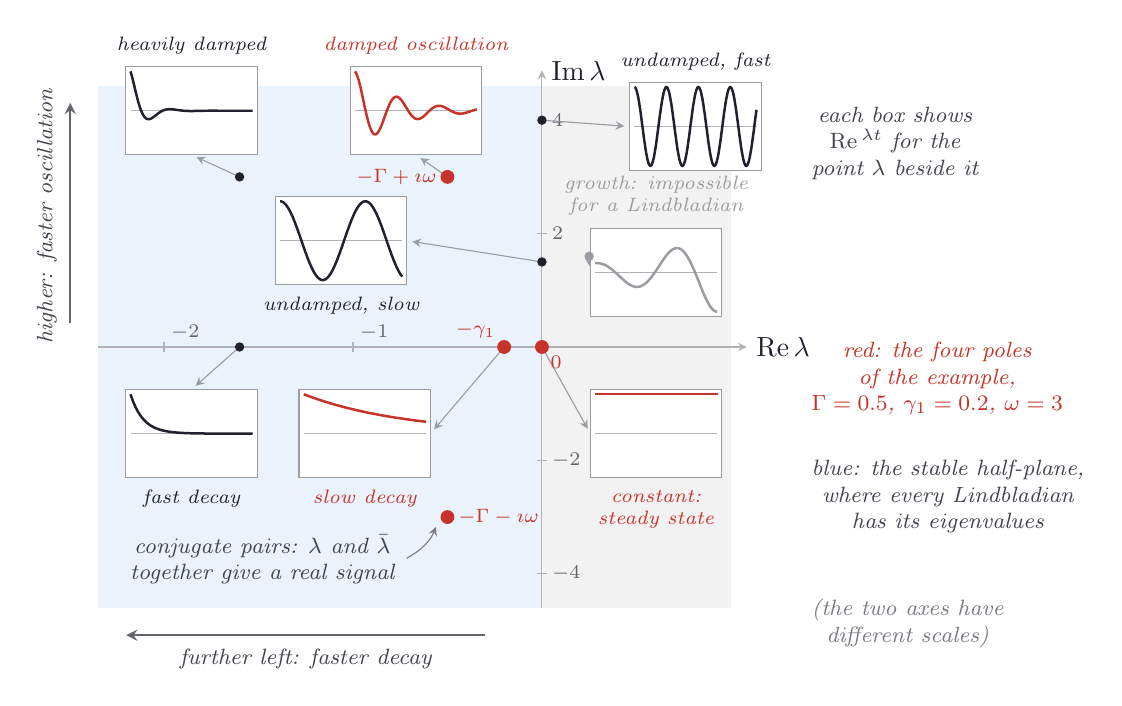
\begin{tikzpicture}[ink/.style={line width=0.9pt, ndInk}, faint/.style={line width=0.4pt, ndInk!35}, dashedink/.style={line width=0.5pt, ndInk!55, dash pattern=on 2.5pt off 2pt}, vec/.style={->, >=stealth, line width=1.2pt}, note/.style={font=\footnotesize\itshape, text=ndInk!85, align=center}, pointer/.style={->, >=stealth, line width=0.4pt, ndInk!60, shorten >=2pt, shorten <=1pt}, dot/.style={circle, fill=ndInk, inner sep=0pt, minimum size=3.4pt}, wash/.style={fill=ndSky, fill opacity=0.55}, every node/.style={text=ndInk}]
\definecolor{ndInk}{rgb}{0.13,0.13,0.18}
\definecolor{ndPaper}{rgb}{0.99,0.96,0.88}
\definecolor{ndSky}{rgb}{0.84,0.91,0.98}
\definecolor{ndRose}{rgb}{0.98,0.86,0.84}
\definecolor{ndBlue}{rgb}{0.13,0.36,0.66}
\definecolor{ndRed}{rgb}{0.78,0.20,0.16}
\definecolor{ndGold}{rgb}{0.88,0.62,0.10}
\definecolor{ndGreen}{rgb}{0.18,0.52,0.30}
\fill[ndSky, fill opacity=0.5] (-5.64,-3.31) rectangle (0,3.31);
\fill[ndInk, fill opacity=0.06] (0,-3.31) rectangle (2.40,3.31);
\draw[faint, ->, >=stealth] (-5.64,0) -- (2.60,0) node[right, text=ndInk] {$\mathrm{Re}\,\lambda$};
\draw[faint, ->, >=stealth] (0,-3.31) -- (0,3.51) node[right, text=ndInk] {$\mathrm{Im}\,\lambda$};
\draw[faint] (-4.80,0.06) -- (-4.80,-0.06);
\node[font=\scriptsize, text=ndInk!70, above right=-1pt] at (-4.80,0) {$-2$};
\draw[faint] (-2.40,0.06) -- (-2.40,-0.06);
\node[font=\scriptsize, text=ndInk!70, above right=-1pt] at (-2.40,0) {$-1$};
\draw[faint] (0.06,-2.88) -- (-0.06,-2.88);
\node[font=\scriptsize, text=ndInk!70, right=-1pt] at (0.04,-2.88) {$-4$};
\draw[faint] (0.06,-1.44) -- (-0.06,-1.44);
\node[font=\scriptsize, text=ndInk!70, right=-1pt] at (0.04,-1.44) {$-2$};
\draw[faint] (0.06,1.44) -- (-0.06,1.44);
\node[font=\scriptsize, text=ndInk!70, right=-1pt] at (0.04,1.44) {$2$};
\draw[faint] (0.06,2.88) -- (-0.06,2.88);
\node[font=\scriptsize, text=ndInk!70, right=-1pt] at (0.04,2.88) {$4$};
\draw[pointer, ndInk!45] (-3.840,0.000) -- (-4.450,-0.540);
\draw[pointer, ndInk!45] (-3.840,2.160) -- (-4.450,2.440);
\draw[pointer, ndInk!45] (0.000,1.080) -- (-1.715,1.350);
\draw[pointer, ndInk!45] (0.000,2.880) -- (1.115,2.800);
\draw[pointer, ndInk!45] (0.600,1.152) -- (0.615,0.950);
\draw[pointer, ndInk!45] (0.000,0.000) -- (0.615,-1.100);
\draw[pointer, ndInk!45] (-0.480,0.000) -- (-1.415,-1.100);
\draw[pointer, ndInk!45] (-1.200,2.160) -- (-1.600,2.440);
\fill[white] (-5.285,-1.660) rectangle (-3.615,-0.540);
\draw[line width=0.4pt, ndInk!45] (-5.285,-1.660) rectangle (-3.615,-0.540);
\draw[faint] (-5.225,-1.100) -- (-3.675,-1.100);
\draw[line width=0.9pt, ndInk] (-5.225,-0.600) -- (-5.220,-0.616) -- (-5.215,-0.631) -- (-5.209,-0.646) -- (-5.204,-0.660) -- (-5.199,-0.674) -- (-5.194,-0.688) -- (-5.189,-0.701) -- (-5.184,-0.713) -- (-5.178,-0.725) -- (-5.173,-0.737) -- (-5.168,-0.749) -- (-5.163,-0.760) -- (-5.158,-0.771) -- (-5.152,-0.781) -- (-5.147,-0.791) -- (-5.142,-0.801) -- (-5.137,-0.810) -- (-5.132,-0.819) -- (-5.127,-0.828) -- (-5.121,-0.837) -- (-5.116,-0.845) -- (-5.111,-0.853) -- (-5.106,-0.861) -- (-5.101,-0.869) -- (-5.095,-0.876) -- (-5.090,-0.883) -- (-5.085,-0.890) -- (-5.080,-0.897) -- (-5.075,-0.903) -- (-5.069,-0.909) -- (-5.064,-0.915) -- (-5.059,-0.921) -- (-5.054,-0.927) -- (-5.049,-0.932) -- (-5.044,-0.937) -- (-5.038,-0.943) -- (-5.033,-0.948) -- (-5.028,-0.952) -- (-5.023,-0.957) -- (-5.018,-0.962) -- (-5.012,-0.966) -- (-5.007,-0.970) -- (-5.002,-0.974) -- (-4.997,-0.978) -- (-4.992,-0.982) -- (-4.987,-0.986) -- (-4.981,-0.989) -- (-4.976,-0.993) -- (-4.971,-0.996) -- (-4.966,-1.000) -- (-4.961,-1.003) -- (-4.955,-1.006) -- (-4.950,-1.009) -- (-4.945,-1.012) -- (-4.940,-1.014) -- (-4.935,-1.017) -- (-4.930,-1.020) -- (-4.924,-1.022) -- (-4.919,-1.025) -- (-4.914,-1.027) -- (-4.909,-1.029) -- (-4.904,-1.032) -- (-4.898,-1.034) -- (-4.893,-1.036) -- (-4.888,-1.038) -- (-4.883,-1.040) -- (-4.878,-1.042) -- (-4.872,-1.044) -- (-4.867,-1.045) -- (-4.862,-1.047) -- (-4.857,-1.049) -- (-4.852,-1.050) -- (-4.847,-1.052) -- (-4.841,-1.054) -- (-4.836,-1.055) -- (-4.831,-1.056) -- (-4.826,-1.058) -- (-4.821,-1.059) -- (-4.815,-1.060) -- (-4.810,-1.062) -- (-4.805,-1.063) -- (-4.800,-1.064) -- (-4.795,-1.065) -- (-4.790,-1.066) -- (-4.784,-1.067) -- (-4.779,-1.068) -- (-4.774,-1.069) -- (-4.769,-1.070) -- (-4.764,-1.071) -- (-4.758,-1.072) -- (-4.753,-1.073) -- (-4.748,-1.074) -- (-4.743,-1.075) -- (-4.738,-1.076) -- (-4.733,-1.076) -- (-4.727,-1.077) -- (-4.722,-1.078) -- (-4.717,-1.078) -- (-4.712,-1.079) -- (-4.707,-1.080) -- (-4.701,-1.080) -- (-4.696,-1.081) -- (-4.691,-1.082) -- (-4.686,-1.082) -- (-4.681,-1.083) -- (-4.676,-1.083) -- (-4.670,-1.084) -- (-4.665,-1.084) -- (-4.660,-1.085) -- (-4.655,-1.085) -- (-4.650,-1.086) -- (-4.644,-1.086) -- (-4.639,-1.087) -- (-4.634,-1.087) -- (-4.629,-1.088) -- (-4.624,-1.088) -- (-4.618,-1.088) -- (-4.613,-1.089) -- (-4.608,-1.089) -- (-4.603,-1.089) -- (-4.598,-1.090) -- (-4.593,-1.090) -- (-4.587,-1.090) -- (-4.582,-1.091) -- (-4.577,-1.091) -- (-4.572,-1.091) -- (-4.567,-1.092) -- (-4.561,-1.092) -- (-4.556,-1.092) -- (-4.551,-1.092) -- (-4.546,-1.093) -- (-4.541,-1.093) -- (-4.536,-1.093) -- (-4.530,-1.093) -- (-4.525,-1.093) -- (-4.520,-1.094) -- (-4.515,-1.094) -- (-4.510,-1.094) -- (-4.504,-1.094) -- (-4.499,-1.094) -- (-4.494,-1.095) -- (-4.489,-1.095) -- (-4.484,-1.095) -- (-4.479,-1.095) -- (-4.473,-1.095) -- (-4.468,-1.095) -- (-4.463,-1.096) -- (-4.458,-1.096) -- (-4.453,-1.096) -- (-4.447,-1.096) -- (-4.442,-1.096) -- (-4.437,-1.096) -- (-4.432,-1.096) -- (-4.427,-1.096) -- (-4.421,-1.097) -- (-4.416,-1.097) -- (-4.411,-1.097) -- (-4.406,-1.097) -- (-4.401,-1.097) -- (-4.396,-1.097) -- (-4.390,-1.097) -- (-4.385,-1.097) -- (-4.380,-1.097) -- (-4.375,-1.097) -- (-4.370,-1.097) -- (-4.364,-1.098) -- (-4.359,-1.098) -- (-4.354,-1.098) -- (-4.349,-1.098) -- (-4.344,-1.098) -- (-4.339,-1.098) -- (-4.333,-1.098) -- (-4.328,-1.098) -- (-4.323,-1.098) -- (-4.318,-1.098) -- (-4.313,-1.098) -- (-4.307,-1.098) -- (-4.302,-1.098) -- (-4.297,-1.098) -- (-4.292,-1.098) -- (-4.287,-1.099) -- (-4.282,-1.099) -- (-4.276,-1.099) -- (-4.271,-1.099) -- (-4.266,-1.099) -- (-4.261,-1.099) -- (-4.256,-1.099) -- (-4.250,-1.099) -- (-4.245,-1.099) -- (-4.240,-1.099) -- (-4.235,-1.099) -- (-4.230,-1.099) -- (-4.224,-1.099) -- (-4.219,-1.099) -- (-4.214,-1.099) -- (-4.209,-1.099) -- (-4.204,-1.099) -- (-4.199,-1.099) -- (-4.193,-1.099) -- (-4.188,-1.099) -- (-4.183,-1.099) -- (-4.178,-1.099) -- (-4.173,-1.099) -- (-4.167,-1.099) -- (-4.162,-1.099) -- (-4.157,-1.099) -- (-4.152,-1.099) -- (-4.147,-1.099) -- (-4.142,-1.099) -- (-4.136,-1.099) -- (-4.131,-1.099) -- (-4.126,-1.099) -- (-4.121,-1.099) -- (-4.116,-1.099) -- (-4.110,-1.099) -- (-4.105,-1.100) -- (-4.100,-1.100) -- (-4.095,-1.100) -- (-4.090,-1.100) -- (-4.085,-1.100) -- (-4.079,-1.100) -- (-4.074,-1.100) -- (-4.069,-1.100) -- (-4.064,-1.100) -- (-4.059,-1.100) -- (-4.053,-1.100) -- (-4.048,-1.100) -- (-4.043,-1.100) -- (-4.038,-1.100) -- (-4.033,-1.100) -- (-4.028,-1.100) -- (-4.022,-1.100) -- (-4.017,-1.100) -- (-4.012,-1.100) -- (-4.007,-1.100) -- (-4.002,-1.100) -- (-3.996,-1.100) -- (-3.991,-1.100) -- (-3.986,-1.100) -- (-3.981,-1.100) -- (-3.976,-1.100) -- (-3.970,-1.100) -- (-3.965,-1.100) -- (-3.960,-1.100) -- (-3.955,-1.100) -- (-3.950,-1.100) -- (-3.945,-1.100) -- (-3.939,-1.100) -- (-3.934,-1.100) -- (-3.929,-1.100) -- (-3.924,-1.100) -- (-3.919,-1.100) -- (-3.913,-1.100) -- (-3.908,-1.100) -- (-3.903,-1.100) -- (-3.898,-1.100) -- (-3.893,-1.100) -- (-3.888,-1.100) -- (-3.882,-1.100) -- (-3.877,-1.100) -- (-3.872,-1.100) -- (-3.867,-1.100) -- (-3.862,-1.100) -- (-3.856,-1.100) -- (-3.851,-1.100) -- (-3.846,-1.100) -- (-3.841,-1.100) -- (-3.836,-1.100) -- (-3.831,-1.100) -- (-3.825,-1.100) -- (-3.820,-1.100) -- (-3.815,-1.100) -- (-3.810,-1.100) -- (-3.805,-1.100) -- (-3.799,-1.100) -- (-3.794,-1.100) -- (-3.789,-1.100) -- (-3.784,-1.100) -- (-3.779,-1.100) -- (-3.773,-1.100) -- (-3.768,-1.100) -- (-3.763,-1.100) -- (-3.758,-1.100) -- (-3.753,-1.100) -- (-3.748,-1.100) -- (-3.742,-1.100) -- (-3.737,-1.100) -- (-3.732,-1.100) -- (-3.727,-1.100) -- (-3.722,-1.100) -- (-3.716,-1.100) -- (-3.711,-1.100) -- (-3.706,-1.100) -- (-3.701,-1.100) -- (-3.696,-1.100) -- (-3.691,-1.100) -- (-3.685,-1.100) -- (-3.680,-1.100) -- (-3.675,-1.100);
\node[font=\scriptsize\itshape, text=ndInk, below=1pt, align=center] at (-4.450,-1.660) {fast decay};
\fill[white] (-5.285,2.440) rectangle (-3.615,3.560);
\draw[line width=0.4pt, ndInk!45] (-5.285,2.440) rectangle (-3.615,3.560);
\draw[faint] (-5.225,3.000) -- (-3.675,3.000);
\draw[line width=0.9pt, ndInk] (-5.225,3.500) -- (-5.220,3.483) -- (-5.215,3.466) -- (-5.209,3.447) -- (-5.204,3.427) -- (-5.199,3.407) -- (-5.194,3.386) -- (-5.189,3.364) -- (-5.184,3.343) -- (-5.178,3.321) -- (-5.173,3.299) -- (-5.168,3.277) -- (-5.163,3.255) -- (-5.158,3.234) -- (-5.152,3.212) -- (-5.147,3.191) -- (-5.142,3.171) -- (-5.137,3.151) -- (-5.132,3.131) -- (-5.127,3.113) -- (-5.121,3.094) -- (-5.116,3.077) -- (-5.111,3.060) -- (-5.106,3.044) -- (-5.101,3.029) -- (-5.095,3.015) -- (-5.090,3.001) -- (-5.085,2.989) -- (-5.080,2.977) -- (-5.075,2.966) -- (-5.069,2.956) -- (-5.064,2.946) -- (-5.059,2.938) -- (-5.054,2.930) -- (-5.049,2.923) -- (-5.044,2.917) -- (-5.038,2.912) -- (-5.033,2.907) -- (-5.028,2.903) -- (-5.023,2.900) -- (-5.018,2.897) -- (-5.012,2.895) -- (-5.007,2.894) -- (-5.002,2.893) -- (-4.997,2.893) -- (-4.992,2.893) -- (-4.987,2.894) -- (-4.981,2.895) -- (-4.976,2.896) -- (-4.971,2.898) -- (-4.966,2.900) -- (-4.961,2.903) -- (-4.955,2.906) -- (-4.950,2.909) -- (-4.945,2.912) -- (-4.940,2.916) -- (-4.935,2.919) -- (-4.930,2.923) -- (-4.924,2.927) -- (-4.919,2.931) -- (-4.914,2.935) -- (-4.909,2.939) -- (-4.904,2.943) -- (-4.898,2.947) -- (-4.893,2.951) -- (-4.888,2.956) -- (-4.883,2.960) -- (-4.878,2.963) -- (-4.872,2.967) -- (-4.867,2.971) -- (-4.862,2.975) -- (-4.857,2.978) -- (-4.852,2.982) -- (-4.847,2.985) -- (-4.841,2.988) -- (-4.836,2.991) -- (-4.831,2.994) -- (-4.826,2.997) -- (-4.821,2.999) -- (-4.815,3.002) -- (-4.810,3.004) -- (-4.805,3.006) -- (-4.800,3.008) -- (-4.795,3.010) -- (-4.790,3.011) -- (-4.784,3.013) -- (-4.779,3.014) -- (-4.774,3.015) -- (-4.769,3.016) -- (-4.764,3.017) -- (-4.758,3.018) -- (-4.753,3.019) -- (-4.748,3.019) -- (-4.743,3.020) -- (-4.738,3.020) -- (-4.733,3.020) -- (-4.727,3.020) -- (-4.722,3.020) -- (-4.717,3.020) -- (-4.712,3.020) -- (-4.707,3.019) -- (-4.701,3.019) -- (-4.696,3.019) -- (-4.691,3.018) -- (-4.686,3.018) -- (-4.681,3.017) -- (-4.676,3.017) -- (-4.670,3.016) -- (-4.665,3.015) -- (-4.660,3.015) -- (-4.655,3.014) -- (-4.650,3.013) -- (-4.644,3.012) -- (-4.639,3.012) -- (-4.634,3.011) -- (-4.629,3.010) -- (-4.624,3.009) -- (-4.618,3.008) -- (-4.613,3.008) -- (-4.608,3.007) -- (-4.603,3.006) -- (-4.598,3.006) -- (-4.593,3.005) -- (-4.587,3.004) -- (-4.582,3.004) -- (-4.577,3.003) -- (-4.572,3.002) -- (-4.567,3.002) -- (-4.561,3.001) -- (-4.556,3.001) -- (-4.551,3.000) -- (-4.546,3.000) -- (-4.541,2.999) -- (-4.536,2.999) -- (-4.530,2.999) -- (-4.525,2.998) -- (-4.520,2.998) -- (-4.515,2.998) -- (-4.510,2.997) -- (-4.504,2.997) -- (-4.499,2.997) -- (-4.494,2.997) -- (-4.489,2.997) -- (-4.484,2.997) -- (-4.479,2.996) -- (-4.473,2.996) -- (-4.468,2.996) -- (-4.463,2.996) -- (-4.458,2.996) -- (-4.453,2.996) -- (-4.447,2.996) -- (-4.442,2.996) -- (-4.437,2.996) -- (-4.432,2.996) -- (-4.427,2.996) -- (-4.421,2.997) -- (-4.416,2.997) -- (-4.411,2.997) -- (-4.406,2.997) -- (-4.401,2.997) -- (-4.396,2.997) -- (-4.390,2.997) -- (-4.385,2.997) -- (-4.380,2.998) -- (-4.375,2.998) -- (-4.370,2.998) -- (-4.364,2.998) -- (-4.359,2.998) -- (-4.354,2.998) -- (-4.349,2.998) -- (-4.344,2.999) -- (-4.339,2.999) -- (-4.333,2.999) -- (-4.328,2.999) -- (-4.323,2.999) -- (-4.318,2.999) -- (-4.313,2.999) -- (-4.307,2.999) -- (-4.302,3.000) -- (-4.297,3.000) -- (-4.292,3.000) -- (-4.287,3.000) -- (-4.282,3.000) -- (-4.276,3.000) -- (-4.271,3.000) -- (-4.266,3.000) -- (-4.261,3.000) -- (-4.256,3.000) -- (-4.250,3.000) -- (-4.245,3.000) -- (-4.240,3.000) -- (-4.235,3.001) -- (-4.230,3.001) -- (-4.224,3.001) -- (-4.219,3.001) -- (-4.214,3.001) -- (-4.209,3.001) -- (-4.204,3.001) -- (-4.199,3.001) -- (-4.193,3.001) -- (-4.188,3.001) -- (-4.183,3.001) -- (-4.178,3.001) -- (-4.173,3.001) -- (-4.167,3.001) -- (-4.162,3.001) -- (-4.157,3.001) -- (-4.152,3.001) -- (-4.147,3.001) -- (-4.142,3.001) -- (-4.136,3.001) -- (-4.131,3.001) -- (-4.126,3.001) -- (-4.121,3.001) -- (-4.116,3.000) -- (-4.110,3.000) -- (-4.105,3.000) -- (-4.100,3.000) -- (-4.095,3.000) -- (-4.090,3.000) -- (-4.085,3.000) -- (-4.079,3.000) -- (-4.074,3.000) -- (-4.069,3.000) -- (-4.064,3.000) -- (-4.059,3.000) -- (-4.053,3.000) -- (-4.048,3.000) -- (-4.043,3.000) -- (-4.038,3.000) -- (-4.033,3.000) -- (-4.028,3.000) -- (-4.022,3.000) -- (-4.017,3.000) -- (-4.012,3.000) -- (-4.007,3.000) -- (-4.002,3.000) -- (-3.996,3.000) -- (-3.991,3.000) -- (-3.986,3.000) -- (-3.981,3.000) -- (-3.976,3.000) -- (-3.970,3.000) -- (-3.965,3.000) -- (-3.960,3.000) -- (-3.955,3.000) -- (-3.950,3.000) -- (-3.945,3.000) -- (-3.939,3.000) -- (-3.934,3.000) -- (-3.929,3.000) -- (-3.924,3.000) -- (-3.919,3.000) -- (-3.913,3.000) -- (-3.908,3.000) -- (-3.903,3.000) -- (-3.898,3.000) -- (-3.893,3.000) -- (-3.888,3.000) -- (-3.882,3.000) -- (-3.877,3.000) -- (-3.872,3.000) -- (-3.867,3.000) -- (-3.862,3.000) -- (-3.856,3.000) -- (-3.851,3.000) -- (-3.846,3.000) -- (-3.841,3.000) -- (-3.836,3.000) -- (-3.831,3.000) -- (-3.825,3.000) -- (-3.820,3.000) -- (-3.815,3.000) -- (-3.810,3.000) -- (-3.805,3.000) -- (-3.799,3.000) -- (-3.794,3.000) -- (-3.789,3.000) -- (-3.784,3.000) -- (-3.779,3.000) -- (-3.773,3.000) -- (-3.768,3.000) -- (-3.763,3.000) -- (-3.758,3.000) -- (-3.753,3.000) -- (-3.748,3.000) -- (-3.742,3.000) -- (-3.737,3.000) -- (-3.732,3.000) -- (-3.727,3.000) -- (-3.722,3.000) -- (-3.716,3.000) -- (-3.711,3.000) -- (-3.706,3.000) -- (-3.701,3.000) -- (-3.696,3.000) -- (-3.691,3.000) -- (-3.685,3.000) -- (-3.680,3.000) -- (-3.675,3.000);
\node[font=\scriptsize\itshape, text=ndInk, above=1pt, align=center] at (-4.450,3.560) {heavily damped};
\fill[white] (-3.385,0.790) rectangle (-1.715,1.910);
\draw[line width=0.4pt, ndInk!45] (-3.385,0.790) rectangle (-1.715,1.910);
\draw[faint] (-3.325,1.350) -- (-1.775,1.350);
\draw[line width=0.9pt, ndInk] (-3.325,1.850) -- (-3.320,1.850) -- (-3.315,1.849) -- (-3.309,1.848) -- (-3.304,1.846) -- (-3.299,1.844) -- (-3.294,1.842) -- (-3.289,1.839) -- (-3.284,1.836) -- (-3.278,1.832) -- (-3.273,1.828) -- (-3.268,1.823) -- (-3.263,1.818) -- (-3.258,1.812) -- (-3.252,1.806) -- (-3.247,1.800) -- (-3.242,1.793) -- (-3.237,1.786) -- (-3.232,1.778) -- (-3.227,1.770) -- (-3.221,1.762) -- (-3.216,1.753) -- (-3.211,1.744) -- (-3.206,1.735) -- (-3.201,1.725) -- (-3.195,1.715) -- (-3.190,1.705) -- (-3.185,1.694) -- (-3.180,1.683) -- (-3.175,1.671) -- (-3.169,1.660) -- (-3.164,1.648) -- (-3.159,1.635) -- (-3.154,1.623) -- (-3.149,1.610) -- (-3.144,1.597) -- (-3.138,1.584) -- (-3.133,1.571) -- (-3.128,1.557) -- (-3.123,1.543) -- (-3.118,1.529) -- (-3.112,1.515) -- (-3.107,1.501) -- (-3.102,1.486) -- (-3.097,1.472) -- (-3.092,1.457) -- (-3.087,1.443) -- (-3.081,1.428) -- (-3.076,1.413) -- (-3.071,1.398) -- (-3.066,1.383) -- (-3.061,1.368) -- (-3.055,1.353) -- (-3.050,1.338) -- (-3.045,1.323) -- (-3.040,1.308) -- (-3.035,1.293) -- (-3.030,1.278) -- (-3.024,1.263) -- (-3.019,1.248) -- (-3.014,1.233) -- (-3.009,1.219) -- (-3.004,1.204) -- (-2.998,1.190) -- (-2.993,1.176) -- (-2.988,1.162) -- (-2.983,1.148) -- (-2.978,1.134) -- (-2.972,1.121) -- (-2.967,1.108) -- (-2.962,1.095) -- (-2.957,1.082) -- (-2.952,1.069) -- (-2.947,1.057) -- (-2.941,1.045) -- (-2.936,1.033) -- (-2.931,1.022) -- (-2.926,1.010) -- (-2.921,0.999) -- (-2.915,0.989) -- (-2.910,0.979) -- (-2.905,0.969) -- (-2.900,0.959) -- (-2.895,0.950) -- (-2.890,0.941) -- (-2.884,0.933) -- (-2.879,0.925) -- (-2.874,0.917) -- (-2.869,0.909) -- (-2.864,0.903) -- (-2.858,0.896) -- (-2.853,0.890) -- (-2.848,0.884) -- (-2.843,0.879) -- (-2.838,0.874) -- (-2.833,0.870) -- (-2.827,0.866) -- (-2.822,0.862) -- (-2.817,0.859) -- (-2.812,0.857) -- (-2.807,0.854) -- (-2.801,0.853) -- (-2.796,0.851) -- (-2.791,0.850) -- (-2.786,0.850) -- (-2.781,0.850) -- (-2.776,0.851) -- (-2.770,0.852) -- (-2.765,0.853) -- (-2.760,0.855) -- (-2.755,0.857) -- (-2.750,0.860) -- (-2.744,0.863) -- (-2.739,0.867) -- (-2.734,0.871) -- (-2.729,0.875) -- (-2.724,0.880) -- (-2.718,0.886) -- (-2.713,0.891) -- (-2.708,0.898) -- (-2.703,0.904) -- (-2.698,0.911) -- (-2.693,0.919) -- (-2.687,0.927) -- (-2.682,0.935) -- (-2.677,0.943) -- (-2.672,0.952) -- (-2.667,0.962) -- (-2.661,0.971) -- (-2.656,0.981) -- (-2.651,0.992) -- (-2.646,1.002) -- (-2.641,1.013) -- (-2.636,1.024) -- (-2.630,1.036) -- (-2.625,1.048) -- (-2.620,1.060) -- (-2.615,1.072) -- (-2.610,1.085) -- (-2.604,1.098) -- (-2.599,1.111) -- (-2.594,1.124) -- (-2.589,1.138) -- (-2.584,1.152) -- (-2.579,1.165) -- (-2.573,1.180) -- (-2.568,1.194) -- (-2.563,1.208) -- (-2.558,1.223) -- (-2.553,1.237) -- (-2.547,1.252) -- (-2.542,1.267) -- (-2.537,1.282) -- (-2.532,1.297) -- (-2.527,1.312) -- (-2.521,1.327) -- (-2.516,1.342) -- (-2.511,1.357) -- (-2.506,1.372) -- (-2.501,1.387) -- (-2.496,1.402) -- (-2.490,1.417) -- (-2.485,1.432) -- (-2.480,1.446) -- (-2.475,1.461) -- (-2.470,1.476) -- (-2.464,1.490) -- (-2.459,1.505) -- (-2.454,1.519) -- (-2.449,1.533) -- (-2.444,1.547) -- (-2.439,1.561) -- (-2.433,1.574) -- (-2.428,1.588) -- (-2.423,1.601) -- (-2.418,1.614) -- (-2.413,1.626) -- (-2.407,1.639) -- (-2.402,1.651) -- (-2.397,1.663) -- (-2.392,1.674) -- (-2.387,1.686) -- (-2.382,1.697) -- (-2.376,1.707) -- (-2.371,1.718) -- (-2.366,1.728) -- (-2.361,1.737) -- (-2.356,1.747) -- (-2.350,1.756) -- (-2.345,1.764) -- (-2.340,1.773) -- (-2.335,1.780) -- (-2.330,1.788) -- (-2.324,1.795) -- (-2.319,1.802) -- (-2.314,1.808) -- (-2.309,1.814) -- (-2.304,1.819) -- (-2.299,1.824) -- (-2.293,1.829) -- (-2.288,1.833) -- (-2.283,1.836) -- (-2.278,1.840) -- (-2.273,1.843) -- (-2.267,1.845) -- (-2.262,1.847) -- (-2.257,1.848) -- (-2.252,1.849) -- (-2.247,1.850) -- (-2.242,1.850) -- (-2.236,1.850) -- (-2.231,1.849) -- (-2.226,1.848) -- (-2.221,1.846) -- (-2.216,1.844) -- (-2.210,1.841) -- (-2.205,1.838) -- (-2.200,1.835) -- (-2.195,1.831) -- (-2.190,1.826) -- (-2.185,1.822) -- (-2.179,1.816) -- (-2.174,1.811) -- (-2.169,1.805) -- (-2.164,1.798) -- (-2.159,1.791) -- (-2.153,1.784) -- (-2.148,1.776) -- (-2.143,1.768) -- (-2.138,1.760) -- (-2.133,1.751) -- (-2.128,1.742) -- (-2.122,1.732) -- (-2.117,1.723) -- (-2.112,1.712) -- (-2.107,1.702) -- (-2.102,1.691) -- (-2.096,1.680) -- (-2.091,1.668) -- (-2.086,1.657) -- (-2.081,1.645) -- (-2.076,1.632) -- (-2.070,1.620) -- (-2.065,1.607) -- (-2.060,1.594) -- (-2.055,1.581) -- (-2.050,1.567) -- (-2.045,1.554) -- (-2.039,1.540) -- (-2.034,1.526) -- (-2.029,1.512) -- (-2.024,1.497) -- (-2.019,1.483) -- (-2.013,1.468) -- (-2.008,1.453) -- (-2.003,1.439) -- (-1.998,1.424) -- (-1.993,1.409) -- (-1.988,1.394) -- (-1.982,1.379) -- (-1.977,1.364) -- (-1.972,1.349) -- (-1.967,1.334) -- (-1.962,1.319) -- (-1.956,1.304) -- (-1.951,1.289) -- (-1.946,1.274) -- (-1.941,1.259) -- (-1.936,1.244) -- (-1.931,1.230) -- (-1.925,1.215) -- (-1.920,1.201) -- (-1.915,1.186) -- (-1.910,1.172) -- (-1.905,1.158) -- (-1.899,1.144) -- (-1.894,1.131) -- (-1.889,1.117) -- (-1.884,1.104) -- (-1.879,1.091) -- (-1.873,1.078) -- (-1.868,1.066) -- (-1.863,1.054) -- (-1.858,1.042) -- (-1.853,1.030) -- (-1.848,1.019) -- (-1.842,1.007) -- (-1.837,0.997) -- (-1.832,0.986) -- (-1.827,0.976) -- (-1.822,0.966) -- (-1.816,0.957) -- (-1.811,0.948) -- (-1.806,0.939) -- (-1.801,0.930) -- (-1.796,0.922) -- (-1.791,0.915) -- (-1.785,0.908) -- (-1.780,0.901) -- (-1.775,0.894);
\node[font=\scriptsize\itshape, text=ndInk, below=1pt, align=center] at (-2.550,0.790) {undamped, slow};
\fill[white] (1.115,2.240) rectangle (2.785,3.360);
\draw[line width=0.4pt, ndInk!45] (1.115,2.240) rectangle (2.785,3.360);
\draw[faint] (1.175,2.800) -- (2.725,2.800);
\draw[line width=0.9pt, ndInk] (1.175,3.300) -- (1.180,3.298) -- (1.185,3.294) -- (1.191,3.286) -- (1.196,3.274) -- (1.201,3.260) -- (1.206,3.243) -- (1.211,3.223) -- (1.216,3.200) -- (1.222,3.175) -- (1.227,3.147) -- (1.232,3.117) -- (1.237,3.085) -- (1.242,3.052) -- (1.248,3.016) -- (1.253,2.979) -- (1.258,2.941) -- (1.263,2.902) -- (1.268,2.863) -- (1.273,2.823) -- (1.279,2.783) -- (1.284,2.743) -- (1.289,2.703) -- (1.294,2.664) -- (1.299,2.626) -- (1.305,2.589) -- (1.310,2.553) -- (1.315,2.519) -- (1.320,2.487) -- (1.325,2.457) -- (1.331,2.429) -- (1.336,2.403) -- (1.341,2.380) -- (1.346,2.359) -- (1.351,2.342) -- (1.356,2.327) -- (1.362,2.316) -- (1.367,2.307) -- (1.372,2.302) -- (1.377,2.300) -- (1.382,2.301) -- (1.388,2.306) -- (1.393,2.313) -- (1.398,2.324) -- (1.403,2.338) -- (1.408,2.354) -- (1.413,2.374) -- (1.419,2.396) -- (1.424,2.421) -- (1.429,2.449) -- (1.434,2.478) -- (1.439,2.510) -- (1.445,2.544) -- (1.450,2.579) -- (1.455,2.615) -- (1.460,2.653) -- (1.465,2.692) -- (1.470,2.732) -- (1.476,2.772) -- (1.481,2.812) -- (1.486,2.852) -- (1.491,2.891) -- (1.496,2.931) -- (1.502,2.969) -- (1.507,3.006) -- (1.512,3.042) -- (1.517,3.076) -- (1.522,3.109) -- (1.528,3.139) -- (1.533,3.168) -- (1.538,3.194) -- (1.543,3.217) -- (1.548,3.238) -- (1.553,3.256) -- (1.559,3.271) -- (1.564,3.283) -- (1.569,3.292) -- (1.574,3.297) -- (1.579,3.300) -- (1.585,3.299) -- (1.590,3.295) -- (1.595,3.288) -- (1.600,3.278) -- (1.605,3.265) -- (1.610,3.248) -- (1.616,3.229) -- (1.621,3.207) -- (1.626,3.182) -- (1.631,3.155) -- (1.636,3.126) -- (1.642,3.095) -- (1.647,3.061) -- (1.652,3.026) -- (1.657,2.990) -- (1.662,2.952) -- (1.667,2.913) -- (1.673,2.874) -- (1.678,2.834) -- (1.683,2.794) -- (1.688,2.754) -- (1.693,2.714) -- (1.699,2.675) -- (1.704,2.636) -- (1.709,2.599) -- (1.714,2.563) -- (1.719,2.528) -- (1.724,2.496) -- (1.730,2.465) -- (1.735,2.436) -- (1.740,2.410) -- (1.745,2.386) -- (1.750,2.365) -- (1.756,2.347) -- (1.761,2.331) -- (1.766,2.319) -- (1.771,2.309) -- (1.776,2.303) -- (1.782,2.300) -- (1.787,2.301) -- (1.792,2.304) -- (1.797,2.311) -- (1.802,2.321) -- (1.807,2.333) -- (1.813,2.349) -- (1.818,2.368) -- (1.823,2.390) -- (1.828,2.414) -- (1.833,2.441) -- (1.839,2.470) -- (1.844,2.501) -- (1.849,2.534) -- (1.854,2.569) -- (1.859,2.605) -- (1.864,2.643) -- (1.870,2.681) -- (1.875,2.721) -- (1.880,2.760) -- (1.885,2.801) -- (1.890,2.841) -- (1.896,2.880) -- (1.901,2.920) -- (1.906,2.958) -- (1.911,2.996) -- (1.916,3.032) -- (1.921,3.067) -- (1.927,3.100) -- (1.932,3.131) -- (1.937,3.160) -- (1.942,3.187) -- (1.947,3.211) -- (1.953,3.232) -- (1.958,3.251) -- (1.963,3.267) -- (1.968,3.280) -- (1.973,3.290) -- (1.979,3.296) -- (1.984,3.300) -- (1.989,3.300) -- (1.994,3.297) -- (1.999,3.290) -- (2.004,3.281) -- (2.010,3.269) -- (2.015,3.253) -- (2.020,3.235) -- (2.025,3.213) -- (2.030,3.189) -- (2.036,3.163) -- (2.041,3.134) -- (2.046,3.103) -- (2.051,3.071) -- (2.056,3.036) -- (2.061,3.000) -- (2.067,2.963) -- (2.072,2.924) -- (2.077,2.885) -- (2.082,2.845) -- (2.087,2.805) -- (2.093,2.765) -- (2.098,2.725) -- (2.103,2.686) -- (2.108,2.647) -- (2.113,2.609) -- (2.118,2.573) -- (2.124,2.538) -- (2.129,2.505) -- (2.134,2.473) -- (2.139,2.444) -- (2.144,2.417) -- (2.150,2.392) -- (2.155,2.370) -- (2.160,2.351) -- (2.165,2.335) -- (2.170,2.322) -- (2.176,2.312) -- (2.181,2.305) -- (2.186,2.301) -- (2.191,2.300) -- (2.196,2.303) -- (2.201,2.309) -- (2.207,2.317) -- (2.212,2.330) -- (2.217,2.345) -- (2.222,2.363) -- (2.227,2.384) -- (2.233,2.407) -- (2.238,2.433) -- (2.243,2.462) -- (2.248,2.492) -- (2.253,2.525) -- (2.258,2.559) -- (2.264,2.595) -- (2.269,2.632) -- (2.274,2.670) -- (2.279,2.710) -- (2.284,2.749) -- (2.290,2.789) -- (2.295,2.829) -- (2.300,2.869) -- (2.305,2.909) -- (2.310,2.948) -- (2.315,2.986) -- (2.321,3.022) -- (2.326,3.057) -- (2.331,3.091) -- (2.336,3.123) -- (2.341,3.152) -- (2.347,3.179) -- (2.352,3.204) -- (2.357,3.227) -- (2.362,3.246) -- (2.367,3.263) -- (2.372,3.277) -- (2.378,3.287) -- (2.383,3.295) -- (2.388,3.299) -- (2.393,3.300) -- (2.398,3.298) -- (2.404,3.292) -- (2.409,3.284) -- (2.414,3.272) -- (2.419,3.258) -- (2.424,3.240) -- (2.430,3.220) -- (2.435,3.196) -- (2.440,3.171) -- (2.445,3.143) -- (2.450,3.112) -- (2.455,3.080) -- (2.461,3.046) -- (2.466,3.010) -- (2.471,2.973) -- (2.476,2.935) -- (2.481,2.896) -- (2.487,2.856) -- (2.492,2.816) -- (2.497,2.776) -- (2.502,2.736) -- (2.507,2.697) -- (2.512,2.658) -- (2.518,2.620) -- (2.523,2.583) -- (2.528,2.547) -- (2.533,2.514) -- (2.538,2.482) -- (2.544,2.452) -- (2.549,2.424) -- (2.554,2.399) -- (2.559,2.376) -- (2.564,2.356) -- (2.569,2.339) -- (2.575,2.325) -- (2.580,2.314) -- (2.585,2.306) -- (2.590,2.302) -- (2.595,2.300) -- (2.601,2.302) -- (2.606,2.307) -- (2.611,2.315) -- (2.616,2.326) -- (2.621,2.340) -- (2.627,2.357) -- (2.632,2.377) -- (2.637,2.400) -- (2.642,2.426) -- (2.647,2.453) -- (2.652,2.483) -- (2.658,2.515) -- (2.663,2.549) -- (2.668,2.585) -- (2.673,2.622) -- (2.678,2.660) -- (2.684,2.699) -- (2.689,2.738) -- (2.694,2.778) -- (2.699,2.818) -- (2.704,2.858) -- (2.709,2.898) -- (2.715,2.937) -- (2.720,2.975) -- (2.725,3.012);
\node[font=\scriptsize\itshape, text=ndInk, above=1pt, align=center] at (1.950,3.360) {undamped, fast};
\fill[white] (0.615,0.390) rectangle (2.285,1.510);
\draw[line width=0.4pt, ndInk!45] (0.615,0.390) rectangle (2.285,1.510);
\draw[faint] (0.675,0.950) -- (2.225,0.950);
\draw[line width=0.9pt, ndInk!45] (0.675,1.063) -- (0.680,1.064) -- (0.685,1.064) -- (0.691,1.064) -- (0.696,1.065) -- (0.701,1.065) -- (0.706,1.065) -- (0.711,1.064) -- (0.716,1.064) -- (0.722,1.064) -- (0.727,1.063) -- (0.732,1.062) -- (0.737,1.061) -- (0.742,1.061) -- (0.748,1.059) -- (0.753,1.058) -- (0.758,1.057) -- (0.763,1.055) -- (0.768,1.054) -- (0.773,1.052) -- (0.779,1.050) -- (0.784,1.048) -- (0.789,1.046) -- (0.794,1.044) -- (0.799,1.042) -- (0.805,1.039) -- (0.810,1.037) -- (0.815,1.034) -- (0.820,1.031) -- (0.825,1.028) -- (0.831,1.025) -- (0.836,1.022) -- (0.841,1.019) -- (0.846,1.015) -- (0.851,1.012) -- (0.856,1.008) -- (0.862,1.005) -- (0.867,1.001) -- (0.872,0.997) -- (0.877,0.993) -- (0.882,0.989) -- (0.888,0.985) -- (0.893,0.981) -- (0.898,0.977) -- (0.903,0.972) -- (0.908,0.968) -- (0.913,0.963) -- (0.919,0.959) -- (0.924,0.954) -- (0.929,0.950) -- (0.934,0.945) -- (0.939,0.940) -- (0.945,0.935) -- (0.950,0.931) -- (0.955,0.926) -- (0.960,0.921) -- (0.965,0.916) -- (0.970,0.911) -- (0.976,0.906) -- (0.981,0.902) -- (0.986,0.897) -- (0.991,0.892) -- (0.996,0.887) -- (1.002,0.882) -- (1.007,0.877) -- (1.012,0.873) -- (1.017,0.868) -- (1.022,0.863) -- (1.028,0.858) -- (1.033,0.854) -- (1.038,0.849) -- (1.043,0.845) -- (1.048,0.840) -- (1.053,0.836) -- (1.059,0.832) -- (1.064,0.827) -- (1.069,0.823) -- (1.074,0.819) -- (1.079,0.815) -- (1.085,0.812) -- (1.090,0.808) -- (1.095,0.804) -- (1.100,0.801) -- (1.105,0.797) -- (1.110,0.794) -- (1.116,0.791) -- (1.121,0.788) -- (1.126,0.785) -- (1.131,0.783) -- (1.136,0.780) -- (1.142,0.778) -- (1.147,0.775) -- (1.152,0.773) -- (1.157,0.772) -- (1.162,0.770) -- (1.167,0.768) -- (1.173,0.767) -- (1.178,0.766) -- (1.183,0.765) -- (1.188,0.764) -- (1.193,0.763) -- (1.199,0.763) -- (1.204,0.763) -- (1.209,0.763) -- (1.214,0.763) -- (1.219,0.763) -- (1.224,0.764) -- (1.230,0.765) -- (1.235,0.766) -- (1.240,0.767) -- (1.245,0.768) -- (1.250,0.770) -- (1.256,0.771) -- (1.261,0.773) -- (1.266,0.776) -- (1.271,0.778) -- (1.276,0.781) -- (1.282,0.784) -- (1.287,0.787) -- (1.292,0.790) -- (1.297,0.793) -- (1.302,0.797) -- (1.307,0.801) -- (1.313,0.805) -- (1.318,0.809) -- (1.323,0.814) -- (1.328,0.818) -- (1.333,0.823) -- (1.339,0.828) -- (1.344,0.833) -- (1.349,0.838) -- (1.354,0.844) -- (1.359,0.850) -- (1.364,0.856) -- (1.370,0.862) -- (1.375,0.868) -- (1.380,0.874) -- (1.385,0.880) -- (1.390,0.887) -- (1.396,0.894) -- (1.401,0.901) -- (1.406,0.908) -- (1.411,0.915) -- (1.416,0.922) -- (1.421,0.929) -- (1.427,0.937) -- (1.432,0.944) -- (1.437,0.952) -- (1.442,0.959) -- (1.447,0.967) -- (1.453,0.975) -- (1.458,0.983) -- (1.463,0.991) -- (1.468,0.998) -- (1.473,1.006) -- (1.479,1.014) -- (1.484,1.022) -- (1.489,1.030) -- (1.494,1.038) -- (1.499,1.046) -- (1.504,1.054) -- (1.510,1.062) -- (1.515,1.070) -- (1.520,1.078) -- (1.525,1.086) -- (1.530,1.093) -- (1.536,1.101) -- (1.541,1.108) -- (1.546,1.116) -- (1.551,1.123) -- (1.556,1.130) -- (1.561,1.137) -- (1.567,1.144) -- (1.572,1.151) -- (1.577,1.158) -- (1.582,1.165) -- (1.587,1.171) -- (1.593,1.177) -- (1.598,1.183) -- (1.603,1.189) -- (1.608,1.195) -- (1.613,1.200) -- (1.618,1.205) -- (1.624,1.210) -- (1.629,1.215) -- (1.634,1.220) -- (1.639,1.224) -- (1.644,1.228) -- (1.650,1.232) -- (1.655,1.236) -- (1.660,1.239) -- (1.665,1.242) -- (1.670,1.245) -- (1.676,1.247) -- (1.681,1.249) -- (1.686,1.251) -- (1.691,1.253) -- (1.696,1.254) -- (1.701,1.255) -- (1.707,1.256) -- (1.712,1.256) -- (1.717,1.256) -- (1.722,1.256) -- (1.727,1.255) -- (1.733,1.254) -- (1.738,1.253) -- (1.743,1.251) -- (1.748,1.249) -- (1.753,1.247) -- (1.758,1.244) -- (1.764,1.241) -- (1.769,1.238) -- (1.774,1.234) -- (1.779,1.230) -- (1.784,1.226) -- (1.790,1.221) -- (1.795,1.216) -- (1.800,1.211) -- (1.805,1.205) -- (1.810,1.199) -- (1.815,1.193) -- (1.821,1.186) -- (1.826,1.179) -- (1.831,1.172) -- (1.836,1.164) -- (1.841,1.156) -- (1.847,1.148) -- (1.852,1.140) -- (1.857,1.131) -- (1.862,1.122) -- (1.867,1.112) -- (1.872,1.103) -- (1.878,1.093) -- (1.883,1.083) -- (1.888,1.073) -- (1.893,1.062) -- (1.898,1.051) -- (1.904,1.040) -- (1.909,1.029) -- (1.914,1.017) -- (1.919,1.006) -- (1.924,0.994) -- (1.930,0.982) -- (1.935,0.970) -- (1.940,0.958) -- (1.945,0.945) -- (1.950,0.933) -- (1.955,0.920) -- (1.961,0.907) -- (1.966,0.895) -- (1.971,0.882) -- (1.976,0.869) -- (1.981,0.856) -- (1.987,0.843) -- (1.992,0.830) -- (1.997,0.817) -- (2.002,0.804) -- (2.007,0.791) -- (2.012,0.778) -- (2.018,0.765) -- (2.023,0.752) -- (2.028,0.739) -- (2.033,0.727) -- (2.038,0.714) -- (2.044,0.702) -- (2.049,0.689) -- (2.054,0.677) -- (2.059,0.665) -- (2.064,0.654) -- (2.069,0.642) -- (2.075,0.631) -- (2.080,0.619) -- (2.085,0.609) -- (2.090,0.598) -- (2.095,0.587) -- (2.101,0.577) -- (2.106,0.568) -- (2.111,0.558) -- (2.116,0.549) -- (2.121,0.540) -- (2.127,0.531) -- (2.132,0.523) -- (2.137,0.515) -- (2.142,0.508) -- (2.147,0.501) -- (2.152,0.494) -- (2.158,0.488) -- (2.163,0.482) -- (2.168,0.477) -- (2.173,0.472) -- (2.178,0.468) -- (2.184,0.464) -- (2.189,0.460) -- (2.194,0.457) -- (2.199,0.455) -- (2.204,0.453) -- (2.209,0.451) -- (2.215,0.450) -- (2.220,0.450) -- (2.225,0.450);
\node[font=\scriptsize\itshape, text=ndInk!45, above=1pt, align=center] at (1.450,1.510) {growth: impossible\\ for a Lindbladian};
\fill[white] (0.615,-1.660) rectangle (2.285,-0.540);
\draw[line width=0.4pt, ndInk!45] (0.615,-1.660) rectangle (2.285,-0.540);
\draw[faint] (0.675,-1.100) -- (2.225,-1.100);
\draw[line width=0.9pt, ndRed] (0.675,-0.600) -- (0.680,-0.600) -- (0.685,-0.600) -- (0.691,-0.600) -- (0.696,-0.600) -- (0.701,-0.600) -- (0.706,-0.600) -- (0.711,-0.600) -- (0.716,-0.600) -- (0.722,-0.600) -- (0.727,-0.600) -- (0.732,-0.600) -- (0.737,-0.600) -- (0.742,-0.600) -- (0.748,-0.600) -- (0.753,-0.600) -- (0.758,-0.600) -- (0.763,-0.600) -- (0.768,-0.600) -- (0.773,-0.600) -- (0.779,-0.600) -- (0.784,-0.600) -- (0.789,-0.600) -- (0.794,-0.600) -- (0.799,-0.600) -- (0.805,-0.600) -- (0.810,-0.600) -- (0.815,-0.600) -- (0.820,-0.600) -- (0.825,-0.600) -- (0.831,-0.600) -- (0.836,-0.600) -- (0.841,-0.600) -- (0.846,-0.600) -- (0.851,-0.600) -- (0.856,-0.600) -- (0.862,-0.600) -- (0.867,-0.600) -- (0.872,-0.600) -- (0.877,-0.600) -- (0.882,-0.600) -- (0.888,-0.600) -- (0.893,-0.600) -- (0.898,-0.600) -- (0.903,-0.600) -- (0.908,-0.600) -- (0.913,-0.600) -- (0.919,-0.600) -- (0.924,-0.600) -- (0.929,-0.600) -- (0.934,-0.600) -- (0.939,-0.600) -- (0.945,-0.600) -- (0.950,-0.600) -- (0.955,-0.600) -- (0.960,-0.600) -- (0.965,-0.600) -- (0.970,-0.600) -- (0.976,-0.600) -- (0.981,-0.600) -- (0.986,-0.600) -- (0.991,-0.600) -- (0.996,-0.600) -- (1.002,-0.600) -- (1.007,-0.600) -- (1.012,-0.600) -- (1.017,-0.600) -- (1.022,-0.600) -- (1.028,-0.600) -- (1.033,-0.600) -- (1.038,-0.600) -- (1.043,-0.600) -- (1.048,-0.600) -- (1.053,-0.600) -- (1.059,-0.600) -- (1.064,-0.600) -- (1.069,-0.600) -- (1.074,-0.600) -- (1.079,-0.600) -- (1.085,-0.600) -- (1.090,-0.600) -- (1.095,-0.600) -- (1.100,-0.600) -- (1.105,-0.600) -- (1.110,-0.600) -- (1.116,-0.600) -- (1.121,-0.600) -- (1.126,-0.600) -- (1.131,-0.600) -- (1.136,-0.600) -- (1.142,-0.600) -- (1.147,-0.600) -- (1.152,-0.600) -- (1.157,-0.600) -- (1.162,-0.600) -- (1.167,-0.600) -- (1.173,-0.600) -- (1.178,-0.600) -- (1.183,-0.600) -- (1.188,-0.600) -- (1.193,-0.600) -- (1.199,-0.600) -- (1.204,-0.600) -- (1.209,-0.600) -- (1.214,-0.600) -- (1.219,-0.600) -- (1.224,-0.600) -- (1.230,-0.600) -- (1.235,-0.600) -- (1.240,-0.600) -- (1.245,-0.600) -- (1.250,-0.600) -- (1.256,-0.600) -- (1.261,-0.600) -- (1.266,-0.600) -- (1.271,-0.600) -- (1.276,-0.600) -- (1.282,-0.600) -- (1.287,-0.600) -- (1.292,-0.600) -- (1.297,-0.600) -- (1.302,-0.600) -- (1.307,-0.600) -- (1.313,-0.600) -- (1.318,-0.600) -- (1.323,-0.600) -- (1.328,-0.600) -- (1.333,-0.600) -- (1.339,-0.600) -- (1.344,-0.600) -- (1.349,-0.600) -- (1.354,-0.600) -- (1.359,-0.600) -- (1.364,-0.600) -- (1.370,-0.600) -- (1.375,-0.600) -- (1.380,-0.600) -- (1.385,-0.600) -- (1.390,-0.600) -- (1.396,-0.600) -- (1.401,-0.600) -- (1.406,-0.600) -- (1.411,-0.600) -- (1.416,-0.600) -- (1.421,-0.600) -- (1.427,-0.600) -- (1.432,-0.600) -- (1.437,-0.600) -- (1.442,-0.600) -- (1.447,-0.600) -- (1.453,-0.600) -- (1.458,-0.600) -- (1.463,-0.600) -- (1.468,-0.600) -- (1.473,-0.600) -- (1.479,-0.600) -- (1.484,-0.600) -- (1.489,-0.600) -- (1.494,-0.600) -- (1.499,-0.600) -- (1.504,-0.600) -- (1.510,-0.600) -- (1.515,-0.600) -- (1.520,-0.600) -- (1.525,-0.600) -- (1.530,-0.600) -- (1.536,-0.600) -- (1.541,-0.600) -- (1.546,-0.600) -- (1.551,-0.600) -- (1.556,-0.600) -- (1.561,-0.600) -- (1.567,-0.600) -- (1.572,-0.600) -- (1.577,-0.600) -- (1.582,-0.600) -- (1.587,-0.600) -- (1.593,-0.600) -- (1.598,-0.600) -- (1.603,-0.600) -- (1.608,-0.600) -- (1.613,-0.600) -- (1.618,-0.600) -- (1.624,-0.600) -- (1.629,-0.600) -- (1.634,-0.600) -- (1.639,-0.600) -- (1.644,-0.600) -- (1.650,-0.600) -- (1.655,-0.600) -- (1.660,-0.600) -- (1.665,-0.600) -- (1.670,-0.600) -- (1.676,-0.600) -- (1.681,-0.600) -- (1.686,-0.600) -- (1.691,-0.600) -- (1.696,-0.600) -- (1.701,-0.600) -- (1.707,-0.600) -- (1.712,-0.600) -- (1.717,-0.600) -- (1.722,-0.600) -- (1.727,-0.600) -- (1.733,-0.600) -- (1.738,-0.600) -- (1.743,-0.600) -- (1.748,-0.600) -- (1.753,-0.600) -- (1.758,-0.600) -- (1.764,-0.600) -- (1.769,-0.600) -- (1.774,-0.600) -- (1.779,-0.600) -- (1.784,-0.600) -- (1.790,-0.600) -- (1.795,-0.600) -- (1.800,-0.600) -- (1.805,-0.600) -- (1.810,-0.600) -- (1.815,-0.600) -- (1.821,-0.600) -- (1.826,-0.600) -- (1.831,-0.600) -- (1.836,-0.600) -- (1.841,-0.600) -- (1.847,-0.600) -- (1.852,-0.600) -- (1.857,-0.600) -- (1.862,-0.600) -- (1.867,-0.600) -- (1.872,-0.600) -- (1.878,-0.600) -- (1.883,-0.600) -- (1.888,-0.600) -- (1.893,-0.600) -- (1.898,-0.600) -- (1.904,-0.600) -- (1.909,-0.600) -- (1.914,-0.600) -- (1.919,-0.600) -- (1.924,-0.600) -- (1.930,-0.600) -- (1.935,-0.600) -- (1.940,-0.600) -- (1.945,-0.600) -- (1.950,-0.600) -- (1.955,-0.600) -- (1.961,-0.600) -- (1.966,-0.600) -- (1.971,-0.600) -- (1.976,-0.600) -- (1.981,-0.600) -- (1.987,-0.600) -- (1.992,-0.600) -- (1.997,-0.600) -- (2.002,-0.600) -- (2.007,-0.600) -- (2.012,-0.600) -- (2.018,-0.600) -- (2.023,-0.600) -- (2.028,-0.600) -- (2.033,-0.600) -- (2.038,-0.600) -- (2.044,-0.600) -- (2.049,-0.600) -- (2.054,-0.600) -- (2.059,-0.600) -- (2.064,-0.600) -- (2.069,-0.600) -- (2.075,-0.600) -- (2.080,-0.600) -- (2.085,-0.600) -- (2.090,-0.600) -- (2.095,-0.600) -- (2.101,-0.600) -- (2.106,-0.600) -- (2.111,-0.600) -- (2.116,-0.600) -- (2.121,-0.600) -- (2.127,-0.600) -- (2.132,-0.600) -- (2.137,-0.600) -- (2.142,-0.600) -- (2.147,-0.600) -- (2.152,-0.600) -- (2.158,-0.600) -- (2.163,-0.600) -- (2.168,-0.600) -- (2.173,-0.600) -- (2.178,-0.600) -- (2.184,-0.600) -- (2.189,-0.600) -- (2.194,-0.600) -- (2.199,-0.600) -- (2.204,-0.600) -- (2.209,-0.600) -- (2.215,-0.600) -- (2.220,-0.600) -- (2.225,-0.600);
\node[font=\scriptsize\itshape, text=ndRed, below=1pt, align=center] at (1.450,-1.660) {constant:\\ steady state};
\fill[white] (-3.085,-1.660) rectangle (-1.415,-0.540);
\draw[line width=0.4pt, ndInk!45] (-3.085,-1.660) rectangle (-1.415,-0.540);
\draw[faint] (-3.025,-1.100) -- (-1.475,-1.100);
\draw[line width=0.9pt, ndRed] (-3.025,-0.600) -- (-3.020,-0.602) -- (-3.015,-0.604) -- (-3.009,-0.606) -- (-3.004,-0.608) -- (-2.999,-0.610) -- (-2.994,-0.612) -- (-2.989,-0.614) -- (-2.984,-0.616) -- (-2.978,-0.618) -- (-2.973,-0.620) -- (-2.968,-0.622) -- (-2.963,-0.624) -- (-2.958,-0.625) -- (-2.952,-0.627) -- (-2.947,-0.629) -- (-2.942,-0.631) -- (-2.937,-0.633) -- (-2.932,-0.635) -- (-2.927,-0.637) -- (-2.921,-0.639) -- (-2.916,-0.640) -- (-2.911,-0.642) -- (-2.906,-0.644) -- (-2.901,-0.646) -- (-2.895,-0.648) -- (-2.890,-0.650) -- (-2.885,-0.651) -- (-2.880,-0.653) -- (-2.875,-0.655) -- (-2.869,-0.657) -- (-2.864,-0.658) -- (-2.859,-0.660) -- (-2.854,-0.662) -- (-2.849,-0.664) -- (-2.844,-0.666) -- (-2.838,-0.667) -- (-2.833,-0.669) -- (-2.828,-0.671) -- (-2.823,-0.672) -- (-2.818,-0.674) -- (-2.812,-0.676) -- (-2.807,-0.678) -- (-2.802,-0.679) -- (-2.797,-0.681) -- (-2.792,-0.683) -- (-2.787,-0.684) -- (-2.781,-0.686) -- (-2.776,-0.688) -- (-2.771,-0.689) -- (-2.766,-0.691) -- (-2.761,-0.693) -- (-2.755,-0.694) -- (-2.750,-0.696) -- (-2.745,-0.697) -- (-2.740,-0.699) -- (-2.735,-0.701) -- (-2.730,-0.702) -- (-2.724,-0.704) -- (-2.719,-0.705) -- (-2.714,-0.707) -- (-2.709,-0.709) -- (-2.704,-0.710) -- (-2.698,-0.712) -- (-2.693,-0.713) -- (-2.688,-0.715) -- (-2.683,-0.716) -- (-2.678,-0.718) -- (-2.672,-0.719) -- (-2.667,-0.721) -- (-2.662,-0.722) -- (-2.657,-0.724) -- (-2.652,-0.725) -- (-2.647,-0.727) -- (-2.641,-0.728) -- (-2.636,-0.730) -- (-2.631,-0.731) -- (-2.626,-0.733) -- (-2.621,-0.734) -- (-2.615,-0.736) -- (-2.610,-0.737) -- (-2.605,-0.739) -- (-2.600,-0.740) -- (-2.595,-0.742) -- (-2.590,-0.743) -- (-2.584,-0.745) -- (-2.579,-0.746) -- (-2.574,-0.747) -- (-2.569,-0.749) -- (-2.564,-0.750) -- (-2.558,-0.752) -- (-2.553,-0.753) -- (-2.548,-0.754) -- (-2.543,-0.756) -- (-2.538,-0.757) -- (-2.533,-0.759) -- (-2.527,-0.760) -- (-2.522,-0.761) -- (-2.517,-0.763) -- (-2.512,-0.764) -- (-2.507,-0.765) -- (-2.501,-0.767) -- (-2.496,-0.768) -- (-2.491,-0.769) -- (-2.486,-0.771) -- (-2.481,-0.772) -- (-2.476,-0.773) -- (-2.470,-0.775) -- (-2.465,-0.776) -- (-2.460,-0.777) -- (-2.455,-0.778) -- (-2.450,-0.780) -- (-2.444,-0.781) -- (-2.439,-0.782) -- (-2.434,-0.784) -- (-2.429,-0.785) -- (-2.424,-0.786) -- (-2.418,-0.787) -- (-2.413,-0.789) -- (-2.408,-0.790) -- (-2.403,-0.791) -- (-2.398,-0.792) -- (-2.393,-0.794) -- (-2.387,-0.795) -- (-2.382,-0.796) -- (-2.377,-0.797) -- (-2.372,-0.798) -- (-2.367,-0.800) -- (-2.361,-0.801) -- (-2.356,-0.802) -- (-2.351,-0.803) -- (-2.346,-0.804) -- (-2.341,-0.806) -- (-2.336,-0.807) -- (-2.330,-0.808) -- (-2.325,-0.809) -- (-2.320,-0.810) -- (-2.315,-0.811) -- (-2.310,-0.813) -- (-2.304,-0.814) -- (-2.299,-0.815) -- (-2.294,-0.816) -- (-2.289,-0.817) -- (-2.284,-0.818) -- (-2.279,-0.819) -- (-2.273,-0.821) -- (-2.268,-0.822) -- (-2.263,-0.823) -- (-2.258,-0.824) -- (-2.253,-0.825) -- (-2.247,-0.826) -- (-2.242,-0.827) -- (-2.237,-0.828) -- (-2.232,-0.829) -- (-2.227,-0.831) -- (-2.221,-0.832) -- (-2.216,-0.833) -- (-2.211,-0.834) -- (-2.206,-0.835) -- (-2.201,-0.836) -- (-2.196,-0.837) -- (-2.190,-0.838) -- (-2.185,-0.839) -- (-2.180,-0.840) -- (-2.175,-0.841) -- (-2.170,-0.842) -- (-2.164,-0.843) -- (-2.159,-0.844) -- (-2.154,-0.845) -- (-2.149,-0.846) -- (-2.144,-0.847) -- (-2.139,-0.848) -- (-2.133,-0.849) -- (-2.128,-0.850) -- (-2.123,-0.851) -- (-2.118,-0.852) -- (-2.113,-0.853) -- (-2.107,-0.854) -- (-2.102,-0.855) -- (-2.097,-0.856) -- (-2.092,-0.857) -- (-2.087,-0.858) -- (-2.082,-0.859) -- (-2.076,-0.860) -- (-2.071,-0.861) -- (-2.066,-0.862) -- (-2.061,-0.863) -- (-2.056,-0.864) -- (-2.050,-0.865) -- (-2.045,-0.866) -- (-2.040,-0.867) -- (-2.035,-0.868) -- (-2.030,-0.869) -- (-2.024,-0.870) -- (-2.019,-0.870) -- (-2.014,-0.871) -- (-2.009,-0.872) -- (-2.004,-0.873) -- (-1.999,-0.874) -- (-1.993,-0.875) -- (-1.988,-0.876) -- (-1.983,-0.877) -- (-1.978,-0.878) -- (-1.973,-0.879) -- (-1.967,-0.880) -- (-1.962,-0.880) -- (-1.957,-0.881) -- (-1.952,-0.882) -- (-1.947,-0.883) -- (-1.942,-0.884) -- (-1.936,-0.885) -- (-1.931,-0.886) -- (-1.926,-0.886) -- (-1.921,-0.887) -- (-1.916,-0.888) -- (-1.910,-0.889) -- (-1.905,-0.890) -- (-1.900,-0.891) -- (-1.895,-0.892) -- (-1.890,-0.892) -- (-1.885,-0.893) -- (-1.879,-0.894) -- (-1.874,-0.895) -- (-1.869,-0.896) -- (-1.864,-0.897) -- (-1.859,-0.897) -- (-1.853,-0.898) -- (-1.848,-0.899) -- (-1.843,-0.900) -- (-1.838,-0.901) -- (-1.833,-0.901) -- (-1.828,-0.902) -- (-1.822,-0.903) -- (-1.817,-0.904) -- (-1.812,-0.905) -- (-1.807,-0.905) -- (-1.802,-0.906) -- (-1.796,-0.907) -- (-1.791,-0.908) -- (-1.786,-0.908) -- (-1.781,-0.909) -- (-1.776,-0.910) -- (-1.770,-0.911) -- (-1.765,-0.911) -- (-1.760,-0.912) -- (-1.755,-0.913) -- (-1.750,-0.914) -- (-1.745,-0.914) -- (-1.739,-0.915) -- (-1.734,-0.916) -- (-1.729,-0.917) -- (-1.724,-0.917) -- (-1.719,-0.918) -- (-1.713,-0.919) -- (-1.708,-0.920) -- (-1.703,-0.920) -- (-1.698,-0.921) -- (-1.693,-0.922) -- (-1.688,-0.922) -- (-1.682,-0.923) -- (-1.677,-0.924) -- (-1.672,-0.925) -- (-1.667,-0.925) -- (-1.662,-0.926) -- (-1.656,-0.927) -- (-1.651,-0.927) -- (-1.646,-0.928) -- (-1.641,-0.929) -- (-1.636,-0.929) -- (-1.631,-0.930) -- (-1.625,-0.931) -- (-1.620,-0.931) -- (-1.615,-0.932) -- (-1.610,-0.933) -- (-1.605,-0.934) -- (-1.599,-0.934) -- (-1.594,-0.935) -- (-1.589,-0.936) -- (-1.584,-0.936) -- (-1.579,-0.937) -- (-1.573,-0.937) -- (-1.568,-0.938) -- (-1.563,-0.939) -- (-1.558,-0.939) -- (-1.553,-0.940) -- (-1.548,-0.941) -- (-1.542,-0.941) -- (-1.537,-0.942) -- (-1.532,-0.943) -- (-1.527,-0.943) -- (-1.522,-0.944) -- (-1.516,-0.944) -- (-1.511,-0.945) -- (-1.506,-0.946) -- (-1.501,-0.946) -- (-1.496,-0.947) -- (-1.491,-0.948) -- (-1.485,-0.948) -- (-1.480,-0.949) -- (-1.475,-0.949);
\node[font=\scriptsize\itshape, text=ndRed, below=1pt, align=center] at (-2.250,-1.660) {slow decay};
\fill[white] (-2.435,2.440) rectangle (-0.765,3.560);
\draw[line width=0.4pt, ndInk!45] (-2.435,2.440) rectangle (-0.765,3.560);
\draw[faint] (-2.375,3.000) -- (-0.825,3.000);
\draw[line width=0.9pt, ndRed] (-2.375,3.500) -- (-2.370,3.494) -- (-2.365,3.487) -- (-2.359,3.477) -- (-2.354,3.466) -- (-2.349,3.454) -- (-2.344,3.440) -- (-2.339,3.425) -- (-2.334,3.409) -- (-2.328,3.391) -- (-2.323,3.373) -- (-2.318,3.353) -- (-2.313,3.333) -- (-2.308,3.311) -- (-2.302,3.289) -- (-2.297,3.266) -- (-2.292,3.243) -- (-2.287,3.219) -- (-2.282,3.195) -- (-2.277,3.171) -- (-2.271,3.147) -- (-2.266,3.122) -- (-2.261,3.098) -- (-2.256,3.073) -- (-2.251,3.049) -- (-2.245,3.026) -- (-2.240,3.002) -- (-2.235,2.979) -- (-2.230,2.957) -- (-2.225,2.935) -- (-2.219,2.914) -- (-2.214,2.893) -- (-2.209,2.874) -- (-2.204,2.855) -- (-2.199,2.837) -- (-2.194,2.820) -- (-2.188,2.804) -- (-2.183,2.789) -- (-2.178,2.776) -- (-2.173,2.763) -- (-2.168,2.751) -- (-2.162,2.741) -- (-2.157,2.732) -- (-2.152,2.724) -- (-2.147,2.717) -- (-2.142,2.711) -- (-2.137,2.706) -- (-2.131,2.703) -- (-2.126,2.701) -- (-2.121,2.700) -- (-2.116,2.700) -- (-2.111,2.701) -- (-2.105,2.703) -- (-2.100,2.707) -- (-2.095,2.711) -- (-2.090,2.716) -- (-2.085,2.722) -- (-2.080,2.730) -- (-2.074,2.738) -- (-2.069,2.746) -- (-2.064,2.756) -- (-2.059,2.766) -- (-2.054,2.777) -- (-2.048,2.789) -- (-2.043,2.801) -- (-2.038,2.813) -- (-2.033,2.826) -- (-2.028,2.840) -- (-2.022,2.853) -- (-2.017,2.867) -- (-2.012,2.882) -- (-2.007,2.896) -- (-2.002,2.910) -- (-1.997,2.925) -- (-1.991,2.939) -- (-1.986,2.954) -- (-1.981,2.968) -- (-1.976,2.982) -- (-1.971,2.996) -- (-1.965,3.010) -- (-1.960,3.023) -- (-1.955,3.036) -- (-1.950,3.049) -- (-1.945,3.061) -- (-1.940,3.073) -- (-1.934,3.084) -- (-1.929,3.095) -- (-1.924,3.105) -- (-1.919,3.114) -- (-1.914,3.123) -- (-1.908,3.131) -- (-1.903,3.139) -- (-1.898,3.146) -- (-1.893,3.152) -- (-1.888,3.158) -- (-1.883,3.163) -- (-1.877,3.167) -- (-1.872,3.171) -- (-1.867,3.173) -- (-1.862,3.176) -- (-1.857,3.177) -- (-1.851,3.178) -- (-1.846,3.178) -- (-1.841,3.177) -- (-1.836,3.176) -- (-1.831,3.174) -- (-1.826,3.172) -- (-1.820,3.169) -- (-1.815,3.165) -- (-1.810,3.161) -- (-1.805,3.156) -- (-1.800,3.151) -- (-1.794,3.146) -- (-1.789,3.140) -- (-1.784,3.133) -- (-1.779,3.127) -- (-1.774,3.119) -- (-1.768,3.112) -- (-1.763,3.104) -- (-1.758,3.096) -- (-1.753,3.088) -- (-1.748,3.080) -- (-1.743,3.072) -- (-1.737,3.063) -- (-1.732,3.055) -- (-1.727,3.046) -- (-1.722,3.037) -- (-1.717,3.029) -- (-1.711,3.020) -- (-1.706,3.012) -- (-1.701,3.004) -- (-1.696,2.996) -- (-1.691,2.988) -- (-1.686,2.980) -- (-1.680,2.972) -- (-1.675,2.965) -- (-1.670,2.958) -- (-1.665,2.952) -- (-1.660,2.945) -- (-1.654,2.939) -- (-1.649,2.933) -- (-1.644,2.928) -- (-1.639,2.923) -- (-1.634,2.918) -- (-1.629,2.914) -- (-1.623,2.910) -- (-1.618,2.907) -- (-1.613,2.904) -- (-1.608,2.901) -- (-1.603,2.899) -- (-1.597,2.898) -- (-1.592,2.896) -- (-1.587,2.895) -- (-1.582,2.895) -- (-1.577,2.895) -- (-1.571,2.895) -- (-1.566,2.896) -- (-1.561,2.897) -- (-1.556,2.898) -- (-1.551,2.900) -- (-1.546,2.902) -- (-1.540,2.904) -- (-1.535,2.907) -- (-1.530,2.910) -- (-1.525,2.913) -- (-1.520,2.917) -- (-1.514,2.920) -- (-1.509,2.924) -- (-1.504,2.928) -- (-1.499,2.933) -- (-1.494,2.937) -- (-1.489,2.942) -- (-1.483,2.947) -- (-1.478,2.952) -- (-1.473,2.957) -- (-1.468,2.962) -- (-1.463,2.967) -- (-1.457,2.972) -- (-1.452,2.977) -- (-1.447,2.982) -- (-1.442,2.987) -- (-1.437,2.992) -- (-1.432,2.997) -- (-1.426,3.002) -- (-1.421,3.006) -- (-1.416,3.011) -- (-1.411,3.016) -- (-1.406,3.020) -- (-1.400,3.024) -- (-1.395,3.028) -- (-1.390,3.032) -- (-1.385,3.035) -- (-1.380,3.039) -- (-1.374,3.042) -- (-1.369,3.045) -- (-1.364,3.048) -- (-1.359,3.050) -- (-1.354,3.053) -- (-1.349,3.055) -- (-1.343,3.057) -- (-1.338,3.058) -- (-1.333,3.059) -- (-1.328,3.061) -- (-1.323,3.061) -- (-1.317,3.062) -- (-1.312,3.062) -- (-1.307,3.062) -- (-1.302,3.062) -- (-1.297,3.062) -- (-1.292,3.061) -- (-1.286,3.061) -- (-1.281,3.060) -- (-1.276,3.058) -- (-1.271,3.057) -- (-1.266,3.056) -- (-1.260,3.054) -- (-1.255,3.052) -- (-1.250,3.050) -- (-1.245,3.048) -- (-1.240,3.045) -- (-1.235,3.043) -- (-1.229,3.040) -- (-1.224,3.038) -- (-1.219,3.035) -- (-1.214,3.032) -- (-1.209,3.029) -- (-1.203,3.026) -- (-1.198,3.023) -- (-1.193,3.020) -- (-1.188,3.017) -- (-1.183,3.014) -- (-1.178,3.011) -- (-1.172,3.008) -- (-1.167,3.005) -- (-1.162,3.002) -- (-1.157,3.000) -- (-1.152,2.997) -- (-1.146,2.994) -- (-1.141,2.991) -- (-1.136,2.989) -- (-1.131,2.986) -- (-1.126,2.984) -- (-1.120,2.982) -- (-1.115,2.979) -- (-1.110,2.977) -- (-1.105,2.975) -- (-1.100,2.974) -- (-1.095,2.972) -- (-1.089,2.970) -- (-1.084,2.969) -- (-1.079,2.968) -- (-1.074,2.967) -- (-1.069,2.966) -- (-1.063,2.965) -- (-1.058,2.964) -- (-1.053,2.964) -- (-1.048,2.963) -- (-1.043,2.963) -- (-1.038,2.963) -- (-1.032,2.963) -- (-1.027,2.963) -- (-1.022,2.964) -- (-1.017,2.964) -- (-1.012,2.965) -- (-1.006,2.965) -- (-1.001,2.966) -- (-0.996,2.967) -- (-0.991,2.968) -- (-0.986,2.969) -- (-0.981,2.970) -- (-0.975,2.972) -- (-0.970,2.973) -- (-0.965,2.974) -- (-0.960,2.976) -- (-0.955,2.977) -- (-0.949,2.979) -- (-0.944,2.981) -- (-0.939,2.982) -- (-0.934,2.984) -- (-0.929,2.986) -- (-0.923,2.988) -- (-0.918,2.989) -- (-0.913,2.991) -- (-0.908,2.993) -- (-0.903,2.995) -- (-0.898,2.997) -- (-0.892,2.998) -- (-0.887,3.000) -- (-0.882,3.002) -- (-0.877,3.003) -- (-0.872,3.005) -- (-0.866,3.006) -- (-0.861,3.008) -- (-0.856,3.009) -- (-0.851,3.011) -- (-0.846,3.012) -- (-0.841,3.013) -- (-0.835,3.014) -- (-0.830,3.015) -- (-0.825,3.016);
\node[font=\scriptsize\itshape, text=ndRed, above=1pt, align=center] at (-1.600,3.560) {damped oscillation};
\node[dot, fill=ndInk] at (-3.840,0.000) {};
\node[dot, fill=ndInk] at (-3.840,2.160) {};
\node[dot, fill=ndInk] at (0.000,1.080) {};
\node[dot, fill=ndInk] at (0.000,2.880) {};
\node[dot, fill=ndInk!45] at (0.600,1.152) {};
\node[dot, fill=ndRed, minimum size=5pt, label={[font=\scriptsize, text=ndRed, inner sep=1pt]below right:$0$}] at (0.000,0.000) {};
\node[dot, fill=ndRed, minimum size=5pt, label={[font=\scriptsize, text=ndRed, inner sep=1pt]above left:$-\gamma_1$}] at (-0.480,0.000) {};
\node[dot, fill=ndRed, minimum size=5pt, label={[font=\scriptsize, text=ndRed, inner sep=1pt]left:$-\Gamma+\imath\omega$}] at (-1.200,2.160) {};
\node[dot, fill=ndRed, minimum size=5pt, label={[font=\scriptsize, text=ndRed, inner sep=1pt]right:$-\Gamma-\imath\omega$}] at (-1.200,-2.160) {};
\node[note, anchor=east] (m) at (-1.75,-2.70) {conjugate pairs: $\lambda$ and $\bar\lambda$\\ together give a real signal};
\draw[pointer] (m.east) to[bend right=20] (-1.320,-2.220);
\draw[vec, ndInk!70, line width=0.8pt] (-0.72,-3.66) -- (-5.28,-3.66);
\node[note, anchor=north] at (-3.00,-3.71) {further left: faster decay};
\draw[vec, ndInk!70, line width=0.8pt] (-5.99,0.30) -- (-5.99,3.10);
\node[note, anchor=south, rotate=90] at (-6.04,1.66) {higher: faster oscillation};
\node[note, anchor=north west] at (3.30,3.17) {each box shows\\ $\mathrm{Re}\,\ee^{\lambda t}$ for the\\ point $\lambda$ beside it};
\node[note, anchor=west, text=ndRed] at (3.30,-0.40) {red: the four poles\\ of the example,\\ $\Gamma=0.5$, $\gamma_1=0.2$, $\omega=3$};
\node[note, anchor=west] at (3.30,-1.90) {blue: the stable half-plane,\\ where every Lindbladian\\ has its eigenvalues};
\node[note, anchor=west, text=ndInk!60] at (3.30,-3.51) {(the two axes have\\ different scales)};
\end{tikzpicture}
}\end{center}}
\ona{\begin{figure}[H]\centering
\resizebox{\linewidth}{!}{% Generated by code/needham.py -- do not edit by hand.
\definecolor{qocA}{rgb}{0.00,0.45,0.70}
\definecolor{qocB}{rgb}{0.90,0.60,0.00}
\definecolor{qocC}{rgb}{0.00,0.62,0.45}
\definecolor{qocD}{rgb}{0.80,0.40,0.00}
\definecolor{qocE}{rgb}{0.80,0.60,0.70}
\definecolor{qocF}{rgb}{0.35,0.70,0.90}
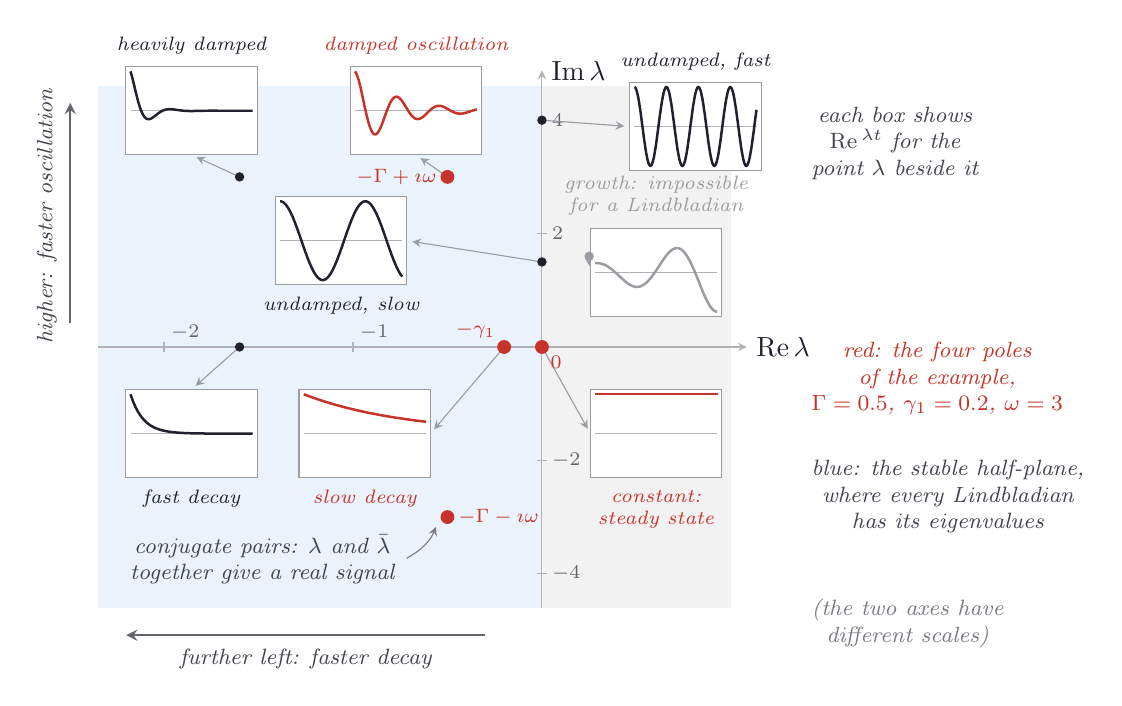
\begin{tikzpicture}[ink/.style={line width=0.9pt, ndInk}, faint/.style={line width=0.4pt, ndInk!35}, dashedink/.style={line width=0.5pt, ndInk!55, dash pattern=on 2.5pt off 2pt}, vec/.style={->, >=stealth, line width=1.2pt}, note/.style={font=\footnotesize\itshape, text=ndInk!85, align=center}, pointer/.style={->, >=stealth, line width=0.4pt, ndInk!60, shorten >=2pt, shorten <=1pt}, dot/.style={circle, fill=ndInk, inner sep=0pt, minimum size=3.4pt}, wash/.style={fill=ndSky, fill opacity=0.55}, every node/.style={text=ndInk}]
\definecolor{ndInk}{rgb}{0.13,0.13,0.18}
\definecolor{ndPaper}{rgb}{0.99,0.96,0.88}
\definecolor{ndSky}{rgb}{0.84,0.91,0.98}
\definecolor{ndRose}{rgb}{0.98,0.86,0.84}
\definecolor{ndBlue}{rgb}{0.13,0.36,0.66}
\definecolor{ndRed}{rgb}{0.78,0.20,0.16}
\definecolor{ndGold}{rgb}{0.88,0.62,0.10}
\definecolor{ndGreen}{rgb}{0.18,0.52,0.30}
\fill[ndSky, fill opacity=0.5] (-5.64,-3.31) rectangle (0,3.31);
\fill[ndInk, fill opacity=0.06] (0,-3.31) rectangle (2.40,3.31);
\draw[faint, ->, >=stealth] (-5.64,0) -- (2.60,0) node[right, text=ndInk] {$\mathrm{Re}\,\lambda$};
\draw[faint, ->, >=stealth] (0,-3.31) -- (0,3.51) node[right, text=ndInk] {$\mathrm{Im}\,\lambda$};
\draw[faint] (-4.80,0.06) -- (-4.80,-0.06);
\node[font=\scriptsize, text=ndInk!70, above right=-1pt] at (-4.80,0) {$-2$};
\draw[faint] (-2.40,0.06) -- (-2.40,-0.06);
\node[font=\scriptsize, text=ndInk!70, above right=-1pt] at (-2.40,0) {$-1$};
\draw[faint] (0.06,-2.88) -- (-0.06,-2.88);
\node[font=\scriptsize, text=ndInk!70, right=-1pt] at (0.04,-2.88) {$-4$};
\draw[faint] (0.06,-1.44) -- (-0.06,-1.44);
\node[font=\scriptsize, text=ndInk!70, right=-1pt] at (0.04,-1.44) {$-2$};
\draw[faint] (0.06,1.44) -- (-0.06,1.44);
\node[font=\scriptsize, text=ndInk!70, right=-1pt] at (0.04,1.44) {$2$};
\draw[faint] (0.06,2.88) -- (-0.06,2.88);
\node[font=\scriptsize, text=ndInk!70, right=-1pt] at (0.04,2.88) {$4$};
\draw[pointer, ndInk!45] (-3.840,0.000) -- (-4.450,-0.540);
\draw[pointer, ndInk!45] (-3.840,2.160) -- (-4.450,2.440);
\draw[pointer, ndInk!45] (0.000,1.080) -- (-1.715,1.350);
\draw[pointer, ndInk!45] (0.000,2.880) -- (1.115,2.800);
\draw[pointer, ndInk!45] (0.600,1.152) -- (0.615,0.950);
\draw[pointer, ndInk!45] (0.000,0.000) -- (0.615,-1.100);
\draw[pointer, ndInk!45] (-0.480,0.000) -- (-1.415,-1.100);
\draw[pointer, ndInk!45] (-1.200,2.160) -- (-1.600,2.440);
\fill[white] (-5.285,-1.660) rectangle (-3.615,-0.540);
\draw[line width=0.4pt, ndInk!45] (-5.285,-1.660) rectangle (-3.615,-0.540);
\draw[faint] (-5.225,-1.100) -- (-3.675,-1.100);
\draw[line width=0.9pt, ndInk] (-5.225,-0.600) -- (-5.220,-0.616) -- (-5.215,-0.631) -- (-5.209,-0.646) -- (-5.204,-0.660) -- (-5.199,-0.674) -- (-5.194,-0.688) -- (-5.189,-0.701) -- (-5.184,-0.713) -- (-5.178,-0.725) -- (-5.173,-0.737) -- (-5.168,-0.749) -- (-5.163,-0.760) -- (-5.158,-0.771) -- (-5.152,-0.781) -- (-5.147,-0.791) -- (-5.142,-0.801) -- (-5.137,-0.810) -- (-5.132,-0.819) -- (-5.127,-0.828) -- (-5.121,-0.837) -- (-5.116,-0.845) -- (-5.111,-0.853) -- (-5.106,-0.861) -- (-5.101,-0.869) -- (-5.095,-0.876) -- (-5.090,-0.883) -- (-5.085,-0.890) -- (-5.080,-0.897) -- (-5.075,-0.903) -- (-5.069,-0.909) -- (-5.064,-0.915) -- (-5.059,-0.921) -- (-5.054,-0.927) -- (-5.049,-0.932) -- (-5.044,-0.937) -- (-5.038,-0.943) -- (-5.033,-0.948) -- (-5.028,-0.952) -- (-5.023,-0.957) -- (-5.018,-0.962) -- (-5.012,-0.966) -- (-5.007,-0.970) -- (-5.002,-0.974) -- (-4.997,-0.978) -- (-4.992,-0.982) -- (-4.987,-0.986) -- (-4.981,-0.989) -- (-4.976,-0.993) -- (-4.971,-0.996) -- (-4.966,-1.000) -- (-4.961,-1.003) -- (-4.955,-1.006) -- (-4.950,-1.009) -- (-4.945,-1.012) -- (-4.940,-1.014) -- (-4.935,-1.017) -- (-4.930,-1.020) -- (-4.924,-1.022) -- (-4.919,-1.025) -- (-4.914,-1.027) -- (-4.909,-1.029) -- (-4.904,-1.032) -- (-4.898,-1.034) -- (-4.893,-1.036) -- (-4.888,-1.038) -- (-4.883,-1.040) -- (-4.878,-1.042) -- (-4.872,-1.044) -- (-4.867,-1.045) -- (-4.862,-1.047) -- (-4.857,-1.049) -- (-4.852,-1.050) -- (-4.847,-1.052) -- (-4.841,-1.054) -- (-4.836,-1.055) -- (-4.831,-1.056) -- (-4.826,-1.058) -- (-4.821,-1.059) -- (-4.815,-1.060) -- (-4.810,-1.062) -- (-4.805,-1.063) -- (-4.800,-1.064) -- (-4.795,-1.065) -- (-4.790,-1.066) -- (-4.784,-1.067) -- (-4.779,-1.068) -- (-4.774,-1.069) -- (-4.769,-1.070) -- (-4.764,-1.071) -- (-4.758,-1.072) -- (-4.753,-1.073) -- (-4.748,-1.074) -- (-4.743,-1.075) -- (-4.738,-1.076) -- (-4.733,-1.076) -- (-4.727,-1.077) -- (-4.722,-1.078) -- (-4.717,-1.078) -- (-4.712,-1.079) -- (-4.707,-1.080) -- (-4.701,-1.080) -- (-4.696,-1.081) -- (-4.691,-1.082) -- (-4.686,-1.082) -- (-4.681,-1.083) -- (-4.676,-1.083) -- (-4.670,-1.084) -- (-4.665,-1.084) -- (-4.660,-1.085) -- (-4.655,-1.085) -- (-4.650,-1.086) -- (-4.644,-1.086) -- (-4.639,-1.087) -- (-4.634,-1.087) -- (-4.629,-1.088) -- (-4.624,-1.088) -- (-4.618,-1.088) -- (-4.613,-1.089) -- (-4.608,-1.089) -- (-4.603,-1.089) -- (-4.598,-1.090) -- (-4.593,-1.090) -- (-4.587,-1.090) -- (-4.582,-1.091) -- (-4.577,-1.091) -- (-4.572,-1.091) -- (-4.567,-1.092) -- (-4.561,-1.092) -- (-4.556,-1.092) -- (-4.551,-1.092) -- (-4.546,-1.093) -- (-4.541,-1.093) -- (-4.536,-1.093) -- (-4.530,-1.093) -- (-4.525,-1.093) -- (-4.520,-1.094) -- (-4.515,-1.094) -- (-4.510,-1.094) -- (-4.504,-1.094) -- (-4.499,-1.094) -- (-4.494,-1.095) -- (-4.489,-1.095) -- (-4.484,-1.095) -- (-4.479,-1.095) -- (-4.473,-1.095) -- (-4.468,-1.095) -- (-4.463,-1.096) -- (-4.458,-1.096) -- (-4.453,-1.096) -- (-4.447,-1.096) -- (-4.442,-1.096) -- (-4.437,-1.096) -- (-4.432,-1.096) -- (-4.427,-1.096) -- (-4.421,-1.097) -- (-4.416,-1.097) -- (-4.411,-1.097) -- (-4.406,-1.097) -- (-4.401,-1.097) -- (-4.396,-1.097) -- (-4.390,-1.097) -- (-4.385,-1.097) -- (-4.380,-1.097) -- (-4.375,-1.097) -- (-4.370,-1.097) -- (-4.364,-1.098) -- (-4.359,-1.098) -- (-4.354,-1.098) -- (-4.349,-1.098) -- (-4.344,-1.098) -- (-4.339,-1.098) -- (-4.333,-1.098) -- (-4.328,-1.098) -- (-4.323,-1.098) -- (-4.318,-1.098) -- (-4.313,-1.098) -- (-4.307,-1.098) -- (-4.302,-1.098) -- (-4.297,-1.098) -- (-4.292,-1.098) -- (-4.287,-1.099) -- (-4.282,-1.099) -- (-4.276,-1.099) -- (-4.271,-1.099) -- (-4.266,-1.099) -- (-4.261,-1.099) -- (-4.256,-1.099) -- (-4.250,-1.099) -- (-4.245,-1.099) -- (-4.240,-1.099) -- (-4.235,-1.099) -- (-4.230,-1.099) -- (-4.224,-1.099) -- (-4.219,-1.099) -- (-4.214,-1.099) -- (-4.209,-1.099) -- (-4.204,-1.099) -- (-4.199,-1.099) -- (-4.193,-1.099) -- (-4.188,-1.099) -- (-4.183,-1.099) -- (-4.178,-1.099) -- (-4.173,-1.099) -- (-4.167,-1.099) -- (-4.162,-1.099) -- (-4.157,-1.099) -- (-4.152,-1.099) -- (-4.147,-1.099) -- (-4.142,-1.099) -- (-4.136,-1.099) -- (-4.131,-1.099) -- (-4.126,-1.099) -- (-4.121,-1.099) -- (-4.116,-1.099) -- (-4.110,-1.099) -- (-4.105,-1.100) -- (-4.100,-1.100) -- (-4.095,-1.100) -- (-4.090,-1.100) -- (-4.085,-1.100) -- (-4.079,-1.100) -- (-4.074,-1.100) -- (-4.069,-1.100) -- (-4.064,-1.100) -- (-4.059,-1.100) -- (-4.053,-1.100) -- (-4.048,-1.100) -- (-4.043,-1.100) -- (-4.038,-1.100) -- (-4.033,-1.100) -- (-4.028,-1.100) -- (-4.022,-1.100) -- (-4.017,-1.100) -- (-4.012,-1.100) -- (-4.007,-1.100) -- (-4.002,-1.100) -- (-3.996,-1.100) -- (-3.991,-1.100) -- (-3.986,-1.100) -- (-3.981,-1.100) -- (-3.976,-1.100) -- (-3.970,-1.100) -- (-3.965,-1.100) -- (-3.960,-1.100) -- (-3.955,-1.100) -- (-3.950,-1.100) -- (-3.945,-1.100) -- (-3.939,-1.100) -- (-3.934,-1.100) -- (-3.929,-1.100) -- (-3.924,-1.100) -- (-3.919,-1.100) -- (-3.913,-1.100) -- (-3.908,-1.100) -- (-3.903,-1.100) -- (-3.898,-1.100) -- (-3.893,-1.100) -- (-3.888,-1.100) -- (-3.882,-1.100) -- (-3.877,-1.100) -- (-3.872,-1.100) -- (-3.867,-1.100) -- (-3.862,-1.100) -- (-3.856,-1.100) -- (-3.851,-1.100) -- (-3.846,-1.100) -- (-3.841,-1.100) -- (-3.836,-1.100) -- (-3.831,-1.100) -- (-3.825,-1.100) -- (-3.820,-1.100) -- (-3.815,-1.100) -- (-3.810,-1.100) -- (-3.805,-1.100) -- (-3.799,-1.100) -- (-3.794,-1.100) -- (-3.789,-1.100) -- (-3.784,-1.100) -- (-3.779,-1.100) -- (-3.773,-1.100) -- (-3.768,-1.100) -- (-3.763,-1.100) -- (-3.758,-1.100) -- (-3.753,-1.100) -- (-3.748,-1.100) -- (-3.742,-1.100) -- (-3.737,-1.100) -- (-3.732,-1.100) -- (-3.727,-1.100) -- (-3.722,-1.100) -- (-3.716,-1.100) -- (-3.711,-1.100) -- (-3.706,-1.100) -- (-3.701,-1.100) -- (-3.696,-1.100) -- (-3.691,-1.100) -- (-3.685,-1.100) -- (-3.680,-1.100) -- (-3.675,-1.100);
\node[font=\scriptsize\itshape, text=ndInk, below=1pt, align=center] at (-4.450,-1.660) {fast decay};
\fill[white] (-5.285,2.440) rectangle (-3.615,3.560);
\draw[line width=0.4pt, ndInk!45] (-5.285,2.440) rectangle (-3.615,3.560);
\draw[faint] (-5.225,3.000) -- (-3.675,3.000);
\draw[line width=0.9pt, ndInk] (-5.225,3.500) -- (-5.220,3.483) -- (-5.215,3.466) -- (-5.209,3.447) -- (-5.204,3.427) -- (-5.199,3.407) -- (-5.194,3.386) -- (-5.189,3.364) -- (-5.184,3.343) -- (-5.178,3.321) -- (-5.173,3.299) -- (-5.168,3.277) -- (-5.163,3.255) -- (-5.158,3.234) -- (-5.152,3.212) -- (-5.147,3.191) -- (-5.142,3.171) -- (-5.137,3.151) -- (-5.132,3.131) -- (-5.127,3.113) -- (-5.121,3.094) -- (-5.116,3.077) -- (-5.111,3.060) -- (-5.106,3.044) -- (-5.101,3.029) -- (-5.095,3.015) -- (-5.090,3.001) -- (-5.085,2.989) -- (-5.080,2.977) -- (-5.075,2.966) -- (-5.069,2.956) -- (-5.064,2.946) -- (-5.059,2.938) -- (-5.054,2.930) -- (-5.049,2.923) -- (-5.044,2.917) -- (-5.038,2.912) -- (-5.033,2.907) -- (-5.028,2.903) -- (-5.023,2.900) -- (-5.018,2.897) -- (-5.012,2.895) -- (-5.007,2.894) -- (-5.002,2.893) -- (-4.997,2.893) -- (-4.992,2.893) -- (-4.987,2.894) -- (-4.981,2.895) -- (-4.976,2.896) -- (-4.971,2.898) -- (-4.966,2.900) -- (-4.961,2.903) -- (-4.955,2.906) -- (-4.950,2.909) -- (-4.945,2.912) -- (-4.940,2.916) -- (-4.935,2.919) -- (-4.930,2.923) -- (-4.924,2.927) -- (-4.919,2.931) -- (-4.914,2.935) -- (-4.909,2.939) -- (-4.904,2.943) -- (-4.898,2.947) -- (-4.893,2.951) -- (-4.888,2.956) -- (-4.883,2.960) -- (-4.878,2.963) -- (-4.872,2.967) -- (-4.867,2.971) -- (-4.862,2.975) -- (-4.857,2.978) -- (-4.852,2.982) -- (-4.847,2.985) -- (-4.841,2.988) -- (-4.836,2.991) -- (-4.831,2.994) -- (-4.826,2.997) -- (-4.821,2.999) -- (-4.815,3.002) -- (-4.810,3.004) -- (-4.805,3.006) -- (-4.800,3.008) -- (-4.795,3.010) -- (-4.790,3.011) -- (-4.784,3.013) -- (-4.779,3.014) -- (-4.774,3.015) -- (-4.769,3.016) -- (-4.764,3.017) -- (-4.758,3.018) -- (-4.753,3.019) -- (-4.748,3.019) -- (-4.743,3.020) -- (-4.738,3.020) -- (-4.733,3.020) -- (-4.727,3.020) -- (-4.722,3.020) -- (-4.717,3.020) -- (-4.712,3.020) -- (-4.707,3.019) -- (-4.701,3.019) -- (-4.696,3.019) -- (-4.691,3.018) -- (-4.686,3.018) -- (-4.681,3.017) -- (-4.676,3.017) -- (-4.670,3.016) -- (-4.665,3.015) -- (-4.660,3.015) -- (-4.655,3.014) -- (-4.650,3.013) -- (-4.644,3.012) -- (-4.639,3.012) -- (-4.634,3.011) -- (-4.629,3.010) -- (-4.624,3.009) -- (-4.618,3.008) -- (-4.613,3.008) -- (-4.608,3.007) -- (-4.603,3.006) -- (-4.598,3.006) -- (-4.593,3.005) -- (-4.587,3.004) -- (-4.582,3.004) -- (-4.577,3.003) -- (-4.572,3.002) -- (-4.567,3.002) -- (-4.561,3.001) -- (-4.556,3.001) -- (-4.551,3.000) -- (-4.546,3.000) -- (-4.541,2.999) -- (-4.536,2.999) -- (-4.530,2.999) -- (-4.525,2.998) -- (-4.520,2.998) -- (-4.515,2.998) -- (-4.510,2.997) -- (-4.504,2.997) -- (-4.499,2.997) -- (-4.494,2.997) -- (-4.489,2.997) -- (-4.484,2.997) -- (-4.479,2.996) -- (-4.473,2.996) -- (-4.468,2.996) -- (-4.463,2.996) -- (-4.458,2.996) -- (-4.453,2.996) -- (-4.447,2.996) -- (-4.442,2.996) -- (-4.437,2.996) -- (-4.432,2.996) -- (-4.427,2.996) -- (-4.421,2.997) -- (-4.416,2.997) -- (-4.411,2.997) -- (-4.406,2.997) -- (-4.401,2.997) -- (-4.396,2.997) -- (-4.390,2.997) -- (-4.385,2.997) -- (-4.380,2.998) -- (-4.375,2.998) -- (-4.370,2.998) -- (-4.364,2.998) -- (-4.359,2.998) -- (-4.354,2.998) -- (-4.349,2.998) -- (-4.344,2.999) -- (-4.339,2.999) -- (-4.333,2.999) -- (-4.328,2.999) -- (-4.323,2.999) -- (-4.318,2.999) -- (-4.313,2.999) -- (-4.307,2.999) -- (-4.302,3.000) -- (-4.297,3.000) -- (-4.292,3.000) -- (-4.287,3.000) -- (-4.282,3.000) -- (-4.276,3.000) -- (-4.271,3.000) -- (-4.266,3.000) -- (-4.261,3.000) -- (-4.256,3.000) -- (-4.250,3.000) -- (-4.245,3.000) -- (-4.240,3.000) -- (-4.235,3.001) -- (-4.230,3.001) -- (-4.224,3.001) -- (-4.219,3.001) -- (-4.214,3.001) -- (-4.209,3.001) -- (-4.204,3.001) -- (-4.199,3.001) -- (-4.193,3.001) -- (-4.188,3.001) -- (-4.183,3.001) -- (-4.178,3.001) -- (-4.173,3.001) -- (-4.167,3.001) -- (-4.162,3.001) -- (-4.157,3.001) -- (-4.152,3.001) -- (-4.147,3.001) -- (-4.142,3.001) -- (-4.136,3.001) -- (-4.131,3.001) -- (-4.126,3.001) -- (-4.121,3.001) -- (-4.116,3.000) -- (-4.110,3.000) -- (-4.105,3.000) -- (-4.100,3.000) -- (-4.095,3.000) -- (-4.090,3.000) -- (-4.085,3.000) -- (-4.079,3.000) -- (-4.074,3.000) -- (-4.069,3.000) -- (-4.064,3.000) -- (-4.059,3.000) -- (-4.053,3.000) -- (-4.048,3.000) -- (-4.043,3.000) -- (-4.038,3.000) -- (-4.033,3.000) -- (-4.028,3.000) -- (-4.022,3.000) -- (-4.017,3.000) -- (-4.012,3.000) -- (-4.007,3.000) -- (-4.002,3.000) -- (-3.996,3.000) -- (-3.991,3.000) -- (-3.986,3.000) -- (-3.981,3.000) -- (-3.976,3.000) -- (-3.970,3.000) -- (-3.965,3.000) -- (-3.960,3.000) -- (-3.955,3.000) -- (-3.950,3.000) -- (-3.945,3.000) -- (-3.939,3.000) -- (-3.934,3.000) -- (-3.929,3.000) -- (-3.924,3.000) -- (-3.919,3.000) -- (-3.913,3.000) -- (-3.908,3.000) -- (-3.903,3.000) -- (-3.898,3.000) -- (-3.893,3.000) -- (-3.888,3.000) -- (-3.882,3.000) -- (-3.877,3.000) -- (-3.872,3.000) -- (-3.867,3.000) -- (-3.862,3.000) -- (-3.856,3.000) -- (-3.851,3.000) -- (-3.846,3.000) -- (-3.841,3.000) -- (-3.836,3.000) -- (-3.831,3.000) -- (-3.825,3.000) -- (-3.820,3.000) -- (-3.815,3.000) -- (-3.810,3.000) -- (-3.805,3.000) -- (-3.799,3.000) -- (-3.794,3.000) -- (-3.789,3.000) -- (-3.784,3.000) -- (-3.779,3.000) -- (-3.773,3.000) -- (-3.768,3.000) -- (-3.763,3.000) -- (-3.758,3.000) -- (-3.753,3.000) -- (-3.748,3.000) -- (-3.742,3.000) -- (-3.737,3.000) -- (-3.732,3.000) -- (-3.727,3.000) -- (-3.722,3.000) -- (-3.716,3.000) -- (-3.711,3.000) -- (-3.706,3.000) -- (-3.701,3.000) -- (-3.696,3.000) -- (-3.691,3.000) -- (-3.685,3.000) -- (-3.680,3.000) -- (-3.675,3.000);
\node[font=\scriptsize\itshape, text=ndInk, above=1pt, align=center] at (-4.450,3.560) {heavily damped};
\fill[white] (-3.385,0.790) rectangle (-1.715,1.910);
\draw[line width=0.4pt, ndInk!45] (-3.385,0.790) rectangle (-1.715,1.910);
\draw[faint] (-3.325,1.350) -- (-1.775,1.350);
\draw[line width=0.9pt, ndInk] (-3.325,1.850) -- (-3.320,1.850) -- (-3.315,1.849) -- (-3.309,1.848) -- (-3.304,1.846) -- (-3.299,1.844) -- (-3.294,1.842) -- (-3.289,1.839) -- (-3.284,1.836) -- (-3.278,1.832) -- (-3.273,1.828) -- (-3.268,1.823) -- (-3.263,1.818) -- (-3.258,1.812) -- (-3.252,1.806) -- (-3.247,1.800) -- (-3.242,1.793) -- (-3.237,1.786) -- (-3.232,1.778) -- (-3.227,1.770) -- (-3.221,1.762) -- (-3.216,1.753) -- (-3.211,1.744) -- (-3.206,1.735) -- (-3.201,1.725) -- (-3.195,1.715) -- (-3.190,1.705) -- (-3.185,1.694) -- (-3.180,1.683) -- (-3.175,1.671) -- (-3.169,1.660) -- (-3.164,1.648) -- (-3.159,1.635) -- (-3.154,1.623) -- (-3.149,1.610) -- (-3.144,1.597) -- (-3.138,1.584) -- (-3.133,1.571) -- (-3.128,1.557) -- (-3.123,1.543) -- (-3.118,1.529) -- (-3.112,1.515) -- (-3.107,1.501) -- (-3.102,1.486) -- (-3.097,1.472) -- (-3.092,1.457) -- (-3.087,1.443) -- (-3.081,1.428) -- (-3.076,1.413) -- (-3.071,1.398) -- (-3.066,1.383) -- (-3.061,1.368) -- (-3.055,1.353) -- (-3.050,1.338) -- (-3.045,1.323) -- (-3.040,1.308) -- (-3.035,1.293) -- (-3.030,1.278) -- (-3.024,1.263) -- (-3.019,1.248) -- (-3.014,1.233) -- (-3.009,1.219) -- (-3.004,1.204) -- (-2.998,1.190) -- (-2.993,1.176) -- (-2.988,1.162) -- (-2.983,1.148) -- (-2.978,1.134) -- (-2.972,1.121) -- (-2.967,1.108) -- (-2.962,1.095) -- (-2.957,1.082) -- (-2.952,1.069) -- (-2.947,1.057) -- (-2.941,1.045) -- (-2.936,1.033) -- (-2.931,1.022) -- (-2.926,1.010) -- (-2.921,0.999) -- (-2.915,0.989) -- (-2.910,0.979) -- (-2.905,0.969) -- (-2.900,0.959) -- (-2.895,0.950) -- (-2.890,0.941) -- (-2.884,0.933) -- (-2.879,0.925) -- (-2.874,0.917) -- (-2.869,0.909) -- (-2.864,0.903) -- (-2.858,0.896) -- (-2.853,0.890) -- (-2.848,0.884) -- (-2.843,0.879) -- (-2.838,0.874) -- (-2.833,0.870) -- (-2.827,0.866) -- (-2.822,0.862) -- (-2.817,0.859) -- (-2.812,0.857) -- (-2.807,0.854) -- (-2.801,0.853) -- (-2.796,0.851) -- (-2.791,0.850) -- (-2.786,0.850) -- (-2.781,0.850) -- (-2.776,0.851) -- (-2.770,0.852) -- (-2.765,0.853) -- (-2.760,0.855) -- (-2.755,0.857) -- (-2.750,0.860) -- (-2.744,0.863) -- (-2.739,0.867) -- (-2.734,0.871) -- (-2.729,0.875) -- (-2.724,0.880) -- (-2.718,0.886) -- (-2.713,0.891) -- (-2.708,0.898) -- (-2.703,0.904) -- (-2.698,0.911) -- (-2.693,0.919) -- (-2.687,0.927) -- (-2.682,0.935) -- (-2.677,0.943) -- (-2.672,0.952) -- (-2.667,0.962) -- (-2.661,0.971) -- (-2.656,0.981) -- (-2.651,0.992) -- (-2.646,1.002) -- (-2.641,1.013) -- (-2.636,1.024) -- (-2.630,1.036) -- (-2.625,1.048) -- (-2.620,1.060) -- (-2.615,1.072) -- (-2.610,1.085) -- (-2.604,1.098) -- (-2.599,1.111) -- (-2.594,1.124) -- (-2.589,1.138) -- (-2.584,1.152) -- (-2.579,1.165) -- (-2.573,1.180) -- (-2.568,1.194) -- (-2.563,1.208) -- (-2.558,1.223) -- (-2.553,1.237) -- (-2.547,1.252) -- (-2.542,1.267) -- (-2.537,1.282) -- (-2.532,1.297) -- (-2.527,1.312) -- (-2.521,1.327) -- (-2.516,1.342) -- (-2.511,1.357) -- (-2.506,1.372) -- (-2.501,1.387) -- (-2.496,1.402) -- (-2.490,1.417) -- (-2.485,1.432) -- (-2.480,1.446) -- (-2.475,1.461) -- (-2.470,1.476) -- (-2.464,1.490) -- (-2.459,1.505) -- (-2.454,1.519) -- (-2.449,1.533) -- (-2.444,1.547) -- (-2.439,1.561) -- (-2.433,1.574) -- (-2.428,1.588) -- (-2.423,1.601) -- (-2.418,1.614) -- (-2.413,1.626) -- (-2.407,1.639) -- (-2.402,1.651) -- (-2.397,1.663) -- (-2.392,1.674) -- (-2.387,1.686) -- (-2.382,1.697) -- (-2.376,1.707) -- (-2.371,1.718) -- (-2.366,1.728) -- (-2.361,1.737) -- (-2.356,1.747) -- (-2.350,1.756) -- (-2.345,1.764) -- (-2.340,1.773) -- (-2.335,1.780) -- (-2.330,1.788) -- (-2.324,1.795) -- (-2.319,1.802) -- (-2.314,1.808) -- (-2.309,1.814) -- (-2.304,1.819) -- (-2.299,1.824) -- (-2.293,1.829) -- (-2.288,1.833) -- (-2.283,1.836) -- (-2.278,1.840) -- (-2.273,1.843) -- (-2.267,1.845) -- (-2.262,1.847) -- (-2.257,1.848) -- (-2.252,1.849) -- (-2.247,1.850) -- (-2.242,1.850) -- (-2.236,1.850) -- (-2.231,1.849) -- (-2.226,1.848) -- (-2.221,1.846) -- (-2.216,1.844) -- (-2.210,1.841) -- (-2.205,1.838) -- (-2.200,1.835) -- (-2.195,1.831) -- (-2.190,1.826) -- (-2.185,1.822) -- (-2.179,1.816) -- (-2.174,1.811) -- (-2.169,1.805) -- (-2.164,1.798) -- (-2.159,1.791) -- (-2.153,1.784) -- (-2.148,1.776) -- (-2.143,1.768) -- (-2.138,1.760) -- (-2.133,1.751) -- (-2.128,1.742) -- (-2.122,1.732) -- (-2.117,1.723) -- (-2.112,1.712) -- (-2.107,1.702) -- (-2.102,1.691) -- (-2.096,1.680) -- (-2.091,1.668) -- (-2.086,1.657) -- (-2.081,1.645) -- (-2.076,1.632) -- (-2.070,1.620) -- (-2.065,1.607) -- (-2.060,1.594) -- (-2.055,1.581) -- (-2.050,1.567) -- (-2.045,1.554) -- (-2.039,1.540) -- (-2.034,1.526) -- (-2.029,1.512) -- (-2.024,1.497) -- (-2.019,1.483) -- (-2.013,1.468) -- (-2.008,1.453) -- (-2.003,1.439) -- (-1.998,1.424) -- (-1.993,1.409) -- (-1.988,1.394) -- (-1.982,1.379) -- (-1.977,1.364) -- (-1.972,1.349) -- (-1.967,1.334) -- (-1.962,1.319) -- (-1.956,1.304) -- (-1.951,1.289) -- (-1.946,1.274) -- (-1.941,1.259) -- (-1.936,1.244) -- (-1.931,1.230) -- (-1.925,1.215) -- (-1.920,1.201) -- (-1.915,1.186) -- (-1.910,1.172) -- (-1.905,1.158) -- (-1.899,1.144) -- (-1.894,1.131) -- (-1.889,1.117) -- (-1.884,1.104) -- (-1.879,1.091) -- (-1.873,1.078) -- (-1.868,1.066) -- (-1.863,1.054) -- (-1.858,1.042) -- (-1.853,1.030) -- (-1.848,1.019) -- (-1.842,1.007) -- (-1.837,0.997) -- (-1.832,0.986) -- (-1.827,0.976) -- (-1.822,0.966) -- (-1.816,0.957) -- (-1.811,0.948) -- (-1.806,0.939) -- (-1.801,0.930) -- (-1.796,0.922) -- (-1.791,0.915) -- (-1.785,0.908) -- (-1.780,0.901) -- (-1.775,0.894);
\node[font=\scriptsize\itshape, text=ndInk, below=1pt, align=center] at (-2.550,0.790) {undamped, slow};
\fill[white] (1.115,2.240) rectangle (2.785,3.360);
\draw[line width=0.4pt, ndInk!45] (1.115,2.240) rectangle (2.785,3.360);
\draw[faint] (1.175,2.800) -- (2.725,2.800);
\draw[line width=0.9pt, ndInk] (1.175,3.300) -- (1.180,3.298) -- (1.185,3.294) -- (1.191,3.286) -- (1.196,3.274) -- (1.201,3.260) -- (1.206,3.243) -- (1.211,3.223) -- (1.216,3.200) -- (1.222,3.175) -- (1.227,3.147) -- (1.232,3.117) -- (1.237,3.085) -- (1.242,3.052) -- (1.248,3.016) -- (1.253,2.979) -- (1.258,2.941) -- (1.263,2.902) -- (1.268,2.863) -- (1.273,2.823) -- (1.279,2.783) -- (1.284,2.743) -- (1.289,2.703) -- (1.294,2.664) -- (1.299,2.626) -- (1.305,2.589) -- (1.310,2.553) -- (1.315,2.519) -- (1.320,2.487) -- (1.325,2.457) -- (1.331,2.429) -- (1.336,2.403) -- (1.341,2.380) -- (1.346,2.359) -- (1.351,2.342) -- (1.356,2.327) -- (1.362,2.316) -- (1.367,2.307) -- (1.372,2.302) -- (1.377,2.300) -- (1.382,2.301) -- (1.388,2.306) -- (1.393,2.313) -- (1.398,2.324) -- (1.403,2.338) -- (1.408,2.354) -- (1.413,2.374) -- (1.419,2.396) -- (1.424,2.421) -- (1.429,2.449) -- (1.434,2.478) -- (1.439,2.510) -- (1.445,2.544) -- (1.450,2.579) -- (1.455,2.615) -- (1.460,2.653) -- (1.465,2.692) -- (1.470,2.732) -- (1.476,2.772) -- (1.481,2.812) -- (1.486,2.852) -- (1.491,2.891) -- (1.496,2.931) -- (1.502,2.969) -- (1.507,3.006) -- (1.512,3.042) -- (1.517,3.076) -- (1.522,3.109) -- (1.528,3.139) -- (1.533,3.168) -- (1.538,3.194) -- (1.543,3.217) -- (1.548,3.238) -- (1.553,3.256) -- (1.559,3.271) -- (1.564,3.283) -- (1.569,3.292) -- (1.574,3.297) -- (1.579,3.300) -- (1.585,3.299) -- (1.590,3.295) -- (1.595,3.288) -- (1.600,3.278) -- (1.605,3.265) -- (1.610,3.248) -- (1.616,3.229) -- (1.621,3.207) -- (1.626,3.182) -- (1.631,3.155) -- (1.636,3.126) -- (1.642,3.095) -- (1.647,3.061) -- (1.652,3.026) -- (1.657,2.990) -- (1.662,2.952) -- (1.667,2.913) -- (1.673,2.874) -- (1.678,2.834) -- (1.683,2.794) -- (1.688,2.754) -- (1.693,2.714) -- (1.699,2.675) -- (1.704,2.636) -- (1.709,2.599) -- (1.714,2.563) -- (1.719,2.528) -- (1.724,2.496) -- (1.730,2.465) -- (1.735,2.436) -- (1.740,2.410) -- (1.745,2.386) -- (1.750,2.365) -- (1.756,2.347) -- (1.761,2.331) -- (1.766,2.319) -- (1.771,2.309) -- (1.776,2.303) -- (1.782,2.300) -- (1.787,2.301) -- (1.792,2.304) -- (1.797,2.311) -- (1.802,2.321) -- (1.807,2.333) -- (1.813,2.349) -- (1.818,2.368) -- (1.823,2.390) -- (1.828,2.414) -- (1.833,2.441) -- (1.839,2.470) -- (1.844,2.501) -- (1.849,2.534) -- (1.854,2.569) -- (1.859,2.605) -- (1.864,2.643) -- (1.870,2.681) -- (1.875,2.721) -- (1.880,2.760) -- (1.885,2.801) -- (1.890,2.841) -- (1.896,2.880) -- (1.901,2.920) -- (1.906,2.958) -- (1.911,2.996) -- (1.916,3.032) -- (1.921,3.067) -- (1.927,3.100) -- (1.932,3.131) -- (1.937,3.160) -- (1.942,3.187) -- (1.947,3.211) -- (1.953,3.232) -- (1.958,3.251) -- (1.963,3.267) -- (1.968,3.280) -- (1.973,3.290) -- (1.979,3.296) -- (1.984,3.300) -- (1.989,3.300) -- (1.994,3.297) -- (1.999,3.290) -- (2.004,3.281) -- (2.010,3.269) -- (2.015,3.253) -- (2.020,3.235) -- (2.025,3.213) -- (2.030,3.189) -- (2.036,3.163) -- (2.041,3.134) -- (2.046,3.103) -- (2.051,3.071) -- (2.056,3.036) -- (2.061,3.000) -- (2.067,2.963) -- (2.072,2.924) -- (2.077,2.885) -- (2.082,2.845) -- (2.087,2.805) -- (2.093,2.765) -- (2.098,2.725) -- (2.103,2.686) -- (2.108,2.647) -- (2.113,2.609) -- (2.118,2.573) -- (2.124,2.538) -- (2.129,2.505) -- (2.134,2.473) -- (2.139,2.444) -- (2.144,2.417) -- (2.150,2.392) -- (2.155,2.370) -- (2.160,2.351) -- (2.165,2.335) -- (2.170,2.322) -- (2.176,2.312) -- (2.181,2.305) -- (2.186,2.301) -- (2.191,2.300) -- (2.196,2.303) -- (2.201,2.309) -- (2.207,2.317) -- (2.212,2.330) -- (2.217,2.345) -- (2.222,2.363) -- (2.227,2.384) -- (2.233,2.407) -- (2.238,2.433) -- (2.243,2.462) -- (2.248,2.492) -- (2.253,2.525) -- (2.258,2.559) -- (2.264,2.595) -- (2.269,2.632) -- (2.274,2.670) -- (2.279,2.710) -- (2.284,2.749) -- (2.290,2.789) -- (2.295,2.829) -- (2.300,2.869) -- (2.305,2.909) -- (2.310,2.948) -- (2.315,2.986) -- (2.321,3.022) -- (2.326,3.057) -- (2.331,3.091) -- (2.336,3.123) -- (2.341,3.152) -- (2.347,3.179) -- (2.352,3.204) -- (2.357,3.227) -- (2.362,3.246) -- (2.367,3.263) -- (2.372,3.277) -- (2.378,3.287) -- (2.383,3.295) -- (2.388,3.299) -- (2.393,3.300) -- (2.398,3.298) -- (2.404,3.292) -- (2.409,3.284) -- (2.414,3.272) -- (2.419,3.258) -- (2.424,3.240) -- (2.430,3.220) -- (2.435,3.196) -- (2.440,3.171) -- (2.445,3.143) -- (2.450,3.112) -- (2.455,3.080) -- (2.461,3.046) -- (2.466,3.010) -- (2.471,2.973) -- (2.476,2.935) -- (2.481,2.896) -- (2.487,2.856) -- (2.492,2.816) -- (2.497,2.776) -- (2.502,2.736) -- (2.507,2.697) -- (2.512,2.658) -- (2.518,2.620) -- (2.523,2.583) -- (2.528,2.547) -- (2.533,2.514) -- (2.538,2.482) -- (2.544,2.452) -- (2.549,2.424) -- (2.554,2.399) -- (2.559,2.376) -- (2.564,2.356) -- (2.569,2.339) -- (2.575,2.325) -- (2.580,2.314) -- (2.585,2.306) -- (2.590,2.302) -- (2.595,2.300) -- (2.601,2.302) -- (2.606,2.307) -- (2.611,2.315) -- (2.616,2.326) -- (2.621,2.340) -- (2.627,2.357) -- (2.632,2.377) -- (2.637,2.400) -- (2.642,2.426) -- (2.647,2.453) -- (2.652,2.483) -- (2.658,2.515) -- (2.663,2.549) -- (2.668,2.585) -- (2.673,2.622) -- (2.678,2.660) -- (2.684,2.699) -- (2.689,2.738) -- (2.694,2.778) -- (2.699,2.818) -- (2.704,2.858) -- (2.709,2.898) -- (2.715,2.937) -- (2.720,2.975) -- (2.725,3.012);
\node[font=\scriptsize\itshape, text=ndInk, above=1pt, align=center] at (1.950,3.360) {undamped, fast};
\fill[white] (0.615,0.390) rectangle (2.285,1.510);
\draw[line width=0.4pt, ndInk!45] (0.615,0.390) rectangle (2.285,1.510);
\draw[faint] (0.675,0.950) -- (2.225,0.950);
\draw[line width=0.9pt, ndInk!45] (0.675,1.063) -- (0.680,1.064) -- (0.685,1.064) -- (0.691,1.064) -- (0.696,1.065) -- (0.701,1.065) -- (0.706,1.065) -- (0.711,1.064) -- (0.716,1.064) -- (0.722,1.064) -- (0.727,1.063) -- (0.732,1.062) -- (0.737,1.061) -- (0.742,1.061) -- (0.748,1.059) -- (0.753,1.058) -- (0.758,1.057) -- (0.763,1.055) -- (0.768,1.054) -- (0.773,1.052) -- (0.779,1.050) -- (0.784,1.048) -- (0.789,1.046) -- (0.794,1.044) -- (0.799,1.042) -- (0.805,1.039) -- (0.810,1.037) -- (0.815,1.034) -- (0.820,1.031) -- (0.825,1.028) -- (0.831,1.025) -- (0.836,1.022) -- (0.841,1.019) -- (0.846,1.015) -- (0.851,1.012) -- (0.856,1.008) -- (0.862,1.005) -- (0.867,1.001) -- (0.872,0.997) -- (0.877,0.993) -- (0.882,0.989) -- (0.888,0.985) -- (0.893,0.981) -- (0.898,0.977) -- (0.903,0.972) -- (0.908,0.968) -- (0.913,0.963) -- (0.919,0.959) -- (0.924,0.954) -- (0.929,0.950) -- (0.934,0.945) -- (0.939,0.940) -- (0.945,0.935) -- (0.950,0.931) -- (0.955,0.926) -- (0.960,0.921) -- (0.965,0.916) -- (0.970,0.911) -- (0.976,0.906) -- (0.981,0.902) -- (0.986,0.897) -- (0.991,0.892) -- (0.996,0.887) -- (1.002,0.882) -- (1.007,0.877) -- (1.012,0.873) -- (1.017,0.868) -- (1.022,0.863) -- (1.028,0.858) -- (1.033,0.854) -- (1.038,0.849) -- (1.043,0.845) -- (1.048,0.840) -- (1.053,0.836) -- (1.059,0.832) -- (1.064,0.827) -- (1.069,0.823) -- (1.074,0.819) -- (1.079,0.815) -- (1.085,0.812) -- (1.090,0.808) -- (1.095,0.804) -- (1.100,0.801) -- (1.105,0.797) -- (1.110,0.794) -- (1.116,0.791) -- (1.121,0.788) -- (1.126,0.785) -- (1.131,0.783) -- (1.136,0.780) -- (1.142,0.778) -- (1.147,0.775) -- (1.152,0.773) -- (1.157,0.772) -- (1.162,0.770) -- (1.167,0.768) -- (1.173,0.767) -- (1.178,0.766) -- (1.183,0.765) -- (1.188,0.764) -- (1.193,0.763) -- (1.199,0.763) -- (1.204,0.763) -- (1.209,0.763) -- (1.214,0.763) -- (1.219,0.763) -- (1.224,0.764) -- (1.230,0.765) -- (1.235,0.766) -- (1.240,0.767) -- (1.245,0.768) -- (1.250,0.770) -- (1.256,0.771) -- (1.261,0.773) -- (1.266,0.776) -- (1.271,0.778) -- (1.276,0.781) -- (1.282,0.784) -- (1.287,0.787) -- (1.292,0.790) -- (1.297,0.793) -- (1.302,0.797) -- (1.307,0.801) -- (1.313,0.805) -- (1.318,0.809) -- (1.323,0.814) -- (1.328,0.818) -- (1.333,0.823) -- (1.339,0.828) -- (1.344,0.833) -- (1.349,0.838) -- (1.354,0.844) -- (1.359,0.850) -- (1.364,0.856) -- (1.370,0.862) -- (1.375,0.868) -- (1.380,0.874) -- (1.385,0.880) -- (1.390,0.887) -- (1.396,0.894) -- (1.401,0.901) -- (1.406,0.908) -- (1.411,0.915) -- (1.416,0.922) -- (1.421,0.929) -- (1.427,0.937) -- (1.432,0.944) -- (1.437,0.952) -- (1.442,0.959) -- (1.447,0.967) -- (1.453,0.975) -- (1.458,0.983) -- (1.463,0.991) -- (1.468,0.998) -- (1.473,1.006) -- (1.479,1.014) -- (1.484,1.022) -- (1.489,1.030) -- (1.494,1.038) -- (1.499,1.046) -- (1.504,1.054) -- (1.510,1.062) -- (1.515,1.070) -- (1.520,1.078) -- (1.525,1.086) -- (1.530,1.093) -- (1.536,1.101) -- (1.541,1.108) -- (1.546,1.116) -- (1.551,1.123) -- (1.556,1.130) -- (1.561,1.137) -- (1.567,1.144) -- (1.572,1.151) -- (1.577,1.158) -- (1.582,1.165) -- (1.587,1.171) -- (1.593,1.177) -- (1.598,1.183) -- (1.603,1.189) -- (1.608,1.195) -- (1.613,1.200) -- (1.618,1.205) -- (1.624,1.210) -- (1.629,1.215) -- (1.634,1.220) -- (1.639,1.224) -- (1.644,1.228) -- (1.650,1.232) -- (1.655,1.236) -- (1.660,1.239) -- (1.665,1.242) -- (1.670,1.245) -- (1.676,1.247) -- (1.681,1.249) -- (1.686,1.251) -- (1.691,1.253) -- (1.696,1.254) -- (1.701,1.255) -- (1.707,1.256) -- (1.712,1.256) -- (1.717,1.256) -- (1.722,1.256) -- (1.727,1.255) -- (1.733,1.254) -- (1.738,1.253) -- (1.743,1.251) -- (1.748,1.249) -- (1.753,1.247) -- (1.758,1.244) -- (1.764,1.241) -- (1.769,1.238) -- (1.774,1.234) -- (1.779,1.230) -- (1.784,1.226) -- (1.790,1.221) -- (1.795,1.216) -- (1.800,1.211) -- (1.805,1.205) -- (1.810,1.199) -- (1.815,1.193) -- (1.821,1.186) -- (1.826,1.179) -- (1.831,1.172) -- (1.836,1.164) -- (1.841,1.156) -- (1.847,1.148) -- (1.852,1.140) -- (1.857,1.131) -- (1.862,1.122) -- (1.867,1.112) -- (1.872,1.103) -- (1.878,1.093) -- (1.883,1.083) -- (1.888,1.073) -- (1.893,1.062) -- (1.898,1.051) -- (1.904,1.040) -- (1.909,1.029) -- (1.914,1.017) -- (1.919,1.006) -- (1.924,0.994) -- (1.930,0.982) -- (1.935,0.970) -- (1.940,0.958) -- (1.945,0.945) -- (1.950,0.933) -- (1.955,0.920) -- (1.961,0.907) -- (1.966,0.895) -- (1.971,0.882) -- (1.976,0.869) -- (1.981,0.856) -- (1.987,0.843) -- (1.992,0.830) -- (1.997,0.817) -- (2.002,0.804) -- (2.007,0.791) -- (2.012,0.778) -- (2.018,0.765) -- (2.023,0.752) -- (2.028,0.739) -- (2.033,0.727) -- (2.038,0.714) -- (2.044,0.702) -- (2.049,0.689) -- (2.054,0.677) -- (2.059,0.665) -- (2.064,0.654) -- (2.069,0.642) -- (2.075,0.631) -- (2.080,0.619) -- (2.085,0.609) -- (2.090,0.598) -- (2.095,0.587) -- (2.101,0.577) -- (2.106,0.568) -- (2.111,0.558) -- (2.116,0.549) -- (2.121,0.540) -- (2.127,0.531) -- (2.132,0.523) -- (2.137,0.515) -- (2.142,0.508) -- (2.147,0.501) -- (2.152,0.494) -- (2.158,0.488) -- (2.163,0.482) -- (2.168,0.477) -- (2.173,0.472) -- (2.178,0.468) -- (2.184,0.464) -- (2.189,0.460) -- (2.194,0.457) -- (2.199,0.455) -- (2.204,0.453) -- (2.209,0.451) -- (2.215,0.450) -- (2.220,0.450) -- (2.225,0.450);
\node[font=\scriptsize\itshape, text=ndInk!45, above=1pt, align=center] at (1.450,1.510) {growth: impossible\\ for a Lindbladian};
\fill[white] (0.615,-1.660) rectangle (2.285,-0.540);
\draw[line width=0.4pt, ndInk!45] (0.615,-1.660) rectangle (2.285,-0.540);
\draw[faint] (0.675,-1.100) -- (2.225,-1.100);
\draw[line width=0.9pt, ndRed] (0.675,-0.600) -- (0.680,-0.600) -- (0.685,-0.600) -- (0.691,-0.600) -- (0.696,-0.600) -- (0.701,-0.600) -- (0.706,-0.600) -- (0.711,-0.600) -- (0.716,-0.600) -- (0.722,-0.600) -- (0.727,-0.600) -- (0.732,-0.600) -- (0.737,-0.600) -- (0.742,-0.600) -- (0.748,-0.600) -- (0.753,-0.600) -- (0.758,-0.600) -- (0.763,-0.600) -- (0.768,-0.600) -- (0.773,-0.600) -- (0.779,-0.600) -- (0.784,-0.600) -- (0.789,-0.600) -- (0.794,-0.600) -- (0.799,-0.600) -- (0.805,-0.600) -- (0.810,-0.600) -- (0.815,-0.600) -- (0.820,-0.600) -- (0.825,-0.600) -- (0.831,-0.600) -- (0.836,-0.600) -- (0.841,-0.600) -- (0.846,-0.600) -- (0.851,-0.600) -- (0.856,-0.600) -- (0.862,-0.600) -- (0.867,-0.600) -- (0.872,-0.600) -- (0.877,-0.600) -- (0.882,-0.600) -- (0.888,-0.600) -- (0.893,-0.600) -- (0.898,-0.600) -- (0.903,-0.600) -- (0.908,-0.600) -- (0.913,-0.600) -- (0.919,-0.600) -- (0.924,-0.600) -- (0.929,-0.600) -- (0.934,-0.600) -- (0.939,-0.600) -- (0.945,-0.600) -- (0.950,-0.600) -- (0.955,-0.600) -- (0.960,-0.600) -- (0.965,-0.600) -- (0.970,-0.600) -- (0.976,-0.600) -- (0.981,-0.600) -- (0.986,-0.600) -- (0.991,-0.600) -- (0.996,-0.600) -- (1.002,-0.600) -- (1.007,-0.600) -- (1.012,-0.600) -- (1.017,-0.600) -- (1.022,-0.600) -- (1.028,-0.600) -- (1.033,-0.600) -- (1.038,-0.600) -- (1.043,-0.600) -- (1.048,-0.600) -- (1.053,-0.600) -- (1.059,-0.600) -- (1.064,-0.600) -- (1.069,-0.600) -- (1.074,-0.600) -- (1.079,-0.600) -- (1.085,-0.600) -- (1.090,-0.600) -- (1.095,-0.600) -- (1.100,-0.600) -- (1.105,-0.600) -- (1.110,-0.600) -- (1.116,-0.600) -- (1.121,-0.600) -- (1.126,-0.600) -- (1.131,-0.600) -- (1.136,-0.600) -- (1.142,-0.600) -- (1.147,-0.600) -- (1.152,-0.600) -- (1.157,-0.600) -- (1.162,-0.600) -- (1.167,-0.600) -- (1.173,-0.600) -- (1.178,-0.600) -- (1.183,-0.600) -- (1.188,-0.600) -- (1.193,-0.600) -- (1.199,-0.600) -- (1.204,-0.600) -- (1.209,-0.600) -- (1.214,-0.600) -- (1.219,-0.600) -- (1.224,-0.600) -- (1.230,-0.600) -- (1.235,-0.600) -- (1.240,-0.600) -- (1.245,-0.600) -- (1.250,-0.600) -- (1.256,-0.600) -- (1.261,-0.600) -- (1.266,-0.600) -- (1.271,-0.600) -- (1.276,-0.600) -- (1.282,-0.600) -- (1.287,-0.600) -- (1.292,-0.600) -- (1.297,-0.600) -- (1.302,-0.600) -- (1.307,-0.600) -- (1.313,-0.600) -- (1.318,-0.600) -- (1.323,-0.600) -- (1.328,-0.600) -- (1.333,-0.600) -- (1.339,-0.600) -- (1.344,-0.600) -- (1.349,-0.600) -- (1.354,-0.600) -- (1.359,-0.600) -- (1.364,-0.600) -- (1.370,-0.600) -- (1.375,-0.600) -- (1.380,-0.600) -- (1.385,-0.600) -- (1.390,-0.600) -- (1.396,-0.600) -- (1.401,-0.600) -- (1.406,-0.600) -- (1.411,-0.600) -- (1.416,-0.600) -- (1.421,-0.600) -- (1.427,-0.600) -- (1.432,-0.600) -- (1.437,-0.600) -- (1.442,-0.600) -- (1.447,-0.600) -- (1.453,-0.600) -- (1.458,-0.600) -- (1.463,-0.600) -- (1.468,-0.600) -- (1.473,-0.600) -- (1.479,-0.600) -- (1.484,-0.600) -- (1.489,-0.600) -- (1.494,-0.600) -- (1.499,-0.600) -- (1.504,-0.600) -- (1.510,-0.600) -- (1.515,-0.600) -- (1.520,-0.600) -- (1.525,-0.600) -- (1.530,-0.600) -- (1.536,-0.600) -- (1.541,-0.600) -- (1.546,-0.600) -- (1.551,-0.600) -- (1.556,-0.600) -- (1.561,-0.600) -- (1.567,-0.600) -- (1.572,-0.600) -- (1.577,-0.600) -- (1.582,-0.600) -- (1.587,-0.600) -- (1.593,-0.600) -- (1.598,-0.600) -- (1.603,-0.600) -- (1.608,-0.600) -- (1.613,-0.600) -- (1.618,-0.600) -- (1.624,-0.600) -- (1.629,-0.600) -- (1.634,-0.600) -- (1.639,-0.600) -- (1.644,-0.600) -- (1.650,-0.600) -- (1.655,-0.600) -- (1.660,-0.600) -- (1.665,-0.600) -- (1.670,-0.600) -- (1.676,-0.600) -- (1.681,-0.600) -- (1.686,-0.600) -- (1.691,-0.600) -- (1.696,-0.600) -- (1.701,-0.600) -- (1.707,-0.600) -- (1.712,-0.600) -- (1.717,-0.600) -- (1.722,-0.600) -- (1.727,-0.600) -- (1.733,-0.600) -- (1.738,-0.600) -- (1.743,-0.600) -- (1.748,-0.600) -- (1.753,-0.600) -- (1.758,-0.600) -- (1.764,-0.600) -- (1.769,-0.600) -- (1.774,-0.600) -- (1.779,-0.600) -- (1.784,-0.600) -- (1.790,-0.600) -- (1.795,-0.600) -- (1.800,-0.600) -- (1.805,-0.600) -- (1.810,-0.600) -- (1.815,-0.600) -- (1.821,-0.600) -- (1.826,-0.600) -- (1.831,-0.600) -- (1.836,-0.600) -- (1.841,-0.600) -- (1.847,-0.600) -- (1.852,-0.600) -- (1.857,-0.600) -- (1.862,-0.600) -- (1.867,-0.600) -- (1.872,-0.600) -- (1.878,-0.600) -- (1.883,-0.600) -- (1.888,-0.600) -- (1.893,-0.600) -- (1.898,-0.600) -- (1.904,-0.600) -- (1.909,-0.600) -- (1.914,-0.600) -- (1.919,-0.600) -- (1.924,-0.600) -- (1.930,-0.600) -- (1.935,-0.600) -- (1.940,-0.600) -- (1.945,-0.600) -- (1.950,-0.600) -- (1.955,-0.600) -- (1.961,-0.600) -- (1.966,-0.600) -- (1.971,-0.600) -- (1.976,-0.600) -- (1.981,-0.600) -- (1.987,-0.600) -- (1.992,-0.600) -- (1.997,-0.600) -- (2.002,-0.600) -- (2.007,-0.600) -- (2.012,-0.600) -- (2.018,-0.600) -- (2.023,-0.600) -- (2.028,-0.600) -- (2.033,-0.600) -- (2.038,-0.600) -- (2.044,-0.600) -- (2.049,-0.600) -- (2.054,-0.600) -- (2.059,-0.600) -- (2.064,-0.600) -- (2.069,-0.600) -- (2.075,-0.600) -- (2.080,-0.600) -- (2.085,-0.600) -- (2.090,-0.600) -- (2.095,-0.600) -- (2.101,-0.600) -- (2.106,-0.600) -- (2.111,-0.600) -- (2.116,-0.600) -- (2.121,-0.600) -- (2.127,-0.600) -- (2.132,-0.600) -- (2.137,-0.600) -- (2.142,-0.600) -- (2.147,-0.600) -- (2.152,-0.600) -- (2.158,-0.600) -- (2.163,-0.600) -- (2.168,-0.600) -- (2.173,-0.600) -- (2.178,-0.600) -- (2.184,-0.600) -- (2.189,-0.600) -- (2.194,-0.600) -- (2.199,-0.600) -- (2.204,-0.600) -- (2.209,-0.600) -- (2.215,-0.600) -- (2.220,-0.600) -- (2.225,-0.600);
\node[font=\scriptsize\itshape, text=ndRed, below=1pt, align=center] at (1.450,-1.660) {constant:\\ steady state};
\fill[white] (-3.085,-1.660) rectangle (-1.415,-0.540);
\draw[line width=0.4pt, ndInk!45] (-3.085,-1.660) rectangle (-1.415,-0.540);
\draw[faint] (-3.025,-1.100) -- (-1.475,-1.100);
\draw[line width=0.9pt, ndRed] (-3.025,-0.600) -- (-3.020,-0.602) -- (-3.015,-0.604) -- (-3.009,-0.606) -- (-3.004,-0.608) -- (-2.999,-0.610) -- (-2.994,-0.612) -- (-2.989,-0.614) -- (-2.984,-0.616) -- (-2.978,-0.618) -- (-2.973,-0.620) -- (-2.968,-0.622) -- (-2.963,-0.624) -- (-2.958,-0.625) -- (-2.952,-0.627) -- (-2.947,-0.629) -- (-2.942,-0.631) -- (-2.937,-0.633) -- (-2.932,-0.635) -- (-2.927,-0.637) -- (-2.921,-0.639) -- (-2.916,-0.640) -- (-2.911,-0.642) -- (-2.906,-0.644) -- (-2.901,-0.646) -- (-2.895,-0.648) -- (-2.890,-0.650) -- (-2.885,-0.651) -- (-2.880,-0.653) -- (-2.875,-0.655) -- (-2.869,-0.657) -- (-2.864,-0.658) -- (-2.859,-0.660) -- (-2.854,-0.662) -- (-2.849,-0.664) -- (-2.844,-0.666) -- (-2.838,-0.667) -- (-2.833,-0.669) -- (-2.828,-0.671) -- (-2.823,-0.672) -- (-2.818,-0.674) -- (-2.812,-0.676) -- (-2.807,-0.678) -- (-2.802,-0.679) -- (-2.797,-0.681) -- (-2.792,-0.683) -- (-2.787,-0.684) -- (-2.781,-0.686) -- (-2.776,-0.688) -- (-2.771,-0.689) -- (-2.766,-0.691) -- (-2.761,-0.693) -- (-2.755,-0.694) -- (-2.750,-0.696) -- (-2.745,-0.697) -- (-2.740,-0.699) -- (-2.735,-0.701) -- (-2.730,-0.702) -- (-2.724,-0.704) -- (-2.719,-0.705) -- (-2.714,-0.707) -- (-2.709,-0.709) -- (-2.704,-0.710) -- (-2.698,-0.712) -- (-2.693,-0.713) -- (-2.688,-0.715) -- (-2.683,-0.716) -- (-2.678,-0.718) -- (-2.672,-0.719) -- (-2.667,-0.721) -- (-2.662,-0.722) -- (-2.657,-0.724) -- (-2.652,-0.725) -- (-2.647,-0.727) -- (-2.641,-0.728) -- (-2.636,-0.730) -- (-2.631,-0.731) -- (-2.626,-0.733) -- (-2.621,-0.734) -- (-2.615,-0.736) -- (-2.610,-0.737) -- (-2.605,-0.739) -- (-2.600,-0.740) -- (-2.595,-0.742) -- (-2.590,-0.743) -- (-2.584,-0.745) -- (-2.579,-0.746) -- (-2.574,-0.747) -- (-2.569,-0.749) -- (-2.564,-0.750) -- (-2.558,-0.752) -- (-2.553,-0.753) -- (-2.548,-0.754) -- (-2.543,-0.756) -- (-2.538,-0.757) -- (-2.533,-0.759) -- (-2.527,-0.760) -- (-2.522,-0.761) -- (-2.517,-0.763) -- (-2.512,-0.764) -- (-2.507,-0.765) -- (-2.501,-0.767) -- (-2.496,-0.768) -- (-2.491,-0.769) -- (-2.486,-0.771) -- (-2.481,-0.772) -- (-2.476,-0.773) -- (-2.470,-0.775) -- (-2.465,-0.776) -- (-2.460,-0.777) -- (-2.455,-0.778) -- (-2.450,-0.780) -- (-2.444,-0.781) -- (-2.439,-0.782) -- (-2.434,-0.784) -- (-2.429,-0.785) -- (-2.424,-0.786) -- (-2.418,-0.787) -- (-2.413,-0.789) -- (-2.408,-0.790) -- (-2.403,-0.791) -- (-2.398,-0.792) -- (-2.393,-0.794) -- (-2.387,-0.795) -- (-2.382,-0.796) -- (-2.377,-0.797) -- (-2.372,-0.798) -- (-2.367,-0.800) -- (-2.361,-0.801) -- (-2.356,-0.802) -- (-2.351,-0.803) -- (-2.346,-0.804) -- (-2.341,-0.806) -- (-2.336,-0.807) -- (-2.330,-0.808) -- (-2.325,-0.809) -- (-2.320,-0.810) -- (-2.315,-0.811) -- (-2.310,-0.813) -- (-2.304,-0.814) -- (-2.299,-0.815) -- (-2.294,-0.816) -- (-2.289,-0.817) -- (-2.284,-0.818) -- (-2.279,-0.819) -- (-2.273,-0.821) -- (-2.268,-0.822) -- (-2.263,-0.823) -- (-2.258,-0.824) -- (-2.253,-0.825) -- (-2.247,-0.826) -- (-2.242,-0.827) -- (-2.237,-0.828) -- (-2.232,-0.829) -- (-2.227,-0.831) -- (-2.221,-0.832) -- (-2.216,-0.833) -- (-2.211,-0.834) -- (-2.206,-0.835) -- (-2.201,-0.836) -- (-2.196,-0.837) -- (-2.190,-0.838) -- (-2.185,-0.839) -- (-2.180,-0.840) -- (-2.175,-0.841) -- (-2.170,-0.842) -- (-2.164,-0.843) -- (-2.159,-0.844) -- (-2.154,-0.845) -- (-2.149,-0.846) -- (-2.144,-0.847) -- (-2.139,-0.848) -- (-2.133,-0.849) -- (-2.128,-0.850) -- (-2.123,-0.851) -- (-2.118,-0.852) -- (-2.113,-0.853) -- (-2.107,-0.854) -- (-2.102,-0.855) -- (-2.097,-0.856) -- (-2.092,-0.857) -- (-2.087,-0.858) -- (-2.082,-0.859) -- (-2.076,-0.860) -- (-2.071,-0.861) -- (-2.066,-0.862) -- (-2.061,-0.863) -- (-2.056,-0.864) -- (-2.050,-0.865) -- (-2.045,-0.866) -- (-2.040,-0.867) -- (-2.035,-0.868) -- (-2.030,-0.869) -- (-2.024,-0.870) -- (-2.019,-0.870) -- (-2.014,-0.871) -- (-2.009,-0.872) -- (-2.004,-0.873) -- (-1.999,-0.874) -- (-1.993,-0.875) -- (-1.988,-0.876) -- (-1.983,-0.877) -- (-1.978,-0.878) -- (-1.973,-0.879) -- (-1.967,-0.880) -- (-1.962,-0.880) -- (-1.957,-0.881) -- (-1.952,-0.882) -- (-1.947,-0.883) -- (-1.942,-0.884) -- (-1.936,-0.885) -- (-1.931,-0.886) -- (-1.926,-0.886) -- (-1.921,-0.887) -- (-1.916,-0.888) -- (-1.910,-0.889) -- (-1.905,-0.890) -- (-1.900,-0.891) -- (-1.895,-0.892) -- (-1.890,-0.892) -- (-1.885,-0.893) -- (-1.879,-0.894) -- (-1.874,-0.895) -- (-1.869,-0.896) -- (-1.864,-0.897) -- (-1.859,-0.897) -- (-1.853,-0.898) -- (-1.848,-0.899) -- (-1.843,-0.900) -- (-1.838,-0.901) -- (-1.833,-0.901) -- (-1.828,-0.902) -- (-1.822,-0.903) -- (-1.817,-0.904) -- (-1.812,-0.905) -- (-1.807,-0.905) -- (-1.802,-0.906) -- (-1.796,-0.907) -- (-1.791,-0.908) -- (-1.786,-0.908) -- (-1.781,-0.909) -- (-1.776,-0.910) -- (-1.770,-0.911) -- (-1.765,-0.911) -- (-1.760,-0.912) -- (-1.755,-0.913) -- (-1.750,-0.914) -- (-1.745,-0.914) -- (-1.739,-0.915) -- (-1.734,-0.916) -- (-1.729,-0.917) -- (-1.724,-0.917) -- (-1.719,-0.918) -- (-1.713,-0.919) -- (-1.708,-0.920) -- (-1.703,-0.920) -- (-1.698,-0.921) -- (-1.693,-0.922) -- (-1.688,-0.922) -- (-1.682,-0.923) -- (-1.677,-0.924) -- (-1.672,-0.925) -- (-1.667,-0.925) -- (-1.662,-0.926) -- (-1.656,-0.927) -- (-1.651,-0.927) -- (-1.646,-0.928) -- (-1.641,-0.929) -- (-1.636,-0.929) -- (-1.631,-0.930) -- (-1.625,-0.931) -- (-1.620,-0.931) -- (-1.615,-0.932) -- (-1.610,-0.933) -- (-1.605,-0.934) -- (-1.599,-0.934) -- (-1.594,-0.935) -- (-1.589,-0.936) -- (-1.584,-0.936) -- (-1.579,-0.937) -- (-1.573,-0.937) -- (-1.568,-0.938) -- (-1.563,-0.939) -- (-1.558,-0.939) -- (-1.553,-0.940) -- (-1.548,-0.941) -- (-1.542,-0.941) -- (-1.537,-0.942) -- (-1.532,-0.943) -- (-1.527,-0.943) -- (-1.522,-0.944) -- (-1.516,-0.944) -- (-1.511,-0.945) -- (-1.506,-0.946) -- (-1.501,-0.946) -- (-1.496,-0.947) -- (-1.491,-0.948) -- (-1.485,-0.948) -- (-1.480,-0.949) -- (-1.475,-0.949);
\node[font=\scriptsize\itshape, text=ndRed, below=1pt, align=center] at (-2.250,-1.660) {slow decay};
\fill[white] (-2.435,2.440) rectangle (-0.765,3.560);
\draw[line width=0.4pt, ndInk!45] (-2.435,2.440) rectangle (-0.765,3.560);
\draw[faint] (-2.375,3.000) -- (-0.825,3.000);
\draw[line width=0.9pt, ndRed] (-2.375,3.500) -- (-2.370,3.494) -- (-2.365,3.487) -- (-2.359,3.477) -- (-2.354,3.466) -- (-2.349,3.454) -- (-2.344,3.440) -- (-2.339,3.425) -- (-2.334,3.409) -- (-2.328,3.391) -- (-2.323,3.373) -- (-2.318,3.353) -- (-2.313,3.333) -- (-2.308,3.311) -- (-2.302,3.289) -- (-2.297,3.266) -- (-2.292,3.243) -- (-2.287,3.219) -- (-2.282,3.195) -- (-2.277,3.171) -- (-2.271,3.147) -- (-2.266,3.122) -- (-2.261,3.098) -- (-2.256,3.073) -- (-2.251,3.049) -- (-2.245,3.026) -- (-2.240,3.002) -- (-2.235,2.979) -- (-2.230,2.957) -- (-2.225,2.935) -- (-2.219,2.914) -- (-2.214,2.893) -- (-2.209,2.874) -- (-2.204,2.855) -- (-2.199,2.837) -- (-2.194,2.820) -- (-2.188,2.804) -- (-2.183,2.789) -- (-2.178,2.776) -- (-2.173,2.763) -- (-2.168,2.751) -- (-2.162,2.741) -- (-2.157,2.732) -- (-2.152,2.724) -- (-2.147,2.717) -- (-2.142,2.711) -- (-2.137,2.706) -- (-2.131,2.703) -- (-2.126,2.701) -- (-2.121,2.700) -- (-2.116,2.700) -- (-2.111,2.701) -- (-2.105,2.703) -- (-2.100,2.707) -- (-2.095,2.711) -- (-2.090,2.716) -- (-2.085,2.722) -- (-2.080,2.730) -- (-2.074,2.738) -- (-2.069,2.746) -- (-2.064,2.756) -- (-2.059,2.766) -- (-2.054,2.777) -- (-2.048,2.789) -- (-2.043,2.801) -- (-2.038,2.813) -- (-2.033,2.826) -- (-2.028,2.840) -- (-2.022,2.853) -- (-2.017,2.867) -- (-2.012,2.882) -- (-2.007,2.896) -- (-2.002,2.910) -- (-1.997,2.925) -- (-1.991,2.939) -- (-1.986,2.954) -- (-1.981,2.968) -- (-1.976,2.982) -- (-1.971,2.996) -- (-1.965,3.010) -- (-1.960,3.023) -- (-1.955,3.036) -- (-1.950,3.049) -- (-1.945,3.061) -- (-1.940,3.073) -- (-1.934,3.084) -- (-1.929,3.095) -- (-1.924,3.105) -- (-1.919,3.114) -- (-1.914,3.123) -- (-1.908,3.131) -- (-1.903,3.139) -- (-1.898,3.146) -- (-1.893,3.152) -- (-1.888,3.158) -- (-1.883,3.163) -- (-1.877,3.167) -- (-1.872,3.171) -- (-1.867,3.173) -- (-1.862,3.176) -- (-1.857,3.177) -- (-1.851,3.178) -- (-1.846,3.178) -- (-1.841,3.177) -- (-1.836,3.176) -- (-1.831,3.174) -- (-1.826,3.172) -- (-1.820,3.169) -- (-1.815,3.165) -- (-1.810,3.161) -- (-1.805,3.156) -- (-1.800,3.151) -- (-1.794,3.146) -- (-1.789,3.140) -- (-1.784,3.133) -- (-1.779,3.127) -- (-1.774,3.119) -- (-1.768,3.112) -- (-1.763,3.104) -- (-1.758,3.096) -- (-1.753,3.088) -- (-1.748,3.080) -- (-1.743,3.072) -- (-1.737,3.063) -- (-1.732,3.055) -- (-1.727,3.046) -- (-1.722,3.037) -- (-1.717,3.029) -- (-1.711,3.020) -- (-1.706,3.012) -- (-1.701,3.004) -- (-1.696,2.996) -- (-1.691,2.988) -- (-1.686,2.980) -- (-1.680,2.972) -- (-1.675,2.965) -- (-1.670,2.958) -- (-1.665,2.952) -- (-1.660,2.945) -- (-1.654,2.939) -- (-1.649,2.933) -- (-1.644,2.928) -- (-1.639,2.923) -- (-1.634,2.918) -- (-1.629,2.914) -- (-1.623,2.910) -- (-1.618,2.907) -- (-1.613,2.904) -- (-1.608,2.901) -- (-1.603,2.899) -- (-1.597,2.898) -- (-1.592,2.896) -- (-1.587,2.895) -- (-1.582,2.895) -- (-1.577,2.895) -- (-1.571,2.895) -- (-1.566,2.896) -- (-1.561,2.897) -- (-1.556,2.898) -- (-1.551,2.900) -- (-1.546,2.902) -- (-1.540,2.904) -- (-1.535,2.907) -- (-1.530,2.910) -- (-1.525,2.913) -- (-1.520,2.917) -- (-1.514,2.920) -- (-1.509,2.924) -- (-1.504,2.928) -- (-1.499,2.933) -- (-1.494,2.937) -- (-1.489,2.942) -- (-1.483,2.947) -- (-1.478,2.952) -- (-1.473,2.957) -- (-1.468,2.962) -- (-1.463,2.967) -- (-1.457,2.972) -- (-1.452,2.977) -- (-1.447,2.982) -- (-1.442,2.987) -- (-1.437,2.992) -- (-1.432,2.997) -- (-1.426,3.002) -- (-1.421,3.006) -- (-1.416,3.011) -- (-1.411,3.016) -- (-1.406,3.020) -- (-1.400,3.024) -- (-1.395,3.028) -- (-1.390,3.032) -- (-1.385,3.035) -- (-1.380,3.039) -- (-1.374,3.042) -- (-1.369,3.045) -- (-1.364,3.048) -- (-1.359,3.050) -- (-1.354,3.053) -- (-1.349,3.055) -- (-1.343,3.057) -- (-1.338,3.058) -- (-1.333,3.059) -- (-1.328,3.061) -- (-1.323,3.061) -- (-1.317,3.062) -- (-1.312,3.062) -- (-1.307,3.062) -- (-1.302,3.062) -- (-1.297,3.062) -- (-1.292,3.061) -- (-1.286,3.061) -- (-1.281,3.060) -- (-1.276,3.058) -- (-1.271,3.057) -- (-1.266,3.056) -- (-1.260,3.054) -- (-1.255,3.052) -- (-1.250,3.050) -- (-1.245,3.048) -- (-1.240,3.045) -- (-1.235,3.043) -- (-1.229,3.040) -- (-1.224,3.038) -- (-1.219,3.035) -- (-1.214,3.032) -- (-1.209,3.029) -- (-1.203,3.026) -- (-1.198,3.023) -- (-1.193,3.020) -- (-1.188,3.017) -- (-1.183,3.014) -- (-1.178,3.011) -- (-1.172,3.008) -- (-1.167,3.005) -- (-1.162,3.002) -- (-1.157,3.000) -- (-1.152,2.997) -- (-1.146,2.994) -- (-1.141,2.991) -- (-1.136,2.989) -- (-1.131,2.986) -- (-1.126,2.984) -- (-1.120,2.982) -- (-1.115,2.979) -- (-1.110,2.977) -- (-1.105,2.975) -- (-1.100,2.974) -- (-1.095,2.972) -- (-1.089,2.970) -- (-1.084,2.969) -- (-1.079,2.968) -- (-1.074,2.967) -- (-1.069,2.966) -- (-1.063,2.965) -- (-1.058,2.964) -- (-1.053,2.964) -- (-1.048,2.963) -- (-1.043,2.963) -- (-1.038,2.963) -- (-1.032,2.963) -- (-1.027,2.963) -- (-1.022,2.964) -- (-1.017,2.964) -- (-1.012,2.965) -- (-1.006,2.965) -- (-1.001,2.966) -- (-0.996,2.967) -- (-0.991,2.968) -- (-0.986,2.969) -- (-0.981,2.970) -- (-0.975,2.972) -- (-0.970,2.973) -- (-0.965,2.974) -- (-0.960,2.976) -- (-0.955,2.977) -- (-0.949,2.979) -- (-0.944,2.981) -- (-0.939,2.982) -- (-0.934,2.984) -- (-0.929,2.986) -- (-0.923,2.988) -- (-0.918,2.989) -- (-0.913,2.991) -- (-0.908,2.993) -- (-0.903,2.995) -- (-0.898,2.997) -- (-0.892,2.998) -- (-0.887,3.000) -- (-0.882,3.002) -- (-0.877,3.003) -- (-0.872,3.005) -- (-0.866,3.006) -- (-0.861,3.008) -- (-0.856,3.009) -- (-0.851,3.011) -- (-0.846,3.012) -- (-0.841,3.013) -- (-0.835,3.014) -- (-0.830,3.015) -- (-0.825,3.016);
\node[font=\scriptsize\itshape, text=ndRed, above=1pt, align=center] at (-1.600,3.560) {damped oscillation};
\node[dot, fill=ndInk] at (-3.840,0.000) {};
\node[dot, fill=ndInk] at (-3.840,2.160) {};
\node[dot, fill=ndInk] at (0.000,1.080) {};
\node[dot, fill=ndInk] at (0.000,2.880) {};
\node[dot, fill=ndInk!45] at (0.600,1.152) {};
\node[dot, fill=ndRed, minimum size=5pt, label={[font=\scriptsize, text=ndRed, inner sep=1pt]below right:$0$}] at (0.000,0.000) {};
\node[dot, fill=ndRed, minimum size=5pt, label={[font=\scriptsize, text=ndRed, inner sep=1pt]above left:$-\gamma_1$}] at (-0.480,0.000) {};
\node[dot, fill=ndRed, minimum size=5pt, label={[font=\scriptsize, text=ndRed, inner sep=1pt]left:$-\Gamma+\imath\omega$}] at (-1.200,2.160) {};
\node[dot, fill=ndRed, minimum size=5pt, label={[font=\scriptsize, text=ndRed, inner sep=1pt]right:$-\Gamma-\imath\omega$}] at (-1.200,-2.160) {};
\node[note, anchor=east] (m) at (-1.75,-2.70) {conjugate pairs: $\lambda$ and $\bar\lambda$\\ together give a real signal};
\draw[pointer] (m.east) to[bend right=20] (-1.320,-2.220);
\draw[vec, ndInk!70, line width=0.8pt] (-0.72,-3.66) -- (-5.28,-3.66);
\node[note, anchor=north] at (-3.00,-3.71) {further left: faster decay};
\draw[vec, ndInk!70, line width=0.8pt] (-5.99,0.30) -- (-5.99,3.10);
\node[note, anchor=south, rotate=90] at (-6.04,1.66) {higher: faster oscillation};
\node[note, anchor=north west] at (3.30,3.17) {each box shows\\ $\mathrm{Re}\,\ee^{\lambda t}$ for the\\ point $\lambda$ beside it};
\node[note, anchor=west, text=ndRed] at (3.30,-0.40) {red: the four poles\\ of the example,\\ $\Gamma=0.5$, $\gamma_1=0.2$, $\omega=3$};
\node[note, anchor=west] at (3.30,-1.90) {blue: the stable half-plane,\\ where every Lindbladian\\ has its eigenvalues};
\node[note, anchor=west, text=ndInk!60] at (3.30,-3.51) {(the two axes have\\ different scales)};
\end{tikzpicture}
}
\caption{The $\lambda$-plane. Beside each marked point $\lambda$ is a sketch of $\mathrm{Re}\,\ee^{\lambda t}$ for $0\le t\le6$. On the negative real axis the modes decay without oscillating, the more quickly the further one goes to the left; on the imaginary axis they oscillate with constant amplitude, the more rapidly the higher one goes; between the two they are damped oscillations. The point in the right half-plane (grey, with its sketch reduced to fit) gives a growing mode, which no Lindbladian possesses. In red are the eigenvalues $0$, $-\gamma_1$ and $-\Gamma\pm\imath\omega$ of the example of this section, the last two forming a conjugate pair. The two axes are drawn to different scales. Generated by \texttt{code/ch05\_lambdaplane.py}.}\label{fig:ch05:lambdaplane}
\end{figure}}
\end{frame}

\begin{frame}\ft{An example: the damped qubit}
\ona{We shall use one example throughout the \chap{}. It is a single qubit with the Hamiltonian $\frac\omega2\sigma_z$, which precesses about the $z$-axis with angular frequency $\omega=3$, subject to amplitude damping at the rate $\gamma_1=0.2$ towards the ground state $\ket0$ (for which, as in \Chap~\ref{C.Open}, the Bloch vector points upwards) and to pure dephasing at the rate $\gamma_\phi=0.4$. In the affine embedding of \Chap~\ref{C.Open}, with $\vec x=(\langle\sigma_x\rangle,\langle\sigma_y\rangle,\langle\sigma_z\rangle,1)$, the equation of motion is}
\onp{Qubit precessing at $\omega=3$, damping $\gamma_1=0.2$ towards $\ket0$, dephasing $\gamma_\phi=0.4$; $\vec x=(\langle\sigma_x\rangle,\langle\sigma_y\rangle,\langle\sigma_z\rangle,1)$:}
\begin{equation}\label{eq:ch05:example}
    \dot{\vec x}=\mathbf A\vec x,\qquad
    \mathbf A=\begin{pmatrix}-\Gamma&-\omega&0&0\\ \omega&-\Gamma&0&0\\ 0&0&-\gamma_1&\gamma_1\\ 0&0&0&0\end{pmatrix},\qquad
    \Gamma=\tfrac{\gamma_1}2+\gamma_\phi=0.5 .
\end{equation}
\ona{The eigenvalues of $\mathbf A$ are $0$, which belongs to the steady state and comes from the embedding; $-\gamma_1=-0.2$, which governs the relaxation of $\langle\sigma_z\rangle$ on the time scale $T_1=5$; and $-\Gamma\pm\imath\omega=-0.5\pm3\imath$, which govern the damped precession of $\langle\sigma_x\rangle$ and $\langle\sigma_y\rangle$ on the time scale $T_2=1/\Gamma=2$. The qubit is prepared in the pure state with the Bloch vector $(\sin\frac{2\pi}3,0,\cos\frac{2\pi}3)\approx(0.87,0,-0.5)$, which lies below the equator, so that every mode is excited. We measure $\sigma_x$, or $\sigma_z$, or the Pauli operator $\sigma_n$ along $\vec n=(1,0,1)/\sqrt2$, midway between the $x$- and $z$-axes, and we sample at intervals $\tau=0.25$. The data are shown in Figure~\ref{fig:ch05:timeseries}. The expectation $\langle\sigma_x\rangle$ oscillates with period $2\pi/\omega$ within an envelope that decays at the rate $\Gamma$, whereas $\langle\sigma_z\rangle$ rises to $1$ at the rate $\gamma_1$ and does not oscillate.}
\onp{\begin{itemize}
    \item Eigenvalues: $0$ (steady state), $-\gamma_1=-0.2$, $-\Gamma\pm\imath\omega=-0.5\pm3\imath$.
    \item Start below the equator; measure $\sigma_x$, $\sigma_z$, or $\sigma_n$ with $\vec n=(1,0,1)/\sqrt2$; sample at intervals $\tau=0.25$.
\end{itemize}}
\ona{\begin{figure}[H]\centering\resizebox{\linewidth}{!}{% Generated by code/needham.py -- do not edit by hand.
\definecolor{qocA}{rgb}{0.00,0.45,0.70}
\definecolor{qocB}{rgb}{0.90,0.60,0.00}
\definecolor{qocC}{rgb}{0.00,0.62,0.45}
\definecolor{qocD}{rgb}{0.80,0.40,0.00}
\definecolor{qocE}{rgb}{0.80,0.60,0.70}
\definecolor{qocF}{rgb}{0.35,0.70,0.90}
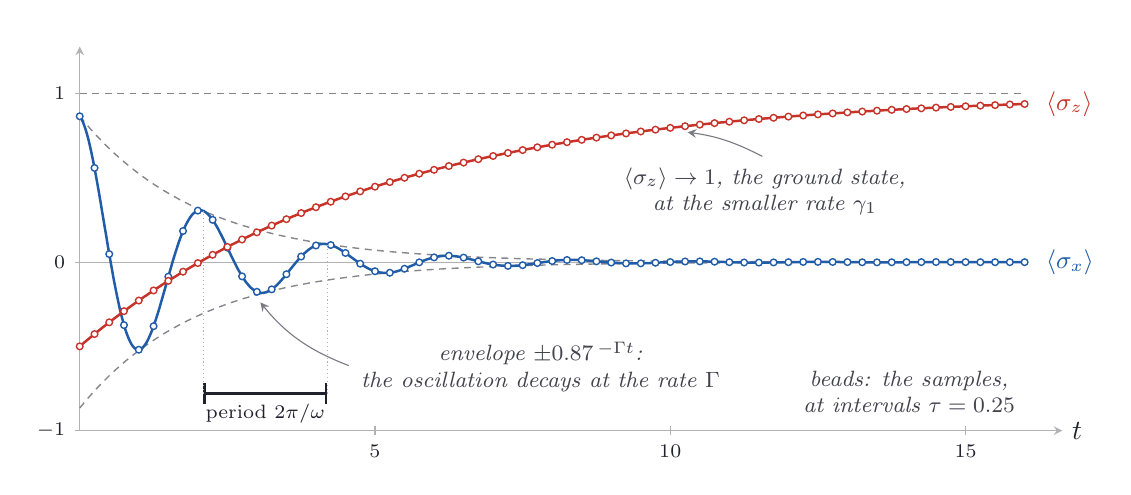
\begin{tikzpicture}[ink/.style={line width=0.9pt, ndInk}, faint/.style={line width=0.4pt, ndInk!35}, dashedink/.style={line width=0.5pt, ndInk!55, dash pattern=on 2.5pt off 2pt}, vec/.style={->, >=stealth, line width=1.2pt}, note/.style={font=\footnotesize\itshape, text=ndInk!85, align=center}, pointer/.style={->, >=stealth, line width=0.4pt, ndInk!60, shorten >=2pt, shorten <=1pt}, dot/.style={circle, fill=ndInk, inner sep=0pt, minimum size=3.4pt}, wash/.style={fill=ndSky, fill opacity=0.55}, every node/.style={text=ndInk}]
\definecolor{ndInk}{rgb}{0.13,0.13,0.18}
\definecolor{ndPaper}{rgb}{0.99,0.96,0.88}
\definecolor{ndSky}{rgb}{0.84,0.91,0.98}
\definecolor{ndRose}{rgb}{0.98,0.86,0.84}
\definecolor{ndBlue}{rgb}{0.13,0.36,0.66}
\definecolor{ndRed}{rgb}{0.78,0.20,0.16}
\definecolor{ndGold}{rgb}{0.88,0.62,0.10}
\definecolor{ndGreen}{rgb}{0.18,0.52,0.30}
\draw[faint, ->, >=stealth] (0.000,0.000) -- (12.480,0.000) node[right, text=ndInk] {$t$};
\draw[faint, ->, >=stealth] (0.000,0.000) -- (0.000,4.876) node[above, text=ndInk] {};
\draw[faint] (3.750,0.060) -- (3.750,-0.060) node[below, font=\scriptsize, text=ndInk] {$5$};
\draw[faint] (7.500,0.060) -- (7.500,-0.060) node[below, font=\scriptsize, text=ndInk] {$10$};
\draw[faint] (11.250,0.060) -- (11.250,-0.060) node[below, font=\scriptsize, text=ndInk] {$15$};
\draw[faint] (0.060,0.000) -- (-0.060,0.000) node[left, font=\scriptsize, text=ndInk] {$-1$};
\draw[faint] (0.060,2.140) -- (-0.060,2.140) node[left, font=\scriptsize, text=ndInk] {$0$};
\draw[faint] (0.060,4.279) -- (-0.060,4.279) node[left, font=\scriptsize, text=ndInk] {$1$};
\draw[faint] (0.000,2.140) -- (12.000,2.140);
\draw[dashedink] (0.000,3.992) -- (0.019,3.969) -- (0.038,3.947) -- (0.056,3.924) -- (0.075,3.902) -- (0.094,3.880) -- (0.113,3.859) -- (0.131,3.837) -- (0.150,3.816) -- (0.169,3.795) -- (0.188,3.775) -- (0.206,3.754) -- (0.225,3.734) -- (0.244,3.715) -- (0.263,3.695) -- (0.281,3.676) -- (0.300,3.657) -- (0.319,3.638) -- (0.338,3.619) -- (0.356,3.601) -- (0.375,3.583) -- (0.394,3.565) -- (0.413,3.547) -- (0.431,3.529) -- (0.450,3.512) -- (0.469,3.495) -- (0.488,3.478) -- (0.506,3.462) -- (0.525,3.445) -- (0.544,3.429) -- (0.562,3.413) -- (0.581,3.397) -- (0.600,3.382) -- (0.619,3.366) -- (0.638,3.351) -- (0.656,3.336) -- (0.675,3.321) -- (0.694,3.306) -- (0.713,3.292) -- (0.731,3.278) -- (0.750,3.263) -- (0.769,3.249) -- (0.788,3.236) -- (0.806,3.222) -- (0.825,3.209) -- (0.844,3.195) -- (0.863,3.182) -- (0.881,3.169) -- (0.900,3.156) -- (0.919,3.144) -- (0.938,3.131) -- (0.956,3.119) -- (0.975,3.107) -- (0.994,3.095) -- (1.013,3.083) -- (1.031,3.071) -- (1.050,3.060) -- (1.069,3.048) -- (1.088,3.037) -- (1.106,3.026) -- (1.125,3.015) -- (1.144,3.004) -- (1.163,2.993) -- (1.181,2.983) -- (1.200,2.972) -- (1.219,2.962) -- (1.238,2.952) -- (1.256,2.941) -- (1.275,2.931) -- (1.294,2.922) -- (1.312,2.912) -- (1.331,2.902) -- (1.350,2.893) -- (1.369,2.884) -- (1.388,2.874) -- (1.406,2.865) -- (1.425,2.856) -- (1.444,2.847) -- (1.463,2.838) -- (1.481,2.830) -- (1.500,2.821) -- (1.519,2.813) -- (1.538,2.804) -- (1.556,2.796) -- (1.575,2.788) -- (1.594,2.780) -- (1.612,2.772) -- (1.631,2.764) -- (1.650,2.756) -- (1.669,2.749) -- (1.688,2.741) -- (1.706,2.734) -- (1.725,2.726) -- (1.744,2.719) -- (1.763,2.712) -- (1.781,2.705) -- (1.800,2.698) -- (1.819,2.691) -- (1.838,2.684) -- (1.856,2.677) -- (1.875,2.670) -- (1.894,2.664) -- (1.913,2.657) -- (1.931,2.651) -- (1.950,2.645) -- (1.969,2.638) -- (1.988,2.632) -- (2.006,2.626) -- (2.025,2.620) -- (2.044,2.614) -- (2.062,2.608) -- (2.081,2.602) -- (2.100,2.596) -- (2.119,2.591) -- (2.138,2.585) -- (2.156,2.580) -- (2.175,2.574) -- (2.194,2.569) -- (2.213,2.563) -- (2.231,2.558) -- (2.250,2.553) -- (2.269,2.548) -- (2.288,2.543) -- (2.306,2.538) -- (2.325,2.533) -- (2.344,2.528) -- (2.363,2.523) -- (2.381,2.518) -- (2.400,2.514) -- (2.419,2.509) -- (2.438,2.504) -- (2.456,2.500) -- (2.475,2.495) -- (2.494,2.491) -- (2.513,2.487) -- (2.531,2.482) -- (2.550,2.478) -- (2.569,2.474) -- (2.588,2.470) -- (2.606,2.466) -- (2.625,2.462) -- (2.644,2.458) -- (2.663,2.454) -- (2.681,2.450) -- (2.700,2.446) -- (2.719,2.442) -- (2.738,2.438) -- (2.756,2.435) -- (2.775,2.431) -- (2.794,2.427) -- (2.812,2.424) -- (2.831,2.420) -- (2.850,2.417) -- (2.869,2.413) -- (2.888,2.410) -- (2.906,2.406) -- (2.925,2.403) -- (2.944,2.400) -- (2.963,2.397) -- (2.981,2.393) -- (3.000,2.390) -- (3.019,2.387) -- (3.037,2.384) -- (3.056,2.381) -- (3.075,2.378) -- (3.094,2.375) -- (3.113,2.372) -- (3.131,2.369) -- (3.150,2.366) -- (3.169,2.364) -- (3.188,2.361) -- (3.206,2.358) -- (3.225,2.355) -- (3.244,2.353) -- (3.263,2.350) -- (3.281,2.347) -- (3.300,2.345) -- (3.319,2.342) -- (3.338,2.340) -- (3.356,2.337) -- (3.375,2.335) -- (3.394,2.332) -- (3.412,2.330) -- (3.431,2.328) -- (3.450,2.325) -- (3.469,2.323) -- (3.488,2.321) -- (3.506,2.318) -- (3.525,2.316) -- (3.544,2.314) -- (3.562,2.312) -- (3.581,2.310) -- (3.600,2.308) -- (3.619,2.306) -- (3.638,2.303) -- (3.656,2.301) -- (3.675,2.299) -- (3.694,2.297) -- (3.713,2.295) -- (3.731,2.294) -- (3.750,2.292) -- (3.769,2.290) -- (3.788,2.288) -- (3.806,2.286) -- (3.825,2.284) -- (3.844,2.282) -- (3.863,2.281) -- (3.881,2.279) -- (3.900,2.277) -- (3.919,2.275) -- (3.938,2.274) -- (3.956,2.272) -- (3.975,2.270) -- (3.994,2.269) -- (4.013,2.267) -- (4.031,2.266) -- (4.050,2.264) -- (4.069,2.263) -- (4.088,2.261) -- (4.106,2.259) -- (4.125,2.258) -- (4.144,2.257) -- (4.163,2.255) -- (4.181,2.254) -- (4.200,2.252) -- (4.219,2.251) -- (4.238,2.249) -- (4.256,2.248) -- (4.275,2.247) -- (4.294,2.245) -- (4.312,2.244) -- (4.331,2.243) -- (4.350,2.241) -- (4.369,2.240) -- (4.388,2.239) -- (4.406,2.238) -- (4.425,2.237) -- (4.444,2.235) -- (4.463,2.234) -- (4.481,2.233) -- (4.500,2.232) -- (4.519,2.231) -- (4.538,2.230) -- (4.556,2.228) -- (4.575,2.227) -- (4.594,2.226) -- (4.613,2.225) -- (4.631,2.224) -- (4.650,2.223) -- (4.669,2.222) -- (4.688,2.221) -- (4.706,2.220) -- (4.725,2.219) -- (4.744,2.218) -- (4.763,2.217) -- (4.781,2.216) -- (4.800,2.215) -- (4.819,2.214) -- (4.838,2.213) -- (4.856,2.212) -- (4.875,2.211) -- (4.894,2.210) -- (4.913,2.210) -- (4.931,2.209) -- (4.950,2.208) -- (4.969,2.207) -- (4.988,2.206) -- (5.006,2.205) -- (5.025,2.205) -- (5.044,2.204) -- (5.062,2.203) -- (5.081,2.202) -- (5.100,2.201) -- (5.119,2.201) -- (5.138,2.200) -- (5.156,2.199) -- (5.175,2.198) -- (5.194,2.198) -- (5.213,2.197) -- (5.231,2.196) -- (5.250,2.195) -- (5.269,2.195) -- (5.288,2.194) -- (5.306,2.193) -- (5.325,2.193) -- (5.344,2.192) -- (5.363,2.191) -- (5.381,2.191) -- (5.400,2.190) -- (5.419,2.190) -- (5.438,2.189) -- (5.456,2.188) -- (5.475,2.188) -- (5.494,2.187) -- (5.513,2.187) -- (5.531,2.186) -- (5.550,2.185) -- (5.569,2.185) -- (5.588,2.184) -- (5.606,2.184) -- (5.625,2.183) -- (5.644,2.183) -- (5.663,2.182) -- (5.681,2.182) -- (5.700,2.181) -- (5.719,2.180) -- (5.738,2.180) -- (5.756,2.179) -- (5.775,2.179) -- (5.794,2.178) -- (5.812,2.178) -- (5.831,2.178) -- (5.850,2.177) -- (5.869,2.177) -- (5.888,2.176) -- (5.906,2.176) -- (5.925,2.175) -- (5.944,2.175) -- (5.963,2.174) -- (5.981,2.174) -- (6.000,2.173) -- (6.019,2.173) -- (6.038,2.173) -- (6.056,2.172) -- (6.075,2.172) -- (6.094,2.171) -- (6.113,2.171) -- (6.131,2.171) -- (6.150,2.170) -- (6.169,2.170) -- (6.188,2.169) -- (6.206,2.169) -- (6.225,2.169) -- (6.244,2.168) -- (6.262,2.168) -- (6.281,2.168) -- (6.300,2.167) -- (6.319,2.167) -- (6.338,2.167) -- (6.356,2.166) -- (6.375,2.166) -- (6.394,2.166) -- (6.413,2.165) -- (6.431,2.165) -- (6.450,2.165) -- (6.469,2.164) -- (6.488,2.164) -- (6.506,2.164) -- (6.525,2.163) -- (6.544,2.163) -- (6.562,2.163) -- (6.581,2.163) -- (6.600,2.162) -- (6.619,2.162) -- (6.637,2.162) -- (6.656,2.161) -- (6.675,2.161) -- (6.694,2.161) -- (6.713,2.161) -- (6.731,2.160) -- (6.750,2.160) -- (6.769,2.160) -- (6.788,2.160) -- (6.806,2.159) -- (6.825,2.159) -- (6.844,2.159) -- (6.863,2.159) -- (6.881,2.158) -- (6.900,2.158) -- (6.919,2.158) -- (6.938,2.158) -- (6.956,2.157) -- (6.975,2.157) -- (6.994,2.157) -- (7.012,2.157) -- (7.031,2.157) -- (7.050,2.156) -- (7.069,2.156) -- (7.088,2.156) -- (7.106,2.156) -- (7.125,2.156) -- (7.144,2.155) -- (7.163,2.155) -- (7.181,2.155) -- (7.200,2.155) -- (7.219,2.155) -- (7.238,2.154) -- (7.256,2.154) -- (7.275,2.154) -- (7.294,2.154) -- (7.312,2.154) -- (7.331,2.154) -- (7.350,2.153) -- (7.369,2.153) -- (7.388,2.153) -- (7.406,2.153) -- (7.425,2.153) -- (7.444,2.152) -- (7.463,2.152) -- (7.481,2.152) -- (7.500,2.152) -- (7.519,2.152) -- (7.538,2.152) -- (7.556,2.152) -- (7.575,2.151) -- (7.594,2.151) -- (7.613,2.151) -- (7.631,2.151) -- (7.650,2.151) -- (7.669,2.151) -- (7.688,2.151) -- (7.706,2.150) -- (7.725,2.150) -- (7.744,2.150) -- (7.763,2.150) -- (7.781,2.150) -- (7.800,2.150) -- (7.819,2.150) -- (7.838,2.150) -- (7.856,2.149) -- (7.875,2.149) -- (7.894,2.149) -- (7.913,2.149) -- (7.931,2.149) -- (7.950,2.149) -- (7.969,2.149) -- (7.988,2.149) -- (8.006,2.148) -- (8.025,2.148) -- (8.044,2.148) -- (8.062,2.148) -- (8.081,2.148) -- (8.100,2.148) -- (8.119,2.148) -- (8.138,2.148) -- (8.156,2.148) -- (8.175,2.147) -- (8.194,2.147) -- (8.213,2.147) -- (8.231,2.147) -- (8.250,2.147) -- (8.269,2.147) -- (8.288,2.147) -- (8.306,2.147) -- (8.325,2.147) -- (8.344,2.147) -- (8.363,2.147) -- (8.381,2.146) -- (8.400,2.146) -- (8.419,2.146) -- (8.438,2.146) -- (8.456,2.146) -- (8.475,2.146) -- (8.494,2.146) -- (8.513,2.146) -- (8.531,2.146) -- (8.550,2.146) -- (8.569,2.146) -- (8.588,2.146) -- (8.606,2.146) -- (8.625,2.145) -- (8.644,2.145) -- (8.663,2.145) -- (8.681,2.145) -- (8.700,2.145) -- (8.719,2.145) -- (8.738,2.145) -- (8.756,2.145) -- (8.775,2.145) -- (8.794,2.145) -- (8.812,2.145) -- (8.831,2.145) -- (8.850,2.145) -- (8.869,2.145) -- (8.888,2.144) -- (8.906,2.144) -- (8.925,2.144) -- (8.944,2.144) -- (8.963,2.144) -- (8.981,2.144) -- (9.000,2.144) -- (9.019,2.144) -- (9.038,2.144) -- (9.056,2.144) -- (9.075,2.144) -- (9.094,2.144) -- (9.113,2.144) -- (9.131,2.144) -- (9.150,2.144) -- (9.169,2.144) -- (9.188,2.144) -- (9.206,2.144) -- (9.225,2.143) -- (9.244,2.143) -- (9.263,2.143) -- (9.281,2.143) -- (9.300,2.143) -- (9.319,2.143) -- (9.338,2.143) -- (9.356,2.143) -- (9.375,2.143) -- (9.394,2.143) -- (9.413,2.143) -- (9.431,2.143) -- (9.450,2.143) -- (9.469,2.143) -- (9.488,2.143) -- (9.506,2.143) -- (9.525,2.143) -- (9.544,2.143) -- (9.562,2.143) -- (9.581,2.143) -- (9.600,2.143) -- (9.619,2.143) -- (9.638,2.143) -- (9.656,2.143) -- (9.675,2.142) -- (9.694,2.142) -- (9.713,2.142) -- (9.731,2.142) -- (9.750,2.142) -- (9.769,2.142) -- (9.788,2.142) -- (9.806,2.142) -- (9.825,2.142) -- (9.844,2.142) -- (9.863,2.142) -- (9.881,2.142) -- (9.900,2.142) -- (9.919,2.142) -- (9.938,2.142) -- (9.956,2.142) -- (9.975,2.142) -- (9.994,2.142) -- (10.013,2.142) -- (10.031,2.142) -- (10.050,2.142) -- (10.069,2.142) -- (10.088,2.142) -- (10.106,2.142) -- (10.125,2.142) -- (10.144,2.142) -- (10.163,2.142) -- (10.181,2.142) -- (10.200,2.142) -- (10.219,2.142) -- (10.238,2.142) -- (10.256,2.142) -- (10.275,2.141) -- (10.294,2.141) -- (10.312,2.141) -- (10.331,2.141) -- (10.350,2.141) -- (10.369,2.141) -- (10.388,2.141) -- (10.406,2.141) -- (10.425,2.141) -- (10.444,2.141) -- (10.463,2.141) -- (10.481,2.141) -- (10.500,2.141) -- (10.519,2.141) -- (10.538,2.141) -- (10.556,2.141) -- (10.575,2.141) -- (10.594,2.141) -- (10.613,2.141) -- (10.631,2.141) -- (10.650,2.141) -- (10.669,2.141) -- (10.688,2.141) -- (10.706,2.141) -- (10.725,2.141) -- (10.744,2.141) -- (10.763,2.141) -- (10.781,2.141) -- (10.800,2.141) -- (10.819,2.141) -- (10.838,2.141) -- (10.856,2.141) -- (10.875,2.141) -- (10.894,2.141) -- (10.913,2.141) -- (10.931,2.141) -- (10.950,2.141) -- (10.969,2.141) -- (10.988,2.141) -- (11.006,2.141) -- (11.025,2.141) -- (11.044,2.141) -- (11.062,2.141) -- (11.081,2.141) -- (11.100,2.141) -- (11.119,2.141) -- (11.138,2.141) -- (11.156,2.141) -- (11.175,2.141) -- (11.194,2.141) -- (11.213,2.141) -- (11.231,2.141) -- (11.250,2.141) -- (11.269,2.141) -- (11.288,2.141) -- (11.306,2.141) -- (11.325,2.141) -- (11.344,2.140) -- (11.363,2.140) -- (11.381,2.140) -- (11.400,2.140) -- (11.419,2.140) -- (11.438,2.140) -- (11.456,2.140) -- (11.475,2.140) -- (11.494,2.140) -- (11.513,2.140) -- (11.531,2.140) -- (11.550,2.140) -- (11.569,2.140) -- (11.588,2.140) -- (11.606,2.140) -- (11.625,2.140) -- (11.644,2.140) -- (11.663,2.140) -- (11.681,2.140) -- (11.700,2.140) -- (11.719,2.140) -- (11.738,2.140) -- (11.756,2.140) -- (11.775,2.140) -- (11.794,2.140) -- (11.812,2.140) -- (11.831,2.140) -- (11.850,2.140) -- (11.869,2.140) -- (11.888,2.140) -- (11.906,2.140) -- (11.925,2.140) -- (11.944,2.140) -- (11.963,2.140) -- (11.981,2.140) -- (12.000,2.140);
\draw[dashedink] (0.000,0.287) -- (0.019,0.310) -- (0.038,0.332) -- (0.056,0.355) -- (0.075,0.377) -- (0.094,0.399) -- (0.113,0.421) -- (0.131,0.442) -- (0.150,0.463) -- (0.169,0.484) -- (0.188,0.504) -- (0.206,0.525) -- (0.225,0.545) -- (0.244,0.565) -- (0.263,0.584) -- (0.281,0.603) -- (0.300,0.623) -- (0.319,0.641) -- (0.338,0.660) -- (0.356,0.678) -- (0.375,0.697) -- (0.394,0.714) -- (0.413,0.732) -- (0.431,0.750) -- (0.450,0.767) -- (0.469,0.784) -- (0.488,0.801) -- (0.506,0.817) -- (0.525,0.834) -- (0.544,0.850) -- (0.562,0.866) -- (0.581,0.882) -- (0.600,0.898) -- (0.619,0.913) -- (0.638,0.928) -- (0.656,0.943) -- (0.675,0.958) -- (0.694,0.973) -- (0.713,0.987) -- (0.731,1.002) -- (0.750,1.016) -- (0.769,1.030) -- (0.788,1.043) -- (0.806,1.057) -- (0.825,1.071) -- (0.844,1.084) -- (0.863,1.097) -- (0.881,1.110) -- (0.900,1.123) -- (0.919,1.135) -- (0.938,1.148) -- (0.956,1.160) -- (0.975,1.172) -- (0.994,1.184) -- (1.013,1.196) -- (1.031,1.208) -- (1.050,1.219) -- (1.069,1.231) -- (1.088,1.242) -- (1.106,1.253) -- (1.125,1.264) -- (1.144,1.275) -- (1.163,1.286) -- (1.181,1.297) -- (1.200,1.307) -- (1.219,1.317) -- (1.238,1.328) -- (1.256,1.338) -- (1.275,1.348) -- (1.294,1.357) -- (1.312,1.367) -- (1.331,1.377) -- (1.350,1.386) -- (1.369,1.396) -- (1.388,1.405) -- (1.406,1.414) -- (1.425,1.423) -- (1.444,1.432) -- (1.463,1.441) -- (1.481,1.449) -- (1.500,1.458) -- (1.519,1.466) -- (1.538,1.475) -- (1.556,1.483) -- (1.575,1.491) -- (1.594,1.499) -- (1.612,1.507) -- (1.631,1.515) -- (1.650,1.523) -- (1.669,1.530) -- (1.688,1.538) -- (1.706,1.545) -- (1.725,1.553) -- (1.744,1.560) -- (1.763,1.567) -- (1.781,1.574) -- (1.800,1.581) -- (1.819,1.588) -- (1.838,1.595) -- (1.856,1.602) -- (1.875,1.609) -- (1.894,1.615) -- (1.913,1.622) -- (1.931,1.628) -- (1.950,1.635) -- (1.969,1.641) -- (1.988,1.647) -- (2.006,1.653) -- (2.025,1.659) -- (2.044,1.665) -- (2.062,1.671) -- (2.081,1.677) -- (2.100,1.683) -- (2.119,1.688) -- (2.138,1.694) -- (2.156,1.699) -- (2.175,1.705) -- (2.194,1.710) -- (2.213,1.716) -- (2.231,1.721) -- (2.250,1.726) -- (2.269,1.731) -- (2.288,1.736) -- (2.306,1.741) -- (2.325,1.746) -- (2.344,1.751) -- (2.363,1.756) -- (2.381,1.761) -- (2.400,1.765) -- (2.419,1.770) -- (2.438,1.775) -- (2.456,1.779) -- (2.475,1.784) -- (2.494,1.788) -- (2.513,1.792) -- (2.531,1.797) -- (2.550,1.801) -- (2.569,1.805) -- (2.588,1.809) -- (2.606,1.814) -- (2.625,1.818) -- (2.644,1.822) -- (2.663,1.826) -- (2.681,1.829) -- (2.700,1.833) -- (2.719,1.837) -- (2.738,1.841) -- (2.756,1.845) -- (2.775,1.848) -- (2.794,1.852) -- (2.812,1.855) -- (2.831,1.859) -- (2.850,1.862) -- (2.869,1.866) -- (2.888,1.869) -- (2.906,1.873) -- (2.925,1.876) -- (2.944,1.879) -- (2.963,1.882) -- (2.981,1.886) -- (3.000,1.889) -- (3.019,1.892) -- (3.037,1.895) -- (3.056,1.898) -- (3.075,1.901) -- (3.094,1.904) -- (3.113,1.907) -- (3.131,1.910) -- (3.150,1.913) -- (3.169,1.915) -- (3.188,1.918) -- (3.206,1.921) -- (3.225,1.924) -- (3.244,1.926) -- (3.263,1.929) -- (3.281,1.932) -- (3.300,1.934) -- (3.319,1.937) -- (3.338,1.939) -- (3.356,1.942) -- (3.375,1.944) -- (3.394,1.947) -- (3.412,1.949) -- (3.431,1.951) -- (3.450,1.954) -- (3.469,1.956) -- (3.488,1.958) -- (3.506,1.961) -- (3.525,1.963) -- (3.544,1.965) -- (3.562,1.967) -- (3.581,1.969) -- (3.600,1.971) -- (3.619,1.974) -- (3.638,1.976) -- (3.656,1.978) -- (3.675,1.980) -- (3.694,1.982) -- (3.713,1.984) -- (3.731,1.986) -- (3.750,1.987) -- (3.769,1.989) -- (3.788,1.991) -- (3.806,1.993) -- (3.825,1.995) -- (3.844,1.997) -- (3.863,1.998) -- (3.881,2.000) -- (3.900,2.002) -- (3.919,2.004) -- (3.938,2.005) -- (3.956,2.007) -- (3.975,2.009) -- (3.994,2.010) -- (4.013,2.012) -- (4.031,2.013) -- (4.050,2.015) -- (4.069,2.017) -- (4.088,2.018) -- (4.106,2.020) -- (4.125,2.021) -- (4.144,2.023) -- (4.163,2.024) -- (4.181,2.025) -- (4.200,2.027) -- (4.219,2.028) -- (4.238,2.030) -- (4.256,2.031) -- (4.275,2.032) -- (4.294,2.034) -- (4.312,2.035) -- (4.331,2.036) -- (4.350,2.038) -- (4.369,2.039) -- (4.388,2.040) -- (4.406,2.041) -- (4.425,2.043) -- (4.444,2.044) -- (4.463,2.045) -- (4.481,2.046) -- (4.500,2.047) -- (4.519,2.048) -- (4.538,2.050) -- (4.556,2.051) -- (4.575,2.052) -- (4.594,2.053) -- (4.613,2.054) -- (4.631,2.055) -- (4.650,2.056) -- (4.669,2.057) -- (4.688,2.058) -- (4.706,2.059) -- (4.725,2.060) -- (4.744,2.061) -- (4.763,2.062) -- (4.781,2.063) -- (4.800,2.064) -- (4.819,2.065) -- (4.838,2.066) -- (4.856,2.067) -- (4.875,2.068) -- (4.894,2.069) -- (4.913,2.069) -- (4.931,2.070) -- (4.950,2.071) -- (4.969,2.072) -- (4.988,2.073) -- (5.006,2.074) -- (5.025,2.075) -- (5.044,2.075) -- (5.062,2.076) -- (5.081,2.077) -- (5.100,2.078) -- (5.119,2.078) -- (5.138,2.079) -- (5.156,2.080) -- (5.175,2.081) -- (5.194,2.081) -- (5.213,2.082) -- (5.231,2.083) -- (5.250,2.084) -- (5.269,2.084) -- (5.288,2.085) -- (5.306,2.086) -- (5.325,2.086) -- (5.344,2.087) -- (5.363,2.088) -- (5.381,2.088) -- (5.400,2.089) -- (5.419,2.090) -- (5.438,2.090) -- (5.456,2.091) -- (5.475,2.091) -- (5.494,2.092) -- (5.513,2.093) -- (5.531,2.093) -- (5.550,2.094) -- (5.569,2.094) -- (5.588,2.095) -- (5.606,2.095) -- (5.625,2.096) -- (5.644,2.097) -- (5.663,2.097) -- (5.681,2.098) -- (5.700,2.098) -- (5.719,2.099) -- (5.738,2.099) -- (5.756,2.100) -- (5.775,2.100) -- (5.794,2.101) -- (5.812,2.101) -- (5.831,2.102) -- (5.850,2.102) -- (5.869,2.102) -- (5.888,2.103) -- (5.906,2.103) -- (5.925,2.104) -- (5.944,2.104) -- (5.963,2.105) -- (5.981,2.105) -- (6.000,2.106) -- (6.019,2.106) -- (6.038,2.106) -- (6.056,2.107) -- (6.075,2.107) -- (6.094,2.108) -- (6.113,2.108) -- (6.131,2.108) -- (6.150,2.109) -- (6.169,2.109) -- (6.188,2.110) -- (6.206,2.110) -- (6.225,2.110) -- (6.244,2.111) -- (6.262,2.111) -- (6.281,2.111) -- (6.300,2.112) -- (6.319,2.112) -- (6.338,2.112) -- (6.356,2.113) -- (6.375,2.113) -- (6.394,2.113) -- (6.413,2.114) -- (6.431,2.114) -- (6.450,2.114) -- (6.469,2.115) -- (6.488,2.115) -- (6.506,2.115) -- (6.525,2.116) -- (6.544,2.116) -- (6.562,2.116) -- (6.581,2.117) -- (6.600,2.117) -- (6.619,2.117) -- (6.637,2.117) -- (6.656,2.118) -- (6.675,2.118) -- (6.694,2.118) -- (6.713,2.118) -- (6.731,2.119) -- (6.750,2.119) -- (6.769,2.119) -- (6.788,2.119) -- (6.806,2.120) -- (6.825,2.120) -- (6.844,2.120) -- (6.863,2.120) -- (6.881,2.121) -- (6.900,2.121) -- (6.919,2.121) -- (6.938,2.121) -- (6.956,2.122) -- (6.975,2.122) -- (6.994,2.122) -- (7.012,2.122) -- (7.031,2.122) -- (7.050,2.123) -- (7.069,2.123) -- (7.088,2.123) -- (7.106,2.123) -- (7.125,2.124) -- (7.144,2.124) -- (7.163,2.124) -- (7.181,2.124) -- (7.200,2.124) -- (7.219,2.124) -- (7.238,2.125) -- (7.256,2.125) -- (7.275,2.125) -- (7.294,2.125) -- (7.312,2.125) -- (7.331,2.126) -- (7.350,2.126) -- (7.369,2.126) -- (7.388,2.126) -- (7.406,2.126) -- (7.425,2.126) -- (7.444,2.127) -- (7.463,2.127) -- (7.481,2.127) -- (7.500,2.127) -- (7.519,2.127) -- (7.538,2.127) -- (7.556,2.128) -- (7.575,2.128) -- (7.594,2.128) -- (7.613,2.128) -- (7.631,2.128) -- (7.650,2.128) -- (7.669,2.128) -- (7.688,2.129) -- (7.706,2.129) -- (7.725,2.129) -- (7.744,2.129) -- (7.763,2.129) -- (7.781,2.129) -- (7.800,2.129) -- (7.819,2.129) -- (7.838,2.130) -- (7.856,2.130) -- (7.875,2.130) -- (7.894,2.130) -- (7.913,2.130) -- (7.931,2.130) -- (7.950,2.130) -- (7.969,2.130) -- (7.988,2.131) -- (8.006,2.131) -- (8.025,2.131) -- (8.044,2.131) -- (8.062,2.131) -- (8.081,2.131) -- (8.100,2.131) -- (8.119,2.131) -- (8.138,2.131) -- (8.156,2.131) -- (8.175,2.132) -- (8.194,2.132) -- (8.213,2.132) -- (8.231,2.132) -- (8.250,2.132) -- (8.269,2.132) -- (8.288,2.132) -- (8.306,2.132) -- (8.325,2.132) -- (8.344,2.132) -- (8.363,2.133) -- (8.381,2.133) -- (8.400,2.133) -- (8.419,2.133) -- (8.438,2.133) -- (8.456,2.133) -- (8.475,2.133) -- (8.494,2.133) -- (8.513,2.133) -- (8.531,2.133) -- (8.550,2.133) -- (8.569,2.133) -- (8.588,2.133) -- (8.606,2.134) -- (8.625,2.134) -- (8.644,2.134) -- (8.663,2.134) -- (8.681,2.134) -- (8.700,2.134) -- (8.719,2.134) -- (8.738,2.134) -- (8.756,2.134) -- (8.775,2.134) -- (8.794,2.134) -- (8.812,2.134) -- (8.831,2.134) -- (8.850,2.134) -- (8.869,2.135) -- (8.888,2.135) -- (8.906,2.135) -- (8.925,2.135) -- (8.944,2.135) -- (8.963,2.135) -- (8.981,2.135) -- (9.000,2.135) -- (9.019,2.135) -- (9.038,2.135) -- (9.056,2.135) -- (9.075,2.135) -- (9.094,2.135) -- (9.113,2.135) -- (9.131,2.135) -- (9.150,2.135) -- (9.169,2.135) -- (9.188,2.135) -- (9.206,2.136) -- (9.225,2.136) -- (9.244,2.136) -- (9.263,2.136) -- (9.281,2.136) -- (9.300,2.136) -- (9.319,2.136) -- (9.338,2.136) -- (9.356,2.136) -- (9.375,2.136) -- (9.394,2.136) -- (9.413,2.136) -- (9.431,2.136) -- (9.450,2.136) -- (9.469,2.136) -- (9.488,2.136) -- (9.506,2.136) -- (9.525,2.136) -- (9.544,2.136) -- (9.562,2.136) -- (9.581,2.136) -- (9.600,2.136) -- (9.619,2.136) -- (9.638,2.137) -- (9.656,2.137) -- (9.675,2.137) -- (9.694,2.137) -- (9.713,2.137) -- (9.731,2.137) -- (9.750,2.137) -- (9.769,2.137) -- (9.788,2.137) -- (9.806,2.137) -- (9.825,2.137) -- (9.844,2.137) -- (9.863,2.137) -- (9.881,2.137) -- (9.900,2.137) -- (9.919,2.137) -- (9.938,2.137) -- (9.956,2.137) -- (9.975,2.137) -- (9.994,2.137) -- (10.013,2.137) -- (10.031,2.137) -- (10.050,2.137) -- (10.069,2.137) -- (10.088,2.137) -- (10.106,2.137) -- (10.125,2.137) -- (10.144,2.137) -- (10.163,2.137) -- (10.181,2.137) -- (10.200,2.137) -- (10.219,2.137) -- (10.238,2.138) -- (10.256,2.138) -- (10.275,2.138) -- (10.294,2.138) -- (10.312,2.138) -- (10.331,2.138) -- (10.350,2.138) -- (10.369,2.138) -- (10.388,2.138) -- (10.406,2.138) -- (10.425,2.138) -- (10.444,2.138) -- (10.463,2.138) -- (10.481,2.138) -- (10.500,2.138) -- (10.519,2.138) -- (10.538,2.138) -- (10.556,2.138) -- (10.575,2.138) -- (10.594,2.138) -- (10.613,2.138) -- (10.631,2.138) -- (10.650,2.138) -- (10.669,2.138) -- (10.688,2.138) -- (10.706,2.138) -- (10.725,2.138) -- (10.744,2.138) -- (10.763,2.138) -- (10.781,2.138) -- (10.800,2.138) -- (10.819,2.138) -- (10.838,2.138) -- (10.856,2.138) -- (10.875,2.138) -- (10.894,2.138) -- (10.913,2.138) -- (10.931,2.138) -- (10.950,2.138) -- (10.969,2.138) -- (10.988,2.138) -- (11.006,2.138) -- (11.025,2.138) -- (11.044,2.138) -- (11.062,2.138) -- (11.081,2.138) -- (11.100,2.138) -- (11.119,2.138) -- (11.138,2.138) -- (11.156,2.138) -- (11.175,2.138) -- (11.194,2.138) -- (11.213,2.138) -- (11.231,2.138) -- (11.250,2.139) -- (11.269,2.139) -- (11.288,2.139) -- (11.306,2.139) -- (11.325,2.139) -- (11.344,2.139) -- (11.363,2.139) -- (11.381,2.139) -- (11.400,2.139) -- (11.419,2.139) -- (11.438,2.139) -- (11.456,2.139) -- (11.475,2.139) -- (11.494,2.139) -- (11.513,2.139) -- (11.531,2.139) -- (11.550,2.139) -- (11.569,2.139) -- (11.588,2.139) -- (11.606,2.139) -- (11.625,2.139) -- (11.644,2.139) -- (11.663,2.139) -- (11.681,2.139) -- (11.700,2.139) -- (11.719,2.139) -- (11.738,2.139) -- (11.756,2.139) -- (11.775,2.139) -- (11.794,2.139) -- (11.812,2.139) -- (11.831,2.139) -- (11.850,2.139) -- (11.869,2.139) -- (11.888,2.139) -- (11.906,2.139) -- (11.925,2.139) -- (11.944,2.139) -- (11.963,2.139) -- (11.981,2.139) -- (12.000,2.139);
\draw[dashedink] (0.000,4.279) -- (12.000,4.279);
\draw[line width=0.9pt, ndBlue] (0.000,3.992) -- (0.019,3.964) -- (0.038,3.926) -- (0.056,3.879) -- (0.075,3.823) -- (0.094,3.759) -- (0.113,3.687) -- (0.131,3.609) -- (0.150,3.523) -- (0.169,3.432) -- (0.188,3.336) -- (0.206,3.235) -- (0.225,3.131) -- (0.244,3.023) -- (0.263,2.913) -- (0.281,2.802) -- (0.300,2.689) -- (0.319,2.576) -- (0.338,2.464) -- (0.356,2.352) -- (0.375,2.242) -- (0.394,2.134) -- (0.413,2.028) -- (0.431,1.926) -- (0.450,1.828) -- (0.469,1.733) -- (0.488,1.644) -- (0.506,1.559) -- (0.525,1.480) -- (0.544,1.407) -- (0.562,1.340) -- (0.581,1.278) -- (0.600,1.224) -- (0.619,1.176) -- (0.638,1.134) -- (0.656,1.099) -- (0.675,1.071) -- (0.694,1.050) -- (0.713,1.036) -- (0.731,1.028) -- (0.750,1.027) -- (0.769,1.032) -- (0.788,1.043) -- (0.806,1.061) -- (0.825,1.084) -- (0.844,1.112) -- (0.863,1.146) -- (0.881,1.185) -- (0.900,1.228) -- (0.919,1.275) -- (0.938,1.326) -- (0.956,1.380) -- (0.975,1.437) -- (0.994,1.497) -- (1.013,1.559) -- (1.031,1.623) -- (1.050,1.688) -- (1.069,1.755) -- (1.088,1.821) -- (1.106,1.888) -- (1.125,1.955) -- (1.144,2.021) -- (1.163,2.086) -- (1.181,2.150) -- (1.200,2.212) -- (1.219,2.273) -- (1.238,2.331) -- (1.256,2.386) -- (1.275,2.439) -- (1.294,2.489) -- (1.312,2.535) -- (1.331,2.578) -- (1.350,2.618) -- (1.369,2.653) -- (1.388,2.685) -- (1.406,2.714) -- (1.425,2.738) -- (1.444,2.758) -- (1.463,2.774) -- (1.481,2.786) -- (1.500,2.794) -- (1.519,2.798) -- (1.538,2.798) -- (1.556,2.795) -- (1.575,2.788) -- (1.594,2.777) -- (1.612,2.763) -- (1.631,2.746) -- (1.650,2.726) -- (1.669,2.702) -- (1.688,2.677) -- (1.706,2.649) -- (1.725,2.618) -- (1.744,2.586) -- (1.763,2.552) -- (1.781,2.516) -- (1.800,2.479) -- (1.819,2.441) -- (1.838,2.402) -- (1.856,2.363) -- (1.875,2.324) -- (1.894,2.284) -- (1.913,2.244) -- (1.931,2.205) -- (1.950,2.167) -- (1.969,2.129) -- (1.988,2.092) -- (2.006,2.057) -- (2.025,2.023) -- (2.044,1.990) -- (2.062,1.959) -- (2.081,1.930) -- (2.100,1.902) -- (2.119,1.877) -- (2.138,1.854) -- (2.156,1.833) -- (2.175,1.814) -- (2.194,1.798) -- (2.213,1.784) -- (2.231,1.772) -- (2.250,1.763) -- (2.269,1.756) -- (2.288,1.751) -- (2.306,1.749) -- (2.325,1.749) -- (2.344,1.752) -- (2.363,1.756) -- (2.381,1.763) -- (2.400,1.771) -- (2.419,1.782) -- (2.438,1.794) -- (2.456,1.808) -- (2.475,1.823) -- (2.494,1.840) -- (2.513,1.858) -- (2.531,1.877) -- (2.550,1.898) -- (2.569,1.919) -- (2.588,1.941) -- (2.606,1.963) -- (2.625,1.986) -- (2.644,2.010) -- (2.663,2.033) -- (2.681,2.057) -- (2.700,2.080) -- (2.719,2.103) -- (2.738,2.126) -- (2.756,2.148) -- (2.775,2.170) -- (2.794,2.191) -- (2.812,2.211) -- (2.831,2.230) -- (2.850,2.249) -- (2.869,2.266) -- (2.888,2.282) -- (2.906,2.297) -- (2.925,2.310) -- (2.944,2.323) -- (2.963,2.333) -- (2.981,2.343) -- (3.000,2.351) -- (3.019,2.358) -- (3.037,2.363) -- (3.056,2.367) -- (3.075,2.370) -- (3.094,2.371) -- (3.113,2.371) -- (3.131,2.369) -- (3.150,2.366) -- (3.169,2.362) -- (3.188,2.357) -- (3.206,2.351) -- (3.225,2.343) -- (3.244,2.335) -- (3.263,2.326) -- (3.281,2.316) -- (3.300,2.305) -- (3.319,2.293) -- (3.338,2.281) -- (3.356,2.269) -- (3.375,2.256) -- (3.394,2.242) -- (3.412,2.229) -- (3.431,2.215) -- (3.450,2.201) -- (3.469,2.187) -- (3.488,2.173) -- (3.506,2.160) -- (3.525,2.146) -- (3.544,2.133) -- (3.562,2.120) -- (3.581,2.108) -- (3.600,2.096) -- (3.619,2.085) -- (3.638,2.074) -- (3.656,2.064) -- (3.675,2.054) -- (3.694,2.046) -- (3.713,2.038) -- (3.731,2.030) -- (3.750,2.024) -- (3.769,2.018) -- (3.788,2.014) -- (3.806,2.010) -- (3.825,2.007) -- (3.844,2.005) -- (3.863,2.003) -- (3.881,2.003) -- (3.900,2.003) -- (3.919,2.004) -- (3.938,2.005) -- (3.956,2.008) -- (3.975,2.011) -- (3.994,2.015) -- (4.013,2.019) -- (4.031,2.024) -- (4.050,2.030) -- (4.069,2.036) -- (4.088,2.042) -- (4.106,2.049) -- (4.125,2.056) -- (4.144,2.064) -- (4.163,2.072) -- (4.181,2.080) -- (4.200,2.088) -- (4.219,2.096) -- (4.238,2.104) -- (4.256,2.112) -- (4.275,2.120) -- (4.294,2.129) -- (4.312,2.137) -- (4.331,2.144) -- (4.350,2.152) -- (4.369,2.159) -- (4.388,2.166) -- (4.406,2.173) -- (4.425,2.179) -- (4.444,2.185) -- (4.463,2.191) -- (4.481,2.196) -- (4.500,2.200) -- (4.519,2.205) -- (4.538,2.208) -- (4.556,2.212) -- (4.575,2.214) -- (4.594,2.217) -- (4.613,2.218) -- (4.631,2.220) -- (4.650,2.220) -- (4.669,2.221) -- (4.688,2.221) -- (4.706,2.220) -- (4.725,2.219) -- (4.744,2.217) -- (4.763,2.215) -- (4.781,2.213) -- (4.800,2.210) -- (4.819,2.207) -- (4.838,2.204) -- (4.856,2.201) -- (4.875,2.197) -- (4.894,2.193) -- (4.913,2.188) -- (4.931,2.184) -- (4.950,2.179) -- (4.969,2.175) -- (4.988,2.170) -- (5.006,2.165) -- (5.025,2.160) -- (5.044,2.155) -- (5.062,2.150) -- (5.081,2.145) -- (5.100,2.141) -- (5.119,2.136) -- (5.138,2.132) -- (5.156,2.127) -- (5.175,2.123) -- (5.194,2.119) -- (5.213,2.116) -- (5.231,2.112) -- (5.250,2.109) -- (5.269,2.106) -- (5.288,2.103) -- (5.306,2.101) -- (5.325,2.099) -- (5.344,2.097) -- (5.363,2.095) -- (5.381,2.094) -- (5.400,2.093) -- (5.419,2.092) -- (5.438,2.092) -- (5.456,2.091) -- (5.475,2.092) -- (5.494,2.092) -- (5.513,2.093) -- (5.531,2.094) -- (5.550,2.095) -- (5.569,2.096) -- (5.588,2.098) -- (5.606,2.099) -- (5.625,2.101) -- (5.644,2.104) -- (5.663,2.106) -- (5.681,2.108) -- (5.700,2.111) -- (5.719,2.114) -- (5.738,2.116) -- (5.756,2.119) -- (5.775,2.122) -- (5.794,2.125) -- (5.812,2.128) -- (5.831,2.131) -- (5.850,2.133) -- (5.869,2.136) -- (5.888,2.139) -- (5.906,2.142) -- (5.925,2.144) -- (5.944,2.147) -- (5.963,2.149) -- (5.981,2.152) -- (6.000,2.154) -- (6.019,2.156) -- (6.038,2.158) -- (6.056,2.160) -- (6.075,2.161) -- (6.094,2.163) -- (6.113,2.164) -- (6.131,2.165) -- (6.150,2.166) -- (6.169,2.167) -- (6.188,2.167) -- (6.206,2.168) -- (6.225,2.168) -- (6.244,2.168) -- (6.262,2.168) -- (6.281,2.168) -- (6.300,2.167) -- (6.319,2.167) -- (6.338,2.166) -- (6.356,2.165) -- (6.375,2.164) -- (6.394,2.163) -- (6.413,2.162) -- (6.431,2.161) -- (6.450,2.159) -- (6.469,2.158) -- (6.488,2.156) -- (6.506,2.155) -- (6.525,2.153) -- (6.544,2.151) -- (6.562,2.150) -- (6.581,2.148) -- (6.600,2.146) -- (6.619,2.145) -- (6.637,2.143) -- (6.656,2.141) -- (6.675,2.140) -- (6.694,2.138) -- (6.713,2.136) -- (6.731,2.135) -- (6.750,2.134) -- (6.769,2.132) -- (6.788,2.131) -- (6.806,2.130) -- (6.825,2.129) -- (6.844,2.128) -- (6.863,2.127) -- (6.881,2.126) -- (6.900,2.125) -- (6.919,2.124) -- (6.938,2.124) -- (6.956,2.123) -- (6.975,2.123) -- (6.994,2.123) -- (7.012,2.123) -- (7.031,2.123) -- (7.050,2.123) -- (7.069,2.123) -- (7.088,2.123) -- (7.106,2.123) -- (7.125,2.124) -- (7.144,2.124) -- (7.163,2.125) -- (7.181,2.126) -- (7.200,2.126) -- (7.219,2.127) -- (7.238,2.128) -- (7.256,2.129) -- (7.275,2.130) -- (7.294,2.131) -- (7.312,2.132) -- (7.331,2.133) -- (7.350,2.134) -- (7.369,2.135) -- (7.388,2.136) -- (7.406,2.137) -- (7.425,2.138) -- (7.444,2.139) -- (7.463,2.140) -- (7.481,2.141) -- (7.500,2.141) -- (7.519,2.142) -- (7.538,2.143) -- (7.556,2.144) -- (7.575,2.145) -- (7.594,2.145) -- (7.613,2.146) -- (7.631,2.147) -- (7.650,2.147) -- (7.669,2.148) -- (7.688,2.148) -- (7.706,2.149) -- (7.725,2.149) -- (7.744,2.149) -- (7.763,2.149) -- (7.781,2.149) -- (7.800,2.150) -- (7.819,2.150) -- (7.838,2.149) -- (7.856,2.149) -- (7.875,2.149) -- (7.894,2.149) -- (7.913,2.149) -- (7.931,2.148) -- (7.950,2.148) -- (7.969,2.148) -- (7.988,2.147) -- (8.006,2.147) -- (8.025,2.146) -- (8.044,2.146) -- (8.062,2.145) -- (8.081,2.145) -- (8.100,2.144) -- (8.119,2.144) -- (8.138,2.143) -- (8.156,2.142) -- (8.175,2.142) -- (8.194,2.141) -- (8.213,2.141) -- (8.231,2.140) -- (8.250,2.139) -- (8.269,2.139) -- (8.288,2.138) -- (8.306,2.138) -- (8.325,2.137) -- (8.344,2.137) -- (8.363,2.136) -- (8.381,2.136) -- (8.400,2.136) -- (8.419,2.135) -- (8.438,2.135) -- (8.456,2.135) -- (8.475,2.134) -- (8.494,2.134) -- (8.513,2.134) -- (8.531,2.134) -- (8.550,2.134) -- (8.569,2.134) -- (8.588,2.134) -- (8.606,2.134) -- (8.625,2.134) -- (8.644,2.134) -- (8.663,2.134) -- (8.681,2.134) -- (8.700,2.134) -- (8.719,2.134) -- (8.738,2.134) -- (8.756,2.135) -- (8.775,2.135) -- (8.794,2.135) -- (8.812,2.136) -- (8.831,2.136) -- (8.850,2.136) -- (8.869,2.136) -- (8.888,2.137) -- (8.906,2.137) -- (8.925,2.138) -- (8.944,2.138) -- (8.963,2.138) -- (8.981,2.139) -- (9.000,2.139) -- (9.019,2.139) -- (9.038,2.140) -- (9.056,2.140) -- (9.075,2.140) -- (9.094,2.141) -- (9.113,2.141) -- (9.131,2.141) -- (9.150,2.141) -- (9.169,2.142) -- (9.188,2.142) -- (9.206,2.142) -- (9.225,2.142) -- (9.244,2.142) -- (9.263,2.143) -- (9.281,2.143) -- (9.300,2.143) -- (9.319,2.143) -- (9.338,2.143) -- (9.356,2.143) -- (9.375,2.143) -- (9.394,2.143) -- (9.413,2.143) -- (9.431,2.143) -- (9.450,2.143) -- (9.469,2.143) -- (9.488,2.143) -- (9.506,2.143) -- (9.525,2.143) -- (9.544,2.142) -- (9.562,2.142) -- (9.581,2.142) -- (9.600,2.142) -- (9.619,2.142) -- (9.638,2.142) -- (9.656,2.141) -- (9.675,2.141) -- (9.694,2.141) -- (9.713,2.141) -- (9.731,2.140) -- (9.750,2.140) -- (9.769,2.140) -- (9.788,2.140) -- (9.806,2.140) -- (9.825,2.139) -- (9.844,2.139) -- (9.863,2.139) -- (9.881,2.139) -- (9.900,2.139) -- (9.919,2.139) -- (9.938,2.138) -- (9.956,2.138) -- (9.975,2.138) -- (9.994,2.138) -- (10.013,2.138) -- (10.031,2.138) -- (10.050,2.138) -- (10.069,2.138) -- (10.088,2.138) -- (10.106,2.138) -- (10.125,2.137) -- (10.144,2.137) -- (10.163,2.137) -- (10.181,2.137) -- (10.200,2.137) -- (10.219,2.137) -- (10.238,2.138) -- (10.256,2.138) -- (10.275,2.138) -- (10.294,2.138) -- (10.312,2.138) -- (10.331,2.138) -- (10.350,2.138) -- (10.369,2.138) -- (10.388,2.138) -- (10.406,2.138) -- (10.425,2.138) -- (10.444,2.138) -- (10.463,2.139) -- (10.481,2.139) -- (10.500,2.139) -- (10.519,2.139) -- (10.538,2.139) -- (10.556,2.139) -- (10.575,2.139) -- (10.594,2.139) -- (10.613,2.140) -- (10.631,2.140) -- (10.650,2.140) -- (10.669,2.140) -- (10.688,2.140) -- (10.706,2.140) -- (10.725,2.140) -- (10.744,2.140) -- (10.763,2.140) -- (10.781,2.140) -- (10.800,2.141) -- (10.819,2.141) -- (10.838,2.141) -- (10.856,2.141) -- (10.875,2.141) -- (10.894,2.141) -- (10.913,2.141) -- (10.931,2.141) -- (10.950,2.141) -- (10.969,2.141) -- (10.988,2.141) -- (11.006,2.141) -- (11.025,2.141) -- (11.044,2.141) -- (11.062,2.141) -- (11.081,2.141) -- (11.100,2.141) -- (11.119,2.141) -- (11.138,2.140) -- (11.156,2.140) -- (11.175,2.140) -- (11.194,2.140) -- (11.213,2.140) -- (11.231,2.140) -- (11.250,2.140) -- (11.269,2.140) -- (11.288,2.140) -- (11.306,2.140) -- (11.325,2.140) -- (11.344,2.140) -- (11.363,2.140) -- (11.381,2.140) -- (11.400,2.139) -- (11.419,2.139) -- (11.438,2.139) -- (11.456,2.139) -- (11.475,2.139) -- (11.494,2.139) -- (11.513,2.139) -- (11.531,2.139) -- (11.550,2.139) -- (11.569,2.139) -- (11.588,2.139) -- (11.606,2.139) -- (11.625,2.139) -- (11.644,2.139) -- (11.663,2.139) -- (11.681,2.139) -- (11.700,2.139) -- (11.719,2.139) -- (11.738,2.139) -- (11.756,2.139) -- (11.775,2.139) -- (11.794,2.139) -- (11.812,2.139) -- (11.831,2.139) -- (11.850,2.139) -- (11.869,2.139) -- (11.888,2.139) -- (11.906,2.139) -- (11.925,2.139) -- (11.944,2.139) -- (11.963,2.139) -- (11.981,2.139) -- (12.000,2.139);
\filldraw[fill=white, draw=ndBlue, line width=0.5pt] (0.000,3.992) circle (1.2pt);
\filldraw[fill=white, draw=ndBlue, line width=0.5pt] (0.188,3.336) circle (1.2pt);
\filldraw[fill=white, draw=ndBlue, line width=0.5pt] (0.375,2.242) circle (1.2pt);
\filldraw[fill=white, draw=ndBlue, line width=0.5pt] (0.562,1.340) circle (1.2pt);
\filldraw[fill=white, draw=ndBlue, line width=0.5pt] (0.750,1.027) circle (1.2pt);
\filldraw[fill=white, draw=ndBlue, line width=0.5pt] (0.938,1.326) circle (1.2pt);
\filldraw[fill=white, draw=ndBlue, line width=0.5pt] (1.125,1.955) circle (1.2pt);
\filldraw[fill=white, draw=ndBlue, line width=0.5pt] (1.312,2.535) circle (1.2pt);
\filldraw[fill=white, draw=ndBlue, line width=0.5pt] (1.500,2.794) circle (1.2pt);
\filldraw[fill=white, draw=ndBlue, line width=0.5pt] (1.688,2.677) circle (1.2pt);
\filldraw[fill=white, draw=ndBlue, line width=0.5pt] (1.875,2.324) circle (1.2pt);
\filldraw[fill=white, draw=ndBlue, line width=0.5pt] (2.062,1.959) circle (1.2pt);
\filldraw[fill=white, draw=ndBlue, line width=0.5pt] (2.250,1.763) circle (1.2pt);
\filldraw[fill=white, draw=ndBlue, line width=0.5pt] (2.438,1.794) circle (1.2pt);
\filldraw[fill=white, draw=ndBlue, line width=0.5pt] (2.625,1.986) circle (1.2pt);
\filldraw[fill=white, draw=ndBlue, line width=0.5pt] (2.812,2.211) circle (1.2pt);
\filldraw[fill=white, draw=ndBlue, line width=0.5pt] (3.000,2.351) circle (1.2pt);
\filldraw[fill=white, draw=ndBlue, line width=0.5pt] (3.188,2.357) circle (1.2pt);
\filldraw[fill=white, draw=ndBlue, line width=0.5pt] (3.375,2.256) circle (1.2pt);
\filldraw[fill=white, draw=ndBlue, line width=0.5pt] (3.562,2.120) circle (1.2pt);
\filldraw[fill=white, draw=ndBlue, line width=0.5pt] (3.750,2.024) circle (1.2pt);
\filldraw[fill=white, draw=ndBlue, line width=0.5pt] (3.938,2.005) circle (1.2pt);
\filldraw[fill=white, draw=ndBlue, line width=0.5pt] (4.125,2.056) circle (1.2pt);
\filldraw[fill=white, draw=ndBlue, line width=0.5pt] (4.312,2.137) circle (1.2pt);
\filldraw[fill=white, draw=ndBlue, line width=0.5pt] (4.500,2.200) circle (1.2pt);
\filldraw[fill=white, draw=ndBlue, line width=0.5pt] (4.688,2.221) circle (1.2pt);
\filldraw[fill=white, draw=ndBlue, line width=0.5pt] (4.875,2.197) circle (1.2pt);
\filldraw[fill=white, draw=ndBlue, line width=0.5pt] (5.062,2.150) circle (1.2pt);
\filldraw[fill=white, draw=ndBlue, line width=0.5pt] (5.250,2.109) circle (1.2pt);
\filldraw[fill=white, draw=ndBlue, line width=0.5pt] (5.438,2.092) circle (1.2pt);
\filldraw[fill=white, draw=ndBlue, line width=0.5pt] (5.625,2.101) circle (1.2pt);
\filldraw[fill=white, draw=ndBlue, line width=0.5pt] (5.812,2.128) circle (1.2pt);
\filldraw[fill=white, draw=ndBlue, line width=0.5pt] (6.000,2.154) circle (1.2pt);
\filldraw[fill=white, draw=ndBlue, line width=0.5pt] (6.188,2.167) circle (1.2pt);
\filldraw[fill=white, draw=ndBlue, line width=0.5pt] (6.375,2.164) circle (1.2pt);
\filldraw[fill=white, draw=ndBlue, line width=0.5pt] (6.562,2.150) circle (1.2pt);
\filldraw[fill=white, draw=ndBlue, line width=0.5pt] (6.750,2.134) circle (1.2pt);
\filldraw[fill=white, draw=ndBlue, line width=0.5pt] (6.938,2.124) circle (1.2pt);
\filldraw[fill=white, draw=ndBlue, line width=0.5pt] (7.125,2.124) circle (1.2pt);
\filldraw[fill=white, draw=ndBlue, line width=0.5pt] (7.312,2.132) circle (1.2pt);
\filldraw[fill=white, draw=ndBlue, line width=0.5pt] (7.500,2.141) circle (1.2pt);
\filldraw[fill=white, draw=ndBlue, line width=0.5pt] (7.688,2.148) circle (1.2pt);
\filldraw[fill=white, draw=ndBlue, line width=0.5pt] (7.875,2.149) circle (1.2pt);
\filldraw[fill=white, draw=ndBlue, line width=0.5pt] (8.062,2.145) circle (1.2pt);
\filldraw[fill=white, draw=ndBlue, line width=0.5pt] (8.250,2.139) circle (1.2pt);
\filldraw[fill=white, draw=ndBlue, line width=0.5pt] (8.438,2.135) circle (1.2pt);
\filldraw[fill=white, draw=ndBlue, line width=0.5pt] (8.625,2.134) circle (1.2pt);
\filldraw[fill=white, draw=ndBlue, line width=0.5pt] (8.812,2.136) circle (1.2pt);
\filldraw[fill=white, draw=ndBlue, line width=0.5pt] (9.000,2.139) circle (1.2pt);
\filldraw[fill=white, draw=ndBlue, line width=0.5pt] (9.188,2.142) circle (1.2pt);
\filldraw[fill=white, draw=ndBlue, line width=0.5pt] (9.375,2.143) circle (1.2pt);
\filldraw[fill=white, draw=ndBlue, line width=0.5pt] (9.562,2.142) circle (1.2pt);
\filldraw[fill=white, draw=ndBlue, line width=0.5pt] (9.750,2.140) circle (1.2pt);
\filldraw[fill=white, draw=ndBlue, line width=0.5pt] (9.938,2.138) circle (1.2pt);
\filldraw[fill=white, draw=ndBlue, line width=0.5pt] (10.125,2.137) circle (1.2pt);
\filldraw[fill=white, draw=ndBlue, line width=0.5pt] (10.312,2.138) circle (1.2pt);
\filldraw[fill=white, draw=ndBlue, line width=0.5pt] (10.500,2.139) circle (1.2pt);
\filldraw[fill=white, draw=ndBlue, line width=0.5pt] (10.688,2.140) circle (1.2pt);
\filldraw[fill=white, draw=ndBlue, line width=0.5pt] (10.875,2.141) circle (1.2pt);
\filldraw[fill=white, draw=ndBlue, line width=0.5pt] (11.062,2.141) circle (1.2pt);
\filldraw[fill=white, draw=ndBlue, line width=0.5pt] (11.250,2.140) circle (1.2pt);
\filldraw[fill=white, draw=ndBlue, line width=0.5pt] (11.438,2.139) circle (1.2pt);
\filldraw[fill=white, draw=ndBlue, line width=0.5pt] (11.625,2.139) circle (1.2pt);
\filldraw[fill=white, draw=ndBlue, line width=0.5pt] (11.812,2.139) circle (1.2pt);
\filldraw[fill=white, draw=ndBlue, line width=0.5pt] (12.000,2.139) circle (1.2pt);
\draw[line width=0.9pt, ndRed] (0.000,1.070) -- (0.019,1.086) -- (0.038,1.102) -- (0.056,1.118) -- (0.075,1.133) -- (0.094,1.149) -- (0.113,1.165) -- (0.131,1.180) -- (0.150,1.196) -- (0.169,1.211) -- (0.188,1.226) -- (0.206,1.242) -- (0.225,1.257) -- (0.244,1.272) -- (0.263,1.287) -- (0.281,1.302) -- (0.300,1.317) -- (0.319,1.331) -- (0.338,1.346) -- (0.356,1.361) -- (0.375,1.375) -- (0.394,1.390) -- (0.413,1.404) -- (0.431,1.418) -- (0.450,1.433) -- (0.469,1.447) -- (0.488,1.461) -- (0.506,1.475) -- (0.525,1.489) -- (0.544,1.503) -- (0.562,1.517) -- (0.581,1.531) -- (0.600,1.544) -- (0.619,1.558) -- (0.638,1.571) -- (0.656,1.585) -- (0.675,1.598) -- (0.694,1.612) -- (0.713,1.625) -- (0.731,1.638) -- (0.750,1.652) -- (0.769,1.665) -- (0.788,1.678) -- (0.806,1.691) -- (0.825,1.704) -- (0.844,1.716) -- (0.863,1.729) -- (0.881,1.742) -- (0.900,1.755) -- (0.919,1.767) -- (0.938,1.780) -- (0.956,1.792) -- (0.975,1.805) -- (0.994,1.817) -- (1.013,1.829) -- (1.031,1.841) -- (1.050,1.854) -- (1.069,1.866) -- (1.088,1.878) -- (1.106,1.890) -- (1.125,1.902) -- (1.144,1.913) -- (1.163,1.925) -- (1.181,1.937) -- (1.200,1.949) -- (1.219,1.960) -- (1.238,1.972) -- (1.256,1.983) -- (1.275,1.995) -- (1.294,2.006) -- (1.312,2.018) -- (1.331,2.029) -- (1.350,2.040) -- (1.369,2.051) -- (1.388,2.062) -- (1.406,2.073) -- (1.425,2.084) -- (1.444,2.095) -- (1.463,2.106) -- (1.481,2.117) -- (1.500,2.128) -- (1.519,2.139) -- (1.538,2.149) -- (1.556,2.160) -- (1.575,2.170) -- (1.594,2.181) -- (1.612,2.191) -- (1.631,2.202) -- (1.650,2.212) -- (1.669,2.222) -- (1.688,2.233) -- (1.706,2.243) -- (1.725,2.253) -- (1.744,2.263) -- (1.763,2.273) -- (1.781,2.283) -- (1.800,2.293) -- (1.819,2.303) -- (1.838,2.313) -- (1.856,2.323) -- (1.875,2.333) -- (1.894,2.342) -- (1.913,2.352) -- (1.931,2.362) -- (1.950,2.371) -- (1.969,2.381) -- (1.988,2.390) -- (2.006,2.399) -- (2.025,2.409) -- (2.044,2.418) -- (2.062,2.427) -- (2.081,2.437) -- (2.100,2.446) -- (2.119,2.455) -- (2.138,2.464) -- (2.156,2.473) -- (2.175,2.482) -- (2.194,2.491) -- (2.213,2.500) -- (2.231,2.509) -- (2.250,2.518) -- (2.269,2.527) -- (2.288,2.535) -- (2.306,2.544) -- (2.325,2.553) -- (2.344,2.561) -- (2.363,2.570) -- (2.381,2.578) -- (2.400,2.587) -- (2.419,2.595) -- (2.438,2.604) -- (2.456,2.612) -- (2.475,2.620) -- (2.494,2.629) -- (2.513,2.637) -- (2.531,2.645) -- (2.550,2.653) -- (2.569,2.661) -- (2.588,2.669) -- (2.606,2.677) -- (2.625,2.685) -- (2.644,2.693) -- (2.663,2.701) -- (2.681,2.709) -- (2.700,2.717) -- (2.719,2.725) -- (2.738,2.732) -- (2.756,2.740) -- (2.775,2.748) -- (2.794,2.756) -- (2.812,2.763) -- (2.831,2.771) -- (2.850,2.778) -- (2.869,2.786) -- (2.888,2.793) -- (2.906,2.801) -- (2.925,2.808) -- (2.944,2.815) -- (2.963,2.823) -- (2.981,2.830) -- (3.000,2.837) -- (3.019,2.844) -- (3.037,2.851) -- (3.056,2.859) -- (3.075,2.866) -- (3.094,2.873) -- (3.113,2.880) -- (3.131,2.887) -- (3.150,2.894) -- (3.169,2.900) -- (3.188,2.907) -- (3.206,2.914) -- (3.225,2.921) -- (3.244,2.928) -- (3.263,2.935) -- (3.281,2.941) -- (3.300,2.948) -- (3.319,2.955) -- (3.338,2.961) -- (3.356,2.968) -- (3.375,2.974) -- (3.394,2.981) -- (3.412,2.987) -- (3.431,2.994) -- (3.450,3.000) -- (3.469,3.006) -- (3.488,3.013) -- (3.506,3.019) -- (3.525,3.025) -- (3.544,3.032) -- (3.562,3.038) -- (3.581,3.044) -- (3.600,3.050) -- (3.619,3.056) -- (3.638,3.062) -- (3.656,3.069) -- (3.675,3.075) -- (3.694,3.081) -- (3.713,3.087) -- (3.731,3.093) -- (3.750,3.098) -- (3.769,3.104) -- (3.788,3.110) -- (3.806,3.116) -- (3.825,3.122) -- (3.844,3.128) -- (3.863,3.133) -- (3.881,3.139) -- (3.900,3.145) -- (3.919,3.150) -- (3.938,3.156) -- (3.956,3.162) -- (3.975,3.167) -- (3.994,3.173) -- (4.013,3.178) -- (4.031,3.184) -- (4.050,3.189) -- (4.069,3.195) -- (4.088,3.200) -- (4.106,3.205) -- (4.125,3.211) -- (4.144,3.216) -- (4.163,3.221) -- (4.181,3.227) -- (4.200,3.232) -- (4.219,3.237) -- (4.238,3.242) -- (4.256,3.248) -- (4.275,3.253) -- (4.294,3.258) -- (4.312,3.263) -- (4.331,3.268) -- (4.350,3.273) -- (4.369,3.278) -- (4.388,3.283) -- (4.406,3.288) -- (4.425,3.293) -- (4.444,3.298) -- (4.463,3.303) -- (4.481,3.308) -- (4.500,3.312) -- (4.519,3.317) -- (4.538,3.322) -- (4.556,3.327) -- (4.575,3.332) -- (4.594,3.336) -- (4.613,3.341) -- (4.631,3.346) -- (4.650,3.350) -- (4.669,3.355) -- (4.688,3.360) -- (4.706,3.364) -- (4.725,3.369) -- (4.744,3.373) -- (4.763,3.378) -- (4.781,3.382) -- (4.800,3.387) -- (4.819,3.391) -- (4.838,3.396) -- (4.856,3.400) -- (4.875,3.404) -- (4.894,3.409) -- (4.913,3.413) -- (4.931,3.417) -- (4.950,3.422) -- (4.969,3.426) -- (4.988,3.430) -- (5.006,3.435) -- (5.025,3.439) -- (5.044,3.443) -- (5.062,3.447) -- (5.081,3.451) -- (5.100,3.455) -- (5.119,3.459) -- (5.138,3.464) -- (5.156,3.468) -- (5.175,3.472) -- (5.194,3.476) -- (5.213,3.480) -- (5.231,3.484) -- (5.250,3.488) -- (5.269,3.492) -- (5.288,3.496) -- (5.306,3.499) -- (5.325,3.503) -- (5.344,3.507) -- (5.363,3.511) -- (5.381,3.515) -- (5.400,3.519) -- (5.419,3.522) -- (5.438,3.526) -- (5.456,3.530) -- (5.475,3.534) -- (5.494,3.537) -- (5.513,3.541) -- (5.531,3.545) -- (5.550,3.549) -- (5.569,3.552) -- (5.588,3.556) -- (5.606,3.559) -- (5.625,3.563) -- (5.644,3.567) -- (5.663,3.570) -- (5.681,3.574) -- (5.700,3.577) -- (5.719,3.581) -- (5.738,3.584) -- (5.756,3.588) -- (5.775,3.591) -- (5.794,3.594) -- (5.812,3.598) -- (5.831,3.601) -- (5.850,3.605) -- (5.869,3.608) -- (5.888,3.611) -- (5.906,3.615) -- (5.925,3.618) -- (5.944,3.621) -- (5.963,3.625) -- (5.981,3.628) -- (6.000,3.631) -- (6.019,3.634) -- (6.038,3.638) -- (6.056,3.641) -- (6.075,3.644) -- (6.094,3.647) -- (6.113,3.650) -- (6.131,3.653) -- (6.150,3.657) -- (6.169,3.660) -- (6.188,3.663) -- (6.206,3.666) -- (6.225,3.669) -- (6.244,3.672) -- (6.262,3.675) -- (6.281,3.678) -- (6.300,3.681) -- (6.319,3.684) -- (6.338,3.687) -- (6.356,3.690) -- (6.375,3.693) -- (6.394,3.696) -- (6.413,3.699) -- (6.431,3.702) -- (6.450,3.704) -- (6.469,3.707) -- (6.488,3.710) -- (6.506,3.713) -- (6.525,3.716) -- (6.544,3.719) -- (6.562,3.721) -- (6.581,3.724) -- (6.600,3.727) -- (6.619,3.730) -- (6.637,3.732) -- (6.656,3.735) -- (6.675,3.738) -- (6.694,3.741) -- (6.713,3.743) -- (6.731,3.746) -- (6.750,3.749) -- (6.769,3.751) -- (6.788,3.754) -- (6.806,3.756) -- (6.825,3.759) -- (6.844,3.762) -- (6.863,3.764) -- (6.881,3.767) -- (6.900,3.769) -- (6.919,3.772) -- (6.938,3.774) -- (6.956,3.777) -- (6.975,3.779) -- (6.994,3.782) -- (7.012,3.784) -- (7.031,3.787) -- (7.050,3.789) -- (7.069,3.792) -- (7.088,3.794) -- (7.106,3.797) -- (7.125,3.799) -- (7.144,3.801) -- (7.163,3.804) -- (7.181,3.806) -- (7.200,3.809) -- (7.219,3.811) -- (7.238,3.813) -- (7.256,3.816) -- (7.275,3.818) -- (7.294,3.820) -- (7.312,3.822) -- (7.331,3.825) -- (7.350,3.827) -- (7.369,3.829) -- (7.388,3.832) -- (7.406,3.834) -- (7.425,3.836) -- (7.444,3.838) -- (7.463,3.840) -- (7.481,3.843) -- (7.500,3.845) -- (7.519,3.847) -- (7.538,3.849) -- (7.556,3.851) -- (7.575,3.853) -- (7.594,3.855) -- (7.613,3.858) -- (7.631,3.860) -- (7.650,3.862) -- (7.669,3.864) -- (7.688,3.866) -- (7.706,3.868) -- (7.725,3.870) -- (7.744,3.872) -- (7.763,3.874) -- (7.781,3.876) -- (7.800,3.878) -- (7.819,3.880) -- (7.838,3.882) -- (7.856,3.884) -- (7.875,3.886) -- (7.894,3.888) -- (7.913,3.890) -- (7.931,3.892) -- (7.950,3.894) -- (7.969,3.896) -- (7.988,3.898) -- (8.006,3.900) -- (8.025,3.901) -- (8.044,3.903) -- (8.062,3.905) -- (8.081,3.907) -- (8.100,3.909) -- (8.119,3.911) -- (8.138,3.913) -- (8.156,3.914) -- (8.175,3.916) -- (8.194,3.918) -- (8.213,3.920) -- (8.231,3.922) -- (8.250,3.923) -- (8.269,3.925) -- (8.288,3.927) -- (8.306,3.929) -- (8.325,3.931) -- (8.344,3.932) -- (8.363,3.934) -- (8.381,3.936) -- (8.400,3.937) -- (8.419,3.939) -- (8.438,3.941) -- (8.456,3.942) -- (8.475,3.944) -- (8.494,3.946) -- (8.513,3.948) -- (8.531,3.949) -- (8.550,3.951) -- (8.569,3.952) -- (8.588,3.954) -- (8.606,3.956) -- (8.625,3.957) -- (8.644,3.959) -- (8.663,3.961) -- (8.681,3.962) -- (8.700,3.964) -- (8.719,3.965) -- (8.738,3.967) -- (8.756,3.968) -- (8.775,3.970) -- (8.794,3.971) -- (8.812,3.973) -- (8.831,3.975) -- (8.850,3.976) -- (8.869,3.978) -- (8.888,3.979) -- (8.906,3.981) -- (8.925,3.982) -- (8.944,3.984) -- (8.963,3.985) -- (8.981,3.986) -- (9.000,3.988) -- (9.019,3.989) -- (9.038,3.991) -- (9.056,3.992) -- (9.075,3.994) -- (9.094,3.995) -- (9.113,3.997) -- (9.131,3.998) -- (9.150,3.999) -- (9.169,4.001) -- (9.188,4.002) -- (9.206,4.004) -- (9.225,4.005) -- (9.244,4.006) -- (9.263,4.008) -- (9.281,4.009) -- (9.300,4.010) -- (9.319,4.012) -- (9.338,4.013) -- (9.356,4.014) -- (9.375,4.016) -- (9.394,4.017) -- (9.413,4.018) -- (9.431,4.020) -- (9.450,4.021) -- (9.469,4.022) -- (9.488,4.023) -- (9.506,4.025) -- (9.525,4.026) -- (9.544,4.027) -- (9.562,4.028) -- (9.581,4.030) -- (9.600,4.031) -- (9.619,4.032) -- (9.638,4.033) -- (9.656,4.035) -- (9.675,4.036) -- (9.694,4.037) -- (9.713,4.038) -- (9.731,4.040) -- (9.750,4.041) -- (9.769,4.042) -- (9.788,4.043) -- (9.806,4.044) -- (9.825,4.045) -- (9.844,4.047) -- (9.863,4.048) -- (9.881,4.049) -- (9.900,4.050) -- (9.919,4.051) -- (9.938,4.052) -- (9.956,4.053) -- (9.975,4.055) -- (9.994,4.056) -- (10.013,4.057) -- (10.031,4.058) -- (10.050,4.059) -- (10.069,4.060) -- (10.088,4.061) -- (10.106,4.062) -- (10.125,4.063) -- (10.144,4.064) -- (10.163,4.066) -- (10.181,4.067) -- (10.200,4.068) -- (10.219,4.069) -- (10.238,4.070) -- (10.256,4.071) -- (10.275,4.072) -- (10.294,4.073) -- (10.312,4.074) -- (10.331,4.075) -- (10.350,4.076) -- (10.369,4.077) -- (10.388,4.078) -- (10.406,4.079) -- (10.425,4.080) -- (10.444,4.081) -- (10.463,4.082) -- (10.481,4.083) -- (10.500,4.084) -- (10.519,4.085) -- (10.538,4.086) -- (10.556,4.087) -- (10.575,4.088) -- (10.594,4.089) -- (10.613,4.090) -- (10.631,4.091) -- (10.650,4.092) -- (10.669,4.092) -- (10.688,4.093) -- (10.706,4.094) -- (10.725,4.095) -- (10.744,4.096) -- (10.763,4.097) -- (10.781,4.098) -- (10.800,4.099) -- (10.819,4.100) -- (10.838,4.101) -- (10.856,4.102) -- (10.875,4.102) -- (10.894,4.103) -- (10.913,4.104) -- (10.931,4.105) -- (10.950,4.106) -- (10.969,4.107) -- (10.988,4.108) -- (11.006,4.109) -- (11.025,4.109) -- (11.044,4.110) -- (11.062,4.111) -- (11.081,4.112) -- (11.100,4.113) -- (11.119,4.114) -- (11.138,4.114) -- (11.156,4.115) -- (11.175,4.116) -- (11.194,4.117) -- (11.213,4.118) -- (11.231,4.118) -- (11.250,4.119) -- (11.269,4.120) -- (11.288,4.121) -- (11.306,4.122) -- (11.325,4.122) -- (11.344,4.123) -- (11.363,4.124) -- (11.381,4.125) -- (11.400,4.126) -- (11.419,4.126) -- (11.438,4.127) -- (11.456,4.128) -- (11.475,4.129) -- (11.494,4.129) -- (11.513,4.130) -- (11.531,4.131) -- (11.550,4.132) -- (11.569,4.132) -- (11.588,4.133) -- (11.606,4.134) -- (11.625,4.134) -- (11.644,4.135) -- (11.663,4.136) -- (11.681,4.137) -- (11.700,4.137) -- (11.719,4.138) -- (11.738,4.139) -- (11.756,4.139) -- (11.775,4.140) -- (11.794,4.141) -- (11.812,4.142) -- (11.831,4.142) -- (11.850,4.143) -- (11.869,4.144) -- (11.888,4.144) -- (11.906,4.145) -- (11.925,4.146) -- (11.944,4.146) -- (11.963,4.147) -- (11.981,4.148) -- (12.000,4.148);
\filldraw[fill=white, draw=ndRed, line width=0.5pt] (0.000,1.070) circle (1.2pt);
\filldraw[fill=white, draw=ndRed, line width=0.5pt] (0.188,1.226) circle (1.2pt);
\filldraw[fill=white, draw=ndRed, line width=0.5pt] (0.375,1.375) circle (1.2pt);
\filldraw[fill=white, draw=ndRed, line width=0.5pt] (0.562,1.517) circle (1.2pt);
\filldraw[fill=white, draw=ndRed, line width=0.5pt] (0.750,1.652) circle (1.2pt);
\filldraw[fill=white, draw=ndRed, line width=0.5pt] (0.938,1.780) circle (1.2pt);
\filldraw[fill=white, draw=ndRed, line width=0.5pt] (1.125,1.902) circle (1.2pt);
\filldraw[fill=white, draw=ndRed, line width=0.5pt] (1.312,2.018) circle (1.2pt);
\filldraw[fill=white, draw=ndRed, line width=0.5pt] (1.500,2.128) circle (1.2pt);
\filldraw[fill=white, draw=ndRed, line width=0.5pt] (1.688,2.233) circle (1.2pt);
\filldraw[fill=white, draw=ndRed, line width=0.5pt] (1.875,2.333) circle (1.2pt);
\filldraw[fill=white, draw=ndRed, line width=0.5pt] (2.062,2.427) circle (1.2pt);
\filldraw[fill=white, draw=ndRed, line width=0.5pt] (2.250,2.518) circle (1.2pt);
\filldraw[fill=white, draw=ndRed, line width=0.5pt] (2.438,2.604) circle (1.2pt);
\filldraw[fill=white, draw=ndRed, line width=0.5pt] (2.625,2.685) circle (1.2pt);
\filldraw[fill=white, draw=ndRed, line width=0.5pt] (2.812,2.763) circle (1.2pt);
\filldraw[fill=white, draw=ndRed, line width=0.5pt] (3.000,2.837) circle (1.2pt);
\filldraw[fill=white, draw=ndRed, line width=0.5pt] (3.188,2.907) circle (1.2pt);
\filldraw[fill=white, draw=ndRed, line width=0.5pt] (3.375,2.974) circle (1.2pt);
\filldraw[fill=white, draw=ndRed, line width=0.5pt] (3.562,3.038) circle (1.2pt);
\filldraw[fill=white, draw=ndRed, line width=0.5pt] (3.750,3.098) circle (1.2pt);
\filldraw[fill=white, draw=ndRed, line width=0.5pt] (3.938,3.156) circle (1.2pt);
\filldraw[fill=white, draw=ndRed, line width=0.5pt] (4.125,3.211) circle (1.2pt);
\filldraw[fill=white, draw=ndRed, line width=0.5pt] (4.312,3.263) circle (1.2pt);
\filldraw[fill=white, draw=ndRed, line width=0.5pt] (4.500,3.312) circle (1.2pt);
\filldraw[fill=white, draw=ndRed, line width=0.5pt] (4.688,3.360) circle (1.2pt);
\filldraw[fill=white, draw=ndRed, line width=0.5pt] (4.875,3.404) circle (1.2pt);
\filldraw[fill=white, draw=ndRed, line width=0.5pt] (5.062,3.447) circle (1.2pt);
\filldraw[fill=white, draw=ndRed, line width=0.5pt] (5.250,3.488) circle (1.2pt);
\filldraw[fill=white, draw=ndRed, line width=0.5pt] (5.438,3.526) circle (1.2pt);
\filldraw[fill=white, draw=ndRed, line width=0.5pt] (5.625,3.563) circle (1.2pt);
\filldraw[fill=white, draw=ndRed, line width=0.5pt] (5.812,3.598) circle (1.2pt);
\filldraw[fill=white, draw=ndRed, line width=0.5pt] (6.000,3.631) circle (1.2pt);
\filldraw[fill=white, draw=ndRed, line width=0.5pt] (6.188,3.663) circle (1.2pt);
\filldraw[fill=white, draw=ndRed, line width=0.5pt] (6.375,3.693) circle (1.2pt);
\filldraw[fill=white, draw=ndRed, line width=0.5pt] (6.562,3.721) circle (1.2pt);
\filldraw[fill=white, draw=ndRed, line width=0.5pt] (6.750,3.749) circle (1.2pt);
\filldraw[fill=white, draw=ndRed, line width=0.5pt] (6.938,3.774) circle (1.2pt);
\filldraw[fill=white, draw=ndRed, line width=0.5pt] (7.125,3.799) circle (1.2pt);
\filldraw[fill=white, draw=ndRed, line width=0.5pt] (7.312,3.822) circle (1.2pt);
\filldraw[fill=white, draw=ndRed, line width=0.5pt] (7.500,3.845) circle (1.2pt);
\filldraw[fill=white, draw=ndRed, line width=0.5pt] (7.688,3.866) circle (1.2pt);
\filldraw[fill=white, draw=ndRed, line width=0.5pt] (7.875,3.886) circle (1.2pt);
\filldraw[fill=white, draw=ndRed, line width=0.5pt] (8.062,3.905) circle (1.2pt);
\filldraw[fill=white, draw=ndRed, line width=0.5pt] (8.250,3.923) circle (1.2pt);
\filldraw[fill=white, draw=ndRed, line width=0.5pt] (8.438,3.941) circle (1.2pt);
\filldraw[fill=white, draw=ndRed, line width=0.5pt] (8.625,3.957) circle (1.2pt);
\filldraw[fill=white, draw=ndRed, line width=0.5pt] (8.812,3.973) circle (1.2pt);
\filldraw[fill=white, draw=ndRed, line width=0.5pt] (9.000,3.988) circle (1.2pt);
\filldraw[fill=white, draw=ndRed, line width=0.5pt] (9.188,4.002) circle (1.2pt);
\filldraw[fill=white, draw=ndRed, line width=0.5pt] (9.375,4.016) circle (1.2pt);
\filldraw[fill=white, draw=ndRed, line width=0.5pt] (9.562,4.028) circle (1.2pt);
\filldraw[fill=white, draw=ndRed, line width=0.5pt] (9.750,4.041) circle (1.2pt);
\filldraw[fill=white, draw=ndRed, line width=0.5pt] (9.938,4.052) circle (1.2pt);
\filldraw[fill=white, draw=ndRed, line width=0.5pt] (10.125,4.063) circle (1.2pt);
\filldraw[fill=white, draw=ndRed, line width=0.5pt] (10.312,4.074) circle (1.2pt);
\filldraw[fill=white, draw=ndRed, line width=0.5pt] (10.500,4.084) circle (1.2pt);
\filldraw[fill=white, draw=ndRed, line width=0.5pt] (10.688,4.093) circle (1.2pt);
\filldraw[fill=white, draw=ndRed, line width=0.5pt] (10.875,4.102) circle (1.2pt);
\filldraw[fill=white, draw=ndRed, line width=0.5pt] (11.062,4.111) circle (1.2pt);
\filldraw[fill=white, draw=ndRed, line width=0.5pt] (11.250,4.119) circle (1.2pt);
\filldraw[fill=white, draw=ndRed, line width=0.5pt] (11.438,4.127) circle (1.2pt);
\filldraw[fill=white, draw=ndRed, line width=0.5pt] (11.625,4.134) circle (1.2pt);
\filldraw[fill=white, draw=ndRed, line width=0.5pt] (11.812,4.142) circle (1.2pt);
\filldraw[fill=white, draw=ndRed, line width=0.5pt] (12.000,4.148) circle (1.2pt);
\node[font=\small, text=ndBlue, anchor=west] at (12.150,2.140) {$\langle\sigma_x\rangle$};
\node[font=\small, text=ndRed, anchor=west] at (12.150,4.148) {$\langle\sigma_z\rangle$};
\draw[ink, |-|] (1.571,0.471) -- (3.142,0.471) node[midway, below, font=\scriptsize] {period $2\pi/\omega$};
\draw[faint, densely dotted] (1.571,0.471) -- (1.571,2.790);
\draw[faint, densely dotted] (3.142,0.471) -- (3.142,2.368);
\node[note, anchor=west] (e) at (3.450,0.813) {envelope $\pm0.87\,\ee^{-\Gamma t}$:\\ the oscillation decays at the rate $\Gamma$};
\draw[pointer] (e.west) to[bend left=15] (2.250,1.683);
\node[note, anchor=north] (z) at (8.700,3.466) {$\langle\sigma_z\rangle\to1$, the ground state,\\ at the smaller rate $\gamma_1$};
\draw[pointer] (z.north) to[bend right=10] (7.650,3.798);
\node[note, anchor=south east] at (12.000,0.107) {beads: the samples,\\ at intervals $\tau=0.25$};
\end{tikzpicture}
}
\caption{The data for the example \eqref{eq:ch05:example}: $\langle\sigma_x\rangle(t)$ in blue and $\langle\sigma_z\rangle(t)$ in red, with the samples taken at intervals $\tau=0.25$ marked by beads. The oscillation of $\langle\sigma_x\rangle$ decays within the envelope $\pm0.87\,\ee^{-\Gamma t}$ (dashed), while $\langle\sigma_z\rangle$ relaxes to its value in the ground state at the smaller rate $\gamma_1$. Generated by \texttt{code/ch05\_spectrum.py}.}\label{fig:ch05:timeseries}\end{figure}}
\end{frame}

\begin{frame}\ft{The example: its data}
\onp{\begin{center}\resizebox{\linewidth}{!}{% Generated by code/needham.py -- do not edit by hand.
\definecolor{qocA}{rgb}{0.00,0.45,0.70}
\definecolor{qocB}{rgb}{0.90,0.60,0.00}
\definecolor{qocC}{rgb}{0.00,0.62,0.45}
\definecolor{qocD}{rgb}{0.80,0.40,0.00}
\definecolor{qocE}{rgb}{0.80,0.60,0.70}
\definecolor{qocF}{rgb}{0.35,0.70,0.90}
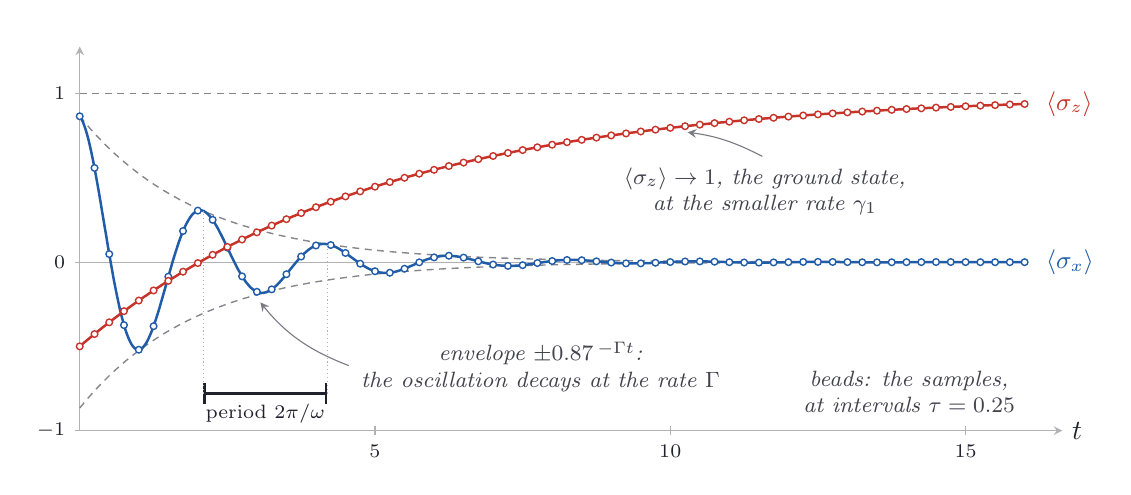
\begin{tikzpicture}[ink/.style={line width=0.9pt, ndInk}, faint/.style={line width=0.4pt, ndInk!35}, dashedink/.style={line width=0.5pt, ndInk!55, dash pattern=on 2.5pt off 2pt}, vec/.style={->, >=stealth, line width=1.2pt}, note/.style={font=\footnotesize\itshape, text=ndInk!85, align=center}, pointer/.style={->, >=stealth, line width=0.4pt, ndInk!60, shorten >=2pt, shorten <=1pt}, dot/.style={circle, fill=ndInk, inner sep=0pt, minimum size=3.4pt}, wash/.style={fill=ndSky, fill opacity=0.55}, every node/.style={text=ndInk}]
\definecolor{ndInk}{rgb}{0.13,0.13,0.18}
\definecolor{ndPaper}{rgb}{0.99,0.96,0.88}
\definecolor{ndSky}{rgb}{0.84,0.91,0.98}
\definecolor{ndRose}{rgb}{0.98,0.86,0.84}
\definecolor{ndBlue}{rgb}{0.13,0.36,0.66}
\definecolor{ndRed}{rgb}{0.78,0.20,0.16}
\definecolor{ndGold}{rgb}{0.88,0.62,0.10}
\definecolor{ndGreen}{rgb}{0.18,0.52,0.30}
\draw[faint, ->, >=stealth] (0.000,0.000) -- (12.480,0.000) node[right, text=ndInk] {$t$};
\draw[faint, ->, >=stealth] (0.000,0.000) -- (0.000,4.876) node[above, text=ndInk] {};
\draw[faint] (3.750,0.060) -- (3.750,-0.060) node[below, font=\scriptsize, text=ndInk] {$5$};
\draw[faint] (7.500,0.060) -- (7.500,-0.060) node[below, font=\scriptsize, text=ndInk] {$10$};
\draw[faint] (11.250,0.060) -- (11.250,-0.060) node[below, font=\scriptsize, text=ndInk] {$15$};
\draw[faint] (0.060,0.000) -- (-0.060,0.000) node[left, font=\scriptsize, text=ndInk] {$-1$};
\draw[faint] (0.060,2.140) -- (-0.060,2.140) node[left, font=\scriptsize, text=ndInk] {$0$};
\draw[faint] (0.060,4.279) -- (-0.060,4.279) node[left, font=\scriptsize, text=ndInk] {$1$};
\draw[faint] (0.000,2.140) -- (12.000,2.140);
\draw[dashedink] (0.000,3.992) -- (0.019,3.969) -- (0.038,3.947) -- (0.056,3.924) -- (0.075,3.902) -- (0.094,3.880) -- (0.113,3.859) -- (0.131,3.837) -- (0.150,3.816) -- (0.169,3.795) -- (0.188,3.775) -- (0.206,3.754) -- (0.225,3.734) -- (0.244,3.715) -- (0.263,3.695) -- (0.281,3.676) -- (0.300,3.657) -- (0.319,3.638) -- (0.338,3.619) -- (0.356,3.601) -- (0.375,3.583) -- (0.394,3.565) -- (0.413,3.547) -- (0.431,3.529) -- (0.450,3.512) -- (0.469,3.495) -- (0.488,3.478) -- (0.506,3.462) -- (0.525,3.445) -- (0.544,3.429) -- (0.562,3.413) -- (0.581,3.397) -- (0.600,3.382) -- (0.619,3.366) -- (0.638,3.351) -- (0.656,3.336) -- (0.675,3.321) -- (0.694,3.306) -- (0.713,3.292) -- (0.731,3.278) -- (0.750,3.263) -- (0.769,3.249) -- (0.788,3.236) -- (0.806,3.222) -- (0.825,3.209) -- (0.844,3.195) -- (0.863,3.182) -- (0.881,3.169) -- (0.900,3.156) -- (0.919,3.144) -- (0.938,3.131) -- (0.956,3.119) -- (0.975,3.107) -- (0.994,3.095) -- (1.013,3.083) -- (1.031,3.071) -- (1.050,3.060) -- (1.069,3.048) -- (1.088,3.037) -- (1.106,3.026) -- (1.125,3.015) -- (1.144,3.004) -- (1.163,2.993) -- (1.181,2.983) -- (1.200,2.972) -- (1.219,2.962) -- (1.238,2.952) -- (1.256,2.941) -- (1.275,2.931) -- (1.294,2.922) -- (1.312,2.912) -- (1.331,2.902) -- (1.350,2.893) -- (1.369,2.884) -- (1.388,2.874) -- (1.406,2.865) -- (1.425,2.856) -- (1.444,2.847) -- (1.463,2.838) -- (1.481,2.830) -- (1.500,2.821) -- (1.519,2.813) -- (1.538,2.804) -- (1.556,2.796) -- (1.575,2.788) -- (1.594,2.780) -- (1.612,2.772) -- (1.631,2.764) -- (1.650,2.756) -- (1.669,2.749) -- (1.688,2.741) -- (1.706,2.734) -- (1.725,2.726) -- (1.744,2.719) -- (1.763,2.712) -- (1.781,2.705) -- (1.800,2.698) -- (1.819,2.691) -- (1.838,2.684) -- (1.856,2.677) -- (1.875,2.670) -- (1.894,2.664) -- (1.913,2.657) -- (1.931,2.651) -- (1.950,2.645) -- (1.969,2.638) -- (1.988,2.632) -- (2.006,2.626) -- (2.025,2.620) -- (2.044,2.614) -- (2.062,2.608) -- (2.081,2.602) -- (2.100,2.596) -- (2.119,2.591) -- (2.138,2.585) -- (2.156,2.580) -- (2.175,2.574) -- (2.194,2.569) -- (2.213,2.563) -- (2.231,2.558) -- (2.250,2.553) -- (2.269,2.548) -- (2.288,2.543) -- (2.306,2.538) -- (2.325,2.533) -- (2.344,2.528) -- (2.363,2.523) -- (2.381,2.518) -- (2.400,2.514) -- (2.419,2.509) -- (2.438,2.504) -- (2.456,2.500) -- (2.475,2.495) -- (2.494,2.491) -- (2.513,2.487) -- (2.531,2.482) -- (2.550,2.478) -- (2.569,2.474) -- (2.588,2.470) -- (2.606,2.466) -- (2.625,2.462) -- (2.644,2.458) -- (2.663,2.454) -- (2.681,2.450) -- (2.700,2.446) -- (2.719,2.442) -- (2.738,2.438) -- (2.756,2.435) -- (2.775,2.431) -- (2.794,2.427) -- (2.812,2.424) -- (2.831,2.420) -- (2.850,2.417) -- (2.869,2.413) -- (2.888,2.410) -- (2.906,2.406) -- (2.925,2.403) -- (2.944,2.400) -- (2.963,2.397) -- (2.981,2.393) -- (3.000,2.390) -- (3.019,2.387) -- (3.037,2.384) -- (3.056,2.381) -- (3.075,2.378) -- (3.094,2.375) -- (3.113,2.372) -- (3.131,2.369) -- (3.150,2.366) -- (3.169,2.364) -- (3.188,2.361) -- (3.206,2.358) -- (3.225,2.355) -- (3.244,2.353) -- (3.263,2.350) -- (3.281,2.347) -- (3.300,2.345) -- (3.319,2.342) -- (3.338,2.340) -- (3.356,2.337) -- (3.375,2.335) -- (3.394,2.332) -- (3.412,2.330) -- (3.431,2.328) -- (3.450,2.325) -- (3.469,2.323) -- (3.488,2.321) -- (3.506,2.318) -- (3.525,2.316) -- (3.544,2.314) -- (3.562,2.312) -- (3.581,2.310) -- (3.600,2.308) -- (3.619,2.306) -- (3.638,2.303) -- (3.656,2.301) -- (3.675,2.299) -- (3.694,2.297) -- (3.713,2.295) -- (3.731,2.294) -- (3.750,2.292) -- (3.769,2.290) -- (3.788,2.288) -- (3.806,2.286) -- (3.825,2.284) -- (3.844,2.282) -- (3.863,2.281) -- (3.881,2.279) -- (3.900,2.277) -- (3.919,2.275) -- (3.938,2.274) -- (3.956,2.272) -- (3.975,2.270) -- (3.994,2.269) -- (4.013,2.267) -- (4.031,2.266) -- (4.050,2.264) -- (4.069,2.263) -- (4.088,2.261) -- (4.106,2.259) -- (4.125,2.258) -- (4.144,2.257) -- (4.163,2.255) -- (4.181,2.254) -- (4.200,2.252) -- (4.219,2.251) -- (4.238,2.249) -- (4.256,2.248) -- (4.275,2.247) -- (4.294,2.245) -- (4.312,2.244) -- (4.331,2.243) -- (4.350,2.241) -- (4.369,2.240) -- (4.388,2.239) -- (4.406,2.238) -- (4.425,2.237) -- (4.444,2.235) -- (4.463,2.234) -- (4.481,2.233) -- (4.500,2.232) -- (4.519,2.231) -- (4.538,2.230) -- (4.556,2.228) -- (4.575,2.227) -- (4.594,2.226) -- (4.613,2.225) -- (4.631,2.224) -- (4.650,2.223) -- (4.669,2.222) -- (4.688,2.221) -- (4.706,2.220) -- (4.725,2.219) -- (4.744,2.218) -- (4.763,2.217) -- (4.781,2.216) -- (4.800,2.215) -- (4.819,2.214) -- (4.838,2.213) -- (4.856,2.212) -- (4.875,2.211) -- (4.894,2.210) -- (4.913,2.210) -- (4.931,2.209) -- (4.950,2.208) -- (4.969,2.207) -- (4.988,2.206) -- (5.006,2.205) -- (5.025,2.205) -- (5.044,2.204) -- (5.062,2.203) -- (5.081,2.202) -- (5.100,2.201) -- (5.119,2.201) -- (5.138,2.200) -- (5.156,2.199) -- (5.175,2.198) -- (5.194,2.198) -- (5.213,2.197) -- (5.231,2.196) -- (5.250,2.195) -- (5.269,2.195) -- (5.288,2.194) -- (5.306,2.193) -- (5.325,2.193) -- (5.344,2.192) -- (5.363,2.191) -- (5.381,2.191) -- (5.400,2.190) -- (5.419,2.190) -- (5.438,2.189) -- (5.456,2.188) -- (5.475,2.188) -- (5.494,2.187) -- (5.513,2.187) -- (5.531,2.186) -- (5.550,2.185) -- (5.569,2.185) -- (5.588,2.184) -- (5.606,2.184) -- (5.625,2.183) -- (5.644,2.183) -- (5.663,2.182) -- (5.681,2.182) -- (5.700,2.181) -- (5.719,2.180) -- (5.738,2.180) -- (5.756,2.179) -- (5.775,2.179) -- (5.794,2.178) -- (5.812,2.178) -- (5.831,2.178) -- (5.850,2.177) -- (5.869,2.177) -- (5.888,2.176) -- (5.906,2.176) -- (5.925,2.175) -- (5.944,2.175) -- (5.963,2.174) -- (5.981,2.174) -- (6.000,2.173) -- (6.019,2.173) -- (6.038,2.173) -- (6.056,2.172) -- (6.075,2.172) -- (6.094,2.171) -- (6.113,2.171) -- (6.131,2.171) -- (6.150,2.170) -- (6.169,2.170) -- (6.188,2.169) -- (6.206,2.169) -- (6.225,2.169) -- (6.244,2.168) -- (6.262,2.168) -- (6.281,2.168) -- (6.300,2.167) -- (6.319,2.167) -- (6.338,2.167) -- (6.356,2.166) -- (6.375,2.166) -- (6.394,2.166) -- (6.413,2.165) -- (6.431,2.165) -- (6.450,2.165) -- (6.469,2.164) -- (6.488,2.164) -- (6.506,2.164) -- (6.525,2.163) -- (6.544,2.163) -- (6.562,2.163) -- (6.581,2.163) -- (6.600,2.162) -- (6.619,2.162) -- (6.637,2.162) -- (6.656,2.161) -- (6.675,2.161) -- (6.694,2.161) -- (6.713,2.161) -- (6.731,2.160) -- (6.750,2.160) -- (6.769,2.160) -- (6.788,2.160) -- (6.806,2.159) -- (6.825,2.159) -- (6.844,2.159) -- (6.863,2.159) -- (6.881,2.158) -- (6.900,2.158) -- (6.919,2.158) -- (6.938,2.158) -- (6.956,2.157) -- (6.975,2.157) -- (6.994,2.157) -- (7.012,2.157) -- (7.031,2.157) -- (7.050,2.156) -- (7.069,2.156) -- (7.088,2.156) -- (7.106,2.156) -- (7.125,2.156) -- (7.144,2.155) -- (7.163,2.155) -- (7.181,2.155) -- (7.200,2.155) -- (7.219,2.155) -- (7.238,2.154) -- (7.256,2.154) -- (7.275,2.154) -- (7.294,2.154) -- (7.312,2.154) -- (7.331,2.154) -- (7.350,2.153) -- (7.369,2.153) -- (7.388,2.153) -- (7.406,2.153) -- (7.425,2.153) -- (7.444,2.152) -- (7.463,2.152) -- (7.481,2.152) -- (7.500,2.152) -- (7.519,2.152) -- (7.538,2.152) -- (7.556,2.152) -- (7.575,2.151) -- (7.594,2.151) -- (7.613,2.151) -- (7.631,2.151) -- (7.650,2.151) -- (7.669,2.151) -- (7.688,2.151) -- (7.706,2.150) -- (7.725,2.150) -- (7.744,2.150) -- (7.763,2.150) -- (7.781,2.150) -- (7.800,2.150) -- (7.819,2.150) -- (7.838,2.150) -- (7.856,2.149) -- (7.875,2.149) -- (7.894,2.149) -- (7.913,2.149) -- (7.931,2.149) -- (7.950,2.149) -- (7.969,2.149) -- (7.988,2.149) -- (8.006,2.148) -- (8.025,2.148) -- (8.044,2.148) -- (8.062,2.148) -- (8.081,2.148) -- (8.100,2.148) -- (8.119,2.148) -- (8.138,2.148) -- (8.156,2.148) -- (8.175,2.147) -- (8.194,2.147) -- (8.213,2.147) -- (8.231,2.147) -- (8.250,2.147) -- (8.269,2.147) -- (8.288,2.147) -- (8.306,2.147) -- (8.325,2.147) -- (8.344,2.147) -- (8.363,2.147) -- (8.381,2.146) -- (8.400,2.146) -- (8.419,2.146) -- (8.438,2.146) -- (8.456,2.146) -- (8.475,2.146) -- (8.494,2.146) -- (8.513,2.146) -- (8.531,2.146) -- (8.550,2.146) -- (8.569,2.146) -- (8.588,2.146) -- (8.606,2.146) -- (8.625,2.145) -- (8.644,2.145) -- (8.663,2.145) -- (8.681,2.145) -- (8.700,2.145) -- (8.719,2.145) -- (8.738,2.145) -- (8.756,2.145) -- (8.775,2.145) -- (8.794,2.145) -- (8.812,2.145) -- (8.831,2.145) -- (8.850,2.145) -- (8.869,2.145) -- (8.888,2.144) -- (8.906,2.144) -- (8.925,2.144) -- (8.944,2.144) -- (8.963,2.144) -- (8.981,2.144) -- (9.000,2.144) -- (9.019,2.144) -- (9.038,2.144) -- (9.056,2.144) -- (9.075,2.144) -- (9.094,2.144) -- (9.113,2.144) -- (9.131,2.144) -- (9.150,2.144) -- (9.169,2.144) -- (9.188,2.144) -- (9.206,2.144) -- (9.225,2.143) -- (9.244,2.143) -- (9.263,2.143) -- (9.281,2.143) -- (9.300,2.143) -- (9.319,2.143) -- (9.338,2.143) -- (9.356,2.143) -- (9.375,2.143) -- (9.394,2.143) -- (9.413,2.143) -- (9.431,2.143) -- (9.450,2.143) -- (9.469,2.143) -- (9.488,2.143) -- (9.506,2.143) -- (9.525,2.143) -- (9.544,2.143) -- (9.562,2.143) -- (9.581,2.143) -- (9.600,2.143) -- (9.619,2.143) -- (9.638,2.143) -- (9.656,2.143) -- (9.675,2.142) -- (9.694,2.142) -- (9.713,2.142) -- (9.731,2.142) -- (9.750,2.142) -- (9.769,2.142) -- (9.788,2.142) -- (9.806,2.142) -- (9.825,2.142) -- (9.844,2.142) -- (9.863,2.142) -- (9.881,2.142) -- (9.900,2.142) -- (9.919,2.142) -- (9.938,2.142) -- (9.956,2.142) -- (9.975,2.142) -- (9.994,2.142) -- (10.013,2.142) -- (10.031,2.142) -- (10.050,2.142) -- (10.069,2.142) -- (10.088,2.142) -- (10.106,2.142) -- (10.125,2.142) -- (10.144,2.142) -- (10.163,2.142) -- (10.181,2.142) -- (10.200,2.142) -- (10.219,2.142) -- (10.238,2.142) -- (10.256,2.142) -- (10.275,2.141) -- (10.294,2.141) -- (10.312,2.141) -- (10.331,2.141) -- (10.350,2.141) -- (10.369,2.141) -- (10.388,2.141) -- (10.406,2.141) -- (10.425,2.141) -- (10.444,2.141) -- (10.463,2.141) -- (10.481,2.141) -- (10.500,2.141) -- (10.519,2.141) -- (10.538,2.141) -- (10.556,2.141) -- (10.575,2.141) -- (10.594,2.141) -- (10.613,2.141) -- (10.631,2.141) -- (10.650,2.141) -- (10.669,2.141) -- (10.688,2.141) -- (10.706,2.141) -- (10.725,2.141) -- (10.744,2.141) -- (10.763,2.141) -- (10.781,2.141) -- (10.800,2.141) -- (10.819,2.141) -- (10.838,2.141) -- (10.856,2.141) -- (10.875,2.141) -- (10.894,2.141) -- (10.913,2.141) -- (10.931,2.141) -- (10.950,2.141) -- (10.969,2.141) -- (10.988,2.141) -- (11.006,2.141) -- (11.025,2.141) -- (11.044,2.141) -- (11.062,2.141) -- (11.081,2.141) -- (11.100,2.141) -- (11.119,2.141) -- (11.138,2.141) -- (11.156,2.141) -- (11.175,2.141) -- (11.194,2.141) -- (11.213,2.141) -- (11.231,2.141) -- (11.250,2.141) -- (11.269,2.141) -- (11.288,2.141) -- (11.306,2.141) -- (11.325,2.141) -- (11.344,2.140) -- (11.363,2.140) -- (11.381,2.140) -- (11.400,2.140) -- (11.419,2.140) -- (11.438,2.140) -- (11.456,2.140) -- (11.475,2.140) -- (11.494,2.140) -- (11.513,2.140) -- (11.531,2.140) -- (11.550,2.140) -- (11.569,2.140) -- (11.588,2.140) -- (11.606,2.140) -- (11.625,2.140) -- (11.644,2.140) -- (11.663,2.140) -- (11.681,2.140) -- (11.700,2.140) -- (11.719,2.140) -- (11.738,2.140) -- (11.756,2.140) -- (11.775,2.140) -- (11.794,2.140) -- (11.812,2.140) -- (11.831,2.140) -- (11.850,2.140) -- (11.869,2.140) -- (11.888,2.140) -- (11.906,2.140) -- (11.925,2.140) -- (11.944,2.140) -- (11.963,2.140) -- (11.981,2.140) -- (12.000,2.140);
\draw[dashedink] (0.000,0.287) -- (0.019,0.310) -- (0.038,0.332) -- (0.056,0.355) -- (0.075,0.377) -- (0.094,0.399) -- (0.113,0.421) -- (0.131,0.442) -- (0.150,0.463) -- (0.169,0.484) -- (0.188,0.504) -- (0.206,0.525) -- (0.225,0.545) -- (0.244,0.565) -- (0.263,0.584) -- (0.281,0.603) -- (0.300,0.623) -- (0.319,0.641) -- (0.338,0.660) -- (0.356,0.678) -- (0.375,0.697) -- (0.394,0.714) -- (0.413,0.732) -- (0.431,0.750) -- (0.450,0.767) -- (0.469,0.784) -- (0.488,0.801) -- (0.506,0.817) -- (0.525,0.834) -- (0.544,0.850) -- (0.562,0.866) -- (0.581,0.882) -- (0.600,0.898) -- (0.619,0.913) -- (0.638,0.928) -- (0.656,0.943) -- (0.675,0.958) -- (0.694,0.973) -- (0.713,0.987) -- (0.731,1.002) -- (0.750,1.016) -- (0.769,1.030) -- (0.788,1.043) -- (0.806,1.057) -- (0.825,1.071) -- (0.844,1.084) -- (0.863,1.097) -- (0.881,1.110) -- (0.900,1.123) -- (0.919,1.135) -- (0.938,1.148) -- (0.956,1.160) -- (0.975,1.172) -- (0.994,1.184) -- (1.013,1.196) -- (1.031,1.208) -- (1.050,1.219) -- (1.069,1.231) -- (1.088,1.242) -- (1.106,1.253) -- (1.125,1.264) -- (1.144,1.275) -- (1.163,1.286) -- (1.181,1.297) -- (1.200,1.307) -- (1.219,1.317) -- (1.238,1.328) -- (1.256,1.338) -- (1.275,1.348) -- (1.294,1.357) -- (1.312,1.367) -- (1.331,1.377) -- (1.350,1.386) -- (1.369,1.396) -- (1.388,1.405) -- (1.406,1.414) -- (1.425,1.423) -- (1.444,1.432) -- (1.463,1.441) -- (1.481,1.449) -- (1.500,1.458) -- (1.519,1.466) -- (1.538,1.475) -- (1.556,1.483) -- (1.575,1.491) -- (1.594,1.499) -- (1.612,1.507) -- (1.631,1.515) -- (1.650,1.523) -- (1.669,1.530) -- (1.688,1.538) -- (1.706,1.545) -- (1.725,1.553) -- (1.744,1.560) -- (1.763,1.567) -- (1.781,1.574) -- (1.800,1.581) -- (1.819,1.588) -- (1.838,1.595) -- (1.856,1.602) -- (1.875,1.609) -- (1.894,1.615) -- (1.913,1.622) -- (1.931,1.628) -- (1.950,1.635) -- (1.969,1.641) -- (1.988,1.647) -- (2.006,1.653) -- (2.025,1.659) -- (2.044,1.665) -- (2.062,1.671) -- (2.081,1.677) -- (2.100,1.683) -- (2.119,1.688) -- (2.138,1.694) -- (2.156,1.699) -- (2.175,1.705) -- (2.194,1.710) -- (2.213,1.716) -- (2.231,1.721) -- (2.250,1.726) -- (2.269,1.731) -- (2.288,1.736) -- (2.306,1.741) -- (2.325,1.746) -- (2.344,1.751) -- (2.363,1.756) -- (2.381,1.761) -- (2.400,1.765) -- (2.419,1.770) -- (2.438,1.775) -- (2.456,1.779) -- (2.475,1.784) -- (2.494,1.788) -- (2.513,1.792) -- (2.531,1.797) -- (2.550,1.801) -- (2.569,1.805) -- (2.588,1.809) -- (2.606,1.814) -- (2.625,1.818) -- (2.644,1.822) -- (2.663,1.826) -- (2.681,1.829) -- (2.700,1.833) -- (2.719,1.837) -- (2.738,1.841) -- (2.756,1.845) -- (2.775,1.848) -- (2.794,1.852) -- (2.812,1.855) -- (2.831,1.859) -- (2.850,1.862) -- (2.869,1.866) -- (2.888,1.869) -- (2.906,1.873) -- (2.925,1.876) -- (2.944,1.879) -- (2.963,1.882) -- (2.981,1.886) -- (3.000,1.889) -- (3.019,1.892) -- (3.037,1.895) -- (3.056,1.898) -- (3.075,1.901) -- (3.094,1.904) -- (3.113,1.907) -- (3.131,1.910) -- (3.150,1.913) -- (3.169,1.915) -- (3.188,1.918) -- (3.206,1.921) -- (3.225,1.924) -- (3.244,1.926) -- (3.263,1.929) -- (3.281,1.932) -- (3.300,1.934) -- (3.319,1.937) -- (3.338,1.939) -- (3.356,1.942) -- (3.375,1.944) -- (3.394,1.947) -- (3.412,1.949) -- (3.431,1.951) -- (3.450,1.954) -- (3.469,1.956) -- (3.488,1.958) -- (3.506,1.961) -- (3.525,1.963) -- (3.544,1.965) -- (3.562,1.967) -- (3.581,1.969) -- (3.600,1.971) -- (3.619,1.974) -- (3.638,1.976) -- (3.656,1.978) -- (3.675,1.980) -- (3.694,1.982) -- (3.713,1.984) -- (3.731,1.986) -- (3.750,1.987) -- (3.769,1.989) -- (3.788,1.991) -- (3.806,1.993) -- (3.825,1.995) -- (3.844,1.997) -- (3.863,1.998) -- (3.881,2.000) -- (3.900,2.002) -- (3.919,2.004) -- (3.938,2.005) -- (3.956,2.007) -- (3.975,2.009) -- (3.994,2.010) -- (4.013,2.012) -- (4.031,2.013) -- (4.050,2.015) -- (4.069,2.017) -- (4.088,2.018) -- (4.106,2.020) -- (4.125,2.021) -- (4.144,2.023) -- (4.163,2.024) -- (4.181,2.025) -- (4.200,2.027) -- (4.219,2.028) -- (4.238,2.030) -- (4.256,2.031) -- (4.275,2.032) -- (4.294,2.034) -- (4.312,2.035) -- (4.331,2.036) -- (4.350,2.038) -- (4.369,2.039) -- (4.388,2.040) -- (4.406,2.041) -- (4.425,2.043) -- (4.444,2.044) -- (4.463,2.045) -- (4.481,2.046) -- (4.500,2.047) -- (4.519,2.048) -- (4.538,2.050) -- (4.556,2.051) -- (4.575,2.052) -- (4.594,2.053) -- (4.613,2.054) -- (4.631,2.055) -- (4.650,2.056) -- (4.669,2.057) -- (4.688,2.058) -- (4.706,2.059) -- (4.725,2.060) -- (4.744,2.061) -- (4.763,2.062) -- (4.781,2.063) -- (4.800,2.064) -- (4.819,2.065) -- (4.838,2.066) -- (4.856,2.067) -- (4.875,2.068) -- (4.894,2.069) -- (4.913,2.069) -- (4.931,2.070) -- (4.950,2.071) -- (4.969,2.072) -- (4.988,2.073) -- (5.006,2.074) -- (5.025,2.075) -- (5.044,2.075) -- (5.062,2.076) -- (5.081,2.077) -- (5.100,2.078) -- (5.119,2.078) -- (5.138,2.079) -- (5.156,2.080) -- (5.175,2.081) -- (5.194,2.081) -- (5.213,2.082) -- (5.231,2.083) -- (5.250,2.084) -- (5.269,2.084) -- (5.288,2.085) -- (5.306,2.086) -- (5.325,2.086) -- (5.344,2.087) -- (5.363,2.088) -- (5.381,2.088) -- (5.400,2.089) -- (5.419,2.090) -- (5.438,2.090) -- (5.456,2.091) -- (5.475,2.091) -- (5.494,2.092) -- (5.513,2.093) -- (5.531,2.093) -- (5.550,2.094) -- (5.569,2.094) -- (5.588,2.095) -- (5.606,2.095) -- (5.625,2.096) -- (5.644,2.097) -- (5.663,2.097) -- (5.681,2.098) -- (5.700,2.098) -- (5.719,2.099) -- (5.738,2.099) -- (5.756,2.100) -- (5.775,2.100) -- (5.794,2.101) -- (5.812,2.101) -- (5.831,2.102) -- (5.850,2.102) -- (5.869,2.102) -- (5.888,2.103) -- (5.906,2.103) -- (5.925,2.104) -- (5.944,2.104) -- (5.963,2.105) -- (5.981,2.105) -- (6.000,2.106) -- (6.019,2.106) -- (6.038,2.106) -- (6.056,2.107) -- (6.075,2.107) -- (6.094,2.108) -- (6.113,2.108) -- (6.131,2.108) -- (6.150,2.109) -- (6.169,2.109) -- (6.188,2.110) -- (6.206,2.110) -- (6.225,2.110) -- (6.244,2.111) -- (6.262,2.111) -- (6.281,2.111) -- (6.300,2.112) -- (6.319,2.112) -- (6.338,2.112) -- (6.356,2.113) -- (6.375,2.113) -- (6.394,2.113) -- (6.413,2.114) -- (6.431,2.114) -- (6.450,2.114) -- (6.469,2.115) -- (6.488,2.115) -- (6.506,2.115) -- (6.525,2.116) -- (6.544,2.116) -- (6.562,2.116) -- (6.581,2.117) -- (6.600,2.117) -- (6.619,2.117) -- (6.637,2.117) -- (6.656,2.118) -- (6.675,2.118) -- (6.694,2.118) -- (6.713,2.118) -- (6.731,2.119) -- (6.750,2.119) -- (6.769,2.119) -- (6.788,2.119) -- (6.806,2.120) -- (6.825,2.120) -- (6.844,2.120) -- (6.863,2.120) -- (6.881,2.121) -- (6.900,2.121) -- (6.919,2.121) -- (6.938,2.121) -- (6.956,2.122) -- (6.975,2.122) -- (6.994,2.122) -- (7.012,2.122) -- (7.031,2.122) -- (7.050,2.123) -- (7.069,2.123) -- (7.088,2.123) -- (7.106,2.123) -- (7.125,2.124) -- (7.144,2.124) -- (7.163,2.124) -- (7.181,2.124) -- (7.200,2.124) -- (7.219,2.124) -- (7.238,2.125) -- (7.256,2.125) -- (7.275,2.125) -- (7.294,2.125) -- (7.312,2.125) -- (7.331,2.126) -- (7.350,2.126) -- (7.369,2.126) -- (7.388,2.126) -- (7.406,2.126) -- (7.425,2.126) -- (7.444,2.127) -- (7.463,2.127) -- (7.481,2.127) -- (7.500,2.127) -- (7.519,2.127) -- (7.538,2.127) -- (7.556,2.128) -- (7.575,2.128) -- (7.594,2.128) -- (7.613,2.128) -- (7.631,2.128) -- (7.650,2.128) -- (7.669,2.128) -- (7.688,2.129) -- (7.706,2.129) -- (7.725,2.129) -- (7.744,2.129) -- (7.763,2.129) -- (7.781,2.129) -- (7.800,2.129) -- (7.819,2.129) -- (7.838,2.130) -- (7.856,2.130) -- (7.875,2.130) -- (7.894,2.130) -- (7.913,2.130) -- (7.931,2.130) -- (7.950,2.130) -- (7.969,2.130) -- (7.988,2.131) -- (8.006,2.131) -- (8.025,2.131) -- (8.044,2.131) -- (8.062,2.131) -- (8.081,2.131) -- (8.100,2.131) -- (8.119,2.131) -- (8.138,2.131) -- (8.156,2.131) -- (8.175,2.132) -- (8.194,2.132) -- (8.213,2.132) -- (8.231,2.132) -- (8.250,2.132) -- (8.269,2.132) -- (8.288,2.132) -- (8.306,2.132) -- (8.325,2.132) -- (8.344,2.132) -- (8.363,2.133) -- (8.381,2.133) -- (8.400,2.133) -- (8.419,2.133) -- (8.438,2.133) -- (8.456,2.133) -- (8.475,2.133) -- (8.494,2.133) -- (8.513,2.133) -- (8.531,2.133) -- (8.550,2.133) -- (8.569,2.133) -- (8.588,2.133) -- (8.606,2.134) -- (8.625,2.134) -- (8.644,2.134) -- (8.663,2.134) -- (8.681,2.134) -- (8.700,2.134) -- (8.719,2.134) -- (8.738,2.134) -- (8.756,2.134) -- (8.775,2.134) -- (8.794,2.134) -- (8.812,2.134) -- (8.831,2.134) -- (8.850,2.134) -- (8.869,2.135) -- (8.888,2.135) -- (8.906,2.135) -- (8.925,2.135) -- (8.944,2.135) -- (8.963,2.135) -- (8.981,2.135) -- (9.000,2.135) -- (9.019,2.135) -- (9.038,2.135) -- (9.056,2.135) -- (9.075,2.135) -- (9.094,2.135) -- (9.113,2.135) -- (9.131,2.135) -- (9.150,2.135) -- (9.169,2.135) -- (9.188,2.135) -- (9.206,2.136) -- (9.225,2.136) -- (9.244,2.136) -- (9.263,2.136) -- (9.281,2.136) -- (9.300,2.136) -- (9.319,2.136) -- (9.338,2.136) -- (9.356,2.136) -- (9.375,2.136) -- (9.394,2.136) -- (9.413,2.136) -- (9.431,2.136) -- (9.450,2.136) -- (9.469,2.136) -- (9.488,2.136) -- (9.506,2.136) -- (9.525,2.136) -- (9.544,2.136) -- (9.562,2.136) -- (9.581,2.136) -- (9.600,2.136) -- (9.619,2.136) -- (9.638,2.137) -- (9.656,2.137) -- (9.675,2.137) -- (9.694,2.137) -- (9.713,2.137) -- (9.731,2.137) -- (9.750,2.137) -- (9.769,2.137) -- (9.788,2.137) -- (9.806,2.137) -- (9.825,2.137) -- (9.844,2.137) -- (9.863,2.137) -- (9.881,2.137) -- (9.900,2.137) -- (9.919,2.137) -- (9.938,2.137) -- (9.956,2.137) -- (9.975,2.137) -- (9.994,2.137) -- (10.013,2.137) -- (10.031,2.137) -- (10.050,2.137) -- (10.069,2.137) -- (10.088,2.137) -- (10.106,2.137) -- (10.125,2.137) -- (10.144,2.137) -- (10.163,2.137) -- (10.181,2.137) -- (10.200,2.137) -- (10.219,2.137) -- (10.238,2.138) -- (10.256,2.138) -- (10.275,2.138) -- (10.294,2.138) -- (10.312,2.138) -- (10.331,2.138) -- (10.350,2.138) -- (10.369,2.138) -- (10.388,2.138) -- (10.406,2.138) -- (10.425,2.138) -- (10.444,2.138) -- (10.463,2.138) -- (10.481,2.138) -- (10.500,2.138) -- (10.519,2.138) -- (10.538,2.138) -- (10.556,2.138) -- (10.575,2.138) -- (10.594,2.138) -- (10.613,2.138) -- (10.631,2.138) -- (10.650,2.138) -- (10.669,2.138) -- (10.688,2.138) -- (10.706,2.138) -- (10.725,2.138) -- (10.744,2.138) -- (10.763,2.138) -- (10.781,2.138) -- (10.800,2.138) -- (10.819,2.138) -- (10.838,2.138) -- (10.856,2.138) -- (10.875,2.138) -- (10.894,2.138) -- (10.913,2.138) -- (10.931,2.138) -- (10.950,2.138) -- (10.969,2.138) -- (10.988,2.138) -- (11.006,2.138) -- (11.025,2.138) -- (11.044,2.138) -- (11.062,2.138) -- (11.081,2.138) -- (11.100,2.138) -- (11.119,2.138) -- (11.138,2.138) -- (11.156,2.138) -- (11.175,2.138) -- (11.194,2.138) -- (11.213,2.138) -- (11.231,2.138) -- (11.250,2.139) -- (11.269,2.139) -- (11.288,2.139) -- (11.306,2.139) -- (11.325,2.139) -- (11.344,2.139) -- (11.363,2.139) -- (11.381,2.139) -- (11.400,2.139) -- (11.419,2.139) -- (11.438,2.139) -- (11.456,2.139) -- (11.475,2.139) -- (11.494,2.139) -- (11.513,2.139) -- (11.531,2.139) -- (11.550,2.139) -- (11.569,2.139) -- (11.588,2.139) -- (11.606,2.139) -- (11.625,2.139) -- (11.644,2.139) -- (11.663,2.139) -- (11.681,2.139) -- (11.700,2.139) -- (11.719,2.139) -- (11.738,2.139) -- (11.756,2.139) -- (11.775,2.139) -- (11.794,2.139) -- (11.812,2.139) -- (11.831,2.139) -- (11.850,2.139) -- (11.869,2.139) -- (11.888,2.139) -- (11.906,2.139) -- (11.925,2.139) -- (11.944,2.139) -- (11.963,2.139) -- (11.981,2.139) -- (12.000,2.139);
\draw[dashedink] (0.000,4.279) -- (12.000,4.279);
\draw[line width=0.9pt, ndBlue] (0.000,3.992) -- (0.019,3.964) -- (0.038,3.926) -- (0.056,3.879) -- (0.075,3.823) -- (0.094,3.759) -- (0.113,3.687) -- (0.131,3.609) -- (0.150,3.523) -- (0.169,3.432) -- (0.188,3.336) -- (0.206,3.235) -- (0.225,3.131) -- (0.244,3.023) -- (0.263,2.913) -- (0.281,2.802) -- (0.300,2.689) -- (0.319,2.576) -- (0.338,2.464) -- (0.356,2.352) -- (0.375,2.242) -- (0.394,2.134) -- (0.413,2.028) -- (0.431,1.926) -- (0.450,1.828) -- (0.469,1.733) -- (0.488,1.644) -- (0.506,1.559) -- (0.525,1.480) -- (0.544,1.407) -- (0.562,1.340) -- (0.581,1.278) -- (0.600,1.224) -- (0.619,1.176) -- (0.638,1.134) -- (0.656,1.099) -- (0.675,1.071) -- (0.694,1.050) -- (0.713,1.036) -- (0.731,1.028) -- (0.750,1.027) -- (0.769,1.032) -- (0.788,1.043) -- (0.806,1.061) -- (0.825,1.084) -- (0.844,1.112) -- (0.863,1.146) -- (0.881,1.185) -- (0.900,1.228) -- (0.919,1.275) -- (0.938,1.326) -- (0.956,1.380) -- (0.975,1.437) -- (0.994,1.497) -- (1.013,1.559) -- (1.031,1.623) -- (1.050,1.688) -- (1.069,1.755) -- (1.088,1.821) -- (1.106,1.888) -- (1.125,1.955) -- (1.144,2.021) -- (1.163,2.086) -- (1.181,2.150) -- (1.200,2.212) -- (1.219,2.273) -- (1.238,2.331) -- (1.256,2.386) -- (1.275,2.439) -- (1.294,2.489) -- (1.312,2.535) -- (1.331,2.578) -- (1.350,2.618) -- (1.369,2.653) -- (1.388,2.685) -- (1.406,2.714) -- (1.425,2.738) -- (1.444,2.758) -- (1.463,2.774) -- (1.481,2.786) -- (1.500,2.794) -- (1.519,2.798) -- (1.538,2.798) -- (1.556,2.795) -- (1.575,2.788) -- (1.594,2.777) -- (1.612,2.763) -- (1.631,2.746) -- (1.650,2.726) -- (1.669,2.702) -- (1.688,2.677) -- (1.706,2.649) -- (1.725,2.618) -- (1.744,2.586) -- (1.763,2.552) -- (1.781,2.516) -- (1.800,2.479) -- (1.819,2.441) -- (1.838,2.402) -- (1.856,2.363) -- (1.875,2.324) -- (1.894,2.284) -- (1.913,2.244) -- (1.931,2.205) -- (1.950,2.167) -- (1.969,2.129) -- (1.988,2.092) -- (2.006,2.057) -- (2.025,2.023) -- (2.044,1.990) -- (2.062,1.959) -- (2.081,1.930) -- (2.100,1.902) -- (2.119,1.877) -- (2.138,1.854) -- (2.156,1.833) -- (2.175,1.814) -- (2.194,1.798) -- (2.213,1.784) -- (2.231,1.772) -- (2.250,1.763) -- (2.269,1.756) -- (2.288,1.751) -- (2.306,1.749) -- (2.325,1.749) -- (2.344,1.752) -- (2.363,1.756) -- (2.381,1.763) -- (2.400,1.771) -- (2.419,1.782) -- (2.438,1.794) -- (2.456,1.808) -- (2.475,1.823) -- (2.494,1.840) -- (2.513,1.858) -- (2.531,1.877) -- (2.550,1.898) -- (2.569,1.919) -- (2.588,1.941) -- (2.606,1.963) -- (2.625,1.986) -- (2.644,2.010) -- (2.663,2.033) -- (2.681,2.057) -- (2.700,2.080) -- (2.719,2.103) -- (2.738,2.126) -- (2.756,2.148) -- (2.775,2.170) -- (2.794,2.191) -- (2.812,2.211) -- (2.831,2.230) -- (2.850,2.249) -- (2.869,2.266) -- (2.888,2.282) -- (2.906,2.297) -- (2.925,2.310) -- (2.944,2.323) -- (2.963,2.333) -- (2.981,2.343) -- (3.000,2.351) -- (3.019,2.358) -- (3.037,2.363) -- (3.056,2.367) -- (3.075,2.370) -- (3.094,2.371) -- (3.113,2.371) -- (3.131,2.369) -- (3.150,2.366) -- (3.169,2.362) -- (3.188,2.357) -- (3.206,2.351) -- (3.225,2.343) -- (3.244,2.335) -- (3.263,2.326) -- (3.281,2.316) -- (3.300,2.305) -- (3.319,2.293) -- (3.338,2.281) -- (3.356,2.269) -- (3.375,2.256) -- (3.394,2.242) -- (3.412,2.229) -- (3.431,2.215) -- (3.450,2.201) -- (3.469,2.187) -- (3.488,2.173) -- (3.506,2.160) -- (3.525,2.146) -- (3.544,2.133) -- (3.562,2.120) -- (3.581,2.108) -- (3.600,2.096) -- (3.619,2.085) -- (3.638,2.074) -- (3.656,2.064) -- (3.675,2.054) -- (3.694,2.046) -- (3.713,2.038) -- (3.731,2.030) -- (3.750,2.024) -- (3.769,2.018) -- (3.788,2.014) -- (3.806,2.010) -- (3.825,2.007) -- (3.844,2.005) -- (3.863,2.003) -- (3.881,2.003) -- (3.900,2.003) -- (3.919,2.004) -- (3.938,2.005) -- (3.956,2.008) -- (3.975,2.011) -- (3.994,2.015) -- (4.013,2.019) -- (4.031,2.024) -- (4.050,2.030) -- (4.069,2.036) -- (4.088,2.042) -- (4.106,2.049) -- (4.125,2.056) -- (4.144,2.064) -- (4.163,2.072) -- (4.181,2.080) -- (4.200,2.088) -- (4.219,2.096) -- (4.238,2.104) -- (4.256,2.112) -- (4.275,2.120) -- (4.294,2.129) -- (4.312,2.137) -- (4.331,2.144) -- (4.350,2.152) -- (4.369,2.159) -- (4.388,2.166) -- (4.406,2.173) -- (4.425,2.179) -- (4.444,2.185) -- (4.463,2.191) -- (4.481,2.196) -- (4.500,2.200) -- (4.519,2.205) -- (4.538,2.208) -- (4.556,2.212) -- (4.575,2.214) -- (4.594,2.217) -- (4.613,2.218) -- (4.631,2.220) -- (4.650,2.220) -- (4.669,2.221) -- (4.688,2.221) -- (4.706,2.220) -- (4.725,2.219) -- (4.744,2.217) -- (4.763,2.215) -- (4.781,2.213) -- (4.800,2.210) -- (4.819,2.207) -- (4.838,2.204) -- (4.856,2.201) -- (4.875,2.197) -- (4.894,2.193) -- (4.913,2.188) -- (4.931,2.184) -- (4.950,2.179) -- (4.969,2.175) -- (4.988,2.170) -- (5.006,2.165) -- (5.025,2.160) -- (5.044,2.155) -- (5.062,2.150) -- (5.081,2.145) -- (5.100,2.141) -- (5.119,2.136) -- (5.138,2.132) -- (5.156,2.127) -- (5.175,2.123) -- (5.194,2.119) -- (5.213,2.116) -- (5.231,2.112) -- (5.250,2.109) -- (5.269,2.106) -- (5.288,2.103) -- (5.306,2.101) -- (5.325,2.099) -- (5.344,2.097) -- (5.363,2.095) -- (5.381,2.094) -- (5.400,2.093) -- (5.419,2.092) -- (5.438,2.092) -- (5.456,2.091) -- (5.475,2.092) -- (5.494,2.092) -- (5.513,2.093) -- (5.531,2.094) -- (5.550,2.095) -- (5.569,2.096) -- (5.588,2.098) -- (5.606,2.099) -- (5.625,2.101) -- (5.644,2.104) -- (5.663,2.106) -- (5.681,2.108) -- (5.700,2.111) -- (5.719,2.114) -- (5.738,2.116) -- (5.756,2.119) -- (5.775,2.122) -- (5.794,2.125) -- (5.812,2.128) -- (5.831,2.131) -- (5.850,2.133) -- (5.869,2.136) -- (5.888,2.139) -- (5.906,2.142) -- (5.925,2.144) -- (5.944,2.147) -- (5.963,2.149) -- (5.981,2.152) -- (6.000,2.154) -- (6.019,2.156) -- (6.038,2.158) -- (6.056,2.160) -- (6.075,2.161) -- (6.094,2.163) -- (6.113,2.164) -- (6.131,2.165) -- (6.150,2.166) -- (6.169,2.167) -- (6.188,2.167) -- (6.206,2.168) -- (6.225,2.168) -- (6.244,2.168) -- (6.262,2.168) -- (6.281,2.168) -- (6.300,2.167) -- (6.319,2.167) -- (6.338,2.166) -- (6.356,2.165) -- (6.375,2.164) -- (6.394,2.163) -- (6.413,2.162) -- (6.431,2.161) -- (6.450,2.159) -- (6.469,2.158) -- (6.488,2.156) -- (6.506,2.155) -- (6.525,2.153) -- (6.544,2.151) -- (6.562,2.150) -- (6.581,2.148) -- (6.600,2.146) -- (6.619,2.145) -- (6.637,2.143) -- (6.656,2.141) -- (6.675,2.140) -- (6.694,2.138) -- (6.713,2.136) -- (6.731,2.135) -- (6.750,2.134) -- (6.769,2.132) -- (6.788,2.131) -- (6.806,2.130) -- (6.825,2.129) -- (6.844,2.128) -- (6.863,2.127) -- (6.881,2.126) -- (6.900,2.125) -- (6.919,2.124) -- (6.938,2.124) -- (6.956,2.123) -- (6.975,2.123) -- (6.994,2.123) -- (7.012,2.123) -- (7.031,2.123) -- (7.050,2.123) -- (7.069,2.123) -- (7.088,2.123) -- (7.106,2.123) -- (7.125,2.124) -- (7.144,2.124) -- (7.163,2.125) -- (7.181,2.126) -- (7.200,2.126) -- (7.219,2.127) -- (7.238,2.128) -- (7.256,2.129) -- (7.275,2.130) -- (7.294,2.131) -- (7.312,2.132) -- (7.331,2.133) -- (7.350,2.134) -- (7.369,2.135) -- (7.388,2.136) -- (7.406,2.137) -- (7.425,2.138) -- (7.444,2.139) -- (7.463,2.140) -- (7.481,2.141) -- (7.500,2.141) -- (7.519,2.142) -- (7.538,2.143) -- (7.556,2.144) -- (7.575,2.145) -- (7.594,2.145) -- (7.613,2.146) -- (7.631,2.147) -- (7.650,2.147) -- (7.669,2.148) -- (7.688,2.148) -- (7.706,2.149) -- (7.725,2.149) -- (7.744,2.149) -- (7.763,2.149) -- (7.781,2.149) -- (7.800,2.150) -- (7.819,2.150) -- (7.838,2.149) -- (7.856,2.149) -- (7.875,2.149) -- (7.894,2.149) -- (7.913,2.149) -- (7.931,2.148) -- (7.950,2.148) -- (7.969,2.148) -- (7.988,2.147) -- (8.006,2.147) -- (8.025,2.146) -- (8.044,2.146) -- (8.062,2.145) -- (8.081,2.145) -- (8.100,2.144) -- (8.119,2.144) -- (8.138,2.143) -- (8.156,2.142) -- (8.175,2.142) -- (8.194,2.141) -- (8.213,2.141) -- (8.231,2.140) -- (8.250,2.139) -- (8.269,2.139) -- (8.288,2.138) -- (8.306,2.138) -- (8.325,2.137) -- (8.344,2.137) -- (8.363,2.136) -- (8.381,2.136) -- (8.400,2.136) -- (8.419,2.135) -- (8.438,2.135) -- (8.456,2.135) -- (8.475,2.134) -- (8.494,2.134) -- (8.513,2.134) -- (8.531,2.134) -- (8.550,2.134) -- (8.569,2.134) -- (8.588,2.134) -- (8.606,2.134) -- (8.625,2.134) -- (8.644,2.134) -- (8.663,2.134) -- (8.681,2.134) -- (8.700,2.134) -- (8.719,2.134) -- (8.738,2.134) -- (8.756,2.135) -- (8.775,2.135) -- (8.794,2.135) -- (8.812,2.136) -- (8.831,2.136) -- (8.850,2.136) -- (8.869,2.136) -- (8.888,2.137) -- (8.906,2.137) -- (8.925,2.138) -- (8.944,2.138) -- (8.963,2.138) -- (8.981,2.139) -- (9.000,2.139) -- (9.019,2.139) -- (9.038,2.140) -- (9.056,2.140) -- (9.075,2.140) -- (9.094,2.141) -- (9.113,2.141) -- (9.131,2.141) -- (9.150,2.141) -- (9.169,2.142) -- (9.188,2.142) -- (9.206,2.142) -- (9.225,2.142) -- (9.244,2.142) -- (9.263,2.143) -- (9.281,2.143) -- (9.300,2.143) -- (9.319,2.143) -- (9.338,2.143) -- (9.356,2.143) -- (9.375,2.143) -- (9.394,2.143) -- (9.413,2.143) -- (9.431,2.143) -- (9.450,2.143) -- (9.469,2.143) -- (9.488,2.143) -- (9.506,2.143) -- (9.525,2.143) -- (9.544,2.142) -- (9.562,2.142) -- (9.581,2.142) -- (9.600,2.142) -- (9.619,2.142) -- (9.638,2.142) -- (9.656,2.141) -- (9.675,2.141) -- (9.694,2.141) -- (9.713,2.141) -- (9.731,2.140) -- (9.750,2.140) -- (9.769,2.140) -- (9.788,2.140) -- (9.806,2.140) -- (9.825,2.139) -- (9.844,2.139) -- (9.863,2.139) -- (9.881,2.139) -- (9.900,2.139) -- (9.919,2.139) -- (9.938,2.138) -- (9.956,2.138) -- (9.975,2.138) -- (9.994,2.138) -- (10.013,2.138) -- (10.031,2.138) -- (10.050,2.138) -- (10.069,2.138) -- (10.088,2.138) -- (10.106,2.138) -- (10.125,2.137) -- (10.144,2.137) -- (10.163,2.137) -- (10.181,2.137) -- (10.200,2.137) -- (10.219,2.137) -- (10.238,2.138) -- (10.256,2.138) -- (10.275,2.138) -- (10.294,2.138) -- (10.312,2.138) -- (10.331,2.138) -- (10.350,2.138) -- (10.369,2.138) -- (10.388,2.138) -- (10.406,2.138) -- (10.425,2.138) -- (10.444,2.138) -- (10.463,2.139) -- (10.481,2.139) -- (10.500,2.139) -- (10.519,2.139) -- (10.538,2.139) -- (10.556,2.139) -- (10.575,2.139) -- (10.594,2.139) -- (10.613,2.140) -- (10.631,2.140) -- (10.650,2.140) -- (10.669,2.140) -- (10.688,2.140) -- (10.706,2.140) -- (10.725,2.140) -- (10.744,2.140) -- (10.763,2.140) -- (10.781,2.140) -- (10.800,2.141) -- (10.819,2.141) -- (10.838,2.141) -- (10.856,2.141) -- (10.875,2.141) -- (10.894,2.141) -- (10.913,2.141) -- (10.931,2.141) -- (10.950,2.141) -- (10.969,2.141) -- (10.988,2.141) -- (11.006,2.141) -- (11.025,2.141) -- (11.044,2.141) -- (11.062,2.141) -- (11.081,2.141) -- (11.100,2.141) -- (11.119,2.141) -- (11.138,2.140) -- (11.156,2.140) -- (11.175,2.140) -- (11.194,2.140) -- (11.213,2.140) -- (11.231,2.140) -- (11.250,2.140) -- (11.269,2.140) -- (11.288,2.140) -- (11.306,2.140) -- (11.325,2.140) -- (11.344,2.140) -- (11.363,2.140) -- (11.381,2.140) -- (11.400,2.139) -- (11.419,2.139) -- (11.438,2.139) -- (11.456,2.139) -- (11.475,2.139) -- (11.494,2.139) -- (11.513,2.139) -- (11.531,2.139) -- (11.550,2.139) -- (11.569,2.139) -- (11.588,2.139) -- (11.606,2.139) -- (11.625,2.139) -- (11.644,2.139) -- (11.663,2.139) -- (11.681,2.139) -- (11.700,2.139) -- (11.719,2.139) -- (11.738,2.139) -- (11.756,2.139) -- (11.775,2.139) -- (11.794,2.139) -- (11.812,2.139) -- (11.831,2.139) -- (11.850,2.139) -- (11.869,2.139) -- (11.888,2.139) -- (11.906,2.139) -- (11.925,2.139) -- (11.944,2.139) -- (11.963,2.139) -- (11.981,2.139) -- (12.000,2.139);
\filldraw[fill=white, draw=ndBlue, line width=0.5pt] (0.000,3.992) circle (1.2pt);
\filldraw[fill=white, draw=ndBlue, line width=0.5pt] (0.188,3.336) circle (1.2pt);
\filldraw[fill=white, draw=ndBlue, line width=0.5pt] (0.375,2.242) circle (1.2pt);
\filldraw[fill=white, draw=ndBlue, line width=0.5pt] (0.562,1.340) circle (1.2pt);
\filldraw[fill=white, draw=ndBlue, line width=0.5pt] (0.750,1.027) circle (1.2pt);
\filldraw[fill=white, draw=ndBlue, line width=0.5pt] (0.938,1.326) circle (1.2pt);
\filldraw[fill=white, draw=ndBlue, line width=0.5pt] (1.125,1.955) circle (1.2pt);
\filldraw[fill=white, draw=ndBlue, line width=0.5pt] (1.312,2.535) circle (1.2pt);
\filldraw[fill=white, draw=ndBlue, line width=0.5pt] (1.500,2.794) circle (1.2pt);
\filldraw[fill=white, draw=ndBlue, line width=0.5pt] (1.688,2.677) circle (1.2pt);
\filldraw[fill=white, draw=ndBlue, line width=0.5pt] (1.875,2.324) circle (1.2pt);
\filldraw[fill=white, draw=ndBlue, line width=0.5pt] (2.062,1.959) circle (1.2pt);
\filldraw[fill=white, draw=ndBlue, line width=0.5pt] (2.250,1.763) circle (1.2pt);
\filldraw[fill=white, draw=ndBlue, line width=0.5pt] (2.438,1.794) circle (1.2pt);
\filldraw[fill=white, draw=ndBlue, line width=0.5pt] (2.625,1.986) circle (1.2pt);
\filldraw[fill=white, draw=ndBlue, line width=0.5pt] (2.812,2.211) circle (1.2pt);
\filldraw[fill=white, draw=ndBlue, line width=0.5pt] (3.000,2.351) circle (1.2pt);
\filldraw[fill=white, draw=ndBlue, line width=0.5pt] (3.188,2.357) circle (1.2pt);
\filldraw[fill=white, draw=ndBlue, line width=0.5pt] (3.375,2.256) circle (1.2pt);
\filldraw[fill=white, draw=ndBlue, line width=0.5pt] (3.562,2.120) circle (1.2pt);
\filldraw[fill=white, draw=ndBlue, line width=0.5pt] (3.750,2.024) circle (1.2pt);
\filldraw[fill=white, draw=ndBlue, line width=0.5pt] (3.938,2.005) circle (1.2pt);
\filldraw[fill=white, draw=ndBlue, line width=0.5pt] (4.125,2.056) circle (1.2pt);
\filldraw[fill=white, draw=ndBlue, line width=0.5pt] (4.312,2.137) circle (1.2pt);
\filldraw[fill=white, draw=ndBlue, line width=0.5pt] (4.500,2.200) circle (1.2pt);
\filldraw[fill=white, draw=ndBlue, line width=0.5pt] (4.688,2.221) circle (1.2pt);
\filldraw[fill=white, draw=ndBlue, line width=0.5pt] (4.875,2.197) circle (1.2pt);
\filldraw[fill=white, draw=ndBlue, line width=0.5pt] (5.062,2.150) circle (1.2pt);
\filldraw[fill=white, draw=ndBlue, line width=0.5pt] (5.250,2.109) circle (1.2pt);
\filldraw[fill=white, draw=ndBlue, line width=0.5pt] (5.438,2.092) circle (1.2pt);
\filldraw[fill=white, draw=ndBlue, line width=0.5pt] (5.625,2.101) circle (1.2pt);
\filldraw[fill=white, draw=ndBlue, line width=0.5pt] (5.812,2.128) circle (1.2pt);
\filldraw[fill=white, draw=ndBlue, line width=0.5pt] (6.000,2.154) circle (1.2pt);
\filldraw[fill=white, draw=ndBlue, line width=0.5pt] (6.188,2.167) circle (1.2pt);
\filldraw[fill=white, draw=ndBlue, line width=0.5pt] (6.375,2.164) circle (1.2pt);
\filldraw[fill=white, draw=ndBlue, line width=0.5pt] (6.562,2.150) circle (1.2pt);
\filldraw[fill=white, draw=ndBlue, line width=0.5pt] (6.750,2.134) circle (1.2pt);
\filldraw[fill=white, draw=ndBlue, line width=0.5pt] (6.938,2.124) circle (1.2pt);
\filldraw[fill=white, draw=ndBlue, line width=0.5pt] (7.125,2.124) circle (1.2pt);
\filldraw[fill=white, draw=ndBlue, line width=0.5pt] (7.312,2.132) circle (1.2pt);
\filldraw[fill=white, draw=ndBlue, line width=0.5pt] (7.500,2.141) circle (1.2pt);
\filldraw[fill=white, draw=ndBlue, line width=0.5pt] (7.688,2.148) circle (1.2pt);
\filldraw[fill=white, draw=ndBlue, line width=0.5pt] (7.875,2.149) circle (1.2pt);
\filldraw[fill=white, draw=ndBlue, line width=0.5pt] (8.062,2.145) circle (1.2pt);
\filldraw[fill=white, draw=ndBlue, line width=0.5pt] (8.250,2.139) circle (1.2pt);
\filldraw[fill=white, draw=ndBlue, line width=0.5pt] (8.438,2.135) circle (1.2pt);
\filldraw[fill=white, draw=ndBlue, line width=0.5pt] (8.625,2.134) circle (1.2pt);
\filldraw[fill=white, draw=ndBlue, line width=0.5pt] (8.812,2.136) circle (1.2pt);
\filldraw[fill=white, draw=ndBlue, line width=0.5pt] (9.000,2.139) circle (1.2pt);
\filldraw[fill=white, draw=ndBlue, line width=0.5pt] (9.188,2.142) circle (1.2pt);
\filldraw[fill=white, draw=ndBlue, line width=0.5pt] (9.375,2.143) circle (1.2pt);
\filldraw[fill=white, draw=ndBlue, line width=0.5pt] (9.562,2.142) circle (1.2pt);
\filldraw[fill=white, draw=ndBlue, line width=0.5pt] (9.750,2.140) circle (1.2pt);
\filldraw[fill=white, draw=ndBlue, line width=0.5pt] (9.938,2.138) circle (1.2pt);
\filldraw[fill=white, draw=ndBlue, line width=0.5pt] (10.125,2.137) circle (1.2pt);
\filldraw[fill=white, draw=ndBlue, line width=0.5pt] (10.312,2.138) circle (1.2pt);
\filldraw[fill=white, draw=ndBlue, line width=0.5pt] (10.500,2.139) circle (1.2pt);
\filldraw[fill=white, draw=ndBlue, line width=0.5pt] (10.688,2.140) circle (1.2pt);
\filldraw[fill=white, draw=ndBlue, line width=0.5pt] (10.875,2.141) circle (1.2pt);
\filldraw[fill=white, draw=ndBlue, line width=0.5pt] (11.062,2.141) circle (1.2pt);
\filldraw[fill=white, draw=ndBlue, line width=0.5pt] (11.250,2.140) circle (1.2pt);
\filldraw[fill=white, draw=ndBlue, line width=0.5pt] (11.438,2.139) circle (1.2pt);
\filldraw[fill=white, draw=ndBlue, line width=0.5pt] (11.625,2.139) circle (1.2pt);
\filldraw[fill=white, draw=ndBlue, line width=0.5pt] (11.812,2.139) circle (1.2pt);
\filldraw[fill=white, draw=ndBlue, line width=0.5pt] (12.000,2.139) circle (1.2pt);
\draw[line width=0.9pt, ndRed] (0.000,1.070) -- (0.019,1.086) -- (0.038,1.102) -- (0.056,1.118) -- (0.075,1.133) -- (0.094,1.149) -- (0.113,1.165) -- (0.131,1.180) -- (0.150,1.196) -- (0.169,1.211) -- (0.188,1.226) -- (0.206,1.242) -- (0.225,1.257) -- (0.244,1.272) -- (0.263,1.287) -- (0.281,1.302) -- (0.300,1.317) -- (0.319,1.331) -- (0.338,1.346) -- (0.356,1.361) -- (0.375,1.375) -- (0.394,1.390) -- (0.413,1.404) -- (0.431,1.418) -- (0.450,1.433) -- (0.469,1.447) -- (0.488,1.461) -- (0.506,1.475) -- (0.525,1.489) -- (0.544,1.503) -- (0.562,1.517) -- (0.581,1.531) -- (0.600,1.544) -- (0.619,1.558) -- (0.638,1.571) -- (0.656,1.585) -- (0.675,1.598) -- (0.694,1.612) -- (0.713,1.625) -- (0.731,1.638) -- (0.750,1.652) -- (0.769,1.665) -- (0.788,1.678) -- (0.806,1.691) -- (0.825,1.704) -- (0.844,1.716) -- (0.863,1.729) -- (0.881,1.742) -- (0.900,1.755) -- (0.919,1.767) -- (0.938,1.780) -- (0.956,1.792) -- (0.975,1.805) -- (0.994,1.817) -- (1.013,1.829) -- (1.031,1.841) -- (1.050,1.854) -- (1.069,1.866) -- (1.088,1.878) -- (1.106,1.890) -- (1.125,1.902) -- (1.144,1.913) -- (1.163,1.925) -- (1.181,1.937) -- (1.200,1.949) -- (1.219,1.960) -- (1.238,1.972) -- (1.256,1.983) -- (1.275,1.995) -- (1.294,2.006) -- (1.312,2.018) -- (1.331,2.029) -- (1.350,2.040) -- (1.369,2.051) -- (1.388,2.062) -- (1.406,2.073) -- (1.425,2.084) -- (1.444,2.095) -- (1.463,2.106) -- (1.481,2.117) -- (1.500,2.128) -- (1.519,2.139) -- (1.538,2.149) -- (1.556,2.160) -- (1.575,2.170) -- (1.594,2.181) -- (1.612,2.191) -- (1.631,2.202) -- (1.650,2.212) -- (1.669,2.222) -- (1.688,2.233) -- (1.706,2.243) -- (1.725,2.253) -- (1.744,2.263) -- (1.763,2.273) -- (1.781,2.283) -- (1.800,2.293) -- (1.819,2.303) -- (1.838,2.313) -- (1.856,2.323) -- (1.875,2.333) -- (1.894,2.342) -- (1.913,2.352) -- (1.931,2.362) -- (1.950,2.371) -- (1.969,2.381) -- (1.988,2.390) -- (2.006,2.399) -- (2.025,2.409) -- (2.044,2.418) -- (2.062,2.427) -- (2.081,2.437) -- (2.100,2.446) -- (2.119,2.455) -- (2.138,2.464) -- (2.156,2.473) -- (2.175,2.482) -- (2.194,2.491) -- (2.213,2.500) -- (2.231,2.509) -- (2.250,2.518) -- (2.269,2.527) -- (2.288,2.535) -- (2.306,2.544) -- (2.325,2.553) -- (2.344,2.561) -- (2.363,2.570) -- (2.381,2.578) -- (2.400,2.587) -- (2.419,2.595) -- (2.438,2.604) -- (2.456,2.612) -- (2.475,2.620) -- (2.494,2.629) -- (2.513,2.637) -- (2.531,2.645) -- (2.550,2.653) -- (2.569,2.661) -- (2.588,2.669) -- (2.606,2.677) -- (2.625,2.685) -- (2.644,2.693) -- (2.663,2.701) -- (2.681,2.709) -- (2.700,2.717) -- (2.719,2.725) -- (2.738,2.732) -- (2.756,2.740) -- (2.775,2.748) -- (2.794,2.756) -- (2.812,2.763) -- (2.831,2.771) -- (2.850,2.778) -- (2.869,2.786) -- (2.888,2.793) -- (2.906,2.801) -- (2.925,2.808) -- (2.944,2.815) -- (2.963,2.823) -- (2.981,2.830) -- (3.000,2.837) -- (3.019,2.844) -- (3.037,2.851) -- (3.056,2.859) -- (3.075,2.866) -- (3.094,2.873) -- (3.113,2.880) -- (3.131,2.887) -- (3.150,2.894) -- (3.169,2.900) -- (3.188,2.907) -- (3.206,2.914) -- (3.225,2.921) -- (3.244,2.928) -- (3.263,2.935) -- (3.281,2.941) -- (3.300,2.948) -- (3.319,2.955) -- (3.338,2.961) -- (3.356,2.968) -- (3.375,2.974) -- (3.394,2.981) -- (3.412,2.987) -- (3.431,2.994) -- (3.450,3.000) -- (3.469,3.006) -- (3.488,3.013) -- (3.506,3.019) -- (3.525,3.025) -- (3.544,3.032) -- (3.562,3.038) -- (3.581,3.044) -- (3.600,3.050) -- (3.619,3.056) -- (3.638,3.062) -- (3.656,3.069) -- (3.675,3.075) -- (3.694,3.081) -- (3.713,3.087) -- (3.731,3.093) -- (3.750,3.098) -- (3.769,3.104) -- (3.788,3.110) -- (3.806,3.116) -- (3.825,3.122) -- (3.844,3.128) -- (3.863,3.133) -- (3.881,3.139) -- (3.900,3.145) -- (3.919,3.150) -- (3.938,3.156) -- (3.956,3.162) -- (3.975,3.167) -- (3.994,3.173) -- (4.013,3.178) -- (4.031,3.184) -- (4.050,3.189) -- (4.069,3.195) -- (4.088,3.200) -- (4.106,3.205) -- (4.125,3.211) -- (4.144,3.216) -- (4.163,3.221) -- (4.181,3.227) -- (4.200,3.232) -- (4.219,3.237) -- (4.238,3.242) -- (4.256,3.248) -- (4.275,3.253) -- (4.294,3.258) -- (4.312,3.263) -- (4.331,3.268) -- (4.350,3.273) -- (4.369,3.278) -- (4.388,3.283) -- (4.406,3.288) -- (4.425,3.293) -- (4.444,3.298) -- (4.463,3.303) -- (4.481,3.308) -- (4.500,3.312) -- (4.519,3.317) -- (4.538,3.322) -- (4.556,3.327) -- (4.575,3.332) -- (4.594,3.336) -- (4.613,3.341) -- (4.631,3.346) -- (4.650,3.350) -- (4.669,3.355) -- (4.688,3.360) -- (4.706,3.364) -- (4.725,3.369) -- (4.744,3.373) -- (4.763,3.378) -- (4.781,3.382) -- (4.800,3.387) -- (4.819,3.391) -- (4.838,3.396) -- (4.856,3.400) -- (4.875,3.404) -- (4.894,3.409) -- (4.913,3.413) -- (4.931,3.417) -- (4.950,3.422) -- (4.969,3.426) -- (4.988,3.430) -- (5.006,3.435) -- (5.025,3.439) -- (5.044,3.443) -- (5.062,3.447) -- (5.081,3.451) -- (5.100,3.455) -- (5.119,3.459) -- (5.138,3.464) -- (5.156,3.468) -- (5.175,3.472) -- (5.194,3.476) -- (5.213,3.480) -- (5.231,3.484) -- (5.250,3.488) -- (5.269,3.492) -- (5.288,3.496) -- (5.306,3.499) -- (5.325,3.503) -- (5.344,3.507) -- (5.363,3.511) -- (5.381,3.515) -- (5.400,3.519) -- (5.419,3.522) -- (5.438,3.526) -- (5.456,3.530) -- (5.475,3.534) -- (5.494,3.537) -- (5.513,3.541) -- (5.531,3.545) -- (5.550,3.549) -- (5.569,3.552) -- (5.588,3.556) -- (5.606,3.559) -- (5.625,3.563) -- (5.644,3.567) -- (5.663,3.570) -- (5.681,3.574) -- (5.700,3.577) -- (5.719,3.581) -- (5.738,3.584) -- (5.756,3.588) -- (5.775,3.591) -- (5.794,3.594) -- (5.812,3.598) -- (5.831,3.601) -- (5.850,3.605) -- (5.869,3.608) -- (5.888,3.611) -- (5.906,3.615) -- (5.925,3.618) -- (5.944,3.621) -- (5.963,3.625) -- (5.981,3.628) -- (6.000,3.631) -- (6.019,3.634) -- (6.038,3.638) -- (6.056,3.641) -- (6.075,3.644) -- (6.094,3.647) -- (6.113,3.650) -- (6.131,3.653) -- (6.150,3.657) -- (6.169,3.660) -- (6.188,3.663) -- (6.206,3.666) -- (6.225,3.669) -- (6.244,3.672) -- (6.262,3.675) -- (6.281,3.678) -- (6.300,3.681) -- (6.319,3.684) -- (6.338,3.687) -- (6.356,3.690) -- (6.375,3.693) -- (6.394,3.696) -- (6.413,3.699) -- (6.431,3.702) -- (6.450,3.704) -- (6.469,3.707) -- (6.488,3.710) -- (6.506,3.713) -- (6.525,3.716) -- (6.544,3.719) -- (6.562,3.721) -- (6.581,3.724) -- (6.600,3.727) -- (6.619,3.730) -- (6.637,3.732) -- (6.656,3.735) -- (6.675,3.738) -- (6.694,3.741) -- (6.713,3.743) -- (6.731,3.746) -- (6.750,3.749) -- (6.769,3.751) -- (6.788,3.754) -- (6.806,3.756) -- (6.825,3.759) -- (6.844,3.762) -- (6.863,3.764) -- (6.881,3.767) -- (6.900,3.769) -- (6.919,3.772) -- (6.938,3.774) -- (6.956,3.777) -- (6.975,3.779) -- (6.994,3.782) -- (7.012,3.784) -- (7.031,3.787) -- (7.050,3.789) -- (7.069,3.792) -- (7.088,3.794) -- (7.106,3.797) -- (7.125,3.799) -- (7.144,3.801) -- (7.163,3.804) -- (7.181,3.806) -- (7.200,3.809) -- (7.219,3.811) -- (7.238,3.813) -- (7.256,3.816) -- (7.275,3.818) -- (7.294,3.820) -- (7.312,3.822) -- (7.331,3.825) -- (7.350,3.827) -- (7.369,3.829) -- (7.388,3.832) -- (7.406,3.834) -- (7.425,3.836) -- (7.444,3.838) -- (7.463,3.840) -- (7.481,3.843) -- (7.500,3.845) -- (7.519,3.847) -- (7.538,3.849) -- (7.556,3.851) -- (7.575,3.853) -- (7.594,3.855) -- (7.613,3.858) -- (7.631,3.860) -- (7.650,3.862) -- (7.669,3.864) -- (7.688,3.866) -- (7.706,3.868) -- (7.725,3.870) -- (7.744,3.872) -- (7.763,3.874) -- (7.781,3.876) -- (7.800,3.878) -- (7.819,3.880) -- (7.838,3.882) -- (7.856,3.884) -- (7.875,3.886) -- (7.894,3.888) -- (7.913,3.890) -- (7.931,3.892) -- (7.950,3.894) -- (7.969,3.896) -- (7.988,3.898) -- (8.006,3.900) -- (8.025,3.901) -- (8.044,3.903) -- (8.062,3.905) -- (8.081,3.907) -- (8.100,3.909) -- (8.119,3.911) -- (8.138,3.913) -- (8.156,3.914) -- (8.175,3.916) -- (8.194,3.918) -- (8.213,3.920) -- (8.231,3.922) -- (8.250,3.923) -- (8.269,3.925) -- (8.288,3.927) -- (8.306,3.929) -- (8.325,3.931) -- (8.344,3.932) -- (8.363,3.934) -- (8.381,3.936) -- (8.400,3.937) -- (8.419,3.939) -- (8.438,3.941) -- (8.456,3.942) -- (8.475,3.944) -- (8.494,3.946) -- (8.513,3.948) -- (8.531,3.949) -- (8.550,3.951) -- (8.569,3.952) -- (8.588,3.954) -- (8.606,3.956) -- (8.625,3.957) -- (8.644,3.959) -- (8.663,3.961) -- (8.681,3.962) -- (8.700,3.964) -- (8.719,3.965) -- (8.738,3.967) -- (8.756,3.968) -- (8.775,3.970) -- (8.794,3.971) -- (8.812,3.973) -- (8.831,3.975) -- (8.850,3.976) -- (8.869,3.978) -- (8.888,3.979) -- (8.906,3.981) -- (8.925,3.982) -- (8.944,3.984) -- (8.963,3.985) -- (8.981,3.986) -- (9.000,3.988) -- (9.019,3.989) -- (9.038,3.991) -- (9.056,3.992) -- (9.075,3.994) -- (9.094,3.995) -- (9.113,3.997) -- (9.131,3.998) -- (9.150,3.999) -- (9.169,4.001) -- (9.188,4.002) -- (9.206,4.004) -- (9.225,4.005) -- (9.244,4.006) -- (9.263,4.008) -- (9.281,4.009) -- (9.300,4.010) -- (9.319,4.012) -- (9.338,4.013) -- (9.356,4.014) -- (9.375,4.016) -- (9.394,4.017) -- (9.413,4.018) -- (9.431,4.020) -- (9.450,4.021) -- (9.469,4.022) -- (9.488,4.023) -- (9.506,4.025) -- (9.525,4.026) -- (9.544,4.027) -- (9.562,4.028) -- (9.581,4.030) -- (9.600,4.031) -- (9.619,4.032) -- (9.638,4.033) -- (9.656,4.035) -- (9.675,4.036) -- (9.694,4.037) -- (9.713,4.038) -- (9.731,4.040) -- (9.750,4.041) -- (9.769,4.042) -- (9.788,4.043) -- (9.806,4.044) -- (9.825,4.045) -- (9.844,4.047) -- (9.863,4.048) -- (9.881,4.049) -- (9.900,4.050) -- (9.919,4.051) -- (9.938,4.052) -- (9.956,4.053) -- (9.975,4.055) -- (9.994,4.056) -- (10.013,4.057) -- (10.031,4.058) -- (10.050,4.059) -- (10.069,4.060) -- (10.088,4.061) -- (10.106,4.062) -- (10.125,4.063) -- (10.144,4.064) -- (10.163,4.066) -- (10.181,4.067) -- (10.200,4.068) -- (10.219,4.069) -- (10.238,4.070) -- (10.256,4.071) -- (10.275,4.072) -- (10.294,4.073) -- (10.312,4.074) -- (10.331,4.075) -- (10.350,4.076) -- (10.369,4.077) -- (10.388,4.078) -- (10.406,4.079) -- (10.425,4.080) -- (10.444,4.081) -- (10.463,4.082) -- (10.481,4.083) -- (10.500,4.084) -- (10.519,4.085) -- (10.538,4.086) -- (10.556,4.087) -- (10.575,4.088) -- (10.594,4.089) -- (10.613,4.090) -- (10.631,4.091) -- (10.650,4.092) -- (10.669,4.092) -- (10.688,4.093) -- (10.706,4.094) -- (10.725,4.095) -- (10.744,4.096) -- (10.763,4.097) -- (10.781,4.098) -- (10.800,4.099) -- (10.819,4.100) -- (10.838,4.101) -- (10.856,4.102) -- (10.875,4.102) -- (10.894,4.103) -- (10.913,4.104) -- (10.931,4.105) -- (10.950,4.106) -- (10.969,4.107) -- (10.988,4.108) -- (11.006,4.109) -- (11.025,4.109) -- (11.044,4.110) -- (11.062,4.111) -- (11.081,4.112) -- (11.100,4.113) -- (11.119,4.114) -- (11.138,4.114) -- (11.156,4.115) -- (11.175,4.116) -- (11.194,4.117) -- (11.213,4.118) -- (11.231,4.118) -- (11.250,4.119) -- (11.269,4.120) -- (11.288,4.121) -- (11.306,4.122) -- (11.325,4.122) -- (11.344,4.123) -- (11.363,4.124) -- (11.381,4.125) -- (11.400,4.126) -- (11.419,4.126) -- (11.438,4.127) -- (11.456,4.128) -- (11.475,4.129) -- (11.494,4.129) -- (11.513,4.130) -- (11.531,4.131) -- (11.550,4.132) -- (11.569,4.132) -- (11.588,4.133) -- (11.606,4.134) -- (11.625,4.134) -- (11.644,4.135) -- (11.663,4.136) -- (11.681,4.137) -- (11.700,4.137) -- (11.719,4.138) -- (11.738,4.139) -- (11.756,4.139) -- (11.775,4.140) -- (11.794,4.141) -- (11.812,4.142) -- (11.831,4.142) -- (11.850,4.143) -- (11.869,4.144) -- (11.888,4.144) -- (11.906,4.145) -- (11.925,4.146) -- (11.944,4.146) -- (11.963,4.147) -- (11.981,4.148) -- (12.000,4.148);
\filldraw[fill=white, draw=ndRed, line width=0.5pt] (0.000,1.070) circle (1.2pt);
\filldraw[fill=white, draw=ndRed, line width=0.5pt] (0.188,1.226) circle (1.2pt);
\filldraw[fill=white, draw=ndRed, line width=0.5pt] (0.375,1.375) circle (1.2pt);
\filldraw[fill=white, draw=ndRed, line width=0.5pt] (0.562,1.517) circle (1.2pt);
\filldraw[fill=white, draw=ndRed, line width=0.5pt] (0.750,1.652) circle (1.2pt);
\filldraw[fill=white, draw=ndRed, line width=0.5pt] (0.938,1.780) circle (1.2pt);
\filldraw[fill=white, draw=ndRed, line width=0.5pt] (1.125,1.902) circle (1.2pt);
\filldraw[fill=white, draw=ndRed, line width=0.5pt] (1.312,2.018) circle (1.2pt);
\filldraw[fill=white, draw=ndRed, line width=0.5pt] (1.500,2.128) circle (1.2pt);
\filldraw[fill=white, draw=ndRed, line width=0.5pt] (1.688,2.233) circle (1.2pt);
\filldraw[fill=white, draw=ndRed, line width=0.5pt] (1.875,2.333) circle (1.2pt);
\filldraw[fill=white, draw=ndRed, line width=0.5pt] (2.062,2.427) circle (1.2pt);
\filldraw[fill=white, draw=ndRed, line width=0.5pt] (2.250,2.518) circle (1.2pt);
\filldraw[fill=white, draw=ndRed, line width=0.5pt] (2.438,2.604) circle (1.2pt);
\filldraw[fill=white, draw=ndRed, line width=0.5pt] (2.625,2.685) circle (1.2pt);
\filldraw[fill=white, draw=ndRed, line width=0.5pt] (2.812,2.763) circle (1.2pt);
\filldraw[fill=white, draw=ndRed, line width=0.5pt] (3.000,2.837) circle (1.2pt);
\filldraw[fill=white, draw=ndRed, line width=0.5pt] (3.188,2.907) circle (1.2pt);
\filldraw[fill=white, draw=ndRed, line width=0.5pt] (3.375,2.974) circle (1.2pt);
\filldraw[fill=white, draw=ndRed, line width=0.5pt] (3.562,3.038) circle (1.2pt);
\filldraw[fill=white, draw=ndRed, line width=0.5pt] (3.750,3.098) circle (1.2pt);
\filldraw[fill=white, draw=ndRed, line width=0.5pt] (3.938,3.156) circle (1.2pt);
\filldraw[fill=white, draw=ndRed, line width=0.5pt] (4.125,3.211) circle (1.2pt);
\filldraw[fill=white, draw=ndRed, line width=0.5pt] (4.312,3.263) circle (1.2pt);
\filldraw[fill=white, draw=ndRed, line width=0.5pt] (4.500,3.312) circle (1.2pt);
\filldraw[fill=white, draw=ndRed, line width=0.5pt] (4.688,3.360) circle (1.2pt);
\filldraw[fill=white, draw=ndRed, line width=0.5pt] (4.875,3.404) circle (1.2pt);
\filldraw[fill=white, draw=ndRed, line width=0.5pt] (5.062,3.447) circle (1.2pt);
\filldraw[fill=white, draw=ndRed, line width=0.5pt] (5.250,3.488) circle (1.2pt);
\filldraw[fill=white, draw=ndRed, line width=0.5pt] (5.438,3.526) circle (1.2pt);
\filldraw[fill=white, draw=ndRed, line width=0.5pt] (5.625,3.563) circle (1.2pt);
\filldraw[fill=white, draw=ndRed, line width=0.5pt] (5.812,3.598) circle (1.2pt);
\filldraw[fill=white, draw=ndRed, line width=0.5pt] (6.000,3.631) circle (1.2pt);
\filldraw[fill=white, draw=ndRed, line width=0.5pt] (6.188,3.663) circle (1.2pt);
\filldraw[fill=white, draw=ndRed, line width=0.5pt] (6.375,3.693) circle (1.2pt);
\filldraw[fill=white, draw=ndRed, line width=0.5pt] (6.562,3.721) circle (1.2pt);
\filldraw[fill=white, draw=ndRed, line width=0.5pt] (6.750,3.749) circle (1.2pt);
\filldraw[fill=white, draw=ndRed, line width=0.5pt] (6.938,3.774) circle (1.2pt);
\filldraw[fill=white, draw=ndRed, line width=0.5pt] (7.125,3.799) circle (1.2pt);
\filldraw[fill=white, draw=ndRed, line width=0.5pt] (7.312,3.822) circle (1.2pt);
\filldraw[fill=white, draw=ndRed, line width=0.5pt] (7.500,3.845) circle (1.2pt);
\filldraw[fill=white, draw=ndRed, line width=0.5pt] (7.688,3.866) circle (1.2pt);
\filldraw[fill=white, draw=ndRed, line width=0.5pt] (7.875,3.886) circle (1.2pt);
\filldraw[fill=white, draw=ndRed, line width=0.5pt] (8.062,3.905) circle (1.2pt);
\filldraw[fill=white, draw=ndRed, line width=0.5pt] (8.250,3.923) circle (1.2pt);
\filldraw[fill=white, draw=ndRed, line width=0.5pt] (8.438,3.941) circle (1.2pt);
\filldraw[fill=white, draw=ndRed, line width=0.5pt] (8.625,3.957) circle (1.2pt);
\filldraw[fill=white, draw=ndRed, line width=0.5pt] (8.812,3.973) circle (1.2pt);
\filldraw[fill=white, draw=ndRed, line width=0.5pt] (9.000,3.988) circle (1.2pt);
\filldraw[fill=white, draw=ndRed, line width=0.5pt] (9.188,4.002) circle (1.2pt);
\filldraw[fill=white, draw=ndRed, line width=0.5pt] (9.375,4.016) circle (1.2pt);
\filldraw[fill=white, draw=ndRed, line width=0.5pt] (9.562,4.028) circle (1.2pt);
\filldraw[fill=white, draw=ndRed, line width=0.5pt] (9.750,4.041) circle (1.2pt);
\filldraw[fill=white, draw=ndRed, line width=0.5pt] (9.938,4.052) circle (1.2pt);
\filldraw[fill=white, draw=ndRed, line width=0.5pt] (10.125,4.063) circle (1.2pt);
\filldraw[fill=white, draw=ndRed, line width=0.5pt] (10.312,4.074) circle (1.2pt);
\filldraw[fill=white, draw=ndRed, line width=0.5pt] (10.500,4.084) circle (1.2pt);
\filldraw[fill=white, draw=ndRed, line width=0.5pt] (10.688,4.093) circle (1.2pt);
\filldraw[fill=white, draw=ndRed, line width=0.5pt] (10.875,4.102) circle (1.2pt);
\filldraw[fill=white, draw=ndRed, line width=0.5pt] (11.062,4.111) circle (1.2pt);
\filldraw[fill=white, draw=ndRed, line width=0.5pt] (11.250,4.119) circle (1.2pt);
\filldraw[fill=white, draw=ndRed, line width=0.5pt] (11.438,4.127) circle (1.2pt);
\filldraw[fill=white, draw=ndRed, line width=0.5pt] (11.625,4.134) circle (1.2pt);
\filldraw[fill=white, draw=ndRed, line width=0.5pt] (11.812,4.142) circle (1.2pt);
\filldraw[fill=white, draw=ndRed, line width=0.5pt] (12.000,4.148) circle (1.2pt);
\node[font=\small, text=ndBlue, anchor=west] at (12.150,2.140) {$\langle\sigma_x\rangle$};
\node[font=\small, text=ndRed, anchor=west] at (12.150,4.148) {$\langle\sigma_z\rangle$};
\draw[ink, |-|] (1.571,0.471) -- (3.142,0.471) node[midway, below, font=\scriptsize] {period $2\pi/\omega$};
\draw[faint, densely dotted] (1.571,0.471) -- (1.571,2.790);
\draw[faint, densely dotted] (3.142,0.471) -- (3.142,2.368);
\node[note, anchor=west] (e) at (3.450,0.813) {envelope $\pm0.87\,\ee^{-\Gamma t}$:\\ the oscillation decays at the rate $\Gamma$};
\draw[pointer] (e.west) to[bend left=15] (2.250,1.683);
\node[note, anchor=north] (z) at (8.700,3.466) {$\langle\sigma_z\rangle\to1$, the ground state,\\ at the smaller rate $\gamma_1$};
\draw[pointer] (z.north) to[bend right=10] (7.650,3.798);
\node[note, anchor=south east] at (12.000,0.107) {beads: the samples,\\ at intervals $\tau=0.25$};
\end{tikzpicture}
}\end{center}
$\langle\sigma_x\rangle$ oscillates with period $2\pi/\omega$ and decays at the rate $\Gamma$; $\langle\sigma_z\rangle$ rises to $1$ at the rate $\gamma_1$.}
\end{frame}

\begin{frame}\ft{The output as a sum of modes}
\ona{Suppose that $\mathbf A$ is diagonalisable, with eigenvalues $\lambda_1,\dots,\lambda_n$, right eigenvectors $\vec v_i$ and left eigenvectors $\vec w_i$, normalised so that $\vec w_i^\dagger\vec v_j=\delta_{ij}$. The initial state may then be decomposed along the eigenvectors, $\vec x_0=\sum_ic_i\vec v_i$ with $c_i=\vec w_i^\dagger\vec x_0$. Each component evolves on its own, $\ee^{\mathbf At}\vec x_0=\sum_ic_i\ee^{\lambda_it}\vec v_i$, and the measurement $\mathbf C$ takes from each the amount $\mathbf C\vec v_i$. Hence every output of $\dot{\vec x}=\mathbf A\vec x$, $y=\mathbf C\vec x$, is a linear combination of the modes,}
\onp{Decompose $\vec x_0=\sum_ic_i\vec v_i$ along the eigenvectors, $c_i=\vec w_i^\dagger\vec x_0$. Then each output is a sum of modes:}
\begin{equation}\label{eq:ch05:sum}
    y(t)=\sum_{i=1}^n r_i\,\ee^{\lambda_it},\qquad r_i=\underbrace{(\mathbf C\vec v_i)}_{\text{seen}}\,\underbrace{(\vec w_i^\dagger\vec x_0)}_{\text{excited}} .
\end{equation}
\ona{The weight of a mode is thus the product of two factors. The second, $\vec w_i^\dagger\vec x_0$, is the amount by which the preparation excites the mode; the first, $\mathbf C\vec v_i$, is the amount of the mode that the measurement sees. A mode is absent from the data when either factor vanishes, and each of the missing modes in Figure~\ref{fig:ch05:excite} fails in one of these two ways. When every mode is excited, that is, when $\vec w_i^\dagger\vec x_0\neq0$ for every $i$, the initial state is said to be \emph{persistently exciting}; when every mode is seen, $\mathbf C\vec v_i\neq0$ for every $i$, and the system is observable (Theorem~\ref{thm:ch05:hautus} below). Figure~\ref{fig:ch05:modes} decomposes $\langle\sigma_n\rangle(t)$, for the tilted initial state, into a constant, which comes from $\lambda=0$, a slow decay, which comes from $-\gamma_1$, and a damped oscillation, which comes from the conjugate pair $-\Gamma\pm\imath\omega$. The problem of identification is the converse one: we are given the sum and must find the terms. The frequency domain, to which we now turn, is the natural setting for that problem, because there the terms appear separately rather than added together.}
\onp{\begin{center}\resizebox{!}{0.52\textheight}{% Generated by code/needham.py -- do not edit by hand.
\definecolor{qocA}{rgb}{0.00,0.45,0.70}
\definecolor{qocB}{rgb}{0.90,0.60,0.00}
\definecolor{qocC}{rgb}{0.00,0.62,0.45}
\definecolor{qocD}{rgb}{0.80,0.40,0.00}
\definecolor{qocE}{rgb}{0.80,0.60,0.70}
\definecolor{qocF}{rgb}{0.35,0.70,0.90}
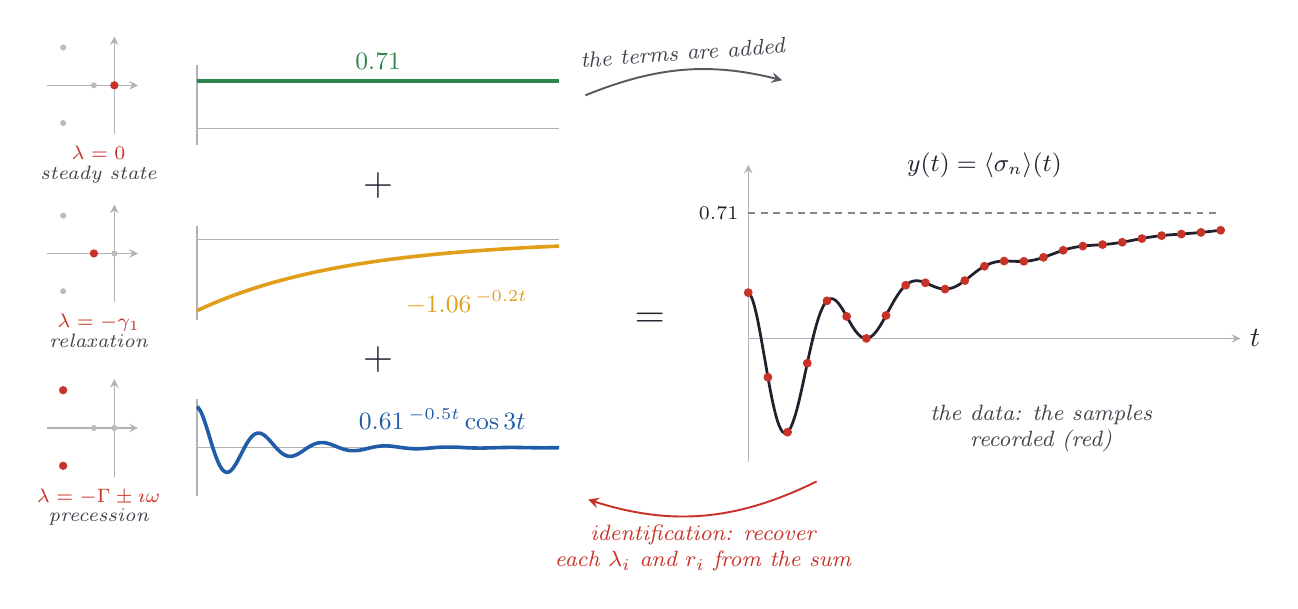
\begin{tikzpicture}[ink/.style={line width=0.9pt, ndInk}, faint/.style={line width=0.4pt, ndInk!35}, dashedink/.style={line width=0.5pt, ndInk!55, dash pattern=on 2.5pt off 2pt}, vec/.style={->, >=stealth, line width=1.2pt}, note/.style={font=\footnotesize\itshape, text=ndInk!85, align=center}, pointer/.style={->, >=stealth, line width=0.4pt, ndInk!60, shorten >=2pt, shorten <=1pt}, dot/.style={circle, fill=ndInk, inner sep=0pt, minimum size=3.4pt}, wash/.style={fill=ndSky, fill opacity=0.55}, every node/.style={text=ndInk}]
\definecolor{ndInk}{rgb}{0.13,0.13,0.18}
\definecolor{ndPaper}{rgb}{0.99,0.96,0.88}
\definecolor{ndSky}{rgb}{0.84,0.91,0.98}
\definecolor{ndRose}{rgb}{0.98,0.86,0.84}
\definecolor{ndBlue}{rgb}{0.13,0.36,0.66}
\definecolor{ndRed}{rgb}{0.78,0.20,0.16}
\definecolor{ndGold}{rgb}{0.88,0.62,0.10}
\definecolor{ndGreen}{rgb}{0.18,0.52,0.30}
\draw[faint] (2.000,5.193) -- (6.600,5.193);
\draw[faint] (2.000,4.980) -- (2.000,6.000);
\draw[line width=1.3pt, ndGreen] (2.000,5.794) -- (2.012,5.794) -- (2.023,5.794) -- (2.035,5.794) -- (2.046,5.794) -- (2.058,5.794) -- (2.069,5.794) -- (2.081,5.794) -- (2.092,5.794) -- (2.104,5.794) -- (2.115,5.794) -- (2.127,5.794) -- (2.138,5.794) -- (2.150,5.794) -- (2.161,5.794) -- (2.173,5.794) -- (2.184,5.794) -- (2.196,5.794) -- (2.208,5.794) -- (2.219,5.794) -- (2.231,5.794) -- (2.242,5.794) -- (2.254,5.794) -- (2.265,5.794) -- (2.277,5.794) -- (2.288,5.794) -- (2.300,5.794) -- (2.311,5.794) -- (2.323,5.794) -- (2.334,5.794) -- (2.346,5.794) -- (2.357,5.794) -- (2.369,5.794) -- (2.380,5.794) -- (2.392,5.794) -- (2.404,5.794) -- (2.415,5.794) -- (2.427,5.794) -- (2.438,5.794) -- (2.450,5.794) -- (2.461,5.794) -- (2.473,5.794) -- (2.484,5.794) -- (2.496,5.794) -- (2.507,5.794) -- (2.519,5.794) -- (2.530,5.794) -- (2.542,5.794) -- (2.553,5.794) -- (2.565,5.794) -- (2.576,5.794) -- (2.588,5.794) -- (2.599,5.794) -- (2.611,5.794) -- (2.623,5.794) -- (2.634,5.794) -- (2.646,5.794) -- (2.657,5.794) -- (2.669,5.794) -- (2.680,5.794) -- (2.692,5.794) -- (2.703,5.794) -- (2.715,5.794) -- (2.726,5.794) -- (2.738,5.794) -- (2.749,5.794) -- (2.761,5.794) -- (2.772,5.794) -- (2.784,5.794) -- (2.795,5.794) -- (2.807,5.794) -- (2.819,5.794) -- (2.830,5.794) -- (2.842,5.794) -- (2.853,5.794) -- (2.865,5.794) -- (2.876,5.794) -- (2.888,5.794) -- (2.899,5.794) -- (2.911,5.794) -- (2.922,5.794) -- (2.934,5.794) -- (2.945,5.794) -- (2.957,5.794) -- (2.968,5.794) -- (2.980,5.794) -- (2.991,5.794) -- (3.003,5.794) -- (3.015,5.794) -- (3.026,5.794) -- (3.038,5.794) -- (3.049,5.794) -- (3.061,5.794) -- (3.072,5.794) -- (3.084,5.794) -- (3.095,5.794) -- (3.107,5.794) -- (3.118,5.794) -- (3.130,5.794) -- (3.141,5.794) -- (3.153,5.794) -- (3.164,5.794) -- (3.176,5.794) -- (3.187,5.794) -- (3.199,5.794) -- (3.211,5.794) -- (3.222,5.794) -- (3.234,5.794) -- (3.245,5.794) -- (3.257,5.794) -- (3.268,5.794) -- (3.280,5.794) -- (3.291,5.794) -- (3.303,5.794) -- (3.314,5.794) -- (3.326,5.794) -- (3.337,5.794) -- (3.349,5.794) -- (3.360,5.794) -- (3.372,5.794) -- (3.383,5.794) -- (3.395,5.794) -- (3.407,5.794) -- (3.418,5.794) -- (3.430,5.794) -- (3.441,5.794) -- (3.453,5.794) -- (3.464,5.794) -- (3.476,5.794) -- (3.487,5.794) -- (3.499,5.794) -- (3.510,5.794) -- (3.522,5.794) -- (3.533,5.794) -- (3.545,5.794) -- (3.556,5.794) -- (3.568,5.794) -- (3.579,5.794) -- (3.591,5.794) -- (3.603,5.794) -- (3.614,5.794) -- (3.626,5.794) -- (3.637,5.794) -- (3.649,5.794) -- (3.660,5.794) -- (3.672,5.794) -- (3.683,5.794) -- (3.695,5.794) -- (3.706,5.794) -- (3.718,5.794) -- (3.729,5.794) -- (3.741,5.794) -- (3.752,5.794) -- (3.764,5.794) -- (3.775,5.794) -- (3.787,5.794) -- (3.798,5.794) -- (3.810,5.794) -- (3.822,5.794) -- (3.833,5.794) -- (3.845,5.794) -- (3.856,5.794) -- (3.868,5.794) -- (3.879,5.794) -- (3.891,5.794) -- (3.902,5.794) -- (3.914,5.794) -- (3.925,5.794) -- (3.937,5.794) -- (3.948,5.794) -- (3.960,5.794) -- (3.971,5.794) -- (3.983,5.794) -- (3.994,5.794) -- (4.006,5.794) -- (4.018,5.794) -- (4.029,5.794) -- (4.041,5.794) -- (4.052,5.794) -- (4.064,5.794) -- (4.075,5.794) -- (4.087,5.794) -- (4.098,5.794) -- (4.110,5.794) -- (4.121,5.794) -- (4.133,5.794) -- (4.144,5.794) -- (4.156,5.794) -- (4.167,5.794) -- (4.179,5.794) -- (4.190,5.794) -- (4.202,5.794) -- (4.214,5.794) -- (4.225,5.794) -- (4.237,5.794) -- (4.248,5.794) -- (4.260,5.794) -- (4.271,5.794) -- (4.283,5.794) -- (4.294,5.794) -- (4.306,5.794) -- (4.317,5.794) -- (4.329,5.794) -- (4.340,5.794) -- (4.352,5.794) -- (4.363,5.794) -- (4.375,5.794) -- (4.386,5.794) -- (4.398,5.794) -- (4.410,5.794) -- (4.421,5.794) -- (4.433,5.794) -- (4.444,5.794) -- (4.456,5.794) -- (4.467,5.794) -- (4.479,5.794) -- (4.490,5.794) -- (4.502,5.794) -- (4.513,5.794) -- (4.525,5.794) -- (4.536,5.794) -- (4.548,5.794) -- (4.559,5.794) -- (4.571,5.794) -- (4.582,5.794) -- (4.594,5.794) -- (4.606,5.794) -- (4.617,5.794) -- (4.629,5.794) -- (4.640,5.794) -- (4.652,5.794) -- (4.663,5.794) -- (4.675,5.794) -- (4.686,5.794) -- (4.698,5.794) -- (4.709,5.794) -- (4.721,5.794) -- (4.732,5.794) -- (4.744,5.794) -- (4.755,5.794) -- (4.767,5.794) -- (4.778,5.794) -- (4.790,5.794) -- (4.802,5.794) -- (4.813,5.794) -- (4.825,5.794) -- (4.836,5.794) -- (4.848,5.794) -- (4.859,5.794) -- (4.871,5.794) -- (4.882,5.794) -- (4.894,5.794) -- (4.905,5.794) -- (4.917,5.794) -- (4.928,5.794) -- (4.940,5.794) -- (4.951,5.794) -- (4.963,5.794) -- (4.974,5.794) -- (4.986,5.794) -- (4.997,5.794) -- (5.009,5.794) -- (5.021,5.794) -- (5.032,5.794) -- (5.044,5.794) -- (5.055,5.794) -- (5.067,5.794) -- (5.078,5.794) -- (5.090,5.794) -- (5.101,5.794) -- (5.113,5.794) -- (5.124,5.794) -- (5.136,5.794) -- (5.147,5.794) -- (5.159,5.794) -- (5.170,5.794) -- (5.182,5.794) -- (5.193,5.794) -- (5.205,5.794) -- (5.217,5.794) -- (5.228,5.794) -- (5.240,5.794) -- (5.251,5.794) -- (5.263,5.794) -- (5.274,5.794) -- (5.286,5.794) -- (5.297,5.794) -- (5.309,5.794) -- (5.320,5.794) -- (5.332,5.794) -- (5.343,5.794) -- (5.355,5.794) -- (5.366,5.794) -- (5.378,5.794) -- (5.389,5.794) -- (5.401,5.794) -- (5.413,5.794) -- (5.424,5.794) -- (5.436,5.794) -- (5.447,5.794) -- (5.459,5.794) -- (5.470,5.794) -- (5.482,5.794) -- (5.493,5.794) -- (5.505,5.794) -- (5.516,5.794) -- (5.528,5.794) -- (5.539,5.794) -- (5.551,5.794) -- (5.562,5.794) -- (5.574,5.794) -- (5.585,5.794) -- (5.597,5.794) -- (5.609,5.794) -- (5.620,5.794) -- (5.632,5.794) -- (5.643,5.794) -- (5.655,5.794) -- (5.666,5.794) -- (5.678,5.794) -- (5.689,5.794) -- (5.701,5.794) -- (5.712,5.794) -- (5.724,5.794) -- (5.735,5.794) -- (5.747,5.794) -- (5.758,5.794) -- (5.770,5.794) -- (5.781,5.794) -- (5.793,5.794) -- (5.805,5.794) -- (5.816,5.794) -- (5.828,5.794) -- (5.839,5.794) -- (5.851,5.794) -- (5.862,5.794) -- (5.874,5.794) -- (5.885,5.794) -- (5.897,5.794) -- (5.908,5.794) -- (5.920,5.794) -- (5.931,5.794) -- (5.943,5.794) -- (5.954,5.794) -- (5.966,5.794) -- (5.977,5.794) -- (5.989,5.794) -- (6.001,5.794) -- (6.012,5.794) -- (6.024,5.794) -- (6.035,5.794) -- (6.047,5.794) -- (6.058,5.794) -- (6.070,5.794) -- (6.081,5.794) -- (6.093,5.794) -- (6.104,5.794) -- (6.116,5.794) -- (6.127,5.794) -- (6.139,5.794) -- (6.150,5.794) -- (6.162,5.794) -- (6.173,5.794) -- (6.185,5.794) -- (6.196,5.794) -- (6.208,5.794) -- (6.220,5.794) -- (6.231,5.794) -- (6.243,5.794) -- (6.254,5.794) -- (6.266,5.794) -- (6.277,5.794) -- (6.289,5.794) -- (6.300,5.794) -- (6.312,5.794) -- (6.323,5.794) -- (6.335,5.794) -- (6.346,5.794) -- (6.358,5.794) -- (6.369,5.794) -- (6.381,5.794) -- (6.392,5.794) -- (6.404,5.794) -- (6.416,5.794) -- (6.427,5.794) -- (6.439,5.794) -- (6.450,5.794) -- (6.462,5.794) -- (6.473,5.794) -- (6.485,5.794) -- (6.496,5.794) -- (6.508,5.794) -- (6.519,5.794) -- (6.531,5.794) -- (6.542,5.794) -- (6.554,5.794) -- (6.565,5.794) -- (6.577,5.794) -- (6.588,5.794) -- (6.600,5.794);
\draw[faint, ->, >=stealth] (0.100,5.740) -- (1.250,5.740);
\draw[faint, ->, >=stealth] (0.950,5.120) -- (0.950,6.360);
\fill[ndRed] (0.950,5.740) circle (1.5pt);
\fill[ndInk!30] (0.690,5.740) circle (1.1pt);
\fill[ndInk!30] (0.300,6.220) circle (1.1pt);
\fill[ndInk!30] (0.300,5.260) circle (1.1pt);
\node[font=\scriptsize, text=ndRed, anchor=north, align=center] at (0.75,5.090) {$\lambda=0$\\[-1pt] \textit{\color{ndInk!85}steady state}};
\draw[faint] (2.000,3.780) -- (6.600,3.780);
\draw[faint] (2.000,2.760) -- (2.000,3.950);
\draw[line width=1.3pt, ndGold] (2.000,2.878) -- (2.012,2.884) -- (2.023,2.889) -- (2.035,2.895) -- (2.046,2.900) -- (2.058,2.905) -- (2.069,2.910) -- (2.081,2.916) -- (2.092,2.921) -- (2.104,2.926) -- (2.115,2.931) -- (2.127,2.936) -- (2.138,2.941) -- (2.150,2.946) -- (2.161,2.951) -- (2.173,2.956) -- (2.184,2.961) -- (2.196,2.966) -- (2.208,2.971) -- (2.219,2.976) -- (2.231,2.981) -- (2.242,2.985) -- (2.254,2.990) -- (2.265,2.995) -- (2.277,3.000) -- (2.288,3.004) -- (2.300,3.009) -- (2.311,3.014) -- (2.323,3.018) -- (2.334,3.023) -- (2.346,3.027) -- (2.357,3.032) -- (2.369,3.036) -- (2.380,3.041) -- (2.392,3.045) -- (2.404,3.050) -- (2.415,3.054) -- (2.427,3.058) -- (2.438,3.063) -- (2.450,3.067) -- (2.461,3.071) -- (2.473,3.075) -- (2.484,3.080) -- (2.496,3.084) -- (2.507,3.088) -- (2.519,3.092) -- (2.530,3.096) -- (2.542,3.100) -- (2.553,3.105) -- (2.565,3.109) -- (2.576,3.113) -- (2.588,3.117) -- (2.599,3.121) -- (2.611,3.125) -- (2.623,3.128) -- (2.634,3.132) -- (2.646,3.136) -- (2.657,3.140) -- (2.669,3.144) -- (2.680,3.148) -- (2.692,3.152) -- (2.703,3.155) -- (2.715,3.159) -- (2.726,3.163) -- (2.738,3.167) -- (2.749,3.170) -- (2.761,3.174) -- (2.772,3.177) -- (2.784,3.181) -- (2.795,3.185) -- (2.807,3.188) -- (2.819,3.192) -- (2.830,3.195) -- (2.842,3.199) -- (2.853,3.202) -- (2.865,3.206) -- (2.876,3.209) -- (2.888,3.213) -- (2.899,3.216) -- (2.911,3.219) -- (2.922,3.223) -- (2.934,3.226) -- (2.945,3.229) -- (2.957,3.233) -- (2.968,3.236) -- (2.980,3.239) -- (2.991,3.243) -- (3.003,3.246) -- (3.015,3.249) -- (3.026,3.252) -- (3.038,3.255) -- (3.049,3.258) -- (3.061,3.262) -- (3.072,3.265) -- (3.084,3.268) -- (3.095,3.271) -- (3.107,3.274) -- (3.118,3.277) -- (3.130,3.280) -- (3.141,3.283) -- (3.153,3.286) -- (3.164,3.289) -- (3.176,3.292) -- (3.187,3.295) -- (3.199,3.298) -- (3.211,3.301) -- (3.222,3.303) -- (3.234,3.306) -- (3.245,3.309) -- (3.257,3.312) -- (3.268,3.315) -- (3.280,3.318) -- (3.291,3.320) -- (3.303,3.323) -- (3.314,3.326) -- (3.326,3.329) -- (3.337,3.331) -- (3.349,3.334) -- (3.360,3.337) -- (3.372,3.339) -- (3.383,3.342) -- (3.395,3.345) -- (3.407,3.347) -- (3.418,3.350) -- (3.430,3.352) -- (3.441,3.355) -- (3.453,3.357) -- (3.464,3.360) -- (3.476,3.363) -- (3.487,3.365) -- (3.499,3.368) -- (3.510,3.370) -- (3.522,3.372) -- (3.533,3.375) -- (3.545,3.377) -- (3.556,3.380) -- (3.568,3.382) -- (3.579,3.385) -- (3.591,3.387) -- (3.603,3.389) -- (3.614,3.392) -- (3.626,3.394) -- (3.637,3.396) -- (3.649,3.399) -- (3.660,3.401) -- (3.672,3.403) -- (3.683,3.405) -- (3.695,3.408) -- (3.706,3.410) -- (3.718,3.412) -- (3.729,3.414) -- (3.741,3.416) -- (3.752,3.419) -- (3.764,3.421) -- (3.775,3.423) -- (3.787,3.425) -- (3.798,3.427) -- (3.810,3.429) -- (3.822,3.431) -- (3.833,3.434) -- (3.845,3.436) -- (3.856,3.438) -- (3.868,3.440) -- (3.879,3.442) -- (3.891,3.444) -- (3.902,3.446) -- (3.914,3.448) -- (3.925,3.450) -- (3.937,3.452) -- (3.948,3.454) -- (3.960,3.456) -- (3.971,3.458) -- (3.983,3.460) -- (3.994,3.462) -- (4.006,3.463) -- (4.018,3.465) -- (4.029,3.467) -- (4.041,3.469) -- (4.052,3.471) -- (4.064,3.473) -- (4.075,3.475) -- (4.087,3.476) -- (4.098,3.478) -- (4.110,3.480) -- (4.121,3.482) -- (4.133,3.484) -- (4.144,3.485) -- (4.156,3.487) -- (4.167,3.489) -- (4.179,3.491) -- (4.190,3.492) -- (4.202,3.494) -- (4.214,3.496) -- (4.225,3.498) -- (4.237,3.499) -- (4.248,3.501) -- (4.260,3.503) -- (4.271,3.504) -- (4.283,3.506) -- (4.294,3.508) -- (4.306,3.509) -- (4.317,3.511) -- (4.329,3.513) -- (4.340,3.514) -- (4.352,3.516) -- (4.363,3.517) -- (4.375,3.519) -- (4.386,3.520) -- (4.398,3.522) -- (4.410,3.524) -- (4.421,3.525) -- (4.433,3.527) -- (4.444,3.528) -- (4.456,3.530) -- (4.467,3.531) -- (4.479,3.533) -- (4.490,3.534) -- (4.502,3.536) -- (4.513,3.537) -- (4.525,3.539) -- (4.536,3.540) -- (4.548,3.541) -- (4.559,3.543) -- (4.571,3.544) -- (4.582,3.546) -- (4.594,3.547) -- (4.606,3.548) -- (4.617,3.550) -- (4.629,3.551) -- (4.640,3.553) -- (4.652,3.554) -- (4.663,3.555) -- (4.675,3.557) -- (4.686,3.558) -- (4.698,3.559) -- (4.709,3.561) -- (4.721,3.562) -- (4.732,3.563) -- (4.744,3.565) -- (4.755,3.566) -- (4.767,3.567) -- (4.778,3.568) -- (4.790,3.570) -- (4.802,3.571) -- (4.813,3.572) -- (4.825,3.573) -- (4.836,3.575) -- (4.848,3.576) -- (4.859,3.577) -- (4.871,3.578) -- (4.882,3.580) -- (4.894,3.581) -- (4.905,3.582) -- (4.917,3.583) -- (4.928,3.584) -- (4.940,3.586) -- (4.951,3.587) -- (4.963,3.588) -- (4.974,3.589) -- (4.986,3.590) -- (4.997,3.591) -- (5.009,3.592) -- (5.021,3.594) -- (5.032,3.595) -- (5.044,3.596) -- (5.055,3.597) -- (5.067,3.598) -- (5.078,3.599) -- (5.090,3.600) -- (5.101,3.601) -- (5.113,3.602) -- (5.124,3.603) -- (5.136,3.604) -- (5.147,3.605) -- (5.159,3.607) -- (5.170,3.608) -- (5.182,3.609) -- (5.193,3.610) -- (5.205,3.611) -- (5.217,3.612) -- (5.228,3.613) -- (5.240,3.614) -- (5.251,3.615) -- (5.263,3.616) -- (5.274,3.617) -- (5.286,3.618) -- (5.297,3.619) -- (5.309,3.620) -- (5.320,3.621) -- (5.332,3.621) -- (5.343,3.622) -- (5.355,3.623) -- (5.366,3.624) -- (5.378,3.625) -- (5.389,3.626) -- (5.401,3.627) -- (5.413,3.628) -- (5.424,3.629) -- (5.436,3.630) -- (5.447,3.631) -- (5.459,3.632) -- (5.470,3.633) -- (5.482,3.633) -- (5.493,3.634) -- (5.505,3.635) -- (5.516,3.636) -- (5.528,3.637) -- (5.539,3.638) -- (5.551,3.639) -- (5.562,3.639) -- (5.574,3.640) -- (5.585,3.641) -- (5.597,3.642) -- (5.609,3.643) -- (5.620,3.644) -- (5.632,3.644) -- (5.643,3.645) -- (5.655,3.646) -- (5.666,3.647) -- (5.678,3.648) -- (5.689,3.648) -- (5.701,3.649) -- (5.712,3.650) -- (5.724,3.651) -- (5.735,3.652) -- (5.747,3.652) -- (5.758,3.653) -- (5.770,3.654) -- (5.781,3.655) -- (5.793,3.655) -- (5.805,3.656) -- (5.816,3.657) -- (5.828,3.658) -- (5.839,3.658) -- (5.851,3.659) -- (5.862,3.660) -- (5.874,3.661) -- (5.885,3.661) -- (5.897,3.662) -- (5.908,3.663) -- (5.920,3.663) -- (5.931,3.664) -- (5.943,3.665) -- (5.954,3.665) -- (5.966,3.666) -- (5.977,3.667) -- (5.989,3.668) -- (6.001,3.668) -- (6.012,3.669) -- (6.024,3.670) -- (6.035,3.670) -- (6.047,3.671) -- (6.058,3.671) -- (6.070,3.672) -- (6.081,3.673) -- (6.093,3.673) -- (6.104,3.674) -- (6.116,3.675) -- (6.127,3.675) -- (6.139,3.676) -- (6.150,3.677) -- (6.162,3.677) -- (6.173,3.678) -- (6.185,3.678) -- (6.196,3.679) -- (6.208,3.680) -- (6.220,3.680) -- (6.231,3.681) -- (6.243,3.681) -- (6.254,3.682) -- (6.266,3.683) -- (6.277,3.683) -- (6.289,3.684) -- (6.300,3.684) -- (6.312,3.685) -- (6.323,3.686) -- (6.335,3.686) -- (6.346,3.687) -- (6.358,3.687) -- (6.369,3.688) -- (6.381,3.688) -- (6.392,3.689) -- (6.404,3.689) -- (6.416,3.690) -- (6.427,3.690) -- (6.439,3.691) -- (6.450,3.692) -- (6.462,3.692) -- (6.473,3.693) -- (6.485,3.693) -- (6.496,3.694) -- (6.508,3.694) -- (6.519,3.695) -- (6.531,3.695) -- (6.542,3.696) -- (6.554,3.696) -- (6.565,3.697) -- (6.577,3.697) -- (6.588,3.698) -- (6.600,3.698);
\draw[faint, ->, >=stealth] (0.100,3.605) -- (1.250,3.605);
\draw[faint, ->, >=stealth] (0.950,2.985) -- (0.950,4.225);
\fill[ndInk!30] (0.950,3.605) circle (1.1pt);
\fill[ndRed] (0.690,3.605) circle (1.5pt);
\fill[ndInk!30] (0.300,4.085) circle (1.1pt);
\fill[ndInk!30] (0.300,3.125) circle (1.1pt);
\node[font=\scriptsize, text=ndRed, anchor=north, align=center] at (0.75,2.955) {$\lambda=-\gamma_1$\\[-1pt] \textit{\color{ndInk!85}relaxation}};
\draw[faint] (2.000,1.138) -- (6.600,1.138);
\draw[faint] (2.000,0.526) -- (2.000,1.750);
\draw[line width=1.3pt, ndBlue] (2.000,1.659) -- (2.012,1.649) -- (2.023,1.635) -- (2.035,1.617) -- (2.046,1.597) -- (2.058,1.573) -- (2.069,1.546) -- (2.081,1.516) -- (2.092,1.484) -- (2.104,1.451) -- (2.115,1.416) -- (2.127,1.379) -- (2.138,1.342) -- (2.150,1.304) -- (2.161,1.266) -- (2.173,1.228) -- (2.184,1.190) -- (2.196,1.153) -- (2.208,1.117) -- (2.219,1.082) -- (2.231,1.049) -- (2.242,1.017) -- (2.254,0.988) -- (2.265,0.960) -- (2.277,0.935) -- (2.288,0.912) -- (2.300,0.892) -- (2.311,0.874) -- (2.323,0.859) -- (2.334,0.847) -- (2.346,0.837) -- (2.357,0.831) -- (2.369,0.827) -- (2.380,0.825) -- (2.392,0.827) -- (2.404,0.831) -- (2.415,0.837) -- (2.427,0.845) -- (2.438,0.856) -- (2.450,0.869) -- (2.461,0.883) -- (2.473,0.900) -- (2.484,0.917) -- (2.496,0.936) -- (2.507,0.956) -- (2.519,0.977) -- (2.530,0.999) -- (2.542,1.021) -- (2.553,1.044) -- (2.565,1.066) -- (2.576,1.089) -- (2.588,1.111) -- (2.599,1.133) -- (2.611,1.154) -- (2.623,1.175) -- (2.634,1.194) -- (2.646,1.213) -- (2.657,1.230) -- (2.669,1.246) -- (2.680,1.261) -- (2.692,1.274) -- (2.703,1.286) -- (2.715,1.296) -- (2.726,1.305) -- (2.738,1.312) -- (2.749,1.317) -- (2.761,1.321) -- (2.772,1.323) -- (2.784,1.323) -- (2.795,1.322) -- (2.807,1.320) -- (2.819,1.316) -- (2.830,1.310) -- (2.842,1.304) -- (2.853,1.296) -- (2.865,1.287) -- (2.876,1.277) -- (2.888,1.267) -- (2.899,1.255) -- (2.911,1.243) -- (2.922,1.231) -- (2.934,1.218) -- (2.945,1.205) -- (2.957,1.191) -- (2.968,1.178) -- (2.980,1.165) -- (2.991,1.151) -- (3.003,1.139) -- (3.015,1.126) -- (3.026,1.114) -- (3.038,1.103) -- (3.049,1.092) -- (3.061,1.082) -- (3.072,1.072) -- (3.084,1.064) -- (3.095,1.056) -- (3.107,1.049) -- (3.118,1.043) -- (3.130,1.038) -- (3.141,1.034) -- (3.153,1.032) -- (3.164,1.030) -- (3.176,1.028) -- (3.187,1.028) -- (3.199,1.029) -- (3.211,1.031) -- (3.222,1.033) -- (3.234,1.037) -- (3.245,1.041) -- (3.257,1.045) -- (3.268,1.051) -- (3.280,1.057) -- (3.291,1.063) -- (3.303,1.070) -- (3.314,1.077) -- (3.326,1.084) -- (3.337,1.092) -- (3.349,1.100) -- (3.360,1.108) -- (3.372,1.116) -- (3.383,1.124) -- (3.395,1.131) -- (3.407,1.139) -- (3.418,1.146) -- (3.430,1.153) -- (3.441,1.160) -- (3.453,1.167) -- (3.464,1.172) -- (3.476,1.178) -- (3.487,1.183) -- (3.499,1.187) -- (3.510,1.191) -- (3.522,1.195) -- (3.533,1.197) -- (3.545,1.200) -- (3.556,1.201) -- (3.568,1.202) -- (3.579,1.203) -- (3.591,1.203) -- (3.603,1.202) -- (3.614,1.201) -- (3.626,1.200) -- (3.637,1.198) -- (3.649,1.195) -- (3.660,1.192) -- (3.672,1.189) -- (3.683,1.186) -- (3.695,1.182) -- (3.706,1.178) -- (3.718,1.173) -- (3.729,1.169) -- (3.741,1.164) -- (3.752,1.160) -- (3.764,1.155) -- (3.775,1.150) -- (3.787,1.146) -- (3.798,1.141) -- (3.810,1.137) -- (3.822,1.132) -- (3.833,1.128) -- (3.845,1.124) -- (3.856,1.120) -- (3.868,1.117) -- (3.879,1.114) -- (3.891,1.111) -- (3.902,1.108) -- (3.914,1.106) -- (3.925,1.104) -- (3.937,1.103) -- (3.948,1.101) -- (3.960,1.100) -- (3.971,1.100) -- (3.983,1.100) -- (3.994,1.100) -- (4.006,1.100) -- (4.018,1.101) -- (4.029,1.102) -- (4.041,1.103) -- (4.052,1.104) -- (4.064,1.106) -- (4.075,1.108) -- (4.087,1.110) -- (4.098,1.112) -- (4.110,1.115) -- (4.121,1.117) -- (4.133,1.120) -- (4.144,1.123) -- (4.156,1.126) -- (4.167,1.128) -- (4.179,1.131) -- (4.190,1.134) -- (4.202,1.137) -- (4.214,1.139) -- (4.225,1.142) -- (4.237,1.144) -- (4.248,1.147) -- (4.260,1.149) -- (4.271,1.151) -- (4.283,1.153) -- (4.294,1.154) -- (4.306,1.156) -- (4.317,1.157) -- (4.329,1.158) -- (4.340,1.159) -- (4.352,1.160) -- (4.363,1.160) -- (4.375,1.161) -- (4.386,1.161) -- (4.398,1.161) -- (4.410,1.160) -- (4.421,1.160) -- (4.433,1.159) -- (4.444,1.159) -- (4.456,1.158) -- (4.467,1.157) -- (4.479,1.156) -- (4.490,1.154) -- (4.502,1.153) -- (4.513,1.151) -- (4.525,1.150) -- (4.536,1.148) -- (4.548,1.147) -- (4.559,1.145) -- (4.571,1.143) -- (4.582,1.142) -- (4.594,1.140) -- (4.606,1.139) -- (4.617,1.137) -- (4.629,1.135) -- (4.640,1.134) -- (4.652,1.133) -- (4.663,1.131) -- (4.675,1.130) -- (4.686,1.129) -- (4.698,1.128) -- (4.709,1.127) -- (4.721,1.127) -- (4.732,1.126) -- (4.744,1.125) -- (4.755,1.125) -- (4.767,1.125) -- (4.778,1.125) -- (4.790,1.124) -- (4.802,1.125) -- (4.813,1.125) -- (4.825,1.125) -- (4.836,1.125) -- (4.848,1.126) -- (4.859,1.126) -- (4.871,1.127) -- (4.882,1.128) -- (4.894,1.129) -- (4.905,1.129) -- (4.917,1.130) -- (4.928,1.131) -- (4.940,1.132) -- (4.951,1.133) -- (4.963,1.134) -- (4.974,1.135) -- (4.986,1.136) -- (4.997,1.137) -- (5.009,1.138) -- (5.021,1.139) -- (5.032,1.140) -- (5.044,1.141) -- (5.055,1.141) -- (5.067,1.142) -- (5.078,1.143) -- (5.090,1.143) -- (5.101,1.144) -- (5.113,1.144) -- (5.124,1.145) -- (5.136,1.145) -- (5.147,1.146) -- (5.159,1.146) -- (5.170,1.146) -- (5.182,1.146) -- (5.193,1.146) -- (5.205,1.146) -- (5.217,1.146) -- (5.228,1.146) -- (5.240,1.145) -- (5.251,1.145) -- (5.263,1.145) -- (5.274,1.144) -- (5.286,1.144) -- (5.297,1.144) -- (5.309,1.143) -- (5.320,1.143) -- (5.332,1.142) -- (5.343,1.141) -- (5.355,1.141) -- (5.366,1.140) -- (5.378,1.140) -- (5.389,1.139) -- (5.401,1.139) -- (5.413,1.138) -- (5.424,1.137) -- (5.436,1.137) -- (5.447,1.136) -- (5.459,1.136) -- (5.470,1.136) -- (5.482,1.135) -- (5.493,1.135) -- (5.505,1.134) -- (5.516,1.134) -- (5.528,1.134) -- (5.539,1.134) -- (5.551,1.134) -- (5.562,1.133) -- (5.574,1.133) -- (5.585,1.133) -- (5.597,1.133) -- (5.609,1.133) -- (5.620,1.133) -- (5.632,1.133) -- (5.643,1.134) -- (5.655,1.134) -- (5.666,1.134) -- (5.678,1.134) -- (5.689,1.135) -- (5.701,1.135) -- (5.712,1.135) -- (5.724,1.135) -- (5.735,1.136) -- (5.747,1.136) -- (5.758,1.136) -- (5.770,1.137) -- (5.781,1.137) -- (5.793,1.137) -- (5.805,1.138) -- (5.816,1.138) -- (5.828,1.138) -- (5.839,1.139) -- (5.851,1.139) -- (5.862,1.139) -- (5.874,1.140) -- (5.885,1.140) -- (5.897,1.140) -- (5.908,1.140) -- (5.920,1.140) -- (5.931,1.140) -- (5.943,1.141) -- (5.954,1.141) -- (5.966,1.141) -- (5.977,1.141) -- (5.989,1.141) -- (6.001,1.141) -- (6.012,1.141) -- (6.024,1.141) -- (6.035,1.141) -- (6.047,1.141) -- (6.058,1.140) -- (6.070,1.140) -- (6.081,1.140) -- (6.093,1.140) -- (6.104,1.140) -- (6.116,1.140) -- (6.127,1.140) -- (6.139,1.139) -- (6.150,1.139) -- (6.162,1.139) -- (6.173,1.139) -- (6.185,1.139) -- (6.196,1.138) -- (6.208,1.138) -- (6.220,1.138) -- (6.231,1.138) -- (6.243,1.138) -- (6.254,1.137) -- (6.266,1.137) -- (6.277,1.137) -- (6.289,1.137) -- (6.300,1.137) -- (6.312,1.137) -- (6.323,1.137) -- (6.335,1.137) -- (6.346,1.136) -- (6.358,1.136) -- (6.369,1.136) -- (6.381,1.136) -- (6.392,1.136) -- (6.404,1.136) -- (6.416,1.136) -- (6.427,1.136) -- (6.439,1.136) -- (6.450,1.136) -- (6.462,1.137) -- (6.473,1.137) -- (6.485,1.137) -- (6.496,1.137) -- (6.508,1.137) -- (6.519,1.137) -- (6.531,1.137) -- (6.542,1.137) -- (6.554,1.137) -- (6.565,1.137) -- (6.577,1.138) -- (6.588,1.138) -- (6.600,1.138);
\draw[faint, ->, >=stealth] (0.100,1.388) -- (1.250,1.388);
\draw[faint, ->, >=stealth] (0.950,0.768) -- (0.950,2.008);
\fill[ndInk!30] (0.950,1.388) circle (1.1pt);
\fill[ndInk!30] (0.690,1.388) circle (1.1pt);
\fill[ndRed] (0.300,1.868) circle (1.5pt);
\fill[ndRed] (0.300,0.908) circle (1.5pt);
\node[font=\scriptsize, text=ndRed, anchor=north, align=center] at (0.75,0.738) {$\lambda=-\Gamma\pm\imath\omega$\\[-1pt] \textit{\color{ndInk!85}precession}};
\node[font=\small, text=ndGreen, anchor=south] at (4.300,5.811) {$0.71$};
\node[font=\small, text=ndGold, anchor=north west] at (4.530,3.253) {$-1.06\,\ee^{-0.2t}$};
\node[font=\small, text=ndBlue, anchor=south west] at (3.932,1.240) {$0.61\,\ee^{-0.5t}\cos 3t$};
\node[font=\Large] at (4.300,4.465) {$+$};
\node[font=\Large] at (4.300,2.255) {$+$};
\draw[faint] (9.000,2.525) -- (15.000,2.525);
\draw[faint, ->, >=stealth] (9.000,2.525) -- (15.250,2.525) node[right, text=ndInk] {$t$};
\draw[faint, ->, >=stealth] (9.000,0.950) -- (9.000,4.730);
\draw[dashedink] (9.000,4.116) -- (15.000,4.116);
\node[font=\scriptsize, anchor=east] at (9.000,4.116) {$0.71$};
\draw[line width=1.0pt, ndInk] (9.000,3.107) -- (9.015,3.096) -- (9.030,3.073) -- (9.045,3.041) -- (9.060,3.000) -- (9.075,2.950) -- (9.090,2.893) -- (9.105,2.829) -- (9.120,2.759) -- (9.135,2.683) -- (9.150,2.604) -- (9.165,2.521) -- (9.180,2.435) -- (9.195,2.348) -- (9.211,2.260) -- (9.226,2.173) -- (9.241,2.086) -- (9.256,2.001) -- (9.271,1.918) -- (9.286,1.839) -- (9.301,1.764) -- (9.316,1.693) -- (9.331,1.627) -- (9.346,1.567) -- (9.361,1.512) -- (9.376,1.464) -- (9.391,1.423) -- (9.406,1.388) -- (9.421,1.361) -- (9.436,1.341) -- (9.451,1.328) -- (9.466,1.322) -- (9.481,1.323) -- (9.496,1.332) -- (9.511,1.347) -- (9.526,1.369) -- (9.541,1.397) -- (9.556,1.431) -- (9.571,1.471) -- (9.586,1.516) -- (9.602,1.566) -- (9.617,1.620) -- (9.632,1.678) -- (9.647,1.739) -- (9.662,1.804) -- (9.677,1.870) -- (9.692,1.939) -- (9.707,2.008) -- (9.722,2.079) -- (9.737,2.149) -- (9.752,2.220) -- (9.767,2.289) -- (9.782,2.357) -- (9.797,2.424) -- (9.812,2.489) -- (9.827,2.551) -- (9.842,2.610) -- (9.857,2.666) -- (9.872,2.719) -- (9.887,2.768) -- (9.902,2.813) -- (9.917,2.854) -- (9.932,2.891) -- (9.947,2.924) -- (9.962,2.952) -- (9.977,2.975) -- (9.992,2.995) -- (10.008,3.010) -- (10.023,3.021) -- (10.038,3.028) -- (10.053,3.030) -- (10.068,3.029) -- (10.083,3.024) -- (10.098,3.016) -- (10.113,3.005) -- (10.128,2.991) -- (10.143,2.974) -- (10.158,2.955) -- (10.173,2.934) -- (10.188,2.911) -- (10.203,2.887) -- (10.218,2.861) -- (10.233,2.835) -- (10.248,2.809) -- (10.263,2.782) -- (10.278,2.755) -- (10.293,2.729) -- (10.308,2.703) -- (10.323,2.679) -- (10.338,2.655) -- (10.353,2.633) -- (10.368,2.613) -- (10.383,2.595) -- (10.398,2.578) -- (10.414,2.563) -- (10.429,2.551) -- (10.444,2.541) -- (10.459,2.534) -- (10.474,2.529) -- (10.489,2.526) -- (10.504,2.526) -- (10.519,2.529) -- (10.534,2.534) -- (10.549,2.541) -- (10.564,2.551) -- (10.579,2.563) -- (10.594,2.577) -- (10.609,2.594) -- (10.624,2.612) -- (10.639,2.632) -- (10.654,2.653) -- (10.669,2.676) -- (10.684,2.701) -- (10.699,2.726) -- (10.714,2.752) -- (10.729,2.779) -- (10.744,2.807) -- (10.759,2.834) -- (10.774,2.863) -- (10.789,2.891) -- (10.805,2.918) -- (10.820,2.946) -- (10.835,2.973) -- (10.850,2.999) -- (10.865,3.025) -- (10.880,3.049) -- (10.895,3.073) -- (10.910,3.095) -- (10.925,3.117) -- (10.940,3.136) -- (10.955,3.155) -- (10.970,3.172) -- (10.985,3.187) -- (11.000,3.201) -- (11.015,3.213) -- (11.030,3.224) -- (11.045,3.233) -- (11.060,3.241) -- (11.075,3.247) -- (11.090,3.252) -- (11.105,3.255) -- (11.120,3.257) -- (11.135,3.258) -- (11.150,3.258) -- (11.165,3.256) -- (11.180,3.254) -- (11.195,3.250) -- (11.211,3.246) -- (11.226,3.241) -- (11.241,3.236) -- (11.256,3.230) -- (11.271,3.224) -- (11.286,3.217) -- (11.301,3.210) -- (11.316,3.204) -- (11.331,3.197) -- (11.346,3.190) -- (11.361,3.184) -- (11.376,3.178) -- (11.391,3.173) -- (11.406,3.168) -- (11.421,3.163) -- (11.436,3.160) -- (11.451,3.157) -- (11.466,3.154) -- (11.481,3.153) -- (11.496,3.152) -- (11.511,3.152) -- (11.526,3.153) -- (11.541,3.155) -- (11.556,3.158) -- (11.571,3.162) -- (11.586,3.166) -- (11.602,3.171) -- (11.617,3.177) -- (11.632,3.184) -- (11.647,3.192) -- (11.662,3.200) -- (11.677,3.209) -- (11.692,3.218) -- (11.707,3.229) -- (11.722,3.239) -- (11.737,3.250) -- (11.752,3.261) -- (11.767,3.273) -- (11.782,3.284) -- (11.797,3.296) -- (11.812,3.308) -- (11.827,3.320) -- (11.842,3.332) -- (11.857,3.344) -- (11.872,3.356) -- (11.887,3.367) -- (11.902,3.379) -- (11.917,3.390) -- (11.932,3.400) -- (11.947,3.410) -- (11.962,3.420) -- (11.977,3.429) -- (11.992,3.438) -- (12.008,3.447) -- (12.023,3.454) -- (12.038,3.462) -- (12.053,3.468) -- (12.068,3.474) -- (12.083,3.480) -- (12.098,3.485) -- (12.113,3.489) -- (12.128,3.493) -- (12.143,3.497) -- (12.158,3.499) -- (12.173,3.502) -- (12.188,3.504) -- (12.203,3.505) -- (12.218,3.507) -- (12.233,3.508) -- (12.248,3.508) -- (12.263,3.508) -- (12.278,3.508) -- (12.293,3.508) -- (12.308,3.508) -- (12.323,3.507) -- (12.338,3.507) -- (12.353,3.506) -- (12.368,3.506) -- (12.383,3.505) -- (12.398,3.504) -- (12.414,3.504) -- (12.429,3.504) -- (12.444,3.504) -- (12.459,3.504) -- (12.474,3.504) -- (12.489,3.504) -- (12.504,3.505) -- (12.519,3.506) -- (12.534,3.507) -- (12.549,3.509) -- (12.564,3.510) -- (12.579,3.512) -- (12.594,3.515) -- (12.609,3.517) -- (12.624,3.520) -- (12.639,3.524) -- (12.654,3.527) -- (12.669,3.531) -- (12.684,3.535) -- (12.699,3.539) -- (12.714,3.544) -- (12.729,3.548) -- (12.744,3.553) -- (12.759,3.558) -- (12.774,3.564) -- (12.789,3.569) -- (12.805,3.574) -- (12.820,3.580) -- (12.835,3.586) -- (12.850,3.591) -- (12.865,3.597) -- (12.880,3.602) -- (12.895,3.608) -- (12.910,3.614) -- (12.925,3.619) -- (12.940,3.624) -- (12.955,3.630) -- (12.970,3.635) -- (12.985,3.640) -- (13.000,3.645) -- (13.015,3.650) -- (13.030,3.654) -- (13.045,3.658) -- (13.060,3.663) -- (13.075,3.667) -- (13.090,3.670) -- (13.105,3.674) -- (13.120,3.677) -- (13.135,3.680) -- (13.150,3.683) -- (13.165,3.686) -- (13.180,3.689) -- (13.195,3.691) -- (13.211,3.693) -- (13.226,3.695) -- (13.241,3.697) -- (13.256,3.699) -- (13.271,3.701) -- (13.286,3.702) -- (13.301,3.703) -- (13.316,3.705) -- (13.331,3.706) -- (13.346,3.707) -- (13.361,3.708) -- (13.376,3.709) -- (13.391,3.710) -- (13.406,3.711) -- (13.421,3.712) -- (13.436,3.713) -- (13.451,3.714) -- (13.466,3.715) -- (13.481,3.716) -- (13.496,3.717) -- (13.511,3.718) -- (13.526,3.719) -- (13.541,3.720) -- (13.556,3.722) -- (13.571,3.723) -- (13.586,3.725) -- (13.602,3.726) -- (13.617,3.728) -- (13.632,3.730) -- (13.647,3.732) -- (13.662,3.734) -- (13.677,3.736) -- (13.692,3.738) -- (13.707,3.740) -- (13.722,3.743) -- (13.737,3.745) -- (13.752,3.748) -- (13.767,3.750) -- (13.782,3.753) -- (13.797,3.756) -- (13.812,3.759) -- (13.827,3.761) -- (13.842,3.764) -- (13.857,3.767) -- (13.872,3.770) -- (13.887,3.773) -- (13.902,3.776) -- (13.917,3.779) -- (13.932,3.782) -- (13.947,3.785) -- (13.962,3.787) -- (13.977,3.790) -- (13.992,3.793) -- (14.008,3.796) -- (14.023,3.799) -- (14.038,3.801) -- (14.053,3.804) -- (14.068,3.806) -- (14.083,3.809) -- (14.098,3.811) -- (14.113,3.813) -- (14.128,3.816) -- (14.143,3.818) -- (14.158,3.820) -- (14.173,3.822) -- (14.188,3.824) -- (14.203,3.826) -- (14.218,3.827) -- (14.233,3.829) -- (14.248,3.831) -- (14.263,3.832) -- (14.278,3.834) -- (14.293,3.835) -- (14.308,3.837) -- (14.323,3.838) -- (14.338,3.839) -- (14.353,3.841) -- (14.368,3.842) -- (14.383,3.843) -- (14.398,3.844) -- (14.414,3.845) -- (14.429,3.846) -- (14.444,3.847) -- (14.459,3.849) -- (14.474,3.850) -- (14.489,3.851) -- (14.504,3.852) -- (14.519,3.853) -- (14.534,3.854) -- (14.549,3.855) -- (14.564,3.856) -- (14.579,3.857) -- (14.594,3.859) -- (14.609,3.860) -- (14.624,3.861) -- (14.639,3.862) -- (14.654,3.863) -- (14.669,3.865) -- (14.684,3.866) -- (14.699,3.868) -- (14.714,3.869) -- (14.729,3.870) -- (14.744,3.872) -- (14.759,3.873) -- (14.774,3.875) -- (14.789,3.876) -- (14.805,3.878) -- (14.820,3.879) -- (14.835,3.881) -- (14.850,3.883) -- (14.865,3.884) -- (14.880,3.886) -- (14.895,3.888) -- (14.910,3.889) -- (14.925,3.891) -- (14.940,3.893) -- (14.955,3.894) -- (14.970,3.896) -- (14.985,3.897) -- (15.000,3.899);
\fill[ndRed] (9.000,3.107) circle (1.6pt);
\fill[ndRed] (9.250,2.033) circle (1.6pt);
\fill[ndRed] (9.500,1.335) circle (1.6pt);
\fill[ndRed] (9.750,2.211) circle (1.6pt);
\fill[ndRed] (10.000,3.003) circle (1.6pt);
\fill[ndRed] (10.250,2.805) circle (1.6pt);
\fill[ndRed] (10.500,2.526) circle (1.6pt);
\fill[ndRed] (10.750,2.817) circle (1.6pt);
\fill[ndRed] (11.000,3.201) circle (1.6pt);
\fill[ndRed] (11.250,3.232) circle (1.6pt);
\fill[ndRed] (11.500,3.152) circle (1.6pt);
\fill[ndRed] (11.750,3.260) circle (1.6pt);
\fill[ndRed] (12.000,3.442) circle (1.6pt);
\fill[ndRed] (12.250,3.508) circle (1.6pt);
\fill[ndRed] (12.500,3.505) circle (1.6pt);
\fill[ndRed] (12.750,3.555) circle (1.6pt);
\fill[ndRed] (13.000,3.645) circle (1.6pt);
\fill[ndRed] (13.250,3.698) circle (1.6pt);
\fill[ndRed] (13.500,3.717) circle (1.6pt);
\fill[ndRed] (13.750,3.747) circle (1.6pt);
\fill[ndRed] (14.000,3.794) circle (1.6pt);
\fill[ndRed] (14.250,3.831) circle (1.6pt);
\fill[ndRed] (14.500,3.851) circle (1.6pt);
\fill[ndRed] (14.750,3.872) circle (1.6pt);
\fill[ndRed] (15.000,3.899) circle (1.6pt);
\node[font=\small, anchor=south] at (12.000,4.438) {$y(t)=\langle\sigma_n\rangle(t)$};
\node[note, anchor=north] (d) at (12.720,1.805) {the data: the samples\\ recorded (red)};
\node[font=\Large] at (7.75,2.750) {$=$};
\draw[pointer, line width=0.7pt, ndInk!75] (6.9,5.6) to[bend left=18] node[note, above, sloped] {the terms are added} (9.500,5.788);
\draw[pointer, line width=0.7pt, ndRed] (9.900,0.725) to[bend left=22] node[note, below, text=ndRed] {identification: recover\\ each $\lambda_i$ and $r_i$ from the sum} (6.9,0.5);
\end{tikzpicture}
}\end{center}}
\ona{\begin{figure}[H]\centering
\resizebox{\linewidth}{!}{% Generated by code/needham.py -- do not edit by hand.
\definecolor{qocA}{rgb}{0.00,0.45,0.70}
\definecolor{qocB}{rgb}{0.90,0.60,0.00}
\definecolor{qocC}{rgb}{0.00,0.62,0.45}
\definecolor{qocD}{rgb}{0.80,0.40,0.00}
\definecolor{qocE}{rgb}{0.80,0.60,0.70}
\definecolor{qocF}{rgb}{0.35,0.70,0.90}
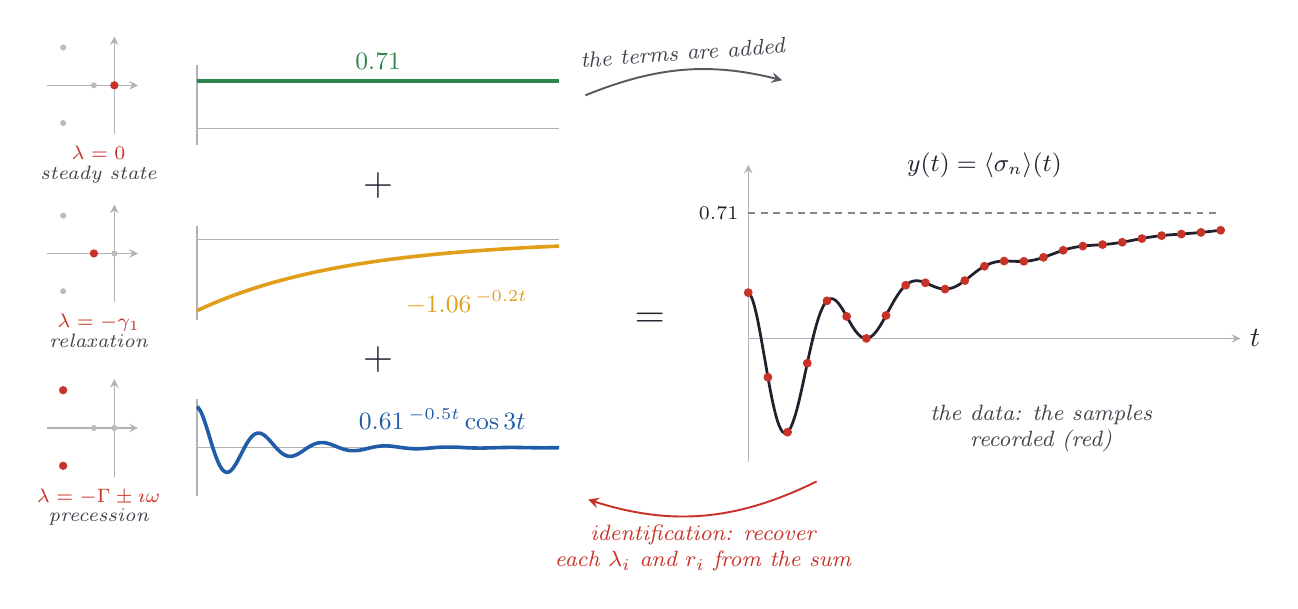
\begin{tikzpicture}[ink/.style={line width=0.9pt, ndInk}, faint/.style={line width=0.4pt, ndInk!35}, dashedink/.style={line width=0.5pt, ndInk!55, dash pattern=on 2.5pt off 2pt}, vec/.style={->, >=stealth, line width=1.2pt}, note/.style={font=\footnotesize\itshape, text=ndInk!85, align=center}, pointer/.style={->, >=stealth, line width=0.4pt, ndInk!60, shorten >=2pt, shorten <=1pt}, dot/.style={circle, fill=ndInk, inner sep=0pt, minimum size=3.4pt}, wash/.style={fill=ndSky, fill opacity=0.55}, every node/.style={text=ndInk}]
\definecolor{ndInk}{rgb}{0.13,0.13,0.18}
\definecolor{ndPaper}{rgb}{0.99,0.96,0.88}
\definecolor{ndSky}{rgb}{0.84,0.91,0.98}
\definecolor{ndRose}{rgb}{0.98,0.86,0.84}
\definecolor{ndBlue}{rgb}{0.13,0.36,0.66}
\definecolor{ndRed}{rgb}{0.78,0.20,0.16}
\definecolor{ndGold}{rgb}{0.88,0.62,0.10}
\definecolor{ndGreen}{rgb}{0.18,0.52,0.30}
\draw[faint] (2.000,5.193) -- (6.600,5.193);
\draw[faint] (2.000,4.980) -- (2.000,6.000);
\draw[line width=1.3pt, ndGreen] (2.000,5.794) -- (2.012,5.794) -- (2.023,5.794) -- (2.035,5.794) -- (2.046,5.794) -- (2.058,5.794) -- (2.069,5.794) -- (2.081,5.794) -- (2.092,5.794) -- (2.104,5.794) -- (2.115,5.794) -- (2.127,5.794) -- (2.138,5.794) -- (2.150,5.794) -- (2.161,5.794) -- (2.173,5.794) -- (2.184,5.794) -- (2.196,5.794) -- (2.208,5.794) -- (2.219,5.794) -- (2.231,5.794) -- (2.242,5.794) -- (2.254,5.794) -- (2.265,5.794) -- (2.277,5.794) -- (2.288,5.794) -- (2.300,5.794) -- (2.311,5.794) -- (2.323,5.794) -- (2.334,5.794) -- (2.346,5.794) -- (2.357,5.794) -- (2.369,5.794) -- (2.380,5.794) -- (2.392,5.794) -- (2.404,5.794) -- (2.415,5.794) -- (2.427,5.794) -- (2.438,5.794) -- (2.450,5.794) -- (2.461,5.794) -- (2.473,5.794) -- (2.484,5.794) -- (2.496,5.794) -- (2.507,5.794) -- (2.519,5.794) -- (2.530,5.794) -- (2.542,5.794) -- (2.553,5.794) -- (2.565,5.794) -- (2.576,5.794) -- (2.588,5.794) -- (2.599,5.794) -- (2.611,5.794) -- (2.623,5.794) -- (2.634,5.794) -- (2.646,5.794) -- (2.657,5.794) -- (2.669,5.794) -- (2.680,5.794) -- (2.692,5.794) -- (2.703,5.794) -- (2.715,5.794) -- (2.726,5.794) -- (2.738,5.794) -- (2.749,5.794) -- (2.761,5.794) -- (2.772,5.794) -- (2.784,5.794) -- (2.795,5.794) -- (2.807,5.794) -- (2.819,5.794) -- (2.830,5.794) -- (2.842,5.794) -- (2.853,5.794) -- (2.865,5.794) -- (2.876,5.794) -- (2.888,5.794) -- (2.899,5.794) -- (2.911,5.794) -- (2.922,5.794) -- (2.934,5.794) -- (2.945,5.794) -- (2.957,5.794) -- (2.968,5.794) -- (2.980,5.794) -- (2.991,5.794) -- (3.003,5.794) -- (3.015,5.794) -- (3.026,5.794) -- (3.038,5.794) -- (3.049,5.794) -- (3.061,5.794) -- (3.072,5.794) -- (3.084,5.794) -- (3.095,5.794) -- (3.107,5.794) -- (3.118,5.794) -- (3.130,5.794) -- (3.141,5.794) -- (3.153,5.794) -- (3.164,5.794) -- (3.176,5.794) -- (3.187,5.794) -- (3.199,5.794) -- (3.211,5.794) -- (3.222,5.794) -- (3.234,5.794) -- (3.245,5.794) -- (3.257,5.794) -- (3.268,5.794) -- (3.280,5.794) -- (3.291,5.794) -- (3.303,5.794) -- (3.314,5.794) -- (3.326,5.794) -- (3.337,5.794) -- (3.349,5.794) -- (3.360,5.794) -- (3.372,5.794) -- (3.383,5.794) -- (3.395,5.794) -- (3.407,5.794) -- (3.418,5.794) -- (3.430,5.794) -- (3.441,5.794) -- (3.453,5.794) -- (3.464,5.794) -- (3.476,5.794) -- (3.487,5.794) -- (3.499,5.794) -- (3.510,5.794) -- (3.522,5.794) -- (3.533,5.794) -- (3.545,5.794) -- (3.556,5.794) -- (3.568,5.794) -- (3.579,5.794) -- (3.591,5.794) -- (3.603,5.794) -- (3.614,5.794) -- (3.626,5.794) -- (3.637,5.794) -- (3.649,5.794) -- (3.660,5.794) -- (3.672,5.794) -- (3.683,5.794) -- (3.695,5.794) -- (3.706,5.794) -- (3.718,5.794) -- (3.729,5.794) -- (3.741,5.794) -- (3.752,5.794) -- (3.764,5.794) -- (3.775,5.794) -- (3.787,5.794) -- (3.798,5.794) -- (3.810,5.794) -- (3.822,5.794) -- (3.833,5.794) -- (3.845,5.794) -- (3.856,5.794) -- (3.868,5.794) -- (3.879,5.794) -- (3.891,5.794) -- (3.902,5.794) -- (3.914,5.794) -- (3.925,5.794) -- (3.937,5.794) -- (3.948,5.794) -- (3.960,5.794) -- (3.971,5.794) -- (3.983,5.794) -- (3.994,5.794) -- (4.006,5.794) -- (4.018,5.794) -- (4.029,5.794) -- (4.041,5.794) -- (4.052,5.794) -- (4.064,5.794) -- (4.075,5.794) -- (4.087,5.794) -- (4.098,5.794) -- (4.110,5.794) -- (4.121,5.794) -- (4.133,5.794) -- (4.144,5.794) -- (4.156,5.794) -- (4.167,5.794) -- (4.179,5.794) -- (4.190,5.794) -- (4.202,5.794) -- (4.214,5.794) -- (4.225,5.794) -- (4.237,5.794) -- (4.248,5.794) -- (4.260,5.794) -- (4.271,5.794) -- (4.283,5.794) -- (4.294,5.794) -- (4.306,5.794) -- (4.317,5.794) -- (4.329,5.794) -- (4.340,5.794) -- (4.352,5.794) -- (4.363,5.794) -- (4.375,5.794) -- (4.386,5.794) -- (4.398,5.794) -- (4.410,5.794) -- (4.421,5.794) -- (4.433,5.794) -- (4.444,5.794) -- (4.456,5.794) -- (4.467,5.794) -- (4.479,5.794) -- (4.490,5.794) -- (4.502,5.794) -- (4.513,5.794) -- (4.525,5.794) -- (4.536,5.794) -- (4.548,5.794) -- (4.559,5.794) -- (4.571,5.794) -- (4.582,5.794) -- (4.594,5.794) -- (4.606,5.794) -- (4.617,5.794) -- (4.629,5.794) -- (4.640,5.794) -- (4.652,5.794) -- (4.663,5.794) -- (4.675,5.794) -- (4.686,5.794) -- (4.698,5.794) -- (4.709,5.794) -- (4.721,5.794) -- (4.732,5.794) -- (4.744,5.794) -- (4.755,5.794) -- (4.767,5.794) -- (4.778,5.794) -- (4.790,5.794) -- (4.802,5.794) -- (4.813,5.794) -- (4.825,5.794) -- (4.836,5.794) -- (4.848,5.794) -- (4.859,5.794) -- (4.871,5.794) -- (4.882,5.794) -- (4.894,5.794) -- (4.905,5.794) -- (4.917,5.794) -- (4.928,5.794) -- (4.940,5.794) -- (4.951,5.794) -- (4.963,5.794) -- (4.974,5.794) -- (4.986,5.794) -- (4.997,5.794) -- (5.009,5.794) -- (5.021,5.794) -- (5.032,5.794) -- (5.044,5.794) -- (5.055,5.794) -- (5.067,5.794) -- (5.078,5.794) -- (5.090,5.794) -- (5.101,5.794) -- (5.113,5.794) -- (5.124,5.794) -- (5.136,5.794) -- (5.147,5.794) -- (5.159,5.794) -- (5.170,5.794) -- (5.182,5.794) -- (5.193,5.794) -- (5.205,5.794) -- (5.217,5.794) -- (5.228,5.794) -- (5.240,5.794) -- (5.251,5.794) -- (5.263,5.794) -- (5.274,5.794) -- (5.286,5.794) -- (5.297,5.794) -- (5.309,5.794) -- (5.320,5.794) -- (5.332,5.794) -- (5.343,5.794) -- (5.355,5.794) -- (5.366,5.794) -- (5.378,5.794) -- (5.389,5.794) -- (5.401,5.794) -- (5.413,5.794) -- (5.424,5.794) -- (5.436,5.794) -- (5.447,5.794) -- (5.459,5.794) -- (5.470,5.794) -- (5.482,5.794) -- (5.493,5.794) -- (5.505,5.794) -- (5.516,5.794) -- (5.528,5.794) -- (5.539,5.794) -- (5.551,5.794) -- (5.562,5.794) -- (5.574,5.794) -- (5.585,5.794) -- (5.597,5.794) -- (5.609,5.794) -- (5.620,5.794) -- (5.632,5.794) -- (5.643,5.794) -- (5.655,5.794) -- (5.666,5.794) -- (5.678,5.794) -- (5.689,5.794) -- (5.701,5.794) -- (5.712,5.794) -- (5.724,5.794) -- (5.735,5.794) -- (5.747,5.794) -- (5.758,5.794) -- (5.770,5.794) -- (5.781,5.794) -- (5.793,5.794) -- (5.805,5.794) -- (5.816,5.794) -- (5.828,5.794) -- (5.839,5.794) -- (5.851,5.794) -- (5.862,5.794) -- (5.874,5.794) -- (5.885,5.794) -- (5.897,5.794) -- (5.908,5.794) -- (5.920,5.794) -- (5.931,5.794) -- (5.943,5.794) -- (5.954,5.794) -- (5.966,5.794) -- (5.977,5.794) -- (5.989,5.794) -- (6.001,5.794) -- (6.012,5.794) -- (6.024,5.794) -- (6.035,5.794) -- (6.047,5.794) -- (6.058,5.794) -- (6.070,5.794) -- (6.081,5.794) -- (6.093,5.794) -- (6.104,5.794) -- (6.116,5.794) -- (6.127,5.794) -- (6.139,5.794) -- (6.150,5.794) -- (6.162,5.794) -- (6.173,5.794) -- (6.185,5.794) -- (6.196,5.794) -- (6.208,5.794) -- (6.220,5.794) -- (6.231,5.794) -- (6.243,5.794) -- (6.254,5.794) -- (6.266,5.794) -- (6.277,5.794) -- (6.289,5.794) -- (6.300,5.794) -- (6.312,5.794) -- (6.323,5.794) -- (6.335,5.794) -- (6.346,5.794) -- (6.358,5.794) -- (6.369,5.794) -- (6.381,5.794) -- (6.392,5.794) -- (6.404,5.794) -- (6.416,5.794) -- (6.427,5.794) -- (6.439,5.794) -- (6.450,5.794) -- (6.462,5.794) -- (6.473,5.794) -- (6.485,5.794) -- (6.496,5.794) -- (6.508,5.794) -- (6.519,5.794) -- (6.531,5.794) -- (6.542,5.794) -- (6.554,5.794) -- (6.565,5.794) -- (6.577,5.794) -- (6.588,5.794) -- (6.600,5.794);
\draw[faint, ->, >=stealth] (0.100,5.740) -- (1.250,5.740);
\draw[faint, ->, >=stealth] (0.950,5.120) -- (0.950,6.360);
\fill[ndRed] (0.950,5.740) circle (1.5pt);
\fill[ndInk!30] (0.690,5.740) circle (1.1pt);
\fill[ndInk!30] (0.300,6.220) circle (1.1pt);
\fill[ndInk!30] (0.300,5.260) circle (1.1pt);
\node[font=\scriptsize, text=ndRed, anchor=north, align=center] at (0.75,5.090) {$\lambda=0$\\[-1pt] \textit{\color{ndInk!85}steady state}};
\draw[faint] (2.000,3.780) -- (6.600,3.780);
\draw[faint] (2.000,2.760) -- (2.000,3.950);
\draw[line width=1.3pt, ndGold] (2.000,2.878) -- (2.012,2.884) -- (2.023,2.889) -- (2.035,2.895) -- (2.046,2.900) -- (2.058,2.905) -- (2.069,2.910) -- (2.081,2.916) -- (2.092,2.921) -- (2.104,2.926) -- (2.115,2.931) -- (2.127,2.936) -- (2.138,2.941) -- (2.150,2.946) -- (2.161,2.951) -- (2.173,2.956) -- (2.184,2.961) -- (2.196,2.966) -- (2.208,2.971) -- (2.219,2.976) -- (2.231,2.981) -- (2.242,2.985) -- (2.254,2.990) -- (2.265,2.995) -- (2.277,3.000) -- (2.288,3.004) -- (2.300,3.009) -- (2.311,3.014) -- (2.323,3.018) -- (2.334,3.023) -- (2.346,3.027) -- (2.357,3.032) -- (2.369,3.036) -- (2.380,3.041) -- (2.392,3.045) -- (2.404,3.050) -- (2.415,3.054) -- (2.427,3.058) -- (2.438,3.063) -- (2.450,3.067) -- (2.461,3.071) -- (2.473,3.075) -- (2.484,3.080) -- (2.496,3.084) -- (2.507,3.088) -- (2.519,3.092) -- (2.530,3.096) -- (2.542,3.100) -- (2.553,3.105) -- (2.565,3.109) -- (2.576,3.113) -- (2.588,3.117) -- (2.599,3.121) -- (2.611,3.125) -- (2.623,3.128) -- (2.634,3.132) -- (2.646,3.136) -- (2.657,3.140) -- (2.669,3.144) -- (2.680,3.148) -- (2.692,3.152) -- (2.703,3.155) -- (2.715,3.159) -- (2.726,3.163) -- (2.738,3.167) -- (2.749,3.170) -- (2.761,3.174) -- (2.772,3.177) -- (2.784,3.181) -- (2.795,3.185) -- (2.807,3.188) -- (2.819,3.192) -- (2.830,3.195) -- (2.842,3.199) -- (2.853,3.202) -- (2.865,3.206) -- (2.876,3.209) -- (2.888,3.213) -- (2.899,3.216) -- (2.911,3.219) -- (2.922,3.223) -- (2.934,3.226) -- (2.945,3.229) -- (2.957,3.233) -- (2.968,3.236) -- (2.980,3.239) -- (2.991,3.243) -- (3.003,3.246) -- (3.015,3.249) -- (3.026,3.252) -- (3.038,3.255) -- (3.049,3.258) -- (3.061,3.262) -- (3.072,3.265) -- (3.084,3.268) -- (3.095,3.271) -- (3.107,3.274) -- (3.118,3.277) -- (3.130,3.280) -- (3.141,3.283) -- (3.153,3.286) -- (3.164,3.289) -- (3.176,3.292) -- (3.187,3.295) -- (3.199,3.298) -- (3.211,3.301) -- (3.222,3.303) -- (3.234,3.306) -- (3.245,3.309) -- (3.257,3.312) -- (3.268,3.315) -- (3.280,3.318) -- (3.291,3.320) -- (3.303,3.323) -- (3.314,3.326) -- (3.326,3.329) -- (3.337,3.331) -- (3.349,3.334) -- (3.360,3.337) -- (3.372,3.339) -- (3.383,3.342) -- (3.395,3.345) -- (3.407,3.347) -- (3.418,3.350) -- (3.430,3.352) -- (3.441,3.355) -- (3.453,3.357) -- (3.464,3.360) -- (3.476,3.363) -- (3.487,3.365) -- (3.499,3.368) -- (3.510,3.370) -- (3.522,3.372) -- (3.533,3.375) -- (3.545,3.377) -- (3.556,3.380) -- (3.568,3.382) -- (3.579,3.385) -- (3.591,3.387) -- (3.603,3.389) -- (3.614,3.392) -- (3.626,3.394) -- (3.637,3.396) -- (3.649,3.399) -- (3.660,3.401) -- (3.672,3.403) -- (3.683,3.405) -- (3.695,3.408) -- (3.706,3.410) -- (3.718,3.412) -- (3.729,3.414) -- (3.741,3.416) -- (3.752,3.419) -- (3.764,3.421) -- (3.775,3.423) -- (3.787,3.425) -- (3.798,3.427) -- (3.810,3.429) -- (3.822,3.431) -- (3.833,3.434) -- (3.845,3.436) -- (3.856,3.438) -- (3.868,3.440) -- (3.879,3.442) -- (3.891,3.444) -- (3.902,3.446) -- (3.914,3.448) -- (3.925,3.450) -- (3.937,3.452) -- (3.948,3.454) -- (3.960,3.456) -- (3.971,3.458) -- (3.983,3.460) -- (3.994,3.462) -- (4.006,3.463) -- (4.018,3.465) -- (4.029,3.467) -- (4.041,3.469) -- (4.052,3.471) -- (4.064,3.473) -- (4.075,3.475) -- (4.087,3.476) -- (4.098,3.478) -- (4.110,3.480) -- (4.121,3.482) -- (4.133,3.484) -- (4.144,3.485) -- (4.156,3.487) -- (4.167,3.489) -- (4.179,3.491) -- (4.190,3.492) -- (4.202,3.494) -- (4.214,3.496) -- (4.225,3.498) -- (4.237,3.499) -- (4.248,3.501) -- (4.260,3.503) -- (4.271,3.504) -- (4.283,3.506) -- (4.294,3.508) -- (4.306,3.509) -- (4.317,3.511) -- (4.329,3.513) -- (4.340,3.514) -- (4.352,3.516) -- (4.363,3.517) -- (4.375,3.519) -- (4.386,3.520) -- (4.398,3.522) -- (4.410,3.524) -- (4.421,3.525) -- (4.433,3.527) -- (4.444,3.528) -- (4.456,3.530) -- (4.467,3.531) -- (4.479,3.533) -- (4.490,3.534) -- (4.502,3.536) -- (4.513,3.537) -- (4.525,3.539) -- (4.536,3.540) -- (4.548,3.541) -- (4.559,3.543) -- (4.571,3.544) -- (4.582,3.546) -- (4.594,3.547) -- (4.606,3.548) -- (4.617,3.550) -- (4.629,3.551) -- (4.640,3.553) -- (4.652,3.554) -- (4.663,3.555) -- (4.675,3.557) -- (4.686,3.558) -- (4.698,3.559) -- (4.709,3.561) -- (4.721,3.562) -- (4.732,3.563) -- (4.744,3.565) -- (4.755,3.566) -- (4.767,3.567) -- (4.778,3.568) -- (4.790,3.570) -- (4.802,3.571) -- (4.813,3.572) -- (4.825,3.573) -- (4.836,3.575) -- (4.848,3.576) -- (4.859,3.577) -- (4.871,3.578) -- (4.882,3.580) -- (4.894,3.581) -- (4.905,3.582) -- (4.917,3.583) -- (4.928,3.584) -- (4.940,3.586) -- (4.951,3.587) -- (4.963,3.588) -- (4.974,3.589) -- (4.986,3.590) -- (4.997,3.591) -- (5.009,3.592) -- (5.021,3.594) -- (5.032,3.595) -- (5.044,3.596) -- (5.055,3.597) -- (5.067,3.598) -- (5.078,3.599) -- (5.090,3.600) -- (5.101,3.601) -- (5.113,3.602) -- (5.124,3.603) -- (5.136,3.604) -- (5.147,3.605) -- (5.159,3.607) -- (5.170,3.608) -- (5.182,3.609) -- (5.193,3.610) -- (5.205,3.611) -- (5.217,3.612) -- (5.228,3.613) -- (5.240,3.614) -- (5.251,3.615) -- (5.263,3.616) -- (5.274,3.617) -- (5.286,3.618) -- (5.297,3.619) -- (5.309,3.620) -- (5.320,3.621) -- (5.332,3.621) -- (5.343,3.622) -- (5.355,3.623) -- (5.366,3.624) -- (5.378,3.625) -- (5.389,3.626) -- (5.401,3.627) -- (5.413,3.628) -- (5.424,3.629) -- (5.436,3.630) -- (5.447,3.631) -- (5.459,3.632) -- (5.470,3.633) -- (5.482,3.633) -- (5.493,3.634) -- (5.505,3.635) -- (5.516,3.636) -- (5.528,3.637) -- (5.539,3.638) -- (5.551,3.639) -- (5.562,3.639) -- (5.574,3.640) -- (5.585,3.641) -- (5.597,3.642) -- (5.609,3.643) -- (5.620,3.644) -- (5.632,3.644) -- (5.643,3.645) -- (5.655,3.646) -- (5.666,3.647) -- (5.678,3.648) -- (5.689,3.648) -- (5.701,3.649) -- (5.712,3.650) -- (5.724,3.651) -- (5.735,3.652) -- (5.747,3.652) -- (5.758,3.653) -- (5.770,3.654) -- (5.781,3.655) -- (5.793,3.655) -- (5.805,3.656) -- (5.816,3.657) -- (5.828,3.658) -- (5.839,3.658) -- (5.851,3.659) -- (5.862,3.660) -- (5.874,3.661) -- (5.885,3.661) -- (5.897,3.662) -- (5.908,3.663) -- (5.920,3.663) -- (5.931,3.664) -- (5.943,3.665) -- (5.954,3.665) -- (5.966,3.666) -- (5.977,3.667) -- (5.989,3.668) -- (6.001,3.668) -- (6.012,3.669) -- (6.024,3.670) -- (6.035,3.670) -- (6.047,3.671) -- (6.058,3.671) -- (6.070,3.672) -- (6.081,3.673) -- (6.093,3.673) -- (6.104,3.674) -- (6.116,3.675) -- (6.127,3.675) -- (6.139,3.676) -- (6.150,3.677) -- (6.162,3.677) -- (6.173,3.678) -- (6.185,3.678) -- (6.196,3.679) -- (6.208,3.680) -- (6.220,3.680) -- (6.231,3.681) -- (6.243,3.681) -- (6.254,3.682) -- (6.266,3.683) -- (6.277,3.683) -- (6.289,3.684) -- (6.300,3.684) -- (6.312,3.685) -- (6.323,3.686) -- (6.335,3.686) -- (6.346,3.687) -- (6.358,3.687) -- (6.369,3.688) -- (6.381,3.688) -- (6.392,3.689) -- (6.404,3.689) -- (6.416,3.690) -- (6.427,3.690) -- (6.439,3.691) -- (6.450,3.692) -- (6.462,3.692) -- (6.473,3.693) -- (6.485,3.693) -- (6.496,3.694) -- (6.508,3.694) -- (6.519,3.695) -- (6.531,3.695) -- (6.542,3.696) -- (6.554,3.696) -- (6.565,3.697) -- (6.577,3.697) -- (6.588,3.698) -- (6.600,3.698);
\draw[faint, ->, >=stealth] (0.100,3.605) -- (1.250,3.605);
\draw[faint, ->, >=stealth] (0.950,2.985) -- (0.950,4.225);
\fill[ndInk!30] (0.950,3.605) circle (1.1pt);
\fill[ndRed] (0.690,3.605) circle (1.5pt);
\fill[ndInk!30] (0.300,4.085) circle (1.1pt);
\fill[ndInk!30] (0.300,3.125) circle (1.1pt);
\node[font=\scriptsize, text=ndRed, anchor=north, align=center] at (0.75,2.955) {$\lambda=-\gamma_1$\\[-1pt] \textit{\color{ndInk!85}relaxation}};
\draw[faint] (2.000,1.138) -- (6.600,1.138);
\draw[faint] (2.000,0.526) -- (2.000,1.750);
\draw[line width=1.3pt, ndBlue] (2.000,1.659) -- (2.012,1.649) -- (2.023,1.635) -- (2.035,1.617) -- (2.046,1.597) -- (2.058,1.573) -- (2.069,1.546) -- (2.081,1.516) -- (2.092,1.484) -- (2.104,1.451) -- (2.115,1.416) -- (2.127,1.379) -- (2.138,1.342) -- (2.150,1.304) -- (2.161,1.266) -- (2.173,1.228) -- (2.184,1.190) -- (2.196,1.153) -- (2.208,1.117) -- (2.219,1.082) -- (2.231,1.049) -- (2.242,1.017) -- (2.254,0.988) -- (2.265,0.960) -- (2.277,0.935) -- (2.288,0.912) -- (2.300,0.892) -- (2.311,0.874) -- (2.323,0.859) -- (2.334,0.847) -- (2.346,0.837) -- (2.357,0.831) -- (2.369,0.827) -- (2.380,0.825) -- (2.392,0.827) -- (2.404,0.831) -- (2.415,0.837) -- (2.427,0.845) -- (2.438,0.856) -- (2.450,0.869) -- (2.461,0.883) -- (2.473,0.900) -- (2.484,0.917) -- (2.496,0.936) -- (2.507,0.956) -- (2.519,0.977) -- (2.530,0.999) -- (2.542,1.021) -- (2.553,1.044) -- (2.565,1.066) -- (2.576,1.089) -- (2.588,1.111) -- (2.599,1.133) -- (2.611,1.154) -- (2.623,1.175) -- (2.634,1.194) -- (2.646,1.213) -- (2.657,1.230) -- (2.669,1.246) -- (2.680,1.261) -- (2.692,1.274) -- (2.703,1.286) -- (2.715,1.296) -- (2.726,1.305) -- (2.738,1.312) -- (2.749,1.317) -- (2.761,1.321) -- (2.772,1.323) -- (2.784,1.323) -- (2.795,1.322) -- (2.807,1.320) -- (2.819,1.316) -- (2.830,1.310) -- (2.842,1.304) -- (2.853,1.296) -- (2.865,1.287) -- (2.876,1.277) -- (2.888,1.267) -- (2.899,1.255) -- (2.911,1.243) -- (2.922,1.231) -- (2.934,1.218) -- (2.945,1.205) -- (2.957,1.191) -- (2.968,1.178) -- (2.980,1.165) -- (2.991,1.151) -- (3.003,1.139) -- (3.015,1.126) -- (3.026,1.114) -- (3.038,1.103) -- (3.049,1.092) -- (3.061,1.082) -- (3.072,1.072) -- (3.084,1.064) -- (3.095,1.056) -- (3.107,1.049) -- (3.118,1.043) -- (3.130,1.038) -- (3.141,1.034) -- (3.153,1.032) -- (3.164,1.030) -- (3.176,1.028) -- (3.187,1.028) -- (3.199,1.029) -- (3.211,1.031) -- (3.222,1.033) -- (3.234,1.037) -- (3.245,1.041) -- (3.257,1.045) -- (3.268,1.051) -- (3.280,1.057) -- (3.291,1.063) -- (3.303,1.070) -- (3.314,1.077) -- (3.326,1.084) -- (3.337,1.092) -- (3.349,1.100) -- (3.360,1.108) -- (3.372,1.116) -- (3.383,1.124) -- (3.395,1.131) -- (3.407,1.139) -- (3.418,1.146) -- (3.430,1.153) -- (3.441,1.160) -- (3.453,1.167) -- (3.464,1.172) -- (3.476,1.178) -- (3.487,1.183) -- (3.499,1.187) -- (3.510,1.191) -- (3.522,1.195) -- (3.533,1.197) -- (3.545,1.200) -- (3.556,1.201) -- (3.568,1.202) -- (3.579,1.203) -- (3.591,1.203) -- (3.603,1.202) -- (3.614,1.201) -- (3.626,1.200) -- (3.637,1.198) -- (3.649,1.195) -- (3.660,1.192) -- (3.672,1.189) -- (3.683,1.186) -- (3.695,1.182) -- (3.706,1.178) -- (3.718,1.173) -- (3.729,1.169) -- (3.741,1.164) -- (3.752,1.160) -- (3.764,1.155) -- (3.775,1.150) -- (3.787,1.146) -- (3.798,1.141) -- (3.810,1.137) -- (3.822,1.132) -- (3.833,1.128) -- (3.845,1.124) -- (3.856,1.120) -- (3.868,1.117) -- (3.879,1.114) -- (3.891,1.111) -- (3.902,1.108) -- (3.914,1.106) -- (3.925,1.104) -- (3.937,1.103) -- (3.948,1.101) -- (3.960,1.100) -- (3.971,1.100) -- (3.983,1.100) -- (3.994,1.100) -- (4.006,1.100) -- (4.018,1.101) -- (4.029,1.102) -- (4.041,1.103) -- (4.052,1.104) -- (4.064,1.106) -- (4.075,1.108) -- (4.087,1.110) -- (4.098,1.112) -- (4.110,1.115) -- (4.121,1.117) -- (4.133,1.120) -- (4.144,1.123) -- (4.156,1.126) -- (4.167,1.128) -- (4.179,1.131) -- (4.190,1.134) -- (4.202,1.137) -- (4.214,1.139) -- (4.225,1.142) -- (4.237,1.144) -- (4.248,1.147) -- (4.260,1.149) -- (4.271,1.151) -- (4.283,1.153) -- (4.294,1.154) -- (4.306,1.156) -- (4.317,1.157) -- (4.329,1.158) -- (4.340,1.159) -- (4.352,1.160) -- (4.363,1.160) -- (4.375,1.161) -- (4.386,1.161) -- (4.398,1.161) -- (4.410,1.160) -- (4.421,1.160) -- (4.433,1.159) -- (4.444,1.159) -- (4.456,1.158) -- (4.467,1.157) -- (4.479,1.156) -- (4.490,1.154) -- (4.502,1.153) -- (4.513,1.151) -- (4.525,1.150) -- (4.536,1.148) -- (4.548,1.147) -- (4.559,1.145) -- (4.571,1.143) -- (4.582,1.142) -- (4.594,1.140) -- (4.606,1.139) -- (4.617,1.137) -- (4.629,1.135) -- (4.640,1.134) -- (4.652,1.133) -- (4.663,1.131) -- (4.675,1.130) -- (4.686,1.129) -- (4.698,1.128) -- (4.709,1.127) -- (4.721,1.127) -- (4.732,1.126) -- (4.744,1.125) -- (4.755,1.125) -- (4.767,1.125) -- (4.778,1.125) -- (4.790,1.124) -- (4.802,1.125) -- (4.813,1.125) -- (4.825,1.125) -- (4.836,1.125) -- (4.848,1.126) -- (4.859,1.126) -- (4.871,1.127) -- (4.882,1.128) -- (4.894,1.129) -- (4.905,1.129) -- (4.917,1.130) -- (4.928,1.131) -- (4.940,1.132) -- (4.951,1.133) -- (4.963,1.134) -- (4.974,1.135) -- (4.986,1.136) -- (4.997,1.137) -- (5.009,1.138) -- (5.021,1.139) -- (5.032,1.140) -- (5.044,1.141) -- (5.055,1.141) -- (5.067,1.142) -- (5.078,1.143) -- (5.090,1.143) -- (5.101,1.144) -- (5.113,1.144) -- (5.124,1.145) -- (5.136,1.145) -- (5.147,1.146) -- (5.159,1.146) -- (5.170,1.146) -- (5.182,1.146) -- (5.193,1.146) -- (5.205,1.146) -- (5.217,1.146) -- (5.228,1.146) -- (5.240,1.145) -- (5.251,1.145) -- (5.263,1.145) -- (5.274,1.144) -- (5.286,1.144) -- (5.297,1.144) -- (5.309,1.143) -- (5.320,1.143) -- (5.332,1.142) -- (5.343,1.141) -- (5.355,1.141) -- (5.366,1.140) -- (5.378,1.140) -- (5.389,1.139) -- (5.401,1.139) -- (5.413,1.138) -- (5.424,1.137) -- (5.436,1.137) -- (5.447,1.136) -- (5.459,1.136) -- (5.470,1.136) -- (5.482,1.135) -- (5.493,1.135) -- (5.505,1.134) -- (5.516,1.134) -- (5.528,1.134) -- (5.539,1.134) -- (5.551,1.134) -- (5.562,1.133) -- (5.574,1.133) -- (5.585,1.133) -- (5.597,1.133) -- (5.609,1.133) -- (5.620,1.133) -- (5.632,1.133) -- (5.643,1.134) -- (5.655,1.134) -- (5.666,1.134) -- (5.678,1.134) -- (5.689,1.135) -- (5.701,1.135) -- (5.712,1.135) -- (5.724,1.135) -- (5.735,1.136) -- (5.747,1.136) -- (5.758,1.136) -- (5.770,1.137) -- (5.781,1.137) -- (5.793,1.137) -- (5.805,1.138) -- (5.816,1.138) -- (5.828,1.138) -- (5.839,1.139) -- (5.851,1.139) -- (5.862,1.139) -- (5.874,1.140) -- (5.885,1.140) -- (5.897,1.140) -- (5.908,1.140) -- (5.920,1.140) -- (5.931,1.140) -- (5.943,1.141) -- (5.954,1.141) -- (5.966,1.141) -- (5.977,1.141) -- (5.989,1.141) -- (6.001,1.141) -- (6.012,1.141) -- (6.024,1.141) -- (6.035,1.141) -- (6.047,1.141) -- (6.058,1.140) -- (6.070,1.140) -- (6.081,1.140) -- (6.093,1.140) -- (6.104,1.140) -- (6.116,1.140) -- (6.127,1.140) -- (6.139,1.139) -- (6.150,1.139) -- (6.162,1.139) -- (6.173,1.139) -- (6.185,1.139) -- (6.196,1.138) -- (6.208,1.138) -- (6.220,1.138) -- (6.231,1.138) -- (6.243,1.138) -- (6.254,1.137) -- (6.266,1.137) -- (6.277,1.137) -- (6.289,1.137) -- (6.300,1.137) -- (6.312,1.137) -- (6.323,1.137) -- (6.335,1.137) -- (6.346,1.136) -- (6.358,1.136) -- (6.369,1.136) -- (6.381,1.136) -- (6.392,1.136) -- (6.404,1.136) -- (6.416,1.136) -- (6.427,1.136) -- (6.439,1.136) -- (6.450,1.136) -- (6.462,1.137) -- (6.473,1.137) -- (6.485,1.137) -- (6.496,1.137) -- (6.508,1.137) -- (6.519,1.137) -- (6.531,1.137) -- (6.542,1.137) -- (6.554,1.137) -- (6.565,1.137) -- (6.577,1.138) -- (6.588,1.138) -- (6.600,1.138);
\draw[faint, ->, >=stealth] (0.100,1.388) -- (1.250,1.388);
\draw[faint, ->, >=stealth] (0.950,0.768) -- (0.950,2.008);
\fill[ndInk!30] (0.950,1.388) circle (1.1pt);
\fill[ndInk!30] (0.690,1.388) circle (1.1pt);
\fill[ndRed] (0.300,1.868) circle (1.5pt);
\fill[ndRed] (0.300,0.908) circle (1.5pt);
\node[font=\scriptsize, text=ndRed, anchor=north, align=center] at (0.75,0.738) {$\lambda=-\Gamma\pm\imath\omega$\\[-1pt] \textit{\color{ndInk!85}precession}};
\node[font=\small, text=ndGreen, anchor=south] at (4.300,5.811) {$0.71$};
\node[font=\small, text=ndGold, anchor=north west] at (4.530,3.253) {$-1.06\,\ee^{-0.2t}$};
\node[font=\small, text=ndBlue, anchor=south west] at (3.932,1.240) {$0.61\,\ee^{-0.5t}\cos 3t$};
\node[font=\Large] at (4.300,4.465) {$+$};
\node[font=\Large] at (4.300,2.255) {$+$};
\draw[faint] (9.000,2.525) -- (15.000,2.525);
\draw[faint, ->, >=stealth] (9.000,2.525) -- (15.250,2.525) node[right, text=ndInk] {$t$};
\draw[faint, ->, >=stealth] (9.000,0.950) -- (9.000,4.730);
\draw[dashedink] (9.000,4.116) -- (15.000,4.116);
\node[font=\scriptsize, anchor=east] at (9.000,4.116) {$0.71$};
\draw[line width=1.0pt, ndInk] (9.000,3.107) -- (9.015,3.096) -- (9.030,3.073) -- (9.045,3.041) -- (9.060,3.000) -- (9.075,2.950) -- (9.090,2.893) -- (9.105,2.829) -- (9.120,2.759) -- (9.135,2.683) -- (9.150,2.604) -- (9.165,2.521) -- (9.180,2.435) -- (9.195,2.348) -- (9.211,2.260) -- (9.226,2.173) -- (9.241,2.086) -- (9.256,2.001) -- (9.271,1.918) -- (9.286,1.839) -- (9.301,1.764) -- (9.316,1.693) -- (9.331,1.627) -- (9.346,1.567) -- (9.361,1.512) -- (9.376,1.464) -- (9.391,1.423) -- (9.406,1.388) -- (9.421,1.361) -- (9.436,1.341) -- (9.451,1.328) -- (9.466,1.322) -- (9.481,1.323) -- (9.496,1.332) -- (9.511,1.347) -- (9.526,1.369) -- (9.541,1.397) -- (9.556,1.431) -- (9.571,1.471) -- (9.586,1.516) -- (9.602,1.566) -- (9.617,1.620) -- (9.632,1.678) -- (9.647,1.739) -- (9.662,1.804) -- (9.677,1.870) -- (9.692,1.939) -- (9.707,2.008) -- (9.722,2.079) -- (9.737,2.149) -- (9.752,2.220) -- (9.767,2.289) -- (9.782,2.357) -- (9.797,2.424) -- (9.812,2.489) -- (9.827,2.551) -- (9.842,2.610) -- (9.857,2.666) -- (9.872,2.719) -- (9.887,2.768) -- (9.902,2.813) -- (9.917,2.854) -- (9.932,2.891) -- (9.947,2.924) -- (9.962,2.952) -- (9.977,2.975) -- (9.992,2.995) -- (10.008,3.010) -- (10.023,3.021) -- (10.038,3.028) -- (10.053,3.030) -- (10.068,3.029) -- (10.083,3.024) -- (10.098,3.016) -- (10.113,3.005) -- (10.128,2.991) -- (10.143,2.974) -- (10.158,2.955) -- (10.173,2.934) -- (10.188,2.911) -- (10.203,2.887) -- (10.218,2.861) -- (10.233,2.835) -- (10.248,2.809) -- (10.263,2.782) -- (10.278,2.755) -- (10.293,2.729) -- (10.308,2.703) -- (10.323,2.679) -- (10.338,2.655) -- (10.353,2.633) -- (10.368,2.613) -- (10.383,2.595) -- (10.398,2.578) -- (10.414,2.563) -- (10.429,2.551) -- (10.444,2.541) -- (10.459,2.534) -- (10.474,2.529) -- (10.489,2.526) -- (10.504,2.526) -- (10.519,2.529) -- (10.534,2.534) -- (10.549,2.541) -- (10.564,2.551) -- (10.579,2.563) -- (10.594,2.577) -- (10.609,2.594) -- (10.624,2.612) -- (10.639,2.632) -- (10.654,2.653) -- (10.669,2.676) -- (10.684,2.701) -- (10.699,2.726) -- (10.714,2.752) -- (10.729,2.779) -- (10.744,2.807) -- (10.759,2.834) -- (10.774,2.863) -- (10.789,2.891) -- (10.805,2.918) -- (10.820,2.946) -- (10.835,2.973) -- (10.850,2.999) -- (10.865,3.025) -- (10.880,3.049) -- (10.895,3.073) -- (10.910,3.095) -- (10.925,3.117) -- (10.940,3.136) -- (10.955,3.155) -- (10.970,3.172) -- (10.985,3.187) -- (11.000,3.201) -- (11.015,3.213) -- (11.030,3.224) -- (11.045,3.233) -- (11.060,3.241) -- (11.075,3.247) -- (11.090,3.252) -- (11.105,3.255) -- (11.120,3.257) -- (11.135,3.258) -- (11.150,3.258) -- (11.165,3.256) -- (11.180,3.254) -- (11.195,3.250) -- (11.211,3.246) -- (11.226,3.241) -- (11.241,3.236) -- (11.256,3.230) -- (11.271,3.224) -- (11.286,3.217) -- (11.301,3.210) -- (11.316,3.204) -- (11.331,3.197) -- (11.346,3.190) -- (11.361,3.184) -- (11.376,3.178) -- (11.391,3.173) -- (11.406,3.168) -- (11.421,3.163) -- (11.436,3.160) -- (11.451,3.157) -- (11.466,3.154) -- (11.481,3.153) -- (11.496,3.152) -- (11.511,3.152) -- (11.526,3.153) -- (11.541,3.155) -- (11.556,3.158) -- (11.571,3.162) -- (11.586,3.166) -- (11.602,3.171) -- (11.617,3.177) -- (11.632,3.184) -- (11.647,3.192) -- (11.662,3.200) -- (11.677,3.209) -- (11.692,3.218) -- (11.707,3.229) -- (11.722,3.239) -- (11.737,3.250) -- (11.752,3.261) -- (11.767,3.273) -- (11.782,3.284) -- (11.797,3.296) -- (11.812,3.308) -- (11.827,3.320) -- (11.842,3.332) -- (11.857,3.344) -- (11.872,3.356) -- (11.887,3.367) -- (11.902,3.379) -- (11.917,3.390) -- (11.932,3.400) -- (11.947,3.410) -- (11.962,3.420) -- (11.977,3.429) -- (11.992,3.438) -- (12.008,3.447) -- (12.023,3.454) -- (12.038,3.462) -- (12.053,3.468) -- (12.068,3.474) -- (12.083,3.480) -- (12.098,3.485) -- (12.113,3.489) -- (12.128,3.493) -- (12.143,3.497) -- (12.158,3.499) -- (12.173,3.502) -- (12.188,3.504) -- (12.203,3.505) -- (12.218,3.507) -- (12.233,3.508) -- (12.248,3.508) -- (12.263,3.508) -- (12.278,3.508) -- (12.293,3.508) -- (12.308,3.508) -- (12.323,3.507) -- (12.338,3.507) -- (12.353,3.506) -- (12.368,3.506) -- (12.383,3.505) -- (12.398,3.504) -- (12.414,3.504) -- (12.429,3.504) -- (12.444,3.504) -- (12.459,3.504) -- (12.474,3.504) -- (12.489,3.504) -- (12.504,3.505) -- (12.519,3.506) -- (12.534,3.507) -- (12.549,3.509) -- (12.564,3.510) -- (12.579,3.512) -- (12.594,3.515) -- (12.609,3.517) -- (12.624,3.520) -- (12.639,3.524) -- (12.654,3.527) -- (12.669,3.531) -- (12.684,3.535) -- (12.699,3.539) -- (12.714,3.544) -- (12.729,3.548) -- (12.744,3.553) -- (12.759,3.558) -- (12.774,3.564) -- (12.789,3.569) -- (12.805,3.574) -- (12.820,3.580) -- (12.835,3.586) -- (12.850,3.591) -- (12.865,3.597) -- (12.880,3.602) -- (12.895,3.608) -- (12.910,3.614) -- (12.925,3.619) -- (12.940,3.624) -- (12.955,3.630) -- (12.970,3.635) -- (12.985,3.640) -- (13.000,3.645) -- (13.015,3.650) -- (13.030,3.654) -- (13.045,3.658) -- (13.060,3.663) -- (13.075,3.667) -- (13.090,3.670) -- (13.105,3.674) -- (13.120,3.677) -- (13.135,3.680) -- (13.150,3.683) -- (13.165,3.686) -- (13.180,3.689) -- (13.195,3.691) -- (13.211,3.693) -- (13.226,3.695) -- (13.241,3.697) -- (13.256,3.699) -- (13.271,3.701) -- (13.286,3.702) -- (13.301,3.703) -- (13.316,3.705) -- (13.331,3.706) -- (13.346,3.707) -- (13.361,3.708) -- (13.376,3.709) -- (13.391,3.710) -- (13.406,3.711) -- (13.421,3.712) -- (13.436,3.713) -- (13.451,3.714) -- (13.466,3.715) -- (13.481,3.716) -- (13.496,3.717) -- (13.511,3.718) -- (13.526,3.719) -- (13.541,3.720) -- (13.556,3.722) -- (13.571,3.723) -- (13.586,3.725) -- (13.602,3.726) -- (13.617,3.728) -- (13.632,3.730) -- (13.647,3.732) -- (13.662,3.734) -- (13.677,3.736) -- (13.692,3.738) -- (13.707,3.740) -- (13.722,3.743) -- (13.737,3.745) -- (13.752,3.748) -- (13.767,3.750) -- (13.782,3.753) -- (13.797,3.756) -- (13.812,3.759) -- (13.827,3.761) -- (13.842,3.764) -- (13.857,3.767) -- (13.872,3.770) -- (13.887,3.773) -- (13.902,3.776) -- (13.917,3.779) -- (13.932,3.782) -- (13.947,3.785) -- (13.962,3.787) -- (13.977,3.790) -- (13.992,3.793) -- (14.008,3.796) -- (14.023,3.799) -- (14.038,3.801) -- (14.053,3.804) -- (14.068,3.806) -- (14.083,3.809) -- (14.098,3.811) -- (14.113,3.813) -- (14.128,3.816) -- (14.143,3.818) -- (14.158,3.820) -- (14.173,3.822) -- (14.188,3.824) -- (14.203,3.826) -- (14.218,3.827) -- (14.233,3.829) -- (14.248,3.831) -- (14.263,3.832) -- (14.278,3.834) -- (14.293,3.835) -- (14.308,3.837) -- (14.323,3.838) -- (14.338,3.839) -- (14.353,3.841) -- (14.368,3.842) -- (14.383,3.843) -- (14.398,3.844) -- (14.414,3.845) -- (14.429,3.846) -- (14.444,3.847) -- (14.459,3.849) -- (14.474,3.850) -- (14.489,3.851) -- (14.504,3.852) -- (14.519,3.853) -- (14.534,3.854) -- (14.549,3.855) -- (14.564,3.856) -- (14.579,3.857) -- (14.594,3.859) -- (14.609,3.860) -- (14.624,3.861) -- (14.639,3.862) -- (14.654,3.863) -- (14.669,3.865) -- (14.684,3.866) -- (14.699,3.868) -- (14.714,3.869) -- (14.729,3.870) -- (14.744,3.872) -- (14.759,3.873) -- (14.774,3.875) -- (14.789,3.876) -- (14.805,3.878) -- (14.820,3.879) -- (14.835,3.881) -- (14.850,3.883) -- (14.865,3.884) -- (14.880,3.886) -- (14.895,3.888) -- (14.910,3.889) -- (14.925,3.891) -- (14.940,3.893) -- (14.955,3.894) -- (14.970,3.896) -- (14.985,3.897) -- (15.000,3.899);
\fill[ndRed] (9.000,3.107) circle (1.6pt);
\fill[ndRed] (9.250,2.033) circle (1.6pt);
\fill[ndRed] (9.500,1.335) circle (1.6pt);
\fill[ndRed] (9.750,2.211) circle (1.6pt);
\fill[ndRed] (10.000,3.003) circle (1.6pt);
\fill[ndRed] (10.250,2.805) circle (1.6pt);
\fill[ndRed] (10.500,2.526) circle (1.6pt);
\fill[ndRed] (10.750,2.817) circle (1.6pt);
\fill[ndRed] (11.000,3.201) circle (1.6pt);
\fill[ndRed] (11.250,3.232) circle (1.6pt);
\fill[ndRed] (11.500,3.152) circle (1.6pt);
\fill[ndRed] (11.750,3.260) circle (1.6pt);
\fill[ndRed] (12.000,3.442) circle (1.6pt);
\fill[ndRed] (12.250,3.508) circle (1.6pt);
\fill[ndRed] (12.500,3.505) circle (1.6pt);
\fill[ndRed] (12.750,3.555) circle (1.6pt);
\fill[ndRed] (13.000,3.645) circle (1.6pt);
\fill[ndRed] (13.250,3.698) circle (1.6pt);
\fill[ndRed] (13.500,3.717) circle (1.6pt);
\fill[ndRed] (13.750,3.747) circle (1.6pt);
\fill[ndRed] (14.000,3.794) circle (1.6pt);
\fill[ndRed] (14.250,3.831) circle (1.6pt);
\fill[ndRed] (14.500,3.851) circle (1.6pt);
\fill[ndRed] (14.750,3.872) circle (1.6pt);
\fill[ndRed] (15.000,3.899) circle (1.6pt);
\node[font=\small, anchor=south] at (12.000,4.438) {$y(t)=\langle\sigma_n\rangle(t)$};
\node[note, anchor=north] (d) at (12.720,1.805) {the data: the samples\\ recorded (red)};
\node[font=\Large] at (7.75,2.750) {$=$};
\draw[pointer, line width=0.7pt, ndInk!75] (6.9,5.6) to[bend left=18] node[note, above, sloped] {the terms are added} (9.500,5.788);
\draw[pointer, line width=0.7pt, ndRed] (9.900,0.725) to[bend left=22] node[note, below, text=ndRed] {identification: recover\\ each $\lambda_i$ and $r_i$ from the sum} (6.9,0.5);
\end{tikzpicture}
}
\caption{The data $\langle\sigma_n\rangle(t)$ for the example, with $\vec n=(1,0,1)/\sqrt2$, written as the sum \eqref{eq:ch05:sum} of three terms, each already multiplied by its coefficient $r_i$: a constant from the steady state $\lambda=0$, a decay from the relaxation $\lambda=-\gamma_1$, and a damped oscillation from the precession $\lambda=-\Gamma\pm\imath\omega$. The small diagrams on the left mark in red the eigenvalue responsible for each term. Identification asks for the terms, that is, for each $\lambda_i$ and $r_i$, given only the samples of the sum (red dots). Generated by \texttt{code/ch05\_modes.py}.}\label{fig:ch05:modes}
\end{figure}}
\end{frame}

\begin{frame}\ft{The Fourier transform}
\ona{Suppose that we have recorded a signal $y(t)$ and wish to know which frequencies it contains. A simple device answers the question. Multiply $y(t)$ by $\ee^{-\imath\nu t}$, a vector turning clockwise with a trial angular velocity $\nu$, and follow the product in the complex plane. Any part of $y$ that oscillates with the frequency $\nu$ is turned back as fast as it turns, so that the product keeps roughly the same direction and its contributions accumulate. Any part that oscillates with another frequency continues to turn, and its contributions cancel in the course of each revolution. The sum of all the contributions,}
\onp{Multiply the signal by $\ee^{-\imath\nu t}$ and integrate:}
\begin{equation}\label{eq:ch05:fourier}
    \hat y(\nu)=\int_0^\infty y(t)\,\ee^{-\imath\nu t}\,\mathrm dt,\qquad
    \int_0^\infty\ee^{\lambda t}\,\ee^{-\imath\nu t}\,\mathrm dt=\frac1{\imath\nu-\lambda}\quad(\mathrm{Re}\,\lambda<0),
\end{equation}
\ona{is the \emph{Fourier transform} of $y$. It is large when $\nu$ is one of the frequencies present in $y$ and small otherwise (Figure~\ref{fig:ch05:winding}), and the graph of $\abs{\hat y(\nu)}$ against $\nu$ is called the \emph{spectrum} of $y$. For a single mode the integral is given by the second formula in \eqref{eq:ch05:fourier}, and its modulus $1/\abs{\imath\nu-\lambda}$ has a simple geometrical meaning: it is the reciprocal of the distance from the point $\imath\nu$ of the imaginary axis to the point $\lambda$. It is therefore greatest when $\nu=\mathrm{Im}\,\lambda$, where it equals $1/\abs{\mathrm{Re}\,\lambda}$, so that a slowly decaying mode gives a high peak. If the trial frequency $\imath\nu$ is replaced by a complex number $s=\sigma+\imath\nu$ we obtain the Laplace transform $\hat y(s)=\int_0^\infty y(t)\ee^{-st}\,\mathrm dt$ of the next section, and for a single mode $\hat y(s)=1/(s-\lambda)$, which becomes infinite at $s=\lambda$.}
\onp{\begin{itemize}
    \item At the frequency of the signal the contributions accumulate; at other frequencies they cancel.
    \item For one mode $\abs{\hat y(\nu)}=1/\mathrm{dist}(\imath\nu,\lambda)$; with complex $s$ in place of $\imath\nu$ we obtain the Laplace transform.
\end{itemize}}
\end{frame}

\begin{frame}\ft{The Fourier transform}
\ona{\begin{figure}[H]\centering
\resizebox{\linewidth}{!}{% Generated by code/needham.py -- do not edit by hand.
\definecolor{qocA}{rgb}{0.00,0.45,0.70}
\definecolor{qocB}{rgb}{0.90,0.60,0.00}
\definecolor{qocC}{rgb}{0.00,0.62,0.45}
\definecolor{qocD}{rgb}{0.80,0.40,0.00}
\definecolor{qocE}{rgb}{0.80,0.60,0.70}
\definecolor{qocF}{rgb}{0.35,0.70,0.90}
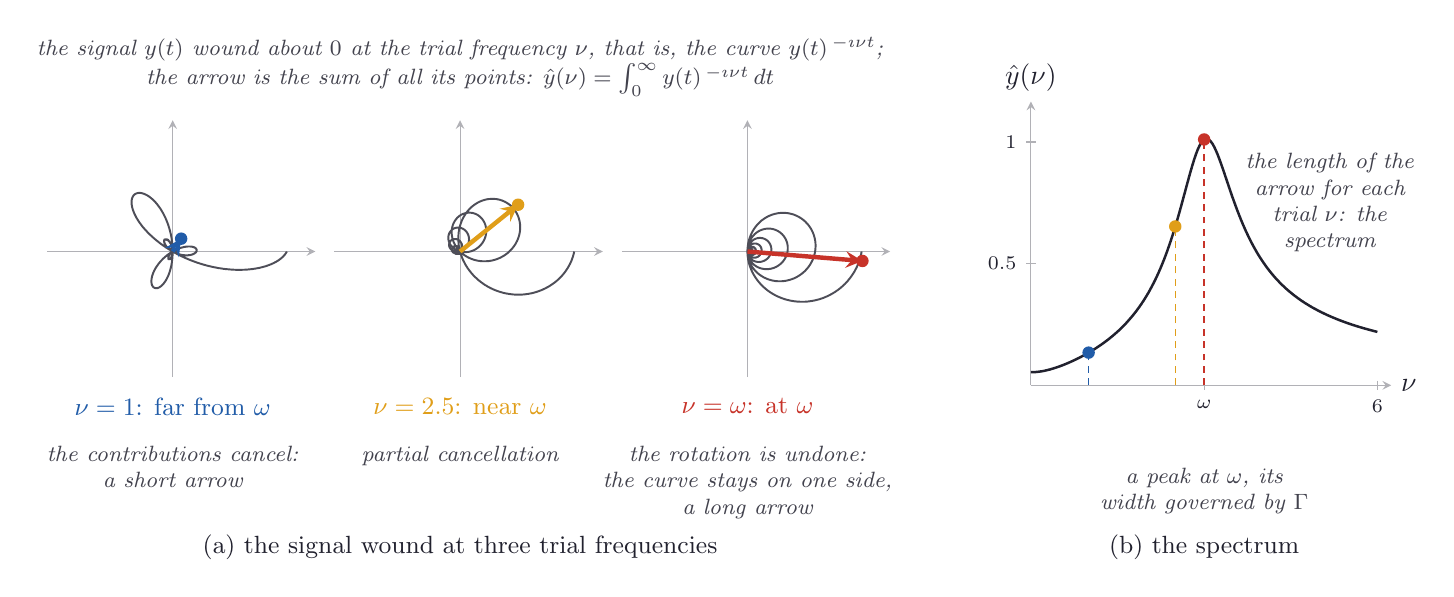
\begin{tikzpicture}[ink/.style={line width=0.9pt, ndInk}, faint/.style={line width=0.4pt, ndInk!35}, dashedink/.style={line width=0.5pt, ndInk!55, dash pattern=on 2.5pt off 2pt}, vec/.style={->, >=stealth, line width=1.2pt}, note/.style={font=\footnotesize\itshape, text=ndInk!85, align=center}, pointer/.style={->, >=stealth, line width=0.4pt, ndInk!60, shorten >=2pt, shorten <=1pt}, dot/.style={circle, fill=ndInk, inner sep=0pt, minimum size=3.4pt}, wash/.style={fill=ndSky, fill opacity=0.55}, every node/.style={text=ndInk}]
\definecolor{ndInk}{rgb}{0.13,0.13,0.18}
\definecolor{ndPaper}{rgb}{0.99,0.96,0.88}
\definecolor{ndSky}{rgb}{0.84,0.91,0.98}
\definecolor{ndRose}{rgb}{0.98,0.86,0.84}
\definecolor{ndBlue}{rgb}{0.13,0.36,0.66}
\definecolor{ndRed}{rgb}{0.78,0.20,0.16}
\definecolor{ndGold}{rgb}{0.88,0.62,0.10}
\definecolor{ndGreen}{rgb}{0.18,0.52,0.30}
\draw[faint, ->, >=stealth] (-1.595,0.000) -- (1.812,0.000);
\draw[faint, ->, >=stealth] (0.000,-1.595) -- (0.000,1.667);
\draw[line width=0.7pt, ndInk!80] (1.450,0.000) -- (1.448,-0.005) -- (1.445,-0.010) -- (1.442,-0.014) -- (1.439,-0.019) -- (1.436,-0.024) -- (1.433,-0.029) -- (1.429,-0.033) -- (1.426,-0.038) -- (1.422,-0.043) -- (1.418,-0.047) -- (1.414,-0.052) -- (1.410,-0.056) -- (1.406,-0.061) -- (1.401,-0.065) -- (1.397,-0.070) -- (1.392,-0.074) -- (1.387,-0.079) -- (1.382,-0.083) -- (1.377,-0.087) -- (1.371,-0.092) -- (1.366,-0.096) -- (1.360,-0.100) -- (1.355,-0.104) -- (1.349,-0.108) -- (1.343,-0.112) -- (1.337,-0.116) -- (1.331,-0.120) -- (1.324,-0.124) -- (1.318,-0.128) -- (1.311,-0.132) -- (1.304,-0.135) -- (1.297,-0.139) -- (1.290,-0.143) -- (1.283,-0.146) -- (1.276,-0.150) -- (1.269,-0.153) -- (1.261,-0.156) -- (1.254,-0.160) -- (1.246,-0.163) -- (1.238,-0.166) -- (1.230,-0.169) -- (1.222,-0.172) -- (1.214,-0.175) -- (1.206,-0.178) -- (1.198,-0.181) -- (1.189,-0.184) -- (1.181,-0.187) -- (1.172,-0.189) -- (1.163,-0.192) -- (1.154,-0.194) -- (1.145,-0.197) -- (1.136,-0.199) -- (1.127,-0.201) -- (1.118,-0.204) -- (1.109,-0.206) -- (1.099,-0.208) -- (1.090,-0.210) -- (1.080,-0.212) -- (1.071,-0.213) -- (1.061,-0.215) -- (1.051,-0.217) -- (1.041,-0.218) -- (1.031,-0.220) -- (1.021,-0.221) -- (1.011,-0.223) -- (1.001,-0.224) -- (0.991,-0.225) -- (0.981,-0.226) -- (0.970,-0.227) -- (0.960,-0.228) -- (0.949,-0.229) -- (0.939,-0.230) -- (0.928,-0.231) -- (0.918,-0.231) -- (0.907,-0.232) -- (0.896,-0.232) -- (0.885,-0.232) -- (0.874,-0.233) -- (0.864,-0.233) -- (0.853,-0.233) -- (0.842,-0.233) -- (0.831,-0.233) -- (0.819,-0.233) -- (0.808,-0.233) -- (0.797,-0.232) -- (0.786,-0.232) -- (0.775,-0.231) -- (0.763,-0.231) -- (0.752,-0.230) -- (0.741,-0.229) -- (0.729,-0.228) -- (0.718,-0.227) -- (0.707,-0.226) -- (0.695,-0.225) -- (0.684,-0.224) -- (0.672,-0.223) -- (0.661,-0.222) -- (0.649,-0.220) -- (0.638,-0.219) -- (0.626,-0.217) -- (0.615,-0.215) -- (0.603,-0.213) -- (0.592,-0.212) -- (0.580,-0.210) -- (0.569,-0.208) -- (0.557,-0.205) -- (0.545,-0.203) -- (0.534,-0.201) -- (0.522,-0.199) -- (0.511,-0.196) -- (0.499,-0.194) -- (0.488,-0.191) -- (0.476,-0.188) -- (0.465,-0.186) -- (0.453,-0.183) -- (0.442,-0.180) -- (0.430,-0.177) -- (0.419,-0.174) -- (0.407,-0.171) -- (0.396,-0.167) -- (0.384,-0.164) -- (0.373,-0.161) -- (0.362,-0.157) -- (0.350,-0.154) -- (0.339,-0.150) -- (0.328,-0.146) -- (0.316,-0.143) -- (0.305,-0.139) -- (0.294,-0.135) -- (0.283,-0.131) -- (0.272,-0.127) -- (0.261,-0.123) -- (0.250,-0.119) -- (0.239,-0.114) -- (0.228,-0.110) -- (0.217,-0.106) -- (0.206,-0.101) -- (0.195,-0.097) -- (0.185,-0.092) -- (0.174,-0.088) -- (0.163,-0.083) -- (0.153,-0.078) -- (0.142,-0.073) -- (0.131,-0.068) -- (0.121,-0.064) -- (0.111,-0.059) -- (0.100,-0.053) -- (0.090,-0.048) -- (0.080,-0.043) -- (0.070,-0.038) -- (0.059,-0.033) -- (0.049,-0.027) -- (0.039,-0.022) -- (0.030,-0.017) -- (0.020,-0.011) -- (0.010,-0.006) -- (0.000,-0.000) -- (-0.009,0.005) -- (-0.019,0.011) -- (-0.028,0.017) -- (-0.038,0.023) -- (-0.047,0.028) -- (-0.056,0.034) -- (-0.066,0.040) -- (-0.075,0.046) -- (-0.084,0.052) -- (-0.093,0.058) -- (-0.102,0.064) -- (-0.110,0.070) -- (-0.119,0.076) -- (-0.128,0.082) -- (-0.136,0.088) -- (-0.145,0.094) -- (-0.153,0.100) -- (-0.162,0.107) -- (-0.170,0.113) -- (-0.178,0.119) -- (-0.186,0.126) -- (-0.194,0.132) -- (-0.202,0.138) -- (-0.210,0.145) -- (-0.217,0.151) -- (-0.225,0.157) -- (-0.233,0.164) -- (-0.240,0.170) -- (-0.247,0.177) -- (-0.255,0.183) -- (-0.262,0.190) -- (-0.269,0.196) -- (-0.276,0.203) -- (-0.283,0.209) -- (-0.289,0.216) -- (-0.296,0.222) -- (-0.303,0.229) -- (-0.309,0.235) -- (-0.316,0.242) -- (-0.322,0.248) -- (-0.328,0.255) -- (-0.334,0.261) -- (-0.340,0.268) -- (-0.346,0.274) -- (-0.352,0.281) -- (-0.358,0.287) -- (-0.363,0.294) -- (-0.369,0.300) -- (-0.374,0.307) -- (-0.380,0.313) -- (-0.385,0.320) -- (-0.390,0.326) -- (-0.395,0.333) -- (-0.400,0.339) -- (-0.405,0.346) -- (-0.409,0.352) -- (-0.414,0.358) -- (-0.419,0.365) -- (-0.423,0.371) -- (-0.427,0.377) -- (-0.432,0.384) -- (-0.436,0.390) -- (-0.440,0.396) -- (-0.444,0.403) -- (-0.447,0.409) -- (-0.451,0.415) -- (-0.455,0.421) -- (-0.458,0.427) -- (-0.462,0.433) -- (-0.465,0.439) -- (-0.468,0.445) -- (-0.471,0.451) -- (-0.474,0.457) -- (-0.477,0.463) -- (-0.480,0.469) -- (-0.483,0.475) -- (-0.486,0.481) -- (-0.488,0.486) -- (-0.491,0.492) -- (-0.493,0.498) -- (-0.495,0.503) -- (-0.497,0.509) -- (-0.500,0.515) -- (-0.501,0.520) -- (-0.503,0.526) -- (-0.505,0.531) -- (-0.507,0.536) -- (-0.508,0.542) -- (-0.510,0.547) -- (-0.511,0.552) -- (-0.513,0.557) -- (-0.514,0.562) -- (-0.515,0.567) -- (-0.516,0.572) -- (-0.517,0.577) -- (-0.518,0.582) -- (-0.519,0.587) -- (-0.519,0.592) -- (-0.520,0.596) -- (-0.520,0.601) -- (-0.521,0.605) -- (-0.521,0.610) -- (-0.522,0.614) -- (-0.522,0.619) -- (-0.522,0.623) -- (-0.522,0.627) -- (-0.522,0.631) -- (-0.522,0.636) -- (-0.521,0.640) -- (-0.521,0.644) -- (-0.521,0.647) -- (-0.520,0.651) -- (-0.520,0.655) -- (-0.519,0.659) -- (-0.518,0.662) -- (-0.517,0.666) -- (-0.517,0.669) -- (-0.516,0.673) -- (-0.515,0.676) -- (-0.513,0.679) -- (-0.512,0.683) -- (-0.511,0.686) -- (-0.510,0.689) -- (-0.508,0.692) -- (-0.507,0.695) -- (-0.505,0.697) -- (-0.504,0.700) -- (-0.502,0.703) -- (-0.501,0.705) -- (-0.499,0.708) -- (-0.497,0.710) -- (-0.495,0.713) -- (-0.493,0.715) -- (-0.491,0.717) -- (-0.489,0.719) -- (-0.487,0.721) -- (-0.485,0.723) -- (-0.482,0.725) -- (-0.480,0.727) -- (-0.478,0.728) -- (-0.475,0.730) -- (-0.473,0.731) -- (-0.470,0.733) -- (-0.468,0.734) -- (-0.465,0.735) -- (-0.462,0.737) -- (-0.460,0.738) -- (-0.457,0.739) -- (-0.454,0.740) -- (-0.451,0.740) -- (-0.448,0.741) -- (-0.445,0.742) -- (-0.442,0.742) -- (-0.439,0.743) -- (-0.436,0.743) -- (-0.433,0.744) -- (-0.430,0.744) -- (-0.426,0.744) -- (-0.423,0.744) -- (-0.420,0.744) -- (-0.417,0.744) -- (-0.413,0.744) -- (-0.410,0.744) -- (-0.406,0.743) -- (-0.403,0.743) -- (-0.399,0.742) -- (-0.396,0.742) -- (-0.392,0.741) -- (-0.389,0.740) -- (-0.385,0.739) -- (-0.382,0.738) -- (-0.378,0.737) -- (-0.374,0.736) -- (-0.371,0.735) -- (-0.367,0.734) -- (-0.363,0.732) -- (-0.359,0.731) -- (-0.356,0.729) -- (-0.352,0.728) -- (-0.348,0.726) -- (-0.344,0.724) -- (-0.340,0.722) -- (-0.337,0.720) -- (-0.333,0.718) -- (-0.329,0.716) -- (-0.325,0.714) -- (-0.321,0.712) -- (-0.317,0.709) -- (-0.313,0.707) -- (-0.309,0.704) -- (-0.305,0.702) -- (-0.301,0.699) -- (-0.297,0.696) -- (-0.294,0.694) -- (-0.290,0.691) -- (-0.286,0.688) -- (-0.282,0.685) -- (-0.278,0.681) -- (-0.274,0.678) -- (-0.270,0.675) -- (-0.266,0.672) -- (-0.262,0.668) -- (-0.258,0.665) -- (-0.254,0.661) -- (-0.250,0.657) -- (-0.246,0.654) -- (-0.242,0.650) -- (-0.239,0.646) -- (-0.235,0.642) -- (-0.231,0.638) -- (-0.227,0.634) -- (-0.223,0.630) -- (-0.219,0.626) -- (-0.215,0.622) -- (-0.212,0.617) -- (-0.208,0.613) -- (-0.204,0.608) -- (-0.200,0.604) -- (-0.197,0.599) -- (-0.193,0.595) -- (-0.189,0.590) -- (-0.186,0.585) -- (-0.182,0.580) -- (-0.178,0.575) -- (-0.175,0.570) -- (-0.171,0.565) -- (-0.167,0.560) -- (-0.164,0.555) -- (-0.160,0.550) -- (-0.157,0.545) -- (-0.153,0.540) -- (-0.150,0.534) -- (-0.147,0.529) -- (-0.143,0.523) -- (-0.140,0.518) -- (-0.136,0.512) -- (-0.133,0.507) -- (-0.130,0.501) -- (-0.127,0.495) -- (-0.123,0.490) -- (-0.120,0.484) -- (-0.117,0.478) -- (-0.114,0.472) -- (-0.111,0.466) -- (-0.108,0.460) -- (-0.105,0.454) -- (-0.102,0.448) -- (-0.099,0.442) -- (-0.096,0.436) -- (-0.093,0.430) -- (-0.090,0.424) -- (-0.088,0.418) -- (-0.085,0.411) -- (-0.082,0.405) -- (-0.080,0.399) -- (-0.077,0.392) -- (-0.074,0.386) -- (-0.072,0.379) -- (-0.069,0.373) -- (-0.067,0.367) -- (-0.064,0.360) -- (-0.062,0.354) -- (-0.060,0.347) -- (-0.057,0.340) -- (-0.055,0.334) -- (-0.053,0.327) -- (-0.051,0.320) -- (-0.049,0.314) -- (-0.047,0.307) -- (-0.044,0.300) -- (-0.042,0.294) -- (-0.041,0.287) -- (-0.039,0.280) -- (-0.037,0.273) -- (-0.035,0.267) -- (-0.033,0.260) -- (-0.031,0.253) -- (-0.030,0.246) -- (-0.028,0.239) -- (-0.027,0.232) -- (-0.025,0.226) -- (-0.023,0.219) -- (-0.022,0.212) -- (-0.021,0.205) -- (-0.019,0.198) -- (-0.018,0.191) -- (-0.017,0.184) -- (-0.015,0.177) -- (-0.014,0.171) -- (-0.013,0.164) -- (-0.012,0.157) -- (-0.011,0.150) -- (-0.010,0.143) -- (-0.009,0.136) -- (-0.008,0.129) -- (-0.007,0.122) -- (-0.007,0.115) -- (-0.006,0.109) -- (-0.005,0.102) -- (-0.004,0.095) -- (-0.004,0.088) -- (-0.003,0.081) -- (-0.003,0.074) -- (-0.002,0.068) -- (-0.002,0.061) -- (-0.001,0.054) -- (-0.001,0.047) -- (-0.001,0.041) -- (-0.001,0.034) -- (-0.000,0.027) -- (-0.000,0.020) -- (-0.000,0.014) -- (-0.000,0.007) -- (-0.000,0.001) -- (-0.000,-0.006) -- (-0.000,-0.013) -- (-0.000,-0.019) -- (-0.000,-0.026) -- (-0.001,-0.032) -- (-0.001,-0.039) -- (-0.001,-0.045) -- (-0.001,-0.052) -- (-0.002,-0.058) -- (-0.002,-0.064) -- (-0.003,-0.071) -- (-0.003,-0.077) -- (-0.004,-0.083) -- (-0.004,-0.090) -- (-0.005,-0.096) -- (-0.005,-0.102) -- (-0.006,-0.108) -- (-0.007,-0.114) -- (-0.008,-0.120) -- (-0.008,-0.126) -- (-0.009,-0.132) -- (-0.010,-0.138) -- (-0.011,-0.144) -- (-0.012,-0.150) -- (-0.013,-0.156) -- (-0.014,-0.162) -- (-0.015,-0.167) -- (-0.016,-0.173) -- (-0.017,-0.179) -- (-0.018,-0.185) -- (-0.020,-0.190) -- (-0.021,-0.196) -- (-0.022,-0.201) -- (-0.023,-0.207) -- (-0.025,-0.212) -- (-0.026,-0.217) -- (-0.028,-0.223) -- (-0.029,-0.228) -- (-0.030,-0.233) -- (-0.032,-0.238) -- (-0.033,-0.243) -- (-0.035,-0.249) -- (-0.037,-0.254) -- (-0.038,-0.259) -- (-0.040,-0.263) -- (-0.041,-0.268) -- (-0.043,-0.273) -- (-0.045,-0.278) -- (-0.047,-0.283) -- (-0.048,-0.287) -- (-0.050,-0.292) -- (-0.052,-0.296) -- (-0.054,-0.301) -- (-0.055,-0.305) -- (-0.057,-0.310) -- (-0.059,-0.314) -- (-0.061,-0.318) -- (-0.063,-0.323) -- (-0.065,-0.327) -- (-0.067,-0.331) -- (-0.069,-0.335) -- (-0.071,-0.339) -- (-0.073,-0.343) -- (-0.075,-0.347) -- (-0.077,-0.350) -- (-0.079,-0.354) -- (-0.081,-0.358) -- (-0.083,-0.361) -- (-0.085,-0.365) -- (-0.088,-0.369) -- (-0.090,-0.372) -- (-0.092,-0.375) -- (-0.094,-0.379) -- (-0.096,-0.382) -- (-0.098,-0.385) -- (-0.100,-0.388) -- (-0.103,-0.391) -- (-0.105,-0.394) -- (-0.107,-0.397) -- (-0.109,-0.400) -- (-0.111,-0.403) -- (-0.114,-0.406) -- (-0.116,-0.409) -- (-0.118,-0.411) -- (-0.120,-0.414) -- (-0.123,-0.416) -- (-0.125,-0.419) -- (-0.127,-0.421) -- (-0.129,-0.423) -- (-0.132,-0.426) -- (-0.134,-0.428) -- (-0.136,-0.430) -- (-0.138,-0.432) -- (-0.141,-0.434) -- (-0.143,-0.436) -- (-0.145,-0.438) -- (-0.147,-0.440) -- (-0.150,-0.442) -- (-0.152,-0.443) -- (-0.154,-0.445) -- (-0.156,-0.446) -- (-0.158,-0.448) -- (-0.161,-0.449) -- (-0.163,-0.451) -- (-0.165,-0.452) -- (-0.167,-0.453) -- (-0.169,-0.455) -- (-0.171,-0.456) -- (-0.174,-0.457) -- (-0.176,-0.458) -- (-0.178,-0.459) -- (-0.180,-0.460) -- (-0.182,-0.461) -- (-0.184,-0.461) -- (-0.186,-0.462) -- (-0.188,-0.463) -- (-0.190,-0.463) -- (-0.192,-0.464) -- (-0.194,-0.464) -- (-0.196,-0.465) -- (-0.198,-0.465) -- (-0.200,-0.465) -- (-0.202,-0.466) -- (-0.204,-0.466) -- (-0.206,-0.466) -- (-0.208,-0.466) -- (-0.210,-0.466) -- (-0.212,-0.466) -- (-0.214,-0.466) -- (-0.215,-0.466) -- (-0.217,-0.465) -- (-0.219,-0.465) -- (-0.221,-0.465) -- (-0.222,-0.464) -- (-0.224,-0.464) -- (-0.226,-0.463) -- (-0.227,-0.463) -- (-0.229,-0.462) -- (-0.230,-0.461) -- (-0.232,-0.461) -- (-0.234,-0.460) -- (-0.235,-0.459) -- (-0.237,-0.458) -- (-0.238,-0.457) -- (-0.239,-0.456) -- (-0.241,-0.455) -- (-0.242,-0.454) -- (-0.244,-0.453) -- (-0.245,-0.452) -- (-0.246,-0.451) -- (-0.247,-0.449) -- (-0.249,-0.448) -- (-0.250,-0.447) -- (-0.251,-0.445) -- (-0.252,-0.444) -- (-0.253,-0.442) -- (-0.254,-0.441) -- (-0.255,-0.439) -- (-0.256,-0.438) -- (-0.257,-0.436) -- (-0.258,-0.434) -- (-0.259,-0.432) -- (-0.260,-0.431) -- (-0.261,-0.429) -- (-0.262,-0.427) -- (-0.262,-0.425) -- (-0.263,-0.423) -- (-0.264,-0.421) -- (-0.264,-0.419) -- (-0.265,-0.417) -- (-0.266,-0.415) -- (-0.266,-0.412) -- (-0.267,-0.410) -- (-0.267,-0.408) -- (-0.268,-0.406) -- (-0.268,-0.403) -- (-0.268,-0.401) -- (-0.269,-0.399) -- (-0.269,-0.396) -- (-0.269,-0.394) -- (-0.270,-0.391) -- (-0.270,-0.389) -- (-0.270,-0.386) -- (-0.270,-0.384) -- (-0.270,-0.381) -- (-0.270,-0.378) -- (-0.270,-0.376) -- (-0.270,-0.373) -- (-0.270,-0.370) -- (-0.270,-0.367) -- (-0.270,-0.365) -- (-0.269,-0.362) -- (-0.269,-0.359) -- (-0.269,-0.356) -- (-0.269,-0.353) -- (-0.268,-0.350) -- (-0.268,-0.347) -- (-0.267,-0.345) -- (-0.267,-0.342) -- (-0.266,-0.339) -- (-0.266,-0.336) -- (-0.265,-0.333) -- (-0.265,-0.329) -- (-0.264,-0.326) -- (-0.263,-0.323) -- (-0.262,-0.320) -- (-0.262,-0.317) -- (-0.261,-0.314) -- (-0.260,-0.311) -- (-0.259,-0.308) -- (-0.258,-0.304) -- (-0.257,-0.301) -- (-0.256,-0.298) -- (-0.255,-0.295) -- (-0.254,-0.292) -- (-0.253,-0.288) -- (-0.252,-0.285) -- (-0.250,-0.282) -- (-0.249,-0.279) -- (-0.248,-0.275) -- (-0.247,-0.272) -- (-0.245,-0.269) -- (-0.244,-0.265) -- (-0.242,-0.262) -- (-0.241,-0.259) -- (-0.239,-0.255) -- (-0.238,-0.252) -- (-0.236,-0.249) -- (-0.235,-0.245) -- (-0.233,-0.242) -- (-0.231,-0.239) -- (-0.230,-0.235) -- (-0.228,-0.232) -- (-0.226,-0.229) -- (-0.224,-0.225) -- (-0.222,-0.222) -- (-0.221,-0.219) -- (-0.219,-0.215) -- (-0.217,-0.212) -- (-0.215,-0.209) -- (-0.213,-0.205) -- (-0.211,-0.202) -- (-0.209,-0.199) -- (-0.206,-0.195) -- (-0.204,-0.192) -- (-0.202,-0.189) -- (-0.200,-0.185) -- (-0.198,-0.182) -- (-0.195,-0.179) -- (-0.193,-0.175) -- (-0.191,-0.172) -- (-0.188,-0.169) -- (-0.186,-0.166) -- (-0.184,-0.162) -- (-0.181,-0.159) -- (-0.179,-0.156) -- (-0.176,-0.153) -- (-0.174,-0.149) -- (-0.171,-0.146) -- (-0.168,-0.143) -- (-0.166,-0.140) -- (-0.163,-0.137) -- (-0.160,-0.134) -- (-0.158,-0.130) -- (-0.155,-0.127) -- (-0.152,-0.124) -- (-0.150,-0.121) -- (-0.147,-0.118) -- (-0.144,-0.115) -- (-0.141,-0.112) -- (-0.138,-0.109) -- (-0.135,-0.106) -- (-0.132,-0.103) -- (-0.130,-0.100) -- (-0.127,-0.097) -- (-0.124,-0.094) -- (-0.121,-0.091) -- (-0.118,-0.088) -- (-0.115,-0.085) -- (-0.112,-0.083) -- (-0.109,-0.080) -- (-0.105,-0.077) -- (-0.102,-0.074) -- (-0.099,-0.071) -- (-0.096,-0.069) -- (-0.093,-0.066) -- (-0.090,-0.063) -- (-0.087,-0.061) -- (-0.083,-0.058) -- (-0.080,-0.055) -- (-0.077,-0.053) -- (-0.074,-0.050) -- (-0.071,-0.048) -- (-0.067,-0.045) -- (-0.064,-0.043) -- (-0.061,-0.040) -- (-0.057,-0.038) -- (-0.054,-0.035) -- (-0.051,-0.033) -- (-0.048,-0.031) -- (-0.044,-0.028) -- (-0.041,-0.026) -- (-0.038,-0.024) -- (-0.034,-0.021) -- (-0.031,-0.019) -- (-0.028,-0.017) -- (-0.024,-0.015) -- (-0.021,-0.013) -- (-0.017,-0.010) -- (-0.014,-0.008) -- (-0.011,-0.006) -- (-0.007,-0.004) -- (-0.004,-0.002) -- (-0.000,-0.000) -- (0.003,0.002) -- (0.006,0.004) -- (0.010,0.005) -- (0.013,0.007) -- (0.017,0.009) -- (0.020,0.011) -- (0.023,0.013) -- (0.027,0.014) -- (0.030,0.016) -- (0.033,0.018) -- (0.037,0.020) -- (0.040,0.021) -- (0.044,0.023) -- (0.047,0.024) -- (0.050,0.026) -- (0.054,0.027) -- (0.057,0.029) -- (0.060,0.030) -- (0.064,0.032) -- (0.067,0.033) -- (0.070,0.034) -- (0.074,0.036) -- (0.077,0.037) -- (0.080,0.038) -- (0.084,0.039) -- (0.087,0.041) -- (0.090,0.042) -- (0.093,0.043) -- (0.097,0.044) -- (0.100,0.045) -- (0.103,0.046) -- (0.106,0.047) -- (0.110,0.048) -- (0.113,0.049) -- (0.116,0.050) -- (0.119,0.051) -- (0.122,0.052) -- (0.125,0.053) -- (0.128,0.053) -- (0.132,0.054) -- (0.135,0.055) -- (0.138,0.056) -- (0.141,0.056) -- (0.144,0.057) -- (0.147,0.058) -- (0.150,0.058) -- (0.153,0.059) -- (0.156,0.059) -- (0.159,0.060) -- (0.162,0.060) -- (0.164,0.061) -- (0.167,0.061) -- (0.170,0.062) -- (0.173,0.062) -- (0.176,0.062) -- (0.179,0.063) -- (0.181,0.063) -- (0.184,0.063) -- (0.187,0.063) -- (0.189,0.064) -- (0.192,0.064) -- (0.195,0.064) -- (0.197,0.064) -- (0.200,0.064) -- (0.202,0.064) -- (0.205,0.064) -- (0.207,0.064) -- (0.210,0.064) -- (0.212,0.064) -- (0.215,0.064) -- (0.217,0.064) -- (0.220,0.064) -- (0.222,0.064) -- (0.224,0.064) -- (0.227,0.064) -- (0.229,0.063) -- (0.231,0.063) -- (0.233,0.063) -- (0.235,0.063) -- (0.238,0.063) -- (0.240,0.062) -- (0.242,0.062) -- (0.244,0.062) -- (0.246,0.061) -- (0.248,0.061) -- (0.250,0.060) -- (0.252,0.060) -- (0.254,0.060) -- (0.255,0.059) -- (0.257,0.059) -- (0.259,0.058) -- (0.261,0.058) -- (0.263,0.057) -- (0.264,0.056) -- (0.266,0.056) -- (0.268,0.055) -- (0.269,0.055) -- (0.271,0.054) -- (0.272,0.053) -- (0.274,0.053) -- (0.275,0.052) -- (0.277,0.051) -- (0.278,0.051) -- (0.279,0.050) -- (0.281,0.049) -- (0.282,0.049) -- (0.283,0.048) -- (0.285,0.047) -- (0.286,0.046) -- (0.287,0.045) -- (0.288,0.045) -- (0.289,0.044) -- (0.290,0.043) -- (0.291,0.042) -- (0.292,0.041) -- (0.293,0.040) -- (0.294,0.040) -- (0.295,0.039) -- (0.296,0.038) -- (0.296,0.037) -- (0.297,0.036) -- (0.298,0.035) -- (0.299,0.034) -- (0.299,0.033) -- (0.300,0.032) -- (0.301,0.031) -- (0.301,0.030) -- (0.302,0.029) -- (0.302,0.028) -- (0.303,0.027) -- (0.303,0.027) -- (0.303,0.026) -- (0.304,0.025) -- (0.304,0.024) -- (0.304,0.023) -- (0.305,0.022) -- (0.305,0.021) -- (0.305,0.020) -- (0.305,0.018) -- (0.305,0.017) -- (0.305,0.016) -- (0.305,0.015) -- (0.305,0.014) -- (0.305,0.013) -- (0.305,0.012) -- (0.305,0.011) -- (0.305,0.010) -- (0.305,0.009) -- (0.304,0.008) -- (0.304,0.007) -- (0.304,0.006) -- (0.304,0.005) -- (0.303,0.004) -- (0.303,0.003) -- (0.302,0.002) -- (0.302,0.001) -- (0.302,0.000) -- (0.301,-0.001) -- (0.300,-0.002) -- (0.300,-0.003) -- (0.299,-0.004) -- (0.299,-0.005) -- (0.298,-0.006) -- (0.297,-0.007) -- (0.296,-0.008) -- (0.296,-0.009) -- (0.295,-0.010) -- (0.294,-0.011) -- (0.293,-0.012) -- (0.292,-0.013) -- (0.291,-0.013) -- (0.290,-0.014) -- (0.289,-0.015) -- (0.288,-0.016) -- (0.287,-0.017) -- (0.286,-0.018) -- (0.285,-0.019) -- (0.284,-0.020) -- (0.283,-0.021) -- (0.282,-0.022) -- (0.281,-0.022) -- (0.279,-0.023) -- (0.278,-0.024) -- (0.277,-0.025) -- (0.275,-0.026) -- (0.274,-0.026) -- (0.273,-0.027) -- (0.271,-0.028) -- (0.270,-0.029) -- (0.268,-0.030) -- (0.267,-0.030) -- (0.266,-0.031) -- (0.264,-0.032) -- (0.262,-0.032) -- (0.261,-0.033) -- (0.259,-0.034) -- (0.258,-0.034) -- (0.256,-0.035) -- (0.254,-0.036) -- (0.253,-0.036) -- (0.251,-0.037) -- (0.249,-0.038) -- (0.247,-0.038) -- (0.246,-0.039) -- (0.244,-0.039) -- (0.242,-0.040) -- (0.240,-0.040) -- (0.238,-0.041) -- (0.237,-0.041) -- (0.235,-0.042) -- (0.233,-0.042) -- (0.231,-0.043) -- (0.229,-0.043) -- (0.227,-0.044) -- (0.225,-0.044) -- (0.223,-0.044) -- (0.221,-0.045) -- (0.219,-0.045) -- (0.217,-0.045) -- (0.215,-0.046) -- (0.213,-0.046) -- (0.211,-0.046) -- (0.208,-0.047) -- (0.206,-0.047) -- (0.204,-0.047) -- (0.202,-0.047) -- (0.200,-0.047) -- (0.198,-0.048) -- (0.196,-0.048) -- (0.193,-0.048) -- (0.191,-0.048) -- (0.189,-0.048) -- (0.187,-0.048) -- (0.184,-0.048) -- (0.182,-0.048) -- (0.180,-0.048) -- (0.178,-0.048) -- (0.175,-0.048) -- (0.173,-0.048) -- (0.171,-0.048) -- (0.168,-0.048) -- (0.166,-0.048) -- (0.164,-0.048) -- (0.161,-0.048) -- (0.159,-0.048) -- (0.157,-0.048) -- (0.154,-0.048) -- (0.152,-0.048) -- (0.150,-0.047) -- (0.147,-0.047) -- (0.145,-0.047) -- (0.143,-0.047) -- (0.140,-0.046) -- (0.138,-0.046) -- (0.135,-0.046) -- (0.133,-0.045) -- (0.131,-0.045) -- (0.128,-0.045) -- (0.126,-0.044) -- (0.123,-0.044) -- (0.121,-0.044) -- (0.119,-0.043) -- (0.116,-0.043) -- (0.114,-0.042) -- (0.111,-0.042) -- (0.109,-0.041) -- (0.107,-0.041) -- (0.104,-0.040) -- (0.102,-0.040) -- (0.099,-0.039) -- (0.097,-0.039) -- (0.095,-0.038) -- (0.092,-0.037) -- (0.090,-0.037) -- (0.087,-0.036) -- (0.085,-0.036) -- (0.083,-0.035) -- (0.080,-0.034) -- (0.078,-0.034) -- (0.076,-0.033) -- (0.073,-0.032) -- (0.071,-0.031) -- (0.069,-0.031) -- (0.066,-0.030) -- (0.064,-0.029) -- (0.062,-0.028) -- (0.059,-0.027) -- (0.057,-0.027) -- (0.055,-0.026) -- (0.052,-0.025) -- (0.050,-0.024) -- (0.048,-0.023) -- (0.045,-0.022) -- (0.043,-0.021) -- (0.041,-0.020) -- (0.039,-0.019) -- (0.036,-0.018) -- (0.034,-0.017) -- (0.032,-0.016) -- (0.030,-0.015) -- (0.028,-0.014) -- (0.026,-0.013) -- (0.023,-0.012) -- (0.021,-0.011) -- (0.019,-0.010) -- (0.017,-0.009) -- (0.015,-0.008) -- (0.013,-0.007) -- (0.011,-0.006) -- (0.009,-0.005) -- (0.006,-0.004) -- (0.004,-0.003) -- (0.002,-0.001) -- (0.000,-0.000) -- (-0.002,0.001) -- (-0.004,0.002) -- (-0.006,0.003) -- (-0.008,0.004) -- (-0.009,0.006) -- (-0.011,0.007) -- (-0.013,0.008) -- (-0.015,0.009) -- (-0.017,0.011) -- (-0.019,0.012) -- (-0.021,0.013) -- (-0.023,0.014) -- (-0.024,0.016) -- (-0.026,0.017) -- (-0.028,0.018) -- (-0.030,0.019) -- (-0.032,0.021) -- (-0.033,0.022) -- (-0.035,0.023) -- (-0.037,0.025) -- (-0.038,0.026) -- (-0.040,0.027) -- (-0.042,0.029) -- (-0.043,0.030) -- (-0.045,0.031) -- (-0.047,0.032) -- (-0.048,0.034) -- (-0.050,0.035) -- (-0.051,0.036) -- (-0.053,0.038) -- (-0.054,0.039) -- (-0.056,0.041) -- (-0.057,0.042) -- (-0.059,0.043) -- (-0.060,0.045) -- (-0.061,0.046) -- (-0.063,0.047) -- (-0.064,0.049) -- (-0.065,0.050) -- (-0.067,0.051) -- (-0.068,0.053) -- (-0.069,0.054) -- (-0.071,0.055) -- (-0.072,0.057) -- (-0.073,0.058) -- (-0.074,0.060) -- (-0.075,0.061) -- (-0.076,0.062) -- (-0.078,0.064) -- (-0.079,0.065) -- (-0.080,0.066) -- (-0.081,0.068) -- (-0.082,0.069) -- (-0.083,0.070) -- (-0.084,0.072) -- (-0.085,0.073) -- (-0.086,0.074) -- (-0.087,0.076) -- (-0.088,0.077) -- (-0.089,0.078) -- (-0.090,0.080) -- (-0.090,0.081) -- (-0.091,0.082) -- (-0.092,0.083) -- (-0.093,0.085) -- (-0.094,0.086) -- (-0.094,0.087) -- (-0.095,0.089) -- (-0.096,0.090) -- (-0.097,0.091) -- (-0.097,0.092) -- (-0.098,0.094) -- (-0.099,0.095) -- (-0.099,0.096) -- (-0.100,0.097) -- (-0.100,0.099) -- (-0.101,0.100) -- (-0.101,0.101) -- (-0.102,0.102) -- (-0.102,0.103) -- (-0.103,0.104) -- (-0.103,0.106) -- (-0.104,0.107) -- (-0.104,0.108) -- (-0.105,0.109) -- (-0.105,0.110) -- (-0.105,0.111) -- (-0.106,0.112) -- (-0.106,0.113) -- (-0.106,0.115) -- (-0.107,0.116) -- (-0.107,0.117) -- (-0.107,0.118) -- (-0.107,0.119) -- (-0.107,0.120) -- (-0.108,0.121) -- (-0.108,0.122) -- (-0.108,0.123) -- (-0.108,0.124) -- (-0.108,0.125) -- (-0.108,0.126) -- (-0.108,0.127) -- (-0.108,0.128) -- (-0.108,0.128) -- (-0.108,0.129) -- (-0.108,0.130) -- (-0.108,0.131) -- (-0.108,0.132) -- (-0.108,0.133) -- (-0.108,0.134) -- (-0.108,0.134) -- (-0.108,0.135) -- (-0.108,0.136) -- (-0.108,0.137) -- (-0.108,0.138) -- (-0.108,0.138) -- (-0.107,0.139) -- (-0.107,0.140) -- (-0.107,0.140) -- (-0.107,0.141) -- (-0.107,0.142) -- (-0.106,0.142) -- (-0.106,0.143) -- (-0.106,0.144) -- (-0.105,0.144) -- (-0.105,0.145) -- (-0.105,0.145) -- (-0.104,0.146) -- (-0.104,0.147) -- (-0.104,0.147) -- (-0.103,0.148) -- (-0.103,0.148) -- (-0.103,0.149) -- (-0.102,0.149) -- (-0.102,0.149) -- (-0.101,0.150) -- (-0.101,0.150) -- (-0.100,0.151) -- (-0.100,0.151) -- (-0.099,0.151) -- (-0.099,0.152) -- (-0.098,0.152) -- (-0.098,0.152) -- (-0.097,0.153) -- (-0.097,0.153) -- (-0.096,0.153) -- (-0.096,0.153) -- (-0.095,0.154) -- (-0.094,0.154) -- (-0.094,0.154) -- (-0.093,0.154) -- (-0.093,0.154) -- (-0.092,0.154) -- (-0.091,0.154) -- (-0.091,0.155) -- (-0.090,0.155) -- (-0.089,0.155) -- (-0.089,0.155) -- (-0.088,0.155) -- (-0.087,0.155) -- (-0.087,0.155) -- (-0.086,0.155) -- (-0.085,0.155) -- (-0.085,0.154) -- (-0.084,0.154) -- (-0.083,0.154) -- (-0.082,0.154) -- (-0.082,0.154) -- (-0.081,0.154) -- (-0.080,0.154) -- (-0.079,0.154) -- (-0.079,0.153) -- (-0.078,0.153) -- (-0.077,0.153) -- (-0.076,0.153) -- (-0.076,0.152) -- (-0.075,0.152) -- (-0.074,0.152) -- (-0.073,0.151) -- (-0.072,0.151) -- (-0.072,0.151) -- (-0.071,0.150) -- (-0.070,0.150) -- (-0.069,0.149) -- (-0.068,0.149) -- (-0.068,0.148) -- (-0.067,0.148) -- (-0.066,0.148) -- (-0.065,0.147) -- (-0.064,0.147) -- (-0.064,0.146) -- (-0.063,0.145) -- (-0.062,0.145) -- (-0.061,0.144) -- (-0.060,0.144) -- (-0.060,0.143) -- (-0.059,0.142) -- (-0.058,0.142) -- (-0.057,0.141) -- (-0.056,0.140) -- (-0.055,0.140) -- (-0.055,0.139) -- (-0.054,0.138) -- (-0.053,0.138) -- (-0.052,0.137) -- (-0.051,0.136) -- (-0.051,0.135) -- (-0.050,0.134) -- (-0.049,0.134) -- (-0.048,0.133) -- (-0.047,0.132) -- (-0.047,0.131) -- (-0.046,0.130) -- (-0.045,0.129) -- (-0.044,0.128) -- (-0.043,0.128) -- (-0.043,0.127) -- (-0.042,0.126) -- (-0.041,0.125) -- (-0.040,0.124) -- (-0.039,0.123) -- (-0.039,0.122) -- (-0.038,0.121) -- (-0.037,0.120) -- (-0.036,0.119) -- (-0.036,0.118) -- (-0.035,0.117) -- (-0.034,0.116) -- (-0.033,0.115) -- (-0.033,0.113) -- (-0.032,0.112) -- (-0.031,0.111) -- (-0.031,0.110) -- (-0.030,0.109) -- (-0.029,0.108) -- (-0.028,0.107) -- (-0.028,0.106) -- (-0.027,0.104) -- (-0.026,0.103) -- (-0.026,0.102) -- (-0.025,0.101) -- (-0.024,0.100) -- (-0.024,0.098) -- (-0.023,0.097) -- (-0.023,0.096) -- (-0.022,0.095) -- (-0.021,0.093) -- (-0.021,0.092) -- (-0.020,0.091) -- (-0.019,0.090) -- (-0.019,0.088) -- (-0.018,0.087) -- (-0.018,0.086) -- (-0.017,0.084) -- (-0.017,0.083) -- (-0.016,0.082) -- (-0.016,0.080) -- (-0.015,0.079) -- (-0.014,0.078) -- (-0.014,0.076) -- (-0.013,0.075) -- (-0.013,0.074) -- (-0.012,0.072) -- (-0.012,0.071) -- (-0.012,0.070) -- (-0.011,0.068) -- (-0.011,0.067) -- (-0.010,0.065) -- (-0.010,0.064) -- (-0.009,0.063) -- (-0.009,0.061) -- (-0.008,0.060) -- (-0.008,0.058) -- (-0.008,0.057) -- (-0.007,0.056) -- (-0.007,0.054) -- (-0.007,0.053) -- (-0.006,0.051) -- (-0.006,0.050) -- (-0.006,0.049) -- (-0.005,0.047) -- (-0.005,0.046) -- (-0.005,0.044) -- (-0.004,0.043) -- (-0.004,0.041) -- (-0.004,0.040) -- (-0.004,0.039) -- (-0.003,0.037) -- (-0.003,0.036) -- (-0.003,0.034) -- (-0.003,0.033) -- (-0.002,0.031) -- (-0.002,0.030) -- (-0.002,0.029) -- (-0.002,0.027) -- (-0.002,0.026) -- (-0.001,0.024) -- (-0.001,0.023) -- (-0.001,0.021) -- (-0.001,0.020) -- (-0.001,0.019) -- (-0.001,0.017) -- (-0.001,0.016) -- (-0.000,0.014) -- (-0.000,0.013) -- (-0.000,0.011) -- (-0.000,0.010) -- (-0.000,0.009) -- (-0.000,0.007) -- (-0.000,0.006) -- (-0.000,0.004) -- (-0.000,0.003) -- (-0.000,0.002) -- (-0.000,0.000) -- (-0.000,-0.001) -- (-0.000,-0.002) -- (-0.000,-0.004) -- (-0.000,-0.005) -- (-0.000,-0.006) -- (-0.000,-0.008) -- (-0.000,-0.009) -- (-0.000,-0.011) -- (-0.000,-0.012) -- (-0.000,-0.013) -- (-0.001,-0.014) -- (-0.001,-0.016) -- (-0.001,-0.017) -- (-0.001,-0.018) -- (-0.001,-0.020) -- (-0.001,-0.021) -- (-0.001,-0.022) -- (-0.001,-0.024) -- (-0.002,-0.025) -- (-0.002,-0.026) -- (-0.002,-0.027) -- (-0.002,-0.029) -- (-0.002,-0.030) -- (-0.002,-0.031) -- (-0.003,-0.032) -- (-0.003,-0.033) -- (-0.003,-0.035) -- (-0.003,-0.036) -- (-0.004,-0.037) -- (-0.004,-0.038) -- (-0.004,-0.039) -- (-0.004,-0.040) -- (-0.005,-0.042) -- (-0.005,-0.043) -- (-0.005,-0.044) -- (-0.005,-0.045) -- (-0.006,-0.046) -- (-0.006,-0.047) -- (-0.006,-0.048) -- (-0.007,-0.049) -- (-0.007,-0.050) -- (-0.007,-0.051) -- (-0.008,-0.053) -- (-0.008,-0.054) -- (-0.008,-0.055) -- (-0.009,-0.056) -- (-0.009,-0.057) -- (-0.009,-0.058) -- (-0.010,-0.059) -- (-0.010,-0.060) -- (-0.010,-0.061) -- (-0.011,-0.061) -- (-0.011,-0.062) -- (-0.011,-0.063) -- (-0.012,-0.064) -- (-0.012,-0.065) -- (-0.013,-0.066) -- (-0.013,-0.067) -- (-0.013,-0.068) -- (-0.014,-0.069) -- (-0.014,-0.069) -- (-0.015,-0.070) -- (-0.015,-0.071) -- (-0.016,-0.072) -- (-0.016,-0.073) -- (-0.016,-0.073) -- (-0.017,-0.074) -- (-0.017,-0.075) -- (-0.018,-0.076) -- (-0.018,-0.076) -- (-0.019,-0.077) -- (-0.019,-0.078) -- (-0.019,-0.079) -- (-0.020,-0.079) -- (-0.020,-0.080) -- (-0.021,-0.081) -- (-0.021,-0.081) -- (-0.022,-0.082) -- (-0.022,-0.082) -- (-0.023,-0.083) -- (-0.023,-0.084) -- (-0.024,-0.084) -- (-0.024,-0.085) -- (-0.024,-0.085) -- (-0.025,-0.086) -- (-0.025,-0.086) -- (-0.026,-0.087) -- (-0.026,-0.087) -- (-0.027,-0.088) -- (-0.027,-0.088) -- (-0.028,-0.089) -- (-0.028,-0.089) -- (-0.029,-0.090) -- (-0.029,-0.090) -- (-0.030,-0.091) -- (-0.030,-0.091) -- (-0.031,-0.091) -- (-0.031,-0.092) -- (-0.031,-0.092) -- (-0.032,-0.092) -- (-0.032,-0.093) -- (-0.033,-0.093) -- (-0.033,-0.093) -- (-0.034,-0.094) -- (-0.034,-0.094) -- (-0.035,-0.094) -- (-0.035,-0.094) -- (-0.036,-0.095) -- (-0.036,-0.095) -- (-0.036,-0.095) -- (-0.037,-0.095) -- (-0.037,-0.096) -- (-0.038,-0.096) -- (-0.038,-0.096) -- (-0.039,-0.096) -- (-0.039,-0.096) -- (-0.039,-0.096) -- (-0.040,-0.096) -- (-0.040,-0.096) -- (-0.041,-0.097) -- (-0.041,-0.097) -- (-0.042,-0.097) -- (-0.042,-0.097) -- (-0.042,-0.097) -- (-0.043,-0.097) -- (-0.043,-0.097) -- (-0.044,-0.097) -- (-0.044,-0.097) -- (-0.044,-0.097) -- (-0.045,-0.097) -- (-0.045,-0.097) -- (-0.045,-0.097) -- (-0.046,-0.097) -- (-0.046,-0.097) -- (-0.047,-0.096) -- (-0.047,-0.096) -- (-0.047,-0.096) -- (-0.048,-0.096) -- (-0.048,-0.096) -- (-0.048,-0.096) -- (-0.049,-0.096) -- (-0.049,-0.095) -- (-0.049,-0.095) -- (-0.049,-0.095) -- (-0.050,-0.095) -- (-0.050,-0.095) -- (-0.050,-0.094) -- (-0.051,-0.094) -- (-0.051,-0.094) -- (-0.051,-0.094) -- (-0.051,-0.093) -- (-0.052,-0.093) -- (-0.052,-0.093) -- (-0.052,-0.093) -- (-0.052,-0.092) -- (-0.053,-0.092) -- (-0.053,-0.092) -- (-0.053,-0.091) -- (-0.053,-0.091) -- (-0.053,-0.091) -- (-0.054,-0.090) -- (-0.054,-0.090) -- (-0.054,-0.090) -- (-0.054,-0.089) -- (-0.054,-0.089) -- (-0.055,-0.088) -- (-0.055,-0.088) -- (-0.055,-0.088) -- (-0.055,-0.087) -- (-0.055,-0.087) -- (-0.055,-0.086) -- (-0.055,-0.086) -- (-0.055,-0.085) -- (-0.056,-0.085) -- (-0.056,-0.084) -- (-0.056,-0.084) -- (-0.056,-0.083) -- (-0.056,-0.083) -- (-0.056,-0.082) -- (-0.056,-0.082) -- (-0.056,-0.081) -- (-0.056,-0.081) -- (-0.056,-0.080) -- (-0.056,-0.080) -- (-0.056,-0.079) -- (-0.056,-0.079) -- (-0.056,-0.078) -- (-0.056,-0.078) -- (-0.056,-0.077) -- (-0.056,-0.076) -- (-0.056,-0.076) -- (-0.056,-0.075) -- (-0.056,-0.075) -- (-0.056,-0.074) -- (-0.056,-0.074) -- (-0.056,-0.073) -- (-0.056,-0.072) -- (-0.056,-0.072) -- (-0.055,-0.071) -- (-0.055,-0.070) -- (-0.055,-0.070) -- (-0.055,-0.069) -- (-0.055,-0.069) -- (-0.055,-0.068) -- (-0.055,-0.067) -- (-0.055,-0.067) -- (-0.054,-0.066) -- (-0.054,-0.065) -- (-0.054,-0.065) -- (-0.054,-0.064) -- (-0.054,-0.063) -- (-0.053,-0.063) -- (-0.053,-0.062) -- (-0.053,-0.061) -- (-0.053,-0.061) -- (-0.053,-0.060) -- (-0.052,-0.059) -- (-0.052,-0.059) -- (-0.052,-0.058) -- (-0.052,-0.057) -- (-0.051,-0.057) -- (-0.051,-0.056) -- (-0.051,-0.055) -- (-0.050,-0.055) -- (-0.050,-0.054) -- (-0.050,-0.053) -- (-0.050,-0.053) -- (-0.049,-0.052) -- (-0.049,-0.051) -- (-0.049,-0.050) -- (-0.048,-0.050) -- (-0.048,-0.049) -- (-0.047,-0.048) -- (-0.047,-0.048) -- (-0.047,-0.047) -- (-0.046,-0.046) -- (-0.046,-0.046) -- (-0.046,-0.045) -- (-0.045,-0.044) -- (-0.045,-0.043) -- (-0.044,-0.043) -- (-0.044,-0.042) -- (-0.043,-0.041) -- (-0.043,-0.041) -- (-0.043,-0.040) -- (-0.042,-0.039) -- (-0.042,-0.039) -- (-0.041,-0.038) -- (-0.041,-0.037) -- (-0.040,-0.037) -- (-0.040,-0.036) -- (-0.039,-0.035) -- (-0.039,-0.035) -- (-0.038,-0.034) -- (-0.038,-0.033) -- (-0.037,-0.033) -- (-0.037,-0.032) -- (-0.036,-0.031) -- (-0.036,-0.031) -- (-0.035,-0.030) -- (-0.035,-0.029) -- (-0.034,-0.029) -- (-0.033,-0.028) -- (-0.033,-0.027) -- (-0.032,-0.027) -- (-0.032,-0.026) -- (-0.031,-0.025) -- (-0.031,-0.025) -- (-0.030,-0.024) -- (-0.029,-0.023) -- (-0.029,-0.023) -- (-0.028,-0.022) -- (-0.028,-0.022) -- (-0.027,-0.021) -- (-0.026,-0.020) -- (-0.026,-0.020) -- (-0.025,-0.019) -- (-0.025,-0.018) -- (-0.024,-0.018) -- (-0.023,-0.017) -- (-0.023,-0.017) -- (-0.022,-0.016) -- (-0.021,-0.016) -- (-0.021,-0.015) -- (-0.020,-0.014) -- (-0.019,-0.014) -- (-0.019,-0.013) -- (-0.018,-0.013) -- (-0.017,-0.012) -- (-0.017,-0.012) -- (-0.016,-0.011) -- (-0.015,-0.011) -- (-0.015,-0.010) -- (-0.014,-0.009) -- (-0.013,-0.009) -- (-0.013,-0.008) -- (-0.012,-0.008) -- (-0.011,-0.007) -- (-0.011,-0.007) -- (-0.010,-0.006) -- (-0.009,-0.006) -- (-0.009,-0.005) -- (-0.008,-0.005) -- (-0.007,-0.005) -- (-0.007,-0.004) -- (-0.006,-0.004) -- (-0.005,-0.003) -- (-0.004,-0.003) -- (-0.004,-0.002) -- (-0.003,-0.002) -- (-0.002,-0.001) -- (-0.002,-0.001) -- (-0.001,-0.001) -- (-0.000,-0.000) -- (0.000,0.000) -- (0.001,0.001) -- (0.002,0.001) -- (0.003,0.001) -- (0.003,0.002) -- (0.004,0.002) -- (0.005,0.003) -- (0.005,0.003) -- (0.006,0.003) -- (0.007,0.004) -- (0.008,0.004) -- (0.008,0.004) -- (0.009,0.005) -- (0.010,0.005) -- (0.010,0.005) -- (0.011,0.006) -- (0.012,0.006) -- (0.012,0.006) -- (0.013,0.007) -- (0.014,0.007) -- (0.015,0.007) -- (0.015,0.007) -- (0.016,0.008) -- (0.017,0.008) -- (0.017,0.008) -- (0.018,0.008) -- (0.019,0.009) -- (0.019,0.009) -- (0.020,0.009) -- (0.021,0.009) -- (0.021,0.010) -- (0.022,0.010) -- (0.023,0.010) -- (0.023,0.010) -- (0.024,0.010) -- (0.025,0.011) -- (0.025,0.011) -- (0.026,0.011) -- (0.027,0.011) -- (0.027,0.011) -- (0.028,0.011) -- (0.029,0.012) -- (0.029,0.012) -- (0.030,0.012) -- (0.030,0.012) -- (0.031,0.012) -- (0.032,0.012) -- (0.032,0.012) -- (0.033,0.012) -- (0.033,0.013) -- (0.034,0.013) -- (0.035,0.013) -- (0.035,0.013) -- (0.036,0.013) -- (0.036,0.013) -- (0.037,0.013) -- (0.038,0.013) -- (0.038,0.013) -- (0.039,0.013) -- (0.039,0.013) -- (0.040,0.013) -- (0.040,0.013) -- (0.041,0.013) -- (0.041,0.013) -- (0.042,0.013) -- (0.043,0.013) -- (0.043,0.013) -- (0.044,0.013) -- (0.044,0.013) -- (0.045,0.013) -- (0.045,0.013) -- (0.046,0.013) -- (0.046,0.013) -- (0.047,0.013) -- (0.047,0.013) -- (0.047,0.013) -- (0.048,0.013) -- (0.048,0.013) -- (0.049,0.013) -- (0.049,0.013) -- (0.050,0.013) -- (0.050,0.013) -- (0.051,0.013) -- (0.051,0.013) -- (0.051,0.013) -- (0.052,0.013) -- (0.052,0.012) -- (0.053,0.012) -- (0.053,0.012) -- (0.053,0.012) -- (0.054,0.012) -- (0.054,0.012) -- (0.055,0.012) -- (0.055,0.012) -- (0.055,0.012) -- (0.056,0.012) -- (0.056,0.011) -- (0.056,0.011) -- (0.057,0.011) -- (0.057,0.011) -- (0.057,0.011) -- (0.057,0.011) -- (0.058,0.011) -- (0.058,0.010) -- (0.058,0.010) -- (0.059,0.010) -- (0.059,0.010) -- (0.059,0.010) -- (0.059,0.010) -- (0.060,0.009) -- (0.060,0.009) -- (0.060,0.009) -- (0.060,0.009) -- (0.060,0.009) -- (0.061,0.009) -- (0.061,0.008) -- (0.061,0.008) -- (0.061,0.008) -- (0.061,0.008) -- (0.062,0.008) -- (0.062,0.008) -- (0.062,0.007) -- (0.062,0.007) -- (0.062,0.007) -- (0.062,0.007) -- (0.062,0.007) -- (0.063,0.006) -- (0.063,0.006) -- (0.063,0.006) -- (0.063,0.006) -- (0.063,0.006) -- (0.063,0.005) -- (0.063,0.005) -- (0.063,0.005) -- (0.063,0.005) -- (0.063,0.005) -- (0.063,0.004) -- (0.063,0.004) -- (0.063,0.004) -- (0.063,0.004) -- (0.063,0.003) -- (0.063,0.003) -- (0.063,0.003) -- (0.063,0.003) -- (0.063,0.003) -- (0.063,0.002) -- (0.063,0.002) -- (0.063,0.002) -- (0.063,0.002) -- (0.063,0.002) -- (0.063,0.001) -- (0.063,0.001) -- (0.063,0.001) -- (0.063,0.001) -- (0.063,0.000) -- (0.063,0.000) -- (0.063,0.000) -- (0.063,-0.000) -- (0.062,-0.000) -- (0.062,-0.001) -- (0.062,-0.001) -- (0.062,-0.001) -- (0.062,-0.001) -- (0.062,-0.001) -- (0.062,-0.002) -- (0.062,-0.002) -- (0.061,-0.002) -- (0.061,-0.002) -- (0.061,-0.002) -- (0.061,-0.003) -- (0.061,-0.003) -- (0.060,-0.003) -- (0.060,-0.003) -- (0.060,-0.003) -- (0.060,-0.004) -- (0.060,-0.004) -- (0.059,-0.004) -- (0.059,-0.004) -- (0.059,-0.004) -- (0.059,-0.004) -- (0.058,-0.005) -- (0.058,-0.005) -- (0.058,-0.005) -- (0.058,-0.005) -- (0.057,-0.005) -- (0.057,-0.005) -- (0.057,-0.006) -- (0.056,-0.006) -- (0.056,-0.006) -- (0.056,-0.006) -- (0.056,-0.006) -- (0.055,-0.006) -- (0.055,-0.007) -- (0.055,-0.007) -- (0.054,-0.007) -- (0.054,-0.007) -- (0.054,-0.007) -- (0.053,-0.007) -- (0.053,-0.007) -- (0.053,-0.008) -- (0.052,-0.008) -- (0.052,-0.008) -- (0.052,-0.008) -- (0.051,-0.008) -- (0.051,-0.008) -- (0.050,-0.008) -- (0.050,-0.008) -- (0.050,-0.008) -- (0.049,-0.009) -- (0.049,-0.009) -- (0.048,-0.009) -- (0.048,-0.009) -- (0.048,-0.009) -- (0.047,-0.009) -- (0.047,-0.009) -- (0.046,-0.009) -- (0.046,-0.009) -- (0.046,-0.009) -- (0.045,-0.009) -- (0.045,-0.009) -- (0.044,-0.010) -- (0.044,-0.010) -- (0.043,-0.010) -- (0.043,-0.010) -- (0.043,-0.010) -- (0.042,-0.010) -- (0.042,-0.010) -- (0.041,-0.010) -- (0.041,-0.010) -- (0.040,-0.010) -- (0.040,-0.010) -- (0.039,-0.010) -- (0.039,-0.010) -- (0.038,-0.010) -- (0.038,-0.010) -- (0.037,-0.010) -- (0.037,-0.010) -- (0.037,-0.010) -- (0.036,-0.010) -- (0.036,-0.010) -- (0.035,-0.010) -- (0.035,-0.010) -- (0.034,-0.010) -- (0.034,-0.010) -- (0.033,-0.010) -- (0.033,-0.010) -- (0.032,-0.010) -- (0.032,-0.010) -- (0.031,-0.010) -- (0.031,-0.010) -- (0.030,-0.010) -- (0.030,-0.010) -- (0.029,-0.010) -- (0.029,-0.010) -- (0.028,-0.010) -- (0.028,-0.009) -- (0.027,-0.009) -- (0.027,-0.009) -- (0.026,-0.009) -- (0.026,-0.009) -- (0.025,-0.009) -- (0.025,-0.009) -- (0.024,-0.009) -- (0.024,-0.009) -- (0.023,-0.009) -- (0.023,-0.009) -- (0.022,-0.009) -- (0.022,-0.008) -- (0.021,-0.008) -- (0.021,-0.008) -- (0.020,-0.008) -- (0.020,-0.008) -- (0.019,-0.008) -- (0.019,-0.008) -- (0.018,-0.008) -- (0.018,-0.007) -- (0.017,-0.007) -- (0.017,-0.007) -- (0.016,-0.007) -- (0.016,-0.007) -- (0.015,-0.007) -- (0.015,-0.007) -- (0.014,-0.006) -- (0.014,-0.006) -- (0.013,-0.006) -- (0.013,-0.006) -- (0.012,-0.006) -- (0.012,-0.006) -- (0.011,-0.005) -- (0.011,-0.005) -- (0.010,-0.005) -- (0.010,-0.005) -- (0.010,-0.005) -- (0.009,-0.004) -- (0.009,-0.004) -- (0.008,-0.004) -- (0.008,-0.004) -- (0.007,-0.004) -- (0.007,-0.003) -- (0.006,-0.003) -- (0.006,-0.003) -- (0.005,-0.003) -- (0.005,-0.003) -- (0.004,-0.002) -- (0.004,-0.002) -- (0.004,-0.002) -- (0.003,-0.002) -- (0.003,-0.001) -- (0.002,-0.001) -- (0.002,-0.001) -- (0.001,-0.001) -- (0.001,-0.001) -- (0.001,-0.000) -- (0.000,-0.000) -- (-0.000,0.000) -- (-0.001,0.000) -- (-0.001,0.001) -- (-0.002,0.001) -- (-0.002,0.001) -- (-0.002,0.001) -- (-0.003,0.002) -- (-0.003,0.002) -- (-0.003,0.002) -- (-0.004,0.002) -- (-0.004,0.003) -- (-0.005,0.003) -- (-0.005,0.003) -- (-0.005,0.003) -- (-0.006,0.004) -- (-0.006,0.004) -- (-0.007,0.004) -- (-0.007,0.005) -- (-0.007,0.005) -- (-0.008,0.005) -- (-0.008,0.005) -- (-0.008,0.006) -- (-0.009,0.006) -- (-0.009,0.006) -- (-0.009,0.006) -- (-0.010,0.007) -- (-0.010,0.007) -- (-0.010,0.007) -- (-0.011,0.008) -- (-0.011,0.008) -- (-0.011,0.008) -- (-0.012,0.008) -- (-0.012,0.009) -- (-0.012,0.009) -- (-0.012,0.009) -- (-0.013,0.010) -- (-0.013,0.010) -- (-0.013,0.010) -- (-0.014,0.010) -- (-0.014,0.011) -- (-0.014,0.011) -- (-0.014,0.011) -- (-0.015,0.011) -- (-0.015,0.012) -- (-0.015,0.012) -- (-0.015,0.012) -- (-0.016,0.013) -- (-0.016,0.013) -- (-0.016,0.013) -- (-0.016,0.013) -- (-0.017,0.014) -- (-0.017,0.014) -- (-0.017,0.014) -- (-0.017,0.015) -- (-0.017,0.015) -- (-0.018,0.015) -- (-0.018,0.015) -- (-0.018,0.016) -- (-0.018,0.016) -- (-0.018,0.016) -- (-0.019,0.016) -- (-0.019,0.017) -- (-0.019,0.017) -- (-0.019,0.017) -- (-0.019,0.018) -- (-0.019,0.018) -- (-0.020,0.018) -- (-0.020,0.018) -- (-0.020,0.019) -- (-0.020,0.019) -- (-0.020,0.019) -- (-0.020,0.019) -- (-0.020,0.020) -- (-0.021,0.020) -- (-0.021,0.020) -- (-0.021,0.020) -- (-0.021,0.021) -- (-0.021,0.021) -- (-0.021,0.021) -- (-0.021,0.021) -- (-0.021,0.022) -- (-0.021,0.022) -- (-0.022,0.022) -- (-0.022,0.022) -- (-0.022,0.023) -- (-0.022,0.023) -- (-0.022,0.023) -- (-0.022,0.023) -- (-0.022,0.024) -- (-0.022,0.024) -- (-0.022,0.024) -- (-0.022,0.024) -- (-0.022,0.024) -- (-0.022,0.025) -- (-0.022,0.025) -- (-0.022,0.025) -- (-0.022,0.025) -- (-0.022,0.025) -- (-0.022,0.026) -- (-0.022,0.026) -- (-0.023,0.026) -- (-0.023,0.026) -- (-0.023,0.026) -- (-0.023,0.027) -- (-0.023,0.027) -- (-0.023,0.027) -- (-0.023,0.027) -- (-0.023,0.027) -- (-0.023,0.028) -- (-0.023,0.028) -- (-0.023,0.028) -- (-0.022,0.028) -- (-0.022,0.028) -- (-0.022,0.028) -- (-0.022,0.029) -- (-0.022,0.029) -- (-0.022,0.029) -- (-0.022,0.029) -- (-0.022,0.029) -- (-0.022,0.029) -- (-0.022,0.029) -- (-0.022,0.030) -- (-0.022,0.030) -- (-0.022,0.030) -- (-0.022,0.030) -- (-0.022,0.030) -- (-0.022,0.030) -- (-0.022,0.030) -- (-0.022,0.030) -- (-0.022,0.031) -- (-0.021,0.031) -- (-0.021,0.031) -- (-0.021,0.031) -- (-0.021,0.031) -- (-0.021,0.031) -- (-0.021,0.031) -- (-0.021,0.031) -- (-0.021,0.031) -- (-0.021,0.031) -- (-0.021,0.031) -- (-0.021,0.032) -- (-0.020,0.032) -- (-0.020,0.032) -- (-0.020,0.032) -- (-0.020,0.032) -- (-0.020,0.032) -- (-0.020,0.032) -- (-0.020,0.032) -- (-0.020,0.032) -- (-0.020,0.032) -- (-0.019,0.032) -- (-0.019,0.032) -- (-0.019,0.032) -- (-0.019,0.032) -- (-0.019,0.032) -- (-0.019,0.032) -- (-0.019,0.032) -- (-0.018,0.032) -- (-0.018,0.032) -- (-0.018,0.032) -- (-0.018,0.032) -- (-0.018,0.032) -- (-0.018,0.032) -- (-0.018,0.032) -- (-0.017,0.032) -- (-0.017,0.032) -- (-0.017,0.032) -- (-0.017,0.032) -- (-0.017,0.032) -- (-0.017,0.032) -- (-0.017,0.032) -- (-0.016,0.032) -- (-0.016,0.032) -- (-0.016,0.032) -- (-0.016,0.032) -- (-0.016,0.032) -- (-0.016,0.032) -- (-0.015,0.032) -- (-0.015,0.031) -- (-0.015,0.031) -- (-0.015,0.031) -- (-0.015,0.031) -- (-0.015,0.031) -- (-0.014,0.031) -- (-0.014,0.031) -- (-0.014,0.031) -- (-0.014,0.031) -- (-0.014,0.031) -- (-0.014,0.031) -- (-0.013,0.030) -- (-0.013,0.030) -- (-0.013,0.030) -- (-0.013,0.030) -- (-0.013,0.030) -- (-0.013,0.030) -- (-0.012,0.030) -- (-0.012,0.030) -- (-0.012,0.029) -- (-0.012,0.029) -- (-0.012,0.029) -- (-0.012,0.029) -- (-0.011,0.029) -- (-0.011,0.029) -- (-0.011,0.029) -- (-0.011,0.028) -- (-0.011,0.028) -- (-0.011,0.028) -- (-0.010,0.028) -- (-0.010,0.028) -- (-0.010,0.028) -- (-0.010,0.027) -- (-0.010,0.027) -- (-0.010,0.027) -- (-0.009,0.027) -- (-0.009,0.027) -- (-0.009,0.027) -- (-0.009,0.026) -- (-0.009,0.026) -- (-0.009,0.026) -- (-0.008,0.026) -- (-0.008,0.026) -- (-0.008,0.025) -- (-0.008,0.025) -- (-0.008,0.025) -- (-0.008,0.025) -- (-0.007,0.025) -- (-0.007,0.024) -- (-0.007,0.024) -- (-0.007,0.024) -- (-0.007,0.024) -- (-0.007,0.023) -- (-0.007,0.023) -- (-0.006,0.023) -- (-0.006,0.023) -- (-0.006,0.022) -- (-0.006,0.022) -- (-0.006,0.022) -- (-0.006,0.022) -- (-0.006,0.021) -- (-0.005,0.021) -- (-0.005,0.021) -- (-0.005,0.021) -- (-0.005,0.020) -- (-0.005,0.020) -- (-0.005,0.020) -- (-0.005,0.020) -- (-0.004,0.019) -- (-0.004,0.019) -- (-0.004,0.019) -- (-0.004,0.019) -- (-0.004,0.018) -- (-0.004,0.018) -- (-0.004,0.018) -- (-0.004,0.018) -- (-0.003,0.017) -- (-0.003,0.017) -- (-0.003,0.017) -- (-0.003,0.016) -- (-0.003,0.016) -- (-0.003,0.016) -- (-0.003,0.016) -- (-0.003,0.015) -- (-0.003,0.015) -- (-0.003,0.015) -- (-0.002,0.015) -- (-0.002,0.014) -- (-0.002,0.014) -- (-0.002,0.014) -- (-0.002,0.013) -- (-0.002,0.013) -- (-0.002,0.013) -- (-0.002,0.012) -- (-0.002,0.012) -- (-0.002,0.012) -- (-0.002,0.012) -- (-0.001,0.011) -- (-0.001,0.011) -- (-0.001,0.011) -- (-0.001,0.010) -- (-0.001,0.010) -- (-0.001,0.010) -- (-0.001,0.010) -- (-0.001,0.009) -- (-0.001,0.009) -- (-0.001,0.009) -- (-0.001,0.008) -- (-0.001,0.008) -- (-0.001,0.008) -- (-0.001,0.007) -- (-0.001,0.007) -- (-0.001,0.007) -- (-0.000,0.007) -- (-0.000,0.006) -- (-0.000,0.006) -- (-0.000,0.006) -- (-0.000,0.005) -- (-0.000,0.005) -- (-0.000,0.005) -- (-0.000,0.004) -- (-0.000,0.004) -- (-0.000,0.004) -- (-0.000,0.004) -- (-0.000,0.003) -- (-0.000,0.003) -- (-0.000,0.003) -- (-0.000,0.002) -- (-0.000,0.002) -- (-0.000,0.002) -- (-0.000,0.002) -- (-0.000,0.001) -- (-0.000,0.001) -- (-0.000,0.001) -- (-0.000,0.000) -- (-0.000,0.000) -- (-0.000,-0.000) -- (-0.000,-0.000) -- (-0.000,-0.001) -- (-0.000,-0.001) -- (-0.000,-0.001) -- (-0.000,-0.002) -- (-0.000,-0.002) -- (-0.000,-0.002) -- (-0.000,-0.002) -- (-0.000,-0.003) -- (-0.000,-0.003) -- (-0.000,-0.003) -- (-0.000,-0.004) -- (-0.000,-0.004) -- (-0.000,-0.004) -- (-0.000,-0.004) -- (-0.000,-0.005) -- (-0.000,-0.005) -- (-0.000,-0.005) -- (-0.000,-0.005) -- (-0.000,-0.006) -- (-0.000,-0.006) -- (-0.000,-0.006) -- (-0.001,-0.006) -- (-0.001,-0.007) -- (-0.001,-0.007) -- (-0.001,-0.007) -- (-0.001,-0.007) -- (-0.001,-0.008) -- (-0.001,-0.008) -- (-0.001,-0.008) -- (-0.001,-0.008) -- (-0.001,-0.009) -- (-0.001,-0.009) -- (-0.001,-0.009) -- (-0.001,-0.009) -- (-0.001,-0.010) -- (-0.001,-0.010) -- (-0.001,-0.010) -- (-0.001,-0.010) -- (-0.001,-0.010) -- (-0.001,-0.011) -- (-0.002,-0.011) -- (-0.002,-0.011) -- (-0.002,-0.011) -- (-0.002,-0.012) -- (-0.002,-0.012) -- (-0.002,-0.012) -- (-0.002,-0.012) -- (-0.002,-0.012) -- (-0.002,-0.013) -- (-0.002,-0.013) -- (-0.002,-0.013) -- (-0.002,-0.013) -- (-0.002,-0.013) -- (-0.003,-0.014) -- (-0.003,-0.014) -- (-0.003,-0.014) -- (-0.003,-0.014) -- (-0.003,-0.014) -- (-0.003,-0.014) -- (-0.003,-0.015) -- (-0.003,-0.015) -- (-0.003,-0.015) -- (-0.003,-0.015) -- (-0.003,-0.015) -- (-0.003,-0.015) -- (-0.004,-0.016) -- (-0.004,-0.016) -- (-0.004,-0.016) -- (-0.004,-0.016) -- (-0.004,-0.016) -- (-0.004,-0.016) -- (-0.004,-0.016) -- (-0.004,-0.017) -- (-0.004,-0.017) -- (-0.004,-0.017) -- (-0.004,-0.017) -- (-0.005,-0.017) -- (-0.005,-0.017) -- (-0.005,-0.017) -- (-0.005,-0.017) -- (-0.005,-0.018) -- (-0.005,-0.018) -- (-0.005,-0.018) -- (-0.005,-0.018) -- (-0.005,-0.018) -- (-0.005,-0.018) -- (-0.006,-0.018) -- (-0.006,-0.018) -- (-0.006,-0.018) -- (-0.006,-0.019) -- (-0.006,-0.019) -- (-0.006,-0.019) -- (-0.006,-0.019) -- (-0.006,-0.019) -- (-0.006,-0.019) -- (-0.006,-0.019) -- (-0.007,-0.019) -- (-0.007,-0.019) -- (-0.007,-0.019) -- (-0.007,-0.019) -- (-0.007,-0.019) -- (-0.007,-0.019) -- (-0.007,-0.020) -- (-0.007,-0.020) -- (-0.007,-0.020) -- (-0.007,-0.020) -- (-0.007,-0.020) -- (-0.008,-0.020) -- (-0.008,-0.020) -- (-0.008,-0.020) -- (-0.008,-0.020) -- (-0.008,-0.020) -- (-0.008,-0.020) -- (-0.008,-0.020) -- (-0.008,-0.020) -- (-0.008,-0.020) -- (-0.008,-0.020) -- (-0.008,-0.020) -- (-0.009,-0.020) -- (-0.009,-0.020) -- (-0.009,-0.020) -- (-0.009,-0.020) -- (-0.009,-0.020) -- (-0.009,-0.020) -- (-0.009,-0.020) -- (-0.009,-0.020) -- (-0.009,-0.020) -- (-0.009,-0.020) -- (-0.009,-0.020) -- (-0.009,-0.020) -- (-0.010,-0.020) -- (-0.010,-0.020) -- (-0.010,-0.020) -- (-0.010,-0.020) -- (-0.010,-0.020) -- (-0.010,-0.020) -- (-0.010,-0.020) -- (-0.010,-0.020) -- (-0.010,-0.020) -- (-0.010,-0.020) -- (-0.010,-0.020) -- (-0.010,-0.020) -- (-0.010,-0.020) -- (-0.010,-0.020) -- (-0.010,-0.020) -- (-0.011,-0.020) -- (-0.011,-0.020) -- (-0.011,-0.019) -- (-0.011,-0.019) -- (-0.011,-0.019) -- (-0.011,-0.019) -- (-0.011,-0.019) -- (-0.011,-0.019) -- (-0.011,-0.019) -- (-0.011,-0.019) -- (-0.011,-0.019) -- (-0.011,-0.019) -- (-0.011,-0.019) -- (-0.011,-0.019) -- (-0.011,-0.019) -- (-0.011,-0.019) -- (-0.011,-0.019) -- (-0.011,-0.018) -- (-0.011,-0.018) -- (-0.011,-0.018) -- (-0.011,-0.018) -- (-0.011,-0.018) -- (-0.011,-0.018) -- (-0.011,-0.018) -- (-0.011,-0.018) -- (-0.012,-0.018) -- (-0.012,-0.018) -- (-0.012,-0.018) -- (-0.012,-0.017) -- (-0.012,-0.017) -- (-0.012,-0.017) -- (-0.012,-0.017) -- (-0.012,-0.017) -- (-0.012,-0.017) -- (-0.012,-0.017) -- (-0.012,-0.017) -- (-0.012,-0.017) -- (-0.012,-0.016) -- (-0.012,-0.016) -- (-0.012,-0.016) -- (-0.012,-0.016) -- (-0.012,-0.016) -- (-0.012,-0.016) -- (-0.012,-0.016) -- (-0.012,-0.016) -- (-0.012,-0.016) -- (-0.012,-0.015) -- (-0.012,-0.015) -- (-0.012,-0.015) -- (-0.012,-0.015) -- (-0.012,-0.015) -- (-0.012,-0.015) -- (-0.012,-0.015) -- (-0.011,-0.015) -- (-0.011,-0.014) -- (-0.011,-0.014) -- (-0.011,-0.014) -- (-0.011,-0.014) -- (-0.011,-0.014) -- (-0.011,-0.014) -- (-0.011,-0.014) -- (-0.011,-0.013) -- (-0.011,-0.013) -- (-0.011,-0.013) -- (-0.011,-0.013) -- (-0.011,-0.013) -- (-0.011,-0.013) -- (-0.011,-0.013) -- (-0.011,-0.013) -- (-0.011,-0.012) -- (-0.011,-0.012) -- (-0.011,-0.012) -- (-0.011,-0.012) -- (-0.011,-0.012) -- (-0.011,-0.012) -- (-0.011,-0.012) -- (-0.010,-0.011) -- (-0.010,-0.011) -- (-0.010,-0.011) -- (-0.010,-0.011) -- (-0.010,-0.011) -- (-0.010,-0.011) -- (-0.010,-0.011) -- (-0.010,-0.010) -- (-0.010,-0.010) -- (-0.010,-0.010) -- (-0.010,-0.010) -- (-0.010,-0.010) -- (-0.010,-0.010) -- (-0.010,-0.009) -- (-0.009,-0.009) -- (-0.009,-0.009) -- (-0.009,-0.009) -- (-0.009,-0.009) -- (-0.009,-0.009) -- (-0.009,-0.009) -- (-0.009,-0.008) -- (-0.009,-0.008) -- (-0.009,-0.008) -- (-0.009,-0.008) -- (-0.009,-0.008) -- (-0.008,-0.008) -- (-0.008,-0.008) -- (-0.008,-0.007) -- (-0.008,-0.007) -- (-0.008,-0.007) -- (-0.008,-0.007) -- (-0.008,-0.007) -- (-0.008,-0.007) -- (-0.008,-0.007) -- (-0.008,-0.007) -- (-0.007,-0.006) -- (-0.007,-0.006) -- (-0.007,-0.006) -- (-0.007,-0.006) -- (-0.007,-0.006) -- (-0.007,-0.006) -- (-0.007,-0.006) -- (-0.007,-0.005) -- (-0.007,-0.005) -- (-0.006,-0.005) -- (-0.006,-0.005) -- (-0.006,-0.005) -- (-0.006,-0.005) -- (-0.006,-0.005) -- (-0.006,-0.004) -- (-0.006,-0.004) -- (-0.006,-0.004) -- (-0.005,-0.004) -- (-0.005,-0.004) -- (-0.005,-0.004) -- (-0.005,-0.004) -- (-0.005,-0.004) -- (-0.005,-0.003) -- (-0.005,-0.003) -- (-0.004,-0.003) -- (-0.004,-0.003) -- (-0.004,-0.003) -- (-0.004,-0.003) -- (-0.004,-0.003) -- (-0.004,-0.003) -- (-0.004,-0.003) -- (-0.004,-0.002) -- (-0.003,-0.002) -- (-0.003,-0.002) -- (-0.003,-0.002) -- (-0.003,-0.002) -- (-0.003,-0.002) -- (-0.003,-0.002) -- (-0.003,-0.002) -- (-0.002,-0.002) -- (-0.002,-0.001) -- (-0.002,-0.001) -- (-0.002,-0.001) -- (-0.002,-0.001) -- (-0.002,-0.001) -- (-0.002,-0.001) -- (-0.001,-0.001) -- (-0.001,-0.001) -- (-0.001,-0.001) -- (-0.001,-0.001) -- (-0.001,-0.000) -- (-0.001,-0.000) -- (-0.001,-0.000) -- (-0.000,-0.000) -- (-0.000,-0.000) -- (-0.000,-0.000) -- (0.000,0.000) -- (0.000,0.000) -- (0.000,0.000) -- (0.001,0.000) -- (0.001,0.000) -- (0.001,0.000) -- (0.001,0.001) -- (0.001,0.001) -- (0.001,0.001) -- (0.001,0.001) -- (0.002,0.001) -- (0.002,0.001) -- (0.002,0.001) -- (0.002,0.001) -- (0.002,0.001) -- (0.002,0.001) -- (0.002,0.001) -- (0.003,0.001) -- (0.003,0.001) -- (0.003,0.001) -- (0.003,0.001) -- (0.003,0.002) -- (0.003,0.002) -- (0.003,0.002) -- (0.004,0.002) -- (0.004,0.002) -- (0.004,0.002) -- (0.004,0.002) -- (0.004,0.002) -- (0.004,0.002) -- (0.004,0.002) -- (0.005,0.002) -- (0.005,0.002) -- (0.005,0.002) -- (0.005,0.002) -- (0.005,0.002) -- (0.005,0.002) -- (0.005,0.002) -- (0.006,0.002) -- (0.006,0.002) -- (0.006,0.002) -- (0.006,0.002) -- (0.006,0.002) -- (0.006,0.002) -- (0.006,0.002) -- (0.006,0.003) -- (0.007,0.003) -- (0.007,0.003) -- (0.007,0.003) -- (0.007,0.003) -- (0.007,0.003) -- (0.007,0.003) -- (0.007,0.003) -- (0.007,0.003) -- (0.008,0.003) -- (0.008,0.003) -- (0.008,0.003) -- (0.008,0.003) -- (0.008,0.003) -- (0.008,0.003) -- (0.008,0.003) -- (0.008,0.003) -- (0.008,0.003) -- (0.009,0.003) -- (0.009,0.003) -- (0.009,0.003) -- (0.009,0.003) -- (0.009,0.003) -- (0.009,0.003) -- (0.009,0.003) -- (0.009,0.003) -- (0.009,0.003) -- (0.010,0.003) -- (0.010,0.003) -- (0.010,0.003) -- (0.010,0.003) -- (0.010,0.003) -- (0.010,0.003) -- (0.010,0.003) -- (0.010,0.003) -- (0.010,0.003) -- (0.010,0.003) -- (0.011,0.003) -- (0.011,0.003) -- (0.011,0.003) -- (0.011,0.003) -- (0.011,0.003) -- (0.011,0.003) -- (0.011,0.003) -- (0.011,0.003) -- (0.011,0.003) -- (0.011,0.002) -- (0.011,0.002) -- (0.011,0.002) -- (0.011,0.002) -- (0.012,0.002) -- (0.012,0.002) -- (0.012,0.002) -- (0.012,0.002) -- (0.012,0.002) -- (0.012,0.002) -- (0.012,0.002) -- (0.012,0.002) -- (0.012,0.002) -- (0.012,0.002) -- (0.012,0.002) -- (0.012,0.002) -- (0.012,0.002) -- (0.012,0.002) -- (0.012,0.002) -- (0.012,0.002) -- (0.012,0.002) -- (0.013,0.002) -- (0.013,0.002) -- (0.013,0.002) -- (0.013,0.002) -- (0.013,0.002) -- (0.013,0.002) -- (0.013,0.002) -- (0.013,0.002) -- (0.013,0.002) -- (0.013,0.002) -- (0.013,0.001) -- (0.013,0.001) -- (0.013,0.001) -- (0.013,0.001) -- (0.013,0.001) -- (0.013,0.001) -- (0.013,0.001) -- (0.013,0.001) -- (0.013,0.001) -- (0.013,0.001) -- (0.013,0.001) -- (0.013,0.001) -- (0.013,0.001) -- (0.013,0.001) -- (0.013,0.001) -- (0.013,0.001) -- (0.013,0.001) -- (0.013,0.001) -- (0.013,0.001) -- (0.013,0.001) -- (0.013,0.001) -- (0.013,0.001) -- (0.013,0.001) -- (0.013,0.001) -- (0.013,0.000) -- (0.013,0.000) -- (0.013,0.000) -- (0.013,0.000) -- (0.013,0.000) -- (0.013,0.000) -- (0.013,0.000) -- (0.013,0.000) -- (0.013,0.000) -- (0.013,0.000) -- (0.013,0.000) -- (0.013,-0.000) -- (0.013,-0.000) -- (0.013,-0.000) -- (0.013,-0.000) -- (0.013,-0.000) -- (0.013,-0.000) -- (0.013,-0.000) -- (0.013,-0.000) -- (0.013,-0.000) -- (0.013,-0.000) -- (0.013,-0.000) -- (0.013,-0.000) -- (0.013,-0.001) -- (0.013,-0.001) -- (0.013,-0.001) -- (0.013,-0.001) -- (0.012,-0.001) -- (0.012,-0.001) -- (0.012,-0.001) -- (0.012,-0.001) -- (0.012,-0.001) -- (0.012,-0.001) -- (0.012,-0.001) -- (0.012,-0.001) -- (0.012,-0.001) -- (0.012,-0.001) -- (0.012,-0.001) -- (0.012,-0.001) -- (0.012,-0.001) -- (0.012,-0.001) -- (0.012,-0.001) -- (0.012,-0.001) -- (0.012,-0.001) -- (0.012,-0.001) -- (0.011,-0.001) -- (0.011,-0.001) -- (0.011,-0.001) -- (0.011,-0.001) -- (0.011,-0.001) -- (0.011,-0.001) -- (0.011,-0.002) -- (0.011,-0.002) -- (0.011,-0.002) -- (0.011,-0.002) -- (0.011,-0.002) -- (0.011,-0.002) -- (0.011,-0.002) -- (0.011,-0.002) -- (0.010,-0.002) -- (0.010,-0.002) -- (0.010,-0.002) -- (0.010,-0.002) -- (0.010,-0.002) -- (0.010,-0.002) -- (0.010,-0.002) -- (0.010,-0.002) -- (0.010,-0.002) -- (0.010,-0.002) -- (0.010,-0.002) -- (0.010,-0.002) -- (0.009,-0.002) -- (0.009,-0.002) -- (0.009,-0.002) -- (0.009,-0.002) -- (0.009,-0.002) -- (0.009,-0.002) -- (0.009,-0.002) -- (0.009,-0.002) -- (0.009,-0.002) -- (0.009,-0.002) -- (0.009,-0.002) -- (0.008,-0.002) -- (0.008,-0.002) -- (0.008,-0.002) -- (0.008,-0.002) -- (0.008,-0.002) -- (0.008,-0.002) -- (0.008,-0.002) -- (0.008,-0.002) -- (0.008,-0.002) -- (0.008,-0.002) -- (0.008,-0.002) -- (0.007,-0.002) -- (0.007,-0.002) -- (0.007,-0.002) -- (0.007,-0.002) -- (0.007,-0.002) -- (0.007,-0.002) -- (0.007,-0.002) -- (0.007,-0.002) -- (0.007,-0.002) -- (0.007,-0.002) -- (0.006,-0.002) -- (0.006,-0.002) -- (0.006,-0.002) -- (0.006,-0.002) -- (0.006,-0.002) -- (0.006,-0.002) -- (0.006,-0.002) -- (0.006,-0.002) -- (0.006,-0.002) -- (0.005,-0.002) -- (0.005,-0.002) -- (0.005,-0.002) -- (0.005,-0.002) -- (0.005,-0.002) -- (0.005,-0.002) -- (0.005,-0.002) -- (0.005,-0.002) -- (0.005,-0.002) -- (0.005,-0.002) -- (0.004,-0.002) -- (0.004,-0.002) -- (0.004,-0.002) -- (0.004,-0.002) -- (0.004,-0.002) -- (0.004,-0.002) -- (0.004,-0.002) -- (0.004,-0.002) -- (0.004,-0.002) -- (0.004,-0.001) -- (0.003,-0.001) -- (0.003,-0.001) -- (0.003,-0.001) -- (0.003,-0.001) -- (0.003,-0.001) -- (0.003,-0.001) -- (0.003,-0.001) -- (0.003,-0.001) -- (0.003,-0.001) -- (0.002,-0.001) -- (0.002,-0.001) -- (0.002,-0.001) -- (0.002,-0.001) -- (0.002,-0.001) -- (0.002,-0.001) -- (0.002,-0.001) -- (0.002,-0.001) -- (0.002,-0.001) -- (0.002,-0.001) -- (0.002,-0.001) -- (0.001,-0.001) -- (0.001,-0.001) -- (0.001,-0.001) -- (0.001,-0.001) -- (0.001,-0.001) -- (0.001,-0.001) -- (0.001,-0.000) -- (0.001,-0.000) -- (0.001,-0.000) -- (0.001,-0.000) -- (0.000,-0.000) -- (0.000,-0.000) -- (0.000,-0.000) -- (0.000,-0.000) -- (0.000,-0.000) -- (0.000,-0.000) -- (-0.000,0.000) -- (-0.000,0.000) -- (-0.000,0.000) -- (-0.000,0.000) -- (-0.000,0.000) -- (-0.000,0.000) -- (-0.001,0.000) -- (-0.001,0.000) -- (-0.001,0.000) -- (-0.001,0.000) -- (-0.001,0.001) -- (-0.001,0.001) -- (-0.001,0.001) -- (-0.001,0.001) -- (-0.001,0.001) -- (-0.001,0.001);
\draw[vec, ndBlue, line width=1.6pt] (0.000,0.000) -- (0.108,0.163);
\node[dot, fill=ndBlue, minimum size=4.5pt] at (0.108,0.163) {};
\node[font=\small, text=ndBlue, anchor=north] at (0.000,-1.740) {$\nu=1$: far from $\omega$};
\node[note, anchor=north] at (0.000,-2.349) {the contributions cancel:\\ a short arrow};
\draw[faint, ->, >=stealth] (2.055,0.000) -- (5.463,0.000);
\draw[faint, ->, >=stealth] (3.650,-1.595) -- (3.650,1.667);
\draw[line width=0.7pt, ndInk!80] (5.100,0.000) -- (5.097,-0.012) -- (5.095,-0.024) -- (5.092,-0.036) -- (5.088,-0.048) -- (5.085,-0.060) -- (5.081,-0.072) -- (5.077,-0.083) -- (5.073,-0.095) -- (5.069,-0.107) -- (5.064,-0.118) -- (5.059,-0.130) -- (5.054,-0.141) -- (5.049,-0.152) -- (5.043,-0.163) -- (5.037,-0.174) -- (5.031,-0.185) -- (5.025,-0.196) -- (5.019,-0.207) -- (5.012,-0.218) -- (5.005,-0.228) -- (4.998,-0.238) -- (4.991,-0.249) -- (4.984,-0.259) -- (4.976,-0.269) -- (4.968,-0.279) -- (4.960,-0.289) -- (4.952,-0.298) -- (4.944,-0.308) -- (4.935,-0.317) -- (4.927,-0.326) -- (4.918,-0.335) -- (4.909,-0.344) -- (4.899,-0.353) -- (4.890,-0.361) -- (4.881,-0.370) -- (4.871,-0.378) -- (4.861,-0.386) -- (4.851,-0.394) -- (4.841,-0.401) -- (4.830,-0.409) -- (4.820,-0.416) -- (4.809,-0.423) -- (4.799,-0.430) -- (4.788,-0.437) -- (4.777,-0.444) -- (4.766,-0.450) -- (4.755,-0.456) -- (4.743,-0.462) -- (4.732,-0.468) -- (4.720,-0.474) -- (4.709,-0.479) -- (4.697,-0.485) -- (4.685,-0.490) -- (4.673,-0.494) -- (4.661,-0.499) -- (4.649,-0.504) -- (4.637,-0.508) -- (4.625,-0.512) -- (4.612,-0.516) -- (4.600,-0.519) -- (4.588,-0.523) -- (4.575,-0.526) -- (4.563,-0.529) -- (4.550,-0.532) -- (4.537,-0.534) -- (4.525,-0.536) -- (4.512,-0.539) -- (4.499,-0.540) -- (4.486,-0.542) -- (4.473,-0.544) -- (4.461,-0.545) -- (4.448,-0.546) -- (4.435,-0.547) -- (4.422,-0.547) -- (4.409,-0.548) -- (4.396,-0.548) -- (4.383,-0.548) -- (4.370,-0.548) -- (4.357,-0.547) -- (4.344,-0.547) -- (4.332,-0.546) -- (4.319,-0.545) -- (4.306,-0.543) -- (4.293,-0.542) -- (4.280,-0.540) -- (4.268,-0.538) -- (4.255,-0.536) -- (4.242,-0.534) -- (4.230,-0.531) -- (4.217,-0.529) -- (4.205,-0.526) -- (4.192,-0.523) -- (4.180,-0.519) -- (4.168,-0.516) -- (4.155,-0.512) -- (4.143,-0.508) -- (4.131,-0.504) -- (4.119,-0.500) -- (4.107,-0.495) -- (4.096,-0.491) -- (4.084,-0.486) -- (4.072,-0.481) -- (4.061,-0.476) -- (4.049,-0.470) -- (4.038,-0.465) -- (4.027,-0.459) -- (4.015,-0.453) -- (4.004,-0.447) -- (3.994,-0.441) -- (3.983,-0.434) -- (3.972,-0.428) -- (3.962,-0.421) -- (3.951,-0.414) -- (3.941,-0.407) -- (3.931,-0.400) -- (3.921,-0.392) -- (3.911,-0.385) -- (3.901,-0.377) -- (3.892,-0.370) -- (3.882,-0.362) -- (3.873,-0.354) -- (3.864,-0.345) -- (3.855,-0.337) -- (3.846,-0.329) -- (3.837,-0.320) -- (3.828,-0.311) -- (3.820,-0.303) -- (3.812,-0.294) -- (3.804,-0.285) -- (3.796,-0.276) -- (3.788,-0.266) -- (3.781,-0.257) -- (3.773,-0.248) -- (3.766,-0.238) -- (3.759,-0.228) -- (3.752,-0.219) -- (3.745,-0.209) -- (3.739,-0.199) -- (3.733,-0.189) -- (3.726,-0.179) -- (3.720,-0.169) -- (3.715,-0.159) -- (3.709,-0.148) -- (3.704,-0.138) -- (3.698,-0.128) -- (3.693,-0.117) -- (3.688,-0.107) -- (3.684,-0.096) -- (3.679,-0.086) -- (3.675,-0.075) -- (3.671,-0.065) -- (3.667,-0.054) -- (3.663,-0.043) -- (3.660,-0.033) -- (3.656,-0.022) -- (3.653,-0.011) -- (3.650,-0.000) -- (3.647,0.010) -- (3.645,0.021) -- (3.642,0.032) -- (3.640,0.043) -- (3.638,0.054) -- (3.636,0.065) -- (3.634,0.075) -- (3.633,0.086) -- (3.632,0.097) -- (3.631,0.108) -- (3.630,0.118) -- (3.629,0.129) -- (3.628,0.140) -- (3.628,0.150) -- (3.628,0.161) -- (3.628,0.171) -- (3.628,0.182) -- (3.628,0.192) -- (3.629,0.203) -- (3.630,0.213) -- (3.631,0.224) -- (3.632,0.234) -- (3.633,0.244) -- (3.634,0.254) -- (3.636,0.264) -- (3.638,0.274) -- (3.639,0.284) -- (3.642,0.294) -- (3.644,0.304) -- (3.646,0.314) -- (3.649,0.323) -- (3.652,0.333) -- (3.654,0.342) -- (3.658,0.351) -- (3.661,0.361) -- (3.664,0.370) -- (3.668,0.379) -- (3.671,0.388) -- (3.675,0.397) -- (3.679,0.405) -- (3.683,0.414) -- (3.687,0.423) -- (3.692,0.431) -- (3.696,0.439) -- (3.701,0.447) -- (3.706,0.455) -- (3.710,0.463) -- (3.715,0.471) -- (3.721,0.479) -- (3.726,0.486) -- (3.731,0.494) -- (3.737,0.501) -- (3.742,0.508) -- (3.748,0.515) -- (3.754,0.522) -- (3.760,0.529) -- (3.766,0.535) -- (3.772,0.542) -- (3.778,0.548) -- (3.784,0.554) -- (3.791,0.560) -- (3.797,0.566) -- (3.804,0.572) -- (3.811,0.577) -- (3.817,0.582) -- (3.824,0.588) -- (3.831,0.593) -- (3.838,0.598) -- (3.845,0.602) -- (3.852,0.607) -- (3.859,0.611) -- (3.867,0.616) -- (3.874,0.620) -- (3.881,0.624) -- (3.888,0.628) -- (3.896,0.631) -- (3.903,0.635) -- (3.911,0.638) -- (3.918,0.641) -- (3.926,0.644) -- (3.934,0.647) -- (3.941,0.649) -- (3.949,0.652) -- (3.957,0.654) -- (3.964,0.656) -- (3.972,0.658) -- (3.980,0.660) -- (3.987,0.662) -- (3.995,0.663) -- (4.003,0.665) -- (4.011,0.666) -- (4.018,0.667) -- (4.026,0.667) -- (4.034,0.668) -- (4.042,0.669) -- (4.049,0.669) -- (4.057,0.669) -- (4.065,0.669) -- (4.072,0.669) -- (4.080,0.669) -- (4.088,0.668) -- (4.095,0.667) -- (4.103,0.667) -- (4.110,0.666) -- (4.118,0.665) -- (4.125,0.663) -- (4.133,0.662) -- (4.140,0.660) -- (4.147,0.659) -- (4.154,0.657) -- (4.162,0.655) -- (4.169,0.652) -- (4.176,0.650) -- (4.183,0.648) -- (4.190,0.645) -- (4.196,0.642) -- (4.203,0.639) -- (4.210,0.636) -- (4.217,0.633) -- (4.223,0.630) -- (4.230,0.626) -- (4.236,0.623) -- (4.242,0.619) -- (4.249,0.615) -- (4.255,0.611) -- (4.261,0.607) -- (4.267,0.603) -- (4.273,0.599) -- (4.278,0.594) -- (4.284,0.590) -- (4.290,0.585) -- (4.295,0.580) -- (4.300,0.575) -- (4.306,0.570) -- (4.311,0.565) -- (4.316,0.560) -- (4.321,0.555) -- (4.326,0.549) -- (4.330,0.544) -- (4.335,0.538) -- (4.339,0.532) -- (4.344,0.526) -- (4.348,0.520) -- (4.352,0.514) -- (4.356,0.508) -- (4.360,0.502) -- (4.364,0.496) -- (4.367,0.490) -- (4.371,0.483) -- (4.374,0.477) -- (4.377,0.470) -- (4.380,0.464) -- (4.383,0.457) -- (4.386,0.450) -- (4.389,0.444) -- (4.391,0.437) -- (4.394,0.430) -- (4.396,0.423) -- (4.398,0.416) -- (4.400,0.409) -- (4.402,0.402) -- (4.404,0.395) -- (4.405,0.388) -- (4.407,0.380) -- (4.408,0.373) -- (4.409,0.366) -- (4.410,0.359) -- (4.411,0.351) -- (4.412,0.344) -- (4.413,0.337) -- (4.413,0.329) -- (4.413,0.322) -- (4.414,0.314) -- (4.414,0.307) -- (4.414,0.300) -- (4.413,0.292) -- (4.413,0.285) -- (4.412,0.277) -- (4.412,0.270) -- (4.411,0.263) -- (4.410,0.255) -- (4.409,0.248) -- (4.408,0.241) -- (4.406,0.233) -- (4.405,0.226) -- (4.403,0.219) -- (4.402,0.211) -- (4.400,0.204) -- (4.398,0.197) -- (4.396,0.190) -- (4.393,0.182) -- (4.391,0.175) -- (4.388,0.168) -- (4.386,0.161) -- (4.383,0.154) -- (4.380,0.147) -- (4.377,0.140) -- (4.374,0.133) -- (4.370,0.127) -- (4.367,0.120) -- (4.363,0.113) -- (4.360,0.106) -- (4.356,0.100) -- (4.352,0.093) -- (4.348,0.087) -- (4.344,0.081) -- (4.340,0.074) -- (4.335,0.068) -- (4.331,0.062) -- (4.326,0.056) -- (4.322,0.050) -- (4.317,0.044) -- (4.312,0.038) -- (4.307,0.032) -- (4.302,0.026) -- (4.297,0.021) -- (4.291,0.015) -- (4.286,0.010) -- (4.281,0.005) -- (4.275,-0.001) -- (4.269,-0.006) -- (4.264,-0.011) -- (4.258,-0.016) -- (4.252,-0.021) -- (4.246,-0.026) -- (4.240,-0.030) -- (4.234,-0.035) -- (4.228,-0.039) -- (4.221,-0.044) -- (4.215,-0.048) -- (4.208,-0.052) -- (4.202,-0.056) -- (4.195,-0.060) -- (4.189,-0.064) -- (4.182,-0.067) -- (4.175,-0.071) -- (4.169,-0.075) -- (4.162,-0.078) -- (4.155,-0.081) -- (4.148,-0.084) -- (4.141,-0.087) -- (4.134,-0.090) -- (4.127,-0.093) -- (4.120,-0.096) -- (4.112,-0.098) -- (4.105,-0.101) -- (4.098,-0.103) -- (4.091,-0.105) -- (4.083,-0.107) -- (4.076,-0.109) -- (4.069,-0.111) -- (4.061,-0.113) -- (4.054,-0.115) -- (4.047,-0.116) -- (4.039,-0.117) -- (4.032,-0.119) -- (4.024,-0.120) -- (4.017,-0.121) -- (4.009,-0.122) -- (4.002,-0.122) -- (3.994,-0.123) -- (3.987,-0.123) -- (3.980,-0.124) -- (3.972,-0.124) -- (3.965,-0.124) -- (3.957,-0.124) -- (3.950,-0.124) -- (3.942,-0.124) -- (3.935,-0.124) -- (3.928,-0.123) -- (3.920,-0.123) -- (3.913,-0.122) -- (3.906,-0.121) -- (3.898,-0.120) -- (3.891,-0.119) -- (3.884,-0.118) -- (3.877,-0.117) -- (3.869,-0.116) -- (3.862,-0.114) -- (3.855,-0.112) -- (3.848,-0.111) -- (3.841,-0.109) -- (3.834,-0.107) -- (3.827,-0.105) -- (3.820,-0.103) -- (3.814,-0.101) -- (3.807,-0.098) -- (3.800,-0.096) -- (3.794,-0.093) -- (3.787,-0.091) -- (3.780,-0.088) -- (3.774,-0.085) -- (3.768,-0.082) -- (3.761,-0.079) -- (3.755,-0.076) -- (3.749,-0.073) -- (3.743,-0.069) -- (3.737,-0.066) -- (3.731,-0.062) -- (3.725,-0.059) -- (3.719,-0.055) -- (3.713,-0.051) -- (3.707,-0.048) -- (3.702,-0.044) -- (3.696,-0.040) -- (3.691,-0.036) -- (3.685,-0.031) -- (3.680,-0.027) -- (3.675,-0.023) -- (3.670,-0.019) -- (3.665,-0.014) -- (3.660,-0.010) -- (3.655,-0.005) -- (3.650,-0.000) -- (3.646,0.004) -- (3.641,0.009) -- (3.637,0.014) -- (3.632,0.019) -- (3.628,0.024) -- (3.624,0.029) -- (3.620,0.034) -- (3.616,0.039) -- (3.612,0.044) -- (3.608,0.049) -- (3.605,0.054) -- (3.601,0.060) -- (3.598,0.065) -- (3.594,0.070) -- (3.591,0.076) -- (3.588,0.081) -- (3.585,0.087) -- (3.582,0.092) -- (3.579,0.098) -- (3.577,0.103) -- (3.574,0.109) -- (3.571,0.114) -- (3.569,0.120) -- (3.567,0.125) -- (3.565,0.131) -- (3.562,0.137) -- (3.561,0.142) -- (3.559,0.148) -- (3.557,0.154) -- (3.555,0.159) -- (3.554,0.165) -- (3.552,0.171) -- (3.551,0.177) -- (3.550,0.182) -- (3.549,0.188) -- (3.548,0.194) -- (3.547,0.199) -- (3.546,0.205) -- (3.545,0.211) -- (3.545,0.216) -- (3.544,0.222) -- (3.544,0.228) -- (3.544,0.233) -- (3.544,0.239) -- (3.544,0.244) -- (3.544,0.250) -- (3.544,0.255) -- (3.544,0.261) -- (3.544,0.266) -- (3.545,0.272) -- (3.545,0.277) -- (3.546,0.282) -- (3.547,0.288) -- (3.548,0.293) -- (3.549,0.298) -- (3.550,0.303) -- (3.551,0.309) -- (3.552,0.314) -- (3.553,0.319) -- (3.555,0.324) -- (3.556,0.329) -- (3.558,0.334) -- (3.560,0.339) -- (3.561,0.343) -- (3.563,0.348) -- (3.565,0.353) -- (3.567,0.357) -- (3.569,0.362) -- (3.572,0.367) -- (3.574,0.371) -- (3.576,0.375) -- (3.579,0.380) -- (3.581,0.384) -- (3.584,0.388) -- (3.586,0.392) -- (3.589,0.396) -- (3.592,0.400) -- (3.595,0.404) -- (3.598,0.408) -- (3.601,0.412) -- (3.604,0.416) -- (3.607,0.419) -- (3.610,0.423) -- (3.613,0.426) -- (3.617,0.430) -- (3.620,0.433) -- (3.623,0.436) -- (3.627,0.439) -- (3.630,0.442) -- (3.634,0.445) -- (3.638,0.448) -- (3.641,0.451) -- (3.645,0.454) -- (3.649,0.456) -- (3.653,0.459) -- (3.657,0.461) -- (3.660,0.464) -- (3.664,0.466) -- (3.668,0.468) -- (3.672,0.470) -- (3.676,0.472) -- (3.680,0.474) -- (3.685,0.476) -- (3.689,0.478) -- (3.693,0.479) -- (3.697,0.481) -- (3.701,0.482) -- (3.705,0.484) -- (3.710,0.485) -- (3.714,0.486) -- (3.718,0.487) -- (3.723,0.488) -- (3.727,0.489) -- (3.731,0.490) -- (3.736,0.491) -- (3.740,0.491) -- (3.744,0.492) -- (3.749,0.492) -- (3.753,0.493) -- (3.757,0.493) -- (3.762,0.493) -- (3.766,0.493) -- (3.770,0.493) -- (3.775,0.493) -- (3.779,0.493) -- (3.783,0.492) -- (3.788,0.492) -- (3.792,0.492) -- (3.796,0.491) -- (3.800,0.490) -- (3.805,0.490) -- (3.809,0.489) -- (3.813,0.488) -- (3.817,0.487) -- (3.821,0.486) -- (3.826,0.485) -- (3.830,0.483) -- (3.834,0.482) -- (3.838,0.480) -- (3.842,0.479) -- (3.846,0.477) -- (3.850,0.476) -- (3.854,0.474) -- (3.858,0.472) -- (3.861,0.470) -- (3.865,0.468) -- (3.869,0.466) -- (3.873,0.464) -- (3.876,0.462) -- (3.880,0.459) -- (3.884,0.457) -- (3.887,0.454) -- (3.891,0.452) -- (3.894,0.449) -- (3.897,0.447) -- (3.901,0.444) -- (3.904,0.441) -- (3.907,0.438) -- (3.910,0.435) -- (3.914,0.432) -- (3.917,0.429) -- (3.920,0.426) -- (3.923,0.423) -- (3.925,0.419) -- (3.928,0.416) -- (3.931,0.413) -- (3.934,0.409) -- (3.936,0.406) -- (3.939,0.402) -- (3.941,0.399) -- (3.944,0.395) -- (3.946,0.391) -- (3.948,0.388) -- (3.951,0.384) -- (3.953,0.380) -- (3.955,0.376) -- (3.957,0.372) -- (3.959,0.368) -- (3.961,0.364) -- (3.963,0.360) -- (3.964,0.356) -- (3.966,0.352) -- (3.967,0.348) -- (3.969,0.344) -- (3.970,0.340) -- (3.972,0.335) -- (3.973,0.331) -- (3.974,0.327) -- (3.975,0.323) -- (3.976,0.318) -- (3.977,0.314) -- (3.978,0.310) -- (3.979,0.305) -- (3.980,0.301) -- (3.980,0.296) -- (3.981,0.292) -- (3.981,0.288) -- (3.982,0.283) -- (3.982,0.279) -- (3.982,0.274) -- (3.983,0.270) -- (3.983,0.265) -- (3.983,0.261) -- (3.983,0.256) -- (3.982,0.252) -- (3.982,0.247) -- (3.982,0.243) -- (3.981,0.238) -- (3.981,0.234) -- (3.981,0.229) -- (3.980,0.225) -- (3.979,0.220) -- (3.978,0.216) -- (3.978,0.211) -- (3.977,0.207) -- (3.976,0.202) -- (3.975,0.198) -- (3.973,0.194) -- (3.972,0.189) -- (3.971,0.185) -- (3.970,0.181) -- (3.968,0.176) -- (3.967,0.172) -- (3.965,0.168) -- (3.963,0.164) -- (3.962,0.159) -- (3.960,0.155) -- (3.958,0.151) -- (3.956,0.147) -- (3.954,0.143) -- (3.952,0.139) -- (3.950,0.135) -- (3.948,0.131) -- (3.945,0.127) -- (3.943,0.123) -- (3.941,0.119) -- (3.938,0.116) -- (3.936,0.112) -- (3.933,0.108) -- (3.931,0.104) -- (3.928,0.101) -- (3.925,0.097) -- (3.922,0.094) -- (3.919,0.090) -- (3.917,0.087) -- (3.914,0.083) -- (3.911,0.080) -- (3.907,0.077) -- (3.904,0.073) -- (3.901,0.070) -- (3.898,0.067) -- (3.895,0.064) -- (3.891,0.061) -- (3.888,0.058) -- (3.885,0.055) -- (3.881,0.052) -- (3.878,0.050) -- (3.874,0.047) -- (3.871,0.044) -- (3.867,0.042) -- (3.863,0.039) -- (3.860,0.037) -- (3.856,0.034) -- (3.852,0.032) -- (3.848,0.030) -- (3.845,0.027) -- (3.841,0.025) -- (3.837,0.023) -- (3.833,0.021) -- (3.829,0.019) -- (3.825,0.017) -- (3.821,0.015) -- (3.817,0.014) -- (3.813,0.012) -- (3.809,0.010) -- (3.805,0.009) -- (3.801,0.007) -- (3.797,0.006) -- (3.793,0.004) -- (3.789,0.003) -- (3.785,0.002) -- (3.781,0.001) -- (3.776,-0.000) -- (3.772,-0.001) -- (3.768,-0.002) -- (3.764,-0.003) -- (3.760,-0.004) -- (3.756,-0.005) -- (3.751,-0.005) -- (3.747,-0.006) -- (3.743,-0.006) -- (3.739,-0.007) -- (3.735,-0.007) -- (3.731,-0.008) -- (3.727,-0.008) -- (3.722,-0.008) -- (3.718,-0.008) -- (3.714,-0.008) -- (3.710,-0.008) -- (3.706,-0.008) -- (3.702,-0.008) -- (3.698,-0.008) -- (3.694,-0.007) -- (3.690,-0.007) -- (3.686,-0.007) -- (3.682,-0.006) -- (3.678,-0.006) -- (3.674,-0.005) -- (3.670,-0.004) -- (3.666,-0.004) -- (3.662,-0.003) -- (3.658,-0.002) -- (3.654,-0.001) -- (3.651,-0.000) -- (3.647,0.001) -- (3.643,0.002) -- (3.639,0.003) -- (3.636,0.004) -- (3.632,0.006) -- (3.628,0.007) -- (3.625,0.008) -- (3.621,0.010) -- (3.618,0.011) -- (3.614,0.013) -- (3.611,0.014) -- (3.607,0.016) -- (3.604,0.018) -- (3.601,0.019) -- (3.598,0.021) -- (3.594,0.023) -- (3.591,0.025) -- (3.588,0.027) -- (3.585,0.029) -- (3.582,0.031) -- (3.579,0.033) -- (3.576,0.035) -- (3.573,0.037) -- (3.570,0.040) -- (3.567,0.042) -- (3.565,0.044) -- (3.562,0.046) -- (3.559,0.049) -- (3.557,0.051) -- (3.554,0.054) -- (3.552,0.056) -- (3.549,0.059) -- (3.547,0.061) -- (3.545,0.064) -- (3.543,0.066) -- (3.540,0.069) -- (3.538,0.072) -- (3.536,0.074) -- (3.534,0.077) -- (3.532,0.080) -- (3.530,0.082) -- (3.528,0.085) -- (3.527,0.088) -- (3.525,0.091) -- (3.523,0.094) -- (3.522,0.096) -- (3.520,0.099) -- (3.518,0.102) -- (3.517,0.105) -- (3.516,0.108) -- (3.514,0.111) -- (3.513,0.114) -- (3.512,0.117) -- (3.511,0.120) -- (3.510,0.123) -- (3.509,0.126) -- (3.508,0.129) -- (3.507,0.132) -- (3.506,0.135) -- (3.505,0.138) -- (3.505,0.141) -- (3.504,0.144) -- (3.503,0.147) -- (3.503,0.150) -- (3.502,0.153) -- (3.502,0.156) -- (3.502,0.159) -- (3.501,0.162) -- (3.501,0.165) -- (3.501,0.168) -- (3.501,0.171) -- (3.501,0.174) -- (3.501,0.176) -- (3.501,0.179) -- (3.501,0.182) -- (3.501,0.185) -- (3.502,0.188) -- (3.502,0.191) -- (3.502,0.194) -- (3.503,0.197) -- (3.503,0.199) -- (3.504,0.202) -- (3.504,0.205) -- (3.505,0.208) -- (3.506,0.210) -- (3.506,0.213) -- (3.507,0.216) -- (3.508,0.218) -- (3.509,0.221) -- (3.510,0.224) -- (3.511,0.226) -- (3.512,0.229) -- (3.513,0.231) -- (3.514,0.234) -- (3.515,0.236) -- (3.517,0.238) -- (3.518,0.241) -- (3.519,0.243) -- (3.521,0.245) -- (3.522,0.248) -- (3.524,0.250) -- (3.525,0.252) -- (3.527,0.254) -- (3.528,0.256) -- (3.530,0.259) -- (3.532,0.261) -- (3.533,0.263) -- (3.535,0.265) -- (3.537,0.266) -- (3.539,0.268) -- (3.541,0.270) -- (3.543,0.272) -- (3.544,0.274) -- (3.546,0.275) -- (3.548,0.277) -- (3.550,0.279) -- (3.553,0.280) -- (3.555,0.282) -- (3.557,0.283) -- (3.559,0.285) -- (3.561,0.286) -- (3.563,0.287) -- (3.566,0.289) -- (3.568,0.290) -- (3.570,0.291) -- (3.572,0.292) -- (3.575,0.293) -- (3.577,0.294) -- (3.579,0.295) -- (3.582,0.296) -- (3.584,0.297) -- (3.587,0.298) -- (3.589,0.299) -- (3.591,0.299) -- (3.594,0.300) -- (3.596,0.301) -- (3.599,0.301) -- (3.601,0.302) -- (3.604,0.302) -- (3.606,0.302) -- (3.609,0.303) -- (3.611,0.303) -- (3.614,0.303) -- (3.617,0.304) -- (3.619,0.304) -- (3.622,0.304) -- (3.624,0.304) -- (3.627,0.304) -- (3.629,0.304) -- (3.632,0.304) -- (3.634,0.304) -- (3.637,0.303) -- (3.639,0.303) -- (3.642,0.303) -- (3.645,0.302) -- (3.647,0.302) -- (3.650,0.302) -- (3.652,0.301) -- (3.655,0.300) -- (3.657,0.300) -- (3.660,0.299) -- (3.662,0.298) -- (3.664,0.298) -- (3.667,0.297) -- (3.669,0.296) -- (3.672,0.295) -- (3.674,0.294) -- (3.677,0.293) -- (3.679,0.292) -- (3.681,0.291) -- (3.684,0.290) -- (3.686,0.289) -- (3.688,0.287) -- (3.690,0.286) -- (3.693,0.285) -- (3.695,0.283) -- (3.697,0.282) -- (3.699,0.281) -- (3.701,0.279) -- (3.703,0.278) -- (3.706,0.276) -- (3.708,0.274) -- (3.710,0.273) -- (3.712,0.271) -- (3.714,0.269) -- (3.716,0.267) -- (3.717,0.266) -- (3.719,0.264) -- (3.721,0.262) -- (3.723,0.260) -- (3.725,0.258) -- (3.727,0.256) -- (3.728,0.254) -- (3.730,0.252) -- (3.732,0.250) -- (3.733,0.248) -- (3.735,0.246) -- (3.736,0.244) -- (3.738,0.241) -- (3.739,0.239) -- (3.741,0.237) -- (3.742,0.235) -- (3.743,0.232) -- (3.745,0.230) -- (3.746,0.228) -- (3.747,0.225) -- (3.748,0.223) -- (3.749,0.220) -- (3.751,0.218) -- (3.752,0.216) -- (3.753,0.213) -- (3.754,0.211) -- (3.755,0.208) -- (3.755,0.206) -- (3.756,0.203) -- (3.757,0.200) -- (3.758,0.198) -- (3.759,0.195) -- (3.759,0.193) -- (3.760,0.190) -- (3.760,0.188) -- (3.761,0.185) -- (3.761,0.182) -- (3.762,0.180) -- (3.762,0.177) -- (3.763,0.174) -- (3.763,0.172) -- (3.763,0.169) -- (3.763,0.166) -- (3.764,0.164) -- (3.764,0.161) -- (3.764,0.158) -- (3.764,0.156) -- (3.764,0.153) -- (3.764,0.150) -- (3.764,0.147) -- (3.764,0.145) -- (3.763,0.142) -- (3.763,0.139) -- (3.763,0.137) -- (3.763,0.134) -- (3.762,0.131) -- (3.762,0.129) -- (3.762,0.126) -- (3.761,0.124) -- (3.761,0.121) -- (3.760,0.118) -- (3.759,0.116) -- (3.759,0.113) -- (3.758,0.111) -- (3.757,0.108) -- (3.757,0.105) -- (3.756,0.103) -- (3.755,0.100) -- (3.754,0.098) -- (3.753,0.095) -- (3.752,0.093) -- (3.751,0.091) -- (3.750,0.088) -- (3.749,0.086) -- (3.748,0.083) -- (3.747,0.081) -- (3.746,0.079) -- (3.744,0.076) -- (3.743,0.074) -- (3.742,0.072) -- (3.740,0.070) -- (3.739,0.067) -- (3.738,0.065) -- (3.736,0.063) -- (3.735,0.061) -- (3.733,0.059) -- (3.732,0.057) -- (3.730,0.055) -- (3.729,0.053) -- (3.727,0.051) -- (3.725,0.049) -- (3.724,0.047) -- (3.722,0.045) -- (3.720,0.043) -- (3.719,0.041) -- (3.717,0.039) -- (3.715,0.037) -- (3.713,0.036) -- (3.711,0.034) -- (3.709,0.032) -- (3.708,0.031) -- (3.706,0.029) -- (3.704,0.027) -- (3.702,0.026) -- (3.700,0.024) -- (3.698,0.023) -- (3.696,0.021) -- (3.694,0.020) -- (3.692,0.019) -- (3.690,0.017) -- (3.688,0.016) -- (3.685,0.015) -- (3.683,0.014) -- (3.681,0.012) -- (3.679,0.011) -- (3.677,0.010) -- (3.675,0.009) -- (3.673,0.008) -- (3.670,0.007) -- (3.668,0.006) -- (3.666,0.005) -- (3.664,0.004) -- (3.662,0.004) -- (3.659,0.003) -- (3.657,0.002) -- (3.655,0.001) -- (3.653,0.001) -- (3.650,0.000) -- (3.648,-0.000) -- (3.646,-0.001) -- (3.644,-0.002) -- (3.641,-0.002) -- (3.639,-0.002) -- (3.637,-0.003) -- (3.635,-0.003) -- (3.632,-0.003) -- (3.630,-0.004) -- (3.628,-0.004) -- (3.626,-0.004) -- (3.624,-0.004) -- (3.621,-0.004) -- (3.619,-0.005) -- (3.617,-0.005) -- (3.615,-0.005) -- (3.613,-0.005) -- (3.610,-0.005) -- (3.608,-0.004) -- (3.606,-0.004) -- (3.604,-0.004) -- (3.602,-0.004) -- (3.600,-0.004) -- (3.598,-0.003) -- (3.595,-0.003) -- (3.593,-0.003) -- (3.591,-0.002) -- (3.589,-0.002) -- (3.587,-0.001) -- (3.585,-0.001) -- (3.583,-0.000) -- (3.581,0.000) -- (3.579,0.001) -- (3.577,0.001) -- (3.575,0.002) -- (3.573,0.003) -- (3.572,0.004) -- (3.570,0.004) -- (3.568,0.005) -- (3.566,0.006) -- (3.564,0.007) -- (3.562,0.008) -- (3.561,0.009) -- (3.559,0.009) -- (3.557,0.010) -- (3.556,0.011) -- (3.554,0.012) -- (3.552,0.013) -- (3.551,0.015) -- (3.549,0.016) -- (3.548,0.017) -- (3.546,0.018) -- (3.545,0.019) -- (3.543,0.020) -- (3.542,0.021) -- (3.540,0.023) -- (3.539,0.024) -- (3.538,0.025) -- (3.536,0.026) -- (3.535,0.028) -- (3.534,0.029) -- (3.533,0.030) -- (3.531,0.032) -- (3.530,0.033) -- (3.529,0.035) -- (3.528,0.036) -- (3.527,0.037) -- (3.526,0.039) -- (3.525,0.040) -- (3.524,0.042) -- (3.523,0.043) -- (3.522,0.045) -- (3.521,0.046) -- (3.520,0.048) -- (3.520,0.049) -- (3.519,0.051) -- (3.518,0.052) -- (3.518,0.054) -- (3.517,0.056) -- (3.516,0.057) -- (3.516,0.059) -- (3.515,0.060) -- (3.515,0.062) -- (3.514,0.063) -- (3.514,0.065) -- (3.513,0.067) -- (3.513,0.068) -- (3.512,0.070) -- (3.512,0.071) -- (3.512,0.073) -- (3.512,0.075) -- (3.511,0.076) -- (3.511,0.078) -- (3.511,0.080) -- (3.511,0.081) -- (3.511,0.083) -- (3.511,0.084) -- (3.511,0.086) -- (3.511,0.088) -- (3.511,0.089) -- (3.511,0.091) -- (3.511,0.092) -- (3.511,0.094) -- (3.512,0.095) -- (3.512,0.097) -- (3.512,0.099) -- (3.512,0.100) -- (3.513,0.102) -- (3.513,0.103) -- (3.513,0.105) -- (3.514,0.106) -- (3.514,0.108) -- (3.515,0.109) -- (3.515,0.110) -- (3.516,0.112) -- (3.516,0.113) -- (3.517,0.115) -- (3.518,0.116) -- (3.518,0.118) -- (3.519,0.119) -- (3.520,0.120) -- (3.520,0.122) -- (3.521,0.123) -- (3.522,0.124) -- (3.523,0.126) -- (3.524,0.127) -- (3.524,0.128) -- (3.525,0.129) -- (3.526,0.130) -- (3.527,0.132) -- (3.528,0.133) -- (3.529,0.134) -- (3.530,0.135) -- (3.531,0.136) -- (3.532,0.137) -- (3.533,0.138) -- (3.535,0.139) -- (3.536,0.140) -- (3.537,0.141) -- (3.538,0.142) -- (3.539,0.143) -- (3.540,0.144) -- (3.542,0.145) -- (3.543,0.146) -- (3.544,0.147) -- (3.545,0.147) -- (3.547,0.148) -- (3.548,0.149) -- (3.549,0.150) -- (3.551,0.150) -- (3.552,0.151) -- (3.553,0.152) -- (3.555,0.152) -- (3.556,0.153) -- (3.558,0.153) -- (3.559,0.154) -- (3.560,0.155) -- (3.562,0.155) -- (3.563,0.155) -- (3.565,0.156) -- (3.566,0.156) -- (3.568,0.157) -- (3.569,0.157) -- (3.571,0.157) -- (3.572,0.158) -- (3.574,0.158) -- (3.575,0.158) -- (3.577,0.158) -- (3.578,0.158) -- (3.580,0.159) -- (3.581,0.159) -- (3.583,0.159) -- (3.584,0.159) -- (3.586,0.159) -- (3.587,0.159) -- (3.589,0.159) -- (3.591,0.159) -- (3.592,0.159) -- (3.594,0.158) -- (3.595,0.158) -- (3.597,0.158) -- (3.598,0.158) -- (3.600,0.158) -- (3.601,0.157) -- (3.603,0.157) -- (3.604,0.157) -- (3.606,0.156) -- (3.607,0.156) -- (3.609,0.156) -- (3.610,0.155) -- (3.612,0.155) -- (3.613,0.154) -- (3.615,0.154) -- (3.616,0.153) -- (3.618,0.152) -- (3.619,0.152) -- (3.621,0.151) -- (3.622,0.151) -- (3.623,0.150) -- (3.625,0.149) -- (3.626,0.148) -- (3.628,0.148) -- (3.629,0.147) -- (3.630,0.146) -- (3.632,0.145) -- (3.633,0.144) -- (3.634,0.144) -- (3.636,0.143) -- (3.637,0.142) -- (3.638,0.141) -- (3.639,0.140) -- (3.641,0.139) -- (3.642,0.138) -- (3.643,0.137) -- (3.644,0.136) -- (3.645,0.135) -- (3.647,0.134) -- (3.648,0.132) -- (3.649,0.131) -- (3.650,0.130) -- (3.651,0.129) -- (3.652,0.128) -- (3.653,0.127) -- (3.654,0.125) -- (3.655,0.124) -- (3.656,0.123) -- (3.657,0.122) -- (3.658,0.120) -- (3.659,0.119) -- (3.660,0.118) -- (3.661,0.116) -- (3.662,0.115) -- (3.662,0.114) -- (3.663,0.112) -- (3.664,0.111) -- (3.665,0.109) -- (3.665,0.108) -- (3.666,0.107) -- (3.667,0.105) -- (3.667,0.104) -- (3.668,0.102) -- (3.669,0.101) -- (3.669,0.099) -- (3.670,0.098) -- (3.670,0.096) -- (3.671,0.095) -- (3.671,0.093) -- (3.672,0.092) -- (3.672,0.090) -- (3.673,0.089) -- (3.673,0.087) -- (3.673,0.086) -- (3.674,0.084) -- (3.674,0.083) -- (3.674,0.081) -- (3.675,0.080) -- (3.675,0.078) -- (3.675,0.077) -- (3.675,0.075) -- (3.675,0.073) -- (3.676,0.072) -- (3.676,0.070) -- (3.676,0.069) -- (3.676,0.067) -- (3.676,0.066) -- (3.676,0.064) -- (3.676,0.063) -- (3.676,0.061) -- (3.676,0.059) -- (3.676,0.058) -- (3.676,0.056) -- (3.675,0.055) -- (3.675,0.053) -- (3.675,0.052) -- (3.675,0.050) -- (3.675,0.049) -- (3.674,0.047) -- (3.674,0.046) -- (3.674,0.044) -- (3.673,0.043) -- (3.673,0.041) -- (3.673,0.040) -- (3.672,0.039) -- (3.672,0.037) -- (3.671,0.036) -- (3.671,0.034) -- (3.671,0.033) -- (3.670,0.031) -- (3.669,0.030) -- (3.669,0.029) -- (3.668,0.027) -- (3.668,0.026) -- (3.667,0.025) -- (3.667,0.023) -- (3.666,0.022) -- (3.665,0.021) -- (3.665,0.019) -- (3.664,0.018) -- (3.663,0.017) -- (3.662,0.016) -- (3.662,0.014) -- (3.661,0.013) -- (3.660,0.012) -- (3.659,0.011) -- (3.658,0.010) -- (3.658,0.009) -- (3.657,0.008) -- (3.656,0.006) -- (3.655,0.005) -- (3.654,0.004) -- (3.653,0.003) -- (3.652,0.002) -- (3.651,0.001) -- (3.650,0.000) -- (3.649,-0.001) -- (3.648,-0.002) -- (3.647,-0.003) -- (3.646,-0.004) -- (3.645,-0.004) -- (3.644,-0.005) -- (3.643,-0.006) -- (3.642,-0.007) -- (3.641,-0.008) -- (3.640,-0.009) -- (3.639,-0.009) -- (3.638,-0.010) -- (3.637,-0.011) -- (3.636,-0.011) -- (3.634,-0.012) -- (3.633,-0.013) -- (3.632,-0.013) -- (3.631,-0.014) -- (3.630,-0.015) -- (3.629,-0.015) -- (3.628,-0.016) -- (3.626,-0.016) -- (3.625,-0.017) -- (3.624,-0.017) -- (3.623,-0.018) -- (3.622,-0.018) -- (3.621,-0.019) -- (3.619,-0.019) -- (3.618,-0.019) -- (3.617,-0.020) -- (3.616,-0.020) -- (3.615,-0.020) -- (3.613,-0.021) -- (3.612,-0.021) -- (3.611,-0.021) -- (3.610,-0.021) -- (3.609,-0.021) -- (3.608,-0.022) -- (3.606,-0.022) -- (3.605,-0.022) -- (3.604,-0.022) -- (3.603,-0.022) -- (3.602,-0.022) -- (3.601,-0.022) -- (3.599,-0.022) -- (3.598,-0.022) -- (3.597,-0.022) -- (3.596,-0.022) -- (3.595,-0.022) -- (3.594,-0.022) -- (3.593,-0.022) -- (3.591,-0.022) -- (3.590,-0.021) -- (3.589,-0.021) -- (3.588,-0.021) -- (3.587,-0.021) -- (3.586,-0.021) -- (3.585,-0.020) -- (3.584,-0.020) -- (3.583,-0.020) -- (3.582,-0.020) -- (3.581,-0.019) -- (3.580,-0.019) -- (3.579,-0.018) -- (3.578,-0.018) -- (3.577,-0.018) -- (3.576,-0.017) -- (3.575,-0.017) -- (3.574,-0.016) -- (3.573,-0.016) -- (3.572,-0.015) -- (3.571,-0.015) -- (3.570,-0.014) -- (3.569,-0.014) -- (3.569,-0.013) -- (3.568,-0.013) -- (3.567,-0.012) -- (3.566,-0.012) -- (3.565,-0.011) -- (3.564,-0.010) -- (3.564,-0.010) -- (3.563,-0.009) -- (3.562,-0.008) -- (3.562,-0.008) -- (3.561,-0.007) -- (3.560,-0.006) -- (3.559,-0.006) -- (3.559,-0.005) -- (3.558,-0.004) -- (3.558,-0.003) -- (3.557,-0.003) -- (3.556,-0.002) -- (3.556,-0.001) -- (3.555,-0.000) -- (3.555,0.000) -- (3.554,0.001) -- (3.554,0.002) -- (3.553,0.003) -- (3.553,0.004) -- (3.552,0.005) -- (3.552,0.005) -- (3.551,0.006) -- (3.551,0.007) -- (3.551,0.008) -- (3.550,0.009) -- (3.550,0.010) -- (3.550,0.011) -- (3.549,0.011) -- (3.549,0.012) -- (3.549,0.013) -- (3.549,0.014) -- (3.549,0.015) -- (3.548,0.016) -- (3.548,0.017) -- (3.548,0.018) -- (3.548,0.019) -- (3.548,0.019) -- (3.548,0.020) -- (3.548,0.021) -- (3.548,0.022) -- (3.548,0.023) -- (3.547,0.024) -- (3.547,0.025) -- (3.548,0.026) -- (3.548,0.027) -- (3.548,0.028) -- (3.548,0.028) -- (3.548,0.029) -- (3.548,0.030) -- (3.548,0.031) -- (3.548,0.032) -- (3.548,0.033) -- (3.549,0.034) -- (3.549,0.035) -- (3.549,0.035) -- (3.549,0.036) -- (3.549,0.037) -- (3.550,0.038) -- (3.550,0.039) -- (3.550,0.040) -- (3.551,0.041) -- (3.551,0.041) -- (3.551,0.042) -- (3.552,0.043) -- (3.552,0.044) -- (3.553,0.045) -- (3.553,0.045) -- (3.554,0.046) -- (3.554,0.047) -- (3.554,0.048) -- (3.555,0.048) -- (3.555,0.049) -- (3.556,0.050) -- (3.557,0.051) -- (3.557,0.051) -- (3.558,0.052) -- (3.558,0.053) -- (3.559,0.053) -- (3.559,0.054) -- (3.560,0.055) -- (3.561,0.055) -- (3.561,0.056) -- (3.562,0.057) -- (3.563,0.057) -- (3.563,0.058) -- (3.564,0.058) -- (3.565,0.059) -- (3.566,0.059) -- (3.566,0.060) -- (3.567,0.060) -- (3.568,0.061) -- (3.569,0.061) -- (3.569,0.062) -- (3.570,0.062) -- (3.571,0.063) -- (3.572,0.063) -- (3.572,0.064) -- (3.573,0.064) -- (3.574,0.065) -- (3.575,0.065) -- (3.576,0.065) -- (3.577,0.066) -- (3.578,0.066) -- (3.578,0.066) -- (3.579,0.067) -- (3.580,0.067) -- (3.581,0.067) -- (3.582,0.067) -- (3.583,0.068) -- (3.584,0.068) -- (3.585,0.068) -- (3.585,0.068) -- (3.586,0.068) -- (3.587,0.069) -- (3.588,0.069) -- (3.589,0.069) -- (3.590,0.069) -- (3.591,0.069) -- (3.592,0.069) -- (3.593,0.069) -- (3.594,0.069) -- (3.595,0.069) -- (3.596,0.069) -- (3.597,0.069) -- (3.598,0.069) -- (3.598,0.069) -- (3.599,0.069) -- (3.600,0.069) -- (3.601,0.069) -- (3.602,0.069) -- (3.603,0.069) -- (3.604,0.068) -- (3.605,0.068) -- (3.606,0.068) -- (3.607,0.068) -- (3.608,0.068) -- (3.609,0.068) -- (3.610,0.067) -- (3.610,0.067) -- (3.611,0.067) -- (3.612,0.066) -- (3.613,0.066) -- (3.614,0.066) -- (3.615,0.066) -- (3.616,0.065) -- (3.617,0.065) -- (3.618,0.064) -- (3.618,0.064) -- (3.619,0.064) -- (3.620,0.063) -- (3.621,0.063) -- (3.622,0.062) -- (3.623,0.062) -- (3.623,0.061) -- (3.624,0.061) -- (3.625,0.061) -- (3.626,0.060) -- (3.627,0.059) -- (3.627,0.059) -- (3.628,0.058) -- (3.629,0.058) -- (3.630,0.057) -- (3.630,0.057) -- (3.631,0.056) -- (3.632,0.056) -- (3.633,0.055) -- (3.633,0.054) -- (3.634,0.054) -- (3.635,0.053) -- (3.635,0.052) -- (3.636,0.052) -- (3.637,0.051) -- (3.637,0.050) -- (3.638,0.050) -- (3.638,0.049) -- (3.639,0.048) -- (3.640,0.047) -- (3.640,0.047) -- (3.641,0.046) -- (3.641,0.045) -- (3.642,0.044) -- (3.642,0.044) -- (3.643,0.043) -- (3.643,0.042) -- (3.644,0.041) -- (3.644,0.041) -- (3.645,0.040) -- (3.645,0.039) -- (3.646,0.038) -- (3.646,0.037) -- (3.646,0.037) -- (3.647,0.036) -- (3.647,0.035) -- (3.647,0.034) -- (3.648,0.033) -- (3.648,0.032) -- (3.648,0.032) -- (3.649,0.031) -- (3.649,0.030) -- (3.649,0.029) -- (3.650,0.028) -- (3.650,0.027) -- (3.650,0.026) -- (3.650,0.026) -- (3.650,0.025) -- (3.651,0.024) -- (3.651,0.023) -- (3.651,0.022) -- (3.651,0.021) -- (3.651,0.020) -- (3.651,0.020) -- (3.651,0.019) -- (3.652,0.018) -- (3.652,0.017) -- (3.652,0.016) -- (3.652,0.015) -- (3.652,0.014) -- (3.652,0.013) -- (3.652,0.013) -- (3.652,0.012) -- (3.652,0.011) -- (3.652,0.010) -- (3.652,0.009) -- (3.651,0.008) -- (3.651,0.008) -- (3.651,0.007) -- (3.651,0.006) -- (3.651,0.005) -- (3.651,0.004) -- (3.651,0.003) -- (3.651,0.003) -- (3.650,0.002) -- (3.650,0.001) -- (3.650,0.000) -- (3.650,-0.001) -- (3.650,-0.001) -- (3.649,-0.002) -- (3.649,-0.003) -- (3.649,-0.004) -- (3.649,-0.004) -- (3.648,-0.005) -- (3.648,-0.006) -- (3.648,-0.007) -- (3.647,-0.007) -- (3.647,-0.008) -- (3.647,-0.009) -- (3.646,-0.009) -- (3.646,-0.010) -- (3.646,-0.011) -- (3.645,-0.011) -- (3.645,-0.012) -- (3.644,-0.013) -- (3.644,-0.013) -- (3.644,-0.014) -- (3.643,-0.015) -- (3.643,-0.015) -- (3.642,-0.016) -- (3.642,-0.016) -- (3.641,-0.017) -- (3.641,-0.018) -- (3.640,-0.018) -- (3.640,-0.019) -- (3.639,-0.019) -- (3.639,-0.020) -- (3.638,-0.020) -- (3.638,-0.021) -- (3.637,-0.021) -- (3.637,-0.022) -- (3.636,-0.022) -- (3.636,-0.023) -- (3.635,-0.023) -- (3.635,-0.024) -- (3.634,-0.024) -- (3.634,-0.024) -- (3.633,-0.025) -- (3.632,-0.025) -- (3.632,-0.026) -- (3.631,-0.026) -- (3.631,-0.026) -- (3.630,-0.027) -- (3.629,-0.027) -- (3.629,-0.027) -- (3.628,-0.028) -- (3.628,-0.028) -- (3.627,-0.028) -- (3.626,-0.028) -- (3.626,-0.029) -- (3.625,-0.029) -- (3.625,-0.029) -- (3.624,-0.029) -- (3.623,-0.030) -- (3.623,-0.030) -- (3.622,-0.030) -- (3.621,-0.030) -- (3.621,-0.030) -- (3.620,-0.030) -- (3.620,-0.030) -- (3.619,-0.031) -- (3.618,-0.031) -- (3.618,-0.031) -- (3.617,-0.031) -- (3.616,-0.031) -- (3.616,-0.031) -- (3.615,-0.031) -- (3.615,-0.031) -- (3.614,-0.031) -- (3.613,-0.031) -- (3.613,-0.031) -- (3.612,-0.031) -- (3.612,-0.031) -- (3.611,-0.031) -- (3.610,-0.031) -- (3.610,-0.031) -- (3.609,-0.031) -- (3.609,-0.031) -- (3.608,-0.030) -- (3.607,-0.030) -- (3.607,-0.030) -- (3.606,-0.030) -- (3.606,-0.030) -- (3.605,-0.030) -- (3.605,-0.030) -- (3.604,-0.029) -- (3.604,-0.029) -- (3.603,-0.029) -- (3.603,-0.029) -- (3.602,-0.029) -- (3.602,-0.028) -- (3.601,-0.028) -- (3.601,-0.028) -- (3.600,-0.027) -- (3.600,-0.027) -- (3.599,-0.027) -- (3.599,-0.027) -- (3.598,-0.026) -- (3.598,-0.026) -- (3.597,-0.026) -- (3.597,-0.025) -- (3.596,-0.025) -- (3.596,-0.025) -- (3.595,-0.024) -- (3.595,-0.024) -- (3.595,-0.024) -- (3.594,-0.023) -- (3.594,-0.023) -- (3.594,-0.022) -- (3.593,-0.022) -- (3.593,-0.022) -- (3.592,-0.021) -- (3.592,-0.021) -- (3.592,-0.020) -- (3.591,-0.020) -- (3.591,-0.019) -- (3.591,-0.019) -- (3.591,-0.019) -- (3.590,-0.018) -- (3.590,-0.018) -- (3.590,-0.017) -- (3.590,-0.017) -- (3.589,-0.016) -- (3.589,-0.016) -- (3.589,-0.015) -- (3.589,-0.015) -- (3.588,-0.014) -- (3.588,-0.014) -- (3.588,-0.013) -- (3.588,-0.013) -- (3.588,-0.012) -- (3.588,-0.012) -- (3.588,-0.011) -- (3.587,-0.011) -- (3.587,-0.010) -- (3.587,-0.010) -- (3.587,-0.009) -- (3.587,-0.009) -- (3.587,-0.008) -- (3.587,-0.008) -- (3.587,-0.007) -- (3.587,-0.007) -- (3.587,-0.006) -- (3.587,-0.005) -- (3.587,-0.005) -- (3.587,-0.004) -- (3.587,-0.004) -- (3.587,-0.003) -- (3.587,-0.003) -- (3.587,-0.002) -- (3.587,-0.002) -- (3.587,-0.001) -- (3.587,-0.001) -- (3.587,-0.000) -- (3.587,0.000) -- (3.588,0.001) -- (3.588,0.001) -- (3.588,0.002) -- (3.588,0.002) -- (3.588,0.003) -- (3.588,0.003) -- (3.588,0.004) -- (3.589,0.004) -- (3.589,0.005) -- (3.589,0.005) -- (3.589,0.006) -- (3.589,0.006) -- (3.590,0.007) -- (3.590,0.007) -- (3.590,0.008) -- (3.590,0.008) -- (3.591,0.009) -- (3.591,0.009) -- (3.591,0.010) -- (3.592,0.010) -- (3.592,0.011) -- (3.592,0.011) -- (3.593,0.011) -- (3.593,0.012) -- (3.593,0.012) -- (3.594,0.013) -- (3.594,0.013) -- (3.594,0.014) -- (3.595,0.014) -- (3.595,0.014) -- (3.595,0.015) -- (3.596,0.015) -- (3.596,0.015) -- (3.597,0.016) -- (3.597,0.016) -- (3.598,0.017) -- (3.598,0.017) -- (3.598,0.017) -- (3.599,0.018) -- (3.599,0.018) -- (3.600,0.018) -- (3.600,0.019) -- (3.601,0.019) -- (3.601,0.019) -- (3.602,0.019) -- (3.602,0.020) -- (3.603,0.020) -- (3.603,0.020) -- (3.604,0.020) -- (3.604,0.021) -- (3.605,0.021) -- (3.605,0.021) -- (3.606,0.021) -- (3.606,0.022) -- (3.607,0.022) -- (3.607,0.022) -- (3.608,0.022) -- (3.608,0.022) -- (3.609,0.022) -- (3.609,0.023) -- (3.610,0.023) -- (3.610,0.023) -- (3.611,0.023) -- (3.611,0.023) -- (3.612,0.023) -- (3.613,0.023) -- (3.613,0.023) -- (3.614,0.023) -- (3.614,0.023) -- (3.615,0.024) -- (3.615,0.024) -- (3.616,0.024) -- (3.616,0.024) -- (3.617,0.024) -- (3.618,0.024) -- (3.618,0.024) -- (3.619,0.024) -- (3.619,0.024) -- (3.620,0.024) -- (3.620,0.024) -- (3.621,0.024) -- (3.621,0.024) -- (3.622,0.023) -- (3.623,0.023) -- (3.623,0.023) -- (3.624,0.023) -- (3.624,0.023) -- (3.625,0.023) -- (3.625,0.023) -- (3.626,0.023) -- (3.626,0.023) -- (3.627,0.022) -- (3.627,0.022) -- (3.628,0.022) -- (3.629,0.022) -- (3.629,0.022) -- (3.630,0.022) -- (3.630,0.021) -- (3.631,0.021) -- (3.631,0.021) -- (3.632,0.021) -- (3.632,0.021) -- (3.633,0.020) -- (3.633,0.020) -- (3.634,0.020) -- (3.634,0.020) -- (3.635,0.019) -- (3.635,0.019) -- (3.635,0.019) -- (3.636,0.019) -- (3.636,0.018) -- (3.637,0.018) -- (3.637,0.018) -- (3.638,0.017) -- (3.638,0.017) -- (3.639,0.017) -- (3.639,0.016) -- (3.639,0.016) -- (3.640,0.016) -- (3.640,0.015) -- (3.641,0.015) -- (3.641,0.015) -- (3.641,0.014) -- (3.642,0.014) -- (3.642,0.014) -- (3.643,0.013) -- (3.643,0.013) -- (3.643,0.012) -- (3.644,0.012) -- (3.644,0.012) -- (3.644,0.011) -- (3.645,0.011) -- (3.645,0.010) -- (3.645,0.010) -- (3.645,0.010) -- (3.646,0.009) -- (3.646,0.009) -- (3.646,0.008) -- (3.647,0.008) -- (3.647,0.007) -- (3.647,0.007) -- (3.647,0.007) -- (3.648,0.006) -- (3.648,0.006) -- (3.648,0.005) -- (3.648,0.005) -- (3.648,0.004) -- (3.649,0.004) -- (3.649,0.003) -- (3.649,0.003) -- (3.649,0.002) -- (3.649,0.002) -- (3.650,0.002) -- (3.650,0.001) -- (3.650,0.001) -- (3.650,0.000) -- (3.650,-0.000) -- (3.650,-0.001) -- (3.650,-0.001) -- (3.650,-0.002) -- (3.650,-0.002) -- (3.651,-0.003) -- (3.651,-0.003) -- (3.651,-0.004) -- (3.651,-0.004) -- (3.651,-0.004) -- (3.651,-0.005) -- (3.651,-0.005) -- (3.651,-0.006) -- (3.651,-0.006) -- (3.651,-0.007) -- (3.651,-0.007) -- (3.651,-0.008) -- (3.651,-0.008) -- (3.651,-0.009) -- (3.651,-0.009) -- (3.651,-0.010) -- (3.651,-0.010) -- (3.651,-0.010) -- (3.651,-0.011) -- (3.651,-0.011) -- (3.651,-0.012) -- (3.650,-0.012) -- (3.650,-0.013) -- (3.650,-0.013) -- (3.650,-0.013) -- (3.650,-0.014) -- (3.650,-0.014) -- (3.650,-0.015) -- (3.650,-0.015) -- (3.650,-0.015) -- (3.649,-0.016) -- (3.649,-0.016) -- (3.649,-0.017) -- (3.649,-0.017) -- (3.649,-0.017) -- (3.649,-0.018) -- (3.648,-0.018) -- (3.648,-0.019) -- (3.648,-0.019) -- (3.648,-0.019) -- (3.648,-0.020) -- (3.647,-0.020) -- (3.647,-0.020) -- (3.647,-0.021) -- (3.647,-0.021) -- (3.647,-0.021) -- (3.646,-0.022) -- (3.646,-0.022) -- (3.646,-0.022) -- (3.646,-0.022) -- (3.645,-0.023) -- (3.645,-0.023) -- (3.645,-0.023) -- (3.645,-0.024) -- (3.644,-0.024) -- (3.644,-0.024) -- (3.644,-0.024) -- (3.643,-0.025) -- (3.643,-0.025) -- (3.643,-0.025) -- (3.643,-0.025) -- (3.642,-0.026) -- (3.642,-0.026) -- (3.642,-0.026) -- (3.641,-0.026) -- (3.641,-0.026) -- (3.641,-0.027) -- (3.640,-0.027) -- (3.640,-0.027) -- (3.640,-0.027) -- (3.639,-0.027) -- (3.639,-0.027) -- (3.639,-0.028) -- (3.639,-0.028) -- (3.638,-0.028) -- (3.638,-0.028) -- (3.638,-0.028) -- (3.637,-0.028) -- (3.637,-0.028) -- (3.637,-0.028) -- (3.636,-0.028) -- (3.636,-0.029) -- (3.636,-0.029) -- (3.635,-0.029) -- (3.635,-0.029) -- (3.635,-0.029) -- (3.634,-0.029) -- (3.634,-0.029) -- (3.634,-0.029) -- (3.633,-0.029) -- (3.633,-0.029) -- (3.633,-0.029) -- (3.632,-0.029) -- (3.632,-0.029) -- (3.632,-0.029) -- (3.631,-0.029) -- (3.631,-0.029) -- (3.631,-0.029) -- (3.630,-0.029) -- (3.630,-0.029) -- (3.630,-0.029) -- (3.629,-0.029) -- (3.629,-0.029) -- (3.629,-0.028) -- (3.628,-0.028) -- (3.628,-0.028) -- (3.628,-0.028) -- (3.627,-0.028) -- (3.627,-0.028) -- (3.627,-0.028) -- (3.626,-0.028) -- (3.626,-0.028) -- (3.626,-0.028) -- (3.626,-0.027) -- (3.625,-0.027) -- (3.625,-0.027) -- (3.625,-0.027) -- (3.624,-0.027) -- (3.624,-0.027) -- (3.624,-0.026) -- (3.624,-0.026) -- (3.623,-0.026) -- (3.623,-0.026) -- (3.623,-0.026) -- (3.623,-0.026) -- (3.622,-0.025) -- (3.622,-0.025) -- (3.622,-0.025) -- (3.622,-0.025) -- (3.622,-0.024) -- (3.621,-0.024) -- (3.621,-0.024) -- (3.621,-0.024) -- (3.621,-0.024) -- (3.620,-0.023) -- (3.620,-0.023) -- (3.620,-0.023) -- (3.620,-0.023) -- (3.620,-0.022) -- (3.620,-0.022) -- (3.619,-0.022) -- (3.619,-0.022) -- (3.619,-0.021) -- (3.619,-0.021) -- (3.619,-0.021) -- (3.619,-0.020) -- (3.618,-0.020) -- (3.618,-0.020) -- (3.618,-0.020) -- (3.618,-0.019) -- (3.618,-0.019) -- (3.618,-0.019) -- (3.618,-0.018) -- (3.618,-0.018) -- (3.618,-0.018) -- (3.618,-0.017) -- (3.617,-0.017) -- (3.617,-0.017) -- (3.617,-0.017) -- (3.617,-0.016) -- (3.617,-0.016) -- (3.617,-0.016) -- (3.617,-0.015) -- (3.617,-0.015) -- (3.617,-0.015) -- (3.617,-0.014) -- (3.617,-0.014) -- (3.617,-0.014) -- (3.617,-0.013) -- (3.617,-0.013) -- (3.617,-0.013) -- (3.617,-0.012) -- (3.617,-0.012) -- (3.617,-0.012) -- (3.617,-0.011) -- (3.617,-0.011) -- (3.617,-0.011) -- (3.617,-0.010) -- (3.617,-0.010) -- (3.617,-0.010) -- (3.617,-0.010) -- (3.617,-0.009) -- (3.618,-0.009) -- (3.618,-0.009) -- (3.618,-0.008) -- (3.618,-0.008) -- (3.618,-0.008) -- (3.618,-0.007) -- (3.618,-0.007) -- (3.618,-0.007) -- (3.618,-0.006) -- (3.619,-0.006) -- (3.619,-0.006) -- (3.619,-0.006) -- (3.619,-0.005) -- (3.619,-0.005) -- (3.619,-0.005) -- (3.619,-0.004) -- (3.620,-0.004) -- (3.620,-0.004) -- (3.620,-0.004) -- (3.620,-0.003) -- (3.620,-0.003) -- (3.621,-0.003) -- (3.621,-0.002) -- (3.621,-0.002) -- (3.621,-0.002) -- (3.621,-0.002) -- (3.622,-0.001) -- (3.622,-0.001) -- (3.622,-0.001) -- (3.622,-0.001) -- (3.622,-0.001) -- (3.623,-0.000) -- (3.623,-0.000) -- (3.623,0.000) -- (3.623,0.000) -- (3.624,0.001) -- (3.624,0.001) -- (3.624,0.001) -- (3.624,0.001) -- (3.625,0.001) -- (3.625,0.002) -- (3.625,0.002) -- (3.625,0.002) -- (3.626,0.002) -- (3.626,0.002) -- (3.626,0.003) -- (3.627,0.003) -- (3.627,0.003) -- (3.627,0.003) -- (3.627,0.003) -- (3.628,0.003) -- (3.628,0.003) -- (3.628,0.004) -- (3.629,0.004) -- (3.629,0.004) -- (3.629,0.004) -- (3.630,0.004) -- (3.630,0.004) -- (3.630,0.004) -- (3.631,0.004) -- (3.631,0.005) -- (3.631,0.005) -- (3.631,0.005) -- (3.632,0.005) -- (3.632,0.005) -- (3.632,0.005) -- (3.633,0.005) -- (3.633,0.005) -- (3.633,0.005) -- (3.634,0.005) -- (3.634,0.005) -- (3.634,0.005) -- (3.635,0.005) -- (3.635,0.005) -- (3.635,0.005) -- (3.636,0.005) -- (3.636,0.005) -- (3.636,0.005) -- (3.637,0.005) -- (3.637,0.005) -- (3.637,0.005) -- (3.638,0.005) -- (3.638,0.005) -- (3.638,0.005) -- (3.639,0.005) -- (3.639,0.005) -- (3.639,0.005) -- (3.639,0.005) -- (3.640,0.005) -- (3.640,0.005) -- (3.640,0.005) -- (3.641,0.005) -- (3.641,0.005) -- (3.641,0.005) -- (3.642,0.005) -- (3.642,0.005) -- (3.642,0.005) -- (3.643,0.004) -- (3.643,0.004) -- (3.643,0.004) -- (3.643,0.004) -- (3.644,0.004) -- (3.644,0.004) -- (3.644,0.004) -- (3.645,0.004) -- (3.645,0.004) -- (3.645,0.003) -- (3.645,0.003) -- (3.646,0.003) -- (3.646,0.003) -- (3.646,0.003) -- (3.646,0.003) -- (3.647,0.003) -- (3.647,0.002) -- (3.647,0.002) -- (3.647,0.002) -- (3.648,0.002) -- (3.648,0.002) -- (3.648,0.002) -- (3.648,0.001) -- (3.649,0.001) -- (3.649,0.001) -- (3.649,0.001) -- (3.649,0.001) -- (3.650,0.000) -- (3.650,0.000) -- (3.650,0.000) -- (3.650,-0.000) -- (3.650,-0.000) -- (3.651,-0.001) -- (3.651,-0.001) -- (3.651,-0.001) -- (3.651,-0.001) -- (3.651,-0.001) -- (3.651,-0.002) -- (3.652,-0.002) -- (3.652,-0.002) -- (3.652,-0.002) -- (3.652,-0.003) -- (3.652,-0.003) -- (3.652,-0.003) -- (3.652,-0.003) -- (3.653,-0.003) -- (3.653,-0.004) -- (3.653,-0.004) -- (3.653,-0.004) -- (3.653,-0.004) -- (3.653,-0.005) -- (3.653,-0.005) -- (3.653,-0.005) -- (3.654,-0.005) -- (3.654,-0.006) -- (3.654,-0.006) -- (3.654,-0.006) -- (3.654,-0.006) -- (3.654,-0.007) -- (3.654,-0.007) -- (3.654,-0.007) -- (3.654,-0.007) -- (3.654,-0.008) -- (3.654,-0.008) -- (3.654,-0.008) -- (3.654,-0.008) -- (3.654,-0.009) -- (3.654,-0.009) -- (3.655,-0.009) -- (3.655,-0.009) -- (3.655,-0.010) -- (3.655,-0.010) -- (3.655,-0.010) -- (3.655,-0.010) -- (3.655,-0.010) -- (3.655,-0.011) -- (3.655,-0.011) -- (3.655,-0.011) -- (3.655,-0.011) -- (3.655,-0.012) -- (3.655,-0.012) -- (3.655,-0.012) -- (3.654,-0.012) -- (3.654,-0.013) -- (3.654,-0.013) -- (3.654,-0.013) -- (3.654,-0.013) -- (3.654,-0.013) -- (3.654,-0.014) -- (3.654,-0.014) -- (3.654,-0.014) -- (3.654,-0.014) -- (3.654,-0.015) -- (3.654,-0.015) -- (3.654,-0.015) -- (3.654,-0.015) -- (3.654,-0.015) -- (3.654,-0.016) -- (3.653,-0.016) -- (3.653,-0.016) -- (3.653,-0.016) -- (3.653,-0.016) -- (3.653,-0.017) -- (3.653,-0.017) -- (3.653,-0.017) -- (3.653,-0.017) -- (3.653,-0.017) -- (3.652,-0.017) -- (3.652,-0.018) -- (3.652,-0.018) -- (3.652,-0.018) -- (3.652,-0.018) -- (3.652,-0.018) -- (3.652,-0.018) -- (3.651,-0.019) -- (3.651,-0.019) -- (3.651,-0.019) -- (3.651,-0.019) -- (3.651,-0.019) -- (3.651,-0.019) -- (3.651,-0.019) -- (3.650,-0.019) -- (3.650,-0.020) -- (3.650,-0.020) -- (3.650,-0.020) -- (3.650,-0.020) -- (3.650,-0.020) -- (3.649,-0.020) -- (3.649,-0.020) -- (3.649,-0.020) -- (3.649,-0.020) -- (3.649,-0.020) -- (3.649,-0.021) -- (3.648,-0.021) -- (3.648,-0.021) -- (3.648,-0.021) -- (3.648,-0.021) -- (3.648,-0.021) -- (3.647,-0.021) -- (3.647,-0.021) -- (3.647,-0.021) -- (3.647,-0.021) -- (3.647,-0.021) -- (3.647,-0.021) -- (3.646,-0.021) -- (3.646,-0.021) -- (3.646,-0.021) -- (3.646,-0.021) -- (3.646,-0.021) -- (3.645,-0.021) -- (3.645,-0.021) -- (3.645,-0.021) -- (3.645,-0.021) -- (3.645,-0.021) -- (3.644,-0.021) -- (3.644,-0.021) -- (3.644,-0.021) -- (3.644,-0.021) -- (3.644,-0.021) -- (3.644,-0.021) -- (3.643,-0.021) -- (3.643,-0.021) -- (3.643,-0.021) -- (3.643,-0.021) -- (3.643,-0.021) -- (3.642,-0.021) -- (3.642,-0.021) -- (3.642,-0.021) -- (3.642,-0.021) -- (3.642,-0.021) -- (3.642,-0.021) -- (3.641,-0.021) -- (3.641,-0.021) -- (3.641,-0.020) -- (3.641,-0.020) -- (3.641,-0.020) -- (3.641,-0.020) -- (3.640,-0.020) -- (3.640,-0.020) -- (3.640,-0.020) -- (3.640,-0.020) -- (3.640,-0.020) -- (3.640,-0.020) -- (3.640,-0.019) -- (3.639,-0.019) -- (3.639,-0.019) -- (3.639,-0.019) -- (3.639,-0.019) -- (3.639,-0.019) -- (3.639,-0.019) -- (3.639,-0.019) -- (3.638,-0.018) -- (3.638,-0.018) -- (3.638,-0.018) -- (3.638,-0.018) -- (3.638,-0.018) -- (3.638,-0.018) -- (3.638,-0.018) -- (3.638,-0.017) -- (3.637,-0.017) -- (3.637,-0.017) -- (3.637,-0.017) -- (3.637,-0.017) -- (3.637,-0.017) -- (3.637,-0.016) -- (3.637,-0.016) -- (3.637,-0.016) -- (3.637,-0.016) -- (3.637,-0.016) -- (3.637,-0.016) -- (3.636,-0.015) -- (3.636,-0.015) -- (3.636,-0.015) -- (3.636,-0.015) -- (3.636,-0.015) -- (3.636,-0.015) -- (3.636,-0.014) -- (3.636,-0.014) -- (3.636,-0.014) -- (3.636,-0.014) -- (3.636,-0.014) -- (3.636,-0.013) -- (3.636,-0.013) -- (3.636,-0.013) -- (3.636,-0.013) -- (3.636,-0.013) -- (3.636,-0.012) -- (3.636,-0.012) -- (3.636,-0.012) -- (3.636,-0.012) -- (3.636,-0.012) -- (3.636,-0.012) -- (3.636,-0.011) -- (3.636,-0.011) -- (3.636,-0.011) -- (3.636,-0.011) -- (3.636,-0.011) -- (3.636,-0.010) -- (3.636,-0.010) -- (3.636,-0.010) -- (3.636,-0.010) -- (3.636,-0.010) -- (3.636,-0.009) -- (3.636,-0.009) -- (3.636,-0.009) -- (3.636,-0.009) -- (3.636,-0.009) -- (3.636,-0.008) -- (3.636,-0.008) -- (3.636,-0.008) -- (3.636,-0.008) -- (3.636,-0.008) -- (3.636,-0.007) -- (3.636,-0.007) -- (3.636,-0.007) -- (3.637,-0.007) -- (3.637,-0.007) -- (3.637,-0.007) -- (3.637,-0.006) -- (3.637,-0.006) -- (3.637,-0.006) -- (3.637,-0.006) -- (3.637,-0.006) -- (3.637,-0.006) -- (3.637,-0.005) -- (3.637,-0.005) -- (3.638,-0.005) -- (3.638,-0.005) -- (3.638,-0.005) -- (3.638,-0.005) -- (3.638,-0.004) -- (3.638,-0.004) -- (3.638,-0.004) -- (3.638,-0.004) -- (3.638,-0.004) -- (3.639,-0.004) -- (3.639,-0.004) -- (3.639,-0.003) -- (3.639,-0.003) -- (3.639,-0.003) -- (3.639,-0.003) -- (3.639,-0.003) -- (3.640,-0.003) -- (3.640,-0.003) -- (3.640,-0.002) -- (3.640,-0.002) -- (3.640,-0.002) -- (3.640,-0.002) -- (3.640,-0.002) -- (3.641,-0.002) -- (3.641,-0.002) -- (3.641,-0.002) -- (3.641,-0.002) -- (3.641,-0.001) -- (3.641,-0.001) -- (3.642,-0.001) -- (3.642,-0.001) -- (3.642,-0.001) -- (3.642,-0.001) -- (3.642,-0.001) -- (3.642,-0.001) -- (3.643,-0.001) -- (3.643,-0.001) -- (3.643,-0.001) -- (3.643,-0.000) -- (3.643,-0.000) -- (3.643,-0.000) -- (3.644,-0.000) -- (3.644,-0.000) -- (3.644,-0.000) -- (3.644,-0.000) -- (3.644,-0.000) -- (3.644,-0.000) -- (3.645,0.000) -- (3.645,0.000) -- (3.645,0.000) -- (3.645,0.000) -- (3.645,0.000) -- (3.646,0.000) -- (3.646,0.000) -- (3.646,0.000) -- (3.646,0.000) -- (3.646,0.000) -- (3.646,0.000) -- (3.647,0.000) -- (3.647,0.000) -- (3.647,0.000) -- (3.647,0.000) -- (3.647,0.000) -- (3.648,0.000) -- (3.648,0.000) -- (3.648,0.000) -- (3.648,0.000) -- (3.648,0.000) -- (3.648,0.000) -- (3.649,0.000) -- (3.649,0.000) -- (3.649,0.000) -- (3.649,0.000) -- (3.649,0.000) -- (3.649,0.000) -- (3.650,0.000) -- (3.650,0.000) -- (3.650,0.000) -- (3.650,-0.000) -- (3.650,-0.000) -- (3.650,-0.000) -- (3.651,-0.000) -- (3.651,-0.000) -- (3.651,-0.000) -- (3.651,-0.000) -- (3.651,-0.000) -- (3.651,-0.000) -- (3.651,-0.001) -- (3.652,-0.001) -- (3.652,-0.001) -- (3.652,-0.001) -- (3.652,-0.001) -- (3.652,-0.001) -- (3.652,-0.001) -- (3.652,-0.001) -- (3.653,-0.001) -- (3.653,-0.001) -- (3.653,-0.001) -- (3.653,-0.001) -- (3.653,-0.001) -- (3.653,-0.002) -- (3.653,-0.002) -- (3.654,-0.002) -- (3.654,-0.002) -- (3.654,-0.002) -- (3.654,-0.002) -- (3.654,-0.002) -- (3.654,-0.002) -- (3.654,-0.002) -- (3.654,-0.002) -- (3.654,-0.003) -- (3.655,-0.003) -- (3.655,-0.003) -- (3.655,-0.003) -- (3.655,-0.003) -- (3.655,-0.003) -- (3.655,-0.003) -- (3.655,-0.003) -- (3.655,-0.004) -- (3.655,-0.004) -- (3.655,-0.004) -- (3.655,-0.004) -- (3.655,-0.004) -- (3.656,-0.004) -- (3.656,-0.004) -- (3.656,-0.004) -- (3.656,-0.005) -- (3.656,-0.005) -- (3.656,-0.005) -- (3.656,-0.005) -- (3.656,-0.005) -- (3.656,-0.005) -- (3.656,-0.005) -- (3.656,-0.005) -- (3.656,-0.006) -- (3.656,-0.006) -- (3.656,-0.006) -- (3.656,-0.006) -- (3.656,-0.006) -- (3.656,-0.006) -- (3.656,-0.006) -- (3.656,-0.006) -- (3.656,-0.007) -- (3.656,-0.007) -- (3.656,-0.007) -- (3.656,-0.007) -- (3.656,-0.007) -- (3.656,-0.007) -- (3.656,-0.007) -- (3.656,-0.007) -- (3.656,-0.008) -- (3.656,-0.008) -- (3.656,-0.008) -- (3.656,-0.008) -- (3.656,-0.008) -- (3.656,-0.008) -- (3.656,-0.008) -- (3.656,-0.008) -- (3.656,-0.009) -- (3.656,-0.009) -- (3.656,-0.009) -- (3.656,-0.009) -- (3.656,-0.009) -- (3.656,-0.009) -- (3.656,-0.009) -- (3.656,-0.009) -- (3.656,-0.010) -- (3.656,-0.010) -- (3.656,-0.010) -- (3.656,-0.010) -- (3.656,-0.010) -- (3.656,-0.010) -- (3.656,-0.010) -- (3.656,-0.010) -- (3.656,-0.010) -- (3.656,-0.010) -- (3.656,-0.011) -- (3.656,-0.011) -- (3.655,-0.011) -- (3.655,-0.011) -- (3.655,-0.011) -- (3.655,-0.011) -- (3.655,-0.011) -- (3.655,-0.011) -- (3.655,-0.011) -- (3.655,-0.011) -- (3.655,-0.011) -- (3.655,-0.012) -- (3.655,-0.012) -- (3.655,-0.012) -- (3.655,-0.012) -- (3.655,-0.012) -- (3.654,-0.012) -- (3.654,-0.012) -- (3.654,-0.012) -- (3.654,-0.012) -- (3.654,-0.012) -- (3.654,-0.012) -- (3.654,-0.012) -- (3.654,-0.012) -- (3.654,-0.012) -- (3.654,-0.013) -- (3.653,-0.013) -- (3.653,-0.013) -- (3.653,-0.013) -- (3.653,-0.013) -- (3.653,-0.013) -- (3.653,-0.013) -- (3.653,-0.013) -- (3.653,-0.013) -- (3.653,-0.013) -- (3.653,-0.013) -- (3.652,-0.013) -- (3.652,-0.013) -- (3.652,-0.013) -- (3.652,-0.013) -- (3.652,-0.013) -- (3.652,-0.013) -- (3.652,-0.013) -- (3.652,-0.013) -- (3.652,-0.013) -- (3.651,-0.013) -- (3.651,-0.013) -- (3.651,-0.013) -- (3.651,-0.013) -- (3.651,-0.013) -- (3.651,-0.013) -- (3.651,-0.013) -- (3.651,-0.013) -- (3.651,-0.013) -- (3.650,-0.013) -- (3.650,-0.013) -- (3.650,-0.013) -- (3.650,-0.013) -- (3.650,-0.013) -- (3.650,-0.013) -- (3.650,-0.013) -- (3.650,-0.013) -- (3.650,-0.013) -- (3.650,-0.013) -- (3.649,-0.013) -- (3.649,-0.013) -- (3.649,-0.013) -- (3.649,-0.013) -- (3.649,-0.013) -- (3.649,-0.013) -- (3.649,-0.013) -- (3.649,-0.013) -- (3.649,-0.013) -- (3.648,-0.012) -- (3.648,-0.012) -- (3.648,-0.012) -- (3.648,-0.012) -- (3.648,-0.012) -- (3.648,-0.012) -- (3.648,-0.012) -- (3.648,-0.012) -- (3.648,-0.012) -- (3.648,-0.012) -- (3.648,-0.012) -- (3.647,-0.012) -- (3.647,-0.012) -- (3.647,-0.012) -- (3.647,-0.012) -- (3.647,-0.012) -- (3.647,-0.011) -- (3.647,-0.011) -- (3.647,-0.011) -- (3.647,-0.011) -- (3.647,-0.011) -- (3.647,-0.011) -- (3.647,-0.011) -- (3.646,-0.011) -- (3.646,-0.011) -- (3.646,-0.011) -- (3.646,-0.011) -- (3.646,-0.010) -- (3.646,-0.010) -- (3.646,-0.010) -- (3.646,-0.010) -- (3.646,-0.010) -- (3.646,-0.010) -- (3.646,-0.010) -- (3.646,-0.010) -- (3.646,-0.010) -- (3.646,-0.010) -- (3.646,-0.009) -- (3.646,-0.009) -- (3.646,-0.009) -- (3.646,-0.009) -- (3.645,-0.009) -- (3.645,-0.009) -- (3.645,-0.009) -- (3.645,-0.009) -- (3.645,-0.009) -- (3.645,-0.008) -- (3.645,-0.008) -- (3.645,-0.008) -- (3.645,-0.008) -- (3.645,-0.008) -- (3.645,-0.008) -- (3.645,-0.008) -- (3.645,-0.008) -- (3.645,-0.008) -- (3.645,-0.007) -- (3.645,-0.007) -- (3.645,-0.007) -- (3.645,-0.007) -- (3.645,-0.007) -- (3.645,-0.007) -- (3.645,-0.007) -- (3.645,-0.007) -- (3.645,-0.007) -- (3.645,-0.006) -- (3.645,-0.006) -- (3.645,-0.006) -- (3.645,-0.006) -- (3.645,-0.006) -- (3.645,-0.006) -- (3.645,-0.006) -- (3.645,-0.006) -- (3.645,-0.005) -- (3.645,-0.005) -- (3.645,-0.005) -- (3.645,-0.005) -- (3.645,-0.005) -- (3.645,-0.005) -- (3.645,-0.005) -- (3.645,-0.005) -- (3.645,-0.005) -- (3.645,-0.004) -- (3.645,-0.004) -- (3.645,-0.004) -- (3.646,-0.004) -- (3.646,-0.004) -- (3.646,-0.004) -- (3.646,-0.004) -- (3.646,-0.004) -- (3.646,-0.004) -- (3.646,-0.004) -- (3.646,-0.003) -- (3.646,-0.003) -- (3.646,-0.003) -- (3.646,-0.003) -- (3.646,-0.003) -- (3.646,-0.003) -- (3.646,-0.003) -- (3.646,-0.003) -- (3.646,-0.003) -- (3.646,-0.003) -- (3.646,-0.002) -- (3.647,-0.002) -- (3.647,-0.002) -- (3.647,-0.002) -- (3.647,-0.002) -- (3.647,-0.002) -- (3.647,-0.002) -- (3.647,-0.002) -- (3.647,-0.002) -- (3.647,-0.002) -- (3.647,-0.002) -- (3.647,-0.002) -- (3.647,-0.001) -- (3.647,-0.001) -- (3.647,-0.001) -- (3.648,-0.001) -- (3.648,-0.001) -- (3.648,-0.001) -- (3.648,-0.001) -- (3.648,-0.001) -- (3.648,-0.001) -- (3.648,-0.001) -- (3.648,-0.001) -- (3.648,-0.001) -- (3.648,-0.001) -- (3.648,-0.001) -- (3.649,-0.001) -- (3.649,-0.001) -- (3.649,-0.001) -- (3.649,-0.000) -- (3.649,-0.000) -- (3.649,-0.000) -- (3.649,-0.000) -- (3.649,-0.000) -- (3.649,-0.000) -- (3.649,-0.000) -- (3.649,-0.000) -- (3.650,-0.000) -- (3.650,-0.000) -- (3.650,-0.000) -- (3.650,-0.000) -- (3.650,-0.000) -- (3.650,0.000) -- (3.650,0.000) -- (3.650,0.000) -- (3.650,0.000) -- (3.650,0.000) -- (3.651,0.000) -- (3.651,0.000) -- (3.651,0.000) -- (3.651,0.000) -- (3.651,0.000) -- (3.651,0.000) -- (3.651,0.000) -- (3.651,0.000) -- (3.651,0.000) -- (3.651,0.000) -- (3.651,0.000);
\draw[vec, ndGold, line width=1.6pt] (3.650,0.000) -- (4.387,0.594);
\node[dot, fill=ndGold, minimum size=4.5pt] at (4.387,0.594) {};
\node[font=\small, text=ndGold, anchor=north] at (3.650,-1.740) {$\nu=2.5$: near $\omega$};
\node[note, anchor=north] at (3.650,-2.349) {partial cancellation};
\draw[faint, ->, >=stealth] (5.705,0.000) -- (9.113,0.000);
\draw[faint, ->, >=stealth] (7.300,-1.595) -- (7.300,1.667);
\draw[line width=0.7pt, ndInk!80] (8.750,0.000) -- (8.747,-0.014) -- (8.745,-0.029) -- (8.741,-0.043) -- (8.738,-0.058) -- (8.734,-0.072) -- (8.730,-0.086) -- (8.726,-0.100) -- (8.722,-0.114) -- (8.717,-0.128) -- (8.712,-0.142) -- (8.706,-0.155) -- (8.701,-0.169) -- (8.695,-0.182) -- (8.689,-0.196) -- (8.683,-0.209) -- (8.676,-0.222) -- (8.669,-0.235) -- (8.662,-0.248) -- (8.655,-0.261) -- (8.647,-0.273) -- (8.639,-0.286) -- (8.631,-0.298) -- (8.623,-0.310) -- (8.614,-0.322) -- (8.606,-0.333) -- (8.597,-0.345) -- (8.587,-0.356) -- (8.578,-0.368) -- (8.569,-0.379) -- (8.559,-0.390) -- (8.549,-0.400) -- (8.539,-0.411) -- (8.528,-0.421) -- (8.518,-0.431) -- (8.507,-0.441) -- (8.496,-0.450) -- (8.485,-0.460) -- (8.474,-0.469) -- (8.462,-0.478) -- (8.451,-0.487) -- (8.439,-0.495) -- (8.427,-0.503) -- (8.415,-0.512) -- (8.403,-0.519) -- (8.391,-0.527) -- (8.378,-0.534) -- (8.366,-0.541) -- (8.353,-0.548) -- (8.340,-0.555) -- (8.327,-0.561) -- (8.314,-0.568) -- (8.301,-0.573) -- (8.288,-0.579) -- (8.275,-0.584) -- (8.261,-0.590) -- (8.248,-0.595) -- (8.234,-0.599) -- (8.221,-0.604) -- (8.207,-0.608) -- (8.193,-0.611) -- (8.180,-0.615) -- (8.166,-0.618) -- (8.152,-0.622) -- (8.138,-0.624) -- (8.124,-0.627) -- (8.110,-0.629) -- (8.096,-0.631) -- (8.082,-0.633) -- (8.068,-0.635) -- (8.054,-0.636) -- (8.041,-0.637) -- (8.027,-0.638) -- (8.013,-0.638) -- (7.999,-0.638) -- (7.985,-0.638) -- (7.971,-0.638) -- (7.957,-0.637) -- (7.943,-0.637) -- (7.929,-0.636) -- (7.916,-0.634) -- (7.902,-0.633) -- (7.888,-0.631) -- (7.875,-0.629) -- (7.861,-0.626) -- (7.848,-0.624) -- (7.834,-0.621) -- (7.821,-0.618) -- (7.808,-0.615) -- (7.795,-0.611) -- (7.782,-0.608) -- (7.769,-0.604) -- (7.756,-0.599) -- (7.743,-0.595) -- (7.731,-0.590) -- (7.718,-0.585) -- (7.706,-0.580) -- (7.694,-0.575) -- (7.682,-0.570) -- (7.670,-0.564) -- (7.658,-0.558) -- (7.646,-0.552) -- (7.635,-0.545) -- (7.623,-0.539) -- (7.612,-0.532) -- (7.601,-0.525) -- (7.590,-0.518) -- (7.579,-0.511) -- (7.569,-0.503) -- (7.558,-0.496) -- (7.548,-0.488) -- (7.538,-0.480) -- (7.528,-0.471) -- (7.518,-0.463) -- (7.509,-0.455) -- (7.499,-0.446) -- (7.490,-0.437) -- (7.481,-0.428) -- (7.472,-0.419) -- (7.464,-0.410) -- (7.456,-0.401) -- (7.447,-0.391) -- (7.439,-0.381) -- (7.432,-0.372) -- (7.424,-0.362) -- (7.417,-0.352) -- (7.410,-0.342) -- (7.403,-0.332) -- (7.396,-0.321) -- (7.390,-0.311) -- (7.383,-0.300) -- (7.377,-0.290) -- (7.371,-0.279) -- (7.366,-0.269) -- (7.360,-0.258) -- (7.355,-0.247) -- (7.350,-0.236) -- (7.346,-0.225) -- (7.341,-0.214) -- (7.337,-0.203) -- (7.333,-0.192) -- (7.329,-0.181) -- (7.326,-0.169) -- (7.322,-0.158) -- (7.319,-0.147) -- (7.316,-0.136) -- (7.314,-0.124) -- (7.311,-0.113) -- (7.309,-0.102) -- (7.307,-0.090) -- (7.306,-0.079) -- (7.304,-0.068) -- (7.303,-0.057) -- (7.302,-0.045) -- (7.301,-0.034) -- (7.300,-0.023) -- (7.300,-0.011) -- (7.300,-0.000) -- (7.300,0.011) -- (7.300,0.022) -- (7.301,0.033) -- (7.302,0.044) -- (7.303,0.055) -- (7.304,0.066) -- (7.305,0.077) -- (7.307,0.087) -- (7.309,0.098) -- (7.311,0.109) -- (7.313,0.119) -- (7.316,0.130) -- (7.318,0.140) -- (7.321,0.150) -- (7.324,0.161) -- (7.328,0.171) -- (7.331,0.181) -- (7.335,0.191) -- (7.338,0.200) -- (7.343,0.210) -- (7.347,0.220) -- (7.351,0.229) -- (7.356,0.238) -- (7.360,0.247) -- (7.365,0.256) -- (7.371,0.265) -- (7.376,0.274) -- (7.381,0.283) -- (7.387,0.291) -- (7.393,0.300) -- (7.399,0.308) -- (7.405,0.316) -- (7.411,0.324) -- (7.417,0.331) -- (7.424,0.339) -- (7.430,0.346) -- (7.437,0.354) -- (7.444,0.361) -- (7.451,0.368) -- (7.458,0.374) -- (7.466,0.381) -- (7.473,0.387) -- (7.480,0.394) -- (7.488,0.400) -- (7.496,0.405) -- (7.504,0.411) -- (7.512,0.417) -- (7.520,0.422) -- (7.528,0.427) -- (7.536,0.432) -- (7.544,0.437) -- (7.553,0.441) -- (7.561,0.446) -- (7.570,0.450) -- (7.578,0.454) -- (7.587,0.457) -- (7.595,0.461) -- (7.604,0.464) -- (7.613,0.468) -- (7.622,0.471) -- (7.631,0.473) -- (7.640,0.476) -- (7.649,0.478) -- (7.658,0.480) -- (7.667,0.482) -- (7.676,0.484) -- (7.685,0.486) -- (7.694,0.487) -- (7.703,0.488) -- (7.712,0.489) -- (7.721,0.490) -- (7.730,0.491) -- (7.739,0.491) -- (7.749,0.491) -- (7.758,0.491) -- (7.767,0.491) -- (7.776,0.491) -- (7.785,0.490) -- (7.794,0.489) -- (7.803,0.488) -- (7.812,0.487) -- (7.820,0.486) -- (7.829,0.484) -- (7.838,0.482) -- (7.847,0.480) -- (7.855,0.478) -- (7.864,0.476) -- (7.873,0.473) -- (7.881,0.471) -- (7.889,0.468) -- (7.898,0.465) -- (7.906,0.461) -- (7.914,0.458) -- (7.922,0.454) -- (7.930,0.451) -- (7.938,0.447) -- (7.946,0.443) -- (7.954,0.438) -- (7.961,0.434) -- (7.969,0.429) -- (7.976,0.425) -- (7.984,0.420) -- (7.991,0.415) -- (7.998,0.410) -- (8.005,0.404) -- (8.012,0.399) -- (8.019,0.393) -- (8.025,0.387) -- (8.032,0.382) -- (8.038,0.376) -- (8.044,0.369) -- (8.050,0.363) -- (8.056,0.357) -- (8.062,0.350) -- (8.068,0.343) -- (8.073,0.337) -- (8.079,0.330) -- (8.084,0.323) -- (8.089,0.316) -- (8.094,0.308) -- (8.099,0.301) -- (8.103,0.294) -- (8.108,0.286) -- (8.112,0.279) -- (8.116,0.271) -- (8.120,0.263) -- (8.124,0.255) -- (8.128,0.248) -- (8.131,0.240) -- (8.134,0.231) -- (8.138,0.223) -- (8.141,0.215) -- (8.143,0.207) -- (8.146,0.199) -- (8.148,0.190) -- (8.151,0.182) -- (8.153,0.173) -- (8.155,0.165) -- (8.157,0.156) -- (8.158,0.148) -- (8.160,0.139) -- (8.161,0.131) -- (8.162,0.122) -- (8.163,0.113) -- (8.164,0.105) -- (8.164,0.096) -- (8.165,0.087) -- (8.165,0.079) -- (8.165,0.070) -- (8.165,0.061) -- (8.164,0.052) -- (8.164,0.044) -- (8.163,0.035) -- (8.163,0.026) -- (8.162,0.018) -- (8.160,0.009) -- (8.159,0.000) -- (8.158,-0.008) -- (8.156,-0.017) -- (8.154,-0.025) -- (8.152,-0.034) -- (8.150,-0.042) -- (8.147,-0.050) -- (8.145,-0.059) -- (8.142,-0.067) -- (8.139,-0.075) -- (8.136,-0.083) -- (8.133,-0.092) -- (8.130,-0.100) -- (8.127,-0.108) -- (8.123,-0.116) -- (8.119,-0.123) -- (8.115,-0.131) -- (8.111,-0.139) -- (8.107,-0.146) -- (8.103,-0.154) -- (8.098,-0.161) -- (8.094,-0.169) -- (8.089,-0.176) -- (8.084,-0.183) -- (8.079,-0.190) -- (8.074,-0.197) -- (8.068,-0.204) -- (8.063,-0.211) -- (8.057,-0.217) -- (8.052,-0.224) -- (8.046,-0.230) -- (8.040,-0.237) -- (8.034,-0.243) -- (8.028,-0.249) -- (8.022,-0.255) -- (8.015,-0.261) -- (8.009,-0.266) -- (8.002,-0.272) -- (7.996,-0.277) -- (7.989,-0.283) -- (7.982,-0.288) -- (7.975,-0.293) -- (7.968,-0.298) -- (7.961,-0.303) -- (7.954,-0.307) -- (7.946,-0.312) -- (7.939,-0.316) -- (7.932,-0.321) -- (7.924,-0.325) -- (7.917,-0.329) -- (7.909,-0.332) -- (7.901,-0.336) -- (7.893,-0.340) -- (7.886,-0.343) -- (7.878,-0.346) -- (7.870,-0.349) -- (7.862,-0.352) -- (7.854,-0.355) -- (7.846,-0.357) -- (7.838,-0.360) -- (7.830,-0.362) -- (7.822,-0.364) -- (7.813,-0.366) -- (7.805,-0.368) -- (7.797,-0.370) -- (7.789,-0.371) -- (7.780,-0.373) -- (7.772,-0.374) -- (7.764,-0.375) -- (7.756,-0.376) -- (7.747,-0.377) -- (7.739,-0.377) -- (7.731,-0.378) -- (7.723,-0.378) -- (7.714,-0.378) -- (7.706,-0.378) -- (7.698,-0.378) -- (7.690,-0.378) -- (7.681,-0.377) -- (7.673,-0.376) -- (7.665,-0.376) -- (7.657,-0.375) -- (7.649,-0.374) -- (7.641,-0.373) -- (7.633,-0.371) -- (7.625,-0.370) -- (7.617,-0.368) -- (7.609,-0.366) -- (7.601,-0.364) -- (7.594,-0.362) -- (7.586,-0.360) -- (7.578,-0.358) -- (7.571,-0.355) -- (7.563,-0.353) -- (7.556,-0.350) -- (7.548,-0.347) -- (7.541,-0.344) -- (7.534,-0.341) -- (7.527,-0.338) -- (7.519,-0.334) -- (7.512,-0.331) -- (7.505,-0.327) -- (7.499,-0.323) -- (7.492,-0.319) -- (7.485,-0.315) -- (7.479,-0.311) -- (7.472,-0.307) -- (7.466,-0.303) -- (7.460,-0.298) -- (7.453,-0.294) -- (7.447,-0.289) -- (7.441,-0.284) -- (7.435,-0.280) -- (7.430,-0.275) -- (7.424,-0.270) -- (7.418,-0.264) -- (7.413,-0.259) -- (7.408,-0.254) -- (7.402,-0.249) -- (7.397,-0.243) -- (7.392,-0.238) -- (7.388,-0.232) -- (7.383,-0.226) -- (7.378,-0.221) -- (7.374,-0.215) -- (7.369,-0.209) -- (7.365,-0.203) -- (7.361,-0.197) -- (7.357,-0.191) -- (7.353,-0.185) -- (7.350,-0.178) -- (7.346,-0.172) -- (7.342,-0.166) -- (7.339,-0.159) -- (7.336,-0.153) -- (7.333,-0.147) -- (7.330,-0.140) -- (7.327,-0.134) -- (7.325,-0.127) -- (7.322,-0.121) -- (7.320,-0.114) -- (7.317,-0.107) -- (7.315,-0.101) -- (7.313,-0.094) -- (7.312,-0.087) -- (7.310,-0.081) -- (7.308,-0.074) -- (7.307,-0.067) -- (7.306,-0.061) -- (7.304,-0.054) -- (7.303,-0.047) -- (7.302,-0.041) -- (7.302,-0.034) -- (7.301,-0.027) -- (7.301,-0.020) -- (7.300,-0.014) -- (7.300,-0.007) -- (7.300,-0.001) -- (7.300,0.006) -- (7.300,0.013) -- (7.301,0.019) -- (7.301,0.026) -- (7.302,0.032) -- (7.302,0.039) -- (7.303,0.045) -- (7.304,0.051) -- (7.305,0.058) -- (7.306,0.064) -- (7.308,0.070) -- (7.309,0.077) -- (7.311,0.083) -- (7.312,0.089) -- (7.314,0.095) -- (7.316,0.101) -- (7.318,0.107) -- (7.320,0.113) -- (7.323,0.118) -- (7.325,0.124) -- (7.328,0.130) -- (7.330,0.135) -- (7.333,0.141) -- (7.336,0.146) -- (7.339,0.152) -- (7.342,0.157) -- (7.345,0.162) -- (7.348,0.167) -- (7.351,0.172) -- (7.355,0.177) -- (7.358,0.182) -- (7.362,0.187) -- (7.365,0.191) -- (7.369,0.196) -- (7.373,0.201) -- (7.377,0.205) -- (7.381,0.209) -- (7.385,0.213) -- (7.389,0.218) -- (7.393,0.222) -- (7.398,0.225) -- (7.402,0.229) -- (7.407,0.233) -- (7.411,0.237) -- (7.416,0.240) -- (7.420,0.243) -- (7.425,0.247) -- (7.430,0.250) -- (7.435,0.253) -- (7.439,0.256) -- (7.444,0.259) -- (7.449,0.261) -- (7.454,0.264) -- (7.459,0.266) -- (7.464,0.269) -- (7.470,0.271) -- (7.475,0.273) -- (7.480,0.275) -- (7.485,0.277) -- (7.490,0.279) -- (7.496,0.280) -- (7.501,0.282) -- (7.506,0.283) -- (7.512,0.285) -- (7.517,0.286) -- (7.522,0.287) -- (7.528,0.288) -- (7.533,0.289) -- (7.538,0.289) -- (7.544,0.290) -- (7.549,0.290) -- (7.555,0.291) -- (7.560,0.291) -- (7.565,0.291) -- (7.571,0.291) -- (7.576,0.291) -- (7.581,0.291) -- (7.587,0.290) -- (7.592,0.290) -- (7.597,0.289) -- (7.603,0.289) -- (7.608,0.288) -- (7.613,0.287) -- (7.618,0.286) -- (7.624,0.285) -- (7.629,0.283) -- (7.634,0.282) -- (7.639,0.280) -- (7.644,0.279) -- (7.649,0.277) -- (7.654,0.275) -- (7.659,0.273) -- (7.664,0.271) -- (7.668,0.269) -- (7.673,0.267) -- (7.678,0.265) -- (7.682,0.262) -- (7.687,0.260) -- (7.692,0.257) -- (7.696,0.255) -- (7.700,0.252) -- (7.705,0.249) -- (7.709,0.246) -- (7.713,0.243) -- (7.717,0.240) -- (7.721,0.236) -- (7.725,0.233) -- (7.729,0.230) -- (7.733,0.226) -- (7.737,0.223) -- (7.741,0.219) -- (7.744,0.215) -- (7.748,0.211) -- (7.751,0.208) -- (7.755,0.204) -- (7.758,0.200) -- (7.761,0.196) -- (7.764,0.191) -- (7.767,0.187) -- (7.770,0.183) -- (7.773,0.179) -- (7.776,0.174) -- (7.778,0.170) -- (7.781,0.165) -- (7.783,0.161) -- (7.786,0.156) -- (7.788,0.152) -- (7.790,0.147) -- (7.792,0.142) -- (7.794,0.137) -- (7.796,0.133) -- (7.798,0.128) -- (7.799,0.123) -- (7.801,0.118) -- (7.803,0.113) -- (7.804,0.108) -- (7.805,0.103) -- (7.806,0.098) -- (7.807,0.093) -- (7.808,0.088) -- (7.809,0.083) -- (7.810,0.078) -- (7.811,0.073) -- (7.811,0.067) -- (7.812,0.062) -- (7.812,0.057) -- (7.812,0.052) -- (7.812,0.047) -- (7.812,0.042) -- (7.812,0.036) -- (7.812,0.031) -- (7.812,0.026) -- (7.811,0.021) -- (7.811,0.016) -- (7.810,0.011) -- (7.810,0.006) -- (7.809,0.001) -- (7.808,-0.005) -- (7.807,-0.010) -- (7.806,-0.015) -- (7.805,-0.020) -- (7.803,-0.025) -- (7.802,-0.030) -- (7.801,-0.035) -- (7.799,-0.039) -- (7.797,-0.044) -- (7.796,-0.049) -- (7.794,-0.054) -- (7.792,-0.059) -- (7.790,-0.064) -- (7.788,-0.068) -- (7.785,-0.073) -- (7.783,-0.077) -- (7.781,-0.082) -- (7.778,-0.087) -- (7.776,-0.091) -- (7.773,-0.095) -- (7.770,-0.100) -- (7.767,-0.104) -- (7.765,-0.108) -- (7.762,-0.112) -- (7.759,-0.117) -- (7.755,-0.121) -- (7.752,-0.125) -- (7.749,-0.129) -- (7.746,-0.132) -- (7.742,-0.136) -- (7.739,-0.140) -- (7.735,-0.144) -- (7.731,-0.147) -- (7.728,-0.151) -- (7.724,-0.154) -- (7.720,-0.158) -- (7.716,-0.161) -- (7.712,-0.164) -- (7.708,-0.167) -- (7.704,-0.170) -- (7.700,-0.173) -- (7.696,-0.176) -- (7.692,-0.179) -- (7.687,-0.182) -- (7.683,-0.185) -- (7.679,-0.187) -- (7.674,-0.190) -- (7.670,-0.192) -- (7.665,-0.195) -- (7.661,-0.197) -- (7.656,-0.199) -- (7.652,-0.201) -- (7.647,-0.203) -- (7.643,-0.205) -- (7.638,-0.207) -- (7.633,-0.208) -- (7.628,-0.210) -- (7.624,-0.212) -- (7.619,-0.213) -- (7.614,-0.214) -- (7.609,-0.216) -- (7.604,-0.217) -- (7.600,-0.218) -- (7.595,-0.219) -- (7.590,-0.220) -- (7.585,-0.221) -- (7.580,-0.221) -- (7.575,-0.222) -- (7.570,-0.223) -- (7.565,-0.223) -- (7.560,-0.223) -- (7.555,-0.224) -- (7.551,-0.224) -- (7.546,-0.224) -- (7.541,-0.224) -- (7.536,-0.224) -- (7.531,-0.224) -- (7.526,-0.223) -- (7.521,-0.223) -- (7.517,-0.223) -- (7.512,-0.222) -- (7.507,-0.221) -- (7.502,-0.221) -- (7.497,-0.220) -- (7.493,-0.219) -- (7.488,-0.218) -- (7.483,-0.217) -- (7.479,-0.216) -- (7.474,-0.215) -- (7.470,-0.213) -- (7.465,-0.212) -- (7.461,-0.211) -- (7.456,-0.209) -- (7.452,-0.207) -- (7.447,-0.206) -- (7.443,-0.204) -- (7.439,-0.202) -- (7.434,-0.200) -- (7.430,-0.198) -- (7.426,-0.196) -- (7.422,-0.194) -- (7.418,-0.192) -- (7.414,-0.189) -- (7.410,-0.187) -- (7.406,-0.185) -- (7.402,-0.182) -- (7.398,-0.179) -- (7.395,-0.177) -- (7.391,-0.174) -- (7.387,-0.171) -- (7.384,-0.169) -- (7.380,-0.166) -- (7.377,-0.163) -- (7.374,-0.160) -- (7.370,-0.157) -- (7.367,-0.154) -- (7.364,-0.151) -- (7.361,-0.147) -- (7.358,-0.144) -- (7.355,-0.141) -- (7.352,-0.138) -- (7.349,-0.134) -- (7.346,-0.131) -- (7.344,-0.127) -- (7.341,-0.124) -- (7.339,-0.120) -- (7.336,-0.117) -- (7.334,-0.113) -- (7.332,-0.110) -- (7.329,-0.106) -- (7.327,-0.102) -- (7.325,-0.098) -- (7.323,-0.095) -- (7.321,-0.091) -- (7.320,-0.087) -- (7.318,-0.083) -- (7.316,-0.079) -- (7.315,-0.076) -- (7.313,-0.072) -- (7.312,-0.068) -- (7.310,-0.064) -- (7.309,-0.060) -- (7.308,-0.056) -- (7.307,-0.052) -- (7.306,-0.048) -- (7.305,-0.044) -- (7.304,-0.040) -- (7.303,-0.036) -- (7.303,-0.032) -- (7.302,-0.028) -- (7.301,-0.024) -- (7.301,-0.020) -- (7.301,-0.016) -- (7.300,-0.012) -- (7.300,-0.008) -- (7.300,-0.004) -- (7.300,-0.001) -- (7.300,0.003) -- (7.300,0.007) -- (7.300,0.011) -- (7.301,0.015) -- (7.301,0.019) -- (7.301,0.023) -- (7.302,0.026) -- (7.302,0.030) -- (7.303,0.034) -- (7.304,0.038) -- (7.305,0.041) -- (7.305,0.045) -- (7.306,0.049) -- (7.307,0.052) -- (7.308,0.056) -- (7.310,0.060) -- (7.311,0.063) -- (7.312,0.066) -- (7.313,0.070) -- (7.315,0.073) -- (7.316,0.077) -- (7.318,0.080) -- (7.319,0.083) -- (7.321,0.086) -- (7.323,0.090) -- (7.325,0.093) -- (7.326,0.096) -- (7.328,0.099) -- (7.330,0.102) -- (7.332,0.105) -- (7.334,0.108) -- (7.336,0.111) -- (7.339,0.113) -- (7.341,0.116) -- (7.343,0.119) -- (7.345,0.121) -- (7.348,0.124) -- (7.350,0.126) -- (7.353,0.129) -- (7.355,0.131) -- (7.358,0.133) -- (7.360,0.136) -- (7.363,0.138) -- (7.366,0.140) -- (7.368,0.142) -- (7.371,0.144) -- (7.374,0.146) -- (7.377,0.148) -- (7.380,0.150) -- (7.382,0.151) -- (7.385,0.153) -- (7.388,0.155) -- (7.391,0.156) -- (7.394,0.158) -- (7.397,0.159) -- (7.400,0.160) -- (7.403,0.162) -- (7.406,0.163) -- (7.410,0.164) -- (7.413,0.165) -- (7.416,0.166) -- (7.419,0.167) -- (7.422,0.168) -- (7.425,0.169) -- (7.428,0.169) -- (7.432,0.170) -- (7.435,0.170) -- (7.438,0.171) -- (7.441,0.171) -- (7.444,0.172) -- (7.447,0.172) -- (7.451,0.172) -- (7.454,0.172) -- (7.457,0.172) -- (7.460,0.172) -- (7.463,0.172) -- (7.467,0.172) -- (7.470,0.172) -- (7.473,0.172) -- (7.476,0.171) -- (7.479,0.171) -- (7.482,0.170) -- (7.485,0.170) -- (7.488,0.169) -- (7.492,0.169) -- (7.495,0.168) -- (7.498,0.167) -- (7.501,0.166) -- (7.504,0.165) -- (7.507,0.164) -- (7.509,0.163) -- (7.512,0.162) -- (7.515,0.161) -- (7.518,0.160) -- (7.521,0.158) -- (7.524,0.157) -- (7.526,0.156) -- (7.529,0.154) -- (7.532,0.152) -- (7.534,0.151) -- (7.537,0.149) -- (7.540,0.148) -- (7.542,0.146) -- (7.545,0.144) -- (7.547,0.142) -- (7.550,0.140) -- (7.552,0.138) -- (7.554,0.136) -- (7.556,0.134) -- (7.559,0.132) -- (7.561,0.130) -- (7.563,0.128) -- (7.565,0.125) -- (7.567,0.123) -- (7.569,0.121) -- (7.571,0.118) -- (7.573,0.116) -- (7.575,0.114) -- (7.577,0.111) -- (7.578,0.109) -- (7.580,0.106) -- (7.582,0.103) -- (7.583,0.101) -- (7.585,0.098) -- (7.586,0.095) -- (7.588,0.093) -- (7.589,0.090) -- (7.590,0.087) -- (7.591,0.084) -- (7.593,0.082) -- (7.594,0.079) -- (7.595,0.076) -- (7.596,0.073) -- (7.597,0.070) -- (7.598,0.067) -- (7.598,0.064) -- (7.599,0.061) -- (7.600,0.058) -- (7.601,0.055) -- (7.601,0.052) -- (7.602,0.049) -- (7.602,0.046) -- (7.602,0.043) -- (7.603,0.040) -- (7.603,0.037) -- (7.603,0.034) -- (7.603,0.031) -- (7.604,0.028) -- (7.604,0.025) -- (7.603,0.022) -- (7.603,0.019) -- (7.603,0.016) -- (7.603,0.013) -- (7.603,0.010) -- (7.602,0.007) -- (7.602,0.004) -- (7.602,0.000) -- (7.601,-0.003) -- (7.600,-0.006) -- (7.600,-0.009) -- (7.599,-0.011) -- (7.598,-0.014) -- (7.597,-0.017) -- (7.597,-0.020) -- (7.596,-0.023) -- (7.595,-0.026) -- (7.594,-0.029) -- (7.593,-0.032) -- (7.591,-0.035) -- (7.590,-0.037) -- (7.589,-0.040) -- (7.588,-0.043) -- (7.586,-0.046) -- (7.585,-0.048) -- (7.583,-0.051) -- (7.582,-0.054) -- (7.580,-0.056) -- (7.579,-0.059) -- (7.577,-0.061) -- (7.575,-0.064) -- (7.574,-0.066) -- (7.572,-0.069) -- (7.570,-0.071) -- (7.568,-0.074) -- (7.566,-0.076) -- (7.564,-0.078) -- (7.562,-0.081) -- (7.560,-0.083) -- (7.558,-0.085) -- (7.556,-0.087) -- (7.553,-0.089) -- (7.551,-0.091) -- (7.549,-0.093) -- (7.547,-0.095) -- (7.544,-0.097) -- (7.542,-0.099) -- (7.540,-0.101) -- (7.537,-0.103) -- (7.535,-0.104) -- (7.532,-0.106) -- (7.530,-0.108) -- (7.527,-0.109) -- (7.525,-0.111) -- (7.522,-0.112) -- (7.519,-0.114) -- (7.517,-0.115) -- (7.514,-0.116) -- (7.511,-0.118) -- (7.509,-0.119) -- (7.506,-0.120) -- (7.503,-0.121) -- (7.500,-0.122) -- (7.498,-0.123) -- (7.495,-0.124) -- (7.492,-0.125) -- (7.489,-0.126) -- (7.486,-0.127) -- (7.483,-0.128) -- (7.480,-0.128) -- (7.478,-0.129) -- (7.475,-0.130) -- (7.472,-0.130) -- (7.469,-0.131) -- (7.466,-0.131) -- (7.463,-0.132) -- (7.460,-0.132) -- (7.457,-0.132) -- (7.454,-0.132) -- (7.452,-0.133) -- (7.449,-0.133) -- (7.446,-0.133) -- (7.443,-0.133) -- (7.440,-0.133) -- (7.437,-0.133) -- (7.434,-0.132) -- (7.431,-0.132) -- (7.428,-0.132) -- (7.426,-0.132) -- (7.423,-0.131) -- (7.420,-0.131) -- (7.417,-0.130) -- (7.414,-0.130) -- (7.412,-0.129) -- (7.409,-0.129) -- (7.406,-0.128) -- (7.403,-0.127) -- (7.401,-0.126) -- (7.398,-0.126) -- (7.395,-0.125) -- (7.393,-0.124) -- (7.390,-0.123) -- (7.387,-0.122) -- (7.385,-0.121) -- (7.382,-0.120) -- (7.380,-0.119) -- (7.377,-0.117) -- (7.375,-0.116) -- (7.372,-0.115) -- (7.370,-0.114) -- (7.368,-0.112) -- (7.365,-0.111) -- (7.363,-0.109) -- (7.361,-0.108) -- (7.358,-0.106) -- (7.356,-0.105) -- (7.354,-0.103) -- (7.352,-0.102) -- (7.350,-0.100) -- (7.348,-0.098) -- (7.346,-0.097) -- (7.344,-0.095) -- (7.342,-0.093) -- (7.340,-0.091) -- (7.338,-0.089) -- (7.336,-0.087) -- (7.334,-0.086) -- (7.333,-0.084) -- (7.331,-0.082) -- (7.329,-0.080) -- (7.328,-0.078) -- (7.326,-0.076) -- (7.325,-0.073) -- (7.323,-0.071) -- (7.322,-0.069) -- (7.320,-0.067) -- (7.319,-0.065) -- (7.318,-0.063) -- (7.316,-0.061) -- (7.315,-0.058) -- (7.314,-0.056) -- (7.313,-0.054) -- (7.312,-0.052) -- (7.311,-0.049) -- (7.310,-0.047) -- (7.309,-0.045) -- (7.308,-0.043) -- (7.307,-0.040) -- (7.306,-0.038) -- (7.305,-0.036) -- (7.305,-0.033) -- (7.304,-0.031) -- (7.304,-0.029) -- (7.303,-0.026) -- (7.302,-0.024) -- (7.302,-0.022) -- (7.302,-0.019) -- (7.301,-0.017) -- (7.301,-0.014) -- (7.301,-0.012) -- (7.300,-0.010) -- (7.300,-0.007) -- (7.300,-0.005) -- (7.300,-0.003) -- (7.300,-0.000) -- (7.300,0.002) -- (7.300,0.004) -- (7.300,0.006) -- (7.300,0.009) -- (7.301,0.011) -- (7.301,0.013) -- (7.301,0.016) -- (7.301,0.018) -- (7.302,0.020) -- (7.302,0.022) -- (7.303,0.024) -- (7.303,0.027) -- (7.304,0.029) -- (7.304,0.031) -- (7.305,0.033) -- (7.306,0.035) -- (7.306,0.037) -- (7.307,0.039) -- (7.308,0.041) -- (7.309,0.043) -- (7.310,0.045) -- (7.310,0.047) -- (7.311,0.049) -- (7.312,0.051) -- (7.313,0.053) -- (7.314,0.055) -- (7.316,0.057) -- (7.317,0.058) -- (7.318,0.060) -- (7.319,0.062) -- (7.320,0.064) -- (7.322,0.065) -- (7.323,0.067) -- (7.324,0.069) -- (7.325,0.070) -- (7.327,0.072) -- (7.328,0.073) -- (7.330,0.075) -- (7.331,0.076) -- (7.333,0.078) -- (7.334,0.079) -- (7.336,0.080) -- (7.337,0.082) -- (7.339,0.083) -- (7.340,0.084) -- (7.342,0.085) -- (7.344,0.086) -- (7.345,0.088) -- (7.347,0.089) -- (7.349,0.090) -- (7.350,0.091) -- (7.352,0.092) -- (7.354,0.092) -- (7.356,0.093) -- (7.358,0.094) -- (7.359,0.095) -- (7.361,0.096) -- (7.363,0.096) -- (7.365,0.097) -- (7.367,0.098) -- (7.368,0.098) -- (7.370,0.099) -- (7.372,0.099) -- (7.374,0.100) -- (7.376,0.100) -- (7.378,0.101) -- (7.380,0.101) -- (7.382,0.101) -- (7.383,0.101) -- (7.385,0.102) -- (7.387,0.102) -- (7.389,0.102) -- (7.391,0.102) -- (7.393,0.102) -- (7.395,0.102) -- (7.397,0.102) -- (7.399,0.102) -- (7.400,0.102) -- (7.402,0.102) -- (7.404,0.102) -- (7.406,0.101) -- (7.408,0.101) -- (7.410,0.101) -- (7.412,0.100) -- (7.413,0.100) -- (7.415,0.099) -- (7.417,0.099) -- (7.419,0.098) -- (7.420,0.098) -- (7.422,0.097) -- (7.424,0.097) -- (7.426,0.096) -- (7.427,0.095) -- (7.429,0.095) -- (7.431,0.094) -- (7.432,0.093) -- (7.434,0.092) -- (7.436,0.091) -- (7.437,0.090) -- (7.439,0.089) -- (7.440,0.088) -- (7.442,0.087) -- (7.443,0.086) -- (7.445,0.085) -- (7.446,0.084) -- (7.448,0.083) -- (7.449,0.082) -- (7.451,0.081) -- (7.452,0.080) -- (7.453,0.078) -- (7.454,0.077) -- (7.456,0.076) -- (7.457,0.074) -- (7.458,0.073) -- (7.459,0.072) -- (7.461,0.070) -- (7.462,0.069) -- (7.463,0.067) -- (7.464,0.066) -- (7.465,0.064) -- (7.466,0.063) -- (7.467,0.061) -- (7.468,0.060) -- (7.469,0.058) -- (7.470,0.057) -- (7.470,0.055) -- (7.471,0.053) -- (7.472,0.052) -- (7.473,0.050) -- (7.473,0.048) -- (7.474,0.047) -- (7.475,0.045) -- (7.475,0.043) -- (7.476,0.042) -- (7.476,0.040) -- (7.477,0.038) -- (7.477,0.036) -- (7.478,0.035) -- (7.478,0.033) -- (7.478,0.031) -- (7.479,0.029) -- (7.479,0.027) -- (7.479,0.026) -- (7.479,0.024) -- (7.480,0.022) -- (7.480,0.020) -- (7.480,0.018) -- (7.480,0.017) -- (7.480,0.015) -- (7.480,0.013) -- (7.480,0.011) -- (7.480,0.009) -- (7.480,0.008) -- (7.479,0.006) -- (7.479,0.004) -- (7.479,0.002) -- (7.479,0.000) -- (7.478,-0.001) -- (7.478,-0.003) -- (7.478,-0.005) -- (7.477,-0.007) -- (7.477,-0.008) -- (7.476,-0.010) -- (7.476,-0.012) -- (7.475,-0.014) -- (7.475,-0.015) -- (7.474,-0.017) -- (7.473,-0.019) -- (7.473,-0.020) -- (7.472,-0.022) -- (7.471,-0.024) -- (7.470,-0.025) -- (7.470,-0.027) -- (7.469,-0.029) -- (7.468,-0.030) -- (7.467,-0.032) -- (7.466,-0.033) -- (7.465,-0.035) -- (7.464,-0.036) -- (7.463,-0.038) -- (7.462,-0.039) -- (7.461,-0.041) -- (7.460,-0.042) -- (7.459,-0.044) -- (7.458,-0.045) -- (7.456,-0.046) -- (7.455,-0.048) -- (7.454,-0.049) -- (7.453,-0.050) -- (7.452,-0.052) -- (7.450,-0.053) -- (7.449,-0.054) -- (7.448,-0.055) -- (7.446,-0.056) -- (7.445,-0.058) -- (7.443,-0.059) -- (7.442,-0.060) -- (7.441,-0.061) -- (7.439,-0.062) -- (7.438,-0.063) -- (7.436,-0.064) -- (7.435,-0.065) -- (7.433,-0.066) -- (7.432,-0.066) -- (7.430,-0.067) -- (7.428,-0.068) -- (7.427,-0.069) -- (7.425,-0.070) -- (7.424,-0.070) -- (7.422,-0.071) -- (7.420,-0.072) -- (7.419,-0.072) -- (7.417,-0.073) -- (7.415,-0.074) -- (7.414,-0.074) -- (7.412,-0.075) -- (7.410,-0.075) -- (7.409,-0.076) -- (7.407,-0.076) -- (7.405,-0.076) -- (7.404,-0.077) -- (7.402,-0.077) -- (7.400,-0.077) -- (7.398,-0.078) -- (7.397,-0.078) -- (7.395,-0.078) -- (7.393,-0.078) -- (7.392,-0.078) -- (7.390,-0.078) -- (7.388,-0.079) -- (7.386,-0.079) -- (7.385,-0.079) -- (7.383,-0.079) -- (7.381,-0.079) -- (7.380,-0.078) -- (7.378,-0.078) -- (7.376,-0.078) -- (7.374,-0.078) -- (7.373,-0.078) -- (7.371,-0.077) -- (7.369,-0.077) -- (7.368,-0.077) -- (7.366,-0.077) -- (7.365,-0.076) -- (7.363,-0.076) -- (7.361,-0.075) -- (7.360,-0.075) -- (7.358,-0.074) -- (7.357,-0.074) -- (7.355,-0.073) -- (7.353,-0.073) -- (7.352,-0.072) -- (7.350,-0.072) -- (7.349,-0.071) -- (7.347,-0.070) -- (7.346,-0.070) -- (7.344,-0.069) -- (7.343,-0.068) -- (7.342,-0.067) -- (7.340,-0.067) -- (7.339,-0.066) -- (7.337,-0.065) -- (7.336,-0.064) -- (7.335,-0.063) -- (7.333,-0.062) -- (7.332,-0.061) -- (7.331,-0.060) -- (7.330,-0.059) -- (7.328,-0.058) -- (7.327,-0.057) -- (7.326,-0.056) -- (7.325,-0.055) -- (7.324,-0.054) -- (7.323,-0.053) -- (7.321,-0.052) -- (7.320,-0.051) -- (7.319,-0.050) -- (7.318,-0.048) -- (7.317,-0.047) -- (7.316,-0.046) -- (7.315,-0.045) -- (7.315,-0.044) -- (7.314,-0.042) -- (7.313,-0.041) -- (7.312,-0.040) -- (7.311,-0.039) -- (7.310,-0.037) -- (7.310,-0.036) -- (7.309,-0.035) -- (7.308,-0.033) -- (7.308,-0.032) -- (7.307,-0.031) -- (7.306,-0.029) -- (7.306,-0.028) -- (7.305,-0.027) -- (7.305,-0.025) -- (7.304,-0.024) -- (7.304,-0.023) -- (7.303,-0.021) -- (7.303,-0.020) -- (7.302,-0.018) -- (7.302,-0.017) -- (7.302,-0.016) -- (7.301,-0.014) -- (7.301,-0.013) -- (7.301,-0.011) -- (7.301,-0.010) -- (7.301,-0.009) -- (7.300,-0.007) -- (7.300,-0.006) -- (7.300,-0.004) -- (7.300,-0.003) -- (7.300,-0.002) -- (7.300,-0.000) -- (7.300,0.001) -- (7.300,0.002) -- (7.300,0.004) -- (7.300,0.005) -- (7.300,0.006) -- (7.300,0.008) -- (7.301,0.009) -- (7.301,0.010) -- (7.301,0.012) -- (7.301,0.013) -- (7.302,0.014) -- (7.302,0.016) -- (7.302,0.017) -- (7.303,0.018) -- (7.303,0.020) -- (7.303,0.021) -- (7.304,0.022) -- (7.304,0.023) -- (7.305,0.024) -- (7.305,0.026) -- (7.306,0.027) -- (7.306,0.028) -- (7.307,0.029) -- (7.307,0.030) -- (7.308,0.031) -- (7.309,0.032) -- (7.309,0.034) -- (7.310,0.035) -- (7.311,0.036) -- (7.311,0.037) -- (7.312,0.038) -- (7.313,0.039) -- (7.313,0.040) -- (7.314,0.041) -- (7.315,0.042) -- (7.316,0.042) -- (7.317,0.043) -- (7.318,0.044) -- (7.318,0.045) -- (7.319,0.046) -- (7.320,0.047) -- (7.321,0.048) -- (7.322,0.048) -- (7.323,0.049) -- (7.324,0.050) -- (7.325,0.050) -- (7.326,0.051) -- (7.327,0.052) -- (7.328,0.052) -- (7.329,0.053) -- (7.330,0.054) -- (7.331,0.054) -- (7.332,0.055) -- (7.333,0.055) -- (7.334,0.056) -- (7.335,0.056) -- (7.336,0.057) -- (7.337,0.057) -- (7.338,0.057) -- (7.339,0.058) -- (7.340,0.058) -- (7.342,0.059) -- (7.343,0.059) -- (7.344,0.059) -- (7.345,0.059) -- (7.346,0.060) -- (7.347,0.060) -- (7.348,0.060) -- (7.349,0.060) -- (7.351,0.060) -- (7.352,0.060) -- (7.353,0.060) -- (7.354,0.060) -- (7.355,0.060) -- (7.356,0.060) -- (7.357,0.060) -- (7.358,0.060) -- (7.359,0.060) -- (7.361,0.060) -- (7.362,0.060) -- (7.363,0.060) -- (7.364,0.060) -- (7.365,0.060) -- (7.366,0.059) -- (7.367,0.059) -- (7.368,0.059) -- (7.369,0.059) -- (7.370,0.058) -- (7.371,0.058) -- (7.372,0.058) -- (7.373,0.057) -- (7.374,0.057) -- (7.375,0.056) -- (7.376,0.056) -- (7.377,0.056) -- (7.378,0.055) -- (7.379,0.055) -- (7.380,0.054) -- (7.381,0.054) -- (7.382,0.053) -- (7.383,0.052) -- (7.384,0.052) -- (7.385,0.051) -- (7.386,0.051) -- (7.387,0.050) -- (7.387,0.049) -- (7.388,0.049) -- (7.389,0.048) -- (7.390,0.047) -- (7.391,0.046) -- (7.391,0.046) -- (7.392,0.045) -- (7.393,0.044) -- (7.394,0.043) -- (7.394,0.042) -- (7.395,0.042) -- (7.396,0.041) -- (7.396,0.040) -- (7.397,0.039) -- (7.398,0.038) -- (7.398,0.037) -- (7.399,0.036) -- (7.399,0.035) -- (7.400,0.035) -- (7.400,0.034) -- (7.401,0.033) -- (7.401,0.032) -- (7.402,0.031) -- (7.402,0.030) -- (7.403,0.029) -- (7.403,0.028) -- (7.403,0.027) -- (7.404,0.026) -- (7.404,0.025) -- (7.404,0.024) -- (7.405,0.023) -- (7.405,0.022) -- (7.405,0.021) -- (7.405,0.019) -- (7.406,0.018) -- (7.406,0.017) -- (7.406,0.016) -- (7.406,0.015) -- (7.406,0.014) -- (7.406,0.013) -- (7.406,0.012) -- (7.406,0.011) -- (7.407,0.010) -- (7.407,0.009) -- (7.407,0.008) -- (7.406,0.007) -- (7.406,0.006) -- (7.406,0.005) -- (7.406,0.003) -- (7.406,0.002) -- (7.406,0.001) -- (7.406,0.000) -- (7.406,-0.001) -- (7.405,-0.002) -- (7.405,-0.003) -- (7.405,-0.004) -- (7.405,-0.005) -- (7.404,-0.006) -- (7.404,-0.007) -- (7.404,-0.008) -- (7.403,-0.009) -- (7.403,-0.010) -- (7.403,-0.011) -- (7.402,-0.012) -- (7.402,-0.013) -- (7.401,-0.014) -- (7.401,-0.015) -- (7.401,-0.016) -- (7.400,-0.017) -- (7.399,-0.018) -- (7.399,-0.019) -- (7.398,-0.020) -- (7.398,-0.021) -- (7.397,-0.021) -- (7.397,-0.022) -- (7.396,-0.023) -- (7.395,-0.024) -- (7.395,-0.025) -- (7.394,-0.026) -- (7.393,-0.027) -- (7.393,-0.027) -- (7.392,-0.028) -- (7.391,-0.029) -- (7.391,-0.030) -- (7.390,-0.030) -- (7.389,-0.031) -- (7.388,-0.032) -- (7.387,-0.033) -- (7.387,-0.033) -- (7.386,-0.034) -- (7.385,-0.035) -- (7.384,-0.035) -- (7.383,-0.036) -- (7.382,-0.037) -- (7.382,-0.037) -- (7.381,-0.038) -- (7.380,-0.038) -- (7.379,-0.039) -- (7.378,-0.039) -- (7.377,-0.040) -- (7.376,-0.040) -- (7.375,-0.041) -- (7.374,-0.041) -- (7.373,-0.042) -- (7.372,-0.042) -- (7.371,-0.043) -- (7.370,-0.043) -- (7.369,-0.043) -- (7.368,-0.044) -- (7.367,-0.044) -- (7.366,-0.044) -- (7.365,-0.045) -- (7.364,-0.045) -- (7.363,-0.045) -- (7.362,-0.045) -- (7.361,-0.045) -- (7.360,-0.046) -- (7.359,-0.046) -- (7.358,-0.046) -- (7.357,-0.046) -- (7.356,-0.046) -- (7.355,-0.046) -- (7.354,-0.046) -- (7.353,-0.046) -- (7.352,-0.047) -- (7.351,-0.047) -- (7.350,-0.047) -- (7.349,-0.047) -- (7.348,-0.047) -- (7.347,-0.046) -- (7.346,-0.046) -- (7.345,-0.046) -- (7.344,-0.046) -- (7.343,-0.046) -- (7.342,-0.046) -- (7.341,-0.046) -- (7.340,-0.046) -- (7.339,-0.045) -- (7.338,-0.045) -- (7.337,-0.045) -- (7.336,-0.045) -- (7.335,-0.044) -- (7.334,-0.044) -- (7.334,-0.044) -- (7.333,-0.043) -- (7.332,-0.043) -- (7.331,-0.043) -- (7.330,-0.042) -- (7.329,-0.042) -- (7.328,-0.042) -- (7.327,-0.041) -- (7.326,-0.041) -- (7.325,-0.040) -- (7.325,-0.040) -- (7.324,-0.039) -- (7.323,-0.039) -- (7.322,-0.038) -- (7.321,-0.038) -- (7.321,-0.037) -- (7.320,-0.037) -- (7.319,-0.036) -- (7.318,-0.036) -- (7.318,-0.035) -- (7.317,-0.035) -- (7.316,-0.034) -- (7.315,-0.033) -- (7.315,-0.033) -- (7.314,-0.032) -- (7.313,-0.031) -- (7.313,-0.031) -- (7.312,-0.030) -- (7.312,-0.029) -- (7.311,-0.029) -- (7.310,-0.028) -- (7.310,-0.027) -- (7.309,-0.027) -- (7.309,-0.026) -- (7.308,-0.025) -- (7.308,-0.024) -- (7.307,-0.024) -- (7.307,-0.023) -- (7.306,-0.022) -- (7.306,-0.021) -- (7.305,-0.021) -- (7.305,-0.020) -- (7.305,-0.019) -- (7.304,-0.018) -- (7.304,-0.017) -- (7.303,-0.017) -- (7.303,-0.016) -- (7.303,-0.015) -- (7.302,-0.014) -- (7.302,-0.013) -- (7.302,-0.013) -- (7.302,-0.012) -- (7.301,-0.011) -- (7.301,-0.010) -- (7.301,-0.009) -- (7.301,-0.008) -- (7.301,-0.008) -- (7.301,-0.007) -- (7.300,-0.006) -- (7.300,-0.005) -- (7.300,-0.004) -- (7.300,-0.004) -- (7.300,-0.003) -- (7.300,-0.002) -- (7.300,-0.001) -- (7.300,-0.000) -- (7.300,0.001) -- (7.300,0.001) -- (7.300,0.002) -- (7.300,0.003) -- (7.300,0.004) -- (7.300,0.005) -- (7.300,0.005) -- (7.300,0.006) -- (7.301,0.007) -- (7.301,0.008) -- (7.301,0.008) -- (7.301,0.009) -- (7.301,0.010) -- (7.301,0.011) -- (7.302,0.012) -- (7.302,0.012) -- (7.302,0.013) -- (7.302,0.014) -- (7.303,0.014) -- (7.303,0.015) -- (7.303,0.016) -- (7.304,0.017) -- (7.304,0.017) -- (7.304,0.018) -- (7.305,0.019) -- (7.305,0.019) -- (7.305,0.020) -- (7.306,0.020) -- (7.306,0.021) -- (7.307,0.022) -- (7.307,0.022) -- (7.308,0.023) -- (7.308,0.023) -- (7.308,0.024) -- (7.309,0.025) -- (7.309,0.025) -- (7.310,0.026) -- (7.310,0.026) -- (7.311,0.027) -- (7.311,0.027) -- (7.312,0.028) -- (7.312,0.028) -- (7.313,0.029) -- (7.314,0.029) -- (7.314,0.029) -- (7.315,0.030) -- (7.315,0.030) -- (7.316,0.031) -- (7.316,0.031) -- (7.317,0.031) -- (7.318,0.032) -- (7.318,0.032) -- (7.319,0.032) -- (7.319,0.033) -- (7.320,0.033) -- (7.321,0.033) -- (7.321,0.034) -- (7.322,0.034) -- (7.323,0.034) -- (7.323,0.034) -- (7.324,0.034) -- (7.325,0.035) -- (7.325,0.035) -- (7.326,0.035) -- (7.327,0.035) -- (7.327,0.035) -- (7.328,0.035) -- (7.329,0.036) -- (7.329,0.036) -- (7.330,0.036) -- (7.331,0.036) -- (7.331,0.036) -- (7.332,0.036) -- (7.333,0.036) -- (7.333,0.036) -- (7.334,0.036) -- (7.335,0.036) -- (7.335,0.036) -- (7.336,0.036) -- (7.336,0.036) -- (7.337,0.036) -- (7.338,0.035) -- (7.338,0.035) -- (7.339,0.035) -- (7.340,0.035) -- (7.340,0.035) -- (7.341,0.035) -- (7.342,0.035) -- (7.342,0.034) -- (7.343,0.034) -- (7.343,0.034) -- (7.344,0.034) -- (7.345,0.033) -- (7.345,0.033) -- (7.346,0.033) -- (7.346,0.033) -- (7.347,0.032) -- (7.348,0.032) -- (7.348,0.032) -- (7.349,0.031) -- (7.349,0.031) -- (7.350,0.031) -- (7.350,0.030) -- (7.351,0.030) -- (7.351,0.030) -- (7.352,0.029) -- (7.352,0.029) -- (7.353,0.028) -- (7.353,0.028) -- (7.354,0.028) -- (7.354,0.027) -- (7.355,0.027) -- (7.355,0.026) -- (7.355,0.026) -- (7.356,0.025) -- (7.356,0.025) -- (7.357,0.024) -- (7.357,0.024) -- (7.357,0.023) -- (7.358,0.023) -- (7.358,0.022) -- (7.359,0.022) -- (7.359,0.021) -- (7.359,0.020) -- (7.359,0.020) -- (7.360,0.019) -- (7.360,0.019) -- (7.360,0.018) -- (7.361,0.018) -- (7.361,0.017) -- (7.361,0.016) -- (7.361,0.016) -- (7.361,0.015) -- (7.362,0.015) -- (7.362,0.014) -- (7.362,0.013) -- (7.362,0.013) -- (7.362,0.012) -- (7.362,0.012) -- (7.363,0.011) -- (7.363,0.010) -- (7.363,0.010) -- (7.363,0.009) -- (7.363,0.008) -- (7.363,0.008) -- (7.363,0.007) -- (7.363,0.007) -- (7.363,0.006) -- (7.363,0.005) -- (7.363,0.005) -- (7.363,0.004) -- (7.363,0.003) -- (7.363,0.003) -- (7.363,0.002) -- (7.363,0.001) -- (7.363,0.001) -- (7.363,0.000) -- (7.363,-0.000) -- (7.362,-0.001) -- (7.362,-0.002) -- (7.362,-0.002) -- (7.362,-0.003) -- (7.362,-0.004) -- (7.362,-0.004) -- (7.362,-0.005) -- (7.361,-0.005) -- (7.361,-0.006) -- (7.361,-0.007) -- (7.361,-0.007) -- (7.360,-0.008) -- (7.360,-0.008) -- (7.360,-0.009) -- (7.360,-0.009) -- (7.359,-0.010) -- (7.359,-0.011) -- (7.359,-0.011) -- (7.358,-0.012) -- (7.358,-0.012) -- (7.358,-0.013) -- (7.357,-0.013) -- (7.357,-0.014) -- (7.357,-0.014) -- (7.356,-0.015) -- (7.356,-0.015) -- (7.355,-0.016) -- (7.355,-0.016) -- (7.355,-0.017) -- (7.354,-0.017) -- (7.354,-0.018) -- (7.353,-0.018) -- (7.353,-0.018) -- (7.352,-0.019) -- (7.352,-0.019) -- (7.351,-0.020) -- (7.351,-0.020) -- (7.350,-0.021) -- (7.350,-0.021) -- (7.349,-0.021) -- (7.349,-0.022) -- (7.348,-0.022) -- (7.348,-0.022) -- (7.347,-0.023) -- (7.347,-0.023) -- (7.346,-0.023) -- (7.346,-0.024) -- (7.345,-0.024) -- (7.345,-0.024) -- (7.344,-0.024) -- (7.343,-0.025) -- (7.343,-0.025) -- (7.342,-0.025) -- (7.342,-0.025) -- (7.341,-0.026) -- (7.341,-0.026) -- (7.340,-0.026) -- (7.339,-0.026) -- (7.339,-0.026) -- (7.338,-0.027) -- (7.338,-0.027) -- (7.337,-0.027) -- (7.336,-0.027) -- (7.336,-0.027) -- (7.335,-0.027) -- (7.335,-0.027) -- (7.334,-0.027) -- (7.333,-0.027) -- (7.333,-0.027) -- (7.332,-0.028) -- (7.332,-0.028) -- (7.331,-0.028) -- (7.330,-0.028) -- (7.330,-0.028) -- (7.329,-0.028) -- (7.329,-0.028) -- (7.328,-0.028) -- (7.327,-0.027) -- (7.327,-0.027) -- (7.326,-0.027) -- (7.326,-0.027) -- (7.325,-0.027) -- (7.324,-0.027) -- (7.324,-0.027) -- (7.323,-0.027) -- (7.323,-0.027) -- (7.322,-0.027) -- (7.322,-0.026) -- (7.321,-0.026) -- (7.320,-0.026) -- (7.320,-0.026) -- (7.319,-0.026) -- (7.319,-0.026) -- (7.318,-0.025) -- (7.318,-0.025) -- (7.317,-0.025) -- (7.317,-0.025) -- (7.316,-0.024) -- (7.316,-0.024) -- (7.315,-0.024) -- (7.315,-0.024) -- (7.314,-0.023) -- (7.314,-0.023) -- (7.313,-0.023) -- (7.313,-0.022) -- (7.312,-0.022) -- (7.312,-0.022) -- (7.311,-0.022) -- (7.311,-0.021) -- (7.310,-0.021) -- (7.310,-0.020) -- (7.310,-0.020) -- (7.309,-0.020) -- (7.309,-0.019) -- (7.308,-0.019) -- (7.308,-0.019) -- (7.308,-0.018) -- (7.307,-0.018) -- (7.307,-0.017) -- (7.306,-0.017) -- (7.306,-0.017) -- (7.306,-0.016) -- (7.305,-0.016) -- (7.305,-0.015) -- (7.305,-0.015) -- (7.305,-0.014) -- (7.304,-0.014) -- (7.304,-0.014) -- (7.304,-0.013) -- (7.303,-0.013) -- (7.303,-0.012) -- (7.303,-0.012) -- (7.303,-0.011) -- (7.302,-0.011) -- (7.302,-0.010) -- (7.302,-0.010) -- (7.302,-0.009) -- (7.302,-0.009) -- (7.301,-0.008) -- (7.301,-0.008) -- (7.301,-0.007) -- (7.301,-0.007) -- (7.301,-0.007) -- (7.301,-0.006) -- (7.301,-0.006) -- (7.301,-0.005) -- (7.300,-0.005) -- (7.300,-0.004) -- (7.300,-0.004) -- (7.300,-0.003) -- (7.300,-0.003) -- (7.300,-0.002) -- (7.300,-0.002) -- (7.300,-0.001) -- (7.300,-0.001) -- (7.300,-0.000) -- (7.300,0.000) -- (7.300,0.001) -- (7.300,0.001) -- (7.300,0.002) -- (7.300,0.002) -- (7.300,0.003) -- (7.300,0.003) -- (7.300,0.004) -- (7.300,0.004) -- (7.300,0.005) -- (7.301,0.005) -- (7.301,0.005) -- (7.301,0.006) -- (7.301,0.006) -- (7.301,0.007) -- (7.301,0.007) -- (7.301,0.008) -- (7.301,0.008) -- (7.302,0.009) -- (7.302,0.009) -- (7.302,0.009) -- (7.302,0.010) -- (7.302,0.010) -- (7.303,0.011) -- (7.303,0.011) -- (7.303,0.011) -- (7.303,0.012) -- (7.303,0.012) -- (7.304,0.012) -- (7.304,0.013) -- (7.304,0.013) -- (7.304,0.014) -- (7.305,0.014) -- (7.305,0.014) -- (7.305,0.015) -- (7.306,0.015) -- (7.306,0.015) -- (7.306,0.015) -- (7.306,0.016) -- (7.307,0.016) -- (7.307,0.016) -- (7.307,0.017) -- (7.308,0.017) -- (7.308,0.017) -- (7.308,0.017) -- (7.309,0.018) -- (7.309,0.018) -- (7.309,0.018) -- (7.310,0.018) -- (7.310,0.019) -- (7.310,0.019) -- (7.311,0.019) -- (7.311,0.019) -- (7.312,0.019) -- (7.312,0.020) -- (7.312,0.020) -- (7.313,0.020) -- (7.313,0.020) -- (7.313,0.020) -- (7.314,0.020) -- (7.314,0.020) -- (7.315,0.021) -- (7.315,0.021) -- (7.315,0.021) -- (7.316,0.021) -- (7.316,0.021) -- (7.317,0.021) -- (7.317,0.021) -- (7.317,0.021) -- (7.318,0.021) -- (7.318,0.021) -- (7.318,0.021) -- (7.319,0.021) -- (7.319,0.021) -- (7.320,0.021) -- (7.320,0.021) -- (7.320,0.021) -- (7.321,0.021) -- (7.321,0.021) -- (7.322,0.021) -- (7.322,0.021) -- (7.322,0.021) -- (7.323,0.021) -- (7.323,0.021) -- (7.324,0.021) -- (7.324,0.021) -- (7.324,0.021) -- (7.325,0.020) -- (7.325,0.020) -- (7.325,0.020) -- (7.326,0.020) -- (7.326,0.020) -- (7.326,0.020) -- (7.327,0.020) -- (7.327,0.020) -- (7.327,0.019) -- (7.328,0.019) -- (7.328,0.019) -- (7.328,0.019) -- (7.329,0.019) -- (7.329,0.018) -- (7.329,0.018) -- (7.330,0.018) -- (7.330,0.018) -- (7.330,0.018) -- (7.331,0.017) -- (7.331,0.017) -- (7.331,0.017) -- (7.332,0.017) -- (7.332,0.016) -- (7.332,0.016) -- (7.332,0.016) -- (7.333,0.016) -- (7.333,0.015) -- (7.333,0.015) -- (7.333,0.015) -- (7.334,0.014) -- (7.334,0.014) -- (7.334,0.014) -- (7.334,0.013) -- (7.334,0.013) -- (7.335,0.013) -- (7.335,0.012) -- (7.335,0.012) -- (7.335,0.012) -- (7.335,0.011) -- (7.336,0.011) -- (7.336,0.011) -- (7.336,0.010) -- (7.336,0.010) -- (7.336,0.010) -- (7.336,0.009) -- (7.336,0.009) -- (7.337,0.009) -- (7.337,0.008) -- (7.337,0.008) -- (7.337,0.008) -- (7.337,0.007) -- (7.337,0.007) -- (7.337,0.007) -- (7.337,0.006) -- (7.337,0.006) -- (7.337,0.005) -- (7.337,0.005) -- (7.337,0.005) -- (7.337,0.004) -- (7.337,0.004) -- (7.337,0.004) -- (7.337,0.003) -- (7.337,0.003) -- (7.337,0.002) -- (7.337,0.002) -- (7.337,0.002) -- (7.337,0.001) -- (7.337,0.001) -- (7.337,0.001) -- (7.337,0.000) -- (7.337,-0.000) -- (7.337,-0.001) -- (7.337,-0.001) -- (7.337,-0.001) -- (7.337,-0.002) -- (7.337,-0.002) -- (7.337,-0.002) -- (7.336,-0.003) -- (7.336,-0.003) -- (7.336,-0.003) -- (7.336,-0.004) -- (7.336,-0.004) -- (7.336,-0.005) -- (7.336,-0.005) -- (7.335,-0.005) -- (7.335,-0.006) -- (7.335,-0.006) -- (7.335,-0.006) -- (7.335,-0.007) -- (7.335,-0.007) -- (7.334,-0.007) -- (7.334,-0.008) -- (7.334,-0.008) -- (7.334,-0.008) -- (7.334,-0.008) -- (7.333,-0.009) -- (7.333,-0.009) -- (7.333,-0.009) -- (7.333,-0.010) -- (7.332,-0.010) -- (7.332,-0.010) -- (7.332,-0.010) -- (7.332,-0.011) -- (7.331,-0.011) -- (7.331,-0.011) -- (7.331,-0.011) -- (7.330,-0.012) -- (7.330,-0.012) -- (7.330,-0.012) -- (7.330,-0.012) -- (7.329,-0.013) -- (7.329,-0.013) -- (7.329,-0.013) -- (7.328,-0.013) -- (7.328,-0.013) -- (7.328,-0.014) -- (7.327,-0.014) -- (7.327,-0.014) -- (7.327,-0.014) -- (7.326,-0.014) -- (7.326,-0.014) -- (7.326,-0.015) -- (7.325,-0.015) -- (7.325,-0.015) -- (7.325,-0.015) -- (7.324,-0.015) -- (7.324,-0.015) -- (7.324,-0.015) -- (7.323,-0.016) -- (7.323,-0.016) -- (7.323,-0.016) -- (7.322,-0.016) -- (7.322,-0.016) -- (7.322,-0.016) -- (7.321,-0.016) -- (7.321,-0.016) -- (7.321,-0.016) -- (7.320,-0.016) -- (7.320,-0.016) -- (7.319,-0.016) -- (7.319,-0.016) -- (7.319,-0.016) -- (7.318,-0.016) -- (7.318,-0.016) -- (7.318,-0.016) -- (7.317,-0.016) -- (7.317,-0.016) -- (7.317,-0.016) -- (7.316,-0.016) -- (7.316,-0.016) -- (7.316,-0.016) -- (7.315,-0.016) -- (7.315,-0.016) -- (7.314,-0.016) -- (7.314,-0.016) -- (7.314,-0.016) -- (7.313,-0.016) -- (7.313,-0.016) -- (7.313,-0.016) -- (7.312,-0.016) -- (7.312,-0.015) -- (7.312,-0.015) -- (7.311,-0.015) -- (7.311,-0.015) -- (7.311,-0.015) -- (7.311,-0.015) -- (7.310,-0.015) -- (7.310,-0.015) -- (7.310,-0.014) -- (7.309,-0.014) -- (7.309,-0.014) -- (7.309,-0.014) -- (7.308,-0.014) -- (7.308,-0.014) -- (7.308,-0.014) -- (7.308,-0.013) -- (7.307,-0.013) -- (7.307,-0.013) -- (7.307,-0.013) -- (7.306,-0.013) -- (7.306,-0.012) -- (7.306,-0.012) -- (7.306,-0.012) -- (7.305,-0.012) -- (7.305,-0.012) -- (7.305,-0.011) -- (7.305,-0.011) -- (7.305,-0.011) -- (7.304,-0.011) -- (7.304,-0.010) -- (7.304,-0.010) -- (7.304,-0.010) -- (7.303,-0.010) -- (7.303,-0.009) -- (7.303,-0.009) -- (7.303,-0.009) -- (7.303,-0.009) -- (7.303,-0.008) -- (7.302,-0.008) -- (7.302,-0.008) -- (7.302,-0.008) -- (7.302,-0.007) -- (7.302,-0.007) -- (7.302,-0.007) -- (7.301,-0.006) -- (7.301,-0.006) -- (7.301,-0.006) -- (7.301,-0.006) -- (7.301,-0.005) -- (7.301,-0.005) -- (7.301,-0.005) -- (7.301,-0.004) -- (7.301,-0.004) -- (7.301,-0.004) -- (7.300,-0.004) -- (7.300,-0.003) -- (7.300,-0.003) -- (7.300,-0.003) -- (7.300,-0.002) -- (7.300,-0.002) -- (7.300,-0.002) -- (7.300,-0.002) -- (7.300,-0.001) -- (7.300,-0.001) -- (7.300,-0.001) -- (7.300,-0.000) -- (7.300,-0.000) -- (7.300,0.000) -- (7.300,0.000) -- (7.300,0.001) -- (7.300,0.001) -- (7.300,0.001) -- (7.300,0.002) -- (7.300,0.002) -- (7.300,0.002) -- (7.300,0.002) -- (7.300,0.003) -- (7.300,0.003) -- (7.300,0.003) -- (7.300,0.003) -- (7.301,0.004) -- (7.301,0.004) -- (7.301,0.004) -- (7.301,0.005) -- (7.301,0.005) -- (7.301,0.005) -- (7.301,0.005) -- (7.301,0.006) -- (7.301,0.006) -- (7.301,0.006) -- (7.302,0.006) -- (7.302,0.006) -- (7.302,0.007) -- (7.302,0.007) -- (7.302,0.007) -- (7.302,0.007) -- (7.302,0.008) -- (7.302,0.008) -- (7.303,0.008) -- (7.303,0.008) -- (7.303,0.008) -- (7.303,0.009) -- (7.303,0.009) -- (7.303,0.009) -- (7.304,0.009) -- (7.304,0.009) -- (7.304,0.010) -- (7.304,0.010) -- (7.304,0.010) -- (7.305,0.010) -- (7.305,0.010) -- (7.305,0.010) -- (7.305,0.010) -- (7.305,0.011) -- (7.306,0.011) -- (7.306,0.011) -- (7.306,0.011) -- (7.306,0.011) -- (7.306,0.011) -- (7.307,0.011) -- (7.307,0.011) -- (7.307,0.012) -- (7.307,0.012) -- (7.307,0.012) -- (7.308,0.012) -- (7.308,0.012) -- (7.308,0.012) -- (7.308,0.012) -- (7.309,0.012) -- (7.309,0.012) -- (7.309,0.012) -- (7.309,0.012) -- (7.310,0.012) -- (7.310,0.012) -- (7.310,0.012) -- (7.310,0.012) -- (7.310,0.013) -- (7.311,0.013) -- (7.311,0.013) -- (7.311,0.013) -- (7.311,0.013) -- (7.312,0.013) -- (7.312,0.013) -- (7.312,0.013) -- (7.312,0.013) -- (7.313,0.013) -- (7.313,0.013) -- (7.313,0.012) -- (7.313,0.012) -- (7.313,0.012) -- (7.314,0.012) -- (7.314,0.012) -- (7.314,0.012) -- (7.314,0.012) -- (7.315,0.012) -- (7.315,0.012) -- (7.315,0.012) -- (7.315,0.012) -- (7.315,0.012) -- (7.316,0.012) -- (7.316,0.012) -- (7.316,0.012) -- (7.316,0.011) -- (7.316,0.011) -- (7.317,0.011) -- (7.317,0.011) -- (7.317,0.011) -- (7.317,0.011) -- (7.317,0.011) -- (7.318,0.011) -- (7.318,0.011) -- (7.318,0.010) -- (7.318,0.010) -- (7.318,0.010) -- (7.318,0.010) -- (7.319,0.010) -- (7.319,0.010) -- (7.319,0.010) -- (7.319,0.009) -- (7.319,0.009) -- (7.319,0.009) -- (7.320,0.009) -- (7.320,0.009) -- (7.320,0.009) -- (7.320,0.008) -- (7.320,0.008) -- (7.320,0.008) -- (7.320,0.008) -- (7.321,0.008) -- (7.321,0.007) -- (7.321,0.007) -- (7.321,0.007) -- (7.321,0.007) -- (7.321,0.007) -- (7.321,0.006) -- (7.321,0.006) -- (7.321,0.006) -- (7.321,0.006) -- (7.321,0.006) -- (7.322,0.005) -- (7.322,0.005) -- (7.322,0.005) -- (7.322,0.005) -- (7.322,0.005) -- (7.322,0.004) -- (7.322,0.004) -- (7.322,0.004) -- (7.322,0.004) -- (7.322,0.003) -- (7.322,0.003) -- (7.322,0.003) -- (7.322,0.003) -- (7.322,0.003) -- (7.322,0.002) -- (7.322,0.002) -- (7.322,0.002) -- (7.322,0.002) -- (7.322,0.001) -- (7.322,0.001) -- (7.322,0.001) -- (7.322,0.001) -- (7.322,0.001) -- (7.322,0.000) -- (7.322,0.000) -- (7.322,-0.000) -- (7.322,-0.000) -- (7.322,-0.001) -- (7.322,-0.001) -- (7.322,-0.001) -- (7.322,-0.001) -- (7.322,-0.001) -- (7.322,-0.002) -- (7.322,-0.002) -- (7.321,-0.002) -- (7.321,-0.002) -- (7.321,-0.002) -- (7.321,-0.003) -- (7.321,-0.003) -- (7.321,-0.003) -- (7.321,-0.003) -- (7.321,-0.003) -- (7.321,-0.004) -- (7.321,-0.004) -- (7.320,-0.004) -- (7.320,-0.004) -- (7.320,-0.004) -- (7.320,-0.005) -- (7.320,-0.005) -- (7.320,-0.005) -- (7.320,-0.005) -- (7.320,-0.005) -- (7.319,-0.006) -- (7.319,-0.006) -- (7.319,-0.006) -- (7.319,-0.006) -- (7.319,-0.006) -- (7.319,-0.006) -- (7.319,-0.006) -- (7.318,-0.007) -- (7.318,-0.007) -- (7.318,-0.007) -- (7.318,-0.007) -- (7.318,-0.007) -- (7.318,-0.007) -- (7.317,-0.007) -- (7.317,-0.008) -- (7.317,-0.008) -- (7.317,-0.008) -- (7.317,-0.008) -- (7.316,-0.008) -- (7.316,-0.008) -- (7.316,-0.008) -- (7.316,-0.008) -- (7.316,-0.008) -- (7.315,-0.009) -- (7.315,-0.009) -- (7.315,-0.009) -- (7.315,-0.009) -- (7.315,-0.009) -- (7.314,-0.009) -- (7.314,-0.009) -- (7.314,-0.009) -- (7.314,-0.009) -- (7.314,-0.009) -- (7.313,-0.009) -- (7.313,-0.009) -- (7.313,-0.009) -- (7.313,-0.009) -- (7.313,-0.009) -- (7.312,-0.010) -- (7.312,-0.010) -- (7.312,-0.010) -- (7.312,-0.010) -- (7.312,-0.010) -- (7.311,-0.010) -- (7.311,-0.010) -- (7.311,-0.010) -- (7.311,-0.010) -- (7.310,-0.010) -- (7.310,-0.010) -- (7.310,-0.010) -- (7.310,-0.010) -- (7.310,-0.010) -- (7.309,-0.010) -- (7.309,-0.010) -- (7.309,-0.010) -- (7.309,-0.010) -- (7.309,-0.010) -- (7.308,-0.009) -- (7.308,-0.009) -- (7.308,-0.009) -- (7.308,-0.009) -- (7.308,-0.009) -- (7.307,-0.009) -- (7.307,-0.009) -- (7.307,-0.009) -- (7.307,-0.009) -- (7.307,-0.009) -- (7.306,-0.009) -- (7.306,-0.009) -- (7.306,-0.009) -- (7.306,-0.009) -- (7.306,-0.009) -- (7.306,-0.008) -- (7.305,-0.008) -- (7.305,-0.008) -- (7.305,-0.008) -- (7.305,-0.008) -- (7.305,-0.008) -- (7.304,-0.008) -- (7.304,-0.008) -- (7.304,-0.008) -- (7.304,-0.008) -- (7.304,-0.007) -- (7.304,-0.007) -- (7.304,-0.007) -- (7.303,-0.007) -- (7.303,-0.007) -- (7.303,-0.007) -- (7.303,-0.007) -- (7.303,-0.007) -- (7.303,-0.006) -- (7.303,-0.006) -- (7.302,-0.006) -- (7.302,-0.006) -- (7.302,-0.006) -- (7.302,-0.006) -- (7.302,-0.006) -- (7.302,-0.005) -- (7.302,-0.005) -- (7.302,-0.005) -- (7.301,-0.005) -- (7.301,-0.005) -- (7.301,-0.005) -- (7.301,-0.004) -- (7.301,-0.004) -- (7.301,-0.004) -- (7.301,-0.004) -- (7.301,-0.004) -- (7.301,-0.004) -- (7.301,-0.003) -- (7.301,-0.003) -- (7.301,-0.003) -- (7.301,-0.003) -- (7.300,-0.003) -- (7.300,-0.003) -- (7.300,-0.002) -- (7.300,-0.002) -- (7.300,-0.002) -- (7.300,-0.002) -- (7.300,-0.002) -- (7.300,-0.002) -- (7.300,-0.001) -- (7.300,-0.001) -- (7.300,-0.001) -- (7.300,-0.001) -- (7.300,-0.001) -- (7.300,-0.001) -- (7.300,-0.000) -- (7.300,-0.000) -- (7.300,-0.000) -- (7.300,0.000) -- (7.300,0.000) -- (7.300,0.000) -- (7.300,0.001) -- (7.300,0.001) -- (7.300,0.001) -- (7.300,0.001) -- (7.300,0.001) -- (7.300,0.001) -- (7.300,0.002) -- (7.300,0.002) -- (7.300,0.002) -- (7.300,0.002) -- (7.300,0.002) -- (7.300,0.002) -- (7.300,0.003) -- (7.300,0.003) -- (7.301,0.003) -- (7.301,0.003) -- (7.301,0.003) -- (7.301,0.003) -- (7.301,0.003) -- (7.301,0.004) -- (7.301,0.004) -- (7.301,0.004) -- (7.301,0.004) -- (7.301,0.004) -- (7.301,0.004) -- (7.301,0.004) -- (7.301,0.004) -- (7.301,0.005) -- (7.302,0.005) -- (7.302,0.005) -- (7.302,0.005) -- (7.302,0.005) -- (7.302,0.005) -- (7.302,0.005) -- (7.302,0.005) -- (7.302,0.006) -- (7.302,0.006) -- (7.302,0.006) -- (7.303,0.006) -- (7.303,0.006) -- (7.303,0.006) -- (7.303,0.006) -- (7.303,0.006) -- (7.303,0.006) -- (7.303,0.006) -- (7.303,0.006) -- (7.304,0.007) -- (7.304,0.007) -- (7.304,0.007) -- (7.304,0.007) -- (7.304,0.007) -- (7.304,0.007) -- (7.304,0.007) -- (7.304,0.007) -- (7.305,0.007) -- (7.305,0.007) -- (7.305,0.007) -- (7.305,0.007) -- (7.305,0.007) -- (7.305,0.007) -- (7.305,0.007) -- (7.306,0.007) -- (7.306,0.007) -- (7.306,0.007) -- (7.306,0.007) -- (7.306,0.007) -- (7.306,0.007) -- (7.306,0.007) -- (7.306,0.007) -- (7.307,0.007) -- (7.307,0.007) -- (7.307,0.007) -- (7.307,0.007) -- (7.307,0.007) -- (7.307,0.007) -- (7.307,0.007) -- (7.308,0.007) -- (7.308,0.007) -- (7.308,0.007) -- (7.308,0.007) -- (7.308,0.007) -- (7.308,0.007) -- (7.308,0.007) -- (7.308,0.007) -- (7.309,0.007) -- (7.309,0.007) -- (7.309,0.007) -- (7.309,0.007) -- (7.309,0.007) -- (7.309,0.007) -- (7.309,0.007) -- (7.310,0.007) -- (7.310,0.007) -- (7.310,0.007) -- (7.310,0.007) -- (7.310,0.007) -- (7.310,0.007) -- (7.310,0.006) -- (7.310,0.006) -- (7.310,0.006) -- (7.311,0.006) -- (7.311,0.006) -- (7.311,0.006) -- (7.311,0.006) -- (7.311,0.006) -- (7.311,0.006) -- (7.311,0.006) -- (7.311,0.006) -- (7.311,0.006) -- (7.311,0.005) -- (7.312,0.005) -- (7.312,0.005) -- (7.312,0.005) -- (7.312,0.005) -- (7.312,0.005) -- (7.312,0.005) -- (7.312,0.005) -- (7.312,0.005) -- (7.312,0.005) -- (7.312,0.004) -- (7.312,0.004) -- (7.312,0.004) -- (7.312,0.004) -- (7.312,0.004) -- (7.313,0.004) -- (7.313,0.004) -- (7.313,0.004) -- (7.313,0.003) -- (7.313,0.003) -- (7.313,0.003) -- (7.313,0.003) -- (7.313,0.003) -- (7.313,0.003) -- (7.313,0.003) -- (7.313,0.003) -- (7.313,0.002) -- (7.313,0.002) -- (7.313,0.002) -- (7.313,0.002) -- (7.313,0.002) -- (7.313,0.002) -- (7.313,0.002) -- (7.313,0.002) -- (7.313,0.001) -- (7.313,0.001) -- (7.313,0.001) -- (7.313,0.001) -- (7.313,0.001) -- (7.313,0.001) -- (7.313,0.001) -- (7.313,0.000) -- (7.313,0.000) -- (7.313,0.000) -- (7.313,0.000) -- (7.313,-0.000) -- (7.313,-0.000) -- (7.313,-0.000) -- (7.313,-0.000) -- (7.313,-0.001) -- (7.313,-0.001) -- (7.313,-0.001) -- (7.313,-0.001) -- (7.313,-0.001) -- (7.313,-0.001) -- (7.313,-0.001) -- (7.313,-0.001) -- (7.313,-0.002) -- (7.313,-0.002) -- (7.312,-0.002) -- (7.312,-0.002) -- (7.312,-0.002) -- (7.312,-0.002) -- (7.312,-0.002) -- (7.312,-0.002) -- (7.312,-0.003) -- (7.312,-0.003) -- (7.312,-0.003) -- (7.312,-0.003) -- (7.312,-0.003) -- (7.312,-0.003) -- (7.312,-0.003) -- (7.312,-0.003) -- (7.311,-0.003) -- (7.311,-0.003) -- (7.311,-0.004) -- (7.311,-0.004) -- (7.311,-0.004) -- (7.311,-0.004) -- (7.311,-0.004) -- (7.311,-0.004) -- (7.311,-0.004) -- (7.311,-0.004) -- (7.310,-0.004) -- (7.310,-0.004) -- (7.310,-0.004) -- (7.310,-0.004) -- (7.310,-0.005) -- (7.310,-0.005) -- (7.310,-0.005) -- (7.310,-0.005) -- (7.310,-0.005) -- (7.310,-0.005) -- (7.309,-0.005) -- (7.309,-0.005) -- (7.309,-0.005) -- (7.309,-0.005) -- (7.309,-0.005) -- (7.309,-0.005) -- (7.309,-0.005) -- (7.309,-0.005) -- (7.308,-0.005) -- (7.308,-0.005) -- (7.308,-0.005) -- (7.308,-0.005) -- (7.308,-0.006) -- (7.308,-0.006) -- (7.308,-0.006) -- (7.308,-0.006) -- (7.307,-0.006) -- (7.307,-0.006) -- (7.307,-0.006) -- (7.307,-0.006) -- (7.307,-0.006) -- (7.307,-0.006) -- (7.307,-0.006) -- (7.307,-0.006) -- (7.306,-0.006) -- (7.306,-0.006) -- (7.306,-0.006) -- (7.306,-0.006) -- (7.306,-0.006) -- (7.306,-0.006) -- (7.306,-0.006) -- (7.306,-0.006) -- (7.305,-0.006) -- (7.305,-0.006) -- (7.305,-0.006) -- (7.305,-0.006) -- (7.305,-0.006) -- (7.305,-0.006) -- (7.305,-0.006) -- (7.305,-0.006) -- (7.305,-0.006) -- (7.304,-0.005) -- (7.304,-0.005) -- (7.304,-0.005) -- (7.304,-0.005) -- (7.304,-0.005) -- (7.304,-0.005) -- (7.304,-0.005) -- (7.304,-0.005) -- (7.303,-0.005) -- (7.303,-0.005) -- (7.303,-0.005) -- (7.303,-0.005) -- (7.303,-0.005) -- (7.303,-0.005) -- (7.303,-0.005) -- (7.303,-0.005) -- (7.303,-0.005) -- (7.303,-0.005) -- (7.302,-0.005) -- (7.302,-0.004) -- (7.302,-0.004) -- (7.302,-0.004) -- (7.302,-0.004) -- (7.302,-0.004) -- (7.302,-0.004) -- (7.302,-0.004) -- (7.302,-0.004) -- (7.302,-0.004) -- (7.302,-0.004) -- (7.302,-0.004) -- (7.301,-0.004) -- (7.301,-0.004) -- (7.301,-0.003) -- (7.301,-0.003) -- (7.301,-0.003) -- (7.301,-0.003) -- (7.301,-0.003) -- (7.301,-0.003) -- (7.301,-0.003) -- (7.301,-0.003) -- (7.301,-0.003) -- (7.301,-0.003) -- (7.301,-0.003) -- (7.301,-0.002) -- (7.301,-0.002) -- (7.301,-0.002) -- (7.300,-0.002) -- (7.300,-0.002) -- (7.300,-0.002) -- (7.300,-0.002) -- (7.300,-0.002) -- (7.300,-0.002) -- (7.300,-0.002) -- (7.300,-0.001) -- (7.300,-0.001) -- (7.300,-0.001) -- (7.300,-0.001) -- (7.300,-0.001) -- (7.300,-0.001) -- (7.300,-0.001) -- (7.300,-0.001) -- (7.300,-0.001) -- (7.300,-0.001) -- (7.300,-0.000) -- (7.300,-0.000) -- (7.300,-0.000) -- (7.300,-0.000) -- (7.300,-0.000) -- (7.300,0.000) -- (7.300,0.000) -- (7.300,0.000) -- (7.300,0.000) -- (7.300,0.000) -- (7.300,0.001) -- (7.300,0.001) -- (7.300,0.001) -- (7.300,0.001) -- (7.300,0.001) -- (7.300,0.001) -- (7.300,0.001) -- (7.300,0.001) -- (7.300,0.001) -- (7.300,0.001) -- (7.300,0.001);
\draw[vec, ndRed, line width=1.6pt] (7.300,0.000) -- (8.760,-0.120);
\node[dot, fill=ndRed, minimum size=4.5pt] at (8.760,-0.120) {};
\node[font=\small, text=ndRed, anchor=north] at (7.300,-1.740) {$\nu=\omega$: at $\omega$};
\node[note, anchor=north] at (7.300,-2.349) {the rotation is undone:\\ the curve stays on one side,\\ a long arrow};
\node[note, anchor=south, align=center] at (3.65,1.85) {the signal $y(t)$ wound about $0$ at the trial frequency $\nu$, that is, the curve $y(t)\,\ee^{-\imath\nu t}$;\\ the arrow is the sum of all its points: $\hat y(\nu)=\int_0^\infty y(t)\,\ee^{-\imath\nu t}\,dt$};
\draw[faint, ->, >=stealth] (10.900,-1.700) -- (15.476,-1.700) node[right, text=ndInk] {$\nu$};
\draw[faint, ->, >=stealth] (10.900,-1.700) -- (10.900,1.904) node[above, text=ndInk] {$\abs{\hat y(\nu)}$};
\draw[faint] (13.100,-1.640) -- (13.100,-1.760) node[below, font=\scriptsize, text=ndInk] {$\omega$};
\draw[faint] (15.300,-1.640) -- (15.300,-1.760) node[below, font=\scriptsize, text=ndInk] {$6$};
\draw[faint] (10.960,-0.155) -- (10.840,-0.155) node[left, font=\scriptsize, text=ndInk] {$0.5$};
\draw[faint] (10.960,1.391) -- (10.840,1.391) node[left, font=\scriptsize, text=ndInk] {$1$};
\draw[ink] (10.900,-1.533) -- (10.907,-1.533) -- (10.915,-1.533) -- (10.922,-1.533) -- (10.929,-1.532) -- (10.937,-1.532) -- (10.944,-1.532) -- (10.951,-1.531) -- (10.959,-1.531) -- (10.966,-1.530) -- (10.973,-1.529) -- (10.981,-1.529) -- (10.988,-1.528) -- (10.995,-1.527) -- (11.003,-1.526) -- (11.010,-1.525) -- (11.017,-1.524) -- (11.025,-1.523) -- (11.032,-1.522) -- (11.039,-1.521) -- (11.047,-1.519) -- (11.054,-1.518) -- (11.061,-1.517) -- (11.069,-1.515) -- (11.076,-1.514) -- (11.083,-1.512) -- (11.091,-1.510) -- (11.098,-1.509) -- (11.105,-1.507) -- (11.113,-1.505) -- (11.120,-1.503) -- (11.127,-1.501) -- (11.135,-1.500) -- (11.142,-1.498) -- (11.149,-1.496) -- (11.157,-1.493) -- (11.164,-1.491) -- (11.171,-1.489) -- (11.179,-1.487) -- (11.186,-1.485) -- (11.193,-1.482) -- (11.201,-1.480) -- (11.208,-1.478) -- (11.215,-1.475) -- (11.223,-1.473) -- (11.230,-1.470) -- (11.237,-1.468) -- (11.245,-1.465) -- (11.252,-1.463) -- (11.259,-1.460) -- (11.267,-1.458) -- (11.274,-1.455) -- (11.281,-1.452) -- (11.289,-1.449) -- (11.296,-1.447) -- (11.303,-1.444) -- (11.311,-1.441) -- (11.318,-1.438) -- (11.325,-1.435) -- (11.333,-1.432) -- (11.340,-1.429) -- (11.347,-1.426) -- (11.355,-1.423) -- (11.362,-1.420) -- (11.369,-1.417) -- (11.377,-1.414) -- (11.384,-1.410) -- (11.391,-1.407) -- (11.399,-1.404) -- (11.406,-1.401) -- (11.413,-1.397) -- (11.421,-1.394) -- (11.428,-1.391) -- (11.435,-1.387) -- (11.443,-1.384) -- (11.450,-1.380) -- (11.457,-1.377) -- (11.465,-1.373) -- (11.472,-1.370) -- (11.479,-1.366) -- (11.487,-1.363) -- (11.494,-1.359) -- (11.501,-1.355) -- (11.509,-1.352) -- (11.516,-1.348) -- (11.523,-1.344) -- (11.531,-1.341) -- (11.538,-1.337) -- (11.545,-1.333) -- (11.553,-1.329) -- (11.560,-1.325) -- (11.567,-1.321) -- (11.575,-1.317) -- (11.582,-1.313) -- (11.589,-1.309) -- (11.597,-1.305) -- (11.604,-1.301) -- (11.611,-1.297) -- (11.619,-1.293) -- (11.626,-1.288) -- (11.633,-1.284) -- (11.641,-1.280) -- (11.648,-1.276) -- (11.655,-1.271) -- (11.663,-1.267) -- (11.670,-1.262) -- (11.677,-1.258) -- (11.685,-1.253) -- (11.692,-1.249) -- (11.699,-1.244) -- (11.707,-1.240) -- (11.714,-1.235) -- (11.721,-1.230) -- (11.729,-1.226) -- (11.736,-1.221) -- (11.743,-1.216) -- (11.751,-1.211) -- (11.758,-1.206) -- (11.765,-1.201) -- (11.773,-1.196) -- (11.780,-1.191) -- (11.787,-1.186) -- (11.795,-1.181) -- (11.802,-1.176) -- (11.809,-1.171) -- (11.817,-1.166) -- (11.824,-1.160) -- (11.831,-1.155) -- (11.839,-1.150) -- (11.846,-1.144) -- (11.853,-1.139) -- (11.861,-1.133) -- (11.868,-1.128) -- (11.875,-1.122) -- (11.883,-1.116) -- (11.890,-1.111) -- (11.897,-1.105) -- (11.905,-1.099) -- (11.912,-1.093) -- (11.919,-1.087) -- (11.927,-1.081) -- (11.934,-1.075) -- (11.941,-1.069) -- (11.949,-1.063) -- (11.956,-1.056) -- (11.963,-1.050) -- (11.971,-1.044) -- (11.978,-1.037) -- (11.985,-1.031) -- (11.993,-1.024) -- (12.000,-1.017) -- (12.007,-1.011) -- (12.015,-1.004) -- (12.022,-0.997) -- (12.029,-0.990) -- (12.037,-0.983) -- (12.044,-0.976) -- (12.051,-0.969) -- (12.059,-0.961) -- (12.066,-0.954) -- (12.073,-0.947) -- (12.081,-0.939) -- (12.088,-0.932) -- (12.095,-0.924) -- (12.103,-0.916) -- (12.110,-0.909) -- (12.117,-0.901) -- (12.125,-0.893) -- (12.132,-0.884) -- (12.139,-0.876) -- (12.147,-0.868) -- (12.154,-0.860) -- (12.161,-0.851) -- (12.169,-0.843) -- (12.176,-0.834) -- (12.183,-0.825) -- (12.191,-0.816) -- (12.198,-0.807) -- (12.205,-0.798) -- (12.213,-0.789) -- (12.220,-0.780) -- (12.227,-0.770) -- (12.235,-0.761) -- (12.242,-0.751) -- (12.249,-0.741) -- (12.257,-0.731) -- (12.264,-0.721) -- (12.271,-0.711) -- (12.279,-0.701) -- (12.286,-0.690) -- (12.293,-0.680) -- (12.301,-0.669) -- (12.308,-0.658) -- (12.315,-0.647) -- (12.323,-0.636) -- (12.330,-0.625) -- (12.337,-0.613) -- (12.345,-0.602) -- (12.352,-0.590) -- (12.359,-0.578) -- (12.367,-0.566) -- (12.374,-0.554) -- (12.381,-0.541) -- (12.389,-0.529) -- (12.396,-0.516) -- (12.403,-0.503) -- (12.411,-0.490) -- (12.418,-0.476) -- (12.425,-0.463) -- (12.433,-0.449) -- (12.440,-0.435) -- (12.447,-0.421) -- (12.455,-0.407) -- (12.462,-0.392) -- (12.469,-0.378) -- (12.477,-0.363) -- (12.484,-0.348) -- (12.491,-0.332) -- (12.499,-0.317) -- (12.506,-0.301) -- (12.513,-0.285) -- (12.521,-0.269) -- (12.528,-0.252) -- (12.535,-0.236) -- (12.543,-0.219) -- (12.550,-0.201) -- (12.557,-0.184) -- (12.565,-0.166) -- (12.572,-0.148) -- (12.579,-0.130) -- (12.587,-0.111) -- (12.594,-0.093) -- (12.601,-0.074) -- (12.609,-0.054) -- (12.616,-0.035) -- (12.623,-0.015) -- (12.631,0.005) -- (12.638,0.026) -- (12.645,0.047) -- (12.653,0.068) -- (12.660,0.089) -- (12.667,0.111) -- (12.675,0.132) -- (12.682,0.155) -- (12.689,0.177) -- (12.697,0.200) -- (12.704,0.223) -- (12.711,0.246) -- (12.719,0.270) -- (12.726,0.294) -- (12.733,0.318) -- (12.741,0.342) -- (12.748,0.367) -- (12.755,0.392) -- (12.763,0.417) -- (12.770,0.443) -- (12.777,0.468) -- (12.785,0.494) -- (12.792,0.520) -- (12.799,0.547) -- (12.807,0.573) -- (12.814,0.600) -- (12.821,0.627) -- (12.829,0.654) -- (12.836,0.681) -- (12.843,0.708) -- (12.851,0.735) -- (12.858,0.762) -- (12.865,0.789) -- (12.873,0.817) -- (12.880,0.844) -- (12.887,0.871) -- (12.895,0.898) -- (12.902,0.925) -- (12.909,0.951) -- (12.917,0.978) -- (12.924,1.004) -- (12.931,1.029) -- (12.939,1.055) -- (12.946,1.080) -- (12.953,1.104) -- (12.961,1.128) -- (12.968,1.152) -- (12.975,1.175) -- (12.983,1.197) -- (12.990,1.218) -- (12.997,1.239) -- (13.005,1.259) -- (13.012,1.278) -- (13.019,1.296) -- (13.027,1.313) -- (13.034,1.329) -- (13.041,1.344) -- (13.049,1.358) -- (13.056,1.371) -- (13.063,1.382) -- (13.071,1.393) -- (13.078,1.402) -- (13.085,1.410) -- (13.093,1.417) -- (13.100,1.423) -- (13.107,1.427) -- (13.115,1.430) -- (13.122,1.432) -- (13.129,1.432) -- (13.137,1.432) -- (13.144,1.430) -- (13.151,1.427) -- (13.159,1.422) -- (13.166,1.417) -- (13.173,1.410) -- (13.181,1.402) -- (13.188,1.393) -- (13.195,1.383) -- (13.203,1.372) -- (13.210,1.361) -- (13.217,1.348) -- (13.225,1.334) -- (13.232,1.320) -- (13.239,1.305) -- (13.247,1.289) -- (13.254,1.272) -- (13.261,1.255) -- (13.269,1.237) -- (13.276,1.219) -- (13.283,1.200) -- (13.291,1.180) -- (13.298,1.161) -- (13.305,1.141) -- (13.313,1.120) -- (13.320,1.100) -- (13.327,1.079) -- (13.335,1.057) -- (13.342,1.036) -- (13.349,1.015) -- (13.357,0.993) -- (13.364,0.971) -- (13.371,0.950) -- (13.379,0.928) -- (13.386,0.906) -- (13.393,0.884) -- (13.401,0.862) -- (13.408,0.841) -- (13.415,0.819) -- (13.423,0.797) -- (13.430,0.776) -- (13.437,0.755) -- (13.445,0.733) -- (13.452,0.712) -- (13.459,0.691) -- (13.467,0.671) -- (13.474,0.650) -- (13.481,0.630) -- (13.489,0.609) -- (13.496,0.589) -- (13.503,0.569) -- (13.511,0.550) -- (13.518,0.530) -- (13.525,0.511) -- (13.533,0.492) -- (13.540,0.473) -- (13.547,0.455) -- (13.555,0.436) -- (13.562,0.418) -- (13.569,0.400) -- (13.577,0.382) -- (13.584,0.365) -- (13.591,0.347) -- (13.599,0.330) -- (13.606,0.313) -- (13.613,0.297) -- (13.621,0.280) -- (13.628,0.264) -- (13.635,0.248) -- (13.643,0.232) -- (13.650,0.217) -- (13.657,0.201) -- (13.665,0.186) -- (13.672,0.171) -- (13.679,0.156) -- (13.687,0.142) -- (13.694,0.127) -- (13.701,0.113) -- (13.709,0.099) -- (13.716,0.085) -- (13.723,0.072) -- (13.731,0.058) -- (13.738,0.045) -- (13.745,0.032) -- (13.753,0.019) -- (13.760,0.006) -- (13.767,-0.006) -- (13.775,-0.019) -- (13.782,-0.031) -- (13.789,-0.043) -- (13.797,-0.055) -- (13.804,-0.067) -- (13.811,-0.078) -- (13.819,-0.090) -- (13.826,-0.101) -- (13.833,-0.112) -- (13.841,-0.123) -- (13.848,-0.134) -- (13.855,-0.144) -- (13.863,-0.155) -- (13.870,-0.165) -- (13.877,-0.176) -- (13.885,-0.186) -- (13.892,-0.196) -- (13.899,-0.206) -- (13.907,-0.216) -- (13.914,-0.225) -- (13.921,-0.235) -- (13.929,-0.244) -- (13.936,-0.253) -- (13.943,-0.263) -- (13.951,-0.272) -- (13.958,-0.280) -- (13.965,-0.289) -- (13.973,-0.298) -- (13.980,-0.307) -- (13.987,-0.315) -- (13.995,-0.324) -- (14.002,-0.332) -- (14.009,-0.340) -- (14.017,-0.348) -- (14.024,-0.356) -- (14.031,-0.364) -- (14.039,-0.372) -- (14.046,-0.379) -- (14.053,-0.387) -- (14.061,-0.395) -- (14.068,-0.402) -- (14.075,-0.409) -- (14.083,-0.417) -- (14.090,-0.424) -- (14.097,-0.431) -- (14.105,-0.438) -- (14.112,-0.445) -- (14.119,-0.452) -- (14.127,-0.459) -- (14.134,-0.465) -- (14.141,-0.472) -- (14.149,-0.479) -- (14.156,-0.485) -- (14.163,-0.491) -- (14.171,-0.498) -- (14.178,-0.504) -- (14.185,-0.510) -- (14.193,-0.516) -- (14.200,-0.522) -- (14.207,-0.528) -- (14.215,-0.534) -- (14.222,-0.540) -- (14.229,-0.546) -- (14.237,-0.552) -- (14.244,-0.558) -- (14.251,-0.563) -- (14.259,-0.569) -- (14.266,-0.574) -- (14.273,-0.580) -- (14.281,-0.585) -- (14.288,-0.591) -- (14.295,-0.596) -- (14.303,-0.601) -- (14.310,-0.606) -- (14.317,-0.611) -- (14.325,-0.617) -- (14.332,-0.622) -- (14.339,-0.627) -- (14.347,-0.632) -- (14.354,-0.636) -- (14.361,-0.641) -- (14.369,-0.646) -- (14.376,-0.651) -- (14.383,-0.656) -- (14.391,-0.660) -- (14.398,-0.665) -- (14.405,-0.669) -- (14.413,-0.674) -- (14.420,-0.678) -- (14.427,-0.683) -- (14.435,-0.687) -- (14.442,-0.692) -- (14.449,-0.696) -- (14.457,-0.700) -- (14.464,-0.704) -- (14.471,-0.709) -- (14.479,-0.713) -- (14.486,-0.717) -- (14.493,-0.721) -- (14.501,-0.725) -- (14.508,-0.729) -- (14.515,-0.733) -- (14.523,-0.737) -- (14.530,-0.741) -- (14.537,-0.745) -- (14.545,-0.749) -- (14.552,-0.753) -- (14.559,-0.756) -- (14.567,-0.760) -- (14.574,-0.764) -- (14.581,-0.767) -- (14.589,-0.771) -- (14.596,-0.775) -- (14.603,-0.778) -- (14.611,-0.782) -- (14.618,-0.785) -- (14.625,-0.789) -- (14.633,-0.792) -- (14.640,-0.796) -- (14.647,-0.799) -- (14.655,-0.803) -- (14.662,-0.806) -- (14.669,-0.809) -- (14.677,-0.813) -- (14.684,-0.816) -- (14.691,-0.819) -- (14.699,-0.822) -- (14.706,-0.826) -- (14.713,-0.829) -- (14.721,-0.832) -- (14.728,-0.835) -- (14.735,-0.838) -- (14.743,-0.841) -- (14.750,-0.844) -- (14.757,-0.847) -- (14.765,-0.850) -- (14.772,-0.853) -- (14.779,-0.856) -- (14.787,-0.859) -- (14.794,-0.862) -- (14.801,-0.865) -- (14.809,-0.868) -- (14.816,-0.871) -- (14.823,-0.874) -- (14.831,-0.876) -- (14.838,-0.879) -- (14.845,-0.882) -- (14.853,-0.885) -- (14.860,-0.887) -- (14.867,-0.890) -- (14.875,-0.893) -- (14.882,-0.896) -- (14.889,-0.898) -- (14.897,-0.901) -- (14.904,-0.903) -- (14.911,-0.906) -- (14.919,-0.909) -- (14.926,-0.911) -- (14.933,-0.914) -- (14.941,-0.916) -- (14.948,-0.919) -- (14.955,-0.921) -- (14.963,-0.924) -- (14.970,-0.926) -- (14.977,-0.929) -- (14.985,-0.931) -- (14.992,-0.933) -- (14.999,-0.936) -- (15.007,-0.938) -- (15.014,-0.940) -- (15.021,-0.943) -- (15.029,-0.945) -- (15.036,-0.947) -- (15.043,-0.950) -- (15.051,-0.952) -- (15.058,-0.954) -- (15.065,-0.956) -- (15.073,-0.959) -- (15.080,-0.961) -- (15.087,-0.963) -- (15.095,-0.965) -- (15.102,-0.967) -- (15.109,-0.970) -- (15.117,-0.972) -- (15.124,-0.974) -- (15.131,-0.976) -- (15.139,-0.978) -- (15.146,-0.980) -- (15.153,-0.982) -- (15.161,-0.984) -- (15.168,-0.986) -- (15.175,-0.988) -- (15.183,-0.990) -- (15.190,-0.992) -- (15.197,-0.994) -- (15.205,-0.996) -- (15.212,-0.998) -- (15.219,-1.000) -- (15.227,-1.002) -- (15.234,-1.004) -- (15.241,-1.006) -- (15.249,-1.008) -- (15.256,-1.010) -- (15.263,-1.012) -- (15.271,-1.014) -- (15.278,-1.016) -- (15.285,-1.017) -- (15.293,-1.019) -- (15.300,-1.021);
\draw[dashedink, ndBlue] (11.633,-1.700) -- (11.633,-1.284);
\node[dot, fill=ndBlue, minimum size=4.5pt] at (11.633,-1.284) {};
\draw[dashedink, ndGold] (12.733,-1.700) -- (12.733,0.318);
\node[dot, fill=ndGold, minimum size=4.5pt] at (12.733,0.318) {};
\draw[dashedink, ndRed] (13.100,-1.700) -- (13.100,1.423);
\node[dot, fill=ndRed, minimum size=4.5pt] at (13.100,1.423) {};
\node[note, anchor=west] at (13.503,0.618) {the length of the\\ arrow for each\\ trial $\nu$: the\\ spectrum};
\node[note, anchor=north] at (13.100,-2.627) {a peak at $\omega$, its\\ width governed by $\Gamma$};
\node[font=\small] at (3.65,-3.75) {(a) the signal wound at three trial frequencies};
\node[font=\small] at (13.100,-3.750) {(b) the spectrum};
\end{tikzpicture}
}
\caption{The Fourier transform as winding. (a) The signal $y(t)=\ee^{-\Gamma t}\cos\omega t$ wound about the origin at the trial frequency $\nu$, that is, the curve $y(t)\ee^{-\imath\nu t}$. The arrow is the sum of all its points, $\hat y(\nu)=\int_0^\infty y(t)\ee^{-\imath\nu t}\,\mathrm dt$. Away from $\omega$ the contributions cancel. At $\nu=\omega$ the rotation of the signal is undone, the curve stays in the right half-plane, and the arrow is long. (b) The length $\abs{\hat y(\nu)}$ as a function of $\nu$, which is the spectrum; it has a peak at $\omega$ whose width is determined by $\Gamma$. Generated by \texttt{code/ch05\_winding.py}.}\label{fig:ch05:winding}
\end{figure}}
\onp{\begin{center}\resizebox{\linewidth}{!}{% Generated by code/needham.py -- do not edit by hand.
\definecolor{qocA}{rgb}{0.00,0.45,0.70}
\definecolor{qocB}{rgb}{0.90,0.60,0.00}
\definecolor{qocC}{rgb}{0.00,0.62,0.45}
\definecolor{qocD}{rgb}{0.80,0.40,0.00}
\definecolor{qocE}{rgb}{0.80,0.60,0.70}
\definecolor{qocF}{rgb}{0.35,0.70,0.90}
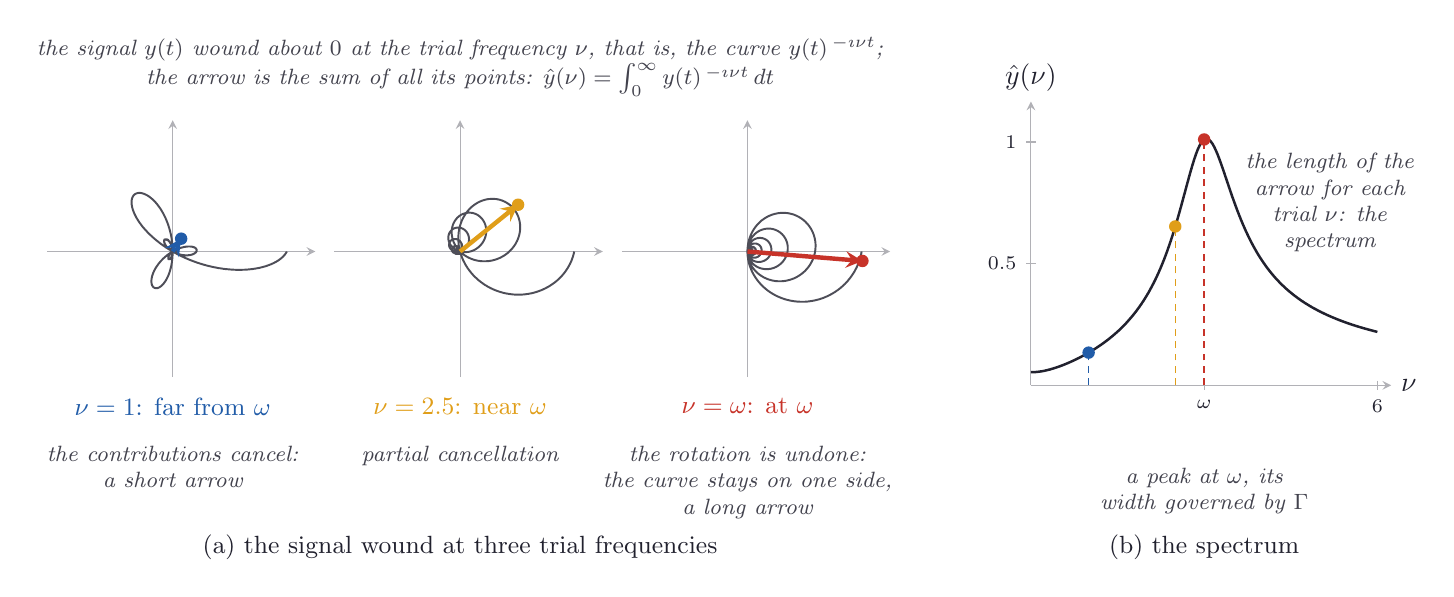
\begin{tikzpicture}[ink/.style={line width=0.9pt, ndInk}, faint/.style={line width=0.4pt, ndInk!35}, dashedink/.style={line width=0.5pt, ndInk!55, dash pattern=on 2.5pt off 2pt}, vec/.style={->, >=stealth, line width=1.2pt}, note/.style={font=\footnotesize\itshape, text=ndInk!85, align=center}, pointer/.style={->, >=stealth, line width=0.4pt, ndInk!60, shorten >=2pt, shorten <=1pt}, dot/.style={circle, fill=ndInk, inner sep=0pt, minimum size=3.4pt}, wash/.style={fill=ndSky, fill opacity=0.55}, every node/.style={text=ndInk}]
\definecolor{ndInk}{rgb}{0.13,0.13,0.18}
\definecolor{ndPaper}{rgb}{0.99,0.96,0.88}
\definecolor{ndSky}{rgb}{0.84,0.91,0.98}
\definecolor{ndRose}{rgb}{0.98,0.86,0.84}
\definecolor{ndBlue}{rgb}{0.13,0.36,0.66}
\definecolor{ndRed}{rgb}{0.78,0.20,0.16}
\definecolor{ndGold}{rgb}{0.88,0.62,0.10}
\definecolor{ndGreen}{rgb}{0.18,0.52,0.30}
\draw[faint, ->, >=stealth] (-1.595,0.000) -- (1.812,0.000);
\draw[faint, ->, >=stealth] (0.000,-1.595) -- (0.000,1.667);
\draw[line width=0.7pt, ndInk!80] (1.450,0.000) -- (1.448,-0.005) -- (1.445,-0.010) -- (1.442,-0.014) -- (1.439,-0.019) -- (1.436,-0.024) -- (1.433,-0.029) -- (1.429,-0.033) -- (1.426,-0.038) -- (1.422,-0.043) -- (1.418,-0.047) -- (1.414,-0.052) -- (1.410,-0.056) -- (1.406,-0.061) -- (1.401,-0.065) -- (1.397,-0.070) -- (1.392,-0.074) -- (1.387,-0.079) -- (1.382,-0.083) -- (1.377,-0.087) -- (1.371,-0.092) -- (1.366,-0.096) -- (1.360,-0.100) -- (1.355,-0.104) -- (1.349,-0.108) -- (1.343,-0.112) -- (1.337,-0.116) -- (1.331,-0.120) -- (1.324,-0.124) -- (1.318,-0.128) -- (1.311,-0.132) -- (1.304,-0.135) -- (1.297,-0.139) -- (1.290,-0.143) -- (1.283,-0.146) -- (1.276,-0.150) -- (1.269,-0.153) -- (1.261,-0.156) -- (1.254,-0.160) -- (1.246,-0.163) -- (1.238,-0.166) -- (1.230,-0.169) -- (1.222,-0.172) -- (1.214,-0.175) -- (1.206,-0.178) -- (1.198,-0.181) -- (1.189,-0.184) -- (1.181,-0.187) -- (1.172,-0.189) -- (1.163,-0.192) -- (1.154,-0.194) -- (1.145,-0.197) -- (1.136,-0.199) -- (1.127,-0.201) -- (1.118,-0.204) -- (1.109,-0.206) -- (1.099,-0.208) -- (1.090,-0.210) -- (1.080,-0.212) -- (1.071,-0.213) -- (1.061,-0.215) -- (1.051,-0.217) -- (1.041,-0.218) -- (1.031,-0.220) -- (1.021,-0.221) -- (1.011,-0.223) -- (1.001,-0.224) -- (0.991,-0.225) -- (0.981,-0.226) -- (0.970,-0.227) -- (0.960,-0.228) -- (0.949,-0.229) -- (0.939,-0.230) -- (0.928,-0.231) -- (0.918,-0.231) -- (0.907,-0.232) -- (0.896,-0.232) -- (0.885,-0.232) -- (0.874,-0.233) -- (0.864,-0.233) -- (0.853,-0.233) -- (0.842,-0.233) -- (0.831,-0.233) -- (0.819,-0.233) -- (0.808,-0.233) -- (0.797,-0.232) -- (0.786,-0.232) -- (0.775,-0.231) -- (0.763,-0.231) -- (0.752,-0.230) -- (0.741,-0.229) -- (0.729,-0.228) -- (0.718,-0.227) -- (0.707,-0.226) -- (0.695,-0.225) -- (0.684,-0.224) -- (0.672,-0.223) -- (0.661,-0.222) -- (0.649,-0.220) -- (0.638,-0.219) -- (0.626,-0.217) -- (0.615,-0.215) -- (0.603,-0.213) -- (0.592,-0.212) -- (0.580,-0.210) -- (0.569,-0.208) -- (0.557,-0.205) -- (0.545,-0.203) -- (0.534,-0.201) -- (0.522,-0.199) -- (0.511,-0.196) -- (0.499,-0.194) -- (0.488,-0.191) -- (0.476,-0.188) -- (0.465,-0.186) -- (0.453,-0.183) -- (0.442,-0.180) -- (0.430,-0.177) -- (0.419,-0.174) -- (0.407,-0.171) -- (0.396,-0.167) -- (0.384,-0.164) -- (0.373,-0.161) -- (0.362,-0.157) -- (0.350,-0.154) -- (0.339,-0.150) -- (0.328,-0.146) -- (0.316,-0.143) -- (0.305,-0.139) -- (0.294,-0.135) -- (0.283,-0.131) -- (0.272,-0.127) -- (0.261,-0.123) -- (0.250,-0.119) -- (0.239,-0.114) -- (0.228,-0.110) -- (0.217,-0.106) -- (0.206,-0.101) -- (0.195,-0.097) -- (0.185,-0.092) -- (0.174,-0.088) -- (0.163,-0.083) -- (0.153,-0.078) -- (0.142,-0.073) -- (0.131,-0.068) -- (0.121,-0.064) -- (0.111,-0.059) -- (0.100,-0.053) -- (0.090,-0.048) -- (0.080,-0.043) -- (0.070,-0.038) -- (0.059,-0.033) -- (0.049,-0.027) -- (0.039,-0.022) -- (0.030,-0.017) -- (0.020,-0.011) -- (0.010,-0.006) -- (0.000,-0.000) -- (-0.009,0.005) -- (-0.019,0.011) -- (-0.028,0.017) -- (-0.038,0.023) -- (-0.047,0.028) -- (-0.056,0.034) -- (-0.066,0.040) -- (-0.075,0.046) -- (-0.084,0.052) -- (-0.093,0.058) -- (-0.102,0.064) -- (-0.110,0.070) -- (-0.119,0.076) -- (-0.128,0.082) -- (-0.136,0.088) -- (-0.145,0.094) -- (-0.153,0.100) -- (-0.162,0.107) -- (-0.170,0.113) -- (-0.178,0.119) -- (-0.186,0.126) -- (-0.194,0.132) -- (-0.202,0.138) -- (-0.210,0.145) -- (-0.217,0.151) -- (-0.225,0.157) -- (-0.233,0.164) -- (-0.240,0.170) -- (-0.247,0.177) -- (-0.255,0.183) -- (-0.262,0.190) -- (-0.269,0.196) -- (-0.276,0.203) -- (-0.283,0.209) -- (-0.289,0.216) -- (-0.296,0.222) -- (-0.303,0.229) -- (-0.309,0.235) -- (-0.316,0.242) -- (-0.322,0.248) -- (-0.328,0.255) -- (-0.334,0.261) -- (-0.340,0.268) -- (-0.346,0.274) -- (-0.352,0.281) -- (-0.358,0.287) -- (-0.363,0.294) -- (-0.369,0.300) -- (-0.374,0.307) -- (-0.380,0.313) -- (-0.385,0.320) -- (-0.390,0.326) -- (-0.395,0.333) -- (-0.400,0.339) -- (-0.405,0.346) -- (-0.409,0.352) -- (-0.414,0.358) -- (-0.419,0.365) -- (-0.423,0.371) -- (-0.427,0.377) -- (-0.432,0.384) -- (-0.436,0.390) -- (-0.440,0.396) -- (-0.444,0.403) -- (-0.447,0.409) -- (-0.451,0.415) -- (-0.455,0.421) -- (-0.458,0.427) -- (-0.462,0.433) -- (-0.465,0.439) -- (-0.468,0.445) -- (-0.471,0.451) -- (-0.474,0.457) -- (-0.477,0.463) -- (-0.480,0.469) -- (-0.483,0.475) -- (-0.486,0.481) -- (-0.488,0.486) -- (-0.491,0.492) -- (-0.493,0.498) -- (-0.495,0.503) -- (-0.497,0.509) -- (-0.500,0.515) -- (-0.501,0.520) -- (-0.503,0.526) -- (-0.505,0.531) -- (-0.507,0.536) -- (-0.508,0.542) -- (-0.510,0.547) -- (-0.511,0.552) -- (-0.513,0.557) -- (-0.514,0.562) -- (-0.515,0.567) -- (-0.516,0.572) -- (-0.517,0.577) -- (-0.518,0.582) -- (-0.519,0.587) -- (-0.519,0.592) -- (-0.520,0.596) -- (-0.520,0.601) -- (-0.521,0.605) -- (-0.521,0.610) -- (-0.522,0.614) -- (-0.522,0.619) -- (-0.522,0.623) -- (-0.522,0.627) -- (-0.522,0.631) -- (-0.522,0.636) -- (-0.521,0.640) -- (-0.521,0.644) -- (-0.521,0.647) -- (-0.520,0.651) -- (-0.520,0.655) -- (-0.519,0.659) -- (-0.518,0.662) -- (-0.517,0.666) -- (-0.517,0.669) -- (-0.516,0.673) -- (-0.515,0.676) -- (-0.513,0.679) -- (-0.512,0.683) -- (-0.511,0.686) -- (-0.510,0.689) -- (-0.508,0.692) -- (-0.507,0.695) -- (-0.505,0.697) -- (-0.504,0.700) -- (-0.502,0.703) -- (-0.501,0.705) -- (-0.499,0.708) -- (-0.497,0.710) -- (-0.495,0.713) -- (-0.493,0.715) -- (-0.491,0.717) -- (-0.489,0.719) -- (-0.487,0.721) -- (-0.485,0.723) -- (-0.482,0.725) -- (-0.480,0.727) -- (-0.478,0.728) -- (-0.475,0.730) -- (-0.473,0.731) -- (-0.470,0.733) -- (-0.468,0.734) -- (-0.465,0.735) -- (-0.462,0.737) -- (-0.460,0.738) -- (-0.457,0.739) -- (-0.454,0.740) -- (-0.451,0.740) -- (-0.448,0.741) -- (-0.445,0.742) -- (-0.442,0.742) -- (-0.439,0.743) -- (-0.436,0.743) -- (-0.433,0.744) -- (-0.430,0.744) -- (-0.426,0.744) -- (-0.423,0.744) -- (-0.420,0.744) -- (-0.417,0.744) -- (-0.413,0.744) -- (-0.410,0.744) -- (-0.406,0.743) -- (-0.403,0.743) -- (-0.399,0.742) -- (-0.396,0.742) -- (-0.392,0.741) -- (-0.389,0.740) -- (-0.385,0.739) -- (-0.382,0.738) -- (-0.378,0.737) -- (-0.374,0.736) -- (-0.371,0.735) -- (-0.367,0.734) -- (-0.363,0.732) -- (-0.359,0.731) -- (-0.356,0.729) -- (-0.352,0.728) -- (-0.348,0.726) -- (-0.344,0.724) -- (-0.340,0.722) -- (-0.337,0.720) -- (-0.333,0.718) -- (-0.329,0.716) -- (-0.325,0.714) -- (-0.321,0.712) -- (-0.317,0.709) -- (-0.313,0.707) -- (-0.309,0.704) -- (-0.305,0.702) -- (-0.301,0.699) -- (-0.297,0.696) -- (-0.294,0.694) -- (-0.290,0.691) -- (-0.286,0.688) -- (-0.282,0.685) -- (-0.278,0.681) -- (-0.274,0.678) -- (-0.270,0.675) -- (-0.266,0.672) -- (-0.262,0.668) -- (-0.258,0.665) -- (-0.254,0.661) -- (-0.250,0.657) -- (-0.246,0.654) -- (-0.242,0.650) -- (-0.239,0.646) -- (-0.235,0.642) -- (-0.231,0.638) -- (-0.227,0.634) -- (-0.223,0.630) -- (-0.219,0.626) -- (-0.215,0.622) -- (-0.212,0.617) -- (-0.208,0.613) -- (-0.204,0.608) -- (-0.200,0.604) -- (-0.197,0.599) -- (-0.193,0.595) -- (-0.189,0.590) -- (-0.186,0.585) -- (-0.182,0.580) -- (-0.178,0.575) -- (-0.175,0.570) -- (-0.171,0.565) -- (-0.167,0.560) -- (-0.164,0.555) -- (-0.160,0.550) -- (-0.157,0.545) -- (-0.153,0.540) -- (-0.150,0.534) -- (-0.147,0.529) -- (-0.143,0.523) -- (-0.140,0.518) -- (-0.136,0.512) -- (-0.133,0.507) -- (-0.130,0.501) -- (-0.127,0.495) -- (-0.123,0.490) -- (-0.120,0.484) -- (-0.117,0.478) -- (-0.114,0.472) -- (-0.111,0.466) -- (-0.108,0.460) -- (-0.105,0.454) -- (-0.102,0.448) -- (-0.099,0.442) -- (-0.096,0.436) -- (-0.093,0.430) -- (-0.090,0.424) -- (-0.088,0.418) -- (-0.085,0.411) -- (-0.082,0.405) -- (-0.080,0.399) -- (-0.077,0.392) -- (-0.074,0.386) -- (-0.072,0.379) -- (-0.069,0.373) -- (-0.067,0.367) -- (-0.064,0.360) -- (-0.062,0.354) -- (-0.060,0.347) -- (-0.057,0.340) -- (-0.055,0.334) -- (-0.053,0.327) -- (-0.051,0.320) -- (-0.049,0.314) -- (-0.047,0.307) -- (-0.044,0.300) -- (-0.042,0.294) -- (-0.041,0.287) -- (-0.039,0.280) -- (-0.037,0.273) -- (-0.035,0.267) -- (-0.033,0.260) -- (-0.031,0.253) -- (-0.030,0.246) -- (-0.028,0.239) -- (-0.027,0.232) -- (-0.025,0.226) -- (-0.023,0.219) -- (-0.022,0.212) -- (-0.021,0.205) -- (-0.019,0.198) -- (-0.018,0.191) -- (-0.017,0.184) -- (-0.015,0.177) -- (-0.014,0.171) -- (-0.013,0.164) -- (-0.012,0.157) -- (-0.011,0.150) -- (-0.010,0.143) -- (-0.009,0.136) -- (-0.008,0.129) -- (-0.007,0.122) -- (-0.007,0.115) -- (-0.006,0.109) -- (-0.005,0.102) -- (-0.004,0.095) -- (-0.004,0.088) -- (-0.003,0.081) -- (-0.003,0.074) -- (-0.002,0.068) -- (-0.002,0.061) -- (-0.001,0.054) -- (-0.001,0.047) -- (-0.001,0.041) -- (-0.001,0.034) -- (-0.000,0.027) -- (-0.000,0.020) -- (-0.000,0.014) -- (-0.000,0.007) -- (-0.000,0.001) -- (-0.000,-0.006) -- (-0.000,-0.013) -- (-0.000,-0.019) -- (-0.000,-0.026) -- (-0.001,-0.032) -- (-0.001,-0.039) -- (-0.001,-0.045) -- (-0.001,-0.052) -- (-0.002,-0.058) -- (-0.002,-0.064) -- (-0.003,-0.071) -- (-0.003,-0.077) -- (-0.004,-0.083) -- (-0.004,-0.090) -- (-0.005,-0.096) -- (-0.005,-0.102) -- (-0.006,-0.108) -- (-0.007,-0.114) -- (-0.008,-0.120) -- (-0.008,-0.126) -- (-0.009,-0.132) -- (-0.010,-0.138) -- (-0.011,-0.144) -- (-0.012,-0.150) -- (-0.013,-0.156) -- (-0.014,-0.162) -- (-0.015,-0.167) -- (-0.016,-0.173) -- (-0.017,-0.179) -- (-0.018,-0.185) -- (-0.020,-0.190) -- (-0.021,-0.196) -- (-0.022,-0.201) -- (-0.023,-0.207) -- (-0.025,-0.212) -- (-0.026,-0.217) -- (-0.028,-0.223) -- (-0.029,-0.228) -- (-0.030,-0.233) -- (-0.032,-0.238) -- (-0.033,-0.243) -- (-0.035,-0.249) -- (-0.037,-0.254) -- (-0.038,-0.259) -- (-0.040,-0.263) -- (-0.041,-0.268) -- (-0.043,-0.273) -- (-0.045,-0.278) -- (-0.047,-0.283) -- (-0.048,-0.287) -- (-0.050,-0.292) -- (-0.052,-0.296) -- (-0.054,-0.301) -- (-0.055,-0.305) -- (-0.057,-0.310) -- (-0.059,-0.314) -- (-0.061,-0.318) -- (-0.063,-0.323) -- (-0.065,-0.327) -- (-0.067,-0.331) -- (-0.069,-0.335) -- (-0.071,-0.339) -- (-0.073,-0.343) -- (-0.075,-0.347) -- (-0.077,-0.350) -- (-0.079,-0.354) -- (-0.081,-0.358) -- (-0.083,-0.361) -- (-0.085,-0.365) -- (-0.088,-0.369) -- (-0.090,-0.372) -- (-0.092,-0.375) -- (-0.094,-0.379) -- (-0.096,-0.382) -- (-0.098,-0.385) -- (-0.100,-0.388) -- (-0.103,-0.391) -- (-0.105,-0.394) -- (-0.107,-0.397) -- (-0.109,-0.400) -- (-0.111,-0.403) -- (-0.114,-0.406) -- (-0.116,-0.409) -- (-0.118,-0.411) -- (-0.120,-0.414) -- (-0.123,-0.416) -- (-0.125,-0.419) -- (-0.127,-0.421) -- (-0.129,-0.423) -- (-0.132,-0.426) -- (-0.134,-0.428) -- (-0.136,-0.430) -- (-0.138,-0.432) -- (-0.141,-0.434) -- (-0.143,-0.436) -- (-0.145,-0.438) -- (-0.147,-0.440) -- (-0.150,-0.442) -- (-0.152,-0.443) -- (-0.154,-0.445) -- (-0.156,-0.446) -- (-0.158,-0.448) -- (-0.161,-0.449) -- (-0.163,-0.451) -- (-0.165,-0.452) -- (-0.167,-0.453) -- (-0.169,-0.455) -- (-0.171,-0.456) -- (-0.174,-0.457) -- (-0.176,-0.458) -- (-0.178,-0.459) -- (-0.180,-0.460) -- (-0.182,-0.461) -- (-0.184,-0.461) -- (-0.186,-0.462) -- (-0.188,-0.463) -- (-0.190,-0.463) -- (-0.192,-0.464) -- (-0.194,-0.464) -- (-0.196,-0.465) -- (-0.198,-0.465) -- (-0.200,-0.465) -- (-0.202,-0.466) -- (-0.204,-0.466) -- (-0.206,-0.466) -- (-0.208,-0.466) -- (-0.210,-0.466) -- (-0.212,-0.466) -- (-0.214,-0.466) -- (-0.215,-0.466) -- (-0.217,-0.465) -- (-0.219,-0.465) -- (-0.221,-0.465) -- (-0.222,-0.464) -- (-0.224,-0.464) -- (-0.226,-0.463) -- (-0.227,-0.463) -- (-0.229,-0.462) -- (-0.230,-0.461) -- (-0.232,-0.461) -- (-0.234,-0.460) -- (-0.235,-0.459) -- (-0.237,-0.458) -- (-0.238,-0.457) -- (-0.239,-0.456) -- (-0.241,-0.455) -- (-0.242,-0.454) -- (-0.244,-0.453) -- (-0.245,-0.452) -- (-0.246,-0.451) -- (-0.247,-0.449) -- (-0.249,-0.448) -- (-0.250,-0.447) -- (-0.251,-0.445) -- (-0.252,-0.444) -- (-0.253,-0.442) -- (-0.254,-0.441) -- (-0.255,-0.439) -- (-0.256,-0.438) -- (-0.257,-0.436) -- (-0.258,-0.434) -- (-0.259,-0.432) -- (-0.260,-0.431) -- (-0.261,-0.429) -- (-0.262,-0.427) -- (-0.262,-0.425) -- (-0.263,-0.423) -- (-0.264,-0.421) -- (-0.264,-0.419) -- (-0.265,-0.417) -- (-0.266,-0.415) -- (-0.266,-0.412) -- (-0.267,-0.410) -- (-0.267,-0.408) -- (-0.268,-0.406) -- (-0.268,-0.403) -- (-0.268,-0.401) -- (-0.269,-0.399) -- (-0.269,-0.396) -- (-0.269,-0.394) -- (-0.270,-0.391) -- (-0.270,-0.389) -- (-0.270,-0.386) -- (-0.270,-0.384) -- (-0.270,-0.381) -- (-0.270,-0.378) -- (-0.270,-0.376) -- (-0.270,-0.373) -- (-0.270,-0.370) -- (-0.270,-0.367) -- (-0.270,-0.365) -- (-0.269,-0.362) -- (-0.269,-0.359) -- (-0.269,-0.356) -- (-0.269,-0.353) -- (-0.268,-0.350) -- (-0.268,-0.347) -- (-0.267,-0.345) -- (-0.267,-0.342) -- (-0.266,-0.339) -- (-0.266,-0.336) -- (-0.265,-0.333) -- (-0.265,-0.329) -- (-0.264,-0.326) -- (-0.263,-0.323) -- (-0.262,-0.320) -- (-0.262,-0.317) -- (-0.261,-0.314) -- (-0.260,-0.311) -- (-0.259,-0.308) -- (-0.258,-0.304) -- (-0.257,-0.301) -- (-0.256,-0.298) -- (-0.255,-0.295) -- (-0.254,-0.292) -- (-0.253,-0.288) -- (-0.252,-0.285) -- (-0.250,-0.282) -- (-0.249,-0.279) -- (-0.248,-0.275) -- (-0.247,-0.272) -- (-0.245,-0.269) -- (-0.244,-0.265) -- (-0.242,-0.262) -- (-0.241,-0.259) -- (-0.239,-0.255) -- (-0.238,-0.252) -- (-0.236,-0.249) -- (-0.235,-0.245) -- (-0.233,-0.242) -- (-0.231,-0.239) -- (-0.230,-0.235) -- (-0.228,-0.232) -- (-0.226,-0.229) -- (-0.224,-0.225) -- (-0.222,-0.222) -- (-0.221,-0.219) -- (-0.219,-0.215) -- (-0.217,-0.212) -- (-0.215,-0.209) -- (-0.213,-0.205) -- (-0.211,-0.202) -- (-0.209,-0.199) -- (-0.206,-0.195) -- (-0.204,-0.192) -- (-0.202,-0.189) -- (-0.200,-0.185) -- (-0.198,-0.182) -- (-0.195,-0.179) -- (-0.193,-0.175) -- (-0.191,-0.172) -- (-0.188,-0.169) -- (-0.186,-0.166) -- (-0.184,-0.162) -- (-0.181,-0.159) -- (-0.179,-0.156) -- (-0.176,-0.153) -- (-0.174,-0.149) -- (-0.171,-0.146) -- (-0.168,-0.143) -- (-0.166,-0.140) -- (-0.163,-0.137) -- (-0.160,-0.134) -- (-0.158,-0.130) -- (-0.155,-0.127) -- (-0.152,-0.124) -- (-0.150,-0.121) -- (-0.147,-0.118) -- (-0.144,-0.115) -- (-0.141,-0.112) -- (-0.138,-0.109) -- (-0.135,-0.106) -- (-0.132,-0.103) -- (-0.130,-0.100) -- (-0.127,-0.097) -- (-0.124,-0.094) -- (-0.121,-0.091) -- (-0.118,-0.088) -- (-0.115,-0.085) -- (-0.112,-0.083) -- (-0.109,-0.080) -- (-0.105,-0.077) -- (-0.102,-0.074) -- (-0.099,-0.071) -- (-0.096,-0.069) -- (-0.093,-0.066) -- (-0.090,-0.063) -- (-0.087,-0.061) -- (-0.083,-0.058) -- (-0.080,-0.055) -- (-0.077,-0.053) -- (-0.074,-0.050) -- (-0.071,-0.048) -- (-0.067,-0.045) -- (-0.064,-0.043) -- (-0.061,-0.040) -- (-0.057,-0.038) -- (-0.054,-0.035) -- (-0.051,-0.033) -- (-0.048,-0.031) -- (-0.044,-0.028) -- (-0.041,-0.026) -- (-0.038,-0.024) -- (-0.034,-0.021) -- (-0.031,-0.019) -- (-0.028,-0.017) -- (-0.024,-0.015) -- (-0.021,-0.013) -- (-0.017,-0.010) -- (-0.014,-0.008) -- (-0.011,-0.006) -- (-0.007,-0.004) -- (-0.004,-0.002) -- (-0.000,-0.000) -- (0.003,0.002) -- (0.006,0.004) -- (0.010,0.005) -- (0.013,0.007) -- (0.017,0.009) -- (0.020,0.011) -- (0.023,0.013) -- (0.027,0.014) -- (0.030,0.016) -- (0.033,0.018) -- (0.037,0.020) -- (0.040,0.021) -- (0.044,0.023) -- (0.047,0.024) -- (0.050,0.026) -- (0.054,0.027) -- (0.057,0.029) -- (0.060,0.030) -- (0.064,0.032) -- (0.067,0.033) -- (0.070,0.034) -- (0.074,0.036) -- (0.077,0.037) -- (0.080,0.038) -- (0.084,0.039) -- (0.087,0.041) -- (0.090,0.042) -- (0.093,0.043) -- (0.097,0.044) -- (0.100,0.045) -- (0.103,0.046) -- (0.106,0.047) -- (0.110,0.048) -- (0.113,0.049) -- (0.116,0.050) -- (0.119,0.051) -- (0.122,0.052) -- (0.125,0.053) -- (0.128,0.053) -- (0.132,0.054) -- (0.135,0.055) -- (0.138,0.056) -- (0.141,0.056) -- (0.144,0.057) -- (0.147,0.058) -- (0.150,0.058) -- (0.153,0.059) -- (0.156,0.059) -- (0.159,0.060) -- (0.162,0.060) -- (0.164,0.061) -- (0.167,0.061) -- (0.170,0.062) -- (0.173,0.062) -- (0.176,0.062) -- (0.179,0.063) -- (0.181,0.063) -- (0.184,0.063) -- (0.187,0.063) -- (0.189,0.064) -- (0.192,0.064) -- (0.195,0.064) -- (0.197,0.064) -- (0.200,0.064) -- (0.202,0.064) -- (0.205,0.064) -- (0.207,0.064) -- (0.210,0.064) -- (0.212,0.064) -- (0.215,0.064) -- (0.217,0.064) -- (0.220,0.064) -- (0.222,0.064) -- (0.224,0.064) -- (0.227,0.064) -- (0.229,0.063) -- (0.231,0.063) -- (0.233,0.063) -- (0.235,0.063) -- (0.238,0.063) -- (0.240,0.062) -- (0.242,0.062) -- (0.244,0.062) -- (0.246,0.061) -- (0.248,0.061) -- (0.250,0.060) -- (0.252,0.060) -- (0.254,0.060) -- (0.255,0.059) -- (0.257,0.059) -- (0.259,0.058) -- (0.261,0.058) -- (0.263,0.057) -- (0.264,0.056) -- (0.266,0.056) -- (0.268,0.055) -- (0.269,0.055) -- (0.271,0.054) -- (0.272,0.053) -- (0.274,0.053) -- (0.275,0.052) -- (0.277,0.051) -- (0.278,0.051) -- (0.279,0.050) -- (0.281,0.049) -- (0.282,0.049) -- (0.283,0.048) -- (0.285,0.047) -- (0.286,0.046) -- (0.287,0.045) -- (0.288,0.045) -- (0.289,0.044) -- (0.290,0.043) -- (0.291,0.042) -- (0.292,0.041) -- (0.293,0.040) -- (0.294,0.040) -- (0.295,0.039) -- (0.296,0.038) -- (0.296,0.037) -- (0.297,0.036) -- (0.298,0.035) -- (0.299,0.034) -- (0.299,0.033) -- (0.300,0.032) -- (0.301,0.031) -- (0.301,0.030) -- (0.302,0.029) -- (0.302,0.028) -- (0.303,0.027) -- (0.303,0.027) -- (0.303,0.026) -- (0.304,0.025) -- (0.304,0.024) -- (0.304,0.023) -- (0.305,0.022) -- (0.305,0.021) -- (0.305,0.020) -- (0.305,0.018) -- (0.305,0.017) -- (0.305,0.016) -- (0.305,0.015) -- (0.305,0.014) -- (0.305,0.013) -- (0.305,0.012) -- (0.305,0.011) -- (0.305,0.010) -- (0.305,0.009) -- (0.304,0.008) -- (0.304,0.007) -- (0.304,0.006) -- (0.304,0.005) -- (0.303,0.004) -- (0.303,0.003) -- (0.302,0.002) -- (0.302,0.001) -- (0.302,0.000) -- (0.301,-0.001) -- (0.300,-0.002) -- (0.300,-0.003) -- (0.299,-0.004) -- (0.299,-0.005) -- (0.298,-0.006) -- (0.297,-0.007) -- (0.296,-0.008) -- (0.296,-0.009) -- (0.295,-0.010) -- (0.294,-0.011) -- (0.293,-0.012) -- (0.292,-0.013) -- (0.291,-0.013) -- (0.290,-0.014) -- (0.289,-0.015) -- (0.288,-0.016) -- (0.287,-0.017) -- (0.286,-0.018) -- (0.285,-0.019) -- (0.284,-0.020) -- (0.283,-0.021) -- (0.282,-0.022) -- (0.281,-0.022) -- (0.279,-0.023) -- (0.278,-0.024) -- (0.277,-0.025) -- (0.275,-0.026) -- (0.274,-0.026) -- (0.273,-0.027) -- (0.271,-0.028) -- (0.270,-0.029) -- (0.268,-0.030) -- (0.267,-0.030) -- (0.266,-0.031) -- (0.264,-0.032) -- (0.262,-0.032) -- (0.261,-0.033) -- (0.259,-0.034) -- (0.258,-0.034) -- (0.256,-0.035) -- (0.254,-0.036) -- (0.253,-0.036) -- (0.251,-0.037) -- (0.249,-0.038) -- (0.247,-0.038) -- (0.246,-0.039) -- (0.244,-0.039) -- (0.242,-0.040) -- (0.240,-0.040) -- (0.238,-0.041) -- (0.237,-0.041) -- (0.235,-0.042) -- (0.233,-0.042) -- (0.231,-0.043) -- (0.229,-0.043) -- (0.227,-0.044) -- (0.225,-0.044) -- (0.223,-0.044) -- (0.221,-0.045) -- (0.219,-0.045) -- (0.217,-0.045) -- (0.215,-0.046) -- (0.213,-0.046) -- (0.211,-0.046) -- (0.208,-0.047) -- (0.206,-0.047) -- (0.204,-0.047) -- (0.202,-0.047) -- (0.200,-0.047) -- (0.198,-0.048) -- (0.196,-0.048) -- (0.193,-0.048) -- (0.191,-0.048) -- (0.189,-0.048) -- (0.187,-0.048) -- (0.184,-0.048) -- (0.182,-0.048) -- (0.180,-0.048) -- (0.178,-0.048) -- (0.175,-0.048) -- (0.173,-0.048) -- (0.171,-0.048) -- (0.168,-0.048) -- (0.166,-0.048) -- (0.164,-0.048) -- (0.161,-0.048) -- (0.159,-0.048) -- (0.157,-0.048) -- (0.154,-0.048) -- (0.152,-0.048) -- (0.150,-0.047) -- (0.147,-0.047) -- (0.145,-0.047) -- (0.143,-0.047) -- (0.140,-0.046) -- (0.138,-0.046) -- (0.135,-0.046) -- (0.133,-0.045) -- (0.131,-0.045) -- (0.128,-0.045) -- (0.126,-0.044) -- (0.123,-0.044) -- (0.121,-0.044) -- (0.119,-0.043) -- (0.116,-0.043) -- (0.114,-0.042) -- (0.111,-0.042) -- (0.109,-0.041) -- (0.107,-0.041) -- (0.104,-0.040) -- (0.102,-0.040) -- (0.099,-0.039) -- (0.097,-0.039) -- (0.095,-0.038) -- (0.092,-0.037) -- (0.090,-0.037) -- (0.087,-0.036) -- (0.085,-0.036) -- (0.083,-0.035) -- (0.080,-0.034) -- (0.078,-0.034) -- (0.076,-0.033) -- (0.073,-0.032) -- (0.071,-0.031) -- (0.069,-0.031) -- (0.066,-0.030) -- (0.064,-0.029) -- (0.062,-0.028) -- (0.059,-0.027) -- (0.057,-0.027) -- (0.055,-0.026) -- (0.052,-0.025) -- (0.050,-0.024) -- (0.048,-0.023) -- (0.045,-0.022) -- (0.043,-0.021) -- (0.041,-0.020) -- (0.039,-0.019) -- (0.036,-0.018) -- (0.034,-0.017) -- (0.032,-0.016) -- (0.030,-0.015) -- (0.028,-0.014) -- (0.026,-0.013) -- (0.023,-0.012) -- (0.021,-0.011) -- (0.019,-0.010) -- (0.017,-0.009) -- (0.015,-0.008) -- (0.013,-0.007) -- (0.011,-0.006) -- (0.009,-0.005) -- (0.006,-0.004) -- (0.004,-0.003) -- (0.002,-0.001) -- (0.000,-0.000) -- (-0.002,0.001) -- (-0.004,0.002) -- (-0.006,0.003) -- (-0.008,0.004) -- (-0.009,0.006) -- (-0.011,0.007) -- (-0.013,0.008) -- (-0.015,0.009) -- (-0.017,0.011) -- (-0.019,0.012) -- (-0.021,0.013) -- (-0.023,0.014) -- (-0.024,0.016) -- (-0.026,0.017) -- (-0.028,0.018) -- (-0.030,0.019) -- (-0.032,0.021) -- (-0.033,0.022) -- (-0.035,0.023) -- (-0.037,0.025) -- (-0.038,0.026) -- (-0.040,0.027) -- (-0.042,0.029) -- (-0.043,0.030) -- (-0.045,0.031) -- (-0.047,0.032) -- (-0.048,0.034) -- (-0.050,0.035) -- (-0.051,0.036) -- (-0.053,0.038) -- (-0.054,0.039) -- (-0.056,0.041) -- (-0.057,0.042) -- (-0.059,0.043) -- (-0.060,0.045) -- (-0.061,0.046) -- (-0.063,0.047) -- (-0.064,0.049) -- (-0.065,0.050) -- (-0.067,0.051) -- (-0.068,0.053) -- (-0.069,0.054) -- (-0.071,0.055) -- (-0.072,0.057) -- (-0.073,0.058) -- (-0.074,0.060) -- (-0.075,0.061) -- (-0.076,0.062) -- (-0.078,0.064) -- (-0.079,0.065) -- (-0.080,0.066) -- (-0.081,0.068) -- (-0.082,0.069) -- (-0.083,0.070) -- (-0.084,0.072) -- (-0.085,0.073) -- (-0.086,0.074) -- (-0.087,0.076) -- (-0.088,0.077) -- (-0.089,0.078) -- (-0.090,0.080) -- (-0.090,0.081) -- (-0.091,0.082) -- (-0.092,0.083) -- (-0.093,0.085) -- (-0.094,0.086) -- (-0.094,0.087) -- (-0.095,0.089) -- (-0.096,0.090) -- (-0.097,0.091) -- (-0.097,0.092) -- (-0.098,0.094) -- (-0.099,0.095) -- (-0.099,0.096) -- (-0.100,0.097) -- (-0.100,0.099) -- (-0.101,0.100) -- (-0.101,0.101) -- (-0.102,0.102) -- (-0.102,0.103) -- (-0.103,0.104) -- (-0.103,0.106) -- (-0.104,0.107) -- (-0.104,0.108) -- (-0.105,0.109) -- (-0.105,0.110) -- (-0.105,0.111) -- (-0.106,0.112) -- (-0.106,0.113) -- (-0.106,0.115) -- (-0.107,0.116) -- (-0.107,0.117) -- (-0.107,0.118) -- (-0.107,0.119) -- (-0.107,0.120) -- (-0.108,0.121) -- (-0.108,0.122) -- (-0.108,0.123) -- (-0.108,0.124) -- (-0.108,0.125) -- (-0.108,0.126) -- (-0.108,0.127) -- (-0.108,0.128) -- (-0.108,0.128) -- (-0.108,0.129) -- (-0.108,0.130) -- (-0.108,0.131) -- (-0.108,0.132) -- (-0.108,0.133) -- (-0.108,0.134) -- (-0.108,0.134) -- (-0.108,0.135) -- (-0.108,0.136) -- (-0.108,0.137) -- (-0.108,0.138) -- (-0.108,0.138) -- (-0.107,0.139) -- (-0.107,0.140) -- (-0.107,0.140) -- (-0.107,0.141) -- (-0.107,0.142) -- (-0.106,0.142) -- (-0.106,0.143) -- (-0.106,0.144) -- (-0.105,0.144) -- (-0.105,0.145) -- (-0.105,0.145) -- (-0.104,0.146) -- (-0.104,0.147) -- (-0.104,0.147) -- (-0.103,0.148) -- (-0.103,0.148) -- (-0.103,0.149) -- (-0.102,0.149) -- (-0.102,0.149) -- (-0.101,0.150) -- (-0.101,0.150) -- (-0.100,0.151) -- (-0.100,0.151) -- (-0.099,0.151) -- (-0.099,0.152) -- (-0.098,0.152) -- (-0.098,0.152) -- (-0.097,0.153) -- (-0.097,0.153) -- (-0.096,0.153) -- (-0.096,0.153) -- (-0.095,0.154) -- (-0.094,0.154) -- (-0.094,0.154) -- (-0.093,0.154) -- (-0.093,0.154) -- (-0.092,0.154) -- (-0.091,0.154) -- (-0.091,0.155) -- (-0.090,0.155) -- (-0.089,0.155) -- (-0.089,0.155) -- (-0.088,0.155) -- (-0.087,0.155) -- (-0.087,0.155) -- (-0.086,0.155) -- (-0.085,0.155) -- (-0.085,0.154) -- (-0.084,0.154) -- (-0.083,0.154) -- (-0.082,0.154) -- (-0.082,0.154) -- (-0.081,0.154) -- (-0.080,0.154) -- (-0.079,0.154) -- (-0.079,0.153) -- (-0.078,0.153) -- (-0.077,0.153) -- (-0.076,0.153) -- (-0.076,0.152) -- (-0.075,0.152) -- (-0.074,0.152) -- (-0.073,0.151) -- (-0.072,0.151) -- (-0.072,0.151) -- (-0.071,0.150) -- (-0.070,0.150) -- (-0.069,0.149) -- (-0.068,0.149) -- (-0.068,0.148) -- (-0.067,0.148) -- (-0.066,0.148) -- (-0.065,0.147) -- (-0.064,0.147) -- (-0.064,0.146) -- (-0.063,0.145) -- (-0.062,0.145) -- (-0.061,0.144) -- (-0.060,0.144) -- (-0.060,0.143) -- (-0.059,0.142) -- (-0.058,0.142) -- (-0.057,0.141) -- (-0.056,0.140) -- (-0.055,0.140) -- (-0.055,0.139) -- (-0.054,0.138) -- (-0.053,0.138) -- (-0.052,0.137) -- (-0.051,0.136) -- (-0.051,0.135) -- (-0.050,0.134) -- (-0.049,0.134) -- (-0.048,0.133) -- (-0.047,0.132) -- (-0.047,0.131) -- (-0.046,0.130) -- (-0.045,0.129) -- (-0.044,0.128) -- (-0.043,0.128) -- (-0.043,0.127) -- (-0.042,0.126) -- (-0.041,0.125) -- (-0.040,0.124) -- (-0.039,0.123) -- (-0.039,0.122) -- (-0.038,0.121) -- (-0.037,0.120) -- (-0.036,0.119) -- (-0.036,0.118) -- (-0.035,0.117) -- (-0.034,0.116) -- (-0.033,0.115) -- (-0.033,0.113) -- (-0.032,0.112) -- (-0.031,0.111) -- (-0.031,0.110) -- (-0.030,0.109) -- (-0.029,0.108) -- (-0.028,0.107) -- (-0.028,0.106) -- (-0.027,0.104) -- (-0.026,0.103) -- (-0.026,0.102) -- (-0.025,0.101) -- (-0.024,0.100) -- (-0.024,0.098) -- (-0.023,0.097) -- (-0.023,0.096) -- (-0.022,0.095) -- (-0.021,0.093) -- (-0.021,0.092) -- (-0.020,0.091) -- (-0.019,0.090) -- (-0.019,0.088) -- (-0.018,0.087) -- (-0.018,0.086) -- (-0.017,0.084) -- (-0.017,0.083) -- (-0.016,0.082) -- (-0.016,0.080) -- (-0.015,0.079) -- (-0.014,0.078) -- (-0.014,0.076) -- (-0.013,0.075) -- (-0.013,0.074) -- (-0.012,0.072) -- (-0.012,0.071) -- (-0.012,0.070) -- (-0.011,0.068) -- (-0.011,0.067) -- (-0.010,0.065) -- (-0.010,0.064) -- (-0.009,0.063) -- (-0.009,0.061) -- (-0.008,0.060) -- (-0.008,0.058) -- (-0.008,0.057) -- (-0.007,0.056) -- (-0.007,0.054) -- (-0.007,0.053) -- (-0.006,0.051) -- (-0.006,0.050) -- (-0.006,0.049) -- (-0.005,0.047) -- (-0.005,0.046) -- (-0.005,0.044) -- (-0.004,0.043) -- (-0.004,0.041) -- (-0.004,0.040) -- (-0.004,0.039) -- (-0.003,0.037) -- (-0.003,0.036) -- (-0.003,0.034) -- (-0.003,0.033) -- (-0.002,0.031) -- (-0.002,0.030) -- (-0.002,0.029) -- (-0.002,0.027) -- (-0.002,0.026) -- (-0.001,0.024) -- (-0.001,0.023) -- (-0.001,0.021) -- (-0.001,0.020) -- (-0.001,0.019) -- (-0.001,0.017) -- (-0.001,0.016) -- (-0.000,0.014) -- (-0.000,0.013) -- (-0.000,0.011) -- (-0.000,0.010) -- (-0.000,0.009) -- (-0.000,0.007) -- (-0.000,0.006) -- (-0.000,0.004) -- (-0.000,0.003) -- (-0.000,0.002) -- (-0.000,0.000) -- (-0.000,-0.001) -- (-0.000,-0.002) -- (-0.000,-0.004) -- (-0.000,-0.005) -- (-0.000,-0.006) -- (-0.000,-0.008) -- (-0.000,-0.009) -- (-0.000,-0.011) -- (-0.000,-0.012) -- (-0.000,-0.013) -- (-0.001,-0.014) -- (-0.001,-0.016) -- (-0.001,-0.017) -- (-0.001,-0.018) -- (-0.001,-0.020) -- (-0.001,-0.021) -- (-0.001,-0.022) -- (-0.001,-0.024) -- (-0.002,-0.025) -- (-0.002,-0.026) -- (-0.002,-0.027) -- (-0.002,-0.029) -- (-0.002,-0.030) -- (-0.002,-0.031) -- (-0.003,-0.032) -- (-0.003,-0.033) -- (-0.003,-0.035) -- (-0.003,-0.036) -- (-0.004,-0.037) -- (-0.004,-0.038) -- (-0.004,-0.039) -- (-0.004,-0.040) -- (-0.005,-0.042) -- (-0.005,-0.043) -- (-0.005,-0.044) -- (-0.005,-0.045) -- (-0.006,-0.046) -- (-0.006,-0.047) -- (-0.006,-0.048) -- (-0.007,-0.049) -- (-0.007,-0.050) -- (-0.007,-0.051) -- (-0.008,-0.053) -- (-0.008,-0.054) -- (-0.008,-0.055) -- (-0.009,-0.056) -- (-0.009,-0.057) -- (-0.009,-0.058) -- (-0.010,-0.059) -- (-0.010,-0.060) -- (-0.010,-0.061) -- (-0.011,-0.061) -- (-0.011,-0.062) -- (-0.011,-0.063) -- (-0.012,-0.064) -- (-0.012,-0.065) -- (-0.013,-0.066) -- (-0.013,-0.067) -- (-0.013,-0.068) -- (-0.014,-0.069) -- (-0.014,-0.069) -- (-0.015,-0.070) -- (-0.015,-0.071) -- (-0.016,-0.072) -- (-0.016,-0.073) -- (-0.016,-0.073) -- (-0.017,-0.074) -- (-0.017,-0.075) -- (-0.018,-0.076) -- (-0.018,-0.076) -- (-0.019,-0.077) -- (-0.019,-0.078) -- (-0.019,-0.079) -- (-0.020,-0.079) -- (-0.020,-0.080) -- (-0.021,-0.081) -- (-0.021,-0.081) -- (-0.022,-0.082) -- (-0.022,-0.082) -- (-0.023,-0.083) -- (-0.023,-0.084) -- (-0.024,-0.084) -- (-0.024,-0.085) -- (-0.024,-0.085) -- (-0.025,-0.086) -- (-0.025,-0.086) -- (-0.026,-0.087) -- (-0.026,-0.087) -- (-0.027,-0.088) -- (-0.027,-0.088) -- (-0.028,-0.089) -- (-0.028,-0.089) -- (-0.029,-0.090) -- (-0.029,-0.090) -- (-0.030,-0.091) -- (-0.030,-0.091) -- (-0.031,-0.091) -- (-0.031,-0.092) -- (-0.031,-0.092) -- (-0.032,-0.092) -- (-0.032,-0.093) -- (-0.033,-0.093) -- (-0.033,-0.093) -- (-0.034,-0.094) -- (-0.034,-0.094) -- (-0.035,-0.094) -- (-0.035,-0.094) -- (-0.036,-0.095) -- (-0.036,-0.095) -- (-0.036,-0.095) -- (-0.037,-0.095) -- (-0.037,-0.096) -- (-0.038,-0.096) -- (-0.038,-0.096) -- (-0.039,-0.096) -- (-0.039,-0.096) -- (-0.039,-0.096) -- (-0.040,-0.096) -- (-0.040,-0.096) -- (-0.041,-0.097) -- (-0.041,-0.097) -- (-0.042,-0.097) -- (-0.042,-0.097) -- (-0.042,-0.097) -- (-0.043,-0.097) -- (-0.043,-0.097) -- (-0.044,-0.097) -- (-0.044,-0.097) -- (-0.044,-0.097) -- (-0.045,-0.097) -- (-0.045,-0.097) -- (-0.045,-0.097) -- (-0.046,-0.097) -- (-0.046,-0.097) -- (-0.047,-0.096) -- (-0.047,-0.096) -- (-0.047,-0.096) -- (-0.048,-0.096) -- (-0.048,-0.096) -- (-0.048,-0.096) -- (-0.049,-0.096) -- (-0.049,-0.095) -- (-0.049,-0.095) -- (-0.049,-0.095) -- (-0.050,-0.095) -- (-0.050,-0.095) -- (-0.050,-0.094) -- (-0.051,-0.094) -- (-0.051,-0.094) -- (-0.051,-0.094) -- (-0.051,-0.093) -- (-0.052,-0.093) -- (-0.052,-0.093) -- (-0.052,-0.093) -- (-0.052,-0.092) -- (-0.053,-0.092) -- (-0.053,-0.092) -- (-0.053,-0.091) -- (-0.053,-0.091) -- (-0.053,-0.091) -- (-0.054,-0.090) -- (-0.054,-0.090) -- (-0.054,-0.090) -- (-0.054,-0.089) -- (-0.054,-0.089) -- (-0.055,-0.088) -- (-0.055,-0.088) -- (-0.055,-0.088) -- (-0.055,-0.087) -- (-0.055,-0.087) -- (-0.055,-0.086) -- (-0.055,-0.086) -- (-0.055,-0.085) -- (-0.056,-0.085) -- (-0.056,-0.084) -- (-0.056,-0.084) -- (-0.056,-0.083) -- (-0.056,-0.083) -- (-0.056,-0.082) -- (-0.056,-0.082) -- (-0.056,-0.081) -- (-0.056,-0.081) -- (-0.056,-0.080) -- (-0.056,-0.080) -- (-0.056,-0.079) -- (-0.056,-0.079) -- (-0.056,-0.078) -- (-0.056,-0.078) -- (-0.056,-0.077) -- (-0.056,-0.076) -- (-0.056,-0.076) -- (-0.056,-0.075) -- (-0.056,-0.075) -- (-0.056,-0.074) -- (-0.056,-0.074) -- (-0.056,-0.073) -- (-0.056,-0.072) -- (-0.056,-0.072) -- (-0.055,-0.071) -- (-0.055,-0.070) -- (-0.055,-0.070) -- (-0.055,-0.069) -- (-0.055,-0.069) -- (-0.055,-0.068) -- (-0.055,-0.067) -- (-0.055,-0.067) -- (-0.054,-0.066) -- (-0.054,-0.065) -- (-0.054,-0.065) -- (-0.054,-0.064) -- (-0.054,-0.063) -- (-0.053,-0.063) -- (-0.053,-0.062) -- (-0.053,-0.061) -- (-0.053,-0.061) -- (-0.053,-0.060) -- (-0.052,-0.059) -- (-0.052,-0.059) -- (-0.052,-0.058) -- (-0.052,-0.057) -- (-0.051,-0.057) -- (-0.051,-0.056) -- (-0.051,-0.055) -- (-0.050,-0.055) -- (-0.050,-0.054) -- (-0.050,-0.053) -- (-0.050,-0.053) -- (-0.049,-0.052) -- (-0.049,-0.051) -- (-0.049,-0.050) -- (-0.048,-0.050) -- (-0.048,-0.049) -- (-0.047,-0.048) -- (-0.047,-0.048) -- (-0.047,-0.047) -- (-0.046,-0.046) -- (-0.046,-0.046) -- (-0.046,-0.045) -- (-0.045,-0.044) -- (-0.045,-0.043) -- (-0.044,-0.043) -- (-0.044,-0.042) -- (-0.043,-0.041) -- (-0.043,-0.041) -- (-0.043,-0.040) -- (-0.042,-0.039) -- (-0.042,-0.039) -- (-0.041,-0.038) -- (-0.041,-0.037) -- (-0.040,-0.037) -- (-0.040,-0.036) -- (-0.039,-0.035) -- (-0.039,-0.035) -- (-0.038,-0.034) -- (-0.038,-0.033) -- (-0.037,-0.033) -- (-0.037,-0.032) -- (-0.036,-0.031) -- (-0.036,-0.031) -- (-0.035,-0.030) -- (-0.035,-0.029) -- (-0.034,-0.029) -- (-0.033,-0.028) -- (-0.033,-0.027) -- (-0.032,-0.027) -- (-0.032,-0.026) -- (-0.031,-0.025) -- (-0.031,-0.025) -- (-0.030,-0.024) -- (-0.029,-0.023) -- (-0.029,-0.023) -- (-0.028,-0.022) -- (-0.028,-0.022) -- (-0.027,-0.021) -- (-0.026,-0.020) -- (-0.026,-0.020) -- (-0.025,-0.019) -- (-0.025,-0.018) -- (-0.024,-0.018) -- (-0.023,-0.017) -- (-0.023,-0.017) -- (-0.022,-0.016) -- (-0.021,-0.016) -- (-0.021,-0.015) -- (-0.020,-0.014) -- (-0.019,-0.014) -- (-0.019,-0.013) -- (-0.018,-0.013) -- (-0.017,-0.012) -- (-0.017,-0.012) -- (-0.016,-0.011) -- (-0.015,-0.011) -- (-0.015,-0.010) -- (-0.014,-0.009) -- (-0.013,-0.009) -- (-0.013,-0.008) -- (-0.012,-0.008) -- (-0.011,-0.007) -- (-0.011,-0.007) -- (-0.010,-0.006) -- (-0.009,-0.006) -- (-0.009,-0.005) -- (-0.008,-0.005) -- (-0.007,-0.005) -- (-0.007,-0.004) -- (-0.006,-0.004) -- (-0.005,-0.003) -- (-0.004,-0.003) -- (-0.004,-0.002) -- (-0.003,-0.002) -- (-0.002,-0.001) -- (-0.002,-0.001) -- (-0.001,-0.001) -- (-0.000,-0.000) -- (0.000,0.000) -- (0.001,0.001) -- (0.002,0.001) -- (0.003,0.001) -- (0.003,0.002) -- (0.004,0.002) -- (0.005,0.003) -- (0.005,0.003) -- (0.006,0.003) -- (0.007,0.004) -- (0.008,0.004) -- (0.008,0.004) -- (0.009,0.005) -- (0.010,0.005) -- (0.010,0.005) -- (0.011,0.006) -- (0.012,0.006) -- (0.012,0.006) -- (0.013,0.007) -- (0.014,0.007) -- (0.015,0.007) -- (0.015,0.007) -- (0.016,0.008) -- (0.017,0.008) -- (0.017,0.008) -- (0.018,0.008) -- (0.019,0.009) -- (0.019,0.009) -- (0.020,0.009) -- (0.021,0.009) -- (0.021,0.010) -- (0.022,0.010) -- (0.023,0.010) -- (0.023,0.010) -- (0.024,0.010) -- (0.025,0.011) -- (0.025,0.011) -- (0.026,0.011) -- (0.027,0.011) -- (0.027,0.011) -- (0.028,0.011) -- (0.029,0.012) -- (0.029,0.012) -- (0.030,0.012) -- (0.030,0.012) -- (0.031,0.012) -- (0.032,0.012) -- (0.032,0.012) -- (0.033,0.012) -- (0.033,0.013) -- (0.034,0.013) -- (0.035,0.013) -- (0.035,0.013) -- (0.036,0.013) -- (0.036,0.013) -- (0.037,0.013) -- (0.038,0.013) -- (0.038,0.013) -- (0.039,0.013) -- (0.039,0.013) -- (0.040,0.013) -- (0.040,0.013) -- (0.041,0.013) -- (0.041,0.013) -- (0.042,0.013) -- (0.043,0.013) -- (0.043,0.013) -- (0.044,0.013) -- (0.044,0.013) -- (0.045,0.013) -- (0.045,0.013) -- (0.046,0.013) -- (0.046,0.013) -- (0.047,0.013) -- (0.047,0.013) -- (0.047,0.013) -- (0.048,0.013) -- (0.048,0.013) -- (0.049,0.013) -- (0.049,0.013) -- (0.050,0.013) -- (0.050,0.013) -- (0.051,0.013) -- (0.051,0.013) -- (0.051,0.013) -- (0.052,0.013) -- (0.052,0.012) -- (0.053,0.012) -- (0.053,0.012) -- (0.053,0.012) -- (0.054,0.012) -- (0.054,0.012) -- (0.055,0.012) -- (0.055,0.012) -- (0.055,0.012) -- (0.056,0.012) -- (0.056,0.011) -- (0.056,0.011) -- (0.057,0.011) -- (0.057,0.011) -- (0.057,0.011) -- (0.057,0.011) -- (0.058,0.011) -- (0.058,0.010) -- (0.058,0.010) -- (0.059,0.010) -- (0.059,0.010) -- (0.059,0.010) -- (0.059,0.010) -- (0.060,0.009) -- (0.060,0.009) -- (0.060,0.009) -- (0.060,0.009) -- (0.060,0.009) -- (0.061,0.009) -- (0.061,0.008) -- (0.061,0.008) -- (0.061,0.008) -- (0.061,0.008) -- (0.062,0.008) -- (0.062,0.008) -- (0.062,0.007) -- (0.062,0.007) -- (0.062,0.007) -- (0.062,0.007) -- (0.062,0.007) -- (0.063,0.006) -- (0.063,0.006) -- (0.063,0.006) -- (0.063,0.006) -- (0.063,0.006) -- (0.063,0.005) -- (0.063,0.005) -- (0.063,0.005) -- (0.063,0.005) -- (0.063,0.005) -- (0.063,0.004) -- (0.063,0.004) -- (0.063,0.004) -- (0.063,0.004) -- (0.063,0.003) -- (0.063,0.003) -- (0.063,0.003) -- (0.063,0.003) -- (0.063,0.003) -- (0.063,0.002) -- (0.063,0.002) -- (0.063,0.002) -- (0.063,0.002) -- (0.063,0.002) -- (0.063,0.001) -- (0.063,0.001) -- (0.063,0.001) -- (0.063,0.001) -- (0.063,0.000) -- (0.063,0.000) -- (0.063,0.000) -- (0.063,-0.000) -- (0.062,-0.000) -- (0.062,-0.001) -- (0.062,-0.001) -- (0.062,-0.001) -- (0.062,-0.001) -- (0.062,-0.001) -- (0.062,-0.002) -- (0.062,-0.002) -- (0.061,-0.002) -- (0.061,-0.002) -- (0.061,-0.002) -- (0.061,-0.003) -- (0.061,-0.003) -- (0.060,-0.003) -- (0.060,-0.003) -- (0.060,-0.003) -- (0.060,-0.004) -- (0.060,-0.004) -- (0.059,-0.004) -- (0.059,-0.004) -- (0.059,-0.004) -- (0.059,-0.004) -- (0.058,-0.005) -- (0.058,-0.005) -- (0.058,-0.005) -- (0.058,-0.005) -- (0.057,-0.005) -- (0.057,-0.005) -- (0.057,-0.006) -- (0.056,-0.006) -- (0.056,-0.006) -- (0.056,-0.006) -- (0.056,-0.006) -- (0.055,-0.006) -- (0.055,-0.007) -- (0.055,-0.007) -- (0.054,-0.007) -- (0.054,-0.007) -- (0.054,-0.007) -- (0.053,-0.007) -- (0.053,-0.007) -- (0.053,-0.008) -- (0.052,-0.008) -- (0.052,-0.008) -- (0.052,-0.008) -- (0.051,-0.008) -- (0.051,-0.008) -- (0.050,-0.008) -- (0.050,-0.008) -- (0.050,-0.008) -- (0.049,-0.009) -- (0.049,-0.009) -- (0.048,-0.009) -- (0.048,-0.009) -- (0.048,-0.009) -- (0.047,-0.009) -- (0.047,-0.009) -- (0.046,-0.009) -- (0.046,-0.009) -- (0.046,-0.009) -- (0.045,-0.009) -- (0.045,-0.009) -- (0.044,-0.010) -- (0.044,-0.010) -- (0.043,-0.010) -- (0.043,-0.010) -- (0.043,-0.010) -- (0.042,-0.010) -- (0.042,-0.010) -- (0.041,-0.010) -- (0.041,-0.010) -- (0.040,-0.010) -- (0.040,-0.010) -- (0.039,-0.010) -- (0.039,-0.010) -- (0.038,-0.010) -- (0.038,-0.010) -- (0.037,-0.010) -- (0.037,-0.010) -- (0.037,-0.010) -- (0.036,-0.010) -- (0.036,-0.010) -- (0.035,-0.010) -- (0.035,-0.010) -- (0.034,-0.010) -- (0.034,-0.010) -- (0.033,-0.010) -- (0.033,-0.010) -- (0.032,-0.010) -- (0.032,-0.010) -- (0.031,-0.010) -- (0.031,-0.010) -- (0.030,-0.010) -- (0.030,-0.010) -- (0.029,-0.010) -- (0.029,-0.010) -- (0.028,-0.010) -- (0.028,-0.009) -- (0.027,-0.009) -- (0.027,-0.009) -- (0.026,-0.009) -- (0.026,-0.009) -- (0.025,-0.009) -- (0.025,-0.009) -- (0.024,-0.009) -- (0.024,-0.009) -- (0.023,-0.009) -- (0.023,-0.009) -- (0.022,-0.009) -- (0.022,-0.008) -- (0.021,-0.008) -- (0.021,-0.008) -- (0.020,-0.008) -- (0.020,-0.008) -- (0.019,-0.008) -- (0.019,-0.008) -- (0.018,-0.008) -- (0.018,-0.007) -- (0.017,-0.007) -- (0.017,-0.007) -- (0.016,-0.007) -- (0.016,-0.007) -- (0.015,-0.007) -- (0.015,-0.007) -- (0.014,-0.006) -- (0.014,-0.006) -- (0.013,-0.006) -- (0.013,-0.006) -- (0.012,-0.006) -- (0.012,-0.006) -- (0.011,-0.005) -- (0.011,-0.005) -- (0.010,-0.005) -- (0.010,-0.005) -- (0.010,-0.005) -- (0.009,-0.004) -- (0.009,-0.004) -- (0.008,-0.004) -- (0.008,-0.004) -- (0.007,-0.004) -- (0.007,-0.003) -- (0.006,-0.003) -- (0.006,-0.003) -- (0.005,-0.003) -- (0.005,-0.003) -- (0.004,-0.002) -- (0.004,-0.002) -- (0.004,-0.002) -- (0.003,-0.002) -- (0.003,-0.001) -- (0.002,-0.001) -- (0.002,-0.001) -- (0.001,-0.001) -- (0.001,-0.001) -- (0.001,-0.000) -- (0.000,-0.000) -- (-0.000,0.000) -- (-0.001,0.000) -- (-0.001,0.001) -- (-0.002,0.001) -- (-0.002,0.001) -- (-0.002,0.001) -- (-0.003,0.002) -- (-0.003,0.002) -- (-0.003,0.002) -- (-0.004,0.002) -- (-0.004,0.003) -- (-0.005,0.003) -- (-0.005,0.003) -- (-0.005,0.003) -- (-0.006,0.004) -- (-0.006,0.004) -- (-0.007,0.004) -- (-0.007,0.005) -- (-0.007,0.005) -- (-0.008,0.005) -- (-0.008,0.005) -- (-0.008,0.006) -- (-0.009,0.006) -- (-0.009,0.006) -- (-0.009,0.006) -- (-0.010,0.007) -- (-0.010,0.007) -- (-0.010,0.007) -- (-0.011,0.008) -- (-0.011,0.008) -- (-0.011,0.008) -- (-0.012,0.008) -- (-0.012,0.009) -- (-0.012,0.009) -- (-0.012,0.009) -- (-0.013,0.010) -- (-0.013,0.010) -- (-0.013,0.010) -- (-0.014,0.010) -- (-0.014,0.011) -- (-0.014,0.011) -- (-0.014,0.011) -- (-0.015,0.011) -- (-0.015,0.012) -- (-0.015,0.012) -- (-0.015,0.012) -- (-0.016,0.013) -- (-0.016,0.013) -- (-0.016,0.013) -- (-0.016,0.013) -- (-0.017,0.014) -- (-0.017,0.014) -- (-0.017,0.014) -- (-0.017,0.015) -- (-0.017,0.015) -- (-0.018,0.015) -- (-0.018,0.015) -- (-0.018,0.016) -- (-0.018,0.016) -- (-0.018,0.016) -- (-0.019,0.016) -- (-0.019,0.017) -- (-0.019,0.017) -- (-0.019,0.017) -- (-0.019,0.018) -- (-0.019,0.018) -- (-0.020,0.018) -- (-0.020,0.018) -- (-0.020,0.019) -- (-0.020,0.019) -- (-0.020,0.019) -- (-0.020,0.019) -- (-0.020,0.020) -- (-0.021,0.020) -- (-0.021,0.020) -- (-0.021,0.020) -- (-0.021,0.021) -- (-0.021,0.021) -- (-0.021,0.021) -- (-0.021,0.021) -- (-0.021,0.022) -- (-0.021,0.022) -- (-0.022,0.022) -- (-0.022,0.022) -- (-0.022,0.023) -- (-0.022,0.023) -- (-0.022,0.023) -- (-0.022,0.023) -- (-0.022,0.024) -- (-0.022,0.024) -- (-0.022,0.024) -- (-0.022,0.024) -- (-0.022,0.024) -- (-0.022,0.025) -- (-0.022,0.025) -- (-0.022,0.025) -- (-0.022,0.025) -- (-0.022,0.025) -- (-0.022,0.026) -- (-0.022,0.026) -- (-0.023,0.026) -- (-0.023,0.026) -- (-0.023,0.026) -- (-0.023,0.027) -- (-0.023,0.027) -- (-0.023,0.027) -- (-0.023,0.027) -- (-0.023,0.027) -- (-0.023,0.028) -- (-0.023,0.028) -- (-0.023,0.028) -- (-0.022,0.028) -- (-0.022,0.028) -- (-0.022,0.028) -- (-0.022,0.029) -- (-0.022,0.029) -- (-0.022,0.029) -- (-0.022,0.029) -- (-0.022,0.029) -- (-0.022,0.029) -- (-0.022,0.029) -- (-0.022,0.030) -- (-0.022,0.030) -- (-0.022,0.030) -- (-0.022,0.030) -- (-0.022,0.030) -- (-0.022,0.030) -- (-0.022,0.030) -- (-0.022,0.030) -- (-0.022,0.031) -- (-0.021,0.031) -- (-0.021,0.031) -- (-0.021,0.031) -- (-0.021,0.031) -- (-0.021,0.031) -- (-0.021,0.031) -- (-0.021,0.031) -- (-0.021,0.031) -- (-0.021,0.031) -- (-0.021,0.031) -- (-0.021,0.032) -- (-0.020,0.032) -- (-0.020,0.032) -- (-0.020,0.032) -- (-0.020,0.032) -- (-0.020,0.032) -- (-0.020,0.032) -- (-0.020,0.032) -- (-0.020,0.032) -- (-0.020,0.032) -- (-0.019,0.032) -- (-0.019,0.032) -- (-0.019,0.032) -- (-0.019,0.032) -- (-0.019,0.032) -- (-0.019,0.032) -- (-0.019,0.032) -- (-0.018,0.032) -- (-0.018,0.032) -- (-0.018,0.032) -- (-0.018,0.032) -- (-0.018,0.032) -- (-0.018,0.032) -- (-0.018,0.032) -- (-0.017,0.032) -- (-0.017,0.032) -- (-0.017,0.032) -- (-0.017,0.032) -- (-0.017,0.032) -- (-0.017,0.032) -- (-0.017,0.032) -- (-0.016,0.032) -- (-0.016,0.032) -- (-0.016,0.032) -- (-0.016,0.032) -- (-0.016,0.032) -- (-0.016,0.032) -- (-0.015,0.032) -- (-0.015,0.031) -- (-0.015,0.031) -- (-0.015,0.031) -- (-0.015,0.031) -- (-0.015,0.031) -- (-0.014,0.031) -- (-0.014,0.031) -- (-0.014,0.031) -- (-0.014,0.031) -- (-0.014,0.031) -- (-0.014,0.031) -- (-0.013,0.030) -- (-0.013,0.030) -- (-0.013,0.030) -- (-0.013,0.030) -- (-0.013,0.030) -- (-0.013,0.030) -- (-0.012,0.030) -- (-0.012,0.030) -- (-0.012,0.029) -- (-0.012,0.029) -- (-0.012,0.029) -- (-0.012,0.029) -- (-0.011,0.029) -- (-0.011,0.029) -- (-0.011,0.029) -- (-0.011,0.028) -- (-0.011,0.028) -- (-0.011,0.028) -- (-0.010,0.028) -- (-0.010,0.028) -- (-0.010,0.028) -- (-0.010,0.027) -- (-0.010,0.027) -- (-0.010,0.027) -- (-0.009,0.027) -- (-0.009,0.027) -- (-0.009,0.027) -- (-0.009,0.026) -- (-0.009,0.026) -- (-0.009,0.026) -- (-0.008,0.026) -- (-0.008,0.026) -- (-0.008,0.025) -- (-0.008,0.025) -- (-0.008,0.025) -- (-0.008,0.025) -- (-0.007,0.025) -- (-0.007,0.024) -- (-0.007,0.024) -- (-0.007,0.024) -- (-0.007,0.024) -- (-0.007,0.023) -- (-0.007,0.023) -- (-0.006,0.023) -- (-0.006,0.023) -- (-0.006,0.022) -- (-0.006,0.022) -- (-0.006,0.022) -- (-0.006,0.022) -- (-0.006,0.021) -- (-0.005,0.021) -- (-0.005,0.021) -- (-0.005,0.021) -- (-0.005,0.020) -- (-0.005,0.020) -- (-0.005,0.020) -- (-0.005,0.020) -- (-0.004,0.019) -- (-0.004,0.019) -- (-0.004,0.019) -- (-0.004,0.019) -- (-0.004,0.018) -- (-0.004,0.018) -- (-0.004,0.018) -- (-0.004,0.018) -- (-0.003,0.017) -- (-0.003,0.017) -- (-0.003,0.017) -- (-0.003,0.016) -- (-0.003,0.016) -- (-0.003,0.016) -- (-0.003,0.016) -- (-0.003,0.015) -- (-0.003,0.015) -- (-0.003,0.015) -- (-0.002,0.015) -- (-0.002,0.014) -- (-0.002,0.014) -- (-0.002,0.014) -- (-0.002,0.013) -- (-0.002,0.013) -- (-0.002,0.013) -- (-0.002,0.012) -- (-0.002,0.012) -- (-0.002,0.012) -- (-0.002,0.012) -- (-0.001,0.011) -- (-0.001,0.011) -- (-0.001,0.011) -- (-0.001,0.010) -- (-0.001,0.010) -- (-0.001,0.010) -- (-0.001,0.010) -- (-0.001,0.009) -- (-0.001,0.009) -- (-0.001,0.009) -- (-0.001,0.008) -- (-0.001,0.008) -- (-0.001,0.008) -- (-0.001,0.007) -- (-0.001,0.007) -- (-0.001,0.007) -- (-0.000,0.007) -- (-0.000,0.006) -- (-0.000,0.006) -- (-0.000,0.006) -- (-0.000,0.005) -- (-0.000,0.005) -- (-0.000,0.005) -- (-0.000,0.004) -- (-0.000,0.004) -- (-0.000,0.004) -- (-0.000,0.004) -- (-0.000,0.003) -- (-0.000,0.003) -- (-0.000,0.003) -- (-0.000,0.002) -- (-0.000,0.002) -- (-0.000,0.002) -- (-0.000,0.002) -- (-0.000,0.001) -- (-0.000,0.001) -- (-0.000,0.001) -- (-0.000,0.000) -- (-0.000,0.000) -- (-0.000,-0.000) -- (-0.000,-0.000) -- (-0.000,-0.001) -- (-0.000,-0.001) -- (-0.000,-0.001) -- (-0.000,-0.002) -- (-0.000,-0.002) -- (-0.000,-0.002) -- (-0.000,-0.002) -- (-0.000,-0.003) -- (-0.000,-0.003) -- (-0.000,-0.003) -- (-0.000,-0.004) -- (-0.000,-0.004) -- (-0.000,-0.004) -- (-0.000,-0.004) -- (-0.000,-0.005) -- (-0.000,-0.005) -- (-0.000,-0.005) -- (-0.000,-0.005) -- (-0.000,-0.006) -- (-0.000,-0.006) -- (-0.000,-0.006) -- (-0.001,-0.006) -- (-0.001,-0.007) -- (-0.001,-0.007) -- (-0.001,-0.007) -- (-0.001,-0.007) -- (-0.001,-0.008) -- (-0.001,-0.008) -- (-0.001,-0.008) -- (-0.001,-0.008) -- (-0.001,-0.009) -- (-0.001,-0.009) -- (-0.001,-0.009) -- (-0.001,-0.009) -- (-0.001,-0.010) -- (-0.001,-0.010) -- (-0.001,-0.010) -- (-0.001,-0.010) -- (-0.001,-0.010) -- (-0.001,-0.011) -- (-0.002,-0.011) -- (-0.002,-0.011) -- (-0.002,-0.011) -- (-0.002,-0.012) -- (-0.002,-0.012) -- (-0.002,-0.012) -- (-0.002,-0.012) -- (-0.002,-0.012) -- (-0.002,-0.013) -- (-0.002,-0.013) -- (-0.002,-0.013) -- (-0.002,-0.013) -- (-0.002,-0.013) -- (-0.003,-0.014) -- (-0.003,-0.014) -- (-0.003,-0.014) -- (-0.003,-0.014) -- (-0.003,-0.014) -- (-0.003,-0.014) -- (-0.003,-0.015) -- (-0.003,-0.015) -- (-0.003,-0.015) -- (-0.003,-0.015) -- (-0.003,-0.015) -- (-0.003,-0.015) -- (-0.004,-0.016) -- (-0.004,-0.016) -- (-0.004,-0.016) -- (-0.004,-0.016) -- (-0.004,-0.016) -- (-0.004,-0.016) -- (-0.004,-0.016) -- (-0.004,-0.017) -- (-0.004,-0.017) -- (-0.004,-0.017) -- (-0.004,-0.017) -- (-0.005,-0.017) -- (-0.005,-0.017) -- (-0.005,-0.017) -- (-0.005,-0.017) -- (-0.005,-0.018) -- (-0.005,-0.018) -- (-0.005,-0.018) -- (-0.005,-0.018) -- (-0.005,-0.018) -- (-0.005,-0.018) -- (-0.006,-0.018) -- (-0.006,-0.018) -- (-0.006,-0.018) -- (-0.006,-0.019) -- (-0.006,-0.019) -- (-0.006,-0.019) -- (-0.006,-0.019) -- (-0.006,-0.019) -- (-0.006,-0.019) -- (-0.006,-0.019) -- (-0.007,-0.019) -- (-0.007,-0.019) -- (-0.007,-0.019) -- (-0.007,-0.019) -- (-0.007,-0.019) -- (-0.007,-0.019) -- (-0.007,-0.020) -- (-0.007,-0.020) -- (-0.007,-0.020) -- (-0.007,-0.020) -- (-0.007,-0.020) -- (-0.008,-0.020) -- (-0.008,-0.020) -- (-0.008,-0.020) -- (-0.008,-0.020) -- (-0.008,-0.020) -- (-0.008,-0.020) -- (-0.008,-0.020) -- (-0.008,-0.020) -- (-0.008,-0.020) -- (-0.008,-0.020) -- (-0.008,-0.020) -- (-0.009,-0.020) -- (-0.009,-0.020) -- (-0.009,-0.020) -- (-0.009,-0.020) -- (-0.009,-0.020) -- (-0.009,-0.020) -- (-0.009,-0.020) -- (-0.009,-0.020) -- (-0.009,-0.020) -- (-0.009,-0.020) -- (-0.009,-0.020) -- (-0.009,-0.020) -- (-0.010,-0.020) -- (-0.010,-0.020) -- (-0.010,-0.020) -- (-0.010,-0.020) -- (-0.010,-0.020) -- (-0.010,-0.020) -- (-0.010,-0.020) -- (-0.010,-0.020) -- (-0.010,-0.020) -- (-0.010,-0.020) -- (-0.010,-0.020) -- (-0.010,-0.020) -- (-0.010,-0.020) -- (-0.010,-0.020) -- (-0.010,-0.020) -- (-0.011,-0.020) -- (-0.011,-0.020) -- (-0.011,-0.019) -- (-0.011,-0.019) -- (-0.011,-0.019) -- (-0.011,-0.019) -- (-0.011,-0.019) -- (-0.011,-0.019) -- (-0.011,-0.019) -- (-0.011,-0.019) -- (-0.011,-0.019) -- (-0.011,-0.019) -- (-0.011,-0.019) -- (-0.011,-0.019) -- (-0.011,-0.019) -- (-0.011,-0.019) -- (-0.011,-0.019) -- (-0.011,-0.018) -- (-0.011,-0.018) -- (-0.011,-0.018) -- (-0.011,-0.018) -- (-0.011,-0.018) -- (-0.011,-0.018) -- (-0.011,-0.018) -- (-0.011,-0.018) -- (-0.012,-0.018) -- (-0.012,-0.018) -- (-0.012,-0.018) -- (-0.012,-0.017) -- (-0.012,-0.017) -- (-0.012,-0.017) -- (-0.012,-0.017) -- (-0.012,-0.017) -- (-0.012,-0.017) -- (-0.012,-0.017) -- (-0.012,-0.017) -- (-0.012,-0.017) -- (-0.012,-0.016) -- (-0.012,-0.016) -- (-0.012,-0.016) -- (-0.012,-0.016) -- (-0.012,-0.016) -- (-0.012,-0.016) -- (-0.012,-0.016) -- (-0.012,-0.016) -- (-0.012,-0.016) -- (-0.012,-0.015) -- (-0.012,-0.015) -- (-0.012,-0.015) -- (-0.012,-0.015) -- (-0.012,-0.015) -- (-0.012,-0.015) -- (-0.012,-0.015) -- (-0.011,-0.015) -- (-0.011,-0.014) -- (-0.011,-0.014) -- (-0.011,-0.014) -- (-0.011,-0.014) -- (-0.011,-0.014) -- (-0.011,-0.014) -- (-0.011,-0.014) -- (-0.011,-0.013) -- (-0.011,-0.013) -- (-0.011,-0.013) -- (-0.011,-0.013) -- (-0.011,-0.013) -- (-0.011,-0.013) -- (-0.011,-0.013) -- (-0.011,-0.013) -- (-0.011,-0.012) -- (-0.011,-0.012) -- (-0.011,-0.012) -- (-0.011,-0.012) -- (-0.011,-0.012) -- (-0.011,-0.012) -- (-0.011,-0.012) -- (-0.010,-0.011) -- (-0.010,-0.011) -- (-0.010,-0.011) -- (-0.010,-0.011) -- (-0.010,-0.011) -- (-0.010,-0.011) -- (-0.010,-0.011) -- (-0.010,-0.010) -- (-0.010,-0.010) -- (-0.010,-0.010) -- (-0.010,-0.010) -- (-0.010,-0.010) -- (-0.010,-0.010) -- (-0.010,-0.009) -- (-0.009,-0.009) -- (-0.009,-0.009) -- (-0.009,-0.009) -- (-0.009,-0.009) -- (-0.009,-0.009) -- (-0.009,-0.009) -- (-0.009,-0.008) -- (-0.009,-0.008) -- (-0.009,-0.008) -- (-0.009,-0.008) -- (-0.009,-0.008) -- (-0.008,-0.008) -- (-0.008,-0.008) -- (-0.008,-0.007) -- (-0.008,-0.007) -- (-0.008,-0.007) -- (-0.008,-0.007) -- (-0.008,-0.007) -- (-0.008,-0.007) -- (-0.008,-0.007) -- (-0.008,-0.007) -- (-0.007,-0.006) -- (-0.007,-0.006) -- (-0.007,-0.006) -- (-0.007,-0.006) -- (-0.007,-0.006) -- (-0.007,-0.006) -- (-0.007,-0.006) -- (-0.007,-0.005) -- (-0.007,-0.005) -- (-0.006,-0.005) -- (-0.006,-0.005) -- (-0.006,-0.005) -- (-0.006,-0.005) -- (-0.006,-0.005) -- (-0.006,-0.004) -- (-0.006,-0.004) -- (-0.006,-0.004) -- (-0.005,-0.004) -- (-0.005,-0.004) -- (-0.005,-0.004) -- (-0.005,-0.004) -- (-0.005,-0.004) -- (-0.005,-0.003) -- (-0.005,-0.003) -- (-0.004,-0.003) -- (-0.004,-0.003) -- (-0.004,-0.003) -- (-0.004,-0.003) -- (-0.004,-0.003) -- (-0.004,-0.003) -- (-0.004,-0.003) -- (-0.004,-0.002) -- (-0.003,-0.002) -- (-0.003,-0.002) -- (-0.003,-0.002) -- (-0.003,-0.002) -- (-0.003,-0.002) -- (-0.003,-0.002) -- (-0.003,-0.002) -- (-0.002,-0.002) -- (-0.002,-0.001) -- (-0.002,-0.001) -- (-0.002,-0.001) -- (-0.002,-0.001) -- (-0.002,-0.001) -- (-0.002,-0.001) -- (-0.001,-0.001) -- (-0.001,-0.001) -- (-0.001,-0.001) -- (-0.001,-0.001) -- (-0.001,-0.000) -- (-0.001,-0.000) -- (-0.001,-0.000) -- (-0.000,-0.000) -- (-0.000,-0.000) -- (-0.000,-0.000) -- (0.000,0.000) -- (0.000,0.000) -- (0.000,0.000) -- (0.001,0.000) -- (0.001,0.000) -- (0.001,0.000) -- (0.001,0.001) -- (0.001,0.001) -- (0.001,0.001) -- (0.001,0.001) -- (0.002,0.001) -- (0.002,0.001) -- (0.002,0.001) -- (0.002,0.001) -- (0.002,0.001) -- (0.002,0.001) -- (0.002,0.001) -- (0.003,0.001) -- (0.003,0.001) -- (0.003,0.001) -- (0.003,0.001) -- (0.003,0.002) -- (0.003,0.002) -- (0.003,0.002) -- (0.004,0.002) -- (0.004,0.002) -- (0.004,0.002) -- (0.004,0.002) -- (0.004,0.002) -- (0.004,0.002) -- (0.004,0.002) -- (0.005,0.002) -- (0.005,0.002) -- (0.005,0.002) -- (0.005,0.002) -- (0.005,0.002) -- (0.005,0.002) -- (0.005,0.002) -- (0.006,0.002) -- (0.006,0.002) -- (0.006,0.002) -- (0.006,0.002) -- (0.006,0.002) -- (0.006,0.002) -- (0.006,0.002) -- (0.006,0.003) -- (0.007,0.003) -- (0.007,0.003) -- (0.007,0.003) -- (0.007,0.003) -- (0.007,0.003) -- (0.007,0.003) -- (0.007,0.003) -- (0.007,0.003) -- (0.008,0.003) -- (0.008,0.003) -- (0.008,0.003) -- (0.008,0.003) -- (0.008,0.003) -- (0.008,0.003) -- (0.008,0.003) -- (0.008,0.003) -- (0.008,0.003) -- (0.009,0.003) -- (0.009,0.003) -- (0.009,0.003) -- (0.009,0.003) -- (0.009,0.003) -- (0.009,0.003) -- (0.009,0.003) -- (0.009,0.003) -- (0.009,0.003) -- (0.010,0.003) -- (0.010,0.003) -- (0.010,0.003) -- (0.010,0.003) -- (0.010,0.003) -- (0.010,0.003) -- (0.010,0.003) -- (0.010,0.003) -- (0.010,0.003) -- (0.010,0.003) -- (0.011,0.003) -- (0.011,0.003) -- (0.011,0.003) -- (0.011,0.003) -- (0.011,0.003) -- (0.011,0.003) -- (0.011,0.003) -- (0.011,0.003) -- (0.011,0.003) -- (0.011,0.002) -- (0.011,0.002) -- (0.011,0.002) -- (0.011,0.002) -- (0.012,0.002) -- (0.012,0.002) -- (0.012,0.002) -- (0.012,0.002) -- (0.012,0.002) -- (0.012,0.002) -- (0.012,0.002) -- (0.012,0.002) -- (0.012,0.002) -- (0.012,0.002) -- (0.012,0.002) -- (0.012,0.002) -- (0.012,0.002) -- (0.012,0.002) -- (0.012,0.002) -- (0.012,0.002) -- (0.012,0.002) -- (0.013,0.002) -- (0.013,0.002) -- (0.013,0.002) -- (0.013,0.002) -- (0.013,0.002) -- (0.013,0.002) -- (0.013,0.002) -- (0.013,0.002) -- (0.013,0.002) -- (0.013,0.002) -- (0.013,0.001) -- (0.013,0.001) -- (0.013,0.001) -- (0.013,0.001) -- (0.013,0.001) -- (0.013,0.001) -- (0.013,0.001) -- (0.013,0.001) -- (0.013,0.001) -- (0.013,0.001) -- (0.013,0.001) -- (0.013,0.001) -- (0.013,0.001) -- (0.013,0.001) -- (0.013,0.001) -- (0.013,0.001) -- (0.013,0.001) -- (0.013,0.001) -- (0.013,0.001) -- (0.013,0.001) -- (0.013,0.001) -- (0.013,0.001) -- (0.013,0.001) -- (0.013,0.001) -- (0.013,0.000) -- (0.013,0.000) -- (0.013,0.000) -- (0.013,0.000) -- (0.013,0.000) -- (0.013,0.000) -- (0.013,0.000) -- (0.013,0.000) -- (0.013,0.000) -- (0.013,0.000) -- (0.013,0.000) -- (0.013,-0.000) -- (0.013,-0.000) -- (0.013,-0.000) -- (0.013,-0.000) -- (0.013,-0.000) -- (0.013,-0.000) -- (0.013,-0.000) -- (0.013,-0.000) -- (0.013,-0.000) -- (0.013,-0.000) -- (0.013,-0.000) -- (0.013,-0.000) -- (0.013,-0.001) -- (0.013,-0.001) -- (0.013,-0.001) -- (0.013,-0.001) -- (0.012,-0.001) -- (0.012,-0.001) -- (0.012,-0.001) -- (0.012,-0.001) -- (0.012,-0.001) -- (0.012,-0.001) -- (0.012,-0.001) -- (0.012,-0.001) -- (0.012,-0.001) -- (0.012,-0.001) -- (0.012,-0.001) -- (0.012,-0.001) -- (0.012,-0.001) -- (0.012,-0.001) -- (0.012,-0.001) -- (0.012,-0.001) -- (0.012,-0.001) -- (0.012,-0.001) -- (0.011,-0.001) -- (0.011,-0.001) -- (0.011,-0.001) -- (0.011,-0.001) -- (0.011,-0.001) -- (0.011,-0.001) -- (0.011,-0.002) -- (0.011,-0.002) -- (0.011,-0.002) -- (0.011,-0.002) -- (0.011,-0.002) -- (0.011,-0.002) -- (0.011,-0.002) -- (0.011,-0.002) -- (0.010,-0.002) -- (0.010,-0.002) -- (0.010,-0.002) -- (0.010,-0.002) -- (0.010,-0.002) -- (0.010,-0.002) -- (0.010,-0.002) -- (0.010,-0.002) -- (0.010,-0.002) -- (0.010,-0.002) -- (0.010,-0.002) -- (0.010,-0.002) -- (0.009,-0.002) -- (0.009,-0.002) -- (0.009,-0.002) -- (0.009,-0.002) -- (0.009,-0.002) -- (0.009,-0.002) -- (0.009,-0.002) -- (0.009,-0.002) -- (0.009,-0.002) -- (0.009,-0.002) -- (0.009,-0.002) -- (0.008,-0.002) -- (0.008,-0.002) -- (0.008,-0.002) -- (0.008,-0.002) -- (0.008,-0.002) -- (0.008,-0.002) -- (0.008,-0.002) -- (0.008,-0.002) -- (0.008,-0.002) -- (0.008,-0.002) -- (0.008,-0.002) -- (0.007,-0.002) -- (0.007,-0.002) -- (0.007,-0.002) -- (0.007,-0.002) -- (0.007,-0.002) -- (0.007,-0.002) -- (0.007,-0.002) -- (0.007,-0.002) -- (0.007,-0.002) -- (0.007,-0.002) -- (0.006,-0.002) -- (0.006,-0.002) -- (0.006,-0.002) -- (0.006,-0.002) -- (0.006,-0.002) -- (0.006,-0.002) -- (0.006,-0.002) -- (0.006,-0.002) -- (0.006,-0.002) -- (0.005,-0.002) -- (0.005,-0.002) -- (0.005,-0.002) -- (0.005,-0.002) -- (0.005,-0.002) -- (0.005,-0.002) -- (0.005,-0.002) -- (0.005,-0.002) -- (0.005,-0.002) -- (0.005,-0.002) -- (0.004,-0.002) -- (0.004,-0.002) -- (0.004,-0.002) -- (0.004,-0.002) -- (0.004,-0.002) -- (0.004,-0.002) -- (0.004,-0.002) -- (0.004,-0.002) -- (0.004,-0.002) -- (0.004,-0.001) -- (0.003,-0.001) -- (0.003,-0.001) -- (0.003,-0.001) -- (0.003,-0.001) -- (0.003,-0.001) -- (0.003,-0.001) -- (0.003,-0.001) -- (0.003,-0.001) -- (0.003,-0.001) -- (0.002,-0.001) -- (0.002,-0.001) -- (0.002,-0.001) -- (0.002,-0.001) -- (0.002,-0.001) -- (0.002,-0.001) -- (0.002,-0.001) -- (0.002,-0.001) -- (0.002,-0.001) -- (0.002,-0.001) -- (0.002,-0.001) -- (0.001,-0.001) -- (0.001,-0.001) -- (0.001,-0.001) -- (0.001,-0.001) -- (0.001,-0.001) -- (0.001,-0.001) -- (0.001,-0.000) -- (0.001,-0.000) -- (0.001,-0.000) -- (0.001,-0.000) -- (0.000,-0.000) -- (0.000,-0.000) -- (0.000,-0.000) -- (0.000,-0.000) -- (0.000,-0.000) -- (0.000,-0.000) -- (-0.000,0.000) -- (-0.000,0.000) -- (-0.000,0.000) -- (-0.000,0.000) -- (-0.000,0.000) -- (-0.000,0.000) -- (-0.001,0.000) -- (-0.001,0.000) -- (-0.001,0.000) -- (-0.001,0.000) -- (-0.001,0.001) -- (-0.001,0.001) -- (-0.001,0.001) -- (-0.001,0.001) -- (-0.001,0.001) -- (-0.001,0.001);
\draw[vec, ndBlue, line width=1.6pt] (0.000,0.000) -- (0.108,0.163);
\node[dot, fill=ndBlue, minimum size=4.5pt] at (0.108,0.163) {};
\node[font=\small, text=ndBlue, anchor=north] at (0.000,-1.740) {$\nu=1$: far from $\omega$};
\node[note, anchor=north] at (0.000,-2.349) {the contributions cancel:\\ a short arrow};
\draw[faint, ->, >=stealth] (2.055,0.000) -- (5.463,0.000);
\draw[faint, ->, >=stealth] (3.650,-1.595) -- (3.650,1.667);
\draw[line width=0.7pt, ndInk!80] (5.100,0.000) -- (5.097,-0.012) -- (5.095,-0.024) -- (5.092,-0.036) -- (5.088,-0.048) -- (5.085,-0.060) -- (5.081,-0.072) -- (5.077,-0.083) -- (5.073,-0.095) -- (5.069,-0.107) -- (5.064,-0.118) -- (5.059,-0.130) -- (5.054,-0.141) -- (5.049,-0.152) -- (5.043,-0.163) -- (5.037,-0.174) -- (5.031,-0.185) -- (5.025,-0.196) -- (5.019,-0.207) -- (5.012,-0.218) -- (5.005,-0.228) -- (4.998,-0.238) -- (4.991,-0.249) -- (4.984,-0.259) -- (4.976,-0.269) -- (4.968,-0.279) -- (4.960,-0.289) -- (4.952,-0.298) -- (4.944,-0.308) -- (4.935,-0.317) -- (4.927,-0.326) -- (4.918,-0.335) -- (4.909,-0.344) -- (4.899,-0.353) -- (4.890,-0.361) -- (4.881,-0.370) -- (4.871,-0.378) -- (4.861,-0.386) -- (4.851,-0.394) -- (4.841,-0.401) -- (4.830,-0.409) -- (4.820,-0.416) -- (4.809,-0.423) -- (4.799,-0.430) -- (4.788,-0.437) -- (4.777,-0.444) -- (4.766,-0.450) -- (4.755,-0.456) -- (4.743,-0.462) -- (4.732,-0.468) -- (4.720,-0.474) -- (4.709,-0.479) -- (4.697,-0.485) -- (4.685,-0.490) -- (4.673,-0.494) -- (4.661,-0.499) -- (4.649,-0.504) -- (4.637,-0.508) -- (4.625,-0.512) -- (4.612,-0.516) -- (4.600,-0.519) -- (4.588,-0.523) -- (4.575,-0.526) -- (4.563,-0.529) -- (4.550,-0.532) -- (4.537,-0.534) -- (4.525,-0.536) -- (4.512,-0.539) -- (4.499,-0.540) -- (4.486,-0.542) -- (4.473,-0.544) -- (4.461,-0.545) -- (4.448,-0.546) -- (4.435,-0.547) -- (4.422,-0.547) -- (4.409,-0.548) -- (4.396,-0.548) -- (4.383,-0.548) -- (4.370,-0.548) -- (4.357,-0.547) -- (4.344,-0.547) -- (4.332,-0.546) -- (4.319,-0.545) -- (4.306,-0.543) -- (4.293,-0.542) -- (4.280,-0.540) -- (4.268,-0.538) -- (4.255,-0.536) -- (4.242,-0.534) -- (4.230,-0.531) -- (4.217,-0.529) -- (4.205,-0.526) -- (4.192,-0.523) -- (4.180,-0.519) -- (4.168,-0.516) -- (4.155,-0.512) -- (4.143,-0.508) -- (4.131,-0.504) -- (4.119,-0.500) -- (4.107,-0.495) -- (4.096,-0.491) -- (4.084,-0.486) -- (4.072,-0.481) -- (4.061,-0.476) -- (4.049,-0.470) -- (4.038,-0.465) -- (4.027,-0.459) -- (4.015,-0.453) -- (4.004,-0.447) -- (3.994,-0.441) -- (3.983,-0.434) -- (3.972,-0.428) -- (3.962,-0.421) -- (3.951,-0.414) -- (3.941,-0.407) -- (3.931,-0.400) -- (3.921,-0.392) -- (3.911,-0.385) -- (3.901,-0.377) -- (3.892,-0.370) -- (3.882,-0.362) -- (3.873,-0.354) -- (3.864,-0.345) -- (3.855,-0.337) -- (3.846,-0.329) -- (3.837,-0.320) -- (3.828,-0.311) -- (3.820,-0.303) -- (3.812,-0.294) -- (3.804,-0.285) -- (3.796,-0.276) -- (3.788,-0.266) -- (3.781,-0.257) -- (3.773,-0.248) -- (3.766,-0.238) -- (3.759,-0.228) -- (3.752,-0.219) -- (3.745,-0.209) -- (3.739,-0.199) -- (3.733,-0.189) -- (3.726,-0.179) -- (3.720,-0.169) -- (3.715,-0.159) -- (3.709,-0.148) -- (3.704,-0.138) -- (3.698,-0.128) -- (3.693,-0.117) -- (3.688,-0.107) -- (3.684,-0.096) -- (3.679,-0.086) -- (3.675,-0.075) -- (3.671,-0.065) -- (3.667,-0.054) -- (3.663,-0.043) -- (3.660,-0.033) -- (3.656,-0.022) -- (3.653,-0.011) -- (3.650,-0.000) -- (3.647,0.010) -- (3.645,0.021) -- (3.642,0.032) -- (3.640,0.043) -- (3.638,0.054) -- (3.636,0.065) -- (3.634,0.075) -- (3.633,0.086) -- (3.632,0.097) -- (3.631,0.108) -- (3.630,0.118) -- (3.629,0.129) -- (3.628,0.140) -- (3.628,0.150) -- (3.628,0.161) -- (3.628,0.171) -- (3.628,0.182) -- (3.628,0.192) -- (3.629,0.203) -- (3.630,0.213) -- (3.631,0.224) -- (3.632,0.234) -- (3.633,0.244) -- (3.634,0.254) -- (3.636,0.264) -- (3.638,0.274) -- (3.639,0.284) -- (3.642,0.294) -- (3.644,0.304) -- (3.646,0.314) -- (3.649,0.323) -- (3.652,0.333) -- (3.654,0.342) -- (3.658,0.351) -- (3.661,0.361) -- (3.664,0.370) -- (3.668,0.379) -- (3.671,0.388) -- (3.675,0.397) -- (3.679,0.405) -- (3.683,0.414) -- (3.687,0.423) -- (3.692,0.431) -- (3.696,0.439) -- (3.701,0.447) -- (3.706,0.455) -- (3.710,0.463) -- (3.715,0.471) -- (3.721,0.479) -- (3.726,0.486) -- (3.731,0.494) -- (3.737,0.501) -- (3.742,0.508) -- (3.748,0.515) -- (3.754,0.522) -- (3.760,0.529) -- (3.766,0.535) -- (3.772,0.542) -- (3.778,0.548) -- (3.784,0.554) -- (3.791,0.560) -- (3.797,0.566) -- (3.804,0.572) -- (3.811,0.577) -- (3.817,0.582) -- (3.824,0.588) -- (3.831,0.593) -- (3.838,0.598) -- (3.845,0.602) -- (3.852,0.607) -- (3.859,0.611) -- (3.867,0.616) -- (3.874,0.620) -- (3.881,0.624) -- (3.888,0.628) -- (3.896,0.631) -- (3.903,0.635) -- (3.911,0.638) -- (3.918,0.641) -- (3.926,0.644) -- (3.934,0.647) -- (3.941,0.649) -- (3.949,0.652) -- (3.957,0.654) -- (3.964,0.656) -- (3.972,0.658) -- (3.980,0.660) -- (3.987,0.662) -- (3.995,0.663) -- (4.003,0.665) -- (4.011,0.666) -- (4.018,0.667) -- (4.026,0.667) -- (4.034,0.668) -- (4.042,0.669) -- (4.049,0.669) -- (4.057,0.669) -- (4.065,0.669) -- (4.072,0.669) -- (4.080,0.669) -- (4.088,0.668) -- (4.095,0.667) -- (4.103,0.667) -- (4.110,0.666) -- (4.118,0.665) -- (4.125,0.663) -- (4.133,0.662) -- (4.140,0.660) -- (4.147,0.659) -- (4.154,0.657) -- (4.162,0.655) -- (4.169,0.652) -- (4.176,0.650) -- (4.183,0.648) -- (4.190,0.645) -- (4.196,0.642) -- (4.203,0.639) -- (4.210,0.636) -- (4.217,0.633) -- (4.223,0.630) -- (4.230,0.626) -- (4.236,0.623) -- (4.242,0.619) -- (4.249,0.615) -- (4.255,0.611) -- (4.261,0.607) -- (4.267,0.603) -- (4.273,0.599) -- (4.278,0.594) -- (4.284,0.590) -- (4.290,0.585) -- (4.295,0.580) -- (4.300,0.575) -- (4.306,0.570) -- (4.311,0.565) -- (4.316,0.560) -- (4.321,0.555) -- (4.326,0.549) -- (4.330,0.544) -- (4.335,0.538) -- (4.339,0.532) -- (4.344,0.526) -- (4.348,0.520) -- (4.352,0.514) -- (4.356,0.508) -- (4.360,0.502) -- (4.364,0.496) -- (4.367,0.490) -- (4.371,0.483) -- (4.374,0.477) -- (4.377,0.470) -- (4.380,0.464) -- (4.383,0.457) -- (4.386,0.450) -- (4.389,0.444) -- (4.391,0.437) -- (4.394,0.430) -- (4.396,0.423) -- (4.398,0.416) -- (4.400,0.409) -- (4.402,0.402) -- (4.404,0.395) -- (4.405,0.388) -- (4.407,0.380) -- (4.408,0.373) -- (4.409,0.366) -- (4.410,0.359) -- (4.411,0.351) -- (4.412,0.344) -- (4.413,0.337) -- (4.413,0.329) -- (4.413,0.322) -- (4.414,0.314) -- (4.414,0.307) -- (4.414,0.300) -- (4.413,0.292) -- (4.413,0.285) -- (4.412,0.277) -- (4.412,0.270) -- (4.411,0.263) -- (4.410,0.255) -- (4.409,0.248) -- (4.408,0.241) -- (4.406,0.233) -- (4.405,0.226) -- (4.403,0.219) -- (4.402,0.211) -- (4.400,0.204) -- (4.398,0.197) -- (4.396,0.190) -- (4.393,0.182) -- (4.391,0.175) -- (4.388,0.168) -- (4.386,0.161) -- (4.383,0.154) -- (4.380,0.147) -- (4.377,0.140) -- (4.374,0.133) -- (4.370,0.127) -- (4.367,0.120) -- (4.363,0.113) -- (4.360,0.106) -- (4.356,0.100) -- (4.352,0.093) -- (4.348,0.087) -- (4.344,0.081) -- (4.340,0.074) -- (4.335,0.068) -- (4.331,0.062) -- (4.326,0.056) -- (4.322,0.050) -- (4.317,0.044) -- (4.312,0.038) -- (4.307,0.032) -- (4.302,0.026) -- (4.297,0.021) -- (4.291,0.015) -- (4.286,0.010) -- (4.281,0.005) -- (4.275,-0.001) -- (4.269,-0.006) -- (4.264,-0.011) -- (4.258,-0.016) -- (4.252,-0.021) -- (4.246,-0.026) -- (4.240,-0.030) -- (4.234,-0.035) -- (4.228,-0.039) -- (4.221,-0.044) -- (4.215,-0.048) -- (4.208,-0.052) -- (4.202,-0.056) -- (4.195,-0.060) -- (4.189,-0.064) -- (4.182,-0.067) -- (4.175,-0.071) -- (4.169,-0.075) -- (4.162,-0.078) -- (4.155,-0.081) -- (4.148,-0.084) -- (4.141,-0.087) -- (4.134,-0.090) -- (4.127,-0.093) -- (4.120,-0.096) -- (4.112,-0.098) -- (4.105,-0.101) -- (4.098,-0.103) -- (4.091,-0.105) -- (4.083,-0.107) -- (4.076,-0.109) -- (4.069,-0.111) -- (4.061,-0.113) -- (4.054,-0.115) -- (4.047,-0.116) -- (4.039,-0.117) -- (4.032,-0.119) -- (4.024,-0.120) -- (4.017,-0.121) -- (4.009,-0.122) -- (4.002,-0.122) -- (3.994,-0.123) -- (3.987,-0.123) -- (3.980,-0.124) -- (3.972,-0.124) -- (3.965,-0.124) -- (3.957,-0.124) -- (3.950,-0.124) -- (3.942,-0.124) -- (3.935,-0.124) -- (3.928,-0.123) -- (3.920,-0.123) -- (3.913,-0.122) -- (3.906,-0.121) -- (3.898,-0.120) -- (3.891,-0.119) -- (3.884,-0.118) -- (3.877,-0.117) -- (3.869,-0.116) -- (3.862,-0.114) -- (3.855,-0.112) -- (3.848,-0.111) -- (3.841,-0.109) -- (3.834,-0.107) -- (3.827,-0.105) -- (3.820,-0.103) -- (3.814,-0.101) -- (3.807,-0.098) -- (3.800,-0.096) -- (3.794,-0.093) -- (3.787,-0.091) -- (3.780,-0.088) -- (3.774,-0.085) -- (3.768,-0.082) -- (3.761,-0.079) -- (3.755,-0.076) -- (3.749,-0.073) -- (3.743,-0.069) -- (3.737,-0.066) -- (3.731,-0.062) -- (3.725,-0.059) -- (3.719,-0.055) -- (3.713,-0.051) -- (3.707,-0.048) -- (3.702,-0.044) -- (3.696,-0.040) -- (3.691,-0.036) -- (3.685,-0.031) -- (3.680,-0.027) -- (3.675,-0.023) -- (3.670,-0.019) -- (3.665,-0.014) -- (3.660,-0.010) -- (3.655,-0.005) -- (3.650,-0.000) -- (3.646,0.004) -- (3.641,0.009) -- (3.637,0.014) -- (3.632,0.019) -- (3.628,0.024) -- (3.624,0.029) -- (3.620,0.034) -- (3.616,0.039) -- (3.612,0.044) -- (3.608,0.049) -- (3.605,0.054) -- (3.601,0.060) -- (3.598,0.065) -- (3.594,0.070) -- (3.591,0.076) -- (3.588,0.081) -- (3.585,0.087) -- (3.582,0.092) -- (3.579,0.098) -- (3.577,0.103) -- (3.574,0.109) -- (3.571,0.114) -- (3.569,0.120) -- (3.567,0.125) -- (3.565,0.131) -- (3.562,0.137) -- (3.561,0.142) -- (3.559,0.148) -- (3.557,0.154) -- (3.555,0.159) -- (3.554,0.165) -- (3.552,0.171) -- (3.551,0.177) -- (3.550,0.182) -- (3.549,0.188) -- (3.548,0.194) -- (3.547,0.199) -- (3.546,0.205) -- (3.545,0.211) -- (3.545,0.216) -- (3.544,0.222) -- (3.544,0.228) -- (3.544,0.233) -- (3.544,0.239) -- (3.544,0.244) -- (3.544,0.250) -- (3.544,0.255) -- (3.544,0.261) -- (3.544,0.266) -- (3.545,0.272) -- (3.545,0.277) -- (3.546,0.282) -- (3.547,0.288) -- (3.548,0.293) -- (3.549,0.298) -- (3.550,0.303) -- (3.551,0.309) -- (3.552,0.314) -- (3.553,0.319) -- (3.555,0.324) -- (3.556,0.329) -- (3.558,0.334) -- (3.560,0.339) -- (3.561,0.343) -- (3.563,0.348) -- (3.565,0.353) -- (3.567,0.357) -- (3.569,0.362) -- (3.572,0.367) -- (3.574,0.371) -- (3.576,0.375) -- (3.579,0.380) -- (3.581,0.384) -- (3.584,0.388) -- (3.586,0.392) -- (3.589,0.396) -- (3.592,0.400) -- (3.595,0.404) -- (3.598,0.408) -- (3.601,0.412) -- (3.604,0.416) -- (3.607,0.419) -- (3.610,0.423) -- (3.613,0.426) -- (3.617,0.430) -- (3.620,0.433) -- (3.623,0.436) -- (3.627,0.439) -- (3.630,0.442) -- (3.634,0.445) -- (3.638,0.448) -- (3.641,0.451) -- (3.645,0.454) -- (3.649,0.456) -- (3.653,0.459) -- (3.657,0.461) -- (3.660,0.464) -- (3.664,0.466) -- (3.668,0.468) -- (3.672,0.470) -- (3.676,0.472) -- (3.680,0.474) -- (3.685,0.476) -- (3.689,0.478) -- (3.693,0.479) -- (3.697,0.481) -- (3.701,0.482) -- (3.705,0.484) -- (3.710,0.485) -- (3.714,0.486) -- (3.718,0.487) -- (3.723,0.488) -- (3.727,0.489) -- (3.731,0.490) -- (3.736,0.491) -- (3.740,0.491) -- (3.744,0.492) -- (3.749,0.492) -- (3.753,0.493) -- (3.757,0.493) -- (3.762,0.493) -- (3.766,0.493) -- (3.770,0.493) -- (3.775,0.493) -- (3.779,0.493) -- (3.783,0.492) -- (3.788,0.492) -- (3.792,0.492) -- (3.796,0.491) -- (3.800,0.490) -- (3.805,0.490) -- (3.809,0.489) -- (3.813,0.488) -- (3.817,0.487) -- (3.821,0.486) -- (3.826,0.485) -- (3.830,0.483) -- (3.834,0.482) -- (3.838,0.480) -- (3.842,0.479) -- (3.846,0.477) -- (3.850,0.476) -- (3.854,0.474) -- (3.858,0.472) -- (3.861,0.470) -- (3.865,0.468) -- (3.869,0.466) -- (3.873,0.464) -- (3.876,0.462) -- (3.880,0.459) -- (3.884,0.457) -- (3.887,0.454) -- (3.891,0.452) -- (3.894,0.449) -- (3.897,0.447) -- (3.901,0.444) -- (3.904,0.441) -- (3.907,0.438) -- (3.910,0.435) -- (3.914,0.432) -- (3.917,0.429) -- (3.920,0.426) -- (3.923,0.423) -- (3.925,0.419) -- (3.928,0.416) -- (3.931,0.413) -- (3.934,0.409) -- (3.936,0.406) -- (3.939,0.402) -- (3.941,0.399) -- (3.944,0.395) -- (3.946,0.391) -- (3.948,0.388) -- (3.951,0.384) -- (3.953,0.380) -- (3.955,0.376) -- (3.957,0.372) -- (3.959,0.368) -- (3.961,0.364) -- (3.963,0.360) -- (3.964,0.356) -- (3.966,0.352) -- (3.967,0.348) -- (3.969,0.344) -- (3.970,0.340) -- (3.972,0.335) -- (3.973,0.331) -- (3.974,0.327) -- (3.975,0.323) -- (3.976,0.318) -- (3.977,0.314) -- (3.978,0.310) -- (3.979,0.305) -- (3.980,0.301) -- (3.980,0.296) -- (3.981,0.292) -- (3.981,0.288) -- (3.982,0.283) -- (3.982,0.279) -- (3.982,0.274) -- (3.983,0.270) -- (3.983,0.265) -- (3.983,0.261) -- (3.983,0.256) -- (3.982,0.252) -- (3.982,0.247) -- (3.982,0.243) -- (3.981,0.238) -- (3.981,0.234) -- (3.981,0.229) -- (3.980,0.225) -- (3.979,0.220) -- (3.978,0.216) -- (3.978,0.211) -- (3.977,0.207) -- (3.976,0.202) -- (3.975,0.198) -- (3.973,0.194) -- (3.972,0.189) -- (3.971,0.185) -- (3.970,0.181) -- (3.968,0.176) -- (3.967,0.172) -- (3.965,0.168) -- (3.963,0.164) -- (3.962,0.159) -- (3.960,0.155) -- (3.958,0.151) -- (3.956,0.147) -- (3.954,0.143) -- (3.952,0.139) -- (3.950,0.135) -- (3.948,0.131) -- (3.945,0.127) -- (3.943,0.123) -- (3.941,0.119) -- (3.938,0.116) -- (3.936,0.112) -- (3.933,0.108) -- (3.931,0.104) -- (3.928,0.101) -- (3.925,0.097) -- (3.922,0.094) -- (3.919,0.090) -- (3.917,0.087) -- (3.914,0.083) -- (3.911,0.080) -- (3.907,0.077) -- (3.904,0.073) -- (3.901,0.070) -- (3.898,0.067) -- (3.895,0.064) -- (3.891,0.061) -- (3.888,0.058) -- (3.885,0.055) -- (3.881,0.052) -- (3.878,0.050) -- (3.874,0.047) -- (3.871,0.044) -- (3.867,0.042) -- (3.863,0.039) -- (3.860,0.037) -- (3.856,0.034) -- (3.852,0.032) -- (3.848,0.030) -- (3.845,0.027) -- (3.841,0.025) -- (3.837,0.023) -- (3.833,0.021) -- (3.829,0.019) -- (3.825,0.017) -- (3.821,0.015) -- (3.817,0.014) -- (3.813,0.012) -- (3.809,0.010) -- (3.805,0.009) -- (3.801,0.007) -- (3.797,0.006) -- (3.793,0.004) -- (3.789,0.003) -- (3.785,0.002) -- (3.781,0.001) -- (3.776,-0.000) -- (3.772,-0.001) -- (3.768,-0.002) -- (3.764,-0.003) -- (3.760,-0.004) -- (3.756,-0.005) -- (3.751,-0.005) -- (3.747,-0.006) -- (3.743,-0.006) -- (3.739,-0.007) -- (3.735,-0.007) -- (3.731,-0.008) -- (3.727,-0.008) -- (3.722,-0.008) -- (3.718,-0.008) -- (3.714,-0.008) -- (3.710,-0.008) -- (3.706,-0.008) -- (3.702,-0.008) -- (3.698,-0.008) -- (3.694,-0.007) -- (3.690,-0.007) -- (3.686,-0.007) -- (3.682,-0.006) -- (3.678,-0.006) -- (3.674,-0.005) -- (3.670,-0.004) -- (3.666,-0.004) -- (3.662,-0.003) -- (3.658,-0.002) -- (3.654,-0.001) -- (3.651,-0.000) -- (3.647,0.001) -- (3.643,0.002) -- (3.639,0.003) -- (3.636,0.004) -- (3.632,0.006) -- (3.628,0.007) -- (3.625,0.008) -- (3.621,0.010) -- (3.618,0.011) -- (3.614,0.013) -- (3.611,0.014) -- (3.607,0.016) -- (3.604,0.018) -- (3.601,0.019) -- (3.598,0.021) -- (3.594,0.023) -- (3.591,0.025) -- (3.588,0.027) -- (3.585,0.029) -- (3.582,0.031) -- (3.579,0.033) -- (3.576,0.035) -- (3.573,0.037) -- (3.570,0.040) -- (3.567,0.042) -- (3.565,0.044) -- (3.562,0.046) -- (3.559,0.049) -- (3.557,0.051) -- (3.554,0.054) -- (3.552,0.056) -- (3.549,0.059) -- (3.547,0.061) -- (3.545,0.064) -- (3.543,0.066) -- (3.540,0.069) -- (3.538,0.072) -- (3.536,0.074) -- (3.534,0.077) -- (3.532,0.080) -- (3.530,0.082) -- (3.528,0.085) -- (3.527,0.088) -- (3.525,0.091) -- (3.523,0.094) -- (3.522,0.096) -- (3.520,0.099) -- (3.518,0.102) -- (3.517,0.105) -- (3.516,0.108) -- (3.514,0.111) -- (3.513,0.114) -- (3.512,0.117) -- (3.511,0.120) -- (3.510,0.123) -- (3.509,0.126) -- (3.508,0.129) -- (3.507,0.132) -- (3.506,0.135) -- (3.505,0.138) -- (3.505,0.141) -- (3.504,0.144) -- (3.503,0.147) -- (3.503,0.150) -- (3.502,0.153) -- (3.502,0.156) -- (3.502,0.159) -- (3.501,0.162) -- (3.501,0.165) -- (3.501,0.168) -- (3.501,0.171) -- (3.501,0.174) -- (3.501,0.176) -- (3.501,0.179) -- (3.501,0.182) -- (3.501,0.185) -- (3.502,0.188) -- (3.502,0.191) -- (3.502,0.194) -- (3.503,0.197) -- (3.503,0.199) -- (3.504,0.202) -- (3.504,0.205) -- (3.505,0.208) -- (3.506,0.210) -- (3.506,0.213) -- (3.507,0.216) -- (3.508,0.218) -- (3.509,0.221) -- (3.510,0.224) -- (3.511,0.226) -- (3.512,0.229) -- (3.513,0.231) -- (3.514,0.234) -- (3.515,0.236) -- (3.517,0.238) -- (3.518,0.241) -- (3.519,0.243) -- (3.521,0.245) -- (3.522,0.248) -- (3.524,0.250) -- (3.525,0.252) -- (3.527,0.254) -- (3.528,0.256) -- (3.530,0.259) -- (3.532,0.261) -- (3.533,0.263) -- (3.535,0.265) -- (3.537,0.266) -- (3.539,0.268) -- (3.541,0.270) -- (3.543,0.272) -- (3.544,0.274) -- (3.546,0.275) -- (3.548,0.277) -- (3.550,0.279) -- (3.553,0.280) -- (3.555,0.282) -- (3.557,0.283) -- (3.559,0.285) -- (3.561,0.286) -- (3.563,0.287) -- (3.566,0.289) -- (3.568,0.290) -- (3.570,0.291) -- (3.572,0.292) -- (3.575,0.293) -- (3.577,0.294) -- (3.579,0.295) -- (3.582,0.296) -- (3.584,0.297) -- (3.587,0.298) -- (3.589,0.299) -- (3.591,0.299) -- (3.594,0.300) -- (3.596,0.301) -- (3.599,0.301) -- (3.601,0.302) -- (3.604,0.302) -- (3.606,0.302) -- (3.609,0.303) -- (3.611,0.303) -- (3.614,0.303) -- (3.617,0.304) -- (3.619,0.304) -- (3.622,0.304) -- (3.624,0.304) -- (3.627,0.304) -- (3.629,0.304) -- (3.632,0.304) -- (3.634,0.304) -- (3.637,0.303) -- (3.639,0.303) -- (3.642,0.303) -- (3.645,0.302) -- (3.647,0.302) -- (3.650,0.302) -- (3.652,0.301) -- (3.655,0.300) -- (3.657,0.300) -- (3.660,0.299) -- (3.662,0.298) -- (3.664,0.298) -- (3.667,0.297) -- (3.669,0.296) -- (3.672,0.295) -- (3.674,0.294) -- (3.677,0.293) -- (3.679,0.292) -- (3.681,0.291) -- (3.684,0.290) -- (3.686,0.289) -- (3.688,0.287) -- (3.690,0.286) -- (3.693,0.285) -- (3.695,0.283) -- (3.697,0.282) -- (3.699,0.281) -- (3.701,0.279) -- (3.703,0.278) -- (3.706,0.276) -- (3.708,0.274) -- (3.710,0.273) -- (3.712,0.271) -- (3.714,0.269) -- (3.716,0.267) -- (3.717,0.266) -- (3.719,0.264) -- (3.721,0.262) -- (3.723,0.260) -- (3.725,0.258) -- (3.727,0.256) -- (3.728,0.254) -- (3.730,0.252) -- (3.732,0.250) -- (3.733,0.248) -- (3.735,0.246) -- (3.736,0.244) -- (3.738,0.241) -- (3.739,0.239) -- (3.741,0.237) -- (3.742,0.235) -- (3.743,0.232) -- (3.745,0.230) -- (3.746,0.228) -- (3.747,0.225) -- (3.748,0.223) -- (3.749,0.220) -- (3.751,0.218) -- (3.752,0.216) -- (3.753,0.213) -- (3.754,0.211) -- (3.755,0.208) -- (3.755,0.206) -- (3.756,0.203) -- (3.757,0.200) -- (3.758,0.198) -- (3.759,0.195) -- (3.759,0.193) -- (3.760,0.190) -- (3.760,0.188) -- (3.761,0.185) -- (3.761,0.182) -- (3.762,0.180) -- (3.762,0.177) -- (3.763,0.174) -- (3.763,0.172) -- (3.763,0.169) -- (3.763,0.166) -- (3.764,0.164) -- (3.764,0.161) -- (3.764,0.158) -- (3.764,0.156) -- (3.764,0.153) -- (3.764,0.150) -- (3.764,0.147) -- (3.764,0.145) -- (3.763,0.142) -- (3.763,0.139) -- (3.763,0.137) -- (3.763,0.134) -- (3.762,0.131) -- (3.762,0.129) -- (3.762,0.126) -- (3.761,0.124) -- (3.761,0.121) -- (3.760,0.118) -- (3.759,0.116) -- (3.759,0.113) -- (3.758,0.111) -- (3.757,0.108) -- (3.757,0.105) -- (3.756,0.103) -- (3.755,0.100) -- (3.754,0.098) -- (3.753,0.095) -- (3.752,0.093) -- (3.751,0.091) -- (3.750,0.088) -- (3.749,0.086) -- (3.748,0.083) -- (3.747,0.081) -- (3.746,0.079) -- (3.744,0.076) -- (3.743,0.074) -- (3.742,0.072) -- (3.740,0.070) -- (3.739,0.067) -- (3.738,0.065) -- (3.736,0.063) -- (3.735,0.061) -- (3.733,0.059) -- (3.732,0.057) -- (3.730,0.055) -- (3.729,0.053) -- (3.727,0.051) -- (3.725,0.049) -- (3.724,0.047) -- (3.722,0.045) -- (3.720,0.043) -- (3.719,0.041) -- (3.717,0.039) -- (3.715,0.037) -- (3.713,0.036) -- (3.711,0.034) -- (3.709,0.032) -- (3.708,0.031) -- (3.706,0.029) -- (3.704,0.027) -- (3.702,0.026) -- (3.700,0.024) -- (3.698,0.023) -- (3.696,0.021) -- (3.694,0.020) -- (3.692,0.019) -- (3.690,0.017) -- (3.688,0.016) -- (3.685,0.015) -- (3.683,0.014) -- (3.681,0.012) -- (3.679,0.011) -- (3.677,0.010) -- (3.675,0.009) -- (3.673,0.008) -- (3.670,0.007) -- (3.668,0.006) -- (3.666,0.005) -- (3.664,0.004) -- (3.662,0.004) -- (3.659,0.003) -- (3.657,0.002) -- (3.655,0.001) -- (3.653,0.001) -- (3.650,0.000) -- (3.648,-0.000) -- (3.646,-0.001) -- (3.644,-0.002) -- (3.641,-0.002) -- (3.639,-0.002) -- (3.637,-0.003) -- (3.635,-0.003) -- (3.632,-0.003) -- (3.630,-0.004) -- (3.628,-0.004) -- (3.626,-0.004) -- (3.624,-0.004) -- (3.621,-0.004) -- (3.619,-0.005) -- (3.617,-0.005) -- (3.615,-0.005) -- (3.613,-0.005) -- (3.610,-0.005) -- (3.608,-0.004) -- (3.606,-0.004) -- (3.604,-0.004) -- (3.602,-0.004) -- (3.600,-0.004) -- (3.598,-0.003) -- (3.595,-0.003) -- (3.593,-0.003) -- (3.591,-0.002) -- (3.589,-0.002) -- (3.587,-0.001) -- (3.585,-0.001) -- (3.583,-0.000) -- (3.581,0.000) -- (3.579,0.001) -- (3.577,0.001) -- (3.575,0.002) -- (3.573,0.003) -- (3.572,0.004) -- (3.570,0.004) -- (3.568,0.005) -- (3.566,0.006) -- (3.564,0.007) -- (3.562,0.008) -- (3.561,0.009) -- (3.559,0.009) -- (3.557,0.010) -- (3.556,0.011) -- (3.554,0.012) -- (3.552,0.013) -- (3.551,0.015) -- (3.549,0.016) -- (3.548,0.017) -- (3.546,0.018) -- (3.545,0.019) -- (3.543,0.020) -- (3.542,0.021) -- (3.540,0.023) -- (3.539,0.024) -- (3.538,0.025) -- (3.536,0.026) -- (3.535,0.028) -- (3.534,0.029) -- (3.533,0.030) -- (3.531,0.032) -- (3.530,0.033) -- (3.529,0.035) -- (3.528,0.036) -- (3.527,0.037) -- (3.526,0.039) -- (3.525,0.040) -- (3.524,0.042) -- (3.523,0.043) -- (3.522,0.045) -- (3.521,0.046) -- (3.520,0.048) -- (3.520,0.049) -- (3.519,0.051) -- (3.518,0.052) -- (3.518,0.054) -- (3.517,0.056) -- (3.516,0.057) -- (3.516,0.059) -- (3.515,0.060) -- (3.515,0.062) -- (3.514,0.063) -- (3.514,0.065) -- (3.513,0.067) -- (3.513,0.068) -- (3.512,0.070) -- (3.512,0.071) -- (3.512,0.073) -- (3.512,0.075) -- (3.511,0.076) -- (3.511,0.078) -- (3.511,0.080) -- (3.511,0.081) -- (3.511,0.083) -- (3.511,0.084) -- (3.511,0.086) -- (3.511,0.088) -- (3.511,0.089) -- (3.511,0.091) -- (3.511,0.092) -- (3.511,0.094) -- (3.512,0.095) -- (3.512,0.097) -- (3.512,0.099) -- (3.512,0.100) -- (3.513,0.102) -- (3.513,0.103) -- (3.513,0.105) -- (3.514,0.106) -- (3.514,0.108) -- (3.515,0.109) -- (3.515,0.110) -- (3.516,0.112) -- (3.516,0.113) -- (3.517,0.115) -- (3.518,0.116) -- (3.518,0.118) -- (3.519,0.119) -- (3.520,0.120) -- (3.520,0.122) -- (3.521,0.123) -- (3.522,0.124) -- (3.523,0.126) -- (3.524,0.127) -- (3.524,0.128) -- (3.525,0.129) -- (3.526,0.130) -- (3.527,0.132) -- (3.528,0.133) -- (3.529,0.134) -- (3.530,0.135) -- (3.531,0.136) -- (3.532,0.137) -- (3.533,0.138) -- (3.535,0.139) -- (3.536,0.140) -- (3.537,0.141) -- (3.538,0.142) -- (3.539,0.143) -- (3.540,0.144) -- (3.542,0.145) -- (3.543,0.146) -- (3.544,0.147) -- (3.545,0.147) -- (3.547,0.148) -- (3.548,0.149) -- (3.549,0.150) -- (3.551,0.150) -- (3.552,0.151) -- (3.553,0.152) -- (3.555,0.152) -- (3.556,0.153) -- (3.558,0.153) -- (3.559,0.154) -- (3.560,0.155) -- (3.562,0.155) -- (3.563,0.155) -- (3.565,0.156) -- (3.566,0.156) -- (3.568,0.157) -- (3.569,0.157) -- (3.571,0.157) -- (3.572,0.158) -- (3.574,0.158) -- (3.575,0.158) -- (3.577,0.158) -- (3.578,0.158) -- (3.580,0.159) -- (3.581,0.159) -- (3.583,0.159) -- (3.584,0.159) -- (3.586,0.159) -- (3.587,0.159) -- (3.589,0.159) -- (3.591,0.159) -- (3.592,0.159) -- (3.594,0.158) -- (3.595,0.158) -- (3.597,0.158) -- (3.598,0.158) -- (3.600,0.158) -- (3.601,0.157) -- (3.603,0.157) -- (3.604,0.157) -- (3.606,0.156) -- (3.607,0.156) -- (3.609,0.156) -- (3.610,0.155) -- (3.612,0.155) -- (3.613,0.154) -- (3.615,0.154) -- (3.616,0.153) -- (3.618,0.152) -- (3.619,0.152) -- (3.621,0.151) -- (3.622,0.151) -- (3.623,0.150) -- (3.625,0.149) -- (3.626,0.148) -- (3.628,0.148) -- (3.629,0.147) -- (3.630,0.146) -- (3.632,0.145) -- (3.633,0.144) -- (3.634,0.144) -- (3.636,0.143) -- (3.637,0.142) -- (3.638,0.141) -- (3.639,0.140) -- (3.641,0.139) -- (3.642,0.138) -- (3.643,0.137) -- (3.644,0.136) -- (3.645,0.135) -- (3.647,0.134) -- (3.648,0.132) -- (3.649,0.131) -- (3.650,0.130) -- (3.651,0.129) -- (3.652,0.128) -- (3.653,0.127) -- (3.654,0.125) -- (3.655,0.124) -- (3.656,0.123) -- (3.657,0.122) -- (3.658,0.120) -- (3.659,0.119) -- (3.660,0.118) -- (3.661,0.116) -- (3.662,0.115) -- (3.662,0.114) -- (3.663,0.112) -- (3.664,0.111) -- (3.665,0.109) -- (3.665,0.108) -- (3.666,0.107) -- (3.667,0.105) -- (3.667,0.104) -- (3.668,0.102) -- (3.669,0.101) -- (3.669,0.099) -- (3.670,0.098) -- (3.670,0.096) -- (3.671,0.095) -- (3.671,0.093) -- (3.672,0.092) -- (3.672,0.090) -- (3.673,0.089) -- (3.673,0.087) -- (3.673,0.086) -- (3.674,0.084) -- (3.674,0.083) -- (3.674,0.081) -- (3.675,0.080) -- (3.675,0.078) -- (3.675,0.077) -- (3.675,0.075) -- (3.675,0.073) -- (3.676,0.072) -- (3.676,0.070) -- (3.676,0.069) -- (3.676,0.067) -- (3.676,0.066) -- (3.676,0.064) -- (3.676,0.063) -- (3.676,0.061) -- (3.676,0.059) -- (3.676,0.058) -- (3.676,0.056) -- (3.675,0.055) -- (3.675,0.053) -- (3.675,0.052) -- (3.675,0.050) -- (3.675,0.049) -- (3.674,0.047) -- (3.674,0.046) -- (3.674,0.044) -- (3.673,0.043) -- (3.673,0.041) -- (3.673,0.040) -- (3.672,0.039) -- (3.672,0.037) -- (3.671,0.036) -- (3.671,0.034) -- (3.671,0.033) -- (3.670,0.031) -- (3.669,0.030) -- (3.669,0.029) -- (3.668,0.027) -- (3.668,0.026) -- (3.667,0.025) -- (3.667,0.023) -- (3.666,0.022) -- (3.665,0.021) -- (3.665,0.019) -- (3.664,0.018) -- (3.663,0.017) -- (3.662,0.016) -- (3.662,0.014) -- (3.661,0.013) -- (3.660,0.012) -- (3.659,0.011) -- (3.658,0.010) -- (3.658,0.009) -- (3.657,0.008) -- (3.656,0.006) -- (3.655,0.005) -- (3.654,0.004) -- (3.653,0.003) -- (3.652,0.002) -- (3.651,0.001) -- (3.650,0.000) -- (3.649,-0.001) -- (3.648,-0.002) -- (3.647,-0.003) -- (3.646,-0.004) -- (3.645,-0.004) -- (3.644,-0.005) -- (3.643,-0.006) -- (3.642,-0.007) -- (3.641,-0.008) -- (3.640,-0.009) -- (3.639,-0.009) -- (3.638,-0.010) -- (3.637,-0.011) -- (3.636,-0.011) -- (3.634,-0.012) -- (3.633,-0.013) -- (3.632,-0.013) -- (3.631,-0.014) -- (3.630,-0.015) -- (3.629,-0.015) -- (3.628,-0.016) -- (3.626,-0.016) -- (3.625,-0.017) -- (3.624,-0.017) -- (3.623,-0.018) -- (3.622,-0.018) -- (3.621,-0.019) -- (3.619,-0.019) -- (3.618,-0.019) -- (3.617,-0.020) -- (3.616,-0.020) -- (3.615,-0.020) -- (3.613,-0.021) -- (3.612,-0.021) -- (3.611,-0.021) -- (3.610,-0.021) -- (3.609,-0.021) -- (3.608,-0.022) -- (3.606,-0.022) -- (3.605,-0.022) -- (3.604,-0.022) -- (3.603,-0.022) -- (3.602,-0.022) -- (3.601,-0.022) -- (3.599,-0.022) -- (3.598,-0.022) -- (3.597,-0.022) -- (3.596,-0.022) -- (3.595,-0.022) -- (3.594,-0.022) -- (3.593,-0.022) -- (3.591,-0.022) -- (3.590,-0.021) -- (3.589,-0.021) -- (3.588,-0.021) -- (3.587,-0.021) -- (3.586,-0.021) -- (3.585,-0.020) -- (3.584,-0.020) -- (3.583,-0.020) -- (3.582,-0.020) -- (3.581,-0.019) -- (3.580,-0.019) -- (3.579,-0.018) -- (3.578,-0.018) -- (3.577,-0.018) -- (3.576,-0.017) -- (3.575,-0.017) -- (3.574,-0.016) -- (3.573,-0.016) -- (3.572,-0.015) -- (3.571,-0.015) -- (3.570,-0.014) -- (3.569,-0.014) -- (3.569,-0.013) -- (3.568,-0.013) -- (3.567,-0.012) -- (3.566,-0.012) -- (3.565,-0.011) -- (3.564,-0.010) -- (3.564,-0.010) -- (3.563,-0.009) -- (3.562,-0.008) -- (3.562,-0.008) -- (3.561,-0.007) -- (3.560,-0.006) -- (3.559,-0.006) -- (3.559,-0.005) -- (3.558,-0.004) -- (3.558,-0.003) -- (3.557,-0.003) -- (3.556,-0.002) -- (3.556,-0.001) -- (3.555,-0.000) -- (3.555,0.000) -- (3.554,0.001) -- (3.554,0.002) -- (3.553,0.003) -- (3.553,0.004) -- (3.552,0.005) -- (3.552,0.005) -- (3.551,0.006) -- (3.551,0.007) -- (3.551,0.008) -- (3.550,0.009) -- (3.550,0.010) -- (3.550,0.011) -- (3.549,0.011) -- (3.549,0.012) -- (3.549,0.013) -- (3.549,0.014) -- (3.549,0.015) -- (3.548,0.016) -- (3.548,0.017) -- (3.548,0.018) -- (3.548,0.019) -- (3.548,0.019) -- (3.548,0.020) -- (3.548,0.021) -- (3.548,0.022) -- (3.548,0.023) -- (3.547,0.024) -- (3.547,0.025) -- (3.548,0.026) -- (3.548,0.027) -- (3.548,0.028) -- (3.548,0.028) -- (3.548,0.029) -- (3.548,0.030) -- (3.548,0.031) -- (3.548,0.032) -- (3.548,0.033) -- (3.549,0.034) -- (3.549,0.035) -- (3.549,0.035) -- (3.549,0.036) -- (3.549,0.037) -- (3.550,0.038) -- (3.550,0.039) -- (3.550,0.040) -- (3.551,0.041) -- (3.551,0.041) -- (3.551,0.042) -- (3.552,0.043) -- (3.552,0.044) -- (3.553,0.045) -- (3.553,0.045) -- (3.554,0.046) -- (3.554,0.047) -- (3.554,0.048) -- (3.555,0.048) -- (3.555,0.049) -- (3.556,0.050) -- (3.557,0.051) -- (3.557,0.051) -- (3.558,0.052) -- (3.558,0.053) -- (3.559,0.053) -- (3.559,0.054) -- (3.560,0.055) -- (3.561,0.055) -- (3.561,0.056) -- (3.562,0.057) -- (3.563,0.057) -- (3.563,0.058) -- (3.564,0.058) -- (3.565,0.059) -- (3.566,0.059) -- (3.566,0.060) -- (3.567,0.060) -- (3.568,0.061) -- (3.569,0.061) -- (3.569,0.062) -- (3.570,0.062) -- (3.571,0.063) -- (3.572,0.063) -- (3.572,0.064) -- (3.573,0.064) -- (3.574,0.065) -- (3.575,0.065) -- (3.576,0.065) -- (3.577,0.066) -- (3.578,0.066) -- (3.578,0.066) -- (3.579,0.067) -- (3.580,0.067) -- (3.581,0.067) -- (3.582,0.067) -- (3.583,0.068) -- (3.584,0.068) -- (3.585,0.068) -- (3.585,0.068) -- (3.586,0.068) -- (3.587,0.069) -- (3.588,0.069) -- (3.589,0.069) -- (3.590,0.069) -- (3.591,0.069) -- (3.592,0.069) -- (3.593,0.069) -- (3.594,0.069) -- (3.595,0.069) -- (3.596,0.069) -- (3.597,0.069) -- (3.598,0.069) -- (3.598,0.069) -- (3.599,0.069) -- (3.600,0.069) -- (3.601,0.069) -- (3.602,0.069) -- (3.603,0.069) -- (3.604,0.068) -- (3.605,0.068) -- (3.606,0.068) -- (3.607,0.068) -- (3.608,0.068) -- (3.609,0.068) -- (3.610,0.067) -- (3.610,0.067) -- (3.611,0.067) -- (3.612,0.066) -- (3.613,0.066) -- (3.614,0.066) -- (3.615,0.066) -- (3.616,0.065) -- (3.617,0.065) -- (3.618,0.064) -- (3.618,0.064) -- (3.619,0.064) -- (3.620,0.063) -- (3.621,0.063) -- (3.622,0.062) -- (3.623,0.062) -- (3.623,0.061) -- (3.624,0.061) -- (3.625,0.061) -- (3.626,0.060) -- (3.627,0.059) -- (3.627,0.059) -- (3.628,0.058) -- (3.629,0.058) -- (3.630,0.057) -- (3.630,0.057) -- (3.631,0.056) -- (3.632,0.056) -- (3.633,0.055) -- (3.633,0.054) -- (3.634,0.054) -- (3.635,0.053) -- (3.635,0.052) -- (3.636,0.052) -- (3.637,0.051) -- (3.637,0.050) -- (3.638,0.050) -- (3.638,0.049) -- (3.639,0.048) -- (3.640,0.047) -- (3.640,0.047) -- (3.641,0.046) -- (3.641,0.045) -- (3.642,0.044) -- (3.642,0.044) -- (3.643,0.043) -- (3.643,0.042) -- (3.644,0.041) -- (3.644,0.041) -- (3.645,0.040) -- (3.645,0.039) -- (3.646,0.038) -- (3.646,0.037) -- (3.646,0.037) -- (3.647,0.036) -- (3.647,0.035) -- (3.647,0.034) -- (3.648,0.033) -- (3.648,0.032) -- (3.648,0.032) -- (3.649,0.031) -- (3.649,0.030) -- (3.649,0.029) -- (3.650,0.028) -- (3.650,0.027) -- (3.650,0.026) -- (3.650,0.026) -- (3.650,0.025) -- (3.651,0.024) -- (3.651,0.023) -- (3.651,0.022) -- (3.651,0.021) -- (3.651,0.020) -- (3.651,0.020) -- (3.651,0.019) -- (3.652,0.018) -- (3.652,0.017) -- (3.652,0.016) -- (3.652,0.015) -- (3.652,0.014) -- (3.652,0.013) -- (3.652,0.013) -- (3.652,0.012) -- (3.652,0.011) -- (3.652,0.010) -- (3.652,0.009) -- (3.651,0.008) -- (3.651,0.008) -- (3.651,0.007) -- (3.651,0.006) -- (3.651,0.005) -- (3.651,0.004) -- (3.651,0.003) -- (3.651,0.003) -- (3.650,0.002) -- (3.650,0.001) -- (3.650,0.000) -- (3.650,-0.001) -- (3.650,-0.001) -- (3.649,-0.002) -- (3.649,-0.003) -- (3.649,-0.004) -- (3.649,-0.004) -- (3.648,-0.005) -- (3.648,-0.006) -- (3.648,-0.007) -- (3.647,-0.007) -- (3.647,-0.008) -- (3.647,-0.009) -- (3.646,-0.009) -- (3.646,-0.010) -- (3.646,-0.011) -- (3.645,-0.011) -- (3.645,-0.012) -- (3.644,-0.013) -- (3.644,-0.013) -- (3.644,-0.014) -- (3.643,-0.015) -- (3.643,-0.015) -- (3.642,-0.016) -- (3.642,-0.016) -- (3.641,-0.017) -- (3.641,-0.018) -- (3.640,-0.018) -- (3.640,-0.019) -- (3.639,-0.019) -- (3.639,-0.020) -- (3.638,-0.020) -- (3.638,-0.021) -- (3.637,-0.021) -- (3.637,-0.022) -- (3.636,-0.022) -- (3.636,-0.023) -- (3.635,-0.023) -- (3.635,-0.024) -- (3.634,-0.024) -- (3.634,-0.024) -- (3.633,-0.025) -- (3.632,-0.025) -- (3.632,-0.026) -- (3.631,-0.026) -- (3.631,-0.026) -- (3.630,-0.027) -- (3.629,-0.027) -- (3.629,-0.027) -- (3.628,-0.028) -- (3.628,-0.028) -- (3.627,-0.028) -- (3.626,-0.028) -- (3.626,-0.029) -- (3.625,-0.029) -- (3.625,-0.029) -- (3.624,-0.029) -- (3.623,-0.030) -- (3.623,-0.030) -- (3.622,-0.030) -- (3.621,-0.030) -- (3.621,-0.030) -- (3.620,-0.030) -- (3.620,-0.030) -- (3.619,-0.031) -- (3.618,-0.031) -- (3.618,-0.031) -- (3.617,-0.031) -- (3.616,-0.031) -- (3.616,-0.031) -- (3.615,-0.031) -- (3.615,-0.031) -- (3.614,-0.031) -- (3.613,-0.031) -- (3.613,-0.031) -- (3.612,-0.031) -- (3.612,-0.031) -- (3.611,-0.031) -- (3.610,-0.031) -- (3.610,-0.031) -- (3.609,-0.031) -- (3.609,-0.031) -- (3.608,-0.030) -- (3.607,-0.030) -- (3.607,-0.030) -- (3.606,-0.030) -- (3.606,-0.030) -- (3.605,-0.030) -- (3.605,-0.030) -- (3.604,-0.029) -- (3.604,-0.029) -- (3.603,-0.029) -- (3.603,-0.029) -- (3.602,-0.029) -- (3.602,-0.028) -- (3.601,-0.028) -- (3.601,-0.028) -- (3.600,-0.027) -- (3.600,-0.027) -- (3.599,-0.027) -- (3.599,-0.027) -- (3.598,-0.026) -- (3.598,-0.026) -- (3.597,-0.026) -- (3.597,-0.025) -- (3.596,-0.025) -- (3.596,-0.025) -- (3.595,-0.024) -- (3.595,-0.024) -- (3.595,-0.024) -- (3.594,-0.023) -- (3.594,-0.023) -- (3.594,-0.022) -- (3.593,-0.022) -- (3.593,-0.022) -- (3.592,-0.021) -- (3.592,-0.021) -- (3.592,-0.020) -- (3.591,-0.020) -- (3.591,-0.019) -- (3.591,-0.019) -- (3.591,-0.019) -- (3.590,-0.018) -- (3.590,-0.018) -- (3.590,-0.017) -- (3.590,-0.017) -- (3.589,-0.016) -- (3.589,-0.016) -- (3.589,-0.015) -- (3.589,-0.015) -- (3.588,-0.014) -- (3.588,-0.014) -- (3.588,-0.013) -- (3.588,-0.013) -- (3.588,-0.012) -- (3.588,-0.012) -- (3.588,-0.011) -- (3.587,-0.011) -- (3.587,-0.010) -- (3.587,-0.010) -- (3.587,-0.009) -- (3.587,-0.009) -- (3.587,-0.008) -- (3.587,-0.008) -- (3.587,-0.007) -- (3.587,-0.007) -- (3.587,-0.006) -- (3.587,-0.005) -- (3.587,-0.005) -- (3.587,-0.004) -- (3.587,-0.004) -- (3.587,-0.003) -- (3.587,-0.003) -- (3.587,-0.002) -- (3.587,-0.002) -- (3.587,-0.001) -- (3.587,-0.001) -- (3.587,-0.000) -- (3.587,0.000) -- (3.588,0.001) -- (3.588,0.001) -- (3.588,0.002) -- (3.588,0.002) -- (3.588,0.003) -- (3.588,0.003) -- (3.588,0.004) -- (3.589,0.004) -- (3.589,0.005) -- (3.589,0.005) -- (3.589,0.006) -- (3.589,0.006) -- (3.590,0.007) -- (3.590,0.007) -- (3.590,0.008) -- (3.590,0.008) -- (3.591,0.009) -- (3.591,0.009) -- (3.591,0.010) -- (3.592,0.010) -- (3.592,0.011) -- (3.592,0.011) -- (3.593,0.011) -- (3.593,0.012) -- (3.593,0.012) -- (3.594,0.013) -- (3.594,0.013) -- (3.594,0.014) -- (3.595,0.014) -- (3.595,0.014) -- (3.595,0.015) -- (3.596,0.015) -- (3.596,0.015) -- (3.597,0.016) -- (3.597,0.016) -- (3.598,0.017) -- (3.598,0.017) -- (3.598,0.017) -- (3.599,0.018) -- (3.599,0.018) -- (3.600,0.018) -- (3.600,0.019) -- (3.601,0.019) -- (3.601,0.019) -- (3.602,0.019) -- (3.602,0.020) -- (3.603,0.020) -- (3.603,0.020) -- (3.604,0.020) -- (3.604,0.021) -- (3.605,0.021) -- (3.605,0.021) -- (3.606,0.021) -- (3.606,0.022) -- (3.607,0.022) -- (3.607,0.022) -- (3.608,0.022) -- (3.608,0.022) -- (3.609,0.022) -- (3.609,0.023) -- (3.610,0.023) -- (3.610,0.023) -- (3.611,0.023) -- (3.611,0.023) -- (3.612,0.023) -- (3.613,0.023) -- (3.613,0.023) -- (3.614,0.023) -- (3.614,0.023) -- (3.615,0.024) -- (3.615,0.024) -- (3.616,0.024) -- (3.616,0.024) -- (3.617,0.024) -- (3.618,0.024) -- (3.618,0.024) -- (3.619,0.024) -- (3.619,0.024) -- (3.620,0.024) -- (3.620,0.024) -- (3.621,0.024) -- (3.621,0.024) -- (3.622,0.023) -- (3.623,0.023) -- (3.623,0.023) -- (3.624,0.023) -- (3.624,0.023) -- (3.625,0.023) -- (3.625,0.023) -- (3.626,0.023) -- (3.626,0.023) -- (3.627,0.022) -- (3.627,0.022) -- (3.628,0.022) -- (3.629,0.022) -- (3.629,0.022) -- (3.630,0.022) -- (3.630,0.021) -- (3.631,0.021) -- (3.631,0.021) -- (3.632,0.021) -- (3.632,0.021) -- (3.633,0.020) -- (3.633,0.020) -- (3.634,0.020) -- (3.634,0.020) -- (3.635,0.019) -- (3.635,0.019) -- (3.635,0.019) -- (3.636,0.019) -- (3.636,0.018) -- (3.637,0.018) -- (3.637,0.018) -- (3.638,0.017) -- (3.638,0.017) -- (3.639,0.017) -- (3.639,0.016) -- (3.639,0.016) -- (3.640,0.016) -- (3.640,0.015) -- (3.641,0.015) -- (3.641,0.015) -- (3.641,0.014) -- (3.642,0.014) -- (3.642,0.014) -- (3.643,0.013) -- (3.643,0.013) -- (3.643,0.012) -- (3.644,0.012) -- (3.644,0.012) -- (3.644,0.011) -- (3.645,0.011) -- (3.645,0.010) -- (3.645,0.010) -- (3.645,0.010) -- (3.646,0.009) -- (3.646,0.009) -- (3.646,0.008) -- (3.647,0.008) -- (3.647,0.007) -- (3.647,0.007) -- (3.647,0.007) -- (3.648,0.006) -- (3.648,0.006) -- (3.648,0.005) -- (3.648,0.005) -- (3.648,0.004) -- (3.649,0.004) -- (3.649,0.003) -- (3.649,0.003) -- (3.649,0.002) -- (3.649,0.002) -- (3.650,0.002) -- (3.650,0.001) -- (3.650,0.001) -- (3.650,0.000) -- (3.650,-0.000) -- (3.650,-0.001) -- (3.650,-0.001) -- (3.650,-0.002) -- (3.650,-0.002) -- (3.651,-0.003) -- (3.651,-0.003) -- (3.651,-0.004) -- (3.651,-0.004) -- (3.651,-0.004) -- (3.651,-0.005) -- (3.651,-0.005) -- (3.651,-0.006) -- (3.651,-0.006) -- (3.651,-0.007) -- (3.651,-0.007) -- (3.651,-0.008) -- (3.651,-0.008) -- (3.651,-0.009) -- (3.651,-0.009) -- (3.651,-0.010) -- (3.651,-0.010) -- (3.651,-0.010) -- (3.651,-0.011) -- (3.651,-0.011) -- (3.651,-0.012) -- (3.650,-0.012) -- (3.650,-0.013) -- (3.650,-0.013) -- (3.650,-0.013) -- (3.650,-0.014) -- (3.650,-0.014) -- (3.650,-0.015) -- (3.650,-0.015) -- (3.650,-0.015) -- (3.649,-0.016) -- (3.649,-0.016) -- (3.649,-0.017) -- (3.649,-0.017) -- (3.649,-0.017) -- (3.649,-0.018) -- (3.648,-0.018) -- (3.648,-0.019) -- (3.648,-0.019) -- (3.648,-0.019) -- (3.648,-0.020) -- (3.647,-0.020) -- (3.647,-0.020) -- (3.647,-0.021) -- (3.647,-0.021) -- (3.647,-0.021) -- (3.646,-0.022) -- (3.646,-0.022) -- (3.646,-0.022) -- (3.646,-0.022) -- (3.645,-0.023) -- (3.645,-0.023) -- (3.645,-0.023) -- (3.645,-0.024) -- (3.644,-0.024) -- (3.644,-0.024) -- (3.644,-0.024) -- (3.643,-0.025) -- (3.643,-0.025) -- (3.643,-0.025) -- (3.643,-0.025) -- (3.642,-0.026) -- (3.642,-0.026) -- (3.642,-0.026) -- (3.641,-0.026) -- (3.641,-0.026) -- (3.641,-0.027) -- (3.640,-0.027) -- (3.640,-0.027) -- (3.640,-0.027) -- (3.639,-0.027) -- (3.639,-0.027) -- (3.639,-0.028) -- (3.639,-0.028) -- (3.638,-0.028) -- (3.638,-0.028) -- (3.638,-0.028) -- (3.637,-0.028) -- (3.637,-0.028) -- (3.637,-0.028) -- (3.636,-0.028) -- (3.636,-0.029) -- (3.636,-0.029) -- (3.635,-0.029) -- (3.635,-0.029) -- (3.635,-0.029) -- (3.634,-0.029) -- (3.634,-0.029) -- (3.634,-0.029) -- (3.633,-0.029) -- (3.633,-0.029) -- (3.633,-0.029) -- (3.632,-0.029) -- (3.632,-0.029) -- (3.632,-0.029) -- (3.631,-0.029) -- (3.631,-0.029) -- (3.631,-0.029) -- (3.630,-0.029) -- (3.630,-0.029) -- (3.630,-0.029) -- (3.629,-0.029) -- (3.629,-0.029) -- (3.629,-0.028) -- (3.628,-0.028) -- (3.628,-0.028) -- (3.628,-0.028) -- (3.627,-0.028) -- (3.627,-0.028) -- (3.627,-0.028) -- (3.626,-0.028) -- (3.626,-0.028) -- (3.626,-0.028) -- (3.626,-0.027) -- (3.625,-0.027) -- (3.625,-0.027) -- (3.625,-0.027) -- (3.624,-0.027) -- (3.624,-0.027) -- (3.624,-0.026) -- (3.624,-0.026) -- (3.623,-0.026) -- (3.623,-0.026) -- (3.623,-0.026) -- (3.623,-0.026) -- (3.622,-0.025) -- (3.622,-0.025) -- (3.622,-0.025) -- (3.622,-0.025) -- (3.622,-0.024) -- (3.621,-0.024) -- (3.621,-0.024) -- (3.621,-0.024) -- (3.621,-0.024) -- (3.620,-0.023) -- (3.620,-0.023) -- (3.620,-0.023) -- (3.620,-0.023) -- (3.620,-0.022) -- (3.620,-0.022) -- (3.619,-0.022) -- (3.619,-0.022) -- (3.619,-0.021) -- (3.619,-0.021) -- (3.619,-0.021) -- (3.619,-0.020) -- (3.618,-0.020) -- (3.618,-0.020) -- (3.618,-0.020) -- (3.618,-0.019) -- (3.618,-0.019) -- (3.618,-0.019) -- (3.618,-0.018) -- (3.618,-0.018) -- (3.618,-0.018) -- (3.618,-0.017) -- (3.617,-0.017) -- (3.617,-0.017) -- (3.617,-0.017) -- (3.617,-0.016) -- (3.617,-0.016) -- (3.617,-0.016) -- (3.617,-0.015) -- (3.617,-0.015) -- (3.617,-0.015) -- (3.617,-0.014) -- (3.617,-0.014) -- (3.617,-0.014) -- (3.617,-0.013) -- (3.617,-0.013) -- (3.617,-0.013) -- (3.617,-0.012) -- (3.617,-0.012) -- (3.617,-0.012) -- (3.617,-0.011) -- (3.617,-0.011) -- (3.617,-0.011) -- (3.617,-0.010) -- (3.617,-0.010) -- (3.617,-0.010) -- (3.617,-0.010) -- (3.617,-0.009) -- (3.618,-0.009) -- (3.618,-0.009) -- (3.618,-0.008) -- (3.618,-0.008) -- (3.618,-0.008) -- (3.618,-0.007) -- (3.618,-0.007) -- (3.618,-0.007) -- (3.618,-0.006) -- (3.619,-0.006) -- (3.619,-0.006) -- (3.619,-0.006) -- (3.619,-0.005) -- (3.619,-0.005) -- (3.619,-0.005) -- (3.619,-0.004) -- (3.620,-0.004) -- (3.620,-0.004) -- (3.620,-0.004) -- (3.620,-0.003) -- (3.620,-0.003) -- (3.621,-0.003) -- (3.621,-0.002) -- (3.621,-0.002) -- (3.621,-0.002) -- (3.621,-0.002) -- (3.622,-0.001) -- (3.622,-0.001) -- (3.622,-0.001) -- (3.622,-0.001) -- (3.622,-0.001) -- (3.623,-0.000) -- (3.623,-0.000) -- (3.623,0.000) -- (3.623,0.000) -- (3.624,0.001) -- (3.624,0.001) -- (3.624,0.001) -- (3.624,0.001) -- (3.625,0.001) -- (3.625,0.002) -- (3.625,0.002) -- (3.625,0.002) -- (3.626,0.002) -- (3.626,0.002) -- (3.626,0.003) -- (3.627,0.003) -- (3.627,0.003) -- (3.627,0.003) -- (3.627,0.003) -- (3.628,0.003) -- (3.628,0.003) -- (3.628,0.004) -- (3.629,0.004) -- (3.629,0.004) -- (3.629,0.004) -- (3.630,0.004) -- (3.630,0.004) -- (3.630,0.004) -- (3.631,0.004) -- (3.631,0.005) -- (3.631,0.005) -- (3.631,0.005) -- (3.632,0.005) -- (3.632,0.005) -- (3.632,0.005) -- (3.633,0.005) -- (3.633,0.005) -- (3.633,0.005) -- (3.634,0.005) -- (3.634,0.005) -- (3.634,0.005) -- (3.635,0.005) -- (3.635,0.005) -- (3.635,0.005) -- (3.636,0.005) -- (3.636,0.005) -- (3.636,0.005) -- (3.637,0.005) -- (3.637,0.005) -- (3.637,0.005) -- (3.638,0.005) -- (3.638,0.005) -- (3.638,0.005) -- (3.639,0.005) -- (3.639,0.005) -- (3.639,0.005) -- (3.639,0.005) -- (3.640,0.005) -- (3.640,0.005) -- (3.640,0.005) -- (3.641,0.005) -- (3.641,0.005) -- (3.641,0.005) -- (3.642,0.005) -- (3.642,0.005) -- (3.642,0.005) -- (3.643,0.004) -- (3.643,0.004) -- (3.643,0.004) -- (3.643,0.004) -- (3.644,0.004) -- (3.644,0.004) -- (3.644,0.004) -- (3.645,0.004) -- (3.645,0.004) -- (3.645,0.003) -- (3.645,0.003) -- (3.646,0.003) -- (3.646,0.003) -- (3.646,0.003) -- (3.646,0.003) -- (3.647,0.003) -- (3.647,0.002) -- (3.647,0.002) -- (3.647,0.002) -- (3.648,0.002) -- (3.648,0.002) -- (3.648,0.002) -- (3.648,0.001) -- (3.649,0.001) -- (3.649,0.001) -- (3.649,0.001) -- (3.649,0.001) -- (3.650,0.000) -- (3.650,0.000) -- (3.650,0.000) -- (3.650,-0.000) -- (3.650,-0.000) -- (3.651,-0.001) -- (3.651,-0.001) -- (3.651,-0.001) -- (3.651,-0.001) -- (3.651,-0.001) -- (3.651,-0.002) -- (3.652,-0.002) -- (3.652,-0.002) -- (3.652,-0.002) -- (3.652,-0.003) -- (3.652,-0.003) -- (3.652,-0.003) -- (3.652,-0.003) -- (3.653,-0.003) -- (3.653,-0.004) -- (3.653,-0.004) -- (3.653,-0.004) -- (3.653,-0.004) -- (3.653,-0.005) -- (3.653,-0.005) -- (3.653,-0.005) -- (3.654,-0.005) -- (3.654,-0.006) -- (3.654,-0.006) -- (3.654,-0.006) -- (3.654,-0.006) -- (3.654,-0.007) -- (3.654,-0.007) -- (3.654,-0.007) -- (3.654,-0.007) -- (3.654,-0.008) -- (3.654,-0.008) -- (3.654,-0.008) -- (3.654,-0.008) -- (3.654,-0.009) -- (3.654,-0.009) -- (3.655,-0.009) -- (3.655,-0.009) -- (3.655,-0.010) -- (3.655,-0.010) -- (3.655,-0.010) -- (3.655,-0.010) -- (3.655,-0.010) -- (3.655,-0.011) -- (3.655,-0.011) -- (3.655,-0.011) -- (3.655,-0.011) -- (3.655,-0.012) -- (3.655,-0.012) -- (3.655,-0.012) -- (3.654,-0.012) -- (3.654,-0.013) -- (3.654,-0.013) -- (3.654,-0.013) -- (3.654,-0.013) -- (3.654,-0.013) -- (3.654,-0.014) -- (3.654,-0.014) -- (3.654,-0.014) -- (3.654,-0.014) -- (3.654,-0.015) -- (3.654,-0.015) -- (3.654,-0.015) -- (3.654,-0.015) -- (3.654,-0.015) -- (3.654,-0.016) -- (3.653,-0.016) -- (3.653,-0.016) -- (3.653,-0.016) -- (3.653,-0.016) -- (3.653,-0.017) -- (3.653,-0.017) -- (3.653,-0.017) -- (3.653,-0.017) -- (3.653,-0.017) -- (3.652,-0.017) -- (3.652,-0.018) -- (3.652,-0.018) -- (3.652,-0.018) -- (3.652,-0.018) -- (3.652,-0.018) -- (3.652,-0.018) -- (3.651,-0.019) -- (3.651,-0.019) -- (3.651,-0.019) -- (3.651,-0.019) -- (3.651,-0.019) -- (3.651,-0.019) -- (3.651,-0.019) -- (3.650,-0.019) -- (3.650,-0.020) -- (3.650,-0.020) -- (3.650,-0.020) -- (3.650,-0.020) -- (3.650,-0.020) -- (3.649,-0.020) -- (3.649,-0.020) -- (3.649,-0.020) -- (3.649,-0.020) -- (3.649,-0.020) -- (3.649,-0.021) -- (3.648,-0.021) -- (3.648,-0.021) -- (3.648,-0.021) -- (3.648,-0.021) -- (3.648,-0.021) -- (3.647,-0.021) -- (3.647,-0.021) -- (3.647,-0.021) -- (3.647,-0.021) -- (3.647,-0.021) -- (3.647,-0.021) -- (3.646,-0.021) -- (3.646,-0.021) -- (3.646,-0.021) -- (3.646,-0.021) -- (3.646,-0.021) -- (3.645,-0.021) -- (3.645,-0.021) -- (3.645,-0.021) -- (3.645,-0.021) -- (3.645,-0.021) -- (3.644,-0.021) -- (3.644,-0.021) -- (3.644,-0.021) -- (3.644,-0.021) -- (3.644,-0.021) -- (3.644,-0.021) -- (3.643,-0.021) -- (3.643,-0.021) -- (3.643,-0.021) -- (3.643,-0.021) -- (3.643,-0.021) -- (3.642,-0.021) -- (3.642,-0.021) -- (3.642,-0.021) -- (3.642,-0.021) -- (3.642,-0.021) -- (3.642,-0.021) -- (3.641,-0.021) -- (3.641,-0.021) -- (3.641,-0.020) -- (3.641,-0.020) -- (3.641,-0.020) -- (3.641,-0.020) -- (3.640,-0.020) -- (3.640,-0.020) -- (3.640,-0.020) -- (3.640,-0.020) -- (3.640,-0.020) -- (3.640,-0.020) -- (3.640,-0.019) -- (3.639,-0.019) -- (3.639,-0.019) -- (3.639,-0.019) -- (3.639,-0.019) -- (3.639,-0.019) -- (3.639,-0.019) -- (3.639,-0.019) -- (3.638,-0.018) -- (3.638,-0.018) -- (3.638,-0.018) -- (3.638,-0.018) -- (3.638,-0.018) -- (3.638,-0.018) -- (3.638,-0.018) -- (3.638,-0.017) -- (3.637,-0.017) -- (3.637,-0.017) -- (3.637,-0.017) -- (3.637,-0.017) -- (3.637,-0.017) -- (3.637,-0.016) -- (3.637,-0.016) -- (3.637,-0.016) -- (3.637,-0.016) -- (3.637,-0.016) -- (3.637,-0.016) -- (3.636,-0.015) -- (3.636,-0.015) -- (3.636,-0.015) -- (3.636,-0.015) -- (3.636,-0.015) -- (3.636,-0.015) -- (3.636,-0.014) -- (3.636,-0.014) -- (3.636,-0.014) -- (3.636,-0.014) -- (3.636,-0.014) -- (3.636,-0.013) -- (3.636,-0.013) -- (3.636,-0.013) -- (3.636,-0.013) -- (3.636,-0.013) -- (3.636,-0.012) -- (3.636,-0.012) -- (3.636,-0.012) -- (3.636,-0.012) -- (3.636,-0.012) -- (3.636,-0.012) -- (3.636,-0.011) -- (3.636,-0.011) -- (3.636,-0.011) -- (3.636,-0.011) -- (3.636,-0.011) -- (3.636,-0.010) -- (3.636,-0.010) -- (3.636,-0.010) -- (3.636,-0.010) -- (3.636,-0.010) -- (3.636,-0.009) -- (3.636,-0.009) -- (3.636,-0.009) -- (3.636,-0.009) -- (3.636,-0.009) -- (3.636,-0.008) -- (3.636,-0.008) -- (3.636,-0.008) -- (3.636,-0.008) -- (3.636,-0.008) -- (3.636,-0.007) -- (3.636,-0.007) -- (3.636,-0.007) -- (3.637,-0.007) -- (3.637,-0.007) -- (3.637,-0.007) -- (3.637,-0.006) -- (3.637,-0.006) -- (3.637,-0.006) -- (3.637,-0.006) -- (3.637,-0.006) -- (3.637,-0.006) -- (3.637,-0.005) -- (3.637,-0.005) -- (3.638,-0.005) -- (3.638,-0.005) -- (3.638,-0.005) -- (3.638,-0.005) -- (3.638,-0.004) -- (3.638,-0.004) -- (3.638,-0.004) -- (3.638,-0.004) -- (3.638,-0.004) -- (3.639,-0.004) -- (3.639,-0.004) -- (3.639,-0.003) -- (3.639,-0.003) -- (3.639,-0.003) -- (3.639,-0.003) -- (3.639,-0.003) -- (3.640,-0.003) -- (3.640,-0.003) -- (3.640,-0.002) -- (3.640,-0.002) -- (3.640,-0.002) -- (3.640,-0.002) -- (3.640,-0.002) -- (3.641,-0.002) -- (3.641,-0.002) -- (3.641,-0.002) -- (3.641,-0.002) -- (3.641,-0.001) -- (3.641,-0.001) -- (3.642,-0.001) -- (3.642,-0.001) -- (3.642,-0.001) -- (3.642,-0.001) -- (3.642,-0.001) -- (3.642,-0.001) -- (3.643,-0.001) -- (3.643,-0.001) -- (3.643,-0.001) -- (3.643,-0.000) -- (3.643,-0.000) -- (3.643,-0.000) -- (3.644,-0.000) -- (3.644,-0.000) -- (3.644,-0.000) -- (3.644,-0.000) -- (3.644,-0.000) -- (3.644,-0.000) -- (3.645,0.000) -- (3.645,0.000) -- (3.645,0.000) -- (3.645,0.000) -- (3.645,0.000) -- (3.646,0.000) -- (3.646,0.000) -- (3.646,0.000) -- (3.646,0.000) -- (3.646,0.000) -- (3.646,0.000) -- (3.647,0.000) -- (3.647,0.000) -- (3.647,0.000) -- (3.647,0.000) -- (3.647,0.000) -- (3.648,0.000) -- (3.648,0.000) -- (3.648,0.000) -- (3.648,0.000) -- (3.648,0.000) -- (3.648,0.000) -- (3.649,0.000) -- (3.649,0.000) -- (3.649,0.000) -- (3.649,0.000) -- (3.649,0.000) -- (3.649,0.000) -- (3.650,0.000) -- (3.650,0.000) -- (3.650,0.000) -- (3.650,-0.000) -- (3.650,-0.000) -- (3.650,-0.000) -- (3.651,-0.000) -- (3.651,-0.000) -- (3.651,-0.000) -- (3.651,-0.000) -- (3.651,-0.000) -- (3.651,-0.000) -- (3.651,-0.001) -- (3.652,-0.001) -- (3.652,-0.001) -- (3.652,-0.001) -- (3.652,-0.001) -- (3.652,-0.001) -- (3.652,-0.001) -- (3.652,-0.001) -- (3.653,-0.001) -- (3.653,-0.001) -- (3.653,-0.001) -- (3.653,-0.001) -- (3.653,-0.001) -- (3.653,-0.002) -- (3.653,-0.002) -- (3.654,-0.002) -- (3.654,-0.002) -- (3.654,-0.002) -- (3.654,-0.002) -- (3.654,-0.002) -- (3.654,-0.002) -- (3.654,-0.002) -- (3.654,-0.002) -- (3.654,-0.003) -- (3.655,-0.003) -- (3.655,-0.003) -- (3.655,-0.003) -- (3.655,-0.003) -- (3.655,-0.003) -- (3.655,-0.003) -- (3.655,-0.003) -- (3.655,-0.004) -- (3.655,-0.004) -- (3.655,-0.004) -- (3.655,-0.004) -- (3.655,-0.004) -- (3.656,-0.004) -- (3.656,-0.004) -- (3.656,-0.004) -- (3.656,-0.005) -- (3.656,-0.005) -- (3.656,-0.005) -- (3.656,-0.005) -- (3.656,-0.005) -- (3.656,-0.005) -- (3.656,-0.005) -- (3.656,-0.005) -- (3.656,-0.006) -- (3.656,-0.006) -- (3.656,-0.006) -- (3.656,-0.006) -- (3.656,-0.006) -- (3.656,-0.006) -- (3.656,-0.006) -- (3.656,-0.006) -- (3.656,-0.007) -- (3.656,-0.007) -- (3.656,-0.007) -- (3.656,-0.007) -- (3.656,-0.007) -- (3.656,-0.007) -- (3.656,-0.007) -- (3.656,-0.007) -- (3.656,-0.008) -- (3.656,-0.008) -- (3.656,-0.008) -- (3.656,-0.008) -- (3.656,-0.008) -- (3.656,-0.008) -- (3.656,-0.008) -- (3.656,-0.008) -- (3.656,-0.009) -- (3.656,-0.009) -- (3.656,-0.009) -- (3.656,-0.009) -- (3.656,-0.009) -- (3.656,-0.009) -- (3.656,-0.009) -- (3.656,-0.009) -- (3.656,-0.010) -- (3.656,-0.010) -- (3.656,-0.010) -- (3.656,-0.010) -- (3.656,-0.010) -- (3.656,-0.010) -- (3.656,-0.010) -- (3.656,-0.010) -- (3.656,-0.010) -- (3.656,-0.010) -- (3.656,-0.011) -- (3.656,-0.011) -- (3.655,-0.011) -- (3.655,-0.011) -- (3.655,-0.011) -- (3.655,-0.011) -- (3.655,-0.011) -- (3.655,-0.011) -- (3.655,-0.011) -- (3.655,-0.011) -- (3.655,-0.011) -- (3.655,-0.012) -- (3.655,-0.012) -- (3.655,-0.012) -- (3.655,-0.012) -- (3.655,-0.012) -- (3.654,-0.012) -- (3.654,-0.012) -- (3.654,-0.012) -- (3.654,-0.012) -- (3.654,-0.012) -- (3.654,-0.012) -- (3.654,-0.012) -- (3.654,-0.012) -- (3.654,-0.012) -- (3.654,-0.013) -- (3.653,-0.013) -- (3.653,-0.013) -- (3.653,-0.013) -- (3.653,-0.013) -- (3.653,-0.013) -- (3.653,-0.013) -- (3.653,-0.013) -- (3.653,-0.013) -- (3.653,-0.013) -- (3.653,-0.013) -- (3.652,-0.013) -- (3.652,-0.013) -- (3.652,-0.013) -- (3.652,-0.013) -- (3.652,-0.013) -- (3.652,-0.013) -- (3.652,-0.013) -- (3.652,-0.013) -- (3.652,-0.013) -- (3.651,-0.013) -- (3.651,-0.013) -- (3.651,-0.013) -- (3.651,-0.013) -- (3.651,-0.013) -- (3.651,-0.013) -- (3.651,-0.013) -- (3.651,-0.013) -- (3.651,-0.013) -- (3.650,-0.013) -- (3.650,-0.013) -- (3.650,-0.013) -- (3.650,-0.013) -- (3.650,-0.013) -- (3.650,-0.013) -- (3.650,-0.013) -- (3.650,-0.013) -- (3.650,-0.013) -- (3.650,-0.013) -- (3.649,-0.013) -- (3.649,-0.013) -- (3.649,-0.013) -- (3.649,-0.013) -- (3.649,-0.013) -- (3.649,-0.013) -- (3.649,-0.013) -- (3.649,-0.013) -- (3.649,-0.013) -- (3.648,-0.012) -- (3.648,-0.012) -- (3.648,-0.012) -- (3.648,-0.012) -- (3.648,-0.012) -- (3.648,-0.012) -- (3.648,-0.012) -- (3.648,-0.012) -- (3.648,-0.012) -- (3.648,-0.012) -- (3.648,-0.012) -- (3.647,-0.012) -- (3.647,-0.012) -- (3.647,-0.012) -- (3.647,-0.012) -- (3.647,-0.012) -- (3.647,-0.011) -- (3.647,-0.011) -- (3.647,-0.011) -- (3.647,-0.011) -- (3.647,-0.011) -- (3.647,-0.011) -- (3.647,-0.011) -- (3.646,-0.011) -- (3.646,-0.011) -- (3.646,-0.011) -- (3.646,-0.011) -- (3.646,-0.010) -- (3.646,-0.010) -- (3.646,-0.010) -- (3.646,-0.010) -- (3.646,-0.010) -- (3.646,-0.010) -- (3.646,-0.010) -- (3.646,-0.010) -- (3.646,-0.010) -- (3.646,-0.010) -- (3.646,-0.009) -- (3.646,-0.009) -- (3.646,-0.009) -- (3.646,-0.009) -- (3.645,-0.009) -- (3.645,-0.009) -- (3.645,-0.009) -- (3.645,-0.009) -- (3.645,-0.009) -- (3.645,-0.008) -- (3.645,-0.008) -- (3.645,-0.008) -- (3.645,-0.008) -- (3.645,-0.008) -- (3.645,-0.008) -- (3.645,-0.008) -- (3.645,-0.008) -- (3.645,-0.008) -- (3.645,-0.007) -- (3.645,-0.007) -- (3.645,-0.007) -- (3.645,-0.007) -- (3.645,-0.007) -- (3.645,-0.007) -- (3.645,-0.007) -- (3.645,-0.007) -- (3.645,-0.007) -- (3.645,-0.006) -- (3.645,-0.006) -- (3.645,-0.006) -- (3.645,-0.006) -- (3.645,-0.006) -- (3.645,-0.006) -- (3.645,-0.006) -- (3.645,-0.006) -- (3.645,-0.005) -- (3.645,-0.005) -- (3.645,-0.005) -- (3.645,-0.005) -- (3.645,-0.005) -- (3.645,-0.005) -- (3.645,-0.005) -- (3.645,-0.005) -- (3.645,-0.005) -- (3.645,-0.004) -- (3.645,-0.004) -- (3.645,-0.004) -- (3.646,-0.004) -- (3.646,-0.004) -- (3.646,-0.004) -- (3.646,-0.004) -- (3.646,-0.004) -- (3.646,-0.004) -- (3.646,-0.004) -- (3.646,-0.003) -- (3.646,-0.003) -- (3.646,-0.003) -- (3.646,-0.003) -- (3.646,-0.003) -- (3.646,-0.003) -- (3.646,-0.003) -- (3.646,-0.003) -- (3.646,-0.003) -- (3.646,-0.003) -- (3.646,-0.002) -- (3.647,-0.002) -- (3.647,-0.002) -- (3.647,-0.002) -- (3.647,-0.002) -- (3.647,-0.002) -- (3.647,-0.002) -- (3.647,-0.002) -- (3.647,-0.002) -- (3.647,-0.002) -- (3.647,-0.002) -- (3.647,-0.002) -- (3.647,-0.001) -- (3.647,-0.001) -- (3.647,-0.001) -- (3.648,-0.001) -- (3.648,-0.001) -- (3.648,-0.001) -- (3.648,-0.001) -- (3.648,-0.001) -- (3.648,-0.001) -- (3.648,-0.001) -- (3.648,-0.001) -- (3.648,-0.001) -- (3.648,-0.001) -- (3.648,-0.001) -- (3.649,-0.001) -- (3.649,-0.001) -- (3.649,-0.001) -- (3.649,-0.000) -- (3.649,-0.000) -- (3.649,-0.000) -- (3.649,-0.000) -- (3.649,-0.000) -- (3.649,-0.000) -- (3.649,-0.000) -- (3.649,-0.000) -- (3.650,-0.000) -- (3.650,-0.000) -- (3.650,-0.000) -- (3.650,-0.000) -- (3.650,-0.000) -- (3.650,0.000) -- (3.650,0.000) -- (3.650,0.000) -- (3.650,0.000) -- (3.650,0.000) -- (3.651,0.000) -- (3.651,0.000) -- (3.651,0.000) -- (3.651,0.000) -- (3.651,0.000) -- (3.651,0.000) -- (3.651,0.000) -- (3.651,0.000) -- (3.651,0.000) -- (3.651,0.000) -- (3.651,0.000);
\draw[vec, ndGold, line width=1.6pt] (3.650,0.000) -- (4.387,0.594);
\node[dot, fill=ndGold, minimum size=4.5pt] at (4.387,0.594) {};
\node[font=\small, text=ndGold, anchor=north] at (3.650,-1.740) {$\nu=2.5$: near $\omega$};
\node[note, anchor=north] at (3.650,-2.349) {partial cancellation};
\draw[faint, ->, >=stealth] (5.705,0.000) -- (9.113,0.000);
\draw[faint, ->, >=stealth] (7.300,-1.595) -- (7.300,1.667);
\draw[line width=0.7pt, ndInk!80] (8.750,0.000) -- (8.747,-0.014) -- (8.745,-0.029) -- (8.741,-0.043) -- (8.738,-0.058) -- (8.734,-0.072) -- (8.730,-0.086) -- (8.726,-0.100) -- (8.722,-0.114) -- (8.717,-0.128) -- (8.712,-0.142) -- (8.706,-0.155) -- (8.701,-0.169) -- (8.695,-0.182) -- (8.689,-0.196) -- (8.683,-0.209) -- (8.676,-0.222) -- (8.669,-0.235) -- (8.662,-0.248) -- (8.655,-0.261) -- (8.647,-0.273) -- (8.639,-0.286) -- (8.631,-0.298) -- (8.623,-0.310) -- (8.614,-0.322) -- (8.606,-0.333) -- (8.597,-0.345) -- (8.587,-0.356) -- (8.578,-0.368) -- (8.569,-0.379) -- (8.559,-0.390) -- (8.549,-0.400) -- (8.539,-0.411) -- (8.528,-0.421) -- (8.518,-0.431) -- (8.507,-0.441) -- (8.496,-0.450) -- (8.485,-0.460) -- (8.474,-0.469) -- (8.462,-0.478) -- (8.451,-0.487) -- (8.439,-0.495) -- (8.427,-0.503) -- (8.415,-0.512) -- (8.403,-0.519) -- (8.391,-0.527) -- (8.378,-0.534) -- (8.366,-0.541) -- (8.353,-0.548) -- (8.340,-0.555) -- (8.327,-0.561) -- (8.314,-0.568) -- (8.301,-0.573) -- (8.288,-0.579) -- (8.275,-0.584) -- (8.261,-0.590) -- (8.248,-0.595) -- (8.234,-0.599) -- (8.221,-0.604) -- (8.207,-0.608) -- (8.193,-0.611) -- (8.180,-0.615) -- (8.166,-0.618) -- (8.152,-0.622) -- (8.138,-0.624) -- (8.124,-0.627) -- (8.110,-0.629) -- (8.096,-0.631) -- (8.082,-0.633) -- (8.068,-0.635) -- (8.054,-0.636) -- (8.041,-0.637) -- (8.027,-0.638) -- (8.013,-0.638) -- (7.999,-0.638) -- (7.985,-0.638) -- (7.971,-0.638) -- (7.957,-0.637) -- (7.943,-0.637) -- (7.929,-0.636) -- (7.916,-0.634) -- (7.902,-0.633) -- (7.888,-0.631) -- (7.875,-0.629) -- (7.861,-0.626) -- (7.848,-0.624) -- (7.834,-0.621) -- (7.821,-0.618) -- (7.808,-0.615) -- (7.795,-0.611) -- (7.782,-0.608) -- (7.769,-0.604) -- (7.756,-0.599) -- (7.743,-0.595) -- (7.731,-0.590) -- (7.718,-0.585) -- (7.706,-0.580) -- (7.694,-0.575) -- (7.682,-0.570) -- (7.670,-0.564) -- (7.658,-0.558) -- (7.646,-0.552) -- (7.635,-0.545) -- (7.623,-0.539) -- (7.612,-0.532) -- (7.601,-0.525) -- (7.590,-0.518) -- (7.579,-0.511) -- (7.569,-0.503) -- (7.558,-0.496) -- (7.548,-0.488) -- (7.538,-0.480) -- (7.528,-0.471) -- (7.518,-0.463) -- (7.509,-0.455) -- (7.499,-0.446) -- (7.490,-0.437) -- (7.481,-0.428) -- (7.472,-0.419) -- (7.464,-0.410) -- (7.456,-0.401) -- (7.447,-0.391) -- (7.439,-0.381) -- (7.432,-0.372) -- (7.424,-0.362) -- (7.417,-0.352) -- (7.410,-0.342) -- (7.403,-0.332) -- (7.396,-0.321) -- (7.390,-0.311) -- (7.383,-0.300) -- (7.377,-0.290) -- (7.371,-0.279) -- (7.366,-0.269) -- (7.360,-0.258) -- (7.355,-0.247) -- (7.350,-0.236) -- (7.346,-0.225) -- (7.341,-0.214) -- (7.337,-0.203) -- (7.333,-0.192) -- (7.329,-0.181) -- (7.326,-0.169) -- (7.322,-0.158) -- (7.319,-0.147) -- (7.316,-0.136) -- (7.314,-0.124) -- (7.311,-0.113) -- (7.309,-0.102) -- (7.307,-0.090) -- (7.306,-0.079) -- (7.304,-0.068) -- (7.303,-0.057) -- (7.302,-0.045) -- (7.301,-0.034) -- (7.300,-0.023) -- (7.300,-0.011) -- (7.300,-0.000) -- (7.300,0.011) -- (7.300,0.022) -- (7.301,0.033) -- (7.302,0.044) -- (7.303,0.055) -- (7.304,0.066) -- (7.305,0.077) -- (7.307,0.087) -- (7.309,0.098) -- (7.311,0.109) -- (7.313,0.119) -- (7.316,0.130) -- (7.318,0.140) -- (7.321,0.150) -- (7.324,0.161) -- (7.328,0.171) -- (7.331,0.181) -- (7.335,0.191) -- (7.338,0.200) -- (7.343,0.210) -- (7.347,0.220) -- (7.351,0.229) -- (7.356,0.238) -- (7.360,0.247) -- (7.365,0.256) -- (7.371,0.265) -- (7.376,0.274) -- (7.381,0.283) -- (7.387,0.291) -- (7.393,0.300) -- (7.399,0.308) -- (7.405,0.316) -- (7.411,0.324) -- (7.417,0.331) -- (7.424,0.339) -- (7.430,0.346) -- (7.437,0.354) -- (7.444,0.361) -- (7.451,0.368) -- (7.458,0.374) -- (7.466,0.381) -- (7.473,0.387) -- (7.480,0.394) -- (7.488,0.400) -- (7.496,0.405) -- (7.504,0.411) -- (7.512,0.417) -- (7.520,0.422) -- (7.528,0.427) -- (7.536,0.432) -- (7.544,0.437) -- (7.553,0.441) -- (7.561,0.446) -- (7.570,0.450) -- (7.578,0.454) -- (7.587,0.457) -- (7.595,0.461) -- (7.604,0.464) -- (7.613,0.468) -- (7.622,0.471) -- (7.631,0.473) -- (7.640,0.476) -- (7.649,0.478) -- (7.658,0.480) -- (7.667,0.482) -- (7.676,0.484) -- (7.685,0.486) -- (7.694,0.487) -- (7.703,0.488) -- (7.712,0.489) -- (7.721,0.490) -- (7.730,0.491) -- (7.739,0.491) -- (7.749,0.491) -- (7.758,0.491) -- (7.767,0.491) -- (7.776,0.491) -- (7.785,0.490) -- (7.794,0.489) -- (7.803,0.488) -- (7.812,0.487) -- (7.820,0.486) -- (7.829,0.484) -- (7.838,0.482) -- (7.847,0.480) -- (7.855,0.478) -- (7.864,0.476) -- (7.873,0.473) -- (7.881,0.471) -- (7.889,0.468) -- (7.898,0.465) -- (7.906,0.461) -- (7.914,0.458) -- (7.922,0.454) -- (7.930,0.451) -- (7.938,0.447) -- (7.946,0.443) -- (7.954,0.438) -- (7.961,0.434) -- (7.969,0.429) -- (7.976,0.425) -- (7.984,0.420) -- (7.991,0.415) -- (7.998,0.410) -- (8.005,0.404) -- (8.012,0.399) -- (8.019,0.393) -- (8.025,0.387) -- (8.032,0.382) -- (8.038,0.376) -- (8.044,0.369) -- (8.050,0.363) -- (8.056,0.357) -- (8.062,0.350) -- (8.068,0.343) -- (8.073,0.337) -- (8.079,0.330) -- (8.084,0.323) -- (8.089,0.316) -- (8.094,0.308) -- (8.099,0.301) -- (8.103,0.294) -- (8.108,0.286) -- (8.112,0.279) -- (8.116,0.271) -- (8.120,0.263) -- (8.124,0.255) -- (8.128,0.248) -- (8.131,0.240) -- (8.134,0.231) -- (8.138,0.223) -- (8.141,0.215) -- (8.143,0.207) -- (8.146,0.199) -- (8.148,0.190) -- (8.151,0.182) -- (8.153,0.173) -- (8.155,0.165) -- (8.157,0.156) -- (8.158,0.148) -- (8.160,0.139) -- (8.161,0.131) -- (8.162,0.122) -- (8.163,0.113) -- (8.164,0.105) -- (8.164,0.096) -- (8.165,0.087) -- (8.165,0.079) -- (8.165,0.070) -- (8.165,0.061) -- (8.164,0.052) -- (8.164,0.044) -- (8.163,0.035) -- (8.163,0.026) -- (8.162,0.018) -- (8.160,0.009) -- (8.159,0.000) -- (8.158,-0.008) -- (8.156,-0.017) -- (8.154,-0.025) -- (8.152,-0.034) -- (8.150,-0.042) -- (8.147,-0.050) -- (8.145,-0.059) -- (8.142,-0.067) -- (8.139,-0.075) -- (8.136,-0.083) -- (8.133,-0.092) -- (8.130,-0.100) -- (8.127,-0.108) -- (8.123,-0.116) -- (8.119,-0.123) -- (8.115,-0.131) -- (8.111,-0.139) -- (8.107,-0.146) -- (8.103,-0.154) -- (8.098,-0.161) -- (8.094,-0.169) -- (8.089,-0.176) -- (8.084,-0.183) -- (8.079,-0.190) -- (8.074,-0.197) -- (8.068,-0.204) -- (8.063,-0.211) -- (8.057,-0.217) -- (8.052,-0.224) -- (8.046,-0.230) -- (8.040,-0.237) -- (8.034,-0.243) -- (8.028,-0.249) -- (8.022,-0.255) -- (8.015,-0.261) -- (8.009,-0.266) -- (8.002,-0.272) -- (7.996,-0.277) -- (7.989,-0.283) -- (7.982,-0.288) -- (7.975,-0.293) -- (7.968,-0.298) -- (7.961,-0.303) -- (7.954,-0.307) -- (7.946,-0.312) -- (7.939,-0.316) -- (7.932,-0.321) -- (7.924,-0.325) -- (7.917,-0.329) -- (7.909,-0.332) -- (7.901,-0.336) -- (7.893,-0.340) -- (7.886,-0.343) -- (7.878,-0.346) -- (7.870,-0.349) -- (7.862,-0.352) -- (7.854,-0.355) -- (7.846,-0.357) -- (7.838,-0.360) -- (7.830,-0.362) -- (7.822,-0.364) -- (7.813,-0.366) -- (7.805,-0.368) -- (7.797,-0.370) -- (7.789,-0.371) -- (7.780,-0.373) -- (7.772,-0.374) -- (7.764,-0.375) -- (7.756,-0.376) -- (7.747,-0.377) -- (7.739,-0.377) -- (7.731,-0.378) -- (7.723,-0.378) -- (7.714,-0.378) -- (7.706,-0.378) -- (7.698,-0.378) -- (7.690,-0.378) -- (7.681,-0.377) -- (7.673,-0.376) -- (7.665,-0.376) -- (7.657,-0.375) -- (7.649,-0.374) -- (7.641,-0.373) -- (7.633,-0.371) -- (7.625,-0.370) -- (7.617,-0.368) -- (7.609,-0.366) -- (7.601,-0.364) -- (7.594,-0.362) -- (7.586,-0.360) -- (7.578,-0.358) -- (7.571,-0.355) -- (7.563,-0.353) -- (7.556,-0.350) -- (7.548,-0.347) -- (7.541,-0.344) -- (7.534,-0.341) -- (7.527,-0.338) -- (7.519,-0.334) -- (7.512,-0.331) -- (7.505,-0.327) -- (7.499,-0.323) -- (7.492,-0.319) -- (7.485,-0.315) -- (7.479,-0.311) -- (7.472,-0.307) -- (7.466,-0.303) -- (7.460,-0.298) -- (7.453,-0.294) -- (7.447,-0.289) -- (7.441,-0.284) -- (7.435,-0.280) -- (7.430,-0.275) -- (7.424,-0.270) -- (7.418,-0.264) -- (7.413,-0.259) -- (7.408,-0.254) -- (7.402,-0.249) -- (7.397,-0.243) -- (7.392,-0.238) -- (7.388,-0.232) -- (7.383,-0.226) -- (7.378,-0.221) -- (7.374,-0.215) -- (7.369,-0.209) -- (7.365,-0.203) -- (7.361,-0.197) -- (7.357,-0.191) -- (7.353,-0.185) -- (7.350,-0.178) -- (7.346,-0.172) -- (7.342,-0.166) -- (7.339,-0.159) -- (7.336,-0.153) -- (7.333,-0.147) -- (7.330,-0.140) -- (7.327,-0.134) -- (7.325,-0.127) -- (7.322,-0.121) -- (7.320,-0.114) -- (7.317,-0.107) -- (7.315,-0.101) -- (7.313,-0.094) -- (7.312,-0.087) -- (7.310,-0.081) -- (7.308,-0.074) -- (7.307,-0.067) -- (7.306,-0.061) -- (7.304,-0.054) -- (7.303,-0.047) -- (7.302,-0.041) -- (7.302,-0.034) -- (7.301,-0.027) -- (7.301,-0.020) -- (7.300,-0.014) -- (7.300,-0.007) -- (7.300,-0.001) -- (7.300,0.006) -- (7.300,0.013) -- (7.301,0.019) -- (7.301,0.026) -- (7.302,0.032) -- (7.302,0.039) -- (7.303,0.045) -- (7.304,0.051) -- (7.305,0.058) -- (7.306,0.064) -- (7.308,0.070) -- (7.309,0.077) -- (7.311,0.083) -- (7.312,0.089) -- (7.314,0.095) -- (7.316,0.101) -- (7.318,0.107) -- (7.320,0.113) -- (7.323,0.118) -- (7.325,0.124) -- (7.328,0.130) -- (7.330,0.135) -- (7.333,0.141) -- (7.336,0.146) -- (7.339,0.152) -- (7.342,0.157) -- (7.345,0.162) -- (7.348,0.167) -- (7.351,0.172) -- (7.355,0.177) -- (7.358,0.182) -- (7.362,0.187) -- (7.365,0.191) -- (7.369,0.196) -- (7.373,0.201) -- (7.377,0.205) -- (7.381,0.209) -- (7.385,0.213) -- (7.389,0.218) -- (7.393,0.222) -- (7.398,0.225) -- (7.402,0.229) -- (7.407,0.233) -- (7.411,0.237) -- (7.416,0.240) -- (7.420,0.243) -- (7.425,0.247) -- (7.430,0.250) -- (7.435,0.253) -- (7.439,0.256) -- (7.444,0.259) -- (7.449,0.261) -- (7.454,0.264) -- (7.459,0.266) -- (7.464,0.269) -- (7.470,0.271) -- (7.475,0.273) -- (7.480,0.275) -- (7.485,0.277) -- (7.490,0.279) -- (7.496,0.280) -- (7.501,0.282) -- (7.506,0.283) -- (7.512,0.285) -- (7.517,0.286) -- (7.522,0.287) -- (7.528,0.288) -- (7.533,0.289) -- (7.538,0.289) -- (7.544,0.290) -- (7.549,0.290) -- (7.555,0.291) -- (7.560,0.291) -- (7.565,0.291) -- (7.571,0.291) -- (7.576,0.291) -- (7.581,0.291) -- (7.587,0.290) -- (7.592,0.290) -- (7.597,0.289) -- (7.603,0.289) -- (7.608,0.288) -- (7.613,0.287) -- (7.618,0.286) -- (7.624,0.285) -- (7.629,0.283) -- (7.634,0.282) -- (7.639,0.280) -- (7.644,0.279) -- (7.649,0.277) -- (7.654,0.275) -- (7.659,0.273) -- (7.664,0.271) -- (7.668,0.269) -- (7.673,0.267) -- (7.678,0.265) -- (7.682,0.262) -- (7.687,0.260) -- (7.692,0.257) -- (7.696,0.255) -- (7.700,0.252) -- (7.705,0.249) -- (7.709,0.246) -- (7.713,0.243) -- (7.717,0.240) -- (7.721,0.236) -- (7.725,0.233) -- (7.729,0.230) -- (7.733,0.226) -- (7.737,0.223) -- (7.741,0.219) -- (7.744,0.215) -- (7.748,0.211) -- (7.751,0.208) -- (7.755,0.204) -- (7.758,0.200) -- (7.761,0.196) -- (7.764,0.191) -- (7.767,0.187) -- (7.770,0.183) -- (7.773,0.179) -- (7.776,0.174) -- (7.778,0.170) -- (7.781,0.165) -- (7.783,0.161) -- (7.786,0.156) -- (7.788,0.152) -- (7.790,0.147) -- (7.792,0.142) -- (7.794,0.137) -- (7.796,0.133) -- (7.798,0.128) -- (7.799,0.123) -- (7.801,0.118) -- (7.803,0.113) -- (7.804,0.108) -- (7.805,0.103) -- (7.806,0.098) -- (7.807,0.093) -- (7.808,0.088) -- (7.809,0.083) -- (7.810,0.078) -- (7.811,0.073) -- (7.811,0.067) -- (7.812,0.062) -- (7.812,0.057) -- (7.812,0.052) -- (7.812,0.047) -- (7.812,0.042) -- (7.812,0.036) -- (7.812,0.031) -- (7.812,0.026) -- (7.811,0.021) -- (7.811,0.016) -- (7.810,0.011) -- (7.810,0.006) -- (7.809,0.001) -- (7.808,-0.005) -- (7.807,-0.010) -- (7.806,-0.015) -- (7.805,-0.020) -- (7.803,-0.025) -- (7.802,-0.030) -- (7.801,-0.035) -- (7.799,-0.039) -- (7.797,-0.044) -- (7.796,-0.049) -- (7.794,-0.054) -- (7.792,-0.059) -- (7.790,-0.064) -- (7.788,-0.068) -- (7.785,-0.073) -- (7.783,-0.077) -- (7.781,-0.082) -- (7.778,-0.087) -- (7.776,-0.091) -- (7.773,-0.095) -- (7.770,-0.100) -- (7.767,-0.104) -- (7.765,-0.108) -- (7.762,-0.112) -- (7.759,-0.117) -- (7.755,-0.121) -- (7.752,-0.125) -- (7.749,-0.129) -- (7.746,-0.132) -- (7.742,-0.136) -- (7.739,-0.140) -- (7.735,-0.144) -- (7.731,-0.147) -- (7.728,-0.151) -- (7.724,-0.154) -- (7.720,-0.158) -- (7.716,-0.161) -- (7.712,-0.164) -- (7.708,-0.167) -- (7.704,-0.170) -- (7.700,-0.173) -- (7.696,-0.176) -- (7.692,-0.179) -- (7.687,-0.182) -- (7.683,-0.185) -- (7.679,-0.187) -- (7.674,-0.190) -- (7.670,-0.192) -- (7.665,-0.195) -- (7.661,-0.197) -- (7.656,-0.199) -- (7.652,-0.201) -- (7.647,-0.203) -- (7.643,-0.205) -- (7.638,-0.207) -- (7.633,-0.208) -- (7.628,-0.210) -- (7.624,-0.212) -- (7.619,-0.213) -- (7.614,-0.214) -- (7.609,-0.216) -- (7.604,-0.217) -- (7.600,-0.218) -- (7.595,-0.219) -- (7.590,-0.220) -- (7.585,-0.221) -- (7.580,-0.221) -- (7.575,-0.222) -- (7.570,-0.223) -- (7.565,-0.223) -- (7.560,-0.223) -- (7.555,-0.224) -- (7.551,-0.224) -- (7.546,-0.224) -- (7.541,-0.224) -- (7.536,-0.224) -- (7.531,-0.224) -- (7.526,-0.223) -- (7.521,-0.223) -- (7.517,-0.223) -- (7.512,-0.222) -- (7.507,-0.221) -- (7.502,-0.221) -- (7.497,-0.220) -- (7.493,-0.219) -- (7.488,-0.218) -- (7.483,-0.217) -- (7.479,-0.216) -- (7.474,-0.215) -- (7.470,-0.213) -- (7.465,-0.212) -- (7.461,-0.211) -- (7.456,-0.209) -- (7.452,-0.207) -- (7.447,-0.206) -- (7.443,-0.204) -- (7.439,-0.202) -- (7.434,-0.200) -- (7.430,-0.198) -- (7.426,-0.196) -- (7.422,-0.194) -- (7.418,-0.192) -- (7.414,-0.189) -- (7.410,-0.187) -- (7.406,-0.185) -- (7.402,-0.182) -- (7.398,-0.179) -- (7.395,-0.177) -- (7.391,-0.174) -- (7.387,-0.171) -- (7.384,-0.169) -- (7.380,-0.166) -- (7.377,-0.163) -- (7.374,-0.160) -- (7.370,-0.157) -- (7.367,-0.154) -- (7.364,-0.151) -- (7.361,-0.147) -- (7.358,-0.144) -- (7.355,-0.141) -- (7.352,-0.138) -- (7.349,-0.134) -- (7.346,-0.131) -- (7.344,-0.127) -- (7.341,-0.124) -- (7.339,-0.120) -- (7.336,-0.117) -- (7.334,-0.113) -- (7.332,-0.110) -- (7.329,-0.106) -- (7.327,-0.102) -- (7.325,-0.098) -- (7.323,-0.095) -- (7.321,-0.091) -- (7.320,-0.087) -- (7.318,-0.083) -- (7.316,-0.079) -- (7.315,-0.076) -- (7.313,-0.072) -- (7.312,-0.068) -- (7.310,-0.064) -- (7.309,-0.060) -- (7.308,-0.056) -- (7.307,-0.052) -- (7.306,-0.048) -- (7.305,-0.044) -- (7.304,-0.040) -- (7.303,-0.036) -- (7.303,-0.032) -- (7.302,-0.028) -- (7.301,-0.024) -- (7.301,-0.020) -- (7.301,-0.016) -- (7.300,-0.012) -- (7.300,-0.008) -- (7.300,-0.004) -- (7.300,-0.001) -- (7.300,0.003) -- (7.300,0.007) -- (7.300,0.011) -- (7.301,0.015) -- (7.301,0.019) -- (7.301,0.023) -- (7.302,0.026) -- (7.302,0.030) -- (7.303,0.034) -- (7.304,0.038) -- (7.305,0.041) -- (7.305,0.045) -- (7.306,0.049) -- (7.307,0.052) -- (7.308,0.056) -- (7.310,0.060) -- (7.311,0.063) -- (7.312,0.066) -- (7.313,0.070) -- (7.315,0.073) -- (7.316,0.077) -- (7.318,0.080) -- (7.319,0.083) -- (7.321,0.086) -- (7.323,0.090) -- (7.325,0.093) -- (7.326,0.096) -- (7.328,0.099) -- (7.330,0.102) -- (7.332,0.105) -- (7.334,0.108) -- (7.336,0.111) -- (7.339,0.113) -- (7.341,0.116) -- (7.343,0.119) -- (7.345,0.121) -- (7.348,0.124) -- (7.350,0.126) -- (7.353,0.129) -- (7.355,0.131) -- (7.358,0.133) -- (7.360,0.136) -- (7.363,0.138) -- (7.366,0.140) -- (7.368,0.142) -- (7.371,0.144) -- (7.374,0.146) -- (7.377,0.148) -- (7.380,0.150) -- (7.382,0.151) -- (7.385,0.153) -- (7.388,0.155) -- (7.391,0.156) -- (7.394,0.158) -- (7.397,0.159) -- (7.400,0.160) -- (7.403,0.162) -- (7.406,0.163) -- (7.410,0.164) -- (7.413,0.165) -- (7.416,0.166) -- (7.419,0.167) -- (7.422,0.168) -- (7.425,0.169) -- (7.428,0.169) -- (7.432,0.170) -- (7.435,0.170) -- (7.438,0.171) -- (7.441,0.171) -- (7.444,0.172) -- (7.447,0.172) -- (7.451,0.172) -- (7.454,0.172) -- (7.457,0.172) -- (7.460,0.172) -- (7.463,0.172) -- (7.467,0.172) -- (7.470,0.172) -- (7.473,0.172) -- (7.476,0.171) -- (7.479,0.171) -- (7.482,0.170) -- (7.485,0.170) -- (7.488,0.169) -- (7.492,0.169) -- (7.495,0.168) -- (7.498,0.167) -- (7.501,0.166) -- (7.504,0.165) -- (7.507,0.164) -- (7.509,0.163) -- (7.512,0.162) -- (7.515,0.161) -- (7.518,0.160) -- (7.521,0.158) -- (7.524,0.157) -- (7.526,0.156) -- (7.529,0.154) -- (7.532,0.152) -- (7.534,0.151) -- (7.537,0.149) -- (7.540,0.148) -- (7.542,0.146) -- (7.545,0.144) -- (7.547,0.142) -- (7.550,0.140) -- (7.552,0.138) -- (7.554,0.136) -- (7.556,0.134) -- (7.559,0.132) -- (7.561,0.130) -- (7.563,0.128) -- (7.565,0.125) -- (7.567,0.123) -- (7.569,0.121) -- (7.571,0.118) -- (7.573,0.116) -- (7.575,0.114) -- (7.577,0.111) -- (7.578,0.109) -- (7.580,0.106) -- (7.582,0.103) -- (7.583,0.101) -- (7.585,0.098) -- (7.586,0.095) -- (7.588,0.093) -- (7.589,0.090) -- (7.590,0.087) -- (7.591,0.084) -- (7.593,0.082) -- (7.594,0.079) -- (7.595,0.076) -- (7.596,0.073) -- (7.597,0.070) -- (7.598,0.067) -- (7.598,0.064) -- (7.599,0.061) -- (7.600,0.058) -- (7.601,0.055) -- (7.601,0.052) -- (7.602,0.049) -- (7.602,0.046) -- (7.602,0.043) -- (7.603,0.040) -- (7.603,0.037) -- (7.603,0.034) -- (7.603,0.031) -- (7.604,0.028) -- (7.604,0.025) -- (7.603,0.022) -- (7.603,0.019) -- (7.603,0.016) -- (7.603,0.013) -- (7.603,0.010) -- (7.602,0.007) -- (7.602,0.004) -- (7.602,0.000) -- (7.601,-0.003) -- (7.600,-0.006) -- (7.600,-0.009) -- (7.599,-0.011) -- (7.598,-0.014) -- (7.597,-0.017) -- (7.597,-0.020) -- (7.596,-0.023) -- (7.595,-0.026) -- (7.594,-0.029) -- (7.593,-0.032) -- (7.591,-0.035) -- (7.590,-0.037) -- (7.589,-0.040) -- (7.588,-0.043) -- (7.586,-0.046) -- (7.585,-0.048) -- (7.583,-0.051) -- (7.582,-0.054) -- (7.580,-0.056) -- (7.579,-0.059) -- (7.577,-0.061) -- (7.575,-0.064) -- (7.574,-0.066) -- (7.572,-0.069) -- (7.570,-0.071) -- (7.568,-0.074) -- (7.566,-0.076) -- (7.564,-0.078) -- (7.562,-0.081) -- (7.560,-0.083) -- (7.558,-0.085) -- (7.556,-0.087) -- (7.553,-0.089) -- (7.551,-0.091) -- (7.549,-0.093) -- (7.547,-0.095) -- (7.544,-0.097) -- (7.542,-0.099) -- (7.540,-0.101) -- (7.537,-0.103) -- (7.535,-0.104) -- (7.532,-0.106) -- (7.530,-0.108) -- (7.527,-0.109) -- (7.525,-0.111) -- (7.522,-0.112) -- (7.519,-0.114) -- (7.517,-0.115) -- (7.514,-0.116) -- (7.511,-0.118) -- (7.509,-0.119) -- (7.506,-0.120) -- (7.503,-0.121) -- (7.500,-0.122) -- (7.498,-0.123) -- (7.495,-0.124) -- (7.492,-0.125) -- (7.489,-0.126) -- (7.486,-0.127) -- (7.483,-0.128) -- (7.480,-0.128) -- (7.478,-0.129) -- (7.475,-0.130) -- (7.472,-0.130) -- (7.469,-0.131) -- (7.466,-0.131) -- (7.463,-0.132) -- (7.460,-0.132) -- (7.457,-0.132) -- (7.454,-0.132) -- (7.452,-0.133) -- (7.449,-0.133) -- (7.446,-0.133) -- (7.443,-0.133) -- (7.440,-0.133) -- (7.437,-0.133) -- (7.434,-0.132) -- (7.431,-0.132) -- (7.428,-0.132) -- (7.426,-0.132) -- (7.423,-0.131) -- (7.420,-0.131) -- (7.417,-0.130) -- (7.414,-0.130) -- (7.412,-0.129) -- (7.409,-0.129) -- (7.406,-0.128) -- (7.403,-0.127) -- (7.401,-0.126) -- (7.398,-0.126) -- (7.395,-0.125) -- (7.393,-0.124) -- (7.390,-0.123) -- (7.387,-0.122) -- (7.385,-0.121) -- (7.382,-0.120) -- (7.380,-0.119) -- (7.377,-0.117) -- (7.375,-0.116) -- (7.372,-0.115) -- (7.370,-0.114) -- (7.368,-0.112) -- (7.365,-0.111) -- (7.363,-0.109) -- (7.361,-0.108) -- (7.358,-0.106) -- (7.356,-0.105) -- (7.354,-0.103) -- (7.352,-0.102) -- (7.350,-0.100) -- (7.348,-0.098) -- (7.346,-0.097) -- (7.344,-0.095) -- (7.342,-0.093) -- (7.340,-0.091) -- (7.338,-0.089) -- (7.336,-0.087) -- (7.334,-0.086) -- (7.333,-0.084) -- (7.331,-0.082) -- (7.329,-0.080) -- (7.328,-0.078) -- (7.326,-0.076) -- (7.325,-0.073) -- (7.323,-0.071) -- (7.322,-0.069) -- (7.320,-0.067) -- (7.319,-0.065) -- (7.318,-0.063) -- (7.316,-0.061) -- (7.315,-0.058) -- (7.314,-0.056) -- (7.313,-0.054) -- (7.312,-0.052) -- (7.311,-0.049) -- (7.310,-0.047) -- (7.309,-0.045) -- (7.308,-0.043) -- (7.307,-0.040) -- (7.306,-0.038) -- (7.305,-0.036) -- (7.305,-0.033) -- (7.304,-0.031) -- (7.304,-0.029) -- (7.303,-0.026) -- (7.302,-0.024) -- (7.302,-0.022) -- (7.302,-0.019) -- (7.301,-0.017) -- (7.301,-0.014) -- (7.301,-0.012) -- (7.300,-0.010) -- (7.300,-0.007) -- (7.300,-0.005) -- (7.300,-0.003) -- (7.300,-0.000) -- (7.300,0.002) -- (7.300,0.004) -- (7.300,0.006) -- (7.300,0.009) -- (7.301,0.011) -- (7.301,0.013) -- (7.301,0.016) -- (7.301,0.018) -- (7.302,0.020) -- (7.302,0.022) -- (7.303,0.024) -- (7.303,0.027) -- (7.304,0.029) -- (7.304,0.031) -- (7.305,0.033) -- (7.306,0.035) -- (7.306,0.037) -- (7.307,0.039) -- (7.308,0.041) -- (7.309,0.043) -- (7.310,0.045) -- (7.310,0.047) -- (7.311,0.049) -- (7.312,0.051) -- (7.313,0.053) -- (7.314,0.055) -- (7.316,0.057) -- (7.317,0.058) -- (7.318,0.060) -- (7.319,0.062) -- (7.320,0.064) -- (7.322,0.065) -- (7.323,0.067) -- (7.324,0.069) -- (7.325,0.070) -- (7.327,0.072) -- (7.328,0.073) -- (7.330,0.075) -- (7.331,0.076) -- (7.333,0.078) -- (7.334,0.079) -- (7.336,0.080) -- (7.337,0.082) -- (7.339,0.083) -- (7.340,0.084) -- (7.342,0.085) -- (7.344,0.086) -- (7.345,0.088) -- (7.347,0.089) -- (7.349,0.090) -- (7.350,0.091) -- (7.352,0.092) -- (7.354,0.092) -- (7.356,0.093) -- (7.358,0.094) -- (7.359,0.095) -- (7.361,0.096) -- (7.363,0.096) -- (7.365,0.097) -- (7.367,0.098) -- (7.368,0.098) -- (7.370,0.099) -- (7.372,0.099) -- (7.374,0.100) -- (7.376,0.100) -- (7.378,0.101) -- (7.380,0.101) -- (7.382,0.101) -- (7.383,0.101) -- (7.385,0.102) -- (7.387,0.102) -- (7.389,0.102) -- (7.391,0.102) -- (7.393,0.102) -- (7.395,0.102) -- (7.397,0.102) -- (7.399,0.102) -- (7.400,0.102) -- (7.402,0.102) -- (7.404,0.102) -- (7.406,0.101) -- (7.408,0.101) -- (7.410,0.101) -- (7.412,0.100) -- (7.413,0.100) -- (7.415,0.099) -- (7.417,0.099) -- (7.419,0.098) -- (7.420,0.098) -- (7.422,0.097) -- (7.424,0.097) -- (7.426,0.096) -- (7.427,0.095) -- (7.429,0.095) -- (7.431,0.094) -- (7.432,0.093) -- (7.434,0.092) -- (7.436,0.091) -- (7.437,0.090) -- (7.439,0.089) -- (7.440,0.088) -- (7.442,0.087) -- (7.443,0.086) -- (7.445,0.085) -- (7.446,0.084) -- (7.448,0.083) -- (7.449,0.082) -- (7.451,0.081) -- (7.452,0.080) -- (7.453,0.078) -- (7.454,0.077) -- (7.456,0.076) -- (7.457,0.074) -- (7.458,0.073) -- (7.459,0.072) -- (7.461,0.070) -- (7.462,0.069) -- (7.463,0.067) -- (7.464,0.066) -- (7.465,0.064) -- (7.466,0.063) -- (7.467,0.061) -- (7.468,0.060) -- (7.469,0.058) -- (7.470,0.057) -- (7.470,0.055) -- (7.471,0.053) -- (7.472,0.052) -- (7.473,0.050) -- (7.473,0.048) -- (7.474,0.047) -- (7.475,0.045) -- (7.475,0.043) -- (7.476,0.042) -- (7.476,0.040) -- (7.477,0.038) -- (7.477,0.036) -- (7.478,0.035) -- (7.478,0.033) -- (7.478,0.031) -- (7.479,0.029) -- (7.479,0.027) -- (7.479,0.026) -- (7.479,0.024) -- (7.480,0.022) -- (7.480,0.020) -- (7.480,0.018) -- (7.480,0.017) -- (7.480,0.015) -- (7.480,0.013) -- (7.480,0.011) -- (7.480,0.009) -- (7.480,0.008) -- (7.479,0.006) -- (7.479,0.004) -- (7.479,0.002) -- (7.479,0.000) -- (7.478,-0.001) -- (7.478,-0.003) -- (7.478,-0.005) -- (7.477,-0.007) -- (7.477,-0.008) -- (7.476,-0.010) -- (7.476,-0.012) -- (7.475,-0.014) -- (7.475,-0.015) -- (7.474,-0.017) -- (7.473,-0.019) -- (7.473,-0.020) -- (7.472,-0.022) -- (7.471,-0.024) -- (7.470,-0.025) -- (7.470,-0.027) -- (7.469,-0.029) -- (7.468,-0.030) -- (7.467,-0.032) -- (7.466,-0.033) -- (7.465,-0.035) -- (7.464,-0.036) -- (7.463,-0.038) -- (7.462,-0.039) -- (7.461,-0.041) -- (7.460,-0.042) -- (7.459,-0.044) -- (7.458,-0.045) -- (7.456,-0.046) -- (7.455,-0.048) -- (7.454,-0.049) -- (7.453,-0.050) -- (7.452,-0.052) -- (7.450,-0.053) -- (7.449,-0.054) -- (7.448,-0.055) -- (7.446,-0.056) -- (7.445,-0.058) -- (7.443,-0.059) -- (7.442,-0.060) -- (7.441,-0.061) -- (7.439,-0.062) -- (7.438,-0.063) -- (7.436,-0.064) -- (7.435,-0.065) -- (7.433,-0.066) -- (7.432,-0.066) -- (7.430,-0.067) -- (7.428,-0.068) -- (7.427,-0.069) -- (7.425,-0.070) -- (7.424,-0.070) -- (7.422,-0.071) -- (7.420,-0.072) -- (7.419,-0.072) -- (7.417,-0.073) -- (7.415,-0.074) -- (7.414,-0.074) -- (7.412,-0.075) -- (7.410,-0.075) -- (7.409,-0.076) -- (7.407,-0.076) -- (7.405,-0.076) -- (7.404,-0.077) -- (7.402,-0.077) -- (7.400,-0.077) -- (7.398,-0.078) -- (7.397,-0.078) -- (7.395,-0.078) -- (7.393,-0.078) -- (7.392,-0.078) -- (7.390,-0.078) -- (7.388,-0.079) -- (7.386,-0.079) -- (7.385,-0.079) -- (7.383,-0.079) -- (7.381,-0.079) -- (7.380,-0.078) -- (7.378,-0.078) -- (7.376,-0.078) -- (7.374,-0.078) -- (7.373,-0.078) -- (7.371,-0.077) -- (7.369,-0.077) -- (7.368,-0.077) -- (7.366,-0.077) -- (7.365,-0.076) -- (7.363,-0.076) -- (7.361,-0.075) -- (7.360,-0.075) -- (7.358,-0.074) -- (7.357,-0.074) -- (7.355,-0.073) -- (7.353,-0.073) -- (7.352,-0.072) -- (7.350,-0.072) -- (7.349,-0.071) -- (7.347,-0.070) -- (7.346,-0.070) -- (7.344,-0.069) -- (7.343,-0.068) -- (7.342,-0.067) -- (7.340,-0.067) -- (7.339,-0.066) -- (7.337,-0.065) -- (7.336,-0.064) -- (7.335,-0.063) -- (7.333,-0.062) -- (7.332,-0.061) -- (7.331,-0.060) -- (7.330,-0.059) -- (7.328,-0.058) -- (7.327,-0.057) -- (7.326,-0.056) -- (7.325,-0.055) -- (7.324,-0.054) -- (7.323,-0.053) -- (7.321,-0.052) -- (7.320,-0.051) -- (7.319,-0.050) -- (7.318,-0.048) -- (7.317,-0.047) -- (7.316,-0.046) -- (7.315,-0.045) -- (7.315,-0.044) -- (7.314,-0.042) -- (7.313,-0.041) -- (7.312,-0.040) -- (7.311,-0.039) -- (7.310,-0.037) -- (7.310,-0.036) -- (7.309,-0.035) -- (7.308,-0.033) -- (7.308,-0.032) -- (7.307,-0.031) -- (7.306,-0.029) -- (7.306,-0.028) -- (7.305,-0.027) -- (7.305,-0.025) -- (7.304,-0.024) -- (7.304,-0.023) -- (7.303,-0.021) -- (7.303,-0.020) -- (7.302,-0.018) -- (7.302,-0.017) -- (7.302,-0.016) -- (7.301,-0.014) -- (7.301,-0.013) -- (7.301,-0.011) -- (7.301,-0.010) -- (7.301,-0.009) -- (7.300,-0.007) -- (7.300,-0.006) -- (7.300,-0.004) -- (7.300,-0.003) -- (7.300,-0.002) -- (7.300,-0.000) -- (7.300,0.001) -- (7.300,0.002) -- (7.300,0.004) -- (7.300,0.005) -- (7.300,0.006) -- (7.300,0.008) -- (7.301,0.009) -- (7.301,0.010) -- (7.301,0.012) -- (7.301,0.013) -- (7.302,0.014) -- (7.302,0.016) -- (7.302,0.017) -- (7.303,0.018) -- (7.303,0.020) -- (7.303,0.021) -- (7.304,0.022) -- (7.304,0.023) -- (7.305,0.024) -- (7.305,0.026) -- (7.306,0.027) -- (7.306,0.028) -- (7.307,0.029) -- (7.307,0.030) -- (7.308,0.031) -- (7.309,0.032) -- (7.309,0.034) -- (7.310,0.035) -- (7.311,0.036) -- (7.311,0.037) -- (7.312,0.038) -- (7.313,0.039) -- (7.313,0.040) -- (7.314,0.041) -- (7.315,0.042) -- (7.316,0.042) -- (7.317,0.043) -- (7.318,0.044) -- (7.318,0.045) -- (7.319,0.046) -- (7.320,0.047) -- (7.321,0.048) -- (7.322,0.048) -- (7.323,0.049) -- (7.324,0.050) -- (7.325,0.050) -- (7.326,0.051) -- (7.327,0.052) -- (7.328,0.052) -- (7.329,0.053) -- (7.330,0.054) -- (7.331,0.054) -- (7.332,0.055) -- (7.333,0.055) -- (7.334,0.056) -- (7.335,0.056) -- (7.336,0.057) -- (7.337,0.057) -- (7.338,0.057) -- (7.339,0.058) -- (7.340,0.058) -- (7.342,0.059) -- (7.343,0.059) -- (7.344,0.059) -- (7.345,0.059) -- (7.346,0.060) -- (7.347,0.060) -- (7.348,0.060) -- (7.349,0.060) -- (7.351,0.060) -- (7.352,0.060) -- (7.353,0.060) -- (7.354,0.060) -- (7.355,0.060) -- (7.356,0.060) -- (7.357,0.060) -- (7.358,0.060) -- (7.359,0.060) -- (7.361,0.060) -- (7.362,0.060) -- (7.363,0.060) -- (7.364,0.060) -- (7.365,0.060) -- (7.366,0.059) -- (7.367,0.059) -- (7.368,0.059) -- (7.369,0.059) -- (7.370,0.058) -- (7.371,0.058) -- (7.372,0.058) -- (7.373,0.057) -- (7.374,0.057) -- (7.375,0.056) -- (7.376,0.056) -- (7.377,0.056) -- (7.378,0.055) -- (7.379,0.055) -- (7.380,0.054) -- (7.381,0.054) -- (7.382,0.053) -- (7.383,0.052) -- (7.384,0.052) -- (7.385,0.051) -- (7.386,0.051) -- (7.387,0.050) -- (7.387,0.049) -- (7.388,0.049) -- (7.389,0.048) -- (7.390,0.047) -- (7.391,0.046) -- (7.391,0.046) -- (7.392,0.045) -- (7.393,0.044) -- (7.394,0.043) -- (7.394,0.042) -- (7.395,0.042) -- (7.396,0.041) -- (7.396,0.040) -- (7.397,0.039) -- (7.398,0.038) -- (7.398,0.037) -- (7.399,0.036) -- (7.399,0.035) -- (7.400,0.035) -- (7.400,0.034) -- (7.401,0.033) -- (7.401,0.032) -- (7.402,0.031) -- (7.402,0.030) -- (7.403,0.029) -- (7.403,0.028) -- (7.403,0.027) -- (7.404,0.026) -- (7.404,0.025) -- (7.404,0.024) -- (7.405,0.023) -- (7.405,0.022) -- (7.405,0.021) -- (7.405,0.019) -- (7.406,0.018) -- (7.406,0.017) -- (7.406,0.016) -- (7.406,0.015) -- (7.406,0.014) -- (7.406,0.013) -- (7.406,0.012) -- (7.406,0.011) -- (7.407,0.010) -- (7.407,0.009) -- (7.407,0.008) -- (7.406,0.007) -- (7.406,0.006) -- (7.406,0.005) -- (7.406,0.003) -- (7.406,0.002) -- (7.406,0.001) -- (7.406,0.000) -- (7.406,-0.001) -- (7.405,-0.002) -- (7.405,-0.003) -- (7.405,-0.004) -- (7.405,-0.005) -- (7.404,-0.006) -- (7.404,-0.007) -- (7.404,-0.008) -- (7.403,-0.009) -- (7.403,-0.010) -- (7.403,-0.011) -- (7.402,-0.012) -- (7.402,-0.013) -- (7.401,-0.014) -- (7.401,-0.015) -- (7.401,-0.016) -- (7.400,-0.017) -- (7.399,-0.018) -- (7.399,-0.019) -- (7.398,-0.020) -- (7.398,-0.021) -- (7.397,-0.021) -- (7.397,-0.022) -- (7.396,-0.023) -- (7.395,-0.024) -- (7.395,-0.025) -- (7.394,-0.026) -- (7.393,-0.027) -- (7.393,-0.027) -- (7.392,-0.028) -- (7.391,-0.029) -- (7.391,-0.030) -- (7.390,-0.030) -- (7.389,-0.031) -- (7.388,-0.032) -- (7.387,-0.033) -- (7.387,-0.033) -- (7.386,-0.034) -- (7.385,-0.035) -- (7.384,-0.035) -- (7.383,-0.036) -- (7.382,-0.037) -- (7.382,-0.037) -- (7.381,-0.038) -- (7.380,-0.038) -- (7.379,-0.039) -- (7.378,-0.039) -- (7.377,-0.040) -- (7.376,-0.040) -- (7.375,-0.041) -- (7.374,-0.041) -- (7.373,-0.042) -- (7.372,-0.042) -- (7.371,-0.043) -- (7.370,-0.043) -- (7.369,-0.043) -- (7.368,-0.044) -- (7.367,-0.044) -- (7.366,-0.044) -- (7.365,-0.045) -- (7.364,-0.045) -- (7.363,-0.045) -- (7.362,-0.045) -- (7.361,-0.045) -- (7.360,-0.046) -- (7.359,-0.046) -- (7.358,-0.046) -- (7.357,-0.046) -- (7.356,-0.046) -- (7.355,-0.046) -- (7.354,-0.046) -- (7.353,-0.046) -- (7.352,-0.047) -- (7.351,-0.047) -- (7.350,-0.047) -- (7.349,-0.047) -- (7.348,-0.047) -- (7.347,-0.046) -- (7.346,-0.046) -- (7.345,-0.046) -- (7.344,-0.046) -- (7.343,-0.046) -- (7.342,-0.046) -- (7.341,-0.046) -- (7.340,-0.046) -- (7.339,-0.045) -- (7.338,-0.045) -- (7.337,-0.045) -- (7.336,-0.045) -- (7.335,-0.044) -- (7.334,-0.044) -- (7.334,-0.044) -- (7.333,-0.043) -- (7.332,-0.043) -- (7.331,-0.043) -- (7.330,-0.042) -- (7.329,-0.042) -- (7.328,-0.042) -- (7.327,-0.041) -- (7.326,-0.041) -- (7.325,-0.040) -- (7.325,-0.040) -- (7.324,-0.039) -- (7.323,-0.039) -- (7.322,-0.038) -- (7.321,-0.038) -- (7.321,-0.037) -- (7.320,-0.037) -- (7.319,-0.036) -- (7.318,-0.036) -- (7.318,-0.035) -- (7.317,-0.035) -- (7.316,-0.034) -- (7.315,-0.033) -- (7.315,-0.033) -- (7.314,-0.032) -- (7.313,-0.031) -- (7.313,-0.031) -- (7.312,-0.030) -- (7.312,-0.029) -- (7.311,-0.029) -- (7.310,-0.028) -- (7.310,-0.027) -- (7.309,-0.027) -- (7.309,-0.026) -- (7.308,-0.025) -- (7.308,-0.024) -- (7.307,-0.024) -- (7.307,-0.023) -- (7.306,-0.022) -- (7.306,-0.021) -- (7.305,-0.021) -- (7.305,-0.020) -- (7.305,-0.019) -- (7.304,-0.018) -- (7.304,-0.017) -- (7.303,-0.017) -- (7.303,-0.016) -- (7.303,-0.015) -- (7.302,-0.014) -- (7.302,-0.013) -- (7.302,-0.013) -- (7.302,-0.012) -- (7.301,-0.011) -- (7.301,-0.010) -- (7.301,-0.009) -- (7.301,-0.008) -- (7.301,-0.008) -- (7.301,-0.007) -- (7.300,-0.006) -- (7.300,-0.005) -- (7.300,-0.004) -- (7.300,-0.004) -- (7.300,-0.003) -- (7.300,-0.002) -- (7.300,-0.001) -- (7.300,-0.000) -- (7.300,0.001) -- (7.300,0.001) -- (7.300,0.002) -- (7.300,0.003) -- (7.300,0.004) -- (7.300,0.005) -- (7.300,0.005) -- (7.300,0.006) -- (7.301,0.007) -- (7.301,0.008) -- (7.301,0.008) -- (7.301,0.009) -- (7.301,0.010) -- (7.301,0.011) -- (7.302,0.012) -- (7.302,0.012) -- (7.302,0.013) -- (7.302,0.014) -- (7.303,0.014) -- (7.303,0.015) -- (7.303,0.016) -- (7.304,0.017) -- (7.304,0.017) -- (7.304,0.018) -- (7.305,0.019) -- (7.305,0.019) -- (7.305,0.020) -- (7.306,0.020) -- (7.306,0.021) -- (7.307,0.022) -- (7.307,0.022) -- (7.308,0.023) -- (7.308,0.023) -- (7.308,0.024) -- (7.309,0.025) -- (7.309,0.025) -- (7.310,0.026) -- (7.310,0.026) -- (7.311,0.027) -- (7.311,0.027) -- (7.312,0.028) -- (7.312,0.028) -- (7.313,0.029) -- (7.314,0.029) -- (7.314,0.029) -- (7.315,0.030) -- (7.315,0.030) -- (7.316,0.031) -- (7.316,0.031) -- (7.317,0.031) -- (7.318,0.032) -- (7.318,0.032) -- (7.319,0.032) -- (7.319,0.033) -- (7.320,0.033) -- (7.321,0.033) -- (7.321,0.034) -- (7.322,0.034) -- (7.323,0.034) -- (7.323,0.034) -- (7.324,0.034) -- (7.325,0.035) -- (7.325,0.035) -- (7.326,0.035) -- (7.327,0.035) -- (7.327,0.035) -- (7.328,0.035) -- (7.329,0.036) -- (7.329,0.036) -- (7.330,0.036) -- (7.331,0.036) -- (7.331,0.036) -- (7.332,0.036) -- (7.333,0.036) -- (7.333,0.036) -- (7.334,0.036) -- (7.335,0.036) -- (7.335,0.036) -- (7.336,0.036) -- (7.336,0.036) -- (7.337,0.036) -- (7.338,0.035) -- (7.338,0.035) -- (7.339,0.035) -- (7.340,0.035) -- (7.340,0.035) -- (7.341,0.035) -- (7.342,0.035) -- (7.342,0.034) -- (7.343,0.034) -- (7.343,0.034) -- (7.344,0.034) -- (7.345,0.033) -- (7.345,0.033) -- (7.346,0.033) -- (7.346,0.033) -- (7.347,0.032) -- (7.348,0.032) -- (7.348,0.032) -- (7.349,0.031) -- (7.349,0.031) -- (7.350,0.031) -- (7.350,0.030) -- (7.351,0.030) -- (7.351,0.030) -- (7.352,0.029) -- (7.352,0.029) -- (7.353,0.028) -- (7.353,0.028) -- (7.354,0.028) -- (7.354,0.027) -- (7.355,0.027) -- (7.355,0.026) -- (7.355,0.026) -- (7.356,0.025) -- (7.356,0.025) -- (7.357,0.024) -- (7.357,0.024) -- (7.357,0.023) -- (7.358,0.023) -- (7.358,0.022) -- (7.359,0.022) -- (7.359,0.021) -- (7.359,0.020) -- (7.359,0.020) -- (7.360,0.019) -- (7.360,0.019) -- (7.360,0.018) -- (7.361,0.018) -- (7.361,0.017) -- (7.361,0.016) -- (7.361,0.016) -- (7.361,0.015) -- (7.362,0.015) -- (7.362,0.014) -- (7.362,0.013) -- (7.362,0.013) -- (7.362,0.012) -- (7.362,0.012) -- (7.363,0.011) -- (7.363,0.010) -- (7.363,0.010) -- (7.363,0.009) -- (7.363,0.008) -- (7.363,0.008) -- (7.363,0.007) -- (7.363,0.007) -- (7.363,0.006) -- (7.363,0.005) -- (7.363,0.005) -- (7.363,0.004) -- (7.363,0.003) -- (7.363,0.003) -- (7.363,0.002) -- (7.363,0.001) -- (7.363,0.001) -- (7.363,0.000) -- (7.363,-0.000) -- (7.362,-0.001) -- (7.362,-0.002) -- (7.362,-0.002) -- (7.362,-0.003) -- (7.362,-0.004) -- (7.362,-0.004) -- (7.362,-0.005) -- (7.361,-0.005) -- (7.361,-0.006) -- (7.361,-0.007) -- (7.361,-0.007) -- (7.360,-0.008) -- (7.360,-0.008) -- (7.360,-0.009) -- (7.360,-0.009) -- (7.359,-0.010) -- (7.359,-0.011) -- (7.359,-0.011) -- (7.358,-0.012) -- (7.358,-0.012) -- (7.358,-0.013) -- (7.357,-0.013) -- (7.357,-0.014) -- (7.357,-0.014) -- (7.356,-0.015) -- (7.356,-0.015) -- (7.355,-0.016) -- (7.355,-0.016) -- (7.355,-0.017) -- (7.354,-0.017) -- (7.354,-0.018) -- (7.353,-0.018) -- (7.353,-0.018) -- (7.352,-0.019) -- (7.352,-0.019) -- (7.351,-0.020) -- (7.351,-0.020) -- (7.350,-0.021) -- (7.350,-0.021) -- (7.349,-0.021) -- (7.349,-0.022) -- (7.348,-0.022) -- (7.348,-0.022) -- (7.347,-0.023) -- (7.347,-0.023) -- (7.346,-0.023) -- (7.346,-0.024) -- (7.345,-0.024) -- (7.345,-0.024) -- (7.344,-0.024) -- (7.343,-0.025) -- (7.343,-0.025) -- (7.342,-0.025) -- (7.342,-0.025) -- (7.341,-0.026) -- (7.341,-0.026) -- (7.340,-0.026) -- (7.339,-0.026) -- (7.339,-0.026) -- (7.338,-0.027) -- (7.338,-0.027) -- (7.337,-0.027) -- (7.336,-0.027) -- (7.336,-0.027) -- (7.335,-0.027) -- (7.335,-0.027) -- (7.334,-0.027) -- (7.333,-0.027) -- (7.333,-0.027) -- (7.332,-0.028) -- (7.332,-0.028) -- (7.331,-0.028) -- (7.330,-0.028) -- (7.330,-0.028) -- (7.329,-0.028) -- (7.329,-0.028) -- (7.328,-0.028) -- (7.327,-0.027) -- (7.327,-0.027) -- (7.326,-0.027) -- (7.326,-0.027) -- (7.325,-0.027) -- (7.324,-0.027) -- (7.324,-0.027) -- (7.323,-0.027) -- (7.323,-0.027) -- (7.322,-0.027) -- (7.322,-0.026) -- (7.321,-0.026) -- (7.320,-0.026) -- (7.320,-0.026) -- (7.319,-0.026) -- (7.319,-0.026) -- (7.318,-0.025) -- (7.318,-0.025) -- (7.317,-0.025) -- (7.317,-0.025) -- (7.316,-0.024) -- (7.316,-0.024) -- (7.315,-0.024) -- (7.315,-0.024) -- (7.314,-0.023) -- (7.314,-0.023) -- (7.313,-0.023) -- (7.313,-0.022) -- (7.312,-0.022) -- (7.312,-0.022) -- (7.311,-0.022) -- (7.311,-0.021) -- (7.310,-0.021) -- (7.310,-0.020) -- (7.310,-0.020) -- (7.309,-0.020) -- (7.309,-0.019) -- (7.308,-0.019) -- (7.308,-0.019) -- (7.308,-0.018) -- (7.307,-0.018) -- (7.307,-0.017) -- (7.306,-0.017) -- (7.306,-0.017) -- (7.306,-0.016) -- (7.305,-0.016) -- (7.305,-0.015) -- (7.305,-0.015) -- (7.305,-0.014) -- (7.304,-0.014) -- (7.304,-0.014) -- (7.304,-0.013) -- (7.303,-0.013) -- (7.303,-0.012) -- (7.303,-0.012) -- (7.303,-0.011) -- (7.302,-0.011) -- (7.302,-0.010) -- (7.302,-0.010) -- (7.302,-0.009) -- (7.302,-0.009) -- (7.301,-0.008) -- (7.301,-0.008) -- (7.301,-0.007) -- (7.301,-0.007) -- (7.301,-0.007) -- (7.301,-0.006) -- (7.301,-0.006) -- (7.301,-0.005) -- (7.300,-0.005) -- (7.300,-0.004) -- (7.300,-0.004) -- (7.300,-0.003) -- (7.300,-0.003) -- (7.300,-0.002) -- (7.300,-0.002) -- (7.300,-0.001) -- (7.300,-0.001) -- (7.300,-0.000) -- (7.300,0.000) -- (7.300,0.001) -- (7.300,0.001) -- (7.300,0.002) -- (7.300,0.002) -- (7.300,0.003) -- (7.300,0.003) -- (7.300,0.004) -- (7.300,0.004) -- (7.300,0.005) -- (7.301,0.005) -- (7.301,0.005) -- (7.301,0.006) -- (7.301,0.006) -- (7.301,0.007) -- (7.301,0.007) -- (7.301,0.008) -- (7.301,0.008) -- (7.302,0.009) -- (7.302,0.009) -- (7.302,0.009) -- (7.302,0.010) -- (7.302,0.010) -- (7.303,0.011) -- (7.303,0.011) -- (7.303,0.011) -- (7.303,0.012) -- (7.303,0.012) -- (7.304,0.012) -- (7.304,0.013) -- (7.304,0.013) -- (7.304,0.014) -- (7.305,0.014) -- (7.305,0.014) -- (7.305,0.015) -- (7.306,0.015) -- (7.306,0.015) -- (7.306,0.015) -- (7.306,0.016) -- (7.307,0.016) -- (7.307,0.016) -- (7.307,0.017) -- (7.308,0.017) -- (7.308,0.017) -- (7.308,0.017) -- (7.309,0.018) -- (7.309,0.018) -- (7.309,0.018) -- (7.310,0.018) -- (7.310,0.019) -- (7.310,0.019) -- (7.311,0.019) -- (7.311,0.019) -- (7.312,0.019) -- (7.312,0.020) -- (7.312,0.020) -- (7.313,0.020) -- (7.313,0.020) -- (7.313,0.020) -- (7.314,0.020) -- (7.314,0.020) -- (7.315,0.021) -- (7.315,0.021) -- (7.315,0.021) -- (7.316,0.021) -- (7.316,0.021) -- (7.317,0.021) -- (7.317,0.021) -- (7.317,0.021) -- (7.318,0.021) -- (7.318,0.021) -- (7.318,0.021) -- (7.319,0.021) -- (7.319,0.021) -- (7.320,0.021) -- (7.320,0.021) -- (7.320,0.021) -- (7.321,0.021) -- (7.321,0.021) -- (7.322,0.021) -- (7.322,0.021) -- (7.322,0.021) -- (7.323,0.021) -- (7.323,0.021) -- (7.324,0.021) -- (7.324,0.021) -- (7.324,0.021) -- (7.325,0.020) -- (7.325,0.020) -- (7.325,0.020) -- (7.326,0.020) -- (7.326,0.020) -- (7.326,0.020) -- (7.327,0.020) -- (7.327,0.020) -- (7.327,0.019) -- (7.328,0.019) -- (7.328,0.019) -- (7.328,0.019) -- (7.329,0.019) -- (7.329,0.018) -- (7.329,0.018) -- (7.330,0.018) -- (7.330,0.018) -- (7.330,0.018) -- (7.331,0.017) -- (7.331,0.017) -- (7.331,0.017) -- (7.332,0.017) -- (7.332,0.016) -- (7.332,0.016) -- (7.332,0.016) -- (7.333,0.016) -- (7.333,0.015) -- (7.333,0.015) -- (7.333,0.015) -- (7.334,0.014) -- (7.334,0.014) -- (7.334,0.014) -- (7.334,0.013) -- (7.334,0.013) -- (7.335,0.013) -- (7.335,0.012) -- (7.335,0.012) -- (7.335,0.012) -- (7.335,0.011) -- (7.336,0.011) -- (7.336,0.011) -- (7.336,0.010) -- (7.336,0.010) -- (7.336,0.010) -- (7.336,0.009) -- (7.336,0.009) -- (7.337,0.009) -- (7.337,0.008) -- (7.337,0.008) -- (7.337,0.008) -- (7.337,0.007) -- (7.337,0.007) -- (7.337,0.007) -- (7.337,0.006) -- (7.337,0.006) -- (7.337,0.005) -- (7.337,0.005) -- (7.337,0.005) -- (7.337,0.004) -- (7.337,0.004) -- (7.337,0.004) -- (7.337,0.003) -- (7.337,0.003) -- (7.337,0.002) -- (7.337,0.002) -- (7.337,0.002) -- (7.337,0.001) -- (7.337,0.001) -- (7.337,0.001) -- (7.337,0.000) -- (7.337,-0.000) -- (7.337,-0.001) -- (7.337,-0.001) -- (7.337,-0.001) -- (7.337,-0.002) -- (7.337,-0.002) -- (7.337,-0.002) -- (7.336,-0.003) -- (7.336,-0.003) -- (7.336,-0.003) -- (7.336,-0.004) -- (7.336,-0.004) -- (7.336,-0.005) -- (7.336,-0.005) -- (7.335,-0.005) -- (7.335,-0.006) -- (7.335,-0.006) -- (7.335,-0.006) -- (7.335,-0.007) -- (7.335,-0.007) -- (7.334,-0.007) -- (7.334,-0.008) -- (7.334,-0.008) -- (7.334,-0.008) -- (7.334,-0.008) -- (7.333,-0.009) -- (7.333,-0.009) -- (7.333,-0.009) -- (7.333,-0.010) -- (7.332,-0.010) -- (7.332,-0.010) -- (7.332,-0.010) -- (7.332,-0.011) -- (7.331,-0.011) -- (7.331,-0.011) -- (7.331,-0.011) -- (7.330,-0.012) -- (7.330,-0.012) -- (7.330,-0.012) -- (7.330,-0.012) -- (7.329,-0.013) -- (7.329,-0.013) -- (7.329,-0.013) -- (7.328,-0.013) -- (7.328,-0.013) -- (7.328,-0.014) -- (7.327,-0.014) -- (7.327,-0.014) -- (7.327,-0.014) -- (7.326,-0.014) -- (7.326,-0.014) -- (7.326,-0.015) -- (7.325,-0.015) -- (7.325,-0.015) -- (7.325,-0.015) -- (7.324,-0.015) -- (7.324,-0.015) -- (7.324,-0.015) -- (7.323,-0.016) -- (7.323,-0.016) -- (7.323,-0.016) -- (7.322,-0.016) -- (7.322,-0.016) -- (7.322,-0.016) -- (7.321,-0.016) -- (7.321,-0.016) -- (7.321,-0.016) -- (7.320,-0.016) -- (7.320,-0.016) -- (7.319,-0.016) -- (7.319,-0.016) -- (7.319,-0.016) -- (7.318,-0.016) -- (7.318,-0.016) -- (7.318,-0.016) -- (7.317,-0.016) -- (7.317,-0.016) -- (7.317,-0.016) -- (7.316,-0.016) -- (7.316,-0.016) -- (7.316,-0.016) -- (7.315,-0.016) -- (7.315,-0.016) -- (7.314,-0.016) -- (7.314,-0.016) -- (7.314,-0.016) -- (7.313,-0.016) -- (7.313,-0.016) -- (7.313,-0.016) -- (7.312,-0.016) -- (7.312,-0.015) -- (7.312,-0.015) -- (7.311,-0.015) -- (7.311,-0.015) -- (7.311,-0.015) -- (7.311,-0.015) -- (7.310,-0.015) -- (7.310,-0.015) -- (7.310,-0.014) -- (7.309,-0.014) -- (7.309,-0.014) -- (7.309,-0.014) -- (7.308,-0.014) -- (7.308,-0.014) -- (7.308,-0.014) -- (7.308,-0.013) -- (7.307,-0.013) -- (7.307,-0.013) -- (7.307,-0.013) -- (7.306,-0.013) -- (7.306,-0.012) -- (7.306,-0.012) -- (7.306,-0.012) -- (7.305,-0.012) -- (7.305,-0.012) -- (7.305,-0.011) -- (7.305,-0.011) -- (7.305,-0.011) -- (7.304,-0.011) -- (7.304,-0.010) -- (7.304,-0.010) -- (7.304,-0.010) -- (7.303,-0.010) -- (7.303,-0.009) -- (7.303,-0.009) -- (7.303,-0.009) -- (7.303,-0.009) -- (7.303,-0.008) -- (7.302,-0.008) -- (7.302,-0.008) -- (7.302,-0.008) -- (7.302,-0.007) -- (7.302,-0.007) -- (7.302,-0.007) -- (7.301,-0.006) -- (7.301,-0.006) -- (7.301,-0.006) -- (7.301,-0.006) -- (7.301,-0.005) -- (7.301,-0.005) -- (7.301,-0.005) -- (7.301,-0.004) -- (7.301,-0.004) -- (7.301,-0.004) -- (7.300,-0.004) -- (7.300,-0.003) -- (7.300,-0.003) -- (7.300,-0.003) -- (7.300,-0.002) -- (7.300,-0.002) -- (7.300,-0.002) -- (7.300,-0.002) -- (7.300,-0.001) -- (7.300,-0.001) -- (7.300,-0.001) -- (7.300,-0.000) -- (7.300,-0.000) -- (7.300,0.000) -- (7.300,0.000) -- (7.300,0.001) -- (7.300,0.001) -- (7.300,0.001) -- (7.300,0.002) -- (7.300,0.002) -- (7.300,0.002) -- (7.300,0.002) -- (7.300,0.003) -- (7.300,0.003) -- (7.300,0.003) -- (7.300,0.003) -- (7.301,0.004) -- (7.301,0.004) -- (7.301,0.004) -- (7.301,0.005) -- (7.301,0.005) -- (7.301,0.005) -- (7.301,0.005) -- (7.301,0.006) -- (7.301,0.006) -- (7.301,0.006) -- (7.302,0.006) -- (7.302,0.006) -- (7.302,0.007) -- (7.302,0.007) -- (7.302,0.007) -- (7.302,0.007) -- (7.302,0.008) -- (7.302,0.008) -- (7.303,0.008) -- (7.303,0.008) -- (7.303,0.008) -- (7.303,0.009) -- (7.303,0.009) -- (7.303,0.009) -- (7.304,0.009) -- (7.304,0.009) -- (7.304,0.010) -- (7.304,0.010) -- (7.304,0.010) -- (7.305,0.010) -- (7.305,0.010) -- (7.305,0.010) -- (7.305,0.010) -- (7.305,0.011) -- (7.306,0.011) -- (7.306,0.011) -- (7.306,0.011) -- (7.306,0.011) -- (7.306,0.011) -- (7.307,0.011) -- (7.307,0.011) -- (7.307,0.012) -- (7.307,0.012) -- (7.307,0.012) -- (7.308,0.012) -- (7.308,0.012) -- (7.308,0.012) -- (7.308,0.012) -- (7.309,0.012) -- (7.309,0.012) -- (7.309,0.012) -- (7.309,0.012) -- (7.310,0.012) -- (7.310,0.012) -- (7.310,0.012) -- (7.310,0.012) -- (7.310,0.013) -- (7.311,0.013) -- (7.311,0.013) -- (7.311,0.013) -- (7.311,0.013) -- (7.312,0.013) -- (7.312,0.013) -- (7.312,0.013) -- (7.312,0.013) -- (7.313,0.013) -- (7.313,0.013) -- (7.313,0.012) -- (7.313,0.012) -- (7.313,0.012) -- (7.314,0.012) -- (7.314,0.012) -- (7.314,0.012) -- (7.314,0.012) -- (7.315,0.012) -- (7.315,0.012) -- (7.315,0.012) -- (7.315,0.012) -- (7.315,0.012) -- (7.316,0.012) -- (7.316,0.012) -- (7.316,0.012) -- (7.316,0.011) -- (7.316,0.011) -- (7.317,0.011) -- (7.317,0.011) -- (7.317,0.011) -- (7.317,0.011) -- (7.317,0.011) -- (7.318,0.011) -- (7.318,0.011) -- (7.318,0.010) -- (7.318,0.010) -- (7.318,0.010) -- (7.318,0.010) -- (7.319,0.010) -- (7.319,0.010) -- (7.319,0.010) -- (7.319,0.009) -- (7.319,0.009) -- (7.319,0.009) -- (7.320,0.009) -- (7.320,0.009) -- (7.320,0.009) -- (7.320,0.008) -- (7.320,0.008) -- (7.320,0.008) -- (7.320,0.008) -- (7.321,0.008) -- (7.321,0.007) -- (7.321,0.007) -- (7.321,0.007) -- (7.321,0.007) -- (7.321,0.007) -- (7.321,0.006) -- (7.321,0.006) -- (7.321,0.006) -- (7.321,0.006) -- (7.321,0.006) -- (7.322,0.005) -- (7.322,0.005) -- (7.322,0.005) -- (7.322,0.005) -- (7.322,0.005) -- (7.322,0.004) -- (7.322,0.004) -- (7.322,0.004) -- (7.322,0.004) -- (7.322,0.003) -- (7.322,0.003) -- (7.322,0.003) -- (7.322,0.003) -- (7.322,0.003) -- (7.322,0.002) -- (7.322,0.002) -- (7.322,0.002) -- (7.322,0.002) -- (7.322,0.001) -- (7.322,0.001) -- (7.322,0.001) -- (7.322,0.001) -- (7.322,0.001) -- (7.322,0.000) -- (7.322,0.000) -- (7.322,-0.000) -- (7.322,-0.000) -- (7.322,-0.001) -- (7.322,-0.001) -- (7.322,-0.001) -- (7.322,-0.001) -- (7.322,-0.001) -- (7.322,-0.002) -- (7.322,-0.002) -- (7.321,-0.002) -- (7.321,-0.002) -- (7.321,-0.002) -- (7.321,-0.003) -- (7.321,-0.003) -- (7.321,-0.003) -- (7.321,-0.003) -- (7.321,-0.003) -- (7.321,-0.004) -- (7.321,-0.004) -- (7.320,-0.004) -- (7.320,-0.004) -- (7.320,-0.004) -- (7.320,-0.005) -- (7.320,-0.005) -- (7.320,-0.005) -- (7.320,-0.005) -- (7.320,-0.005) -- (7.319,-0.006) -- (7.319,-0.006) -- (7.319,-0.006) -- (7.319,-0.006) -- (7.319,-0.006) -- (7.319,-0.006) -- (7.319,-0.006) -- (7.318,-0.007) -- (7.318,-0.007) -- (7.318,-0.007) -- (7.318,-0.007) -- (7.318,-0.007) -- (7.318,-0.007) -- (7.317,-0.007) -- (7.317,-0.008) -- (7.317,-0.008) -- (7.317,-0.008) -- (7.317,-0.008) -- (7.316,-0.008) -- (7.316,-0.008) -- (7.316,-0.008) -- (7.316,-0.008) -- (7.316,-0.008) -- (7.315,-0.009) -- (7.315,-0.009) -- (7.315,-0.009) -- (7.315,-0.009) -- (7.315,-0.009) -- (7.314,-0.009) -- (7.314,-0.009) -- (7.314,-0.009) -- (7.314,-0.009) -- (7.314,-0.009) -- (7.313,-0.009) -- (7.313,-0.009) -- (7.313,-0.009) -- (7.313,-0.009) -- (7.313,-0.009) -- (7.312,-0.010) -- (7.312,-0.010) -- (7.312,-0.010) -- (7.312,-0.010) -- (7.312,-0.010) -- (7.311,-0.010) -- (7.311,-0.010) -- (7.311,-0.010) -- (7.311,-0.010) -- (7.310,-0.010) -- (7.310,-0.010) -- (7.310,-0.010) -- (7.310,-0.010) -- (7.310,-0.010) -- (7.309,-0.010) -- (7.309,-0.010) -- (7.309,-0.010) -- (7.309,-0.010) -- (7.309,-0.010) -- (7.308,-0.009) -- (7.308,-0.009) -- (7.308,-0.009) -- (7.308,-0.009) -- (7.308,-0.009) -- (7.307,-0.009) -- (7.307,-0.009) -- (7.307,-0.009) -- (7.307,-0.009) -- (7.307,-0.009) -- (7.306,-0.009) -- (7.306,-0.009) -- (7.306,-0.009) -- (7.306,-0.009) -- (7.306,-0.009) -- (7.306,-0.008) -- (7.305,-0.008) -- (7.305,-0.008) -- (7.305,-0.008) -- (7.305,-0.008) -- (7.305,-0.008) -- (7.304,-0.008) -- (7.304,-0.008) -- (7.304,-0.008) -- (7.304,-0.008) -- (7.304,-0.007) -- (7.304,-0.007) -- (7.304,-0.007) -- (7.303,-0.007) -- (7.303,-0.007) -- (7.303,-0.007) -- (7.303,-0.007) -- (7.303,-0.007) -- (7.303,-0.006) -- (7.303,-0.006) -- (7.302,-0.006) -- (7.302,-0.006) -- (7.302,-0.006) -- (7.302,-0.006) -- (7.302,-0.006) -- (7.302,-0.005) -- (7.302,-0.005) -- (7.302,-0.005) -- (7.301,-0.005) -- (7.301,-0.005) -- (7.301,-0.005) -- (7.301,-0.004) -- (7.301,-0.004) -- (7.301,-0.004) -- (7.301,-0.004) -- (7.301,-0.004) -- (7.301,-0.004) -- (7.301,-0.003) -- (7.301,-0.003) -- (7.301,-0.003) -- (7.301,-0.003) -- (7.300,-0.003) -- (7.300,-0.003) -- (7.300,-0.002) -- (7.300,-0.002) -- (7.300,-0.002) -- (7.300,-0.002) -- (7.300,-0.002) -- (7.300,-0.002) -- (7.300,-0.001) -- (7.300,-0.001) -- (7.300,-0.001) -- (7.300,-0.001) -- (7.300,-0.001) -- (7.300,-0.001) -- (7.300,-0.000) -- (7.300,-0.000) -- (7.300,-0.000) -- (7.300,0.000) -- (7.300,0.000) -- (7.300,0.000) -- (7.300,0.001) -- (7.300,0.001) -- (7.300,0.001) -- (7.300,0.001) -- (7.300,0.001) -- (7.300,0.001) -- (7.300,0.002) -- (7.300,0.002) -- (7.300,0.002) -- (7.300,0.002) -- (7.300,0.002) -- (7.300,0.002) -- (7.300,0.003) -- (7.300,0.003) -- (7.301,0.003) -- (7.301,0.003) -- (7.301,0.003) -- (7.301,0.003) -- (7.301,0.003) -- (7.301,0.004) -- (7.301,0.004) -- (7.301,0.004) -- (7.301,0.004) -- (7.301,0.004) -- (7.301,0.004) -- (7.301,0.004) -- (7.301,0.004) -- (7.301,0.005) -- (7.302,0.005) -- (7.302,0.005) -- (7.302,0.005) -- (7.302,0.005) -- (7.302,0.005) -- (7.302,0.005) -- (7.302,0.005) -- (7.302,0.006) -- (7.302,0.006) -- (7.302,0.006) -- (7.303,0.006) -- (7.303,0.006) -- (7.303,0.006) -- (7.303,0.006) -- (7.303,0.006) -- (7.303,0.006) -- (7.303,0.006) -- (7.303,0.006) -- (7.304,0.007) -- (7.304,0.007) -- (7.304,0.007) -- (7.304,0.007) -- (7.304,0.007) -- (7.304,0.007) -- (7.304,0.007) -- (7.304,0.007) -- (7.305,0.007) -- (7.305,0.007) -- (7.305,0.007) -- (7.305,0.007) -- (7.305,0.007) -- (7.305,0.007) -- (7.305,0.007) -- (7.306,0.007) -- (7.306,0.007) -- (7.306,0.007) -- (7.306,0.007) -- (7.306,0.007) -- (7.306,0.007) -- (7.306,0.007) -- (7.306,0.007) -- (7.307,0.007) -- (7.307,0.007) -- (7.307,0.007) -- (7.307,0.007) -- (7.307,0.007) -- (7.307,0.007) -- (7.307,0.007) -- (7.308,0.007) -- (7.308,0.007) -- (7.308,0.007) -- (7.308,0.007) -- (7.308,0.007) -- (7.308,0.007) -- (7.308,0.007) -- (7.308,0.007) -- (7.309,0.007) -- (7.309,0.007) -- (7.309,0.007) -- (7.309,0.007) -- (7.309,0.007) -- (7.309,0.007) -- (7.309,0.007) -- (7.310,0.007) -- (7.310,0.007) -- (7.310,0.007) -- (7.310,0.007) -- (7.310,0.007) -- (7.310,0.007) -- (7.310,0.006) -- (7.310,0.006) -- (7.310,0.006) -- (7.311,0.006) -- (7.311,0.006) -- (7.311,0.006) -- (7.311,0.006) -- (7.311,0.006) -- (7.311,0.006) -- (7.311,0.006) -- (7.311,0.006) -- (7.311,0.006) -- (7.311,0.005) -- (7.312,0.005) -- (7.312,0.005) -- (7.312,0.005) -- (7.312,0.005) -- (7.312,0.005) -- (7.312,0.005) -- (7.312,0.005) -- (7.312,0.005) -- (7.312,0.005) -- (7.312,0.004) -- (7.312,0.004) -- (7.312,0.004) -- (7.312,0.004) -- (7.312,0.004) -- (7.313,0.004) -- (7.313,0.004) -- (7.313,0.004) -- (7.313,0.003) -- (7.313,0.003) -- (7.313,0.003) -- (7.313,0.003) -- (7.313,0.003) -- (7.313,0.003) -- (7.313,0.003) -- (7.313,0.003) -- (7.313,0.002) -- (7.313,0.002) -- (7.313,0.002) -- (7.313,0.002) -- (7.313,0.002) -- (7.313,0.002) -- (7.313,0.002) -- (7.313,0.002) -- (7.313,0.001) -- (7.313,0.001) -- (7.313,0.001) -- (7.313,0.001) -- (7.313,0.001) -- (7.313,0.001) -- (7.313,0.001) -- (7.313,0.000) -- (7.313,0.000) -- (7.313,0.000) -- (7.313,0.000) -- (7.313,-0.000) -- (7.313,-0.000) -- (7.313,-0.000) -- (7.313,-0.000) -- (7.313,-0.001) -- (7.313,-0.001) -- (7.313,-0.001) -- (7.313,-0.001) -- (7.313,-0.001) -- (7.313,-0.001) -- (7.313,-0.001) -- (7.313,-0.001) -- (7.313,-0.002) -- (7.313,-0.002) -- (7.312,-0.002) -- (7.312,-0.002) -- (7.312,-0.002) -- (7.312,-0.002) -- (7.312,-0.002) -- (7.312,-0.002) -- (7.312,-0.003) -- (7.312,-0.003) -- (7.312,-0.003) -- (7.312,-0.003) -- (7.312,-0.003) -- (7.312,-0.003) -- (7.312,-0.003) -- (7.312,-0.003) -- (7.311,-0.003) -- (7.311,-0.003) -- (7.311,-0.004) -- (7.311,-0.004) -- (7.311,-0.004) -- (7.311,-0.004) -- (7.311,-0.004) -- (7.311,-0.004) -- (7.311,-0.004) -- (7.311,-0.004) -- (7.310,-0.004) -- (7.310,-0.004) -- (7.310,-0.004) -- (7.310,-0.004) -- (7.310,-0.005) -- (7.310,-0.005) -- (7.310,-0.005) -- (7.310,-0.005) -- (7.310,-0.005) -- (7.310,-0.005) -- (7.309,-0.005) -- (7.309,-0.005) -- (7.309,-0.005) -- (7.309,-0.005) -- (7.309,-0.005) -- (7.309,-0.005) -- (7.309,-0.005) -- (7.309,-0.005) -- (7.308,-0.005) -- (7.308,-0.005) -- (7.308,-0.005) -- (7.308,-0.005) -- (7.308,-0.006) -- (7.308,-0.006) -- (7.308,-0.006) -- (7.308,-0.006) -- (7.307,-0.006) -- (7.307,-0.006) -- (7.307,-0.006) -- (7.307,-0.006) -- (7.307,-0.006) -- (7.307,-0.006) -- (7.307,-0.006) -- (7.307,-0.006) -- (7.306,-0.006) -- (7.306,-0.006) -- (7.306,-0.006) -- (7.306,-0.006) -- (7.306,-0.006) -- (7.306,-0.006) -- (7.306,-0.006) -- (7.306,-0.006) -- (7.305,-0.006) -- (7.305,-0.006) -- (7.305,-0.006) -- (7.305,-0.006) -- (7.305,-0.006) -- (7.305,-0.006) -- (7.305,-0.006) -- (7.305,-0.006) -- (7.305,-0.006) -- (7.304,-0.005) -- (7.304,-0.005) -- (7.304,-0.005) -- (7.304,-0.005) -- (7.304,-0.005) -- (7.304,-0.005) -- (7.304,-0.005) -- (7.304,-0.005) -- (7.303,-0.005) -- (7.303,-0.005) -- (7.303,-0.005) -- (7.303,-0.005) -- (7.303,-0.005) -- (7.303,-0.005) -- (7.303,-0.005) -- (7.303,-0.005) -- (7.303,-0.005) -- (7.303,-0.005) -- (7.302,-0.005) -- (7.302,-0.004) -- (7.302,-0.004) -- (7.302,-0.004) -- (7.302,-0.004) -- (7.302,-0.004) -- (7.302,-0.004) -- (7.302,-0.004) -- (7.302,-0.004) -- (7.302,-0.004) -- (7.302,-0.004) -- (7.302,-0.004) -- (7.301,-0.004) -- (7.301,-0.004) -- (7.301,-0.003) -- (7.301,-0.003) -- (7.301,-0.003) -- (7.301,-0.003) -- (7.301,-0.003) -- (7.301,-0.003) -- (7.301,-0.003) -- (7.301,-0.003) -- (7.301,-0.003) -- (7.301,-0.003) -- (7.301,-0.003) -- (7.301,-0.002) -- (7.301,-0.002) -- (7.301,-0.002) -- (7.300,-0.002) -- (7.300,-0.002) -- (7.300,-0.002) -- (7.300,-0.002) -- (7.300,-0.002) -- (7.300,-0.002) -- (7.300,-0.002) -- (7.300,-0.001) -- (7.300,-0.001) -- (7.300,-0.001) -- (7.300,-0.001) -- (7.300,-0.001) -- (7.300,-0.001) -- (7.300,-0.001) -- (7.300,-0.001) -- (7.300,-0.001) -- (7.300,-0.001) -- (7.300,-0.000) -- (7.300,-0.000) -- (7.300,-0.000) -- (7.300,-0.000) -- (7.300,-0.000) -- (7.300,0.000) -- (7.300,0.000) -- (7.300,0.000) -- (7.300,0.000) -- (7.300,0.000) -- (7.300,0.001) -- (7.300,0.001) -- (7.300,0.001) -- (7.300,0.001) -- (7.300,0.001) -- (7.300,0.001) -- (7.300,0.001) -- (7.300,0.001) -- (7.300,0.001) -- (7.300,0.001) -- (7.300,0.001);
\draw[vec, ndRed, line width=1.6pt] (7.300,0.000) -- (8.760,-0.120);
\node[dot, fill=ndRed, minimum size=4.5pt] at (8.760,-0.120) {};
\node[font=\small, text=ndRed, anchor=north] at (7.300,-1.740) {$\nu=\omega$: at $\omega$};
\node[note, anchor=north] at (7.300,-2.349) {the rotation is undone:\\ the curve stays on one side,\\ a long arrow};
\node[note, anchor=south, align=center] at (3.65,1.85) {the signal $y(t)$ wound about $0$ at the trial frequency $\nu$, that is, the curve $y(t)\,\ee^{-\imath\nu t}$;\\ the arrow is the sum of all its points: $\hat y(\nu)=\int_0^\infty y(t)\,\ee^{-\imath\nu t}\,dt$};
\draw[faint, ->, >=stealth] (10.900,-1.700) -- (15.476,-1.700) node[right, text=ndInk] {$\nu$};
\draw[faint, ->, >=stealth] (10.900,-1.700) -- (10.900,1.904) node[above, text=ndInk] {$\abs{\hat y(\nu)}$};
\draw[faint] (13.100,-1.640) -- (13.100,-1.760) node[below, font=\scriptsize, text=ndInk] {$\omega$};
\draw[faint] (15.300,-1.640) -- (15.300,-1.760) node[below, font=\scriptsize, text=ndInk] {$6$};
\draw[faint] (10.960,-0.155) -- (10.840,-0.155) node[left, font=\scriptsize, text=ndInk] {$0.5$};
\draw[faint] (10.960,1.391) -- (10.840,1.391) node[left, font=\scriptsize, text=ndInk] {$1$};
\draw[ink] (10.900,-1.533) -- (10.907,-1.533) -- (10.915,-1.533) -- (10.922,-1.533) -- (10.929,-1.532) -- (10.937,-1.532) -- (10.944,-1.532) -- (10.951,-1.531) -- (10.959,-1.531) -- (10.966,-1.530) -- (10.973,-1.529) -- (10.981,-1.529) -- (10.988,-1.528) -- (10.995,-1.527) -- (11.003,-1.526) -- (11.010,-1.525) -- (11.017,-1.524) -- (11.025,-1.523) -- (11.032,-1.522) -- (11.039,-1.521) -- (11.047,-1.519) -- (11.054,-1.518) -- (11.061,-1.517) -- (11.069,-1.515) -- (11.076,-1.514) -- (11.083,-1.512) -- (11.091,-1.510) -- (11.098,-1.509) -- (11.105,-1.507) -- (11.113,-1.505) -- (11.120,-1.503) -- (11.127,-1.501) -- (11.135,-1.500) -- (11.142,-1.498) -- (11.149,-1.496) -- (11.157,-1.493) -- (11.164,-1.491) -- (11.171,-1.489) -- (11.179,-1.487) -- (11.186,-1.485) -- (11.193,-1.482) -- (11.201,-1.480) -- (11.208,-1.478) -- (11.215,-1.475) -- (11.223,-1.473) -- (11.230,-1.470) -- (11.237,-1.468) -- (11.245,-1.465) -- (11.252,-1.463) -- (11.259,-1.460) -- (11.267,-1.458) -- (11.274,-1.455) -- (11.281,-1.452) -- (11.289,-1.449) -- (11.296,-1.447) -- (11.303,-1.444) -- (11.311,-1.441) -- (11.318,-1.438) -- (11.325,-1.435) -- (11.333,-1.432) -- (11.340,-1.429) -- (11.347,-1.426) -- (11.355,-1.423) -- (11.362,-1.420) -- (11.369,-1.417) -- (11.377,-1.414) -- (11.384,-1.410) -- (11.391,-1.407) -- (11.399,-1.404) -- (11.406,-1.401) -- (11.413,-1.397) -- (11.421,-1.394) -- (11.428,-1.391) -- (11.435,-1.387) -- (11.443,-1.384) -- (11.450,-1.380) -- (11.457,-1.377) -- (11.465,-1.373) -- (11.472,-1.370) -- (11.479,-1.366) -- (11.487,-1.363) -- (11.494,-1.359) -- (11.501,-1.355) -- (11.509,-1.352) -- (11.516,-1.348) -- (11.523,-1.344) -- (11.531,-1.341) -- (11.538,-1.337) -- (11.545,-1.333) -- (11.553,-1.329) -- (11.560,-1.325) -- (11.567,-1.321) -- (11.575,-1.317) -- (11.582,-1.313) -- (11.589,-1.309) -- (11.597,-1.305) -- (11.604,-1.301) -- (11.611,-1.297) -- (11.619,-1.293) -- (11.626,-1.288) -- (11.633,-1.284) -- (11.641,-1.280) -- (11.648,-1.276) -- (11.655,-1.271) -- (11.663,-1.267) -- (11.670,-1.262) -- (11.677,-1.258) -- (11.685,-1.253) -- (11.692,-1.249) -- (11.699,-1.244) -- (11.707,-1.240) -- (11.714,-1.235) -- (11.721,-1.230) -- (11.729,-1.226) -- (11.736,-1.221) -- (11.743,-1.216) -- (11.751,-1.211) -- (11.758,-1.206) -- (11.765,-1.201) -- (11.773,-1.196) -- (11.780,-1.191) -- (11.787,-1.186) -- (11.795,-1.181) -- (11.802,-1.176) -- (11.809,-1.171) -- (11.817,-1.166) -- (11.824,-1.160) -- (11.831,-1.155) -- (11.839,-1.150) -- (11.846,-1.144) -- (11.853,-1.139) -- (11.861,-1.133) -- (11.868,-1.128) -- (11.875,-1.122) -- (11.883,-1.116) -- (11.890,-1.111) -- (11.897,-1.105) -- (11.905,-1.099) -- (11.912,-1.093) -- (11.919,-1.087) -- (11.927,-1.081) -- (11.934,-1.075) -- (11.941,-1.069) -- (11.949,-1.063) -- (11.956,-1.056) -- (11.963,-1.050) -- (11.971,-1.044) -- (11.978,-1.037) -- (11.985,-1.031) -- (11.993,-1.024) -- (12.000,-1.017) -- (12.007,-1.011) -- (12.015,-1.004) -- (12.022,-0.997) -- (12.029,-0.990) -- (12.037,-0.983) -- (12.044,-0.976) -- (12.051,-0.969) -- (12.059,-0.961) -- (12.066,-0.954) -- (12.073,-0.947) -- (12.081,-0.939) -- (12.088,-0.932) -- (12.095,-0.924) -- (12.103,-0.916) -- (12.110,-0.909) -- (12.117,-0.901) -- (12.125,-0.893) -- (12.132,-0.884) -- (12.139,-0.876) -- (12.147,-0.868) -- (12.154,-0.860) -- (12.161,-0.851) -- (12.169,-0.843) -- (12.176,-0.834) -- (12.183,-0.825) -- (12.191,-0.816) -- (12.198,-0.807) -- (12.205,-0.798) -- (12.213,-0.789) -- (12.220,-0.780) -- (12.227,-0.770) -- (12.235,-0.761) -- (12.242,-0.751) -- (12.249,-0.741) -- (12.257,-0.731) -- (12.264,-0.721) -- (12.271,-0.711) -- (12.279,-0.701) -- (12.286,-0.690) -- (12.293,-0.680) -- (12.301,-0.669) -- (12.308,-0.658) -- (12.315,-0.647) -- (12.323,-0.636) -- (12.330,-0.625) -- (12.337,-0.613) -- (12.345,-0.602) -- (12.352,-0.590) -- (12.359,-0.578) -- (12.367,-0.566) -- (12.374,-0.554) -- (12.381,-0.541) -- (12.389,-0.529) -- (12.396,-0.516) -- (12.403,-0.503) -- (12.411,-0.490) -- (12.418,-0.476) -- (12.425,-0.463) -- (12.433,-0.449) -- (12.440,-0.435) -- (12.447,-0.421) -- (12.455,-0.407) -- (12.462,-0.392) -- (12.469,-0.378) -- (12.477,-0.363) -- (12.484,-0.348) -- (12.491,-0.332) -- (12.499,-0.317) -- (12.506,-0.301) -- (12.513,-0.285) -- (12.521,-0.269) -- (12.528,-0.252) -- (12.535,-0.236) -- (12.543,-0.219) -- (12.550,-0.201) -- (12.557,-0.184) -- (12.565,-0.166) -- (12.572,-0.148) -- (12.579,-0.130) -- (12.587,-0.111) -- (12.594,-0.093) -- (12.601,-0.074) -- (12.609,-0.054) -- (12.616,-0.035) -- (12.623,-0.015) -- (12.631,0.005) -- (12.638,0.026) -- (12.645,0.047) -- (12.653,0.068) -- (12.660,0.089) -- (12.667,0.111) -- (12.675,0.132) -- (12.682,0.155) -- (12.689,0.177) -- (12.697,0.200) -- (12.704,0.223) -- (12.711,0.246) -- (12.719,0.270) -- (12.726,0.294) -- (12.733,0.318) -- (12.741,0.342) -- (12.748,0.367) -- (12.755,0.392) -- (12.763,0.417) -- (12.770,0.443) -- (12.777,0.468) -- (12.785,0.494) -- (12.792,0.520) -- (12.799,0.547) -- (12.807,0.573) -- (12.814,0.600) -- (12.821,0.627) -- (12.829,0.654) -- (12.836,0.681) -- (12.843,0.708) -- (12.851,0.735) -- (12.858,0.762) -- (12.865,0.789) -- (12.873,0.817) -- (12.880,0.844) -- (12.887,0.871) -- (12.895,0.898) -- (12.902,0.925) -- (12.909,0.951) -- (12.917,0.978) -- (12.924,1.004) -- (12.931,1.029) -- (12.939,1.055) -- (12.946,1.080) -- (12.953,1.104) -- (12.961,1.128) -- (12.968,1.152) -- (12.975,1.175) -- (12.983,1.197) -- (12.990,1.218) -- (12.997,1.239) -- (13.005,1.259) -- (13.012,1.278) -- (13.019,1.296) -- (13.027,1.313) -- (13.034,1.329) -- (13.041,1.344) -- (13.049,1.358) -- (13.056,1.371) -- (13.063,1.382) -- (13.071,1.393) -- (13.078,1.402) -- (13.085,1.410) -- (13.093,1.417) -- (13.100,1.423) -- (13.107,1.427) -- (13.115,1.430) -- (13.122,1.432) -- (13.129,1.432) -- (13.137,1.432) -- (13.144,1.430) -- (13.151,1.427) -- (13.159,1.422) -- (13.166,1.417) -- (13.173,1.410) -- (13.181,1.402) -- (13.188,1.393) -- (13.195,1.383) -- (13.203,1.372) -- (13.210,1.361) -- (13.217,1.348) -- (13.225,1.334) -- (13.232,1.320) -- (13.239,1.305) -- (13.247,1.289) -- (13.254,1.272) -- (13.261,1.255) -- (13.269,1.237) -- (13.276,1.219) -- (13.283,1.200) -- (13.291,1.180) -- (13.298,1.161) -- (13.305,1.141) -- (13.313,1.120) -- (13.320,1.100) -- (13.327,1.079) -- (13.335,1.057) -- (13.342,1.036) -- (13.349,1.015) -- (13.357,0.993) -- (13.364,0.971) -- (13.371,0.950) -- (13.379,0.928) -- (13.386,0.906) -- (13.393,0.884) -- (13.401,0.862) -- (13.408,0.841) -- (13.415,0.819) -- (13.423,0.797) -- (13.430,0.776) -- (13.437,0.755) -- (13.445,0.733) -- (13.452,0.712) -- (13.459,0.691) -- (13.467,0.671) -- (13.474,0.650) -- (13.481,0.630) -- (13.489,0.609) -- (13.496,0.589) -- (13.503,0.569) -- (13.511,0.550) -- (13.518,0.530) -- (13.525,0.511) -- (13.533,0.492) -- (13.540,0.473) -- (13.547,0.455) -- (13.555,0.436) -- (13.562,0.418) -- (13.569,0.400) -- (13.577,0.382) -- (13.584,0.365) -- (13.591,0.347) -- (13.599,0.330) -- (13.606,0.313) -- (13.613,0.297) -- (13.621,0.280) -- (13.628,0.264) -- (13.635,0.248) -- (13.643,0.232) -- (13.650,0.217) -- (13.657,0.201) -- (13.665,0.186) -- (13.672,0.171) -- (13.679,0.156) -- (13.687,0.142) -- (13.694,0.127) -- (13.701,0.113) -- (13.709,0.099) -- (13.716,0.085) -- (13.723,0.072) -- (13.731,0.058) -- (13.738,0.045) -- (13.745,0.032) -- (13.753,0.019) -- (13.760,0.006) -- (13.767,-0.006) -- (13.775,-0.019) -- (13.782,-0.031) -- (13.789,-0.043) -- (13.797,-0.055) -- (13.804,-0.067) -- (13.811,-0.078) -- (13.819,-0.090) -- (13.826,-0.101) -- (13.833,-0.112) -- (13.841,-0.123) -- (13.848,-0.134) -- (13.855,-0.144) -- (13.863,-0.155) -- (13.870,-0.165) -- (13.877,-0.176) -- (13.885,-0.186) -- (13.892,-0.196) -- (13.899,-0.206) -- (13.907,-0.216) -- (13.914,-0.225) -- (13.921,-0.235) -- (13.929,-0.244) -- (13.936,-0.253) -- (13.943,-0.263) -- (13.951,-0.272) -- (13.958,-0.280) -- (13.965,-0.289) -- (13.973,-0.298) -- (13.980,-0.307) -- (13.987,-0.315) -- (13.995,-0.324) -- (14.002,-0.332) -- (14.009,-0.340) -- (14.017,-0.348) -- (14.024,-0.356) -- (14.031,-0.364) -- (14.039,-0.372) -- (14.046,-0.379) -- (14.053,-0.387) -- (14.061,-0.395) -- (14.068,-0.402) -- (14.075,-0.409) -- (14.083,-0.417) -- (14.090,-0.424) -- (14.097,-0.431) -- (14.105,-0.438) -- (14.112,-0.445) -- (14.119,-0.452) -- (14.127,-0.459) -- (14.134,-0.465) -- (14.141,-0.472) -- (14.149,-0.479) -- (14.156,-0.485) -- (14.163,-0.491) -- (14.171,-0.498) -- (14.178,-0.504) -- (14.185,-0.510) -- (14.193,-0.516) -- (14.200,-0.522) -- (14.207,-0.528) -- (14.215,-0.534) -- (14.222,-0.540) -- (14.229,-0.546) -- (14.237,-0.552) -- (14.244,-0.558) -- (14.251,-0.563) -- (14.259,-0.569) -- (14.266,-0.574) -- (14.273,-0.580) -- (14.281,-0.585) -- (14.288,-0.591) -- (14.295,-0.596) -- (14.303,-0.601) -- (14.310,-0.606) -- (14.317,-0.611) -- (14.325,-0.617) -- (14.332,-0.622) -- (14.339,-0.627) -- (14.347,-0.632) -- (14.354,-0.636) -- (14.361,-0.641) -- (14.369,-0.646) -- (14.376,-0.651) -- (14.383,-0.656) -- (14.391,-0.660) -- (14.398,-0.665) -- (14.405,-0.669) -- (14.413,-0.674) -- (14.420,-0.678) -- (14.427,-0.683) -- (14.435,-0.687) -- (14.442,-0.692) -- (14.449,-0.696) -- (14.457,-0.700) -- (14.464,-0.704) -- (14.471,-0.709) -- (14.479,-0.713) -- (14.486,-0.717) -- (14.493,-0.721) -- (14.501,-0.725) -- (14.508,-0.729) -- (14.515,-0.733) -- (14.523,-0.737) -- (14.530,-0.741) -- (14.537,-0.745) -- (14.545,-0.749) -- (14.552,-0.753) -- (14.559,-0.756) -- (14.567,-0.760) -- (14.574,-0.764) -- (14.581,-0.767) -- (14.589,-0.771) -- (14.596,-0.775) -- (14.603,-0.778) -- (14.611,-0.782) -- (14.618,-0.785) -- (14.625,-0.789) -- (14.633,-0.792) -- (14.640,-0.796) -- (14.647,-0.799) -- (14.655,-0.803) -- (14.662,-0.806) -- (14.669,-0.809) -- (14.677,-0.813) -- (14.684,-0.816) -- (14.691,-0.819) -- (14.699,-0.822) -- (14.706,-0.826) -- (14.713,-0.829) -- (14.721,-0.832) -- (14.728,-0.835) -- (14.735,-0.838) -- (14.743,-0.841) -- (14.750,-0.844) -- (14.757,-0.847) -- (14.765,-0.850) -- (14.772,-0.853) -- (14.779,-0.856) -- (14.787,-0.859) -- (14.794,-0.862) -- (14.801,-0.865) -- (14.809,-0.868) -- (14.816,-0.871) -- (14.823,-0.874) -- (14.831,-0.876) -- (14.838,-0.879) -- (14.845,-0.882) -- (14.853,-0.885) -- (14.860,-0.887) -- (14.867,-0.890) -- (14.875,-0.893) -- (14.882,-0.896) -- (14.889,-0.898) -- (14.897,-0.901) -- (14.904,-0.903) -- (14.911,-0.906) -- (14.919,-0.909) -- (14.926,-0.911) -- (14.933,-0.914) -- (14.941,-0.916) -- (14.948,-0.919) -- (14.955,-0.921) -- (14.963,-0.924) -- (14.970,-0.926) -- (14.977,-0.929) -- (14.985,-0.931) -- (14.992,-0.933) -- (14.999,-0.936) -- (15.007,-0.938) -- (15.014,-0.940) -- (15.021,-0.943) -- (15.029,-0.945) -- (15.036,-0.947) -- (15.043,-0.950) -- (15.051,-0.952) -- (15.058,-0.954) -- (15.065,-0.956) -- (15.073,-0.959) -- (15.080,-0.961) -- (15.087,-0.963) -- (15.095,-0.965) -- (15.102,-0.967) -- (15.109,-0.970) -- (15.117,-0.972) -- (15.124,-0.974) -- (15.131,-0.976) -- (15.139,-0.978) -- (15.146,-0.980) -- (15.153,-0.982) -- (15.161,-0.984) -- (15.168,-0.986) -- (15.175,-0.988) -- (15.183,-0.990) -- (15.190,-0.992) -- (15.197,-0.994) -- (15.205,-0.996) -- (15.212,-0.998) -- (15.219,-1.000) -- (15.227,-1.002) -- (15.234,-1.004) -- (15.241,-1.006) -- (15.249,-1.008) -- (15.256,-1.010) -- (15.263,-1.012) -- (15.271,-1.014) -- (15.278,-1.016) -- (15.285,-1.017) -- (15.293,-1.019) -- (15.300,-1.021);
\draw[dashedink, ndBlue] (11.633,-1.700) -- (11.633,-1.284);
\node[dot, fill=ndBlue, minimum size=4.5pt] at (11.633,-1.284) {};
\draw[dashedink, ndGold] (12.733,-1.700) -- (12.733,0.318);
\node[dot, fill=ndGold, minimum size=4.5pt] at (12.733,0.318) {};
\draw[dashedink, ndRed] (13.100,-1.700) -- (13.100,1.423);
\node[dot, fill=ndRed, minimum size=4.5pt] at (13.100,1.423) {};
\node[note, anchor=west] at (13.503,0.618) {the length of the\\ arrow for each\\ trial $\nu$: the\\ spectrum};
\node[note, anchor=north] at (13.100,-2.627) {a peak at $\omega$, its\\ width governed by $\Gamma$};
\node[font=\small] at (3.65,-3.75) {(a) the signal wound at three trial frequencies};
\node[font=\small] at (13.100,-3.750) {(b) the spectrum};
\end{tikzpicture}
}\end{center}}
\end{frame}

\section{Transfer functions}

\begin{frame}\ft{From the time domain to the Laplace domain}
\ona{The Laplace transform is the construction of Figure~\ref{fig:ch05:winding} with a complex trial frequency $s$, and its most useful property is the one illustrated in Figure~\ref{fig:ch05:phasor}: the transform of $\dot f$ is $s\hat f(s)-f(0^-)$, so that differentiation becomes multiplication by $s$. Consider the linear model of an autonomous open quantum system (\Chap~\ref{C.Open}), after the affine embedding, with the initial state entering as an impulse,}
\onp{Autonomous open system, coherence vector, initial state as an impulse:}
\begin{equation}\label{eq:ch05:lds}
    \dot{\vec x}(t)=\mathbf A\vec x(t)+\mathbf B\vec u(t),\qquad \vec y(t)=\mathbf C\vec x(t),\qquad \vec u(t)=\vec x_0\,\delta(t),\ \mathbf B=\Id .
\end{equation}
\ona{On taking Laplace transforms, $\hat f(s)=\Laplace\{f\}(s)=\int_0^\infty\ee^{-st}f(t)\,\mathrm{d}t$, the differential equation becomes the algebraic equation $s\hat{\vec x}(s)-\vec x(0^-)=\mathbf A\hat{\vec x}(s)+\mathbf B\hat{\vec u}(s)$, and with $\vec x(0^-)=0$ we obtain}
\begin{equation}\label{eq:ch05:tf}
    \hat{\vec y}(s)=\TF(s)\,\hat{\vec u}(s),\qquad \TF(s)=\mathbf C(s\Id-\mathbf A)^{-1}\mathbf B\in\C^{p\times m}(s).
\end{equation}
\begin{defn}[Transfer function]\label{def:ch05:tf}
$\TF(s)=\mathbf C(s\Id-\mathbf A)^{-1}\mathbf B$ is the transfer function of \eqref{eq:ch05:lds}. It is a matrix of strictly proper rational functions of $s$, and it is invariant under similarity: $\mathbf C\mathbf T^{-1}(s\Id-\mathbf T\mathbf A\mathbf T^{-1})^{-1}\mathbf T\mathbf B=\TF(s)$.
\end{defn}
\ona{For the impulsive input the output is simply $\vec y(t)=\mathbf C\ee^{\mathbf At}\vec x_0$, whose transform is $\TF(s)\vec x_0$. The transfer function is thus that part of the model which is determined by input--output data, and Theorem~\ref{thm:ch04:similarity} of \Chap~\ref{C.StateSpace}, that minimal realisations are unique up to similarity, says that a minimal triple $(\mathbf A,\mathbf B,\mathbf C)$ is determined by $\TF$ up to a change of coordinates. The frequency response is $\TF(\imath\omega)$, the transfer function evaluated on the imaginary axis; for a stable system it is the Fourier transform of the impulse response.}
\onp{\begin{itemize}
    \item $\TF$ is \alert{invariant under similarity}, and is what the data determine.
    \item Impulse response $\vec y(t)=\mathbf C\ee^{\mathbf At}\vec x_0$; frequency response $\TF(\imath\omega)$.
\end{itemize}}
\end{frame}

\begin{frame}\ft{The response to a sinusoid}
\ona{The transfer function is most easily understood by driving the system at a single frequency. Adding a weak field $\frac{u(t)}2\sigma_x$ to the Hamiltonian of our example gives a bilinear system in the sense of \Chap~\ref{C.StateSpace}, but near the ground state, where $\langle\sigma_z\rangle\approx1$, the system is linear to first order in $u$: $\dot{\vec x}=\mathbf A\vec x+\vec b\,u(t)$ with $\vec b=(0,-1,0,0)^\top$. Let $u(t)=\epsilon\sin\nu t=\epsilon\,\mathrm{Im}\,\ee^{\imath\nu t}$, and look for a solution of the same form, $\vec x(t)=\vec x_{\mathrm{ss}}+\epsilon\,\mathrm{Im}(\hat{\vec x}\,\ee^{\imath\nu t})$, about the steady state $\vec x_{\mathrm{ss}}=(0,0,1,1)$. Since differentiation multiplies $\ee^{\imath\nu t}$ by $\imath\nu$, the differential equation reduces to the linear equation $\imath\nu\hat{\vec x}=\mathbf A\hat{\vec x}+\vec b$, whence $\hat{\vec x}=(\imath\nu\Id-\mathbf A)^{-1}\vec b$, and the measured value of $\sigma_x$ is}
\onp{Weak drive near the ground state: $\dot{\vec x}=\mathbf A\vec x+\vec b\,u$, $\vec b=(0,-1,0,0)^\top$. With $u=\epsilon\sin\nu t$, after the transients:}
\begin{equation}\label{eq:ch05:response}
    y(t)=\epsilon\abs{\TF(\imath\nu)}\sin\big(\nu t+\arg\TF(\imath\nu)\big),\qquad \TF(\imath\nu)=\mathbf C(\imath\nu\Id-\mathbf A)^{-1}\vec b=\frac{\omega}{(\imath\nu+\Gamma)^2+\omega^2} .
\end{equation}
\ona{Once the transients have died away, then, a sinusoidal input produces a sinusoidal output of the same frequency, multiplied by the \emph{gain} $\abs{\TF(\imath\nu)}$ and shifted by the \emph{phase} $\arg\TF(\imath\nu)$ (Figure~\ref{fig:ch05:response}). The graph of the gain against $\nu$ is what a spectroscopist measures. The qubit responds strongly only when it is driven near its own frequency $\omega$, and the width of the resonance is governed by the decay rate $\Gamma$; indeed $\abs{\TF(\imath\nu)}^2$ falls to half its maximum over a full width of about $2\Gamma$.}
\onp{\begin{itemize}
    \item The output has the same frequency, multiplied by the \alert{gain} $\abs{\TF(\imath\nu)}$ and shifted by the \alert{phase} $\arg\TF(\imath\nu)$.
    \item The gain against $\nu$ is the resonance curve of spectroscopy: a peak at $\omega$ of width about $2\Gamma$.
\end{itemize}}
\end{frame}

\begin{frame}\ft{The response to a sinusoid}
\onp{\begin{center}\resizebox{\linewidth}{!}{% Generated by code/needham.py -- do not edit by hand.
\definecolor{qocA}{rgb}{0.00,0.45,0.70}
\definecolor{qocB}{rgb}{0.90,0.60,0.00}
\definecolor{qocC}{rgb}{0.00,0.62,0.45}
\definecolor{qocD}{rgb}{0.80,0.40,0.00}
\definecolor{qocE}{rgb}{0.80,0.60,0.70}
\definecolor{qocF}{rgb}{0.35,0.70,0.90}
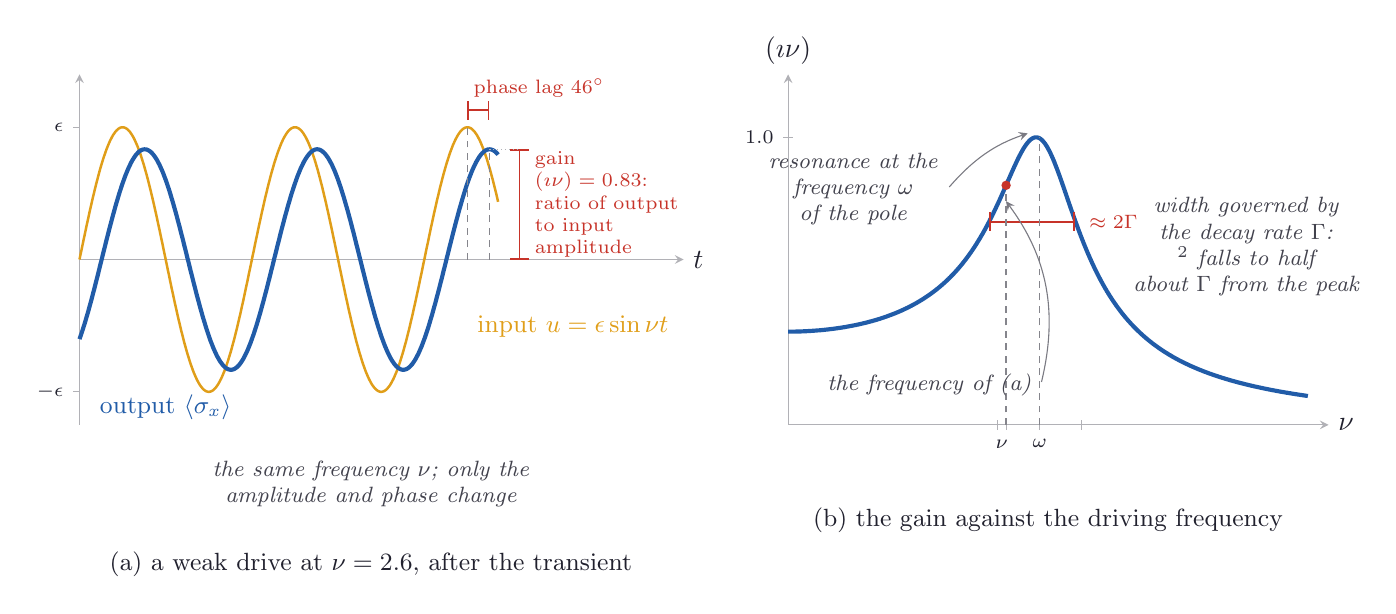
\begin{tikzpicture}[ink/.style={line width=0.9pt, ndInk}, faint/.style={line width=0.4pt, ndInk!35}, dashedink/.style={line width=0.5pt, ndInk!55, dash pattern=on 2.5pt off 2pt}, vec/.style={->, >=stealth, line width=1.2pt}, note/.style={font=\footnotesize\itshape, text=ndInk!85, align=center}, pointer/.style={->, >=stealth, line width=0.4pt, ndInk!60, shorten >=2pt, shorten <=1pt}, dot/.style={circle, fill=ndInk, inner sep=0pt, minimum size=3.4pt}, wash/.style={fill=ndSky, fill opacity=0.55}, every node/.style={text=ndInk}]
\definecolor{ndInk}{rgb}{0.13,0.13,0.18}
\definecolor{ndPaper}{rgb}{0.99,0.96,0.88}
\definecolor{ndSky}{rgb}{0.84,0.91,0.98}
\definecolor{ndRose}{rgb}{0.98,0.86,0.84}
\definecolor{ndBlue}{rgb}{0.13,0.36,0.66}
\definecolor{ndRed}{rgb}{0.78,0.20,0.16}
\definecolor{ndGold}{rgb}{0.88,0.62,0.10}
\definecolor{ndGreen}{rgb}{0.18,0.52,0.30}
\draw[faint, ->, >=stealth] (0.000,2.700) -- (7.672,2.700) node[right, text=ndInk] {$t$};
\draw[faint, ->, >=stealth] (0.000,0.600) -- (0.000,5.052);
\draw[faint] (0.000,4.380) -- ++(-0.08,0) node[left, font=\scriptsize, text=ndInk] {$\epsilon$};
\draw[faint] (0.000,1.020) -- ++(-0.08,0) node[left, font=\scriptsize, text=ndInk] {$-\epsilon$};
\draw[line width=0.9pt, ndGold] (0.000,2.700) -- (0.013,2.764) -- (0.027,2.828) -- (0.040,2.892) -- (0.053,2.956) -- (0.067,3.019) -- (0.080,3.082) -- (0.093,3.144) -- (0.107,3.206) -- (0.120,3.267) -- (0.133,3.327) -- (0.147,3.386) -- (0.160,3.444) -- (0.173,3.501) -- (0.187,3.557) -- (0.200,3.612) -- (0.213,3.665) -- (0.227,3.717) -- (0.240,3.767) -- (0.253,3.816) -- (0.266,3.863) -- (0.280,3.909) -- (0.293,3.952) -- (0.306,3.994) -- (0.320,4.034) -- (0.333,4.072) -- (0.346,4.108) -- (0.360,4.142) -- (0.373,4.174) -- (0.386,4.204) -- (0.400,4.231) -- (0.413,4.257) -- (0.426,4.280) -- (0.440,4.300) -- (0.453,4.319) -- (0.466,4.335) -- (0.480,4.348) -- (0.493,4.360) -- (0.506,4.368) -- (0.520,4.375) -- (0.533,4.379) -- (0.546,4.380) -- (0.560,4.379) -- (0.573,4.375) -- (0.586,4.370) -- (0.600,4.361) -- (0.613,4.350) -- (0.626,4.337) -- (0.640,4.322) -- (0.653,4.304) -- (0.666,4.283) -- (0.680,4.261) -- (0.693,4.236) -- (0.706,4.209) -- (0.719,4.179) -- (0.733,4.148) -- (0.746,4.114) -- (0.759,4.078) -- (0.773,4.041) -- (0.786,4.001) -- (0.799,3.959) -- (0.813,3.916) -- (0.826,3.871) -- (0.839,3.824) -- (0.853,3.775) -- (0.866,3.725) -- (0.879,3.673) -- (0.893,3.620) -- (0.906,3.566) -- (0.919,3.510) -- (0.933,3.453) -- (0.946,3.396) -- (0.959,3.337) -- (0.973,3.277) -- (0.986,3.216) -- (0.999,3.154) -- (1.013,3.092) -- (1.026,3.030) -- (1.039,2.966) -- (1.053,2.903) -- (1.066,2.839) -- (1.079,2.775) -- (1.093,2.710) -- (1.106,2.646) -- (1.119,2.582) -- (1.133,2.518) -- (1.146,2.454) -- (1.159,2.391) -- (1.172,2.328) -- (1.186,2.266) -- (1.199,2.204) -- (1.212,2.143) -- (1.226,2.083) -- (1.239,2.024) -- (1.252,1.965) -- (1.266,1.908) -- (1.279,1.852) -- (1.292,1.797) -- (1.306,1.744) -- (1.319,1.692) -- (1.332,1.641) -- (1.346,1.592) -- (1.359,1.544) -- (1.372,1.499) -- (1.386,1.455) -- (1.399,1.412) -- (1.412,1.372) -- (1.426,1.334) -- (1.439,1.297) -- (1.452,1.263) -- (1.466,1.231) -- (1.479,1.201) -- (1.492,1.173) -- (1.506,1.147) -- (1.519,1.124) -- (1.532,1.103) -- (1.546,1.084) -- (1.559,1.068) -- (1.572,1.054) -- (1.586,1.042) -- (1.599,1.033) -- (1.612,1.026) -- (1.626,1.022) -- (1.639,1.020) -- (1.652,1.021) -- (1.665,1.024) -- (1.679,1.029) -- (1.692,1.037) -- (1.705,1.048) -- (1.719,1.061) -- (1.732,1.076) -- (1.745,1.093) -- (1.759,1.113) -- (1.772,1.136) -- (1.785,1.160) -- (1.799,1.187) -- (1.812,1.216) -- (1.825,1.247) -- (1.839,1.280) -- (1.852,1.316) -- (1.865,1.353) -- (1.879,1.393) -- (1.892,1.434) -- (1.905,1.477) -- (1.919,1.522) -- (1.932,1.568) -- (1.945,1.617) -- (1.959,1.667) -- (1.972,1.718) -- (1.985,1.771) -- (1.999,1.825) -- (2.012,1.881) -- (2.025,1.937) -- (2.039,1.995) -- (2.052,2.054) -- (2.065,2.114) -- (2.079,2.174) -- (2.092,2.236) -- (2.105,2.298) -- (2.118,2.360) -- (2.132,2.423) -- (2.145,2.487) -- (2.158,2.551) -- (2.172,2.615) -- (2.185,2.679) -- (2.198,2.743) -- (2.212,2.807) -- (2.225,2.871) -- (2.238,2.935) -- (2.252,2.999) -- (2.265,3.062) -- (2.278,3.124) -- (2.292,3.186) -- (2.305,3.247) -- (2.318,3.307) -- (2.332,3.367) -- (2.345,3.425) -- (2.358,3.483) -- (2.372,3.539) -- (2.385,3.594) -- (2.398,3.648) -- (2.412,3.700) -- (2.425,3.751) -- (2.438,3.800) -- (2.452,3.848) -- (2.465,3.894) -- (2.478,3.938) -- (2.492,3.981) -- (2.505,4.021) -- (2.518,4.060) -- (2.532,4.097) -- (2.545,4.131) -- (2.558,4.164) -- (2.571,4.194) -- (2.585,4.223) -- (2.598,4.249) -- (2.611,4.272) -- (2.625,4.294) -- (2.638,4.313) -- (2.651,4.330) -- (2.665,4.344) -- (2.678,4.356) -- (2.691,4.366) -- (2.705,4.373) -- (2.718,4.378) -- (2.731,4.380) -- (2.745,4.380) -- (2.758,4.377) -- (2.771,4.372) -- (2.785,4.364) -- (2.798,4.354) -- (2.811,4.342) -- (2.825,4.327) -- (2.838,4.310) -- (2.851,4.290) -- (2.865,4.268) -- (2.878,4.244) -- (2.891,4.218) -- (2.905,4.189) -- (2.918,4.158) -- (2.931,4.125) -- (2.945,4.090) -- (2.958,4.053) -- (2.971,4.014) -- (2.985,3.973) -- (2.998,3.930) -- (3.011,3.886) -- (3.025,3.839) -- (3.038,3.791) -- (3.051,3.742) -- (3.064,3.690) -- (3.078,3.638) -- (3.091,3.584) -- (3.104,3.529) -- (3.118,3.472) -- (3.131,3.415) -- (3.144,3.356) -- (3.158,3.296) -- (3.171,3.236) -- (3.184,3.175) -- (3.198,3.113) -- (3.211,3.050) -- (3.224,2.987) -- (3.238,2.923) -- (3.251,2.860) -- (3.264,2.796) -- (3.278,2.731) -- (3.291,2.667) -- (3.304,2.603) -- (3.318,2.539) -- (3.331,2.475) -- (3.344,2.412) -- (3.358,2.349) -- (3.371,2.286) -- (3.384,2.224) -- (3.398,2.163) -- (3.411,2.102) -- (3.424,2.043) -- (3.438,1.984) -- (3.451,1.927) -- (3.464,1.870) -- (3.478,1.815) -- (3.491,1.761) -- (3.504,1.708) -- (3.517,1.657) -- (3.531,1.608) -- (3.544,1.560) -- (3.557,1.513) -- (3.571,1.469) -- (3.584,1.426) -- (3.597,1.385) -- (3.611,1.346) -- (3.624,1.309) -- (3.637,1.274) -- (3.651,1.241) -- (3.664,1.210) -- (3.677,1.182) -- (3.691,1.155) -- (3.704,1.131) -- (3.717,1.109) -- (3.731,1.090) -- (3.744,1.073) -- (3.757,1.058) -- (3.771,1.046) -- (3.784,1.036) -- (3.797,1.028) -- (3.811,1.023) -- (3.824,1.020) -- (3.837,1.020) -- (3.851,1.023) -- (3.864,1.027) -- (3.877,1.034) -- (3.891,1.044) -- (3.904,1.056) -- (3.917,1.071) -- (3.931,1.087) -- (3.944,1.106) -- (3.957,1.128) -- (3.970,1.152) -- (3.984,1.178) -- (3.997,1.206) -- (4.010,1.237) -- (4.024,1.269) -- (4.037,1.304) -- (4.050,1.341) -- (4.064,1.379) -- (4.077,1.420) -- (4.090,1.463) -- (4.104,1.507) -- (4.117,1.553) -- (4.130,1.601) -- (4.144,1.650) -- (4.157,1.701) -- (4.170,1.753) -- (4.184,1.807) -- (4.197,1.862) -- (4.210,1.919) -- (4.224,1.976) -- (4.237,2.034) -- (4.250,2.094) -- (4.264,2.154) -- (4.277,2.215) -- (4.290,2.277) -- (4.304,2.340) -- (4.317,2.403) -- (4.330,2.466) -- (4.344,2.530) -- (4.357,2.594) -- (4.370,2.658) -- (4.384,2.722) -- (4.397,2.787) -- (4.410,2.851) -- (4.424,2.914) -- (4.437,2.978) -- (4.450,3.041) -- (4.463,3.104) -- (4.477,3.166) -- (4.490,3.227) -- (4.503,3.288) -- (4.517,3.347) -- (4.530,3.406) -- (4.543,3.464) -- (4.557,3.521) -- (4.570,3.576) -- (4.583,3.630) -- (4.597,3.683) -- (4.610,3.734) -- (4.623,3.784) -- (4.637,3.833) -- (4.650,3.879) -- (4.663,3.924) -- (4.677,3.967) -- (4.690,4.008) -- (4.703,4.048) -- (4.717,4.085) -- (4.730,4.120) -- (4.743,4.154) -- (4.757,4.185) -- (4.770,4.214) -- (4.783,4.240) -- (4.797,4.265) -- (4.810,4.287) -- (4.823,4.307) -- (4.837,4.325) -- (4.850,4.340) -- (4.863,4.353) -- (4.877,4.363) -- (4.890,4.371) -- (4.903,4.376) -- (4.916,4.379) -- (4.930,4.380) -- (4.943,4.378) -- (4.956,4.374) -- (4.970,4.367) -- (4.983,4.358) -- (4.996,4.346) -- (5.010,4.332) -- (5.023,4.316) -- (5.036,4.297) -- (5.050,4.276) -- (5.063,4.252) -- (5.076,4.227) -- (5.090,4.199) -- (5.103,4.168) -- (5.116,4.136) -- (5.130,4.102) -- (5.143,4.065) -- (5.156,4.027) -- (5.170,3.987) -- (5.183,3.944) -- (5.196,3.900) -- (5.210,3.855) -- (5.223,3.807) -- (5.236,3.758) -- (5.250,3.707) -- (5.263,3.655) -- (5.276,3.602) -- (5.290,3.547) -- (5.303,3.491) -- (5.316,3.433);
\draw[line width=1.5pt, ndBlue] (0.000,1.689) -- (0.013,1.727) -- (0.027,1.766) -- (0.040,1.806) -- (0.053,1.848) -- (0.067,1.891) -- (0.080,1.936) -- (0.093,1.981) -- (0.107,2.027) -- (0.120,2.075) -- (0.133,2.123) -- (0.147,2.172) -- (0.160,2.222) -- (0.173,2.273) -- (0.187,2.324) -- (0.200,2.376) -- (0.213,2.428) -- (0.227,2.481) -- (0.240,2.534) -- (0.253,2.587) -- (0.266,2.641) -- (0.280,2.694) -- (0.293,2.748) -- (0.306,2.801) -- (0.320,2.855) -- (0.333,2.908) -- (0.346,2.960) -- (0.360,3.013) -- (0.373,3.065) -- (0.386,3.116) -- (0.400,3.167) -- (0.413,3.217) -- (0.426,3.266) -- (0.440,3.315) -- (0.453,3.363) -- (0.466,3.409) -- (0.480,3.455) -- (0.493,3.499) -- (0.506,3.543) -- (0.520,3.585) -- (0.533,3.626) -- (0.546,3.665) -- (0.560,3.703) -- (0.573,3.740) -- (0.586,3.775) -- (0.600,3.808) -- (0.613,3.840) -- (0.626,3.870) -- (0.640,3.899) -- (0.653,3.926) -- (0.666,3.951) -- (0.680,3.974) -- (0.693,3.995) -- (0.706,4.014) -- (0.719,4.032) -- (0.733,4.047) -- (0.746,4.061) -- (0.759,4.073) -- (0.773,4.082) -- (0.786,4.090) -- (0.799,4.095) -- (0.813,4.099) -- (0.826,4.100) -- (0.839,4.099) -- (0.853,4.097) -- (0.866,4.092) -- (0.879,4.085) -- (0.893,4.076) -- (0.906,4.066) -- (0.919,4.053) -- (0.933,4.038) -- (0.946,4.021) -- (0.959,4.003) -- (0.973,3.982) -- (0.986,3.960) -- (0.999,3.935) -- (1.013,3.909) -- (1.026,3.881) -- (1.039,3.852) -- (1.053,3.821) -- (1.066,3.788) -- (1.079,3.753) -- (1.093,3.717) -- (1.106,3.680) -- (1.119,3.641) -- (1.133,3.600) -- (1.146,3.559) -- (1.159,3.516) -- (1.172,3.472) -- (1.186,3.426) -- (1.199,3.380) -- (1.212,3.333) -- (1.226,3.285) -- (1.239,3.236) -- (1.252,3.186) -- (1.266,3.135) -- (1.279,3.084) -- (1.292,3.032) -- (1.306,2.980) -- (1.319,2.928) -- (1.332,2.875) -- (1.346,2.821) -- (1.359,2.768) -- (1.372,2.714) -- (1.386,2.661) -- (1.399,2.607) -- (1.412,2.554) -- (1.426,2.501) -- (1.439,2.448) -- (1.452,2.396) -- (1.466,2.344) -- (1.479,2.292) -- (1.492,2.241) -- (1.506,2.191) -- (1.519,2.142) -- (1.532,2.093) -- (1.546,2.045) -- (1.559,1.998) -- (1.572,1.952) -- (1.586,1.908) -- (1.599,1.864) -- (1.612,1.822) -- (1.626,1.781) -- (1.639,1.741) -- (1.652,1.703) -- (1.665,1.666) -- (1.679,1.631) -- (1.692,1.597) -- (1.705,1.565) -- (1.719,1.534) -- (1.732,1.506) -- (1.745,1.478) -- (1.759,1.453) -- (1.772,1.430) -- (1.785,1.408) -- (1.799,1.389) -- (1.812,1.371) -- (1.825,1.355) -- (1.839,1.341) -- (1.852,1.329) -- (1.865,1.319) -- (1.879,1.311) -- (1.892,1.306) -- (1.905,1.302) -- (1.919,1.300) -- (1.932,1.300) -- (1.945,1.303) -- (1.959,1.307) -- (1.972,1.314) -- (1.985,1.322) -- (1.999,1.333) -- (2.012,1.345) -- (2.025,1.359) -- (2.039,1.376) -- (2.052,1.394) -- (2.065,1.414) -- (2.079,1.437) -- (2.092,1.461) -- (2.105,1.486) -- (2.118,1.514) -- (2.132,1.543) -- (2.145,1.574) -- (2.158,1.607) -- (2.172,1.641) -- (2.185,1.677) -- (2.198,1.714) -- (2.212,1.753) -- (2.225,1.793) -- (2.238,1.834) -- (2.252,1.877) -- (2.265,1.921) -- (2.278,1.966) -- (2.292,2.012) -- (2.305,2.059) -- (2.318,2.107) -- (2.332,2.156) -- (2.345,2.206) -- (2.358,2.256) -- (2.372,2.307) -- (2.385,2.359) -- (2.398,2.411) -- (2.412,2.464) -- (2.425,2.517) -- (2.438,2.570) -- (2.452,2.623) -- (2.465,2.677) -- (2.478,2.730) -- (2.492,2.784) -- (2.505,2.837) -- (2.518,2.890) -- (2.532,2.943) -- (2.545,2.996) -- (2.558,3.048) -- (2.571,3.099) -- (2.585,3.150) -- (2.598,3.201) -- (2.611,3.250) -- (2.625,3.299) -- (2.638,3.347) -- (2.651,3.394) -- (2.665,3.440) -- (2.678,3.485) -- (2.691,3.529) -- (2.705,3.571) -- (2.718,3.613) -- (2.731,3.652) -- (2.745,3.691) -- (2.758,3.728) -- (2.771,3.764) -- (2.785,3.798) -- (2.798,3.830) -- (2.811,3.861) -- (2.825,3.890) -- (2.838,3.917) -- (2.851,3.943) -- (2.865,3.967) -- (2.878,3.988) -- (2.891,4.008) -- (2.905,4.026) -- (2.918,4.043) -- (2.931,4.057) -- (2.945,4.069) -- (2.958,4.079) -- (2.971,4.087) -- (2.985,4.094) -- (2.998,4.098) -- (3.011,4.100) -- (3.025,4.100) -- (3.038,4.098) -- (3.051,4.094) -- (3.064,4.088) -- (3.078,4.079) -- (3.091,4.069) -- (3.104,4.057) -- (3.118,4.043) -- (3.131,4.027) -- (3.144,4.009) -- (3.158,3.989) -- (3.171,3.967) -- (3.184,3.943) -- (3.198,3.918) -- (3.211,3.891) -- (3.224,3.862) -- (3.238,3.831) -- (3.251,3.799) -- (3.264,3.765) -- (3.278,3.729) -- (3.291,3.692) -- (3.304,3.654) -- (3.318,3.614) -- (3.331,3.572) -- (3.344,3.530) -- (3.358,3.486) -- (3.371,3.441) -- (3.384,3.395) -- (3.398,3.348) -- (3.411,3.301) -- (3.424,3.252) -- (3.438,3.202) -- (3.451,3.152) -- (3.464,3.101) -- (3.478,3.049) -- (3.491,2.997) -- (3.504,2.945) -- (3.517,2.892) -- (3.531,2.839) -- (3.544,2.785) -- (3.557,2.732) -- (3.571,2.678) -- (3.584,2.625) -- (3.597,2.571) -- (3.611,2.518) -- (3.624,2.465) -- (3.637,2.413) -- (3.651,2.361) -- (3.664,2.309) -- (3.677,2.258) -- (3.691,2.207) -- (3.704,2.158) -- (3.717,2.109) -- (3.731,2.061) -- (3.744,2.013) -- (3.757,1.967) -- (3.771,1.922) -- (3.784,1.878) -- (3.797,1.836) -- (3.811,1.794) -- (3.824,1.754) -- (3.837,1.715) -- (3.851,1.678) -- (3.864,1.642) -- (3.877,1.608) -- (3.891,1.575) -- (3.904,1.544) -- (3.917,1.515) -- (3.931,1.487) -- (3.944,1.461) -- (3.957,1.437) -- (3.970,1.415) -- (3.984,1.395) -- (3.997,1.376) -- (4.010,1.360) -- (4.024,1.345) -- (4.037,1.333) -- (4.050,1.322) -- (4.064,1.314) -- (4.077,1.307) -- (4.090,1.303) -- (4.104,1.300) -- (4.117,1.300) -- (4.130,1.302) -- (4.144,1.306) -- (4.157,1.311) -- (4.170,1.319) -- (4.184,1.329) -- (4.197,1.341) -- (4.210,1.355) -- (4.224,1.370) -- (4.237,1.388) -- (4.250,1.408) -- (4.264,1.429) -- (4.277,1.453) -- (4.290,1.478) -- (4.304,1.505) -- (4.317,1.533) -- (4.330,1.564) -- (4.344,1.596) -- (4.357,1.630) -- (4.370,1.665) -- (4.384,1.702) -- (4.397,1.740) -- (4.410,1.780) -- (4.424,1.821) -- (4.437,1.863) -- (4.450,1.907) -- (4.463,1.951) -- (4.477,1.997) -- (4.490,2.044) -- (4.503,2.092) -- (4.517,2.140) -- (4.530,2.190) -- (4.543,2.240) -- (4.557,2.291) -- (4.570,2.342) -- (4.583,2.394) -- (4.597,2.447) -- (4.610,2.499) -- (4.623,2.553) -- (4.637,2.606) -- (4.650,2.659) -- (4.663,2.713) -- (4.677,2.766) -- (4.690,2.820) -- (4.703,2.873) -- (4.717,2.926) -- (4.730,2.979) -- (4.743,3.031) -- (4.757,3.083) -- (4.770,3.134) -- (4.783,3.184) -- (4.797,3.234) -- (4.810,3.283) -- (4.823,3.332) -- (4.837,3.379) -- (4.850,3.425) -- (4.863,3.470) -- (4.877,3.515) -- (4.890,3.558) -- (4.903,3.599) -- (4.916,3.640) -- (4.930,3.679) -- (4.943,3.716) -- (4.956,3.752) -- (4.970,3.787) -- (4.983,3.820) -- (4.996,3.851) -- (5.010,3.881) -- (5.023,3.908) -- (5.036,3.935) -- (5.050,3.959) -- (5.063,3.981) -- (5.076,4.002) -- (5.090,4.021) -- (5.103,4.038) -- (5.116,4.052) -- (5.130,4.065) -- (5.143,4.076) -- (5.156,4.085) -- (5.170,4.092) -- (5.183,4.097) -- (5.196,4.099) -- (5.210,4.100) -- (5.223,4.099) -- (5.236,4.095) -- (5.250,4.090) -- (5.263,4.082) -- (5.276,4.073) -- (5.290,4.061) -- (5.303,4.048) -- (5.316,4.032);
\draw[dashedink] (4.926,2.700) -- (4.926,4.380);
\draw[dashedink] (5.207,2.700) -- (5.207,4.100);
\draw[line width=0.7pt, ndRed, |-|] (4.926,4.598) -- (5.207,4.598);
\node[font=\scriptsize, text=ndRed, anchor=south west, align=left] at (4.881,4.632) {phase lag $46^\circ$};
\draw[line width=0.7pt, ndRed, |-|] (5.588,2.700) -- (5.588,4.100);
\draw[faint, densely dotted] (5.207,4.100) -- (5.588,4.100);
\node[font=\scriptsize, text=ndRed, anchor=west, align=left] at (5.660,3.400) {gain\\ $\abs{\TF(\imath\nu)}=0.83$:\\ ratio of output\\ to input\\ amplitude};
\node[font=\small, text=ndGold, anchor=north] at (6.267,2.112) {input $u=\epsilon\sin\nu t$};
\node[font=\small, text=ndBlue, anchor=north west] at (0.136,1.104) {output $\langle\sigma_x\rangle$};
\node[note, anchor=north] at (3.700,0.264) {the same frequency $\nu$; only the\\ amplitude and phase change};
\node[font=\small] at (3.700,-1.164) {(a) a weak drive at $\nu=2.6$, after the transient};
\draw[faint, ->, >=stealth] (9.000,0.600) -- (15.864,0.600) node[right, text=ndInk] {$\nu$};
\draw[faint, ->, >=stealth] (9.000,0.600) -- (9.000,5.052) node[above, text=ndInk] {$\abs{\TF(\imath\nu)}$};
\draw[faint] (11.661,0.660) -- (11.661,0.540) node[below, font=\scriptsize, text=ndInk] {};
\draw[faint] (12.194,0.660) -- (12.194,0.540) node[below, font=\scriptsize, text=ndInk] {$\omega$};
\draw[faint] (12.726,0.660) -- (12.726,0.540) node[below, font=\scriptsize, text=ndInk] {};
\draw[faint] (11.768,0.660) -- (11.768,0.540) node[below, font=\scriptsize, text=ndInk] {};
\draw[faint] (9.060,4.252) -- (8.940,4.252) node[left, font=\scriptsize, text=ndInk] {$1.0$};
\draw[line width=1.5pt, ndBlue] (9.000,1.784) -- (9.005,1.784) -- (9.011,1.785) -- (9.016,1.785) -- (9.021,1.785) -- (9.027,1.785) -- (9.032,1.785) -- (9.037,1.785) -- (9.043,1.785) -- (9.048,1.785) -- (9.053,1.785) -- (9.059,1.785) -- (9.064,1.785) -- (9.069,1.785) -- (9.075,1.785) -- (9.080,1.785) -- (9.085,1.785) -- (9.090,1.785) -- (9.096,1.785) -- (9.101,1.786) -- (9.106,1.786) -- (9.112,1.786) -- (9.117,1.786) -- (9.122,1.786) -- (9.128,1.786) -- (9.133,1.786) -- (9.138,1.787) -- (9.144,1.787) -- (9.149,1.787) -- (9.154,1.787) -- (9.160,1.787) -- (9.165,1.787) -- (9.170,1.788) -- (9.176,1.788) -- (9.181,1.788) -- (9.186,1.788) -- (9.192,1.788) -- (9.197,1.789) -- (9.202,1.789) -- (9.208,1.789) -- (9.213,1.789) -- (9.218,1.790) -- (9.224,1.790) -- (9.229,1.790) -- (9.234,1.790) -- (9.240,1.791) -- (9.245,1.791) -- (9.250,1.791) -- (9.255,1.792) -- (9.261,1.792) -- (9.266,1.792) -- (9.271,1.792) -- (9.277,1.793) -- (9.282,1.793) -- (9.287,1.793) -- (9.293,1.794) -- (9.298,1.794) -- (9.303,1.794) -- (9.309,1.795) -- (9.314,1.795) -- (9.319,1.795) -- (9.325,1.796) -- (9.330,1.796) -- (9.335,1.797) -- (9.341,1.797) -- (9.346,1.797) -- (9.351,1.798) -- (9.357,1.798) -- (9.362,1.799) -- (9.367,1.799) -- (9.373,1.800) -- (9.378,1.800) -- (9.383,1.800) -- (9.389,1.801) -- (9.394,1.801) -- (9.399,1.802) -- (9.405,1.802) -- (9.410,1.803) -- (9.415,1.803) -- (9.420,1.804) -- (9.426,1.804) -- (9.431,1.805) -- (9.436,1.805) -- (9.442,1.806) -- (9.447,1.806) -- (9.452,1.807) -- (9.458,1.807) -- (9.463,1.808) -- (9.468,1.808) -- (9.474,1.809) -- (9.479,1.810) -- (9.484,1.810) -- (9.490,1.811) -- (9.495,1.811) -- (9.500,1.812) -- (9.506,1.812) -- (9.511,1.813) -- (9.516,1.814) -- (9.522,1.814) -- (9.527,1.815) -- (9.532,1.816) -- (9.538,1.816) -- (9.543,1.817) -- (9.548,1.817) -- (9.554,1.818) -- (9.559,1.819) -- (9.564,1.819) -- (9.570,1.820) -- (9.575,1.821) -- (9.580,1.822) -- (9.585,1.822) -- (9.591,1.823) -- (9.596,1.824) -- (9.601,1.824) -- (9.607,1.825) -- (9.612,1.826) -- (9.617,1.827) -- (9.623,1.827) -- (9.628,1.828) -- (9.633,1.829) -- (9.639,1.830) -- (9.644,1.830) -- (9.649,1.831) -- (9.655,1.832) -- (9.660,1.833) -- (9.665,1.834) -- (9.671,1.834) -- (9.676,1.835) -- (9.681,1.836) -- (9.687,1.837) -- (9.692,1.838) -- (9.697,1.839) -- (9.703,1.840) -- (9.708,1.840) -- (9.713,1.841) -- (9.719,1.842) -- (9.724,1.843) -- (9.729,1.844) -- (9.735,1.845) -- (9.740,1.846) -- (9.745,1.847) -- (9.750,1.848) -- (9.756,1.849) -- (9.761,1.850) -- (9.766,1.851) -- (9.772,1.852) -- (9.777,1.853) -- (9.782,1.854) -- (9.788,1.854) -- (9.793,1.855) -- (9.798,1.857) -- (9.804,1.858) -- (9.809,1.859) -- (9.814,1.860) -- (9.820,1.861) -- (9.825,1.862) -- (9.830,1.863) -- (9.836,1.864) -- (9.841,1.865) -- (9.846,1.866) -- (9.852,1.867) -- (9.857,1.868) -- (9.862,1.869) -- (9.868,1.870) -- (9.873,1.872) -- (9.878,1.873) -- (9.884,1.874) -- (9.889,1.875) -- (9.894,1.876) -- (9.900,1.877) -- (9.905,1.879) -- (9.910,1.880) -- (9.915,1.881) -- (9.921,1.882) -- (9.926,1.883) -- (9.931,1.885) -- (9.937,1.886) -- (9.942,1.887) -- (9.947,1.888) -- (9.953,1.890) -- (9.958,1.891) -- (9.963,1.892) -- (9.969,1.893) -- (9.974,1.895) -- (9.979,1.896) -- (9.985,1.897) -- (9.990,1.899) -- (9.995,1.900) -- (10.001,1.901) -- (10.006,1.903) -- (10.011,1.904) -- (10.017,1.906) -- (10.022,1.907) -- (10.027,1.908) -- (10.033,1.910) -- (10.038,1.911) -- (10.043,1.913) -- (10.049,1.914) -- (10.054,1.915) -- (10.059,1.917) -- (10.065,1.918) -- (10.070,1.920) -- (10.075,1.921) -- (10.080,1.923) -- (10.086,1.924) -- (10.091,1.926) -- (10.096,1.927) -- (10.102,1.929) -- (10.107,1.931) -- (10.112,1.932) -- (10.118,1.934) -- (10.123,1.935) -- (10.128,1.937) -- (10.134,1.939) -- (10.139,1.940) -- (10.144,1.942) -- (10.150,1.943) -- (10.155,1.945) -- (10.160,1.947) -- (10.166,1.948) -- (10.171,1.950) -- (10.176,1.952) -- (10.182,1.954) -- (10.187,1.955) -- (10.192,1.957) -- (10.198,1.959) -- (10.203,1.961) -- (10.208,1.962) -- (10.214,1.964) -- (10.219,1.966) -- (10.224,1.968) -- (10.230,1.970) -- (10.235,1.971) -- (10.240,1.973) -- (10.245,1.975) -- (10.251,1.977) -- (10.256,1.979) -- (10.261,1.981) -- (10.267,1.983) -- (10.272,1.985) -- (10.277,1.987) -- (10.283,1.989) -- (10.288,1.991) -- (10.293,1.993) -- (10.299,1.995) -- (10.304,1.997) -- (10.309,1.999) -- (10.315,2.001) -- (10.320,2.003) -- (10.325,2.005) -- (10.331,2.007) -- (10.336,2.009) -- (10.341,2.011) -- (10.347,2.013) -- (10.352,2.015) -- (10.357,2.017) -- (10.363,2.020) -- (10.368,2.022) -- (10.373,2.024) -- (10.379,2.026) -- (10.384,2.028) -- (10.389,2.031) -- (10.395,2.033) -- (10.400,2.035) -- (10.405,2.037) -- (10.410,2.040) -- (10.416,2.042) -- (10.421,2.044) -- (10.426,2.047) -- (10.432,2.049) -- (10.437,2.051) -- (10.442,2.054) -- (10.448,2.056) -- (10.453,2.059) -- (10.458,2.061) -- (10.464,2.063) -- (10.469,2.066) -- (10.474,2.068) -- (10.480,2.071) -- (10.485,2.073) -- (10.490,2.076) -- (10.496,2.079) -- (10.501,2.081) -- (10.506,2.084) -- (10.512,2.086) -- (10.517,2.089) -- (10.522,2.092) -- (10.528,2.094) -- (10.533,2.097) -- (10.538,2.100) -- (10.544,2.102) -- (10.549,2.105) -- (10.554,2.108) -- (10.560,2.111) -- (10.565,2.113) -- (10.570,2.116) -- (10.575,2.119) -- (10.581,2.122) -- (10.586,2.125) -- (10.591,2.128) -- (10.597,2.130) -- (10.602,2.133) -- (10.607,2.136) -- (10.613,2.139) -- (10.618,2.142) -- (10.623,2.145) -- (10.629,2.148) -- (10.634,2.151) -- (10.639,2.154) -- (10.645,2.157) -- (10.650,2.161) -- (10.655,2.164) -- (10.661,2.167) -- (10.666,2.170) -- (10.671,2.173) -- (10.677,2.176) -- (10.682,2.180) -- (10.687,2.183) -- (10.693,2.186) -- (10.698,2.190) -- (10.703,2.193) -- (10.709,2.196) -- (10.714,2.200) -- (10.719,2.203) -- (10.725,2.206) -- (10.730,2.210) -- (10.735,2.213) -- (10.740,2.217) -- (10.746,2.220) -- (10.751,2.224) -- (10.756,2.227) -- (10.762,2.231) -- (10.767,2.235) -- (10.772,2.238) -- (10.778,2.242) -- (10.783,2.245) -- (10.788,2.249) -- (10.794,2.253) -- (10.799,2.257) -- (10.804,2.260) -- (10.810,2.264) -- (10.815,2.268) -- (10.820,2.272) -- (10.826,2.276) -- (10.831,2.280) -- (10.836,2.284) -- (10.842,2.288) -- (10.847,2.292) -- (10.852,2.296) -- (10.858,2.300) -- (10.863,2.304) -- (10.868,2.308) -- (10.874,2.312) -- (10.879,2.316) -- (10.884,2.321) -- (10.890,2.325) -- (10.895,2.329) -- (10.900,2.333) -- (10.905,2.338) -- (10.911,2.342) -- (10.916,2.346) -- (10.921,2.351) -- (10.927,2.355) -- (10.932,2.360) -- (10.937,2.364) -- (10.943,2.369) -- (10.948,2.373) -- (10.953,2.378) -- (10.959,2.383) -- (10.964,2.387) -- (10.969,2.392) -- (10.975,2.397) -- (10.980,2.402) -- (10.985,2.406) -- (10.991,2.411) -- (10.996,2.416) -- (11.001,2.421) -- (11.007,2.426) -- (11.012,2.431) -- (11.017,2.436) -- (11.023,2.441) -- (11.028,2.446) -- (11.033,2.451) -- (11.039,2.456) -- (11.044,2.462) -- (11.049,2.467) -- (11.055,2.472) -- (11.060,2.477) -- (11.065,2.483) -- (11.070,2.488) -- (11.076,2.494) -- (11.081,2.499) -- (11.086,2.505) -- (11.092,2.510) -- (11.097,2.516) -- (11.102,2.521) -- (11.108,2.527) -- (11.113,2.533) -- (11.118,2.539) -- (11.124,2.544) -- (11.129,2.550) -- (11.134,2.556) -- (11.140,2.562) -- (11.145,2.568) -- (11.150,2.574) -- (11.156,2.580) -- (11.161,2.586) -- (11.166,2.592) -- (11.172,2.599) -- (11.177,2.605) -- (11.182,2.611) -- (11.188,2.617) -- (11.193,2.624) -- (11.198,2.630) -- (11.204,2.637) -- (11.209,2.643) -- (11.214,2.650) -- (11.220,2.657) -- (11.225,2.663) -- (11.230,2.670) -- (11.235,2.677) -- (11.241,2.684) -- (11.246,2.690) -- (11.251,2.697) -- (11.257,2.704) -- (11.262,2.711) -- (11.267,2.718) -- (11.273,2.726) -- (11.278,2.733) -- (11.283,2.740) -- (11.289,2.747) -- (11.294,2.755) -- (11.299,2.762) -- (11.305,2.769) -- (11.310,2.777) -- (11.315,2.785) -- (11.321,2.792) -- (11.326,2.800) -- (11.331,2.808) -- (11.337,2.815) -- (11.342,2.823) -- (11.347,2.831) -- (11.353,2.839) -- (11.358,2.847) -- (11.363,2.855) -- (11.369,2.863) -- (11.374,2.871) -- (11.379,2.880) -- (11.385,2.888) -- (11.390,2.896) -- (11.395,2.905) -- (11.400,2.913) -- (11.406,2.922) -- (11.411,2.931) -- (11.416,2.939) -- (11.422,2.948) -- (11.427,2.957) -- (11.432,2.966) -- (11.438,2.974) -- (11.443,2.983) -- (11.448,2.993) -- (11.454,3.002) -- (11.459,3.011) -- (11.464,3.020) -- (11.470,3.029) -- (11.475,3.039) -- (11.480,3.048) -- (11.486,3.058) -- (11.491,3.067) -- (11.496,3.077) -- (11.502,3.086) -- (11.507,3.096) -- (11.512,3.106) -- (11.518,3.116) -- (11.523,3.126) -- (11.528,3.136) -- (11.534,3.146) -- (11.539,3.156) -- (11.544,3.166) -- (11.550,3.176) -- (11.555,3.187) -- (11.560,3.197) -- (11.565,3.208) -- (11.571,3.218) -- (11.576,3.229) -- (11.581,3.239) -- (11.587,3.250) -- (11.592,3.261) -- (11.597,3.272) -- (11.603,3.282) -- (11.608,3.293) -- (11.613,3.304) -- (11.619,3.315) -- (11.624,3.326) -- (11.629,3.338) -- (11.635,3.349) -- (11.640,3.360) -- (11.645,3.371) -- (11.651,3.383) -- (11.656,3.394) -- (11.661,3.406) -- (11.667,3.417) -- (11.672,3.429) -- (11.677,3.440) -- (11.683,3.452) -- (11.688,3.464) -- (11.693,3.476) -- (11.699,3.487) -- (11.704,3.499) -- (11.709,3.511) -- (11.715,3.523) -- (11.720,3.535) -- (11.725,3.547) -- (11.730,3.559) -- (11.736,3.571) -- (11.741,3.583) -- (11.746,3.595) -- (11.752,3.607) -- (11.757,3.619) -- (11.762,3.631) -- (11.768,3.643) -- (11.773,3.656) -- (11.778,3.668) -- (11.784,3.680) -- (11.789,3.692) -- (11.794,3.704) -- (11.800,3.716) -- (11.805,3.729) -- (11.810,3.741) -- (11.816,3.753) -- (11.821,3.765) -- (11.826,3.777) -- (11.832,3.789) -- (11.837,3.801) -- (11.842,3.813) -- (11.848,3.825) -- (11.853,3.837) -- (11.858,3.849) -- (11.864,3.861) -- (11.869,3.872) -- (11.874,3.884) -- (11.880,3.896) -- (11.885,3.907) -- (11.890,3.918) -- (11.895,3.930) -- (11.901,3.941) -- (11.906,3.952) -- (11.911,3.963) -- (11.917,3.974) -- (11.922,3.985) -- (11.927,3.996) -- (11.933,4.006) -- (11.938,4.017) -- (11.943,4.027) -- (11.949,4.037) -- (11.954,4.047) -- (11.959,4.057) -- (11.965,4.067) -- (11.970,4.076) -- (11.975,4.086) -- (11.981,4.095) -- (11.986,4.104) -- (11.991,4.113) -- (11.997,4.121) -- (12.002,4.130) -- (12.007,4.138) -- (12.013,4.146) -- (12.018,4.153) -- (12.023,4.161) -- (12.029,4.168) -- (12.034,4.175) -- (12.039,4.181) -- (12.045,4.188) -- (12.050,4.194) -- (12.055,4.200) -- (12.060,4.205) -- (12.066,4.211) -- (12.071,4.216) -- (12.076,4.220) -- (12.082,4.225) -- (12.087,4.229) -- (12.092,4.233) -- (12.098,4.236) -- (12.103,4.239) -- (12.108,4.242) -- (12.114,4.245) -- (12.119,4.247) -- (12.124,4.248) -- (12.130,4.250) -- (12.135,4.251) -- (12.140,4.252) -- (12.146,4.252) -- (12.151,4.252) -- (12.156,4.252) -- (12.162,4.251) -- (12.167,4.250) -- (12.172,4.249) -- (12.178,4.247) -- (12.183,4.245) -- (12.188,4.242) -- (12.194,4.240) -- (12.199,4.236) -- (12.204,4.233) -- (12.210,4.229) -- (12.215,4.225) -- (12.220,4.220) -- (12.225,4.215) -- (12.231,4.210) -- (12.236,4.204) -- (12.241,4.198) -- (12.247,4.192) -- (12.252,4.185) -- (12.257,4.178) -- (12.263,4.171) -- (12.268,4.163) -- (12.273,4.155) -- (12.279,4.147) -- (12.284,4.138) -- (12.289,4.129) -- (12.295,4.120) -- (12.300,4.111) -- (12.305,4.101) -- (12.311,4.091) -- (12.316,4.081) -- (12.321,4.070) -- (12.327,4.059) -- (12.332,4.048) -- (12.337,4.037) -- (12.343,4.025) -- (12.348,4.014) -- (12.353,4.002) -- (12.359,3.989) -- (12.364,3.977) -- (12.369,3.964) -- (12.375,3.952) -- (12.380,3.939) -- (12.385,3.925) -- (12.390,3.912) -- (12.396,3.898) -- (12.401,3.885) -- (12.406,3.871) -- (12.412,3.857) -- (12.417,3.843) -- (12.422,3.829) -- (12.428,3.814) -- (12.433,3.800) -- (12.438,3.785) -- (12.444,3.771) -- (12.449,3.756) -- (12.454,3.741) -- (12.460,3.726) -- (12.465,3.711) -- (12.470,3.696) -- (12.476,3.681) -- (12.481,3.665) -- (12.486,3.650) -- (12.492,3.635) -- (12.497,3.620) -- (12.502,3.604) -- (12.508,3.589) -- (12.513,3.573) -- (12.518,3.558) -- (12.524,3.542) -- (12.529,3.527) -- (12.534,3.511) -- (12.540,3.496) -- (12.545,3.480) -- (12.550,3.465) -- (12.555,3.449) -- (12.561,3.434) -- (12.566,3.418) -- (12.571,3.403) -- (12.577,3.387) -- (12.582,3.372) -- (12.587,3.357) -- (12.593,3.341) -- (12.598,3.326) -- (12.603,3.311) -- (12.609,3.296) -- (12.614,3.281) -- (12.619,3.266) -- (12.625,3.250) -- (12.630,3.235) -- (12.635,3.221) -- (12.641,3.206) -- (12.646,3.191) -- (12.651,3.176) -- (12.657,3.161) -- (12.662,3.147) -- (12.667,3.132) -- (12.673,3.118) -- (12.678,3.103) -- (12.683,3.089) -- (12.689,3.075) -- (12.694,3.060) -- (12.699,3.046) -- (12.705,3.032) -- (12.710,3.018) -- (12.715,3.004) -- (12.720,2.991) -- (12.726,2.977) -- (12.731,2.963) -- (12.736,2.950) -- (12.742,2.936) -- (12.747,2.923) -- (12.752,2.909) -- (12.758,2.896) -- (12.763,2.883) -- (12.768,2.870) -- (12.774,2.857) -- (12.779,2.844) -- (12.784,2.831) -- (12.790,2.818) -- (12.795,2.806) -- (12.800,2.793) -- (12.806,2.781) -- (12.811,2.768) -- (12.816,2.756) -- (12.822,2.744) -- (12.827,2.732) -- (12.832,2.719) -- (12.838,2.707) -- (12.843,2.696) -- (12.848,2.684) -- (12.854,2.672) -- (12.859,2.660) -- (12.864,2.649) -- (12.870,2.637) -- (12.875,2.626) -- (12.880,2.615) -- (12.885,2.603) -- (12.891,2.592) -- (12.896,2.581) -- (12.901,2.570) -- (12.907,2.559) -- (12.912,2.549) -- (12.917,2.538) -- (12.923,2.527) -- (12.928,2.517) -- (12.933,2.506) -- (12.939,2.496) -- (12.944,2.485) -- (12.949,2.475) -- (12.955,2.465) -- (12.960,2.455) -- (12.965,2.445) -- (12.971,2.435) -- (12.976,2.425) -- (12.981,2.415) -- (12.987,2.405) -- (12.992,2.396) -- (12.997,2.386) -- (13.003,2.377) -- (13.008,2.367) -- (13.013,2.358) -- (13.019,2.349) -- (13.024,2.339) -- (13.029,2.330) -- (13.035,2.321) -- (13.040,2.312) -- (13.045,2.303) -- (13.050,2.294) -- (13.056,2.286) -- (13.061,2.277) -- (13.066,2.268) -- (13.072,2.260) -- (13.077,2.251) -- (13.082,2.243) -- (13.088,2.234) -- (13.093,2.226) -- (13.098,2.218) -- (13.104,2.209) -- (13.109,2.201) -- (13.114,2.193) -- (13.120,2.185) -- (13.125,2.177) -- (13.130,2.169) -- (13.136,2.161) -- (13.141,2.154) -- (13.146,2.146) -- (13.152,2.138) -- (13.157,2.131) -- (13.162,2.123) -- (13.168,2.116) -- (13.173,2.108) -- (13.178,2.101) -- (13.184,2.093) -- (13.189,2.086) -- (13.194,2.079) -- (13.200,2.072) -- (13.205,2.065) -- (13.210,2.058) -- (13.215,2.051) -- (13.221,2.044) -- (13.226,2.037) -- (13.231,2.030) -- (13.237,2.023) -- (13.242,2.016) -- (13.247,2.010) -- (13.253,2.003) -- (13.258,1.996) -- (13.263,1.990) -- (13.269,1.983) -- (13.274,1.977) -- (13.279,1.970) -- (13.285,1.964) -- (13.290,1.958) -- (13.295,1.952) -- (13.301,1.945) -- (13.306,1.939) -- (13.311,1.933) -- (13.317,1.927) -- (13.322,1.921) -- (13.327,1.915) -- (13.333,1.909) -- (13.338,1.903) -- (13.343,1.897) -- (13.349,1.891) -- (13.354,1.885) -- (13.359,1.880) -- (13.365,1.874) -- (13.370,1.868) -- (13.375,1.863) -- (13.380,1.857) -- (13.386,1.852) -- (13.391,1.846) -- (13.396,1.841) -- (13.402,1.835) -- (13.407,1.830) -- (13.412,1.824) -- (13.418,1.819) -- (13.423,1.814) -- (13.428,1.808) -- (13.434,1.803) -- (13.439,1.798) -- (13.444,1.793) -- (13.450,1.788) -- (13.455,1.783) -- (13.460,1.778) -- (13.466,1.773) -- (13.471,1.768) -- (13.476,1.763) -- (13.482,1.758) -- (13.487,1.753) -- (13.492,1.748) -- (13.498,1.743) -- (13.503,1.739) -- (13.508,1.734) -- (13.514,1.729) -- (13.519,1.725) -- (13.524,1.720) -- (13.530,1.715) -- (13.535,1.711) -- (13.540,1.706) -- (13.545,1.702) -- (13.551,1.697) -- (13.556,1.693) -- (13.561,1.688) -- (13.567,1.684) -- (13.572,1.679) -- (13.577,1.675) -- (13.583,1.671) -- (13.588,1.666) -- (13.593,1.662) -- (13.599,1.658) -- (13.604,1.654) -- (13.609,1.650) -- (13.615,1.645) -- (13.620,1.641) -- (13.625,1.637) -- (13.631,1.633) -- (13.636,1.629) -- (13.641,1.625) -- (13.647,1.621) -- (13.652,1.617) -- (13.657,1.613) -- (13.663,1.609) -- (13.668,1.605) -- (13.673,1.601) -- (13.679,1.598) -- (13.684,1.594) -- (13.689,1.590) -- (13.695,1.586) -- (13.700,1.582) -- (13.705,1.579) -- (13.710,1.575) -- (13.716,1.571) -- (13.721,1.568) -- (13.726,1.564) -- (13.732,1.560) -- (13.737,1.557) -- (13.742,1.553) -- (13.748,1.550) -- (13.753,1.546) -- (13.758,1.543) -- (13.764,1.539) -- (13.769,1.536) -- (13.774,1.532) -- (13.780,1.529) -- (13.785,1.525) -- (13.790,1.522) -- (13.796,1.519) -- (13.801,1.515) -- (13.806,1.512) -- (13.812,1.509) -- (13.817,1.505) -- (13.822,1.502) -- (13.828,1.499) -- (13.833,1.495) -- (13.838,1.492) -- (13.844,1.489) -- (13.849,1.486) -- (13.854,1.483) -- (13.860,1.480) -- (13.865,1.477) -- (13.870,1.473) -- (13.875,1.470) -- (13.881,1.467) -- (13.886,1.464) -- (13.891,1.461) -- (13.897,1.458) -- (13.902,1.455) -- (13.907,1.452) -- (13.913,1.449) -- (13.918,1.446) -- (13.923,1.443) -- (13.929,1.440) -- (13.934,1.438) -- (13.939,1.435) -- (13.945,1.432) -- (13.950,1.429) -- (13.955,1.426) -- (13.961,1.423) -- (13.966,1.420) -- (13.971,1.418) -- (13.977,1.415) -- (13.982,1.412) -- (13.987,1.409) -- (13.993,1.407) -- (13.998,1.404) -- (14.003,1.401) -- (14.009,1.399) -- (14.014,1.396) -- (14.019,1.393) -- (14.025,1.391) -- (14.030,1.388) -- (14.035,1.385) -- (14.040,1.383) -- (14.046,1.380) -- (14.051,1.378) -- (14.056,1.375) -- (14.062,1.373) -- (14.067,1.370) -- (14.072,1.368) -- (14.078,1.365) -- (14.083,1.363) -- (14.088,1.360) -- (14.094,1.358) -- (14.099,1.355) -- (14.104,1.353) -- (14.110,1.350) -- (14.115,1.348) -- (14.120,1.346) -- (14.126,1.343) -- (14.131,1.341) -- (14.136,1.338) -- (14.142,1.336) -- (14.147,1.334) -- (14.152,1.331) -- (14.158,1.329) -- (14.163,1.327) -- (14.168,1.325) -- (14.174,1.322) -- (14.179,1.320) -- (14.184,1.318) -- (14.190,1.316) -- (14.195,1.313) -- (14.200,1.311) -- (14.205,1.309) -- (14.211,1.307) -- (14.216,1.305) -- (14.221,1.302) -- (14.227,1.300) -- (14.232,1.298) -- (14.237,1.296) -- (14.243,1.294) -- (14.248,1.292) -- (14.253,1.290) -- (14.259,1.287) -- (14.264,1.285) -- (14.269,1.283) -- (14.275,1.281) -- (14.280,1.279) -- (14.285,1.277) -- (14.291,1.275) -- (14.296,1.273) -- (14.301,1.271) -- (14.307,1.269) -- (14.312,1.267) -- (14.317,1.265) -- (14.323,1.263) -- (14.328,1.261) -- (14.333,1.259) -- (14.339,1.257) -- (14.344,1.255) -- (14.349,1.253) -- (14.355,1.251) -- (14.360,1.249) -- (14.365,1.248) -- (14.370,1.246) -- (14.376,1.244) -- (14.381,1.242) -- (14.386,1.240) -- (14.392,1.238) -- (14.397,1.236) -- (14.402,1.234) -- (14.408,1.233) -- (14.413,1.231) -- (14.418,1.229) -- (14.424,1.227) -- (14.429,1.225) -- (14.434,1.224) -- (14.440,1.222) -- (14.445,1.220) -- (14.450,1.218) -- (14.456,1.217) -- (14.461,1.215) -- (14.466,1.213) -- (14.472,1.211) -- (14.477,1.210) -- (14.482,1.208) -- (14.488,1.206) -- (14.493,1.204) -- (14.498,1.203) -- (14.504,1.201) -- (14.509,1.199) -- (14.514,1.198) -- (14.520,1.196) -- (14.525,1.194) -- (14.530,1.193) -- (14.535,1.191) -- (14.541,1.190) -- (14.546,1.188) -- (14.551,1.186) -- (14.557,1.185) -- (14.562,1.183) -- (14.567,1.181) -- (14.573,1.180) -- (14.578,1.178) -- (14.583,1.177) -- (14.589,1.175) -- (14.594,1.174) -- (14.599,1.172) -- (14.605,1.170) -- (14.610,1.169) -- (14.615,1.167) -- (14.621,1.166) -- (14.626,1.164) -- (14.631,1.163) -- (14.637,1.161) -- (14.642,1.160) -- (14.647,1.158) -- (14.653,1.157) -- (14.658,1.155) -- (14.663,1.154) -- (14.669,1.152) -- (14.674,1.151) -- (14.679,1.149) -- (14.685,1.148) -- (14.690,1.147) -- (14.695,1.145) -- (14.700,1.144) -- (14.706,1.142) -- (14.711,1.141) -- (14.716,1.139) -- (14.722,1.138) -- (14.727,1.137) -- (14.732,1.135) -- (14.738,1.134) -- (14.743,1.132) -- (14.748,1.131) -- (14.754,1.130) -- (14.759,1.128) -- (14.764,1.127) -- (14.770,1.126) -- (14.775,1.124) -- (14.780,1.123) -- (14.786,1.122) -- (14.791,1.120) -- (14.796,1.119) -- (14.802,1.118) -- (14.807,1.116) -- (14.812,1.115) -- (14.818,1.114) -- (14.823,1.112) -- (14.828,1.111) -- (14.834,1.110) -- (14.839,1.109) -- (14.844,1.107) -- (14.850,1.106) -- (14.855,1.105) -- (14.860,1.103) -- (14.865,1.102) -- (14.871,1.101) -- (14.876,1.100) -- (14.881,1.098) -- (14.887,1.097) -- (14.892,1.096) -- (14.897,1.095) -- (14.903,1.094) -- (14.908,1.092) -- (14.913,1.091) -- (14.919,1.090) -- (14.924,1.089) -- (14.929,1.087) -- (14.935,1.086) -- (14.940,1.085) -- (14.945,1.084) -- (14.951,1.083) -- (14.956,1.082) -- (14.961,1.080) -- (14.967,1.079) -- (14.972,1.078) -- (14.977,1.077) -- (14.983,1.076) -- (14.988,1.075) -- (14.993,1.073) -- (14.999,1.072) -- (15.004,1.071) -- (15.009,1.070) -- (15.015,1.069) -- (15.020,1.068) -- (15.025,1.067) -- (15.030,1.066) -- (15.036,1.064) -- (15.041,1.063) -- (15.046,1.062) -- (15.052,1.061) -- (15.057,1.060) -- (15.062,1.059) -- (15.068,1.058) -- (15.073,1.057) -- (15.078,1.056) -- (15.084,1.055) -- (15.089,1.054) -- (15.094,1.053) -- (15.100,1.051) -- (15.105,1.050) -- (15.110,1.049) -- (15.116,1.048) -- (15.121,1.047) -- (15.126,1.046) -- (15.132,1.045) -- (15.137,1.044) -- (15.142,1.043) -- (15.148,1.042) -- (15.153,1.041) -- (15.158,1.040) -- (15.164,1.039) -- (15.169,1.038) -- (15.174,1.037) -- (15.180,1.036) -- (15.185,1.035) -- (15.190,1.034) -- (15.195,1.033) -- (15.201,1.032) -- (15.206,1.031) -- (15.211,1.030) -- (15.217,1.029) -- (15.222,1.028) -- (15.227,1.027) -- (15.233,1.026) -- (15.238,1.025) -- (15.243,1.024) -- (15.249,1.023) -- (15.254,1.022) -- (15.259,1.021) -- (15.265,1.020) -- (15.270,1.020) -- (15.275,1.019) -- (15.281,1.018) -- (15.286,1.017) -- (15.291,1.016) -- (15.297,1.015) -- (15.302,1.014) -- (15.307,1.013) -- (15.313,1.012) -- (15.318,1.011) -- (15.323,1.010) -- (15.329,1.009) -- (15.334,1.009) -- (15.339,1.008) -- (15.345,1.007) -- (15.350,1.006) -- (15.355,1.005) -- (15.360,1.004) -- (15.366,1.003) -- (15.371,1.002) -- (15.376,1.001) -- (15.382,1.001) -- (15.387,1.000) -- (15.392,0.999) -- (15.398,0.998) -- (15.403,0.997) -- (15.408,0.996) -- (15.414,0.995) -- (15.419,0.994) -- (15.424,0.994) -- (15.430,0.993) -- (15.435,0.992) -- (15.440,0.991) -- (15.446,0.990) -- (15.451,0.989) -- (15.456,0.989) -- (15.462,0.988) -- (15.467,0.987) -- (15.472,0.986) -- (15.478,0.985) -- (15.483,0.984) -- (15.488,0.984) -- (15.494,0.983) -- (15.499,0.982) -- (15.504,0.981) -- (15.510,0.980) -- (15.515,0.980) -- (15.520,0.979) -- (15.525,0.978) -- (15.531,0.977) -- (15.536,0.976) -- (15.541,0.976) -- (15.547,0.975) -- (15.552,0.974) -- (15.557,0.973) -- (15.563,0.973) -- (15.568,0.972) -- (15.573,0.971) -- (15.579,0.970) -- (15.584,0.969) -- (15.589,0.969) -- (15.595,0.968) -- (15.600,0.967);
\draw[line width=0.7pt, ndRed, |-|] (11.555,3.182) -- (12.646,3.182);
\node[font=\scriptsize, text=ndRed, anchor=west] at (12.699,3.182) {$\approx2\Gamma$};
\draw[dashedink] (12.194,0.600) -- (12.194,4.252);
\draw[dashedink] (11.768,0.600) -- (11.768,3.643);
\node[dot, fill=ndRed] at (11.768,3.643) {};
\node[font=\scriptsize, anchor=north] at (11.715,0.527) {$\nu$};
\node[note, anchor=east] (r) at (11.023,3.595) {resonance at the\\ frequency $\omega$\\ of the pole};
\draw[pointer] (r.east) to[bend left=15] (12.108,4.325);
\node[note, anchor=west] (w) at (13.258,2.864) {width governed by\\ the decay rate $\Gamma$:\\ $\abs{\TF}^2$ falls to half\\ about $\Gamma$ from the peak};
\node[note, anchor=west] (d) at (9.373,1.111) {the frequency of (a)};
\draw[pointer] (d.east) to[bend right=25] (11.725,3.497);
\node[font=\small] at (12.300,-0.605) {(b) the gain against the driving frequency};
\end{tikzpicture}
}\end{center}}
\ona{\begin{figure}[H]\centering
\resizebox{\linewidth}{!}{% Generated by code/needham.py -- do not edit by hand.
\definecolor{qocA}{rgb}{0.00,0.45,0.70}
\definecolor{qocB}{rgb}{0.90,0.60,0.00}
\definecolor{qocC}{rgb}{0.00,0.62,0.45}
\definecolor{qocD}{rgb}{0.80,0.40,0.00}
\definecolor{qocE}{rgb}{0.80,0.60,0.70}
\definecolor{qocF}{rgb}{0.35,0.70,0.90}
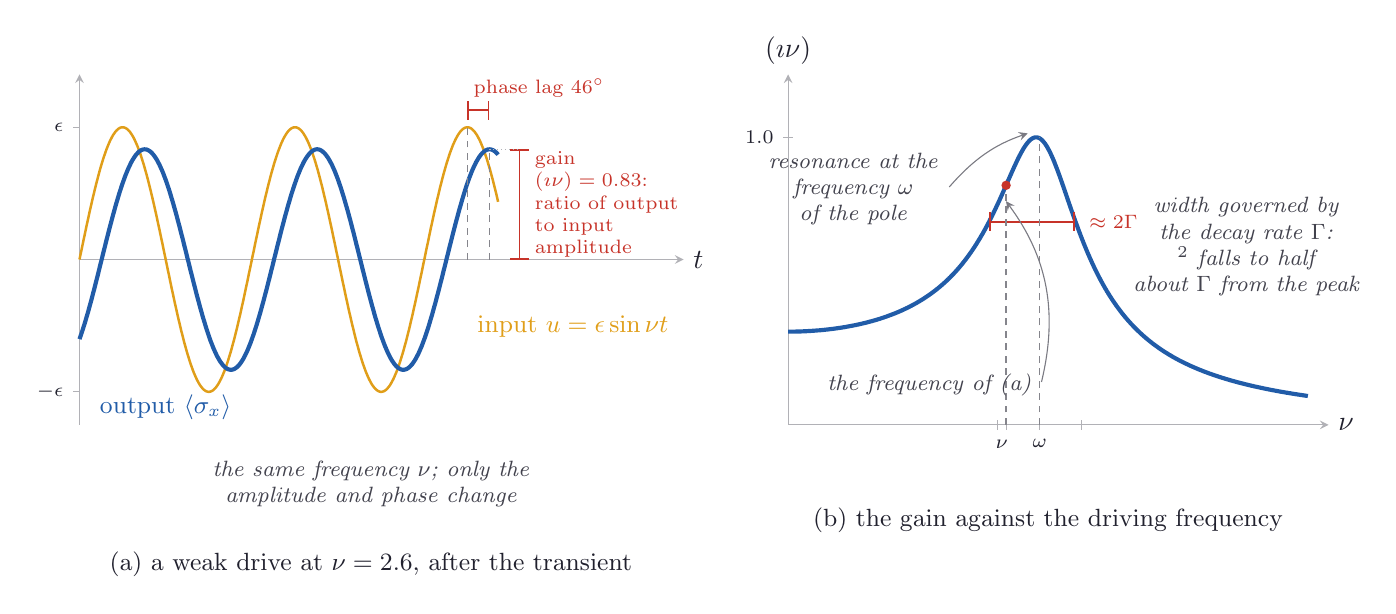
\begin{tikzpicture}[ink/.style={line width=0.9pt, ndInk}, faint/.style={line width=0.4pt, ndInk!35}, dashedink/.style={line width=0.5pt, ndInk!55, dash pattern=on 2.5pt off 2pt}, vec/.style={->, >=stealth, line width=1.2pt}, note/.style={font=\footnotesize\itshape, text=ndInk!85, align=center}, pointer/.style={->, >=stealth, line width=0.4pt, ndInk!60, shorten >=2pt, shorten <=1pt}, dot/.style={circle, fill=ndInk, inner sep=0pt, minimum size=3.4pt}, wash/.style={fill=ndSky, fill opacity=0.55}, every node/.style={text=ndInk}]
\definecolor{ndInk}{rgb}{0.13,0.13,0.18}
\definecolor{ndPaper}{rgb}{0.99,0.96,0.88}
\definecolor{ndSky}{rgb}{0.84,0.91,0.98}
\definecolor{ndRose}{rgb}{0.98,0.86,0.84}
\definecolor{ndBlue}{rgb}{0.13,0.36,0.66}
\definecolor{ndRed}{rgb}{0.78,0.20,0.16}
\definecolor{ndGold}{rgb}{0.88,0.62,0.10}
\definecolor{ndGreen}{rgb}{0.18,0.52,0.30}
\draw[faint, ->, >=stealth] (0.000,2.700) -- (7.672,2.700) node[right, text=ndInk] {$t$};
\draw[faint, ->, >=stealth] (0.000,0.600) -- (0.000,5.052);
\draw[faint] (0.000,4.380) -- ++(-0.08,0) node[left, font=\scriptsize, text=ndInk] {$\epsilon$};
\draw[faint] (0.000,1.020) -- ++(-0.08,0) node[left, font=\scriptsize, text=ndInk] {$-\epsilon$};
\draw[line width=0.9pt, ndGold] (0.000,2.700) -- (0.013,2.764) -- (0.027,2.828) -- (0.040,2.892) -- (0.053,2.956) -- (0.067,3.019) -- (0.080,3.082) -- (0.093,3.144) -- (0.107,3.206) -- (0.120,3.267) -- (0.133,3.327) -- (0.147,3.386) -- (0.160,3.444) -- (0.173,3.501) -- (0.187,3.557) -- (0.200,3.612) -- (0.213,3.665) -- (0.227,3.717) -- (0.240,3.767) -- (0.253,3.816) -- (0.266,3.863) -- (0.280,3.909) -- (0.293,3.952) -- (0.306,3.994) -- (0.320,4.034) -- (0.333,4.072) -- (0.346,4.108) -- (0.360,4.142) -- (0.373,4.174) -- (0.386,4.204) -- (0.400,4.231) -- (0.413,4.257) -- (0.426,4.280) -- (0.440,4.300) -- (0.453,4.319) -- (0.466,4.335) -- (0.480,4.348) -- (0.493,4.360) -- (0.506,4.368) -- (0.520,4.375) -- (0.533,4.379) -- (0.546,4.380) -- (0.560,4.379) -- (0.573,4.375) -- (0.586,4.370) -- (0.600,4.361) -- (0.613,4.350) -- (0.626,4.337) -- (0.640,4.322) -- (0.653,4.304) -- (0.666,4.283) -- (0.680,4.261) -- (0.693,4.236) -- (0.706,4.209) -- (0.719,4.179) -- (0.733,4.148) -- (0.746,4.114) -- (0.759,4.078) -- (0.773,4.041) -- (0.786,4.001) -- (0.799,3.959) -- (0.813,3.916) -- (0.826,3.871) -- (0.839,3.824) -- (0.853,3.775) -- (0.866,3.725) -- (0.879,3.673) -- (0.893,3.620) -- (0.906,3.566) -- (0.919,3.510) -- (0.933,3.453) -- (0.946,3.396) -- (0.959,3.337) -- (0.973,3.277) -- (0.986,3.216) -- (0.999,3.154) -- (1.013,3.092) -- (1.026,3.030) -- (1.039,2.966) -- (1.053,2.903) -- (1.066,2.839) -- (1.079,2.775) -- (1.093,2.710) -- (1.106,2.646) -- (1.119,2.582) -- (1.133,2.518) -- (1.146,2.454) -- (1.159,2.391) -- (1.172,2.328) -- (1.186,2.266) -- (1.199,2.204) -- (1.212,2.143) -- (1.226,2.083) -- (1.239,2.024) -- (1.252,1.965) -- (1.266,1.908) -- (1.279,1.852) -- (1.292,1.797) -- (1.306,1.744) -- (1.319,1.692) -- (1.332,1.641) -- (1.346,1.592) -- (1.359,1.544) -- (1.372,1.499) -- (1.386,1.455) -- (1.399,1.412) -- (1.412,1.372) -- (1.426,1.334) -- (1.439,1.297) -- (1.452,1.263) -- (1.466,1.231) -- (1.479,1.201) -- (1.492,1.173) -- (1.506,1.147) -- (1.519,1.124) -- (1.532,1.103) -- (1.546,1.084) -- (1.559,1.068) -- (1.572,1.054) -- (1.586,1.042) -- (1.599,1.033) -- (1.612,1.026) -- (1.626,1.022) -- (1.639,1.020) -- (1.652,1.021) -- (1.665,1.024) -- (1.679,1.029) -- (1.692,1.037) -- (1.705,1.048) -- (1.719,1.061) -- (1.732,1.076) -- (1.745,1.093) -- (1.759,1.113) -- (1.772,1.136) -- (1.785,1.160) -- (1.799,1.187) -- (1.812,1.216) -- (1.825,1.247) -- (1.839,1.280) -- (1.852,1.316) -- (1.865,1.353) -- (1.879,1.393) -- (1.892,1.434) -- (1.905,1.477) -- (1.919,1.522) -- (1.932,1.568) -- (1.945,1.617) -- (1.959,1.667) -- (1.972,1.718) -- (1.985,1.771) -- (1.999,1.825) -- (2.012,1.881) -- (2.025,1.937) -- (2.039,1.995) -- (2.052,2.054) -- (2.065,2.114) -- (2.079,2.174) -- (2.092,2.236) -- (2.105,2.298) -- (2.118,2.360) -- (2.132,2.423) -- (2.145,2.487) -- (2.158,2.551) -- (2.172,2.615) -- (2.185,2.679) -- (2.198,2.743) -- (2.212,2.807) -- (2.225,2.871) -- (2.238,2.935) -- (2.252,2.999) -- (2.265,3.062) -- (2.278,3.124) -- (2.292,3.186) -- (2.305,3.247) -- (2.318,3.307) -- (2.332,3.367) -- (2.345,3.425) -- (2.358,3.483) -- (2.372,3.539) -- (2.385,3.594) -- (2.398,3.648) -- (2.412,3.700) -- (2.425,3.751) -- (2.438,3.800) -- (2.452,3.848) -- (2.465,3.894) -- (2.478,3.938) -- (2.492,3.981) -- (2.505,4.021) -- (2.518,4.060) -- (2.532,4.097) -- (2.545,4.131) -- (2.558,4.164) -- (2.571,4.194) -- (2.585,4.223) -- (2.598,4.249) -- (2.611,4.272) -- (2.625,4.294) -- (2.638,4.313) -- (2.651,4.330) -- (2.665,4.344) -- (2.678,4.356) -- (2.691,4.366) -- (2.705,4.373) -- (2.718,4.378) -- (2.731,4.380) -- (2.745,4.380) -- (2.758,4.377) -- (2.771,4.372) -- (2.785,4.364) -- (2.798,4.354) -- (2.811,4.342) -- (2.825,4.327) -- (2.838,4.310) -- (2.851,4.290) -- (2.865,4.268) -- (2.878,4.244) -- (2.891,4.218) -- (2.905,4.189) -- (2.918,4.158) -- (2.931,4.125) -- (2.945,4.090) -- (2.958,4.053) -- (2.971,4.014) -- (2.985,3.973) -- (2.998,3.930) -- (3.011,3.886) -- (3.025,3.839) -- (3.038,3.791) -- (3.051,3.742) -- (3.064,3.690) -- (3.078,3.638) -- (3.091,3.584) -- (3.104,3.529) -- (3.118,3.472) -- (3.131,3.415) -- (3.144,3.356) -- (3.158,3.296) -- (3.171,3.236) -- (3.184,3.175) -- (3.198,3.113) -- (3.211,3.050) -- (3.224,2.987) -- (3.238,2.923) -- (3.251,2.860) -- (3.264,2.796) -- (3.278,2.731) -- (3.291,2.667) -- (3.304,2.603) -- (3.318,2.539) -- (3.331,2.475) -- (3.344,2.412) -- (3.358,2.349) -- (3.371,2.286) -- (3.384,2.224) -- (3.398,2.163) -- (3.411,2.102) -- (3.424,2.043) -- (3.438,1.984) -- (3.451,1.927) -- (3.464,1.870) -- (3.478,1.815) -- (3.491,1.761) -- (3.504,1.708) -- (3.517,1.657) -- (3.531,1.608) -- (3.544,1.560) -- (3.557,1.513) -- (3.571,1.469) -- (3.584,1.426) -- (3.597,1.385) -- (3.611,1.346) -- (3.624,1.309) -- (3.637,1.274) -- (3.651,1.241) -- (3.664,1.210) -- (3.677,1.182) -- (3.691,1.155) -- (3.704,1.131) -- (3.717,1.109) -- (3.731,1.090) -- (3.744,1.073) -- (3.757,1.058) -- (3.771,1.046) -- (3.784,1.036) -- (3.797,1.028) -- (3.811,1.023) -- (3.824,1.020) -- (3.837,1.020) -- (3.851,1.023) -- (3.864,1.027) -- (3.877,1.034) -- (3.891,1.044) -- (3.904,1.056) -- (3.917,1.071) -- (3.931,1.087) -- (3.944,1.106) -- (3.957,1.128) -- (3.970,1.152) -- (3.984,1.178) -- (3.997,1.206) -- (4.010,1.237) -- (4.024,1.269) -- (4.037,1.304) -- (4.050,1.341) -- (4.064,1.379) -- (4.077,1.420) -- (4.090,1.463) -- (4.104,1.507) -- (4.117,1.553) -- (4.130,1.601) -- (4.144,1.650) -- (4.157,1.701) -- (4.170,1.753) -- (4.184,1.807) -- (4.197,1.862) -- (4.210,1.919) -- (4.224,1.976) -- (4.237,2.034) -- (4.250,2.094) -- (4.264,2.154) -- (4.277,2.215) -- (4.290,2.277) -- (4.304,2.340) -- (4.317,2.403) -- (4.330,2.466) -- (4.344,2.530) -- (4.357,2.594) -- (4.370,2.658) -- (4.384,2.722) -- (4.397,2.787) -- (4.410,2.851) -- (4.424,2.914) -- (4.437,2.978) -- (4.450,3.041) -- (4.463,3.104) -- (4.477,3.166) -- (4.490,3.227) -- (4.503,3.288) -- (4.517,3.347) -- (4.530,3.406) -- (4.543,3.464) -- (4.557,3.521) -- (4.570,3.576) -- (4.583,3.630) -- (4.597,3.683) -- (4.610,3.734) -- (4.623,3.784) -- (4.637,3.833) -- (4.650,3.879) -- (4.663,3.924) -- (4.677,3.967) -- (4.690,4.008) -- (4.703,4.048) -- (4.717,4.085) -- (4.730,4.120) -- (4.743,4.154) -- (4.757,4.185) -- (4.770,4.214) -- (4.783,4.240) -- (4.797,4.265) -- (4.810,4.287) -- (4.823,4.307) -- (4.837,4.325) -- (4.850,4.340) -- (4.863,4.353) -- (4.877,4.363) -- (4.890,4.371) -- (4.903,4.376) -- (4.916,4.379) -- (4.930,4.380) -- (4.943,4.378) -- (4.956,4.374) -- (4.970,4.367) -- (4.983,4.358) -- (4.996,4.346) -- (5.010,4.332) -- (5.023,4.316) -- (5.036,4.297) -- (5.050,4.276) -- (5.063,4.252) -- (5.076,4.227) -- (5.090,4.199) -- (5.103,4.168) -- (5.116,4.136) -- (5.130,4.102) -- (5.143,4.065) -- (5.156,4.027) -- (5.170,3.987) -- (5.183,3.944) -- (5.196,3.900) -- (5.210,3.855) -- (5.223,3.807) -- (5.236,3.758) -- (5.250,3.707) -- (5.263,3.655) -- (5.276,3.602) -- (5.290,3.547) -- (5.303,3.491) -- (5.316,3.433);
\draw[line width=1.5pt, ndBlue] (0.000,1.689) -- (0.013,1.727) -- (0.027,1.766) -- (0.040,1.806) -- (0.053,1.848) -- (0.067,1.891) -- (0.080,1.936) -- (0.093,1.981) -- (0.107,2.027) -- (0.120,2.075) -- (0.133,2.123) -- (0.147,2.172) -- (0.160,2.222) -- (0.173,2.273) -- (0.187,2.324) -- (0.200,2.376) -- (0.213,2.428) -- (0.227,2.481) -- (0.240,2.534) -- (0.253,2.587) -- (0.266,2.641) -- (0.280,2.694) -- (0.293,2.748) -- (0.306,2.801) -- (0.320,2.855) -- (0.333,2.908) -- (0.346,2.960) -- (0.360,3.013) -- (0.373,3.065) -- (0.386,3.116) -- (0.400,3.167) -- (0.413,3.217) -- (0.426,3.266) -- (0.440,3.315) -- (0.453,3.363) -- (0.466,3.409) -- (0.480,3.455) -- (0.493,3.499) -- (0.506,3.543) -- (0.520,3.585) -- (0.533,3.626) -- (0.546,3.665) -- (0.560,3.703) -- (0.573,3.740) -- (0.586,3.775) -- (0.600,3.808) -- (0.613,3.840) -- (0.626,3.870) -- (0.640,3.899) -- (0.653,3.926) -- (0.666,3.951) -- (0.680,3.974) -- (0.693,3.995) -- (0.706,4.014) -- (0.719,4.032) -- (0.733,4.047) -- (0.746,4.061) -- (0.759,4.073) -- (0.773,4.082) -- (0.786,4.090) -- (0.799,4.095) -- (0.813,4.099) -- (0.826,4.100) -- (0.839,4.099) -- (0.853,4.097) -- (0.866,4.092) -- (0.879,4.085) -- (0.893,4.076) -- (0.906,4.066) -- (0.919,4.053) -- (0.933,4.038) -- (0.946,4.021) -- (0.959,4.003) -- (0.973,3.982) -- (0.986,3.960) -- (0.999,3.935) -- (1.013,3.909) -- (1.026,3.881) -- (1.039,3.852) -- (1.053,3.821) -- (1.066,3.788) -- (1.079,3.753) -- (1.093,3.717) -- (1.106,3.680) -- (1.119,3.641) -- (1.133,3.600) -- (1.146,3.559) -- (1.159,3.516) -- (1.172,3.472) -- (1.186,3.426) -- (1.199,3.380) -- (1.212,3.333) -- (1.226,3.285) -- (1.239,3.236) -- (1.252,3.186) -- (1.266,3.135) -- (1.279,3.084) -- (1.292,3.032) -- (1.306,2.980) -- (1.319,2.928) -- (1.332,2.875) -- (1.346,2.821) -- (1.359,2.768) -- (1.372,2.714) -- (1.386,2.661) -- (1.399,2.607) -- (1.412,2.554) -- (1.426,2.501) -- (1.439,2.448) -- (1.452,2.396) -- (1.466,2.344) -- (1.479,2.292) -- (1.492,2.241) -- (1.506,2.191) -- (1.519,2.142) -- (1.532,2.093) -- (1.546,2.045) -- (1.559,1.998) -- (1.572,1.952) -- (1.586,1.908) -- (1.599,1.864) -- (1.612,1.822) -- (1.626,1.781) -- (1.639,1.741) -- (1.652,1.703) -- (1.665,1.666) -- (1.679,1.631) -- (1.692,1.597) -- (1.705,1.565) -- (1.719,1.534) -- (1.732,1.506) -- (1.745,1.478) -- (1.759,1.453) -- (1.772,1.430) -- (1.785,1.408) -- (1.799,1.389) -- (1.812,1.371) -- (1.825,1.355) -- (1.839,1.341) -- (1.852,1.329) -- (1.865,1.319) -- (1.879,1.311) -- (1.892,1.306) -- (1.905,1.302) -- (1.919,1.300) -- (1.932,1.300) -- (1.945,1.303) -- (1.959,1.307) -- (1.972,1.314) -- (1.985,1.322) -- (1.999,1.333) -- (2.012,1.345) -- (2.025,1.359) -- (2.039,1.376) -- (2.052,1.394) -- (2.065,1.414) -- (2.079,1.437) -- (2.092,1.461) -- (2.105,1.486) -- (2.118,1.514) -- (2.132,1.543) -- (2.145,1.574) -- (2.158,1.607) -- (2.172,1.641) -- (2.185,1.677) -- (2.198,1.714) -- (2.212,1.753) -- (2.225,1.793) -- (2.238,1.834) -- (2.252,1.877) -- (2.265,1.921) -- (2.278,1.966) -- (2.292,2.012) -- (2.305,2.059) -- (2.318,2.107) -- (2.332,2.156) -- (2.345,2.206) -- (2.358,2.256) -- (2.372,2.307) -- (2.385,2.359) -- (2.398,2.411) -- (2.412,2.464) -- (2.425,2.517) -- (2.438,2.570) -- (2.452,2.623) -- (2.465,2.677) -- (2.478,2.730) -- (2.492,2.784) -- (2.505,2.837) -- (2.518,2.890) -- (2.532,2.943) -- (2.545,2.996) -- (2.558,3.048) -- (2.571,3.099) -- (2.585,3.150) -- (2.598,3.201) -- (2.611,3.250) -- (2.625,3.299) -- (2.638,3.347) -- (2.651,3.394) -- (2.665,3.440) -- (2.678,3.485) -- (2.691,3.529) -- (2.705,3.571) -- (2.718,3.613) -- (2.731,3.652) -- (2.745,3.691) -- (2.758,3.728) -- (2.771,3.764) -- (2.785,3.798) -- (2.798,3.830) -- (2.811,3.861) -- (2.825,3.890) -- (2.838,3.917) -- (2.851,3.943) -- (2.865,3.967) -- (2.878,3.988) -- (2.891,4.008) -- (2.905,4.026) -- (2.918,4.043) -- (2.931,4.057) -- (2.945,4.069) -- (2.958,4.079) -- (2.971,4.087) -- (2.985,4.094) -- (2.998,4.098) -- (3.011,4.100) -- (3.025,4.100) -- (3.038,4.098) -- (3.051,4.094) -- (3.064,4.088) -- (3.078,4.079) -- (3.091,4.069) -- (3.104,4.057) -- (3.118,4.043) -- (3.131,4.027) -- (3.144,4.009) -- (3.158,3.989) -- (3.171,3.967) -- (3.184,3.943) -- (3.198,3.918) -- (3.211,3.891) -- (3.224,3.862) -- (3.238,3.831) -- (3.251,3.799) -- (3.264,3.765) -- (3.278,3.729) -- (3.291,3.692) -- (3.304,3.654) -- (3.318,3.614) -- (3.331,3.572) -- (3.344,3.530) -- (3.358,3.486) -- (3.371,3.441) -- (3.384,3.395) -- (3.398,3.348) -- (3.411,3.301) -- (3.424,3.252) -- (3.438,3.202) -- (3.451,3.152) -- (3.464,3.101) -- (3.478,3.049) -- (3.491,2.997) -- (3.504,2.945) -- (3.517,2.892) -- (3.531,2.839) -- (3.544,2.785) -- (3.557,2.732) -- (3.571,2.678) -- (3.584,2.625) -- (3.597,2.571) -- (3.611,2.518) -- (3.624,2.465) -- (3.637,2.413) -- (3.651,2.361) -- (3.664,2.309) -- (3.677,2.258) -- (3.691,2.207) -- (3.704,2.158) -- (3.717,2.109) -- (3.731,2.061) -- (3.744,2.013) -- (3.757,1.967) -- (3.771,1.922) -- (3.784,1.878) -- (3.797,1.836) -- (3.811,1.794) -- (3.824,1.754) -- (3.837,1.715) -- (3.851,1.678) -- (3.864,1.642) -- (3.877,1.608) -- (3.891,1.575) -- (3.904,1.544) -- (3.917,1.515) -- (3.931,1.487) -- (3.944,1.461) -- (3.957,1.437) -- (3.970,1.415) -- (3.984,1.395) -- (3.997,1.376) -- (4.010,1.360) -- (4.024,1.345) -- (4.037,1.333) -- (4.050,1.322) -- (4.064,1.314) -- (4.077,1.307) -- (4.090,1.303) -- (4.104,1.300) -- (4.117,1.300) -- (4.130,1.302) -- (4.144,1.306) -- (4.157,1.311) -- (4.170,1.319) -- (4.184,1.329) -- (4.197,1.341) -- (4.210,1.355) -- (4.224,1.370) -- (4.237,1.388) -- (4.250,1.408) -- (4.264,1.429) -- (4.277,1.453) -- (4.290,1.478) -- (4.304,1.505) -- (4.317,1.533) -- (4.330,1.564) -- (4.344,1.596) -- (4.357,1.630) -- (4.370,1.665) -- (4.384,1.702) -- (4.397,1.740) -- (4.410,1.780) -- (4.424,1.821) -- (4.437,1.863) -- (4.450,1.907) -- (4.463,1.951) -- (4.477,1.997) -- (4.490,2.044) -- (4.503,2.092) -- (4.517,2.140) -- (4.530,2.190) -- (4.543,2.240) -- (4.557,2.291) -- (4.570,2.342) -- (4.583,2.394) -- (4.597,2.447) -- (4.610,2.499) -- (4.623,2.553) -- (4.637,2.606) -- (4.650,2.659) -- (4.663,2.713) -- (4.677,2.766) -- (4.690,2.820) -- (4.703,2.873) -- (4.717,2.926) -- (4.730,2.979) -- (4.743,3.031) -- (4.757,3.083) -- (4.770,3.134) -- (4.783,3.184) -- (4.797,3.234) -- (4.810,3.283) -- (4.823,3.332) -- (4.837,3.379) -- (4.850,3.425) -- (4.863,3.470) -- (4.877,3.515) -- (4.890,3.558) -- (4.903,3.599) -- (4.916,3.640) -- (4.930,3.679) -- (4.943,3.716) -- (4.956,3.752) -- (4.970,3.787) -- (4.983,3.820) -- (4.996,3.851) -- (5.010,3.881) -- (5.023,3.908) -- (5.036,3.935) -- (5.050,3.959) -- (5.063,3.981) -- (5.076,4.002) -- (5.090,4.021) -- (5.103,4.038) -- (5.116,4.052) -- (5.130,4.065) -- (5.143,4.076) -- (5.156,4.085) -- (5.170,4.092) -- (5.183,4.097) -- (5.196,4.099) -- (5.210,4.100) -- (5.223,4.099) -- (5.236,4.095) -- (5.250,4.090) -- (5.263,4.082) -- (5.276,4.073) -- (5.290,4.061) -- (5.303,4.048) -- (5.316,4.032);
\draw[dashedink] (4.926,2.700) -- (4.926,4.380);
\draw[dashedink] (5.207,2.700) -- (5.207,4.100);
\draw[line width=0.7pt, ndRed, |-|] (4.926,4.598) -- (5.207,4.598);
\node[font=\scriptsize, text=ndRed, anchor=south west, align=left] at (4.881,4.632) {phase lag $46^\circ$};
\draw[line width=0.7pt, ndRed, |-|] (5.588,2.700) -- (5.588,4.100);
\draw[faint, densely dotted] (5.207,4.100) -- (5.588,4.100);
\node[font=\scriptsize, text=ndRed, anchor=west, align=left] at (5.660,3.400) {gain\\ $\abs{\TF(\imath\nu)}=0.83$:\\ ratio of output\\ to input\\ amplitude};
\node[font=\small, text=ndGold, anchor=north] at (6.267,2.112) {input $u=\epsilon\sin\nu t$};
\node[font=\small, text=ndBlue, anchor=north west] at (0.136,1.104) {output $\langle\sigma_x\rangle$};
\node[note, anchor=north] at (3.700,0.264) {the same frequency $\nu$; only the\\ amplitude and phase change};
\node[font=\small] at (3.700,-1.164) {(a) a weak drive at $\nu=2.6$, after the transient};
\draw[faint, ->, >=stealth] (9.000,0.600) -- (15.864,0.600) node[right, text=ndInk] {$\nu$};
\draw[faint, ->, >=stealth] (9.000,0.600) -- (9.000,5.052) node[above, text=ndInk] {$\abs{\TF(\imath\nu)}$};
\draw[faint] (11.661,0.660) -- (11.661,0.540) node[below, font=\scriptsize, text=ndInk] {};
\draw[faint] (12.194,0.660) -- (12.194,0.540) node[below, font=\scriptsize, text=ndInk] {$\omega$};
\draw[faint] (12.726,0.660) -- (12.726,0.540) node[below, font=\scriptsize, text=ndInk] {};
\draw[faint] (11.768,0.660) -- (11.768,0.540) node[below, font=\scriptsize, text=ndInk] {};
\draw[faint] (9.060,4.252) -- (8.940,4.252) node[left, font=\scriptsize, text=ndInk] {$1.0$};
\draw[line width=1.5pt, ndBlue] (9.000,1.784) -- (9.005,1.784) -- (9.011,1.785) -- (9.016,1.785) -- (9.021,1.785) -- (9.027,1.785) -- (9.032,1.785) -- (9.037,1.785) -- (9.043,1.785) -- (9.048,1.785) -- (9.053,1.785) -- (9.059,1.785) -- (9.064,1.785) -- (9.069,1.785) -- (9.075,1.785) -- (9.080,1.785) -- (9.085,1.785) -- (9.090,1.785) -- (9.096,1.785) -- (9.101,1.786) -- (9.106,1.786) -- (9.112,1.786) -- (9.117,1.786) -- (9.122,1.786) -- (9.128,1.786) -- (9.133,1.786) -- (9.138,1.787) -- (9.144,1.787) -- (9.149,1.787) -- (9.154,1.787) -- (9.160,1.787) -- (9.165,1.787) -- (9.170,1.788) -- (9.176,1.788) -- (9.181,1.788) -- (9.186,1.788) -- (9.192,1.788) -- (9.197,1.789) -- (9.202,1.789) -- (9.208,1.789) -- (9.213,1.789) -- (9.218,1.790) -- (9.224,1.790) -- (9.229,1.790) -- (9.234,1.790) -- (9.240,1.791) -- (9.245,1.791) -- (9.250,1.791) -- (9.255,1.792) -- (9.261,1.792) -- (9.266,1.792) -- (9.271,1.792) -- (9.277,1.793) -- (9.282,1.793) -- (9.287,1.793) -- (9.293,1.794) -- (9.298,1.794) -- (9.303,1.794) -- (9.309,1.795) -- (9.314,1.795) -- (9.319,1.795) -- (9.325,1.796) -- (9.330,1.796) -- (9.335,1.797) -- (9.341,1.797) -- (9.346,1.797) -- (9.351,1.798) -- (9.357,1.798) -- (9.362,1.799) -- (9.367,1.799) -- (9.373,1.800) -- (9.378,1.800) -- (9.383,1.800) -- (9.389,1.801) -- (9.394,1.801) -- (9.399,1.802) -- (9.405,1.802) -- (9.410,1.803) -- (9.415,1.803) -- (9.420,1.804) -- (9.426,1.804) -- (9.431,1.805) -- (9.436,1.805) -- (9.442,1.806) -- (9.447,1.806) -- (9.452,1.807) -- (9.458,1.807) -- (9.463,1.808) -- (9.468,1.808) -- (9.474,1.809) -- (9.479,1.810) -- (9.484,1.810) -- (9.490,1.811) -- (9.495,1.811) -- (9.500,1.812) -- (9.506,1.812) -- (9.511,1.813) -- (9.516,1.814) -- (9.522,1.814) -- (9.527,1.815) -- (9.532,1.816) -- (9.538,1.816) -- (9.543,1.817) -- (9.548,1.817) -- (9.554,1.818) -- (9.559,1.819) -- (9.564,1.819) -- (9.570,1.820) -- (9.575,1.821) -- (9.580,1.822) -- (9.585,1.822) -- (9.591,1.823) -- (9.596,1.824) -- (9.601,1.824) -- (9.607,1.825) -- (9.612,1.826) -- (9.617,1.827) -- (9.623,1.827) -- (9.628,1.828) -- (9.633,1.829) -- (9.639,1.830) -- (9.644,1.830) -- (9.649,1.831) -- (9.655,1.832) -- (9.660,1.833) -- (9.665,1.834) -- (9.671,1.834) -- (9.676,1.835) -- (9.681,1.836) -- (9.687,1.837) -- (9.692,1.838) -- (9.697,1.839) -- (9.703,1.840) -- (9.708,1.840) -- (9.713,1.841) -- (9.719,1.842) -- (9.724,1.843) -- (9.729,1.844) -- (9.735,1.845) -- (9.740,1.846) -- (9.745,1.847) -- (9.750,1.848) -- (9.756,1.849) -- (9.761,1.850) -- (9.766,1.851) -- (9.772,1.852) -- (9.777,1.853) -- (9.782,1.854) -- (9.788,1.854) -- (9.793,1.855) -- (9.798,1.857) -- (9.804,1.858) -- (9.809,1.859) -- (9.814,1.860) -- (9.820,1.861) -- (9.825,1.862) -- (9.830,1.863) -- (9.836,1.864) -- (9.841,1.865) -- (9.846,1.866) -- (9.852,1.867) -- (9.857,1.868) -- (9.862,1.869) -- (9.868,1.870) -- (9.873,1.872) -- (9.878,1.873) -- (9.884,1.874) -- (9.889,1.875) -- (9.894,1.876) -- (9.900,1.877) -- (9.905,1.879) -- (9.910,1.880) -- (9.915,1.881) -- (9.921,1.882) -- (9.926,1.883) -- (9.931,1.885) -- (9.937,1.886) -- (9.942,1.887) -- (9.947,1.888) -- (9.953,1.890) -- (9.958,1.891) -- (9.963,1.892) -- (9.969,1.893) -- (9.974,1.895) -- (9.979,1.896) -- (9.985,1.897) -- (9.990,1.899) -- (9.995,1.900) -- (10.001,1.901) -- (10.006,1.903) -- (10.011,1.904) -- (10.017,1.906) -- (10.022,1.907) -- (10.027,1.908) -- (10.033,1.910) -- (10.038,1.911) -- (10.043,1.913) -- (10.049,1.914) -- (10.054,1.915) -- (10.059,1.917) -- (10.065,1.918) -- (10.070,1.920) -- (10.075,1.921) -- (10.080,1.923) -- (10.086,1.924) -- (10.091,1.926) -- (10.096,1.927) -- (10.102,1.929) -- (10.107,1.931) -- (10.112,1.932) -- (10.118,1.934) -- (10.123,1.935) -- (10.128,1.937) -- (10.134,1.939) -- (10.139,1.940) -- (10.144,1.942) -- (10.150,1.943) -- (10.155,1.945) -- (10.160,1.947) -- (10.166,1.948) -- (10.171,1.950) -- (10.176,1.952) -- (10.182,1.954) -- (10.187,1.955) -- (10.192,1.957) -- (10.198,1.959) -- (10.203,1.961) -- (10.208,1.962) -- (10.214,1.964) -- (10.219,1.966) -- (10.224,1.968) -- (10.230,1.970) -- (10.235,1.971) -- (10.240,1.973) -- (10.245,1.975) -- (10.251,1.977) -- (10.256,1.979) -- (10.261,1.981) -- (10.267,1.983) -- (10.272,1.985) -- (10.277,1.987) -- (10.283,1.989) -- (10.288,1.991) -- (10.293,1.993) -- (10.299,1.995) -- (10.304,1.997) -- (10.309,1.999) -- (10.315,2.001) -- (10.320,2.003) -- (10.325,2.005) -- (10.331,2.007) -- (10.336,2.009) -- (10.341,2.011) -- (10.347,2.013) -- (10.352,2.015) -- (10.357,2.017) -- (10.363,2.020) -- (10.368,2.022) -- (10.373,2.024) -- (10.379,2.026) -- (10.384,2.028) -- (10.389,2.031) -- (10.395,2.033) -- (10.400,2.035) -- (10.405,2.037) -- (10.410,2.040) -- (10.416,2.042) -- (10.421,2.044) -- (10.426,2.047) -- (10.432,2.049) -- (10.437,2.051) -- (10.442,2.054) -- (10.448,2.056) -- (10.453,2.059) -- (10.458,2.061) -- (10.464,2.063) -- (10.469,2.066) -- (10.474,2.068) -- (10.480,2.071) -- (10.485,2.073) -- (10.490,2.076) -- (10.496,2.079) -- (10.501,2.081) -- (10.506,2.084) -- (10.512,2.086) -- (10.517,2.089) -- (10.522,2.092) -- (10.528,2.094) -- (10.533,2.097) -- (10.538,2.100) -- (10.544,2.102) -- (10.549,2.105) -- (10.554,2.108) -- (10.560,2.111) -- (10.565,2.113) -- (10.570,2.116) -- (10.575,2.119) -- (10.581,2.122) -- (10.586,2.125) -- (10.591,2.128) -- (10.597,2.130) -- (10.602,2.133) -- (10.607,2.136) -- (10.613,2.139) -- (10.618,2.142) -- (10.623,2.145) -- (10.629,2.148) -- (10.634,2.151) -- (10.639,2.154) -- (10.645,2.157) -- (10.650,2.161) -- (10.655,2.164) -- (10.661,2.167) -- (10.666,2.170) -- (10.671,2.173) -- (10.677,2.176) -- (10.682,2.180) -- (10.687,2.183) -- (10.693,2.186) -- (10.698,2.190) -- (10.703,2.193) -- (10.709,2.196) -- (10.714,2.200) -- (10.719,2.203) -- (10.725,2.206) -- (10.730,2.210) -- (10.735,2.213) -- (10.740,2.217) -- (10.746,2.220) -- (10.751,2.224) -- (10.756,2.227) -- (10.762,2.231) -- (10.767,2.235) -- (10.772,2.238) -- (10.778,2.242) -- (10.783,2.245) -- (10.788,2.249) -- (10.794,2.253) -- (10.799,2.257) -- (10.804,2.260) -- (10.810,2.264) -- (10.815,2.268) -- (10.820,2.272) -- (10.826,2.276) -- (10.831,2.280) -- (10.836,2.284) -- (10.842,2.288) -- (10.847,2.292) -- (10.852,2.296) -- (10.858,2.300) -- (10.863,2.304) -- (10.868,2.308) -- (10.874,2.312) -- (10.879,2.316) -- (10.884,2.321) -- (10.890,2.325) -- (10.895,2.329) -- (10.900,2.333) -- (10.905,2.338) -- (10.911,2.342) -- (10.916,2.346) -- (10.921,2.351) -- (10.927,2.355) -- (10.932,2.360) -- (10.937,2.364) -- (10.943,2.369) -- (10.948,2.373) -- (10.953,2.378) -- (10.959,2.383) -- (10.964,2.387) -- (10.969,2.392) -- (10.975,2.397) -- (10.980,2.402) -- (10.985,2.406) -- (10.991,2.411) -- (10.996,2.416) -- (11.001,2.421) -- (11.007,2.426) -- (11.012,2.431) -- (11.017,2.436) -- (11.023,2.441) -- (11.028,2.446) -- (11.033,2.451) -- (11.039,2.456) -- (11.044,2.462) -- (11.049,2.467) -- (11.055,2.472) -- (11.060,2.477) -- (11.065,2.483) -- (11.070,2.488) -- (11.076,2.494) -- (11.081,2.499) -- (11.086,2.505) -- (11.092,2.510) -- (11.097,2.516) -- (11.102,2.521) -- (11.108,2.527) -- (11.113,2.533) -- (11.118,2.539) -- (11.124,2.544) -- (11.129,2.550) -- (11.134,2.556) -- (11.140,2.562) -- (11.145,2.568) -- (11.150,2.574) -- (11.156,2.580) -- (11.161,2.586) -- (11.166,2.592) -- (11.172,2.599) -- (11.177,2.605) -- (11.182,2.611) -- (11.188,2.617) -- (11.193,2.624) -- (11.198,2.630) -- (11.204,2.637) -- (11.209,2.643) -- (11.214,2.650) -- (11.220,2.657) -- (11.225,2.663) -- (11.230,2.670) -- (11.235,2.677) -- (11.241,2.684) -- (11.246,2.690) -- (11.251,2.697) -- (11.257,2.704) -- (11.262,2.711) -- (11.267,2.718) -- (11.273,2.726) -- (11.278,2.733) -- (11.283,2.740) -- (11.289,2.747) -- (11.294,2.755) -- (11.299,2.762) -- (11.305,2.769) -- (11.310,2.777) -- (11.315,2.785) -- (11.321,2.792) -- (11.326,2.800) -- (11.331,2.808) -- (11.337,2.815) -- (11.342,2.823) -- (11.347,2.831) -- (11.353,2.839) -- (11.358,2.847) -- (11.363,2.855) -- (11.369,2.863) -- (11.374,2.871) -- (11.379,2.880) -- (11.385,2.888) -- (11.390,2.896) -- (11.395,2.905) -- (11.400,2.913) -- (11.406,2.922) -- (11.411,2.931) -- (11.416,2.939) -- (11.422,2.948) -- (11.427,2.957) -- (11.432,2.966) -- (11.438,2.974) -- (11.443,2.983) -- (11.448,2.993) -- (11.454,3.002) -- (11.459,3.011) -- (11.464,3.020) -- (11.470,3.029) -- (11.475,3.039) -- (11.480,3.048) -- (11.486,3.058) -- (11.491,3.067) -- (11.496,3.077) -- (11.502,3.086) -- (11.507,3.096) -- (11.512,3.106) -- (11.518,3.116) -- (11.523,3.126) -- (11.528,3.136) -- (11.534,3.146) -- (11.539,3.156) -- (11.544,3.166) -- (11.550,3.176) -- (11.555,3.187) -- (11.560,3.197) -- (11.565,3.208) -- (11.571,3.218) -- (11.576,3.229) -- (11.581,3.239) -- (11.587,3.250) -- (11.592,3.261) -- (11.597,3.272) -- (11.603,3.282) -- (11.608,3.293) -- (11.613,3.304) -- (11.619,3.315) -- (11.624,3.326) -- (11.629,3.338) -- (11.635,3.349) -- (11.640,3.360) -- (11.645,3.371) -- (11.651,3.383) -- (11.656,3.394) -- (11.661,3.406) -- (11.667,3.417) -- (11.672,3.429) -- (11.677,3.440) -- (11.683,3.452) -- (11.688,3.464) -- (11.693,3.476) -- (11.699,3.487) -- (11.704,3.499) -- (11.709,3.511) -- (11.715,3.523) -- (11.720,3.535) -- (11.725,3.547) -- (11.730,3.559) -- (11.736,3.571) -- (11.741,3.583) -- (11.746,3.595) -- (11.752,3.607) -- (11.757,3.619) -- (11.762,3.631) -- (11.768,3.643) -- (11.773,3.656) -- (11.778,3.668) -- (11.784,3.680) -- (11.789,3.692) -- (11.794,3.704) -- (11.800,3.716) -- (11.805,3.729) -- (11.810,3.741) -- (11.816,3.753) -- (11.821,3.765) -- (11.826,3.777) -- (11.832,3.789) -- (11.837,3.801) -- (11.842,3.813) -- (11.848,3.825) -- (11.853,3.837) -- (11.858,3.849) -- (11.864,3.861) -- (11.869,3.872) -- (11.874,3.884) -- (11.880,3.896) -- (11.885,3.907) -- (11.890,3.918) -- (11.895,3.930) -- (11.901,3.941) -- (11.906,3.952) -- (11.911,3.963) -- (11.917,3.974) -- (11.922,3.985) -- (11.927,3.996) -- (11.933,4.006) -- (11.938,4.017) -- (11.943,4.027) -- (11.949,4.037) -- (11.954,4.047) -- (11.959,4.057) -- (11.965,4.067) -- (11.970,4.076) -- (11.975,4.086) -- (11.981,4.095) -- (11.986,4.104) -- (11.991,4.113) -- (11.997,4.121) -- (12.002,4.130) -- (12.007,4.138) -- (12.013,4.146) -- (12.018,4.153) -- (12.023,4.161) -- (12.029,4.168) -- (12.034,4.175) -- (12.039,4.181) -- (12.045,4.188) -- (12.050,4.194) -- (12.055,4.200) -- (12.060,4.205) -- (12.066,4.211) -- (12.071,4.216) -- (12.076,4.220) -- (12.082,4.225) -- (12.087,4.229) -- (12.092,4.233) -- (12.098,4.236) -- (12.103,4.239) -- (12.108,4.242) -- (12.114,4.245) -- (12.119,4.247) -- (12.124,4.248) -- (12.130,4.250) -- (12.135,4.251) -- (12.140,4.252) -- (12.146,4.252) -- (12.151,4.252) -- (12.156,4.252) -- (12.162,4.251) -- (12.167,4.250) -- (12.172,4.249) -- (12.178,4.247) -- (12.183,4.245) -- (12.188,4.242) -- (12.194,4.240) -- (12.199,4.236) -- (12.204,4.233) -- (12.210,4.229) -- (12.215,4.225) -- (12.220,4.220) -- (12.225,4.215) -- (12.231,4.210) -- (12.236,4.204) -- (12.241,4.198) -- (12.247,4.192) -- (12.252,4.185) -- (12.257,4.178) -- (12.263,4.171) -- (12.268,4.163) -- (12.273,4.155) -- (12.279,4.147) -- (12.284,4.138) -- (12.289,4.129) -- (12.295,4.120) -- (12.300,4.111) -- (12.305,4.101) -- (12.311,4.091) -- (12.316,4.081) -- (12.321,4.070) -- (12.327,4.059) -- (12.332,4.048) -- (12.337,4.037) -- (12.343,4.025) -- (12.348,4.014) -- (12.353,4.002) -- (12.359,3.989) -- (12.364,3.977) -- (12.369,3.964) -- (12.375,3.952) -- (12.380,3.939) -- (12.385,3.925) -- (12.390,3.912) -- (12.396,3.898) -- (12.401,3.885) -- (12.406,3.871) -- (12.412,3.857) -- (12.417,3.843) -- (12.422,3.829) -- (12.428,3.814) -- (12.433,3.800) -- (12.438,3.785) -- (12.444,3.771) -- (12.449,3.756) -- (12.454,3.741) -- (12.460,3.726) -- (12.465,3.711) -- (12.470,3.696) -- (12.476,3.681) -- (12.481,3.665) -- (12.486,3.650) -- (12.492,3.635) -- (12.497,3.620) -- (12.502,3.604) -- (12.508,3.589) -- (12.513,3.573) -- (12.518,3.558) -- (12.524,3.542) -- (12.529,3.527) -- (12.534,3.511) -- (12.540,3.496) -- (12.545,3.480) -- (12.550,3.465) -- (12.555,3.449) -- (12.561,3.434) -- (12.566,3.418) -- (12.571,3.403) -- (12.577,3.387) -- (12.582,3.372) -- (12.587,3.357) -- (12.593,3.341) -- (12.598,3.326) -- (12.603,3.311) -- (12.609,3.296) -- (12.614,3.281) -- (12.619,3.266) -- (12.625,3.250) -- (12.630,3.235) -- (12.635,3.221) -- (12.641,3.206) -- (12.646,3.191) -- (12.651,3.176) -- (12.657,3.161) -- (12.662,3.147) -- (12.667,3.132) -- (12.673,3.118) -- (12.678,3.103) -- (12.683,3.089) -- (12.689,3.075) -- (12.694,3.060) -- (12.699,3.046) -- (12.705,3.032) -- (12.710,3.018) -- (12.715,3.004) -- (12.720,2.991) -- (12.726,2.977) -- (12.731,2.963) -- (12.736,2.950) -- (12.742,2.936) -- (12.747,2.923) -- (12.752,2.909) -- (12.758,2.896) -- (12.763,2.883) -- (12.768,2.870) -- (12.774,2.857) -- (12.779,2.844) -- (12.784,2.831) -- (12.790,2.818) -- (12.795,2.806) -- (12.800,2.793) -- (12.806,2.781) -- (12.811,2.768) -- (12.816,2.756) -- (12.822,2.744) -- (12.827,2.732) -- (12.832,2.719) -- (12.838,2.707) -- (12.843,2.696) -- (12.848,2.684) -- (12.854,2.672) -- (12.859,2.660) -- (12.864,2.649) -- (12.870,2.637) -- (12.875,2.626) -- (12.880,2.615) -- (12.885,2.603) -- (12.891,2.592) -- (12.896,2.581) -- (12.901,2.570) -- (12.907,2.559) -- (12.912,2.549) -- (12.917,2.538) -- (12.923,2.527) -- (12.928,2.517) -- (12.933,2.506) -- (12.939,2.496) -- (12.944,2.485) -- (12.949,2.475) -- (12.955,2.465) -- (12.960,2.455) -- (12.965,2.445) -- (12.971,2.435) -- (12.976,2.425) -- (12.981,2.415) -- (12.987,2.405) -- (12.992,2.396) -- (12.997,2.386) -- (13.003,2.377) -- (13.008,2.367) -- (13.013,2.358) -- (13.019,2.349) -- (13.024,2.339) -- (13.029,2.330) -- (13.035,2.321) -- (13.040,2.312) -- (13.045,2.303) -- (13.050,2.294) -- (13.056,2.286) -- (13.061,2.277) -- (13.066,2.268) -- (13.072,2.260) -- (13.077,2.251) -- (13.082,2.243) -- (13.088,2.234) -- (13.093,2.226) -- (13.098,2.218) -- (13.104,2.209) -- (13.109,2.201) -- (13.114,2.193) -- (13.120,2.185) -- (13.125,2.177) -- (13.130,2.169) -- (13.136,2.161) -- (13.141,2.154) -- (13.146,2.146) -- (13.152,2.138) -- (13.157,2.131) -- (13.162,2.123) -- (13.168,2.116) -- (13.173,2.108) -- (13.178,2.101) -- (13.184,2.093) -- (13.189,2.086) -- (13.194,2.079) -- (13.200,2.072) -- (13.205,2.065) -- (13.210,2.058) -- (13.215,2.051) -- (13.221,2.044) -- (13.226,2.037) -- (13.231,2.030) -- (13.237,2.023) -- (13.242,2.016) -- (13.247,2.010) -- (13.253,2.003) -- (13.258,1.996) -- (13.263,1.990) -- (13.269,1.983) -- (13.274,1.977) -- (13.279,1.970) -- (13.285,1.964) -- (13.290,1.958) -- (13.295,1.952) -- (13.301,1.945) -- (13.306,1.939) -- (13.311,1.933) -- (13.317,1.927) -- (13.322,1.921) -- (13.327,1.915) -- (13.333,1.909) -- (13.338,1.903) -- (13.343,1.897) -- (13.349,1.891) -- (13.354,1.885) -- (13.359,1.880) -- (13.365,1.874) -- (13.370,1.868) -- (13.375,1.863) -- (13.380,1.857) -- (13.386,1.852) -- (13.391,1.846) -- (13.396,1.841) -- (13.402,1.835) -- (13.407,1.830) -- (13.412,1.824) -- (13.418,1.819) -- (13.423,1.814) -- (13.428,1.808) -- (13.434,1.803) -- (13.439,1.798) -- (13.444,1.793) -- (13.450,1.788) -- (13.455,1.783) -- (13.460,1.778) -- (13.466,1.773) -- (13.471,1.768) -- (13.476,1.763) -- (13.482,1.758) -- (13.487,1.753) -- (13.492,1.748) -- (13.498,1.743) -- (13.503,1.739) -- (13.508,1.734) -- (13.514,1.729) -- (13.519,1.725) -- (13.524,1.720) -- (13.530,1.715) -- (13.535,1.711) -- (13.540,1.706) -- (13.545,1.702) -- (13.551,1.697) -- (13.556,1.693) -- (13.561,1.688) -- (13.567,1.684) -- (13.572,1.679) -- (13.577,1.675) -- (13.583,1.671) -- (13.588,1.666) -- (13.593,1.662) -- (13.599,1.658) -- (13.604,1.654) -- (13.609,1.650) -- (13.615,1.645) -- (13.620,1.641) -- (13.625,1.637) -- (13.631,1.633) -- (13.636,1.629) -- (13.641,1.625) -- (13.647,1.621) -- (13.652,1.617) -- (13.657,1.613) -- (13.663,1.609) -- (13.668,1.605) -- (13.673,1.601) -- (13.679,1.598) -- (13.684,1.594) -- (13.689,1.590) -- (13.695,1.586) -- (13.700,1.582) -- (13.705,1.579) -- (13.710,1.575) -- (13.716,1.571) -- (13.721,1.568) -- (13.726,1.564) -- (13.732,1.560) -- (13.737,1.557) -- (13.742,1.553) -- (13.748,1.550) -- (13.753,1.546) -- (13.758,1.543) -- (13.764,1.539) -- (13.769,1.536) -- (13.774,1.532) -- (13.780,1.529) -- (13.785,1.525) -- (13.790,1.522) -- (13.796,1.519) -- (13.801,1.515) -- (13.806,1.512) -- (13.812,1.509) -- (13.817,1.505) -- (13.822,1.502) -- (13.828,1.499) -- (13.833,1.495) -- (13.838,1.492) -- (13.844,1.489) -- (13.849,1.486) -- (13.854,1.483) -- (13.860,1.480) -- (13.865,1.477) -- (13.870,1.473) -- (13.875,1.470) -- (13.881,1.467) -- (13.886,1.464) -- (13.891,1.461) -- (13.897,1.458) -- (13.902,1.455) -- (13.907,1.452) -- (13.913,1.449) -- (13.918,1.446) -- (13.923,1.443) -- (13.929,1.440) -- (13.934,1.438) -- (13.939,1.435) -- (13.945,1.432) -- (13.950,1.429) -- (13.955,1.426) -- (13.961,1.423) -- (13.966,1.420) -- (13.971,1.418) -- (13.977,1.415) -- (13.982,1.412) -- (13.987,1.409) -- (13.993,1.407) -- (13.998,1.404) -- (14.003,1.401) -- (14.009,1.399) -- (14.014,1.396) -- (14.019,1.393) -- (14.025,1.391) -- (14.030,1.388) -- (14.035,1.385) -- (14.040,1.383) -- (14.046,1.380) -- (14.051,1.378) -- (14.056,1.375) -- (14.062,1.373) -- (14.067,1.370) -- (14.072,1.368) -- (14.078,1.365) -- (14.083,1.363) -- (14.088,1.360) -- (14.094,1.358) -- (14.099,1.355) -- (14.104,1.353) -- (14.110,1.350) -- (14.115,1.348) -- (14.120,1.346) -- (14.126,1.343) -- (14.131,1.341) -- (14.136,1.338) -- (14.142,1.336) -- (14.147,1.334) -- (14.152,1.331) -- (14.158,1.329) -- (14.163,1.327) -- (14.168,1.325) -- (14.174,1.322) -- (14.179,1.320) -- (14.184,1.318) -- (14.190,1.316) -- (14.195,1.313) -- (14.200,1.311) -- (14.205,1.309) -- (14.211,1.307) -- (14.216,1.305) -- (14.221,1.302) -- (14.227,1.300) -- (14.232,1.298) -- (14.237,1.296) -- (14.243,1.294) -- (14.248,1.292) -- (14.253,1.290) -- (14.259,1.287) -- (14.264,1.285) -- (14.269,1.283) -- (14.275,1.281) -- (14.280,1.279) -- (14.285,1.277) -- (14.291,1.275) -- (14.296,1.273) -- (14.301,1.271) -- (14.307,1.269) -- (14.312,1.267) -- (14.317,1.265) -- (14.323,1.263) -- (14.328,1.261) -- (14.333,1.259) -- (14.339,1.257) -- (14.344,1.255) -- (14.349,1.253) -- (14.355,1.251) -- (14.360,1.249) -- (14.365,1.248) -- (14.370,1.246) -- (14.376,1.244) -- (14.381,1.242) -- (14.386,1.240) -- (14.392,1.238) -- (14.397,1.236) -- (14.402,1.234) -- (14.408,1.233) -- (14.413,1.231) -- (14.418,1.229) -- (14.424,1.227) -- (14.429,1.225) -- (14.434,1.224) -- (14.440,1.222) -- (14.445,1.220) -- (14.450,1.218) -- (14.456,1.217) -- (14.461,1.215) -- (14.466,1.213) -- (14.472,1.211) -- (14.477,1.210) -- (14.482,1.208) -- (14.488,1.206) -- (14.493,1.204) -- (14.498,1.203) -- (14.504,1.201) -- (14.509,1.199) -- (14.514,1.198) -- (14.520,1.196) -- (14.525,1.194) -- (14.530,1.193) -- (14.535,1.191) -- (14.541,1.190) -- (14.546,1.188) -- (14.551,1.186) -- (14.557,1.185) -- (14.562,1.183) -- (14.567,1.181) -- (14.573,1.180) -- (14.578,1.178) -- (14.583,1.177) -- (14.589,1.175) -- (14.594,1.174) -- (14.599,1.172) -- (14.605,1.170) -- (14.610,1.169) -- (14.615,1.167) -- (14.621,1.166) -- (14.626,1.164) -- (14.631,1.163) -- (14.637,1.161) -- (14.642,1.160) -- (14.647,1.158) -- (14.653,1.157) -- (14.658,1.155) -- (14.663,1.154) -- (14.669,1.152) -- (14.674,1.151) -- (14.679,1.149) -- (14.685,1.148) -- (14.690,1.147) -- (14.695,1.145) -- (14.700,1.144) -- (14.706,1.142) -- (14.711,1.141) -- (14.716,1.139) -- (14.722,1.138) -- (14.727,1.137) -- (14.732,1.135) -- (14.738,1.134) -- (14.743,1.132) -- (14.748,1.131) -- (14.754,1.130) -- (14.759,1.128) -- (14.764,1.127) -- (14.770,1.126) -- (14.775,1.124) -- (14.780,1.123) -- (14.786,1.122) -- (14.791,1.120) -- (14.796,1.119) -- (14.802,1.118) -- (14.807,1.116) -- (14.812,1.115) -- (14.818,1.114) -- (14.823,1.112) -- (14.828,1.111) -- (14.834,1.110) -- (14.839,1.109) -- (14.844,1.107) -- (14.850,1.106) -- (14.855,1.105) -- (14.860,1.103) -- (14.865,1.102) -- (14.871,1.101) -- (14.876,1.100) -- (14.881,1.098) -- (14.887,1.097) -- (14.892,1.096) -- (14.897,1.095) -- (14.903,1.094) -- (14.908,1.092) -- (14.913,1.091) -- (14.919,1.090) -- (14.924,1.089) -- (14.929,1.087) -- (14.935,1.086) -- (14.940,1.085) -- (14.945,1.084) -- (14.951,1.083) -- (14.956,1.082) -- (14.961,1.080) -- (14.967,1.079) -- (14.972,1.078) -- (14.977,1.077) -- (14.983,1.076) -- (14.988,1.075) -- (14.993,1.073) -- (14.999,1.072) -- (15.004,1.071) -- (15.009,1.070) -- (15.015,1.069) -- (15.020,1.068) -- (15.025,1.067) -- (15.030,1.066) -- (15.036,1.064) -- (15.041,1.063) -- (15.046,1.062) -- (15.052,1.061) -- (15.057,1.060) -- (15.062,1.059) -- (15.068,1.058) -- (15.073,1.057) -- (15.078,1.056) -- (15.084,1.055) -- (15.089,1.054) -- (15.094,1.053) -- (15.100,1.051) -- (15.105,1.050) -- (15.110,1.049) -- (15.116,1.048) -- (15.121,1.047) -- (15.126,1.046) -- (15.132,1.045) -- (15.137,1.044) -- (15.142,1.043) -- (15.148,1.042) -- (15.153,1.041) -- (15.158,1.040) -- (15.164,1.039) -- (15.169,1.038) -- (15.174,1.037) -- (15.180,1.036) -- (15.185,1.035) -- (15.190,1.034) -- (15.195,1.033) -- (15.201,1.032) -- (15.206,1.031) -- (15.211,1.030) -- (15.217,1.029) -- (15.222,1.028) -- (15.227,1.027) -- (15.233,1.026) -- (15.238,1.025) -- (15.243,1.024) -- (15.249,1.023) -- (15.254,1.022) -- (15.259,1.021) -- (15.265,1.020) -- (15.270,1.020) -- (15.275,1.019) -- (15.281,1.018) -- (15.286,1.017) -- (15.291,1.016) -- (15.297,1.015) -- (15.302,1.014) -- (15.307,1.013) -- (15.313,1.012) -- (15.318,1.011) -- (15.323,1.010) -- (15.329,1.009) -- (15.334,1.009) -- (15.339,1.008) -- (15.345,1.007) -- (15.350,1.006) -- (15.355,1.005) -- (15.360,1.004) -- (15.366,1.003) -- (15.371,1.002) -- (15.376,1.001) -- (15.382,1.001) -- (15.387,1.000) -- (15.392,0.999) -- (15.398,0.998) -- (15.403,0.997) -- (15.408,0.996) -- (15.414,0.995) -- (15.419,0.994) -- (15.424,0.994) -- (15.430,0.993) -- (15.435,0.992) -- (15.440,0.991) -- (15.446,0.990) -- (15.451,0.989) -- (15.456,0.989) -- (15.462,0.988) -- (15.467,0.987) -- (15.472,0.986) -- (15.478,0.985) -- (15.483,0.984) -- (15.488,0.984) -- (15.494,0.983) -- (15.499,0.982) -- (15.504,0.981) -- (15.510,0.980) -- (15.515,0.980) -- (15.520,0.979) -- (15.525,0.978) -- (15.531,0.977) -- (15.536,0.976) -- (15.541,0.976) -- (15.547,0.975) -- (15.552,0.974) -- (15.557,0.973) -- (15.563,0.973) -- (15.568,0.972) -- (15.573,0.971) -- (15.579,0.970) -- (15.584,0.969) -- (15.589,0.969) -- (15.595,0.968) -- (15.600,0.967);
\draw[line width=0.7pt, ndRed, |-|] (11.555,3.182) -- (12.646,3.182);
\node[font=\scriptsize, text=ndRed, anchor=west] at (12.699,3.182) {$\approx2\Gamma$};
\draw[dashedink] (12.194,0.600) -- (12.194,4.252);
\draw[dashedink] (11.768,0.600) -- (11.768,3.643);
\node[dot, fill=ndRed] at (11.768,3.643) {};
\node[font=\scriptsize, anchor=north] at (11.715,0.527) {$\nu$};
\node[note, anchor=east] (r) at (11.023,3.595) {resonance at the\\ frequency $\omega$\\ of the pole};
\draw[pointer] (r.east) to[bend left=15] (12.108,4.325);
\node[note, anchor=west] (w) at (13.258,2.864) {width governed by\\ the decay rate $\Gamma$:\\ $\abs{\TF}^2$ falls to half\\ about $\Gamma$ from the peak};
\node[note, anchor=west] (d) at (9.373,1.111) {the frequency of (a)};
\draw[pointer] (d.east) to[bend right=25] (11.725,3.497);
\node[font=\small] at (12.300,-0.605) {(b) the gain against the driving frequency};
\end{tikzpicture}
}
\caption{The response \eqref{eq:ch05:response} of the example to a weak drive $\frac{u(t)}2\sigma_x$ near the ground state, with $\sigma_x$ measured. (a) After the transient, the input $\epsilon\sin\nu t$ with $\nu=2.6$ produces an output of the same frequency, with gain $\abs{\TF(\imath\nu)}=0.83$ and phase lag $-\arg\TF(\imath\nu)=46^\circ$. (b) The gain as a function of the driving frequency, with a resonance at the frequency $\omega$ of the pole; $\abs{\TF}^2$ falls to half its maximum over a full width of about $2\Gamma$. Generated by \texttt{code/ch05\_response.py}.}\label{fig:ch05:response}
\end{figure}}
\end{frame}

\begin{frame}\ft{What one frequency can tell}
\ona{Persistency of excitation of an input has an equally simple meaning in the frequency domain. By \eqref{eq:ch05:response}, a sinusoidal input of frequency $\nu$ yields, once the transients have died away, nothing but the single complex number $\TF(\imath\nu)$, that is, one gain and one phase. Suppose that we know the form of the transfer function of our example, $\TF(s)=b/((s+\Gamma)^2+\omega^2)$, but not the values of $b$, $\Gamma$ and $\omega$. A measurement at the frequency $\nu_0$ gives two real equations for three unknowns, and a whole one-parameter family of resonances satisfies them, each with the same gain and the same phase at $\nu_0$ (Figure~\ref{fig:ch05:onefreq}(a)). Their poles fill a curve in the $\lambda$-plane (Figure~\ref{fig:ch05:onefreq}(b)). A measurement at a second frequency $\nu_1$ confines the pole to a second curve, and the two curves meet at the true pole and nowhere else. In general a strictly proper transfer function of McMillan degree $n$ has $2n$ real parameters, and each frequency supplies two equations, so that an input must contain at least $n$ distinct frequencies. A sum of $n$ sinusoids at distinct frequencies has a Hankel matrix $H_L(u)$ of rank $2n$ when $L\ge2n$, since each frequency contributes a cosine and a sine (Figure~\ref{fig:ch04:hankel}(a) of \Chap~\ref{C.StateSpace}); it is persistently exciting of order $2n$. This is the meaning of the order of persistency of excitation: it counts, twice over, the frequencies at which the input questions the system. A random input contains every frequency, and is persistently exciting of every order.}
\onp{\begin{itemize}
    \item A sinusoid at $\nu$ yields one complex number $\TF(\imath\nu)$: too little to fix the poles.
    \item Degree $n$: $2n$ parameters, two equations per frequency, so $n$ frequencies are needed, and the input must be \alert{persistently exciting of order $2n$}.
\end{itemize}}
\end{frame}

\begin{frame}\ft{What one frequency can tell}
\ona{\begin{figure}[H]\centering
\resizebox{\linewidth}{!}{% Generated by code/needham.py -- do not edit by hand.
\definecolor{qocA}{rgb}{0.00,0.45,0.70}
\definecolor{qocB}{rgb}{0.90,0.60,0.00}
\definecolor{qocC}{rgb}{0.00,0.62,0.45}
\definecolor{qocD}{rgb}{0.80,0.40,0.00}
\definecolor{qocE}{rgb}{0.80,0.60,0.70}
\definecolor{qocF}{rgb}{0.35,0.70,0.90}
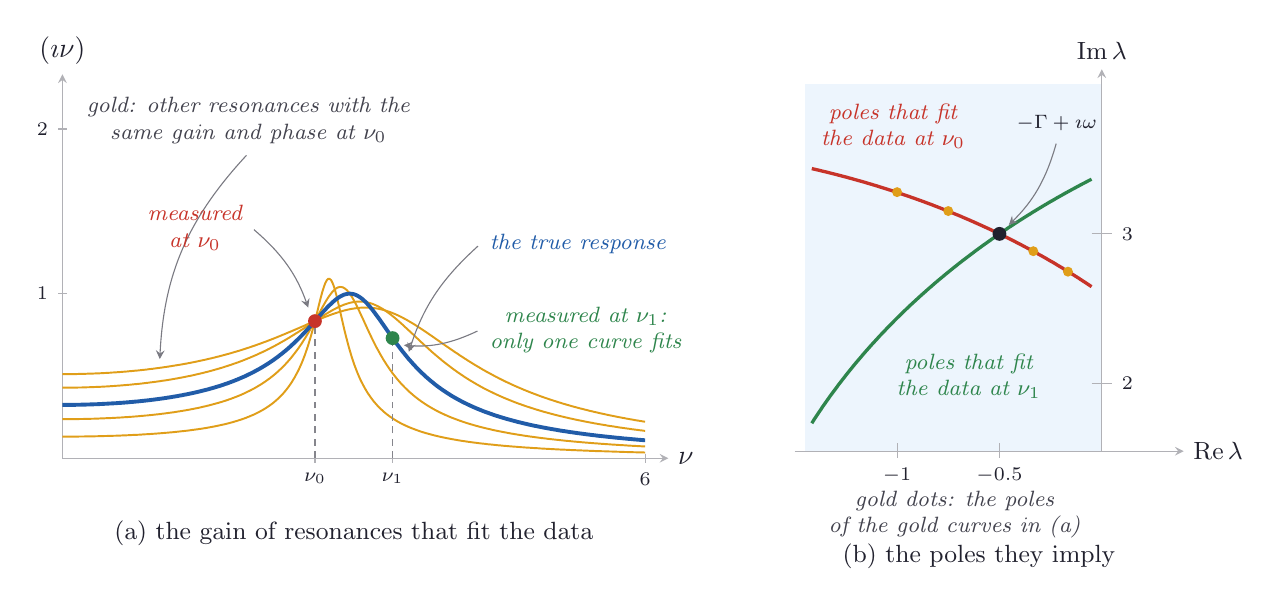
\begin{tikzpicture}[ink/.style={line width=0.9pt, ndInk}, faint/.style={line width=0.4pt, ndInk!35}, dashedink/.style={line width=0.5pt, ndInk!55, dash pattern=on 2.5pt off 2pt}, vec/.style={->, >=stealth, line width=1.2pt}, note/.style={font=\footnotesize\itshape, text=ndInk!85, align=center}, pointer/.style={->, >=stealth, line width=0.4pt, ndInk!60, shorten >=2pt, shorten <=1pt}, dot/.style={circle, fill=ndInk, inner sep=0pt, minimum size=3.4pt}, wash/.style={fill=ndSky, fill opacity=0.55}, every node/.style={text=ndInk}]
\definecolor{ndInk}{rgb}{0.13,0.13,0.18}
\definecolor{ndPaper}{rgb}{0.99,0.96,0.88}
\definecolor{ndSky}{rgb}{0.84,0.91,0.98}
\definecolor{ndRose}{rgb}{0.98,0.86,0.84}
\definecolor{ndBlue}{rgb}{0.13,0.36,0.66}
\definecolor{ndRed}{rgb}{0.78,0.20,0.16}
\definecolor{ndGold}{rgb}{0.88,0.62,0.10}
\definecolor{ndGreen}{rgb}{0.18,0.52,0.30}
\draw[faint, ->, >=stealth] (0.000,0.000) -- (7.696,0.000) node[right, text=ndInk] {$\nu$};
\draw[faint, ->, >=stealth] (0.000,0.000) -- (0.000,4.876) node[above, text=ndInk] {$\abs{\TF(\imath\nu)}$};
\draw[faint] (3.207,0.060) -- (3.207,-0.060) node[below, font=\scriptsize, text=ndInk] {$\nu_0$};
\draw[faint] (4.193,0.060) -- (4.193,-0.060) node[below, font=\scriptsize, text=ndInk] {$\nu_1$};
\draw[faint] (7.400,0.060) -- (7.400,-0.060) node[below, font=\scriptsize, text=ndInk] {$6$};
\draw[faint] (0.060,2.091) -- (-0.060,2.091) node[left, font=\scriptsize, text=ndInk] {$1$};
\draw[faint] (0.060,4.182) -- (-0.060,4.182) node[left, font=\scriptsize, text=ndInk] {$2$};
\draw[line width=0.7pt, ndGold] (0.000,0.275) -- (0.019,0.275) -- (0.037,0.276) -- (0.056,0.276) -- (0.074,0.276) -- (0.093,0.276) -- (0.111,0.276) -- (0.130,0.276) -- (0.148,0.276) -- (0.167,0.276) -- (0.185,0.276) -- (0.204,0.276) -- (0.223,0.277) -- (0.241,0.277) -- (0.260,0.277) -- (0.278,0.277) -- (0.297,0.278) -- (0.315,0.278) -- (0.334,0.278) -- (0.352,0.278) -- (0.371,0.279) -- (0.389,0.279) -- (0.408,0.279) -- (0.427,0.280) -- (0.445,0.280) -- (0.464,0.281) -- (0.482,0.281) -- (0.501,0.282) -- (0.519,0.282) -- (0.538,0.283) -- (0.556,0.283) -- (0.575,0.284) -- (0.593,0.284) -- (0.612,0.285) -- (0.631,0.285) -- (0.649,0.286) -- (0.668,0.286) -- (0.686,0.287) -- (0.705,0.288) -- (0.723,0.288) -- (0.742,0.289) -- (0.760,0.290) -- (0.779,0.291) -- (0.797,0.291) -- (0.816,0.292) -- (0.835,0.293) -- (0.853,0.294) -- (0.872,0.295) -- (0.890,0.296) -- (0.909,0.297) -- (0.927,0.297) -- (0.946,0.298) -- (0.964,0.299) -- (0.983,0.300) -- (1.002,0.301) -- (1.020,0.303) -- (1.039,0.304) -- (1.057,0.305) -- (1.076,0.306) -- (1.094,0.307) -- (1.113,0.308) -- (1.131,0.310) -- (1.150,0.311) -- (1.168,0.312) -- (1.187,0.313) -- (1.206,0.315) -- (1.224,0.316) -- (1.243,0.318) -- (1.261,0.319) -- (1.280,0.321) -- (1.298,0.322) -- (1.317,0.324) -- (1.335,0.325) -- (1.354,0.327) -- (1.372,0.329) -- (1.391,0.330) -- (1.410,0.332) -- (1.428,0.334) -- (1.447,0.336) -- (1.465,0.338) -- (1.484,0.340) -- (1.502,0.342) -- (1.521,0.344) -- (1.539,0.346) -- (1.558,0.348) -- (1.576,0.350) -- (1.595,0.352) -- (1.614,0.355) -- (1.632,0.357) -- (1.651,0.360) -- (1.669,0.362) -- (1.688,0.365) -- (1.706,0.367) -- (1.725,0.370) -- (1.743,0.373) -- (1.762,0.375) -- (1.780,0.378) -- (1.799,0.381) -- (1.818,0.384) -- (1.836,0.387) -- (1.855,0.391) -- (1.873,0.394) -- (1.892,0.397) -- (1.910,0.401) -- (1.929,0.404) -- (1.947,0.408) -- (1.966,0.412) -- (1.984,0.416) -- (2.003,0.420) -- (2.022,0.424) -- (2.040,0.428) -- (2.059,0.432) -- (2.077,0.437) -- (2.096,0.441) -- (2.114,0.446) -- (2.133,0.451) -- (2.151,0.456) -- (2.170,0.461) -- (2.188,0.467) -- (2.207,0.472) -- (2.226,0.478) -- (2.244,0.484) -- (2.263,0.490) -- (2.281,0.496) -- (2.300,0.503) -- (2.318,0.509) -- (2.337,0.516) -- (2.355,0.524) -- (2.374,0.531) -- (2.392,0.539) -- (2.411,0.547) -- (2.430,0.555) -- (2.448,0.564) -- (2.467,0.573) -- (2.485,0.582) -- (2.504,0.592) -- (2.522,0.602) -- (2.541,0.612) -- (2.559,0.623) -- (2.578,0.634) -- (2.596,0.646) -- (2.615,0.659) -- (2.634,0.672) -- (2.652,0.685) -- (2.671,0.699) -- (2.689,0.714) -- (2.708,0.730) -- (2.726,0.746) -- (2.745,0.763) -- (2.763,0.781) -- (2.782,0.800) -- (2.801,0.820) -- (2.819,0.841) -- (2.838,0.864) -- (2.856,0.887) -- (2.875,0.912) -- (2.893,0.938) -- (2.912,0.966) -- (2.930,0.996) -- (2.949,1.027) -- (2.967,1.061) -- (2.986,1.096) -- (3.005,1.134) -- (3.023,1.174) -- (3.042,1.217) -- (3.060,1.263) -- (3.079,1.312) -- (3.097,1.365) -- (3.116,1.420) -- (3.134,1.479) -- (3.153,1.542) -- (3.171,1.608) -- (3.190,1.677) -- (3.209,1.750) -- (3.227,1.824) -- (3.246,1.900) -- (3.264,1.975) -- (3.283,2.048) -- (3.301,2.115) -- (3.320,2.175) -- (3.338,2.225) -- (3.357,2.260) -- (3.375,2.278) -- (3.394,2.279) -- (3.413,2.261) -- (3.431,2.226) -- (3.450,2.176) -- (3.468,2.113) -- (3.487,2.041) -- (3.505,1.962) -- (3.524,1.881) -- (3.542,1.799) -- (3.561,1.717) -- (3.579,1.638) -- (3.598,1.561) -- (3.617,1.489) -- (3.635,1.420) -- (3.654,1.355) -- (3.672,1.294) -- (3.691,1.237) -- (3.709,1.183) -- (3.728,1.133) -- (3.746,1.086) -- (3.765,1.042) -- (3.783,1.001) -- (3.802,0.963) -- (3.821,0.927) -- (3.839,0.893) -- (3.858,0.861) -- (3.876,0.831) -- (3.895,0.803) -- (3.913,0.776) -- (3.932,0.751) -- (3.950,0.727) -- (3.969,0.705) -- (3.987,0.684) -- (4.006,0.663) -- (4.025,0.644) -- (4.043,0.626) -- (4.062,0.609) -- (4.080,0.592) -- (4.099,0.576) -- (4.117,0.561) -- (4.136,0.547) -- (4.154,0.533) -- (4.173,0.520) -- (4.191,0.508) -- (4.210,0.496) -- (4.229,0.484) -- (4.247,0.473) -- (4.266,0.462) -- (4.284,0.452) -- (4.303,0.442) -- (4.321,0.433) -- (4.340,0.424) -- (4.358,0.415) -- (4.377,0.407) -- (4.395,0.398) -- (4.414,0.391) -- (4.433,0.383) -- (4.451,0.376) -- (4.470,0.369) -- (4.488,0.362) -- (4.507,0.355) -- (4.525,0.349) -- (4.544,0.342) -- (4.562,0.336) -- (4.581,0.330) -- (4.599,0.325) -- (4.618,0.319) -- (4.637,0.314) -- (4.655,0.309) -- (4.674,0.304) -- (4.692,0.299) -- (4.711,0.294) -- (4.729,0.289) -- (4.748,0.285) -- (4.766,0.280) -- (4.785,0.276) -- (4.804,0.272) -- (4.822,0.268) -- (4.841,0.264) -- (4.859,0.260) -- (4.878,0.256) -- (4.896,0.253) -- (4.915,0.249) -- (4.933,0.246) -- (4.952,0.242) -- (4.970,0.239) -- (4.989,0.236) -- (5.008,0.232) -- (5.026,0.229) -- (5.045,0.226) -- (5.063,0.223) -- (5.082,0.220) -- (5.100,0.218) -- (5.119,0.215) -- (5.137,0.212) -- (5.156,0.209) -- (5.174,0.207) -- (5.193,0.204) -- (5.212,0.202) -- (5.230,0.199) -- (5.249,0.197) -- (5.267,0.195) -- (5.286,0.192) -- (5.304,0.190) -- (5.323,0.188) -- (5.341,0.186) -- (5.360,0.184) -- (5.378,0.182) -- (5.397,0.179) -- (5.416,0.177) -- (5.434,0.176) -- (5.453,0.174) -- (5.471,0.172) -- (5.490,0.170) -- (5.508,0.168) -- (5.527,0.166) -- (5.545,0.164) -- (5.564,0.163) -- (5.582,0.161) -- (5.601,0.159) -- (5.620,0.158) -- (5.638,0.156) -- (5.657,0.155) -- (5.675,0.153) -- (5.694,0.151) -- (5.712,0.150) -- (5.731,0.148) -- (5.749,0.147) -- (5.768,0.146) -- (5.786,0.144) -- (5.805,0.143) -- (5.824,0.141) -- (5.842,0.140) -- (5.861,0.139) -- (5.879,0.137) -- (5.898,0.136) -- (5.916,0.135) -- (5.935,0.134) -- (5.953,0.132) -- (5.972,0.131) -- (5.990,0.130) -- (6.009,0.129) -- (6.028,0.128) -- (6.046,0.127) -- (6.065,0.125) -- (6.083,0.124) -- (6.102,0.123) -- (6.120,0.122) -- (6.139,0.121) -- (6.157,0.120) -- (6.176,0.119) -- (6.194,0.118) -- (6.213,0.117) -- (6.232,0.116) -- (6.250,0.115) -- (6.269,0.114) -- (6.287,0.113) -- (6.306,0.112) -- (6.324,0.111) -- (6.343,0.110) -- (6.361,0.110) -- (6.380,0.109) -- (6.398,0.108) -- (6.417,0.107) -- (6.436,0.106) -- (6.454,0.105) -- (6.473,0.104) -- (6.491,0.104) -- (6.510,0.103) -- (6.528,0.102) -- (6.547,0.101) -- (6.565,0.100) -- (6.584,0.100) -- (6.603,0.099) -- (6.621,0.098) -- (6.640,0.097) -- (6.658,0.097) -- (6.677,0.096) -- (6.695,0.095) -- (6.714,0.095) -- (6.732,0.094) -- (6.751,0.093) -- (6.769,0.092) -- (6.788,0.092) -- (6.807,0.091) -- (6.825,0.090) -- (6.844,0.090) -- (6.862,0.089) -- (6.881,0.089) -- (6.899,0.088) -- (6.918,0.087) -- (6.936,0.087) -- (6.955,0.086) -- (6.973,0.086) -- (6.992,0.085) -- (7.011,0.084) -- (7.029,0.084) -- (7.048,0.083) -- (7.066,0.083) -- (7.085,0.082) -- (7.103,0.082) -- (7.122,0.081) -- (7.140,0.080) -- (7.159,0.080) -- (7.177,0.079) -- (7.196,0.079) -- (7.215,0.078) -- (7.233,0.078) -- (7.252,0.077) -- (7.270,0.077) -- (7.289,0.076) -- (7.307,0.076) -- (7.326,0.075) -- (7.344,0.075) -- (7.363,0.074) -- (7.381,0.074) -- (7.400,0.073);
\draw[line width=0.7pt, ndGold] (0.000,0.497) -- (0.019,0.497) -- (0.037,0.497) -- (0.056,0.497) -- (0.074,0.497) -- (0.093,0.497) -- (0.111,0.497) -- (0.130,0.497) -- (0.148,0.497) -- (0.167,0.498) -- (0.185,0.498) -- (0.204,0.498) -- (0.223,0.499) -- (0.241,0.499) -- (0.260,0.499) -- (0.278,0.500) -- (0.297,0.500) -- (0.315,0.500) -- (0.334,0.501) -- (0.352,0.501) -- (0.371,0.502) -- (0.389,0.502) -- (0.408,0.503) -- (0.427,0.504) -- (0.445,0.504) -- (0.464,0.505) -- (0.482,0.506) -- (0.501,0.506) -- (0.519,0.507) -- (0.538,0.508) -- (0.556,0.509) -- (0.575,0.509) -- (0.593,0.510) -- (0.612,0.511) -- (0.631,0.512) -- (0.649,0.513) -- (0.668,0.514) -- (0.686,0.515) -- (0.705,0.516) -- (0.723,0.517) -- (0.742,0.518) -- (0.760,0.519) -- (0.779,0.521) -- (0.797,0.522) -- (0.816,0.523) -- (0.835,0.524) -- (0.853,0.526) -- (0.872,0.527) -- (0.890,0.528) -- (0.909,0.530) -- (0.927,0.531) -- (0.946,0.533) -- (0.964,0.534) -- (0.983,0.536) -- (1.002,0.538) -- (1.020,0.539) -- (1.039,0.541) -- (1.057,0.543) -- (1.076,0.544) -- (1.094,0.546) -- (1.113,0.548) -- (1.131,0.550) -- (1.150,0.552) -- (1.168,0.554) -- (1.187,0.556) -- (1.206,0.558) -- (1.224,0.560) -- (1.243,0.562) -- (1.261,0.565) -- (1.280,0.567) -- (1.298,0.569) -- (1.317,0.572) -- (1.335,0.574) -- (1.354,0.577) -- (1.372,0.579) -- (1.391,0.582) -- (1.410,0.584) -- (1.428,0.587) -- (1.447,0.590) -- (1.465,0.593) -- (1.484,0.596) -- (1.502,0.599) -- (1.521,0.602) -- (1.539,0.605) -- (1.558,0.608) -- (1.576,0.611) -- (1.595,0.615) -- (1.614,0.618) -- (1.632,0.622) -- (1.651,0.625) -- (1.669,0.629) -- (1.688,0.633) -- (1.706,0.636) -- (1.725,0.640) -- (1.743,0.644) -- (1.762,0.648) -- (1.780,0.653) -- (1.799,0.657) -- (1.818,0.661) -- (1.836,0.666) -- (1.855,0.670) -- (1.873,0.675) -- (1.892,0.680) -- (1.910,0.685) -- (1.929,0.690) -- (1.947,0.695) -- (1.966,0.700) -- (1.984,0.705) -- (2.003,0.711) -- (2.022,0.716) -- (2.040,0.722) -- (2.059,0.728) -- (2.077,0.734) -- (2.096,0.740) -- (2.114,0.747) -- (2.133,0.753) -- (2.151,0.760) -- (2.170,0.767) -- (2.188,0.774) -- (2.207,0.781) -- (2.226,0.789) -- (2.244,0.796) -- (2.263,0.804) -- (2.281,0.812) -- (2.300,0.820) -- (2.318,0.829) -- (2.337,0.838) -- (2.355,0.847) -- (2.374,0.856) -- (2.392,0.865) -- (2.411,0.875) -- (2.430,0.885) -- (2.448,0.895) -- (2.467,0.906) -- (2.485,0.917) -- (2.504,0.928) -- (2.522,0.939) -- (2.541,0.951) -- (2.559,0.964) -- (2.578,0.976) -- (2.596,0.989) -- (2.615,1.003) -- (2.634,1.016) -- (2.652,1.031) -- (2.671,1.045) -- (2.689,1.060) -- (2.708,1.076) -- (2.726,1.092) -- (2.745,1.109) -- (2.763,1.126) -- (2.782,1.144) -- (2.801,1.162) -- (2.819,1.181) -- (2.838,1.201) -- (2.856,1.221) -- (2.875,1.242) -- (2.893,1.263) -- (2.912,1.286) -- (2.930,1.309) -- (2.949,1.333) -- (2.967,1.357) -- (2.986,1.382) -- (3.005,1.408) -- (3.023,1.435) -- (3.042,1.463) -- (3.060,1.492) -- (3.079,1.521) -- (3.097,1.551) -- (3.116,1.582) -- (3.134,1.613) -- (3.153,1.646) -- (3.171,1.679) -- (3.190,1.712) -- (3.209,1.746) -- (3.227,1.780) -- (3.246,1.814) -- (3.264,1.849) -- (3.283,1.883) -- (3.301,1.917) -- (3.320,1.950) -- (3.338,1.982) -- (3.357,2.013) -- (3.375,2.042) -- (3.394,2.069) -- (3.413,2.094) -- (3.431,2.117) -- (3.450,2.136) -- (3.468,2.152) -- (3.487,2.164) -- (3.505,2.172) -- (3.524,2.176) -- (3.542,2.175) -- (3.561,2.171) -- (3.579,2.161) -- (3.598,2.148) -- (3.617,2.130) -- (3.635,2.109) -- (3.654,2.084) -- (3.672,2.056) -- (3.691,2.025) -- (3.709,1.991) -- (3.728,1.956) -- (3.746,1.918) -- (3.765,1.880) -- (3.783,1.840) -- (3.802,1.800) -- (3.821,1.760) -- (3.839,1.719) -- (3.858,1.679) -- (3.876,1.638) -- (3.895,1.599) -- (3.913,1.560) -- (3.932,1.521) -- (3.950,1.484) -- (3.969,1.447) -- (3.987,1.411) -- (4.006,1.377) -- (4.025,1.343) -- (4.043,1.310) -- (4.062,1.278) -- (4.080,1.247) -- (4.099,1.218) -- (4.117,1.189) -- (4.136,1.161) -- (4.154,1.134) -- (4.173,1.108) -- (4.191,1.082) -- (4.210,1.058) -- (4.229,1.034) -- (4.247,1.011) -- (4.266,0.989) -- (4.284,0.968) -- (4.303,0.947) -- (4.321,0.928) -- (4.340,0.908) -- (4.358,0.890) -- (4.377,0.872) -- (4.395,0.854) -- (4.414,0.837) -- (4.433,0.821) -- (4.451,0.805) -- (4.470,0.789) -- (4.488,0.775) -- (4.507,0.760) -- (4.525,0.746) -- (4.544,0.733) -- (4.562,0.719) -- (4.581,0.707) -- (4.599,0.694) -- (4.618,0.682) -- (4.637,0.670) -- (4.655,0.659) -- (4.674,0.648) -- (4.692,0.637) -- (4.711,0.627) -- (4.729,0.616) -- (4.748,0.606) -- (4.766,0.597) -- (4.785,0.587) -- (4.804,0.578) -- (4.822,0.569) -- (4.841,0.561) -- (4.859,0.552) -- (4.878,0.544) -- (4.896,0.536) -- (4.915,0.528) -- (4.933,0.520) -- (4.952,0.513) -- (4.970,0.506) -- (4.989,0.499) -- (5.008,0.492) -- (5.026,0.485) -- (5.045,0.478) -- (5.063,0.472) -- (5.082,0.465) -- (5.100,0.459) -- (5.119,0.453) -- (5.137,0.447) -- (5.156,0.441) -- (5.174,0.436) -- (5.193,0.430) -- (5.212,0.425) -- (5.230,0.419) -- (5.249,0.414) -- (5.267,0.409) -- (5.286,0.404) -- (5.304,0.399) -- (5.323,0.394) -- (5.341,0.390) -- (5.360,0.385) -- (5.378,0.381) -- (5.397,0.376) -- (5.416,0.372) -- (5.434,0.368) -- (5.453,0.363) -- (5.471,0.359) -- (5.490,0.355) -- (5.508,0.351) -- (5.527,0.347) -- (5.545,0.344) -- (5.564,0.340) -- (5.582,0.336) -- (5.601,0.333) -- (5.620,0.329) -- (5.638,0.326) -- (5.657,0.322) -- (5.675,0.319) -- (5.694,0.315) -- (5.712,0.312) -- (5.731,0.309) -- (5.749,0.306) -- (5.768,0.303) -- (5.786,0.300) -- (5.805,0.297) -- (5.824,0.294) -- (5.842,0.291) -- (5.861,0.288) -- (5.879,0.285) -- (5.898,0.283) -- (5.916,0.280) -- (5.935,0.277) -- (5.953,0.275) -- (5.972,0.272) -- (5.990,0.270) -- (6.009,0.267) -- (6.028,0.265) -- (6.046,0.262) -- (6.065,0.260) -- (6.083,0.257) -- (6.102,0.255) -- (6.120,0.253) -- (6.139,0.251) -- (6.157,0.248) -- (6.176,0.246) -- (6.194,0.244) -- (6.213,0.242) -- (6.232,0.240) -- (6.250,0.238) -- (6.269,0.236) -- (6.287,0.234) -- (6.306,0.232) -- (6.324,0.230) -- (6.343,0.228) -- (6.361,0.226) -- (6.380,0.224) -- (6.398,0.222) -- (6.417,0.220) -- (6.436,0.219) -- (6.454,0.217) -- (6.473,0.215) -- (6.491,0.213) -- (6.510,0.212) -- (6.528,0.210) -- (6.547,0.208) -- (6.565,0.207) -- (6.584,0.205) -- (6.603,0.203) -- (6.621,0.202) -- (6.640,0.200) -- (6.658,0.199) -- (6.677,0.197) -- (6.695,0.196) -- (6.714,0.194) -- (6.732,0.193) -- (6.751,0.191) -- (6.769,0.190) -- (6.788,0.189) -- (6.807,0.187) -- (6.825,0.186) -- (6.844,0.184) -- (6.862,0.183) -- (6.881,0.182) -- (6.899,0.180) -- (6.918,0.179) -- (6.936,0.178) -- (6.955,0.177) -- (6.973,0.175) -- (6.992,0.174) -- (7.011,0.173) -- (7.029,0.172) -- (7.048,0.170) -- (7.066,0.169) -- (7.085,0.168) -- (7.103,0.167) -- (7.122,0.166) -- (7.140,0.165) -- (7.159,0.164) -- (7.177,0.162) -- (7.196,0.161) -- (7.215,0.160) -- (7.233,0.159) -- (7.252,0.158) -- (7.270,0.157) -- (7.289,0.156) -- (7.307,0.155) -- (7.326,0.154) -- (7.344,0.153) -- (7.363,0.152) -- (7.381,0.151) -- (7.400,0.150);
\draw[line width=0.7pt, ndGold] (0.000,0.897) -- (0.019,0.897) -- (0.037,0.897) -- (0.056,0.897) -- (0.074,0.897) -- (0.093,0.897) -- (0.111,0.897) -- (0.130,0.897) -- (0.148,0.898) -- (0.167,0.898) -- (0.185,0.898) -- (0.204,0.899) -- (0.223,0.899) -- (0.241,0.899) -- (0.260,0.900) -- (0.278,0.900) -- (0.297,0.901) -- (0.315,0.902) -- (0.334,0.902) -- (0.352,0.903) -- (0.371,0.903) -- (0.389,0.904) -- (0.408,0.905) -- (0.427,0.906) -- (0.445,0.907) -- (0.464,0.907) -- (0.482,0.908) -- (0.501,0.909) -- (0.519,0.910) -- (0.538,0.911) -- (0.556,0.912) -- (0.575,0.913) -- (0.593,0.914) -- (0.612,0.916) -- (0.631,0.917) -- (0.649,0.918) -- (0.668,0.919) -- (0.686,0.921) -- (0.705,0.922) -- (0.723,0.923) -- (0.742,0.925) -- (0.760,0.926) -- (0.779,0.928) -- (0.797,0.929) -- (0.816,0.931) -- (0.835,0.933) -- (0.853,0.934) -- (0.872,0.936) -- (0.890,0.938) -- (0.909,0.940) -- (0.927,0.942) -- (0.946,0.943) -- (0.964,0.945) -- (0.983,0.947) -- (1.002,0.949) -- (1.020,0.951) -- (1.039,0.954) -- (1.057,0.956) -- (1.076,0.958) -- (1.094,0.960) -- (1.113,0.963) -- (1.131,0.965) -- (1.150,0.967) -- (1.168,0.970) -- (1.187,0.972) -- (1.206,0.975) -- (1.224,0.977) -- (1.243,0.980) -- (1.261,0.983) -- (1.280,0.986) -- (1.298,0.988) -- (1.317,0.991) -- (1.335,0.994) -- (1.354,0.997) -- (1.372,1.000) -- (1.391,1.003) -- (1.410,1.007) -- (1.428,1.010) -- (1.447,1.013) -- (1.465,1.016) -- (1.484,1.020) -- (1.502,1.023) -- (1.521,1.027) -- (1.539,1.030) -- (1.558,1.034) -- (1.576,1.038) -- (1.595,1.042) -- (1.614,1.045) -- (1.632,1.049) -- (1.651,1.053) -- (1.669,1.057) -- (1.688,1.062) -- (1.706,1.066) -- (1.725,1.070) -- (1.743,1.074) -- (1.762,1.079) -- (1.780,1.083) -- (1.799,1.088) -- (1.818,1.093) -- (1.836,1.097) -- (1.855,1.102) -- (1.873,1.107) -- (1.892,1.112) -- (1.910,1.117) -- (1.929,1.122) -- (1.947,1.128) -- (1.966,1.133) -- (1.984,1.138) -- (2.003,1.144) -- (2.022,1.149) -- (2.040,1.155) -- (2.059,1.161) -- (2.077,1.167) -- (2.096,1.173) -- (2.114,1.179) -- (2.133,1.185) -- (2.151,1.191) -- (2.170,1.198) -- (2.188,1.204) -- (2.207,1.211) -- (2.226,1.217) -- (2.244,1.224) -- (2.263,1.231) -- (2.281,1.238) -- (2.300,1.245) -- (2.318,1.253) -- (2.337,1.260) -- (2.355,1.268) -- (2.374,1.275) -- (2.392,1.283) -- (2.411,1.291) -- (2.430,1.299) -- (2.448,1.307) -- (2.467,1.315) -- (2.485,1.324) -- (2.504,1.332) -- (2.522,1.341) -- (2.541,1.349) -- (2.559,1.358) -- (2.578,1.367) -- (2.596,1.376) -- (2.615,1.386) -- (2.634,1.395) -- (2.652,1.405) -- (2.671,1.414) -- (2.689,1.424) -- (2.708,1.434) -- (2.726,1.444) -- (2.745,1.454) -- (2.763,1.465) -- (2.782,1.475) -- (2.801,1.486) -- (2.819,1.496) -- (2.838,1.507) -- (2.856,1.518) -- (2.875,1.529) -- (2.893,1.541) -- (2.912,1.552) -- (2.930,1.563) -- (2.949,1.575) -- (2.967,1.587) -- (2.986,1.598) -- (3.005,1.610) -- (3.023,1.622) -- (3.042,1.634) -- (3.060,1.646) -- (3.079,1.658) -- (3.097,1.670) -- (3.116,1.682) -- (3.134,1.695) -- (3.153,1.707) -- (3.171,1.719) -- (3.190,1.731) -- (3.209,1.744) -- (3.227,1.756) -- (3.246,1.768) -- (3.264,1.780) -- (3.283,1.792) -- (3.301,1.804) -- (3.320,1.815) -- (3.338,1.827) -- (3.357,1.838) -- (3.375,1.849) -- (3.394,1.860) -- (3.413,1.871) -- (3.431,1.882) -- (3.450,1.892) -- (3.468,1.901) -- (3.487,1.911) -- (3.505,1.920) -- (3.524,1.929) -- (3.542,1.937) -- (3.561,1.944) -- (3.579,1.952) -- (3.598,1.958) -- (3.617,1.964) -- (3.635,1.970) -- (3.654,1.975) -- (3.672,1.979) -- (3.691,1.983) -- (3.709,1.986) -- (3.728,1.988) -- (3.746,1.989) -- (3.765,1.990) -- (3.783,1.990) -- (3.802,1.990) -- (3.821,1.988) -- (3.839,1.986) -- (3.858,1.983) -- (3.876,1.979) -- (3.895,1.974) -- (3.913,1.969) -- (3.932,1.963) -- (3.950,1.956) -- (3.969,1.948) -- (3.987,1.940) -- (4.006,1.931) -- (4.025,1.921) -- (4.043,1.911) -- (4.062,1.900) -- (4.080,1.888) -- (4.099,1.876) -- (4.117,1.863) -- (4.136,1.850) -- (4.154,1.836) -- (4.173,1.822) -- (4.191,1.807) -- (4.210,1.792) -- (4.229,1.777) -- (4.247,1.761) -- (4.266,1.745) -- (4.284,1.729) -- (4.303,1.712) -- (4.321,1.696) -- (4.340,1.679) -- (4.358,1.661) -- (4.377,1.644) -- (4.395,1.627) -- (4.414,1.610) -- (4.433,1.592) -- (4.451,1.575) -- (4.470,1.557) -- (4.488,1.540) -- (4.507,1.522) -- (4.525,1.505) -- (4.544,1.487) -- (4.562,1.470) -- (4.581,1.453) -- (4.599,1.436) -- (4.618,1.419) -- (4.637,1.402) -- (4.655,1.385) -- (4.674,1.369) -- (4.692,1.352) -- (4.711,1.336) -- (4.729,1.320) -- (4.748,1.304) -- (4.766,1.289) -- (4.785,1.273) -- (4.804,1.258) -- (4.822,1.242) -- (4.841,1.227) -- (4.859,1.213) -- (4.878,1.198) -- (4.896,1.184) -- (4.915,1.170) -- (4.933,1.156) -- (4.952,1.142) -- (4.970,1.128) -- (4.989,1.115) -- (5.008,1.101) -- (5.026,1.088) -- (5.045,1.076) -- (5.063,1.063) -- (5.082,1.051) -- (5.100,1.038) -- (5.119,1.026) -- (5.137,1.014) -- (5.156,1.003) -- (5.174,0.991) -- (5.193,0.980) -- (5.212,0.969) -- (5.230,0.958) -- (5.249,0.947) -- (5.267,0.936) -- (5.286,0.926) -- (5.304,0.915) -- (5.323,0.905) -- (5.341,0.895) -- (5.360,0.885) -- (5.378,0.876) -- (5.397,0.866) -- (5.416,0.857) -- (5.434,0.848) -- (5.453,0.839) -- (5.471,0.830) -- (5.490,0.821) -- (5.508,0.812) -- (5.527,0.804) -- (5.545,0.795) -- (5.564,0.787) -- (5.582,0.779) -- (5.601,0.771) -- (5.620,0.763) -- (5.638,0.755) -- (5.657,0.748) -- (5.675,0.740) -- (5.694,0.733) -- (5.712,0.725) -- (5.731,0.718) -- (5.749,0.711) -- (5.768,0.704) -- (5.786,0.697) -- (5.805,0.690) -- (5.824,0.684) -- (5.842,0.677) -- (5.861,0.671) -- (5.879,0.664) -- (5.898,0.658) -- (5.916,0.652) -- (5.935,0.646) -- (5.953,0.640) -- (5.972,0.634) -- (5.990,0.628) -- (6.009,0.622) -- (6.028,0.616) -- (6.046,0.611) -- (6.065,0.605) -- (6.083,0.600) -- (6.102,0.594) -- (6.120,0.589) -- (6.139,0.584) -- (6.157,0.579) -- (6.176,0.574) -- (6.194,0.569) -- (6.213,0.564) -- (6.232,0.559) -- (6.250,0.554) -- (6.269,0.549) -- (6.287,0.545) -- (6.306,0.540) -- (6.324,0.535) -- (6.343,0.531) -- (6.361,0.527) -- (6.380,0.522) -- (6.398,0.518) -- (6.417,0.514) -- (6.436,0.509) -- (6.454,0.505) -- (6.473,0.501) -- (6.491,0.497) -- (6.510,0.493) -- (6.528,0.489) -- (6.547,0.485) -- (6.565,0.481) -- (6.584,0.478) -- (6.603,0.474) -- (6.621,0.470) -- (6.640,0.466) -- (6.658,0.463) -- (6.677,0.459) -- (6.695,0.456) -- (6.714,0.452) -- (6.732,0.449) -- (6.751,0.445) -- (6.769,0.442) -- (6.788,0.439) -- (6.807,0.435) -- (6.825,0.432) -- (6.844,0.429) -- (6.862,0.426) -- (6.881,0.423) -- (6.899,0.420) -- (6.918,0.416) -- (6.936,0.413) -- (6.955,0.410) -- (6.973,0.408) -- (6.992,0.405) -- (7.011,0.402) -- (7.029,0.399) -- (7.048,0.396) -- (7.066,0.393) -- (7.085,0.390) -- (7.103,0.388) -- (7.122,0.385) -- (7.140,0.382) -- (7.159,0.380) -- (7.177,0.377) -- (7.196,0.375) -- (7.215,0.372) -- (7.233,0.369) -- (7.252,0.367) -- (7.270,0.364) -- (7.289,0.362) -- (7.307,0.360) -- (7.326,0.357) -- (7.344,0.355) -- (7.363,0.353) -- (7.381,0.350) -- (7.400,0.348);
\draw[line width=0.7pt, ndGold] (0.000,1.069) -- (0.019,1.069) -- (0.037,1.069) -- (0.056,1.069) -- (0.074,1.069) -- (0.093,1.069) -- (0.111,1.069) -- (0.130,1.069) -- (0.148,1.070) -- (0.167,1.070) -- (0.185,1.070) -- (0.204,1.071) -- (0.223,1.071) -- (0.241,1.071) -- (0.260,1.072) -- (0.278,1.072) -- (0.297,1.073) -- (0.315,1.074) -- (0.334,1.074) -- (0.352,1.075) -- (0.371,1.075) -- (0.389,1.076) -- (0.408,1.077) -- (0.427,1.078) -- (0.445,1.079) -- (0.464,1.079) -- (0.482,1.080) -- (0.501,1.081) -- (0.519,1.082) -- (0.538,1.083) -- (0.556,1.084) -- (0.575,1.085) -- (0.593,1.086) -- (0.612,1.087) -- (0.631,1.089) -- (0.649,1.090) -- (0.668,1.091) -- (0.686,1.092) -- (0.705,1.094) -- (0.723,1.095) -- (0.742,1.096) -- (0.760,1.098) -- (0.779,1.099) -- (0.797,1.101) -- (0.816,1.102) -- (0.835,1.104) -- (0.853,1.106) -- (0.872,1.107) -- (0.890,1.109) -- (0.909,1.111) -- (0.927,1.113) -- (0.946,1.114) -- (0.964,1.116) -- (0.983,1.118) -- (1.002,1.120) -- (1.020,1.122) -- (1.039,1.124) -- (1.057,1.126) -- (1.076,1.128) -- (1.094,1.131) -- (1.113,1.133) -- (1.131,1.135) -- (1.150,1.137) -- (1.168,1.140) -- (1.187,1.142) -- (1.206,1.145) -- (1.224,1.147) -- (1.243,1.150) -- (1.261,1.152) -- (1.280,1.155) -- (1.298,1.158) -- (1.317,1.160) -- (1.335,1.163) -- (1.354,1.166) -- (1.372,1.169) -- (1.391,1.172) -- (1.410,1.175) -- (1.428,1.178) -- (1.447,1.181) -- (1.465,1.184) -- (1.484,1.187) -- (1.502,1.190) -- (1.521,1.193) -- (1.539,1.197) -- (1.558,1.200) -- (1.576,1.203) -- (1.595,1.207) -- (1.614,1.210) -- (1.632,1.214) -- (1.651,1.218) -- (1.669,1.221) -- (1.688,1.225) -- (1.706,1.229) -- (1.725,1.233) -- (1.743,1.237) -- (1.762,1.241) -- (1.780,1.245) -- (1.799,1.249) -- (1.818,1.253) -- (1.836,1.257) -- (1.855,1.262) -- (1.873,1.266) -- (1.892,1.270) -- (1.910,1.275) -- (1.929,1.279) -- (1.947,1.284) -- (1.966,1.289) -- (1.984,1.293) -- (2.003,1.298) -- (2.022,1.303) -- (2.040,1.308) -- (2.059,1.313) -- (2.077,1.318) -- (2.096,1.323) -- (2.114,1.328) -- (2.133,1.333) -- (2.151,1.339) -- (2.170,1.344) -- (2.188,1.350) -- (2.207,1.355) -- (2.226,1.361) -- (2.244,1.366) -- (2.263,1.372) -- (2.281,1.378) -- (2.300,1.384) -- (2.318,1.390) -- (2.337,1.396) -- (2.355,1.402) -- (2.374,1.408) -- (2.392,1.414) -- (2.411,1.421) -- (2.430,1.427) -- (2.448,1.433) -- (2.467,1.440) -- (2.485,1.447) -- (2.504,1.453) -- (2.522,1.460) -- (2.541,1.467) -- (2.559,1.474) -- (2.578,1.480) -- (2.596,1.487) -- (2.615,1.495) -- (2.634,1.502) -- (2.652,1.509) -- (2.671,1.516) -- (2.689,1.523) -- (2.708,1.531) -- (2.726,1.538) -- (2.745,1.546) -- (2.763,1.553) -- (2.782,1.561) -- (2.801,1.569) -- (2.819,1.576) -- (2.838,1.584) -- (2.856,1.592) -- (2.875,1.600) -- (2.893,1.607) -- (2.912,1.615) -- (2.930,1.623) -- (2.949,1.631) -- (2.967,1.639) -- (2.986,1.647) -- (3.005,1.655) -- (3.023,1.663) -- (3.042,1.671) -- (3.060,1.679) -- (3.079,1.687) -- (3.097,1.696) -- (3.116,1.704) -- (3.134,1.712) -- (3.153,1.720) -- (3.171,1.727) -- (3.190,1.735) -- (3.209,1.743) -- (3.227,1.751) -- (3.246,1.759) -- (3.264,1.766) -- (3.283,1.774) -- (3.301,1.781) -- (3.320,1.789) -- (3.338,1.796) -- (3.357,1.803) -- (3.375,1.810) -- (3.394,1.817) -- (3.413,1.824) -- (3.431,1.831) -- (3.450,1.837) -- (3.468,1.843) -- (3.487,1.849) -- (3.505,1.855) -- (3.524,1.861) -- (3.542,1.866) -- (3.561,1.872) -- (3.579,1.877) -- (3.598,1.881) -- (3.617,1.886) -- (3.635,1.890) -- (3.654,1.894) -- (3.672,1.897) -- (3.691,1.900) -- (3.709,1.903) -- (3.728,1.906) -- (3.746,1.908) -- (3.765,1.910) -- (3.783,1.912) -- (3.802,1.913) -- (3.821,1.914) -- (3.839,1.914) -- (3.858,1.914) -- (3.876,1.914) -- (3.895,1.913) -- (3.913,1.912) -- (3.932,1.910) -- (3.950,1.908) -- (3.969,1.906) -- (3.987,1.903) -- (4.006,1.900) -- (4.025,1.896) -- (4.043,1.892) -- (4.062,1.887) -- (4.080,1.883) -- (4.099,1.877) -- (4.117,1.872) -- (4.136,1.865) -- (4.154,1.859) -- (4.173,1.852) -- (4.191,1.845) -- (4.210,1.837) -- (4.229,1.830) -- (4.247,1.821) -- (4.266,1.813) -- (4.284,1.804) -- (4.303,1.795) -- (4.321,1.785) -- (4.340,1.775) -- (4.358,1.765) -- (4.377,1.755) -- (4.395,1.744) -- (4.414,1.733) -- (4.433,1.722) -- (4.451,1.711) -- (4.470,1.700) -- (4.488,1.688) -- (4.507,1.676) -- (4.525,1.664) -- (4.544,1.652) -- (4.562,1.640) -- (4.581,1.628) -- (4.599,1.615) -- (4.618,1.603) -- (4.637,1.590) -- (4.655,1.577) -- (4.674,1.564) -- (4.692,1.552) -- (4.711,1.539) -- (4.729,1.526) -- (4.748,1.513) -- (4.766,1.500) -- (4.785,1.487) -- (4.804,1.474) -- (4.822,1.461) -- (4.841,1.448) -- (4.859,1.435) -- (4.878,1.422) -- (4.896,1.410) -- (4.915,1.397) -- (4.933,1.384) -- (4.952,1.372) -- (4.970,1.359) -- (4.989,1.346) -- (5.008,1.334) -- (5.026,1.322) -- (5.045,1.309) -- (5.063,1.297) -- (5.082,1.285) -- (5.100,1.273) -- (5.119,1.261) -- (5.137,1.249) -- (5.156,1.237) -- (5.174,1.226) -- (5.193,1.214) -- (5.212,1.203) -- (5.230,1.191) -- (5.249,1.180) -- (5.267,1.169) -- (5.286,1.158) -- (5.304,1.147) -- (5.323,1.136) -- (5.341,1.125) -- (5.360,1.115) -- (5.378,1.104) -- (5.397,1.094) -- (5.416,1.084) -- (5.434,1.074) -- (5.453,1.064) -- (5.471,1.054) -- (5.490,1.044) -- (5.508,1.034) -- (5.527,1.025) -- (5.545,1.015) -- (5.564,1.006) -- (5.582,0.997) -- (5.601,0.987) -- (5.620,0.978) -- (5.638,0.969) -- (5.657,0.961) -- (5.675,0.952) -- (5.694,0.943) -- (5.712,0.935) -- (5.731,0.926) -- (5.749,0.918) -- (5.768,0.910) -- (5.786,0.902) -- (5.805,0.894) -- (5.824,0.886) -- (5.842,0.878) -- (5.861,0.870) -- (5.879,0.863) -- (5.898,0.855) -- (5.916,0.848) -- (5.935,0.840) -- (5.953,0.833) -- (5.972,0.826) -- (5.990,0.819) -- (6.009,0.812) -- (6.028,0.805) -- (6.046,0.798) -- (6.065,0.791) -- (6.083,0.784) -- (6.102,0.778) -- (6.120,0.771) -- (6.139,0.765) -- (6.157,0.759) -- (6.176,0.752) -- (6.194,0.746) -- (6.213,0.740) -- (6.232,0.734) -- (6.250,0.728) -- (6.269,0.722) -- (6.287,0.716) -- (6.306,0.710) -- (6.324,0.705) -- (6.343,0.699) -- (6.361,0.693) -- (6.380,0.688) -- (6.398,0.682) -- (6.417,0.677) -- (6.436,0.672) -- (6.454,0.666) -- (6.473,0.661) -- (6.491,0.656) -- (6.510,0.651) -- (6.528,0.646) -- (6.547,0.641) -- (6.565,0.636) -- (6.584,0.631) -- (6.603,0.627) -- (6.621,0.622) -- (6.640,0.617) -- (6.658,0.613) -- (6.677,0.608) -- (6.695,0.603) -- (6.714,0.599) -- (6.732,0.595) -- (6.751,0.590) -- (6.769,0.586) -- (6.788,0.582) -- (6.807,0.577) -- (6.825,0.573) -- (6.844,0.569) -- (6.862,0.565) -- (6.881,0.561) -- (6.899,0.557) -- (6.918,0.553) -- (6.936,0.549) -- (6.955,0.545) -- (6.973,0.541) -- (6.992,0.538) -- (7.011,0.534) -- (7.029,0.530) -- (7.048,0.526) -- (7.066,0.523) -- (7.085,0.519) -- (7.103,0.516) -- (7.122,0.512) -- (7.140,0.509) -- (7.159,0.505) -- (7.177,0.502) -- (7.196,0.498) -- (7.215,0.495) -- (7.233,0.492) -- (7.252,0.489) -- (7.270,0.485) -- (7.289,0.482) -- (7.307,0.479) -- (7.326,0.476) -- (7.344,0.473) -- (7.363,0.470) -- (7.381,0.467) -- (7.400,0.464);
\draw[line width=1.4pt, ndBlue] (0.000,0.678) -- (0.019,0.678) -- (0.037,0.678) -- (0.056,0.678) -- (0.074,0.678) -- (0.093,0.679) -- (0.111,0.679) -- (0.130,0.679) -- (0.148,0.679) -- (0.167,0.679) -- (0.185,0.680) -- (0.204,0.680) -- (0.223,0.680) -- (0.241,0.681) -- (0.260,0.681) -- (0.278,0.682) -- (0.297,0.682) -- (0.315,0.683) -- (0.334,0.683) -- (0.352,0.684) -- (0.371,0.684) -- (0.389,0.685) -- (0.408,0.686) -- (0.427,0.687) -- (0.445,0.687) -- (0.464,0.688) -- (0.482,0.689) -- (0.501,0.690) -- (0.519,0.691) -- (0.538,0.692) -- (0.556,0.693) -- (0.575,0.694) -- (0.593,0.695) -- (0.612,0.696) -- (0.631,0.697) -- (0.649,0.698) -- (0.668,0.699) -- (0.686,0.700) -- (0.705,0.702) -- (0.723,0.703) -- (0.742,0.704) -- (0.760,0.705) -- (0.779,0.707) -- (0.797,0.708) -- (0.816,0.710) -- (0.835,0.711) -- (0.853,0.713) -- (0.872,0.715) -- (0.890,0.716) -- (0.909,0.718) -- (0.927,0.720) -- (0.946,0.721) -- (0.964,0.723) -- (0.983,0.725) -- (1.002,0.727) -- (1.020,0.729) -- (1.039,0.731) -- (1.057,0.733) -- (1.076,0.735) -- (1.094,0.737) -- (1.113,0.739) -- (1.131,0.742) -- (1.150,0.744) -- (1.168,0.746) -- (1.187,0.749) -- (1.206,0.751) -- (1.224,0.754) -- (1.243,0.756) -- (1.261,0.759) -- (1.280,0.761) -- (1.298,0.764) -- (1.317,0.767) -- (1.335,0.770) -- (1.354,0.773) -- (1.372,0.775) -- (1.391,0.779) -- (1.410,0.782) -- (1.428,0.785) -- (1.447,0.788) -- (1.465,0.791) -- (1.484,0.795) -- (1.502,0.798) -- (1.521,0.801) -- (1.539,0.805) -- (1.558,0.809) -- (1.576,0.812) -- (1.595,0.816) -- (1.614,0.820) -- (1.632,0.824) -- (1.651,0.828) -- (1.669,0.832) -- (1.688,0.836) -- (1.706,0.840) -- (1.725,0.845) -- (1.743,0.849) -- (1.762,0.854) -- (1.780,0.858) -- (1.799,0.863) -- (1.818,0.868) -- (1.836,0.872) -- (1.855,0.877) -- (1.873,0.883) -- (1.892,0.888) -- (1.910,0.893) -- (1.929,0.898) -- (1.947,0.904) -- (1.966,0.910) -- (1.984,0.915) -- (2.003,0.921) -- (2.022,0.927) -- (2.040,0.933) -- (2.059,0.940) -- (2.077,0.946) -- (2.096,0.952) -- (2.114,0.959) -- (2.133,0.966) -- (2.151,0.973) -- (2.170,0.980) -- (2.188,0.987) -- (2.207,0.995) -- (2.226,1.002) -- (2.244,1.010) -- (2.263,1.018) -- (2.281,1.026) -- (2.300,1.034) -- (2.318,1.042) -- (2.337,1.051) -- (2.355,1.060) -- (2.374,1.069) -- (2.392,1.078) -- (2.411,1.087) -- (2.430,1.097) -- (2.448,1.107) -- (2.467,1.117) -- (2.485,1.127) -- (2.504,1.137) -- (2.522,1.148) -- (2.541,1.159) -- (2.559,1.170) -- (2.578,1.181) -- (2.596,1.193) -- (2.615,1.205) -- (2.634,1.217) -- (2.652,1.230) -- (2.671,1.242) -- (2.689,1.255) -- (2.708,1.269) -- (2.726,1.282) -- (2.745,1.296) -- (2.763,1.311) -- (2.782,1.325) -- (2.801,1.340) -- (2.819,1.355) -- (2.838,1.371) -- (2.856,1.386) -- (2.875,1.402) -- (2.893,1.419) -- (2.912,1.436) -- (2.930,1.453) -- (2.949,1.470) -- (2.967,1.488) -- (2.986,1.506) -- (3.005,1.525) -- (3.023,1.543) -- (3.042,1.562) -- (3.060,1.582) -- (3.079,1.601) -- (3.097,1.621) -- (3.116,1.641) -- (3.134,1.662) -- (3.153,1.682) -- (3.171,1.703) -- (3.190,1.724) -- (3.209,1.745) -- (3.227,1.765) -- (3.246,1.786) -- (3.264,1.807) -- (3.283,1.828) -- (3.301,1.849) -- (3.320,1.869) -- (3.338,1.889) -- (3.357,1.909) -- (3.375,1.928) -- (3.394,1.946) -- (3.413,1.964) -- (3.431,1.981) -- (3.450,1.998) -- (3.468,2.013) -- (3.487,2.027) -- (3.505,2.040) -- (3.524,2.052) -- (3.542,2.062) -- (3.561,2.071) -- (3.579,2.079) -- (3.598,2.084) -- (3.617,2.088) -- (3.635,2.090) -- (3.654,2.091) -- (3.672,2.089) -- (3.691,2.086) -- (3.709,2.081) -- (3.728,2.074) -- (3.746,2.065) -- (3.765,2.054) -- (3.783,2.042) -- (3.802,2.028) -- (3.821,2.012) -- (3.839,1.995) -- (3.858,1.977) -- (3.876,1.957) -- (3.895,1.936) -- (3.913,1.914) -- (3.932,1.892) -- (3.950,1.868) -- (3.969,1.843) -- (3.987,1.818) -- (4.006,1.793) -- (4.025,1.767) -- (4.043,1.741) -- (4.062,1.714) -- (4.080,1.688) -- (4.099,1.661) -- (4.117,1.634) -- (4.136,1.608) -- (4.154,1.581) -- (4.173,1.555) -- (4.191,1.529) -- (4.210,1.503) -- (4.229,1.477) -- (4.247,1.452) -- (4.266,1.427) -- (4.284,1.403) -- (4.303,1.379) -- (4.321,1.355) -- (4.340,1.332) -- (4.358,1.309) -- (4.377,1.286) -- (4.395,1.264) -- (4.414,1.243) -- (4.433,1.222) -- (4.451,1.201) -- (4.470,1.181) -- (4.488,1.161) -- (4.507,1.142) -- (4.525,1.123) -- (4.544,1.104) -- (4.562,1.086) -- (4.581,1.069) -- (4.599,1.051) -- (4.618,1.034) -- (4.637,1.018) -- (4.655,1.002) -- (4.674,0.986) -- (4.692,0.971) -- (4.711,0.956) -- (4.729,0.941) -- (4.748,0.926) -- (4.766,0.912) -- (4.785,0.899) -- (4.804,0.885) -- (4.822,0.872) -- (4.841,0.859) -- (4.859,0.847) -- (4.878,0.835) -- (4.896,0.823) -- (4.915,0.811) -- (4.933,0.799) -- (4.952,0.788) -- (4.970,0.777) -- (4.989,0.767) -- (5.008,0.756) -- (5.026,0.746) -- (5.045,0.736) -- (5.063,0.726) -- (5.082,0.716) -- (5.100,0.707) -- (5.119,0.698) -- (5.137,0.689) -- (5.156,0.680) -- (5.174,0.671) -- (5.193,0.663) -- (5.212,0.654) -- (5.230,0.646) -- (5.249,0.638) -- (5.267,0.630) -- (5.286,0.623) -- (5.304,0.615) -- (5.323,0.608) -- (5.341,0.600) -- (5.360,0.593) -- (5.378,0.586) -- (5.397,0.580) -- (5.416,0.573) -- (5.434,0.566) -- (5.453,0.560) -- (5.471,0.553) -- (5.490,0.547) -- (5.508,0.541) -- (5.527,0.535) -- (5.545,0.529) -- (5.564,0.523) -- (5.582,0.518) -- (5.601,0.512) -- (5.620,0.507) -- (5.638,0.501) -- (5.657,0.496) -- (5.675,0.491) -- (5.694,0.486) -- (5.712,0.481) -- (5.731,0.476) -- (5.749,0.471) -- (5.768,0.466) -- (5.786,0.461) -- (5.805,0.457) -- (5.824,0.452) -- (5.842,0.448) -- (5.861,0.443) -- (5.879,0.439) -- (5.898,0.435) -- (5.916,0.430) -- (5.935,0.426) -- (5.953,0.422) -- (5.972,0.418) -- (5.990,0.414) -- (6.009,0.410) -- (6.028,0.407) -- (6.046,0.403) -- (6.065,0.399) -- (6.083,0.395) -- (6.102,0.392) -- (6.120,0.388) -- (6.139,0.385) -- (6.157,0.381) -- (6.176,0.378) -- (6.194,0.375) -- (6.213,0.371) -- (6.232,0.368) -- (6.250,0.365) -- (6.269,0.362) -- (6.287,0.359) -- (6.306,0.355) -- (6.324,0.352) -- (6.343,0.349) -- (6.361,0.346) -- (6.380,0.344) -- (6.398,0.341) -- (6.417,0.338) -- (6.436,0.335) -- (6.454,0.332) -- (6.473,0.330) -- (6.491,0.327) -- (6.510,0.324) -- (6.528,0.322) -- (6.547,0.319) -- (6.565,0.317) -- (6.584,0.314) -- (6.603,0.312) -- (6.621,0.309) -- (6.640,0.307) -- (6.658,0.304) -- (6.677,0.302) -- (6.695,0.300) -- (6.714,0.297) -- (6.732,0.295) -- (6.751,0.293) -- (6.769,0.291) -- (6.788,0.288) -- (6.807,0.286) -- (6.825,0.284) -- (6.844,0.282) -- (6.862,0.280) -- (6.881,0.278) -- (6.899,0.276) -- (6.918,0.274) -- (6.936,0.272) -- (6.955,0.270) -- (6.973,0.268) -- (6.992,0.266) -- (7.011,0.264) -- (7.029,0.262) -- (7.048,0.260) -- (7.066,0.259) -- (7.085,0.257) -- (7.103,0.255) -- (7.122,0.253) -- (7.140,0.251) -- (7.159,0.250) -- (7.177,0.248) -- (7.196,0.246) -- (7.215,0.245) -- (7.233,0.243) -- (7.252,0.241) -- (7.270,0.240) -- (7.289,0.238) -- (7.307,0.236) -- (7.326,0.235) -- (7.344,0.233) -- (7.363,0.232) -- (7.381,0.230) -- (7.400,0.229);
\draw[dashedink] (3.207,0.000) -- (3.207,1.742);
\node[dot, fill=ndRed, minimum size=5pt] at (3.207,1.742) {};
\draw[dashedink] (4.193,0.000) -- (4.193,1.526);
\node[dot, fill=ndGreen, minimum size=5pt] at (4.193,1.526) {};
\node[note, anchor=north west] (f) at (0.185,4.705) {gold: other resonances with the\\ same gain and phase at $\nu_0$};
\draw[pointer] (f.south) to[bend right=20] (1.233,1.190);
\node[note, anchor=west, text=ndBlue] (t) at (5.303,2.718) {the true response};
\draw[pointer] (t.west) to[bend right=15] (4.378,1.285);
\node[note, anchor=east, text=ndRed] (m0) at (2.405,2.927) {measured\\ at $\nu_0$};
\draw[pointer] (m0.east) to[bend left=15] (3.145,1.847);
\node[note, anchor=west, text=ndGreen] (m1) at (5.303,1.631) {measured at $\nu_1$:\\ only one curve fits};
\draw[pointer] (m1.west) to[bend left=15] (4.267,1.442);
\node[font=\small] at (3.700,-0.950) {(a) the gain of resonances that fit the data};
\fill[ndSky, fill opacity=0.45] (9.43,0.09) rectangle (13.20,4.75);
\draw[faint, ->, >=stealth] (9.30,0.09) -- (14.24,0.09) node[right, text=ndInk, font=\small] {$\mathrm{Re}\,\lambda$};
\draw[faint, ->, >=stealth] (13.20,0.09) -- (13.20,4.94) node[above, text=ndInk, font=\small] {$\mathrm{Im}\,\lambda$};
\draw[faint] (10.60,0.19) -- (10.60,-0.00) node[below, font=\scriptsize, text=ndInk] {$-1$};
\draw[faint] (11.90,0.19) -- (11.90,-0.00) node[below, font=\scriptsize, text=ndInk] {$-0.5$};
\draw[faint] (13.07,0.95) -- (13.33,0.95) node[right, font=\scriptsize, text=ndInk] {$2$};
\draw[faint] (13.07,2.85) -- (13.33,2.85) node[right, font=\scriptsize, text=ndInk] {$3$};
\draw[line width=1.2pt, ndRed] (13.070,2.179) -- (13.058,2.187) -- (13.046,2.195) -- (13.034,2.203) -- (13.022,2.211) -- (13.011,2.219) -- (12.999,2.227) -- (12.987,2.235) -- (12.975,2.242) -- (12.963,2.250) -- (12.951,2.258) -- (12.939,2.266) -- (12.927,2.273) -- (12.916,2.281) -- (12.904,2.289) -- (12.892,2.296) -- (12.880,2.304) -- (12.868,2.311) -- (12.856,2.319) -- (12.844,2.327) -- (12.832,2.334) -- (12.820,2.341) -- (12.809,2.349) -- (12.797,2.356) -- (12.785,2.364) -- (12.773,2.371) -- (12.761,2.378) -- (12.749,2.386) -- (12.737,2.393) -- (12.725,2.400) -- (12.713,2.407) -- (12.702,2.415) -- (12.690,2.422) -- (12.678,2.429) -- (12.666,2.436) -- (12.654,2.443) -- (12.642,2.450) -- (12.630,2.457) -- (12.618,2.465) -- (12.607,2.472) -- (12.595,2.479) -- (12.583,2.486) -- (12.571,2.493) -- (12.559,2.499) -- (12.547,2.506) -- (12.535,2.513) -- (12.523,2.520) -- (12.511,2.527) -- (12.500,2.534) -- (12.488,2.541) -- (12.476,2.547) -- (12.464,2.554) -- (12.452,2.561) -- (12.440,2.568) -- (12.428,2.574) -- (12.416,2.581) -- (12.404,2.587) -- (12.393,2.594) -- (12.381,2.601) -- (12.369,2.607) -- (12.357,2.614) -- (12.345,2.620) -- (12.333,2.627) -- (12.321,2.633) -- (12.309,2.640) -- (12.298,2.646) -- (12.286,2.653) -- (12.274,2.659) -- (12.262,2.665) -- (12.250,2.672) -- (12.238,2.678) -- (12.226,2.684) -- (12.214,2.691) -- (12.202,2.697) -- (12.191,2.703) -- (12.179,2.710) -- (12.167,2.716) -- (12.155,2.722) -- (12.143,2.728) -- (12.131,2.734) -- (12.119,2.740) -- (12.107,2.747) -- (12.096,2.753) -- (12.084,2.759) -- (12.072,2.765) -- (12.060,2.771) -- (12.048,2.777) -- (12.036,2.783) -- (12.024,2.789) -- (12.012,2.795) -- (12.000,2.801) -- (11.989,2.807) -- (11.977,2.812) -- (11.965,2.818) -- (11.953,2.824) -- (11.941,2.830) -- (11.929,2.836) -- (11.917,2.842) -- (11.905,2.847) -- (11.893,2.853) -- (11.882,2.859) -- (11.870,2.865) -- (11.858,2.870) -- (11.846,2.876) -- (11.834,2.882) -- (11.822,2.887) -- (11.810,2.893) -- (11.798,2.899) -- (11.787,2.904) -- (11.775,2.910) -- (11.763,2.915) -- (11.751,2.921) -- (11.739,2.926) -- (11.727,2.932) -- (11.715,2.937) -- (11.703,2.943) -- (11.691,2.948) -- (11.680,2.954) -- (11.668,2.959) -- (11.656,2.964) -- (11.644,2.970) -- (11.632,2.975) -- (11.620,2.980) -- (11.608,2.986) -- (11.596,2.991) -- (11.584,2.996) -- (11.573,3.002) -- (11.561,3.007) -- (11.549,3.012) -- (11.537,3.017) -- (11.525,3.023) -- (11.513,3.028) -- (11.501,3.033) -- (11.489,3.038) -- (11.478,3.043) -- (11.466,3.048) -- (11.454,3.053) -- (11.442,3.058) -- (11.430,3.063) -- (11.418,3.069) -- (11.406,3.074) -- (11.394,3.079) -- (11.382,3.084) -- (11.371,3.089) -- (11.359,3.093) -- (11.347,3.098) -- (11.335,3.103) -- (11.323,3.108) -- (11.311,3.113) -- (11.299,3.118) -- (11.287,3.123) -- (11.276,3.128) -- (11.264,3.133) -- (11.252,3.137) -- (11.240,3.142) -- (11.228,3.147) -- (11.216,3.152) -- (11.204,3.156) -- (11.192,3.161) -- (11.180,3.166) -- (11.169,3.170) -- (11.157,3.175) -- (11.145,3.180) -- (11.133,3.184) -- (11.121,3.189) -- (11.109,3.194) -- (11.097,3.198) -- (11.085,3.203) -- (11.073,3.207) -- (11.062,3.212) -- (11.050,3.217) -- (11.038,3.221) -- (11.026,3.226) -- (11.014,3.230) -- (11.002,3.234) -- (10.990,3.239) -- (10.978,3.243) -- (10.967,3.248) -- (10.955,3.252) -- (10.943,3.257) -- (10.931,3.261) -- (10.919,3.265) -- (10.907,3.270) -- (10.895,3.274) -- (10.883,3.278) -- (10.871,3.283) -- (10.860,3.287) -- (10.848,3.291) -- (10.836,3.295) -- (10.824,3.300) -- (10.812,3.304) -- (10.800,3.308) -- (10.788,3.312) -- (10.776,3.316) -- (10.764,3.321) -- (10.753,3.325) -- (10.741,3.329) -- (10.729,3.333) -- (10.717,3.337) -- (10.705,3.341) -- (10.693,3.345) -- (10.681,3.349) -- (10.669,3.353) -- (10.658,3.357) -- (10.646,3.361) -- (10.634,3.365) -- (10.622,3.369) -- (10.610,3.373) -- (10.598,3.377) -- (10.586,3.381) -- (10.574,3.385) -- (10.562,3.389) -- (10.551,3.393) -- (10.539,3.397) -- (10.527,3.401) -- (10.515,3.405) -- (10.503,3.408) -- (10.491,3.412) -- (10.479,3.416) -- (10.467,3.420) -- (10.456,3.424) -- (10.444,3.427) -- (10.432,3.431) -- (10.420,3.435) -- (10.408,3.439) -- (10.396,3.442) -- (10.384,3.446) -- (10.372,3.450) -- (10.360,3.453) -- (10.349,3.457) -- (10.337,3.461) -- (10.325,3.464) -- (10.313,3.468) -- (10.301,3.471) -- (10.289,3.475) -- (10.277,3.479) -- (10.265,3.482) -- (10.253,3.486) -- (10.242,3.489) -- (10.230,3.493) -- (10.218,3.496) -- (10.206,3.500) -- (10.194,3.503) -- (10.182,3.507) -- (10.170,3.510) -- (10.158,3.514) -- (10.147,3.517) -- (10.135,3.520) -- (10.123,3.524) -- (10.111,3.527) -- (10.099,3.530) -- (10.087,3.534) -- (10.075,3.537) -- (10.063,3.540) -- (10.051,3.544) -- (10.040,3.547) -- (10.028,3.550) -- (10.016,3.554) -- (10.004,3.557) -- (9.992,3.560) -- (9.980,3.563) -- (9.968,3.567) -- (9.956,3.570) -- (9.944,3.573) -- (9.933,3.576) -- (9.921,3.579) -- (9.909,3.582) -- (9.897,3.586) -- (9.885,3.589) -- (9.873,3.592) -- (9.861,3.595) -- (9.849,3.598) -- (9.838,3.601) -- (9.826,3.604) -- (9.814,3.607) -- (9.802,3.610) -- (9.790,3.613) -- (9.778,3.616) -- (9.766,3.619) -- (9.754,3.622) -- (9.742,3.625) -- (9.731,3.628) -- (9.719,3.631) -- (9.707,3.634) -- (9.695,3.637) -- (9.683,3.640) -- (9.671,3.643) -- (9.659,3.645) -- (9.647,3.648) -- (9.636,3.651) -- (9.624,3.654) -- (9.612,3.657) -- (9.600,3.660) -- (9.588,3.662) -- (9.576,3.665) -- (9.564,3.668) -- (9.552,3.671) -- (9.540,3.673) -- (9.529,3.676) -- (9.517,3.679);
\draw[line width=1.2pt, ndGreen] (13.070,3.544) -- (13.058,3.538) -- (13.046,3.532) -- (13.034,3.526) -- (13.022,3.520) -- (13.011,3.514) -- (12.999,3.508) -- (12.987,3.501) -- (12.975,3.495) -- (12.963,3.489) -- (12.951,3.483) -- (12.939,3.476) -- (12.927,3.470) -- (12.916,3.464) -- (12.904,3.457) -- (12.892,3.451) -- (12.880,3.445) -- (12.868,3.438) -- (12.856,3.432) -- (12.844,3.425) -- (12.832,3.419) -- (12.820,3.413) -- (12.809,3.406) -- (12.797,3.400) -- (12.785,3.393) -- (12.773,3.387) -- (12.761,3.380) -- (12.749,3.373) -- (12.737,3.367) -- (12.725,3.360) -- (12.713,3.354) -- (12.702,3.347) -- (12.690,3.340) -- (12.678,3.334) -- (12.666,3.327) -- (12.654,3.320) -- (12.642,3.313) -- (12.630,3.307) -- (12.618,3.300) -- (12.607,3.293) -- (12.595,3.286) -- (12.583,3.279) -- (12.571,3.272) -- (12.559,3.266) -- (12.547,3.259) -- (12.535,3.252) -- (12.523,3.245) -- (12.511,3.238) -- (12.500,3.231) -- (12.488,3.224) -- (12.476,3.217) -- (12.464,3.210) -- (12.452,3.203) -- (12.440,3.196) -- (12.428,3.188) -- (12.416,3.181) -- (12.404,3.174) -- (12.393,3.167) -- (12.381,3.160) -- (12.369,3.153) -- (12.357,3.145) -- (12.345,3.138) -- (12.333,3.131) -- (12.321,3.124) -- (12.309,3.116) -- (12.298,3.109) -- (12.286,3.101) -- (12.274,3.094) -- (12.262,3.087) -- (12.250,3.079) -- (12.238,3.072) -- (12.226,3.064) -- (12.214,3.057) -- (12.202,3.049) -- (12.191,3.042) -- (12.179,3.034) -- (12.167,3.027) -- (12.155,3.019) -- (12.143,3.011) -- (12.131,3.004) -- (12.119,2.996) -- (12.107,2.988) -- (12.096,2.981) -- (12.084,2.973) -- (12.072,2.965) -- (12.060,2.957) -- (12.048,2.949) -- (12.036,2.942) -- (12.024,2.934) -- (12.012,2.926) -- (12.000,2.918) -- (11.989,2.910) -- (11.977,2.902) -- (11.965,2.894) -- (11.953,2.886) -- (11.941,2.878) -- (11.929,2.870) -- (11.917,2.862) -- (11.905,2.854) -- (11.893,2.846) -- (11.882,2.837) -- (11.870,2.829) -- (11.858,2.821) -- (11.846,2.813) -- (11.834,2.804) -- (11.822,2.796) -- (11.810,2.788) -- (11.798,2.780) -- (11.787,2.771) -- (11.775,2.763) -- (11.763,2.754) -- (11.751,2.746) -- (11.739,2.737) -- (11.727,2.729) -- (11.715,2.720) -- (11.703,2.712) -- (11.691,2.703) -- (11.680,2.695) -- (11.668,2.686) -- (11.656,2.677) -- (11.644,2.669) -- (11.632,2.660) -- (11.620,2.651) -- (11.608,2.643) -- (11.596,2.634) -- (11.584,2.625) -- (11.573,2.616) -- (11.561,2.607) -- (11.549,2.598) -- (11.537,2.589) -- (11.525,2.580) -- (11.513,2.571) -- (11.501,2.562) -- (11.489,2.553) -- (11.478,2.544) -- (11.466,2.535) -- (11.454,2.526) -- (11.442,2.517) -- (11.430,2.508) -- (11.418,2.498) -- (11.406,2.489) -- (11.394,2.480) -- (11.382,2.471) -- (11.371,2.461) -- (11.359,2.452) -- (11.347,2.442) -- (11.335,2.433) -- (11.323,2.424) -- (11.311,2.414) -- (11.299,2.404) -- (11.287,2.395) -- (11.276,2.385) -- (11.264,2.376) -- (11.252,2.366) -- (11.240,2.356) -- (11.228,2.347) -- (11.216,2.337) -- (11.204,2.327) -- (11.192,2.317) -- (11.180,2.307) -- (11.169,2.297) -- (11.157,2.288) -- (11.145,2.278) -- (11.133,2.268) -- (11.121,2.258) -- (11.109,2.248) -- (11.097,2.237) -- (11.085,2.227) -- (11.073,2.217) -- (11.062,2.207) -- (11.050,2.197) -- (11.038,2.186) -- (11.026,2.176) -- (11.014,2.166) -- (11.002,2.155) -- (10.990,2.145) -- (10.978,2.134) -- (10.967,2.124) -- (10.955,2.113) -- (10.943,2.103) -- (10.931,2.092) -- (10.919,2.082) -- (10.907,2.071) -- (10.895,2.060) -- (10.883,2.049) -- (10.871,2.039) -- (10.860,2.028) -- (10.848,2.017) -- (10.836,2.006) -- (10.824,1.995) -- (10.812,1.984) -- (10.800,1.973) -- (10.788,1.962) -- (10.776,1.951) -- (10.764,1.940) -- (10.753,1.928) -- (10.741,1.917) -- (10.729,1.906) -- (10.717,1.895) -- (10.705,1.883) -- (10.693,1.872) -- (10.681,1.860) -- (10.669,1.849) -- (10.658,1.837) -- (10.646,1.826) -- (10.634,1.814) -- (10.622,1.802) -- (10.610,1.791) -- (10.598,1.779) -- (10.586,1.767) -- (10.574,1.755) -- (10.562,1.743) -- (10.551,1.731) -- (10.539,1.719) -- (10.527,1.707) -- (10.515,1.695) -- (10.503,1.683) -- (10.491,1.671) -- (10.479,1.658) -- (10.467,1.646) -- (10.456,1.634) -- (10.444,1.621) -- (10.432,1.609) -- (10.420,1.596) -- (10.408,1.584) -- (10.396,1.571) -- (10.384,1.559) -- (10.372,1.546) -- (10.360,1.533) -- (10.349,1.520) -- (10.337,1.507) -- (10.325,1.494) -- (10.313,1.481) -- (10.301,1.468) -- (10.289,1.455) -- (10.277,1.442) -- (10.265,1.429) -- (10.253,1.415) -- (10.242,1.402) -- (10.230,1.389) -- (10.218,1.375) -- (10.206,1.362) -- (10.194,1.348) -- (10.182,1.334) -- (10.170,1.321) -- (10.158,1.307) -- (10.147,1.293) -- (10.135,1.279) -- (10.123,1.265) -- (10.111,1.251) -- (10.099,1.237) -- (10.087,1.223) -- (10.075,1.209) -- (10.063,1.194) -- (10.051,1.180) -- (10.040,1.166) -- (10.028,1.151) -- (10.016,1.136) -- (10.004,1.122) -- (9.992,1.107) -- (9.980,1.092) -- (9.968,1.077) -- (9.956,1.062) -- (9.944,1.047) -- (9.933,1.032) -- (9.921,1.017) -- (9.909,1.002) -- (9.897,0.986) -- (9.885,0.971) -- (9.873,0.955) -- (9.861,0.940) -- (9.849,0.924) -- (9.838,0.908) -- (9.826,0.892) -- (9.814,0.876) -- (9.802,0.860) -- (9.790,0.844) -- (9.778,0.828) -- (9.766,0.812) -- (9.754,0.795) -- (9.742,0.779) -- (9.731,0.762) -- (9.719,0.746) -- (9.707,0.729) -- (9.695,0.712) -- (9.683,0.695) -- (9.671,0.678) -- (9.659,0.661) -- (9.647,0.643) -- (9.636,0.626) -- (9.624,0.608) -- (9.612,0.591) -- (9.600,0.573) -- (9.588,0.555) -- (9.576,0.537) -- (9.564,0.519) -- (9.552,0.501) -- (9.540,0.482) -- (9.529,0.464) -- (9.517,0.445);
\fill[ndGold] (12.77,2.37) circle (1.8pt);
\fill[ndGold] (12.33,2.63) circle (1.8pt);
\fill[ndGold] (11.25,3.14) circle (1.8pt);
\fill[ndGold] (10.60,3.38) circle (1.8pt);
\node[dot, fill=ndInk, minimum size=5pt] (tp) at (11.90,2.85) {};
\node[font=\scriptsize, anchor=south] (tl) at (12.63,4.03) {$-\Gamma+\imath\omega$};
\draw[pointer] (tl.south) to[bend left=15] (tp);
\node[note, anchor=west, text=ndRed] at (9.51,4.22) {poles that fit\\ the data at $\nu_0$};
\node[note, anchor=west, text=ndGreen] at (10.47,1.04) {poles that fit\\ the data at $\nu_1$};
\node[note, anchor=north] at (11.33,-0.29) {gold dots: the poles\\ of the gold curves in (a)};
\node[font=\small] at (11.64,-1.24) {(b) the poles they imply};
\end{tikzpicture}
}
\caption{What one driving frequency can tell. The response of the example has the form $\TF(s)=b/((s+\Gamma)^2+\omega^2)$ with $b=\omega=3$ and $\Gamma=0.5$. (a) The gain of the true response (blue) and of four other resonances (gold) that have the same gain and phase at the driving frequency $\nu_0=2.6$, and so cannot be told from it by any measurement at $\nu_0$. Of these curves only the true one passes through the value measured at a second frequency $\nu_1=3.4$. (b) The poles $-\Gamma+\imath\omega$ of all resonances that fit the data at $\nu_0$ (red curve) and at $\nu_1$ (green curve); the gold dots are the poles of the gold curves in (a). The two curves meet at the true pole only. Generated by \texttt{code/ch05\_onefreq.py}.}\label{fig:ch05:onefreq}
\end{figure}}
\onp{\begin{center}\resizebox{\linewidth}{!}{% Generated by code/needham.py -- do not edit by hand.
\definecolor{qocA}{rgb}{0.00,0.45,0.70}
\definecolor{qocB}{rgb}{0.90,0.60,0.00}
\definecolor{qocC}{rgb}{0.00,0.62,0.45}
\definecolor{qocD}{rgb}{0.80,0.40,0.00}
\definecolor{qocE}{rgb}{0.80,0.60,0.70}
\definecolor{qocF}{rgb}{0.35,0.70,0.90}
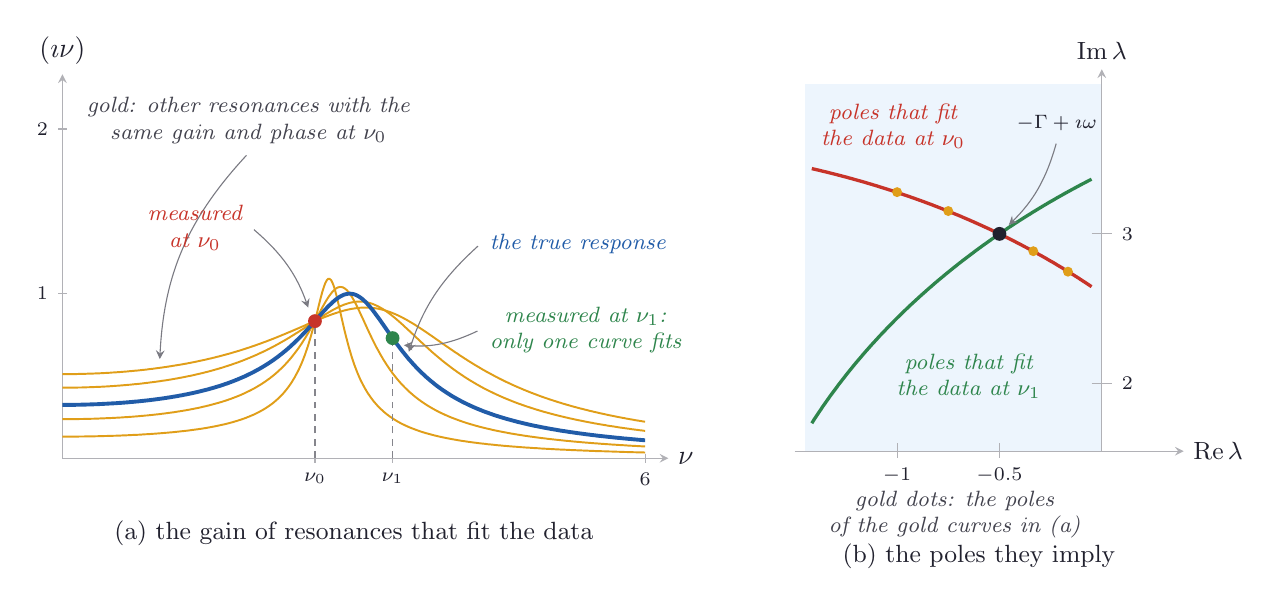
\begin{tikzpicture}[ink/.style={line width=0.9pt, ndInk}, faint/.style={line width=0.4pt, ndInk!35}, dashedink/.style={line width=0.5pt, ndInk!55, dash pattern=on 2.5pt off 2pt}, vec/.style={->, >=stealth, line width=1.2pt}, note/.style={font=\footnotesize\itshape, text=ndInk!85, align=center}, pointer/.style={->, >=stealth, line width=0.4pt, ndInk!60, shorten >=2pt, shorten <=1pt}, dot/.style={circle, fill=ndInk, inner sep=0pt, minimum size=3.4pt}, wash/.style={fill=ndSky, fill opacity=0.55}, every node/.style={text=ndInk}]
\definecolor{ndInk}{rgb}{0.13,0.13,0.18}
\definecolor{ndPaper}{rgb}{0.99,0.96,0.88}
\definecolor{ndSky}{rgb}{0.84,0.91,0.98}
\definecolor{ndRose}{rgb}{0.98,0.86,0.84}
\definecolor{ndBlue}{rgb}{0.13,0.36,0.66}
\definecolor{ndRed}{rgb}{0.78,0.20,0.16}
\definecolor{ndGold}{rgb}{0.88,0.62,0.10}
\definecolor{ndGreen}{rgb}{0.18,0.52,0.30}
\draw[faint, ->, >=stealth] (0.000,0.000) -- (7.696,0.000) node[right, text=ndInk] {$\nu$};
\draw[faint, ->, >=stealth] (0.000,0.000) -- (0.000,4.876) node[above, text=ndInk] {$\abs{\TF(\imath\nu)}$};
\draw[faint] (3.207,0.060) -- (3.207,-0.060) node[below, font=\scriptsize, text=ndInk] {$\nu_0$};
\draw[faint] (4.193,0.060) -- (4.193,-0.060) node[below, font=\scriptsize, text=ndInk] {$\nu_1$};
\draw[faint] (7.400,0.060) -- (7.400,-0.060) node[below, font=\scriptsize, text=ndInk] {$6$};
\draw[faint] (0.060,2.091) -- (-0.060,2.091) node[left, font=\scriptsize, text=ndInk] {$1$};
\draw[faint] (0.060,4.182) -- (-0.060,4.182) node[left, font=\scriptsize, text=ndInk] {$2$};
\draw[line width=0.7pt, ndGold] (0.000,0.275) -- (0.019,0.275) -- (0.037,0.276) -- (0.056,0.276) -- (0.074,0.276) -- (0.093,0.276) -- (0.111,0.276) -- (0.130,0.276) -- (0.148,0.276) -- (0.167,0.276) -- (0.185,0.276) -- (0.204,0.276) -- (0.223,0.277) -- (0.241,0.277) -- (0.260,0.277) -- (0.278,0.277) -- (0.297,0.278) -- (0.315,0.278) -- (0.334,0.278) -- (0.352,0.278) -- (0.371,0.279) -- (0.389,0.279) -- (0.408,0.279) -- (0.427,0.280) -- (0.445,0.280) -- (0.464,0.281) -- (0.482,0.281) -- (0.501,0.282) -- (0.519,0.282) -- (0.538,0.283) -- (0.556,0.283) -- (0.575,0.284) -- (0.593,0.284) -- (0.612,0.285) -- (0.631,0.285) -- (0.649,0.286) -- (0.668,0.286) -- (0.686,0.287) -- (0.705,0.288) -- (0.723,0.288) -- (0.742,0.289) -- (0.760,0.290) -- (0.779,0.291) -- (0.797,0.291) -- (0.816,0.292) -- (0.835,0.293) -- (0.853,0.294) -- (0.872,0.295) -- (0.890,0.296) -- (0.909,0.297) -- (0.927,0.297) -- (0.946,0.298) -- (0.964,0.299) -- (0.983,0.300) -- (1.002,0.301) -- (1.020,0.303) -- (1.039,0.304) -- (1.057,0.305) -- (1.076,0.306) -- (1.094,0.307) -- (1.113,0.308) -- (1.131,0.310) -- (1.150,0.311) -- (1.168,0.312) -- (1.187,0.313) -- (1.206,0.315) -- (1.224,0.316) -- (1.243,0.318) -- (1.261,0.319) -- (1.280,0.321) -- (1.298,0.322) -- (1.317,0.324) -- (1.335,0.325) -- (1.354,0.327) -- (1.372,0.329) -- (1.391,0.330) -- (1.410,0.332) -- (1.428,0.334) -- (1.447,0.336) -- (1.465,0.338) -- (1.484,0.340) -- (1.502,0.342) -- (1.521,0.344) -- (1.539,0.346) -- (1.558,0.348) -- (1.576,0.350) -- (1.595,0.352) -- (1.614,0.355) -- (1.632,0.357) -- (1.651,0.360) -- (1.669,0.362) -- (1.688,0.365) -- (1.706,0.367) -- (1.725,0.370) -- (1.743,0.373) -- (1.762,0.375) -- (1.780,0.378) -- (1.799,0.381) -- (1.818,0.384) -- (1.836,0.387) -- (1.855,0.391) -- (1.873,0.394) -- (1.892,0.397) -- (1.910,0.401) -- (1.929,0.404) -- (1.947,0.408) -- (1.966,0.412) -- (1.984,0.416) -- (2.003,0.420) -- (2.022,0.424) -- (2.040,0.428) -- (2.059,0.432) -- (2.077,0.437) -- (2.096,0.441) -- (2.114,0.446) -- (2.133,0.451) -- (2.151,0.456) -- (2.170,0.461) -- (2.188,0.467) -- (2.207,0.472) -- (2.226,0.478) -- (2.244,0.484) -- (2.263,0.490) -- (2.281,0.496) -- (2.300,0.503) -- (2.318,0.509) -- (2.337,0.516) -- (2.355,0.524) -- (2.374,0.531) -- (2.392,0.539) -- (2.411,0.547) -- (2.430,0.555) -- (2.448,0.564) -- (2.467,0.573) -- (2.485,0.582) -- (2.504,0.592) -- (2.522,0.602) -- (2.541,0.612) -- (2.559,0.623) -- (2.578,0.634) -- (2.596,0.646) -- (2.615,0.659) -- (2.634,0.672) -- (2.652,0.685) -- (2.671,0.699) -- (2.689,0.714) -- (2.708,0.730) -- (2.726,0.746) -- (2.745,0.763) -- (2.763,0.781) -- (2.782,0.800) -- (2.801,0.820) -- (2.819,0.841) -- (2.838,0.864) -- (2.856,0.887) -- (2.875,0.912) -- (2.893,0.938) -- (2.912,0.966) -- (2.930,0.996) -- (2.949,1.027) -- (2.967,1.061) -- (2.986,1.096) -- (3.005,1.134) -- (3.023,1.174) -- (3.042,1.217) -- (3.060,1.263) -- (3.079,1.312) -- (3.097,1.365) -- (3.116,1.420) -- (3.134,1.479) -- (3.153,1.542) -- (3.171,1.608) -- (3.190,1.677) -- (3.209,1.750) -- (3.227,1.824) -- (3.246,1.900) -- (3.264,1.975) -- (3.283,2.048) -- (3.301,2.115) -- (3.320,2.175) -- (3.338,2.225) -- (3.357,2.260) -- (3.375,2.278) -- (3.394,2.279) -- (3.413,2.261) -- (3.431,2.226) -- (3.450,2.176) -- (3.468,2.113) -- (3.487,2.041) -- (3.505,1.962) -- (3.524,1.881) -- (3.542,1.799) -- (3.561,1.717) -- (3.579,1.638) -- (3.598,1.561) -- (3.617,1.489) -- (3.635,1.420) -- (3.654,1.355) -- (3.672,1.294) -- (3.691,1.237) -- (3.709,1.183) -- (3.728,1.133) -- (3.746,1.086) -- (3.765,1.042) -- (3.783,1.001) -- (3.802,0.963) -- (3.821,0.927) -- (3.839,0.893) -- (3.858,0.861) -- (3.876,0.831) -- (3.895,0.803) -- (3.913,0.776) -- (3.932,0.751) -- (3.950,0.727) -- (3.969,0.705) -- (3.987,0.684) -- (4.006,0.663) -- (4.025,0.644) -- (4.043,0.626) -- (4.062,0.609) -- (4.080,0.592) -- (4.099,0.576) -- (4.117,0.561) -- (4.136,0.547) -- (4.154,0.533) -- (4.173,0.520) -- (4.191,0.508) -- (4.210,0.496) -- (4.229,0.484) -- (4.247,0.473) -- (4.266,0.462) -- (4.284,0.452) -- (4.303,0.442) -- (4.321,0.433) -- (4.340,0.424) -- (4.358,0.415) -- (4.377,0.407) -- (4.395,0.398) -- (4.414,0.391) -- (4.433,0.383) -- (4.451,0.376) -- (4.470,0.369) -- (4.488,0.362) -- (4.507,0.355) -- (4.525,0.349) -- (4.544,0.342) -- (4.562,0.336) -- (4.581,0.330) -- (4.599,0.325) -- (4.618,0.319) -- (4.637,0.314) -- (4.655,0.309) -- (4.674,0.304) -- (4.692,0.299) -- (4.711,0.294) -- (4.729,0.289) -- (4.748,0.285) -- (4.766,0.280) -- (4.785,0.276) -- (4.804,0.272) -- (4.822,0.268) -- (4.841,0.264) -- (4.859,0.260) -- (4.878,0.256) -- (4.896,0.253) -- (4.915,0.249) -- (4.933,0.246) -- (4.952,0.242) -- (4.970,0.239) -- (4.989,0.236) -- (5.008,0.232) -- (5.026,0.229) -- (5.045,0.226) -- (5.063,0.223) -- (5.082,0.220) -- (5.100,0.218) -- (5.119,0.215) -- (5.137,0.212) -- (5.156,0.209) -- (5.174,0.207) -- (5.193,0.204) -- (5.212,0.202) -- (5.230,0.199) -- (5.249,0.197) -- (5.267,0.195) -- (5.286,0.192) -- (5.304,0.190) -- (5.323,0.188) -- (5.341,0.186) -- (5.360,0.184) -- (5.378,0.182) -- (5.397,0.179) -- (5.416,0.177) -- (5.434,0.176) -- (5.453,0.174) -- (5.471,0.172) -- (5.490,0.170) -- (5.508,0.168) -- (5.527,0.166) -- (5.545,0.164) -- (5.564,0.163) -- (5.582,0.161) -- (5.601,0.159) -- (5.620,0.158) -- (5.638,0.156) -- (5.657,0.155) -- (5.675,0.153) -- (5.694,0.151) -- (5.712,0.150) -- (5.731,0.148) -- (5.749,0.147) -- (5.768,0.146) -- (5.786,0.144) -- (5.805,0.143) -- (5.824,0.141) -- (5.842,0.140) -- (5.861,0.139) -- (5.879,0.137) -- (5.898,0.136) -- (5.916,0.135) -- (5.935,0.134) -- (5.953,0.132) -- (5.972,0.131) -- (5.990,0.130) -- (6.009,0.129) -- (6.028,0.128) -- (6.046,0.127) -- (6.065,0.125) -- (6.083,0.124) -- (6.102,0.123) -- (6.120,0.122) -- (6.139,0.121) -- (6.157,0.120) -- (6.176,0.119) -- (6.194,0.118) -- (6.213,0.117) -- (6.232,0.116) -- (6.250,0.115) -- (6.269,0.114) -- (6.287,0.113) -- (6.306,0.112) -- (6.324,0.111) -- (6.343,0.110) -- (6.361,0.110) -- (6.380,0.109) -- (6.398,0.108) -- (6.417,0.107) -- (6.436,0.106) -- (6.454,0.105) -- (6.473,0.104) -- (6.491,0.104) -- (6.510,0.103) -- (6.528,0.102) -- (6.547,0.101) -- (6.565,0.100) -- (6.584,0.100) -- (6.603,0.099) -- (6.621,0.098) -- (6.640,0.097) -- (6.658,0.097) -- (6.677,0.096) -- (6.695,0.095) -- (6.714,0.095) -- (6.732,0.094) -- (6.751,0.093) -- (6.769,0.092) -- (6.788,0.092) -- (6.807,0.091) -- (6.825,0.090) -- (6.844,0.090) -- (6.862,0.089) -- (6.881,0.089) -- (6.899,0.088) -- (6.918,0.087) -- (6.936,0.087) -- (6.955,0.086) -- (6.973,0.086) -- (6.992,0.085) -- (7.011,0.084) -- (7.029,0.084) -- (7.048,0.083) -- (7.066,0.083) -- (7.085,0.082) -- (7.103,0.082) -- (7.122,0.081) -- (7.140,0.080) -- (7.159,0.080) -- (7.177,0.079) -- (7.196,0.079) -- (7.215,0.078) -- (7.233,0.078) -- (7.252,0.077) -- (7.270,0.077) -- (7.289,0.076) -- (7.307,0.076) -- (7.326,0.075) -- (7.344,0.075) -- (7.363,0.074) -- (7.381,0.074) -- (7.400,0.073);
\draw[line width=0.7pt, ndGold] (0.000,0.497) -- (0.019,0.497) -- (0.037,0.497) -- (0.056,0.497) -- (0.074,0.497) -- (0.093,0.497) -- (0.111,0.497) -- (0.130,0.497) -- (0.148,0.497) -- (0.167,0.498) -- (0.185,0.498) -- (0.204,0.498) -- (0.223,0.499) -- (0.241,0.499) -- (0.260,0.499) -- (0.278,0.500) -- (0.297,0.500) -- (0.315,0.500) -- (0.334,0.501) -- (0.352,0.501) -- (0.371,0.502) -- (0.389,0.502) -- (0.408,0.503) -- (0.427,0.504) -- (0.445,0.504) -- (0.464,0.505) -- (0.482,0.506) -- (0.501,0.506) -- (0.519,0.507) -- (0.538,0.508) -- (0.556,0.509) -- (0.575,0.509) -- (0.593,0.510) -- (0.612,0.511) -- (0.631,0.512) -- (0.649,0.513) -- (0.668,0.514) -- (0.686,0.515) -- (0.705,0.516) -- (0.723,0.517) -- (0.742,0.518) -- (0.760,0.519) -- (0.779,0.521) -- (0.797,0.522) -- (0.816,0.523) -- (0.835,0.524) -- (0.853,0.526) -- (0.872,0.527) -- (0.890,0.528) -- (0.909,0.530) -- (0.927,0.531) -- (0.946,0.533) -- (0.964,0.534) -- (0.983,0.536) -- (1.002,0.538) -- (1.020,0.539) -- (1.039,0.541) -- (1.057,0.543) -- (1.076,0.544) -- (1.094,0.546) -- (1.113,0.548) -- (1.131,0.550) -- (1.150,0.552) -- (1.168,0.554) -- (1.187,0.556) -- (1.206,0.558) -- (1.224,0.560) -- (1.243,0.562) -- (1.261,0.565) -- (1.280,0.567) -- (1.298,0.569) -- (1.317,0.572) -- (1.335,0.574) -- (1.354,0.577) -- (1.372,0.579) -- (1.391,0.582) -- (1.410,0.584) -- (1.428,0.587) -- (1.447,0.590) -- (1.465,0.593) -- (1.484,0.596) -- (1.502,0.599) -- (1.521,0.602) -- (1.539,0.605) -- (1.558,0.608) -- (1.576,0.611) -- (1.595,0.615) -- (1.614,0.618) -- (1.632,0.622) -- (1.651,0.625) -- (1.669,0.629) -- (1.688,0.633) -- (1.706,0.636) -- (1.725,0.640) -- (1.743,0.644) -- (1.762,0.648) -- (1.780,0.653) -- (1.799,0.657) -- (1.818,0.661) -- (1.836,0.666) -- (1.855,0.670) -- (1.873,0.675) -- (1.892,0.680) -- (1.910,0.685) -- (1.929,0.690) -- (1.947,0.695) -- (1.966,0.700) -- (1.984,0.705) -- (2.003,0.711) -- (2.022,0.716) -- (2.040,0.722) -- (2.059,0.728) -- (2.077,0.734) -- (2.096,0.740) -- (2.114,0.747) -- (2.133,0.753) -- (2.151,0.760) -- (2.170,0.767) -- (2.188,0.774) -- (2.207,0.781) -- (2.226,0.789) -- (2.244,0.796) -- (2.263,0.804) -- (2.281,0.812) -- (2.300,0.820) -- (2.318,0.829) -- (2.337,0.838) -- (2.355,0.847) -- (2.374,0.856) -- (2.392,0.865) -- (2.411,0.875) -- (2.430,0.885) -- (2.448,0.895) -- (2.467,0.906) -- (2.485,0.917) -- (2.504,0.928) -- (2.522,0.939) -- (2.541,0.951) -- (2.559,0.964) -- (2.578,0.976) -- (2.596,0.989) -- (2.615,1.003) -- (2.634,1.016) -- (2.652,1.031) -- (2.671,1.045) -- (2.689,1.060) -- (2.708,1.076) -- (2.726,1.092) -- (2.745,1.109) -- (2.763,1.126) -- (2.782,1.144) -- (2.801,1.162) -- (2.819,1.181) -- (2.838,1.201) -- (2.856,1.221) -- (2.875,1.242) -- (2.893,1.263) -- (2.912,1.286) -- (2.930,1.309) -- (2.949,1.333) -- (2.967,1.357) -- (2.986,1.382) -- (3.005,1.408) -- (3.023,1.435) -- (3.042,1.463) -- (3.060,1.492) -- (3.079,1.521) -- (3.097,1.551) -- (3.116,1.582) -- (3.134,1.613) -- (3.153,1.646) -- (3.171,1.679) -- (3.190,1.712) -- (3.209,1.746) -- (3.227,1.780) -- (3.246,1.814) -- (3.264,1.849) -- (3.283,1.883) -- (3.301,1.917) -- (3.320,1.950) -- (3.338,1.982) -- (3.357,2.013) -- (3.375,2.042) -- (3.394,2.069) -- (3.413,2.094) -- (3.431,2.117) -- (3.450,2.136) -- (3.468,2.152) -- (3.487,2.164) -- (3.505,2.172) -- (3.524,2.176) -- (3.542,2.175) -- (3.561,2.171) -- (3.579,2.161) -- (3.598,2.148) -- (3.617,2.130) -- (3.635,2.109) -- (3.654,2.084) -- (3.672,2.056) -- (3.691,2.025) -- (3.709,1.991) -- (3.728,1.956) -- (3.746,1.918) -- (3.765,1.880) -- (3.783,1.840) -- (3.802,1.800) -- (3.821,1.760) -- (3.839,1.719) -- (3.858,1.679) -- (3.876,1.638) -- (3.895,1.599) -- (3.913,1.560) -- (3.932,1.521) -- (3.950,1.484) -- (3.969,1.447) -- (3.987,1.411) -- (4.006,1.377) -- (4.025,1.343) -- (4.043,1.310) -- (4.062,1.278) -- (4.080,1.247) -- (4.099,1.218) -- (4.117,1.189) -- (4.136,1.161) -- (4.154,1.134) -- (4.173,1.108) -- (4.191,1.082) -- (4.210,1.058) -- (4.229,1.034) -- (4.247,1.011) -- (4.266,0.989) -- (4.284,0.968) -- (4.303,0.947) -- (4.321,0.928) -- (4.340,0.908) -- (4.358,0.890) -- (4.377,0.872) -- (4.395,0.854) -- (4.414,0.837) -- (4.433,0.821) -- (4.451,0.805) -- (4.470,0.789) -- (4.488,0.775) -- (4.507,0.760) -- (4.525,0.746) -- (4.544,0.733) -- (4.562,0.719) -- (4.581,0.707) -- (4.599,0.694) -- (4.618,0.682) -- (4.637,0.670) -- (4.655,0.659) -- (4.674,0.648) -- (4.692,0.637) -- (4.711,0.627) -- (4.729,0.616) -- (4.748,0.606) -- (4.766,0.597) -- (4.785,0.587) -- (4.804,0.578) -- (4.822,0.569) -- (4.841,0.561) -- (4.859,0.552) -- (4.878,0.544) -- (4.896,0.536) -- (4.915,0.528) -- (4.933,0.520) -- (4.952,0.513) -- (4.970,0.506) -- (4.989,0.499) -- (5.008,0.492) -- (5.026,0.485) -- (5.045,0.478) -- (5.063,0.472) -- (5.082,0.465) -- (5.100,0.459) -- (5.119,0.453) -- (5.137,0.447) -- (5.156,0.441) -- (5.174,0.436) -- (5.193,0.430) -- (5.212,0.425) -- (5.230,0.419) -- (5.249,0.414) -- (5.267,0.409) -- (5.286,0.404) -- (5.304,0.399) -- (5.323,0.394) -- (5.341,0.390) -- (5.360,0.385) -- (5.378,0.381) -- (5.397,0.376) -- (5.416,0.372) -- (5.434,0.368) -- (5.453,0.363) -- (5.471,0.359) -- (5.490,0.355) -- (5.508,0.351) -- (5.527,0.347) -- (5.545,0.344) -- (5.564,0.340) -- (5.582,0.336) -- (5.601,0.333) -- (5.620,0.329) -- (5.638,0.326) -- (5.657,0.322) -- (5.675,0.319) -- (5.694,0.315) -- (5.712,0.312) -- (5.731,0.309) -- (5.749,0.306) -- (5.768,0.303) -- (5.786,0.300) -- (5.805,0.297) -- (5.824,0.294) -- (5.842,0.291) -- (5.861,0.288) -- (5.879,0.285) -- (5.898,0.283) -- (5.916,0.280) -- (5.935,0.277) -- (5.953,0.275) -- (5.972,0.272) -- (5.990,0.270) -- (6.009,0.267) -- (6.028,0.265) -- (6.046,0.262) -- (6.065,0.260) -- (6.083,0.257) -- (6.102,0.255) -- (6.120,0.253) -- (6.139,0.251) -- (6.157,0.248) -- (6.176,0.246) -- (6.194,0.244) -- (6.213,0.242) -- (6.232,0.240) -- (6.250,0.238) -- (6.269,0.236) -- (6.287,0.234) -- (6.306,0.232) -- (6.324,0.230) -- (6.343,0.228) -- (6.361,0.226) -- (6.380,0.224) -- (6.398,0.222) -- (6.417,0.220) -- (6.436,0.219) -- (6.454,0.217) -- (6.473,0.215) -- (6.491,0.213) -- (6.510,0.212) -- (6.528,0.210) -- (6.547,0.208) -- (6.565,0.207) -- (6.584,0.205) -- (6.603,0.203) -- (6.621,0.202) -- (6.640,0.200) -- (6.658,0.199) -- (6.677,0.197) -- (6.695,0.196) -- (6.714,0.194) -- (6.732,0.193) -- (6.751,0.191) -- (6.769,0.190) -- (6.788,0.189) -- (6.807,0.187) -- (6.825,0.186) -- (6.844,0.184) -- (6.862,0.183) -- (6.881,0.182) -- (6.899,0.180) -- (6.918,0.179) -- (6.936,0.178) -- (6.955,0.177) -- (6.973,0.175) -- (6.992,0.174) -- (7.011,0.173) -- (7.029,0.172) -- (7.048,0.170) -- (7.066,0.169) -- (7.085,0.168) -- (7.103,0.167) -- (7.122,0.166) -- (7.140,0.165) -- (7.159,0.164) -- (7.177,0.162) -- (7.196,0.161) -- (7.215,0.160) -- (7.233,0.159) -- (7.252,0.158) -- (7.270,0.157) -- (7.289,0.156) -- (7.307,0.155) -- (7.326,0.154) -- (7.344,0.153) -- (7.363,0.152) -- (7.381,0.151) -- (7.400,0.150);
\draw[line width=0.7pt, ndGold] (0.000,0.897) -- (0.019,0.897) -- (0.037,0.897) -- (0.056,0.897) -- (0.074,0.897) -- (0.093,0.897) -- (0.111,0.897) -- (0.130,0.897) -- (0.148,0.898) -- (0.167,0.898) -- (0.185,0.898) -- (0.204,0.899) -- (0.223,0.899) -- (0.241,0.899) -- (0.260,0.900) -- (0.278,0.900) -- (0.297,0.901) -- (0.315,0.902) -- (0.334,0.902) -- (0.352,0.903) -- (0.371,0.903) -- (0.389,0.904) -- (0.408,0.905) -- (0.427,0.906) -- (0.445,0.907) -- (0.464,0.907) -- (0.482,0.908) -- (0.501,0.909) -- (0.519,0.910) -- (0.538,0.911) -- (0.556,0.912) -- (0.575,0.913) -- (0.593,0.914) -- (0.612,0.916) -- (0.631,0.917) -- (0.649,0.918) -- (0.668,0.919) -- (0.686,0.921) -- (0.705,0.922) -- (0.723,0.923) -- (0.742,0.925) -- (0.760,0.926) -- (0.779,0.928) -- (0.797,0.929) -- (0.816,0.931) -- (0.835,0.933) -- (0.853,0.934) -- (0.872,0.936) -- (0.890,0.938) -- (0.909,0.940) -- (0.927,0.942) -- (0.946,0.943) -- (0.964,0.945) -- (0.983,0.947) -- (1.002,0.949) -- (1.020,0.951) -- (1.039,0.954) -- (1.057,0.956) -- (1.076,0.958) -- (1.094,0.960) -- (1.113,0.963) -- (1.131,0.965) -- (1.150,0.967) -- (1.168,0.970) -- (1.187,0.972) -- (1.206,0.975) -- (1.224,0.977) -- (1.243,0.980) -- (1.261,0.983) -- (1.280,0.986) -- (1.298,0.988) -- (1.317,0.991) -- (1.335,0.994) -- (1.354,0.997) -- (1.372,1.000) -- (1.391,1.003) -- (1.410,1.007) -- (1.428,1.010) -- (1.447,1.013) -- (1.465,1.016) -- (1.484,1.020) -- (1.502,1.023) -- (1.521,1.027) -- (1.539,1.030) -- (1.558,1.034) -- (1.576,1.038) -- (1.595,1.042) -- (1.614,1.045) -- (1.632,1.049) -- (1.651,1.053) -- (1.669,1.057) -- (1.688,1.062) -- (1.706,1.066) -- (1.725,1.070) -- (1.743,1.074) -- (1.762,1.079) -- (1.780,1.083) -- (1.799,1.088) -- (1.818,1.093) -- (1.836,1.097) -- (1.855,1.102) -- (1.873,1.107) -- (1.892,1.112) -- (1.910,1.117) -- (1.929,1.122) -- (1.947,1.128) -- (1.966,1.133) -- (1.984,1.138) -- (2.003,1.144) -- (2.022,1.149) -- (2.040,1.155) -- (2.059,1.161) -- (2.077,1.167) -- (2.096,1.173) -- (2.114,1.179) -- (2.133,1.185) -- (2.151,1.191) -- (2.170,1.198) -- (2.188,1.204) -- (2.207,1.211) -- (2.226,1.217) -- (2.244,1.224) -- (2.263,1.231) -- (2.281,1.238) -- (2.300,1.245) -- (2.318,1.253) -- (2.337,1.260) -- (2.355,1.268) -- (2.374,1.275) -- (2.392,1.283) -- (2.411,1.291) -- (2.430,1.299) -- (2.448,1.307) -- (2.467,1.315) -- (2.485,1.324) -- (2.504,1.332) -- (2.522,1.341) -- (2.541,1.349) -- (2.559,1.358) -- (2.578,1.367) -- (2.596,1.376) -- (2.615,1.386) -- (2.634,1.395) -- (2.652,1.405) -- (2.671,1.414) -- (2.689,1.424) -- (2.708,1.434) -- (2.726,1.444) -- (2.745,1.454) -- (2.763,1.465) -- (2.782,1.475) -- (2.801,1.486) -- (2.819,1.496) -- (2.838,1.507) -- (2.856,1.518) -- (2.875,1.529) -- (2.893,1.541) -- (2.912,1.552) -- (2.930,1.563) -- (2.949,1.575) -- (2.967,1.587) -- (2.986,1.598) -- (3.005,1.610) -- (3.023,1.622) -- (3.042,1.634) -- (3.060,1.646) -- (3.079,1.658) -- (3.097,1.670) -- (3.116,1.682) -- (3.134,1.695) -- (3.153,1.707) -- (3.171,1.719) -- (3.190,1.731) -- (3.209,1.744) -- (3.227,1.756) -- (3.246,1.768) -- (3.264,1.780) -- (3.283,1.792) -- (3.301,1.804) -- (3.320,1.815) -- (3.338,1.827) -- (3.357,1.838) -- (3.375,1.849) -- (3.394,1.860) -- (3.413,1.871) -- (3.431,1.882) -- (3.450,1.892) -- (3.468,1.901) -- (3.487,1.911) -- (3.505,1.920) -- (3.524,1.929) -- (3.542,1.937) -- (3.561,1.944) -- (3.579,1.952) -- (3.598,1.958) -- (3.617,1.964) -- (3.635,1.970) -- (3.654,1.975) -- (3.672,1.979) -- (3.691,1.983) -- (3.709,1.986) -- (3.728,1.988) -- (3.746,1.989) -- (3.765,1.990) -- (3.783,1.990) -- (3.802,1.990) -- (3.821,1.988) -- (3.839,1.986) -- (3.858,1.983) -- (3.876,1.979) -- (3.895,1.974) -- (3.913,1.969) -- (3.932,1.963) -- (3.950,1.956) -- (3.969,1.948) -- (3.987,1.940) -- (4.006,1.931) -- (4.025,1.921) -- (4.043,1.911) -- (4.062,1.900) -- (4.080,1.888) -- (4.099,1.876) -- (4.117,1.863) -- (4.136,1.850) -- (4.154,1.836) -- (4.173,1.822) -- (4.191,1.807) -- (4.210,1.792) -- (4.229,1.777) -- (4.247,1.761) -- (4.266,1.745) -- (4.284,1.729) -- (4.303,1.712) -- (4.321,1.696) -- (4.340,1.679) -- (4.358,1.661) -- (4.377,1.644) -- (4.395,1.627) -- (4.414,1.610) -- (4.433,1.592) -- (4.451,1.575) -- (4.470,1.557) -- (4.488,1.540) -- (4.507,1.522) -- (4.525,1.505) -- (4.544,1.487) -- (4.562,1.470) -- (4.581,1.453) -- (4.599,1.436) -- (4.618,1.419) -- (4.637,1.402) -- (4.655,1.385) -- (4.674,1.369) -- (4.692,1.352) -- (4.711,1.336) -- (4.729,1.320) -- (4.748,1.304) -- (4.766,1.289) -- (4.785,1.273) -- (4.804,1.258) -- (4.822,1.242) -- (4.841,1.227) -- (4.859,1.213) -- (4.878,1.198) -- (4.896,1.184) -- (4.915,1.170) -- (4.933,1.156) -- (4.952,1.142) -- (4.970,1.128) -- (4.989,1.115) -- (5.008,1.101) -- (5.026,1.088) -- (5.045,1.076) -- (5.063,1.063) -- (5.082,1.051) -- (5.100,1.038) -- (5.119,1.026) -- (5.137,1.014) -- (5.156,1.003) -- (5.174,0.991) -- (5.193,0.980) -- (5.212,0.969) -- (5.230,0.958) -- (5.249,0.947) -- (5.267,0.936) -- (5.286,0.926) -- (5.304,0.915) -- (5.323,0.905) -- (5.341,0.895) -- (5.360,0.885) -- (5.378,0.876) -- (5.397,0.866) -- (5.416,0.857) -- (5.434,0.848) -- (5.453,0.839) -- (5.471,0.830) -- (5.490,0.821) -- (5.508,0.812) -- (5.527,0.804) -- (5.545,0.795) -- (5.564,0.787) -- (5.582,0.779) -- (5.601,0.771) -- (5.620,0.763) -- (5.638,0.755) -- (5.657,0.748) -- (5.675,0.740) -- (5.694,0.733) -- (5.712,0.725) -- (5.731,0.718) -- (5.749,0.711) -- (5.768,0.704) -- (5.786,0.697) -- (5.805,0.690) -- (5.824,0.684) -- (5.842,0.677) -- (5.861,0.671) -- (5.879,0.664) -- (5.898,0.658) -- (5.916,0.652) -- (5.935,0.646) -- (5.953,0.640) -- (5.972,0.634) -- (5.990,0.628) -- (6.009,0.622) -- (6.028,0.616) -- (6.046,0.611) -- (6.065,0.605) -- (6.083,0.600) -- (6.102,0.594) -- (6.120,0.589) -- (6.139,0.584) -- (6.157,0.579) -- (6.176,0.574) -- (6.194,0.569) -- (6.213,0.564) -- (6.232,0.559) -- (6.250,0.554) -- (6.269,0.549) -- (6.287,0.545) -- (6.306,0.540) -- (6.324,0.535) -- (6.343,0.531) -- (6.361,0.527) -- (6.380,0.522) -- (6.398,0.518) -- (6.417,0.514) -- (6.436,0.509) -- (6.454,0.505) -- (6.473,0.501) -- (6.491,0.497) -- (6.510,0.493) -- (6.528,0.489) -- (6.547,0.485) -- (6.565,0.481) -- (6.584,0.478) -- (6.603,0.474) -- (6.621,0.470) -- (6.640,0.466) -- (6.658,0.463) -- (6.677,0.459) -- (6.695,0.456) -- (6.714,0.452) -- (6.732,0.449) -- (6.751,0.445) -- (6.769,0.442) -- (6.788,0.439) -- (6.807,0.435) -- (6.825,0.432) -- (6.844,0.429) -- (6.862,0.426) -- (6.881,0.423) -- (6.899,0.420) -- (6.918,0.416) -- (6.936,0.413) -- (6.955,0.410) -- (6.973,0.408) -- (6.992,0.405) -- (7.011,0.402) -- (7.029,0.399) -- (7.048,0.396) -- (7.066,0.393) -- (7.085,0.390) -- (7.103,0.388) -- (7.122,0.385) -- (7.140,0.382) -- (7.159,0.380) -- (7.177,0.377) -- (7.196,0.375) -- (7.215,0.372) -- (7.233,0.369) -- (7.252,0.367) -- (7.270,0.364) -- (7.289,0.362) -- (7.307,0.360) -- (7.326,0.357) -- (7.344,0.355) -- (7.363,0.353) -- (7.381,0.350) -- (7.400,0.348);
\draw[line width=0.7pt, ndGold] (0.000,1.069) -- (0.019,1.069) -- (0.037,1.069) -- (0.056,1.069) -- (0.074,1.069) -- (0.093,1.069) -- (0.111,1.069) -- (0.130,1.069) -- (0.148,1.070) -- (0.167,1.070) -- (0.185,1.070) -- (0.204,1.071) -- (0.223,1.071) -- (0.241,1.071) -- (0.260,1.072) -- (0.278,1.072) -- (0.297,1.073) -- (0.315,1.074) -- (0.334,1.074) -- (0.352,1.075) -- (0.371,1.075) -- (0.389,1.076) -- (0.408,1.077) -- (0.427,1.078) -- (0.445,1.079) -- (0.464,1.079) -- (0.482,1.080) -- (0.501,1.081) -- (0.519,1.082) -- (0.538,1.083) -- (0.556,1.084) -- (0.575,1.085) -- (0.593,1.086) -- (0.612,1.087) -- (0.631,1.089) -- (0.649,1.090) -- (0.668,1.091) -- (0.686,1.092) -- (0.705,1.094) -- (0.723,1.095) -- (0.742,1.096) -- (0.760,1.098) -- (0.779,1.099) -- (0.797,1.101) -- (0.816,1.102) -- (0.835,1.104) -- (0.853,1.106) -- (0.872,1.107) -- (0.890,1.109) -- (0.909,1.111) -- (0.927,1.113) -- (0.946,1.114) -- (0.964,1.116) -- (0.983,1.118) -- (1.002,1.120) -- (1.020,1.122) -- (1.039,1.124) -- (1.057,1.126) -- (1.076,1.128) -- (1.094,1.131) -- (1.113,1.133) -- (1.131,1.135) -- (1.150,1.137) -- (1.168,1.140) -- (1.187,1.142) -- (1.206,1.145) -- (1.224,1.147) -- (1.243,1.150) -- (1.261,1.152) -- (1.280,1.155) -- (1.298,1.158) -- (1.317,1.160) -- (1.335,1.163) -- (1.354,1.166) -- (1.372,1.169) -- (1.391,1.172) -- (1.410,1.175) -- (1.428,1.178) -- (1.447,1.181) -- (1.465,1.184) -- (1.484,1.187) -- (1.502,1.190) -- (1.521,1.193) -- (1.539,1.197) -- (1.558,1.200) -- (1.576,1.203) -- (1.595,1.207) -- (1.614,1.210) -- (1.632,1.214) -- (1.651,1.218) -- (1.669,1.221) -- (1.688,1.225) -- (1.706,1.229) -- (1.725,1.233) -- (1.743,1.237) -- (1.762,1.241) -- (1.780,1.245) -- (1.799,1.249) -- (1.818,1.253) -- (1.836,1.257) -- (1.855,1.262) -- (1.873,1.266) -- (1.892,1.270) -- (1.910,1.275) -- (1.929,1.279) -- (1.947,1.284) -- (1.966,1.289) -- (1.984,1.293) -- (2.003,1.298) -- (2.022,1.303) -- (2.040,1.308) -- (2.059,1.313) -- (2.077,1.318) -- (2.096,1.323) -- (2.114,1.328) -- (2.133,1.333) -- (2.151,1.339) -- (2.170,1.344) -- (2.188,1.350) -- (2.207,1.355) -- (2.226,1.361) -- (2.244,1.366) -- (2.263,1.372) -- (2.281,1.378) -- (2.300,1.384) -- (2.318,1.390) -- (2.337,1.396) -- (2.355,1.402) -- (2.374,1.408) -- (2.392,1.414) -- (2.411,1.421) -- (2.430,1.427) -- (2.448,1.433) -- (2.467,1.440) -- (2.485,1.447) -- (2.504,1.453) -- (2.522,1.460) -- (2.541,1.467) -- (2.559,1.474) -- (2.578,1.480) -- (2.596,1.487) -- (2.615,1.495) -- (2.634,1.502) -- (2.652,1.509) -- (2.671,1.516) -- (2.689,1.523) -- (2.708,1.531) -- (2.726,1.538) -- (2.745,1.546) -- (2.763,1.553) -- (2.782,1.561) -- (2.801,1.569) -- (2.819,1.576) -- (2.838,1.584) -- (2.856,1.592) -- (2.875,1.600) -- (2.893,1.607) -- (2.912,1.615) -- (2.930,1.623) -- (2.949,1.631) -- (2.967,1.639) -- (2.986,1.647) -- (3.005,1.655) -- (3.023,1.663) -- (3.042,1.671) -- (3.060,1.679) -- (3.079,1.687) -- (3.097,1.696) -- (3.116,1.704) -- (3.134,1.712) -- (3.153,1.720) -- (3.171,1.727) -- (3.190,1.735) -- (3.209,1.743) -- (3.227,1.751) -- (3.246,1.759) -- (3.264,1.766) -- (3.283,1.774) -- (3.301,1.781) -- (3.320,1.789) -- (3.338,1.796) -- (3.357,1.803) -- (3.375,1.810) -- (3.394,1.817) -- (3.413,1.824) -- (3.431,1.831) -- (3.450,1.837) -- (3.468,1.843) -- (3.487,1.849) -- (3.505,1.855) -- (3.524,1.861) -- (3.542,1.866) -- (3.561,1.872) -- (3.579,1.877) -- (3.598,1.881) -- (3.617,1.886) -- (3.635,1.890) -- (3.654,1.894) -- (3.672,1.897) -- (3.691,1.900) -- (3.709,1.903) -- (3.728,1.906) -- (3.746,1.908) -- (3.765,1.910) -- (3.783,1.912) -- (3.802,1.913) -- (3.821,1.914) -- (3.839,1.914) -- (3.858,1.914) -- (3.876,1.914) -- (3.895,1.913) -- (3.913,1.912) -- (3.932,1.910) -- (3.950,1.908) -- (3.969,1.906) -- (3.987,1.903) -- (4.006,1.900) -- (4.025,1.896) -- (4.043,1.892) -- (4.062,1.887) -- (4.080,1.883) -- (4.099,1.877) -- (4.117,1.872) -- (4.136,1.865) -- (4.154,1.859) -- (4.173,1.852) -- (4.191,1.845) -- (4.210,1.837) -- (4.229,1.830) -- (4.247,1.821) -- (4.266,1.813) -- (4.284,1.804) -- (4.303,1.795) -- (4.321,1.785) -- (4.340,1.775) -- (4.358,1.765) -- (4.377,1.755) -- (4.395,1.744) -- (4.414,1.733) -- (4.433,1.722) -- (4.451,1.711) -- (4.470,1.700) -- (4.488,1.688) -- (4.507,1.676) -- (4.525,1.664) -- (4.544,1.652) -- (4.562,1.640) -- (4.581,1.628) -- (4.599,1.615) -- (4.618,1.603) -- (4.637,1.590) -- (4.655,1.577) -- (4.674,1.564) -- (4.692,1.552) -- (4.711,1.539) -- (4.729,1.526) -- (4.748,1.513) -- (4.766,1.500) -- (4.785,1.487) -- (4.804,1.474) -- (4.822,1.461) -- (4.841,1.448) -- (4.859,1.435) -- (4.878,1.422) -- (4.896,1.410) -- (4.915,1.397) -- (4.933,1.384) -- (4.952,1.372) -- (4.970,1.359) -- (4.989,1.346) -- (5.008,1.334) -- (5.026,1.322) -- (5.045,1.309) -- (5.063,1.297) -- (5.082,1.285) -- (5.100,1.273) -- (5.119,1.261) -- (5.137,1.249) -- (5.156,1.237) -- (5.174,1.226) -- (5.193,1.214) -- (5.212,1.203) -- (5.230,1.191) -- (5.249,1.180) -- (5.267,1.169) -- (5.286,1.158) -- (5.304,1.147) -- (5.323,1.136) -- (5.341,1.125) -- (5.360,1.115) -- (5.378,1.104) -- (5.397,1.094) -- (5.416,1.084) -- (5.434,1.074) -- (5.453,1.064) -- (5.471,1.054) -- (5.490,1.044) -- (5.508,1.034) -- (5.527,1.025) -- (5.545,1.015) -- (5.564,1.006) -- (5.582,0.997) -- (5.601,0.987) -- (5.620,0.978) -- (5.638,0.969) -- (5.657,0.961) -- (5.675,0.952) -- (5.694,0.943) -- (5.712,0.935) -- (5.731,0.926) -- (5.749,0.918) -- (5.768,0.910) -- (5.786,0.902) -- (5.805,0.894) -- (5.824,0.886) -- (5.842,0.878) -- (5.861,0.870) -- (5.879,0.863) -- (5.898,0.855) -- (5.916,0.848) -- (5.935,0.840) -- (5.953,0.833) -- (5.972,0.826) -- (5.990,0.819) -- (6.009,0.812) -- (6.028,0.805) -- (6.046,0.798) -- (6.065,0.791) -- (6.083,0.784) -- (6.102,0.778) -- (6.120,0.771) -- (6.139,0.765) -- (6.157,0.759) -- (6.176,0.752) -- (6.194,0.746) -- (6.213,0.740) -- (6.232,0.734) -- (6.250,0.728) -- (6.269,0.722) -- (6.287,0.716) -- (6.306,0.710) -- (6.324,0.705) -- (6.343,0.699) -- (6.361,0.693) -- (6.380,0.688) -- (6.398,0.682) -- (6.417,0.677) -- (6.436,0.672) -- (6.454,0.666) -- (6.473,0.661) -- (6.491,0.656) -- (6.510,0.651) -- (6.528,0.646) -- (6.547,0.641) -- (6.565,0.636) -- (6.584,0.631) -- (6.603,0.627) -- (6.621,0.622) -- (6.640,0.617) -- (6.658,0.613) -- (6.677,0.608) -- (6.695,0.603) -- (6.714,0.599) -- (6.732,0.595) -- (6.751,0.590) -- (6.769,0.586) -- (6.788,0.582) -- (6.807,0.577) -- (6.825,0.573) -- (6.844,0.569) -- (6.862,0.565) -- (6.881,0.561) -- (6.899,0.557) -- (6.918,0.553) -- (6.936,0.549) -- (6.955,0.545) -- (6.973,0.541) -- (6.992,0.538) -- (7.011,0.534) -- (7.029,0.530) -- (7.048,0.526) -- (7.066,0.523) -- (7.085,0.519) -- (7.103,0.516) -- (7.122,0.512) -- (7.140,0.509) -- (7.159,0.505) -- (7.177,0.502) -- (7.196,0.498) -- (7.215,0.495) -- (7.233,0.492) -- (7.252,0.489) -- (7.270,0.485) -- (7.289,0.482) -- (7.307,0.479) -- (7.326,0.476) -- (7.344,0.473) -- (7.363,0.470) -- (7.381,0.467) -- (7.400,0.464);
\draw[line width=1.4pt, ndBlue] (0.000,0.678) -- (0.019,0.678) -- (0.037,0.678) -- (0.056,0.678) -- (0.074,0.678) -- (0.093,0.679) -- (0.111,0.679) -- (0.130,0.679) -- (0.148,0.679) -- (0.167,0.679) -- (0.185,0.680) -- (0.204,0.680) -- (0.223,0.680) -- (0.241,0.681) -- (0.260,0.681) -- (0.278,0.682) -- (0.297,0.682) -- (0.315,0.683) -- (0.334,0.683) -- (0.352,0.684) -- (0.371,0.684) -- (0.389,0.685) -- (0.408,0.686) -- (0.427,0.687) -- (0.445,0.687) -- (0.464,0.688) -- (0.482,0.689) -- (0.501,0.690) -- (0.519,0.691) -- (0.538,0.692) -- (0.556,0.693) -- (0.575,0.694) -- (0.593,0.695) -- (0.612,0.696) -- (0.631,0.697) -- (0.649,0.698) -- (0.668,0.699) -- (0.686,0.700) -- (0.705,0.702) -- (0.723,0.703) -- (0.742,0.704) -- (0.760,0.705) -- (0.779,0.707) -- (0.797,0.708) -- (0.816,0.710) -- (0.835,0.711) -- (0.853,0.713) -- (0.872,0.715) -- (0.890,0.716) -- (0.909,0.718) -- (0.927,0.720) -- (0.946,0.721) -- (0.964,0.723) -- (0.983,0.725) -- (1.002,0.727) -- (1.020,0.729) -- (1.039,0.731) -- (1.057,0.733) -- (1.076,0.735) -- (1.094,0.737) -- (1.113,0.739) -- (1.131,0.742) -- (1.150,0.744) -- (1.168,0.746) -- (1.187,0.749) -- (1.206,0.751) -- (1.224,0.754) -- (1.243,0.756) -- (1.261,0.759) -- (1.280,0.761) -- (1.298,0.764) -- (1.317,0.767) -- (1.335,0.770) -- (1.354,0.773) -- (1.372,0.775) -- (1.391,0.779) -- (1.410,0.782) -- (1.428,0.785) -- (1.447,0.788) -- (1.465,0.791) -- (1.484,0.795) -- (1.502,0.798) -- (1.521,0.801) -- (1.539,0.805) -- (1.558,0.809) -- (1.576,0.812) -- (1.595,0.816) -- (1.614,0.820) -- (1.632,0.824) -- (1.651,0.828) -- (1.669,0.832) -- (1.688,0.836) -- (1.706,0.840) -- (1.725,0.845) -- (1.743,0.849) -- (1.762,0.854) -- (1.780,0.858) -- (1.799,0.863) -- (1.818,0.868) -- (1.836,0.872) -- (1.855,0.877) -- (1.873,0.883) -- (1.892,0.888) -- (1.910,0.893) -- (1.929,0.898) -- (1.947,0.904) -- (1.966,0.910) -- (1.984,0.915) -- (2.003,0.921) -- (2.022,0.927) -- (2.040,0.933) -- (2.059,0.940) -- (2.077,0.946) -- (2.096,0.952) -- (2.114,0.959) -- (2.133,0.966) -- (2.151,0.973) -- (2.170,0.980) -- (2.188,0.987) -- (2.207,0.995) -- (2.226,1.002) -- (2.244,1.010) -- (2.263,1.018) -- (2.281,1.026) -- (2.300,1.034) -- (2.318,1.042) -- (2.337,1.051) -- (2.355,1.060) -- (2.374,1.069) -- (2.392,1.078) -- (2.411,1.087) -- (2.430,1.097) -- (2.448,1.107) -- (2.467,1.117) -- (2.485,1.127) -- (2.504,1.137) -- (2.522,1.148) -- (2.541,1.159) -- (2.559,1.170) -- (2.578,1.181) -- (2.596,1.193) -- (2.615,1.205) -- (2.634,1.217) -- (2.652,1.230) -- (2.671,1.242) -- (2.689,1.255) -- (2.708,1.269) -- (2.726,1.282) -- (2.745,1.296) -- (2.763,1.311) -- (2.782,1.325) -- (2.801,1.340) -- (2.819,1.355) -- (2.838,1.371) -- (2.856,1.386) -- (2.875,1.402) -- (2.893,1.419) -- (2.912,1.436) -- (2.930,1.453) -- (2.949,1.470) -- (2.967,1.488) -- (2.986,1.506) -- (3.005,1.525) -- (3.023,1.543) -- (3.042,1.562) -- (3.060,1.582) -- (3.079,1.601) -- (3.097,1.621) -- (3.116,1.641) -- (3.134,1.662) -- (3.153,1.682) -- (3.171,1.703) -- (3.190,1.724) -- (3.209,1.745) -- (3.227,1.765) -- (3.246,1.786) -- (3.264,1.807) -- (3.283,1.828) -- (3.301,1.849) -- (3.320,1.869) -- (3.338,1.889) -- (3.357,1.909) -- (3.375,1.928) -- (3.394,1.946) -- (3.413,1.964) -- (3.431,1.981) -- (3.450,1.998) -- (3.468,2.013) -- (3.487,2.027) -- (3.505,2.040) -- (3.524,2.052) -- (3.542,2.062) -- (3.561,2.071) -- (3.579,2.079) -- (3.598,2.084) -- (3.617,2.088) -- (3.635,2.090) -- (3.654,2.091) -- (3.672,2.089) -- (3.691,2.086) -- (3.709,2.081) -- (3.728,2.074) -- (3.746,2.065) -- (3.765,2.054) -- (3.783,2.042) -- (3.802,2.028) -- (3.821,2.012) -- (3.839,1.995) -- (3.858,1.977) -- (3.876,1.957) -- (3.895,1.936) -- (3.913,1.914) -- (3.932,1.892) -- (3.950,1.868) -- (3.969,1.843) -- (3.987,1.818) -- (4.006,1.793) -- (4.025,1.767) -- (4.043,1.741) -- (4.062,1.714) -- (4.080,1.688) -- (4.099,1.661) -- (4.117,1.634) -- (4.136,1.608) -- (4.154,1.581) -- (4.173,1.555) -- (4.191,1.529) -- (4.210,1.503) -- (4.229,1.477) -- (4.247,1.452) -- (4.266,1.427) -- (4.284,1.403) -- (4.303,1.379) -- (4.321,1.355) -- (4.340,1.332) -- (4.358,1.309) -- (4.377,1.286) -- (4.395,1.264) -- (4.414,1.243) -- (4.433,1.222) -- (4.451,1.201) -- (4.470,1.181) -- (4.488,1.161) -- (4.507,1.142) -- (4.525,1.123) -- (4.544,1.104) -- (4.562,1.086) -- (4.581,1.069) -- (4.599,1.051) -- (4.618,1.034) -- (4.637,1.018) -- (4.655,1.002) -- (4.674,0.986) -- (4.692,0.971) -- (4.711,0.956) -- (4.729,0.941) -- (4.748,0.926) -- (4.766,0.912) -- (4.785,0.899) -- (4.804,0.885) -- (4.822,0.872) -- (4.841,0.859) -- (4.859,0.847) -- (4.878,0.835) -- (4.896,0.823) -- (4.915,0.811) -- (4.933,0.799) -- (4.952,0.788) -- (4.970,0.777) -- (4.989,0.767) -- (5.008,0.756) -- (5.026,0.746) -- (5.045,0.736) -- (5.063,0.726) -- (5.082,0.716) -- (5.100,0.707) -- (5.119,0.698) -- (5.137,0.689) -- (5.156,0.680) -- (5.174,0.671) -- (5.193,0.663) -- (5.212,0.654) -- (5.230,0.646) -- (5.249,0.638) -- (5.267,0.630) -- (5.286,0.623) -- (5.304,0.615) -- (5.323,0.608) -- (5.341,0.600) -- (5.360,0.593) -- (5.378,0.586) -- (5.397,0.580) -- (5.416,0.573) -- (5.434,0.566) -- (5.453,0.560) -- (5.471,0.553) -- (5.490,0.547) -- (5.508,0.541) -- (5.527,0.535) -- (5.545,0.529) -- (5.564,0.523) -- (5.582,0.518) -- (5.601,0.512) -- (5.620,0.507) -- (5.638,0.501) -- (5.657,0.496) -- (5.675,0.491) -- (5.694,0.486) -- (5.712,0.481) -- (5.731,0.476) -- (5.749,0.471) -- (5.768,0.466) -- (5.786,0.461) -- (5.805,0.457) -- (5.824,0.452) -- (5.842,0.448) -- (5.861,0.443) -- (5.879,0.439) -- (5.898,0.435) -- (5.916,0.430) -- (5.935,0.426) -- (5.953,0.422) -- (5.972,0.418) -- (5.990,0.414) -- (6.009,0.410) -- (6.028,0.407) -- (6.046,0.403) -- (6.065,0.399) -- (6.083,0.395) -- (6.102,0.392) -- (6.120,0.388) -- (6.139,0.385) -- (6.157,0.381) -- (6.176,0.378) -- (6.194,0.375) -- (6.213,0.371) -- (6.232,0.368) -- (6.250,0.365) -- (6.269,0.362) -- (6.287,0.359) -- (6.306,0.355) -- (6.324,0.352) -- (6.343,0.349) -- (6.361,0.346) -- (6.380,0.344) -- (6.398,0.341) -- (6.417,0.338) -- (6.436,0.335) -- (6.454,0.332) -- (6.473,0.330) -- (6.491,0.327) -- (6.510,0.324) -- (6.528,0.322) -- (6.547,0.319) -- (6.565,0.317) -- (6.584,0.314) -- (6.603,0.312) -- (6.621,0.309) -- (6.640,0.307) -- (6.658,0.304) -- (6.677,0.302) -- (6.695,0.300) -- (6.714,0.297) -- (6.732,0.295) -- (6.751,0.293) -- (6.769,0.291) -- (6.788,0.288) -- (6.807,0.286) -- (6.825,0.284) -- (6.844,0.282) -- (6.862,0.280) -- (6.881,0.278) -- (6.899,0.276) -- (6.918,0.274) -- (6.936,0.272) -- (6.955,0.270) -- (6.973,0.268) -- (6.992,0.266) -- (7.011,0.264) -- (7.029,0.262) -- (7.048,0.260) -- (7.066,0.259) -- (7.085,0.257) -- (7.103,0.255) -- (7.122,0.253) -- (7.140,0.251) -- (7.159,0.250) -- (7.177,0.248) -- (7.196,0.246) -- (7.215,0.245) -- (7.233,0.243) -- (7.252,0.241) -- (7.270,0.240) -- (7.289,0.238) -- (7.307,0.236) -- (7.326,0.235) -- (7.344,0.233) -- (7.363,0.232) -- (7.381,0.230) -- (7.400,0.229);
\draw[dashedink] (3.207,0.000) -- (3.207,1.742);
\node[dot, fill=ndRed, minimum size=5pt] at (3.207,1.742) {};
\draw[dashedink] (4.193,0.000) -- (4.193,1.526);
\node[dot, fill=ndGreen, minimum size=5pt] at (4.193,1.526) {};
\node[note, anchor=north west] (f) at (0.185,4.705) {gold: other resonances with the\\ same gain and phase at $\nu_0$};
\draw[pointer] (f.south) to[bend right=20] (1.233,1.190);
\node[note, anchor=west, text=ndBlue] (t) at (5.303,2.718) {the true response};
\draw[pointer] (t.west) to[bend right=15] (4.378,1.285);
\node[note, anchor=east, text=ndRed] (m0) at (2.405,2.927) {measured\\ at $\nu_0$};
\draw[pointer] (m0.east) to[bend left=15] (3.145,1.847);
\node[note, anchor=west, text=ndGreen] (m1) at (5.303,1.631) {measured at $\nu_1$:\\ only one curve fits};
\draw[pointer] (m1.west) to[bend left=15] (4.267,1.442);
\node[font=\small] at (3.700,-0.950) {(a) the gain of resonances that fit the data};
\fill[ndSky, fill opacity=0.45] (9.43,0.09) rectangle (13.20,4.75);
\draw[faint, ->, >=stealth] (9.30,0.09) -- (14.24,0.09) node[right, text=ndInk, font=\small] {$\mathrm{Re}\,\lambda$};
\draw[faint, ->, >=stealth] (13.20,0.09) -- (13.20,4.94) node[above, text=ndInk, font=\small] {$\mathrm{Im}\,\lambda$};
\draw[faint] (10.60,0.19) -- (10.60,-0.00) node[below, font=\scriptsize, text=ndInk] {$-1$};
\draw[faint] (11.90,0.19) -- (11.90,-0.00) node[below, font=\scriptsize, text=ndInk] {$-0.5$};
\draw[faint] (13.07,0.95) -- (13.33,0.95) node[right, font=\scriptsize, text=ndInk] {$2$};
\draw[faint] (13.07,2.85) -- (13.33,2.85) node[right, font=\scriptsize, text=ndInk] {$3$};
\draw[line width=1.2pt, ndRed] (13.070,2.179) -- (13.058,2.187) -- (13.046,2.195) -- (13.034,2.203) -- (13.022,2.211) -- (13.011,2.219) -- (12.999,2.227) -- (12.987,2.235) -- (12.975,2.242) -- (12.963,2.250) -- (12.951,2.258) -- (12.939,2.266) -- (12.927,2.273) -- (12.916,2.281) -- (12.904,2.289) -- (12.892,2.296) -- (12.880,2.304) -- (12.868,2.311) -- (12.856,2.319) -- (12.844,2.327) -- (12.832,2.334) -- (12.820,2.341) -- (12.809,2.349) -- (12.797,2.356) -- (12.785,2.364) -- (12.773,2.371) -- (12.761,2.378) -- (12.749,2.386) -- (12.737,2.393) -- (12.725,2.400) -- (12.713,2.407) -- (12.702,2.415) -- (12.690,2.422) -- (12.678,2.429) -- (12.666,2.436) -- (12.654,2.443) -- (12.642,2.450) -- (12.630,2.457) -- (12.618,2.465) -- (12.607,2.472) -- (12.595,2.479) -- (12.583,2.486) -- (12.571,2.493) -- (12.559,2.499) -- (12.547,2.506) -- (12.535,2.513) -- (12.523,2.520) -- (12.511,2.527) -- (12.500,2.534) -- (12.488,2.541) -- (12.476,2.547) -- (12.464,2.554) -- (12.452,2.561) -- (12.440,2.568) -- (12.428,2.574) -- (12.416,2.581) -- (12.404,2.587) -- (12.393,2.594) -- (12.381,2.601) -- (12.369,2.607) -- (12.357,2.614) -- (12.345,2.620) -- (12.333,2.627) -- (12.321,2.633) -- (12.309,2.640) -- (12.298,2.646) -- (12.286,2.653) -- (12.274,2.659) -- (12.262,2.665) -- (12.250,2.672) -- (12.238,2.678) -- (12.226,2.684) -- (12.214,2.691) -- (12.202,2.697) -- (12.191,2.703) -- (12.179,2.710) -- (12.167,2.716) -- (12.155,2.722) -- (12.143,2.728) -- (12.131,2.734) -- (12.119,2.740) -- (12.107,2.747) -- (12.096,2.753) -- (12.084,2.759) -- (12.072,2.765) -- (12.060,2.771) -- (12.048,2.777) -- (12.036,2.783) -- (12.024,2.789) -- (12.012,2.795) -- (12.000,2.801) -- (11.989,2.807) -- (11.977,2.812) -- (11.965,2.818) -- (11.953,2.824) -- (11.941,2.830) -- (11.929,2.836) -- (11.917,2.842) -- (11.905,2.847) -- (11.893,2.853) -- (11.882,2.859) -- (11.870,2.865) -- (11.858,2.870) -- (11.846,2.876) -- (11.834,2.882) -- (11.822,2.887) -- (11.810,2.893) -- (11.798,2.899) -- (11.787,2.904) -- (11.775,2.910) -- (11.763,2.915) -- (11.751,2.921) -- (11.739,2.926) -- (11.727,2.932) -- (11.715,2.937) -- (11.703,2.943) -- (11.691,2.948) -- (11.680,2.954) -- (11.668,2.959) -- (11.656,2.964) -- (11.644,2.970) -- (11.632,2.975) -- (11.620,2.980) -- (11.608,2.986) -- (11.596,2.991) -- (11.584,2.996) -- (11.573,3.002) -- (11.561,3.007) -- (11.549,3.012) -- (11.537,3.017) -- (11.525,3.023) -- (11.513,3.028) -- (11.501,3.033) -- (11.489,3.038) -- (11.478,3.043) -- (11.466,3.048) -- (11.454,3.053) -- (11.442,3.058) -- (11.430,3.063) -- (11.418,3.069) -- (11.406,3.074) -- (11.394,3.079) -- (11.382,3.084) -- (11.371,3.089) -- (11.359,3.093) -- (11.347,3.098) -- (11.335,3.103) -- (11.323,3.108) -- (11.311,3.113) -- (11.299,3.118) -- (11.287,3.123) -- (11.276,3.128) -- (11.264,3.133) -- (11.252,3.137) -- (11.240,3.142) -- (11.228,3.147) -- (11.216,3.152) -- (11.204,3.156) -- (11.192,3.161) -- (11.180,3.166) -- (11.169,3.170) -- (11.157,3.175) -- (11.145,3.180) -- (11.133,3.184) -- (11.121,3.189) -- (11.109,3.194) -- (11.097,3.198) -- (11.085,3.203) -- (11.073,3.207) -- (11.062,3.212) -- (11.050,3.217) -- (11.038,3.221) -- (11.026,3.226) -- (11.014,3.230) -- (11.002,3.234) -- (10.990,3.239) -- (10.978,3.243) -- (10.967,3.248) -- (10.955,3.252) -- (10.943,3.257) -- (10.931,3.261) -- (10.919,3.265) -- (10.907,3.270) -- (10.895,3.274) -- (10.883,3.278) -- (10.871,3.283) -- (10.860,3.287) -- (10.848,3.291) -- (10.836,3.295) -- (10.824,3.300) -- (10.812,3.304) -- (10.800,3.308) -- (10.788,3.312) -- (10.776,3.316) -- (10.764,3.321) -- (10.753,3.325) -- (10.741,3.329) -- (10.729,3.333) -- (10.717,3.337) -- (10.705,3.341) -- (10.693,3.345) -- (10.681,3.349) -- (10.669,3.353) -- (10.658,3.357) -- (10.646,3.361) -- (10.634,3.365) -- (10.622,3.369) -- (10.610,3.373) -- (10.598,3.377) -- (10.586,3.381) -- (10.574,3.385) -- (10.562,3.389) -- (10.551,3.393) -- (10.539,3.397) -- (10.527,3.401) -- (10.515,3.405) -- (10.503,3.408) -- (10.491,3.412) -- (10.479,3.416) -- (10.467,3.420) -- (10.456,3.424) -- (10.444,3.427) -- (10.432,3.431) -- (10.420,3.435) -- (10.408,3.439) -- (10.396,3.442) -- (10.384,3.446) -- (10.372,3.450) -- (10.360,3.453) -- (10.349,3.457) -- (10.337,3.461) -- (10.325,3.464) -- (10.313,3.468) -- (10.301,3.471) -- (10.289,3.475) -- (10.277,3.479) -- (10.265,3.482) -- (10.253,3.486) -- (10.242,3.489) -- (10.230,3.493) -- (10.218,3.496) -- (10.206,3.500) -- (10.194,3.503) -- (10.182,3.507) -- (10.170,3.510) -- (10.158,3.514) -- (10.147,3.517) -- (10.135,3.520) -- (10.123,3.524) -- (10.111,3.527) -- (10.099,3.530) -- (10.087,3.534) -- (10.075,3.537) -- (10.063,3.540) -- (10.051,3.544) -- (10.040,3.547) -- (10.028,3.550) -- (10.016,3.554) -- (10.004,3.557) -- (9.992,3.560) -- (9.980,3.563) -- (9.968,3.567) -- (9.956,3.570) -- (9.944,3.573) -- (9.933,3.576) -- (9.921,3.579) -- (9.909,3.582) -- (9.897,3.586) -- (9.885,3.589) -- (9.873,3.592) -- (9.861,3.595) -- (9.849,3.598) -- (9.838,3.601) -- (9.826,3.604) -- (9.814,3.607) -- (9.802,3.610) -- (9.790,3.613) -- (9.778,3.616) -- (9.766,3.619) -- (9.754,3.622) -- (9.742,3.625) -- (9.731,3.628) -- (9.719,3.631) -- (9.707,3.634) -- (9.695,3.637) -- (9.683,3.640) -- (9.671,3.643) -- (9.659,3.645) -- (9.647,3.648) -- (9.636,3.651) -- (9.624,3.654) -- (9.612,3.657) -- (9.600,3.660) -- (9.588,3.662) -- (9.576,3.665) -- (9.564,3.668) -- (9.552,3.671) -- (9.540,3.673) -- (9.529,3.676) -- (9.517,3.679);
\draw[line width=1.2pt, ndGreen] (13.070,3.544) -- (13.058,3.538) -- (13.046,3.532) -- (13.034,3.526) -- (13.022,3.520) -- (13.011,3.514) -- (12.999,3.508) -- (12.987,3.501) -- (12.975,3.495) -- (12.963,3.489) -- (12.951,3.483) -- (12.939,3.476) -- (12.927,3.470) -- (12.916,3.464) -- (12.904,3.457) -- (12.892,3.451) -- (12.880,3.445) -- (12.868,3.438) -- (12.856,3.432) -- (12.844,3.425) -- (12.832,3.419) -- (12.820,3.413) -- (12.809,3.406) -- (12.797,3.400) -- (12.785,3.393) -- (12.773,3.387) -- (12.761,3.380) -- (12.749,3.373) -- (12.737,3.367) -- (12.725,3.360) -- (12.713,3.354) -- (12.702,3.347) -- (12.690,3.340) -- (12.678,3.334) -- (12.666,3.327) -- (12.654,3.320) -- (12.642,3.313) -- (12.630,3.307) -- (12.618,3.300) -- (12.607,3.293) -- (12.595,3.286) -- (12.583,3.279) -- (12.571,3.272) -- (12.559,3.266) -- (12.547,3.259) -- (12.535,3.252) -- (12.523,3.245) -- (12.511,3.238) -- (12.500,3.231) -- (12.488,3.224) -- (12.476,3.217) -- (12.464,3.210) -- (12.452,3.203) -- (12.440,3.196) -- (12.428,3.188) -- (12.416,3.181) -- (12.404,3.174) -- (12.393,3.167) -- (12.381,3.160) -- (12.369,3.153) -- (12.357,3.145) -- (12.345,3.138) -- (12.333,3.131) -- (12.321,3.124) -- (12.309,3.116) -- (12.298,3.109) -- (12.286,3.101) -- (12.274,3.094) -- (12.262,3.087) -- (12.250,3.079) -- (12.238,3.072) -- (12.226,3.064) -- (12.214,3.057) -- (12.202,3.049) -- (12.191,3.042) -- (12.179,3.034) -- (12.167,3.027) -- (12.155,3.019) -- (12.143,3.011) -- (12.131,3.004) -- (12.119,2.996) -- (12.107,2.988) -- (12.096,2.981) -- (12.084,2.973) -- (12.072,2.965) -- (12.060,2.957) -- (12.048,2.949) -- (12.036,2.942) -- (12.024,2.934) -- (12.012,2.926) -- (12.000,2.918) -- (11.989,2.910) -- (11.977,2.902) -- (11.965,2.894) -- (11.953,2.886) -- (11.941,2.878) -- (11.929,2.870) -- (11.917,2.862) -- (11.905,2.854) -- (11.893,2.846) -- (11.882,2.837) -- (11.870,2.829) -- (11.858,2.821) -- (11.846,2.813) -- (11.834,2.804) -- (11.822,2.796) -- (11.810,2.788) -- (11.798,2.780) -- (11.787,2.771) -- (11.775,2.763) -- (11.763,2.754) -- (11.751,2.746) -- (11.739,2.737) -- (11.727,2.729) -- (11.715,2.720) -- (11.703,2.712) -- (11.691,2.703) -- (11.680,2.695) -- (11.668,2.686) -- (11.656,2.677) -- (11.644,2.669) -- (11.632,2.660) -- (11.620,2.651) -- (11.608,2.643) -- (11.596,2.634) -- (11.584,2.625) -- (11.573,2.616) -- (11.561,2.607) -- (11.549,2.598) -- (11.537,2.589) -- (11.525,2.580) -- (11.513,2.571) -- (11.501,2.562) -- (11.489,2.553) -- (11.478,2.544) -- (11.466,2.535) -- (11.454,2.526) -- (11.442,2.517) -- (11.430,2.508) -- (11.418,2.498) -- (11.406,2.489) -- (11.394,2.480) -- (11.382,2.471) -- (11.371,2.461) -- (11.359,2.452) -- (11.347,2.442) -- (11.335,2.433) -- (11.323,2.424) -- (11.311,2.414) -- (11.299,2.404) -- (11.287,2.395) -- (11.276,2.385) -- (11.264,2.376) -- (11.252,2.366) -- (11.240,2.356) -- (11.228,2.347) -- (11.216,2.337) -- (11.204,2.327) -- (11.192,2.317) -- (11.180,2.307) -- (11.169,2.297) -- (11.157,2.288) -- (11.145,2.278) -- (11.133,2.268) -- (11.121,2.258) -- (11.109,2.248) -- (11.097,2.237) -- (11.085,2.227) -- (11.073,2.217) -- (11.062,2.207) -- (11.050,2.197) -- (11.038,2.186) -- (11.026,2.176) -- (11.014,2.166) -- (11.002,2.155) -- (10.990,2.145) -- (10.978,2.134) -- (10.967,2.124) -- (10.955,2.113) -- (10.943,2.103) -- (10.931,2.092) -- (10.919,2.082) -- (10.907,2.071) -- (10.895,2.060) -- (10.883,2.049) -- (10.871,2.039) -- (10.860,2.028) -- (10.848,2.017) -- (10.836,2.006) -- (10.824,1.995) -- (10.812,1.984) -- (10.800,1.973) -- (10.788,1.962) -- (10.776,1.951) -- (10.764,1.940) -- (10.753,1.928) -- (10.741,1.917) -- (10.729,1.906) -- (10.717,1.895) -- (10.705,1.883) -- (10.693,1.872) -- (10.681,1.860) -- (10.669,1.849) -- (10.658,1.837) -- (10.646,1.826) -- (10.634,1.814) -- (10.622,1.802) -- (10.610,1.791) -- (10.598,1.779) -- (10.586,1.767) -- (10.574,1.755) -- (10.562,1.743) -- (10.551,1.731) -- (10.539,1.719) -- (10.527,1.707) -- (10.515,1.695) -- (10.503,1.683) -- (10.491,1.671) -- (10.479,1.658) -- (10.467,1.646) -- (10.456,1.634) -- (10.444,1.621) -- (10.432,1.609) -- (10.420,1.596) -- (10.408,1.584) -- (10.396,1.571) -- (10.384,1.559) -- (10.372,1.546) -- (10.360,1.533) -- (10.349,1.520) -- (10.337,1.507) -- (10.325,1.494) -- (10.313,1.481) -- (10.301,1.468) -- (10.289,1.455) -- (10.277,1.442) -- (10.265,1.429) -- (10.253,1.415) -- (10.242,1.402) -- (10.230,1.389) -- (10.218,1.375) -- (10.206,1.362) -- (10.194,1.348) -- (10.182,1.334) -- (10.170,1.321) -- (10.158,1.307) -- (10.147,1.293) -- (10.135,1.279) -- (10.123,1.265) -- (10.111,1.251) -- (10.099,1.237) -- (10.087,1.223) -- (10.075,1.209) -- (10.063,1.194) -- (10.051,1.180) -- (10.040,1.166) -- (10.028,1.151) -- (10.016,1.136) -- (10.004,1.122) -- (9.992,1.107) -- (9.980,1.092) -- (9.968,1.077) -- (9.956,1.062) -- (9.944,1.047) -- (9.933,1.032) -- (9.921,1.017) -- (9.909,1.002) -- (9.897,0.986) -- (9.885,0.971) -- (9.873,0.955) -- (9.861,0.940) -- (9.849,0.924) -- (9.838,0.908) -- (9.826,0.892) -- (9.814,0.876) -- (9.802,0.860) -- (9.790,0.844) -- (9.778,0.828) -- (9.766,0.812) -- (9.754,0.795) -- (9.742,0.779) -- (9.731,0.762) -- (9.719,0.746) -- (9.707,0.729) -- (9.695,0.712) -- (9.683,0.695) -- (9.671,0.678) -- (9.659,0.661) -- (9.647,0.643) -- (9.636,0.626) -- (9.624,0.608) -- (9.612,0.591) -- (9.600,0.573) -- (9.588,0.555) -- (9.576,0.537) -- (9.564,0.519) -- (9.552,0.501) -- (9.540,0.482) -- (9.529,0.464) -- (9.517,0.445);
\fill[ndGold] (12.77,2.37) circle (1.8pt);
\fill[ndGold] (12.33,2.63) circle (1.8pt);
\fill[ndGold] (11.25,3.14) circle (1.8pt);
\fill[ndGold] (10.60,3.38) circle (1.8pt);
\node[dot, fill=ndInk, minimum size=5pt] (tp) at (11.90,2.85) {};
\node[font=\scriptsize, anchor=south] (tl) at (12.63,4.03) {$-\Gamma+\imath\omega$};
\draw[pointer] (tl.south) to[bend left=15] (tp);
\node[note, anchor=west, text=ndRed] at (9.51,4.22) {poles that fit\\ the data at $\nu_0$};
\node[note, anchor=west, text=ndGreen] at (10.47,1.04) {poles that fit\\ the data at $\nu_1$};
\node[note, anchor=north] at (11.33,-0.29) {gold dots: the poles\\ of the gold curves in (a)};
\node[font=\small] at (11.64,-1.24) {(b) the poles they imply};
\end{tikzpicture}
}\end{center}
{\small Each frequency confines the pole to a curve; two curves meet in one point.}}
\end{frame}

\begin{frame}\ft{Poles are eigenvalues of the Lindbladian}
\ona{Write $(s\Id-\mathbf A)^{-1}=\operatorname{adj}(s\Id-\mathbf A)/\det(s\Id-\mathbf A)$. The denominator is the characteristic polynomial of $\mathbf A$, so that every pole of $\TF$ is an eigenvalue of $\mathbf A$. Conversely, an eigenvalue is a pole unless it is cancelled by a zero common to every entry of the adjugate, and we shall see in the next section that this happens for the unobservable and the uncontrollable modes and for no others. If $\mathbf A$ is diagonalisable, with eigenpairs $(\lambda_i,\vec v_i)$ and left eigenvectors $\vec w_i$, then}
\onp{Partial fractions ($\mathbf A$ diagonalisable, right and left eigenvectors $\vec v_i,\vec w_i$):}
\begin{equation}\label{eq:ch05:modes}
    \TF(s)=\sum_{i=1}^{n}\frac{(\mathbf C\vec v_i)(\vec w_i^{\dagger}\mathbf B)}{s-\lambda_i},\qquad
    \vec y(t)=\sum_{i=1}^{n}(\mathbf C\vec v_i)(\vec w_i^{\dagger}\vec x_0)\,\ee^{\lambda_it}.
\end{equation}
\ona{The eigenvalues $\lambda_i=\alpha_i+\imath\omega_i$ of $\mathbf A$ are the natural modes of the system and describe its relaxation and its oscillations: the real part $\alpha_i\le0$ is a decay rate and the imaginary part $\omega_i$ a frequency. For a Markovian open system the non-real eigenvalues occur in conjugate pairs, and the embedded system has in addition the eigenvalue $0$, which belongs to the steady state. For a closed system $\mathbf A=\mathbf A^{(l)}$ is antisymmetric, every $\alpha_i$ vanishes, and the frequencies are the Bohr frequencies $E_a-E_b$ of the Hamiltonian. For our example \eqref{eq:ch05:example} the eigenvalues are $-\Gamma\pm\imath\omega$ (transverse), $-\gamma_1$ (longitudinal) and $0$. The residues in \eqref{eq:ch05:modes} have the same structure as the weights in \eqref{eq:ch05:sum}: a factor $\mathbf C\vec v_i$ for what is seen, and a factor $\vec w_i^\dagger\mathbf B$, or $\vec w_i^\dagger\vec x_0$, for what is excited.}
\ona{The term \emph{pole} is explained by Figure~\ref{fig:ch05:surface}. Above each point $s$ of the complex plane we erect a height equal to $\abs{\TF(s)}$. The resulting surface rises to infinity above each eigenvalue, much as a tent rises above its poles. The frequency response of Figure~\ref{fig:ch05:response} is the section of this surface along the imaginary axis $s=\imath\nu$. A pole close to the axis lifts the section into a high and narrow resonance; a pole far from it produces only a low, broad hump.}
\onp{\begin{itemize}
    \item $\lambda_i=\alpha_i+\imath\omega_i$: decay rates and frequencies of the data.
    \item Closed system: $\mathbf A$ antisymmetric, $\alpha_i=0$, and the $\omega_i$ are Bohr frequencies.
    \item The example: $-\Gamma\pm\imath\omega$, $-\gamma_1$, $0$.
\end{itemize}}
\end{frame}

\begin{frame}\ft{The origin of the word `pole'}
\ona{\begin{figure}[H]\centering
\resizebox{\linewidth}{!}{% Generated by code/needham.py -- do not edit by hand.
\definecolor{qocA}{rgb}{0.00,0.45,0.70}
\definecolor{qocB}{rgb}{0.90,0.60,0.00}
\definecolor{qocC}{rgb}{0.00,0.62,0.45}
\definecolor{qocD}{rgb}{0.80,0.40,0.00}
\definecolor{qocE}{rgb}{0.80,0.60,0.70}
\definecolor{qocF}{rgb}{0.35,0.70,0.90}
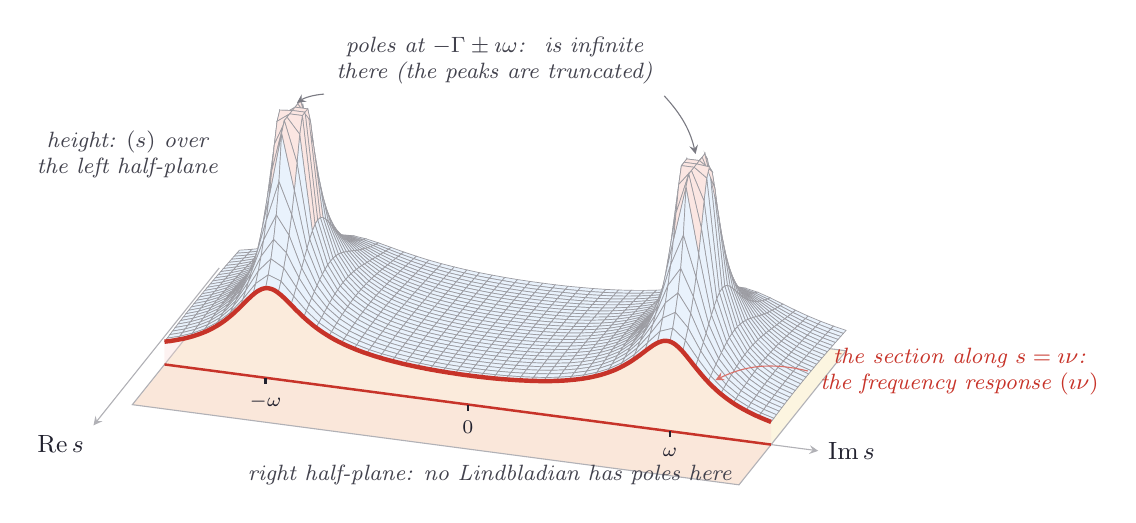
\begin{tikzpicture}[ink/.style={line width=0.9pt, ndInk}, faint/.style={line width=0.4pt, ndInk!35}, dashedink/.style={line width=0.5pt, ndInk!55, dash pattern=on 2.5pt off 2pt}, vec/.style={->, >=stealth, line width=1.2pt}, note/.style={font=\footnotesize\itshape, text=ndInk!85, align=center}, pointer/.style={->, >=stealth, line width=0.4pt, ndInk!60, shorten >=2pt, shorten <=1pt}, dot/.style={circle, fill=ndInk, inner sep=0pt, minimum size=3.4pt}, wash/.style={fill=ndSky, fill opacity=0.55}, every node/.style={text=ndInk}]
\definecolor{ndInk}{rgb}{0.13,0.13,0.18}
\definecolor{ndPaper}{rgb}{0.99,0.96,0.88}
\definecolor{ndSky}{rgb}{0.84,0.91,0.98}
\definecolor{ndRose}{rgb}{0.98,0.86,0.84}
\definecolor{ndBlue}{rgb}{0.13,0.36,0.66}
\definecolor{ndRed}{rgb}{0.78,0.20,0.16}
\definecolor{ndGold}{rgb}{0.88,0.62,0.10}
\definecolor{ndGreen}{rgb}{0.18,0.52,0.30}
\fill[ndPaper] (-2.900,1.700) -- (-4.260,-0.002) -- (3.444,-1.020) -- (4.804,0.682) -- cycle;
\fill[ndRose, fill opacity=0.5] (-3.852,0.509) -- (-4.260,-0.002) -- (3.444,-1.020) -- (3.852,-0.509) -- cycle;
\draw[faint] (-2.900,1.700) -- (-4.260,-0.002) -- (3.444,-1.020) -- (4.804,0.682) -- cycle;
\draw[faint, ->, >=stealth] (-3.157,1.734) -- (-4.754,-0.265) node[below left, text=ndInk, font=\small] {$\mathrm{Re}\,s$};
\node[note, anchor=north] at (0.277,-0.651) {right half-plane: no Lindbladian has poles here};
\filldraw[fill=ndSky!55, draw=ndInk!45, line width=0.25pt] (-2.900,1.960) -- (-2.934,1.921) -- (-2.774,1.934) -- (-2.740,1.971) -- cycle;
\filldraw[fill=ndSky!55, draw=ndInk!45, line width=0.25pt] (-2.740,1.971) -- (-2.774,1.934) -- (-2.613,1.954) -- (-2.579,1.989) -- cycle;
\filldraw[fill=ndSky!55, draw=ndInk!45, line width=0.25pt] (-2.934,1.921) -- (-2.968,1.883) -- (-2.807,1.897) -- (-2.774,1.934) -- cycle;
\filldraw[fill=ndSky!55, draw=ndInk!45, line width=0.25pt] (-2.579,1.989) -- (-2.613,1.954) -- (-2.453,1.982) -- (-2.419,2.014) -- cycle;
\filldraw[fill=ndSky!55, draw=ndInk!45, line width=0.25pt] (-2.774,1.934) -- (-2.807,1.897) -- (-2.647,1.919) -- (-2.613,1.954) -- cycle;
\filldraw[fill=ndSky!55, draw=ndInk!45, line width=0.25pt] (-2.968,1.883) -- (-3.002,1.844) -- (-2.841,1.860) -- (-2.807,1.897) -- cycle;
\filldraw[fill=ndSky!55, draw=ndInk!45, line width=0.25pt] (-2.419,2.014) -- (-2.453,1.982) -- (-2.292,2.017) -- (-2.258,2.045) -- cycle;
\filldraw[fill=ndSky!55, draw=ndInk!45, line width=0.25pt] (-2.613,1.954) -- (-2.647,1.919) -- (-2.487,1.950) -- (-2.453,1.982) -- cycle;
\filldraw[fill=ndSky!55, draw=ndInk!45, line width=0.25pt] (-2.807,1.897) -- (-2.841,1.860) -- (-2.681,1.884) -- (-2.647,1.919) -- cycle;
\filldraw[fill=ndSky!55, draw=ndInk!45, line width=0.25pt] (-2.258,2.045) -- (-2.292,2.017) -- (-2.132,2.060) -- (-2.098,2.082) -- cycle;
\filldraw[fill=ndSky!55, draw=ndInk!45, line width=0.25pt] (-3.002,1.844) -- (-3.036,1.805) -- (-2.875,1.823) -- (-2.841,1.860) -- cycle;
\filldraw[fill=ndSky!55, draw=ndInk!45, line width=0.25pt] (-2.453,1.982) -- (-2.487,1.950) -- (-2.326,1.990) -- (-2.292,2.017) -- cycle;
\filldraw[fill=ndSky!55, draw=ndInk!45, line width=0.25pt] (-2.647,1.919) -- (-2.681,1.884) -- (-2.521,1.918) -- (-2.487,1.950) -- cycle;
\filldraw[fill=ndSky!55, draw=ndInk!45, line width=0.25pt] (-2.098,2.082) -- (-2.132,2.060) -- (-1.971,2.104) -- (-1.937,2.119) -- cycle;
\filldraw[fill=ndSky!55, draw=ndInk!45, line width=0.25pt] (-2.841,1.860) -- (-2.875,1.823) -- (-2.715,1.849) -- (-2.681,1.884) -- cycle;
\filldraw[fill=ndSky!55, draw=ndInk!45, line width=0.25pt] (-2.292,2.017) -- (-2.326,1.990) -- (-2.166,2.039) -- (-2.132,2.060) -- cycle;
\filldraw[fill=ndSky!55, draw=ndInk!45, line width=0.25pt] (-3.036,1.805) -- (-3.070,1.766) -- (-2.909,1.785) -- (-2.875,1.823) -- cycle;
\filldraw[fill=ndSky!55, draw=ndInk!45, line width=0.25pt] (-2.487,1.950) -- (-2.521,1.918) -- (-2.360,1.964) -- (-2.326,1.990) -- cycle;
\filldraw[fill=ndSky!55, draw=ndInk!45, line width=0.25pt] (-1.937,2.119) -- (-1.971,2.104) -- (-1.811,2.140) -- (-1.777,2.148) -- cycle;
\filldraw[fill=ndSky!55, draw=ndInk!45, line width=0.25pt] (-2.681,1.884) -- (-2.715,1.849) -- (-2.555,1.887) -- (-2.521,1.918) -- cycle;
\filldraw[fill=ndSky!55, draw=ndInk!45, line width=0.25pt] (-2.132,2.060) -- (-2.166,2.039) -- (-2.005,2.092) -- (-1.971,2.104) -- cycle;
\filldraw[fill=ndSky!55, draw=ndInk!45, line width=0.25pt] (-2.875,1.823) -- (-2.909,1.785) -- (-2.749,1.814) -- (-2.715,1.849) -- cycle;
\filldraw[fill=ndSky!55, draw=ndInk!45, line width=0.25pt] (-2.326,1.990) -- (-2.360,1.964) -- (-2.200,2.020) -- (-2.166,2.039) -- cycle;
\filldraw[fill=ndSky!55, draw=ndInk!45, line width=0.25pt] (-3.070,1.766) -- (-3.104,1.727) -- (-2.943,1.747) -- (-2.909,1.785) -- cycle;
\filldraw[fill=ndSky!55, draw=ndInk!45, line width=0.25pt] (-1.777,2.148) -- (-1.811,2.140) -- (-1.650,2.153) -- (-1.616,2.158) -- cycle;
\filldraw[fill=ndSky!55, draw=ndInk!45, line width=0.25pt] (-2.521,1.918) -- (-2.555,1.887) -- (-2.394,1.937) -- (-2.360,1.964) -- cycle;
\filldraw[fill=ndSky!55, draw=ndInk!45, line width=0.25pt] (-2.715,1.849) -- (-2.749,1.814) -- (-2.588,1.855) -- (-2.555,1.887) -- cycle;
\filldraw[fill=ndSky!55, draw=ndInk!45, line width=0.25pt] (-1.971,2.104) -- (-2.005,2.092) -- (-1.845,2.135) -- (-1.811,2.140) -- cycle;
\filldraw[fill=ndSky!55, draw=ndInk!45, line width=0.25pt] (-1.616,2.158) -- (-1.650,2.153) -- (-1.490,2.137) -- (-1.456,2.143) -- cycle;
\filldraw[fill=ndSky!55, draw=ndInk!45, line width=0.25pt] (-2.909,1.785) -- (-2.943,1.747) -- (-2.783,1.779) -- (-2.749,1.814) -- cycle;
\filldraw[fill=ndSky!55, draw=ndInk!45, line width=0.25pt] (-2.166,2.039) -- (-2.200,2.020) -- (-2.039,2.082) -- (-2.005,2.092) -- cycle;
\filldraw[fill=ndSky!55, draw=ndInk!45, line width=0.25pt] (-3.104,1.727) -- (-3.138,1.688) -- (-2.977,1.710) -- (-2.943,1.747) -- cycle;
\filldraw[fill=ndSky!55, draw=ndInk!45, line width=0.25pt] (-2.360,1.964) -- (-2.394,1.937) -- (-2.234,2.002) -- (-2.200,2.020) -- cycle;
\filldraw[fill=ndSky!55, draw=ndInk!45, line width=0.25pt] (-1.456,2.143) -- (-1.490,2.137) -- (-1.329,2.094) -- (-1.295,2.105) -- cycle;
\filldraw[fill=ndSky!55, draw=ndInk!45, line width=0.25pt] (-1.811,2.140) -- (-1.845,2.135) -- (-1.684,2.153) -- (-1.650,2.153) -- cycle;
\filldraw[fill=ndSky!55, draw=ndInk!45, line width=0.25pt] (-2.555,1.887) -- (-2.588,1.855) -- (-2.428,1.912) -- (-2.394,1.937) -- cycle;
\filldraw[fill=ndSky!55, draw=ndInk!45, line width=0.25pt] (-1.295,2.105) -- (-1.329,2.094) -- (-1.169,2.035) -- (-1.135,2.053) -- cycle;
\filldraw[fill=ndSky!55, draw=ndInk!45, line width=0.25pt] (-2.749,1.814) -- (-2.783,1.779) -- (-2.622,1.824) -- (-2.588,1.855) -- cycle;
\filldraw[fill=ndSky!55, draw=ndInk!45, line width=0.25pt] (-2.005,2.092) -- (-2.039,2.082) -- (-1.879,2.135) -- (-1.845,2.135) -- cycle;
\filldraw[fill=ndSky!55, draw=ndInk!45, line width=0.25pt] (-2.943,1.747) -- (-2.977,1.710) -- (-2.817,1.743) -- (-2.783,1.779) -- cycle;
\filldraw[fill=ndSky!55, draw=ndInk!45, line width=0.25pt] (-1.135,2.053) -- (-1.169,2.035) -- (-1.008,1.972) -- (-0.974,1.995) -- cycle;
\filldraw[fill=ndSky!55, draw=ndInk!45, line width=0.25pt] (-1.650,2.153) -- (-1.684,2.153) -- (-1.524,2.135) -- (-1.490,2.137) -- cycle;
\filldraw[fill=ndSky!55, draw=ndInk!45, line width=0.25pt] (-2.200,2.020) -- (-2.234,2.002) -- (-2.073,2.076) -- (-2.039,2.082) -- cycle;
\filldraw[fill=ndSky!55, draw=ndInk!45, line width=0.25pt] (-3.138,1.688) -- (-3.172,1.648) -- (-3.011,1.672) -- (-2.977,1.710) -- cycle;
\filldraw[fill=ndSky!55, draw=ndInk!45, line width=0.25pt] (-0.974,1.995) -- (-1.008,1.972) -- (-0.848,1.910) -- (-0.814,1.937) -- cycle;
\filldraw[fill=ndSky!55, draw=ndInk!45, line width=0.25pt] (-2.394,1.937) -- (-2.428,1.912) -- (-2.268,1.986) -- (-2.234,2.002) -- cycle;
\filldraw[fill=ndSky!55, draw=ndInk!45, line width=0.25pt] (-1.490,2.137) -- (-1.524,2.135) -- (-1.363,2.086) -- (-1.329,2.094) -- cycle;
\filldraw[fill=ndSky!55, draw=ndInk!45, line width=0.25pt] (-2.588,1.855) -- (-2.622,1.824) -- (-2.462,1.887) -- (-2.428,1.912) -- cycle;
\filldraw[fill=ndSky!55, draw=ndInk!45, line width=0.25pt] (-1.845,2.135) -- (-1.879,2.135) -- (-1.718,2.159) -- (-1.684,2.153) -- cycle;
\filldraw[fill=ndSky!55, draw=ndInk!45, line width=0.25pt] (-0.814,1.937) -- (-0.848,1.910) -- (-0.687,1.852) -- (-0.653,1.883) -- cycle;
\filldraw[fill=ndSky!55, draw=ndInk!45, line width=0.25pt] (-2.783,1.779) -- (-2.817,1.743) -- (-2.656,1.792) -- (-2.622,1.824) -- cycle;
\filldraw[fill=ndSky!55, draw=ndInk!45, line width=0.25pt] (-1.329,2.094) -- (-1.363,2.086) -- (-1.203,2.019) -- (-1.169,2.035) -- cycle;
\filldraw[fill=ndSky!55, draw=ndInk!45, line width=0.25pt] (-2.977,1.710) -- (-3.011,1.672) -- (-2.851,1.707) -- (-2.817,1.743) -- cycle;
\filldraw[fill=ndSky!55, draw=ndInk!45, line width=0.25pt] (-0.653,1.883) -- (-0.687,1.852) -- (-0.527,1.800) -- (-0.493,1.833) -- cycle;
\filldraw[fill=ndSky!55, draw=ndInk!45, line width=0.25pt] (-2.039,2.082) -- (-2.073,2.076) -- (-1.913,2.141) -- (-1.879,2.135) -- cycle;
\filldraw[fill=ndSky!55, draw=ndInk!45, line width=0.25pt] (-1.169,2.035) -- (-1.203,2.019) -- (-1.042,1.949) -- (-1.008,1.972) -- cycle;
\filldraw[fill=ndSky!55, draw=ndInk!45, line width=0.25pt] (-1.684,2.153) -- (-1.718,2.159) -- (-1.558,2.138) -- (-1.524,2.135) -- cycle;
\filldraw[fill=ndSky!55, draw=ndInk!45, line width=0.25pt] (-3.172,1.648) -- (-3.206,1.609) -- (-3.045,1.633) -- (-3.011,1.672) -- cycle;
\filldraw[fill=ndSky!55, draw=ndInk!45, line width=0.25pt] (-2.234,2.002) -- (-2.268,1.986) -- (-2.107,2.073) -- (-2.073,2.076) -- cycle;
\filldraw[fill=ndSky!55, draw=ndInk!45, line width=0.25pt] (-0.493,1.833) -- (-0.527,1.800) -- (-0.366,1.752) -- (-0.332,1.788) -- cycle;
\filldraw[fill=ndSky!55, draw=ndInk!45, line width=0.25pt] (-1.008,1.972) -- (-1.042,1.949) -- (-0.882,1.882) -- (-0.848,1.910) -- cycle;
\filldraw[fill=ndSky!55, draw=ndInk!45, line width=0.25pt] (-2.428,1.912) -- (-2.462,1.887) -- (-2.302,1.971) -- (-2.268,1.986) -- cycle;
\filldraw[fill=ndSky!55, draw=ndInk!45, line width=0.25pt] (-2.622,1.824) -- (-2.656,1.792) -- (-2.496,1.862) -- (-2.462,1.887) -- cycle;
\filldraw[fill=ndSky!55, draw=ndInk!45, line width=0.25pt] (-1.524,2.135) -- (-1.558,2.138) -- (-1.397,2.081) -- (-1.363,2.086) -- cycle;
\filldraw[fill=ndSky!55, draw=ndInk!45, line width=0.25pt] (-0.848,1.910) -- (-0.882,1.882) -- (-0.721,1.821) -- (-0.687,1.852) -- cycle;
\filldraw[fill=ndSky!55, draw=ndInk!45, line width=0.25pt] (-0.332,1.788) -- (-0.366,1.752) -- (-0.206,1.710) -- (-0.172,1.747) -- cycle;
\filldraw[fill=ndSky!55, draw=ndInk!45, line width=0.25pt] (-2.817,1.743) -- (-2.851,1.707) -- (-2.690,1.760) -- (-2.656,1.792) -- cycle;
\filldraw[fill=ndSky!55, draw=ndInk!45, line width=0.25pt] (-1.879,2.135) -- (-1.913,2.141) -- (-1.752,2.171) -- (-1.718,2.159) -- cycle;
\filldraw[fill=ndSky!55, draw=ndInk!45, line width=0.25pt] (-1.363,2.086) -- (-1.397,2.081) -- (-1.237,2.005) -- (-1.203,2.019) -- cycle;
\filldraw[fill=ndSky!55, draw=ndInk!45, line width=0.25pt] (-3.011,1.672) -- (-3.045,1.633) -- (-2.885,1.671) -- (-2.851,1.707) -- cycle;
\filldraw[fill=ndSky!55, draw=ndInk!45, line width=0.25pt] (-0.687,1.852) -- (-0.721,1.821) -- (-0.561,1.766) -- (-0.527,1.800) -- cycle;
\filldraw[fill=ndSky!55, draw=ndInk!45, line width=0.25pt] (-0.172,1.747) -- (-0.206,1.710) -- (-0.045,1.671) -- (-0.011,1.709) -- cycle;
\filldraw[fill=ndSky!55, draw=ndInk!45, line width=0.25pt] (-1.203,2.019) -- (-1.237,2.005) -- (-1.076,1.927) -- (-1.042,1.949) -- cycle;
\filldraw[fill=ndSky!55, draw=ndInk!45, line width=0.25pt] (-2.073,2.076) -- (-2.107,2.073) -- (-1.947,2.153) -- (-1.913,2.141) -- cycle;
\filldraw[fill=ndSky!55, draw=ndInk!45, line width=0.25pt] (-3.206,1.609) -- (-3.240,1.569) -- (-3.079,1.595) -- (-3.045,1.633) -- cycle;
\filldraw[fill=ndSky!55, draw=ndInk!45, line width=0.25pt] (-0.527,1.800) -- (-0.561,1.766) -- (-0.400,1.717) -- (-0.366,1.752) -- cycle;
\filldraw[fill=ndSky!55, draw=ndInk!45, line width=0.25pt] (-1.718,2.159) -- (-1.752,2.171) -- (-1.592,2.147) -- (-1.558,2.138) -- cycle;
\filldraw[fill=ndSky!55, draw=ndInk!45, line width=0.25pt] (-2.268,1.986) -- (-2.302,1.971) -- (-2.141,2.074) -- (-2.107,2.073) -- cycle;
\filldraw[fill=ndSky!55, draw=ndInk!45, line width=0.25pt] (-1.042,1.949) -- (-1.076,1.927) -- (-0.916,1.855) -- (-0.882,1.882) -- cycle;
\filldraw[fill=ndSky!55, draw=ndInk!45, line width=0.25pt] (-2.462,1.887) -- (-2.496,1.862) -- (-2.335,1.958) -- (-2.302,1.971) -- cycle;
\filldraw[fill=ndSky!55, draw=ndInk!45, line width=0.25pt] (-0.011,1.709) -- (-0.045,1.671) -- (0.115,1.636) -- (0.149,1.674) -- cycle;
\filldraw[fill=ndSky!55, draw=ndInk!45, line width=0.25pt] (-2.656,1.792) -- (-2.690,1.760) -- (-2.530,1.837) -- (-2.496,1.862) -- cycle;
\filldraw[fill=ndSky!55, draw=ndInk!45, line width=0.25pt] (-0.882,1.882) -- (-0.916,1.855) -- (-0.755,1.790) -- (-0.721,1.821) -- cycle;
\filldraw[fill=ndSky!55, draw=ndInk!45, line width=0.25pt] (-0.366,1.752) -- (-0.400,1.717) -- (-0.240,1.673) -- (-0.206,1.710) -- cycle;
\filldraw[fill=ndSky!55, draw=ndInk!45, line width=0.25pt] (-2.851,1.707) -- (-2.885,1.671) -- (-2.724,1.728) -- (-2.690,1.760) -- cycle;
\filldraw[fill=ndSky!55, draw=ndInk!45, line width=0.25pt] (-1.558,2.138) -- (-1.592,2.147) -- (-1.431,2.079) -- (-1.397,2.081) -- cycle;
\filldraw[fill=ndSky!55, draw=ndInk!45, line width=0.25pt] (0.149,1.674) -- (0.115,1.636) -- (0.276,1.604) -- (0.310,1.643) -- cycle;
\filldraw[fill=ndSky!55, draw=ndInk!45, line width=0.25pt] (-3.045,1.633) -- (-3.079,1.595) -- (-2.919,1.635) -- (-2.885,1.671) -- cycle;
\filldraw[fill=ndSky!55, draw=ndInk!45, line width=0.25pt] (-0.721,1.821) -- (-0.755,1.790) -- (-0.595,1.732) -- (-0.561,1.766) -- cycle;
\filldraw[fill=ndSky!55, draw=ndInk!45, line width=0.25pt] (-1.913,2.141) -- (-1.947,2.153) -- (-1.786,2.191) -- (-1.752,2.171) -- cycle;
\filldraw[fill=ndSky!55, draw=ndInk!45, line width=0.25pt] (-1.397,2.081) -- (-1.431,2.079) -- (-1.271,1.993) -- (-1.237,2.005) -- cycle;
\filldraw[fill=ndSky!55, draw=ndInk!45, line width=0.25pt] (-0.206,1.710) -- (-0.240,1.673) -- (-0.079,1.634) -- (-0.045,1.671) -- cycle;
\filldraw[fill=ndSky!55, draw=ndInk!45, line width=0.25pt] (-3.240,1.569) -- (-3.274,1.529) -- (-3.113,1.556) -- (-3.079,1.595) -- cycle;
\filldraw[fill=ndSky!55, draw=ndInk!45, line width=0.25pt] (-1.237,2.005) -- (-1.271,1.993) -- (-1.110,1.906) -- (-1.076,1.927) -- cycle;
\filldraw[fill=ndSky!55, draw=ndInk!45, line width=0.25pt] (-0.561,1.766) -- (-0.595,1.732) -- (-0.434,1.681) -- (-0.400,1.717) -- cycle;
\filldraw[fill=ndSky!55, draw=ndInk!45, line width=0.25pt] (0.310,1.643) -- (0.276,1.604) -- (0.436,1.575) -- (0.470,1.614) -- cycle;
\filldraw[fill=ndSky!55, draw=ndInk!45, line width=0.25pt] (-2.107,2.073) -- (-2.141,2.074) -- (-1.981,2.173) -- (-1.947,2.153) -- cycle;
\filldraw[fill=ndSky!55, draw=ndInk!45, line width=0.25pt] (-1.076,1.927) -- (-1.110,1.906) -- (-0.950,1.827) -- (-0.916,1.855) -- cycle;
\filldraw[fill=ndSky!55, draw=ndInk!45, line width=0.25pt] (-0.045,1.671) -- (-0.079,1.634) -- (0.081,1.598) -- (0.115,1.636) -- cycle;
\filldraw[fill=ndSky!55, draw=ndInk!45, line width=0.25pt] (-2.302,1.971) -- (-2.335,1.958) -- (-2.175,2.080) -- (-2.141,2.074) -- cycle;
\filldraw[fill=ndSky!55, draw=ndInk!45, line width=0.25pt] (-2.496,1.862) -- (-2.530,1.837) -- (-2.369,1.946) -- (-2.335,1.958) -- cycle;
\filldraw[fill=ndSky!55, draw=ndInk!45, line width=0.25pt] (-1.752,2.171) -- (-1.786,2.191) -- (-1.626,2.163) -- (-1.592,2.147) -- cycle;
\filldraw[fill=ndSky!55, draw=ndInk!45, line width=0.25pt] (-2.690,1.760) -- (-2.724,1.728) -- (-2.564,1.812) -- (-2.530,1.837) -- cycle;
\filldraw[fill=ndSky!55, draw=ndInk!45, line width=0.25pt] (-0.400,1.717) -- (-0.434,1.681) -- (-0.274,1.636) -- (-0.240,1.673) -- cycle;
\filldraw[fill=ndSky!55, draw=ndInk!45, line width=0.25pt] (-0.916,1.855) -- (-0.950,1.827) -- (-0.789,1.758) -- (-0.755,1.790) -- cycle;
\filldraw[fill=ndSky!55, draw=ndInk!45, line width=0.25pt] (-2.885,1.671) -- (-2.919,1.635) -- (-2.758,1.695) -- (-2.724,1.728) -- cycle;
\filldraw[fill=ndSky!55, draw=ndInk!45, line width=0.25pt] (0.470,1.614) -- (0.436,1.575) -- (0.597,1.548) -- (0.631,1.587) -- cycle;
\filldraw[fill=ndSky!55, draw=ndInk!45, line width=0.25pt] (0.115,1.636) -- (0.081,1.598) -- (0.242,1.565) -- (0.276,1.604) -- cycle;
\filldraw[fill=ndSky!55, draw=ndInk!45, line width=0.25pt] (-3.079,1.595) -- (-3.113,1.556) -- (-2.953,1.598) -- (-2.919,1.635) -- cycle;
\filldraw[fill=ndSky!55, draw=ndInk!45, line width=0.25pt] (-1.592,2.147) -- (-1.626,2.163) -- (-1.465,2.082) -- (-1.431,2.079) -- cycle;
\filldraw[fill=ndSky!55, draw=ndInk!45, line width=0.25pt] (-0.755,1.790) -- (-0.789,1.758) -- (-0.629,1.698) -- (-0.595,1.732) -- cycle;
\filldraw[fill=ndSky!55, draw=ndInk!45, line width=0.25pt] (-0.240,1.673) -- (-0.274,1.636) -- (-0.113,1.596) -- (-0.079,1.634) -- cycle;
\filldraw[fill=ndSky!55, draw=ndInk!45, line width=0.25pt] (-1.431,2.079) -- (-1.465,2.082) -- (-1.305,1.982) -- (-1.271,1.993) -- cycle;
\filldraw[fill=ndSky!55, draw=ndInk!45, line width=0.25pt] (-3.274,1.529) -- (-3.308,1.488) -- (-3.147,1.516) -- (-3.113,1.556) -- cycle;
\filldraw[fill=ndSky!55, draw=ndInk!45, line width=0.25pt] (-1.947,2.153) -- (-1.981,2.173) -- (-1.820,2.222) -- (-1.786,2.191) -- cycle;
\filldraw[fill=ndSky!55, draw=ndInk!45, line width=0.25pt] (0.631,1.587) -- (0.597,1.548) -- (0.757,1.524) -- (0.791,1.563) -- cycle;
\filldraw[fill=ndSky!55, draw=ndInk!45, line width=0.25pt] (-1.271,1.993) -- (-1.305,1.982) -- (-1.144,1.886) -- (-1.110,1.906) -- cycle;
\filldraw[fill=ndSky!55, draw=ndInk!45, line width=0.25pt] (-0.595,1.732) -- (-0.629,1.698) -- (-0.468,1.645) -- (-0.434,1.681) -- cycle;
\filldraw[fill=ndSky!55, draw=ndInk!45, line width=0.25pt] (0.276,1.604) -- (0.242,1.565) -- (0.402,1.536) -- (0.436,1.575) -- cycle;
\filldraw[fill=ndSky!55, draw=ndInk!45, line width=0.25pt] (-0.079,1.634) -- (-0.113,1.596) -- (0.047,1.559) -- (0.081,1.598) -- cycle;
\filldraw[fill=ndSky!55, draw=ndInk!45, line width=0.25pt] (-1.110,1.906) -- (-1.144,1.886) -- (-0.984,1.800) -- (-0.950,1.827) -- cycle;
\filldraw[fill=ndSky!55, draw=ndInk!45, line width=0.25pt] (-2.141,2.074) -- (-2.175,2.080) -- (-2.015,2.203) -- (-1.981,2.173) -- cycle;
\filldraw[fill=ndSky!55, draw=ndInk!45, line width=0.25pt] (-2.530,1.837) -- (-2.564,1.812) -- (-2.403,1.934) -- (-2.369,1.946) -- cycle;
\filldraw[fill=ndSky!55, draw=ndInk!45, line width=0.25pt] (-2.724,1.728) -- (-2.758,1.695) -- (-2.598,1.786) -- (-2.564,1.812) -- cycle;
\filldraw[fill=ndSky!55, draw=ndInk!45, line width=0.25pt] (-2.335,1.958) -- (-2.369,1.946) -- (-2.209,2.090) -- (-2.175,2.080) -- cycle;
\filldraw[fill=ndSky!55, draw=ndInk!45, line width=0.25pt] (-0.434,1.681) -- (-0.468,1.645) -- (-0.308,1.599) -- (-0.274,1.636) -- cycle;
\filldraw[fill=ndSky!55, draw=ndInk!45, line width=0.25pt] (-0.950,1.827) -- (-0.984,1.800) -- (-0.823,1.727) -- (-0.789,1.758) -- cycle;
\filldraw[fill=ndSky!55, draw=ndInk!45, line width=0.25pt] (-2.919,1.635) -- (-2.953,1.598) -- (-2.792,1.662) -- (-2.758,1.695) -- cycle;
\filldraw[fill=ndSky!55, draw=ndInk!45, line width=0.25pt] (0.791,1.563) -- (0.757,1.524) -- (0.918,1.501) -- (0.952,1.541) -- cycle;
\filldraw[fill=ndSky!55, draw=ndInk!45, line width=0.25pt] (0.436,1.575) -- (0.402,1.536) -- (0.563,1.509) -- (0.597,1.548) -- cycle;
\filldraw[fill=ndSky!55, draw=ndInk!45, line width=0.25pt] (-1.786,2.191) -- (-1.820,2.222) -- (-1.660,2.187) -- (-1.626,2.163) -- cycle;
\filldraw[fill=ndSky!55, draw=ndInk!45, line width=0.25pt] (0.081,1.598) -- (0.047,1.559) -- (0.208,1.526) -- (0.242,1.565) -- cycle;
\filldraw[fill=ndSky!55, draw=ndInk!45, line width=0.25pt] (-3.113,1.556) -- (-3.147,1.516) -- (-2.987,1.560) -- (-2.953,1.598) -- cycle;
\filldraw[fill=ndSky!55, draw=ndInk!45, line width=0.25pt] (-0.789,1.758) -- (-0.823,1.727) -- (-0.663,1.664) -- (-0.629,1.698) -- cycle;
\filldraw[fill=ndSky!55, draw=ndInk!45, line width=0.25pt] (-0.274,1.636) -- (-0.308,1.599) -- (-0.147,1.558) -- (-0.113,1.596) -- cycle;
\filldraw[fill=ndSky!55, draw=ndInk!45, line width=0.25pt] (-3.308,1.488) -- (-3.342,1.448) -- (-3.181,1.477) -- (-3.147,1.516) -- cycle;
\filldraw[fill=ndSky!55, draw=ndInk!45, line width=0.25pt] (-1.626,2.163) -- (-1.660,2.187) -- (-1.499,2.089) -- (-1.465,2.082) -- cycle;
\filldraw[fill=ndSky!55, draw=ndInk!45, line width=0.25pt] (0.952,1.541) -- (0.918,1.501) -- (1.078,1.481) -- (1.112,1.520) -- cycle;
\filldraw[fill=ndSky!55, draw=ndInk!45, line width=0.25pt] (0.597,1.548) -- (0.563,1.509) -- (0.723,1.484) -- (0.757,1.524) -- cycle;
\filldraw[fill=ndSky!55, draw=ndInk!45, line width=0.25pt] (-1.465,2.082) -- (-1.499,2.089) -- (-1.339,1.973) -- (-1.305,1.982) -- cycle;
\filldraw[fill=ndSky!55, draw=ndInk!45, line width=0.25pt] (-0.629,1.698) -- (-0.663,1.664) -- (-0.502,1.609) -- (-0.468,1.645) -- cycle;
\filldraw[fill=ndSky!55, draw=ndInk!45, line width=0.25pt] (0.242,1.565) -- (0.208,1.526) -- (0.368,1.496) -- (0.402,1.536) -- cycle;
\filldraw[fill=ndSky!55, draw=ndInk!45, line width=0.25pt] (-1.305,1.982) -- (-1.339,1.973) -- (-1.178,1.866) -- (-1.144,1.886) -- cycle;
\filldraw[fill=ndSky!55, draw=ndInk!45, line width=0.25pt] (-0.113,1.596) -- (-0.147,1.558) -- (0.013,1.521) -- (0.047,1.559) -- cycle;
\filldraw[fill=ndSky!55, draw=ndInk!45, line width=0.25pt] (-1.144,1.886) -- (-1.178,1.866) -- (-1.018,1.773) -- (-0.984,1.800) -- cycle;
\filldraw[fill=ndSky!55, draw=ndInk!45, line width=0.25pt] (-1.981,2.173) -- (-2.015,2.203) -- (-1.854,2.267) -- (-1.820,2.222) -- cycle;
\filldraw[fill=ndSky!55, draw=ndInk!45, line width=0.25pt] (-2.758,1.695) -- (-2.792,1.662) -- (-2.632,1.760) -- (-2.598,1.786) -- cycle;
\filldraw[fill=ndSky!55, draw=ndInk!45, line width=0.25pt] (-0.468,1.645) -- (-0.502,1.609) -- (-0.342,1.562) -- (-0.308,1.599) -- cycle;
\filldraw[fill=ndSky!55, draw=ndInk!45, line width=0.25pt] (-2.564,1.812) -- (-2.598,1.786) -- (-2.437,1.924) -- (-2.403,1.934) -- cycle;
\filldraw[fill=ndSky!55, draw=ndInk!45, line width=0.25pt] (1.112,1.520) -- (1.078,1.481) -- (1.239,1.463) -- (1.273,1.502) -- cycle;
\filldraw[fill=ndSky!55, draw=ndInk!45, line width=0.25pt] (-2.953,1.598) -- (-2.987,1.560) -- (-2.826,1.627) -- (-2.792,1.662) -- cycle;
\filldraw[fill=ndSky!55, draw=ndInk!45, line width=0.25pt] (0.757,1.524) -- (0.723,1.484) -- (0.884,1.462) -- (0.918,1.501) -- cycle;
\filldraw[fill=ndSky!55, draw=ndInk!45, line width=0.25pt] (-0.984,1.800) -- (-1.018,1.773) -- (-0.857,1.695) -- (-0.823,1.727) -- cycle;
\filldraw[fill=ndSky!55, draw=ndInk!45, line width=0.25pt] (0.402,1.536) -- (0.368,1.496) -- (0.529,1.469) -- (0.563,1.509) -- cycle;
\filldraw[fill=ndSky!55, draw=ndInk!45, line width=0.25pt] (-2.369,1.946) -- (-2.403,1.934) -- (-2.243,2.105) -- (-2.209,2.090) -- cycle;
\filldraw[fill=ndSky!55, draw=ndInk!45, line width=0.25pt] (-2.175,2.080) -- (-2.209,2.090) -- (-2.049,2.245) -- (-2.015,2.203) -- cycle;
\filldraw[fill=ndSky!55, draw=ndInk!45, line width=0.25pt] (0.047,1.559) -- (0.013,1.521) -- (0.174,1.487) -- (0.208,1.526) -- cycle;
\filldraw[fill=ndSky!55, draw=ndInk!45, line width=0.25pt] (-3.147,1.516) -- (-3.181,1.477) -- (-3.021,1.522) -- (-2.987,1.560) -- cycle;
\filldraw[fill=ndSky!55, draw=ndInk!45, line width=0.25pt] (-0.823,1.727) -- (-0.857,1.695) -- (-0.697,1.629) -- (-0.663,1.664) -- cycle;
\filldraw[fill=ndSky!55, draw=ndInk!45, line width=0.25pt] (-0.308,1.599) -- (-0.342,1.562) -- (-0.181,1.519) -- (-0.147,1.558) -- cycle;
\filldraw[fill=ndSky!55, draw=ndInk!45, line width=0.25pt] (-3.342,1.448) -- (-3.376,1.406) -- (-3.215,1.436) -- (-3.181,1.477) -- cycle;
\filldraw[fill=ndSky!55, draw=ndInk!45, line width=0.25pt] (-1.820,2.222) -- (-1.854,2.267) -- (-1.694,2.222) -- (-1.660,2.187) -- cycle;
\filldraw[fill=ndSky!55, draw=ndInk!45, line width=0.25pt] (0.918,1.501) -- (0.884,1.462) -- (1.044,1.442) -- (1.078,1.481) -- cycle;
\filldraw[fill=ndSky!55, draw=ndInk!45, line width=0.25pt] (1.273,1.502) -- (1.239,1.463) -- (1.399,1.448) -- (1.433,1.487) -- cycle;
\filldraw[fill=ndSky!55, draw=ndInk!45, line width=0.25pt] (0.563,1.509) -- (0.529,1.469) -- (0.689,1.444) -- (0.723,1.484) -- cycle;
\filldraw[fill=ndSky!55, draw=ndInk!45, line width=0.25pt] (0.208,1.526) -- (0.174,1.487) -- (0.334,1.457) -- (0.368,1.496) -- cycle;
\filldraw[fill=ndSky!55, draw=ndInk!45, line width=0.25pt] (-0.663,1.664) -- (-0.697,1.629) -- (-0.536,1.573) -- (-0.502,1.609) -- cycle;
\filldraw[fill=ndSky!55, draw=ndInk!45, line width=0.25pt] (-1.660,2.187) -- (-1.694,2.222) -- (-1.533,2.101) -- (-1.499,2.089) -- cycle;
\filldraw[fill=ndSky!55, draw=ndInk!45, line width=0.25pt] (-0.147,1.558) -- (-0.181,1.519) -- (-0.021,1.482) -- (0.013,1.521) -- cycle;
\filldraw[fill=ndSky!55, draw=ndInk!45, line width=0.25pt] (-1.499,2.089) -- (-1.533,2.101) -- (-1.373,1.966) -- (-1.339,1.973) -- cycle;
\filldraw[fill=ndSky!55, draw=ndInk!45, line width=0.25pt] (-1.339,1.973) -- (-1.373,1.966) -- (-1.212,1.846) -- (-1.178,1.866) -- cycle;
\filldraw[fill=ndSky!55, draw=ndInk!45, line width=0.25pt] (-1.178,1.866) -- (-1.212,1.846) -- (-1.052,1.746) -- (-1.018,1.773) -- cycle;
\filldraw[fill=ndSky!55, draw=ndInk!45, line width=0.25pt] (-0.502,1.609) -- (-0.536,1.573) -- (-0.376,1.524) -- (-0.342,1.562) -- cycle;
\filldraw[fill=ndSky!55, draw=ndInk!45, line width=0.25pt] (-2.792,1.662) -- (-2.826,1.627) -- (-2.666,1.733) -- (-2.632,1.760) -- cycle;
\filldraw[fill=ndSky!55, draw=ndInk!45, line width=0.25pt] (1.078,1.481) -- (1.044,1.442) -- (1.205,1.424) -- (1.239,1.463) -- cycle;
\filldraw[fill=ndSky!55, draw=ndInk!45, line width=0.25pt] (0.723,1.484) -- (0.689,1.444) -- (0.850,1.422) -- (0.884,1.462) -- cycle;
\filldraw[fill=ndSky!55, draw=ndInk!45, line width=0.25pt] (-2.987,1.560) -- (-3.021,1.522) -- (-2.860,1.592) -- (-2.826,1.627) -- cycle;
\filldraw[fill=ndSky!55, draw=ndInk!45, line width=0.25pt] (1.433,1.487) -- (1.399,1.448) -- (1.560,1.434) -- (1.594,1.473) -- cycle;
\filldraw[fill=ndSky!55, draw=ndInk!45, line width=0.25pt] (0.368,1.496) -- (0.334,1.457) -- (0.495,1.429) -- (0.529,1.469) -- cycle;
\filldraw[fill=ndSky!55, draw=ndInk!45, line width=0.25pt] (-1.018,1.773) -- (-1.052,1.746) -- (-0.891,1.663) -- (-0.857,1.695) -- cycle;
\filldraw[fill=ndSky!55, draw=ndInk!45, line width=0.25pt] (-2.598,1.786) -- (-2.632,1.760) -- (-2.471,1.913) -- (-2.437,1.924) -- cycle;
\filldraw[fill=ndSky!55, draw=ndInk!45, line width=0.25pt] (0.013,1.521) -- (-0.021,1.482) -- (0.140,1.448) -- (0.174,1.487) -- cycle;
\filldraw[fill=ndSky!55, draw=ndInk!45, line width=0.25pt] (-3.181,1.477) -- (-3.215,1.436) -- (-3.055,1.483) -- (-3.021,1.522) -- cycle;
\filldraw[fill=ndSky!55, draw=ndInk!45, line width=0.25pt] (-2.015,2.203) -- (-2.049,2.245) -- (-1.888,2.328) -- (-1.854,2.267) -- cycle;
\filldraw[fill=ndSky!55, draw=ndInk!45, line width=0.25pt] (-2.403,1.934) -- (-2.437,1.924) -- (-2.277,2.126) -- (-2.243,2.105) -- cycle;
\filldraw[fill=ndSky!55, draw=ndInk!45, line width=0.25pt] (-0.857,1.695) -- (-0.891,1.663) -- (-0.731,1.595) -- (-0.697,1.629) -- cycle;
\filldraw[fill=ndSky!55, draw=ndInk!45, line width=0.25pt] (-0.342,1.562) -- (-0.376,1.524) -- (-0.215,1.481) -- (-0.181,1.519) -- cycle;
\filldraw[fill=ndSky!55, draw=ndInk!45, line width=0.25pt] (-3.376,1.406) -- (-3.410,1.365) -- (-3.249,1.396) -- (-3.215,1.436) -- cycle;
\filldraw[fill=ndSky!55, draw=ndInk!45, line width=0.25pt] (-2.209,2.090) -- (-2.243,2.105) -- (-2.082,2.302) -- (-2.049,2.245) -- cycle;
\filldraw[fill=ndSky!55, draw=ndInk!45, line width=0.25pt] (0.884,1.462) -- (0.850,1.422) -- (1.010,1.402) -- (1.044,1.442) -- cycle;
\filldraw[fill=ndSky!55, draw=ndInk!45, line width=0.25pt] (1.239,1.463) -- (1.205,1.424) -- (1.365,1.408) -- (1.399,1.448) -- cycle;
\filldraw[fill=ndSky!55, draw=ndInk!45, line width=0.25pt] (0.529,1.469) -- (0.495,1.429) -- (0.655,1.405) -- (0.689,1.444) -- cycle;
\filldraw[fill=ndSky!55, draw=ndInk!45, line width=0.25pt] (1.594,1.473) -- (1.560,1.434) -- (1.720,1.424) -- (1.754,1.462) -- cycle;
\filldraw[fill=ndSky!55, draw=ndInk!45, line width=0.25pt] (0.174,1.487) -- (0.140,1.448) -- (0.300,1.417) -- (0.334,1.457) -- cycle;
\filldraw[fill=ndSky!55, draw=ndInk!45, line width=0.25pt] (-0.697,1.629) -- (-0.731,1.595) -- (-0.570,1.536) -- (-0.536,1.573) -- cycle;
\filldraw[fill=ndSky!55, draw=ndInk!45, line width=0.25pt] (-0.181,1.519) -- (-0.215,1.481) -- (-0.055,1.443) -- (-0.021,1.482) -- cycle;
\filldraw[fill=ndSky!55, draw=ndInk!45, line width=0.25pt] (-1.854,2.267) -- (-1.888,2.328) -- (-1.728,2.269) -- (-1.694,2.222) -- cycle;
\filldraw[fill=ndSky!55, draw=ndInk!45, line width=0.25pt] (-1.373,1.966) -- (-1.407,1.960) -- (-1.246,1.826) -- (-1.212,1.846) -- cycle;
\filldraw[fill=ndSky!55, draw=ndInk!45, line width=0.25pt] (-1.533,2.101) -- (-1.567,2.119) -- (-1.407,1.960) -- (-1.373,1.966) -- cycle;
\filldraw[fill=ndSky!55, draw=ndInk!45, line width=0.25pt] (-1.212,1.846) -- (-1.246,1.826) -- (-1.086,1.718) -- (-1.052,1.746) -- cycle;
\filldraw[fill=ndSky!55, draw=ndInk!45, line width=0.25pt] (-0.536,1.573) -- (-0.570,1.536) -- (-0.410,1.486) -- (-0.376,1.524) -- cycle;
\filldraw[fill=ndSky!55, draw=ndInk!45, line width=0.25pt] (-1.694,2.222) -- (-1.728,2.269) -- (-1.567,2.119) -- (-1.533,2.101) -- cycle;
\filldraw[fill=ndSky!55, draw=ndInk!45, line width=0.25pt] (1.044,1.442) -- (1.010,1.402) -- (1.171,1.384) -- (1.205,1.424) -- cycle;
\filldraw[fill=ndSky!55, draw=ndInk!45, line width=0.25pt] (0.689,1.444) -- (0.655,1.405) -- (0.816,1.382) -- (0.850,1.422) -- cycle;
\filldraw[fill=ndSky!55, draw=ndInk!45, line width=0.25pt] (-2.826,1.627) -- (-2.860,1.592) -- (-2.700,1.704) -- (-2.666,1.733) -- cycle;
\filldraw[fill=ndSky!55, draw=ndInk!45, line width=0.25pt] (-3.021,1.522) -- (-3.055,1.483) -- (-2.894,1.556) -- (-2.860,1.592) -- cycle;
\filldraw[fill=ndSky!55, draw=ndInk!45, line width=0.25pt] (1.399,1.448) -- (1.365,1.408) -- (1.526,1.396) -- (1.560,1.434) -- cycle;
\filldraw[fill=ndSky!55, draw=ndInk!45, line width=0.25pt] (0.334,1.457) -- (0.300,1.417) -- (0.461,1.390) -- (0.495,1.429) -- cycle;
\filldraw[fill=ndSky!55, draw=ndInk!45, line width=0.25pt] (-1.052,1.746) -- (-1.086,1.718) -- (-0.925,1.631) -- (-0.891,1.663) -- cycle;
\filldraw[fill=ndSky!55, draw=ndInk!45, line width=0.25pt] (1.754,1.462) -- (1.720,1.424) -- (1.881,1.417) -- (1.915,1.454) -- cycle;
\filldraw[fill=ndSky!55, draw=ndInk!45, line width=0.25pt] (-0.021,1.482) -- (-0.055,1.443) -- (0.106,1.408) -- (0.140,1.448) -- cycle;
\filldraw[fill=ndSky!55, draw=ndInk!45, line width=0.25pt] (-3.215,1.436) -- (-3.249,1.396) -- (-3.089,1.443) -- (-3.055,1.483) -- cycle;
\filldraw[fill=ndSky!55, draw=ndInk!45, line width=0.25pt] (-2.632,1.760) -- (-2.666,1.733) -- (-2.505,1.902) -- (-2.471,1.913) -- cycle;
\filldraw[fill=ndSky!55, draw=ndInk!45, line width=0.25pt] (-0.376,1.524) -- (-0.410,1.486) -- (-0.249,1.442) -- (-0.215,1.481) -- cycle;
\filldraw[fill=ndSky!55, draw=ndInk!45, line width=0.25pt] (-0.891,1.663) -- (-0.925,1.631) -- (-0.765,1.559) -- (-0.731,1.595) -- cycle;
\filldraw[fill=ndSky!55, draw=ndInk!45, line width=0.25pt] (-3.410,1.365) -- (-3.444,1.323) -- (-3.283,1.354) -- (-3.249,1.396) -- cycle;
\filldraw[fill=ndSky!55, draw=ndInk!45, line width=0.25pt] (0.850,1.422) -- (0.816,1.382) -- (0.976,1.362) -- (1.010,1.402) -- cycle;
\filldraw[fill=ndSky!55, draw=ndInk!45, line width=0.25pt] (-2.437,1.924) -- (-2.471,1.913) -- (-2.311,2.151) -- (-2.277,2.126) -- cycle;
\filldraw[fill=ndSky!55, draw=ndInk!45, line width=0.25pt] (1.205,1.424) -- (1.171,1.384) -- (1.331,1.369) -- (1.365,1.408) -- cycle;
\filldraw[fill=ndSky!55, draw=ndInk!45, line width=0.25pt] (0.495,1.429) -- (0.461,1.390) -- (0.621,1.365) -- (0.655,1.405) -- cycle;
\filldraw[fill=ndSky!55, draw=ndInk!45, line width=0.25pt] (1.560,1.434) -- (1.526,1.396) -- (1.686,1.386) -- (1.720,1.424) -- cycle;
\filldraw[fill=ndSky!55, draw=ndInk!45, line width=0.25pt] (0.140,1.448) -- (0.106,1.408) -- (0.266,1.378) -- (0.300,1.417) -- cycle;
\filldraw[fill=ndSky!55, draw=ndInk!45, line width=0.25pt] (-0.731,1.595) -- (-0.765,1.559) -- (-0.604,1.499) -- (-0.570,1.536) -- cycle;
\filldraw[fill=ndSky!55, draw=ndInk!45, line width=0.25pt] (-2.049,2.245) -- (-2.082,2.302) -- (-1.922,2.413) -- (-1.888,2.328) -- cycle;
\filldraw[fill=ndSky!55, draw=ndInk!45, line width=0.25pt] (1.915,1.454) -- (1.881,1.417) -- (2.041,1.413) -- (2.075,1.450) -- cycle;
\filldraw[fill=ndSky!55, draw=ndInk!45, line width=0.25pt] (-0.215,1.481) -- (-0.249,1.442) -- (-0.089,1.403) -- (-0.055,1.443) -- cycle;
\filldraw[fill=ndSky!55, draw=ndInk!45, line width=0.25pt] (-2.243,2.105) -- (-2.277,2.126) -- (-2.116,2.377) -- (-2.082,2.302) -- cycle;
\filldraw[fill=ndSky!55, draw=ndInk!45, line width=0.25pt] (-0.570,1.536) -- (-0.604,1.499) -- (-0.444,1.448) -- (-0.410,1.486) -- cycle;
\filldraw[fill=ndSky!55, draw=ndInk!45, line width=0.25pt] (1.010,1.402) -- (0.976,1.362) -- (1.137,1.345) -- (1.171,1.384) -- cycle;
\filldraw[fill=ndSky!55, draw=ndInk!45, line width=0.25pt] (0.655,1.405) -- (0.621,1.365) -- (0.782,1.342) -- (0.816,1.382) -- cycle;
\filldraw[fill=ndSky!55, draw=ndInk!45, line width=0.25pt] (-1.407,1.960) -- (-1.441,1.956) -- (-1.280,1.806) -- (-1.246,1.826) -- cycle;
\filldraw[fill=ndSky!55, draw=ndInk!45, line width=0.25pt] (-1.246,1.826) -- (-1.280,1.806) -- (-1.120,1.690) -- (-1.086,1.718) -- cycle;
\filldraw[fill=ndSky!55, draw=ndInk!45, line width=0.25pt] (-3.055,1.483) -- (-3.089,1.443) -- (-2.928,1.519) -- (-2.894,1.556) -- cycle;
\filldraw[fill=ndSky!55, draw=ndInk!45, line width=0.25pt] (1.365,1.408) -- (1.331,1.369) -- (1.492,1.357) -- (1.526,1.396) -- cycle;
\filldraw[fill=ndSky!55, draw=ndInk!45, line width=0.25pt] (-2.860,1.592) -- (-2.894,1.556) -- (-2.734,1.673) -- (-2.700,1.704) -- cycle;
\filldraw[fill=ndSky!55, draw=ndInk!45, line width=0.25pt] (0.300,1.417) -- (0.266,1.378) -- (0.427,1.350) -- (0.461,1.390) -- cycle;
\filldraw[fill=ndSky!55, draw=ndInk!45, line width=0.25pt] (1.720,1.424) -- (1.686,1.386) -- (1.847,1.379) -- (1.881,1.417) -- cycle;
\filldraw[fill=ndSky!55, draw=ndInk!45, line width=0.25pt] (-1.086,1.718) -- (-1.120,1.690) -- (-0.959,1.598) -- (-0.925,1.631) -- cycle;
\filldraw[fill=ndSky!55, draw=ndInk!45, line width=0.25pt] (-1.567,2.119) -- (-1.601,2.142) -- (-1.441,1.956) -- (-1.407,1.960) -- cycle;
\filldraw[fill=ndSky!55, draw=ndInk!45, line width=0.25pt] (-0.055,1.443) -- (-0.089,1.403) -- (0.072,1.369) -- (0.106,1.408) -- cycle;
\filldraw[fill=ndSky!55, draw=ndInk!45, line width=0.25pt] (-3.249,1.396) -- (-3.283,1.354) -- (-3.123,1.403) -- (-3.089,1.443) -- cycle;
\filldraw[fill=ndSky!55, draw=ndInk!45, line width=0.25pt] (2.075,1.450) -- (2.041,1.413) -- (2.202,1.413) -- (2.236,1.449) -- cycle;
\filldraw[fill=ndSky!55, draw=ndInk!45, line width=0.25pt] (-2.666,1.733) -- (-2.700,1.704) -- (-2.539,1.889) -- (-2.505,1.902) -- cycle;
\filldraw[fill=ndSky!55, draw=ndInk!45, line width=0.25pt] (-1.888,2.328) -- (-1.922,2.413) -- (-1.762,2.332) -- (-1.728,2.269) -- cycle;
\filldraw[fill=ndSky!55, draw=ndInk!45, line width=0.25pt] (-0.410,1.486) -- (-0.444,1.448) -- (-0.283,1.403) -- (-0.249,1.442) -- cycle;
\filldraw[fill=ndSky!55, draw=ndInk!45, line width=0.25pt] (-1.728,2.269) -- (-1.762,2.332) -- (-1.601,2.142) -- (-1.567,2.119) -- cycle;
\filldraw[fill=ndSky!55, draw=ndInk!45, line width=0.25pt] (-0.925,1.631) -- (-0.959,1.598) -- (-0.799,1.524) -- (-0.765,1.559) -- cycle;
\filldraw[fill=ndSky!55, draw=ndInk!45, line width=0.25pt] (-3.444,1.323) -- (-3.478,1.281) -- (-3.317,1.313) -- (-3.283,1.354) -- cycle;
\filldraw[fill=ndSky!55, draw=ndInk!45, line width=0.25pt] (0.816,1.382) -- (0.782,1.342) -- (0.942,1.322) -- (0.976,1.362) -- cycle;
\filldraw[fill=ndSky!55, draw=ndInk!45, line width=0.25pt] (1.171,1.384) -- (1.137,1.345) -- (1.297,1.330) -- (1.331,1.369) -- cycle;
\filldraw[fill=ndSky!55, draw=ndInk!45, line width=0.25pt] (0.461,1.390) -- (0.427,1.350) -- (0.587,1.325) -- (0.621,1.365) -- cycle;
\filldraw[fill=ndSky!55, draw=ndInk!45, line width=0.25pt] (1.526,1.396) -- (1.492,1.357) -- (1.652,1.347) -- (1.686,1.386) -- cycle;
\filldraw[fill=ndSky!55, draw=ndInk!45, line width=0.25pt] (0.106,1.408) -- (0.072,1.369) -- (0.232,1.338) -- (0.266,1.378) -- cycle;
\filldraw[fill=ndSky!55, draw=ndInk!45, line width=0.25pt] (-0.765,1.559) -- (-0.799,1.524) -- (-0.638,1.462) -- (-0.604,1.499) -- cycle;
\filldraw[fill=ndSky!55, draw=ndInk!45, line width=0.25pt] (1.881,1.417) -- (1.847,1.379) -- (2.007,1.376) -- (2.041,1.413) -- cycle;
\filldraw[fill=ndSky!55, draw=ndInk!45, line width=0.25pt] (-2.471,1.913) -- (-2.505,1.902) -- (-2.345,2.180) -- (-2.311,2.151) -- cycle;
\filldraw[fill=ndSky!55, draw=ndInk!45, line width=0.25pt] (-0.249,1.442) -- (-0.283,1.403) -- (-0.123,1.364) -- (-0.089,1.403) -- cycle;
\filldraw[fill=ndSky!55, draw=ndInk!45, line width=0.25pt] (2.236,1.449) -- (2.202,1.413) -- (2.362,1.418) -- (2.396,1.452) -- cycle;
\filldraw[fill=ndSky!55, draw=ndInk!45, line width=0.25pt] (-0.604,1.499) -- (-0.638,1.462) -- (-0.478,1.409) -- (-0.444,1.448) -- cycle;
\filldraw[fill=ndSky!55, draw=ndInk!45, line width=0.25pt] (0.976,1.362) -- (0.942,1.322) -- (1.103,1.305) -- (1.137,1.345) -- cycle;
\filldraw[fill=ndSky!55, draw=ndInk!45, line width=0.25pt] (0.621,1.365) -- (0.587,1.325) -- (0.748,1.302) -- (0.782,1.342) -- cycle;
\filldraw[fill=ndSky!55, draw=ndInk!45, line width=0.25pt] (-3.089,1.443) -- (-3.123,1.403) -- (-2.962,1.480) -- (-2.928,1.519) -- cycle;
\filldraw[fill=ndSky!55, draw=ndInk!45, line width=0.25pt] (1.331,1.369) -- (1.297,1.330) -- (1.458,1.317) -- (1.492,1.357) -- cycle;
\filldraw[fill=ndSky!55, draw=ndInk!45, line width=0.25pt] (0.266,1.378) -- (0.232,1.338) -- (0.393,1.310) -- (0.427,1.350) -- cycle;
\filldraw[fill=ndSky!55, draw=ndInk!45, line width=0.25pt] (-2.894,1.556) -- (-2.928,1.519) -- (-2.768,1.641) -- (-2.734,1.673) -- cycle;
\filldraw[fill=ndSky!55, draw=ndInk!45, line width=0.25pt] (-1.280,1.806) -- (-1.314,1.786) -- (-1.154,1.661) -- (-1.120,1.690) -- cycle;
\filldraw[fill=ndSky!55, draw=ndInk!45, line width=0.25pt] (1.686,1.386) -- (1.652,1.347) -- (1.813,1.341) -- (1.847,1.379) -- cycle;
\filldraw[fill=ndSky!55, draw=ndInk!45, line width=0.25pt] (-1.441,1.956) -- (-1.475,1.952) -- (-1.314,1.786) -- (-1.280,1.806) -- cycle;
\filldraw[fill=ndSky!55, draw=ndInk!45, line width=0.25pt] (-3.283,1.354) -- (-3.317,1.313) -- (-3.157,1.362) -- (-3.123,1.403) -- cycle;
\filldraw[fill=ndSky!55, draw=ndInk!45, line width=0.25pt] (-0.089,1.403) -- (-0.123,1.364) -- (0.038,1.329) -- (0.072,1.369) -- cycle;
\filldraw[fill=ndSky!55, draw=ndInk!45, line width=0.25pt] (-1.120,1.690) -- (-1.154,1.661) -- (-0.993,1.565) -- (-0.959,1.598) -- cycle;
\filldraw[fill=ndSky!55, draw=ndInk!45, line width=0.25pt] (-2.082,2.302) -- (-2.116,2.377) -- (-1.956,2.530) -- (-1.922,2.413) -- cycle;
\filldraw[fill=ndSky!55, draw=ndInk!45, line width=0.25pt] (-2.277,2.126) -- (-2.311,2.151) -- (-2.150,2.476) -- (-2.116,2.377) -- cycle;
\filldraw[fill=ndSky!55, draw=ndInk!45, line width=0.25pt] (2.041,1.413) -- (2.007,1.376) -- (2.168,1.378) -- (2.202,1.413) -- cycle;
\filldraw[fill=ndSky!55, draw=ndInk!45, line width=0.25pt] (-2.700,1.704) -- (-2.734,1.673) -- (-2.573,1.873) -- (-2.539,1.889) -- cycle;
\filldraw[fill=ndSky!55, draw=ndInk!45, line width=0.25pt] (-0.444,1.448) -- (-0.478,1.409) -- (-0.317,1.364) -- (-0.283,1.403) -- cycle;
\filldraw[fill=ndSky!55, draw=ndInk!45, line width=0.25pt] (-3.478,1.281) -- (-3.512,1.239) -- (-3.351,1.270) -- (-3.317,1.313) -- cycle;
\filldraw[fill=ndSky!55, draw=ndInk!45, line width=0.25pt] (-1.601,2.142) -- (-1.635,2.171) -- (-1.475,1.952) -- (-1.441,1.956) -- cycle;
\filldraw[fill=ndSky!55, draw=ndInk!45, line width=0.25pt] (-0.959,1.598) -- (-0.993,1.565) -- (-0.833,1.488) -- (-0.799,1.524) -- cycle;
\filldraw[fill=ndSky!55, draw=ndInk!45, line width=0.25pt] (2.396,1.452) -- (2.362,1.418) -- (2.523,1.428) -- (2.557,1.459) -- cycle;
\filldraw[fill=ndSky!55, draw=ndInk!45, line width=0.25pt] (0.782,1.342) -- (0.748,1.302) -- (0.908,1.282) -- (0.942,1.322) -- cycle;
\filldraw[fill=ndSky!55, draw=ndInk!45, line width=0.25pt] (1.137,1.345) -- (1.103,1.305) -- (1.263,1.290) -- (1.297,1.330) -- cycle;
\filldraw[fill=ndSky!55, draw=ndInk!45, line width=0.25pt] (0.427,1.350) -- (0.393,1.310) -- (0.553,1.284) -- (0.587,1.325) -- cycle;
\filldraw[fill=ndSky!55, draw=ndInk!45, line width=0.25pt] (1.492,1.357) -- (1.458,1.317) -- (1.618,1.308) -- (1.652,1.347) -- cycle;
\filldraw[fill=ndSky!55, draw=ndInk!45, line width=0.25pt] (0.072,1.369) -- (0.038,1.329) -- (0.198,1.297) -- (0.232,1.338) -- cycle;
\filldraw[fill=ndSky!55, draw=ndInk!45, line width=0.25pt] (-0.799,1.524) -- (-0.833,1.488) -- (-0.672,1.424) -- (-0.638,1.462) -- cycle;
\filldraw[fill=ndSky!55, draw=ndInk!45, line width=0.25pt] (1.847,1.379) -- (1.813,1.341) -- (1.973,1.339) -- (2.007,1.376) -- cycle;
\filldraw[fill=ndSky!55, draw=ndInk!45, line width=0.25pt] (-0.283,1.403) -- (-0.317,1.364) -- (-0.157,1.324) -- (-0.123,1.364) -- cycle;
\filldraw[fill=ndSky!55, draw=ndInk!45, line width=0.25pt] (-1.762,2.332) -- (-1.796,2.415) -- (-1.635,2.171) -- (-1.601,2.142) -- cycle;
\filldraw[fill=ndSky!55, draw=ndInk!45, line width=0.25pt] (2.202,1.413) -- (2.168,1.378) -- (2.328,1.384) -- (2.362,1.418) -- cycle;
\filldraw[fill=ndSky!55, draw=ndInk!45, line width=0.25pt] (-1.922,2.413) -- (-1.956,2.530) -- (-1.796,2.415) -- (-1.762,2.332) -- cycle;
\filldraw[fill=ndSky!55, draw=ndInk!45, line width=0.25pt] (-2.505,1.902) -- (-2.539,1.889) -- (-2.379,2.211) -- (-2.345,2.180) -- cycle;
\filldraw[fill=ndSky!55, draw=ndInk!45, line width=0.25pt] (-0.638,1.462) -- (-0.672,1.424) -- (-0.512,1.370) -- (-0.478,1.409) -- cycle;
\filldraw[fill=ndSky!55, draw=ndInk!45, line width=0.25pt] (0.942,1.322) -- (0.908,1.282) -- (1.069,1.265) -- (1.103,1.305) -- cycle;
\filldraw[fill=ndSky!55, draw=ndInk!45, line width=0.25pt] (0.587,1.325) -- (0.553,1.284) -- (0.714,1.262) -- (0.748,1.302) -- cycle;
\filldraw[fill=ndSky!55, draw=ndInk!45, line width=0.25pt] (-3.123,1.403) -- (-3.157,1.362) -- (-2.996,1.439) -- (-2.962,1.480) -- cycle;
\filldraw[fill=ndSky!55, draw=ndInk!45, line width=0.25pt] (1.297,1.330) -- (1.263,1.290) -- (1.424,1.278) -- (1.458,1.317) -- cycle;
\filldraw[fill=ndSky!55, draw=ndInk!45, line width=0.25pt] (0.232,1.338) -- (0.198,1.297) -- (0.359,1.269) -- (0.393,1.310) -- cycle;
\filldraw[fill=ndSky!55, draw=ndInk!45, line width=0.25pt] (-2.928,1.519) -- (-2.962,1.480) -- (-2.802,1.606) -- (-2.768,1.641) -- cycle;
\filldraw[fill=ndSky!55, draw=ndInk!45, line width=0.25pt] (2.557,1.459) -- (2.523,1.428) -- (2.683,1.443) -- (2.717,1.471) -- cycle;
\filldraw[fill=ndSky!55, draw=ndInk!45, line width=0.25pt] (1.652,1.347) -- (1.618,1.308) -- (1.779,1.303) -- (1.813,1.341) -- cycle;
\filldraw[fill=ndSky!55, draw=ndInk!45, line width=0.25pt] (-3.317,1.313) -- (-3.351,1.270) -- (-3.191,1.320) -- (-3.157,1.362) -- cycle;
\filldraw[fill=ndSky!55, draw=ndInk!45, line width=0.25pt] (-0.123,1.364) -- (-0.157,1.324) -- (0.004,1.289) -- (0.038,1.329) -- cycle;
\filldraw[fill=ndSky!55, draw=ndInk!45, line width=0.25pt] (-1.314,1.786) -- (-1.348,1.765) -- (-1.188,1.631) -- (-1.154,1.661) -- cycle;
\filldraw[fill=ndSky!55, draw=ndInk!45, line width=0.25pt] (-1.154,1.661) -- (-1.188,1.631) -- (-1.027,1.530) -- (-0.993,1.565) -- cycle;
\filldraw[fill=ndSky!55, draw=ndInk!45, line width=0.25pt] (-1.475,1.952) -- (-1.509,1.948) -- (-1.348,1.765) -- (-1.314,1.786) -- cycle;
\filldraw[fill=ndSky!55, draw=ndInk!45, line width=0.25pt] (2.007,1.376) -- (1.973,1.339) -- (2.134,1.342) -- (2.168,1.378) -- cycle;
\filldraw[fill=ndSky!55, draw=ndInk!45, line width=0.25pt] (-0.478,1.409) -- (-0.512,1.370) -- (-0.351,1.324) -- (-0.317,1.364) -- cycle;
\filldraw[fill=ndSky!55, draw=ndInk!45, line width=0.25pt] (-3.512,1.239) -- (-3.546,1.196) -- (-3.385,1.227) -- (-3.351,1.270) -- cycle;
\filldraw[fill=ndSky!55, draw=ndInk!45, line width=0.25pt] (-2.734,1.673) -- (-2.768,1.641) -- (-2.607,1.853) -- (-2.573,1.873) -- cycle;
\filldraw[fill=ndSky!55, draw=ndInk!45, line width=0.25pt] (-0.993,1.565) -- (-1.027,1.530) -- (-0.867,1.451) -- (-0.833,1.488) -- cycle;
\filldraw[fill=ndSky!55, draw=ndInk!45, line width=0.25pt] (0.748,1.302) -- (0.714,1.262) -- (0.874,1.242) -- (0.908,1.282) -- cycle;
\filldraw[fill=ndSky!55, draw=ndInk!45, line width=0.25pt] (2.362,1.418) -- (2.328,1.384) -- (2.489,1.397) -- (2.523,1.428) -- cycle;
\filldraw[fill=ndSky!55, draw=ndInk!45, line width=0.25pt] (1.103,1.305) -- (1.069,1.265) -- (1.229,1.250) -- (1.263,1.290) -- cycle;
\filldraw[fill=ndSky!55, draw=ndInk!45, line width=0.25pt] (0.393,1.310) -- (0.359,1.269) -- (0.519,1.244) -- (0.553,1.284) -- cycle;
\filldraw[fill=ndSky!55, draw=ndInk!45, line width=0.25pt] (1.458,1.317) -- (1.424,1.278) -- (1.584,1.270) -- (1.618,1.308) -- cycle;
\filldraw[fill=ndSky!55, draw=ndInk!45, line width=0.25pt] (0.038,1.329) -- (0.004,1.289) -- (0.164,1.257) -- (0.198,1.297) -- cycle;
\filldraw[fill=ndSky!55, draw=ndInk!45, line width=0.25pt] (-1.635,2.171) -- (-1.669,2.205) -- (-1.509,1.948) -- (-1.475,1.952) -- cycle;
\filldraw[fill=ndSky!55, draw=ndInk!45, line width=0.25pt] (-0.833,1.488) -- (-0.867,1.451) -- (-0.706,1.386) -- (-0.672,1.424) -- cycle;
\filldraw[fill=ndSky!55, draw=ndInk!45, line width=0.25pt] (1.813,1.341) -- (1.779,1.303) -- (1.939,1.302) -- (1.973,1.339) -- cycle;
\filldraw[fill=ndSky!55, draw=ndInk!45, line width=0.25pt] (-0.317,1.364) -- (-0.351,1.324) -- (-0.191,1.284) -- (-0.157,1.324) -- cycle;
\filldraw[fill=ndSky!55, draw=ndInk!45, line width=0.25pt] (-2.311,2.151) -- (-2.345,2.180) -- (-2.184,2.605) -- (-2.150,2.476) -- cycle;
\filldraw[fill=ndSky!55, draw=ndInk!45, line width=0.25pt] (2.717,1.471) -- (2.683,1.443) -- (2.844,1.463) -- (2.878,1.486) -- cycle;
\filldraw[fill=ndSky!55, draw=ndInk!45, line width=0.25pt] (2.168,1.378) -- (2.134,1.342) -- (2.294,1.350) -- (2.328,1.384) -- cycle;
\filldraw[fill=ndSky!55, draw=ndInk!45, line width=0.25pt] (-2.116,2.377) -- (-2.150,2.476) -- (-1.990,2.691) -- (-1.956,2.530) -- cycle;
\filldraw[fill=ndSky!55, draw=ndInk!45, line width=0.25pt] (-0.672,1.424) -- (-0.706,1.386) -- (-0.546,1.331) -- (-0.512,1.370) -- cycle;
\filldraw[fill=ndSky!55, draw=ndInk!45, line width=0.25pt] (0.908,1.282) -- (0.874,1.242) -- (1.035,1.225) -- (1.069,1.265) -- cycle;
\filldraw[fill=ndSky!55, draw=ndInk!45, line width=0.25pt] (0.553,1.284) -- (0.519,1.244) -- (0.680,1.221) -- (0.714,1.262) -- cycle;
\filldraw[fill=ndSky!55, draw=ndInk!45, line width=0.25pt] (-3.157,1.362) -- (-3.191,1.320) -- (-3.030,1.398) -- (-2.996,1.439) -- cycle;
\filldraw[fill=ndSky!55, draw=ndInk!45, line width=0.25pt] (1.263,1.290) -- (1.229,1.250) -- (1.390,1.239) -- (1.424,1.278) -- cycle;
\filldraw[fill=ndSky!55, draw=ndInk!45, line width=0.25pt] (0.198,1.297) -- (0.164,1.257) -- (0.325,1.229) -- (0.359,1.269) -- cycle;
\filldraw[fill=ndSky!55, draw=ndInk!45, line width=0.25pt] (-2.962,1.480) -- (-2.996,1.439) -- (-2.836,1.567) -- (-2.802,1.606) -- cycle;
\filldraw[fill=ndSky!55, draw=ndInk!45, line width=0.25pt] (-3.351,1.270) -- (-3.385,1.227) -- (-3.225,1.277) -- (-3.191,1.320) -- cycle;
\filldraw[fill=ndSky!55, draw=ndInk!45, line width=0.25pt] (1.618,1.308) -- (1.584,1.270) -- (1.745,1.265) -- (1.779,1.303) -- cycle;
\filldraw[fill=ndSky!55, draw=ndInk!45, line width=0.25pt] (2.523,1.428) -- (2.489,1.397) -- (2.649,1.415) -- (2.683,1.443) -- cycle;
\filldraw[fill=ndSky!55, draw=ndInk!45, line width=0.25pt] (-0.157,1.324) -- (-0.191,1.284) -- (-0.030,1.248) -- (0.004,1.289) -- cycle;
\filldraw[fill=ndSky!55, draw=ndInk!45, line width=0.25pt] (-2.539,1.889) -- (-2.573,1.873) -- (-2.413,2.241) -- (-2.379,2.211) -- cycle;
\filldraw[fill=ndSky!55, draw=ndInk!45, line width=0.25pt] (-1.348,1.765) -- (-1.382,1.742) -- (-1.222,1.600) -- (-1.188,1.631) -- cycle;
\filldraw[fill=ndSky!55, draw=ndInk!45, line width=0.25pt] (-1.796,2.415) -- (-1.830,2.523) -- (-1.669,2.205) -- (-1.635,2.171) -- cycle;
\filldraw[fill=ndSky!55, draw=ndInk!45, line width=0.25pt] (-1.188,1.631) -- (-1.222,1.600) -- (-1.061,1.495) -- (-1.027,1.530) -- cycle;
\filldraw[fill=ndSky!55, draw=ndInk!45, line width=0.25pt] (1.973,1.339) -- (1.939,1.302) -- (2.100,1.306) -- (2.134,1.342) -- cycle;
\filldraw[fill=ndSky!55, draw=ndInk!45, line width=0.25pt] (-3.546,1.196) -- (-3.580,1.153) -- (-3.419,1.184) -- (-3.385,1.227) -- cycle;
\filldraw[fill=ndSky!55, draw=ndInk!45, line width=0.25pt] (-0.512,1.370) -- (-0.546,1.331) -- (-0.385,1.284) -- (-0.351,1.324) -- cycle;
\filldraw[fill=ndSky!55, draw=ndInk!45, line width=0.25pt] (-1.509,1.948) -- (-1.543,1.943) -- (-1.382,1.742) -- (-1.348,1.765) -- cycle;
\filldraw[fill=ndSky!55, draw=ndInk!45, line width=0.25pt] (-1.027,1.530) -- (-1.061,1.495) -- (-0.901,1.413) -- (-0.867,1.451) -- cycle;
\filldraw[fill=ndSky!55, draw=ndInk!45, line width=0.25pt] (2.878,1.486) -- (2.844,1.463) -- (3.004,1.484) -- (3.038,1.501) -- cycle;
\filldraw[fill=ndSky!55, draw=ndInk!45, line width=0.25pt] (-2.768,1.641) -- (-2.802,1.606) -- (-2.641,1.827) -- (-2.607,1.853) -- cycle;
\filldraw[fill=ndSky!55, draw=ndInk!45, line width=0.25pt] (0.714,1.262) -- (0.680,1.221) -- (0.840,1.202) -- (0.874,1.242) -- cycle;
\filldraw[fill=ndSky!55, draw=ndInk!45, line width=0.25pt] (1.069,1.265) -- (1.035,1.225) -- (1.195,1.210) -- (1.229,1.250) -- cycle;
\filldraw[fill=ndSky!55, draw=ndInk!45, line width=0.25pt] (0.359,1.269) -- (0.325,1.229) -- (0.485,1.203) -- (0.519,1.244) -- cycle;
\filldraw[fill=ndSky!55, draw=ndInk!45, line width=0.25pt] (2.328,1.384) -- (2.294,1.350) -- (2.455,1.365) -- (2.489,1.397) -- cycle;
\filldraw[fill=ndSky!55, draw=ndInk!45, line width=0.25pt] (1.424,1.278) -- (1.390,1.239) -- (1.550,1.231) -- (1.584,1.270) -- cycle;
\filldraw[fill=ndSky!55, draw=ndInk!45, line width=0.25pt] (0.004,1.289) -- (-0.030,1.248) -- (0.130,1.216) -- (0.164,1.257) -- cycle;
\filldraw[fill=ndSky!55, draw=ndInk!45, line width=0.25pt] (-1.956,2.530) -- (-1.990,2.691) -- (-1.830,2.523) -- (-1.796,2.415) -- cycle;
\filldraw[fill=ndSky!55, draw=ndInk!45, line width=0.25pt] (-0.867,1.451) -- (-0.901,1.413) -- (-0.740,1.347) -- (-0.706,1.386) -- cycle;
\filldraw[fill=ndSky!55, draw=ndInk!45, line width=0.25pt] (1.779,1.303) -- (1.745,1.265) -- (1.905,1.265) -- (1.939,1.302) -- cycle;
\filldraw[fill=ndSky!55, draw=ndInk!45, line width=0.25pt] (-0.351,1.324) -- (-0.385,1.284) -- (-0.225,1.244) -- (-0.191,1.284) -- cycle;
\filldraw[fill=ndSky!55, draw=ndInk!45, line width=0.25pt] (2.683,1.443) -- (2.649,1.415) -- (2.810,1.440) -- (2.844,1.463) -- cycle;
\filldraw[fill=ndSky!55, draw=ndInk!45, line width=0.25pt] (-1.669,2.205) -- (-1.703,2.244) -- (-1.543,1.943) -- (-1.509,1.948) -- cycle;
\filldraw[fill=ndSky!55, draw=ndInk!45, line width=0.25pt] (2.134,1.342) -- (2.100,1.306) -- (2.260,1.316) -- (2.294,1.350) -- cycle;
\filldraw[fill=ndSky!55, draw=ndInk!45, line width=0.25pt] (0.874,1.242) -- (0.840,1.202) -- (1.001,1.184) -- (1.035,1.225) -- cycle;
\filldraw[fill=ndSky!55, draw=ndInk!45, line width=0.25pt] (0.519,1.244) -- (0.485,1.203) -- (0.646,1.181) -- (0.680,1.221) -- cycle;
\filldraw[fill=ndSky!55, draw=ndInk!45, line width=0.25pt] (-0.706,1.386) -- (-0.740,1.347) -- (-0.580,1.292) -- (-0.546,1.331) -- cycle;
\filldraw[fill=ndSky!55, draw=ndInk!45, line width=0.25pt] (-3.191,1.320) -- (-3.225,1.277) -- (-3.064,1.354) -- (-3.030,1.398) -- cycle;
\filldraw[fill=ndSky!55, draw=ndInk!45, line width=0.25pt] (1.229,1.250) -- (1.195,1.210) -- (1.356,1.199) -- (1.390,1.239) -- cycle;
\filldraw[fill=ndSky!55, draw=ndInk!45, line width=0.25pt] (0.164,1.257) -- (0.130,1.216) -- (0.291,1.188) -- (0.325,1.229) -- cycle;
\filldraw[fill=ndSky!55, draw=ndInk!45, line width=0.25pt] (-2.996,1.439) -- (-3.030,1.398) -- (-2.870,1.526) -- (-2.836,1.567) -- cycle;
\filldraw[fill=ndSky!55, draw=ndInk!45, line width=0.25pt] (3.038,1.501) -- (3.004,1.484) -- (3.165,1.500) -- (3.199,1.511) -- cycle;
\filldraw[fill=ndSky!55, draw=ndInk!45, line width=0.25pt] (-3.385,1.227) -- (-3.419,1.184) -- (-3.259,1.233) -- (-3.225,1.277) -- cycle;
\filldraw[fill=ndSky!55, draw=ndInk!45, line width=0.25pt] (1.584,1.270) -- (1.550,1.231) -- (1.711,1.226) -- (1.745,1.265) -- cycle;
\filldraw[fill=ndSky!55, draw=ndInk!45, line width=0.25pt] (-0.191,1.284) -- (-0.225,1.244) -- (-0.064,1.208) -- (-0.030,1.248) -- cycle;
\filldraw[fill=ndSky!55, draw=ndInk!45, line width=0.25pt] (2.489,1.397) -- (2.455,1.365) -- (2.615,1.388) -- (2.649,1.415) -- cycle;
\filldraw[fill=ndSky!55, draw=ndInk!45, line width=0.25pt] (-1.382,1.742) -- (-1.416,1.717) -- (-1.256,1.568) -- (-1.222,1.600) -- cycle;
\filldraw[fill=ndSky!55, draw=ndInk!45, line width=0.25pt] (-1.222,1.600) -- (-1.256,1.568) -- (-1.095,1.459) -- (-1.061,1.495) -- cycle;
\filldraw[fill=ndSky!55, draw=ndInk!45, line width=0.25pt] (1.939,1.302) -- (1.905,1.265) -- (2.066,1.270) -- (2.100,1.306) -- cycle;
\filldraw[fill=ndSky!55, draw=ndInk!45, line width=0.25pt] (-3.580,1.153) -- (-3.614,1.110) -- (-3.453,1.140) -- (-3.419,1.184) -- cycle;
\filldraw[fill=ndSky!55, draw=ndInk!45, line width=0.25pt] (-0.546,1.331) -- (-0.580,1.292) -- (-0.419,1.244) -- (-0.385,1.284) -- cycle;
\filldraw[fill=ndSky!55, draw=ndInk!45, line width=0.25pt] (-2.345,2.180) -- (-2.379,2.211) -- (-2.218,2.769) -- (-2.184,2.605) -- cycle;
\filldraw[fill=ndSky!55, draw=ndInk!45, line width=0.25pt] (-2.573,1.873) -- (-2.607,1.853) -- (-2.447,2.265) -- (-2.413,2.241) -- cycle;
\filldraw[fill=ndSky!55, draw=ndInk!45, line width=0.25pt] (-1.061,1.495) -- (-1.095,1.459) -- (-0.935,1.375) -- (-0.901,1.413) -- cycle;
\filldraw[fill=ndSky!55, draw=ndInk!45, line width=0.25pt] (0.680,1.221) -- (0.646,1.181) -- (0.806,1.161) -- (0.840,1.202) -- cycle;
\filldraw[fill=ndSky!55, draw=ndInk!45, line width=0.25pt] (-2.802,1.606) -- (-2.836,1.567) -- (-2.675,1.795) -- (-2.641,1.827) -- cycle;
\filldraw[fill=ndSky!55, draw=ndInk!45, line width=0.25pt] (0.325,1.229) -- (0.291,1.188) -- (0.451,1.163) -- (0.485,1.203) -- cycle;
\filldraw[fill=ndSky!55, draw=ndInk!45, line width=0.25pt] (1.035,1.225) -- (1.001,1.184) -- (1.161,1.170) -- (1.195,1.210) -- cycle;
\filldraw[fill=ndSky!55, draw=ndInk!45, line width=0.25pt] (-1.543,1.943) -- (-1.577,1.936) -- (-1.416,1.717) -- (-1.382,1.742) -- cycle;
\filldraw[fill=ndSky!55, draw=ndInk!45, line width=0.25pt] (2.844,1.463) -- (2.810,1.440) -- (2.970,1.468) -- (3.004,1.484) -- cycle;
\filldraw[fill=ndSky!55, draw=ndInk!45, line width=0.25pt] (2.294,1.350) -- (2.260,1.316) -- (2.421,1.334) -- (2.455,1.365) -- cycle;
\filldraw[fill=ndSky!55, draw=ndInk!45, line width=0.25pt] (1.390,1.239) -- (1.356,1.199) -- (1.516,1.191) -- (1.550,1.231) -- cycle;
\filldraw[fill=ndSky!55, draw=ndInk!45, line width=0.25pt] (-0.030,1.248) -- (-0.064,1.208) -- (0.096,1.176) -- (0.130,1.216) -- cycle;
\filldraw[fill=ndSky!55, draw=ndInk!45, line width=0.25pt] (-0.901,1.413) -- (-0.935,1.375) -- (-0.774,1.308) -- (-0.740,1.347) -- cycle;
\filldraw[fill=ndSky!55, draw=ndInk!45, line width=0.25pt] (3.199,1.511) -- (3.165,1.500) -- (3.325,1.501) -- (3.359,1.507) -- cycle;
\filldraw[fill=ndSky!55, draw=ndInk!45, line width=0.25pt] (1.745,1.265) -- (1.711,1.226) -- (1.871,1.227) -- (1.905,1.265) -- cycle;
\filldraw[fill=ndSky!55, draw=ndInk!45, line width=0.25pt] (-0.385,1.284) -- (-0.419,1.244) -- (-0.259,1.203) -- (-0.225,1.244) -- cycle;
\filldraw[fill=ndSky!55, draw=ndInk!45, line width=0.25pt] (-1.830,2.523) -- (-1.863,2.663) -- (-1.703,2.244) -- (-1.669,2.205) -- cycle;
\filldraw[fill=ndSky!55, draw=ndInk!45, line width=0.25pt] (-2.150,2.476) -- (-2.184,2.605) -- (-2.024,2.921) -- (-1.990,2.691) -- cycle;
\filldraw[fill=ndSky!55, draw=ndInk!45, line width=0.25pt] (2.649,1.415) -- (2.615,1.388) -- (2.776,1.418) -- (2.810,1.440) -- cycle;
\filldraw[fill=ndSky!55, draw=ndInk!45, line width=0.25pt] (2.100,1.306) -- (2.066,1.270) -- (2.226,1.282) -- (2.260,1.316) -- cycle;
\filldraw[fill=ndSky!55, draw=ndInk!45, line width=0.25pt] (0.485,1.203) -- (0.451,1.163) -- (0.612,1.140) -- (0.646,1.181) -- cycle;
\filldraw[fill=ndSky!55, draw=ndInk!45, line width=0.25pt] (0.840,1.202) -- (0.806,1.161) -- (0.967,1.144) -- (1.001,1.184) -- cycle;
\filldraw[fill=ndSky!55, draw=ndInk!45, line width=0.25pt] (-3.225,1.277) -- (-3.259,1.233) -- (-3.098,1.310) -- (-3.064,1.354) -- cycle;
\filldraw[fill=ndSky!55, draw=ndInk!45, line width=0.25pt] (-0.740,1.347) -- (-0.774,1.308) -- (-0.614,1.252) -- (-0.580,1.292) -- cycle;
\filldraw[fill=ndSky!55, draw=ndInk!45, line width=0.25pt] (0.130,1.216) -- (0.096,1.176) -- (0.257,1.147) -- (0.291,1.188) -- cycle;
\filldraw[fill=ndSky!55, draw=ndInk!45, line width=0.25pt] (1.195,1.210) -- (1.161,1.170) -- (1.322,1.159) -- (1.356,1.199) -- cycle;
\filldraw[fill=ndSky!55, draw=ndInk!45, line width=0.25pt] (-3.030,1.398) -- (-3.064,1.354) -- (-2.904,1.482) -- (-2.870,1.526) -- cycle;
\filldraw[fill=ndSky!55, draw=ndInk!45, line width=0.25pt] (-3.419,1.184) -- (-3.453,1.140) -- (-3.293,1.188) -- (-3.259,1.233) -- cycle;
\filldraw[fill=ndSky!55, draw=ndInk!45, line width=0.25pt] (1.550,1.231) -- (1.516,1.191) -- (1.677,1.188) -- (1.711,1.226) -- cycle;
\filldraw[fill=ndSky!55, draw=ndInk!45, line width=0.25pt] (-0.225,1.244) -- (-0.259,1.203) -- (-0.098,1.167) -- (-0.064,1.208) -- cycle;
\filldraw[fill=ndSky!55, draw=ndInk!45, line width=0.25pt] (-1.703,2.244) -- (-1.737,2.285) -- (-1.577,1.936) -- (-1.543,1.943) -- cycle;
\filldraw[fill=ndSky!55, draw=ndInk!45, line width=0.25pt] (3.004,1.484) -- (2.970,1.468) -- (3.131,1.492) -- (3.165,1.500) -- cycle;
\filldraw[fill=ndSky!55, draw=ndInk!45, line width=0.25pt] (3.359,1.507) -- (3.325,1.501) -- (3.486,1.475) -- (3.520,1.479) -- cycle;
\filldraw[fill=ndSky!55, draw=ndInk!45, line width=0.25pt] (2.455,1.365) -- (2.421,1.334) -- (2.581,1.361) -- (2.615,1.388) -- cycle;
\filldraw[fill=ndSky!55, draw=ndInk!45, line width=0.25pt] (-3.614,1.110) -- (-3.648,1.066) -- (-3.487,1.096) -- (-3.453,1.140) -- cycle;
\filldraw[fill=ndSky!55, draw=ndInk!45, line width=0.25pt] (-1.256,1.568) -- (-1.290,1.534) -- (-1.129,1.422) -- (-1.095,1.459) -- cycle;
\filldraw[fill=ndSky!55, draw=ndInk!45, line width=0.25pt] (1.905,1.265) -- (1.871,1.227) -- (2.032,1.234) -- (2.066,1.270) -- cycle;
\filldraw[fill=ndSky!55, draw=ndInk!45, line width=0.25pt] (-1.416,1.717) -- (-1.450,1.690) -- (-1.290,1.534) -- (-1.256,1.568) -- cycle;
\filldraw[fill=ndSky!55, draw=ndInk!45, line width=0.25pt] (-0.580,1.292) -- (-0.614,1.252) -- (-0.453,1.204) -- (-0.419,1.244) -- cycle;
\filldraw[fill=ndSky!55, draw=ndInk!45, line width=0.25pt] (-1.095,1.459) -- (-1.129,1.422) -- (-0.969,1.337) -- (-0.935,1.375) -- cycle;
\filldraw[fill=ndSky!55, draw=ndInk!45, line width=0.25pt] (0.646,1.181) -- (0.612,1.140) -- (0.772,1.120) -- (0.806,1.161) -- cycle;
\filldraw[fill=ndSky!55, draw=ndInk!45, line width=0.25pt] (-2.836,1.567) -- (-2.870,1.526) -- (-2.709,1.757) -- (-2.675,1.795) -- cycle;
\filldraw[fill=ndSky!55, draw=ndInk!45, line width=0.25pt] (0.291,1.188) -- (0.257,1.147) -- (0.417,1.122) -- (0.451,1.163) -- cycle;
\filldraw[fill=ndSky!55, draw=ndInk!45, line width=0.25pt] (1.001,1.184) -- (0.967,1.144) -- (1.127,1.130) -- (1.161,1.170) -- cycle;
\filldraw[fill=ndSky!55, draw=ndInk!45, line width=0.25pt] (-1.990,2.691) -- (-2.024,2.921) -- (-1.863,2.663) -- (-1.830,2.523) -- cycle;
\filldraw[fill=ndSky!55, draw=ndInk!45, line width=0.25pt] (-2.607,1.853) -- (-2.641,1.827) -- (-2.481,2.277) -- (-2.447,2.265) -- cycle;
\filldraw[fill=ndSky!55, draw=ndInk!45, line width=0.25pt] (-0.064,1.208) -- (-0.098,1.167) -- (0.062,1.135) -- (0.096,1.176) -- cycle;
\filldraw[fill=ndSky!55, draw=ndInk!45, line width=0.25pt] (1.356,1.199) -- (1.322,1.159) -- (1.482,1.152) -- (1.516,1.191) -- cycle;
\filldraw[fill=ndSky!55, draw=ndInk!45, line width=0.25pt] (2.260,1.316) -- (2.226,1.282) -- (2.387,1.303) -- (2.421,1.334) -- cycle;
\filldraw[fill=ndSky!55, draw=ndInk!45, line width=0.25pt] (-1.577,1.936) -- (-1.610,1.926) -- (-1.450,1.690) -- (-1.416,1.717) -- cycle;
\filldraw[fill=ndSky!55, draw=ndInk!45, line width=0.25pt] (2.810,1.440) -- (2.776,1.418) -- (2.936,1.454) -- (2.970,1.468) -- cycle;
\filldraw[fill=ndSky!55, draw=ndInk!45, line width=0.25pt] (3.520,1.479) -- (3.486,1.475) -- (3.646,1.418) -- (3.680,1.427) -- cycle;
\filldraw[fill=ndSky!55, draw=ndInk!45, line width=0.25pt] (-0.935,1.375) -- (-0.969,1.337) -- (-0.808,1.268) -- (-0.774,1.308) -- cycle;
\filldraw[fill=ndSky!55, draw=ndInk!45, line width=0.25pt] (1.711,1.226) -- (1.677,1.188) -- (1.837,1.189) -- (1.871,1.227) -- cycle;
\filldraw[fill=ndSky!55, draw=ndInk!45, line width=0.25pt] (-0.419,1.244) -- (-0.453,1.204) -- (-0.293,1.162) -- (-0.259,1.203) -- cycle;
\filldraw[fill=ndSky!55, draw=ndInk!45, line width=0.25pt] (3.165,1.500) -- (3.131,1.492) -- (3.291,1.499) -- (3.325,1.501) -- cycle;
\filldraw[fill=ndSky!55, draw=ndInk!45, line width=0.25pt] (3.680,1.427) -- (3.646,1.418) -- (3.807,1.340) -- (3.841,1.355) -- cycle;
\filldraw[fill=ndSky!55, draw=ndInk!45, line width=0.25pt] (2.066,1.270) -- (2.032,1.234) -- (2.192,1.248) -- (2.226,1.282) -- cycle;
\filldraw[fill=ndSky!55, draw=ndInk!45, line width=0.25pt] (-3.259,1.233) -- (-3.293,1.188) -- (-3.132,1.263) -- (-3.098,1.310) -- cycle;
\filldraw[fill=ndSky!55, draw=ndInk!45, line width=0.25pt] (2.615,1.388) -- (2.581,1.361) -- (2.742,1.397) -- (2.776,1.418) -- cycle;
\filldraw[fill=ndSky!55, draw=ndInk!45, line width=0.25pt] (0.451,1.163) -- (0.417,1.122) -- (0.578,1.099) -- (0.612,1.140) -- cycle;
\filldraw[fill=ndSky!55, draw=ndInk!45, line width=0.25pt] (0.806,1.161) -- (0.772,1.120) -- (0.933,1.103) -- (0.967,1.144) -- cycle;
\filldraw[fill=ndSky!55, draw=ndInk!45, line width=0.25pt] (-0.774,1.308) -- (-0.808,1.268) -- (-0.648,1.211) -- (-0.614,1.252) -- cycle;
\filldraw[fill=ndSky!55, draw=ndInk!45, line width=0.25pt] (-2.379,2.211) -- (-2.413,2.241) -- (-2.252,2.975) -- (-2.218,2.769) -- cycle;
\filldraw[fill=ndSky!55, draw=ndInk!45, line width=0.25pt] (0.096,1.176) -- (0.062,1.135) -- (0.223,1.106) -- (0.257,1.147) -- cycle;
\filldraw[fill=ndSky!55, draw=ndInk!45, line width=0.25pt] (1.161,1.170) -- (1.127,1.130) -- (1.288,1.119) -- (1.322,1.159) -- cycle;
\filldraw[fill=ndSky!55, draw=ndInk!45, line width=0.25pt] (-3.064,1.354) -- (-3.098,1.310) -- (-2.938,1.435) -- (-2.904,1.482) -- cycle;
\filldraw[fill=ndSky!55, draw=ndInk!45, line width=0.25pt] (-3.453,1.140) -- (-3.487,1.096) -- (-3.327,1.143) -- (-3.293,1.188) -- cycle;
\filldraw[fill=ndSky!55, draw=ndInk!45, line width=0.25pt] (-0.259,1.203) -- (-0.293,1.162) -- (-0.132,1.126) -- (-0.098,1.167) -- cycle;
\filldraw[fill=ndSky!55, draw=ndInk!45, line width=0.25pt] (1.516,1.191) -- (1.482,1.152) -- (1.643,1.149) -- (1.677,1.188) -- cycle;
\filldraw[fill=ndSky!55, draw=ndInk!45, line width=0.25pt] (3.841,1.355) -- (3.807,1.340) -- (3.967,1.254) -- (4.001,1.276) -- cycle;
\filldraw[fill=ndSky!55, draw=ndInk!45, line width=0.25pt] (-3.648,1.066) -- (-3.682,1.022) -- (-3.521,1.051) -- (-3.487,1.096) -- cycle;
\filldraw[fill=ndSky!55, draw=ndInk!45, line width=0.25pt] (2.421,1.334) -- (2.387,1.303) -- (2.547,1.334) -- (2.581,1.361) -- cycle;
\filldraw[fill=ndSky!55, draw=ndInk!45, line width=0.25pt] (-1.290,1.534) -- (-1.324,1.499) -- (-1.163,1.384) -- (-1.129,1.422) -- cycle;
\filldraw[fill=ndSky!55, draw=ndInk!45, line width=0.25pt] (1.871,1.227) -- (1.837,1.189) -- (1.998,1.197) -- (2.032,1.234) -- cycle;
\filldraw[fill=ndSky!55, draw=ndInk!45, line width=0.25pt] (-0.614,1.252) -- (-0.648,1.211) -- (-0.487,1.163) -- (-0.453,1.204) -- cycle;
\filldraw[fill=ndSky!55, draw=ndInk!45, line width=0.25pt] (2.970,1.468) -- (2.936,1.454) -- (3.097,1.487) -- (3.131,1.492) -- cycle;
\filldraw[fill=ndSky!55, draw=ndInk!45, line width=0.25pt] (-1.450,1.690) -- (-1.484,1.660) -- (-1.324,1.499) -- (-1.290,1.534) -- cycle;
\filldraw[fill=ndSky!55, draw=ndInk!45, line width=0.25pt] (4.001,1.276) -- (3.967,1.254) -- (4.128,1.169) -- (4.162,1.197) -- cycle;
\filldraw[fill=ndSky!55, draw=ndInk!45, line width=0.25pt] (-1.737,2.285) -- (-1.771,2.325) -- (-1.610,1.926) -- (-1.577,1.936) -- cycle;
\filldraw[fill=ndSky!55, draw=ndInk!45, line width=0.25pt] (3.325,1.501) -- (3.291,1.499) -- (3.452,1.474) -- (3.486,1.475) -- cycle;
\filldraw[fill=ndSky!55, draw=ndInk!45, line width=0.25pt] (-1.863,2.663) -- (-1.897,2.841) -- (-1.737,2.285) -- (-1.703,2.244) -- cycle;
\filldraw[fill=ndSky!55, draw=ndInk!45, line width=0.25pt] (-1.129,1.422) -- (-1.163,1.384) -- (-1.003,1.297) -- (-0.969,1.337) -- cycle;
\filldraw[fill=ndSky!55, draw=ndInk!45, line width=0.25pt] (0.612,1.140) -- (0.578,1.099) -- (0.738,1.079) -- (0.772,1.120) -- cycle;
\filldraw[fill=ndSky!55, draw=ndInk!45, line width=0.25pt] (-2.870,1.526) -- (-2.904,1.482) -- (-2.743,1.710) -- (-2.709,1.757) -- cycle;
\filldraw[fill=ndSky!55, draw=ndInk!45, line width=0.25pt] (0.257,1.147) -- (0.223,1.106) -- (0.383,1.080) -- (0.417,1.122) -- cycle;
\filldraw[fill=ndSky!55, draw=ndInk!45, line width=0.25pt] (0.967,1.144) -- (0.933,1.103) -- (1.093,1.089) -- (1.127,1.130) -- cycle;
\filldraw[fill=ndSky!55, draw=ndInk!45, line width=0.25pt] (-0.098,1.167) -- (-0.132,1.126) -- (0.028,1.093) -- (0.062,1.135) -- cycle;
\filldraw[fill=ndSky!55, draw=ndInk!45, line width=0.25pt] (1.322,1.159) -- (1.288,1.119) -- (1.448,1.112) -- (1.482,1.152) -- cycle;
\filldraw[fill=ndSky!55, draw=ndInk!45, line width=0.25pt] (4.162,1.197) -- (4.128,1.169) -- (4.288,1.091) -- (4.322,1.123) -- cycle;
\filldraw[fill=ndSky!55, draw=ndInk!45, line width=0.25pt] (2.226,1.282) -- (2.192,1.248) -- (2.353,1.271) -- (2.387,1.303) -- cycle;
\filldraw[fill=ndSky!55, draw=ndInk!45, line width=0.25pt] (-2.641,1.827) -- (-2.675,1.795) -- (-2.515,2.270) -- (-2.481,2.277) -- cycle;
\filldraw[fill=ndSky!55, draw=ndInk!45, line width=0.25pt] (-0.969,1.337) -- (-1.003,1.297) -- (-0.842,1.228) -- (-0.808,1.268) -- cycle;
\filldraw[fill=ndSky!55, draw=ndInk!45, line width=0.25pt] (-1.610,1.926) -- (-1.644,1.911) -- (-1.484,1.660) -- (-1.450,1.690) -- cycle;
\filldraw[fill=ndSky!55, draw=ndInk!45, line width=0.25pt] (-0.453,1.204) -- (-0.487,1.163) -- (-0.327,1.121) -- (-0.293,1.162) -- cycle;
\filldraw[fill=ndSky!55, draw=ndInk!45, line width=0.25pt] (2.776,1.418) -- (2.742,1.397) -- (2.902,1.441) -- (2.936,1.454) -- cycle;
\filldraw[fill=ndSky!55, draw=ndInk!45, line width=0.25pt] (1.677,1.188) -- (1.643,1.149) -- (1.803,1.151) -- (1.837,1.189) -- cycle;
\filldraw[fill=ndSky!55, draw=ndInk!45, line width=0.25pt] (3.486,1.475) -- (3.452,1.474) -- (3.612,1.414) -- (3.646,1.418) -- cycle;
\filldraw[fill=ndSky!55, draw=ndInk!45, line width=0.25pt] (4.322,1.123) -- (4.288,1.091) -- (4.449,1.021) -- (4.483,1.056) -- cycle;
\filldraw[fill=ndSky!55, draw=ndInk!45, line width=0.25pt] (-3.293,1.188) -- (-3.327,1.143) -- (-3.166,1.216) -- (-3.132,1.263) -- cycle;
\filldraw[fill=ndSky!55, draw=ndInk!45, line width=0.25pt] (0.417,1.122) -- (0.383,1.080) -- (0.544,1.058) -- (0.578,1.099) -- cycle;
\filldraw[fill=ndSky!55, draw=ndInk!45, line width=0.25pt] (0.772,1.120) -- (0.738,1.079) -- (0.899,1.062) -- (0.933,1.103) -- cycle;
\filldraw[fill=ndSky!55, draw=ndInk!45, line width=0.25pt] (2.032,1.234) -- (1.998,1.197) -- (2.158,1.213) -- (2.192,1.248) -- cycle;
\filldraw[fill=ndSky!55, draw=ndInk!45, line width=0.25pt] (-0.808,1.268) -- (-0.842,1.228) -- (-0.682,1.170) -- (-0.648,1.211) -- cycle;
\filldraw[fill=ndSky!55, draw=ndInk!45, line width=0.25pt] (-2.184,2.605) -- (-2.218,2.769) -- (-2.058,3.260) -- (-2.024,2.921) -- cycle;
\filldraw[fill=ndSky!55, draw=ndInk!45, line width=0.25pt] (-3.098,1.310) -- (-3.132,1.263) -- (-2.972,1.385) -- (-2.938,1.435) -- cycle;
\filldraw[fill=ndSky!55, draw=ndInk!45, line width=0.25pt] (0.062,1.135) -- (0.028,1.093) -- (0.189,1.065) -- (0.223,1.106) -- cycle;
\filldraw[fill=ndSky!55, draw=ndInk!45, line width=0.25pt] (1.127,1.130) -- (1.093,1.089) -- (1.254,1.079) -- (1.288,1.119) -- cycle;
\filldraw[fill=ndSky!55, draw=ndInk!45, line width=0.25pt] (3.131,1.492) -- (3.097,1.487) -- (3.257,1.502) -- (3.291,1.499) -- cycle;
\filldraw[fill=ndSky!55, draw=ndInk!45, line width=0.25pt] (2.581,1.361) -- (2.547,1.334) -- (2.708,1.377) -- (2.742,1.397) -- cycle;
\filldraw[fill=ndSky!55, draw=ndInk!45, line width=0.25pt] (-3.487,1.096) -- (-3.521,1.051) -- (-3.361,1.096) -- (-3.327,1.143) -- cycle;
\filldraw[fill=ndSky!55, draw=ndInk!45, line width=0.25pt] (3.646,1.418) -- (3.612,1.414) -- (3.773,1.328) -- (3.807,1.340) -- cycle;
\filldraw[fill=ndSky!55, draw=ndInk!45, line width=0.25pt] (-0.293,1.162) -- (-0.327,1.121) -- (-0.166,1.084) -- (-0.132,1.126) -- cycle;
\filldraw[fill=ndSky!55, draw=ndInk!45, line width=0.25pt] (4.483,1.056) -- (4.449,1.021) -- (4.609,0.959) -- (4.643,0.996) -- cycle;
\filldraw[fill=ndSky!55, draw=ndInk!45, line width=0.25pt] (1.482,1.152) -- (1.448,1.112) -- (1.609,1.109) -- (1.643,1.149) -- cycle;
\filldraw[fill=ndSky!55, draw=ndInk!45, line width=0.25pt] (-3.682,1.022) -- (-3.716,0.978) -- (-3.555,1.006) -- (-3.521,1.051) -- cycle;
\filldraw[fill=ndSky!55, draw=ndInk!45, line width=0.25pt] (3.807,1.340) -- (3.773,1.328) -- (3.933,1.233) -- (3.967,1.254) -- cycle;
\filldraw[fill=ndSky!55, draw=ndInk!45, line width=0.25pt] (-0.648,1.211) -- (-0.682,1.170) -- (-0.521,1.122) -- (-0.487,1.163) -- cycle;
\filldraw[fill=ndSky!55, draw=ndInk!45, line width=0.25pt] (-1.324,1.499) -- (-1.357,1.462) -- (-1.197,1.345) -- (-1.163,1.384) -- cycle;
\filldraw[fill=ndSky!55, draw=ndInk!45, line width=0.25pt] (2.387,1.303) -- (2.353,1.271) -- (2.513,1.307) -- (2.547,1.334) -- cycle;
\filldraw[fill=ndSky!55, draw=ndInk!45, line width=0.25pt] (1.837,1.189) -- (1.803,1.151) -- (1.964,1.160) -- (1.998,1.197) -- cycle;
\filldraw[fill=ndSky!55, draw=ndInk!45, line width=0.25pt] (-1.484,1.660) -- (-1.518,1.627) -- (-1.357,1.462) -- (-1.324,1.499) -- cycle;
\filldraw[fill=ndSky!55, draw=ndInk!45, line width=0.25pt] (3.967,1.254) -- (3.933,1.233) -- (4.094,1.142) -- (4.128,1.169) -- cycle;
\filldraw[fill=ndSky!55, draw=ndInk!45, line width=0.25pt] (-2.904,1.482) -- (-2.938,1.435) -- (-2.777,1.657) -- (-2.743,1.710) -- cycle;
\filldraw[fill=ndSky!55, draw=ndInk!45, line width=0.25pt] (-1.163,1.384) -- (-1.197,1.345) -- (-1.037,1.257) -- (-1.003,1.297) -- cycle;
\filldraw[fill=ndSky!55, draw=ndInk!45, line width=0.25pt] (0.578,1.099) -- (0.544,1.058) -- (0.704,1.038) -- (0.738,1.079) -- cycle;
\filldraw[fill=ndSky!55, draw=ndInk!45, line width=0.25pt] (4.643,0.996) -- (4.609,0.959) -- (4.770,0.903) -- (4.804,0.942) -- cycle;
\filldraw[fill=ndSky!55, draw=ndInk!45, line width=0.25pt] (0.223,1.106) -- (0.189,1.065) -- (0.349,1.039) -- (0.383,1.080) -- cycle;
\filldraw[fill=ndSky!55, draw=ndInk!45, line width=0.25pt] (0.933,1.103) -- (0.899,1.062) -- (1.059,1.048) -- (1.093,1.089) -- cycle;
\filldraw[fill=ndSky!55, draw=ndInk!45, line width=0.25pt] (2.936,1.454) -- (2.902,1.441) -- (3.063,1.485) -- (3.097,1.487) -- cycle;
\filldraw[fill=ndSky!55, draw=ndInk!45, line width=0.25pt] (-0.132,1.126) -- (-0.166,1.084) -- (-0.006,1.052) -- (0.028,1.093) -- cycle;
\filldraw[fill=ndSky!55, draw=ndInk!45, line width=0.25pt] (1.288,1.119) -- (1.254,1.079) -- (1.414,1.072) -- (1.448,1.112) -- cycle;
\filldraw[fill=ndSky!55, draw=ndInk!45, line width=0.25pt] (3.291,1.499) -- (3.257,1.502) -- (3.418,1.480) -- (3.452,1.474) -- cycle;
\filldraw[fill=ndSky!55, draw=ndInk!45, line width=0.25pt] (-1.771,2.325) -- (-1.805,2.357) -- (-1.644,1.911) -- (-1.610,1.926) -- cycle;
\filldraw[fill=ndSky!55, draw=ndInk!45, line width=0.25pt] (4.128,1.169) -- (4.094,1.142) -- (4.254,1.059) -- (4.288,1.091) -- cycle;
\filldraw[fill=ndSky!55, draw=ndInk!45, line width=0.25pt] (2.192,1.248) -- (2.158,1.213) -- (2.319,1.239) -- (2.353,1.271) -- cycle;
\filldraw[fill=ndSky!55, draw=ndInk!45, line width=0.25pt] (-1.003,1.297) -- (-1.037,1.257) -- (-0.876,1.187) -- (-0.842,1.228) -- cycle;
\filldraw[fill=ndSky!55, draw=ndInk!45, line width=0.25pt] (-2.675,1.795) -- (-2.709,1.757) -- (-2.549,2.240) -- (-2.515,2.270) -- cycle;
\filldraw[fill=ndSky!55, draw=ndInk!45, line width=0.25pt] (-0.487,1.163) -- (-0.521,1.122) -- (-0.361,1.080) -- (-0.327,1.121) -- cycle;
\filldraw[fill=ndSky!55, draw=ndInk!45, line width=0.25pt] (-2.024,2.921) -- (-2.058,3.260) -- (-1.897,2.841) -- (-1.863,2.663) -- cycle;
\filldraw[fill=ndSky!55, draw=ndInk!45, line width=0.25pt] (1.643,1.149) -- (1.609,1.109) -- (1.769,1.112) -- (1.803,1.151) -- cycle;
\filldraw[fill=ndSky!55, draw=ndInk!45, line width=0.25pt] (-1.644,1.911) -- (-1.678,1.889) -- (-1.518,1.627) -- (-1.484,1.660) -- cycle;
\filldraw[fill=ndSky!55, draw=ndInk!45, line width=0.25pt] (-2.413,2.241) -- (-2.447,2.265) -- (-2.286,3.219) -- (-2.252,2.975) -- cycle;
\filldraw[fill=ndSky!55, draw=ndInk!45, line width=0.25pt] (2.742,1.397) -- (2.708,1.377) -- (2.868,1.431) -- (2.902,1.441) -- cycle;
\filldraw[fill=ndSky!55, draw=ndInk!45, line width=0.25pt] (4.288,1.091) -- (4.254,1.059) -- (4.415,0.986) -- (4.449,1.021) -- cycle;
\filldraw[fill=ndSky!55, draw=ndInk!45, line width=0.25pt] (-3.327,1.143) -- (-3.361,1.096) -- (-3.200,1.167) -- (-3.166,1.216) -- cycle;
\filldraw[fill=ndSky!55, draw=ndInk!45, line width=0.25pt] (0.383,1.080) -- (0.349,1.039) -- (0.510,1.016) -- (0.544,1.058) -- cycle;
\filldraw[fill=ndSky!55, draw=ndInk!45, line width=0.25pt] (0.738,1.079) -- (0.704,1.038) -- (0.865,1.021) -- (0.899,1.062) -- cycle;
\filldraw[fill=ndSky!55, draw=ndInk!45, line width=0.25pt] (-3.132,1.263) -- (-3.166,1.216) -- (-3.006,1.333) -- (-2.972,1.385) -- cycle;
\filldraw[fill=ndSky!55, draw=ndInk!45, line width=0.25pt] (-0.842,1.228) -- (-0.876,1.187) -- (-0.716,1.129) -- (-0.682,1.170) -- cycle;
\filldraw[fill=ndSky!55, draw=ndInk!45, line width=0.25pt] (3.452,1.474) -- (3.418,1.480) -- (3.578,1.414) -- (3.612,1.414) -- cycle;
\filldraw[fill=ndSky!55, draw=ndInk!45, line width=0.25pt] (1.998,1.197) -- (1.964,1.160) -- (2.124,1.178) -- (2.158,1.213) -- cycle;
\filldraw[fill=ndSky!55, draw=ndInk!45, line width=0.25pt] (0.028,1.093) -- (-0.006,1.052) -- (0.155,1.023) -- (0.189,1.065) -- cycle;
\filldraw[fill=ndSky!55, draw=ndInk!45, line width=0.25pt] (-3.521,1.051) -- (-3.555,1.006) -- (-3.395,1.049) -- (-3.361,1.096) -- cycle;
\filldraw[fill=ndSky!55, draw=ndInk!45, line width=0.25pt] (1.093,1.089) -- (1.059,1.048) -- (1.220,1.038) -- (1.254,1.079) -- cycle;
\filldraw[fill=ndSky!55, draw=ndInk!45, line width=0.25pt] (2.547,1.334) -- (2.513,1.307) -- (2.674,1.357) -- (2.708,1.377) -- cycle;
\filldraw[fill=ndSky!55, draw=ndInk!45, line width=0.25pt] (-0.327,1.121) -- (-0.361,1.080) -- (-0.200,1.043) -- (-0.166,1.084) -- cycle;
\filldraw[fill=ndSky!55, draw=ndInk!45, line width=0.25pt] (1.448,1.112) -- (1.414,1.072) -- (1.575,1.070) -- (1.609,1.109) -- cycle;
\filldraw[fill=ndSky!55, draw=ndInk!45, line width=0.25pt] (-1.897,2.841) -- (-1.931,3.062) -- (-1.771,2.325) -- (-1.737,2.285) -- cycle;
\filldraw[fill=ndSky!55, draw=ndInk!45, line width=0.25pt] (4.449,1.021) -- (4.415,0.986) -- (4.575,0.921) -- (4.609,0.959) -- cycle;
\filldraw[fill=ndSky!55, draw=ndInk!45, line width=0.25pt] (3.612,1.414) -- (3.578,1.414) -- (3.739,1.318) -- (3.773,1.328) -- cycle;
\filldraw[fill=ndSky!55, draw=ndInk!45, line width=0.25pt] (3.097,1.487) -- (3.063,1.485) -- (3.223,1.511) -- (3.257,1.502) -- cycle;
\filldraw[fill=ndSky!55, draw=ndInk!45, line width=0.25pt] (-3.716,0.978) -- (-3.750,0.933) -- (-3.589,0.960) -- (-3.555,1.006) -- cycle;
\filldraw[fill=ndSky!55, draw=ndInk!45, line width=0.25pt] (-0.682,1.170) -- (-0.716,1.129) -- (-0.555,1.080) -- (-0.521,1.122) -- cycle;
\filldraw[fill=ndSky!55, draw=ndInk!45, line width=0.25pt] (-1.357,1.462) -- (-1.391,1.422) -- (-1.231,1.304) -- (-1.197,1.345) -- cycle;
\filldraw[fill=ndSky!55, draw=ndInk!45, line width=0.25pt] (1.803,1.151) -- (1.769,1.112) -- (1.930,1.123) -- (1.964,1.160) -- cycle;
\filldraw[fill=ndSky!55, draw=ndInk!45, line width=0.25pt] (3.773,1.328) -- (3.739,1.318) -- (3.899,1.214) -- (3.933,1.233) -- cycle;
\filldraw[fill=ndSky!55, draw=ndInk!45, line width=0.25pt] (-2.938,1.435) -- (-2.972,1.385) -- (-2.811,1.597) -- (-2.777,1.657) -- cycle;
\filldraw[fill=ndSky!55, draw=ndInk!45, line width=0.25pt] (2.353,1.271) -- (2.319,1.239) -- (2.479,1.279) -- (2.513,1.307) -- cycle;
\filldraw[fill=ndSky!55, draw=ndInk!45, line width=0.25pt] (-1.518,1.627) -- (-1.552,1.591) -- (-1.391,1.422) -- (-1.357,1.462) -- cycle;
\filldraw[fill=ndSky!55, draw=ndInk!45, line width=0.25pt] (-1.197,1.345) -- (-1.231,1.304) -- (-1.071,1.215) -- (-1.037,1.257) -- cycle;
\filldraw[fill=ndSky!55, draw=ndInk!45, line width=0.25pt] (0.544,1.058) -- (0.510,1.016) -- (0.670,0.997) -- (0.704,1.038) -- cycle;
\filldraw[fill=ndSky!55, draw=ndInk!45, line width=0.25pt] (4.609,0.959) -- (4.575,0.921) -- (4.736,0.864) -- (4.770,0.903) -- cycle;
\filldraw[fill=ndSky!55, draw=ndInk!45, line width=0.25pt] (0.189,1.065) -- (0.155,1.023) -- (0.315,0.997) -- (0.349,1.039) -- cycle;
\filldraw[fill=ndSky!55, draw=ndInk!45, line width=0.25pt] (0.899,1.062) -- (0.865,1.021) -- (1.025,1.007) -- (1.059,1.048) -- cycle;
\filldraw[fill=ndSky!55, draw=ndInk!45, line width=0.25pt] (3.933,1.233) -- (3.899,1.214) -- (4.060,1.115) -- (4.094,1.142) -- cycle;
\filldraw[fill=ndSky!55, draw=ndInk!45, line width=0.25pt] (-0.166,1.084) -- (-0.200,1.043) -- (-0.040,1.010) -- (-0.006,1.052) -- cycle;
\filldraw[fill=ndSky!55, draw=ndInk!45, line width=0.25pt] (1.254,1.079) -- (1.220,1.038) -- (1.380,1.032) -- (1.414,1.072) -- cycle;
\filldraw[fill=ndSky!55, draw=ndInk!45, line width=0.25pt] (2.902,1.441) -- (2.868,1.431) -- (3.029,1.488) -- (3.063,1.485) -- cycle;
\filldraw[fill=ndSky!55, draw=ndInk!45, line width=0.25pt] (-1.037,1.257) -- (-1.071,1.215) -- (-0.910,1.145) -- (-0.876,1.187) -- cycle;
\filldraw[fill=ndSky!55, draw=ndInk!45, line width=0.25pt] (2.158,1.213) -- (2.124,1.178) -- (2.285,1.207) -- (2.319,1.239) -- cycle;
\filldraw[fill=ndSky!55, draw=ndInk!45, line width=0.25pt] (4.094,1.142) -- (4.060,1.115) -- (4.220,1.027) -- (4.254,1.059) -- cycle;
\filldraw[fill=ndSky!55, draw=ndInk!45, line width=0.25pt] (-2.709,1.757) -- (-2.743,1.710) -- (-2.583,2.185) -- (-2.549,2.240) -- cycle;
\filldraw[fill=ndSky!55, draw=ndInk!45, line width=0.25pt] (-0.521,1.122) -- (-0.555,1.080) -- (-0.395,1.038) -- (-0.361,1.080) -- cycle;
\filldraw[fill=ndSky!55, draw=ndInk!45, line width=0.25pt] (1.609,1.109) -- (1.575,1.070) -- (1.735,1.074) -- (1.769,1.112) -- cycle;
\filldraw[fill=ndSky!55, draw=ndInk!45, line width=0.25pt] (-1.678,1.889) -- (-1.712,1.859) -- (-1.552,1.591) -- (-1.518,1.627) -- cycle;
\filldraw[fill=ndSky!55, draw=ndInk!45, line width=0.25pt] (3.257,1.502) -- (3.223,1.511) -- (3.384,1.492) -- (3.418,1.480) -- cycle;
\filldraw[fill=ndSky!55, draw=ndInk!45, line width=0.25pt] (-1.805,2.357) -- (-1.839,2.377) -- (-1.678,1.889) -- (-1.644,1.911) -- cycle;
\filldraw[fill=ndSky!55, draw=ndInk!45, line width=0.25pt] (-3.361,1.096) -- (-3.395,1.049) -- (-3.234,1.117) -- (-3.200,1.167) -- cycle;
\filldraw[fill=ndSky!55, draw=ndInk!45, line width=0.25pt] (4.254,1.059) -- (4.220,1.027) -- (4.381,0.951) -- (4.415,0.986) -- cycle;
\filldraw[fill=ndSky!55, draw=ndInk!45, line width=0.25pt] (-3.166,1.216) -- (-3.200,1.167) -- (-3.040,1.278) -- (-3.006,1.333) -- cycle;
\filldraw[fill=ndSky!55, draw=ndInk!45, line width=0.25pt] (2.708,1.377) -- (2.674,1.357) -- (2.834,1.422) -- (2.868,1.431) -- cycle;
\filldraw[fill=ndSky!55, draw=ndInk!45, line width=0.25pt] (0.349,1.039) -- (0.315,0.997) -- (0.476,0.975) -- (0.510,1.016) -- cycle;
\filldraw[fill=ndSky!55, draw=ndInk!45, line width=0.25pt] (0.704,1.038) -- (0.670,0.997) -- (0.831,0.980) -- (0.865,1.021) -- cycle;
\filldraw[fill=ndSky!55, draw=ndInk!45, line width=0.25pt] (-0.876,1.187) -- (-0.910,1.145) -- (-0.750,1.087) -- (-0.716,1.129) -- cycle;
\filldraw[fill=ndSky!55, draw=ndInk!45, line width=0.25pt] (-3.555,1.006) -- (-3.589,0.960) -- (-3.429,1.002) -- (-3.395,1.049) -- cycle;
\filldraw[fill=ndSky!55, draw=ndInk!45, line width=0.25pt] (-0.006,1.052) -- (-0.040,1.010) -- (0.121,0.981) -- (0.155,1.023) -- cycle;
\filldraw[fill=ndSky!55, draw=ndInk!45, line width=0.25pt] (1.964,1.160) -- (1.930,1.123) -- (2.090,1.142) -- (2.124,1.178) -- cycle;
\filldraw[fill=ndSky!55, draw=ndInk!45, line width=0.25pt] (1.059,1.048) -- (1.025,1.007) -- (1.186,0.997) -- (1.220,1.038) -- cycle;
\filldraw[fill=ndSky!55, draw=ndInk!45, line width=0.25pt] (-0.361,1.080) -- (-0.395,1.038) -- (-0.234,1.001) -- (-0.200,1.043) -- cycle;
\filldraw[fill=ndSky!55, draw=ndInk!45, line width=0.25pt] (1.414,1.072) -- (1.380,1.032) -- (1.541,1.030) -- (1.575,1.070) -- cycle;
\filldraw[fill=ndSky!55, draw=ndInk!45, line width=0.25pt] (4.415,0.986) -- (4.381,0.951) -- (4.541,0.884) -- (4.575,0.921) -- cycle;
\filldraw[fill=ndSky!55, draw=ndInk!45, line width=0.25pt] (2.513,1.307) -- (2.479,1.279) -- (2.640,1.337) -- (2.674,1.357) -- cycle;
\filldraw[fill=ndSky!55, draw=ndInk!45, line width=0.25pt] (3.418,1.480) -- (3.384,1.492) -- (3.544,1.420) -- (3.578,1.414) -- cycle;
\filldraw[fill=ndSky!55, draw=ndInk!45, line width=0.25pt] (-3.750,0.933) -- (-3.784,0.888) -- (-3.623,0.914) -- (-3.589,0.960) -- cycle;
\filldraw[fill=ndSky!55, draw=ndInk!45, line width=0.25pt] (-2.972,1.385) -- (-3.006,1.333) -- (-2.845,1.532) -- (-2.811,1.597) -- cycle;
\filldraw[fill=ndSky!55, draw=ndInk!45, line width=0.25pt] (-0.716,1.129) -- (-0.750,1.087) -- (-0.589,1.038) -- (-0.555,1.080) -- cycle;
\filldraw[fill=ndSky!55, draw=ndInk!45, line width=0.25pt] (-1.391,1.422) -- (-1.425,1.381) -- (-1.265,1.262) -- (-1.231,1.304) -- cycle;
\filldraw[fill=ndSky!55, draw=ndInk!45, line width=0.25pt] (1.769,1.112) -- (1.735,1.074) -- (1.896,1.085) -- (1.930,1.123) -- cycle;
\filldraw[fill=ndSky!55, draw=ndInk!45, line width=0.25pt] (3.578,1.414) -- (3.544,1.420) -- (3.705,1.312) -- (3.739,1.318) -- cycle;
\filldraw[fill=ndSky!55, draw=ndInk!45, line width=0.25pt] (-1.552,1.591) -- (-1.586,1.550) -- (-1.425,1.381) -- (-1.391,1.422) -- cycle;
\filldraw[fill=ndSky!55, draw=ndInk!45, line width=0.25pt] (3.063,1.485) -- (3.029,1.488) -- (3.189,1.526) -- (3.223,1.511) -- cycle;
\filldraw[fill=ndSky!55, draw=ndInk!45, line width=0.25pt] (2.319,1.239) -- (2.285,1.207) -- (2.445,1.252) -- (2.479,1.279) -- cycle;
\filldraw[fill=ndSky!55, draw=ndInk!45, line width=0.25pt] (-1.231,1.304) -- (-1.265,1.262) -- (-1.104,1.173) -- (-1.071,1.215) -- cycle;
\filldraw[fill=ndSky!55, draw=ndInk!45, line width=0.25pt] (0.510,1.016) -- (0.476,0.975) -- (0.636,0.955) -- (0.670,0.997) -- cycle;
\filldraw[fill=ndSky!55, draw=ndInk!45, line width=0.25pt] (0.155,1.023) -- (0.121,0.981) -- (0.281,0.956) -- (0.315,0.997) -- cycle;
\filldraw[fill=ndSky!55, draw=ndInk!45, line width=0.25pt] (0.865,1.021) -- (0.831,0.980) -- (0.991,0.966) -- (1.025,1.007) -- cycle;
\filldraw[fill=ndSky!55, draw=ndInk!45, line width=0.25pt] (4.575,0.921) -- (4.541,0.884) -- (4.702,0.826) -- (4.736,0.864) -- cycle;
\filldraw[fill=ndSky!55, draw=ndInk!45, line width=0.25pt] (3.739,1.318) -- (3.705,1.312) -- (3.865,1.196) -- (3.899,1.214) -- cycle;
\filldraw[fill=ndSky!55, draw=ndInk!45, line width=0.25pt] (-0.200,1.043) -- (-0.234,1.001) -- (-0.074,0.968) -- (-0.040,1.010) -- cycle;
\filldraw[fill=ndSky!55, draw=ndInk!45, line width=0.25pt] (1.220,1.038) -- (1.186,0.997) -- (1.346,0.991) -- (1.380,1.032) -- cycle;
\filldraw[fill=ndSky!55, draw=ndInk!45, line width=0.25pt] (-2.447,2.265) -- (-2.481,2.277) -- (-2.320,3.476) -- (-2.286,3.219) -- cycle;
\filldraw[fill=ndSky!55, draw=ndInk!45, line width=0.25pt] (3.899,1.214) -- (3.865,1.196) -- (4.026,1.089) -- (4.060,1.115) -- cycle;
\filldraw[fill=ndSky!55, draw=ndInk!45, line width=0.25pt] (-2.218,2.769) -- (-2.252,2.975) -- (-2.092,3.788) -- (-2.058,3.260) -- cycle;
\filldraw[fill=ndSky!55, draw=ndInk!45, line width=0.25pt] (-2.743,1.710) -- (-2.777,1.657) -- (-2.617,2.107) -- (-2.583,2.185) -- cycle;
\filldraw[fill=ndSky!55, draw=ndInk!45, line width=0.25pt] (-1.071,1.215) -- (-1.104,1.173) -- (-0.944,1.103) -- (-0.910,1.145) -- cycle;
\filldraw[fill=ndSky!55, draw=ndInk!45, line width=0.25pt] (-0.555,1.080) -- (-0.589,1.038) -- (-0.429,0.996) -- (-0.395,1.038) -- cycle;
\filldraw[fill=ndSky!55, draw=ndInk!45, line width=0.25pt] (2.124,1.178) -- (2.090,1.142) -- (2.251,1.174) -- (2.285,1.207) -- cycle;
\filldraw[fill=ndSky!55, draw=ndInk!45, line width=0.25pt] (4.060,1.115) -- (4.026,1.089) -- (4.186,0.996) -- (4.220,1.027) -- cycle;
\filldraw[fill=ndSky!55, draw=ndInk!45, line width=0.25pt] (1.575,1.070) -- (1.541,1.030) -- (1.701,1.034) -- (1.735,1.074) -- cycle;
\filldraw[fill=ndSky!55, draw=ndInk!45, line width=0.25pt] (-3.395,1.049) -- (-3.429,1.002) -- (-3.268,1.066) -- (-3.234,1.117) -- cycle;
\filldraw[fill=ndSky!55, draw=ndInk!45, line width=0.25pt] (-1.712,1.859) -- (-1.746,1.821) -- (-1.586,1.550) -- (-1.552,1.591) -- cycle;
\filldraw[fill=ndSky!55, draw=ndInk!45, line width=0.25pt] (2.868,1.431) -- (2.834,1.422) -- (2.995,1.495) -- (3.029,1.488) -- cycle;
\filldraw[fill=ndSky!55, draw=ndInk!45, line width=0.25pt] (-3.200,1.167) -- (-3.234,1.117) -- (-3.074,1.222) -- (-3.040,1.278) -- cycle;
\filldraw[fill=ndSky!55, draw=ndInk!45, line width=0.25pt] (4.220,1.027) -- (4.186,0.996) -- (4.347,0.916) -- (4.381,0.951) -- cycle;
\filldraw[fill=ndSky!55, draw=ndInk!45, line width=0.25pt] (0.315,0.997) -- (0.281,0.956) -- (0.442,0.933) -- (0.476,0.975) -- cycle;
\filldraw[fill=ndSky!55, draw=ndInk!45, line width=0.25pt] (-3.589,0.960) -- (-3.623,0.914) -- (-3.463,0.954) -- (-3.429,1.002) -- cycle;
\filldraw[fill=ndSky!55, draw=ndInk!45, line width=0.25pt] (0.670,0.997) -- (0.636,0.955) -- (0.797,0.938) -- (0.831,0.980) -- cycle;
\filldraw[fill=ndSky!55, draw=ndInk!45, line width=0.25pt] (-0.910,1.145) -- (-0.944,1.103) -- (-0.784,1.045) -- (-0.750,1.087) -- cycle;
\filldraw[fill=ndSky!55, draw=ndInk!45, line width=0.25pt] (-1.931,3.062) -- (-1.965,3.325) -- (-1.805,2.357) -- (-1.771,2.325) -- cycle;
\filldraw[fill=ndSky!55, draw=ndInk!45, line width=0.25pt] (-1.839,2.377) -- (-1.873,2.375) -- (-1.712,1.859) -- (-1.678,1.889) -- cycle;
\filldraw[fill=ndSky!55, draw=ndInk!45, line width=0.25pt] (-0.040,1.010) -- (-0.074,0.968) -- (0.087,0.939) -- (0.121,0.981) -- cycle;
\filldraw[fill=ndSky!55, draw=ndInk!45, line width=0.25pt] (1.025,1.007) -- (0.991,0.966) -- (1.152,0.956) -- (1.186,0.997) -- cycle;
\filldraw[fill=ndSky!55, draw=ndInk!45, line width=0.25pt] (1.930,1.123) -- (1.896,1.085) -- (2.056,1.106) -- (2.090,1.142) -- cycle;
\filldraw[fill=ndSky!55, draw=ndInk!45, line width=0.25pt] (3.223,1.511) -- (3.189,1.526) -- (3.350,1.513) -- (3.384,1.492) -- cycle;
\filldraw[fill=ndSky!55, draw=ndInk!45, line width=0.25pt] (2.674,1.357) -- (2.640,1.337) -- (2.800,1.415) -- (2.834,1.422) -- cycle;
\filldraw[fill=ndSky!55, draw=ndInk!45, line width=0.25pt] (-0.395,1.038) -- (-0.429,0.996) -- (-0.268,0.959) -- (-0.234,1.001) -- cycle;
\filldraw[fill=ndSky!55, draw=ndInk!45, line width=0.25pt] (1.380,1.032) -- (1.346,0.991) -- (1.507,0.990) -- (1.541,1.030) -- cycle;
\filldraw[fill=ndSky!55, draw=ndInk!45, line width=0.25pt] (-3.784,0.888) -- (-3.818,0.843) -- (-3.657,0.867) -- (-3.623,0.914) -- cycle;
\filldraw[fill=ndSky!55, draw=ndInk!45, line width=0.25pt] (4.381,0.951) -- (4.347,0.916) -- (4.507,0.847) -- (4.541,0.884) -- cycle;
\filldraw[fill=ndSky!55, draw=ndInk!45, line width=0.25pt] (-3.006,1.333) -- (-3.040,1.278) -- (-2.879,1.463) -- (-2.845,1.532) -- cycle;
\filldraw[fill=ndSky!55, draw=ndInk!45, line width=0.25pt] (2.479,1.279) -- (2.445,1.252) -- (2.606,1.317) -- (2.640,1.337) -- cycle;
\filldraw[fill=ndSky!55, draw=ndInk!45, line width=0.25pt] (-0.750,1.087) -- (-0.784,1.045) -- (-0.623,0.996) -- (-0.589,1.038) -- cycle;
\filldraw[fill=ndSky!55, draw=ndInk!45, line width=0.25pt] (-1.425,1.381) -- (-1.459,1.337) -- (-1.299,1.219) -- (-1.265,1.262) -- cycle;
\filldraw[fill=ndSky!55, draw=ndInk!45, line width=0.25pt] (1.735,1.074) -- (1.701,1.034) -- (1.862,1.046) -- (1.896,1.085) -- cycle;
\filldraw[fill=ndSky!55, draw=ndInk!45, line width=0.25pt] (-2.058,3.260) -- (-2.092,3.788) -- (-1.931,3.062) -- (-1.897,2.841) -- cycle;
\filldraw[fill=ndSky!55, draw=ndInk!45, line width=0.25pt] (-1.586,1.550) -- (-1.620,1.506) -- (-1.459,1.337) -- (-1.425,1.381) -- cycle;
\filldraw[fill=ndSky!55, draw=ndInk!45, line width=0.25pt] (-1.265,1.262) -- (-1.299,1.219) -- (-1.138,1.130) -- (-1.104,1.173) -- cycle;
\filldraw[fill=ndSky!55, draw=ndInk!45, line width=0.25pt] (3.384,1.492) -- (3.350,1.513) -- (3.510,1.432) -- (3.544,1.420) -- cycle;
\filldraw[fill=ndSky!55, draw=ndInk!45, line width=0.25pt] (0.476,0.975) -- (0.442,0.933) -- (0.602,0.913) -- (0.636,0.955) -- cycle;
\filldraw[fill=ndSky!55, draw=ndInk!45, line width=0.25pt] (0.121,0.981) -- (0.087,0.939) -- (0.247,0.914) -- (0.281,0.956) -- cycle;
\filldraw[fill=ndSky!55, draw=ndInk!45, line width=0.25pt] (-2.777,1.657) -- (-2.811,1.597) -- (-2.651,2.010) -- (-2.617,2.107) -- cycle;
\filldraw[fill=ndSky!55, draw=ndInk!45, line width=0.25pt] (0.831,0.980) -- (0.797,0.938) -- (0.957,0.925) -- (0.991,0.966) -- cycle;
\filldraw[fill=ndSky!55, draw=ndInk!45, line width=0.25pt] (2.285,1.207) -- (2.251,1.174) -- (2.411,1.223) -- (2.445,1.252) -- cycle;
\filldraw[fill=ndSky!55, draw=ndInk!45, line width=0.25pt] (4.541,0.884) -- (4.507,0.847) -- (4.668,0.787) -- (4.702,0.826) -- cycle;
\filldraw[fill=ndSky!55, draw=ndInk!45, line width=0.25pt] (-0.234,1.001) -- (-0.268,0.959) -- (-0.108,0.926) -- (-0.074,0.968) -- cycle;
\filldraw[fill=ndSky!55, draw=ndInk!45, line width=0.25pt] (1.186,0.997) -- (1.152,0.956) -- (1.312,0.950) -- (1.346,0.991) -- cycle;
\filldraw[fill=ndSky!55, draw=ndInk!45, line width=0.25pt] (3.544,1.420) -- (3.510,1.432) -- (3.671,1.309) -- (3.705,1.312) -- cycle;
\filldraw[fill=ndSky!55, draw=ndInk!45, line width=0.25pt] (3.705,1.312) -- (3.671,1.309) -- (3.831,1.180) -- (3.865,1.196) -- cycle;
\filldraw[fill=ndSky!55, draw=ndInk!45, line width=0.25pt] (-1.104,1.173) -- (-1.138,1.130) -- (-0.978,1.060) -- (-0.944,1.103) -- cycle;
\filldraw[fill=ndSky!55, draw=ndInk!45, line width=0.25pt] (3.029,1.488) -- (2.995,1.495) -- (3.155,1.551) -- (3.189,1.526) -- cycle;
\filldraw[fill=ndSky!55, draw=ndInk!45, line width=0.25pt] (3.865,1.196) -- (3.831,1.180) -- (3.992,1.064) -- (4.026,1.089) -- cycle;
\filldraw[fill=ndSky!55, draw=ndInk!45, line width=0.25pt] (-0.589,1.038) -- (-0.623,0.996) -- (-0.463,0.953) -- (-0.429,0.996) -- cycle;
\filldraw[fill=ndSky!55, draw=ndInk!45, line width=0.25pt] (2.090,1.142) -- (2.056,1.106) -- (2.217,1.140) -- (2.251,1.174) -- cycle;
\filldraw[fill=ndSky!55, draw=ndInk!45, line width=0.25pt] (1.541,1.030) -- (1.507,0.990) -- (1.667,0.995) -- (1.701,1.034) -- cycle;
\filldraw[fill=ndSky!55, draw=ndInk!45, line width=0.25pt] (-3.429,1.002) -- (-3.463,0.954) -- (-3.302,1.014) -- (-3.268,1.066) -- cycle;
\filldraw[fill=ndSky!55, draw=ndInk!45, line width=0.25pt] (4.026,1.089) -- (3.992,1.064) -- (4.152,0.964) -- (4.186,0.996) -- cycle;
\filldraw[fill=ndSky!55, draw=ndInk!45, line width=0.25pt] (-3.234,1.117) -- (-3.268,1.066) -- (-3.108,1.164) -- (-3.074,1.222) -- cycle;
\filldraw[fill=ndSky!55, draw=ndInk!45, line width=0.25pt] (-1.746,1.821) -- (-1.780,1.774) -- (-1.620,1.506) -- (-1.586,1.550) -- cycle;
\filldraw[fill=ndSky!55, draw=ndInk!45, line width=0.25pt] (-3.623,0.914) -- (-3.657,0.867) -- (-3.497,0.905) -- (-3.463,0.954) -- cycle;
\filldraw[fill=ndSky!55, draw=ndInk!45, line width=0.25pt] (0.281,0.956) -- (0.247,0.914) -- (0.408,0.891) -- (0.442,0.933) -- cycle;
\filldraw[fill=ndSky!55, draw=ndInk!45, line width=0.25pt] (0.636,0.955) -- (0.602,0.913) -- (0.763,0.896) -- (0.797,0.938) -- cycle;
\filldraw[fill=ndSky!55, draw=ndInk!45, line width=0.25pt] (-0.944,1.103) -- (-0.978,1.060) -- (-0.818,1.002) -- (-0.784,1.045) -- cycle;
\filldraw[fill=ndSky!55, draw=ndInk!45, line width=0.25pt] (4.186,0.996) -- (4.152,0.964) -- (4.313,0.881) -- (4.347,0.916) -- cycle;
\filldraw[fill=ndSky!55, draw=ndInk!45, line width=0.25pt] (-0.074,0.968) -- (-0.108,0.926) -- (0.053,0.897) -- (0.087,0.939) -- cycle;
\filldraw[fill=ndSky!55, draw=ndInk!45, line width=0.25pt] (0.991,0.966) -- (0.957,0.925) -- (1.118,0.915) -- (1.152,0.956) -- cycle;
\filldraw[fill=ndSky!55, draw=ndInk!45, line width=0.25pt] (2.834,1.422) -- (2.800,1.415) -- (2.961,1.507) -- (2.995,1.495) -- cycle;
\filldraw[fill=ndSky!55, draw=ndInk!45, line width=0.25pt] (1.896,1.085) -- (1.862,1.046) -- (2.022,1.069) -- (2.056,1.106) -- cycle;
\filldraw[fill=ndSky!55, draw=ndInk!45, line width=0.25pt] (-1.873,2.375) -- (-1.907,2.347) -- (-1.746,1.821) -- (-1.712,1.859) -- cycle;
\filldraw[fill=ndSky!55, draw=ndInk!45, line width=0.25pt] (-0.429,0.996) -- (-0.463,0.953) -- (-0.302,0.916) -- (-0.268,0.959) -- cycle;
\filldraw[fill=ndSky!55, draw=ndInk!45, line width=0.25pt] (-3.040,1.278) -- (-3.074,1.222) -- (-2.913,1.391) -- (-2.879,1.463) -- cycle;
\filldraw[fill=ndSky!55, draw=ndInk!45, line width=0.25pt] (1.346,0.991) -- (1.312,0.950) -- (1.473,0.949) -- (1.507,0.990) -- cycle;
\filldraw[fill=ndSky!55, draw=ndInk!45, line width=0.25pt] (-3.818,0.843) -- (-3.852,0.797) -- (-3.691,0.821) -- (-3.657,0.867) -- cycle;
\filldraw[fill=ndSky!55, draw=ndInk!45, line width=0.25pt] (2.640,1.337) -- (2.606,1.317) -- (2.766,1.409) -- (2.800,1.415) -- cycle;
\filldraw[fill=ndSky!55, draw=ndInk!45, line width=0.25pt] (4.347,0.916) -- (4.313,0.881) -- (4.473,0.809) -- (4.507,0.847) -- cycle;
\filldraw[fill=ndSky!55, draw=ndInk!45, line width=0.25pt] (-2.811,1.597) -- (-2.845,1.532) -- (-2.685,1.901) -- (-2.651,2.010) -- cycle;
\filldraw[fill=ndSky!55, draw=ndInk!45, line width=0.25pt] (-0.784,1.045) -- (-0.818,1.002) -- (-0.657,0.953) -- (-0.623,0.996) -- cycle;
\filldraw[fill=ndSky!55, draw=ndInk!45, line width=0.25pt] (-1.459,1.337) -- (-1.493,1.291) -- (-1.333,1.175) -- (-1.299,1.219) -- cycle;
\filldraw[fill=ndSky!55, draw=ndInk!45, line width=0.25pt] (-2.481,2.277) -- (-2.515,2.270) -- (-2.354,3.682) -- (-2.320,3.476) -- cycle;
\filldraw[fill=ndSky!55, draw=ndInk!45, line width=0.25pt] (2.445,1.252) -- (2.411,1.223) -- (2.572,1.297) -- (2.606,1.317) -- cycle;
\filldraw[fill=ndSky!55, draw=ndInk!45, line width=0.25pt] (3.189,1.526) -- (3.155,1.551) -- (3.316,1.544) -- (3.350,1.513) -- cycle;
\filldraw[fill=ndSky!55, draw=ndInk!45, line width=0.25pt] (-1.620,1.506) -- (-1.654,1.457) -- (-1.493,1.291) -- (-1.459,1.337) -- cycle;
\filldraw[fill=ndSky!55, draw=ndInk!45, line width=0.25pt] (1.701,1.034) -- (1.667,0.995) -- (1.828,1.008) -- (1.862,1.046) -- cycle;
\filldraw[fill=ndSky!55, draw=ndInk!45, line width=0.25pt] (-1.299,1.219) -- (-1.333,1.175) -- (-1.172,1.086) -- (-1.138,1.130) -- cycle;
\filldraw[fill=ndSky!55, draw=ndInk!45, line width=0.25pt] (0.442,0.933) -- (0.408,0.891) -- (0.568,0.871) -- (0.602,0.913) -- cycle;
\filldraw[fill=ndSky!55, draw=ndInk!45, line width=0.25pt] (0.087,0.939) -- (0.053,0.897) -- (0.213,0.871) -- (0.247,0.914) -- cycle;
\filldraw[fill=ndSky!55, draw=ndInk!45, line width=0.25pt] (0.797,0.938) -- (0.763,0.896) -- (0.923,0.883) -- (0.957,0.925) -- cycle;
\filldraw[fill=ndSky!55, draw=ndInk!45, line width=0.25pt] (4.507,0.847) -- (4.473,0.809) -- (4.634,0.748) -- (4.668,0.787) -- cycle;
\filldraw[fill=ndSky!55, draw=ndInk!45, line width=0.25pt] (2.251,1.174) -- (2.217,1.140) -- (2.377,1.194) -- (2.411,1.223) -- cycle;
\filldraw[fill=ndSky!55, draw=ndInk!45, line width=0.25pt] (-0.268,0.959) -- (-0.302,0.916) -- (-0.142,0.884) -- (-0.108,0.926) -- cycle;
\filldraw[fill=ndSky!55, draw=ndInk!45, line width=0.25pt] (1.152,0.956) -- (1.118,0.915) -- (1.278,0.909) -- (1.312,0.950) -- cycle;
\filldraw[fill=ndSky!55, draw=ndInk!45, line width=0.25pt] (-1.138,1.130) -- (-1.172,1.086) -- (-1.012,1.016) -- (-0.978,1.060) -- cycle;
\filldraw[fill=ndSky!55, draw=ndInk!45, line width=0.25pt] (-0.623,0.996) -- (-0.657,0.953) -- (-0.497,0.911) -- (-0.463,0.953) -- cycle;
\filldraw[fill=ndSky!55, draw=ndInk!45, line width=0.25pt] (3.350,1.513) -- (3.316,1.544) -- (3.476,1.452) -- (3.510,1.432) -- cycle;
\filldraw[fill=ndSky!55, draw=ndInk!45, line width=0.25pt] (-3.268,1.066) -- (-3.302,1.014) -- (-3.142,1.105) -- (-3.108,1.164) -- cycle;
\filldraw[fill=ndSky!55, draw=ndInk!45, line width=0.25pt] (-3.463,0.954) -- (-3.497,0.905) -- (-3.336,0.962) -- (-3.302,1.014) -- cycle;
\filldraw[fill=ndSky!55, draw=ndInk!45, line width=0.25pt] (1.507,0.990) -- (1.473,0.949) -- (1.633,0.955) -- (1.667,0.995) -- cycle;
\filldraw[fill=ndSky!55, draw=ndInk!45, line width=0.25pt] (2.056,1.106) -- (2.022,1.069) -- (2.183,1.106) -- (2.217,1.140) -- cycle;
\filldraw[fill=ndSky!55, draw=ndInk!45, line width=0.25pt] (3.831,1.180) -- (3.797,1.165) -- (3.958,1.038) -- (3.992,1.064) -- cycle;
\filldraw[fill=ndSky!55, draw=ndInk!45, line width=0.25pt] (-1.780,1.774) -- (-1.814,1.719) -- (-1.654,1.457) -- (-1.620,1.506) -- cycle;
\filldraw[fill=ndSky!55, draw=ndInk!45, line width=0.25pt] (3.671,1.309) -- (3.637,1.311) -- (3.797,1.165) -- (3.831,1.180) -- cycle;
\filldraw[fill=ndSky!55, draw=ndInk!45, line width=0.25pt] (3.510,1.432) -- (3.476,1.452) -- (3.637,1.311) -- (3.671,1.309) -- cycle;
\filldraw[fill=ndSky!55, draw=ndInk!45, line width=0.25pt] (3.992,1.064) -- (3.958,1.038) -- (4.118,0.933) -- (4.152,0.964) -- cycle;
\filldraw[fill=ndSky!55, draw=ndInk!45, line width=0.25pt] (-1.965,3.325) -- (-1.999,3.602) -- (-1.839,2.377) -- (-1.805,2.357) -- cycle;
\filldraw[fill=ndSky!55, draw=ndInk!45, line width=0.25pt] (-3.657,0.867) -- (-3.691,0.821) -- (-3.531,0.856) -- (-3.497,0.905) -- cycle;
\filldraw[fill=ndSky!55, draw=ndInk!45, line width=0.25pt] (0.247,0.914) -- (0.213,0.871) -- (0.374,0.849) -- (0.408,0.891) -- cycle;
\filldraw[fill=ndSky!55, draw=ndInk!45, line width=0.25pt] (0.602,0.913) -- (0.568,0.871) -- (0.729,0.854) -- (0.763,0.896) -- cycle;
\filldraw[fill=ndSky!55, draw=ndInk!45, line width=0.25pt] (-0.978,1.060) -- (-1.012,1.016) -- (-0.852,0.959) -- (-0.818,1.002) -- cycle;
\filldraw[fill=ndSky!55, draw=ndInk!45, line width=0.25pt] (2.995,1.495) -- (2.961,1.507) -- (3.121,1.585) -- (3.155,1.551) -- cycle;
\filldraw[fill=ndSky!55, draw=ndInk!45, line width=0.25pt] (-0.108,0.926) -- (-0.142,0.884) -- (0.019,0.855) -- (0.053,0.897) -- cycle;
\filldraw[fill=ndRose!70, draw=ndInk!45, line width=0.25pt] (-2.252,2.975) -- (-2.286,3.219) -- (-2.126,3.862) -- (-2.092,3.788) -- cycle;
\filldraw[fill=ndSky!55, draw=ndInk!45, line width=0.25pt] (-3.074,1.222) -- (-3.108,1.164) -- (-2.947,1.317) -- (-2.913,1.391) -- cycle;
\filldraw[fill=ndSky!55, draw=ndInk!45, line width=0.25pt] (4.152,0.964) -- (4.118,0.933) -- (4.279,0.845) -- (4.313,0.881) -- cycle;
\filldraw[fill=ndSky!55, draw=ndInk!45, line width=0.25pt] (0.957,0.925) -- (0.923,0.883) -- (1.084,0.873) -- (1.118,0.915) -- cycle;
\filldraw[fill=ndSky!55, draw=ndInk!45, line width=0.25pt] (-1.907,2.347) -- (-1.941,2.290) -- (-1.780,1.774) -- (-1.746,1.821) -- cycle;
\filldraw[fill=ndSky!55, draw=ndInk!45, line width=0.25pt] (-2.845,1.532) -- (-2.879,1.463) -- (-2.719,1.786) -- (-2.685,1.901) -- cycle;
\filldraw[fill=ndSky!55, draw=ndInk!45, line width=0.25pt] (1.862,1.046) -- (1.828,1.008) -- (1.988,1.032) -- (2.022,1.069) -- cycle;
\filldraw[fill=ndSky!55, draw=ndInk!45, line width=0.25pt] (-0.463,0.953) -- (-0.497,0.911) -- (-0.336,0.874) -- (-0.302,0.916) -- cycle;
\filldraw[fill=ndSky!55, draw=ndInk!45, line width=0.25pt] (1.312,0.950) -- (1.278,0.909) -- (1.439,0.908) -- (1.473,0.949) -- cycle;
\filldraw[fill=ndSky!55, draw=ndInk!45, line width=0.25pt] (2.800,1.415) -- (2.766,1.409) -- (2.927,1.525) -- (2.961,1.507) -- cycle;
\filldraw[fill=ndSky!55, draw=ndInk!45, line width=0.25pt] (4.313,0.881) -- (4.279,0.845) -- (4.439,0.772) -- (4.473,0.809) -- cycle;
\filldraw[fill=ndSky!55, draw=ndInk!45, line width=0.25pt] (-1.493,1.291) -- (-1.527,1.244) -- (-1.367,1.129) -- (-1.333,1.175) -- cycle;
\filldraw[fill=ndSky!55, draw=ndInk!45, line width=0.25pt] (-0.818,1.002) -- (-0.852,0.959) -- (-0.691,0.910) -- (-0.657,0.953) -- cycle;
\filldraw[fill=ndSky!55, draw=ndInk!45, line width=0.25pt] (2.606,1.317) -- (2.572,1.297) -- (2.732,1.404) -- (2.766,1.409) -- cycle;
\filldraw[fill=ndSky!55, draw=ndInk!45, line width=0.25pt] (-1.654,1.457) -- (-1.688,1.405) -- (-1.527,1.244) -- (-1.493,1.291) -- cycle;
\filldraw[fill=ndSky!55, draw=ndInk!45, line width=0.25pt] (1.667,0.995) -- (1.633,0.955) -- (1.794,0.968) -- (1.828,1.008) -- cycle;
\filldraw[fill=ndSky!55, draw=ndInk!45, line width=0.25pt] (-1.333,1.175) -- (-1.367,1.129) -- (-1.206,1.042) -- (-1.172,1.086) -- cycle;
\filldraw[fill=ndSky!55, draw=ndInk!45, line width=0.25pt] (2.411,1.223) -- (2.377,1.194) -- (2.538,1.277) -- (2.572,1.297) -- cycle;
\filldraw[fill=ndSky!55, draw=ndInk!45, line width=0.25pt] (0.408,0.891) -- (0.374,0.849) -- (0.534,0.829) -- (0.568,0.871) -- cycle;
\filldraw[fill=ndSky!55, draw=ndInk!45, line width=0.25pt] (0.053,0.897) -- (0.019,0.855) -- (0.179,0.829) -- (0.213,0.871) -- cycle;
\filldraw[fill=ndSky!55, draw=ndInk!45, line width=0.25pt] (0.763,0.896) -- (0.729,0.854) -- (0.889,0.841) -- (0.923,0.883) -- cycle;
\filldraw[fill=ndSky!55, draw=ndInk!45, line width=0.25pt] (4.473,0.809) -- (4.439,0.772) -- (4.600,0.709) -- (4.634,0.748) -- cycle;
\filldraw[fill=ndSky!55, draw=ndInk!45, line width=0.25pt] (-0.302,0.916) -- (-0.336,0.874) -- (-0.176,0.841) -- (-0.142,0.884) -- cycle;
\filldraw[fill=ndSky!55, draw=ndInk!45, line width=0.25pt] (1.118,0.915) -- (1.084,0.873) -- (1.244,0.868) -- (1.278,0.909) -- cycle;
\filldraw[fill=ndSky!55, draw=ndInk!45, line width=0.25pt] (2.217,1.140) -- (2.183,1.106) -- (2.343,1.165) -- (2.377,1.194) -- cycle;
\filldraw[fill=ndSky!55, draw=ndInk!45, line width=0.25pt] (-1.172,1.086) -- (-1.206,1.042) -- (-1.046,0.972) -- (-1.012,1.016) -- cycle;
\filldraw[fill=ndSky!55, draw=ndInk!45, line width=0.25pt] (-3.302,1.014) -- (-3.336,0.962) -- (-3.176,1.046) -- (-3.142,1.105) -- cycle;
\filldraw[fill=ndSky!55, draw=ndInk!45, line width=0.25pt] (-0.657,0.953) -- (-0.691,0.910) -- (-0.531,0.868) -- (-0.497,0.911) -- cycle;
\filldraw[fill=ndSky!55, draw=ndInk!45, line width=0.25pt] (-3.497,0.905) -- (-3.531,0.856) -- (-3.370,0.909) -- (-3.336,0.962) -- cycle;
\filldraw[fill=ndSky!55, draw=ndInk!45, line width=0.25pt] (3.155,1.551) -- (3.121,1.585) -- (3.282,1.588) -- (3.316,1.544) -- cycle;
\filldraw[fill=ndSky!55, draw=ndInk!45, line width=0.25pt] (-1.814,1.719) -- (-1.848,1.655) -- (-1.688,1.405) -- (-1.654,1.457) -- cycle;
\filldraw[fill=ndSky!55, draw=ndInk!45, line width=0.25pt] (1.473,0.949) -- (1.439,0.908) -- (1.599,0.914) -- (1.633,0.955) -- cycle;
\filldraw[fill=ndSky!55, draw=ndInk!45, line width=0.25pt] (-2.515,2.270) -- (-2.549,2.240) -- (-2.388,3.739) -- (-2.354,3.682) -- cycle;
\filldraw[fill=ndSky!55, draw=ndInk!45, line width=0.25pt] (2.022,1.069) -- (1.988,1.032) -- (2.149,1.071) -- (2.183,1.106) -- cycle;
\filldraw[fill=ndSky!55, draw=ndInk!45, line width=0.25pt] (-2.879,1.463) -- (-2.913,1.391) -- (-2.753,1.670) -- (-2.719,1.786) -- cycle;
\filldraw[fill=ndRose!70, draw=ndInk!45, line width=0.25pt] (-2.092,3.788) -- (-2.126,3.862) -- (-1.965,3.325) -- (-1.931,3.062) -- cycle;
\filldraw[fill=ndSky!55, draw=ndInk!45, line width=0.25pt] (3.797,1.165) -- (3.763,1.152) -- (3.924,1.013) -- (3.958,1.038) -- cycle;
\filldraw[fill=ndSky!55, draw=ndInk!45, line width=0.25pt] (-3.108,1.164) -- (-3.142,1.105) -- (-2.981,1.243) -- (-2.947,1.317) -- cycle;
\filldraw[fill=ndSky!55, draw=ndInk!45, line width=0.25pt] (3.958,1.038) -- (3.924,1.013) -- (4.084,0.901) -- (4.118,0.933) -- cycle;
\filldraw[fill=ndSky!55, draw=ndInk!45, line width=0.25pt] (0.213,0.871) -- (0.179,0.829) -- (0.340,0.806) -- (0.374,0.849) -- cycle;
\filldraw[fill=ndSky!55, draw=ndInk!45, line width=0.25pt] (-1.012,1.016) -- (-1.046,0.972) -- (-0.885,0.915) -- (-0.852,0.959) -- cycle;
\filldraw[fill=ndSky!55, draw=ndInk!45, line width=0.25pt] (0.568,0.871) -- (0.534,0.829) -- (0.695,0.812) -- (0.729,0.854) -- cycle;
\filldraw[fill=ndSky!55, draw=ndInk!45, line width=0.25pt] (3.637,1.311) -- (3.603,1.316) -- (3.763,1.152) -- (3.797,1.165) -- cycle;
\filldraw[fill=ndSky!55, draw=ndInk!45, line width=0.25pt] (-1.941,2.290) -- (-1.975,2.206) -- (-1.814,1.719) -- (-1.780,1.774) -- cycle;
\filldraw[fill=ndSky!55, draw=ndInk!45, line width=0.25pt] (-0.142,0.884) -- (-0.176,0.841) -- (-0.015,0.812) -- (0.019,0.855) -- cycle;
\filldraw[fill=ndSky!55, draw=ndInk!45, line width=0.25pt] (0.923,0.883) -- (0.889,0.841) -- (1.050,0.831) -- (1.084,0.873) -- cycle;
\filldraw[fill=ndSky!55, draw=ndInk!45, line width=0.25pt] (4.118,0.933) -- (4.084,0.901) -- (4.245,0.810) -- (4.279,0.845) -- cycle;
\filldraw[fill=ndSky!55, draw=ndInk!45, line width=0.25pt] (3.316,1.544) -- (3.282,1.588) -- (3.442,1.482) -- (3.476,1.452) -- cycle;
\filldraw[fill=ndSky!55, draw=ndInk!45, line width=0.25pt] (1.828,1.008) -- (1.794,0.968) -- (1.954,0.994) -- (1.988,1.032) -- cycle;
\filldraw[fill=ndSky!55, draw=ndInk!45, line width=0.25pt] (3.476,1.452) -- (3.442,1.482) -- (3.603,1.316) -- (3.637,1.311) -- cycle;
\filldraw[fill=ndSky!55, draw=ndInk!45, line width=0.25pt] (-0.497,0.911) -- (-0.531,0.868) -- (-0.370,0.831) -- (-0.336,0.874) -- cycle;
\filldraw[fill=ndSky!55, draw=ndInk!45, line width=0.25pt] (1.278,0.909) -- (1.244,0.868) -- (1.405,0.867) -- (1.439,0.908) -- cycle;
\filldraw[fill=ndSky!55, draw=ndInk!45, line width=0.25pt] (-1.527,1.244) -- (-1.561,1.194) -- (-1.401,1.082) -- (-1.367,1.129) -- cycle;
\filldraw[fill=ndSky!55, draw=ndInk!45, line width=0.25pt] (4.279,0.845) -- (4.245,0.810) -- (4.405,0.734) -- (4.439,0.772) -- cycle;
\filldraw[fill=ndSky!55, draw=ndInk!45, line width=0.25pt] (2.961,1.507) -- (2.927,1.525) -- (3.087,1.633) -- (3.121,1.585) -- cycle;
\filldraw[fill=ndSky!55, draw=ndInk!45, line width=0.25pt] (-0.852,0.959) -- (-0.885,0.915) -- (-0.725,0.866) -- (-0.691,0.910) -- cycle;
\filldraw[fill=ndSky!55, draw=ndInk!45, line width=0.25pt] (-1.688,1.405) -- (-1.722,1.350) -- (-1.561,1.194) -- (-1.527,1.244) -- cycle;
\filldraw[fill=ndSky!55, draw=ndInk!45, line width=0.25pt] (-1.367,1.129) -- (-1.401,1.082) -- (-1.240,0.996) -- (-1.206,1.042) -- cycle;
\filldraw[fill=ndSky!55, draw=ndInk!45, line width=0.25pt] (1.633,0.955) -- (1.599,0.914) -- (1.760,0.929) -- (1.794,0.968) -- cycle;
\filldraw[fill=ndSky!55, draw=ndInk!45, line width=0.25pt] (0.374,0.849) -- (0.340,0.806) -- (0.500,0.786) -- (0.534,0.829) -- cycle;
\filldraw[fill=ndSky!55, draw=ndInk!45, line width=0.25pt] (0.019,0.855) -- (-0.015,0.812) -- (0.145,0.786) -- (0.179,0.829) -- cycle;
\filldraw[fill=ndSky!55, draw=ndInk!45, line width=0.25pt] (2.766,1.409) -- (2.732,1.404) -- (2.893,1.548) -- (2.927,1.525) -- cycle;
\filldraw[fill=ndSky!55, draw=ndInk!45, line width=0.25pt] (2.572,1.297) -- (2.538,1.277) -- (2.698,1.401) -- (2.732,1.404) -- cycle;
\filldraw[fill=ndSky!55, draw=ndInk!45, line width=0.25pt] (0.729,0.854) -- (0.695,0.812) -- (0.855,0.799) -- (0.889,0.841) -- cycle;
\filldraw[fill=ndSky!55, draw=ndInk!45, line width=0.25pt] (2.377,1.194) -- (2.343,1.165) -- (2.504,1.256) -- (2.538,1.277) -- cycle;
\filldraw[fill=ndSky!55, draw=ndInk!45, line width=0.25pt] (-0.336,0.874) -- (-0.370,0.831) -- (-0.210,0.798) -- (-0.176,0.841) -- cycle;
\filldraw[fill=ndSky!55, draw=ndInk!45, line width=0.25pt] (4.439,0.772) -- (4.405,0.734) -- (4.566,0.670) -- (4.600,0.709) -- cycle;
\filldraw[fill=ndRose!70, draw=ndInk!45, line width=0.25pt] (-1.999,3.602) -- (-2.033,3.755) -- (-1.873,2.375) -- (-1.839,2.377) -- cycle;
\filldraw[fill=ndSky!55, draw=ndInk!45, line width=0.25pt] (1.084,0.873) -- (1.050,0.831) -- (1.210,0.826) -- (1.244,0.868) -- cycle;
\filldraw[fill=ndSky!55, draw=ndInk!45, line width=0.25pt] (-2.913,1.391) -- (-2.947,1.317) -- (-2.787,1.555) -- (-2.753,1.670) -- cycle;
\filldraw[fill=ndSky!55, draw=ndInk!45, line width=0.25pt] (-3.336,0.962) -- (-3.370,0.909) -- (-3.210,0.986) -- (-3.176,1.046) -- cycle;
\filldraw[fill=ndSky!55, draw=ndInk!45, line width=0.25pt] (2.183,1.106) -- (2.149,1.071) -- (2.309,1.134) -- (2.343,1.165) -- cycle;
\filldraw[fill=ndSky!55, draw=ndInk!45, line width=0.25pt] (-1.206,1.042) -- (-1.240,0.996) -- (-1.080,0.928) -- (-1.046,0.972) -- cycle;
\filldraw[fill=ndSky!55, draw=ndInk!45, line width=0.25pt] (-1.848,1.655) -- (-1.882,1.586) -- (-1.722,1.350) -- (-1.688,1.405) -- cycle;
\filldraw[fill=ndSky!55, draw=ndInk!45, line width=0.25pt] (-0.691,0.910) -- (-0.725,0.866) -- (-0.565,0.824) -- (-0.531,0.868) -- cycle;
\filldraw[fill=ndSky!55, draw=ndInk!45, line width=0.25pt] (1.439,0.908) -- (1.405,0.867) -- (1.565,0.873) -- (1.599,0.914) -- cycle;
\filldraw[fill=ndSky!55, draw=ndInk!45, line width=0.25pt] (-2.549,2.240) -- (-2.583,2.185) -- (-2.422,3.597) -- (-2.388,3.739) -- cycle;
\filldraw[fill=ndSky!55, draw=ndInk!45, line width=0.25pt] (-3.142,1.105) -- (-3.176,1.046) -- (-3.015,1.169) -- (-2.981,1.243) -- cycle;
\filldraw[fill=ndSky!55, draw=ndInk!45, line width=0.25pt] (-1.975,2.206) -- (-2.009,2.102) -- (-1.848,1.655) -- (-1.814,1.719) -- cycle;
\filldraw[fill=ndRose!70, draw=ndInk!45, line width=0.25pt] (-2.286,3.219) -- (-2.320,3.476) -- (-2.160,3.819) -- (-2.126,3.862) -- cycle;
\filldraw[fill=ndSky!55, draw=ndInk!45, line width=0.25pt] (1.988,1.032) -- (1.954,0.994) -- (2.115,1.035) -- (2.149,1.071) -- cycle;
\filldraw[fill=ndSky!55, draw=ndInk!45, line width=0.25pt] (-1.046,0.972) -- (-1.080,0.928) -- (-0.919,0.871) -- (-0.885,0.915) -- cycle;
\filldraw[fill=ndSky!55, draw=ndInk!45, line width=0.25pt] (0.179,0.829) -- (0.145,0.786) -- (0.306,0.763) -- (0.340,0.806) -- cycle;
\filldraw[fill=ndSky!55, draw=ndInk!45, line width=0.25pt] (0.534,0.829) -- (0.500,0.786) -- (0.661,0.770) -- (0.695,0.812) -- cycle;
\filldraw[fill=ndSky!55, draw=ndInk!45, line width=0.25pt] (-0.176,0.841) -- (-0.210,0.798) -- (-0.049,0.769) -- (-0.015,0.812) -- cycle;
\filldraw[fill=ndSky!55, draw=ndInk!45, line width=0.25pt] (3.924,1.013) -- (3.890,0.988) -- (4.050,0.869) -- (4.084,0.901) -- cycle;
\filldraw[fill=ndSky!55, draw=ndInk!45, line width=0.25pt] (3.763,1.152) -- (3.729,1.140) -- (3.890,0.988) -- (3.924,1.013) -- cycle;
\filldraw[fill=ndSky!55, draw=ndInk!45, line width=0.25pt] (0.889,0.841) -- (0.855,0.799) -- (1.016,0.789) -- (1.050,0.831) -- cycle;
\filldraw[fill=ndSky!55, draw=ndInk!45, line width=0.25pt] (-0.531,0.868) -- (-0.565,0.824) -- (-0.404,0.787) -- (-0.370,0.831) -- cycle;
\filldraw[fill=ndSky!55, draw=ndInk!45, line width=0.25pt] (1.794,0.968) -- (1.760,0.929) -- (1.920,0.955) -- (1.954,0.994) -- cycle;
\filldraw[fill=ndSky!55, draw=ndInk!45, line width=0.25pt] (4.084,0.901) -- (4.050,0.869) -- (4.211,0.774) -- (4.245,0.810) -- cycle;
\filldraw[fill=ndSky!55, draw=ndInk!45, line width=0.25pt] (3.121,1.585) -- (3.087,1.633) -- (3.248,1.650) -- (3.282,1.588) -- cycle;
\filldraw[fill=ndSky!55, draw=ndInk!45, line width=0.25pt] (3.603,1.316) -- (3.569,1.326) -- (3.729,1.140) -- (3.763,1.152) -- cycle;
\filldraw[fill=ndSky!55, draw=ndInk!45, line width=0.25pt] (1.244,0.868) -- (1.210,0.826) -- (1.371,0.826) -- (1.405,0.867) -- cycle;
\filldraw[fill=ndSky!55, draw=ndInk!45, line width=0.25pt] (-1.561,1.194) -- (-1.595,1.143) -- (-1.435,1.034) -- (-1.401,1.082) -- cycle;
\filldraw[fill=ndSky!55, draw=ndInk!45, line width=0.25pt] (-1.722,1.350) -- (-1.756,1.292) -- (-1.595,1.143) -- (-1.561,1.194) -- cycle;
\filldraw[fill=ndSky!55, draw=ndInk!45, line width=0.25pt] (-0.885,0.915) -- (-0.919,0.871) -- (-0.759,0.822) -- (-0.725,0.866) -- cycle;
\filldraw[fill=ndSky!55, draw=ndInk!45, line width=0.25pt] (4.245,0.810) -- (4.211,0.774) -- (4.371,0.696) -- (4.405,0.734) -- cycle;
\filldraw[fill=ndSky!55, draw=ndInk!45, line width=0.25pt] (-2.583,2.185) -- (-2.617,2.107) -- (-2.456,3.306) -- (-2.422,3.597) -- cycle;
\filldraw[fill=ndSky!55, draw=ndInk!45, line width=0.25pt] (-2.947,1.317) -- (-2.981,1.243) -- (-2.821,1.445) -- (-2.787,1.555) -- cycle;
\filldraw[fill=ndSky!55, draw=ndInk!45, line width=0.25pt] (-1.401,1.082) -- (-1.435,1.034) -- (-1.274,0.950) -- (-1.240,0.996) -- cycle;
\filldraw[fill=ndSky!55, draw=ndInk!45, line width=0.25pt] (3.442,1.482) -- (3.408,1.524) -- (3.569,1.326) -- (3.603,1.316) -- cycle;
\filldraw[fill=ndSky!55, draw=ndInk!45, line width=0.25pt] (1.599,0.914) -- (1.565,0.873) -- (1.726,0.888) -- (1.760,0.929) -- cycle;
\filldraw[fill=ndSky!55, draw=ndInk!45, line width=0.25pt] (0.340,0.806) -- (0.306,0.763) -- (0.466,0.744) -- (0.500,0.786) -- cycle;
\filldraw[fill=ndSky!55, draw=ndInk!45, line width=0.25pt] (-0.015,0.812) -- (-0.049,0.769) -- (0.111,0.743) -- (0.145,0.786) -- cycle;
\filldraw[fill=ndSky!55, draw=ndInk!45, line width=0.25pt] (3.282,1.588) -- (3.248,1.650) -- (3.408,1.524) -- (3.442,1.482) -- cycle;
\filldraw[fill=ndSky!55, draw=ndInk!45, line width=0.25pt] (0.695,0.812) -- (0.661,0.770) -- (0.821,0.756) -- (0.855,0.799) -- cycle;
\filldraw[fill=ndSky!55, draw=ndInk!45, line width=0.25pt] (-0.370,0.831) -- (-0.404,0.787) -- (-0.244,0.755) -- (-0.210,0.798) -- cycle;
\filldraw[fill=ndSky!55, draw=ndInk!45, line width=0.25pt] (-1.882,1.586) -- (-1.916,1.511) -- (-1.756,1.292) -- (-1.722,1.350) -- cycle;
\filldraw[fill=ndSky!55, draw=ndInk!45, line width=0.25pt] (4.405,0.734) -- (4.371,0.696) -- (4.532,0.630) -- (4.566,0.670) -- cycle;
\filldraw[fill=ndSky!55, draw=ndInk!45, line width=0.25pt] (-2.617,2.107) -- (-2.651,2.010) -- (-2.490,2.964) -- (-2.456,3.306) -- cycle;
\filldraw[fill=ndSky!55, draw=ndInk!45, line width=0.25pt] (1.050,0.831) -- (1.016,0.789) -- (1.176,0.784) -- (1.210,0.826) -- cycle;
\filldraw[fill=ndSky!55, draw=ndInk!45, line width=0.25pt] (2.343,1.165) -- (2.309,1.134) -- (2.470,1.233) -- (2.504,1.256) -- cycle;
\filldraw[fill=ndSky!55, draw=ndInk!45, line width=0.25pt] (-2.009,2.102) -- (-2.043,1.984) -- (-1.882,1.586) -- (-1.848,1.655) -- cycle;
\filldraw[fill=ndSky!55, draw=ndInk!45, line width=0.25pt] (2.538,1.277) -- (2.504,1.256) -- (2.664,1.397) -- (2.698,1.401) -- cycle;
\filldraw[fill=ndSky!55, draw=ndInk!45, line width=0.25pt] (-1.240,0.996) -- (-1.274,0.950) -- (-1.114,0.882) -- (-1.080,0.928) -- cycle;
\filldraw[fill=ndSky!55, draw=ndInk!45, line width=0.25pt] (2.927,1.525) -- (2.893,1.548) -- (3.053,1.696) -- (3.087,1.633) -- cycle;
\filldraw[fill=ndSky!55, draw=ndInk!45, line width=0.25pt] (2.149,1.071) -- (2.115,1.035) -- (2.275,1.102) -- (2.309,1.134) -- cycle;
\filldraw[fill=ndSky!55, draw=ndInk!45, line width=0.25pt] (-3.176,1.046) -- (-3.210,0.986) -- (-3.049,1.095) -- (-3.015,1.169) -- cycle;
\filldraw[fill=ndSky!55, draw=ndInk!45, line width=0.25pt] (-0.725,0.866) -- (-0.759,0.822) -- (-0.599,0.781) -- (-0.565,0.824) -- cycle;
\filldraw[fill=ndRose!70, draw=ndInk!45, line width=0.25pt] (-2.126,3.862) -- (-2.160,3.819) -- (-1.999,3.602) -- (-1.965,3.325) -- cycle;
\filldraw[fill=ndSky!55, draw=ndInk!45, line width=0.25pt] (2.732,1.404) -- (2.698,1.401) -- (2.859,1.577) -- (2.893,1.548) -- cycle;
\filldraw[fill=ndSky!55, draw=ndInk!45, line width=0.25pt] (-2.651,2.010) -- (-2.685,1.901) -- (-2.524,2.634) -- (-2.490,2.964) -- cycle;
\filldraw[fill=ndSky!55, draw=ndInk!45, line width=0.25pt] (1.405,0.867) -- (1.371,0.826) -- (1.531,0.832) -- (1.565,0.873) -- cycle;
\filldraw[fill=ndSky!55, draw=ndInk!45, line width=0.25pt] (1.954,0.994) -- (1.920,0.955) -- (2.081,0.998) -- (2.115,1.035) -- cycle;
\filldraw[fill=ndRose!70, draw=ndInk!45, line width=0.25pt] (-2.033,3.755) -- (-2.067,3.713) -- (-1.907,2.347) -- (-1.873,2.375) -- cycle;
\filldraw[fill=ndSky!55, draw=ndInk!45, line width=0.25pt] (-1.080,0.928) -- (-1.114,0.882) -- (-0.953,0.826) -- (-0.919,0.871) -- cycle;
\filldraw[fill=ndSky!55, draw=ndInk!45, line width=0.25pt] (0.145,0.786) -- (0.111,0.743) -- (0.272,0.721) -- (0.306,0.763) -- cycle;
\filldraw[fill=ndSky!55, draw=ndInk!45, line width=0.25pt] (0.500,0.786) -- (0.466,0.744) -- (0.627,0.727) -- (0.661,0.770) -- cycle;
\filldraw[fill=ndSky!55, draw=ndInk!45, line width=0.25pt] (-2.685,1.901) -- (-2.719,1.786) -- (-2.558,2.344) -- (-2.524,2.634) -- cycle;
\filldraw[fill=ndSky!55, draw=ndInk!45, line width=0.25pt] (-0.210,0.798) -- (-0.244,0.755) -- (-0.083,0.726) -- (-0.049,0.769) -- cycle;
\filldraw[fill=ndSky!55, draw=ndInk!45, line width=0.25pt] (0.855,0.799) -- (0.821,0.756) -- (0.982,0.747) -- (1.016,0.789) -- cycle;
\filldraw[fill=ndSky!55, draw=ndInk!45, line width=0.25pt] (3.890,0.988) -- (3.856,0.963) -- (4.016,0.837) -- (4.050,0.869) -- cycle;
\filldraw[fill=ndSky!55, draw=ndInk!45, line width=0.25pt] (-0.565,0.824) -- (-0.599,0.781) -- (-0.438,0.744) -- (-0.404,0.787) -- cycle;
\filldraw[fill=ndSky!55, draw=ndInk!45, line width=0.25pt] (1.760,0.929) -- (1.726,0.888) -- (1.886,0.915) -- (1.920,0.955) -- cycle;
\filldraw[fill=ndSky!55, draw=ndInk!45, line width=0.25pt] (3.729,1.140) -- (3.695,1.128) -- (3.856,0.963) -- (3.890,0.988) -- cycle;
\filldraw[fill=ndSky!55, draw=ndInk!45, line width=0.25pt] (-2.981,1.243) -- (-3.015,1.169) -- (-2.855,1.339) -- (-2.821,1.445) -- cycle;
\filldraw[fill=ndSky!55, draw=ndInk!45, line width=0.25pt] (4.050,0.869) -- (4.016,0.837) -- (4.177,0.738) -- (4.211,0.774) -- cycle;
\filldraw[fill=ndSky!55, draw=ndInk!45, line width=0.25pt] (1.210,0.826) -- (1.176,0.784) -- (1.337,0.784) -- (1.371,0.826) -- cycle;
\filldraw[fill=ndSky!55, draw=ndInk!45, line width=0.25pt] (-1.756,1.292) -- (-1.790,1.231) -- (-1.629,1.090) -- (-1.595,1.143) -- cycle;
\filldraw[fill=ndSky!55, draw=ndInk!45, line width=0.25pt] (-1.595,1.143) -- (-1.629,1.090) -- (-1.469,0.985) -- (-1.435,1.034) -- cycle;
\filldraw[fill=ndSky!55, draw=ndInk!45, line width=0.25pt] (-2.719,1.786) -- (-2.753,1.670) -- (-2.592,2.094) -- (-2.558,2.344) -- cycle;
\filldraw[fill=ndSky!55, draw=ndInk!45, line width=0.25pt] (-0.919,0.871) -- (-0.953,0.826) -- (-0.793,0.778) -- (-0.759,0.822) -- cycle;
\filldraw[fill=ndSky!55, draw=ndInk!45, line width=0.25pt] (4.211,0.774) -- (4.177,0.738) -- (4.337,0.658) -- (4.371,0.696) -- cycle;
\filldraw[fill=ndSky!55, draw=ndInk!45, line width=0.25pt] (-2.043,1.984) -- (-2.077,1.860) -- (-1.916,1.511) -- (-1.882,1.586) -- cycle;
\filldraw[fill=ndSky!55, draw=ndInk!45, line width=0.25pt] (3.569,1.326) -- (3.535,1.342) -- (3.695,1.128) -- (3.729,1.140) -- cycle;
\filldraw[fill=ndSky!55, draw=ndInk!45, line width=0.25pt] (-1.435,1.034) -- (-1.469,0.985) -- (-1.308,0.903) -- (-1.274,0.950) -- cycle;
\filldraw[fill=ndSky!55, draw=ndInk!45, line width=0.25pt] (1.565,0.873) -- (1.531,0.832) -- (1.692,0.847) -- (1.726,0.888) -- cycle;
\filldraw[fill=ndSky!55, draw=ndInk!45, line width=0.25pt] (-1.916,1.511) -- (-1.950,1.433) -- (-1.790,1.231) -- (-1.756,1.292) -- cycle;
\filldraw[fill=ndSky!55, draw=ndInk!45, line width=0.25pt] (0.306,0.763) -- (0.272,0.721) -- (0.432,0.701) -- (0.466,0.744) -- cycle;
\filldraw[fill=ndSky!55, draw=ndInk!45, line width=0.25pt] (-0.049,0.769) -- (-0.083,0.726) -- (0.077,0.700) -- (0.111,0.743) -- cycle;
\filldraw[fill=ndRose!70, draw=ndInk!45, line width=0.25pt] (-2.320,3.476) -- (-2.354,3.682) -- (-2.194,3.776) -- (-2.160,3.819) -- cycle;
\filldraw[fill=ndSky!55, draw=ndInk!45, line width=0.25pt] (0.661,0.770) -- (0.627,0.727) -- (0.787,0.714) -- (0.821,0.756) -- cycle;
\filldraw[fill=ndSky!55, draw=ndInk!45, line width=0.25pt] (-0.404,0.787) -- (-0.438,0.744) -- (-0.278,0.712) -- (-0.244,0.755) -- cycle;
\filldraw[fill=ndSky!55, draw=ndInk!45, line width=0.25pt] (4.371,0.696) -- (4.337,0.658) -- (4.498,0.591) -- (4.532,0.630) -- cycle;
\filldraw[fill=ndSky!55, draw=ndInk!45, line width=0.25pt] (1.016,0.789) -- (0.982,0.747) -- (1.142,0.741) -- (1.176,0.784) -- cycle;
\filldraw[fill=ndSky!55, draw=ndInk!45, line width=0.25pt] (-1.274,0.950) -- (-1.308,0.903) -- (-1.148,0.836) -- (-1.114,0.882) -- cycle;
\filldraw[fill=ndSky!55, draw=ndInk!45, line width=0.25pt] (3.087,1.633) -- (3.053,1.696) -- (3.214,1.734) -- (3.248,1.650) -- cycle;
\filldraw[fill=ndSky!55, draw=ndInk!45, line width=0.25pt] (-2.753,1.670) -- (-2.787,1.555) -- (-2.626,1.880) -- (-2.592,2.094) -- cycle;
\filldraw[fill=ndSky!55, draw=ndInk!45, line width=0.25pt] (2.309,1.134) -- (2.275,1.102) -- (2.436,1.208) -- (2.470,1.233) -- cycle;
\filldraw[fill=ndSky!55, draw=ndInk!45, line width=0.25pt] (-0.759,0.822) -- (-0.793,0.778) -- (-0.632,0.737) -- (-0.599,0.781) -- cycle;
\filldraw[fill=ndSky!55, draw=ndInk!45, line width=0.25pt] (2.115,1.035) -- (2.081,0.998) -- (2.241,1.068) -- (2.275,1.102) -- cycle;
\filldraw[fill=ndSky!55, draw=ndInk!45, line width=0.25pt] (3.408,1.524) -- (3.374,1.581) -- (3.535,1.342) -- (3.569,1.326) -- cycle;
\filldraw[fill=ndSky!55, draw=ndInk!45, line width=0.25pt] (2.504,1.256) -- (2.470,1.233) -- (2.630,1.392) -- (2.664,1.397) -- cycle;
\filldraw[fill=ndSky!55, draw=ndInk!45, line width=0.25pt] (1.371,0.826) -- (1.337,0.784) -- (1.497,0.790) -- (1.531,0.832) -- cycle;
\filldraw[fill=ndRose!70, draw=ndInk!45, line width=0.25pt] (-2.067,3.713) -- (-2.101,3.670) -- (-1.941,2.290) -- (-1.907,2.347) -- cycle;
\filldraw[fill=ndSky!55, draw=ndInk!45, line width=0.25pt] (1.920,0.955) -- (1.886,0.915) -- (2.047,0.960) -- (2.081,0.998) -- cycle;
\filldraw[fill=ndSky!55, draw=ndInk!45, line width=0.25pt] (-3.015,1.169) -- (-3.049,1.095) -- (-2.889,1.239) -- (-2.855,1.339) -- cycle;
\filldraw[fill=ndSky!55, draw=ndInk!45, line width=0.25pt] (-1.114,0.882) -- (-1.148,0.836) -- (-0.987,0.781) -- (-0.953,0.826) -- cycle;
\filldraw[fill=ndSky!55, draw=ndInk!45, line width=0.25pt] (0.111,0.743) -- (0.077,0.700) -- (0.238,0.678) -- (0.272,0.721) -- cycle;
\filldraw[fill=ndSky!55, draw=ndInk!45, line width=0.25pt] (0.466,0.744) -- (0.432,0.701) -- (0.593,0.684) -- (0.627,0.727) -- cycle;
\filldraw[fill=ndSky!55, draw=ndInk!45, line width=0.25pt] (3.248,1.650) -- (3.214,1.734) -- (3.374,1.581) -- (3.408,1.524) -- cycle;
\filldraw[fill=ndSky!55, draw=ndInk!45, line width=0.25pt] (2.698,1.401) -- (2.664,1.397) -- (2.825,1.611) -- (2.859,1.577) -- cycle;
\filldraw[fill=ndSky!55, draw=ndInk!45, line width=0.25pt] (-0.244,0.755) -- (-0.278,0.712) -- (-0.117,0.683) -- (-0.083,0.726) -- cycle;
\filldraw[fill=ndSky!55, draw=ndInk!45, line width=0.25pt] (0.821,0.756) -- (0.787,0.714) -- (0.948,0.704) -- (0.982,0.747) -- cycle;
\filldraw[fill=ndSky!55, draw=ndInk!45, line width=0.25pt] (-2.077,1.860) -- (-2.111,1.734) -- (-1.950,1.433) -- (-1.916,1.511) -- cycle;
\filldraw[fill=ndSky!55, draw=ndInk!45, line width=0.25pt] (-0.599,0.781) -- (-0.632,0.737) -- (-0.472,0.700) -- (-0.438,0.744) -- cycle;
\filldraw[fill=ndSky!55, draw=ndInk!45, line width=0.25pt] (2.893,1.548) -- (2.859,1.577) -- (3.019,1.779) -- (3.053,1.696) -- cycle;
\filldraw[fill=ndSky!55, draw=ndInk!45, line width=0.25pt] (3.856,0.963) -- (3.822,0.938) -- (3.982,0.804) -- (4.016,0.837) -- cycle;
\filldraw[fill=ndSky!55, draw=ndInk!45, line width=0.25pt] (1.726,0.888) -- (1.692,0.847) -- (1.852,0.875) -- (1.886,0.915) -- cycle;
\filldraw[fill=ndSky!55, draw=ndInk!45, line width=0.25pt] (-1.790,1.231) -- (-1.824,1.169) -- (-1.663,1.036) -- (-1.629,1.090) -- cycle;
\filldraw[fill=ndSky!55, draw=ndInk!45, line width=0.25pt] (-2.787,1.555) -- (-2.821,1.445) -- (-2.660,1.696) -- (-2.626,1.880) -- cycle;
\filldraw[fill=ndSky!55, draw=ndInk!45, line width=0.25pt] (-1.629,1.090) -- (-1.663,1.036) -- (-1.503,0.935) -- (-1.469,0.985) -- cycle;
\filldraw[fill=ndSky!55, draw=ndInk!45, line width=0.25pt] (1.176,0.784) -- (1.142,0.741) -- (1.303,0.741) -- (1.337,0.784) -- cycle;
\filldraw[fill=ndSky!55, draw=ndInk!45, line width=0.25pt] (4.016,0.837) -- (3.982,0.804) -- (4.143,0.701) -- (4.177,0.738) -- cycle;
\filldraw[fill=ndSky!55, draw=ndInk!45, line width=0.25pt] (3.695,1.128) -- (3.661,1.118) -- (3.822,0.938) -- (3.856,0.963) -- cycle;
\filldraw[fill=ndSky!55, draw=ndInk!45, line width=0.25pt] (-0.953,0.826) -- (-0.987,0.781) -- (-0.827,0.734) -- (-0.793,0.778) -- cycle;
\filldraw[fill=ndRose!70, draw=ndInk!45, line width=0.25pt] (-2.160,3.819) -- (-2.194,3.776) -- (-2.033,3.755) -- (-1.999,3.602) -- cycle;
\filldraw[fill=ndSky!55, draw=ndInk!45, line width=0.25pt] (-1.950,1.433) -- (-1.984,1.352) -- (-1.824,1.169) -- (-1.790,1.231) -- cycle;
\filldraw[fill=ndSky!55, draw=ndInk!45, line width=0.25pt] (-1.469,0.985) -- (-1.503,0.935) -- (-1.342,0.855) -- (-1.308,0.903) -- cycle;
\filldraw[fill=ndSky!55, draw=ndInk!45, line width=0.25pt] (4.177,0.738) -- (4.143,0.701) -- (4.303,0.619) -- (4.337,0.658) -- cycle;
\filldraw[fill=ndSky!55, draw=ndInk!45, line width=0.25pt] (1.531,0.832) -- (1.497,0.790) -- (1.658,0.806) -- (1.692,0.847) -- cycle;
\filldraw[fill=ndSky!55, draw=ndInk!45, line width=0.25pt] (0.272,0.721) -- (0.238,0.678) -- (0.398,0.658) -- (0.432,0.701) -- cycle;
\filldraw[fill=ndSky!55, draw=ndInk!45, line width=0.25pt] (-0.083,0.726) -- (-0.117,0.683) -- (0.043,0.657) -- (0.077,0.700) -- cycle;
\filldraw[fill=ndSky!55, draw=ndInk!45, line width=0.25pt] (0.627,0.727) -- (0.593,0.684) -- (0.753,0.671) -- (0.787,0.714) -- cycle;
\filldraw[fill=ndSky!55, draw=ndInk!45, line width=0.25pt] (-0.438,0.744) -- (-0.472,0.700) -- (-0.312,0.668) -- (-0.278,0.712) -- cycle;
\filldraw[fill=ndSky!55, draw=ndInk!45, line width=0.25pt] (3.535,1.342) -- (3.501,1.362) -- (3.661,1.118) -- (3.695,1.128) -- cycle;
\filldraw[fill=ndRose!70, draw=ndInk!45, line width=0.25pt] (-2.101,3.670) -- (-2.135,3.432) -- (-1.975,2.206) -- (-1.941,2.290) -- cycle;
\filldraw[fill=ndSky!55, draw=ndInk!45, line width=0.25pt] (0.982,0.747) -- (0.948,0.704) -- (1.108,0.699) -- (1.142,0.741) -- cycle;
\filldraw[fill=ndSky!55, draw=ndInk!45, line width=0.25pt] (-1.308,0.903) -- (-1.342,0.855) -- (-1.182,0.790) -- (-1.148,0.836) -- cycle;
\filldraw[fill=ndSky!55, draw=ndInk!45, line width=0.25pt] (4.337,0.658) -- (4.303,0.619) -- (4.464,0.551) -- (4.498,0.591) -- cycle;
\filldraw[fill=ndSky!55, draw=ndInk!45, line width=0.25pt] (-0.793,0.778) -- (-0.827,0.734) -- (-0.666,0.692) -- (-0.632,0.737) -- cycle;
\filldraw[fill=ndSky!55, draw=ndInk!45, line width=0.25pt] (-2.821,1.445) -- (-2.855,1.339) -- (-2.694,1.536) -- (-2.660,1.696) -- cycle;
\filldraw[fill=ndSky!55, draw=ndInk!45, line width=0.25pt] (2.275,1.102) -- (2.241,1.068) -- (2.402,1.181) -- (2.436,1.208) -- cycle;
\filldraw[fill=ndSky!55, draw=ndInk!45, line width=0.25pt] (2.081,0.998) -- (2.047,0.960) -- (2.207,1.032) -- (2.241,1.068) -- cycle;
\filldraw[fill=ndSky!55, draw=ndInk!45, line width=0.25pt] (1.337,0.784) -- (1.303,0.741) -- (1.463,0.748) -- (1.497,0.790) -- cycle;
\filldraw[fill=ndSky!55, draw=ndInk!45, line width=0.25pt] (-2.111,1.734) -- (-2.145,1.610) -- (-1.984,1.352) -- (-1.950,1.433) -- cycle;
\filldraw[fill=ndSky!55, draw=ndInk!45, line width=0.25pt] (-2.135,3.432) -- (-2.169,3.070) -- (-2.009,2.102) -- (-1.975,2.206) -- cycle;
\filldraw[fill=ndRose!70, draw=ndInk!45, line width=0.25pt] (-2.354,3.682) -- (-2.388,3.739) -- (-2.228,3.734) -- (-2.194,3.776) -- cycle;
\filldraw[fill=ndSky!55, draw=ndInk!45, line width=0.25pt] (2.470,1.233) -- (2.436,1.208) -- (2.596,1.385) -- (2.630,1.392) -- cycle;
\filldraw[fill=ndSky!55, draw=ndInk!45, line width=0.25pt] (1.886,0.915) -- (1.852,0.875) -- (2.013,0.921) -- (2.047,0.960) -- cycle;
\filldraw[fill=ndSky!55, draw=ndInk!45, line width=0.25pt] (-1.148,0.836) -- (-1.182,0.790) -- (-1.021,0.736) -- (-0.987,0.781) -- cycle;
\filldraw[fill=ndSky!55, draw=ndInk!45, line width=0.25pt] (0.077,0.700) -- (0.043,0.657) -- (0.204,0.634) -- (0.238,0.678) -- cycle;
\filldraw[fill=ndSky!55, draw=ndInk!45, line width=0.25pt] (0.432,0.701) -- (0.398,0.658) -- (0.559,0.641) -- (0.593,0.684) -- cycle;
\filldraw[fill=ndSky!55, draw=ndInk!45, line width=0.25pt] (-2.169,3.070) -- (-2.203,2.722) -- (-2.043,1.984) -- (-2.009,2.102) -- cycle;
\filldraw[fill=ndSky!55, draw=ndInk!45, line width=0.25pt] (-0.278,0.712) -- (-0.312,0.668) -- (-0.151,0.639) -- (-0.117,0.683) -- cycle;
\filldraw[fill=ndSky!55, draw=ndInk!45, line width=0.25pt] (0.787,0.714) -- (0.753,0.671) -- (0.914,0.661) -- (0.948,0.704) -- cycle;
\filldraw[fill=ndSky!55, draw=ndInk!45, line width=0.25pt] (-1.824,1.169) -- (-1.858,1.105) -- (-1.697,0.980) -- (-1.663,1.036) -- cycle;
\filldraw[fill=ndSky!55, draw=ndInk!45, line width=0.25pt] (-0.632,0.737) -- (-0.666,0.692) -- (-0.506,0.656) -- (-0.472,0.700) -- cycle;
\filldraw[fill=ndSky!55, draw=ndInk!45, line width=0.25pt] (-1.663,1.036) -- (-1.697,0.980) -- (-1.537,0.884) -- (-1.503,0.935) -- cycle;
\filldraw[fill=ndSky!55, draw=ndInk!45, line width=0.25pt] (3.374,1.581) -- (3.340,1.656) -- (3.501,1.362) -- (3.535,1.342) -- cycle;
\filldraw[fill=ndSky!55, draw=ndInk!45, line width=0.25pt] (-2.203,2.722) -- (-2.237,2.415) -- (-2.077,1.860) -- (-2.043,1.984) -- cycle;
\filldraw[fill=ndSky!55, draw=ndInk!45, line width=0.25pt] (1.692,0.847) -- (1.658,0.806) -- (1.818,0.834) -- (1.852,0.875) -- cycle;
\filldraw[fill=ndSky!55, draw=ndInk!45, line width=0.25pt] (-1.984,1.352) -- (-2.018,1.271) -- (-1.858,1.105) -- (-1.824,1.169) -- cycle;
\filldraw[fill=ndSky!55, draw=ndInk!45, line width=0.25pt] (1.142,0.741) -- (1.108,0.699) -- (1.269,0.698) -- (1.303,0.741) -- cycle;
\filldraw[fill=ndSky!55, draw=ndInk!45, line width=0.25pt] (3.822,0.938) -- (3.788,0.912) -- (3.948,0.771) -- (3.982,0.804) -- cycle;
\filldraw[fill=ndSky!55, draw=ndInk!45, line width=0.25pt] (3.982,0.804) -- (3.948,0.771) -- (4.109,0.664) -- (4.143,0.701) -- cycle;
\filldraw[fill=ndSky!55, draw=ndInk!45, line width=0.25pt] (3.053,1.696) -- (3.019,1.779) -- (3.180,1.851) -- (3.214,1.734) -- cycle;
\filldraw[fill=ndSky!55, draw=ndInk!45, line width=0.25pt] (2.664,1.397) -- (2.630,1.392) -- (2.791,1.650) -- (2.825,1.611) -- cycle;
\filldraw[fill=ndSky!55, draw=ndInk!45, line width=0.25pt] (-0.987,0.781) -- (-1.021,0.736) -- (-0.861,0.689) -- (-0.827,0.734) -- cycle;
\filldraw[fill=ndSky!55, draw=ndInk!45, line width=0.25pt] (-2.855,1.339) -- (-2.889,1.239) -- (-2.728,1.394) -- (-2.694,1.536) -- cycle;
\filldraw[fill=ndSky!55, draw=ndInk!45, line width=0.25pt] (-1.503,0.935) -- (-1.537,0.884) -- (-1.376,0.807) -- (-1.342,0.855) -- cycle;
\filldraw[fill=ndSky!55, draw=ndInk!45, line width=0.25pt] (3.661,1.118) -- (3.627,1.107) -- (3.788,0.912) -- (3.822,0.938) -- cycle;
\filldraw[fill=ndSky!55, draw=ndInk!45, line width=0.25pt] (-2.237,2.415) -- (-2.271,2.152) -- (-2.111,1.734) -- (-2.077,1.860) -- cycle;
\filldraw[fill=ndSky!55, draw=ndInk!45, line width=0.25pt] (4.143,0.701) -- (4.109,0.664) -- (4.269,0.580) -- (4.303,0.619) -- cycle;
\filldraw[fill=ndSky!55, draw=ndInk!45, line width=0.25pt] (1.497,0.790) -- (1.463,0.748) -- (1.624,0.763) -- (1.658,0.806) -- cycle;
\filldraw[fill=ndSky!55, draw=ndInk!45, line width=0.25pt] (0.238,0.678) -- (0.204,0.634) -- (0.364,0.615) -- (0.398,0.658) -- cycle;
\filldraw[fill=ndSky!55, draw=ndInk!45, line width=0.25pt] (-0.117,0.683) -- (-0.151,0.639) -- (0.009,0.613) -- (0.043,0.657) -- cycle;
\filldraw[fill=ndSky!55, draw=ndInk!45, line width=0.25pt] (0.593,0.684) -- (0.559,0.641) -- (0.719,0.628) -- (0.753,0.671) -- cycle;
\filldraw[fill=ndSky!55, draw=ndInk!45, line width=0.25pt] (-0.472,0.700) -- (-0.506,0.656) -- (-0.346,0.624) -- (-0.312,0.668) -- cycle;
\filldraw[fill=ndRose!70, draw=ndInk!45, line width=0.25pt] (-2.194,3.776) -- (-2.228,3.734) -- (-2.067,3.713) -- (-2.033,3.755) -- cycle;
\filldraw[fill=ndSky!55, draw=ndInk!45, line width=0.25pt] (-2.145,1.610) -- (-2.179,1.490) -- (-2.018,1.271) -- (-1.984,1.352) -- cycle;
\filldraw[fill=ndSky!55, draw=ndInk!45, line width=0.25pt] (3.214,1.734) -- (3.180,1.851) -- (3.340,1.656) -- (3.374,1.581) -- cycle;
\filldraw[fill=ndSky!55, draw=ndInk!45, line width=0.25pt] (-1.342,0.855) -- (-1.376,0.807) -- (-1.216,0.743) -- (-1.182,0.790) -- cycle;
\filldraw[fill=ndSky!55, draw=ndInk!45, line width=0.25pt] (0.948,0.704) -- (0.914,0.661) -- (1.074,0.656) -- (1.108,0.699) -- cycle;
\filldraw[fill=ndSky!55, draw=ndInk!45, line width=0.25pt] (2.859,1.577) -- (2.825,1.611) -- (2.985,1.887) -- (3.019,1.779) -- cycle;
\filldraw[fill=ndSky!55, draw=ndInk!45, line width=0.25pt] (4.303,0.619) -- (4.269,0.580) -- (4.430,0.511) -- (4.464,0.551) -- cycle;
\filldraw[fill=ndSky!55, draw=ndInk!45, line width=0.25pt] (-0.827,0.734) -- (-0.861,0.689) -- (-0.700,0.648) -- (-0.666,0.692) -- cycle;
\filldraw[fill=ndSky!55, draw=ndInk!45, line width=0.25pt] (-2.271,2.152) -- (-2.305,1.927) -- (-2.145,1.610) -- (-2.111,1.734) -- cycle;
\filldraw[fill=ndSky!55, draw=ndInk!45, line width=0.25pt] (-2.592,2.094) -- (-2.626,1.880) -- (-2.466,2.096) -- (-2.432,2.410) -- cycle;
\filldraw[fill=ndSky!55, draw=ndInk!45, line width=0.25pt] (2.047,0.960) -- (2.013,0.921) -- (2.173,0.995) -- (2.207,1.032) -- cycle;
\filldraw[fill=ndSky!55, draw=ndInk!45, line width=0.25pt] (2.241,1.068) -- (2.207,1.032) -- (2.368,1.151) -- (2.402,1.181) -- cycle;
\filldraw[fill=ndSky!55, draw=ndInk!45, line width=0.25pt] (1.303,0.741) -- (1.269,0.698) -- (1.429,0.705) -- (1.463,0.748) -- cycle;
\filldraw[fill=ndSky!55, draw=ndInk!45, line width=0.25pt] (3.501,1.362) -- (3.467,1.388) -- (3.627,1.107) -- (3.661,1.118) -- cycle;
\filldraw[fill=ndSky!55, draw=ndInk!45, line width=0.25pt] (-2.626,1.880) -- (-2.660,1.696) -- (-2.500,1.849) -- (-2.466,2.096) -- cycle;
\filldraw[fill=ndRose!70, draw=ndInk!45, line width=0.25pt] (-2.388,3.739) -- (-2.422,3.597) -- (-2.262,3.691) -- (-2.228,3.734) -- cycle;
\filldraw[fill=ndSky!55, draw=ndInk!45, line width=0.25pt] (-1.182,0.790) -- (-1.216,0.743) -- (-1.055,0.690) -- (-1.021,0.736) -- cycle;
\filldraw[fill=ndSky!55, draw=ndInk!45, line width=0.25pt] (1.852,0.875) -- (1.818,0.834) -- (1.979,0.880) -- (2.013,0.921) -- cycle;
\filldraw[fill=ndSky!55, draw=ndInk!45, line width=0.25pt] (0.043,0.657) -- (0.009,0.613) -- (0.170,0.591) -- (0.204,0.634) -- cycle;
\filldraw[fill=ndSky!55, draw=ndInk!45, line width=0.25pt] (-2.558,2.344) -- (-2.592,2.094) -- (-2.432,2.410) -- (-2.398,2.834) -- cycle;
\filldraw[fill=ndSky!55, draw=ndInk!45, line width=0.25pt] (0.398,0.658) -- (0.364,0.615) -- (0.525,0.598) -- (0.559,0.641) -- cycle;
\filldraw[fill=ndSky!55, draw=ndInk!45, line width=0.25pt] (-1.858,1.105) -- (-1.892,1.040) -- (-1.731,0.924) -- (-1.697,0.980) -- cycle;
\filldraw[fill=ndSky!55, draw=ndInk!45, line width=0.25pt] (-0.312,0.668) -- (-0.346,0.624) -- (-0.185,0.595) -- (-0.151,0.639) -- cycle;
\filldraw[fill=ndSky!55, draw=ndInk!45, line width=0.25pt] (2.436,1.208) -- (2.402,1.181) -- (2.562,1.375) -- (2.596,1.385) -- cycle;
\filldraw[fill=ndSky!55, draw=ndInk!45, line width=0.25pt] (-2.018,1.271) -- (-2.052,1.190) -- (-1.892,1.040) -- (-1.858,1.105) -- cycle;
\filldraw[fill=ndSky!55, draw=ndInk!45, line width=0.25pt] (0.753,0.671) -- (0.719,0.628) -- (0.880,0.618) -- (0.914,0.661) -- cycle;
\filldraw[fill=ndSky!55, draw=ndInk!45, line width=0.25pt] (-1.697,0.980) -- (-1.731,0.924) -- (-1.571,0.832) -- (-1.537,0.884) -- cycle;
\filldraw[fill=ndSky!55, draw=ndInk!45, line width=0.25pt] (-0.666,0.692) -- (-0.700,0.648) -- (-0.540,0.612) -- (-0.506,0.656) -- cycle;
\filldraw[fill=ndSky!55, draw=ndInk!45, line width=0.25pt] (-2.660,1.696) -- (-2.694,1.536) -- (-2.534,1.647) -- (-2.500,1.849) -- cycle;
\filldraw[fill=ndSky!55, draw=ndInk!45, line width=0.25pt] (1.658,0.806) -- (1.624,0.763) -- (1.784,0.791) -- (1.818,0.834) -- cycle;
\filldraw[fill=ndSky!55, draw=ndInk!45, line width=0.25pt] (-2.305,1.927) -- (-2.339,1.734) -- (-2.179,1.490) -- (-2.145,1.610) -- cycle;
\filldraw[fill=ndSky!55, draw=ndInk!45, line width=0.25pt] (1.108,0.699) -- (1.074,0.656) -- (1.235,0.655) -- (1.269,0.698) -- cycle;
\filldraw[fill=ndSky!55, draw=ndInk!45, line width=0.25pt] (3.788,0.912) -- (3.754,0.884) -- (3.914,0.737) -- (3.948,0.771) -- cycle;
\filldraw[fill=ndSky!55, draw=ndInk!45, line width=0.25pt] (3.948,0.771) -- (3.914,0.737) -- (4.075,0.627) -- (4.109,0.664) -- cycle;
\filldraw[fill=ndSky!55, draw=ndInk!45, line width=0.25pt] (-1.021,0.736) -- (-1.055,0.690) -- (-0.895,0.644) -- (-0.861,0.689) -- cycle;
\filldraw[fill=ndSky!55, draw=ndInk!45, line width=0.25pt] (-2.179,1.490) -- (-2.213,1.376) -- (-2.052,1.190) -- (-2.018,1.271) -- cycle;
\filldraw[fill=ndSky!55, draw=ndInk!45, line width=0.25pt] (-1.537,0.884) -- (-1.571,0.832) -- (-1.410,0.758) -- (-1.376,0.807) -- cycle;
\filldraw[fill=ndSky!55, draw=ndInk!45, line width=0.25pt] (4.109,0.664) -- (4.075,0.627) -- (4.235,0.541) -- (4.269,0.580) -- cycle;
\filldraw[fill=ndSky!55, draw=ndInk!45, line width=0.25pt] (0.204,0.634) -- (0.170,0.591) -- (0.330,0.571) -- (0.364,0.615) -- cycle;
\filldraw[fill=ndSky!55, draw=ndInk!45, line width=0.25pt] (1.463,0.748) -- (1.429,0.705) -- (1.590,0.720) -- (1.624,0.763) -- cycle;
\filldraw[fill=ndSky!55, draw=ndInk!45, line width=0.25pt] (-0.151,0.639) -- (-0.185,0.595) -- (-0.025,0.570) -- (0.009,0.613) -- cycle;
\filldraw[fill=ndSky!55, draw=ndInk!45, line width=0.25pt] (3.627,1.107) -- (3.593,1.096) -- (3.754,0.884) -- (3.788,0.912) -- cycle;
\filldraw[fill=ndSky!55, draw=ndInk!45, line width=0.25pt] (-2.432,2.410) -- (-2.466,2.096) -- (-2.305,1.927) -- (-2.271,2.152) -- cycle;
\filldraw[fill=ndRose!70, draw=ndInk!45, line width=0.25pt] (-2.422,3.597) -- (-2.456,3.306) -- (-2.296,3.649) -- (-2.262,3.691) -- cycle;
\filldraw[fill=ndSky!55, draw=ndInk!45, line width=0.25pt] (0.559,0.641) -- (0.525,0.598) -- (0.685,0.584) -- (0.719,0.628) -- cycle;
\filldraw[fill=ndSky!55, draw=ndInk!45, line width=0.25pt] (-0.506,0.656) -- (-0.540,0.612) -- (-0.379,0.580) -- (-0.346,0.624) -- cycle;
\filldraw[fill=ndSky!55, draw=ndInk!45, line width=0.25pt] (-2.694,1.536) -- (-2.728,1.394) -- (-2.568,1.477) -- (-2.534,1.647) -- cycle;
\filldraw[fill=ndSky!55, draw=ndInk!45, line width=0.25pt] (-2.466,2.096) -- (-2.500,1.849) -- (-2.339,1.734) -- (-2.305,1.927) -- cycle;
\filldraw[fill=ndRose!70, draw=ndInk!45, line width=0.25pt] (-2.228,3.734) -- (-2.262,3.691) -- (-2.101,3.670) -- (-2.067,3.713) -- cycle;
\filldraw[fill=ndSky!55, draw=ndInk!45, line width=0.25pt] (2.630,1.392) -- (2.596,1.385) -- (2.757,1.691) -- (2.791,1.650) -- cycle;
\filldraw[fill=ndSky!55, draw=ndInk!45, line width=0.25pt] (-1.376,0.807) -- (-1.410,0.758) -- (-1.250,0.696) -- (-1.216,0.743) -- cycle;
\filldraw[fill=ndSky!55, draw=ndInk!45, line width=0.25pt] (3.340,1.656) -- (3.306,1.755) -- (3.467,1.388) -- (3.501,1.362) -- cycle;
\filldraw[fill=ndSky!55, draw=ndInk!45, line width=0.25pt] (0.914,0.661) -- (0.880,0.618) -- (1.040,0.612) -- (1.074,0.656) -- cycle;
\filldraw[fill=ndSky!55, draw=ndInk!45, line width=0.25pt] (-2.524,2.634) -- (-2.558,2.344) -- (-2.398,2.834) -- (-2.364,3.448) -- cycle;
\filldraw[fill=ndSky!55, draw=ndInk!45, line width=0.25pt] (4.269,0.580) -- (4.235,0.541) -- (4.396,0.470) -- (4.430,0.511) -- cycle;
\filldraw[fill=ndSky!55, draw=ndInk!45, line width=0.25pt] (-2.339,1.734) -- (-2.373,1.566) -- (-2.213,1.376) -- (-2.179,1.490) -- cycle;
\filldraw[fill=ndSky!55, draw=ndInk!45, line width=0.25pt] (-0.861,0.689) -- (-0.895,0.644) -- (-0.734,0.603) -- (-0.700,0.648) -- cycle;
\filldraw[fill=ndSky!55, draw=ndInk!45, line width=0.25pt] (-2.398,2.834) -- (-2.432,2.410) -- (-2.271,2.152) -- (-2.237,2.415) -- cycle;
\filldraw[fill=ndSky!55, draw=ndInk!45, line width=0.25pt] (2.013,0.921) -- (1.979,0.880) -- (2.139,0.956) -- (2.173,0.995) -- cycle;
\filldraw[fill=ndSky!55, draw=ndInk!45, line width=0.25pt] (-2.500,1.849) -- (-2.534,1.647) -- (-2.373,1.566) -- (-2.339,1.734) -- cycle;
\filldraw[fill=ndSky!55, draw=ndInk!45, line width=0.25pt] (1.269,0.698) -- (1.235,0.655) -- (1.395,0.662) -- (1.429,0.705) -- cycle;
\filldraw[fill=ndSky!55, draw=ndInk!45, line width=0.25pt] (2.207,1.032) -- (2.173,0.995) -- (2.334,1.118) -- (2.368,1.151) -- cycle;
\filldraw[fill=ndRose!70, draw=ndInk!45, line width=0.25pt] (-2.456,3.306) -- (-2.490,2.964) -- (-2.330,3.606) -- (-2.296,3.649) -- cycle;
\filldraw[fill=ndSky!55, draw=ndInk!45, line width=0.25pt] (-1.216,0.743) -- (-1.250,0.696) -- (-1.089,0.643) -- (-1.055,0.690) -- cycle;
\filldraw[fill=ndSky!55, draw=ndInk!45, line width=0.25pt] (-2.052,1.190) -- (-2.086,1.109) -- (-1.926,0.975) -- (-1.892,1.040) -- cycle;
\filldraw[fill=ndSky!55, draw=ndInk!45, line width=0.25pt] (-1.892,1.040) -- (-1.926,0.975) -- (-1.765,0.867) -- (-1.731,0.924) -- cycle;
\filldraw[fill=ndSky!55, draw=ndInk!45, line width=0.25pt] (1.818,0.834) -- (1.784,0.791) -- (1.945,0.838) -- (1.979,0.880) -- cycle;
\filldraw[fill=ndSky!55, draw=ndInk!45, line width=0.25pt] (0.009,0.613) -- (-0.025,0.570) -- (0.136,0.547) -- (0.170,0.591) -- cycle;
\filldraw[fill=ndSky!55, draw=ndInk!45, line width=0.25pt] (0.364,0.615) -- (0.330,0.571) -- (0.491,0.554) -- (0.525,0.598) -- cycle;
\filldraw[fill=ndSky!55, draw=ndInk!45, line width=0.25pt] (-0.346,0.624) -- (-0.379,0.580) -- (-0.219,0.551) -- (-0.185,0.595) -- cycle;
\filldraw[fill=ndSky!55, draw=ndInk!45, line width=0.25pt] (3.019,1.779) -- (2.985,1.887) -- (3.146,2.013) -- (3.180,1.851) -- cycle;
\filldraw[fill=ndRose!70, draw=ndInk!45, line width=0.25pt] (-2.490,2.964) -- (-2.524,2.634) -- (-2.364,3.448) -- (-2.330,3.606) -- cycle;
\filldraw[fill=ndSky!55, draw=ndInk!45, line width=0.25pt] (-1.731,0.924) -- (-1.765,0.867) -- (-1.605,0.780) -- (-1.571,0.832) -- cycle;
\filldraw[fill=ndSky!55, draw=ndInk!45, line width=0.25pt] (-2.213,1.376) -- (-2.247,1.268) -- (-2.086,1.109) -- (-2.052,1.190) -- cycle;
\filldraw[fill=ndSky!55, draw=ndInk!45, line width=0.25pt] (0.719,0.628) -- (0.685,0.584) -- (0.846,0.574) -- (0.880,0.618) -- cycle;
\filldraw[fill=ndSky!55, draw=ndInk!45, line width=0.25pt] (3.467,1.388) -- (3.433,1.417) -- (3.593,1.096) -- (3.627,1.107) -- cycle;
\filldraw[fill=ndSky!55, draw=ndInk!45, line width=0.25pt] (-0.700,0.648) -- (-0.734,0.603) -- (-0.574,0.567) -- (-0.540,0.612) -- cycle;
\filldraw[fill=ndSky!55, draw=ndInk!45, line width=0.25pt] (2.402,1.181) -- (2.368,1.151) -- (2.528,1.359) -- (2.562,1.375) -- cycle;
\filldraw[fill=ndSky!55, draw=ndInk!45, line width=0.25pt] (1.624,0.763) -- (1.590,0.720) -- (1.750,0.748) -- (1.784,0.791) -- cycle;
\filldraw[fill=ndSky!55, draw=ndInk!45, line width=0.25pt] (2.825,1.611) -- (2.791,1.650) -- (2.951,2.026) -- (2.985,1.887) -- cycle;
\filldraw[fill=ndSky!55, draw=ndInk!45, line width=0.25pt] (1.074,0.656) -- (1.040,0.612) -- (1.201,0.612) -- (1.235,0.655) -- cycle;
\filldraw[fill=ndSky!55, draw=ndInk!45, line width=0.25pt] (-2.534,1.647) -- (-2.568,1.477) -- (-2.407,1.418) -- (-2.373,1.566) -- cycle;
\filldraw[fill=ndSky!55, draw=ndInk!45, line width=0.25pt] (-2.373,1.566) -- (-2.407,1.418) -- (-2.247,1.268) -- (-2.213,1.376) -- cycle;
\filldraw[fill=ndSky!55, draw=ndInk!45, line width=0.25pt] (-1.571,0.832) -- (-1.605,0.780) -- (-1.444,0.708) -- (-1.410,0.758) -- cycle;
\filldraw[fill=ndSky!55, draw=ndInk!45, line width=0.25pt] (-1.055,0.690) -- (-1.089,0.643) -- (-0.929,0.598) -- (-0.895,0.644) -- cycle;
\filldraw[fill=ndSky!55, draw=ndInk!45, line width=0.25pt] (3.180,1.851) -- (3.146,2.013) -- (3.306,1.755) -- (3.340,1.656) -- cycle;
\filldraw[fill=ndSky!55, draw=ndInk!45, line width=0.25pt] (3.914,0.737) -- (3.880,0.701) -- (4.041,0.589) -- (4.075,0.627) -- cycle;
\filldraw[fill=ndSky!55, draw=ndInk!45, line width=0.25pt] (3.754,0.884) -- (3.720,0.856) -- (3.880,0.701) -- (3.914,0.737) -- cycle;
\filldraw[fill=ndRose!70, draw=ndInk!45, line width=0.25pt] (-2.262,3.691) -- (-2.296,3.649) -- (-2.135,3.432) -- (-2.101,3.670) -- cycle;
\filldraw[fill=ndSky!55, draw=ndInk!45, line width=0.25pt] (-2.364,3.448) -- (-2.398,2.834) -- (-2.237,2.415) -- (-2.203,2.722) -- cycle;
\filldraw[fill=ndSky!55, draw=ndInk!45, line width=0.25pt] (4.075,0.627) -- (4.041,0.589) -- (4.201,0.501) -- (4.235,0.541) -- cycle;
\filldraw[fill=ndSky!55, draw=ndInk!45, line width=0.25pt] (0.170,0.591) -- (0.136,0.547) -- (0.296,0.527) -- (0.330,0.571) -- cycle;
\filldraw[fill=ndSky!55, draw=ndInk!45, line width=0.25pt] (1.429,0.705) -- (1.395,0.662) -- (1.556,0.677) -- (1.590,0.720) -- cycle;
\filldraw[fill=ndSky!55, draw=ndInk!45, line width=0.25pt] (-0.185,0.595) -- (-0.219,0.551) -- (-0.059,0.526) -- (-0.025,0.570) -- cycle;
\filldraw[fill=ndSky!55, draw=ndInk!45, line width=0.25pt] (0.525,0.598) -- (0.491,0.554) -- (0.651,0.541) -- (0.685,0.584) -- cycle;
\filldraw[fill=ndSky!55, draw=ndInk!45, line width=0.25pt] (-0.540,0.612) -- (-0.574,0.567) -- (-0.413,0.536) -- (-0.379,0.580) -- cycle;
\filldraw[fill=ndSky!55, draw=ndInk!45, line width=0.25pt] (-1.410,0.758) -- (-1.444,0.708) -- (-1.284,0.648) -- (-1.250,0.696) -- cycle;
\filldraw[fill=ndSky!55, draw=ndInk!45, line width=0.25pt] (3.593,1.096) -- (3.559,1.083) -- (3.720,0.856) -- (3.754,0.884) -- cycle;
\filldraw[fill=ndSky!55, draw=ndInk!45, line width=0.25pt] (0.880,0.618) -- (0.846,0.574) -- (1.006,0.569) -- (1.040,0.612) -- cycle;
\filldraw[fill=ndSky!55, draw=ndInk!45, line width=0.25pt] (-0.895,0.644) -- (-0.929,0.598) -- (-0.768,0.558) -- (-0.734,0.603) -- cycle;
\filldraw[fill=ndSky!55, draw=ndInk!45, line width=0.25pt] (4.235,0.541) -- (4.201,0.501) -- (4.362,0.429) -- (4.396,0.470) -- cycle;
\filldraw[fill=ndRose!70, draw=ndInk!45, line width=0.25pt] (-2.296,3.649) -- (-2.330,3.606) -- (-2.169,3.070) -- (-2.135,3.432) -- cycle;
\filldraw[fill=ndSky!55, draw=ndInk!45, line width=0.25pt] (1.235,0.655) -- (1.201,0.612) -- (1.361,0.618) -- (1.395,0.662) -- cycle;
\filldraw[fill=ndSky!55, draw=ndInk!45, line width=0.25pt] (1.979,0.880) -- (1.945,0.838) -- (2.105,0.914) -- (2.139,0.956) -- cycle;
\filldraw[fill=ndSky!55, draw=ndInk!45, line width=0.25pt] (2.596,1.385) -- (2.562,1.375) -- (2.723,1.731) -- (2.757,1.691) -- cycle;
\filldraw[fill=ndRose!70, draw=ndInk!45, line width=0.25pt] (-2.330,3.606) -- (-2.364,3.448) -- (-2.203,2.722) -- (-2.169,3.070) -- cycle;
\filldraw[fill=ndSky!55, draw=ndInk!45, line width=0.25pt] (2.173,0.995) -- (2.139,0.956) -- (2.300,1.082) -- (2.334,1.118) -- cycle;
\filldraw[fill=ndSky!55, draw=ndInk!45, line width=0.25pt] (-1.250,0.696) -- (-1.284,0.648) -- (-1.123,0.597) -- (-1.089,0.643) -- cycle;
\filldraw[fill=ndSky!55, draw=ndInk!45, line width=0.25pt] (1.784,0.791) -- (1.750,0.748) -- (1.911,0.795) -- (1.945,0.838) -- cycle;
\filldraw[fill=ndSky!55, draw=ndInk!45, line width=0.25pt] (-0.025,0.570) -- (-0.059,0.526) -- (0.102,0.503) -- (0.136,0.547) -- cycle;
\filldraw[fill=ndSky!55, draw=ndInk!45, line width=0.25pt] (0.330,0.571) -- (0.296,0.527) -- (0.457,0.510) -- (0.491,0.554) -- cycle;
\filldraw[fill=ndSky!55, draw=ndInk!45, line width=0.25pt] (-0.379,0.580) -- (-0.413,0.536) -- (-0.253,0.507) -- (-0.219,0.551) -- cycle;
\filldraw[fill=ndSky!55, draw=ndInk!45, line width=0.25pt] (0.685,0.584) -- (0.651,0.541) -- (0.812,0.531) -- (0.846,0.574) -- cycle;
\filldraw[fill=ndSky!55, draw=ndInk!45, line width=0.25pt] (-0.734,0.603) -- (-0.768,0.558) -- (-0.608,0.523) -- (-0.574,0.567) -- cycle;
\filldraw[fill=ndSky!55, draw=ndInk!45, line width=0.25pt] (3.306,1.755) -- (3.272,1.883) -- (3.433,1.417) -- (3.467,1.388) -- cycle;
\filldraw[fill=ndSky!55, draw=ndInk!45, line width=0.25pt] (1.590,0.720) -- (1.556,0.677) -- (1.716,0.705) -- (1.750,0.748) -- cycle;
\filldraw[fill=ndSky!55, draw=ndInk!45, line width=0.25pt] (1.040,0.612) -- (1.006,0.569) -- (1.167,0.568) -- (1.201,0.612) -- cycle;
\filldraw[fill=ndSky!55, draw=ndInk!45, line width=0.25pt] (2.368,1.151) -- (2.334,1.118) -- (2.494,1.337) -- (2.528,1.359) -- cycle;
\filldraw[fill=ndSky!55, draw=ndInk!45, line width=0.25pt] (-1.089,0.643) -- (-1.123,0.597) -- (-0.963,0.552) -- (-0.929,0.598) -- cycle;
\filldraw[fill=ndSky!55, draw=ndInk!45, line width=0.25pt] (3.433,1.417) -- (3.399,1.448) -- (3.559,1.083) -- (3.593,1.096) -- cycle;
\filldraw[fill=ndSky!55, draw=ndInk!45, line width=0.25pt] (3.880,0.701) -- (3.846,0.665) -- (4.007,0.550) -- (4.041,0.589) -- cycle;
\filldraw[fill=ndSky!55, draw=ndInk!45, line width=0.25pt] (3.720,0.856) -- (3.686,0.825) -- (3.846,0.665) -- (3.880,0.701) -- cycle;
\filldraw[fill=ndSky!55, draw=ndInk!45, line width=0.25pt] (0.136,0.547) -- (0.102,0.503) -- (0.262,0.483) -- (0.296,0.527) -- cycle;
\filldraw[fill=ndSky!55, draw=ndInk!45, line width=0.25pt] (1.395,0.662) -- (1.361,0.618) -- (1.522,0.633) -- (1.556,0.677) -- cycle;
\filldraw[fill=ndSky!55, draw=ndInk!45, line width=0.25pt] (4.041,0.589) -- (4.007,0.550) -- (4.167,0.461) -- (4.201,0.501) -- cycle;
\filldraw[fill=ndSky!55, draw=ndInk!45, line width=0.25pt] (-0.219,0.551) -- (-0.253,0.507) -- (-0.093,0.482) -- (-0.059,0.526) -- cycle;
\filldraw[fill=ndSky!55, draw=ndInk!45, line width=0.25pt] (0.491,0.554) -- (0.457,0.510) -- (0.617,0.497) -- (0.651,0.541) -- cycle;
\filldraw[fill=ndSky!55, draw=ndInk!45, line width=0.25pt] (-0.574,0.567) -- (-0.608,0.523) -- (-0.447,0.491) -- (-0.413,0.536) -- cycle;
\filldraw[fill=ndSky!55, draw=ndInk!45, line width=0.25pt] (0.846,0.574) -- (0.812,0.531) -- (0.972,0.525) -- (1.006,0.569) -- cycle;
\filldraw[fill=ndSky!55, draw=ndInk!45, line width=0.25pt] (-0.929,0.598) -- (-0.963,0.552) -- (-0.802,0.513) -- (-0.768,0.558) -- cycle;
\filldraw[fill=ndSky!55, draw=ndInk!45, line width=0.25pt] (3.559,1.083) -- (3.525,1.067) -- (3.686,0.825) -- (3.720,0.856) -- cycle;
\filldraw[fill=ndSky!55, draw=ndInk!45, line width=0.25pt] (4.201,0.501) -- (4.167,0.461) -- (4.328,0.388) -- (4.362,0.429) -- cycle;
\filldraw[fill=ndSky!55, draw=ndInk!45, line width=0.25pt] (1.201,0.612) -- (1.167,0.568) -- (1.327,0.574) -- (1.361,0.618) -- cycle;
\filldraw[fill=ndSky!55, draw=ndInk!45, line width=0.25pt] (1.945,0.838) -- (1.911,0.795) -- (2.071,0.870) -- (2.105,0.914) -- cycle;
\filldraw[fill=ndSky!55, draw=ndInk!45, line width=0.25pt] (2.791,1.650) -- (2.757,1.691) -- (2.917,2.204) -- (2.951,2.026) -- cycle;
\filldraw[fill=ndSky!55, draw=ndInk!45, line width=0.25pt] (2.139,0.956) -- (2.105,0.914) -- (2.266,1.041) -- (2.300,1.082) -- cycle;
\filldraw[fill=ndSky!55, draw=ndInk!45, line width=0.25pt] (1.750,0.748) -- (1.716,0.705) -- (1.877,0.750) -- (1.911,0.795) -- cycle;
\filldraw[fill=ndSky!55, draw=ndInk!45, line width=0.25pt] (-0.059,0.526) -- (-0.093,0.482) -- (0.068,0.459) -- (0.102,0.503) -- cycle;
\filldraw[fill=ndSky!55, draw=ndInk!45, line width=0.25pt] (2.985,1.887) -- (2.951,2.026) -- (3.112,2.242) -- (3.146,2.013) -- cycle;
\filldraw[fill=ndSky!55, draw=ndInk!45, line width=0.25pt] (0.296,0.527) -- (0.262,0.483) -- (0.423,0.466) -- (0.457,0.510) -- cycle;
\filldraw[fill=ndSky!55, draw=ndInk!45, line width=0.25pt] (-0.413,0.536) -- (-0.447,0.491) -- (-0.287,0.463) -- (-0.253,0.507) -- cycle;
\filldraw[fill=ndSky!55, draw=ndInk!45, line width=0.25pt] (0.651,0.541) -- (0.617,0.497) -- (0.778,0.487) -- (0.812,0.531) -- cycle;
\filldraw[fill=ndSky!55, draw=ndInk!45, line width=0.25pt] (-0.768,0.558) -- (-0.802,0.513) -- (-0.642,0.478) -- (-0.608,0.523) -- cycle;
\filldraw[fill=ndSky!55, draw=ndInk!45, line width=0.25pt] (2.562,1.375) -- (2.528,1.359) -- (2.689,1.764) -- (2.723,1.731) -- cycle;
\filldraw[fill=ndSky!55, draw=ndInk!45, line width=0.25pt] (1.556,0.677) -- (1.522,0.633) -- (1.682,0.660) -- (1.716,0.705) -- cycle;
\filldraw[fill=ndSky!55, draw=ndInk!45, line width=0.25pt] (1.006,0.569) -- (0.972,0.525) -- (1.133,0.524) -- (1.167,0.568) -- cycle;
\filldraw[fill=ndSky!55, draw=ndInk!45, line width=0.25pt] (3.146,2.013) -- (3.112,2.242) -- (3.272,1.883) -- (3.306,1.755) -- cycle;
\filldraw[fill=ndSky!55, draw=ndInk!45, line width=0.25pt] (2.334,1.118) -- (2.300,1.082) -- (2.460,1.308) -- (2.494,1.337) -- cycle;
\filldraw[fill=ndSky!55, draw=ndInk!45, line width=0.25pt] (3.846,0.665) -- (3.812,0.628) -- (3.973,0.510) -- (4.007,0.550) -- cycle;
\filldraw[fill=ndSky!55, draw=ndInk!45, line width=0.25pt] (3.686,0.825) -- (3.652,0.792) -- (3.812,0.628) -- (3.846,0.665) -- cycle;
\filldraw[fill=ndSky!55, draw=ndInk!45, line width=0.25pt] (0.102,0.503) -- (0.068,0.459) -- (0.228,0.439) -- (0.262,0.483) -- cycle;
\filldraw[fill=ndSky!55, draw=ndInk!45, line width=0.25pt] (1.361,0.618) -- (1.327,0.574) -- (1.488,0.588) -- (1.522,0.633) -- cycle;
\filldraw[fill=ndSky!55, draw=ndInk!45, line width=0.25pt] (-0.253,0.507) -- (-0.287,0.463) -- (-0.126,0.437) -- (-0.093,0.482) -- cycle;
\filldraw[fill=ndSky!55, draw=ndInk!45, line width=0.25pt] (4.007,0.550) -- (3.973,0.510) -- (4.133,0.420) -- (4.167,0.461) -- cycle;
\filldraw[fill=ndSky!55, draw=ndInk!45, line width=0.25pt] (0.457,0.510) -- (0.423,0.466) -- (0.583,0.453) -- (0.617,0.497) -- cycle;
\filldraw[fill=ndSky!55, draw=ndInk!45, line width=0.25pt] (-0.608,0.523) -- (-0.642,0.478) -- (-0.481,0.446) -- (-0.447,0.491) -- cycle;
\filldraw[fill=ndSky!55, draw=ndInk!45, line width=0.25pt] (3.399,1.448) -- (3.365,1.478) -- (3.525,1.067) -- (3.559,1.083) -- cycle;
\filldraw[fill=ndSky!55, draw=ndInk!45, line width=0.25pt] (0.812,0.531) -- (0.778,0.487) -- (0.938,0.480) -- (0.972,0.525) -- cycle;
\filldraw[fill=ndSky!55, draw=ndInk!45, line width=0.25pt] (4.167,0.461) -- (4.133,0.420) -- (4.294,0.347) -- (4.328,0.388) -- cycle;
\filldraw[fill=ndSky!55, draw=ndInk!45, line width=0.25pt] (3.272,1.883) -- (3.238,2.048) -- (3.399,1.448) -- (3.433,1.417) -- cycle;
\filldraw[fill=ndSky!55, draw=ndInk!45, line width=0.25pt] (3.525,1.067) -- (3.491,1.047) -- (3.652,0.792) -- (3.686,0.825) -- cycle;
\filldraw[fill=ndSky!55, draw=ndInk!45, line width=0.25pt] (1.167,0.568) -- (1.133,0.524) -- (1.293,0.529) -- (1.327,0.574) -- cycle;
\filldraw[fill=ndSky!55, draw=ndInk!45, line width=0.25pt] (1.911,0.795) -- (1.877,0.750) -- (2.037,0.825) -- (2.071,0.870) -- cycle;
\filldraw[fill=ndSky!55, draw=ndInk!45, line width=0.25pt] (2.105,0.914) -- (2.071,0.870) -- (2.232,0.997) -- (2.266,1.041) -- cycle;
\filldraw[fill=ndSky!55, draw=ndInk!45, line width=0.25pt] (1.716,0.705) -- (1.682,0.660) -- (1.843,0.705) -- (1.877,0.750) -- cycle;
\filldraw[fill=ndSky!55, draw=ndInk!45, line width=0.25pt] (-0.093,0.482) -- (-0.126,0.437) -- (0.034,0.415) -- (0.068,0.459) -- cycle;
\filldraw[fill=ndSky!55, draw=ndInk!45, line width=0.25pt] (0.262,0.483) -- (0.228,0.439) -- (0.389,0.422) -- (0.423,0.466) -- cycle;
\filldraw[fill=ndSky!55, draw=ndInk!45, line width=0.25pt] (-0.447,0.491) -- (-0.481,0.446) -- (-0.321,0.418) -- (-0.287,0.463) -- cycle;
\filldraw[fill=ndSky!55, draw=ndInk!45, line width=0.25pt] (0.617,0.497) -- (0.583,0.453) -- (0.744,0.442) -- (0.778,0.487) -- cycle;
\filldraw[fill=ndSky!55, draw=ndInk!45, line width=0.25pt] (1.522,0.633) -- (1.488,0.588) -- (1.648,0.614) -- (1.682,0.660) -- cycle;
\filldraw[fill=ndSky!55, draw=ndInk!45, line width=0.25pt] (0.972,0.525) -- (0.938,0.480) -- (1.099,0.479) -- (1.133,0.524) -- cycle;
\filldraw[fill=ndSky!55, draw=ndInk!45, line width=0.25pt] (2.528,1.359) -- (2.494,1.337) -- (2.655,1.783) -- (2.689,1.764) -- cycle;
\filldraw[fill=ndSky!55, draw=ndInk!45, line width=0.25pt] (2.300,1.082) -- (2.266,1.041) -- (2.426,1.270) -- (2.460,1.308) -- cycle;
\filldraw[fill=ndSky!55, draw=ndInk!45, line width=0.25pt] (3.812,0.628) -- (3.778,0.589) -- (3.939,0.470) -- (3.973,0.510) -- cycle;
\filldraw[fill=ndSky!55, draw=ndInk!45, line width=0.25pt] (3.652,0.792) -- (3.618,0.757) -- (3.778,0.589) -- (3.812,0.628) -- cycle;
\filldraw[fill=ndSky!55, draw=ndInk!45, line width=0.25pt] (0.068,0.459) -- (0.034,0.415) -- (0.194,0.395) -- (0.228,0.439) -- cycle;
\filldraw[fill=ndSky!55, draw=ndInk!45, line width=0.25pt] (1.327,0.574) -- (1.293,0.529) -- (1.454,0.543) -- (1.488,0.588) -- cycle;
\filldraw[fill=ndSky!55, draw=ndInk!45, line width=0.25pt] (-0.287,0.463) -- (-0.321,0.418) -- (-0.160,0.393) -- (-0.126,0.437) -- cycle;
\filldraw[fill=ndSky!55, draw=ndInk!45, line width=0.25pt] (3.973,0.510) -- (3.939,0.470) -- (4.099,0.379) -- (4.133,0.420) -- cycle;
\filldraw[fill=ndSky!55, draw=ndInk!45, line width=0.25pt] (0.423,0.466) -- (0.389,0.422) -- (0.549,0.408) -- (0.583,0.453) -- cycle;
\filldraw[fill=ndSky!55, draw=ndInk!45, line width=0.25pt] (0.778,0.487) -- (0.744,0.442) -- (0.904,0.436) -- (0.938,0.480) -- cycle;
\filldraw[fill=ndSky!55, draw=ndInk!45, line width=0.25pt] (2.757,1.691) -- (2.723,1.731) -- (2.883,2.426) -- (2.917,2.204) -- cycle;
\filldraw[fill=ndSky!55, draw=ndInk!45, line width=0.25pt] (4.133,0.420) -- (4.099,0.379) -- (4.260,0.305) -- (4.294,0.347) -- cycle;
\filldraw[fill=ndSky!55, draw=ndInk!45, line width=0.25pt] (3.365,1.478) -- (3.331,1.502) -- (3.491,1.047) -- (3.525,1.067) -- cycle;
\filldraw[fill=ndSky!55, draw=ndInk!45, line width=0.25pt] (1.133,0.524) -- (1.099,0.479) -- (1.259,0.484) -- (1.293,0.529) -- cycle;
\filldraw[fill=ndSky!55, draw=ndInk!45, line width=0.25pt] (1.877,0.750) -- (1.843,0.705) -- (2.003,0.777) -- (2.037,0.825) -- cycle;
\filldraw[fill=ndSky!55, draw=ndInk!45, line width=0.25pt] (3.491,1.047) -- (3.457,1.021) -- (3.618,0.757) -- (3.652,0.792) -- cycle;
\filldraw[fill=ndSky!55, draw=ndInk!45, line width=0.25pt] (2.071,0.870) -- (2.037,0.825) -- (2.198,0.948) -- (2.232,0.997) -- cycle;
\filldraw[fill=ndSky!55, draw=ndInk!45, line width=0.25pt] (1.682,0.660) -- (1.648,0.614) -- (1.809,0.658) -- (1.843,0.705) -- cycle;
\filldraw[fill=ndSky!55, draw=ndInk!45, line width=0.25pt] (-0.126,0.437) -- (-0.160,0.393) -- (0.000,0.370) -- (0.034,0.415) -- cycle;
\filldraw[fill=ndSky!55, draw=ndInk!45, line width=0.25pt] (0.228,0.439) -- (0.194,0.395) -- (0.355,0.378) -- (0.389,0.422) -- cycle;
\filldraw[fill=ndSky!55, draw=ndInk!45, line width=0.25pt] (0.583,0.453) -- (0.549,0.408) -- (0.710,0.398) -- (0.744,0.442) -- cycle;
\filldraw[fill=ndSky!55, draw=ndInk!45, line width=0.25pt] (1.488,0.588) -- (1.454,0.543) -- (1.614,0.568) -- (1.648,0.614) -- cycle;
\filldraw[fill=ndSky!55, draw=ndInk!45, line width=0.25pt] (0.938,0.480) -- (0.904,0.436) -- (1.065,0.434) -- (1.099,0.479) -- cycle;
\filldraw[fill=ndSky!55, draw=ndInk!45, line width=0.25pt] (2.951,2.026) -- (2.917,2.204) -- (3.078,2.581) -- (3.112,2.242) -- cycle;
\filldraw[fill=ndSky!55, draw=ndInk!45, line width=0.25pt] (2.266,1.041) -- (2.232,0.997) -- (2.392,1.223) -- (2.426,1.270) -- cycle;
\filldraw[fill=ndSky!55, draw=ndInk!45, line width=0.25pt] (3.778,0.589) -- (3.744,0.549) -- (3.905,0.428) -- (3.939,0.470) -- cycle;
\filldraw[fill=ndSky!55, draw=ndInk!45, line width=0.25pt] (3.112,2.242) -- (3.078,2.581) -- (3.238,2.048) -- (3.272,1.883) -- cycle;
\filldraw[fill=ndSky!55, draw=ndInk!45, line width=0.25pt] (1.293,0.529) -- (1.259,0.484) -- (1.420,0.497) -- (1.454,0.543) -- cycle;
\filldraw[fill=ndSky!55, draw=ndInk!45, line width=0.25pt] (0.034,0.415) -- (0.000,0.370) -- (0.160,0.350) -- (0.194,0.395) -- cycle;
\filldraw[fill=ndSky!55, draw=ndInk!45, line width=0.25pt] (3.238,2.048) -- (3.204,2.254) -- (3.365,1.478) -- (3.399,1.448) -- cycle;
\filldraw[fill=ndSky!55, draw=ndInk!45, line width=0.25pt] (3.618,0.757) -- (3.584,0.719) -- (3.744,0.549) -- (3.778,0.589) -- cycle;
\filldraw[fill=ndSky!55, draw=ndInk!45, line width=0.25pt] (2.494,1.337) -- (2.460,1.308) -- (2.621,1.781) -- (2.655,1.783) -- cycle;
\filldraw[fill=ndSky!55, draw=ndInk!45, line width=0.25pt] (0.389,0.422) -- (0.355,0.378) -- (0.515,0.364) -- (0.549,0.408) -- cycle;
\filldraw[fill=ndSky!55, draw=ndInk!45, line width=0.25pt] (3.939,0.470) -- (3.905,0.428) -- (4.065,0.337) -- (4.099,0.379) -- cycle;
\filldraw[fill=ndSky!55, draw=ndInk!45, line width=0.25pt] (0.744,0.442) -- (0.710,0.398) -- (0.870,0.391) -- (0.904,0.436) -- cycle;
\filldraw[fill=ndSky!55, draw=ndInk!45, line width=0.25pt] (4.099,0.379) -- (4.065,0.337) -- (4.226,0.263) -- (4.260,0.305) -- cycle;
\filldraw[fill=ndSky!55, draw=ndInk!45, line width=0.25pt] (1.843,0.705) -- (1.809,0.658) -- (1.969,0.727) -- (2.003,0.777) -- cycle;
\filldraw[fill=ndSky!55, draw=ndInk!45, line width=0.25pt] (1.099,0.479) -- (1.065,0.434) -- (1.225,0.439) -- (1.259,0.484) -- cycle;
\filldraw[fill=ndSky!55, draw=ndInk!45, line width=0.25pt] (2.037,0.825) -- (2.003,0.777) -- (2.164,0.896) -- (2.198,0.948) -- cycle;
\filldraw[fill=ndSky!55, draw=ndInk!45, line width=0.25pt] (3.457,1.021) -- (3.423,0.989) -- (3.584,0.719) -- (3.618,0.757) -- cycle;
\filldraw[fill=ndSky!55, draw=ndInk!45, line width=0.25pt] (1.648,0.614) -- (1.614,0.568) -- (1.775,0.610) -- (1.809,0.658) -- cycle;
\filldraw[fill=ndSky!55, draw=ndInk!45, line width=0.25pt] (3.331,1.502) -- (3.297,1.513) -- (3.457,1.021) -- (3.491,1.047) -- cycle;
\filldraw[fill=ndSky!55, draw=ndInk!45, line width=0.25pt] (0.194,0.395) -- (0.160,0.350) -- (0.321,0.333) -- (0.355,0.378) -- cycle;
\filldraw[fill=ndSky!55, draw=ndInk!45, line width=0.25pt] (0.549,0.408) -- (0.515,0.364) -- (0.676,0.353) -- (0.710,0.398) -- cycle;
\filldraw[fill=ndSky!55, draw=ndInk!45, line width=0.25pt] (1.454,0.543) -- (1.420,0.497) -- (1.580,0.521) -- (1.614,0.568) -- cycle;
\filldraw[fill=ndSky!55, draw=ndInk!45, line width=0.25pt] (0.904,0.436) -- (0.870,0.391) -- (1.031,0.389) -- (1.065,0.434) -- cycle;
\filldraw[fill=ndSky!55, draw=ndInk!45, line width=0.25pt] (2.232,0.997) -- (2.198,0.948) -- (2.358,1.167) -- (2.392,1.223) -- cycle;
\filldraw[fill=ndSky!55, draw=ndInk!45, line width=0.25pt] (3.744,0.549) -- (3.710,0.507) -- (3.871,0.386) -- (3.905,0.428) -- cycle;
\filldraw[fill=ndSky!55, draw=ndInk!45, line width=0.25pt] (1.259,0.484) -- (1.225,0.439) -- (1.386,0.451) -- (1.420,0.497) -- cycle;
\filldraw[fill=ndSky!55, draw=ndInk!45, line width=0.25pt] (2.723,1.731) -- (2.689,1.764) -- (2.849,2.689) -- (2.883,2.426) -- cycle;
\filldraw[fill=ndSky!55, draw=ndInk!45, line width=0.25pt] (0.355,0.378) -- (0.321,0.333) -- (0.481,0.319) -- (0.515,0.364) -- cycle;
\filldraw[fill=ndSky!55, draw=ndInk!45, line width=0.25pt] (3.584,0.719) -- (3.550,0.678) -- (3.710,0.507) -- (3.744,0.549) -- cycle;
\filldraw[fill=ndSky!55, draw=ndInk!45, line width=0.25pt] (3.905,0.428) -- (3.871,0.386) -- (4.031,0.295) -- (4.065,0.337) -- cycle;
\filldraw[fill=ndSky!55, draw=ndInk!45, line width=0.25pt] (2.460,1.308) -- (2.426,1.270) -- (2.587,1.753) -- (2.621,1.781) -- cycle;
\filldraw[fill=ndSky!55, draw=ndInk!45, line width=0.25pt] (0.710,0.398) -- (0.676,0.353) -- (0.836,0.346) -- (0.870,0.391) -- cycle;
\filldraw[fill=ndSky!55, draw=ndInk!45, line width=0.25pt] (4.065,0.337) -- (4.031,0.295) -- (4.192,0.221) -- (4.226,0.263) -- cycle;
\filldraw[fill=ndSky!55, draw=ndInk!45, line width=0.25pt] (1.809,0.658) -- (1.775,0.610) -- (1.935,0.676) -- (1.969,0.727) -- cycle;
\filldraw[fill=ndSky!55, draw=ndInk!45, line width=0.25pt] (1.065,0.434) -- (1.031,0.389) -- (1.191,0.393) -- (1.225,0.439) -- cycle;
\filldraw[fill=ndSky!55, draw=ndInk!45, line width=0.25pt] (2.003,0.777) -- (1.969,0.727) -- (2.130,0.841) -- (2.164,0.896) -- cycle;
\filldraw[fill=ndSky!55, draw=ndInk!45, line width=0.25pt] (1.614,0.568) -- (1.580,0.521) -- (1.741,0.561) -- (1.775,0.610) -- cycle;
\filldraw[fill=ndSky!55, draw=ndInk!45, line width=0.25pt] (3.423,0.989) -- (3.389,0.951) -- (3.550,0.678) -- (3.584,0.719) -- cycle;
\filldraw[fill=ndSky!55, draw=ndInk!45, line width=0.25pt] (0.515,0.364) -- (0.481,0.319) -- (0.642,0.308) -- (0.676,0.353) -- cycle;
\filldraw[fill=ndSky!55, draw=ndInk!45, line width=0.25pt] (3.297,1.513) -- (3.263,1.507) -- (3.423,0.989) -- (3.457,1.021) -- cycle;
\filldraw[fill=ndSky!55, draw=ndInk!45, line width=0.25pt] (1.420,0.497) -- (1.386,0.451) -- (1.546,0.473) -- (1.580,0.521) -- cycle;
\filldraw[fill=ndSky!55, draw=ndInk!45, line width=0.25pt] (0.870,0.391) -- (0.836,0.346) -- (0.997,0.343) -- (1.031,0.389) -- cycle;
\filldraw[fill=ndSky!55, draw=ndInk!45, line width=0.25pt] (2.198,0.948) -- (2.164,0.896) -- (2.324,1.104) -- (2.358,1.167) -- cycle;
\filldraw[fill=ndSky!55, draw=ndInk!45, line width=0.25pt] (3.204,2.254) -- (3.170,2.498) -- (3.331,1.502) -- (3.365,1.478) -- cycle;
\filldraw[fill=ndSky!55, draw=ndInk!45, line width=0.25pt] (3.710,0.507) -- (3.676,0.464) -- (3.837,0.343) -- (3.871,0.386) -- cycle;
\filldraw[fill=ndSky!55, draw=ndInk!45, line width=0.25pt] (1.225,0.439) -- (1.191,0.393) -- (1.352,0.404) -- (1.386,0.451) -- cycle;
\filldraw[fill=ndSky!55, draw=ndInk!45, line width=0.25pt] (3.550,0.678) -- (3.516,0.634) -- (3.676,0.464) -- (3.710,0.507) -- cycle;
\filldraw[fill=ndSky!55, draw=ndInk!45, line width=0.25pt] (3.871,0.386) -- (3.837,0.343) -- (3.997,0.252) -- (4.031,0.295) -- cycle;
\filldraw[fill=ndSky!55, draw=ndInk!45, line width=0.25pt] (2.426,1.270) -- (2.392,1.223) -- (2.553,1.696) -- (2.587,1.753) -- cycle;
\filldraw[fill=ndSky!55, draw=ndInk!45, line width=0.25pt] (0.676,0.353) -- (0.642,0.308) -- (0.802,0.301) -- (0.836,0.346) -- cycle;
\filldraw[fill=ndSky!55, draw=ndInk!45, line width=0.25pt] (4.031,0.295) -- (3.997,0.252) -- (4.158,0.178) -- (4.192,0.221) -- cycle;
\filldraw[fill=ndSky!55, draw=ndInk!45, line width=0.25pt] (1.775,0.610) -- (1.741,0.561) -- (1.901,0.623) -- (1.935,0.676) -- cycle;
\filldraw[fill=ndSky!55, draw=ndInk!45, line width=0.25pt] (1.031,0.389) -- (0.997,0.343) -- (1.157,0.346) -- (1.191,0.393) -- cycle;
\filldraw[fill=ndSky!55, draw=ndInk!45, line width=0.25pt] (1.969,0.727) -- (1.935,0.676) -- (2.096,0.783) -- (2.130,0.841) -- cycle;
\filldraw[fill=ndSky!55, draw=ndInk!45, line width=0.25pt] (1.580,0.521) -- (1.546,0.473) -- (1.707,0.510) -- (1.741,0.561) -- cycle;
\filldraw[fill=ndSky!55, draw=ndInk!45, line width=0.25pt] (2.917,2.204) -- (2.883,2.426) -- (3.044,3.110) -- (3.078,2.581) -- cycle;
\filldraw[fill=ndSky!55, draw=ndInk!45, line width=0.25pt] (3.389,0.951) -- (3.355,0.904) -- (3.516,0.634) -- (3.550,0.678) -- cycle;
\filldraw[fill=ndSky!55, draw=ndInk!45, line width=0.25pt] (3.078,2.581) -- (3.044,3.110) -- (3.204,2.254) -- (3.238,2.048) -- cycle;
\filldraw[fill=ndSky!55, draw=ndInk!45, line width=0.25pt] (1.386,0.451) -- (1.352,0.404) -- (1.512,0.425) -- (1.546,0.473) -- cycle;
\filldraw[fill=ndSky!55, draw=ndInk!45, line width=0.25pt] (0.836,0.346) -- (0.802,0.301) -- (0.963,0.298) -- (0.997,0.343) -- cycle;
\filldraw[fill=ndSky!55, draw=ndInk!45, line width=0.25pt] (2.164,0.896) -- (2.130,0.841) -- (2.290,1.034) -- (2.324,1.104) -- cycle;
\filldraw[fill=ndSky!55, draw=ndInk!45, line width=0.25pt] (3.263,1.507) -- (3.229,1.477) -- (3.389,0.951) -- (3.423,0.989) -- cycle;
\filldraw[fill=ndSky!55, draw=ndInk!45, line width=0.25pt] (2.689,1.764) -- (2.655,1.783) -- (2.815,2.966) -- (2.849,2.689) -- cycle;
\filldraw[fill=ndSky!55, draw=ndInk!45, line width=0.25pt] (1.191,0.393) -- (1.157,0.346) -- (1.318,0.357) -- (1.352,0.404) -- cycle;
\filldraw[fill=ndSky!55, draw=ndInk!45, line width=0.25pt] (3.676,0.464) -- (3.642,0.419) -- (3.803,0.299) -- (3.837,0.343) -- cycle;
\filldraw[fill=ndSky!55, draw=ndInk!45, line width=0.25pt] (3.516,0.634) -- (3.482,0.587) -- (3.642,0.419) -- (3.676,0.464) -- cycle;
\filldraw[fill=ndSky!55, draw=ndInk!45, line width=0.25pt] (2.392,1.223) -- (2.358,1.167) -- (2.519,1.612) -- (2.553,1.696) -- cycle;
\filldraw[fill=ndSky!55, draw=ndInk!45, line width=0.25pt] (3.837,0.343) -- (3.803,0.299) -- (3.963,0.208) -- (3.997,0.252) -- cycle;
\filldraw[fill=ndSky!55, draw=ndInk!45, line width=0.25pt] (1.741,0.561) -- (1.707,0.510) -- (1.867,0.569) -- (1.901,0.623) -- cycle;
\filldraw[fill=ndSky!55, draw=ndInk!45, line width=0.25pt] (1.935,0.676) -- (1.901,0.623) -- (2.062,0.722) -- (2.096,0.783) -- cycle;
\filldraw[fill=ndSky!55, draw=ndInk!45, line width=0.25pt] (3.997,0.252) -- (3.963,0.208) -- (4.124,0.135) -- (4.158,0.178) -- cycle;
\filldraw[fill=ndSky!55, draw=ndInk!45, line width=0.25pt] (0.997,0.343) -- (0.963,0.298) -- (1.123,0.300) -- (1.157,0.346) -- cycle;
\filldraw[fill=ndSky!55, draw=ndInk!45, line width=0.25pt] (1.546,0.473) -- (1.512,0.425) -- (1.673,0.460) -- (1.707,0.510) -- cycle;
\filldraw[fill=ndSky!55, draw=ndInk!45, line width=0.25pt] (3.355,0.904) -- (3.321,0.851) -- (3.482,0.587) -- (3.516,0.634) -- cycle;
\filldraw[fill=ndSky!55, draw=ndInk!45, line width=0.25pt] (2.130,0.841) -- (2.096,0.783) -- (2.256,0.959) -- (2.290,1.034) -- cycle;
\filldraw[fill=ndSky!55, draw=ndInk!45, line width=0.25pt] (1.352,0.404) -- (1.318,0.357) -- (1.478,0.376) -- (1.512,0.425) -- cycle;
\filldraw[fill=ndSky!55, draw=ndInk!45, line width=0.25pt] (3.170,2.498) -- (3.136,2.755) -- (3.297,1.513) -- (3.331,1.502) -- cycle;
\filldraw[fill=ndSky!55, draw=ndInk!45, line width=0.25pt] (3.229,1.477) -- (3.195,1.422) -- (3.355,0.904) -- (3.389,0.951) -- cycle;
\filldraw[fill=ndSky!55, draw=ndInk!45, line width=0.25pt] (2.358,1.167) -- (2.324,1.104) -- (2.485,1.508) -- (2.519,1.612) -- cycle;
\filldraw[fill=ndSky!55, draw=ndInk!45, line width=0.25pt] (1.157,0.346) -- (1.123,0.300) -- (1.284,0.309) -- (1.318,0.357) -- cycle;
\filldraw[fill=ndSky!55, draw=ndInk!45, line width=0.25pt] (3.642,0.419) -- (3.608,0.372) -- (3.769,0.255) -- (3.803,0.299) -- cycle;
\filldraw[fill=ndSky!55, draw=ndInk!45, line width=0.25pt] (3.482,0.587) -- (3.448,0.537) -- (3.608,0.372) -- (3.642,0.419) -- cycle;
\filldraw[fill=ndSky!55, draw=ndInk!45, line width=0.25pt] (3.803,0.299) -- (3.769,0.255) -- (3.929,0.165) -- (3.963,0.208) -- cycle;
\filldraw[fill=ndSky!55, draw=ndInk!45, line width=0.25pt] (1.707,0.510) -- (1.673,0.460) -- (1.833,0.514) -- (1.867,0.569) -- cycle;
\filldraw[fill=ndSky!55, draw=ndInk!45, line width=0.25pt] (1.901,0.623) -- (1.867,0.569) -- (2.028,0.660) -- (2.062,0.722) -- cycle;
\filldraw[fill=ndSky!55, draw=ndInk!45, line width=0.25pt] (3.963,0.208) -- (3.929,0.165) -- (4.090,0.092) -- (4.124,0.135) -- cycle;
\filldraw[fill=ndSky!55, draw=ndInk!45, line width=0.25pt] (1.512,0.425) -- (1.478,0.376) -- (1.639,0.408) -- (1.673,0.460) -- cycle;
\filldraw[fill=ndSky!55, draw=ndInk!45, line width=0.25pt] (3.321,0.851) -- (3.287,0.791) -- (3.448,0.537) -- (3.482,0.587) -- cycle;
\filldraw[fill=ndSky!55, draw=ndInk!45, line width=0.25pt] (2.096,0.783) -- (2.062,0.722) -- (2.222,0.881) -- (2.256,0.959) -- cycle;
\filldraw[fill=ndSky!55, draw=ndInk!45, line width=0.25pt] (1.318,0.357) -- (1.284,0.309) -- (1.444,0.327) -- (1.478,0.376) -- cycle;
\filldraw[fill=ndRose!70, draw=ndInk!45, line width=0.25pt] (2.655,1.783) -- (2.621,1.781) -- (2.781,3.119) -- (2.815,2.966) -- cycle;
\filldraw[fill=ndSky!55, draw=ndInk!45, line width=0.25pt] (3.195,1.422) -- (3.161,1.343) -- (3.321,0.851) -- (3.355,0.904) -- cycle;
\filldraw[fill=ndSky!55, draw=ndInk!45, line width=0.25pt] (2.324,1.104) -- (2.290,1.034) -- (2.451,1.390) -- (2.485,1.508) -- cycle;
\filldraw[fill=ndRose!70, draw=ndInk!45, line width=0.25pt] (2.883,2.426) -- (2.849,2.689) -- (3.010,3.183) -- (3.044,3.110) -- cycle;
\filldraw[fill=ndSky!55, draw=ndInk!45, line width=0.25pt] (3.608,0.372) -- (3.574,0.325) -- (3.735,0.209) -- (3.769,0.255) -- cycle;
\filldraw[fill=ndSky!55, draw=ndInk!45, line width=0.25pt] (3.448,0.537) -- (3.414,0.485) -- (3.574,0.325) -- (3.608,0.372) -- cycle;
\filldraw[fill=ndSky!55, draw=ndInk!45, line width=0.25pt] (3.769,0.255) -- (3.735,0.209) -- (3.895,0.120) -- (3.929,0.165) -- cycle;
\filldraw[fill=ndRose!70, draw=ndInk!45, line width=0.25pt] (3.044,3.110) -- (3.010,3.183) -- (3.170,2.498) -- (3.204,2.254) -- cycle;
\filldraw[fill=ndSky!55, draw=ndInk!45, line width=0.25pt] (1.867,0.569) -- (1.833,0.514) -- (1.994,0.596) -- (2.028,0.660) -- cycle;
\filldraw[fill=ndSky!55, draw=ndInk!45, line width=0.25pt] (1.673,0.460) -- (1.639,0.408) -- (1.799,0.457) -- (1.833,0.514) -- cycle;
\filldraw[fill=ndSky!55, draw=ndInk!45, line width=0.25pt] (3.929,0.165) -- (3.895,0.120) -- (4.056,0.048) -- (4.090,0.092) -- cycle;
\filldraw[fill=ndSky!55, draw=ndInk!45, line width=0.25pt] (1.478,0.376) -- (1.444,0.327) -- (1.605,0.356) -- (1.639,0.408) -- cycle;
\filldraw[fill=ndSky!55, draw=ndInk!45, line width=0.25pt] (3.287,0.791) -- (3.253,0.726) -- (3.414,0.485) -- (3.448,0.537) -- cycle;
\filldraw[fill=ndSky!55, draw=ndInk!45, line width=0.25pt] (2.062,0.722) -- (2.028,0.660) -- (2.188,0.801) -- (2.222,0.881) -- cycle;
\filldraw[fill=ndSky!55, draw=ndInk!45, line width=0.25pt] (3.136,2.755) -- (3.102,2.961) -- (3.263,1.507) -- (3.297,1.513) -- cycle;
\filldraw[fill=ndSky!55, draw=ndInk!45, line width=0.25pt] (2.290,1.034) -- (2.256,0.959) -- (2.417,1.266) -- (2.451,1.390) -- cycle;
\filldraw[fill=ndSky!55, draw=ndInk!45, line width=0.25pt] (3.161,1.343) -- (3.127,1.246) -- (3.287,0.791) -- (3.321,0.851) -- cycle;
\filldraw[fill=ndSky!55, draw=ndInk!45, line width=0.25pt] (3.574,0.325) -- (3.540,0.276) -- (3.701,0.163) -- (3.735,0.209) -- cycle;
\filldraw[fill=ndRose!70, draw=ndInk!45, line width=0.25pt] (2.621,1.781) -- (2.587,1.753) -- (2.747,3.076) -- (2.781,3.119) -- cycle;
\filldraw[fill=ndSky!55, draw=ndInk!45, line width=0.25pt] (3.414,0.485) -- (3.380,0.430) -- (3.540,0.276) -- (3.574,0.325) -- cycle;
\filldraw[fill=ndSky!55, draw=ndInk!45, line width=0.25pt] (3.735,0.209) -- (3.701,0.163) -- (3.861,0.075) -- (3.895,0.120) -- cycle;
\filldraw[fill=ndSky!55, draw=ndInk!45, line width=0.25pt] (1.833,0.514) -- (1.799,0.457) -- (1.960,0.531) -- (1.994,0.596) -- cycle;
\filldraw[fill=ndSky!55, draw=ndInk!45, line width=0.25pt] (1.639,0.408) -- (1.605,0.356) -- (1.765,0.401) -- (1.799,0.457) -- cycle;
\filldraw[fill=ndSky!55, draw=ndInk!45, line width=0.25pt] (2.256,0.959) -- (2.222,0.881) -- (2.383,1.140) -- (2.417,1.266) -- cycle;
\filldraw[fill=ndSky!55, draw=ndInk!45, line width=0.25pt] (2.028,0.660) -- (1.994,0.596) -- (2.154,0.720) -- (2.188,0.801) -- cycle;
\filldraw[fill=ndSky!55, draw=ndInk!45, line width=0.25pt] (3.253,0.726) -- (3.219,0.657) -- (3.380,0.430) -- (3.414,0.485) -- cycle;
\filldraw[fill=ndSky!55, draw=ndInk!45, line width=0.25pt] (3.895,0.120) -- (3.861,0.075) -- (4.022,0.004) -- (4.056,0.048) -- cycle;
\filldraw[fill=ndSky!55, draw=ndInk!45, line width=0.25pt] (3.127,1.246) -- (3.093,1.137) -- (3.253,0.726) -- (3.287,0.791) -- cycle;
\filldraw[fill=ndRose!70, draw=ndInk!45, line width=0.25pt] (2.849,2.689) -- (2.815,2.966) -- (2.976,3.140) -- (3.010,3.183) -- cycle;
\filldraw[fill=ndSky!55, draw=ndInk!45, line width=0.25pt] (3.102,2.961) -- (3.068,3.018) -- (3.229,1.477) -- (3.263,1.507) -- cycle;
\filldraw[fill=ndSky!55, draw=ndInk!45, line width=0.25pt] (2.222,0.881) -- (2.188,0.801) -- (2.349,1.016) -- (2.383,1.140) -- cycle;
\filldraw[fill=ndRose!70, draw=ndInk!45, line width=0.25pt] (3.010,3.183) -- (2.976,3.140) -- (3.136,2.755) -- (3.170,2.498) -- cycle;
\filldraw[fill=ndSky!55, draw=ndInk!45, line width=0.25pt] (3.540,0.276) -- (3.506,0.226) -- (3.667,0.116) -- (3.701,0.163) -- cycle;
\filldraw[fill=ndSky!55, draw=ndInk!45, line width=0.25pt] (3.380,0.430) -- (3.346,0.374) -- (3.506,0.226) -- (3.540,0.276) -- cycle;
\filldraw[fill=ndRose!70, draw=ndInk!45, line width=0.25pt] (2.587,1.753) -- (2.553,1.696) -- (2.713,3.034) -- (2.747,3.076) -- cycle;
\filldraw[fill=ndSky!55, draw=ndInk!45, line width=0.25pt] (1.799,0.457) -- (1.765,0.401) -- (1.926,0.466) -- (1.960,0.531) -- cycle;
\filldraw[fill=ndSky!55, draw=ndInk!45, line width=0.25pt] (3.701,0.163) -- (3.667,0.116) -- (3.827,0.030) -- (3.861,0.075) -- cycle;
\filldraw[fill=ndSky!55, draw=ndInk!45, line width=0.25pt] (1.994,0.596) -- (1.960,0.531) -- (2.120,0.638) -- (2.154,0.720) -- cycle;
\filldraw[fill=ndSky!55, draw=ndInk!45, line width=0.25pt] (3.093,1.137) -- (3.059,1.022) -- (3.219,0.657) -- (3.253,0.726) -- cycle;
\filldraw[fill=ndSky!55, draw=ndInk!45, line width=0.25pt] (3.219,0.657) -- (3.185,0.585) -- (3.346,0.374) -- (3.380,0.430) -- cycle;
\filldraw[fill=ndSky!55, draw=ndInk!45, line width=0.25pt] (3.861,0.075) -- (3.827,0.030) -- (3.988,-0.040) -- (4.022,0.004) -- cycle;
\filldraw[fill=ndSky!55, draw=ndInk!45, line width=0.25pt] (2.188,0.801) -- (2.154,0.720) -- (2.315,0.896) -- (2.349,1.016) -- cycle;
\filldraw[fill=ndRose!70, draw=ndInk!45, line width=0.25pt] (2.553,1.696) -- (2.519,1.612) -- (2.679,2.795) -- (2.713,3.034) -- cycle;
\filldraw[fill=ndSky!55, draw=ndInk!45, line width=0.25pt] (3.068,3.018) -- (3.034,2.875) -- (3.195,1.422) -- (3.229,1.477) -- cycle;
\filldraw[fill=ndSky!55, draw=ndInk!45, line width=0.25pt] (3.346,0.374) -- (3.312,0.316) -- (3.472,0.175) -- (3.506,0.226) -- cycle;
\filldraw[fill=ndSky!55, draw=ndInk!45, line width=0.25pt] (3.506,0.226) -- (3.472,0.175) -- (3.633,0.069) -- (3.667,0.116) -- cycle;
\filldraw[fill=ndSky!55, draw=ndInk!45, line width=0.25pt] (3.059,1.022) -- (3.025,0.906) -- (3.185,0.585) -- (3.219,0.657) -- cycle;
\filldraw[fill=ndSky!55, draw=ndInk!45, line width=0.25pt] (2.519,1.612) -- (2.485,1.508) -- (2.645,2.433) -- (2.679,2.795) -- cycle;
\filldraw[fill=ndSky!55, draw=ndInk!45, line width=0.25pt] (1.960,0.531) -- (1.926,0.466) -- (2.086,0.558) -- (2.120,0.638) -- cycle;
\filldraw[fill=ndSky!55, draw=ndInk!45, line width=0.25pt] (3.667,0.116) -- (3.633,0.069) -- (3.793,-0.016) -- (3.827,0.030) -- cycle;
\filldraw[fill=ndSky!55, draw=ndInk!45, line width=0.25pt] (2.485,1.508) -- (2.451,1.390) -- (2.611,2.086) -- (2.645,2.433) -- cycle;
\filldraw[fill=ndSky!55, draw=ndInk!45, line width=0.25pt] (3.185,0.585) -- (3.151,0.512) -- (3.312,0.316) -- (3.346,0.374) -- cycle;
\filldraw[fill=ndSky!55, draw=ndInk!45, line width=0.25pt] (2.451,1.390) -- (2.417,1.266) -- (2.577,1.779) -- (2.611,2.086) -- cycle;
\filldraw[fill=ndSky!55, draw=ndInk!45, line width=0.25pt] (3.827,0.030) -- (3.793,-0.016) -- (3.954,-0.085) -- (3.988,-0.040) -- cycle;
\filldraw[fill=ndSky!55, draw=ndInk!45, line width=0.25pt] (2.154,0.720) -- (2.120,0.638) -- (2.281,0.782) -- (2.315,0.896) -- cycle;
\filldraw[fill=ndRose!70, draw=ndInk!45, line width=0.25pt] (2.815,2.966) -- (2.781,3.119) -- (2.942,3.098) -- (2.976,3.140) -- cycle;
\filldraw[fill=ndSky!55, draw=ndInk!45, line width=0.25pt] (3.034,2.875) -- (3.000,2.585) -- (3.161,1.343) -- (3.195,1.422) -- cycle;
\filldraw[fill=ndSky!55, draw=ndInk!45, line width=0.25pt] (2.417,1.266) -- (2.383,1.140) -- (2.543,1.516) -- (2.577,1.779) -- cycle;
\filldraw[fill=ndRose!70, draw=ndInk!45, line width=0.25pt] (2.976,3.140) -- (2.942,3.098) -- (3.102,2.961) -- (3.136,2.755) -- cycle;
\filldraw[fill=ndSky!55, draw=ndInk!45, line width=0.25pt] (3.000,2.585) -- (2.966,2.242) -- (3.127,1.246) -- (3.161,1.343) -- cycle;
\filldraw[fill=ndSky!55, draw=ndInk!45, line width=0.25pt] (3.025,0.906) -- (2.991,0.792) -- (3.151,0.512) -- (3.185,0.585) -- cycle;
\filldraw[fill=ndSky!55, draw=ndInk!45, line width=0.25pt] (2.383,1.140) -- (2.349,1.016) -- (2.509,1.291) -- (2.543,1.516) -- cycle;
\filldraw[fill=ndSky!55, draw=ndInk!45, line width=0.25pt] (3.312,0.316) -- (3.278,0.257) -- (3.438,0.123) -- (3.472,0.175) -- cycle;
\filldraw[fill=ndSky!55, draw=ndInk!45, line width=0.25pt] (2.966,2.242) -- (2.932,1.913) -- (3.093,1.137) -- (3.127,1.246) -- cycle;
\filldraw[fill=ndSky!55, draw=ndInk!45, line width=0.25pt] (3.472,0.175) -- (3.438,0.123) -- (3.599,0.021) -- (3.633,0.069) -- cycle;
\filldraw[fill=ndSky!55, draw=ndInk!45, line width=0.25pt] (3.151,0.512) -- (3.117,0.437) -- (3.278,0.257) -- (3.312,0.316) -- cycle;
\filldraw[fill=ndSky!55, draw=ndInk!45, line width=0.25pt] (3.633,0.069) -- (3.599,0.021) -- (3.759,-0.062) -- (3.793,-0.016) -- cycle;
\filldraw[fill=ndSky!55, draw=ndInk!45, line width=0.25pt] (2.932,1.913) -- (2.898,1.622) -- (3.059,1.022) -- (3.093,1.137) -- cycle;
\filldraw[fill=ndSky!55, draw=ndInk!45, line width=0.25pt] (2.120,0.638) -- (2.086,0.558) -- (2.247,0.674) -- (2.281,0.782) -- cycle;
\filldraw[fill=ndSky!55, draw=ndInk!45, line width=0.25pt] (2.349,1.016) -- (2.315,0.896) -- (2.475,1.098) -- (2.509,1.291) -- cycle;
\filldraw[fill=ndSky!55, draw=ndInk!45, line width=0.25pt] (3.793,-0.016) -- (3.759,-0.062) -- (3.920,-0.130) -- (3.954,-0.085) -- cycle;
\filldraw[fill=ndSky!55, draw=ndInk!45, line width=0.25pt] (2.898,1.622) -- (2.864,1.373) -- (3.025,0.906) -- (3.059,1.022) -- cycle;
\filldraw[fill=ndSky!55, draw=ndInk!45, line width=0.25pt] (2.991,0.792) -- (2.957,0.681) -- (3.117,0.437) -- (3.151,0.512) -- cycle;
\filldraw[fill=ndRose!70, draw=ndInk!45, line width=0.25pt] (2.781,3.119) -- (2.747,3.076) -- (2.908,3.055) -- (2.942,3.098) -- cycle;
\filldraw[fill=ndSky!55, draw=ndInk!45, line width=0.25pt] (2.315,0.896) -- (2.281,0.782) -- (2.441,0.930) -- (2.475,1.098) -- cycle;
\filldraw[fill=ndSky!55, draw=ndInk!45, line width=0.25pt] (2.864,1.373) -- (2.830,1.159) -- (2.991,0.792) -- (3.025,0.906) -- cycle;
\filldraw[fill=ndSky!55, draw=ndInk!45, line width=0.25pt] (3.278,0.257) -- (3.244,0.197) -- (3.404,0.071) -- (3.438,0.123) -- cycle;
\filldraw[fill=ndSky!55, draw=ndInk!45, line width=0.25pt] (3.438,0.123) -- (3.404,0.071) -- (3.565,-0.028) -- (3.599,0.021) -- cycle;
\filldraw[fill=ndSky!55, draw=ndInk!45, line width=0.25pt] (3.117,0.437) -- (3.083,0.363) -- (3.244,0.197) -- (3.278,0.257) -- cycle;
\filldraw[fill=ndRose!70, draw=ndInk!45, line width=0.25pt] (2.942,3.098) -- (2.908,3.055) -- (3.068,3.018) -- (3.102,2.961) -- cycle;
\filldraw[fill=ndSky!55, draw=ndInk!45, line width=0.25pt] (3.599,0.021) -- (3.565,-0.028) -- (3.725,-0.108) -- (3.759,-0.062) -- cycle;
\filldraw[fill=ndSky!55, draw=ndInk!45, line width=0.25pt] (2.957,0.681) -- (2.923,0.576) -- (3.083,0.363) -- (3.117,0.437) -- cycle;
\filldraw[fill=ndSky!55, draw=ndInk!45, line width=0.25pt] (2.830,1.159) -- (2.796,0.975) -- (2.957,0.681) -- (2.991,0.792) -- cycle;
\filldraw[fill=ndSky!55, draw=ndInk!45, line width=0.25pt] (3.759,-0.062) -- (3.725,-0.108) -- (3.886,-0.175) -- (3.920,-0.130) -- cycle;
\filldraw[fill=ndSky!55, draw=ndInk!45, line width=0.25pt] (2.281,0.782) -- (2.247,0.674) -- (2.407,0.782) -- (2.441,0.930) -- cycle;
\filldraw[fill=ndSky!55, draw=ndInk!45, line width=0.25pt] (2.543,1.516) -- (2.509,1.291) -- (2.670,1.417) -- (2.704,1.732) -- cycle;
\filldraw[fill=ndSky!55, draw=ndInk!45, line width=0.25pt] (2.509,1.291) -- (2.475,1.098) -- (2.636,1.170) -- (2.670,1.417) -- cycle;
\filldraw[fill=ndRose!70, draw=ndInk!45, line width=0.25pt] (2.747,3.076) -- (2.713,3.034) -- (2.874,3.013) -- (2.908,3.055) -- cycle;
\filldraw[fill=ndSky!55, draw=ndInk!45, line width=0.25pt] (3.244,0.197) -- (3.210,0.137) -- (3.370,0.018) -- (3.404,0.071) -- cycle;
\filldraw[fill=ndSky!55, draw=ndInk!45, line width=0.25pt] (3.083,0.363) -- (3.049,0.289) -- (3.210,0.137) -- (3.244,0.197) -- cycle;
\filldraw[fill=ndSky!55, draw=ndInk!45, line width=0.25pt] (2.796,0.975) -- (2.762,0.815) -- (2.923,0.576) -- (2.957,0.681) -- cycle;
\filldraw[fill=ndSky!55, draw=ndInk!45, line width=0.25pt] (3.404,0.071) -- (3.370,0.018) -- (3.531,-0.077) -- (3.565,-0.028) -- cycle;
\filldraw[fill=ndSky!55, draw=ndInk!45, line width=0.25pt] (2.577,1.779) -- (2.543,1.516) -- (2.704,1.732) -- (2.738,2.155) -- cycle;
\filldraw[fill=ndSky!55, draw=ndInk!45, line width=0.25pt] (2.704,1.732) -- (2.670,1.417) -- (2.830,1.159) -- (2.864,1.373) -- cycle;
\filldraw[fill=ndSky!55, draw=ndInk!45, line width=0.25pt] (2.475,1.098) -- (2.441,0.930) -- (2.602,0.968) -- (2.636,1.170) -- cycle;
\filldraw[fill=ndSky!55, draw=ndInk!45, line width=0.25pt] (2.670,1.417) -- (2.636,1.170) -- (2.796,0.975) -- (2.830,1.159) -- cycle;
\filldraw[fill=ndRose!70, draw=ndInk!45, line width=0.25pt] (2.908,3.055) -- (2.874,3.013) -- (3.034,2.875) -- (3.068,3.018) -- cycle;
\filldraw[fill=ndSky!55, draw=ndInk!45, line width=0.25pt] (3.565,-0.028) -- (3.531,-0.077) -- (3.691,-0.155) -- (3.725,-0.108) -- cycle;
\filldraw[fill=ndSky!55, draw=ndInk!45, line width=0.25pt] (2.923,0.576) -- (2.889,0.475) -- (3.049,0.289) -- (3.083,0.363) -- cycle;
\filldraw[fill=ndSky!55, draw=ndInk!45, line width=0.25pt] (2.738,2.155) -- (2.704,1.732) -- (2.864,1.373) -- (2.898,1.622) -- cycle;
\filldraw[fill=ndSky!55, draw=ndInk!45, line width=0.25pt] (2.636,1.170) -- (2.602,0.968) -- (2.762,0.815) -- (2.796,0.975) -- cycle;
\filldraw[fill=ndSky!55, draw=ndInk!45, line width=0.25pt] (3.725,-0.108) -- (3.691,-0.155) -- (3.852,-0.221) -- (3.886,-0.175) -- cycle;
\filldraw[fill=ndSky!55, draw=ndInk!45, line width=0.25pt] (2.441,0.930) -- (2.407,0.782) -- (2.568,0.799) -- (2.602,0.968) -- cycle;
\filldraw[fill=ndSky!55, draw=ndInk!45, line width=0.25pt] (2.762,0.815) -- (2.728,0.673) -- (2.889,0.475) -- (2.923,0.576) -- cycle;
\filldraw[fill=ndRose!70, draw=ndInk!45, line width=0.25pt] (2.713,3.034) -- (2.679,2.795) -- (2.840,2.970) -- (2.874,3.013) -- cycle;
\filldraw[fill=ndSky!55, draw=ndInk!45, line width=0.25pt] (2.611,2.086) -- (2.577,1.779) -- (2.738,2.155) -- (2.772,2.769) -- cycle;
\filldraw[fill=ndRose!70, draw=ndInk!45, line width=0.25pt] (2.874,3.013) -- (2.840,2.970) -- (3.000,2.585) -- (3.034,2.875) -- cycle;
\filldraw[fill=ndSky!55, draw=ndInk!45, line width=0.25pt] (2.602,0.968) -- (2.568,0.799) -- (2.728,0.673) -- (2.762,0.815) -- cycle;
\filldraw[fill=ndSky!55, draw=ndInk!45, line width=0.25pt] (2.772,2.769) -- (2.738,2.155) -- (2.898,1.622) -- (2.932,1.913) -- cycle;
\filldraw[fill=ndRose!70, draw=ndInk!45, line width=0.25pt] (2.679,2.795) -- (2.645,2.433) -- (2.806,2.928) -- (2.840,2.970) -- cycle;
\filldraw[fill=ndRose!70, draw=ndInk!45, line width=0.25pt] (2.840,2.970) -- (2.806,2.928) -- (2.966,2.242) -- (3.000,2.585) -- cycle;
\filldraw[fill=ndRose!70, draw=ndInk!45, line width=0.25pt] (2.645,2.433) -- (2.611,2.086) -- (2.772,2.769) -- (2.806,2.928) -- cycle;
\filldraw[fill=ndRose!70, draw=ndInk!45, line width=0.25pt] (2.806,2.928) -- (2.772,2.769) -- (2.932,1.913) -- (2.966,2.242) -- cycle;
\fill[ndRose, fill opacity=0.35] (-3.852,0.797) -- (-3.830,0.800) -- (-3.809,0.803) -- (-3.788,0.805) -- (-3.766,0.808) -- (-3.745,0.812) -- (-3.723,0.815) -- (-3.702,0.819) -- (-3.681,0.823) -- (-3.659,0.827) -- (-3.638,0.831) -- (-3.616,0.835) -- (-3.595,0.840) -- (-3.574,0.845) -- (-3.552,0.851) -- (-3.531,0.856) -- (-3.509,0.862) -- (-3.488,0.868) -- (-3.467,0.875) -- (-3.445,0.882) -- (-3.424,0.889) -- (-3.402,0.897) -- (-3.381,0.905) -- (-3.360,0.913) -- (-3.338,0.922) -- (-3.317,0.931) -- (-3.295,0.941) -- (-3.274,0.952) -- (-3.253,0.962) -- (-3.231,0.974) -- (-3.210,0.986) -- (-3.188,0.998) -- (-3.167,1.011) -- (-3.146,1.025) -- (-3.124,1.039) -- (-3.103,1.054) -- (-3.081,1.070) -- (-3.060,1.086) -- (-3.039,1.103) -- (-3.017,1.121) -- (-2.996,1.139) -- (-2.974,1.158) -- (-2.953,1.177) -- (-2.932,1.198) -- (-2.910,1.218) -- (-2.889,1.239) -- (-2.867,1.260) -- (-2.846,1.282) -- (-2.825,1.303) -- (-2.803,1.324) -- (-2.782,1.345) -- (-2.760,1.365) -- (-2.739,1.385) -- (-2.718,1.403) -- (-2.696,1.420) -- (-2.675,1.435) -- (-2.653,1.448) -- (-2.632,1.459) -- (-2.611,1.468) -- (-2.589,1.474) -- (-2.568,1.477) -- (-2.546,1.478) -- (-2.525,1.475) -- (-2.504,1.470) -- (-2.482,1.463) -- (-2.461,1.453) -- (-2.439,1.440) -- (-2.418,1.426) -- (-2.397,1.409) -- (-2.375,1.392) -- (-2.354,1.373) -- (-2.332,1.353) -- (-2.311,1.332) -- (-2.290,1.311) -- (-2.268,1.289) -- (-2.247,1.268) -- (-2.225,1.246) -- (-2.204,1.224) -- (-2.183,1.202) -- (-2.161,1.181) -- (-2.140,1.160) -- (-2.118,1.139) -- (-2.097,1.119) -- (-2.076,1.100) -- (-2.054,1.080) -- (-2.033,1.062) -- (-2.011,1.043) -- (-1.990,1.026) -- (-1.969,1.008) -- (-1.947,0.991) -- (-1.926,0.975) -- (-1.904,0.959) -- (-1.883,0.944) -- (-1.862,0.929) -- (-1.840,0.915) -- (-1.819,0.901) -- (-1.797,0.887) -- (-1.776,0.874) -- (-1.755,0.861) -- (-1.733,0.848) -- (-1.712,0.836) -- (-1.691,0.824) -- (-1.669,0.813) -- (-1.648,0.801) -- (-1.626,0.791) -- (-1.605,0.780) -- (-1.584,0.770) -- (-1.562,0.759) -- (-1.541,0.750) -- (-1.519,0.740) -- (-1.498,0.731) -- (-1.477,0.722) -- (-1.455,0.713) -- (-1.434,0.704) -- (-1.412,0.695) -- (-1.391,0.687) -- (-1.370,0.679) -- (-1.348,0.671) -- (-1.327,0.663) -- (-1.305,0.656) -- (-1.284,0.648) -- (-1.263,0.641) -- (-1.241,0.634) -- (-1.220,0.627) -- (-1.198,0.620) -- (-1.177,0.613) -- (-1.156,0.607) -- (-1.134,0.600) -- (-1.113,0.594) -- (-1.091,0.587) -- (-1.070,0.581) -- (-1.049,0.575) -- (-1.027,0.569) -- (-1.006,0.563) -- (-0.984,0.558) -- (-0.963,0.552) -- (-0.942,0.547) -- (-0.920,0.541) -- (-0.899,0.536) -- (-0.877,0.531) -- (-0.856,0.525) -- (-0.835,0.520) -- (-0.813,0.515) -- (-0.792,0.510) -- (-0.770,0.505) -- (-0.749,0.501) -- (-0.728,0.496) -- (-0.706,0.491) -- (-0.685,0.487) -- (-0.663,0.482) -- (-0.642,0.478) -- (-0.621,0.473) -- (-0.599,0.469) -- (-0.578,0.465) -- (-0.556,0.461) -- (-0.535,0.456) -- (-0.514,0.452) -- (-0.492,0.448) -- (-0.471,0.444) -- (-0.449,0.440) -- (-0.428,0.437) -- (-0.407,0.433) -- (-0.385,0.429) -- (-0.364,0.425) -- (-0.342,0.422) -- (-0.321,0.418) -- (-0.300,0.415) -- (-0.278,0.411) -- (-0.257,0.408) -- (-0.235,0.404) -- (-0.214,0.401) -- (-0.193,0.398) -- (-0.171,0.395) -- (-0.150,0.391) -- (-0.128,0.388) -- (-0.107,0.385) -- (-0.086,0.382) -- (-0.064,0.379) -- (-0.043,0.376) -- (-0.021,0.373) -- (0.000,0.370) -- (0.021,0.368) -- (0.043,0.365) -- (0.064,0.362) -- (0.086,0.359) -- (0.107,0.357) -- (0.128,0.354) -- (0.150,0.352) -- (0.171,0.349) -- (0.193,0.347) -- (0.214,0.344) -- (0.235,0.342) -- (0.257,0.340) -- (0.278,0.338) -- (0.300,0.335) -- (0.321,0.333) -- (0.342,0.331) -- (0.364,0.329) -- (0.385,0.327) -- (0.407,0.325) -- (0.428,0.323) -- (0.449,0.322) -- (0.471,0.320) -- (0.492,0.318) -- (0.514,0.317) -- (0.535,0.315) -- (0.556,0.314) -- (0.578,0.312) -- (0.599,0.311) -- (0.621,0.309) -- (0.642,0.308) -- (0.663,0.307) -- (0.685,0.306) -- (0.706,0.305) -- (0.728,0.304) -- (0.749,0.303) -- (0.770,0.302) -- (0.792,0.301) -- (0.813,0.300) -- (0.835,0.300) -- (0.856,0.299) -- (0.877,0.299) -- (0.899,0.298) -- (0.920,0.298) -- (0.942,0.298) -- (0.963,0.298) -- (0.984,0.298) -- (1.006,0.298) -- (1.027,0.298) -- (1.049,0.298) -- (1.070,0.298) -- (1.091,0.299) -- (1.113,0.300) -- (1.134,0.300) -- (1.156,0.301) -- (1.177,0.302) -- (1.198,0.303) -- (1.220,0.304) -- (1.241,0.306) -- (1.263,0.307) -- (1.284,0.309) -- (1.305,0.311) -- (1.327,0.313) -- (1.348,0.315) -- (1.370,0.317) -- (1.391,0.320) -- (1.412,0.322) -- (1.434,0.325) -- (1.455,0.328) -- (1.477,0.331) -- (1.498,0.335) -- (1.519,0.339) -- (1.541,0.342) -- (1.562,0.347) -- (1.584,0.351) -- (1.605,0.356) -- (1.626,0.361) -- (1.648,0.366) -- (1.669,0.372) -- (1.691,0.377) -- (1.712,0.384) -- (1.733,0.390) -- (1.755,0.397) -- (1.776,0.404) -- (1.797,0.412) -- (1.819,0.420) -- (1.840,0.428) -- (1.862,0.437) -- (1.883,0.446) -- (1.904,0.456) -- (1.926,0.466) -- (1.947,0.477) -- (1.969,0.488) -- (1.990,0.500) -- (2.011,0.512) -- (2.033,0.524) -- (2.054,0.537) -- (2.076,0.551) -- (2.097,0.565) -- (2.118,0.580) -- (2.140,0.594) -- (2.161,0.610) -- (2.183,0.625) -- (2.204,0.641) -- (2.225,0.657) -- (2.247,0.674) -- (2.268,0.690) -- (2.290,0.706) -- (2.311,0.721) -- (2.332,0.736) -- (2.354,0.751) -- (2.375,0.764) -- (2.397,0.776) -- (2.418,0.787) -- (2.439,0.795) -- (2.461,0.802) -- (2.482,0.807) -- (2.504,0.809) -- (2.525,0.808) -- (2.546,0.805) -- (2.568,0.799) -- (2.589,0.790) -- (2.611,0.778) -- (2.632,0.764) -- (2.653,0.747) -- (2.675,0.728) -- (2.696,0.707) -- (2.718,0.685) -- (2.739,0.661) -- (2.760,0.636) -- (2.782,0.610) -- (2.803,0.583) -- (2.825,0.556) -- (2.846,0.529) -- (2.867,0.502) -- (2.889,0.475) -- (2.910,0.449) -- (2.932,0.423) -- (2.953,0.397) -- (2.974,0.372) -- (2.996,0.347) -- (3.017,0.323) -- (3.039,0.300) -- (3.060,0.277) -- (3.081,0.255) -- (3.103,0.234) -- (3.124,0.214) -- (3.146,0.194) -- (3.167,0.174) -- (3.188,0.155) -- (3.210,0.137) -- (3.231,0.120) -- (3.253,0.103) -- (3.274,0.086) -- (3.295,0.070) -- (3.317,0.055) -- (3.338,0.040) -- (3.360,0.025) -- (3.381,0.011) -- (3.402,-0.003) -- (3.424,-0.016) -- (3.445,-0.029) -- (3.467,-0.041) -- (3.488,-0.054) -- (3.509,-0.065) -- (3.531,-0.077) -- (3.552,-0.088) -- (3.574,-0.099) -- (3.595,-0.110) -- (3.616,-0.120) -- (3.638,-0.131) -- (3.659,-0.141) -- (3.681,-0.150) -- (3.702,-0.160) -- (3.723,-0.169) -- (3.745,-0.178) -- (3.766,-0.187) -- (3.788,-0.196) -- (3.809,-0.204) -- (3.830,-0.213) -- (3.852,-0.221) -- (3.852,-0.509) -- (-3.852,0.509) -- cycle;
\draw[line width=1.6pt, ndRed] (-3.852,0.797) -- (-3.830,0.800) -- (-3.809,0.803) -- (-3.788,0.805) -- (-3.766,0.808) -- (-3.745,0.812) -- (-3.723,0.815) -- (-3.702,0.819) -- (-3.681,0.823) -- (-3.659,0.827) -- (-3.638,0.831) -- (-3.616,0.835) -- (-3.595,0.840) -- (-3.574,0.845) -- (-3.552,0.851) -- (-3.531,0.856) -- (-3.509,0.862) -- (-3.488,0.868) -- (-3.467,0.875) -- (-3.445,0.882) -- (-3.424,0.889) -- (-3.402,0.897) -- (-3.381,0.905) -- (-3.360,0.913) -- (-3.338,0.922) -- (-3.317,0.931) -- (-3.295,0.941) -- (-3.274,0.952) -- (-3.253,0.962) -- (-3.231,0.974) -- (-3.210,0.986) -- (-3.188,0.998) -- (-3.167,1.011) -- (-3.146,1.025) -- (-3.124,1.039) -- (-3.103,1.054) -- (-3.081,1.070) -- (-3.060,1.086) -- (-3.039,1.103) -- (-3.017,1.121) -- (-2.996,1.139) -- (-2.974,1.158) -- (-2.953,1.177) -- (-2.932,1.198) -- (-2.910,1.218) -- (-2.889,1.239) -- (-2.867,1.260) -- (-2.846,1.282) -- (-2.825,1.303) -- (-2.803,1.324) -- (-2.782,1.345) -- (-2.760,1.365) -- (-2.739,1.385) -- (-2.718,1.403) -- (-2.696,1.420) -- (-2.675,1.435) -- (-2.653,1.448) -- (-2.632,1.459) -- (-2.611,1.468) -- (-2.589,1.474) -- (-2.568,1.477) -- (-2.546,1.478) -- (-2.525,1.475) -- (-2.504,1.470) -- (-2.482,1.463) -- (-2.461,1.453) -- (-2.439,1.440) -- (-2.418,1.426) -- (-2.397,1.409) -- (-2.375,1.392) -- (-2.354,1.373) -- (-2.332,1.353) -- (-2.311,1.332) -- (-2.290,1.311) -- (-2.268,1.289) -- (-2.247,1.268) -- (-2.225,1.246) -- (-2.204,1.224) -- (-2.183,1.202) -- (-2.161,1.181) -- (-2.140,1.160) -- (-2.118,1.139) -- (-2.097,1.119) -- (-2.076,1.100) -- (-2.054,1.080) -- (-2.033,1.062) -- (-2.011,1.043) -- (-1.990,1.026) -- (-1.969,1.008) -- (-1.947,0.991) -- (-1.926,0.975) -- (-1.904,0.959) -- (-1.883,0.944) -- (-1.862,0.929) -- (-1.840,0.915) -- (-1.819,0.901) -- (-1.797,0.887) -- (-1.776,0.874) -- (-1.755,0.861) -- (-1.733,0.848) -- (-1.712,0.836) -- (-1.691,0.824) -- (-1.669,0.813) -- (-1.648,0.801) -- (-1.626,0.791) -- (-1.605,0.780) -- (-1.584,0.770) -- (-1.562,0.759) -- (-1.541,0.750) -- (-1.519,0.740) -- (-1.498,0.731) -- (-1.477,0.722) -- (-1.455,0.713) -- (-1.434,0.704) -- (-1.412,0.695) -- (-1.391,0.687) -- (-1.370,0.679) -- (-1.348,0.671) -- (-1.327,0.663) -- (-1.305,0.656) -- (-1.284,0.648) -- (-1.263,0.641) -- (-1.241,0.634) -- (-1.220,0.627) -- (-1.198,0.620) -- (-1.177,0.613) -- (-1.156,0.607) -- (-1.134,0.600) -- (-1.113,0.594) -- (-1.091,0.587) -- (-1.070,0.581) -- (-1.049,0.575) -- (-1.027,0.569) -- (-1.006,0.563) -- (-0.984,0.558) -- (-0.963,0.552) -- (-0.942,0.547) -- (-0.920,0.541) -- (-0.899,0.536) -- (-0.877,0.531) -- (-0.856,0.525) -- (-0.835,0.520) -- (-0.813,0.515) -- (-0.792,0.510) -- (-0.770,0.505) -- (-0.749,0.501) -- (-0.728,0.496) -- (-0.706,0.491) -- (-0.685,0.487) -- (-0.663,0.482) -- (-0.642,0.478) -- (-0.621,0.473) -- (-0.599,0.469) -- (-0.578,0.465) -- (-0.556,0.461) -- (-0.535,0.456) -- (-0.514,0.452) -- (-0.492,0.448) -- (-0.471,0.444) -- (-0.449,0.440) -- (-0.428,0.437) -- (-0.407,0.433) -- (-0.385,0.429) -- (-0.364,0.425) -- (-0.342,0.422) -- (-0.321,0.418) -- (-0.300,0.415) -- (-0.278,0.411) -- (-0.257,0.408) -- (-0.235,0.404) -- (-0.214,0.401) -- (-0.193,0.398) -- (-0.171,0.395) -- (-0.150,0.391) -- (-0.128,0.388) -- (-0.107,0.385) -- (-0.086,0.382) -- (-0.064,0.379) -- (-0.043,0.376) -- (-0.021,0.373) -- (0.000,0.370) -- (0.021,0.368) -- (0.043,0.365) -- (0.064,0.362) -- (0.086,0.359) -- (0.107,0.357) -- (0.128,0.354) -- (0.150,0.352) -- (0.171,0.349) -- (0.193,0.347) -- (0.214,0.344) -- (0.235,0.342) -- (0.257,0.340) -- (0.278,0.338) -- (0.300,0.335) -- (0.321,0.333) -- (0.342,0.331) -- (0.364,0.329) -- (0.385,0.327) -- (0.407,0.325) -- (0.428,0.323) -- (0.449,0.322) -- (0.471,0.320) -- (0.492,0.318) -- (0.514,0.317) -- (0.535,0.315) -- (0.556,0.314) -- (0.578,0.312) -- (0.599,0.311) -- (0.621,0.309) -- (0.642,0.308) -- (0.663,0.307) -- (0.685,0.306) -- (0.706,0.305) -- (0.728,0.304) -- (0.749,0.303) -- (0.770,0.302) -- (0.792,0.301) -- (0.813,0.300) -- (0.835,0.300) -- (0.856,0.299) -- (0.877,0.299) -- (0.899,0.298) -- (0.920,0.298) -- (0.942,0.298) -- (0.963,0.298) -- (0.984,0.298) -- (1.006,0.298) -- (1.027,0.298) -- (1.049,0.298) -- (1.070,0.298) -- (1.091,0.299) -- (1.113,0.300) -- (1.134,0.300) -- (1.156,0.301) -- (1.177,0.302) -- (1.198,0.303) -- (1.220,0.304) -- (1.241,0.306) -- (1.263,0.307) -- (1.284,0.309) -- (1.305,0.311) -- (1.327,0.313) -- (1.348,0.315) -- (1.370,0.317) -- (1.391,0.320) -- (1.412,0.322) -- (1.434,0.325) -- (1.455,0.328) -- (1.477,0.331) -- (1.498,0.335) -- (1.519,0.339) -- (1.541,0.342) -- (1.562,0.347) -- (1.584,0.351) -- (1.605,0.356) -- (1.626,0.361) -- (1.648,0.366) -- (1.669,0.372) -- (1.691,0.377) -- (1.712,0.384) -- (1.733,0.390) -- (1.755,0.397) -- (1.776,0.404) -- (1.797,0.412) -- (1.819,0.420) -- (1.840,0.428) -- (1.862,0.437) -- (1.883,0.446) -- (1.904,0.456) -- (1.926,0.466) -- (1.947,0.477) -- (1.969,0.488) -- (1.990,0.500) -- (2.011,0.512) -- (2.033,0.524) -- (2.054,0.537) -- (2.076,0.551) -- (2.097,0.565) -- (2.118,0.580) -- (2.140,0.594) -- (2.161,0.610) -- (2.183,0.625) -- (2.204,0.641) -- (2.225,0.657) -- (2.247,0.674) -- (2.268,0.690) -- (2.290,0.706) -- (2.311,0.721) -- (2.332,0.736) -- (2.354,0.751) -- (2.375,0.764) -- (2.397,0.776) -- (2.418,0.787) -- (2.439,0.795) -- (2.461,0.802) -- (2.482,0.807) -- (2.504,0.809) -- (2.525,0.808) -- (2.546,0.805) -- (2.568,0.799) -- (2.589,0.790) -- (2.611,0.778) -- (2.632,0.764) -- (2.653,0.747) -- (2.675,0.728) -- (2.696,0.707) -- (2.718,0.685) -- (2.739,0.661) -- (2.760,0.636) -- (2.782,0.610) -- (2.803,0.583) -- (2.825,0.556) -- (2.846,0.529) -- (2.867,0.502) -- (2.889,0.475) -- (2.910,0.449) -- (2.932,0.423) -- (2.953,0.397) -- (2.974,0.372) -- (2.996,0.347) -- (3.017,0.323) -- (3.039,0.300) -- (3.060,0.277) -- (3.081,0.255) -- (3.103,0.234) -- (3.124,0.214) -- (3.146,0.194) -- (3.167,0.174) -- (3.188,0.155) -- (3.210,0.137) -- (3.231,0.120) -- (3.253,0.103) -- (3.274,0.086) -- (3.295,0.070) -- (3.317,0.055) -- (3.338,0.040) -- (3.360,0.025) -- (3.381,0.011) -- (3.402,-0.003) -- (3.424,-0.016) -- (3.445,-0.029) -- (3.467,-0.041) -- (3.488,-0.054) -- (3.509,-0.065) -- (3.531,-0.077) -- (3.552,-0.088) -- (3.574,-0.099) -- (3.595,-0.110) -- (3.616,-0.120) -- (3.638,-0.131) -- (3.659,-0.141) -- (3.681,-0.150) -- (3.702,-0.160) -- (3.723,-0.169) -- (3.745,-0.178) -- (3.766,-0.187) -- (3.788,-0.196) -- (3.809,-0.204) -- (3.830,-0.213) -- (3.852,-0.221);
\draw[line width=0.9pt, ndRed] (-3.852,0.509) -- (3.852,-0.509);
\draw[faint, ->, >=stealth] (3.852,-0.509) -- (4.451,-0.588) node[right, text=ndInk, font=\small] {$\mathrm{Im}\,s$};
\draw[ink] (-2.568,0.339) -- ++(0,-0.08) node[below, font=\scriptsize] {$-\omega$};
\draw[ink] (0.000,0.000) -- ++(0,-0.08) node[below, font=\scriptsize] {$0$};
\draw[ink] (2.568,-0.339) -- ++(0,-0.08) node[below, font=\scriptsize] {$\omega$};
\node[note, anchor=south] (p) at (0.340,3.945) {poles at $-\Gamma\pm\imath\omega$: $\TF$ is infinite\\ there (the peaks are truncated)};
\draw[pointer] (p.south west) to[bend right=15] (-2.228,3.791);
\draw[pointer] (p.south east) to[bend left=15] (2.908,3.112);
\node[note, anchor=north west, text=ndRed] (c) at (4.352,0.841) {the section along $s=\imath\nu$:\\ the frequency response $\abs{\TF(\imath\nu)}$};
\draw[pointer, ndRed!70] (c.west) to[bend right=20] (3.081,0.278);
\node[note, anchor=north east] at (-3.050,3.600) {height: $\abs{\TF(s)}$ over\\ the left half-plane};
\end{tikzpicture}
}
\caption{The gain $\abs{\TF(s)}$ of the driven qubit of Figure~\ref{fig:ch05:response}, drawn as a surface over the left half of the complex $s$-plane, with the scale of $\mathrm{Re}\,s$ enlarged. The surface rises above the two poles $-\Gamma\pm\imath\omega$, where $\TF$ is infinite (the peaks have been truncated). Its front edge, the section along the imaginary axis $s=\imath\nu$ (red), is the frequency response of Figure~\ref{fig:ch05:response}(b). Generated by \texttt{code/ch05\_surface.py}.}\label{fig:ch05:surface}
\end{figure}}
\onp{\begin{center}\resizebox{\linewidth}{!}{% Generated by code/needham.py -- do not edit by hand.
\definecolor{qocA}{rgb}{0.00,0.45,0.70}
\definecolor{qocB}{rgb}{0.90,0.60,0.00}
\definecolor{qocC}{rgb}{0.00,0.62,0.45}
\definecolor{qocD}{rgb}{0.80,0.40,0.00}
\definecolor{qocE}{rgb}{0.80,0.60,0.70}
\definecolor{qocF}{rgb}{0.35,0.70,0.90}
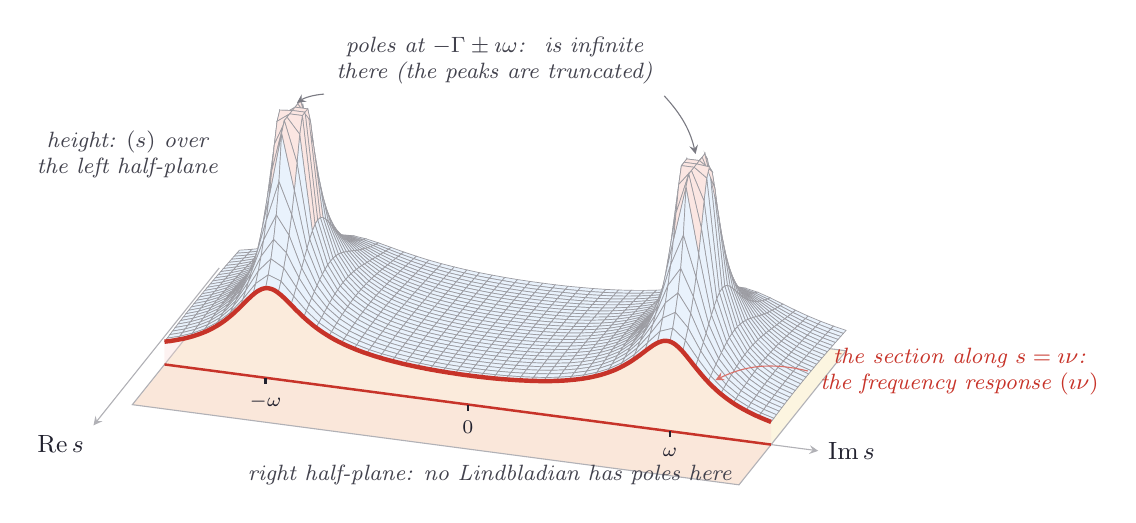
\begin{tikzpicture}[ink/.style={line width=0.9pt, ndInk}, faint/.style={line width=0.4pt, ndInk!35}, dashedink/.style={line width=0.5pt, ndInk!55, dash pattern=on 2.5pt off 2pt}, vec/.style={->, >=stealth, line width=1.2pt}, note/.style={font=\footnotesize\itshape, text=ndInk!85, align=center}, pointer/.style={->, >=stealth, line width=0.4pt, ndInk!60, shorten >=2pt, shorten <=1pt}, dot/.style={circle, fill=ndInk, inner sep=0pt, minimum size=3.4pt}, wash/.style={fill=ndSky, fill opacity=0.55}, every node/.style={text=ndInk}]
\definecolor{ndInk}{rgb}{0.13,0.13,0.18}
\definecolor{ndPaper}{rgb}{0.99,0.96,0.88}
\definecolor{ndSky}{rgb}{0.84,0.91,0.98}
\definecolor{ndRose}{rgb}{0.98,0.86,0.84}
\definecolor{ndBlue}{rgb}{0.13,0.36,0.66}
\definecolor{ndRed}{rgb}{0.78,0.20,0.16}
\definecolor{ndGold}{rgb}{0.88,0.62,0.10}
\definecolor{ndGreen}{rgb}{0.18,0.52,0.30}
\fill[ndPaper] (-2.900,1.700) -- (-4.260,-0.002) -- (3.444,-1.020) -- (4.804,0.682) -- cycle;
\fill[ndRose, fill opacity=0.5] (-3.852,0.509) -- (-4.260,-0.002) -- (3.444,-1.020) -- (3.852,-0.509) -- cycle;
\draw[faint] (-2.900,1.700) -- (-4.260,-0.002) -- (3.444,-1.020) -- (4.804,0.682) -- cycle;
\draw[faint, ->, >=stealth] (-3.157,1.734) -- (-4.754,-0.265) node[below left, text=ndInk, font=\small] {$\mathrm{Re}\,s$};
\node[note, anchor=north] at (0.277,-0.651) {right half-plane: no Lindbladian has poles here};
\filldraw[fill=ndSky!55, draw=ndInk!45, line width=0.25pt] (-2.900,1.960) -- (-2.934,1.921) -- (-2.774,1.934) -- (-2.740,1.971) -- cycle;
\filldraw[fill=ndSky!55, draw=ndInk!45, line width=0.25pt] (-2.740,1.971) -- (-2.774,1.934) -- (-2.613,1.954) -- (-2.579,1.989) -- cycle;
\filldraw[fill=ndSky!55, draw=ndInk!45, line width=0.25pt] (-2.934,1.921) -- (-2.968,1.883) -- (-2.807,1.897) -- (-2.774,1.934) -- cycle;
\filldraw[fill=ndSky!55, draw=ndInk!45, line width=0.25pt] (-2.579,1.989) -- (-2.613,1.954) -- (-2.453,1.982) -- (-2.419,2.014) -- cycle;
\filldraw[fill=ndSky!55, draw=ndInk!45, line width=0.25pt] (-2.774,1.934) -- (-2.807,1.897) -- (-2.647,1.919) -- (-2.613,1.954) -- cycle;
\filldraw[fill=ndSky!55, draw=ndInk!45, line width=0.25pt] (-2.968,1.883) -- (-3.002,1.844) -- (-2.841,1.860) -- (-2.807,1.897) -- cycle;
\filldraw[fill=ndSky!55, draw=ndInk!45, line width=0.25pt] (-2.419,2.014) -- (-2.453,1.982) -- (-2.292,2.017) -- (-2.258,2.045) -- cycle;
\filldraw[fill=ndSky!55, draw=ndInk!45, line width=0.25pt] (-2.613,1.954) -- (-2.647,1.919) -- (-2.487,1.950) -- (-2.453,1.982) -- cycle;
\filldraw[fill=ndSky!55, draw=ndInk!45, line width=0.25pt] (-2.807,1.897) -- (-2.841,1.860) -- (-2.681,1.884) -- (-2.647,1.919) -- cycle;
\filldraw[fill=ndSky!55, draw=ndInk!45, line width=0.25pt] (-2.258,2.045) -- (-2.292,2.017) -- (-2.132,2.060) -- (-2.098,2.082) -- cycle;
\filldraw[fill=ndSky!55, draw=ndInk!45, line width=0.25pt] (-3.002,1.844) -- (-3.036,1.805) -- (-2.875,1.823) -- (-2.841,1.860) -- cycle;
\filldraw[fill=ndSky!55, draw=ndInk!45, line width=0.25pt] (-2.453,1.982) -- (-2.487,1.950) -- (-2.326,1.990) -- (-2.292,2.017) -- cycle;
\filldraw[fill=ndSky!55, draw=ndInk!45, line width=0.25pt] (-2.647,1.919) -- (-2.681,1.884) -- (-2.521,1.918) -- (-2.487,1.950) -- cycle;
\filldraw[fill=ndSky!55, draw=ndInk!45, line width=0.25pt] (-2.098,2.082) -- (-2.132,2.060) -- (-1.971,2.104) -- (-1.937,2.119) -- cycle;
\filldraw[fill=ndSky!55, draw=ndInk!45, line width=0.25pt] (-2.841,1.860) -- (-2.875,1.823) -- (-2.715,1.849) -- (-2.681,1.884) -- cycle;
\filldraw[fill=ndSky!55, draw=ndInk!45, line width=0.25pt] (-2.292,2.017) -- (-2.326,1.990) -- (-2.166,2.039) -- (-2.132,2.060) -- cycle;
\filldraw[fill=ndSky!55, draw=ndInk!45, line width=0.25pt] (-3.036,1.805) -- (-3.070,1.766) -- (-2.909,1.785) -- (-2.875,1.823) -- cycle;
\filldraw[fill=ndSky!55, draw=ndInk!45, line width=0.25pt] (-2.487,1.950) -- (-2.521,1.918) -- (-2.360,1.964) -- (-2.326,1.990) -- cycle;
\filldraw[fill=ndSky!55, draw=ndInk!45, line width=0.25pt] (-1.937,2.119) -- (-1.971,2.104) -- (-1.811,2.140) -- (-1.777,2.148) -- cycle;
\filldraw[fill=ndSky!55, draw=ndInk!45, line width=0.25pt] (-2.681,1.884) -- (-2.715,1.849) -- (-2.555,1.887) -- (-2.521,1.918) -- cycle;
\filldraw[fill=ndSky!55, draw=ndInk!45, line width=0.25pt] (-2.132,2.060) -- (-2.166,2.039) -- (-2.005,2.092) -- (-1.971,2.104) -- cycle;
\filldraw[fill=ndSky!55, draw=ndInk!45, line width=0.25pt] (-2.875,1.823) -- (-2.909,1.785) -- (-2.749,1.814) -- (-2.715,1.849) -- cycle;
\filldraw[fill=ndSky!55, draw=ndInk!45, line width=0.25pt] (-2.326,1.990) -- (-2.360,1.964) -- (-2.200,2.020) -- (-2.166,2.039) -- cycle;
\filldraw[fill=ndSky!55, draw=ndInk!45, line width=0.25pt] (-3.070,1.766) -- (-3.104,1.727) -- (-2.943,1.747) -- (-2.909,1.785) -- cycle;
\filldraw[fill=ndSky!55, draw=ndInk!45, line width=0.25pt] (-1.777,2.148) -- (-1.811,2.140) -- (-1.650,2.153) -- (-1.616,2.158) -- cycle;
\filldraw[fill=ndSky!55, draw=ndInk!45, line width=0.25pt] (-2.521,1.918) -- (-2.555,1.887) -- (-2.394,1.937) -- (-2.360,1.964) -- cycle;
\filldraw[fill=ndSky!55, draw=ndInk!45, line width=0.25pt] (-2.715,1.849) -- (-2.749,1.814) -- (-2.588,1.855) -- (-2.555,1.887) -- cycle;
\filldraw[fill=ndSky!55, draw=ndInk!45, line width=0.25pt] (-1.971,2.104) -- (-2.005,2.092) -- (-1.845,2.135) -- (-1.811,2.140) -- cycle;
\filldraw[fill=ndSky!55, draw=ndInk!45, line width=0.25pt] (-1.616,2.158) -- (-1.650,2.153) -- (-1.490,2.137) -- (-1.456,2.143) -- cycle;
\filldraw[fill=ndSky!55, draw=ndInk!45, line width=0.25pt] (-2.909,1.785) -- (-2.943,1.747) -- (-2.783,1.779) -- (-2.749,1.814) -- cycle;
\filldraw[fill=ndSky!55, draw=ndInk!45, line width=0.25pt] (-2.166,2.039) -- (-2.200,2.020) -- (-2.039,2.082) -- (-2.005,2.092) -- cycle;
\filldraw[fill=ndSky!55, draw=ndInk!45, line width=0.25pt] (-3.104,1.727) -- (-3.138,1.688) -- (-2.977,1.710) -- (-2.943,1.747) -- cycle;
\filldraw[fill=ndSky!55, draw=ndInk!45, line width=0.25pt] (-2.360,1.964) -- (-2.394,1.937) -- (-2.234,2.002) -- (-2.200,2.020) -- cycle;
\filldraw[fill=ndSky!55, draw=ndInk!45, line width=0.25pt] (-1.456,2.143) -- (-1.490,2.137) -- (-1.329,2.094) -- (-1.295,2.105) -- cycle;
\filldraw[fill=ndSky!55, draw=ndInk!45, line width=0.25pt] (-1.811,2.140) -- (-1.845,2.135) -- (-1.684,2.153) -- (-1.650,2.153) -- cycle;
\filldraw[fill=ndSky!55, draw=ndInk!45, line width=0.25pt] (-2.555,1.887) -- (-2.588,1.855) -- (-2.428,1.912) -- (-2.394,1.937) -- cycle;
\filldraw[fill=ndSky!55, draw=ndInk!45, line width=0.25pt] (-1.295,2.105) -- (-1.329,2.094) -- (-1.169,2.035) -- (-1.135,2.053) -- cycle;
\filldraw[fill=ndSky!55, draw=ndInk!45, line width=0.25pt] (-2.749,1.814) -- (-2.783,1.779) -- (-2.622,1.824) -- (-2.588,1.855) -- cycle;
\filldraw[fill=ndSky!55, draw=ndInk!45, line width=0.25pt] (-2.005,2.092) -- (-2.039,2.082) -- (-1.879,2.135) -- (-1.845,2.135) -- cycle;
\filldraw[fill=ndSky!55, draw=ndInk!45, line width=0.25pt] (-2.943,1.747) -- (-2.977,1.710) -- (-2.817,1.743) -- (-2.783,1.779) -- cycle;
\filldraw[fill=ndSky!55, draw=ndInk!45, line width=0.25pt] (-1.135,2.053) -- (-1.169,2.035) -- (-1.008,1.972) -- (-0.974,1.995) -- cycle;
\filldraw[fill=ndSky!55, draw=ndInk!45, line width=0.25pt] (-1.650,2.153) -- (-1.684,2.153) -- (-1.524,2.135) -- (-1.490,2.137) -- cycle;
\filldraw[fill=ndSky!55, draw=ndInk!45, line width=0.25pt] (-2.200,2.020) -- (-2.234,2.002) -- (-2.073,2.076) -- (-2.039,2.082) -- cycle;
\filldraw[fill=ndSky!55, draw=ndInk!45, line width=0.25pt] (-3.138,1.688) -- (-3.172,1.648) -- (-3.011,1.672) -- (-2.977,1.710) -- cycle;
\filldraw[fill=ndSky!55, draw=ndInk!45, line width=0.25pt] (-0.974,1.995) -- (-1.008,1.972) -- (-0.848,1.910) -- (-0.814,1.937) -- cycle;
\filldraw[fill=ndSky!55, draw=ndInk!45, line width=0.25pt] (-2.394,1.937) -- (-2.428,1.912) -- (-2.268,1.986) -- (-2.234,2.002) -- cycle;
\filldraw[fill=ndSky!55, draw=ndInk!45, line width=0.25pt] (-1.490,2.137) -- (-1.524,2.135) -- (-1.363,2.086) -- (-1.329,2.094) -- cycle;
\filldraw[fill=ndSky!55, draw=ndInk!45, line width=0.25pt] (-2.588,1.855) -- (-2.622,1.824) -- (-2.462,1.887) -- (-2.428,1.912) -- cycle;
\filldraw[fill=ndSky!55, draw=ndInk!45, line width=0.25pt] (-1.845,2.135) -- (-1.879,2.135) -- (-1.718,2.159) -- (-1.684,2.153) -- cycle;
\filldraw[fill=ndSky!55, draw=ndInk!45, line width=0.25pt] (-0.814,1.937) -- (-0.848,1.910) -- (-0.687,1.852) -- (-0.653,1.883) -- cycle;
\filldraw[fill=ndSky!55, draw=ndInk!45, line width=0.25pt] (-2.783,1.779) -- (-2.817,1.743) -- (-2.656,1.792) -- (-2.622,1.824) -- cycle;
\filldraw[fill=ndSky!55, draw=ndInk!45, line width=0.25pt] (-1.329,2.094) -- (-1.363,2.086) -- (-1.203,2.019) -- (-1.169,2.035) -- cycle;
\filldraw[fill=ndSky!55, draw=ndInk!45, line width=0.25pt] (-2.977,1.710) -- (-3.011,1.672) -- (-2.851,1.707) -- (-2.817,1.743) -- cycle;
\filldraw[fill=ndSky!55, draw=ndInk!45, line width=0.25pt] (-0.653,1.883) -- (-0.687,1.852) -- (-0.527,1.800) -- (-0.493,1.833) -- cycle;
\filldraw[fill=ndSky!55, draw=ndInk!45, line width=0.25pt] (-2.039,2.082) -- (-2.073,2.076) -- (-1.913,2.141) -- (-1.879,2.135) -- cycle;
\filldraw[fill=ndSky!55, draw=ndInk!45, line width=0.25pt] (-1.169,2.035) -- (-1.203,2.019) -- (-1.042,1.949) -- (-1.008,1.972) -- cycle;
\filldraw[fill=ndSky!55, draw=ndInk!45, line width=0.25pt] (-1.684,2.153) -- (-1.718,2.159) -- (-1.558,2.138) -- (-1.524,2.135) -- cycle;
\filldraw[fill=ndSky!55, draw=ndInk!45, line width=0.25pt] (-3.172,1.648) -- (-3.206,1.609) -- (-3.045,1.633) -- (-3.011,1.672) -- cycle;
\filldraw[fill=ndSky!55, draw=ndInk!45, line width=0.25pt] (-2.234,2.002) -- (-2.268,1.986) -- (-2.107,2.073) -- (-2.073,2.076) -- cycle;
\filldraw[fill=ndSky!55, draw=ndInk!45, line width=0.25pt] (-0.493,1.833) -- (-0.527,1.800) -- (-0.366,1.752) -- (-0.332,1.788) -- cycle;
\filldraw[fill=ndSky!55, draw=ndInk!45, line width=0.25pt] (-1.008,1.972) -- (-1.042,1.949) -- (-0.882,1.882) -- (-0.848,1.910) -- cycle;
\filldraw[fill=ndSky!55, draw=ndInk!45, line width=0.25pt] (-2.428,1.912) -- (-2.462,1.887) -- (-2.302,1.971) -- (-2.268,1.986) -- cycle;
\filldraw[fill=ndSky!55, draw=ndInk!45, line width=0.25pt] (-2.622,1.824) -- (-2.656,1.792) -- (-2.496,1.862) -- (-2.462,1.887) -- cycle;
\filldraw[fill=ndSky!55, draw=ndInk!45, line width=0.25pt] (-1.524,2.135) -- (-1.558,2.138) -- (-1.397,2.081) -- (-1.363,2.086) -- cycle;
\filldraw[fill=ndSky!55, draw=ndInk!45, line width=0.25pt] (-0.848,1.910) -- (-0.882,1.882) -- (-0.721,1.821) -- (-0.687,1.852) -- cycle;
\filldraw[fill=ndSky!55, draw=ndInk!45, line width=0.25pt] (-0.332,1.788) -- (-0.366,1.752) -- (-0.206,1.710) -- (-0.172,1.747) -- cycle;
\filldraw[fill=ndSky!55, draw=ndInk!45, line width=0.25pt] (-2.817,1.743) -- (-2.851,1.707) -- (-2.690,1.760) -- (-2.656,1.792) -- cycle;
\filldraw[fill=ndSky!55, draw=ndInk!45, line width=0.25pt] (-1.879,2.135) -- (-1.913,2.141) -- (-1.752,2.171) -- (-1.718,2.159) -- cycle;
\filldraw[fill=ndSky!55, draw=ndInk!45, line width=0.25pt] (-1.363,2.086) -- (-1.397,2.081) -- (-1.237,2.005) -- (-1.203,2.019) -- cycle;
\filldraw[fill=ndSky!55, draw=ndInk!45, line width=0.25pt] (-3.011,1.672) -- (-3.045,1.633) -- (-2.885,1.671) -- (-2.851,1.707) -- cycle;
\filldraw[fill=ndSky!55, draw=ndInk!45, line width=0.25pt] (-0.687,1.852) -- (-0.721,1.821) -- (-0.561,1.766) -- (-0.527,1.800) -- cycle;
\filldraw[fill=ndSky!55, draw=ndInk!45, line width=0.25pt] (-0.172,1.747) -- (-0.206,1.710) -- (-0.045,1.671) -- (-0.011,1.709) -- cycle;
\filldraw[fill=ndSky!55, draw=ndInk!45, line width=0.25pt] (-1.203,2.019) -- (-1.237,2.005) -- (-1.076,1.927) -- (-1.042,1.949) -- cycle;
\filldraw[fill=ndSky!55, draw=ndInk!45, line width=0.25pt] (-2.073,2.076) -- (-2.107,2.073) -- (-1.947,2.153) -- (-1.913,2.141) -- cycle;
\filldraw[fill=ndSky!55, draw=ndInk!45, line width=0.25pt] (-3.206,1.609) -- (-3.240,1.569) -- (-3.079,1.595) -- (-3.045,1.633) -- cycle;
\filldraw[fill=ndSky!55, draw=ndInk!45, line width=0.25pt] (-0.527,1.800) -- (-0.561,1.766) -- (-0.400,1.717) -- (-0.366,1.752) -- cycle;
\filldraw[fill=ndSky!55, draw=ndInk!45, line width=0.25pt] (-1.718,2.159) -- (-1.752,2.171) -- (-1.592,2.147) -- (-1.558,2.138) -- cycle;
\filldraw[fill=ndSky!55, draw=ndInk!45, line width=0.25pt] (-2.268,1.986) -- (-2.302,1.971) -- (-2.141,2.074) -- (-2.107,2.073) -- cycle;
\filldraw[fill=ndSky!55, draw=ndInk!45, line width=0.25pt] (-1.042,1.949) -- (-1.076,1.927) -- (-0.916,1.855) -- (-0.882,1.882) -- cycle;
\filldraw[fill=ndSky!55, draw=ndInk!45, line width=0.25pt] (-2.462,1.887) -- (-2.496,1.862) -- (-2.335,1.958) -- (-2.302,1.971) -- cycle;
\filldraw[fill=ndSky!55, draw=ndInk!45, line width=0.25pt] (-0.011,1.709) -- (-0.045,1.671) -- (0.115,1.636) -- (0.149,1.674) -- cycle;
\filldraw[fill=ndSky!55, draw=ndInk!45, line width=0.25pt] (-2.656,1.792) -- (-2.690,1.760) -- (-2.530,1.837) -- (-2.496,1.862) -- cycle;
\filldraw[fill=ndSky!55, draw=ndInk!45, line width=0.25pt] (-0.882,1.882) -- (-0.916,1.855) -- (-0.755,1.790) -- (-0.721,1.821) -- cycle;
\filldraw[fill=ndSky!55, draw=ndInk!45, line width=0.25pt] (-0.366,1.752) -- (-0.400,1.717) -- (-0.240,1.673) -- (-0.206,1.710) -- cycle;
\filldraw[fill=ndSky!55, draw=ndInk!45, line width=0.25pt] (-2.851,1.707) -- (-2.885,1.671) -- (-2.724,1.728) -- (-2.690,1.760) -- cycle;
\filldraw[fill=ndSky!55, draw=ndInk!45, line width=0.25pt] (-1.558,2.138) -- (-1.592,2.147) -- (-1.431,2.079) -- (-1.397,2.081) -- cycle;
\filldraw[fill=ndSky!55, draw=ndInk!45, line width=0.25pt] (0.149,1.674) -- (0.115,1.636) -- (0.276,1.604) -- (0.310,1.643) -- cycle;
\filldraw[fill=ndSky!55, draw=ndInk!45, line width=0.25pt] (-3.045,1.633) -- (-3.079,1.595) -- (-2.919,1.635) -- (-2.885,1.671) -- cycle;
\filldraw[fill=ndSky!55, draw=ndInk!45, line width=0.25pt] (-0.721,1.821) -- (-0.755,1.790) -- (-0.595,1.732) -- (-0.561,1.766) -- cycle;
\filldraw[fill=ndSky!55, draw=ndInk!45, line width=0.25pt] (-1.913,2.141) -- (-1.947,2.153) -- (-1.786,2.191) -- (-1.752,2.171) -- cycle;
\filldraw[fill=ndSky!55, draw=ndInk!45, line width=0.25pt] (-1.397,2.081) -- (-1.431,2.079) -- (-1.271,1.993) -- (-1.237,2.005) -- cycle;
\filldraw[fill=ndSky!55, draw=ndInk!45, line width=0.25pt] (-0.206,1.710) -- (-0.240,1.673) -- (-0.079,1.634) -- (-0.045,1.671) -- cycle;
\filldraw[fill=ndSky!55, draw=ndInk!45, line width=0.25pt] (-3.240,1.569) -- (-3.274,1.529) -- (-3.113,1.556) -- (-3.079,1.595) -- cycle;
\filldraw[fill=ndSky!55, draw=ndInk!45, line width=0.25pt] (-1.237,2.005) -- (-1.271,1.993) -- (-1.110,1.906) -- (-1.076,1.927) -- cycle;
\filldraw[fill=ndSky!55, draw=ndInk!45, line width=0.25pt] (-0.561,1.766) -- (-0.595,1.732) -- (-0.434,1.681) -- (-0.400,1.717) -- cycle;
\filldraw[fill=ndSky!55, draw=ndInk!45, line width=0.25pt] (0.310,1.643) -- (0.276,1.604) -- (0.436,1.575) -- (0.470,1.614) -- cycle;
\filldraw[fill=ndSky!55, draw=ndInk!45, line width=0.25pt] (-2.107,2.073) -- (-2.141,2.074) -- (-1.981,2.173) -- (-1.947,2.153) -- cycle;
\filldraw[fill=ndSky!55, draw=ndInk!45, line width=0.25pt] (-1.076,1.927) -- (-1.110,1.906) -- (-0.950,1.827) -- (-0.916,1.855) -- cycle;
\filldraw[fill=ndSky!55, draw=ndInk!45, line width=0.25pt] (-0.045,1.671) -- (-0.079,1.634) -- (0.081,1.598) -- (0.115,1.636) -- cycle;
\filldraw[fill=ndSky!55, draw=ndInk!45, line width=0.25pt] (-2.302,1.971) -- (-2.335,1.958) -- (-2.175,2.080) -- (-2.141,2.074) -- cycle;
\filldraw[fill=ndSky!55, draw=ndInk!45, line width=0.25pt] (-2.496,1.862) -- (-2.530,1.837) -- (-2.369,1.946) -- (-2.335,1.958) -- cycle;
\filldraw[fill=ndSky!55, draw=ndInk!45, line width=0.25pt] (-1.752,2.171) -- (-1.786,2.191) -- (-1.626,2.163) -- (-1.592,2.147) -- cycle;
\filldraw[fill=ndSky!55, draw=ndInk!45, line width=0.25pt] (-2.690,1.760) -- (-2.724,1.728) -- (-2.564,1.812) -- (-2.530,1.837) -- cycle;
\filldraw[fill=ndSky!55, draw=ndInk!45, line width=0.25pt] (-0.400,1.717) -- (-0.434,1.681) -- (-0.274,1.636) -- (-0.240,1.673) -- cycle;
\filldraw[fill=ndSky!55, draw=ndInk!45, line width=0.25pt] (-0.916,1.855) -- (-0.950,1.827) -- (-0.789,1.758) -- (-0.755,1.790) -- cycle;
\filldraw[fill=ndSky!55, draw=ndInk!45, line width=0.25pt] (-2.885,1.671) -- (-2.919,1.635) -- (-2.758,1.695) -- (-2.724,1.728) -- cycle;
\filldraw[fill=ndSky!55, draw=ndInk!45, line width=0.25pt] (0.470,1.614) -- (0.436,1.575) -- (0.597,1.548) -- (0.631,1.587) -- cycle;
\filldraw[fill=ndSky!55, draw=ndInk!45, line width=0.25pt] (0.115,1.636) -- (0.081,1.598) -- (0.242,1.565) -- (0.276,1.604) -- cycle;
\filldraw[fill=ndSky!55, draw=ndInk!45, line width=0.25pt] (-3.079,1.595) -- (-3.113,1.556) -- (-2.953,1.598) -- (-2.919,1.635) -- cycle;
\filldraw[fill=ndSky!55, draw=ndInk!45, line width=0.25pt] (-1.592,2.147) -- (-1.626,2.163) -- (-1.465,2.082) -- (-1.431,2.079) -- cycle;
\filldraw[fill=ndSky!55, draw=ndInk!45, line width=0.25pt] (-0.755,1.790) -- (-0.789,1.758) -- (-0.629,1.698) -- (-0.595,1.732) -- cycle;
\filldraw[fill=ndSky!55, draw=ndInk!45, line width=0.25pt] (-0.240,1.673) -- (-0.274,1.636) -- (-0.113,1.596) -- (-0.079,1.634) -- cycle;
\filldraw[fill=ndSky!55, draw=ndInk!45, line width=0.25pt] (-1.431,2.079) -- (-1.465,2.082) -- (-1.305,1.982) -- (-1.271,1.993) -- cycle;
\filldraw[fill=ndSky!55, draw=ndInk!45, line width=0.25pt] (-3.274,1.529) -- (-3.308,1.488) -- (-3.147,1.516) -- (-3.113,1.556) -- cycle;
\filldraw[fill=ndSky!55, draw=ndInk!45, line width=0.25pt] (-1.947,2.153) -- (-1.981,2.173) -- (-1.820,2.222) -- (-1.786,2.191) -- cycle;
\filldraw[fill=ndSky!55, draw=ndInk!45, line width=0.25pt] (0.631,1.587) -- (0.597,1.548) -- (0.757,1.524) -- (0.791,1.563) -- cycle;
\filldraw[fill=ndSky!55, draw=ndInk!45, line width=0.25pt] (-1.271,1.993) -- (-1.305,1.982) -- (-1.144,1.886) -- (-1.110,1.906) -- cycle;
\filldraw[fill=ndSky!55, draw=ndInk!45, line width=0.25pt] (-0.595,1.732) -- (-0.629,1.698) -- (-0.468,1.645) -- (-0.434,1.681) -- cycle;
\filldraw[fill=ndSky!55, draw=ndInk!45, line width=0.25pt] (0.276,1.604) -- (0.242,1.565) -- (0.402,1.536) -- (0.436,1.575) -- cycle;
\filldraw[fill=ndSky!55, draw=ndInk!45, line width=0.25pt] (-0.079,1.634) -- (-0.113,1.596) -- (0.047,1.559) -- (0.081,1.598) -- cycle;
\filldraw[fill=ndSky!55, draw=ndInk!45, line width=0.25pt] (-1.110,1.906) -- (-1.144,1.886) -- (-0.984,1.800) -- (-0.950,1.827) -- cycle;
\filldraw[fill=ndSky!55, draw=ndInk!45, line width=0.25pt] (-2.141,2.074) -- (-2.175,2.080) -- (-2.015,2.203) -- (-1.981,2.173) -- cycle;
\filldraw[fill=ndSky!55, draw=ndInk!45, line width=0.25pt] (-2.530,1.837) -- (-2.564,1.812) -- (-2.403,1.934) -- (-2.369,1.946) -- cycle;
\filldraw[fill=ndSky!55, draw=ndInk!45, line width=0.25pt] (-2.724,1.728) -- (-2.758,1.695) -- (-2.598,1.786) -- (-2.564,1.812) -- cycle;
\filldraw[fill=ndSky!55, draw=ndInk!45, line width=0.25pt] (-2.335,1.958) -- (-2.369,1.946) -- (-2.209,2.090) -- (-2.175,2.080) -- cycle;
\filldraw[fill=ndSky!55, draw=ndInk!45, line width=0.25pt] (-0.434,1.681) -- (-0.468,1.645) -- (-0.308,1.599) -- (-0.274,1.636) -- cycle;
\filldraw[fill=ndSky!55, draw=ndInk!45, line width=0.25pt] (-0.950,1.827) -- (-0.984,1.800) -- (-0.823,1.727) -- (-0.789,1.758) -- cycle;
\filldraw[fill=ndSky!55, draw=ndInk!45, line width=0.25pt] (-2.919,1.635) -- (-2.953,1.598) -- (-2.792,1.662) -- (-2.758,1.695) -- cycle;
\filldraw[fill=ndSky!55, draw=ndInk!45, line width=0.25pt] (0.791,1.563) -- (0.757,1.524) -- (0.918,1.501) -- (0.952,1.541) -- cycle;
\filldraw[fill=ndSky!55, draw=ndInk!45, line width=0.25pt] (0.436,1.575) -- (0.402,1.536) -- (0.563,1.509) -- (0.597,1.548) -- cycle;
\filldraw[fill=ndSky!55, draw=ndInk!45, line width=0.25pt] (-1.786,2.191) -- (-1.820,2.222) -- (-1.660,2.187) -- (-1.626,2.163) -- cycle;
\filldraw[fill=ndSky!55, draw=ndInk!45, line width=0.25pt] (0.081,1.598) -- (0.047,1.559) -- (0.208,1.526) -- (0.242,1.565) -- cycle;
\filldraw[fill=ndSky!55, draw=ndInk!45, line width=0.25pt] (-3.113,1.556) -- (-3.147,1.516) -- (-2.987,1.560) -- (-2.953,1.598) -- cycle;
\filldraw[fill=ndSky!55, draw=ndInk!45, line width=0.25pt] (-0.789,1.758) -- (-0.823,1.727) -- (-0.663,1.664) -- (-0.629,1.698) -- cycle;
\filldraw[fill=ndSky!55, draw=ndInk!45, line width=0.25pt] (-0.274,1.636) -- (-0.308,1.599) -- (-0.147,1.558) -- (-0.113,1.596) -- cycle;
\filldraw[fill=ndSky!55, draw=ndInk!45, line width=0.25pt] (-3.308,1.488) -- (-3.342,1.448) -- (-3.181,1.477) -- (-3.147,1.516) -- cycle;
\filldraw[fill=ndSky!55, draw=ndInk!45, line width=0.25pt] (-1.626,2.163) -- (-1.660,2.187) -- (-1.499,2.089) -- (-1.465,2.082) -- cycle;
\filldraw[fill=ndSky!55, draw=ndInk!45, line width=0.25pt] (0.952,1.541) -- (0.918,1.501) -- (1.078,1.481) -- (1.112,1.520) -- cycle;
\filldraw[fill=ndSky!55, draw=ndInk!45, line width=0.25pt] (0.597,1.548) -- (0.563,1.509) -- (0.723,1.484) -- (0.757,1.524) -- cycle;
\filldraw[fill=ndSky!55, draw=ndInk!45, line width=0.25pt] (-1.465,2.082) -- (-1.499,2.089) -- (-1.339,1.973) -- (-1.305,1.982) -- cycle;
\filldraw[fill=ndSky!55, draw=ndInk!45, line width=0.25pt] (-0.629,1.698) -- (-0.663,1.664) -- (-0.502,1.609) -- (-0.468,1.645) -- cycle;
\filldraw[fill=ndSky!55, draw=ndInk!45, line width=0.25pt] (0.242,1.565) -- (0.208,1.526) -- (0.368,1.496) -- (0.402,1.536) -- cycle;
\filldraw[fill=ndSky!55, draw=ndInk!45, line width=0.25pt] (-1.305,1.982) -- (-1.339,1.973) -- (-1.178,1.866) -- (-1.144,1.886) -- cycle;
\filldraw[fill=ndSky!55, draw=ndInk!45, line width=0.25pt] (-0.113,1.596) -- (-0.147,1.558) -- (0.013,1.521) -- (0.047,1.559) -- cycle;
\filldraw[fill=ndSky!55, draw=ndInk!45, line width=0.25pt] (-1.144,1.886) -- (-1.178,1.866) -- (-1.018,1.773) -- (-0.984,1.800) -- cycle;
\filldraw[fill=ndSky!55, draw=ndInk!45, line width=0.25pt] (-1.981,2.173) -- (-2.015,2.203) -- (-1.854,2.267) -- (-1.820,2.222) -- cycle;
\filldraw[fill=ndSky!55, draw=ndInk!45, line width=0.25pt] (-2.758,1.695) -- (-2.792,1.662) -- (-2.632,1.760) -- (-2.598,1.786) -- cycle;
\filldraw[fill=ndSky!55, draw=ndInk!45, line width=0.25pt] (-0.468,1.645) -- (-0.502,1.609) -- (-0.342,1.562) -- (-0.308,1.599) -- cycle;
\filldraw[fill=ndSky!55, draw=ndInk!45, line width=0.25pt] (-2.564,1.812) -- (-2.598,1.786) -- (-2.437,1.924) -- (-2.403,1.934) -- cycle;
\filldraw[fill=ndSky!55, draw=ndInk!45, line width=0.25pt] (1.112,1.520) -- (1.078,1.481) -- (1.239,1.463) -- (1.273,1.502) -- cycle;
\filldraw[fill=ndSky!55, draw=ndInk!45, line width=0.25pt] (-2.953,1.598) -- (-2.987,1.560) -- (-2.826,1.627) -- (-2.792,1.662) -- cycle;
\filldraw[fill=ndSky!55, draw=ndInk!45, line width=0.25pt] (0.757,1.524) -- (0.723,1.484) -- (0.884,1.462) -- (0.918,1.501) -- cycle;
\filldraw[fill=ndSky!55, draw=ndInk!45, line width=0.25pt] (-0.984,1.800) -- (-1.018,1.773) -- (-0.857,1.695) -- (-0.823,1.727) -- cycle;
\filldraw[fill=ndSky!55, draw=ndInk!45, line width=0.25pt] (0.402,1.536) -- (0.368,1.496) -- (0.529,1.469) -- (0.563,1.509) -- cycle;
\filldraw[fill=ndSky!55, draw=ndInk!45, line width=0.25pt] (-2.369,1.946) -- (-2.403,1.934) -- (-2.243,2.105) -- (-2.209,2.090) -- cycle;
\filldraw[fill=ndSky!55, draw=ndInk!45, line width=0.25pt] (-2.175,2.080) -- (-2.209,2.090) -- (-2.049,2.245) -- (-2.015,2.203) -- cycle;
\filldraw[fill=ndSky!55, draw=ndInk!45, line width=0.25pt] (0.047,1.559) -- (0.013,1.521) -- (0.174,1.487) -- (0.208,1.526) -- cycle;
\filldraw[fill=ndSky!55, draw=ndInk!45, line width=0.25pt] (-3.147,1.516) -- (-3.181,1.477) -- (-3.021,1.522) -- (-2.987,1.560) -- cycle;
\filldraw[fill=ndSky!55, draw=ndInk!45, line width=0.25pt] (-0.823,1.727) -- (-0.857,1.695) -- (-0.697,1.629) -- (-0.663,1.664) -- cycle;
\filldraw[fill=ndSky!55, draw=ndInk!45, line width=0.25pt] (-0.308,1.599) -- (-0.342,1.562) -- (-0.181,1.519) -- (-0.147,1.558) -- cycle;
\filldraw[fill=ndSky!55, draw=ndInk!45, line width=0.25pt] (-3.342,1.448) -- (-3.376,1.406) -- (-3.215,1.436) -- (-3.181,1.477) -- cycle;
\filldraw[fill=ndSky!55, draw=ndInk!45, line width=0.25pt] (-1.820,2.222) -- (-1.854,2.267) -- (-1.694,2.222) -- (-1.660,2.187) -- cycle;
\filldraw[fill=ndSky!55, draw=ndInk!45, line width=0.25pt] (0.918,1.501) -- (0.884,1.462) -- (1.044,1.442) -- (1.078,1.481) -- cycle;
\filldraw[fill=ndSky!55, draw=ndInk!45, line width=0.25pt] (1.273,1.502) -- (1.239,1.463) -- (1.399,1.448) -- (1.433,1.487) -- cycle;
\filldraw[fill=ndSky!55, draw=ndInk!45, line width=0.25pt] (0.563,1.509) -- (0.529,1.469) -- (0.689,1.444) -- (0.723,1.484) -- cycle;
\filldraw[fill=ndSky!55, draw=ndInk!45, line width=0.25pt] (0.208,1.526) -- (0.174,1.487) -- (0.334,1.457) -- (0.368,1.496) -- cycle;
\filldraw[fill=ndSky!55, draw=ndInk!45, line width=0.25pt] (-0.663,1.664) -- (-0.697,1.629) -- (-0.536,1.573) -- (-0.502,1.609) -- cycle;
\filldraw[fill=ndSky!55, draw=ndInk!45, line width=0.25pt] (-1.660,2.187) -- (-1.694,2.222) -- (-1.533,2.101) -- (-1.499,2.089) -- cycle;
\filldraw[fill=ndSky!55, draw=ndInk!45, line width=0.25pt] (-0.147,1.558) -- (-0.181,1.519) -- (-0.021,1.482) -- (0.013,1.521) -- cycle;
\filldraw[fill=ndSky!55, draw=ndInk!45, line width=0.25pt] (-1.499,2.089) -- (-1.533,2.101) -- (-1.373,1.966) -- (-1.339,1.973) -- cycle;
\filldraw[fill=ndSky!55, draw=ndInk!45, line width=0.25pt] (-1.339,1.973) -- (-1.373,1.966) -- (-1.212,1.846) -- (-1.178,1.866) -- cycle;
\filldraw[fill=ndSky!55, draw=ndInk!45, line width=0.25pt] (-1.178,1.866) -- (-1.212,1.846) -- (-1.052,1.746) -- (-1.018,1.773) -- cycle;
\filldraw[fill=ndSky!55, draw=ndInk!45, line width=0.25pt] (-0.502,1.609) -- (-0.536,1.573) -- (-0.376,1.524) -- (-0.342,1.562) -- cycle;
\filldraw[fill=ndSky!55, draw=ndInk!45, line width=0.25pt] (-2.792,1.662) -- (-2.826,1.627) -- (-2.666,1.733) -- (-2.632,1.760) -- cycle;
\filldraw[fill=ndSky!55, draw=ndInk!45, line width=0.25pt] (1.078,1.481) -- (1.044,1.442) -- (1.205,1.424) -- (1.239,1.463) -- cycle;
\filldraw[fill=ndSky!55, draw=ndInk!45, line width=0.25pt] (0.723,1.484) -- (0.689,1.444) -- (0.850,1.422) -- (0.884,1.462) -- cycle;
\filldraw[fill=ndSky!55, draw=ndInk!45, line width=0.25pt] (-2.987,1.560) -- (-3.021,1.522) -- (-2.860,1.592) -- (-2.826,1.627) -- cycle;
\filldraw[fill=ndSky!55, draw=ndInk!45, line width=0.25pt] (1.433,1.487) -- (1.399,1.448) -- (1.560,1.434) -- (1.594,1.473) -- cycle;
\filldraw[fill=ndSky!55, draw=ndInk!45, line width=0.25pt] (0.368,1.496) -- (0.334,1.457) -- (0.495,1.429) -- (0.529,1.469) -- cycle;
\filldraw[fill=ndSky!55, draw=ndInk!45, line width=0.25pt] (-1.018,1.773) -- (-1.052,1.746) -- (-0.891,1.663) -- (-0.857,1.695) -- cycle;
\filldraw[fill=ndSky!55, draw=ndInk!45, line width=0.25pt] (-2.598,1.786) -- (-2.632,1.760) -- (-2.471,1.913) -- (-2.437,1.924) -- cycle;
\filldraw[fill=ndSky!55, draw=ndInk!45, line width=0.25pt] (0.013,1.521) -- (-0.021,1.482) -- (0.140,1.448) -- (0.174,1.487) -- cycle;
\filldraw[fill=ndSky!55, draw=ndInk!45, line width=0.25pt] (-3.181,1.477) -- (-3.215,1.436) -- (-3.055,1.483) -- (-3.021,1.522) -- cycle;
\filldraw[fill=ndSky!55, draw=ndInk!45, line width=0.25pt] (-2.015,2.203) -- (-2.049,2.245) -- (-1.888,2.328) -- (-1.854,2.267) -- cycle;
\filldraw[fill=ndSky!55, draw=ndInk!45, line width=0.25pt] (-2.403,1.934) -- (-2.437,1.924) -- (-2.277,2.126) -- (-2.243,2.105) -- cycle;
\filldraw[fill=ndSky!55, draw=ndInk!45, line width=0.25pt] (-0.857,1.695) -- (-0.891,1.663) -- (-0.731,1.595) -- (-0.697,1.629) -- cycle;
\filldraw[fill=ndSky!55, draw=ndInk!45, line width=0.25pt] (-0.342,1.562) -- (-0.376,1.524) -- (-0.215,1.481) -- (-0.181,1.519) -- cycle;
\filldraw[fill=ndSky!55, draw=ndInk!45, line width=0.25pt] (-3.376,1.406) -- (-3.410,1.365) -- (-3.249,1.396) -- (-3.215,1.436) -- cycle;
\filldraw[fill=ndSky!55, draw=ndInk!45, line width=0.25pt] (-2.209,2.090) -- (-2.243,2.105) -- (-2.082,2.302) -- (-2.049,2.245) -- cycle;
\filldraw[fill=ndSky!55, draw=ndInk!45, line width=0.25pt] (0.884,1.462) -- (0.850,1.422) -- (1.010,1.402) -- (1.044,1.442) -- cycle;
\filldraw[fill=ndSky!55, draw=ndInk!45, line width=0.25pt] (1.239,1.463) -- (1.205,1.424) -- (1.365,1.408) -- (1.399,1.448) -- cycle;
\filldraw[fill=ndSky!55, draw=ndInk!45, line width=0.25pt] (0.529,1.469) -- (0.495,1.429) -- (0.655,1.405) -- (0.689,1.444) -- cycle;
\filldraw[fill=ndSky!55, draw=ndInk!45, line width=0.25pt] (1.594,1.473) -- (1.560,1.434) -- (1.720,1.424) -- (1.754,1.462) -- cycle;
\filldraw[fill=ndSky!55, draw=ndInk!45, line width=0.25pt] (0.174,1.487) -- (0.140,1.448) -- (0.300,1.417) -- (0.334,1.457) -- cycle;
\filldraw[fill=ndSky!55, draw=ndInk!45, line width=0.25pt] (-0.697,1.629) -- (-0.731,1.595) -- (-0.570,1.536) -- (-0.536,1.573) -- cycle;
\filldraw[fill=ndSky!55, draw=ndInk!45, line width=0.25pt] (-0.181,1.519) -- (-0.215,1.481) -- (-0.055,1.443) -- (-0.021,1.482) -- cycle;
\filldraw[fill=ndSky!55, draw=ndInk!45, line width=0.25pt] (-1.854,2.267) -- (-1.888,2.328) -- (-1.728,2.269) -- (-1.694,2.222) -- cycle;
\filldraw[fill=ndSky!55, draw=ndInk!45, line width=0.25pt] (-1.373,1.966) -- (-1.407,1.960) -- (-1.246,1.826) -- (-1.212,1.846) -- cycle;
\filldraw[fill=ndSky!55, draw=ndInk!45, line width=0.25pt] (-1.533,2.101) -- (-1.567,2.119) -- (-1.407,1.960) -- (-1.373,1.966) -- cycle;
\filldraw[fill=ndSky!55, draw=ndInk!45, line width=0.25pt] (-1.212,1.846) -- (-1.246,1.826) -- (-1.086,1.718) -- (-1.052,1.746) -- cycle;
\filldraw[fill=ndSky!55, draw=ndInk!45, line width=0.25pt] (-0.536,1.573) -- (-0.570,1.536) -- (-0.410,1.486) -- (-0.376,1.524) -- cycle;
\filldraw[fill=ndSky!55, draw=ndInk!45, line width=0.25pt] (-1.694,2.222) -- (-1.728,2.269) -- (-1.567,2.119) -- (-1.533,2.101) -- cycle;
\filldraw[fill=ndSky!55, draw=ndInk!45, line width=0.25pt] (1.044,1.442) -- (1.010,1.402) -- (1.171,1.384) -- (1.205,1.424) -- cycle;
\filldraw[fill=ndSky!55, draw=ndInk!45, line width=0.25pt] (0.689,1.444) -- (0.655,1.405) -- (0.816,1.382) -- (0.850,1.422) -- cycle;
\filldraw[fill=ndSky!55, draw=ndInk!45, line width=0.25pt] (-2.826,1.627) -- (-2.860,1.592) -- (-2.700,1.704) -- (-2.666,1.733) -- cycle;
\filldraw[fill=ndSky!55, draw=ndInk!45, line width=0.25pt] (-3.021,1.522) -- (-3.055,1.483) -- (-2.894,1.556) -- (-2.860,1.592) -- cycle;
\filldraw[fill=ndSky!55, draw=ndInk!45, line width=0.25pt] (1.399,1.448) -- (1.365,1.408) -- (1.526,1.396) -- (1.560,1.434) -- cycle;
\filldraw[fill=ndSky!55, draw=ndInk!45, line width=0.25pt] (0.334,1.457) -- (0.300,1.417) -- (0.461,1.390) -- (0.495,1.429) -- cycle;
\filldraw[fill=ndSky!55, draw=ndInk!45, line width=0.25pt] (-1.052,1.746) -- (-1.086,1.718) -- (-0.925,1.631) -- (-0.891,1.663) -- cycle;
\filldraw[fill=ndSky!55, draw=ndInk!45, line width=0.25pt] (1.754,1.462) -- (1.720,1.424) -- (1.881,1.417) -- (1.915,1.454) -- cycle;
\filldraw[fill=ndSky!55, draw=ndInk!45, line width=0.25pt] (-0.021,1.482) -- (-0.055,1.443) -- (0.106,1.408) -- (0.140,1.448) -- cycle;
\filldraw[fill=ndSky!55, draw=ndInk!45, line width=0.25pt] (-3.215,1.436) -- (-3.249,1.396) -- (-3.089,1.443) -- (-3.055,1.483) -- cycle;
\filldraw[fill=ndSky!55, draw=ndInk!45, line width=0.25pt] (-2.632,1.760) -- (-2.666,1.733) -- (-2.505,1.902) -- (-2.471,1.913) -- cycle;
\filldraw[fill=ndSky!55, draw=ndInk!45, line width=0.25pt] (-0.376,1.524) -- (-0.410,1.486) -- (-0.249,1.442) -- (-0.215,1.481) -- cycle;
\filldraw[fill=ndSky!55, draw=ndInk!45, line width=0.25pt] (-0.891,1.663) -- (-0.925,1.631) -- (-0.765,1.559) -- (-0.731,1.595) -- cycle;
\filldraw[fill=ndSky!55, draw=ndInk!45, line width=0.25pt] (-3.410,1.365) -- (-3.444,1.323) -- (-3.283,1.354) -- (-3.249,1.396) -- cycle;
\filldraw[fill=ndSky!55, draw=ndInk!45, line width=0.25pt] (0.850,1.422) -- (0.816,1.382) -- (0.976,1.362) -- (1.010,1.402) -- cycle;
\filldraw[fill=ndSky!55, draw=ndInk!45, line width=0.25pt] (-2.437,1.924) -- (-2.471,1.913) -- (-2.311,2.151) -- (-2.277,2.126) -- cycle;
\filldraw[fill=ndSky!55, draw=ndInk!45, line width=0.25pt] (1.205,1.424) -- (1.171,1.384) -- (1.331,1.369) -- (1.365,1.408) -- cycle;
\filldraw[fill=ndSky!55, draw=ndInk!45, line width=0.25pt] (0.495,1.429) -- (0.461,1.390) -- (0.621,1.365) -- (0.655,1.405) -- cycle;
\filldraw[fill=ndSky!55, draw=ndInk!45, line width=0.25pt] (1.560,1.434) -- (1.526,1.396) -- (1.686,1.386) -- (1.720,1.424) -- cycle;
\filldraw[fill=ndSky!55, draw=ndInk!45, line width=0.25pt] (0.140,1.448) -- (0.106,1.408) -- (0.266,1.378) -- (0.300,1.417) -- cycle;
\filldraw[fill=ndSky!55, draw=ndInk!45, line width=0.25pt] (-0.731,1.595) -- (-0.765,1.559) -- (-0.604,1.499) -- (-0.570,1.536) -- cycle;
\filldraw[fill=ndSky!55, draw=ndInk!45, line width=0.25pt] (-2.049,2.245) -- (-2.082,2.302) -- (-1.922,2.413) -- (-1.888,2.328) -- cycle;
\filldraw[fill=ndSky!55, draw=ndInk!45, line width=0.25pt] (1.915,1.454) -- (1.881,1.417) -- (2.041,1.413) -- (2.075,1.450) -- cycle;
\filldraw[fill=ndSky!55, draw=ndInk!45, line width=0.25pt] (-0.215,1.481) -- (-0.249,1.442) -- (-0.089,1.403) -- (-0.055,1.443) -- cycle;
\filldraw[fill=ndSky!55, draw=ndInk!45, line width=0.25pt] (-2.243,2.105) -- (-2.277,2.126) -- (-2.116,2.377) -- (-2.082,2.302) -- cycle;
\filldraw[fill=ndSky!55, draw=ndInk!45, line width=0.25pt] (-0.570,1.536) -- (-0.604,1.499) -- (-0.444,1.448) -- (-0.410,1.486) -- cycle;
\filldraw[fill=ndSky!55, draw=ndInk!45, line width=0.25pt] (1.010,1.402) -- (0.976,1.362) -- (1.137,1.345) -- (1.171,1.384) -- cycle;
\filldraw[fill=ndSky!55, draw=ndInk!45, line width=0.25pt] (0.655,1.405) -- (0.621,1.365) -- (0.782,1.342) -- (0.816,1.382) -- cycle;
\filldraw[fill=ndSky!55, draw=ndInk!45, line width=0.25pt] (-1.407,1.960) -- (-1.441,1.956) -- (-1.280,1.806) -- (-1.246,1.826) -- cycle;
\filldraw[fill=ndSky!55, draw=ndInk!45, line width=0.25pt] (-1.246,1.826) -- (-1.280,1.806) -- (-1.120,1.690) -- (-1.086,1.718) -- cycle;
\filldraw[fill=ndSky!55, draw=ndInk!45, line width=0.25pt] (-3.055,1.483) -- (-3.089,1.443) -- (-2.928,1.519) -- (-2.894,1.556) -- cycle;
\filldraw[fill=ndSky!55, draw=ndInk!45, line width=0.25pt] (1.365,1.408) -- (1.331,1.369) -- (1.492,1.357) -- (1.526,1.396) -- cycle;
\filldraw[fill=ndSky!55, draw=ndInk!45, line width=0.25pt] (-2.860,1.592) -- (-2.894,1.556) -- (-2.734,1.673) -- (-2.700,1.704) -- cycle;
\filldraw[fill=ndSky!55, draw=ndInk!45, line width=0.25pt] (0.300,1.417) -- (0.266,1.378) -- (0.427,1.350) -- (0.461,1.390) -- cycle;
\filldraw[fill=ndSky!55, draw=ndInk!45, line width=0.25pt] (1.720,1.424) -- (1.686,1.386) -- (1.847,1.379) -- (1.881,1.417) -- cycle;
\filldraw[fill=ndSky!55, draw=ndInk!45, line width=0.25pt] (-1.086,1.718) -- (-1.120,1.690) -- (-0.959,1.598) -- (-0.925,1.631) -- cycle;
\filldraw[fill=ndSky!55, draw=ndInk!45, line width=0.25pt] (-1.567,2.119) -- (-1.601,2.142) -- (-1.441,1.956) -- (-1.407,1.960) -- cycle;
\filldraw[fill=ndSky!55, draw=ndInk!45, line width=0.25pt] (-0.055,1.443) -- (-0.089,1.403) -- (0.072,1.369) -- (0.106,1.408) -- cycle;
\filldraw[fill=ndSky!55, draw=ndInk!45, line width=0.25pt] (-3.249,1.396) -- (-3.283,1.354) -- (-3.123,1.403) -- (-3.089,1.443) -- cycle;
\filldraw[fill=ndSky!55, draw=ndInk!45, line width=0.25pt] (2.075,1.450) -- (2.041,1.413) -- (2.202,1.413) -- (2.236,1.449) -- cycle;
\filldraw[fill=ndSky!55, draw=ndInk!45, line width=0.25pt] (-2.666,1.733) -- (-2.700,1.704) -- (-2.539,1.889) -- (-2.505,1.902) -- cycle;
\filldraw[fill=ndSky!55, draw=ndInk!45, line width=0.25pt] (-1.888,2.328) -- (-1.922,2.413) -- (-1.762,2.332) -- (-1.728,2.269) -- cycle;
\filldraw[fill=ndSky!55, draw=ndInk!45, line width=0.25pt] (-0.410,1.486) -- (-0.444,1.448) -- (-0.283,1.403) -- (-0.249,1.442) -- cycle;
\filldraw[fill=ndSky!55, draw=ndInk!45, line width=0.25pt] (-1.728,2.269) -- (-1.762,2.332) -- (-1.601,2.142) -- (-1.567,2.119) -- cycle;
\filldraw[fill=ndSky!55, draw=ndInk!45, line width=0.25pt] (-0.925,1.631) -- (-0.959,1.598) -- (-0.799,1.524) -- (-0.765,1.559) -- cycle;
\filldraw[fill=ndSky!55, draw=ndInk!45, line width=0.25pt] (-3.444,1.323) -- (-3.478,1.281) -- (-3.317,1.313) -- (-3.283,1.354) -- cycle;
\filldraw[fill=ndSky!55, draw=ndInk!45, line width=0.25pt] (0.816,1.382) -- (0.782,1.342) -- (0.942,1.322) -- (0.976,1.362) -- cycle;
\filldraw[fill=ndSky!55, draw=ndInk!45, line width=0.25pt] (1.171,1.384) -- (1.137,1.345) -- (1.297,1.330) -- (1.331,1.369) -- cycle;
\filldraw[fill=ndSky!55, draw=ndInk!45, line width=0.25pt] (0.461,1.390) -- (0.427,1.350) -- (0.587,1.325) -- (0.621,1.365) -- cycle;
\filldraw[fill=ndSky!55, draw=ndInk!45, line width=0.25pt] (1.526,1.396) -- (1.492,1.357) -- (1.652,1.347) -- (1.686,1.386) -- cycle;
\filldraw[fill=ndSky!55, draw=ndInk!45, line width=0.25pt] (0.106,1.408) -- (0.072,1.369) -- (0.232,1.338) -- (0.266,1.378) -- cycle;
\filldraw[fill=ndSky!55, draw=ndInk!45, line width=0.25pt] (-0.765,1.559) -- (-0.799,1.524) -- (-0.638,1.462) -- (-0.604,1.499) -- cycle;
\filldraw[fill=ndSky!55, draw=ndInk!45, line width=0.25pt] (1.881,1.417) -- (1.847,1.379) -- (2.007,1.376) -- (2.041,1.413) -- cycle;
\filldraw[fill=ndSky!55, draw=ndInk!45, line width=0.25pt] (-2.471,1.913) -- (-2.505,1.902) -- (-2.345,2.180) -- (-2.311,2.151) -- cycle;
\filldraw[fill=ndSky!55, draw=ndInk!45, line width=0.25pt] (-0.249,1.442) -- (-0.283,1.403) -- (-0.123,1.364) -- (-0.089,1.403) -- cycle;
\filldraw[fill=ndSky!55, draw=ndInk!45, line width=0.25pt] (2.236,1.449) -- (2.202,1.413) -- (2.362,1.418) -- (2.396,1.452) -- cycle;
\filldraw[fill=ndSky!55, draw=ndInk!45, line width=0.25pt] (-0.604,1.499) -- (-0.638,1.462) -- (-0.478,1.409) -- (-0.444,1.448) -- cycle;
\filldraw[fill=ndSky!55, draw=ndInk!45, line width=0.25pt] (0.976,1.362) -- (0.942,1.322) -- (1.103,1.305) -- (1.137,1.345) -- cycle;
\filldraw[fill=ndSky!55, draw=ndInk!45, line width=0.25pt] (0.621,1.365) -- (0.587,1.325) -- (0.748,1.302) -- (0.782,1.342) -- cycle;
\filldraw[fill=ndSky!55, draw=ndInk!45, line width=0.25pt] (-3.089,1.443) -- (-3.123,1.403) -- (-2.962,1.480) -- (-2.928,1.519) -- cycle;
\filldraw[fill=ndSky!55, draw=ndInk!45, line width=0.25pt] (1.331,1.369) -- (1.297,1.330) -- (1.458,1.317) -- (1.492,1.357) -- cycle;
\filldraw[fill=ndSky!55, draw=ndInk!45, line width=0.25pt] (0.266,1.378) -- (0.232,1.338) -- (0.393,1.310) -- (0.427,1.350) -- cycle;
\filldraw[fill=ndSky!55, draw=ndInk!45, line width=0.25pt] (-2.894,1.556) -- (-2.928,1.519) -- (-2.768,1.641) -- (-2.734,1.673) -- cycle;
\filldraw[fill=ndSky!55, draw=ndInk!45, line width=0.25pt] (-1.280,1.806) -- (-1.314,1.786) -- (-1.154,1.661) -- (-1.120,1.690) -- cycle;
\filldraw[fill=ndSky!55, draw=ndInk!45, line width=0.25pt] (1.686,1.386) -- (1.652,1.347) -- (1.813,1.341) -- (1.847,1.379) -- cycle;
\filldraw[fill=ndSky!55, draw=ndInk!45, line width=0.25pt] (-1.441,1.956) -- (-1.475,1.952) -- (-1.314,1.786) -- (-1.280,1.806) -- cycle;
\filldraw[fill=ndSky!55, draw=ndInk!45, line width=0.25pt] (-3.283,1.354) -- (-3.317,1.313) -- (-3.157,1.362) -- (-3.123,1.403) -- cycle;
\filldraw[fill=ndSky!55, draw=ndInk!45, line width=0.25pt] (-0.089,1.403) -- (-0.123,1.364) -- (0.038,1.329) -- (0.072,1.369) -- cycle;
\filldraw[fill=ndSky!55, draw=ndInk!45, line width=0.25pt] (-1.120,1.690) -- (-1.154,1.661) -- (-0.993,1.565) -- (-0.959,1.598) -- cycle;
\filldraw[fill=ndSky!55, draw=ndInk!45, line width=0.25pt] (-2.082,2.302) -- (-2.116,2.377) -- (-1.956,2.530) -- (-1.922,2.413) -- cycle;
\filldraw[fill=ndSky!55, draw=ndInk!45, line width=0.25pt] (-2.277,2.126) -- (-2.311,2.151) -- (-2.150,2.476) -- (-2.116,2.377) -- cycle;
\filldraw[fill=ndSky!55, draw=ndInk!45, line width=0.25pt] (2.041,1.413) -- (2.007,1.376) -- (2.168,1.378) -- (2.202,1.413) -- cycle;
\filldraw[fill=ndSky!55, draw=ndInk!45, line width=0.25pt] (-2.700,1.704) -- (-2.734,1.673) -- (-2.573,1.873) -- (-2.539,1.889) -- cycle;
\filldraw[fill=ndSky!55, draw=ndInk!45, line width=0.25pt] (-0.444,1.448) -- (-0.478,1.409) -- (-0.317,1.364) -- (-0.283,1.403) -- cycle;
\filldraw[fill=ndSky!55, draw=ndInk!45, line width=0.25pt] (-3.478,1.281) -- (-3.512,1.239) -- (-3.351,1.270) -- (-3.317,1.313) -- cycle;
\filldraw[fill=ndSky!55, draw=ndInk!45, line width=0.25pt] (-1.601,2.142) -- (-1.635,2.171) -- (-1.475,1.952) -- (-1.441,1.956) -- cycle;
\filldraw[fill=ndSky!55, draw=ndInk!45, line width=0.25pt] (-0.959,1.598) -- (-0.993,1.565) -- (-0.833,1.488) -- (-0.799,1.524) -- cycle;
\filldraw[fill=ndSky!55, draw=ndInk!45, line width=0.25pt] (2.396,1.452) -- (2.362,1.418) -- (2.523,1.428) -- (2.557,1.459) -- cycle;
\filldraw[fill=ndSky!55, draw=ndInk!45, line width=0.25pt] (0.782,1.342) -- (0.748,1.302) -- (0.908,1.282) -- (0.942,1.322) -- cycle;
\filldraw[fill=ndSky!55, draw=ndInk!45, line width=0.25pt] (1.137,1.345) -- (1.103,1.305) -- (1.263,1.290) -- (1.297,1.330) -- cycle;
\filldraw[fill=ndSky!55, draw=ndInk!45, line width=0.25pt] (0.427,1.350) -- (0.393,1.310) -- (0.553,1.284) -- (0.587,1.325) -- cycle;
\filldraw[fill=ndSky!55, draw=ndInk!45, line width=0.25pt] (1.492,1.357) -- (1.458,1.317) -- (1.618,1.308) -- (1.652,1.347) -- cycle;
\filldraw[fill=ndSky!55, draw=ndInk!45, line width=0.25pt] (0.072,1.369) -- (0.038,1.329) -- (0.198,1.297) -- (0.232,1.338) -- cycle;
\filldraw[fill=ndSky!55, draw=ndInk!45, line width=0.25pt] (-0.799,1.524) -- (-0.833,1.488) -- (-0.672,1.424) -- (-0.638,1.462) -- cycle;
\filldraw[fill=ndSky!55, draw=ndInk!45, line width=0.25pt] (1.847,1.379) -- (1.813,1.341) -- (1.973,1.339) -- (2.007,1.376) -- cycle;
\filldraw[fill=ndSky!55, draw=ndInk!45, line width=0.25pt] (-0.283,1.403) -- (-0.317,1.364) -- (-0.157,1.324) -- (-0.123,1.364) -- cycle;
\filldraw[fill=ndSky!55, draw=ndInk!45, line width=0.25pt] (-1.762,2.332) -- (-1.796,2.415) -- (-1.635,2.171) -- (-1.601,2.142) -- cycle;
\filldraw[fill=ndSky!55, draw=ndInk!45, line width=0.25pt] (2.202,1.413) -- (2.168,1.378) -- (2.328,1.384) -- (2.362,1.418) -- cycle;
\filldraw[fill=ndSky!55, draw=ndInk!45, line width=0.25pt] (-1.922,2.413) -- (-1.956,2.530) -- (-1.796,2.415) -- (-1.762,2.332) -- cycle;
\filldraw[fill=ndSky!55, draw=ndInk!45, line width=0.25pt] (-2.505,1.902) -- (-2.539,1.889) -- (-2.379,2.211) -- (-2.345,2.180) -- cycle;
\filldraw[fill=ndSky!55, draw=ndInk!45, line width=0.25pt] (-0.638,1.462) -- (-0.672,1.424) -- (-0.512,1.370) -- (-0.478,1.409) -- cycle;
\filldraw[fill=ndSky!55, draw=ndInk!45, line width=0.25pt] (0.942,1.322) -- (0.908,1.282) -- (1.069,1.265) -- (1.103,1.305) -- cycle;
\filldraw[fill=ndSky!55, draw=ndInk!45, line width=0.25pt] (0.587,1.325) -- (0.553,1.284) -- (0.714,1.262) -- (0.748,1.302) -- cycle;
\filldraw[fill=ndSky!55, draw=ndInk!45, line width=0.25pt] (-3.123,1.403) -- (-3.157,1.362) -- (-2.996,1.439) -- (-2.962,1.480) -- cycle;
\filldraw[fill=ndSky!55, draw=ndInk!45, line width=0.25pt] (1.297,1.330) -- (1.263,1.290) -- (1.424,1.278) -- (1.458,1.317) -- cycle;
\filldraw[fill=ndSky!55, draw=ndInk!45, line width=0.25pt] (0.232,1.338) -- (0.198,1.297) -- (0.359,1.269) -- (0.393,1.310) -- cycle;
\filldraw[fill=ndSky!55, draw=ndInk!45, line width=0.25pt] (-2.928,1.519) -- (-2.962,1.480) -- (-2.802,1.606) -- (-2.768,1.641) -- cycle;
\filldraw[fill=ndSky!55, draw=ndInk!45, line width=0.25pt] (2.557,1.459) -- (2.523,1.428) -- (2.683,1.443) -- (2.717,1.471) -- cycle;
\filldraw[fill=ndSky!55, draw=ndInk!45, line width=0.25pt] (1.652,1.347) -- (1.618,1.308) -- (1.779,1.303) -- (1.813,1.341) -- cycle;
\filldraw[fill=ndSky!55, draw=ndInk!45, line width=0.25pt] (-3.317,1.313) -- (-3.351,1.270) -- (-3.191,1.320) -- (-3.157,1.362) -- cycle;
\filldraw[fill=ndSky!55, draw=ndInk!45, line width=0.25pt] (-0.123,1.364) -- (-0.157,1.324) -- (0.004,1.289) -- (0.038,1.329) -- cycle;
\filldraw[fill=ndSky!55, draw=ndInk!45, line width=0.25pt] (-1.314,1.786) -- (-1.348,1.765) -- (-1.188,1.631) -- (-1.154,1.661) -- cycle;
\filldraw[fill=ndSky!55, draw=ndInk!45, line width=0.25pt] (-1.154,1.661) -- (-1.188,1.631) -- (-1.027,1.530) -- (-0.993,1.565) -- cycle;
\filldraw[fill=ndSky!55, draw=ndInk!45, line width=0.25pt] (-1.475,1.952) -- (-1.509,1.948) -- (-1.348,1.765) -- (-1.314,1.786) -- cycle;
\filldraw[fill=ndSky!55, draw=ndInk!45, line width=0.25pt] (2.007,1.376) -- (1.973,1.339) -- (2.134,1.342) -- (2.168,1.378) -- cycle;
\filldraw[fill=ndSky!55, draw=ndInk!45, line width=0.25pt] (-0.478,1.409) -- (-0.512,1.370) -- (-0.351,1.324) -- (-0.317,1.364) -- cycle;
\filldraw[fill=ndSky!55, draw=ndInk!45, line width=0.25pt] (-3.512,1.239) -- (-3.546,1.196) -- (-3.385,1.227) -- (-3.351,1.270) -- cycle;
\filldraw[fill=ndSky!55, draw=ndInk!45, line width=0.25pt] (-2.734,1.673) -- (-2.768,1.641) -- (-2.607,1.853) -- (-2.573,1.873) -- cycle;
\filldraw[fill=ndSky!55, draw=ndInk!45, line width=0.25pt] (-0.993,1.565) -- (-1.027,1.530) -- (-0.867,1.451) -- (-0.833,1.488) -- cycle;
\filldraw[fill=ndSky!55, draw=ndInk!45, line width=0.25pt] (0.748,1.302) -- (0.714,1.262) -- (0.874,1.242) -- (0.908,1.282) -- cycle;
\filldraw[fill=ndSky!55, draw=ndInk!45, line width=0.25pt] (2.362,1.418) -- (2.328,1.384) -- (2.489,1.397) -- (2.523,1.428) -- cycle;
\filldraw[fill=ndSky!55, draw=ndInk!45, line width=0.25pt] (1.103,1.305) -- (1.069,1.265) -- (1.229,1.250) -- (1.263,1.290) -- cycle;
\filldraw[fill=ndSky!55, draw=ndInk!45, line width=0.25pt] (0.393,1.310) -- (0.359,1.269) -- (0.519,1.244) -- (0.553,1.284) -- cycle;
\filldraw[fill=ndSky!55, draw=ndInk!45, line width=0.25pt] (1.458,1.317) -- (1.424,1.278) -- (1.584,1.270) -- (1.618,1.308) -- cycle;
\filldraw[fill=ndSky!55, draw=ndInk!45, line width=0.25pt] (0.038,1.329) -- (0.004,1.289) -- (0.164,1.257) -- (0.198,1.297) -- cycle;
\filldraw[fill=ndSky!55, draw=ndInk!45, line width=0.25pt] (-1.635,2.171) -- (-1.669,2.205) -- (-1.509,1.948) -- (-1.475,1.952) -- cycle;
\filldraw[fill=ndSky!55, draw=ndInk!45, line width=0.25pt] (-0.833,1.488) -- (-0.867,1.451) -- (-0.706,1.386) -- (-0.672,1.424) -- cycle;
\filldraw[fill=ndSky!55, draw=ndInk!45, line width=0.25pt] (1.813,1.341) -- (1.779,1.303) -- (1.939,1.302) -- (1.973,1.339) -- cycle;
\filldraw[fill=ndSky!55, draw=ndInk!45, line width=0.25pt] (-0.317,1.364) -- (-0.351,1.324) -- (-0.191,1.284) -- (-0.157,1.324) -- cycle;
\filldraw[fill=ndSky!55, draw=ndInk!45, line width=0.25pt] (-2.311,2.151) -- (-2.345,2.180) -- (-2.184,2.605) -- (-2.150,2.476) -- cycle;
\filldraw[fill=ndSky!55, draw=ndInk!45, line width=0.25pt] (2.717,1.471) -- (2.683,1.443) -- (2.844,1.463) -- (2.878,1.486) -- cycle;
\filldraw[fill=ndSky!55, draw=ndInk!45, line width=0.25pt] (2.168,1.378) -- (2.134,1.342) -- (2.294,1.350) -- (2.328,1.384) -- cycle;
\filldraw[fill=ndSky!55, draw=ndInk!45, line width=0.25pt] (-2.116,2.377) -- (-2.150,2.476) -- (-1.990,2.691) -- (-1.956,2.530) -- cycle;
\filldraw[fill=ndSky!55, draw=ndInk!45, line width=0.25pt] (-0.672,1.424) -- (-0.706,1.386) -- (-0.546,1.331) -- (-0.512,1.370) -- cycle;
\filldraw[fill=ndSky!55, draw=ndInk!45, line width=0.25pt] (0.908,1.282) -- (0.874,1.242) -- (1.035,1.225) -- (1.069,1.265) -- cycle;
\filldraw[fill=ndSky!55, draw=ndInk!45, line width=0.25pt] (0.553,1.284) -- (0.519,1.244) -- (0.680,1.221) -- (0.714,1.262) -- cycle;
\filldraw[fill=ndSky!55, draw=ndInk!45, line width=0.25pt] (-3.157,1.362) -- (-3.191,1.320) -- (-3.030,1.398) -- (-2.996,1.439) -- cycle;
\filldraw[fill=ndSky!55, draw=ndInk!45, line width=0.25pt] (1.263,1.290) -- (1.229,1.250) -- (1.390,1.239) -- (1.424,1.278) -- cycle;
\filldraw[fill=ndSky!55, draw=ndInk!45, line width=0.25pt] (0.198,1.297) -- (0.164,1.257) -- (0.325,1.229) -- (0.359,1.269) -- cycle;
\filldraw[fill=ndSky!55, draw=ndInk!45, line width=0.25pt] (-2.962,1.480) -- (-2.996,1.439) -- (-2.836,1.567) -- (-2.802,1.606) -- cycle;
\filldraw[fill=ndSky!55, draw=ndInk!45, line width=0.25pt] (-3.351,1.270) -- (-3.385,1.227) -- (-3.225,1.277) -- (-3.191,1.320) -- cycle;
\filldraw[fill=ndSky!55, draw=ndInk!45, line width=0.25pt] (1.618,1.308) -- (1.584,1.270) -- (1.745,1.265) -- (1.779,1.303) -- cycle;
\filldraw[fill=ndSky!55, draw=ndInk!45, line width=0.25pt] (2.523,1.428) -- (2.489,1.397) -- (2.649,1.415) -- (2.683,1.443) -- cycle;
\filldraw[fill=ndSky!55, draw=ndInk!45, line width=0.25pt] (-0.157,1.324) -- (-0.191,1.284) -- (-0.030,1.248) -- (0.004,1.289) -- cycle;
\filldraw[fill=ndSky!55, draw=ndInk!45, line width=0.25pt] (-2.539,1.889) -- (-2.573,1.873) -- (-2.413,2.241) -- (-2.379,2.211) -- cycle;
\filldraw[fill=ndSky!55, draw=ndInk!45, line width=0.25pt] (-1.348,1.765) -- (-1.382,1.742) -- (-1.222,1.600) -- (-1.188,1.631) -- cycle;
\filldraw[fill=ndSky!55, draw=ndInk!45, line width=0.25pt] (-1.796,2.415) -- (-1.830,2.523) -- (-1.669,2.205) -- (-1.635,2.171) -- cycle;
\filldraw[fill=ndSky!55, draw=ndInk!45, line width=0.25pt] (-1.188,1.631) -- (-1.222,1.600) -- (-1.061,1.495) -- (-1.027,1.530) -- cycle;
\filldraw[fill=ndSky!55, draw=ndInk!45, line width=0.25pt] (1.973,1.339) -- (1.939,1.302) -- (2.100,1.306) -- (2.134,1.342) -- cycle;
\filldraw[fill=ndSky!55, draw=ndInk!45, line width=0.25pt] (-3.546,1.196) -- (-3.580,1.153) -- (-3.419,1.184) -- (-3.385,1.227) -- cycle;
\filldraw[fill=ndSky!55, draw=ndInk!45, line width=0.25pt] (-0.512,1.370) -- (-0.546,1.331) -- (-0.385,1.284) -- (-0.351,1.324) -- cycle;
\filldraw[fill=ndSky!55, draw=ndInk!45, line width=0.25pt] (-1.509,1.948) -- (-1.543,1.943) -- (-1.382,1.742) -- (-1.348,1.765) -- cycle;
\filldraw[fill=ndSky!55, draw=ndInk!45, line width=0.25pt] (-1.027,1.530) -- (-1.061,1.495) -- (-0.901,1.413) -- (-0.867,1.451) -- cycle;
\filldraw[fill=ndSky!55, draw=ndInk!45, line width=0.25pt] (2.878,1.486) -- (2.844,1.463) -- (3.004,1.484) -- (3.038,1.501) -- cycle;
\filldraw[fill=ndSky!55, draw=ndInk!45, line width=0.25pt] (-2.768,1.641) -- (-2.802,1.606) -- (-2.641,1.827) -- (-2.607,1.853) -- cycle;
\filldraw[fill=ndSky!55, draw=ndInk!45, line width=0.25pt] (0.714,1.262) -- (0.680,1.221) -- (0.840,1.202) -- (0.874,1.242) -- cycle;
\filldraw[fill=ndSky!55, draw=ndInk!45, line width=0.25pt] (1.069,1.265) -- (1.035,1.225) -- (1.195,1.210) -- (1.229,1.250) -- cycle;
\filldraw[fill=ndSky!55, draw=ndInk!45, line width=0.25pt] (0.359,1.269) -- (0.325,1.229) -- (0.485,1.203) -- (0.519,1.244) -- cycle;
\filldraw[fill=ndSky!55, draw=ndInk!45, line width=0.25pt] (2.328,1.384) -- (2.294,1.350) -- (2.455,1.365) -- (2.489,1.397) -- cycle;
\filldraw[fill=ndSky!55, draw=ndInk!45, line width=0.25pt] (1.424,1.278) -- (1.390,1.239) -- (1.550,1.231) -- (1.584,1.270) -- cycle;
\filldraw[fill=ndSky!55, draw=ndInk!45, line width=0.25pt] (0.004,1.289) -- (-0.030,1.248) -- (0.130,1.216) -- (0.164,1.257) -- cycle;
\filldraw[fill=ndSky!55, draw=ndInk!45, line width=0.25pt] (-1.956,2.530) -- (-1.990,2.691) -- (-1.830,2.523) -- (-1.796,2.415) -- cycle;
\filldraw[fill=ndSky!55, draw=ndInk!45, line width=0.25pt] (-0.867,1.451) -- (-0.901,1.413) -- (-0.740,1.347) -- (-0.706,1.386) -- cycle;
\filldraw[fill=ndSky!55, draw=ndInk!45, line width=0.25pt] (1.779,1.303) -- (1.745,1.265) -- (1.905,1.265) -- (1.939,1.302) -- cycle;
\filldraw[fill=ndSky!55, draw=ndInk!45, line width=0.25pt] (-0.351,1.324) -- (-0.385,1.284) -- (-0.225,1.244) -- (-0.191,1.284) -- cycle;
\filldraw[fill=ndSky!55, draw=ndInk!45, line width=0.25pt] (2.683,1.443) -- (2.649,1.415) -- (2.810,1.440) -- (2.844,1.463) -- cycle;
\filldraw[fill=ndSky!55, draw=ndInk!45, line width=0.25pt] (-1.669,2.205) -- (-1.703,2.244) -- (-1.543,1.943) -- (-1.509,1.948) -- cycle;
\filldraw[fill=ndSky!55, draw=ndInk!45, line width=0.25pt] (2.134,1.342) -- (2.100,1.306) -- (2.260,1.316) -- (2.294,1.350) -- cycle;
\filldraw[fill=ndSky!55, draw=ndInk!45, line width=0.25pt] (0.874,1.242) -- (0.840,1.202) -- (1.001,1.184) -- (1.035,1.225) -- cycle;
\filldraw[fill=ndSky!55, draw=ndInk!45, line width=0.25pt] (0.519,1.244) -- (0.485,1.203) -- (0.646,1.181) -- (0.680,1.221) -- cycle;
\filldraw[fill=ndSky!55, draw=ndInk!45, line width=0.25pt] (-0.706,1.386) -- (-0.740,1.347) -- (-0.580,1.292) -- (-0.546,1.331) -- cycle;
\filldraw[fill=ndSky!55, draw=ndInk!45, line width=0.25pt] (-3.191,1.320) -- (-3.225,1.277) -- (-3.064,1.354) -- (-3.030,1.398) -- cycle;
\filldraw[fill=ndSky!55, draw=ndInk!45, line width=0.25pt] (1.229,1.250) -- (1.195,1.210) -- (1.356,1.199) -- (1.390,1.239) -- cycle;
\filldraw[fill=ndSky!55, draw=ndInk!45, line width=0.25pt] (0.164,1.257) -- (0.130,1.216) -- (0.291,1.188) -- (0.325,1.229) -- cycle;
\filldraw[fill=ndSky!55, draw=ndInk!45, line width=0.25pt] (-2.996,1.439) -- (-3.030,1.398) -- (-2.870,1.526) -- (-2.836,1.567) -- cycle;
\filldraw[fill=ndSky!55, draw=ndInk!45, line width=0.25pt] (3.038,1.501) -- (3.004,1.484) -- (3.165,1.500) -- (3.199,1.511) -- cycle;
\filldraw[fill=ndSky!55, draw=ndInk!45, line width=0.25pt] (-3.385,1.227) -- (-3.419,1.184) -- (-3.259,1.233) -- (-3.225,1.277) -- cycle;
\filldraw[fill=ndSky!55, draw=ndInk!45, line width=0.25pt] (1.584,1.270) -- (1.550,1.231) -- (1.711,1.226) -- (1.745,1.265) -- cycle;
\filldraw[fill=ndSky!55, draw=ndInk!45, line width=0.25pt] (-0.191,1.284) -- (-0.225,1.244) -- (-0.064,1.208) -- (-0.030,1.248) -- cycle;
\filldraw[fill=ndSky!55, draw=ndInk!45, line width=0.25pt] (2.489,1.397) -- (2.455,1.365) -- (2.615,1.388) -- (2.649,1.415) -- cycle;
\filldraw[fill=ndSky!55, draw=ndInk!45, line width=0.25pt] (-1.382,1.742) -- (-1.416,1.717) -- (-1.256,1.568) -- (-1.222,1.600) -- cycle;
\filldraw[fill=ndSky!55, draw=ndInk!45, line width=0.25pt] (-1.222,1.600) -- (-1.256,1.568) -- (-1.095,1.459) -- (-1.061,1.495) -- cycle;
\filldraw[fill=ndSky!55, draw=ndInk!45, line width=0.25pt] (1.939,1.302) -- (1.905,1.265) -- (2.066,1.270) -- (2.100,1.306) -- cycle;
\filldraw[fill=ndSky!55, draw=ndInk!45, line width=0.25pt] (-3.580,1.153) -- (-3.614,1.110) -- (-3.453,1.140) -- (-3.419,1.184) -- cycle;
\filldraw[fill=ndSky!55, draw=ndInk!45, line width=0.25pt] (-0.546,1.331) -- (-0.580,1.292) -- (-0.419,1.244) -- (-0.385,1.284) -- cycle;
\filldraw[fill=ndSky!55, draw=ndInk!45, line width=0.25pt] (-2.345,2.180) -- (-2.379,2.211) -- (-2.218,2.769) -- (-2.184,2.605) -- cycle;
\filldraw[fill=ndSky!55, draw=ndInk!45, line width=0.25pt] (-2.573,1.873) -- (-2.607,1.853) -- (-2.447,2.265) -- (-2.413,2.241) -- cycle;
\filldraw[fill=ndSky!55, draw=ndInk!45, line width=0.25pt] (-1.061,1.495) -- (-1.095,1.459) -- (-0.935,1.375) -- (-0.901,1.413) -- cycle;
\filldraw[fill=ndSky!55, draw=ndInk!45, line width=0.25pt] (0.680,1.221) -- (0.646,1.181) -- (0.806,1.161) -- (0.840,1.202) -- cycle;
\filldraw[fill=ndSky!55, draw=ndInk!45, line width=0.25pt] (-2.802,1.606) -- (-2.836,1.567) -- (-2.675,1.795) -- (-2.641,1.827) -- cycle;
\filldraw[fill=ndSky!55, draw=ndInk!45, line width=0.25pt] (0.325,1.229) -- (0.291,1.188) -- (0.451,1.163) -- (0.485,1.203) -- cycle;
\filldraw[fill=ndSky!55, draw=ndInk!45, line width=0.25pt] (1.035,1.225) -- (1.001,1.184) -- (1.161,1.170) -- (1.195,1.210) -- cycle;
\filldraw[fill=ndSky!55, draw=ndInk!45, line width=0.25pt] (-1.543,1.943) -- (-1.577,1.936) -- (-1.416,1.717) -- (-1.382,1.742) -- cycle;
\filldraw[fill=ndSky!55, draw=ndInk!45, line width=0.25pt] (2.844,1.463) -- (2.810,1.440) -- (2.970,1.468) -- (3.004,1.484) -- cycle;
\filldraw[fill=ndSky!55, draw=ndInk!45, line width=0.25pt] (2.294,1.350) -- (2.260,1.316) -- (2.421,1.334) -- (2.455,1.365) -- cycle;
\filldraw[fill=ndSky!55, draw=ndInk!45, line width=0.25pt] (1.390,1.239) -- (1.356,1.199) -- (1.516,1.191) -- (1.550,1.231) -- cycle;
\filldraw[fill=ndSky!55, draw=ndInk!45, line width=0.25pt] (-0.030,1.248) -- (-0.064,1.208) -- (0.096,1.176) -- (0.130,1.216) -- cycle;
\filldraw[fill=ndSky!55, draw=ndInk!45, line width=0.25pt] (-0.901,1.413) -- (-0.935,1.375) -- (-0.774,1.308) -- (-0.740,1.347) -- cycle;
\filldraw[fill=ndSky!55, draw=ndInk!45, line width=0.25pt] (3.199,1.511) -- (3.165,1.500) -- (3.325,1.501) -- (3.359,1.507) -- cycle;
\filldraw[fill=ndSky!55, draw=ndInk!45, line width=0.25pt] (1.745,1.265) -- (1.711,1.226) -- (1.871,1.227) -- (1.905,1.265) -- cycle;
\filldraw[fill=ndSky!55, draw=ndInk!45, line width=0.25pt] (-0.385,1.284) -- (-0.419,1.244) -- (-0.259,1.203) -- (-0.225,1.244) -- cycle;
\filldraw[fill=ndSky!55, draw=ndInk!45, line width=0.25pt] (-1.830,2.523) -- (-1.863,2.663) -- (-1.703,2.244) -- (-1.669,2.205) -- cycle;
\filldraw[fill=ndSky!55, draw=ndInk!45, line width=0.25pt] (-2.150,2.476) -- (-2.184,2.605) -- (-2.024,2.921) -- (-1.990,2.691) -- cycle;
\filldraw[fill=ndSky!55, draw=ndInk!45, line width=0.25pt] (2.649,1.415) -- (2.615,1.388) -- (2.776,1.418) -- (2.810,1.440) -- cycle;
\filldraw[fill=ndSky!55, draw=ndInk!45, line width=0.25pt] (2.100,1.306) -- (2.066,1.270) -- (2.226,1.282) -- (2.260,1.316) -- cycle;
\filldraw[fill=ndSky!55, draw=ndInk!45, line width=0.25pt] (0.485,1.203) -- (0.451,1.163) -- (0.612,1.140) -- (0.646,1.181) -- cycle;
\filldraw[fill=ndSky!55, draw=ndInk!45, line width=0.25pt] (0.840,1.202) -- (0.806,1.161) -- (0.967,1.144) -- (1.001,1.184) -- cycle;
\filldraw[fill=ndSky!55, draw=ndInk!45, line width=0.25pt] (-3.225,1.277) -- (-3.259,1.233) -- (-3.098,1.310) -- (-3.064,1.354) -- cycle;
\filldraw[fill=ndSky!55, draw=ndInk!45, line width=0.25pt] (-0.740,1.347) -- (-0.774,1.308) -- (-0.614,1.252) -- (-0.580,1.292) -- cycle;
\filldraw[fill=ndSky!55, draw=ndInk!45, line width=0.25pt] (0.130,1.216) -- (0.096,1.176) -- (0.257,1.147) -- (0.291,1.188) -- cycle;
\filldraw[fill=ndSky!55, draw=ndInk!45, line width=0.25pt] (1.195,1.210) -- (1.161,1.170) -- (1.322,1.159) -- (1.356,1.199) -- cycle;
\filldraw[fill=ndSky!55, draw=ndInk!45, line width=0.25pt] (-3.030,1.398) -- (-3.064,1.354) -- (-2.904,1.482) -- (-2.870,1.526) -- cycle;
\filldraw[fill=ndSky!55, draw=ndInk!45, line width=0.25pt] (-3.419,1.184) -- (-3.453,1.140) -- (-3.293,1.188) -- (-3.259,1.233) -- cycle;
\filldraw[fill=ndSky!55, draw=ndInk!45, line width=0.25pt] (1.550,1.231) -- (1.516,1.191) -- (1.677,1.188) -- (1.711,1.226) -- cycle;
\filldraw[fill=ndSky!55, draw=ndInk!45, line width=0.25pt] (-0.225,1.244) -- (-0.259,1.203) -- (-0.098,1.167) -- (-0.064,1.208) -- cycle;
\filldraw[fill=ndSky!55, draw=ndInk!45, line width=0.25pt] (-1.703,2.244) -- (-1.737,2.285) -- (-1.577,1.936) -- (-1.543,1.943) -- cycle;
\filldraw[fill=ndSky!55, draw=ndInk!45, line width=0.25pt] (3.004,1.484) -- (2.970,1.468) -- (3.131,1.492) -- (3.165,1.500) -- cycle;
\filldraw[fill=ndSky!55, draw=ndInk!45, line width=0.25pt] (3.359,1.507) -- (3.325,1.501) -- (3.486,1.475) -- (3.520,1.479) -- cycle;
\filldraw[fill=ndSky!55, draw=ndInk!45, line width=0.25pt] (2.455,1.365) -- (2.421,1.334) -- (2.581,1.361) -- (2.615,1.388) -- cycle;
\filldraw[fill=ndSky!55, draw=ndInk!45, line width=0.25pt] (-3.614,1.110) -- (-3.648,1.066) -- (-3.487,1.096) -- (-3.453,1.140) -- cycle;
\filldraw[fill=ndSky!55, draw=ndInk!45, line width=0.25pt] (-1.256,1.568) -- (-1.290,1.534) -- (-1.129,1.422) -- (-1.095,1.459) -- cycle;
\filldraw[fill=ndSky!55, draw=ndInk!45, line width=0.25pt] (1.905,1.265) -- (1.871,1.227) -- (2.032,1.234) -- (2.066,1.270) -- cycle;
\filldraw[fill=ndSky!55, draw=ndInk!45, line width=0.25pt] (-1.416,1.717) -- (-1.450,1.690) -- (-1.290,1.534) -- (-1.256,1.568) -- cycle;
\filldraw[fill=ndSky!55, draw=ndInk!45, line width=0.25pt] (-0.580,1.292) -- (-0.614,1.252) -- (-0.453,1.204) -- (-0.419,1.244) -- cycle;
\filldraw[fill=ndSky!55, draw=ndInk!45, line width=0.25pt] (-1.095,1.459) -- (-1.129,1.422) -- (-0.969,1.337) -- (-0.935,1.375) -- cycle;
\filldraw[fill=ndSky!55, draw=ndInk!45, line width=0.25pt] (0.646,1.181) -- (0.612,1.140) -- (0.772,1.120) -- (0.806,1.161) -- cycle;
\filldraw[fill=ndSky!55, draw=ndInk!45, line width=0.25pt] (-2.836,1.567) -- (-2.870,1.526) -- (-2.709,1.757) -- (-2.675,1.795) -- cycle;
\filldraw[fill=ndSky!55, draw=ndInk!45, line width=0.25pt] (0.291,1.188) -- (0.257,1.147) -- (0.417,1.122) -- (0.451,1.163) -- cycle;
\filldraw[fill=ndSky!55, draw=ndInk!45, line width=0.25pt] (1.001,1.184) -- (0.967,1.144) -- (1.127,1.130) -- (1.161,1.170) -- cycle;
\filldraw[fill=ndSky!55, draw=ndInk!45, line width=0.25pt] (-1.990,2.691) -- (-2.024,2.921) -- (-1.863,2.663) -- (-1.830,2.523) -- cycle;
\filldraw[fill=ndSky!55, draw=ndInk!45, line width=0.25pt] (-2.607,1.853) -- (-2.641,1.827) -- (-2.481,2.277) -- (-2.447,2.265) -- cycle;
\filldraw[fill=ndSky!55, draw=ndInk!45, line width=0.25pt] (-0.064,1.208) -- (-0.098,1.167) -- (0.062,1.135) -- (0.096,1.176) -- cycle;
\filldraw[fill=ndSky!55, draw=ndInk!45, line width=0.25pt] (1.356,1.199) -- (1.322,1.159) -- (1.482,1.152) -- (1.516,1.191) -- cycle;
\filldraw[fill=ndSky!55, draw=ndInk!45, line width=0.25pt] (2.260,1.316) -- (2.226,1.282) -- (2.387,1.303) -- (2.421,1.334) -- cycle;
\filldraw[fill=ndSky!55, draw=ndInk!45, line width=0.25pt] (-1.577,1.936) -- (-1.610,1.926) -- (-1.450,1.690) -- (-1.416,1.717) -- cycle;
\filldraw[fill=ndSky!55, draw=ndInk!45, line width=0.25pt] (2.810,1.440) -- (2.776,1.418) -- (2.936,1.454) -- (2.970,1.468) -- cycle;
\filldraw[fill=ndSky!55, draw=ndInk!45, line width=0.25pt] (3.520,1.479) -- (3.486,1.475) -- (3.646,1.418) -- (3.680,1.427) -- cycle;
\filldraw[fill=ndSky!55, draw=ndInk!45, line width=0.25pt] (-0.935,1.375) -- (-0.969,1.337) -- (-0.808,1.268) -- (-0.774,1.308) -- cycle;
\filldraw[fill=ndSky!55, draw=ndInk!45, line width=0.25pt] (1.711,1.226) -- (1.677,1.188) -- (1.837,1.189) -- (1.871,1.227) -- cycle;
\filldraw[fill=ndSky!55, draw=ndInk!45, line width=0.25pt] (-0.419,1.244) -- (-0.453,1.204) -- (-0.293,1.162) -- (-0.259,1.203) -- cycle;
\filldraw[fill=ndSky!55, draw=ndInk!45, line width=0.25pt] (3.165,1.500) -- (3.131,1.492) -- (3.291,1.499) -- (3.325,1.501) -- cycle;
\filldraw[fill=ndSky!55, draw=ndInk!45, line width=0.25pt] (3.680,1.427) -- (3.646,1.418) -- (3.807,1.340) -- (3.841,1.355) -- cycle;
\filldraw[fill=ndSky!55, draw=ndInk!45, line width=0.25pt] (2.066,1.270) -- (2.032,1.234) -- (2.192,1.248) -- (2.226,1.282) -- cycle;
\filldraw[fill=ndSky!55, draw=ndInk!45, line width=0.25pt] (-3.259,1.233) -- (-3.293,1.188) -- (-3.132,1.263) -- (-3.098,1.310) -- cycle;
\filldraw[fill=ndSky!55, draw=ndInk!45, line width=0.25pt] (2.615,1.388) -- (2.581,1.361) -- (2.742,1.397) -- (2.776,1.418) -- cycle;
\filldraw[fill=ndSky!55, draw=ndInk!45, line width=0.25pt] (0.451,1.163) -- (0.417,1.122) -- (0.578,1.099) -- (0.612,1.140) -- cycle;
\filldraw[fill=ndSky!55, draw=ndInk!45, line width=0.25pt] (0.806,1.161) -- (0.772,1.120) -- (0.933,1.103) -- (0.967,1.144) -- cycle;
\filldraw[fill=ndSky!55, draw=ndInk!45, line width=0.25pt] (-0.774,1.308) -- (-0.808,1.268) -- (-0.648,1.211) -- (-0.614,1.252) -- cycle;
\filldraw[fill=ndSky!55, draw=ndInk!45, line width=0.25pt] (-2.379,2.211) -- (-2.413,2.241) -- (-2.252,2.975) -- (-2.218,2.769) -- cycle;
\filldraw[fill=ndSky!55, draw=ndInk!45, line width=0.25pt] (0.096,1.176) -- (0.062,1.135) -- (0.223,1.106) -- (0.257,1.147) -- cycle;
\filldraw[fill=ndSky!55, draw=ndInk!45, line width=0.25pt] (1.161,1.170) -- (1.127,1.130) -- (1.288,1.119) -- (1.322,1.159) -- cycle;
\filldraw[fill=ndSky!55, draw=ndInk!45, line width=0.25pt] (-3.064,1.354) -- (-3.098,1.310) -- (-2.938,1.435) -- (-2.904,1.482) -- cycle;
\filldraw[fill=ndSky!55, draw=ndInk!45, line width=0.25pt] (-3.453,1.140) -- (-3.487,1.096) -- (-3.327,1.143) -- (-3.293,1.188) -- cycle;
\filldraw[fill=ndSky!55, draw=ndInk!45, line width=0.25pt] (-0.259,1.203) -- (-0.293,1.162) -- (-0.132,1.126) -- (-0.098,1.167) -- cycle;
\filldraw[fill=ndSky!55, draw=ndInk!45, line width=0.25pt] (1.516,1.191) -- (1.482,1.152) -- (1.643,1.149) -- (1.677,1.188) -- cycle;
\filldraw[fill=ndSky!55, draw=ndInk!45, line width=0.25pt] (3.841,1.355) -- (3.807,1.340) -- (3.967,1.254) -- (4.001,1.276) -- cycle;
\filldraw[fill=ndSky!55, draw=ndInk!45, line width=0.25pt] (-3.648,1.066) -- (-3.682,1.022) -- (-3.521,1.051) -- (-3.487,1.096) -- cycle;
\filldraw[fill=ndSky!55, draw=ndInk!45, line width=0.25pt] (2.421,1.334) -- (2.387,1.303) -- (2.547,1.334) -- (2.581,1.361) -- cycle;
\filldraw[fill=ndSky!55, draw=ndInk!45, line width=0.25pt] (-1.290,1.534) -- (-1.324,1.499) -- (-1.163,1.384) -- (-1.129,1.422) -- cycle;
\filldraw[fill=ndSky!55, draw=ndInk!45, line width=0.25pt] (1.871,1.227) -- (1.837,1.189) -- (1.998,1.197) -- (2.032,1.234) -- cycle;
\filldraw[fill=ndSky!55, draw=ndInk!45, line width=0.25pt] (-0.614,1.252) -- (-0.648,1.211) -- (-0.487,1.163) -- (-0.453,1.204) -- cycle;
\filldraw[fill=ndSky!55, draw=ndInk!45, line width=0.25pt] (2.970,1.468) -- (2.936,1.454) -- (3.097,1.487) -- (3.131,1.492) -- cycle;
\filldraw[fill=ndSky!55, draw=ndInk!45, line width=0.25pt] (-1.450,1.690) -- (-1.484,1.660) -- (-1.324,1.499) -- (-1.290,1.534) -- cycle;
\filldraw[fill=ndSky!55, draw=ndInk!45, line width=0.25pt] (4.001,1.276) -- (3.967,1.254) -- (4.128,1.169) -- (4.162,1.197) -- cycle;
\filldraw[fill=ndSky!55, draw=ndInk!45, line width=0.25pt] (-1.737,2.285) -- (-1.771,2.325) -- (-1.610,1.926) -- (-1.577,1.936) -- cycle;
\filldraw[fill=ndSky!55, draw=ndInk!45, line width=0.25pt] (3.325,1.501) -- (3.291,1.499) -- (3.452,1.474) -- (3.486,1.475) -- cycle;
\filldraw[fill=ndSky!55, draw=ndInk!45, line width=0.25pt] (-1.863,2.663) -- (-1.897,2.841) -- (-1.737,2.285) -- (-1.703,2.244) -- cycle;
\filldraw[fill=ndSky!55, draw=ndInk!45, line width=0.25pt] (-1.129,1.422) -- (-1.163,1.384) -- (-1.003,1.297) -- (-0.969,1.337) -- cycle;
\filldraw[fill=ndSky!55, draw=ndInk!45, line width=0.25pt] (0.612,1.140) -- (0.578,1.099) -- (0.738,1.079) -- (0.772,1.120) -- cycle;
\filldraw[fill=ndSky!55, draw=ndInk!45, line width=0.25pt] (-2.870,1.526) -- (-2.904,1.482) -- (-2.743,1.710) -- (-2.709,1.757) -- cycle;
\filldraw[fill=ndSky!55, draw=ndInk!45, line width=0.25pt] (0.257,1.147) -- (0.223,1.106) -- (0.383,1.080) -- (0.417,1.122) -- cycle;
\filldraw[fill=ndSky!55, draw=ndInk!45, line width=0.25pt] (0.967,1.144) -- (0.933,1.103) -- (1.093,1.089) -- (1.127,1.130) -- cycle;
\filldraw[fill=ndSky!55, draw=ndInk!45, line width=0.25pt] (-0.098,1.167) -- (-0.132,1.126) -- (0.028,1.093) -- (0.062,1.135) -- cycle;
\filldraw[fill=ndSky!55, draw=ndInk!45, line width=0.25pt] (1.322,1.159) -- (1.288,1.119) -- (1.448,1.112) -- (1.482,1.152) -- cycle;
\filldraw[fill=ndSky!55, draw=ndInk!45, line width=0.25pt] (4.162,1.197) -- (4.128,1.169) -- (4.288,1.091) -- (4.322,1.123) -- cycle;
\filldraw[fill=ndSky!55, draw=ndInk!45, line width=0.25pt] (2.226,1.282) -- (2.192,1.248) -- (2.353,1.271) -- (2.387,1.303) -- cycle;
\filldraw[fill=ndSky!55, draw=ndInk!45, line width=0.25pt] (-2.641,1.827) -- (-2.675,1.795) -- (-2.515,2.270) -- (-2.481,2.277) -- cycle;
\filldraw[fill=ndSky!55, draw=ndInk!45, line width=0.25pt] (-0.969,1.337) -- (-1.003,1.297) -- (-0.842,1.228) -- (-0.808,1.268) -- cycle;
\filldraw[fill=ndSky!55, draw=ndInk!45, line width=0.25pt] (-1.610,1.926) -- (-1.644,1.911) -- (-1.484,1.660) -- (-1.450,1.690) -- cycle;
\filldraw[fill=ndSky!55, draw=ndInk!45, line width=0.25pt] (-0.453,1.204) -- (-0.487,1.163) -- (-0.327,1.121) -- (-0.293,1.162) -- cycle;
\filldraw[fill=ndSky!55, draw=ndInk!45, line width=0.25pt] (2.776,1.418) -- (2.742,1.397) -- (2.902,1.441) -- (2.936,1.454) -- cycle;
\filldraw[fill=ndSky!55, draw=ndInk!45, line width=0.25pt] (1.677,1.188) -- (1.643,1.149) -- (1.803,1.151) -- (1.837,1.189) -- cycle;
\filldraw[fill=ndSky!55, draw=ndInk!45, line width=0.25pt] (3.486,1.475) -- (3.452,1.474) -- (3.612,1.414) -- (3.646,1.418) -- cycle;
\filldraw[fill=ndSky!55, draw=ndInk!45, line width=0.25pt] (4.322,1.123) -- (4.288,1.091) -- (4.449,1.021) -- (4.483,1.056) -- cycle;
\filldraw[fill=ndSky!55, draw=ndInk!45, line width=0.25pt] (-3.293,1.188) -- (-3.327,1.143) -- (-3.166,1.216) -- (-3.132,1.263) -- cycle;
\filldraw[fill=ndSky!55, draw=ndInk!45, line width=0.25pt] (0.417,1.122) -- (0.383,1.080) -- (0.544,1.058) -- (0.578,1.099) -- cycle;
\filldraw[fill=ndSky!55, draw=ndInk!45, line width=0.25pt] (0.772,1.120) -- (0.738,1.079) -- (0.899,1.062) -- (0.933,1.103) -- cycle;
\filldraw[fill=ndSky!55, draw=ndInk!45, line width=0.25pt] (2.032,1.234) -- (1.998,1.197) -- (2.158,1.213) -- (2.192,1.248) -- cycle;
\filldraw[fill=ndSky!55, draw=ndInk!45, line width=0.25pt] (-0.808,1.268) -- (-0.842,1.228) -- (-0.682,1.170) -- (-0.648,1.211) -- cycle;
\filldraw[fill=ndSky!55, draw=ndInk!45, line width=0.25pt] (-2.184,2.605) -- (-2.218,2.769) -- (-2.058,3.260) -- (-2.024,2.921) -- cycle;
\filldraw[fill=ndSky!55, draw=ndInk!45, line width=0.25pt] (-3.098,1.310) -- (-3.132,1.263) -- (-2.972,1.385) -- (-2.938,1.435) -- cycle;
\filldraw[fill=ndSky!55, draw=ndInk!45, line width=0.25pt] (0.062,1.135) -- (0.028,1.093) -- (0.189,1.065) -- (0.223,1.106) -- cycle;
\filldraw[fill=ndSky!55, draw=ndInk!45, line width=0.25pt] (1.127,1.130) -- (1.093,1.089) -- (1.254,1.079) -- (1.288,1.119) -- cycle;
\filldraw[fill=ndSky!55, draw=ndInk!45, line width=0.25pt] (3.131,1.492) -- (3.097,1.487) -- (3.257,1.502) -- (3.291,1.499) -- cycle;
\filldraw[fill=ndSky!55, draw=ndInk!45, line width=0.25pt] (2.581,1.361) -- (2.547,1.334) -- (2.708,1.377) -- (2.742,1.397) -- cycle;
\filldraw[fill=ndSky!55, draw=ndInk!45, line width=0.25pt] (-3.487,1.096) -- (-3.521,1.051) -- (-3.361,1.096) -- (-3.327,1.143) -- cycle;
\filldraw[fill=ndSky!55, draw=ndInk!45, line width=0.25pt] (3.646,1.418) -- (3.612,1.414) -- (3.773,1.328) -- (3.807,1.340) -- cycle;
\filldraw[fill=ndSky!55, draw=ndInk!45, line width=0.25pt] (-0.293,1.162) -- (-0.327,1.121) -- (-0.166,1.084) -- (-0.132,1.126) -- cycle;
\filldraw[fill=ndSky!55, draw=ndInk!45, line width=0.25pt] (4.483,1.056) -- (4.449,1.021) -- (4.609,0.959) -- (4.643,0.996) -- cycle;
\filldraw[fill=ndSky!55, draw=ndInk!45, line width=0.25pt] (1.482,1.152) -- (1.448,1.112) -- (1.609,1.109) -- (1.643,1.149) -- cycle;
\filldraw[fill=ndSky!55, draw=ndInk!45, line width=0.25pt] (-3.682,1.022) -- (-3.716,0.978) -- (-3.555,1.006) -- (-3.521,1.051) -- cycle;
\filldraw[fill=ndSky!55, draw=ndInk!45, line width=0.25pt] (3.807,1.340) -- (3.773,1.328) -- (3.933,1.233) -- (3.967,1.254) -- cycle;
\filldraw[fill=ndSky!55, draw=ndInk!45, line width=0.25pt] (-0.648,1.211) -- (-0.682,1.170) -- (-0.521,1.122) -- (-0.487,1.163) -- cycle;
\filldraw[fill=ndSky!55, draw=ndInk!45, line width=0.25pt] (-1.324,1.499) -- (-1.357,1.462) -- (-1.197,1.345) -- (-1.163,1.384) -- cycle;
\filldraw[fill=ndSky!55, draw=ndInk!45, line width=0.25pt] (2.387,1.303) -- (2.353,1.271) -- (2.513,1.307) -- (2.547,1.334) -- cycle;
\filldraw[fill=ndSky!55, draw=ndInk!45, line width=0.25pt] (1.837,1.189) -- (1.803,1.151) -- (1.964,1.160) -- (1.998,1.197) -- cycle;
\filldraw[fill=ndSky!55, draw=ndInk!45, line width=0.25pt] (-1.484,1.660) -- (-1.518,1.627) -- (-1.357,1.462) -- (-1.324,1.499) -- cycle;
\filldraw[fill=ndSky!55, draw=ndInk!45, line width=0.25pt] (3.967,1.254) -- (3.933,1.233) -- (4.094,1.142) -- (4.128,1.169) -- cycle;
\filldraw[fill=ndSky!55, draw=ndInk!45, line width=0.25pt] (-2.904,1.482) -- (-2.938,1.435) -- (-2.777,1.657) -- (-2.743,1.710) -- cycle;
\filldraw[fill=ndSky!55, draw=ndInk!45, line width=0.25pt] (-1.163,1.384) -- (-1.197,1.345) -- (-1.037,1.257) -- (-1.003,1.297) -- cycle;
\filldraw[fill=ndSky!55, draw=ndInk!45, line width=0.25pt] (0.578,1.099) -- (0.544,1.058) -- (0.704,1.038) -- (0.738,1.079) -- cycle;
\filldraw[fill=ndSky!55, draw=ndInk!45, line width=0.25pt] (4.643,0.996) -- (4.609,0.959) -- (4.770,0.903) -- (4.804,0.942) -- cycle;
\filldraw[fill=ndSky!55, draw=ndInk!45, line width=0.25pt] (0.223,1.106) -- (0.189,1.065) -- (0.349,1.039) -- (0.383,1.080) -- cycle;
\filldraw[fill=ndSky!55, draw=ndInk!45, line width=0.25pt] (0.933,1.103) -- (0.899,1.062) -- (1.059,1.048) -- (1.093,1.089) -- cycle;
\filldraw[fill=ndSky!55, draw=ndInk!45, line width=0.25pt] (2.936,1.454) -- (2.902,1.441) -- (3.063,1.485) -- (3.097,1.487) -- cycle;
\filldraw[fill=ndSky!55, draw=ndInk!45, line width=0.25pt] (-0.132,1.126) -- (-0.166,1.084) -- (-0.006,1.052) -- (0.028,1.093) -- cycle;
\filldraw[fill=ndSky!55, draw=ndInk!45, line width=0.25pt] (1.288,1.119) -- (1.254,1.079) -- (1.414,1.072) -- (1.448,1.112) -- cycle;
\filldraw[fill=ndSky!55, draw=ndInk!45, line width=0.25pt] (3.291,1.499) -- (3.257,1.502) -- (3.418,1.480) -- (3.452,1.474) -- cycle;
\filldraw[fill=ndSky!55, draw=ndInk!45, line width=0.25pt] (-1.771,2.325) -- (-1.805,2.357) -- (-1.644,1.911) -- (-1.610,1.926) -- cycle;
\filldraw[fill=ndSky!55, draw=ndInk!45, line width=0.25pt] (4.128,1.169) -- (4.094,1.142) -- (4.254,1.059) -- (4.288,1.091) -- cycle;
\filldraw[fill=ndSky!55, draw=ndInk!45, line width=0.25pt] (2.192,1.248) -- (2.158,1.213) -- (2.319,1.239) -- (2.353,1.271) -- cycle;
\filldraw[fill=ndSky!55, draw=ndInk!45, line width=0.25pt] (-1.003,1.297) -- (-1.037,1.257) -- (-0.876,1.187) -- (-0.842,1.228) -- cycle;
\filldraw[fill=ndSky!55, draw=ndInk!45, line width=0.25pt] (-2.675,1.795) -- (-2.709,1.757) -- (-2.549,2.240) -- (-2.515,2.270) -- cycle;
\filldraw[fill=ndSky!55, draw=ndInk!45, line width=0.25pt] (-0.487,1.163) -- (-0.521,1.122) -- (-0.361,1.080) -- (-0.327,1.121) -- cycle;
\filldraw[fill=ndSky!55, draw=ndInk!45, line width=0.25pt] (-2.024,2.921) -- (-2.058,3.260) -- (-1.897,2.841) -- (-1.863,2.663) -- cycle;
\filldraw[fill=ndSky!55, draw=ndInk!45, line width=0.25pt] (1.643,1.149) -- (1.609,1.109) -- (1.769,1.112) -- (1.803,1.151) -- cycle;
\filldraw[fill=ndSky!55, draw=ndInk!45, line width=0.25pt] (-1.644,1.911) -- (-1.678,1.889) -- (-1.518,1.627) -- (-1.484,1.660) -- cycle;
\filldraw[fill=ndSky!55, draw=ndInk!45, line width=0.25pt] (-2.413,2.241) -- (-2.447,2.265) -- (-2.286,3.219) -- (-2.252,2.975) -- cycle;
\filldraw[fill=ndSky!55, draw=ndInk!45, line width=0.25pt] (2.742,1.397) -- (2.708,1.377) -- (2.868,1.431) -- (2.902,1.441) -- cycle;
\filldraw[fill=ndSky!55, draw=ndInk!45, line width=0.25pt] (4.288,1.091) -- (4.254,1.059) -- (4.415,0.986) -- (4.449,1.021) -- cycle;
\filldraw[fill=ndSky!55, draw=ndInk!45, line width=0.25pt] (-3.327,1.143) -- (-3.361,1.096) -- (-3.200,1.167) -- (-3.166,1.216) -- cycle;
\filldraw[fill=ndSky!55, draw=ndInk!45, line width=0.25pt] (0.383,1.080) -- (0.349,1.039) -- (0.510,1.016) -- (0.544,1.058) -- cycle;
\filldraw[fill=ndSky!55, draw=ndInk!45, line width=0.25pt] (0.738,1.079) -- (0.704,1.038) -- (0.865,1.021) -- (0.899,1.062) -- cycle;
\filldraw[fill=ndSky!55, draw=ndInk!45, line width=0.25pt] (-3.132,1.263) -- (-3.166,1.216) -- (-3.006,1.333) -- (-2.972,1.385) -- cycle;
\filldraw[fill=ndSky!55, draw=ndInk!45, line width=0.25pt] (-0.842,1.228) -- (-0.876,1.187) -- (-0.716,1.129) -- (-0.682,1.170) -- cycle;
\filldraw[fill=ndSky!55, draw=ndInk!45, line width=0.25pt] (3.452,1.474) -- (3.418,1.480) -- (3.578,1.414) -- (3.612,1.414) -- cycle;
\filldraw[fill=ndSky!55, draw=ndInk!45, line width=0.25pt] (1.998,1.197) -- (1.964,1.160) -- (2.124,1.178) -- (2.158,1.213) -- cycle;
\filldraw[fill=ndSky!55, draw=ndInk!45, line width=0.25pt] (0.028,1.093) -- (-0.006,1.052) -- (0.155,1.023) -- (0.189,1.065) -- cycle;
\filldraw[fill=ndSky!55, draw=ndInk!45, line width=0.25pt] (-3.521,1.051) -- (-3.555,1.006) -- (-3.395,1.049) -- (-3.361,1.096) -- cycle;
\filldraw[fill=ndSky!55, draw=ndInk!45, line width=0.25pt] (1.093,1.089) -- (1.059,1.048) -- (1.220,1.038) -- (1.254,1.079) -- cycle;
\filldraw[fill=ndSky!55, draw=ndInk!45, line width=0.25pt] (2.547,1.334) -- (2.513,1.307) -- (2.674,1.357) -- (2.708,1.377) -- cycle;
\filldraw[fill=ndSky!55, draw=ndInk!45, line width=0.25pt] (-0.327,1.121) -- (-0.361,1.080) -- (-0.200,1.043) -- (-0.166,1.084) -- cycle;
\filldraw[fill=ndSky!55, draw=ndInk!45, line width=0.25pt] (1.448,1.112) -- (1.414,1.072) -- (1.575,1.070) -- (1.609,1.109) -- cycle;
\filldraw[fill=ndSky!55, draw=ndInk!45, line width=0.25pt] (-1.897,2.841) -- (-1.931,3.062) -- (-1.771,2.325) -- (-1.737,2.285) -- cycle;
\filldraw[fill=ndSky!55, draw=ndInk!45, line width=0.25pt] (4.449,1.021) -- (4.415,0.986) -- (4.575,0.921) -- (4.609,0.959) -- cycle;
\filldraw[fill=ndSky!55, draw=ndInk!45, line width=0.25pt] (3.612,1.414) -- (3.578,1.414) -- (3.739,1.318) -- (3.773,1.328) -- cycle;
\filldraw[fill=ndSky!55, draw=ndInk!45, line width=0.25pt] (3.097,1.487) -- (3.063,1.485) -- (3.223,1.511) -- (3.257,1.502) -- cycle;
\filldraw[fill=ndSky!55, draw=ndInk!45, line width=0.25pt] (-3.716,0.978) -- (-3.750,0.933) -- (-3.589,0.960) -- (-3.555,1.006) -- cycle;
\filldraw[fill=ndSky!55, draw=ndInk!45, line width=0.25pt] (-0.682,1.170) -- (-0.716,1.129) -- (-0.555,1.080) -- (-0.521,1.122) -- cycle;
\filldraw[fill=ndSky!55, draw=ndInk!45, line width=0.25pt] (-1.357,1.462) -- (-1.391,1.422) -- (-1.231,1.304) -- (-1.197,1.345) -- cycle;
\filldraw[fill=ndSky!55, draw=ndInk!45, line width=0.25pt] (1.803,1.151) -- (1.769,1.112) -- (1.930,1.123) -- (1.964,1.160) -- cycle;
\filldraw[fill=ndSky!55, draw=ndInk!45, line width=0.25pt] (3.773,1.328) -- (3.739,1.318) -- (3.899,1.214) -- (3.933,1.233) -- cycle;
\filldraw[fill=ndSky!55, draw=ndInk!45, line width=0.25pt] (-2.938,1.435) -- (-2.972,1.385) -- (-2.811,1.597) -- (-2.777,1.657) -- cycle;
\filldraw[fill=ndSky!55, draw=ndInk!45, line width=0.25pt] (2.353,1.271) -- (2.319,1.239) -- (2.479,1.279) -- (2.513,1.307) -- cycle;
\filldraw[fill=ndSky!55, draw=ndInk!45, line width=0.25pt] (-1.518,1.627) -- (-1.552,1.591) -- (-1.391,1.422) -- (-1.357,1.462) -- cycle;
\filldraw[fill=ndSky!55, draw=ndInk!45, line width=0.25pt] (-1.197,1.345) -- (-1.231,1.304) -- (-1.071,1.215) -- (-1.037,1.257) -- cycle;
\filldraw[fill=ndSky!55, draw=ndInk!45, line width=0.25pt] (0.544,1.058) -- (0.510,1.016) -- (0.670,0.997) -- (0.704,1.038) -- cycle;
\filldraw[fill=ndSky!55, draw=ndInk!45, line width=0.25pt] (4.609,0.959) -- (4.575,0.921) -- (4.736,0.864) -- (4.770,0.903) -- cycle;
\filldraw[fill=ndSky!55, draw=ndInk!45, line width=0.25pt] (0.189,1.065) -- (0.155,1.023) -- (0.315,0.997) -- (0.349,1.039) -- cycle;
\filldraw[fill=ndSky!55, draw=ndInk!45, line width=0.25pt] (0.899,1.062) -- (0.865,1.021) -- (1.025,1.007) -- (1.059,1.048) -- cycle;
\filldraw[fill=ndSky!55, draw=ndInk!45, line width=0.25pt] (3.933,1.233) -- (3.899,1.214) -- (4.060,1.115) -- (4.094,1.142) -- cycle;
\filldraw[fill=ndSky!55, draw=ndInk!45, line width=0.25pt] (-0.166,1.084) -- (-0.200,1.043) -- (-0.040,1.010) -- (-0.006,1.052) -- cycle;
\filldraw[fill=ndSky!55, draw=ndInk!45, line width=0.25pt] (1.254,1.079) -- (1.220,1.038) -- (1.380,1.032) -- (1.414,1.072) -- cycle;
\filldraw[fill=ndSky!55, draw=ndInk!45, line width=0.25pt] (2.902,1.441) -- (2.868,1.431) -- (3.029,1.488) -- (3.063,1.485) -- cycle;
\filldraw[fill=ndSky!55, draw=ndInk!45, line width=0.25pt] (-1.037,1.257) -- (-1.071,1.215) -- (-0.910,1.145) -- (-0.876,1.187) -- cycle;
\filldraw[fill=ndSky!55, draw=ndInk!45, line width=0.25pt] (2.158,1.213) -- (2.124,1.178) -- (2.285,1.207) -- (2.319,1.239) -- cycle;
\filldraw[fill=ndSky!55, draw=ndInk!45, line width=0.25pt] (4.094,1.142) -- (4.060,1.115) -- (4.220,1.027) -- (4.254,1.059) -- cycle;
\filldraw[fill=ndSky!55, draw=ndInk!45, line width=0.25pt] (-2.709,1.757) -- (-2.743,1.710) -- (-2.583,2.185) -- (-2.549,2.240) -- cycle;
\filldraw[fill=ndSky!55, draw=ndInk!45, line width=0.25pt] (-0.521,1.122) -- (-0.555,1.080) -- (-0.395,1.038) -- (-0.361,1.080) -- cycle;
\filldraw[fill=ndSky!55, draw=ndInk!45, line width=0.25pt] (1.609,1.109) -- (1.575,1.070) -- (1.735,1.074) -- (1.769,1.112) -- cycle;
\filldraw[fill=ndSky!55, draw=ndInk!45, line width=0.25pt] (-1.678,1.889) -- (-1.712,1.859) -- (-1.552,1.591) -- (-1.518,1.627) -- cycle;
\filldraw[fill=ndSky!55, draw=ndInk!45, line width=0.25pt] (3.257,1.502) -- (3.223,1.511) -- (3.384,1.492) -- (3.418,1.480) -- cycle;
\filldraw[fill=ndSky!55, draw=ndInk!45, line width=0.25pt] (-1.805,2.357) -- (-1.839,2.377) -- (-1.678,1.889) -- (-1.644,1.911) -- cycle;
\filldraw[fill=ndSky!55, draw=ndInk!45, line width=0.25pt] (-3.361,1.096) -- (-3.395,1.049) -- (-3.234,1.117) -- (-3.200,1.167) -- cycle;
\filldraw[fill=ndSky!55, draw=ndInk!45, line width=0.25pt] (4.254,1.059) -- (4.220,1.027) -- (4.381,0.951) -- (4.415,0.986) -- cycle;
\filldraw[fill=ndSky!55, draw=ndInk!45, line width=0.25pt] (-3.166,1.216) -- (-3.200,1.167) -- (-3.040,1.278) -- (-3.006,1.333) -- cycle;
\filldraw[fill=ndSky!55, draw=ndInk!45, line width=0.25pt] (2.708,1.377) -- (2.674,1.357) -- (2.834,1.422) -- (2.868,1.431) -- cycle;
\filldraw[fill=ndSky!55, draw=ndInk!45, line width=0.25pt] (0.349,1.039) -- (0.315,0.997) -- (0.476,0.975) -- (0.510,1.016) -- cycle;
\filldraw[fill=ndSky!55, draw=ndInk!45, line width=0.25pt] (0.704,1.038) -- (0.670,0.997) -- (0.831,0.980) -- (0.865,1.021) -- cycle;
\filldraw[fill=ndSky!55, draw=ndInk!45, line width=0.25pt] (-0.876,1.187) -- (-0.910,1.145) -- (-0.750,1.087) -- (-0.716,1.129) -- cycle;
\filldraw[fill=ndSky!55, draw=ndInk!45, line width=0.25pt] (-3.555,1.006) -- (-3.589,0.960) -- (-3.429,1.002) -- (-3.395,1.049) -- cycle;
\filldraw[fill=ndSky!55, draw=ndInk!45, line width=0.25pt] (-0.006,1.052) -- (-0.040,1.010) -- (0.121,0.981) -- (0.155,1.023) -- cycle;
\filldraw[fill=ndSky!55, draw=ndInk!45, line width=0.25pt] (1.964,1.160) -- (1.930,1.123) -- (2.090,1.142) -- (2.124,1.178) -- cycle;
\filldraw[fill=ndSky!55, draw=ndInk!45, line width=0.25pt] (1.059,1.048) -- (1.025,1.007) -- (1.186,0.997) -- (1.220,1.038) -- cycle;
\filldraw[fill=ndSky!55, draw=ndInk!45, line width=0.25pt] (-0.361,1.080) -- (-0.395,1.038) -- (-0.234,1.001) -- (-0.200,1.043) -- cycle;
\filldraw[fill=ndSky!55, draw=ndInk!45, line width=0.25pt] (1.414,1.072) -- (1.380,1.032) -- (1.541,1.030) -- (1.575,1.070) -- cycle;
\filldraw[fill=ndSky!55, draw=ndInk!45, line width=0.25pt] (4.415,0.986) -- (4.381,0.951) -- (4.541,0.884) -- (4.575,0.921) -- cycle;
\filldraw[fill=ndSky!55, draw=ndInk!45, line width=0.25pt] (2.513,1.307) -- (2.479,1.279) -- (2.640,1.337) -- (2.674,1.357) -- cycle;
\filldraw[fill=ndSky!55, draw=ndInk!45, line width=0.25pt] (3.418,1.480) -- (3.384,1.492) -- (3.544,1.420) -- (3.578,1.414) -- cycle;
\filldraw[fill=ndSky!55, draw=ndInk!45, line width=0.25pt] (-3.750,0.933) -- (-3.784,0.888) -- (-3.623,0.914) -- (-3.589,0.960) -- cycle;
\filldraw[fill=ndSky!55, draw=ndInk!45, line width=0.25pt] (-2.972,1.385) -- (-3.006,1.333) -- (-2.845,1.532) -- (-2.811,1.597) -- cycle;
\filldraw[fill=ndSky!55, draw=ndInk!45, line width=0.25pt] (-0.716,1.129) -- (-0.750,1.087) -- (-0.589,1.038) -- (-0.555,1.080) -- cycle;
\filldraw[fill=ndSky!55, draw=ndInk!45, line width=0.25pt] (-1.391,1.422) -- (-1.425,1.381) -- (-1.265,1.262) -- (-1.231,1.304) -- cycle;
\filldraw[fill=ndSky!55, draw=ndInk!45, line width=0.25pt] (1.769,1.112) -- (1.735,1.074) -- (1.896,1.085) -- (1.930,1.123) -- cycle;
\filldraw[fill=ndSky!55, draw=ndInk!45, line width=0.25pt] (3.578,1.414) -- (3.544,1.420) -- (3.705,1.312) -- (3.739,1.318) -- cycle;
\filldraw[fill=ndSky!55, draw=ndInk!45, line width=0.25pt] (-1.552,1.591) -- (-1.586,1.550) -- (-1.425,1.381) -- (-1.391,1.422) -- cycle;
\filldraw[fill=ndSky!55, draw=ndInk!45, line width=0.25pt] (3.063,1.485) -- (3.029,1.488) -- (3.189,1.526) -- (3.223,1.511) -- cycle;
\filldraw[fill=ndSky!55, draw=ndInk!45, line width=0.25pt] (2.319,1.239) -- (2.285,1.207) -- (2.445,1.252) -- (2.479,1.279) -- cycle;
\filldraw[fill=ndSky!55, draw=ndInk!45, line width=0.25pt] (-1.231,1.304) -- (-1.265,1.262) -- (-1.104,1.173) -- (-1.071,1.215) -- cycle;
\filldraw[fill=ndSky!55, draw=ndInk!45, line width=0.25pt] (0.510,1.016) -- (0.476,0.975) -- (0.636,0.955) -- (0.670,0.997) -- cycle;
\filldraw[fill=ndSky!55, draw=ndInk!45, line width=0.25pt] (0.155,1.023) -- (0.121,0.981) -- (0.281,0.956) -- (0.315,0.997) -- cycle;
\filldraw[fill=ndSky!55, draw=ndInk!45, line width=0.25pt] (0.865,1.021) -- (0.831,0.980) -- (0.991,0.966) -- (1.025,1.007) -- cycle;
\filldraw[fill=ndSky!55, draw=ndInk!45, line width=0.25pt] (4.575,0.921) -- (4.541,0.884) -- (4.702,0.826) -- (4.736,0.864) -- cycle;
\filldraw[fill=ndSky!55, draw=ndInk!45, line width=0.25pt] (3.739,1.318) -- (3.705,1.312) -- (3.865,1.196) -- (3.899,1.214) -- cycle;
\filldraw[fill=ndSky!55, draw=ndInk!45, line width=0.25pt] (-0.200,1.043) -- (-0.234,1.001) -- (-0.074,0.968) -- (-0.040,1.010) -- cycle;
\filldraw[fill=ndSky!55, draw=ndInk!45, line width=0.25pt] (1.220,1.038) -- (1.186,0.997) -- (1.346,0.991) -- (1.380,1.032) -- cycle;
\filldraw[fill=ndSky!55, draw=ndInk!45, line width=0.25pt] (-2.447,2.265) -- (-2.481,2.277) -- (-2.320,3.476) -- (-2.286,3.219) -- cycle;
\filldraw[fill=ndSky!55, draw=ndInk!45, line width=0.25pt] (3.899,1.214) -- (3.865,1.196) -- (4.026,1.089) -- (4.060,1.115) -- cycle;
\filldraw[fill=ndSky!55, draw=ndInk!45, line width=0.25pt] (-2.218,2.769) -- (-2.252,2.975) -- (-2.092,3.788) -- (-2.058,3.260) -- cycle;
\filldraw[fill=ndSky!55, draw=ndInk!45, line width=0.25pt] (-2.743,1.710) -- (-2.777,1.657) -- (-2.617,2.107) -- (-2.583,2.185) -- cycle;
\filldraw[fill=ndSky!55, draw=ndInk!45, line width=0.25pt] (-1.071,1.215) -- (-1.104,1.173) -- (-0.944,1.103) -- (-0.910,1.145) -- cycle;
\filldraw[fill=ndSky!55, draw=ndInk!45, line width=0.25pt] (-0.555,1.080) -- (-0.589,1.038) -- (-0.429,0.996) -- (-0.395,1.038) -- cycle;
\filldraw[fill=ndSky!55, draw=ndInk!45, line width=0.25pt] (2.124,1.178) -- (2.090,1.142) -- (2.251,1.174) -- (2.285,1.207) -- cycle;
\filldraw[fill=ndSky!55, draw=ndInk!45, line width=0.25pt] (4.060,1.115) -- (4.026,1.089) -- (4.186,0.996) -- (4.220,1.027) -- cycle;
\filldraw[fill=ndSky!55, draw=ndInk!45, line width=0.25pt] (1.575,1.070) -- (1.541,1.030) -- (1.701,1.034) -- (1.735,1.074) -- cycle;
\filldraw[fill=ndSky!55, draw=ndInk!45, line width=0.25pt] (-3.395,1.049) -- (-3.429,1.002) -- (-3.268,1.066) -- (-3.234,1.117) -- cycle;
\filldraw[fill=ndSky!55, draw=ndInk!45, line width=0.25pt] (-1.712,1.859) -- (-1.746,1.821) -- (-1.586,1.550) -- (-1.552,1.591) -- cycle;
\filldraw[fill=ndSky!55, draw=ndInk!45, line width=0.25pt] (2.868,1.431) -- (2.834,1.422) -- (2.995,1.495) -- (3.029,1.488) -- cycle;
\filldraw[fill=ndSky!55, draw=ndInk!45, line width=0.25pt] (-3.200,1.167) -- (-3.234,1.117) -- (-3.074,1.222) -- (-3.040,1.278) -- cycle;
\filldraw[fill=ndSky!55, draw=ndInk!45, line width=0.25pt] (4.220,1.027) -- (4.186,0.996) -- (4.347,0.916) -- (4.381,0.951) -- cycle;
\filldraw[fill=ndSky!55, draw=ndInk!45, line width=0.25pt] (0.315,0.997) -- (0.281,0.956) -- (0.442,0.933) -- (0.476,0.975) -- cycle;
\filldraw[fill=ndSky!55, draw=ndInk!45, line width=0.25pt] (-3.589,0.960) -- (-3.623,0.914) -- (-3.463,0.954) -- (-3.429,1.002) -- cycle;
\filldraw[fill=ndSky!55, draw=ndInk!45, line width=0.25pt] (0.670,0.997) -- (0.636,0.955) -- (0.797,0.938) -- (0.831,0.980) -- cycle;
\filldraw[fill=ndSky!55, draw=ndInk!45, line width=0.25pt] (-0.910,1.145) -- (-0.944,1.103) -- (-0.784,1.045) -- (-0.750,1.087) -- cycle;
\filldraw[fill=ndSky!55, draw=ndInk!45, line width=0.25pt] (-1.931,3.062) -- (-1.965,3.325) -- (-1.805,2.357) -- (-1.771,2.325) -- cycle;
\filldraw[fill=ndSky!55, draw=ndInk!45, line width=0.25pt] (-1.839,2.377) -- (-1.873,2.375) -- (-1.712,1.859) -- (-1.678,1.889) -- cycle;
\filldraw[fill=ndSky!55, draw=ndInk!45, line width=0.25pt] (-0.040,1.010) -- (-0.074,0.968) -- (0.087,0.939) -- (0.121,0.981) -- cycle;
\filldraw[fill=ndSky!55, draw=ndInk!45, line width=0.25pt] (1.025,1.007) -- (0.991,0.966) -- (1.152,0.956) -- (1.186,0.997) -- cycle;
\filldraw[fill=ndSky!55, draw=ndInk!45, line width=0.25pt] (1.930,1.123) -- (1.896,1.085) -- (2.056,1.106) -- (2.090,1.142) -- cycle;
\filldraw[fill=ndSky!55, draw=ndInk!45, line width=0.25pt] (3.223,1.511) -- (3.189,1.526) -- (3.350,1.513) -- (3.384,1.492) -- cycle;
\filldraw[fill=ndSky!55, draw=ndInk!45, line width=0.25pt] (2.674,1.357) -- (2.640,1.337) -- (2.800,1.415) -- (2.834,1.422) -- cycle;
\filldraw[fill=ndSky!55, draw=ndInk!45, line width=0.25pt] (-0.395,1.038) -- (-0.429,0.996) -- (-0.268,0.959) -- (-0.234,1.001) -- cycle;
\filldraw[fill=ndSky!55, draw=ndInk!45, line width=0.25pt] (1.380,1.032) -- (1.346,0.991) -- (1.507,0.990) -- (1.541,1.030) -- cycle;
\filldraw[fill=ndSky!55, draw=ndInk!45, line width=0.25pt] (-3.784,0.888) -- (-3.818,0.843) -- (-3.657,0.867) -- (-3.623,0.914) -- cycle;
\filldraw[fill=ndSky!55, draw=ndInk!45, line width=0.25pt] (4.381,0.951) -- (4.347,0.916) -- (4.507,0.847) -- (4.541,0.884) -- cycle;
\filldraw[fill=ndSky!55, draw=ndInk!45, line width=0.25pt] (-3.006,1.333) -- (-3.040,1.278) -- (-2.879,1.463) -- (-2.845,1.532) -- cycle;
\filldraw[fill=ndSky!55, draw=ndInk!45, line width=0.25pt] (2.479,1.279) -- (2.445,1.252) -- (2.606,1.317) -- (2.640,1.337) -- cycle;
\filldraw[fill=ndSky!55, draw=ndInk!45, line width=0.25pt] (-0.750,1.087) -- (-0.784,1.045) -- (-0.623,0.996) -- (-0.589,1.038) -- cycle;
\filldraw[fill=ndSky!55, draw=ndInk!45, line width=0.25pt] (-1.425,1.381) -- (-1.459,1.337) -- (-1.299,1.219) -- (-1.265,1.262) -- cycle;
\filldraw[fill=ndSky!55, draw=ndInk!45, line width=0.25pt] (1.735,1.074) -- (1.701,1.034) -- (1.862,1.046) -- (1.896,1.085) -- cycle;
\filldraw[fill=ndSky!55, draw=ndInk!45, line width=0.25pt] (-2.058,3.260) -- (-2.092,3.788) -- (-1.931,3.062) -- (-1.897,2.841) -- cycle;
\filldraw[fill=ndSky!55, draw=ndInk!45, line width=0.25pt] (-1.586,1.550) -- (-1.620,1.506) -- (-1.459,1.337) -- (-1.425,1.381) -- cycle;
\filldraw[fill=ndSky!55, draw=ndInk!45, line width=0.25pt] (-1.265,1.262) -- (-1.299,1.219) -- (-1.138,1.130) -- (-1.104,1.173) -- cycle;
\filldraw[fill=ndSky!55, draw=ndInk!45, line width=0.25pt] (3.384,1.492) -- (3.350,1.513) -- (3.510,1.432) -- (3.544,1.420) -- cycle;
\filldraw[fill=ndSky!55, draw=ndInk!45, line width=0.25pt] (0.476,0.975) -- (0.442,0.933) -- (0.602,0.913) -- (0.636,0.955) -- cycle;
\filldraw[fill=ndSky!55, draw=ndInk!45, line width=0.25pt] (0.121,0.981) -- (0.087,0.939) -- (0.247,0.914) -- (0.281,0.956) -- cycle;
\filldraw[fill=ndSky!55, draw=ndInk!45, line width=0.25pt] (-2.777,1.657) -- (-2.811,1.597) -- (-2.651,2.010) -- (-2.617,2.107) -- cycle;
\filldraw[fill=ndSky!55, draw=ndInk!45, line width=0.25pt] (0.831,0.980) -- (0.797,0.938) -- (0.957,0.925) -- (0.991,0.966) -- cycle;
\filldraw[fill=ndSky!55, draw=ndInk!45, line width=0.25pt] (2.285,1.207) -- (2.251,1.174) -- (2.411,1.223) -- (2.445,1.252) -- cycle;
\filldraw[fill=ndSky!55, draw=ndInk!45, line width=0.25pt] (4.541,0.884) -- (4.507,0.847) -- (4.668,0.787) -- (4.702,0.826) -- cycle;
\filldraw[fill=ndSky!55, draw=ndInk!45, line width=0.25pt] (-0.234,1.001) -- (-0.268,0.959) -- (-0.108,0.926) -- (-0.074,0.968) -- cycle;
\filldraw[fill=ndSky!55, draw=ndInk!45, line width=0.25pt] (1.186,0.997) -- (1.152,0.956) -- (1.312,0.950) -- (1.346,0.991) -- cycle;
\filldraw[fill=ndSky!55, draw=ndInk!45, line width=0.25pt] (3.544,1.420) -- (3.510,1.432) -- (3.671,1.309) -- (3.705,1.312) -- cycle;
\filldraw[fill=ndSky!55, draw=ndInk!45, line width=0.25pt] (3.705,1.312) -- (3.671,1.309) -- (3.831,1.180) -- (3.865,1.196) -- cycle;
\filldraw[fill=ndSky!55, draw=ndInk!45, line width=0.25pt] (-1.104,1.173) -- (-1.138,1.130) -- (-0.978,1.060) -- (-0.944,1.103) -- cycle;
\filldraw[fill=ndSky!55, draw=ndInk!45, line width=0.25pt] (3.029,1.488) -- (2.995,1.495) -- (3.155,1.551) -- (3.189,1.526) -- cycle;
\filldraw[fill=ndSky!55, draw=ndInk!45, line width=0.25pt] (3.865,1.196) -- (3.831,1.180) -- (3.992,1.064) -- (4.026,1.089) -- cycle;
\filldraw[fill=ndSky!55, draw=ndInk!45, line width=0.25pt] (-0.589,1.038) -- (-0.623,0.996) -- (-0.463,0.953) -- (-0.429,0.996) -- cycle;
\filldraw[fill=ndSky!55, draw=ndInk!45, line width=0.25pt] (2.090,1.142) -- (2.056,1.106) -- (2.217,1.140) -- (2.251,1.174) -- cycle;
\filldraw[fill=ndSky!55, draw=ndInk!45, line width=0.25pt] (1.541,1.030) -- (1.507,0.990) -- (1.667,0.995) -- (1.701,1.034) -- cycle;
\filldraw[fill=ndSky!55, draw=ndInk!45, line width=0.25pt] (-3.429,1.002) -- (-3.463,0.954) -- (-3.302,1.014) -- (-3.268,1.066) -- cycle;
\filldraw[fill=ndSky!55, draw=ndInk!45, line width=0.25pt] (4.026,1.089) -- (3.992,1.064) -- (4.152,0.964) -- (4.186,0.996) -- cycle;
\filldraw[fill=ndSky!55, draw=ndInk!45, line width=0.25pt] (-3.234,1.117) -- (-3.268,1.066) -- (-3.108,1.164) -- (-3.074,1.222) -- cycle;
\filldraw[fill=ndSky!55, draw=ndInk!45, line width=0.25pt] (-1.746,1.821) -- (-1.780,1.774) -- (-1.620,1.506) -- (-1.586,1.550) -- cycle;
\filldraw[fill=ndSky!55, draw=ndInk!45, line width=0.25pt] (-3.623,0.914) -- (-3.657,0.867) -- (-3.497,0.905) -- (-3.463,0.954) -- cycle;
\filldraw[fill=ndSky!55, draw=ndInk!45, line width=0.25pt] (0.281,0.956) -- (0.247,0.914) -- (0.408,0.891) -- (0.442,0.933) -- cycle;
\filldraw[fill=ndSky!55, draw=ndInk!45, line width=0.25pt] (0.636,0.955) -- (0.602,0.913) -- (0.763,0.896) -- (0.797,0.938) -- cycle;
\filldraw[fill=ndSky!55, draw=ndInk!45, line width=0.25pt] (-0.944,1.103) -- (-0.978,1.060) -- (-0.818,1.002) -- (-0.784,1.045) -- cycle;
\filldraw[fill=ndSky!55, draw=ndInk!45, line width=0.25pt] (4.186,0.996) -- (4.152,0.964) -- (4.313,0.881) -- (4.347,0.916) -- cycle;
\filldraw[fill=ndSky!55, draw=ndInk!45, line width=0.25pt] (-0.074,0.968) -- (-0.108,0.926) -- (0.053,0.897) -- (0.087,0.939) -- cycle;
\filldraw[fill=ndSky!55, draw=ndInk!45, line width=0.25pt] (0.991,0.966) -- (0.957,0.925) -- (1.118,0.915) -- (1.152,0.956) -- cycle;
\filldraw[fill=ndSky!55, draw=ndInk!45, line width=0.25pt] (2.834,1.422) -- (2.800,1.415) -- (2.961,1.507) -- (2.995,1.495) -- cycle;
\filldraw[fill=ndSky!55, draw=ndInk!45, line width=0.25pt] (1.896,1.085) -- (1.862,1.046) -- (2.022,1.069) -- (2.056,1.106) -- cycle;
\filldraw[fill=ndSky!55, draw=ndInk!45, line width=0.25pt] (-1.873,2.375) -- (-1.907,2.347) -- (-1.746,1.821) -- (-1.712,1.859) -- cycle;
\filldraw[fill=ndSky!55, draw=ndInk!45, line width=0.25pt] (-0.429,0.996) -- (-0.463,0.953) -- (-0.302,0.916) -- (-0.268,0.959) -- cycle;
\filldraw[fill=ndSky!55, draw=ndInk!45, line width=0.25pt] (-3.040,1.278) -- (-3.074,1.222) -- (-2.913,1.391) -- (-2.879,1.463) -- cycle;
\filldraw[fill=ndSky!55, draw=ndInk!45, line width=0.25pt] (1.346,0.991) -- (1.312,0.950) -- (1.473,0.949) -- (1.507,0.990) -- cycle;
\filldraw[fill=ndSky!55, draw=ndInk!45, line width=0.25pt] (-3.818,0.843) -- (-3.852,0.797) -- (-3.691,0.821) -- (-3.657,0.867) -- cycle;
\filldraw[fill=ndSky!55, draw=ndInk!45, line width=0.25pt] (2.640,1.337) -- (2.606,1.317) -- (2.766,1.409) -- (2.800,1.415) -- cycle;
\filldraw[fill=ndSky!55, draw=ndInk!45, line width=0.25pt] (4.347,0.916) -- (4.313,0.881) -- (4.473,0.809) -- (4.507,0.847) -- cycle;
\filldraw[fill=ndSky!55, draw=ndInk!45, line width=0.25pt] (-2.811,1.597) -- (-2.845,1.532) -- (-2.685,1.901) -- (-2.651,2.010) -- cycle;
\filldraw[fill=ndSky!55, draw=ndInk!45, line width=0.25pt] (-0.784,1.045) -- (-0.818,1.002) -- (-0.657,0.953) -- (-0.623,0.996) -- cycle;
\filldraw[fill=ndSky!55, draw=ndInk!45, line width=0.25pt] (-1.459,1.337) -- (-1.493,1.291) -- (-1.333,1.175) -- (-1.299,1.219) -- cycle;
\filldraw[fill=ndSky!55, draw=ndInk!45, line width=0.25pt] (-2.481,2.277) -- (-2.515,2.270) -- (-2.354,3.682) -- (-2.320,3.476) -- cycle;
\filldraw[fill=ndSky!55, draw=ndInk!45, line width=0.25pt] (2.445,1.252) -- (2.411,1.223) -- (2.572,1.297) -- (2.606,1.317) -- cycle;
\filldraw[fill=ndSky!55, draw=ndInk!45, line width=0.25pt] (3.189,1.526) -- (3.155,1.551) -- (3.316,1.544) -- (3.350,1.513) -- cycle;
\filldraw[fill=ndSky!55, draw=ndInk!45, line width=0.25pt] (-1.620,1.506) -- (-1.654,1.457) -- (-1.493,1.291) -- (-1.459,1.337) -- cycle;
\filldraw[fill=ndSky!55, draw=ndInk!45, line width=0.25pt] (1.701,1.034) -- (1.667,0.995) -- (1.828,1.008) -- (1.862,1.046) -- cycle;
\filldraw[fill=ndSky!55, draw=ndInk!45, line width=0.25pt] (-1.299,1.219) -- (-1.333,1.175) -- (-1.172,1.086) -- (-1.138,1.130) -- cycle;
\filldraw[fill=ndSky!55, draw=ndInk!45, line width=0.25pt] (0.442,0.933) -- (0.408,0.891) -- (0.568,0.871) -- (0.602,0.913) -- cycle;
\filldraw[fill=ndSky!55, draw=ndInk!45, line width=0.25pt] (0.087,0.939) -- (0.053,0.897) -- (0.213,0.871) -- (0.247,0.914) -- cycle;
\filldraw[fill=ndSky!55, draw=ndInk!45, line width=0.25pt] (0.797,0.938) -- (0.763,0.896) -- (0.923,0.883) -- (0.957,0.925) -- cycle;
\filldraw[fill=ndSky!55, draw=ndInk!45, line width=0.25pt] (4.507,0.847) -- (4.473,0.809) -- (4.634,0.748) -- (4.668,0.787) -- cycle;
\filldraw[fill=ndSky!55, draw=ndInk!45, line width=0.25pt] (2.251,1.174) -- (2.217,1.140) -- (2.377,1.194) -- (2.411,1.223) -- cycle;
\filldraw[fill=ndSky!55, draw=ndInk!45, line width=0.25pt] (-0.268,0.959) -- (-0.302,0.916) -- (-0.142,0.884) -- (-0.108,0.926) -- cycle;
\filldraw[fill=ndSky!55, draw=ndInk!45, line width=0.25pt] (1.152,0.956) -- (1.118,0.915) -- (1.278,0.909) -- (1.312,0.950) -- cycle;
\filldraw[fill=ndSky!55, draw=ndInk!45, line width=0.25pt] (-1.138,1.130) -- (-1.172,1.086) -- (-1.012,1.016) -- (-0.978,1.060) -- cycle;
\filldraw[fill=ndSky!55, draw=ndInk!45, line width=0.25pt] (-0.623,0.996) -- (-0.657,0.953) -- (-0.497,0.911) -- (-0.463,0.953) -- cycle;
\filldraw[fill=ndSky!55, draw=ndInk!45, line width=0.25pt] (3.350,1.513) -- (3.316,1.544) -- (3.476,1.452) -- (3.510,1.432) -- cycle;
\filldraw[fill=ndSky!55, draw=ndInk!45, line width=0.25pt] (-3.268,1.066) -- (-3.302,1.014) -- (-3.142,1.105) -- (-3.108,1.164) -- cycle;
\filldraw[fill=ndSky!55, draw=ndInk!45, line width=0.25pt] (-3.463,0.954) -- (-3.497,0.905) -- (-3.336,0.962) -- (-3.302,1.014) -- cycle;
\filldraw[fill=ndSky!55, draw=ndInk!45, line width=0.25pt] (1.507,0.990) -- (1.473,0.949) -- (1.633,0.955) -- (1.667,0.995) -- cycle;
\filldraw[fill=ndSky!55, draw=ndInk!45, line width=0.25pt] (2.056,1.106) -- (2.022,1.069) -- (2.183,1.106) -- (2.217,1.140) -- cycle;
\filldraw[fill=ndSky!55, draw=ndInk!45, line width=0.25pt] (3.831,1.180) -- (3.797,1.165) -- (3.958,1.038) -- (3.992,1.064) -- cycle;
\filldraw[fill=ndSky!55, draw=ndInk!45, line width=0.25pt] (-1.780,1.774) -- (-1.814,1.719) -- (-1.654,1.457) -- (-1.620,1.506) -- cycle;
\filldraw[fill=ndSky!55, draw=ndInk!45, line width=0.25pt] (3.671,1.309) -- (3.637,1.311) -- (3.797,1.165) -- (3.831,1.180) -- cycle;
\filldraw[fill=ndSky!55, draw=ndInk!45, line width=0.25pt] (3.510,1.432) -- (3.476,1.452) -- (3.637,1.311) -- (3.671,1.309) -- cycle;
\filldraw[fill=ndSky!55, draw=ndInk!45, line width=0.25pt] (3.992,1.064) -- (3.958,1.038) -- (4.118,0.933) -- (4.152,0.964) -- cycle;
\filldraw[fill=ndSky!55, draw=ndInk!45, line width=0.25pt] (-1.965,3.325) -- (-1.999,3.602) -- (-1.839,2.377) -- (-1.805,2.357) -- cycle;
\filldraw[fill=ndSky!55, draw=ndInk!45, line width=0.25pt] (-3.657,0.867) -- (-3.691,0.821) -- (-3.531,0.856) -- (-3.497,0.905) -- cycle;
\filldraw[fill=ndSky!55, draw=ndInk!45, line width=0.25pt] (0.247,0.914) -- (0.213,0.871) -- (0.374,0.849) -- (0.408,0.891) -- cycle;
\filldraw[fill=ndSky!55, draw=ndInk!45, line width=0.25pt] (0.602,0.913) -- (0.568,0.871) -- (0.729,0.854) -- (0.763,0.896) -- cycle;
\filldraw[fill=ndSky!55, draw=ndInk!45, line width=0.25pt] (-0.978,1.060) -- (-1.012,1.016) -- (-0.852,0.959) -- (-0.818,1.002) -- cycle;
\filldraw[fill=ndSky!55, draw=ndInk!45, line width=0.25pt] (2.995,1.495) -- (2.961,1.507) -- (3.121,1.585) -- (3.155,1.551) -- cycle;
\filldraw[fill=ndSky!55, draw=ndInk!45, line width=0.25pt] (-0.108,0.926) -- (-0.142,0.884) -- (0.019,0.855) -- (0.053,0.897) -- cycle;
\filldraw[fill=ndRose!70, draw=ndInk!45, line width=0.25pt] (-2.252,2.975) -- (-2.286,3.219) -- (-2.126,3.862) -- (-2.092,3.788) -- cycle;
\filldraw[fill=ndSky!55, draw=ndInk!45, line width=0.25pt] (-3.074,1.222) -- (-3.108,1.164) -- (-2.947,1.317) -- (-2.913,1.391) -- cycle;
\filldraw[fill=ndSky!55, draw=ndInk!45, line width=0.25pt] (4.152,0.964) -- (4.118,0.933) -- (4.279,0.845) -- (4.313,0.881) -- cycle;
\filldraw[fill=ndSky!55, draw=ndInk!45, line width=0.25pt] (0.957,0.925) -- (0.923,0.883) -- (1.084,0.873) -- (1.118,0.915) -- cycle;
\filldraw[fill=ndSky!55, draw=ndInk!45, line width=0.25pt] (-1.907,2.347) -- (-1.941,2.290) -- (-1.780,1.774) -- (-1.746,1.821) -- cycle;
\filldraw[fill=ndSky!55, draw=ndInk!45, line width=0.25pt] (-2.845,1.532) -- (-2.879,1.463) -- (-2.719,1.786) -- (-2.685,1.901) -- cycle;
\filldraw[fill=ndSky!55, draw=ndInk!45, line width=0.25pt] (1.862,1.046) -- (1.828,1.008) -- (1.988,1.032) -- (2.022,1.069) -- cycle;
\filldraw[fill=ndSky!55, draw=ndInk!45, line width=0.25pt] (-0.463,0.953) -- (-0.497,0.911) -- (-0.336,0.874) -- (-0.302,0.916) -- cycle;
\filldraw[fill=ndSky!55, draw=ndInk!45, line width=0.25pt] (1.312,0.950) -- (1.278,0.909) -- (1.439,0.908) -- (1.473,0.949) -- cycle;
\filldraw[fill=ndSky!55, draw=ndInk!45, line width=0.25pt] (2.800,1.415) -- (2.766,1.409) -- (2.927,1.525) -- (2.961,1.507) -- cycle;
\filldraw[fill=ndSky!55, draw=ndInk!45, line width=0.25pt] (4.313,0.881) -- (4.279,0.845) -- (4.439,0.772) -- (4.473,0.809) -- cycle;
\filldraw[fill=ndSky!55, draw=ndInk!45, line width=0.25pt] (-1.493,1.291) -- (-1.527,1.244) -- (-1.367,1.129) -- (-1.333,1.175) -- cycle;
\filldraw[fill=ndSky!55, draw=ndInk!45, line width=0.25pt] (-0.818,1.002) -- (-0.852,0.959) -- (-0.691,0.910) -- (-0.657,0.953) -- cycle;
\filldraw[fill=ndSky!55, draw=ndInk!45, line width=0.25pt] (2.606,1.317) -- (2.572,1.297) -- (2.732,1.404) -- (2.766,1.409) -- cycle;
\filldraw[fill=ndSky!55, draw=ndInk!45, line width=0.25pt] (-1.654,1.457) -- (-1.688,1.405) -- (-1.527,1.244) -- (-1.493,1.291) -- cycle;
\filldraw[fill=ndSky!55, draw=ndInk!45, line width=0.25pt] (1.667,0.995) -- (1.633,0.955) -- (1.794,0.968) -- (1.828,1.008) -- cycle;
\filldraw[fill=ndSky!55, draw=ndInk!45, line width=0.25pt] (-1.333,1.175) -- (-1.367,1.129) -- (-1.206,1.042) -- (-1.172,1.086) -- cycle;
\filldraw[fill=ndSky!55, draw=ndInk!45, line width=0.25pt] (2.411,1.223) -- (2.377,1.194) -- (2.538,1.277) -- (2.572,1.297) -- cycle;
\filldraw[fill=ndSky!55, draw=ndInk!45, line width=0.25pt] (0.408,0.891) -- (0.374,0.849) -- (0.534,0.829) -- (0.568,0.871) -- cycle;
\filldraw[fill=ndSky!55, draw=ndInk!45, line width=0.25pt] (0.053,0.897) -- (0.019,0.855) -- (0.179,0.829) -- (0.213,0.871) -- cycle;
\filldraw[fill=ndSky!55, draw=ndInk!45, line width=0.25pt] (0.763,0.896) -- (0.729,0.854) -- (0.889,0.841) -- (0.923,0.883) -- cycle;
\filldraw[fill=ndSky!55, draw=ndInk!45, line width=0.25pt] (4.473,0.809) -- (4.439,0.772) -- (4.600,0.709) -- (4.634,0.748) -- cycle;
\filldraw[fill=ndSky!55, draw=ndInk!45, line width=0.25pt] (-0.302,0.916) -- (-0.336,0.874) -- (-0.176,0.841) -- (-0.142,0.884) -- cycle;
\filldraw[fill=ndSky!55, draw=ndInk!45, line width=0.25pt] (1.118,0.915) -- (1.084,0.873) -- (1.244,0.868) -- (1.278,0.909) -- cycle;
\filldraw[fill=ndSky!55, draw=ndInk!45, line width=0.25pt] (2.217,1.140) -- (2.183,1.106) -- (2.343,1.165) -- (2.377,1.194) -- cycle;
\filldraw[fill=ndSky!55, draw=ndInk!45, line width=0.25pt] (-1.172,1.086) -- (-1.206,1.042) -- (-1.046,0.972) -- (-1.012,1.016) -- cycle;
\filldraw[fill=ndSky!55, draw=ndInk!45, line width=0.25pt] (-3.302,1.014) -- (-3.336,0.962) -- (-3.176,1.046) -- (-3.142,1.105) -- cycle;
\filldraw[fill=ndSky!55, draw=ndInk!45, line width=0.25pt] (-0.657,0.953) -- (-0.691,0.910) -- (-0.531,0.868) -- (-0.497,0.911) -- cycle;
\filldraw[fill=ndSky!55, draw=ndInk!45, line width=0.25pt] (-3.497,0.905) -- (-3.531,0.856) -- (-3.370,0.909) -- (-3.336,0.962) -- cycle;
\filldraw[fill=ndSky!55, draw=ndInk!45, line width=0.25pt] (3.155,1.551) -- (3.121,1.585) -- (3.282,1.588) -- (3.316,1.544) -- cycle;
\filldraw[fill=ndSky!55, draw=ndInk!45, line width=0.25pt] (-1.814,1.719) -- (-1.848,1.655) -- (-1.688,1.405) -- (-1.654,1.457) -- cycle;
\filldraw[fill=ndSky!55, draw=ndInk!45, line width=0.25pt] (1.473,0.949) -- (1.439,0.908) -- (1.599,0.914) -- (1.633,0.955) -- cycle;
\filldraw[fill=ndSky!55, draw=ndInk!45, line width=0.25pt] (-2.515,2.270) -- (-2.549,2.240) -- (-2.388,3.739) -- (-2.354,3.682) -- cycle;
\filldraw[fill=ndSky!55, draw=ndInk!45, line width=0.25pt] (2.022,1.069) -- (1.988,1.032) -- (2.149,1.071) -- (2.183,1.106) -- cycle;
\filldraw[fill=ndSky!55, draw=ndInk!45, line width=0.25pt] (-2.879,1.463) -- (-2.913,1.391) -- (-2.753,1.670) -- (-2.719,1.786) -- cycle;
\filldraw[fill=ndRose!70, draw=ndInk!45, line width=0.25pt] (-2.092,3.788) -- (-2.126,3.862) -- (-1.965,3.325) -- (-1.931,3.062) -- cycle;
\filldraw[fill=ndSky!55, draw=ndInk!45, line width=0.25pt] (3.797,1.165) -- (3.763,1.152) -- (3.924,1.013) -- (3.958,1.038) -- cycle;
\filldraw[fill=ndSky!55, draw=ndInk!45, line width=0.25pt] (-3.108,1.164) -- (-3.142,1.105) -- (-2.981,1.243) -- (-2.947,1.317) -- cycle;
\filldraw[fill=ndSky!55, draw=ndInk!45, line width=0.25pt] (3.958,1.038) -- (3.924,1.013) -- (4.084,0.901) -- (4.118,0.933) -- cycle;
\filldraw[fill=ndSky!55, draw=ndInk!45, line width=0.25pt] (0.213,0.871) -- (0.179,0.829) -- (0.340,0.806) -- (0.374,0.849) -- cycle;
\filldraw[fill=ndSky!55, draw=ndInk!45, line width=0.25pt] (-1.012,1.016) -- (-1.046,0.972) -- (-0.885,0.915) -- (-0.852,0.959) -- cycle;
\filldraw[fill=ndSky!55, draw=ndInk!45, line width=0.25pt] (0.568,0.871) -- (0.534,0.829) -- (0.695,0.812) -- (0.729,0.854) -- cycle;
\filldraw[fill=ndSky!55, draw=ndInk!45, line width=0.25pt] (3.637,1.311) -- (3.603,1.316) -- (3.763,1.152) -- (3.797,1.165) -- cycle;
\filldraw[fill=ndSky!55, draw=ndInk!45, line width=0.25pt] (-1.941,2.290) -- (-1.975,2.206) -- (-1.814,1.719) -- (-1.780,1.774) -- cycle;
\filldraw[fill=ndSky!55, draw=ndInk!45, line width=0.25pt] (-0.142,0.884) -- (-0.176,0.841) -- (-0.015,0.812) -- (0.019,0.855) -- cycle;
\filldraw[fill=ndSky!55, draw=ndInk!45, line width=0.25pt] (0.923,0.883) -- (0.889,0.841) -- (1.050,0.831) -- (1.084,0.873) -- cycle;
\filldraw[fill=ndSky!55, draw=ndInk!45, line width=0.25pt] (4.118,0.933) -- (4.084,0.901) -- (4.245,0.810) -- (4.279,0.845) -- cycle;
\filldraw[fill=ndSky!55, draw=ndInk!45, line width=0.25pt] (3.316,1.544) -- (3.282,1.588) -- (3.442,1.482) -- (3.476,1.452) -- cycle;
\filldraw[fill=ndSky!55, draw=ndInk!45, line width=0.25pt] (1.828,1.008) -- (1.794,0.968) -- (1.954,0.994) -- (1.988,1.032) -- cycle;
\filldraw[fill=ndSky!55, draw=ndInk!45, line width=0.25pt] (3.476,1.452) -- (3.442,1.482) -- (3.603,1.316) -- (3.637,1.311) -- cycle;
\filldraw[fill=ndSky!55, draw=ndInk!45, line width=0.25pt] (-0.497,0.911) -- (-0.531,0.868) -- (-0.370,0.831) -- (-0.336,0.874) -- cycle;
\filldraw[fill=ndSky!55, draw=ndInk!45, line width=0.25pt] (1.278,0.909) -- (1.244,0.868) -- (1.405,0.867) -- (1.439,0.908) -- cycle;
\filldraw[fill=ndSky!55, draw=ndInk!45, line width=0.25pt] (-1.527,1.244) -- (-1.561,1.194) -- (-1.401,1.082) -- (-1.367,1.129) -- cycle;
\filldraw[fill=ndSky!55, draw=ndInk!45, line width=0.25pt] (4.279,0.845) -- (4.245,0.810) -- (4.405,0.734) -- (4.439,0.772) -- cycle;
\filldraw[fill=ndSky!55, draw=ndInk!45, line width=0.25pt] (2.961,1.507) -- (2.927,1.525) -- (3.087,1.633) -- (3.121,1.585) -- cycle;
\filldraw[fill=ndSky!55, draw=ndInk!45, line width=0.25pt] (-0.852,0.959) -- (-0.885,0.915) -- (-0.725,0.866) -- (-0.691,0.910) -- cycle;
\filldraw[fill=ndSky!55, draw=ndInk!45, line width=0.25pt] (-1.688,1.405) -- (-1.722,1.350) -- (-1.561,1.194) -- (-1.527,1.244) -- cycle;
\filldraw[fill=ndSky!55, draw=ndInk!45, line width=0.25pt] (-1.367,1.129) -- (-1.401,1.082) -- (-1.240,0.996) -- (-1.206,1.042) -- cycle;
\filldraw[fill=ndSky!55, draw=ndInk!45, line width=0.25pt] (1.633,0.955) -- (1.599,0.914) -- (1.760,0.929) -- (1.794,0.968) -- cycle;
\filldraw[fill=ndSky!55, draw=ndInk!45, line width=0.25pt] (0.374,0.849) -- (0.340,0.806) -- (0.500,0.786) -- (0.534,0.829) -- cycle;
\filldraw[fill=ndSky!55, draw=ndInk!45, line width=0.25pt] (0.019,0.855) -- (-0.015,0.812) -- (0.145,0.786) -- (0.179,0.829) -- cycle;
\filldraw[fill=ndSky!55, draw=ndInk!45, line width=0.25pt] (2.766,1.409) -- (2.732,1.404) -- (2.893,1.548) -- (2.927,1.525) -- cycle;
\filldraw[fill=ndSky!55, draw=ndInk!45, line width=0.25pt] (2.572,1.297) -- (2.538,1.277) -- (2.698,1.401) -- (2.732,1.404) -- cycle;
\filldraw[fill=ndSky!55, draw=ndInk!45, line width=0.25pt] (0.729,0.854) -- (0.695,0.812) -- (0.855,0.799) -- (0.889,0.841) -- cycle;
\filldraw[fill=ndSky!55, draw=ndInk!45, line width=0.25pt] (2.377,1.194) -- (2.343,1.165) -- (2.504,1.256) -- (2.538,1.277) -- cycle;
\filldraw[fill=ndSky!55, draw=ndInk!45, line width=0.25pt] (-0.336,0.874) -- (-0.370,0.831) -- (-0.210,0.798) -- (-0.176,0.841) -- cycle;
\filldraw[fill=ndSky!55, draw=ndInk!45, line width=0.25pt] (4.439,0.772) -- (4.405,0.734) -- (4.566,0.670) -- (4.600,0.709) -- cycle;
\filldraw[fill=ndRose!70, draw=ndInk!45, line width=0.25pt] (-1.999,3.602) -- (-2.033,3.755) -- (-1.873,2.375) -- (-1.839,2.377) -- cycle;
\filldraw[fill=ndSky!55, draw=ndInk!45, line width=0.25pt] (1.084,0.873) -- (1.050,0.831) -- (1.210,0.826) -- (1.244,0.868) -- cycle;
\filldraw[fill=ndSky!55, draw=ndInk!45, line width=0.25pt] (-2.913,1.391) -- (-2.947,1.317) -- (-2.787,1.555) -- (-2.753,1.670) -- cycle;
\filldraw[fill=ndSky!55, draw=ndInk!45, line width=0.25pt] (-3.336,0.962) -- (-3.370,0.909) -- (-3.210,0.986) -- (-3.176,1.046) -- cycle;
\filldraw[fill=ndSky!55, draw=ndInk!45, line width=0.25pt] (2.183,1.106) -- (2.149,1.071) -- (2.309,1.134) -- (2.343,1.165) -- cycle;
\filldraw[fill=ndSky!55, draw=ndInk!45, line width=0.25pt] (-1.206,1.042) -- (-1.240,0.996) -- (-1.080,0.928) -- (-1.046,0.972) -- cycle;
\filldraw[fill=ndSky!55, draw=ndInk!45, line width=0.25pt] (-1.848,1.655) -- (-1.882,1.586) -- (-1.722,1.350) -- (-1.688,1.405) -- cycle;
\filldraw[fill=ndSky!55, draw=ndInk!45, line width=0.25pt] (-0.691,0.910) -- (-0.725,0.866) -- (-0.565,0.824) -- (-0.531,0.868) -- cycle;
\filldraw[fill=ndSky!55, draw=ndInk!45, line width=0.25pt] (1.439,0.908) -- (1.405,0.867) -- (1.565,0.873) -- (1.599,0.914) -- cycle;
\filldraw[fill=ndSky!55, draw=ndInk!45, line width=0.25pt] (-2.549,2.240) -- (-2.583,2.185) -- (-2.422,3.597) -- (-2.388,3.739) -- cycle;
\filldraw[fill=ndSky!55, draw=ndInk!45, line width=0.25pt] (-3.142,1.105) -- (-3.176,1.046) -- (-3.015,1.169) -- (-2.981,1.243) -- cycle;
\filldraw[fill=ndSky!55, draw=ndInk!45, line width=0.25pt] (-1.975,2.206) -- (-2.009,2.102) -- (-1.848,1.655) -- (-1.814,1.719) -- cycle;
\filldraw[fill=ndRose!70, draw=ndInk!45, line width=0.25pt] (-2.286,3.219) -- (-2.320,3.476) -- (-2.160,3.819) -- (-2.126,3.862) -- cycle;
\filldraw[fill=ndSky!55, draw=ndInk!45, line width=0.25pt] (1.988,1.032) -- (1.954,0.994) -- (2.115,1.035) -- (2.149,1.071) -- cycle;
\filldraw[fill=ndSky!55, draw=ndInk!45, line width=0.25pt] (-1.046,0.972) -- (-1.080,0.928) -- (-0.919,0.871) -- (-0.885,0.915) -- cycle;
\filldraw[fill=ndSky!55, draw=ndInk!45, line width=0.25pt] (0.179,0.829) -- (0.145,0.786) -- (0.306,0.763) -- (0.340,0.806) -- cycle;
\filldraw[fill=ndSky!55, draw=ndInk!45, line width=0.25pt] (0.534,0.829) -- (0.500,0.786) -- (0.661,0.770) -- (0.695,0.812) -- cycle;
\filldraw[fill=ndSky!55, draw=ndInk!45, line width=0.25pt] (-0.176,0.841) -- (-0.210,0.798) -- (-0.049,0.769) -- (-0.015,0.812) -- cycle;
\filldraw[fill=ndSky!55, draw=ndInk!45, line width=0.25pt] (3.924,1.013) -- (3.890,0.988) -- (4.050,0.869) -- (4.084,0.901) -- cycle;
\filldraw[fill=ndSky!55, draw=ndInk!45, line width=0.25pt] (3.763,1.152) -- (3.729,1.140) -- (3.890,0.988) -- (3.924,1.013) -- cycle;
\filldraw[fill=ndSky!55, draw=ndInk!45, line width=0.25pt] (0.889,0.841) -- (0.855,0.799) -- (1.016,0.789) -- (1.050,0.831) -- cycle;
\filldraw[fill=ndSky!55, draw=ndInk!45, line width=0.25pt] (-0.531,0.868) -- (-0.565,0.824) -- (-0.404,0.787) -- (-0.370,0.831) -- cycle;
\filldraw[fill=ndSky!55, draw=ndInk!45, line width=0.25pt] (1.794,0.968) -- (1.760,0.929) -- (1.920,0.955) -- (1.954,0.994) -- cycle;
\filldraw[fill=ndSky!55, draw=ndInk!45, line width=0.25pt] (4.084,0.901) -- (4.050,0.869) -- (4.211,0.774) -- (4.245,0.810) -- cycle;
\filldraw[fill=ndSky!55, draw=ndInk!45, line width=0.25pt] (3.121,1.585) -- (3.087,1.633) -- (3.248,1.650) -- (3.282,1.588) -- cycle;
\filldraw[fill=ndSky!55, draw=ndInk!45, line width=0.25pt] (3.603,1.316) -- (3.569,1.326) -- (3.729,1.140) -- (3.763,1.152) -- cycle;
\filldraw[fill=ndSky!55, draw=ndInk!45, line width=0.25pt] (1.244,0.868) -- (1.210,0.826) -- (1.371,0.826) -- (1.405,0.867) -- cycle;
\filldraw[fill=ndSky!55, draw=ndInk!45, line width=0.25pt] (-1.561,1.194) -- (-1.595,1.143) -- (-1.435,1.034) -- (-1.401,1.082) -- cycle;
\filldraw[fill=ndSky!55, draw=ndInk!45, line width=0.25pt] (-1.722,1.350) -- (-1.756,1.292) -- (-1.595,1.143) -- (-1.561,1.194) -- cycle;
\filldraw[fill=ndSky!55, draw=ndInk!45, line width=0.25pt] (-0.885,0.915) -- (-0.919,0.871) -- (-0.759,0.822) -- (-0.725,0.866) -- cycle;
\filldraw[fill=ndSky!55, draw=ndInk!45, line width=0.25pt] (4.245,0.810) -- (4.211,0.774) -- (4.371,0.696) -- (4.405,0.734) -- cycle;
\filldraw[fill=ndSky!55, draw=ndInk!45, line width=0.25pt] (-2.583,2.185) -- (-2.617,2.107) -- (-2.456,3.306) -- (-2.422,3.597) -- cycle;
\filldraw[fill=ndSky!55, draw=ndInk!45, line width=0.25pt] (-2.947,1.317) -- (-2.981,1.243) -- (-2.821,1.445) -- (-2.787,1.555) -- cycle;
\filldraw[fill=ndSky!55, draw=ndInk!45, line width=0.25pt] (-1.401,1.082) -- (-1.435,1.034) -- (-1.274,0.950) -- (-1.240,0.996) -- cycle;
\filldraw[fill=ndSky!55, draw=ndInk!45, line width=0.25pt] (3.442,1.482) -- (3.408,1.524) -- (3.569,1.326) -- (3.603,1.316) -- cycle;
\filldraw[fill=ndSky!55, draw=ndInk!45, line width=0.25pt] (1.599,0.914) -- (1.565,0.873) -- (1.726,0.888) -- (1.760,0.929) -- cycle;
\filldraw[fill=ndSky!55, draw=ndInk!45, line width=0.25pt] (0.340,0.806) -- (0.306,0.763) -- (0.466,0.744) -- (0.500,0.786) -- cycle;
\filldraw[fill=ndSky!55, draw=ndInk!45, line width=0.25pt] (-0.015,0.812) -- (-0.049,0.769) -- (0.111,0.743) -- (0.145,0.786) -- cycle;
\filldraw[fill=ndSky!55, draw=ndInk!45, line width=0.25pt] (3.282,1.588) -- (3.248,1.650) -- (3.408,1.524) -- (3.442,1.482) -- cycle;
\filldraw[fill=ndSky!55, draw=ndInk!45, line width=0.25pt] (0.695,0.812) -- (0.661,0.770) -- (0.821,0.756) -- (0.855,0.799) -- cycle;
\filldraw[fill=ndSky!55, draw=ndInk!45, line width=0.25pt] (-0.370,0.831) -- (-0.404,0.787) -- (-0.244,0.755) -- (-0.210,0.798) -- cycle;
\filldraw[fill=ndSky!55, draw=ndInk!45, line width=0.25pt] (-1.882,1.586) -- (-1.916,1.511) -- (-1.756,1.292) -- (-1.722,1.350) -- cycle;
\filldraw[fill=ndSky!55, draw=ndInk!45, line width=0.25pt] (4.405,0.734) -- (4.371,0.696) -- (4.532,0.630) -- (4.566,0.670) -- cycle;
\filldraw[fill=ndSky!55, draw=ndInk!45, line width=0.25pt] (-2.617,2.107) -- (-2.651,2.010) -- (-2.490,2.964) -- (-2.456,3.306) -- cycle;
\filldraw[fill=ndSky!55, draw=ndInk!45, line width=0.25pt] (1.050,0.831) -- (1.016,0.789) -- (1.176,0.784) -- (1.210,0.826) -- cycle;
\filldraw[fill=ndSky!55, draw=ndInk!45, line width=0.25pt] (2.343,1.165) -- (2.309,1.134) -- (2.470,1.233) -- (2.504,1.256) -- cycle;
\filldraw[fill=ndSky!55, draw=ndInk!45, line width=0.25pt] (-2.009,2.102) -- (-2.043,1.984) -- (-1.882,1.586) -- (-1.848,1.655) -- cycle;
\filldraw[fill=ndSky!55, draw=ndInk!45, line width=0.25pt] (2.538,1.277) -- (2.504,1.256) -- (2.664,1.397) -- (2.698,1.401) -- cycle;
\filldraw[fill=ndSky!55, draw=ndInk!45, line width=0.25pt] (-1.240,0.996) -- (-1.274,0.950) -- (-1.114,0.882) -- (-1.080,0.928) -- cycle;
\filldraw[fill=ndSky!55, draw=ndInk!45, line width=0.25pt] (2.927,1.525) -- (2.893,1.548) -- (3.053,1.696) -- (3.087,1.633) -- cycle;
\filldraw[fill=ndSky!55, draw=ndInk!45, line width=0.25pt] (2.149,1.071) -- (2.115,1.035) -- (2.275,1.102) -- (2.309,1.134) -- cycle;
\filldraw[fill=ndSky!55, draw=ndInk!45, line width=0.25pt] (-3.176,1.046) -- (-3.210,0.986) -- (-3.049,1.095) -- (-3.015,1.169) -- cycle;
\filldraw[fill=ndSky!55, draw=ndInk!45, line width=0.25pt] (-0.725,0.866) -- (-0.759,0.822) -- (-0.599,0.781) -- (-0.565,0.824) -- cycle;
\filldraw[fill=ndRose!70, draw=ndInk!45, line width=0.25pt] (-2.126,3.862) -- (-2.160,3.819) -- (-1.999,3.602) -- (-1.965,3.325) -- cycle;
\filldraw[fill=ndSky!55, draw=ndInk!45, line width=0.25pt] (2.732,1.404) -- (2.698,1.401) -- (2.859,1.577) -- (2.893,1.548) -- cycle;
\filldraw[fill=ndSky!55, draw=ndInk!45, line width=0.25pt] (-2.651,2.010) -- (-2.685,1.901) -- (-2.524,2.634) -- (-2.490,2.964) -- cycle;
\filldraw[fill=ndSky!55, draw=ndInk!45, line width=0.25pt] (1.405,0.867) -- (1.371,0.826) -- (1.531,0.832) -- (1.565,0.873) -- cycle;
\filldraw[fill=ndSky!55, draw=ndInk!45, line width=0.25pt] (1.954,0.994) -- (1.920,0.955) -- (2.081,0.998) -- (2.115,1.035) -- cycle;
\filldraw[fill=ndRose!70, draw=ndInk!45, line width=0.25pt] (-2.033,3.755) -- (-2.067,3.713) -- (-1.907,2.347) -- (-1.873,2.375) -- cycle;
\filldraw[fill=ndSky!55, draw=ndInk!45, line width=0.25pt] (-1.080,0.928) -- (-1.114,0.882) -- (-0.953,0.826) -- (-0.919,0.871) -- cycle;
\filldraw[fill=ndSky!55, draw=ndInk!45, line width=0.25pt] (0.145,0.786) -- (0.111,0.743) -- (0.272,0.721) -- (0.306,0.763) -- cycle;
\filldraw[fill=ndSky!55, draw=ndInk!45, line width=0.25pt] (0.500,0.786) -- (0.466,0.744) -- (0.627,0.727) -- (0.661,0.770) -- cycle;
\filldraw[fill=ndSky!55, draw=ndInk!45, line width=0.25pt] (-2.685,1.901) -- (-2.719,1.786) -- (-2.558,2.344) -- (-2.524,2.634) -- cycle;
\filldraw[fill=ndSky!55, draw=ndInk!45, line width=0.25pt] (-0.210,0.798) -- (-0.244,0.755) -- (-0.083,0.726) -- (-0.049,0.769) -- cycle;
\filldraw[fill=ndSky!55, draw=ndInk!45, line width=0.25pt] (0.855,0.799) -- (0.821,0.756) -- (0.982,0.747) -- (1.016,0.789) -- cycle;
\filldraw[fill=ndSky!55, draw=ndInk!45, line width=0.25pt] (3.890,0.988) -- (3.856,0.963) -- (4.016,0.837) -- (4.050,0.869) -- cycle;
\filldraw[fill=ndSky!55, draw=ndInk!45, line width=0.25pt] (-0.565,0.824) -- (-0.599,0.781) -- (-0.438,0.744) -- (-0.404,0.787) -- cycle;
\filldraw[fill=ndSky!55, draw=ndInk!45, line width=0.25pt] (1.760,0.929) -- (1.726,0.888) -- (1.886,0.915) -- (1.920,0.955) -- cycle;
\filldraw[fill=ndSky!55, draw=ndInk!45, line width=0.25pt] (3.729,1.140) -- (3.695,1.128) -- (3.856,0.963) -- (3.890,0.988) -- cycle;
\filldraw[fill=ndSky!55, draw=ndInk!45, line width=0.25pt] (-2.981,1.243) -- (-3.015,1.169) -- (-2.855,1.339) -- (-2.821,1.445) -- cycle;
\filldraw[fill=ndSky!55, draw=ndInk!45, line width=0.25pt] (4.050,0.869) -- (4.016,0.837) -- (4.177,0.738) -- (4.211,0.774) -- cycle;
\filldraw[fill=ndSky!55, draw=ndInk!45, line width=0.25pt] (1.210,0.826) -- (1.176,0.784) -- (1.337,0.784) -- (1.371,0.826) -- cycle;
\filldraw[fill=ndSky!55, draw=ndInk!45, line width=0.25pt] (-1.756,1.292) -- (-1.790,1.231) -- (-1.629,1.090) -- (-1.595,1.143) -- cycle;
\filldraw[fill=ndSky!55, draw=ndInk!45, line width=0.25pt] (-1.595,1.143) -- (-1.629,1.090) -- (-1.469,0.985) -- (-1.435,1.034) -- cycle;
\filldraw[fill=ndSky!55, draw=ndInk!45, line width=0.25pt] (-2.719,1.786) -- (-2.753,1.670) -- (-2.592,2.094) -- (-2.558,2.344) -- cycle;
\filldraw[fill=ndSky!55, draw=ndInk!45, line width=0.25pt] (-0.919,0.871) -- (-0.953,0.826) -- (-0.793,0.778) -- (-0.759,0.822) -- cycle;
\filldraw[fill=ndSky!55, draw=ndInk!45, line width=0.25pt] (4.211,0.774) -- (4.177,0.738) -- (4.337,0.658) -- (4.371,0.696) -- cycle;
\filldraw[fill=ndSky!55, draw=ndInk!45, line width=0.25pt] (-2.043,1.984) -- (-2.077,1.860) -- (-1.916,1.511) -- (-1.882,1.586) -- cycle;
\filldraw[fill=ndSky!55, draw=ndInk!45, line width=0.25pt] (3.569,1.326) -- (3.535,1.342) -- (3.695,1.128) -- (3.729,1.140) -- cycle;
\filldraw[fill=ndSky!55, draw=ndInk!45, line width=0.25pt] (-1.435,1.034) -- (-1.469,0.985) -- (-1.308,0.903) -- (-1.274,0.950) -- cycle;
\filldraw[fill=ndSky!55, draw=ndInk!45, line width=0.25pt] (1.565,0.873) -- (1.531,0.832) -- (1.692,0.847) -- (1.726,0.888) -- cycle;
\filldraw[fill=ndSky!55, draw=ndInk!45, line width=0.25pt] (-1.916,1.511) -- (-1.950,1.433) -- (-1.790,1.231) -- (-1.756,1.292) -- cycle;
\filldraw[fill=ndSky!55, draw=ndInk!45, line width=0.25pt] (0.306,0.763) -- (0.272,0.721) -- (0.432,0.701) -- (0.466,0.744) -- cycle;
\filldraw[fill=ndSky!55, draw=ndInk!45, line width=0.25pt] (-0.049,0.769) -- (-0.083,0.726) -- (0.077,0.700) -- (0.111,0.743) -- cycle;
\filldraw[fill=ndRose!70, draw=ndInk!45, line width=0.25pt] (-2.320,3.476) -- (-2.354,3.682) -- (-2.194,3.776) -- (-2.160,3.819) -- cycle;
\filldraw[fill=ndSky!55, draw=ndInk!45, line width=0.25pt] (0.661,0.770) -- (0.627,0.727) -- (0.787,0.714) -- (0.821,0.756) -- cycle;
\filldraw[fill=ndSky!55, draw=ndInk!45, line width=0.25pt] (-0.404,0.787) -- (-0.438,0.744) -- (-0.278,0.712) -- (-0.244,0.755) -- cycle;
\filldraw[fill=ndSky!55, draw=ndInk!45, line width=0.25pt] (4.371,0.696) -- (4.337,0.658) -- (4.498,0.591) -- (4.532,0.630) -- cycle;
\filldraw[fill=ndSky!55, draw=ndInk!45, line width=0.25pt] (1.016,0.789) -- (0.982,0.747) -- (1.142,0.741) -- (1.176,0.784) -- cycle;
\filldraw[fill=ndSky!55, draw=ndInk!45, line width=0.25pt] (-1.274,0.950) -- (-1.308,0.903) -- (-1.148,0.836) -- (-1.114,0.882) -- cycle;
\filldraw[fill=ndSky!55, draw=ndInk!45, line width=0.25pt] (3.087,1.633) -- (3.053,1.696) -- (3.214,1.734) -- (3.248,1.650) -- cycle;
\filldraw[fill=ndSky!55, draw=ndInk!45, line width=0.25pt] (-2.753,1.670) -- (-2.787,1.555) -- (-2.626,1.880) -- (-2.592,2.094) -- cycle;
\filldraw[fill=ndSky!55, draw=ndInk!45, line width=0.25pt] (2.309,1.134) -- (2.275,1.102) -- (2.436,1.208) -- (2.470,1.233) -- cycle;
\filldraw[fill=ndSky!55, draw=ndInk!45, line width=0.25pt] (-0.759,0.822) -- (-0.793,0.778) -- (-0.632,0.737) -- (-0.599,0.781) -- cycle;
\filldraw[fill=ndSky!55, draw=ndInk!45, line width=0.25pt] (2.115,1.035) -- (2.081,0.998) -- (2.241,1.068) -- (2.275,1.102) -- cycle;
\filldraw[fill=ndSky!55, draw=ndInk!45, line width=0.25pt] (3.408,1.524) -- (3.374,1.581) -- (3.535,1.342) -- (3.569,1.326) -- cycle;
\filldraw[fill=ndSky!55, draw=ndInk!45, line width=0.25pt] (2.504,1.256) -- (2.470,1.233) -- (2.630,1.392) -- (2.664,1.397) -- cycle;
\filldraw[fill=ndSky!55, draw=ndInk!45, line width=0.25pt] (1.371,0.826) -- (1.337,0.784) -- (1.497,0.790) -- (1.531,0.832) -- cycle;
\filldraw[fill=ndRose!70, draw=ndInk!45, line width=0.25pt] (-2.067,3.713) -- (-2.101,3.670) -- (-1.941,2.290) -- (-1.907,2.347) -- cycle;
\filldraw[fill=ndSky!55, draw=ndInk!45, line width=0.25pt] (1.920,0.955) -- (1.886,0.915) -- (2.047,0.960) -- (2.081,0.998) -- cycle;
\filldraw[fill=ndSky!55, draw=ndInk!45, line width=0.25pt] (-3.015,1.169) -- (-3.049,1.095) -- (-2.889,1.239) -- (-2.855,1.339) -- cycle;
\filldraw[fill=ndSky!55, draw=ndInk!45, line width=0.25pt] (-1.114,0.882) -- (-1.148,0.836) -- (-0.987,0.781) -- (-0.953,0.826) -- cycle;
\filldraw[fill=ndSky!55, draw=ndInk!45, line width=0.25pt] (0.111,0.743) -- (0.077,0.700) -- (0.238,0.678) -- (0.272,0.721) -- cycle;
\filldraw[fill=ndSky!55, draw=ndInk!45, line width=0.25pt] (0.466,0.744) -- (0.432,0.701) -- (0.593,0.684) -- (0.627,0.727) -- cycle;
\filldraw[fill=ndSky!55, draw=ndInk!45, line width=0.25pt] (3.248,1.650) -- (3.214,1.734) -- (3.374,1.581) -- (3.408,1.524) -- cycle;
\filldraw[fill=ndSky!55, draw=ndInk!45, line width=0.25pt] (2.698,1.401) -- (2.664,1.397) -- (2.825,1.611) -- (2.859,1.577) -- cycle;
\filldraw[fill=ndSky!55, draw=ndInk!45, line width=0.25pt] (-0.244,0.755) -- (-0.278,0.712) -- (-0.117,0.683) -- (-0.083,0.726) -- cycle;
\filldraw[fill=ndSky!55, draw=ndInk!45, line width=0.25pt] (0.821,0.756) -- (0.787,0.714) -- (0.948,0.704) -- (0.982,0.747) -- cycle;
\filldraw[fill=ndSky!55, draw=ndInk!45, line width=0.25pt] (-2.077,1.860) -- (-2.111,1.734) -- (-1.950,1.433) -- (-1.916,1.511) -- cycle;
\filldraw[fill=ndSky!55, draw=ndInk!45, line width=0.25pt] (-0.599,0.781) -- (-0.632,0.737) -- (-0.472,0.700) -- (-0.438,0.744) -- cycle;
\filldraw[fill=ndSky!55, draw=ndInk!45, line width=0.25pt] (2.893,1.548) -- (2.859,1.577) -- (3.019,1.779) -- (3.053,1.696) -- cycle;
\filldraw[fill=ndSky!55, draw=ndInk!45, line width=0.25pt] (3.856,0.963) -- (3.822,0.938) -- (3.982,0.804) -- (4.016,0.837) -- cycle;
\filldraw[fill=ndSky!55, draw=ndInk!45, line width=0.25pt] (1.726,0.888) -- (1.692,0.847) -- (1.852,0.875) -- (1.886,0.915) -- cycle;
\filldraw[fill=ndSky!55, draw=ndInk!45, line width=0.25pt] (-1.790,1.231) -- (-1.824,1.169) -- (-1.663,1.036) -- (-1.629,1.090) -- cycle;
\filldraw[fill=ndSky!55, draw=ndInk!45, line width=0.25pt] (-2.787,1.555) -- (-2.821,1.445) -- (-2.660,1.696) -- (-2.626,1.880) -- cycle;
\filldraw[fill=ndSky!55, draw=ndInk!45, line width=0.25pt] (-1.629,1.090) -- (-1.663,1.036) -- (-1.503,0.935) -- (-1.469,0.985) -- cycle;
\filldraw[fill=ndSky!55, draw=ndInk!45, line width=0.25pt] (1.176,0.784) -- (1.142,0.741) -- (1.303,0.741) -- (1.337,0.784) -- cycle;
\filldraw[fill=ndSky!55, draw=ndInk!45, line width=0.25pt] (4.016,0.837) -- (3.982,0.804) -- (4.143,0.701) -- (4.177,0.738) -- cycle;
\filldraw[fill=ndSky!55, draw=ndInk!45, line width=0.25pt] (3.695,1.128) -- (3.661,1.118) -- (3.822,0.938) -- (3.856,0.963) -- cycle;
\filldraw[fill=ndSky!55, draw=ndInk!45, line width=0.25pt] (-0.953,0.826) -- (-0.987,0.781) -- (-0.827,0.734) -- (-0.793,0.778) -- cycle;
\filldraw[fill=ndRose!70, draw=ndInk!45, line width=0.25pt] (-2.160,3.819) -- (-2.194,3.776) -- (-2.033,3.755) -- (-1.999,3.602) -- cycle;
\filldraw[fill=ndSky!55, draw=ndInk!45, line width=0.25pt] (-1.950,1.433) -- (-1.984,1.352) -- (-1.824,1.169) -- (-1.790,1.231) -- cycle;
\filldraw[fill=ndSky!55, draw=ndInk!45, line width=0.25pt] (-1.469,0.985) -- (-1.503,0.935) -- (-1.342,0.855) -- (-1.308,0.903) -- cycle;
\filldraw[fill=ndSky!55, draw=ndInk!45, line width=0.25pt] (4.177,0.738) -- (4.143,0.701) -- (4.303,0.619) -- (4.337,0.658) -- cycle;
\filldraw[fill=ndSky!55, draw=ndInk!45, line width=0.25pt] (1.531,0.832) -- (1.497,0.790) -- (1.658,0.806) -- (1.692,0.847) -- cycle;
\filldraw[fill=ndSky!55, draw=ndInk!45, line width=0.25pt] (0.272,0.721) -- (0.238,0.678) -- (0.398,0.658) -- (0.432,0.701) -- cycle;
\filldraw[fill=ndSky!55, draw=ndInk!45, line width=0.25pt] (-0.083,0.726) -- (-0.117,0.683) -- (0.043,0.657) -- (0.077,0.700) -- cycle;
\filldraw[fill=ndSky!55, draw=ndInk!45, line width=0.25pt] (0.627,0.727) -- (0.593,0.684) -- (0.753,0.671) -- (0.787,0.714) -- cycle;
\filldraw[fill=ndSky!55, draw=ndInk!45, line width=0.25pt] (-0.438,0.744) -- (-0.472,0.700) -- (-0.312,0.668) -- (-0.278,0.712) -- cycle;
\filldraw[fill=ndSky!55, draw=ndInk!45, line width=0.25pt] (3.535,1.342) -- (3.501,1.362) -- (3.661,1.118) -- (3.695,1.128) -- cycle;
\filldraw[fill=ndRose!70, draw=ndInk!45, line width=0.25pt] (-2.101,3.670) -- (-2.135,3.432) -- (-1.975,2.206) -- (-1.941,2.290) -- cycle;
\filldraw[fill=ndSky!55, draw=ndInk!45, line width=0.25pt] (0.982,0.747) -- (0.948,0.704) -- (1.108,0.699) -- (1.142,0.741) -- cycle;
\filldraw[fill=ndSky!55, draw=ndInk!45, line width=0.25pt] (-1.308,0.903) -- (-1.342,0.855) -- (-1.182,0.790) -- (-1.148,0.836) -- cycle;
\filldraw[fill=ndSky!55, draw=ndInk!45, line width=0.25pt] (4.337,0.658) -- (4.303,0.619) -- (4.464,0.551) -- (4.498,0.591) -- cycle;
\filldraw[fill=ndSky!55, draw=ndInk!45, line width=0.25pt] (-0.793,0.778) -- (-0.827,0.734) -- (-0.666,0.692) -- (-0.632,0.737) -- cycle;
\filldraw[fill=ndSky!55, draw=ndInk!45, line width=0.25pt] (-2.821,1.445) -- (-2.855,1.339) -- (-2.694,1.536) -- (-2.660,1.696) -- cycle;
\filldraw[fill=ndSky!55, draw=ndInk!45, line width=0.25pt] (2.275,1.102) -- (2.241,1.068) -- (2.402,1.181) -- (2.436,1.208) -- cycle;
\filldraw[fill=ndSky!55, draw=ndInk!45, line width=0.25pt] (2.081,0.998) -- (2.047,0.960) -- (2.207,1.032) -- (2.241,1.068) -- cycle;
\filldraw[fill=ndSky!55, draw=ndInk!45, line width=0.25pt] (1.337,0.784) -- (1.303,0.741) -- (1.463,0.748) -- (1.497,0.790) -- cycle;
\filldraw[fill=ndSky!55, draw=ndInk!45, line width=0.25pt] (-2.111,1.734) -- (-2.145,1.610) -- (-1.984,1.352) -- (-1.950,1.433) -- cycle;
\filldraw[fill=ndSky!55, draw=ndInk!45, line width=0.25pt] (-2.135,3.432) -- (-2.169,3.070) -- (-2.009,2.102) -- (-1.975,2.206) -- cycle;
\filldraw[fill=ndRose!70, draw=ndInk!45, line width=0.25pt] (-2.354,3.682) -- (-2.388,3.739) -- (-2.228,3.734) -- (-2.194,3.776) -- cycle;
\filldraw[fill=ndSky!55, draw=ndInk!45, line width=0.25pt] (2.470,1.233) -- (2.436,1.208) -- (2.596,1.385) -- (2.630,1.392) -- cycle;
\filldraw[fill=ndSky!55, draw=ndInk!45, line width=0.25pt] (1.886,0.915) -- (1.852,0.875) -- (2.013,0.921) -- (2.047,0.960) -- cycle;
\filldraw[fill=ndSky!55, draw=ndInk!45, line width=0.25pt] (-1.148,0.836) -- (-1.182,0.790) -- (-1.021,0.736) -- (-0.987,0.781) -- cycle;
\filldraw[fill=ndSky!55, draw=ndInk!45, line width=0.25pt] (0.077,0.700) -- (0.043,0.657) -- (0.204,0.634) -- (0.238,0.678) -- cycle;
\filldraw[fill=ndSky!55, draw=ndInk!45, line width=0.25pt] (0.432,0.701) -- (0.398,0.658) -- (0.559,0.641) -- (0.593,0.684) -- cycle;
\filldraw[fill=ndSky!55, draw=ndInk!45, line width=0.25pt] (-2.169,3.070) -- (-2.203,2.722) -- (-2.043,1.984) -- (-2.009,2.102) -- cycle;
\filldraw[fill=ndSky!55, draw=ndInk!45, line width=0.25pt] (-0.278,0.712) -- (-0.312,0.668) -- (-0.151,0.639) -- (-0.117,0.683) -- cycle;
\filldraw[fill=ndSky!55, draw=ndInk!45, line width=0.25pt] (0.787,0.714) -- (0.753,0.671) -- (0.914,0.661) -- (0.948,0.704) -- cycle;
\filldraw[fill=ndSky!55, draw=ndInk!45, line width=0.25pt] (-1.824,1.169) -- (-1.858,1.105) -- (-1.697,0.980) -- (-1.663,1.036) -- cycle;
\filldraw[fill=ndSky!55, draw=ndInk!45, line width=0.25pt] (-0.632,0.737) -- (-0.666,0.692) -- (-0.506,0.656) -- (-0.472,0.700) -- cycle;
\filldraw[fill=ndSky!55, draw=ndInk!45, line width=0.25pt] (-1.663,1.036) -- (-1.697,0.980) -- (-1.537,0.884) -- (-1.503,0.935) -- cycle;
\filldraw[fill=ndSky!55, draw=ndInk!45, line width=0.25pt] (3.374,1.581) -- (3.340,1.656) -- (3.501,1.362) -- (3.535,1.342) -- cycle;
\filldraw[fill=ndSky!55, draw=ndInk!45, line width=0.25pt] (-2.203,2.722) -- (-2.237,2.415) -- (-2.077,1.860) -- (-2.043,1.984) -- cycle;
\filldraw[fill=ndSky!55, draw=ndInk!45, line width=0.25pt] (1.692,0.847) -- (1.658,0.806) -- (1.818,0.834) -- (1.852,0.875) -- cycle;
\filldraw[fill=ndSky!55, draw=ndInk!45, line width=0.25pt] (-1.984,1.352) -- (-2.018,1.271) -- (-1.858,1.105) -- (-1.824,1.169) -- cycle;
\filldraw[fill=ndSky!55, draw=ndInk!45, line width=0.25pt] (1.142,0.741) -- (1.108,0.699) -- (1.269,0.698) -- (1.303,0.741) -- cycle;
\filldraw[fill=ndSky!55, draw=ndInk!45, line width=0.25pt] (3.822,0.938) -- (3.788,0.912) -- (3.948,0.771) -- (3.982,0.804) -- cycle;
\filldraw[fill=ndSky!55, draw=ndInk!45, line width=0.25pt] (3.982,0.804) -- (3.948,0.771) -- (4.109,0.664) -- (4.143,0.701) -- cycle;
\filldraw[fill=ndSky!55, draw=ndInk!45, line width=0.25pt] (3.053,1.696) -- (3.019,1.779) -- (3.180,1.851) -- (3.214,1.734) -- cycle;
\filldraw[fill=ndSky!55, draw=ndInk!45, line width=0.25pt] (2.664,1.397) -- (2.630,1.392) -- (2.791,1.650) -- (2.825,1.611) -- cycle;
\filldraw[fill=ndSky!55, draw=ndInk!45, line width=0.25pt] (-0.987,0.781) -- (-1.021,0.736) -- (-0.861,0.689) -- (-0.827,0.734) -- cycle;
\filldraw[fill=ndSky!55, draw=ndInk!45, line width=0.25pt] (-2.855,1.339) -- (-2.889,1.239) -- (-2.728,1.394) -- (-2.694,1.536) -- cycle;
\filldraw[fill=ndSky!55, draw=ndInk!45, line width=0.25pt] (-1.503,0.935) -- (-1.537,0.884) -- (-1.376,0.807) -- (-1.342,0.855) -- cycle;
\filldraw[fill=ndSky!55, draw=ndInk!45, line width=0.25pt] (3.661,1.118) -- (3.627,1.107) -- (3.788,0.912) -- (3.822,0.938) -- cycle;
\filldraw[fill=ndSky!55, draw=ndInk!45, line width=0.25pt] (-2.237,2.415) -- (-2.271,2.152) -- (-2.111,1.734) -- (-2.077,1.860) -- cycle;
\filldraw[fill=ndSky!55, draw=ndInk!45, line width=0.25pt] (4.143,0.701) -- (4.109,0.664) -- (4.269,0.580) -- (4.303,0.619) -- cycle;
\filldraw[fill=ndSky!55, draw=ndInk!45, line width=0.25pt] (1.497,0.790) -- (1.463,0.748) -- (1.624,0.763) -- (1.658,0.806) -- cycle;
\filldraw[fill=ndSky!55, draw=ndInk!45, line width=0.25pt] (0.238,0.678) -- (0.204,0.634) -- (0.364,0.615) -- (0.398,0.658) -- cycle;
\filldraw[fill=ndSky!55, draw=ndInk!45, line width=0.25pt] (-0.117,0.683) -- (-0.151,0.639) -- (0.009,0.613) -- (0.043,0.657) -- cycle;
\filldraw[fill=ndSky!55, draw=ndInk!45, line width=0.25pt] (0.593,0.684) -- (0.559,0.641) -- (0.719,0.628) -- (0.753,0.671) -- cycle;
\filldraw[fill=ndSky!55, draw=ndInk!45, line width=0.25pt] (-0.472,0.700) -- (-0.506,0.656) -- (-0.346,0.624) -- (-0.312,0.668) -- cycle;
\filldraw[fill=ndRose!70, draw=ndInk!45, line width=0.25pt] (-2.194,3.776) -- (-2.228,3.734) -- (-2.067,3.713) -- (-2.033,3.755) -- cycle;
\filldraw[fill=ndSky!55, draw=ndInk!45, line width=0.25pt] (-2.145,1.610) -- (-2.179,1.490) -- (-2.018,1.271) -- (-1.984,1.352) -- cycle;
\filldraw[fill=ndSky!55, draw=ndInk!45, line width=0.25pt] (3.214,1.734) -- (3.180,1.851) -- (3.340,1.656) -- (3.374,1.581) -- cycle;
\filldraw[fill=ndSky!55, draw=ndInk!45, line width=0.25pt] (-1.342,0.855) -- (-1.376,0.807) -- (-1.216,0.743) -- (-1.182,0.790) -- cycle;
\filldraw[fill=ndSky!55, draw=ndInk!45, line width=0.25pt] (0.948,0.704) -- (0.914,0.661) -- (1.074,0.656) -- (1.108,0.699) -- cycle;
\filldraw[fill=ndSky!55, draw=ndInk!45, line width=0.25pt] (2.859,1.577) -- (2.825,1.611) -- (2.985,1.887) -- (3.019,1.779) -- cycle;
\filldraw[fill=ndSky!55, draw=ndInk!45, line width=0.25pt] (4.303,0.619) -- (4.269,0.580) -- (4.430,0.511) -- (4.464,0.551) -- cycle;
\filldraw[fill=ndSky!55, draw=ndInk!45, line width=0.25pt] (-0.827,0.734) -- (-0.861,0.689) -- (-0.700,0.648) -- (-0.666,0.692) -- cycle;
\filldraw[fill=ndSky!55, draw=ndInk!45, line width=0.25pt] (-2.271,2.152) -- (-2.305,1.927) -- (-2.145,1.610) -- (-2.111,1.734) -- cycle;
\filldraw[fill=ndSky!55, draw=ndInk!45, line width=0.25pt] (-2.592,2.094) -- (-2.626,1.880) -- (-2.466,2.096) -- (-2.432,2.410) -- cycle;
\filldraw[fill=ndSky!55, draw=ndInk!45, line width=0.25pt] (2.047,0.960) -- (2.013,0.921) -- (2.173,0.995) -- (2.207,1.032) -- cycle;
\filldraw[fill=ndSky!55, draw=ndInk!45, line width=0.25pt] (2.241,1.068) -- (2.207,1.032) -- (2.368,1.151) -- (2.402,1.181) -- cycle;
\filldraw[fill=ndSky!55, draw=ndInk!45, line width=0.25pt] (1.303,0.741) -- (1.269,0.698) -- (1.429,0.705) -- (1.463,0.748) -- cycle;
\filldraw[fill=ndSky!55, draw=ndInk!45, line width=0.25pt] (3.501,1.362) -- (3.467,1.388) -- (3.627,1.107) -- (3.661,1.118) -- cycle;
\filldraw[fill=ndSky!55, draw=ndInk!45, line width=0.25pt] (-2.626,1.880) -- (-2.660,1.696) -- (-2.500,1.849) -- (-2.466,2.096) -- cycle;
\filldraw[fill=ndRose!70, draw=ndInk!45, line width=0.25pt] (-2.388,3.739) -- (-2.422,3.597) -- (-2.262,3.691) -- (-2.228,3.734) -- cycle;
\filldraw[fill=ndSky!55, draw=ndInk!45, line width=0.25pt] (-1.182,0.790) -- (-1.216,0.743) -- (-1.055,0.690) -- (-1.021,0.736) -- cycle;
\filldraw[fill=ndSky!55, draw=ndInk!45, line width=0.25pt] (1.852,0.875) -- (1.818,0.834) -- (1.979,0.880) -- (2.013,0.921) -- cycle;
\filldraw[fill=ndSky!55, draw=ndInk!45, line width=0.25pt] (0.043,0.657) -- (0.009,0.613) -- (0.170,0.591) -- (0.204,0.634) -- cycle;
\filldraw[fill=ndSky!55, draw=ndInk!45, line width=0.25pt] (-2.558,2.344) -- (-2.592,2.094) -- (-2.432,2.410) -- (-2.398,2.834) -- cycle;
\filldraw[fill=ndSky!55, draw=ndInk!45, line width=0.25pt] (0.398,0.658) -- (0.364,0.615) -- (0.525,0.598) -- (0.559,0.641) -- cycle;
\filldraw[fill=ndSky!55, draw=ndInk!45, line width=0.25pt] (-1.858,1.105) -- (-1.892,1.040) -- (-1.731,0.924) -- (-1.697,0.980) -- cycle;
\filldraw[fill=ndSky!55, draw=ndInk!45, line width=0.25pt] (-0.312,0.668) -- (-0.346,0.624) -- (-0.185,0.595) -- (-0.151,0.639) -- cycle;
\filldraw[fill=ndSky!55, draw=ndInk!45, line width=0.25pt] (2.436,1.208) -- (2.402,1.181) -- (2.562,1.375) -- (2.596,1.385) -- cycle;
\filldraw[fill=ndSky!55, draw=ndInk!45, line width=0.25pt] (-2.018,1.271) -- (-2.052,1.190) -- (-1.892,1.040) -- (-1.858,1.105) -- cycle;
\filldraw[fill=ndSky!55, draw=ndInk!45, line width=0.25pt] (0.753,0.671) -- (0.719,0.628) -- (0.880,0.618) -- (0.914,0.661) -- cycle;
\filldraw[fill=ndSky!55, draw=ndInk!45, line width=0.25pt] (-1.697,0.980) -- (-1.731,0.924) -- (-1.571,0.832) -- (-1.537,0.884) -- cycle;
\filldraw[fill=ndSky!55, draw=ndInk!45, line width=0.25pt] (-0.666,0.692) -- (-0.700,0.648) -- (-0.540,0.612) -- (-0.506,0.656) -- cycle;
\filldraw[fill=ndSky!55, draw=ndInk!45, line width=0.25pt] (-2.660,1.696) -- (-2.694,1.536) -- (-2.534,1.647) -- (-2.500,1.849) -- cycle;
\filldraw[fill=ndSky!55, draw=ndInk!45, line width=0.25pt] (1.658,0.806) -- (1.624,0.763) -- (1.784,0.791) -- (1.818,0.834) -- cycle;
\filldraw[fill=ndSky!55, draw=ndInk!45, line width=0.25pt] (-2.305,1.927) -- (-2.339,1.734) -- (-2.179,1.490) -- (-2.145,1.610) -- cycle;
\filldraw[fill=ndSky!55, draw=ndInk!45, line width=0.25pt] (1.108,0.699) -- (1.074,0.656) -- (1.235,0.655) -- (1.269,0.698) -- cycle;
\filldraw[fill=ndSky!55, draw=ndInk!45, line width=0.25pt] (3.788,0.912) -- (3.754,0.884) -- (3.914,0.737) -- (3.948,0.771) -- cycle;
\filldraw[fill=ndSky!55, draw=ndInk!45, line width=0.25pt] (3.948,0.771) -- (3.914,0.737) -- (4.075,0.627) -- (4.109,0.664) -- cycle;
\filldraw[fill=ndSky!55, draw=ndInk!45, line width=0.25pt] (-1.021,0.736) -- (-1.055,0.690) -- (-0.895,0.644) -- (-0.861,0.689) -- cycle;
\filldraw[fill=ndSky!55, draw=ndInk!45, line width=0.25pt] (-2.179,1.490) -- (-2.213,1.376) -- (-2.052,1.190) -- (-2.018,1.271) -- cycle;
\filldraw[fill=ndSky!55, draw=ndInk!45, line width=0.25pt] (-1.537,0.884) -- (-1.571,0.832) -- (-1.410,0.758) -- (-1.376,0.807) -- cycle;
\filldraw[fill=ndSky!55, draw=ndInk!45, line width=0.25pt] (4.109,0.664) -- (4.075,0.627) -- (4.235,0.541) -- (4.269,0.580) -- cycle;
\filldraw[fill=ndSky!55, draw=ndInk!45, line width=0.25pt] (0.204,0.634) -- (0.170,0.591) -- (0.330,0.571) -- (0.364,0.615) -- cycle;
\filldraw[fill=ndSky!55, draw=ndInk!45, line width=0.25pt] (1.463,0.748) -- (1.429,0.705) -- (1.590,0.720) -- (1.624,0.763) -- cycle;
\filldraw[fill=ndSky!55, draw=ndInk!45, line width=0.25pt] (-0.151,0.639) -- (-0.185,0.595) -- (-0.025,0.570) -- (0.009,0.613) -- cycle;
\filldraw[fill=ndSky!55, draw=ndInk!45, line width=0.25pt] (3.627,1.107) -- (3.593,1.096) -- (3.754,0.884) -- (3.788,0.912) -- cycle;
\filldraw[fill=ndSky!55, draw=ndInk!45, line width=0.25pt] (-2.432,2.410) -- (-2.466,2.096) -- (-2.305,1.927) -- (-2.271,2.152) -- cycle;
\filldraw[fill=ndRose!70, draw=ndInk!45, line width=0.25pt] (-2.422,3.597) -- (-2.456,3.306) -- (-2.296,3.649) -- (-2.262,3.691) -- cycle;
\filldraw[fill=ndSky!55, draw=ndInk!45, line width=0.25pt] (0.559,0.641) -- (0.525,0.598) -- (0.685,0.584) -- (0.719,0.628) -- cycle;
\filldraw[fill=ndSky!55, draw=ndInk!45, line width=0.25pt] (-0.506,0.656) -- (-0.540,0.612) -- (-0.379,0.580) -- (-0.346,0.624) -- cycle;
\filldraw[fill=ndSky!55, draw=ndInk!45, line width=0.25pt] (-2.694,1.536) -- (-2.728,1.394) -- (-2.568,1.477) -- (-2.534,1.647) -- cycle;
\filldraw[fill=ndSky!55, draw=ndInk!45, line width=0.25pt] (-2.466,2.096) -- (-2.500,1.849) -- (-2.339,1.734) -- (-2.305,1.927) -- cycle;
\filldraw[fill=ndRose!70, draw=ndInk!45, line width=0.25pt] (-2.228,3.734) -- (-2.262,3.691) -- (-2.101,3.670) -- (-2.067,3.713) -- cycle;
\filldraw[fill=ndSky!55, draw=ndInk!45, line width=0.25pt] (2.630,1.392) -- (2.596,1.385) -- (2.757,1.691) -- (2.791,1.650) -- cycle;
\filldraw[fill=ndSky!55, draw=ndInk!45, line width=0.25pt] (-1.376,0.807) -- (-1.410,0.758) -- (-1.250,0.696) -- (-1.216,0.743) -- cycle;
\filldraw[fill=ndSky!55, draw=ndInk!45, line width=0.25pt] (3.340,1.656) -- (3.306,1.755) -- (3.467,1.388) -- (3.501,1.362) -- cycle;
\filldraw[fill=ndSky!55, draw=ndInk!45, line width=0.25pt] (0.914,0.661) -- (0.880,0.618) -- (1.040,0.612) -- (1.074,0.656) -- cycle;
\filldraw[fill=ndSky!55, draw=ndInk!45, line width=0.25pt] (-2.524,2.634) -- (-2.558,2.344) -- (-2.398,2.834) -- (-2.364,3.448) -- cycle;
\filldraw[fill=ndSky!55, draw=ndInk!45, line width=0.25pt] (4.269,0.580) -- (4.235,0.541) -- (4.396,0.470) -- (4.430,0.511) -- cycle;
\filldraw[fill=ndSky!55, draw=ndInk!45, line width=0.25pt] (-2.339,1.734) -- (-2.373,1.566) -- (-2.213,1.376) -- (-2.179,1.490) -- cycle;
\filldraw[fill=ndSky!55, draw=ndInk!45, line width=0.25pt] (-0.861,0.689) -- (-0.895,0.644) -- (-0.734,0.603) -- (-0.700,0.648) -- cycle;
\filldraw[fill=ndSky!55, draw=ndInk!45, line width=0.25pt] (-2.398,2.834) -- (-2.432,2.410) -- (-2.271,2.152) -- (-2.237,2.415) -- cycle;
\filldraw[fill=ndSky!55, draw=ndInk!45, line width=0.25pt] (2.013,0.921) -- (1.979,0.880) -- (2.139,0.956) -- (2.173,0.995) -- cycle;
\filldraw[fill=ndSky!55, draw=ndInk!45, line width=0.25pt] (-2.500,1.849) -- (-2.534,1.647) -- (-2.373,1.566) -- (-2.339,1.734) -- cycle;
\filldraw[fill=ndSky!55, draw=ndInk!45, line width=0.25pt] (1.269,0.698) -- (1.235,0.655) -- (1.395,0.662) -- (1.429,0.705) -- cycle;
\filldraw[fill=ndSky!55, draw=ndInk!45, line width=0.25pt] (2.207,1.032) -- (2.173,0.995) -- (2.334,1.118) -- (2.368,1.151) -- cycle;
\filldraw[fill=ndRose!70, draw=ndInk!45, line width=0.25pt] (-2.456,3.306) -- (-2.490,2.964) -- (-2.330,3.606) -- (-2.296,3.649) -- cycle;
\filldraw[fill=ndSky!55, draw=ndInk!45, line width=0.25pt] (-1.216,0.743) -- (-1.250,0.696) -- (-1.089,0.643) -- (-1.055,0.690) -- cycle;
\filldraw[fill=ndSky!55, draw=ndInk!45, line width=0.25pt] (-2.052,1.190) -- (-2.086,1.109) -- (-1.926,0.975) -- (-1.892,1.040) -- cycle;
\filldraw[fill=ndSky!55, draw=ndInk!45, line width=0.25pt] (-1.892,1.040) -- (-1.926,0.975) -- (-1.765,0.867) -- (-1.731,0.924) -- cycle;
\filldraw[fill=ndSky!55, draw=ndInk!45, line width=0.25pt] (1.818,0.834) -- (1.784,0.791) -- (1.945,0.838) -- (1.979,0.880) -- cycle;
\filldraw[fill=ndSky!55, draw=ndInk!45, line width=0.25pt] (0.009,0.613) -- (-0.025,0.570) -- (0.136,0.547) -- (0.170,0.591) -- cycle;
\filldraw[fill=ndSky!55, draw=ndInk!45, line width=0.25pt] (0.364,0.615) -- (0.330,0.571) -- (0.491,0.554) -- (0.525,0.598) -- cycle;
\filldraw[fill=ndSky!55, draw=ndInk!45, line width=0.25pt] (-0.346,0.624) -- (-0.379,0.580) -- (-0.219,0.551) -- (-0.185,0.595) -- cycle;
\filldraw[fill=ndSky!55, draw=ndInk!45, line width=0.25pt] (3.019,1.779) -- (2.985,1.887) -- (3.146,2.013) -- (3.180,1.851) -- cycle;
\filldraw[fill=ndRose!70, draw=ndInk!45, line width=0.25pt] (-2.490,2.964) -- (-2.524,2.634) -- (-2.364,3.448) -- (-2.330,3.606) -- cycle;
\filldraw[fill=ndSky!55, draw=ndInk!45, line width=0.25pt] (-1.731,0.924) -- (-1.765,0.867) -- (-1.605,0.780) -- (-1.571,0.832) -- cycle;
\filldraw[fill=ndSky!55, draw=ndInk!45, line width=0.25pt] (-2.213,1.376) -- (-2.247,1.268) -- (-2.086,1.109) -- (-2.052,1.190) -- cycle;
\filldraw[fill=ndSky!55, draw=ndInk!45, line width=0.25pt] (0.719,0.628) -- (0.685,0.584) -- (0.846,0.574) -- (0.880,0.618) -- cycle;
\filldraw[fill=ndSky!55, draw=ndInk!45, line width=0.25pt] (3.467,1.388) -- (3.433,1.417) -- (3.593,1.096) -- (3.627,1.107) -- cycle;
\filldraw[fill=ndSky!55, draw=ndInk!45, line width=0.25pt] (-0.700,0.648) -- (-0.734,0.603) -- (-0.574,0.567) -- (-0.540,0.612) -- cycle;
\filldraw[fill=ndSky!55, draw=ndInk!45, line width=0.25pt] (2.402,1.181) -- (2.368,1.151) -- (2.528,1.359) -- (2.562,1.375) -- cycle;
\filldraw[fill=ndSky!55, draw=ndInk!45, line width=0.25pt] (1.624,0.763) -- (1.590,0.720) -- (1.750,0.748) -- (1.784,0.791) -- cycle;
\filldraw[fill=ndSky!55, draw=ndInk!45, line width=0.25pt] (2.825,1.611) -- (2.791,1.650) -- (2.951,2.026) -- (2.985,1.887) -- cycle;
\filldraw[fill=ndSky!55, draw=ndInk!45, line width=0.25pt] (1.074,0.656) -- (1.040,0.612) -- (1.201,0.612) -- (1.235,0.655) -- cycle;
\filldraw[fill=ndSky!55, draw=ndInk!45, line width=0.25pt] (-2.534,1.647) -- (-2.568,1.477) -- (-2.407,1.418) -- (-2.373,1.566) -- cycle;
\filldraw[fill=ndSky!55, draw=ndInk!45, line width=0.25pt] (-2.373,1.566) -- (-2.407,1.418) -- (-2.247,1.268) -- (-2.213,1.376) -- cycle;
\filldraw[fill=ndSky!55, draw=ndInk!45, line width=0.25pt] (-1.571,0.832) -- (-1.605,0.780) -- (-1.444,0.708) -- (-1.410,0.758) -- cycle;
\filldraw[fill=ndSky!55, draw=ndInk!45, line width=0.25pt] (-1.055,0.690) -- (-1.089,0.643) -- (-0.929,0.598) -- (-0.895,0.644) -- cycle;
\filldraw[fill=ndSky!55, draw=ndInk!45, line width=0.25pt] (3.180,1.851) -- (3.146,2.013) -- (3.306,1.755) -- (3.340,1.656) -- cycle;
\filldraw[fill=ndSky!55, draw=ndInk!45, line width=0.25pt] (3.914,0.737) -- (3.880,0.701) -- (4.041,0.589) -- (4.075,0.627) -- cycle;
\filldraw[fill=ndSky!55, draw=ndInk!45, line width=0.25pt] (3.754,0.884) -- (3.720,0.856) -- (3.880,0.701) -- (3.914,0.737) -- cycle;
\filldraw[fill=ndRose!70, draw=ndInk!45, line width=0.25pt] (-2.262,3.691) -- (-2.296,3.649) -- (-2.135,3.432) -- (-2.101,3.670) -- cycle;
\filldraw[fill=ndSky!55, draw=ndInk!45, line width=0.25pt] (-2.364,3.448) -- (-2.398,2.834) -- (-2.237,2.415) -- (-2.203,2.722) -- cycle;
\filldraw[fill=ndSky!55, draw=ndInk!45, line width=0.25pt] (4.075,0.627) -- (4.041,0.589) -- (4.201,0.501) -- (4.235,0.541) -- cycle;
\filldraw[fill=ndSky!55, draw=ndInk!45, line width=0.25pt] (0.170,0.591) -- (0.136,0.547) -- (0.296,0.527) -- (0.330,0.571) -- cycle;
\filldraw[fill=ndSky!55, draw=ndInk!45, line width=0.25pt] (1.429,0.705) -- (1.395,0.662) -- (1.556,0.677) -- (1.590,0.720) -- cycle;
\filldraw[fill=ndSky!55, draw=ndInk!45, line width=0.25pt] (-0.185,0.595) -- (-0.219,0.551) -- (-0.059,0.526) -- (-0.025,0.570) -- cycle;
\filldraw[fill=ndSky!55, draw=ndInk!45, line width=0.25pt] (0.525,0.598) -- (0.491,0.554) -- (0.651,0.541) -- (0.685,0.584) -- cycle;
\filldraw[fill=ndSky!55, draw=ndInk!45, line width=0.25pt] (-0.540,0.612) -- (-0.574,0.567) -- (-0.413,0.536) -- (-0.379,0.580) -- cycle;
\filldraw[fill=ndSky!55, draw=ndInk!45, line width=0.25pt] (-1.410,0.758) -- (-1.444,0.708) -- (-1.284,0.648) -- (-1.250,0.696) -- cycle;
\filldraw[fill=ndSky!55, draw=ndInk!45, line width=0.25pt] (3.593,1.096) -- (3.559,1.083) -- (3.720,0.856) -- (3.754,0.884) -- cycle;
\filldraw[fill=ndSky!55, draw=ndInk!45, line width=0.25pt] (0.880,0.618) -- (0.846,0.574) -- (1.006,0.569) -- (1.040,0.612) -- cycle;
\filldraw[fill=ndSky!55, draw=ndInk!45, line width=0.25pt] (-0.895,0.644) -- (-0.929,0.598) -- (-0.768,0.558) -- (-0.734,0.603) -- cycle;
\filldraw[fill=ndSky!55, draw=ndInk!45, line width=0.25pt] (4.235,0.541) -- (4.201,0.501) -- (4.362,0.429) -- (4.396,0.470) -- cycle;
\filldraw[fill=ndRose!70, draw=ndInk!45, line width=0.25pt] (-2.296,3.649) -- (-2.330,3.606) -- (-2.169,3.070) -- (-2.135,3.432) -- cycle;
\filldraw[fill=ndSky!55, draw=ndInk!45, line width=0.25pt] (1.235,0.655) -- (1.201,0.612) -- (1.361,0.618) -- (1.395,0.662) -- cycle;
\filldraw[fill=ndSky!55, draw=ndInk!45, line width=0.25pt] (1.979,0.880) -- (1.945,0.838) -- (2.105,0.914) -- (2.139,0.956) -- cycle;
\filldraw[fill=ndSky!55, draw=ndInk!45, line width=0.25pt] (2.596,1.385) -- (2.562,1.375) -- (2.723,1.731) -- (2.757,1.691) -- cycle;
\filldraw[fill=ndRose!70, draw=ndInk!45, line width=0.25pt] (-2.330,3.606) -- (-2.364,3.448) -- (-2.203,2.722) -- (-2.169,3.070) -- cycle;
\filldraw[fill=ndSky!55, draw=ndInk!45, line width=0.25pt] (2.173,0.995) -- (2.139,0.956) -- (2.300,1.082) -- (2.334,1.118) -- cycle;
\filldraw[fill=ndSky!55, draw=ndInk!45, line width=0.25pt] (-1.250,0.696) -- (-1.284,0.648) -- (-1.123,0.597) -- (-1.089,0.643) -- cycle;
\filldraw[fill=ndSky!55, draw=ndInk!45, line width=0.25pt] (1.784,0.791) -- (1.750,0.748) -- (1.911,0.795) -- (1.945,0.838) -- cycle;
\filldraw[fill=ndSky!55, draw=ndInk!45, line width=0.25pt] (-0.025,0.570) -- (-0.059,0.526) -- (0.102,0.503) -- (0.136,0.547) -- cycle;
\filldraw[fill=ndSky!55, draw=ndInk!45, line width=0.25pt] (0.330,0.571) -- (0.296,0.527) -- (0.457,0.510) -- (0.491,0.554) -- cycle;
\filldraw[fill=ndSky!55, draw=ndInk!45, line width=0.25pt] (-0.379,0.580) -- (-0.413,0.536) -- (-0.253,0.507) -- (-0.219,0.551) -- cycle;
\filldraw[fill=ndSky!55, draw=ndInk!45, line width=0.25pt] (0.685,0.584) -- (0.651,0.541) -- (0.812,0.531) -- (0.846,0.574) -- cycle;
\filldraw[fill=ndSky!55, draw=ndInk!45, line width=0.25pt] (-0.734,0.603) -- (-0.768,0.558) -- (-0.608,0.523) -- (-0.574,0.567) -- cycle;
\filldraw[fill=ndSky!55, draw=ndInk!45, line width=0.25pt] (3.306,1.755) -- (3.272,1.883) -- (3.433,1.417) -- (3.467,1.388) -- cycle;
\filldraw[fill=ndSky!55, draw=ndInk!45, line width=0.25pt] (1.590,0.720) -- (1.556,0.677) -- (1.716,0.705) -- (1.750,0.748) -- cycle;
\filldraw[fill=ndSky!55, draw=ndInk!45, line width=0.25pt] (1.040,0.612) -- (1.006,0.569) -- (1.167,0.568) -- (1.201,0.612) -- cycle;
\filldraw[fill=ndSky!55, draw=ndInk!45, line width=0.25pt] (2.368,1.151) -- (2.334,1.118) -- (2.494,1.337) -- (2.528,1.359) -- cycle;
\filldraw[fill=ndSky!55, draw=ndInk!45, line width=0.25pt] (-1.089,0.643) -- (-1.123,0.597) -- (-0.963,0.552) -- (-0.929,0.598) -- cycle;
\filldraw[fill=ndSky!55, draw=ndInk!45, line width=0.25pt] (3.433,1.417) -- (3.399,1.448) -- (3.559,1.083) -- (3.593,1.096) -- cycle;
\filldraw[fill=ndSky!55, draw=ndInk!45, line width=0.25pt] (3.880,0.701) -- (3.846,0.665) -- (4.007,0.550) -- (4.041,0.589) -- cycle;
\filldraw[fill=ndSky!55, draw=ndInk!45, line width=0.25pt] (3.720,0.856) -- (3.686,0.825) -- (3.846,0.665) -- (3.880,0.701) -- cycle;
\filldraw[fill=ndSky!55, draw=ndInk!45, line width=0.25pt] (0.136,0.547) -- (0.102,0.503) -- (0.262,0.483) -- (0.296,0.527) -- cycle;
\filldraw[fill=ndSky!55, draw=ndInk!45, line width=0.25pt] (1.395,0.662) -- (1.361,0.618) -- (1.522,0.633) -- (1.556,0.677) -- cycle;
\filldraw[fill=ndSky!55, draw=ndInk!45, line width=0.25pt] (4.041,0.589) -- (4.007,0.550) -- (4.167,0.461) -- (4.201,0.501) -- cycle;
\filldraw[fill=ndSky!55, draw=ndInk!45, line width=0.25pt] (-0.219,0.551) -- (-0.253,0.507) -- (-0.093,0.482) -- (-0.059,0.526) -- cycle;
\filldraw[fill=ndSky!55, draw=ndInk!45, line width=0.25pt] (0.491,0.554) -- (0.457,0.510) -- (0.617,0.497) -- (0.651,0.541) -- cycle;
\filldraw[fill=ndSky!55, draw=ndInk!45, line width=0.25pt] (-0.574,0.567) -- (-0.608,0.523) -- (-0.447,0.491) -- (-0.413,0.536) -- cycle;
\filldraw[fill=ndSky!55, draw=ndInk!45, line width=0.25pt] (0.846,0.574) -- (0.812,0.531) -- (0.972,0.525) -- (1.006,0.569) -- cycle;
\filldraw[fill=ndSky!55, draw=ndInk!45, line width=0.25pt] (-0.929,0.598) -- (-0.963,0.552) -- (-0.802,0.513) -- (-0.768,0.558) -- cycle;
\filldraw[fill=ndSky!55, draw=ndInk!45, line width=0.25pt] (3.559,1.083) -- (3.525,1.067) -- (3.686,0.825) -- (3.720,0.856) -- cycle;
\filldraw[fill=ndSky!55, draw=ndInk!45, line width=0.25pt] (4.201,0.501) -- (4.167,0.461) -- (4.328,0.388) -- (4.362,0.429) -- cycle;
\filldraw[fill=ndSky!55, draw=ndInk!45, line width=0.25pt] (1.201,0.612) -- (1.167,0.568) -- (1.327,0.574) -- (1.361,0.618) -- cycle;
\filldraw[fill=ndSky!55, draw=ndInk!45, line width=0.25pt] (1.945,0.838) -- (1.911,0.795) -- (2.071,0.870) -- (2.105,0.914) -- cycle;
\filldraw[fill=ndSky!55, draw=ndInk!45, line width=0.25pt] (2.791,1.650) -- (2.757,1.691) -- (2.917,2.204) -- (2.951,2.026) -- cycle;
\filldraw[fill=ndSky!55, draw=ndInk!45, line width=0.25pt] (2.139,0.956) -- (2.105,0.914) -- (2.266,1.041) -- (2.300,1.082) -- cycle;
\filldraw[fill=ndSky!55, draw=ndInk!45, line width=0.25pt] (1.750,0.748) -- (1.716,0.705) -- (1.877,0.750) -- (1.911,0.795) -- cycle;
\filldraw[fill=ndSky!55, draw=ndInk!45, line width=0.25pt] (-0.059,0.526) -- (-0.093,0.482) -- (0.068,0.459) -- (0.102,0.503) -- cycle;
\filldraw[fill=ndSky!55, draw=ndInk!45, line width=0.25pt] (2.985,1.887) -- (2.951,2.026) -- (3.112,2.242) -- (3.146,2.013) -- cycle;
\filldraw[fill=ndSky!55, draw=ndInk!45, line width=0.25pt] (0.296,0.527) -- (0.262,0.483) -- (0.423,0.466) -- (0.457,0.510) -- cycle;
\filldraw[fill=ndSky!55, draw=ndInk!45, line width=0.25pt] (-0.413,0.536) -- (-0.447,0.491) -- (-0.287,0.463) -- (-0.253,0.507) -- cycle;
\filldraw[fill=ndSky!55, draw=ndInk!45, line width=0.25pt] (0.651,0.541) -- (0.617,0.497) -- (0.778,0.487) -- (0.812,0.531) -- cycle;
\filldraw[fill=ndSky!55, draw=ndInk!45, line width=0.25pt] (-0.768,0.558) -- (-0.802,0.513) -- (-0.642,0.478) -- (-0.608,0.523) -- cycle;
\filldraw[fill=ndSky!55, draw=ndInk!45, line width=0.25pt] (2.562,1.375) -- (2.528,1.359) -- (2.689,1.764) -- (2.723,1.731) -- cycle;
\filldraw[fill=ndSky!55, draw=ndInk!45, line width=0.25pt] (1.556,0.677) -- (1.522,0.633) -- (1.682,0.660) -- (1.716,0.705) -- cycle;
\filldraw[fill=ndSky!55, draw=ndInk!45, line width=0.25pt] (1.006,0.569) -- (0.972,0.525) -- (1.133,0.524) -- (1.167,0.568) -- cycle;
\filldraw[fill=ndSky!55, draw=ndInk!45, line width=0.25pt] (3.146,2.013) -- (3.112,2.242) -- (3.272,1.883) -- (3.306,1.755) -- cycle;
\filldraw[fill=ndSky!55, draw=ndInk!45, line width=0.25pt] (2.334,1.118) -- (2.300,1.082) -- (2.460,1.308) -- (2.494,1.337) -- cycle;
\filldraw[fill=ndSky!55, draw=ndInk!45, line width=0.25pt] (3.846,0.665) -- (3.812,0.628) -- (3.973,0.510) -- (4.007,0.550) -- cycle;
\filldraw[fill=ndSky!55, draw=ndInk!45, line width=0.25pt] (3.686,0.825) -- (3.652,0.792) -- (3.812,0.628) -- (3.846,0.665) -- cycle;
\filldraw[fill=ndSky!55, draw=ndInk!45, line width=0.25pt] (0.102,0.503) -- (0.068,0.459) -- (0.228,0.439) -- (0.262,0.483) -- cycle;
\filldraw[fill=ndSky!55, draw=ndInk!45, line width=0.25pt] (1.361,0.618) -- (1.327,0.574) -- (1.488,0.588) -- (1.522,0.633) -- cycle;
\filldraw[fill=ndSky!55, draw=ndInk!45, line width=0.25pt] (-0.253,0.507) -- (-0.287,0.463) -- (-0.126,0.437) -- (-0.093,0.482) -- cycle;
\filldraw[fill=ndSky!55, draw=ndInk!45, line width=0.25pt] (4.007,0.550) -- (3.973,0.510) -- (4.133,0.420) -- (4.167,0.461) -- cycle;
\filldraw[fill=ndSky!55, draw=ndInk!45, line width=0.25pt] (0.457,0.510) -- (0.423,0.466) -- (0.583,0.453) -- (0.617,0.497) -- cycle;
\filldraw[fill=ndSky!55, draw=ndInk!45, line width=0.25pt] (-0.608,0.523) -- (-0.642,0.478) -- (-0.481,0.446) -- (-0.447,0.491) -- cycle;
\filldraw[fill=ndSky!55, draw=ndInk!45, line width=0.25pt] (3.399,1.448) -- (3.365,1.478) -- (3.525,1.067) -- (3.559,1.083) -- cycle;
\filldraw[fill=ndSky!55, draw=ndInk!45, line width=0.25pt] (0.812,0.531) -- (0.778,0.487) -- (0.938,0.480) -- (0.972,0.525) -- cycle;
\filldraw[fill=ndSky!55, draw=ndInk!45, line width=0.25pt] (4.167,0.461) -- (4.133,0.420) -- (4.294,0.347) -- (4.328,0.388) -- cycle;
\filldraw[fill=ndSky!55, draw=ndInk!45, line width=0.25pt] (3.272,1.883) -- (3.238,2.048) -- (3.399,1.448) -- (3.433,1.417) -- cycle;
\filldraw[fill=ndSky!55, draw=ndInk!45, line width=0.25pt] (3.525,1.067) -- (3.491,1.047) -- (3.652,0.792) -- (3.686,0.825) -- cycle;
\filldraw[fill=ndSky!55, draw=ndInk!45, line width=0.25pt] (1.167,0.568) -- (1.133,0.524) -- (1.293,0.529) -- (1.327,0.574) -- cycle;
\filldraw[fill=ndSky!55, draw=ndInk!45, line width=0.25pt] (1.911,0.795) -- (1.877,0.750) -- (2.037,0.825) -- (2.071,0.870) -- cycle;
\filldraw[fill=ndSky!55, draw=ndInk!45, line width=0.25pt] (2.105,0.914) -- (2.071,0.870) -- (2.232,0.997) -- (2.266,1.041) -- cycle;
\filldraw[fill=ndSky!55, draw=ndInk!45, line width=0.25pt] (1.716,0.705) -- (1.682,0.660) -- (1.843,0.705) -- (1.877,0.750) -- cycle;
\filldraw[fill=ndSky!55, draw=ndInk!45, line width=0.25pt] (-0.093,0.482) -- (-0.126,0.437) -- (0.034,0.415) -- (0.068,0.459) -- cycle;
\filldraw[fill=ndSky!55, draw=ndInk!45, line width=0.25pt] (0.262,0.483) -- (0.228,0.439) -- (0.389,0.422) -- (0.423,0.466) -- cycle;
\filldraw[fill=ndSky!55, draw=ndInk!45, line width=0.25pt] (-0.447,0.491) -- (-0.481,0.446) -- (-0.321,0.418) -- (-0.287,0.463) -- cycle;
\filldraw[fill=ndSky!55, draw=ndInk!45, line width=0.25pt] (0.617,0.497) -- (0.583,0.453) -- (0.744,0.442) -- (0.778,0.487) -- cycle;
\filldraw[fill=ndSky!55, draw=ndInk!45, line width=0.25pt] (1.522,0.633) -- (1.488,0.588) -- (1.648,0.614) -- (1.682,0.660) -- cycle;
\filldraw[fill=ndSky!55, draw=ndInk!45, line width=0.25pt] (0.972,0.525) -- (0.938,0.480) -- (1.099,0.479) -- (1.133,0.524) -- cycle;
\filldraw[fill=ndSky!55, draw=ndInk!45, line width=0.25pt] (2.528,1.359) -- (2.494,1.337) -- (2.655,1.783) -- (2.689,1.764) -- cycle;
\filldraw[fill=ndSky!55, draw=ndInk!45, line width=0.25pt] (2.300,1.082) -- (2.266,1.041) -- (2.426,1.270) -- (2.460,1.308) -- cycle;
\filldraw[fill=ndSky!55, draw=ndInk!45, line width=0.25pt] (3.812,0.628) -- (3.778,0.589) -- (3.939,0.470) -- (3.973,0.510) -- cycle;
\filldraw[fill=ndSky!55, draw=ndInk!45, line width=0.25pt] (3.652,0.792) -- (3.618,0.757) -- (3.778,0.589) -- (3.812,0.628) -- cycle;
\filldraw[fill=ndSky!55, draw=ndInk!45, line width=0.25pt] (0.068,0.459) -- (0.034,0.415) -- (0.194,0.395) -- (0.228,0.439) -- cycle;
\filldraw[fill=ndSky!55, draw=ndInk!45, line width=0.25pt] (1.327,0.574) -- (1.293,0.529) -- (1.454,0.543) -- (1.488,0.588) -- cycle;
\filldraw[fill=ndSky!55, draw=ndInk!45, line width=0.25pt] (-0.287,0.463) -- (-0.321,0.418) -- (-0.160,0.393) -- (-0.126,0.437) -- cycle;
\filldraw[fill=ndSky!55, draw=ndInk!45, line width=0.25pt] (3.973,0.510) -- (3.939,0.470) -- (4.099,0.379) -- (4.133,0.420) -- cycle;
\filldraw[fill=ndSky!55, draw=ndInk!45, line width=0.25pt] (0.423,0.466) -- (0.389,0.422) -- (0.549,0.408) -- (0.583,0.453) -- cycle;
\filldraw[fill=ndSky!55, draw=ndInk!45, line width=0.25pt] (0.778,0.487) -- (0.744,0.442) -- (0.904,0.436) -- (0.938,0.480) -- cycle;
\filldraw[fill=ndSky!55, draw=ndInk!45, line width=0.25pt] (2.757,1.691) -- (2.723,1.731) -- (2.883,2.426) -- (2.917,2.204) -- cycle;
\filldraw[fill=ndSky!55, draw=ndInk!45, line width=0.25pt] (4.133,0.420) -- (4.099,0.379) -- (4.260,0.305) -- (4.294,0.347) -- cycle;
\filldraw[fill=ndSky!55, draw=ndInk!45, line width=0.25pt] (3.365,1.478) -- (3.331,1.502) -- (3.491,1.047) -- (3.525,1.067) -- cycle;
\filldraw[fill=ndSky!55, draw=ndInk!45, line width=0.25pt] (1.133,0.524) -- (1.099,0.479) -- (1.259,0.484) -- (1.293,0.529) -- cycle;
\filldraw[fill=ndSky!55, draw=ndInk!45, line width=0.25pt] (1.877,0.750) -- (1.843,0.705) -- (2.003,0.777) -- (2.037,0.825) -- cycle;
\filldraw[fill=ndSky!55, draw=ndInk!45, line width=0.25pt] (3.491,1.047) -- (3.457,1.021) -- (3.618,0.757) -- (3.652,0.792) -- cycle;
\filldraw[fill=ndSky!55, draw=ndInk!45, line width=0.25pt] (2.071,0.870) -- (2.037,0.825) -- (2.198,0.948) -- (2.232,0.997) -- cycle;
\filldraw[fill=ndSky!55, draw=ndInk!45, line width=0.25pt] (1.682,0.660) -- (1.648,0.614) -- (1.809,0.658) -- (1.843,0.705) -- cycle;
\filldraw[fill=ndSky!55, draw=ndInk!45, line width=0.25pt] (-0.126,0.437) -- (-0.160,0.393) -- (0.000,0.370) -- (0.034,0.415) -- cycle;
\filldraw[fill=ndSky!55, draw=ndInk!45, line width=0.25pt] (0.228,0.439) -- (0.194,0.395) -- (0.355,0.378) -- (0.389,0.422) -- cycle;
\filldraw[fill=ndSky!55, draw=ndInk!45, line width=0.25pt] (0.583,0.453) -- (0.549,0.408) -- (0.710,0.398) -- (0.744,0.442) -- cycle;
\filldraw[fill=ndSky!55, draw=ndInk!45, line width=0.25pt] (1.488,0.588) -- (1.454,0.543) -- (1.614,0.568) -- (1.648,0.614) -- cycle;
\filldraw[fill=ndSky!55, draw=ndInk!45, line width=0.25pt] (0.938,0.480) -- (0.904,0.436) -- (1.065,0.434) -- (1.099,0.479) -- cycle;
\filldraw[fill=ndSky!55, draw=ndInk!45, line width=0.25pt] (2.951,2.026) -- (2.917,2.204) -- (3.078,2.581) -- (3.112,2.242) -- cycle;
\filldraw[fill=ndSky!55, draw=ndInk!45, line width=0.25pt] (2.266,1.041) -- (2.232,0.997) -- (2.392,1.223) -- (2.426,1.270) -- cycle;
\filldraw[fill=ndSky!55, draw=ndInk!45, line width=0.25pt] (3.778,0.589) -- (3.744,0.549) -- (3.905,0.428) -- (3.939,0.470) -- cycle;
\filldraw[fill=ndSky!55, draw=ndInk!45, line width=0.25pt] (3.112,2.242) -- (3.078,2.581) -- (3.238,2.048) -- (3.272,1.883) -- cycle;
\filldraw[fill=ndSky!55, draw=ndInk!45, line width=0.25pt] (1.293,0.529) -- (1.259,0.484) -- (1.420,0.497) -- (1.454,0.543) -- cycle;
\filldraw[fill=ndSky!55, draw=ndInk!45, line width=0.25pt] (0.034,0.415) -- (0.000,0.370) -- (0.160,0.350) -- (0.194,0.395) -- cycle;
\filldraw[fill=ndSky!55, draw=ndInk!45, line width=0.25pt] (3.238,2.048) -- (3.204,2.254) -- (3.365,1.478) -- (3.399,1.448) -- cycle;
\filldraw[fill=ndSky!55, draw=ndInk!45, line width=0.25pt] (3.618,0.757) -- (3.584,0.719) -- (3.744,0.549) -- (3.778,0.589) -- cycle;
\filldraw[fill=ndSky!55, draw=ndInk!45, line width=0.25pt] (2.494,1.337) -- (2.460,1.308) -- (2.621,1.781) -- (2.655,1.783) -- cycle;
\filldraw[fill=ndSky!55, draw=ndInk!45, line width=0.25pt] (0.389,0.422) -- (0.355,0.378) -- (0.515,0.364) -- (0.549,0.408) -- cycle;
\filldraw[fill=ndSky!55, draw=ndInk!45, line width=0.25pt] (3.939,0.470) -- (3.905,0.428) -- (4.065,0.337) -- (4.099,0.379) -- cycle;
\filldraw[fill=ndSky!55, draw=ndInk!45, line width=0.25pt] (0.744,0.442) -- (0.710,0.398) -- (0.870,0.391) -- (0.904,0.436) -- cycle;
\filldraw[fill=ndSky!55, draw=ndInk!45, line width=0.25pt] (4.099,0.379) -- (4.065,0.337) -- (4.226,0.263) -- (4.260,0.305) -- cycle;
\filldraw[fill=ndSky!55, draw=ndInk!45, line width=0.25pt] (1.843,0.705) -- (1.809,0.658) -- (1.969,0.727) -- (2.003,0.777) -- cycle;
\filldraw[fill=ndSky!55, draw=ndInk!45, line width=0.25pt] (1.099,0.479) -- (1.065,0.434) -- (1.225,0.439) -- (1.259,0.484) -- cycle;
\filldraw[fill=ndSky!55, draw=ndInk!45, line width=0.25pt] (2.037,0.825) -- (2.003,0.777) -- (2.164,0.896) -- (2.198,0.948) -- cycle;
\filldraw[fill=ndSky!55, draw=ndInk!45, line width=0.25pt] (3.457,1.021) -- (3.423,0.989) -- (3.584,0.719) -- (3.618,0.757) -- cycle;
\filldraw[fill=ndSky!55, draw=ndInk!45, line width=0.25pt] (1.648,0.614) -- (1.614,0.568) -- (1.775,0.610) -- (1.809,0.658) -- cycle;
\filldraw[fill=ndSky!55, draw=ndInk!45, line width=0.25pt] (3.331,1.502) -- (3.297,1.513) -- (3.457,1.021) -- (3.491,1.047) -- cycle;
\filldraw[fill=ndSky!55, draw=ndInk!45, line width=0.25pt] (0.194,0.395) -- (0.160,0.350) -- (0.321,0.333) -- (0.355,0.378) -- cycle;
\filldraw[fill=ndSky!55, draw=ndInk!45, line width=0.25pt] (0.549,0.408) -- (0.515,0.364) -- (0.676,0.353) -- (0.710,0.398) -- cycle;
\filldraw[fill=ndSky!55, draw=ndInk!45, line width=0.25pt] (1.454,0.543) -- (1.420,0.497) -- (1.580,0.521) -- (1.614,0.568) -- cycle;
\filldraw[fill=ndSky!55, draw=ndInk!45, line width=0.25pt] (0.904,0.436) -- (0.870,0.391) -- (1.031,0.389) -- (1.065,0.434) -- cycle;
\filldraw[fill=ndSky!55, draw=ndInk!45, line width=0.25pt] (2.232,0.997) -- (2.198,0.948) -- (2.358,1.167) -- (2.392,1.223) -- cycle;
\filldraw[fill=ndSky!55, draw=ndInk!45, line width=0.25pt] (3.744,0.549) -- (3.710,0.507) -- (3.871,0.386) -- (3.905,0.428) -- cycle;
\filldraw[fill=ndSky!55, draw=ndInk!45, line width=0.25pt] (1.259,0.484) -- (1.225,0.439) -- (1.386,0.451) -- (1.420,0.497) -- cycle;
\filldraw[fill=ndSky!55, draw=ndInk!45, line width=0.25pt] (2.723,1.731) -- (2.689,1.764) -- (2.849,2.689) -- (2.883,2.426) -- cycle;
\filldraw[fill=ndSky!55, draw=ndInk!45, line width=0.25pt] (0.355,0.378) -- (0.321,0.333) -- (0.481,0.319) -- (0.515,0.364) -- cycle;
\filldraw[fill=ndSky!55, draw=ndInk!45, line width=0.25pt] (3.584,0.719) -- (3.550,0.678) -- (3.710,0.507) -- (3.744,0.549) -- cycle;
\filldraw[fill=ndSky!55, draw=ndInk!45, line width=0.25pt] (3.905,0.428) -- (3.871,0.386) -- (4.031,0.295) -- (4.065,0.337) -- cycle;
\filldraw[fill=ndSky!55, draw=ndInk!45, line width=0.25pt] (2.460,1.308) -- (2.426,1.270) -- (2.587,1.753) -- (2.621,1.781) -- cycle;
\filldraw[fill=ndSky!55, draw=ndInk!45, line width=0.25pt] (0.710,0.398) -- (0.676,0.353) -- (0.836,0.346) -- (0.870,0.391) -- cycle;
\filldraw[fill=ndSky!55, draw=ndInk!45, line width=0.25pt] (4.065,0.337) -- (4.031,0.295) -- (4.192,0.221) -- (4.226,0.263) -- cycle;
\filldraw[fill=ndSky!55, draw=ndInk!45, line width=0.25pt] (1.809,0.658) -- (1.775,0.610) -- (1.935,0.676) -- (1.969,0.727) -- cycle;
\filldraw[fill=ndSky!55, draw=ndInk!45, line width=0.25pt] (1.065,0.434) -- (1.031,0.389) -- (1.191,0.393) -- (1.225,0.439) -- cycle;
\filldraw[fill=ndSky!55, draw=ndInk!45, line width=0.25pt] (2.003,0.777) -- (1.969,0.727) -- (2.130,0.841) -- (2.164,0.896) -- cycle;
\filldraw[fill=ndSky!55, draw=ndInk!45, line width=0.25pt] (1.614,0.568) -- (1.580,0.521) -- (1.741,0.561) -- (1.775,0.610) -- cycle;
\filldraw[fill=ndSky!55, draw=ndInk!45, line width=0.25pt] (3.423,0.989) -- (3.389,0.951) -- (3.550,0.678) -- (3.584,0.719) -- cycle;
\filldraw[fill=ndSky!55, draw=ndInk!45, line width=0.25pt] (0.515,0.364) -- (0.481,0.319) -- (0.642,0.308) -- (0.676,0.353) -- cycle;
\filldraw[fill=ndSky!55, draw=ndInk!45, line width=0.25pt] (3.297,1.513) -- (3.263,1.507) -- (3.423,0.989) -- (3.457,1.021) -- cycle;
\filldraw[fill=ndSky!55, draw=ndInk!45, line width=0.25pt] (1.420,0.497) -- (1.386,0.451) -- (1.546,0.473) -- (1.580,0.521) -- cycle;
\filldraw[fill=ndSky!55, draw=ndInk!45, line width=0.25pt] (0.870,0.391) -- (0.836,0.346) -- (0.997,0.343) -- (1.031,0.389) -- cycle;
\filldraw[fill=ndSky!55, draw=ndInk!45, line width=0.25pt] (2.198,0.948) -- (2.164,0.896) -- (2.324,1.104) -- (2.358,1.167) -- cycle;
\filldraw[fill=ndSky!55, draw=ndInk!45, line width=0.25pt] (3.204,2.254) -- (3.170,2.498) -- (3.331,1.502) -- (3.365,1.478) -- cycle;
\filldraw[fill=ndSky!55, draw=ndInk!45, line width=0.25pt] (3.710,0.507) -- (3.676,0.464) -- (3.837,0.343) -- (3.871,0.386) -- cycle;
\filldraw[fill=ndSky!55, draw=ndInk!45, line width=0.25pt] (1.225,0.439) -- (1.191,0.393) -- (1.352,0.404) -- (1.386,0.451) -- cycle;
\filldraw[fill=ndSky!55, draw=ndInk!45, line width=0.25pt] (3.550,0.678) -- (3.516,0.634) -- (3.676,0.464) -- (3.710,0.507) -- cycle;
\filldraw[fill=ndSky!55, draw=ndInk!45, line width=0.25pt] (3.871,0.386) -- (3.837,0.343) -- (3.997,0.252) -- (4.031,0.295) -- cycle;
\filldraw[fill=ndSky!55, draw=ndInk!45, line width=0.25pt] (2.426,1.270) -- (2.392,1.223) -- (2.553,1.696) -- (2.587,1.753) -- cycle;
\filldraw[fill=ndSky!55, draw=ndInk!45, line width=0.25pt] (0.676,0.353) -- (0.642,0.308) -- (0.802,0.301) -- (0.836,0.346) -- cycle;
\filldraw[fill=ndSky!55, draw=ndInk!45, line width=0.25pt] (4.031,0.295) -- (3.997,0.252) -- (4.158,0.178) -- (4.192,0.221) -- cycle;
\filldraw[fill=ndSky!55, draw=ndInk!45, line width=0.25pt] (1.775,0.610) -- (1.741,0.561) -- (1.901,0.623) -- (1.935,0.676) -- cycle;
\filldraw[fill=ndSky!55, draw=ndInk!45, line width=0.25pt] (1.031,0.389) -- (0.997,0.343) -- (1.157,0.346) -- (1.191,0.393) -- cycle;
\filldraw[fill=ndSky!55, draw=ndInk!45, line width=0.25pt] (1.969,0.727) -- (1.935,0.676) -- (2.096,0.783) -- (2.130,0.841) -- cycle;
\filldraw[fill=ndSky!55, draw=ndInk!45, line width=0.25pt] (1.580,0.521) -- (1.546,0.473) -- (1.707,0.510) -- (1.741,0.561) -- cycle;
\filldraw[fill=ndSky!55, draw=ndInk!45, line width=0.25pt] (2.917,2.204) -- (2.883,2.426) -- (3.044,3.110) -- (3.078,2.581) -- cycle;
\filldraw[fill=ndSky!55, draw=ndInk!45, line width=0.25pt] (3.389,0.951) -- (3.355,0.904) -- (3.516,0.634) -- (3.550,0.678) -- cycle;
\filldraw[fill=ndSky!55, draw=ndInk!45, line width=0.25pt] (3.078,2.581) -- (3.044,3.110) -- (3.204,2.254) -- (3.238,2.048) -- cycle;
\filldraw[fill=ndSky!55, draw=ndInk!45, line width=0.25pt] (1.386,0.451) -- (1.352,0.404) -- (1.512,0.425) -- (1.546,0.473) -- cycle;
\filldraw[fill=ndSky!55, draw=ndInk!45, line width=0.25pt] (0.836,0.346) -- (0.802,0.301) -- (0.963,0.298) -- (0.997,0.343) -- cycle;
\filldraw[fill=ndSky!55, draw=ndInk!45, line width=0.25pt] (2.164,0.896) -- (2.130,0.841) -- (2.290,1.034) -- (2.324,1.104) -- cycle;
\filldraw[fill=ndSky!55, draw=ndInk!45, line width=0.25pt] (3.263,1.507) -- (3.229,1.477) -- (3.389,0.951) -- (3.423,0.989) -- cycle;
\filldraw[fill=ndSky!55, draw=ndInk!45, line width=0.25pt] (2.689,1.764) -- (2.655,1.783) -- (2.815,2.966) -- (2.849,2.689) -- cycle;
\filldraw[fill=ndSky!55, draw=ndInk!45, line width=0.25pt] (1.191,0.393) -- (1.157,0.346) -- (1.318,0.357) -- (1.352,0.404) -- cycle;
\filldraw[fill=ndSky!55, draw=ndInk!45, line width=0.25pt] (3.676,0.464) -- (3.642,0.419) -- (3.803,0.299) -- (3.837,0.343) -- cycle;
\filldraw[fill=ndSky!55, draw=ndInk!45, line width=0.25pt] (3.516,0.634) -- (3.482,0.587) -- (3.642,0.419) -- (3.676,0.464) -- cycle;
\filldraw[fill=ndSky!55, draw=ndInk!45, line width=0.25pt] (2.392,1.223) -- (2.358,1.167) -- (2.519,1.612) -- (2.553,1.696) -- cycle;
\filldraw[fill=ndSky!55, draw=ndInk!45, line width=0.25pt] (3.837,0.343) -- (3.803,0.299) -- (3.963,0.208) -- (3.997,0.252) -- cycle;
\filldraw[fill=ndSky!55, draw=ndInk!45, line width=0.25pt] (1.741,0.561) -- (1.707,0.510) -- (1.867,0.569) -- (1.901,0.623) -- cycle;
\filldraw[fill=ndSky!55, draw=ndInk!45, line width=0.25pt] (1.935,0.676) -- (1.901,0.623) -- (2.062,0.722) -- (2.096,0.783) -- cycle;
\filldraw[fill=ndSky!55, draw=ndInk!45, line width=0.25pt] (3.997,0.252) -- (3.963,0.208) -- (4.124,0.135) -- (4.158,0.178) -- cycle;
\filldraw[fill=ndSky!55, draw=ndInk!45, line width=0.25pt] (0.997,0.343) -- (0.963,0.298) -- (1.123,0.300) -- (1.157,0.346) -- cycle;
\filldraw[fill=ndSky!55, draw=ndInk!45, line width=0.25pt] (1.546,0.473) -- (1.512,0.425) -- (1.673,0.460) -- (1.707,0.510) -- cycle;
\filldraw[fill=ndSky!55, draw=ndInk!45, line width=0.25pt] (3.355,0.904) -- (3.321,0.851) -- (3.482,0.587) -- (3.516,0.634) -- cycle;
\filldraw[fill=ndSky!55, draw=ndInk!45, line width=0.25pt] (2.130,0.841) -- (2.096,0.783) -- (2.256,0.959) -- (2.290,1.034) -- cycle;
\filldraw[fill=ndSky!55, draw=ndInk!45, line width=0.25pt] (1.352,0.404) -- (1.318,0.357) -- (1.478,0.376) -- (1.512,0.425) -- cycle;
\filldraw[fill=ndSky!55, draw=ndInk!45, line width=0.25pt] (3.170,2.498) -- (3.136,2.755) -- (3.297,1.513) -- (3.331,1.502) -- cycle;
\filldraw[fill=ndSky!55, draw=ndInk!45, line width=0.25pt] (3.229,1.477) -- (3.195,1.422) -- (3.355,0.904) -- (3.389,0.951) -- cycle;
\filldraw[fill=ndSky!55, draw=ndInk!45, line width=0.25pt] (2.358,1.167) -- (2.324,1.104) -- (2.485,1.508) -- (2.519,1.612) -- cycle;
\filldraw[fill=ndSky!55, draw=ndInk!45, line width=0.25pt] (1.157,0.346) -- (1.123,0.300) -- (1.284,0.309) -- (1.318,0.357) -- cycle;
\filldraw[fill=ndSky!55, draw=ndInk!45, line width=0.25pt] (3.642,0.419) -- (3.608,0.372) -- (3.769,0.255) -- (3.803,0.299) -- cycle;
\filldraw[fill=ndSky!55, draw=ndInk!45, line width=0.25pt] (3.482,0.587) -- (3.448,0.537) -- (3.608,0.372) -- (3.642,0.419) -- cycle;
\filldraw[fill=ndSky!55, draw=ndInk!45, line width=0.25pt] (3.803,0.299) -- (3.769,0.255) -- (3.929,0.165) -- (3.963,0.208) -- cycle;
\filldraw[fill=ndSky!55, draw=ndInk!45, line width=0.25pt] (1.707,0.510) -- (1.673,0.460) -- (1.833,0.514) -- (1.867,0.569) -- cycle;
\filldraw[fill=ndSky!55, draw=ndInk!45, line width=0.25pt] (1.901,0.623) -- (1.867,0.569) -- (2.028,0.660) -- (2.062,0.722) -- cycle;
\filldraw[fill=ndSky!55, draw=ndInk!45, line width=0.25pt] (3.963,0.208) -- (3.929,0.165) -- (4.090,0.092) -- (4.124,0.135) -- cycle;
\filldraw[fill=ndSky!55, draw=ndInk!45, line width=0.25pt] (1.512,0.425) -- (1.478,0.376) -- (1.639,0.408) -- (1.673,0.460) -- cycle;
\filldraw[fill=ndSky!55, draw=ndInk!45, line width=0.25pt] (3.321,0.851) -- (3.287,0.791) -- (3.448,0.537) -- (3.482,0.587) -- cycle;
\filldraw[fill=ndSky!55, draw=ndInk!45, line width=0.25pt] (2.096,0.783) -- (2.062,0.722) -- (2.222,0.881) -- (2.256,0.959) -- cycle;
\filldraw[fill=ndSky!55, draw=ndInk!45, line width=0.25pt] (1.318,0.357) -- (1.284,0.309) -- (1.444,0.327) -- (1.478,0.376) -- cycle;
\filldraw[fill=ndRose!70, draw=ndInk!45, line width=0.25pt] (2.655,1.783) -- (2.621,1.781) -- (2.781,3.119) -- (2.815,2.966) -- cycle;
\filldraw[fill=ndSky!55, draw=ndInk!45, line width=0.25pt] (3.195,1.422) -- (3.161,1.343) -- (3.321,0.851) -- (3.355,0.904) -- cycle;
\filldraw[fill=ndSky!55, draw=ndInk!45, line width=0.25pt] (2.324,1.104) -- (2.290,1.034) -- (2.451,1.390) -- (2.485,1.508) -- cycle;
\filldraw[fill=ndRose!70, draw=ndInk!45, line width=0.25pt] (2.883,2.426) -- (2.849,2.689) -- (3.010,3.183) -- (3.044,3.110) -- cycle;
\filldraw[fill=ndSky!55, draw=ndInk!45, line width=0.25pt] (3.608,0.372) -- (3.574,0.325) -- (3.735,0.209) -- (3.769,0.255) -- cycle;
\filldraw[fill=ndSky!55, draw=ndInk!45, line width=0.25pt] (3.448,0.537) -- (3.414,0.485) -- (3.574,0.325) -- (3.608,0.372) -- cycle;
\filldraw[fill=ndSky!55, draw=ndInk!45, line width=0.25pt] (3.769,0.255) -- (3.735,0.209) -- (3.895,0.120) -- (3.929,0.165) -- cycle;
\filldraw[fill=ndRose!70, draw=ndInk!45, line width=0.25pt] (3.044,3.110) -- (3.010,3.183) -- (3.170,2.498) -- (3.204,2.254) -- cycle;
\filldraw[fill=ndSky!55, draw=ndInk!45, line width=0.25pt] (1.867,0.569) -- (1.833,0.514) -- (1.994,0.596) -- (2.028,0.660) -- cycle;
\filldraw[fill=ndSky!55, draw=ndInk!45, line width=0.25pt] (1.673,0.460) -- (1.639,0.408) -- (1.799,0.457) -- (1.833,0.514) -- cycle;
\filldraw[fill=ndSky!55, draw=ndInk!45, line width=0.25pt] (3.929,0.165) -- (3.895,0.120) -- (4.056,0.048) -- (4.090,0.092) -- cycle;
\filldraw[fill=ndSky!55, draw=ndInk!45, line width=0.25pt] (1.478,0.376) -- (1.444,0.327) -- (1.605,0.356) -- (1.639,0.408) -- cycle;
\filldraw[fill=ndSky!55, draw=ndInk!45, line width=0.25pt] (3.287,0.791) -- (3.253,0.726) -- (3.414,0.485) -- (3.448,0.537) -- cycle;
\filldraw[fill=ndSky!55, draw=ndInk!45, line width=0.25pt] (2.062,0.722) -- (2.028,0.660) -- (2.188,0.801) -- (2.222,0.881) -- cycle;
\filldraw[fill=ndSky!55, draw=ndInk!45, line width=0.25pt] (3.136,2.755) -- (3.102,2.961) -- (3.263,1.507) -- (3.297,1.513) -- cycle;
\filldraw[fill=ndSky!55, draw=ndInk!45, line width=0.25pt] (2.290,1.034) -- (2.256,0.959) -- (2.417,1.266) -- (2.451,1.390) -- cycle;
\filldraw[fill=ndSky!55, draw=ndInk!45, line width=0.25pt] (3.161,1.343) -- (3.127,1.246) -- (3.287,0.791) -- (3.321,0.851) -- cycle;
\filldraw[fill=ndSky!55, draw=ndInk!45, line width=0.25pt] (3.574,0.325) -- (3.540,0.276) -- (3.701,0.163) -- (3.735,0.209) -- cycle;
\filldraw[fill=ndRose!70, draw=ndInk!45, line width=0.25pt] (2.621,1.781) -- (2.587,1.753) -- (2.747,3.076) -- (2.781,3.119) -- cycle;
\filldraw[fill=ndSky!55, draw=ndInk!45, line width=0.25pt] (3.414,0.485) -- (3.380,0.430) -- (3.540,0.276) -- (3.574,0.325) -- cycle;
\filldraw[fill=ndSky!55, draw=ndInk!45, line width=0.25pt] (3.735,0.209) -- (3.701,0.163) -- (3.861,0.075) -- (3.895,0.120) -- cycle;
\filldraw[fill=ndSky!55, draw=ndInk!45, line width=0.25pt] (1.833,0.514) -- (1.799,0.457) -- (1.960,0.531) -- (1.994,0.596) -- cycle;
\filldraw[fill=ndSky!55, draw=ndInk!45, line width=0.25pt] (1.639,0.408) -- (1.605,0.356) -- (1.765,0.401) -- (1.799,0.457) -- cycle;
\filldraw[fill=ndSky!55, draw=ndInk!45, line width=0.25pt] (2.256,0.959) -- (2.222,0.881) -- (2.383,1.140) -- (2.417,1.266) -- cycle;
\filldraw[fill=ndSky!55, draw=ndInk!45, line width=0.25pt] (2.028,0.660) -- (1.994,0.596) -- (2.154,0.720) -- (2.188,0.801) -- cycle;
\filldraw[fill=ndSky!55, draw=ndInk!45, line width=0.25pt] (3.253,0.726) -- (3.219,0.657) -- (3.380,0.430) -- (3.414,0.485) -- cycle;
\filldraw[fill=ndSky!55, draw=ndInk!45, line width=0.25pt] (3.895,0.120) -- (3.861,0.075) -- (4.022,0.004) -- (4.056,0.048) -- cycle;
\filldraw[fill=ndSky!55, draw=ndInk!45, line width=0.25pt] (3.127,1.246) -- (3.093,1.137) -- (3.253,0.726) -- (3.287,0.791) -- cycle;
\filldraw[fill=ndRose!70, draw=ndInk!45, line width=0.25pt] (2.849,2.689) -- (2.815,2.966) -- (2.976,3.140) -- (3.010,3.183) -- cycle;
\filldraw[fill=ndSky!55, draw=ndInk!45, line width=0.25pt] (3.102,2.961) -- (3.068,3.018) -- (3.229,1.477) -- (3.263,1.507) -- cycle;
\filldraw[fill=ndSky!55, draw=ndInk!45, line width=0.25pt] (2.222,0.881) -- (2.188,0.801) -- (2.349,1.016) -- (2.383,1.140) -- cycle;
\filldraw[fill=ndRose!70, draw=ndInk!45, line width=0.25pt] (3.010,3.183) -- (2.976,3.140) -- (3.136,2.755) -- (3.170,2.498) -- cycle;
\filldraw[fill=ndSky!55, draw=ndInk!45, line width=0.25pt] (3.540,0.276) -- (3.506,0.226) -- (3.667,0.116) -- (3.701,0.163) -- cycle;
\filldraw[fill=ndSky!55, draw=ndInk!45, line width=0.25pt] (3.380,0.430) -- (3.346,0.374) -- (3.506,0.226) -- (3.540,0.276) -- cycle;
\filldraw[fill=ndRose!70, draw=ndInk!45, line width=0.25pt] (2.587,1.753) -- (2.553,1.696) -- (2.713,3.034) -- (2.747,3.076) -- cycle;
\filldraw[fill=ndSky!55, draw=ndInk!45, line width=0.25pt] (1.799,0.457) -- (1.765,0.401) -- (1.926,0.466) -- (1.960,0.531) -- cycle;
\filldraw[fill=ndSky!55, draw=ndInk!45, line width=0.25pt] (3.701,0.163) -- (3.667,0.116) -- (3.827,0.030) -- (3.861,0.075) -- cycle;
\filldraw[fill=ndSky!55, draw=ndInk!45, line width=0.25pt] (1.994,0.596) -- (1.960,0.531) -- (2.120,0.638) -- (2.154,0.720) -- cycle;
\filldraw[fill=ndSky!55, draw=ndInk!45, line width=0.25pt] (3.093,1.137) -- (3.059,1.022) -- (3.219,0.657) -- (3.253,0.726) -- cycle;
\filldraw[fill=ndSky!55, draw=ndInk!45, line width=0.25pt] (3.219,0.657) -- (3.185,0.585) -- (3.346,0.374) -- (3.380,0.430) -- cycle;
\filldraw[fill=ndSky!55, draw=ndInk!45, line width=0.25pt] (3.861,0.075) -- (3.827,0.030) -- (3.988,-0.040) -- (4.022,0.004) -- cycle;
\filldraw[fill=ndSky!55, draw=ndInk!45, line width=0.25pt] (2.188,0.801) -- (2.154,0.720) -- (2.315,0.896) -- (2.349,1.016) -- cycle;
\filldraw[fill=ndRose!70, draw=ndInk!45, line width=0.25pt] (2.553,1.696) -- (2.519,1.612) -- (2.679,2.795) -- (2.713,3.034) -- cycle;
\filldraw[fill=ndSky!55, draw=ndInk!45, line width=0.25pt] (3.068,3.018) -- (3.034,2.875) -- (3.195,1.422) -- (3.229,1.477) -- cycle;
\filldraw[fill=ndSky!55, draw=ndInk!45, line width=0.25pt] (3.346,0.374) -- (3.312,0.316) -- (3.472,0.175) -- (3.506,0.226) -- cycle;
\filldraw[fill=ndSky!55, draw=ndInk!45, line width=0.25pt] (3.506,0.226) -- (3.472,0.175) -- (3.633,0.069) -- (3.667,0.116) -- cycle;
\filldraw[fill=ndSky!55, draw=ndInk!45, line width=0.25pt] (3.059,1.022) -- (3.025,0.906) -- (3.185,0.585) -- (3.219,0.657) -- cycle;
\filldraw[fill=ndSky!55, draw=ndInk!45, line width=0.25pt] (2.519,1.612) -- (2.485,1.508) -- (2.645,2.433) -- (2.679,2.795) -- cycle;
\filldraw[fill=ndSky!55, draw=ndInk!45, line width=0.25pt] (1.960,0.531) -- (1.926,0.466) -- (2.086,0.558) -- (2.120,0.638) -- cycle;
\filldraw[fill=ndSky!55, draw=ndInk!45, line width=0.25pt] (3.667,0.116) -- (3.633,0.069) -- (3.793,-0.016) -- (3.827,0.030) -- cycle;
\filldraw[fill=ndSky!55, draw=ndInk!45, line width=0.25pt] (2.485,1.508) -- (2.451,1.390) -- (2.611,2.086) -- (2.645,2.433) -- cycle;
\filldraw[fill=ndSky!55, draw=ndInk!45, line width=0.25pt] (3.185,0.585) -- (3.151,0.512) -- (3.312,0.316) -- (3.346,0.374) -- cycle;
\filldraw[fill=ndSky!55, draw=ndInk!45, line width=0.25pt] (2.451,1.390) -- (2.417,1.266) -- (2.577,1.779) -- (2.611,2.086) -- cycle;
\filldraw[fill=ndSky!55, draw=ndInk!45, line width=0.25pt] (3.827,0.030) -- (3.793,-0.016) -- (3.954,-0.085) -- (3.988,-0.040) -- cycle;
\filldraw[fill=ndSky!55, draw=ndInk!45, line width=0.25pt] (2.154,0.720) -- (2.120,0.638) -- (2.281,0.782) -- (2.315,0.896) -- cycle;
\filldraw[fill=ndRose!70, draw=ndInk!45, line width=0.25pt] (2.815,2.966) -- (2.781,3.119) -- (2.942,3.098) -- (2.976,3.140) -- cycle;
\filldraw[fill=ndSky!55, draw=ndInk!45, line width=0.25pt] (3.034,2.875) -- (3.000,2.585) -- (3.161,1.343) -- (3.195,1.422) -- cycle;
\filldraw[fill=ndSky!55, draw=ndInk!45, line width=0.25pt] (2.417,1.266) -- (2.383,1.140) -- (2.543,1.516) -- (2.577,1.779) -- cycle;
\filldraw[fill=ndRose!70, draw=ndInk!45, line width=0.25pt] (2.976,3.140) -- (2.942,3.098) -- (3.102,2.961) -- (3.136,2.755) -- cycle;
\filldraw[fill=ndSky!55, draw=ndInk!45, line width=0.25pt] (3.000,2.585) -- (2.966,2.242) -- (3.127,1.246) -- (3.161,1.343) -- cycle;
\filldraw[fill=ndSky!55, draw=ndInk!45, line width=0.25pt] (3.025,0.906) -- (2.991,0.792) -- (3.151,0.512) -- (3.185,0.585) -- cycle;
\filldraw[fill=ndSky!55, draw=ndInk!45, line width=0.25pt] (2.383,1.140) -- (2.349,1.016) -- (2.509,1.291) -- (2.543,1.516) -- cycle;
\filldraw[fill=ndSky!55, draw=ndInk!45, line width=0.25pt] (3.312,0.316) -- (3.278,0.257) -- (3.438,0.123) -- (3.472,0.175) -- cycle;
\filldraw[fill=ndSky!55, draw=ndInk!45, line width=0.25pt] (2.966,2.242) -- (2.932,1.913) -- (3.093,1.137) -- (3.127,1.246) -- cycle;
\filldraw[fill=ndSky!55, draw=ndInk!45, line width=0.25pt] (3.472,0.175) -- (3.438,0.123) -- (3.599,0.021) -- (3.633,0.069) -- cycle;
\filldraw[fill=ndSky!55, draw=ndInk!45, line width=0.25pt] (3.151,0.512) -- (3.117,0.437) -- (3.278,0.257) -- (3.312,0.316) -- cycle;
\filldraw[fill=ndSky!55, draw=ndInk!45, line width=0.25pt] (3.633,0.069) -- (3.599,0.021) -- (3.759,-0.062) -- (3.793,-0.016) -- cycle;
\filldraw[fill=ndSky!55, draw=ndInk!45, line width=0.25pt] (2.932,1.913) -- (2.898,1.622) -- (3.059,1.022) -- (3.093,1.137) -- cycle;
\filldraw[fill=ndSky!55, draw=ndInk!45, line width=0.25pt] (2.120,0.638) -- (2.086,0.558) -- (2.247,0.674) -- (2.281,0.782) -- cycle;
\filldraw[fill=ndSky!55, draw=ndInk!45, line width=0.25pt] (2.349,1.016) -- (2.315,0.896) -- (2.475,1.098) -- (2.509,1.291) -- cycle;
\filldraw[fill=ndSky!55, draw=ndInk!45, line width=0.25pt] (3.793,-0.016) -- (3.759,-0.062) -- (3.920,-0.130) -- (3.954,-0.085) -- cycle;
\filldraw[fill=ndSky!55, draw=ndInk!45, line width=0.25pt] (2.898,1.622) -- (2.864,1.373) -- (3.025,0.906) -- (3.059,1.022) -- cycle;
\filldraw[fill=ndSky!55, draw=ndInk!45, line width=0.25pt] (2.991,0.792) -- (2.957,0.681) -- (3.117,0.437) -- (3.151,0.512) -- cycle;
\filldraw[fill=ndRose!70, draw=ndInk!45, line width=0.25pt] (2.781,3.119) -- (2.747,3.076) -- (2.908,3.055) -- (2.942,3.098) -- cycle;
\filldraw[fill=ndSky!55, draw=ndInk!45, line width=0.25pt] (2.315,0.896) -- (2.281,0.782) -- (2.441,0.930) -- (2.475,1.098) -- cycle;
\filldraw[fill=ndSky!55, draw=ndInk!45, line width=0.25pt] (2.864,1.373) -- (2.830,1.159) -- (2.991,0.792) -- (3.025,0.906) -- cycle;
\filldraw[fill=ndSky!55, draw=ndInk!45, line width=0.25pt] (3.278,0.257) -- (3.244,0.197) -- (3.404,0.071) -- (3.438,0.123) -- cycle;
\filldraw[fill=ndSky!55, draw=ndInk!45, line width=0.25pt] (3.438,0.123) -- (3.404,0.071) -- (3.565,-0.028) -- (3.599,0.021) -- cycle;
\filldraw[fill=ndSky!55, draw=ndInk!45, line width=0.25pt] (3.117,0.437) -- (3.083,0.363) -- (3.244,0.197) -- (3.278,0.257) -- cycle;
\filldraw[fill=ndRose!70, draw=ndInk!45, line width=0.25pt] (2.942,3.098) -- (2.908,3.055) -- (3.068,3.018) -- (3.102,2.961) -- cycle;
\filldraw[fill=ndSky!55, draw=ndInk!45, line width=0.25pt] (3.599,0.021) -- (3.565,-0.028) -- (3.725,-0.108) -- (3.759,-0.062) -- cycle;
\filldraw[fill=ndSky!55, draw=ndInk!45, line width=0.25pt] (2.957,0.681) -- (2.923,0.576) -- (3.083,0.363) -- (3.117,0.437) -- cycle;
\filldraw[fill=ndSky!55, draw=ndInk!45, line width=0.25pt] (2.830,1.159) -- (2.796,0.975) -- (2.957,0.681) -- (2.991,0.792) -- cycle;
\filldraw[fill=ndSky!55, draw=ndInk!45, line width=0.25pt] (3.759,-0.062) -- (3.725,-0.108) -- (3.886,-0.175) -- (3.920,-0.130) -- cycle;
\filldraw[fill=ndSky!55, draw=ndInk!45, line width=0.25pt] (2.281,0.782) -- (2.247,0.674) -- (2.407,0.782) -- (2.441,0.930) -- cycle;
\filldraw[fill=ndSky!55, draw=ndInk!45, line width=0.25pt] (2.543,1.516) -- (2.509,1.291) -- (2.670,1.417) -- (2.704,1.732) -- cycle;
\filldraw[fill=ndSky!55, draw=ndInk!45, line width=0.25pt] (2.509,1.291) -- (2.475,1.098) -- (2.636,1.170) -- (2.670,1.417) -- cycle;
\filldraw[fill=ndRose!70, draw=ndInk!45, line width=0.25pt] (2.747,3.076) -- (2.713,3.034) -- (2.874,3.013) -- (2.908,3.055) -- cycle;
\filldraw[fill=ndSky!55, draw=ndInk!45, line width=0.25pt] (3.244,0.197) -- (3.210,0.137) -- (3.370,0.018) -- (3.404,0.071) -- cycle;
\filldraw[fill=ndSky!55, draw=ndInk!45, line width=0.25pt] (3.083,0.363) -- (3.049,0.289) -- (3.210,0.137) -- (3.244,0.197) -- cycle;
\filldraw[fill=ndSky!55, draw=ndInk!45, line width=0.25pt] (2.796,0.975) -- (2.762,0.815) -- (2.923,0.576) -- (2.957,0.681) -- cycle;
\filldraw[fill=ndSky!55, draw=ndInk!45, line width=0.25pt] (3.404,0.071) -- (3.370,0.018) -- (3.531,-0.077) -- (3.565,-0.028) -- cycle;
\filldraw[fill=ndSky!55, draw=ndInk!45, line width=0.25pt] (2.577,1.779) -- (2.543,1.516) -- (2.704,1.732) -- (2.738,2.155) -- cycle;
\filldraw[fill=ndSky!55, draw=ndInk!45, line width=0.25pt] (2.704,1.732) -- (2.670,1.417) -- (2.830,1.159) -- (2.864,1.373) -- cycle;
\filldraw[fill=ndSky!55, draw=ndInk!45, line width=0.25pt] (2.475,1.098) -- (2.441,0.930) -- (2.602,0.968) -- (2.636,1.170) -- cycle;
\filldraw[fill=ndSky!55, draw=ndInk!45, line width=0.25pt] (2.670,1.417) -- (2.636,1.170) -- (2.796,0.975) -- (2.830,1.159) -- cycle;
\filldraw[fill=ndRose!70, draw=ndInk!45, line width=0.25pt] (2.908,3.055) -- (2.874,3.013) -- (3.034,2.875) -- (3.068,3.018) -- cycle;
\filldraw[fill=ndSky!55, draw=ndInk!45, line width=0.25pt] (3.565,-0.028) -- (3.531,-0.077) -- (3.691,-0.155) -- (3.725,-0.108) -- cycle;
\filldraw[fill=ndSky!55, draw=ndInk!45, line width=0.25pt] (2.923,0.576) -- (2.889,0.475) -- (3.049,0.289) -- (3.083,0.363) -- cycle;
\filldraw[fill=ndSky!55, draw=ndInk!45, line width=0.25pt] (2.738,2.155) -- (2.704,1.732) -- (2.864,1.373) -- (2.898,1.622) -- cycle;
\filldraw[fill=ndSky!55, draw=ndInk!45, line width=0.25pt] (2.636,1.170) -- (2.602,0.968) -- (2.762,0.815) -- (2.796,0.975) -- cycle;
\filldraw[fill=ndSky!55, draw=ndInk!45, line width=0.25pt] (3.725,-0.108) -- (3.691,-0.155) -- (3.852,-0.221) -- (3.886,-0.175) -- cycle;
\filldraw[fill=ndSky!55, draw=ndInk!45, line width=0.25pt] (2.441,0.930) -- (2.407,0.782) -- (2.568,0.799) -- (2.602,0.968) -- cycle;
\filldraw[fill=ndSky!55, draw=ndInk!45, line width=0.25pt] (2.762,0.815) -- (2.728,0.673) -- (2.889,0.475) -- (2.923,0.576) -- cycle;
\filldraw[fill=ndRose!70, draw=ndInk!45, line width=0.25pt] (2.713,3.034) -- (2.679,2.795) -- (2.840,2.970) -- (2.874,3.013) -- cycle;
\filldraw[fill=ndSky!55, draw=ndInk!45, line width=0.25pt] (2.611,2.086) -- (2.577,1.779) -- (2.738,2.155) -- (2.772,2.769) -- cycle;
\filldraw[fill=ndRose!70, draw=ndInk!45, line width=0.25pt] (2.874,3.013) -- (2.840,2.970) -- (3.000,2.585) -- (3.034,2.875) -- cycle;
\filldraw[fill=ndSky!55, draw=ndInk!45, line width=0.25pt] (2.602,0.968) -- (2.568,0.799) -- (2.728,0.673) -- (2.762,0.815) -- cycle;
\filldraw[fill=ndSky!55, draw=ndInk!45, line width=0.25pt] (2.772,2.769) -- (2.738,2.155) -- (2.898,1.622) -- (2.932,1.913) -- cycle;
\filldraw[fill=ndRose!70, draw=ndInk!45, line width=0.25pt] (2.679,2.795) -- (2.645,2.433) -- (2.806,2.928) -- (2.840,2.970) -- cycle;
\filldraw[fill=ndRose!70, draw=ndInk!45, line width=0.25pt] (2.840,2.970) -- (2.806,2.928) -- (2.966,2.242) -- (3.000,2.585) -- cycle;
\filldraw[fill=ndRose!70, draw=ndInk!45, line width=0.25pt] (2.645,2.433) -- (2.611,2.086) -- (2.772,2.769) -- (2.806,2.928) -- cycle;
\filldraw[fill=ndRose!70, draw=ndInk!45, line width=0.25pt] (2.806,2.928) -- (2.772,2.769) -- (2.932,1.913) -- (2.966,2.242) -- cycle;
\fill[ndRose, fill opacity=0.35] (-3.852,0.797) -- (-3.830,0.800) -- (-3.809,0.803) -- (-3.788,0.805) -- (-3.766,0.808) -- (-3.745,0.812) -- (-3.723,0.815) -- (-3.702,0.819) -- (-3.681,0.823) -- (-3.659,0.827) -- (-3.638,0.831) -- (-3.616,0.835) -- (-3.595,0.840) -- (-3.574,0.845) -- (-3.552,0.851) -- (-3.531,0.856) -- (-3.509,0.862) -- (-3.488,0.868) -- (-3.467,0.875) -- (-3.445,0.882) -- (-3.424,0.889) -- (-3.402,0.897) -- (-3.381,0.905) -- (-3.360,0.913) -- (-3.338,0.922) -- (-3.317,0.931) -- (-3.295,0.941) -- (-3.274,0.952) -- (-3.253,0.962) -- (-3.231,0.974) -- (-3.210,0.986) -- (-3.188,0.998) -- (-3.167,1.011) -- (-3.146,1.025) -- (-3.124,1.039) -- (-3.103,1.054) -- (-3.081,1.070) -- (-3.060,1.086) -- (-3.039,1.103) -- (-3.017,1.121) -- (-2.996,1.139) -- (-2.974,1.158) -- (-2.953,1.177) -- (-2.932,1.198) -- (-2.910,1.218) -- (-2.889,1.239) -- (-2.867,1.260) -- (-2.846,1.282) -- (-2.825,1.303) -- (-2.803,1.324) -- (-2.782,1.345) -- (-2.760,1.365) -- (-2.739,1.385) -- (-2.718,1.403) -- (-2.696,1.420) -- (-2.675,1.435) -- (-2.653,1.448) -- (-2.632,1.459) -- (-2.611,1.468) -- (-2.589,1.474) -- (-2.568,1.477) -- (-2.546,1.478) -- (-2.525,1.475) -- (-2.504,1.470) -- (-2.482,1.463) -- (-2.461,1.453) -- (-2.439,1.440) -- (-2.418,1.426) -- (-2.397,1.409) -- (-2.375,1.392) -- (-2.354,1.373) -- (-2.332,1.353) -- (-2.311,1.332) -- (-2.290,1.311) -- (-2.268,1.289) -- (-2.247,1.268) -- (-2.225,1.246) -- (-2.204,1.224) -- (-2.183,1.202) -- (-2.161,1.181) -- (-2.140,1.160) -- (-2.118,1.139) -- (-2.097,1.119) -- (-2.076,1.100) -- (-2.054,1.080) -- (-2.033,1.062) -- (-2.011,1.043) -- (-1.990,1.026) -- (-1.969,1.008) -- (-1.947,0.991) -- (-1.926,0.975) -- (-1.904,0.959) -- (-1.883,0.944) -- (-1.862,0.929) -- (-1.840,0.915) -- (-1.819,0.901) -- (-1.797,0.887) -- (-1.776,0.874) -- (-1.755,0.861) -- (-1.733,0.848) -- (-1.712,0.836) -- (-1.691,0.824) -- (-1.669,0.813) -- (-1.648,0.801) -- (-1.626,0.791) -- (-1.605,0.780) -- (-1.584,0.770) -- (-1.562,0.759) -- (-1.541,0.750) -- (-1.519,0.740) -- (-1.498,0.731) -- (-1.477,0.722) -- (-1.455,0.713) -- (-1.434,0.704) -- (-1.412,0.695) -- (-1.391,0.687) -- (-1.370,0.679) -- (-1.348,0.671) -- (-1.327,0.663) -- (-1.305,0.656) -- (-1.284,0.648) -- (-1.263,0.641) -- (-1.241,0.634) -- (-1.220,0.627) -- (-1.198,0.620) -- (-1.177,0.613) -- (-1.156,0.607) -- (-1.134,0.600) -- (-1.113,0.594) -- (-1.091,0.587) -- (-1.070,0.581) -- (-1.049,0.575) -- (-1.027,0.569) -- (-1.006,0.563) -- (-0.984,0.558) -- (-0.963,0.552) -- (-0.942,0.547) -- (-0.920,0.541) -- (-0.899,0.536) -- (-0.877,0.531) -- (-0.856,0.525) -- (-0.835,0.520) -- (-0.813,0.515) -- (-0.792,0.510) -- (-0.770,0.505) -- (-0.749,0.501) -- (-0.728,0.496) -- (-0.706,0.491) -- (-0.685,0.487) -- (-0.663,0.482) -- (-0.642,0.478) -- (-0.621,0.473) -- (-0.599,0.469) -- (-0.578,0.465) -- (-0.556,0.461) -- (-0.535,0.456) -- (-0.514,0.452) -- (-0.492,0.448) -- (-0.471,0.444) -- (-0.449,0.440) -- (-0.428,0.437) -- (-0.407,0.433) -- (-0.385,0.429) -- (-0.364,0.425) -- (-0.342,0.422) -- (-0.321,0.418) -- (-0.300,0.415) -- (-0.278,0.411) -- (-0.257,0.408) -- (-0.235,0.404) -- (-0.214,0.401) -- (-0.193,0.398) -- (-0.171,0.395) -- (-0.150,0.391) -- (-0.128,0.388) -- (-0.107,0.385) -- (-0.086,0.382) -- (-0.064,0.379) -- (-0.043,0.376) -- (-0.021,0.373) -- (0.000,0.370) -- (0.021,0.368) -- (0.043,0.365) -- (0.064,0.362) -- (0.086,0.359) -- (0.107,0.357) -- (0.128,0.354) -- (0.150,0.352) -- (0.171,0.349) -- (0.193,0.347) -- (0.214,0.344) -- (0.235,0.342) -- (0.257,0.340) -- (0.278,0.338) -- (0.300,0.335) -- (0.321,0.333) -- (0.342,0.331) -- (0.364,0.329) -- (0.385,0.327) -- (0.407,0.325) -- (0.428,0.323) -- (0.449,0.322) -- (0.471,0.320) -- (0.492,0.318) -- (0.514,0.317) -- (0.535,0.315) -- (0.556,0.314) -- (0.578,0.312) -- (0.599,0.311) -- (0.621,0.309) -- (0.642,0.308) -- (0.663,0.307) -- (0.685,0.306) -- (0.706,0.305) -- (0.728,0.304) -- (0.749,0.303) -- (0.770,0.302) -- (0.792,0.301) -- (0.813,0.300) -- (0.835,0.300) -- (0.856,0.299) -- (0.877,0.299) -- (0.899,0.298) -- (0.920,0.298) -- (0.942,0.298) -- (0.963,0.298) -- (0.984,0.298) -- (1.006,0.298) -- (1.027,0.298) -- (1.049,0.298) -- (1.070,0.298) -- (1.091,0.299) -- (1.113,0.300) -- (1.134,0.300) -- (1.156,0.301) -- (1.177,0.302) -- (1.198,0.303) -- (1.220,0.304) -- (1.241,0.306) -- (1.263,0.307) -- (1.284,0.309) -- (1.305,0.311) -- (1.327,0.313) -- (1.348,0.315) -- (1.370,0.317) -- (1.391,0.320) -- (1.412,0.322) -- (1.434,0.325) -- (1.455,0.328) -- (1.477,0.331) -- (1.498,0.335) -- (1.519,0.339) -- (1.541,0.342) -- (1.562,0.347) -- (1.584,0.351) -- (1.605,0.356) -- (1.626,0.361) -- (1.648,0.366) -- (1.669,0.372) -- (1.691,0.377) -- (1.712,0.384) -- (1.733,0.390) -- (1.755,0.397) -- (1.776,0.404) -- (1.797,0.412) -- (1.819,0.420) -- (1.840,0.428) -- (1.862,0.437) -- (1.883,0.446) -- (1.904,0.456) -- (1.926,0.466) -- (1.947,0.477) -- (1.969,0.488) -- (1.990,0.500) -- (2.011,0.512) -- (2.033,0.524) -- (2.054,0.537) -- (2.076,0.551) -- (2.097,0.565) -- (2.118,0.580) -- (2.140,0.594) -- (2.161,0.610) -- (2.183,0.625) -- (2.204,0.641) -- (2.225,0.657) -- (2.247,0.674) -- (2.268,0.690) -- (2.290,0.706) -- (2.311,0.721) -- (2.332,0.736) -- (2.354,0.751) -- (2.375,0.764) -- (2.397,0.776) -- (2.418,0.787) -- (2.439,0.795) -- (2.461,0.802) -- (2.482,0.807) -- (2.504,0.809) -- (2.525,0.808) -- (2.546,0.805) -- (2.568,0.799) -- (2.589,0.790) -- (2.611,0.778) -- (2.632,0.764) -- (2.653,0.747) -- (2.675,0.728) -- (2.696,0.707) -- (2.718,0.685) -- (2.739,0.661) -- (2.760,0.636) -- (2.782,0.610) -- (2.803,0.583) -- (2.825,0.556) -- (2.846,0.529) -- (2.867,0.502) -- (2.889,0.475) -- (2.910,0.449) -- (2.932,0.423) -- (2.953,0.397) -- (2.974,0.372) -- (2.996,0.347) -- (3.017,0.323) -- (3.039,0.300) -- (3.060,0.277) -- (3.081,0.255) -- (3.103,0.234) -- (3.124,0.214) -- (3.146,0.194) -- (3.167,0.174) -- (3.188,0.155) -- (3.210,0.137) -- (3.231,0.120) -- (3.253,0.103) -- (3.274,0.086) -- (3.295,0.070) -- (3.317,0.055) -- (3.338,0.040) -- (3.360,0.025) -- (3.381,0.011) -- (3.402,-0.003) -- (3.424,-0.016) -- (3.445,-0.029) -- (3.467,-0.041) -- (3.488,-0.054) -- (3.509,-0.065) -- (3.531,-0.077) -- (3.552,-0.088) -- (3.574,-0.099) -- (3.595,-0.110) -- (3.616,-0.120) -- (3.638,-0.131) -- (3.659,-0.141) -- (3.681,-0.150) -- (3.702,-0.160) -- (3.723,-0.169) -- (3.745,-0.178) -- (3.766,-0.187) -- (3.788,-0.196) -- (3.809,-0.204) -- (3.830,-0.213) -- (3.852,-0.221) -- (3.852,-0.509) -- (-3.852,0.509) -- cycle;
\draw[line width=1.6pt, ndRed] (-3.852,0.797) -- (-3.830,0.800) -- (-3.809,0.803) -- (-3.788,0.805) -- (-3.766,0.808) -- (-3.745,0.812) -- (-3.723,0.815) -- (-3.702,0.819) -- (-3.681,0.823) -- (-3.659,0.827) -- (-3.638,0.831) -- (-3.616,0.835) -- (-3.595,0.840) -- (-3.574,0.845) -- (-3.552,0.851) -- (-3.531,0.856) -- (-3.509,0.862) -- (-3.488,0.868) -- (-3.467,0.875) -- (-3.445,0.882) -- (-3.424,0.889) -- (-3.402,0.897) -- (-3.381,0.905) -- (-3.360,0.913) -- (-3.338,0.922) -- (-3.317,0.931) -- (-3.295,0.941) -- (-3.274,0.952) -- (-3.253,0.962) -- (-3.231,0.974) -- (-3.210,0.986) -- (-3.188,0.998) -- (-3.167,1.011) -- (-3.146,1.025) -- (-3.124,1.039) -- (-3.103,1.054) -- (-3.081,1.070) -- (-3.060,1.086) -- (-3.039,1.103) -- (-3.017,1.121) -- (-2.996,1.139) -- (-2.974,1.158) -- (-2.953,1.177) -- (-2.932,1.198) -- (-2.910,1.218) -- (-2.889,1.239) -- (-2.867,1.260) -- (-2.846,1.282) -- (-2.825,1.303) -- (-2.803,1.324) -- (-2.782,1.345) -- (-2.760,1.365) -- (-2.739,1.385) -- (-2.718,1.403) -- (-2.696,1.420) -- (-2.675,1.435) -- (-2.653,1.448) -- (-2.632,1.459) -- (-2.611,1.468) -- (-2.589,1.474) -- (-2.568,1.477) -- (-2.546,1.478) -- (-2.525,1.475) -- (-2.504,1.470) -- (-2.482,1.463) -- (-2.461,1.453) -- (-2.439,1.440) -- (-2.418,1.426) -- (-2.397,1.409) -- (-2.375,1.392) -- (-2.354,1.373) -- (-2.332,1.353) -- (-2.311,1.332) -- (-2.290,1.311) -- (-2.268,1.289) -- (-2.247,1.268) -- (-2.225,1.246) -- (-2.204,1.224) -- (-2.183,1.202) -- (-2.161,1.181) -- (-2.140,1.160) -- (-2.118,1.139) -- (-2.097,1.119) -- (-2.076,1.100) -- (-2.054,1.080) -- (-2.033,1.062) -- (-2.011,1.043) -- (-1.990,1.026) -- (-1.969,1.008) -- (-1.947,0.991) -- (-1.926,0.975) -- (-1.904,0.959) -- (-1.883,0.944) -- (-1.862,0.929) -- (-1.840,0.915) -- (-1.819,0.901) -- (-1.797,0.887) -- (-1.776,0.874) -- (-1.755,0.861) -- (-1.733,0.848) -- (-1.712,0.836) -- (-1.691,0.824) -- (-1.669,0.813) -- (-1.648,0.801) -- (-1.626,0.791) -- (-1.605,0.780) -- (-1.584,0.770) -- (-1.562,0.759) -- (-1.541,0.750) -- (-1.519,0.740) -- (-1.498,0.731) -- (-1.477,0.722) -- (-1.455,0.713) -- (-1.434,0.704) -- (-1.412,0.695) -- (-1.391,0.687) -- (-1.370,0.679) -- (-1.348,0.671) -- (-1.327,0.663) -- (-1.305,0.656) -- (-1.284,0.648) -- (-1.263,0.641) -- (-1.241,0.634) -- (-1.220,0.627) -- (-1.198,0.620) -- (-1.177,0.613) -- (-1.156,0.607) -- (-1.134,0.600) -- (-1.113,0.594) -- (-1.091,0.587) -- (-1.070,0.581) -- (-1.049,0.575) -- (-1.027,0.569) -- (-1.006,0.563) -- (-0.984,0.558) -- (-0.963,0.552) -- (-0.942,0.547) -- (-0.920,0.541) -- (-0.899,0.536) -- (-0.877,0.531) -- (-0.856,0.525) -- (-0.835,0.520) -- (-0.813,0.515) -- (-0.792,0.510) -- (-0.770,0.505) -- (-0.749,0.501) -- (-0.728,0.496) -- (-0.706,0.491) -- (-0.685,0.487) -- (-0.663,0.482) -- (-0.642,0.478) -- (-0.621,0.473) -- (-0.599,0.469) -- (-0.578,0.465) -- (-0.556,0.461) -- (-0.535,0.456) -- (-0.514,0.452) -- (-0.492,0.448) -- (-0.471,0.444) -- (-0.449,0.440) -- (-0.428,0.437) -- (-0.407,0.433) -- (-0.385,0.429) -- (-0.364,0.425) -- (-0.342,0.422) -- (-0.321,0.418) -- (-0.300,0.415) -- (-0.278,0.411) -- (-0.257,0.408) -- (-0.235,0.404) -- (-0.214,0.401) -- (-0.193,0.398) -- (-0.171,0.395) -- (-0.150,0.391) -- (-0.128,0.388) -- (-0.107,0.385) -- (-0.086,0.382) -- (-0.064,0.379) -- (-0.043,0.376) -- (-0.021,0.373) -- (0.000,0.370) -- (0.021,0.368) -- (0.043,0.365) -- (0.064,0.362) -- (0.086,0.359) -- (0.107,0.357) -- (0.128,0.354) -- (0.150,0.352) -- (0.171,0.349) -- (0.193,0.347) -- (0.214,0.344) -- (0.235,0.342) -- (0.257,0.340) -- (0.278,0.338) -- (0.300,0.335) -- (0.321,0.333) -- (0.342,0.331) -- (0.364,0.329) -- (0.385,0.327) -- (0.407,0.325) -- (0.428,0.323) -- (0.449,0.322) -- (0.471,0.320) -- (0.492,0.318) -- (0.514,0.317) -- (0.535,0.315) -- (0.556,0.314) -- (0.578,0.312) -- (0.599,0.311) -- (0.621,0.309) -- (0.642,0.308) -- (0.663,0.307) -- (0.685,0.306) -- (0.706,0.305) -- (0.728,0.304) -- (0.749,0.303) -- (0.770,0.302) -- (0.792,0.301) -- (0.813,0.300) -- (0.835,0.300) -- (0.856,0.299) -- (0.877,0.299) -- (0.899,0.298) -- (0.920,0.298) -- (0.942,0.298) -- (0.963,0.298) -- (0.984,0.298) -- (1.006,0.298) -- (1.027,0.298) -- (1.049,0.298) -- (1.070,0.298) -- (1.091,0.299) -- (1.113,0.300) -- (1.134,0.300) -- (1.156,0.301) -- (1.177,0.302) -- (1.198,0.303) -- (1.220,0.304) -- (1.241,0.306) -- (1.263,0.307) -- (1.284,0.309) -- (1.305,0.311) -- (1.327,0.313) -- (1.348,0.315) -- (1.370,0.317) -- (1.391,0.320) -- (1.412,0.322) -- (1.434,0.325) -- (1.455,0.328) -- (1.477,0.331) -- (1.498,0.335) -- (1.519,0.339) -- (1.541,0.342) -- (1.562,0.347) -- (1.584,0.351) -- (1.605,0.356) -- (1.626,0.361) -- (1.648,0.366) -- (1.669,0.372) -- (1.691,0.377) -- (1.712,0.384) -- (1.733,0.390) -- (1.755,0.397) -- (1.776,0.404) -- (1.797,0.412) -- (1.819,0.420) -- (1.840,0.428) -- (1.862,0.437) -- (1.883,0.446) -- (1.904,0.456) -- (1.926,0.466) -- (1.947,0.477) -- (1.969,0.488) -- (1.990,0.500) -- (2.011,0.512) -- (2.033,0.524) -- (2.054,0.537) -- (2.076,0.551) -- (2.097,0.565) -- (2.118,0.580) -- (2.140,0.594) -- (2.161,0.610) -- (2.183,0.625) -- (2.204,0.641) -- (2.225,0.657) -- (2.247,0.674) -- (2.268,0.690) -- (2.290,0.706) -- (2.311,0.721) -- (2.332,0.736) -- (2.354,0.751) -- (2.375,0.764) -- (2.397,0.776) -- (2.418,0.787) -- (2.439,0.795) -- (2.461,0.802) -- (2.482,0.807) -- (2.504,0.809) -- (2.525,0.808) -- (2.546,0.805) -- (2.568,0.799) -- (2.589,0.790) -- (2.611,0.778) -- (2.632,0.764) -- (2.653,0.747) -- (2.675,0.728) -- (2.696,0.707) -- (2.718,0.685) -- (2.739,0.661) -- (2.760,0.636) -- (2.782,0.610) -- (2.803,0.583) -- (2.825,0.556) -- (2.846,0.529) -- (2.867,0.502) -- (2.889,0.475) -- (2.910,0.449) -- (2.932,0.423) -- (2.953,0.397) -- (2.974,0.372) -- (2.996,0.347) -- (3.017,0.323) -- (3.039,0.300) -- (3.060,0.277) -- (3.081,0.255) -- (3.103,0.234) -- (3.124,0.214) -- (3.146,0.194) -- (3.167,0.174) -- (3.188,0.155) -- (3.210,0.137) -- (3.231,0.120) -- (3.253,0.103) -- (3.274,0.086) -- (3.295,0.070) -- (3.317,0.055) -- (3.338,0.040) -- (3.360,0.025) -- (3.381,0.011) -- (3.402,-0.003) -- (3.424,-0.016) -- (3.445,-0.029) -- (3.467,-0.041) -- (3.488,-0.054) -- (3.509,-0.065) -- (3.531,-0.077) -- (3.552,-0.088) -- (3.574,-0.099) -- (3.595,-0.110) -- (3.616,-0.120) -- (3.638,-0.131) -- (3.659,-0.141) -- (3.681,-0.150) -- (3.702,-0.160) -- (3.723,-0.169) -- (3.745,-0.178) -- (3.766,-0.187) -- (3.788,-0.196) -- (3.809,-0.204) -- (3.830,-0.213) -- (3.852,-0.221);
\draw[line width=0.9pt, ndRed] (-3.852,0.509) -- (3.852,-0.509);
\draw[faint, ->, >=stealth] (3.852,-0.509) -- (4.451,-0.588) node[right, text=ndInk, font=\small] {$\mathrm{Im}\,s$};
\draw[ink] (-2.568,0.339) -- ++(0,-0.08) node[below, font=\scriptsize] {$-\omega$};
\draw[ink] (0.000,0.000) -- ++(0,-0.08) node[below, font=\scriptsize] {$0$};
\draw[ink] (2.568,-0.339) -- ++(0,-0.08) node[below, font=\scriptsize] {$\omega$};
\node[note, anchor=south] (p) at (0.340,3.945) {poles at $-\Gamma\pm\imath\omega$: $\TF$ is infinite\\ there (the peaks are truncated)};
\draw[pointer] (p.south west) to[bend right=15] (-2.228,3.791);
\draw[pointer] (p.south east) to[bend left=15] (2.908,3.112);
\node[note, anchor=north west, text=ndRed] (c) at (4.352,0.841) {the section along $s=\imath\nu$:\\ the frequency response $\abs{\TF(\imath\nu)}$};
\draw[pointer, ndRed!70] (c.west) to[bend right=20] (3.081,0.278);
\node[note, anchor=north east] at (-3.050,3.600) {height: $\abs{\TF(s)}$ over\\ the left half-plane};
\end{tikzpicture}
}\end{center}
{\small $\abs{\TF(s)}$ is infinite at the poles; its section along $s=\imath\nu$ is the frequency response.}}
\end{frame}

\begin{frame}\ft{Poles and peaks}
\ona{For a recorded output we cannot drive the system at every frequency, but we can apply the construction of Figure~\ref{fig:ch05:winding} to the record itself. The discrete Fourier transform of the samples $y_k=\vec y(k\tau)$, $k=0,\dots,K-1$, is $\hat y_\ell=\sum_k y_k\ee^{-2\pi\imath k\ell/K}$, taken at the angular frequencies $\nu_\ell=2\pi\ell/(K\tau)$, and $\tau\hat y_\ell$ approximates the integral \eqref{eq:ch05:fourier}. For a sum of damped exponentials \eqref{eq:ch05:sum} each mode contributes $r_i/(\imath\nu-\lambda_i)$, so that near $\nu=\omega_i$}
\onp{Each mode contributes a \alert{Lorentzian} peak to the squared spectrum:}
\begin{equation}\label{eq:ch05:lorentz}
    \abs{\hat y(\nu)}^2\approx\frac{\abs{r_i}^2}{(\nu-\omega_i)^2+\alpha_i^2}.
\end{equation}
\ona{This is a \emph{Lorentzian} peak, centred at $\omega_i$, with half-width $\abs{\alpha_i}$ at half its height and with height $\abs{r_i}^2/\alpha_i^2$. Figure~\ref{fig:ch05:spectrum} shows how the poles determine the peaks. If the $\lambda$-plane is turned through a right angle, so that its imaginary axis becomes the frequency axis of the spectrum, each pole stands at the height $\abs{\alpha_i}$ above that axis and produces directly beneath it a peak of half-width $\abs{\alpha_i}$. The nearer the pole to the axis, the sharper the peak; the steady state $\lambda=0$ lies on the axis and gives a line of zero width. To read the eigenvalues off the positions and widths of the peaks is the simplest method of identification in the frequency domain. Its accuracy is limited by the resolution $2\pi/(K\tau)$ and by the Nyquist frequency $\pi/\tau$, above which peaks are folded back into the band; this is aliasing, to which we return below. The Hankel methods of the next section do the same work with far fewer data, because they make use of the fact that $\TF$ is rational.}
\onp{\begin{itemize}
    \item Centre $\omega_i$, half-width $\abs{\alpha_i}$, height $\abs{r_i}^2/\alpha_i^2$.
    \item Resolution $2\pi/(K\tau)$; Nyquist frequency $\pi/\tau$. The Hankel methods below need far fewer samples.
\end{itemize}}
\end{frame}

\begin{frame}\ft{Poles and peaks}
\ona{\begin{figure}[H]\centering\resizebox{\linewidth}{!}{% Generated by code/needham.py -- do not edit by hand.
\definecolor{qocA}{rgb}{0.00,0.45,0.70}
\definecolor{qocB}{rgb}{0.90,0.60,0.00}
\definecolor{qocC}{rgb}{0.00,0.62,0.45}
\definecolor{qocD}{rgb}{0.80,0.40,0.00}
\definecolor{qocE}{rgb}{0.80,0.60,0.70}
\definecolor{qocF}{rgb}{0.35,0.70,0.90}
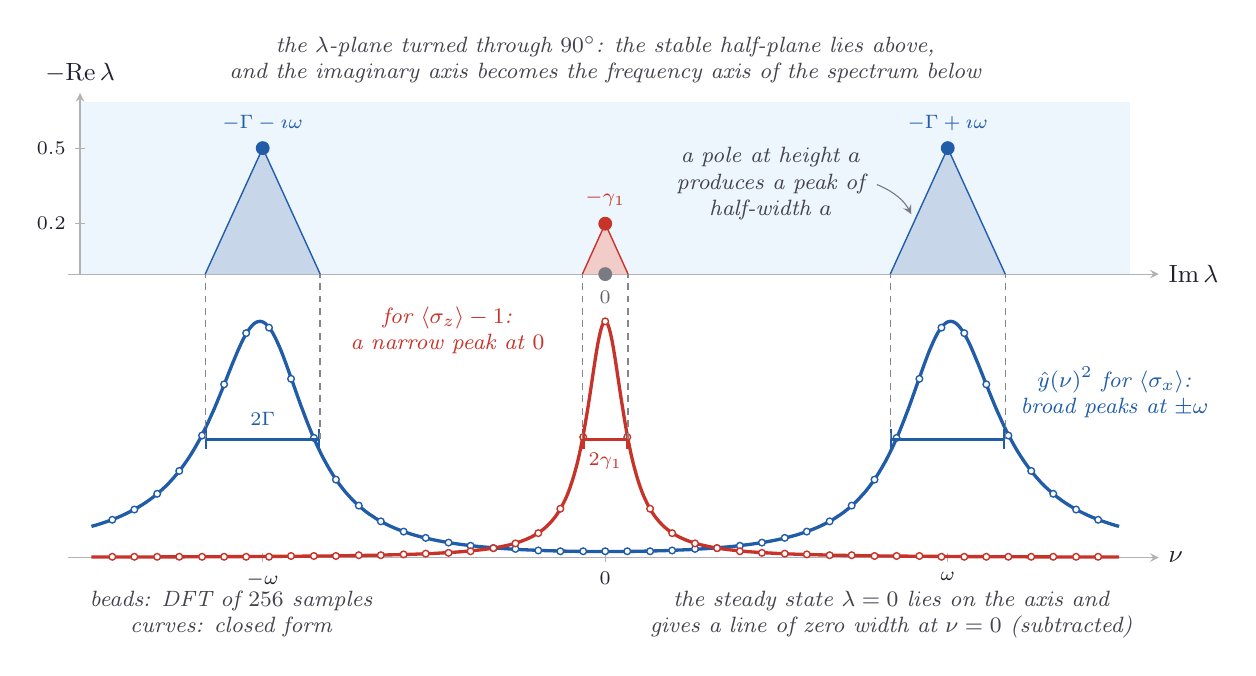
\begin{tikzpicture}[ink/.style={line width=0.9pt, ndInk}, faint/.style={line width=0.4pt, ndInk!35}, dashedink/.style={line width=0.5pt, ndInk!55, dash pattern=on 2.5pt off 2pt}, vec/.style={->, >=stealth, line width=1.2pt}, note/.style={font=\footnotesize\itshape, text=ndInk!85, align=center}, pointer/.style={->, >=stealth, line width=0.4pt, ndInk!60, shorten >=2pt, shorten <=1pt}, dot/.style={circle, fill=ndInk, inner sep=0pt, minimum size=3.4pt}, wash/.style={fill=ndSky, fill opacity=0.55}, every node/.style={text=ndInk}]
\definecolor{ndInk}{rgb}{0.13,0.13,0.18}
\definecolor{ndPaper}{rgb}{0.99,0.96,0.88}
\definecolor{ndSky}{rgb}{0.84,0.91,0.98}
\definecolor{ndRose}{rgb}{0.98,0.86,0.84}
\definecolor{ndBlue}{rgb}{0.13,0.36,0.66}
\definecolor{ndRed}{rgb}{0.78,0.20,0.16}
\definecolor{ndGold}{rgb}{0.88,0.62,0.10}
\definecolor{ndGreen}{rgb}{0.18,0.52,0.30}
\fill[ndSky, fill opacity=0.45] (-6.67,3.60) rectangle (6.67,5.78);
\draw[faint, ->, >=stealth] (-6.82,3.60) -- (7.03,3.60) node[right, text=ndInk, font=\small] {$\mathrm{Im}\,\lambda$};
\draw[faint, ->, >=stealth] (-6.67,3.60) -- (-6.67,5.90) node[above, text=ndInk, font=\small] {$-\mathrm{Re}\,\lambda$};
\draw[faint] (-6.61,4.24) -- (-6.73,4.24) node[left, font=\scriptsize, text=ndInk] {$0.2$};
\draw[faint] (-6.61,5.20) -- (-6.73,5.20) node[left, font=\scriptsize, text=ndInk] {$0.5$};
\node[note, anchor=south] at (0.00,5.90) {the $\lambda$-plane turned through $90^\circ$: the stable half-plane lies above,\\ and the imaginary axis becomes the frequency axis of the spectrum below};
\fill[ndBlue!25] (4.35,5.20) -- (3.62,3.60) -- (5.08,3.60) -- cycle;
\draw[ndBlue, line width=0.5pt] (3.62,3.60) -- (4.35,5.20) (4.35,5.20) -- (5.08,3.60);
\fill[ndBlue!25] (-4.35,5.20) -- (-5.08,3.60) -- (-3.62,3.60) -- cycle;
\draw[ndBlue, line width=0.5pt] (-5.08,3.60) -- (-4.35,5.20) (-4.35,5.20) -- (-3.62,3.60);
\fill[ndRed!25] (0.00,4.24) -- (-0.29,3.60) -- (0.29,3.60) -- cycle;
\draw[ndRed, line width=0.5pt] (-0.29,3.60) -- (0.00,4.24) (0.00,4.24) -- (0.29,3.60);
\node[dot, fill=ndBlue, minimum size=5pt, label={[font=\scriptsize, text=ndBlue]above:$-\Gamma+\imath\omega$}] at (4.35,5.20) {};
\node[dot, fill=ndBlue, minimum size=5pt, label={[font=\scriptsize, text=ndBlue]above:$-\Gamma-\imath\omega$}] at (-4.35,5.20) {};
\node[dot, fill=ndRed, minimum size=5pt, label={[font=\scriptsize, text=ndRed]above:$-\gamma_1$}] at (0.00,4.24) {};
\node[dot, fill=ndInk!60, minimum size=5pt, label={[font=\scriptsize, text=ndInk!70]below:$0$}] at (0.00,3.60) {};
\node[note] (c) at (2.10,4.75) {a pole at height $a$\\ produces a peak of\\ half-width $a$};
\draw[pointer] (c.east) to[bend left=20] (3.92,4.30);
\draw[faint, ->, >=stealth] (-6.82,0) -- (7.03,0) node[right, text=ndInk, font=\small] {$\nu$};
\draw[faint] (-4.35,0.06) -- (-4.35,-0.06) node[below, font=\scriptsize, text=ndInk] {$-\omega$};
\draw[faint] (0.00,0.06) -- (0.00,-0.06) node[below, font=\scriptsize, text=ndInk] {$0$};
\draw[faint] (4.35,0.06) -- (4.35,-0.06) node[below, font=\scriptsize, text=ndInk] {$\omega$};
\draw[line width=1.2pt, ndBlue] (-6.525,0.395) -- (-6.507,0.401) -- (-6.489,0.406) -- (-6.471,0.411) -- (-6.452,0.417) -- (-6.434,0.422) -- (-6.416,0.428) -- (-6.398,0.434) -- (-6.380,0.440) -- (-6.362,0.446) -- (-6.344,0.452) -- (-6.326,0.458) -- (-6.307,0.465) -- (-6.289,0.471) -- (-6.271,0.478) -- (-6.253,0.485) -- (-6.235,0.492) -- (-6.217,0.499) -- (-6.199,0.507) -- (-6.181,0.514) -- (-6.162,0.522) -- (-6.144,0.530) -- (-6.126,0.538) -- (-6.108,0.547) -- (-6.090,0.555) -- (-6.072,0.564) -- (-6.054,0.573) -- (-6.036,0.582) -- (-6.018,0.591) -- (-5.999,0.601) -- (-5.981,0.611) -- (-5.963,0.621) -- (-5.945,0.631) -- (-5.927,0.642) -- (-5.909,0.653) -- (-5.891,0.664) -- (-5.872,0.675) -- (-5.854,0.687) -- (-5.836,0.699) -- (-5.818,0.712) -- (-5.800,0.724) -- (-5.782,0.737) -- (-5.764,0.751) -- (-5.746,0.764) -- (-5.728,0.778) -- (-5.709,0.793) -- (-5.691,0.808) -- (-5.673,0.823) -- (-5.655,0.839) -- (-5.637,0.855) -- (-5.619,0.871) -- (-5.601,0.888) -- (-5.582,0.906) -- (-5.564,0.924) -- (-5.546,0.942) -- (-5.528,0.961) -- (-5.510,0.981) -- (-5.492,1.001) -- (-5.474,1.021) -- (-5.456,1.043) -- (-5.438,1.064) -- (-5.419,1.087) -- (-5.401,1.110) -- (-5.383,1.133) -- (-5.365,1.158) -- (-5.347,1.183) -- (-5.329,1.208) -- (-5.311,1.235) -- (-5.292,1.262) -- (-5.274,1.290) -- (-5.256,1.319) -- (-5.238,1.348) -- (-5.220,1.378) -- (-5.202,1.409) -- (-5.184,1.441) -- (-5.166,1.474) -- (-5.147,1.507) -- (-5.129,1.542) -- (-5.111,1.577) -- (-5.093,1.613) -- (-5.075,1.650) -- (-5.057,1.688) -- (-5.039,1.726) -- (-5.021,1.766) -- (-5.003,1.806) -- (-4.984,1.847) -- (-4.966,1.888) -- (-4.948,1.931) -- (-4.930,1.974) -- (-4.912,2.018) -- (-4.894,2.062) -- (-4.876,2.107) -- (-4.857,2.152) -- (-4.839,2.197) -- (-4.821,2.243) -- (-4.803,2.289) -- (-4.785,2.335) -- (-4.767,2.380) -- (-4.749,2.426) -- (-4.731,2.471) -- (-4.712,2.515) -- (-4.694,2.559) -- (-4.676,2.602) -- (-4.658,2.644) -- (-4.640,2.684) -- (-4.622,2.723) -- (-4.604,2.760) -- (-4.586,2.795) -- (-4.567,2.829) -- (-4.549,2.859) -- (-4.531,2.887) -- (-4.513,2.913) -- (-4.495,2.935) -- (-4.477,2.955) -- (-4.459,2.971) -- (-4.441,2.983) -- (-4.422,2.993) -- (-4.404,2.998) -- (-4.386,3.000) -- (-4.368,2.998) -- (-4.350,2.993) -- (-4.332,2.983) -- (-4.314,2.970) -- (-4.296,2.953) -- (-4.277,2.933) -- (-4.259,2.910) -- (-4.241,2.883) -- (-4.223,2.853) -- (-4.205,2.820) -- (-4.187,2.785) -- (-4.169,2.747) -- (-4.151,2.706) -- (-4.132,2.664) -- (-4.114,2.620) -- (-4.096,2.574) -- (-4.078,2.526) -- (-4.060,2.478) -- (-4.042,2.428) -- (-4.024,2.378) -- (-4.006,2.327) -- (-3.987,2.276) -- (-3.969,2.225) -- (-3.951,2.173) -- (-3.933,2.122) -- (-3.915,2.071) -- (-3.897,2.020) -- (-3.879,1.970) -- (-3.861,1.920) -- (-3.842,1.871) -- (-3.824,1.823) -- (-3.806,1.775) -- (-3.788,1.728) -- (-3.770,1.683) -- (-3.752,1.638) -- (-3.734,1.594) -- (-3.716,1.551) -- (-3.697,1.509) -- (-3.679,1.468) -- (-3.661,1.428) -- (-3.643,1.390) -- (-3.625,1.352) -- (-3.607,1.315) -- (-3.589,1.279) -- (-3.571,1.245) -- (-3.552,1.211) -- (-3.534,1.178) -- (-3.516,1.146) -- (-3.498,1.116) -- (-3.480,1.086) -- (-3.462,1.057) -- (-3.444,1.029) -- (-3.426,1.001) -- (-3.408,0.975) -- (-3.389,0.949) -- (-3.371,0.924) -- (-3.353,0.900) -- (-3.335,0.877) -- (-3.317,0.854) -- (-3.299,0.832) -- (-3.281,0.811) -- (-3.262,0.791) -- (-3.244,0.771) -- (-3.226,0.751) -- (-3.208,0.733) -- (-3.190,0.715) -- (-3.172,0.697) -- (-3.154,0.680) -- (-3.136,0.664) -- (-3.117,0.648) -- (-3.099,0.632) -- (-3.081,0.617) -- (-3.063,0.602) -- (-3.045,0.588) -- (-3.027,0.574) -- (-3.009,0.561) -- (-2.991,0.548) -- (-2.972,0.536) -- (-2.954,0.524) -- (-2.936,0.512) -- (-2.918,0.500) -- (-2.900,0.489) -- (-2.882,0.478) -- (-2.864,0.468) -- (-2.846,0.458) -- (-2.827,0.448) -- (-2.809,0.438) -- (-2.791,0.429) -- (-2.773,0.420) -- (-2.755,0.411) -- (-2.737,0.402) -- (-2.719,0.394) -- (-2.701,0.386) -- (-2.682,0.378) -- (-2.664,0.370) -- (-2.646,0.363) -- (-2.628,0.356) -- (-2.610,0.349) -- (-2.592,0.342) -- (-2.574,0.335) -- (-2.556,0.328) -- (-2.538,0.322) -- (-2.519,0.316) -- (-2.501,0.310) -- (-2.483,0.304) -- (-2.465,0.298) -- (-2.447,0.293) -- (-2.429,0.287) -- (-2.411,0.282) -- (-2.392,0.277) -- (-2.374,0.272) -- (-2.356,0.267) -- (-2.338,0.262) -- (-2.320,0.258) -- (-2.302,0.253) -- (-2.284,0.249) -- (-2.266,0.244) -- (-2.247,0.240) -- (-2.229,0.236) -- (-2.211,0.232) -- (-2.193,0.228) -- (-2.175,0.224) -- (-2.157,0.221) -- (-2.139,0.217) -- (-2.121,0.213) -- (-2.102,0.210) -- (-2.084,0.207) -- (-2.066,0.203) -- (-2.048,0.200) -- (-2.030,0.197) -- (-2.012,0.194) -- (-1.994,0.191) -- (-1.976,0.188) -- (-1.957,0.185) -- (-1.939,0.182) -- (-1.921,0.180) -- (-1.903,0.177) -- (-1.885,0.174) -- (-1.867,0.172) -- (-1.849,0.169) -- (-1.831,0.167) -- (-1.812,0.164) -- (-1.794,0.162) -- (-1.776,0.160) -- (-1.758,0.158) -- (-1.740,0.155) -- (-1.722,0.153) -- (-1.704,0.151) -- (-1.686,0.149) -- (-1.667,0.147) -- (-1.649,0.145) -- (-1.631,0.143) -- (-1.613,0.141) -- (-1.595,0.140) -- (-1.577,0.138) -- (-1.559,0.136) -- (-1.541,0.134) -- (-1.522,0.133) -- (-1.504,0.131) -- (-1.486,0.130) -- (-1.468,0.128) -- (-1.450,0.126) -- (-1.432,0.125) -- (-1.414,0.123) -- (-1.396,0.122) -- (-1.377,0.121) -- (-1.359,0.119) -- (-1.341,0.118) -- (-1.323,0.117) -- (-1.305,0.115) -- (-1.287,0.114) -- (-1.269,0.113) -- (-1.251,0.112) -- (-1.232,0.111) -- (-1.214,0.109) -- (-1.196,0.108) -- (-1.178,0.107) -- (-1.160,0.106) -- (-1.142,0.105) -- (-1.124,0.104) -- (-1.106,0.103) -- (-1.087,0.102) -- (-1.069,0.101) -- (-1.051,0.100) -- (-1.033,0.099) -- (-1.015,0.099) -- (-0.997,0.098) -- (-0.979,0.097) -- (-0.961,0.096) -- (-0.942,0.095) -- (-0.924,0.095) -- (-0.906,0.094) -- (-0.888,0.093) -- (-0.870,0.092) -- (-0.852,0.092) -- (-0.834,0.091) -- (-0.816,0.090) -- (-0.797,0.090) -- (-0.779,0.089) -- (-0.761,0.088) -- (-0.743,0.088) -- (-0.725,0.087) -- (-0.707,0.087) -- (-0.689,0.086) -- (-0.671,0.086) -- (-0.653,0.085) -- (-0.634,0.085) -- (-0.616,0.084) -- (-0.598,0.084) -- (-0.580,0.083) -- (-0.562,0.083) -- (-0.544,0.082) -- (-0.526,0.082) -- (-0.507,0.082) -- (-0.489,0.081) -- (-0.471,0.081) -- (-0.453,0.081) -- (-0.435,0.080) -- (-0.417,0.080) -- (-0.399,0.080) -- (-0.381,0.079) -- (-0.362,0.079) -- (-0.344,0.079) -- (-0.326,0.079) -- (-0.308,0.078) -- (-0.290,0.078) -- (-0.272,0.078) -- (-0.254,0.078) -- (-0.236,0.078) -- (-0.217,0.077) -- (-0.199,0.077) -- (-0.181,0.077) -- (-0.163,0.077) -- (-0.145,0.077) -- (-0.127,0.077) -- (-0.109,0.077) -- (-0.091,0.077) -- (-0.072,0.077) -- (-0.054,0.077) -- (-0.036,0.077) -- (-0.018,0.077) -- (0.000,0.077) -- (0.018,0.077) -- (0.036,0.077) -- (0.054,0.077) -- (0.072,0.077) -- (0.091,0.077) -- (0.109,0.077) -- (0.127,0.077) -- (0.145,0.077) -- (0.163,0.077) -- (0.181,0.077) -- (0.199,0.077) -- (0.218,0.077) -- (0.236,0.078) -- (0.254,0.078) -- (0.272,0.078) -- (0.290,0.078) -- (0.308,0.078) -- (0.326,0.079) -- (0.344,0.079) -- (0.362,0.079) -- (0.381,0.079) -- (0.399,0.080) -- (0.417,0.080) -- (0.435,0.080) -- (0.453,0.081) -- (0.471,0.081) -- (0.489,0.081) -- (0.508,0.082) -- (0.526,0.082) -- (0.544,0.082) -- (0.562,0.083) -- (0.580,0.083) -- (0.598,0.084) -- (0.616,0.084) -- (0.634,0.085) -- (0.653,0.085) -- (0.671,0.086) -- (0.689,0.086) -- (0.707,0.087) -- (0.725,0.087) -- (0.743,0.088) -- (0.761,0.088) -- (0.779,0.089) -- (0.798,0.090) -- (0.816,0.090) -- (0.834,0.091) -- (0.852,0.092) -- (0.870,0.092) -- (0.888,0.093) -- (0.906,0.094) -- (0.924,0.095) -- (0.943,0.095) -- (0.961,0.096) -- (0.979,0.097) -- (0.997,0.098) -- (1.015,0.099) -- (1.033,0.099) -- (1.051,0.100) -- (1.069,0.101) -- (1.087,0.102) -- (1.106,0.103) -- (1.124,0.104) -- (1.142,0.105) -- (1.160,0.106) -- (1.178,0.107) -- (1.196,0.108) -- (1.214,0.109) -- (1.233,0.111) -- (1.251,0.112) -- (1.269,0.113) -- (1.287,0.114) -- (1.305,0.115) -- (1.323,0.117) -- (1.341,0.118) -- (1.359,0.119) -- (1.378,0.121) -- (1.396,0.122) -- (1.414,0.123) -- (1.432,0.125) -- (1.450,0.126) -- (1.468,0.128) -- (1.486,0.130) -- (1.504,0.131) -- (1.523,0.133) -- (1.541,0.134) -- (1.559,0.136) -- (1.577,0.138) -- (1.595,0.140) -- (1.613,0.141) -- (1.631,0.143) -- (1.649,0.145) -- (1.668,0.147) -- (1.686,0.149) -- (1.704,0.151) -- (1.722,0.153) -- (1.740,0.155) -- (1.758,0.158) -- (1.776,0.160) -- (1.794,0.162) -- (1.812,0.164) -- (1.831,0.167) -- (1.849,0.169) -- (1.867,0.172) -- (1.885,0.174) -- (1.903,0.177) -- (1.921,0.180) -- (1.939,0.182) -- (1.958,0.185) -- (1.976,0.188) -- (1.994,0.191) -- (2.012,0.194) -- (2.030,0.197) -- (2.048,0.200) -- (2.066,0.203) -- (2.084,0.207) -- (2.103,0.210) -- (2.121,0.213) -- (2.139,0.217) -- (2.157,0.221) -- (2.175,0.224) -- (2.193,0.228) -- (2.211,0.232) -- (2.229,0.236) -- (2.248,0.240) -- (2.266,0.244) -- (2.284,0.249) -- (2.302,0.253) -- (2.320,0.258) -- (2.338,0.262) -- (2.356,0.267) -- (2.374,0.272) -- (2.393,0.277) -- (2.411,0.282) -- (2.429,0.287) -- (2.447,0.293) -- (2.465,0.298) -- (2.483,0.304) -- (2.501,0.310) -- (2.519,0.316) -- (2.538,0.322) -- (2.556,0.328) -- (2.574,0.335) -- (2.592,0.342) -- (2.610,0.349) -- (2.628,0.356) -- (2.646,0.363) -- (2.664,0.370) -- (2.683,0.378) -- (2.701,0.386) -- (2.719,0.394) -- (2.737,0.402) -- (2.755,0.411) -- (2.773,0.420) -- (2.791,0.429) -- (2.809,0.438) -- (2.828,0.448) -- (2.846,0.458) -- (2.864,0.468) -- (2.882,0.478) -- (2.900,0.489) -- (2.918,0.500) -- (2.936,0.512) -- (2.954,0.524) -- (2.973,0.536) -- (2.991,0.548) -- (3.009,0.561) -- (3.027,0.574) -- (3.045,0.588) -- (3.063,0.602) -- (3.081,0.617) -- (3.099,0.632) -- (3.118,0.648) -- (3.136,0.664) -- (3.154,0.680) -- (3.172,0.697) -- (3.190,0.715) -- (3.208,0.733) -- (3.226,0.751) -- (3.244,0.771) -- (3.262,0.791) -- (3.281,0.811) -- (3.299,0.832) -- (3.317,0.854) -- (3.335,0.877) -- (3.353,0.900) -- (3.371,0.924) -- (3.389,0.949) -- (3.408,0.975) -- (3.426,1.001) -- (3.444,1.029) -- (3.462,1.057) -- (3.480,1.086) -- (3.498,1.116) -- (3.516,1.146) -- (3.534,1.178) -- (3.553,1.211) -- (3.571,1.245) -- (3.589,1.279) -- (3.607,1.315) -- (3.625,1.352) -- (3.643,1.390) -- (3.661,1.428) -- (3.679,1.468) -- (3.698,1.509) -- (3.716,1.551) -- (3.734,1.594) -- (3.752,1.638) -- (3.770,1.683) -- (3.788,1.728) -- (3.806,1.775) -- (3.824,1.823) -- (3.843,1.871) -- (3.861,1.920) -- (3.879,1.970) -- (3.897,2.020) -- (3.915,2.071) -- (3.933,2.122) -- (3.951,2.173) -- (3.969,2.225) -- (3.987,2.276) -- (4.006,2.327) -- (4.024,2.378) -- (4.042,2.428) -- (4.060,2.478) -- (4.078,2.526) -- (4.096,2.574) -- (4.114,2.620) -- (4.133,2.664) -- (4.151,2.706) -- (4.169,2.747) -- (4.187,2.785) -- (4.205,2.820) -- (4.223,2.853) -- (4.241,2.883) -- (4.259,2.910) -- (4.277,2.933) -- (4.296,2.953) -- (4.314,2.970) -- (4.332,2.983) -- (4.350,2.993) -- (4.368,2.998) -- (4.386,3.000) -- (4.404,2.998) -- (4.423,2.993) -- (4.441,2.983) -- (4.459,2.971) -- (4.477,2.955) -- (4.495,2.935) -- (4.513,2.913) -- (4.531,2.887) -- (4.549,2.859) -- (4.568,2.829) -- (4.586,2.795) -- (4.604,2.760) -- (4.622,2.723) -- (4.640,2.684) -- (4.658,2.644) -- (4.676,2.602) -- (4.694,2.559) -- (4.712,2.515) -- (4.731,2.471) -- (4.749,2.426) -- (4.767,2.380) -- (4.785,2.335) -- (4.803,2.289) -- (4.821,2.243) -- (4.839,2.197) -- (4.858,2.152) -- (4.876,2.107) -- (4.894,2.062) -- (4.912,2.018) -- (4.930,1.974) -- (4.948,1.931) -- (4.966,1.888) -- (4.984,1.847) -- (5.003,1.806) -- (5.021,1.766) -- (5.039,1.726) -- (5.057,1.688) -- (5.075,1.650) -- (5.093,1.613) -- (5.111,1.577) -- (5.129,1.542) -- (5.148,1.507) -- (5.166,1.474) -- (5.184,1.441) -- (5.202,1.409) -- (5.220,1.378) -- (5.238,1.348) -- (5.256,1.319) -- (5.274,1.290) -- (5.293,1.262) -- (5.311,1.235) -- (5.329,1.208) -- (5.347,1.183) -- (5.365,1.158) -- (5.383,1.133) -- (5.401,1.110) -- (5.419,1.087) -- (5.438,1.064) -- (5.456,1.043) -- (5.474,1.021) -- (5.492,1.001) -- (5.510,0.981) -- (5.528,0.961) -- (5.546,0.942) -- (5.564,0.924) -- (5.582,0.906) -- (5.601,0.888) -- (5.619,0.871) -- (5.637,0.855) -- (5.655,0.839) -- (5.673,0.823) -- (5.691,0.808) -- (5.709,0.793) -- (5.728,0.778) -- (5.746,0.764) -- (5.764,0.751) -- (5.782,0.737) -- (5.800,0.724) -- (5.818,0.712) -- (5.836,0.699) -- (5.854,0.687) -- (5.873,0.675) -- (5.891,0.664) -- (5.909,0.653) -- (5.927,0.642) -- (5.945,0.631) -- (5.963,0.621) -- (5.981,0.611) -- (5.999,0.601) -- (6.018,0.591) -- (6.036,0.582) -- (6.054,0.573) -- (6.072,0.564) -- (6.090,0.555) -- (6.108,0.547) -- (6.126,0.538) -- (6.144,0.530) -- (6.162,0.522) -- (6.181,0.514) -- (6.199,0.507) -- (6.217,0.499) -- (6.235,0.492) -- (6.253,0.485) -- (6.271,0.478) -- (6.289,0.471) -- (6.307,0.465) -- (6.326,0.458) -- (6.344,0.452) -- (6.362,0.446) -- (6.380,0.440) -- (6.398,0.434) -- (6.416,0.428) -- (6.434,0.422) -- (6.453,0.417) -- (6.471,0.411) -- (6.489,0.406) -- (6.507,0.401) -- (6.525,0.395);
\draw[line width=1.2pt, ndRed] (-6.525,0.007) -- (-6.507,0.007) -- (-6.489,0.007) -- (-6.471,0.007) -- (-6.452,0.007) -- (-6.434,0.007) -- (-6.416,0.007) -- (-6.398,0.007) -- (-6.380,0.007) -- (-6.362,0.007) -- (-6.344,0.007) -- (-6.326,0.007) -- (-6.307,0.007) -- (-6.289,0.007) -- (-6.271,0.007) -- (-6.253,0.007) -- (-6.235,0.007) -- (-6.217,0.007) -- (-6.199,0.007) -- (-6.181,0.007) -- (-6.162,0.007) -- (-6.144,0.007) -- (-6.126,0.007) -- (-6.108,0.007) -- (-6.090,0.007) -- (-6.072,0.007) -- (-6.054,0.008) -- (-6.036,0.008) -- (-6.018,0.008) -- (-5.999,0.008) -- (-5.981,0.008) -- (-5.963,0.008) -- (-5.945,0.008) -- (-5.927,0.008) -- (-5.909,0.008) -- (-5.891,0.008) -- (-5.872,0.008) -- (-5.854,0.008) -- (-5.836,0.008) -- (-5.818,0.008) -- (-5.800,0.008) -- (-5.782,0.008) -- (-5.764,0.008) -- (-5.746,0.008) -- (-5.728,0.008) -- (-5.709,0.008) -- (-5.691,0.008) -- (-5.673,0.008) -- (-5.655,0.009) -- (-5.637,0.009) -- (-5.619,0.009) -- (-5.601,0.009) -- (-5.582,0.009) -- (-5.564,0.009) -- (-5.546,0.009) -- (-5.528,0.009) -- (-5.510,0.009) -- (-5.492,0.009) -- (-5.474,0.009) -- (-5.456,0.009) -- (-5.438,0.009) -- (-5.419,0.009) -- (-5.401,0.009) -- (-5.383,0.009) -- (-5.365,0.009) -- (-5.347,0.009) -- (-5.329,0.010) -- (-5.311,0.010) -- (-5.292,0.010) -- (-5.274,0.010) -- (-5.256,0.010) -- (-5.238,0.010) -- (-5.220,0.010) -- (-5.202,0.010) -- (-5.184,0.010) -- (-5.166,0.010) -- (-5.147,0.010) -- (-5.129,0.010) -- (-5.111,0.010) -- (-5.093,0.010) -- (-5.075,0.010) -- (-5.057,0.010) -- (-5.039,0.011) -- (-5.021,0.011) -- (-5.003,0.011) -- (-4.984,0.011) -- (-4.966,0.011) -- (-4.948,0.011) -- (-4.930,0.011) -- (-4.912,0.011) -- (-4.894,0.011) -- (-4.876,0.011) -- (-4.857,0.011) -- (-4.839,0.011) -- (-4.821,0.011) -- (-4.803,0.012) -- (-4.785,0.012) -- (-4.767,0.012) -- (-4.749,0.012) -- (-4.731,0.012) -- (-4.712,0.012) -- (-4.694,0.012) -- (-4.676,0.012) -- (-4.658,0.012) -- (-4.640,0.012) -- (-4.622,0.012) -- (-4.604,0.012) -- (-4.586,0.013) -- (-4.567,0.013) -- (-4.549,0.013) -- (-4.531,0.013) -- (-4.513,0.013) -- (-4.495,0.013) -- (-4.477,0.013) -- (-4.459,0.013) -- (-4.441,0.013) -- (-4.422,0.013) -- (-4.404,0.014) -- (-4.386,0.014) -- (-4.368,0.014) -- (-4.350,0.014) -- (-4.332,0.014) -- (-4.314,0.014) -- (-4.296,0.014) -- (-4.277,0.014) -- (-4.259,0.014) -- (-4.241,0.015) -- (-4.223,0.015) -- (-4.205,0.015) -- (-4.187,0.015) -- (-4.169,0.015) -- (-4.151,0.015) -- (-4.132,0.015) -- (-4.114,0.015) -- (-4.096,0.016) -- (-4.078,0.016) -- (-4.060,0.016) -- (-4.042,0.016) -- (-4.024,0.016) -- (-4.006,0.016) -- (-3.987,0.016) -- (-3.969,0.017) -- (-3.951,0.017) -- (-3.933,0.017) -- (-3.915,0.017) -- (-3.897,0.017) -- (-3.879,0.017) -- (-3.861,0.017) -- (-3.842,0.018) -- (-3.824,0.018) -- (-3.806,0.018) -- (-3.788,0.018) -- (-3.770,0.018) -- (-3.752,0.018) -- (-3.734,0.019) -- (-3.716,0.019) -- (-3.697,0.019) -- (-3.679,0.019) -- (-3.661,0.019) -- (-3.643,0.020) -- (-3.625,0.020) -- (-3.607,0.020) -- (-3.589,0.020) -- (-3.571,0.020) -- (-3.552,0.020) -- (-3.534,0.021) -- (-3.516,0.021) -- (-3.498,0.021) -- (-3.480,0.021) -- (-3.462,0.022) -- (-3.444,0.022) -- (-3.426,0.022) -- (-3.408,0.022) -- (-3.389,0.022) -- (-3.371,0.023) -- (-3.353,0.023) -- (-3.335,0.023) -- (-3.317,0.023) -- (-3.299,0.024) -- (-3.281,0.024) -- (-3.262,0.024) -- (-3.244,0.024) -- (-3.226,0.025) -- (-3.208,0.025) -- (-3.190,0.025) -- (-3.172,0.025) -- (-3.154,0.026) -- (-3.136,0.026) -- (-3.117,0.026) -- (-3.099,0.027) -- (-3.081,0.027) -- (-3.063,0.027) -- (-3.045,0.028) -- (-3.027,0.028) -- (-3.009,0.028) -- (-2.991,0.029) -- (-2.972,0.029) -- (-2.954,0.029) -- (-2.936,0.030) -- (-2.918,0.030) -- (-2.900,0.030) -- (-2.882,0.031) -- (-2.864,0.031) -- (-2.846,0.031) -- (-2.827,0.032) -- (-2.809,0.032) -- (-2.791,0.033) -- (-2.773,0.033) -- (-2.755,0.034) -- (-2.737,0.034) -- (-2.719,0.034) -- (-2.701,0.035) -- (-2.682,0.035) -- (-2.664,0.036) -- (-2.646,0.036) -- (-2.628,0.037) -- (-2.610,0.037) -- (-2.592,0.038) -- (-2.574,0.038) -- (-2.556,0.039) -- (-2.538,0.039) -- (-2.519,0.040) -- (-2.501,0.040) -- (-2.483,0.041) -- (-2.465,0.042) -- (-2.447,0.042) -- (-2.429,0.043) -- (-2.411,0.043) -- (-2.392,0.044) -- (-2.374,0.045) -- (-2.356,0.045) -- (-2.338,0.046) -- (-2.320,0.047) -- (-2.302,0.047) -- (-2.284,0.048) -- (-2.266,0.049) -- (-2.247,0.050) -- (-2.229,0.051) -- (-2.211,0.051) -- (-2.193,0.052) -- (-2.175,0.053) -- (-2.157,0.054) -- (-2.139,0.055) -- (-2.121,0.056) -- (-2.102,0.057) -- (-2.084,0.058) -- (-2.066,0.059) -- (-2.048,0.060) -- (-2.030,0.061) -- (-2.012,0.062) -- (-1.994,0.063) -- (-1.976,0.064) -- (-1.957,0.065) -- (-1.939,0.066) -- (-1.921,0.067) -- (-1.903,0.069) -- (-1.885,0.070) -- (-1.867,0.071) -- (-1.849,0.073) -- (-1.831,0.074) -- (-1.812,0.075) -- (-1.794,0.077) -- (-1.776,0.079) -- (-1.758,0.080) -- (-1.740,0.082) -- (-1.722,0.083) -- (-1.704,0.085) -- (-1.686,0.087) -- (-1.667,0.089) -- (-1.649,0.091) -- (-1.631,0.093) -- (-1.613,0.095) -- (-1.595,0.097) -- (-1.577,0.099) -- (-1.559,0.101) -- (-1.541,0.103) -- (-1.522,0.106) -- (-1.504,0.108) -- (-1.486,0.111) -- (-1.468,0.113) -- (-1.450,0.116) -- (-1.432,0.119) -- (-1.414,0.122) -- (-1.396,0.125) -- (-1.377,0.128) -- (-1.359,0.131) -- (-1.341,0.135) -- (-1.323,0.138) -- (-1.305,0.142) -- (-1.287,0.146) -- (-1.269,0.150) -- (-1.251,0.154) -- (-1.232,0.158) -- (-1.214,0.162) -- (-1.196,0.167) -- (-1.178,0.172) -- (-1.160,0.177) -- (-1.142,0.182) -- (-1.124,0.188) -- (-1.106,0.194) -- (-1.087,0.200) -- (-1.069,0.206) -- (-1.051,0.213) -- (-1.033,0.220) -- (-1.015,0.227) -- (-0.997,0.235) -- (-0.979,0.243) -- (-0.961,0.251) -- (-0.942,0.260) -- (-0.924,0.269) -- (-0.906,0.279) -- (-0.888,0.290) -- (-0.870,0.301) -- (-0.852,0.312) -- (-0.834,0.324) -- (-0.816,0.337) -- (-0.797,0.351) -- (-0.779,0.365) -- (-0.761,0.381) -- (-0.743,0.397) -- (-0.725,0.414) -- (-0.707,0.433) -- (-0.689,0.452) -- (-0.671,0.473) -- (-0.653,0.495) -- (-0.634,0.519) -- (-0.616,0.544) -- (-0.598,0.572) -- (-0.580,0.601) -- (-0.562,0.632) -- (-0.544,0.665) -- (-0.526,0.701) -- (-0.507,0.739) -- (-0.489,0.780) -- (-0.471,0.824) -- (-0.453,0.872) -- (-0.435,0.924) -- (-0.417,0.979) -- (-0.399,1.038) -- (-0.381,1.102) -- (-0.362,1.171) -- (-0.344,1.245) -- (-0.326,1.324) -- (-0.308,1.410) -- (-0.290,1.500) -- (-0.272,1.597) -- (-0.254,1.699) -- (-0.236,1.807) -- (-0.217,1.920) -- (-0.199,2.037) -- (-0.181,2.157) -- (-0.163,2.279) -- (-0.145,2.400) -- (-0.127,2.518) -- (-0.109,2.630) -- (-0.091,2.733) -- (-0.072,2.824) -- (-0.054,2.898) -- (-0.036,2.954) -- (-0.018,2.988) -- (0.000,3.000) -- (0.018,2.988) -- (0.036,2.954) -- (0.054,2.898) -- (0.072,2.824) -- (0.091,2.733) -- (0.109,2.630) -- (0.127,2.518) -- (0.145,2.400) -- (0.163,2.279) -- (0.181,2.157) -- (0.199,2.037) -- (0.218,1.920) -- (0.236,1.807) -- (0.254,1.699) -- (0.272,1.597) -- (0.290,1.500) -- (0.308,1.410) -- (0.326,1.324) -- (0.344,1.245) -- (0.362,1.171) -- (0.381,1.102) -- (0.399,1.038) -- (0.417,0.979) -- (0.435,0.924) -- (0.453,0.872) -- (0.471,0.824) -- (0.489,0.780) -- (0.508,0.739) -- (0.526,0.701) -- (0.544,0.665) -- (0.562,0.632) -- (0.580,0.601) -- (0.598,0.572) -- (0.616,0.544) -- (0.634,0.519) -- (0.653,0.495) -- (0.671,0.473) -- (0.689,0.452) -- (0.707,0.433) -- (0.725,0.414) -- (0.743,0.397) -- (0.761,0.381) -- (0.779,0.365) -- (0.798,0.351) -- (0.816,0.337) -- (0.834,0.324) -- (0.852,0.312) -- (0.870,0.301) -- (0.888,0.290) -- (0.906,0.279) -- (0.924,0.269) -- (0.943,0.260) -- (0.961,0.251) -- (0.979,0.243) -- (0.997,0.235) -- (1.015,0.227) -- (1.033,0.220) -- (1.051,0.213) -- (1.069,0.206) -- (1.087,0.200) -- (1.106,0.194) -- (1.124,0.188) -- (1.142,0.182) -- (1.160,0.177) -- (1.178,0.172) -- (1.196,0.167) -- (1.214,0.162) -- (1.233,0.158) -- (1.251,0.154) -- (1.269,0.150) -- (1.287,0.146) -- (1.305,0.142) -- (1.323,0.138) -- (1.341,0.135) -- (1.359,0.131) -- (1.378,0.128) -- (1.396,0.125) -- (1.414,0.122) -- (1.432,0.119) -- (1.450,0.116) -- (1.468,0.113) -- (1.486,0.111) -- (1.504,0.108) -- (1.523,0.106) -- (1.541,0.103) -- (1.559,0.101) -- (1.577,0.099) -- (1.595,0.097) -- (1.613,0.095) -- (1.631,0.093) -- (1.649,0.091) -- (1.668,0.089) -- (1.686,0.087) -- (1.704,0.085) -- (1.722,0.083) -- (1.740,0.082) -- (1.758,0.080) -- (1.776,0.079) -- (1.794,0.077) -- (1.812,0.075) -- (1.831,0.074) -- (1.849,0.073) -- (1.867,0.071) -- (1.885,0.070) -- (1.903,0.069) -- (1.921,0.067) -- (1.939,0.066) -- (1.958,0.065) -- (1.976,0.064) -- (1.994,0.063) -- (2.012,0.062) -- (2.030,0.061) -- (2.048,0.060) -- (2.066,0.059) -- (2.084,0.058) -- (2.103,0.057) -- (2.121,0.056) -- (2.139,0.055) -- (2.157,0.054) -- (2.175,0.053) -- (2.193,0.052) -- (2.211,0.051) -- (2.229,0.051) -- (2.248,0.050) -- (2.266,0.049) -- (2.284,0.048) -- (2.302,0.047) -- (2.320,0.047) -- (2.338,0.046) -- (2.356,0.045) -- (2.374,0.045) -- (2.393,0.044) -- (2.411,0.043) -- (2.429,0.043) -- (2.447,0.042) -- (2.465,0.042) -- (2.483,0.041) -- (2.501,0.040) -- (2.519,0.040) -- (2.538,0.039) -- (2.556,0.039) -- (2.574,0.038) -- (2.592,0.038) -- (2.610,0.037) -- (2.628,0.037) -- (2.646,0.036) -- (2.664,0.036) -- (2.683,0.035) -- (2.701,0.035) -- (2.719,0.034) -- (2.737,0.034) -- (2.755,0.034) -- (2.773,0.033) -- (2.791,0.033) -- (2.809,0.032) -- (2.828,0.032) -- (2.846,0.031) -- (2.864,0.031) -- (2.882,0.031) -- (2.900,0.030) -- (2.918,0.030) -- (2.936,0.030) -- (2.954,0.029) -- (2.973,0.029) -- (2.991,0.029) -- (3.009,0.028) -- (3.027,0.028) -- (3.045,0.028) -- (3.063,0.027) -- (3.081,0.027) -- (3.099,0.027) -- (3.118,0.026) -- (3.136,0.026) -- (3.154,0.026) -- (3.172,0.025) -- (3.190,0.025) -- (3.208,0.025) -- (3.226,0.025) -- (3.244,0.024) -- (3.262,0.024) -- (3.281,0.024) -- (3.299,0.024) -- (3.317,0.023) -- (3.335,0.023) -- (3.353,0.023) -- (3.371,0.023) -- (3.389,0.022) -- (3.408,0.022) -- (3.426,0.022) -- (3.444,0.022) -- (3.462,0.022) -- (3.480,0.021) -- (3.498,0.021) -- (3.516,0.021) -- (3.534,0.021) -- (3.553,0.020) -- (3.571,0.020) -- (3.589,0.020) -- (3.607,0.020) -- (3.625,0.020) -- (3.643,0.020) -- (3.661,0.019) -- (3.679,0.019) -- (3.698,0.019) -- (3.716,0.019) -- (3.734,0.019) -- (3.752,0.018) -- (3.770,0.018) -- (3.788,0.018) -- (3.806,0.018) -- (3.824,0.018) -- (3.843,0.018) -- (3.861,0.017) -- (3.879,0.017) -- (3.897,0.017) -- (3.915,0.017) -- (3.933,0.017) -- (3.951,0.017) -- (3.969,0.017) -- (3.987,0.016) -- (4.006,0.016) -- (4.024,0.016) -- (4.042,0.016) -- (4.060,0.016) -- (4.078,0.016) -- (4.096,0.016) -- (4.114,0.015) -- (4.133,0.015) -- (4.151,0.015) -- (4.169,0.015) -- (4.187,0.015) -- (4.205,0.015) -- (4.223,0.015) -- (4.241,0.015) -- (4.259,0.014) -- (4.277,0.014) -- (4.296,0.014) -- (4.314,0.014) -- (4.332,0.014) -- (4.350,0.014) -- (4.368,0.014) -- (4.386,0.014) -- (4.404,0.014) -- (4.423,0.013) -- (4.441,0.013) -- (4.459,0.013) -- (4.477,0.013) -- (4.495,0.013) -- (4.513,0.013) -- (4.531,0.013) -- (4.549,0.013) -- (4.568,0.013) -- (4.586,0.013) -- (4.604,0.012) -- (4.622,0.012) -- (4.640,0.012) -- (4.658,0.012) -- (4.676,0.012) -- (4.694,0.012) -- (4.712,0.012) -- (4.731,0.012) -- (4.749,0.012) -- (4.767,0.012) -- (4.785,0.012) -- (4.803,0.012) -- (4.821,0.011) -- (4.839,0.011) -- (4.858,0.011) -- (4.876,0.011) -- (4.894,0.011) -- (4.912,0.011) -- (4.930,0.011) -- (4.948,0.011) -- (4.966,0.011) -- (4.984,0.011) -- (5.003,0.011) -- (5.021,0.011) -- (5.039,0.011) -- (5.057,0.010) -- (5.075,0.010) -- (5.093,0.010) -- (5.111,0.010) -- (5.129,0.010) -- (5.148,0.010) -- (5.166,0.010) -- (5.184,0.010) -- (5.202,0.010) -- (5.220,0.010) -- (5.238,0.010) -- (5.256,0.010) -- (5.274,0.010) -- (5.293,0.010) -- (5.311,0.010) -- (5.329,0.010) -- (5.347,0.009) -- (5.365,0.009) -- (5.383,0.009) -- (5.401,0.009) -- (5.419,0.009) -- (5.438,0.009) -- (5.456,0.009) -- (5.474,0.009) -- (5.492,0.009) -- (5.510,0.009) -- (5.528,0.009) -- (5.546,0.009) -- (5.564,0.009) -- (5.582,0.009) -- (5.601,0.009) -- (5.619,0.009) -- (5.637,0.009) -- (5.655,0.009) -- (5.673,0.008) -- (5.691,0.008) -- (5.709,0.008) -- (5.728,0.008) -- (5.746,0.008) -- (5.764,0.008) -- (5.782,0.008) -- (5.800,0.008) -- (5.818,0.008) -- (5.836,0.008) -- (5.854,0.008) -- (5.873,0.008) -- (5.891,0.008) -- (5.909,0.008) -- (5.927,0.008) -- (5.945,0.008) -- (5.963,0.008) -- (5.981,0.008) -- (5.999,0.008) -- (6.018,0.008) -- (6.036,0.008) -- (6.054,0.008) -- (6.072,0.007) -- (6.090,0.007) -- (6.108,0.007) -- (6.126,0.007) -- (6.144,0.007) -- (6.162,0.007) -- (6.181,0.007) -- (6.199,0.007) -- (6.217,0.007) -- (6.235,0.007) -- (6.253,0.007) -- (6.271,0.007) -- (6.289,0.007) -- (6.307,0.007) -- (6.326,0.007) -- (6.344,0.007) -- (6.362,0.007) -- (6.380,0.007) -- (6.398,0.007) -- (6.416,0.007) -- (6.434,0.007) -- (6.453,0.007) -- (6.471,0.007) -- (6.489,0.007) -- (6.507,0.007) -- (6.525,0.007);
\filldraw[fill=white, draw=ndBlue, line width=0.5pt] (0.00,0.08) circle (1.2pt);
\filldraw[fill=white, draw=ndBlue, line width=0.5pt] (0.28,0.08) circle (1.2pt);
\filldraw[fill=white, draw=ndBlue, line width=0.5pt] (0.57,0.08) circle (1.2pt);
\filldraw[fill=white, draw=ndBlue, line width=0.5pt] (0.85,0.09) circle (1.2pt);
\filldraw[fill=white, draw=ndBlue, line width=0.5pt] (1.14,0.11) circle (1.2pt);
\filldraw[fill=white, draw=ndBlue, line width=0.5pt] (1.42,0.12) circle (1.2pt);
\filldraw[fill=white, draw=ndBlue, line width=0.5pt] (1.71,0.15) circle (1.2pt);
\filldraw[fill=white, draw=ndBlue, line width=0.5pt] (1.99,0.19) circle (1.2pt);
\filldraw[fill=white, draw=ndBlue, line width=0.5pt] (2.28,0.25) circle (1.2pt);
\filldraw[fill=white, draw=ndBlue, line width=0.5pt] (2.56,0.33) circle (1.2pt);
\filldraw[fill=white, draw=ndBlue, line width=0.5pt] (2.85,0.46) circle (1.2pt);
\filldraw[fill=white, draw=ndBlue, line width=0.5pt] (3.13,0.66) circle (1.2pt);
\filldraw[fill=white, draw=ndBlue, line width=0.5pt] (3.42,0.99) circle (1.2pt);
\filldraw[fill=white, draw=ndBlue, line width=0.5pt] (3.70,1.52) circle (1.2pt);
\filldraw[fill=white, draw=ndBlue, line width=0.5pt] (3.99,2.27) circle (1.2pt);
\filldraw[fill=white, draw=ndBlue, line width=0.5pt] (4.27,2.92) circle (1.2pt);
\filldraw[fill=white, draw=ndBlue, line width=0.5pt] (4.56,2.85) circle (1.2pt);
\filldraw[fill=white, draw=ndBlue, line width=0.5pt] (4.84,2.20) circle (1.2pt);
\filldraw[fill=white, draw=ndBlue, line width=0.5pt] (5.12,1.55) circle (1.2pt);
\filldraw[fill=white, draw=ndBlue, line width=0.5pt] (5.41,1.10) circle (1.2pt);
\filldraw[fill=white, draw=ndBlue, line width=0.5pt] (5.69,0.81) circle (1.2pt);
\filldraw[fill=white, draw=ndBlue, line width=0.5pt] (5.98,0.61) circle (1.2pt);
\filldraw[fill=white, draw=ndBlue, line width=0.5pt] (6.26,0.48) circle (1.2pt);
\filldraw[fill=white, draw=ndBlue, line width=0.5pt] (-6.26,0.48) circle (1.2pt);
\filldraw[fill=white, draw=ndBlue, line width=0.5pt] (-5.98,0.61) circle (1.2pt);
\filldraw[fill=white, draw=ndBlue, line width=0.5pt] (-5.69,0.81) circle (1.2pt);
\filldraw[fill=white, draw=ndBlue, line width=0.5pt] (-5.41,1.10) circle (1.2pt);
\filldraw[fill=white, draw=ndBlue, line width=0.5pt] (-5.12,1.55) circle (1.2pt);
\filldraw[fill=white, draw=ndBlue, line width=0.5pt] (-4.84,2.20) circle (1.2pt);
\filldraw[fill=white, draw=ndBlue, line width=0.5pt] (-4.56,2.85) circle (1.2pt);
\filldraw[fill=white, draw=ndBlue, line width=0.5pt] (-4.27,2.92) circle (1.2pt);
\filldraw[fill=white, draw=ndBlue, line width=0.5pt] (-3.99,2.27) circle (1.2pt);
\filldraw[fill=white, draw=ndBlue, line width=0.5pt] (-3.70,1.52) circle (1.2pt);
\filldraw[fill=white, draw=ndBlue, line width=0.5pt] (-3.42,0.99) circle (1.2pt);
\filldraw[fill=white, draw=ndBlue, line width=0.5pt] (-3.13,0.66) circle (1.2pt);
\filldraw[fill=white, draw=ndBlue, line width=0.5pt] (-2.85,0.46) circle (1.2pt);
\filldraw[fill=white, draw=ndBlue, line width=0.5pt] (-2.56,0.33) circle (1.2pt);
\filldraw[fill=white, draw=ndBlue, line width=0.5pt] (-2.28,0.25) circle (1.2pt);
\filldraw[fill=white, draw=ndBlue, line width=0.5pt] (-1.99,0.19) circle (1.2pt);
\filldraw[fill=white, draw=ndBlue, line width=0.5pt] (-1.71,0.15) circle (1.2pt);
\filldraw[fill=white, draw=ndBlue, line width=0.5pt] (-1.42,0.12) circle (1.2pt);
\filldraw[fill=white, draw=ndBlue, line width=0.5pt] (-1.14,0.11) circle (1.2pt);
\filldraw[fill=white, draw=ndBlue, line width=0.5pt] (-0.85,0.09) circle (1.2pt);
\filldraw[fill=white, draw=ndBlue, line width=0.5pt] (-0.57,0.08) circle (1.2pt);
\filldraw[fill=white, draw=ndBlue, line width=0.5pt] (-0.28,0.08) circle (1.2pt);
\filldraw[fill=white, draw=ndRed, line width=0.5pt] (0.00,3.00) circle (1.2pt);
\filldraw[fill=white, draw=ndRed, line width=0.5pt] (0.28,1.53) circle (1.2pt);
\filldraw[fill=white, draw=ndRed, line width=0.5pt] (0.57,0.62) circle (1.2pt);
\filldraw[fill=white, draw=ndRed, line width=0.5pt] (0.85,0.31) circle (1.2pt);
\filldraw[fill=white, draw=ndRed, line width=0.5pt] (1.14,0.18) circle (1.2pt);
\filldraw[fill=white, draw=ndRed, line width=0.5pt] (1.42,0.12) circle (1.2pt);
\filldraw[fill=white, draw=ndRed, line width=0.5pt] (1.71,0.08) circle (1.2pt);
\filldraw[fill=white, draw=ndRed, line width=0.5pt] (1.99,0.06) circle (1.2pt);
\filldraw[fill=white, draw=ndRed, line width=0.5pt] (2.28,0.05) circle (1.2pt);
\filldraw[fill=white, draw=ndRed, line width=0.5pt] (2.56,0.04) circle (1.2pt);
\filldraw[fill=white, draw=ndRed, line width=0.5pt] (2.85,0.03) circle (1.2pt);
\filldraw[fill=white, draw=ndRed, line width=0.5pt] (3.13,0.03) circle (1.2pt);
\filldraw[fill=white, draw=ndRed, line width=0.5pt] (3.42,0.02) circle (1.2pt);
\filldraw[fill=white, draw=ndRed, line width=0.5pt] (3.70,0.02) circle (1.2pt);
\filldraw[fill=white, draw=ndRed, line width=0.5pt] (3.99,0.02) circle (1.2pt);
\filldraw[fill=white, draw=ndRed, line width=0.5pt] (4.27,0.01) circle (1.2pt);
\filldraw[fill=white, draw=ndRed, line width=0.5pt] (4.56,0.01) circle (1.2pt);
\filldraw[fill=white, draw=ndRed, line width=0.5pt] (4.84,0.01) circle (1.2pt);
\filldraw[fill=white, draw=ndRed, line width=0.5pt] (5.12,0.01) circle (1.2pt);
\filldraw[fill=white, draw=ndRed, line width=0.5pt] (5.41,0.01) circle (1.2pt);
\filldraw[fill=white, draw=ndRed, line width=0.5pt] (5.69,0.01) circle (1.2pt);
\filldraw[fill=white, draw=ndRed, line width=0.5pt] (5.98,0.01) circle (1.2pt);
\filldraw[fill=white, draw=ndRed, line width=0.5pt] (6.26,0.01) circle (1.2pt);
\filldraw[fill=white, draw=ndRed, line width=0.5pt] (-6.26,0.01) circle (1.2pt);
\filldraw[fill=white, draw=ndRed, line width=0.5pt] (-5.98,0.01) circle (1.2pt);
\filldraw[fill=white, draw=ndRed, line width=0.5pt] (-5.69,0.01) circle (1.2pt);
\filldraw[fill=white, draw=ndRed, line width=0.5pt] (-5.41,0.01) circle (1.2pt);
\filldraw[fill=white, draw=ndRed, line width=0.5pt] (-5.12,0.01) circle (1.2pt);
\filldraw[fill=white, draw=ndRed, line width=0.5pt] (-4.84,0.01) circle (1.2pt);
\filldraw[fill=white, draw=ndRed, line width=0.5pt] (-4.56,0.01) circle (1.2pt);
\filldraw[fill=white, draw=ndRed, line width=0.5pt] (-4.27,0.01) circle (1.2pt);
\filldraw[fill=white, draw=ndRed, line width=0.5pt] (-3.99,0.02) circle (1.2pt);
\filldraw[fill=white, draw=ndRed, line width=0.5pt] (-3.70,0.02) circle (1.2pt);
\filldraw[fill=white, draw=ndRed, line width=0.5pt] (-3.42,0.02) circle (1.2pt);
\filldraw[fill=white, draw=ndRed, line width=0.5pt] (-3.13,0.03) circle (1.2pt);
\filldraw[fill=white, draw=ndRed, line width=0.5pt] (-2.85,0.03) circle (1.2pt);
\filldraw[fill=white, draw=ndRed, line width=0.5pt] (-2.56,0.04) circle (1.2pt);
\filldraw[fill=white, draw=ndRed, line width=0.5pt] (-2.28,0.05) circle (1.2pt);
\filldraw[fill=white, draw=ndRed, line width=0.5pt] (-1.99,0.06) circle (1.2pt);
\filldraw[fill=white, draw=ndRed, line width=0.5pt] (-1.71,0.08) circle (1.2pt);
\filldraw[fill=white, draw=ndRed, line width=0.5pt] (-1.42,0.12) circle (1.2pt);
\filldraw[fill=white, draw=ndRed, line width=0.5pt] (-1.14,0.18) circle (1.2pt);
\filldraw[fill=white, draw=ndRed, line width=0.5pt] (-0.85,0.31) circle (1.2pt);
\filldraw[fill=white, draw=ndRed, line width=0.5pt] (-0.57,0.62) circle (1.2pt);
\filldraw[fill=white, draw=ndRed, line width=0.5pt] (-0.28,1.53) circle (1.2pt);
\draw[ndBlue, line width=0.8pt, |-|] (3.62,1.50) -- (5.08,1.50);
\draw[dashedink] (3.62,1.50) -- (3.62,3.60);
\draw[dashedink] (5.08,1.50) -- (5.08,3.60);
\draw[ndBlue, line width=0.8pt, |-|] (-5.08,1.50) -- (-3.62,1.50);
\draw[dashedink] (-5.08,1.50) -- (-5.08,3.60);
\draw[dashedink] (-3.62,1.50) -- (-3.62,3.60);
\draw[ndRed, line width=0.8pt, |-|] (-0.29,1.50) -- (0.29,1.50);
\draw[dashedink] (-0.29,1.50) -- (-0.29,3.60);
\draw[dashedink] (0.29,1.50) -- (0.29,3.60);
\node[font=\scriptsize, text=ndBlue, anchor=south] at (-4.35,1.55) {$2\Gamma$};
\node[font=\scriptsize, text=ndRed, anchor=north] at (0.00,1.45) {$2\gamma_1$};
\node[note, anchor=south west, text=ndBlue] at (5.15,1.65) {$\abs{\hat y(\nu)}^2$ for $\langle\sigma_x\rangle$:\\ broad peaks at $\pm\omega$};
\node[note, anchor=south east, text=ndRed] at (-0.65,2.46) {for $\langle\sigma_z\rangle-1$:\\ a narrow peak at $0$};
\node[note, anchor=north west] at (-6.67,-0.30) {beads: DFT of $256$ samples\\ curves: closed form};
\node[note, anchor=north east] at (6.82,-0.30) {the steady state $\lambda=0$ lies on the axis and\\ gives a line of zero width at $\nu=0$ (subtracted)};
\end{tikzpicture}
}
\caption{Poles and peaks for the example. Above: the $\lambda$-plane turned through $90^\circ$, so that each pole stands above the frequency axis at the height $-\mathrm{Re}\,\lambda$. Below: the squared spectra $\abs{\hat y(\nu)}^2$ of $\langle\sigma_x\rangle$ (blue) and of $\langle\sigma_z\rangle-1$ (red), each scaled to unit height; the curves are computed in closed form, the beads by the discrete Fourier transform of $256$ samples. Each pole produces a peak whose half-width at half height (brackets) is $-\mathrm{Re}\,\lambda$, namely $\Gamma=0.5$ for the transverse pair and $\gamma_1=0.2$ for the relaxation. Generated by \texttt{code/ch05\_spectrum.py}.}\label{fig:ch05:spectrum}\end{figure}}
\onp{\begin{center}\resizebox{\linewidth}{!}{% Generated by code/needham.py -- do not edit by hand.
\definecolor{qocA}{rgb}{0.00,0.45,0.70}
\definecolor{qocB}{rgb}{0.90,0.60,0.00}
\definecolor{qocC}{rgb}{0.00,0.62,0.45}
\definecolor{qocD}{rgb}{0.80,0.40,0.00}
\definecolor{qocE}{rgb}{0.80,0.60,0.70}
\definecolor{qocF}{rgb}{0.35,0.70,0.90}
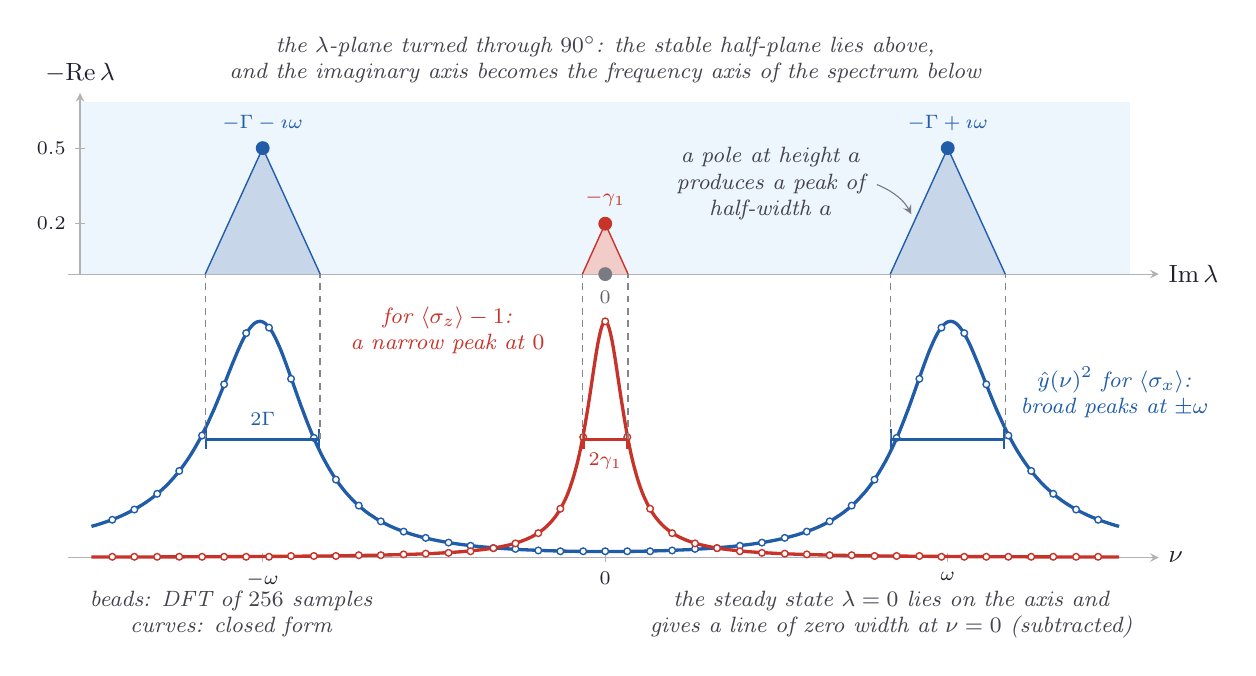
\begin{tikzpicture}[ink/.style={line width=0.9pt, ndInk}, faint/.style={line width=0.4pt, ndInk!35}, dashedink/.style={line width=0.5pt, ndInk!55, dash pattern=on 2.5pt off 2pt}, vec/.style={->, >=stealth, line width=1.2pt}, note/.style={font=\footnotesize\itshape, text=ndInk!85, align=center}, pointer/.style={->, >=stealth, line width=0.4pt, ndInk!60, shorten >=2pt, shorten <=1pt}, dot/.style={circle, fill=ndInk, inner sep=0pt, minimum size=3.4pt}, wash/.style={fill=ndSky, fill opacity=0.55}, every node/.style={text=ndInk}]
\definecolor{ndInk}{rgb}{0.13,0.13,0.18}
\definecolor{ndPaper}{rgb}{0.99,0.96,0.88}
\definecolor{ndSky}{rgb}{0.84,0.91,0.98}
\definecolor{ndRose}{rgb}{0.98,0.86,0.84}
\definecolor{ndBlue}{rgb}{0.13,0.36,0.66}
\definecolor{ndRed}{rgb}{0.78,0.20,0.16}
\definecolor{ndGold}{rgb}{0.88,0.62,0.10}
\definecolor{ndGreen}{rgb}{0.18,0.52,0.30}
\fill[ndSky, fill opacity=0.45] (-6.67,3.60) rectangle (6.67,5.78);
\draw[faint, ->, >=stealth] (-6.82,3.60) -- (7.03,3.60) node[right, text=ndInk, font=\small] {$\mathrm{Im}\,\lambda$};
\draw[faint, ->, >=stealth] (-6.67,3.60) -- (-6.67,5.90) node[above, text=ndInk, font=\small] {$-\mathrm{Re}\,\lambda$};
\draw[faint] (-6.61,4.24) -- (-6.73,4.24) node[left, font=\scriptsize, text=ndInk] {$0.2$};
\draw[faint] (-6.61,5.20) -- (-6.73,5.20) node[left, font=\scriptsize, text=ndInk] {$0.5$};
\node[note, anchor=south] at (0.00,5.90) {the $\lambda$-plane turned through $90^\circ$: the stable half-plane lies above,\\ and the imaginary axis becomes the frequency axis of the spectrum below};
\fill[ndBlue!25] (4.35,5.20) -- (3.62,3.60) -- (5.08,3.60) -- cycle;
\draw[ndBlue, line width=0.5pt] (3.62,3.60) -- (4.35,5.20) (4.35,5.20) -- (5.08,3.60);
\fill[ndBlue!25] (-4.35,5.20) -- (-5.08,3.60) -- (-3.62,3.60) -- cycle;
\draw[ndBlue, line width=0.5pt] (-5.08,3.60) -- (-4.35,5.20) (-4.35,5.20) -- (-3.62,3.60);
\fill[ndRed!25] (0.00,4.24) -- (-0.29,3.60) -- (0.29,3.60) -- cycle;
\draw[ndRed, line width=0.5pt] (-0.29,3.60) -- (0.00,4.24) (0.00,4.24) -- (0.29,3.60);
\node[dot, fill=ndBlue, minimum size=5pt, label={[font=\scriptsize, text=ndBlue]above:$-\Gamma+\imath\omega$}] at (4.35,5.20) {};
\node[dot, fill=ndBlue, minimum size=5pt, label={[font=\scriptsize, text=ndBlue]above:$-\Gamma-\imath\omega$}] at (-4.35,5.20) {};
\node[dot, fill=ndRed, minimum size=5pt, label={[font=\scriptsize, text=ndRed]above:$-\gamma_1$}] at (0.00,4.24) {};
\node[dot, fill=ndInk!60, minimum size=5pt, label={[font=\scriptsize, text=ndInk!70]below:$0$}] at (0.00,3.60) {};
\node[note] (c) at (2.10,4.75) {a pole at height $a$\\ produces a peak of\\ half-width $a$};
\draw[pointer] (c.east) to[bend left=20] (3.92,4.30);
\draw[faint, ->, >=stealth] (-6.82,0) -- (7.03,0) node[right, text=ndInk, font=\small] {$\nu$};
\draw[faint] (-4.35,0.06) -- (-4.35,-0.06) node[below, font=\scriptsize, text=ndInk] {$-\omega$};
\draw[faint] (0.00,0.06) -- (0.00,-0.06) node[below, font=\scriptsize, text=ndInk] {$0$};
\draw[faint] (4.35,0.06) -- (4.35,-0.06) node[below, font=\scriptsize, text=ndInk] {$\omega$};
\draw[line width=1.2pt, ndBlue] (-6.525,0.395) -- (-6.507,0.401) -- (-6.489,0.406) -- (-6.471,0.411) -- (-6.452,0.417) -- (-6.434,0.422) -- (-6.416,0.428) -- (-6.398,0.434) -- (-6.380,0.440) -- (-6.362,0.446) -- (-6.344,0.452) -- (-6.326,0.458) -- (-6.307,0.465) -- (-6.289,0.471) -- (-6.271,0.478) -- (-6.253,0.485) -- (-6.235,0.492) -- (-6.217,0.499) -- (-6.199,0.507) -- (-6.181,0.514) -- (-6.162,0.522) -- (-6.144,0.530) -- (-6.126,0.538) -- (-6.108,0.547) -- (-6.090,0.555) -- (-6.072,0.564) -- (-6.054,0.573) -- (-6.036,0.582) -- (-6.018,0.591) -- (-5.999,0.601) -- (-5.981,0.611) -- (-5.963,0.621) -- (-5.945,0.631) -- (-5.927,0.642) -- (-5.909,0.653) -- (-5.891,0.664) -- (-5.872,0.675) -- (-5.854,0.687) -- (-5.836,0.699) -- (-5.818,0.712) -- (-5.800,0.724) -- (-5.782,0.737) -- (-5.764,0.751) -- (-5.746,0.764) -- (-5.728,0.778) -- (-5.709,0.793) -- (-5.691,0.808) -- (-5.673,0.823) -- (-5.655,0.839) -- (-5.637,0.855) -- (-5.619,0.871) -- (-5.601,0.888) -- (-5.582,0.906) -- (-5.564,0.924) -- (-5.546,0.942) -- (-5.528,0.961) -- (-5.510,0.981) -- (-5.492,1.001) -- (-5.474,1.021) -- (-5.456,1.043) -- (-5.438,1.064) -- (-5.419,1.087) -- (-5.401,1.110) -- (-5.383,1.133) -- (-5.365,1.158) -- (-5.347,1.183) -- (-5.329,1.208) -- (-5.311,1.235) -- (-5.292,1.262) -- (-5.274,1.290) -- (-5.256,1.319) -- (-5.238,1.348) -- (-5.220,1.378) -- (-5.202,1.409) -- (-5.184,1.441) -- (-5.166,1.474) -- (-5.147,1.507) -- (-5.129,1.542) -- (-5.111,1.577) -- (-5.093,1.613) -- (-5.075,1.650) -- (-5.057,1.688) -- (-5.039,1.726) -- (-5.021,1.766) -- (-5.003,1.806) -- (-4.984,1.847) -- (-4.966,1.888) -- (-4.948,1.931) -- (-4.930,1.974) -- (-4.912,2.018) -- (-4.894,2.062) -- (-4.876,2.107) -- (-4.857,2.152) -- (-4.839,2.197) -- (-4.821,2.243) -- (-4.803,2.289) -- (-4.785,2.335) -- (-4.767,2.380) -- (-4.749,2.426) -- (-4.731,2.471) -- (-4.712,2.515) -- (-4.694,2.559) -- (-4.676,2.602) -- (-4.658,2.644) -- (-4.640,2.684) -- (-4.622,2.723) -- (-4.604,2.760) -- (-4.586,2.795) -- (-4.567,2.829) -- (-4.549,2.859) -- (-4.531,2.887) -- (-4.513,2.913) -- (-4.495,2.935) -- (-4.477,2.955) -- (-4.459,2.971) -- (-4.441,2.983) -- (-4.422,2.993) -- (-4.404,2.998) -- (-4.386,3.000) -- (-4.368,2.998) -- (-4.350,2.993) -- (-4.332,2.983) -- (-4.314,2.970) -- (-4.296,2.953) -- (-4.277,2.933) -- (-4.259,2.910) -- (-4.241,2.883) -- (-4.223,2.853) -- (-4.205,2.820) -- (-4.187,2.785) -- (-4.169,2.747) -- (-4.151,2.706) -- (-4.132,2.664) -- (-4.114,2.620) -- (-4.096,2.574) -- (-4.078,2.526) -- (-4.060,2.478) -- (-4.042,2.428) -- (-4.024,2.378) -- (-4.006,2.327) -- (-3.987,2.276) -- (-3.969,2.225) -- (-3.951,2.173) -- (-3.933,2.122) -- (-3.915,2.071) -- (-3.897,2.020) -- (-3.879,1.970) -- (-3.861,1.920) -- (-3.842,1.871) -- (-3.824,1.823) -- (-3.806,1.775) -- (-3.788,1.728) -- (-3.770,1.683) -- (-3.752,1.638) -- (-3.734,1.594) -- (-3.716,1.551) -- (-3.697,1.509) -- (-3.679,1.468) -- (-3.661,1.428) -- (-3.643,1.390) -- (-3.625,1.352) -- (-3.607,1.315) -- (-3.589,1.279) -- (-3.571,1.245) -- (-3.552,1.211) -- (-3.534,1.178) -- (-3.516,1.146) -- (-3.498,1.116) -- (-3.480,1.086) -- (-3.462,1.057) -- (-3.444,1.029) -- (-3.426,1.001) -- (-3.408,0.975) -- (-3.389,0.949) -- (-3.371,0.924) -- (-3.353,0.900) -- (-3.335,0.877) -- (-3.317,0.854) -- (-3.299,0.832) -- (-3.281,0.811) -- (-3.262,0.791) -- (-3.244,0.771) -- (-3.226,0.751) -- (-3.208,0.733) -- (-3.190,0.715) -- (-3.172,0.697) -- (-3.154,0.680) -- (-3.136,0.664) -- (-3.117,0.648) -- (-3.099,0.632) -- (-3.081,0.617) -- (-3.063,0.602) -- (-3.045,0.588) -- (-3.027,0.574) -- (-3.009,0.561) -- (-2.991,0.548) -- (-2.972,0.536) -- (-2.954,0.524) -- (-2.936,0.512) -- (-2.918,0.500) -- (-2.900,0.489) -- (-2.882,0.478) -- (-2.864,0.468) -- (-2.846,0.458) -- (-2.827,0.448) -- (-2.809,0.438) -- (-2.791,0.429) -- (-2.773,0.420) -- (-2.755,0.411) -- (-2.737,0.402) -- (-2.719,0.394) -- (-2.701,0.386) -- (-2.682,0.378) -- (-2.664,0.370) -- (-2.646,0.363) -- (-2.628,0.356) -- (-2.610,0.349) -- (-2.592,0.342) -- (-2.574,0.335) -- (-2.556,0.328) -- (-2.538,0.322) -- (-2.519,0.316) -- (-2.501,0.310) -- (-2.483,0.304) -- (-2.465,0.298) -- (-2.447,0.293) -- (-2.429,0.287) -- (-2.411,0.282) -- (-2.392,0.277) -- (-2.374,0.272) -- (-2.356,0.267) -- (-2.338,0.262) -- (-2.320,0.258) -- (-2.302,0.253) -- (-2.284,0.249) -- (-2.266,0.244) -- (-2.247,0.240) -- (-2.229,0.236) -- (-2.211,0.232) -- (-2.193,0.228) -- (-2.175,0.224) -- (-2.157,0.221) -- (-2.139,0.217) -- (-2.121,0.213) -- (-2.102,0.210) -- (-2.084,0.207) -- (-2.066,0.203) -- (-2.048,0.200) -- (-2.030,0.197) -- (-2.012,0.194) -- (-1.994,0.191) -- (-1.976,0.188) -- (-1.957,0.185) -- (-1.939,0.182) -- (-1.921,0.180) -- (-1.903,0.177) -- (-1.885,0.174) -- (-1.867,0.172) -- (-1.849,0.169) -- (-1.831,0.167) -- (-1.812,0.164) -- (-1.794,0.162) -- (-1.776,0.160) -- (-1.758,0.158) -- (-1.740,0.155) -- (-1.722,0.153) -- (-1.704,0.151) -- (-1.686,0.149) -- (-1.667,0.147) -- (-1.649,0.145) -- (-1.631,0.143) -- (-1.613,0.141) -- (-1.595,0.140) -- (-1.577,0.138) -- (-1.559,0.136) -- (-1.541,0.134) -- (-1.522,0.133) -- (-1.504,0.131) -- (-1.486,0.130) -- (-1.468,0.128) -- (-1.450,0.126) -- (-1.432,0.125) -- (-1.414,0.123) -- (-1.396,0.122) -- (-1.377,0.121) -- (-1.359,0.119) -- (-1.341,0.118) -- (-1.323,0.117) -- (-1.305,0.115) -- (-1.287,0.114) -- (-1.269,0.113) -- (-1.251,0.112) -- (-1.232,0.111) -- (-1.214,0.109) -- (-1.196,0.108) -- (-1.178,0.107) -- (-1.160,0.106) -- (-1.142,0.105) -- (-1.124,0.104) -- (-1.106,0.103) -- (-1.087,0.102) -- (-1.069,0.101) -- (-1.051,0.100) -- (-1.033,0.099) -- (-1.015,0.099) -- (-0.997,0.098) -- (-0.979,0.097) -- (-0.961,0.096) -- (-0.942,0.095) -- (-0.924,0.095) -- (-0.906,0.094) -- (-0.888,0.093) -- (-0.870,0.092) -- (-0.852,0.092) -- (-0.834,0.091) -- (-0.816,0.090) -- (-0.797,0.090) -- (-0.779,0.089) -- (-0.761,0.088) -- (-0.743,0.088) -- (-0.725,0.087) -- (-0.707,0.087) -- (-0.689,0.086) -- (-0.671,0.086) -- (-0.653,0.085) -- (-0.634,0.085) -- (-0.616,0.084) -- (-0.598,0.084) -- (-0.580,0.083) -- (-0.562,0.083) -- (-0.544,0.082) -- (-0.526,0.082) -- (-0.507,0.082) -- (-0.489,0.081) -- (-0.471,0.081) -- (-0.453,0.081) -- (-0.435,0.080) -- (-0.417,0.080) -- (-0.399,0.080) -- (-0.381,0.079) -- (-0.362,0.079) -- (-0.344,0.079) -- (-0.326,0.079) -- (-0.308,0.078) -- (-0.290,0.078) -- (-0.272,0.078) -- (-0.254,0.078) -- (-0.236,0.078) -- (-0.217,0.077) -- (-0.199,0.077) -- (-0.181,0.077) -- (-0.163,0.077) -- (-0.145,0.077) -- (-0.127,0.077) -- (-0.109,0.077) -- (-0.091,0.077) -- (-0.072,0.077) -- (-0.054,0.077) -- (-0.036,0.077) -- (-0.018,0.077) -- (0.000,0.077) -- (0.018,0.077) -- (0.036,0.077) -- (0.054,0.077) -- (0.072,0.077) -- (0.091,0.077) -- (0.109,0.077) -- (0.127,0.077) -- (0.145,0.077) -- (0.163,0.077) -- (0.181,0.077) -- (0.199,0.077) -- (0.218,0.077) -- (0.236,0.078) -- (0.254,0.078) -- (0.272,0.078) -- (0.290,0.078) -- (0.308,0.078) -- (0.326,0.079) -- (0.344,0.079) -- (0.362,0.079) -- (0.381,0.079) -- (0.399,0.080) -- (0.417,0.080) -- (0.435,0.080) -- (0.453,0.081) -- (0.471,0.081) -- (0.489,0.081) -- (0.508,0.082) -- (0.526,0.082) -- (0.544,0.082) -- (0.562,0.083) -- (0.580,0.083) -- (0.598,0.084) -- (0.616,0.084) -- (0.634,0.085) -- (0.653,0.085) -- (0.671,0.086) -- (0.689,0.086) -- (0.707,0.087) -- (0.725,0.087) -- (0.743,0.088) -- (0.761,0.088) -- (0.779,0.089) -- (0.798,0.090) -- (0.816,0.090) -- (0.834,0.091) -- (0.852,0.092) -- (0.870,0.092) -- (0.888,0.093) -- (0.906,0.094) -- (0.924,0.095) -- (0.943,0.095) -- (0.961,0.096) -- (0.979,0.097) -- (0.997,0.098) -- (1.015,0.099) -- (1.033,0.099) -- (1.051,0.100) -- (1.069,0.101) -- (1.087,0.102) -- (1.106,0.103) -- (1.124,0.104) -- (1.142,0.105) -- (1.160,0.106) -- (1.178,0.107) -- (1.196,0.108) -- (1.214,0.109) -- (1.233,0.111) -- (1.251,0.112) -- (1.269,0.113) -- (1.287,0.114) -- (1.305,0.115) -- (1.323,0.117) -- (1.341,0.118) -- (1.359,0.119) -- (1.378,0.121) -- (1.396,0.122) -- (1.414,0.123) -- (1.432,0.125) -- (1.450,0.126) -- (1.468,0.128) -- (1.486,0.130) -- (1.504,0.131) -- (1.523,0.133) -- (1.541,0.134) -- (1.559,0.136) -- (1.577,0.138) -- (1.595,0.140) -- (1.613,0.141) -- (1.631,0.143) -- (1.649,0.145) -- (1.668,0.147) -- (1.686,0.149) -- (1.704,0.151) -- (1.722,0.153) -- (1.740,0.155) -- (1.758,0.158) -- (1.776,0.160) -- (1.794,0.162) -- (1.812,0.164) -- (1.831,0.167) -- (1.849,0.169) -- (1.867,0.172) -- (1.885,0.174) -- (1.903,0.177) -- (1.921,0.180) -- (1.939,0.182) -- (1.958,0.185) -- (1.976,0.188) -- (1.994,0.191) -- (2.012,0.194) -- (2.030,0.197) -- (2.048,0.200) -- (2.066,0.203) -- (2.084,0.207) -- (2.103,0.210) -- (2.121,0.213) -- (2.139,0.217) -- (2.157,0.221) -- (2.175,0.224) -- (2.193,0.228) -- (2.211,0.232) -- (2.229,0.236) -- (2.248,0.240) -- (2.266,0.244) -- (2.284,0.249) -- (2.302,0.253) -- (2.320,0.258) -- (2.338,0.262) -- (2.356,0.267) -- (2.374,0.272) -- (2.393,0.277) -- (2.411,0.282) -- (2.429,0.287) -- (2.447,0.293) -- (2.465,0.298) -- (2.483,0.304) -- (2.501,0.310) -- (2.519,0.316) -- (2.538,0.322) -- (2.556,0.328) -- (2.574,0.335) -- (2.592,0.342) -- (2.610,0.349) -- (2.628,0.356) -- (2.646,0.363) -- (2.664,0.370) -- (2.683,0.378) -- (2.701,0.386) -- (2.719,0.394) -- (2.737,0.402) -- (2.755,0.411) -- (2.773,0.420) -- (2.791,0.429) -- (2.809,0.438) -- (2.828,0.448) -- (2.846,0.458) -- (2.864,0.468) -- (2.882,0.478) -- (2.900,0.489) -- (2.918,0.500) -- (2.936,0.512) -- (2.954,0.524) -- (2.973,0.536) -- (2.991,0.548) -- (3.009,0.561) -- (3.027,0.574) -- (3.045,0.588) -- (3.063,0.602) -- (3.081,0.617) -- (3.099,0.632) -- (3.118,0.648) -- (3.136,0.664) -- (3.154,0.680) -- (3.172,0.697) -- (3.190,0.715) -- (3.208,0.733) -- (3.226,0.751) -- (3.244,0.771) -- (3.262,0.791) -- (3.281,0.811) -- (3.299,0.832) -- (3.317,0.854) -- (3.335,0.877) -- (3.353,0.900) -- (3.371,0.924) -- (3.389,0.949) -- (3.408,0.975) -- (3.426,1.001) -- (3.444,1.029) -- (3.462,1.057) -- (3.480,1.086) -- (3.498,1.116) -- (3.516,1.146) -- (3.534,1.178) -- (3.553,1.211) -- (3.571,1.245) -- (3.589,1.279) -- (3.607,1.315) -- (3.625,1.352) -- (3.643,1.390) -- (3.661,1.428) -- (3.679,1.468) -- (3.698,1.509) -- (3.716,1.551) -- (3.734,1.594) -- (3.752,1.638) -- (3.770,1.683) -- (3.788,1.728) -- (3.806,1.775) -- (3.824,1.823) -- (3.843,1.871) -- (3.861,1.920) -- (3.879,1.970) -- (3.897,2.020) -- (3.915,2.071) -- (3.933,2.122) -- (3.951,2.173) -- (3.969,2.225) -- (3.987,2.276) -- (4.006,2.327) -- (4.024,2.378) -- (4.042,2.428) -- (4.060,2.478) -- (4.078,2.526) -- (4.096,2.574) -- (4.114,2.620) -- (4.133,2.664) -- (4.151,2.706) -- (4.169,2.747) -- (4.187,2.785) -- (4.205,2.820) -- (4.223,2.853) -- (4.241,2.883) -- (4.259,2.910) -- (4.277,2.933) -- (4.296,2.953) -- (4.314,2.970) -- (4.332,2.983) -- (4.350,2.993) -- (4.368,2.998) -- (4.386,3.000) -- (4.404,2.998) -- (4.423,2.993) -- (4.441,2.983) -- (4.459,2.971) -- (4.477,2.955) -- (4.495,2.935) -- (4.513,2.913) -- (4.531,2.887) -- (4.549,2.859) -- (4.568,2.829) -- (4.586,2.795) -- (4.604,2.760) -- (4.622,2.723) -- (4.640,2.684) -- (4.658,2.644) -- (4.676,2.602) -- (4.694,2.559) -- (4.712,2.515) -- (4.731,2.471) -- (4.749,2.426) -- (4.767,2.380) -- (4.785,2.335) -- (4.803,2.289) -- (4.821,2.243) -- (4.839,2.197) -- (4.858,2.152) -- (4.876,2.107) -- (4.894,2.062) -- (4.912,2.018) -- (4.930,1.974) -- (4.948,1.931) -- (4.966,1.888) -- (4.984,1.847) -- (5.003,1.806) -- (5.021,1.766) -- (5.039,1.726) -- (5.057,1.688) -- (5.075,1.650) -- (5.093,1.613) -- (5.111,1.577) -- (5.129,1.542) -- (5.148,1.507) -- (5.166,1.474) -- (5.184,1.441) -- (5.202,1.409) -- (5.220,1.378) -- (5.238,1.348) -- (5.256,1.319) -- (5.274,1.290) -- (5.293,1.262) -- (5.311,1.235) -- (5.329,1.208) -- (5.347,1.183) -- (5.365,1.158) -- (5.383,1.133) -- (5.401,1.110) -- (5.419,1.087) -- (5.438,1.064) -- (5.456,1.043) -- (5.474,1.021) -- (5.492,1.001) -- (5.510,0.981) -- (5.528,0.961) -- (5.546,0.942) -- (5.564,0.924) -- (5.582,0.906) -- (5.601,0.888) -- (5.619,0.871) -- (5.637,0.855) -- (5.655,0.839) -- (5.673,0.823) -- (5.691,0.808) -- (5.709,0.793) -- (5.728,0.778) -- (5.746,0.764) -- (5.764,0.751) -- (5.782,0.737) -- (5.800,0.724) -- (5.818,0.712) -- (5.836,0.699) -- (5.854,0.687) -- (5.873,0.675) -- (5.891,0.664) -- (5.909,0.653) -- (5.927,0.642) -- (5.945,0.631) -- (5.963,0.621) -- (5.981,0.611) -- (5.999,0.601) -- (6.018,0.591) -- (6.036,0.582) -- (6.054,0.573) -- (6.072,0.564) -- (6.090,0.555) -- (6.108,0.547) -- (6.126,0.538) -- (6.144,0.530) -- (6.162,0.522) -- (6.181,0.514) -- (6.199,0.507) -- (6.217,0.499) -- (6.235,0.492) -- (6.253,0.485) -- (6.271,0.478) -- (6.289,0.471) -- (6.307,0.465) -- (6.326,0.458) -- (6.344,0.452) -- (6.362,0.446) -- (6.380,0.440) -- (6.398,0.434) -- (6.416,0.428) -- (6.434,0.422) -- (6.453,0.417) -- (6.471,0.411) -- (6.489,0.406) -- (6.507,0.401) -- (6.525,0.395);
\draw[line width=1.2pt, ndRed] (-6.525,0.007) -- (-6.507,0.007) -- (-6.489,0.007) -- (-6.471,0.007) -- (-6.452,0.007) -- (-6.434,0.007) -- (-6.416,0.007) -- (-6.398,0.007) -- (-6.380,0.007) -- (-6.362,0.007) -- (-6.344,0.007) -- (-6.326,0.007) -- (-6.307,0.007) -- (-6.289,0.007) -- (-6.271,0.007) -- (-6.253,0.007) -- (-6.235,0.007) -- (-6.217,0.007) -- (-6.199,0.007) -- (-6.181,0.007) -- (-6.162,0.007) -- (-6.144,0.007) -- (-6.126,0.007) -- (-6.108,0.007) -- (-6.090,0.007) -- (-6.072,0.007) -- (-6.054,0.008) -- (-6.036,0.008) -- (-6.018,0.008) -- (-5.999,0.008) -- (-5.981,0.008) -- (-5.963,0.008) -- (-5.945,0.008) -- (-5.927,0.008) -- (-5.909,0.008) -- (-5.891,0.008) -- (-5.872,0.008) -- (-5.854,0.008) -- (-5.836,0.008) -- (-5.818,0.008) -- (-5.800,0.008) -- (-5.782,0.008) -- (-5.764,0.008) -- (-5.746,0.008) -- (-5.728,0.008) -- (-5.709,0.008) -- (-5.691,0.008) -- (-5.673,0.008) -- (-5.655,0.009) -- (-5.637,0.009) -- (-5.619,0.009) -- (-5.601,0.009) -- (-5.582,0.009) -- (-5.564,0.009) -- (-5.546,0.009) -- (-5.528,0.009) -- (-5.510,0.009) -- (-5.492,0.009) -- (-5.474,0.009) -- (-5.456,0.009) -- (-5.438,0.009) -- (-5.419,0.009) -- (-5.401,0.009) -- (-5.383,0.009) -- (-5.365,0.009) -- (-5.347,0.009) -- (-5.329,0.010) -- (-5.311,0.010) -- (-5.292,0.010) -- (-5.274,0.010) -- (-5.256,0.010) -- (-5.238,0.010) -- (-5.220,0.010) -- (-5.202,0.010) -- (-5.184,0.010) -- (-5.166,0.010) -- (-5.147,0.010) -- (-5.129,0.010) -- (-5.111,0.010) -- (-5.093,0.010) -- (-5.075,0.010) -- (-5.057,0.010) -- (-5.039,0.011) -- (-5.021,0.011) -- (-5.003,0.011) -- (-4.984,0.011) -- (-4.966,0.011) -- (-4.948,0.011) -- (-4.930,0.011) -- (-4.912,0.011) -- (-4.894,0.011) -- (-4.876,0.011) -- (-4.857,0.011) -- (-4.839,0.011) -- (-4.821,0.011) -- (-4.803,0.012) -- (-4.785,0.012) -- (-4.767,0.012) -- (-4.749,0.012) -- (-4.731,0.012) -- (-4.712,0.012) -- (-4.694,0.012) -- (-4.676,0.012) -- (-4.658,0.012) -- (-4.640,0.012) -- (-4.622,0.012) -- (-4.604,0.012) -- (-4.586,0.013) -- (-4.567,0.013) -- (-4.549,0.013) -- (-4.531,0.013) -- (-4.513,0.013) -- (-4.495,0.013) -- (-4.477,0.013) -- (-4.459,0.013) -- (-4.441,0.013) -- (-4.422,0.013) -- (-4.404,0.014) -- (-4.386,0.014) -- (-4.368,0.014) -- (-4.350,0.014) -- (-4.332,0.014) -- (-4.314,0.014) -- (-4.296,0.014) -- (-4.277,0.014) -- (-4.259,0.014) -- (-4.241,0.015) -- (-4.223,0.015) -- (-4.205,0.015) -- (-4.187,0.015) -- (-4.169,0.015) -- (-4.151,0.015) -- (-4.132,0.015) -- (-4.114,0.015) -- (-4.096,0.016) -- (-4.078,0.016) -- (-4.060,0.016) -- (-4.042,0.016) -- (-4.024,0.016) -- (-4.006,0.016) -- (-3.987,0.016) -- (-3.969,0.017) -- (-3.951,0.017) -- (-3.933,0.017) -- (-3.915,0.017) -- (-3.897,0.017) -- (-3.879,0.017) -- (-3.861,0.017) -- (-3.842,0.018) -- (-3.824,0.018) -- (-3.806,0.018) -- (-3.788,0.018) -- (-3.770,0.018) -- (-3.752,0.018) -- (-3.734,0.019) -- (-3.716,0.019) -- (-3.697,0.019) -- (-3.679,0.019) -- (-3.661,0.019) -- (-3.643,0.020) -- (-3.625,0.020) -- (-3.607,0.020) -- (-3.589,0.020) -- (-3.571,0.020) -- (-3.552,0.020) -- (-3.534,0.021) -- (-3.516,0.021) -- (-3.498,0.021) -- (-3.480,0.021) -- (-3.462,0.022) -- (-3.444,0.022) -- (-3.426,0.022) -- (-3.408,0.022) -- (-3.389,0.022) -- (-3.371,0.023) -- (-3.353,0.023) -- (-3.335,0.023) -- (-3.317,0.023) -- (-3.299,0.024) -- (-3.281,0.024) -- (-3.262,0.024) -- (-3.244,0.024) -- (-3.226,0.025) -- (-3.208,0.025) -- (-3.190,0.025) -- (-3.172,0.025) -- (-3.154,0.026) -- (-3.136,0.026) -- (-3.117,0.026) -- (-3.099,0.027) -- (-3.081,0.027) -- (-3.063,0.027) -- (-3.045,0.028) -- (-3.027,0.028) -- (-3.009,0.028) -- (-2.991,0.029) -- (-2.972,0.029) -- (-2.954,0.029) -- (-2.936,0.030) -- (-2.918,0.030) -- (-2.900,0.030) -- (-2.882,0.031) -- (-2.864,0.031) -- (-2.846,0.031) -- (-2.827,0.032) -- (-2.809,0.032) -- (-2.791,0.033) -- (-2.773,0.033) -- (-2.755,0.034) -- (-2.737,0.034) -- (-2.719,0.034) -- (-2.701,0.035) -- (-2.682,0.035) -- (-2.664,0.036) -- (-2.646,0.036) -- (-2.628,0.037) -- (-2.610,0.037) -- (-2.592,0.038) -- (-2.574,0.038) -- (-2.556,0.039) -- (-2.538,0.039) -- (-2.519,0.040) -- (-2.501,0.040) -- (-2.483,0.041) -- (-2.465,0.042) -- (-2.447,0.042) -- (-2.429,0.043) -- (-2.411,0.043) -- (-2.392,0.044) -- (-2.374,0.045) -- (-2.356,0.045) -- (-2.338,0.046) -- (-2.320,0.047) -- (-2.302,0.047) -- (-2.284,0.048) -- (-2.266,0.049) -- (-2.247,0.050) -- (-2.229,0.051) -- (-2.211,0.051) -- (-2.193,0.052) -- (-2.175,0.053) -- (-2.157,0.054) -- (-2.139,0.055) -- (-2.121,0.056) -- (-2.102,0.057) -- (-2.084,0.058) -- (-2.066,0.059) -- (-2.048,0.060) -- (-2.030,0.061) -- (-2.012,0.062) -- (-1.994,0.063) -- (-1.976,0.064) -- (-1.957,0.065) -- (-1.939,0.066) -- (-1.921,0.067) -- (-1.903,0.069) -- (-1.885,0.070) -- (-1.867,0.071) -- (-1.849,0.073) -- (-1.831,0.074) -- (-1.812,0.075) -- (-1.794,0.077) -- (-1.776,0.079) -- (-1.758,0.080) -- (-1.740,0.082) -- (-1.722,0.083) -- (-1.704,0.085) -- (-1.686,0.087) -- (-1.667,0.089) -- (-1.649,0.091) -- (-1.631,0.093) -- (-1.613,0.095) -- (-1.595,0.097) -- (-1.577,0.099) -- (-1.559,0.101) -- (-1.541,0.103) -- (-1.522,0.106) -- (-1.504,0.108) -- (-1.486,0.111) -- (-1.468,0.113) -- (-1.450,0.116) -- (-1.432,0.119) -- (-1.414,0.122) -- (-1.396,0.125) -- (-1.377,0.128) -- (-1.359,0.131) -- (-1.341,0.135) -- (-1.323,0.138) -- (-1.305,0.142) -- (-1.287,0.146) -- (-1.269,0.150) -- (-1.251,0.154) -- (-1.232,0.158) -- (-1.214,0.162) -- (-1.196,0.167) -- (-1.178,0.172) -- (-1.160,0.177) -- (-1.142,0.182) -- (-1.124,0.188) -- (-1.106,0.194) -- (-1.087,0.200) -- (-1.069,0.206) -- (-1.051,0.213) -- (-1.033,0.220) -- (-1.015,0.227) -- (-0.997,0.235) -- (-0.979,0.243) -- (-0.961,0.251) -- (-0.942,0.260) -- (-0.924,0.269) -- (-0.906,0.279) -- (-0.888,0.290) -- (-0.870,0.301) -- (-0.852,0.312) -- (-0.834,0.324) -- (-0.816,0.337) -- (-0.797,0.351) -- (-0.779,0.365) -- (-0.761,0.381) -- (-0.743,0.397) -- (-0.725,0.414) -- (-0.707,0.433) -- (-0.689,0.452) -- (-0.671,0.473) -- (-0.653,0.495) -- (-0.634,0.519) -- (-0.616,0.544) -- (-0.598,0.572) -- (-0.580,0.601) -- (-0.562,0.632) -- (-0.544,0.665) -- (-0.526,0.701) -- (-0.507,0.739) -- (-0.489,0.780) -- (-0.471,0.824) -- (-0.453,0.872) -- (-0.435,0.924) -- (-0.417,0.979) -- (-0.399,1.038) -- (-0.381,1.102) -- (-0.362,1.171) -- (-0.344,1.245) -- (-0.326,1.324) -- (-0.308,1.410) -- (-0.290,1.500) -- (-0.272,1.597) -- (-0.254,1.699) -- (-0.236,1.807) -- (-0.217,1.920) -- (-0.199,2.037) -- (-0.181,2.157) -- (-0.163,2.279) -- (-0.145,2.400) -- (-0.127,2.518) -- (-0.109,2.630) -- (-0.091,2.733) -- (-0.072,2.824) -- (-0.054,2.898) -- (-0.036,2.954) -- (-0.018,2.988) -- (0.000,3.000) -- (0.018,2.988) -- (0.036,2.954) -- (0.054,2.898) -- (0.072,2.824) -- (0.091,2.733) -- (0.109,2.630) -- (0.127,2.518) -- (0.145,2.400) -- (0.163,2.279) -- (0.181,2.157) -- (0.199,2.037) -- (0.218,1.920) -- (0.236,1.807) -- (0.254,1.699) -- (0.272,1.597) -- (0.290,1.500) -- (0.308,1.410) -- (0.326,1.324) -- (0.344,1.245) -- (0.362,1.171) -- (0.381,1.102) -- (0.399,1.038) -- (0.417,0.979) -- (0.435,0.924) -- (0.453,0.872) -- (0.471,0.824) -- (0.489,0.780) -- (0.508,0.739) -- (0.526,0.701) -- (0.544,0.665) -- (0.562,0.632) -- (0.580,0.601) -- (0.598,0.572) -- (0.616,0.544) -- (0.634,0.519) -- (0.653,0.495) -- (0.671,0.473) -- (0.689,0.452) -- (0.707,0.433) -- (0.725,0.414) -- (0.743,0.397) -- (0.761,0.381) -- (0.779,0.365) -- (0.798,0.351) -- (0.816,0.337) -- (0.834,0.324) -- (0.852,0.312) -- (0.870,0.301) -- (0.888,0.290) -- (0.906,0.279) -- (0.924,0.269) -- (0.943,0.260) -- (0.961,0.251) -- (0.979,0.243) -- (0.997,0.235) -- (1.015,0.227) -- (1.033,0.220) -- (1.051,0.213) -- (1.069,0.206) -- (1.087,0.200) -- (1.106,0.194) -- (1.124,0.188) -- (1.142,0.182) -- (1.160,0.177) -- (1.178,0.172) -- (1.196,0.167) -- (1.214,0.162) -- (1.233,0.158) -- (1.251,0.154) -- (1.269,0.150) -- (1.287,0.146) -- (1.305,0.142) -- (1.323,0.138) -- (1.341,0.135) -- (1.359,0.131) -- (1.378,0.128) -- (1.396,0.125) -- (1.414,0.122) -- (1.432,0.119) -- (1.450,0.116) -- (1.468,0.113) -- (1.486,0.111) -- (1.504,0.108) -- (1.523,0.106) -- (1.541,0.103) -- (1.559,0.101) -- (1.577,0.099) -- (1.595,0.097) -- (1.613,0.095) -- (1.631,0.093) -- (1.649,0.091) -- (1.668,0.089) -- (1.686,0.087) -- (1.704,0.085) -- (1.722,0.083) -- (1.740,0.082) -- (1.758,0.080) -- (1.776,0.079) -- (1.794,0.077) -- (1.812,0.075) -- (1.831,0.074) -- (1.849,0.073) -- (1.867,0.071) -- (1.885,0.070) -- (1.903,0.069) -- (1.921,0.067) -- (1.939,0.066) -- (1.958,0.065) -- (1.976,0.064) -- (1.994,0.063) -- (2.012,0.062) -- (2.030,0.061) -- (2.048,0.060) -- (2.066,0.059) -- (2.084,0.058) -- (2.103,0.057) -- (2.121,0.056) -- (2.139,0.055) -- (2.157,0.054) -- (2.175,0.053) -- (2.193,0.052) -- (2.211,0.051) -- (2.229,0.051) -- (2.248,0.050) -- (2.266,0.049) -- (2.284,0.048) -- (2.302,0.047) -- (2.320,0.047) -- (2.338,0.046) -- (2.356,0.045) -- (2.374,0.045) -- (2.393,0.044) -- (2.411,0.043) -- (2.429,0.043) -- (2.447,0.042) -- (2.465,0.042) -- (2.483,0.041) -- (2.501,0.040) -- (2.519,0.040) -- (2.538,0.039) -- (2.556,0.039) -- (2.574,0.038) -- (2.592,0.038) -- (2.610,0.037) -- (2.628,0.037) -- (2.646,0.036) -- (2.664,0.036) -- (2.683,0.035) -- (2.701,0.035) -- (2.719,0.034) -- (2.737,0.034) -- (2.755,0.034) -- (2.773,0.033) -- (2.791,0.033) -- (2.809,0.032) -- (2.828,0.032) -- (2.846,0.031) -- (2.864,0.031) -- (2.882,0.031) -- (2.900,0.030) -- (2.918,0.030) -- (2.936,0.030) -- (2.954,0.029) -- (2.973,0.029) -- (2.991,0.029) -- (3.009,0.028) -- (3.027,0.028) -- (3.045,0.028) -- (3.063,0.027) -- (3.081,0.027) -- (3.099,0.027) -- (3.118,0.026) -- (3.136,0.026) -- (3.154,0.026) -- (3.172,0.025) -- (3.190,0.025) -- (3.208,0.025) -- (3.226,0.025) -- (3.244,0.024) -- (3.262,0.024) -- (3.281,0.024) -- (3.299,0.024) -- (3.317,0.023) -- (3.335,0.023) -- (3.353,0.023) -- (3.371,0.023) -- (3.389,0.022) -- (3.408,0.022) -- (3.426,0.022) -- (3.444,0.022) -- (3.462,0.022) -- (3.480,0.021) -- (3.498,0.021) -- (3.516,0.021) -- (3.534,0.021) -- (3.553,0.020) -- (3.571,0.020) -- (3.589,0.020) -- (3.607,0.020) -- (3.625,0.020) -- (3.643,0.020) -- (3.661,0.019) -- (3.679,0.019) -- (3.698,0.019) -- (3.716,0.019) -- (3.734,0.019) -- (3.752,0.018) -- (3.770,0.018) -- (3.788,0.018) -- (3.806,0.018) -- (3.824,0.018) -- (3.843,0.018) -- (3.861,0.017) -- (3.879,0.017) -- (3.897,0.017) -- (3.915,0.017) -- (3.933,0.017) -- (3.951,0.017) -- (3.969,0.017) -- (3.987,0.016) -- (4.006,0.016) -- (4.024,0.016) -- (4.042,0.016) -- (4.060,0.016) -- (4.078,0.016) -- (4.096,0.016) -- (4.114,0.015) -- (4.133,0.015) -- (4.151,0.015) -- (4.169,0.015) -- (4.187,0.015) -- (4.205,0.015) -- (4.223,0.015) -- (4.241,0.015) -- (4.259,0.014) -- (4.277,0.014) -- (4.296,0.014) -- (4.314,0.014) -- (4.332,0.014) -- (4.350,0.014) -- (4.368,0.014) -- (4.386,0.014) -- (4.404,0.014) -- (4.423,0.013) -- (4.441,0.013) -- (4.459,0.013) -- (4.477,0.013) -- (4.495,0.013) -- (4.513,0.013) -- (4.531,0.013) -- (4.549,0.013) -- (4.568,0.013) -- (4.586,0.013) -- (4.604,0.012) -- (4.622,0.012) -- (4.640,0.012) -- (4.658,0.012) -- (4.676,0.012) -- (4.694,0.012) -- (4.712,0.012) -- (4.731,0.012) -- (4.749,0.012) -- (4.767,0.012) -- (4.785,0.012) -- (4.803,0.012) -- (4.821,0.011) -- (4.839,0.011) -- (4.858,0.011) -- (4.876,0.011) -- (4.894,0.011) -- (4.912,0.011) -- (4.930,0.011) -- (4.948,0.011) -- (4.966,0.011) -- (4.984,0.011) -- (5.003,0.011) -- (5.021,0.011) -- (5.039,0.011) -- (5.057,0.010) -- (5.075,0.010) -- (5.093,0.010) -- (5.111,0.010) -- (5.129,0.010) -- (5.148,0.010) -- (5.166,0.010) -- (5.184,0.010) -- (5.202,0.010) -- (5.220,0.010) -- (5.238,0.010) -- (5.256,0.010) -- (5.274,0.010) -- (5.293,0.010) -- (5.311,0.010) -- (5.329,0.010) -- (5.347,0.009) -- (5.365,0.009) -- (5.383,0.009) -- (5.401,0.009) -- (5.419,0.009) -- (5.438,0.009) -- (5.456,0.009) -- (5.474,0.009) -- (5.492,0.009) -- (5.510,0.009) -- (5.528,0.009) -- (5.546,0.009) -- (5.564,0.009) -- (5.582,0.009) -- (5.601,0.009) -- (5.619,0.009) -- (5.637,0.009) -- (5.655,0.009) -- (5.673,0.008) -- (5.691,0.008) -- (5.709,0.008) -- (5.728,0.008) -- (5.746,0.008) -- (5.764,0.008) -- (5.782,0.008) -- (5.800,0.008) -- (5.818,0.008) -- (5.836,0.008) -- (5.854,0.008) -- (5.873,0.008) -- (5.891,0.008) -- (5.909,0.008) -- (5.927,0.008) -- (5.945,0.008) -- (5.963,0.008) -- (5.981,0.008) -- (5.999,0.008) -- (6.018,0.008) -- (6.036,0.008) -- (6.054,0.008) -- (6.072,0.007) -- (6.090,0.007) -- (6.108,0.007) -- (6.126,0.007) -- (6.144,0.007) -- (6.162,0.007) -- (6.181,0.007) -- (6.199,0.007) -- (6.217,0.007) -- (6.235,0.007) -- (6.253,0.007) -- (6.271,0.007) -- (6.289,0.007) -- (6.307,0.007) -- (6.326,0.007) -- (6.344,0.007) -- (6.362,0.007) -- (6.380,0.007) -- (6.398,0.007) -- (6.416,0.007) -- (6.434,0.007) -- (6.453,0.007) -- (6.471,0.007) -- (6.489,0.007) -- (6.507,0.007) -- (6.525,0.007);
\filldraw[fill=white, draw=ndBlue, line width=0.5pt] (0.00,0.08) circle (1.2pt);
\filldraw[fill=white, draw=ndBlue, line width=0.5pt] (0.28,0.08) circle (1.2pt);
\filldraw[fill=white, draw=ndBlue, line width=0.5pt] (0.57,0.08) circle (1.2pt);
\filldraw[fill=white, draw=ndBlue, line width=0.5pt] (0.85,0.09) circle (1.2pt);
\filldraw[fill=white, draw=ndBlue, line width=0.5pt] (1.14,0.11) circle (1.2pt);
\filldraw[fill=white, draw=ndBlue, line width=0.5pt] (1.42,0.12) circle (1.2pt);
\filldraw[fill=white, draw=ndBlue, line width=0.5pt] (1.71,0.15) circle (1.2pt);
\filldraw[fill=white, draw=ndBlue, line width=0.5pt] (1.99,0.19) circle (1.2pt);
\filldraw[fill=white, draw=ndBlue, line width=0.5pt] (2.28,0.25) circle (1.2pt);
\filldraw[fill=white, draw=ndBlue, line width=0.5pt] (2.56,0.33) circle (1.2pt);
\filldraw[fill=white, draw=ndBlue, line width=0.5pt] (2.85,0.46) circle (1.2pt);
\filldraw[fill=white, draw=ndBlue, line width=0.5pt] (3.13,0.66) circle (1.2pt);
\filldraw[fill=white, draw=ndBlue, line width=0.5pt] (3.42,0.99) circle (1.2pt);
\filldraw[fill=white, draw=ndBlue, line width=0.5pt] (3.70,1.52) circle (1.2pt);
\filldraw[fill=white, draw=ndBlue, line width=0.5pt] (3.99,2.27) circle (1.2pt);
\filldraw[fill=white, draw=ndBlue, line width=0.5pt] (4.27,2.92) circle (1.2pt);
\filldraw[fill=white, draw=ndBlue, line width=0.5pt] (4.56,2.85) circle (1.2pt);
\filldraw[fill=white, draw=ndBlue, line width=0.5pt] (4.84,2.20) circle (1.2pt);
\filldraw[fill=white, draw=ndBlue, line width=0.5pt] (5.12,1.55) circle (1.2pt);
\filldraw[fill=white, draw=ndBlue, line width=0.5pt] (5.41,1.10) circle (1.2pt);
\filldraw[fill=white, draw=ndBlue, line width=0.5pt] (5.69,0.81) circle (1.2pt);
\filldraw[fill=white, draw=ndBlue, line width=0.5pt] (5.98,0.61) circle (1.2pt);
\filldraw[fill=white, draw=ndBlue, line width=0.5pt] (6.26,0.48) circle (1.2pt);
\filldraw[fill=white, draw=ndBlue, line width=0.5pt] (-6.26,0.48) circle (1.2pt);
\filldraw[fill=white, draw=ndBlue, line width=0.5pt] (-5.98,0.61) circle (1.2pt);
\filldraw[fill=white, draw=ndBlue, line width=0.5pt] (-5.69,0.81) circle (1.2pt);
\filldraw[fill=white, draw=ndBlue, line width=0.5pt] (-5.41,1.10) circle (1.2pt);
\filldraw[fill=white, draw=ndBlue, line width=0.5pt] (-5.12,1.55) circle (1.2pt);
\filldraw[fill=white, draw=ndBlue, line width=0.5pt] (-4.84,2.20) circle (1.2pt);
\filldraw[fill=white, draw=ndBlue, line width=0.5pt] (-4.56,2.85) circle (1.2pt);
\filldraw[fill=white, draw=ndBlue, line width=0.5pt] (-4.27,2.92) circle (1.2pt);
\filldraw[fill=white, draw=ndBlue, line width=0.5pt] (-3.99,2.27) circle (1.2pt);
\filldraw[fill=white, draw=ndBlue, line width=0.5pt] (-3.70,1.52) circle (1.2pt);
\filldraw[fill=white, draw=ndBlue, line width=0.5pt] (-3.42,0.99) circle (1.2pt);
\filldraw[fill=white, draw=ndBlue, line width=0.5pt] (-3.13,0.66) circle (1.2pt);
\filldraw[fill=white, draw=ndBlue, line width=0.5pt] (-2.85,0.46) circle (1.2pt);
\filldraw[fill=white, draw=ndBlue, line width=0.5pt] (-2.56,0.33) circle (1.2pt);
\filldraw[fill=white, draw=ndBlue, line width=0.5pt] (-2.28,0.25) circle (1.2pt);
\filldraw[fill=white, draw=ndBlue, line width=0.5pt] (-1.99,0.19) circle (1.2pt);
\filldraw[fill=white, draw=ndBlue, line width=0.5pt] (-1.71,0.15) circle (1.2pt);
\filldraw[fill=white, draw=ndBlue, line width=0.5pt] (-1.42,0.12) circle (1.2pt);
\filldraw[fill=white, draw=ndBlue, line width=0.5pt] (-1.14,0.11) circle (1.2pt);
\filldraw[fill=white, draw=ndBlue, line width=0.5pt] (-0.85,0.09) circle (1.2pt);
\filldraw[fill=white, draw=ndBlue, line width=0.5pt] (-0.57,0.08) circle (1.2pt);
\filldraw[fill=white, draw=ndBlue, line width=0.5pt] (-0.28,0.08) circle (1.2pt);
\filldraw[fill=white, draw=ndRed, line width=0.5pt] (0.00,3.00) circle (1.2pt);
\filldraw[fill=white, draw=ndRed, line width=0.5pt] (0.28,1.53) circle (1.2pt);
\filldraw[fill=white, draw=ndRed, line width=0.5pt] (0.57,0.62) circle (1.2pt);
\filldraw[fill=white, draw=ndRed, line width=0.5pt] (0.85,0.31) circle (1.2pt);
\filldraw[fill=white, draw=ndRed, line width=0.5pt] (1.14,0.18) circle (1.2pt);
\filldraw[fill=white, draw=ndRed, line width=0.5pt] (1.42,0.12) circle (1.2pt);
\filldraw[fill=white, draw=ndRed, line width=0.5pt] (1.71,0.08) circle (1.2pt);
\filldraw[fill=white, draw=ndRed, line width=0.5pt] (1.99,0.06) circle (1.2pt);
\filldraw[fill=white, draw=ndRed, line width=0.5pt] (2.28,0.05) circle (1.2pt);
\filldraw[fill=white, draw=ndRed, line width=0.5pt] (2.56,0.04) circle (1.2pt);
\filldraw[fill=white, draw=ndRed, line width=0.5pt] (2.85,0.03) circle (1.2pt);
\filldraw[fill=white, draw=ndRed, line width=0.5pt] (3.13,0.03) circle (1.2pt);
\filldraw[fill=white, draw=ndRed, line width=0.5pt] (3.42,0.02) circle (1.2pt);
\filldraw[fill=white, draw=ndRed, line width=0.5pt] (3.70,0.02) circle (1.2pt);
\filldraw[fill=white, draw=ndRed, line width=0.5pt] (3.99,0.02) circle (1.2pt);
\filldraw[fill=white, draw=ndRed, line width=0.5pt] (4.27,0.01) circle (1.2pt);
\filldraw[fill=white, draw=ndRed, line width=0.5pt] (4.56,0.01) circle (1.2pt);
\filldraw[fill=white, draw=ndRed, line width=0.5pt] (4.84,0.01) circle (1.2pt);
\filldraw[fill=white, draw=ndRed, line width=0.5pt] (5.12,0.01) circle (1.2pt);
\filldraw[fill=white, draw=ndRed, line width=0.5pt] (5.41,0.01) circle (1.2pt);
\filldraw[fill=white, draw=ndRed, line width=0.5pt] (5.69,0.01) circle (1.2pt);
\filldraw[fill=white, draw=ndRed, line width=0.5pt] (5.98,0.01) circle (1.2pt);
\filldraw[fill=white, draw=ndRed, line width=0.5pt] (6.26,0.01) circle (1.2pt);
\filldraw[fill=white, draw=ndRed, line width=0.5pt] (-6.26,0.01) circle (1.2pt);
\filldraw[fill=white, draw=ndRed, line width=0.5pt] (-5.98,0.01) circle (1.2pt);
\filldraw[fill=white, draw=ndRed, line width=0.5pt] (-5.69,0.01) circle (1.2pt);
\filldraw[fill=white, draw=ndRed, line width=0.5pt] (-5.41,0.01) circle (1.2pt);
\filldraw[fill=white, draw=ndRed, line width=0.5pt] (-5.12,0.01) circle (1.2pt);
\filldraw[fill=white, draw=ndRed, line width=0.5pt] (-4.84,0.01) circle (1.2pt);
\filldraw[fill=white, draw=ndRed, line width=0.5pt] (-4.56,0.01) circle (1.2pt);
\filldraw[fill=white, draw=ndRed, line width=0.5pt] (-4.27,0.01) circle (1.2pt);
\filldraw[fill=white, draw=ndRed, line width=0.5pt] (-3.99,0.02) circle (1.2pt);
\filldraw[fill=white, draw=ndRed, line width=0.5pt] (-3.70,0.02) circle (1.2pt);
\filldraw[fill=white, draw=ndRed, line width=0.5pt] (-3.42,0.02) circle (1.2pt);
\filldraw[fill=white, draw=ndRed, line width=0.5pt] (-3.13,0.03) circle (1.2pt);
\filldraw[fill=white, draw=ndRed, line width=0.5pt] (-2.85,0.03) circle (1.2pt);
\filldraw[fill=white, draw=ndRed, line width=0.5pt] (-2.56,0.04) circle (1.2pt);
\filldraw[fill=white, draw=ndRed, line width=0.5pt] (-2.28,0.05) circle (1.2pt);
\filldraw[fill=white, draw=ndRed, line width=0.5pt] (-1.99,0.06) circle (1.2pt);
\filldraw[fill=white, draw=ndRed, line width=0.5pt] (-1.71,0.08) circle (1.2pt);
\filldraw[fill=white, draw=ndRed, line width=0.5pt] (-1.42,0.12) circle (1.2pt);
\filldraw[fill=white, draw=ndRed, line width=0.5pt] (-1.14,0.18) circle (1.2pt);
\filldraw[fill=white, draw=ndRed, line width=0.5pt] (-0.85,0.31) circle (1.2pt);
\filldraw[fill=white, draw=ndRed, line width=0.5pt] (-0.57,0.62) circle (1.2pt);
\filldraw[fill=white, draw=ndRed, line width=0.5pt] (-0.28,1.53) circle (1.2pt);
\draw[ndBlue, line width=0.8pt, |-|] (3.62,1.50) -- (5.08,1.50);
\draw[dashedink] (3.62,1.50) -- (3.62,3.60);
\draw[dashedink] (5.08,1.50) -- (5.08,3.60);
\draw[ndBlue, line width=0.8pt, |-|] (-5.08,1.50) -- (-3.62,1.50);
\draw[dashedink] (-5.08,1.50) -- (-5.08,3.60);
\draw[dashedink] (-3.62,1.50) -- (-3.62,3.60);
\draw[ndRed, line width=0.8pt, |-|] (-0.29,1.50) -- (0.29,1.50);
\draw[dashedink] (-0.29,1.50) -- (-0.29,3.60);
\draw[dashedink] (0.29,1.50) -- (0.29,3.60);
\node[font=\scriptsize, text=ndBlue, anchor=south] at (-4.35,1.55) {$2\Gamma$};
\node[font=\scriptsize, text=ndRed, anchor=north] at (0.00,1.45) {$2\gamma_1$};
\node[note, anchor=south west, text=ndBlue] at (5.15,1.65) {$\abs{\hat y(\nu)}^2$ for $\langle\sigma_x\rangle$:\\ broad peaks at $\pm\omega$};
\node[note, anchor=south east, text=ndRed] at (-0.65,2.46) {for $\langle\sigma_z\rangle-1$:\\ a narrow peak at $0$};
\node[note, anchor=north west] at (-6.67,-0.30) {beads: DFT of $256$ samples\\ curves: closed form};
\node[note, anchor=north east] at (6.82,-0.30) {the steady state $\lambda=0$ lies on the axis and\\ gives a line of zero width at $\nu=0$ (subtracted)};
\end{tikzpicture}
}\end{center}}
\end{frame}

\begin{frame}\ft{Resolution and the length of the record}
\ona{Two modes whose frequencies differ by $\delta$ interfere, and their sum waxes and wanes with the beat period $2\pi/\delta$. A record shorter than about one beat period does not contain enough of the signal to distinguish them, and in the spectrum the two peaks merge into one. More generally, a record of length $K\tau$ blurs the spectrum over a width of about $2\pi/(K\tau)$, which is the spacing of the frequencies $\nu_\ell$ of the discrete Fourier transform (Figure~\ref{fig:ch05:beats}). To resolve two frequencies a distance $\delta$ apart one therefore needs a record of length at least about $2\pi/\delta$, however finely it is sampled. Faster sampling raises a different limit, the Nyquist frequency, which is the subject of Section~\ref{sec:ch05:sampling}.}
\onp{\begin{itemize}
    \item Two frequencies $\delta$ apart beat with period $2\pi/\delta$.
    \item A record of length $K\tau$ resolves $\delta\gtrsim2\pi/(K\tau)$: one must record for longer, not sample faster.
\end{itemize}
\begin{center}\resizebox{\linewidth}{!}{% Generated by code/needham.py -- do not edit by hand.
\definecolor{qocA}{rgb}{0.00,0.45,0.70}
\definecolor{qocB}{rgb}{0.90,0.60,0.00}
\definecolor{qocC}{rgb}{0.00,0.62,0.45}
\definecolor{qocD}{rgb}{0.80,0.40,0.00}
\definecolor{qocE}{rgb}{0.80,0.60,0.70}
\definecolor{qocF}{rgb}{0.35,0.70,0.90}
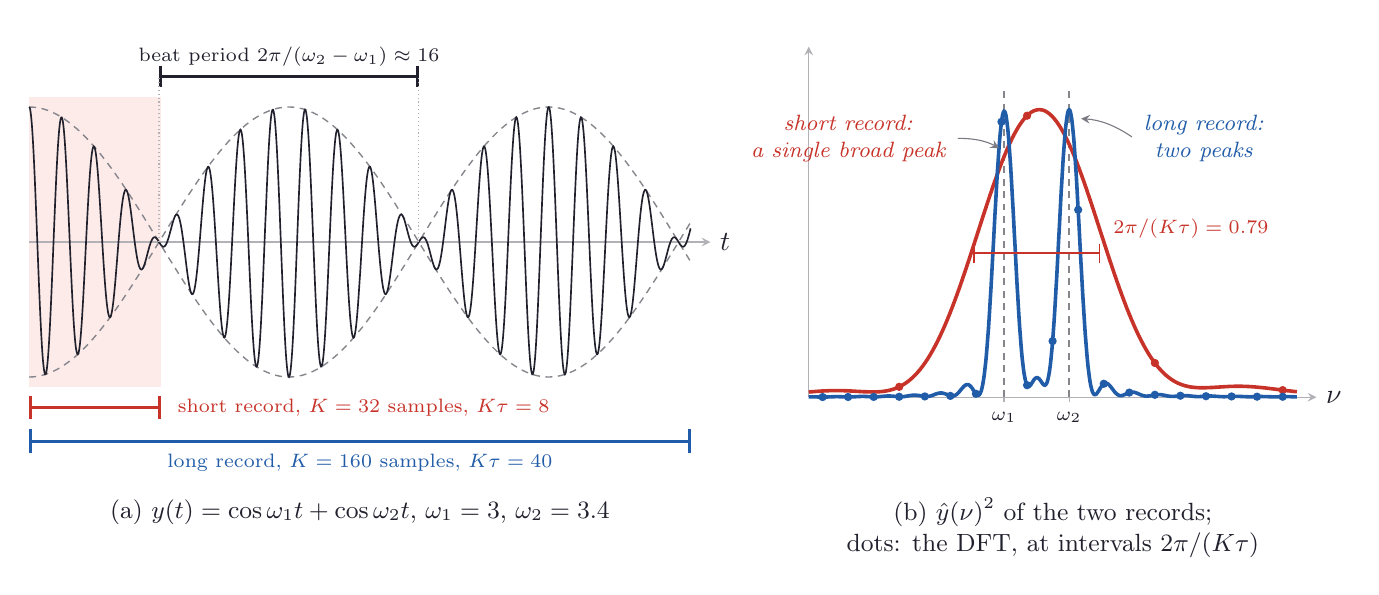
\begin{tikzpicture}[ink/.style={line width=0.9pt, ndInk}, faint/.style={line width=0.4pt, ndInk!35}, dashedink/.style={line width=0.5pt, ndInk!55, dash pattern=on 2.5pt off 2pt}, vec/.style={->, >=stealth, line width=1.2pt}, note/.style={font=\footnotesize\itshape, text=ndInk!85, align=center}, pointer/.style={->, >=stealth, line width=0.4pt, ndInk!60, shorten >=2pt, shorten <=1pt}, dot/.style={circle, fill=ndInk, inner sep=0pt, minimum size=3.4pt}, wash/.style={fill=ndSky, fill opacity=0.55}, every node/.style={text=ndInk}]
\definecolor{ndInk}{rgb}{0.13,0.13,0.18}
\definecolor{ndPaper}{rgb}{0.99,0.96,0.88}
\definecolor{ndSky}{rgb}{0.84,0.91,0.98}
\definecolor{ndRose}{rgb}{0.98,0.86,0.84}
\definecolor{ndBlue}{rgb}{0.13,0.36,0.66}
\definecolor{ndRed}{rgb}{0.78,0.20,0.16}
\definecolor{ndGold}{rgb}{0.88,0.62,0.10}
\definecolor{ndGreen}{rgb}{0.18,0.52,0.30}
\fill[ndRose, fill opacity=0.55] (0.000,0.829) rectangle (1.680,4.514);
\draw[faint, ->, >=stealth] (0.000,2.671) -- (8.652,2.671) node[right, text=ndInk] {$t$};
\draw[dashedink] (0.000,4.386) -- (0.007,4.386) -- (0.014,4.386) -- (0.021,4.385) -- (0.028,4.385) -- (0.035,4.385) -- (0.042,4.384) -- (0.049,4.384) -- (0.056,4.383) -- (0.063,4.383) -- (0.070,4.382) -- (0.077,4.381) -- (0.084,4.380) -- (0.091,4.379) -- (0.098,4.378) -- (0.105,4.377) -- (0.112,4.376) -- (0.119,4.375) -- (0.126,4.373) -- (0.133,4.372) -- (0.140,4.370) -- (0.147,4.369) -- (0.154,4.367) -- (0.161,4.366) -- (0.168,4.364) -- (0.175,4.362) -- (0.182,4.360) -- (0.189,4.358) -- (0.196,4.356) -- (0.203,4.354) -- (0.210,4.351) -- (0.217,4.349) -- (0.224,4.347) -- (0.231,4.344) -- (0.238,4.342) -- (0.245,4.339) -- (0.252,4.336) -- (0.259,4.334) -- (0.266,4.331) -- (0.273,4.328) -- (0.280,4.325) -- (0.287,4.322) -- (0.294,4.319) -- (0.301,4.316) -- (0.308,4.312) -- (0.315,4.309) -- (0.322,4.306) -- (0.329,4.302) -- (0.336,4.299) -- (0.343,4.295) -- (0.350,4.291) -- (0.357,4.287) -- (0.364,4.284) -- (0.371,4.280) -- (0.378,4.276) -- (0.385,4.272) -- (0.392,4.267) -- (0.399,4.263) -- (0.406,4.259) -- (0.413,4.255) -- (0.420,4.250) -- (0.427,4.246) -- (0.434,4.241) -- (0.441,4.236) -- (0.448,4.232) -- (0.455,4.227) -- (0.462,4.222) -- (0.469,4.217) -- (0.476,4.212) -- (0.483,4.207) -- (0.490,4.202) -- (0.497,4.197) -- (0.504,4.192) -- (0.511,4.186) -- (0.518,4.181) -- (0.525,4.176) -- (0.532,4.170) -- (0.539,4.164) -- (0.546,4.159) -- (0.553,4.153) -- (0.560,4.147) -- (0.567,4.141) -- (0.574,4.135) -- (0.581,4.129) -- (0.588,4.123) -- (0.595,4.117) -- (0.603,4.111) -- (0.610,4.105) -- (0.617,4.099) -- (0.624,4.092) -- (0.631,4.086) -- (0.638,4.079) -- (0.645,4.073) -- (0.652,4.066) -- (0.659,4.059) -- (0.666,4.053) -- (0.673,4.046) -- (0.680,4.039) -- (0.687,4.032) -- (0.694,4.025) -- (0.701,4.018) -- (0.708,4.011) -- (0.715,4.004) -- (0.722,3.997) -- (0.729,3.989) -- (0.736,3.982) -- (0.743,3.975) -- (0.750,3.967) -- (0.757,3.960) -- (0.764,3.952) -- (0.771,3.944) -- (0.778,3.937) -- (0.785,3.929) -- (0.792,3.921) -- (0.799,3.913) -- (0.806,3.905) -- (0.813,3.897) -- (0.820,3.889) -- (0.827,3.881) -- (0.834,3.873) -- (0.841,3.865) -- (0.848,3.857) -- (0.855,3.848) -- (0.862,3.840) -- (0.869,3.832) -- (0.876,3.823) -- (0.883,3.815) -- (0.890,3.806) -- (0.897,3.798) -- (0.904,3.789) -- (0.911,3.780) -- (0.918,3.772) -- (0.925,3.763) -- (0.932,3.754) -- (0.939,3.745) -- (0.946,3.736) -- (0.953,3.727) -- (0.960,3.718) -- (0.967,3.709) -- (0.974,3.700) -- (0.981,3.691) -- (0.988,3.681) -- (0.995,3.672) -- (1.002,3.663) -- (1.009,3.653) -- (1.016,3.644) -- (1.023,3.635) -- (1.030,3.625) -- (1.037,3.616) -- (1.044,3.606) -- (1.051,3.596) -- (1.058,3.587) -- (1.065,3.577) -- (1.072,3.567) -- (1.079,3.558) -- (1.086,3.548) -- (1.093,3.538) -- (1.100,3.528) -- (1.107,3.518) -- (1.114,3.508) -- (1.121,3.498) -- (1.128,3.488) -- (1.135,3.478) -- (1.142,3.468) -- (1.149,3.458) -- (1.156,3.448) -- (1.163,3.437) -- (1.170,3.427) -- (1.177,3.417) -- (1.184,3.407) -- (1.191,3.396) -- (1.198,3.386) -- (1.205,3.375) -- (1.212,3.365) -- (1.219,3.354) -- (1.226,3.344) -- (1.233,3.333) -- (1.240,3.323) -- (1.247,3.312) -- (1.254,3.302) -- (1.261,3.291) -- (1.268,3.280) -- (1.275,3.270) -- (1.282,3.259) -- (1.289,3.248) -- (1.296,3.237) -- (1.303,3.227) -- (1.310,3.216) -- (1.317,3.205) -- (1.324,3.194) -- (1.331,3.183) -- (1.338,3.172) -- (1.345,3.161) -- (1.352,3.150) -- (1.359,3.139) -- (1.366,3.128) -- (1.373,3.117) -- (1.380,3.106) -- (1.387,3.095) -- (1.394,3.084) -- (1.401,3.073) -- (1.408,3.062) -- (1.415,3.051) -- (1.422,3.039) -- (1.429,3.028) -- (1.436,3.017) -- (1.443,3.006) -- (1.450,2.995) -- (1.457,2.983) -- (1.464,2.972) -- (1.471,2.961) -- (1.478,2.950) -- (1.485,2.938) -- (1.492,2.927) -- (1.499,2.916) -- (1.506,2.904) -- (1.513,2.893) -- (1.520,2.882) -- (1.527,2.870) -- (1.534,2.859) -- (1.541,2.848) -- (1.548,2.836) -- (1.555,2.825) -- (1.562,2.813) -- (1.569,2.802) -- (1.576,2.791) -- (1.583,2.779) -- (1.590,2.768) -- (1.597,2.756) -- (1.604,2.745) -- (1.611,2.733) -- (1.618,2.722) -- (1.625,2.711) -- (1.632,2.699) -- (1.639,2.688) -- (1.646,2.676) -- (1.653,2.678) -- (1.660,2.689) -- (1.667,2.701) -- (1.674,2.712) -- (1.681,2.724) -- (1.688,2.735) -- (1.695,2.747) -- (1.702,2.758) -- (1.709,2.769) -- (1.716,2.781) -- (1.723,2.792) -- (1.730,2.804) -- (1.737,2.815) -- (1.744,2.827) -- (1.751,2.838) -- (1.758,2.849) -- (1.765,2.861) -- (1.772,2.872) -- (1.779,2.883) -- (1.786,2.895) -- (1.793,2.906) -- (1.801,2.917) -- (1.808,2.929) -- (1.815,2.940) -- (1.822,2.951) -- (1.829,2.963) -- (1.836,2.974) -- (1.843,2.985) -- (1.850,2.996) -- (1.857,3.008) -- (1.864,3.019) -- (1.871,3.030) -- (1.878,3.041) -- (1.885,3.052) -- (1.892,3.063) -- (1.899,3.075) -- (1.906,3.086) -- (1.913,3.097) -- (1.920,3.108) -- (1.927,3.119) -- (1.934,3.130) -- (1.941,3.141) -- (1.948,3.152) -- (1.955,3.163) -- (1.962,3.174) -- (1.969,3.185) -- (1.976,3.196) -- (1.983,3.207) -- (1.990,3.217) -- (1.997,3.228) -- (2.004,3.239) -- (2.011,3.250) -- (2.018,3.261) -- (2.025,3.271) -- (2.032,3.282) -- (2.039,3.293) -- (2.046,3.303) -- (2.053,3.314) -- (2.060,3.325) -- (2.067,3.335) -- (2.074,3.346) -- (2.081,3.356) -- (2.088,3.367) -- (2.095,3.377) -- (2.102,3.387) -- (2.109,3.398) -- (2.116,3.408) -- (2.123,3.418) -- (2.130,3.429) -- (2.137,3.439) -- (2.144,3.449) -- (2.151,3.459) -- (2.158,3.470) -- (2.165,3.480) -- (2.172,3.490) -- (2.179,3.500) -- (2.186,3.510) -- (2.193,3.520) -- (2.200,3.530) -- (2.207,3.539) -- (2.214,3.549) -- (2.221,3.559) -- (2.228,3.569) -- (2.235,3.579) -- (2.242,3.588) -- (2.249,3.598) -- (2.256,3.608) -- (2.263,3.617) -- (2.270,3.627) -- (2.277,3.636) -- (2.284,3.646) -- (2.291,3.655) -- (2.298,3.664) -- (2.305,3.674) -- (2.312,3.683) -- (2.319,3.692) -- (2.326,3.701) -- (2.333,3.710) -- (2.340,3.719) -- (2.347,3.728) -- (2.354,3.737) -- (2.361,3.746) -- (2.368,3.755) -- (2.375,3.764) -- (2.382,3.773) -- (2.389,3.782) -- (2.396,3.790) -- (2.403,3.799) -- (2.410,3.808) -- (2.417,3.816) -- (2.424,3.825) -- (2.431,3.833) -- (2.438,3.841) -- (2.445,3.850) -- (2.452,3.858) -- (2.459,3.866) -- (2.466,3.874) -- (2.473,3.883) -- (2.480,3.891) -- (2.487,3.899) -- (2.494,3.907) -- (2.501,3.914) -- (2.508,3.922) -- (2.515,3.930) -- (2.522,3.938) -- (2.529,3.946) -- (2.536,3.953) -- (2.543,3.961) -- (2.550,3.968) -- (2.557,3.976) -- (2.564,3.983) -- (2.571,3.990) -- (2.578,3.998) -- (2.585,4.005) -- (2.592,4.012) -- (2.599,4.019) -- (2.606,4.026) -- (2.613,4.033) -- (2.620,4.040) -- (2.627,4.047) -- (2.634,4.054) -- (2.641,4.060) -- (2.648,4.067) -- (2.655,4.074) -- (2.662,4.080) -- (2.669,4.087) -- (2.676,4.093) -- (2.683,4.100) -- (2.690,4.106) -- (2.697,4.112) -- (2.704,4.118) -- (2.711,4.124) -- (2.718,4.130) -- (2.725,4.136) -- (2.732,4.142) -- (2.739,4.148) -- (2.746,4.154) -- (2.753,4.160) -- (2.760,4.165) -- (2.767,4.171) -- (2.774,4.176) -- (2.781,4.182) -- (2.788,4.187) -- (2.795,4.192) -- (2.802,4.198) -- (2.809,4.203) -- (2.816,4.208) -- (2.823,4.213) -- (2.830,4.218) -- (2.837,4.223) -- (2.844,4.228) -- (2.851,4.233) -- (2.858,4.237) -- (2.865,4.242) -- (2.872,4.246) -- (2.879,4.251) -- (2.886,4.255) -- (2.893,4.260) -- (2.900,4.264) -- (2.907,4.268) -- (2.914,4.272) -- (2.921,4.276) -- (2.928,4.280) -- (2.935,4.284) -- (2.942,4.288) -- (2.949,4.292) -- (2.956,4.295) -- (2.963,4.299) -- (2.970,4.303) -- (2.977,4.306) -- (2.984,4.310) -- (2.991,4.313) -- (2.998,4.316) -- (3.006,4.319) -- (3.013,4.322) -- (3.020,4.325) -- (3.027,4.328) -- (3.034,4.331) -- (3.041,4.334) -- (3.048,4.337) -- (3.055,4.340) -- (3.062,4.342) -- (3.069,4.345) -- (3.076,4.347) -- (3.083,4.350) -- (3.090,4.352) -- (3.097,4.354) -- (3.104,4.356) -- (3.111,4.358) -- (3.118,4.360) -- (3.125,4.362) -- (3.132,4.364) -- (3.139,4.366) -- (3.146,4.368) -- (3.153,4.369) -- (3.160,4.371) -- (3.167,4.372) -- (3.174,4.374) -- (3.181,4.375) -- (3.188,4.376) -- (3.195,4.377) -- (3.202,4.378) -- (3.209,4.379) -- (3.216,4.380) -- (3.223,4.381) -- (3.230,4.382) -- (3.237,4.383) -- (3.244,4.383) -- (3.251,4.384) -- (3.258,4.384) -- (3.265,4.385) -- (3.272,4.385) -- (3.279,4.385) -- (3.286,4.386) -- (3.293,4.386) -- (3.300,4.386) -- (3.307,4.386) -- (3.314,4.386) -- (3.321,4.385) -- (3.328,4.385) -- (3.335,4.385) -- (3.342,4.384) -- (3.349,4.384) -- (3.356,4.383) -- (3.363,4.383) -- (3.370,4.382) -- (3.377,4.381) -- (3.384,4.380) -- (3.391,4.379) -- (3.398,4.378) -- (3.405,4.377) -- (3.412,4.376) -- (3.419,4.374) -- (3.426,4.373) -- (3.433,4.372) -- (3.440,4.370) -- (3.447,4.369) -- (3.454,4.367) -- (3.461,4.365) -- (3.468,4.364) -- (3.475,4.362) -- (3.482,4.360) -- (3.489,4.358) -- (3.496,4.356) -- (3.503,4.353) -- (3.510,4.351) -- (3.517,4.349) -- (3.524,4.346) -- (3.531,4.344) -- (3.538,4.341) -- (3.545,4.339) -- (3.552,4.336) -- (3.559,4.333) -- (3.566,4.330) -- (3.573,4.328) -- (3.580,4.325) -- (3.587,4.321) -- (3.594,4.318) -- (3.601,4.315) -- (3.608,4.312) -- (3.615,4.309) -- (3.622,4.305) -- (3.629,4.302) -- (3.636,4.298) -- (3.643,4.294) -- (3.650,4.291) -- (3.657,4.287) -- (3.664,4.283) -- (3.671,4.279) -- (3.678,4.275) -- (3.685,4.271) -- (3.692,4.267) -- (3.699,4.263) -- (3.706,4.258) -- (3.713,4.254) -- (3.720,4.249) -- (3.727,4.245) -- (3.734,4.240) -- (3.741,4.236) -- (3.748,4.231) -- (3.755,4.226) -- (3.762,4.221) -- (3.769,4.216) -- (3.776,4.212) -- (3.783,4.206) -- (3.790,4.201) -- (3.797,4.196) -- (3.804,4.191) -- (3.811,4.186) -- (3.818,4.180) -- (3.825,4.175) -- (3.832,4.169) -- (3.839,4.164) -- (3.846,4.158) -- (3.853,4.152) -- (3.860,4.146) -- (3.867,4.140) -- (3.874,4.135) -- (3.881,4.129) -- (3.888,4.123) -- (3.895,4.116) -- (3.902,4.110) -- (3.909,4.104) -- (3.916,4.098) -- (3.923,4.091) -- (3.930,4.085) -- (3.937,4.078) -- (3.944,4.072) -- (3.951,4.065) -- (3.958,4.058) -- (3.965,4.052) -- (3.972,4.045) -- (3.979,4.038) -- (3.986,4.031) -- (3.993,4.024) -- (4.000,4.017) -- (4.007,4.010) -- (4.014,4.003) -- (4.021,3.995) -- (4.028,3.988) -- (4.035,3.981) -- (4.042,3.973) -- (4.049,3.966) -- (4.056,3.958) -- (4.063,3.951) -- (4.070,3.943) -- (4.077,3.935) -- (4.084,3.928) -- (4.091,3.920) -- (4.098,3.912) -- (4.105,3.904) -- (4.112,3.896) -- (4.119,3.888) -- (4.126,3.880) -- (4.133,3.872) -- (4.140,3.864) -- (4.147,3.855) -- (4.154,3.847) -- (4.161,3.839) -- (4.168,3.830) -- (4.175,3.822) -- (4.182,3.813) -- (4.189,3.805) -- (4.196,3.796) -- (4.204,3.788) -- (4.211,3.779) -- (4.218,3.770) -- (4.225,3.761) -- (4.232,3.753) -- (4.239,3.744) -- (4.246,3.735) -- (4.253,3.726) -- (4.260,3.717) -- (4.267,3.708) -- (4.274,3.698) -- (4.281,3.689) -- (4.288,3.680) -- (4.295,3.671) -- (4.302,3.661) -- (4.309,3.652) -- (4.316,3.643) -- (4.323,3.633) -- (4.330,3.624) -- (4.337,3.614) -- (4.344,3.605) -- (4.351,3.595) -- (4.358,3.585) -- (4.365,3.576) -- (4.372,3.566) -- (4.379,3.556) -- (4.386,3.546) -- (4.393,3.536) -- (4.400,3.527) -- (4.407,3.517) -- (4.414,3.507) -- (4.421,3.497) -- (4.428,3.487) -- (4.435,3.477) -- (4.442,3.466) -- (4.449,3.456) -- (4.456,3.446) -- (4.463,3.436) -- (4.470,3.426) -- (4.477,3.415) -- (4.484,3.405) -- (4.491,3.395) -- (4.498,3.384) -- (4.505,3.374) -- (4.512,3.363) -- (4.519,3.353) -- (4.526,3.342) -- (4.533,3.332) -- (4.540,3.321) -- (4.547,3.311) -- (4.554,3.300) -- (4.561,3.289) -- (4.568,3.279) -- (4.575,3.268) -- (4.582,3.257) -- (4.589,3.246) -- (4.596,3.236) -- (4.603,3.225) -- (4.610,3.214) -- (4.617,3.203) -- (4.624,3.192) -- (4.631,3.181) -- (4.638,3.170) -- (4.645,3.160) -- (4.652,3.149) -- (4.659,3.138) -- (4.666,3.127) -- (4.673,3.115) -- (4.680,3.104) -- (4.687,3.093) -- (4.694,3.082) -- (4.701,3.071) -- (4.708,3.060) -- (4.715,3.049) -- (4.722,3.038) -- (4.729,3.027) -- (4.736,3.015) -- (4.743,3.004) -- (4.750,2.993) -- (4.757,2.982) -- (4.764,2.970) -- (4.771,2.959) -- (4.778,2.948) -- (4.785,2.937) -- (4.792,2.925) -- (4.799,2.914) -- (4.806,2.903) -- (4.813,2.891) -- (4.820,2.880) -- (4.827,2.869) -- (4.834,2.857) -- (4.841,2.846) -- (4.848,2.834) -- (4.855,2.823) -- (4.862,2.812) -- (4.869,2.800) -- (4.876,2.789) -- (4.883,2.777) -- (4.890,2.766) -- (4.897,2.755) -- (4.904,2.743) -- (4.911,2.732) -- (4.918,2.720) -- (4.925,2.709) -- (4.932,2.697) -- (4.939,2.686) -- (4.946,2.675) -- (4.953,2.680) -- (4.960,2.691) -- (4.967,2.703) -- (4.974,2.714) -- (4.981,2.726) -- (4.988,2.737) -- (4.995,2.748) -- (5.002,2.760) -- (5.009,2.771) -- (5.016,2.783) -- (5.023,2.794) -- (5.030,2.805) -- (5.037,2.817) -- (5.044,2.828) -- (5.051,2.840) -- (5.058,2.851) -- (5.065,2.862) -- (5.072,2.874) -- (5.079,2.885) -- (5.086,2.896) -- (5.093,2.908) -- (5.100,2.919) -- (5.107,2.930) -- (5.114,2.942) -- (5.121,2.953) -- (5.128,2.964) -- (5.135,2.976) -- (5.142,2.987) -- (5.149,2.998) -- (5.156,3.009) -- (5.163,3.020) -- (5.170,3.032) -- (5.177,3.043) -- (5.184,3.054) -- (5.191,3.065) -- (5.198,3.076) -- (5.205,3.087) -- (5.212,3.098) -- (5.219,3.110) -- (5.226,3.121) -- (5.233,3.132) -- (5.240,3.143) -- (5.247,3.154) -- (5.254,3.165) -- (5.261,3.176) -- (5.268,3.186) -- (5.275,3.197) -- (5.282,3.208) -- (5.289,3.219) -- (5.296,3.230) -- (5.303,3.241) -- (5.310,3.251) -- (5.317,3.262) -- (5.324,3.273) -- (5.331,3.284) -- (5.338,3.294) -- (5.345,3.305) -- (5.352,3.316) -- (5.359,3.326) -- (5.366,3.337) -- (5.373,3.347) -- (5.380,3.358) -- (5.387,3.368) -- (5.394,3.379) -- (5.402,3.389) -- (5.409,3.399) -- (5.416,3.410) -- (5.423,3.420) -- (5.430,3.430) -- (5.437,3.441) -- (5.444,3.451) -- (5.451,3.461) -- (5.458,3.471) -- (5.465,3.481) -- (5.472,3.491) -- (5.479,3.501) -- (5.486,3.511) -- (5.493,3.521) -- (5.500,3.531) -- (5.507,3.541) -- (5.514,3.551) -- (5.521,3.561) -- (5.528,3.570) -- (5.535,3.580) -- (5.542,3.590) -- (5.549,3.599) -- (5.556,3.609) -- (5.563,3.619) -- (5.570,3.628) -- (5.577,3.638) -- (5.584,3.647) -- (5.591,3.656) -- (5.598,3.666) -- (5.605,3.675) -- (5.612,3.684) -- (5.619,3.693) -- (5.626,3.703) -- (5.633,3.712) -- (5.640,3.721) -- (5.647,3.730) -- (5.654,3.739) -- (5.661,3.748) -- (5.668,3.757) -- (5.675,3.765) -- (5.682,3.774) -- (5.689,3.783) -- (5.696,3.792) -- (5.703,3.800) -- (5.710,3.809) -- (5.717,3.817) -- (5.724,3.826) -- (5.731,3.834) -- (5.738,3.843) -- (5.745,3.851) -- (5.752,3.859) -- (5.759,3.867) -- (5.766,3.876) -- (5.773,3.884) -- (5.780,3.892) -- (5.787,3.900) -- (5.794,3.908) -- (5.801,3.916) -- (5.808,3.924) -- (5.815,3.931) -- (5.822,3.939) -- (5.829,3.947) -- (5.836,3.954) -- (5.843,3.962) -- (5.850,3.969) -- (5.857,3.977) -- (5.864,3.984) -- (5.871,3.992) -- (5.878,3.999) -- (5.885,4.006) -- (5.892,4.013) -- (5.899,4.020) -- (5.906,4.027) -- (5.913,4.034) -- (5.920,4.041) -- (5.927,4.048) -- (5.934,4.055) -- (5.941,4.062) -- (5.948,4.068) -- (5.955,4.075) -- (5.962,4.081) -- (5.969,4.088) -- (5.976,4.094) -- (5.983,4.101) -- (5.990,4.107) -- (5.997,4.113) -- (6.004,4.119) -- (6.011,4.125) -- (6.018,4.131) -- (6.025,4.137) -- (6.032,4.143) -- (6.039,4.149) -- (6.046,4.155) -- (6.053,4.160) -- (6.060,4.166) -- (6.067,4.172) -- (6.074,4.177) -- (6.081,4.183) -- (6.088,4.188) -- (6.095,4.193) -- (6.102,4.199) -- (6.109,4.204) -- (6.116,4.209) -- (6.123,4.214) -- (6.130,4.219) -- (6.137,4.224) -- (6.144,4.228) -- (6.151,4.233) -- (6.158,4.238) -- (6.165,4.243) -- (6.172,4.247) -- (6.179,4.252) -- (6.186,4.256) -- (6.193,4.260) -- (6.200,4.265) -- (6.207,4.269) -- (6.214,4.273) -- (6.221,4.277) -- (6.228,4.281) -- (6.235,4.285) -- (6.242,4.289) -- (6.249,4.292) -- (6.256,4.296) -- (6.263,4.300) -- (6.270,4.303) -- (6.277,4.307) -- (6.284,4.310) -- (6.291,4.313) -- (6.298,4.317) -- (6.305,4.320) -- (6.312,4.323) -- (6.319,4.326) -- (6.326,4.329) -- (6.333,4.332) -- (6.340,4.335) -- (6.347,4.337) -- (6.354,4.340) -- (6.361,4.343) -- (6.368,4.345) -- (6.375,4.348) -- (6.382,4.350) -- (6.389,4.352) -- (6.396,4.354) -- (6.403,4.357) -- (6.410,4.359) -- (6.417,4.361) -- (6.424,4.363) -- (6.431,4.364) -- (6.438,4.366) -- (6.445,4.368) -- (6.452,4.369) -- (6.459,4.371) -- (6.466,4.372) -- (6.473,4.374) -- (6.480,4.375) -- (6.487,4.376) -- (6.494,4.377) -- (6.501,4.379) -- (6.508,4.380) -- (6.515,4.381) -- (6.522,4.381) -- (6.529,4.382) -- (6.536,4.383) -- (6.543,4.383) -- (6.550,4.384) -- (6.557,4.384) -- (6.564,4.385) -- (6.571,4.385) -- (6.578,4.385) -- (6.585,4.386) -- (6.592,4.386) -- (6.599,4.386) -- (6.607,4.386) -- (6.614,4.386) -- (6.621,4.385) -- (6.628,4.385) -- (6.635,4.385) -- (6.642,4.384) -- (6.649,4.384) -- (6.656,4.383) -- (6.663,4.382) -- (6.670,4.382) -- (6.677,4.381) -- (6.684,4.380) -- (6.691,4.379) -- (6.698,4.378) -- (6.705,4.377) -- (6.712,4.376) -- (6.719,4.374) -- (6.726,4.373) -- (6.733,4.372) -- (6.740,4.370) -- (6.747,4.368) -- (6.754,4.367) -- (6.761,4.365) -- (6.768,4.363) -- (6.775,4.361) -- (6.782,4.359) -- (6.789,4.357) -- (6.796,4.355) -- (6.803,4.353) -- (6.810,4.351) -- (6.817,4.348) -- (6.824,4.346) -- (6.831,4.344) -- (6.838,4.341) -- (6.845,4.338) -- (6.852,4.336) -- (6.859,4.333) -- (6.866,4.330) -- (6.873,4.327) -- (6.880,4.324) -- (6.887,4.321) -- (6.894,4.318) -- (6.901,4.315) -- (6.908,4.311) -- (6.915,4.308) -- (6.922,4.305) -- (6.929,4.301) -- (6.936,4.297) -- (6.943,4.294) -- (6.950,4.290) -- (6.957,4.286) -- (6.964,4.282) -- (6.971,4.278) -- (6.978,4.274) -- (6.985,4.270) -- (6.992,4.266) -- (6.999,4.262) -- (7.006,4.258) -- (7.013,4.253) -- (7.020,4.249) -- (7.027,4.244) -- (7.034,4.240) -- (7.041,4.235) -- (7.048,4.230) -- (7.055,4.226) -- (7.062,4.221) -- (7.069,4.216) -- (7.076,4.211) -- (7.083,4.206) -- (7.090,4.201) -- (7.097,4.195) -- (7.104,4.190) -- (7.111,4.185) -- (7.118,4.179) -- (7.125,4.174) -- (7.132,4.168) -- (7.139,4.163) -- (7.146,4.157) -- (7.153,4.151) -- (7.160,4.145) -- (7.167,4.140) -- (7.174,4.134) -- (7.181,4.128) -- (7.188,4.122) -- (7.195,4.115) -- (7.202,4.109) -- (7.209,4.103) -- (7.216,4.097) -- (7.223,4.090) -- (7.230,4.084) -- (7.237,4.077) -- (7.244,4.071) -- (7.251,4.064) -- (7.258,4.057) -- (7.265,4.051) -- (7.272,4.044) -- (7.279,4.037) -- (7.286,4.030) -- (7.293,4.023) -- (7.300,4.016) -- (7.307,4.009) -- (7.314,4.002) -- (7.321,3.994) -- (7.328,3.987) -- (7.335,3.980) -- (7.342,3.972) -- (7.349,3.965) -- (7.356,3.957) -- (7.363,3.950) -- (7.370,3.942) -- (7.377,3.934) -- (7.384,3.927) -- (7.391,3.919) -- (7.398,3.911) -- (7.405,3.903) -- (7.412,3.895) -- (7.419,3.887) -- (7.426,3.879) -- (7.433,3.871) -- (7.440,3.862) -- (7.447,3.854) -- (7.454,3.846) -- (7.461,3.838) -- (7.468,3.829) -- (7.475,3.821) -- (7.482,3.812) -- (7.489,3.804) -- (7.496,3.795) -- (7.503,3.786) -- (7.510,3.778) -- (7.517,3.769) -- (7.524,3.760) -- (7.531,3.751) -- (7.538,3.742) -- (7.545,3.733) -- (7.552,3.724) -- (7.559,3.715) -- (7.566,3.706) -- (7.573,3.697) -- (7.580,3.688) -- (7.587,3.679) -- (7.594,3.669) -- (7.601,3.660) -- (7.608,3.651) -- (7.615,3.641) -- (7.622,3.632) -- (7.629,3.622) -- (7.636,3.613) -- (7.643,3.603) -- (7.650,3.593) -- (7.657,3.584) -- (7.664,3.574) -- (7.671,3.564) -- (7.678,3.555) -- (7.685,3.545) -- (7.692,3.535) -- (7.699,3.525) -- (7.706,3.515) -- (7.713,3.505) -- (7.720,3.495) -- (7.727,3.485) -- (7.734,3.475) -- (7.741,3.465) -- (7.748,3.455) -- (7.755,3.444) -- (7.762,3.434) -- (7.769,3.424) -- (7.776,3.414) -- (7.783,3.403) -- (7.790,3.393) -- (7.797,3.383) -- (7.805,3.372) -- (7.812,3.362) -- (7.819,3.351) -- (7.826,3.341) -- (7.833,3.330) -- (7.840,3.320) -- (7.847,3.309) -- (7.854,3.298) -- (7.861,3.288) -- (7.868,3.277) -- (7.875,3.266) -- (7.882,3.256) -- (7.889,3.245) -- (7.896,3.234) -- (7.903,3.223) -- (7.910,3.212) -- (7.917,3.202) -- (7.924,3.191) -- (7.931,3.180) -- (7.938,3.169) -- (7.945,3.158) -- (7.952,3.147) -- (7.959,3.136) -- (7.966,3.125) -- (7.973,3.114) -- (7.980,3.103) -- (7.987,3.092) -- (7.994,3.081) -- (8.001,3.069) -- (8.008,3.058) -- (8.015,3.047) -- (8.022,3.036) -- (8.029,3.025) -- (8.036,3.014) -- (8.043,3.002) -- (8.050,2.991) -- (8.057,2.980) -- (8.064,2.969) -- (8.071,2.957) -- (8.078,2.946) -- (8.085,2.935) -- (8.092,2.923) -- (8.099,2.912) -- (8.106,2.901) -- (8.113,2.889) -- (8.120,2.878) -- (8.127,2.867) -- (8.134,2.855) -- (8.141,2.844) -- (8.148,2.833) -- (8.155,2.821) -- (8.162,2.810) -- (8.169,2.798) -- (8.176,2.787) -- (8.183,2.776) -- (8.190,2.764) -- (8.197,2.753) -- (8.204,2.741) -- (8.211,2.730) -- (8.218,2.718) -- (8.225,2.707) -- (8.232,2.696) -- (8.239,2.684) -- (8.246,2.673) -- (8.253,2.682) -- (8.260,2.693) -- (8.267,2.704) -- (8.274,2.716) -- (8.281,2.727) -- (8.288,2.739) -- (8.295,2.750) -- (8.302,2.762) -- (8.309,2.773) -- (8.316,2.784) -- (8.323,2.796) -- (8.330,2.807) -- (8.337,2.819) -- (8.344,2.830) -- (8.351,2.841) -- (8.358,2.853) -- (8.365,2.864) -- (8.372,2.876) -- (8.379,2.887) -- (8.386,2.898) -- (8.393,2.910) -- (8.400,2.921);
\draw[dashedink] (0.000,0.957) -- (0.007,0.957) -- (0.014,0.957) -- (0.021,0.957) -- (0.028,0.958) -- (0.035,0.958) -- (0.042,0.959) -- (0.049,0.959) -- (0.056,0.960) -- (0.063,0.960) -- (0.070,0.961) -- (0.077,0.962) -- (0.084,0.963) -- (0.091,0.964) -- (0.098,0.965) -- (0.105,0.966) -- (0.112,0.967) -- (0.119,0.968) -- (0.126,0.969) -- (0.133,0.971) -- (0.140,0.972) -- (0.147,0.974) -- (0.154,0.976) -- (0.161,0.977) -- (0.168,0.979) -- (0.175,0.981) -- (0.182,0.983) -- (0.189,0.985) -- (0.196,0.987) -- (0.203,0.989) -- (0.210,0.991) -- (0.217,0.994) -- (0.224,0.996) -- (0.231,0.999) -- (0.238,1.001) -- (0.245,1.004) -- (0.252,1.006) -- (0.259,1.009) -- (0.266,1.012) -- (0.273,1.015) -- (0.280,1.018) -- (0.287,1.021) -- (0.294,1.024) -- (0.301,1.027) -- (0.308,1.030) -- (0.315,1.034) -- (0.322,1.037) -- (0.329,1.041) -- (0.336,1.044) -- (0.343,1.048) -- (0.350,1.052) -- (0.357,1.055) -- (0.364,1.059) -- (0.371,1.063) -- (0.378,1.067) -- (0.385,1.071) -- (0.392,1.075) -- (0.399,1.080) -- (0.406,1.084) -- (0.413,1.088) -- (0.420,1.093) -- (0.427,1.097) -- (0.434,1.102) -- (0.441,1.106) -- (0.448,1.111) -- (0.455,1.116) -- (0.462,1.121) -- (0.469,1.126) -- (0.476,1.131) -- (0.483,1.136) -- (0.490,1.141) -- (0.497,1.146) -- (0.504,1.151) -- (0.511,1.157) -- (0.518,1.162) -- (0.525,1.167) -- (0.532,1.173) -- (0.539,1.178) -- (0.546,1.184) -- (0.553,1.190) -- (0.560,1.196) -- (0.567,1.201) -- (0.574,1.207) -- (0.581,1.213) -- (0.588,1.219) -- (0.595,1.226) -- (0.603,1.232) -- (0.610,1.238) -- (0.617,1.244) -- (0.624,1.251) -- (0.631,1.257) -- (0.638,1.264) -- (0.645,1.270) -- (0.652,1.277) -- (0.659,1.283) -- (0.666,1.290) -- (0.673,1.297) -- (0.680,1.304) -- (0.687,1.311) -- (0.694,1.318) -- (0.701,1.325) -- (0.708,1.332) -- (0.715,1.339) -- (0.722,1.346) -- (0.729,1.354) -- (0.736,1.361) -- (0.743,1.368) -- (0.750,1.376) -- (0.757,1.383) -- (0.764,1.391) -- (0.771,1.399) -- (0.778,1.406) -- (0.785,1.414) -- (0.792,1.422) -- (0.799,1.430) -- (0.806,1.438) -- (0.813,1.445) -- (0.820,1.454) -- (0.827,1.462) -- (0.834,1.470) -- (0.841,1.478) -- (0.848,1.486) -- (0.855,1.494) -- (0.862,1.503) -- (0.869,1.511) -- (0.876,1.520) -- (0.883,1.528) -- (0.890,1.537) -- (0.897,1.545) -- (0.904,1.554) -- (0.911,1.563) -- (0.918,1.571) -- (0.925,1.580) -- (0.932,1.589) -- (0.939,1.598) -- (0.946,1.607) -- (0.953,1.616) -- (0.960,1.625) -- (0.967,1.634) -- (0.974,1.643) -- (0.981,1.652) -- (0.988,1.661) -- (0.995,1.671) -- (1.002,1.680) -- (1.009,1.689) -- (1.016,1.699) -- (1.023,1.708) -- (1.030,1.718) -- (1.037,1.727) -- (1.044,1.737) -- (1.051,1.746) -- (1.058,1.756) -- (1.065,1.766) -- (1.072,1.775) -- (1.079,1.785) -- (1.086,1.795) -- (1.093,1.805) -- (1.100,1.815) -- (1.107,1.825) -- (1.114,1.835) -- (1.121,1.845) -- (1.128,1.855) -- (1.135,1.865) -- (1.142,1.875) -- (1.149,1.885) -- (1.156,1.895) -- (1.163,1.905) -- (1.170,1.916) -- (1.177,1.926) -- (1.184,1.936) -- (1.191,1.947) -- (1.198,1.957) -- (1.205,1.967) -- (1.212,1.978) -- (1.219,1.988) -- (1.226,1.999) -- (1.233,2.009) -- (1.240,2.020) -- (1.247,2.031) -- (1.254,2.041) -- (1.261,2.052) -- (1.268,2.063) -- (1.275,2.073) -- (1.282,2.084) -- (1.289,2.095) -- (1.296,2.106) -- (1.303,2.116) -- (1.310,2.127) -- (1.317,2.138) -- (1.324,2.149) -- (1.331,2.160) -- (1.338,2.171) -- (1.345,2.182) -- (1.352,2.193) -- (1.359,2.204) -- (1.366,2.215) -- (1.373,2.226) -- (1.380,2.237) -- (1.387,2.248) -- (1.394,2.259) -- (1.401,2.270) -- (1.408,2.281) -- (1.415,2.292) -- (1.422,2.303) -- (1.429,2.315) -- (1.436,2.326) -- (1.443,2.337) -- (1.450,2.348) -- (1.457,2.360) -- (1.464,2.371) -- (1.471,2.382) -- (1.478,2.393) -- (1.485,2.405) -- (1.492,2.416) -- (1.499,2.427) -- (1.506,2.439) -- (1.513,2.450) -- (1.520,2.461) -- (1.527,2.473) -- (1.534,2.484) -- (1.541,2.495) -- (1.548,2.507) -- (1.555,2.518) -- (1.562,2.529) -- (1.569,2.541) -- (1.576,2.552) -- (1.583,2.564) -- (1.590,2.575) -- (1.597,2.587) -- (1.604,2.598) -- (1.611,2.609) -- (1.618,2.621) -- (1.625,2.632) -- (1.632,2.644) -- (1.639,2.655) -- (1.646,2.667) -- (1.653,2.665) -- (1.660,2.653) -- (1.667,2.642) -- (1.674,2.631) -- (1.681,2.619) -- (1.688,2.608) -- (1.695,2.596) -- (1.702,2.585) -- (1.709,2.573) -- (1.716,2.562) -- (1.723,2.551) -- (1.730,2.539) -- (1.737,2.528) -- (1.744,2.516) -- (1.751,2.505) -- (1.758,2.494) -- (1.765,2.482) -- (1.772,2.471) -- (1.779,2.459) -- (1.786,2.448) -- (1.793,2.437) -- (1.801,2.425) -- (1.808,2.414) -- (1.815,2.403) -- (1.822,2.392) -- (1.829,2.380) -- (1.836,2.369) -- (1.843,2.358) -- (1.850,2.347) -- (1.857,2.335) -- (1.864,2.324) -- (1.871,2.313) -- (1.878,2.302) -- (1.885,2.291) -- (1.892,2.279) -- (1.899,2.268) -- (1.906,2.257) -- (1.913,2.246) -- (1.920,2.235) -- (1.927,2.224) -- (1.934,2.213) -- (1.941,2.202) -- (1.948,2.191) -- (1.955,2.180) -- (1.962,2.169) -- (1.969,2.158) -- (1.976,2.147) -- (1.983,2.136) -- (1.990,2.125) -- (1.997,2.115) -- (2.004,2.104) -- (2.011,2.093) -- (2.018,2.082) -- (2.025,2.072) -- (2.032,2.061) -- (2.039,2.050) -- (2.046,2.040) -- (2.053,2.029) -- (2.060,2.018) -- (2.067,2.008) -- (2.074,1.997) -- (2.081,1.987) -- (2.088,1.976) -- (2.095,1.966) -- (2.102,1.955) -- (2.109,1.945) -- (2.116,1.935) -- (2.123,1.924) -- (2.130,1.914) -- (2.137,1.904) -- (2.144,1.894) -- (2.151,1.883) -- (2.158,1.873) -- (2.165,1.863) -- (2.172,1.853) -- (2.179,1.843) -- (2.186,1.833) -- (2.193,1.823) -- (2.200,1.813) -- (2.207,1.803) -- (2.214,1.794) -- (2.221,1.784) -- (2.228,1.774) -- (2.235,1.764) -- (2.242,1.755) -- (2.249,1.745) -- (2.256,1.735) -- (2.263,1.726) -- (2.270,1.716) -- (2.277,1.707) -- (2.284,1.697) -- (2.291,1.688) -- (2.298,1.679) -- (2.305,1.669) -- (2.312,1.660) -- (2.319,1.651) -- (2.326,1.642) -- (2.333,1.633) -- (2.340,1.623) -- (2.347,1.614) -- (2.354,1.605) -- (2.361,1.597) -- (2.368,1.588) -- (2.375,1.579) -- (2.382,1.570) -- (2.389,1.561) -- (2.396,1.553) -- (2.403,1.544) -- (2.410,1.535) -- (2.417,1.527) -- (2.424,1.518) -- (2.431,1.510) -- (2.438,1.501) -- (2.445,1.493) -- (2.452,1.485) -- (2.459,1.477) -- (2.466,1.468) -- (2.473,1.460) -- (2.480,1.452) -- (2.487,1.444) -- (2.494,1.436) -- (2.501,1.428) -- (2.508,1.421) -- (2.515,1.413) -- (2.522,1.405) -- (2.529,1.397) -- (2.536,1.390) -- (2.543,1.382) -- (2.550,1.375) -- (2.557,1.367) -- (2.564,1.360) -- (2.571,1.352) -- (2.578,1.345) -- (2.585,1.338) -- (2.592,1.331) -- (2.599,1.324) -- (2.606,1.317) -- (2.613,1.310) -- (2.620,1.303) -- (2.627,1.296) -- (2.634,1.289) -- (2.641,1.282) -- (2.648,1.276) -- (2.655,1.269) -- (2.662,1.263) -- (2.669,1.256) -- (2.676,1.250) -- (2.683,1.243) -- (2.690,1.237) -- (2.697,1.231) -- (2.704,1.225) -- (2.711,1.218) -- (2.718,1.212) -- (2.725,1.206) -- (2.732,1.201) -- (2.739,1.195) -- (2.746,1.189) -- (2.753,1.183) -- (2.760,1.178) -- (2.767,1.172) -- (2.774,1.167) -- (2.781,1.161) -- (2.788,1.156) -- (2.795,1.150) -- (2.802,1.145) -- (2.809,1.140) -- (2.816,1.135) -- (2.823,1.130) -- (2.830,1.125) -- (2.837,1.120) -- (2.844,1.115) -- (2.851,1.110) -- (2.858,1.106) -- (2.865,1.101) -- (2.872,1.096) -- (2.879,1.092) -- (2.886,1.088) -- (2.893,1.083) -- (2.900,1.079) -- (2.907,1.075) -- (2.914,1.071) -- (2.921,1.067) -- (2.928,1.063) -- (2.935,1.059) -- (2.942,1.055) -- (2.949,1.051) -- (2.956,1.047) -- (2.963,1.044) -- (2.970,1.040) -- (2.977,1.037) -- (2.984,1.033) -- (2.991,1.030) -- (2.998,1.027) -- (3.006,1.024) -- (3.013,1.020) -- (3.020,1.017) -- (3.027,1.014) -- (3.034,1.012) -- (3.041,1.009) -- (3.048,1.006) -- (3.055,1.003) -- (3.062,1.001) -- (3.069,0.998) -- (3.076,0.996) -- (3.083,0.993) -- (3.090,0.991) -- (3.097,0.989) -- (3.104,0.987) -- (3.111,0.985) -- (3.118,0.983) -- (3.125,0.981) -- (3.132,0.979) -- (3.139,0.977) -- (3.146,0.975) -- (3.153,0.974) -- (3.160,0.972) -- (3.167,0.971) -- (3.174,0.969) -- (3.181,0.968) -- (3.188,0.967) -- (3.195,0.966) -- (3.202,0.964) -- (3.209,0.963) -- (3.216,0.962) -- (3.223,0.962) -- (3.230,0.961) -- (3.237,0.960) -- (3.244,0.959) -- (3.251,0.959) -- (3.258,0.958) -- (3.265,0.958) -- (3.272,0.958) -- (3.279,0.957) -- (3.286,0.957) -- (3.293,0.957) -- (3.300,0.957) -- (3.307,0.957) -- (3.314,0.957) -- (3.321,0.958) -- (3.328,0.958) -- (3.335,0.958) -- (3.342,0.959) -- (3.349,0.959) -- (3.356,0.960) -- (3.363,0.960) -- (3.370,0.961) -- (3.377,0.962) -- (3.384,0.963) -- (3.391,0.964) -- (3.398,0.965) -- (3.405,0.966) -- (3.412,0.967) -- (3.419,0.968) -- (3.426,0.970) -- (3.433,0.971) -- (3.440,0.973) -- (3.447,0.974) -- (3.454,0.976) -- (3.461,0.978) -- (3.468,0.979) -- (3.475,0.981) -- (3.482,0.983) -- (3.489,0.985) -- (3.496,0.987) -- (3.503,0.989) -- (3.510,0.992) -- (3.517,0.994) -- (3.524,0.996) -- (3.531,0.999) -- (3.538,1.001) -- (3.545,1.004) -- (3.552,1.007) -- (3.559,1.010) -- (3.566,1.012) -- (3.573,1.015) -- (3.580,1.018) -- (3.587,1.021) -- (3.594,1.025) -- (3.601,1.028) -- (3.608,1.031) -- (3.615,1.034) -- (3.622,1.038) -- (3.629,1.041) -- (3.636,1.045) -- (3.643,1.049) -- (3.650,1.052) -- (3.657,1.056) -- (3.664,1.060) -- (3.671,1.064) -- (3.678,1.068) -- (3.685,1.072) -- (3.692,1.076) -- (3.699,1.080) -- (3.706,1.085) -- (3.713,1.089) -- (3.720,1.093) -- (3.727,1.098) -- (3.734,1.102) -- (3.741,1.107) -- (3.748,1.112) -- (3.755,1.117) -- (3.762,1.121) -- (3.769,1.126) -- (3.776,1.131) -- (3.783,1.136) -- (3.790,1.142) -- (3.797,1.147) -- (3.804,1.152) -- (3.811,1.157) -- (3.818,1.163) -- (3.825,1.168) -- (3.832,1.174) -- (3.839,1.179) -- (3.846,1.185) -- (3.853,1.191) -- (3.860,1.197) -- (3.867,1.202) -- (3.874,1.208) -- (3.881,1.214) -- (3.888,1.220) -- (3.895,1.226) -- (3.902,1.233) -- (3.909,1.239) -- (3.916,1.245) -- (3.923,1.252) -- (3.930,1.258) -- (3.937,1.265) -- (3.944,1.271) -- (3.951,1.278) -- (3.958,1.284) -- (3.965,1.291) -- (3.972,1.298) -- (3.979,1.305) -- (3.986,1.312) -- (3.993,1.319) -- (4.000,1.326) -- (4.007,1.333) -- (4.014,1.340) -- (4.021,1.347) -- (4.028,1.355) -- (4.035,1.362) -- (4.042,1.369) -- (4.049,1.377) -- (4.056,1.384) -- (4.063,1.392) -- (4.070,1.400) -- (4.077,1.407) -- (4.084,1.415) -- (4.091,1.423) -- (4.098,1.431) -- (4.105,1.439) -- (4.112,1.447) -- (4.119,1.455) -- (4.126,1.463) -- (4.133,1.471) -- (4.140,1.479) -- (4.147,1.487) -- (4.154,1.496) -- (4.161,1.504) -- (4.168,1.512) -- (4.175,1.521) -- (4.182,1.529) -- (4.189,1.538) -- (4.196,1.547) -- (4.204,1.555) -- (4.211,1.564) -- (4.218,1.573) -- (4.225,1.581) -- (4.232,1.590) -- (4.239,1.599) -- (4.246,1.608) -- (4.253,1.617) -- (4.260,1.626) -- (4.267,1.635) -- (4.274,1.644) -- (4.281,1.654) -- (4.288,1.663) -- (4.295,1.672) -- (4.302,1.681) -- (4.309,1.691) -- (4.316,1.700) -- (4.323,1.710) -- (4.330,1.719) -- (4.337,1.729) -- (4.344,1.738) -- (4.351,1.748) -- (4.358,1.758) -- (4.365,1.767) -- (4.372,1.777) -- (4.379,1.787) -- (4.386,1.797) -- (4.393,1.806) -- (4.400,1.816) -- (4.407,1.826) -- (4.414,1.836) -- (4.421,1.846) -- (4.428,1.856) -- (4.435,1.866) -- (4.442,1.876) -- (4.449,1.887) -- (4.456,1.897) -- (4.463,1.907) -- (4.470,1.917) -- (4.477,1.928) -- (4.484,1.938) -- (4.491,1.948) -- (4.498,1.959) -- (4.505,1.969) -- (4.512,1.980) -- (4.519,1.990) -- (4.526,2.000) -- (4.533,2.011) -- (4.540,2.022) -- (4.547,2.032) -- (4.554,2.043) -- (4.561,2.053) -- (4.568,2.064) -- (4.575,2.075) -- (4.582,2.086) -- (4.589,2.096) -- (4.596,2.107) -- (4.603,2.118) -- (4.610,2.129) -- (4.617,2.140) -- (4.624,2.151) -- (4.631,2.161) -- (4.638,2.172) -- (4.645,2.183) -- (4.652,2.194) -- (4.659,2.205) -- (4.666,2.216) -- (4.673,2.227) -- (4.680,2.238) -- (4.687,2.250) -- (4.694,2.261) -- (4.701,2.272) -- (4.708,2.283) -- (4.715,2.294) -- (4.722,2.305) -- (4.729,2.316) -- (4.736,2.328) -- (4.743,2.339) -- (4.750,2.350) -- (4.757,2.361) -- (4.764,2.372) -- (4.771,2.384) -- (4.778,2.395) -- (4.785,2.406) -- (4.792,2.418) -- (4.799,2.429) -- (4.806,2.440) -- (4.813,2.452) -- (4.820,2.463) -- (4.827,2.474) -- (4.834,2.486) -- (4.841,2.497) -- (4.848,2.508) -- (4.855,2.520) -- (4.862,2.531) -- (4.869,2.543) -- (4.876,2.554) -- (4.883,2.565) -- (4.890,2.577) -- (4.897,2.588) -- (4.904,2.600) -- (4.911,2.611) -- (4.918,2.623) -- (4.925,2.634) -- (4.932,2.645) -- (4.939,2.657) -- (4.946,2.668) -- (4.953,2.663) -- (4.960,2.652) -- (4.967,2.640) -- (4.974,2.629) -- (4.981,2.617) -- (4.988,2.606) -- (4.995,2.594) -- (5.002,2.583) -- (5.009,2.572) -- (5.016,2.560) -- (5.023,2.549) -- (5.030,2.537) -- (5.037,2.526) -- (5.044,2.515) -- (5.051,2.503) -- (5.058,2.492) -- (5.065,2.480) -- (5.072,2.469) -- (5.079,2.458) -- (5.086,2.446) -- (5.093,2.435) -- (5.100,2.424) -- (5.107,2.412) -- (5.114,2.401) -- (5.121,2.390) -- (5.128,2.379) -- (5.135,2.367) -- (5.142,2.356) -- (5.149,2.345) -- (5.156,2.334) -- (5.163,2.322) -- (5.170,2.311) -- (5.177,2.300) -- (5.184,2.289) -- (5.191,2.278) -- (5.198,2.267) -- (5.205,2.255) -- (5.212,2.244) -- (5.219,2.233) -- (5.226,2.222) -- (5.233,2.211) -- (5.240,2.200) -- (5.247,2.189) -- (5.254,2.178) -- (5.261,2.167) -- (5.268,2.156) -- (5.275,2.146) -- (5.282,2.135) -- (5.289,2.124) -- (5.296,2.113) -- (5.303,2.102) -- (5.310,2.091) -- (5.317,2.081) -- (5.324,2.070) -- (5.331,2.059) -- (5.338,2.049) -- (5.345,2.038) -- (5.352,2.027) -- (5.359,2.017) -- (5.366,2.006) -- (5.373,1.996) -- (5.380,1.985) -- (5.387,1.975) -- (5.394,1.964) -- (5.402,1.954) -- (5.409,1.943) -- (5.416,1.933) -- (5.423,1.923) -- (5.430,1.913) -- (5.437,1.902) -- (5.444,1.892) -- (5.451,1.882) -- (5.458,1.872) -- (5.465,1.862) -- (5.472,1.852) -- (5.479,1.842) -- (5.486,1.832) -- (5.493,1.822) -- (5.500,1.812) -- (5.507,1.802) -- (5.514,1.792) -- (5.521,1.782) -- (5.528,1.772) -- (5.535,1.763) -- (5.542,1.753) -- (5.549,1.743) -- (5.556,1.734) -- (5.563,1.724) -- (5.570,1.715) -- (5.577,1.705) -- (5.584,1.696) -- (5.591,1.686) -- (5.598,1.677) -- (5.605,1.668) -- (5.612,1.659) -- (5.619,1.649) -- (5.626,1.640) -- (5.633,1.631) -- (5.640,1.622) -- (5.647,1.613) -- (5.654,1.604) -- (5.661,1.595) -- (5.668,1.586) -- (5.675,1.577) -- (5.682,1.569) -- (5.689,1.560) -- (5.696,1.551) -- (5.703,1.543) -- (5.710,1.534) -- (5.717,1.525) -- (5.724,1.517) -- (5.731,1.509) -- (5.738,1.500) -- (5.745,1.492) -- (5.752,1.484) -- (5.759,1.475) -- (5.766,1.467) -- (5.773,1.459) -- (5.780,1.451) -- (5.787,1.443) -- (5.794,1.435) -- (5.801,1.427) -- (5.808,1.419) -- (5.815,1.412) -- (5.822,1.404) -- (5.829,1.396) -- (5.836,1.389) -- (5.843,1.381) -- (5.850,1.373) -- (5.857,1.366) -- (5.864,1.359) -- (5.871,1.351) -- (5.878,1.344) -- (5.885,1.337) -- (5.892,1.330) -- (5.899,1.323) -- (5.906,1.316) -- (5.913,1.309) -- (5.920,1.302) -- (5.927,1.295) -- (5.934,1.288) -- (5.941,1.281) -- (5.948,1.275) -- (5.955,1.268) -- (5.962,1.262) -- (5.969,1.255) -- (5.976,1.249) -- (5.983,1.242) -- (5.990,1.236) -- (5.997,1.230) -- (6.004,1.224) -- (6.011,1.218) -- (6.018,1.212) -- (6.025,1.206) -- (6.032,1.200) -- (6.039,1.194) -- (6.046,1.188) -- (6.053,1.182) -- (6.060,1.177) -- (6.067,1.171) -- (6.074,1.166) -- (6.081,1.160) -- (6.088,1.155) -- (6.095,1.150) -- (6.102,1.144) -- (6.109,1.139) -- (6.116,1.134) -- (6.123,1.129) -- (6.130,1.124) -- (6.137,1.119) -- (6.144,1.114) -- (6.151,1.110) -- (6.158,1.105) -- (6.165,1.100) -- (6.172,1.096) -- (6.179,1.091) -- (6.186,1.087) -- (6.193,1.083) -- (6.200,1.078) -- (6.207,1.074) -- (6.214,1.070) -- (6.221,1.066) -- (6.228,1.062) -- (6.235,1.058) -- (6.242,1.054) -- (6.249,1.051) -- (6.256,1.047) -- (6.263,1.043) -- (6.270,1.040) -- (6.277,1.036) -- (6.284,1.033) -- (6.291,1.029) -- (6.298,1.026) -- (6.305,1.023) -- (6.312,1.020) -- (6.319,1.017) -- (6.326,1.014) -- (6.333,1.011) -- (6.340,1.008) -- (6.347,1.006) -- (6.354,1.003) -- (6.361,1.000) -- (6.368,0.998) -- (6.375,0.995) -- (6.382,0.993) -- (6.389,0.991) -- (6.396,0.988) -- (6.403,0.986) -- (6.410,0.984) -- (6.417,0.982) -- (6.424,0.980) -- (6.431,0.979) -- (6.438,0.977) -- (6.445,0.975) -- (6.452,0.973) -- (6.459,0.972) -- (6.466,0.970) -- (6.473,0.969) -- (6.480,0.968) -- (6.487,0.967) -- (6.494,0.965) -- (6.501,0.964) -- (6.508,0.963) -- (6.515,0.962) -- (6.522,0.962) -- (6.529,0.961) -- (6.536,0.960) -- (6.543,0.959) -- (6.550,0.959) -- (6.557,0.958) -- (6.564,0.958) -- (6.571,0.958) -- (6.578,0.957) -- (6.585,0.957) -- (6.592,0.957) -- (6.599,0.957) -- (6.607,0.957) -- (6.614,0.957) -- (6.621,0.958) -- (6.628,0.958) -- (6.635,0.958) -- (6.642,0.959) -- (6.649,0.959) -- (6.656,0.960) -- (6.663,0.960) -- (6.670,0.961) -- (6.677,0.962) -- (6.684,0.963) -- (6.691,0.964) -- (6.698,0.965) -- (6.705,0.966) -- (6.712,0.967) -- (6.719,0.969) -- (6.726,0.970) -- (6.733,0.971) -- (6.740,0.973) -- (6.747,0.974) -- (6.754,0.976) -- (6.761,0.978) -- (6.768,0.980) -- (6.775,0.982) -- (6.782,0.983) -- (6.789,0.986) -- (6.796,0.988) -- (6.803,0.990) -- (6.810,0.992) -- (6.817,0.994) -- (6.824,0.997) -- (6.831,0.999) -- (6.838,1.002) -- (6.845,1.004) -- (6.852,1.007) -- (6.859,1.010) -- (6.866,1.013) -- (6.873,1.016) -- (6.880,1.019) -- (6.887,1.022) -- (6.894,1.025) -- (6.901,1.028) -- (6.908,1.032) -- (6.915,1.035) -- (6.922,1.038) -- (6.929,1.042) -- (6.936,1.045) -- (6.943,1.049) -- (6.950,1.053) -- (6.957,1.057) -- (6.964,1.060) -- (6.971,1.064) -- (6.978,1.068) -- (6.985,1.073) -- (6.992,1.077) -- (6.999,1.081) -- (7.006,1.085) -- (7.013,1.090) -- (7.020,1.094) -- (7.027,1.099) -- (7.034,1.103) -- (7.041,1.108) -- (7.048,1.113) -- (7.055,1.117) -- (7.062,1.122) -- (7.069,1.127) -- (7.076,1.132) -- (7.083,1.137) -- (7.090,1.142) -- (7.097,1.148) -- (7.104,1.153) -- (7.111,1.158) -- (7.118,1.164) -- (7.125,1.169) -- (7.132,1.175) -- (7.139,1.180) -- (7.146,1.186) -- (7.153,1.192) -- (7.160,1.197) -- (7.167,1.203) -- (7.174,1.209) -- (7.181,1.215) -- (7.188,1.221) -- (7.195,1.227) -- (7.202,1.234) -- (7.209,1.240) -- (7.216,1.246) -- (7.223,1.253) -- (7.230,1.259) -- (7.237,1.266) -- (7.244,1.272) -- (7.251,1.279) -- (7.258,1.285) -- (7.265,1.292) -- (7.272,1.299) -- (7.279,1.306) -- (7.286,1.313) -- (7.293,1.320) -- (7.300,1.327) -- (7.307,1.334) -- (7.314,1.341) -- (7.321,1.349) -- (7.328,1.356) -- (7.335,1.363) -- (7.342,1.371) -- (7.349,1.378) -- (7.356,1.386) -- (7.363,1.393) -- (7.370,1.401) -- (7.377,1.409) -- (7.384,1.416) -- (7.391,1.424) -- (7.398,1.432) -- (7.405,1.440) -- (7.412,1.448) -- (7.419,1.456) -- (7.426,1.464) -- (7.433,1.472) -- (7.440,1.480) -- (7.447,1.489) -- (7.454,1.497) -- (7.461,1.505) -- (7.468,1.514) -- (7.475,1.522) -- (7.482,1.531) -- (7.489,1.539) -- (7.496,1.548) -- (7.503,1.557) -- (7.510,1.565) -- (7.517,1.574) -- (7.524,1.583) -- (7.531,1.592) -- (7.538,1.601) -- (7.545,1.610) -- (7.552,1.619) -- (7.559,1.628) -- (7.566,1.637) -- (7.573,1.646) -- (7.580,1.655) -- (7.587,1.664) -- (7.594,1.674) -- (7.601,1.683) -- (7.608,1.692) -- (7.615,1.702) -- (7.622,1.711) -- (7.629,1.721) -- (7.636,1.730) -- (7.643,1.740) -- (7.650,1.749) -- (7.657,1.759) -- (7.664,1.769) -- (7.671,1.778) -- (7.678,1.788) -- (7.685,1.798) -- (7.692,1.808) -- (7.699,1.818) -- (7.706,1.828) -- (7.713,1.838) -- (7.720,1.848) -- (7.727,1.858) -- (7.734,1.868) -- (7.741,1.878) -- (7.748,1.888) -- (7.755,1.898) -- (7.762,1.909) -- (7.769,1.919) -- (7.776,1.929) -- (7.783,1.939) -- (7.790,1.950) -- (7.797,1.960) -- (7.805,1.971) -- (7.812,1.981) -- (7.819,1.992) -- (7.826,2.002) -- (7.833,2.013) -- (7.840,2.023) -- (7.847,2.034) -- (7.854,2.044) -- (7.861,2.055) -- (7.868,2.066) -- (7.875,2.077) -- (7.882,2.087) -- (7.889,2.098) -- (7.896,2.109) -- (7.903,2.120) -- (7.910,2.130) -- (7.917,2.141) -- (7.924,2.152) -- (7.931,2.163) -- (7.938,2.174) -- (7.945,2.185) -- (7.952,2.196) -- (7.959,2.207) -- (7.966,2.218) -- (7.973,2.229) -- (7.980,2.240) -- (7.987,2.251) -- (7.994,2.262) -- (8.001,2.273) -- (8.008,2.285) -- (8.015,2.296) -- (8.022,2.307) -- (8.029,2.318) -- (8.036,2.329) -- (8.043,2.340) -- (8.050,2.352) -- (8.057,2.363) -- (8.064,2.374) -- (8.071,2.385) -- (8.078,2.397) -- (8.085,2.408) -- (8.092,2.419) -- (8.099,2.431) -- (8.106,2.442) -- (8.113,2.453) -- (8.120,2.465) -- (8.127,2.476) -- (8.134,2.487) -- (8.141,2.499) -- (8.148,2.510) -- (8.155,2.522) -- (8.162,2.533) -- (8.169,2.544) -- (8.176,2.556) -- (8.183,2.567) -- (8.190,2.579) -- (8.197,2.590) -- (8.204,2.601) -- (8.211,2.613) -- (8.218,2.624) -- (8.225,2.636) -- (8.232,2.647) -- (8.239,2.659) -- (8.246,2.670) -- (8.253,2.661) -- (8.260,2.650) -- (8.267,2.638) -- (8.274,2.627) -- (8.281,2.616) -- (8.288,2.604) -- (8.295,2.593) -- (8.302,2.581) -- (8.309,2.570) -- (8.316,2.558) -- (8.323,2.547) -- (8.330,2.536) -- (8.337,2.524) -- (8.344,2.513) -- (8.351,2.501) -- (8.358,2.490) -- (8.365,2.479) -- (8.372,2.467) -- (8.379,2.456) -- (8.386,2.445) -- (8.393,2.433) -- (8.400,2.422);
\draw[line width=0.6pt, ndInk] (0.000,4.386) -- (0.007,4.376) -- (0.014,4.347) -- (0.021,4.298) -- (0.028,4.231) -- (0.035,4.146) -- (0.042,4.045) -- (0.049,3.928) -- (0.056,3.796) -- (0.063,3.652) -- (0.070,3.496) -- (0.077,3.332) -- (0.084,3.160) -- (0.091,2.982) -- (0.098,2.801) -- (0.105,2.619) -- (0.112,2.438) -- (0.119,2.260) -- (0.126,2.087) -- (0.133,1.920) -- (0.140,1.763) -- (0.147,1.616) -- (0.154,1.481) -- (0.161,1.361) -- (0.168,1.255) -- (0.175,1.166) -- (0.182,1.095) -- (0.189,1.041) -- (0.196,1.007) -- (0.203,0.991) -- (0.210,0.995) -- (0.217,1.017) -- (0.224,1.059) -- (0.231,1.119) -- (0.238,1.196) -- (0.245,1.290) -- (0.252,1.400) -- (0.259,1.523) -- (0.266,1.660) -- (0.273,1.807) -- (0.280,1.964) -- (0.287,2.128) -- (0.294,2.298) -- (0.301,2.472) -- (0.308,2.647) -- (0.315,2.821) -- (0.322,2.993) -- (0.329,3.161) -- (0.336,3.323) -- (0.343,3.476) -- (0.350,3.620) -- (0.357,3.752) -- (0.364,3.871) -- (0.371,3.975) -- (0.378,4.065) -- (0.385,4.138) -- (0.392,4.194) -- (0.399,4.232) -- (0.406,4.252) -- (0.413,4.254) -- (0.420,4.238) -- (0.427,4.205) -- (0.434,4.154) -- (0.441,4.086) -- (0.448,4.002) -- (0.455,3.904) -- (0.462,3.793) -- (0.469,3.669) -- (0.476,3.535) -- (0.483,3.391) -- (0.490,3.241) -- (0.497,3.085) -- (0.504,2.925) -- (0.511,2.764) -- (0.518,2.602) -- (0.525,2.443) -- (0.532,2.287) -- (0.539,2.137) -- (0.546,1.994) -- (0.553,1.860) -- (0.560,1.736) -- (0.567,1.624) -- (0.574,1.525) -- (0.581,1.439) -- (0.588,1.369) -- (0.595,1.313) -- (0.603,1.274) -- (0.610,1.251) -- (0.617,1.245) -- (0.624,1.255) -- (0.631,1.281) -- (0.638,1.322) -- (0.645,1.379) -- (0.652,1.450) -- (0.659,1.534) -- (0.666,1.630) -- (0.673,1.738) -- (0.680,1.854) -- (0.687,1.979) -- (0.694,2.111) -- (0.701,2.248) -- (0.708,2.388) -- (0.715,2.530) -- (0.722,2.672) -- (0.729,2.812) -- (0.736,2.949) -- (0.743,3.082) -- (0.750,3.208) -- (0.757,3.327) -- (0.764,3.437) -- (0.771,3.537) -- (0.778,3.626) -- (0.785,3.702) -- (0.792,3.766) -- (0.799,3.817) -- (0.806,3.854) -- (0.813,3.877) -- (0.820,3.886) -- (0.827,3.881) -- (0.834,3.862) -- (0.841,3.830) -- (0.848,3.784) -- (0.855,3.727) -- (0.862,3.659) -- (0.869,3.580) -- (0.876,3.492) -- (0.883,3.396) -- (0.890,3.293) -- (0.897,3.184) -- (0.904,3.071) -- (0.911,2.955) -- (0.918,2.838) -- (0.925,2.721) -- (0.932,2.605) -- (0.939,2.492) -- (0.946,2.382) -- (0.953,2.278) -- (0.960,2.180) -- (0.967,2.090) -- (0.974,2.007) -- (0.981,1.934) -- (0.988,1.871) -- (0.995,1.818) -- (1.002,1.775) -- (1.009,1.744) -- (1.016,1.724) -- (1.023,1.715) -- (1.030,1.718) -- (1.037,1.731) -- (1.044,1.755) -- (1.051,1.789) -- (1.058,1.833) -- (1.065,1.885) -- (1.072,1.945) -- (1.079,2.012) -- (1.086,2.086) -- (1.093,2.165) -- (1.100,2.247) -- (1.107,2.333) -- (1.114,2.420) -- (1.121,2.509) -- (1.128,2.597) -- (1.135,2.684) -- (1.142,2.769) -- (1.149,2.850) -- (1.156,2.927) -- (1.163,3.000) -- (1.170,3.066) -- (1.177,3.126) -- (1.184,3.179) -- (1.191,3.225) -- (1.198,3.263) -- (1.205,3.293) -- (1.212,3.315) -- (1.219,3.329) -- (1.226,3.335) -- (1.233,3.332) -- (1.240,3.322) -- (1.247,3.305) -- (1.254,3.281) -- (1.261,3.250) -- (1.268,3.213) -- (1.275,3.172) -- (1.282,3.126) -- (1.289,3.076) -- (1.296,3.023) -- (1.303,2.968) -- (1.310,2.912) -- (1.317,2.854) -- (1.324,2.797) -- (1.331,2.741) -- (1.338,2.686) -- (1.345,2.634) -- (1.352,2.584) -- (1.359,2.538) -- (1.366,2.495) -- (1.373,2.456) -- (1.380,2.422) -- (1.387,2.393) -- (1.394,2.369) -- (1.401,2.349) -- (1.408,2.335) -- (1.415,2.326) -- (1.422,2.322) -- (1.429,2.323) -- (1.436,2.328) -- (1.443,2.337) -- (1.450,2.350) -- (1.457,2.367) -- (1.464,2.386) -- (1.471,2.408) -- (1.478,2.432) -- (1.485,2.458) -- (1.492,2.484) -- (1.499,2.511) -- (1.506,2.538) -- (1.513,2.565) -- (1.520,2.590) -- (1.527,2.615) -- (1.534,2.637) -- (1.541,2.658) -- (1.548,2.677) -- (1.555,2.692) -- (1.562,2.706) -- (1.569,2.716) -- (1.576,2.724) -- (1.583,2.729) -- (1.590,2.731) -- (1.597,2.731) -- (1.604,2.728) -- (1.611,2.723) -- (1.618,2.716) -- (1.625,2.708) -- (1.632,2.698) -- (1.639,2.688) -- (1.646,2.676) -- (1.653,2.665) -- (1.660,2.654) -- (1.667,2.643) -- (1.674,2.633) -- (1.681,2.625) -- (1.688,2.619) -- (1.695,2.614) -- (1.702,2.612) -- (1.709,2.612) -- (1.716,2.614) -- (1.723,2.620) -- (1.730,2.628) -- (1.737,2.639) -- (1.744,2.653) -- (1.751,2.669) -- (1.758,2.688) -- (1.765,2.709) -- (1.772,2.732) -- (1.779,2.756) -- (1.786,2.782) -- (1.793,2.809) -- (1.801,2.836) -- (1.808,2.863) -- (1.815,2.889) -- (1.822,2.915) -- (1.829,2.938) -- (1.836,2.960) -- (1.843,2.979) -- (1.850,2.995) -- (1.857,3.007) -- (1.864,3.016) -- (1.871,3.021) -- (1.878,3.020) -- (1.885,3.016) -- (1.892,3.006) -- (1.899,2.991) -- (1.906,2.971) -- (1.913,2.946) -- (1.920,2.916) -- (1.927,2.881) -- (1.934,2.842) -- (1.941,2.798) -- (1.948,2.751) -- (1.955,2.701) -- (1.962,2.648) -- (1.969,2.593) -- (1.976,2.537) -- (1.983,2.480) -- (1.990,2.422) -- (1.997,2.366) -- (2.004,2.311) -- (2.011,2.259) -- (2.018,2.210) -- (2.025,2.164) -- (2.032,2.123) -- (2.039,2.088) -- (2.046,2.058) -- (2.053,2.035) -- (2.060,2.019) -- (2.067,2.010) -- (2.074,2.009) -- (2.081,2.015) -- (2.088,2.030) -- (2.095,2.054) -- (2.102,2.085) -- (2.109,2.124) -- (2.116,2.171) -- (2.123,2.225) -- (2.130,2.287) -- (2.137,2.354) -- (2.144,2.427) -- (2.151,2.505) -- (2.158,2.587) -- (2.165,2.672) -- (2.172,2.759) -- (2.179,2.848) -- (2.186,2.936) -- (2.193,3.023) -- (2.200,3.109) -- (2.207,3.191) -- (2.214,3.269) -- (2.221,3.341) -- (2.228,3.407) -- (2.235,3.466) -- (2.242,3.517) -- (2.249,3.560) -- (2.256,3.592) -- (2.263,3.614) -- (2.270,3.626) -- (2.277,3.627) -- (2.284,3.616) -- (2.291,3.595) -- (2.298,3.562) -- (2.305,3.518) -- (2.312,3.463) -- (2.319,3.398) -- (2.326,3.323) -- (2.333,3.240) -- (2.340,3.148) -- (2.347,3.049) -- (2.354,2.944) -- (2.361,2.834) -- (2.368,2.720) -- (2.375,2.604) -- (2.382,2.487) -- (2.389,2.370) -- (2.396,2.254) -- (2.403,2.142) -- (2.410,2.034) -- (2.417,1.932) -- (2.424,1.837) -- (2.431,1.750) -- (2.438,1.673) -- (2.445,1.606) -- (2.452,1.551) -- (2.459,1.508) -- (2.466,1.477) -- (2.473,1.460) -- (2.480,1.457) -- (2.487,1.469) -- (2.494,1.494) -- (2.501,1.533) -- (2.508,1.586) -- (2.515,1.652) -- (2.522,1.730) -- (2.529,1.821) -- (2.536,1.922) -- (2.543,2.033) -- (2.550,2.153) -- (2.557,2.281) -- (2.564,2.414) -- (2.571,2.552) -- (2.578,2.693) -- (2.585,2.835) -- (2.592,2.977) -- (2.599,3.116) -- (2.606,3.252) -- (2.613,3.383) -- (2.620,3.507) -- (2.627,3.622) -- (2.634,3.728) -- (2.641,3.823) -- (2.648,3.905) -- (2.655,3.974) -- (2.662,4.028) -- (2.669,4.067) -- (2.676,4.091) -- (2.683,4.098) -- (2.690,4.089) -- (2.697,4.064) -- (2.704,4.022) -- (2.711,3.964) -- (2.718,3.891) -- (2.725,3.804) -- (2.732,3.703) -- (2.739,3.589) -- (2.746,3.463) -- (2.753,3.327) -- (2.760,3.183) -- (2.767,3.032) -- (2.774,2.876) -- (2.781,2.716) -- (2.788,2.554) -- (2.795,2.393) -- (2.802,2.234) -- (2.809,2.079) -- (2.816,1.929) -- (2.823,1.787) -- (2.830,1.654) -- (2.837,1.532) -- (2.844,1.423) -- (2.851,1.327) -- (2.858,1.246) -- (2.865,1.180) -- (2.872,1.132) -- (2.879,1.101) -- (2.886,1.088) -- (2.893,1.092) -- (2.900,1.115) -- (2.907,1.156) -- (2.914,1.215) -- (2.921,1.291) -- (2.928,1.382) -- (2.935,1.490) -- (2.942,1.611) -- (2.949,1.745) -- (2.956,1.890) -- (2.963,2.044) -- (2.970,2.207) -- (2.977,2.376) -- (2.984,2.548) -- (2.991,2.723) -- (2.998,2.898) -- (3.006,3.071) -- (3.013,3.240) -- (3.020,3.404) -- (3.027,3.559) -- (3.034,3.705) -- (3.041,3.839) -- (3.048,3.961) -- (3.055,4.068) -- (3.062,4.160) -- (3.069,4.235) -- (3.076,4.292) -- (3.083,4.330) -- (3.090,4.350) -- (3.097,4.351) -- (3.104,4.332) -- (3.111,4.295) -- (3.118,4.238) -- (3.125,4.164) -- (3.132,4.072) -- (3.139,3.965) -- (3.146,3.842) -- (3.153,3.705) -- (3.160,3.557) -- (3.167,3.398) -- (3.174,3.230) -- (3.181,3.056) -- (3.188,2.877) -- (3.195,2.696) -- (3.202,2.514) -- (3.209,2.333) -- (3.216,2.156) -- (3.223,1.985) -- (3.230,1.822) -- (3.237,1.668) -- (3.244,1.526) -- (3.251,1.396) -- (3.258,1.281) -- (3.265,1.182) -- (3.272,1.100) -- (3.279,1.036) -- (3.286,0.990) -- (3.293,0.964) -- (3.300,0.957) -- (3.307,0.970) -- (3.314,1.002) -- (3.321,1.054) -- (3.328,1.124) -- (3.335,1.211) -- (3.342,1.315) -- (3.349,1.435) -- (3.356,1.568) -- (3.363,1.714) -- (3.370,1.871) -- (3.377,2.037) -- (3.384,2.210) -- (3.391,2.388) -- (3.398,2.569) -- (3.405,2.751) -- (3.412,2.932) -- (3.419,3.110) -- (3.426,3.282) -- (3.433,3.448) -- (3.440,3.603) -- (3.447,3.748) -- (3.454,3.881) -- (3.461,3.999) -- (3.468,4.102) -- (3.475,4.189) -- (3.482,4.258) -- (3.489,4.308) -- (3.496,4.340) -- (3.503,4.353) -- (3.510,4.346) -- (3.517,4.320) -- (3.524,4.276) -- (3.531,4.213) -- (3.538,4.133) -- (3.545,4.037) -- (3.552,3.925) -- (3.559,3.799) -- (3.566,3.661) -- (3.573,3.512) -- (3.580,3.354) -- (3.587,3.189) -- (3.594,3.018) -- (3.601,2.844) -- (3.608,2.669) -- (3.615,2.495) -- (3.622,2.323) -- (3.629,2.156) -- (3.636,1.996) -- (3.643,1.844) -- (3.650,1.702) -- (3.657,1.572) -- (3.664,1.455) -- (3.671,1.353) -- (3.678,1.266) -- (3.685,1.195) -- (3.692,1.142) -- (3.699,1.106) -- (3.706,1.089) -- (3.713,1.090) -- (3.720,1.109) -- (3.727,1.145) -- (3.734,1.199) -- (3.741,1.269) -- (3.748,1.355) -- (3.755,1.455) -- (3.762,1.569) -- (3.769,1.694) -- (3.776,1.830) -- (3.783,1.974) -- (3.790,2.126) -- (3.797,2.283) -- (3.804,2.443) -- (3.811,2.604) -- (3.818,2.765) -- (3.825,2.924) -- (3.832,3.079) -- (3.839,3.229) -- (3.846,3.370) -- (3.853,3.503) -- (3.860,3.625) -- (3.867,3.735) -- (3.874,3.832) -- (3.881,3.915) -- (3.888,3.984) -- (3.895,4.036) -- (3.902,4.073) -- (3.909,4.094) -- (3.916,4.097) -- (3.923,4.085) -- (3.930,4.057) -- (3.937,4.013) -- (3.944,3.954) -- (3.951,3.881) -- (3.958,3.795) -- (3.965,3.697) -- (3.972,3.588) -- (3.979,3.470) -- (3.986,3.344) -- (3.993,3.211) -- (4.000,3.074) -- (4.007,2.933) -- (4.014,2.791) -- (4.021,2.649) -- (4.028,2.509) -- (4.035,2.373) -- (4.042,2.241) -- (4.049,2.116) -- (4.056,1.998) -- (4.063,1.890) -- (4.070,1.792) -- (4.077,1.705) -- (4.084,1.630) -- (4.091,1.568) -- (4.098,1.519) -- (4.105,1.484) -- (4.112,1.464) -- (4.119,1.457) -- (4.126,1.464) -- (4.133,1.485) -- (4.140,1.519) -- (4.147,1.566) -- (4.154,1.625) -- (4.161,1.696) -- (4.168,1.776) -- (4.175,1.865) -- (4.182,1.963) -- (4.189,2.067) -- (4.196,2.176) -- (4.204,2.289) -- (4.211,2.405) -- (4.218,2.523) -- (4.225,2.640) -- (4.232,2.755) -- (4.239,2.868) -- (4.246,2.977) -- (4.253,3.080) -- (4.260,3.177) -- (4.267,3.266) -- (4.274,3.347) -- (4.281,3.419) -- (4.288,3.481) -- (4.295,3.532) -- (4.302,3.573) -- (4.309,3.603) -- (4.316,3.621) -- (4.323,3.628) -- (4.330,3.624) -- (4.337,3.609) -- (4.344,3.583) -- (4.351,3.548) -- (4.358,3.503) -- (4.365,3.449) -- (4.372,3.388) -- (4.379,3.319) -- (4.386,3.245) -- (4.393,3.166) -- (4.400,3.083) -- (4.407,2.997) -- (4.414,2.909) -- (4.421,2.820) -- (4.428,2.732) -- (4.435,2.646) -- (4.442,2.561) -- (4.449,2.481) -- (4.456,2.404) -- (4.463,2.333) -- (4.470,2.267) -- (4.477,2.208) -- (4.484,2.156) -- (4.491,2.111) -- (4.498,2.074) -- (4.505,2.046) -- (4.512,2.025) -- (4.519,2.012) -- (4.526,2.008) -- (4.533,2.012) -- (4.540,2.023) -- (4.547,2.041) -- (4.554,2.067) -- (4.561,2.098) -- (4.568,2.136) -- (4.575,2.178) -- (4.582,2.225) -- (4.589,2.275) -- (4.596,2.328) -- (4.603,2.383) -- (4.610,2.440) -- (4.617,2.497) -- (4.624,2.554) -- (4.631,2.610) -- (4.638,2.665) -- (4.645,2.717) -- (4.652,2.766) -- (4.659,2.812) -- (4.666,2.854) -- (4.673,2.892) -- (4.680,2.925) -- (4.687,2.954) -- (4.694,2.977) -- (4.701,2.996) -- (4.708,3.009) -- (4.715,3.018) -- (4.722,3.021) -- (4.729,3.020) -- (4.736,3.014) -- (4.743,3.004) -- (4.750,2.990) -- (4.757,2.973) -- (4.764,2.954) -- (4.771,2.931) -- (4.778,2.907) -- (4.785,2.881) -- (4.792,2.855) -- (4.799,2.828) -- (4.806,2.801) -- (4.813,2.774) -- (4.820,2.749) -- (4.827,2.725) -- (4.834,2.702) -- (4.841,2.682) -- (4.848,2.664) -- (4.855,2.648) -- (4.862,2.635) -- (4.869,2.625) -- (4.876,2.618) -- (4.883,2.613) -- (4.890,2.611) -- (4.897,2.612) -- (4.904,2.615) -- (4.911,2.620) -- (4.918,2.628) -- (4.925,2.636) -- (4.932,2.646) -- (4.939,2.657) -- (4.946,2.668) -- (4.953,2.680) -- (4.960,2.691) -- (4.967,2.701) -- (4.974,2.711) -- (4.981,2.719) -- (4.988,2.725) -- (4.995,2.729) -- (5.002,2.731) -- (5.009,2.731) -- (5.016,2.728) -- (5.023,2.722) -- (5.030,2.713) -- (5.037,2.702) -- (5.044,2.688) -- (5.051,2.671) -- (5.058,2.652) -- (5.065,2.631) -- (5.072,2.607) -- (5.079,2.583) -- (5.086,2.557) -- (5.093,2.530) -- (5.100,2.503) -- (5.107,2.476) -- (5.114,2.450) -- (5.121,2.425) -- (5.128,2.401) -- (5.135,2.380) -- (5.142,2.361) -- (5.149,2.346) -- (5.156,2.334) -- (5.163,2.326) -- (5.170,2.322) -- (5.177,2.323) -- (5.184,2.329) -- (5.191,2.339) -- (5.198,2.355) -- (5.205,2.376) -- (5.212,2.401) -- (5.219,2.432) -- (5.226,2.468) -- (5.233,2.508) -- (5.240,2.551) -- (5.247,2.599) -- (5.254,2.650) -- (5.261,2.703) -- (5.268,2.758) -- (5.275,2.815) -- (5.282,2.872) -- (5.289,2.929) -- (5.296,2.985) -- (5.303,3.040) -- (5.310,3.092) -- (5.317,3.140) -- (5.324,3.185) -- (5.331,3.225) -- (5.338,3.260) -- (5.345,3.289) -- (5.352,3.311) -- (5.359,3.326) -- (5.366,3.334) -- (5.373,3.334) -- (5.380,3.326) -- (5.387,3.309) -- (5.394,3.285) -- (5.402,3.252) -- (5.409,3.212) -- (5.416,3.164) -- (5.423,3.108) -- (5.430,3.046) -- (5.437,2.978) -- (5.444,2.904) -- (5.451,2.825) -- (5.458,2.743) -- (5.465,2.658) -- (5.472,2.570) -- (5.479,2.482) -- (5.486,2.393) -- (5.493,2.306) -- (5.500,2.221) -- (5.507,2.140) -- (5.514,2.063) -- (5.521,1.991) -- (5.528,1.926) -- (5.535,1.868) -- (5.542,1.818) -- (5.549,1.778) -- (5.556,1.747) -- (5.563,1.726) -- (5.570,1.716) -- (5.577,1.717) -- (5.584,1.729) -- (5.591,1.752) -- (5.598,1.787) -- (5.605,1.833) -- (5.612,1.889) -- (5.619,1.956) -- (5.626,2.032) -- (5.633,2.117) -- (5.640,2.210) -- (5.647,2.310) -- (5.654,2.416) -- (5.661,2.526) -- (5.668,2.641) -- (5.675,2.757) -- (5.682,2.874) -- (5.689,2.991) -- (5.696,3.106) -- (5.703,3.218) -- (5.710,3.325) -- (5.717,3.426) -- (5.724,3.520) -- (5.731,3.605) -- (5.738,3.681) -- (5.745,3.746) -- (5.752,3.800) -- (5.759,3.841) -- (5.766,3.869) -- (5.773,3.884) -- (5.780,3.885) -- (5.787,3.871) -- (5.794,3.844) -- (5.801,3.803) -- (5.808,3.748) -- (5.815,3.680) -- (5.822,3.599) -- (5.829,3.507) -- (5.836,3.404) -- (5.843,3.291) -- (5.850,3.170) -- (5.857,3.042) -- (5.864,2.908) -- (5.871,2.769) -- (5.878,2.628) -- (5.885,2.486) -- (5.892,2.345) -- (5.899,2.205) -- (5.906,2.070) -- (5.913,1.940) -- (5.920,1.818) -- (5.927,1.703) -- (5.934,1.599) -- (5.941,1.507) -- (5.948,1.427) -- (5.955,1.360) -- (5.962,1.308) -- (5.969,1.271) -- (5.976,1.250) -- (5.983,1.245) -- (5.990,1.257) -- (5.997,1.285) -- (6.004,1.329) -- (6.011,1.389) -- (6.018,1.464) -- (6.025,1.554) -- (6.032,1.657) -- (6.039,1.773) -- (6.046,1.900) -- (6.053,2.037) -- (6.060,2.182) -- (6.067,2.334) -- (6.074,2.491) -- (6.081,2.652) -- (6.088,2.813) -- (6.095,2.974) -- (6.102,3.133) -- (6.109,3.288) -- (6.116,3.436) -- (6.123,3.577) -- (6.130,3.708) -- (6.137,3.828) -- (6.144,3.936) -- (6.151,4.030) -- (6.158,4.108) -- (6.165,4.171) -- (6.172,4.217) -- (6.179,4.245) -- (6.186,4.256) -- (6.193,4.248) -- (6.200,4.222) -- (6.207,4.178) -- (6.214,4.117) -- (6.221,4.039) -- (6.228,3.945) -- (6.235,3.836) -- (6.242,3.712) -- (6.249,3.577) -- (6.256,3.430) -- (6.263,3.274) -- (6.270,3.110) -- (6.277,2.941) -- (6.284,2.768) -- (6.291,2.593) -- (6.298,2.418) -- (6.305,2.245) -- (6.312,2.077) -- (6.319,1.915) -- (6.326,1.761) -- (6.333,1.616) -- (6.340,1.484) -- (6.347,1.364) -- (6.354,1.260) -- (6.361,1.170) -- (6.368,1.098) -- (6.375,1.044) -- (6.382,1.008) -- (6.389,0.991) -- (6.396,0.994) -- (6.403,1.015) -- (6.410,1.056) -- (6.417,1.115) -- (6.424,1.192) -- (6.431,1.286) -- (6.438,1.396) -- (6.445,1.521) -- (6.452,1.660) -- (6.459,1.810) -- (6.466,1.971) -- (6.473,2.139) -- (6.480,2.314) -- (6.487,2.494) -- (6.494,2.675) -- (6.501,2.857) -- (6.508,3.037) -- (6.515,3.213) -- (6.522,3.383) -- (6.529,3.545) -- (6.536,3.697) -- (6.543,3.838) -- (6.550,3.965) -- (6.557,4.078) -- (6.564,4.174) -- (6.571,4.254) -- (6.578,4.315) -- (6.585,4.358) -- (6.592,4.381) -- (6.599,4.385) -- (6.607,4.369) -- (6.614,4.334) -- (6.621,4.280) -- (6.628,4.207) -- (6.635,4.117) -- (6.642,4.010) -- (6.649,3.889) -- (6.656,3.753) -- (6.663,3.605) -- (6.670,3.447) -- (6.677,3.279) -- (6.684,3.106) -- (6.691,2.927) -- (6.698,2.745) -- (6.705,2.563) -- (6.712,2.383) -- (6.719,2.206) -- (6.726,2.035) -- (6.733,1.871) -- (6.740,1.716) -- (6.747,1.573) -- (6.754,1.443) -- (6.761,1.327) -- (6.768,1.226) -- (6.775,1.142) -- (6.782,1.076) -- (6.789,1.029) -- (6.796,1.000) -- (6.803,0.990) -- (6.810,0.999) -- (6.817,1.028) -- (6.824,1.075) -- (6.831,1.141) -- (6.838,1.223) -- (6.845,1.322) -- (6.852,1.436) -- (6.859,1.564) -- (6.866,1.704) -- (6.873,1.854) -- (6.880,2.014) -- (6.887,2.180) -- (6.894,2.351) -- (6.901,2.525) -- (6.908,2.700) -- (6.915,2.875) -- (6.922,3.046) -- (6.929,3.212) -- (6.936,3.371) -- (6.943,3.521) -- (6.950,3.662) -- (6.957,3.790) -- (6.964,3.905) -- (6.971,4.005) -- (6.978,4.089) -- (6.985,4.157) -- (6.992,4.208) -- (6.999,4.240) -- (7.006,4.255) -- (7.013,4.251) -- (7.020,4.230) -- (7.027,4.191) -- (7.034,4.134) -- (7.041,4.062) -- (7.048,3.974) -- (7.055,3.871) -- (7.062,3.756) -- (7.069,3.629) -- (7.076,3.491) -- (7.083,3.346) -- (7.090,3.193) -- (7.097,3.036) -- (7.104,2.875) -- (7.111,2.714) -- (7.118,2.553) -- (7.125,2.394) -- (7.132,2.240) -- (7.139,2.092) -- (7.146,1.952) -- (7.153,1.821) -- (7.160,1.700) -- (7.167,1.592) -- (7.174,1.497) -- (7.181,1.416) -- (7.188,1.350) -- (7.195,1.300) -- (7.202,1.265) -- (7.209,1.248) -- (7.216,1.246) -- (7.223,1.261) -- (7.230,1.292) -- (7.237,1.338) -- (7.244,1.399) -- (7.251,1.474) -- (7.258,1.562) -- (7.265,1.662) -- (7.272,1.773) -- (7.279,1.892) -- (7.286,2.019) -- (7.293,2.153) -- (7.300,2.291) -- (7.307,2.431) -- (7.314,2.574) -- (7.321,2.715) -- (7.328,2.855) -- (7.335,2.991) -- (7.342,3.122) -- (7.349,3.246) -- (7.356,3.362) -- (7.363,3.469) -- (7.370,3.565) -- (7.377,3.650) -- (7.384,3.723) -- (7.391,3.783) -- (7.398,3.830) -- (7.405,3.863) -- (7.412,3.881) -- (7.419,3.886) -- (7.426,3.876) -- (7.433,3.853) -- (7.440,3.817) -- (7.447,3.768) -- (7.454,3.707) -- (7.461,3.636) -- (7.468,3.554) -- (7.475,3.463) -- (7.482,3.365) -- (7.489,3.260) -- (7.496,3.150) -- (7.503,3.036) -- (7.510,2.919) -- (7.517,2.802) -- (7.524,2.685) -- (7.531,2.570) -- (7.538,2.458) -- (7.545,2.350) -- (7.552,2.247) -- (7.559,2.152) -- (7.566,2.064) -- (7.573,1.984) -- (7.580,1.914) -- (7.587,1.853) -- (7.594,1.803) -- (7.601,1.764) -- (7.608,1.737) -- (7.615,1.720) -- (7.622,1.715) -- (7.629,1.721) -- (7.636,1.737) -- (7.643,1.765) -- (7.650,1.802) -- (7.657,1.848) -- (7.664,1.903) -- (7.671,1.965) -- (7.678,2.034) -- (7.685,2.110) -- (7.692,2.190) -- (7.699,2.273) -- (7.706,2.360) -- (7.713,2.448) -- (7.720,2.536) -- (7.727,2.624) -- (7.734,2.710) -- (7.741,2.794) -- (7.748,2.874) -- (7.755,2.950) -- (7.762,3.021) -- (7.769,3.085) -- (7.776,3.143) -- (7.783,3.194) -- (7.790,3.238) -- (7.797,3.273) -- (7.805,3.301) -- (7.812,3.320) -- (7.819,3.332) -- (7.826,3.335) -- (7.833,3.330) -- (7.840,3.318) -- (7.847,3.298) -- (7.854,3.272) -- (7.861,3.239) -- (7.868,3.201) -- (7.875,3.158) -- (7.882,3.111) -- (7.889,3.060) -- (7.896,3.006) -- (7.903,2.951) -- (7.910,2.894) -- (7.917,2.837) -- (7.924,2.780) -- (7.931,2.724) -- (7.938,2.670) -- (7.945,2.618) -- (7.952,2.569) -- (7.959,2.524) -- (7.966,2.482) -- (7.973,2.445) -- (7.980,2.413) -- (7.987,2.385) -- (7.994,2.362) -- (8.001,2.345) -- (8.008,2.332) -- (8.015,2.324) -- (8.022,2.322) -- (8.029,2.324) -- (8.036,2.330) -- (8.043,2.341) -- (8.050,2.355) -- (8.057,2.372) -- (8.064,2.393) -- (8.071,2.415) -- (8.078,2.440) -- (8.085,2.466) -- (8.092,2.492) -- (8.099,2.519) -- (8.106,2.546) -- (8.113,2.573) -- (8.120,2.598) -- (8.127,2.622) -- (8.134,2.644) -- (8.141,2.664) -- (8.148,2.682) -- (8.155,2.697) -- (8.162,2.709) -- (8.169,2.719) -- (8.176,2.726) -- (8.183,2.730) -- (8.190,2.732) -- (8.197,2.730) -- (8.204,2.727) -- (8.211,2.721) -- (8.218,2.714) -- (8.225,2.705) -- (8.232,2.695) -- (8.239,2.684) -- (8.246,2.673) -- (8.253,2.661) -- (8.260,2.650) -- (8.267,2.640) -- (8.274,2.631) -- (8.281,2.623) -- (8.288,2.617) -- (8.295,2.613) -- (8.302,2.611) -- (8.309,2.612) -- (8.316,2.616) -- (8.323,2.622) -- (8.330,2.631) -- (8.337,2.643) -- (8.344,2.657) -- (8.351,2.675) -- (8.358,2.694) -- (8.365,2.716) -- (8.372,2.739) -- (8.379,2.764) -- (8.386,2.790) -- (8.393,2.817) -- (8.400,2.844);
\draw[ink, |-|] (1.649,4.771) -- (4.948,4.771) node[midway, above, font=\scriptsize] {beat period $2\pi/(\omega_2-\omega_1)\approx16$};
\draw[faint, densely dotted] (1.649,2.671) -- (1.649,4.771);
\draw[faint, densely dotted] (4.948,2.671) -- (4.948,4.771);
\draw[line width=1.1pt, ndRed, |-|] (0.000,0.571) -- (1.680,0.571);
\node[font=\scriptsize, text=ndRed, anchor=west] at (1.764,0.571) {short record, $K=32$ samples, $K\tau=8$};
\draw[line width=1.1pt, ndBlue, |-|] (0.000,0.143) -- (8.400,0.143);
\node[font=\scriptsize, text=ndBlue, anchor=north] at (4.200,0.100) {long record, $K=160$ samples, $K\tau=40$};
\node[font=\small] at (4.200,-0.757) {(a) $y(t)=\cos\omega_1t+\cos\omega_2t$, $\omega_1=3$, $\omega_2=3.4$};
\draw[faint, ->, >=stealth] (9.900,0.700) -- (16.348,0.700) node[right, text=ndInk] {$\nu$};
\draw[faint, ->, >=stealth] (9.900,0.700) -- (9.900,5.152) node[above, text=ndInk] {};
\draw[faint] (12.380,0.760) -- (12.380,0.640) node[below, font=\scriptsize, text=ndInk] {$\omega_1$};
\draw[faint] (13.207,0.760) -- (13.207,0.640) node[below, font=\scriptsize, text=ndInk] {$\omega_2$};
\draw[dashedink] (12.380,0.700) -- (12.380,4.644);
\draw[dashedink] (13.207,0.700) -- (13.207,4.644);
\draw[line width=1.3pt, ndRed] (9.900,0.766) -- (9.908,0.767) -- (9.917,0.767) -- (9.925,0.768) -- (9.933,0.769) -- (9.941,0.770) -- (9.950,0.770) -- (9.958,0.771) -- (9.966,0.772) -- (9.974,0.772) -- (9.983,0.773) -- (9.991,0.774) -- (9.999,0.774) -- (10.007,0.775) -- (10.016,0.775) -- (10.024,0.776) -- (10.032,0.776) -- (10.041,0.777) -- (10.049,0.778) -- (10.057,0.778) -- (10.065,0.779) -- (10.074,0.779) -- (10.082,0.779) -- (10.090,0.780) -- (10.098,0.780) -- (10.107,0.781) -- (10.115,0.781) -- (10.123,0.781) -- (10.131,0.782) -- (10.140,0.782) -- (10.148,0.782) -- (10.156,0.783) -- (10.165,0.783) -- (10.173,0.783) -- (10.181,0.783) -- (10.189,0.784) -- (10.198,0.784) -- (10.206,0.784) -- (10.214,0.784) -- (10.222,0.784) -- (10.231,0.784) -- (10.239,0.784) -- (10.247,0.784) -- (10.255,0.784) -- (10.264,0.784) -- (10.272,0.784) -- (10.280,0.784) -- (10.289,0.784) -- (10.297,0.784) -- (10.305,0.784) -- (10.313,0.784) -- (10.322,0.783) -- (10.330,0.783) -- (10.338,0.783) -- (10.346,0.783) -- (10.355,0.782) -- (10.363,0.782) -- (10.371,0.782) -- (10.379,0.782) -- (10.388,0.781) -- (10.396,0.781) -- (10.404,0.781) -- (10.413,0.780) -- (10.421,0.780) -- (10.429,0.779) -- (10.437,0.779) -- (10.446,0.779) -- (10.454,0.778) -- (10.462,0.778) -- (10.470,0.777) -- (10.479,0.777) -- (10.487,0.776) -- (10.495,0.776) -- (10.503,0.775) -- (10.512,0.775) -- (10.520,0.774) -- (10.528,0.774) -- (10.537,0.773) -- (10.545,0.773) -- (10.553,0.773) -- (10.561,0.772) -- (10.570,0.772) -- (10.578,0.771) -- (10.586,0.771) -- (10.594,0.770) -- (10.603,0.770) -- (10.611,0.770) -- (10.619,0.769) -- (10.627,0.769) -- (10.636,0.769) -- (10.644,0.768) -- (10.652,0.768) -- (10.661,0.768) -- (10.669,0.768) -- (10.677,0.767) -- (10.685,0.767) -- (10.694,0.767) -- (10.702,0.767) -- (10.710,0.767) -- (10.718,0.767) -- (10.727,0.767) -- (10.735,0.767) -- (10.743,0.767) -- (10.751,0.767) -- (10.760,0.768) -- (10.768,0.768) -- (10.776,0.768) -- (10.785,0.769) -- (10.793,0.769) -- (10.801,0.770) -- (10.809,0.771) -- (10.818,0.771) -- (10.826,0.772) -- (10.834,0.773) -- (10.842,0.774) -- (10.851,0.775) -- (10.859,0.776) -- (10.867,0.777) -- (10.875,0.779) -- (10.884,0.780) -- (10.892,0.781) -- (10.900,0.783) -- (10.909,0.785) -- (10.917,0.787) -- (10.925,0.788) -- (10.933,0.790) -- (10.942,0.793) -- (10.950,0.795) -- (10.958,0.797) -- (10.966,0.800) -- (10.975,0.802) -- (10.983,0.805) -- (10.991,0.808) -- (10.999,0.811) -- (11.008,0.814) -- (11.016,0.817) -- (11.024,0.821) -- (11.033,0.824) -- (11.041,0.828) -- (11.049,0.832) -- (11.057,0.836) -- (11.066,0.840) -- (11.074,0.845) -- (11.082,0.849) -- (11.090,0.854) -- (11.099,0.859) -- (11.107,0.864) -- (11.115,0.869) -- (11.123,0.874) -- (11.132,0.880) -- (11.140,0.886) -- (11.148,0.892) -- (11.157,0.898) -- (11.165,0.904) -- (11.173,0.910) -- (11.181,0.917) -- (11.190,0.924) -- (11.198,0.931) -- (11.206,0.938) -- (11.214,0.946) -- (11.223,0.954) -- (11.231,0.961) -- (11.239,0.970) -- (11.247,0.978) -- (11.256,0.986) -- (11.264,0.995) -- (11.272,1.004) -- (11.281,1.013) -- (11.289,1.023) -- (11.297,1.032) -- (11.305,1.042) -- (11.314,1.052) -- (11.322,1.062) -- (11.330,1.073) -- (11.338,1.084) -- (11.347,1.095) -- (11.355,1.106) -- (11.363,1.117) -- (11.371,1.129) -- (11.380,1.141) -- (11.388,1.153) -- (11.396,1.166) -- (11.405,1.178) -- (11.413,1.191) -- (11.421,1.204) -- (11.429,1.218) -- (11.438,1.231) -- (11.446,1.245) -- (11.454,1.259) -- (11.462,1.273) -- (11.471,1.288) -- (11.479,1.303) -- (11.487,1.318) -- (11.495,1.333) -- (11.504,1.348) -- (11.512,1.364) -- (11.520,1.380) -- (11.529,1.396) -- (11.537,1.413) -- (11.545,1.430) -- (11.553,1.446) -- (11.562,1.464) -- (11.570,1.481) -- (11.578,1.499) -- (11.586,1.517) -- (11.595,1.535) -- (11.603,1.553) -- (11.611,1.571) -- (11.619,1.590) -- (11.628,1.609) -- (11.636,1.628) -- (11.644,1.648) -- (11.653,1.668) -- (11.661,1.687) -- (11.669,1.707) -- (11.677,1.728) -- (11.686,1.748) -- (11.694,1.769) -- (11.702,1.790) -- (11.710,1.811) -- (11.719,1.832) -- (11.727,1.854) -- (11.735,1.875) -- (11.743,1.897) -- (11.752,1.919) -- (11.760,1.941) -- (11.768,1.964) -- (11.777,1.986) -- (11.785,2.009) -- (11.793,2.032) -- (11.801,2.055) -- (11.810,2.078) -- (11.818,2.102) -- (11.826,2.125) -- (11.834,2.149) -- (11.843,2.173) -- (11.851,2.197) -- (11.859,2.221) -- (11.867,2.245) -- (11.876,2.269) -- (11.884,2.294) -- (11.892,2.318) -- (11.901,2.343) -- (11.909,2.368) -- (11.917,2.392) -- (11.925,2.417) -- (11.934,2.442) -- (11.942,2.467) -- (11.950,2.493) -- (11.958,2.518) -- (11.967,2.543) -- (11.975,2.569) -- (11.983,2.594) -- (11.991,2.619) -- (12.000,2.645) -- (12.008,2.670) -- (12.016,2.696) -- (12.025,2.722) -- (12.033,2.747) -- (12.041,2.773) -- (12.049,2.799) -- (12.058,2.824) -- (12.066,2.850) -- (12.074,2.875) -- (12.082,2.901) -- (12.091,2.927) -- (12.099,2.952) -- (12.107,2.978) -- (12.115,3.003) -- (12.124,3.028) -- (12.132,3.054) -- (12.140,3.079) -- (12.149,3.104) -- (12.157,3.129) -- (12.165,3.154) -- (12.173,3.179) -- (12.182,3.204) -- (12.190,3.229) -- (12.198,3.254) -- (12.206,3.278) -- (12.215,3.302) -- (12.223,3.327) -- (12.231,3.351) -- (12.239,3.375) -- (12.248,3.399) -- (12.256,3.422) -- (12.264,3.446) -- (12.273,3.469) -- (12.281,3.492) -- (12.289,3.515) -- (12.297,3.538) -- (12.306,3.561) -- (12.314,3.583) -- (12.322,3.605) -- (12.330,3.627) -- (12.339,3.649) -- (12.347,3.670) -- (12.355,3.692) -- (12.363,3.713) -- (12.372,3.733) -- (12.380,3.754) -- (12.388,3.774) -- (12.397,3.794) -- (12.405,3.814) -- (12.413,3.834) -- (12.421,3.853) -- (12.430,3.872) -- (12.438,3.890) -- (12.446,3.909) -- (12.454,3.927) -- (12.463,3.944) -- (12.471,3.962) -- (12.479,3.979) -- (12.487,3.995) -- (12.496,4.012) -- (12.504,4.028) -- (12.512,4.044) -- (12.521,4.059) -- (12.529,4.074) -- (12.537,4.089) -- (12.545,4.103) -- (12.554,4.117) -- (12.562,4.131) -- (12.570,4.144) -- (12.578,4.157) -- (12.587,4.169) -- (12.595,4.181) -- (12.603,4.193) -- (12.611,4.204) -- (12.620,4.215) -- (12.628,4.226) -- (12.636,4.236) -- (12.645,4.245) -- (12.653,4.255) -- (12.661,4.264) -- (12.669,4.272) -- (12.678,4.280) -- (12.686,4.288) -- (12.694,4.295) -- (12.702,4.302) -- (12.711,4.308) -- (12.719,4.314) -- (12.727,4.320) -- (12.735,4.325) -- (12.744,4.329) -- (12.752,4.334) -- (12.760,4.338) -- (12.769,4.341) -- (12.777,4.344) -- (12.785,4.346) -- (12.793,4.348) -- (12.802,4.350) -- (12.810,4.351) -- (12.818,4.352) -- (12.826,4.352) -- (12.835,4.352) -- (12.843,4.351) -- (12.851,4.350) -- (12.859,4.349) -- (12.868,4.347) -- (12.876,4.345) -- (12.884,4.342) -- (12.893,4.339) -- (12.901,4.335) -- (12.909,4.331) -- (12.917,4.326) -- (12.926,4.322) -- (12.934,4.316) -- (12.942,4.310) -- (12.950,4.304) -- (12.959,4.297) -- (12.967,4.290) -- (12.975,4.283) -- (12.983,4.275) -- (12.992,4.267) -- (13.000,4.258) -- (13.008,4.249) -- (13.017,4.239) -- (13.025,4.229) -- (13.033,4.219) -- (13.041,4.208) -- (13.050,4.197) -- (13.058,4.185) -- (13.066,4.173) -- (13.074,4.161) -- (13.083,4.148) -- (13.091,4.135) -- (13.099,4.122) -- (13.107,4.108) -- (13.116,4.094) -- (13.124,4.079) -- (13.132,4.064) -- (13.141,4.049) -- (13.149,4.033) -- (13.157,4.017) -- (13.165,4.001) -- (13.174,3.984) -- (13.182,3.967) -- (13.190,3.950) -- (13.198,3.933) -- (13.207,3.915) -- (13.215,3.896) -- (13.223,3.878) -- (13.231,3.859) -- (13.240,3.840) -- (13.248,3.821) -- (13.256,3.801) -- (13.265,3.781) -- (13.273,3.761) -- (13.281,3.740) -- (13.289,3.720) -- (13.298,3.699) -- (13.306,3.678) -- (13.314,3.656) -- (13.322,3.634) -- (13.331,3.613) -- (13.339,3.591) -- (13.347,3.568) -- (13.355,3.546) -- (13.364,3.523) -- (13.372,3.500) -- (13.380,3.477) -- (13.389,3.454) -- (13.397,3.430) -- (13.405,3.407) -- (13.413,3.383) -- (13.422,3.359) -- (13.430,3.335) -- (13.438,3.311) -- (13.446,3.286) -- (13.455,3.262) -- (13.463,3.237) -- (13.471,3.213) -- (13.479,3.188) -- (13.488,3.163) -- (13.496,3.138) -- (13.504,3.113) -- (13.513,3.088) -- (13.521,3.063) -- (13.529,3.037) -- (13.537,3.012) -- (13.546,2.987) -- (13.554,2.961) -- (13.562,2.936) -- (13.570,2.910) -- (13.579,2.885) -- (13.587,2.859) -- (13.595,2.834) -- (13.603,2.808) -- (13.612,2.783) -- (13.620,2.757) -- (13.628,2.732) -- (13.637,2.706) -- (13.645,2.681) -- (13.653,2.655) -- (13.661,2.630) -- (13.670,2.604) -- (13.678,2.579) -- (13.686,2.554) -- (13.694,2.528) -- (13.703,2.503) -- (13.711,2.478) -- (13.719,2.453) -- (13.727,2.428) -- (13.736,2.403) -- (13.744,2.379) -- (13.752,2.354) -- (13.761,2.329) -- (13.769,2.305) -- (13.777,2.281) -- (13.785,2.256) -- (13.794,2.232) -- (13.802,2.208) -- (13.810,2.185) -- (13.818,2.161) -- (13.827,2.137) -- (13.835,2.114) -- (13.843,2.091) -- (13.851,2.068) -- (13.860,2.045) -- (13.868,2.022) -- (13.876,1.999) -- (13.885,1.977) -- (13.893,1.955) -- (13.901,1.933) -- (13.909,1.911) -- (13.918,1.889) -- (13.926,1.868) -- (13.934,1.846) -- (13.942,1.825) -- (13.951,1.804) -- (13.959,1.784) -- (13.967,1.763) -- (13.975,1.743) -- (13.984,1.723) -- (13.992,1.703) -- (14.000,1.683) -- (14.009,1.664) -- (14.017,1.645) -- (14.025,1.626) -- (14.033,1.607) -- (14.042,1.588) -- (14.050,1.570) -- (14.058,1.552) -- (14.066,1.534) -- (14.075,1.517) -- (14.083,1.499) -- (14.091,1.482) -- (14.099,1.465) -- (14.108,1.448) -- (14.116,1.432) -- (14.124,1.416) -- (14.133,1.400) -- (14.141,1.384) -- (14.149,1.369) -- (14.157,1.354) -- (14.166,1.339) -- (14.174,1.324) -- (14.182,1.309) -- (14.190,1.295) -- (14.199,1.281) -- (14.207,1.267) -- (14.215,1.254) -- (14.223,1.241) -- (14.232,1.228) -- (14.240,1.215) -- (14.248,1.202) -- (14.257,1.190) -- (14.265,1.178) -- (14.273,1.166) -- (14.281,1.155) -- (14.290,1.143) -- (14.298,1.132) -- (14.306,1.121) -- (14.314,1.111) -- (14.323,1.100) -- (14.331,1.090) -- (14.339,1.080) -- (14.347,1.071) -- (14.356,1.061) -- (14.364,1.052) -- (14.372,1.043) -- (14.381,1.034) -- (14.389,1.025) -- (14.397,1.017) -- (14.405,1.009) -- (14.414,1.001) -- (14.422,0.993) -- (14.430,0.986) -- (14.438,0.978) -- (14.447,0.971) -- (14.455,0.965) -- (14.463,0.958) -- (14.471,0.951) -- (14.480,0.945) -- (14.488,0.939) -- (14.496,0.933) -- (14.505,0.927) -- (14.513,0.922) -- (14.521,0.917) -- (14.529,0.911) -- (14.538,0.906) -- (14.546,0.902) -- (14.554,0.897) -- (14.562,0.892) -- (14.571,0.888) -- (14.579,0.884) -- (14.587,0.880) -- (14.595,0.876) -- (14.604,0.873) -- (14.612,0.869) -- (14.620,0.866) -- (14.629,0.863) -- (14.637,0.860) -- (14.645,0.857) -- (14.653,0.854) -- (14.662,0.851) -- (14.670,0.849) -- (14.678,0.846) -- (14.686,0.844) -- (14.695,0.842) -- (14.703,0.840) -- (14.711,0.838) -- (14.719,0.836) -- (14.728,0.834) -- (14.736,0.833) -- (14.744,0.831) -- (14.753,0.830) -- (14.761,0.829) -- (14.769,0.828) -- (14.777,0.827) -- (14.786,0.826) -- (14.794,0.825) -- (14.802,0.824) -- (14.810,0.823) -- (14.819,0.823) -- (14.827,0.822) -- (14.835,0.821) -- (14.843,0.821) -- (14.852,0.821) -- (14.860,0.820) -- (14.868,0.820) -- (14.877,0.820) -- (14.885,0.820) -- (14.893,0.820) -- (14.901,0.820) -- (14.910,0.820) -- (14.918,0.820) -- (14.926,0.820) -- (14.934,0.820) -- (14.943,0.820) -- (14.951,0.821) -- (14.959,0.821) -- (14.967,0.821) -- (14.976,0.822) -- (14.984,0.822) -- (14.992,0.822) -- (15.001,0.823) -- (15.009,0.823) -- (15.017,0.824) -- (15.025,0.824) -- (15.034,0.824) -- (15.042,0.825) -- (15.050,0.825) -- (15.058,0.826) -- (15.067,0.827) -- (15.075,0.827) -- (15.083,0.828) -- (15.091,0.828) -- (15.100,0.829) -- (15.108,0.829) -- (15.116,0.830) -- (15.125,0.830) -- (15.133,0.831) -- (15.141,0.831) -- (15.149,0.832) -- (15.158,0.832) -- (15.166,0.833) -- (15.174,0.833) -- (15.182,0.834) -- (15.191,0.834) -- (15.199,0.835) -- (15.207,0.835) -- (15.215,0.835) -- (15.224,0.836) -- (15.232,0.836) -- (15.240,0.837) -- (15.249,0.837) -- (15.257,0.837) -- (15.265,0.838) -- (15.273,0.838) -- (15.282,0.838) -- (15.290,0.838) -- (15.298,0.838) -- (15.306,0.839) -- (15.315,0.839) -- (15.323,0.839) -- (15.331,0.839) -- (15.339,0.839) -- (15.348,0.839) -- (15.356,0.839) -- (15.364,0.839) -- (15.373,0.839) -- (15.381,0.839) -- (15.389,0.839) -- (15.397,0.839) -- (15.406,0.839) -- (15.414,0.838) -- (15.422,0.838) -- (15.430,0.838) -- (15.439,0.838) -- (15.447,0.837) -- (15.455,0.837) -- (15.463,0.837) -- (15.472,0.836) -- (15.480,0.836) -- (15.488,0.836) -- (15.497,0.835) -- (15.505,0.835) -- (15.513,0.834) -- (15.521,0.834) -- (15.530,0.833) -- (15.538,0.833) -- (15.546,0.832) -- (15.554,0.831) -- (15.563,0.831) -- (15.571,0.830) -- (15.579,0.829) -- (15.587,0.829) -- (15.596,0.828) -- (15.604,0.827) -- (15.612,0.826) -- (15.621,0.826) -- (15.629,0.825) -- (15.637,0.824) -- (15.645,0.823) -- (15.654,0.822) -- (15.662,0.821) -- (15.670,0.821) -- (15.678,0.820) -- (15.687,0.819) -- (15.695,0.818) -- (15.703,0.817) -- (15.711,0.816) -- (15.720,0.815) -- (15.728,0.814) -- (15.736,0.813) -- (15.745,0.812) -- (15.753,0.811) -- (15.761,0.810) -- (15.769,0.809) -- (15.778,0.808) -- (15.786,0.807) -- (15.794,0.806) -- (15.802,0.805) -- (15.811,0.804) -- (15.819,0.803) -- (15.827,0.802) -- (15.835,0.801) -- (15.844,0.800) -- (15.852,0.799) -- (15.860,0.798) -- (15.869,0.797) -- (15.877,0.795) -- (15.885,0.794) -- (15.893,0.793) -- (15.902,0.792) -- (15.910,0.791) -- (15.918,0.790) -- (15.926,0.789) -- (15.935,0.788) -- (15.943,0.787) -- (15.951,0.786) -- (15.959,0.785) -- (15.968,0.784) -- (15.976,0.783) -- (15.984,0.782) -- (15.993,0.781) -- (16.001,0.780) -- (16.009,0.780) -- (16.017,0.779) -- (16.026,0.778) -- (16.034,0.777) -- (16.042,0.776) -- (16.050,0.775) -- (16.059,0.774) -- (16.067,0.773) -- (16.075,0.772) -- (16.083,0.772) -- (16.092,0.771) -- (16.100,0.770);
\fill[ndRed] (11.049,0.832) circle (1.5pt);
\fill[ndRed] (12.673,4.275) circle (1.5pt);
\fill[ndRed] (14.296,1.135) circle (1.5pt);
\fill[ndRed] (15.919,0.790) circle (1.5pt);
\draw[line width=1.3pt, ndBlue] (9.900,0.705) -- (9.908,0.705) -- (9.917,0.705) -- (9.925,0.705) -- (9.933,0.705) -- (9.941,0.705) -- (9.950,0.705) -- (9.958,0.705) -- (9.966,0.705) -- (9.974,0.704) -- (9.983,0.704) -- (9.991,0.704) -- (9.999,0.704) -- (10.007,0.704) -- (10.016,0.703) -- (10.024,0.703) -- (10.032,0.703) -- (10.041,0.703) -- (10.049,0.703) -- (10.057,0.703) -- (10.065,0.702) -- (10.074,0.702) -- (10.082,0.702) -- (10.090,0.702) -- (10.098,0.702) -- (10.107,0.703) -- (10.115,0.703) -- (10.123,0.703) -- (10.131,0.703) -- (10.140,0.703) -- (10.148,0.704) -- (10.156,0.704) -- (10.165,0.704) -- (10.173,0.705) -- (10.181,0.705) -- (10.189,0.705) -- (10.198,0.706) -- (10.206,0.706) -- (10.214,0.706) -- (10.222,0.706) -- (10.231,0.707) -- (10.239,0.707) -- (10.247,0.707) -- (10.255,0.707) -- (10.264,0.707) -- (10.272,0.707) -- (10.280,0.707) -- (10.289,0.706) -- (10.297,0.706) -- (10.305,0.706) -- (10.313,0.706) -- (10.322,0.705) -- (10.330,0.705) -- (10.338,0.705) -- (10.346,0.705) -- (10.355,0.704) -- (10.363,0.704) -- (10.371,0.704) -- (10.379,0.703) -- (10.388,0.703) -- (10.396,0.703) -- (10.404,0.703) -- (10.413,0.703) -- (10.421,0.703) -- (10.429,0.703) -- (10.437,0.704) -- (10.446,0.704) -- (10.454,0.704) -- (10.462,0.704) -- (10.470,0.705) -- (10.479,0.705) -- (10.487,0.706) -- (10.495,0.706) -- (10.503,0.707) -- (10.512,0.707) -- (10.520,0.708) -- (10.528,0.708) -- (10.537,0.709) -- (10.545,0.709) -- (10.553,0.709) -- (10.561,0.710) -- (10.570,0.710) -- (10.578,0.710) -- (10.586,0.710) -- (10.594,0.710) -- (10.603,0.710) -- (10.611,0.710) -- (10.619,0.709) -- (10.627,0.709) -- (10.636,0.709) -- (10.644,0.708) -- (10.652,0.708) -- (10.661,0.707) -- (10.669,0.707) -- (10.677,0.706) -- (10.685,0.706) -- (10.694,0.705) -- (10.702,0.705) -- (10.710,0.705) -- (10.718,0.704) -- (10.727,0.704) -- (10.735,0.704) -- (10.743,0.704) -- (10.751,0.704) -- (10.760,0.705) -- (10.768,0.705) -- (10.776,0.705) -- (10.785,0.706) -- (10.793,0.707) -- (10.801,0.707) -- (10.809,0.708) -- (10.818,0.709) -- (10.826,0.710) -- (10.834,0.710) -- (10.842,0.711) -- (10.851,0.712) -- (10.859,0.713) -- (10.867,0.713) -- (10.875,0.714) -- (10.884,0.714) -- (10.892,0.715) -- (10.900,0.715) -- (10.909,0.715) -- (10.917,0.715) -- (10.925,0.715) -- (10.933,0.715) -- (10.942,0.715) -- (10.950,0.714) -- (10.958,0.714) -- (10.966,0.713) -- (10.975,0.712) -- (10.983,0.712) -- (10.991,0.711) -- (10.999,0.710) -- (11.008,0.709) -- (11.016,0.708) -- (11.024,0.708) -- (11.033,0.707) -- (11.041,0.707) -- (11.049,0.706) -- (11.057,0.706) -- (11.066,0.706) -- (11.074,0.706) -- (11.082,0.706) -- (11.090,0.707) -- (11.099,0.708) -- (11.107,0.708) -- (11.115,0.709) -- (11.123,0.710) -- (11.132,0.712) -- (11.140,0.713) -- (11.148,0.714) -- (11.157,0.716) -- (11.165,0.717) -- (11.173,0.719) -- (11.181,0.720) -- (11.190,0.722) -- (11.198,0.723) -- (11.206,0.724) -- (11.214,0.725) -- (11.223,0.726) -- (11.231,0.726) -- (11.239,0.726) -- (11.247,0.726) -- (11.256,0.726) -- (11.264,0.726) -- (11.272,0.725) -- (11.281,0.724) -- (11.289,0.723) -- (11.297,0.722) -- (11.305,0.721) -- (11.314,0.719) -- (11.322,0.718) -- (11.330,0.716) -- (11.338,0.715) -- (11.347,0.713) -- (11.355,0.712) -- (11.363,0.711) -- (11.371,0.710) -- (11.380,0.709) -- (11.388,0.709) -- (11.396,0.709) -- (11.405,0.709) -- (11.413,0.710) -- (11.421,0.711) -- (11.429,0.712) -- (11.438,0.714) -- (11.446,0.716) -- (11.454,0.718) -- (11.462,0.721) -- (11.471,0.724) -- (11.479,0.727) -- (11.487,0.730) -- (11.495,0.733) -- (11.504,0.737) -- (11.512,0.740) -- (11.520,0.743) -- (11.529,0.746) -- (11.537,0.748) -- (11.545,0.750) -- (11.553,0.752) -- (11.562,0.753) -- (11.570,0.754) -- (11.578,0.754) -- (11.586,0.754) -- (11.595,0.753) -- (11.603,0.752) -- (11.611,0.750) -- (11.619,0.747) -- (11.628,0.745) -- (11.636,0.742) -- (11.644,0.738) -- (11.653,0.735) -- (11.661,0.731) -- (11.669,0.728) -- (11.677,0.724) -- (11.686,0.721) -- (11.694,0.719) -- (11.702,0.716) -- (11.710,0.715) -- (11.719,0.714) -- (11.727,0.714) -- (11.735,0.715) -- (11.743,0.717) -- (11.752,0.720) -- (11.760,0.724) -- (11.768,0.729) -- (11.777,0.735) -- (11.785,0.742) -- (11.793,0.749) -- (11.801,0.758) -- (11.810,0.767) -- (11.818,0.777) -- (11.826,0.787) -- (11.834,0.797) -- (11.843,0.807) -- (11.851,0.817) -- (11.859,0.826) -- (11.867,0.835) -- (11.876,0.843) -- (11.884,0.849) -- (11.892,0.855) -- (11.901,0.858) -- (11.909,0.861) -- (11.917,0.861) -- (11.925,0.860) -- (11.934,0.856) -- (11.942,0.851) -- (11.950,0.844) -- (11.958,0.836) -- (11.967,0.826) -- (11.975,0.815) -- (11.983,0.803) -- (11.991,0.790) -- (12.000,0.777) -- (12.008,0.765) -- (12.016,0.753) -- (12.025,0.742) -- (12.033,0.734) -- (12.041,0.728) -- (12.049,0.725) -- (12.058,0.726) -- (12.066,0.731) -- (12.074,0.742) -- (12.082,0.758) -- (12.091,0.781) -- (12.099,0.810) -- (12.107,0.847) -- (12.115,0.892) -- (12.124,0.946) -- (12.132,1.008) -- (12.140,1.078) -- (12.149,1.158) -- (12.157,1.247) -- (12.165,1.344) -- (12.173,1.450) -- (12.182,1.564) -- (12.190,1.686) -- (12.198,1.815) -- (12.206,1.951) -- (12.215,2.093) -- (12.223,2.239) -- (12.231,2.389) -- (12.239,2.541) -- (12.248,2.695) -- (12.256,2.850) -- (12.264,3.003) -- (12.273,3.154) -- (12.281,3.301) -- (12.289,3.443) -- (12.297,3.579) -- (12.306,3.707) -- (12.314,3.826) -- (12.322,3.935) -- (12.330,4.032) -- (12.339,4.117) -- (12.347,4.189) -- (12.355,4.247) -- (12.363,4.291) -- (12.372,4.319) -- (12.380,4.332) -- (12.388,4.329) -- (12.397,4.311) -- (12.405,4.277) -- (12.413,4.228) -- (12.421,4.164) -- (12.430,4.086) -- (12.438,3.995) -- (12.446,3.891) -- (12.454,3.776) -- (12.463,3.651) -- (12.471,3.517) -- (12.479,3.375) -- (12.487,3.228) -- (12.496,3.075) -- (12.504,2.919) -- (12.512,2.762) -- (12.521,2.604) -- (12.529,2.447) -- (12.537,2.293) -- (12.545,2.142) -- (12.554,1.996) -- (12.562,1.857) -- (12.570,1.724) -- (12.578,1.600) -- (12.587,1.484) -- (12.595,1.377) -- (12.603,1.281) -- (12.611,1.194) -- (12.620,1.117) -- (12.628,1.050) -- (12.636,0.994) -- (12.645,0.947) -- (12.653,0.909) -- (12.661,0.880) -- (12.669,0.859) -- (12.678,0.846) -- (12.686,0.838) -- (12.694,0.837) -- (12.702,0.840) -- (12.711,0.847) -- (12.719,0.857) -- (12.727,0.869) -- (12.735,0.883) -- (12.744,0.896) -- (12.752,0.909) -- (12.760,0.921) -- (12.769,0.932) -- (12.777,0.940) -- (12.785,0.945) -- (12.793,0.948) -- (12.802,0.948) -- (12.810,0.946) -- (12.818,0.940) -- (12.826,0.933) -- (12.835,0.923) -- (12.843,0.912) -- (12.851,0.900) -- (12.859,0.888) -- (12.868,0.876) -- (12.876,0.866) -- (12.884,0.858) -- (12.893,0.854) -- (12.901,0.853) -- (12.909,0.858) -- (12.917,0.869) -- (12.926,0.886) -- (12.934,0.911) -- (12.942,0.945) -- (12.950,0.987) -- (12.959,1.039) -- (12.967,1.100) -- (12.975,1.172) -- (12.983,1.254) -- (12.992,1.346) -- (13.000,1.447) -- (13.008,1.559) -- (13.017,1.679) -- (13.025,1.808) -- (13.033,1.944) -- (13.041,2.087) -- (13.050,2.236) -- (13.058,2.389) -- (13.066,2.545) -- (13.074,2.703) -- (13.083,2.861) -- (13.091,3.018) -- (13.099,3.173) -- (13.107,3.324) -- (13.116,3.469) -- (13.124,3.608) -- (13.132,3.738) -- (13.141,3.858) -- (13.149,3.967) -- (13.157,4.065) -- (13.165,4.149) -- (13.174,4.220) -- (13.182,4.276) -- (13.190,4.317) -- (13.198,4.343) -- (13.207,4.352) -- (13.215,4.346) -- (13.223,4.324) -- (13.231,4.287) -- (13.240,4.234) -- (13.248,4.167) -- (13.256,4.086) -- (13.265,3.993) -- (13.273,3.887) -- (13.281,3.771) -- (13.289,3.645) -- (13.298,3.511) -- (13.306,3.369) -- (13.314,3.222) -- (13.322,3.071) -- (13.331,2.916) -- (13.339,2.760) -- (13.347,2.604) -- (13.355,2.449) -- (13.364,2.296) -- (13.372,2.147) -- (13.380,2.002) -- (13.389,1.863) -- (13.397,1.730) -- (13.405,1.604) -- (13.413,1.487) -- (13.422,1.377) -- (13.430,1.276) -- (13.438,1.184) -- (13.446,1.101) -- (13.455,1.028) -- (13.463,0.963) -- (13.471,0.908) -- (13.479,0.861) -- (13.488,0.822) -- (13.496,0.791) -- (13.504,0.767) -- (13.513,0.750) -- (13.521,0.739) -- (13.529,0.733) -- (13.537,0.733) -- (13.546,0.736) -- (13.554,0.742) -- (13.562,0.752) -- (13.570,0.763) -- (13.579,0.776) -- (13.587,0.789) -- (13.595,0.803) -- (13.603,0.817) -- (13.612,0.830) -- (13.620,0.842) -- (13.628,0.853) -- (13.637,0.862) -- (13.645,0.869) -- (13.653,0.875) -- (13.661,0.878) -- (13.670,0.880) -- (13.678,0.880) -- (13.686,0.877) -- (13.694,0.873) -- (13.703,0.867) -- (13.711,0.860) -- (13.719,0.852) -- (13.727,0.842) -- (13.736,0.832) -- (13.744,0.822) -- (13.752,0.811) -- (13.761,0.799) -- (13.769,0.789) -- (13.777,0.778) -- (13.785,0.768) -- (13.794,0.759) -- (13.802,0.750) -- (13.810,0.743) -- (13.818,0.736) -- (13.827,0.731) -- (13.835,0.726) -- (13.843,0.723) -- (13.851,0.721) -- (13.860,0.720) -- (13.868,0.720) -- (13.876,0.721) -- (13.885,0.723) -- (13.893,0.726) -- (13.901,0.729) -- (13.909,0.732) -- (13.918,0.736) -- (13.926,0.740) -- (13.934,0.744) -- (13.942,0.748) -- (13.951,0.751) -- (13.959,0.755) -- (13.967,0.758) -- (13.975,0.761) -- (13.984,0.763) -- (13.992,0.764) -- (14.000,0.765) -- (14.009,0.765) -- (14.017,0.765) -- (14.025,0.764) -- (14.033,0.763) -- (14.042,0.761) -- (14.050,0.758) -- (14.058,0.755) -- (14.066,0.752) -- (14.075,0.749) -- (14.083,0.745) -- (14.091,0.742) -- (14.099,0.738) -- (14.108,0.734) -- (14.116,0.731) -- (14.124,0.728) -- (14.133,0.725) -- (14.141,0.722) -- (14.149,0.720) -- (14.157,0.718) -- (14.166,0.716) -- (14.174,0.715) -- (14.182,0.714) -- (14.190,0.714) -- (14.199,0.714) -- (14.207,0.715) -- (14.215,0.715) -- (14.223,0.717) -- (14.232,0.718) -- (14.240,0.719) -- (14.248,0.721) -- (14.257,0.723) -- (14.265,0.725) -- (14.273,0.726) -- (14.281,0.728) -- (14.290,0.730) -- (14.298,0.731) -- (14.306,0.732) -- (14.314,0.733) -- (14.323,0.734) -- (14.331,0.734) -- (14.339,0.734) -- (14.347,0.734) -- (14.356,0.734) -- (14.364,0.733) -- (14.372,0.732) -- (14.381,0.731) -- (14.389,0.730) -- (14.397,0.728) -- (14.405,0.727) -- (14.414,0.725) -- (14.422,0.723) -- (14.430,0.722) -- (14.438,0.720) -- (14.447,0.718) -- (14.455,0.717) -- (14.463,0.715) -- (14.471,0.714) -- (14.480,0.713) -- (14.488,0.712) -- (14.496,0.711) -- (14.505,0.711) -- (14.513,0.710) -- (14.521,0.710) -- (14.529,0.710) -- (14.538,0.711) -- (14.546,0.711) -- (14.554,0.712) -- (14.562,0.713) -- (14.571,0.713) -- (14.579,0.714) -- (14.587,0.715) -- (14.595,0.716) -- (14.604,0.717) -- (14.612,0.718) -- (14.620,0.719) -- (14.629,0.720) -- (14.637,0.720) -- (14.645,0.721) -- (14.653,0.721) -- (14.662,0.721) -- (14.670,0.721) -- (14.678,0.721) -- (14.686,0.721) -- (14.695,0.721) -- (14.703,0.720) -- (14.711,0.720) -- (14.719,0.719) -- (14.728,0.718) -- (14.736,0.717) -- (14.744,0.716) -- (14.753,0.715) -- (14.761,0.714) -- (14.769,0.713) -- (14.777,0.712) -- (14.786,0.711) -- (14.794,0.711) -- (14.802,0.710) -- (14.810,0.709) -- (14.819,0.709) -- (14.827,0.708) -- (14.835,0.708) -- (14.843,0.708) -- (14.852,0.708) -- (14.860,0.708) -- (14.868,0.708) -- (14.877,0.709) -- (14.885,0.709) -- (14.893,0.710) -- (14.901,0.710) -- (14.910,0.711) -- (14.918,0.711) -- (14.926,0.712) -- (14.934,0.712) -- (14.943,0.713) -- (14.951,0.713) -- (14.959,0.714) -- (14.967,0.714) -- (14.976,0.715) -- (14.984,0.715) -- (14.992,0.715) -- (15.001,0.715) -- (15.009,0.715) -- (15.017,0.715) -- (15.025,0.714) -- (15.034,0.714) -- (15.042,0.714) -- (15.050,0.713) -- (15.058,0.713) -- (15.067,0.712) -- (15.075,0.711) -- (15.083,0.711) -- (15.091,0.710) -- (15.100,0.710) -- (15.108,0.709) -- (15.116,0.708) -- (15.125,0.708) -- (15.133,0.708) -- (15.141,0.707) -- (15.149,0.707) -- (15.158,0.707) -- (15.166,0.706) -- (15.174,0.706) -- (15.182,0.706) -- (15.191,0.707) -- (15.199,0.707) -- (15.207,0.707) -- (15.215,0.707) -- (15.224,0.708) -- (15.232,0.708) -- (15.240,0.708) -- (15.249,0.709) -- (15.257,0.709) -- (15.265,0.709) -- (15.273,0.710) -- (15.282,0.710) -- (15.290,0.710) -- (15.298,0.711) -- (15.306,0.711) -- (15.315,0.711) -- (15.323,0.711) -- (15.331,0.711) -- (15.339,0.711) -- (15.348,0.711) -- (15.356,0.711) -- (15.364,0.710) -- (15.373,0.710) -- (15.381,0.710) -- (15.389,0.709) -- (15.397,0.709) -- (15.406,0.709) -- (15.414,0.708) -- (15.422,0.708) -- (15.430,0.707) -- (15.439,0.707) -- (15.447,0.707) -- (15.455,0.706) -- (15.463,0.706) -- (15.472,0.706) -- (15.480,0.706) -- (15.488,0.705) -- (15.497,0.705) -- (15.505,0.705) -- (15.513,0.705) -- (15.521,0.705) -- (15.530,0.706) -- (15.538,0.706) -- (15.546,0.706) -- (15.554,0.706) -- (15.563,0.706) -- (15.571,0.707) -- (15.579,0.707) -- (15.587,0.707) -- (15.596,0.708) -- (15.604,0.708) -- (15.612,0.708) -- (15.621,0.708) -- (15.629,0.708) -- (15.637,0.708) -- (15.645,0.709) -- (15.654,0.709) -- (15.662,0.709) -- (15.670,0.708) -- (15.678,0.708) -- (15.687,0.708) -- (15.695,0.708) -- (15.703,0.708) -- (15.711,0.708) -- (15.720,0.707) -- (15.728,0.707) -- (15.736,0.707) -- (15.745,0.706) -- (15.753,0.706) -- (15.761,0.706) -- (15.769,0.706) -- (15.778,0.705) -- (15.786,0.705) -- (15.794,0.705) -- (15.802,0.705) -- (15.811,0.705) -- (15.819,0.705) -- (15.827,0.704) -- (15.835,0.704) -- (15.844,0.705) -- (15.852,0.705) -- (15.860,0.705) -- (15.869,0.705) -- (15.877,0.705) -- (15.885,0.705) -- (15.893,0.705) -- (15.902,0.706) -- (15.910,0.706) -- (15.918,0.706) -- (15.926,0.706) -- (15.935,0.706) -- (15.943,0.707) -- (15.951,0.707) -- (15.959,0.707) -- (15.968,0.707) -- (15.976,0.707) -- (15.984,0.707) -- (15.993,0.707) -- (16.001,0.707) -- (16.009,0.707) -- (16.017,0.707) -- (16.026,0.706) -- (16.034,0.706) -- (16.042,0.706) -- (16.050,0.706) -- (16.059,0.706) -- (16.067,0.705) -- (16.075,0.705) -- (16.083,0.705) -- (16.092,0.705) -- (16.100,0.705);
\fill[ndBlue] (10.076,0.702) circle (1.5pt);
\fill[ndBlue] (10.400,0.703) circle (1.5pt);
\fill[ndBlue] (10.725,0.704) circle (1.5pt);
\fill[ndBlue] (11.049,0.706) circle (1.5pt);
\fill[ndBlue] (11.374,0.710) circle (1.5pt);
\fill[ndBlue] (11.699,0.717) circle (1.5pt);
\fill[ndBlue] (12.023,0.744) circle (1.5pt);
\fill[ndBlue] (12.348,4.198) circle (1.5pt);
\fill[ndBlue] (12.673,0.853) circle (1.5pt);
\fill[ndBlue] (12.997,1.413) circle (1.5pt);
\fill[ndBlue] (13.322,3.080) circle (1.5pt);
\fill[ndBlue] (13.647,0.871) circle (1.5pt);
\fill[ndBlue] (13.971,0.759) circle (1.5pt);
\fill[ndBlue] (14.296,0.731) circle (1.5pt);
\fill[ndBlue] (14.620,0.719) circle (1.5pt);
\fill[ndBlue] (14.945,0.713) circle (1.5pt);
\fill[ndBlue] (15.270,0.710) circle (1.5pt);
\fill[ndBlue] (15.594,0.707) circle (1.5pt);
\fill[ndBlue] (15.919,0.706) circle (1.5pt);
\draw[line width=0.7pt, ndRed, |-|] (11.982,2.526) -- (13.605,2.526);
\node[font=\scriptsize, text=ndRed, anchor=south west] at (13.646,2.599) {$2\pi/(K\tau)=0.79$};
\node[note, anchor=east, text=ndRed] (s) at (11.760,3.987) {short record:\\ a single broad peak};
\draw[pointer] (s.east) to[bend left=15] (12.380,3.827);
\node[note, anchor=west, text=ndBlue] (l) at (14.033,3.987) {long record:\\ two peaks};
\draw[pointer] (l.west) to[bend right=15] (13.289,4.243);
\node[font=\small, align=center] at (13.000,-0.957) {(b) $\abs{\hat y(\nu)}^2$ of the two records;\\ dots: the DFT, at intervals $2\pi/(K\tau)$};
\end{tikzpicture}
}\end{center}}
\ona{\begin{figure}[H]\centering
\resizebox{\linewidth}{!}{% Generated by code/needham.py -- do not edit by hand.
\definecolor{qocA}{rgb}{0.00,0.45,0.70}
\definecolor{qocB}{rgb}{0.90,0.60,0.00}
\definecolor{qocC}{rgb}{0.00,0.62,0.45}
\definecolor{qocD}{rgb}{0.80,0.40,0.00}
\definecolor{qocE}{rgb}{0.80,0.60,0.70}
\definecolor{qocF}{rgb}{0.35,0.70,0.90}
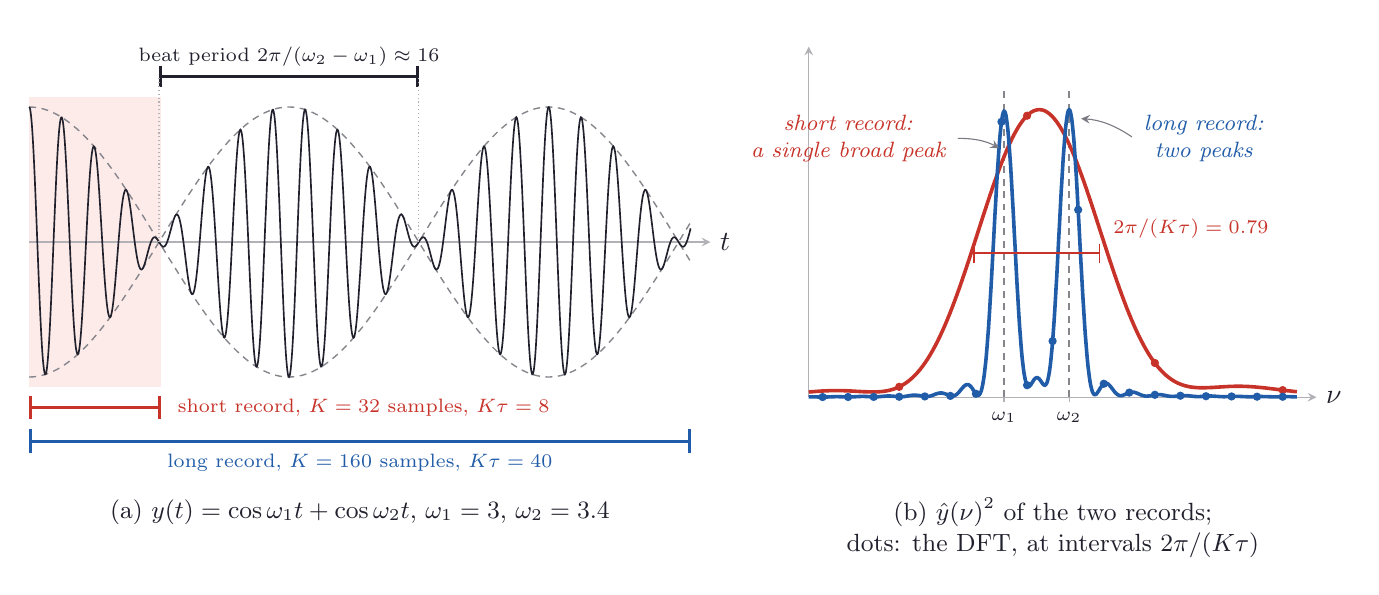
\begin{tikzpicture}[ink/.style={line width=0.9pt, ndInk}, faint/.style={line width=0.4pt, ndInk!35}, dashedink/.style={line width=0.5pt, ndInk!55, dash pattern=on 2.5pt off 2pt}, vec/.style={->, >=stealth, line width=1.2pt}, note/.style={font=\footnotesize\itshape, text=ndInk!85, align=center}, pointer/.style={->, >=stealth, line width=0.4pt, ndInk!60, shorten >=2pt, shorten <=1pt}, dot/.style={circle, fill=ndInk, inner sep=0pt, minimum size=3.4pt}, wash/.style={fill=ndSky, fill opacity=0.55}, every node/.style={text=ndInk}]
\definecolor{ndInk}{rgb}{0.13,0.13,0.18}
\definecolor{ndPaper}{rgb}{0.99,0.96,0.88}
\definecolor{ndSky}{rgb}{0.84,0.91,0.98}
\definecolor{ndRose}{rgb}{0.98,0.86,0.84}
\definecolor{ndBlue}{rgb}{0.13,0.36,0.66}
\definecolor{ndRed}{rgb}{0.78,0.20,0.16}
\definecolor{ndGold}{rgb}{0.88,0.62,0.10}
\definecolor{ndGreen}{rgb}{0.18,0.52,0.30}
\fill[ndRose, fill opacity=0.55] (0.000,0.829) rectangle (1.680,4.514);
\draw[faint, ->, >=stealth] (0.000,2.671) -- (8.652,2.671) node[right, text=ndInk] {$t$};
\draw[dashedink] (0.000,4.386) -- (0.007,4.386) -- (0.014,4.386) -- (0.021,4.385) -- (0.028,4.385) -- (0.035,4.385) -- (0.042,4.384) -- (0.049,4.384) -- (0.056,4.383) -- (0.063,4.383) -- (0.070,4.382) -- (0.077,4.381) -- (0.084,4.380) -- (0.091,4.379) -- (0.098,4.378) -- (0.105,4.377) -- (0.112,4.376) -- (0.119,4.375) -- (0.126,4.373) -- (0.133,4.372) -- (0.140,4.370) -- (0.147,4.369) -- (0.154,4.367) -- (0.161,4.366) -- (0.168,4.364) -- (0.175,4.362) -- (0.182,4.360) -- (0.189,4.358) -- (0.196,4.356) -- (0.203,4.354) -- (0.210,4.351) -- (0.217,4.349) -- (0.224,4.347) -- (0.231,4.344) -- (0.238,4.342) -- (0.245,4.339) -- (0.252,4.336) -- (0.259,4.334) -- (0.266,4.331) -- (0.273,4.328) -- (0.280,4.325) -- (0.287,4.322) -- (0.294,4.319) -- (0.301,4.316) -- (0.308,4.312) -- (0.315,4.309) -- (0.322,4.306) -- (0.329,4.302) -- (0.336,4.299) -- (0.343,4.295) -- (0.350,4.291) -- (0.357,4.287) -- (0.364,4.284) -- (0.371,4.280) -- (0.378,4.276) -- (0.385,4.272) -- (0.392,4.267) -- (0.399,4.263) -- (0.406,4.259) -- (0.413,4.255) -- (0.420,4.250) -- (0.427,4.246) -- (0.434,4.241) -- (0.441,4.236) -- (0.448,4.232) -- (0.455,4.227) -- (0.462,4.222) -- (0.469,4.217) -- (0.476,4.212) -- (0.483,4.207) -- (0.490,4.202) -- (0.497,4.197) -- (0.504,4.192) -- (0.511,4.186) -- (0.518,4.181) -- (0.525,4.176) -- (0.532,4.170) -- (0.539,4.164) -- (0.546,4.159) -- (0.553,4.153) -- (0.560,4.147) -- (0.567,4.141) -- (0.574,4.135) -- (0.581,4.129) -- (0.588,4.123) -- (0.595,4.117) -- (0.603,4.111) -- (0.610,4.105) -- (0.617,4.099) -- (0.624,4.092) -- (0.631,4.086) -- (0.638,4.079) -- (0.645,4.073) -- (0.652,4.066) -- (0.659,4.059) -- (0.666,4.053) -- (0.673,4.046) -- (0.680,4.039) -- (0.687,4.032) -- (0.694,4.025) -- (0.701,4.018) -- (0.708,4.011) -- (0.715,4.004) -- (0.722,3.997) -- (0.729,3.989) -- (0.736,3.982) -- (0.743,3.975) -- (0.750,3.967) -- (0.757,3.960) -- (0.764,3.952) -- (0.771,3.944) -- (0.778,3.937) -- (0.785,3.929) -- (0.792,3.921) -- (0.799,3.913) -- (0.806,3.905) -- (0.813,3.897) -- (0.820,3.889) -- (0.827,3.881) -- (0.834,3.873) -- (0.841,3.865) -- (0.848,3.857) -- (0.855,3.848) -- (0.862,3.840) -- (0.869,3.832) -- (0.876,3.823) -- (0.883,3.815) -- (0.890,3.806) -- (0.897,3.798) -- (0.904,3.789) -- (0.911,3.780) -- (0.918,3.772) -- (0.925,3.763) -- (0.932,3.754) -- (0.939,3.745) -- (0.946,3.736) -- (0.953,3.727) -- (0.960,3.718) -- (0.967,3.709) -- (0.974,3.700) -- (0.981,3.691) -- (0.988,3.681) -- (0.995,3.672) -- (1.002,3.663) -- (1.009,3.653) -- (1.016,3.644) -- (1.023,3.635) -- (1.030,3.625) -- (1.037,3.616) -- (1.044,3.606) -- (1.051,3.596) -- (1.058,3.587) -- (1.065,3.577) -- (1.072,3.567) -- (1.079,3.558) -- (1.086,3.548) -- (1.093,3.538) -- (1.100,3.528) -- (1.107,3.518) -- (1.114,3.508) -- (1.121,3.498) -- (1.128,3.488) -- (1.135,3.478) -- (1.142,3.468) -- (1.149,3.458) -- (1.156,3.448) -- (1.163,3.437) -- (1.170,3.427) -- (1.177,3.417) -- (1.184,3.407) -- (1.191,3.396) -- (1.198,3.386) -- (1.205,3.375) -- (1.212,3.365) -- (1.219,3.354) -- (1.226,3.344) -- (1.233,3.333) -- (1.240,3.323) -- (1.247,3.312) -- (1.254,3.302) -- (1.261,3.291) -- (1.268,3.280) -- (1.275,3.270) -- (1.282,3.259) -- (1.289,3.248) -- (1.296,3.237) -- (1.303,3.227) -- (1.310,3.216) -- (1.317,3.205) -- (1.324,3.194) -- (1.331,3.183) -- (1.338,3.172) -- (1.345,3.161) -- (1.352,3.150) -- (1.359,3.139) -- (1.366,3.128) -- (1.373,3.117) -- (1.380,3.106) -- (1.387,3.095) -- (1.394,3.084) -- (1.401,3.073) -- (1.408,3.062) -- (1.415,3.051) -- (1.422,3.039) -- (1.429,3.028) -- (1.436,3.017) -- (1.443,3.006) -- (1.450,2.995) -- (1.457,2.983) -- (1.464,2.972) -- (1.471,2.961) -- (1.478,2.950) -- (1.485,2.938) -- (1.492,2.927) -- (1.499,2.916) -- (1.506,2.904) -- (1.513,2.893) -- (1.520,2.882) -- (1.527,2.870) -- (1.534,2.859) -- (1.541,2.848) -- (1.548,2.836) -- (1.555,2.825) -- (1.562,2.813) -- (1.569,2.802) -- (1.576,2.791) -- (1.583,2.779) -- (1.590,2.768) -- (1.597,2.756) -- (1.604,2.745) -- (1.611,2.733) -- (1.618,2.722) -- (1.625,2.711) -- (1.632,2.699) -- (1.639,2.688) -- (1.646,2.676) -- (1.653,2.678) -- (1.660,2.689) -- (1.667,2.701) -- (1.674,2.712) -- (1.681,2.724) -- (1.688,2.735) -- (1.695,2.747) -- (1.702,2.758) -- (1.709,2.769) -- (1.716,2.781) -- (1.723,2.792) -- (1.730,2.804) -- (1.737,2.815) -- (1.744,2.827) -- (1.751,2.838) -- (1.758,2.849) -- (1.765,2.861) -- (1.772,2.872) -- (1.779,2.883) -- (1.786,2.895) -- (1.793,2.906) -- (1.801,2.917) -- (1.808,2.929) -- (1.815,2.940) -- (1.822,2.951) -- (1.829,2.963) -- (1.836,2.974) -- (1.843,2.985) -- (1.850,2.996) -- (1.857,3.008) -- (1.864,3.019) -- (1.871,3.030) -- (1.878,3.041) -- (1.885,3.052) -- (1.892,3.063) -- (1.899,3.075) -- (1.906,3.086) -- (1.913,3.097) -- (1.920,3.108) -- (1.927,3.119) -- (1.934,3.130) -- (1.941,3.141) -- (1.948,3.152) -- (1.955,3.163) -- (1.962,3.174) -- (1.969,3.185) -- (1.976,3.196) -- (1.983,3.207) -- (1.990,3.217) -- (1.997,3.228) -- (2.004,3.239) -- (2.011,3.250) -- (2.018,3.261) -- (2.025,3.271) -- (2.032,3.282) -- (2.039,3.293) -- (2.046,3.303) -- (2.053,3.314) -- (2.060,3.325) -- (2.067,3.335) -- (2.074,3.346) -- (2.081,3.356) -- (2.088,3.367) -- (2.095,3.377) -- (2.102,3.387) -- (2.109,3.398) -- (2.116,3.408) -- (2.123,3.418) -- (2.130,3.429) -- (2.137,3.439) -- (2.144,3.449) -- (2.151,3.459) -- (2.158,3.470) -- (2.165,3.480) -- (2.172,3.490) -- (2.179,3.500) -- (2.186,3.510) -- (2.193,3.520) -- (2.200,3.530) -- (2.207,3.539) -- (2.214,3.549) -- (2.221,3.559) -- (2.228,3.569) -- (2.235,3.579) -- (2.242,3.588) -- (2.249,3.598) -- (2.256,3.608) -- (2.263,3.617) -- (2.270,3.627) -- (2.277,3.636) -- (2.284,3.646) -- (2.291,3.655) -- (2.298,3.664) -- (2.305,3.674) -- (2.312,3.683) -- (2.319,3.692) -- (2.326,3.701) -- (2.333,3.710) -- (2.340,3.719) -- (2.347,3.728) -- (2.354,3.737) -- (2.361,3.746) -- (2.368,3.755) -- (2.375,3.764) -- (2.382,3.773) -- (2.389,3.782) -- (2.396,3.790) -- (2.403,3.799) -- (2.410,3.808) -- (2.417,3.816) -- (2.424,3.825) -- (2.431,3.833) -- (2.438,3.841) -- (2.445,3.850) -- (2.452,3.858) -- (2.459,3.866) -- (2.466,3.874) -- (2.473,3.883) -- (2.480,3.891) -- (2.487,3.899) -- (2.494,3.907) -- (2.501,3.914) -- (2.508,3.922) -- (2.515,3.930) -- (2.522,3.938) -- (2.529,3.946) -- (2.536,3.953) -- (2.543,3.961) -- (2.550,3.968) -- (2.557,3.976) -- (2.564,3.983) -- (2.571,3.990) -- (2.578,3.998) -- (2.585,4.005) -- (2.592,4.012) -- (2.599,4.019) -- (2.606,4.026) -- (2.613,4.033) -- (2.620,4.040) -- (2.627,4.047) -- (2.634,4.054) -- (2.641,4.060) -- (2.648,4.067) -- (2.655,4.074) -- (2.662,4.080) -- (2.669,4.087) -- (2.676,4.093) -- (2.683,4.100) -- (2.690,4.106) -- (2.697,4.112) -- (2.704,4.118) -- (2.711,4.124) -- (2.718,4.130) -- (2.725,4.136) -- (2.732,4.142) -- (2.739,4.148) -- (2.746,4.154) -- (2.753,4.160) -- (2.760,4.165) -- (2.767,4.171) -- (2.774,4.176) -- (2.781,4.182) -- (2.788,4.187) -- (2.795,4.192) -- (2.802,4.198) -- (2.809,4.203) -- (2.816,4.208) -- (2.823,4.213) -- (2.830,4.218) -- (2.837,4.223) -- (2.844,4.228) -- (2.851,4.233) -- (2.858,4.237) -- (2.865,4.242) -- (2.872,4.246) -- (2.879,4.251) -- (2.886,4.255) -- (2.893,4.260) -- (2.900,4.264) -- (2.907,4.268) -- (2.914,4.272) -- (2.921,4.276) -- (2.928,4.280) -- (2.935,4.284) -- (2.942,4.288) -- (2.949,4.292) -- (2.956,4.295) -- (2.963,4.299) -- (2.970,4.303) -- (2.977,4.306) -- (2.984,4.310) -- (2.991,4.313) -- (2.998,4.316) -- (3.006,4.319) -- (3.013,4.322) -- (3.020,4.325) -- (3.027,4.328) -- (3.034,4.331) -- (3.041,4.334) -- (3.048,4.337) -- (3.055,4.340) -- (3.062,4.342) -- (3.069,4.345) -- (3.076,4.347) -- (3.083,4.350) -- (3.090,4.352) -- (3.097,4.354) -- (3.104,4.356) -- (3.111,4.358) -- (3.118,4.360) -- (3.125,4.362) -- (3.132,4.364) -- (3.139,4.366) -- (3.146,4.368) -- (3.153,4.369) -- (3.160,4.371) -- (3.167,4.372) -- (3.174,4.374) -- (3.181,4.375) -- (3.188,4.376) -- (3.195,4.377) -- (3.202,4.378) -- (3.209,4.379) -- (3.216,4.380) -- (3.223,4.381) -- (3.230,4.382) -- (3.237,4.383) -- (3.244,4.383) -- (3.251,4.384) -- (3.258,4.384) -- (3.265,4.385) -- (3.272,4.385) -- (3.279,4.385) -- (3.286,4.386) -- (3.293,4.386) -- (3.300,4.386) -- (3.307,4.386) -- (3.314,4.386) -- (3.321,4.385) -- (3.328,4.385) -- (3.335,4.385) -- (3.342,4.384) -- (3.349,4.384) -- (3.356,4.383) -- (3.363,4.383) -- (3.370,4.382) -- (3.377,4.381) -- (3.384,4.380) -- (3.391,4.379) -- (3.398,4.378) -- (3.405,4.377) -- (3.412,4.376) -- (3.419,4.374) -- (3.426,4.373) -- (3.433,4.372) -- (3.440,4.370) -- (3.447,4.369) -- (3.454,4.367) -- (3.461,4.365) -- (3.468,4.364) -- (3.475,4.362) -- (3.482,4.360) -- (3.489,4.358) -- (3.496,4.356) -- (3.503,4.353) -- (3.510,4.351) -- (3.517,4.349) -- (3.524,4.346) -- (3.531,4.344) -- (3.538,4.341) -- (3.545,4.339) -- (3.552,4.336) -- (3.559,4.333) -- (3.566,4.330) -- (3.573,4.328) -- (3.580,4.325) -- (3.587,4.321) -- (3.594,4.318) -- (3.601,4.315) -- (3.608,4.312) -- (3.615,4.309) -- (3.622,4.305) -- (3.629,4.302) -- (3.636,4.298) -- (3.643,4.294) -- (3.650,4.291) -- (3.657,4.287) -- (3.664,4.283) -- (3.671,4.279) -- (3.678,4.275) -- (3.685,4.271) -- (3.692,4.267) -- (3.699,4.263) -- (3.706,4.258) -- (3.713,4.254) -- (3.720,4.249) -- (3.727,4.245) -- (3.734,4.240) -- (3.741,4.236) -- (3.748,4.231) -- (3.755,4.226) -- (3.762,4.221) -- (3.769,4.216) -- (3.776,4.212) -- (3.783,4.206) -- (3.790,4.201) -- (3.797,4.196) -- (3.804,4.191) -- (3.811,4.186) -- (3.818,4.180) -- (3.825,4.175) -- (3.832,4.169) -- (3.839,4.164) -- (3.846,4.158) -- (3.853,4.152) -- (3.860,4.146) -- (3.867,4.140) -- (3.874,4.135) -- (3.881,4.129) -- (3.888,4.123) -- (3.895,4.116) -- (3.902,4.110) -- (3.909,4.104) -- (3.916,4.098) -- (3.923,4.091) -- (3.930,4.085) -- (3.937,4.078) -- (3.944,4.072) -- (3.951,4.065) -- (3.958,4.058) -- (3.965,4.052) -- (3.972,4.045) -- (3.979,4.038) -- (3.986,4.031) -- (3.993,4.024) -- (4.000,4.017) -- (4.007,4.010) -- (4.014,4.003) -- (4.021,3.995) -- (4.028,3.988) -- (4.035,3.981) -- (4.042,3.973) -- (4.049,3.966) -- (4.056,3.958) -- (4.063,3.951) -- (4.070,3.943) -- (4.077,3.935) -- (4.084,3.928) -- (4.091,3.920) -- (4.098,3.912) -- (4.105,3.904) -- (4.112,3.896) -- (4.119,3.888) -- (4.126,3.880) -- (4.133,3.872) -- (4.140,3.864) -- (4.147,3.855) -- (4.154,3.847) -- (4.161,3.839) -- (4.168,3.830) -- (4.175,3.822) -- (4.182,3.813) -- (4.189,3.805) -- (4.196,3.796) -- (4.204,3.788) -- (4.211,3.779) -- (4.218,3.770) -- (4.225,3.761) -- (4.232,3.753) -- (4.239,3.744) -- (4.246,3.735) -- (4.253,3.726) -- (4.260,3.717) -- (4.267,3.708) -- (4.274,3.698) -- (4.281,3.689) -- (4.288,3.680) -- (4.295,3.671) -- (4.302,3.661) -- (4.309,3.652) -- (4.316,3.643) -- (4.323,3.633) -- (4.330,3.624) -- (4.337,3.614) -- (4.344,3.605) -- (4.351,3.595) -- (4.358,3.585) -- (4.365,3.576) -- (4.372,3.566) -- (4.379,3.556) -- (4.386,3.546) -- (4.393,3.536) -- (4.400,3.527) -- (4.407,3.517) -- (4.414,3.507) -- (4.421,3.497) -- (4.428,3.487) -- (4.435,3.477) -- (4.442,3.466) -- (4.449,3.456) -- (4.456,3.446) -- (4.463,3.436) -- (4.470,3.426) -- (4.477,3.415) -- (4.484,3.405) -- (4.491,3.395) -- (4.498,3.384) -- (4.505,3.374) -- (4.512,3.363) -- (4.519,3.353) -- (4.526,3.342) -- (4.533,3.332) -- (4.540,3.321) -- (4.547,3.311) -- (4.554,3.300) -- (4.561,3.289) -- (4.568,3.279) -- (4.575,3.268) -- (4.582,3.257) -- (4.589,3.246) -- (4.596,3.236) -- (4.603,3.225) -- (4.610,3.214) -- (4.617,3.203) -- (4.624,3.192) -- (4.631,3.181) -- (4.638,3.170) -- (4.645,3.160) -- (4.652,3.149) -- (4.659,3.138) -- (4.666,3.127) -- (4.673,3.115) -- (4.680,3.104) -- (4.687,3.093) -- (4.694,3.082) -- (4.701,3.071) -- (4.708,3.060) -- (4.715,3.049) -- (4.722,3.038) -- (4.729,3.027) -- (4.736,3.015) -- (4.743,3.004) -- (4.750,2.993) -- (4.757,2.982) -- (4.764,2.970) -- (4.771,2.959) -- (4.778,2.948) -- (4.785,2.937) -- (4.792,2.925) -- (4.799,2.914) -- (4.806,2.903) -- (4.813,2.891) -- (4.820,2.880) -- (4.827,2.869) -- (4.834,2.857) -- (4.841,2.846) -- (4.848,2.834) -- (4.855,2.823) -- (4.862,2.812) -- (4.869,2.800) -- (4.876,2.789) -- (4.883,2.777) -- (4.890,2.766) -- (4.897,2.755) -- (4.904,2.743) -- (4.911,2.732) -- (4.918,2.720) -- (4.925,2.709) -- (4.932,2.697) -- (4.939,2.686) -- (4.946,2.675) -- (4.953,2.680) -- (4.960,2.691) -- (4.967,2.703) -- (4.974,2.714) -- (4.981,2.726) -- (4.988,2.737) -- (4.995,2.748) -- (5.002,2.760) -- (5.009,2.771) -- (5.016,2.783) -- (5.023,2.794) -- (5.030,2.805) -- (5.037,2.817) -- (5.044,2.828) -- (5.051,2.840) -- (5.058,2.851) -- (5.065,2.862) -- (5.072,2.874) -- (5.079,2.885) -- (5.086,2.896) -- (5.093,2.908) -- (5.100,2.919) -- (5.107,2.930) -- (5.114,2.942) -- (5.121,2.953) -- (5.128,2.964) -- (5.135,2.976) -- (5.142,2.987) -- (5.149,2.998) -- (5.156,3.009) -- (5.163,3.020) -- (5.170,3.032) -- (5.177,3.043) -- (5.184,3.054) -- (5.191,3.065) -- (5.198,3.076) -- (5.205,3.087) -- (5.212,3.098) -- (5.219,3.110) -- (5.226,3.121) -- (5.233,3.132) -- (5.240,3.143) -- (5.247,3.154) -- (5.254,3.165) -- (5.261,3.176) -- (5.268,3.186) -- (5.275,3.197) -- (5.282,3.208) -- (5.289,3.219) -- (5.296,3.230) -- (5.303,3.241) -- (5.310,3.251) -- (5.317,3.262) -- (5.324,3.273) -- (5.331,3.284) -- (5.338,3.294) -- (5.345,3.305) -- (5.352,3.316) -- (5.359,3.326) -- (5.366,3.337) -- (5.373,3.347) -- (5.380,3.358) -- (5.387,3.368) -- (5.394,3.379) -- (5.402,3.389) -- (5.409,3.399) -- (5.416,3.410) -- (5.423,3.420) -- (5.430,3.430) -- (5.437,3.441) -- (5.444,3.451) -- (5.451,3.461) -- (5.458,3.471) -- (5.465,3.481) -- (5.472,3.491) -- (5.479,3.501) -- (5.486,3.511) -- (5.493,3.521) -- (5.500,3.531) -- (5.507,3.541) -- (5.514,3.551) -- (5.521,3.561) -- (5.528,3.570) -- (5.535,3.580) -- (5.542,3.590) -- (5.549,3.599) -- (5.556,3.609) -- (5.563,3.619) -- (5.570,3.628) -- (5.577,3.638) -- (5.584,3.647) -- (5.591,3.656) -- (5.598,3.666) -- (5.605,3.675) -- (5.612,3.684) -- (5.619,3.693) -- (5.626,3.703) -- (5.633,3.712) -- (5.640,3.721) -- (5.647,3.730) -- (5.654,3.739) -- (5.661,3.748) -- (5.668,3.757) -- (5.675,3.765) -- (5.682,3.774) -- (5.689,3.783) -- (5.696,3.792) -- (5.703,3.800) -- (5.710,3.809) -- (5.717,3.817) -- (5.724,3.826) -- (5.731,3.834) -- (5.738,3.843) -- (5.745,3.851) -- (5.752,3.859) -- (5.759,3.867) -- (5.766,3.876) -- (5.773,3.884) -- (5.780,3.892) -- (5.787,3.900) -- (5.794,3.908) -- (5.801,3.916) -- (5.808,3.924) -- (5.815,3.931) -- (5.822,3.939) -- (5.829,3.947) -- (5.836,3.954) -- (5.843,3.962) -- (5.850,3.969) -- (5.857,3.977) -- (5.864,3.984) -- (5.871,3.992) -- (5.878,3.999) -- (5.885,4.006) -- (5.892,4.013) -- (5.899,4.020) -- (5.906,4.027) -- (5.913,4.034) -- (5.920,4.041) -- (5.927,4.048) -- (5.934,4.055) -- (5.941,4.062) -- (5.948,4.068) -- (5.955,4.075) -- (5.962,4.081) -- (5.969,4.088) -- (5.976,4.094) -- (5.983,4.101) -- (5.990,4.107) -- (5.997,4.113) -- (6.004,4.119) -- (6.011,4.125) -- (6.018,4.131) -- (6.025,4.137) -- (6.032,4.143) -- (6.039,4.149) -- (6.046,4.155) -- (6.053,4.160) -- (6.060,4.166) -- (6.067,4.172) -- (6.074,4.177) -- (6.081,4.183) -- (6.088,4.188) -- (6.095,4.193) -- (6.102,4.199) -- (6.109,4.204) -- (6.116,4.209) -- (6.123,4.214) -- (6.130,4.219) -- (6.137,4.224) -- (6.144,4.228) -- (6.151,4.233) -- (6.158,4.238) -- (6.165,4.243) -- (6.172,4.247) -- (6.179,4.252) -- (6.186,4.256) -- (6.193,4.260) -- (6.200,4.265) -- (6.207,4.269) -- (6.214,4.273) -- (6.221,4.277) -- (6.228,4.281) -- (6.235,4.285) -- (6.242,4.289) -- (6.249,4.292) -- (6.256,4.296) -- (6.263,4.300) -- (6.270,4.303) -- (6.277,4.307) -- (6.284,4.310) -- (6.291,4.313) -- (6.298,4.317) -- (6.305,4.320) -- (6.312,4.323) -- (6.319,4.326) -- (6.326,4.329) -- (6.333,4.332) -- (6.340,4.335) -- (6.347,4.337) -- (6.354,4.340) -- (6.361,4.343) -- (6.368,4.345) -- (6.375,4.348) -- (6.382,4.350) -- (6.389,4.352) -- (6.396,4.354) -- (6.403,4.357) -- (6.410,4.359) -- (6.417,4.361) -- (6.424,4.363) -- (6.431,4.364) -- (6.438,4.366) -- (6.445,4.368) -- (6.452,4.369) -- (6.459,4.371) -- (6.466,4.372) -- (6.473,4.374) -- (6.480,4.375) -- (6.487,4.376) -- (6.494,4.377) -- (6.501,4.379) -- (6.508,4.380) -- (6.515,4.381) -- (6.522,4.381) -- (6.529,4.382) -- (6.536,4.383) -- (6.543,4.383) -- (6.550,4.384) -- (6.557,4.384) -- (6.564,4.385) -- (6.571,4.385) -- (6.578,4.385) -- (6.585,4.386) -- (6.592,4.386) -- (6.599,4.386) -- (6.607,4.386) -- (6.614,4.386) -- (6.621,4.385) -- (6.628,4.385) -- (6.635,4.385) -- (6.642,4.384) -- (6.649,4.384) -- (6.656,4.383) -- (6.663,4.382) -- (6.670,4.382) -- (6.677,4.381) -- (6.684,4.380) -- (6.691,4.379) -- (6.698,4.378) -- (6.705,4.377) -- (6.712,4.376) -- (6.719,4.374) -- (6.726,4.373) -- (6.733,4.372) -- (6.740,4.370) -- (6.747,4.368) -- (6.754,4.367) -- (6.761,4.365) -- (6.768,4.363) -- (6.775,4.361) -- (6.782,4.359) -- (6.789,4.357) -- (6.796,4.355) -- (6.803,4.353) -- (6.810,4.351) -- (6.817,4.348) -- (6.824,4.346) -- (6.831,4.344) -- (6.838,4.341) -- (6.845,4.338) -- (6.852,4.336) -- (6.859,4.333) -- (6.866,4.330) -- (6.873,4.327) -- (6.880,4.324) -- (6.887,4.321) -- (6.894,4.318) -- (6.901,4.315) -- (6.908,4.311) -- (6.915,4.308) -- (6.922,4.305) -- (6.929,4.301) -- (6.936,4.297) -- (6.943,4.294) -- (6.950,4.290) -- (6.957,4.286) -- (6.964,4.282) -- (6.971,4.278) -- (6.978,4.274) -- (6.985,4.270) -- (6.992,4.266) -- (6.999,4.262) -- (7.006,4.258) -- (7.013,4.253) -- (7.020,4.249) -- (7.027,4.244) -- (7.034,4.240) -- (7.041,4.235) -- (7.048,4.230) -- (7.055,4.226) -- (7.062,4.221) -- (7.069,4.216) -- (7.076,4.211) -- (7.083,4.206) -- (7.090,4.201) -- (7.097,4.195) -- (7.104,4.190) -- (7.111,4.185) -- (7.118,4.179) -- (7.125,4.174) -- (7.132,4.168) -- (7.139,4.163) -- (7.146,4.157) -- (7.153,4.151) -- (7.160,4.145) -- (7.167,4.140) -- (7.174,4.134) -- (7.181,4.128) -- (7.188,4.122) -- (7.195,4.115) -- (7.202,4.109) -- (7.209,4.103) -- (7.216,4.097) -- (7.223,4.090) -- (7.230,4.084) -- (7.237,4.077) -- (7.244,4.071) -- (7.251,4.064) -- (7.258,4.057) -- (7.265,4.051) -- (7.272,4.044) -- (7.279,4.037) -- (7.286,4.030) -- (7.293,4.023) -- (7.300,4.016) -- (7.307,4.009) -- (7.314,4.002) -- (7.321,3.994) -- (7.328,3.987) -- (7.335,3.980) -- (7.342,3.972) -- (7.349,3.965) -- (7.356,3.957) -- (7.363,3.950) -- (7.370,3.942) -- (7.377,3.934) -- (7.384,3.927) -- (7.391,3.919) -- (7.398,3.911) -- (7.405,3.903) -- (7.412,3.895) -- (7.419,3.887) -- (7.426,3.879) -- (7.433,3.871) -- (7.440,3.862) -- (7.447,3.854) -- (7.454,3.846) -- (7.461,3.838) -- (7.468,3.829) -- (7.475,3.821) -- (7.482,3.812) -- (7.489,3.804) -- (7.496,3.795) -- (7.503,3.786) -- (7.510,3.778) -- (7.517,3.769) -- (7.524,3.760) -- (7.531,3.751) -- (7.538,3.742) -- (7.545,3.733) -- (7.552,3.724) -- (7.559,3.715) -- (7.566,3.706) -- (7.573,3.697) -- (7.580,3.688) -- (7.587,3.679) -- (7.594,3.669) -- (7.601,3.660) -- (7.608,3.651) -- (7.615,3.641) -- (7.622,3.632) -- (7.629,3.622) -- (7.636,3.613) -- (7.643,3.603) -- (7.650,3.593) -- (7.657,3.584) -- (7.664,3.574) -- (7.671,3.564) -- (7.678,3.555) -- (7.685,3.545) -- (7.692,3.535) -- (7.699,3.525) -- (7.706,3.515) -- (7.713,3.505) -- (7.720,3.495) -- (7.727,3.485) -- (7.734,3.475) -- (7.741,3.465) -- (7.748,3.455) -- (7.755,3.444) -- (7.762,3.434) -- (7.769,3.424) -- (7.776,3.414) -- (7.783,3.403) -- (7.790,3.393) -- (7.797,3.383) -- (7.805,3.372) -- (7.812,3.362) -- (7.819,3.351) -- (7.826,3.341) -- (7.833,3.330) -- (7.840,3.320) -- (7.847,3.309) -- (7.854,3.298) -- (7.861,3.288) -- (7.868,3.277) -- (7.875,3.266) -- (7.882,3.256) -- (7.889,3.245) -- (7.896,3.234) -- (7.903,3.223) -- (7.910,3.212) -- (7.917,3.202) -- (7.924,3.191) -- (7.931,3.180) -- (7.938,3.169) -- (7.945,3.158) -- (7.952,3.147) -- (7.959,3.136) -- (7.966,3.125) -- (7.973,3.114) -- (7.980,3.103) -- (7.987,3.092) -- (7.994,3.081) -- (8.001,3.069) -- (8.008,3.058) -- (8.015,3.047) -- (8.022,3.036) -- (8.029,3.025) -- (8.036,3.014) -- (8.043,3.002) -- (8.050,2.991) -- (8.057,2.980) -- (8.064,2.969) -- (8.071,2.957) -- (8.078,2.946) -- (8.085,2.935) -- (8.092,2.923) -- (8.099,2.912) -- (8.106,2.901) -- (8.113,2.889) -- (8.120,2.878) -- (8.127,2.867) -- (8.134,2.855) -- (8.141,2.844) -- (8.148,2.833) -- (8.155,2.821) -- (8.162,2.810) -- (8.169,2.798) -- (8.176,2.787) -- (8.183,2.776) -- (8.190,2.764) -- (8.197,2.753) -- (8.204,2.741) -- (8.211,2.730) -- (8.218,2.718) -- (8.225,2.707) -- (8.232,2.696) -- (8.239,2.684) -- (8.246,2.673) -- (8.253,2.682) -- (8.260,2.693) -- (8.267,2.704) -- (8.274,2.716) -- (8.281,2.727) -- (8.288,2.739) -- (8.295,2.750) -- (8.302,2.762) -- (8.309,2.773) -- (8.316,2.784) -- (8.323,2.796) -- (8.330,2.807) -- (8.337,2.819) -- (8.344,2.830) -- (8.351,2.841) -- (8.358,2.853) -- (8.365,2.864) -- (8.372,2.876) -- (8.379,2.887) -- (8.386,2.898) -- (8.393,2.910) -- (8.400,2.921);
\draw[dashedink] (0.000,0.957) -- (0.007,0.957) -- (0.014,0.957) -- (0.021,0.957) -- (0.028,0.958) -- (0.035,0.958) -- (0.042,0.959) -- (0.049,0.959) -- (0.056,0.960) -- (0.063,0.960) -- (0.070,0.961) -- (0.077,0.962) -- (0.084,0.963) -- (0.091,0.964) -- (0.098,0.965) -- (0.105,0.966) -- (0.112,0.967) -- (0.119,0.968) -- (0.126,0.969) -- (0.133,0.971) -- (0.140,0.972) -- (0.147,0.974) -- (0.154,0.976) -- (0.161,0.977) -- (0.168,0.979) -- (0.175,0.981) -- (0.182,0.983) -- (0.189,0.985) -- (0.196,0.987) -- (0.203,0.989) -- (0.210,0.991) -- (0.217,0.994) -- (0.224,0.996) -- (0.231,0.999) -- (0.238,1.001) -- (0.245,1.004) -- (0.252,1.006) -- (0.259,1.009) -- (0.266,1.012) -- (0.273,1.015) -- (0.280,1.018) -- (0.287,1.021) -- (0.294,1.024) -- (0.301,1.027) -- (0.308,1.030) -- (0.315,1.034) -- (0.322,1.037) -- (0.329,1.041) -- (0.336,1.044) -- (0.343,1.048) -- (0.350,1.052) -- (0.357,1.055) -- (0.364,1.059) -- (0.371,1.063) -- (0.378,1.067) -- (0.385,1.071) -- (0.392,1.075) -- (0.399,1.080) -- (0.406,1.084) -- (0.413,1.088) -- (0.420,1.093) -- (0.427,1.097) -- (0.434,1.102) -- (0.441,1.106) -- (0.448,1.111) -- (0.455,1.116) -- (0.462,1.121) -- (0.469,1.126) -- (0.476,1.131) -- (0.483,1.136) -- (0.490,1.141) -- (0.497,1.146) -- (0.504,1.151) -- (0.511,1.157) -- (0.518,1.162) -- (0.525,1.167) -- (0.532,1.173) -- (0.539,1.178) -- (0.546,1.184) -- (0.553,1.190) -- (0.560,1.196) -- (0.567,1.201) -- (0.574,1.207) -- (0.581,1.213) -- (0.588,1.219) -- (0.595,1.226) -- (0.603,1.232) -- (0.610,1.238) -- (0.617,1.244) -- (0.624,1.251) -- (0.631,1.257) -- (0.638,1.264) -- (0.645,1.270) -- (0.652,1.277) -- (0.659,1.283) -- (0.666,1.290) -- (0.673,1.297) -- (0.680,1.304) -- (0.687,1.311) -- (0.694,1.318) -- (0.701,1.325) -- (0.708,1.332) -- (0.715,1.339) -- (0.722,1.346) -- (0.729,1.354) -- (0.736,1.361) -- (0.743,1.368) -- (0.750,1.376) -- (0.757,1.383) -- (0.764,1.391) -- (0.771,1.399) -- (0.778,1.406) -- (0.785,1.414) -- (0.792,1.422) -- (0.799,1.430) -- (0.806,1.438) -- (0.813,1.445) -- (0.820,1.454) -- (0.827,1.462) -- (0.834,1.470) -- (0.841,1.478) -- (0.848,1.486) -- (0.855,1.494) -- (0.862,1.503) -- (0.869,1.511) -- (0.876,1.520) -- (0.883,1.528) -- (0.890,1.537) -- (0.897,1.545) -- (0.904,1.554) -- (0.911,1.563) -- (0.918,1.571) -- (0.925,1.580) -- (0.932,1.589) -- (0.939,1.598) -- (0.946,1.607) -- (0.953,1.616) -- (0.960,1.625) -- (0.967,1.634) -- (0.974,1.643) -- (0.981,1.652) -- (0.988,1.661) -- (0.995,1.671) -- (1.002,1.680) -- (1.009,1.689) -- (1.016,1.699) -- (1.023,1.708) -- (1.030,1.718) -- (1.037,1.727) -- (1.044,1.737) -- (1.051,1.746) -- (1.058,1.756) -- (1.065,1.766) -- (1.072,1.775) -- (1.079,1.785) -- (1.086,1.795) -- (1.093,1.805) -- (1.100,1.815) -- (1.107,1.825) -- (1.114,1.835) -- (1.121,1.845) -- (1.128,1.855) -- (1.135,1.865) -- (1.142,1.875) -- (1.149,1.885) -- (1.156,1.895) -- (1.163,1.905) -- (1.170,1.916) -- (1.177,1.926) -- (1.184,1.936) -- (1.191,1.947) -- (1.198,1.957) -- (1.205,1.967) -- (1.212,1.978) -- (1.219,1.988) -- (1.226,1.999) -- (1.233,2.009) -- (1.240,2.020) -- (1.247,2.031) -- (1.254,2.041) -- (1.261,2.052) -- (1.268,2.063) -- (1.275,2.073) -- (1.282,2.084) -- (1.289,2.095) -- (1.296,2.106) -- (1.303,2.116) -- (1.310,2.127) -- (1.317,2.138) -- (1.324,2.149) -- (1.331,2.160) -- (1.338,2.171) -- (1.345,2.182) -- (1.352,2.193) -- (1.359,2.204) -- (1.366,2.215) -- (1.373,2.226) -- (1.380,2.237) -- (1.387,2.248) -- (1.394,2.259) -- (1.401,2.270) -- (1.408,2.281) -- (1.415,2.292) -- (1.422,2.303) -- (1.429,2.315) -- (1.436,2.326) -- (1.443,2.337) -- (1.450,2.348) -- (1.457,2.360) -- (1.464,2.371) -- (1.471,2.382) -- (1.478,2.393) -- (1.485,2.405) -- (1.492,2.416) -- (1.499,2.427) -- (1.506,2.439) -- (1.513,2.450) -- (1.520,2.461) -- (1.527,2.473) -- (1.534,2.484) -- (1.541,2.495) -- (1.548,2.507) -- (1.555,2.518) -- (1.562,2.529) -- (1.569,2.541) -- (1.576,2.552) -- (1.583,2.564) -- (1.590,2.575) -- (1.597,2.587) -- (1.604,2.598) -- (1.611,2.609) -- (1.618,2.621) -- (1.625,2.632) -- (1.632,2.644) -- (1.639,2.655) -- (1.646,2.667) -- (1.653,2.665) -- (1.660,2.653) -- (1.667,2.642) -- (1.674,2.631) -- (1.681,2.619) -- (1.688,2.608) -- (1.695,2.596) -- (1.702,2.585) -- (1.709,2.573) -- (1.716,2.562) -- (1.723,2.551) -- (1.730,2.539) -- (1.737,2.528) -- (1.744,2.516) -- (1.751,2.505) -- (1.758,2.494) -- (1.765,2.482) -- (1.772,2.471) -- (1.779,2.459) -- (1.786,2.448) -- (1.793,2.437) -- (1.801,2.425) -- (1.808,2.414) -- (1.815,2.403) -- (1.822,2.392) -- (1.829,2.380) -- (1.836,2.369) -- (1.843,2.358) -- (1.850,2.347) -- (1.857,2.335) -- (1.864,2.324) -- (1.871,2.313) -- (1.878,2.302) -- (1.885,2.291) -- (1.892,2.279) -- (1.899,2.268) -- (1.906,2.257) -- (1.913,2.246) -- (1.920,2.235) -- (1.927,2.224) -- (1.934,2.213) -- (1.941,2.202) -- (1.948,2.191) -- (1.955,2.180) -- (1.962,2.169) -- (1.969,2.158) -- (1.976,2.147) -- (1.983,2.136) -- (1.990,2.125) -- (1.997,2.115) -- (2.004,2.104) -- (2.011,2.093) -- (2.018,2.082) -- (2.025,2.072) -- (2.032,2.061) -- (2.039,2.050) -- (2.046,2.040) -- (2.053,2.029) -- (2.060,2.018) -- (2.067,2.008) -- (2.074,1.997) -- (2.081,1.987) -- (2.088,1.976) -- (2.095,1.966) -- (2.102,1.955) -- (2.109,1.945) -- (2.116,1.935) -- (2.123,1.924) -- (2.130,1.914) -- (2.137,1.904) -- (2.144,1.894) -- (2.151,1.883) -- (2.158,1.873) -- (2.165,1.863) -- (2.172,1.853) -- (2.179,1.843) -- (2.186,1.833) -- (2.193,1.823) -- (2.200,1.813) -- (2.207,1.803) -- (2.214,1.794) -- (2.221,1.784) -- (2.228,1.774) -- (2.235,1.764) -- (2.242,1.755) -- (2.249,1.745) -- (2.256,1.735) -- (2.263,1.726) -- (2.270,1.716) -- (2.277,1.707) -- (2.284,1.697) -- (2.291,1.688) -- (2.298,1.679) -- (2.305,1.669) -- (2.312,1.660) -- (2.319,1.651) -- (2.326,1.642) -- (2.333,1.633) -- (2.340,1.623) -- (2.347,1.614) -- (2.354,1.605) -- (2.361,1.597) -- (2.368,1.588) -- (2.375,1.579) -- (2.382,1.570) -- (2.389,1.561) -- (2.396,1.553) -- (2.403,1.544) -- (2.410,1.535) -- (2.417,1.527) -- (2.424,1.518) -- (2.431,1.510) -- (2.438,1.501) -- (2.445,1.493) -- (2.452,1.485) -- (2.459,1.477) -- (2.466,1.468) -- (2.473,1.460) -- (2.480,1.452) -- (2.487,1.444) -- (2.494,1.436) -- (2.501,1.428) -- (2.508,1.421) -- (2.515,1.413) -- (2.522,1.405) -- (2.529,1.397) -- (2.536,1.390) -- (2.543,1.382) -- (2.550,1.375) -- (2.557,1.367) -- (2.564,1.360) -- (2.571,1.352) -- (2.578,1.345) -- (2.585,1.338) -- (2.592,1.331) -- (2.599,1.324) -- (2.606,1.317) -- (2.613,1.310) -- (2.620,1.303) -- (2.627,1.296) -- (2.634,1.289) -- (2.641,1.282) -- (2.648,1.276) -- (2.655,1.269) -- (2.662,1.263) -- (2.669,1.256) -- (2.676,1.250) -- (2.683,1.243) -- (2.690,1.237) -- (2.697,1.231) -- (2.704,1.225) -- (2.711,1.218) -- (2.718,1.212) -- (2.725,1.206) -- (2.732,1.201) -- (2.739,1.195) -- (2.746,1.189) -- (2.753,1.183) -- (2.760,1.178) -- (2.767,1.172) -- (2.774,1.167) -- (2.781,1.161) -- (2.788,1.156) -- (2.795,1.150) -- (2.802,1.145) -- (2.809,1.140) -- (2.816,1.135) -- (2.823,1.130) -- (2.830,1.125) -- (2.837,1.120) -- (2.844,1.115) -- (2.851,1.110) -- (2.858,1.106) -- (2.865,1.101) -- (2.872,1.096) -- (2.879,1.092) -- (2.886,1.088) -- (2.893,1.083) -- (2.900,1.079) -- (2.907,1.075) -- (2.914,1.071) -- (2.921,1.067) -- (2.928,1.063) -- (2.935,1.059) -- (2.942,1.055) -- (2.949,1.051) -- (2.956,1.047) -- (2.963,1.044) -- (2.970,1.040) -- (2.977,1.037) -- (2.984,1.033) -- (2.991,1.030) -- (2.998,1.027) -- (3.006,1.024) -- (3.013,1.020) -- (3.020,1.017) -- (3.027,1.014) -- (3.034,1.012) -- (3.041,1.009) -- (3.048,1.006) -- (3.055,1.003) -- (3.062,1.001) -- (3.069,0.998) -- (3.076,0.996) -- (3.083,0.993) -- (3.090,0.991) -- (3.097,0.989) -- (3.104,0.987) -- (3.111,0.985) -- (3.118,0.983) -- (3.125,0.981) -- (3.132,0.979) -- (3.139,0.977) -- (3.146,0.975) -- (3.153,0.974) -- (3.160,0.972) -- (3.167,0.971) -- (3.174,0.969) -- (3.181,0.968) -- (3.188,0.967) -- (3.195,0.966) -- (3.202,0.964) -- (3.209,0.963) -- (3.216,0.962) -- (3.223,0.962) -- (3.230,0.961) -- (3.237,0.960) -- (3.244,0.959) -- (3.251,0.959) -- (3.258,0.958) -- (3.265,0.958) -- (3.272,0.958) -- (3.279,0.957) -- (3.286,0.957) -- (3.293,0.957) -- (3.300,0.957) -- (3.307,0.957) -- (3.314,0.957) -- (3.321,0.958) -- (3.328,0.958) -- (3.335,0.958) -- (3.342,0.959) -- (3.349,0.959) -- (3.356,0.960) -- (3.363,0.960) -- (3.370,0.961) -- (3.377,0.962) -- (3.384,0.963) -- (3.391,0.964) -- (3.398,0.965) -- (3.405,0.966) -- (3.412,0.967) -- (3.419,0.968) -- (3.426,0.970) -- (3.433,0.971) -- (3.440,0.973) -- (3.447,0.974) -- (3.454,0.976) -- (3.461,0.978) -- (3.468,0.979) -- (3.475,0.981) -- (3.482,0.983) -- (3.489,0.985) -- (3.496,0.987) -- (3.503,0.989) -- (3.510,0.992) -- (3.517,0.994) -- (3.524,0.996) -- (3.531,0.999) -- (3.538,1.001) -- (3.545,1.004) -- (3.552,1.007) -- (3.559,1.010) -- (3.566,1.012) -- (3.573,1.015) -- (3.580,1.018) -- (3.587,1.021) -- (3.594,1.025) -- (3.601,1.028) -- (3.608,1.031) -- (3.615,1.034) -- (3.622,1.038) -- (3.629,1.041) -- (3.636,1.045) -- (3.643,1.049) -- (3.650,1.052) -- (3.657,1.056) -- (3.664,1.060) -- (3.671,1.064) -- (3.678,1.068) -- (3.685,1.072) -- (3.692,1.076) -- (3.699,1.080) -- (3.706,1.085) -- (3.713,1.089) -- (3.720,1.093) -- (3.727,1.098) -- (3.734,1.102) -- (3.741,1.107) -- (3.748,1.112) -- (3.755,1.117) -- (3.762,1.121) -- (3.769,1.126) -- (3.776,1.131) -- (3.783,1.136) -- (3.790,1.142) -- (3.797,1.147) -- (3.804,1.152) -- (3.811,1.157) -- (3.818,1.163) -- (3.825,1.168) -- (3.832,1.174) -- (3.839,1.179) -- (3.846,1.185) -- (3.853,1.191) -- (3.860,1.197) -- (3.867,1.202) -- (3.874,1.208) -- (3.881,1.214) -- (3.888,1.220) -- (3.895,1.226) -- (3.902,1.233) -- (3.909,1.239) -- (3.916,1.245) -- (3.923,1.252) -- (3.930,1.258) -- (3.937,1.265) -- (3.944,1.271) -- (3.951,1.278) -- (3.958,1.284) -- (3.965,1.291) -- (3.972,1.298) -- (3.979,1.305) -- (3.986,1.312) -- (3.993,1.319) -- (4.000,1.326) -- (4.007,1.333) -- (4.014,1.340) -- (4.021,1.347) -- (4.028,1.355) -- (4.035,1.362) -- (4.042,1.369) -- (4.049,1.377) -- (4.056,1.384) -- (4.063,1.392) -- (4.070,1.400) -- (4.077,1.407) -- (4.084,1.415) -- (4.091,1.423) -- (4.098,1.431) -- (4.105,1.439) -- (4.112,1.447) -- (4.119,1.455) -- (4.126,1.463) -- (4.133,1.471) -- (4.140,1.479) -- (4.147,1.487) -- (4.154,1.496) -- (4.161,1.504) -- (4.168,1.512) -- (4.175,1.521) -- (4.182,1.529) -- (4.189,1.538) -- (4.196,1.547) -- (4.204,1.555) -- (4.211,1.564) -- (4.218,1.573) -- (4.225,1.581) -- (4.232,1.590) -- (4.239,1.599) -- (4.246,1.608) -- (4.253,1.617) -- (4.260,1.626) -- (4.267,1.635) -- (4.274,1.644) -- (4.281,1.654) -- (4.288,1.663) -- (4.295,1.672) -- (4.302,1.681) -- (4.309,1.691) -- (4.316,1.700) -- (4.323,1.710) -- (4.330,1.719) -- (4.337,1.729) -- (4.344,1.738) -- (4.351,1.748) -- (4.358,1.758) -- (4.365,1.767) -- (4.372,1.777) -- (4.379,1.787) -- (4.386,1.797) -- (4.393,1.806) -- (4.400,1.816) -- (4.407,1.826) -- (4.414,1.836) -- (4.421,1.846) -- (4.428,1.856) -- (4.435,1.866) -- (4.442,1.876) -- (4.449,1.887) -- (4.456,1.897) -- (4.463,1.907) -- (4.470,1.917) -- (4.477,1.928) -- (4.484,1.938) -- (4.491,1.948) -- (4.498,1.959) -- (4.505,1.969) -- (4.512,1.980) -- (4.519,1.990) -- (4.526,2.000) -- (4.533,2.011) -- (4.540,2.022) -- (4.547,2.032) -- (4.554,2.043) -- (4.561,2.053) -- (4.568,2.064) -- (4.575,2.075) -- (4.582,2.086) -- (4.589,2.096) -- (4.596,2.107) -- (4.603,2.118) -- (4.610,2.129) -- (4.617,2.140) -- (4.624,2.151) -- (4.631,2.161) -- (4.638,2.172) -- (4.645,2.183) -- (4.652,2.194) -- (4.659,2.205) -- (4.666,2.216) -- (4.673,2.227) -- (4.680,2.238) -- (4.687,2.250) -- (4.694,2.261) -- (4.701,2.272) -- (4.708,2.283) -- (4.715,2.294) -- (4.722,2.305) -- (4.729,2.316) -- (4.736,2.328) -- (4.743,2.339) -- (4.750,2.350) -- (4.757,2.361) -- (4.764,2.372) -- (4.771,2.384) -- (4.778,2.395) -- (4.785,2.406) -- (4.792,2.418) -- (4.799,2.429) -- (4.806,2.440) -- (4.813,2.452) -- (4.820,2.463) -- (4.827,2.474) -- (4.834,2.486) -- (4.841,2.497) -- (4.848,2.508) -- (4.855,2.520) -- (4.862,2.531) -- (4.869,2.543) -- (4.876,2.554) -- (4.883,2.565) -- (4.890,2.577) -- (4.897,2.588) -- (4.904,2.600) -- (4.911,2.611) -- (4.918,2.623) -- (4.925,2.634) -- (4.932,2.645) -- (4.939,2.657) -- (4.946,2.668) -- (4.953,2.663) -- (4.960,2.652) -- (4.967,2.640) -- (4.974,2.629) -- (4.981,2.617) -- (4.988,2.606) -- (4.995,2.594) -- (5.002,2.583) -- (5.009,2.572) -- (5.016,2.560) -- (5.023,2.549) -- (5.030,2.537) -- (5.037,2.526) -- (5.044,2.515) -- (5.051,2.503) -- (5.058,2.492) -- (5.065,2.480) -- (5.072,2.469) -- (5.079,2.458) -- (5.086,2.446) -- (5.093,2.435) -- (5.100,2.424) -- (5.107,2.412) -- (5.114,2.401) -- (5.121,2.390) -- (5.128,2.379) -- (5.135,2.367) -- (5.142,2.356) -- (5.149,2.345) -- (5.156,2.334) -- (5.163,2.322) -- (5.170,2.311) -- (5.177,2.300) -- (5.184,2.289) -- (5.191,2.278) -- (5.198,2.267) -- (5.205,2.255) -- (5.212,2.244) -- (5.219,2.233) -- (5.226,2.222) -- (5.233,2.211) -- (5.240,2.200) -- (5.247,2.189) -- (5.254,2.178) -- (5.261,2.167) -- (5.268,2.156) -- (5.275,2.146) -- (5.282,2.135) -- (5.289,2.124) -- (5.296,2.113) -- (5.303,2.102) -- (5.310,2.091) -- (5.317,2.081) -- (5.324,2.070) -- (5.331,2.059) -- (5.338,2.049) -- (5.345,2.038) -- (5.352,2.027) -- (5.359,2.017) -- (5.366,2.006) -- (5.373,1.996) -- (5.380,1.985) -- (5.387,1.975) -- (5.394,1.964) -- (5.402,1.954) -- (5.409,1.943) -- (5.416,1.933) -- (5.423,1.923) -- (5.430,1.913) -- (5.437,1.902) -- (5.444,1.892) -- (5.451,1.882) -- (5.458,1.872) -- (5.465,1.862) -- (5.472,1.852) -- (5.479,1.842) -- (5.486,1.832) -- (5.493,1.822) -- (5.500,1.812) -- (5.507,1.802) -- (5.514,1.792) -- (5.521,1.782) -- (5.528,1.772) -- (5.535,1.763) -- (5.542,1.753) -- (5.549,1.743) -- (5.556,1.734) -- (5.563,1.724) -- (5.570,1.715) -- (5.577,1.705) -- (5.584,1.696) -- (5.591,1.686) -- (5.598,1.677) -- (5.605,1.668) -- (5.612,1.659) -- (5.619,1.649) -- (5.626,1.640) -- (5.633,1.631) -- (5.640,1.622) -- (5.647,1.613) -- (5.654,1.604) -- (5.661,1.595) -- (5.668,1.586) -- (5.675,1.577) -- (5.682,1.569) -- (5.689,1.560) -- (5.696,1.551) -- (5.703,1.543) -- (5.710,1.534) -- (5.717,1.525) -- (5.724,1.517) -- (5.731,1.509) -- (5.738,1.500) -- (5.745,1.492) -- (5.752,1.484) -- (5.759,1.475) -- (5.766,1.467) -- (5.773,1.459) -- (5.780,1.451) -- (5.787,1.443) -- (5.794,1.435) -- (5.801,1.427) -- (5.808,1.419) -- (5.815,1.412) -- (5.822,1.404) -- (5.829,1.396) -- (5.836,1.389) -- (5.843,1.381) -- (5.850,1.373) -- (5.857,1.366) -- (5.864,1.359) -- (5.871,1.351) -- (5.878,1.344) -- (5.885,1.337) -- (5.892,1.330) -- (5.899,1.323) -- (5.906,1.316) -- (5.913,1.309) -- (5.920,1.302) -- (5.927,1.295) -- (5.934,1.288) -- (5.941,1.281) -- (5.948,1.275) -- (5.955,1.268) -- (5.962,1.262) -- (5.969,1.255) -- (5.976,1.249) -- (5.983,1.242) -- (5.990,1.236) -- (5.997,1.230) -- (6.004,1.224) -- (6.011,1.218) -- (6.018,1.212) -- (6.025,1.206) -- (6.032,1.200) -- (6.039,1.194) -- (6.046,1.188) -- (6.053,1.182) -- (6.060,1.177) -- (6.067,1.171) -- (6.074,1.166) -- (6.081,1.160) -- (6.088,1.155) -- (6.095,1.150) -- (6.102,1.144) -- (6.109,1.139) -- (6.116,1.134) -- (6.123,1.129) -- (6.130,1.124) -- (6.137,1.119) -- (6.144,1.114) -- (6.151,1.110) -- (6.158,1.105) -- (6.165,1.100) -- (6.172,1.096) -- (6.179,1.091) -- (6.186,1.087) -- (6.193,1.083) -- (6.200,1.078) -- (6.207,1.074) -- (6.214,1.070) -- (6.221,1.066) -- (6.228,1.062) -- (6.235,1.058) -- (6.242,1.054) -- (6.249,1.051) -- (6.256,1.047) -- (6.263,1.043) -- (6.270,1.040) -- (6.277,1.036) -- (6.284,1.033) -- (6.291,1.029) -- (6.298,1.026) -- (6.305,1.023) -- (6.312,1.020) -- (6.319,1.017) -- (6.326,1.014) -- (6.333,1.011) -- (6.340,1.008) -- (6.347,1.006) -- (6.354,1.003) -- (6.361,1.000) -- (6.368,0.998) -- (6.375,0.995) -- (6.382,0.993) -- (6.389,0.991) -- (6.396,0.988) -- (6.403,0.986) -- (6.410,0.984) -- (6.417,0.982) -- (6.424,0.980) -- (6.431,0.979) -- (6.438,0.977) -- (6.445,0.975) -- (6.452,0.973) -- (6.459,0.972) -- (6.466,0.970) -- (6.473,0.969) -- (6.480,0.968) -- (6.487,0.967) -- (6.494,0.965) -- (6.501,0.964) -- (6.508,0.963) -- (6.515,0.962) -- (6.522,0.962) -- (6.529,0.961) -- (6.536,0.960) -- (6.543,0.959) -- (6.550,0.959) -- (6.557,0.958) -- (6.564,0.958) -- (6.571,0.958) -- (6.578,0.957) -- (6.585,0.957) -- (6.592,0.957) -- (6.599,0.957) -- (6.607,0.957) -- (6.614,0.957) -- (6.621,0.958) -- (6.628,0.958) -- (6.635,0.958) -- (6.642,0.959) -- (6.649,0.959) -- (6.656,0.960) -- (6.663,0.960) -- (6.670,0.961) -- (6.677,0.962) -- (6.684,0.963) -- (6.691,0.964) -- (6.698,0.965) -- (6.705,0.966) -- (6.712,0.967) -- (6.719,0.969) -- (6.726,0.970) -- (6.733,0.971) -- (6.740,0.973) -- (6.747,0.974) -- (6.754,0.976) -- (6.761,0.978) -- (6.768,0.980) -- (6.775,0.982) -- (6.782,0.983) -- (6.789,0.986) -- (6.796,0.988) -- (6.803,0.990) -- (6.810,0.992) -- (6.817,0.994) -- (6.824,0.997) -- (6.831,0.999) -- (6.838,1.002) -- (6.845,1.004) -- (6.852,1.007) -- (6.859,1.010) -- (6.866,1.013) -- (6.873,1.016) -- (6.880,1.019) -- (6.887,1.022) -- (6.894,1.025) -- (6.901,1.028) -- (6.908,1.032) -- (6.915,1.035) -- (6.922,1.038) -- (6.929,1.042) -- (6.936,1.045) -- (6.943,1.049) -- (6.950,1.053) -- (6.957,1.057) -- (6.964,1.060) -- (6.971,1.064) -- (6.978,1.068) -- (6.985,1.073) -- (6.992,1.077) -- (6.999,1.081) -- (7.006,1.085) -- (7.013,1.090) -- (7.020,1.094) -- (7.027,1.099) -- (7.034,1.103) -- (7.041,1.108) -- (7.048,1.113) -- (7.055,1.117) -- (7.062,1.122) -- (7.069,1.127) -- (7.076,1.132) -- (7.083,1.137) -- (7.090,1.142) -- (7.097,1.148) -- (7.104,1.153) -- (7.111,1.158) -- (7.118,1.164) -- (7.125,1.169) -- (7.132,1.175) -- (7.139,1.180) -- (7.146,1.186) -- (7.153,1.192) -- (7.160,1.197) -- (7.167,1.203) -- (7.174,1.209) -- (7.181,1.215) -- (7.188,1.221) -- (7.195,1.227) -- (7.202,1.234) -- (7.209,1.240) -- (7.216,1.246) -- (7.223,1.253) -- (7.230,1.259) -- (7.237,1.266) -- (7.244,1.272) -- (7.251,1.279) -- (7.258,1.285) -- (7.265,1.292) -- (7.272,1.299) -- (7.279,1.306) -- (7.286,1.313) -- (7.293,1.320) -- (7.300,1.327) -- (7.307,1.334) -- (7.314,1.341) -- (7.321,1.349) -- (7.328,1.356) -- (7.335,1.363) -- (7.342,1.371) -- (7.349,1.378) -- (7.356,1.386) -- (7.363,1.393) -- (7.370,1.401) -- (7.377,1.409) -- (7.384,1.416) -- (7.391,1.424) -- (7.398,1.432) -- (7.405,1.440) -- (7.412,1.448) -- (7.419,1.456) -- (7.426,1.464) -- (7.433,1.472) -- (7.440,1.480) -- (7.447,1.489) -- (7.454,1.497) -- (7.461,1.505) -- (7.468,1.514) -- (7.475,1.522) -- (7.482,1.531) -- (7.489,1.539) -- (7.496,1.548) -- (7.503,1.557) -- (7.510,1.565) -- (7.517,1.574) -- (7.524,1.583) -- (7.531,1.592) -- (7.538,1.601) -- (7.545,1.610) -- (7.552,1.619) -- (7.559,1.628) -- (7.566,1.637) -- (7.573,1.646) -- (7.580,1.655) -- (7.587,1.664) -- (7.594,1.674) -- (7.601,1.683) -- (7.608,1.692) -- (7.615,1.702) -- (7.622,1.711) -- (7.629,1.721) -- (7.636,1.730) -- (7.643,1.740) -- (7.650,1.749) -- (7.657,1.759) -- (7.664,1.769) -- (7.671,1.778) -- (7.678,1.788) -- (7.685,1.798) -- (7.692,1.808) -- (7.699,1.818) -- (7.706,1.828) -- (7.713,1.838) -- (7.720,1.848) -- (7.727,1.858) -- (7.734,1.868) -- (7.741,1.878) -- (7.748,1.888) -- (7.755,1.898) -- (7.762,1.909) -- (7.769,1.919) -- (7.776,1.929) -- (7.783,1.939) -- (7.790,1.950) -- (7.797,1.960) -- (7.805,1.971) -- (7.812,1.981) -- (7.819,1.992) -- (7.826,2.002) -- (7.833,2.013) -- (7.840,2.023) -- (7.847,2.034) -- (7.854,2.044) -- (7.861,2.055) -- (7.868,2.066) -- (7.875,2.077) -- (7.882,2.087) -- (7.889,2.098) -- (7.896,2.109) -- (7.903,2.120) -- (7.910,2.130) -- (7.917,2.141) -- (7.924,2.152) -- (7.931,2.163) -- (7.938,2.174) -- (7.945,2.185) -- (7.952,2.196) -- (7.959,2.207) -- (7.966,2.218) -- (7.973,2.229) -- (7.980,2.240) -- (7.987,2.251) -- (7.994,2.262) -- (8.001,2.273) -- (8.008,2.285) -- (8.015,2.296) -- (8.022,2.307) -- (8.029,2.318) -- (8.036,2.329) -- (8.043,2.340) -- (8.050,2.352) -- (8.057,2.363) -- (8.064,2.374) -- (8.071,2.385) -- (8.078,2.397) -- (8.085,2.408) -- (8.092,2.419) -- (8.099,2.431) -- (8.106,2.442) -- (8.113,2.453) -- (8.120,2.465) -- (8.127,2.476) -- (8.134,2.487) -- (8.141,2.499) -- (8.148,2.510) -- (8.155,2.522) -- (8.162,2.533) -- (8.169,2.544) -- (8.176,2.556) -- (8.183,2.567) -- (8.190,2.579) -- (8.197,2.590) -- (8.204,2.601) -- (8.211,2.613) -- (8.218,2.624) -- (8.225,2.636) -- (8.232,2.647) -- (8.239,2.659) -- (8.246,2.670) -- (8.253,2.661) -- (8.260,2.650) -- (8.267,2.638) -- (8.274,2.627) -- (8.281,2.616) -- (8.288,2.604) -- (8.295,2.593) -- (8.302,2.581) -- (8.309,2.570) -- (8.316,2.558) -- (8.323,2.547) -- (8.330,2.536) -- (8.337,2.524) -- (8.344,2.513) -- (8.351,2.501) -- (8.358,2.490) -- (8.365,2.479) -- (8.372,2.467) -- (8.379,2.456) -- (8.386,2.445) -- (8.393,2.433) -- (8.400,2.422);
\draw[line width=0.6pt, ndInk] (0.000,4.386) -- (0.007,4.376) -- (0.014,4.347) -- (0.021,4.298) -- (0.028,4.231) -- (0.035,4.146) -- (0.042,4.045) -- (0.049,3.928) -- (0.056,3.796) -- (0.063,3.652) -- (0.070,3.496) -- (0.077,3.332) -- (0.084,3.160) -- (0.091,2.982) -- (0.098,2.801) -- (0.105,2.619) -- (0.112,2.438) -- (0.119,2.260) -- (0.126,2.087) -- (0.133,1.920) -- (0.140,1.763) -- (0.147,1.616) -- (0.154,1.481) -- (0.161,1.361) -- (0.168,1.255) -- (0.175,1.166) -- (0.182,1.095) -- (0.189,1.041) -- (0.196,1.007) -- (0.203,0.991) -- (0.210,0.995) -- (0.217,1.017) -- (0.224,1.059) -- (0.231,1.119) -- (0.238,1.196) -- (0.245,1.290) -- (0.252,1.400) -- (0.259,1.523) -- (0.266,1.660) -- (0.273,1.807) -- (0.280,1.964) -- (0.287,2.128) -- (0.294,2.298) -- (0.301,2.472) -- (0.308,2.647) -- (0.315,2.821) -- (0.322,2.993) -- (0.329,3.161) -- (0.336,3.323) -- (0.343,3.476) -- (0.350,3.620) -- (0.357,3.752) -- (0.364,3.871) -- (0.371,3.975) -- (0.378,4.065) -- (0.385,4.138) -- (0.392,4.194) -- (0.399,4.232) -- (0.406,4.252) -- (0.413,4.254) -- (0.420,4.238) -- (0.427,4.205) -- (0.434,4.154) -- (0.441,4.086) -- (0.448,4.002) -- (0.455,3.904) -- (0.462,3.793) -- (0.469,3.669) -- (0.476,3.535) -- (0.483,3.391) -- (0.490,3.241) -- (0.497,3.085) -- (0.504,2.925) -- (0.511,2.764) -- (0.518,2.602) -- (0.525,2.443) -- (0.532,2.287) -- (0.539,2.137) -- (0.546,1.994) -- (0.553,1.860) -- (0.560,1.736) -- (0.567,1.624) -- (0.574,1.525) -- (0.581,1.439) -- (0.588,1.369) -- (0.595,1.313) -- (0.603,1.274) -- (0.610,1.251) -- (0.617,1.245) -- (0.624,1.255) -- (0.631,1.281) -- (0.638,1.322) -- (0.645,1.379) -- (0.652,1.450) -- (0.659,1.534) -- (0.666,1.630) -- (0.673,1.738) -- (0.680,1.854) -- (0.687,1.979) -- (0.694,2.111) -- (0.701,2.248) -- (0.708,2.388) -- (0.715,2.530) -- (0.722,2.672) -- (0.729,2.812) -- (0.736,2.949) -- (0.743,3.082) -- (0.750,3.208) -- (0.757,3.327) -- (0.764,3.437) -- (0.771,3.537) -- (0.778,3.626) -- (0.785,3.702) -- (0.792,3.766) -- (0.799,3.817) -- (0.806,3.854) -- (0.813,3.877) -- (0.820,3.886) -- (0.827,3.881) -- (0.834,3.862) -- (0.841,3.830) -- (0.848,3.784) -- (0.855,3.727) -- (0.862,3.659) -- (0.869,3.580) -- (0.876,3.492) -- (0.883,3.396) -- (0.890,3.293) -- (0.897,3.184) -- (0.904,3.071) -- (0.911,2.955) -- (0.918,2.838) -- (0.925,2.721) -- (0.932,2.605) -- (0.939,2.492) -- (0.946,2.382) -- (0.953,2.278) -- (0.960,2.180) -- (0.967,2.090) -- (0.974,2.007) -- (0.981,1.934) -- (0.988,1.871) -- (0.995,1.818) -- (1.002,1.775) -- (1.009,1.744) -- (1.016,1.724) -- (1.023,1.715) -- (1.030,1.718) -- (1.037,1.731) -- (1.044,1.755) -- (1.051,1.789) -- (1.058,1.833) -- (1.065,1.885) -- (1.072,1.945) -- (1.079,2.012) -- (1.086,2.086) -- (1.093,2.165) -- (1.100,2.247) -- (1.107,2.333) -- (1.114,2.420) -- (1.121,2.509) -- (1.128,2.597) -- (1.135,2.684) -- (1.142,2.769) -- (1.149,2.850) -- (1.156,2.927) -- (1.163,3.000) -- (1.170,3.066) -- (1.177,3.126) -- (1.184,3.179) -- (1.191,3.225) -- (1.198,3.263) -- (1.205,3.293) -- (1.212,3.315) -- (1.219,3.329) -- (1.226,3.335) -- (1.233,3.332) -- (1.240,3.322) -- (1.247,3.305) -- (1.254,3.281) -- (1.261,3.250) -- (1.268,3.213) -- (1.275,3.172) -- (1.282,3.126) -- (1.289,3.076) -- (1.296,3.023) -- (1.303,2.968) -- (1.310,2.912) -- (1.317,2.854) -- (1.324,2.797) -- (1.331,2.741) -- (1.338,2.686) -- (1.345,2.634) -- (1.352,2.584) -- (1.359,2.538) -- (1.366,2.495) -- (1.373,2.456) -- (1.380,2.422) -- (1.387,2.393) -- (1.394,2.369) -- (1.401,2.349) -- (1.408,2.335) -- (1.415,2.326) -- (1.422,2.322) -- (1.429,2.323) -- (1.436,2.328) -- (1.443,2.337) -- (1.450,2.350) -- (1.457,2.367) -- (1.464,2.386) -- (1.471,2.408) -- (1.478,2.432) -- (1.485,2.458) -- (1.492,2.484) -- (1.499,2.511) -- (1.506,2.538) -- (1.513,2.565) -- (1.520,2.590) -- (1.527,2.615) -- (1.534,2.637) -- (1.541,2.658) -- (1.548,2.677) -- (1.555,2.692) -- (1.562,2.706) -- (1.569,2.716) -- (1.576,2.724) -- (1.583,2.729) -- (1.590,2.731) -- (1.597,2.731) -- (1.604,2.728) -- (1.611,2.723) -- (1.618,2.716) -- (1.625,2.708) -- (1.632,2.698) -- (1.639,2.688) -- (1.646,2.676) -- (1.653,2.665) -- (1.660,2.654) -- (1.667,2.643) -- (1.674,2.633) -- (1.681,2.625) -- (1.688,2.619) -- (1.695,2.614) -- (1.702,2.612) -- (1.709,2.612) -- (1.716,2.614) -- (1.723,2.620) -- (1.730,2.628) -- (1.737,2.639) -- (1.744,2.653) -- (1.751,2.669) -- (1.758,2.688) -- (1.765,2.709) -- (1.772,2.732) -- (1.779,2.756) -- (1.786,2.782) -- (1.793,2.809) -- (1.801,2.836) -- (1.808,2.863) -- (1.815,2.889) -- (1.822,2.915) -- (1.829,2.938) -- (1.836,2.960) -- (1.843,2.979) -- (1.850,2.995) -- (1.857,3.007) -- (1.864,3.016) -- (1.871,3.021) -- (1.878,3.020) -- (1.885,3.016) -- (1.892,3.006) -- (1.899,2.991) -- (1.906,2.971) -- (1.913,2.946) -- (1.920,2.916) -- (1.927,2.881) -- (1.934,2.842) -- (1.941,2.798) -- (1.948,2.751) -- (1.955,2.701) -- (1.962,2.648) -- (1.969,2.593) -- (1.976,2.537) -- (1.983,2.480) -- (1.990,2.422) -- (1.997,2.366) -- (2.004,2.311) -- (2.011,2.259) -- (2.018,2.210) -- (2.025,2.164) -- (2.032,2.123) -- (2.039,2.088) -- (2.046,2.058) -- (2.053,2.035) -- (2.060,2.019) -- (2.067,2.010) -- (2.074,2.009) -- (2.081,2.015) -- (2.088,2.030) -- (2.095,2.054) -- (2.102,2.085) -- (2.109,2.124) -- (2.116,2.171) -- (2.123,2.225) -- (2.130,2.287) -- (2.137,2.354) -- (2.144,2.427) -- (2.151,2.505) -- (2.158,2.587) -- (2.165,2.672) -- (2.172,2.759) -- (2.179,2.848) -- (2.186,2.936) -- (2.193,3.023) -- (2.200,3.109) -- (2.207,3.191) -- (2.214,3.269) -- (2.221,3.341) -- (2.228,3.407) -- (2.235,3.466) -- (2.242,3.517) -- (2.249,3.560) -- (2.256,3.592) -- (2.263,3.614) -- (2.270,3.626) -- (2.277,3.627) -- (2.284,3.616) -- (2.291,3.595) -- (2.298,3.562) -- (2.305,3.518) -- (2.312,3.463) -- (2.319,3.398) -- (2.326,3.323) -- (2.333,3.240) -- (2.340,3.148) -- (2.347,3.049) -- (2.354,2.944) -- (2.361,2.834) -- (2.368,2.720) -- (2.375,2.604) -- (2.382,2.487) -- (2.389,2.370) -- (2.396,2.254) -- (2.403,2.142) -- (2.410,2.034) -- (2.417,1.932) -- (2.424,1.837) -- (2.431,1.750) -- (2.438,1.673) -- (2.445,1.606) -- (2.452,1.551) -- (2.459,1.508) -- (2.466,1.477) -- (2.473,1.460) -- (2.480,1.457) -- (2.487,1.469) -- (2.494,1.494) -- (2.501,1.533) -- (2.508,1.586) -- (2.515,1.652) -- (2.522,1.730) -- (2.529,1.821) -- (2.536,1.922) -- (2.543,2.033) -- (2.550,2.153) -- (2.557,2.281) -- (2.564,2.414) -- (2.571,2.552) -- (2.578,2.693) -- (2.585,2.835) -- (2.592,2.977) -- (2.599,3.116) -- (2.606,3.252) -- (2.613,3.383) -- (2.620,3.507) -- (2.627,3.622) -- (2.634,3.728) -- (2.641,3.823) -- (2.648,3.905) -- (2.655,3.974) -- (2.662,4.028) -- (2.669,4.067) -- (2.676,4.091) -- (2.683,4.098) -- (2.690,4.089) -- (2.697,4.064) -- (2.704,4.022) -- (2.711,3.964) -- (2.718,3.891) -- (2.725,3.804) -- (2.732,3.703) -- (2.739,3.589) -- (2.746,3.463) -- (2.753,3.327) -- (2.760,3.183) -- (2.767,3.032) -- (2.774,2.876) -- (2.781,2.716) -- (2.788,2.554) -- (2.795,2.393) -- (2.802,2.234) -- (2.809,2.079) -- (2.816,1.929) -- (2.823,1.787) -- (2.830,1.654) -- (2.837,1.532) -- (2.844,1.423) -- (2.851,1.327) -- (2.858,1.246) -- (2.865,1.180) -- (2.872,1.132) -- (2.879,1.101) -- (2.886,1.088) -- (2.893,1.092) -- (2.900,1.115) -- (2.907,1.156) -- (2.914,1.215) -- (2.921,1.291) -- (2.928,1.382) -- (2.935,1.490) -- (2.942,1.611) -- (2.949,1.745) -- (2.956,1.890) -- (2.963,2.044) -- (2.970,2.207) -- (2.977,2.376) -- (2.984,2.548) -- (2.991,2.723) -- (2.998,2.898) -- (3.006,3.071) -- (3.013,3.240) -- (3.020,3.404) -- (3.027,3.559) -- (3.034,3.705) -- (3.041,3.839) -- (3.048,3.961) -- (3.055,4.068) -- (3.062,4.160) -- (3.069,4.235) -- (3.076,4.292) -- (3.083,4.330) -- (3.090,4.350) -- (3.097,4.351) -- (3.104,4.332) -- (3.111,4.295) -- (3.118,4.238) -- (3.125,4.164) -- (3.132,4.072) -- (3.139,3.965) -- (3.146,3.842) -- (3.153,3.705) -- (3.160,3.557) -- (3.167,3.398) -- (3.174,3.230) -- (3.181,3.056) -- (3.188,2.877) -- (3.195,2.696) -- (3.202,2.514) -- (3.209,2.333) -- (3.216,2.156) -- (3.223,1.985) -- (3.230,1.822) -- (3.237,1.668) -- (3.244,1.526) -- (3.251,1.396) -- (3.258,1.281) -- (3.265,1.182) -- (3.272,1.100) -- (3.279,1.036) -- (3.286,0.990) -- (3.293,0.964) -- (3.300,0.957) -- (3.307,0.970) -- (3.314,1.002) -- (3.321,1.054) -- (3.328,1.124) -- (3.335,1.211) -- (3.342,1.315) -- (3.349,1.435) -- (3.356,1.568) -- (3.363,1.714) -- (3.370,1.871) -- (3.377,2.037) -- (3.384,2.210) -- (3.391,2.388) -- (3.398,2.569) -- (3.405,2.751) -- (3.412,2.932) -- (3.419,3.110) -- (3.426,3.282) -- (3.433,3.448) -- (3.440,3.603) -- (3.447,3.748) -- (3.454,3.881) -- (3.461,3.999) -- (3.468,4.102) -- (3.475,4.189) -- (3.482,4.258) -- (3.489,4.308) -- (3.496,4.340) -- (3.503,4.353) -- (3.510,4.346) -- (3.517,4.320) -- (3.524,4.276) -- (3.531,4.213) -- (3.538,4.133) -- (3.545,4.037) -- (3.552,3.925) -- (3.559,3.799) -- (3.566,3.661) -- (3.573,3.512) -- (3.580,3.354) -- (3.587,3.189) -- (3.594,3.018) -- (3.601,2.844) -- (3.608,2.669) -- (3.615,2.495) -- (3.622,2.323) -- (3.629,2.156) -- (3.636,1.996) -- (3.643,1.844) -- (3.650,1.702) -- (3.657,1.572) -- (3.664,1.455) -- (3.671,1.353) -- (3.678,1.266) -- (3.685,1.195) -- (3.692,1.142) -- (3.699,1.106) -- (3.706,1.089) -- (3.713,1.090) -- (3.720,1.109) -- (3.727,1.145) -- (3.734,1.199) -- (3.741,1.269) -- (3.748,1.355) -- (3.755,1.455) -- (3.762,1.569) -- (3.769,1.694) -- (3.776,1.830) -- (3.783,1.974) -- (3.790,2.126) -- (3.797,2.283) -- (3.804,2.443) -- (3.811,2.604) -- (3.818,2.765) -- (3.825,2.924) -- (3.832,3.079) -- (3.839,3.229) -- (3.846,3.370) -- (3.853,3.503) -- (3.860,3.625) -- (3.867,3.735) -- (3.874,3.832) -- (3.881,3.915) -- (3.888,3.984) -- (3.895,4.036) -- (3.902,4.073) -- (3.909,4.094) -- (3.916,4.097) -- (3.923,4.085) -- (3.930,4.057) -- (3.937,4.013) -- (3.944,3.954) -- (3.951,3.881) -- (3.958,3.795) -- (3.965,3.697) -- (3.972,3.588) -- (3.979,3.470) -- (3.986,3.344) -- (3.993,3.211) -- (4.000,3.074) -- (4.007,2.933) -- (4.014,2.791) -- (4.021,2.649) -- (4.028,2.509) -- (4.035,2.373) -- (4.042,2.241) -- (4.049,2.116) -- (4.056,1.998) -- (4.063,1.890) -- (4.070,1.792) -- (4.077,1.705) -- (4.084,1.630) -- (4.091,1.568) -- (4.098,1.519) -- (4.105,1.484) -- (4.112,1.464) -- (4.119,1.457) -- (4.126,1.464) -- (4.133,1.485) -- (4.140,1.519) -- (4.147,1.566) -- (4.154,1.625) -- (4.161,1.696) -- (4.168,1.776) -- (4.175,1.865) -- (4.182,1.963) -- (4.189,2.067) -- (4.196,2.176) -- (4.204,2.289) -- (4.211,2.405) -- (4.218,2.523) -- (4.225,2.640) -- (4.232,2.755) -- (4.239,2.868) -- (4.246,2.977) -- (4.253,3.080) -- (4.260,3.177) -- (4.267,3.266) -- (4.274,3.347) -- (4.281,3.419) -- (4.288,3.481) -- (4.295,3.532) -- (4.302,3.573) -- (4.309,3.603) -- (4.316,3.621) -- (4.323,3.628) -- (4.330,3.624) -- (4.337,3.609) -- (4.344,3.583) -- (4.351,3.548) -- (4.358,3.503) -- (4.365,3.449) -- (4.372,3.388) -- (4.379,3.319) -- (4.386,3.245) -- (4.393,3.166) -- (4.400,3.083) -- (4.407,2.997) -- (4.414,2.909) -- (4.421,2.820) -- (4.428,2.732) -- (4.435,2.646) -- (4.442,2.561) -- (4.449,2.481) -- (4.456,2.404) -- (4.463,2.333) -- (4.470,2.267) -- (4.477,2.208) -- (4.484,2.156) -- (4.491,2.111) -- (4.498,2.074) -- (4.505,2.046) -- (4.512,2.025) -- (4.519,2.012) -- (4.526,2.008) -- (4.533,2.012) -- (4.540,2.023) -- (4.547,2.041) -- (4.554,2.067) -- (4.561,2.098) -- (4.568,2.136) -- (4.575,2.178) -- (4.582,2.225) -- (4.589,2.275) -- (4.596,2.328) -- (4.603,2.383) -- (4.610,2.440) -- (4.617,2.497) -- (4.624,2.554) -- (4.631,2.610) -- (4.638,2.665) -- (4.645,2.717) -- (4.652,2.766) -- (4.659,2.812) -- (4.666,2.854) -- (4.673,2.892) -- (4.680,2.925) -- (4.687,2.954) -- (4.694,2.977) -- (4.701,2.996) -- (4.708,3.009) -- (4.715,3.018) -- (4.722,3.021) -- (4.729,3.020) -- (4.736,3.014) -- (4.743,3.004) -- (4.750,2.990) -- (4.757,2.973) -- (4.764,2.954) -- (4.771,2.931) -- (4.778,2.907) -- (4.785,2.881) -- (4.792,2.855) -- (4.799,2.828) -- (4.806,2.801) -- (4.813,2.774) -- (4.820,2.749) -- (4.827,2.725) -- (4.834,2.702) -- (4.841,2.682) -- (4.848,2.664) -- (4.855,2.648) -- (4.862,2.635) -- (4.869,2.625) -- (4.876,2.618) -- (4.883,2.613) -- (4.890,2.611) -- (4.897,2.612) -- (4.904,2.615) -- (4.911,2.620) -- (4.918,2.628) -- (4.925,2.636) -- (4.932,2.646) -- (4.939,2.657) -- (4.946,2.668) -- (4.953,2.680) -- (4.960,2.691) -- (4.967,2.701) -- (4.974,2.711) -- (4.981,2.719) -- (4.988,2.725) -- (4.995,2.729) -- (5.002,2.731) -- (5.009,2.731) -- (5.016,2.728) -- (5.023,2.722) -- (5.030,2.713) -- (5.037,2.702) -- (5.044,2.688) -- (5.051,2.671) -- (5.058,2.652) -- (5.065,2.631) -- (5.072,2.607) -- (5.079,2.583) -- (5.086,2.557) -- (5.093,2.530) -- (5.100,2.503) -- (5.107,2.476) -- (5.114,2.450) -- (5.121,2.425) -- (5.128,2.401) -- (5.135,2.380) -- (5.142,2.361) -- (5.149,2.346) -- (5.156,2.334) -- (5.163,2.326) -- (5.170,2.322) -- (5.177,2.323) -- (5.184,2.329) -- (5.191,2.339) -- (5.198,2.355) -- (5.205,2.376) -- (5.212,2.401) -- (5.219,2.432) -- (5.226,2.468) -- (5.233,2.508) -- (5.240,2.551) -- (5.247,2.599) -- (5.254,2.650) -- (5.261,2.703) -- (5.268,2.758) -- (5.275,2.815) -- (5.282,2.872) -- (5.289,2.929) -- (5.296,2.985) -- (5.303,3.040) -- (5.310,3.092) -- (5.317,3.140) -- (5.324,3.185) -- (5.331,3.225) -- (5.338,3.260) -- (5.345,3.289) -- (5.352,3.311) -- (5.359,3.326) -- (5.366,3.334) -- (5.373,3.334) -- (5.380,3.326) -- (5.387,3.309) -- (5.394,3.285) -- (5.402,3.252) -- (5.409,3.212) -- (5.416,3.164) -- (5.423,3.108) -- (5.430,3.046) -- (5.437,2.978) -- (5.444,2.904) -- (5.451,2.825) -- (5.458,2.743) -- (5.465,2.658) -- (5.472,2.570) -- (5.479,2.482) -- (5.486,2.393) -- (5.493,2.306) -- (5.500,2.221) -- (5.507,2.140) -- (5.514,2.063) -- (5.521,1.991) -- (5.528,1.926) -- (5.535,1.868) -- (5.542,1.818) -- (5.549,1.778) -- (5.556,1.747) -- (5.563,1.726) -- (5.570,1.716) -- (5.577,1.717) -- (5.584,1.729) -- (5.591,1.752) -- (5.598,1.787) -- (5.605,1.833) -- (5.612,1.889) -- (5.619,1.956) -- (5.626,2.032) -- (5.633,2.117) -- (5.640,2.210) -- (5.647,2.310) -- (5.654,2.416) -- (5.661,2.526) -- (5.668,2.641) -- (5.675,2.757) -- (5.682,2.874) -- (5.689,2.991) -- (5.696,3.106) -- (5.703,3.218) -- (5.710,3.325) -- (5.717,3.426) -- (5.724,3.520) -- (5.731,3.605) -- (5.738,3.681) -- (5.745,3.746) -- (5.752,3.800) -- (5.759,3.841) -- (5.766,3.869) -- (5.773,3.884) -- (5.780,3.885) -- (5.787,3.871) -- (5.794,3.844) -- (5.801,3.803) -- (5.808,3.748) -- (5.815,3.680) -- (5.822,3.599) -- (5.829,3.507) -- (5.836,3.404) -- (5.843,3.291) -- (5.850,3.170) -- (5.857,3.042) -- (5.864,2.908) -- (5.871,2.769) -- (5.878,2.628) -- (5.885,2.486) -- (5.892,2.345) -- (5.899,2.205) -- (5.906,2.070) -- (5.913,1.940) -- (5.920,1.818) -- (5.927,1.703) -- (5.934,1.599) -- (5.941,1.507) -- (5.948,1.427) -- (5.955,1.360) -- (5.962,1.308) -- (5.969,1.271) -- (5.976,1.250) -- (5.983,1.245) -- (5.990,1.257) -- (5.997,1.285) -- (6.004,1.329) -- (6.011,1.389) -- (6.018,1.464) -- (6.025,1.554) -- (6.032,1.657) -- (6.039,1.773) -- (6.046,1.900) -- (6.053,2.037) -- (6.060,2.182) -- (6.067,2.334) -- (6.074,2.491) -- (6.081,2.652) -- (6.088,2.813) -- (6.095,2.974) -- (6.102,3.133) -- (6.109,3.288) -- (6.116,3.436) -- (6.123,3.577) -- (6.130,3.708) -- (6.137,3.828) -- (6.144,3.936) -- (6.151,4.030) -- (6.158,4.108) -- (6.165,4.171) -- (6.172,4.217) -- (6.179,4.245) -- (6.186,4.256) -- (6.193,4.248) -- (6.200,4.222) -- (6.207,4.178) -- (6.214,4.117) -- (6.221,4.039) -- (6.228,3.945) -- (6.235,3.836) -- (6.242,3.712) -- (6.249,3.577) -- (6.256,3.430) -- (6.263,3.274) -- (6.270,3.110) -- (6.277,2.941) -- (6.284,2.768) -- (6.291,2.593) -- (6.298,2.418) -- (6.305,2.245) -- (6.312,2.077) -- (6.319,1.915) -- (6.326,1.761) -- (6.333,1.616) -- (6.340,1.484) -- (6.347,1.364) -- (6.354,1.260) -- (6.361,1.170) -- (6.368,1.098) -- (6.375,1.044) -- (6.382,1.008) -- (6.389,0.991) -- (6.396,0.994) -- (6.403,1.015) -- (6.410,1.056) -- (6.417,1.115) -- (6.424,1.192) -- (6.431,1.286) -- (6.438,1.396) -- (6.445,1.521) -- (6.452,1.660) -- (6.459,1.810) -- (6.466,1.971) -- (6.473,2.139) -- (6.480,2.314) -- (6.487,2.494) -- (6.494,2.675) -- (6.501,2.857) -- (6.508,3.037) -- (6.515,3.213) -- (6.522,3.383) -- (6.529,3.545) -- (6.536,3.697) -- (6.543,3.838) -- (6.550,3.965) -- (6.557,4.078) -- (6.564,4.174) -- (6.571,4.254) -- (6.578,4.315) -- (6.585,4.358) -- (6.592,4.381) -- (6.599,4.385) -- (6.607,4.369) -- (6.614,4.334) -- (6.621,4.280) -- (6.628,4.207) -- (6.635,4.117) -- (6.642,4.010) -- (6.649,3.889) -- (6.656,3.753) -- (6.663,3.605) -- (6.670,3.447) -- (6.677,3.279) -- (6.684,3.106) -- (6.691,2.927) -- (6.698,2.745) -- (6.705,2.563) -- (6.712,2.383) -- (6.719,2.206) -- (6.726,2.035) -- (6.733,1.871) -- (6.740,1.716) -- (6.747,1.573) -- (6.754,1.443) -- (6.761,1.327) -- (6.768,1.226) -- (6.775,1.142) -- (6.782,1.076) -- (6.789,1.029) -- (6.796,1.000) -- (6.803,0.990) -- (6.810,0.999) -- (6.817,1.028) -- (6.824,1.075) -- (6.831,1.141) -- (6.838,1.223) -- (6.845,1.322) -- (6.852,1.436) -- (6.859,1.564) -- (6.866,1.704) -- (6.873,1.854) -- (6.880,2.014) -- (6.887,2.180) -- (6.894,2.351) -- (6.901,2.525) -- (6.908,2.700) -- (6.915,2.875) -- (6.922,3.046) -- (6.929,3.212) -- (6.936,3.371) -- (6.943,3.521) -- (6.950,3.662) -- (6.957,3.790) -- (6.964,3.905) -- (6.971,4.005) -- (6.978,4.089) -- (6.985,4.157) -- (6.992,4.208) -- (6.999,4.240) -- (7.006,4.255) -- (7.013,4.251) -- (7.020,4.230) -- (7.027,4.191) -- (7.034,4.134) -- (7.041,4.062) -- (7.048,3.974) -- (7.055,3.871) -- (7.062,3.756) -- (7.069,3.629) -- (7.076,3.491) -- (7.083,3.346) -- (7.090,3.193) -- (7.097,3.036) -- (7.104,2.875) -- (7.111,2.714) -- (7.118,2.553) -- (7.125,2.394) -- (7.132,2.240) -- (7.139,2.092) -- (7.146,1.952) -- (7.153,1.821) -- (7.160,1.700) -- (7.167,1.592) -- (7.174,1.497) -- (7.181,1.416) -- (7.188,1.350) -- (7.195,1.300) -- (7.202,1.265) -- (7.209,1.248) -- (7.216,1.246) -- (7.223,1.261) -- (7.230,1.292) -- (7.237,1.338) -- (7.244,1.399) -- (7.251,1.474) -- (7.258,1.562) -- (7.265,1.662) -- (7.272,1.773) -- (7.279,1.892) -- (7.286,2.019) -- (7.293,2.153) -- (7.300,2.291) -- (7.307,2.431) -- (7.314,2.574) -- (7.321,2.715) -- (7.328,2.855) -- (7.335,2.991) -- (7.342,3.122) -- (7.349,3.246) -- (7.356,3.362) -- (7.363,3.469) -- (7.370,3.565) -- (7.377,3.650) -- (7.384,3.723) -- (7.391,3.783) -- (7.398,3.830) -- (7.405,3.863) -- (7.412,3.881) -- (7.419,3.886) -- (7.426,3.876) -- (7.433,3.853) -- (7.440,3.817) -- (7.447,3.768) -- (7.454,3.707) -- (7.461,3.636) -- (7.468,3.554) -- (7.475,3.463) -- (7.482,3.365) -- (7.489,3.260) -- (7.496,3.150) -- (7.503,3.036) -- (7.510,2.919) -- (7.517,2.802) -- (7.524,2.685) -- (7.531,2.570) -- (7.538,2.458) -- (7.545,2.350) -- (7.552,2.247) -- (7.559,2.152) -- (7.566,2.064) -- (7.573,1.984) -- (7.580,1.914) -- (7.587,1.853) -- (7.594,1.803) -- (7.601,1.764) -- (7.608,1.737) -- (7.615,1.720) -- (7.622,1.715) -- (7.629,1.721) -- (7.636,1.737) -- (7.643,1.765) -- (7.650,1.802) -- (7.657,1.848) -- (7.664,1.903) -- (7.671,1.965) -- (7.678,2.034) -- (7.685,2.110) -- (7.692,2.190) -- (7.699,2.273) -- (7.706,2.360) -- (7.713,2.448) -- (7.720,2.536) -- (7.727,2.624) -- (7.734,2.710) -- (7.741,2.794) -- (7.748,2.874) -- (7.755,2.950) -- (7.762,3.021) -- (7.769,3.085) -- (7.776,3.143) -- (7.783,3.194) -- (7.790,3.238) -- (7.797,3.273) -- (7.805,3.301) -- (7.812,3.320) -- (7.819,3.332) -- (7.826,3.335) -- (7.833,3.330) -- (7.840,3.318) -- (7.847,3.298) -- (7.854,3.272) -- (7.861,3.239) -- (7.868,3.201) -- (7.875,3.158) -- (7.882,3.111) -- (7.889,3.060) -- (7.896,3.006) -- (7.903,2.951) -- (7.910,2.894) -- (7.917,2.837) -- (7.924,2.780) -- (7.931,2.724) -- (7.938,2.670) -- (7.945,2.618) -- (7.952,2.569) -- (7.959,2.524) -- (7.966,2.482) -- (7.973,2.445) -- (7.980,2.413) -- (7.987,2.385) -- (7.994,2.362) -- (8.001,2.345) -- (8.008,2.332) -- (8.015,2.324) -- (8.022,2.322) -- (8.029,2.324) -- (8.036,2.330) -- (8.043,2.341) -- (8.050,2.355) -- (8.057,2.372) -- (8.064,2.393) -- (8.071,2.415) -- (8.078,2.440) -- (8.085,2.466) -- (8.092,2.492) -- (8.099,2.519) -- (8.106,2.546) -- (8.113,2.573) -- (8.120,2.598) -- (8.127,2.622) -- (8.134,2.644) -- (8.141,2.664) -- (8.148,2.682) -- (8.155,2.697) -- (8.162,2.709) -- (8.169,2.719) -- (8.176,2.726) -- (8.183,2.730) -- (8.190,2.732) -- (8.197,2.730) -- (8.204,2.727) -- (8.211,2.721) -- (8.218,2.714) -- (8.225,2.705) -- (8.232,2.695) -- (8.239,2.684) -- (8.246,2.673) -- (8.253,2.661) -- (8.260,2.650) -- (8.267,2.640) -- (8.274,2.631) -- (8.281,2.623) -- (8.288,2.617) -- (8.295,2.613) -- (8.302,2.611) -- (8.309,2.612) -- (8.316,2.616) -- (8.323,2.622) -- (8.330,2.631) -- (8.337,2.643) -- (8.344,2.657) -- (8.351,2.675) -- (8.358,2.694) -- (8.365,2.716) -- (8.372,2.739) -- (8.379,2.764) -- (8.386,2.790) -- (8.393,2.817) -- (8.400,2.844);
\draw[ink, |-|] (1.649,4.771) -- (4.948,4.771) node[midway, above, font=\scriptsize] {beat period $2\pi/(\omega_2-\omega_1)\approx16$};
\draw[faint, densely dotted] (1.649,2.671) -- (1.649,4.771);
\draw[faint, densely dotted] (4.948,2.671) -- (4.948,4.771);
\draw[line width=1.1pt, ndRed, |-|] (0.000,0.571) -- (1.680,0.571);
\node[font=\scriptsize, text=ndRed, anchor=west] at (1.764,0.571) {short record, $K=32$ samples, $K\tau=8$};
\draw[line width=1.1pt, ndBlue, |-|] (0.000,0.143) -- (8.400,0.143);
\node[font=\scriptsize, text=ndBlue, anchor=north] at (4.200,0.100) {long record, $K=160$ samples, $K\tau=40$};
\node[font=\small] at (4.200,-0.757) {(a) $y(t)=\cos\omega_1t+\cos\omega_2t$, $\omega_1=3$, $\omega_2=3.4$};
\draw[faint, ->, >=stealth] (9.900,0.700) -- (16.348,0.700) node[right, text=ndInk] {$\nu$};
\draw[faint, ->, >=stealth] (9.900,0.700) -- (9.900,5.152) node[above, text=ndInk] {};
\draw[faint] (12.380,0.760) -- (12.380,0.640) node[below, font=\scriptsize, text=ndInk] {$\omega_1$};
\draw[faint] (13.207,0.760) -- (13.207,0.640) node[below, font=\scriptsize, text=ndInk] {$\omega_2$};
\draw[dashedink] (12.380,0.700) -- (12.380,4.644);
\draw[dashedink] (13.207,0.700) -- (13.207,4.644);
\draw[line width=1.3pt, ndRed] (9.900,0.766) -- (9.908,0.767) -- (9.917,0.767) -- (9.925,0.768) -- (9.933,0.769) -- (9.941,0.770) -- (9.950,0.770) -- (9.958,0.771) -- (9.966,0.772) -- (9.974,0.772) -- (9.983,0.773) -- (9.991,0.774) -- (9.999,0.774) -- (10.007,0.775) -- (10.016,0.775) -- (10.024,0.776) -- (10.032,0.776) -- (10.041,0.777) -- (10.049,0.778) -- (10.057,0.778) -- (10.065,0.779) -- (10.074,0.779) -- (10.082,0.779) -- (10.090,0.780) -- (10.098,0.780) -- (10.107,0.781) -- (10.115,0.781) -- (10.123,0.781) -- (10.131,0.782) -- (10.140,0.782) -- (10.148,0.782) -- (10.156,0.783) -- (10.165,0.783) -- (10.173,0.783) -- (10.181,0.783) -- (10.189,0.784) -- (10.198,0.784) -- (10.206,0.784) -- (10.214,0.784) -- (10.222,0.784) -- (10.231,0.784) -- (10.239,0.784) -- (10.247,0.784) -- (10.255,0.784) -- (10.264,0.784) -- (10.272,0.784) -- (10.280,0.784) -- (10.289,0.784) -- (10.297,0.784) -- (10.305,0.784) -- (10.313,0.784) -- (10.322,0.783) -- (10.330,0.783) -- (10.338,0.783) -- (10.346,0.783) -- (10.355,0.782) -- (10.363,0.782) -- (10.371,0.782) -- (10.379,0.782) -- (10.388,0.781) -- (10.396,0.781) -- (10.404,0.781) -- (10.413,0.780) -- (10.421,0.780) -- (10.429,0.779) -- (10.437,0.779) -- (10.446,0.779) -- (10.454,0.778) -- (10.462,0.778) -- (10.470,0.777) -- (10.479,0.777) -- (10.487,0.776) -- (10.495,0.776) -- (10.503,0.775) -- (10.512,0.775) -- (10.520,0.774) -- (10.528,0.774) -- (10.537,0.773) -- (10.545,0.773) -- (10.553,0.773) -- (10.561,0.772) -- (10.570,0.772) -- (10.578,0.771) -- (10.586,0.771) -- (10.594,0.770) -- (10.603,0.770) -- (10.611,0.770) -- (10.619,0.769) -- (10.627,0.769) -- (10.636,0.769) -- (10.644,0.768) -- (10.652,0.768) -- (10.661,0.768) -- (10.669,0.768) -- (10.677,0.767) -- (10.685,0.767) -- (10.694,0.767) -- (10.702,0.767) -- (10.710,0.767) -- (10.718,0.767) -- (10.727,0.767) -- (10.735,0.767) -- (10.743,0.767) -- (10.751,0.767) -- (10.760,0.768) -- (10.768,0.768) -- (10.776,0.768) -- (10.785,0.769) -- (10.793,0.769) -- (10.801,0.770) -- (10.809,0.771) -- (10.818,0.771) -- (10.826,0.772) -- (10.834,0.773) -- (10.842,0.774) -- (10.851,0.775) -- (10.859,0.776) -- (10.867,0.777) -- (10.875,0.779) -- (10.884,0.780) -- (10.892,0.781) -- (10.900,0.783) -- (10.909,0.785) -- (10.917,0.787) -- (10.925,0.788) -- (10.933,0.790) -- (10.942,0.793) -- (10.950,0.795) -- (10.958,0.797) -- (10.966,0.800) -- (10.975,0.802) -- (10.983,0.805) -- (10.991,0.808) -- (10.999,0.811) -- (11.008,0.814) -- (11.016,0.817) -- (11.024,0.821) -- (11.033,0.824) -- (11.041,0.828) -- (11.049,0.832) -- (11.057,0.836) -- (11.066,0.840) -- (11.074,0.845) -- (11.082,0.849) -- (11.090,0.854) -- (11.099,0.859) -- (11.107,0.864) -- (11.115,0.869) -- (11.123,0.874) -- (11.132,0.880) -- (11.140,0.886) -- (11.148,0.892) -- (11.157,0.898) -- (11.165,0.904) -- (11.173,0.910) -- (11.181,0.917) -- (11.190,0.924) -- (11.198,0.931) -- (11.206,0.938) -- (11.214,0.946) -- (11.223,0.954) -- (11.231,0.961) -- (11.239,0.970) -- (11.247,0.978) -- (11.256,0.986) -- (11.264,0.995) -- (11.272,1.004) -- (11.281,1.013) -- (11.289,1.023) -- (11.297,1.032) -- (11.305,1.042) -- (11.314,1.052) -- (11.322,1.062) -- (11.330,1.073) -- (11.338,1.084) -- (11.347,1.095) -- (11.355,1.106) -- (11.363,1.117) -- (11.371,1.129) -- (11.380,1.141) -- (11.388,1.153) -- (11.396,1.166) -- (11.405,1.178) -- (11.413,1.191) -- (11.421,1.204) -- (11.429,1.218) -- (11.438,1.231) -- (11.446,1.245) -- (11.454,1.259) -- (11.462,1.273) -- (11.471,1.288) -- (11.479,1.303) -- (11.487,1.318) -- (11.495,1.333) -- (11.504,1.348) -- (11.512,1.364) -- (11.520,1.380) -- (11.529,1.396) -- (11.537,1.413) -- (11.545,1.430) -- (11.553,1.446) -- (11.562,1.464) -- (11.570,1.481) -- (11.578,1.499) -- (11.586,1.517) -- (11.595,1.535) -- (11.603,1.553) -- (11.611,1.571) -- (11.619,1.590) -- (11.628,1.609) -- (11.636,1.628) -- (11.644,1.648) -- (11.653,1.668) -- (11.661,1.687) -- (11.669,1.707) -- (11.677,1.728) -- (11.686,1.748) -- (11.694,1.769) -- (11.702,1.790) -- (11.710,1.811) -- (11.719,1.832) -- (11.727,1.854) -- (11.735,1.875) -- (11.743,1.897) -- (11.752,1.919) -- (11.760,1.941) -- (11.768,1.964) -- (11.777,1.986) -- (11.785,2.009) -- (11.793,2.032) -- (11.801,2.055) -- (11.810,2.078) -- (11.818,2.102) -- (11.826,2.125) -- (11.834,2.149) -- (11.843,2.173) -- (11.851,2.197) -- (11.859,2.221) -- (11.867,2.245) -- (11.876,2.269) -- (11.884,2.294) -- (11.892,2.318) -- (11.901,2.343) -- (11.909,2.368) -- (11.917,2.392) -- (11.925,2.417) -- (11.934,2.442) -- (11.942,2.467) -- (11.950,2.493) -- (11.958,2.518) -- (11.967,2.543) -- (11.975,2.569) -- (11.983,2.594) -- (11.991,2.619) -- (12.000,2.645) -- (12.008,2.670) -- (12.016,2.696) -- (12.025,2.722) -- (12.033,2.747) -- (12.041,2.773) -- (12.049,2.799) -- (12.058,2.824) -- (12.066,2.850) -- (12.074,2.875) -- (12.082,2.901) -- (12.091,2.927) -- (12.099,2.952) -- (12.107,2.978) -- (12.115,3.003) -- (12.124,3.028) -- (12.132,3.054) -- (12.140,3.079) -- (12.149,3.104) -- (12.157,3.129) -- (12.165,3.154) -- (12.173,3.179) -- (12.182,3.204) -- (12.190,3.229) -- (12.198,3.254) -- (12.206,3.278) -- (12.215,3.302) -- (12.223,3.327) -- (12.231,3.351) -- (12.239,3.375) -- (12.248,3.399) -- (12.256,3.422) -- (12.264,3.446) -- (12.273,3.469) -- (12.281,3.492) -- (12.289,3.515) -- (12.297,3.538) -- (12.306,3.561) -- (12.314,3.583) -- (12.322,3.605) -- (12.330,3.627) -- (12.339,3.649) -- (12.347,3.670) -- (12.355,3.692) -- (12.363,3.713) -- (12.372,3.733) -- (12.380,3.754) -- (12.388,3.774) -- (12.397,3.794) -- (12.405,3.814) -- (12.413,3.834) -- (12.421,3.853) -- (12.430,3.872) -- (12.438,3.890) -- (12.446,3.909) -- (12.454,3.927) -- (12.463,3.944) -- (12.471,3.962) -- (12.479,3.979) -- (12.487,3.995) -- (12.496,4.012) -- (12.504,4.028) -- (12.512,4.044) -- (12.521,4.059) -- (12.529,4.074) -- (12.537,4.089) -- (12.545,4.103) -- (12.554,4.117) -- (12.562,4.131) -- (12.570,4.144) -- (12.578,4.157) -- (12.587,4.169) -- (12.595,4.181) -- (12.603,4.193) -- (12.611,4.204) -- (12.620,4.215) -- (12.628,4.226) -- (12.636,4.236) -- (12.645,4.245) -- (12.653,4.255) -- (12.661,4.264) -- (12.669,4.272) -- (12.678,4.280) -- (12.686,4.288) -- (12.694,4.295) -- (12.702,4.302) -- (12.711,4.308) -- (12.719,4.314) -- (12.727,4.320) -- (12.735,4.325) -- (12.744,4.329) -- (12.752,4.334) -- (12.760,4.338) -- (12.769,4.341) -- (12.777,4.344) -- (12.785,4.346) -- (12.793,4.348) -- (12.802,4.350) -- (12.810,4.351) -- (12.818,4.352) -- (12.826,4.352) -- (12.835,4.352) -- (12.843,4.351) -- (12.851,4.350) -- (12.859,4.349) -- (12.868,4.347) -- (12.876,4.345) -- (12.884,4.342) -- (12.893,4.339) -- (12.901,4.335) -- (12.909,4.331) -- (12.917,4.326) -- (12.926,4.322) -- (12.934,4.316) -- (12.942,4.310) -- (12.950,4.304) -- (12.959,4.297) -- (12.967,4.290) -- (12.975,4.283) -- (12.983,4.275) -- (12.992,4.267) -- (13.000,4.258) -- (13.008,4.249) -- (13.017,4.239) -- (13.025,4.229) -- (13.033,4.219) -- (13.041,4.208) -- (13.050,4.197) -- (13.058,4.185) -- (13.066,4.173) -- (13.074,4.161) -- (13.083,4.148) -- (13.091,4.135) -- (13.099,4.122) -- (13.107,4.108) -- (13.116,4.094) -- (13.124,4.079) -- (13.132,4.064) -- (13.141,4.049) -- (13.149,4.033) -- (13.157,4.017) -- (13.165,4.001) -- (13.174,3.984) -- (13.182,3.967) -- (13.190,3.950) -- (13.198,3.933) -- (13.207,3.915) -- (13.215,3.896) -- (13.223,3.878) -- (13.231,3.859) -- (13.240,3.840) -- (13.248,3.821) -- (13.256,3.801) -- (13.265,3.781) -- (13.273,3.761) -- (13.281,3.740) -- (13.289,3.720) -- (13.298,3.699) -- (13.306,3.678) -- (13.314,3.656) -- (13.322,3.634) -- (13.331,3.613) -- (13.339,3.591) -- (13.347,3.568) -- (13.355,3.546) -- (13.364,3.523) -- (13.372,3.500) -- (13.380,3.477) -- (13.389,3.454) -- (13.397,3.430) -- (13.405,3.407) -- (13.413,3.383) -- (13.422,3.359) -- (13.430,3.335) -- (13.438,3.311) -- (13.446,3.286) -- (13.455,3.262) -- (13.463,3.237) -- (13.471,3.213) -- (13.479,3.188) -- (13.488,3.163) -- (13.496,3.138) -- (13.504,3.113) -- (13.513,3.088) -- (13.521,3.063) -- (13.529,3.037) -- (13.537,3.012) -- (13.546,2.987) -- (13.554,2.961) -- (13.562,2.936) -- (13.570,2.910) -- (13.579,2.885) -- (13.587,2.859) -- (13.595,2.834) -- (13.603,2.808) -- (13.612,2.783) -- (13.620,2.757) -- (13.628,2.732) -- (13.637,2.706) -- (13.645,2.681) -- (13.653,2.655) -- (13.661,2.630) -- (13.670,2.604) -- (13.678,2.579) -- (13.686,2.554) -- (13.694,2.528) -- (13.703,2.503) -- (13.711,2.478) -- (13.719,2.453) -- (13.727,2.428) -- (13.736,2.403) -- (13.744,2.379) -- (13.752,2.354) -- (13.761,2.329) -- (13.769,2.305) -- (13.777,2.281) -- (13.785,2.256) -- (13.794,2.232) -- (13.802,2.208) -- (13.810,2.185) -- (13.818,2.161) -- (13.827,2.137) -- (13.835,2.114) -- (13.843,2.091) -- (13.851,2.068) -- (13.860,2.045) -- (13.868,2.022) -- (13.876,1.999) -- (13.885,1.977) -- (13.893,1.955) -- (13.901,1.933) -- (13.909,1.911) -- (13.918,1.889) -- (13.926,1.868) -- (13.934,1.846) -- (13.942,1.825) -- (13.951,1.804) -- (13.959,1.784) -- (13.967,1.763) -- (13.975,1.743) -- (13.984,1.723) -- (13.992,1.703) -- (14.000,1.683) -- (14.009,1.664) -- (14.017,1.645) -- (14.025,1.626) -- (14.033,1.607) -- (14.042,1.588) -- (14.050,1.570) -- (14.058,1.552) -- (14.066,1.534) -- (14.075,1.517) -- (14.083,1.499) -- (14.091,1.482) -- (14.099,1.465) -- (14.108,1.448) -- (14.116,1.432) -- (14.124,1.416) -- (14.133,1.400) -- (14.141,1.384) -- (14.149,1.369) -- (14.157,1.354) -- (14.166,1.339) -- (14.174,1.324) -- (14.182,1.309) -- (14.190,1.295) -- (14.199,1.281) -- (14.207,1.267) -- (14.215,1.254) -- (14.223,1.241) -- (14.232,1.228) -- (14.240,1.215) -- (14.248,1.202) -- (14.257,1.190) -- (14.265,1.178) -- (14.273,1.166) -- (14.281,1.155) -- (14.290,1.143) -- (14.298,1.132) -- (14.306,1.121) -- (14.314,1.111) -- (14.323,1.100) -- (14.331,1.090) -- (14.339,1.080) -- (14.347,1.071) -- (14.356,1.061) -- (14.364,1.052) -- (14.372,1.043) -- (14.381,1.034) -- (14.389,1.025) -- (14.397,1.017) -- (14.405,1.009) -- (14.414,1.001) -- (14.422,0.993) -- (14.430,0.986) -- (14.438,0.978) -- (14.447,0.971) -- (14.455,0.965) -- (14.463,0.958) -- (14.471,0.951) -- (14.480,0.945) -- (14.488,0.939) -- (14.496,0.933) -- (14.505,0.927) -- (14.513,0.922) -- (14.521,0.917) -- (14.529,0.911) -- (14.538,0.906) -- (14.546,0.902) -- (14.554,0.897) -- (14.562,0.892) -- (14.571,0.888) -- (14.579,0.884) -- (14.587,0.880) -- (14.595,0.876) -- (14.604,0.873) -- (14.612,0.869) -- (14.620,0.866) -- (14.629,0.863) -- (14.637,0.860) -- (14.645,0.857) -- (14.653,0.854) -- (14.662,0.851) -- (14.670,0.849) -- (14.678,0.846) -- (14.686,0.844) -- (14.695,0.842) -- (14.703,0.840) -- (14.711,0.838) -- (14.719,0.836) -- (14.728,0.834) -- (14.736,0.833) -- (14.744,0.831) -- (14.753,0.830) -- (14.761,0.829) -- (14.769,0.828) -- (14.777,0.827) -- (14.786,0.826) -- (14.794,0.825) -- (14.802,0.824) -- (14.810,0.823) -- (14.819,0.823) -- (14.827,0.822) -- (14.835,0.821) -- (14.843,0.821) -- (14.852,0.821) -- (14.860,0.820) -- (14.868,0.820) -- (14.877,0.820) -- (14.885,0.820) -- (14.893,0.820) -- (14.901,0.820) -- (14.910,0.820) -- (14.918,0.820) -- (14.926,0.820) -- (14.934,0.820) -- (14.943,0.820) -- (14.951,0.821) -- (14.959,0.821) -- (14.967,0.821) -- (14.976,0.822) -- (14.984,0.822) -- (14.992,0.822) -- (15.001,0.823) -- (15.009,0.823) -- (15.017,0.824) -- (15.025,0.824) -- (15.034,0.824) -- (15.042,0.825) -- (15.050,0.825) -- (15.058,0.826) -- (15.067,0.827) -- (15.075,0.827) -- (15.083,0.828) -- (15.091,0.828) -- (15.100,0.829) -- (15.108,0.829) -- (15.116,0.830) -- (15.125,0.830) -- (15.133,0.831) -- (15.141,0.831) -- (15.149,0.832) -- (15.158,0.832) -- (15.166,0.833) -- (15.174,0.833) -- (15.182,0.834) -- (15.191,0.834) -- (15.199,0.835) -- (15.207,0.835) -- (15.215,0.835) -- (15.224,0.836) -- (15.232,0.836) -- (15.240,0.837) -- (15.249,0.837) -- (15.257,0.837) -- (15.265,0.838) -- (15.273,0.838) -- (15.282,0.838) -- (15.290,0.838) -- (15.298,0.838) -- (15.306,0.839) -- (15.315,0.839) -- (15.323,0.839) -- (15.331,0.839) -- (15.339,0.839) -- (15.348,0.839) -- (15.356,0.839) -- (15.364,0.839) -- (15.373,0.839) -- (15.381,0.839) -- (15.389,0.839) -- (15.397,0.839) -- (15.406,0.839) -- (15.414,0.838) -- (15.422,0.838) -- (15.430,0.838) -- (15.439,0.838) -- (15.447,0.837) -- (15.455,0.837) -- (15.463,0.837) -- (15.472,0.836) -- (15.480,0.836) -- (15.488,0.836) -- (15.497,0.835) -- (15.505,0.835) -- (15.513,0.834) -- (15.521,0.834) -- (15.530,0.833) -- (15.538,0.833) -- (15.546,0.832) -- (15.554,0.831) -- (15.563,0.831) -- (15.571,0.830) -- (15.579,0.829) -- (15.587,0.829) -- (15.596,0.828) -- (15.604,0.827) -- (15.612,0.826) -- (15.621,0.826) -- (15.629,0.825) -- (15.637,0.824) -- (15.645,0.823) -- (15.654,0.822) -- (15.662,0.821) -- (15.670,0.821) -- (15.678,0.820) -- (15.687,0.819) -- (15.695,0.818) -- (15.703,0.817) -- (15.711,0.816) -- (15.720,0.815) -- (15.728,0.814) -- (15.736,0.813) -- (15.745,0.812) -- (15.753,0.811) -- (15.761,0.810) -- (15.769,0.809) -- (15.778,0.808) -- (15.786,0.807) -- (15.794,0.806) -- (15.802,0.805) -- (15.811,0.804) -- (15.819,0.803) -- (15.827,0.802) -- (15.835,0.801) -- (15.844,0.800) -- (15.852,0.799) -- (15.860,0.798) -- (15.869,0.797) -- (15.877,0.795) -- (15.885,0.794) -- (15.893,0.793) -- (15.902,0.792) -- (15.910,0.791) -- (15.918,0.790) -- (15.926,0.789) -- (15.935,0.788) -- (15.943,0.787) -- (15.951,0.786) -- (15.959,0.785) -- (15.968,0.784) -- (15.976,0.783) -- (15.984,0.782) -- (15.993,0.781) -- (16.001,0.780) -- (16.009,0.780) -- (16.017,0.779) -- (16.026,0.778) -- (16.034,0.777) -- (16.042,0.776) -- (16.050,0.775) -- (16.059,0.774) -- (16.067,0.773) -- (16.075,0.772) -- (16.083,0.772) -- (16.092,0.771) -- (16.100,0.770);
\fill[ndRed] (11.049,0.832) circle (1.5pt);
\fill[ndRed] (12.673,4.275) circle (1.5pt);
\fill[ndRed] (14.296,1.135) circle (1.5pt);
\fill[ndRed] (15.919,0.790) circle (1.5pt);
\draw[line width=1.3pt, ndBlue] (9.900,0.705) -- (9.908,0.705) -- (9.917,0.705) -- (9.925,0.705) -- (9.933,0.705) -- (9.941,0.705) -- (9.950,0.705) -- (9.958,0.705) -- (9.966,0.705) -- (9.974,0.704) -- (9.983,0.704) -- (9.991,0.704) -- (9.999,0.704) -- (10.007,0.704) -- (10.016,0.703) -- (10.024,0.703) -- (10.032,0.703) -- (10.041,0.703) -- (10.049,0.703) -- (10.057,0.703) -- (10.065,0.702) -- (10.074,0.702) -- (10.082,0.702) -- (10.090,0.702) -- (10.098,0.702) -- (10.107,0.703) -- (10.115,0.703) -- (10.123,0.703) -- (10.131,0.703) -- (10.140,0.703) -- (10.148,0.704) -- (10.156,0.704) -- (10.165,0.704) -- (10.173,0.705) -- (10.181,0.705) -- (10.189,0.705) -- (10.198,0.706) -- (10.206,0.706) -- (10.214,0.706) -- (10.222,0.706) -- (10.231,0.707) -- (10.239,0.707) -- (10.247,0.707) -- (10.255,0.707) -- (10.264,0.707) -- (10.272,0.707) -- (10.280,0.707) -- (10.289,0.706) -- (10.297,0.706) -- (10.305,0.706) -- (10.313,0.706) -- (10.322,0.705) -- (10.330,0.705) -- (10.338,0.705) -- (10.346,0.705) -- (10.355,0.704) -- (10.363,0.704) -- (10.371,0.704) -- (10.379,0.703) -- (10.388,0.703) -- (10.396,0.703) -- (10.404,0.703) -- (10.413,0.703) -- (10.421,0.703) -- (10.429,0.703) -- (10.437,0.704) -- (10.446,0.704) -- (10.454,0.704) -- (10.462,0.704) -- (10.470,0.705) -- (10.479,0.705) -- (10.487,0.706) -- (10.495,0.706) -- (10.503,0.707) -- (10.512,0.707) -- (10.520,0.708) -- (10.528,0.708) -- (10.537,0.709) -- (10.545,0.709) -- (10.553,0.709) -- (10.561,0.710) -- (10.570,0.710) -- (10.578,0.710) -- (10.586,0.710) -- (10.594,0.710) -- (10.603,0.710) -- (10.611,0.710) -- (10.619,0.709) -- (10.627,0.709) -- (10.636,0.709) -- (10.644,0.708) -- (10.652,0.708) -- (10.661,0.707) -- (10.669,0.707) -- (10.677,0.706) -- (10.685,0.706) -- (10.694,0.705) -- (10.702,0.705) -- (10.710,0.705) -- (10.718,0.704) -- (10.727,0.704) -- (10.735,0.704) -- (10.743,0.704) -- (10.751,0.704) -- (10.760,0.705) -- (10.768,0.705) -- (10.776,0.705) -- (10.785,0.706) -- (10.793,0.707) -- (10.801,0.707) -- (10.809,0.708) -- (10.818,0.709) -- (10.826,0.710) -- (10.834,0.710) -- (10.842,0.711) -- (10.851,0.712) -- (10.859,0.713) -- (10.867,0.713) -- (10.875,0.714) -- (10.884,0.714) -- (10.892,0.715) -- (10.900,0.715) -- (10.909,0.715) -- (10.917,0.715) -- (10.925,0.715) -- (10.933,0.715) -- (10.942,0.715) -- (10.950,0.714) -- (10.958,0.714) -- (10.966,0.713) -- (10.975,0.712) -- (10.983,0.712) -- (10.991,0.711) -- (10.999,0.710) -- (11.008,0.709) -- (11.016,0.708) -- (11.024,0.708) -- (11.033,0.707) -- (11.041,0.707) -- (11.049,0.706) -- (11.057,0.706) -- (11.066,0.706) -- (11.074,0.706) -- (11.082,0.706) -- (11.090,0.707) -- (11.099,0.708) -- (11.107,0.708) -- (11.115,0.709) -- (11.123,0.710) -- (11.132,0.712) -- (11.140,0.713) -- (11.148,0.714) -- (11.157,0.716) -- (11.165,0.717) -- (11.173,0.719) -- (11.181,0.720) -- (11.190,0.722) -- (11.198,0.723) -- (11.206,0.724) -- (11.214,0.725) -- (11.223,0.726) -- (11.231,0.726) -- (11.239,0.726) -- (11.247,0.726) -- (11.256,0.726) -- (11.264,0.726) -- (11.272,0.725) -- (11.281,0.724) -- (11.289,0.723) -- (11.297,0.722) -- (11.305,0.721) -- (11.314,0.719) -- (11.322,0.718) -- (11.330,0.716) -- (11.338,0.715) -- (11.347,0.713) -- (11.355,0.712) -- (11.363,0.711) -- (11.371,0.710) -- (11.380,0.709) -- (11.388,0.709) -- (11.396,0.709) -- (11.405,0.709) -- (11.413,0.710) -- (11.421,0.711) -- (11.429,0.712) -- (11.438,0.714) -- (11.446,0.716) -- (11.454,0.718) -- (11.462,0.721) -- (11.471,0.724) -- (11.479,0.727) -- (11.487,0.730) -- (11.495,0.733) -- (11.504,0.737) -- (11.512,0.740) -- (11.520,0.743) -- (11.529,0.746) -- (11.537,0.748) -- (11.545,0.750) -- (11.553,0.752) -- (11.562,0.753) -- (11.570,0.754) -- (11.578,0.754) -- (11.586,0.754) -- (11.595,0.753) -- (11.603,0.752) -- (11.611,0.750) -- (11.619,0.747) -- (11.628,0.745) -- (11.636,0.742) -- (11.644,0.738) -- (11.653,0.735) -- (11.661,0.731) -- (11.669,0.728) -- (11.677,0.724) -- (11.686,0.721) -- (11.694,0.719) -- (11.702,0.716) -- (11.710,0.715) -- (11.719,0.714) -- (11.727,0.714) -- (11.735,0.715) -- (11.743,0.717) -- (11.752,0.720) -- (11.760,0.724) -- (11.768,0.729) -- (11.777,0.735) -- (11.785,0.742) -- (11.793,0.749) -- (11.801,0.758) -- (11.810,0.767) -- (11.818,0.777) -- (11.826,0.787) -- (11.834,0.797) -- (11.843,0.807) -- (11.851,0.817) -- (11.859,0.826) -- (11.867,0.835) -- (11.876,0.843) -- (11.884,0.849) -- (11.892,0.855) -- (11.901,0.858) -- (11.909,0.861) -- (11.917,0.861) -- (11.925,0.860) -- (11.934,0.856) -- (11.942,0.851) -- (11.950,0.844) -- (11.958,0.836) -- (11.967,0.826) -- (11.975,0.815) -- (11.983,0.803) -- (11.991,0.790) -- (12.000,0.777) -- (12.008,0.765) -- (12.016,0.753) -- (12.025,0.742) -- (12.033,0.734) -- (12.041,0.728) -- (12.049,0.725) -- (12.058,0.726) -- (12.066,0.731) -- (12.074,0.742) -- (12.082,0.758) -- (12.091,0.781) -- (12.099,0.810) -- (12.107,0.847) -- (12.115,0.892) -- (12.124,0.946) -- (12.132,1.008) -- (12.140,1.078) -- (12.149,1.158) -- (12.157,1.247) -- (12.165,1.344) -- (12.173,1.450) -- (12.182,1.564) -- (12.190,1.686) -- (12.198,1.815) -- (12.206,1.951) -- (12.215,2.093) -- (12.223,2.239) -- (12.231,2.389) -- (12.239,2.541) -- (12.248,2.695) -- (12.256,2.850) -- (12.264,3.003) -- (12.273,3.154) -- (12.281,3.301) -- (12.289,3.443) -- (12.297,3.579) -- (12.306,3.707) -- (12.314,3.826) -- (12.322,3.935) -- (12.330,4.032) -- (12.339,4.117) -- (12.347,4.189) -- (12.355,4.247) -- (12.363,4.291) -- (12.372,4.319) -- (12.380,4.332) -- (12.388,4.329) -- (12.397,4.311) -- (12.405,4.277) -- (12.413,4.228) -- (12.421,4.164) -- (12.430,4.086) -- (12.438,3.995) -- (12.446,3.891) -- (12.454,3.776) -- (12.463,3.651) -- (12.471,3.517) -- (12.479,3.375) -- (12.487,3.228) -- (12.496,3.075) -- (12.504,2.919) -- (12.512,2.762) -- (12.521,2.604) -- (12.529,2.447) -- (12.537,2.293) -- (12.545,2.142) -- (12.554,1.996) -- (12.562,1.857) -- (12.570,1.724) -- (12.578,1.600) -- (12.587,1.484) -- (12.595,1.377) -- (12.603,1.281) -- (12.611,1.194) -- (12.620,1.117) -- (12.628,1.050) -- (12.636,0.994) -- (12.645,0.947) -- (12.653,0.909) -- (12.661,0.880) -- (12.669,0.859) -- (12.678,0.846) -- (12.686,0.838) -- (12.694,0.837) -- (12.702,0.840) -- (12.711,0.847) -- (12.719,0.857) -- (12.727,0.869) -- (12.735,0.883) -- (12.744,0.896) -- (12.752,0.909) -- (12.760,0.921) -- (12.769,0.932) -- (12.777,0.940) -- (12.785,0.945) -- (12.793,0.948) -- (12.802,0.948) -- (12.810,0.946) -- (12.818,0.940) -- (12.826,0.933) -- (12.835,0.923) -- (12.843,0.912) -- (12.851,0.900) -- (12.859,0.888) -- (12.868,0.876) -- (12.876,0.866) -- (12.884,0.858) -- (12.893,0.854) -- (12.901,0.853) -- (12.909,0.858) -- (12.917,0.869) -- (12.926,0.886) -- (12.934,0.911) -- (12.942,0.945) -- (12.950,0.987) -- (12.959,1.039) -- (12.967,1.100) -- (12.975,1.172) -- (12.983,1.254) -- (12.992,1.346) -- (13.000,1.447) -- (13.008,1.559) -- (13.017,1.679) -- (13.025,1.808) -- (13.033,1.944) -- (13.041,2.087) -- (13.050,2.236) -- (13.058,2.389) -- (13.066,2.545) -- (13.074,2.703) -- (13.083,2.861) -- (13.091,3.018) -- (13.099,3.173) -- (13.107,3.324) -- (13.116,3.469) -- (13.124,3.608) -- (13.132,3.738) -- (13.141,3.858) -- (13.149,3.967) -- (13.157,4.065) -- (13.165,4.149) -- (13.174,4.220) -- (13.182,4.276) -- (13.190,4.317) -- (13.198,4.343) -- (13.207,4.352) -- (13.215,4.346) -- (13.223,4.324) -- (13.231,4.287) -- (13.240,4.234) -- (13.248,4.167) -- (13.256,4.086) -- (13.265,3.993) -- (13.273,3.887) -- (13.281,3.771) -- (13.289,3.645) -- (13.298,3.511) -- (13.306,3.369) -- (13.314,3.222) -- (13.322,3.071) -- (13.331,2.916) -- (13.339,2.760) -- (13.347,2.604) -- (13.355,2.449) -- (13.364,2.296) -- (13.372,2.147) -- (13.380,2.002) -- (13.389,1.863) -- (13.397,1.730) -- (13.405,1.604) -- (13.413,1.487) -- (13.422,1.377) -- (13.430,1.276) -- (13.438,1.184) -- (13.446,1.101) -- (13.455,1.028) -- (13.463,0.963) -- (13.471,0.908) -- (13.479,0.861) -- (13.488,0.822) -- (13.496,0.791) -- (13.504,0.767) -- (13.513,0.750) -- (13.521,0.739) -- (13.529,0.733) -- (13.537,0.733) -- (13.546,0.736) -- (13.554,0.742) -- (13.562,0.752) -- (13.570,0.763) -- (13.579,0.776) -- (13.587,0.789) -- (13.595,0.803) -- (13.603,0.817) -- (13.612,0.830) -- (13.620,0.842) -- (13.628,0.853) -- (13.637,0.862) -- (13.645,0.869) -- (13.653,0.875) -- (13.661,0.878) -- (13.670,0.880) -- (13.678,0.880) -- (13.686,0.877) -- (13.694,0.873) -- (13.703,0.867) -- (13.711,0.860) -- (13.719,0.852) -- (13.727,0.842) -- (13.736,0.832) -- (13.744,0.822) -- (13.752,0.811) -- (13.761,0.799) -- (13.769,0.789) -- (13.777,0.778) -- (13.785,0.768) -- (13.794,0.759) -- (13.802,0.750) -- (13.810,0.743) -- (13.818,0.736) -- (13.827,0.731) -- (13.835,0.726) -- (13.843,0.723) -- (13.851,0.721) -- (13.860,0.720) -- (13.868,0.720) -- (13.876,0.721) -- (13.885,0.723) -- (13.893,0.726) -- (13.901,0.729) -- (13.909,0.732) -- (13.918,0.736) -- (13.926,0.740) -- (13.934,0.744) -- (13.942,0.748) -- (13.951,0.751) -- (13.959,0.755) -- (13.967,0.758) -- (13.975,0.761) -- (13.984,0.763) -- (13.992,0.764) -- (14.000,0.765) -- (14.009,0.765) -- (14.017,0.765) -- (14.025,0.764) -- (14.033,0.763) -- (14.042,0.761) -- (14.050,0.758) -- (14.058,0.755) -- (14.066,0.752) -- (14.075,0.749) -- (14.083,0.745) -- (14.091,0.742) -- (14.099,0.738) -- (14.108,0.734) -- (14.116,0.731) -- (14.124,0.728) -- (14.133,0.725) -- (14.141,0.722) -- (14.149,0.720) -- (14.157,0.718) -- (14.166,0.716) -- (14.174,0.715) -- (14.182,0.714) -- (14.190,0.714) -- (14.199,0.714) -- (14.207,0.715) -- (14.215,0.715) -- (14.223,0.717) -- (14.232,0.718) -- (14.240,0.719) -- (14.248,0.721) -- (14.257,0.723) -- (14.265,0.725) -- (14.273,0.726) -- (14.281,0.728) -- (14.290,0.730) -- (14.298,0.731) -- (14.306,0.732) -- (14.314,0.733) -- (14.323,0.734) -- (14.331,0.734) -- (14.339,0.734) -- (14.347,0.734) -- (14.356,0.734) -- (14.364,0.733) -- (14.372,0.732) -- (14.381,0.731) -- (14.389,0.730) -- (14.397,0.728) -- (14.405,0.727) -- (14.414,0.725) -- (14.422,0.723) -- (14.430,0.722) -- (14.438,0.720) -- (14.447,0.718) -- (14.455,0.717) -- (14.463,0.715) -- (14.471,0.714) -- (14.480,0.713) -- (14.488,0.712) -- (14.496,0.711) -- (14.505,0.711) -- (14.513,0.710) -- (14.521,0.710) -- (14.529,0.710) -- (14.538,0.711) -- (14.546,0.711) -- (14.554,0.712) -- (14.562,0.713) -- (14.571,0.713) -- (14.579,0.714) -- (14.587,0.715) -- (14.595,0.716) -- (14.604,0.717) -- (14.612,0.718) -- (14.620,0.719) -- (14.629,0.720) -- (14.637,0.720) -- (14.645,0.721) -- (14.653,0.721) -- (14.662,0.721) -- (14.670,0.721) -- (14.678,0.721) -- (14.686,0.721) -- (14.695,0.721) -- (14.703,0.720) -- (14.711,0.720) -- (14.719,0.719) -- (14.728,0.718) -- (14.736,0.717) -- (14.744,0.716) -- (14.753,0.715) -- (14.761,0.714) -- (14.769,0.713) -- (14.777,0.712) -- (14.786,0.711) -- (14.794,0.711) -- (14.802,0.710) -- (14.810,0.709) -- (14.819,0.709) -- (14.827,0.708) -- (14.835,0.708) -- (14.843,0.708) -- (14.852,0.708) -- (14.860,0.708) -- (14.868,0.708) -- (14.877,0.709) -- (14.885,0.709) -- (14.893,0.710) -- (14.901,0.710) -- (14.910,0.711) -- (14.918,0.711) -- (14.926,0.712) -- (14.934,0.712) -- (14.943,0.713) -- (14.951,0.713) -- (14.959,0.714) -- (14.967,0.714) -- (14.976,0.715) -- (14.984,0.715) -- (14.992,0.715) -- (15.001,0.715) -- (15.009,0.715) -- (15.017,0.715) -- (15.025,0.714) -- (15.034,0.714) -- (15.042,0.714) -- (15.050,0.713) -- (15.058,0.713) -- (15.067,0.712) -- (15.075,0.711) -- (15.083,0.711) -- (15.091,0.710) -- (15.100,0.710) -- (15.108,0.709) -- (15.116,0.708) -- (15.125,0.708) -- (15.133,0.708) -- (15.141,0.707) -- (15.149,0.707) -- (15.158,0.707) -- (15.166,0.706) -- (15.174,0.706) -- (15.182,0.706) -- (15.191,0.707) -- (15.199,0.707) -- (15.207,0.707) -- (15.215,0.707) -- (15.224,0.708) -- (15.232,0.708) -- (15.240,0.708) -- (15.249,0.709) -- (15.257,0.709) -- (15.265,0.709) -- (15.273,0.710) -- (15.282,0.710) -- (15.290,0.710) -- (15.298,0.711) -- (15.306,0.711) -- (15.315,0.711) -- (15.323,0.711) -- (15.331,0.711) -- (15.339,0.711) -- (15.348,0.711) -- (15.356,0.711) -- (15.364,0.710) -- (15.373,0.710) -- (15.381,0.710) -- (15.389,0.709) -- (15.397,0.709) -- (15.406,0.709) -- (15.414,0.708) -- (15.422,0.708) -- (15.430,0.707) -- (15.439,0.707) -- (15.447,0.707) -- (15.455,0.706) -- (15.463,0.706) -- (15.472,0.706) -- (15.480,0.706) -- (15.488,0.705) -- (15.497,0.705) -- (15.505,0.705) -- (15.513,0.705) -- (15.521,0.705) -- (15.530,0.706) -- (15.538,0.706) -- (15.546,0.706) -- (15.554,0.706) -- (15.563,0.706) -- (15.571,0.707) -- (15.579,0.707) -- (15.587,0.707) -- (15.596,0.708) -- (15.604,0.708) -- (15.612,0.708) -- (15.621,0.708) -- (15.629,0.708) -- (15.637,0.708) -- (15.645,0.709) -- (15.654,0.709) -- (15.662,0.709) -- (15.670,0.708) -- (15.678,0.708) -- (15.687,0.708) -- (15.695,0.708) -- (15.703,0.708) -- (15.711,0.708) -- (15.720,0.707) -- (15.728,0.707) -- (15.736,0.707) -- (15.745,0.706) -- (15.753,0.706) -- (15.761,0.706) -- (15.769,0.706) -- (15.778,0.705) -- (15.786,0.705) -- (15.794,0.705) -- (15.802,0.705) -- (15.811,0.705) -- (15.819,0.705) -- (15.827,0.704) -- (15.835,0.704) -- (15.844,0.705) -- (15.852,0.705) -- (15.860,0.705) -- (15.869,0.705) -- (15.877,0.705) -- (15.885,0.705) -- (15.893,0.705) -- (15.902,0.706) -- (15.910,0.706) -- (15.918,0.706) -- (15.926,0.706) -- (15.935,0.706) -- (15.943,0.707) -- (15.951,0.707) -- (15.959,0.707) -- (15.968,0.707) -- (15.976,0.707) -- (15.984,0.707) -- (15.993,0.707) -- (16.001,0.707) -- (16.009,0.707) -- (16.017,0.707) -- (16.026,0.706) -- (16.034,0.706) -- (16.042,0.706) -- (16.050,0.706) -- (16.059,0.706) -- (16.067,0.705) -- (16.075,0.705) -- (16.083,0.705) -- (16.092,0.705) -- (16.100,0.705);
\fill[ndBlue] (10.076,0.702) circle (1.5pt);
\fill[ndBlue] (10.400,0.703) circle (1.5pt);
\fill[ndBlue] (10.725,0.704) circle (1.5pt);
\fill[ndBlue] (11.049,0.706) circle (1.5pt);
\fill[ndBlue] (11.374,0.710) circle (1.5pt);
\fill[ndBlue] (11.699,0.717) circle (1.5pt);
\fill[ndBlue] (12.023,0.744) circle (1.5pt);
\fill[ndBlue] (12.348,4.198) circle (1.5pt);
\fill[ndBlue] (12.673,0.853) circle (1.5pt);
\fill[ndBlue] (12.997,1.413) circle (1.5pt);
\fill[ndBlue] (13.322,3.080) circle (1.5pt);
\fill[ndBlue] (13.647,0.871) circle (1.5pt);
\fill[ndBlue] (13.971,0.759) circle (1.5pt);
\fill[ndBlue] (14.296,0.731) circle (1.5pt);
\fill[ndBlue] (14.620,0.719) circle (1.5pt);
\fill[ndBlue] (14.945,0.713) circle (1.5pt);
\fill[ndBlue] (15.270,0.710) circle (1.5pt);
\fill[ndBlue] (15.594,0.707) circle (1.5pt);
\fill[ndBlue] (15.919,0.706) circle (1.5pt);
\draw[line width=0.7pt, ndRed, |-|] (11.982,2.526) -- (13.605,2.526);
\node[font=\scriptsize, text=ndRed, anchor=south west] at (13.646,2.599) {$2\pi/(K\tau)=0.79$};
\node[note, anchor=east, text=ndRed] (s) at (11.760,3.987) {short record:\\ a single broad peak};
\draw[pointer] (s.east) to[bend left=15] (12.380,3.827);
\node[note, anchor=west, text=ndBlue] (l) at (14.033,3.987) {long record:\\ two peaks};
\draw[pointer] (l.west) to[bend right=15] (13.289,4.243);
\node[font=\small, align=center] at (13.000,-0.957) {(b) $\abs{\hat y(\nu)}^2$ of the two records;\\ dots: the DFT, at intervals $2\pi/(K\tau)$};
\end{tikzpicture}
}
\caption{The resolution of two nearby frequencies. (a) The signal $y(t)=\cos 3t+\cos 3.4t$, which beats with period $2\pi/0.4\approx16$, sampled at intervals $\tau=0.25$ over a short record ($K=32$, $K\tau=8$) and a long one ($K=160$, $K\tau=40$). (b) The squared modulus of the transform of each record, normalised. The short record gives a single broad peak, since the two frequencies are closer than its resolution $2\pi/(K\tau)=0.79$; the long record, whose resolution is $0.16$, gives two. The dots are the values of the discrete Fourier transform, spaced $2\pi/(K\tau)$ apart. Generated by \texttt{code/ch05\_beats.py}.}\label{fig:ch05:beats}
\end{figure}}
\end{frame}

\section{Tests in the frequency domain}

\begin{frame}\ft{The Hautus (Popov--Belevitch--Hautus) test}
\begin{thm}[Hautus]\label{thm:ch05:hautus}
$(\mathbf A,\mathbf C)$ is observable if and only if
$\rank\begin{bmatrix}\lambda\Id-\mathbf A\\ \mathbf C\end{bmatrix}=n$ for every eigenvalue $\lambda$ of $\mathbf A$.
Dually, $(\mathbf A,\mathbf B)$ is controllable if and only if $\rank\begin{bmatrix}\lambda\Id-\mathbf A & \mathbf B\end{bmatrix}=n$ for every eigenvalue $\lambda$.
\end{thm}
\ona{\begin{pf}
If the rank falls at some $\lambda$, there is $\vec v\neq0$ with $\mathbf A\vec v=\lambda\vec v$ and $\mathbf C\vec v=0$; then $\mathbf C\mathbf A^k\vec v=\lambda^k\mathbf C\vec v=0$ for all $k$, so that $\vec v\in\ker\OM^{(\mathrm{lin})}$ and the system is not observable. Conversely, $\ker\OM^{(\mathrm{lin})}$ is invariant under $\mathbf A$, since if $\mathbf C\mathbf A^k\vec v=0$ for all $k$ then the same holds for $\mathbf A\vec v$. If it is not trivial, it therefore contains an eigenvector $\vec v$ of $\mathbf A$, which satisfies $\mathbf C\vec v=0$ and makes the rank fall at its eigenvalue. The statement about controllability follows by duality.
\end{pf}
The test, due to Popov, Belevitch and Hautus in the late 1960s, is the Kalman test examined one eigenvalue at a time. A mode is unobservable if and only if its eigenvector is annihilated by $\mathbf C$, that is, if and only if the factor $\mathbf C\vec v_i$ in \eqref{eq:ch05:modes} vanishes and the pole $\lambda_i$ cancels from $\TF$. In our example with $\sigma_z$ alone measured, the transverse eigenvectors satisfy $\mathbf C\vec v=0$, so that the poles $-\Gamma\pm\imath\omega$ do not appear in $\langle\sigma_z\rangle(t)$ at all, and no quantity of data on $\sigma_z$ will reveal $\omega$ or $\Gamma$. With $\sigma_x$ alone measured the position is reversed: the eigenvectors belonging to $0$ and $-\gamma_1$ point along the $z$-axis, and $\gamma_1$ cannot be seen. The geometry is shown in Figure~\ref{fig:ch05:hautus}. The transverse modes rotate the Bloch vector in the equatorial plane, a motion with no component along the $z$-axis, while the longitudinal modes move it along the $z$-axis, a motion with no component along the $x$-axis. A mode is invisible when the direction of measurement is perpendicular to its eigenvector, and its pole is then absent from the data. This is the frequency-domain counterpart of Figure~\ref{fig:ch04:singular} of \Chap~\ref{C.StateSpace}.}
\ona{The second half of the theorem, applied to the pair $(\mathbf A,\vec x_0)$ in place of $(\mathbf A,\mathbf B)$, is a test of persistency of excitation. The rank of $[\lambda_i\Id-\mathbf A\ \ \vec x_0]$ falls below $n$ exactly when some left eigenvector satisfies $\vec w_i^\dagger\vec x_0=0$, that is, when the initial state does not excite the mode $\lambda_i$. The state $\ket1$ of Figure~\ref{fig:ch05:excite} fails the test at $-\Gamma\pm\imath\omega$, and the tilted state $\vec x_0$ passes it. Observability and persistency of excitation are thus the two halves of the Hautus test, the one concerned with the measurement and the other with the preparation.}
\onp{\begin{itemize}
    \item Unobservable mode $\Leftrightarrow$ eigenvector with $\mathbf C\vec v=0$ $\Leftrightarrow$ pole cancels from $\TF$.
    \item The example with $\sigma_z$ measured: the poles $-\Gamma\pm\imath\omega$ are absent from the data, so $\omega$ and $\Gamma$ cannot be identified. With $\sigma_x$ measured, $\gamma_1$ cannot be seen.
    \item The Kalman test, one eigenvalue at a time.
\end{itemize}}
\end{frame}

\begin{frame}\ft{An unobservable mode}
\ona{\begin{figure}[H]\centering
\resizebox{\linewidth}{!}{% Generated by code/needham.py -- do not edit by hand.
\definecolor{qocA}{rgb}{0.00,0.45,0.70}
\definecolor{qocB}{rgb}{0.90,0.60,0.00}
\definecolor{qocC}{rgb}{0.00,0.62,0.45}
\definecolor{qocD}{rgb}{0.80,0.40,0.00}
\definecolor{qocE}{rgb}{0.80,0.60,0.70}
\definecolor{qocF}{rgb}{0.35,0.70,0.90}
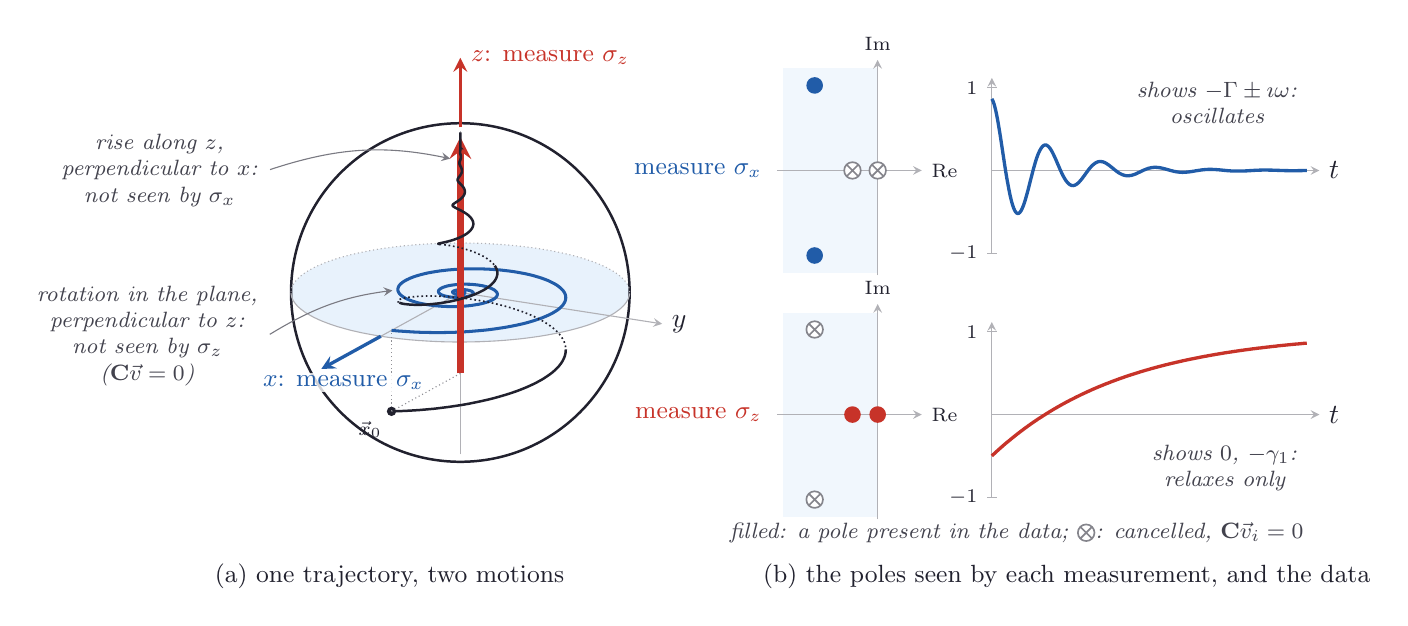
\begin{tikzpicture}[ink/.style={line width=0.9pt, ndInk}, faint/.style={line width=0.4pt, ndInk!35}, dashedink/.style={line width=0.5pt, ndInk!55, dash pattern=on 2.5pt off 2pt}, vec/.style={->, >=stealth, line width=1.2pt}, note/.style={font=\footnotesize\itshape, text=ndInk!85, align=center}, pointer/.style={->, >=stealth, line width=0.4pt, ndInk!60, shorten >=2pt, shorten <=1pt}, dot/.style={circle, fill=ndInk, inner sep=0pt, minimum size=3.4pt}, wash/.style={fill=ndSky, fill opacity=0.55}, every node/.style={text=ndInk}]
\definecolor{ndInk}{rgb}{0.13,0.13,0.18}
\definecolor{ndPaper}{rgb}{0.99,0.96,0.88}
\definecolor{ndSky}{rgb}{0.84,0.91,0.98}
\definecolor{ndRose}{rgb}{0.98,0.86,0.84}
\definecolor{ndBlue}{rgb}{0.13,0.36,0.66}
\definecolor{ndRed}{rgb}{0.78,0.20,0.16}
\definecolor{ndGold}{rgb}{0.88,0.62,0.10}
\definecolor{ndGreen}{rgb}{0.18,0.52,0.30}
\fill[ndSky, fill opacity=0.55] (-1.009,-0.555) -- (-0.934,-0.566) -- (-0.856,-0.577) -- (-0.778,-0.586) -- (-0.698,-0.595) -- (-0.617,-0.602) -- (-0.535,-0.609) -- (-0.453,-0.615) -- (-0.369,-0.619) -- (-0.285,-0.623) -- (-0.201,-0.626) -- (-0.116,-0.628) -- (-0.031,-0.629) -- (0.054,-0.628) -- (0.139,-0.627) -- (0.223,-0.625) -- (0.308,-0.622) -- (0.391,-0.618) -- (0.475,-0.613) -- (0.557,-0.607) -- (0.639,-0.600) -- (0.719,-0.592) -- (0.799,-0.584) -- (0.877,-0.574) -- (0.954,-0.563) -- (1.029,-0.552) -- (1.103,-0.540) -- (1.175,-0.526) -- (1.245,-0.512) -- (1.314,-0.498) -- (1.380,-0.482) -- (1.444,-0.466) -- (1.506,-0.449) -- (1.565,-0.431) -- (1.622,-0.413) -- (1.677,-0.393) -- (1.729,-0.374) -- (1.778,-0.354) -- (1.824,-0.333) -- (1.868,-0.311) -- (1.908,-0.290) -- (1.946,-0.267) -- (1.980,-0.245) -- (2.012,-0.222) -- (2.040,-0.198) -- (2.066,-0.174) -- (2.087,-0.150) -- (2.106,-0.126) -- (2.122,-0.102) -- (2.134,-0.077) -- (2.142,-0.053) -- (2.148,-0.028) -- (2.150,-0.003) -- (2.149,0.022) -- (2.144,0.047) -- (2.136,0.071) -- (2.125,0.096) -- (2.110,0.121) -- (2.092,0.145) -- (2.071,0.169) -- (2.047,0.193) -- (2.019,0.216) -- (1.988,0.239) -- (1.954,0.262) -- (1.917,0.284) -- (1.877,0.306) -- (1.834,0.328) -- (1.789,0.349) -- (1.740,0.369) -- (1.689,0.389) -- (1.635,0.408) -- (1.579,0.427) -- (1.520,0.445) -- (1.459,0.462) -- (1.395,0.478) -- (1.329,0.494) -- (1.261,0.509) -- (1.192,0.523) -- (1.120,0.537) -- (1.047,0.549) -- (0.972,0.561) -- (0.895,0.572) -- (0.817,0.581) -- (0.738,0.590) -- (0.658,0.598) -- (0.576,0.606) -- (0.494,0.612) -- (0.411,0.617) -- (0.327,0.621) -- (0.243,0.625) -- (0.158,0.627) -- (0.074,0.628) -- (-0.011,0.629) -- (-0.096,0.628) -- (-0.181,0.626) -- (-0.266,0.624) -- (-0.350,0.620) -- (-0.433,0.616) -- (-0.516,0.610) -- (-0.598,0.604) -- (-0.679,0.596) -- (-0.759,0.588) -- (-0.838,0.579) -- (-0.916,0.569) -- (-0.992,0.558) -- (-1.066,0.546) -- (-1.139,0.533) -- (-1.210,0.520) -- (-1.280,0.505) -- (-1.347,0.490) -- (-1.412,0.474) -- (-1.475,0.457) -- (-1.536,0.440) -- (-1.594,0.422) -- (-1.650,0.403) -- (-1.703,0.384) -- (-1.753,0.364) -- (-1.801,0.343) -- (-1.846,0.322) -- (-1.888,0.301) -- (-1.927,0.279) -- (-1.964,0.256) -- (-1.997,0.233) -- (-2.027,0.210) -- (-2.053,0.186) -- (-2.077,0.162) -- (-2.097,0.138) -- (-2.114,0.114) -- (-2.128,0.090) -- (-2.139,0.065) -- (-2.146,0.040) -- (-2.149,0.015) -- (-2.150,-0.010) -- (-2.147,-0.034) -- (-2.140,-0.059) -- (-2.131,-0.084) -- (-2.118,-0.108) -- (-2.102,-0.133) -- (-2.082,-0.157) -- (-2.059,-0.181) -- (-2.033,-0.204) -- (-2.004,-0.228) -- (-1.972,-0.251) -- (-1.936,-0.273) -- (-1.898,-0.295) -- (-1.856,-0.317) -- (-1.812,-0.338) -- (-1.765,-0.359) -- (-1.715,-0.379) -- (-1.662,-0.399) -- (-1.607,-0.418) -- (-1.550,-0.436) -- (-1.489,-0.453) -- (-1.427,-0.470) -- (-1.362,-0.486) -- (-1.296,-0.502) -- (-1.227,-0.516) -- (-1.156,-0.530) -- (-1.084,-0.543) -- (-1.009,-0.555) -- cycle;
\draw[ink] (0.000,0.000) circle (2.150);
\draw[faint] (1.898,-0.295) -- (1.924,-0.280) -- (1.949,-0.266) -- (1.972,-0.251) -- (1.993,-0.235) -- (2.014,-0.220) -- (2.033,-0.205) -- (2.050,-0.189) -- (2.067,-0.173) -- (2.082,-0.157) -- (2.095,-0.141) -- (2.107,-0.125) -- (2.117,-0.109) -- (2.126,-0.093) -- (2.134,-0.077) -- (2.140,-0.060) -- (2.145,-0.044) -- (2.148,-0.027) -- (2.150,-0.011);
\draw[faint] (-2.150,-0.005) -- (-2.149,-0.022) -- (-2.146,-0.038) -- (-2.142,-0.055) -- (-2.136,-0.071) -- (-2.129,-0.087) -- (-2.121,-0.104) -- (-2.110,-0.120) -- (-2.099,-0.136) -- (-2.086,-0.152) -- (-2.072,-0.168) -- (-2.056,-0.184) -- (-2.039,-0.199) -- (-2.020,-0.215) -- (-2.000,-0.230) -- (-1.979,-0.246) -- (-1.956,-0.261) -- (-1.932,-0.276) -- (-1.907,-0.290) -- (-1.880,-0.305) -- (-1.853,-0.319) -- (-1.823,-0.333) -- (-1.793,-0.347) -- (-1.761,-0.361) -- (-1.728,-0.374) -- (-1.694,-0.387) -- (-1.659,-0.400) -- (-1.623,-0.412) -- (-1.585,-0.425) -- (-1.547,-0.437) -- (-1.507,-0.448) -- (-1.466,-0.460) -- (-1.425,-0.471) -- (-1.382,-0.482) -- (-1.338,-0.492) -- (-1.294,-0.502) -- (-1.249,-0.512) -- (-1.202,-0.521) -- (-1.155,-0.530) -- (-1.107,-0.539) -- (-1.059,-0.547) -- (-1.009,-0.555) -- (-0.959,-0.563) -- (-0.909,-0.570) -- (-0.857,-0.576) -- (-0.805,-0.583) -- (-0.753,-0.589) -- (-0.700,-0.594) -- (-0.647,-0.600) -- (-0.593,-0.604) -- (-0.538,-0.609) -- (-0.484,-0.612) -- (-0.429,-0.616) -- (-0.373,-0.619) -- (-0.318,-0.622) -- (-0.262,-0.624) -- (-0.206,-0.626) -- (-0.150,-0.627) -- (-0.094,-0.628) -- (-0.038,-0.629) -- (0.019,-0.629) -- (0.075,-0.628) -- (0.131,-0.627) -- (0.187,-0.626) -- (0.243,-0.625) -- (0.299,-0.622) -- (0.355,-0.620) -- (0.410,-0.617) -- (0.465,-0.614) -- (0.520,-0.610) -- (0.575,-0.606) -- (0.629,-0.601) -- (0.682,-0.596) -- (0.735,-0.591) -- (0.788,-0.585) -- (0.840,-0.579) -- (0.892,-0.572) -- (0.942,-0.565) -- (0.993,-0.558) -- (1.042,-0.550) -- (1.091,-0.542) -- (1.139,-0.533) -- (1.187,-0.524) -- (1.233,-0.515) -- (1.279,-0.505) -- (1.324,-0.495) -- (1.368,-0.485) -- (1.411,-0.474) -- (1.453,-0.463) -- (1.494,-0.452) -- (1.533,-0.441) -- (1.572,-0.429) -- (1.610,-0.417) -- (1.647,-0.404) -- (1.683,-0.391) -- (1.717,-0.378) -- (1.750,-0.365) -- (1.782,-0.352) -- (1.813,-0.338) -- (1.843,-0.324) -- (1.871,-0.310) -- (1.898,-0.295);
\draw[faint, densely dotted] (2.150,0.005) -- (2.149,0.022) -- (2.146,0.038) -- (2.142,0.055) -- (2.136,0.071) -- (2.129,0.087) -- (2.121,0.104) -- (2.110,0.120) -- (2.099,0.136) -- (2.086,0.152) -- (2.072,0.168) -- (2.056,0.184) -- (2.039,0.199) -- (2.020,0.215) -- (2.000,0.230) -- (1.979,0.246) -- (1.956,0.261) -- (1.932,0.276) -- (1.907,0.290) -- (1.880,0.305) -- (1.853,0.319) -- (1.823,0.333) -- (1.793,0.347) -- (1.761,0.361) -- (1.728,0.374) -- (1.694,0.387) -- (1.659,0.400) -- (1.623,0.412) -- (1.585,0.425) -- (1.547,0.437) -- (1.507,0.448) -- (1.466,0.460) -- (1.425,0.471) -- (1.382,0.482) -- (1.338,0.492) -- (1.294,0.502) -- (1.249,0.512) -- (1.202,0.521) -- (1.155,0.530) -- (1.107,0.539) -- (1.059,0.547) -- (1.009,0.555) -- (0.959,0.563) -- (0.909,0.570) -- (0.857,0.576) -- (0.805,0.583) -- (0.753,0.589) -- (0.700,0.594) -- (0.647,0.600) -- (0.593,0.604) -- (0.538,0.609) -- (0.484,0.612) -- (0.429,0.616) -- (0.373,0.619) -- (0.318,0.622) -- (0.262,0.624) -- (0.206,0.626) -- (0.150,0.627) -- (0.094,0.628) -- (0.038,0.629) -- (-0.019,0.629) -- (-0.075,0.628) -- (-0.131,0.627) -- (-0.187,0.626) -- (-0.243,0.625) -- (-0.299,0.622) -- (-0.355,0.620) -- (-0.410,0.617) -- (-0.465,0.614) -- (-0.520,0.610) -- (-0.575,0.606) -- (-0.629,0.601) -- (-0.682,0.596) -- (-0.735,0.591) -- (-0.788,0.585) -- (-0.840,0.579) -- (-0.892,0.572) -- (-0.942,0.565) -- (-0.993,0.558) -- (-1.042,0.550) -- (-1.091,0.542) -- (-1.139,0.533) -- (-1.187,0.524) -- (-1.233,0.515) -- (-1.279,0.505) -- (-1.324,0.495) -- (-1.368,0.485) -- (-1.411,0.474) -- (-1.453,0.463) -- (-1.494,0.452) -- (-1.533,0.441) -- (-1.572,0.429) -- (-1.610,0.417) -- (-1.647,0.404) -- (-1.683,0.391) -- (-1.717,0.378) -- (-1.750,0.365) -- (-1.782,0.352) -- (-1.813,0.338) -- (-1.843,0.324) -- (-1.871,0.310) -- (-1.898,0.295) -- (-1.924,0.280) -- (-1.949,0.266) -- (-1.972,0.251) -- (-1.993,0.235) -- (-2.014,0.220) -- (-2.033,0.205) -- (-2.050,0.189) -- (-2.067,0.173) -- (-2.082,0.157) -- (-2.095,0.141) -- (-2.107,0.125) -- (-2.117,0.109) -- (-2.126,0.093) -- (-2.134,0.077) -- (-2.140,0.060) -- (-2.145,0.044) -- (-2.148,0.027) -- (-2.150,0.011);
\draw[faint] (0.000,0.000) -- (-1.009,-0.555);
\draw[faint, ->, >=stealth] (0.000,0.000) -- (2.563,-0.398) node[right, text=ndInk] {$y$};
\draw[faint] (0.000,-2.056) -- (0.000,2.056);
\draw[line width=1.1pt, ndBlue] (-0.874,-0.481) -- (-0.784,-0.489) -- (-0.694,-0.495) -- (-0.603,-0.501) -- (-0.512,-0.505) -- (-0.422,-0.507) -- (-0.332,-0.509) -- (-0.242,-0.509) -- (-0.154,-0.507) -- (-0.066,-0.505) -- (0.020,-0.501) -- (0.105,-0.496) -- (0.188,-0.489) -- (0.269,-0.482) -- (0.348,-0.474) -- (0.425,-0.464) -- (0.500,-0.453) -- (0.572,-0.442) -- (0.642,-0.429) -- (0.708,-0.416) -- (0.772,-0.402) -- (0.833,-0.387) -- (0.890,-0.371) -- (0.945,-0.354) -- (0.996,-0.337) -- (1.044,-0.320) -- (1.088,-0.301) -- (1.129,-0.283) -- (1.166,-0.264) -- (1.200,-0.244) -- (1.230,-0.225) -- (1.256,-0.205) -- (1.279,-0.184) -- (1.298,-0.164) -- (1.313,-0.144) -- (1.325,-0.123) -- (1.333,-0.103) -- (1.338,-0.083) -- (1.339,-0.062) -- (1.337,-0.042) -- (1.332,-0.023) -- (1.323,-0.003) -- (1.311,0.016) -- (1.295,0.035) -- (1.277,0.053) -- (1.256,0.071) -- (1.232,0.089) -- (1.205,0.106) -- (1.175,0.122) -- (1.143,0.138) -- (1.109,0.154) -- (1.072,0.168) -- (1.034,0.182) -- (0.993,0.195) -- (0.950,0.208) -- (0.906,0.220) -- (0.860,0.231) -- (0.813,0.241) -- (0.764,0.250) -- (0.714,0.259) -- (0.664,0.267) -- (0.612,0.274) -- (0.560,0.280) -- (0.507,0.286) -- (0.453,0.290) -- (0.400,0.294) -- (0.346,0.297) -- (0.292,0.299) -- (0.239,0.301) -- (0.185,0.301) -- (0.133,0.301) -- (0.080,0.300) -- (0.028,0.299) -- (-0.022,0.296) -- (-0.072,0.293) -- (-0.121,0.289) -- (-0.169,0.285) -- (-0.216,0.279) -- (-0.261,0.274) -- (-0.305,0.267) -- (-0.348,0.260) -- (-0.388,0.253) -- (-0.428,0.245) -- (-0.465,0.236) -- (-0.501,0.227) -- (-0.534,0.218) -- (-0.566,0.208) -- (-0.596,0.198) -- (-0.624,0.187) -- (-0.650,0.176) -- (-0.673,0.165) -- (-0.695,0.154) -- (-0.715,0.142) -- (-0.732,0.131) -- (-0.747,0.119) -- (-0.760,0.107) -- (-0.771,0.095) -- (-0.780,0.083) -- (-0.786,0.071) -- (-0.791,0.058) -- (-0.793,0.046) -- (-0.793,0.035) -- (-0.792,0.023) -- (-0.788,0.011) -- (-0.782,-0.001) -- (-0.775,-0.012) -- (-0.765,-0.023) -- (-0.754,-0.034) -- (-0.741,-0.044) -- (-0.726,-0.055) -- (-0.710,-0.065) -- (-0.692,-0.075) -- (-0.673,-0.084) -- (-0.653,-0.093) -- (-0.631,-0.101) -- (-0.607,-0.110) -- (-0.583,-0.117) -- (-0.558,-0.125) -- (-0.531,-0.132) -- (-0.504,-0.138) -- (-0.475,-0.144) -- (-0.447,-0.149) -- (-0.417,-0.155) -- (-0.387,-0.159) -- (-0.356,-0.163) -- (-0.325,-0.167) -- (-0.294,-0.170) -- (-0.262,-0.173) -- (-0.230,-0.175) -- (-0.198,-0.176) -- (-0.166,-0.178) -- (-0.135,-0.178) -- (-0.103,-0.179) -- (-0.072,-0.178) -- (-0.041,-0.178) -- (-0.010,-0.177) -- (0.020,-0.175) -- (0.049,-0.173) -- (0.078,-0.171) -- (0.106,-0.168) -- (0.134,-0.165) -- (0.160,-0.161) -- (0.186,-0.157) -- (0.211,-0.153) -- (0.235,-0.149) -- (0.258,-0.144) -- (0.280,-0.139) -- (0.301,-0.133) -- (0.321,-0.128) -- (0.339,-0.122) -- (0.357,-0.116) -- (0.373,-0.110) -- (0.388,-0.103) -- (0.402,-0.096) -- (0.414,-0.090) -- (0.426,-0.083) -- (0.436,-0.076) -- (0.444,-0.069) -- (0.452,-0.062) -- (0.458,-0.055) -- (0.463,-0.047) -- (0.466,-0.040) -- (0.469,-0.033) -- (0.470,-0.026) -- (0.470,-0.019) -- (0.469,-0.012) -- (0.466,-0.005) -- (0.463,0.002) -- (0.458,0.008) -- (0.452,0.015) -- (0.445,0.021) -- (0.437,0.028) -- (0.428,0.034) -- (0.419,0.040) -- (0.408,0.045) -- (0.396,0.051) -- (0.384,0.056) -- (0.371,0.061) -- (0.357,0.066) -- (0.342,0.070) -- (0.327,0.075) -- (0.311,0.079) -- (0.295,0.083) -- (0.278,0.086) -- (0.261,0.089) -- (0.243,0.092) -- (0.225,0.095) -- (0.207,0.097) -- (0.189,0.099) -- (0.170,0.101) -- (0.151,0.103) -- (0.132,0.104) -- (0.114,0.105) -- (0.095,0.105) -- (0.076,0.106) -- (0.057,0.106) -- (0.039,0.106) -- (0.020,0.105) -- (0.002,0.104) -- (-0.015,0.103) -- (-0.033,0.102) -- (-0.050,0.101) -- (-0.066,0.099) -- (-0.083,0.097) -- (-0.098,0.095) -- (-0.113,0.093) -- (-0.128,0.090) -- (-0.142,0.088) -- (-0.156,0.085) -- (-0.169,0.082) -- (-0.181,0.078) -- (-0.192,0.075) -- (-0.203,0.071) -- (-0.213,0.068) -- (-0.223,0.064) -- (-0.232,0.060) -- (-0.240,0.056) -- (-0.247,0.052) -- (-0.253,0.048) -- (-0.259,0.044) -- (-0.264,0.040) -- (-0.268,0.036) -- (-0.272,0.031) -- (-0.275,0.027) -- (-0.277,0.023) -- (-0.278,0.019) -- (-0.278,0.015) -- (-0.278,0.010) -- (-0.277,0.006) -- (-0.276,0.002) -- (-0.273,-0.002) -- (-0.271,-0.006) -- (-0.267,-0.010) -- (-0.263,-0.013) -- (-0.258,-0.017) -- (-0.253,-0.021) -- (-0.247,-0.024) -- (-0.240,-0.028) -- (-0.233,-0.031) -- (-0.226,-0.034) -- (-0.218,-0.037) -- (-0.210,-0.040) -- (-0.201,-0.042) -- (-0.192,-0.045) -- (-0.182,-0.047) -- (-0.173,-0.049) -- (-0.163,-0.051) -- (-0.152,-0.053) -- (-0.142,-0.055) -- (-0.131,-0.056) -- (-0.120,-0.058) -- (-0.109,-0.059) -- (-0.098,-0.060) -- (-0.087,-0.061) -- (-0.076,-0.062) -- (-0.065,-0.062) -- (-0.054,-0.062) -- (-0.043,-0.063) -- (-0.032,-0.063) -- (-0.021,-0.063) -- (-0.010,-0.062) -- (0.001,-0.062) -- (0.011,-0.061) -- (0.022,-0.060) -- (0.032,-0.060) -- (0.041,-0.058) -- (0.051,-0.057) -- (0.060,-0.056) -- (0.069,-0.055) -- (0.078,-0.053) -- (0.086,-0.051) -- (0.094,-0.050) -- (0.101,-0.048) -- (0.109,-0.046) -- (0.115,-0.044) -- (0.122,-0.042) -- (0.128,-0.040) -- (0.133,-0.037) -- (0.138,-0.035) -- (0.143,-0.033) -- (0.147,-0.030) -- (0.151,-0.028) -- (0.154,-0.026) -- (0.157,-0.023) -- (0.159,-0.021) -- (0.161,-0.018) -- (0.163,-0.016) -- (0.164,-0.013) -- (0.165,-0.011) -- (0.165,-0.008) -- (0.165,-0.006) -- (0.164,-0.003) -- (0.163,-0.001) -- (0.162,0.002) -- (0.160,0.004) -- (0.158,0.006) -- (0.155,0.008) -- (0.152,0.011) -- (0.149,0.013) -- (0.145,0.015) -- (0.141,0.017) -- (0.137,0.019) -- (0.133,0.020) -- (0.128,0.022) -- (0.123,0.024) -- (0.118,0.025) -- (0.112,0.027) -- (0.107,0.028) -- (0.101,0.029) -- (0.095,0.031) -- (0.089,0.032) -- (0.083,0.033) -- (0.076,0.034) -- (0.070,0.034) -- (0.063,0.035) -- (0.057,0.036) -- (0.050,0.036) -- (0.044,0.037) -- (0.037,0.037) -- (0.030,0.037) -- (0.024,0.037) -- (0.017,0.037) -- (0.011,0.037) -- (0.005,0.037) -- (-0.002,0.037) -- (-0.008,0.036) -- (-0.014,0.036) -- (-0.020,0.035) -- (-0.026,0.035) -- (-0.031,0.034) -- (-0.037,0.033) -- (-0.042,0.032) -- (-0.047,0.031) -- (-0.052,0.030) -- (-0.057,0.029) -- (-0.061,0.028) -- (-0.065,0.027) -- (-0.069,0.026) -- (-0.073,0.025) -- (-0.076,0.023) -- (-0.080,0.022) -- (-0.082,0.021) -- (-0.085,0.019) -- (-0.088,0.018) -- (-0.090,0.016) -- (-0.092,0.015) -- (-0.093,0.013) -- (-0.095,0.012) -- (-0.096,0.010) -- (-0.097,0.009) -- (-0.097,0.007) -- (-0.098,0.006) -- (-0.098,0.004) -- (-0.098,0.003) -- (-0.097,0.002) -- (-0.096,0.000) -- (-0.096,-0.001) -- (-0.094,-0.003) -- (-0.093,-0.004) -- (-0.092,-0.005) -- (-0.090,-0.007) -- (-0.088,-0.008) -- (-0.086,-0.009) -- (-0.083,-0.010) -- (-0.081,-0.011) -- (-0.078,-0.012) -- (-0.075,-0.013) -- (-0.072,-0.014) -- (-0.069,-0.015) -- (-0.066,-0.016) -- (-0.063,-0.017) -- (-0.059,-0.018) -- (-0.056,-0.018) -- (-0.052,-0.019) -- (-0.048,-0.020) -- (-0.044,-0.020) -- (-0.041,-0.020) -- (-0.037,-0.021) -- (-0.033,-0.021) -- (-0.029,-0.021) -- (-0.025,-0.022) -- (-0.021,-0.022) -- (-0.017,-0.022) -- (-0.013,-0.022) -- (-0.009,-0.022) -- (-0.006,-0.022) -- (-0.002,-0.022) -- (0.002,-0.022) -- (0.005,-0.021) -- (0.009,-0.021) -- (0.013,-0.021) -- (0.016,-0.020) -- (0.019,-0.020) -- (0.022,-0.019) -- (0.026,-0.019) -- (0.028,-0.018) -- (0.031,-0.018) -- (0.034,-0.017) -- (0.037,-0.017) -- (0.039,-0.016) -- (0.041,-0.015) -- (0.044,-0.014) -- (0.046,-0.014) -- (0.047,-0.013) -- (0.049,-0.012) -- (0.051,-0.011) -- (0.052,-0.010) -- (0.053,-0.009) -- (0.055,-0.009) -- (0.055,-0.008) -- (0.056,-0.007) -- (0.057,-0.006) -- (0.057,-0.005) -- (0.058,-0.004) -- (0.058,-0.003) -- (0.058,-0.002) -- (0.058,-0.002) -- (0.057,-0.001) -- (0.057,0.000) -- (0.056,0.001) -- (0.056,0.002) -- (0.055,0.003) -- (0.054,0.003) -- (0.053,0.004) -- (0.052,0.005) -- (0.050,0.005) -- (0.049,0.006) -- (0.048,0.007) -- (0.046,0.007) -- (0.044,0.008) -- (0.042,0.009) -- (0.041,0.009) -- (0.039,0.010) -- (0.037,0.010) -- (0.035,0.011) -- (0.032,0.011) -- (0.030,0.011) -- (0.028,0.012) -- (0.026,0.012) -- (0.024,0.012) -- (0.021,0.012) -- (0.019,0.013) -- (0.017,0.013) -- (0.014,0.013) -- (0.012,0.013) -- (0.010,0.013) -- (0.007,0.013) -- (0.005,0.013) -- (0.003,0.013) -- (0.001,0.013) -- (-0.002,0.013) -- (-0.004,0.013) -- (-0.006,0.012) -- (-0.008,0.012) -- (-0.010,0.012) -- (-0.012,0.012) -- (-0.014,0.011) -- (-0.015,0.011) -- (-0.017,0.011) -- (-0.019,0.010) -- (-0.021,0.010) -- (-0.022,0.010) -- (-0.023,0.009) -- (-0.025,0.009) -- (-0.026,0.008) -- (-0.027,0.008) -- (-0.028,0.007) -- (-0.029,0.007) -- (-0.030,0.007) -- (-0.031,0.006) -- (-0.032,0.006) -- (-0.032,0.005) -- (-0.033,0.004) -- (-0.033,0.004) -- (-0.034,0.003) -- (-0.034,0.003) -- (-0.034,0.002) -- (-0.034,0.002) -- (-0.034,0.001) -- (-0.034,0.001) -- (-0.034,0.000) -- (-0.034,-0.000) -- (-0.033,-0.001) -- (-0.033,-0.001) -- (-0.032,-0.002) -- (-0.032,-0.002) -- (-0.031,-0.002) -- (-0.030,-0.003) -- (-0.030,-0.003) -- (-0.029,-0.004) -- (-0.028,-0.004) -- (-0.027,-0.004) -- (-0.026,-0.005) -- (-0.025,-0.005) -- (-0.024,-0.005) -- (-0.023,-0.006) -- (-0.021,-0.006) -- (-0.020,-0.006) -- (-0.019,-0.007) -- (-0.018,-0.007) -- (-0.016,-0.007) -- (-0.015,-0.007) -- (-0.014,-0.007) -- (-0.012,-0.007) -- (-0.011,-0.007) -- (-0.010,-0.008) -- (-0.008,-0.008) -- (-0.007,-0.008) -- (-0.005,-0.008) -- (-0.004,-0.008) -- (-0.003,-0.008) -- (-0.001,-0.008) -- (-0.000,-0.008) -- (0.001,-0.008) -- (0.002,-0.007) -- (0.004,-0.007) -- (0.005,-0.007) -- (0.006,-0.007) -- (0.007,-0.007) -- (0.008,-0.007) -- (0.009,-0.007) -- (0.010,-0.006) -- (0.011,-0.006) -- (0.012,-0.006) -- (0.013,-0.006) -- (0.014,-0.005) -- (0.015,-0.005) -- (0.016,-0.005) -- (0.016,-0.005) -- (0.017,-0.004) -- (0.018,-0.004) -- (0.018,-0.004) -- (0.019,-0.004) -- (0.019,-0.003) -- (0.019,-0.003) -- (0.020,-0.003) -- (0.020,-0.002) -- (0.020,-0.002) -- (0.020,-0.002) -- (0.020,-0.001) -- (0.020,-0.001) -- (0.020,-0.001) -- (0.020,-0.000) -- (0.020,-0.000) -- (0.020,0.000) -- (0.020,0.000) -- (0.019,0.001) -- (0.019,0.001) -- (0.019,0.001) -- (0.018,0.002) -- (0.018,0.002) -- (0.017,0.002) -- (0.017,0.002) -- (0.016,0.002) -- (0.016,0.003) -- (0.015,0.003) -- (0.015,0.003) -- (0.014,0.003) -- (0.013,0.003) -- (0.013,0.004) -- (0.012,0.004) -- (0.011,0.004) -- (0.010,0.004) -- (0.010,0.004) -- (0.009,0.004) -- (0.008,0.004) -- (0.007,0.004) -- (0.006,0.004) -- (0.006,0.004) -- (0.005,0.005) -- (0.004,0.005) -- (0.003,0.005) -- (0.002,0.005) -- (0.001,0.005) -- (0.001,0.005) -- (-0.000,0.005) -- (-0.001,0.004) -- (-0.002,0.004) -- (-0.002,0.004) -- (-0.003,0.004) -- (-0.004,0.004) -- (-0.004,0.004) -- (-0.005,0.004) -- (-0.006,0.004) -- (-0.006,0.004) -- (-0.007,0.004) -- (-0.007,0.003) -- (-0.008,0.003) -- (-0.008,0.003) -- (-0.009,0.003) -- (-0.009,0.003) -- (-0.010,0.003) -- (-0.010,0.003) -- (-0.010,0.002) -- (-0.011,0.002) -- (-0.011,0.002) -- (-0.011,0.002) -- (-0.011,0.002) -- (-0.012,0.001) -- (-0.012,0.001) -- (-0.012,0.001) -- (-0.012,0.001) -- (-0.012,0.001) -- (-0.012,0.001) -- (-0.012,0.000) -- (-0.012,0.000) -- (-0.012,0.000) -- (-0.012,-0.000) -- (-0.012,-0.000) -- (-0.011,-0.000) -- (-0.011,-0.001) -- (-0.011,-0.001) -- (-0.011,-0.001) -- (-0.011,-0.001) -- (-0.010,-0.001) -- (-0.010,-0.001) -- (-0.010,-0.001) -- (-0.009,-0.002) -- (-0.009,-0.002) -- (-0.009,-0.002) -- (-0.008,-0.002) -- (-0.008,-0.002) -- (-0.007,-0.002) -- (-0.007,-0.002) -- (-0.006,-0.002) -- (-0.006,-0.002) -- (-0.006,-0.002) -- (-0.005,-0.003) -- (-0.005,-0.003) -- (-0.004,-0.003) -- (-0.004,-0.003) -- (-0.003,-0.003) -- (-0.003,-0.003) -- (-0.002,-0.003) -- (-0.002,-0.003) -- (-0.001,-0.003) -- (-0.001,-0.003) -- (-0.000,-0.003) -- (0.000,-0.003) -- (0.001,-0.003) -- (0.001,-0.003) -- (0.001,-0.003) -- (0.002,-0.003) -- (0.002,-0.002) -- (0.003,-0.002) -- (0.003,-0.002) -- (0.003,-0.002) -- (0.004,-0.002) -- (0.004,-0.002) -- (0.004,-0.002) -- (0.005,-0.002) -- (0.005,-0.002) -- (0.005,-0.002) -- (0.006,-0.002) -- (0.006,-0.002) -- (0.006,-0.001) -- (0.006,-0.001) -- (0.006,-0.001) -- (0.007,-0.001) -- (0.007,-0.001) -- (0.007,-0.001) -- (0.007,-0.001) -- (0.007,-0.001) -- (0.007,-0.001) -- (0.007,-0.001) -- (0.007,-0.000) -- (0.007,-0.000) -- (0.007,-0.000) -- (0.007,-0.000) -- (0.007,-0.000) -- (0.007,0.000) -- (0.007,0.000) -- (0.007,0.000) -- (0.007,0.000) -- (0.007,0.000) -- (0.006,0.001) -- (0.006,0.001) -- (0.006,0.001) -- (0.006,0.001) -- (0.006,0.001) -- (0.005,0.001) -- (0.005,0.001) -- (0.005,0.001) -- (0.005,0.001) -- (0.005,0.001) -- (0.004,0.001) -- (0.004,0.001) -- (0.004,0.001) -- (0.004,0.001) -- (0.003,0.001) -- (0.003,0.001) -- (0.003,0.002) -- (0.002,0.002) -- (0.002,0.002) -- (0.002,0.002) -- (0.002,0.002) -- (0.001,0.002) -- (0.001,0.002) -- (0.001,0.002) -- (0.000,0.002);
\draw[line width=2.4pt, ndRed, ->, >=stealth] (0.000,-1.028) -- (0.000,1.974);
\draw[line width=0.9pt, ndInk] (-0.874,-1.509) -- (-0.784,-1.507) -- (-0.694,-1.503) -- (-0.603,-1.498) -- (-0.512,-1.492) -- (-0.422,-1.484) -- (-0.332,-1.476) -- (-0.242,-1.465) -- (-0.154,-1.454) -- (-0.066,-1.441) -- (0.020,-1.428) -- (0.105,-1.413) -- (0.188,-1.396) -- (0.269,-1.379) -- (0.348,-1.361) -- (0.425,-1.342) -- (0.500,-1.321) -- (0.572,-1.300) -- (0.642,-1.278) -- (0.708,-1.255) -- (0.772,-1.231) -- (0.833,-1.206) -- (0.890,-1.181) -- (0.945,-1.155) -- (0.996,-1.128) -- (1.044,-1.101) -- (1.088,-1.073) -- (1.129,-1.045) -- (1.166,-1.017) -- (1.200,-0.988) -- (1.230,-0.959) -- (1.256,-0.930) -- (1.279,-0.900) -- (1.298,-0.871) -- (1.313,-0.841) -- (1.325,-0.812) -- (1.333,-0.782) -- (1.338,-0.753) -- (1.339,-0.723);
\draw[line width=0.9pt, ndInk] (-0.775,-0.129) -- (-0.765,-0.133) -- (-0.754,-0.136) -- (-0.741,-0.140) -- (-0.726,-0.143) -- (-0.710,-0.146) -- (-0.692,-0.148) -- (-0.673,-0.150) -- (-0.653,-0.152) -- (-0.631,-0.154) -- (-0.607,-0.155) -- (-0.583,-0.156) -- (-0.558,-0.156) -- (-0.531,-0.156) -- (-0.504,-0.156) -- (-0.475,-0.155) -- (-0.447,-0.153) -- (-0.417,-0.152) -- (-0.387,-0.149) -- (-0.356,-0.147) -- (-0.325,-0.143) -- (-0.294,-0.140) -- (-0.262,-0.136) -- (-0.230,-0.131) -- (-0.198,-0.126) -- (-0.166,-0.120) -- (-0.135,-0.115) -- (-0.103,-0.108) -- (-0.072,-0.101) -- (-0.041,-0.094) -- (-0.010,-0.086) -- (0.020,-0.078) -- (0.049,-0.070) -- (0.078,-0.061) -- (0.106,-0.052) -- (0.134,-0.042) -- (0.160,-0.032) -- (0.186,-0.022) -- (0.211,-0.011) -- (0.235,-0.000) -- (0.258,0.011) -- (0.280,0.022) -- (0.301,0.034) -- (0.321,0.046) -- (0.339,0.058) -- (0.357,0.070) -- (0.373,0.083) -- (0.388,0.095) -- (0.402,0.108) -- (0.414,0.121) -- (0.426,0.134) -- (0.436,0.147) -- (0.444,0.160) -- (0.452,0.174) -- (0.458,0.187) -- (0.463,0.200) -- (0.466,0.213) -- (0.469,0.226) -- (0.470,0.239) -- (0.470,0.252) -- (0.469,0.265) -- (0.466,0.278) -- (0.463,0.291) -- (0.458,0.303) -- (0.452,0.316) -- (0.445,0.328) -- (0.437,0.340);
\draw[line width=0.9pt, ndInk] (-0.247,0.613) -- (-0.253,0.614) -- (-0.259,0.615) -- (-0.264,0.615) -- (-0.268,0.616) -- (-0.272,0.617) -- (-0.275,0.617) -- (-0.277,0.618) -- (-0.278,0.619) -- (-0.278,0.619) -- (-0.278,0.620) -- (-0.277,0.621) -- (-0.276,0.621) -- (-0.273,0.622) -- (-0.271,0.623) -- (-0.267,0.624) -- (-0.263,0.625) -- (-0.258,0.626) -- (-0.253,0.627) -- (-0.247,0.628) -- (-0.240,0.630) -- (-0.233,0.631) -- (-0.226,0.633) -- (-0.218,0.634) -- (-0.210,0.636) -- (-0.201,0.638) -- (-0.192,0.640) -- (-0.182,0.642) -- (-0.173,0.645) -- (-0.163,0.647) -- (-0.152,0.650) -- (-0.142,0.653) -- (-0.131,0.656) -- (-0.120,0.659) -- (-0.109,0.662) -- (-0.098,0.665) -- (-0.087,0.669) -- (-0.076,0.673) -- (-0.065,0.677) -- (-0.054,0.681) -- (-0.043,0.685) -- (-0.032,0.689) -- (-0.021,0.694) -- (-0.010,0.698) -- (0.001,0.703) -- (0.011,0.708) -- (0.022,0.713) -- (0.032,0.718) -- (0.041,0.723) -- (0.051,0.729) -- (0.060,0.734) -- (0.069,0.740) -- (0.078,0.746) -- (0.086,0.751) -- (0.094,0.757) -- (0.101,0.763) -- (0.109,0.769) -- (0.115,0.776) -- (0.122,0.782) -- (0.128,0.788) -- (0.133,0.794) -- (0.138,0.801) -- (0.143,0.807) -- (0.147,0.814) -- (0.151,0.820) -- (0.154,0.826) -- (0.157,0.833) -- (0.159,0.839) -- (0.161,0.846) -- (0.163,0.852) -- (0.164,0.859) -- (0.165,0.865) -- (0.165,0.872) -- (0.165,0.878) -- (0.164,0.885) -- (0.163,0.891) -- (0.162,0.897) -- (0.160,0.903) -- (0.158,0.909) -- (0.155,0.915) -- (0.152,0.921) -- (0.149,0.927) -- (0.145,0.933) -- (0.141,0.939) -- (0.137,0.945) -- (0.133,0.950) -- (0.128,0.956) -- (0.123,0.961) -- (0.118,0.966) -- (0.112,0.972) -- (0.107,0.977) -- (0.101,0.982) -- (0.095,0.986) -- (0.089,0.991) -- (0.083,0.996) -- (0.076,1.000) -- (0.070,1.005) -- (0.063,1.009) -- (0.057,1.013) -- (0.050,1.017) -- (0.044,1.021) -- (0.037,1.025) -- (0.030,1.029) -- (0.024,1.033) -- (0.017,1.036) -- (0.011,1.039) -- (0.005,1.043) -- (-0.002,1.046) -- (-0.008,1.049) -- (-0.014,1.052) -- (-0.020,1.055) -- (-0.026,1.058) -- (-0.031,1.061) -- (-0.037,1.063) -- (-0.042,1.066) -- (-0.047,1.068) -- (-0.052,1.071) -- (-0.057,1.073) -- (-0.061,1.075) -- (-0.065,1.078) -- (-0.069,1.080) -- (-0.073,1.082) -- (-0.076,1.084) -- (-0.080,1.086) -- (-0.082,1.088) -- (-0.085,1.090) -- (-0.088,1.091) -- (-0.090,1.093) -- (-0.092,1.095) -- (-0.093,1.097) -- (-0.095,1.099) -- (-0.096,1.100) -- (-0.097,1.102) -- (-0.097,1.104) -- (-0.098,1.106) -- (-0.098,1.107) -- (-0.098,1.109) -- (-0.097,1.111) -- (-0.096,1.112) -- (-0.096,1.114) -- (-0.094,1.116) -- (-0.093,1.118) -- (-0.092,1.120) -- (-0.090,1.121) -- (-0.088,1.123) -- (-0.086,1.125) -- (-0.083,1.127) -- (-0.081,1.129) -- (-0.078,1.131) -- (-0.075,1.133) -- (-0.072,1.135) -- (-0.069,1.137) -- (-0.066,1.139) -- (-0.063,1.141) -- (-0.059,1.144) -- (-0.056,1.146) -- (-0.052,1.148) -- (-0.048,1.151) -- (-0.044,1.153) -- (-0.041,1.156) -- (-0.037,1.158) -- (-0.033,1.161) -- (-0.029,1.163) -- (-0.025,1.166) -- (-0.021,1.169) -- (-0.017,1.172) -- (-0.013,1.174) -- (-0.009,1.177) -- (-0.006,1.180) -- (-0.002,1.183) -- (0.002,1.186) -- (0.005,1.189) -- (0.009,1.192) -- (0.013,1.196) -- (0.016,1.199) -- (0.019,1.202) -- (0.022,1.205) -- (0.026,1.208) -- (0.028,1.212) -- (0.031,1.215) -- (0.034,1.218) -- (0.037,1.222) -- (0.039,1.225) -- (0.041,1.229) -- (0.044,1.232) -- (0.046,1.236) -- (0.047,1.239) -- (0.049,1.243) -- (0.051,1.246) -- (0.052,1.250) -- (0.053,1.253) -- (0.055,1.257) -- (0.055,1.260) -- (0.056,1.264) -- (0.057,1.267) -- (0.057,1.271) -- (0.058,1.274) -- (0.058,1.278) -- (0.058,1.281) -- (0.058,1.284) -- (0.057,1.288) -- (0.057,1.291) -- (0.056,1.295) -- (0.056,1.298) -- (0.055,1.301) -- (0.054,1.305) -- (0.053,1.308) -- (0.052,1.311) -- (0.050,1.314) -- (0.049,1.317) -- (0.048,1.321) -- (0.046,1.324) -- (0.044,1.327) -- (0.042,1.330) -- (0.041,1.333) -- (0.039,1.336) -- (0.037,1.339) -- (0.035,1.341) -- (0.032,1.344) -- (0.030,1.347) -- (0.028,1.350) -- (0.026,1.352) -- (0.024,1.355) -- (0.021,1.358) -- (0.019,1.360) -- (0.017,1.363) -- (0.014,1.365) -- (0.012,1.368) -- (0.010,1.370) -- (0.007,1.372) -- (0.005,1.375) -- (0.003,1.377) -- (0.001,1.379) -- (-0.002,1.381) -- (-0.004,1.383) -- (-0.006,1.386) -- (-0.008,1.388) -- (-0.010,1.390) -- (-0.012,1.392) -- (-0.014,1.394) -- (-0.015,1.396) -- (-0.017,1.398) -- (-0.019,1.399) -- (-0.021,1.401) -- (-0.022,1.403) -- (-0.023,1.405) -- (-0.025,1.407) -- (-0.026,1.408) -- (-0.027,1.410) -- (-0.028,1.412) -- (-0.029,1.414) -- (-0.030,1.415) -- (-0.031,1.417) -- (-0.032,1.418) -- (-0.032,1.420) -- (-0.033,1.422) -- (-0.033,1.423) -- (-0.034,1.425) -- (-0.034,1.427) -- (-0.034,1.428) -- (-0.034,1.430) -- (-0.034,1.431) -- (-0.034,1.433) -- (-0.034,1.434) -- (-0.034,1.436) -- (-0.033,1.438) -- (-0.033,1.439) -- (-0.032,1.441) -- (-0.032,1.442) -- (-0.031,1.444) -- (-0.030,1.445) -- (-0.030,1.447) -- (-0.029,1.449) -- (-0.028,1.450) -- (-0.027,1.452) -- (-0.026,1.454) -- (-0.025,1.455) -- (-0.024,1.457) -- (-0.023,1.459) -- (-0.021,1.460) -- (-0.020,1.462) -- (-0.019,1.464) -- (-0.018,1.466) -- (-0.016,1.467) -- (-0.015,1.469) -- (-0.014,1.471) -- (-0.012,1.473) -- (-0.011,1.474) -- (-0.010,1.476) -- (-0.008,1.478) -- (-0.007,1.480) -- (-0.005,1.482) -- (-0.004,1.484) -- (-0.003,1.486) -- (-0.001,1.487) -- (-0.000,1.489) -- (0.001,1.491) -- (0.002,1.493) -- (0.004,1.495) -- (0.005,1.497) -- (0.006,1.499) -- (0.007,1.501) -- (0.008,1.503) -- (0.009,1.505) -- (0.010,1.507) -- (0.011,1.509) -- (0.012,1.511) -- (0.013,1.513) -- (0.014,1.515) -- (0.015,1.517) -- (0.016,1.519) -- (0.016,1.521) -- (0.017,1.523) -- (0.018,1.526) -- (0.018,1.528) -- (0.019,1.530) -- (0.019,1.532) -- (0.019,1.534) -- (0.020,1.536) -- (0.020,1.538) -- (0.020,1.540) -- (0.020,1.542) -- (0.020,1.544) -- (0.020,1.546) -- (0.020,1.548) -- (0.020,1.550) -- (0.020,1.552) -- (0.020,1.554) -- (0.020,1.556) -- (0.019,1.558) -- (0.019,1.560) -- (0.019,1.562) -- (0.018,1.563) -- (0.018,1.565) -- (0.017,1.567) -- (0.017,1.569) -- (0.016,1.571) -- (0.016,1.573) -- (0.015,1.575) -- (0.015,1.576) -- (0.014,1.578) -- (0.013,1.580) -- (0.013,1.582) -- (0.012,1.583) -- (0.011,1.585) -- (0.010,1.587) -- (0.010,1.589) -- (0.009,1.590) -- (0.008,1.592) -- (0.007,1.594) -- (0.006,1.595) -- (0.006,1.597) -- (0.005,1.598) -- (0.004,1.600) -- (0.003,1.601) -- (0.002,1.603) -- (0.001,1.605) -- (0.001,1.606) -- (-0.000,1.607) -- (-0.001,1.609) -- (-0.002,1.610) -- (-0.002,1.612) -- (-0.003,1.613) -- (-0.004,1.615) -- (-0.004,1.616) -- (-0.005,1.617) -- (-0.006,1.619) -- (-0.006,1.620) -- (-0.007,1.621) -- (-0.007,1.623) -- (-0.008,1.624) -- (-0.008,1.625) -- (-0.009,1.627) -- (-0.009,1.628) -- (-0.010,1.629) -- (-0.010,1.631) -- (-0.010,1.632) -- (-0.011,1.633) -- (-0.011,1.634) -- (-0.011,1.635) -- (-0.011,1.637) -- (-0.012,1.638) -- (-0.012,1.639) -- (-0.012,1.640) -- (-0.012,1.642) -- (-0.012,1.643) -- (-0.012,1.644) -- (-0.012,1.645) -- (-0.012,1.646) -- (-0.012,1.648) -- (-0.012,1.649) -- (-0.012,1.650) -- (-0.011,1.651) -- (-0.011,1.652) -- (-0.011,1.653) -- (-0.011,1.655) -- (-0.011,1.656) -- (-0.010,1.657) -- (-0.010,1.658) -- (-0.010,1.659) -- (-0.009,1.661) -- (-0.009,1.662) -- (-0.009,1.663) -- (-0.008,1.664) -- (-0.008,1.665) -- (-0.007,1.667) -- (-0.007,1.668) -- (-0.006,1.669) -- (-0.006,1.670) -- (-0.006,1.671) -- (-0.005,1.673) -- (-0.005,1.674) -- (-0.004,1.675) -- (-0.004,1.676) -- (-0.003,1.678) -- (-0.003,1.679) -- (-0.002,1.680) -- (-0.002,1.681) -- (-0.001,1.682) -- (-0.001,1.684) -- (-0.000,1.685) -- (0.000,1.686) -- (0.001,1.687) -- (0.001,1.689) -- (0.001,1.690) -- (0.002,1.691) -- (0.002,1.692) -- (0.003,1.694) -- (0.003,1.695) -- (0.003,1.696) -- (0.004,1.698) -- (0.004,1.699) -- (0.004,1.700) -- (0.005,1.701) -- (0.005,1.703) -- (0.005,1.704) -- (0.006,1.705) -- (0.006,1.706) -- (0.006,1.708) -- (0.006,1.709) -- (0.006,1.710) -- (0.007,1.711) -- (0.007,1.713) -- (0.007,1.714) -- (0.007,1.715) -- (0.007,1.716) -- (0.007,1.718) -- (0.007,1.719) -- (0.007,1.720) -- (0.007,1.721) -- (0.007,1.722) -- (0.007,1.724) -- (0.007,1.725) -- (0.007,1.726) -- (0.007,1.727) -- (0.007,1.729) -- (0.007,1.730) -- (0.007,1.731) -- (0.006,1.732) -- (0.006,1.733) -- (0.006,1.734) -- (0.006,1.736) -- (0.006,1.737) -- (0.005,1.738) -- (0.005,1.739) -- (0.005,1.740) -- (0.005,1.741) -- (0.005,1.742) -- (0.004,1.743) -- (0.004,1.745) -- (0.004,1.746) -- (0.004,1.747) -- (0.003,1.748) -- (0.003,1.749) -- (0.003,1.750) -- (0.002,1.751) -- (0.002,1.752) -- (0.002,1.753) -- (0.002,1.754) -- (0.001,1.755) -- (0.001,1.756) -- (0.001,1.757) -- (0.000,1.758) -- (0.000,1.759) -- (-0.000,1.760) -- (-0.000,1.761) -- (-0.001,1.762) -- (-0.001,1.763) -- (-0.001,1.764) -- (-0.001,1.765) -- (-0.002,1.766) -- (-0.002,1.767) -- (-0.002,1.768) -- (-0.002,1.769) -- (-0.002,1.769) -- (-0.003,1.770) -- (-0.003,1.771) -- (-0.003,1.772) -- (-0.003,1.773) -- (-0.003,1.774) -- (-0.003,1.775) -- (-0.004,1.776) -- (-0.004,1.777) -- (-0.004,1.777) -- (-0.004,1.778) -- (-0.004,1.779) -- (-0.004,1.780) -- (-0.004,1.781) -- (-0.004,1.782) -- (-0.004,1.783) -- (-0.004,1.783) -- (-0.004,1.784) -- (-0.004,1.785) -- (-0.004,1.786) -- (-0.004,1.787) -- (-0.004,1.788) -- (-0.004,1.789) -- (-0.004,1.789) -- (-0.004,1.790) -- (-0.004,1.791) -- (-0.004,1.792) -- (-0.004,1.793) -- (-0.004,1.793) -- (-0.004,1.794) -- (-0.003,1.795) -- (-0.003,1.796) -- (-0.003,1.797) -- (-0.003,1.798) -- (-0.003,1.798) -- (-0.003,1.799) -- (-0.003,1.800) -- (-0.003,1.801) -- (-0.002,1.802) -- (-0.002,1.802) -- (-0.002,1.803) -- (-0.002,1.804) -- (-0.002,1.805) -- (-0.002,1.806) -- (-0.001,1.807) -- (-0.001,1.807) -- (-0.001,1.808) -- (-0.001,1.809) -- (-0.001,1.810) -- (-0.001,1.811) -- (-0.000,1.811) -- (-0.000,1.812) -- (-0.000,1.813) -- (0.000,1.814) -- (0.000,1.815) -- (0.000,1.816) -- (0.001,1.816) -- (0.001,1.817) -- (0.001,1.818) -- (0.001,1.819) -- (0.001,1.820) -- (0.001,1.820) -- (0.001,1.821) -- (0.002,1.822) -- (0.002,1.823) -- (0.002,1.824) -- (0.002,1.824) -- (0.002,1.825) -- (0.002,1.826) -- (0.002,1.827) -- (0.002,1.828) -- (0.002,1.828) -- (0.002,1.829) -- (0.002,1.830) -- (0.002,1.831) -- (0.002,1.832) -- (0.002,1.832) -- (0.002,1.833) -- (0.002,1.834) -- (0.002,1.835) -- (0.003,1.835) -- (0.002,1.836) -- (0.002,1.837) -- (0.002,1.838) -- (0.002,1.839) -- (0.002,1.839) -- (0.002,1.840) -- (0.002,1.841) -- (0.002,1.842) -- (0.002,1.842) -- (0.002,1.843) -- (0.002,1.844) -- (0.002,1.845) -- (0.002,1.845) -- (0.002,1.846) -- (0.002,1.847) -- (0.002,1.847) -- (0.002,1.848) -- (0.002,1.849) -- (0.002,1.850) -- (0.001,1.850) -- (0.001,1.851) -- (0.001,1.852) -- (0.001,1.852) -- (0.001,1.853) -- (0.001,1.854) -- (0.001,1.854) -- (0.001,1.855) -- (0.001,1.856) -- (0.001,1.857) -- (0.000,1.857) -- (0.000,1.858) -- (0.000,1.859) -- (0.000,1.859) -- (0.000,1.860) -- (0.000,1.860) -- (-0.000,1.861) -- (-0.000,1.862) -- (-0.000,1.862) -- (-0.000,1.863) -- (-0.000,1.864) -- (-0.001,1.864) -- (-0.001,1.865) -- (-0.001,1.866) -- (-0.001,1.866) -- (-0.001,1.867) -- (-0.001,1.867) -- (-0.001,1.868) -- (-0.001,1.869) -- (-0.001,1.869) -- (-0.001,1.870) -- (-0.001,1.870) -- (-0.001,1.871) -- (-0.001,1.872) -- (-0.001,1.872) -- (-0.001,1.873) -- (-0.001,1.873) -- (-0.001,1.874) -- (-0.001,1.875) -- (-0.001,1.875) -- (-0.001,1.876) -- (-0.001,1.876) -- (-0.001,1.877) -- (-0.001,1.877) -- (-0.001,1.878) -- (-0.001,1.879) -- (-0.001,1.879) -- (-0.001,1.880) -- (-0.001,1.880) -- (-0.001,1.881) -- (-0.001,1.881) -- (-0.001,1.882) -- (-0.001,1.883) -- (-0.001,1.883) -- (-0.001,1.884) -- (-0.001,1.884) -- (-0.001,1.885) -- (-0.001,1.885) -- (-0.001,1.886) -- (-0.001,1.886) -- (-0.001,1.887) -- (-0.001,1.888) -- (-0.001,1.888) -- (-0.001,1.889) -- (-0.001,1.889) -- (-0.001,1.890) -- (-0.001,1.890) -- (-0.001,1.891) -- (-0.001,1.891) -- (-0.001,1.892) -- (-0.000,1.892) -- (-0.000,1.893) -- (-0.000,1.894) -- (-0.000,1.894) -- (-0.000,1.895) -- (-0.000,1.895) -- (-0.000,1.896) -- (-0.000,1.896) -- (0.000,1.897) -- (0.000,1.897) -- (0.000,1.898) -- (0.000,1.898) -- (0.000,1.899) -- (0.000,1.899) -- (0.000,1.900) -- (0.000,1.900) -- (0.000,1.901) -- (0.000,1.902) -- (0.001,1.902) -- (0.001,1.903) -- (0.001,1.903) -- (0.001,1.904) -- (0.001,1.904) -- (0.001,1.905) -- (0.001,1.905) -- (0.001,1.906) -- (0.001,1.906) -- (0.001,1.907) -- (0.001,1.907) -- (0.001,1.908) -- (0.001,1.908) -- (0.001,1.909) -- (0.001,1.909) -- (0.001,1.910) -- (0.001,1.910) -- (0.001,1.911) -- (0.001,1.911) -- (0.001,1.912) -- (0.001,1.912) -- (0.001,1.913) -- (0.001,1.913) -- (0.001,1.914) -- (0.001,1.914) -- (0.001,1.915) -- (0.001,1.915) -- (0.001,1.916) -- (0.001,1.916) -- (0.001,1.917) -- (0.001,1.917) -- (0.001,1.918) -- (0.001,1.918) -- (0.001,1.918) -- (0.001,1.919) -- (0.001,1.919) -- (0.001,1.920) -- (0.001,1.920) -- (0.001,1.921) -- (0.000,1.921) -- (0.000,1.922) -- (0.000,1.922) -- (0.000,1.923) -- (0.000,1.923) -- (0.000,1.923) -- (0.000,1.924) -- (0.000,1.924) -- (0.000,1.925) -- (0.000,1.925) -- (0.000,1.926) -- (0.000,1.926) -- (0.000,1.927) -- (0.000,1.927) -- (-0.000,1.927) -- (-0.000,1.928) -- (-0.000,1.928) -- (-0.000,1.929) -- (-0.000,1.929) -- (-0.000,1.930) -- (-0.000,1.930) -- (-0.000,1.930) -- (-0.000,1.931) -- (-0.000,1.931) -- (-0.000,1.932) -- (-0.000,1.932) -- (-0.000,1.932) -- (-0.000,1.933) -- (-0.000,1.933) -- (-0.000,1.934) -- (-0.000,1.934) -- (-0.000,1.934) -- (-0.000,1.935) -- (-0.000,1.935) -- (-0.000,1.936) -- (-0.000,1.936) -- (-0.000,1.936) -- (-0.001,1.937) -- (-0.001,1.937) -- (-0.001,1.938) -- (-0.001,1.938) -- (-0.001,1.938) -- (-0.001,1.939) -- (-0.001,1.939) -- (-0.001,1.939) -- (-0.001,1.940) -- (-0.001,1.940) -- (-0.001,1.941) -- (-0.000,1.941) -- (-0.000,1.941) -- (-0.000,1.942) -- (-0.000,1.942) -- (-0.000,1.943) -- (-0.000,1.943) -- (-0.000,1.943) -- (-0.000,1.944) -- (-0.000,1.944) -- (-0.000,1.944) -- (-0.000,1.945) -- (-0.000,1.945) -- (-0.000,1.945) -- (-0.000,1.946) -- (-0.000,1.946) -- (-0.000,1.947) -- (-0.000,1.947) -- (-0.000,1.947) -- (-0.000,1.948) -- (-0.000,1.948) -- (-0.000,1.948) -- (-0.000,1.949) -- (-0.000,1.949) -- (-0.000,1.949) -- (-0.000,1.950) -- (-0.000,1.950) -- (-0.000,1.950) -- (-0.000,1.951) -- (-0.000,1.951) -- (0.000,1.952) -- (0.000,1.952) -- (0.000,1.952) -- (0.000,1.953) -- (0.000,1.953) -- (0.000,1.953) -- (0.000,1.954) -- (0.000,1.954) -- (0.000,1.954) -- (0.000,1.955) -- (0.000,1.955) -- (0.000,1.955) -- (0.000,1.956) -- (0.000,1.956) -- (0.000,1.956) -- (0.000,1.957) -- (0.000,1.957) -- (0.000,1.957) -- (0.000,1.958) -- (0.000,1.958) -- (0.000,1.958) -- (0.000,1.959) -- (0.000,1.959) -- (0.000,1.959) -- (0.000,1.960) -- (0.000,1.960) -- (0.000,1.960) -- (0.000,1.961) -- (0.000,1.961) -- (0.000,1.961) -- (0.000,1.962) -- (0.000,1.962) -- (0.000,1.962) -- (0.000,1.963) -- (0.000,1.963) -- (0.000,1.963) -- (0.000,1.963) -- (0.000,1.964) -- (0.000,1.964) -- (0.000,1.964) -- (0.000,1.965) -- (0.000,1.965) -- (0.000,1.965) -- (0.000,1.966) -- (0.000,1.966) -- (0.000,1.966) -- (0.000,1.967) -- (0.000,1.967) -- (0.000,1.967) -- (0.000,1.967) -- (0.000,1.968) -- (0.000,1.968) -- (0.000,1.968) -- (0.000,1.969) -- (0.000,1.969) -- (0.000,1.969) -- (0.000,1.969) -- (0.000,1.970) -- (0.000,1.970) -- (0.000,1.970) -- (0.000,1.971) -- (0.000,1.971) -- (0.000,1.971) -- (-0.000,1.971) -- (-0.000,1.972) -- (-0.000,1.972) -- (-0.000,1.972) -- (-0.000,1.973) -- (-0.000,1.973) -- (-0.000,1.973) -- (-0.000,1.973) -- (-0.000,1.974) -- (-0.000,1.974) -- (-0.000,1.974) -- (-0.000,1.975) -- (-0.000,1.975) -- (-0.000,1.975) -- (-0.000,1.975) -- (-0.000,1.976) -- (-0.000,1.976) -- (-0.000,1.976) -- (-0.000,1.976) -- (-0.000,1.977) -- (-0.000,1.977) -- (-0.000,1.977) -- (-0.000,1.977) -- (-0.000,1.978) -- (-0.000,1.978) -- (-0.000,1.978) -- (-0.000,1.978) -- (-0.000,1.979) -- (-0.000,1.979) -- (-0.000,1.979) -- (-0.000,1.979) -- (-0.000,1.980) -- (-0.000,1.980) -- (-0.000,1.980) -- (-0.000,1.980) -- (-0.000,1.981) -- (-0.000,1.981) -- (-0.000,1.981) -- (-0.000,1.981) -- (-0.000,1.982) -- (-0.000,1.982) -- (-0.000,1.982) -- (-0.000,1.982) -- (-0.000,1.983) -- (-0.000,1.983) -- (-0.000,1.983) -- (-0.000,1.983) -- (-0.000,1.984) -- (-0.000,1.984) -- (-0.000,1.984) -- (-0.000,1.984) -- (-0.000,1.985) -- (-0.000,1.985) -- (-0.000,1.985) -- (-0.000,1.985) -- (-0.000,1.986) -- (-0.000,1.986) -- (-0.000,1.986) -- (-0.000,1.986) -- (-0.000,1.987) -- (-0.000,1.987) -- (-0.000,1.987) -- (0.000,1.987) -- (0.000,1.987) -- (0.000,1.988) -- (0.000,1.988) -- (0.000,1.988) -- (0.000,1.988) -- (0.000,1.989) -- (0.000,1.989) -- (0.000,1.989) -- (0.000,1.989) -- (0.000,1.989) -- (0.000,1.990) -- (0.000,1.990) -- (0.000,1.990) -- (0.000,1.990) -- (0.000,1.991) -- (0.000,1.991) -- (0.000,1.991) -- (0.000,1.991) -- (0.000,1.991) -- (0.000,1.992) -- (0.000,1.992) -- (0.000,1.992) -- (0.000,1.992) -- (0.000,1.993) -- (0.000,1.993) -- (0.000,1.993) -- (0.000,1.993) -- (0.000,1.993) -- (0.000,1.994) -- (0.000,1.994) -- (0.000,1.994) -- (0.000,1.994) -- (0.000,1.994) -- (0.000,1.995) -- (0.000,1.995) -- (0.000,1.995) -- (0.000,1.995) -- (0.000,1.995) -- (0.000,1.996) -- (0.000,1.996) -- (0.000,1.996) -- (0.000,1.996) -- (0.000,1.996) -- (0.000,1.997) -- (0.000,1.997) -- (0.000,1.997) -- (0.000,1.997) -- (0.000,1.997) -- (0.000,1.998) -- (0.000,1.998) -- (0.000,1.998) -- (0.000,1.998) -- (0.000,1.998) -- (0.000,1.999) -- (0.000,1.999) -- (0.000,1.999) -- (0.000,1.999) -- (0.000,1.999) -- (0.000,2.000) -- (0.000,2.000) -- (0.000,2.000) -- (0.000,2.000) -- (-0.000,2.000) -- (-0.000,2.000) -- (-0.000,2.001) -- (-0.000,2.001) -- (-0.000,2.001) -- (-0.000,2.001) -- (-0.000,2.001) -- (-0.000,2.002) -- (-0.000,2.002) -- (-0.000,2.002) -- (-0.000,2.002) -- (-0.000,2.002) -- (-0.000,2.002) -- (-0.000,2.003) -- (-0.000,2.003) -- (-0.000,2.003) -- (-0.000,2.003) -- (-0.000,2.003) -- (-0.000,2.004) -- (-0.000,2.004) -- (-0.000,2.004) -- (-0.000,2.004) -- (-0.000,2.004) -- (-0.000,2.004) -- (-0.000,2.005) -- (-0.000,2.005) -- (-0.000,2.005) -- (-0.000,2.005) -- (-0.000,2.005) -- (-0.000,2.005) -- (-0.000,2.006) -- (-0.000,2.006) -- (-0.000,2.006) -- (-0.000,2.006) -- (-0.000,2.006) -- (-0.000,2.006) -- (-0.000,2.007) -- (-0.000,2.007) -- (-0.000,2.007) -- (-0.000,2.007) -- (-0.000,2.007) -- (-0.000,2.007) -- (-0.000,2.008) -- (-0.000,2.008) -- (-0.000,2.008) -- (-0.000,2.008) -- (-0.000,2.008) -- (-0.000,2.008) -- (-0.000,2.009) -- (-0.000,2.009) -- (-0.000,2.009) -- (-0.000,2.009) -- (-0.000,2.009) -- (-0.000,2.009) -- (-0.000,2.009) -- (-0.000,2.010) -- (-0.000,2.010) -- (-0.000,2.010) -- (-0.000,2.010) -- (-0.000,2.010) -- (-0.000,2.010) -- (-0.000,2.011) -- (-0.000,2.011) -- (0.000,2.011) -- (0.000,2.011) -- (0.000,2.011) -- (0.000,2.011) -- (0.000,2.011) -- (0.000,2.012) -- (0.000,2.012) -- (0.000,2.012) -- (0.000,2.012) -- (0.000,2.012) -- (0.000,2.012) -- (0.000,2.012) -- (0.000,2.013) -- (0.000,2.013) -- (0.000,2.013) -- (0.000,2.013) -- (0.000,2.013) -- (0.000,2.013) -- (0.000,2.013) -- (0.000,2.014) -- (0.000,2.014) -- (0.000,2.014) -- (0.000,2.014) -- (0.000,2.014) -- (0.000,2.014) -- (0.000,2.014) -- (0.000,2.015) -- (0.000,2.015) -- (0.000,2.015) -- (0.000,2.015) -- (0.000,2.015) -- (0.000,2.015) -- (0.000,2.015) -- (0.000,2.016) -- (0.000,2.016) -- (0.000,2.016) -- (0.000,2.016) -- (0.000,2.016) -- (0.000,2.016) -- (0.000,2.016) -- (0.000,2.017) -- (0.000,2.017) -- (0.000,2.017) -- (0.000,2.017) -- (0.000,2.017) -- (0.000,2.017) -- (0.000,2.017) -- (0.000,2.017) -- (0.000,2.018) -- (0.000,2.018) -- (0.000,2.018) -- (0.000,2.018) -- (0.000,2.018) -- (0.000,2.018) -- (0.000,2.018) -- (0.000,2.018) -- (0.000,2.019) -- (0.000,2.019) -- (0.000,2.019) -- (0.000,2.019) -- (0.000,2.019) -- (0.000,2.019) -- (0.000,2.019) -- (-0.000,2.019) -- (-0.000,2.020) -- (-0.000,2.020) -- (-0.000,2.020) -- (-0.000,2.020) -- (-0.000,2.020) -- (-0.000,2.020) -- (-0.000,2.020) -- (-0.000,2.020) -- (-0.000,2.021) -- (-0.000,2.021) -- (-0.000,2.021) -- (-0.000,2.021) -- (-0.000,2.021) -- (-0.000,2.021) -- (-0.000,2.021) -- (-0.000,2.021) -- (-0.000,2.021) -- (-0.000,2.022) -- (-0.000,2.022) -- (-0.000,2.022) -- (-0.000,2.022) -- (-0.000,2.022) -- (-0.000,2.022) -- (-0.000,2.022) -- (-0.000,2.022) -- (-0.000,2.022) -- (-0.000,2.023) -- (-0.000,2.023) -- (-0.000,2.023) -- (-0.000,2.023) -- (-0.000,2.023) -- (-0.000,2.023) -- (-0.000,2.023) -- (-0.000,2.023) -- (-0.000,2.023) -- (-0.000,2.024) -- (-0.000,2.024) -- (-0.000,2.024) -- (-0.000,2.024) -- (-0.000,2.024) -- (-0.000,2.024) -- (-0.000,2.024) -- (-0.000,2.024) -- (-0.000,2.024) -- (-0.000,2.025) -- (-0.000,2.025) -- (-0.000,2.025) -- (-0.000,2.025) -- (-0.000,2.025) -- (-0.000,2.025) -- (-0.000,2.025) -- (-0.000,2.025) -- (-0.000,2.025) -- (-0.000,2.025) -- (-0.000,2.026) -- (-0.000,2.026) -- (-0.000,2.026) -- (-0.000,2.026) -- (-0.000,2.026) -- (-0.000,2.026) -- (-0.000,2.026) -- (-0.000,2.026) -- (0.000,2.026) -- (0.000,2.026) -- (0.000,2.027) -- (0.000,2.027) -- (0.000,2.027) -- (0.000,2.027) -- (0.000,2.027) -- (0.000,2.027) -- (0.000,2.027) -- (0.000,2.027) -- (0.000,2.027) -- (0.000,2.027) -- (0.000,2.028) -- (0.000,2.028) -- (0.000,2.028) -- (0.000,2.028) -- (0.000,2.028) -- (0.000,2.028) -- (0.000,2.028) -- (0.000,2.028) -- (0.000,2.028) -- (0.000,2.028) -- (0.000,2.028) -- (0.000,2.029) -- (0.000,2.029) -- (0.000,2.029) -- (0.000,2.029) -- (0.000,2.029) -- (0.000,2.029) -- (0.000,2.029) -- (0.000,2.029) -- (0.000,2.029) -- (0.000,2.029) -- (0.000,2.029) -- (0.000,2.030) -- (0.000,2.030) -- (0.000,2.030) -- (0.000,2.030) -- (0.000,2.030) -- (0.000,2.030) -- (0.000,2.030) -- (0.000,2.030) -- (0.000,2.030) -- (0.000,2.030) -- (0.000,2.030) -- (0.000,2.031) -- (0.000,2.031) -- (0.000,2.031) -- (0.000,2.031) -- (0.000,2.031) -- (0.000,2.031) -- (0.000,2.031) -- (0.000,2.031) -- (0.000,2.031) -- (0.000,2.031) -- (0.000,2.031) -- (0.000,2.031) -- (0.000,2.032) -- (0.000,2.032) -- (0.000,2.032) -- (0.000,2.032) -- (0.000,2.032) -- (-0.000,2.032) -- (-0.000,2.032) -- (-0.000,2.032) -- (-0.000,2.032) -- (-0.000,2.032) -- (-0.000,2.032) -- (-0.000,2.032) -- (-0.000,2.032) -- (-0.000,2.033) -- (-0.000,2.033) -- (-0.000,2.033) -- (-0.000,2.033) -- (-0.000,2.033) -- (-0.000,2.033) -- (-0.000,2.033) -- (-0.000,2.033) -- (-0.000,2.033) -- (-0.000,2.033) -- (-0.000,2.033) -- (-0.000,2.033) -- (-0.000,2.033) -- (-0.000,2.034) -- (-0.000,2.034) -- (-0.000,2.034) -- (-0.000,2.034) -- (-0.000,2.034) -- (-0.000,2.034) -- (-0.000,2.034) -- (-0.000,2.034) -- (-0.000,2.034) -- (-0.000,2.034) -- (-0.000,2.034) -- (-0.000,2.034) -- (-0.000,2.034) -- (-0.000,2.034) -- (-0.000,2.035) -- (-0.000,2.035) -- (-0.000,2.035) -- (-0.000,2.035) -- (-0.000,2.035) -- (-0.000,2.035) -- (-0.000,2.035) -- (-0.000,2.035) -- (-0.000,2.035) -- (-0.000,2.035) -- (-0.000,2.035);
\draw[line width=0.6pt, ndInk, densely dotted] (1.337,-0.694) -- (1.332,-0.665) -- (1.323,-0.637) -- (1.311,-0.609) -- (1.295,-0.581) -- (1.277,-0.554) -- (1.256,-0.527) -- (1.232,-0.500) -- (1.205,-0.475) -- (1.175,-0.449) -- (1.143,-0.425) -- (1.109,-0.401) -- (1.072,-0.377) -- (1.034,-0.355) -- (0.993,-0.333) -- (0.950,-0.312) -- (0.906,-0.291) -- (0.860,-0.272) -- (0.813,-0.253) -- (0.764,-0.235) -- (0.714,-0.218) -- (0.664,-0.202) -- (0.612,-0.186) -- (0.560,-0.171) -- (0.507,-0.158) -- (0.453,-0.145) -- (0.400,-0.133) -- (0.346,-0.121) -- (0.292,-0.111) -- (0.239,-0.101) -- (0.185,-0.093) -- (0.133,-0.085) -- (0.080,-0.077) -- (0.028,-0.071) -- (-0.022,-0.065) -- (-0.072,-0.061) -- (-0.121,-0.056) -- (-0.169,-0.053) -- (-0.216,-0.050) -- (-0.261,-0.048) -- (-0.305,-0.046) -- (-0.348,-0.045) -- (-0.388,-0.045) -- (-0.428,-0.045) -- (-0.465,-0.046) -- (-0.501,-0.047) -- (-0.534,-0.049) -- (-0.566,-0.051) -- (-0.596,-0.054) -- (-0.624,-0.056) -- (-0.650,-0.060) -- (-0.673,-0.063) -- (-0.695,-0.067) -- (-0.715,-0.071) -- (-0.732,-0.075) -- (-0.747,-0.079) -- (-0.760,-0.084) -- (-0.771,-0.088) -- (-0.780,-0.093) -- (-0.786,-0.098) -- (-0.791,-0.102) -- (-0.793,-0.107) -- (-0.793,-0.111) -- (-0.792,-0.116) -- (-0.788,-0.120) -- (-0.782,-0.125);
\draw[line width=0.6pt, ndInk, densely dotted] (0.428,0.352) -- (0.419,0.364) -- (0.408,0.375) -- (0.396,0.386) -- (0.384,0.397) -- (0.371,0.408) -- (0.357,0.419) -- (0.342,0.429) -- (0.327,0.439) -- (0.311,0.449) -- (0.295,0.458) -- (0.278,0.467) -- (0.261,0.476) -- (0.243,0.484) -- (0.225,0.492) -- (0.207,0.500) -- (0.189,0.508) -- (0.170,0.515) -- (0.151,0.522) -- (0.132,0.529) -- (0.114,0.535) -- (0.095,0.541) -- (0.076,0.547) -- (0.057,0.552) -- (0.039,0.558) -- (0.020,0.563) -- (0.002,0.567) -- (-0.015,0.572) -- (-0.033,0.576) -- (-0.050,0.579) -- (-0.066,0.583) -- (-0.083,0.586) -- (-0.098,0.589) -- (-0.113,0.592) -- (-0.128,0.595) -- (-0.142,0.597) -- (-0.156,0.600) -- (-0.169,0.602) -- (-0.181,0.604) -- (-0.192,0.605) -- (-0.203,0.607) -- (-0.213,0.608) -- (-0.223,0.610) -- (-0.232,0.611) -- (-0.240,0.612);
\node[dot] at (-0.874,-1.509) {};
\node[font=\scriptsize, anchor=north east] at (-0.874,-1.509) {$\vec x_0$};
\draw[ndInk!50, densely dotted] (-0.874,-1.509) -- (-0.874,-0.481);
\draw[ndInk!50, densely dotted] (-0.874,-1.509) -- (0.000,-1.028);
\draw[vec, ndBlue] (-1.009,-0.555) -- (-1.766,-0.971) node[pos=1.0, below, xshift=8pt, yshift=-1pt, fill=white, fill opacity=0.8, text opacity=1, inner sep=1pt, font=\small, text=ndBlue] {$x$: measure $\sigma_x$};
\draw[vec, ndRed] (0.000,2.097) -- (0.000,2.981) node[pos=1.0, right, font=\small, text=ndRed] {$z$: measure $\sigma_z$};
\node[note, anchor=east] (s) at (-2.45,-0.55) {rotation in the plane,\\ perpendicular to $z$:\\ not seen by $\sigma_z$\\ ($\mathbf C\vec v=0$)};
\draw[pointer] (s.east) to[bend left=12] (-0.793,0.035);
\node[note, anchor=east] (c) at (-2.45,1.55) {rise along $z$,\\ perpendicular to $x$:\\ not seen by $\sigma_x$};
\draw[pointer] (c.east) to[bend left=15] (-0.060,1.686);
\node[font=\small] at (-0.9,-3.6) {(a) one trajectory, two motions};
\fill[ndSky, fill opacity=0.35] (4.100,0.254) rectangle (5.300,2.846);
\draw[faint, ->, >=stealth] (4.020,1.550) -- (5.860,1.550) node[right, font=\scriptsize, text=ndInk] {$\mathrm{Re}$};
\draw[faint, ->, >=stealth] (5.300,0.218) -- (5.300,2.954) node[above, font=\scriptsize, text=ndInk] {$\mathrm{Im}$};
\draw[line width=0.6pt, ndInk!55, fill=white] (5.300,1.550) circle (3.0pt);
\draw[line width=0.6pt, ndInk!55] (5.225,1.475) -- (5.375,1.625) (5.225,1.625) -- (5.375,1.475);
\draw[line width=0.6pt, ndInk!55, fill=white] (4.980,1.550) circle (3.0pt);
\draw[line width=0.6pt, ndInk!55] (4.905,1.475) -- (5.055,1.625) (4.905,1.625) -- (5.055,1.475);
\fill[ndBlue] (4.500,2.630) circle (3.0pt);
\fill[ndBlue] (4.500,0.470) circle (3.0pt);
\node[font=\small, text=ndBlue, anchor=east] at (3.95,1.55) {measure $\sigma_x$};
\draw[faint, ->, >=stealth] (6.750,1.550) -- (10.910,1.550) node[right, text=ndInk] {$t$};
\draw[faint, ->, >=stealth] (6.750,0.500) -- (6.750,2.726) node[above, text=ndInk] {};
\draw[faint] (6.810,0.500) -- (6.690,0.500) node[left, font=\scriptsize, text=ndInk] {$-1$};
\draw[faint] (6.810,2.600) -- (6.690,2.600) node[left, font=\scriptsize, text=ndInk] {$1$};
\draw[line width=1.2pt, ndBlue] (6.750,2.459) -- (6.760,2.442) -- (6.770,2.418) -- (6.780,2.388) -- (6.790,2.351) -- (6.800,2.309) -- (6.810,2.262) -- (6.820,2.211) -- (6.830,2.155) -- (6.840,2.096) -- (6.850,2.035) -- (6.860,1.971) -- (6.870,1.906) -- (6.880,1.840) -- (6.890,1.773) -- (6.900,1.707) -- (6.910,1.641) -- (6.920,1.576) -- (6.930,1.513) -- (6.940,1.452) -- (6.951,1.394) -- (6.961,1.339) -- (6.971,1.287) -- (6.981,1.239) -- (6.991,1.195) -- (7.001,1.155) -- (7.011,1.120) -- (7.021,1.089) -- (7.031,1.063) -- (7.041,1.041) -- (7.051,1.025) -- (7.061,1.013) -- (7.071,1.006) -- (7.081,1.004) -- (7.091,1.006) -- (7.101,1.013) -- (7.111,1.024) -- (7.121,1.039) -- (7.131,1.057) -- (7.141,1.080) -- (7.151,1.105) -- (7.161,1.134) -- (7.171,1.164) -- (7.181,1.198) -- (7.191,1.233) -- (7.201,1.269) -- (7.211,1.307) -- (7.221,1.346) -- (7.231,1.385) -- (7.241,1.425) -- (7.251,1.464) -- (7.261,1.503) -- (7.271,1.541) -- (7.281,1.578) -- (7.291,1.614) -- (7.301,1.648) -- (7.311,1.681) -- (7.321,1.711) -- (7.331,1.739) -- (7.341,1.765) -- (7.352,1.788) -- (7.362,1.808) -- (7.372,1.826) -- (7.382,1.841) -- (7.392,1.853) -- (7.402,1.863) -- (7.412,1.869) -- (7.422,1.873) -- (7.432,1.873) -- (7.442,1.872) -- (7.452,1.867) -- (7.462,1.860) -- (7.472,1.851) -- (7.482,1.840) -- (7.492,1.826) -- (7.502,1.811) -- (7.512,1.794) -- (7.522,1.775) -- (7.532,1.755) -- (7.542,1.734) -- (7.552,1.712) -- (7.562,1.690) -- (7.572,1.667) -- (7.582,1.643) -- (7.592,1.620) -- (7.602,1.597) -- (7.612,1.574) -- (7.622,1.551) -- (7.632,1.529) -- (7.642,1.508) -- (7.652,1.488) -- (7.662,1.469) -- (7.672,1.452) -- (7.682,1.435) -- (7.692,1.420) -- (7.702,1.407) -- (7.712,1.395) -- (7.722,1.385) -- (7.732,1.376) -- (7.742,1.369) -- (7.753,1.364) -- (7.763,1.360) -- (7.773,1.359) -- (7.783,1.358) -- (7.793,1.360) -- (7.803,1.363) -- (7.813,1.367) -- (7.823,1.373) -- (7.833,1.380) -- (7.843,1.388) -- (7.853,1.397) -- (7.863,1.408) -- (7.873,1.419) -- (7.883,1.431) -- (7.893,1.443) -- (7.903,1.456) -- (7.913,1.470) -- (7.923,1.483) -- (7.933,1.497) -- (7.943,1.511) -- (7.953,1.525) -- (7.963,1.538) -- (7.973,1.552) -- (7.983,1.565) -- (7.993,1.577) -- (8.003,1.589) -- (8.013,1.600) -- (8.023,1.610) -- (8.033,1.620) -- (8.043,1.628) -- (8.053,1.636) -- (8.063,1.643) -- (8.073,1.649) -- (8.083,1.654) -- (8.093,1.658) -- (8.103,1.661) -- (8.113,1.663) -- (8.123,1.663) -- (8.133,1.663) -- (8.143,1.662) -- (8.154,1.661) -- (8.164,1.658) -- (8.174,1.654) -- (8.184,1.650) -- (8.194,1.645) -- (8.204,1.639) -- (8.214,1.633) -- (8.224,1.626) -- (8.234,1.619) -- (8.244,1.612) -- (8.254,1.604) -- (8.264,1.596) -- (8.274,1.588) -- (8.284,1.580) -- (8.294,1.572) -- (8.304,1.563) -- (8.314,1.555) -- (8.324,1.548) -- (8.334,1.540) -- (8.344,1.533) -- (8.354,1.526) -- (8.364,1.519) -- (8.374,1.513) -- (8.384,1.508) -- (8.394,1.503) -- (8.404,1.498) -- (8.414,1.494) -- (8.424,1.491) -- (8.434,1.488) -- (8.444,1.486) -- (8.454,1.484) -- (8.464,1.483) -- (8.474,1.483) -- (8.484,1.483) -- (8.494,1.484) -- (8.504,1.485) -- (8.514,1.486) -- (8.524,1.489) -- (8.534,1.491) -- (8.544,1.494) -- (8.555,1.498) -- (8.565,1.501) -- (8.575,1.505) -- (8.585,1.510) -- (8.595,1.514) -- (8.605,1.519) -- (8.615,1.524) -- (8.625,1.528) -- (8.635,1.533) -- (8.645,1.538) -- (8.655,1.543) -- (8.665,1.548) -- (8.675,1.552) -- (8.685,1.557) -- (8.695,1.561) -- (8.705,1.565) -- (8.715,1.569) -- (8.725,1.572) -- (8.735,1.576) -- (8.745,1.579) -- (8.755,1.581) -- (8.765,1.583) -- (8.775,1.585) -- (8.785,1.587) -- (8.795,1.588) -- (8.805,1.589) -- (8.815,1.590) -- (8.825,1.590) -- (8.835,1.590) -- (8.845,1.589) -- (8.855,1.588) -- (8.865,1.587) -- (8.875,1.586) -- (8.885,1.584) -- (8.895,1.583) -- (8.905,1.581) -- (8.915,1.578) -- (8.925,1.576) -- (8.935,1.573) -- (8.945,1.571) -- (8.956,1.568) -- (8.966,1.565) -- (8.976,1.562) -- (8.986,1.559) -- (8.996,1.557) -- (9.006,1.554) -- (9.016,1.551) -- (9.026,1.548) -- (9.036,1.546) -- (9.046,1.543) -- (9.056,1.541) -- (9.066,1.538) -- (9.076,1.536) -- (9.086,1.535) -- (9.096,1.533) -- (9.106,1.531) -- (9.116,1.530) -- (9.126,1.529) -- (9.136,1.528) -- (9.146,1.527) -- (9.156,1.527) -- (9.166,1.526) -- (9.176,1.526) -- (9.186,1.527) -- (9.196,1.527) -- (9.206,1.527) -- (9.216,1.528) -- (9.226,1.529) -- (9.236,1.530) -- (9.246,1.531) -- (9.256,1.532) -- (9.266,1.533) -- (9.276,1.535) -- (9.286,1.536) -- (9.296,1.538) -- (9.306,1.540) -- (9.316,1.541) -- (9.326,1.543) -- (9.336,1.545) -- (9.346,1.546) -- (9.357,1.548) -- (9.367,1.550) -- (9.377,1.551) -- (9.387,1.553) -- (9.397,1.554) -- (9.407,1.556) -- (9.417,1.557) -- (9.427,1.558) -- (9.437,1.559) -- (9.447,1.560) -- (9.457,1.561) -- (9.467,1.562) -- (9.477,1.563) -- (9.487,1.563) -- (9.497,1.564) -- (9.507,1.564) -- (9.517,1.564) -- (9.527,1.564) -- (9.537,1.564) -- (9.547,1.564) -- (9.557,1.563) -- (9.567,1.563) -- (9.577,1.562) -- (9.587,1.562) -- (9.597,1.561) -- (9.607,1.560) -- (9.617,1.560) -- (9.627,1.559) -- (9.637,1.558) -- (9.647,1.557) -- (9.657,1.556) -- (9.667,1.555) -- (9.677,1.554) -- (9.687,1.553) -- (9.697,1.552) -- (9.707,1.551) -- (9.717,1.550) -- (9.727,1.549) -- (9.737,1.548) -- (9.747,1.547) -- (9.758,1.546) -- (9.768,1.546) -- (9.778,1.545) -- (9.788,1.544) -- (9.798,1.544) -- (9.808,1.543) -- (9.818,1.543) -- (9.828,1.542) -- (9.838,1.542) -- (9.848,1.542) -- (9.858,1.542) -- (9.868,1.542) -- (9.878,1.542) -- (9.888,1.542) -- (9.898,1.542) -- (9.908,1.542) -- (9.918,1.542) -- (9.928,1.543) -- (9.938,1.543) -- (9.948,1.543) -- (9.958,1.544) -- (9.968,1.544) -- (9.978,1.545) -- (9.988,1.545) -- (9.998,1.546) -- (10.008,1.547) -- (10.018,1.547) -- (10.028,1.548) -- (10.038,1.548) -- (10.048,1.549) -- (10.058,1.550) -- (10.068,1.550) -- (10.078,1.551) -- (10.088,1.551) -- (10.098,1.552) -- (10.108,1.552) -- (10.118,1.553) -- (10.128,1.553) -- (10.138,1.553) -- (10.148,1.554) -- (10.159,1.554) -- (10.169,1.554) -- (10.179,1.555) -- (10.189,1.555) -- (10.199,1.555) -- (10.209,1.555) -- (10.219,1.555) -- (10.229,1.555) -- (10.239,1.555) -- (10.249,1.555) -- (10.259,1.555) -- (10.269,1.554) -- (10.279,1.554) -- (10.289,1.554) -- (10.299,1.554) -- (10.309,1.554) -- (10.319,1.553) -- (10.329,1.553) -- (10.339,1.553) -- (10.349,1.552) -- (10.359,1.552) -- (10.369,1.552) -- (10.379,1.551) -- (10.389,1.551) -- (10.399,1.551) -- (10.409,1.550) -- (10.419,1.550) -- (10.429,1.550) -- (10.439,1.549) -- (10.449,1.549) -- (10.459,1.549) -- (10.469,1.548) -- (10.479,1.548) -- (10.489,1.548) -- (10.499,1.548) -- (10.509,1.548) -- (10.519,1.547) -- (10.529,1.547) -- (10.539,1.547) -- (10.549,1.547) -- (10.560,1.547) -- (10.570,1.547) -- (10.580,1.547) -- (10.590,1.547) -- (10.600,1.547) -- (10.610,1.547) -- (10.620,1.547) -- (10.630,1.547) -- (10.640,1.548) -- (10.650,1.548) -- (10.660,1.548) -- (10.670,1.548) -- (10.680,1.548) -- (10.690,1.548) -- (10.700,1.549) -- (10.710,1.549) -- (10.720,1.549) -- (10.730,1.549) -- (10.740,1.550) -- (10.750,1.550);
\node[note, anchor=south east] at (10.750,2.022) {shows $-\Gamma\pm\imath\omega$:\\ oscillates};
\fill[ndSky, fill opacity=0.35] (4.100,-2.846) rectangle (5.300,-0.254);
\draw[faint, ->, >=stealth] (4.020,-1.550) -- (5.860,-1.550) node[right, font=\scriptsize, text=ndInk] {$\mathrm{Re}$};
\draw[faint, ->, >=stealth] (5.300,-2.882) -- (5.300,-0.146) node[above, font=\scriptsize, text=ndInk] {$\mathrm{Im}$};
\draw[line width=0.6pt, ndInk!55, fill=white] (4.500,-0.470) circle (3.0pt);
\draw[line width=0.6pt, ndInk!55] (4.425,-0.545) -- (4.575,-0.395) (4.425,-0.395) -- (4.575,-0.545);
\draw[line width=0.6pt, ndInk!55, fill=white] (4.500,-2.630) circle (3.0pt);
\draw[line width=0.6pt, ndInk!55] (4.425,-2.705) -- (4.575,-2.555) (4.425,-2.555) -- (4.575,-2.705);
\fill[ndRed] (5.300,-1.550) circle (3.0pt);
\fill[ndRed] (4.980,-1.550) circle (3.0pt);
\node[font=\small, text=ndRed, anchor=east] at (3.95,-1.55) {measure $\sigma_z$};
\draw[faint, ->, >=stealth] (6.750,-1.550) -- (10.910,-1.550) node[right, text=ndInk] {$t$};
\draw[faint, ->, >=stealth] (6.750,-2.600) -- (6.750,-0.374) node[above, text=ndInk] {};
\draw[faint] (6.810,-2.600) -- (6.690,-2.600) node[left, font=\scriptsize, text=ndInk] {$-1$};
\draw[faint] (6.810,-0.500) -- (6.690,-0.500) node[left, font=\scriptsize, text=ndInk] {$1$};
\draw[line width=1.2pt, ndRed] (6.750,-2.075) -- (6.760,-2.066) -- (6.770,-2.056) -- (6.780,-2.047) -- (6.790,-2.038) -- (6.800,-2.028) -- (6.810,-2.019) -- (6.820,-2.010) -- (6.830,-2.001) -- (6.840,-1.992) -- (6.850,-1.983) -- (6.860,-1.974) -- (6.870,-1.965) -- (6.880,-1.957) -- (6.890,-1.948) -- (6.900,-1.939) -- (6.910,-1.930) -- (6.920,-1.922) -- (6.930,-1.913) -- (6.940,-1.905) -- (6.951,-1.896) -- (6.961,-1.888) -- (6.971,-1.880) -- (6.981,-1.872) -- (6.991,-1.863) -- (7.001,-1.855) -- (7.011,-1.847) -- (7.021,-1.839) -- (7.031,-1.831) -- (7.041,-1.823) -- (7.051,-1.815) -- (7.061,-1.807) -- (7.071,-1.799) -- (7.081,-1.791) -- (7.091,-1.784) -- (7.101,-1.776) -- (7.111,-1.768) -- (7.121,-1.761) -- (7.131,-1.753) -- (7.141,-1.746) -- (7.151,-1.738) -- (7.161,-1.731) -- (7.171,-1.723) -- (7.181,-1.716) -- (7.191,-1.709) -- (7.201,-1.702) -- (7.211,-1.694) -- (7.221,-1.687) -- (7.231,-1.680) -- (7.241,-1.673) -- (7.251,-1.666) -- (7.261,-1.659) -- (7.271,-1.652) -- (7.281,-1.645) -- (7.291,-1.638) -- (7.301,-1.631) -- (7.311,-1.625) -- (7.321,-1.618) -- (7.331,-1.611) -- (7.341,-1.604) -- (7.352,-1.598) -- (7.362,-1.591) -- (7.372,-1.585) -- (7.382,-1.578) -- (7.392,-1.572) -- (7.402,-1.565) -- (7.412,-1.559) -- (7.422,-1.553) -- (7.432,-1.546) -- (7.442,-1.540) -- (7.452,-1.534) -- (7.462,-1.528) -- (7.472,-1.521) -- (7.482,-1.515) -- (7.492,-1.509) -- (7.502,-1.503) -- (7.512,-1.497) -- (7.522,-1.491) -- (7.532,-1.485) -- (7.542,-1.479) -- (7.552,-1.473) -- (7.562,-1.468) -- (7.572,-1.462) -- (7.582,-1.456) -- (7.592,-1.450) -- (7.602,-1.445) -- (7.612,-1.439) -- (7.622,-1.433) -- (7.632,-1.428) -- (7.642,-1.422) -- (7.652,-1.417) -- (7.662,-1.411) -- (7.672,-1.406) -- (7.682,-1.400) -- (7.692,-1.395) -- (7.702,-1.389) -- (7.712,-1.384) -- (7.722,-1.379) -- (7.732,-1.374) -- (7.742,-1.368) -- (7.753,-1.363) -- (7.763,-1.358) -- (7.773,-1.353) -- (7.783,-1.348) -- (7.793,-1.343) -- (7.803,-1.338) -- (7.813,-1.332) -- (7.823,-1.327) -- (7.833,-1.323) -- (7.843,-1.318) -- (7.853,-1.313) -- (7.863,-1.308) -- (7.873,-1.303) -- (7.883,-1.298) -- (7.893,-1.293) -- (7.903,-1.289) -- (7.913,-1.284) -- (7.923,-1.279) -- (7.933,-1.275) -- (7.943,-1.270) -- (7.953,-1.265) -- (7.963,-1.261) -- (7.973,-1.256) -- (7.983,-1.252) -- (7.993,-1.247) -- (8.003,-1.243) -- (8.013,-1.238) -- (8.023,-1.234) -- (8.033,-1.229) -- (8.043,-1.225) -- (8.053,-1.221) -- (8.063,-1.216) -- (8.073,-1.212) -- (8.083,-1.208) -- (8.093,-1.203) -- (8.103,-1.199) -- (8.113,-1.195) -- (8.123,-1.191) -- (8.133,-1.187) -- (8.143,-1.183) -- (8.154,-1.179) -- (8.164,-1.174) -- (8.174,-1.170) -- (8.184,-1.166) -- (8.194,-1.162) -- (8.204,-1.158) -- (8.214,-1.154) -- (8.224,-1.151) -- (8.234,-1.147) -- (8.244,-1.143) -- (8.254,-1.139) -- (8.264,-1.135) -- (8.274,-1.131) -- (8.284,-1.127) -- (8.294,-1.124) -- (8.304,-1.120) -- (8.314,-1.116) -- (8.324,-1.113) -- (8.334,-1.109) -- (8.344,-1.105) -- (8.354,-1.102) -- (8.364,-1.098) -- (8.374,-1.094) -- (8.384,-1.091) -- (8.394,-1.087) -- (8.404,-1.084) -- (8.414,-1.080) -- (8.424,-1.077) -- (8.434,-1.073) -- (8.444,-1.070) -- (8.454,-1.066) -- (8.464,-1.063) -- (8.474,-1.060) -- (8.484,-1.056) -- (8.494,-1.053) -- (8.504,-1.050) -- (8.514,-1.046) -- (8.524,-1.043) -- (8.534,-1.040) -- (8.544,-1.037) -- (8.555,-1.033) -- (8.565,-1.030) -- (8.575,-1.027) -- (8.585,-1.024) -- (8.595,-1.021) -- (8.605,-1.018) -- (8.615,-1.015) -- (8.625,-1.011) -- (8.635,-1.008) -- (8.645,-1.005) -- (8.655,-1.002) -- (8.665,-0.999) -- (8.675,-0.996) -- (8.685,-0.993) -- (8.695,-0.990) -- (8.705,-0.987) -- (8.715,-0.984) -- (8.725,-0.982) -- (8.735,-0.979) -- (8.745,-0.976) -- (8.755,-0.973) -- (8.765,-0.970) -- (8.775,-0.967) -- (8.785,-0.964) -- (8.795,-0.962) -- (8.805,-0.959) -- (8.815,-0.956) -- (8.825,-0.953) -- (8.835,-0.951) -- (8.845,-0.948) -- (8.855,-0.945) -- (8.865,-0.943) -- (8.875,-0.940) -- (8.885,-0.937) -- (8.895,-0.935) -- (8.905,-0.932) -- (8.915,-0.930) -- (8.925,-0.927) -- (8.935,-0.924) -- (8.945,-0.922) -- (8.956,-0.919) -- (8.966,-0.917) -- (8.976,-0.914) -- (8.986,-0.912) -- (8.996,-0.909) -- (9.006,-0.907) -- (9.016,-0.904) -- (9.026,-0.902) -- (9.036,-0.900) -- (9.046,-0.897) -- (9.056,-0.895) -- (9.066,-0.893) -- (9.076,-0.890) -- (9.086,-0.888) -- (9.096,-0.885) -- (9.106,-0.883) -- (9.116,-0.881) -- (9.126,-0.879) -- (9.136,-0.876) -- (9.146,-0.874) -- (9.156,-0.872) -- (9.166,-0.870) -- (9.176,-0.867) -- (9.186,-0.865) -- (9.196,-0.863) -- (9.206,-0.861) -- (9.216,-0.859) -- (9.226,-0.856) -- (9.236,-0.854) -- (9.246,-0.852) -- (9.256,-0.850) -- (9.266,-0.848) -- (9.276,-0.846) -- (9.286,-0.844) -- (9.296,-0.842) -- (9.306,-0.840) -- (9.316,-0.838) -- (9.326,-0.836) -- (9.336,-0.834) -- (9.346,-0.832) -- (9.357,-0.830) -- (9.367,-0.828) -- (9.377,-0.826) -- (9.387,-0.824) -- (9.397,-0.822) -- (9.407,-0.820) -- (9.417,-0.818) -- (9.427,-0.816) -- (9.437,-0.814) -- (9.447,-0.812) -- (9.457,-0.810) -- (9.467,-0.809) -- (9.477,-0.807) -- (9.487,-0.805) -- (9.497,-0.803) -- (9.507,-0.801) -- (9.517,-0.799) -- (9.527,-0.798) -- (9.537,-0.796) -- (9.547,-0.794) -- (9.557,-0.792) -- (9.567,-0.791) -- (9.577,-0.789) -- (9.587,-0.787) -- (9.597,-0.785) -- (9.607,-0.784) -- (9.617,-0.782) -- (9.627,-0.780) -- (9.637,-0.779) -- (9.647,-0.777) -- (9.657,-0.775) -- (9.667,-0.774) -- (9.677,-0.772) -- (9.687,-0.770) -- (9.697,-0.769) -- (9.707,-0.767) -- (9.717,-0.765) -- (9.727,-0.764) -- (9.737,-0.762) -- (9.747,-0.761) -- (9.758,-0.759) -- (9.768,-0.758) -- (9.778,-0.756) -- (9.788,-0.755) -- (9.798,-0.753) -- (9.808,-0.751) -- (9.818,-0.750) -- (9.828,-0.748) -- (9.838,-0.747) -- (9.848,-0.746) -- (9.858,-0.744) -- (9.868,-0.743) -- (9.878,-0.741) -- (9.888,-0.740) -- (9.898,-0.738) -- (9.908,-0.737) -- (9.918,-0.735) -- (9.928,-0.734) -- (9.938,-0.733) -- (9.948,-0.731) -- (9.958,-0.730) -- (9.968,-0.728) -- (9.978,-0.727) -- (9.988,-0.726) -- (9.998,-0.724) -- (10.008,-0.723) -- (10.018,-0.722) -- (10.028,-0.720) -- (10.038,-0.719) -- (10.048,-0.718) -- (10.058,-0.716) -- (10.068,-0.715) -- (10.078,-0.714) -- (10.088,-0.713) -- (10.098,-0.711) -- (10.108,-0.710) -- (10.118,-0.709) -- (10.128,-0.707) -- (10.138,-0.706) -- (10.148,-0.705) -- (10.159,-0.704) -- (10.169,-0.703) -- (10.179,-0.701) -- (10.189,-0.700) -- (10.199,-0.699) -- (10.209,-0.698) -- (10.219,-0.697) -- (10.229,-0.695) -- (10.239,-0.694) -- (10.249,-0.693) -- (10.259,-0.692) -- (10.269,-0.691) -- (10.279,-0.690) -- (10.289,-0.688) -- (10.299,-0.687) -- (10.309,-0.686) -- (10.319,-0.685) -- (10.329,-0.684) -- (10.339,-0.683) -- (10.349,-0.682) -- (10.359,-0.681) -- (10.369,-0.680) -- (10.379,-0.678) -- (10.389,-0.677) -- (10.399,-0.676) -- (10.409,-0.675) -- (10.419,-0.674) -- (10.429,-0.673) -- (10.439,-0.672) -- (10.449,-0.671) -- (10.459,-0.670) -- (10.469,-0.669) -- (10.479,-0.668) -- (10.489,-0.667) -- (10.499,-0.666) -- (10.509,-0.665) -- (10.519,-0.664) -- (10.529,-0.663) -- (10.539,-0.662) -- (10.549,-0.661) -- (10.560,-0.660) -- (10.570,-0.659) -- (10.580,-0.658) -- (10.590,-0.657) -- (10.600,-0.656) -- (10.610,-0.655) -- (10.620,-0.655) -- (10.630,-0.654) -- (10.640,-0.653) -- (10.650,-0.652) -- (10.660,-0.651) -- (10.670,-0.650) -- (10.680,-0.649) -- (10.690,-0.648) -- (10.700,-0.647) -- (10.710,-0.646) -- (10.720,-0.645) -- (10.730,-0.645) -- (10.740,-0.644) -- (10.750,-0.643);
\node[note, anchor=north east] at (10.750,-1.812) {shows $0$, $-\gamma_1$:\\ relaxes only};
\node[note, anchor=west] at (3.3,-3.05) {filled: a pole present in the data;\ \tikz[baseline=-0.6ex]{\draw[line width=0.6pt, ndInk!55] (0,0) circle (3pt) (-0.075,-0.075) -- (0.075,0.075) (-0.075,0.075) -- (0.075,-0.075);}: cancelled, $\mathbf C\vec v_i=0$};
\node[font=\small] at (7.7,-3.6) {(b) the poles seen by each measurement, and the data};
\end{tikzpicture}
}
\caption{The Hautus test for the example, started from the state $\vec x_0$. (a) The Bloch vector rotates and shrinks in the equatorial plane (blue; the transverse modes $-\Gamma\pm\imath\omega$) while it rises along the $z$-axis (red; the modes $0$ and $-\gamma_1$). The eigenvectors of the rotation are perpendicular to the $z$-axis, and those of the rise are perpendicular to the $x$-axis. (b) For each measurement, the poles that appear in the data (filled) and those that cancel because $\mathbf C\vec v_i=0$ (a pole with a zero upon it), together with the data: $\langle\sigma_x\rangle$ oscillates, and $\langle\sigma_z\rangle$ merely relaxes. Generated by \texttt{code/ch05\_hautus.py}.}\label{fig:ch05:hautus}
\end{figure}}
\onp{\begin{center}\resizebox{\linewidth}{!}{% Generated by code/needham.py -- do not edit by hand.
\definecolor{qocA}{rgb}{0.00,0.45,0.70}
\definecolor{qocB}{rgb}{0.90,0.60,0.00}
\definecolor{qocC}{rgb}{0.00,0.62,0.45}
\definecolor{qocD}{rgb}{0.80,0.40,0.00}
\definecolor{qocE}{rgb}{0.80,0.60,0.70}
\definecolor{qocF}{rgb}{0.35,0.70,0.90}
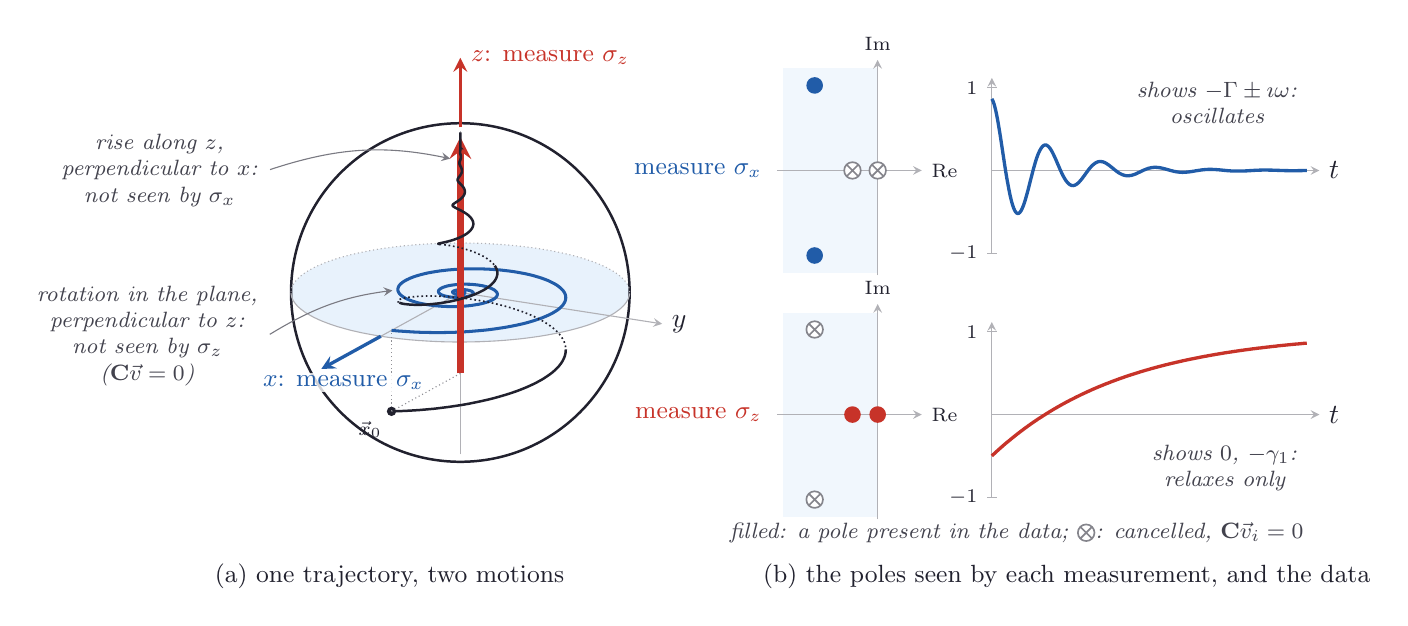
\begin{tikzpicture}[ink/.style={line width=0.9pt, ndInk}, faint/.style={line width=0.4pt, ndInk!35}, dashedink/.style={line width=0.5pt, ndInk!55, dash pattern=on 2.5pt off 2pt}, vec/.style={->, >=stealth, line width=1.2pt}, note/.style={font=\footnotesize\itshape, text=ndInk!85, align=center}, pointer/.style={->, >=stealth, line width=0.4pt, ndInk!60, shorten >=2pt, shorten <=1pt}, dot/.style={circle, fill=ndInk, inner sep=0pt, minimum size=3.4pt}, wash/.style={fill=ndSky, fill opacity=0.55}, every node/.style={text=ndInk}]
\definecolor{ndInk}{rgb}{0.13,0.13,0.18}
\definecolor{ndPaper}{rgb}{0.99,0.96,0.88}
\definecolor{ndSky}{rgb}{0.84,0.91,0.98}
\definecolor{ndRose}{rgb}{0.98,0.86,0.84}
\definecolor{ndBlue}{rgb}{0.13,0.36,0.66}
\definecolor{ndRed}{rgb}{0.78,0.20,0.16}
\definecolor{ndGold}{rgb}{0.88,0.62,0.10}
\definecolor{ndGreen}{rgb}{0.18,0.52,0.30}
\fill[ndSky, fill opacity=0.55] (-1.009,-0.555) -- (-0.934,-0.566) -- (-0.856,-0.577) -- (-0.778,-0.586) -- (-0.698,-0.595) -- (-0.617,-0.602) -- (-0.535,-0.609) -- (-0.453,-0.615) -- (-0.369,-0.619) -- (-0.285,-0.623) -- (-0.201,-0.626) -- (-0.116,-0.628) -- (-0.031,-0.629) -- (0.054,-0.628) -- (0.139,-0.627) -- (0.223,-0.625) -- (0.308,-0.622) -- (0.391,-0.618) -- (0.475,-0.613) -- (0.557,-0.607) -- (0.639,-0.600) -- (0.719,-0.592) -- (0.799,-0.584) -- (0.877,-0.574) -- (0.954,-0.563) -- (1.029,-0.552) -- (1.103,-0.540) -- (1.175,-0.526) -- (1.245,-0.512) -- (1.314,-0.498) -- (1.380,-0.482) -- (1.444,-0.466) -- (1.506,-0.449) -- (1.565,-0.431) -- (1.622,-0.413) -- (1.677,-0.393) -- (1.729,-0.374) -- (1.778,-0.354) -- (1.824,-0.333) -- (1.868,-0.311) -- (1.908,-0.290) -- (1.946,-0.267) -- (1.980,-0.245) -- (2.012,-0.222) -- (2.040,-0.198) -- (2.066,-0.174) -- (2.087,-0.150) -- (2.106,-0.126) -- (2.122,-0.102) -- (2.134,-0.077) -- (2.142,-0.053) -- (2.148,-0.028) -- (2.150,-0.003) -- (2.149,0.022) -- (2.144,0.047) -- (2.136,0.071) -- (2.125,0.096) -- (2.110,0.121) -- (2.092,0.145) -- (2.071,0.169) -- (2.047,0.193) -- (2.019,0.216) -- (1.988,0.239) -- (1.954,0.262) -- (1.917,0.284) -- (1.877,0.306) -- (1.834,0.328) -- (1.789,0.349) -- (1.740,0.369) -- (1.689,0.389) -- (1.635,0.408) -- (1.579,0.427) -- (1.520,0.445) -- (1.459,0.462) -- (1.395,0.478) -- (1.329,0.494) -- (1.261,0.509) -- (1.192,0.523) -- (1.120,0.537) -- (1.047,0.549) -- (0.972,0.561) -- (0.895,0.572) -- (0.817,0.581) -- (0.738,0.590) -- (0.658,0.598) -- (0.576,0.606) -- (0.494,0.612) -- (0.411,0.617) -- (0.327,0.621) -- (0.243,0.625) -- (0.158,0.627) -- (0.074,0.628) -- (-0.011,0.629) -- (-0.096,0.628) -- (-0.181,0.626) -- (-0.266,0.624) -- (-0.350,0.620) -- (-0.433,0.616) -- (-0.516,0.610) -- (-0.598,0.604) -- (-0.679,0.596) -- (-0.759,0.588) -- (-0.838,0.579) -- (-0.916,0.569) -- (-0.992,0.558) -- (-1.066,0.546) -- (-1.139,0.533) -- (-1.210,0.520) -- (-1.280,0.505) -- (-1.347,0.490) -- (-1.412,0.474) -- (-1.475,0.457) -- (-1.536,0.440) -- (-1.594,0.422) -- (-1.650,0.403) -- (-1.703,0.384) -- (-1.753,0.364) -- (-1.801,0.343) -- (-1.846,0.322) -- (-1.888,0.301) -- (-1.927,0.279) -- (-1.964,0.256) -- (-1.997,0.233) -- (-2.027,0.210) -- (-2.053,0.186) -- (-2.077,0.162) -- (-2.097,0.138) -- (-2.114,0.114) -- (-2.128,0.090) -- (-2.139,0.065) -- (-2.146,0.040) -- (-2.149,0.015) -- (-2.150,-0.010) -- (-2.147,-0.034) -- (-2.140,-0.059) -- (-2.131,-0.084) -- (-2.118,-0.108) -- (-2.102,-0.133) -- (-2.082,-0.157) -- (-2.059,-0.181) -- (-2.033,-0.204) -- (-2.004,-0.228) -- (-1.972,-0.251) -- (-1.936,-0.273) -- (-1.898,-0.295) -- (-1.856,-0.317) -- (-1.812,-0.338) -- (-1.765,-0.359) -- (-1.715,-0.379) -- (-1.662,-0.399) -- (-1.607,-0.418) -- (-1.550,-0.436) -- (-1.489,-0.453) -- (-1.427,-0.470) -- (-1.362,-0.486) -- (-1.296,-0.502) -- (-1.227,-0.516) -- (-1.156,-0.530) -- (-1.084,-0.543) -- (-1.009,-0.555) -- cycle;
\draw[ink] (0.000,0.000) circle (2.150);
\draw[faint] (1.898,-0.295) -- (1.924,-0.280) -- (1.949,-0.266) -- (1.972,-0.251) -- (1.993,-0.235) -- (2.014,-0.220) -- (2.033,-0.205) -- (2.050,-0.189) -- (2.067,-0.173) -- (2.082,-0.157) -- (2.095,-0.141) -- (2.107,-0.125) -- (2.117,-0.109) -- (2.126,-0.093) -- (2.134,-0.077) -- (2.140,-0.060) -- (2.145,-0.044) -- (2.148,-0.027) -- (2.150,-0.011);
\draw[faint] (-2.150,-0.005) -- (-2.149,-0.022) -- (-2.146,-0.038) -- (-2.142,-0.055) -- (-2.136,-0.071) -- (-2.129,-0.087) -- (-2.121,-0.104) -- (-2.110,-0.120) -- (-2.099,-0.136) -- (-2.086,-0.152) -- (-2.072,-0.168) -- (-2.056,-0.184) -- (-2.039,-0.199) -- (-2.020,-0.215) -- (-2.000,-0.230) -- (-1.979,-0.246) -- (-1.956,-0.261) -- (-1.932,-0.276) -- (-1.907,-0.290) -- (-1.880,-0.305) -- (-1.853,-0.319) -- (-1.823,-0.333) -- (-1.793,-0.347) -- (-1.761,-0.361) -- (-1.728,-0.374) -- (-1.694,-0.387) -- (-1.659,-0.400) -- (-1.623,-0.412) -- (-1.585,-0.425) -- (-1.547,-0.437) -- (-1.507,-0.448) -- (-1.466,-0.460) -- (-1.425,-0.471) -- (-1.382,-0.482) -- (-1.338,-0.492) -- (-1.294,-0.502) -- (-1.249,-0.512) -- (-1.202,-0.521) -- (-1.155,-0.530) -- (-1.107,-0.539) -- (-1.059,-0.547) -- (-1.009,-0.555) -- (-0.959,-0.563) -- (-0.909,-0.570) -- (-0.857,-0.576) -- (-0.805,-0.583) -- (-0.753,-0.589) -- (-0.700,-0.594) -- (-0.647,-0.600) -- (-0.593,-0.604) -- (-0.538,-0.609) -- (-0.484,-0.612) -- (-0.429,-0.616) -- (-0.373,-0.619) -- (-0.318,-0.622) -- (-0.262,-0.624) -- (-0.206,-0.626) -- (-0.150,-0.627) -- (-0.094,-0.628) -- (-0.038,-0.629) -- (0.019,-0.629) -- (0.075,-0.628) -- (0.131,-0.627) -- (0.187,-0.626) -- (0.243,-0.625) -- (0.299,-0.622) -- (0.355,-0.620) -- (0.410,-0.617) -- (0.465,-0.614) -- (0.520,-0.610) -- (0.575,-0.606) -- (0.629,-0.601) -- (0.682,-0.596) -- (0.735,-0.591) -- (0.788,-0.585) -- (0.840,-0.579) -- (0.892,-0.572) -- (0.942,-0.565) -- (0.993,-0.558) -- (1.042,-0.550) -- (1.091,-0.542) -- (1.139,-0.533) -- (1.187,-0.524) -- (1.233,-0.515) -- (1.279,-0.505) -- (1.324,-0.495) -- (1.368,-0.485) -- (1.411,-0.474) -- (1.453,-0.463) -- (1.494,-0.452) -- (1.533,-0.441) -- (1.572,-0.429) -- (1.610,-0.417) -- (1.647,-0.404) -- (1.683,-0.391) -- (1.717,-0.378) -- (1.750,-0.365) -- (1.782,-0.352) -- (1.813,-0.338) -- (1.843,-0.324) -- (1.871,-0.310) -- (1.898,-0.295);
\draw[faint, densely dotted] (2.150,0.005) -- (2.149,0.022) -- (2.146,0.038) -- (2.142,0.055) -- (2.136,0.071) -- (2.129,0.087) -- (2.121,0.104) -- (2.110,0.120) -- (2.099,0.136) -- (2.086,0.152) -- (2.072,0.168) -- (2.056,0.184) -- (2.039,0.199) -- (2.020,0.215) -- (2.000,0.230) -- (1.979,0.246) -- (1.956,0.261) -- (1.932,0.276) -- (1.907,0.290) -- (1.880,0.305) -- (1.853,0.319) -- (1.823,0.333) -- (1.793,0.347) -- (1.761,0.361) -- (1.728,0.374) -- (1.694,0.387) -- (1.659,0.400) -- (1.623,0.412) -- (1.585,0.425) -- (1.547,0.437) -- (1.507,0.448) -- (1.466,0.460) -- (1.425,0.471) -- (1.382,0.482) -- (1.338,0.492) -- (1.294,0.502) -- (1.249,0.512) -- (1.202,0.521) -- (1.155,0.530) -- (1.107,0.539) -- (1.059,0.547) -- (1.009,0.555) -- (0.959,0.563) -- (0.909,0.570) -- (0.857,0.576) -- (0.805,0.583) -- (0.753,0.589) -- (0.700,0.594) -- (0.647,0.600) -- (0.593,0.604) -- (0.538,0.609) -- (0.484,0.612) -- (0.429,0.616) -- (0.373,0.619) -- (0.318,0.622) -- (0.262,0.624) -- (0.206,0.626) -- (0.150,0.627) -- (0.094,0.628) -- (0.038,0.629) -- (-0.019,0.629) -- (-0.075,0.628) -- (-0.131,0.627) -- (-0.187,0.626) -- (-0.243,0.625) -- (-0.299,0.622) -- (-0.355,0.620) -- (-0.410,0.617) -- (-0.465,0.614) -- (-0.520,0.610) -- (-0.575,0.606) -- (-0.629,0.601) -- (-0.682,0.596) -- (-0.735,0.591) -- (-0.788,0.585) -- (-0.840,0.579) -- (-0.892,0.572) -- (-0.942,0.565) -- (-0.993,0.558) -- (-1.042,0.550) -- (-1.091,0.542) -- (-1.139,0.533) -- (-1.187,0.524) -- (-1.233,0.515) -- (-1.279,0.505) -- (-1.324,0.495) -- (-1.368,0.485) -- (-1.411,0.474) -- (-1.453,0.463) -- (-1.494,0.452) -- (-1.533,0.441) -- (-1.572,0.429) -- (-1.610,0.417) -- (-1.647,0.404) -- (-1.683,0.391) -- (-1.717,0.378) -- (-1.750,0.365) -- (-1.782,0.352) -- (-1.813,0.338) -- (-1.843,0.324) -- (-1.871,0.310) -- (-1.898,0.295) -- (-1.924,0.280) -- (-1.949,0.266) -- (-1.972,0.251) -- (-1.993,0.235) -- (-2.014,0.220) -- (-2.033,0.205) -- (-2.050,0.189) -- (-2.067,0.173) -- (-2.082,0.157) -- (-2.095,0.141) -- (-2.107,0.125) -- (-2.117,0.109) -- (-2.126,0.093) -- (-2.134,0.077) -- (-2.140,0.060) -- (-2.145,0.044) -- (-2.148,0.027) -- (-2.150,0.011);
\draw[faint] (0.000,0.000) -- (-1.009,-0.555);
\draw[faint, ->, >=stealth] (0.000,0.000) -- (2.563,-0.398) node[right, text=ndInk] {$y$};
\draw[faint] (0.000,-2.056) -- (0.000,2.056);
\draw[line width=1.1pt, ndBlue] (-0.874,-0.481) -- (-0.784,-0.489) -- (-0.694,-0.495) -- (-0.603,-0.501) -- (-0.512,-0.505) -- (-0.422,-0.507) -- (-0.332,-0.509) -- (-0.242,-0.509) -- (-0.154,-0.507) -- (-0.066,-0.505) -- (0.020,-0.501) -- (0.105,-0.496) -- (0.188,-0.489) -- (0.269,-0.482) -- (0.348,-0.474) -- (0.425,-0.464) -- (0.500,-0.453) -- (0.572,-0.442) -- (0.642,-0.429) -- (0.708,-0.416) -- (0.772,-0.402) -- (0.833,-0.387) -- (0.890,-0.371) -- (0.945,-0.354) -- (0.996,-0.337) -- (1.044,-0.320) -- (1.088,-0.301) -- (1.129,-0.283) -- (1.166,-0.264) -- (1.200,-0.244) -- (1.230,-0.225) -- (1.256,-0.205) -- (1.279,-0.184) -- (1.298,-0.164) -- (1.313,-0.144) -- (1.325,-0.123) -- (1.333,-0.103) -- (1.338,-0.083) -- (1.339,-0.062) -- (1.337,-0.042) -- (1.332,-0.023) -- (1.323,-0.003) -- (1.311,0.016) -- (1.295,0.035) -- (1.277,0.053) -- (1.256,0.071) -- (1.232,0.089) -- (1.205,0.106) -- (1.175,0.122) -- (1.143,0.138) -- (1.109,0.154) -- (1.072,0.168) -- (1.034,0.182) -- (0.993,0.195) -- (0.950,0.208) -- (0.906,0.220) -- (0.860,0.231) -- (0.813,0.241) -- (0.764,0.250) -- (0.714,0.259) -- (0.664,0.267) -- (0.612,0.274) -- (0.560,0.280) -- (0.507,0.286) -- (0.453,0.290) -- (0.400,0.294) -- (0.346,0.297) -- (0.292,0.299) -- (0.239,0.301) -- (0.185,0.301) -- (0.133,0.301) -- (0.080,0.300) -- (0.028,0.299) -- (-0.022,0.296) -- (-0.072,0.293) -- (-0.121,0.289) -- (-0.169,0.285) -- (-0.216,0.279) -- (-0.261,0.274) -- (-0.305,0.267) -- (-0.348,0.260) -- (-0.388,0.253) -- (-0.428,0.245) -- (-0.465,0.236) -- (-0.501,0.227) -- (-0.534,0.218) -- (-0.566,0.208) -- (-0.596,0.198) -- (-0.624,0.187) -- (-0.650,0.176) -- (-0.673,0.165) -- (-0.695,0.154) -- (-0.715,0.142) -- (-0.732,0.131) -- (-0.747,0.119) -- (-0.760,0.107) -- (-0.771,0.095) -- (-0.780,0.083) -- (-0.786,0.071) -- (-0.791,0.058) -- (-0.793,0.046) -- (-0.793,0.035) -- (-0.792,0.023) -- (-0.788,0.011) -- (-0.782,-0.001) -- (-0.775,-0.012) -- (-0.765,-0.023) -- (-0.754,-0.034) -- (-0.741,-0.044) -- (-0.726,-0.055) -- (-0.710,-0.065) -- (-0.692,-0.075) -- (-0.673,-0.084) -- (-0.653,-0.093) -- (-0.631,-0.101) -- (-0.607,-0.110) -- (-0.583,-0.117) -- (-0.558,-0.125) -- (-0.531,-0.132) -- (-0.504,-0.138) -- (-0.475,-0.144) -- (-0.447,-0.149) -- (-0.417,-0.155) -- (-0.387,-0.159) -- (-0.356,-0.163) -- (-0.325,-0.167) -- (-0.294,-0.170) -- (-0.262,-0.173) -- (-0.230,-0.175) -- (-0.198,-0.176) -- (-0.166,-0.178) -- (-0.135,-0.178) -- (-0.103,-0.179) -- (-0.072,-0.178) -- (-0.041,-0.178) -- (-0.010,-0.177) -- (0.020,-0.175) -- (0.049,-0.173) -- (0.078,-0.171) -- (0.106,-0.168) -- (0.134,-0.165) -- (0.160,-0.161) -- (0.186,-0.157) -- (0.211,-0.153) -- (0.235,-0.149) -- (0.258,-0.144) -- (0.280,-0.139) -- (0.301,-0.133) -- (0.321,-0.128) -- (0.339,-0.122) -- (0.357,-0.116) -- (0.373,-0.110) -- (0.388,-0.103) -- (0.402,-0.096) -- (0.414,-0.090) -- (0.426,-0.083) -- (0.436,-0.076) -- (0.444,-0.069) -- (0.452,-0.062) -- (0.458,-0.055) -- (0.463,-0.047) -- (0.466,-0.040) -- (0.469,-0.033) -- (0.470,-0.026) -- (0.470,-0.019) -- (0.469,-0.012) -- (0.466,-0.005) -- (0.463,0.002) -- (0.458,0.008) -- (0.452,0.015) -- (0.445,0.021) -- (0.437,0.028) -- (0.428,0.034) -- (0.419,0.040) -- (0.408,0.045) -- (0.396,0.051) -- (0.384,0.056) -- (0.371,0.061) -- (0.357,0.066) -- (0.342,0.070) -- (0.327,0.075) -- (0.311,0.079) -- (0.295,0.083) -- (0.278,0.086) -- (0.261,0.089) -- (0.243,0.092) -- (0.225,0.095) -- (0.207,0.097) -- (0.189,0.099) -- (0.170,0.101) -- (0.151,0.103) -- (0.132,0.104) -- (0.114,0.105) -- (0.095,0.105) -- (0.076,0.106) -- (0.057,0.106) -- (0.039,0.106) -- (0.020,0.105) -- (0.002,0.104) -- (-0.015,0.103) -- (-0.033,0.102) -- (-0.050,0.101) -- (-0.066,0.099) -- (-0.083,0.097) -- (-0.098,0.095) -- (-0.113,0.093) -- (-0.128,0.090) -- (-0.142,0.088) -- (-0.156,0.085) -- (-0.169,0.082) -- (-0.181,0.078) -- (-0.192,0.075) -- (-0.203,0.071) -- (-0.213,0.068) -- (-0.223,0.064) -- (-0.232,0.060) -- (-0.240,0.056) -- (-0.247,0.052) -- (-0.253,0.048) -- (-0.259,0.044) -- (-0.264,0.040) -- (-0.268,0.036) -- (-0.272,0.031) -- (-0.275,0.027) -- (-0.277,0.023) -- (-0.278,0.019) -- (-0.278,0.015) -- (-0.278,0.010) -- (-0.277,0.006) -- (-0.276,0.002) -- (-0.273,-0.002) -- (-0.271,-0.006) -- (-0.267,-0.010) -- (-0.263,-0.013) -- (-0.258,-0.017) -- (-0.253,-0.021) -- (-0.247,-0.024) -- (-0.240,-0.028) -- (-0.233,-0.031) -- (-0.226,-0.034) -- (-0.218,-0.037) -- (-0.210,-0.040) -- (-0.201,-0.042) -- (-0.192,-0.045) -- (-0.182,-0.047) -- (-0.173,-0.049) -- (-0.163,-0.051) -- (-0.152,-0.053) -- (-0.142,-0.055) -- (-0.131,-0.056) -- (-0.120,-0.058) -- (-0.109,-0.059) -- (-0.098,-0.060) -- (-0.087,-0.061) -- (-0.076,-0.062) -- (-0.065,-0.062) -- (-0.054,-0.062) -- (-0.043,-0.063) -- (-0.032,-0.063) -- (-0.021,-0.063) -- (-0.010,-0.062) -- (0.001,-0.062) -- (0.011,-0.061) -- (0.022,-0.060) -- (0.032,-0.060) -- (0.041,-0.058) -- (0.051,-0.057) -- (0.060,-0.056) -- (0.069,-0.055) -- (0.078,-0.053) -- (0.086,-0.051) -- (0.094,-0.050) -- (0.101,-0.048) -- (0.109,-0.046) -- (0.115,-0.044) -- (0.122,-0.042) -- (0.128,-0.040) -- (0.133,-0.037) -- (0.138,-0.035) -- (0.143,-0.033) -- (0.147,-0.030) -- (0.151,-0.028) -- (0.154,-0.026) -- (0.157,-0.023) -- (0.159,-0.021) -- (0.161,-0.018) -- (0.163,-0.016) -- (0.164,-0.013) -- (0.165,-0.011) -- (0.165,-0.008) -- (0.165,-0.006) -- (0.164,-0.003) -- (0.163,-0.001) -- (0.162,0.002) -- (0.160,0.004) -- (0.158,0.006) -- (0.155,0.008) -- (0.152,0.011) -- (0.149,0.013) -- (0.145,0.015) -- (0.141,0.017) -- (0.137,0.019) -- (0.133,0.020) -- (0.128,0.022) -- (0.123,0.024) -- (0.118,0.025) -- (0.112,0.027) -- (0.107,0.028) -- (0.101,0.029) -- (0.095,0.031) -- (0.089,0.032) -- (0.083,0.033) -- (0.076,0.034) -- (0.070,0.034) -- (0.063,0.035) -- (0.057,0.036) -- (0.050,0.036) -- (0.044,0.037) -- (0.037,0.037) -- (0.030,0.037) -- (0.024,0.037) -- (0.017,0.037) -- (0.011,0.037) -- (0.005,0.037) -- (-0.002,0.037) -- (-0.008,0.036) -- (-0.014,0.036) -- (-0.020,0.035) -- (-0.026,0.035) -- (-0.031,0.034) -- (-0.037,0.033) -- (-0.042,0.032) -- (-0.047,0.031) -- (-0.052,0.030) -- (-0.057,0.029) -- (-0.061,0.028) -- (-0.065,0.027) -- (-0.069,0.026) -- (-0.073,0.025) -- (-0.076,0.023) -- (-0.080,0.022) -- (-0.082,0.021) -- (-0.085,0.019) -- (-0.088,0.018) -- (-0.090,0.016) -- (-0.092,0.015) -- (-0.093,0.013) -- (-0.095,0.012) -- (-0.096,0.010) -- (-0.097,0.009) -- (-0.097,0.007) -- (-0.098,0.006) -- (-0.098,0.004) -- (-0.098,0.003) -- (-0.097,0.002) -- (-0.096,0.000) -- (-0.096,-0.001) -- (-0.094,-0.003) -- (-0.093,-0.004) -- (-0.092,-0.005) -- (-0.090,-0.007) -- (-0.088,-0.008) -- (-0.086,-0.009) -- (-0.083,-0.010) -- (-0.081,-0.011) -- (-0.078,-0.012) -- (-0.075,-0.013) -- (-0.072,-0.014) -- (-0.069,-0.015) -- (-0.066,-0.016) -- (-0.063,-0.017) -- (-0.059,-0.018) -- (-0.056,-0.018) -- (-0.052,-0.019) -- (-0.048,-0.020) -- (-0.044,-0.020) -- (-0.041,-0.020) -- (-0.037,-0.021) -- (-0.033,-0.021) -- (-0.029,-0.021) -- (-0.025,-0.022) -- (-0.021,-0.022) -- (-0.017,-0.022) -- (-0.013,-0.022) -- (-0.009,-0.022) -- (-0.006,-0.022) -- (-0.002,-0.022) -- (0.002,-0.022) -- (0.005,-0.021) -- (0.009,-0.021) -- (0.013,-0.021) -- (0.016,-0.020) -- (0.019,-0.020) -- (0.022,-0.019) -- (0.026,-0.019) -- (0.028,-0.018) -- (0.031,-0.018) -- (0.034,-0.017) -- (0.037,-0.017) -- (0.039,-0.016) -- (0.041,-0.015) -- (0.044,-0.014) -- (0.046,-0.014) -- (0.047,-0.013) -- (0.049,-0.012) -- (0.051,-0.011) -- (0.052,-0.010) -- (0.053,-0.009) -- (0.055,-0.009) -- (0.055,-0.008) -- (0.056,-0.007) -- (0.057,-0.006) -- (0.057,-0.005) -- (0.058,-0.004) -- (0.058,-0.003) -- (0.058,-0.002) -- (0.058,-0.002) -- (0.057,-0.001) -- (0.057,0.000) -- (0.056,0.001) -- (0.056,0.002) -- (0.055,0.003) -- (0.054,0.003) -- (0.053,0.004) -- (0.052,0.005) -- (0.050,0.005) -- (0.049,0.006) -- (0.048,0.007) -- (0.046,0.007) -- (0.044,0.008) -- (0.042,0.009) -- (0.041,0.009) -- (0.039,0.010) -- (0.037,0.010) -- (0.035,0.011) -- (0.032,0.011) -- (0.030,0.011) -- (0.028,0.012) -- (0.026,0.012) -- (0.024,0.012) -- (0.021,0.012) -- (0.019,0.013) -- (0.017,0.013) -- (0.014,0.013) -- (0.012,0.013) -- (0.010,0.013) -- (0.007,0.013) -- (0.005,0.013) -- (0.003,0.013) -- (0.001,0.013) -- (-0.002,0.013) -- (-0.004,0.013) -- (-0.006,0.012) -- (-0.008,0.012) -- (-0.010,0.012) -- (-0.012,0.012) -- (-0.014,0.011) -- (-0.015,0.011) -- (-0.017,0.011) -- (-0.019,0.010) -- (-0.021,0.010) -- (-0.022,0.010) -- (-0.023,0.009) -- (-0.025,0.009) -- (-0.026,0.008) -- (-0.027,0.008) -- (-0.028,0.007) -- (-0.029,0.007) -- (-0.030,0.007) -- (-0.031,0.006) -- (-0.032,0.006) -- (-0.032,0.005) -- (-0.033,0.004) -- (-0.033,0.004) -- (-0.034,0.003) -- (-0.034,0.003) -- (-0.034,0.002) -- (-0.034,0.002) -- (-0.034,0.001) -- (-0.034,0.001) -- (-0.034,0.000) -- (-0.034,-0.000) -- (-0.033,-0.001) -- (-0.033,-0.001) -- (-0.032,-0.002) -- (-0.032,-0.002) -- (-0.031,-0.002) -- (-0.030,-0.003) -- (-0.030,-0.003) -- (-0.029,-0.004) -- (-0.028,-0.004) -- (-0.027,-0.004) -- (-0.026,-0.005) -- (-0.025,-0.005) -- (-0.024,-0.005) -- (-0.023,-0.006) -- (-0.021,-0.006) -- (-0.020,-0.006) -- (-0.019,-0.007) -- (-0.018,-0.007) -- (-0.016,-0.007) -- (-0.015,-0.007) -- (-0.014,-0.007) -- (-0.012,-0.007) -- (-0.011,-0.007) -- (-0.010,-0.008) -- (-0.008,-0.008) -- (-0.007,-0.008) -- (-0.005,-0.008) -- (-0.004,-0.008) -- (-0.003,-0.008) -- (-0.001,-0.008) -- (-0.000,-0.008) -- (0.001,-0.008) -- (0.002,-0.007) -- (0.004,-0.007) -- (0.005,-0.007) -- (0.006,-0.007) -- (0.007,-0.007) -- (0.008,-0.007) -- (0.009,-0.007) -- (0.010,-0.006) -- (0.011,-0.006) -- (0.012,-0.006) -- (0.013,-0.006) -- (0.014,-0.005) -- (0.015,-0.005) -- (0.016,-0.005) -- (0.016,-0.005) -- (0.017,-0.004) -- (0.018,-0.004) -- (0.018,-0.004) -- (0.019,-0.004) -- (0.019,-0.003) -- (0.019,-0.003) -- (0.020,-0.003) -- (0.020,-0.002) -- (0.020,-0.002) -- (0.020,-0.002) -- (0.020,-0.001) -- (0.020,-0.001) -- (0.020,-0.001) -- (0.020,-0.000) -- (0.020,-0.000) -- (0.020,0.000) -- (0.020,0.000) -- (0.019,0.001) -- (0.019,0.001) -- (0.019,0.001) -- (0.018,0.002) -- (0.018,0.002) -- (0.017,0.002) -- (0.017,0.002) -- (0.016,0.002) -- (0.016,0.003) -- (0.015,0.003) -- (0.015,0.003) -- (0.014,0.003) -- (0.013,0.003) -- (0.013,0.004) -- (0.012,0.004) -- (0.011,0.004) -- (0.010,0.004) -- (0.010,0.004) -- (0.009,0.004) -- (0.008,0.004) -- (0.007,0.004) -- (0.006,0.004) -- (0.006,0.004) -- (0.005,0.005) -- (0.004,0.005) -- (0.003,0.005) -- (0.002,0.005) -- (0.001,0.005) -- (0.001,0.005) -- (-0.000,0.005) -- (-0.001,0.004) -- (-0.002,0.004) -- (-0.002,0.004) -- (-0.003,0.004) -- (-0.004,0.004) -- (-0.004,0.004) -- (-0.005,0.004) -- (-0.006,0.004) -- (-0.006,0.004) -- (-0.007,0.004) -- (-0.007,0.003) -- (-0.008,0.003) -- (-0.008,0.003) -- (-0.009,0.003) -- (-0.009,0.003) -- (-0.010,0.003) -- (-0.010,0.003) -- (-0.010,0.002) -- (-0.011,0.002) -- (-0.011,0.002) -- (-0.011,0.002) -- (-0.011,0.002) -- (-0.012,0.001) -- (-0.012,0.001) -- (-0.012,0.001) -- (-0.012,0.001) -- (-0.012,0.001) -- (-0.012,0.001) -- (-0.012,0.000) -- (-0.012,0.000) -- (-0.012,0.000) -- (-0.012,-0.000) -- (-0.012,-0.000) -- (-0.011,-0.000) -- (-0.011,-0.001) -- (-0.011,-0.001) -- (-0.011,-0.001) -- (-0.011,-0.001) -- (-0.010,-0.001) -- (-0.010,-0.001) -- (-0.010,-0.001) -- (-0.009,-0.002) -- (-0.009,-0.002) -- (-0.009,-0.002) -- (-0.008,-0.002) -- (-0.008,-0.002) -- (-0.007,-0.002) -- (-0.007,-0.002) -- (-0.006,-0.002) -- (-0.006,-0.002) -- (-0.006,-0.002) -- (-0.005,-0.003) -- (-0.005,-0.003) -- (-0.004,-0.003) -- (-0.004,-0.003) -- (-0.003,-0.003) -- (-0.003,-0.003) -- (-0.002,-0.003) -- (-0.002,-0.003) -- (-0.001,-0.003) -- (-0.001,-0.003) -- (-0.000,-0.003) -- (0.000,-0.003) -- (0.001,-0.003) -- (0.001,-0.003) -- (0.001,-0.003) -- (0.002,-0.003) -- (0.002,-0.002) -- (0.003,-0.002) -- (0.003,-0.002) -- (0.003,-0.002) -- (0.004,-0.002) -- (0.004,-0.002) -- (0.004,-0.002) -- (0.005,-0.002) -- (0.005,-0.002) -- (0.005,-0.002) -- (0.006,-0.002) -- (0.006,-0.002) -- (0.006,-0.001) -- (0.006,-0.001) -- (0.006,-0.001) -- (0.007,-0.001) -- (0.007,-0.001) -- (0.007,-0.001) -- (0.007,-0.001) -- (0.007,-0.001) -- (0.007,-0.001) -- (0.007,-0.001) -- (0.007,-0.000) -- (0.007,-0.000) -- (0.007,-0.000) -- (0.007,-0.000) -- (0.007,-0.000) -- (0.007,0.000) -- (0.007,0.000) -- (0.007,0.000) -- (0.007,0.000) -- (0.007,0.000) -- (0.006,0.001) -- (0.006,0.001) -- (0.006,0.001) -- (0.006,0.001) -- (0.006,0.001) -- (0.005,0.001) -- (0.005,0.001) -- (0.005,0.001) -- (0.005,0.001) -- (0.005,0.001) -- (0.004,0.001) -- (0.004,0.001) -- (0.004,0.001) -- (0.004,0.001) -- (0.003,0.001) -- (0.003,0.001) -- (0.003,0.002) -- (0.002,0.002) -- (0.002,0.002) -- (0.002,0.002) -- (0.002,0.002) -- (0.001,0.002) -- (0.001,0.002) -- (0.001,0.002) -- (0.000,0.002);
\draw[line width=2.4pt, ndRed, ->, >=stealth] (0.000,-1.028) -- (0.000,1.974);
\draw[line width=0.9pt, ndInk] (-0.874,-1.509) -- (-0.784,-1.507) -- (-0.694,-1.503) -- (-0.603,-1.498) -- (-0.512,-1.492) -- (-0.422,-1.484) -- (-0.332,-1.476) -- (-0.242,-1.465) -- (-0.154,-1.454) -- (-0.066,-1.441) -- (0.020,-1.428) -- (0.105,-1.413) -- (0.188,-1.396) -- (0.269,-1.379) -- (0.348,-1.361) -- (0.425,-1.342) -- (0.500,-1.321) -- (0.572,-1.300) -- (0.642,-1.278) -- (0.708,-1.255) -- (0.772,-1.231) -- (0.833,-1.206) -- (0.890,-1.181) -- (0.945,-1.155) -- (0.996,-1.128) -- (1.044,-1.101) -- (1.088,-1.073) -- (1.129,-1.045) -- (1.166,-1.017) -- (1.200,-0.988) -- (1.230,-0.959) -- (1.256,-0.930) -- (1.279,-0.900) -- (1.298,-0.871) -- (1.313,-0.841) -- (1.325,-0.812) -- (1.333,-0.782) -- (1.338,-0.753) -- (1.339,-0.723);
\draw[line width=0.9pt, ndInk] (-0.775,-0.129) -- (-0.765,-0.133) -- (-0.754,-0.136) -- (-0.741,-0.140) -- (-0.726,-0.143) -- (-0.710,-0.146) -- (-0.692,-0.148) -- (-0.673,-0.150) -- (-0.653,-0.152) -- (-0.631,-0.154) -- (-0.607,-0.155) -- (-0.583,-0.156) -- (-0.558,-0.156) -- (-0.531,-0.156) -- (-0.504,-0.156) -- (-0.475,-0.155) -- (-0.447,-0.153) -- (-0.417,-0.152) -- (-0.387,-0.149) -- (-0.356,-0.147) -- (-0.325,-0.143) -- (-0.294,-0.140) -- (-0.262,-0.136) -- (-0.230,-0.131) -- (-0.198,-0.126) -- (-0.166,-0.120) -- (-0.135,-0.115) -- (-0.103,-0.108) -- (-0.072,-0.101) -- (-0.041,-0.094) -- (-0.010,-0.086) -- (0.020,-0.078) -- (0.049,-0.070) -- (0.078,-0.061) -- (0.106,-0.052) -- (0.134,-0.042) -- (0.160,-0.032) -- (0.186,-0.022) -- (0.211,-0.011) -- (0.235,-0.000) -- (0.258,0.011) -- (0.280,0.022) -- (0.301,0.034) -- (0.321,0.046) -- (0.339,0.058) -- (0.357,0.070) -- (0.373,0.083) -- (0.388,0.095) -- (0.402,0.108) -- (0.414,0.121) -- (0.426,0.134) -- (0.436,0.147) -- (0.444,0.160) -- (0.452,0.174) -- (0.458,0.187) -- (0.463,0.200) -- (0.466,0.213) -- (0.469,0.226) -- (0.470,0.239) -- (0.470,0.252) -- (0.469,0.265) -- (0.466,0.278) -- (0.463,0.291) -- (0.458,0.303) -- (0.452,0.316) -- (0.445,0.328) -- (0.437,0.340);
\draw[line width=0.9pt, ndInk] (-0.247,0.613) -- (-0.253,0.614) -- (-0.259,0.615) -- (-0.264,0.615) -- (-0.268,0.616) -- (-0.272,0.617) -- (-0.275,0.617) -- (-0.277,0.618) -- (-0.278,0.619) -- (-0.278,0.619) -- (-0.278,0.620) -- (-0.277,0.621) -- (-0.276,0.621) -- (-0.273,0.622) -- (-0.271,0.623) -- (-0.267,0.624) -- (-0.263,0.625) -- (-0.258,0.626) -- (-0.253,0.627) -- (-0.247,0.628) -- (-0.240,0.630) -- (-0.233,0.631) -- (-0.226,0.633) -- (-0.218,0.634) -- (-0.210,0.636) -- (-0.201,0.638) -- (-0.192,0.640) -- (-0.182,0.642) -- (-0.173,0.645) -- (-0.163,0.647) -- (-0.152,0.650) -- (-0.142,0.653) -- (-0.131,0.656) -- (-0.120,0.659) -- (-0.109,0.662) -- (-0.098,0.665) -- (-0.087,0.669) -- (-0.076,0.673) -- (-0.065,0.677) -- (-0.054,0.681) -- (-0.043,0.685) -- (-0.032,0.689) -- (-0.021,0.694) -- (-0.010,0.698) -- (0.001,0.703) -- (0.011,0.708) -- (0.022,0.713) -- (0.032,0.718) -- (0.041,0.723) -- (0.051,0.729) -- (0.060,0.734) -- (0.069,0.740) -- (0.078,0.746) -- (0.086,0.751) -- (0.094,0.757) -- (0.101,0.763) -- (0.109,0.769) -- (0.115,0.776) -- (0.122,0.782) -- (0.128,0.788) -- (0.133,0.794) -- (0.138,0.801) -- (0.143,0.807) -- (0.147,0.814) -- (0.151,0.820) -- (0.154,0.826) -- (0.157,0.833) -- (0.159,0.839) -- (0.161,0.846) -- (0.163,0.852) -- (0.164,0.859) -- (0.165,0.865) -- (0.165,0.872) -- (0.165,0.878) -- (0.164,0.885) -- (0.163,0.891) -- (0.162,0.897) -- (0.160,0.903) -- (0.158,0.909) -- (0.155,0.915) -- (0.152,0.921) -- (0.149,0.927) -- (0.145,0.933) -- (0.141,0.939) -- (0.137,0.945) -- (0.133,0.950) -- (0.128,0.956) -- (0.123,0.961) -- (0.118,0.966) -- (0.112,0.972) -- (0.107,0.977) -- (0.101,0.982) -- (0.095,0.986) -- (0.089,0.991) -- (0.083,0.996) -- (0.076,1.000) -- (0.070,1.005) -- (0.063,1.009) -- (0.057,1.013) -- (0.050,1.017) -- (0.044,1.021) -- (0.037,1.025) -- (0.030,1.029) -- (0.024,1.033) -- (0.017,1.036) -- (0.011,1.039) -- (0.005,1.043) -- (-0.002,1.046) -- (-0.008,1.049) -- (-0.014,1.052) -- (-0.020,1.055) -- (-0.026,1.058) -- (-0.031,1.061) -- (-0.037,1.063) -- (-0.042,1.066) -- (-0.047,1.068) -- (-0.052,1.071) -- (-0.057,1.073) -- (-0.061,1.075) -- (-0.065,1.078) -- (-0.069,1.080) -- (-0.073,1.082) -- (-0.076,1.084) -- (-0.080,1.086) -- (-0.082,1.088) -- (-0.085,1.090) -- (-0.088,1.091) -- (-0.090,1.093) -- (-0.092,1.095) -- (-0.093,1.097) -- (-0.095,1.099) -- (-0.096,1.100) -- (-0.097,1.102) -- (-0.097,1.104) -- (-0.098,1.106) -- (-0.098,1.107) -- (-0.098,1.109) -- (-0.097,1.111) -- (-0.096,1.112) -- (-0.096,1.114) -- (-0.094,1.116) -- (-0.093,1.118) -- (-0.092,1.120) -- (-0.090,1.121) -- (-0.088,1.123) -- (-0.086,1.125) -- (-0.083,1.127) -- (-0.081,1.129) -- (-0.078,1.131) -- (-0.075,1.133) -- (-0.072,1.135) -- (-0.069,1.137) -- (-0.066,1.139) -- (-0.063,1.141) -- (-0.059,1.144) -- (-0.056,1.146) -- (-0.052,1.148) -- (-0.048,1.151) -- (-0.044,1.153) -- (-0.041,1.156) -- (-0.037,1.158) -- (-0.033,1.161) -- (-0.029,1.163) -- (-0.025,1.166) -- (-0.021,1.169) -- (-0.017,1.172) -- (-0.013,1.174) -- (-0.009,1.177) -- (-0.006,1.180) -- (-0.002,1.183) -- (0.002,1.186) -- (0.005,1.189) -- (0.009,1.192) -- (0.013,1.196) -- (0.016,1.199) -- (0.019,1.202) -- (0.022,1.205) -- (0.026,1.208) -- (0.028,1.212) -- (0.031,1.215) -- (0.034,1.218) -- (0.037,1.222) -- (0.039,1.225) -- (0.041,1.229) -- (0.044,1.232) -- (0.046,1.236) -- (0.047,1.239) -- (0.049,1.243) -- (0.051,1.246) -- (0.052,1.250) -- (0.053,1.253) -- (0.055,1.257) -- (0.055,1.260) -- (0.056,1.264) -- (0.057,1.267) -- (0.057,1.271) -- (0.058,1.274) -- (0.058,1.278) -- (0.058,1.281) -- (0.058,1.284) -- (0.057,1.288) -- (0.057,1.291) -- (0.056,1.295) -- (0.056,1.298) -- (0.055,1.301) -- (0.054,1.305) -- (0.053,1.308) -- (0.052,1.311) -- (0.050,1.314) -- (0.049,1.317) -- (0.048,1.321) -- (0.046,1.324) -- (0.044,1.327) -- (0.042,1.330) -- (0.041,1.333) -- (0.039,1.336) -- (0.037,1.339) -- (0.035,1.341) -- (0.032,1.344) -- (0.030,1.347) -- (0.028,1.350) -- (0.026,1.352) -- (0.024,1.355) -- (0.021,1.358) -- (0.019,1.360) -- (0.017,1.363) -- (0.014,1.365) -- (0.012,1.368) -- (0.010,1.370) -- (0.007,1.372) -- (0.005,1.375) -- (0.003,1.377) -- (0.001,1.379) -- (-0.002,1.381) -- (-0.004,1.383) -- (-0.006,1.386) -- (-0.008,1.388) -- (-0.010,1.390) -- (-0.012,1.392) -- (-0.014,1.394) -- (-0.015,1.396) -- (-0.017,1.398) -- (-0.019,1.399) -- (-0.021,1.401) -- (-0.022,1.403) -- (-0.023,1.405) -- (-0.025,1.407) -- (-0.026,1.408) -- (-0.027,1.410) -- (-0.028,1.412) -- (-0.029,1.414) -- (-0.030,1.415) -- (-0.031,1.417) -- (-0.032,1.418) -- (-0.032,1.420) -- (-0.033,1.422) -- (-0.033,1.423) -- (-0.034,1.425) -- (-0.034,1.427) -- (-0.034,1.428) -- (-0.034,1.430) -- (-0.034,1.431) -- (-0.034,1.433) -- (-0.034,1.434) -- (-0.034,1.436) -- (-0.033,1.438) -- (-0.033,1.439) -- (-0.032,1.441) -- (-0.032,1.442) -- (-0.031,1.444) -- (-0.030,1.445) -- (-0.030,1.447) -- (-0.029,1.449) -- (-0.028,1.450) -- (-0.027,1.452) -- (-0.026,1.454) -- (-0.025,1.455) -- (-0.024,1.457) -- (-0.023,1.459) -- (-0.021,1.460) -- (-0.020,1.462) -- (-0.019,1.464) -- (-0.018,1.466) -- (-0.016,1.467) -- (-0.015,1.469) -- (-0.014,1.471) -- (-0.012,1.473) -- (-0.011,1.474) -- (-0.010,1.476) -- (-0.008,1.478) -- (-0.007,1.480) -- (-0.005,1.482) -- (-0.004,1.484) -- (-0.003,1.486) -- (-0.001,1.487) -- (-0.000,1.489) -- (0.001,1.491) -- (0.002,1.493) -- (0.004,1.495) -- (0.005,1.497) -- (0.006,1.499) -- (0.007,1.501) -- (0.008,1.503) -- (0.009,1.505) -- (0.010,1.507) -- (0.011,1.509) -- (0.012,1.511) -- (0.013,1.513) -- (0.014,1.515) -- (0.015,1.517) -- (0.016,1.519) -- (0.016,1.521) -- (0.017,1.523) -- (0.018,1.526) -- (0.018,1.528) -- (0.019,1.530) -- (0.019,1.532) -- (0.019,1.534) -- (0.020,1.536) -- (0.020,1.538) -- (0.020,1.540) -- (0.020,1.542) -- (0.020,1.544) -- (0.020,1.546) -- (0.020,1.548) -- (0.020,1.550) -- (0.020,1.552) -- (0.020,1.554) -- (0.020,1.556) -- (0.019,1.558) -- (0.019,1.560) -- (0.019,1.562) -- (0.018,1.563) -- (0.018,1.565) -- (0.017,1.567) -- (0.017,1.569) -- (0.016,1.571) -- (0.016,1.573) -- (0.015,1.575) -- (0.015,1.576) -- (0.014,1.578) -- (0.013,1.580) -- (0.013,1.582) -- (0.012,1.583) -- (0.011,1.585) -- (0.010,1.587) -- (0.010,1.589) -- (0.009,1.590) -- (0.008,1.592) -- (0.007,1.594) -- (0.006,1.595) -- (0.006,1.597) -- (0.005,1.598) -- (0.004,1.600) -- (0.003,1.601) -- (0.002,1.603) -- (0.001,1.605) -- (0.001,1.606) -- (-0.000,1.607) -- (-0.001,1.609) -- (-0.002,1.610) -- (-0.002,1.612) -- (-0.003,1.613) -- (-0.004,1.615) -- (-0.004,1.616) -- (-0.005,1.617) -- (-0.006,1.619) -- (-0.006,1.620) -- (-0.007,1.621) -- (-0.007,1.623) -- (-0.008,1.624) -- (-0.008,1.625) -- (-0.009,1.627) -- (-0.009,1.628) -- (-0.010,1.629) -- (-0.010,1.631) -- (-0.010,1.632) -- (-0.011,1.633) -- (-0.011,1.634) -- (-0.011,1.635) -- (-0.011,1.637) -- (-0.012,1.638) -- (-0.012,1.639) -- (-0.012,1.640) -- (-0.012,1.642) -- (-0.012,1.643) -- (-0.012,1.644) -- (-0.012,1.645) -- (-0.012,1.646) -- (-0.012,1.648) -- (-0.012,1.649) -- (-0.012,1.650) -- (-0.011,1.651) -- (-0.011,1.652) -- (-0.011,1.653) -- (-0.011,1.655) -- (-0.011,1.656) -- (-0.010,1.657) -- (-0.010,1.658) -- (-0.010,1.659) -- (-0.009,1.661) -- (-0.009,1.662) -- (-0.009,1.663) -- (-0.008,1.664) -- (-0.008,1.665) -- (-0.007,1.667) -- (-0.007,1.668) -- (-0.006,1.669) -- (-0.006,1.670) -- (-0.006,1.671) -- (-0.005,1.673) -- (-0.005,1.674) -- (-0.004,1.675) -- (-0.004,1.676) -- (-0.003,1.678) -- (-0.003,1.679) -- (-0.002,1.680) -- (-0.002,1.681) -- (-0.001,1.682) -- (-0.001,1.684) -- (-0.000,1.685) -- (0.000,1.686) -- (0.001,1.687) -- (0.001,1.689) -- (0.001,1.690) -- (0.002,1.691) -- (0.002,1.692) -- (0.003,1.694) -- (0.003,1.695) -- (0.003,1.696) -- (0.004,1.698) -- (0.004,1.699) -- (0.004,1.700) -- (0.005,1.701) -- (0.005,1.703) -- (0.005,1.704) -- (0.006,1.705) -- (0.006,1.706) -- (0.006,1.708) -- (0.006,1.709) -- (0.006,1.710) -- (0.007,1.711) -- (0.007,1.713) -- (0.007,1.714) -- (0.007,1.715) -- (0.007,1.716) -- (0.007,1.718) -- (0.007,1.719) -- (0.007,1.720) -- (0.007,1.721) -- (0.007,1.722) -- (0.007,1.724) -- (0.007,1.725) -- (0.007,1.726) -- (0.007,1.727) -- (0.007,1.729) -- (0.007,1.730) -- (0.007,1.731) -- (0.006,1.732) -- (0.006,1.733) -- (0.006,1.734) -- (0.006,1.736) -- (0.006,1.737) -- (0.005,1.738) -- (0.005,1.739) -- (0.005,1.740) -- (0.005,1.741) -- (0.005,1.742) -- (0.004,1.743) -- (0.004,1.745) -- (0.004,1.746) -- (0.004,1.747) -- (0.003,1.748) -- (0.003,1.749) -- (0.003,1.750) -- (0.002,1.751) -- (0.002,1.752) -- (0.002,1.753) -- (0.002,1.754) -- (0.001,1.755) -- (0.001,1.756) -- (0.001,1.757) -- (0.000,1.758) -- (0.000,1.759) -- (-0.000,1.760) -- (-0.000,1.761) -- (-0.001,1.762) -- (-0.001,1.763) -- (-0.001,1.764) -- (-0.001,1.765) -- (-0.002,1.766) -- (-0.002,1.767) -- (-0.002,1.768) -- (-0.002,1.769) -- (-0.002,1.769) -- (-0.003,1.770) -- (-0.003,1.771) -- (-0.003,1.772) -- (-0.003,1.773) -- (-0.003,1.774) -- (-0.003,1.775) -- (-0.004,1.776) -- (-0.004,1.777) -- (-0.004,1.777) -- (-0.004,1.778) -- (-0.004,1.779) -- (-0.004,1.780) -- (-0.004,1.781) -- (-0.004,1.782) -- (-0.004,1.783) -- (-0.004,1.783) -- (-0.004,1.784) -- (-0.004,1.785) -- (-0.004,1.786) -- (-0.004,1.787) -- (-0.004,1.788) -- (-0.004,1.789) -- (-0.004,1.789) -- (-0.004,1.790) -- (-0.004,1.791) -- (-0.004,1.792) -- (-0.004,1.793) -- (-0.004,1.793) -- (-0.004,1.794) -- (-0.003,1.795) -- (-0.003,1.796) -- (-0.003,1.797) -- (-0.003,1.798) -- (-0.003,1.798) -- (-0.003,1.799) -- (-0.003,1.800) -- (-0.003,1.801) -- (-0.002,1.802) -- (-0.002,1.802) -- (-0.002,1.803) -- (-0.002,1.804) -- (-0.002,1.805) -- (-0.002,1.806) -- (-0.001,1.807) -- (-0.001,1.807) -- (-0.001,1.808) -- (-0.001,1.809) -- (-0.001,1.810) -- (-0.001,1.811) -- (-0.000,1.811) -- (-0.000,1.812) -- (-0.000,1.813) -- (0.000,1.814) -- (0.000,1.815) -- (0.000,1.816) -- (0.001,1.816) -- (0.001,1.817) -- (0.001,1.818) -- (0.001,1.819) -- (0.001,1.820) -- (0.001,1.820) -- (0.001,1.821) -- (0.002,1.822) -- (0.002,1.823) -- (0.002,1.824) -- (0.002,1.824) -- (0.002,1.825) -- (0.002,1.826) -- (0.002,1.827) -- (0.002,1.828) -- (0.002,1.828) -- (0.002,1.829) -- (0.002,1.830) -- (0.002,1.831) -- (0.002,1.832) -- (0.002,1.832) -- (0.002,1.833) -- (0.002,1.834) -- (0.002,1.835) -- (0.003,1.835) -- (0.002,1.836) -- (0.002,1.837) -- (0.002,1.838) -- (0.002,1.839) -- (0.002,1.839) -- (0.002,1.840) -- (0.002,1.841) -- (0.002,1.842) -- (0.002,1.842) -- (0.002,1.843) -- (0.002,1.844) -- (0.002,1.845) -- (0.002,1.845) -- (0.002,1.846) -- (0.002,1.847) -- (0.002,1.847) -- (0.002,1.848) -- (0.002,1.849) -- (0.002,1.850) -- (0.001,1.850) -- (0.001,1.851) -- (0.001,1.852) -- (0.001,1.852) -- (0.001,1.853) -- (0.001,1.854) -- (0.001,1.854) -- (0.001,1.855) -- (0.001,1.856) -- (0.001,1.857) -- (0.000,1.857) -- (0.000,1.858) -- (0.000,1.859) -- (0.000,1.859) -- (0.000,1.860) -- (0.000,1.860) -- (-0.000,1.861) -- (-0.000,1.862) -- (-0.000,1.862) -- (-0.000,1.863) -- (-0.000,1.864) -- (-0.001,1.864) -- (-0.001,1.865) -- (-0.001,1.866) -- (-0.001,1.866) -- (-0.001,1.867) -- (-0.001,1.867) -- (-0.001,1.868) -- (-0.001,1.869) -- (-0.001,1.869) -- (-0.001,1.870) -- (-0.001,1.870) -- (-0.001,1.871) -- (-0.001,1.872) -- (-0.001,1.872) -- (-0.001,1.873) -- (-0.001,1.873) -- (-0.001,1.874) -- (-0.001,1.875) -- (-0.001,1.875) -- (-0.001,1.876) -- (-0.001,1.876) -- (-0.001,1.877) -- (-0.001,1.877) -- (-0.001,1.878) -- (-0.001,1.879) -- (-0.001,1.879) -- (-0.001,1.880) -- (-0.001,1.880) -- (-0.001,1.881) -- (-0.001,1.881) -- (-0.001,1.882) -- (-0.001,1.883) -- (-0.001,1.883) -- (-0.001,1.884) -- (-0.001,1.884) -- (-0.001,1.885) -- (-0.001,1.885) -- (-0.001,1.886) -- (-0.001,1.886) -- (-0.001,1.887) -- (-0.001,1.888) -- (-0.001,1.888) -- (-0.001,1.889) -- (-0.001,1.889) -- (-0.001,1.890) -- (-0.001,1.890) -- (-0.001,1.891) -- (-0.001,1.891) -- (-0.001,1.892) -- (-0.000,1.892) -- (-0.000,1.893) -- (-0.000,1.894) -- (-0.000,1.894) -- (-0.000,1.895) -- (-0.000,1.895) -- (-0.000,1.896) -- (-0.000,1.896) -- (0.000,1.897) -- (0.000,1.897) -- (0.000,1.898) -- (0.000,1.898) -- (0.000,1.899) -- (0.000,1.899) -- (0.000,1.900) -- (0.000,1.900) -- (0.000,1.901) -- (0.000,1.902) -- (0.001,1.902) -- (0.001,1.903) -- (0.001,1.903) -- (0.001,1.904) -- (0.001,1.904) -- (0.001,1.905) -- (0.001,1.905) -- (0.001,1.906) -- (0.001,1.906) -- (0.001,1.907) -- (0.001,1.907) -- (0.001,1.908) -- (0.001,1.908) -- (0.001,1.909) -- (0.001,1.909) -- (0.001,1.910) -- (0.001,1.910) -- (0.001,1.911) -- (0.001,1.911) -- (0.001,1.912) -- (0.001,1.912) -- (0.001,1.913) -- (0.001,1.913) -- (0.001,1.914) -- (0.001,1.914) -- (0.001,1.915) -- (0.001,1.915) -- (0.001,1.916) -- (0.001,1.916) -- (0.001,1.917) -- (0.001,1.917) -- (0.001,1.918) -- (0.001,1.918) -- (0.001,1.918) -- (0.001,1.919) -- (0.001,1.919) -- (0.001,1.920) -- (0.001,1.920) -- (0.001,1.921) -- (0.000,1.921) -- (0.000,1.922) -- (0.000,1.922) -- (0.000,1.923) -- (0.000,1.923) -- (0.000,1.923) -- (0.000,1.924) -- (0.000,1.924) -- (0.000,1.925) -- (0.000,1.925) -- (0.000,1.926) -- (0.000,1.926) -- (0.000,1.927) -- (0.000,1.927) -- (-0.000,1.927) -- (-0.000,1.928) -- (-0.000,1.928) -- (-0.000,1.929) -- (-0.000,1.929) -- (-0.000,1.930) -- (-0.000,1.930) -- (-0.000,1.930) -- (-0.000,1.931) -- (-0.000,1.931) -- (-0.000,1.932) -- (-0.000,1.932) -- (-0.000,1.932) -- (-0.000,1.933) -- (-0.000,1.933) -- (-0.000,1.934) -- (-0.000,1.934) -- (-0.000,1.934) -- (-0.000,1.935) -- (-0.000,1.935) -- (-0.000,1.936) -- (-0.000,1.936) -- (-0.000,1.936) -- (-0.001,1.937) -- (-0.001,1.937) -- (-0.001,1.938) -- (-0.001,1.938) -- (-0.001,1.938) -- (-0.001,1.939) -- (-0.001,1.939) -- (-0.001,1.939) -- (-0.001,1.940) -- (-0.001,1.940) -- (-0.001,1.941) -- (-0.000,1.941) -- (-0.000,1.941) -- (-0.000,1.942) -- (-0.000,1.942) -- (-0.000,1.943) -- (-0.000,1.943) -- (-0.000,1.943) -- (-0.000,1.944) -- (-0.000,1.944) -- (-0.000,1.944) -- (-0.000,1.945) -- (-0.000,1.945) -- (-0.000,1.945) -- (-0.000,1.946) -- (-0.000,1.946) -- (-0.000,1.947) -- (-0.000,1.947) -- (-0.000,1.947) -- (-0.000,1.948) -- (-0.000,1.948) -- (-0.000,1.948) -- (-0.000,1.949) -- (-0.000,1.949) -- (-0.000,1.949) -- (-0.000,1.950) -- (-0.000,1.950) -- (-0.000,1.950) -- (-0.000,1.951) -- (-0.000,1.951) -- (0.000,1.952) -- (0.000,1.952) -- (0.000,1.952) -- (0.000,1.953) -- (0.000,1.953) -- (0.000,1.953) -- (0.000,1.954) -- (0.000,1.954) -- (0.000,1.954) -- (0.000,1.955) -- (0.000,1.955) -- (0.000,1.955) -- (0.000,1.956) -- (0.000,1.956) -- (0.000,1.956) -- (0.000,1.957) -- (0.000,1.957) -- (0.000,1.957) -- (0.000,1.958) -- (0.000,1.958) -- (0.000,1.958) -- (0.000,1.959) -- (0.000,1.959) -- (0.000,1.959) -- (0.000,1.960) -- (0.000,1.960) -- (0.000,1.960) -- (0.000,1.961) -- (0.000,1.961) -- (0.000,1.961) -- (0.000,1.962) -- (0.000,1.962) -- (0.000,1.962) -- (0.000,1.963) -- (0.000,1.963) -- (0.000,1.963) -- (0.000,1.963) -- (0.000,1.964) -- (0.000,1.964) -- (0.000,1.964) -- (0.000,1.965) -- (0.000,1.965) -- (0.000,1.965) -- (0.000,1.966) -- (0.000,1.966) -- (0.000,1.966) -- (0.000,1.967) -- (0.000,1.967) -- (0.000,1.967) -- (0.000,1.967) -- (0.000,1.968) -- (0.000,1.968) -- (0.000,1.968) -- (0.000,1.969) -- (0.000,1.969) -- (0.000,1.969) -- (0.000,1.969) -- (0.000,1.970) -- (0.000,1.970) -- (0.000,1.970) -- (0.000,1.971) -- (0.000,1.971) -- (0.000,1.971) -- (-0.000,1.971) -- (-0.000,1.972) -- (-0.000,1.972) -- (-0.000,1.972) -- (-0.000,1.973) -- (-0.000,1.973) -- (-0.000,1.973) -- (-0.000,1.973) -- (-0.000,1.974) -- (-0.000,1.974) -- (-0.000,1.974) -- (-0.000,1.975) -- (-0.000,1.975) -- (-0.000,1.975) -- (-0.000,1.975) -- (-0.000,1.976) -- (-0.000,1.976) -- (-0.000,1.976) -- (-0.000,1.976) -- (-0.000,1.977) -- (-0.000,1.977) -- (-0.000,1.977) -- (-0.000,1.977) -- (-0.000,1.978) -- (-0.000,1.978) -- (-0.000,1.978) -- (-0.000,1.978) -- (-0.000,1.979) -- (-0.000,1.979) -- (-0.000,1.979) -- (-0.000,1.979) -- (-0.000,1.980) -- (-0.000,1.980) -- (-0.000,1.980) -- (-0.000,1.980) -- (-0.000,1.981) -- (-0.000,1.981) -- (-0.000,1.981) -- (-0.000,1.981) -- (-0.000,1.982) -- (-0.000,1.982) -- (-0.000,1.982) -- (-0.000,1.982) -- (-0.000,1.983) -- (-0.000,1.983) -- (-0.000,1.983) -- (-0.000,1.983) -- (-0.000,1.984) -- (-0.000,1.984) -- (-0.000,1.984) -- (-0.000,1.984) -- (-0.000,1.985) -- (-0.000,1.985) -- (-0.000,1.985) -- (-0.000,1.985) -- (-0.000,1.986) -- (-0.000,1.986) -- (-0.000,1.986) -- (-0.000,1.986) -- (-0.000,1.987) -- (-0.000,1.987) -- (-0.000,1.987) -- (0.000,1.987) -- (0.000,1.987) -- (0.000,1.988) -- (0.000,1.988) -- (0.000,1.988) -- (0.000,1.988) -- (0.000,1.989) -- (0.000,1.989) -- (0.000,1.989) -- (0.000,1.989) -- (0.000,1.989) -- (0.000,1.990) -- (0.000,1.990) -- (0.000,1.990) -- (0.000,1.990) -- (0.000,1.991) -- (0.000,1.991) -- (0.000,1.991) -- (0.000,1.991) -- (0.000,1.991) -- (0.000,1.992) -- (0.000,1.992) -- (0.000,1.992) -- (0.000,1.992) -- (0.000,1.993) -- (0.000,1.993) -- (0.000,1.993) -- (0.000,1.993) -- (0.000,1.993) -- (0.000,1.994) -- (0.000,1.994) -- (0.000,1.994) -- (0.000,1.994) -- (0.000,1.994) -- (0.000,1.995) -- (0.000,1.995) -- (0.000,1.995) -- (0.000,1.995) -- (0.000,1.995) -- (0.000,1.996) -- (0.000,1.996) -- (0.000,1.996) -- (0.000,1.996) -- (0.000,1.996) -- (0.000,1.997) -- (0.000,1.997) -- (0.000,1.997) -- (0.000,1.997) -- (0.000,1.997) -- (0.000,1.998) -- (0.000,1.998) -- (0.000,1.998) -- (0.000,1.998) -- (0.000,1.998) -- (0.000,1.999) -- (0.000,1.999) -- (0.000,1.999) -- (0.000,1.999) -- (0.000,1.999) -- (0.000,2.000) -- (0.000,2.000) -- (0.000,2.000) -- (0.000,2.000) -- (-0.000,2.000) -- (-0.000,2.000) -- (-0.000,2.001) -- (-0.000,2.001) -- (-0.000,2.001) -- (-0.000,2.001) -- (-0.000,2.001) -- (-0.000,2.002) -- (-0.000,2.002) -- (-0.000,2.002) -- (-0.000,2.002) -- (-0.000,2.002) -- (-0.000,2.002) -- (-0.000,2.003) -- (-0.000,2.003) -- (-0.000,2.003) -- (-0.000,2.003) -- (-0.000,2.003) -- (-0.000,2.004) -- (-0.000,2.004) -- (-0.000,2.004) -- (-0.000,2.004) -- (-0.000,2.004) -- (-0.000,2.004) -- (-0.000,2.005) -- (-0.000,2.005) -- (-0.000,2.005) -- (-0.000,2.005) -- (-0.000,2.005) -- (-0.000,2.005) -- (-0.000,2.006) -- (-0.000,2.006) -- (-0.000,2.006) -- (-0.000,2.006) -- (-0.000,2.006) -- (-0.000,2.006) -- (-0.000,2.007) -- (-0.000,2.007) -- (-0.000,2.007) -- (-0.000,2.007) -- (-0.000,2.007) -- (-0.000,2.007) -- (-0.000,2.008) -- (-0.000,2.008) -- (-0.000,2.008) -- (-0.000,2.008) -- (-0.000,2.008) -- (-0.000,2.008) -- (-0.000,2.009) -- (-0.000,2.009) -- (-0.000,2.009) -- (-0.000,2.009) -- (-0.000,2.009) -- (-0.000,2.009) -- (-0.000,2.009) -- (-0.000,2.010) -- (-0.000,2.010) -- (-0.000,2.010) -- (-0.000,2.010) -- (-0.000,2.010) -- (-0.000,2.010) -- (-0.000,2.011) -- (-0.000,2.011) -- (0.000,2.011) -- (0.000,2.011) -- (0.000,2.011) -- (0.000,2.011) -- (0.000,2.011) -- (0.000,2.012) -- (0.000,2.012) -- (0.000,2.012) -- (0.000,2.012) -- (0.000,2.012) -- (0.000,2.012) -- (0.000,2.012) -- (0.000,2.013) -- (0.000,2.013) -- (0.000,2.013) -- (0.000,2.013) -- (0.000,2.013) -- (0.000,2.013) -- (0.000,2.013) -- (0.000,2.014) -- (0.000,2.014) -- (0.000,2.014) -- (0.000,2.014) -- (0.000,2.014) -- (0.000,2.014) -- (0.000,2.014) -- (0.000,2.015) -- (0.000,2.015) -- (0.000,2.015) -- (0.000,2.015) -- (0.000,2.015) -- (0.000,2.015) -- (0.000,2.015) -- (0.000,2.016) -- (0.000,2.016) -- (0.000,2.016) -- (0.000,2.016) -- (0.000,2.016) -- (0.000,2.016) -- (0.000,2.016) -- (0.000,2.017) -- (0.000,2.017) -- (0.000,2.017) -- (0.000,2.017) -- (0.000,2.017) -- (0.000,2.017) -- (0.000,2.017) -- (0.000,2.017) -- (0.000,2.018) -- (0.000,2.018) -- (0.000,2.018) -- (0.000,2.018) -- (0.000,2.018) -- (0.000,2.018) -- (0.000,2.018) -- (0.000,2.018) -- (0.000,2.019) -- (0.000,2.019) -- (0.000,2.019) -- (0.000,2.019) -- (0.000,2.019) -- (0.000,2.019) -- (0.000,2.019) -- (-0.000,2.019) -- (-0.000,2.020) -- (-0.000,2.020) -- (-0.000,2.020) -- (-0.000,2.020) -- (-0.000,2.020) -- (-0.000,2.020) -- (-0.000,2.020) -- (-0.000,2.020) -- (-0.000,2.021) -- (-0.000,2.021) -- (-0.000,2.021) -- (-0.000,2.021) -- (-0.000,2.021) -- (-0.000,2.021) -- (-0.000,2.021) -- (-0.000,2.021) -- (-0.000,2.021) -- (-0.000,2.022) -- (-0.000,2.022) -- (-0.000,2.022) -- (-0.000,2.022) -- (-0.000,2.022) -- (-0.000,2.022) -- (-0.000,2.022) -- (-0.000,2.022) -- (-0.000,2.022) -- (-0.000,2.023) -- (-0.000,2.023) -- (-0.000,2.023) -- (-0.000,2.023) -- (-0.000,2.023) -- (-0.000,2.023) -- (-0.000,2.023) -- (-0.000,2.023) -- (-0.000,2.023) -- (-0.000,2.024) -- (-0.000,2.024) -- (-0.000,2.024) -- (-0.000,2.024) -- (-0.000,2.024) -- (-0.000,2.024) -- (-0.000,2.024) -- (-0.000,2.024) -- (-0.000,2.024) -- (-0.000,2.025) -- (-0.000,2.025) -- (-0.000,2.025) -- (-0.000,2.025) -- (-0.000,2.025) -- (-0.000,2.025) -- (-0.000,2.025) -- (-0.000,2.025) -- (-0.000,2.025) -- (-0.000,2.025) -- (-0.000,2.026) -- (-0.000,2.026) -- (-0.000,2.026) -- (-0.000,2.026) -- (-0.000,2.026) -- (-0.000,2.026) -- (-0.000,2.026) -- (-0.000,2.026) -- (0.000,2.026) -- (0.000,2.026) -- (0.000,2.027) -- (0.000,2.027) -- (0.000,2.027) -- (0.000,2.027) -- (0.000,2.027) -- (0.000,2.027) -- (0.000,2.027) -- (0.000,2.027) -- (0.000,2.027) -- (0.000,2.027) -- (0.000,2.028) -- (0.000,2.028) -- (0.000,2.028) -- (0.000,2.028) -- (0.000,2.028) -- (0.000,2.028) -- (0.000,2.028) -- (0.000,2.028) -- (0.000,2.028) -- (0.000,2.028) -- (0.000,2.028) -- (0.000,2.029) -- (0.000,2.029) -- (0.000,2.029) -- (0.000,2.029) -- (0.000,2.029) -- (0.000,2.029) -- (0.000,2.029) -- (0.000,2.029) -- (0.000,2.029) -- (0.000,2.029) -- (0.000,2.029) -- (0.000,2.030) -- (0.000,2.030) -- (0.000,2.030) -- (0.000,2.030) -- (0.000,2.030) -- (0.000,2.030) -- (0.000,2.030) -- (0.000,2.030) -- (0.000,2.030) -- (0.000,2.030) -- (0.000,2.030) -- (0.000,2.031) -- (0.000,2.031) -- (0.000,2.031) -- (0.000,2.031) -- (0.000,2.031) -- (0.000,2.031) -- (0.000,2.031) -- (0.000,2.031) -- (0.000,2.031) -- (0.000,2.031) -- (0.000,2.031) -- (0.000,2.031) -- (0.000,2.032) -- (0.000,2.032) -- (0.000,2.032) -- (0.000,2.032) -- (0.000,2.032) -- (-0.000,2.032) -- (-0.000,2.032) -- (-0.000,2.032) -- (-0.000,2.032) -- (-0.000,2.032) -- (-0.000,2.032) -- (-0.000,2.032) -- (-0.000,2.032) -- (-0.000,2.033) -- (-0.000,2.033) -- (-0.000,2.033) -- (-0.000,2.033) -- (-0.000,2.033) -- (-0.000,2.033) -- (-0.000,2.033) -- (-0.000,2.033) -- (-0.000,2.033) -- (-0.000,2.033) -- (-0.000,2.033) -- (-0.000,2.033) -- (-0.000,2.033) -- (-0.000,2.034) -- (-0.000,2.034) -- (-0.000,2.034) -- (-0.000,2.034) -- (-0.000,2.034) -- (-0.000,2.034) -- (-0.000,2.034) -- (-0.000,2.034) -- (-0.000,2.034) -- (-0.000,2.034) -- (-0.000,2.034) -- (-0.000,2.034) -- (-0.000,2.034) -- (-0.000,2.034) -- (-0.000,2.035) -- (-0.000,2.035) -- (-0.000,2.035) -- (-0.000,2.035) -- (-0.000,2.035) -- (-0.000,2.035) -- (-0.000,2.035) -- (-0.000,2.035) -- (-0.000,2.035) -- (-0.000,2.035) -- (-0.000,2.035);
\draw[line width=0.6pt, ndInk, densely dotted] (1.337,-0.694) -- (1.332,-0.665) -- (1.323,-0.637) -- (1.311,-0.609) -- (1.295,-0.581) -- (1.277,-0.554) -- (1.256,-0.527) -- (1.232,-0.500) -- (1.205,-0.475) -- (1.175,-0.449) -- (1.143,-0.425) -- (1.109,-0.401) -- (1.072,-0.377) -- (1.034,-0.355) -- (0.993,-0.333) -- (0.950,-0.312) -- (0.906,-0.291) -- (0.860,-0.272) -- (0.813,-0.253) -- (0.764,-0.235) -- (0.714,-0.218) -- (0.664,-0.202) -- (0.612,-0.186) -- (0.560,-0.171) -- (0.507,-0.158) -- (0.453,-0.145) -- (0.400,-0.133) -- (0.346,-0.121) -- (0.292,-0.111) -- (0.239,-0.101) -- (0.185,-0.093) -- (0.133,-0.085) -- (0.080,-0.077) -- (0.028,-0.071) -- (-0.022,-0.065) -- (-0.072,-0.061) -- (-0.121,-0.056) -- (-0.169,-0.053) -- (-0.216,-0.050) -- (-0.261,-0.048) -- (-0.305,-0.046) -- (-0.348,-0.045) -- (-0.388,-0.045) -- (-0.428,-0.045) -- (-0.465,-0.046) -- (-0.501,-0.047) -- (-0.534,-0.049) -- (-0.566,-0.051) -- (-0.596,-0.054) -- (-0.624,-0.056) -- (-0.650,-0.060) -- (-0.673,-0.063) -- (-0.695,-0.067) -- (-0.715,-0.071) -- (-0.732,-0.075) -- (-0.747,-0.079) -- (-0.760,-0.084) -- (-0.771,-0.088) -- (-0.780,-0.093) -- (-0.786,-0.098) -- (-0.791,-0.102) -- (-0.793,-0.107) -- (-0.793,-0.111) -- (-0.792,-0.116) -- (-0.788,-0.120) -- (-0.782,-0.125);
\draw[line width=0.6pt, ndInk, densely dotted] (0.428,0.352) -- (0.419,0.364) -- (0.408,0.375) -- (0.396,0.386) -- (0.384,0.397) -- (0.371,0.408) -- (0.357,0.419) -- (0.342,0.429) -- (0.327,0.439) -- (0.311,0.449) -- (0.295,0.458) -- (0.278,0.467) -- (0.261,0.476) -- (0.243,0.484) -- (0.225,0.492) -- (0.207,0.500) -- (0.189,0.508) -- (0.170,0.515) -- (0.151,0.522) -- (0.132,0.529) -- (0.114,0.535) -- (0.095,0.541) -- (0.076,0.547) -- (0.057,0.552) -- (0.039,0.558) -- (0.020,0.563) -- (0.002,0.567) -- (-0.015,0.572) -- (-0.033,0.576) -- (-0.050,0.579) -- (-0.066,0.583) -- (-0.083,0.586) -- (-0.098,0.589) -- (-0.113,0.592) -- (-0.128,0.595) -- (-0.142,0.597) -- (-0.156,0.600) -- (-0.169,0.602) -- (-0.181,0.604) -- (-0.192,0.605) -- (-0.203,0.607) -- (-0.213,0.608) -- (-0.223,0.610) -- (-0.232,0.611) -- (-0.240,0.612);
\node[dot] at (-0.874,-1.509) {};
\node[font=\scriptsize, anchor=north east] at (-0.874,-1.509) {$\vec x_0$};
\draw[ndInk!50, densely dotted] (-0.874,-1.509) -- (-0.874,-0.481);
\draw[ndInk!50, densely dotted] (-0.874,-1.509) -- (0.000,-1.028);
\draw[vec, ndBlue] (-1.009,-0.555) -- (-1.766,-0.971) node[pos=1.0, below, xshift=8pt, yshift=-1pt, fill=white, fill opacity=0.8, text opacity=1, inner sep=1pt, font=\small, text=ndBlue] {$x$: measure $\sigma_x$};
\draw[vec, ndRed] (0.000,2.097) -- (0.000,2.981) node[pos=1.0, right, font=\small, text=ndRed] {$z$: measure $\sigma_z$};
\node[note, anchor=east] (s) at (-2.45,-0.55) {rotation in the plane,\\ perpendicular to $z$:\\ not seen by $\sigma_z$\\ ($\mathbf C\vec v=0$)};
\draw[pointer] (s.east) to[bend left=12] (-0.793,0.035);
\node[note, anchor=east] (c) at (-2.45,1.55) {rise along $z$,\\ perpendicular to $x$:\\ not seen by $\sigma_x$};
\draw[pointer] (c.east) to[bend left=15] (-0.060,1.686);
\node[font=\small] at (-0.9,-3.6) {(a) one trajectory, two motions};
\fill[ndSky, fill opacity=0.35] (4.100,0.254) rectangle (5.300,2.846);
\draw[faint, ->, >=stealth] (4.020,1.550) -- (5.860,1.550) node[right, font=\scriptsize, text=ndInk] {$\mathrm{Re}$};
\draw[faint, ->, >=stealth] (5.300,0.218) -- (5.300,2.954) node[above, font=\scriptsize, text=ndInk] {$\mathrm{Im}$};
\draw[line width=0.6pt, ndInk!55, fill=white] (5.300,1.550) circle (3.0pt);
\draw[line width=0.6pt, ndInk!55] (5.225,1.475) -- (5.375,1.625) (5.225,1.625) -- (5.375,1.475);
\draw[line width=0.6pt, ndInk!55, fill=white] (4.980,1.550) circle (3.0pt);
\draw[line width=0.6pt, ndInk!55] (4.905,1.475) -- (5.055,1.625) (4.905,1.625) -- (5.055,1.475);
\fill[ndBlue] (4.500,2.630) circle (3.0pt);
\fill[ndBlue] (4.500,0.470) circle (3.0pt);
\node[font=\small, text=ndBlue, anchor=east] at (3.95,1.55) {measure $\sigma_x$};
\draw[faint, ->, >=stealth] (6.750,1.550) -- (10.910,1.550) node[right, text=ndInk] {$t$};
\draw[faint, ->, >=stealth] (6.750,0.500) -- (6.750,2.726) node[above, text=ndInk] {};
\draw[faint] (6.810,0.500) -- (6.690,0.500) node[left, font=\scriptsize, text=ndInk] {$-1$};
\draw[faint] (6.810,2.600) -- (6.690,2.600) node[left, font=\scriptsize, text=ndInk] {$1$};
\draw[line width=1.2pt, ndBlue] (6.750,2.459) -- (6.760,2.442) -- (6.770,2.418) -- (6.780,2.388) -- (6.790,2.351) -- (6.800,2.309) -- (6.810,2.262) -- (6.820,2.211) -- (6.830,2.155) -- (6.840,2.096) -- (6.850,2.035) -- (6.860,1.971) -- (6.870,1.906) -- (6.880,1.840) -- (6.890,1.773) -- (6.900,1.707) -- (6.910,1.641) -- (6.920,1.576) -- (6.930,1.513) -- (6.940,1.452) -- (6.951,1.394) -- (6.961,1.339) -- (6.971,1.287) -- (6.981,1.239) -- (6.991,1.195) -- (7.001,1.155) -- (7.011,1.120) -- (7.021,1.089) -- (7.031,1.063) -- (7.041,1.041) -- (7.051,1.025) -- (7.061,1.013) -- (7.071,1.006) -- (7.081,1.004) -- (7.091,1.006) -- (7.101,1.013) -- (7.111,1.024) -- (7.121,1.039) -- (7.131,1.057) -- (7.141,1.080) -- (7.151,1.105) -- (7.161,1.134) -- (7.171,1.164) -- (7.181,1.198) -- (7.191,1.233) -- (7.201,1.269) -- (7.211,1.307) -- (7.221,1.346) -- (7.231,1.385) -- (7.241,1.425) -- (7.251,1.464) -- (7.261,1.503) -- (7.271,1.541) -- (7.281,1.578) -- (7.291,1.614) -- (7.301,1.648) -- (7.311,1.681) -- (7.321,1.711) -- (7.331,1.739) -- (7.341,1.765) -- (7.352,1.788) -- (7.362,1.808) -- (7.372,1.826) -- (7.382,1.841) -- (7.392,1.853) -- (7.402,1.863) -- (7.412,1.869) -- (7.422,1.873) -- (7.432,1.873) -- (7.442,1.872) -- (7.452,1.867) -- (7.462,1.860) -- (7.472,1.851) -- (7.482,1.840) -- (7.492,1.826) -- (7.502,1.811) -- (7.512,1.794) -- (7.522,1.775) -- (7.532,1.755) -- (7.542,1.734) -- (7.552,1.712) -- (7.562,1.690) -- (7.572,1.667) -- (7.582,1.643) -- (7.592,1.620) -- (7.602,1.597) -- (7.612,1.574) -- (7.622,1.551) -- (7.632,1.529) -- (7.642,1.508) -- (7.652,1.488) -- (7.662,1.469) -- (7.672,1.452) -- (7.682,1.435) -- (7.692,1.420) -- (7.702,1.407) -- (7.712,1.395) -- (7.722,1.385) -- (7.732,1.376) -- (7.742,1.369) -- (7.753,1.364) -- (7.763,1.360) -- (7.773,1.359) -- (7.783,1.358) -- (7.793,1.360) -- (7.803,1.363) -- (7.813,1.367) -- (7.823,1.373) -- (7.833,1.380) -- (7.843,1.388) -- (7.853,1.397) -- (7.863,1.408) -- (7.873,1.419) -- (7.883,1.431) -- (7.893,1.443) -- (7.903,1.456) -- (7.913,1.470) -- (7.923,1.483) -- (7.933,1.497) -- (7.943,1.511) -- (7.953,1.525) -- (7.963,1.538) -- (7.973,1.552) -- (7.983,1.565) -- (7.993,1.577) -- (8.003,1.589) -- (8.013,1.600) -- (8.023,1.610) -- (8.033,1.620) -- (8.043,1.628) -- (8.053,1.636) -- (8.063,1.643) -- (8.073,1.649) -- (8.083,1.654) -- (8.093,1.658) -- (8.103,1.661) -- (8.113,1.663) -- (8.123,1.663) -- (8.133,1.663) -- (8.143,1.662) -- (8.154,1.661) -- (8.164,1.658) -- (8.174,1.654) -- (8.184,1.650) -- (8.194,1.645) -- (8.204,1.639) -- (8.214,1.633) -- (8.224,1.626) -- (8.234,1.619) -- (8.244,1.612) -- (8.254,1.604) -- (8.264,1.596) -- (8.274,1.588) -- (8.284,1.580) -- (8.294,1.572) -- (8.304,1.563) -- (8.314,1.555) -- (8.324,1.548) -- (8.334,1.540) -- (8.344,1.533) -- (8.354,1.526) -- (8.364,1.519) -- (8.374,1.513) -- (8.384,1.508) -- (8.394,1.503) -- (8.404,1.498) -- (8.414,1.494) -- (8.424,1.491) -- (8.434,1.488) -- (8.444,1.486) -- (8.454,1.484) -- (8.464,1.483) -- (8.474,1.483) -- (8.484,1.483) -- (8.494,1.484) -- (8.504,1.485) -- (8.514,1.486) -- (8.524,1.489) -- (8.534,1.491) -- (8.544,1.494) -- (8.555,1.498) -- (8.565,1.501) -- (8.575,1.505) -- (8.585,1.510) -- (8.595,1.514) -- (8.605,1.519) -- (8.615,1.524) -- (8.625,1.528) -- (8.635,1.533) -- (8.645,1.538) -- (8.655,1.543) -- (8.665,1.548) -- (8.675,1.552) -- (8.685,1.557) -- (8.695,1.561) -- (8.705,1.565) -- (8.715,1.569) -- (8.725,1.572) -- (8.735,1.576) -- (8.745,1.579) -- (8.755,1.581) -- (8.765,1.583) -- (8.775,1.585) -- (8.785,1.587) -- (8.795,1.588) -- (8.805,1.589) -- (8.815,1.590) -- (8.825,1.590) -- (8.835,1.590) -- (8.845,1.589) -- (8.855,1.588) -- (8.865,1.587) -- (8.875,1.586) -- (8.885,1.584) -- (8.895,1.583) -- (8.905,1.581) -- (8.915,1.578) -- (8.925,1.576) -- (8.935,1.573) -- (8.945,1.571) -- (8.956,1.568) -- (8.966,1.565) -- (8.976,1.562) -- (8.986,1.559) -- (8.996,1.557) -- (9.006,1.554) -- (9.016,1.551) -- (9.026,1.548) -- (9.036,1.546) -- (9.046,1.543) -- (9.056,1.541) -- (9.066,1.538) -- (9.076,1.536) -- (9.086,1.535) -- (9.096,1.533) -- (9.106,1.531) -- (9.116,1.530) -- (9.126,1.529) -- (9.136,1.528) -- (9.146,1.527) -- (9.156,1.527) -- (9.166,1.526) -- (9.176,1.526) -- (9.186,1.527) -- (9.196,1.527) -- (9.206,1.527) -- (9.216,1.528) -- (9.226,1.529) -- (9.236,1.530) -- (9.246,1.531) -- (9.256,1.532) -- (9.266,1.533) -- (9.276,1.535) -- (9.286,1.536) -- (9.296,1.538) -- (9.306,1.540) -- (9.316,1.541) -- (9.326,1.543) -- (9.336,1.545) -- (9.346,1.546) -- (9.357,1.548) -- (9.367,1.550) -- (9.377,1.551) -- (9.387,1.553) -- (9.397,1.554) -- (9.407,1.556) -- (9.417,1.557) -- (9.427,1.558) -- (9.437,1.559) -- (9.447,1.560) -- (9.457,1.561) -- (9.467,1.562) -- (9.477,1.563) -- (9.487,1.563) -- (9.497,1.564) -- (9.507,1.564) -- (9.517,1.564) -- (9.527,1.564) -- (9.537,1.564) -- (9.547,1.564) -- (9.557,1.563) -- (9.567,1.563) -- (9.577,1.562) -- (9.587,1.562) -- (9.597,1.561) -- (9.607,1.560) -- (9.617,1.560) -- (9.627,1.559) -- (9.637,1.558) -- (9.647,1.557) -- (9.657,1.556) -- (9.667,1.555) -- (9.677,1.554) -- (9.687,1.553) -- (9.697,1.552) -- (9.707,1.551) -- (9.717,1.550) -- (9.727,1.549) -- (9.737,1.548) -- (9.747,1.547) -- (9.758,1.546) -- (9.768,1.546) -- (9.778,1.545) -- (9.788,1.544) -- (9.798,1.544) -- (9.808,1.543) -- (9.818,1.543) -- (9.828,1.542) -- (9.838,1.542) -- (9.848,1.542) -- (9.858,1.542) -- (9.868,1.542) -- (9.878,1.542) -- (9.888,1.542) -- (9.898,1.542) -- (9.908,1.542) -- (9.918,1.542) -- (9.928,1.543) -- (9.938,1.543) -- (9.948,1.543) -- (9.958,1.544) -- (9.968,1.544) -- (9.978,1.545) -- (9.988,1.545) -- (9.998,1.546) -- (10.008,1.547) -- (10.018,1.547) -- (10.028,1.548) -- (10.038,1.548) -- (10.048,1.549) -- (10.058,1.550) -- (10.068,1.550) -- (10.078,1.551) -- (10.088,1.551) -- (10.098,1.552) -- (10.108,1.552) -- (10.118,1.553) -- (10.128,1.553) -- (10.138,1.553) -- (10.148,1.554) -- (10.159,1.554) -- (10.169,1.554) -- (10.179,1.555) -- (10.189,1.555) -- (10.199,1.555) -- (10.209,1.555) -- (10.219,1.555) -- (10.229,1.555) -- (10.239,1.555) -- (10.249,1.555) -- (10.259,1.555) -- (10.269,1.554) -- (10.279,1.554) -- (10.289,1.554) -- (10.299,1.554) -- (10.309,1.554) -- (10.319,1.553) -- (10.329,1.553) -- (10.339,1.553) -- (10.349,1.552) -- (10.359,1.552) -- (10.369,1.552) -- (10.379,1.551) -- (10.389,1.551) -- (10.399,1.551) -- (10.409,1.550) -- (10.419,1.550) -- (10.429,1.550) -- (10.439,1.549) -- (10.449,1.549) -- (10.459,1.549) -- (10.469,1.548) -- (10.479,1.548) -- (10.489,1.548) -- (10.499,1.548) -- (10.509,1.548) -- (10.519,1.547) -- (10.529,1.547) -- (10.539,1.547) -- (10.549,1.547) -- (10.560,1.547) -- (10.570,1.547) -- (10.580,1.547) -- (10.590,1.547) -- (10.600,1.547) -- (10.610,1.547) -- (10.620,1.547) -- (10.630,1.547) -- (10.640,1.548) -- (10.650,1.548) -- (10.660,1.548) -- (10.670,1.548) -- (10.680,1.548) -- (10.690,1.548) -- (10.700,1.549) -- (10.710,1.549) -- (10.720,1.549) -- (10.730,1.549) -- (10.740,1.550) -- (10.750,1.550);
\node[note, anchor=south east] at (10.750,2.022) {shows $-\Gamma\pm\imath\omega$:\\ oscillates};
\fill[ndSky, fill opacity=0.35] (4.100,-2.846) rectangle (5.300,-0.254);
\draw[faint, ->, >=stealth] (4.020,-1.550) -- (5.860,-1.550) node[right, font=\scriptsize, text=ndInk] {$\mathrm{Re}$};
\draw[faint, ->, >=stealth] (5.300,-2.882) -- (5.300,-0.146) node[above, font=\scriptsize, text=ndInk] {$\mathrm{Im}$};
\draw[line width=0.6pt, ndInk!55, fill=white] (4.500,-0.470) circle (3.0pt);
\draw[line width=0.6pt, ndInk!55] (4.425,-0.545) -- (4.575,-0.395) (4.425,-0.395) -- (4.575,-0.545);
\draw[line width=0.6pt, ndInk!55, fill=white] (4.500,-2.630) circle (3.0pt);
\draw[line width=0.6pt, ndInk!55] (4.425,-2.705) -- (4.575,-2.555) (4.425,-2.555) -- (4.575,-2.705);
\fill[ndRed] (5.300,-1.550) circle (3.0pt);
\fill[ndRed] (4.980,-1.550) circle (3.0pt);
\node[font=\small, text=ndRed, anchor=east] at (3.95,-1.55) {measure $\sigma_z$};
\draw[faint, ->, >=stealth] (6.750,-1.550) -- (10.910,-1.550) node[right, text=ndInk] {$t$};
\draw[faint, ->, >=stealth] (6.750,-2.600) -- (6.750,-0.374) node[above, text=ndInk] {};
\draw[faint] (6.810,-2.600) -- (6.690,-2.600) node[left, font=\scriptsize, text=ndInk] {$-1$};
\draw[faint] (6.810,-0.500) -- (6.690,-0.500) node[left, font=\scriptsize, text=ndInk] {$1$};
\draw[line width=1.2pt, ndRed] (6.750,-2.075) -- (6.760,-2.066) -- (6.770,-2.056) -- (6.780,-2.047) -- (6.790,-2.038) -- (6.800,-2.028) -- (6.810,-2.019) -- (6.820,-2.010) -- (6.830,-2.001) -- (6.840,-1.992) -- (6.850,-1.983) -- (6.860,-1.974) -- (6.870,-1.965) -- (6.880,-1.957) -- (6.890,-1.948) -- (6.900,-1.939) -- (6.910,-1.930) -- (6.920,-1.922) -- (6.930,-1.913) -- (6.940,-1.905) -- (6.951,-1.896) -- (6.961,-1.888) -- (6.971,-1.880) -- (6.981,-1.872) -- (6.991,-1.863) -- (7.001,-1.855) -- (7.011,-1.847) -- (7.021,-1.839) -- (7.031,-1.831) -- (7.041,-1.823) -- (7.051,-1.815) -- (7.061,-1.807) -- (7.071,-1.799) -- (7.081,-1.791) -- (7.091,-1.784) -- (7.101,-1.776) -- (7.111,-1.768) -- (7.121,-1.761) -- (7.131,-1.753) -- (7.141,-1.746) -- (7.151,-1.738) -- (7.161,-1.731) -- (7.171,-1.723) -- (7.181,-1.716) -- (7.191,-1.709) -- (7.201,-1.702) -- (7.211,-1.694) -- (7.221,-1.687) -- (7.231,-1.680) -- (7.241,-1.673) -- (7.251,-1.666) -- (7.261,-1.659) -- (7.271,-1.652) -- (7.281,-1.645) -- (7.291,-1.638) -- (7.301,-1.631) -- (7.311,-1.625) -- (7.321,-1.618) -- (7.331,-1.611) -- (7.341,-1.604) -- (7.352,-1.598) -- (7.362,-1.591) -- (7.372,-1.585) -- (7.382,-1.578) -- (7.392,-1.572) -- (7.402,-1.565) -- (7.412,-1.559) -- (7.422,-1.553) -- (7.432,-1.546) -- (7.442,-1.540) -- (7.452,-1.534) -- (7.462,-1.528) -- (7.472,-1.521) -- (7.482,-1.515) -- (7.492,-1.509) -- (7.502,-1.503) -- (7.512,-1.497) -- (7.522,-1.491) -- (7.532,-1.485) -- (7.542,-1.479) -- (7.552,-1.473) -- (7.562,-1.468) -- (7.572,-1.462) -- (7.582,-1.456) -- (7.592,-1.450) -- (7.602,-1.445) -- (7.612,-1.439) -- (7.622,-1.433) -- (7.632,-1.428) -- (7.642,-1.422) -- (7.652,-1.417) -- (7.662,-1.411) -- (7.672,-1.406) -- (7.682,-1.400) -- (7.692,-1.395) -- (7.702,-1.389) -- (7.712,-1.384) -- (7.722,-1.379) -- (7.732,-1.374) -- (7.742,-1.368) -- (7.753,-1.363) -- (7.763,-1.358) -- (7.773,-1.353) -- (7.783,-1.348) -- (7.793,-1.343) -- (7.803,-1.338) -- (7.813,-1.332) -- (7.823,-1.327) -- (7.833,-1.323) -- (7.843,-1.318) -- (7.853,-1.313) -- (7.863,-1.308) -- (7.873,-1.303) -- (7.883,-1.298) -- (7.893,-1.293) -- (7.903,-1.289) -- (7.913,-1.284) -- (7.923,-1.279) -- (7.933,-1.275) -- (7.943,-1.270) -- (7.953,-1.265) -- (7.963,-1.261) -- (7.973,-1.256) -- (7.983,-1.252) -- (7.993,-1.247) -- (8.003,-1.243) -- (8.013,-1.238) -- (8.023,-1.234) -- (8.033,-1.229) -- (8.043,-1.225) -- (8.053,-1.221) -- (8.063,-1.216) -- (8.073,-1.212) -- (8.083,-1.208) -- (8.093,-1.203) -- (8.103,-1.199) -- (8.113,-1.195) -- (8.123,-1.191) -- (8.133,-1.187) -- (8.143,-1.183) -- (8.154,-1.179) -- (8.164,-1.174) -- (8.174,-1.170) -- (8.184,-1.166) -- (8.194,-1.162) -- (8.204,-1.158) -- (8.214,-1.154) -- (8.224,-1.151) -- (8.234,-1.147) -- (8.244,-1.143) -- (8.254,-1.139) -- (8.264,-1.135) -- (8.274,-1.131) -- (8.284,-1.127) -- (8.294,-1.124) -- (8.304,-1.120) -- (8.314,-1.116) -- (8.324,-1.113) -- (8.334,-1.109) -- (8.344,-1.105) -- (8.354,-1.102) -- (8.364,-1.098) -- (8.374,-1.094) -- (8.384,-1.091) -- (8.394,-1.087) -- (8.404,-1.084) -- (8.414,-1.080) -- (8.424,-1.077) -- (8.434,-1.073) -- (8.444,-1.070) -- (8.454,-1.066) -- (8.464,-1.063) -- (8.474,-1.060) -- (8.484,-1.056) -- (8.494,-1.053) -- (8.504,-1.050) -- (8.514,-1.046) -- (8.524,-1.043) -- (8.534,-1.040) -- (8.544,-1.037) -- (8.555,-1.033) -- (8.565,-1.030) -- (8.575,-1.027) -- (8.585,-1.024) -- (8.595,-1.021) -- (8.605,-1.018) -- (8.615,-1.015) -- (8.625,-1.011) -- (8.635,-1.008) -- (8.645,-1.005) -- (8.655,-1.002) -- (8.665,-0.999) -- (8.675,-0.996) -- (8.685,-0.993) -- (8.695,-0.990) -- (8.705,-0.987) -- (8.715,-0.984) -- (8.725,-0.982) -- (8.735,-0.979) -- (8.745,-0.976) -- (8.755,-0.973) -- (8.765,-0.970) -- (8.775,-0.967) -- (8.785,-0.964) -- (8.795,-0.962) -- (8.805,-0.959) -- (8.815,-0.956) -- (8.825,-0.953) -- (8.835,-0.951) -- (8.845,-0.948) -- (8.855,-0.945) -- (8.865,-0.943) -- (8.875,-0.940) -- (8.885,-0.937) -- (8.895,-0.935) -- (8.905,-0.932) -- (8.915,-0.930) -- (8.925,-0.927) -- (8.935,-0.924) -- (8.945,-0.922) -- (8.956,-0.919) -- (8.966,-0.917) -- (8.976,-0.914) -- (8.986,-0.912) -- (8.996,-0.909) -- (9.006,-0.907) -- (9.016,-0.904) -- (9.026,-0.902) -- (9.036,-0.900) -- (9.046,-0.897) -- (9.056,-0.895) -- (9.066,-0.893) -- (9.076,-0.890) -- (9.086,-0.888) -- (9.096,-0.885) -- (9.106,-0.883) -- (9.116,-0.881) -- (9.126,-0.879) -- (9.136,-0.876) -- (9.146,-0.874) -- (9.156,-0.872) -- (9.166,-0.870) -- (9.176,-0.867) -- (9.186,-0.865) -- (9.196,-0.863) -- (9.206,-0.861) -- (9.216,-0.859) -- (9.226,-0.856) -- (9.236,-0.854) -- (9.246,-0.852) -- (9.256,-0.850) -- (9.266,-0.848) -- (9.276,-0.846) -- (9.286,-0.844) -- (9.296,-0.842) -- (9.306,-0.840) -- (9.316,-0.838) -- (9.326,-0.836) -- (9.336,-0.834) -- (9.346,-0.832) -- (9.357,-0.830) -- (9.367,-0.828) -- (9.377,-0.826) -- (9.387,-0.824) -- (9.397,-0.822) -- (9.407,-0.820) -- (9.417,-0.818) -- (9.427,-0.816) -- (9.437,-0.814) -- (9.447,-0.812) -- (9.457,-0.810) -- (9.467,-0.809) -- (9.477,-0.807) -- (9.487,-0.805) -- (9.497,-0.803) -- (9.507,-0.801) -- (9.517,-0.799) -- (9.527,-0.798) -- (9.537,-0.796) -- (9.547,-0.794) -- (9.557,-0.792) -- (9.567,-0.791) -- (9.577,-0.789) -- (9.587,-0.787) -- (9.597,-0.785) -- (9.607,-0.784) -- (9.617,-0.782) -- (9.627,-0.780) -- (9.637,-0.779) -- (9.647,-0.777) -- (9.657,-0.775) -- (9.667,-0.774) -- (9.677,-0.772) -- (9.687,-0.770) -- (9.697,-0.769) -- (9.707,-0.767) -- (9.717,-0.765) -- (9.727,-0.764) -- (9.737,-0.762) -- (9.747,-0.761) -- (9.758,-0.759) -- (9.768,-0.758) -- (9.778,-0.756) -- (9.788,-0.755) -- (9.798,-0.753) -- (9.808,-0.751) -- (9.818,-0.750) -- (9.828,-0.748) -- (9.838,-0.747) -- (9.848,-0.746) -- (9.858,-0.744) -- (9.868,-0.743) -- (9.878,-0.741) -- (9.888,-0.740) -- (9.898,-0.738) -- (9.908,-0.737) -- (9.918,-0.735) -- (9.928,-0.734) -- (9.938,-0.733) -- (9.948,-0.731) -- (9.958,-0.730) -- (9.968,-0.728) -- (9.978,-0.727) -- (9.988,-0.726) -- (9.998,-0.724) -- (10.008,-0.723) -- (10.018,-0.722) -- (10.028,-0.720) -- (10.038,-0.719) -- (10.048,-0.718) -- (10.058,-0.716) -- (10.068,-0.715) -- (10.078,-0.714) -- (10.088,-0.713) -- (10.098,-0.711) -- (10.108,-0.710) -- (10.118,-0.709) -- (10.128,-0.707) -- (10.138,-0.706) -- (10.148,-0.705) -- (10.159,-0.704) -- (10.169,-0.703) -- (10.179,-0.701) -- (10.189,-0.700) -- (10.199,-0.699) -- (10.209,-0.698) -- (10.219,-0.697) -- (10.229,-0.695) -- (10.239,-0.694) -- (10.249,-0.693) -- (10.259,-0.692) -- (10.269,-0.691) -- (10.279,-0.690) -- (10.289,-0.688) -- (10.299,-0.687) -- (10.309,-0.686) -- (10.319,-0.685) -- (10.329,-0.684) -- (10.339,-0.683) -- (10.349,-0.682) -- (10.359,-0.681) -- (10.369,-0.680) -- (10.379,-0.678) -- (10.389,-0.677) -- (10.399,-0.676) -- (10.409,-0.675) -- (10.419,-0.674) -- (10.429,-0.673) -- (10.439,-0.672) -- (10.449,-0.671) -- (10.459,-0.670) -- (10.469,-0.669) -- (10.479,-0.668) -- (10.489,-0.667) -- (10.499,-0.666) -- (10.509,-0.665) -- (10.519,-0.664) -- (10.529,-0.663) -- (10.539,-0.662) -- (10.549,-0.661) -- (10.560,-0.660) -- (10.570,-0.659) -- (10.580,-0.658) -- (10.590,-0.657) -- (10.600,-0.656) -- (10.610,-0.655) -- (10.620,-0.655) -- (10.630,-0.654) -- (10.640,-0.653) -- (10.650,-0.652) -- (10.660,-0.651) -- (10.670,-0.650) -- (10.680,-0.649) -- (10.690,-0.648) -- (10.700,-0.647) -- (10.710,-0.646) -- (10.720,-0.645) -- (10.730,-0.645) -- (10.740,-0.644) -- (10.750,-0.643);
\node[note, anchor=north east] at (10.750,-1.812) {shows $0$, $-\gamma_1$:\\ relaxes only};
\node[note, anchor=west] at (3.3,-3.05) {filled: a pole present in the data;\ \tikz[baseline=-0.6ex]{\draw[line width=0.6pt, ndInk!55] (0,0) circle (3pt) (-0.075,-0.075) -- (0.075,0.075) (-0.075,0.075) -- (0.075,-0.075);}: cancelled, $\mathbf C\vec v_i=0$};
\node[font=\small] at (7.7,-3.6) {(b) the poles seen by each measurement, and the data};
\end{tikzpicture}
}\end{center}
{\small With $\sigma_z$ measured the rotation cannot be seen; with $\sigma_x$ measured the rise cannot be seen. The Hautus rank falls at the cancelled poles.}}
\end{frame}

\begin{frame}\ft{The Kalman decomposition}
\ona{By a similarity transformation any realisation can be brought to a block form in which the state is split into four parts: the part that is controllable and observable ($co$), controllable but not observable ($c\bar o$), observable but not controllable ($\bar co$), and neither ($\bar c\bar o$). In this order,}
\onp{Four blocks: $co$, $c\bar o$, $\bar co$, $\bar c\bar o$; after a similarity transformation,}
\begin{equation}\label{eq:ch05:kalmanform}
\begin{gathered}
    \mathbf T\mathbf A\mathbf T^{-1}=\begin{pmatrix}\mathbf A_{co}&0&\mathbf A_{13}&0\\ \mathbf A_{21}&\mathbf A_{c\bar o}&\mathbf A_{23}&\mathbf A_{24}\\ 0&0&\mathbf A_{\bar co}&0\\ 0&0&\mathbf A_{43}&\mathbf A_{\bar c\bar o}\end{pmatrix},\qquad
    \mathbf T\mathbf B=\begin{pmatrix}\mathbf B_{co}\\ \mathbf B_{c\bar o}\\ 0\\ 0\end{pmatrix},\\
    \mathbf C\mathbf T^{-1}=\begin{pmatrix}\mathbf C_{co}&0&\mathbf C_{\bar co}&0\end{pmatrix}.
\end{gathered}
\end{equation}
\ona{The input reaches only the first two blocks, and the output depends only on the first and the third. The zero blocks ensure that nothing passes from the uncontrollable part into the controllable part, or from the unobservable part into the observable part. If the blocks are drawn as boxes, and the non-zero blocks of $\mathbf A$, $\mathbf B$ and $\mathbf C$ as arrows between them (Figure~\ref{fig:ch05:kalman}), the only path from $u$ to $y$ passes through $\vec x_{co}$. Only this block contributes to $\TF(s)$, and the remaining blocks account for the cancelled poles of the Hautus test.}
\onp{The input reaches blocks $1$ and $2$; the output depends only on blocks $1$ and $3$.}
\end{frame}

\begin{frame}\ft{Minimal realisations}
\begin{thm}[Kalman decomposition; minimality]\label{thm:ch05:kalman}
There is an invertible $\mathbf T$ such that $\mathbf T\mathbf A\mathbf T^{-1}$, $\mathbf T\mathbf B$, $\mathbf C\mathbf T^{-1}$ have the block structure \eqref{eq:ch05:kalmanform}, and $\TF(s)=\mathbf C_{co}(s\Id-\mathbf A_{co})^{-1}\mathbf B_{co}$ depends only on the controllable-and-observable block. A realisation is minimal (of smallest dimension among all realisations of $\TF$) if and only if it is controllable and observable, and then its dimension is the McMillan degree of $\TF$, i.e.\ the degree of the least common denominator of its entries.
\end{thm}
\ona{For quantum systems the practical meaning of the theorem lies in the accessible set of \Chap~\ref{C.StateSpace}. The observable block of the coherence-vector dynamics is spanned by the accessible set $G_\infty$ generated from the measured observables, and the reduced system $\dot{\tilde x}=\tilde{\mathbf A}\tilde x$ on it is, with $\mathbf B=\Id$, a minimal realisation of the data. Its dimension $J$, and not $n=N^2-1$, is what any method based on data can recover, and it may be read off from the data as the rank of a Hankel matrix (next section). A Hamiltonian parameter that lives outside $G_\infty$ leaves no trace in any transfer function.}
\onp{\begin{itemize}
    \item Only the controllable-and-observable block enters $\TF$.
    \item Minimal $\Leftrightarrow$ controllable and observable; the dimension is then the McMillan degree.
    \item For quantum systems: the reduced system on the accessible set is a minimal realisation of the data.
\end{itemize}}
\end{frame}

\begin{frame}\ft{The Kalman decomposition as a diagram}
\ona{\begin{figure}[H]\centering
\resizebox{0.9\linewidth}{!}{% Generated by code/needham.py -- do not edit by hand.
\definecolor{qocA}{rgb}{0.00,0.45,0.70}
\definecolor{qocB}{rgb}{0.90,0.60,0.00}
\definecolor{qocC}{rgb}{0.00,0.62,0.45}
\definecolor{qocD}{rgb}{0.80,0.40,0.00}
\definecolor{qocE}{rgb}{0.80,0.60,0.70}
\definecolor{qocF}{rgb}{0.35,0.70,0.90}
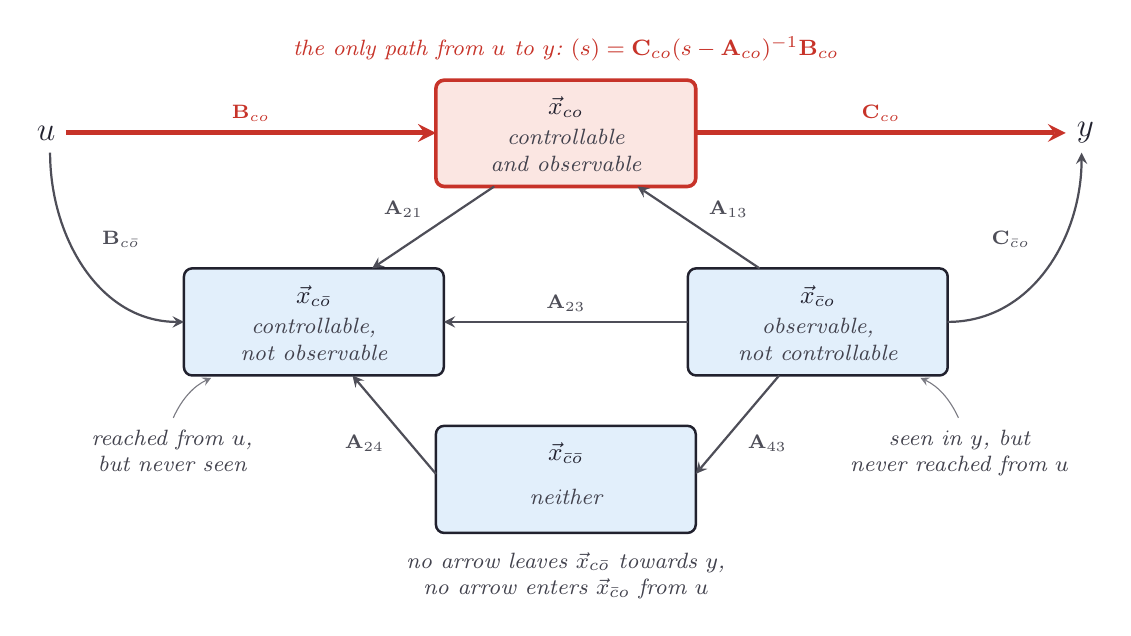
\begin{tikzpicture}[ink/.style={line width=0.9pt, ndInk}, faint/.style={line width=0.4pt, ndInk!35}, dashedink/.style={line width=0.5pt, ndInk!55, dash pattern=on 2.5pt off 2pt}, vec/.style={->, >=stealth, line width=1.2pt}, note/.style={font=\footnotesize\itshape, text=ndInk!85, align=center}, pointer/.style={->, >=stealth, line width=0.4pt, ndInk!60, shorten >=2pt, shorten <=1pt}, dot/.style={circle, fill=ndInk, inner sep=0pt, minimum size=3.4pt}, wash/.style={fill=ndSky, fill opacity=0.55}, every node/.style={text=ndInk}]
\definecolor{ndInk}{rgb}{0.13,0.13,0.18}
\definecolor{ndPaper}{rgb}{0.99,0.96,0.88}
\definecolor{ndSky}{rgb}{0.84,0.91,0.98}
\definecolor{ndRose}{rgb}{0.98,0.86,0.84}
\definecolor{ndBlue}{rgb}{0.13,0.36,0.66}
\definecolor{ndRed}{rgb}{0.78,0.20,0.16}
\definecolor{ndGold}{rgb}{0.88,0.62,0.10}
\definecolor{ndGreen}{rgb}{0.18,0.52,0.30}
\draw[ndRed, line width=1.3pt, fill=ndRose, fill opacity=0.7, rounded corners=3pt] (-1.65,0.82) rectangle (1.65,2.17);
\node[font=\small] at (0.00,1.83) {$\vec x_{co}$};
\node[note] at (0.00,1.28) {controllable\\ and observable};
\draw[ink, fill=ndSky, fill opacity=0.7, rounded corners=3pt] (-4.85,-1.58) rectangle (-1.55,-0.22);
\node[font=\small] at (-3.20,-0.57) {$\vec x_{c\bar o}$};
\node[note] at (-3.20,-1.12) {controllable,\\ not observable};
\draw[ink, fill=ndSky, fill opacity=0.7, rounded corners=3pt] (1.55,-1.58) rectangle (4.85,-0.22);
\node[font=\small] at (3.20,-0.57) {$\vec x_{\bar co}$};
\node[note] at (3.20,-1.12) {observable,\\ not controllable};
\draw[ink, fill=ndSky, fill opacity=0.7, rounded corners=3pt] (-1.65,-3.58) rectangle (1.65,-2.22);
\node[font=\small] at (0.00,-2.57) {$\vec x_{\bar c\bar o}$};
\node[note] at (0.00,-3.12) {neither};
\node[font=\large] (u) at (-6.60,1.50) {$u$};
\node[font=\large] (y) at (6.60,1.50) {$y$};
\draw[->, >=stealth, line width=1.8pt, ndRed] (-6.35,1.50) -- (-1.65,1.50) node[midway, above, font=\scriptsize, text=ndInk!80, text=ndRed] {$\mathbf B_{co}$};
\draw[->, >=stealth, line width=1.8pt, ndRed] (1.65,1.50) -- (6.35,1.50) node[midway, above, font=\scriptsize, text=ndInk!80, text=ndRed] {$\mathbf C_{co}$};
\draw[->, >=stealth, line width=0.8pt, ndInk!80] (-6.55,1.25) to[out=-90, in=180] (-4.85,-0.90);
\node[font=\scriptsize, text=ndInk!80] at (-5.65,0.15) {$\mathbf B_{c\bar o}$};
\draw[->, >=stealth, line width=0.8pt, ndInk!80] (4.85,-0.90) to[out=0, in=-90] (6.55,1.25);
\node[font=\scriptsize, text=ndInk!80] at (5.65,0.15) {$\mathbf C_{\bar co}$};
\draw[->, >=stealth, line width=0.8pt, ndInk!80] (-0.91,0.82) -- (-2.46,-0.22) node[midway, above left, font=\scriptsize, text=ndInk!80] {$\mathbf A_{21}$};
\draw[->, >=stealth, line width=0.8pt, ndInk!80] (2.46,-0.22) -- (0.91,0.82) node[midway, above right, font=\scriptsize, text=ndInk!80] {$\mathbf A_{13}$};
\draw[->, >=stealth, line width=0.8pt, ndInk!80] (1.55,-0.90) -- (-1.55,-0.90) node[midway, above, font=\scriptsize, text=ndInk!80] {$\mathbf A_{23}$};
\draw[->, >=stealth, line width=0.8pt, ndInk!80] (-1.65,-2.83) -- (-2.71,-1.58) node[midway, below left, font=\scriptsize, text=ndInk!80] {$\mathbf A_{24}$};
\draw[->, >=stealth, line width=0.8pt, ndInk!80] (2.71,-1.58) -- (1.65,-2.83) node[midway, below right, font=\scriptsize, text=ndInk!80] {$\mathbf A_{43}$};
\node[note, anchor=north] (d1) at (-5.0,-2.15) {reached from $u$,\\ but never seen};
\draw[pointer] (d1.north) to[bend left=20] (-4.44,-1.58);
\node[note, anchor=north] (d2) at (5.0,-2.15) {seen in $y$, but\\ never reached from $u$};
\draw[pointer] (d2.north) to[bend right=20] (4.44,-1.58);
\node[note, anchor=south, text=ndRed] at (0.0,2.29) {the only path from $u$ to $y$:\ $\TF(s)=\mathbf C_{co}(s\Id-\mathbf A_{co})^{-1}\mathbf B_{co}$};
\node[note, anchor=north] at (0.0,-3.70) {no arrow leaves $\vec x_{c\bar o}$ towards $y$,\\ no arrow enters $\vec x_{\bar co}$ from $u$};
\end{tikzpicture}
}
\caption{The Kalman decomposition \eqref{eq:ch05:kalmanform} drawn as a diagram of four boxes. An arrow from box $j$ to box $i$ indicates a block $\mathbf A_{ij}$ that may be non-zero, and the arrows from $u$ and to $y$ indicate the non-zero blocks of $\mathbf B$ and $\mathbf C$. The state $\vec x_{c\bar o}$ can be reached from $u$ but is never seen, and $\vec x_{\bar co}$ is seen but can never be reached. The only path from $u$ to $y$ (red) passes through $\vec x_{co}$, whence $\TF(s)=\mathbf C_{co}(s\Id-\mathbf A_{co})^{-1}\mathbf B_{co}$. Generated by \texttt{code/ch05\_kalman.py}.}\label{fig:ch05:kalman}
\end{figure}}
\onp{\begin{center}\resizebox{!}{0.72\textheight}{% Generated by code/needham.py -- do not edit by hand.
\definecolor{qocA}{rgb}{0.00,0.45,0.70}
\definecolor{qocB}{rgb}{0.90,0.60,0.00}
\definecolor{qocC}{rgb}{0.00,0.62,0.45}
\definecolor{qocD}{rgb}{0.80,0.40,0.00}
\definecolor{qocE}{rgb}{0.80,0.60,0.70}
\definecolor{qocF}{rgb}{0.35,0.70,0.90}
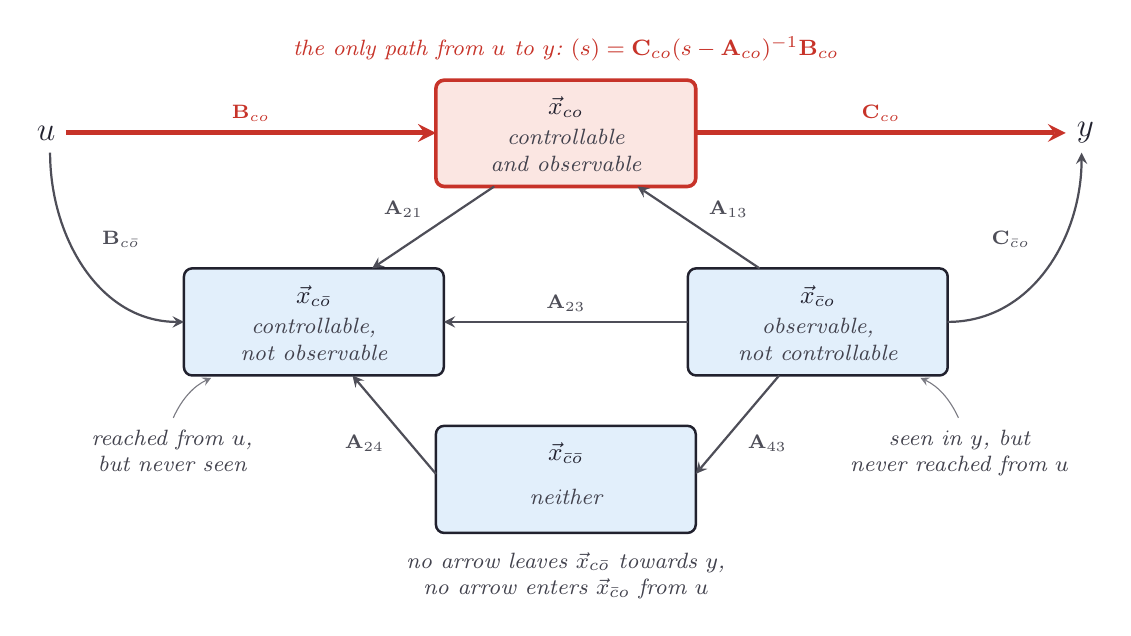
\begin{tikzpicture}[ink/.style={line width=0.9pt, ndInk}, faint/.style={line width=0.4pt, ndInk!35}, dashedink/.style={line width=0.5pt, ndInk!55, dash pattern=on 2.5pt off 2pt}, vec/.style={->, >=stealth, line width=1.2pt}, note/.style={font=\footnotesize\itshape, text=ndInk!85, align=center}, pointer/.style={->, >=stealth, line width=0.4pt, ndInk!60, shorten >=2pt, shorten <=1pt}, dot/.style={circle, fill=ndInk, inner sep=0pt, minimum size=3.4pt}, wash/.style={fill=ndSky, fill opacity=0.55}, every node/.style={text=ndInk}]
\definecolor{ndInk}{rgb}{0.13,0.13,0.18}
\definecolor{ndPaper}{rgb}{0.99,0.96,0.88}
\definecolor{ndSky}{rgb}{0.84,0.91,0.98}
\definecolor{ndRose}{rgb}{0.98,0.86,0.84}
\definecolor{ndBlue}{rgb}{0.13,0.36,0.66}
\definecolor{ndRed}{rgb}{0.78,0.20,0.16}
\definecolor{ndGold}{rgb}{0.88,0.62,0.10}
\definecolor{ndGreen}{rgb}{0.18,0.52,0.30}
\draw[ndRed, line width=1.3pt, fill=ndRose, fill opacity=0.7, rounded corners=3pt] (-1.65,0.82) rectangle (1.65,2.17);
\node[font=\small] at (0.00,1.83) {$\vec x_{co}$};
\node[note] at (0.00,1.28) {controllable\\ and observable};
\draw[ink, fill=ndSky, fill opacity=0.7, rounded corners=3pt] (-4.85,-1.58) rectangle (-1.55,-0.22);
\node[font=\small] at (-3.20,-0.57) {$\vec x_{c\bar o}$};
\node[note] at (-3.20,-1.12) {controllable,\\ not observable};
\draw[ink, fill=ndSky, fill opacity=0.7, rounded corners=3pt] (1.55,-1.58) rectangle (4.85,-0.22);
\node[font=\small] at (3.20,-0.57) {$\vec x_{\bar co}$};
\node[note] at (3.20,-1.12) {observable,\\ not controllable};
\draw[ink, fill=ndSky, fill opacity=0.7, rounded corners=3pt] (-1.65,-3.58) rectangle (1.65,-2.22);
\node[font=\small] at (0.00,-2.57) {$\vec x_{\bar c\bar o}$};
\node[note] at (0.00,-3.12) {neither};
\node[font=\large] (u) at (-6.60,1.50) {$u$};
\node[font=\large] (y) at (6.60,1.50) {$y$};
\draw[->, >=stealth, line width=1.8pt, ndRed] (-6.35,1.50) -- (-1.65,1.50) node[midway, above, font=\scriptsize, text=ndInk!80, text=ndRed] {$\mathbf B_{co}$};
\draw[->, >=stealth, line width=1.8pt, ndRed] (1.65,1.50) -- (6.35,1.50) node[midway, above, font=\scriptsize, text=ndInk!80, text=ndRed] {$\mathbf C_{co}$};
\draw[->, >=stealth, line width=0.8pt, ndInk!80] (-6.55,1.25) to[out=-90, in=180] (-4.85,-0.90);
\node[font=\scriptsize, text=ndInk!80] at (-5.65,0.15) {$\mathbf B_{c\bar o}$};
\draw[->, >=stealth, line width=0.8pt, ndInk!80] (4.85,-0.90) to[out=0, in=-90] (6.55,1.25);
\node[font=\scriptsize, text=ndInk!80] at (5.65,0.15) {$\mathbf C_{\bar co}$};
\draw[->, >=stealth, line width=0.8pt, ndInk!80] (-0.91,0.82) -- (-2.46,-0.22) node[midway, above left, font=\scriptsize, text=ndInk!80] {$\mathbf A_{21}$};
\draw[->, >=stealth, line width=0.8pt, ndInk!80] (2.46,-0.22) -- (0.91,0.82) node[midway, above right, font=\scriptsize, text=ndInk!80] {$\mathbf A_{13}$};
\draw[->, >=stealth, line width=0.8pt, ndInk!80] (1.55,-0.90) -- (-1.55,-0.90) node[midway, above, font=\scriptsize, text=ndInk!80] {$\mathbf A_{23}$};
\draw[->, >=stealth, line width=0.8pt, ndInk!80] (-1.65,-2.83) -- (-2.71,-1.58) node[midway, below left, font=\scriptsize, text=ndInk!80] {$\mathbf A_{24}$};
\draw[->, >=stealth, line width=0.8pt, ndInk!80] (2.71,-1.58) -- (1.65,-2.83) node[midway, below right, font=\scriptsize, text=ndInk!80] {$\mathbf A_{43}$};
\node[note, anchor=north] (d1) at (-5.0,-2.15) {reached from $u$,\\ but never seen};
\draw[pointer] (d1.north) to[bend left=20] (-4.44,-1.58);
\node[note, anchor=north] (d2) at (5.0,-2.15) {seen in $y$, but\\ never reached from $u$};
\draw[pointer] (d2.north) to[bend right=20] (4.44,-1.58);
\node[note, anchor=south, text=ndRed] at (0.0,2.29) {the only path from $u$ to $y$:\ $\TF(s)=\mathbf C_{co}(s\Id-\mathbf A_{co})^{-1}\mathbf B_{co}$};
\node[note, anchor=north] at (0.0,-3.70) {no arrow leaves $\vec x_{c\bar o}$ towards $y$,\\ no arrow enters $\vec x_{\bar co}$ from $u$};
\end{tikzpicture}
}\end{center}}
\end{frame}

\section{Markov parameters, Hankel matrices, and realisation}

\begin{frame}\ft{Discrete time: Markov parameters}
\ona{Experiments sample at discrete times. With a uniform sampling interval $\tau$ and instants $k=0,1,\dots$, the zero-order-hold model in discrete time is}
\onp{Uniformly sampled data obey a discrete LDS:}
\begin{equation}\label{eq:ch05:discrete}
    \vec x(k\tau+\tau)=\mathbf G_\tau\vec x(k\tau)+\mathbf F_\tau\vec u(k\tau),\qquad
    \mathbf G_\tau=\exp[\mathbf A\tau],\quad \mathbf F_\tau=\int_0^\tau\exp[\mathbf At]\,\mathrm{d}t\,\mathbf B ,
\end{equation}
\ona{and the sampled output of the autonomous system is $y_k=\mathbf C\mathbf G_\tau^{k}\vec x_0$. The terms $y_k$, or more generally $\mathbf C\mathbf G_\tau^{k}\mathbf F_\tau$ in the driven case, are called the \emph{Markov parameters}; they are the coefficients in the expansion of the discrete transfer function $\TF_d(z)=\mathbf C(z\Id-\mathbf G_\tau)^{-1}\mathbf F_\tau=\sum_{k\ge0}\mathbf C\mathbf G_\tau^{k}\mathbf F_\tau\,z^{-k-1}$ in powers of $1/z$. Since $\mathbf G_\tau$ is an $n\times n$ matrix, the theorem of Cayley and Hamilton shows that the sequence satisfies a linear recurrence of order $n$, which is the discrete counterpart of the rationality of $\TF$. We arrange the Markov parameters in a block Hankel matrix with $r$ block rows and $s$ block columns:}
\onp{Markov parameters $y_k=\mathbf C\mathbf G_\tau^k\vec x_0$ satisfy a recurrence of order $n$. Arrange them in a \alert{Hankel matrix}:}
\begin{equation}\label{eq:ch05:hankel}
    \Hankel_{rs}(k)=\begin{bmatrix} y_{k} & y_{k+1} & \cdots & y_{k+s-1}\\ y_{k+1} & y_{k+2} & \cdots & y_{k+s}\\ \vdots & & \ddots & \vdots\\ y_{k+r-1} & y_{k+r} & \cdots & y_{k+r+s-2}\end{bmatrix}
    = \begin{bmatrix}\mathbf C\\ \mathbf C\mathbf G_\tau\\ \vdots\\ \mathbf C\mathbf G_\tau^{r-1}\end{bmatrix}\mathbf G_\tau^{k}
    \begin{bmatrix}\vec x_0 & \mathbf G_\tau\vec x_0 & \cdots & \mathbf G_\tau^{s-1}\vec x_0\end{bmatrix}.
\end{equation}
\end{frame}

\begin{frame}\ft{A recurrence for the samples}
\ona{The recurrence is most easily seen for a single damped oscillation, such as $\langle\sigma_x\rangle$ in our example, for which $y_k=c\,\mathrm{Re}(\mu^k)$ with $\mu=\ee^{\lambda\tau}=\rho\,\ee^{\imath\omega\tau}$ and $\rho=\ee^{-\Gamma\tau}$. Then}
\onp{One damped oscillation, $\mu=\ee^{\lambda\tau}=\rho\,\ee^{\imath\omega\tau}$:}
\begin{equation}\label{eq:ch05:recurrence}
    y_{k+2}=2\rho\cos(\omega\tau)\,y_{k+1}-\rho^2\,y_k ,
\end{equation}
\ona{since $\mu$ and $\bar\mu$ are the roots of $z^2-2\rho\cos(\omega\tau)\,z+\rho^2$. For $\tau=0.25$ the recurrence reads $y_{k+2}=1.29\,y_{k+1}-0.78\,y_k$, so that two numbers, fixed once and for all by the eigenvalues, determine each sample from the two before it (Figure~\ref{fig:ch05:recurrence}). In general $n$ modes require $n$ numbers, the coefficients of the characteristic polynomial of $\mathbf G_\tau$. It follows that every row of the Hankel matrix \eqref{eq:ch05:hankel} after the $n$-th is a fixed linear combination of the $n$ rows before it, so that its rank cannot exceed $n$, however many samples are taken. Conversely, the roots of the recurrence are the eigenvalues $\ee^{\lambda_i\tau}$ of $\mathbf G_\tau$, from which the $\lambda_i$ may be recovered. This is the method of Prony, published in 1795, and the oldest of the methods of this section.}
\onp{\begin{itemize}
    \item Each sample is determined by the $n$ before it, so the rows of $\Hankel$ beyond the $n$-th are dependent.
    \item The roots of $z^2-2\rho\cos(\omega\tau)z+\rho^2$ are $z=\ee^{\lambda\tau}$, the eigenvalues of $\mathbf G_\tau$.
\end{itemize}
\begin{center}\resizebox{!}{0.36\textheight}{% Generated by code/needham.py -- do not edit by hand.
\definecolor{qocA}{rgb}{0.00,0.45,0.70}
\definecolor{qocB}{rgb}{0.90,0.60,0.00}
\definecolor{qocC}{rgb}{0.00,0.62,0.45}
\definecolor{qocD}{rgb}{0.80,0.40,0.00}
\definecolor{qocE}{rgb}{0.80,0.60,0.70}
\definecolor{qocF}{rgb}{0.35,0.70,0.90}
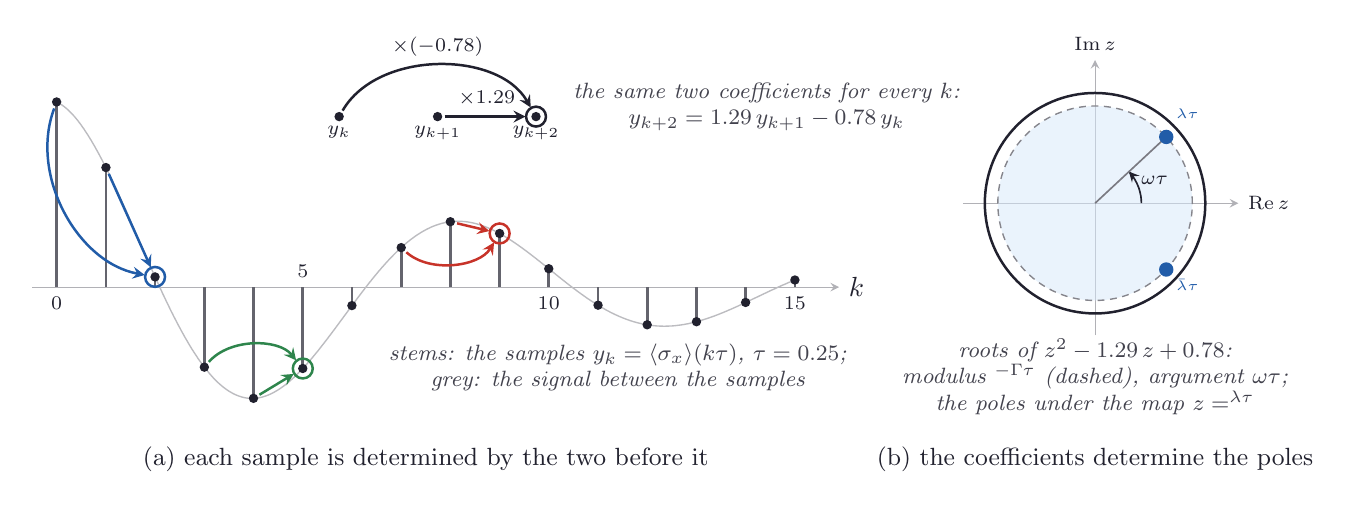
\begin{tikzpicture}[ink/.style={line width=0.9pt, ndInk}, faint/.style={line width=0.4pt, ndInk!35}, dashedink/.style={line width=0.5pt, ndInk!55, dash pattern=on 2.5pt off 2pt}, vec/.style={->, >=stealth, line width=1.2pt}, note/.style={font=\footnotesize\itshape, text=ndInk!85, align=center}, pointer/.style={->, >=stealth, line width=0.4pt, ndInk!60, shorten >=2pt, shorten <=1pt}, dot/.style={circle, fill=ndInk, inner sep=0pt, minimum size=3.4pt}, wash/.style={fill=ndSky, fill opacity=0.55}, every node/.style={text=ndInk}]
\definecolor{ndInk}{rgb}{0.13,0.13,0.18}
\definecolor{ndPaper}{rgb}{0.99,0.96,0.88}
\definecolor{ndSky}{rgb}{0.84,0.91,0.98}
\definecolor{ndRose}{rgb}{0.98,0.86,0.84}
\definecolor{ndBlue}{rgb}{0.13,0.36,0.66}
\definecolor{ndRed}{rgb}{0.78,0.20,0.16}
\definecolor{ndGold}{rgb}{0.88,0.62,0.10}
\definecolor{ndGreen}{rgb}{0.18,0.52,0.30}
\draw[faint, ->, >=stealth] (0.000,1.684) -- (10.250,1.684) node[right, text=ndInk] {$k$};
\draw[line width=0.5pt, ndInk!30] (0.312,4.036) -- (0.328,4.028) -- (0.344,4.020) -- (0.359,4.010) -- (0.375,4.000) -- (0.391,3.989) -- (0.406,3.978) -- (0.422,3.965) -- (0.438,3.952) -- (0.453,3.938) -- (0.469,3.924) -- (0.485,3.908) -- (0.500,3.892) -- (0.516,3.875) -- (0.532,3.858) -- (0.547,3.840) -- (0.563,3.821) -- (0.579,3.802) -- (0.594,3.781) -- (0.610,3.761) -- (0.626,3.739) -- (0.641,3.717) -- (0.657,3.695) -- (0.672,3.672) -- (0.688,3.648) -- (0.704,3.624) -- (0.719,3.599) -- (0.735,3.573) -- (0.751,3.548) -- (0.766,3.521) -- (0.782,3.494) -- (0.798,3.467) -- (0.813,3.439) -- (0.829,3.411) -- (0.845,3.382) -- (0.860,3.353) -- (0.876,3.323) -- (0.892,3.293) -- (0.907,3.263) -- (0.923,3.232) -- (0.939,3.201) -- (0.954,3.169) -- (0.970,3.137) -- (0.985,3.105) -- (1.001,3.073) -- (1.017,3.040) -- (1.032,3.007) -- (1.048,2.973) -- (1.064,2.940) -- (1.079,2.906) -- (1.095,2.872) -- (1.111,2.837) -- (1.126,2.803) -- (1.142,2.768) -- (1.158,2.733) -- (1.173,2.698) -- (1.189,2.663) -- (1.205,2.628) -- (1.220,2.592) -- (1.236,2.557) -- (1.252,2.521) -- (1.267,2.485) -- (1.283,2.450) -- (1.299,2.414) -- (1.314,2.378) -- (1.330,2.342) -- (1.345,2.306) -- (1.361,2.270) -- (1.377,2.234) -- (1.392,2.198) -- (1.408,2.163) -- (1.424,2.127) -- (1.439,2.091) -- (1.455,2.055) -- (1.471,2.020) -- (1.486,1.984) -- (1.502,1.949) -- (1.518,1.914) -- (1.533,1.879) -- (1.549,1.844) -- (1.565,1.809) -- (1.580,1.774) -- (1.596,1.740) -- (1.612,1.706) -- (1.627,1.672) -- (1.643,1.638) -- (1.658,1.604) -- (1.674,1.571) -- (1.690,1.538) -- (1.705,1.505) -- (1.721,1.472) -- (1.737,1.440) -- (1.752,1.408) -- (1.768,1.376) -- (1.784,1.345) -- (1.799,1.314) -- (1.815,1.283) -- (1.831,1.253) -- (1.846,1.223) -- (1.862,1.193) -- (1.878,1.164) -- (1.893,1.135) -- (1.909,1.106) -- (1.925,1.078) -- (1.940,1.050) -- (1.956,1.023) -- (1.972,0.996) -- (1.987,0.969) -- (2.003,0.943) -- (2.018,0.917) -- (2.034,0.892) -- (2.050,0.867) -- (2.065,0.843) -- (2.081,0.819) -- (2.097,0.795) -- (2.112,0.772) -- (2.128,0.750) -- (2.144,0.728) -- (2.159,0.706) -- (2.175,0.685) -- (2.191,0.664) -- (2.206,0.644) -- (2.222,0.625) -- (2.238,0.606) -- (2.253,0.587) -- (2.269,0.569) -- (2.285,0.551) -- (2.300,0.534) -- (2.316,0.518) -- (2.331,0.502) -- (2.347,0.486) -- (2.363,0.471) -- (2.378,0.457) -- (2.394,0.443) -- (2.410,0.430) -- (2.425,0.417) -- (2.441,0.405) -- (2.457,0.393) -- (2.472,0.382) -- (2.488,0.371) -- (2.504,0.361) -- (2.519,0.352) -- (2.535,0.343) -- (2.551,0.334) -- (2.566,0.326) -- (2.582,0.319) -- (2.598,0.312) -- (2.613,0.306) -- (2.629,0.300) -- (2.645,0.295) -- (2.660,0.290) -- (2.676,0.286) -- (2.691,0.282) -- (2.707,0.279) -- (2.723,0.276) -- (2.738,0.274) -- (2.754,0.273) -- (2.770,0.272) -- (2.785,0.271) -- (2.801,0.271) -- (2.817,0.272) -- (2.832,0.273) -- (2.848,0.274) -- (2.864,0.276) -- (2.879,0.279) -- (2.895,0.282) -- (2.911,0.285) -- (2.926,0.289) -- (2.942,0.294) -- (2.958,0.299) -- (2.973,0.304) -- (2.989,0.310) -- (3.004,0.316) -- (3.020,0.323) -- (3.036,0.330) -- (3.051,0.338) -- (3.067,0.346) -- (3.083,0.355) -- (3.098,0.364) -- (3.114,0.373) -- (3.130,0.383) -- (3.145,0.393) -- (3.161,0.404) -- (3.177,0.415) -- (3.192,0.426) -- (3.208,0.438) -- (3.224,0.450) -- (3.239,0.463) -- (3.255,0.476) -- (3.271,0.489) -- (3.286,0.503) -- (3.302,0.517) -- (3.318,0.531) -- (3.333,0.546) -- (3.349,0.560) -- (3.364,0.576) -- (3.380,0.591) -- (3.396,0.607) -- (3.411,0.623) -- (3.427,0.640) -- (3.443,0.656) -- (3.458,0.673) -- (3.474,0.691) -- (3.490,0.708) -- (3.505,0.726) -- (3.521,0.744) -- (3.537,0.762) -- (3.552,0.780) -- (3.568,0.799) -- (3.584,0.818) -- (3.599,0.837) -- (3.615,0.856) -- (3.631,0.875) -- (3.646,0.895) -- (3.662,0.915) -- (3.677,0.935) -- (3.693,0.955) -- (3.709,0.975) -- (3.724,0.995) -- (3.740,1.015) -- (3.756,1.036) -- (3.771,1.057) -- (3.787,1.077) -- (3.803,1.098) -- (3.818,1.119) -- (3.834,1.140) -- (3.850,1.161) -- (3.865,1.182) -- (3.881,1.203) -- (3.897,1.225) -- (3.912,1.246) -- (3.928,1.267) -- (3.944,1.288) -- (3.959,1.310) -- (3.975,1.331) -- (3.991,1.352) -- (4.006,1.373) -- (4.022,1.395) -- (4.037,1.416) -- (4.053,1.437) -- (4.069,1.458) -- (4.084,1.479) -- (4.100,1.500) -- (4.116,1.521) -- (4.131,1.542) -- (4.147,1.563) -- (4.163,1.584) -- (4.178,1.604) -- (4.194,1.625) -- (4.210,1.645) -- (4.225,1.666) -- (4.241,1.686) -- (4.257,1.706) -- (4.272,1.726) -- (4.288,1.746) -- (4.304,1.765) -- (4.319,1.785) -- (4.335,1.804) -- (4.350,1.823) -- (4.366,1.842) -- (4.382,1.861) -- (4.397,1.880) -- (4.413,1.898) -- (4.429,1.916) -- (4.444,1.935) -- (4.460,1.952) -- (4.476,1.970) -- (4.491,1.987) -- (4.507,2.005) -- (4.523,2.022) -- (4.538,2.038) -- (4.554,2.055) -- (4.570,2.071) -- (4.585,2.087) -- (4.601,2.103) -- (4.617,2.119) -- (4.632,2.134) -- (4.648,2.149) -- (4.664,2.164) -- (4.679,2.178) -- (4.695,2.193) -- (4.710,2.207) -- (4.726,2.220) -- (4.742,2.234) -- (4.757,2.247) -- (4.773,2.260) -- (4.789,2.272) -- (4.804,2.285) -- (4.820,2.297) -- (4.836,2.308) -- (4.851,2.320) -- (4.867,2.331) -- (4.883,2.342) -- (4.898,2.352) -- (4.914,2.362) -- (4.930,2.372) -- (4.945,2.382) -- (4.961,2.391) -- (4.977,2.400) -- (4.992,2.408) -- (5.008,2.417) -- (5.023,2.425) -- (5.039,2.432) -- (5.055,2.440) -- (5.070,2.447) -- (5.086,2.454) -- (5.102,2.460) -- (5.117,2.466) -- (5.133,2.472) -- (5.149,2.477) -- (5.164,2.482) -- (5.180,2.487) -- (5.196,2.492) -- (5.211,2.496) -- (5.227,2.499) -- (5.243,2.503) -- (5.258,2.506) -- (5.274,2.509) -- (5.290,2.512) -- (5.305,2.514) -- (5.321,2.516) -- (5.336,2.517) -- (5.352,2.519) -- (5.368,2.520) -- (5.383,2.520) -- (5.399,2.521) -- (5.415,2.521) -- (5.430,2.521) -- (5.446,2.520) -- (5.462,2.519) -- (5.477,2.518) -- (5.493,2.517) -- (5.509,2.515) -- (5.524,2.513) -- (5.540,2.511) -- (5.556,2.508) -- (5.571,2.505) -- (5.587,2.502) -- (5.603,2.499) -- (5.618,2.495) -- (5.634,2.491) -- (5.650,2.487) -- (5.665,2.482) -- (5.681,2.478) -- (5.696,2.473) -- (5.712,2.467) -- (5.728,2.462) -- (5.743,2.456) -- (5.759,2.450) -- (5.775,2.444) -- (5.790,2.437) -- (5.806,2.431) -- (5.822,2.424) -- (5.837,2.417) -- (5.853,2.409) -- (5.869,2.402) -- (5.884,2.394) -- (5.900,2.386) -- (5.916,2.378) -- (5.931,2.369) -- (5.947,2.361) -- (5.963,2.352) -- (5.978,2.343) -- (5.994,2.334) -- (6.009,2.324) -- (6.025,2.315) -- (6.041,2.305) -- (6.056,2.295) -- (6.072,2.285) -- (6.088,2.275) -- (6.103,2.265) -- (6.119,2.254) -- (6.135,2.244) -- (6.150,2.233) -- (6.166,2.222) -- (6.182,2.211) -- (6.197,2.200) -- (6.213,2.189) -- (6.229,2.177) -- (6.244,2.166) -- (6.260,2.154) -- (6.276,2.143) -- (6.291,2.131) -- (6.307,2.119) -- (6.323,2.107) -- (6.338,2.095) -- (6.354,2.083) -- (6.369,2.071) -- (6.385,2.059) -- (6.401,2.047) -- (6.416,2.034) -- (6.432,2.022) -- (6.448,2.010) -- (6.463,1.997) -- (6.479,1.985) -- (6.495,1.972) -- (6.510,1.960) -- (6.526,1.947) -- (6.542,1.934) -- (6.557,1.922) -- (6.573,1.909) -- (6.589,1.897) -- (6.604,1.884) -- (6.620,1.871) -- (6.636,1.859) -- (6.651,1.846) -- (6.667,1.834) -- (6.682,1.821) -- (6.698,1.809) -- (6.714,1.796) -- (6.729,1.784) -- (6.745,1.771) -- (6.761,1.759) -- (6.776,1.747) -- (6.792,1.734) -- (6.808,1.722) -- (6.823,1.710) -- (6.839,1.698) -- (6.855,1.686) -- (6.870,1.674) -- (6.886,1.662) -- (6.902,1.651) -- (6.917,1.639) -- (6.933,1.627) -- (6.949,1.616) -- (6.964,1.605) -- (6.980,1.593) -- (6.996,1.582) -- (7.011,1.571) -- (7.027,1.560) -- (7.042,1.549) -- (7.058,1.538) -- (7.074,1.528) -- (7.089,1.517) -- (7.105,1.507) -- (7.121,1.497) -- (7.136,1.487) -- (7.152,1.477) -- (7.168,1.467) -- (7.183,1.457) -- (7.199,1.448) -- (7.215,1.438) -- (7.230,1.429) -- (7.246,1.420) -- (7.262,1.411) -- (7.277,1.402) -- (7.293,1.393) -- (7.309,1.385) -- (7.324,1.377) -- (7.340,1.368) -- (7.355,1.360) -- (7.371,1.353) -- (7.387,1.345) -- (7.402,1.337) -- (7.418,1.330) -- (7.434,1.323) -- (7.449,1.316) -- (7.465,1.309) -- (7.481,1.303) -- (7.496,1.296) -- (7.512,1.290) -- (7.528,1.284) -- (7.543,1.278) -- (7.559,1.272) -- (7.575,1.267) -- (7.590,1.261) -- (7.606,1.256) -- (7.622,1.251) -- (7.637,1.246) -- (7.653,1.242) -- (7.669,1.237) -- (7.684,1.233) -- (7.700,1.229) -- (7.715,1.225) -- (7.731,1.222) -- (7.747,1.218) -- (7.762,1.215) -- (7.778,1.212) -- (7.794,1.209) -- (7.809,1.206) -- (7.825,1.204) -- (7.841,1.201) -- (7.856,1.199) -- (7.872,1.197) -- (7.888,1.196) -- (7.903,1.194) -- (7.919,1.193) -- (7.935,1.191) -- (7.950,1.190) -- (7.966,1.190) -- (7.982,1.189) -- (7.997,1.189) -- (8.013,1.188) -- (8.028,1.188) -- (8.044,1.188) -- (8.060,1.189) -- (8.075,1.189) -- (8.091,1.190) -- (8.107,1.190) -- (8.122,1.191) -- (8.138,1.192) -- (8.154,1.194) -- (8.169,1.195) -- (8.185,1.197) -- (8.201,1.199) -- (8.216,1.201) -- (8.232,1.203) -- (8.248,1.205) -- (8.263,1.208) -- (8.279,1.210) -- (8.295,1.213) -- (8.310,1.216) -- (8.326,1.219) -- (8.342,1.222) -- (8.357,1.226) -- (8.373,1.229) -- (8.388,1.233) -- (8.404,1.237) -- (8.420,1.240) -- (8.435,1.245) -- (8.451,1.249) -- (8.467,1.253) -- (8.482,1.258) -- (8.498,1.262) -- (8.514,1.267) -- (8.529,1.272) -- (8.545,1.277) -- (8.561,1.282) -- (8.576,1.287) -- (8.592,1.292) -- (8.608,1.298) -- (8.623,1.303) -- (8.639,1.309) -- (8.655,1.314) -- (8.670,1.320) -- (8.686,1.326) -- (8.701,1.332) -- (8.717,1.338) -- (8.733,1.344) -- (8.748,1.351) -- (8.764,1.357) -- (8.780,1.363) -- (8.795,1.370) -- (8.811,1.376) -- (8.827,1.383) -- (8.842,1.390) -- (8.858,1.397) -- (8.874,1.403) -- (8.889,1.410) -- (8.905,1.417) -- (8.921,1.424) -- (8.936,1.431) -- (8.952,1.438) -- (8.968,1.445) -- (8.983,1.453) -- (8.999,1.460) -- (9.015,1.467) -- (9.030,1.474) -- (9.046,1.482) -- (9.061,1.489) -- (9.077,1.496) -- (9.093,1.504) -- (9.108,1.511) -- (9.124,1.519) -- (9.140,1.526) -- (9.155,1.534) -- (9.171,1.541) -- (9.187,1.549) -- (9.202,1.556) -- (9.218,1.563) -- (9.234,1.571) -- (9.249,1.578) -- (9.265,1.586) -- (9.281,1.593) -- (9.296,1.601) -- (9.312,1.608) -- (9.328,1.615) -- (9.343,1.623) -- (9.359,1.630) -- (9.374,1.638) -- (9.390,1.645) -- (9.406,1.652) -- (9.421,1.659) -- (9.437,1.666) -- (9.453,1.674) -- (9.468,1.681) -- (9.484,1.688) -- (9.500,1.695) -- (9.515,1.702) -- (9.531,1.709) -- (9.547,1.716) -- (9.562,1.722) -- (9.578,1.729) -- (9.594,1.736) -- (9.609,1.743) -- (9.625,1.749) -- (9.641,1.756) -- (9.656,1.762) -- (9.672,1.768) -- (9.688,1.775);
\draw[line width=1.0pt, ndInk!70] (0.312,1.684) -- (0.312,4.036);
\fill[ndInk] (0.312,4.036) circle (1.7pt);
\draw[line width=1.0pt, ndInk!70] (0.938,1.684) -- (0.938,3.203);
\fill[ndInk] (0.938,3.203) circle (1.7pt);
\draw[line width=1.0pt, ndInk!70] (1.562,1.684) -- (1.562,1.814);
\fill[ndInk] (1.562,1.814) circle (1.7pt);
\draw[line width=1.0pt, ndInk!70] (2.188,1.684) -- (2.188,0.668);
\fill[ndInk] (2.188,0.668) circle (1.7pt);
\draw[line width=1.0pt, ndInk!70] (2.812,1.684) -- (2.812,0.272);
\fill[ndInk] (2.812,0.272) circle (1.7pt);
\draw[line width=1.0pt, ndInk!70] (3.438,1.684) -- (3.438,0.651);
\fill[ndInk] (3.438,0.651) circle (1.7pt);
\draw[line width=1.0pt, ndInk!70] (4.062,1.684) -- (4.062,1.450);
\fill[ndInk] (4.062,1.450) circle (1.7pt);
\draw[line width=1.0pt, ndInk!70] (4.688,1.684) -- (4.688,2.186);
\fill[ndInk] (4.688,2.186) circle (1.7pt);
\draw[line width=1.0pt, ndInk!70] (5.312,1.684) -- (5.312,2.515);
\fill[ndInk] (5.312,2.515) circle (1.7pt);
\draw[line width=1.0pt, ndInk!70] (5.938,1.684) -- (5.938,2.366);
\fill[ndInk] (5.938,2.366) circle (1.7pt);
\draw[line width=1.0pt, ndInk!70] (6.562,1.684) -- (6.562,1.918);
\fill[ndInk] (6.562,1.918) circle (1.7pt);
\draw[line width=1.0pt, ndInk!70] (7.188,1.684) -- (7.188,1.455);
\fill[ndInk] (7.188,1.455) circle (1.7pt);
\draw[line width=1.0pt, ndInk!70] (7.812,1.684) -- (7.812,1.206);
\fill[ndInk] (7.812,1.206) circle (1.7pt);
\draw[line width=1.0pt, ndInk!70] (8.438,1.684) -- (8.438,1.245);
\fill[ndInk] (8.438,1.245) circle (1.7pt);
\draw[line width=1.0pt, ndInk!70] (9.062,1.684) -- (9.062,1.490);
\fill[ndInk] (9.062,1.490) circle (1.7pt);
\draw[line width=1.0pt, ndInk!70] (9.688,1.684) -- (9.688,1.775);
\fill[ndInk] (9.688,1.775) circle (1.7pt);
\node[font=\scriptsize, below] at (0.312,1.684) {$0$};
\node[font=\scriptsize, above] at (3.438,1.684) {$5$};
\node[font=\scriptsize, below] at (6.562,1.684) {$10$};
\node[font=\scriptsize, below] at (9.688,1.684) {$15$};
\draw[->, >=stealth, line width=0.9pt, ndBlue, shorten <=2.5pt, shorten >=3.8pt] (0.312,4.036) to[bend right=50] (1.562,1.814);
\draw[->, >=stealth, line width=0.9pt, ndBlue, shorten <=2.5pt, shorten >=3.8pt] (0.938,3.203) -- (1.562,1.814);
\draw[line width=0.9pt, ndBlue] (1.562,1.814) circle (3.6pt);
\draw[->, >=stealth, line width=0.9pt, ndGreen, shorten <=2.5pt, shorten >=3.8pt] (2.188,0.668) to[bend left=50] (3.438,0.651);
\draw[->, >=stealth, line width=0.9pt, ndGreen, shorten <=2.5pt, shorten >=3.8pt] (2.812,0.272) -- (3.438,0.651);
\draw[line width=0.9pt, ndGreen] (3.438,0.651) circle (3.6pt);
\draw[->, >=stealth, line width=0.9pt, ndRed, shorten <=2.5pt, shorten >=3.8pt] (4.688,2.186) to[bend right=50] (5.938,2.366);
\draw[->, >=stealth, line width=0.9pt, ndRed, shorten <=2.5pt, shorten >=3.8pt] (5.312,2.515) -- (5.938,2.366);
\draw[line width=0.9pt, ndRed] (5.938,2.366) circle (3.6pt);
\fill[ndInk] (3.900,3.850) circle (1.7pt);
\node[font=\scriptsize, below] at (3.900,3.850) {$y_k$};
\fill[ndInk] (5.150,3.850) circle (1.7pt);
\node[font=\scriptsize, below] at (5.150,3.850) {$y_{k+1}$};
\fill[ndInk] (6.400,3.850) circle (1.7pt);
\node[font=\scriptsize, below] at (6.400,3.850) {$y_{k+2}$};
\draw[ink] (6.400,3.850) circle (3.6pt);
\draw[->, >=stealth, line width=0.9pt, ndInk, shorten <=2.5pt, shorten >=3.8pt] (5.150,3.850) -- (6.400,3.850) node[midway, above=0pt, font=\scriptsize] {$\times1.29$};
\draw[->, >=stealth, line width=0.9pt, ndInk, shorten <=2.5pt, shorten >=3.8pt] (3.900,3.850) to[bend left=60] node[midway, above, font=\scriptsize] {$\times(-0.78)$} (6.400,3.850);
\node[note, anchor=west] at (6.75,3.97) {the same two coefficients for every $k$:\\ $y_{k+2}=1.29\,y_{k+1}-0.78\,y_k$};
\node[note, anchor=north] at (7.438,1.086) {stems: the samples $y_k=\langle\sigma_x\rangle(k\tau)$, $\tau=0.25$;\\ grey: the signal between the samples};
\node[font=\small] at (5.00,-0.5) {(a) each sample is determined by the two before it};
\draw[faint, ->, >=stealth] (11.820,2.750) -- (15.320,2.750) node[right, font=\scriptsize, text=ndInk] {$\mathrm{Re}\,z$};
\draw[faint, ->, >=stealth] (13.500,1.070) -- (13.500,4.570) node[above, font=\scriptsize, text=ndInk] {$\mathrm{Im}\,z$};
\draw[ink] (13.500,2.750) circle (1.400);
\fill[ndSky, fill opacity=0.5] (13.500,2.750) circle (1.235);
\draw[dashedink] (13.500,2.750) circle (1.235);
\draw[->, >=stealth, line width=0.6pt, ndInk] (14.088,2.750) -- (14.088,2.765) -- (14.087,2.780) -- (14.086,2.796) -- (14.085,2.811) -- (14.083,2.826) -- (14.081,2.841) -- (14.078,2.856) -- (14.075,2.871) -- (14.072,2.886) -- (14.068,2.900) -- (14.064,2.915) -- (14.060,2.930) -- (14.055,2.944) -- (14.050,2.958) -- (14.044,2.972) -- (14.038,2.986) -- (14.032,3.000) -- (14.025,3.014) -- (14.018,3.027) -- (14.011,3.041) -- (14.003,3.054) -- (13.995,3.067) -- (13.987,3.079) -- (13.978,3.092) -- (13.969,3.104) -- (13.960,3.116) -- (13.950,3.128) -- (13.940,3.140) -- (13.930,3.151);
\node[font=\scriptsize] at (14.256,3.047) {$\omega\tau$};
\draw[line width=0.6pt, ndInk!60] (13.500,2.750) -- (14.404,3.592);
\fill[ndBlue] (14.404,3.592) circle (2.6pt);
\fill[ndBlue] (14.404,1.908) circle (2.6pt);
\node[font=\scriptsize, text=ndBlue, anchor=south west] at (14.404,3.592) {$\ee^{\lambda\tau}$};
\node[font=\scriptsize, text=ndBlue, anchor=north west] at (14.404,1.908) {$\ee^{\bar\lambda\tau}$};
\node[note, anchor=north] at (13.500,1.150) {roots of $z^2-1.29\,z+0.78$:\\ modulus $\ee^{-\Gamma\tau}$ (dashed), argument $\omega\tau$;\\ the poles under the map $z=\ee^{\lambda\tau}$};
\node[font=\small] at (13.50,-0.5) {(b) the coefficients determine the poles};
\end{tikzpicture}
}\end{center}}
\ona{\begin{figure}[H]\centering
\resizebox{\linewidth}{!}{% Generated by code/needham.py -- do not edit by hand.
\definecolor{qocA}{rgb}{0.00,0.45,0.70}
\definecolor{qocB}{rgb}{0.90,0.60,0.00}
\definecolor{qocC}{rgb}{0.00,0.62,0.45}
\definecolor{qocD}{rgb}{0.80,0.40,0.00}
\definecolor{qocE}{rgb}{0.80,0.60,0.70}
\definecolor{qocF}{rgb}{0.35,0.70,0.90}
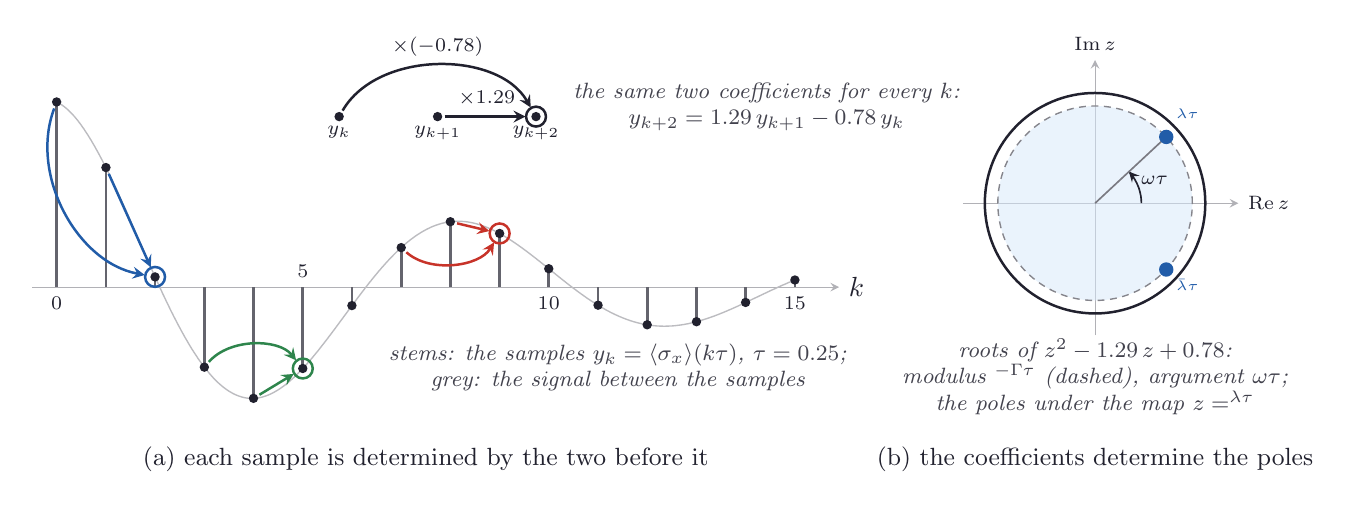
\begin{tikzpicture}[ink/.style={line width=0.9pt, ndInk}, faint/.style={line width=0.4pt, ndInk!35}, dashedink/.style={line width=0.5pt, ndInk!55, dash pattern=on 2.5pt off 2pt}, vec/.style={->, >=stealth, line width=1.2pt}, note/.style={font=\footnotesize\itshape, text=ndInk!85, align=center}, pointer/.style={->, >=stealth, line width=0.4pt, ndInk!60, shorten >=2pt, shorten <=1pt}, dot/.style={circle, fill=ndInk, inner sep=0pt, minimum size=3.4pt}, wash/.style={fill=ndSky, fill opacity=0.55}, every node/.style={text=ndInk}]
\definecolor{ndInk}{rgb}{0.13,0.13,0.18}
\definecolor{ndPaper}{rgb}{0.99,0.96,0.88}
\definecolor{ndSky}{rgb}{0.84,0.91,0.98}
\definecolor{ndRose}{rgb}{0.98,0.86,0.84}
\definecolor{ndBlue}{rgb}{0.13,0.36,0.66}
\definecolor{ndRed}{rgb}{0.78,0.20,0.16}
\definecolor{ndGold}{rgb}{0.88,0.62,0.10}
\definecolor{ndGreen}{rgb}{0.18,0.52,0.30}
\draw[faint, ->, >=stealth] (0.000,1.684) -- (10.250,1.684) node[right, text=ndInk] {$k$};
\draw[line width=0.5pt, ndInk!30] (0.312,4.036) -- (0.328,4.028) -- (0.344,4.020) -- (0.359,4.010) -- (0.375,4.000) -- (0.391,3.989) -- (0.406,3.978) -- (0.422,3.965) -- (0.438,3.952) -- (0.453,3.938) -- (0.469,3.924) -- (0.485,3.908) -- (0.500,3.892) -- (0.516,3.875) -- (0.532,3.858) -- (0.547,3.840) -- (0.563,3.821) -- (0.579,3.802) -- (0.594,3.781) -- (0.610,3.761) -- (0.626,3.739) -- (0.641,3.717) -- (0.657,3.695) -- (0.672,3.672) -- (0.688,3.648) -- (0.704,3.624) -- (0.719,3.599) -- (0.735,3.573) -- (0.751,3.548) -- (0.766,3.521) -- (0.782,3.494) -- (0.798,3.467) -- (0.813,3.439) -- (0.829,3.411) -- (0.845,3.382) -- (0.860,3.353) -- (0.876,3.323) -- (0.892,3.293) -- (0.907,3.263) -- (0.923,3.232) -- (0.939,3.201) -- (0.954,3.169) -- (0.970,3.137) -- (0.985,3.105) -- (1.001,3.073) -- (1.017,3.040) -- (1.032,3.007) -- (1.048,2.973) -- (1.064,2.940) -- (1.079,2.906) -- (1.095,2.872) -- (1.111,2.837) -- (1.126,2.803) -- (1.142,2.768) -- (1.158,2.733) -- (1.173,2.698) -- (1.189,2.663) -- (1.205,2.628) -- (1.220,2.592) -- (1.236,2.557) -- (1.252,2.521) -- (1.267,2.485) -- (1.283,2.450) -- (1.299,2.414) -- (1.314,2.378) -- (1.330,2.342) -- (1.345,2.306) -- (1.361,2.270) -- (1.377,2.234) -- (1.392,2.198) -- (1.408,2.163) -- (1.424,2.127) -- (1.439,2.091) -- (1.455,2.055) -- (1.471,2.020) -- (1.486,1.984) -- (1.502,1.949) -- (1.518,1.914) -- (1.533,1.879) -- (1.549,1.844) -- (1.565,1.809) -- (1.580,1.774) -- (1.596,1.740) -- (1.612,1.706) -- (1.627,1.672) -- (1.643,1.638) -- (1.658,1.604) -- (1.674,1.571) -- (1.690,1.538) -- (1.705,1.505) -- (1.721,1.472) -- (1.737,1.440) -- (1.752,1.408) -- (1.768,1.376) -- (1.784,1.345) -- (1.799,1.314) -- (1.815,1.283) -- (1.831,1.253) -- (1.846,1.223) -- (1.862,1.193) -- (1.878,1.164) -- (1.893,1.135) -- (1.909,1.106) -- (1.925,1.078) -- (1.940,1.050) -- (1.956,1.023) -- (1.972,0.996) -- (1.987,0.969) -- (2.003,0.943) -- (2.018,0.917) -- (2.034,0.892) -- (2.050,0.867) -- (2.065,0.843) -- (2.081,0.819) -- (2.097,0.795) -- (2.112,0.772) -- (2.128,0.750) -- (2.144,0.728) -- (2.159,0.706) -- (2.175,0.685) -- (2.191,0.664) -- (2.206,0.644) -- (2.222,0.625) -- (2.238,0.606) -- (2.253,0.587) -- (2.269,0.569) -- (2.285,0.551) -- (2.300,0.534) -- (2.316,0.518) -- (2.331,0.502) -- (2.347,0.486) -- (2.363,0.471) -- (2.378,0.457) -- (2.394,0.443) -- (2.410,0.430) -- (2.425,0.417) -- (2.441,0.405) -- (2.457,0.393) -- (2.472,0.382) -- (2.488,0.371) -- (2.504,0.361) -- (2.519,0.352) -- (2.535,0.343) -- (2.551,0.334) -- (2.566,0.326) -- (2.582,0.319) -- (2.598,0.312) -- (2.613,0.306) -- (2.629,0.300) -- (2.645,0.295) -- (2.660,0.290) -- (2.676,0.286) -- (2.691,0.282) -- (2.707,0.279) -- (2.723,0.276) -- (2.738,0.274) -- (2.754,0.273) -- (2.770,0.272) -- (2.785,0.271) -- (2.801,0.271) -- (2.817,0.272) -- (2.832,0.273) -- (2.848,0.274) -- (2.864,0.276) -- (2.879,0.279) -- (2.895,0.282) -- (2.911,0.285) -- (2.926,0.289) -- (2.942,0.294) -- (2.958,0.299) -- (2.973,0.304) -- (2.989,0.310) -- (3.004,0.316) -- (3.020,0.323) -- (3.036,0.330) -- (3.051,0.338) -- (3.067,0.346) -- (3.083,0.355) -- (3.098,0.364) -- (3.114,0.373) -- (3.130,0.383) -- (3.145,0.393) -- (3.161,0.404) -- (3.177,0.415) -- (3.192,0.426) -- (3.208,0.438) -- (3.224,0.450) -- (3.239,0.463) -- (3.255,0.476) -- (3.271,0.489) -- (3.286,0.503) -- (3.302,0.517) -- (3.318,0.531) -- (3.333,0.546) -- (3.349,0.560) -- (3.364,0.576) -- (3.380,0.591) -- (3.396,0.607) -- (3.411,0.623) -- (3.427,0.640) -- (3.443,0.656) -- (3.458,0.673) -- (3.474,0.691) -- (3.490,0.708) -- (3.505,0.726) -- (3.521,0.744) -- (3.537,0.762) -- (3.552,0.780) -- (3.568,0.799) -- (3.584,0.818) -- (3.599,0.837) -- (3.615,0.856) -- (3.631,0.875) -- (3.646,0.895) -- (3.662,0.915) -- (3.677,0.935) -- (3.693,0.955) -- (3.709,0.975) -- (3.724,0.995) -- (3.740,1.015) -- (3.756,1.036) -- (3.771,1.057) -- (3.787,1.077) -- (3.803,1.098) -- (3.818,1.119) -- (3.834,1.140) -- (3.850,1.161) -- (3.865,1.182) -- (3.881,1.203) -- (3.897,1.225) -- (3.912,1.246) -- (3.928,1.267) -- (3.944,1.288) -- (3.959,1.310) -- (3.975,1.331) -- (3.991,1.352) -- (4.006,1.373) -- (4.022,1.395) -- (4.037,1.416) -- (4.053,1.437) -- (4.069,1.458) -- (4.084,1.479) -- (4.100,1.500) -- (4.116,1.521) -- (4.131,1.542) -- (4.147,1.563) -- (4.163,1.584) -- (4.178,1.604) -- (4.194,1.625) -- (4.210,1.645) -- (4.225,1.666) -- (4.241,1.686) -- (4.257,1.706) -- (4.272,1.726) -- (4.288,1.746) -- (4.304,1.765) -- (4.319,1.785) -- (4.335,1.804) -- (4.350,1.823) -- (4.366,1.842) -- (4.382,1.861) -- (4.397,1.880) -- (4.413,1.898) -- (4.429,1.916) -- (4.444,1.935) -- (4.460,1.952) -- (4.476,1.970) -- (4.491,1.987) -- (4.507,2.005) -- (4.523,2.022) -- (4.538,2.038) -- (4.554,2.055) -- (4.570,2.071) -- (4.585,2.087) -- (4.601,2.103) -- (4.617,2.119) -- (4.632,2.134) -- (4.648,2.149) -- (4.664,2.164) -- (4.679,2.178) -- (4.695,2.193) -- (4.710,2.207) -- (4.726,2.220) -- (4.742,2.234) -- (4.757,2.247) -- (4.773,2.260) -- (4.789,2.272) -- (4.804,2.285) -- (4.820,2.297) -- (4.836,2.308) -- (4.851,2.320) -- (4.867,2.331) -- (4.883,2.342) -- (4.898,2.352) -- (4.914,2.362) -- (4.930,2.372) -- (4.945,2.382) -- (4.961,2.391) -- (4.977,2.400) -- (4.992,2.408) -- (5.008,2.417) -- (5.023,2.425) -- (5.039,2.432) -- (5.055,2.440) -- (5.070,2.447) -- (5.086,2.454) -- (5.102,2.460) -- (5.117,2.466) -- (5.133,2.472) -- (5.149,2.477) -- (5.164,2.482) -- (5.180,2.487) -- (5.196,2.492) -- (5.211,2.496) -- (5.227,2.499) -- (5.243,2.503) -- (5.258,2.506) -- (5.274,2.509) -- (5.290,2.512) -- (5.305,2.514) -- (5.321,2.516) -- (5.336,2.517) -- (5.352,2.519) -- (5.368,2.520) -- (5.383,2.520) -- (5.399,2.521) -- (5.415,2.521) -- (5.430,2.521) -- (5.446,2.520) -- (5.462,2.519) -- (5.477,2.518) -- (5.493,2.517) -- (5.509,2.515) -- (5.524,2.513) -- (5.540,2.511) -- (5.556,2.508) -- (5.571,2.505) -- (5.587,2.502) -- (5.603,2.499) -- (5.618,2.495) -- (5.634,2.491) -- (5.650,2.487) -- (5.665,2.482) -- (5.681,2.478) -- (5.696,2.473) -- (5.712,2.467) -- (5.728,2.462) -- (5.743,2.456) -- (5.759,2.450) -- (5.775,2.444) -- (5.790,2.437) -- (5.806,2.431) -- (5.822,2.424) -- (5.837,2.417) -- (5.853,2.409) -- (5.869,2.402) -- (5.884,2.394) -- (5.900,2.386) -- (5.916,2.378) -- (5.931,2.369) -- (5.947,2.361) -- (5.963,2.352) -- (5.978,2.343) -- (5.994,2.334) -- (6.009,2.324) -- (6.025,2.315) -- (6.041,2.305) -- (6.056,2.295) -- (6.072,2.285) -- (6.088,2.275) -- (6.103,2.265) -- (6.119,2.254) -- (6.135,2.244) -- (6.150,2.233) -- (6.166,2.222) -- (6.182,2.211) -- (6.197,2.200) -- (6.213,2.189) -- (6.229,2.177) -- (6.244,2.166) -- (6.260,2.154) -- (6.276,2.143) -- (6.291,2.131) -- (6.307,2.119) -- (6.323,2.107) -- (6.338,2.095) -- (6.354,2.083) -- (6.369,2.071) -- (6.385,2.059) -- (6.401,2.047) -- (6.416,2.034) -- (6.432,2.022) -- (6.448,2.010) -- (6.463,1.997) -- (6.479,1.985) -- (6.495,1.972) -- (6.510,1.960) -- (6.526,1.947) -- (6.542,1.934) -- (6.557,1.922) -- (6.573,1.909) -- (6.589,1.897) -- (6.604,1.884) -- (6.620,1.871) -- (6.636,1.859) -- (6.651,1.846) -- (6.667,1.834) -- (6.682,1.821) -- (6.698,1.809) -- (6.714,1.796) -- (6.729,1.784) -- (6.745,1.771) -- (6.761,1.759) -- (6.776,1.747) -- (6.792,1.734) -- (6.808,1.722) -- (6.823,1.710) -- (6.839,1.698) -- (6.855,1.686) -- (6.870,1.674) -- (6.886,1.662) -- (6.902,1.651) -- (6.917,1.639) -- (6.933,1.627) -- (6.949,1.616) -- (6.964,1.605) -- (6.980,1.593) -- (6.996,1.582) -- (7.011,1.571) -- (7.027,1.560) -- (7.042,1.549) -- (7.058,1.538) -- (7.074,1.528) -- (7.089,1.517) -- (7.105,1.507) -- (7.121,1.497) -- (7.136,1.487) -- (7.152,1.477) -- (7.168,1.467) -- (7.183,1.457) -- (7.199,1.448) -- (7.215,1.438) -- (7.230,1.429) -- (7.246,1.420) -- (7.262,1.411) -- (7.277,1.402) -- (7.293,1.393) -- (7.309,1.385) -- (7.324,1.377) -- (7.340,1.368) -- (7.355,1.360) -- (7.371,1.353) -- (7.387,1.345) -- (7.402,1.337) -- (7.418,1.330) -- (7.434,1.323) -- (7.449,1.316) -- (7.465,1.309) -- (7.481,1.303) -- (7.496,1.296) -- (7.512,1.290) -- (7.528,1.284) -- (7.543,1.278) -- (7.559,1.272) -- (7.575,1.267) -- (7.590,1.261) -- (7.606,1.256) -- (7.622,1.251) -- (7.637,1.246) -- (7.653,1.242) -- (7.669,1.237) -- (7.684,1.233) -- (7.700,1.229) -- (7.715,1.225) -- (7.731,1.222) -- (7.747,1.218) -- (7.762,1.215) -- (7.778,1.212) -- (7.794,1.209) -- (7.809,1.206) -- (7.825,1.204) -- (7.841,1.201) -- (7.856,1.199) -- (7.872,1.197) -- (7.888,1.196) -- (7.903,1.194) -- (7.919,1.193) -- (7.935,1.191) -- (7.950,1.190) -- (7.966,1.190) -- (7.982,1.189) -- (7.997,1.189) -- (8.013,1.188) -- (8.028,1.188) -- (8.044,1.188) -- (8.060,1.189) -- (8.075,1.189) -- (8.091,1.190) -- (8.107,1.190) -- (8.122,1.191) -- (8.138,1.192) -- (8.154,1.194) -- (8.169,1.195) -- (8.185,1.197) -- (8.201,1.199) -- (8.216,1.201) -- (8.232,1.203) -- (8.248,1.205) -- (8.263,1.208) -- (8.279,1.210) -- (8.295,1.213) -- (8.310,1.216) -- (8.326,1.219) -- (8.342,1.222) -- (8.357,1.226) -- (8.373,1.229) -- (8.388,1.233) -- (8.404,1.237) -- (8.420,1.240) -- (8.435,1.245) -- (8.451,1.249) -- (8.467,1.253) -- (8.482,1.258) -- (8.498,1.262) -- (8.514,1.267) -- (8.529,1.272) -- (8.545,1.277) -- (8.561,1.282) -- (8.576,1.287) -- (8.592,1.292) -- (8.608,1.298) -- (8.623,1.303) -- (8.639,1.309) -- (8.655,1.314) -- (8.670,1.320) -- (8.686,1.326) -- (8.701,1.332) -- (8.717,1.338) -- (8.733,1.344) -- (8.748,1.351) -- (8.764,1.357) -- (8.780,1.363) -- (8.795,1.370) -- (8.811,1.376) -- (8.827,1.383) -- (8.842,1.390) -- (8.858,1.397) -- (8.874,1.403) -- (8.889,1.410) -- (8.905,1.417) -- (8.921,1.424) -- (8.936,1.431) -- (8.952,1.438) -- (8.968,1.445) -- (8.983,1.453) -- (8.999,1.460) -- (9.015,1.467) -- (9.030,1.474) -- (9.046,1.482) -- (9.061,1.489) -- (9.077,1.496) -- (9.093,1.504) -- (9.108,1.511) -- (9.124,1.519) -- (9.140,1.526) -- (9.155,1.534) -- (9.171,1.541) -- (9.187,1.549) -- (9.202,1.556) -- (9.218,1.563) -- (9.234,1.571) -- (9.249,1.578) -- (9.265,1.586) -- (9.281,1.593) -- (9.296,1.601) -- (9.312,1.608) -- (9.328,1.615) -- (9.343,1.623) -- (9.359,1.630) -- (9.374,1.638) -- (9.390,1.645) -- (9.406,1.652) -- (9.421,1.659) -- (9.437,1.666) -- (9.453,1.674) -- (9.468,1.681) -- (9.484,1.688) -- (9.500,1.695) -- (9.515,1.702) -- (9.531,1.709) -- (9.547,1.716) -- (9.562,1.722) -- (9.578,1.729) -- (9.594,1.736) -- (9.609,1.743) -- (9.625,1.749) -- (9.641,1.756) -- (9.656,1.762) -- (9.672,1.768) -- (9.688,1.775);
\draw[line width=1.0pt, ndInk!70] (0.312,1.684) -- (0.312,4.036);
\fill[ndInk] (0.312,4.036) circle (1.7pt);
\draw[line width=1.0pt, ndInk!70] (0.938,1.684) -- (0.938,3.203);
\fill[ndInk] (0.938,3.203) circle (1.7pt);
\draw[line width=1.0pt, ndInk!70] (1.562,1.684) -- (1.562,1.814);
\fill[ndInk] (1.562,1.814) circle (1.7pt);
\draw[line width=1.0pt, ndInk!70] (2.188,1.684) -- (2.188,0.668);
\fill[ndInk] (2.188,0.668) circle (1.7pt);
\draw[line width=1.0pt, ndInk!70] (2.812,1.684) -- (2.812,0.272);
\fill[ndInk] (2.812,0.272) circle (1.7pt);
\draw[line width=1.0pt, ndInk!70] (3.438,1.684) -- (3.438,0.651);
\fill[ndInk] (3.438,0.651) circle (1.7pt);
\draw[line width=1.0pt, ndInk!70] (4.062,1.684) -- (4.062,1.450);
\fill[ndInk] (4.062,1.450) circle (1.7pt);
\draw[line width=1.0pt, ndInk!70] (4.688,1.684) -- (4.688,2.186);
\fill[ndInk] (4.688,2.186) circle (1.7pt);
\draw[line width=1.0pt, ndInk!70] (5.312,1.684) -- (5.312,2.515);
\fill[ndInk] (5.312,2.515) circle (1.7pt);
\draw[line width=1.0pt, ndInk!70] (5.938,1.684) -- (5.938,2.366);
\fill[ndInk] (5.938,2.366) circle (1.7pt);
\draw[line width=1.0pt, ndInk!70] (6.562,1.684) -- (6.562,1.918);
\fill[ndInk] (6.562,1.918) circle (1.7pt);
\draw[line width=1.0pt, ndInk!70] (7.188,1.684) -- (7.188,1.455);
\fill[ndInk] (7.188,1.455) circle (1.7pt);
\draw[line width=1.0pt, ndInk!70] (7.812,1.684) -- (7.812,1.206);
\fill[ndInk] (7.812,1.206) circle (1.7pt);
\draw[line width=1.0pt, ndInk!70] (8.438,1.684) -- (8.438,1.245);
\fill[ndInk] (8.438,1.245) circle (1.7pt);
\draw[line width=1.0pt, ndInk!70] (9.062,1.684) -- (9.062,1.490);
\fill[ndInk] (9.062,1.490) circle (1.7pt);
\draw[line width=1.0pt, ndInk!70] (9.688,1.684) -- (9.688,1.775);
\fill[ndInk] (9.688,1.775) circle (1.7pt);
\node[font=\scriptsize, below] at (0.312,1.684) {$0$};
\node[font=\scriptsize, above] at (3.438,1.684) {$5$};
\node[font=\scriptsize, below] at (6.562,1.684) {$10$};
\node[font=\scriptsize, below] at (9.688,1.684) {$15$};
\draw[->, >=stealth, line width=0.9pt, ndBlue, shorten <=2.5pt, shorten >=3.8pt] (0.312,4.036) to[bend right=50] (1.562,1.814);
\draw[->, >=stealth, line width=0.9pt, ndBlue, shorten <=2.5pt, shorten >=3.8pt] (0.938,3.203) -- (1.562,1.814);
\draw[line width=0.9pt, ndBlue] (1.562,1.814) circle (3.6pt);
\draw[->, >=stealth, line width=0.9pt, ndGreen, shorten <=2.5pt, shorten >=3.8pt] (2.188,0.668) to[bend left=50] (3.438,0.651);
\draw[->, >=stealth, line width=0.9pt, ndGreen, shorten <=2.5pt, shorten >=3.8pt] (2.812,0.272) -- (3.438,0.651);
\draw[line width=0.9pt, ndGreen] (3.438,0.651) circle (3.6pt);
\draw[->, >=stealth, line width=0.9pt, ndRed, shorten <=2.5pt, shorten >=3.8pt] (4.688,2.186) to[bend right=50] (5.938,2.366);
\draw[->, >=stealth, line width=0.9pt, ndRed, shorten <=2.5pt, shorten >=3.8pt] (5.312,2.515) -- (5.938,2.366);
\draw[line width=0.9pt, ndRed] (5.938,2.366) circle (3.6pt);
\fill[ndInk] (3.900,3.850) circle (1.7pt);
\node[font=\scriptsize, below] at (3.900,3.850) {$y_k$};
\fill[ndInk] (5.150,3.850) circle (1.7pt);
\node[font=\scriptsize, below] at (5.150,3.850) {$y_{k+1}$};
\fill[ndInk] (6.400,3.850) circle (1.7pt);
\node[font=\scriptsize, below] at (6.400,3.850) {$y_{k+2}$};
\draw[ink] (6.400,3.850) circle (3.6pt);
\draw[->, >=stealth, line width=0.9pt, ndInk, shorten <=2.5pt, shorten >=3.8pt] (5.150,3.850) -- (6.400,3.850) node[midway, above=0pt, font=\scriptsize] {$\times1.29$};
\draw[->, >=stealth, line width=0.9pt, ndInk, shorten <=2.5pt, shorten >=3.8pt] (3.900,3.850) to[bend left=60] node[midway, above, font=\scriptsize] {$\times(-0.78)$} (6.400,3.850);
\node[note, anchor=west] at (6.75,3.97) {the same two coefficients for every $k$:\\ $y_{k+2}=1.29\,y_{k+1}-0.78\,y_k$};
\node[note, anchor=north] at (7.438,1.086) {stems: the samples $y_k=\langle\sigma_x\rangle(k\tau)$, $\tau=0.25$;\\ grey: the signal between the samples};
\node[font=\small] at (5.00,-0.5) {(a) each sample is determined by the two before it};
\draw[faint, ->, >=stealth] (11.820,2.750) -- (15.320,2.750) node[right, font=\scriptsize, text=ndInk] {$\mathrm{Re}\,z$};
\draw[faint, ->, >=stealth] (13.500,1.070) -- (13.500,4.570) node[above, font=\scriptsize, text=ndInk] {$\mathrm{Im}\,z$};
\draw[ink] (13.500,2.750) circle (1.400);
\fill[ndSky, fill opacity=0.5] (13.500,2.750) circle (1.235);
\draw[dashedink] (13.500,2.750) circle (1.235);
\draw[->, >=stealth, line width=0.6pt, ndInk] (14.088,2.750) -- (14.088,2.765) -- (14.087,2.780) -- (14.086,2.796) -- (14.085,2.811) -- (14.083,2.826) -- (14.081,2.841) -- (14.078,2.856) -- (14.075,2.871) -- (14.072,2.886) -- (14.068,2.900) -- (14.064,2.915) -- (14.060,2.930) -- (14.055,2.944) -- (14.050,2.958) -- (14.044,2.972) -- (14.038,2.986) -- (14.032,3.000) -- (14.025,3.014) -- (14.018,3.027) -- (14.011,3.041) -- (14.003,3.054) -- (13.995,3.067) -- (13.987,3.079) -- (13.978,3.092) -- (13.969,3.104) -- (13.960,3.116) -- (13.950,3.128) -- (13.940,3.140) -- (13.930,3.151);
\node[font=\scriptsize] at (14.256,3.047) {$\omega\tau$};
\draw[line width=0.6pt, ndInk!60] (13.500,2.750) -- (14.404,3.592);
\fill[ndBlue] (14.404,3.592) circle (2.6pt);
\fill[ndBlue] (14.404,1.908) circle (2.6pt);
\node[font=\scriptsize, text=ndBlue, anchor=south west] at (14.404,3.592) {$\ee^{\lambda\tau}$};
\node[font=\scriptsize, text=ndBlue, anchor=north west] at (14.404,1.908) {$\ee^{\bar\lambda\tau}$};
\node[note, anchor=north] at (13.500,1.150) {roots of $z^2-1.29\,z+0.78$:\\ modulus $\ee^{-\Gamma\tau}$ (dashed), argument $\omega\tau$;\\ the poles under the map $z=\ee^{\lambda\tau}$};
\node[font=\small] at (13.50,-0.5) {(b) the coefficients determine the poles};
\end{tikzpicture}
}
\caption{(a) The samples $y_k=\langle\sigma_x\rangle(k\tau)$, $\tau=0.25$, for the example. Any three consecutive samples satisfy $y_{k+2}=1.29\,y_{k+1}-0.78\,y_k$, the coefficients being $2\ee^{-\Gamma\tau}\cos\omega\tau$ and $-\ee^{-2\Gamma\tau}$; the recurrence is drawn at three places. (b) The roots of $z^2-1.29z+0.78$ are $\ee^{\lambda\tau}$ for $\lambda=-\Gamma\pm\imath\omega$, with modulus $\ee^{-\Gamma\tau}$ and argument $\pm\omega\tau$. Generated by \texttt{code/ch05\_recurrence.py}.}\label{fig:ch05:recurrence}
\end{figure}}
\end{frame}

\begin{frame}\ft{The rank of the Hankel matrix}
\begin{thm}[Hankel rank]\label{thm:ch05:hankelrank}
$\Hankel_{rs}(0)=\Obsv_r\,\Ctrb_s$ factors into the (truncated) observability matrix of $(\mathbf G_\tau,\mathbf C)$ and the Krylov (controllability) matrix of $(\mathbf G_\tau,\vec x_0)$. Hence, for $r,s\ge n$, $\rank\Hankel_{rs}(0)$ equals the dimension of the minimal realisation of the data, and equals $n$ if and only if $(\mathbf G_\tau,\mathbf C)$ is observable and $(\mathbf G_\tau,\vec x_0)$ is a controllable pair.
\end{thm}
\ona{The second condition is the \emph{persistency of excitation} of the initial state. For an autonomous linear system it may be stated as the requirement that the Krylov matrix $X_n=[\vec x(0)\ \vec x(1)\ \cdots\ \vec x(n-1)]$ have full rank $n$, which is equivalent to $(\mathbf A,\vec x(0))$ being a controllable pair. It is the autonomous analogue of the condition $\rank\mathbf B=n$ of \Chap~\ref{C.StateSpace}: that condition ensures that a suitable $\vec x(0)$ can be prepared, whereas this one ensures that a given $\vec x(0)$ excites every mode. In the frequency domain the requirement is that $\vec x_0$ have a non-zero component $\vec w_i^\dagger\vec x_0$ along every mode, failing which the corresponding pole is absent from the data. Persistency of excitation matters because it ensures that the system under test reveals all of its dynamical degrees of freedom. Without it the parameters cannot be identified from the data alone, although structural knowledge, such as the sparsity or locality of the Hamiltonian, may restore identifiability with far fewer measurements. The position resembles that of someone who tries to reconstruct a Hamiltonian while driving only a single transition, or to learn a wave function while measuring in only one basis.}
\onp{\begin{itemize}
    \item $\rank\Hankel=$ dimension of the minimal realisation, so the order can be read off the data.
    \item This needs observability \emph{and} \alert{persistency of excitation}: $\vec x_0$ must excite every mode ($\vec w_i^\dagger\vec x_0\neq0$), equivalently $\rank[\vec x_0\ \mathbf G_\tau\vec x_0\ \cdots]=n$.
\end{itemize}}
\end{frame}

\begin{frame}\ft{Which modes the Hankel matrix contains}
\ona{The theorem can be sharpened by writing the Hankel matrix in terms of the modes. This shows at once which modes the data contain, and why.}
\begin{propn}[Modes in the Hankel matrix]\label{prop:ch05:modal}
Let $\mathbf A$ be diagonalisable with distinct eigenvalues $\lambda_1,\dots,\lambda_n$, right eigenvectors $\vec v_i$ and left eigenvectors $\vec w_i$ with $\vec w_i^\dagger\vec v_j=\delta_{ij}$, and let $\mu_i=\ee^{\lambda_i\tau}$ and $\vec\pi_k(\mu)=(1,\mu,\dots,\mu^{k-1})^\top$. Then
\begin{equation}\label{eq:ch05:modalhankel}
    \Hankel_{rs}(0)=\sum_{i=1}^n(\vec w_i^\dagger\vec x_0)\,\big(\vec\pi_r(\mu_i)\otimes\mathbf C\vec v_i\big)\,\vec\pi_s(\mu_i)^\top .
\end{equation}
If the $\mu_i$ are distinct and $r,s\ge n$, the rank of $\Hankel_{rs}(0)$ is the number of modes with both $\mathbf C\vec v_i\neq0$ and $\vec w_i^\dagger\vec x_0\neq0$. If $\mu_i=\mu_j$ for two such modes, their terms combine into one, and the rank falls by one.
\end{propn}
\ona{\begin{pf}
Since $y_k=\mathbf C\mathbf G_\tau^k\vec x_0=\sum_i\mu_i^k(\mathbf C\vec v_i)(\vec w_i^\dagger\vec x_0)$, the block of $\Hankel_{rs}(0)$ in block row $j$ and column $k$ is $\sum_i\mu_i^{j+k}(\mathbf C\vec v_i)(\vec w_i^\dagger\vec x_0)$, which is the corresponding block of \eqref{eq:ch05:modalhankel}. When the $\mu_i$ are distinct and $s\ge n$, the vectors $\vec\pi_s(\mu_i)$ are linearly independent, for they are columns of a Vandermonde matrix. When $r\ge n$, the vectors $\vec\pi_r(\mu_i)\otimes\mathbf C\vec v_i$ with $\mathbf C\vec v_i\neq0$ are linearly independent, by the same argument applied to each row of $\mathbf C$. A sum of rank-one matrices whose left factors are independent and whose right factors are independent has rank equal to the number of its non-zero terms.
\end{pf}}
\ona{A mode is therefore lost from the data in one of exactly three ways. It may not be excited, $\vec w_i^\dagger\vec x_0=0$, which is a failure of persistency of excitation. It may not be seen, $\mathbf C\vec v_i=0$, which is a failure of observability and is detected by the Hautus test. Or its eigenvalue $\ee^{\lambda_i\tau}$ may coincide with that of another mode, which is the pathological sampling of Section~\ref{sec:ch05:sampling}. Figure~\ref{fig:ch05:hankel}(a) shows one experiment of each kind beside one that loses nothing. The Krylov condition of Theorem~\ref{thm:ch05:hankelrank} combines the first and the third requirement: the Krylov matrix is $[\vec x_0\ \mathbf G_\tau\vec x_0\ \cdots\ \mathbf G_\tau^{n-1}\vec x_0]=\mathbf V\,\mathrm{diag}(\vec w_i^\dagger\vec x_0)\,\Pi^\top$, where $\mathbf V$ has the columns $\vec v_i$ and $\Pi$ is the Vandermonde matrix of the $\mu_i$, and it has full rank exactly when every mode is excited and the $\mu_i$ are distinct.}
\ona{With noisy data the singular values beyond the rank do not fall to the level of rounding error but level off at a noise floor, which rises with the noise (Figure~\ref{fig:ch05:hankel}(b)), and a mode whose singular value lies below the floor is lost as surely as one that was never excited. How well the experiment excites the weakest mode is therefore a quantitative question as well as a qualitative one, and we return to it in \Chap~\ref{C.SampleComplexity}.}
\onp{{\small A mode is lost if it is not \alert{excited}, $\vec w_i^\dagger\vec x_0=0$ (persistency of excitation), not \alert{seen}, $\mathbf C\vec v_i=0$ (observability), or \alert{merged} by the sampling, $\ee^{\lambda_i\tau}=\ee^{\lambda_j\tau}$ (aliasing).}}
\end{frame}

\begin{frame}\ft{The order read from the data}
\ona{\begin{figure}[H]\centering
\resizebox{\linewidth}{!}{% Generated by code/needham.py -- do not edit by hand.
\definecolor{qocA}{rgb}{0.00,0.45,0.70}
\definecolor{qocB}{rgb}{0.90,0.60,0.00}
\definecolor{qocC}{rgb}{0.00,0.62,0.45}
\definecolor{qocD}{rgb}{0.80,0.40,0.00}
\definecolor{qocE}{rgb}{0.80,0.60,0.70}
\definecolor{qocF}{rgb}{0.35,0.70,0.90}
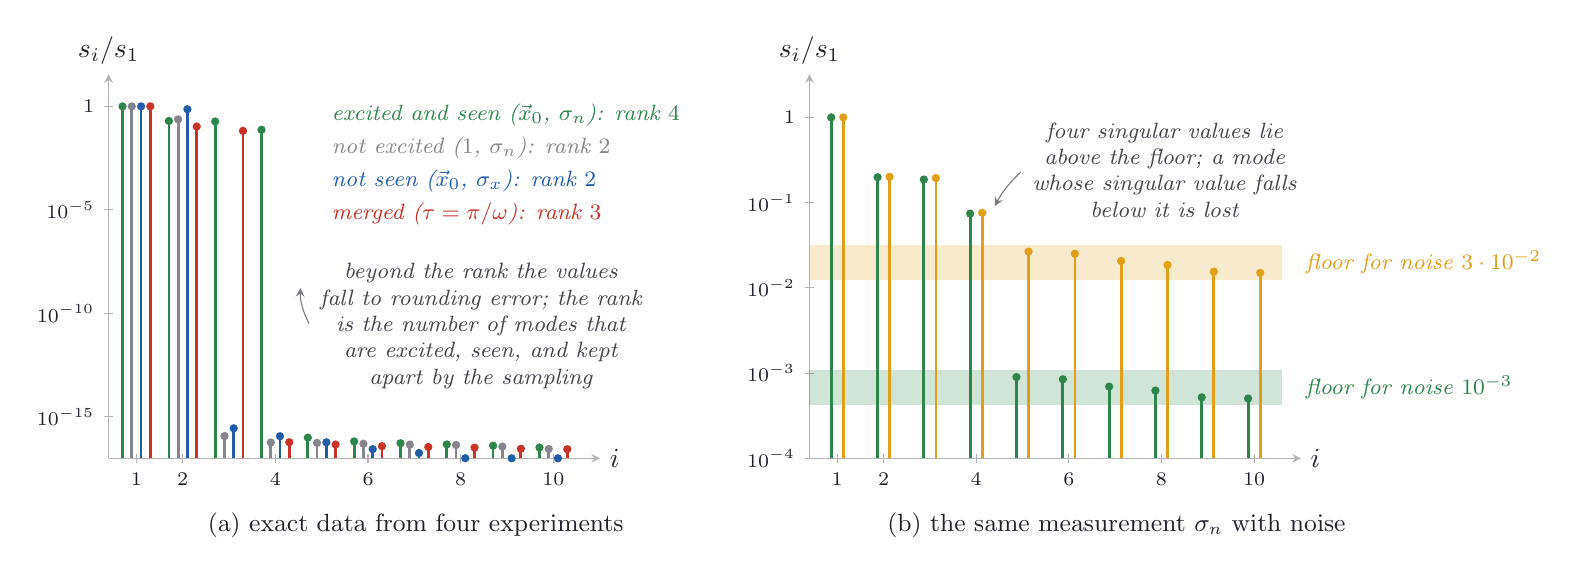
\begin{tikzpicture}[ink/.style={line width=0.9pt, ndInk}, faint/.style={line width=0.4pt, ndInk!35}, dashedink/.style={line width=0.5pt, ndInk!55, dash pattern=on 2.5pt off 2pt}, vec/.style={->, >=stealth, line width=1.2pt}, note/.style={font=\footnotesize\itshape, text=ndInk!85, align=center}, pointer/.style={->, >=stealth, line width=0.4pt, ndInk!60, shorten >=2pt, shorten <=1pt}, dot/.style={circle, fill=ndInk, inner sep=0pt, minimum size=3.4pt}, wash/.style={fill=ndSky, fill opacity=0.55}, every node/.style={text=ndInk}]
\definecolor{ndInk}{rgb}{0.13,0.13,0.18}
\definecolor{ndPaper}{rgb}{0.99,0.96,0.88}
\definecolor{ndSky}{rgb}{0.84,0.91,0.98}
\definecolor{ndRose}{rgb}{0.98,0.86,0.84}
\definecolor{ndBlue}{rgb}{0.13,0.36,0.66}
\definecolor{ndRed}{rgb}{0.78,0.20,0.16}
\definecolor{ndGold}{rgb}{0.88,0.62,0.10}
\definecolor{ndGreen}{rgb}{0.18,0.52,0.30}
\draw[faint, ->, >=stealth] (0.000,0.000) -- (6.240,0.000) node[right, text=ndInk] {$i$};
\draw[faint, ->, >=stealth] (0.000,0.000) -- (0.000,4.876) node[above, text=ndInk] {$s_i/s_1$};
\draw[faint] (0.353,0.060) -- (0.353,-0.060) node[below, font=\scriptsize, text=ndInk] {$1$};
\draw[faint] (0.941,0.060) -- (0.941,-0.060) node[below, font=\scriptsize, text=ndInk] {$2$};
\draw[faint] (2.118,0.060) -- (2.118,-0.060) node[below, font=\scriptsize, text=ndInk] {$4$};
\draw[faint] (3.294,0.060) -- (3.294,-0.060) node[below, font=\scriptsize, text=ndInk] {$6$};
\draw[faint] (4.471,0.060) -- (4.471,-0.060) node[below, font=\scriptsize, text=ndInk] {$8$};
\draw[faint] (5.647,0.060) -- (5.647,-0.060) node[below, font=\scriptsize, text=ndInk] {$10$};
\draw[faint] (0.060,4.469) -- (-0.060,4.469) node[left, font=\scriptsize, text=ndInk] {$1$};
\draw[faint] (0.060,3.154) -- (-0.060,3.154) node[left, font=\scriptsize, text=ndInk] {$10^{-5}$};
\draw[faint] (0.060,1.840) -- (-0.060,1.840) node[left, font=\scriptsize, text=ndInk] {$10^{-10}$};
\draw[faint] (0.060,0.526) -- (-0.060,0.526) node[left, font=\scriptsize, text=ndInk] {$10^{-15}$};
\draw[line width=1.0pt, ndGreen] (0.176,0.000) -- (0.176,4.469);
\fill[ndGreen] (0.176,4.469) circle (1.5pt);
\draw[line width=1.0pt, ndGreen] (0.765,0.000) -- (0.765,4.284);
\fill[ndGreen] (0.765,4.284) circle (1.5pt);
\draw[line width=1.0pt, ndGreen] (1.353,0.000) -- (1.353,4.277);
\fill[ndGreen] (1.353,4.277) circle (1.5pt);
\draw[line width=1.0pt, ndGreen] (1.941,0.000) -- (1.941,4.172);
\fill[ndGreen] (1.941,4.172) circle (1.5pt);
\draw[line width=1.0pt, ndGreen] (2.529,0.000) -- (2.529,0.262);
\fill[ndGreen] (2.529,0.262) circle (1.5pt);
\draw[line width=1.0pt, ndGreen] (3.118,0.000) -- (3.118,0.214);
\fill[ndGreen] (3.118,0.214) circle (1.5pt);
\draw[line width=1.0pt, ndGreen] (3.706,0.000) -- (3.706,0.191);
\fill[ndGreen] (3.706,0.191) circle (1.5pt);
\draw[line width=1.0pt, ndGreen] (4.294,0.000) -- (4.294,0.176);
\fill[ndGreen] (4.294,0.176) circle (1.5pt);
\draw[line width=1.0pt, ndGreen] (4.882,0.000) -- (4.882,0.160);
\fill[ndGreen] (4.882,0.160) circle (1.5pt);
\draw[line width=1.0pt, ndGreen] (5.471,0.000) -- (5.471,0.137);
\fill[ndGreen] (5.471,0.137) circle (1.5pt);
\draw[line width=1.0pt, ndInk!55] (0.294,0.000) -- (0.294,4.469);
\fill[ndInk!55] (0.294,4.469) circle (1.5pt);
\draw[line width=1.0pt, ndInk!55] (0.882,0.000) -- (0.882,4.304);
\fill[ndInk!55] (0.882,4.304) circle (1.5pt);
\draw[line width=1.0pt, ndInk!55] (1.471,0.000) -- (1.471,0.282);
\fill[ndInk!55] (1.471,0.282) circle (1.5pt);
\draw[line width=1.0pt, ndInk!55] (2.059,0.000) -- (2.059,0.201);
\fill[ndInk!55] (2.059,0.201) circle (1.5pt);
\draw[line width=1.0pt, ndInk!55] (2.647,0.000) -- (2.647,0.195);
\fill[ndInk!55] (2.647,0.195) circle (1.5pt);
\draw[line width=1.0pt, ndInk!55] (3.235,0.000) -- (3.235,0.185);
\fill[ndInk!55] (3.235,0.185) circle (1.5pt);
\draw[line width=1.0pt, ndInk!55] (3.824,0.000) -- (3.824,0.174);
\fill[ndInk!55] (3.824,0.174) circle (1.5pt);
\draw[line width=1.0pt, ndInk!55] (4.412,0.000) -- (4.412,0.169);
\fill[ndInk!55] (4.412,0.169) circle (1.5pt);
\draw[line width=1.0pt, ndInk!55] (5.000,0.000) -- (5.000,0.149);
\fill[ndInk!55] (5.000,0.149) circle (1.5pt);
\draw[line width=1.0pt, ndInk!55] (5.588,0.000) -- (5.588,0.118);
\fill[ndInk!55] (5.588,0.118) circle (1.5pt);
\draw[line width=1.0pt, ndBlue] (0.412,0.000) -- (0.412,4.469);
\fill[ndBlue] (0.412,4.469) circle (1.5pt);
\draw[line width=1.0pt, ndBlue] (1.000,0.000) -- (1.000,4.433);
\fill[ndBlue] (1.000,4.433) circle (1.5pt);
\draw[line width=1.0pt, ndBlue] (1.588,0.000) -- (1.588,0.381);
\fill[ndBlue] (1.588,0.381) circle (1.5pt);
\draw[line width=1.0pt, ndBlue] (2.176,0.000) -- (2.176,0.280);
\fill[ndBlue] (2.176,0.280) circle (1.5pt);
\draw[line width=1.0pt, ndBlue] (2.765,0.000) -- (2.765,0.203);
\fill[ndBlue] (2.765,0.203) circle (1.5pt);
\draw[line width=1.0pt, ndBlue] (3.353,0.000) -- (3.353,0.116);
\fill[ndBlue] (3.353,0.116) circle (1.5pt);
\draw[line width=1.0pt, ndBlue] (3.941,0.000) -- (3.941,0.067);
\fill[ndBlue] (3.941,0.067) circle (1.5pt);
\draw[line width=1.0pt, ndBlue] (4.529,0.000) -- (4.529,0.001);
\fill[ndBlue] (4.529,0.001) circle (1.5pt);
\draw[line width=1.0pt, ndBlue] (5.118,0.000) -- (5.118,0.000);
\fill[ndBlue] (5.118,0.000) circle (1.5pt);
\draw[line width=1.0pt, ndBlue] (5.706,0.000) -- (5.706,0.000);
\fill[ndBlue] (5.706,0.000) circle (1.5pt);
\draw[line width=1.0pt, ndRed] (0.529,0.000) -- (0.529,4.469);
\fill[ndRed] (0.529,4.469) circle (1.5pt);
\draw[line width=1.0pt, ndRed] (1.118,0.000) -- (1.118,4.213);
\fill[ndRed] (1.118,4.213) circle (1.5pt);
\draw[line width=1.0pt, ndRed] (1.706,0.000) -- (1.706,4.158);
\fill[ndRed] (1.706,4.158) circle (1.5pt);
\draw[line width=1.0pt, ndRed] (2.294,0.000) -- (2.294,0.204);
\fill[ndRed] (2.294,0.204) circle (1.5pt);
\draw[line width=1.0pt, ndRed] (2.882,0.000) -- (2.882,0.175);
\fill[ndRed] (2.882,0.175) circle (1.5pt);
\draw[line width=1.0pt, ndRed] (3.471,0.000) -- (3.471,0.154);
\fill[ndRed] (3.471,0.154) circle (1.5pt);
\draw[line width=1.0pt, ndRed] (4.059,0.000) -- (4.059,0.143);
\fill[ndRed] (4.059,0.143) circle (1.5pt);
\draw[line width=1.0pt, ndRed] (4.647,0.000) -- (4.647,0.135);
\fill[ndRed] (4.647,0.135) circle (1.5pt);
\draw[line width=1.0pt, ndRed] (5.235,0.000) -- (5.235,0.121);
\fill[ndRed] (5.235,0.121) circle (1.5pt);
\draw[line width=1.0pt, ndRed] (5.824,0.000) -- (5.824,0.115);
\fill[ndRed] (5.824,0.115) circle (1.5pt);
\node[note, anchor=west, text=ndGreen] at (2.71,4.36) {excited and seen ($\vec x_0$, $\sigma_n$): rank $4$};
\node[note, anchor=west, text=ndInk!55] at (2.71,3.94) {not excited ($\ket1$, $\sigma_n$): rank $2$};
\node[note, anchor=west, text=ndBlue] at (2.71,3.52) {not seen ($\vec x_0$, $\sigma_x$): rank $2$};
\node[note, anchor=west, text=ndRed] at (2.71,3.10) {merged ($\tau=\pi/\omega$): rank $3$};
\node[note, anchor=west] (c) at (2.56,1.68) {beyond the rank the values\\ fall to rounding error; the rank\\ is the number of modes that\\ are excited, seen, and kept\\ apart by the sampling};
\draw[pointer] (c.west) to[bend left=15] (2.441,2.234);
\node[font=\small] at (3.900,-0.850) {(a) exact data from four experiments};
\draw[faint, ->, >=stealth] (8.900,0.000) -- (15.140,0.000) node[right, text=ndInk] {$i$};
\draw[faint, ->, >=stealth] (8.900,0.000) -- (8.900,4.876) node[above, text=ndInk] {$s_i/s_1$};
\draw[faint] (9.253,0.060) -- (9.253,-0.060) node[below, font=\scriptsize, text=ndInk] {$1$};
\draw[faint] (9.841,0.060) -- (9.841,-0.060) node[below, font=\scriptsize, text=ndInk] {$2$};
\draw[faint] (11.018,0.060) -- (11.018,-0.060) node[below, font=\scriptsize, text=ndInk] {$4$};
\draw[faint] (12.194,0.060) -- (12.194,-0.060) node[below, font=\scriptsize, text=ndInk] {$6$};
\draw[faint] (13.371,0.060) -- (13.371,-0.060) node[below, font=\scriptsize, text=ndInk] {$8$};
\draw[faint] (14.547,0.060) -- (14.547,-0.060) node[below, font=\scriptsize, text=ndInk] {$10$};
\draw[faint] (8.960,4.329) -- (8.840,4.329) node[left, font=\scriptsize, text=ndInk] {$1$};
\draw[faint] (8.960,3.247) -- (8.840,3.247) node[left, font=\scriptsize, text=ndInk] {$10^{-1}$};
\draw[faint] (8.960,2.165) -- (8.840,2.165) node[left, font=\scriptsize, text=ndInk] {$10^{-2}$};
\draw[faint] (8.960,1.082) -- (8.840,1.082) node[left, font=\scriptsize, text=ndInk] {$10^{-3}$};
\draw[faint] (8.960,0.000) -- (8.840,0.000) node[left, font=\scriptsize, text=ndInk] {$10^{-4}$};
\fill[ndGreen, fill opacity=0.22] (8.900,0.673) rectangle (14.900,1.118);
\fill[ndGold, fill opacity=0.22] (8.900,2.269) rectangle (14.900,2.713);
\draw[line width=1.0pt, ndGreen] (9.176,0.000) -- (9.176,4.329);
\fill[ndGreen] (9.176,4.329) circle (1.5pt);
\draw[line width=1.0pt, ndGreen] (9.765,0.000) -- (9.765,3.569);
\fill[ndGreen] (9.765,3.569) circle (1.5pt);
\draw[line width=1.0pt, ndGreen] (10.353,0.000) -- (10.353,3.540);
\fill[ndGreen] (10.353,3.540) circle (1.5pt);
\draw[line width=1.0pt, ndGreen] (10.941,0.000) -- (10.941,3.107);
\fill[ndGreen] (10.941,3.107) circle (1.5pt);
\draw[line width=1.0pt, ndGreen] (11.529,0.000) -- (11.529,1.031);
\fill[ndGreen] (11.529,1.031) circle (1.5pt);
\draw[line width=1.0pt, ndGreen] (12.118,0.000) -- (12.118,1.003);
\fill[ndGreen] (12.118,1.003) circle (1.5pt);
\draw[line width=1.0pt, ndGreen] (12.706,0.000) -- (12.706,0.910);
\fill[ndGreen] (12.706,0.910) circle (1.5pt);
\draw[line width=1.0pt, ndGreen] (13.294,0.000) -- (13.294,0.860);
\fill[ndGreen] (13.294,0.860) circle (1.5pt);
\draw[line width=1.0pt, ndGreen] (13.882,0.000) -- (13.882,0.774);
\fill[ndGreen] (13.882,0.774) circle (1.5pt);
\draw[line width=1.0pt, ndGreen] (14.471,0.000) -- (14.471,0.760);
\fill[ndGreen] (14.471,0.760) circle (1.5pt);
\draw[line width=1.0pt, ndGold] (9.329,0.000) -- (9.329,4.329);
\fill[ndGold] (9.329,4.329) circle (1.5pt);
\draw[line width=1.0pt, ndGold] (9.918,0.000) -- (9.918,3.574);
\fill[ndGold] (9.918,3.574) circle (1.5pt);
\draw[line width=1.0pt, ndGold] (10.506,0.000) -- (10.506,3.559);
\fill[ndGold] (10.506,3.559) circle (1.5pt);
\draw[line width=1.0pt, ndGold] (11.094,0.000) -- (11.094,3.118);
\fill[ndGold] (11.094,3.118) circle (1.5pt);
\draw[line width=1.0pt, ndGold] (11.682,0.000) -- (11.682,2.626);
\fill[ndGold] (11.682,2.626) circle (1.5pt);
\draw[line width=1.0pt, ndGold] (12.271,0.000) -- (12.271,2.598);
\fill[ndGold] (12.271,2.598) circle (1.5pt);
\draw[line width=1.0pt, ndGold] (12.859,0.000) -- (12.859,2.506);
\fill[ndGold] (12.859,2.506) circle (1.5pt);
\draw[line width=1.0pt, ndGold] (13.447,0.000) -- (13.447,2.455);
\fill[ndGold] (13.447,2.455) circle (1.5pt);
\draw[line width=1.0pt, ndGold] (14.035,0.000) -- (14.035,2.371);
\fill[ndGold] (14.035,2.371) circle (1.5pt);
\draw[line width=1.0pt, ndGold] (14.624,0.000) -- (14.624,2.355);
\fill[ndGold] (14.624,2.355) circle (1.5pt);
\node[note, anchor=west, text=ndGreen] at (15.08,0.90) {floor for noise $10^{-3}$};
\node[note, anchor=west, text=ndGold] at (15.08,2.49) {floor for noise $3\cdot10^{-2}$};
\node[note, anchor=west] (f) at (11.61,3.66) {four singular values lie\\ above the floor; a mode\\ whose singular value falls\\ below it is lost};
\draw[pointer] (f.west) to[bend right=10] (11.224,3.140);
\node[font=\small] at (12.800,-0.850) {(b) the same measurement $\sigma_n$ with noise};
\end{tikzpicture}
}
\caption{Singular values, on a logarithmic scale, of the Hankel matrix $\Hankel(0)$ ($10$ block rows, $40$ columns) formed from $60$ samples of the example. (a) Exact data from four experiments, one for each case of Proposition~\ref{prop:ch05:modal}. The tilted state $\vec x_0$, measured along $\vec n$ and sampled every $\tau=0.25$, shows all four modes (rank $4$); the state $\ket1$ does not excite the precession (rank $2$); a measurement of $\sigma_x$ does not see the relaxation (rank $2$); sampling every $\tau=\pi/\omega$ makes $\ee^{(-\Gamma+\imath\omega)\tau}=\ee^{(-\Gamma-\imath\omega)\tau}$ and merges the two modes of the precession (rank $3$). Beyond the rank the singular values are at the level of rounding error. (b) The first experiment with Gaussian noise of standard deviation $10^{-3}$ and $3\cdot10^{-2}$ on each sample: the singular values now level off at a noise floor (shaded), which rises with the noise, and a mode whose singular value falls below the floor is lost. Generated by \texttt{code/ch05\_hankel.py}.}\label{fig:ch05:hankel}
\end{figure}}
\onp{\begin{center}\resizebox{\linewidth}{!}{% Generated by code/needham.py -- do not edit by hand.
\definecolor{qocA}{rgb}{0.00,0.45,0.70}
\definecolor{qocB}{rgb}{0.90,0.60,0.00}
\definecolor{qocC}{rgb}{0.00,0.62,0.45}
\definecolor{qocD}{rgb}{0.80,0.40,0.00}
\definecolor{qocE}{rgb}{0.80,0.60,0.70}
\definecolor{qocF}{rgb}{0.35,0.70,0.90}
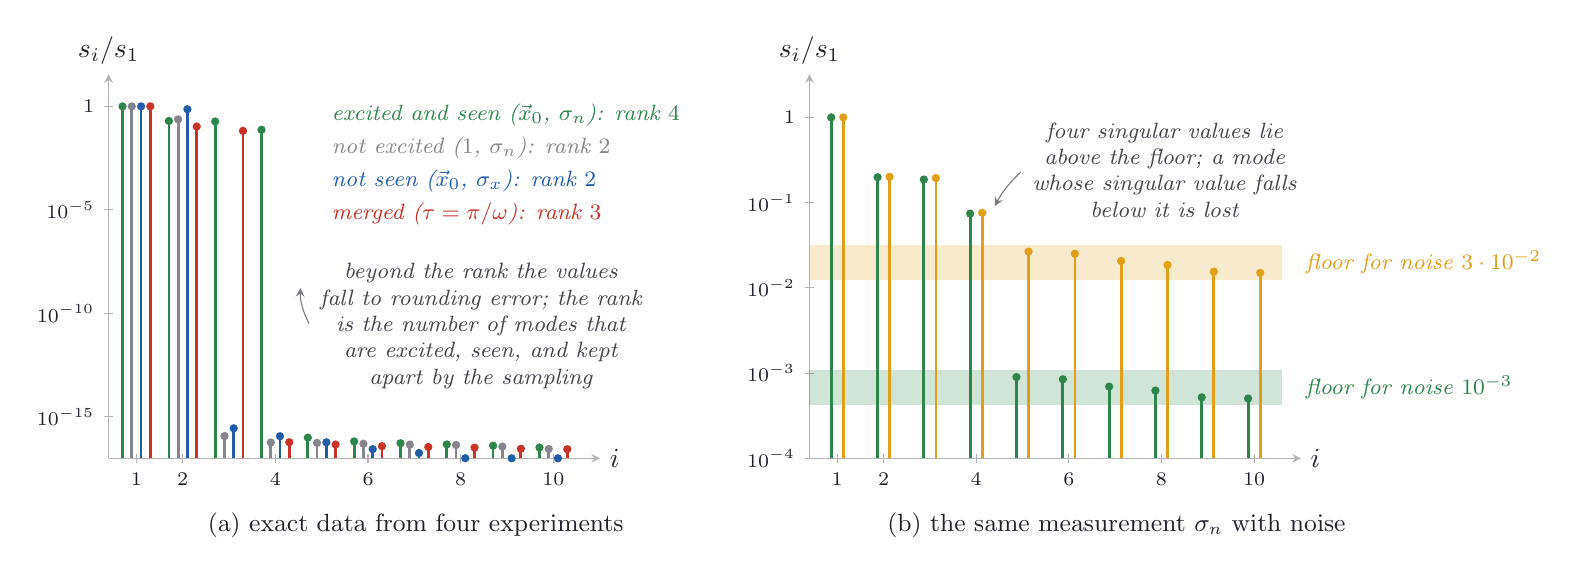
\begin{tikzpicture}[ink/.style={line width=0.9pt, ndInk}, faint/.style={line width=0.4pt, ndInk!35}, dashedink/.style={line width=0.5pt, ndInk!55, dash pattern=on 2.5pt off 2pt}, vec/.style={->, >=stealth, line width=1.2pt}, note/.style={font=\footnotesize\itshape, text=ndInk!85, align=center}, pointer/.style={->, >=stealth, line width=0.4pt, ndInk!60, shorten >=2pt, shorten <=1pt}, dot/.style={circle, fill=ndInk, inner sep=0pt, minimum size=3.4pt}, wash/.style={fill=ndSky, fill opacity=0.55}, every node/.style={text=ndInk}]
\definecolor{ndInk}{rgb}{0.13,0.13,0.18}
\definecolor{ndPaper}{rgb}{0.99,0.96,0.88}
\definecolor{ndSky}{rgb}{0.84,0.91,0.98}
\definecolor{ndRose}{rgb}{0.98,0.86,0.84}
\definecolor{ndBlue}{rgb}{0.13,0.36,0.66}
\definecolor{ndRed}{rgb}{0.78,0.20,0.16}
\definecolor{ndGold}{rgb}{0.88,0.62,0.10}
\definecolor{ndGreen}{rgb}{0.18,0.52,0.30}
\draw[faint, ->, >=stealth] (0.000,0.000) -- (6.240,0.000) node[right, text=ndInk] {$i$};
\draw[faint, ->, >=stealth] (0.000,0.000) -- (0.000,4.876) node[above, text=ndInk] {$s_i/s_1$};
\draw[faint] (0.353,0.060) -- (0.353,-0.060) node[below, font=\scriptsize, text=ndInk] {$1$};
\draw[faint] (0.941,0.060) -- (0.941,-0.060) node[below, font=\scriptsize, text=ndInk] {$2$};
\draw[faint] (2.118,0.060) -- (2.118,-0.060) node[below, font=\scriptsize, text=ndInk] {$4$};
\draw[faint] (3.294,0.060) -- (3.294,-0.060) node[below, font=\scriptsize, text=ndInk] {$6$};
\draw[faint] (4.471,0.060) -- (4.471,-0.060) node[below, font=\scriptsize, text=ndInk] {$8$};
\draw[faint] (5.647,0.060) -- (5.647,-0.060) node[below, font=\scriptsize, text=ndInk] {$10$};
\draw[faint] (0.060,4.469) -- (-0.060,4.469) node[left, font=\scriptsize, text=ndInk] {$1$};
\draw[faint] (0.060,3.154) -- (-0.060,3.154) node[left, font=\scriptsize, text=ndInk] {$10^{-5}$};
\draw[faint] (0.060,1.840) -- (-0.060,1.840) node[left, font=\scriptsize, text=ndInk] {$10^{-10}$};
\draw[faint] (0.060,0.526) -- (-0.060,0.526) node[left, font=\scriptsize, text=ndInk] {$10^{-15}$};
\draw[line width=1.0pt, ndGreen] (0.176,0.000) -- (0.176,4.469);
\fill[ndGreen] (0.176,4.469) circle (1.5pt);
\draw[line width=1.0pt, ndGreen] (0.765,0.000) -- (0.765,4.284);
\fill[ndGreen] (0.765,4.284) circle (1.5pt);
\draw[line width=1.0pt, ndGreen] (1.353,0.000) -- (1.353,4.277);
\fill[ndGreen] (1.353,4.277) circle (1.5pt);
\draw[line width=1.0pt, ndGreen] (1.941,0.000) -- (1.941,4.172);
\fill[ndGreen] (1.941,4.172) circle (1.5pt);
\draw[line width=1.0pt, ndGreen] (2.529,0.000) -- (2.529,0.262);
\fill[ndGreen] (2.529,0.262) circle (1.5pt);
\draw[line width=1.0pt, ndGreen] (3.118,0.000) -- (3.118,0.214);
\fill[ndGreen] (3.118,0.214) circle (1.5pt);
\draw[line width=1.0pt, ndGreen] (3.706,0.000) -- (3.706,0.191);
\fill[ndGreen] (3.706,0.191) circle (1.5pt);
\draw[line width=1.0pt, ndGreen] (4.294,0.000) -- (4.294,0.176);
\fill[ndGreen] (4.294,0.176) circle (1.5pt);
\draw[line width=1.0pt, ndGreen] (4.882,0.000) -- (4.882,0.160);
\fill[ndGreen] (4.882,0.160) circle (1.5pt);
\draw[line width=1.0pt, ndGreen] (5.471,0.000) -- (5.471,0.137);
\fill[ndGreen] (5.471,0.137) circle (1.5pt);
\draw[line width=1.0pt, ndInk!55] (0.294,0.000) -- (0.294,4.469);
\fill[ndInk!55] (0.294,4.469) circle (1.5pt);
\draw[line width=1.0pt, ndInk!55] (0.882,0.000) -- (0.882,4.304);
\fill[ndInk!55] (0.882,4.304) circle (1.5pt);
\draw[line width=1.0pt, ndInk!55] (1.471,0.000) -- (1.471,0.282);
\fill[ndInk!55] (1.471,0.282) circle (1.5pt);
\draw[line width=1.0pt, ndInk!55] (2.059,0.000) -- (2.059,0.201);
\fill[ndInk!55] (2.059,0.201) circle (1.5pt);
\draw[line width=1.0pt, ndInk!55] (2.647,0.000) -- (2.647,0.195);
\fill[ndInk!55] (2.647,0.195) circle (1.5pt);
\draw[line width=1.0pt, ndInk!55] (3.235,0.000) -- (3.235,0.185);
\fill[ndInk!55] (3.235,0.185) circle (1.5pt);
\draw[line width=1.0pt, ndInk!55] (3.824,0.000) -- (3.824,0.174);
\fill[ndInk!55] (3.824,0.174) circle (1.5pt);
\draw[line width=1.0pt, ndInk!55] (4.412,0.000) -- (4.412,0.169);
\fill[ndInk!55] (4.412,0.169) circle (1.5pt);
\draw[line width=1.0pt, ndInk!55] (5.000,0.000) -- (5.000,0.149);
\fill[ndInk!55] (5.000,0.149) circle (1.5pt);
\draw[line width=1.0pt, ndInk!55] (5.588,0.000) -- (5.588,0.118);
\fill[ndInk!55] (5.588,0.118) circle (1.5pt);
\draw[line width=1.0pt, ndBlue] (0.412,0.000) -- (0.412,4.469);
\fill[ndBlue] (0.412,4.469) circle (1.5pt);
\draw[line width=1.0pt, ndBlue] (1.000,0.000) -- (1.000,4.433);
\fill[ndBlue] (1.000,4.433) circle (1.5pt);
\draw[line width=1.0pt, ndBlue] (1.588,0.000) -- (1.588,0.381);
\fill[ndBlue] (1.588,0.381) circle (1.5pt);
\draw[line width=1.0pt, ndBlue] (2.176,0.000) -- (2.176,0.280);
\fill[ndBlue] (2.176,0.280) circle (1.5pt);
\draw[line width=1.0pt, ndBlue] (2.765,0.000) -- (2.765,0.203);
\fill[ndBlue] (2.765,0.203) circle (1.5pt);
\draw[line width=1.0pt, ndBlue] (3.353,0.000) -- (3.353,0.116);
\fill[ndBlue] (3.353,0.116) circle (1.5pt);
\draw[line width=1.0pt, ndBlue] (3.941,0.000) -- (3.941,0.067);
\fill[ndBlue] (3.941,0.067) circle (1.5pt);
\draw[line width=1.0pt, ndBlue] (4.529,0.000) -- (4.529,0.001);
\fill[ndBlue] (4.529,0.001) circle (1.5pt);
\draw[line width=1.0pt, ndBlue] (5.118,0.000) -- (5.118,0.000);
\fill[ndBlue] (5.118,0.000) circle (1.5pt);
\draw[line width=1.0pt, ndBlue] (5.706,0.000) -- (5.706,0.000);
\fill[ndBlue] (5.706,0.000) circle (1.5pt);
\draw[line width=1.0pt, ndRed] (0.529,0.000) -- (0.529,4.469);
\fill[ndRed] (0.529,4.469) circle (1.5pt);
\draw[line width=1.0pt, ndRed] (1.118,0.000) -- (1.118,4.213);
\fill[ndRed] (1.118,4.213) circle (1.5pt);
\draw[line width=1.0pt, ndRed] (1.706,0.000) -- (1.706,4.158);
\fill[ndRed] (1.706,4.158) circle (1.5pt);
\draw[line width=1.0pt, ndRed] (2.294,0.000) -- (2.294,0.204);
\fill[ndRed] (2.294,0.204) circle (1.5pt);
\draw[line width=1.0pt, ndRed] (2.882,0.000) -- (2.882,0.175);
\fill[ndRed] (2.882,0.175) circle (1.5pt);
\draw[line width=1.0pt, ndRed] (3.471,0.000) -- (3.471,0.154);
\fill[ndRed] (3.471,0.154) circle (1.5pt);
\draw[line width=1.0pt, ndRed] (4.059,0.000) -- (4.059,0.143);
\fill[ndRed] (4.059,0.143) circle (1.5pt);
\draw[line width=1.0pt, ndRed] (4.647,0.000) -- (4.647,0.135);
\fill[ndRed] (4.647,0.135) circle (1.5pt);
\draw[line width=1.0pt, ndRed] (5.235,0.000) -- (5.235,0.121);
\fill[ndRed] (5.235,0.121) circle (1.5pt);
\draw[line width=1.0pt, ndRed] (5.824,0.000) -- (5.824,0.115);
\fill[ndRed] (5.824,0.115) circle (1.5pt);
\node[note, anchor=west, text=ndGreen] at (2.71,4.36) {excited and seen ($\vec x_0$, $\sigma_n$): rank $4$};
\node[note, anchor=west, text=ndInk!55] at (2.71,3.94) {not excited ($\ket1$, $\sigma_n$): rank $2$};
\node[note, anchor=west, text=ndBlue] at (2.71,3.52) {not seen ($\vec x_0$, $\sigma_x$): rank $2$};
\node[note, anchor=west, text=ndRed] at (2.71,3.10) {merged ($\tau=\pi/\omega$): rank $3$};
\node[note, anchor=west] (c) at (2.56,1.68) {beyond the rank the values\\ fall to rounding error; the rank\\ is the number of modes that\\ are excited, seen, and kept\\ apart by the sampling};
\draw[pointer] (c.west) to[bend left=15] (2.441,2.234);
\node[font=\small] at (3.900,-0.850) {(a) exact data from four experiments};
\draw[faint, ->, >=stealth] (8.900,0.000) -- (15.140,0.000) node[right, text=ndInk] {$i$};
\draw[faint, ->, >=stealth] (8.900,0.000) -- (8.900,4.876) node[above, text=ndInk] {$s_i/s_1$};
\draw[faint] (9.253,0.060) -- (9.253,-0.060) node[below, font=\scriptsize, text=ndInk] {$1$};
\draw[faint] (9.841,0.060) -- (9.841,-0.060) node[below, font=\scriptsize, text=ndInk] {$2$};
\draw[faint] (11.018,0.060) -- (11.018,-0.060) node[below, font=\scriptsize, text=ndInk] {$4$};
\draw[faint] (12.194,0.060) -- (12.194,-0.060) node[below, font=\scriptsize, text=ndInk] {$6$};
\draw[faint] (13.371,0.060) -- (13.371,-0.060) node[below, font=\scriptsize, text=ndInk] {$8$};
\draw[faint] (14.547,0.060) -- (14.547,-0.060) node[below, font=\scriptsize, text=ndInk] {$10$};
\draw[faint] (8.960,4.329) -- (8.840,4.329) node[left, font=\scriptsize, text=ndInk] {$1$};
\draw[faint] (8.960,3.247) -- (8.840,3.247) node[left, font=\scriptsize, text=ndInk] {$10^{-1}$};
\draw[faint] (8.960,2.165) -- (8.840,2.165) node[left, font=\scriptsize, text=ndInk] {$10^{-2}$};
\draw[faint] (8.960,1.082) -- (8.840,1.082) node[left, font=\scriptsize, text=ndInk] {$10^{-3}$};
\draw[faint] (8.960,0.000) -- (8.840,0.000) node[left, font=\scriptsize, text=ndInk] {$10^{-4}$};
\fill[ndGreen, fill opacity=0.22] (8.900,0.673) rectangle (14.900,1.118);
\fill[ndGold, fill opacity=0.22] (8.900,2.269) rectangle (14.900,2.713);
\draw[line width=1.0pt, ndGreen] (9.176,0.000) -- (9.176,4.329);
\fill[ndGreen] (9.176,4.329) circle (1.5pt);
\draw[line width=1.0pt, ndGreen] (9.765,0.000) -- (9.765,3.569);
\fill[ndGreen] (9.765,3.569) circle (1.5pt);
\draw[line width=1.0pt, ndGreen] (10.353,0.000) -- (10.353,3.540);
\fill[ndGreen] (10.353,3.540) circle (1.5pt);
\draw[line width=1.0pt, ndGreen] (10.941,0.000) -- (10.941,3.107);
\fill[ndGreen] (10.941,3.107) circle (1.5pt);
\draw[line width=1.0pt, ndGreen] (11.529,0.000) -- (11.529,1.031);
\fill[ndGreen] (11.529,1.031) circle (1.5pt);
\draw[line width=1.0pt, ndGreen] (12.118,0.000) -- (12.118,1.003);
\fill[ndGreen] (12.118,1.003) circle (1.5pt);
\draw[line width=1.0pt, ndGreen] (12.706,0.000) -- (12.706,0.910);
\fill[ndGreen] (12.706,0.910) circle (1.5pt);
\draw[line width=1.0pt, ndGreen] (13.294,0.000) -- (13.294,0.860);
\fill[ndGreen] (13.294,0.860) circle (1.5pt);
\draw[line width=1.0pt, ndGreen] (13.882,0.000) -- (13.882,0.774);
\fill[ndGreen] (13.882,0.774) circle (1.5pt);
\draw[line width=1.0pt, ndGreen] (14.471,0.000) -- (14.471,0.760);
\fill[ndGreen] (14.471,0.760) circle (1.5pt);
\draw[line width=1.0pt, ndGold] (9.329,0.000) -- (9.329,4.329);
\fill[ndGold] (9.329,4.329) circle (1.5pt);
\draw[line width=1.0pt, ndGold] (9.918,0.000) -- (9.918,3.574);
\fill[ndGold] (9.918,3.574) circle (1.5pt);
\draw[line width=1.0pt, ndGold] (10.506,0.000) -- (10.506,3.559);
\fill[ndGold] (10.506,3.559) circle (1.5pt);
\draw[line width=1.0pt, ndGold] (11.094,0.000) -- (11.094,3.118);
\fill[ndGold] (11.094,3.118) circle (1.5pt);
\draw[line width=1.0pt, ndGold] (11.682,0.000) -- (11.682,2.626);
\fill[ndGold] (11.682,2.626) circle (1.5pt);
\draw[line width=1.0pt, ndGold] (12.271,0.000) -- (12.271,2.598);
\fill[ndGold] (12.271,2.598) circle (1.5pt);
\draw[line width=1.0pt, ndGold] (12.859,0.000) -- (12.859,2.506);
\fill[ndGold] (12.859,2.506) circle (1.5pt);
\draw[line width=1.0pt, ndGold] (13.447,0.000) -- (13.447,2.455);
\fill[ndGold] (13.447,2.455) circle (1.5pt);
\draw[line width=1.0pt, ndGold] (14.035,0.000) -- (14.035,2.371);
\fill[ndGold] (14.035,2.371) circle (1.5pt);
\draw[line width=1.0pt, ndGold] (14.624,0.000) -- (14.624,2.355);
\fill[ndGold] (14.624,2.355) circle (1.5pt);
\node[note, anchor=west, text=ndGreen] at (15.08,0.90) {floor for noise $10^{-3}$};
\node[note, anchor=west, text=ndGold] at (15.08,2.49) {floor for noise $3\cdot10^{-2}$};
\node[note, anchor=west] (f) at (11.61,3.66) {four singular values lie\\ above the floor; a mode\\ whose singular value falls\\ below it is lost};
\draw[pointer] (f.west) to[bend right=10] (11.224,3.140);
\node[font=\small] at (12.800,-0.850) {(b) the same measurement $\sigma_n$ with noise};
\end{tikzpicture}
}\end{center}
{\small Rank $4$ when all is well; $2$ when the precession is not excited; $2$ when the relaxation is not seen; $3$ when the sampling merges two modes.}}
\end{frame}

\begin{frame}\ft{Ho--Kalman and the eigensystem realisation algorithm}
\ona{The factorisation \eqref{eq:ch05:hankel} can be reversed. Once the evolution of an open quantum system has been written as a linear dynamical system, the established techniques of system identification become available \citep{ljung1999system}. One such algorithm was proposed by \citet{Zhang2015}, who wrote the Lindbladian dynamics of an uncontrolled system as a linear time-invariant system and used the eigensystem realisation algorithm (ERA) \citep{Kung1978ANI} to obtain a discrete realisation of the system matrix. In outline, one forms the generalised Hankel matrix $\Hankel_{rs}(k)\in\R^{rp\times s}$ from the outputs of the $p$ observables, and computes a singular value decomposition of $\Hankel_{rs}(0)$ with orthogonal matrices $\mathbf{P} = [\mathbf{P}_1\ \mathbf{P}_2]$ and $\mathbf{Q} = [\mathbf{Q}_1\ \mathbf{Q}_2]$ and the diagonal matrix $\mathbf{S}$ of the $n$ singular values that are significant at the accuracy available. A realisation of the discrete system matrix is then}
\onp{ERA \citep{Kung1978ANI,Zhang2015}: SVD $\Hankel_{rs}(0)=\mathbf P_1\mathbf S\mathbf Q_1^\top$ (rank $n$), then}
\begin{equation}\label{eq:ch05:era}
    \mathbf{A}_{d} = \mathbf{S}^{-1/2}\mathbf{P}_{1}^{\top}\Hankel_{rs}(1)\mathbf{Q}_{1}\mathbf{S}^{-1/2},\qquad
    \mathbf{C}_{d} = \mathsf{E}_{p}^{\top}\mathbf{P}_{1}\mathbf{S}^{1/2}, \qquad
    \vec{x}(0) = \mathbf{S}^{1/2}\mathbf{Q}_{1}^{\top}e_{1},
\end{equation}
\ona{where $\mathsf{E}_{p}^{\top} = [\Id_{p}, \mathbf{0}_{p}, \cdots, \mathbf{0}_{p}]$ selects the first $p$ rows and $e_{1}$ is the first column of $\Id_{s}$. The identity behind \eqref{eq:ch05:era} is $\Hankel_{rs}(1)=\Obsv_r\mathbf G_\tau\Ctrb_s$. Choosing the balanced factors $\Obsv_r=\mathbf P_1\mathbf S^{1/2}$ and $\Ctrb_s=\mathbf S^{1/2}\mathbf Q_1^\top$ and solving for $\mathbf G_\tau$ gives $\mathbf A_d$, which is similar to $\mathbf G_\tau$; the construction goes back to Ho and Kalman in 1966. With noisy data the singular value decomposition is truncated at the numerical rank, and here the singular values of the observability matrix (Figure~\ref{fig:ch04:singular} of \Chap~\ref{C.StateSpace}) enter: small singular values cannot be distinguished from noise, and the corresponding modes are lost. Since the input--output behaviour does not depend on the realisation, one may then pass to the Laplace domain and obtain polynomial equations whose solution yields the Hamiltonian and the Lindblad coefficients \citep{Zhang2015}; the alternative, followed in \Chap~\ref{C.StateSpace}, is to fix the coordinates by a known $\mathbf C$ and to invert the linear map $\mathbf M$. Figure~\ref{fig:ch05:era} follows the algorithm step by step on the data of our example. The data are arranged in two Hankel matrices, the large singular values are counted, the matrix is split into balanced factors, the one-step matrix is found, and its eigenvalues are converted back into rates and frequencies.}
\onp{Uses $\Hankel_{rs}(1)=\Obsv_r\mathbf G_\tau\Ctrb_s$ with balanced factors, so that $\mathbf A_d\sim\mathbf G_\tau$. With noise, truncate the SVD at the numerical rank; small singular values are lost modes.}
\end{frame}

\begin{frame}\ft{Ho--Kalman step by step}
\ona{\begin{figure}[H]\centering
\resizebox{\linewidth}{!}{% Generated by code/needham.py -- do not edit by hand.
\definecolor{qocA}{rgb}{0.00,0.45,0.70}
\definecolor{qocB}{rgb}{0.90,0.60,0.00}
\definecolor{qocC}{rgb}{0.00,0.62,0.45}
\definecolor{qocD}{rgb}{0.80,0.40,0.00}
\definecolor{qocE}{rgb}{0.80,0.60,0.70}
\definecolor{qocF}{rgb}{0.35,0.70,0.90}
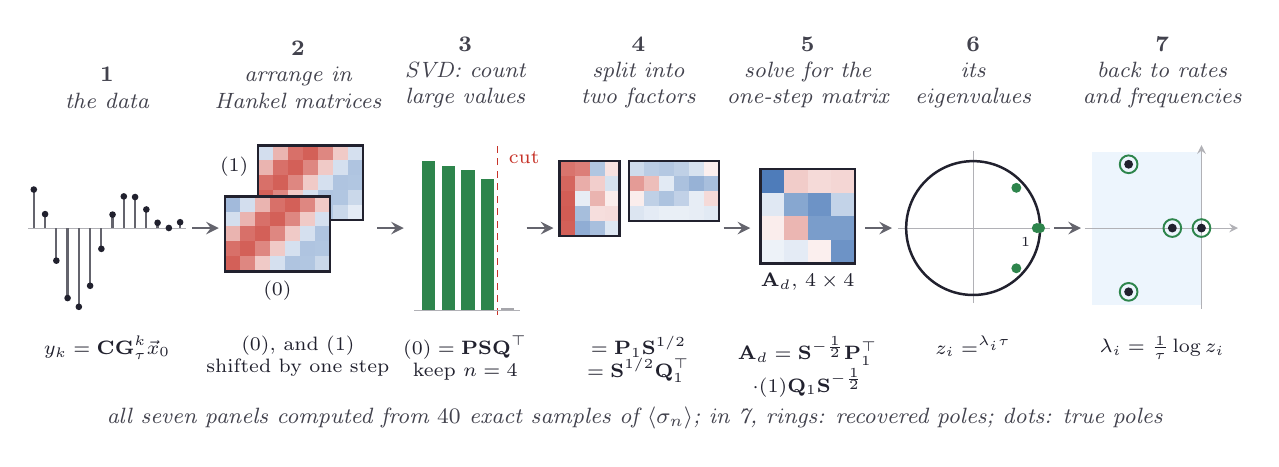
\begin{tikzpicture}[ink/.style={line width=0.9pt, ndInk}, faint/.style={line width=0.4pt, ndInk!35}, dashedink/.style={line width=0.5pt, ndInk!55, dash pattern=on 2.5pt off 2pt}, vec/.style={->, >=stealth, line width=1.2pt}, note/.style={font=\footnotesize\itshape, text=ndInk!85, align=center}, pointer/.style={->, >=stealth, line width=0.4pt, ndInk!60, shorten >=2pt, shorten <=1pt}, dot/.style={circle, fill=ndInk, inner sep=0pt, minimum size=3.4pt}, wash/.style={fill=ndSky, fill opacity=0.55}, every node/.style={text=ndInk}]
\definecolor{ndInk}{rgb}{0.13,0.13,0.18}
\definecolor{ndPaper}{rgb}{0.99,0.96,0.88}
\definecolor{ndSky}{rgb}{0.84,0.91,0.98}
\definecolor{ndRose}{rgb}{0.98,0.86,0.84}
\definecolor{ndBlue}{rgb}{0.13,0.36,0.66}
\definecolor{ndRed}{rgb}{0.78,0.20,0.16}
\definecolor{ndGold}{rgb}{0.88,0.62,0.10}
\definecolor{ndGreen}{rgb}{0.18,0.52,0.30}
\node[note, anchor=south] at (1.000,2.350) {\textup{\textbf{1}}\\ the data};
\node[font=\scriptsize, align=center, anchor=north] at (1.000,-0.300) {$y_k=\mathbf C\mathbf G_\tau^k\vec x_0$};
\node[note, anchor=south] at (3.425,2.350) {\textup{\textbf{2}}\\ arrange in\\ Hankel matrices};
\node[font=\scriptsize, align=center, anchor=north] at (3.425,-0.300) {$\Hankel(0)$, and $\Hankel(1)$\\ shifted by one step};
\draw[->, >=stealth, line width=1.0pt, ndInk!70] (2.080,0.950) -- (2.420,0.950);
\node[note, anchor=south] at (5.550,2.350) {\textup{\textbf{3}}\\ SVD: count\\ large values};
\node[font=\scriptsize, align=center, anchor=north] at (5.550,-0.300) {$\Hankel(0)=\mathbf P\mathbf S\mathbf Q^{\top}$\\ keep $n=4$};
\draw[->, >=stealth, line width=1.0pt, ndInk!70] (4.430,0.950) -- (4.770,0.950);
\node[note, anchor=south] at (7.750,2.350) {\textup{\textbf{4}}\\ split into\\ two factors};
\node[font=\scriptsize, align=center, anchor=north] at (7.750,-0.300) {$\Obsv=\mathbf P_1\mathbf S^{1/2}$\\ $\Ctrb=\mathbf S^{1/2}\mathbf Q_1^{\top}$};
\draw[->, >=stealth, line width=1.0pt, ndInk!70] (6.330,0.950) -- (6.670,0.950);
\node[note, anchor=south] at (9.900,2.350) {\textup{\textbf{5}}\\ solve for the\\ one-step matrix};
\node[font=\scriptsize, align=center, anchor=north] at (9.900,-0.300) {$\mathbf A_d=\mathbf S^{-\frac12}\mathbf P_1^{\top}$\\ $\cdot\Hankel(1)\mathbf Q_1\mathbf S^{-\frac12}$};
\draw[->, >=stealth, line width=1.0pt, ndInk!70] (8.830,0.950) -- (9.170,0.950);
\node[note, anchor=south] at (12.000,2.350) {\textup{\textbf{6}}\\ its\\ eigenvalues};
\node[font=\scriptsize, align=center, anchor=north] at (12.000,-0.300) {$z_i=\ee^{\lambda_i\tau}$};
\draw[->, >=stealth, line width=1.0pt, ndInk!70] (10.630,0.950) -- (10.970,0.950);
\node[note, anchor=south] at (14.400,2.350) {\textup{\textbf{7}}\\ back to rates\\ and frequencies};
\node[font=\scriptsize, align=center, anchor=north] at (14.400,-0.300) {$\lambda_i=\frac1\tau\log z_i$};
\draw[->, >=stealth, line width=1.0pt, ndInk!70] (13.030,0.950) -- (13.370,0.950);
\draw[faint] (0.000,0.950) -- (2.000,0.950);
\draw[line width=0.8pt, ndInk!70] (0.071,0.950) -- (0.071,1.439);
\fill[ndInk] (0.071,1.439) circle (1.2pt);
\draw[line width=0.8pt, ndInk!70] (0.214,0.950) -- (0.214,1.127);
\fill[ndInk] (0.214,1.127) circle (1.2pt);
\draw[line width=0.8pt, ndInk!70] (0.357,0.950) -- (0.357,0.536);
\fill[ndInk] (0.357,0.536) circle (1.2pt);
\draw[line width=0.8pt, ndInk!70] (0.500,0.950) -- (0.500,0.061);
\fill[ndInk] (0.500,0.061) circle (1.2pt);
\draw[line width=0.8pt, ndInk!70] (0.643,0.950) -- (0.643,-0.050);
\fill[ndInk] (0.643,-0.050) circle (1.2pt);
\draw[line width=0.8pt, ndInk!70] (0.786,0.950) -- (0.786,0.217);
\fill[ndInk] (0.786,0.217) circle (1.2pt);
\draw[line width=0.8pt, ndInk!70] (0.929,0.950) -- (0.929,0.686);
\fill[ndInk] (0.929,0.686) circle (1.2pt);
\draw[line width=0.8pt, ndInk!70] (1.071,0.950) -- (1.071,1.121);
\fill[ndInk] (1.071,1.121) circle (1.2pt);
\draw[line width=0.8pt, ndInk!70] (1.214,0.950) -- (1.214,1.352);
\fill[ndInk] (1.214,1.352) circle (1.2pt);
\draw[line width=0.8pt, ndInk!70] (1.357,0.950) -- (1.357,1.344);
\fill[ndInk] (1.357,1.344) circle (1.2pt);
\draw[line width=0.8pt, ndInk!70] (1.500,0.950) -- (1.500,1.186);
\fill[ndInk] (1.500,1.186) circle (1.2pt);
\draw[line width=0.8pt, ndInk!70] (1.643,0.950) -- (1.643,1.017);
\fill[ndInk] (1.643,1.017) circle (1.2pt);
\draw[line width=0.8pt, ndInk!70] (1.786,0.950) -- (1.786,0.951);
\fill[ndInk] (1.786,0.951) circle (1.2pt);
\draw[line width=0.8pt, ndInk!70] (1.929,0.950) -- (1.929,1.024);
\fill[ndInk] (1.929,1.024) circle (1.2pt);
\fill[ndBlue!20] (2.920,2.000) rectangle (3.110,1.810);
\fill[ndRed!37] (3.110,2.000) rectangle (3.300,1.810);
\fill[ndRed!70] (3.300,2.000) rectangle (3.490,1.810);
\fill[ndRed!78] (3.490,2.000) rectangle (3.680,1.810);
\fill[ndRed!59] (3.680,2.000) rectangle (3.870,1.810);
\fill[ndRed!26] (3.870,2.000) rectangle (4.060,1.810);
\fill[ndBlue!19] (4.060,2.000) rectangle (4.250,1.810);
\fill[ndRed!37] (2.920,1.810) rectangle (3.110,1.620);
\fill[ndRed!70] (3.110,1.810) rectangle (3.300,1.620);
\fill[ndRed!78] (3.300,1.810) rectangle (3.490,1.620);
\fill[ndRed!59] (3.490,1.810) rectangle (3.680,1.620);
\fill[ndRed!26] (3.680,1.810) rectangle (3.870,1.620);
\fill[ndBlue!19] (3.870,1.810) rectangle (4.060,1.620);
\fill[ndBlue!36] (4.060,1.810) rectangle (4.250,1.620);
\fill[ndRed!70] (2.920,1.620) rectangle (3.110,1.430);
\fill[ndRed!78] (3.110,1.620) rectangle (3.300,1.430);
\fill[ndRed!59] (3.300,1.620) rectangle (3.490,1.430);
\fill[ndRed!26] (3.490,1.620) rectangle (3.680,1.430);
\fill[ndBlue!19] (3.680,1.620) rectangle (3.870,1.430);
\fill[ndBlue!36] (3.870,1.620) rectangle (4.060,1.430);
\fill[ndBlue!35] (4.060,1.620) rectangle (4.250,1.430);
\fill[ndRed!78] (2.920,1.430) rectangle (3.110,1.240);
\fill[ndRed!59] (3.110,1.430) rectangle (3.300,1.240);
\fill[ndRed!26] (3.300,1.430) rectangle (3.490,1.240);
\fill[ndBlue!19] (3.490,1.430) rectangle (3.680,1.240);
\fill[ndBlue!36] (3.680,1.430) rectangle (3.870,1.240);
\fill[ndBlue!35] (3.870,1.430) rectangle (4.060,1.240);
\fill[ndBlue!24] (4.060,1.430) rectangle (4.250,1.240);
\fill[ndRed!59] (2.920,1.240) rectangle (3.110,1.050);
\fill[ndRed!26] (3.110,1.240) rectangle (3.300,1.050);
\fill[ndBlue!19] (3.300,1.240) rectangle (3.490,1.050);
\fill[ndBlue!36] (3.490,1.240) rectangle (3.680,1.050);
\fill[ndBlue!35] (3.680,1.240) rectangle (3.870,1.050);
\fill[ndBlue!24] (3.870,1.240) rectangle (4.060,1.050);
\fill[ndBlue!12] (4.060,1.240) rectangle (4.250,1.050);
\draw[ink] (2.920,2.000) rectangle (4.250,1.050);
\node[font=\scriptsize, anchor=east] at (2.920,1.730) {$\Hankel(1)$};
\fill[ndBlue!42] (2.500,1.350) rectangle (2.690,1.160);
\fill[ndBlue!20] (2.690,1.350) rectangle (2.880,1.160);
\fill[ndRed!37] (2.880,1.350) rectangle (3.070,1.160);
\fill[ndRed!70] (3.070,1.350) rectangle (3.260,1.160);
\fill[ndRed!78] (3.260,1.350) rectangle (3.450,1.160);
\fill[ndRed!59] (3.450,1.350) rectangle (3.640,1.160);
\fill[ndRed!26] (3.640,1.350) rectangle (3.830,1.160);
\fill[ndBlue!20] (2.500,1.160) rectangle (2.690,0.970);
\fill[ndRed!37] (2.690,1.160) rectangle (2.880,0.970);
\fill[ndRed!70] (2.880,1.160) rectangle (3.070,0.970);
\fill[ndRed!78] (3.070,1.160) rectangle (3.260,0.970);
\fill[ndRed!59] (3.260,1.160) rectangle (3.450,0.970);
\fill[ndRed!26] (3.450,1.160) rectangle (3.640,0.970);
\fill[ndBlue!19] (3.640,1.160) rectangle (3.830,0.970);
\fill[ndRed!37] (2.500,0.970) rectangle (2.690,0.780);
\fill[ndRed!70] (2.690,0.970) rectangle (2.880,0.780);
\fill[ndRed!78] (2.880,0.970) rectangle (3.070,0.780);
\fill[ndRed!59] (3.070,0.970) rectangle (3.260,0.780);
\fill[ndRed!26] (3.260,0.970) rectangle (3.450,0.780);
\fill[ndBlue!19] (3.450,0.970) rectangle (3.640,0.780);
\fill[ndBlue!36] (3.640,0.970) rectangle (3.830,0.780);
\fill[ndRed!70] (2.500,0.780) rectangle (2.690,0.590);
\fill[ndRed!78] (2.690,0.780) rectangle (2.880,0.590);
\fill[ndRed!59] (2.880,0.780) rectangle (3.070,0.590);
\fill[ndRed!26] (3.070,0.780) rectangle (3.260,0.590);
\fill[ndBlue!19] (3.260,0.780) rectangle (3.450,0.590);
\fill[ndBlue!36] (3.450,0.780) rectangle (3.640,0.590);
\fill[ndBlue!35] (3.640,0.780) rectangle (3.830,0.590);
\fill[ndRed!78] (2.500,0.590) rectangle (2.690,0.400);
\fill[ndRed!59] (2.690,0.590) rectangle (2.880,0.400);
\fill[ndRed!26] (2.880,0.590) rectangle (3.070,0.400);
\fill[ndBlue!19] (3.070,0.590) rectangle (3.260,0.400);
\fill[ndBlue!36] (3.260,0.590) rectangle (3.450,0.400);
\fill[ndBlue!35] (3.450,0.590) rectangle (3.640,0.400);
\fill[ndBlue!24] (3.640,0.590) rectangle (3.830,0.400);
\draw[ink] (2.500,1.350) rectangle (3.830,0.400);
\node[font=\scriptsize, anchor=north] at (3.165,0.400) {$\Hankel(0)$};
\fill[ndGreen] (5.000,-0.100) rectangle (5.170,1.800);
\fill[ndGreen] (5.250,-0.100) rectangle (5.420,1.737);
\fill[ndGreen] (5.500,-0.100) rectangle (5.670,1.692);
\fill[ndGreen] (5.750,-0.100) rectangle (5.920,1.573);
\fill[ndInk!40] (6.000,-0.100) rectangle (6.170,-0.060);
\draw[dashedink, ndRed] (5.960,-0.150) -- (5.960,2.050);
\node[font=\scriptsize, text=ndRed, anchor=north west, align=left] at (5.980,2.050) {cut};
\draw[faint] (4.900,-0.100) -- (6.250,-0.100);
\fill[ndRed!68] (6.750,1.800) rectangle (6.940,1.610);
\fill[ndRed!63] (6.940,1.800) rectangle (7.130,1.610);
\fill[ndBlue!35] (7.130,1.800) rectangle (7.320,1.610);
\fill[ndRed!14] (7.320,1.800) rectangle (7.510,1.610);
\fill[ndRed!75] (6.750,1.610) rectangle (6.940,1.420);
\fill[ndRed!40] (6.940,1.610) rectangle (7.130,1.420);
\fill[ndRed!24] (7.130,1.610) rectangle (7.320,1.420);
\fill[ndBlue!18] (7.320,1.610) rectangle (7.510,1.420);
\fill[ndRed!79] (6.750,1.420) rectangle (6.940,1.230);
\fill[ndBlue!11] (6.940,1.420) rectangle (7.130,1.230);
\fill[ndRed!37] (7.130,1.420) rectangle (7.320,1.230);
\fill[ndRed!9] (7.320,1.420) rectangle (7.510,1.230);
\fill[ndRed!80] (6.750,1.230) rectangle (6.940,1.040);
\fill[ndBlue!40] (6.940,1.230) rectangle (7.130,1.040);
\fill[ndRed!16] (7.130,1.230) rectangle (7.320,1.040);
\fill[ndRed!17] (7.320,1.230) rectangle (7.510,1.040);
\fill[ndRed!78] (6.750,1.040) rectangle (6.940,0.850);
\fill[ndBlue!50] (6.940,1.040) rectangle (7.130,0.850);
\fill[ndBlue!39] (7.130,1.040) rectangle (7.320,0.850);
\fill[ndBlue!15] (7.320,1.040) rectangle (7.510,0.850);
\draw[ink] (6.750,1.800) rectangle (7.510,0.850);
\node[font=\scriptsize, anchor=north] at (7.130,0.850) {$\Obsv$};
\fill[ndBlue!22] (7.630,1.800) rectangle (7.820,1.610);
\fill[ndBlue!31] (7.820,1.800) rectangle (8.010,1.610);
\fill[ndBlue!34] (8.010,1.800) rectangle (8.200,1.610);
\fill[ndBlue!29] (8.200,1.800) rectangle (8.390,1.610);
\fill[ndBlue!18] (8.390,1.800) rectangle (8.580,1.610);
\fill[ndRed!8] (8.580,1.800) rectangle (8.770,1.610);
\fill[ndRed!49] (7.630,1.610) rectangle (7.820,1.420);
\fill[ndRed!32] (7.820,1.610) rectangle (8.010,1.420);
\fill[ndBlue!13] (8.010,1.610) rectangle (8.200,1.420);
\fill[ndBlue!38] (8.200,1.610) rectangle (8.390,1.420);
\fill[ndBlue!47] (8.390,1.610) rectangle (8.580,1.420);
\fill[ndBlue!39] (8.580,1.610) rectangle (8.770,1.420);
\fill[ndRed!9] (7.630,1.420) rectangle (7.820,1.230);
\fill[ndBlue!29] (7.820,1.420) rectangle (8.010,1.230);
\fill[ndBlue!37] (8.010,1.420) rectangle (8.200,1.230);
\fill[ndBlue!28] (8.200,1.420) rectangle (8.390,1.230);
\fill[ndBlue!11] (8.390,1.420) rectangle (8.580,1.230);
\fill[ndRed!18] (8.580,1.420) rectangle (8.770,1.230);
\fill[ndBlue!16] (7.630,1.230) rectangle (7.820,1.040);
\fill[ndBlue!12] (7.820,1.230) rectangle (8.010,1.040);
\fill[ndBlue!10] (8.010,1.230) rectangle (8.200,1.040);
\fill[ndBlue!10] (8.200,1.230) rectangle (8.390,1.040);
\fill[ndBlue!11] (8.390,1.230) rectangle (8.580,1.040);
\fill[ndBlue!13] (8.580,1.230) rectangle (8.770,1.040);
\draw[ink] (7.630,1.800) rectangle (8.770,1.040);
\node[font=\scriptsize, anchor=north] at (8.200,1.040) {$\Ctrb$};
\fill[ndBlue!80] (9.300,1.700) rectangle (9.600,1.400);
\fill[ndRed!25] (9.600,1.700) rectangle (9.900,1.400);
\fill[ndRed!18] (9.900,1.700) rectangle (10.200,1.400);
\fill[ndRed!20] (10.200,1.700) rectangle (10.500,1.400);
\fill[ndBlue!14] (9.300,1.400) rectangle (9.600,1.100);
\fill[ndBlue!54] (9.600,1.400) rectangle (9.900,1.100);
\fill[ndBlue!66] (9.900,1.400) rectangle (10.200,1.100);
\fill[ndBlue!27] (10.200,1.400) rectangle (10.500,1.100);
\fill[ndRed!9] (9.300,1.100) rectangle (9.600,0.800);
\fill[ndRed!36] (9.600,1.100) rectangle (9.900,0.800);
\fill[ndBlue!60] (9.900,1.100) rectangle (10.200,0.800);
\fill[ndBlue!60] (10.200,1.100) rectangle (10.500,0.800);
\fill[ndBlue!8] (9.300,0.800) rectangle (9.600,0.500);
\fill[ndBlue!12] (9.600,0.800) rectangle (9.900,0.500);
\fill[ndRed!8] (9.900,0.800) rectangle (10.200,0.500);
\fill[ndBlue!66] (10.200,0.800) rectangle (10.500,0.500);
\draw[ink] (9.300,1.700) rectangle (10.500,0.500);
\node[font=\scriptsize, anchor=north] at (9.900,0.500) {$\mathbf A_d$, $4\times4$};
\draw[faint] (11.048,0.950) -- (12.977,0.950);
\draw[faint] (12.000,-0.002) -- (12.000,1.927);
\draw[ink] (12.000,0.950) circle (0.850);
\fill[ndGreen] (12.549,1.461) circle (1.8pt);
\fill[ndGreen] (12.549,0.439) circle (1.8pt);
\fill[ndGreen] (12.850,0.950) circle (1.8pt);
\fill[ndGreen] (12.809,0.950) circle (1.8pt);
\node[font=\tiny, anchor=north east] at (12.850,0.950) {$1$};
\fill[ndSky, fill opacity=0.45] (13.512,-0.022) rectangle (14.900,1.922);
\draw[faint, ->, >=stealth] (13.420,0.950) -- (15.363,0.950);
\draw[faint, ->, >=stealth] (14.900,-0.076) -- (14.900,2.003);
\fill[ndInk] (14.900,0.950) circle (1.6pt);
\fill[ndInk] (14.530,0.950) circle (1.6pt);
\fill[ndInk] (13.975,1.760) circle (1.6pt);
\fill[ndInk] (13.975,0.140) circle (1.6pt);
\draw[line width=0.7pt, ndGreen] (13.975,1.760) circle (3.2pt);
\draw[line width=0.7pt, ndGreen] (13.975,0.140) circle (3.2pt);
\draw[line width=0.7pt, ndGreen] (14.900,0.950) circle (3.2pt);
\draw[line width=0.7pt, ndGreen] (14.530,0.950) circle (3.2pt);
\node[note, anchor=north] at (7.7,-1.2) {all seven panels computed from $40$ exact samples of $\langle\sigma_n\rangle$; in 7, rings: recovered poles; dots: true poles};
\end{tikzpicture}
}
\caption{The algorithm of Ho and Kalman (ERA) \eqref{eq:ch05:era} applied to $40$ exact samples of $\langle\sigma_n\rangle$ for the example, $\tau=0.25$, with $5$ block rows. (1) The data. (2) The Hankel matrices $\Hankel(0)$ and $\Hankel(1)$, the second shifted by one sample (blue positive, red negative). (3) The singular values of $\Hankel(0)$ on a logarithmic scale; four are large and one is zero. (4) The balanced factors. (5) The $4\times4$ matrix $\mathbf A_d$. (6) Its eigenvalues $\ee^{\lambda_i\tau}$, of which $1$ and $\ee^{-\gamma_1\tau}\approx0.95$ nearly coincide. (7) $\lambda_i=\log(z_i)/\tau$ (rings) superimposed on the true poles (dots). Generated by \texttt{code/ch05\_era.py}.}\label{fig:ch05:era}
\end{figure}}
\onp{\begin{center}\resizebox{\linewidth}{!}{% Generated by code/needham.py -- do not edit by hand.
\definecolor{qocA}{rgb}{0.00,0.45,0.70}
\definecolor{qocB}{rgb}{0.90,0.60,0.00}
\definecolor{qocC}{rgb}{0.00,0.62,0.45}
\definecolor{qocD}{rgb}{0.80,0.40,0.00}
\definecolor{qocE}{rgb}{0.80,0.60,0.70}
\definecolor{qocF}{rgb}{0.35,0.70,0.90}
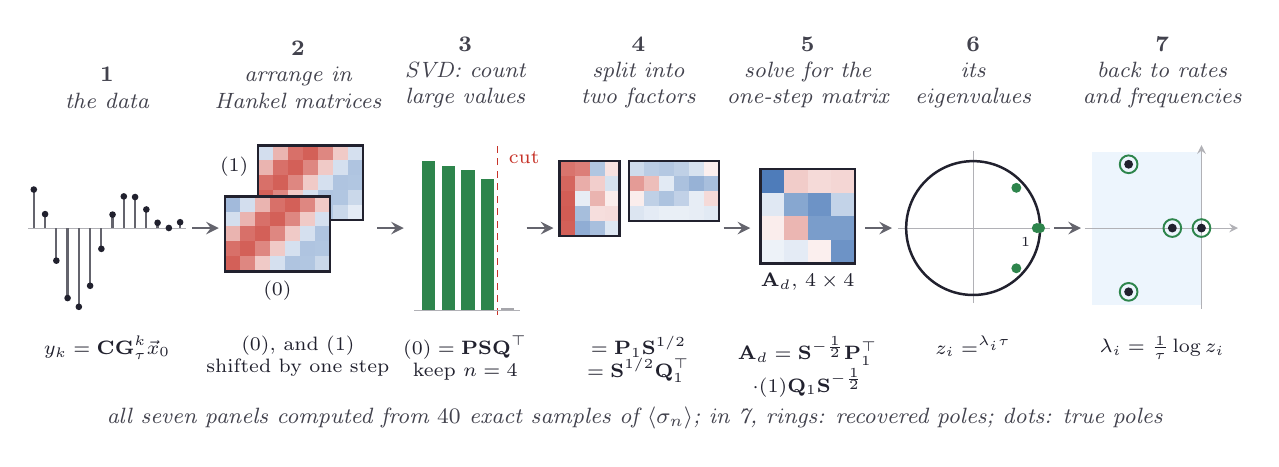
\begin{tikzpicture}[ink/.style={line width=0.9pt, ndInk}, faint/.style={line width=0.4pt, ndInk!35}, dashedink/.style={line width=0.5pt, ndInk!55, dash pattern=on 2.5pt off 2pt}, vec/.style={->, >=stealth, line width=1.2pt}, note/.style={font=\footnotesize\itshape, text=ndInk!85, align=center}, pointer/.style={->, >=stealth, line width=0.4pt, ndInk!60, shorten >=2pt, shorten <=1pt}, dot/.style={circle, fill=ndInk, inner sep=0pt, minimum size=3.4pt}, wash/.style={fill=ndSky, fill opacity=0.55}, every node/.style={text=ndInk}]
\definecolor{ndInk}{rgb}{0.13,0.13,0.18}
\definecolor{ndPaper}{rgb}{0.99,0.96,0.88}
\definecolor{ndSky}{rgb}{0.84,0.91,0.98}
\definecolor{ndRose}{rgb}{0.98,0.86,0.84}
\definecolor{ndBlue}{rgb}{0.13,0.36,0.66}
\definecolor{ndRed}{rgb}{0.78,0.20,0.16}
\definecolor{ndGold}{rgb}{0.88,0.62,0.10}
\definecolor{ndGreen}{rgb}{0.18,0.52,0.30}
\node[note, anchor=south] at (1.000,2.350) {\textup{\textbf{1}}\\ the data};
\node[font=\scriptsize, align=center, anchor=north] at (1.000,-0.300) {$y_k=\mathbf C\mathbf G_\tau^k\vec x_0$};
\node[note, anchor=south] at (3.425,2.350) {\textup{\textbf{2}}\\ arrange in\\ Hankel matrices};
\node[font=\scriptsize, align=center, anchor=north] at (3.425,-0.300) {$\Hankel(0)$, and $\Hankel(1)$\\ shifted by one step};
\draw[->, >=stealth, line width=1.0pt, ndInk!70] (2.080,0.950) -- (2.420,0.950);
\node[note, anchor=south] at (5.550,2.350) {\textup{\textbf{3}}\\ SVD: count\\ large values};
\node[font=\scriptsize, align=center, anchor=north] at (5.550,-0.300) {$\Hankel(0)=\mathbf P\mathbf S\mathbf Q^{\top}$\\ keep $n=4$};
\draw[->, >=stealth, line width=1.0pt, ndInk!70] (4.430,0.950) -- (4.770,0.950);
\node[note, anchor=south] at (7.750,2.350) {\textup{\textbf{4}}\\ split into\\ two factors};
\node[font=\scriptsize, align=center, anchor=north] at (7.750,-0.300) {$\Obsv=\mathbf P_1\mathbf S^{1/2}$\\ $\Ctrb=\mathbf S^{1/2}\mathbf Q_1^{\top}$};
\draw[->, >=stealth, line width=1.0pt, ndInk!70] (6.330,0.950) -- (6.670,0.950);
\node[note, anchor=south] at (9.900,2.350) {\textup{\textbf{5}}\\ solve for the\\ one-step matrix};
\node[font=\scriptsize, align=center, anchor=north] at (9.900,-0.300) {$\mathbf A_d=\mathbf S^{-\frac12}\mathbf P_1^{\top}$\\ $\cdot\Hankel(1)\mathbf Q_1\mathbf S^{-\frac12}$};
\draw[->, >=stealth, line width=1.0pt, ndInk!70] (8.830,0.950) -- (9.170,0.950);
\node[note, anchor=south] at (12.000,2.350) {\textup{\textbf{6}}\\ its\\ eigenvalues};
\node[font=\scriptsize, align=center, anchor=north] at (12.000,-0.300) {$z_i=\ee^{\lambda_i\tau}$};
\draw[->, >=stealth, line width=1.0pt, ndInk!70] (10.630,0.950) -- (10.970,0.950);
\node[note, anchor=south] at (14.400,2.350) {\textup{\textbf{7}}\\ back to rates\\ and frequencies};
\node[font=\scriptsize, align=center, anchor=north] at (14.400,-0.300) {$\lambda_i=\frac1\tau\log z_i$};
\draw[->, >=stealth, line width=1.0pt, ndInk!70] (13.030,0.950) -- (13.370,0.950);
\draw[faint] (0.000,0.950) -- (2.000,0.950);
\draw[line width=0.8pt, ndInk!70] (0.071,0.950) -- (0.071,1.439);
\fill[ndInk] (0.071,1.439) circle (1.2pt);
\draw[line width=0.8pt, ndInk!70] (0.214,0.950) -- (0.214,1.127);
\fill[ndInk] (0.214,1.127) circle (1.2pt);
\draw[line width=0.8pt, ndInk!70] (0.357,0.950) -- (0.357,0.536);
\fill[ndInk] (0.357,0.536) circle (1.2pt);
\draw[line width=0.8pt, ndInk!70] (0.500,0.950) -- (0.500,0.061);
\fill[ndInk] (0.500,0.061) circle (1.2pt);
\draw[line width=0.8pt, ndInk!70] (0.643,0.950) -- (0.643,-0.050);
\fill[ndInk] (0.643,-0.050) circle (1.2pt);
\draw[line width=0.8pt, ndInk!70] (0.786,0.950) -- (0.786,0.217);
\fill[ndInk] (0.786,0.217) circle (1.2pt);
\draw[line width=0.8pt, ndInk!70] (0.929,0.950) -- (0.929,0.686);
\fill[ndInk] (0.929,0.686) circle (1.2pt);
\draw[line width=0.8pt, ndInk!70] (1.071,0.950) -- (1.071,1.121);
\fill[ndInk] (1.071,1.121) circle (1.2pt);
\draw[line width=0.8pt, ndInk!70] (1.214,0.950) -- (1.214,1.352);
\fill[ndInk] (1.214,1.352) circle (1.2pt);
\draw[line width=0.8pt, ndInk!70] (1.357,0.950) -- (1.357,1.344);
\fill[ndInk] (1.357,1.344) circle (1.2pt);
\draw[line width=0.8pt, ndInk!70] (1.500,0.950) -- (1.500,1.186);
\fill[ndInk] (1.500,1.186) circle (1.2pt);
\draw[line width=0.8pt, ndInk!70] (1.643,0.950) -- (1.643,1.017);
\fill[ndInk] (1.643,1.017) circle (1.2pt);
\draw[line width=0.8pt, ndInk!70] (1.786,0.950) -- (1.786,0.951);
\fill[ndInk] (1.786,0.951) circle (1.2pt);
\draw[line width=0.8pt, ndInk!70] (1.929,0.950) -- (1.929,1.024);
\fill[ndInk] (1.929,1.024) circle (1.2pt);
\fill[ndBlue!20] (2.920,2.000) rectangle (3.110,1.810);
\fill[ndRed!37] (3.110,2.000) rectangle (3.300,1.810);
\fill[ndRed!70] (3.300,2.000) rectangle (3.490,1.810);
\fill[ndRed!78] (3.490,2.000) rectangle (3.680,1.810);
\fill[ndRed!59] (3.680,2.000) rectangle (3.870,1.810);
\fill[ndRed!26] (3.870,2.000) rectangle (4.060,1.810);
\fill[ndBlue!19] (4.060,2.000) rectangle (4.250,1.810);
\fill[ndRed!37] (2.920,1.810) rectangle (3.110,1.620);
\fill[ndRed!70] (3.110,1.810) rectangle (3.300,1.620);
\fill[ndRed!78] (3.300,1.810) rectangle (3.490,1.620);
\fill[ndRed!59] (3.490,1.810) rectangle (3.680,1.620);
\fill[ndRed!26] (3.680,1.810) rectangle (3.870,1.620);
\fill[ndBlue!19] (3.870,1.810) rectangle (4.060,1.620);
\fill[ndBlue!36] (4.060,1.810) rectangle (4.250,1.620);
\fill[ndRed!70] (2.920,1.620) rectangle (3.110,1.430);
\fill[ndRed!78] (3.110,1.620) rectangle (3.300,1.430);
\fill[ndRed!59] (3.300,1.620) rectangle (3.490,1.430);
\fill[ndRed!26] (3.490,1.620) rectangle (3.680,1.430);
\fill[ndBlue!19] (3.680,1.620) rectangle (3.870,1.430);
\fill[ndBlue!36] (3.870,1.620) rectangle (4.060,1.430);
\fill[ndBlue!35] (4.060,1.620) rectangle (4.250,1.430);
\fill[ndRed!78] (2.920,1.430) rectangle (3.110,1.240);
\fill[ndRed!59] (3.110,1.430) rectangle (3.300,1.240);
\fill[ndRed!26] (3.300,1.430) rectangle (3.490,1.240);
\fill[ndBlue!19] (3.490,1.430) rectangle (3.680,1.240);
\fill[ndBlue!36] (3.680,1.430) rectangle (3.870,1.240);
\fill[ndBlue!35] (3.870,1.430) rectangle (4.060,1.240);
\fill[ndBlue!24] (4.060,1.430) rectangle (4.250,1.240);
\fill[ndRed!59] (2.920,1.240) rectangle (3.110,1.050);
\fill[ndRed!26] (3.110,1.240) rectangle (3.300,1.050);
\fill[ndBlue!19] (3.300,1.240) rectangle (3.490,1.050);
\fill[ndBlue!36] (3.490,1.240) rectangle (3.680,1.050);
\fill[ndBlue!35] (3.680,1.240) rectangle (3.870,1.050);
\fill[ndBlue!24] (3.870,1.240) rectangle (4.060,1.050);
\fill[ndBlue!12] (4.060,1.240) rectangle (4.250,1.050);
\draw[ink] (2.920,2.000) rectangle (4.250,1.050);
\node[font=\scriptsize, anchor=east] at (2.920,1.730) {$\Hankel(1)$};
\fill[ndBlue!42] (2.500,1.350) rectangle (2.690,1.160);
\fill[ndBlue!20] (2.690,1.350) rectangle (2.880,1.160);
\fill[ndRed!37] (2.880,1.350) rectangle (3.070,1.160);
\fill[ndRed!70] (3.070,1.350) rectangle (3.260,1.160);
\fill[ndRed!78] (3.260,1.350) rectangle (3.450,1.160);
\fill[ndRed!59] (3.450,1.350) rectangle (3.640,1.160);
\fill[ndRed!26] (3.640,1.350) rectangle (3.830,1.160);
\fill[ndBlue!20] (2.500,1.160) rectangle (2.690,0.970);
\fill[ndRed!37] (2.690,1.160) rectangle (2.880,0.970);
\fill[ndRed!70] (2.880,1.160) rectangle (3.070,0.970);
\fill[ndRed!78] (3.070,1.160) rectangle (3.260,0.970);
\fill[ndRed!59] (3.260,1.160) rectangle (3.450,0.970);
\fill[ndRed!26] (3.450,1.160) rectangle (3.640,0.970);
\fill[ndBlue!19] (3.640,1.160) rectangle (3.830,0.970);
\fill[ndRed!37] (2.500,0.970) rectangle (2.690,0.780);
\fill[ndRed!70] (2.690,0.970) rectangle (2.880,0.780);
\fill[ndRed!78] (2.880,0.970) rectangle (3.070,0.780);
\fill[ndRed!59] (3.070,0.970) rectangle (3.260,0.780);
\fill[ndRed!26] (3.260,0.970) rectangle (3.450,0.780);
\fill[ndBlue!19] (3.450,0.970) rectangle (3.640,0.780);
\fill[ndBlue!36] (3.640,0.970) rectangle (3.830,0.780);
\fill[ndRed!70] (2.500,0.780) rectangle (2.690,0.590);
\fill[ndRed!78] (2.690,0.780) rectangle (2.880,0.590);
\fill[ndRed!59] (2.880,0.780) rectangle (3.070,0.590);
\fill[ndRed!26] (3.070,0.780) rectangle (3.260,0.590);
\fill[ndBlue!19] (3.260,0.780) rectangle (3.450,0.590);
\fill[ndBlue!36] (3.450,0.780) rectangle (3.640,0.590);
\fill[ndBlue!35] (3.640,0.780) rectangle (3.830,0.590);
\fill[ndRed!78] (2.500,0.590) rectangle (2.690,0.400);
\fill[ndRed!59] (2.690,0.590) rectangle (2.880,0.400);
\fill[ndRed!26] (2.880,0.590) rectangle (3.070,0.400);
\fill[ndBlue!19] (3.070,0.590) rectangle (3.260,0.400);
\fill[ndBlue!36] (3.260,0.590) rectangle (3.450,0.400);
\fill[ndBlue!35] (3.450,0.590) rectangle (3.640,0.400);
\fill[ndBlue!24] (3.640,0.590) rectangle (3.830,0.400);
\draw[ink] (2.500,1.350) rectangle (3.830,0.400);
\node[font=\scriptsize, anchor=north] at (3.165,0.400) {$\Hankel(0)$};
\fill[ndGreen] (5.000,-0.100) rectangle (5.170,1.800);
\fill[ndGreen] (5.250,-0.100) rectangle (5.420,1.737);
\fill[ndGreen] (5.500,-0.100) rectangle (5.670,1.692);
\fill[ndGreen] (5.750,-0.100) rectangle (5.920,1.573);
\fill[ndInk!40] (6.000,-0.100) rectangle (6.170,-0.060);
\draw[dashedink, ndRed] (5.960,-0.150) -- (5.960,2.050);
\node[font=\scriptsize, text=ndRed, anchor=north west, align=left] at (5.980,2.050) {cut};
\draw[faint] (4.900,-0.100) -- (6.250,-0.100);
\fill[ndRed!68] (6.750,1.800) rectangle (6.940,1.610);
\fill[ndRed!63] (6.940,1.800) rectangle (7.130,1.610);
\fill[ndBlue!35] (7.130,1.800) rectangle (7.320,1.610);
\fill[ndRed!14] (7.320,1.800) rectangle (7.510,1.610);
\fill[ndRed!75] (6.750,1.610) rectangle (6.940,1.420);
\fill[ndRed!40] (6.940,1.610) rectangle (7.130,1.420);
\fill[ndRed!24] (7.130,1.610) rectangle (7.320,1.420);
\fill[ndBlue!18] (7.320,1.610) rectangle (7.510,1.420);
\fill[ndRed!79] (6.750,1.420) rectangle (6.940,1.230);
\fill[ndBlue!11] (6.940,1.420) rectangle (7.130,1.230);
\fill[ndRed!37] (7.130,1.420) rectangle (7.320,1.230);
\fill[ndRed!9] (7.320,1.420) rectangle (7.510,1.230);
\fill[ndRed!80] (6.750,1.230) rectangle (6.940,1.040);
\fill[ndBlue!40] (6.940,1.230) rectangle (7.130,1.040);
\fill[ndRed!16] (7.130,1.230) rectangle (7.320,1.040);
\fill[ndRed!17] (7.320,1.230) rectangle (7.510,1.040);
\fill[ndRed!78] (6.750,1.040) rectangle (6.940,0.850);
\fill[ndBlue!50] (6.940,1.040) rectangle (7.130,0.850);
\fill[ndBlue!39] (7.130,1.040) rectangle (7.320,0.850);
\fill[ndBlue!15] (7.320,1.040) rectangle (7.510,0.850);
\draw[ink] (6.750,1.800) rectangle (7.510,0.850);
\node[font=\scriptsize, anchor=north] at (7.130,0.850) {$\Obsv$};
\fill[ndBlue!22] (7.630,1.800) rectangle (7.820,1.610);
\fill[ndBlue!31] (7.820,1.800) rectangle (8.010,1.610);
\fill[ndBlue!34] (8.010,1.800) rectangle (8.200,1.610);
\fill[ndBlue!29] (8.200,1.800) rectangle (8.390,1.610);
\fill[ndBlue!18] (8.390,1.800) rectangle (8.580,1.610);
\fill[ndRed!8] (8.580,1.800) rectangle (8.770,1.610);
\fill[ndRed!49] (7.630,1.610) rectangle (7.820,1.420);
\fill[ndRed!32] (7.820,1.610) rectangle (8.010,1.420);
\fill[ndBlue!13] (8.010,1.610) rectangle (8.200,1.420);
\fill[ndBlue!38] (8.200,1.610) rectangle (8.390,1.420);
\fill[ndBlue!47] (8.390,1.610) rectangle (8.580,1.420);
\fill[ndBlue!39] (8.580,1.610) rectangle (8.770,1.420);
\fill[ndRed!9] (7.630,1.420) rectangle (7.820,1.230);
\fill[ndBlue!29] (7.820,1.420) rectangle (8.010,1.230);
\fill[ndBlue!37] (8.010,1.420) rectangle (8.200,1.230);
\fill[ndBlue!28] (8.200,1.420) rectangle (8.390,1.230);
\fill[ndBlue!11] (8.390,1.420) rectangle (8.580,1.230);
\fill[ndRed!18] (8.580,1.420) rectangle (8.770,1.230);
\fill[ndBlue!16] (7.630,1.230) rectangle (7.820,1.040);
\fill[ndBlue!12] (7.820,1.230) rectangle (8.010,1.040);
\fill[ndBlue!10] (8.010,1.230) rectangle (8.200,1.040);
\fill[ndBlue!10] (8.200,1.230) rectangle (8.390,1.040);
\fill[ndBlue!11] (8.390,1.230) rectangle (8.580,1.040);
\fill[ndBlue!13] (8.580,1.230) rectangle (8.770,1.040);
\draw[ink] (7.630,1.800) rectangle (8.770,1.040);
\node[font=\scriptsize, anchor=north] at (8.200,1.040) {$\Ctrb$};
\fill[ndBlue!80] (9.300,1.700) rectangle (9.600,1.400);
\fill[ndRed!25] (9.600,1.700) rectangle (9.900,1.400);
\fill[ndRed!18] (9.900,1.700) rectangle (10.200,1.400);
\fill[ndRed!20] (10.200,1.700) rectangle (10.500,1.400);
\fill[ndBlue!14] (9.300,1.400) rectangle (9.600,1.100);
\fill[ndBlue!54] (9.600,1.400) rectangle (9.900,1.100);
\fill[ndBlue!66] (9.900,1.400) rectangle (10.200,1.100);
\fill[ndBlue!27] (10.200,1.400) rectangle (10.500,1.100);
\fill[ndRed!9] (9.300,1.100) rectangle (9.600,0.800);
\fill[ndRed!36] (9.600,1.100) rectangle (9.900,0.800);
\fill[ndBlue!60] (9.900,1.100) rectangle (10.200,0.800);
\fill[ndBlue!60] (10.200,1.100) rectangle (10.500,0.800);
\fill[ndBlue!8] (9.300,0.800) rectangle (9.600,0.500);
\fill[ndBlue!12] (9.600,0.800) rectangle (9.900,0.500);
\fill[ndRed!8] (9.900,0.800) rectangle (10.200,0.500);
\fill[ndBlue!66] (10.200,0.800) rectangle (10.500,0.500);
\draw[ink] (9.300,1.700) rectangle (10.500,0.500);
\node[font=\scriptsize, anchor=north] at (9.900,0.500) {$\mathbf A_d$, $4\times4$};
\draw[faint] (11.048,0.950) -- (12.977,0.950);
\draw[faint] (12.000,-0.002) -- (12.000,1.927);
\draw[ink] (12.000,0.950) circle (0.850);
\fill[ndGreen] (12.549,1.461) circle (1.8pt);
\fill[ndGreen] (12.549,0.439) circle (1.8pt);
\fill[ndGreen] (12.850,0.950) circle (1.8pt);
\fill[ndGreen] (12.809,0.950) circle (1.8pt);
\node[font=\tiny, anchor=north east] at (12.850,0.950) {$1$};
\fill[ndSky, fill opacity=0.45] (13.512,-0.022) rectangle (14.900,1.922);
\draw[faint, ->, >=stealth] (13.420,0.950) -- (15.363,0.950);
\draw[faint, ->, >=stealth] (14.900,-0.076) -- (14.900,2.003);
\fill[ndInk] (14.900,0.950) circle (1.6pt);
\fill[ndInk] (14.530,0.950) circle (1.6pt);
\fill[ndInk] (13.975,1.760) circle (1.6pt);
\fill[ndInk] (13.975,0.140) circle (1.6pt);
\draw[line width=0.7pt, ndGreen] (13.975,1.760) circle (3.2pt);
\draw[line width=0.7pt, ndGreen] (13.975,0.140) circle (3.2pt);
\draw[line width=0.7pt, ndGreen] (14.900,0.950) circle (3.2pt);
\draw[line width=0.7pt, ndGreen] (14.530,0.950) circle (3.2pt);
\node[note, anchor=north] at (7.7,-1.2) {all seven panels computed from $40$ exact samples of $\langle\sigma_n\rangle$; in 7, rings: recovered poles; dots: true poles};
\end{tikzpicture}
}\end{center}
{\small Hankel matrices, SVD, factors, one-step matrix, eigenvalues, logarithm. The rank fixes $n$, and $\Hankel(1)$ supplies the step.}}
\end{frame}

\begin{frame}[fragile]\ft{Ho--Kalman in a dozen lines}
\ona{The following extract from \texttt{code/ch05\_spectrum.py} forms the two Hankel matrices from a sequence of output vectors and returns the balanced realisation \eqref{eq:ch05:era}; the continuous-time eigenvalues are then $\log(\lambda_i[\mathbf A_d])/\tau$, subject to the aliasing discussed in the next section.}
\ona{\lstinputlisting[style=python,firstline=64,lastline=81]{code/ch05_spectrum.py}}
\onp{\lstinputlisting[style=python,basicstyle=\ttfamily\scriptsize,numbers=none,firstline=69,lastline=81]{code/ch05_spectrum.py}}
\ona{Figure~\ref{fig:ch05:poles} shows the eigenvalues recovered by Ho--Kalman from $80$ samples of $(\langle\sigma_x\rangle,\langle\sigma_z\rangle)$ for our example. From exact data they agree with those of $\mathbf A$ to about $10^{-10}$. When noise is added to each sample the estimates scatter, and they scatter most for the slow relaxation $-\gamma_1$, whose decay over the length of the record is the hardest to distinguish from the constant contributed by the steady state.}
\ona{\begin{figure}[H]\centering\resizebox{0.8\linewidth}{!}{% Generated by code/needham.py -- do not edit by hand.
\definecolor{qocA}{rgb}{0.00,0.45,0.70}
\definecolor{qocB}{rgb}{0.90,0.60,0.00}
\definecolor{qocC}{rgb}{0.00,0.62,0.45}
\definecolor{qocD}{rgb}{0.80,0.40,0.00}
\definecolor{qocE}{rgb}{0.80,0.60,0.70}
\definecolor{qocF}{rgb}{0.35,0.70,0.90}
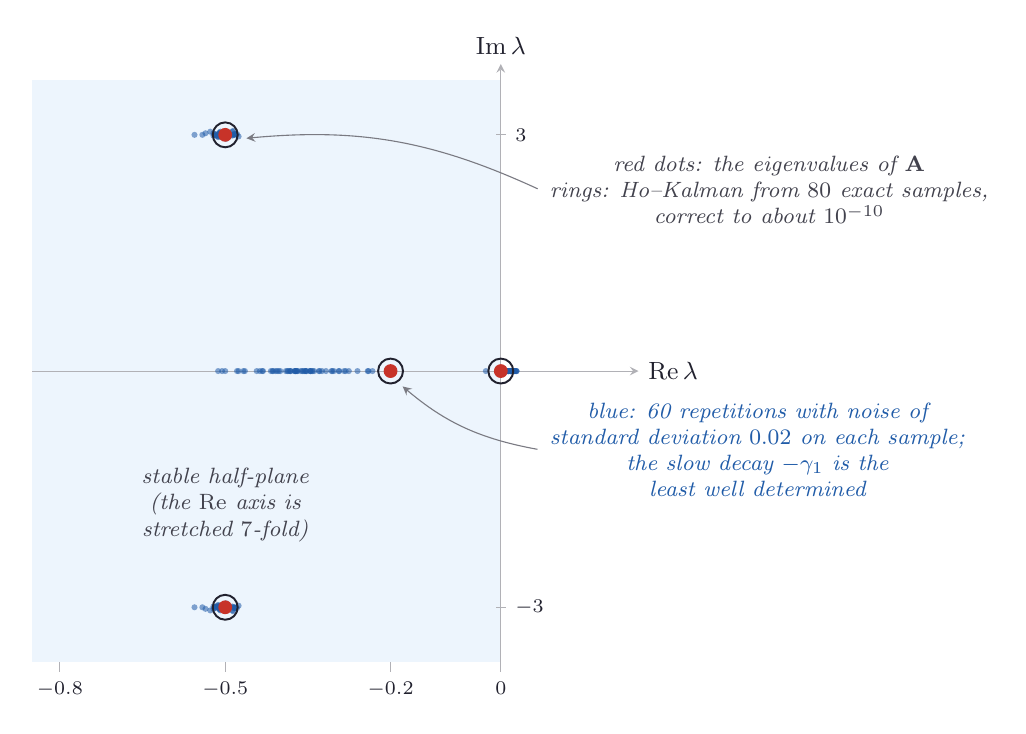
\begin{tikzpicture}[ink/.style={line width=0.9pt, ndInk}, faint/.style={line width=0.4pt, ndInk!35}, dashedink/.style={line width=0.5pt, ndInk!55, dash pattern=on 2.5pt off 2pt}, vec/.style={->, >=stealth, line width=1.2pt}, note/.style={font=\footnotesize\itshape, text=ndInk!85, align=center}, pointer/.style={->, >=stealth, line width=0.4pt, ndInk!60, shorten >=2pt, shorten <=1pt}, dot/.style={circle, fill=ndInk, inner sep=0pt, minimum size=3.4pt}, wash/.style={fill=ndSky, fill opacity=0.55}, every node/.style={text=ndInk}]
\definecolor{ndInk}{rgb}{0.13,0.13,0.18}
\definecolor{ndPaper}{rgb}{0.99,0.96,0.88}
\definecolor{ndSky}{rgb}{0.84,0.91,0.98}
\definecolor{ndRose}{rgb}{0.98,0.86,0.84}
\definecolor{ndBlue}{rgb}{0.13,0.36,0.66}
\definecolor{ndRed}{rgb}{0.78,0.20,0.16}
\definecolor{ndGold}{rgb}{0.88,0.62,0.10}
\definecolor{ndGreen}{rgb}{0.18,0.52,0.30}
\fill[ndSky, fill opacity=0.45] (-5.95,-3.70) rectangle (0,3.70);
\draw[faint, ->, >=stealth] (-5.95,0) -- (1.75,0) node[right, text=ndInk, font=\small] {$\mathrm{Re}\,\lambda$};
\draw[faint, ->, >=stealth] (0,-3.70) -- (0,3.90) node[above, text=ndInk, font=\small] {$\mathrm{Im}\,\lambda$};
\draw[faint] (-5.60,-3.70) -- (-5.60,-3.82) node[below, font=\scriptsize, text=ndInk] {$-0.8$};
\draw[faint] (-3.50,-3.70) -- (-3.50,-3.82) node[below, font=\scriptsize, text=ndInk] {$-0.5$};
\draw[faint] (-1.40,-3.70) -- (-1.40,-3.82) node[below, font=\scriptsize, text=ndInk] {$-0.2$};
\draw[faint] (0.00,-3.70) -- (0.00,-3.82) node[below, font=\scriptsize, text=ndInk] {$0$};
\draw[faint] (-0.06,-3.00) -- (0.06,-3.00) node[right, font=\scriptsize, text=ndInk] {$-3$};
\draw[faint] (-0.06,3.00) -- (0.06,3.00) node[right, font=\scriptsize, text=ndInk] {$3$};
\fill[ndBlue, fill opacity=0.55] (-3.52,3.01) circle (1.1pt);
\fill[ndBlue, fill opacity=0.55] (-3.52,-3.01) circle (1.1pt);
\fill[ndBlue, fill opacity=0.55] (0.16,0.00) circle (1.1pt);
\fill[ndBlue, fill opacity=0.55] (-2.67,0.00) circle (1.1pt);
\fill[ndBlue, fill opacity=0.55] (-3.55,2.98) circle (1.1pt);
\fill[ndBlue, fill opacity=0.55] (-3.55,-2.98) circle (1.1pt);
\fill[ndBlue, fill opacity=0.55] (0.10,0.00) circle (1.1pt);
\fill[ndBlue, fill opacity=0.55] (-2.48,0.00) circle (1.1pt);
\fill[ndBlue, fill opacity=0.55] (-3.57,3.03) circle (1.1pt);
\fill[ndBlue, fill opacity=0.55] (-3.57,-3.03) circle (1.1pt);
\fill[ndBlue, fill opacity=0.55] (0.13,0.00) circle (1.1pt);
\fill[ndBlue, fill opacity=0.55] (-2.42,0.00) circle (1.1pt);
\fill[ndBlue, fill opacity=0.55] (-3.40,3.05) circle (1.1pt);
\fill[ndBlue, fill opacity=0.55] (-3.40,-3.05) circle (1.1pt);
\fill[ndBlue, fill opacity=0.55] (0.03,0.00) circle (1.1pt);
\fill[ndBlue, fill opacity=0.55] (-2.47,0.00) circle (1.1pt);
\fill[ndBlue, fill opacity=0.55] (-3.65,2.99) circle (1.1pt);
\fill[ndBlue, fill opacity=0.55] (-3.65,-2.99) circle (1.1pt);
\fill[ndBlue, fill opacity=0.55] (0.03,0.00) circle (1.1pt);
\fill[ndBlue, fill opacity=0.55] (-2.30,0.00) circle (1.1pt);
\fill[ndBlue, fill opacity=0.55] (-3.45,2.99) circle (1.1pt);
\fill[ndBlue, fill opacity=0.55] (-3.45,-2.99) circle (1.1pt);
\fill[ndBlue, fill opacity=0.55] (0.19,0.00) circle (1.1pt);
\fill[ndBlue, fill opacity=0.55] (-2.86,0.00) circle (1.1pt);
\fill[ndBlue, fill opacity=0.55] (-3.38,3.00) circle (1.1pt);
\fill[ndBlue, fill opacity=0.55] (-3.38,-3.00) circle (1.1pt);
\fill[ndBlue, fill opacity=0.55] (0.01,0.00) circle (1.1pt);
\fill[ndBlue, fill opacity=0.55] (-2.14,0.00) circle (1.1pt);
\fill[ndBlue, fill opacity=0.55] (-3.51,3.02) circle (1.1pt);
\fill[ndBlue, fill opacity=0.55] (-3.51,-3.02) circle (1.1pt);
\fill[ndBlue, fill opacity=0.55] (0.10,0.00) circle (1.1pt);
\fill[ndBlue, fill opacity=0.55] (-2.42,0.00) circle (1.1pt);
\fill[ndBlue, fill opacity=0.55] (-3.52,2.97) circle (1.1pt);
\fill[ndBlue, fill opacity=0.55] (-3.52,-2.97) circle (1.1pt);
\fill[ndBlue, fill opacity=0.55] (0.15,0.00) circle (1.1pt);
\fill[ndBlue, fill opacity=0.55] (-3.50,0.00) circle (1.1pt);
\fill[ndBlue, fill opacity=0.55] (-3.46,3.01) circle (1.1pt);
\fill[ndBlue, fill opacity=0.55] (-3.46,-3.01) circle (1.1pt);
\fill[ndBlue, fill opacity=0.55] (0.20,0.00) circle (1.1pt);
\fill[ndBlue, fill opacity=0.55] (-3.54,0.00) circle (1.1pt);
\fill[ndBlue, fill opacity=0.55] (-3.59,2.97) circle (1.1pt);
\fill[ndBlue, fill opacity=0.55] (-3.59,-2.97) circle (1.1pt);
\fill[ndBlue, fill opacity=0.55] (0.17,0.00) circle (1.1pt);
\fill[ndBlue, fill opacity=0.55] (-3.25,0.00) circle (1.1pt);
\fill[ndBlue, fill opacity=0.55] (-3.37,3.01) circle (1.1pt);
\fill[ndBlue, fill opacity=0.55] (-3.37,-3.01) circle (1.1pt);
\fill[ndBlue, fill opacity=0.55] (-0.04,0.00) circle (1.1pt);
\fill[ndBlue, fill opacity=0.55] (-1.99,0.00) circle (1.1pt);
\fill[ndBlue, fill opacity=0.55] (-3.57,3.01) circle (1.1pt);
\fill[ndBlue, fill opacity=0.55] (-3.57,-3.01) circle (1.1pt);
\fill[ndBlue, fill opacity=0.55] (0.15,0.00) circle (1.1pt);
\fill[ndBlue, fill opacity=0.55] (-3.06,0.00) circle (1.1pt);
\fill[ndBlue, fill opacity=0.55] (-3.41,2.99) circle (1.1pt);
\fill[ndBlue, fill opacity=0.55] (-3.41,-2.99) circle (1.1pt);
\fill[ndBlue, fill opacity=0.55] (0.15,0.00) circle (1.1pt);
\fill[ndBlue, fill opacity=0.55] (-2.61,0.00) circle (1.1pt);
\fill[ndBlue, fill opacity=0.55] (-3.57,2.98) circle (1.1pt);
\fill[ndBlue, fill opacity=0.55] (-3.57,-2.98) circle (1.1pt);
\fill[ndBlue, fill opacity=0.55] (0.05,0.00) circle (1.1pt);
\fill[ndBlue, fill opacity=0.55] (-2.31,0.00) circle (1.1pt);
\fill[ndBlue, fill opacity=0.55] (-3.57,3.00) circle (1.1pt);
\fill[ndBlue, fill opacity=0.55] (-3.57,-3.00) circle (1.1pt);
\fill[ndBlue, fill opacity=0.55] (0.19,0.00) circle (1.1pt);
\fill[ndBlue, fill opacity=0.55] (-3.27,0.00) circle (1.1pt);
\fill[ndBlue, fill opacity=0.55] (-3.48,3.01) circle (1.1pt);
\fill[ndBlue, fill opacity=0.55] (-3.48,-3.01) circle (1.1pt);
\fill[ndBlue, fill opacity=0.55] (-0.03,0.00) circle (1.1pt);
\fill[ndBlue, fill opacity=0.55] (-1.97,0.00) circle (1.1pt);
\fill[ndBlue, fill opacity=0.55] (-3.65,3.02) circle (1.1pt);
\fill[ndBlue, fill opacity=0.55] (-3.65,-3.02) circle (1.1pt);
\fill[ndBlue, fill opacity=0.55] (0.13,0.00) circle (1.1pt);
\fill[ndBlue, fill opacity=0.55] (-2.82,0.00) circle (1.1pt);
\fill[ndBlue, fill opacity=0.55] (-3.52,3.01) circle (1.1pt);
\fill[ndBlue, fill opacity=0.55] (-3.52,-3.01) circle (1.1pt);
\fill[ndBlue, fill opacity=0.55] (0.10,0.00) circle (1.1pt);
\fill[ndBlue, fill opacity=0.55] (-2.39,0.00) circle (1.1pt);
\fill[ndBlue, fill opacity=0.55] (-3.61,2.99) circle (1.1pt);
\fill[ndBlue, fill opacity=0.55] (-3.61,-2.99) circle (1.1pt);
\fill[ndBlue, fill opacity=0.55] (0.07,0.00) circle (1.1pt);
\fill[ndBlue, fill opacity=0.55] (-2.71,0.00) circle (1.1pt);
\fill[ndBlue, fill opacity=0.55] (-3.57,3.00) circle (1.1pt);
\fill[ndBlue, fill opacity=0.55] (-3.57,-3.00) circle (1.1pt);
\fill[ndBlue, fill opacity=0.55] (0.12,0.00) circle (1.1pt);
\fill[ndBlue, fill opacity=0.55] (-2.51,0.00) circle (1.1pt);
\fill[ndBlue, fill opacity=0.55] (-3.75,3.02) circle (1.1pt);
\fill[ndBlue, fill opacity=0.55] (-3.75,-3.02) circle (1.1pt);
\fill[ndBlue, fill opacity=0.55] (0.12,0.00) circle (1.1pt);
\fill[ndBlue, fill opacity=0.55] (-2.37,0.00) circle (1.1pt);
\fill[ndBlue, fill opacity=0.55] (-3.35,3.01) circle (1.1pt);
\fill[ndBlue, fill opacity=0.55] (-3.35,-3.01) circle (1.1pt);
\fill[ndBlue, fill opacity=0.55] (0.16,0.00) circle (1.1pt);
\fill[ndBlue, fill opacity=0.55] (-3.59,0.00) circle (1.1pt);
\fill[ndBlue, fill opacity=0.55] (-3.62,2.99) circle (1.1pt);
\fill[ndBlue, fill opacity=0.55] (-3.62,-2.99) circle (1.1pt);
\fill[ndBlue, fill opacity=0.55] (0.18,0.00) circle (1.1pt);
\fill[ndBlue, fill opacity=0.55] (-3.02,0.00) circle (1.1pt);
\fill[ndBlue, fill opacity=0.55] (-3.52,3.00) circle (1.1pt);
\fill[ndBlue, fill opacity=0.55] (-3.52,-3.00) circle (1.1pt);
\fill[ndBlue, fill opacity=0.55] (-0.01,0.00) circle (1.1pt);
\fill[ndBlue, fill opacity=0.55] (-2.12,0.00) circle (1.1pt);
\fill[ndBlue, fill opacity=0.55] (-3.58,3.02) circle (1.1pt);
\fill[ndBlue, fill opacity=0.55] (-3.58,-3.02) circle (1.1pt);
\fill[ndBlue, fill opacity=0.55] (0.01,0.00) circle (1.1pt);
\fill[ndBlue, fill opacity=0.55] (-1.68,0.00) circle (1.1pt);
\fill[ndBlue, fill opacity=0.55] (-3.41,3.00) circle (1.1pt);
\fill[ndBlue, fill opacity=0.55] (-3.41,-3.00) circle (1.1pt);
\fill[ndBlue, fill opacity=0.55] (0.09,0.00) circle (1.1pt);
\fill[ndBlue, fill opacity=0.55] (-2.06,0.00) circle (1.1pt);
\fill[ndBlue, fill opacity=0.55] (-3.56,3.02) circle (1.1pt);
\fill[ndBlue, fill opacity=0.55] (-3.56,-3.02) circle (1.1pt);
\fill[ndBlue, fill opacity=0.55] (0.00,0.00) circle (1.1pt);
\fill[ndBlue, fill opacity=0.55] (-2.27,0.00) circle (1.1pt);
\fill[ndBlue, fill opacity=0.55] (-3.50,2.97) circle (1.1pt);
\fill[ndBlue, fill opacity=0.55] (-3.50,-2.97) circle (1.1pt);
\fill[ndBlue, fill opacity=0.55] (0.16,0.00) circle (1.1pt);
\fill[ndBlue, fill opacity=0.55] (-2.67,0.00) circle (1.1pt);
\fill[ndBlue, fill opacity=0.55] (-3.50,3.00) circle (1.1pt);
\fill[ndBlue, fill opacity=0.55] (-3.50,-3.00) circle (1.1pt);
\fill[ndBlue, fill opacity=0.55] (0.14,0.00) circle (1.1pt);
\fill[ndBlue, fill opacity=0.55] (-2.40,0.00) circle (1.1pt);
\fill[ndBlue, fill opacity=0.55] (-3.39,3.01) circle (1.1pt);
\fill[ndBlue, fill opacity=0.55] (-3.39,-3.01) circle (1.1pt);
\fill[ndBlue, fill opacity=0.55] (0.12,0.00) circle (1.1pt);
\fill[ndBlue, fill opacity=0.55] (-2.92,0.00) circle (1.1pt);
\fill[ndBlue, fill opacity=0.55] (-3.63,3.01) circle (1.1pt);
\fill[ndBlue, fill opacity=0.55] (-3.63,-3.01) circle (1.1pt);
\fill[ndBlue, fill opacity=0.55] (0.07,0.00) circle (1.1pt);
\fill[ndBlue, fill opacity=0.55] (-2.59,0.00) circle (1.1pt);
\fill[ndBlue, fill opacity=0.55] (-3.79,3.00) circle (1.1pt);
\fill[ndBlue, fill opacity=0.55] (-3.79,-3.00) circle (1.1pt);
\fill[ndBlue, fill opacity=0.55] (0.13,0.00) circle (1.1pt);
\fill[ndBlue, fill opacity=0.55] (-2.89,0.00) circle (1.1pt);
\fill[ndBlue, fill opacity=0.55] (-3.56,3.00) circle (1.1pt);
\fill[ndBlue, fill opacity=0.55] (-3.56,-3.00) circle (1.1pt);
\fill[ndBlue, fill opacity=0.55] (0.14,0.00) circle (1.1pt);
\fill[ndBlue, fill opacity=0.55] (-2.59,0.00) circle (1.1pt);
\fill[ndBlue, fill opacity=0.55] (-3.39,3.00) circle (1.1pt);
\fill[ndBlue, fill opacity=0.55] (-3.39,-3.00) circle (1.1pt);
\fill[ndBlue, fill opacity=0.55] (0.07,0.00) circle (1.1pt);
\fill[ndBlue, fill opacity=0.55] (-2.90,0.00) circle (1.1pt);
\fill[ndBlue, fill opacity=0.55] (-3.38,3.01) circle (1.1pt);
\fill[ndBlue, fill opacity=0.55] (-3.38,-3.01) circle (1.1pt);
\fill[ndBlue, fill opacity=0.55] (0.14,0.00) circle (1.1pt);
\fill[ndBlue, fill opacity=0.55] (-3.33,0.00) circle (1.1pt);
\fill[ndBlue, fill opacity=0.55] (-3.54,3.00) circle (1.1pt);
\fill[ndBlue, fill opacity=0.55] (-3.54,-3.00) circle (1.1pt);
\fill[ndBlue, fill opacity=0.55] (0.12,0.00) circle (1.1pt);
\fill[ndBlue, fill opacity=0.55] (-2.47,0.00) circle (1.1pt);
\fill[ndBlue, fill opacity=0.55] (-3.49,2.95) circle (1.1pt);
\fill[ndBlue, fill opacity=0.55] (-3.49,-2.95) circle (1.1pt);
\fill[ndBlue, fill opacity=0.55] (0.07,0.00) circle (1.1pt);
\fill[ndBlue, fill opacity=0.55] (-2.22,0.00) circle (1.1pt);
\fill[ndBlue, fill opacity=0.55] (-3.33,2.98) circle (1.1pt);
\fill[ndBlue, fill opacity=0.55] (-3.33,-2.98) circle (1.1pt);
\fill[ndBlue, fill opacity=0.55] (0.05,0.00) circle (1.1pt);
\fill[ndBlue, fill opacity=0.55] (-2.15,0.00) circle (1.1pt);
\fill[ndBlue, fill opacity=0.55] (-3.62,3.00) circle (1.1pt);
\fill[ndBlue, fill opacity=0.55] (-3.62,-3.00) circle (1.1pt);
\fill[ndBlue, fill opacity=0.55] (-0.19,0.00) circle (1.1pt);
\fill[ndBlue, fill opacity=0.55] (-1.69,0.00) circle (1.1pt);
\fill[ndBlue, fill opacity=0.55] (-3.59,2.98) circle (1.1pt);
\fill[ndBlue, fill opacity=0.55] (-3.59,-2.98) circle (1.1pt);
\fill[ndBlue, fill opacity=0.55] (0.05,0.00) circle (1.1pt);
\fill[ndBlue, fill opacity=0.55] (-1.93,0.00) circle (1.1pt);
\fill[ndBlue, fill opacity=0.55] (-3.52,2.98) circle (1.1pt);
\fill[ndBlue, fill opacity=0.55] (-3.52,-2.98) circle (1.1pt);
\fill[ndBlue, fill opacity=0.55] (0.12,0.00) circle (1.1pt);
\fill[ndBlue, fill opacity=0.55] (-2.61,0.00) circle (1.1pt);
\fill[ndBlue, fill opacity=0.55] (-3.55,3.00) circle (1.1pt);
\fill[ndBlue, fill opacity=0.55] (-3.55,-3.00) circle (1.1pt);
\fill[ndBlue, fill opacity=0.55] (0.10,0.00) circle (1.1pt);
\fill[ndBlue, fill opacity=0.55] (-2.73,0.00) circle (1.1pt);
\fill[ndBlue, fill opacity=0.55] (-3.50,3.02) circle (1.1pt);
\fill[ndBlue, fill opacity=0.55] (-3.50,-3.02) circle (1.1pt);
\fill[ndBlue, fill opacity=0.55] (0.08,0.00) circle (1.1pt);
\fill[ndBlue, fill opacity=0.55] (-2.52,0.00) circle (1.1pt);
\fill[ndBlue, fill opacity=0.55] (-3.53,2.99) circle (1.1pt);
\fill[ndBlue, fill opacity=0.55] (-3.53,-2.99) circle (1.1pt);
\fill[ndBlue, fill opacity=0.55] (0.17,0.00) circle (1.1pt);
\fill[ndBlue, fill opacity=0.55] (-3.03,0.00) circle (1.1pt);
\fill[ndBlue, fill opacity=0.55] (-3.50,3.03) circle (1.1pt);
\fill[ndBlue, fill opacity=0.55] (-3.50,-3.03) circle (1.1pt);
\fill[ndBlue, fill opacity=0.55] (0.15,0.00) circle (1.1pt);
\fill[ndBlue, fill opacity=0.55] (-2.58,0.00) circle (1.1pt);
\fill[ndBlue, fill opacity=0.55] (-3.55,3.02) circle (1.1pt);
\fill[ndBlue, fill opacity=0.55] (-3.55,-3.02) circle (1.1pt);
\fill[ndBlue, fill opacity=0.55] (0.11,0.00) circle (1.1pt);
\fill[ndBlue, fill opacity=0.55] (-2.61,0.00) circle (1.1pt);
\fill[ndBlue, fill opacity=0.55] (-3.50,2.99) circle (1.1pt);
\fill[ndBlue, fill opacity=0.55] (-3.50,-2.99) circle (1.1pt);
\fill[ndBlue, fill opacity=0.55] (0.14,0.00) circle (1.1pt);
\fill[ndBlue, fill opacity=0.55] (-2.80,0.00) circle (1.1pt);
\fill[ndBlue, fill opacity=0.55] (-3.54,2.99) circle (1.1pt);
\fill[ndBlue, fill opacity=0.55] (-3.54,-2.99) circle (1.1pt);
\fill[ndBlue, fill opacity=0.55] (0.04,0.00) circle (1.1pt);
\fill[ndBlue, fill opacity=0.55] (-2.62,0.00) circle (1.1pt);
\fill[ndBlue, fill opacity=0.55] (-3.52,3.03) circle (1.1pt);
\fill[ndBlue, fill opacity=0.55] (-3.52,-3.03) circle (1.1pt);
\fill[ndBlue, fill opacity=0.55] (0.08,0.00) circle (1.1pt);
\fill[ndBlue, fill opacity=0.55] (-2.42,0.00) circle (1.1pt);
\fill[ndBlue, fill opacity=0.55] (-3.58,3.01) circle (1.1pt);
\fill[ndBlue, fill opacity=0.55] (-3.58,-3.01) circle (1.1pt);
\fill[ndBlue, fill opacity=0.55] (0.20,0.00) circle (1.1pt);
\fill[ndBlue, fill opacity=0.55] (-2.84,0.00) circle (1.1pt);
\fill[ndBlue, fill opacity=0.55] (-3.58,2.99) circle (1.1pt);
\fill[ndBlue, fill opacity=0.55] (-3.58,-2.99) circle (1.1pt);
\fill[ndBlue, fill opacity=0.55] (0.17,0.00) circle (1.1pt);
\fill[ndBlue, fill opacity=0.55] (-3.10,0.00) circle (1.1pt);
\fill[ndBlue, fill opacity=0.55] (-3.46,2.99) circle (1.1pt);
\fill[ndBlue, fill opacity=0.55] (-3.46,-2.99) circle (1.1pt);
\fill[ndBlue, fill opacity=0.55] (0.14,0.00) circle (1.1pt);
\fill[ndBlue, fill opacity=0.55] (-2.68,0.00) circle (1.1pt);
\fill[ndBlue, fill opacity=0.55] (-3.54,3.01) circle (1.1pt);
\fill[ndBlue, fill opacity=0.55] (-3.54,-3.01) circle (1.1pt);
\fill[ndBlue, fill opacity=0.55] (0.03,0.00) circle (1.1pt);
\fill[ndBlue, fill opacity=0.55] (-1.63,0.00) circle (1.1pt);
\fill[ndBlue, fill opacity=0.55] (-3.56,3.04) circle (1.1pt);
\fill[ndBlue, fill opacity=0.55] (-3.56,-3.04) circle (1.1pt);
\fill[ndBlue, fill opacity=0.55] (0.01,0.00) circle (1.1pt);
\fill[ndBlue, fill opacity=0.55] (-1.82,0.00) circle (1.1pt);
\fill[ndBlue, fill opacity=0.55] (-3.89,3.00) circle (1.1pt);
\fill[ndBlue, fill opacity=0.55] (-3.89,-3.00) circle (1.1pt);
\fill[ndBlue, fill opacity=0.55] (0.04,0.00) circle (1.1pt);
\fill[ndBlue, fill opacity=0.55] (-2.54,0.00) circle (1.1pt);
\fill[ndBlue, fill opacity=0.55] (-3.41,3.04) circle (1.1pt);
\fill[ndBlue, fill opacity=0.55] (-3.41,-3.04) circle (1.1pt);
\fill[ndBlue, fill opacity=0.55] (0.18,0.00) circle (1.1pt);
\fill[ndBlue, fill opacity=0.55] (-3.35,0.00) circle (1.1pt);
\fill[ndBlue, fill opacity=0.55] (-3.55,3.01) circle (1.1pt);
\fill[ndBlue, fill opacity=0.55] (-3.55,-3.01) circle (1.1pt);
\fill[ndBlue, fill opacity=0.55] (0.09,0.00) circle (1.1pt);
\fill[ndBlue, fill opacity=0.55] (-2.05,0.00) circle (1.1pt);
\fill[ndBlue, fill opacity=0.55] (-3.47,3.00) circle (1.1pt);
\fill[ndBlue, fill opacity=0.55] (-3.47,-3.00) circle (1.1pt);
\fill[ndBlue, fill opacity=0.55] (0.09,0.00) circle (1.1pt);
\fill[ndBlue, fill opacity=0.55] (-2.49,0.00) circle (1.1pt);
\fill[ndBlue, fill opacity=0.55] (-3.69,3.04) circle (1.1pt);
\fill[ndBlue, fill opacity=0.55] (-3.69,-3.04) circle (1.1pt);
\fill[ndBlue, fill opacity=0.55] (0.10,0.00) circle (1.1pt);
\fill[ndBlue, fill opacity=0.55] (-2.70,0.00) circle (1.1pt);
\node[dot, fill=ndRed, minimum size=5pt] at (0.00,0.00) {};
\node[dot, fill=ndRed, minimum size=5pt] at (-1.40,0.00) {};
\node[dot, fill=ndRed, minimum size=5pt] at (-3.50,3.00) {};
\node[dot, fill=ndRed, minimum size=5pt] at (-3.50,-3.00) {};
\draw[ndInk, line width=0.7pt] (-3.50,3.00) circle (4.5pt);
\draw[ndInk, line width=0.7pt] (-3.50,-3.00) circle (4.5pt);
\draw[ndInk, line width=0.7pt] (-0.00,0.00) circle (4.5pt);
\draw[ndInk, line width=0.7pt] (-1.40,0.00) circle (4.5pt);
\node[note, anchor=west] (r) at (0.50,2.30) {red dots: the eigenvalues of $\mathbf A$\\ rings: Ho--Kalman from $80$ exact samples,\\ correct to about $10^{-10}$};
\draw[pointer] (r.west) to[bend right=15] (-3.30,2.95);
\node[note, anchor=west, text=ndBlue] (n) at (0.50,-1.00) {blue: 60 repetitions with noise of\\ standard deviation $0.02$ on each sample;\\ the slow decay $-\gamma_1$ is the\\ least well determined};
\draw[pointer] (n.west) to[bend left=15] (-1.30,-0.15);
\node[note] at (-3.50,-1.70) {stable half-plane\\ (the $\mathrm{Re}$ axis is\\ stretched $7$-fold)};
\end{tikzpicture}
}
\caption{The eigenvalues of the example in the complex plane (red), with the estimates $\log(\lambda_i[\mathbf A_d])/\tau$ obtained by Ho--Kalman from $80$ exact samples of $(\langle\sigma_x\rangle,\langle\sigma_z\rangle)$ (rings) and from $60$ repetitions with Gaussian noise of standard deviation $0.02$ added to each sample (blue). The real axis is stretched by a factor of seven. Generated by \texttt{code/ch05\_spectrum.py}.}\label{fig:ch05:poles}\end{figure}}
\end{frame}

\begin{frame}\ft{Recovered poles}
\onp{Ho--Kalman with $80$ samples: exact data give the eigenvalues to $10^{-10}$ (rings); with noise the estimates scatter, most of all for the slow $-\gamma_1$ (Figure~\ref{fig:ch05:poles}).
\begin{center}\resizebox{!}{0.66\textheight}{% Generated by code/needham.py -- do not edit by hand.
\definecolor{qocA}{rgb}{0.00,0.45,0.70}
\definecolor{qocB}{rgb}{0.90,0.60,0.00}
\definecolor{qocC}{rgb}{0.00,0.62,0.45}
\definecolor{qocD}{rgb}{0.80,0.40,0.00}
\definecolor{qocE}{rgb}{0.80,0.60,0.70}
\definecolor{qocF}{rgb}{0.35,0.70,0.90}
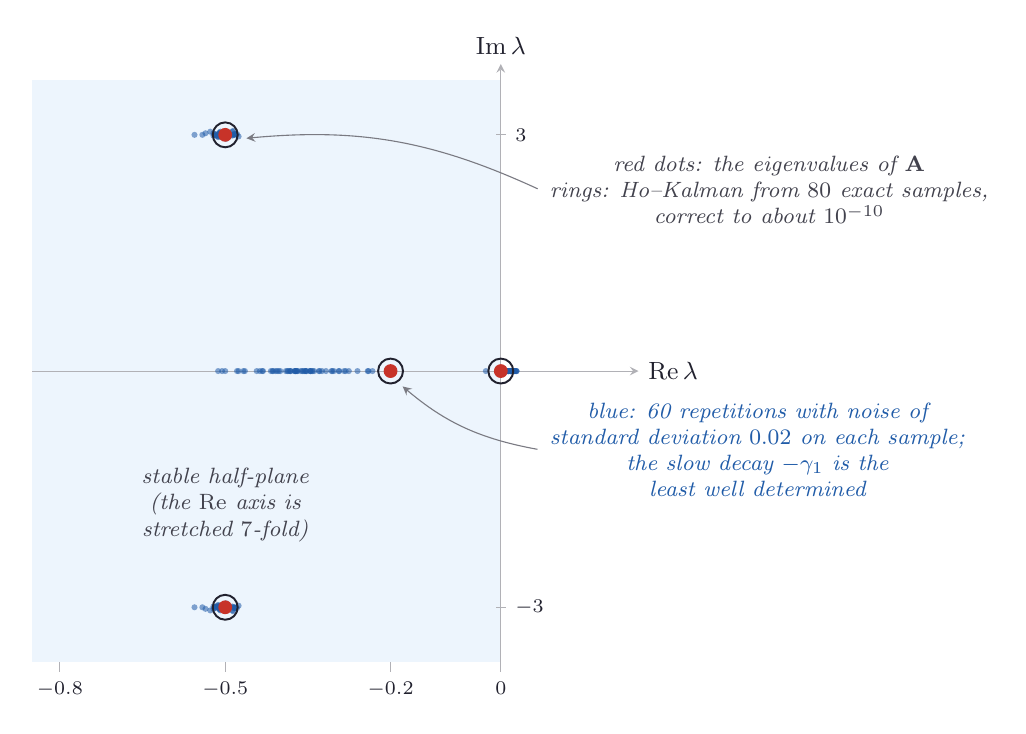
\begin{tikzpicture}[ink/.style={line width=0.9pt, ndInk}, faint/.style={line width=0.4pt, ndInk!35}, dashedink/.style={line width=0.5pt, ndInk!55, dash pattern=on 2.5pt off 2pt}, vec/.style={->, >=stealth, line width=1.2pt}, note/.style={font=\footnotesize\itshape, text=ndInk!85, align=center}, pointer/.style={->, >=stealth, line width=0.4pt, ndInk!60, shorten >=2pt, shorten <=1pt}, dot/.style={circle, fill=ndInk, inner sep=0pt, minimum size=3.4pt}, wash/.style={fill=ndSky, fill opacity=0.55}, every node/.style={text=ndInk}]
\definecolor{ndInk}{rgb}{0.13,0.13,0.18}
\definecolor{ndPaper}{rgb}{0.99,0.96,0.88}
\definecolor{ndSky}{rgb}{0.84,0.91,0.98}
\definecolor{ndRose}{rgb}{0.98,0.86,0.84}
\definecolor{ndBlue}{rgb}{0.13,0.36,0.66}
\definecolor{ndRed}{rgb}{0.78,0.20,0.16}
\definecolor{ndGold}{rgb}{0.88,0.62,0.10}
\definecolor{ndGreen}{rgb}{0.18,0.52,0.30}
\fill[ndSky, fill opacity=0.45] (-5.95,-3.70) rectangle (0,3.70);
\draw[faint, ->, >=stealth] (-5.95,0) -- (1.75,0) node[right, text=ndInk, font=\small] {$\mathrm{Re}\,\lambda$};
\draw[faint, ->, >=stealth] (0,-3.70) -- (0,3.90) node[above, text=ndInk, font=\small] {$\mathrm{Im}\,\lambda$};
\draw[faint] (-5.60,-3.70) -- (-5.60,-3.82) node[below, font=\scriptsize, text=ndInk] {$-0.8$};
\draw[faint] (-3.50,-3.70) -- (-3.50,-3.82) node[below, font=\scriptsize, text=ndInk] {$-0.5$};
\draw[faint] (-1.40,-3.70) -- (-1.40,-3.82) node[below, font=\scriptsize, text=ndInk] {$-0.2$};
\draw[faint] (0.00,-3.70) -- (0.00,-3.82) node[below, font=\scriptsize, text=ndInk] {$0$};
\draw[faint] (-0.06,-3.00) -- (0.06,-3.00) node[right, font=\scriptsize, text=ndInk] {$-3$};
\draw[faint] (-0.06,3.00) -- (0.06,3.00) node[right, font=\scriptsize, text=ndInk] {$3$};
\fill[ndBlue, fill opacity=0.55] (-3.52,3.01) circle (1.1pt);
\fill[ndBlue, fill opacity=0.55] (-3.52,-3.01) circle (1.1pt);
\fill[ndBlue, fill opacity=0.55] (0.16,0.00) circle (1.1pt);
\fill[ndBlue, fill opacity=0.55] (-2.67,0.00) circle (1.1pt);
\fill[ndBlue, fill opacity=0.55] (-3.55,2.98) circle (1.1pt);
\fill[ndBlue, fill opacity=0.55] (-3.55,-2.98) circle (1.1pt);
\fill[ndBlue, fill opacity=0.55] (0.10,0.00) circle (1.1pt);
\fill[ndBlue, fill opacity=0.55] (-2.48,0.00) circle (1.1pt);
\fill[ndBlue, fill opacity=0.55] (-3.57,3.03) circle (1.1pt);
\fill[ndBlue, fill opacity=0.55] (-3.57,-3.03) circle (1.1pt);
\fill[ndBlue, fill opacity=0.55] (0.13,0.00) circle (1.1pt);
\fill[ndBlue, fill opacity=0.55] (-2.42,0.00) circle (1.1pt);
\fill[ndBlue, fill opacity=0.55] (-3.40,3.05) circle (1.1pt);
\fill[ndBlue, fill opacity=0.55] (-3.40,-3.05) circle (1.1pt);
\fill[ndBlue, fill opacity=0.55] (0.03,0.00) circle (1.1pt);
\fill[ndBlue, fill opacity=0.55] (-2.47,0.00) circle (1.1pt);
\fill[ndBlue, fill opacity=0.55] (-3.65,2.99) circle (1.1pt);
\fill[ndBlue, fill opacity=0.55] (-3.65,-2.99) circle (1.1pt);
\fill[ndBlue, fill opacity=0.55] (0.03,0.00) circle (1.1pt);
\fill[ndBlue, fill opacity=0.55] (-2.30,0.00) circle (1.1pt);
\fill[ndBlue, fill opacity=0.55] (-3.45,2.99) circle (1.1pt);
\fill[ndBlue, fill opacity=0.55] (-3.45,-2.99) circle (1.1pt);
\fill[ndBlue, fill opacity=0.55] (0.19,0.00) circle (1.1pt);
\fill[ndBlue, fill opacity=0.55] (-2.86,0.00) circle (1.1pt);
\fill[ndBlue, fill opacity=0.55] (-3.38,3.00) circle (1.1pt);
\fill[ndBlue, fill opacity=0.55] (-3.38,-3.00) circle (1.1pt);
\fill[ndBlue, fill opacity=0.55] (0.01,0.00) circle (1.1pt);
\fill[ndBlue, fill opacity=0.55] (-2.14,0.00) circle (1.1pt);
\fill[ndBlue, fill opacity=0.55] (-3.51,3.02) circle (1.1pt);
\fill[ndBlue, fill opacity=0.55] (-3.51,-3.02) circle (1.1pt);
\fill[ndBlue, fill opacity=0.55] (0.10,0.00) circle (1.1pt);
\fill[ndBlue, fill opacity=0.55] (-2.42,0.00) circle (1.1pt);
\fill[ndBlue, fill opacity=0.55] (-3.52,2.97) circle (1.1pt);
\fill[ndBlue, fill opacity=0.55] (-3.52,-2.97) circle (1.1pt);
\fill[ndBlue, fill opacity=0.55] (0.15,0.00) circle (1.1pt);
\fill[ndBlue, fill opacity=0.55] (-3.50,0.00) circle (1.1pt);
\fill[ndBlue, fill opacity=0.55] (-3.46,3.01) circle (1.1pt);
\fill[ndBlue, fill opacity=0.55] (-3.46,-3.01) circle (1.1pt);
\fill[ndBlue, fill opacity=0.55] (0.20,0.00) circle (1.1pt);
\fill[ndBlue, fill opacity=0.55] (-3.54,0.00) circle (1.1pt);
\fill[ndBlue, fill opacity=0.55] (-3.59,2.97) circle (1.1pt);
\fill[ndBlue, fill opacity=0.55] (-3.59,-2.97) circle (1.1pt);
\fill[ndBlue, fill opacity=0.55] (0.17,0.00) circle (1.1pt);
\fill[ndBlue, fill opacity=0.55] (-3.25,0.00) circle (1.1pt);
\fill[ndBlue, fill opacity=0.55] (-3.37,3.01) circle (1.1pt);
\fill[ndBlue, fill opacity=0.55] (-3.37,-3.01) circle (1.1pt);
\fill[ndBlue, fill opacity=0.55] (-0.04,0.00) circle (1.1pt);
\fill[ndBlue, fill opacity=0.55] (-1.99,0.00) circle (1.1pt);
\fill[ndBlue, fill opacity=0.55] (-3.57,3.01) circle (1.1pt);
\fill[ndBlue, fill opacity=0.55] (-3.57,-3.01) circle (1.1pt);
\fill[ndBlue, fill opacity=0.55] (0.15,0.00) circle (1.1pt);
\fill[ndBlue, fill opacity=0.55] (-3.06,0.00) circle (1.1pt);
\fill[ndBlue, fill opacity=0.55] (-3.41,2.99) circle (1.1pt);
\fill[ndBlue, fill opacity=0.55] (-3.41,-2.99) circle (1.1pt);
\fill[ndBlue, fill opacity=0.55] (0.15,0.00) circle (1.1pt);
\fill[ndBlue, fill opacity=0.55] (-2.61,0.00) circle (1.1pt);
\fill[ndBlue, fill opacity=0.55] (-3.57,2.98) circle (1.1pt);
\fill[ndBlue, fill opacity=0.55] (-3.57,-2.98) circle (1.1pt);
\fill[ndBlue, fill opacity=0.55] (0.05,0.00) circle (1.1pt);
\fill[ndBlue, fill opacity=0.55] (-2.31,0.00) circle (1.1pt);
\fill[ndBlue, fill opacity=0.55] (-3.57,3.00) circle (1.1pt);
\fill[ndBlue, fill opacity=0.55] (-3.57,-3.00) circle (1.1pt);
\fill[ndBlue, fill opacity=0.55] (0.19,0.00) circle (1.1pt);
\fill[ndBlue, fill opacity=0.55] (-3.27,0.00) circle (1.1pt);
\fill[ndBlue, fill opacity=0.55] (-3.48,3.01) circle (1.1pt);
\fill[ndBlue, fill opacity=0.55] (-3.48,-3.01) circle (1.1pt);
\fill[ndBlue, fill opacity=0.55] (-0.03,0.00) circle (1.1pt);
\fill[ndBlue, fill opacity=0.55] (-1.97,0.00) circle (1.1pt);
\fill[ndBlue, fill opacity=0.55] (-3.65,3.02) circle (1.1pt);
\fill[ndBlue, fill opacity=0.55] (-3.65,-3.02) circle (1.1pt);
\fill[ndBlue, fill opacity=0.55] (0.13,0.00) circle (1.1pt);
\fill[ndBlue, fill opacity=0.55] (-2.82,0.00) circle (1.1pt);
\fill[ndBlue, fill opacity=0.55] (-3.52,3.01) circle (1.1pt);
\fill[ndBlue, fill opacity=0.55] (-3.52,-3.01) circle (1.1pt);
\fill[ndBlue, fill opacity=0.55] (0.10,0.00) circle (1.1pt);
\fill[ndBlue, fill opacity=0.55] (-2.39,0.00) circle (1.1pt);
\fill[ndBlue, fill opacity=0.55] (-3.61,2.99) circle (1.1pt);
\fill[ndBlue, fill opacity=0.55] (-3.61,-2.99) circle (1.1pt);
\fill[ndBlue, fill opacity=0.55] (0.07,0.00) circle (1.1pt);
\fill[ndBlue, fill opacity=0.55] (-2.71,0.00) circle (1.1pt);
\fill[ndBlue, fill opacity=0.55] (-3.57,3.00) circle (1.1pt);
\fill[ndBlue, fill opacity=0.55] (-3.57,-3.00) circle (1.1pt);
\fill[ndBlue, fill opacity=0.55] (0.12,0.00) circle (1.1pt);
\fill[ndBlue, fill opacity=0.55] (-2.51,0.00) circle (1.1pt);
\fill[ndBlue, fill opacity=0.55] (-3.75,3.02) circle (1.1pt);
\fill[ndBlue, fill opacity=0.55] (-3.75,-3.02) circle (1.1pt);
\fill[ndBlue, fill opacity=0.55] (0.12,0.00) circle (1.1pt);
\fill[ndBlue, fill opacity=0.55] (-2.37,0.00) circle (1.1pt);
\fill[ndBlue, fill opacity=0.55] (-3.35,3.01) circle (1.1pt);
\fill[ndBlue, fill opacity=0.55] (-3.35,-3.01) circle (1.1pt);
\fill[ndBlue, fill opacity=0.55] (0.16,0.00) circle (1.1pt);
\fill[ndBlue, fill opacity=0.55] (-3.59,0.00) circle (1.1pt);
\fill[ndBlue, fill opacity=0.55] (-3.62,2.99) circle (1.1pt);
\fill[ndBlue, fill opacity=0.55] (-3.62,-2.99) circle (1.1pt);
\fill[ndBlue, fill opacity=0.55] (0.18,0.00) circle (1.1pt);
\fill[ndBlue, fill opacity=0.55] (-3.02,0.00) circle (1.1pt);
\fill[ndBlue, fill opacity=0.55] (-3.52,3.00) circle (1.1pt);
\fill[ndBlue, fill opacity=0.55] (-3.52,-3.00) circle (1.1pt);
\fill[ndBlue, fill opacity=0.55] (-0.01,0.00) circle (1.1pt);
\fill[ndBlue, fill opacity=0.55] (-2.12,0.00) circle (1.1pt);
\fill[ndBlue, fill opacity=0.55] (-3.58,3.02) circle (1.1pt);
\fill[ndBlue, fill opacity=0.55] (-3.58,-3.02) circle (1.1pt);
\fill[ndBlue, fill opacity=0.55] (0.01,0.00) circle (1.1pt);
\fill[ndBlue, fill opacity=0.55] (-1.68,0.00) circle (1.1pt);
\fill[ndBlue, fill opacity=0.55] (-3.41,3.00) circle (1.1pt);
\fill[ndBlue, fill opacity=0.55] (-3.41,-3.00) circle (1.1pt);
\fill[ndBlue, fill opacity=0.55] (0.09,0.00) circle (1.1pt);
\fill[ndBlue, fill opacity=0.55] (-2.06,0.00) circle (1.1pt);
\fill[ndBlue, fill opacity=0.55] (-3.56,3.02) circle (1.1pt);
\fill[ndBlue, fill opacity=0.55] (-3.56,-3.02) circle (1.1pt);
\fill[ndBlue, fill opacity=0.55] (0.00,0.00) circle (1.1pt);
\fill[ndBlue, fill opacity=0.55] (-2.27,0.00) circle (1.1pt);
\fill[ndBlue, fill opacity=0.55] (-3.50,2.97) circle (1.1pt);
\fill[ndBlue, fill opacity=0.55] (-3.50,-2.97) circle (1.1pt);
\fill[ndBlue, fill opacity=0.55] (0.16,0.00) circle (1.1pt);
\fill[ndBlue, fill opacity=0.55] (-2.67,0.00) circle (1.1pt);
\fill[ndBlue, fill opacity=0.55] (-3.50,3.00) circle (1.1pt);
\fill[ndBlue, fill opacity=0.55] (-3.50,-3.00) circle (1.1pt);
\fill[ndBlue, fill opacity=0.55] (0.14,0.00) circle (1.1pt);
\fill[ndBlue, fill opacity=0.55] (-2.40,0.00) circle (1.1pt);
\fill[ndBlue, fill opacity=0.55] (-3.39,3.01) circle (1.1pt);
\fill[ndBlue, fill opacity=0.55] (-3.39,-3.01) circle (1.1pt);
\fill[ndBlue, fill opacity=0.55] (0.12,0.00) circle (1.1pt);
\fill[ndBlue, fill opacity=0.55] (-2.92,0.00) circle (1.1pt);
\fill[ndBlue, fill opacity=0.55] (-3.63,3.01) circle (1.1pt);
\fill[ndBlue, fill opacity=0.55] (-3.63,-3.01) circle (1.1pt);
\fill[ndBlue, fill opacity=0.55] (0.07,0.00) circle (1.1pt);
\fill[ndBlue, fill opacity=0.55] (-2.59,0.00) circle (1.1pt);
\fill[ndBlue, fill opacity=0.55] (-3.79,3.00) circle (1.1pt);
\fill[ndBlue, fill opacity=0.55] (-3.79,-3.00) circle (1.1pt);
\fill[ndBlue, fill opacity=0.55] (0.13,0.00) circle (1.1pt);
\fill[ndBlue, fill opacity=0.55] (-2.89,0.00) circle (1.1pt);
\fill[ndBlue, fill opacity=0.55] (-3.56,3.00) circle (1.1pt);
\fill[ndBlue, fill opacity=0.55] (-3.56,-3.00) circle (1.1pt);
\fill[ndBlue, fill opacity=0.55] (0.14,0.00) circle (1.1pt);
\fill[ndBlue, fill opacity=0.55] (-2.59,0.00) circle (1.1pt);
\fill[ndBlue, fill opacity=0.55] (-3.39,3.00) circle (1.1pt);
\fill[ndBlue, fill opacity=0.55] (-3.39,-3.00) circle (1.1pt);
\fill[ndBlue, fill opacity=0.55] (0.07,0.00) circle (1.1pt);
\fill[ndBlue, fill opacity=0.55] (-2.90,0.00) circle (1.1pt);
\fill[ndBlue, fill opacity=0.55] (-3.38,3.01) circle (1.1pt);
\fill[ndBlue, fill opacity=0.55] (-3.38,-3.01) circle (1.1pt);
\fill[ndBlue, fill opacity=0.55] (0.14,0.00) circle (1.1pt);
\fill[ndBlue, fill opacity=0.55] (-3.33,0.00) circle (1.1pt);
\fill[ndBlue, fill opacity=0.55] (-3.54,3.00) circle (1.1pt);
\fill[ndBlue, fill opacity=0.55] (-3.54,-3.00) circle (1.1pt);
\fill[ndBlue, fill opacity=0.55] (0.12,0.00) circle (1.1pt);
\fill[ndBlue, fill opacity=0.55] (-2.47,0.00) circle (1.1pt);
\fill[ndBlue, fill opacity=0.55] (-3.49,2.95) circle (1.1pt);
\fill[ndBlue, fill opacity=0.55] (-3.49,-2.95) circle (1.1pt);
\fill[ndBlue, fill opacity=0.55] (0.07,0.00) circle (1.1pt);
\fill[ndBlue, fill opacity=0.55] (-2.22,0.00) circle (1.1pt);
\fill[ndBlue, fill opacity=0.55] (-3.33,2.98) circle (1.1pt);
\fill[ndBlue, fill opacity=0.55] (-3.33,-2.98) circle (1.1pt);
\fill[ndBlue, fill opacity=0.55] (0.05,0.00) circle (1.1pt);
\fill[ndBlue, fill opacity=0.55] (-2.15,0.00) circle (1.1pt);
\fill[ndBlue, fill opacity=0.55] (-3.62,3.00) circle (1.1pt);
\fill[ndBlue, fill opacity=0.55] (-3.62,-3.00) circle (1.1pt);
\fill[ndBlue, fill opacity=0.55] (-0.19,0.00) circle (1.1pt);
\fill[ndBlue, fill opacity=0.55] (-1.69,0.00) circle (1.1pt);
\fill[ndBlue, fill opacity=0.55] (-3.59,2.98) circle (1.1pt);
\fill[ndBlue, fill opacity=0.55] (-3.59,-2.98) circle (1.1pt);
\fill[ndBlue, fill opacity=0.55] (0.05,0.00) circle (1.1pt);
\fill[ndBlue, fill opacity=0.55] (-1.93,0.00) circle (1.1pt);
\fill[ndBlue, fill opacity=0.55] (-3.52,2.98) circle (1.1pt);
\fill[ndBlue, fill opacity=0.55] (-3.52,-2.98) circle (1.1pt);
\fill[ndBlue, fill opacity=0.55] (0.12,0.00) circle (1.1pt);
\fill[ndBlue, fill opacity=0.55] (-2.61,0.00) circle (1.1pt);
\fill[ndBlue, fill opacity=0.55] (-3.55,3.00) circle (1.1pt);
\fill[ndBlue, fill opacity=0.55] (-3.55,-3.00) circle (1.1pt);
\fill[ndBlue, fill opacity=0.55] (0.10,0.00) circle (1.1pt);
\fill[ndBlue, fill opacity=0.55] (-2.73,0.00) circle (1.1pt);
\fill[ndBlue, fill opacity=0.55] (-3.50,3.02) circle (1.1pt);
\fill[ndBlue, fill opacity=0.55] (-3.50,-3.02) circle (1.1pt);
\fill[ndBlue, fill opacity=0.55] (0.08,0.00) circle (1.1pt);
\fill[ndBlue, fill opacity=0.55] (-2.52,0.00) circle (1.1pt);
\fill[ndBlue, fill opacity=0.55] (-3.53,2.99) circle (1.1pt);
\fill[ndBlue, fill opacity=0.55] (-3.53,-2.99) circle (1.1pt);
\fill[ndBlue, fill opacity=0.55] (0.17,0.00) circle (1.1pt);
\fill[ndBlue, fill opacity=0.55] (-3.03,0.00) circle (1.1pt);
\fill[ndBlue, fill opacity=0.55] (-3.50,3.03) circle (1.1pt);
\fill[ndBlue, fill opacity=0.55] (-3.50,-3.03) circle (1.1pt);
\fill[ndBlue, fill opacity=0.55] (0.15,0.00) circle (1.1pt);
\fill[ndBlue, fill opacity=0.55] (-2.58,0.00) circle (1.1pt);
\fill[ndBlue, fill opacity=0.55] (-3.55,3.02) circle (1.1pt);
\fill[ndBlue, fill opacity=0.55] (-3.55,-3.02) circle (1.1pt);
\fill[ndBlue, fill opacity=0.55] (0.11,0.00) circle (1.1pt);
\fill[ndBlue, fill opacity=0.55] (-2.61,0.00) circle (1.1pt);
\fill[ndBlue, fill opacity=0.55] (-3.50,2.99) circle (1.1pt);
\fill[ndBlue, fill opacity=0.55] (-3.50,-2.99) circle (1.1pt);
\fill[ndBlue, fill opacity=0.55] (0.14,0.00) circle (1.1pt);
\fill[ndBlue, fill opacity=0.55] (-2.80,0.00) circle (1.1pt);
\fill[ndBlue, fill opacity=0.55] (-3.54,2.99) circle (1.1pt);
\fill[ndBlue, fill opacity=0.55] (-3.54,-2.99) circle (1.1pt);
\fill[ndBlue, fill opacity=0.55] (0.04,0.00) circle (1.1pt);
\fill[ndBlue, fill opacity=0.55] (-2.62,0.00) circle (1.1pt);
\fill[ndBlue, fill opacity=0.55] (-3.52,3.03) circle (1.1pt);
\fill[ndBlue, fill opacity=0.55] (-3.52,-3.03) circle (1.1pt);
\fill[ndBlue, fill opacity=0.55] (0.08,0.00) circle (1.1pt);
\fill[ndBlue, fill opacity=0.55] (-2.42,0.00) circle (1.1pt);
\fill[ndBlue, fill opacity=0.55] (-3.58,3.01) circle (1.1pt);
\fill[ndBlue, fill opacity=0.55] (-3.58,-3.01) circle (1.1pt);
\fill[ndBlue, fill opacity=0.55] (0.20,0.00) circle (1.1pt);
\fill[ndBlue, fill opacity=0.55] (-2.84,0.00) circle (1.1pt);
\fill[ndBlue, fill opacity=0.55] (-3.58,2.99) circle (1.1pt);
\fill[ndBlue, fill opacity=0.55] (-3.58,-2.99) circle (1.1pt);
\fill[ndBlue, fill opacity=0.55] (0.17,0.00) circle (1.1pt);
\fill[ndBlue, fill opacity=0.55] (-3.10,0.00) circle (1.1pt);
\fill[ndBlue, fill opacity=0.55] (-3.46,2.99) circle (1.1pt);
\fill[ndBlue, fill opacity=0.55] (-3.46,-2.99) circle (1.1pt);
\fill[ndBlue, fill opacity=0.55] (0.14,0.00) circle (1.1pt);
\fill[ndBlue, fill opacity=0.55] (-2.68,0.00) circle (1.1pt);
\fill[ndBlue, fill opacity=0.55] (-3.54,3.01) circle (1.1pt);
\fill[ndBlue, fill opacity=0.55] (-3.54,-3.01) circle (1.1pt);
\fill[ndBlue, fill opacity=0.55] (0.03,0.00) circle (1.1pt);
\fill[ndBlue, fill opacity=0.55] (-1.63,0.00) circle (1.1pt);
\fill[ndBlue, fill opacity=0.55] (-3.56,3.04) circle (1.1pt);
\fill[ndBlue, fill opacity=0.55] (-3.56,-3.04) circle (1.1pt);
\fill[ndBlue, fill opacity=0.55] (0.01,0.00) circle (1.1pt);
\fill[ndBlue, fill opacity=0.55] (-1.82,0.00) circle (1.1pt);
\fill[ndBlue, fill opacity=0.55] (-3.89,3.00) circle (1.1pt);
\fill[ndBlue, fill opacity=0.55] (-3.89,-3.00) circle (1.1pt);
\fill[ndBlue, fill opacity=0.55] (0.04,0.00) circle (1.1pt);
\fill[ndBlue, fill opacity=0.55] (-2.54,0.00) circle (1.1pt);
\fill[ndBlue, fill opacity=0.55] (-3.41,3.04) circle (1.1pt);
\fill[ndBlue, fill opacity=0.55] (-3.41,-3.04) circle (1.1pt);
\fill[ndBlue, fill opacity=0.55] (0.18,0.00) circle (1.1pt);
\fill[ndBlue, fill opacity=0.55] (-3.35,0.00) circle (1.1pt);
\fill[ndBlue, fill opacity=0.55] (-3.55,3.01) circle (1.1pt);
\fill[ndBlue, fill opacity=0.55] (-3.55,-3.01) circle (1.1pt);
\fill[ndBlue, fill opacity=0.55] (0.09,0.00) circle (1.1pt);
\fill[ndBlue, fill opacity=0.55] (-2.05,0.00) circle (1.1pt);
\fill[ndBlue, fill opacity=0.55] (-3.47,3.00) circle (1.1pt);
\fill[ndBlue, fill opacity=0.55] (-3.47,-3.00) circle (1.1pt);
\fill[ndBlue, fill opacity=0.55] (0.09,0.00) circle (1.1pt);
\fill[ndBlue, fill opacity=0.55] (-2.49,0.00) circle (1.1pt);
\fill[ndBlue, fill opacity=0.55] (-3.69,3.04) circle (1.1pt);
\fill[ndBlue, fill opacity=0.55] (-3.69,-3.04) circle (1.1pt);
\fill[ndBlue, fill opacity=0.55] (0.10,0.00) circle (1.1pt);
\fill[ndBlue, fill opacity=0.55] (-2.70,0.00) circle (1.1pt);
\node[dot, fill=ndRed, minimum size=5pt] at (0.00,0.00) {};
\node[dot, fill=ndRed, minimum size=5pt] at (-1.40,0.00) {};
\node[dot, fill=ndRed, minimum size=5pt] at (-3.50,3.00) {};
\node[dot, fill=ndRed, minimum size=5pt] at (-3.50,-3.00) {};
\draw[ndInk, line width=0.7pt] (-3.50,3.00) circle (4.5pt);
\draw[ndInk, line width=0.7pt] (-3.50,-3.00) circle (4.5pt);
\draw[ndInk, line width=0.7pt] (-0.00,0.00) circle (4.5pt);
\draw[ndInk, line width=0.7pt] (-1.40,0.00) circle (4.5pt);
\node[note, anchor=west] (r) at (0.50,2.30) {red dots: the eigenvalues of $\mathbf A$\\ rings: Ho--Kalman from $80$ exact samples,\\ correct to about $10^{-10}$};
\draw[pointer] (r.west) to[bend right=15] (-3.30,2.95);
\node[note, anchor=west, text=ndBlue] (n) at (0.50,-1.00) {blue: 60 repetitions with noise of\\ standard deviation $0.02$ on each sample;\\ the slow decay $-\gamma_1$ is the\\ least well determined};
\draw[pointer] (n.west) to[bend left=15] (-1.30,-0.15);
\node[note] at (-3.50,-1.70) {stable half-plane\\ (the $\mathrm{Re}$ axis is\\ stretched $7$-fold)};
\end{tikzpicture}
}\end{center}}
\end{frame}

\section{Sampling and aliasing}\label{sec:ch05:sampling}

\begin{frame}\ft{The stroboscopic effect}
\ona{A vector that is observed only at the instants $k\tau$ turns through the angle $\omega\tau$ between one observation and the next. An angle, however, is defined only up to a multiple of $2\pi$, and a vector that turns through $\omega\tau$ and one that turns through $\omega\tau-2\pi$ occupy the same position at every observation. The first oscillates with frequency $\omega$ and the second with frequency $\omega-2\pi/\tau$, and the samples cannot distinguish them. This is the stroboscopic effect, familiar from the wheels of stagecoaches in old Westerns, which appear to turn slowly backwards (Figure~\ref{fig:ch05:stroboscope}). Only frequencies in the band $\abs{\nu}<\pi/\tau$, below the \emph{Nyquist frequency} $\pi/\tau$, are seen correctly, and every other frequency is folded into this band. If our example is sampled at intervals $\tau=1.6$, the precession at $\omega=3$ lies outside the band $\abs{\nu}<1.96$ and appears at $3-2\pi/1.6\approx-0.93$.}
\onp{\begin{itemize}
    \item An angle is defined only modulo $2\pi$, so $\omega$ and $\omega-2\pi/\tau$ give the same samples.
    \item Only $\abs{\nu}<\pi/\tau$ (the Nyquist band) is seen correctly; other frequencies are folded into it.
\end{itemize}
\begin{center}\resizebox{\linewidth}{!}{% Generated by code/needham.py -- do not edit by hand.
\definecolor{qocA}{rgb}{0.00,0.45,0.70}
\definecolor{qocB}{rgb}{0.90,0.60,0.00}
\definecolor{qocC}{rgb}{0.00,0.62,0.45}
\definecolor{qocD}{rgb}{0.80,0.40,0.00}
\definecolor{qocE}{rgb}{0.80,0.60,0.70}
\definecolor{qocF}{rgb}{0.35,0.70,0.90}
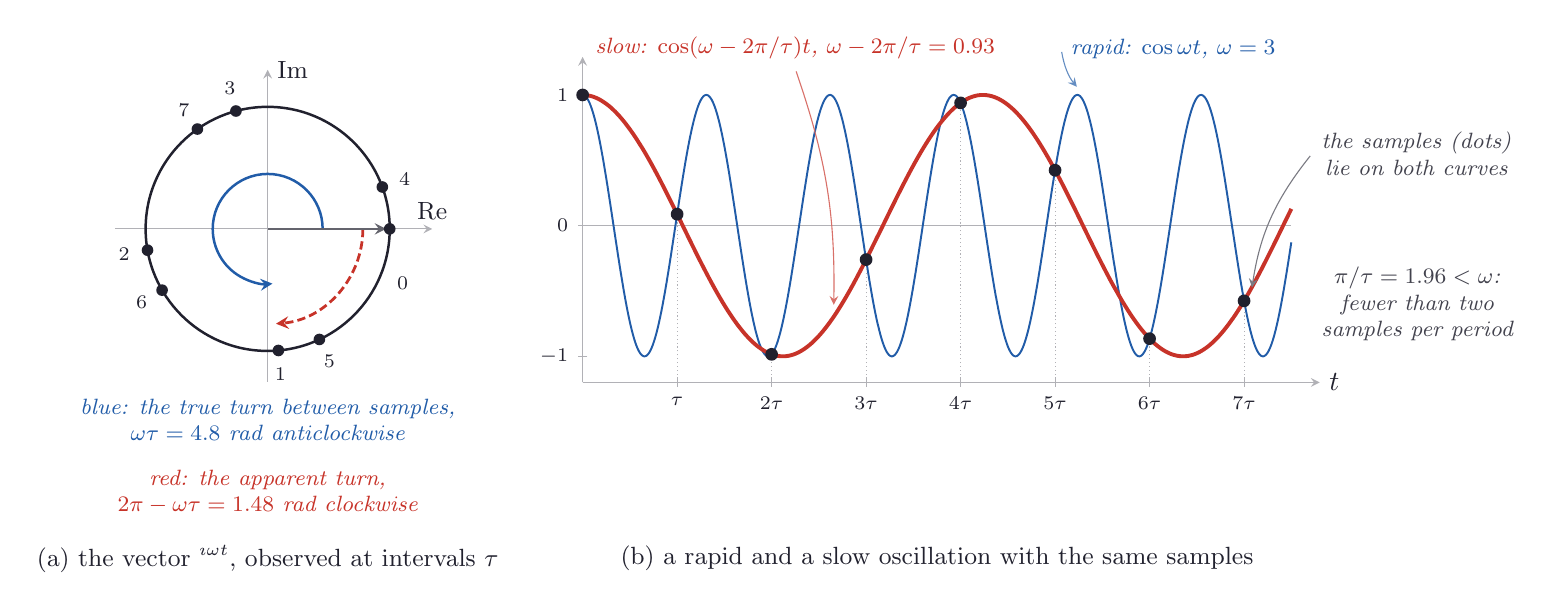
\begin{tikzpicture}[ink/.style={line width=0.9pt, ndInk}, faint/.style={line width=0.4pt, ndInk!35}, dashedink/.style={line width=0.5pt, ndInk!55, dash pattern=on 2.5pt off 2pt}, vec/.style={->, >=stealth, line width=1.2pt}, note/.style={font=\footnotesize\itshape, text=ndInk!85, align=center}, pointer/.style={->, >=stealth, line width=0.4pt, ndInk!60, shorten >=2pt, shorten <=1pt}, dot/.style={circle, fill=ndInk, inner sep=0pt, minimum size=3.4pt}, wash/.style={fill=ndSky, fill opacity=0.55}, every node/.style={text=ndInk}]
\definecolor{ndInk}{rgb}{0.13,0.13,0.18}
\definecolor{ndPaper}{rgb}{0.99,0.96,0.88}
\definecolor{ndSky}{rgb}{0.84,0.91,0.98}
\definecolor{ndRose}{rgb}{0.98,0.86,0.84}
\definecolor{ndBlue}{rgb}{0.13,0.36,0.66}
\definecolor{ndRed}{rgb}{0.78,0.20,0.16}
\definecolor{ndGold}{rgb}{0.88,0.62,0.10}
\definecolor{ndGreen}{rgb}{0.18,0.52,0.30}
\draw[faint, ->, >=stealth] (-1.94,0) -- (2.09,0) node[above, text=ndInk, font=\small] {$\mathrm{Re}$};
\draw[faint, ->, >=stealth] (0,-1.94) -- (0,2.02) node[right, text=ndInk, font=\small] {$\mathrm{Im}$};
\draw[ink] (0,0) circle (1.550);
\draw[vec, ndBlue, line width=0.9pt] (0.698,0) arc (0:275.02:0.698);
\draw[vec, ndRed, line width=1.0pt, dash pattern=on 3pt off 1.5pt] (1.209,0) arc (0:-84.98:1.209);
\draw[vec, ndInk!70, line width=0.8pt] (0,0) -- (1.504,0);
\node[dot, minimum size=4.2pt] at (1.550,0.000) {};
\node[font=\scriptsize] at (1.715,-0.693) {$0$};
\node[dot, minimum size=4.2pt] at (0.136,-1.544) {};
\node[font=\scriptsize] at (0.162,-1.843) {$1$};
\node[dot, minimum size=4.2pt] at (-1.526,-0.270) {};
\node[font=\scriptsize] at (-1.822,-0.323) {$2$};
\node[dot, minimum size=4.2pt] at (-0.403,1.497) {};
\node[font=\scriptsize] at (-0.481,1.786) {$3$};
\node[dot, minimum size=4.2pt] at (1.456,0.532) {};
\node[font=\scriptsize] at (1.738,0.635) {$4$};
\node[dot, minimum size=4.2pt] at (0.657,-1.404) {};
\node[font=\scriptsize] at (0.785,-1.675) {$5$};
\node[dot, minimum size=4.2pt] at (-1.341,-0.778) {};
\node[font=\scriptsize] at (-1.600,-0.928) {$6$};
\node[dot, minimum size=4.2pt] at (-0.892,1.268) {};
\node[font=\scriptsize] at (-1.065,1.513) {$7$};
\node[note, anchor=north, text=ndBlue] at (0,-2.04) {blue: the true turn between samples,\\ $\omega\tau=4.8$ rad anticlockwise};
\node[note, anchor=north, text=ndRed] at (0,-2.94) {red: the apparent turn,\\ $2\pi-\omega\tau=1.48$ rad clockwise};
\node[font=\small] at (0.0,-4.19) {(a) the vector $\ee^{\imath\omega t}$, observed at intervals $\tau$};
\draw[faint, ->, >=stealth] (4.000,-1.950) -- (13.360,-1.950) node[right, text=ndInk] {$t$};
\draw[faint, ->, >=stealth] (4.000,-1.950) -- (4.000,2.184) node[above, text=ndInk] {};
\draw[faint] (5.200,-1.890) -- (5.200,-2.010) node[below, font=\scriptsize, text=ndInk] {$\tau$};
\draw[faint] (6.400,-1.890) -- (6.400,-2.010) node[below, font=\scriptsize, text=ndInk] {$2\tau$};
\draw[faint] (7.600,-1.890) -- (7.600,-2.010) node[below, font=\scriptsize, text=ndInk] {$3\tau$};
\draw[faint] (8.800,-1.890) -- (8.800,-2.010) node[below, font=\scriptsize, text=ndInk] {$4\tau$};
\draw[faint] (10.000,-1.890) -- (10.000,-2.010) node[below, font=\scriptsize, text=ndInk] {$5\tau$};
\draw[faint] (11.200,-1.890) -- (11.200,-2.010) node[below, font=\scriptsize, text=ndInk] {$6\tau$};
\draw[faint] (12.400,-1.890) -- (12.400,-2.010) node[below, font=\scriptsize, text=ndInk] {$7\tau$};
\draw[faint] (4.060,-1.618) -- (3.940,-1.618) node[left, font=\scriptsize, text=ndInk] {$-1$};
\draw[faint] (4.060,0.041) -- (3.940,0.041) node[left, font=\scriptsize, text=ndInk] {$0$};
\draw[faint] (4.060,1.701) -- (3.940,1.701) node[left, font=\scriptsize, text=ndInk] {$1$};
\draw[faint] (4.000,0.041) -- (13.000,0.041);
\draw[line width=0.7pt, ndBlue] (4.000,1.701) -- (4.006,1.701) -- (4.012,1.699) -- (4.018,1.697) -- (4.024,1.693) -- (4.030,1.689) -- (4.036,1.684) -- (4.042,1.678) -- (4.048,1.671) -- (4.054,1.662) -- (4.060,1.653) -- (4.066,1.643) -- (4.072,1.633) -- (4.078,1.621) -- (4.084,1.608) -- (4.090,1.595) -- (4.096,1.580) -- (4.102,1.565) -- (4.108,1.548) -- (4.114,1.531) -- (4.120,1.513) -- (4.126,1.494) -- (4.132,1.475) -- (4.138,1.454) -- (4.144,1.433) -- (4.150,1.411) -- (4.156,1.388) -- (4.162,1.364) -- (4.168,1.340) -- (4.174,1.315) -- (4.180,1.289) -- (4.186,1.262) -- (4.192,1.235) -- (4.198,1.207) -- (4.204,1.178) -- (4.210,1.149) -- (4.216,1.118) -- (4.222,1.088) -- (4.228,1.057) -- (4.234,1.025) -- (4.240,0.992) -- (4.246,0.959) -- (4.252,0.926) -- (4.258,0.892) -- (4.264,0.858) -- (4.270,0.823) -- (4.276,0.787) -- (4.282,0.751) -- (4.288,0.715) -- (4.294,0.679) -- (4.300,0.642) -- (4.306,0.604) -- (4.312,0.567) -- (4.318,0.529) -- (4.324,0.490) -- (4.330,0.452) -- (4.336,0.413) -- (4.342,0.374) -- (4.348,0.335) -- (4.354,0.296) -- (4.360,0.256) -- (4.366,0.217) -- (4.372,0.177) -- (4.378,0.137) -- (4.384,0.098) -- (4.390,0.058) -- (4.396,0.018) -- (4.402,-0.022) -- (4.408,-0.062) -- (4.414,-0.102) -- (4.420,-0.141) -- (4.426,-0.181) -- (4.432,-0.220) -- (4.438,-0.259) -- (4.444,-0.299) -- (4.450,-0.338) -- (4.456,-0.376) -- (4.462,-0.415) -- (4.468,-0.453) -- (4.474,-0.491) -- (4.480,-0.528) -- (4.486,-0.566) -- (4.492,-0.603) -- (4.498,-0.639) -- (4.504,-0.675) -- (4.510,-0.711) -- (4.516,-0.746) -- (4.522,-0.781) -- (4.528,-0.815) -- (4.534,-0.849) -- (4.540,-0.883) -- (4.546,-0.916) -- (4.552,-0.948) -- (4.558,-0.980) -- (4.564,-1.011) -- (4.570,-1.041) -- (4.576,-1.071) -- (4.582,-1.100) -- (4.588,-1.129) -- (4.594,-1.157) -- (4.600,-1.184) -- (4.606,-1.211) -- (4.612,-1.236) -- (4.618,-1.261) -- (4.624,-1.286) -- (4.630,-1.309) -- (4.636,-1.332) -- (4.642,-1.354) -- (4.648,-1.375) -- (4.654,-1.396) -- (4.660,-1.415) -- (4.666,-1.434) -- (4.672,-1.452) -- (4.678,-1.469) -- (4.684,-1.485) -- (4.690,-1.500) -- (4.696,-1.514) -- (4.702,-1.528) -- (4.708,-1.540) -- (4.714,-1.552) -- (4.720,-1.562) -- (4.726,-1.572) -- (4.732,-1.581) -- (4.738,-1.589) -- (4.744,-1.596) -- (4.751,-1.602) -- (4.757,-1.607) -- (4.763,-1.611) -- (4.769,-1.614) -- (4.775,-1.617) -- (4.781,-1.618) -- (4.787,-1.618) -- (4.793,-1.617) -- (4.799,-1.616) -- (4.805,-1.613) -- (4.811,-1.610) -- (4.817,-1.605) -- (4.823,-1.600) -- (4.829,-1.593) -- (4.835,-1.586) -- (4.841,-1.578) -- (4.847,-1.569) -- (4.853,-1.559) -- (4.859,-1.548) -- (4.865,-1.536) -- (4.871,-1.523) -- (4.877,-1.509) -- (4.883,-1.494) -- (4.889,-1.479) -- (4.895,-1.462) -- (4.901,-1.445) -- (4.907,-1.427) -- (4.913,-1.408) -- (4.919,-1.388) -- (4.925,-1.367) -- (4.931,-1.346) -- (4.937,-1.324) -- (4.943,-1.301) -- (4.949,-1.277) -- (4.955,-1.252) -- (4.961,-1.227) -- (4.967,-1.201) -- (4.973,-1.174) -- (4.979,-1.146) -- (4.985,-1.118) -- (4.991,-1.089) -- (4.997,-1.060) -- (5.003,-1.030) -- (5.009,-0.999) -- (5.015,-0.968) -- (5.021,-0.936) -- (5.027,-0.903) -- (5.033,-0.870) -- (5.039,-0.837) -- (5.045,-0.803) -- (5.051,-0.768) -- (5.057,-0.733) -- (5.063,-0.698) -- (5.069,-0.662) -- (5.075,-0.625) -- (5.081,-0.589) -- (5.087,-0.552) -- (5.093,-0.514) -- (5.099,-0.477) -- (5.105,-0.439) -- (5.111,-0.400) -- (5.117,-0.362) -- (5.123,-0.323) -- (5.129,-0.284) -- (5.135,-0.245) -- (5.141,-0.205) -- (5.147,-0.166) -- (5.153,-0.126) -- (5.159,-0.087) -- (5.165,-0.047) -- (5.171,-0.007) -- (5.177,0.033) -- (5.183,0.073) -- (5.189,0.112) -- (5.195,0.152) -- (5.201,0.192) -- (5.207,0.232) -- (5.213,0.271) -- (5.219,0.311) -- (5.225,0.350) -- (5.231,0.389) -- (5.237,0.428) -- (5.243,0.466) -- (5.249,0.505) -- (5.255,0.543) -- (5.261,0.581) -- (5.267,0.618) -- (5.273,0.656) -- (5.279,0.692) -- (5.285,0.729) -- (5.291,0.765) -- (5.297,0.801) -- (5.303,0.836) -- (5.309,0.871) -- (5.315,0.905) -- (5.321,0.939) -- (5.327,0.972) -- (5.333,1.005) -- (5.339,1.037) -- (5.345,1.068) -- (5.351,1.099) -- (5.357,1.130) -- (5.363,1.160) -- (5.369,1.189) -- (5.375,1.217) -- (5.381,1.245) -- (5.387,1.272) -- (5.393,1.298) -- (5.399,1.324) -- (5.405,1.349) -- (5.411,1.373) -- (5.417,1.397) -- (5.423,1.419) -- (5.429,1.441) -- (5.435,1.462) -- (5.441,1.482) -- (5.447,1.502) -- (5.453,1.520) -- (5.459,1.538) -- (5.465,1.555) -- (5.471,1.571) -- (5.477,1.586) -- (5.483,1.600) -- (5.489,1.613) -- (5.495,1.625) -- (5.501,1.637) -- (5.507,1.647) -- (5.513,1.657) -- (5.519,1.666) -- (5.525,1.673) -- (5.531,1.680) -- (5.537,1.686) -- (5.543,1.691) -- (5.549,1.695) -- (5.555,1.698) -- (5.561,1.700) -- (5.567,1.701) -- (5.573,1.701) -- (5.579,1.700) -- (5.585,1.698) -- (5.591,1.696) -- (5.597,1.692) -- (5.603,1.687) -- (5.609,1.682) -- (5.615,1.675) -- (5.621,1.668) -- (5.627,1.659) -- (5.633,1.650) -- (5.639,1.640) -- (5.645,1.628) -- (5.651,1.616) -- (5.657,1.603) -- (5.663,1.589) -- (5.669,1.574) -- (5.675,1.559) -- (5.681,1.542) -- (5.687,1.525) -- (5.693,1.506) -- (5.699,1.487) -- (5.705,1.467) -- (5.711,1.446) -- (5.717,1.425) -- (5.723,1.402) -- (5.729,1.379) -- (5.735,1.355) -- (5.741,1.330) -- (5.747,1.305) -- (5.753,1.279) -- (5.759,1.252) -- (5.765,1.224) -- (5.771,1.196) -- (5.777,1.167) -- (5.783,1.137) -- (5.789,1.107) -- (5.795,1.076) -- (5.801,1.045) -- (5.807,1.013) -- (5.813,0.980) -- (5.819,0.947) -- (5.825,0.913) -- (5.831,0.879) -- (5.837,0.845) -- (5.843,0.809) -- (5.849,0.774) -- (5.855,0.738) -- (5.861,0.702) -- (5.867,0.665) -- (5.873,0.628) -- (5.879,0.590) -- (5.885,0.552) -- (5.891,0.514) -- (5.897,0.476) -- (5.903,0.437) -- (5.909,0.399) -- (5.915,0.360) -- (5.921,0.320) -- (5.927,0.281) -- (5.933,0.242) -- (5.939,0.202) -- (5.945,0.162) -- (5.951,0.122) -- (5.957,0.083) -- (5.963,0.043) -- (5.969,0.003) -- (5.975,-0.037) -- (5.981,-0.077) -- (5.987,-0.116) -- (5.993,-0.156) -- (5.999,-0.196) -- (6.005,-0.235) -- (6.011,-0.274) -- (6.017,-0.313) -- (6.023,-0.352) -- (6.029,-0.391) -- (6.035,-0.429) -- (6.041,-0.467) -- (6.047,-0.505) -- (6.053,-0.542) -- (6.059,-0.579) -- (6.065,-0.616) -- (6.071,-0.653) -- (6.077,-0.689) -- (6.083,-0.724) -- (6.089,-0.759) -- (6.095,-0.794) -- (6.101,-0.828) -- (6.107,-0.862) -- (6.113,-0.895) -- (6.119,-0.928) -- (6.125,-0.960) -- (6.131,-0.991) -- (6.137,-1.022) -- (6.143,-1.052) -- (6.149,-1.082) -- (6.155,-1.111) -- (6.161,-1.139) -- (6.167,-1.167) -- (6.173,-1.194) -- (6.179,-1.220) -- (6.185,-1.246) -- (6.191,-1.271) -- (6.197,-1.295) -- (6.203,-1.318) -- (6.209,-1.340) -- (6.215,-1.362) -- (6.221,-1.383) -- (6.227,-1.403) -- (6.233,-1.422) -- (6.239,-1.441) -- (6.245,-1.458) -- (6.252,-1.475) -- (6.258,-1.490) -- (6.264,-1.505) -- (6.270,-1.519) -- (6.276,-1.532) -- (6.282,-1.545) -- (6.288,-1.556) -- (6.294,-1.566) -- (6.300,-1.576) -- (6.306,-1.584) -- (6.312,-1.592) -- (6.318,-1.598) -- (6.324,-1.604) -- (6.330,-1.609) -- (6.336,-1.612) -- (6.342,-1.615) -- (6.348,-1.617) -- (6.354,-1.618) -- (6.360,-1.618) -- (6.366,-1.617) -- (6.372,-1.615) -- (6.378,-1.612) -- (6.384,-1.608) -- (6.390,-1.603) -- (6.396,-1.598) -- (6.402,-1.591) -- (6.408,-1.583) -- (6.414,-1.575) -- (6.420,-1.565) -- (6.426,-1.555) -- (6.432,-1.543) -- (6.438,-1.531) -- (6.444,-1.518) -- (6.450,-1.504) -- (6.456,-1.489) -- (6.462,-1.473) -- (6.468,-1.456) -- (6.474,-1.438) -- (6.480,-1.420) -- (6.486,-1.400) -- (6.492,-1.380) -- (6.498,-1.359) -- (6.504,-1.338) -- (6.510,-1.315) -- (6.516,-1.292) -- (6.522,-1.268) -- (6.528,-1.243) -- (6.534,-1.217) -- (6.540,-1.191) -- (6.546,-1.164) -- (6.552,-1.136) -- (6.558,-1.108) -- (6.564,-1.078) -- (6.570,-1.049) -- (6.576,-1.018) -- (6.582,-0.987) -- (6.588,-0.956) -- (6.594,-0.924) -- (6.600,-0.891) -- (6.606,-0.858) -- (6.612,-0.824) -- (6.618,-0.790) -- (6.624,-0.755) -- (6.630,-0.720) -- (6.636,-0.684) -- (6.642,-0.648) -- (6.648,-0.612) -- (6.654,-0.575) -- (6.660,-0.538) -- (6.666,-0.500) -- (6.672,-0.462) -- (6.678,-0.424) -- (6.684,-0.386) -- (6.690,-0.347) -- (6.696,-0.308) -- (6.702,-0.269) -- (6.708,-0.230) -- (6.714,-0.191) -- (6.720,-0.151) -- (6.726,-0.111) -- (6.732,-0.072) -- (6.738,-0.032) -- (6.744,0.008) -- (6.750,0.048) -- (6.756,0.088) -- (6.762,0.127) -- (6.768,0.167) -- (6.774,0.207) -- (6.780,0.246) -- (6.786,0.286) -- (6.792,0.325) -- (6.798,0.365) -- (6.804,0.404) -- (6.810,0.442) -- (6.816,0.481) -- (6.822,0.519) -- (6.828,0.557) -- (6.834,0.595) -- (6.840,0.632) -- (6.846,0.669) -- (6.852,0.706) -- (6.858,0.742) -- (6.864,0.778) -- (6.870,0.814) -- (6.876,0.849) -- (6.882,0.883) -- (6.888,0.918) -- (6.894,0.951) -- (6.900,0.984) -- (6.906,1.017) -- (6.912,1.049) -- (6.918,1.080) -- (6.924,1.111) -- (6.930,1.141) -- (6.936,1.171) -- (6.942,1.199) -- (6.948,1.228) -- (6.954,1.255) -- (6.960,1.282) -- (6.966,1.308) -- (6.972,1.334) -- (6.978,1.358) -- (6.984,1.382) -- (6.990,1.405) -- (6.996,1.427) -- (7.002,1.449) -- (7.008,1.470) -- (7.014,1.490) -- (7.020,1.509) -- (7.026,1.527) -- (7.032,1.544) -- (7.038,1.561) -- (7.044,1.576) -- (7.050,1.591) -- (7.056,1.605) -- (7.062,1.618) -- (7.068,1.630) -- (7.074,1.641) -- (7.080,1.651) -- (7.086,1.660) -- (7.092,1.669) -- (7.098,1.676) -- (7.104,1.682) -- (7.110,1.688) -- (7.116,1.692) -- (7.122,1.696) -- (7.128,1.699) -- (7.134,1.700) -- (7.140,1.701) -- (7.146,1.701) -- (7.152,1.700) -- (7.158,1.697) -- (7.164,1.694) -- (7.170,1.690) -- (7.176,1.685) -- (7.182,1.679) -- (7.188,1.672) -- (7.194,1.665) -- (7.200,1.656) -- (7.206,1.646) -- (7.212,1.635) -- (7.218,1.624) -- (7.224,1.611) -- (7.230,1.598) -- (7.236,1.584) -- (7.242,1.569) -- (7.248,1.553) -- (7.254,1.536) -- (7.260,1.518) -- (7.266,1.499) -- (7.272,1.480) -- (7.278,1.459) -- (7.284,1.438) -- (7.290,1.416) -- (7.296,1.394) -- (7.302,1.370) -- (7.308,1.346) -- (7.314,1.321) -- (7.320,1.295) -- (7.326,1.269) -- (7.332,1.242) -- (7.338,1.214) -- (7.344,1.185) -- (7.350,1.156) -- (7.356,1.126) -- (7.362,1.096) -- (7.368,1.064) -- (7.374,1.033) -- (7.380,1.001) -- (7.386,0.968) -- (7.392,0.934) -- (7.398,0.901) -- (7.404,0.866) -- (7.410,0.831) -- (7.416,0.796) -- (7.422,0.760) -- (7.428,0.724) -- (7.434,0.688) -- (7.440,0.651) -- (7.446,0.614) -- (7.452,0.576) -- (7.458,0.538) -- (7.464,0.500) -- (7.470,0.462) -- (7.476,0.423) -- (7.482,0.384) -- (7.488,0.345) -- (7.494,0.306) -- (7.500,0.266) -- (7.506,0.227) -- (7.512,0.187) -- (7.518,0.147) -- (7.524,0.107) -- (7.530,0.068) -- (7.536,0.028) -- (7.542,-0.012) -- (7.548,-0.052) -- (7.554,-0.092) -- (7.560,-0.131) -- (7.566,-0.171) -- (7.572,-0.210) -- (7.578,-0.250) -- (7.584,-0.289) -- (7.590,-0.328) -- (7.596,-0.367) -- (7.602,-0.405) -- (7.608,-0.443) -- (7.614,-0.481) -- (7.620,-0.519) -- (7.626,-0.556) -- (7.632,-0.593) -- (7.638,-0.630) -- (7.644,-0.666) -- (7.650,-0.702) -- (7.656,-0.737) -- (7.662,-0.772) -- (7.668,-0.807) -- (7.674,-0.841) -- (7.680,-0.874) -- (7.686,-0.907) -- (7.692,-0.940) -- (7.698,-0.972) -- (7.704,-1.003) -- (7.710,-1.034) -- (7.716,-1.064) -- (7.722,-1.093) -- (7.728,-1.122) -- (7.734,-1.150) -- (7.740,-1.177) -- (7.746,-1.204) -- (7.753,-1.230) -- (7.759,-1.255) -- (7.765,-1.280) -- (7.771,-1.303) -- (7.777,-1.326) -- (7.783,-1.349) -- (7.789,-1.370) -- (7.795,-1.391) -- (7.801,-1.410) -- (7.807,-1.429) -- (7.813,-1.447) -- (7.819,-1.464) -- (7.825,-1.481) -- (7.831,-1.496) -- (7.837,-1.511) -- (7.843,-1.524) -- (7.849,-1.537) -- (7.855,-1.549) -- (7.861,-1.560) -- (7.867,-1.570) -- (7.873,-1.579) -- (7.879,-1.587) -- (7.885,-1.594) -- (7.891,-1.601) -- (7.897,-1.606) -- (7.903,-1.610) -- (7.909,-1.614) -- (7.915,-1.616) -- (7.921,-1.618) -- (7.927,-1.618) -- (7.933,-1.618) -- (7.939,-1.616) -- (7.945,-1.614) -- (7.951,-1.611) -- (7.957,-1.606) -- (7.963,-1.601) -- (7.969,-1.595) -- (7.975,-1.588) -- (7.981,-1.580) -- (7.987,-1.571) -- (7.993,-1.561) -- (7.999,-1.550) -- (8.005,-1.539) -- (8.011,-1.526) -- (8.017,-1.512) -- (8.023,-1.498) -- (8.029,-1.483) -- (8.035,-1.466) -- (8.041,-1.449) -- (8.047,-1.431) -- (8.053,-1.413) -- (8.059,-1.393) -- (8.065,-1.373) -- (8.071,-1.351) -- (8.077,-1.329) -- (8.083,-1.306) -- (8.089,-1.283) -- (8.095,-1.258) -- (8.101,-1.233) -- (8.107,-1.207) -- (8.113,-1.181) -- (8.119,-1.153) -- (8.125,-1.125) -- (8.131,-1.097) -- (8.137,-1.067) -- (8.143,-1.037) -- (8.149,-1.007) -- (8.155,-0.976) -- (8.161,-0.944) -- (8.167,-0.911) -- (8.173,-0.879) -- (8.179,-0.845) -- (8.185,-0.811) -- (8.191,-0.777) -- (8.197,-0.742) -- (8.203,-0.706) -- (8.209,-0.671) -- (8.215,-0.634) -- (8.221,-0.598) -- (8.227,-0.561) -- (8.233,-0.524) -- (8.239,-0.486) -- (8.245,-0.448) -- (8.251,-0.410) -- (8.257,-0.371) -- (8.263,-0.333) -- (8.269,-0.294) -- (8.275,-0.255) -- (8.281,-0.215) -- (8.287,-0.176) -- (8.293,-0.136) -- (8.299,-0.097) -- (8.305,-0.057) -- (8.311,-0.017) -- (8.317,0.023) -- (8.323,0.063) -- (8.329,0.103) -- (8.335,0.142) -- (8.341,0.182) -- (8.347,0.222) -- (8.353,0.261) -- (8.359,0.301) -- (8.365,0.340) -- (8.371,0.379) -- (8.377,0.418) -- (8.383,0.457) -- (8.389,0.495) -- (8.395,0.533) -- (8.401,0.571) -- (8.407,0.609) -- (8.413,0.646) -- (8.419,0.683) -- (8.425,0.720) -- (8.431,0.756) -- (8.437,0.792) -- (8.443,0.827) -- (8.449,0.862) -- (8.455,0.896) -- (8.461,0.930) -- (8.467,0.964) -- (8.473,0.997) -- (8.479,1.029) -- (8.485,1.061) -- (8.491,1.092) -- (8.497,1.122) -- (8.503,1.152) -- (8.509,1.182) -- (8.515,1.210) -- (8.521,1.238) -- (8.527,1.265) -- (8.533,1.292) -- (8.539,1.318) -- (8.545,1.343) -- (8.551,1.367) -- (8.557,1.391) -- (8.563,1.414) -- (8.569,1.436) -- (8.575,1.457) -- (8.581,1.477) -- (8.587,1.497) -- (8.593,1.516) -- (8.599,1.533) -- (8.605,1.550) -- (8.611,1.567) -- (8.617,1.582) -- (8.623,1.596) -- (8.629,1.610) -- (8.635,1.622) -- (8.641,1.634) -- (8.647,1.645) -- (8.653,1.655) -- (8.659,1.664) -- (8.665,1.671) -- (8.671,1.678) -- (8.677,1.685) -- (8.683,1.690) -- (8.689,1.694) -- (8.695,1.697) -- (8.701,1.699) -- (8.707,1.701) -- (8.713,1.701) -- (8.719,1.700) -- (8.725,1.699) -- (8.731,1.696) -- (8.737,1.693) -- (8.743,1.689) -- (8.749,1.683) -- (8.755,1.677) -- (8.761,1.670) -- (8.767,1.661) -- (8.773,1.652) -- (8.779,1.642) -- (8.785,1.631) -- (8.791,1.619) -- (8.797,1.606) -- (8.803,1.593) -- (8.809,1.578) -- (8.815,1.563) -- (8.821,1.546) -- (8.827,1.529) -- (8.833,1.511) -- (8.839,1.492) -- (8.845,1.472) -- (8.851,1.452) -- (8.857,1.430) -- (8.863,1.408) -- (8.869,1.385) -- (8.875,1.361) -- (8.881,1.337) -- (8.887,1.311) -- (8.893,1.285) -- (8.899,1.259) -- (8.905,1.231) -- (8.911,1.203) -- (8.917,1.174) -- (8.923,1.145) -- (8.929,1.115) -- (8.935,1.084) -- (8.941,1.053) -- (8.947,1.021) -- (8.953,0.988) -- (8.959,0.955) -- (8.965,0.922) -- (8.971,0.888) -- (8.977,0.853) -- (8.983,0.818) -- (8.989,0.783) -- (8.995,0.747) -- (9.001,0.711) -- (9.007,0.674) -- (9.013,0.637) -- (9.019,0.600) -- (9.025,0.562) -- (9.031,0.524) -- (9.037,0.486) -- (9.043,0.447) -- (9.049,0.408) -- (9.055,0.369) -- (9.061,0.330) -- (9.067,0.291) -- (9.073,0.251) -- (9.079,0.212) -- (9.085,0.172) -- (9.091,0.132) -- (9.097,0.093) -- (9.103,0.053) -- (9.109,0.013) -- (9.115,-0.027) -- (9.121,-0.067) -- (9.127,-0.107) -- (9.133,-0.146) -- (9.139,-0.186) -- (9.145,-0.225) -- (9.151,-0.264) -- (9.157,-0.303) -- (9.163,-0.342) -- (9.169,-0.381) -- (9.175,-0.419) -- (9.181,-0.458) -- (9.187,-0.495) -- (9.193,-0.533) -- (9.199,-0.570) -- (9.205,-0.607) -- (9.211,-0.644) -- (9.217,-0.680) -- (9.223,-0.715) -- (9.229,-0.751) -- (9.235,-0.785) -- (9.241,-0.820) -- (9.247,-0.854) -- (9.254,-0.887) -- (9.260,-0.920) -- (9.266,-0.952) -- (9.272,-0.983) -- (9.278,-1.015) -- (9.284,-1.045) -- (9.290,-1.075) -- (9.296,-1.104) -- (9.302,-1.132) -- (9.308,-1.160) -- (9.314,-1.187) -- (9.320,-1.214) -- (9.326,-1.240) -- (9.332,-1.265) -- (9.338,-1.289) -- (9.344,-1.312) -- (9.350,-1.335) -- (9.356,-1.357) -- (9.362,-1.378) -- (9.368,-1.398) -- (9.374,-1.417) -- (9.380,-1.436) -- (9.386,-1.454) -- (9.392,-1.471) -- (9.398,-1.487) -- (9.404,-1.502) -- (9.410,-1.516) -- (9.416,-1.529) -- (9.422,-1.542) -- (9.428,-1.553) -- (9.434,-1.564) -- (9.440,-1.573) -- (9.446,-1.582) -- (9.452,-1.590) -- (9.458,-1.597) -- (9.464,-1.603) -- (9.470,-1.608) -- (9.476,-1.612) -- (9.482,-1.615) -- (9.488,-1.617) -- (9.494,-1.618) -- (9.500,-1.618) -- (9.506,-1.617) -- (9.512,-1.616) -- (9.518,-1.613) -- (9.524,-1.609) -- (9.530,-1.605) -- (9.536,-1.599) -- (9.542,-1.593) -- (9.548,-1.585) -- (9.554,-1.577) -- (9.560,-1.567) -- (9.566,-1.557) -- (9.572,-1.546) -- (9.578,-1.534) -- (9.584,-1.521) -- (9.590,-1.507) -- (9.596,-1.492) -- (9.602,-1.477) -- (9.608,-1.460) -- (9.614,-1.443) -- (9.620,-1.424) -- (9.626,-1.405) -- (9.632,-1.385) -- (9.638,-1.365) -- (9.644,-1.343) -- (9.650,-1.321) -- (9.656,-1.298) -- (9.662,-1.274) -- (9.668,-1.249) -- (9.674,-1.224) -- (9.680,-1.197) -- (9.686,-1.171) -- (9.692,-1.143) -- (9.698,-1.115) -- (9.704,-1.086) -- (9.710,-1.056) -- (9.716,-1.026) -- (9.722,-0.995) -- (9.728,-0.964) -- (9.734,-0.932) -- (9.740,-0.899) -- (9.746,-0.866) -- (9.752,-0.832) -- (9.758,-0.798) -- (9.764,-0.764) -- (9.770,-0.729) -- (9.776,-0.693) -- (9.782,-0.657) -- (9.788,-0.621) -- (9.794,-0.584) -- (9.800,-0.547) -- (9.806,-0.510) -- (9.812,-0.472) -- (9.818,-0.434) -- (9.824,-0.395) -- (9.830,-0.357) -- (9.836,-0.318) -- (9.842,-0.279) -- (9.848,-0.240) -- (9.854,-0.200) -- (9.860,-0.161) -- (9.866,-0.121) -- (9.872,-0.082) -- (9.878,-0.042) -- (9.884,-0.002) -- (9.890,0.038) -- (9.896,0.078) -- (9.902,0.117) -- (9.908,0.157) -- (9.914,0.197) -- (9.920,0.237) -- (9.926,0.276) -- (9.932,0.316) -- (9.938,0.355) -- (9.944,0.394) -- (9.950,0.433) -- (9.956,0.471) -- (9.962,0.510) -- (9.968,0.548) -- (9.974,0.586) -- (9.980,0.623) -- (9.986,0.660) -- (9.992,0.697) -- (9.998,0.733) -- (10.004,0.769) -- (10.010,0.805) -- (10.016,0.840) -- (10.022,0.875) -- (10.028,0.909) -- (10.034,0.943) -- (10.040,0.976) -- (10.046,1.009) -- (10.052,1.041) -- (10.058,1.072) -- (10.064,1.103) -- (10.070,1.134) -- (10.076,1.163) -- (10.082,1.192) -- (10.088,1.221) -- (10.094,1.248) -- (10.100,1.275) -- (10.106,1.302) -- (10.112,1.327) -- (10.118,1.352) -- (10.124,1.376) -- (10.130,1.399) -- (10.136,1.422) -- (10.142,1.444) -- (10.148,1.465) -- (10.154,1.485) -- (10.160,1.504) -- (10.166,1.522) -- (10.172,1.540) -- (10.178,1.557) -- (10.184,1.572) -- (10.190,1.587) -- (10.196,1.601) -- (10.202,1.615) -- (10.208,1.627) -- (10.214,1.638) -- (10.220,1.649) -- (10.226,1.658) -- (10.232,1.667) -- (10.238,1.674) -- (10.244,1.681) -- (10.250,1.687) -- (10.256,1.691) -- (10.262,1.695) -- (10.268,1.698) -- (10.274,1.700) -- (10.280,1.701) -- (10.286,1.701) -- (10.292,1.700) -- (10.298,1.698) -- (10.304,1.695) -- (10.310,1.691) -- (10.316,1.687) -- (10.322,1.681) -- (10.328,1.674) -- (10.334,1.667) -- (10.340,1.658) -- (10.346,1.649) -- (10.352,1.638) -- (10.358,1.627) -- (10.364,1.615) -- (10.370,1.601) -- (10.376,1.587) -- (10.382,1.572) -- (10.388,1.557) -- (10.394,1.540) -- (10.400,1.522) -- (10.406,1.504) -- (10.412,1.485) -- (10.418,1.465) -- (10.424,1.444) -- (10.430,1.422) -- (10.436,1.399) -- (10.442,1.376) -- (10.448,1.352) -- (10.454,1.327) -- (10.460,1.302) -- (10.466,1.275) -- (10.472,1.248) -- (10.478,1.221) -- (10.484,1.192) -- (10.490,1.163) -- (10.496,1.134) -- (10.502,1.103) -- (10.508,1.072) -- (10.514,1.041) -- (10.520,1.009) -- (10.526,0.976) -- (10.532,0.943) -- (10.538,0.909) -- (10.544,0.875) -- (10.550,0.840) -- (10.556,0.805) -- (10.562,0.769) -- (10.568,0.733) -- (10.574,0.697) -- (10.580,0.660) -- (10.586,0.623) -- (10.592,0.585) -- (10.598,0.548) -- (10.604,0.510) -- (10.610,0.471) -- (10.616,0.433) -- (10.622,0.394) -- (10.628,0.355) -- (10.634,0.315) -- (10.640,0.276) -- (10.646,0.237) -- (10.652,0.197) -- (10.658,0.157) -- (10.664,0.117) -- (10.670,0.078) -- (10.676,0.038) -- (10.682,-0.002) -- (10.688,-0.042) -- (10.694,-0.082) -- (10.700,-0.121) -- (10.706,-0.161) -- (10.712,-0.201) -- (10.718,-0.240) -- (10.724,-0.279) -- (10.730,-0.318) -- (10.736,-0.357) -- (10.742,-0.395) -- (10.748,-0.434) -- (10.755,-0.472) -- (10.761,-0.510) -- (10.767,-0.547) -- (10.773,-0.584) -- (10.779,-0.621) -- (10.785,-0.657) -- (10.791,-0.693) -- (10.797,-0.729) -- (10.803,-0.764) -- (10.809,-0.798) -- (10.815,-0.832) -- (10.821,-0.866) -- (10.827,-0.899) -- (10.833,-0.932) -- (10.839,-0.964) -- (10.845,-0.995) -- (10.851,-1.026) -- (10.857,-1.056) -- (10.863,-1.086) -- (10.869,-1.115) -- (10.875,-1.143) -- (10.881,-1.171) -- (10.887,-1.197) -- (10.893,-1.224) -- (10.899,-1.249) -- (10.905,-1.274) -- (10.911,-1.298) -- (10.917,-1.321) -- (10.923,-1.343) -- (10.929,-1.365) -- (10.935,-1.385) -- (10.941,-1.405) -- (10.947,-1.425) -- (10.953,-1.443) -- (10.959,-1.460) -- (10.965,-1.477) -- (10.971,-1.492) -- (10.977,-1.507) -- (10.983,-1.521) -- (10.989,-1.534) -- (10.995,-1.546) -- (11.001,-1.557) -- (11.007,-1.567) -- (11.013,-1.577) -- (11.019,-1.585) -- (11.025,-1.593) -- (11.031,-1.599) -- (11.037,-1.605) -- (11.043,-1.609) -- (11.049,-1.613) -- (11.055,-1.616) -- (11.061,-1.617) -- (11.067,-1.618) -- (11.073,-1.618) -- (11.079,-1.617) -- (11.085,-1.615) -- (11.091,-1.612) -- (11.097,-1.608) -- (11.103,-1.603) -- (11.109,-1.597) -- (11.115,-1.590) -- (11.121,-1.582) -- (11.127,-1.573) -- (11.133,-1.564) -- (11.139,-1.553) -- (11.145,-1.542) -- (11.151,-1.529) -- (11.157,-1.516) -- (11.163,-1.502) -- (11.169,-1.487) -- (11.175,-1.471) -- (11.181,-1.454) -- (11.187,-1.436) -- (11.193,-1.417) -- (11.199,-1.398) -- (11.205,-1.378) -- (11.211,-1.357) -- (11.217,-1.335) -- (11.223,-1.312) -- (11.229,-1.289) -- (11.235,-1.264) -- (11.241,-1.240) -- (11.247,-1.214) -- (11.253,-1.187) -- (11.259,-1.160) -- (11.265,-1.132) -- (11.271,-1.104) -- (11.277,-1.075) -- (11.283,-1.045) -- (11.289,-1.014) -- (11.295,-0.983) -- (11.301,-0.952) -- (11.307,-0.920) -- (11.313,-0.887) -- (11.319,-0.854) -- (11.325,-0.820) -- (11.331,-0.785) -- (11.337,-0.751) -- (11.343,-0.715) -- (11.349,-0.680) -- (11.355,-0.644) -- (11.361,-0.607) -- (11.367,-0.570) -- (11.373,-0.533) -- (11.379,-0.495) -- (11.385,-0.458) -- (11.391,-0.419) -- (11.397,-0.381) -- (11.403,-0.342) -- (11.409,-0.303) -- (11.415,-0.264) -- (11.421,-0.225) -- (11.427,-0.186) -- (11.433,-0.146) -- (11.439,-0.107) -- (11.445,-0.067) -- (11.451,-0.027) -- (11.457,0.013) -- (11.463,0.053) -- (11.469,0.093) -- (11.475,0.132) -- (11.481,0.172) -- (11.487,0.212) -- (11.493,0.251) -- (11.499,0.291) -- (11.505,0.330) -- (11.511,0.369) -- (11.517,0.408) -- (11.523,0.447) -- (11.529,0.486) -- (11.535,0.524) -- (11.541,0.562) -- (11.547,0.600) -- (11.553,0.637) -- (11.559,0.674) -- (11.565,0.711) -- (11.571,0.747) -- (11.577,0.783) -- (11.583,0.818) -- (11.589,0.853) -- (11.595,0.888) -- (11.601,0.922) -- (11.607,0.955) -- (11.613,0.988) -- (11.619,1.021) -- (11.625,1.053) -- (11.631,1.084) -- (11.637,1.115) -- (11.643,1.145) -- (11.649,1.174) -- (11.655,1.203) -- (11.661,1.231) -- (11.667,1.259) -- (11.673,1.285) -- (11.679,1.311) -- (11.685,1.337) -- (11.691,1.361) -- (11.697,1.385) -- (11.703,1.408) -- (11.709,1.430) -- (11.715,1.452) -- (11.721,1.472) -- (11.727,1.492) -- (11.733,1.511) -- (11.739,1.529) -- (11.745,1.546) -- (11.751,1.563) -- (11.757,1.578) -- (11.763,1.593) -- (11.769,1.606) -- (11.775,1.619) -- (11.781,1.631) -- (11.787,1.642) -- (11.793,1.652) -- (11.799,1.661) -- (11.805,1.670) -- (11.811,1.677) -- (11.817,1.683) -- (11.823,1.689) -- (11.829,1.693) -- (11.835,1.696) -- (11.841,1.699) -- (11.847,1.700) -- (11.853,1.701) -- (11.859,1.701) -- (11.865,1.699) -- (11.871,1.697) -- (11.877,1.694) -- (11.883,1.690) -- (11.889,1.685) -- (11.895,1.678) -- (11.901,1.671) -- (11.907,1.664) -- (11.913,1.655) -- (11.919,1.645) -- (11.925,1.634) -- (11.931,1.622) -- (11.937,1.610) -- (11.943,1.596) -- (11.949,1.582) -- (11.955,1.567) -- (11.961,1.550) -- (11.967,1.533) -- (11.973,1.516) -- (11.979,1.497) -- (11.985,1.477) -- (11.991,1.457) -- (11.997,1.436) -- (12.003,1.414) -- (12.009,1.391) -- (12.015,1.367) -- (12.021,1.343) -- (12.027,1.318) -- (12.033,1.292) -- (12.039,1.265) -- (12.045,1.238) -- (12.051,1.210) -- (12.057,1.181) -- (12.063,1.152) -- (12.069,1.122) -- (12.075,1.092) -- (12.081,1.061) -- (12.087,1.029) -- (12.093,0.996) -- (12.099,0.964) -- (12.105,0.930) -- (12.111,0.896) -- (12.117,0.862) -- (12.123,0.827) -- (12.129,0.792) -- (12.135,0.756) -- (12.141,0.720) -- (12.147,0.683) -- (12.153,0.646) -- (12.159,0.609) -- (12.165,0.571) -- (12.171,0.533) -- (12.177,0.495) -- (12.183,0.457) -- (12.189,0.418) -- (12.195,0.379) -- (12.201,0.340) -- (12.207,0.301) -- (12.213,0.261) -- (12.219,0.222) -- (12.225,0.182) -- (12.231,0.142) -- (12.237,0.102) -- (12.243,0.063) -- (12.249,0.023) -- (12.256,-0.017) -- (12.262,-0.057) -- (12.268,-0.097) -- (12.274,-0.136) -- (12.280,-0.176) -- (12.286,-0.215) -- (12.292,-0.255) -- (12.298,-0.294) -- (12.304,-0.333) -- (12.310,-0.371) -- (12.316,-0.410) -- (12.322,-0.448) -- (12.328,-0.486) -- (12.334,-0.524) -- (12.340,-0.561) -- (12.346,-0.598) -- (12.352,-0.635) -- (12.358,-0.671) -- (12.364,-0.707) -- (12.370,-0.742) -- (12.376,-0.777) -- (12.382,-0.811) -- (12.388,-0.845) -- (12.394,-0.879) -- (12.400,-0.912) -- (12.406,-0.944) -- (12.412,-0.976) -- (12.418,-1.007) -- (12.424,-1.037) -- (12.430,-1.067) -- (12.436,-1.097) -- (12.442,-1.125) -- (12.448,-1.153) -- (12.454,-1.181) -- (12.460,-1.207) -- (12.466,-1.233) -- (12.472,-1.258) -- (12.478,-1.283) -- (12.484,-1.306) -- (12.490,-1.329) -- (12.496,-1.351) -- (12.502,-1.373) -- (12.508,-1.393) -- (12.514,-1.413) -- (12.520,-1.431) -- (12.526,-1.449) -- (12.532,-1.466) -- (12.538,-1.483) -- (12.544,-1.498) -- (12.550,-1.512) -- (12.556,-1.526) -- (12.562,-1.539) -- (12.568,-1.550) -- (12.574,-1.561) -- (12.580,-1.571) -- (12.586,-1.580) -- (12.592,-1.588) -- (12.598,-1.595) -- (12.604,-1.601) -- (12.610,-1.606) -- (12.616,-1.611) -- (12.622,-1.614) -- (12.628,-1.616) -- (12.634,-1.618) -- (12.640,-1.618) -- (12.646,-1.618) -- (12.652,-1.616) -- (12.658,-1.614) -- (12.664,-1.610) -- (12.670,-1.606) -- (12.676,-1.601) -- (12.682,-1.594) -- (12.688,-1.587) -- (12.694,-1.579) -- (12.700,-1.570) -- (12.706,-1.560) -- (12.712,-1.549) -- (12.718,-1.537) -- (12.724,-1.524) -- (12.730,-1.511) -- (12.736,-1.496) -- (12.742,-1.481) -- (12.748,-1.464) -- (12.754,-1.447) -- (12.760,-1.429) -- (12.766,-1.410) -- (12.772,-1.391) -- (12.778,-1.370) -- (12.784,-1.349) -- (12.790,-1.326) -- (12.796,-1.303) -- (12.802,-1.280) -- (12.808,-1.255) -- (12.814,-1.230) -- (12.820,-1.204) -- (12.826,-1.177) -- (12.832,-1.150) -- (12.838,-1.122) -- (12.844,-1.093) -- (12.850,-1.064) -- (12.856,-1.034) -- (12.862,-1.003) -- (12.868,-0.972) -- (12.874,-0.940) -- (12.880,-0.907) -- (12.886,-0.874) -- (12.892,-0.841) -- (12.898,-0.807) -- (12.904,-0.772) -- (12.910,-0.737) -- (12.916,-0.702) -- (12.922,-0.666) -- (12.928,-0.630) -- (12.934,-0.593) -- (12.940,-0.556) -- (12.946,-0.519) -- (12.952,-0.481) -- (12.958,-0.443) -- (12.964,-0.405) -- (12.970,-0.367) -- (12.976,-0.328) -- (12.982,-0.289) -- (12.988,-0.250) -- (12.994,-0.210) -- (13.000,-0.171);
\draw[line width=1.4pt, ndRed] (4.000,1.701) -- (4.006,1.701) -- (4.012,1.701) -- (4.018,1.701) -- (4.024,1.700) -- (4.030,1.700) -- (4.036,1.699) -- (4.042,1.699) -- (4.048,1.698) -- (4.054,1.697) -- (4.060,1.696) -- (4.066,1.696) -- (4.072,1.694) -- (4.078,1.693) -- (4.084,1.692) -- (4.090,1.691) -- (4.096,1.689) -- (4.102,1.688) -- (4.108,1.686) -- (4.114,1.685) -- (4.120,1.683) -- (4.126,1.681) -- (4.132,1.679) -- (4.138,1.677) -- (4.144,1.675) -- (4.150,1.673) -- (4.156,1.670) -- (4.162,1.668) -- (4.168,1.665) -- (4.174,1.663) -- (4.180,1.660) -- (4.186,1.657) -- (4.192,1.654) -- (4.198,1.652) -- (4.204,1.649) -- (4.210,1.645) -- (4.216,1.642) -- (4.222,1.639) -- (4.228,1.636) -- (4.234,1.632) -- (4.240,1.628) -- (4.246,1.625) -- (4.252,1.621) -- (4.258,1.617) -- (4.264,1.613) -- (4.270,1.609) -- (4.276,1.605) -- (4.282,1.601) -- (4.288,1.597) -- (4.294,1.593) -- (4.300,1.588) -- (4.306,1.584) -- (4.312,1.579) -- (4.318,1.574) -- (4.324,1.570) -- (4.330,1.565) -- (4.336,1.560) -- (4.342,1.555) -- (4.348,1.550) -- (4.354,1.545) -- (4.360,1.539) -- (4.366,1.534) -- (4.372,1.528) -- (4.378,1.523) -- (4.384,1.517) -- (4.390,1.512) -- (4.396,1.506) -- (4.402,1.500) -- (4.408,1.494) -- (4.414,1.488) -- (4.420,1.482) -- (4.426,1.476) -- (4.432,1.470) -- (4.438,1.463) -- (4.444,1.457) -- (4.450,1.451) -- (4.456,1.444) -- (4.462,1.437) -- (4.468,1.431) -- (4.474,1.424) -- (4.480,1.417) -- (4.486,1.410) -- (4.492,1.403) -- (4.498,1.396) -- (4.504,1.389) -- (4.510,1.382) -- (4.516,1.374) -- (4.522,1.367) -- (4.528,1.360) -- (4.534,1.352) -- (4.540,1.344) -- (4.546,1.337) -- (4.552,1.329) -- (4.558,1.321) -- (4.564,1.313) -- (4.570,1.305) -- (4.576,1.297) -- (4.582,1.289) -- (4.588,1.281) -- (4.594,1.273) -- (4.600,1.265) -- (4.606,1.256) -- (4.612,1.248) -- (4.618,1.239) -- (4.624,1.231) -- (4.630,1.222) -- (4.636,1.214) -- (4.642,1.205) -- (4.648,1.196) -- (4.654,1.187) -- (4.660,1.178) -- (4.666,1.169) -- (4.672,1.160) -- (4.678,1.151) -- (4.684,1.142) -- (4.690,1.133) -- (4.696,1.123) -- (4.702,1.114) -- (4.708,1.104) -- (4.714,1.095) -- (4.720,1.085) -- (4.726,1.076) -- (4.732,1.066) -- (4.738,1.056) -- (4.744,1.047) -- (4.751,1.037) -- (4.757,1.027) -- (4.763,1.017) -- (4.769,1.007) -- (4.775,0.997) -- (4.781,0.987) -- (4.787,0.977) -- (4.793,0.967) -- (4.799,0.956) -- (4.805,0.946) -- (4.811,0.936) -- (4.817,0.925) -- (4.823,0.915) -- (4.829,0.904) -- (4.835,0.894) -- (4.841,0.883) -- (4.847,0.873) -- (4.853,0.862) -- (4.859,0.851) -- (4.865,0.840) -- (4.871,0.830) -- (4.877,0.819) -- (4.883,0.808) -- (4.889,0.797) -- (4.895,0.786) -- (4.901,0.775) -- (4.907,0.764) -- (4.913,0.753) -- (4.919,0.741) -- (4.925,0.730) -- (4.931,0.719) -- (4.937,0.708) -- (4.943,0.696) -- (4.949,0.685) -- (4.955,0.674) -- (4.961,0.662) -- (4.967,0.651) -- (4.973,0.639) -- (4.979,0.628) -- (4.985,0.616) -- (4.991,0.605) -- (4.997,0.593) -- (5.003,0.582) -- (5.009,0.570) -- (5.015,0.558) -- (5.021,0.547) -- (5.027,0.535) -- (5.033,0.523) -- (5.039,0.511) -- (5.045,0.499) -- (5.051,0.488) -- (5.057,0.476) -- (5.063,0.464) -- (5.069,0.452) -- (5.075,0.440) -- (5.081,0.428) -- (5.087,0.416) -- (5.093,0.404) -- (5.099,0.392) -- (5.105,0.380) -- (5.111,0.368) -- (5.117,0.356) -- (5.123,0.344) -- (5.129,0.332) -- (5.135,0.319) -- (5.141,0.307) -- (5.147,0.295) -- (5.153,0.283) -- (5.159,0.271) -- (5.165,0.259) -- (5.171,0.246) -- (5.177,0.234) -- (5.183,0.222) -- (5.189,0.210) -- (5.195,0.197) -- (5.201,0.185) -- (5.207,0.173) -- (5.213,0.161) -- (5.219,0.148) -- (5.225,0.136) -- (5.231,0.124) -- (5.237,0.111) -- (5.243,0.099) -- (5.249,0.087) -- (5.255,0.074) -- (5.261,0.062) -- (5.267,0.050) -- (5.273,0.037) -- (5.279,0.025) -- (5.285,0.013) -- (5.291,0.001) -- (5.297,-0.012) -- (5.303,-0.024) -- (5.309,-0.036) -- (5.315,-0.049) -- (5.321,-0.061) -- (5.327,-0.073) -- (5.333,-0.086) -- (5.339,-0.098) -- (5.345,-0.110) -- (5.351,-0.122) -- (5.357,-0.135) -- (5.363,-0.147) -- (5.369,-0.159) -- (5.375,-0.171) -- (5.381,-0.184) -- (5.387,-0.196) -- (5.393,-0.208) -- (5.399,-0.220) -- (5.405,-0.232) -- (5.411,-0.244) -- (5.417,-0.256) -- (5.423,-0.269) -- (5.429,-0.281) -- (5.435,-0.293) -- (5.441,-0.305) -- (5.447,-0.317) -- (5.453,-0.329) -- (5.459,-0.341) -- (5.465,-0.353) -- (5.471,-0.365) -- (5.477,-0.377) -- (5.483,-0.389) -- (5.489,-0.401) -- (5.495,-0.412) -- (5.501,-0.424) -- (5.507,-0.436) -- (5.513,-0.448) -- (5.519,-0.460) -- (5.525,-0.471) -- (5.531,-0.483) -- (5.537,-0.495) -- (5.543,-0.506) -- (5.549,-0.518) -- (5.555,-0.529) -- (5.561,-0.541) -- (5.567,-0.553) -- (5.573,-0.564) -- (5.579,-0.575) -- (5.585,-0.587) -- (5.591,-0.598) -- (5.597,-0.610) -- (5.603,-0.621) -- (5.609,-0.632) -- (5.615,-0.643) -- (5.621,-0.655) -- (5.627,-0.666) -- (5.633,-0.677) -- (5.639,-0.688) -- (5.645,-0.699) -- (5.651,-0.710) -- (5.657,-0.721) -- (5.663,-0.732) -- (5.669,-0.743) -- (5.675,-0.754) -- (5.681,-0.764) -- (5.687,-0.775) -- (5.693,-0.786) -- (5.699,-0.796) -- (5.705,-0.807) -- (5.711,-0.818) -- (5.717,-0.828) -- (5.723,-0.839) -- (5.729,-0.849) -- (5.735,-0.859) -- (5.741,-0.870) -- (5.747,-0.880) -- (5.753,-0.890) -- (5.759,-0.900) -- (5.765,-0.911) -- (5.771,-0.921) -- (5.777,-0.931) -- (5.783,-0.941) -- (5.789,-0.950) -- (5.795,-0.960) -- (5.801,-0.970) -- (5.807,-0.980) -- (5.813,-0.989) -- (5.819,-0.999) -- (5.825,-1.009) -- (5.831,-1.018) -- (5.837,-1.028) -- (5.843,-1.037) -- (5.849,-1.046) -- (5.855,-1.056) -- (5.861,-1.065) -- (5.867,-1.074) -- (5.873,-1.083) -- (5.879,-1.092) -- (5.885,-1.101) -- (5.891,-1.110) -- (5.897,-1.119) -- (5.903,-1.128) -- (5.909,-1.136) -- (5.915,-1.145) -- (5.921,-1.153) -- (5.927,-1.162) -- (5.933,-1.170) -- (5.939,-1.179) -- (5.945,-1.187) -- (5.951,-1.195) -- (5.957,-1.204) -- (5.963,-1.212) -- (5.969,-1.220) -- (5.975,-1.228) -- (5.981,-1.236) -- (5.987,-1.243) -- (5.993,-1.251) -- (5.999,-1.259) -- (6.005,-1.266) -- (6.011,-1.274) -- (6.017,-1.281) -- (6.023,-1.289) -- (6.029,-1.296) -- (6.035,-1.303) -- (6.041,-1.311) -- (6.047,-1.318) -- (6.053,-1.325) -- (6.059,-1.332) -- (6.065,-1.339) -- (6.071,-1.345) -- (6.077,-1.352) -- (6.083,-1.359) -- (6.089,-1.365) -- (6.095,-1.372) -- (6.101,-1.378) -- (6.107,-1.385) -- (6.113,-1.391) -- (6.119,-1.397) -- (6.125,-1.403) -- (6.131,-1.409) -- (6.137,-1.415) -- (6.143,-1.421) -- (6.149,-1.427) -- (6.155,-1.432) -- (6.161,-1.438) -- (6.167,-1.444) -- (6.173,-1.449) -- (6.179,-1.454) -- (6.185,-1.460) -- (6.191,-1.465) -- (6.197,-1.470) -- (6.203,-1.475) -- (6.209,-1.480) -- (6.215,-1.485) -- (6.221,-1.490) -- (6.227,-1.494) -- (6.233,-1.499) -- (6.239,-1.504) -- (6.245,-1.508) -- (6.252,-1.512) -- (6.258,-1.517) -- (6.264,-1.521) -- (6.270,-1.525) -- (6.276,-1.529) -- (6.282,-1.533) -- (6.288,-1.537) -- (6.294,-1.541) -- (6.300,-1.544) -- (6.306,-1.548) -- (6.312,-1.551) -- (6.318,-1.555) -- (6.324,-1.558) -- (6.330,-1.561) -- (6.336,-1.564) -- (6.342,-1.568) -- (6.348,-1.571) -- (6.354,-1.573) -- (6.360,-1.576) -- (6.366,-1.579) -- (6.372,-1.582) -- (6.378,-1.584) -- (6.384,-1.586) -- (6.390,-1.589) -- (6.396,-1.591) -- (6.402,-1.593) -- (6.408,-1.595) -- (6.414,-1.597) -- (6.420,-1.599) -- (6.426,-1.601) -- (6.432,-1.603) -- (6.438,-1.604) -- (6.444,-1.606) -- (6.450,-1.607) -- (6.456,-1.609) -- (6.462,-1.610) -- (6.468,-1.611) -- (6.474,-1.612) -- (6.480,-1.613) -- (6.486,-1.614) -- (6.492,-1.615) -- (6.498,-1.616) -- (6.504,-1.616) -- (6.510,-1.617) -- (6.516,-1.617) -- (6.522,-1.618) -- (6.528,-1.618) -- (6.534,-1.618) -- (6.540,-1.618) -- (6.546,-1.618) -- (6.552,-1.618) -- (6.558,-1.618) -- (6.564,-1.617) -- (6.570,-1.617) -- (6.576,-1.617) -- (6.582,-1.616) -- (6.588,-1.615) -- (6.594,-1.615) -- (6.600,-1.614) -- (6.606,-1.613) -- (6.612,-1.612) -- (6.618,-1.611) -- (6.624,-1.610) -- (6.630,-1.608) -- (6.636,-1.607) -- (6.642,-1.605) -- (6.648,-1.604) -- (6.654,-1.602) -- (6.660,-1.600) -- (6.666,-1.599) -- (6.672,-1.597) -- (6.678,-1.595) -- (6.684,-1.593) -- (6.690,-1.590) -- (6.696,-1.588) -- (6.702,-1.586) -- (6.708,-1.583) -- (6.714,-1.581) -- (6.720,-1.578) -- (6.726,-1.575) -- (6.732,-1.573) -- (6.738,-1.570) -- (6.744,-1.567) -- (6.750,-1.564) -- (6.756,-1.560) -- (6.762,-1.557) -- (6.768,-1.554) -- (6.774,-1.550) -- (6.780,-1.547) -- (6.786,-1.543) -- (6.792,-1.539) -- (6.798,-1.536) -- (6.804,-1.532) -- (6.810,-1.528) -- (6.816,-1.524) -- (6.822,-1.520) -- (6.828,-1.515) -- (6.834,-1.511) -- (6.840,-1.507) -- (6.846,-1.502) -- (6.852,-1.498) -- (6.858,-1.493) -- (6.864,-1.488) -- (6.870,-1.483) -- (6.876,-1.479) -- (6.882,-1.474) -- (6.888,-1.468) -- (6.894,-1.463) -- (6.900,-1.458) -- (6.906,-1.453) -- (6.912,-1.447) -- (6.918,-1.442) -- (6.924,-1.436) -- (6.930,-1.431) -- (6.936,-1.425) -- (6.942,-1.419) -- (6.948,-1.413) -- (6.954,-1.407) -- (6.960,-1.401) -- (6.966,-1.395) -- (6.972,-1.389) -- (6.978,-1.383) -- (6.984,-1.376) -- (6.990,-1.370) -- (6.996,-1.363) -- (7.002,-1.357) -- (7.008,-1.350) -- (7.014,-1.343) -- (7.020,-1.336) -- (7.026,-1.330) -- (7.032,-1.323) -- (7.038,-1.316) -- (7.044,-1.308) -- (7.050,-1.301) -- (7.056,-1.294) -- (7.062,-1.287) -- (7.068,-1.279) -- (7.074,-1.272) -- (7.080,-1.264) -- (7.086,-1.256) -- (7.092,-1.249) -- (7.098,-1.241) -- (7.104,-1.233) -- (7.110,-1.225) -- (7.116,-1.217) -- (7.122,-1.209) -- (7.128,-1.201) -- (7.134,-1.193) -- (7.140,-1.185) -- (7.146,-1.176) -- (7.152,-1.168) -- (7.158,-1.159) -- (7.164,-1.151) -- (7.170,-1.142) -- (7.176,-1.134) -- (7.182,-1.125) -- (7.188,-1.116) -- (7.194,-1.107) -- (7.200,-1.098) -- (7.206,-1.089) -- (7.212,-1.080) -- (7.218,-1.071) -- (7.224,-1.062) -- (7.230,-1.053) -- (7.236,-1.043) -- (7.242,-1.034) -- (7.248,-1.025) -- (7.254,-1.015) -- (7.260,-1.006) -- (7.266,-0.996) -- (7.272,-0.986) -- (7.278,-0.977) -- (7.284,-0.967) -- (7.290,-0.957) -- (7.296,-0.947) -- (7.302,-0.937) -- (7.308,-0.927) -- (7.314,-0.917) -- (7.320,-0.907) -- (7.326,-0.897) -- (7.332,-0.887) -- (7.338,-0.877) -- (7.344,-0.867) -- (7.350,-0.856) -- (7.356,-0.846) -- (7.362,-0.835) -- (7.368,-0.825) -- (7.374,-0.814) -- (7.380,-0.804) -- (7.386,-0.793) -- (7.392,-0.783) -- (7.398,-0.772) -- (7.404,-0.761) -- (7.410,-0.750) -- (7.416,-0.739) -- (7.422,-0.729) -- (7.428,-0.718) -- (7.434,-0.707) -- (7.440,-0.696) -- (7.446,-0.685) -- (7.452,-0.673) -- (7.458,-0.662) -- (7.464,-0.651) -- (7.470,-0.640) -- (7.476,-0.629) -- (7.482,-0.617) -- (7.488,-0.606) -- (7.494,-0.595) -- (7.500,-0.583) -- (7.506,-0.572) -- (7.512,-0.560) -- (7.518,-0.549) -- (7.524,-0.537) -- (7.530,-0.526) -- (7.536,-0.514) -- (7.542,-0.503) -- (7.548,-0.491) -- (7.554,-0.479) -- (7.560,-0.468) -- (7.566,-0.456) -- (7.572,-0.444) -- (7.578,-0.432) -- (7.584,-0.421) -- (7.590,-0.409) -- (7.596,-0.397) -- (7.602,-0.385) -- (7.608,-0.373) -- (7.614,-0.361) -- (7.620,-0.349) -- (7.626,-0.337) -- (7.632,-0.325) -- (7.638,-0.313) -- (7.644,-0.301) -- (7.650,-0.289) -- (7.656,-0.277) -- (7.662,-0.265) -- (7.668,-0.253) -- (7.674,-0.241) -- (7.680,-0.228) -- (7.686,-0.216) -- (7.692,-0.204) -- (7.698,-0.192) -- (7.704,-0.180) -- (7.710,-0.168) -- (7.716,-0.155) -- (7.722,-0.143) -- (7.728,-0.131) -- (7.734,-0.119) -- (7.740,-0.106) -- (7.746,-0.094) -- (7.753,-0.082) -- (7.759,-0.069) -- (7.765,-0.057) -- (7.771,-0.045) -- (7.777,-0.033) -- (7.783,-0.020) -- (7.789,-0.008) -- (7.795,0.004) -- (7.801,0.017) -- (7.807,0.029) -- (7.813,0.041) -- (7.819,0.054) -- (7.825,0.066) -- (7.831,0.078) -- (7.837,0.091) -- (7.843,0.103) -- (7.849,0.115) -- (7.855,0.127) -- (7.861,0.140) -- (7.867,0.152) -- (7.873,0.164) -- (7.879,0.177) -- (7.885,0.189) -- (7.891,0.201) -- (7.897,0.213) -- (7.903,0.226) -- (7.909,0.238) -- (7.915,0.250) -- (7.921,0.262) -- (7.927,0.274) -- (7.933,0.287) -- (7.939,0.299) -- (7.945,0.311) -- (7.951,0.323) -- (7.957,0.335) -- (7.963,0.347) -- (7.969,0.359) -- (7.975,0.372) -- (7.981,0.384) -- (7.987,0.396) -- (7.993,0.408) -- (7.999,0.420) -- (8.005,0.432) -- (8.011,0.444) -- (8.017,0.456) -- (8.023,0.467) -- (8.029,0.479) -- (8.035,0.491) -- (8.041,0.503) -- (8.047,0.515) -- (8.053,0.527) -- (8.059,0.538) -- (8.065,0.550) -- (8.071,0.562) -- (8.077,0.574) -- (8.083,0.585) -- (8.089,0.597) -- (8.095,0.608) -- (8.101,0.620) -- (8.107,0.632) -- (8.113,0.643) -- (8.119,0.654) -- (8.125,0.666) -- (8.131,0.677) -- (8.137,0.689) -- (8.143,0.700) -- (8.149,0.711) -- (8.155,0.723) -- (8.161,0.734) -- (8.167,0.745) -- (8.173,0.756) -- (8.179,0.767) -- (8.185,0.778) -- (8.191,0.789) -- (8.197,0.800) -- (8.203,0.811) -- (8.209,0.822) -- (8.215,0.833) -- (8.221,0.844) -- (8.227,0.854) -- (8.233,0.865) -- (8.239,0.876) -- (8.245,0.886) -- (8.251,0.897) -- (8.257,0.908) -- (8.263,0.918) -- (8.269,0.928) -- (8.275,0.939) -- (8.281,0.949) -- (8.287,0.959) -- (8.293,0.970) -- (8.299,0.980) -- (8.305,0.990) -- (8.311,1.000) -- (8.317,1.010) -- (8.323,1.020) -- (8.329,1.030) -- (8.335,1.040) -- (8.341,1.050) -- (8.347,1.059) -- (8.353,1.069) -- (8.359,1.079) -- (8.365,1.088) -- (8.371,1.098) -- (8.377,1.107) -- (8.383,1.117) -- (8.389,1.126) -- (8.395,1.135) -- (8.401,1.145) -- (8.407,1.154) -- (8.413,1.163) -- (8.419,1.172) -- (8.425,1.181) -- (8.431,1.190) -- (8.437,1.199) -- (8.443,1.208) -- (8.449,1.216) -- (8.455,1.225) -- (8.461,1.234) -- (8.467,1.242) -- (8.473,1.251) -- (8.479,1.259) -- (8.485,1.267) -- (8.491,1.276) -- (8.497,1.284) -- (8.503,1.292) -- (8.509,1.300) -- (8.515,1.308) -- (8.521,1.316) -- (8.527,1.324) -- (8.533,1.331) -- (8.539,1.339) -- (8.545,1.347) -- (8.551,1.354) -- (8.557,1.362) -- (8.563,1.369) -- (8.569,1.377) -- (8.575,1.384) -- (8.581,1.391) -- (8.587,1.398) -- (8.593,1.405) -- (8.599,1.412) -- (8.605,1.419) -- (8.611,1.426) -- (8.617,1.433) -- (8.623,1.439) -- (8.629,1.446) -- (8.635,1.453) -- (8.641,1.459) -- (8.647,1.465) -- (8.653,1.472) -- (8.659,1.478) -- (8.665,1.484) -- (8.671,1.490) -- (8.677,1.496) -- (8.683,1.502) -- (8.689,1.508) -- (8.695,1.513) -- (8.701,1.519) -- (8.707,1.525) -- (8.713,1.530) -- (8.719,1.536) -- (8.725,1.541) -- (8.731,1.546) -- (8.737,1.551) -- (8.743,1.556) -- (8.749,1.561) -- (8.755,1.566) -- (8.761,1.571) -- (8.767,1.576) -- (8.773,1.580) -- (8.779,1.585) -- (8.785,1.590) -- (8.791,1.594) -- (8.797,1.598) -- (8.803,1.602) -- (8.809,1.607) -- (8.815,1.611) -- (8.821,1.615) -- (8.827,1.618) -- (8.833,1.622) -- (8.839,1.626) -- (8.845,1.630) -- (8.851,1.633) -- (8.857,1.637) -- (8.863,1.640) -- (8.869,1.643) -- (8.875,1.646) -- (8.881,1.649) -- (8.887,1.652) -- (8.893,1.655) -- (8.899,1.658) -- (8.905,1.661) -- (8.911,1.664) -- (8.917,1.666) -- (8.923,1.669) -- (8.929,1.671) -- (8.935,1.673) -- (8.941,1.675) -- (8.947,1.678) -- (8.953,1.680) -- (8.959,1.682) -- (8.965,1.683) -- (8.971,1.685) -- (8.977,1.687) -- (8.983,1.688) -- (8.989,1.690) -- (8.995,1.691) -- (9.001,1.693) -- (9.007,1.694) -- (9.013,1.695) -- (9.019,1.696) -- (9.025,1.697) -- (9.031,1.698) -- (9.037,1.698) -- (9.043,1.699) -- (9.049,1.700) -- (9.055,1.700) -- (9.061,1.700) -- (9.067,1.701) -- (9.073,1.701) -- (9.079,1.701) -- (9.085,1.701) -- (9.091,1.701) -- (9.097,1.701) -- (9.103,1.701) -- (9.109,1.700) -- (9.115,1.700) -- (9.121,1.699) -- (9.127,1.699) -- (9.133,1.698) -- (9.139,1.697) -- (9.145,1.696) -- (9.151,1.695) -- (9.157,1.694) -- (9.163,1.693) -- (9.169,1.692) -- (9.175,1.690) -- (9.181,1.689) -- (9.187,1.687) -- (9.193,1.686) -- (9.199,1.684) -- (9.205,1.682) -- (9.211,1.680) -- (9.217,1.678) -- (9.223,1.676) -- (9.229,1.674) -- (9.235,1.672) -- (9.241,1.670) -- (9.247,1.667) -- (9.254,1.665) -- (9.260,1.662) -- (9.266,1.659) -- (9.272,1.656) -- (9.278,1.654) -- (9.284,1.651) -- (9.290,1.648) -- (9.296,1.644) -- (9.302,1.641) -- (9.308,1.638) -- (9.314,1.634) -- (9.320,1.631) -- (9.326,1.627) -- (9.332,1.624) -- (9.338,1.620) -- (9.344,1.616) -- (9.350,1.612) -- (9.356,1.608) -- (9.362,1.604) -- (9.368,1.600) -- (9.374,1.596) -- (9.380,1.591) -- (9.386,1.587) -- (9.392,1.582) -- (9.398,1.578) -- (9.404,1.573) -- (9.410,1.568) -- (9.416,1.563) -- (9.422,1.558) -- (9.428,1.553) -- (9.434,1.548) -- (9.440,1.543) -- (9.446,1.538) -- (9.452,1.532) -- (9.458,1.527) -- (9.464,1.521) -- (9.470,1.516) -- (9.476,1.510) -- (9.482,1.504) -- (9.488,1.498) -- (9.494,1.492) -- (9.500,1.486) -- (9.506,1.480) -- (9.512,1.474) -- (9.518,1.468) -- (9.524,1.461) -- (9.530,1.455) -- (9.536,1.449) -- (9.542,1.442) -- (9.548,1.435) -- (9.554,1.429) -- (9.560,1.422) -- (9.566,1.415) -- (9.572,1.408) -- (9.578,1.401) -- (9.584,1.394) -- (9.590,1.387) -- (9.596,1.379) -- (9.602,1.372) -- (9.608,1.365) -- (9.614,1.357) -- (9.620,1.350) -- (9.626,1.342) -- (9.632,1.334) -- (9.638,1.327) -- (9.644,1.319) -- (9.650,1.311) -- (9.656,1.303) -- (9.662,1.295) -- (9.668,1.287) -- (9.674,1.279) -- (9.680,1.270) -- (9.686,1.262) -- (9.692,1.254) -- (9.698,1.245) -- (9.704,1.237) -- (9.710,1.228) -- (9.716,1.220) -- (9.722,1.211) -- (9.728,1.202) -- (9.734,1.193) -- (9.740,1.184) -- (9.746,1.175) -- (9.752,1.166) -- (9.758,1.157) -- (9.764,1.148) -- (9.770,1.139) -- (9.776,1.130) -- (9.782,1.120) -- (9.788,1.111) -- (9.794,1.101) -- (9.800,1.092) -- (9.806,1.082) -- (9.812,1.073) -- (9.818,1.063) -- (9.824,1.053) -- (9.830,1.044) -- (9.836,1.034) -- (9.842,1.024) -- (9.848,1.014) -- (9.854,1.004) -- (9.860,0.994) -- (9.866,0.984) -- (9.872,0.974) -- (9.878,0.963) -- (9.884,0.953) -- (9.890,0.943) -- (9.896,0.932) -- (9.902,0.922) -- (9.908,0.912) -- (9.914,0.901) -- (9.920,0.890) -- (9.926,0.880) -- (9.932,0.869) -- (9.938,0.859) -- (9.944,0.848) -- (9.950,0.837) -- (9.956,0.826) -- (9.962,0.815) -- (9.968,0.804) -- (9.974,0.793) -- (9.980,0.782) -- (9.986,0.771) -- (9.992,0.760) -- (9.998,0.749) -- (10.004,0.738) -- (10.010,0.727) -- (10.016,0.716) -- (10.022,0.704) -- (10.028,0.693) -- (10.034,0.682) -- (10.040,0.670) -- (10.046,0.659) -- (10.052,0.647) -- (10.058,0.636) -- (10.064,0.624) -- (10.070,0.613) -- (10.076,0.601) -- (10.082,0.590) -- (10.088,0.578) -- (10.094,0.566) -- (10.100,0.555) -- (10.106,0.543) -- (10.112,0.531) -- (10.118,0.519) -- (10.124,0.508) -- (10.130,0.496) -- (10.136,0.484) -- (10.142,0.472) -- (10.148,0.460) -- (10.154,0.448) -- (10.160,0.436) -- (10.166,0.424) -- (10.172,0.412) -- (10.178,0.400) -- (10.184,0.388) -- (10.190,0.376) -- (10.196,0.364) -- (10.202,0.352) -- (10.208,0.340) -- (10.214,0.328) -- (10.220,0.316) -- (10.226,0.303) -- (10.232,0.291) -- (10.238,0.279) -- (10.244,0.267) -- (10.250,0.255) -- (10.256,0.243) -- (10.262,0.230) -- (10.268,0.218) -- (10.274,0.206) -- (10.280,0.194) -- (10.286,0.181) -- (10.292,0.169) -- (10.298,0.157) -- (10.304,0.144) -- (10.310,0.132) -- (10.316,0.120) -- (10.322,0.108) -- (10.328,0.095) -- (10.334,0.083) -- (10.340,0.071) -- (10.346,0.058) -- (10.352,0.046) -- (10.358,0.034) -- (10.364,0.021) -- (10.370,0.009) -- (10.376,-0.003) -- (10.382,-0.016) -- (10.388,-0.028) -- (10.394,-0.040) -- (10.400,-0.053) -- (10.406,-0.065) -- (10.412,-0.077) -- (10.418,-0.089) -- (10.424,-0.102) -- (10.430,-0.114) -- (10.436,-0.126) -- (10.442,-0.138) -- (10.448,-0.151) -- (10.454,-0.163) -- (10.460,-0.175) -- (10.466,-0.187) -- (10.472,-0.199) -- (10.478,-0.212) -- (10.484,-0.224) -- (10.490,-0.236) -- (10.496,-0.248) -- (10.502,-0.260) -- (10.508,-0.272) -- (10.514,-0.284) -- (10.520,-0.296) -- (10.526,-0.309) -- (10.532,-0.321) -- (10.538,-0.333) -- (10.544,-0.345) -- (10.550,-0.357) -- (10.556,-0.368) -- (10.562,-0.380) -- (10.568,-0.392) -- (10.574,-0.404) -- (10.580,-0.416) -- (10.586,-0.428) -- (10.592,-0.440) -- (10.598,-0.451) -- (10.604,-0.463) -- (10.610,-0.475) -- (10.616,-0.487) -- (10.622,-0.498) -- (10.628,-0.510) -- (10.634,-0.521) -- (10.640,-0.533) -- (10.646,-0.545) -- (10.652,-0.556) -- (10.658,-0.568) -- (10.664,-0.579) -- (10.670,-0.590) -- (10.676,-0.602) -- (10.682,-0.613) -- (10.688,-0.624) -- (10.694,-0.636) -- (10.700,-0.647) -- (10.706,-0.658) -- (10.712,-0.669) -- (10.718,-0.680) -- (10.724,-0.691) -- (10.730,-0.702) -- (10.736,-0.713) -- (10.742,-0.724) -- (10.748,-0.735) -- (10.755,-0.746) -- (10.761,-0.757) -- (10.767,-0.768) -- (10.773,-0.778) -- (10.779,-0.789) -- (10.785,-0.800) -- (10.791,-0.810) -- (10.797,-0.821) -- (10.803,-0.831) -- (10.809,-0.842) -- (10.815,-0.852) -- (10.821,-0.863) -- (10.827,-0.873) -- (10.833,-0.883) -- (10.839,-0.893) -- (10.845,-0.904) -- (10.851,-0.914) -- (10.857,-0.924) -- (10.863,-0.934) -- (10.869,-0.944) -- (10.875,-0.953) -- (10.881,-0.963) -- (10.887,-0.973) -- (10.893,-0.983) -- (10.899,-0.992) -- (10.905,-1.002) -- (10.911,-1.012) -- (10.917,-1.021) -- (10.923,-1.031) -- (10.929,-1.040) -- (10.935,-1.049) -- (10.941,-1.058) -- (10.947,-1.068) -- (10.953,-1.077) -- (10.959,-1.086) -- (10.965,-1.095) -- (10.971,-1.104) -- (10.977,-1.113) -- (10.983,-1.122) -- (10.989,-1.130) -- (10.995,-1.139) -- (11.001,-1.148) -- (11.007,-1.156) -- (11.013,-1.165) -- (11.019,-1.173) -- (11.025,-1.181) -- (11.031,-1.190) -- (11.037,-1.198) -- (11.043,-1.206) -- (11.049,-1.214) -- (11.055,-1.222) -- (11.061,-1.230) -- (11.067,-1.238) -- (11.073,-1.246) -- (11.079,-1.254) -- (11.085,-1.261) -- (11.091,-1.269) -- (11.097,-1.276) -- (11.103,-1.284) -- (11.109,-1.291) -- (11.115,-1.298) -- (11.121,-1.306) -- (11.127,-1.313) -- (11.133,-1.320) -- (11.139,-1.327) -- (11.145,-1.334) -- (11.151,-1.341) -- (11.157,-1.348) -- (11.163,-1.354) -- (11.169,-1.361) -- (11.175,-1.367) -- (11.181,-1.374) -- (11.187,-1.380) -- (11.193,-1.387) -- (11.199,-1.393) -- (11.205,-1.399) -- (11.211,-1.405) -- (11.217,-1.411) -- (11.223,-1.417) -- (11.229,-1.423) -- (11.235,-1.429) -- (11.241,-1.434) -- (11.247,-1.440) -- (11.253,-1.445) -- (11.259,-1.451) -- (11.265,-1.456) -- (11.271,-1.461) -- (11.277,-1.467) -- (11.283,-1.472) -- (11.289,-1.477) -- (11.295,-1.482) -- (11.301,-1.486) -- (11.307,-1.491) -- (11.313,-1.496) -- (11.319,-1.500) -- (11.325,-1.505) -- (11.331,-1.509) -- (11.337,-1.514) -- (11.343,-1.518) -- (11.349,-1.522) -- (11.355,-1.526) -- (11.361,-1.530) -- (11.367,-1.534) -- (11.373,-1.538) -- (11.379,-1.542) -- (11.385,-1.545) -- (11.391,-1.549) -- (11.397,-1.552) -- (11.403,-1.556) -- (11.409,-1.559) -- (11.415,-1.562) -- (11.421,-1.565) -- (11.427,-1.568) -- (11.433,-1.571) -- (11.439,-1.574) -- (11.445,-1.577) -- (11.451,-1.580) -- (11.457,-1.582) -- (11.463,-1.585) -- (11.469,-1.587) -- (11.475,-1.590) -- (11.481,-1.592) -- (11.487,-1.594) -- (11.493,-1.596) -- (11.499,-1.598) -- (11.505,-1.600) -- (11.511,-1.602) -- (11.517,-1.603) -- (11.523,-1.605) -- (11.529,-1.606) -- (11.535,-1.608) -- (11.541,-1.609) -- (11.547,-1.610) -- (11.553,-1.611) -- (11.559,-1.613) -- (11.565,-1.613) -- (11.571,-1.614) -- (11.577,-1.615) -- (11.583,-1.616) -- (11.589,-1.616) -- (11.595,-1.617) -- (11.601,-1.617) -- (11.607,-1.618) -- (11.613,-1.618) -- (11.619,-1.618) -- (11.625,-1.618) -- (11.631,-1.618) -- (11.637,-1.618) -- (11.643,-1.618) -- (11.649,-1.617) -- (11.655,-1.617) -- (11.661,-1.616) -- (11.667,-1.616) -- (11.673,-1.615) -- (11.679,-1.614) -- (11.685,-1.614) -- (11.691,-1.613) -- (11.697,-1.612) -- (11.703,-1.610) -- (11.709,-1.609) -- (11.715,-1.608) -- (11.721,-1.606) -- (11.727,-1.605) -- (11.733,-1.603) -- (11.739,-1.602) -- (11.745,-1.600) -- (11.751,-1.598) -- (11.757,-1.596) -- (11.763,-1.594) -- (11.769,-1.592) -- (11.775,-1.590) -- (11.781,-1.587) -- (11.787,-1.585) -- (11.793,-1.582) -- (11.799,-1.580) -- (11.805,-1.577) -- (11.811,-1.574) -- (11.817,-1.572) -- (11.823,-1.569) -- (11.829,-1.566) -- (11.835,-1.563) -- (11.841,-1.559) -- (11.847,-1.556) -- (11.853,-1.553) -- (11.859,-1.549) -- (11.865,-1.546) -- (11.871,-1.542) -- (11.877,-1.538) -- (11.883,-1.534) -- (11.889,-1.531) -- (11.895,-1.527) -- (11.901,-1.522) -- (11.907,-1.518) -- (11.913,-1.514) -- (11.919,-1.510) -- (11.925,-1.505) -- (11.931,-1.501) -- (11.937,-1.496) -- (11.943,-1.492) -- (11.949,-1.487) -- (11.955,-1.482) -- (11.961,-1.477) -- (11.967,-1.472) -- (11.973,-1.467) -- (11.979,-1.462) -- (11.985,-1.456) -- (11.991,-1.451) -- (11.997,-1.446) -- (12.003,-1.440) -- (12.009,-1.435) -- (12.015,-1.429) -- (12.021,-1.423) -- (12.027,-1.417) -- (12.033,-1.411) -- (12.039,-1.405) -- (12.045,-1.399) -- (12.051,-1.393) -- (12.057,-1.387) -- (12.063,-1.381) -- (12.069,-1.374) -- (12.075,-1.368) -- (12.081,-1.361) -- (12.087,-1.355) -- (12.093,-1.348) -- (12.099,-1.341) -- (12.105,-1.334) -- (12.111,-1.327) -- (12.117,-1.320) -- (12.123,-1.313) -- (12.129,-1.306) -- (12.135,-1.299) -- (12.141,-1.292) -- (12.147,-1.284) -- (12.153,-1.277) -- (12.159,-1.269) -- (12.165,-1.262) -- (12.171,-1.254) -- (12.177,-1.246) -- (12.183,-1.239) -- (12.189,-1.231) -- (12.195,-1.223) -- (12.201,-1.215) -- (12.207,-1.207) -- (12.213,-1.199) -- (12.219,-1.190) -- (12.225,-1.182) -- (12.231,-1.174) -- (12.237,-1.165) -- (12.243,-1.157) -- (12.249,-1.148) -- (12.256,-1.140) -- (12.262,-1.131) -- (12.268,-1.122) -- (12.274,-1.113) -- (12.280,-1.104) -- (12.286,-1.096) -- (12.292,-1.087) -- (12.298,-1.077) -- (12.304,-1.068) -- (12.310,-1.059) -- (12.316,-1.050) -- (12.322,-1.041) -- (12.328,-1.031) -- (12.334,-1.022) -- (12.340,-1.012) -- (12.346,-1.003) -- (12.352,-0.993) -- (12.358,-0.984) -- (12.364,-0.974) -- (12.370,-0.964) -- (12.376,-0.954) -- (12.382,-0.944) -- (12.388,-0.934) -- (12.394,-0.924) -- (12.400,-0.914) -- (12.406,-0.904) -- (12.412,-0.894) -- (12.418,-0.884) -- (12.424,-0.874) -- (12.430,-0.863) -- (12.436,-0.853) -- (12.442,-0.843) -- (12.448,-0.832) -- (12.454,-0.822) -- (12.460,-0.811) -- (12.466,-0.801) -- (12.472,-0.790) -- (12.478,-0.779) -- (12.484,-0.769) -- (12.490,-0.758) -- (12.496,-0.747) -- (12.502,-0.736) -- (12.508,-0.725) -- (12.514,-0.714) -- (12.520,-0.703) -- (12.526,-0.692) -- (12.532,-0.681) -- (12.538,-0.670) -- (12.544,-0.659) -- (12.550,-0.648) -- (12.556,-0.636) -- (12.562,-0.625) -- (12.568,-0.614) -- (12.574,-0.603) -- (12.580,-0.591) -- (12.586,-0.580) -- (12.592,-0.568) -- (12.598,-0.557) -- (12.604,-0.545) -- (12.610,-0.534) -- (12.616,-0.522) -- (12.622,-0.511) -- (12.628,-0.499) -- (12.634,-0.487) -- (12.640,-0.476) -- (12.646,-0.464) -- (12.652,-0.452) -- (12.658,-0.440) -- (12.664,-0.429) -- (12.670,-0.417) -- (12.676,-0.405) -- (12.682,-0.393) -- (12.688,-0.381) -- (12.694,-0.369) -- (12.700,-0.357) -- (12.706,-0.345) -- (12.712,-0.333) -- (12.718,-0.321) -- (12.724,-0.309) -- (12.730,-0.297) -- (12.736,-0.285) -- (12.742,-0.273) -- (12.748,-0.261) -- (12.754,-0.249) -- (12.760,-0.237) -- (12.766,-0.225) -- (12.772,-0.213) -- (12.778,-0.200) -- (12.784,-0.188) -- (12.790,-0.176) -- (12.796,-0.164) -- (12.802,-0.152) -- (12.808,-0.139) -- (12.814,-0.127) -- (12.820,-0.115) -- (12.826,-0.103) -- (12.832,-0.090) -- (12.838,-0.078) -- (12.844,-0.066) -- (12.850,-0.053) -- (12.856,-0.041) -- (12.862,-0.029) -- (12.868,-0.016) -- (12.874,-0.004) -- (12.880,0.008) -- (12.886,0.020) -- (12.892,0.033) -- (12.898,0.045) -- (12.904,0.057) -- (12.910,0.070) -- (12.916,0.082) -- (12.922,0.094) -- (12.928,0.107) -- (12.934,0.119) -- (12.940,0.131) -- (12.946,0.144) -- (12.952,0.156) -- (12.958,0.168) -- (12.964,0.180) -- (12.970,0.193) -- (12.976,0.205) -- (12.982,0.217) -- (12.988,0.229) -- (12.994,0.242) -- (13.000,0.254);
\draw[faint, densely dotted] (4.000,-1.950) -- (4.000,1.701);
\node[dot, minimum size=4.6pt] at (4.000,1.701) {};
\draw[faint, densely dotted] (5.200,-1.950) -- (5.200,0.187);
\node[dot, minimum size=4.6pt] at (5.200,0.187) {};
\draw[faint, densely dotted] (6.400,-1.950) -- (6.400,-1.593);
\node[dot, minimum size=4.6pt] at (6.400,-1.593) {};
\draw[faint, densely dotted] (7.600,-1.950) -- (7.600,-0.390);
\node[dot, minimum size=4.6pt] at (7.600,-0.390) {};
\draw[faint, densely dotted] (8.800,-1.950) -- (8.800,1.600);
\node[dot, minimum size=4.6pt] at (8.800,1.600) {};
\draw[faint, densely dotted] (10.000,-1.950) -- (10.000,0.745);
\node[dot, minimum size=4.6pt] at (10.000,0.745) {};
\draw[faint, densely dotted] (11.200,-1.950) -- (11.200,-1.394);
\node[dot, minimum size=4.6pt] at (11.200,-1.394) {};
\draw[faint, densely dotted] (12.400,-1.950) -- (12.400,-0.914);
\node[dot, minimum size=4.6pt] at (12.400,-0.914) {};
\node[note, anchor=south, text=ndBlue] (f) at (11.500,2.033) {rapid: $\cos\omega t$, $\omega=3$};
\draw[pointer, ndBlue!70] (f.west) to[bend right=15] (10.321,1.751);
\node[note, anchor=south, text=ndRed] (sl) at (6.700,2.033) {slow: $\cos(\omega-2\pi/\tau)t$, $\abs{\omega-2\pi/\tau}=0.93$};
\draw[pointer, ndRed!70] (sl.south) to[bend left=10] (7.188,-1.034);
\node[note, anchor=west] (d) at (13.262,0.954) {the samples (dots)\\ lie on both curves};
\draw[pointer] (d.west) to[bend right=15] (12.490,-0.814);
\node[note, anchor=west] at (13.262,-0.954) {$\pi/\tau=1.96<\omega$:\\ fewer than two\\ samples per period};
\node[font=\small] at (8.500,-4.188) {(b) a rapid and a slow oscillation with the same samples};
\end{tikzpicture}
}\end{center}}
\ona{\begin{figure}[H]\centering
\resizebox{\linewidth}{!}{% Generated by code/needham.py -- do not edit by hand.
\definecolor{qocA}{rgb}{0.00,0.45,0.70}
\definecolor{qocB}{rgb}{0.90,0.60,0.00}
\definecolor{qocC}{rgb}{0.00,0.62,0.45}
\definecolor{qocD}{rgb}{0.80,0.40,0.00}
\definecolor{qocE}{rgb}{0.80,0.60,0.70}
\definecolor{qocF}{rgb}{0.35,0.70,0.90}
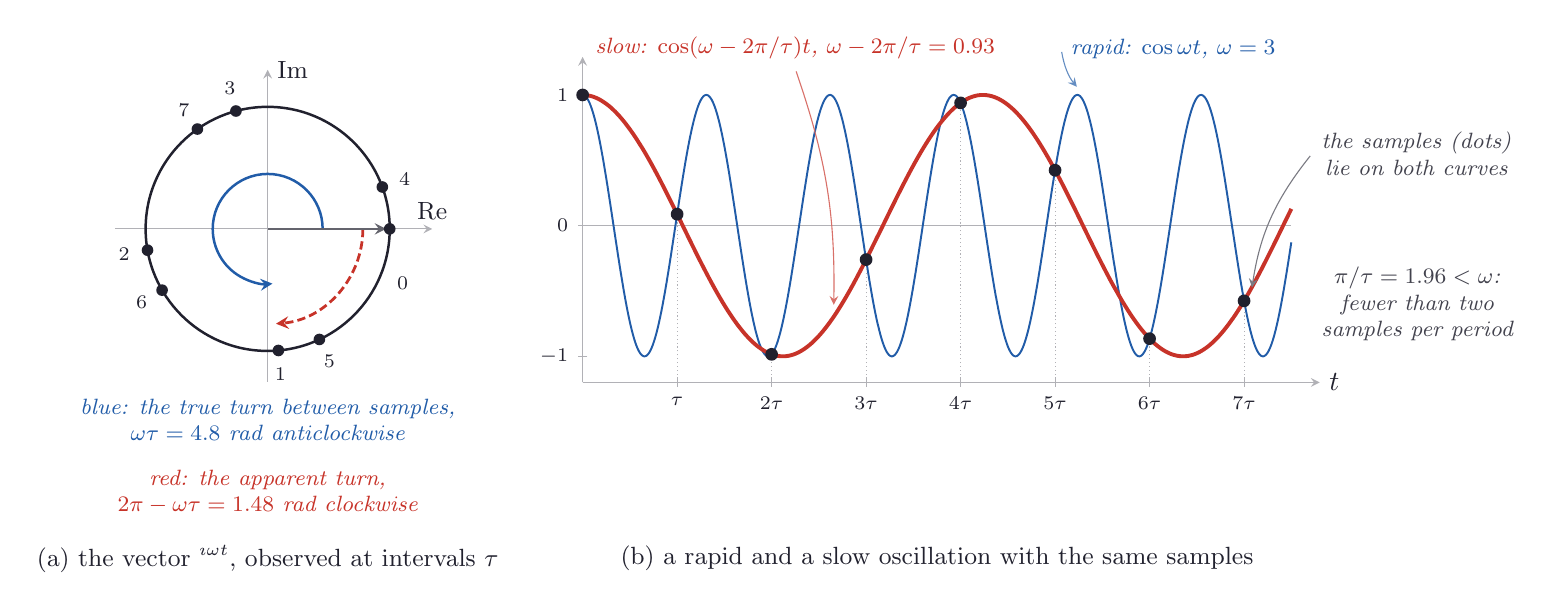
\begin{tikzpicture}[ink/.style={line width=0.9pt, ndInk}, faint/.style={line width=0.4pt, ndInk!35}, dashedink/.style={line width=0.5pt, ndInk!55, dash pattern=on 2.5pt off 2pt}, vec/.style={->, >=stealth, line width=1.2pt}, note/.style={font=\footnotesize\itshape, text=ndInk!85, align=center}, pointer/.style={->, >=stealth, line width=0.4pt, ndInk!60, shorten >=2pt, shorten <=1pt}, dot/.style={circle, fill=ndInk, inner sep=0pt, minimum size=3.4pt}, wash/.style={fill=ndSky, fill opacity=0.55}, every node/.style={text=ndInk}]
\definecolor{ndInk}{rgb}{0.13,0.13,0.18}
\definecolor{ndPaper}{rgb}{0.99,0.96,0.88}
\definecolor{ndSky}{rgb}{0.84,0.91,0.98}
\definecolor{ndRose}{rgb}{0.98,0.86,0.84}
\definecolor{ndBlue}{rgb}{0.13,0.36,0.66}
\definecolor{ndRed}{rgb}{0.78,0.20,0.16}
\definecolor{ndGold}{rgb}{0.88,0.62,0.10}
\definecolor{ndGreen}{rgb}{0.18,0.52,0.30}
\draw[faint, ->, >=stealth] (-1.94,0) -- (2.09,0) node[above, text=ndInk, font=\small] {$\mathrm{Re}$};
\draw[faint, ->, >=stealth] (0,-1.94) -- (0,2.02) node[right, text=ndInk, font=\small] {$\mathrm{Im}$};
\draw[ink] (0,0) circle (1.550);
\draw[vec, ndBlue, line width=0.9pt] (0.698,0) arc (0:275.02:0.698);
\draw[vec, ndRed, line width=1.0pt, dash pattern=on 3pt off 1.5pt] (1.209,0) arc (0:-84.98:1.209);
\draw[vec, ndInk!70, line width=0.8pt] (0,0) -- (1.504,0);
\node[dot, minimum size=4.2pt] at (1.550,0.000) {};
\node[font=\scriptsize] at (1.715,-0.693) {$0$};
\node[dot, minimum size=4.2pt] at (0.136,-1.544) {};
\node[font=\scriptsize] at (0.162,-1.843) {$1$};
\node[dot, minimum size=4.2pt] at (-1.526,-0.270) {};
\node[font=\scriptsize] at (-1.822,-0.323) {$2$};
\node[dot, minimum size=4.2pt] at (-0.403,1.497) {};
\node[font=\scriptsize] at (-0.481,1.786) {$3$};
\node[dot, minimum size=4.2pt] at (1.456,0.532) {};
\node[font=\scriptsize] at (1.738,0.635) {$4$};
\node[dot, minimum size=4.2pt] at (0.657,-1.404) {};
\node[font=\scriptsize] at (0.785,-1.675) {$5$};
\node[dot, minimum size=4.2pt] at (-1.341,-0.778) {};
\node[font=\scriptsize] at (-1.600,-0.928) {$6$};
\node[dot, minimum size=4.2pt] at (-0.892,1.268) {};
\node[font=\scriptsize] at (-1.065,1.513) {$7$};
\node[note, anchor=north, text=ndBlue] at (0,-2.04) {blue: the true turn between samples,\\ $\omega\tau=4.8$ rad anticlockwise};
\node[note, anchor=north, text=ndRed] at (0,-2.94) {red: the apparent turn,\\ $2\pi-\omega\tau=1.48$ rad clockwise};
\node[font=\small] at (0.0,-4.19) {(a) the vector $\ee^{\imath\omega t}$, observed at intervals $\tau$};
\draw[faint, ->, >=stealth] (4.000,-1.950) -- (13.360,-1.950) node[right, text=ndInk] {$t$};
\draw[faint, ->, >=stealth] (4.000,-1.950) -- (4.000,2.184) node[above, text=ndInk] {};
\draw[faint] (5.200,-1.890) -- (5.200,-2.010) node[below, font=\scriptsize, text=ndInk] {$\tau$};
\draw[faint] (6.400,-1.890) -- (6.400,-2.010) node[below, font=\scriptsize, text=ndInk] {$2\tau$};
\draw[faint] (7.600,-1.890) -- (7.600,-2.010) node[below, font=\scriptsize, text=ndInk] {$3\tau$};
\draw[faint] (8.800,-1.890) -- (8.800,-2.010) node[below, font=\scriptsize, text=ndInk] {$4\tau$};
\draw[faint] (10.000,-1.890) -- (10.000,-2.010) node[below, font=\scriptsize, text=ndInk] {$5\tau$};
\draw[faint] (11.200,-1.890) -- (11.200,-2.010) node[below, font=\scriptsize, text=ndInk] {$6\tau$};
\draw[faint] (12.400,-1.890) -- (12.400,-2.010) node[below, font=\scriptsize, text=ndInk] {$7\tau$};
\draw[faint] (4.060,-1.618) -- (3.940,-1.618) node[left, font=\scriptsize, text=ndInk] {$-1$};
\draw[faint] (4.060,0.041) -- (3.940,0.041) node[left, font=\scriptsize, text=ndInk] {$0$};
\draw[faint] (4.060,1.701) -- (3.940,1.701) node[left, font=\scriptsize, text=ndInk] {$1$};
\draw[faint] (4.000,0.041) -- (13.000,0.041);
\draw[line width=0.7pt, ndBlue] (4.000,1.701) -- (4.006,1.701) -- (4.012,1.699) -- (4.018,1.697) -- (4.024,1.693) -- (4.030,1.689) -- (4.036,1.684) -- (4.042,1.678) -- (4.048,1.671) -- (4.054,1.662) -- (4.060,1.653) -- (4.066,1.643) -- (4.072,1.633) -- (4.078,1.621) -- (4.084,1.608) -- (4.090,1.595) -- (4.096,1.580) -- (4.102,1.565) -- (4.108,1.548) -- (4.114,1.531) -- (4.120,1.513) -- (4.126,1.494) -- (4.132,1.475) -- (4.138,1.454) -- (4.144,1.433) -- (4.150,1.411) -- (4.156,1.388) -- (4.162,1.364) -- (4.168,1.340) -- (4.174,1.315) -- (4.180,1.289) -- (4.186,1.262) -- (4.192,1.235) -- (4.198,1.207) -- (4.204,1.178) -- (4.210,1.149) -- (4.216,1.118) -- (4.222,1.088) -- (4.228,1.057) -- (4.234,1.025) -- (4.240,0.992) -- (4.246,0.959) -- (4.252,0.926) -- (4.258,0.892) -- (4.264,0.858) -- (4.270,0.823) -- (4.276,0.787) -- (4.282,0.751) -- (4.288,0.715) -- (4.294,0.679) -- (4.300,0.642) -- (4.306,0.604) -- (4.312,0.567) -- (4.318,0.529) -- (4.324,0.490) -- (4.330,0.452) -- (4.336,0.413) -- (4.342,0.374) -- (4.348,0.335) -- (4.354,0.296) -- (4.360,0.256) -- (4.366,0.217) -- (4.372,0.177) -- (4.378,0.137) -- (4.384,0.098) -- (4.390,0.058) -- (4.396,0.018) -- (4.402,-0.022) -- (4.408,-0.062) -- (4.414,-0.102) -- (4.420,-0.141) -- (4.426,-0.181) -- (4.432,-0.220) -- (4.438,-0.259) -- (4.444,-0.299) -- (4.450,-0.338) -- (4.456,-0.376) -- (4.462,-0.415) -- (4.468,-0.453) -- (4.474,-0.491) -- (4.480,-0.528) -- (4.486,-0.566) -- (4.492,-0.603) -- (4.498,-0.639) -- (4.504,-0.675) -- (4.510,-0.711) -- (4.516,-0.746) -- (4.522,-0.781) -- (4.528,-0.815) -- (4.534,-0.849) -- (4.540,-0.883) -- (4.546,-0.916) -- (4.552,-0.948) -- (4.558,-0.980) -- (4.564,-1.011) -- (4.570,-1.041) -- (4.576,-1.071) -- (4.582,-1.100) -- (4.588,-1.129) -- (4.594,-1.157) -- (4.600,-1.184) -- (4.606,-1.211) -- (4.612,-1.236) -- (4.618,-1.261) -- (4.624,-1.286) -- (4.630,-1.309) -- (4.636,-1.332) -- (4.642,-1.354) -- (4.648,-1.375) -- (4.654,-1.396) -- (4.660,-1.415) -- (4.666,-1.434) -- (4.672,-1.452) -- (4.678,-1.469) -- (4.684,-1.485) -- (4.690,-1.500) -- (4.696,-1.514) -- (4.702,-1.528) -- (4.708,-1.540) -- (4.714,-1.552) -- (4.720,-1.562) -- (4.726,-1.572) -- (4.732,-1.581) -- (4.738,-1.589) -- (4.744,-1.596) -- (4.751,-1.602) -- (4.757,-1.607) -- (4.763,-1.611) -- (4.769,-1.614) -- (4.775,-1.617) -- (4.781,-1.618) -- (4.787,-1.618) -- (4.793,-1.617) -- (4.799,-1.616) -- (4.805,-1.613) -- (4.811,-1.610) -- (4.817,-1.605) -- (4.823,-1.600) -- (4.829,-1.593) -- (4.835,-1.586) -- (4.841,-1.578) -- (4.847,-1.569) -- (4.853,-1.559) -- (4.859,-1.548) -- (4.865,-1.536) -- (4.871,-1.523) -- (4.877,-1.509) -- (4.883,-1.494) -- (4.889,-1.479) -- (4.895,-1.462) -- (4.901,-1.445) -- (4.907,-1.427) -- (4.913,-1.408) -- (4.919,-1.388) -- (4.925,-1.367) -- (4.931,-1.346) -- (4.937,-1.324) -- (4.943,-1.301) -- (4.949,-1.277) -- (4.955,-1.252) -- (4.961,-1.227) -- (4.967,-1.201) -- (4.973,-1.174) -- (4.979,-1.146) -- (4.985,-1.118) -- (4.991,-1.089) -- (4.997,-1.060) -- (5.003,-1.030) -- (5.009,-0.999) -- (5.015,-0.968) -- (5.021,-0.936) -- (5.027,-0.903) -- (5.033,-0.870) -- (5.039,-0.837) -- (5.045,-0.803) -- (5.051,-0.768) -- (5.057,-0.733) -- (5.063,-0.698) -- (5.069,-0.662) -- (5.075,-0.625) -- (5.081,-0.589) -- (5.087,-0.552) -- (5.093,-0.514) -- (5.099,-0.477) -- (5.105,-0.439) -- (5.111,-0.400) -- (5.117,-0.362) -- (5.123,-0.323) -- (5.129,-0.284) -- (5.135,-0.245) -- (5.141,-0.205) -- (5.147,-0.166) -- (5.153,-0.126) -- (5.159,-0.087) -- (5.165,-0.047) -- (5.171,-0.007) -- (5.177,0.033) -- (5.183,0.073) -- (5.189,0.112) -- (5.195,0.152) -- (5.201,0.192) -- (5.207,0.232) -- (5.213,0.271) -- (5.219,0.311) -- (5.225,0.350) -- (5.231,0.389) -- (5.237,0.428) -- (5.243,0.466) -- (5.249,0.505) -- (5.255,0.543) -- (5.261,0.581) -- (5.267,0.618) -- (5.273,0.656) -- (5.279,0.692) -- (5.285,0.729) -- (5.291,0.765) -- (5.297,0.801) -- (5.303,0.836) -- (5.309,0.871) -- (5.315,0.905) -- (5.321,0.939) -- (5.327,0.972) -- (5.333,1.005) -- (5.339,1.037) -- (5.345,1.068) -- (5.351,1.099) -- (5.357,1.130) -- (5.363,1.160) -- (5.369,1.189) -- (5.375,1.217) -- (5.381,1.245) -- (5.387,1.272) -- (5.393,1.298) -- (5.399,1.324) -- (5.405,1.349) -- (5.411,1.373) -- (5.417,1.397) -- (5.423,1.419) -- (5.429,1.441) -- (5.435,1.462) -- (5.441,1.482) -- (5.447,1.502) -- (5.453,1.520) -- (5.459,1.538) -- (5.465,1.555) -- (5.471,1.571) -- (5.477,1.586) -- (5.483,1.600) -- (5.489,1.613) -- (5.495,1.625) -- (5.501,1.637) -- (5.507,1.647) -- (5.513,1.657) -- (5.519,1.666) -- (5.525,1.673) -- (5.531,1.680) -- (5.537,1.686) -- (5.543,1.691) -- (5.549,1.695) -- (5.555,1.698) -- (5.561,1.700) -- (5.567,1.701) -- (5.573,1.701) -- (5.579,1.700) -- (5.585,1.698) -- (5.591,1.696) -- (5.597,1.692) -- (5.603,1.687) -- (5.609,1.682) -- (5.615,1.675) -- (5.621,1.668) -- (5.627,1.659) -- (5.633,1.650) -- (5.639,1.640) -- (5.645,1.628) -- (5.651,1.616) -- (5.657,1.603) -- (5.663,1.589) -- (5.669,1.574) -- (5.675,1.559) -- (5.681,1.542) -- (5.687,1.525) -- (5.693,1.506) -- (5.699,1.487) -- (5.705,1.467) -- (5.711,1.446) -- (5.717,1.425) -- (5.723,1.402) -- (5.729,1.379) -- (5.735,1.355) -- (5.741,1.330) -- (5.747,1.305) -- (5.753,1.279) -- (5.759,1.252) -- (5.765,1.224) -- (5.771,1.196) -- (5.777,1.167) -- (5.783,1.137) -- (5.789,1.107) -- (5.795,1.076) -- (5.801,1.045) -- (5.807,1.013) -- (5.813,0.980) -- (5.819,0.947) -- (5.825,0.913) -- (5.831,0.879) -- (5.837,0.845) -- (5.843,0.809) -- (5.849,0.774) -- (5.855,0.738) -- (5.861,0.702) -- (5.867,0.665) -- (5.873,0.628) -- (5.879,0.590) -- (5.885,0.552) -- (5.891,0.514) -- (5.897,0.476) -- (5.903,0.437) -- (5.909,0.399) -- (5.915,0.360) -- (5.921,0.320) -- (5.927,0.281) -- (5.933,0.242) -- (5.939,0.202) -- (5.945,0.162) -- (5.951,0.122) -- (5.957,0.083) -- (5.963,0.043) -- (5.969,0.003) -- (5.975,-0.037) -- (5.981,-0.077) -- (5.987,-0.116) -- (5.993,-0.156) -- (5.999,-0.196) -- (6.005,-0.235) -- (6.011,-0.274) -- (6.017,-0.313) -- (6.023,-0.352) -- (6.029,-0.391) -- (6.035,-0.429) -- (6.041,-0.467) -- (6.047,-0.505) -- (6.053,-0.542) -- (6.059,-0.579) -- (6.065,-0.616) -- (6.071,-0.653) -- (6.077,-0.689) -- (6.083,-0.724) -- (6.089,-0.759) -- (6.095,-0.794) -- (6.101,-0.828) -- (6.107,-0.862) -- (6.113,-0.895) -- (6.119,-0.928) -- (6.125,-0.960) -- (6.131,-0.991) -- (6.137,-1.022) -- (6.143,-1.052) -- (6.149,-1.082) -- (6.155,-1.111) -- (6.161,-1.139) -- (6.167,-1.167) -- (6.173,-1.194) -- (6.179,-1.220) -- (6.185,-1.246) -- (6.191,-1.271) -- (6.197,-1.295) -- (6.203,-1.318) -- (6.209,-1.340) -- (6.215,-1.362) -- (6.221,-1.383) -- (6.227,-1.403) -- (6.233,-1.422) -- (6.239,-1.441) -- (6.245,-1.458) -- (6.252,-1.475) -- (6.258,-1.490) -- (6.264,-1.505) -- (6.270,-1.519) -- (6.276,-1.532) -- (6.282,-1.545) -- (6.288,-1.556) -- (6.294,-1.566) -- (6.300,-1.576) -- (6.306,-1.584) -- (6.312,-1.592) -- (6.318,-1.598) -- (6.324,-1.604) -- (6.330,-1.609) -- (6.336,-1.612) -- (6.342,-1.615) -- (6.348,-1.617) -- (6.354,-1.618) -- (6.360,-1.618) -- (6.366,-1.617) -- (6.372,-1.615) -- (6.378,-1.612) -- (6.384,-1.608) -- (6.390,-1.603) -- (6.396,-1.598) -- (6.402,-1.591) -- (6.408,-1.583) -- (6.414,-1.575) -- (6.420,-1.565) -- (6.426,-1.555) -- (6.432,-1.543) -- (6.438,-1.531) -- (6.444,-1.518) -- (6.450,-1.504) -- (6.456,-1.489) -- (6.462,-1.473) -- (6.468,-1.456) -- (6.474,-1.438) -- (6.480,-1.420) -- (6.486,-1.400) -- (6.492,-1.380) -- (6.498,-1.359) -- (6.504,-1.338) -- (6.510,-1.315) -- (6.516,-1.292) -- (6.522,-1.268) -- (6.528,-1.243) -- (6.534,-1.217) -- (6.540,-1.191) -- (6.546,-1.164) -- (6.552,-1.136) -- (6.558,-1.108) -- (6.564,-1.078) -- (6.570,-1.049) -- (6.576,-1.018) -- (6.582,-0.987) -- (6.588,-0.956) -- (6.594,-0.924) -- (6.600,-0.891) -- (6.606,-0.858) -- (6.612,-0.824) -- (6.618,-0.790) -- (6.624,-0.755) -- (6.630,-0.720) -- (6.636,-0.684) -- (6.642,-0.648) -- (6.648,-0.612) -- (6.654,-0.575) -- (6.660,-0.538) -- (6.666,-0.500) -- (6.672,-0.462) -- (6.678,-0.424) -- (6.684,-0.386) -- (6.690,-0.347) -- (6.696,-0.308) -- (6.702,-0.269) -- (6.708,-0.230) -- (6.714,-0.191) -- (6.720,-0.151) -- (6.726,-0.111) -- (6.732,-0.072) -- (6.738,-0.032) -- (6.744,0.008) -- (6.750,0.048) -- (6.756,0.088) -- (6.762,0.127) -- (6.768,0.167) -- (6.774,0.207) -- (6.780,0.246) -- (6.786,0.286) -- (6.792,0.325) -- (6.798,0.365) -- (6.804,0.404) -- (6.810,0.442) -- (6.816,0.481) -- (6.822,0.519) -- (6.828,0.557) -- (6.834,0.595) -- (6.840,0.632) -- (6.846,0.669) -- (6.852,0.706) -- (6.858,0.742) -- (6.864,0.778) -- (6.870,0.814) -- (6.876,0.849) -- (6.882,0.883) -- (6.888,0.918) -- (6.894,0.951) -- (6.900,0.984) -- (6.906,1.017) -- (6.912,1.049) -- (6.918,1.080) -- (6.924,1.111) -- (6.930,1.141) -- (6.936,1.171) -- (6.942,1.199) -- (6.948,1.228) -- (6.954,1.255) -- (6.960,1.282) -- (6.966,1.308) -- (6.972,1.334) -- (6.978,1.358) -- (6.984,1.382) -- (6.990,1.405) -- (6.996,1.427) -- (7.002,1.449) -- (7.008,1.470) -- (7.014,1.490) -- (7.020,1.509) -- (7.026,1.527) -- (7.032,1.544) -- (7.038,1.561) -- (7.044,1.576) -- (7.050,1.591) -- (7.056,1.605) -- (7.062,1.618) -- (7.068,1.630) -- (7.074,1.641) -- (7.080,1.651) -- (7.086,1.660) -- (7.092,1.669) -- (7.098,1.676) -- (7.104,1.682) -- (7.110,1.688) -- (7.116,1.692) -- (7.122,1.696) -- (7.128,1.699) -- (7.134,1.700) -- (7.140,1.701) -- (7.146,1.701) -- (7.152,1.700) -- (7.158,1.697) -- (7.164,1.694) -- (7.170,1.690) -- (7.176,1.685) -- (7.182,1.679) -- (7.188,1.672) -- (7.194,1.665) -- (7.200,1.656) -- (7.206,1.646) -- (7.212,1.635) -- (7.218,1.624) -- (7.224,1.611) -- (7.230,1.598) -- (7.236,1.584) -- (7.242,1.569) -- (7.248,1.553) -- (7.254,1.536) -- (7.260,1.518) -- (7.266,1.499) -- (7.272,1.480) -- (7.278,1.459) -- (7.284,1.438) -- (7.290,1.416) -- (7.296,1.394) -- (7.302,1.370) -- (7.308,1.346) -- (7.314,1.321) -- (7.320,1.295) -- (7.326,1.269) -- (7.332,1.242) -- (7.338,1.214) -- (7.344,1.185) -- (7.350,1.156) -- (7.356,1.126) -- (7.362,1.096) -- (7.368,1.064) -- (7.374,1.033) -- (7.380,1.001) -- (7.386,0.968) -- (7.392,0.934) -- (7.398,0.901) -- (7.404,0.866) -- (7.410,0.831) -- (7.416,0.796) -- (7.422,0.760) -- (7.428,0.724) -- (7.434,0.688) -- (7.440,0.651) -- (7.446,0.614) -- (7.452,0.576) -- (7.458,0.538) -- (7.464,0.500) -- (7.470,0.462) -- (7.476,0.423) -- (7.482,0.384) -- (7.488,0.345) -- (7.494,0.306) -- (7.500,0.266) -- (7.506,0.227) -- (7.512,0.187) -- (7.518,0.147) -- (7.524,0.107) -- (7.530,0.068) -- (7.536,0.028) -- (7.542,-0.012) -- (7.548,-0.052) -- (7.554,-0.092) -- (7.560,-0.131) -- (7.566,-0.171) -- (7.572,-0.210) -- (7.578,-0.250) -- (7.584,-0.289) -- (7.590,-0.328) -- (7.596,-0.367) -- (7.602,-0.405) -- (7.608,-0.443) -- (7.614,-0.481) -- (7.620,-0.519) -- (7.626,-0.556) -- (7.632,-0.593) -- (7.638,-0.630) -- (7.644,-0.666) -- (7.650,-0.702) -- (7.656,-0.737) -- (7.662,-0.772) -- (7.668,-0.807) -- (7.674,-0.841) -- (7.680,-0.874) -- (7.686,-0.907) -- (7.692,-0.940) -- (7.698,-0.972) -- (7.704,-1.003) -- (7.710,-1.034) -- (7.716,-1.064) -- (7.722,-1.093) -- (7.728,-1.122) -- (7.734,-1.150) -- (7.740,-1.177) -- (7.746,-1.204) -- (7.753,-1.230) -- (7.759,-1.255) -- (7.765,-1.280) -- (7.771,-1.303) -- (7.777,-1.326) -- (7.783,-1.349) -- (7.789,-1.370) -- (7.795,-1.391) -- (7.801,-1.410) -- (7.807,-1.429) -- (7.813,-1.447) -- (7.819,-1.464) -- (7.825,-1.481) -- (7.831,-1.496) -- (7.837,-1.511) -- (7.843,-1.524) -- (7.849,-1.537) -- (7.855,-1.549) -- (7.861,-1.560) -- (7.867,-1.570) -- (7.873,-1.579) -- (7.879,-1.587) -- (7.885,-1.594) -- (7.891,-1.601) -- (7.897,-1.606) -- (7.903,-1.610) -- (7.909,-1.614) -- (7.915,-1.616) -- (7.921,-1.618) -- (7.927,-1.618) -- (7.933,-1.618) -- (7.939,-1.616) -- (7.945,-1.614) -- (7.951,-1.611) -- (7.957,-1.606) -- (7.963,-1.601) -- (7.969,-1.595) -- (7.975,-1.588) -- (7.981,-1.580) -- (7.987,-1.571) -- (7.993,-1.561) -- (7.999,-1.550) -- (8.005,-1.539) -- (8.011,-1.526) -- (8.017,-1.512) -- (8.023,-1.498) -- (8.029,-1.483) -- (8.035,-1.466) -- (8.041,-1.449) -- (8.047,-1.431) -- (8.053,-1.413) -- (8.059,-1.393) -- (8.065,-1.373) -- (8.071,-1.351) -- (8.077,-1.329) -- (8.083,-1.306) -- (8.089,-1.283) -- (8.095,-1.258) -- (8.101,-1.233) -- (8.107,-1.207) -- (8.113,-1.181) -- (8.119,-1.153) -- (8.125,-1.125) -- (8.131,-1.097) -- (8.137,-1.067) -- (8.143,-1.037) -- (8.149,-1.007) -- (8.155,-0.976) -- (8.161,-0.944) -- (8.167,-0.911) -- (8.173,-0.879) -- (8.179,-0.845) -- (8.185,-0.811) -- (8.191,-0.777) -- (8.197,-0.742) -- (8.203,-0.706) -- (8.209,-0.671) -- (8.215,-0.634) -- (8.221,-0.598) -- (8.227,-0.561) -- (8.233,-0.524) -- (8.239,-0.486) -- (8.245,-0.448) -- (8.251,-0.410) -- (8.257,-0.371) -- (8.263,-0.333) -- (8.269,-0.294) -- (8.275,-0.255) -- (8.281,-0.215) -- (8.287,-0.176) -- (8.293,-0.136) -- (8.299,-0.097) -- (8.305,-0.057) -- (8.311,-0.017) -- (8.317,0.023) -- (8.323,0.063) -- (8.329,0.103) -- (8.335,0.142) -- (8.341,0.182) -- (8.347,0.222) -- (8.353,0.261) -- (8.359,0.301) -- (8.365,0.340) -- (8.371,0.379) -- (8.377,0.418) -- (8.383,0.457) -- (8.389,0.495) -- (8.395,0.533) -- (8.401,0.571) -- (8.407,0.609) -- (8.413,0.646) -- (8.419,0.683) -- (8.425,0.720) -- (8.431,0.756) -- (8.437,0.792) -- (8.443,0.827) -- (8.449,0.862) -- (8.455,0.896) -- (8.461,0.930) -- (8.467,0.964) -- (8.473,0.997) -- (8.479,1.029) -- (8.485,1.061) -- (8.491,1.092) -- (8.497,1.122) -- (8.503,1.152) -- (8.509,1.182) -- (8.515,1.210) -- (8.521,1.238) -- (8.527,1.265) -- (8.533,1.292) -- (8.539,1.318) -- (8.545,1.343) -- (8.551,1.367) -- (8.557,1.391) -- (8.563,1.414) -- (8.569,1.436) -- (8.575,1.457) -- (8.581,1.477) -- (8.587,1.497) -- (8.593,1.516) -- (8.599,1.533) -- (8.605,1.550) -- (8.611,1.567) -- (8.617,1.582) -- (8.623,1.596) -- (8.629,1.610) -- (8.635,1.622) -- (8.641,1.634) -- (8.647,1.645) -- (8.653,1.655) -- (8.659,1.664) -- (8.665,1.671) -- (8.671,1.678) -- (8.677,1.685) -- (8.683,1.690) -- (8.689,1.694) -- (8.695,1.697) -- (8.701,1.699) -- (8.707,1.701) -- (8.713,1.701) -- (8.719,1.700) -- (8.725,1.699) -- (8.731,1.696) -- (8.737,1.693) -- (8.743,1.689) -- (8.749,1.683) -- (8.755,1.677) -- (8.761,1.670) -- (8.767,1.661) -- (8.773,1.652) -- (8.779,1.642) -- (8.785,1.631) -- (8.791,1.619) -- (8.797,1.606) -- (8.803,1.593) -- (8.809,1.578) -- (8.815,1.563) -- (8.821,1.546) -- (8.827,1.529) -- (8.833,1.511) -- (8.839,1.492) -- (8.845,1.472) -- (8.851,1.452) -- (8.857,1.430) -- (8.863,1.408) -- (8.869,1.385) -- (8.875,1.361) -- (8.881,1.337) -- (8.887,1.311) -- (8.893,1.285) -- (8.899,1.259) -- (8.905,1.231) -- (8.911,1.203) -- (8.917,1.174) -- (8.923,1.145) -- (8.929,1.115) -- (8.935,1.084) -- (8.941,1.053) -- (8.947,1.021) -- (8.953,0.988) -- (8.959,0.955) -- (8.965,0.922) -- (8.971,0.888) -- (8.977,0.853) -- (8.983,0.818) -- (8.989,0.783) -- (8.995,0.747) -- (9.001,0.711) -- (9.007,0.674) -- (9.013,0.637) -- (9.019,0.600) -- (9.025,0.562) -- (9.031,0.524) -- (9.037,0.486) -- (9.043,0.447) -- (9.049,0.408) -- (9.055,0.369) -- (9.061,0.330) -- (9.067,0.291) -- (9.073,0.251) -- (9.079,0.212) -- (9.085,0.172) -- (9.091,0.132) -- (9.097,0.093) -- (9.103,0.053) -- (9.109,0.013) -- (9.115,-0.027) -- (9.121,-0.067) -- (9.127,-0.107) -- (9.133,-0.146) -- (9.139,-0.186) -- (9.145,-0.225) -- (9.151,-0.264) -- (9.157,-0.303) -- (9.163,-0.342) -- (9.169,-0.381) -- (9.175,-0.419) -- (9.181,-0.458) -- (9.187,-0.495) -- (9.193,-0.533) -- (9.199,-0.570) -- (9.205,-0.607) -- (9.211,-0.644) -- (9.217,-0.680) -- (9.223,-0.715) -- (9.229,-0.751) -- (9.235,-0.785) -- (9.241,-0.820) -- (9.247,-0.854) -- (9.254,-0.887) -- (9.260,-0.920) -- (9.266,-0.952) -- (9.272,-0.983) -- (9.278,-1.015) -- (9.284,-1.045) -- (9.290,-1.075) -- (9.296,-1.104) -- (9.302,-1.132) -- (9.308,-1.160) -- (9.314,-1.187) -- (9.320,-1.214) -- (9.326,-1.240) -- (9.332,-1.265) -- (9.338,-1.289) -- (9.344,-1.312) -- (9.350,-1.335) -- (9.356,-1.357) -- (9.362,-1.378) -- (9.368,-1.398) -- (9.374,-1.417) -- (9.380,-1.436) -- (9.386,-1.454) -- (9.392,-1.471) -- (9.398,-1.487) -- (9.404,-1.502) -- (9.410,-1.516) -- (9.416,-1.529) -- (9.422,-1.542) -- (9.428,-1.553) -- (9.434,-1.564) -- (9.440,-1.573) -- (9.446,-1.582) -- (9.452,-1.590) -- (9.458,-1.597) -- (9.464,-1.603) -- (9.470,-1.608) -- (9.476,-1.612) -- (9.482,-1.615) -- (9.488,-1.617) -- (9.494,-1.618) -- (9.500,-1.618) -- (9.506,-1.617) -- (9.512,-1.616) -- (9.518,-1.613) -- (9.524,-1.609) -- (9.530,-1.605) -- (9.536,-1.599) -- (9.542,-1.593) -- (9.548,-1.585) -- (9.554,-1.577) -- (9.560,-1.567) -- (9.566,-1.557) -- (9.572,-1.546) -- (9.578,-1.534) -- (9.584,-1.521) -- (9.590,-1.507) -- (9.596,-1.492) -- (9.602,-1.477) -- (9.608,-1.460) -- (9.614,-1.443) -- (9.620,-1.424) -- (9.626,-1.405) -- (9.632,-1.385) -- (9.638,-1.365) -- (9.644,-1.343) -- (9.650,-1.321) -- (9.656,-1.298) -- (9.662,-1.274) -- (9.668,-1.249) -- (9.674,-1.224) -- (9.680,-1.197) -- (9.686,-1.171) -- (9.692,-1.143) -- (9.698,-1.115) -- (9.704,-1.086) -- (9.710,-1.056) -- (9.716,-1.026) -- (9.722,-0.995) -- (9.728,-0.964) -- (9.734,-0.932) -- (9.740,-0.899) -- (9.746,-0.866) -- (9.752,-0.832) -- (9.758,-0.798) -- (9.764,-0.764) -- (9.770,-0.729) -- (9.776,-0.693) -- (9.782,-0.657) -- (9.788,-0.621) -- (9.794,-0.584) -- (9.800,-0.547) -- (9.806,-0.510) -- (9.812,-0.472) -- (9.818,-0.434) -- (9.824,-0.395) -- (9.830,-0.357) -- (9.836,-0.318) -- (9.842,-0.279) -- (9.848,-0.240) -- (9.854,-0.200) -- (9.860,-0.161) -- (9.866,-0.121) -- (9.872,-0.082) -- (9.878,-0.042) -- (9.884,-0.002) -- (9.890,0.038) -- (9.896,0.078) -- (9.902,0.117) -- (9.908,0.157) -- (9.914,0.197) -- (9.920,0.237) -- (9.926,0.276) -- (9.932,0.316) -- (9.938,0.355) -- (9.944,0.394) -- (9.950,0.433) -- (9.956,0.471) -- (9.962,0.510) -- (9.968,0.548) -- (9.974,0.586) -- (9.980,0.623) -- (9.986,0.660) -- (9.992,0.697) -- (9.998,0.733) -- (10.004,0.769) -- (10.010,0.805) -- (10.016,0.840) -- (10.022,0.875) -- (10.028,0.909) -- (10.034,0.943) -- (10.040,0.976) -- (10.046,1.009) -- (10.052,1.041) -- (10.058,1.072) -- (10.064,1.103) -- (10.070,1.134) -- (10.076,1.163) -- (10.082,1.192) -- (10.088,1.221) -- (10.094,1.248) -- (10.100,1.275) -- (10.106,1.302) -- (10.112,1.327) -- (10.118,1.352) -- (10.124,1.376) -- (10.130,1.399) -- (10.136,1.422) -- (10.142,1.444) -- (10.148,1.465) -- (10.154,1.485) -- (10.160,1.504) -- (10.166,1.522) -- (10.172,1.540) -- (10.178,1.557) -- (10.184,1.572) -- (10.190,1.587) -- (10.196,1.601) -- (10.202,1.615) -- (10.208,1.627) -- (10.214,1.638) -- (10.220,1.649) -- (10.226,1.658) -- (10.232,1.667) -- (10.238,1.674) -- (10.244,1.681) -- (10.250,1.687) -- (10.256,1.691) -- (10.262,1.695) -- (10.268,1.698) -- (10.274,1.700) -- (10.280,1.701) -- (10.286,1.701) -- (10.292,1.700) -- (10.298,1.698) -- (10.304,1.695) -- (10.310,1.691) -- (10.316,1.687) -- (10.322,1.681) -- (10.328,1.674) -- (10.334,1.667) -- (10.340,1.658) -- (10.346,1.649) -- (10.352,1.638) -- (10.358,1.627) -- (10.364,1.615) -- (10.370,1.601) -- (10.376,1.587) -- (10.382,1.572) -- (10.388,1.557) -- (10.394,1.540) -- (10.400,1.522) -- (10.406,1.504) -- (10.412,1.485) -- (10.418,1.465) -- (10.424,1.444) -- (10.430,1.422) -- (10.436,1.399) -- (10.442,1.376) -- (10.448,1.352) -- (10.454,1.327) -- (10.460,1.302) -- (10.466,1.275) -- (10.472,1.248) -- (10.478,1.221) -- (10.484,1.192) -- (10.490,1.163) -- (10.496,1.134) -- (10.502,1.103) -- (10.508,1.072) -- (10.514,1.041) -- (10.520,1.009) -- (10.526,0.976) -- (10.532,0.943) -- (10.538,0.909) -- (10.544,0.875) -- (10.550,0.840) -- (10.556,0.805) -- (10.562,0.769) -- (10.568,0.733) -- (10.574,0.697) -- (10.580,0.660) -- (10.586,0.623) -- (10.592,0.585) -- (10.598,0.548) -- (10.604,0.510) -- (10.610,0.471) -- (10.616,0.433) -- (10.622,0.394) -- (10.628,0.355) -- (10.634,0.315) -- (10.640,0.276) -- (10.646,0.237) -- (10.652,0.197) -- (10.658,0.157) -- (10.664,0.117) -- (10.670,0.078) -- (10.676,0.038) -- (10.682,-0.002) -- (10.688,-0.042) -- (10.694,-0.082) -- (10.700,-0.121) -- (10.706,-0.161) -- (10.712,-0.201) -- (10.718,-0.240) -- (10.724,-0.279) -- (10.730,-0.318) -- (10.736,-0.357) -- (10.742,-0.395) -- (10.748,-0.434) -- (10.755,-0.472) -- (10.761,-0.510) -- (10.767,-0.547) -- (10.773,-0.584) -- (10.779,-0.621) -- (10.785,-0.657) -- (10.791,-0.693) -- (10.797,-0.729) -- (10.803,-0.764) -- (10.809,-0.798) -- (10.815,-0.832) -- (10.821,-0.866) -- (10.827,-0.899) -- (10.833,-0.932) -- (10.839,-0.964) -- (10.845,-0.995) -- (10.851,-1.026) -- (10.857,-1.056) -- (10.863,-1.086) -- (10.869,-1.115) -- (10.875,-1.143) -- (10.881,-1.171) -- (10.887,-1.197) -- (10.893,-1.224) -- (10.899,-1.249) -- (10.905,-1.274) -- (10.911,-1.298) -- (10.917,-1.321) -- (10.923,-1.343) -- (10.929,-1.365) -- (10.935,-1.385) -- (10.941,-1.405) -- (10.947,-1.425) -- (10.953,-1.443) -- (10.959,-1.460) -- (10.965,-1.477) -- (10.971,-1.492) -- (10.977,-1.507) -- (10.983,-1.521) -- (10.989,-1.534) -- (10.995,-1.546) -- (11.001,-1.557) -- (11.007,-1.567) -- (11.013,-1.577) -- (11.019,-1.585) -- (11.025,-1.593) -- (11.031,-1.599) -- (11.037,-1.605) -- (11.043,-1.609) -- (11.049,-1.613) -- (11.055,-1.616) -- (11.061,-1.617) -- (11.067,-1.618) -- (11.073,-1.618) -- (11.079,-1.617) -- (11.085,-1.615) -- (11.091,-1.612) -- (11.097,-1.608) -- (11.103,-1.603) -- (11.109,-1.597) -- (11.115,-1.590) -- (11.121,-1.582) -- (11.127,-1.573) -- (11.133,-1.564) -- (11.139,-1.553) -- (11.145,-1.542) -- (11.151,-1.529) -- (11.157,-1.516) -- (11.163,-1.502) -- (11.169,-1.487) -- (11.175,-1.471) -- (11.181,-1.454) -- (11.187,-1.436) -- (11.193,-1.417) -- (11.199,-1.398) -- (11.205,-1.378) -- (11.211,-1.357) -- (11.217,-1.335) -- (11.223,-1.312) -- (11.229,-1.289) -- (11.235,-1.264) -- (11.241,-1.240) -- (11.247,-1.214) -- (11.253,-1.187) -- (11.259,-1.160) -- (11.265,-1.132) -- (11.271,-1.104) -- (11.277,-1.075) -- (11.283,-1.045) -- (11.289,-1.014) -- (11.295,-0.983) -- (11.301,-0.952) -- (11.307,-0.920) -- (11.313,-0.887) -- (11.319,-0.854) -- (11.325,-0.820) -- (11.331,-0.785) -- (11.337,-0.751) -- (11.343,-0.715) -- (11.349,-0.680) -- (11.355,-0.644) -- (11.361,-0.607) -- (11.367,-0.570) -- (11.373,-0.533) -- (11.379,-0.495) -- (11.385,-0.458) -- (11.391,-0.419) -- (11.397,-0.381) -- (11.403,-0.342) -- (11.409,-0.303) -- (11.415,-0.264) -- (11.421,-0.225) -- (11.427,-0.186) -- (11.433,-0.146) -- (11.439,-0.107) -- (11.445,-0.067) -- (11.451,-0.027) -- (11.457,0.013) -- (11.463,0.053) -- (11.469,0.093) -- (11.475,0.132) -- (11.481,0.172) -- (11.487,0.212) -- (11.493,0.251) -- (11.499,0.291) -- (11.505,0.330) -- (11.511,0.369) -- (11.517,0.408) -- (11.523,0.447) -- (11.529,0.486) -- (11.535,0.524) -- (11.541,0.562) -- (11.547,0.600) -- (11.553,0.637) -- (11.559,0.674) -- (11.565,0.711) -- (11.571,0.747) -- (11.577,0.783) -- (11.583,0.818) -- (11.589,0.853) -- (11.595,0.888) -- (11.601,0.922) -- (11.607,0.955) -- (11.613,0.988) -- (11.619,1.021) -- (11.625,1.053) -- (11.631,1.084) -- (11.637,1.115) -- (11.643,1.145) -- (11.649,1.174) -- (11.655,1.203) -- (11.661,1.231) -- (11.667,1.259) -- (11.673,1.285) -- (11.679,1.311) -- (11.685,1.337) -- (11.691,1.361) -- (11.697,1.385) -- (11.703,1.408) -- (11.709,1.430) -- (11.715,1.452) -- (11.721,1.472) -- (11.727,1.492) -- (11.733,1.511) -- (11.739,1.529) -- (11.745,1.546) -- (11.751,1.563) -- (11.757,1.578) -- (11.763,1.593) -- (11.769,1.606) -- (11.775,1.619) -- (11.781,1.631) -- (11.787,1.642) -- (11.793,1.652) -- (11.799,1.661) -- (11.805,1.670) -- (11.811,1.677) -- (11.817,1.683) -- (11.823,1.689) -- (11.829,1.693) -- (11.835,1.696) -- (11.841,1.699) -- (11.847,1.700) -- (11.853,1.701) -- (11.859,1.701) -- (11.865,1.699) -- (11.871,1.697) -- (11.877,1.694) -- (11.883,1.690) -- (11.889,1.685) -- (11.895,1.678) -- (11.901,1.671) -- (11.907,1.664) -- (11.913,1.655) -- (11.919,1.645) -- (11.925,1.634) -- (11.931,1.622) -- (11.937,1.610) -- (11.943,1.596) -- (11.949,1.582) -- (11.955,1.567) -- (11.961,1.550) -- (11.967,1.533) -- (11.973,1.516) -- (11.979,1.497) -- (11.985,1.477) -- (11.991,1.457) -- (11.997,1.436) -- (12.003,1.414) -- (12.009,1.391) -- (12.015,1.367) -- (12.021,1.343) -- (12.027,1.318) -- (12.033,1.292) -- (12.039,1.265) -- (12.045,1.238) -- (12.051,1.210) -- (12.057,1.181) -- (12.063,1.152) -- (12.069,1.122) -- (12.075,1.092) -- (12.081,1.061) -- (12.087,1.029) -- (12.093,0.996) -- (12.099,0.964) -- (12.105,0.930) -- (12.111,0.896) -- (12.117,0.862) -- (12.123,0.827) -- (12.129,0.792) -- (12.135,0.756) -- (12.141,0.720) -- (12.147,0.683) -- (12.153,0.646) -- (12.159,0.609) -- (12.165,0.571) -- (12.171,0.533) -- (12.177,0.495) -- (12.183,0.457) -- (12.189,0.418) -- (12.195,0.379) -- (12.201,0.340) -- (12.207,0.301) -- (12.213,0.261) -- (12.219,0.222) -- (12.225,0.182) -- (12.231,0.142) -- (12.237,0.102) -- (12.243,0.063) -- (12.249,0.023) -- (12.256,-0.017) -- (12.262,-0.057) -- (12.268,-0.097) -- (12.274,-0.136) -- (12.280,-0.176) -- (12.286,-0.215) -- (12.292,-0.255) -- (12.298,-0.294) -- (12.304,-0.333) -- (12.310,-0.371) -- (12.316,-0.410) -- (12.322,-0.448) -- (12.328,-0.486) -- (12.334,-0.524) -- (12.340,-0.561) -- (12.346,-0.598) -- (12.352,-0.635) -- (12.358,-0.671) -- (12.364,-0.707) -- (12.370,-0.742) -- (12.376,-0.777) -- (12.382,-0.811) -- (12.388,-0.845) -- (12.394,-0.879) -- (12.400,-0.912) -- (12.406,-0.944) -- (12.412,-0.976) -- (12.418,-1.007) -- (12.424,-1.037) -- (12.430,-1.067) -- (12.436,-1.097) -- (12.442,-1.125) -- (12.448,-1.153) -- (12.454,-1.181) -- (12.460,-1.207) -- (12.466,-1.233) -- (12.472,-1.258) -- (12.478,-1.283) -- (12.484,-1.306) -- (12.490,-1.329) -- (12.496,-1.351) -- (12.502,-1.373) -- (12.508,-1.393) -- (12.514,-1.413) -- (12.520,-1.431) -- (12.526,-1.449) -- (12.532,-1.466) -- (12.538,-1.483) -- (12.544,-1.498) -- (12.550,-1.512) -- (12.556,-1.526) -- (12.562,-1.539) -- (12.568,-1.550) -- (12.574,-1.561) -- (12.580,-1.571) -- (12.586,-1.580) -- (12.592,-1.588) -- (12.598,-1.595) -- (12.604,-1.601) -- (12.610,-1.606) -- (12.616,-1.611) -- (12.622,-1.614) -- (12.628,-1.616) -- (12.634,-1.618) -- (12.640,-1.618) -- (12.646,-1.618) -- (12.652,-1.616) -- (12.658,-1.614) -- (12.664,-1.610) -- (12.670,-1.606) -- (12.676,-1.601) -- (12.682,-1.594) -- (12.688,-1.587) -- (12.694,-1.579) -- (12.700,-1.570) -- (12.706,-1.560) -- (12.712,-1.549) -- (12.718,-1.537) -- (12.724,-1.524) -- (12.730,-1.511) -- (12.736,-1.496) -- (12.742,-1.481) -- (12.748,-1.464) -- (12.754,-1.447) -- (12.760,-1.429) -- (12.766,-1.410) -- (12.772,-1.391) -- (12.778,-1.370) -- (12.784,-1.349) -- (12.790,-1.326) -- (12.796,-1.303) -- (12.802,-1.280) -- (12.808,-1.255) -- (12.814,-1.230) -- (12.820,-1.204) -- (12.826,-1.177) -- (12.832,-1.150) -- (12.838,-1.122) -- (12.844,-1.093) -- (12.850,-1.064) -- (12.856,-1.034) -- (12.862,-1.003) -- (12.868,-0.972) -- (12.874,-0.940) -- (12.880,-0.907) -- (12.886,-0.874) -- (12.892,-0.841) -- (12.898,-0.807) -- (12.904,-0.772) -- (12.910,-0.737) -- (12.916,-0.702) -- (12.922,-0.666) -- (12.928,-0.630) -- (12.934,-0.593) -- (12.940,-0.556) -- (12.946,-0.519) -- (12.952,-0.481) -- (12.958,-0.443) -- (12.964,-0.405) -- (12.970,-0.367) -- (12.976,-0.328) -- (12.982,-0.289) -- (12.988,-0.250) -- (12.994,-0.210) -- (13.000,-0.171);
\draw[line width=1.4pt, ndRed] (4.000,1.701) -- (4.006,1.701) -- (4.012,1.701) -- (4.018,1.701) -- (4.024,1.700) -- (4.030,1.700) -- (4.036,1.699) -- (4.042,1.699) -- (4.048,1.698) -- (4.054,1.697) -- (4.060,1.696) -- (4.066,1.696) -- (4.072,1.694) -- (4.078,1.693) -- (4.084,1.692) -- (4.090,1.691) -- (4.096,1.689) -- (4.102,1.688) -- (4.108,1.686) -- (4.114,1.685) -- (4.120,1.683) -- (4.126,1.681) -- (4.132,1.679) -- (4.138,1.677) -- (4.144,1.675) -- (4.150,1.673) -- (4.156,1.670) -- (4.162,1.668) -- (4.168,1.665) -- (4.174,1.663) -- (4.180,1.660) -- (4.186,1.657) -- (4.192,1.654) -- (4.198,1.652) -- (4.204,1.649) -- (4.210,1.645) -- (4.216,1.642) -- (4.222,1.639) -- (4.228,1.636) -- (4.234,1.632) -- (4.240,1.628) -- (4.246,1.625) -- (4.252,1.621) -- (4.258,1.617) -- (4.264,1.613) -- (4.270,1.609) -- (4.276,1.605) -- (4.282,1.601) -- (4.288,1.597) -- (4.294,1.593) -- (4.300,1.588) -- (4.306,1.584) -- (4.312,1.579) -- (4.318,1.574) -- (4.324,1.570) -- (4.330,1.565) -- (4.336,1.560) -- (4.342,1.555) -- (4.348,1.550) -- (4.354,1.545) -- (4.360,1.539) -- (4.366,1.534) -- (4.372,1.528) -- (4.378,1.523) -- (4.384,1.517) -- (4.390,1.512) -- (4.396,1.506) -- (4.402,1.500) -- (4.408,1.494) -- (4.414,1.488) -- (4.420,1.482) -- (4.426,1.476) -- (4.432,1.470) -- (4.438,1.463) -- (4.444,1.457) -- (4.450,1.451) -- (4.456,1.444) -- (4.462,1.437) -- (4.468,1.431) -- (4.474,1.424) -- (4.480,1.417) -- (4.486,1.410) -- (4.492,1.403) -- (4.498,1.396) -- (4.504,1.389) -- (4.510,1.382) -- (4.516,1.374) -- (4.522,1.367) -- (4.528,1.360) -- (4.534,1.352) -- (4.540,1.344) -- (4.546,1.337) -- (4.552,1.329) -- (4.558,1.321) -- (4.564,1.313) -- (4.570,1.305) -- (4.576,1.297) -- (4.582,1.289) -- (4.588,1.281) -- (4.594,1.273) -- (4.600,1.265) -- (4.606,1.256) -- (4.612,1.248) -- (4.618,1.239) -- (4.624,1.231) -- (4.630,1.222) -- (4.636,1.214) -- (4.642,1.205) -- (4.648,1.196) -- (4.654,1.187) -- (4.660,1.178) -- (4.666,1.169) -- (4.672,1.160) -- (4.678,1.151) -- (4.684,1.142) -- (4.690,1.133) -- (4.696,1.123) -- (4.702,1.114) -- (4.708,1.104) -- (4.714,1.095) -- (4.720,1.085) -- (4.726,1.076) -- (4.732,1.066) -- (4.738,1.056) -- (4.744,1.047) -- (4.751,1.037) -- (4.757,1.027) -- (4.763,1.017) -- (4.769,1.007) -- (4.775,0.997) -- (4.781,0.987) -- (4.787,0.977) -- (4.793,0.967) -- (4.799,0.956) -- (4.805,0.946) -- (4.811,0.936) -- (4.817,0.925) -- (4.823,0.915) -- (4.829,0.904) -- (4.835,0.894) -- (4.841,0.883) -- (4.847,0.873) -- (4.853,0.862) -- (4.859,0.851) -- (4.865,0.840) -- (4.871,0.830) -- (4.877,0.819) -- (4.883,0.808) -- (4.889,0.797) -- (4.895,0.786) -- (4.901,0.775) -- (4.907,0.764) -- (4.913,0.753) -- (4.919,0.741) -- (4.925,0.730) -- (4.931,0.719) -- (4.937,0.708) -- (4.943,0.696) -- (4.949,0.685) -- (4.955,0.674) -- (4.961,0.662) -- (4.967,0.651) -- (4.973,0.639) -- (4.979,0.628) -- (4.985,0.616) -- (4.991,0.605) -- (4.997,0.593) -- (5.003,0.582) -- (5.009,0.570) -- (5.015,0.558) -- (5.021,0.547) -- (5.027,0.535) -- (5.033,0.523) -- (5.039,0.511) -- (5.045,0.499) -- (5.051,0.488) -- (5.057,0.476) -- (5.063,0.464) -- (5.069,0.452) -- (5.075,0.440) -- (5.081,0.428) -- (5.087,0.416) -- (5.093,0.404) -- (5.099,0.392) -- (5.105,0.380) -- (5.111,0.368) -- (5.117,0.356) -- (5.123,0.344) -- (5.129,0.332) -- (5.135,0.319) -- (5.141,0.307) -- (5.147,0.295) -- (5.153,0.283) -- (5.159,0.271) -- (5.165,0.259) -- (5.171,0.246) -- (5.177,0.234) -- (5.183,0.222) -- (5.189,0.210) -- (5.195,0.197) -- (5.201,0.185) -- (5.207,0.173) -- (5.213,0.161) -- (5.219,0.148) -- (5.225,0.136) -- (5.231,0.124) -- (5.237,0.111) -- (5.243,0.099) -- (5.249,0.087) -- (5.255,0.074) -- (5.261,0.062) -- (5.267,0.050) -- (5.273,0.037) -- (5.279,0.025) -- (5.285,0.013) -- (5.291,0.001) -- (5.297,-0.012) -- (5.303,-0.024) -- (5.309,-0.036) -- (5.315,-0.049) -- (5.321,-0.061) -- (5.327,-0.073) -- (5.333,-0.086) -- (5.339,-0.098) -- (5.345,-0.110) -- (5.351,-0.122) -- (5.357,-0.135) -- (5.363,-0.147) -- (5.369,-0.159) -- (5.375,-0.171) -- (5.381,-0.184) -- (5.387,-0.196) -- (5.393,-0.208) -- (5.399,-0.220) -- (5.405,-0.232) -- (5.411,-0.244) -- (5.417,-0.256) -- (5.423,-0.269) -- (5.429,-0.281) -- (5.435,-0.293) -- (5.441,-0.305) -- (5.447,-0.317) -- (5.453,-0.329) -- (5.459,-0.341) -- (5.465,-0.353) -- (5.471,-0.365) -- (5.477,-0.377) -- (5.483,-0.389) -- (5.489,-0.401) -- (5.495,-0.412) -- (5.501,-0.424) -- (5.507,-0.436) -- (5.513,-0.448) -- (5.519,-0.460) -- (5.525,-0.471) -- (5.531,-0.483) -- (5.537,-0.495) -- (5.543,-0.506) -- (5.549,-0.518) -- (5.555,-0.529) -- (5.561,-0.541) -- (5.567,-0.553) -- (5.573,-0.564) -- (5.579,-0.575) -- (5.585,-0.587) -- (5.591,-0.598) -- (5.597,-0.610) -- (5.603,-0.621) -- (5.609,-0.632) -- (5.615,-0.643) -- (5.621,-0.655) -- (5.627,-0.666) -- (5.633,-0.677) -- (5.639,-0.688) -- (5.645,-0.699) -- (5.651,-0.710) -- (5.657,-0.721) -- (5.663,-0.732) -- (5.669,-0.743) -- (5.675,-0.754) -- (5.681,-0.764) -- (5.687,-0.775) -- (5.693,-0.786) -- (5.699,-0.796) -- (5.705,-0.807) -- (5.711,-0.818) -- (5.717,-0.828) -- (5.723,-0.839) -- (5.729,-0.849) -- (5.735,-0.859) -- (5.741,-0.870) -- (5.747,-0.880) -- (5.753,-0.890) -- (5.759,-0.900) -- (5.765,-0.911) -- (5.771,-0.921) -- (5.777,-0.931) -- (5.783,-0.941) -- (5.789,-0.950) -- (5.795,-0.960) -- (5.801,-0.970) -- (5.807,-0.980) -- (5.813,-0.989) -- (5.819,-0.999) -- (5.825,-1.009) -- (5.831,-1.018) -- (5.837,-1.028) -- (5.843,-1.037) -- (5.849,-1.046) -- (5.855,-1.056) -- (5.861,-1.065) -- (5.867,-1.074) -- (5.873,-1.083) -- (5.879,-1.092) -- (5.885,-1.101) -- (5.891,-1.110) -- (5.897,-1.119) -- (5.903,-1.128) -- (5.909,-1.136) -- (5.915,-1.145) -- (5.921,-1.153) -- (5.927,-1.162) -- (5.933,-1.170) -- (5.939,-1.179) -- (5.945,-1.187) -- (5.951,-1.195) -- (5.957,-1.204) -- (5.963,-1.212) -- (5.969,-1.220) -- (5.975,-1.228) -- (5.981,-1.236) -- (5.987,-1.243) -- (5.993,-1.251) -- (5.999,-1.259) -- (6.005,-1.266) -- (6.011,-1.274) -- (6.017,-1.281) -- (6.023,-1.289) -- (6.029,-1.296) -- (6.035,-1.303) -- (6.041,-1.311) -- (6.047,-1.318) -- (6.053,-1.325) -- (6.059,-1.332) -- (6.065,-1.339) -- (6.071,-1.345) -- (6.077,-1.352) -- (6.083,-1.359) -- (6.089,-1.365) -- (6.095,-1.372) -- (6.101,-1.378) -- (6.107,-1.385) -- (6.113,-1.391) -- (6.119,-1.397) -- (6.125,-1.403) -- (6.131,-1.409) -- (6.137,-1.415) -- (6.143,-1.421) -- (6.149,-1.427) -- (6.155,-1.432) -- (6.161,-1.438) -- (6.167,-1.444) -- (6.173,-1.449) -- (6.179,-1.454) -- (6.185,-1.460) -- (6.191,-1.465) -- (6.197,-1.470) -- (6.203,-1.475) -- (6.209,-1.480) -- (6.215,-1.485) -- (6.221,-1.490) -- (6.227,-1.494) -- (6.233,-1.499) -- (6.239,-1.504) -- (6.245,-1.508) -- (6.252,-1.512) -- (6.258,-1.517) -- (6.264,-1.521) -- (6.270,-1.525) -- (6.276,-1.529) -- (6.282,-1.533) -- (6.288,-1.537) -- (6.294,-1.541) -- (6.300,-1.544) -- (6.306,-1.548) -- (6.312,-1.551) -- (6.318,-1.555) -- (6.324,-1.558) -- (6.330,-1.561) -- (6.336,-1.564) -- (6.342,-1.568) -- (6.348,-1.571) -- (6.354,-1.573) -- (6.360,-1.576) -- (6.366,-1.579) -- (6.372,-1.582) -- (6.378,-1.584) -- (6.384,-1.586) -- (6.390,-1.589) -- (6.396,-1.591) -- (6.402,-1.593) -- (6.408,-1.595) -- (6.414,-1.597) -- (6.420,-1.599) -- (6.426,-1.601) -- (6.432,-1.603) -- (6.438,-1.604) -- (6.444,-1.606) -- (6.450,-1.607) -- (6.456,-1.609) -- (6.462,-1.610) -- (6.468,-1.611) -- (6.474,-1.612) -- (6.480,-1.613) -- (6.486,-1.614) -- (6.492,-1.615) -- (6.498,-1.616) -- (6.504,-1.616) -- (6.510,-1.617) -- (6.516,-1.617) -- (6.522,-1.618) -- (6.528,-1.618) -- (6.534,-1.618) -- (6.540,-1.618) -- (6.546,-1.618) -- (6.552,-1.618) -- (6.558,-1.618) -- (6.564,-1.617) -- (6.570,-1.617) -- (6.576,-1.617) -- (6.582,-1.616) -- (6.588,-1.615) -- (6.594,-1.615) -- (6.600,-1.614) -- (6.606,-1.613) -- (6.612,-1.612) -- (6.618,-1.611) -- (6.624,-1.610) -- (6.630,-1.608) -- (6.636,-1.607) -- (6.642,-1.605) -- (6.648,-1.604) -- (6.654,-1.602) -- (6.660,-1.600) -- (6.666,-1.599) -- (6.672,-1.597) -- (6.678,-1.595) -- (6.684,-1.593) -- (6.690,-1.590) -- (6.696,-1.588) -- (6.702,-1.586) -- (6.708,-1.583) -- (6.714,-1.581) -- (6.720,-1.578) -- (6.726,-1.575) -- (6.732,-1.573) -- (6.738,-1.570) -- (6.744,-1.567) -- (6.750,-1.564) -- (6.756,-1.560) -- (6.762,-1.557) -- (6.768,-1.554) -- (6.774,-1.550) -- (6.780,-1.547) -- (6.786,-1.543) -- (6.792,-1.539) -- (6.798,-1.536) -- (6.804,-1.532) -- (6.810,-1.528) -- (6.816,-1.524) -- (6.822,-1.520) -- (6.828,-1.515) -- (6.834,-1.511) -- (6.840,-1.507) -- (6.846,-1.502) -- (6.852,-1.498) -- (6.858,-1.493) -- (6.864,-1.488) -- (6.870,-1.483) -- (6.876,-1.479) -- (6.882,-1.474) -- (6.888,-1.468) -- (6.894,-1.463) -- (6.900,-1.458) -- (6.906,-1.453) -- (6.912,-1.447) -- (6.918,-1.442) -- (6.924,-1.436) -- (6.930,-1.431) -- (6.936,-1.425) -- (6.942,-1.419) -- (6.948,-1.413) -- (6.954,-1.407) -- (6.960,-1.401) -- (6.966,-1.395) -- (6.972,-1.389) -- (6.978,-1.383) -- (6.984,-1.376) -- (6.990,-1.370) -- (6.996,-1.363) -- (7.002,-1.357) -- (7.008,-1.350) -- (7.014,-1.343) -- (7.020,-1.336) -- (7.026,-1.330) -- (7.032,-1.323) -- (7.038,-1.316) -- (7.044,-1.308) -- (7.050,-1.301) -- (7.056,-1.294) -- (7.062,-1.287) -- (7.068,-1.279) -- (7.074,-1.272) -- (7.080,-1.264) -- (7.086,-1.256) -- (7.092,-1.249) -- (7.098,-1.241) -- (7.104,-1.233) -- (7.110,-1.225) -- (7.116,-1.217) -- (7.122,-1.209) -- (7.128,-1.201) -- (7.134,-1.193) -- (7.140,-1.185) -- (7.146,-1.176) -- (7.152,-1.168) -- (7.158,-1.159) -- (7.164,-1.151) -- (7.170,-1.142) -- (7.176,-1.134) -- (7.182,-1.125) -- (7.188,-1.116) -- (7.194,-1.107) -- (7.200,-1.098) -- (7.206,-1.089) -- (7.212,-1.080) -- (7.218,-1.071) -- (7.224,-1.062) -- (7.230,-1.053) -- (7.236,-1.043) -- (7.242,-1.034) -- (7.248,-1.025) -- (7.254,-1.015) -- (7.260,-1.006) -- (7.266,-0.996) -- (7.272,-0.986) -- (7.278,-0.977) -- (7.284,-0.967) -- (7.290,-0.957) -- (7.296,-0.947) -- (7.302,-0.937) -- (7.308,-0.927) -- (7.314,-0.917) -- (7.320,-0.907) -- (7.326,-0.897) -- (7.332,-0.887) -- (7.338,-0.877) -- (7.344,-0.867) -- (7.350,-0.856) -- (7.356,-0.846) -- (7.362,-0.835) -- (7.368,-0.825) -- (7.374,-0.814) -- (7.380,-0.804) -- (7.386,-0.793) -- (7.392,-0.783) -- (7.398,-0.772) -- (7.404,-0.761) -- (7.410,-0.750) -- (7.416,-0.739) -- (7.422,-0.729) -- (7.428,-0.718) -- (7.434,-0.707) -- (7.440,-0.696) -- (7.446,-0.685) -- (7.452,-0.673) -- (7.458,-0.662) -- (7.464,-0.651) -- (7.470,-0.640) -- (7.476,-0.629) -- (7.482,-0.617) -- (7.488,-0.606) -- (7.494,-0.595) -- (7.500,-0.583) -- (7.506,-0.572) -- (7.512,-0.560) -- (7.518,-0.549) -- (7.524,-0.537) -- (7.530,-0.526) -- (7.536,-0.514) -- (7.542,-0.503) -- (7.548,-0.491) -- (7.554,-0.479) -- (7.560,-0.468) -- (7.566,-0.456) -- (7.572,-0.444) -- (7.578,-0.432) -- (7.584,-0.421) -- (7.590,-0.409) -- (7.596,-0.397) -- (7.602,-0.385) -- (7.608,-0.373) -- (7.614,-0.361) -- (7.620,-0.349) -- (7.626,-0.337) -- (7.632,-0.325) -- (7.638,-0.313) -- (7.644,-0.301) -- (7.650,-0.289) -- (7.656,-0.277) -- (7.662,-0.265) -- (7.668,-0.253) -- (7.674,-0.241) -- (7.680,-0.228) -- (7.686,-0.216) -- (7.692,-0.204) -- (7.698,-0.192) -- (7.704,-0.180) -- (7.710,-0.168) -- (7.716,-0.155) -- (7.722,-0.143) -- (7.728,-0.131) -- (7.734,-0.119) -- (7.740,-0.106) -- (7.746,-0.094) -- (7.753,-0.082) -- (7.759,-0.069) -- (7.765,-0.057) -- (7.771,-0.045) -- (7.777,-0.033) -- (7.783,-0.020) -- (7.789,-0.008) -- (7.795,0.004) -- (7.801,0.017) -- (7.807,0.029) -- (7.813,0.041) -- (7.819,0.054) -- (7.825,0.066) -- (7.831,0.078) -- (7.837,0.091) -- (7.843,0.103) -- (7.849,0.115) -- (7.855,0.127) -- (7.861,0.140) -- (7.867,0.152) -- (7.873,0.164) -- (7.879,0.177) -- (7.885,0.189) -- (7.891,0.201) -- (7.897,0.213) -- (7.903,0.226) -- (7.909,0.238) -- (7.915,0.250) -- (7.921,0.262) -- (7.927,0.274) -- (7.933,0.287) -- (7.939,0.299) -- (7.945,0.311) -- (7.951,0.323) -- (7.957,0.335) -- (7.963,0.347) -- (7.969,0.359) -- (7.975,0.372) -- (7.981,0.384) -- (7.987,0.396) -- (7.993,0.408) -- (7.999,0.420) -- (8.005,0.432) -- (8.011,0.444) -- (8.017,0.456) -- (8.023,0.467) -- (8.029,0.479) -- (8.035,0.491) -- (8.041,0.503) -- (8.047,0.515) -- (8.053,0.527) -- (8.059,0.538) -- (8.065,0.550) -- (8.071,0.562) -- (8.077,0.574) -- (8.083,0.585) -- (8.089,0.597) -- (8.095,0.608) -- (8.101,0.620) -- (8.107,0.632) -- (8.113,0.643) -- (8.119,0.654) -- (8.125,0.666) -- (8.131,0.677) -- (8.137,0.689) -- (8.143,0.700) -- (8.149,0.711) -- (8.155,0.723) -- (8.161,0.734) -- (8.167,0.745) -- (8.173,0.756) -- (8.179,0.767) -- (8.185,0.778) -- (8.191,0.789) -- (8.197,0.800) -- (8.203,0.811) -- (8.209,0.822) -- (8.215,0.833) -- (8.221,0.844) -- (8.227,0.854) -- (8.233,0.865) -- (8.239,0.876) -- (8.245,0.886) -- (8.251,0.897) -- (8.257,0.908) -- (8.263,0.918) -- (8.269,0.928) -- (8.275,0.939) -- (8.281,0.949) -- (8.287,0.959) -- (8.293,0.970) -- (8.299,0.980) -- (8.305,0.990) -- (8.311,1.000) -- (8.317,1.010) -- (8.323,1.020) -- (8.329,1.030) -- (8.335,1.040) -- (8.341,1.050) -- (8.347,1.059) -- (8.353,1.069) -- (8.359,1.079) -- (8.365,1.088) -- (8.371,1.098) -- (8.377,1.107) -- (8.383,1.117) -- (8.389,1.126) -- (8.395,1.135) -- (8.401,1.145) -- (8.407,1.154) -- (8.413,1.163) -- (8.419,1.172) -- (8.425,1.181) -- (8.431,1.190) -- (8.437,1.199) -- (8.443,1.208) -- (8.449,1.216) -- (8.455,1.225) -- (8.461,1.234) -- (8.467,1.242) -- (8.473,1.251) -- (8.479,1.259) -- (8.485,1.267) -- (8.491,1.276) -- (8.497,1.284) -- (8.503,1.292) -- (8.509,1.300) -- (8.515,1.308) -- (8.521,1.316) -- (8.527,1.324) -- (8.533,1.331) -- (8.539,1.339) -- (8.545,1.347) -- (8.551,1.354) -- (8.557,1.362) -- (8.563,1.369) -- (8.569,1.377) -- (8.575,1.384) -- (8.581,1.391) -- (8.587,1.398) -- (8.593,1.405) -- (8.599,1.412) -- (8.605,1.419) -- (8.611,1.426) -- (8.617,1.433) -- (8.623,1.439) -- (8.629,1.446) -- (8.635,1.453) -- (8.641,1.459) -- (8.647,1.465) -- (8.653,1.472) -- (8.659,1.478) -- (8.665,1.484) -- (8.671,1.490) -- (8.677,1.496) -- (8.683,1.502) -- (8.689,1.508) -- (8.695,1.513) -- (8.701,1.519) -- (8.707,1.525) -- (8.713,1.530) -- (8.719,1.536) -- (8.725,1.541) -- (8.731,1.546) -- (8.737,1.551) -- (8.743,1.556) -- (8.749,1.561) -- (8.755,1.566) -- (8.761,1.571) -- (8.767,1.576) -- (8.773,1.580) -- (8.779,1.585) -- (8.785,1.590) -- (8.791,1.594) -- (8.797,1.598) -- (8.803,1.602) -- (8.809,1.607) -- (8.815,1.611) -- (8.821,1.615) -- (8.827,1.618) -- (8.833,1.622) -- (8.839,1.626) -- (8.845,1.630) -- (8.851,1.633) -- (8.857,1.637) -- (8.863,1.640) -- (8.869,1.643) -- (8.875,1.646) -- (8.881,1.649) -- (8.887,1.652) -- (8.893,1.655) -- (8.899,1.658) -- (8.905,1.661) -- (8.911,1.664) -- (8.917,1.666) -- (8.923,1.669) -- (8.929,1.671) -- (8.935,1.673) -- (8.941,1.675) -- (8.947,1.678) -- (8.953,1.680) -- (8.959,1.682) -- (8.965,1.683) -- (8.971,1.685) -- (8.977,1.687) -- (8.983,1.688) -- (8.989,1.690) -- (8.995,1.691) -- (9.001,1.693) -- (9.007,1.694) -- (9.013,1.695) -- (9.019,1.696) -- (9.025,1.697) -- (9.031,1.698) -- (9.037,1.698) -- (9.043,1.699) -- (9.049,1.700) -- (9.055,1.700) -- (9.061,1.700) -- (9.067,1.701) -- (9.073,1.701) -- (9.079,1.701) -- (9.085,1.701) -- (9.091,1.701) -- (9.097,1.701) -- (9.103,1.701) -- (9.109,1.700) -- (9.115,1.700) -- (9.121,1.699) -- (9.127,1.699) -- (9.133,1.698) -- (9.139,1.697) -- (9.145,1.696) -- (9.151,1.695) -- (9.157,1.694) -- (9.163,1.693) -- (9.169,1.692) -- (9.175,1.690) -- (9.181,1.689) -- (9.187,1.687) -- (9.193,1.686) -- (9.199,1.684) -- (9.205,1.682) -- (9.211,1.680) -- (9.217,1.678) -- (9.223,1.676) -- (9.229,1.674) -- (9.235,1.672) -- (9.241,1.670) -- (9.247,1.667) -- (9.254,1.665) -- (9.260,1.662) -- (9.266,1.659) -- (9.272,1.656) -- (9.278,1.654) -- (9.284,1.651) -- (9.290,1.648) -- (9.296,1.644) -- (9.302,1.641) -- (9.308,1.638) -- (9.314,1.634) -- (9.320,1.631) -- (9.326,1.627) -- (9.332,1.624) -- (9.338,1.620) -- (9.344,1.616) -- (9.350,1.612) -- (9.356,1.608) -- (9.362,1.604) -- (9.368,1.600) -- (9.374,1.596) -- (9.380,1.591) -- (9.386,1.587) -- (9.392,1.582) -- (9.398,1.578) -- (9.404,1.573) -- (9.410,1.568) -- (9.416,1.563) -- (9.422,1.558) -- (9.428,1.553) -- (9.434,1.548) -- (9.440,1.543) -- (9.446,1.538) -- (9.452,1.532) -- (9.458,1.527) -- (9.464,1.521) -- (9.470,1.516) -- (9.476,1.510) -- (9.482,1.504) -- (9.488,1.498) -- (9.494,1.492) -- (9.500,1.486) -- (9.506,1.480) -- (9.512,1.474) -- (9.518,1.468) -- (9.524,1.461) -- (9.530,1.455) -- (9.536,1.449) -- (9.542,1.442) -- (9.548,1.435) -- (9.554,1.429) -- (9.560,1.422) -- (9.566,1.415) -- (9.572,1.408) -- (9.578,1.401) -- (9.584,1.394) -- (9.590,1.387) -- (9.596,1.379) -- (9.602,1.372) -- (9.608,1.365) -- (9.614,1.357) -- (9.620,1.350) -- (9.626,1.342) -- (9.632,1.334) -- (9.638,1.327) -- (9.644,1.319) -- (9.650,1.311) -- (9.656,1.303) -- (9.662,1.295) -- (9.668,1.287) -- (9.674,1.279) -- (9.680,1.270) -- (9.686,1.262) -- (9.692,1.254) -- (9.698,1.245) -- (9.704,1.237) -- (9.710,1.228) -- (9.716,1.220) -- (9.722,1.211) -- (9.728,1.202) -- (9.734,1.193) -- (9.740,1.184) -- (9.746,1.175) -- (9.752,1.166) -- (9.758,1.157) -- (9.764,1.148) -- (9.770,1.139) -- (9.776,1.130) -- (9.782,1.120) -- (9.788,1.111) -- (9.794,1.101) -- (9.800,1.092) -- (9.806,1.082) -- (9.812,1.073) -- (9.818,1.063) -- (9.824,1.053) -- (9.830,1.044) -- (9.836,1.034) -- (9.842,1.024) -- (9.848,1.014) -- (9.854,1.004) -- (9.860,0.994) -- (9.866,0.984) -- (9.872,0.974) -- (9.878,0.963) -- (9.884,0.953) -- (9.890,0.943) -- (9.896,0.932) -- (9.902,0.922) -- (9.908,0.912) -- (9.914,0.901) -- (9.920,0.890) -- (9.926,0.880) -- (9.932,0.869) -- (9.938,0.859) -- (9.944,0.848) -- (9.950,0.837) -- (9.956,0.826) -- (9.962,0.815) -- (9.968,0.804) -- (9.974,0.793) -- (9.980,0.782) -- (9.986,0.771) -- (9.992,0.760) -- (9.998,0.749) -- (10.004,0.738) -- (10.010,0.727) -- (10.016,0.716) -- (10.022,0.704) -- (10.028,0.693) -- (10.034,0.682) -- (10.040,0.670) -- (10.046,0.659) -- (10.052,0.647) -- (10.058,0.636) -- (10.064,0.624) -- (10.070,0.613) -- (10.076,0.601) -- (10.082,0.590) -- (10.088,0.578) -- (10.094,0.566) -- (10.100,0.555) -- (10.106,0.543) -- (10.112,0.531) -- (10.118,0.519) -- (10.124,0.508) -- (10.130,0.496) -- (10.136,0.484) -- (10.142,0.472) -- (10.148,0.460) -- (10.154,0.448) -- (10.160,0.436) -- (10.166,0.424) -- (10.172,0.412) -- (10.178,0.400) -- (10.184,0.388) -- (10.190,0.376) -- (10.196,0.364) -- (10.202,0.352) -- (10.208,0.340) -- (10.214,0.328) -- (10.220,0.316) -- (10.226,0.303) -- (10.232,0.291) -- (10.238,0.279) -- (10.244,0.267) -- (10.250,0.255) -- (10.256,0.243) -- (10.262,0.230) -- (10.268,0.218) -- (10.274,0.206) -- (10.280,0.194) -- (10.286,0.181) -- (10.292,0.169) -- (10.298,0.157) -- (10.304,0.144) -- (10.310,0.132) -- (10.316,0.120) -- (10.322,0.108) -- (10.328,0.095) -- (10.334,0.083) -- (10.340,0.071) -- (10.346,0.058) -- (10.352,0.046) -- (10.358,0.034) -- (10.364,0.021) -- (10.370,0.009) -- (10.376,-0.003) -- (10.382,-0.016) -- (10.388,-0.028) -- (10.394,-0.040) -- (10.400,-0.053) -- (10.406,-0.065) -- (10.412,-0.077) -- (10.418,-0.089) -- (10.424,-0.102) -- (10.430,-0.114) -- (10.436,-0.126) -- (10.442,-0.138) -- (10.448,-0.151) -- (10.454,-0.163) -- (10.460,-0.175) -- (10.466,-0.187) -- (10.472,-0.199) -- (10.478,-0.212) -- (10.484,-0.224) -- (10.490,-0.236) -- (10.496,-0.248) -- (10.502,-0.260) -- (10.508,-0.272) -- (10.514,-0.284) -- (10.520,-0.296) -- (10.526,-0.309) -- (10.532,-0.321) -- (10.538,-0.333) -- (10.544,-0.345) -- (10.550,-0.357) -- (10.556,-0.368) -- (10.562,-0.380) -- (10.568,-0.392) -- (10.574,-0.404) -- (10.580,-0.416) -- (10.586,-0.428) -- (10.592,-0.440) -- (10.598,-0.451) -- (10.604,-0.463) -- (10.610,-0.475) -- (10.616,-0.487) -- (10.622,-0.498) -- (10.628,-0.510) -- (10.634,-0.521) -- (10.640,-0.533) -- (10.646,-0.545) -- (10.652,-0.556) -- (10.658,-0.568) -- (10.664,-0.579) -- (10.670,-0.590) -- (10.676,-0.602) -- (10.682,-0.613) -- (10.688,-0.624) -- (10.694,-0.636) -- (10.700,-0.647) -- (10.706,-0.658) -- (10.712,-0.669) -- (10.718,-0.680) -- (10.724,-0.691) -- (10.730,-0.702) -- (10.736,-0.713) -- (10.742,-0.724) -- (10.748,-0.735) -- (10.755,-0.746) -- (10.761,-0.757) -- (10.767,-0.768) -- (10.773,-0.778) -- (10.779,-0.789) -- (10.785,-0.800) -- (10.791,-0.810) -- (10.797,-0.821) -- (10.803,-0.831) -- (10.809,-0.842) -- (10.815,-0.852) -- (10.821,-0.863) -- (10.827,-0.873) -- (10.833,-0.883) -- (10.839,-0.893) -- (10.845,-0.904) -- (10.851,-0.914) -- (10.857,-0.924) -- (10.863,-0.934) -- (10.869,-0.944) -- (10.875,-0.953) -- (10.881,-0.963) -- (10.887,-0.973) -- (10.893,-0.983) -- (10.899,-0.992) -- (10.905,-1.002) -- (10.911,-1.012) -- (10.917,-1.021) -- (10.923,-1.031) -- (10.929,-1.040) -- (10.935,-1.049) -- (10.941,-1.058) -- (10.947,-1.068) -- (10.953,-1.077) -- (10.959,-1.086) -- (10.965,-1.095) -- (10.971,-1.104) -- (10.977,-1.113) -- (10.983,-1.122) -- (10.989,-1.130) -- (10.995,-1.139) -- (11.001,-1.148) -- (11.007,-1.156) -- (11.013,-1.165) -- (11.019,-1.173) -- (11.025,-1.181) -- (11.031,-1.190) -- (11.037,-1.198) -- (11.043,-1.206) -- (11.049,-1.214) -- (11.055,-1.222) -- (11.061,-1.230) -- (11.067,-1.238) -- (11.073,-1.246) -- (11.079,-1.254) -- (11.085,-1.261) -- (11.091,-1.269) -- (11.097,-1.276) -- (11.103,-1.284) -- (11.109,-1.291) -- (11.115,-1.298) -- (11.121,-1.306) -- (11.127,-1.313) -- (11.133,-1.320) -- (11.139,-1.327) -- (11.145,-1.334) -- (11.151,-1.341) -- (11.157,-1.348) -- (11.163,-1.354) -- (11.169,-1.361) -- (11.175,-1.367) -- (11.181,-1.374) -- (11.187,-1.380) -- (11.193,-1.387) -- (11.199,-1.393) -- (11.205,-1.399) -- (11.211,-1.405) -- (11.217,-1.411) -- (11.223,-1.417) -- (11.229,-1.423) -- (11.235,-1.429) -- (11.241,-1.434) -- (11.247,-1.440) -- (11.253,-1.445) -- (11.259,-1.451) -- (11.265,-1.456) -- (11.271,-1.461) -- (11.277,-1.467) -- (11.283,-1.472) -- (11.289,-1.477) -- (11.295,-1.482) -- (11.301,-1.486) -- (11.307,-1.491) -- (11.313,-1.496) -- (11.319,-1.500) -- (11.325,-1.505) -- (11.331,-1.509) -- (11.337,-1.514) -- (11.343,-1.518) -- (11.349,-1.522) -- (11.355,-1.526) -- (11.361,-1.530) -- (11.367,-1.534) -- (11.373,-1.538) -- (11.379,-1.542) -- (11.385,-1.545) -- (11.391,-1.549) -- (11.397,-1.552) -- (11.403,-1.556) -- (11.409,-1.559) -- (11.415,-1.562) -- (11.421,-1.565) -- (11.427,-1.568) -- (11.433,-1.571) -- (11.439,-1.574) -- (11.445,-1.577) -- (11.451,-1.580) -- (11.457,-1.582) -- (11.463,-1.585) -- (11.469,-1.587) -- (11.475,-1.590) -- (11.481,-1.592) -- (11.487,-1.594) -- (11.493,-1.596) -- (11.499,-1.598) -- (11.505,-1.600) -- (11.511,-1.602) -- (11.517,-1.603) -- (11.523,-1.605) -- (11.529,-1.606) -- (11.535,-1.608) -- (11.541,-1.609) -- (11.547,-1.610) -- (11.553,-1.611) -- (11.559,-1.613) -- (11.565,-1.613) -- (11.571,-1.614) -- (11.577,-1.615) -- (11.583,-1.616) -- (11.589,-1.616) -- (11.595,-1.617) -- (11.601,-1.617) -- (11.607,-1.618) -- (11.613,-1.618) -- (11.619,-1.618) -- (11.625,-1.618) -- (11.631,-1.618) -- (11.637,-1.618) -- (11.643,-1.618) -- (11.649,-1.617) -- (11.655,-1.617) -- (11.661,-1.616) -- (11.667,-1.616) -- (11.673,-1.615) -- (11.679,-1.614) -- (11.685,-1.614) -- (11.691,-1.613) -- (11.697,-1.612) -- (11.703,-1.610) -- (11.709,-1.609) -- (11.715,-1.608) -- (11.721,-1.606) -- (11.727,-1.605) -- (11.733,-1.603) -- (11.739,-1.602) -- (11.745,-1.600) -- (11.751,-1.598) -- (11.757,-1.596) -- (11.763,-1.594) -- (11.769,-1.592) -- (11.775,-1.590) -- (11.781,-1.587) -- (11.787,-1.585) -- (11.793,-1.582) -- (11.799,-1.580) -- (11.805,-1.577) -- (11.811,-1.574) -- (11.817,-1.572) -- (11.823,-1.569) -- (11.829,-1.566) -- (11.835,-1.563) -- (11.841,-1.559) -- (11.847,-1.556) -- (11.853,-1.553) -- (11.859,-1.549) -- (11.865,-1.546) -- (11.871,-1.542) -- (11.877,-1.538) -- (11.883,-1.534) -- (11.889,-1.531) -- (11.895,-1.527) -- (11.901,-1.522) -- (11.907,-1.518) -- (11.913,-1.514) -- (11.919,-1.510) -- (11.925,-1.505) -- (11.931,-1.501) -- (11.937,-1.496) -- (11.943,-1.492) -- (11.949,-1.487) -- (11.955,-1.482) -- (11.961,-1.477) -- (11.967,-1.472) -- (11.973,-1.467) -- (11.979,-1.462) -- (11.985,-1.456) -- (11.991,-1.451) -- (11.997,-1.446) -- (12.003,-1.440) -- (12.009,-1.435) -- (12.015,-1.429) -- (12.021,-1.423) -- (12.027,-1.417) -- (12.033,-1.411) -- (12.039,-1.405) -- (12.045,-1.399) -- (12.051,-1.393) -- (12.057,-1.387) -- (12.063,-1.381) -- (12.069,-1.374) -- (12.075,-1.368) -- (12.081,-1.361) -- (12.087,-1.355) -- (12.093,-1.348) -- (12.099,-1.341) -- (12.105,-1.334) -- (12.111,-1.327) -- (12.117,-1.320) -- (12.123,-1.313) -- (12.129,-1.306) -- (12.135,-1.299) -- (12.141,-1.292) -- (12.147,-1.284) -- (12.153,-1.277) -- (12.159,-1.269) -- (12.165,-1.262) -- (12.171,-1.254) -- (12.177,-1.246) -- (12.183,-1.239) -- (12.189,-1.231) -- (12.195,-1.223) -- (12.201,-1.215) -- (12.207,-1.207) -- (12.213,-1.199) -- (12.219,-1.190) -- (12.225,-1.182) -- (12.231,-1.174) -- (12.237,-1.165) -- (12.243,-1.157) -- (12.249,-1.148) -- (12.256,-1.140) -- (12.262,-1.131) -- (12.268,-1.122) -- (12.274,-1.113) -- (12.280,-1.104) -- (12.286,-1.096) -- (12.292,-1.087) -- (12.298,-1.077) -- (12.304,-1.068) -- (12.310,-1.059) -- (12.316,-1.050) -- (12.322,-1.041) -- (12.328,-1.031) -- (12.334,-1.022) -- (12.340,-1.012) -- (12.346,-1.003) -- (12.352,-0.993) -- (12.358,-0.984) -- (12.364,-0.974) -- (12.370,-0.964) -- (12.376,-0.954) -- (12.382,-0.944) -- (12.388,-0.934) -- (12.394,-0.924) -- (12.400,-0.914) -- (12.406,-0.904) -- (12.412,-0.894) -- (12.418,-0.884) -- (12.424,-0.874) -- (12.430,-0.863) -- (12.436,-0.853) -- (12.442,-0.843) -- (12.448,-0.832) -- (12.454,-0.822) -- (12.460,-0.811) -- (12.466,-0.801) -- (12.472,-0.790) -- (12.478,-0.779) -- (12.484,-0.769) -- (12.490,-0.758) -- (12.496,-0.747) -- (12.502,-0.736) -- (12.508,-0.725) -- (12.514,-0.714) -- (12.520,-0.703) -- (12.526,-0.692) -- (12.532,-0.681) -- (12.538,-0.670) -- (12.544,-0.659) -- (12.550,-0.648) -- (12.556,-0.636) -- (12.562,-0.625) -- (12.568,-0.614) -- (12.574,-0.603) -- (12.580,-0.591) -- (12.586,-0.580) -- (12.592,-0.568) -- (12.598,-0.557) -- (12.604,-0.545) -- (12.610,-0.534) -- (12.616,-0.522) -- (12.622,-0.511) -- (12.628,-0.499) -- (12.634,-0.487) -- (12.640,-0.476) -- (12.646,-0.464) -- (12.652,-0.452) -- (12.658,-0.440) -- (12.664,-0.429) -- (12.670,-0.417) -- (12.676,-0.405) -- (12.682,-0.393) -- (12.688,-0.381) -- (12.694,-0.369) -- (12.700,-0.357) -- (12.706,-0.345) -- (12.712,-0.333) -- (12.718,-0.321) -- (12.724,-0.309) -- (12.730,-0.297) -- (12.736,-0.285) -- (12.742,-0.273) -- (12.748,-0.261) -- (12.754,-0.249) -- (12.760,-0.237) -- (12.766,-0.225) -- (12.772,-0.213) -- (12.778,-0.200) -- (12.784,-0.188) -- (12.790,-0.176) -- (12.796,-0.164) -- (12.802,-0.152) -- (12.808,-0.139) -- (12.814,-0.127) -- (12.820,-0.115) -- (12.826,-0.103) -- (12.832,-0.090) -- (12.838,-0.078) -- (12.844,-0.066) -- (12.850,-0.053) -- (12.856,-0.041) -- (12.862,-0.029) -- (12.868,-0.016) -- (12.874,-0.004) -- (12.880,0.008) -- (12.886,0.020) -- (12.892,0.033) -- (12.898,0.045) -- (12.904,0.057) -- (12.910,0.070) -- (12.916,0.082) -- (12.922,0.094) -- (12.928,0.107) -- (12.934,0.119) -- (12.940,0.131) -- (12.946,0.144) -- (12.952,0.156) -- (12.958,0.168) -- (12.964,0.180) -- (12.970,0.193) -- (12.976,0.205) -- (12.982,0.217) -- (12.988,0.229) -- (12.994,0.242) -- (13.000,0.254);
\draw[faint, densely dotted] (4.000,-1.950) -- (4.000,1.701);
\node[dot, minimum size=4.6pt] at (4.000,1.701) {};
\draw[faint, densely dotted] (5.200,-1.950) -- (5.200,0.187);
\node[dot, minimum size=4.6pt] at (5.200,0.187) {};
\draw[faint, densely dotted] (6.400,-1.950) -- (6.400,-1.593);
\node[dot, minimum size=4.6pt] at (6.400,-1.593) {};
\draw[faint, densely dotted] (7.600,-1.950) -- (7.600,-0.390);
\node[dot, minimum size=4.6pt] at (7.600,-0.390) {};
\draw[faint, densely dotted] (8.800,-1.950) -- (8.800,1.600);
\node[dot, minimum size=4.6pt] at (8.800,1.600) {};
\draw[faint, densely dotted] (10.000,-1.950) -- (10.000,0.745);
\node[dot, minimum size=4.6pt] at (10.000,0.745) {};
\draw[faint, densely dotted] (11.200,-1.950) -- (11.200,-1.394);
\node[dot, minimum size=4.6pt] at (11.200,-1.394) {};
\draw[faint, densely dotted] (12.400,-1.950) -- (12.400,-0.914);
\node[dot, minimum size=4.6pt] at (12.400,-0.914) {};
\node[note, anchor=south, text=ndBlue] (f) at (11.500,2.033) {rapid: $\cos\omega t$, $\omega=3$};
\draw[pointer, ndBlue!70] (f.west) to[bend right=15] (10.321,1.751);
\node[note, anchor=south, text=ndRed] (sl) at (6.700,2.033) {slow: $\cos(\omega-2\pi/\tau)t$, $\abs{\omega-2\pi/\tau}=0.93$};
\draw[pointer, ndRed!70] (sl.south) to[bend left=10] (7.188,-1.034);
\node[note, anchor=west] (d) at (13.262,0.954) {the samples (dots)\\ lie on both curves};
\draw[pointer] (d.west) to[bend right=15] (12.490,-0.814);
\node[note, anchor=west] at (13.262,-0.954) {$\pi/\tau=1.96<\omega$:\\ fewer than two\\ samples per period};
\node[font=\small] at (8.500,-4.188) {(b) a rapid and a slow oscillation with the same samples};
\end{tikzpicture}
}
\caption{The stroboscopic effect. (a) The vector $\ee^{\imath\omega t}$, $\omega=3$, observed at intervals $\tau=1.6$. Between observations it turns anticlockwise through $4.8$ rad (blue), but the numbered positions are those that a clockwise turn through $2\pi-\omega\tau=1.48$ rad would give (red). (b) The rapid oscillation $\cos\omega t$ and the slow one $\cos(\omega-2\pi/\tau)t$ pass through the same samples, since $\pi/\tau=1.96<\omega$. A common damping factor would make no difference. Generated by \texttt{code/ch05\_stroboscope.py}.}\label{fig:ch05:stroboscope}
\end{figure}}
\end{frame}

\begin{frame}\ft{From discrete to continuous time}
\ona{It is well known that infinitely many matrices $\mathbf{A}$ correspond to a given $\mathbf{G}_{\tau}=\ee^{\mathbf A\tau}$, unless the eigenvalues of $\mathbf{A}$ are real, in which case $\mathbf A$ is unique. The $n$ eigenvalues of $\mathbf{A}$ can be constructed from those of $\mathbf{G}_{\tau}$, but since the complex logarithm is many-valued we obtain an infinite set of candidates,}
\onp{$\mathbf G_\tau=\ee^{\mathbf A\tau}$ does \alert{not} determine $\mathbf A$, because the logarithm is many-valued:}
\begin{equation}\label{eq:ch05:eigset}
\eig_{\tau} = \left\{\frac{1}{\tau}\ln\lambda_{i}[\mathbf{G}_{\tau}] + \frac{2\pi\imath k}{\tau}   \;\middle|\;  i=1,\dots n,\ k \in \Z \right\}.
\end{equation}
\ona{This is aliasing: the frequencies $\omega_i$ and $\omega_i+2\pi k/\tau$ give the same samples. Figure~\ref{fig:ch05:expmap} shows the geometry. The map $\lambda\mapsto z=\ee^{\lambda\tau}$ takes a vertical line of constant decay rate $\alpha$ to the circle of radius $\ee^{\alpha\tau}$, and a horizontal line of constant frequency $\omega$ to the ray at the angle $\omega\tau$. It wraps each horizontal strip of height $2\pi/\tau$ once round the whole $z$-plane, so that all the strips are carried to the same place and the logarithm cannot tell from which strip a pole came. The principal logarithm always returns the alias in the central strip $\abs{\mathrm{Im}\,\lambda}<\pi/\tau$, which we call the \emph{Nyquist strip}. In accordance with Shannon's sampling theorem, if the imaginary parts of the $\lambda_{i}[\mathbf{A}]$ are bounded by a maximum frequency $\omega_{\max}$, the set has only $n$ admissible elements provided that $\tau < \pi/\omega_{\max}$; but this requires prior knowledge of $\omega_{\max}$. It should also be observed that discretisation can destroy controllability and observability. For sampling at a single rate, with $\omega_s = 2\pi/\tau$, if no two eigenvalues satisfy $\lambda_{i} - \lambda_{j} = \imath k\omega_{s}$ with $k\in \Z\setminus\{0\}$, the sampling is said to be non-pathological, and the discrete system is controllable and observable; otherwise two distinct continuous modes collapse onto a single discrete mode, and the rank of the Hankel matrix falls.}
\onp{\begin{itemize}
    \item Aliasing: $\omega_i$ and $\omega_i+2\pi k/\tau$ give identical samples.
    \item Shannon: no ambiguity if $\tau<\pi/\omega_{\max}$, but $\omega_{\max}$ is not known in advance.
    \item Pathological sampling: $\lambda_i-\lambda_j=\imath k\,2\pi/\tau$ merges two modes, and the Hankel rank falls.
\end{itemize}}
\end{frame}

\begin{frame}\ft{The exponential map}
\ona{\begin{figure}[H]\centering
\resizebox{\linewidth}{!}{% Generated by code/needham.py -- do not edit by hand.
\definecolor{qocA}{rgb}{0.00,0.45,0.70}
\definecolor{qocB}{rgb}{0.90,0.60,0.00}
\definecolor{qocC}{rgb}{0.00,0.62,0.45}
\definecolor{qocD}{rgb}{0.80,0.40,0.00}
\definecolor{qocE}{rgb}{0.80,0.60,0.70}
\definecolor{qocF}{rgb}{0.35,0.70,0.90}
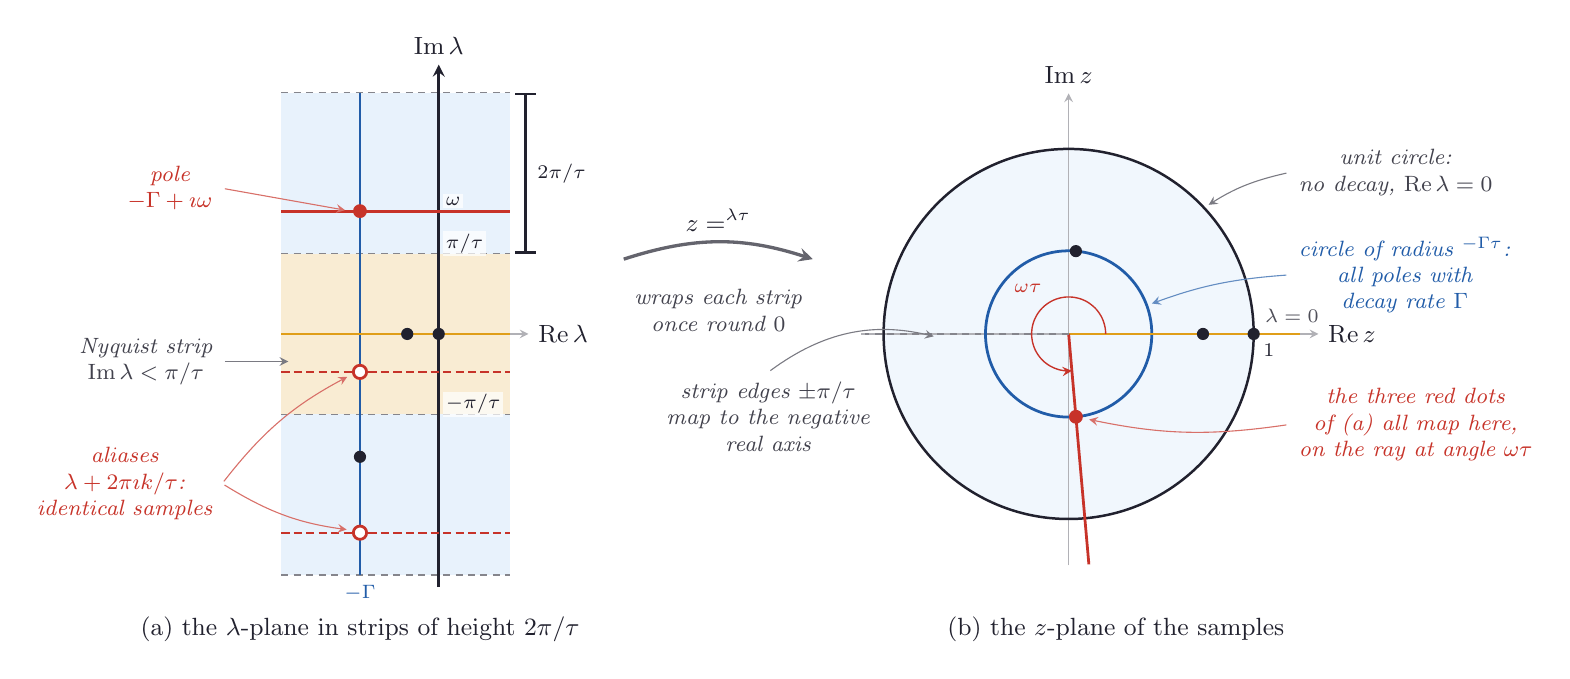
\begin{tikzpicture}[ink/.style={line width=0.9pt, ndInk}, faint/.style={line width=0.4pt, ndInk!35}, dashedink/.style={line width=0.5pt, ndInk!55, dash pattern=on 2.5pt off 2pt}, vec/.style={->, >=stealth, line width=1.2pt}, note/.style={font=\footnotesize\itshape, text=ndInk!85, align=center}, pointer/.style={->, >=stealth, line width=0.4pt, ndInk!60, shorten >=2pt, shorten <=1pt}, dot/.style={circle, fill=ndInk, inner sep=0pt, minimum size=3.4pt}, wash/.style={fill=ndSky, fill opacity=0.55}, every node/.style={text=ndInk}]
\definecolor{ndInk}{rgb}{0.13,0.13,0.18}
\definecolor{ndPaper}{rgb}{0.99,0.96,0.88}
\definecolor{ndSky}{rgb}{0.84,0.91,0.98}
\definecolor{ndRose}{rgb}{0.98,0.86,0.84}
\definecolor{ndBlue}{rgb}{0.13,0.36,0.66}
\definecolor{ndRed}{rgb}{0.78,0.20,0.16}
\definecolor{ndGold}{rgb}{0.88,0.62,0.10}
\definecolor{ndGreen}{rgb}{0.18,0.52,0.30}
\fill[ndSky, fill opacity=0.55] (1.000,-3.063) rectangle (3.900,-1.021);
\fill[ndGold!35, fill opacity=0.55] (1.000,-1.021) rectangle (3.900,1.021);
\fill[ndSky, fill opacity=0.55] (1.000,1.021) rectangle (3.900,3.063);
\draw[dashedink] (1.000,-3.063) -- (3.900,-3.063);
\draw[dashedink] (1.000,-1.021) -- (3.900,-1.021);
\draw[dashedink] (1.000,1.021) -- (3.900,1.021);
\draw[dashedink] (1.000,3.063) -- (3.900,3.063);
\draw[faint, ->, >=stealth] (1.000,0.000) -- (4.140,0.000) node[right, text=ndInk, font=\small] {$\mathrm{Re}\,\lambda$};
\draw[ink, ->, >=stealth] (3.000,-3.216) -- (3.000,3.420) node[above, text=ndInk, font=\small] {$\mathrm{Im}\,\lambda$};
\draw[line width=1.0pt, ndBlue] (2.000,-3.063) -- (2.000,3.063);
\draw[line width=0.6pt, dash pattern=on 3pt off 1.5pt, ndRed] (1.000,-2.524) -- (3.900,-2.524);
\draw[line width=0.6pt, dash pattern=on 3pt off 1.5pt, ndRed] (1.000,-0.482) -- (3.900,-0.482);
\draw[line width=1.0pt, ndRed] (1.000,1.560) -- (3.900,1.560);
\draw[line width=1.0pt, ndGold] (1.000,0.000) -- (3.900,0.000);
\node[font=\scriptsize, anchor=west, fill=white, fill opacity=0.7, text opacity=1, inner sep=1pt] at (3.050,1.151) {$\pi/\tau$};
\node[font=\scriptsize, anchor=west, fill=white, fill opacity=0.7, text opacity=1, inner sep=1pt] at (3.050,-0.891) {$-\pi/\tau$};
\node[font=\scriptsize, anchor=west, fill=white, fill opacity=0.7, text opacity=1, inner sep=1pt] at (3.050,1.690) {$\omega$};
\node[font=\scriptsize, text=ndBlue, below] at (2.000,-3.063) {$-\Gamma$};
\draw[ink, |-|] (4.100,1.021) -- (4.100,3.063);
\node[font=\scriptsize, anchor=west] at (4.130,2.042) {$2\pi/\tau$};
\node[dot, minimum size=4.4pt] at (3.000,0.000) {};
\node[dot, minimum size=4.4pt] at (2.600,0.000) {};
\node[dot, minimum size=4.4pt] at (2.000,-1.560) {};
\draw[ndRed, line width=1pt, fill=white] (2.000,-2.524) circle (2.4pt);
\draw[ndRed, line width=1pt, fill=white] (2.000,-0.482) circle (2.4pt);
\node[dot, fill=ndRed, minimum size=5pt] at (2.000,1.560) {};
\node[note, anchor=east] (ny) at (0.250,-0.350) {Nyquist strip\\ $\abs{\mathrm{Im}\,\lambda}<\pi/\tau$};
\draw[pointer] (ny.east) -- (1.160,-0.350);
\node[note, anchor=east, text=ndRed] (al) at (0.250,-1.900) {aliases\\ $\lambda+2\pi\imath k/\tau$:\\ identical samples};
\draw[pointer, ndRed!70] (al.east) to[bend right=12] (1.900,-2.494);
\draw[pointer, ndRed!70] (al.east) to[bend left=12] (1.900,-0.512);
\node[note, anchor=east, text=ndRed] (pl) at (0.250,1.850) {pole\\ $-\Gamma+\imath\omega$};
\draw[pointer, ndRed!70] (pl.east) -- (1.880,1.560);
\draw[vec, ndInk!70] (5.35,0.95) to[bend left=18] node[above, font=\small, text=ndInk] {$z=\ee^{\lambda\tau}$} (7.75,0.95);
\node[note] at (6.55,0.3) {wraps each strip\\ once round $0$};
\fill[ndSky, fill opacity=0.35] (11.000,0.000) circle (2.350);
\draw[faint, ->, >=stealth] (8.368,0.000) -- (14.172,0.000) node[right, text=ndInk, font=\small] {$\mathrm{Re}\,z$};
\draw[faint, ->, >=stealth] (11.000,-2.938) -- (11.000,3.055) node[above, text=ndInk, font=\small] {$\mathrm{Im}\,z$};
\draw[ink] (11.000,0.000) circle (2.350);
\draw[line width=1.0pt, ndBlue] (11.000,0.000) circle (1.056);
\draw[line width=1.0pt, ndGold] (11.000,0.000) -- (13.938,0.000);
\draw[line width=1.0pt, ndRed] (11.000,0.000) -- (11.257,-2.926);
\draw[dashedink, line width=0.8pt] (11.000,0.000) -- (8.415,0.000);
\draw[line width=0.5pt, ndRed, ->, >=stealth] (11.470,0.000) -- (11.469,0.029) -- (11.467,0.057) -- (11.462,0.085) -- (11.456,0.113) -- (11.448,0.141) -- (11.439,0.168) -- (11.428,0.194) -- (11.416,0.220) -- (11.401,0.244) -- (11.386,0.268) -- (11.369,0.291) -- (11.351,0.313) -- (11.331,0.334) -- (11.310,0.353) -- (11.288,0.371) -- (11.265,0.388) -- (11.241,0.404) -- (11.216,0.418) -- (11.190,0.430) -- (11.164,0.441) -- (11.137,0.450) -- (11.109,0.457) -- (11.081,0.463) -- (11.053,0.467) -- (11.024,0.469) -- (10.996,0.470) -- (10.967,0.469) -- (10.939,0.466) -- (10.911,0.461) -- (10.883,0.455) -- (10.855,0.447) -- (10.829,0.438) -- (10.802,0.426) -- (10.777,0.414) -- (10.752,0.399) -- (10.728,0.383) -- (10.705,0.366) -- (10.684,0.348) -- (10.663,0.328) -- (10.644,0.307) -- (10.626,0.285) -- (10.609,0.261) -- (10.594,0.237) -- (10.581,0.212) -- (10.568,0.186) -- (10.558,0.160) -- (10.549,0.133) -- (10.542,0.105) -- (10.536,0.077) -- (10.533,0.049) -- (10.530,0.020) -- (10.530,-0.008) -- (10.531,-0.037) -- (10.535,-0.065) -- (10.539,-0.093) -- (10.546,-0.121) -- (10.554,-0.149) -- (10.564,-0.175) -- (10.575,-0.202) -- (10.588,-0.227) -- (10.603,-0.252) -- (10.619,-0.275) -- (10.636,-0.298) -- (10.655,-0.319) -- (10.675,-0.340) -- (10.696,-0.359) -- (10.719,-0.377) -- (10.742,-0.393) -- (10.766,-0.408) -- (10.792,-0.421) -- (10.818,-0.433) -- (10.844,-0.443) -- (10.871,-0.452) -- (10.899,-0.459) -- (10.927,-0.464) -- (10.956,-0.468) -- (10.984,-0.470) -- (11.013,-0.470) -- (11.041,-0.468);
\node[font=\scriptsize, text=ndRed] at (10.483,0.578) {$\omega\tau$};
\node[dot, minimum size=4.4pt] at (13.350,0.000) {};
\node[dot, minimum size=4.4pt] at (12.706,0.000) {};
\node[dot, fill=ndRed, minimum size=5pt] at (11.092,-1.052) {};
\node[dot, minimum size=4.4pt] at (11.092,1.052) {};
\node[note, anchor=west] (uc) at (13.800,2.050) {unit circle:\\ no decay, $\mathrm{Re}\,\lambda=0$};
\draw[pointer] (uc.west) to[bend right=10] (12.719,1.602);
\node[note, anchor=west, text=ndBlue] (bc) at (13.800,0.750) {circle of radius $\ee^{-\Gamma\tau}$:\\ all poles with\\ decay rate $\Gamma$};
\draw[pointer, ndBlue!70] (bc.west) to[bend right=8] (11.992,0.362);
\node[note, anchor=west, text=ndRed] (rz) at (13.800,-1.150) {the three red dots\\ of (a) all map here,\\ on the ray at angle $\omega\tau$};
\draw[pointer, ndRed!70] (rz.west) to[bend left=10] (11.192,-1.072);
\node[note, anchor=east] (ng) at (8.600,-1.050) {strip edges $\pm\pi/\tau$\\ map to the negative\\ real axis};
\draw[pointer] (ng.north) to[bend left=25] (9.355,-0.047);
\node[font=\scriptsize, anchor=north west] at (13.350,0.000) {$1$};
\node[font=\scriptsize, text=ndInk!80, anchor=south west] at (13.370,0.020) {$\lambda=0$};
\node[font=\small] at (2.000,-3.750) {(a) the $\lambda$-plane in strips of height $2\pi/\tau$};
\node[font=\small] at (11.600,-3.750) {(b) the $z$-plane of the samples};
\end{tikzpicture}
}
\caption{Sampling at intervals $\tau$ replaces each pole $\lambda$ by $z=\ee^{\lambda\tau}$, the corresponding eigenvalue of $\mathbf G_\tau$; here $\tau=1.6$. (a) The $\lambda$-plane divided into strips of height $2\pi/\tau$, with the Nyquist strip $\abs{\mathrm{Im}\,\lambda}<\pi/\tau$ shaded gold, the poles of the example, and the aliases $\lambda+2\pi\imath k/\tau$ of $-\Gamma+\imath\omega$ (hollow). (b) The $z$-plane. The line of decay rate $\Gamma$ becomes the circle of radius $\ee^{-\Gamma\tau}$, the line of frequency $\omega$ becomes the ray at the angle $\omega\tau$, and the imaginary axis becomes the unit circle; the three red points of (a) are all carried to the same point $z$. Generated by \texttt{code/ch05\_expmap.py}.}\label{fig:ch05:expmap}
\end{figure}}
\onp{\begin{center}\resizebox{\linewidth}{!}{% Generated by code/needham.py -- do not edit by hand.
\definecolor{qocA}{rgb}{0.00,0.45,0.70}
\definecolor{qocB}{rgb}{0.90,0.60,0.00}
\definecolor{qocC}{rgb}{0.00,0.62,0.45}
\definecolor{qocD}{rgb}{0.80,0.40,0.00}
\definecolor{qocE}{rgb}{0.80,0.60,0.70}
\definecolor{qocF}{rgb}{0.35,0.70,0.90}
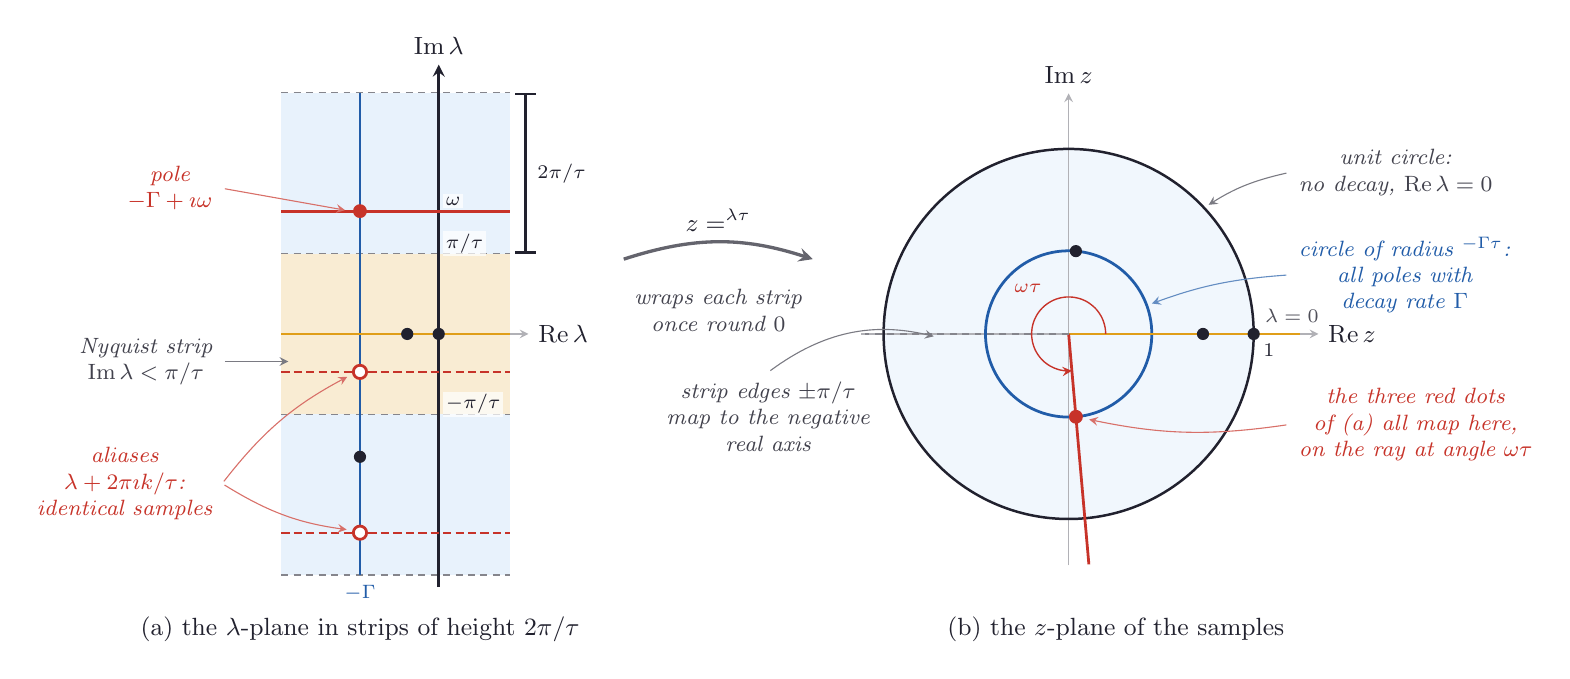
\begin{tikzpicture}[ink/.style={line width=0.9pt, ndInk}, faint/.style={line width=0.4pt, ndInk!35}, dashedink/.style={line width=0.5pt, ndInk!55, dash pattern=on 2.5pt off 2pt}, vec/.style={->, >=stealth, line width=1.2pt}, note/.style={font=\footnotesize\itshape, text=ndInk!85, align=center}, pointer/.style={->, >=stealth, line width=0.4pt, ndInk!60, shorten >=2pt, shorten <=1pt}, dot/.style={circle, fill=ndInk, inner sep=0pt, minimum size=3.4pt}, wash/.style={fill=ndSky, fill opacity=0.55}, every node/.style={text=ndInk}]
\definecolor{ndInk}{rgb}{0.13,0.13,0.18}
\definecolor{ndPaper}{rgb}{0.99,0.96,0.88}
\definecolor{ndSky}{rgb}{0.84,0.91,0.98}
\definecolor{ndRose}{rgb}{0.98,0.86,0.84}
\definecolor{ndBlue}{rgb}{0.13,0.36,0.66}
\definecolor{ndRed}{rgb}{0.78,0.20,0.16}
\definecolor{ndGold}{rgb}{0.88,0.62,0.10}
\definecolor{ndGreen}{rgb}{0.18,0.52,0.30}
\fill[ndSky, fill opacity=0.55] (1.000,-3.063) rectangle (3.900,-1.021);
\fill[ndGold!35, fill opacity=0.55] (1.000,-1.021) rectangle (3.900,1.021);
\fill[ndSky, fill opacity=0.55] (1.000,1.021) rectangle (3.900,3.063);
\draw[dashedink] (1.000,-3.063) -- (3.900,-3.063);
\draw[dashedink] (1.000,-1.021) -- (3.900,-1.021);
\draw[dashedink] (1.000,1.021) -- (3.900,1.021);
\draw[dashedink] (1.000,3.063) -- (3.900,3.063);
\draw[faint, ->, >=stealth] (1.000,0.000) -- (4.140,0.000) node[right, text=ndInk, font=\small] {$\mathrm{Re}\,\lambda$};
\draw[ink, ->, >=stealth] (3.000,-3.216) -- (3.000,3.420) node[above, text=ndInk, font=\small] {$\mathrm{Im}\,\lambda$};
\draw[line width=1.0pt, ndBlue] (2.000,-3.063) -- (2.000,3.063);
\draw[line width=0.6pt, dash pattern=on 3pt off 1.5pt, ndRed] (1.000,-2.524) -- (3.900,-2.524);
\draw[line width=0.6pt, dash pattern=on 3pt off 1.5pt, ndRed] (1.000,-0.482) -- (3.900,-0.482);
\draw[line width=1.0pt, ndRed] (1.000,1.560) -- (3.900,1.560);
\draw[line width=1.0pt, ndGold] (1.000,0.000) -- (3.900,0.000);
\node[font=\scriptsize, anchor=west, fill=white, fill opacity=0.7, text opacity=1, inner sep=1pt] at (3.050,1.151) {$\pi/\tau$};
\node[font=\scriptsize, anchor=west, fill=white, fill opacity=0.7, text opacity=1, inner sep=1pt] at (3.050,-0.891) {$-\pi/\tau$};
\node[font=\scriptsize, anchor=west, fill=white, fill opacity=0.7, text opacity=1, inner sep=1pt] at (3.050,1.690) {$\omega$};
\node[font=\scriptsize, text=ndBlue, below] at (2.000,-3.063) {$-\Gamma$};
\draw[ink, |-|] (4.100,1.021) -- (4.100,3.063);
\node[font=\scriptsize, anchor=west] at (4.130,2.042) {$2\pi/\tau$};
\node[dot, minimum size=4.4pt] at (3.000,0.000) {};
\node[dot, minimum size=4.4pt] at (2.600,0.000) {};
\node[dot, minimum size=4.4pt] at (2.000,-1.560) {};
\draw[ndRed, line width=1pt, fill=white] (2.000,-2.524) circle (2.4pt);
\draw[ndRed, line width=1pt, fill=white] (2.000,-0.482) circle (2.4pt);
\node[dot, fill=ndRed, minimum size=5pt] at (2.000,1.560) {};
\node[note, anchor=east] (ny) at (0.250,-0.350) {Nyquist strip\\ $\abs{\mathrm{Im}\,\lambda}<\pi/\tau$};
\draw[pointer] (ny.east) -- (1.160,-0.350);
\node[note, anchor=east, text=ndRed] (al) at (0.250,-1.900) {aliases\\ $\lambda+2\pi\imath k/\tau$:\\ identical samples};
\draw[pointer, ndRed!70] (al.east) to[bend right=12] (1.900,-2.494);
\draw[pointer, ndRed!70] (al.east) to[bend left=12] (1.900,-0.512);
\node[note, anchor=east, text=ndRed] (pl) at (0.250,1.850) {pole\\ $-\Gamma+\imath\omega$};
\draw[pointer, ndRed!70] (pl.east) -- (1.880,1.560);
\draw[vec, ndInk!70] (5.35,0.95) to[bend left=18] node[above, font=\small, text=ndInk] {$z=\ee^{\lambda\tau}$} (7.75,0.95);
\node[note] at (6.55,0.3) {wraps each strip\\ once round $0$};
\fill[ndSky, fill opacity=0.35] (11.000,0.000) circle (2.350);
\draw[faint, ->, >=stealth] (8.368,0.000) -- (14.172,0.000) node[right, text=ndInk, font=\small] {$\mathrm{Re}\,z$};
\draw[faint, ->, >=stealth] (11.000,-2.938) -- (11.000,3.055) node[above, text=ndInk, font=\small] {$\mathrm{Im}\,z$};
\draw[ink] (11.000,0.000) circle (2.350);
\draw[line width=1.0pt, ndBlue] (11.000,0.000) circle (1.056);
\draw[line width=1.0pt, ndGold] (11.000,0.000) -- (13.938,0.000);
\draw[line width=1.0pt, ndRed] (11.000,0.000) -- (11.257,-2.926);
\draw[dashedink, line width=0.8pt] (11.000,0.000) -- (8.415,0.000);
\draw[line width=0.5pt, ndRed, ->, >=stealth] (11.470,0.000) -- (11.469,0.029) -- (11.467,0.057) -- (11.462,0.085) -- (11.456,0.113) -- (11.448,0.141) -- (11.439,0.168) -- (11.428,0.194) -- (11.416,0.220) -- (11.401,0.244) -- (11.386,0.268) -- (11.369,0.291) -- (11.351,0.313) -- (11.331,0.334) -- (11.310,0.353) -- (11.288,0.371) -- (11.265,0.388) -- (11.241,0.404) -- (11.216,0.418) -- (11.190,0.430) -- (11.164,0.441) -- (11.137,0.450) -- (11.109,0.457) -- (11.081,0.463) -- (11.053,0.467) -- (11.024,0.469) -- (10.996,0.470) -- (10.967,0.469) -- (10.939,0.466) -- (10.911,0.461) -- (10.883,0.455) -- (10.855,0.447) -- (10.829,0.438) -- (10.802,0.426) -- (10.777,0.414) -- (10.752,0.399) -- (10.728,0.383) -- (10.705,0.366) -- (10.684,0.348) -- (10.663,0.328) -- (10.644,0.307) -- (10.626,0.285) -- (10.609,0.261) -- (10.594,0.237) -- (10.581,0.212) -- (10.568,0.186) -- (10.558,0.160) -- (10.549,0.133) -- (10.542,0.105) -- (10.536,0.077) -- (10.533,0.049) -- (10.530,0.020) -- (10.530,-0.008) -- (10.531,-0.037) -- (10.535,-0.065) -- (10.539,-0.093) -- (10.546,-0.121) -- (10.554,-0.149) -- (10.564,-0.175) -- (10.575,-0.202) -- (10.588,-0.227) -- (10.603,-0.252) -- (10.619,-0.275) -- (10.636,-0.298) -- (10.655,-0.319) -- (10.675,-0.340) -- (10.696,-0.359) -- (10.719,-0.377) -- (10.742,-0.393) -- (10.766,-0.408) -- (10.792,-0.421) -- (10.818,-0.433) -- (10.844,-0.443) -- (10.871,-0.452) -- (10.899,-0.459) -- (10.927,-0.464) -- (10.956,-0.468) -- (10.984,-0.470) -- (11.013,-0.470) -- (11.041,-0.468);
\node[font=\scriptsize, text=ndRed] at (10.483,0.578) {$\omega\tau$};
\node[dot, minimum size=4.4pt] at (13.350,0.000) {};
\node[dot, minimum size=4.4pt] at (12.706,0.000) {};
\node[dot, fill=ndRed, minimum size=5pt] at (11.092,-1.052) {};
\node[dot, minimum size=4.4pt] at (11.092,1.052) {};
\node[note, anchor=west] (uc) at (13.800,2.050) {unit circle:\\ no decay, $\mathrm{Re}\,\lambda=0$};
\draw[pointer] (uc.west) to[bend right=10] (12.719,1.602);
\node[note, anchor=west, text=ndBlue] (bc) at (13.800,0.750) {circle of radius $\ee^{-\Gamma\tau}$:\\ all poles with\\ decay rate $\Gamma$};
\draw[pointer, ndBlue!70] (bc.west) to[bend right=8] (11.992,0.362);
\node[note, anchor=west, text=ndRed] (rz) at (13.800,-1.150) {the three red dots\\ of (a) all map here,\\ on the ray at angle $\omega\tau$};
\draw[pointer, ndRed!70] (rz.west) to[bend left=10] (11.192,-1.072);
\node[note, anchor=east] (ng) at (8.600,-1.050) {strip edges $\pm\pi/\tau$\\ map to the negative\\ real axis};
\draw[pointer] (ng.north) to[bend left=25] (9.355,-0.047);
\node[font=\scriptsize, anchor=north west] at (13.350,0.000) {$1$};
\node[font=\scriptsize, text=ndInk!80, anchor=south west] at (13.370,0.020) {$\lambda=0$};
\node[font=\small] at (2.000,-3.750) {(a) the $\lambda$-plane in strips of height $2\pi/\tau$};
\node[font=\small] at (11.600,-3.750) {(b) the $z$-plane of the samples};
\end{tikzpicture}
}\end{center}}
\end{frame}

\begin{frame}\ft{Multirate sampling removes the ambiguity}
\ona{The ambiguity can be removed without prior knowledge by sampling with at most $n+1$ intervals, chosen so that the ratio $\tau_{i}/\tau_{j}$ of any two of them is irrational. The intersection}
\onp{Sample at several rates $\tau_j$ in irrational ratio \citep{Ding2009}:}
\begin{equation}\label{eq:ch05:intersection}
\bigcap_{j=1}^{n+1} \eig_{\tau_{j}}
\end{equation}
\ona{then has exactly $n$ elements, which are the eigenvalues of $\mathbf{A}$ \citep{Ding2009}. The reason is arithmetical. A spurious candidate $\lambda+2\pi\imath k/\tau_1$ coincides with a candidate $\lambda+2\pi\imath k'/\tau_2$ only if $k/\tau_1=k'/\tau_2$, that is, only if $\tau_1/\tau_2=k/k'$ is rational. In Figure~\ref{fig:ch05:multirate} each set of candidates is drawn as a comb along the frequency axis. Two combs whose spacings are in an irrational ratio have only one tooth in common, at the true frequency, whereas two combs whose spacings are in a rational ratio meet again and again. The matrix $\mathbf A$ may then be found as}
\begin{equation}\label{eq:ch05:reconstructA}
\mathbf{A}=\mathbf{g}\,\mathrm{diag}\big(\lambda_{1}[\mathbf{A}],\dots,\lambda_{n}[\mathbf{A}]\big)\,\mathbf{g}^{-1},
\end{equation}
\ona{where $\mathbf{g}$ is the matrix of eigenvectors of $\mathbf{G}_\tau$, which $\mathbf A$ shares. If $\mathbf{A}$ is not diagonalisable, it can still be constructed provided that it shares the Jordan structure of $\mathbf{G}_{\tau}$. With non-uniform sampling one can retain a minimal realisation either by choosing the frame period $T$ so that $\lambda_{i} - \lambda_{j} \neq 2\pi k\imath/T$, or by choosing the sampling intervals so that at least one ratio $\tau_{i}/\tau_{j}$ within the period is irrational. This is the origin of the multirate hypothesis in Theorem~\ref{thm:ch04:auto} of \Chap~\ref{C.StateSpace}. For driven systems the position is different: pulses of varying width already probe the generator in continuous time, and uniform sampling suffices (Theorem~\ref{thm:ch04:driven}).}
\onp{\begin{itemize}
    \item Spurious candidates coincide only if $\tau_1/\tau_2=k/k'\in\mathbb Q$.
    \item Recover $\mathbf A=\mathbf g\,\mathrm{diag}(\lambda_i[\mathbf A])\,\mathbf g^{-1}$ with the eigenvectors of $\mathbf G_\tau$.
    \item Hence the irrational ratios in Theorem~\ref{thm:ch04:auto}; driven systems do not need them.
\end{itemize}}
\end{frame}

\begin{frame}\ft{Two sampling rates}
\ona{\begin{figure}[H]\centering
\resizebox{\linewidth}{!}{% Generated by code/needham.py -- do not edit by hand.
\definecolor{qocA}{rgb}{0.00,0.45,0.70}
\definecolor{qocB}{rgb}{0.90,0.60,0.00}
\definecolor{qocC}{rgb}{0.00,0.62,0.45}
\definecolor{qocD}{rgb}{0.80,0.40,0.00}
\definecolor{qocE}{rgb}{0.80,0.60,0.70}
\definecolor{qocF}{rgb}{0.35,0.70,0.90}
\begin{tikzpicture}[ink/.style={line width=0.9pt, ndInk}, faint/.style={line width=0.4pt, ndInk!35}, dashedink/.style={line width=0.5pt, ndInk!55, dash pattern=on 2.5pt off 2pt}, vec/.style={->, >=stealth, line width=1.2pt}, note/.style={font=\footnotesize\itshape, text=ndInk!85, align=center}, pointer/.style={->, >=stealth, line width=0.4pt, ndInk!60, shorten >=2pt, shorten <=1pt}, dot/.style={circle, fill=ndInk, inner sep=0pt, minimum size=3.4pt}, wash/.style={fill=ndSky, fill opacity=0.55}, every node/.style={text=ndInk}]
\definecolor{ndInk}{rgb}{0.13,0.13,0.18}
\definecolor{ndPaper}{rgb}{0.99,0.96,0.88}
\definecolor{ndSky}{rgb}{0.84,0.91,0.98}
\definecolor{ndRose}{rgb}{0.98,0.86,0.84}
\definecolor{ndBlue}{rgb}{0.13,0.36,0.66}
\definecolor{ndRed}{rgb}{0.78,0.20,0.16}
\definecolor{ndGold}{rgb}{0.88,0.62,0.10}
\definecolor{ndGreen}{rgb}{0.18,0.52,0.30}
\fill[ndBlue!18] (4.804,2.600) rectangle (7.396,3.420);
\fill[ndRed!18] (5.184,2.600) rectangle (7.016,1.780);
\draw[faint, ->, >=stealth] (0.292,2.600) -- (14.614,2.600) node[right, text=ndInk, font=\small] {$\nu$};
\draw[faint] (6.100,2.520) -- (6.100,2.680);
\draw[line width=1.1pt, ndBlue] (2.896,2.600) -- (2.896,3.300);
\draw[ndBlue, line width=0.7pt, fill=white] (2.896,3.300) circle (1.6pt);
\draw[line width=1.1pt, ndBlue] (5.488,2.600) -- (5.488,3.300);
\fill[ndBlue] (5.488,3.300) circle (2.0pt);
\draw[line width=1.1pt, ndBlue] (8.080,2.600) -- (8.080,3.300);
\draw[ndBlue, line width=0.7pt, fill=white] (8.080,3.300) circle (1.6pt);
\draw[line width=1.1pt, ndBlue] (10.672,2.600) -- (10.672,3.300);
\draw[ndBlue, line width=0.7pt, fill=white] (10.672,3.300) circle (1.6pt);
\draw[line width=1.1pt, ndBlue] (13.264,2.600) -- (13.264,3.300);
\draw[ndBlue, line width=0.7pt, fill=white] (13.264,3.300) circle (1.6pt);
\draw[line width=1.1pt, ndRed] (0.749,2.600) -- (0.749,1.900);
\draw[ndRed, line width=0.7pt, fill=white] (0.749,1.900) circle (1.6pt);
\draw[line width=1.1pt, ndRed] (2.582,2.600) -- (2.582,1.900);
\draw[ndRed, line width=0.7pt, fill=white] (2.582,1.900) circle (1.6pt);
\draw[line width=1.1pt, ndRed] (4.415,2.600) -- (4.415,1.900);
\draw[ndRed, line width=0.7pt, fill=white] (4.415,1.900) circle (1.6pt);
\draw[line width=1.1pt, ndRed] (6.247,2.600) -- (6.247,1.900);
\fill[ndRed] (6.247,1.900) circle (2.0pt);
\draw[line width=1.1pt, ndRed] (8.080,2.600) -- (8.080,1.900);
\draw[ndRed, line width=0.7pt, fill=white] (8.080,1.900) circle (1.6pt);
\draw[line width=1.1pt, ndRed] (9.913,2.600) -- (9.913,1.900);
\draw[ndRed, line width=0.7pt, fill=white] (9.913,1.900) circle (1.6pt);
\draw[line width=1.1pt, ndRed] (11.745,2.600) -- (11.745,1.900);
\draw[ndRed, line width=0.7pt, fill=white] (11.745,1.900) circle (1.6pt);
\draw[line width=1.1pt, ndRed] (13.578,2.600) -- (13.578,1.900);
\draw[ndRed, line width=0.7pt, fill=white] (13.578,1.900) circle (1.6pt);
\draw[ndGold, line width=1.6pt] (8.080,2.600) circle (5pt);
\node[font=\small, text=ndBlue, anchor=east] at (0.274,3.020) {$\tau_1=1.6$};
\node[font=\small, text=ndRed, anchor=east] at (0.274,2.180) {$\tau_2=\sqrt2\,\tau_1$};
\fill[ndBlue!18] (4.804,-1.000) rectangle (7.396,-0.180);
\fill[ndRed!18] (5.236,-1.000) rectangle (6.964,-1.820);
\draw[faint, ->, >=stealth] (0.292,-1.000) -- (14.614,-1.000) node[right, text=ndInk, font=\small] {$\nu$};
\draw[faint] (6.100,-1.080) -- (6.100,-0.920);
\draw[line width=1.1pt, ndBlue] (2.896,-1.000) -- (2.896,-0.300);
\draw[ndBlue, line width=0.7pt, fill=white] (2.896,-0.300) circle (1.6pt);
\draw[line width=1.1pt, ndBlue] (5.488,-1.000) -- (5.488,-0.300);
\fill[ndBlue] (5.488,-0.300) circle (2.0pt);
\draw[line width=1.1pt, ndBlue] (8.080,-1.000) -- (8.080,-0.300);
\draw[ndBlue, line width=0.7pt, fill=white] (8.080,-0.300) circle (1.6pt);
\draw[line width=1.1pt, ndBlue] (10.672,-1.000) -- (10.672,-0.300);
\draw[ndBlue, line width=0.7pt, fill=white] (10.672,-0.300) circle (1.6pt);
\draw[line width=1.1pt, ndBlue] (13.264,-1.000) -- (13.264,-0.300);
\draw[ndBlue, line width=0.7pt, fill=white] (13.264,-0.300) circle (1.6pt);
\draw[line width=1.1pt, ndRed] (1.168,-1.000) -- (1.168,-1.700);
\draw[ndRed, line width=0.7pt, fill=white] (1.168,-1.700) circle (1.6pt);
\draw[line width=1.1pt, ndRed] (2.896,-1.000) -- (2.896,-1.700);
\draw[ndRed, line width=0.7pt, fill=white] (2.896,-1.700) circle (1.6pt);
\draw[line width=1.1pt, ndRed] (4.624,-1.000) -- (4.624,-1.700);
\draw[ndRed, line width=0.7pt, fill=white] (4.624,-1.700) circle (1.6pt);
\draw[line width=1.1pt, ndRed] (6.352,-1.000) -- (6.352,-1.700);
\fill[ndRed] (6.352,-1.700) circle (2.0pt);
\draw[line width=1.1pt, ndRed] (8.080,-1.000) -- (8.080,-1.700);
\draw[ndRed, line width=0.7pt, fill=white] (8.080,-1.700) circle (1.6pt);
\draw[line width=1.1pt, ndRed] (9.808,-1.000) -- (9.808,-1.700);
\draw[ndRed, line width=0.7pt, fill=white] (9.808,-1.700) circle (1.6pt);
\draw[line width=1.1pt, ndRed] (11.536,-1.000) -- (11.536,-1.700);
\draw[ndRed, line width=0.7pt, fill=white] (11.536,-1.700) circle (1.6pt);
\draw[line width=1.1pt, ndRed] (13.264,-1.000) -- (13.264,-1.700);
\draw[ndRed, line width=0.7pt, fill=white] (13.264,-1.700) circle (1.6pt);
\draw[ndGold, line width=1.6pt] (2.896,-1.000) circle (5pt);
\draw[ndGold, line width=1.6pt] (8.080,-1.000) circle (5pt);
\draw[ndGold, line width=1.6pt] (13.264,-1.000) circle (5pt);
\node[font=\small, text=ndBlue, anchor=east] at (0.274,-0.580) {$\tau_1=1.6$};
\node[font=\small, text=ndRed, anchor=east] at (0.274,-1.420) {$\tau_2=\tfrac32\,\tau_1$};
\node[font=\scriptsize, anchor=north west, inner sep=1pt] at (8.200,2.550) {$\omega$};
\node[font=\scriptsize, anchor=north east, inner sep=1pt] at (6.060,2.550) {$0$};
\node[font=\scriptsize, anchor=north west, inner sep=1pt] at (8.200,-1.050) {$\omega$};
\node[font=\scriptsize, anchor=north east, inner sep=1pt] at (6.060,-1.050) {$0$};
\node[note, anchor=south] (g) at (8.080,3.550) {the only tooth common to both combs:\\ the true frequency $\omega$};
\draw[pointer] (g.south) -- (8.260,2.820);
\node[note, anchor=south] (fb) at (2.602,3.550) {filled dots: the tooth each rate reports\\ on its own, in its Nyquist band (shaded)};
\draw[pointer] (fb.south east) to[bend left=10] (5.428,3.360);
\node[note, anchor=west] at (15.066,2.600) {spacing $2\pi/\tau_1$ (up)\\ and $2\pi/\tau_2$ (down):\\ irrational ratio};
\node[note, anchor=west] at (15.066,-1.000) {rational ratio: the\\ combs coincide\\ every $4\pi/\tau_1$};
\node[note, anchor=north, text=ndInk] (amb) at (8.080,-1.950) {three candidates remain in the window, and the ambiguity persists};
\draw[pointer] (amb.north) -- (2.846,-1.220);
\draw[pointer] (amb.north) -- (8.080,-1.220);
\draw[pointer] (amb.north) -- (13.314,-1.220);
\node[font=\small] at (7.420,1.350) {(a) irrational ratio of the sampling periods};
\node[font=\small] at (7.420,-2.850) {(b) rational ratio of the sampling periods};
\end{tikzpicture}
}
\caption{The candidate frequencies $\omega+2\pi k/\tau$ compatible with the samples form a comb: blue teeth for $\tau_1=1.6$ (upwards) and red teeth for $\tau_2$ (downwards). The shaded intervals are the Nyquist bands, and the filled dots are what each rate reports on its own. (a) With $\tau_2=\sqrt2\,\tau_1$ the combs have only the true frequency $\omega=3$ in common (gold ring). (b) With $\tau_2=\tfrac32\tau_1$ they coincide every $4\pi/\tau_1\approx7.85$, and three candidates remain in the window shown. Generated by \texttt{code/ch05\_multirate.py}.}\label{fig:ch05:multirate}
\end{figure}}
\onp{\begin{center}\resizebox{\linewidth}{!}{% Generated by code/needham.py -- do not edit by hand.
\definecolor{qocA}{rgb}{0.00,0.45,0.70}
\definecolor{qocB}{rgb}{0.90,0.60,0.00}
\definecolor{qocC}{rgb}{0.00,0.62,0.45}
\definecolor{qocD}{rgb}{0.80,0.40,0.00}
\definecolor{qocE}{rgb}{0.80,0.60,0.70}
\definecolor{qocF}{rgb}{0.35,0.70,0.90}
\begin{tikzpicture}[ink/.style={line width=0.9pt, ndInk}, faint/.style={line width=0.4pt, ndInk!35}, dashedink/.style={line width=0.5pt, ndInk!55, dash pattern=on 2.5pt off 2pt}, vec/.style={->, >=stealth, line width=1.2pt}, note/.style={font=\footnotesize\itshape, text=ndInk!85, align=center}, pointer/.style={->, >=stealth, line width=0.4pt, ndInk!60, shorten >=2pt, shorten <=1pt}, dot/.style={circle, fill=ndInk, inner sep=0pt, minimum size=3.4pt}, wash/.style={fill=ndSky, fill opacity=0.55}, every node/.style={text=ndInk}]
\definecolor{ndInk}{rgb}{0.13,0.13,0.18}
\definecolor{ndPaper}{rgb}{0.99,0.96,0.88}
\definecolor{ndSky}{rgb}{0.84,0.91,0.98}
\definecolor{ndRose}{rgb}{0.98,0.86,0.84}
\definecolor{ndBlue}{rgb}{0.13,0.36,0.66}
\definecolor{ndRed}{rgb}{0.78,0.20,0.16}
\definecolor{ndGold}{rgb}{0.88,0.62,0.10}
\definecolor{ndGreen}{rgb}{0.18,0.52,0.30}
\fill[ndBlue!18] (4.804,2.600) rectangle (7.396,3.420);
\fill[ndRed!18] (5.184,2.600) rectangle (7.016,1.780);
\draw[faint, ->, >=stealth] (0.292,2.600) -- (14.614,2.600) node[right, text=ndInk, font=\small] {$\nu$};
\draw[faint] (6.100,2.520) -- (6.100,2.680);
\draw[line width=1.1pt, ndBlue] (2.896,2.600) -- (2.896,3.300);
\draw[ndBlue, line width=0.7pt, fill=white] (2.896,3.300) circle (1.6pt);
\draw[line width=1.1pt, ndBlue] (5.488,2.600) -- (5.488,3.300);
\fill[ndBlue] (5.488,3.300) circle (2.0pt);
\draw[line width=1.1pt, ndBlue] (8.080,2.600) -- (8.080,3.300);
\draw[ndBlue, line width=0.7pt, fill=white] (8.080,3.300) circle (1.6pt);
\draw[line width=1.1pt, ndBlue] (10.672,2.600) -- (10.672,3.300);
\draw[ndBlue, line width=0.7pt, fill=white] (10.672,3.300) circle (1.6pt);
\draw[line width=1.1pt, ndBlue] (13.264,2.600) -- (13.264,3.300);
\draw[ndBlue, line width=0.7pt, fill=white] (13.264,3.300) circle (1.6pt);
\draw[line width=1.1pt, ndRed] (0.749,2.600) -- (0.749,1.900);
\draw[ndRed, line width=0.7pt, fill=white] (0.749,1.900) circle (1.6pt);
\draw[line width=1.1pt, ndRed] (2.582,2.600) -- (2.582,1.900);
\draw[ndRed, line width=0.7pt, fill=white] (2.582,1.900) circle (1.6pt);
\draw[line width=1.1pt, ndRed] (4.415,2.600) -- (4.415,1.900);
\draw[ndRed, line width=0.7pt, fill=white] (4.415,1.900) circle (1.6pt);
\draw[line width=1.1pt, ndRed] (6.247,2.600) -- (6.247,1.900);
\fill[ndRed] (6.247,1.900) circle (2.0pt);
\draw[line width=1.1pt, ndRed] (8.080,2.600) -- (8.080,1.900);
\draw[ndRed, line width=0.7pt, fill=white] (8.080,1.900) circle (1.6pt);
\draw[line width=1.1pt, ndRed] (9.913,2.600) -- (9.913,1.900);
\draw[ndRed, line width=0.7pt, fill=white] (9.913,1.900) circle (1.6pt);
\draw[line width=1.1pt, ndRed] (11.745,2.600) -- (11.745,1.900);
\draw[ndRed, line width=0.7pt, fill=white] (11.745,1.900) circle (1.6pt);
\draw[line width=1.1pt, ndRed] (13.578,2.600) -- (13.578,1.900);
\draw[ndRed, line width=0.7pt, fill=white] (13.578,1.900) circle (1.6pt);
\draw[ndGold, line width=1.6pt] (8.080,2.600) circle (5pt);
\node[font=\small, text=ndBlue, anchor=east] at (0.274,3.020) {$\tau_1=1.6$};
\node[font=\small, text=ndRed, anchor=east] at (0.274,2.180) {$\tau_2=\sqrt2\,\tau_1$};
\fill[ndBlue!18] (4.804,-1.000) rectangle (7.396,-0.180);
\fill[ndRed!18] (5.236,-1.000) rectangle (6.964,-1.820);
\draw[faint, ->, >=stealth] (0.292,-1.000) -- (14.614,-1.000) node[right, text=ndInk, font=\small] {$\nu$};
\draw[faint] (6.100,-1.080) -- (6.100,-0.920);
\draw[line width=1.1pt, ndBlue] (2.896,-1.000) -- (2.896,-0.300);
\draw[ndBlue, line width=0.7pt, fill=white] (2.896,-0.300) circle (1.6pt);
\draw[line width=1.1pt, ndBlue] (5.488,-1.000) -- (5.488,-0.300);
\fill[ndBlue] (5.488,-0.300) circle (2.0pt);
\draw[line width=1.1pt, ndBlue] (8.080,-1.000) -- (8.080,-0.300);
\draw[ndBlue, line width=0.7pt, fill=white] (8.080,-0.300) circle (1.6pt);
\draw[line width=1.1pt, ndBlue] (10.672,-1.000) -- (10.672,-0.300);
\draw[ndBlue, line width=0.7pt, fill=white] (10.672,-0.300) circle (1.6pt);
\draw[line width=1.1pt, ndBlue] (13.264,-1.000) -- (13.264,-0.300);
\draw[ndBlue, line width=0.7pt, fill=white] (13.264,-0.300) circle (1.6pt);
\draw[line width=1.1pt, ndRed] (1.168,-1.000) -- (1.168,-1.700);
\draw[ndRed, line width=0.7pt, fill=white] (1.168,-1.700) circle (1.6pt);
\draw[line width=1.1pt, ndRed] (2.896,-1.000) -- (2.896,-1.700);
\draw[ndRed, line width=0.7pt, fill=white] (2.896,-1.700) circle (1.6pt);
\draw[line width=1.1pt, ndRed] (4.624,-1.000) -- (4.624,-1.700);
\draw[ndRed, line width=0.7pt, fill=white] (4.624,-1.700) circle (1.6pt);
\draw[line width=1.1pt, ndRed] (6.352,-1.000) -- (6.352,-1.700);
\fill[ndRed] (6.352,-1.700) circle (2.0pt);
\draw[line width=1.1pt, ndRed] (8.080,-1.000) -- (8.080,-1.700);
\draw[ndRed, line width=0.7pt, fill=white] (8.080,-1.700) circle (1.6pt);
\draw[line width=1.1pt, ndRed] (9.808,-1.000) -- (9.808,-1.700);
\draw[ndRed, line width=0.7pt, fill=white] (9.808,-1.700) circle (1.6pt);
\draw[line width=1.1pt, ndRed] (11.536,-1.000) -- (11.536,-1.700);
\draw[ndRed, line width=0.7pt, fill=white] (11.536,-1.700) circle (1.6pt);
\draw[line width=1.1pt, ndRed] (13.264,-1.000) -- (13.264,-1.700);
\draw[ndRed, line width=0.7pt, fill=white] (13.264,-1.700) circle (1.6pt);
\draw[ndGold, line width=1.6pt] (2.896,-1.000) circle (5pt);
\draw[ndGold, line width=1.6pt] (8.080,-1.000) circle (5pt);
\draw[ndGold, line width=1.6pt] (13.264,-1.000) circle (5pt);
\node[font=\small, text=ndBlue, anchor=east] at (0.274,-0.580) {$\tau_1=1.6$};
\node[font=\small, text=ndRed, anchor=east] at (0.274,-1.420) {$\tau_2=\tfrac32\,\tau_1$};
\node[font=\scriptsize, anchor=north west, inner sep=1pt] at (8.200,2.550) {$\omega$};
\node[font=\scriptsize, anchor=north east, inner sep=1pt] at (6.060,2.550) {$0$};
\node[font=\scriptsize, anchor=north west, inner sep=1pt] at (8.200,-1.050) {$\omega$};
\node[font=\scriptsize, anchor=north east, inner sep=1pt] at (6.060,-1.050) {$0$};
\node[note, anchor=south] (g) at (8.080,3.550) {the only tooth common to both combs:\\ the true frequency $\omega$};
\draw[pointer] (g.south) -- (8.260,2.820);
\node[note, anchor=south] (fb) at (2.602,3.550) {filled dots: the tooth each rate reports\\ on its own, in its Nyquist band (shaded)};
\draw[pointer] (fb.south east) to[bend left=10] (5.428,3.360);
\node[note, anchor=west] at (15.066,2.600) {spacing $2\pi/\tau_1$ (up)\\ and $2\pi/\tau_2$ (down):\\ irrational ratio};
\node[note, anchor=west] at (15.066,-1.000) {rational ratio: the\\ combs coincide\\ every $4\pi/\tau_1$};
\node[note, anchor=north, text=ndInk] (amb) at (8.080,-1.950) {three candidates remain in the window, and the ambiguity persists};
\draw[pointer] (amb.north) -- (2.846,-1.220);
\draw[pointer] (amb.north) -- (8.080,-1.220);
\draw[pointer] (amb.north) -- (13.314,-1.220);
\node[font=\small] at (7.420,1.350) {(a) irrational ratio of the sampling periods};
\node[font=\small] at (7.420,-2.850) {(b) rational ratio of the sampling periods};
\end{tikzpicture}
}\end{center}}
\end{frame}

\section{Identifiability in the frequency domain}

\begin{frame}\ft{Three notions of identifiability}
\ona{Although our main interest is in the identifiability of the system matrix, and hence of the parameters of the GKSL equation, there are connections with other definitions of identifiability. For an uncontrolled system the methods of behavioural systems theory \citep{willems2007mathematics, markovsky2008data} show that, under mild conditions, the three commonest notions of identifiability coincide:}
\onp{Behavioural systems theory \citep{willems2007mathematics,markovsky2008data}: three notions coincide under persistency of excitation \citep{9904308}:}
\begin{itemize}
    \item the identifiability of the system matrix (the notion used in \Chap~\ref{C.StateSpace}),
    \item the identifiability of the input--output relation (as an ordinary differential equation),
    \item the identifiability of the transfer function associated with the input--output relation.
\end{itemize}
\ona{Persistency of excitation is needed for all three to be equivalent \citep{9904308}. A discrete linear time-invariant system has a persistently exciting input if the Hankel matrix of the input,}
\begin{equation}\label{eq:ch05:pe}
H_L(u) =
\begin{bmatrix}
u(0) & u(1) & \cdots & u(T-L) \\
u(1) & u(2) & \cdots & u(T-L+1) \\
\vdots & \vdots & \ddots & \vdots \\
u(L-1) & u(L) & \cdots & u(T-1)
\end{bmatrix},\qquad \rank H_L(u)=mL,
\end{equation}
\ona{has full row rank, where $T$ is the number of data points and $L$ the order of persistency of excitation; in the frequency domain, as we saw in Figure~\ref{fig:ch05:onefreq}, the order counts the frequencies that the input contains. For an autonomous system the condition is the Krylov condition of Theorem~\ref{thm:ch05:hankelrank}, which by Proposition~\ref{prop:ch05:modal} requires the initial state to excite every mode. The equivalence therefore extends to all autonomous open quantum systems, which are particular autonomous linear systems once the measurement is taken into account.}
\onp{Autonomous case: persistency of excitation is the Krylov condition on $\vec x_0$ (Theorem~\ref{thm:ch05:hankelrank}).}
\end{frame}

\begin{frame}\ft{Quantum identifiability via transfer functions}
\ona{Several questions about the identifiability of \emph{closed} systems were settled by \citet{Wang_2020}, who gave the notion of quantum identifiability a precise meaning in terms of the transfer function of the linear system satisfied by the coherence vector. Two Hamiltonians are indistinguishable if and only if their realisations have the same transfer function, and, for minimal realisations, if and only if these are related by a similarity transformation (Theorem~\ref{thm:ch04:similarity}). The identifiability of a Hamiltonian thus becomes a question about the admissible similarity transformations: it holds when the only admissible transformations are those induced on the coherence vector by unitary conjugation, which act as rotations. For open systems \citet{Burgarth_2014} showed by an example that a similarity transformation need not preserve the Lindblad form, so that the transfer function determines the master equation only up to a gauge that may be unphysical; Proposition~\ref{prop:ch04:gauge} of \Chap~\ref{C.StateSpace} removes this gauge by means of a known $\mathbf C$ of full rank and $\mathbf B=\Id$. Figure~\ref{fig:ch05:gauge} shows both kinds of transformation on our example: a rotation of the Bloch ball, which is a change of frame and leaves the generator a Lindbladian, and a shear, which reproduces the same data with a generator that is not a physical evolution at all. In the terms of this \chap{}, the data determine $\TF(s)$; $\TF$ determines the minimal realisation up to $\mathbf T$; the known $\mathbf B$ and $\mathbf C$ force $\mathbf T=\Id$; and the linear map $\mathbf M$ then yields $(\vec\theta,\Koss)$.}
\onp{\begin{itemize}
    \item \citet{Wang_2020}: Hamiltonians indistinguishable $\Leftrightarrow$ same transfer function $\Leftrightarrow$ similar (minimal case).
    \item \citet{Burgarth_2014}: for open systems a similarity transformation can leave the Lindblad class.
    \item Data $\to$ $\TF(s)$ $\to$ realisation up to $\mathbf T$ $\to$ $\mathbf T=\Id$ (known $\mathbf B,\mathbf C$) $\to$ $(\vec\theta,\Koss)$ via $\mathbf M$.
\end{itemize}}
\end{frame}

\begin{frame}\ft{Similar realisations}
\ona{\begin{figure}[H]\centering
\resizebox{\linewidth}{!}{% Generated by code/needham.py -- do not edit by hand.
\definecolor{qocA}{rgb}{0.00,0.45,0.70}
\definecolor{qocB}{rgb}{0.90,0.60,0.00}
\definecolor{qocC}{rgb}{0.00,0.62,0.45}
\definecolor{qocD}{rgb}{0.80,0.40,0.00}
\definecolor{qocE}{rgb}{0.80,0.60,0.70}
\definecolor{qocF}{rgb}{0.35,0.70,0.90}
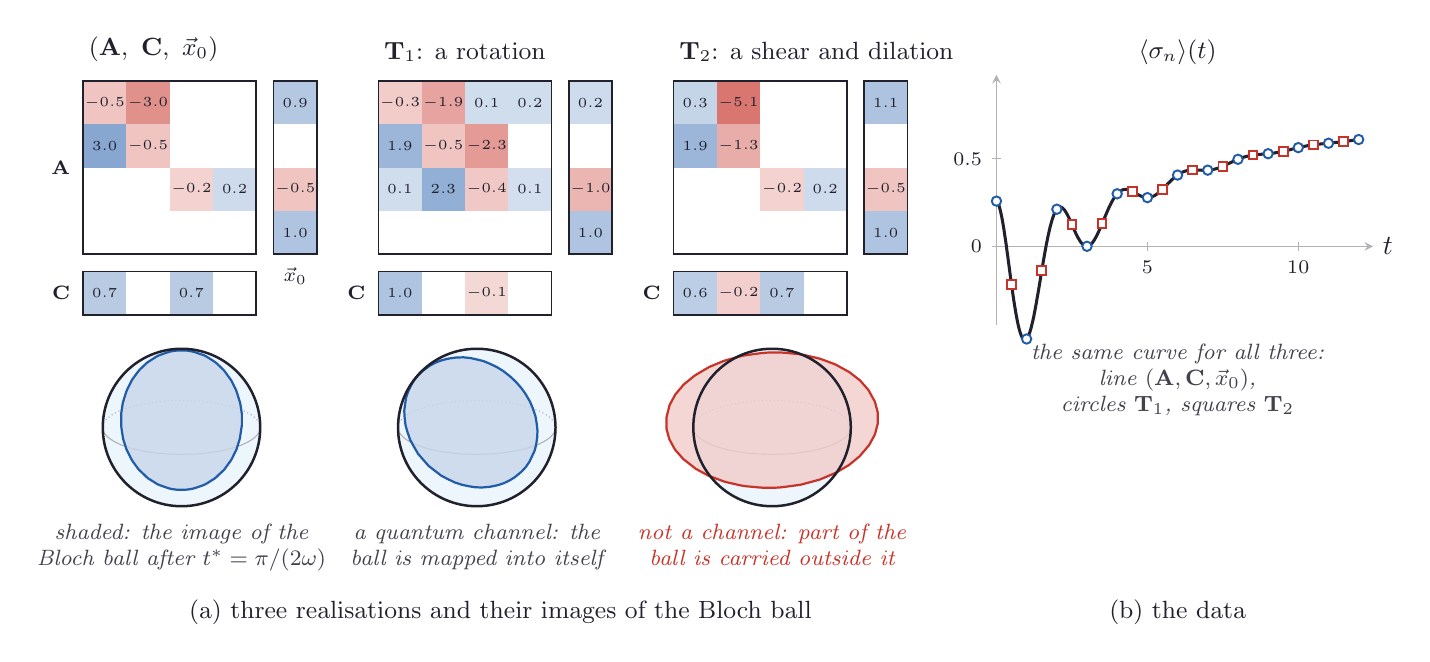
\begin{tikzpicture}[ink/.style={line width=0.9pt, ndInk}, faint/.style={line width=0.4pt, ndInk!35}, dashedink/.style={line width=0.5pt, ndInk!55, dash pattern=on 2.5pt off 2pt}, vec/.style={->, >=stealth, line width=1.2pt}, note/.style={font=\footnotesize\itshape, text=ndInk!85, align=center}, pointer/.style={->, >=stealth, line width=0.4pt, ndInk!60, shorten >=2pt, shorten <=1pt}, dot/.style={circle, fill=ndInk, inner sep=0pt, minimum size=3.4pt}, wash/.style={fill=ndSky, fill opacity=0.55}, every node/.style={text=ndInk}]
\definecolor{ndInk}{rgb}{0.13,0.13,0.18}
\definecolor{ndPaper}{rgb}{0.99,0.96,0.88}
\definecolor{ndSky}{rgb}{0.84,0.91,0.98}
\definecolor{ndRose}{rgb}{0.98,0.86,0.84}
\definecolor{ndBlue}{rgb}{0.13,0.36,0.66}
\definecolor{ndRed}{rgb}{0.78,0.20,0.16}
\definecolor{ndGold}{rgb}{0.88,0.62,0.10}
\definecolor{ndGreen}{rgb}{0.18,0.52,0.30}
\node[font=\small, anchor=south west] at (-0.050,3.520) {$(\mathbf A,\ \mathbf C,\ \vec x_0)$};
\fill[ndRed!29] (0.000,3.400) rectangle (0.550,2.850);
\node[font=\fontsize{5.5}{5.5}\selectfont, text=ndInk] at (0.275,3.125) {${-}0.5$};
\fill[ndRed!54] (0.550,3.400) rectangle (1.100,2.850);
\node[font=\fontsize{5.5}{5.5}\selectfont, text=ndInk] at (0.825,3.125) {${-}3.0$};
\fill[ndBlue!54] (0.000,2.850) rectangle (0.550,2.300);
\node[font=\fontsize{5.5}{5.5}\selectfont, text=ndInk] at (0.275,2.575) {$3.0$};
\fill[ndRed!29] (0.550,2.850) rectangle (1.100,2.300);
\node[font=\fontsize{5.5}{5.5}\selectfont, text=ndInk] at (0.825,2.575) {${-}0.5$};
\fill[ndRed!22] (1.100,2.300) rectangle (1.650,1.750);
\node[font=\fontsize{5.5}{5.5}\selectfont, text=ndInk] at (1.375,2.025) {${-}0.2$};
\fill[ndBlue!22] (1.650,2.300) rectangle (2.200,1.750);
\node[font=\fontsize{5.5}{5.5}\selectfont, text=ndInk] at (1.925,2.025) {$0.2$};
\draw[ink, line width=0.6pt] (0.000,3.400) rectangle (2.200,1.200);
\fill[ndBlue!34] (2.420,3.400) rectangle (2.970,2.850);
\node[font=\fontsize{5.5}{5.5}\selectfont, text=ndInk] at (2.695,3.125) {$0.9$};
\fill[ndRed!29] (2.420,2.300) rectangle (2.970,1.750);
\node[font=\fontsize{5.5}{5.5}\selectfont, text=ndInk] at (2.695,2.025) {${-}0.5$};
\fill[ndBlue!36] (2.420,1.750) rectangle (2.970,1.200);
\node[font=\fontsize{5.5}{5.5}\selectfont, text=ndInk] at (2.695,1.475) {$1.0$};
\draw[ink, line width=0.6pt] (2.420,3.400) rectangle (2.970,1.200);
\fill[ndBlue!32] (0.000,0.980) rectangle (0.550,0.430);
\node[font=\fontsize{5.5}{5.5}\selectfont, text=ndInk] at (0.275,0.705) {$0.7$};
\fill[ndBlue!32] (1.100,0.980) rectangle (1.650,0.430);
\node[font=\fontsize{5.5}{5.5}\selectfont, text=ndInk] at (1.375,0.705) {$0.7$};
\draw[ink, line width=0.6pt] (0.000,0.980) rectangle (2.200,0.430);
\node[font=\scriptsize, anchor=east] at (-0.040,0.705) {$\mathbf C$};
\node[font=\scriptsize, anchor=east] at (-0.040,2.300) {$\mathbf A$};
\node[font=\scriptsize, anchor=north] at (2.695,1.150) {$\vec x_0$};
\fill[ndSky!45] (1.250,-1.000) circle (1.000);
\draw[faint] (1.076,-1.337) -- (1.102,-1.338) -- (1.128,-1.339) -- (1.154,-1.340) -- (1.180,-1.341) -- (1.206,-1.342) -- (1.233,-1.342) -- (1.259,-1.342) -- (1.285,-1.342) -- (1.311,-1.341) -- (1.337,-1.341) -- (1.363,-1.340) -- (1.389,-1.339) -- (1.415,-1.337) -- (1.441,-1.336) -- (1.466,-1.334) -- (1.492,-1.332) -- (1.517,-1.330) -- (1.542,-1.327) -- (1.567,-1.324) -- (1.592,-1.321) -- (1.617,-1.318) -- (1.641,-1.315) -- (1.665,-1.311) -- (1.688,-1.307) -- (1.712,-1.303) -- (1.735,-1.299) -- (1.758,-1.295) -- (1.780,-1.290) -- (1.802,-1.285) -- (1.824,-1.280) -- (1.845,-1.275) -- (1.866,-1.270) -- (1.886,-1.264) -- (1.906,-1.258) -- (1.926,-1.252) -- (1.945,-1.246) -- (1.963,-1.240) -- (1.981,-1.233) -- (1.999,-1.227) -- (2.016,-1.220) -- (2.033,-1.213) -- (2.049,-1.206) -- (2.064,-1.199) -- (2.079,-1.191) -- (2.093,-1.184) -- (2.107,-1.176) -- (2.120,-1.168) -- (2.133,-1.161) -- (2.145,-1.153) -- (2.156,-1.145) -- (2.167,-1.136) -- (2.177,-1.128) -- (2.187,-1.120) -- (2.196,-1.111) -- (2.204,-1.103) -- (2.211,-1.094) -- (2.218,-1.086) -- (2.224,-1.077) -- (2.230,-1.068) -- (2.235,-1.059) -- (2.239,-1.051) -- (2.243,-1.042) -- (2.245,-1.033) -- (2.248,-1.024) -- (2.249,-1.015) -- (2.250,-1.006);
\draw[faint] (0.250,-1.003) -- (0.251,-1.012) -- (0.252,-1.021) -- (0.254,-1.030) -- (0.256,-1.039) -- (0.260,-1.048) -- (0.264,-1.056) -- (0.268,-1.065) -- (0.274,-1.074) -- (0.280,-1.083) -- (0.286,-1.091) -- (0.294,-1.100) -- (0.302,-1.109) -- (0.310,-1.117) -- (0.320,-1.125) -- (0.329,-1.134) -- (0.340,-1.142) -- (0.351,-1.150) -- (0.363,-1.158) -- (0.375,-1.166) -- (0.388,-1.174) -- (0.402,-1.181) -- (0.416,-1.189) -- (0.431,-1.196) -- (0.446,-1.203) -- (0.462,-1.211) -- (0.478,-1.218) -- (0.495,-1.224) -- (0.513,-1.231) -- (0.531,-1.238) -- (0.549,-1.244) -- (0.568,-1.250) -- (0.587,-1.256) -- (0.607,-1.262) -- (0.627,-1.268) -- (0.648,-1.273) -- (0.669,-1.278) -- (0.691,-1.284) -- (0.713,-1.288) -- (0.735,-1.293) -- (0.758,-1.298) -- (0.781,-1.302) -- (0.804,-1.306) -- (0.827,-1.310) -- (0.851,-1.314) -- (0.875,-1.317) -- (0.900,-1.320) -- (0.924,-1.323) -- (0.949,-1.326) -- (0.974,-1.329) -- (1.000,-1.331) -- (1.025,-1.333) -- (1.051,-1.335) -- (1.076,-1.337);
\draw[faint, densely dotted] (2.250,-0.997) -- (2.249,-0.988) -- (2.248,-0.979) -- (2.246,-0.970) -- (2.244,-0.961) -- (2.240,-0.952) -- (2.236,-0.944) -- (2.232,-0.935) -- (2.226,-0.926) -- (2.220,-0.917) -- (2.214,-0.909) -- (2.206,-0.900) -- (2.198,-0.891) -- (2.190,-0.883) -- (2.180,-0.875) -- (2.171,-0.866) -- (2.160,-0.858) -- (2.149,-0.850) -- (2.137,-0.842) -- (2.125,-0.834) -- (2.112,-0.826) -- (2.098,-0.819) -- (2.084,-0.811) -- (2.069,-0.804) -- (2.054,-0.797) -- (2.038,-0.789) -- (2.022,-0.782) -- (2.005,-0.776) -- (1.987,-0.769) -- (1.969,-0.762) -- (1.951,-0.756) -- (1.932,-0.750) -- (1.913,-0.744) -- (1.893,-0.738) -- (1.873,-0.732) -- (1.852,-0.727) -- (1.831,-0.722) -- (1.809,-0.716) -- (1.787,-0.712) -- (1.765,-0.707) -- (1.742,-0.702) -- (1.719,-0.698) -- (1.696,-0.694) -- (1.673,-0.690) -- (1.649,-0.686) -- (1.625,-0.683) -- (1.600,-0.680) -- (1.576,-0.677) -- (1.551,-0.674) -- (1.526,-0.671) -- (1.500,-0.669) -- (1.475,-0.667) -- (1.449,-0.665) -- (1.424,-0.663) -- (1.398,-0.662) -- (1.372,-0.661) -- (1.346,-0.660) -- (1.320,-0.659) -- (1.294,-0.658) -- (1.267,-0.658) -- (1.241,-0.658) -- (1.215,-0.658) -- (1.189,-0.659) -- (1.163,-0.659) -- (1.137,-0.660) -- (1.111,-0.661) -- (1.085,-0.663) -- (1.059,-0.664) -- (1.034,-0.666) -- (1.008,-0.668) -- (0.983,-0.670) -- (0.958,-0.673) -- (0.933,-0.676) -- (0.908,-0.679) -- (0.883,-0.682) -- (0.859,-0.685) -- (0.835,-0.689) -- (0.812,-0.693) -- (0.788,-0.697) -- (0.765,-0.701) -- (0.742,-0.705) -- (0.720,-0.710) -- (0.698,-0.715) -- (0.676,-0.720) -- (0.655,-0.725) -- (0.634,-0.730) -- (0.614,-0.736) -- (0.594,-0.742) -- (0.574,-0.748) -- (0.555,-0.754) -- (0.537,-0.760) -- (0.519,-0.767) -- (0.501,-0.773) -- (0.484,-0.780) -- (0.467,-0.787) -- (0.451,-0.794) -- (0.436,-0.801) -- (0.421,-0.809) -- (0.407,-0.816) -- (0.393,-0.824) -- (0.380,-0.832) -- (0.367,-0.839) -- (0.355,-0.847) -- (0.344,-0.855) -- (0.333,-0.864) -- (0.323,-0.872) -- (0.313,-0.880) -- (0.304,-0.889) -- (0.296,-0.897) -- (0.289,-0.906) -- (0.282,-0.914) -- (0.276,-0.923) -- (0.270,-0.932) -- (0.265,-0.941) -- (0.261,-0.949) -- (0.257,-0.958) -- (0.255,-0.967) -- (0.252,-0.976) -- (0.251,-0.985) -- (0.250,-0.994);
\filldraw[ndBlue, line width=0.8pt, fill=ndBlue!25, fill opacity=0.8] (0.484,-0.823) -- (0.484,-0.962) -- (0.487,-1.005) -- (0.508,-1.142) -- (0.549,-1.272) -- (0.609,-1.393) -- (0.629,-1.428) -- (0.704,-1.531) -- (0.794,-1.617) -- (0.820,-1.642) -- (0.917,-1.703) -- (0.946,-1.721) -- (0.982,-1.736) -- (1.067,-1.765) -- (1.097,-1.775) -- (1.131,-1.782) -- (1.168,-1.788) -- (1.207,-1.791) -- (1.247,-1.792) -- (1.287,-1.792) -- (1.326,-1.788) -- (1.363,-1.783) -- (1.397,-1.776) -- (1.428,-1.767) -- (1.511,-1.739) -- (1.549,-1.723) -- (1.579,-1.706) -- (1.674,-1.646) -- (1.702,-1.621) -- (1.792,-1.536) -- (1.866,-1.434) -- (1.889,-1.399) -- (1.948,-1.279) -- (1.989,-1.148) -- (1.996,-1.107) -- (2.017,-0.969) -- (2.017,-0.830) -- (1.996,-0.692) -- (1.955,-0.560) -- (1.942,-0.522) -- (1.883,-0.403) -- (1.806,-0.297) -- (1.782,-0.267) -- (1.694,-0.183) -- (1.663,-0.160) -- (1.570,-0.101) -- (1.537,-0.084) -- (1.497,-0.070) -- (1.418,-0.043) -- (1.386,-0.035) -- (1.351,-0.028) -- (1.313,-0.023) -- (1.273,-0.021) -- (1.233,-0.021) -- (1.193,-0.023) -- (1.155,-0.027) -- (1.119,-0.033) -- (1.087,-0.041) -- (1.011,-0.067) -- (0.969,-0.082) -- (0.935,-0.098) -- (0.844,-0.156) -- (0.810,-0.179) -- (0.723,-0.262) -- (0.697,-0.292) -- (0.620,-0.397) -- (0.561,-0.515) -- (0.546,-0.554) -- (0.505,-0.685) -- cycle;
\draw[ink] (1.250,-1.000) circle (1.000);
\node[font=\small, anchor=south west] at (3.700,3.520) {$\mathbf T_1$: a rotation};
\fill[ndRed!25] (3.750,3.400) rectangle (4.300,2.850);
\node[font=\fontsize{5.5}{5.5}\selectfont, text=ndInk] at (4.025,3.125) {${-}0.3$};
\fill[ndRed!45] (4.300,3.400) rectangle (4.850,2.850);
\node[font=\fontsize{5.5}{5.5}\selectfont, text=ndInk] at (4.575,3.125) {${-}1.9$};
\fill[ndBlue!21] (4.850,3.400) rectangle (5.400,2.850);
\node[font=\fontsize{5.5}{5.5}\selectfont, text=ndInk] at (5.125,3.125) {$0.1$};
\fill[ndBlue!21] (5.400,3.400) rectangle (5.950,2.850);
\node[font=\fontsize{5.5}{5.5}\selectfont, text=ndInk] at (5.675,3.125) {$0.2$};
\fill[ndBlue!45] (3.750,2.850) rectangle (4.300,2.300);
\node[font=\fontsize{5.5}{5.5}\selectfont, text=ndInk] at (4.025,2.575) {$1.9$};
\fill[ndRed!29] (4.300,2.850) rectangle (4.850,2.300);
\node[font=\fontsize{5.5}{5.5}\selectfont, text=ndInk] at (4.575,2.575) {${-}0.5$};
\fill[ndRed!49] (4.850,2.850) rectangle (5.400,2.300);
\node[font=\fontsize{5.5}{5.5}\selectfont, text=ndInk] at (5.125,2.575) {${-}2.3$};
\fill[ndBlue!21] (3.750,2.300) rectangle (4.300,1.750);
\node[font=\fontsize{5.5}{5.5}\selectfont, text=ndInk] at (4.025,2.025) {$0.1$};
\fill[ndBlue!49] (4.300,2.300) rectangle (4.850,1.750);
\node[font=\fontsize{5.5}{5.5}\selectfont, text=ndInk] at (4.575,2.025) {$2.3$};
\fill[ndRed!27] (4.850,2.300) rectangle (5.400,1.750);
\node[font=\fontsize{5.5}{5.5}\selectfont, text=ndInk] at (5.125,2.025) {${-}0.4$};
\fill[ndBlue!20] (5.400,2.300) rectangle (5.950,1.750);
\node[font=\fontsize{5.5}{5.5}\selectfont, text=ndInk] at (5.675,2.025) {$0.1$};
\draw[ink, line width=0.6pt] (3.750,3.400) rectangle (5.950,1.200);
\fill[ndBlue!22] (6.170,3.400) rectangle (6.720,2.850);
\node[font=\fontsize{5.5}{5.5}\selectfont, text=ndInk] at (6.445,3.125) {$0.2$};
\fill[ndRed!36] (6.170,2.300) rectangle (6.720,1.750);
\node[font=\fontsize{5.5}{5.5}\selectfont, text=ndInk] at (6.445,2.025) {${-}1.0$};
\fill[ndBlue!36] (6.170,1.750) rectangle (6.720,1.200);
\node[font=\fontsize{5.5}{5.5}\selectfont, text=ndInk] at (6.445,1.475) {$1.0$};
\draw[ink, line width=0.6pt] (6.170,3.400) rectangle (6.720,1.200);
\fill[ndBlue!36] (3.750,0.980) rectangle (4.300,0.430);
\node[font=\fontsize{5.5}{5.5}\selectfont, text=ndInk] at (4.025,0.705) {$1.0$};
\fill[ndRed!19] (4.850,0.980) rectangle (5.400,0.430);
\node[font=\fontsize{5.5}{5.5}\selectfont, text=ndInk] at (5.125,0.705) {${-}0.1$};
\draw[ink, line width=0.6pt] (3.750,0.980) rectangle (5.950,0.430);
\node[font=\scriptsize, anchor=east] at (3.710,0.705) {$\mathbf C$};
\fill[ndSky!45] (5.000,-1.000) circle (1.000);
\draw[faint] (4.826,-1.337) -- (4.852,-1.338) -- (4.878,-1.339) -- (4.904,-1.340) -- (4.930,-1.341) -- (4.956,-1.342) -- (4.983,-1.342) -- (5.009,-1.342) -- (5.035,-1.342) -- (5.061,-1.341) -- (5.087,-1.341) -- (5.113,-1.340) -- (5.139,-1.339) -- (5.165,-1.337) -- (5.191,-1.336) -- (5.216,-1.334) -- (5.242,-1.332) -- (5.267,-1.330) -- (5.292,-1.327) -- (5.317,-1.324) -- (5.342,-1.321) -- (5.367,-1.318) -- (5.391,-1.315) -- (5.415,-1.311) -- (5.438,-1.307) -- (5.462,-1.303) -- (5.485,-1.299) -- (5.508,-1.295) -- (5.530,-1.290) -- (5.552,-1.285) -- (5.574,-1.280) -- (5.595,-1.275) -- (5.616,-1.270) -- (5.636,-1.264) -- (5.656,-1.258) -- (5.676,-1.252) -- (5.695,-1.246) -- (5.713,-1.240) -- (5.731,-1.233) -- (5.749,-1.227) -- (5.766,-1.220) -- (5.783,-1.213) -- (5.799,-1.206) -- (5.814,-1.199) -- (5.829,-1.191) -- (5.843,-1.184) -- (5.857,-1.176) -- (5.870,-1.168) -- (5.883,-1.161) -- (5.895,-1.153) -- (5.906,-1.145) -- (5.917,-1.136) -- (5.927,-1.128) -- (5.937,-1.120) -- (5.946,-1.111) -- (5.954,-1.103) -- (5.961,-1.094) -- (5.968,-1.086) -- (5.974,-1.077) -- (5.980,-1.068) -- (5.985,-1.059) -- (5.989,-1.051) -- (5.993,-1.042) -- (5.995,-1.033) -- (5.998,-1.024) -- (5.999,-1.015) -- (6.000,-1.006);
\draw[faint] (4.000,-1.003) -- (4.001,-1.012) -- (4.002,-1.021) -- (4.004,-1.030) -- (4.006,-1.039) -- (4.010,-1.048) -- (4.014,-1.056) -- (4.018,-1.065) -- (4.024,-1.074) -- (4.030,-1.083) -- (4.036,-1.091) -- (4.044,-1.100) -- (4.052,-1.109) -- (4.060,-1.117) -- (4.070,-1.125) -- (4.079,-1.134) -- (4.090,-1.142) -- (4.101,-1.150) -- (4.113,-1.158) -- (4.125,-1.166) -- (4.138,-1.174) -- (4.152,-1.181) -- (4.166,-1.189) -- (4.181,-1.196) -- (4.196,-1.203) -- (4.212,-1.211) -- (4.228,-1.218) -- (4.245,-1.224) -- (4.263,-1.231) -- (4.281,-1.238) -- (4.299,-1.244) -- (4.318,-1.250) -- (4.337,-1.256) -- (4.357,-1.262) -- (4.377,-1.268) -- (4.398,-1.273) -- (4.419,-1.278) -- (4.441,-1.284) -- (4.463,-1.288) -- (4.485,-1.293) -- (4.508,-1.298) -- (4.531,-1.302) -- (4.554,-1.306) -- (4.577,-1.310) -- (4.601,-1.314) -- (4.625,-1.317) -- (4.650,-1.320) -- (4.674,-1.323) -- (4.699,-1.326) -- (4.724,-1.329) -- (4.750,-1.331) -- (4.775,-1.333) -- (4.801,-1.335) -- (4.826,-1.337);
\draw[faint, densely dotted] (6.000,-0.997) -- (5.999,-0.988) -- (5.998,-0.979) -- (5.996,-0.970) -- (5.994,-0.961) -- (5.990,-0.952) -- (5.986,-0.944) -- (5.982,-0.935) -- (5.976,-0.926) -- (5.970,-0.917) -- (5.964,-0.909) -- (5.956,-0.900) -- (5.948,-0.891) -- (5.940,-0.883) -- (5.930,-0.875) -- (5.921,-0.866) -- (5.910,-0.858) -- (5.899,-0.850) -- (5.887,-0.842) -- (5.875,-0.834) -- (5.862,-0.826) -- (5.848,-0.819) -- (5.834,-0.811) -- (5.819,-0.804) -- (5.804,-0.797) -- (5.788,-0.789) -- (5.772,-0.782) -- (5.755,-0.776) -- (5.737,-0.769) -- (5.719,-0.762) -- (5.701,-0.756) -- (5.682,-0.750) -- (5.663,-0.744) -- (5.643,-0.738) -- (5.623,-0.732) -- (5.602,-0.727) -- (5.581,-0.722) -- (5.559,-0.716) -- (5.537,-0.712) -- (5.515,-0.707) -- (5.492,-0.702) -- (5.469,-0.698) -- (5.446,-0.694) -- (5.423,-0.690) -- (5.399,-0.686) -- (5.375,-0.683) -- (5.350,-0.680) -- (5.326,-0.677) -- (5.301,-0.674) -- (5.276,-0.671) -- (5.250,-0.669) -- (5.225,-0.667) -- (5.199,-0.665) -- (5.174,-0.663) -- (5.148,-0.662) -- (5.122,-0.661) -- (5.096,-0.660) -- (5.070,-0.659) -- (5.044,-0.658) -- (5.017,-0.658) -- (4.991,-0.658) -- (4.965,-0.658) -- (4.939,-0.659) -- (4.913,-0.659) -- (4.887,-0.660) -- (4.861,-0.661) -- (4.835,-0.663) -- (4.809,-0.664) -- (4.784,-0.666) -- (4.758,-0.668) -- (4.733,-0.670) -- (4.708,-0.673) -- (4.683,-0.676) -- (4.658,-0.679) -- (4.633,-0.682) -- (4.609,-0.685) -- (4.585,-0.689) -- (4.562,-0.693) -- (4.538,-0.697) -- (4.515,-0.701) -- (4.492,-0.705) -- (4.470,-0.710) -- (4.448,-0.715) -- (4.426,-0.720) -- (4.405,-0.725) -- (4.384,-0.730) -- (4.364,-0.736) -- (4.344,-0.742) -- (4.324,-0.748) -- (4.305,-0.754) -- (4.287,-0.760) -- (4.269,-0.767) -- (4.251,-0.773) -- (4.234,-0.780) -- (4.217,-0.787) -- (4.201,-0.794) -- (4.186,-0.801) -- (4.171,-0.809) -- (4.157,-0.816) -- (4.143,-0.824) -- (4.130,-0.832) -- (4.117,-0.839) -- (4.105,-0.847) -- (4.094,-0.855) -- (4.083,-0.864) -- (4.073,-0.872) -- (4.063,-0.880) -- (4.054,-0.889) -- (4.046,-0.897) -- (4.039,-0.906) -- (4.032,-0.914) -- (4.026,-0.923) -- (4.020,-0.932) -- (4.015,-0.941) -- (4.011,-0.949) -- (4.007,-0.958) -- (4.005,-0.967) -- (4.002,-0.976) -- (4.001,-0.985) -- (4.000,-0.994);
\filldraw[ndBlue, line width=0.8pt, fill=ndBlue!25, fill opacity=0.8] (5.735,-1.294) -- (5.755,-1.214) -- (5.767,-1.127) -- (5.771,-1.041) -- (5.760,-0.943) -- (5.745,-0.855) -- (5.711,-0.755) -- (5.675,-0.670) -- (5.620,-0.575) -- (5.566,-0.499) -- (5.493,-0.416) -- (5.423,-0.351) -- (5.339,-0.285) -- (5.259,-0.235) -- (5.170,-0.192) -- (5.086,-0.157) -- (4.993,-0.134) -- (4.919,-0.118) -- (4.831,-0.109) -- (4.740,-0.111) -- (4.648,-0.124) -- (4.619,-0.130) -- (4.543,-0.150) -- (4.470,-0.179) -- (4.403,-0.216) -- (4.342,-0.260) -- (4.316,-0.280) -- (4.252,-0.339) -- (4.201,-0.404) -- (4.162,-0.472) -- (4.131,-0.537) -- (4.103,-0.617) -- (4.091,-0.697) -- (4.079,-0.787) -- (4.084,-0.873) -- (4.095,-0.972) -- (4.120,-1.058) -- (4.155,-1.159) -- (4.200,-1.240) -- (4.255,-1.335) -- (4.328,-1.419) -- (4.390,-1.489) -- (4.476,-1.556) -- (4.549,-1.612) -- (4.636,-1.657) -- (4.721,-1.698) -- (4.810,-1.727) -- (4.889,-1.744) -- (4.974,-1.759) -- (5.064,-1.762) -- (5.156,-1.755) -- (5.193,-1.748) -- (5.269,-1.732) -- (5.344,-1.707) -- (5.414,-1.674) -- (5.479,-1.634) -- (5.499,-1.618) -- (5.567,-1.562) -- (5.625,-1.500) -- (5.670,-1.433) -- (5.698,-1.373) -- cycle;
\draw[ink] (5.000,-1.000) circle (1.000);
\node[font=\small, anchor=south west] at (7.450,3.520) {$\mathbf T_2$: a shear and dilation};
\fill[ndBlue!26] (7.500,3.400) rectangle (8.050,2.850);
\node[font=\fontsize{5.5}{5.5}\selectfont, text=ndInk] at (7.775,3.125) {$0.3$};
\fill[ndRed!67] (8.050,3.400) rectangle (8.600,2.850);
\node[font=\fontsize{5.5}{5.5}\selectfont, text=ndInk] at (8.325,3.125) {${-}5.1$};
\fill[ndBlue!45] (7.500,2.850) rectangle (8.050,2.300);
\node[font=\fontsize{5.5}{5.5}\selectfont, text=ndInk] at (7.775,2.575) {$1.9$};
\fill[ndRed!40] (8.050,2.850) rectangle (8.600,2.300);
\node[font=\fontsize{5.5}{5.5}\selectfont, text=ndInk] at (8.325,2.575) {${-}1.3$};
\fill[ndRed!22] (8.600,2.300) rectangle (9.150,1.750);
\node[font=\fontsize{5.5}{5.5}\selectfont, text=ndInk] at (8.875,2.025) {${-}0.2$};
\fill[ndBlue!22] (9.150,2.300) rectangle (9.700,1.750);
\node[font=\fontsize{5.5}{5.5}\selectfont, text=ndInk] at (9.425,2.025) {$0.2$};
\draw[ink, line width=0.6pt] (7.500,3.400) rectangle (9.700,1.200);
\fill[ndBlue!37] (9.920,3.400) rectangle (10.470,2.850);
\node[font=\fontsize{5.5}{5.5}\selectfont, text=ndInk] at (10.195,3.125) {$1.1$};
\fill[ndRed!29] (9.920,2.300) rectangle (10.470,1.750);
\node[font=\fontsize{5.5}{5.5}\selectfont, text=ndInk] at (10.195,2.025) {${-}0.5$};
\fill[ndBlue!36] (9.920,1.750) rectangle (10.470,1.200);
\node[font=\fontsize{5.5}{5.5}\selectfont, text=ndInk] at (10.195,1.475) {$1.0$};
\draw[ink, line width=0.6pt] (9.920,3.400) rectangle (10.470,1.200);
\fill[ndBlue!30] (7.500,0.980) rectangle (8.050,0.430);
\node[font=\fontsize{5.5}{5.5}\selectfont, text=ndInk] at (7.775,0.705) {$0.6$};
\fill[ndRed!24] (8.050,0.980) rectangle (8.600,0.430);
\node[font=\fontsize{5.5}{5.5}\selectfont, text=ndInk] at (8.325,0.705) {${-}0.2$};
\fill[ndBlue!32] (8.600,0.980) rectangle (9.150,0.430);
\node[font=\fontsize{5.5}{5.5}\selectfont, text=ndInk] at (8.875,0.705) {$0.7$};
\draw[ink, line width=0.6pt] (7.500,0.980) rectangle (9.700,0.430);
\node[font=\scriptsize, anchor=east] at (7.460,0.705) {$\mathbf C$};
\fill[ndSky!45] (8.750,-1.000) circle (1.000);
\draw[faint] (8.576,-1.337) -- (8.602,-1.338) -- (8.628,-1.339) -- (8.654,-1.340) -- (8.680,-1.341) -- (8.706,-1.342) -- (8.733,-1.342) -- (8.759,-1.342) -- (8.785,-1.342) -- (8.811,-1.341) -- (8.837,-1.341) -- (8.863,-1.340) -- (8.889,-1.339) -- (8.915,-1.337) -- (8.941,-1.336) -- (8.966,-1.334) -- (8.992,-1.332) -- (9.017,-1.330) -- (9.042,-1.327) -- (9.067,-1.324) -- (9.092,-1.321) -- (9.117,-1.318) -- (9.141,-1.315) -- (9.165,-1.311) -- (9.188,-1.307) -- (9.212,-1.303) -- (9.235,-1.299) -- (9.258,-1.295) -- (9.280,-1.290) -- (9.302,-1.285) -- (9.324,-1.280) -- (9.345,-1.275) -- (9.366,-1.270) -- (9.386,-1.264) -- (9.406,-1.258) -- (9.426,-1.252) -- (9.445,-1.246) -- (9.463,-1.240) -- (9.481,-1.233) -- (9.499,-1.227) -- (9.516,-1.220) -- (9.533,-1.213) -- (9.549,-1.206) -- (9.564,-1.199) -- (9.579,-1.191) -- (9.593,-1.184) -- (9.607,-1.176) -- (9.620,-1.168) -- (9.633,-1.161) -- (9.645,-1.153) -- (9.656,-1.145) -- (9.667,-1.136) -- (9.677,-1.128) -- (9.687,-1.120) -- (9.696,-1.111) -- (9.704,-1.103) -- (9.711,-1.094) -- (9.718,-1.086) -- (9.724,-1.077) -- (9.730,-1.068) -- (9.735,-1.059) -- (9.739,-1.051) -- (9.743,-1.042) -- (9.745,-1.033) -- (9.748,-1.024) -- (9.749,-1.015) -- (9.750,-1.006);
\draw[faint] (7.750,-1.003) -- (7.751,-1.012) -- (7.752,-1.021) -- (7.754,-1.030) -- (7.756,-1.039) -- (7.760,-1.048) -- (7.764,-1.056) -- (7.768,-1.065) -- (7.774,-1.074) -- (7.780,-1.083) -- (7.786,-1.091) -- (7.794,-1.100) -- (7.802,-1.109) -- (7.810,-1.117) -- (7.820,-1.125) -- (7.829,-1.134) -- (7.840,-1.142) -- (7.851,-1.150) -- (7.863,-1.158) -- (7.875,-1.166) -- (7.888,-1.174) -- (7.902,-1.181) -- (7.916,-1.189) -- (7.931,-1.196) -- (7.946,-1.203) -- (7.962,-1.211) -- (7.978,-1.218) -- (7.995,-1.224) -- (8.013,-1.231) -- (8.031,-1.238) -- (8.049,-1.244) -- (8.068,-1.250) -- (8.087,-1.256) -- (8.107,-1.262) -- (8.127,-1.268) -- (8.148,-1.273) -- (8.169,-1.278) -- (8.191,-1.284) -- (8.213,-1.288) -- (8.235,-1.293) -- (8.258,-1.298) -- (8.281,-1.302) -- (8.304,-1.306) -- (8.327,-1.310) -- (8.351,-1.314) -- (8.375,-1.317) -- (8.400,-1.320) -- (8.424,-1.323) -- (8.449,-1.326) -- (8.474,-1.329) -- (8.500,-1.331) -- (8.525,-1.333) -- (8.551,-1.335) -- (8.576,-1.337);
\draw[faint, densely dotted] (9.750,-0.997) -- (9.749,-0.988) -- (9.748,-0.979) -- (9.746,-0.970) -- (9.744,-0.961) -- (9.740,-0.952) -- (9.736,-0.944) -- (9.732,-0.935) -- (9.726,-0.926) -- (9.720,-0.917) -- (9.714,-0.909) -- (9.706,-0.900) -- (9.698,-0.891) -- (9.690,-0.883) -- (9.680,-0.875) -- (9.671,-0.866) -- (9.660,-0.858) -- (9.649,-0.850) -- (9.637,-0.842) -- (9.625,-0.834) -- (9.612,-0.826) -- (9.598,-0.819) -- (9.584,-0.811) -- (9.569,-0.804) -- (9.554,-0.797) -- (9.538,-0.789) -- (9.522,-0.782) -- (9.505,-0.776) -- (9.487,-0.769) -- (9.469,-0.762) -- (9.451,-0.756) -- (9.432,-0.750) -- (9.413,-0.744) -- (9.393,-0.738) -- (9.373,-0.732) -- (9.352,-0.727) -- (9.331,-0.722) -- (9.309,-0.716) -- (9.287,-0.712) -- (9.265,-0.707) -- (9.242,-0.702) -- (9.219,-0.698) -- (9.196,-0.694) -- (9.173,-0.690) -- (9.149,-0.686) -- (9.125,-0.683) -- (9.100,-0.680) -- (9.076,-0.677) -- (9.051,-0.674) -- (9.026,-0.671) -- (9.000,-0.669) -- (8.975,-0.667) -- (8.949,-0.665) -- (8.924,-0.663) -- (8.898,-0.662) -- (8.872,-0.661) -- (8.846,-0.660) -- (8.820,-0.659) -- (8.794,-0.658) -- (8.767,-0.658) -- (8.741,-0.658) -- (8.715,-0.658) -- (8.689,-0.659) -- (8.663,-0.659) -- (8.637,-0.660) -- (8.611,-0.661) -- (8.585,-0.663) -- (8.559,-0.664) -- (8.534,-0.666) -- (8.508,-0.668) -- (8.483,-0.670) -- (8.458,-0.673) -- (8.433,-0.676) -- (8.408,-0.679) -- (8.383,-0.682) -- (8.359,-0.685) -- (8.335,-0.689) -- (8.312,-0.693) -- (8.288,-0.697) -- (8.265,-0.701) -- (8.242,-0.705) -- (8.220,-0.710) -- (8.198,-0.715) -- (8.176,-0.720) -- (8.155,-0.725) -- (8.134,-0.730) -- (8.114,-0.736) -- (8.094,-0.742) -- (8.074,-0.748) -- (8.055,-0.754) -- (8.037,-0.760) -- (8.019,-0.767) -- (8.001,-0.773) -- (7.984,-0.780) -- (7.967,-0.787) -- (7.951,-0.794) -- (7.936,-0.801) -- (7.921,-0.809) -- (7.907,-0.816) -- (7.893,-0.824) -- (7.880,-0.832) -- (7.867,-0.839) -- (7.855,-0.847) -- (7.844,-0.855) -- (7.833,-0.864) -- (7.823,-0.872) -- (7.813,-0.880) -- (7.804,-0.889) -- (7.796,-0.897) -- (7.789,-0.906) -- (7.782,-0.914) -- (7.776,-0.923) -- (7.770,-0.932) -- (7.765,-0.941) -- (7.761,-0.949) -- (7.757,-0.958) -- (7.755,-0.967) -- (7.752,-0.976) -- (7.751,-0.985) -- (7.750,-0.994);
\filldraw[ndRed, line width=0.8pt, fill=ndRed!25, fill opacity=0.8] (7.446,-1.151) -- (7.518,-1.282) -- (7.624,-1.402) -- (7.760,-1.508) -- (7.782,-1.525) -- (7.942,-1.612) -- (8.124,-1.680) -- (8.155,-1.691) -- (8.344,-1.734) -- (8.375,-1.740) -- (8.416,-1.746) -- (8.581,-1.761) -- (8.606,-1.763) -- (8.635,-1.765) -- (8.667,-1.766) -- (8.701,-1.766) -- (8.736,-1.766) -- (8.772,-1.765) -- (8.807,-1.764) -- (8.841,-1.762) -- (8.872,-1.759) -- (8.900,-1.756) -- (9.046,-1.736) -- (9.094,-1.730) -- (9.133,-1.722) -- (9.162,-1.714) -- (9.354,-1.662) -- (9.530,-1.588) -- (9.564,-1.573) -- (9.725,-1.478) -- (9.860,-1.368) -- (9.878,-1.347) -- (9.984,-1.222) -- (10.056,-1.089) -- (10.093,-0.950) -- (10.093,-0.810) -- (10.056,-0.673) -- (10.044,-0.650) -- (9.972,-0.521) -- (9.867,-0.402) -- (9.732,-0.297) -- (9.570,-0.208) -- (9.541,-0.194) -- (9.363,-0.128) -- (9.324,-0.118) -- (9.142,-0.076) -- (9.105,-0.070) -- (9.060,-0.065) -- (8.907,-0.051) -- (8.880,-0.049) -- (8.849,-0.048) -- (8.816,-0.047) -- (8.781,-0.047) -- (8.746,-0.047) -- (8.710,-0.048) -- (8.676,-0.050) -- (8.643,-0.053) -- (8.613,-0.055) -- (8.587,-0.059) -- (8.429,-0.080) -- (8.385,-0.087) -- (8.351,-0.095) -- (8.165,-0.146) -- (8.131,-0.157) -- (7.951,-0.232) -- (7.792,-0.326) -- (7.763,-0.344) -- (7.627,-0.455) -- (7.522,-0.580) -- (7.450,-0.712) -- (7.414,-0.851) -- (7.409,-0.875) -- (7.409,-1.015) -- cycle;
\draw[ink] (8.750,-1.000) circle (1.000);
\node[note, anchor=north] at (1.250,-2.100) {shaded: the image of the\\ Bloch ball after $t^*=\pi/(2\omega)$};
\node[note, anchor=north] at (5.000,-2.100) {a quantum channel: the\\ ball is mapped into itself};
\node[note, anchor=north, text=ndRed] at (8.750,-2.100) {not a channel: part of the\\ ball is carried outside it};
\draw[faint, ->, >=stealth] (11.600,1.300) -- (16.384,1.300) node[right, text=ndInk] {$t$};
\draw[faint, ->, >=stealth] (11.600,0.300) -- (11.600,3.480) node[above, text=ndInk] {};
\draw[faint] (13.517,1.360) -- (13.517,1.240) node[below, font=\scriptsize, text=ndInk] {$5$};
\draw[faint] (15.433,1.360) -- (15.433,1.240) node[below, font=\scriptsize, text=ndInk] {$10$};
\draw[faint] (11.660,1.300) -- (11.540,1.300) node[left, font=\scriptsize, text=ndInk] {$0$};
\draw[faint] (11.660,2.411) -- (11.540,2.411) node[left, font=\scriptsize, text=ndInk] {$0.5$};
\draw[line width=1.1pt, ndInk] (11.600,1.875) -- (11.610,1.866) -- (11.619,1.850) -- (11.629,1.827) -- (11.638,1.798) -- (11.648,1.762) -- (11.657,1.721) -- (11.667,1.674) -- (11.677,1.623) -- (11.686,1.567) -- (11.696,1.508) -- (11.705,1.445) -- (11.715,1.380) -- (11.725,1.312) -- (11.734,1.242) -- (11.744,1.171) -- (11.753,1.099) -- (11.763,1.027) -- (11.772,0.955) -- (11.782,0.884) -- (11.792,0.814) -- (11.801,0.745) -- (11.811,0.678) -- (11.820,0.614) -- (11.830,0.552) -- (11.840,0.493) -- (11.849,0.438) -- (11.859,0.386) -- (11.868,0.338) -- (11.878,0.294) -- (11.887,0.255) -- (11.897,0.220) -- (11.907,0.190) -- (11.916,0.165) -- (11.926,0.144) -- (11.935,0.129) -- (11.945,0.118) -- (11.955,0.112) -- (11.964,0.112) -- (11.974,0.116) -- (11.983,0.124) -- (11.993,0.138) -- (12.002,0.156) -- (12.012,0.178) -- (12.022,0.204) -- (12.031,0.235) -- (12.041,0.269) -- (12.050,0.307) -- (12.060,0.348) -- (12.070,0.391) -- (12.079,0.438) -- (12.089,0.487) -- (12.098,0.538) -- (12.108,0.591) -- (12.117,0.646) -- (12.127,0.702) -- (12.137,0.759) -- (12.146,0.816) -- (12.156,0.874) -- (12.165,0.932) -- (12.175,0.990) -- (12.185,1.047) -- (12.194,1.104) -- (12.204,1.159) -- (12.213,1.213) -- (12.223,1.266) -- (12.232,1.317) -- (12.242,1.366) -- (12.252,1.414) -- (12.261,1.458) -- (12.271,1.501) -- (12.280,1.541) -- (12.290,1.578) -- (12.300,1.613) -- (12.309,1.644) -- (12.319,1.673) -- (12.328,1.699) -- (12.338,1.722) -- (12.348,1.741) -- (12.357,1.758) -- (12.367,1.772) -- (12.376,1.783) -- (12.386,1.791) -- (12.395,1.796) -- (12.405,1.799) -- (12.415,1.799) -- (12.424,1.796) -- (12.434,1.791) -- (12.443,1.784) -- (12.453,1.774) -- (12.463,1.763) -- (12.472,1.750) -- (12.482,1.735) -- (12.491,1.719) -- (12.501,1.701) -- (12.510,1.682) -- (12.520,1.662) -- (12.530,1.642) -- (12.539,1.620) -- (12.549,1.599) -- (12.558,1.577) -- (12.568,1.555) -- (12.578,1.533) -- (12.587,1.511) -- (12.597,1.490) -- (12.606,1.469) -- (12.616,1.449) -- (12.625,1.430) -- (12.635,1.412) -- (12.645,1.395) -- (12.654,1.379) -- (12.664,1.364) -- (12.673,1.351) -- (12.683,1.339) -- (12.692,1.329) -- (12.702,1.320) -- (12.712,1.313) -- (12.721,1.307) -- (12.731,1.303) -- (12.740,1.301) -- (12.750,1.301) -- (12.760,1.303) -- (12.769,1.306) -- (12.779,1.310) -- (12.788,1.317) -- (12.798,1.325) -- (12.807,1.334) -- (12.817,1.345) -- (12.827,1.358) -- (12.836,1.372) -- (12.846,1.387) -- (12.855,1.403) -- (12.865,1.421) -- (12.875,1.439) -- (12.884,1.459) -- (12.894,1.479) -- (12.903,1.500) -- (12.913,1.521) -- (12.922,1.543) -- (12.932,1.566) -- (12.942,1.588) -- (12.951,1.611) -- (12.961,1.634) -- (12.970,1.657) -- (12.980,1.680) -- (12.990,1.703) -- (12.999,1.725) -- (13.009,1.748) -- (13.018,1.769) -- (13.028,1.790) -- (13.037,1.810) -- (13.047,1.830) -- (13.057,1.849) -- (13.066,1.867) -- (13.076,1.885) -- (13.085,1.901) -- (13.095,1.916) -- (13.105,1.931) -- (13.114,1.944) -- (13.124,1.956) -- (13.133,1.968) -- (13.143,1.978) -- (13.152,1.987) -- (13.162,1.995) -- (13.172,2.002) -- (13.181,2.008) -- (13.191,2.013) -- (13.200,2.017) -- (13.210,2.020) -- (13.220,2.022) -- (13.229,2.024) -- (13.239,2.024) -- (13.248,2.024) -- (13.258,2.023) -- (13.268,2.021) -- (13.277,2.018) -- (13.287,2.015) -- (13.296,2.012) -- (13.306,2.008) -- (13.315,2.003) -- (13.325,1.998) -- (13.335,1.993) -- (13.344,1.988) -- (13.354,1.983) -- (13.363,1.977) -- (13.373,1.972) -- (13.383,1.966) -- (13.392,1.961) -- (13.402,1.955) -- (13.411,1.950) -- (13.421,1.946) -- (13.430,1.941) -- (13.440,1.937) -- (13.450,1.933) -- (13.459,1.930) -- (13.469,1.927) -- (13.478,1.924) -- (13.488,1.922) -- (13.497,1.921) -- (13.507,1.920) -- (13.517,1.919) -- (13.526,1.920) -- (13.536,1.920) -- (13.545,1.922) -- (13.555,1.924) -- (13.565,1.926) -- (13.574,1.930) -- (13.584,1.933) -- (13.593,1.938) -- (13.603,1.943) -- (13.612,1.948) -- (13.622,1.954) -- (13.632,1.960) -- (13.641,1.967) -- (13.651,1.975) -- (13.660,1.982) -- (13.670,1.990) -- (13.680,1.999) -- (13.689,2.007) -- (13.699,2.016) -- (13.708,2.026) -- (13.718,2.035) -- (13.727,2.045) -- (13.737,2.054) -- (13.747,2.064) -- (13.756,2.074) -- (13.766,2.084) -- (13.775,2.094) -- (13.785,2.104) -- (13.795,2.113) -- (13.804,2.123) -- (13.814,2.132) -- (13.823,2.142) -- (13.833,2.151) -- (13.842,2.159) -- (13.852,2.168) -- (13.862,2.176) -- (13.871,2.184) -- (13.881,2.192) -- (13.890,2.199) -- (13.900,2.206) -- (13.910,2.213) -- (13.919,2.219) -- (13.929,2.225) -- (13.938,2.230) -- (13.948,2.236) -- (13.957,2.240) -- (13.967,2.245) -- (13.977,2.249) -- (13.986,2.252) -- (13.996,2.256) -- (14.005,2.258) -- (14.015,2.261) -- (14.025,2.263) -- (14.034,2.265) -- (14.044,2.267) -- (14.053,2.268) -- (14.063,2.269) -- (14.072,2.270) -- (14.082,2.271) -- (14.092,2.271) -- (14.101,2.271) -- (14.111,2.271) -- (14.120,2.271) -- (14.130,2.271) -- (14.140,2.271) -- (14.149,2.270) -- (14.159,2.270) -- (14.168,2.269) -- (14.178,2.269) -- (14.188,2.268) -- (14.197,2.268) -- (14.207,2.267) -- (14.216,2.267) -- (14.226,2.267) -- (14.235,2.267) -- (14.245,2.266) -- (14.255,2.267) -- (14.264,2.267) -- (14.274,2.267) -- (14.283,2.268) -- (14.293,2.268) -- (14.303,2.269) -- (14.312,2.270) -- (14.322,2.272) -- (14.331,2.273) -- (14.341,2.275) -- (14.350,2.276) -- (14.360,2.279) -- (14.370,2.281) -- (14.379,2.283) -- (14.389,2.286) -- (14.398,2.289) -- (14.408,2.292) -- (14.418,2.295) -- (14.427,2.298) -- (14.437,2.302) -- (14.446,2.306) -- (14.456,2.309) -- (14.465,2.313) -- (14.475,2.317) -- (14.485,2.322) -- (14.494,2.326) -- (14.504,2.330) -- (14.513,2.335) -- (14.523,2.339) -- (14.532,2.344) -- (14.542,2.349) -- (14.552,2.353) -- (14.561,2.358) -- (14.571,2.362) -- (14.580,2.367) -- (14.590,2.372) -- (14.600,2.376) -- (14.609,2.381) -- (14.619,2.385) -- (14.628,2.389) -- (14.638,2.394) -- (14.647,2.398) -- (14.657,2.402) -- (14.667,2.406) -- (14.676,2.410) -- (14.686,2.414) -- (14.695,2.417) -- (14.705,2.421) -- (14.715,2.424) -- (14.724,2.427) -- (14.734,2.431) -- (14.743,2.434) -- (14.753,2.436) -- (14.762,2.439) -- (14.772,2.442) -- (14.782,2.444) -- (14.791,2.446) -- (14.801,2.448) -- (14.810,2.451) -- (14.820,2.452) -- (14.830,2.454) -- (14.839,2.456) -- (14.849,2.457) -- (14.858,2.459) -- (14.868,2.460) -- (14.877,2.461) -- (14.887,2.463) -- (14.897,2.464) -- (14.906,2.465) -- (14.916,2.466) -- (14.925,2.467) -- (14.935,2.468) -- (14.945,2.468) -- (14.954,2.469) -- (14.964,2.470) -- (14.973,2.471) -- (14.983,2.472) -- (14.992,2.472) -- (15.002,2.473) -- (15.012,2.474) -- (15.021,2.475) -- (15.031,2.476) -- (15.040,2.476) -- (15.050,2.477) -- (15.060,2.478) -- (15.069,2.479) -- (15.079,2.480) -- (15.088,2.481) -- (15.098,2.483) -- (15.107,2.484) -- (15.117,2.485) -- (15.127,2.486) -- (15.136,2.488) -- (15.146,2.489) -- (15.155,2.491) -- (15.165,2.492) -- (15.175,2.494) -- (15.184,2.496) -- (15.194,2.497) -- (15.203,2.499) -- (15.213,2.501) -- (15.223,2.503) -- (15.232,2.505) -- (15.242,2.507) -- (15.251,2.509) -- (15.261,2.512) -- (15.270,2.514) -- (15.280,2.516) -- (15.290,2.518) -- (15.299,2.521) -- (15.309,2.523) -- (15.318,2.525) -- (15.328,2.528) -- (15.337,2.530) -- (15.347,2.533) -- (15.357,2.535) -- (15.366,2.537) -- (15.376,2.540) -- (15.385,2.542) -- (15.395,2.545) -- (15.405,2.547) -- (15.414,2.549) -- (15.424,2.552) -- (15.433,2.554) -- (15.443,2.556) -- (15.453,2.558) -- (15.462,2.560) -- (15.472,2.563) -- (15.481,2.565) -- (15.491,2.567) -- (15.500,2.569) -- (15.510,2.571) -- (15.520,2.572) -- (15.529,2.574) -- (15.539,2.576) -- (15.548,2.578) -- (15.558,2.579) -- (15.567,2.581) -- (15.577,2.583) -- (15.587,2.584) -- (15.596,2.586) -- (15.606,2.587) -- (15.615,2.588) -- (15.625,2.590) -- (15.635,2.591) -- (15.644,2.592) -- (15.654,2.594) -- (15.663,2.595) -- (15.673,2.596) -- (15.682,2.597) -- (15.692,2.598) -- (15.702,2.599) -- (15.711,2.600) -- (15.721,2.601) -- (15.730,2.602) -- (15.740,2.603) -- (15.750,2.604) -- (15.759,2.605) -- (15.769,2.606) -- (15.778,2.607) -- (15.788,2.607) -- (15.797,2.608) -- (15.807,2.609) -- (15.817,2.610) -- (15.826,2.611) -- (15.836,2.612) -- (15.845,2.613) -- (15.855,2.614) -- (15.865,2.615) -- (15.874,2.616) -- (15.884,2.617) -- (15.893,2.618) -- (15.903,2.619) -- (15.912,2.620) -- (15.922,2.621) -- (15.932,2.622) -- (15.941,2.623) -- (15.951,2.624) -- (15.960,2.625) -- (15.970,2.626) -- (15.980,2.627) -- (15.989,2.628) -- (15.999,2.630) -- (16.008,2.631) -- (16.018,2.632) -- (16.027,2.633) -- (16.037,2.634) -- (16.047,2.636) -- (16.056,2.637) -- (16.066,2.638) -- (16.075,2.640) -- (16.085,2.641) -- (16.095,2.642) -- (16.104,2.644) -- (16.114,2.645) -- (16.123,2.646) -- (16.133,2.648) -- (16.142,2.649) -- (16.152,2.650) -- (16.162,2.652) -- (16.171,2.653) -- (16.181,2.654) -- (16.190,2.656) -- (16.200,2.657);
\draw[ndBlue, line width=0.7pt, fill=white] (11.600,1.875) circle (1.7pt);
\draw[ndBlue, line width=0.7pt, fill=white] (11.983,0.124) circle (1.7pt);
\draw[ndBlue, line width=0.7pt, fill=white] (12.367,1.772) circle (1.7pt);
\draw[ndBlue, line width=0.7pt, fill=white] (12.750,1.301) circle (1.7pt);
\draw[ndBlue, line width=0.7pt, fill=white] (13.133,1.968) circle (1.7pt);
\draw[ndBlue, line width=0.7pt, fill=white] (13.517,1.919) circle (1.7pt);
\draw[ndBlue, line width=0.7pt, fill=white] (13.900,2.206) circle (1.7pt);
\draw[ndBlue, line width=0.7pt, fill=white] (14.283,2.268) circle (1.7pt);
\draw[ndBlue, line width=0.7pt, fill=white] (14.667,2.406) circle (1.7pt);
\draw[ndBlue, line width=0.7pt, fill=white] (15.050,2.477) circle (1.7pt);
\draw[ndBlue, line width=0.7pt, fill=white] (15.433,2.554) circle (1.7pt);
\draw[ndBlue, line width=0.7pt, fill=white] (15.817,2.610) circle (1.7pt);
\draw[ndBlue, line width=0.7pt, fill=white] (16.200,2.657) circle (1.7pt);
\draw[ndRed, line width=0.7pt, fill=white] (11.737,0.759) rectangle (11.847,0.869);
\draw[ndRed, line width=0.7pt, fill=white] (12.120,0.935) rectangle (12.230,1.045);
\draw[ndRed, line width=0.7pt, fill=white] (12.503,1.522) rectangle (12.613,1.632);
\draw[ndRed, line width=0.7pt, fill=white] (12.887,1.533) rectangle (12.997,1.643);
\draw[ndRed, line width=0.7pt, fill=white] (13.270,1.943) rectangle (13.380,2.053);
\draw[ndRed, line width=0.7pt, fill=white] (13.653,1.971) rectangle (13.763,2.081);
\draw[ndRed, line width=0.7pt, fill=white] (14.037,2.216) rectangle (14.147,2.326);
\draw[ndRed, line width=0.7pt, fill=white] (14.420,2.262) rectangle (14.530,2.372);
\draw[ndRed, line width=0.7pt, fill=white] (14.803,2.404) rectangle (14.913,2.514);
\draw[ndRed, line width=0.7pt, fill=white] (15.187,2.452) rectangle (15.297,2.562);
\draw[ndRed, line width=0.7pt, fill=white] (15.570,2.535) rectangle (15.680,2.645);
\draw[ndRed, line width=0.7pt, fill=white] (15.953,2.576) rectangle (16.063,2.686);
\node[font=\small, anchor=south] at (13.900,3.478) {$\langle\sigma_n\rangle(t)$};
\node[note, anchor=north] at (13.900,0.189) {the same curve for all three:\\ line $(\mathbf A,\mathbf C,\vec x_0)$,\\ circles $\mathbf T_1$, squares $\mathbf T_2$};
\node[font=\small] at (5.300,-3.350) {(a) three realisations and their images of the Bloch ball};
\node[font=\small] at (13.900,-3.350) {(b) the data};
\end{tikzpicture}
}
\caption{Three realisations of the example with $\sigma_n$ measured: $(\mathbf A,\mathbf C,\vec x_0)$; its transform $(\mathbf T\mathbf A\mathbf T^{-1},\mathbf C\mathbf T^{-1},\mathbf T\vec x_0)$ by a rotation $\mathbf T_1$ of the Bloch ball through $50^\circ$ about the $y$-axis; and its transform by a shear and dilation $\mathbf T_2$. (a) Each realisation shown as coloured matrices (blue positive, red negative), with the image of the Bloch ball at time $t^*=\pi/(2\omega)$ beneath it. (b) All three give the same data. Only the rotated generator is again a Lindbladian; $\ee^{\mathbf T_2\mathbf A\mathbf T_2^{-1}t^*}$ carries part of the ball outside itself, and so is not a quantum channel. Generated by \texttt{code/ch05\_gauge.py}.}\label{fig:ch05:gauge}
\end{figure}}
\onp{\begin{center}\resizebox{\linewidth}{!}{% Generated by code/needham.py -- do not edit by hand.
\definecolor{qocA}{rgb}{0.00,0.45,0.70}
\definecolor{qocB}{rgb}{0.90,0.60,0.00}
\definecolor{qocC}{rgb}{0.00,0.62,0.45}
\definecolor{qocD}{rgb}{0.80,0.40,0.00}
\definecolor{qocE}{rgb}{0.80,0.60,0.70}
\definecolor{qocF}{rgb}{0.35,0.70,0.90}
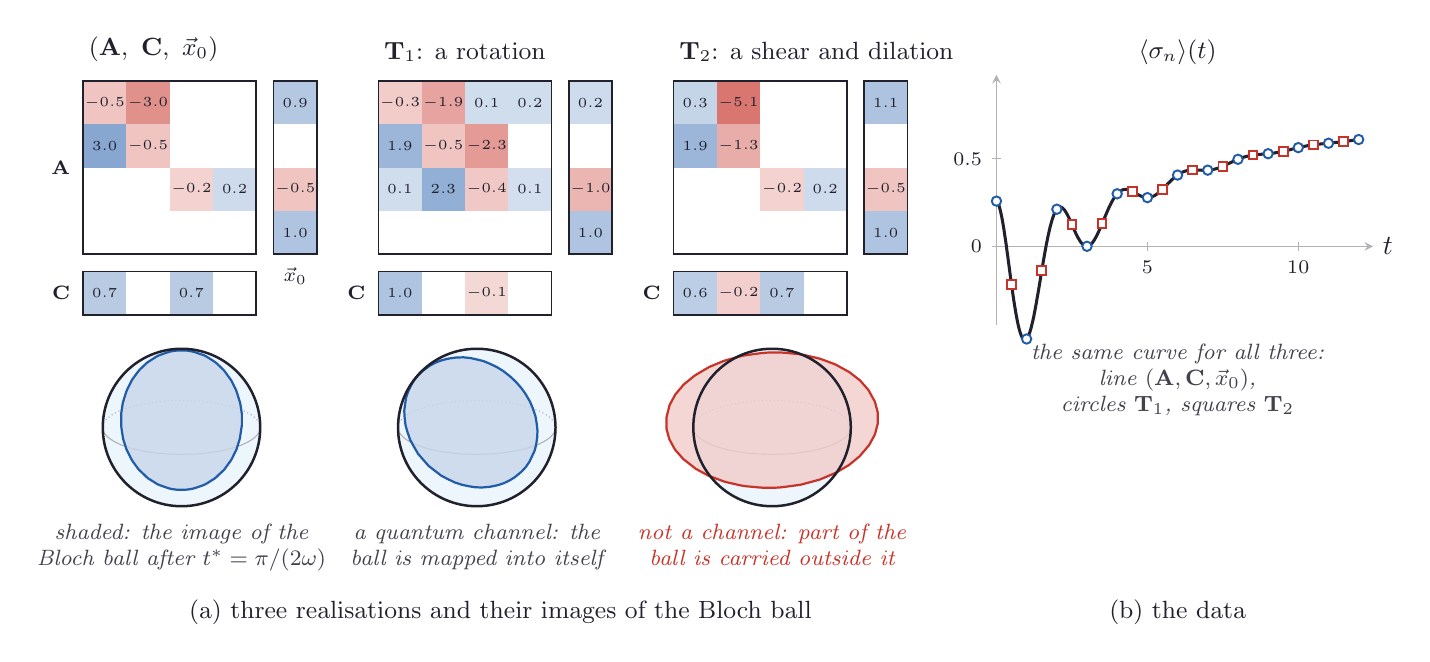
\begin{tikzpicture}[ink/.style={line width=0.9pt, ndInk}, faint/.style={line width=0.4pt, ndInk!35}, dashedink/.style={line width=0.5pt, ndInk!55, dash pattern=on 2.5pt off 2pt}, vec/.style={->, >=stealth, line width=1.2pt}, note/.style={font=\footnotesize\itshape, text=ndInk!85, align=center}, pointer/.style={->, >=stealth, line width=0.4pt, ndInk!60, shorten >=2pt, shorten <=1pt}, dot/.style={circle, fill=ndInk, inner sep=0pt, minimum size=3.4pt}, wash/.style={fill=ndSky, fill opacity=0.55}, every node/.style={text=ndInk}]
\definecolor{ndInk}{rgb}{0.13,0.13,0.18}
\definecolor{ndPaper}{rgb}{0.99,0.96,0.88}
\definecolor{ndSky}{rgb}{0.84,0.91,0.98}
\definecolor{ndRose}{rgb}{0.98,0.86,0.84}
\definecolor{ndBlue}{rgb}{0.13,0.36,0.66}
\definecolor{ndRed}{rgb}{0.78,0.20,0.16}
\definecolor{ndGold}{rgb}{0.88,0.62,0.10}
\definecolor{ndGreen}{rgb}{0.18,0.52,0.30}
\node[font=\small, anchor=south west] at (-0.050,3.520) {$(\mathbf A,\ \mathbf C,\ \vec x_0)$};
\fill[ndRed!29] (0.000,3.400) rectangle (0.550,2.850);
\node[font=\fontsize{5.5}{5.5}\selectfont, text=ndInk] at (0.275,3.125) {${-}0.5$};
\fill[ndRed!54] (0.550,3.400) rectangle (1.100,2.850);
\node[font=\fontsize{5.5}{5.5}\selectfont, text=ndInk] at (0.825,3.125) {${-}3.0$};
\fill[ndBlue!54] (0.000,2.850) rectangle (0.550,2.300);
\node[font=\fontsize{5.5}{5.5}\selectfont, text=ndInk] at (0.275,2.575) {$3.0$};
\fill[ndRed!29] (0.550,2.850) rectangle (1.100,2.300);
\node[font=\fontsize{5.5}{5.5}\selectfont, text=ndInk] at (0.825,2.575) {${-}0.5$};
\fill[ndRed!22] (1.100,2.300) rectangle (1.650,1.750);
\node[font=\fontsize{5.5}{5.5}\selectfont, text=ndInk] at (1.375,2.025) {${-}0.2$};
\fill[ndBlue!22] (1.650,2.300) rectangle (2.200,1.750);
\node[font=\fontsize{5.5}{5.5}\selectfont, text=ndInk] at (1.925,2.025) {$0.2$};
\draw[ink, line width=0.6pt] (0.000,3.400) rectangle (2.200,1.200);
\fill[ndBlue!34] (2.420,3.400) rectangle (2.970,2.850);
\node[font=\fontsize{5.5}{5.5}\selectfont, text=ndInk] at (2.695,3.125) {$0.9$};
\fill[ndRed!29] (2.420,2.300) rectangle (2.970,1.750);
\node[font=\fontsize{5.5}{5.5}\selectfont, text=ndInk] at (2.695,2.025) {${-}0.5$};
\fill[ndBlue!36] (2.420,1.750) rectangle (2.970,1.200);
\node[font=\fontsize{5.5}{5.5}\selectfont, text=ndInk] at (2.695,1.475) {$1.0$};
\draw[ink, line width=0.6pt] (2.420,3.400) rectangle (2.970,1.200);
\fill[ndBlue!32] (0.000,0.980) rectangle (0.550,0.430);
\node[font=\fontsize{5.5}{5.5}\selectfont, text=ndInk] at (0.275,0.705) {$0.7$};
\fill[ndBlue!32] (1.100,0.980) rectangle (1.650,0.430);
\node[font=\fontsize{5.5}{5.5}\selectfont, text=ndInk] at (1.375,0.705) {$0.7$};
\draw[ink, line width=0.6pt] (0.000,0.980) rectangle (2.200,0.430);
\node[font=\scriptsize, anchor=east] at (-0.040,0.705) {$\mathbf C$};
\node[font=\scriptsize, anchor=east] at (-0.040,2.300) {$\mathbf A$};
\node[font=\scriptsize, anchor=north] at (2.695,1.150) {$\vec x_0$};
\fill[ndSky!45] (1.250,-1.000) circle (1.000);
\draw[faint] (1.076,-1.337) -- (1.102,-1.338) -- (1.128,-1.339) -- (1.154,-1.340) -- (1.180,-1.341) -- (1.206,-1.342) -- (1.233,-1.342) -- (1.259,-1.342) -- (1.285,-1.342) -- (1.311,-1.341) -- (1.337,-1.341) -- (1.363,-1.340) -- (1.389,-1.339) -- (1.415,-1.337) -- (1.441,-1.336) -- (1.466,-1.334) -- (1.492,-1.332) -- (1.517,-1.330) -- (1.542,-1.327) -- (1.567,-1.324) -- (1.592,-1.321) -- (1.617,-1.318) -- (1.641,-1.315) -- (1.665,-1.311) -- (1.688,-1.307) -- (1.712,-1.303) -- (1.735,-1.299) -- (1.758,-1.295) -- (1.780,-1.290) -- (1.802,-1.285) -- (1.824,-1.280) -- (1.845,-1.275) -- (1.866,-1.270) -- (1.886,-1.264) -- (1.906,-1.258) -- (1.926,-1.252) -- (1.945,-1.246) -- (1.963,-1.240) -- (1.981,-1.233) -- (1.999,-1.227) -- (2.016,-1.220) -- (2.033,-1.213) -- (2.049,-1.206) -- (2.064,-1.199) -- (2.079,-1.191) -- (2.093,-1.184) -- (2.107,-1.176) -- (2.120,-1.168) -- (2.133,-1.161) -- (2.145,-1.153) -- (2.156,-1.145) -- (2.167,-1.136) -- (2.177,-1.128) -- (2.187,-1.120) -- (2.196,-1.111) -- (2.204,-1.103) -- (2.211,-1.094) -- (2.218,-1.086) -- (2.224,-1.077) -- (2.230,-1.068) -- (2.235,-1.059) -- (2.239,-1.051) -- (2.243,-1.042) -- (2.245,-1.033) -- (2.248,-1.024) -- (2.249,-1.015) -- (2.250,-1.006);
\draw[faint] (0.250,-1.003) -- (0.251,-1.012) -- (0.252,-1.021) -- (0.254,-1.030) -- (0.256,-1.039) -- (0.260,-1.048) -- (0.264,-1.056) -- (0.268,-1.065) -- (0.274,-1.074) -- (0.280,-1.083) -- (0.286,-1.091) -- (0.294,-1.100) -- (0.302,-1.109) -- (0.310,-1.117) -- (0.320,-1.125) -- (0.329,-1.134) -- (0.340,-1.142) -- (0.351,-1.150) -- (0.363,-1.158) -- (0.375,-1.166) -- (0.388,-1.174) -- (0.402,-1.181) -- (0.416,-1.189) -- (0.431,-1.196) -- (0.446,-1.203) -- (0.462,-1.211) -- (0.478,-1.218) -- (0.495,-1.224) -- (0.513,-1.231) -- (0.531,-1.238) -- (0.549,-1.244) -- (0.568,-1.250) -- (0.587,-1.256) -- (0.607,-1.262) -- (0.627,-1.268) -- (0.648,-1.273) -- (0.669,-1.278) -- (0.691,-1.284) -- (0.713,-1.288) -- (0.735,-1.293) -- (0.758,-1.298) -- (0.781,-1.302) -- (0.804,-1.306) -- (0.827,-1.310) -- (0.851,-1.314) -- (0.875,-1.317) -- (0.900,-1.320) -- (0.924,-1.323) -- (0.949,-1.326) -- (0.974,-1.329) -- (1.000,-1.331) -- (1.025,-1.333) -- (1.051,-1.335) -- (1.076,-1.337);
\draw[faint, densely dotted] (2.250,-0.997) -- (2.249,-0.988) -- (2.248,-0.979) -- (2.246,-0.970) -- (2.244,-0.961) -- (2.240,-0.952) -- (2.236,-0.944) -- (2.232,-0.935) -- (2.226,-0.926) -- (2.220,-0.917) -- (2.214,-0.909) -- (2.206,-0.900) -- (2.198,-0.891) -- (2.190,-0.883) -- (2.180,-0.875) -- (2.171,-0.866) -- (2.160,-0.858) -- (2.149,-0.850) -- (2.137,-0.842) -- (2.125,-0.834) -- (2.112,-0.826) -- (2.098,-0.819) -- (2.084,-0.811) -- (2.069,-0.804) -- (2.054,-0.797) -- (2.038,-0.789) -- (2.022,-0.782) -- (2.005,-0.776) -- (1.987,-0.769) -- (1.969,-0.762) -- (1.951,-0.756) -- (1.932,-0.750) -- (1.913,-0.744) -- (1.893,-0.738) -- (1.873,-0.732) -- (1.852,-0.727) -- (1.831,-0.722) -- (1.809,-0.716) -- (1.787,-0.712) -- (1.765,-0.707) -- (1.742,-0.702) -- (1.719,-0.698) -- (1.696,-0.694) -- (1.673,-0.690) -- (1.649,-0.686) -- (1.625,-0.683) -- (1.600,-0.680) -- (1.576,-0.677) -- (1.551,-0.674) -- (1.526,-0.671) -- (1.500,-0.669) -- (1.475,-0.667) -- (1.449,-0.665) -- (1.424,-0.663) -- (1.398,-0.662) -- (1.372,-0.661) -- (1.346,-0.660) -- (1.320,-0.659) -- (1.294,-0.658) -- (1.267,-0.658) -- (1.241,-0.658) -- (1.215,-0.658) -- (1.189,-0.659) -- (1.163,-0.659) -- (1.137,-0.660) -- (1.111,-0.661) -- (1.085,-0.663) -- (1.059,-0.664) -- (1.034,-0.666) -- (1.008,-0.668) -- (0.983,-0.670) -- (0.958,-0.673) -- (0.933,-0.676) -- (0.908,-0.679) -- (0.883,-0.682) -- (0.859,-0.685) -- (0.835,-0.689) -- (0.812,-0.693) -- (0.788,-0.697) -- (0.765,-0.701) -- (0.742,-0.705) -- (0.720,-0.710) -- (0.698,-0.715) -- (0.676,-0.720) -- (0.655,-0.725) -- (0.634,-0.730) -- (0.614,-0.736) -- (0.594,-0.742) -- (0.574,-0.748) -- (0.555,-0.754) -- (0.537,-0.760) -- (0.519,-0.767) -- (0.501,-0.773) -- (0.484,-0.780) -- (0.467,-0.787) -- (0.451,-0.794) -- (0.436,-0.801) -- (0.421,-0.809) -- (0.407,-0.816) -- (0.393,-0.824) -- (0.380,-0.832) -- (0.367,-0.839) -- (0.355,-0.847) -- (0.344,-0.855) -- (0.333,-0.864) -- (0.323,-0.872) -- (0.313,-0.880) -- (0.304,-0.889) -- (0.296,-0.897) -- (0.289,-0.906) -- (0.282,-0.914) -- (0.276,-0.923) -- (0.270,-0.932) -- (0.265,-0.941) -- (0.261,-0.949) -- (0.257,-0.958) -- (0.255,-0.967) -- (0.252,-0.976) -- (0.251,-0.985) -- (0.250,-0.994);
\filldraw[ndBlue, line width=0.8pt, fill=ndBlue!25, fill opacity=0.8] (0.484,-0.823) -- (0.484,-0.962) -- (0.487,-1.005) -- (0.508,-1.142) -- (0.549,-1.272) -- (0.609,-1.393) -- (0.629,-1.428) -- (0.704,-1.531) -- (0.794,-1.617) -- (0.820,-1.642) -- (0.917,-1.703) -- (0.946,-1.721) -- (0.982,-1.736) -- (1.067,-1.765) -- (1.097,-1.775) -- (1.131,-1.782) -- (1.168,-1.788) -- (1.207,-1.791) -- (1.247,-1.792) -- (1.287,-1.792) -- (1.326,-1.788) -- (1.363,-1.783) -- (1.397,-1.776) -- (1.428,-1.767) -- (1.511,-1.739) -- (1.549,-1.723) -- (1.579,-1.706) -- (1.674,-1.646) -- (1.702,-1.621) -- (1.792,-1.536) -- (1.866,-1.434) -- (1.889,-1.399) -- (1.948,-1.279) -- (1.989,-1.148) -- (1.996,-1.107) -- (2.017,-0.969) -- (2.017,-0.830) -- (1.996,-0.692) -- (1.955,-0.560) -- (1.942,-0.522) -- (1.883,-0.403) -- (1.806,-0.297) -- (1.782,-0.267) -- (1.694,-0.183) -- (1.663,-0.160) -- (1.570,-0.101) -- (1.537,-0.084) -- (1.497,-0.070) -- (1.418,-0.043) -- (1.386,-0.035) -- (1.351,-0.028) -- (1.313,-0.023) -- (1.273,-0.021) -- (1.233,-0.021) -- (1.193,-0.023) -- (1.155,-0.027) -- (1.119,-0.033) -- (1.087,-0.041) -- (1.011,-0.067) -- (0.969,-0.082) -- (0.935,-0.098) -- (0.844,-0.156) -- (0.810,-0.179) -- (0.723,-0.262) -- (0.697,-0.292) -- (0.620,-0.397) -- (0.561,-0.515) -- (0.546,-0.554) -- (0.505,-0.685) -- cycle;
\draw[ink] (1.250,-1.000) circle (1.000);
\node[font=\small, anchor=south west] at (3.700,3.520) {$\mathbf T_1$: a rotation};
\fill[ndRed!25] (3.750,3.400) rectangle (4.300,2.850);
\node[font=\fontsize{5.5}{5.5}\selectfont, text=ndInk] at (4.025,3.125) {${-}0.3$};
\fill[ndRed!45] (4.300,3.400) rectangle (4.850,2.850);
\node[font=\fontsize{5.5}{5.5}\selectfont, text=ndInk] at (4.575,3.125) {${-}1.9$};
\fill[ndBlue!21] (4.850,3.400) rectangle (5.400,2.850);
\node[font=\fontsize{5.5}{5.5}\selectfont, text=ndInk] at (5.125,3.125) {$0.1$};
\fill[ndBlue!21] (5.400,3.400) rectangle (5.950,2.850);
\node[font=\fontsize{5.5}{5.5}\selectfont, text=ndInk] at (5.675,3.125) {$0.2$};
\fill[ndBlue!45] (3.750,2.850) rectangle (4.300,2.300);
\node[font=\fontsize{5.5}{5.5}\selectfont, text=ndInk] at (4.025,2.575) {$1.9$};
\fill[ndRed!29] (4.300,2.850) rectangle (4.850,2.300);
\node[font=\fontsize{5.5}{5.5}\selectfont, text=ndInk] at (4.575,2.575) {${-}0.5$};
\fill[ndRed!49] (4.850,2.850) rectangle (5.400,2.300);
\node[font=\fontsize{5.5}{5.5}\selectfont, text=ndInk] at (5.125,2.575) {${-}2.3$};
\fill[ndBlue!21] (3.750,2.300) rectangle (4.300,1.750);
\node[font=\fontsize{5.5}{5.5}\selectfont, text=ndInk] at (4.025,2.025) {$0.1$};
\fill[ndBlue!49] (4.300,2.300) rectangle (4.850,1.750);
\node[font=\fontsize{5.5}{5.5}\selectfont, text=ndInk] at (4.575,2.025) {$2.3$};
\fill[ndRed!27] (4.850,2.300) rectangle (5.400,1.750);
\node[font=\fontsize{5.5}{5.5}\selectfont, text=ndInk] at (5.125,2.025) {${-}0.4$};
\fill[ndBlue!20] (5.400,2.300) rectangle (5.950,1.750);
\node[font=\fontsize{5.5}{5.5}\selectfont, text=ndInk] at (5.675,2.025) {$0.1$};
\draw[ink, line width=0.6pt] (3.750,3.400) rectangle (5.950,1.200);
\fill[ndBlue!22] (6.170,3.400) rectangle (6.720,2.850);
\node[font=\fontsize{5.5}{5.5}\selectfont, text=ndInk] at (6.445,3.125) {$0.2$};
\fill[ndRed!36] (6.170,2.300) rectangle (6.720,1.750);
\node[font=\fontsize{5.5}{5.5}\selectfont, text=ndInk] at (6.445,2.025) {${-}1.0$};
\fill[ndBlue!36] (6.170,1.750) rectangle (6.720,1.200);
\node[font=\fontsize{5.5}{5.5}\selectfont, text=ndInk] at (6.445,1.475) {$1.0$};
\draw[ink, line width=0.6pt] (6.170,3.400) rectangle (6.720,1.200);
\fill[ndBlue!36] (3.750,0.980) rectangle (4.300,0.430);
\node[font=\fontsize{5.5}{5.5}\selectfont, text=ndInk] at (4.025,0.705) {$1.0$};
\fill[ndRed!19] (4.850,0.980) rectangle (5.400,0.430);
\node[font=\fontsize{5.5}{5.5}\selectfont, text=ndInk] at (5.125,0.705) {${-}0.1$};
\draw[ink, line width=0.6pt] (3.750,0.980) rectangle (5.950,0.430);
\node[font=\scriptsize, anchor=east] at (3.710,0.705) {$\mathbf C$};
\fill[ndSky!45] (5.000,-1.000) circle (1.000);
\draw[faint] (4.826,-1.337) -- (4.852,-1.338) -- (4.878,-1.339) -- (4.904,-1.340) -- (4.930,-1.341) -- (4.956,-1.342) -- (4.983,-1.342) -- (5.009,-1.342) -- (5.035,-1.342) -- (5.061,-1.341) -- (5.087,-1.341) -- (5.113,-1.340) -- (5.139,-1.339) -- (5.165,-1.337) -- (5.191,-1.336) -- (5.216,-1.334) -- (5.242,-1.332) -- (5.267,-1.330) -- (5.292,-1.327) -- (5.317,-1.324) -- (5.342,-1.321) -- (5.367,-1.318) -- (5.391,-1.315) -- (5.415,-1.311) -- (5.438,-1.307) -- (5.462,-1.303) -- (5.485,-1.299) -- (5.508,-1.295) -- (5.530,-1.290) -- (5.552,-1.285) -- (5.574,-1.280) -- (5.595,-1.275) -- (5.616,-1.270) -- (5.636,-1.264) -- (5.656,-1.258) -- (5.676,-1.252) -- (5.695,-1.246) -- (5.713,-1.240) -- (5.731,-1.233) -- (5.749,-1.227) -- (5.766,-1.220) -- (5.783,-1.213) -- (5.799,-1.206) -- (5.814,-1.199) -- (5.829,-1.191) -- (5.843,-1.184) -- (5.857,-1.176) -- (5.870,-1.168) -- (5.883,-1.161) -- (5.895,-1.153) -- (5.906,-1.145) -- (5.917,-1.136) -- (5.927,-1.128) -- (5.937,-1.120) -- (5.946,-1.111) -- (5.954,-1.103) -- (5.961,-1.094) -- (5.968,-1.086) -- (5.974,-1.077) -- (5.980,-1.068) -- (5.985,-1.059) -- (5.989,-1.051) -- (5.993,-1.042) -- (5.995,-1.033) -- (5.998,-1.024) -- (5.999,-1.015) -- (6.000,-1.006);
\draw[faint] (4.000,-1.003) -- (4.001,-1.012) -- (4.002,-1.021) -- (4.004,-1.030) -- (4.006,-1.039) -- (4.010,-1.048) -- (4.014,-1.056) -- (4.018,-1.065) -- (4.024,-1.074) -- (4.030,-1.083) -- (4.036,-1.091) -- (4.044,-1.100) -- (4.052,-1.109) -- (4.060,-1.117) -- (4.070,-1.125) -- (4.079,-1.134) -- (4.090,-1.142) -- (4.101,-1.150) -- (4.113,-1.158) -- (4.125,-1.166) -- (4.138,-1.174) -- (4.152,-1.181) -- (4.166,-1.189) -- (4.181,-1.196) -- (4.196,-1.203) -- (4.212,-1.211) -- (4.228,-1.218) -- (4.245,-1.224) -- (4.263,-1.231) -- (4.281,-1.238) -- (4.299,-1.244) -- (4.318,-1.250) -- (4.337,-1.256) -- (4.357,-1.262) -- (4.377,-1.268) -- (4.398,-1.273) -- (4.419,-1.278) -- (4.441,-1.284) -- (4.463,-1.288) -- (4.485,-1.293) -- (4.508,-1.298) -- (4.531,-1.302) -- (4.554,-1.306) -- (4.577,-1.310) -- (4.601,-1.314) -- (4.625,-1.317) -- (4.650,-1.320) -- (4.674,-1.323) -- (4.699,-1.326) -- (4.724,-1.329) -- (4.750,-1.331) -- (4.775,-1.333) -- (4.801,-1.335) -- (4.826,-1.337);
\draw[faint, densely dotted] (6.000,-0.997) -- (5.999,-0.988) -- (5.998,-0.979) -- (5.996,-0.970) -- (5.994,-0.961) -- (5.990,-0.952) -- (5.986,-0.944) -- (5.982,-0.935) -- (5.976,-0.926) -- (5.970,-0.917) -- (5.964,-0.909) -- (5.956,-0.900) -- (5.948,-0.891) -- (5.940,-0.883) -- (5.930,-0.875) -- (5.921,-0.866) -- (5.910,-0.858) -- (5.899,-0.850) -- (5.887,-0.842) -- (5.875,-0.834) -- (5.862,-0.826) -- (5.848,-0.819) -- (5.834,-0.811) -- (5.819,-0.804) -- (5.804,-0.797) -- (5.788,-0.789) -- (5.772,-0.782) -- (5.755,-0.776) -- (5.737,-0.769) -- (5.719,-0.762) -- (5.701,-0.756) -- (5.682,-0.750) -- (5.663,-0.744) -- (5.643,-0.738) -- (5.623,-0.732) -- (5.602,-0.727) -- (5.581,-0.722) -- (5.559,-0.716) -- (5.537,-0.712) -- (5.515,-0.707) -- (5.492,-0.702) -- (5.469,-0.698) -- (5.446,-0.694) -- (5.423,-0.690) -- (5.399,-0.686) -- (5.375,-0.683) -- (5.350,-0.680) -- (5.326,-0.677) -- (5.301,-0.674) -- (5.276,-0.671) -- (5.250,-0.669) -- (5.225,-0.667) -- (5.199,-0.665) -- (5.174,-0.663) -- (5.148,-0.662) -- (5.122,-0.661) -- (5.096,-0.660) -- (5.070,-0.659) -- (5.044,-0.658) -- (5.017,-0.658) -- (4.991,-0.658) -- (4.965,-0.658) -- (4.939,-0.659) -- (4.913,-0.659) -- (4.887,-0.660) -- (4.861,-0.661) -- (4.835,-0.663) -- (4.809,-0.664) -- (4.784,-0.666) -- (4.758,-0.668) -- (4.733,-0.670) -- (4.708,-0.673) -- (4.683,-0.676) -- (4.658,-0.679) -- (4.633,-0.682) -- (4.609,-0.685) -- (4.585,-0.689) -- (4.562,-0.693) -- (4.538,-0.697) -- (4.515,-0.701) -- (4.492,-0.705) -- (4.470,-0.710) -- (4.448,-0.715) -- (4.426,-0.720) -- (4.405,-0.725) -- (4.384,-0.730) -- (4.364,-0.736) -- (4.344,-0.742) -- (4.324,-0.748) -- (4.305,-0.754) -- (4.287,-0.760) -- (4.269,-0.767) -- (4.251,-0.773) -- (4.234,-0.780) -- (4.217,-0.787) -- (4.201,-0.794) -- (4.186,-0.801) -- (4.171,-0.809) -- (4.157,-0.816) -- (4.143,-0.824) -- (4.130,-0.832) -- (4.117,-0.839) -- (4.105,-0.847) -- (4.094,-0.855) -- (4.083,-0.864) -- (4.073,-0.872) -- (4.063,-0.880) -- (4.054,-0.889) -- (4.046,-0.897) -- (4.039,-0.906) -- (4.032,-0.914) -- (4.026,-0.923) -- (4.020,-0.932) -- (4.015,-0.941) -- (4.011,-0.949) -- (4.007,-0.958) -- (4.005,-0.967) -- (4.002,-0.976) -- (4.001,-0.985) -- (4.000,-0.994);
\filldraw[ndBlue, line width=0.8pt, fill=ndBlue!25, fill opacity=0.8] (5.735,-1.294) -- (5.755,-1.214) -- (5.767,-1.127) -- (5.771,-1.041) -- (5.760,-0.943) -- (5.745,-0.855) -- (5.711,-0.755) -- (5.675,-0.670) -- (5.620,-0.575) -- (5.566,-0.499) -- (5.493,-0.416) -- (5.423,-0.351) -- (5.339,-0.285) -- (5.259,-0.235) -- (5.170,-0.192) -- (5.086,-0.157) -- (4.993,-0.134) -- (4.919,-0.118) -- (4.831,-0.109) -- (4.740,-0.111) -- (4.648,-0.124) -- (4.619,-0.130) -- (4.543,-0.150) -- (4.470,-0.179) -- (4.403,-0.216) -- (4.342,-0.260) -- (4.316,-0.280) -- (4.252,-0.339) -- (4.201,-0.404) -- (4.162,-0.472) -- (4.131,-0.537) -- (4.103,-0.617) -- (4.091,-0.697) -- (4.079,-0.787) -- (4.084,-0.873) -- (4.095,-0.972) -- (4.120,-1.058) -- (4.155,-1.159) -- (4.200,-1.240) -- (4.255,-1.335) -- (4.328,-1.419) -- (4.390,-1.489) -- (4.476,-1.556) -- (4.549,-1.612) -- (4.636,-1.657) -- (4.721,-1.698) -- (4.810,-1.727) -- (4.889,-1.744) -- (4.974,-1.759) -- (5.064,-1.762) -- (5.156,-1.755) -- (5.193,-1.748) -- (5.269,-1.732) -- (5.344,-1.707) -- (5.414,-1.674) -- (5.479,-1.634) -- (5.499,-1.618) -- (5.567,-1.562) -- (5.625,-1.500) -- (5.670,-1.433) -- (5.698,-1.373) -- cycle;
\draw[ink] (5.000,-1.000) circle (1.000);
\node[font=\small, anchor=south west] at (7.450,3.520) {$\mathbf T_2$: a shear and dilation};
\fill[ndBlue!26] (7.500,3.400) rectangle (8.050,2.850);
\node[font=\fontsize{5.5}{5.5}\selectfont, text=ndInk] at (7.775,3.125) {$0.3$};
\fill[ndRed!67] (8.050,3.400) rectangle (8.600,2.850);
\node[font=\fontsize{5.5}{5.5}\selectfont, text=ndInk] at (8.325,3.125) {${-}5.1$};
\fill[ndBlue!45] (7.500,2.850) rectangle (8.050,2.300);
\node[font=\fontsize{5.5}{5.5}\selectfont, text=ndInk] at (7.775,2.575) {$1.9$};
\fill[ndRed!40] (8.050,2.850) rectangle (8.600,2.300);
\node[font=\fontsize{5.5}{5.5}\selectfont, text=ndInk] at (8.325,2.575) {${-}1.3$};
\fill[ndRed!22] (8.600,2.300) rectangle (9.150,1.750);
\node[font=\fontsize{5.5}{5.5}\selectfont, text=ndInk] at (8.875,2.025) {${-}0.2$};
\fill[ndBlue!22] (9.150,2.300) rectangle (9.700,1.750);
\node[font=\fontsize{5.5}{5.5}\selectfont, text=ndInk] at (9.425,2.025) {$0.2$};
\draw[ink, line width=0.6pt] (7.500,3.400) rectangle (9.700,1.200);
\fill[ndBlue!37] (9.920,3.400) rectangle (10.470,2.850);
\node[font=\fontsize{5.5}{5.5}\selectfont, text=ndInk] at (10.195,3.125) {$1.1$};
\fill[ndRed!29] (9.920,2.300) rectangle (10.470,1.750);
\node[font=\fontsize{5.5}{5.5}\selectfont, text=ndInk] at (10.195,2.025) {${-}0.5$};
\fill[ndBlue!36] (9.920,1.750) rectangle (10.470,1.200);
\node[font=\fontsize{5.5}{5.5}\selectfont, text=ndInk] at (10.195,1.475) {$1.0$};
\draw[ink, line width=0.6pt] (9.920,3.400) rectangle (10.470,1.200);
\fill[ndBlue!30] (7.500,0.980) rectangle (8.050,0.430);
\node[font=\fontsize{5.5}{5.5}\selectfont, text=ndInk] at (7.775,0.705) {$0.6$};
\fill[ndRed!24] (8.050,0.980) rectangle (8.600,0.430);
\node[font=\fontsize{5.5}{5.5}\selectfont, text=ndInk] at (8.325,0.705) {${-}0.2$};
\fill[ndBlue!32] (8.600,0.980) rectangle (9.150,0.430);
\node[font=\fontsize{5.5}{5.5}\selectfont, text=ndInk] at (8.875,0.705) {$0.7$};
\draw[ink, line width=0.6pt] (7.500,0.980) rectangle (9.700,0.430);
\node[font=\scriptsize, anchor=east] at (7.460,0.705) {$\mathbf C$};
\fill[ndSky!45] (8.750,-1.000) circle (1.000);
\draw[faint] (8.576,-1.337) -- (8.602,-1.338) -- (8.628,-1.339) -- (8.654,-1.340) -- (8.680,-1.341) -- (8.706,-1.342) -- (8.733,-1.342) -- (8.759,-1.342) -- (8.785,-1.342) -- (8.811,-1.341) -- (8.837,-1.341) -- (8.863,-1.340) -- (8.889,-1.339) -- (8.915,-1.337) -- (8.941,-1.336) -- (8.966,-1.334) -- (8.992,-1.332) -- (9.017,-1.330) -- (9.042,-1.327) -- (9.067,-1.324) -- (9.092,-1.321) -- (9.117,-1.318) -- (9.141,-1.315) -- (9.165,-1.311) -- (9.188,-1.307) -- (9.212,-1.303) -- (9.235,-1.299) -- (9.258,-1.295) -- (9.280,-1.290) -- (9.302,-1.285) -- (9.324,-1.280) -- (9.345,-1.275) -- (9.366,-1.270) -- (9.386,-1.264) -- (9.406,-1.258) -- (9.426,-1.252) -- (9.445,-1.246) -- (9.463,-1.240) -- (9.481,-1.233) -- (9.499,-1.227) -- (9.516,-1.220) -- (9.533,-1.213) -- (9.549,-1.206) -- (9.564,-1.199) -- (9.579,-1.191) -- (9.593,-1.184) -- (9.607,-1.176) -- (9.620,-1.168) -- (9.633,-1.161) -- (9.645,-1.153) -- (9.656,-1.145) -- (9.667,-1.136) -- (9.677,-1.128) -- (9.687,-1.120) -- (9.696,-1.111) -- (9.704,-1.103) -- (9.711,-1.094) -- (9.718,-1.086) -- (9.724,-1.077) -- (9.730,-1.068) -- (9.735,-1.059) -- (9.739,-1.051) -- (9.743,-1.042) -- (9.745,-1.033) -- (9.748,-1.024) -- (9.749,-1.015) -- (9.750,-1.006);
\draw[faint] (7.750,-1.003) -- (7.751,-1.012) -- (7.752,-1.021) -- (7.754,-1.030) -- (7.756,-1.039) -- (7.760,-1.048) -- (7.764,-1.056) -- (7.768,-1.065) -- (7.774,-1.074) -- (7.780,-1.083) -- (7.786,-1.091) -- (7.794,-1.100) -- (7.802,-1.109) -- (7.810,-1.117) -- (7.820,-1.125) -- (7.829,-1.134) -- (7.840,-1.142) -- (7.851,-1.150) -- (7.863,-1.158) -- (7.875,-1.166) -- (7.888,-1.174) -- (7.902,-1.181) -- (7.916,-1.189) -- (7.931,-1.196) -- (7.946,-1.203) -- (7.962,-1.211) -- (7.978,-1.218) -- (7.995,-1.224) -- (8.013,-1.231) -- (8.031,-1.238) -- (8.049,-1.244) -- (8.068,-1.250) -- (8.087,-1.256) -- (8.107,-1.262) -- (8.127,-1.268) -- (8.148,-1.273) -- (8.169,-1.278) -- (8.191,-1.284) -- (8.213,-1.288) -- (8.235,-1.293) -- (8.258,-1.298) -- (8.281,-1.302) -- (8.304,-1.306) -- (8.327,-1.310) -- (8.351,-1.314) -- (8.375,-1.317) -- (8.400,-1.320) -- (8.424,-1.323) -- (8.449,-1.326) -- (8.474,-1.329) -- (8.500,-1.331) -- (8.525,-1.333) -- (8.551,-1.335) -- (8.576,-1.337);
\draw[faint, densely dotted] (9.750,-0.997) -- (9.749,-0.988) -- (9.748,-0.979) -- (9.746,-0.970) -- (9.744,-0.961) -- (9.740,-0.952) -- (9.736,-0.944) -- (9.732,-0.935) -- (9.726,-0.926) -- (9.720,-0.917) -- (9.714,-0.909) -- (9.706,-0.900) -- (9.698,-0.891) -- (9.690,-0.883) -- (9.680,-0.875) -- (9.671,-0.866) -- (9.660,-0.858) -- (9.649,-0.850) -- (9.637,-0.842) -- (9.625,-0.834) -- (9.612,-0.826) -- (9.598,-0.819) -- (9.584,-0.811) -- (9.569,-0.804) -- (9.554,-0.797) -- (9.538,-0.789) -- (9.522,-0.782) -- (9.505,-0.776) -- (9.487,-0.769) -- (9.469,-0.762) -- (9.451,-0.756) -- (9.432,-0.750) -- (9.413,-0.744) -- (9.393,-0.738) -- (9.373,-0.732) -- (9.352,-0.727) -- (9.331,-0.722) -- (9.309,-0.716) -- (9.287,-0.712) -- (9.265,-0.707) -- (9.242,-0.702) -- (9.219,-0.698) -- (9.196,-0.694) -- (9.173,-0.690) -- (9.149,-0.686) -- (9.125,-0.683) -- (9.100,-0.680) -- (9.076,-0.677) -- (9.051,-0.674) -- (9.026,-0.671) -- (9.000,-0.669) -- (8.975,-0.667) -- (8.949,-0.665) -- (8.924,-0.663) -- (8.898,-0.662) -- (8.872,-0.661) -- (8.846,-0.660) -- (8.820,-0.659) -- (8.794,-0.658) -- (8.767,-0.658) -- (8.741,-0.658) -- (8.715,-0.658) -- (8.689,-0.659) -- (8.663,-0.659) -- (8.637,-0.660) -- (8.611,-0.661) -- (8.585,-0.663) -- (8.559,-0.664) -- (8.534,-0.666) -- (8.508,-0.668) -- (8.483,-0.670) -- (8.458,-0.673) -- (8.433,-0.676) -- (8.408,-0.679) -- (8.383,-0.682) -- (8.359,-0.685) -- (8.335,-0.689) -- (8.312,-0.693) -- (8.288,-0.697) -- (8.265,-0.701) -- (8.242,-0.705) -- (8.220,-0.710) -- (8.198,-0.715) -- (8.176,-0.720) -- (8.155,-0.725) -- (8.134,-0.730) -- (8.114,-0.736) -- (8.094,-0.742) -- (8.074,-0.748) -- (8.055,-0.754) -- (8.037,-0.760) -- (8.019,-0.767) -- (8.001,-0.773) -- (7.984,-0.780) -- (7.967,-0.787) -- (7.951,-0.794) -- (7.936,-0.801) -- (7.921,-0.809) -- (7.907,-0.816) -- (7.893,-0.824) -- (7.880,-0.832) -- (7.867,-0.839) -- (7.855,-0.847) -- (7.844,-0.855) -- (7.833,-0.864) -- (7.823,-0.872) -- (7.813,-0.880) -- (7.804,-0.889) -- (7.796,-0.897) -- (7.789,-0.906) -- (7.782,-0.914) -- (7.776,-0.923) -- (7.770,-0.932) -- (7.765,-0.941) -- (7.761,-0.949) -- (7.757,-0.958) -- (7.755,-0.967) -- (7.752,-0.976) -- (7.751,-0.985) -- (7.750,-0.994);
\filldraw[ndRed, line width=0.8pt, fill=ndRed!25, fill opacity=0.8] (7.446,-1.151) -- (7.518,-1.282) -- (7.624,-1.402) -- (7.760,-1.508) -- (7.782,-1.525) -- (7.942,-1.612) -- (8.124,-1.680) -- (8.155,-1.691) -- (8.344,-1.734) -- (8.375,-1.740) -- (8.416,-1.746) -- (8.581,-1.761) -- (8.606,-1.763) -- (8.635,-1.765) -- (8.667,-1.766) -- (8.701,-1.766) -- (8.736,-1.766) -- (8.772,-1.765) -- (8.807,-1.764) -- (8.841,-1.762) -- (8.872,-1.759) -- (8.900,-1.756) -- (9.046,-1.736) -- (9.094,-1.730) -- (9.133,-1.722) -- (9.162,-1.714) -- (9.354,-1.662) -- (9.530,-1.588) -- (9.564,-1.573) -- (9.725,-1.478) -- (9.860,-1.368) -- (9.878,-1.347) -- (9.984,-1.222) -- (10.056,-1.089) -- (10.093,-0.950) -- (10.093,-0.810) -- (10.056,-0.673) -- (10.044,-0.650) -- (9.972,-0.521) -- (9.867,-0.402) -- (9.732,-0.297) -- (9.570,-0.208) -- (9.541,-0.194) -- (9.363,-0.128) -- (9.324,-0.118) -- (9.142,-0.076) -- (9.105,-0.070) -- (9.060,-0.065) -- (8.907,-0.051) -- (8.880,-0.049) -- (8.849,-0.048) -- (8.816,-0.047) -- (8.781,-0.047) -- (8.746,-0.047) -- (8.710,-0.048) -- (8.676,-0.050) -- (8.643,-0.053) -- (8.613,-0.055) -- (8.587,-0.059) -- (8.429,-0.080) -- (8.385,-0.087) -- (8.351,-0.095) -- (8.165,-0.146) -- (8.131,-0.157) -- (7.951,-0.232) -- (7.792,-0.326) -- (7.763,-0.344) -- (7.627,-0.455) -- (7.522,-0.580) -- (7.450,-0.712) -- (7.414,-0.851) -- (7.409,-0.875) -- (7.409,-1.015) -- cycle;
\draw[ink] (8.750,-1.000) circle (1.000);
\node[note, anchor=north] at (1.250,-2.100) {shaded: the image of the\\ Bloch ball after $t^*=\pi/(2\omega)$};
\node[note, anchor=north] at (5.000,-2.100) {a quantum channel: the\\ ball is mapped into itself};
\node[note, anchor=north, text=ndRed] at (8.750,-2.100) {not a channel: part of the\\ ball is carried outside it};
\draw[faint, ->, >=stealth] (11.600,1.300) -- (16.384,1.300) node[right, text=ndInk] {$t$};
\draw[faint, ->, >=stealth] (11.600,0.300) -- (11.600,3.480) node[above, text=ndInk] {};
\draw[faint] (13.517,1.360) -- (13.517,1.240) node[below, font=\scriptsize, text=ndInk] {$5$};
\draw[faint] (15.433,1.360) -- (15.433,1.240) node[below, font=\scriptsize, text=ndInk] {$10$};
\draw[faint] (11.660,1.300) -- (11.540,1.300) node[left, font=\scriptsize, text=ndInk] {$0$};
\draw[faint] (11.660,2.411) -- (11.540,2.411) node[left, font=\scriptsize, text=ndInk] {$0.5$};
\draw[line width=1.1pt, ndInk] (11.600,1.875) -- (11.610,1.866) -- (11.619,1.850) -- (11.629,1.827) -- (11.638,1.798) -- (11.648,1.762) -- (11.657,1.721) -- (11.667,1.674) -- (11.677,1.623) -- (11.686,1.567) -- (11.696,1.508) -- (11.705,1.445) -- (11.715,1.380) -- (11.725,1.312) -- (11.734,1.242) -- (11.744,1.171) -- (11.753,1.099) -- (11.763,1.027) -- (11.772,0.955) -- (11.782,0.884) -- (11.792,0.814) -- (11.801,0.745) -- (11.811,0.678) -- (11.820,0.614) -- (11.830,0.552) -- (11.840,0.493) -- (11.849,0.438) -- (11.859,0.386) -- (11.868,0.338) -- (11.878,0.294) -- (11.887,0.255) -- (11.897,0.220) -- (11.907,0.190) -- (11.916,0.165) -- (11.926,0.144) -- (11.935,0.129) -- (11.945,0.118) -- (11.955,0.112) -- (11.964,0.112) -- (11.974,0.116) -- (11.983,0.124) -- (11.993,0.138) -- (12.002,0.156) -- (12.012,0.178) -- (12.022,0.204) -- (12.031,0.235) -- (12.041,0.269) -- (12.050,0.307) -- (12.060,0.348) -- (12.070,0.391) -- (12.079,0.438) -- (12.089,0.487) -- (12.098,0.538) -- (12.108,0.591) -- (12.117,0.646) -- (12.127,0.702) -- (12.137,0.759) -- (12.146,0.816) -- (12.156,0.874) -- (12.165,0.932) -- (12.175,0.990) -- (12.185,1.047) -- (12.194,1.104) -- (12.204,1.159) -- (12.213,1.213) -- (12.223,1.266) -- (12.232,1.317) -- (12.242,1.366) -- (12.252,1.414) -- (12.261,1.458) -- (12.271,1.501) -- (12.280,1.541) -- (12.290,1.578) -- (12.300,1.613) -- (12.309,1.644) -- (12.319,1.673) -- (12.328,1.699) -- (12.338,1.722) -- (12.348,1.741) -- (12.357,1.758) -- (12.367,1.772) -- (12.376,1.783) -- (12.386,1.791) -- (12.395,1.796) -- (12.405,1.799) -- (12.415,1.799) -- (12.424,1.796) -- (12.434,1.791) -- (12.443,1.784) -- (12.453,1.774) -- (12.463,1.763) -- (12.472,1.750) -- (12.482,1.735) -- (12.491,1.719) -- (12.501,1.701) -- (12.510,1.682) -- (12.520,1.662) -- (12.530,1.642) -- (12.539,1.620) -- (12.549,1.599) -- (12.558,1.577) -- (12.568,1.555) -- (12.578,1.533) -- (12.587,1.511) -- (12.597,1.490) -- (12.606,1.469) -- (12.616,1.449) -- (12.625,1.430) -- (12.635,1.412) -- (12.645,1.395) -- (12.654,1.379) -- (12.664,1.364) -- (12.673,1.351) -- (12.683,1.339) -- (12.692,1.329) -- (12.702,1.320) -- (12.712,1.313) -- (12.721,1.307) -- (12.731,1.303) -- (12.740,1.301) -- (12.750,1.301) -- (12.760,1.303) -- (12.769,1.306) -- (12.779,1.310) -- (12.788,1.317) -- (12.798,1.325) -- (12.807,1.334) -- (12.817,1.345) -- (12.827,1.358) -- (12.836,1.372) -- (12.846,1.387) -- (12.855,1.403) -- (12.865,1.421) -- (12.875,1.439) -- (12.884,1.459) -- (12.894,1.479) -- (12.903,1.500) -- (12.913,1.521) -- (12.922,1.543) -- (12.932,1.566) -- (12.942,1.588) -- (12.951,1.611) -- (12.961,1.634) -- (12.970,1.657) -- (12.980,1.680) -- (12.990,1.703) -- (12.999,1.725) -- (13.009,1.748) -- (13.018,1.769) -- (13.028,1.790) -- (13.037,1.810) -- (13.047,1.830) -- (13.057,1.849) -- (13.066,1.867) -- (13.076,1.885) -- (13.085,1.901) -- (13.095,1.916) -- (13.105,1.931) -- (13.114,1.944) -- (13.124,1.956) -- (13.133,1.968) -- (13.143,1.978) -- (13.152,1.987) -- (13.162,1.995) -- (13.172,2.002) -- (13.181,2.008) -- (13.191,2.013) -- (13.200,2.017) -- (13.210,2.020) -- (13.220,2.022) -- (13.229,2.024) -- (13.239,2.024) -- (13.248,2.024) -- (13.258,2.023) -- (13.268,2.021) -- (13.277,2.018) -- (13.287,2.015) -- (13.296,2.012) -- (13.306,2.008) -- (13.315,2.003) -- (13.325,1.998) -- (13.335,1.993) -- (13.344,1.988) -- (13.354,1.983) -- (13.363,1.977) -- (13.373,1.972) -- (13.383,1.966) -- (13.392,1.961) -- (13.402,1.955) -- (13.411,1.950) -- (13.421,1.946) -- (13.430,1.941) -- (13.440,1.937) -- (13.450,1.933) -- (13.459,1.930) -- (13.469,1.927) -- (13.478,1.924) -- (13.488,1.922) -- (13.497,1.921) -- (13.507,1.920) -- (13.517,1.919) -- (13.526,1.920) -- (13.536,1.920) -- (13.545,1.922) -- (13.555,1.924) -- (13.565,1.926) -- (13.574,1.930) -- (13.584,1.933) -- (13.593,1.938) -- (13.603,1.943) -- (13.612,1.948) -- (13.622,1.954) -- (13.632,1.960) -- (13.641,1.967) -- (13.651,1.975) -- (13.660,1.982) -- (13.670,1.990) -- (13.680,1.999) -- (13.689,2.007) -- (13.699,2.016) -- (13.708,2.026) -- (13.718,2.035) -- (13.727,2.045) -- (13.737,2.054) -- (13.747,2.064) -- (13.756,2.074) -- (13.766,2.084) -- (13.775,2.094) -- (13.785,2.104) -- (13.795,2.113) -- (13.804,2.123) -- (13.814,2.132) -- (13.823,2.142) -- (13.833,2.151) -- (13.842,2.159) -- (13.852,2.168) -- (13.862,2.176) -- (13.871,2.184) -- (13.881,2.192) -- (13.890,2.199) -- (13.900,2.206) -- (13.910,2.213) -- (13.919,2.219) -- (13.929,2.225) -- (13.938,2.230) -- (13.948,2.236) -- (13.957,2.240) -- (13.967,2.245) -- (13.977,2.249) -- (13.986,2.252) -- (13.996,2.256) -- (14.005,2.258) -- (14.015,2.261) -- (14.025,2.263) -- (14.034,2.265) -- (14.044,2.267) -- (14.053,2.268) -- (14.063,2.269) -- (14.072,2.270) -- (14.082,2.271) -- (14.092,2.271) -- (14.101,2.271) -- (14.111,2.271) -- (14.120,2.271) -- (14.130,2.271) -- (14.140,2.271) -- (14.149,2.270) -- (14.159,2.270) -- (14.168,2.269) -- (14.178,2.269) -- (14.188,2.268) -- (14.197,2.268) -- (14.207,2.267) -- (14.216,2.267) -- (14.226,2.267) -- (14.235,2.267) -- (14.245,2.266) -- (14.255,2.267) -- (14.264,2.267) -- (14.274,2.267) -- (14.283,2.268) -- (14.293,2.268) -- (14.303,2.269) -- (14.312,2.270) -- (14.322,2.272) -- (14.331,2.273) -- (14.341,2.275) -- (14.350,2.276) -- (14.360,2.279) -- (14.370,2.281) -- (14.379,2.283) -- (14.389,2.286) -- (14.398,2.289) -- (14.408,2.292) -- (14.418,2.295) -- (14.427,2.298) -- (14.437,2.302) -- (14.446,2.306) -- (14.456,2.309) -- (14.465,2.313) -- (14.475,2.317) -- (14.485,2.322) -- (14.494,2.326) -- (14.504,2.330) -- (14.513,2.335) -- (14.523,2.339) -- (14.532,2.344) -- (14.542,2.349) -- (14.552,2.353) -- (14.561,2.358) -- (14.571,2.362) -- (14.580,2.367) -- (14.590,2.372) -- (14.600,2.376) -- (14.609,2.381) -- (14.619,2.385) -- (14.628,2.389) -- (14.638,2.394) -- (14.647,2.398) -- (14.657,2.402) -- (14.667,2.406) -- (14.676,2.410) -- (14.686,2.414) -- (14.695,2.417) -- (14.705,2.421) -- (14.715,2.424) -- (14.724,2.427) -- (14.734,2.431) -- (14.743,2.434) -- (14.753,2.436) -- (14.762,2.439) -- (14.772,2.442) -- (14.782,2.444) -- (14.791,2.446) -- (14.801,2.448) -- (14.810,2.451) -- (14.820,2.452) -- (14.830,2.454) -- (14.839,2.456) -- (14.849,2.457) -- (14.858,2.459) -- (14.868,2.460) -- (14.877,2.461) -- (14.887,2.463) -- (14.897,2.464) -- (14.906,2.465) -- (14.916,2.466) -- (14.925,2.467) -- (14.935,2.468) -- (14.945,2.468) -- (14.954,2.469) -- (14.964,2.470) -- (14.973,2.471) -- (14.983,2.472) -- (14.992,2.472) -- (15.002,2.473) -- (15.012,2.474) -- (15.021,2.475) -- (15.031,2.476) -- (15.040,2.476) -- (15.050,2.477) -- (15.060,2.478) -- (15.069,2.479) -- (15.079,2.480) -- (15.088,2.481) -- (15.098,2.483) -- (15.107,2.484) -- (15.117,2.485) -- (15.127,2.486) -- (15.136,2.488) -- (15.146,2.489) -- (15.155,2.491) -- (15.165,2.492) -- (15.175,2.494) -- (15.184,2.496) -- (15.194,2.497) -- (15.203,2.499) -- (15.213,2.501) -- (15.223,2.503) -- (15.232,2.505) -- (15.242,2.507) -- (15.251,2.509) -- (15.261,2.512) -- (15.270,2.514) -- (15.280,2.516) -- (15.290,2.518) -- (15.299,2.521) -- (15.309,2.523) -- (15.318,2.525) -- (15.328,2.528) -- (15.337,2.530) -- (15.347,2.533) -- (15.357,2.535) -- (15.366,2.537) -- (15.376,2.540) -- (15.385,2.542) -- (15.395,2.545) -- (15.405,2.547) -- (15.414,2.549) -- (15.424,2.552) -- (15.433,2.554) -- (15.443,2.556) -- (15.453,2.558) -- (15.462,2.560) -- (15.472,2.563) -- (15.481,2.565) -- (15.491,2.567) -- (15.500,2.569) -- (15.510,2.571) -- (15.520,2.572) -- (15.529,2.574) -- (15.539,2.576) -- (15.548,2.578) -- (15.558,2.579) -- (15.567,2.581) -- (15.577,2.583) -- (15.587,2.584) -- (15.596,2.586) -- (15.606,2.587) -- (15.615,2.588) -- (15.625,2.590) -- (15.635,2.591) -- (15.644,2.592) -- (15.654,2.594) -- (15.663,2.595) -- (15.673,2.596) -- (15.682,2.597) -- (15.692,2.598) -- (15.702,2.599) -- (15.711,2.600) -- (15.721,2.601) -- (15.730,2.602) -- (15.740,2.603) -- (15.750,2.604) -- (15.759,2.605) -- (15.769,2.606) -- (15.778,2.607) -- (15.788,2.607) -- (15.797,2.608) -- (15.807,2.609) -- (15.817,2.610) -- (15.826,2.611) -- (15.836,2.612) -- (15.845,2.613) -- (15.855,2.614) -- (15.865,2.615) -- (15.874,2.616) -- (15.884,2.617) -- (15.893,2.618) -- (15.903,2.619) -- (15.912,2.620) -- (15.922,2.621) -- (15.932,2.622) -- (15.941,2.623) -- (15.951,2.624) -- (15.960,2.625) -- (15.970,2.626) -- (15.980,2.627) -- (15.989,2.628) -- (15.999,2.630) -- (16.008,2.631) -- (16.018,2.632) -- (16.027,2.633) -- (16.037,2.634) -- (16.047,2.636) -- (16.056,2.637) -- (16.066,2.638) -- (16.075,2.640) -- (16.085,2.641) -- (16.095,2.642) -- (16.104,2.644) -- (16.114,2.645) -- (16.123,2.646) -- (16.133,2.648) -- (16.142,2.649) -- (16.152,2.650) -- (16.162,2.652) -- (16.171,2.653) -- (16.181,2.654) -- (16.190,2.656) -- (16.200,2.657);
\draw[ndBlue, line width=0.7pt, fill=white] (11.600,1.875) circle (1.7pt);
\draw[ndBlue, line width=0.7pt, fill=white] (11.983,0.124) circle (1.7pt);
\draw[ndBlue, line width=0.7pt, fill=white] (12.367,1.772) circle (1.7pt);
\draw[ndBlue, line width=0.7pt, fill=white] (12.750,1.301) circle (1.7pt);
\draw[ndBlue, line width=0.7pt, fill=white] (13.133,1.968) circle (1.7pt);
\draw[ndBlue, line width=0.7pt, fill=white] (13.517,1.919) circle (1.7pt);
\draw[ndBlue, line width=0.7pt, fill=white] (13.900,2.206) circle (1.7pt);
\draw[ndBlue, line width=0.7pt, fill=white] (14.283,2.268) circle (1.7pt);
\draw[ndBlue, line width=0.7pt, fill=white] (14.667,2.406) circle (1.7pt);
\draw[ndBlue, line width=0.7pt, fill=white] (15.050,2.477) circle (1.7pt);
\draw[ndBlue, line width=0.7pt, fill=white] (15.433,2.554) circle (1.7pt);
\draw[ndBlue, line width=0.7pt, fill=white] (15.817,2.610) circle (1.7pt);
\draw[ndBlue, line width=0.7pt, fill=white] (16.200,2.657) circle (1.7pt);
\draw[ndRed, line width=0.7pt, fill=white] (11.737,0.759) rectangle (11.847,0.869);
\draw[ndRed, line width=0.7pt, fill=white] (12.120,0.935) rectangle (12.230,1.045);
\draw[ndRed, line width=0.7pt, fill=white] (12.503,1.522) rectangle (12.613,1.632);
\draw[ndRed, line width=0.7pt, fill=white] (12.887,1.533) rectangle (12.997,1.643);
\draw[ndRed, line width=0.7pt, fill=white] (13.270,1.943) rectangle (13.380,2.053);
\draw[ndRed, line width=0.7pt, fill=white] (13.653,1.971) rectangle (13.763,2.081);
\draw[ndRed, line width=0.7pt, fill=white] (14.037,2.216) rectangle (14.147,2.326);
\draw[ndRed, line width=0.7pt, fill=white] (14.420,2.262) rectangle (14.530,2.372);
\draw[ndRed, line width=0.7pt, fill=white] (14.803,2.404) rectangle (14.913,2.514);
\draw[ndRed, line width=0.7pt, fill=white] (15.187,2.452) rectangle (15.297,2.562);
\draw[ndRed, line width=0.7pt, fill=white] (15.570,2.535) rectangle (15.680,2.645);
\draw[ndRed, line width=0.7pt, fill=white] (15.953,2.576) rectangle (16.063,2.686);
\node[font=\small, anchor=south] at (13.900,3.478) {$\langle\sigma_n\rangle(t)$};
\node[note, anchor=north] at (13.900,0.189) {the same curve for all three:\\ line $(\mathbf A,\mathbf C,\vec x_0)$,\\ circles $\mathbf T_1$, squares $\mathbf T_2$};
\node[font=\small] at (5.300,-3.350) {(a) three realisations and their images of the Bloch ball};
\node[font=\small] at (13.900,-3.350) {(b) the data};
\end{tikzpicture}
}\end{center}
{\small The same data for every $\mathbf T$. A rotation is a change of frame; a general $\mathbf T$ may leave the class of Lindbladians.}}
\end{frame}

\begin{frame}\ft{Summary}
\begin{itemize}\setlength\itemsep{0.3em}
    \item A mode $\ee^{\lambda t}$ turns at the rate $\mathrm{Im}\,\lambda$ and decays at the rate $-\mathrm{Re}\,\lambda$; it enters the data with the weight $(\mathbf C\vec v_i)(\vec w_i^\dagger\vec x_0)$, and so must be both seen and excited.
    \item The transfer function $\TF(s)=\mathbf C(s\Id-\mathbf A)^{-1}\mathbf B$ is invariant under similarity and so determined by the data; its poles are the eigenvalues of the Lindbladian.
    \item Hautus: a mode is unobservable iff $\mathbf C\vec v_i=0$, and not excited iff $\vec w_i^\dagger\vec x_0=0$; in either case its pole cancels.
    \item An input determines $\TF$ only at the frequencies it contains; degree $n$ requires $n$ frequencies, i.e.\ persistency of excitation of order $2n$.
    \item The rank of the Hankel matrix counts the modes that are excited, seen, and kept apart by the sampling; Ho--Kalman (ERA) recovers a realisation from it.
    \item Rates in irrational ratio undo aliasing. Next: how many measurements all this requires (\Chap~\ref{C.SampleComplexity}).
\end{itemize}
\end{frame}

\begin{frame}\ft{Time and frequency}
\ona{Figure~\ref{fig:ch05:dictionary} collects the correspondences between features of a signal and features of its spectrum that have appeared in this \chap{}.}
\ona{\begin{figure}[H]\centering
\resizebox{0.9\linewidth}{!}{% Generated by code/needham.py -- do not edit by hand.
\definecolor{qocA}{rgb}{0.00,0.45,0.70}
\definecolor{qocB}{rgb}{0.90,0.60,0.00}
\definecolor{qocC}{rgb}{0.00,0.62,0.45}
\definecolor{qocD}{rgb}{0.80,0.40,0.00}
\definecolor{qocE}{rgb}{0.80,0.60,0.70}
\definecolor{qocF}{rgb}{0.35,0.70,0.90}
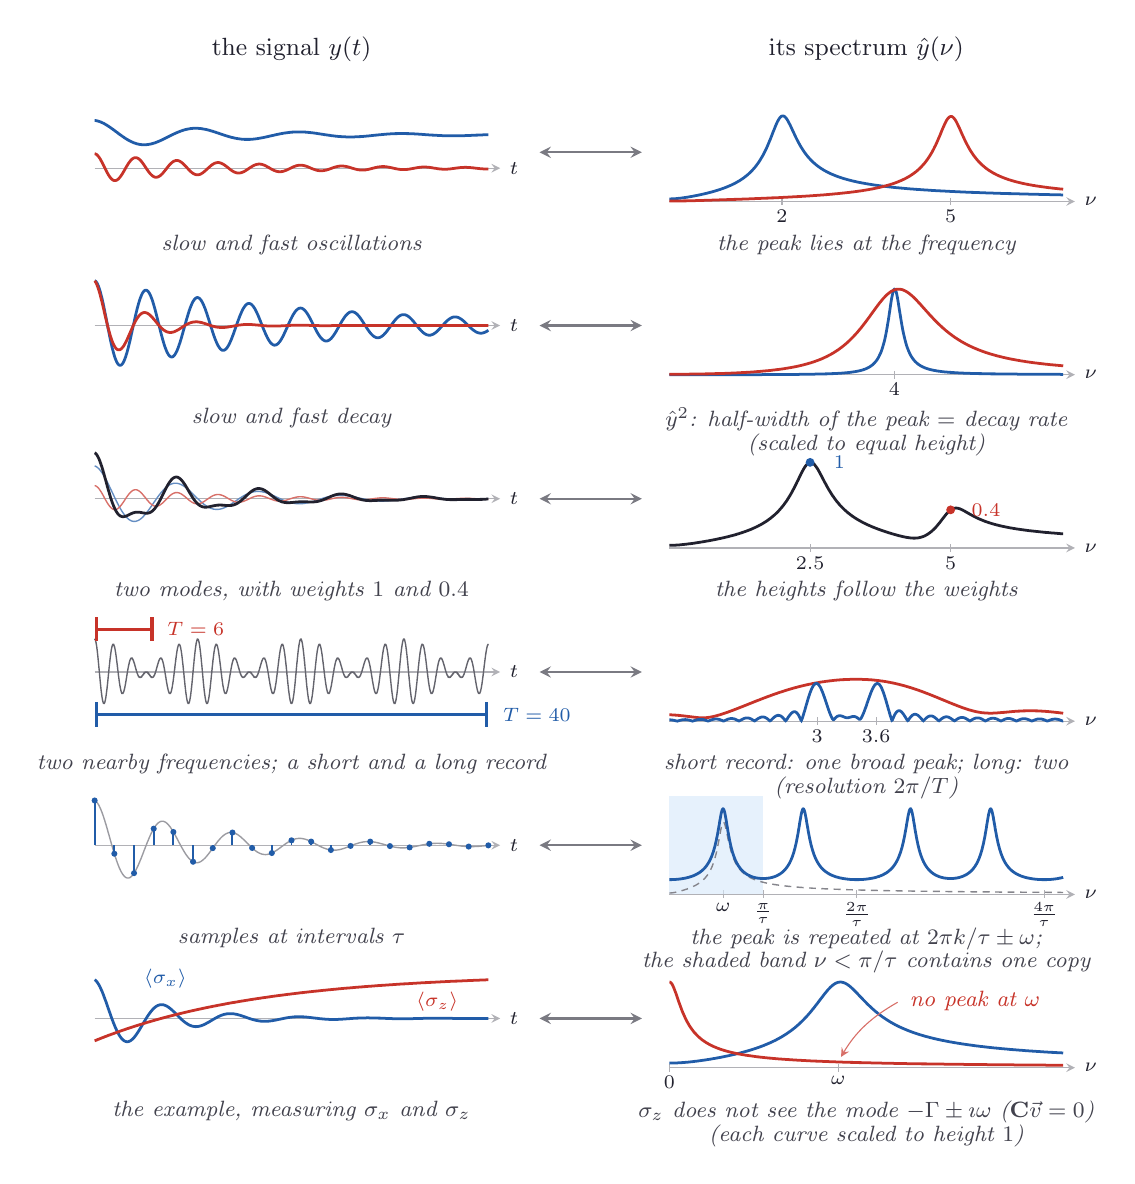
\begin{tikzpicture}[ink/.style={line width=0.9pt, ndInk}, faint/.style={line width=0.4pt, ndInk!35}, dashedink/.style={line width=0.5pt, ndInk!55, dash pattern=on 2.5pt off 2pt}, vec/.style={->, >=stealth, line width=1.2pt}, note/.style={font=\footnotesize\itshape, text=ndInk!85, align=center}, pointer/.style={->, >=stealth, line width=0.4pt, ndInk!60, shorten >=2pt, shorten <=1pt}, dot/.style={circle, fill=ndInk, inner sep=0pt, minimum size=3.4pt}, wash/.style={fill=ndSky, fill opacity=0.55}, every node/.style={text=ndInk}]
\definecolor{ndInk}{rgb}{0.13,0.13,0.18}
\definecolor{ndPaper}{rgb}{0.99,0.96,0.88}
\definecolor{ndSky}{rgb}{0.84,0.91,0.98}
\definecolor{ndRose}{rgb}{0.98,0.86,0.84}
\definecolor{ndBlue}{rgb}{0.13,0.36,0.66}
\definecolor{ndRed}{rgb}{0.78,0.20,0.16}
\definecolor{ndGold}{rgb}{0.88,0.62,0.10}
\definecolor{ndGreen}{rgb}{0.18,0.52,0.30}
\node[font=\small, anchor=south] at (2.500,0.250) {the signal $y(t)$};
\node[font=\small, anchor=south] at (9.800,0.250) {its spectrum $\abs{\hat y(\nu)}$};
\draw[faint, ->, >=stealth] (0.000,-0.977) -- (5.150,-0.977) node[right, font=\scriptsize, text=ndInk] {$t$};
\draw[faint, ->, >=stealth] (7.300,-1.400) -- (12.450,-1.400) node[right, font=\scriptsize, text=ndInk] {$\nu$};
\draw[faint] (8.729,-1.350) -- (8.729,-1.450) node[below, font=\scriptsize, text=ndInk, inner sep=1.5pt] {$2$};
\draw[faint] (10.871,-1.350) -- (10.871,-1.450) node[below, font=\scriptsize, text=ndInk, inner sep=1.5pt] {$5$};
\draw[line width=1.0pt, ndBlue] (0.000,-0.371) -- (0.006,-0.371) -- (0.011,-0.372) -- (0.017,-0.373) -- (0.022,-0.374) -- (0.028,-0.375) -- (0.033,-0.377) -- (0.039,-0.378) -- (0.044,-0.379) -- (0.050,-0.381) -- (0.056,-0.383) -- (0.061,-0.385) -- (0.067,-0.387) -- (0.072,-0.389) -- (0.078,-0.391) -- (0.083,-0.393) -- (0.089,-0.396) -- (0.095,-0.398) -- (0.100,-0.401) -- (0.106,-0.404) -- (0.111,-0.406) -- (0.117,-0.409) -- (0.122,-0.412) -- (0.128,-0.415) -- (0.133,-0.418) -- (0.139,-0.422) -- (0.145,-0.425) -- (0.150,-0.428) -- (0.156,-0.432) -- (0.161,-0.435) -- (0.167,-0.439) -- (0.172,-0.442) -- (0.178,-0.446) -- (0.184,-0.450) -- (0.189,-0.453) -- (0.195,-0.457) -- (0.200,-0.461) -- (0.206,-0.465) -- (0.211,-0.469) -- (0.217,-0.473) -- (0.222,-0.477) -- (0.228,-0.481) -- (0.234,-0.485) -- (0.239,-0.489) -- (0.245,-0.493) -- (0.250,-0.497) -- (0.256,-0.501) -- (0.261,-0.506) -- (0.267,-0.510) -- (0.273,-0.514) -- (0.278,-0.518) -- (0.284,-0.522) -- (0.289,-0.526) -- (0.295,-0.530) -- (0.300,-0.535) -- (0.306,-0.539) -- (0.311,-0.543) -- (0.317,-0.547) -- (0.323,-0.551) -- (0.328,-0.555) -- (0.334,-0.559) -- (0.339,-0.563) -- (0.345,-0.567) -- (0.350,-0.571) -- (0.356,-0.575) -- (0.362,-0.579) -- (0.367,-0.582) -- (0.373,-0.586) -- (0.378,-0.590) -- (0.384,-0.594) -- (0.389,-0.597) -- (0.395,-0.601) -- (0.400,-0.604) -- (0.406,-0.608) -- (0.412,-0.611) -- (0.417,-0.614) -- (0.423,-0.617) -- (0.428,-0.621) -- (0.434,-0.624) -- (0.439,-0.627) -- (0.445,-0.630) -- (0.451,-0.633) -- (0.456,-0.635) -- (0.462,-0.638) -- (0.467,-0.641) -- (0.473,-0.643) -- (0.478,-0.646) -- (0.484,-0.648) -- (0.489,-0.651) -- (0.495,-0.653) -- (0.501,-0.655) -- (0.506,-0.657) -- (0.512,-0.659) -- (0.517,-0.661) -- (0.523,-0.663) -- (0.528,-0.664) -- (0.534,-0.666) -- (0.539,-0.668) -- (0.545,-0.669) -- (0.551,-0.670) -- (0.556,-0.672) -- (0.562,-0.673) -- (0.567,-0.674) -- (0.573,-0.675) -- (0.578,-0.676) -- (0.584,-0.677) -- (0.590,-0.677) -- (0.595,-0.678) -- (0.601,-0.678) -- (0.606,-0.679) -- (0.612,-0.679) -- (0.617,-0.679) -- (0.623,-0.679) -- (0.628,-0.680) -- (0.634,-0.679) -- (0.640,-0.679) -- (0.645,-0.679) -- (0.651,-0.679) -- (0.656,-0.678) -- (0.662,-0.678) -- (0.667,-0.677) -- (0.673,-0.677) -- (0.679,-0.676) -- (0.684,-0.675) -- (0.690,-0.674) -- (0.695,-0.673) -- (0.701,-0.672) -- (0.706,-0.671) -- (0.712,-0.670) -- (0.717,-0.669) -- (0.723,-0.667) -- (0.729,-0.666) -- (0.734,-0.664) -- (0.740,-0.663) -- (0.745,-0.661) -- (0.751,-0.659) -- (0.756,-0.657) -- (0.762,-0.656) -- (0.768,-0.654) -- (0.773,-0.652) -- (0.779,-0.650) -- (0.784,-0.648) -- (0.790,-0.646) -- (0.795,-0.643) -- (0.801,-0.641) -- (0.806,-0.639) -- (0.812,-0.637) -- (0.818,-0.634) -- (0.823,-0.632) -- (0.829,-0.629) -- (0.834,-0.627) -- (0.840,-0.624) -- (0.845,-0.622) -- (0.851,-0.619) -- (0.857,-0.617) -- (0.862,-0.614) -- (0.868,-0.611) -- (0.873,-0.609) -- (0.879,-0.606) -- (0.884,-0.603) -- (0.890,-0.600) -- (0.895,-0.598) -- (0.901,-0.595) -- (0.907,-0.592) -- (0.912,-0.589) -- (0.918,-0.586) -- (0.923,-0.584) -- (0.929,-0.581) -- (0.934,-0.578) -- (0.940,-0.575) -- (0.945,-0.572) -- (0.951,-0.570) -- (0.957,-0.567) -- (0.962,-0.564) -- (0.968,-0.561) -- (0.973,-0.559) -- (0.979,-0.556) -- (0.984,-0.553) -- (0.990,-0.550) -- (0.996,-0.548) -- (1.001,-0.545) -- (1.007,-0.542) -- (1.012,-0.540) -- (1.018,-0.537) -- (1.023,-0.535) -- (1.029,-0.532) -- (1.034,-0.530) -- (1.040,-0.527) -- (1.046,-0.525) -- (1.051,-0.522) -- (1.057,-0.520) -- (1.062,-0.518) -- (1.068,-0.516) -- (1.073,-0.513) -- (1.079,-0.511) -- (1.085,-0.509) -- (1.090,-0.507) -- (1.096,-0.505) -- (1.101,-0.503) -- (1.107,-0.501) -- (1.112,-0.499) -- (1.118,-0.497) -- (1.123,-0.495) -- (1.129,-0.494) -- (1.135,-0.492) -- (1.140,-0.490) -- (1.146,-0.489) -- (1.151,-0.487) -- (1.157,-0.486) -- (1.162,-0.485) -- (1.168,-0.483) -- (1.174,-0.482) -- (1.179,-0.481) -- (1.185,-0.480) -- (1.190,-0.479) -- (1.196,-0.478) -- (1.201,-0.477) -- (1.207,-0.476) -- (1.212,-0.475) -- (1.218,-0.474) -- (1.224,-0.474) -- (1.229,-0.473) -- (1.235,-0.472) -- (1.240,-0.472) -- (1.246,-0.471) -- (1.251,-0.471) -- (1.257,-0.471) -- (1.263,-0.470) -- (1.268,-0.470) -- (1.274,-0.470) -- (1.279,-0.470) -- (1.285,-0.470) -- (1.290,-0.470) -- (1.296,-0.470) -- (1.301,-0.470) -- (1.307,-0.471) -- (1.313,-0.471) -- (1.318,-0.471) -- (1.324,-0.472) -- (1.329,-0.472) -- (1.335,-0.473) -- (1.340,-0.473) -- (1.346,-0.474) -- (1.352,-0.474) -- (1.357,-0.475) -- (1.363,-0.476) -- (1.368,-0.477) -- (1.374,-0.478) -- (1.379,-0.479) -- (1.385,-0.480) -- (1.390,-0.481) -- (1.396,-0.482) -- (1.402,-0.483) -- (1.407,-0.484) -- (1.413,-0.485) -- (1.418,-0.486) -- (1.424,-0.488) -- (1.429,-0.489) -- (1.435,-0.490) -- (1.440,-0.492) -- (1.446,-0.493) -- (1.452,-0.495) -- (1.457,-0.496) -- (1.463,-0.498) -- (1.468,-0.499) -- (1.474,-0.501) -- (1.479,-0.503) -- (1.485,-0.504) -- (1.491,-0.506) -- (1.496,-0.508) -- (1.502,-0.509) -- (1.507,-0.511) -- (1.513,-0.513) -- (1.518,-0.515) -- (1.524,-0.517) -- (1.529,-0.518) -- (1.535,-0.520) -- (1.541,-0.522) -- (1.546,-0.524) -- (1.552,-0.526) -- (1.557,-0.528) -- (1.563,-0.530) -- (1.568,-0.531) -- (1.574,-0.533) -- (1.580,-0.535) -- (1.585,-0.537) -- (1.591,-0.539) -- (1.596,-0.541) -- (1.602,-0.543) -- (1.607,-0.545) -- (1.613,-0.547) -- (1.618,-0.548) -- (1.624,-0.550) -- (1.630,-0.552) -- (1.635,-0.554) -- (1.641,-0.556) -- (1.646,-0.558) -- (1.652,-0.560) -- (1.657,-0.561) -- (1.663,-0.563) -- (1.669,-0.565) -- (1.674,-0.567) -- (1.680,-0.568) -- (1.685,-0.570) -- (1.691,-0.572) -- (1.696,-0.573) -- (1.702,-0.575) -- (1.707,-0.577) -- (1.713,-0.578) -- (1.719,-0.580) -- (1.724,-0.581) -- (1.730,-0.583) -- (1.735,-0.584) -- (1.741,-0.586) -- (1.746,-0.587) -- (1.752,-0.588) -- (1.758,-0.590) -- (1.763,-0.591) -- (1.769,-0.592) -- (1.774,-0.593) -- (1.780,-0.595) -- (1.785,-0.596) -- (1.791,-0.597) -- (1.796,-0.598) -- (1.802,-0.599) -- (1.808,-0.600) -- (1.813,-0.601) -- (1.819,-0.602) -- (1.824,-0.603) -- (1.830,-0.604) -- (1.835,-0.604) -- (1.841,-0.605) -- (1.846,-0.606) -- (1.852,-0.606) -- (1.858,-0.607) -- (1.863,-0.608) -- (1.869,-0.608) -- (1.874,-0.609) -- (1.880,-0.609) -- (1.885,-0.610) -- (1.891,-0.610) -- (1.897,-0.610) -- (1.902,-0.611) -- (1.908,-0.611) -- (1.913,-0.611) -- (1.919,-0.611) -- (1.924,-0.611) -- (1.930,-0.611) -- (1.935,-0.611) -- (1.941,-0.611) -- (1.947,-0.611) -- (1.952,-0.611) -- (1.958,-0.611) -- (1.963,-0.611) -- (1.969,-0.611) -- (1.974,-0.611) -- (1.980,-0.610) -- (1.986,-0.610) -- (1.991,-0.610) -- (1.997,-0.609) -- (2.002,-0.609) -- (2.008,-0.608) -- (2.013,-0.608) -- (2.019,-0.607) -- (2.024,-0.607) -- (2.030,-0.606) -- (2.036,-0.605) -- (2.041,-0.605) -- (2.047,-0.604) -- (2.052,-0.603) -- (2.058,-0.602) -- (2.063,-0.602) -- (2.069,-0.601) -- (2.075,-0.600) -- (2.080,-0.599) -- (2.086,-0.598) -- (2.091,-0.597) -- (2.097,-0.596) -- (2.102,-0.595) -- (2.108,-0.594) -- (2.113,-0.593) -- (2.119,-0.592) -- (2.125,-0.591) -- (2.130,-0.590) -- (2.136,-0.589) -- (2.141,-0.588) -- (2.147,-0.587) -- (2.152,-0.586) -- (2.158,-0.584) -- (2.164,-0.583) -- (2.169,-0.582) -- (2.175,-0.581) -- (2.180,-0.580) -- (2.186,-0.578) -- (2.191,-0.577) -- (2.197,-0.576) -- (2.202,-0.575) -- (2.208,-0.573) -- (2.214,-0.572) -- (2.219,-0.571) -- (2.225,-0.569) -- (2.230,-0.568) -- (2.236,-0.567) -- (2.241,-0.566) -- (2.247,-0.564) -- (2.253,-0.563) -- (2.258,-0.562) -- (2.264,-0.561) -- (2.269,-0.559) -- (2.275,-0.558) -- (2.280,-0.557) -- (2.286,-0.556) -- (2.291,-0.554) -- (2.297,-0.553) -- (2.303,-0.552) -- (2.308,-0.551) -- (2.314,-0.549) -- (2.319,-0.548) -- (2.325,-0.547) -- (2.330,-0.546) -- (2.336,-0.545) -- (2.341,-0.544) -- (2.347,-0.542) -- (2.353,-0.541) -- (2.358,-0.540) -- (2.364,-0.539) -- (2.369,-0.538) -- (2.375,-0.537) -- (2.380,-0.536) -- (2.386,-0.535) -- (2.392,-0.534) -- (2.397,-0.533) -- (2.403,-0.532) -- (2.408,-0.531) -- (2.414,-0.530) -- (2.419,-0.529) -- (2.425,-0.529) -- (2.430,-0.528) -- (2.436,-0.527) -- (2.442,-0.526) -- (2.447,-0.526) -- (2.453,-0.525) -- (2.458,-0.524) -- (2.464,-0.523) -- (2.469,-0.523) -- (2.475,-0.522) -- (2.481,-0.522) -- (2.486,-0.521) -- (2.492,-0.521) -- (2.497,-0.520) -- (2.503,-0.520) -- (2.508,-0.519) -- (2.514,-0.519) -- (2.519,-0.518) -- (2.525,-0.518) -- (2.531,-0.518) -- (2.536,-0.517) -- (2.542,-0.517) -- (2.547,-0.517) -- (2.553,-0.517) -- (2.558,-0.516) -- (2.564,-0.516) -- (2.570,-0.516) -- (2.575,-0.516) -- (2.581,-0.516) -- (2.586,-0.516) -- (2.592,-0.516) -- (2.597,-0.516) -- (2.603,-0.516) -- (2.608,-0.516) -- (2.614,-0.516) -- (2.620,-0.516) -- (2.625,-0.516) -- (2.631,-0.517) -- (2.636,-0.517) -- (2.642,-0.517) -- (2.647,-0.517) -- (2.653,-0.518) -- (2.659,-0.518) -- (2.664,-0.518) -- (2.670,-0.518) -- (2.675,-0.519) -- (2.681,-0.519) -- (2.686,-0.520) -- (2.692,-0.520) -- (2.697,-0.521) -- (2.703,-0.521) -- (2.709,-0.522) -- (2.714,-0.522) -- (2.720,-0.523) -- (2.725,-0.523) -- (2.731,-0.524) -- (2.736,-0.524) -- (2.742,-0.525) -- (2.747,-0.526) -- (2.753,-0.526) -- (2.759,-0.527) -- (2.764,-0.528) -- (2.770,-0.528) -- (2.775,-0.529) -- (2.781,-0.530) -- (2.786,-0.531) -- (2.792,-0.531) -- (2.798,-0.532) -- (2.803,-0.533) -- (2.809,-0.534) -- (2.814,-0.534) -- (2.820,-0.535) -- (2.825,-0.536) -- (2.831,-0.537) -- (2.836,-0.538) -- (2.842,-0.539) -- (2.848,-0.539) -- (2.853,-0.540) -- (2.859,-0.541) -- (2.864,-0.542) -- (2.870,-0.543) -- (2.875,-0.544) -- (2.881,-0.545) -- (2.887,-0.545) -- (2.892,-0.546) -- (2.898,-0.547) -- (2.903,-0.548) -- (2.909,-0.549) -- (2.914,-0.550) -- (2.920,-0.551) -- (2.925,-0.551) -- (2.931,-0.552) -- (2.937,-0.553) -- (2.942,-0.554) -- (2.948,-0.555) -- (2.953,-0.556) -- (2.959,-0.556) -- (2.964,-0.557) -- (2.970,-0.558) -- (2.976,-0.559) -- (2.981,-0.560) -- (2.987,-0.560) -- (2.992,-0.561) -- (2.998,-0.562) -- (3.003,-0.563) -- (3.009,-0.564) -- (3.014,-0.564) -- (3.020,-0.565) -- (3.026,-0.566) -- (3.031,-0.566) -- (3.037,-0.567) -- (3.042,-0.568) -- (3.048,-0.568) -- (3.053,-0.569) -- (3.059,-0.570) -- (3.065,-0.570) -- (3.070,-0.571) -- (3.076,-0.571) -- (3.081,-0.572) -- (3.087,-0.573) -- (3.092,-0.573) -- (3.098,-0.574) -- (3.103,-0.574) -- (3.109,-0.575) -- (3.115,-0.575) -- (3.120,-0.575) -- (3.126,-0.576) -- (3.131,-0.576) -- (3.137,-0.577) -- (3.142,-0.577) -- (3.148,-0.577) -- (3.154,-0.578) -- (3.159,-0.578) -- (3.165,-0.578) -- (3.170,-0.579) -- (3.176,-0.579) -- (3.181,-0.579) -- (3.187,-0.579) -- (3.192,-0.580) -- (3.198,-0.580) -- (3.204,-0.580) -- (3.209,-0.580) -- (3.215,-0.580) -- (3.220,-0.580) -- (3.226,-0.580) -- (3.231,-0.580) -- (3.237,-0.580) -- (3.242,-0.580) -- (3.248,-0.580) -- (3.254,-0.580) -- (3.259,-0.580) -- (3.265,-0.580) -- (3.270,-0.580) -- (3.276,-0.580) -- (3.281,-0.580) -- (3.287,-0.580) -- (3.293,-0.580) -- (3.298,-0.580) -- (3.304,-0.579) -- (3.309,-0.579) -- (3.315,-0.579) -- (3.320,-0.579) -- (3.326,-0.579) -- (3.331,-0.578) -- (3.337,-0.578) -- (3.343,-0.578) -- (3.348,-0.577) -- (3.354,-0.577) -- (3.359,-0.577) -- (3.365,-0.576) -- (3.370,-0.576) -- (3.376,-0.576) -- (3.382,-0.575) -- (3.387,-0.575) -- (3.393,-0.575) -- (3.398,-0.574) -- (3.404,-0.574) -- (3.409,-0.573) -- (3.415,-0.573) -- (3.420,-0.572) -- (3.426,-0.572) -- (3.432,-0.571) -- (3.437,-0.571) -- (3.443,-0.570) -- (3.448,-0.570) -- (3.454,-0.569) -- (3.459,-0.569) -- (3.465,-0.568) -- (3.471,-0.568) -- (3.476,-0.567) -- (3.482,-0.567) -- (3.487,-0.566) -- (3.493,-0.566) -- (3.498,-0.565) -- (3.504,-0.564) -- (3.509,-0.564) -- (3.515,-0.563) -- (3.521,-0.563) -- (3.526,-0.562) -- (3.532,-0.561) -- (3.537,-0.561) -- (3.543,-0.560) -- (3.548,-0.560) -- (3.554,-0.559) -- (3.560,-0.559) -- (3.565,-0.558) -- (3.571,-0.557) -- (3.576,-0.557) -- (3.582,-0.556) -- (3.587,-0.556) -- (3.593,-0.555) -- (3.598,-0.555) -- (3.604,-0.554) -- (3.610,-0.553) -- (3.615,-0.553) -- (3.621,-0.552) -- (3.626,-0.552) -- (3.632,-0.551) -- (3.637,-0.551) -- (3.643,-0.550) -- (3.648,-0.550) -- (3.654,-0.549) -- (3.660,-0.549) -- (3.665,-0.548) -- (3.671,-0.548) -- (3.676,-0.547) -- (3.682,-0.547) -- (3.687,-0.546) -- (3.693,-0.546) -- (3.699,-0.545) -- (3.704,-0.545) -- (3.710,-0.544) -- (3.715,-0.544) -- (3.721,-0.544) -- (3.726,-0.543) -- (3.732,-0.543) -- (3.737,-0.542) -- (3.743,-0.542) -- (3.749,-0.542) -- (3.754,-0.541) -- (3.760,-0.541) -- (3.765,-0.541) -- (3.771,-0.540) -- (3.776,-0.540) -- (3.782,-0.540) -- (3.788,-0.540) -- (3.793,-0.539) -- (3.799,-0.539) -- (3.804,-0.539) -- (3.810,-0.539) -- (3.815,-0.538) -- (3.821,-0.538) -- (3.826,-0.538) -- (3.832,-0.538) -- (3.838,-0.538) -- (3.843,-0.538) -- (3.849,-0.537) -- (3.854,-0.537) -- (3.860,-0.537) -- (3.865,-0.537) -- (3.871,-0.537) -- (3.877,-0.537) -- (3.882,-0.537) -- (3.888,-0.537) -- (3.893,-0.537) -- (3.899,-0.537) -- (3.904,-0.537) -- (3.910,-0.537) -- (3.915,-0.537) -- (3.921,-0.537) -- (3.927,-0.537) -- (3.932,-0.537) -- (3.938,-0.537) -- (3.943,-0.537) -- (3.949,-0.537) -- (3.954,-0.537) -- (3.960,-0.538) -- (3.966,-0.538) -- (3.971,-0.538) -- (3.977,-0.538) -- (3.982,-0.538) -- (3.988,-0.538) -- (3.993,-0.539) -- (3.999,-0.539) -- (4.004,-0.539) -- (4.010,-0.539) -- (4.016,-0.539) -- (4.021,-0.540) -- (4.027,-0.540) -- (4.032,-0.540) -- (4.038,-0.540) -- (4.043,-0.541) -- (4.049,-0.541) -- (4.055,-0.541) -- (4.060,-0.541) -- (4.066,-0.542) -- (4.071,-0.542) -- (4.077,-0.542) -- (4.082,-0.543) -- (4.088,-0.543) -- (4.093,-0.543) -- (4.099,-0.544) -- (4.105,-0.544) -- (4.110,-0.544) -- (4.116,-0.545) -- (4.121,-0.545) -- (4.127,-0.546) -- (4.132,-0.546) -- (4.138,-0.546) -- (4.143,-0.547) -- (4.149,-0.547) -- (4.155,-0.547) -- (4.160,-0.548) -- (4.166,-0.548) -- (4.171,-0.549) -- (4.177,-0.549) -- (4.182,-0.549) -- (4.188,-0.550) -- (4.194,-0.550) -- (4.199,-0.551) -- (4.205,-0.551) -- (4.210,-0.551) -- (4.216,-0.552) -- (4.221,-0.552) -- (4.227,-0.553) -- (4.232,-0.553) -- (4.238,-0.553) -- (4.244,-0.554) -- (4.249,-0.554) -- (4.255,-0.554) -- (4.260,-0.555) -- (4.266,-0.555) -- (4.271,-0.556) -- (4.277,-0.556) -- (4.283,-0.556) -- (4.288,-0.557) -- (4.294,-0.557) -- (4.299,-0.557) -- (4.305,-0.558) -- (4.310,-0.558) -- (4.316,-0.558) -- (4.321,-0.559) -- (4.327,-0.559) -- (4.333,-0.559) -- (4.338,-0.560) -- (4.344,-0.560) -- (4.349,-0.560) -- (4.355,-0.561) -- (4.360,-0.561) -- (4.366,-0.561) -- (4.372,-0.562) -- (4.377,-0.562) -- (4.383,-0.562) -- (4.388,-0.562) -- (4.394,-0.563) -- (4.399,-0.563) -- (4.405,-0.563) -- (4.410,-0.563) -- (4.416,-0.564) -- (4.422,-0.564) -- (4.427,-0.564) -- (4.433,-0.564) -- (4.438,-0.564) -- (4.444,-0.564) -- (4.449,-0.565) -- (4.455,-0.565) -- (4.461,-0.565) -- (4.466,-0.565) -- (4.472,-0.565) -- (4.477,-0.565) -- (4.483,-0.566) -- (4.488,-0.566) -- (4.494,-0.566) -- (4.499,-0.566) -- (4.505,-0.566) -- (4.511,-0.566) -- (4.516,-0.566) -- (4.522,-0.566) -- (4.527,-0.566) -- (4.533,-0.566) -- (4.538,-0.566) -- (4.544,-0.566) -- (4.549,-0.566) -- (4.555,-0.566) -- (4.561,-0.566) -- (4.566,-0.566) -- (4.572,-0.566) -- (4.577,-0.566) -- (4.583,-0.566) -- (4.588,-0.566) -- (4.594,-0.566) -- (4.600,-0.566) -- (4.605,-0.566) -- (4.611,-0.566) -- (4.616,-0.566) -- (4.622,-0.566) -- (4.627,-0.566) -- (4.633,-0.565) -- (4.638,-0.565) -- (4.644,-0.565) -- (4.650,-0.565) -- (4.655,-0.565) -- (4.661,-0.565) -- (4.666,-0.565) -- (4.672,-0.565) -- (4.677,-0.564) -- (4.683,-0.564) -- (4.689,-0.564) -- (4.694,-0.564) -- (4.700,-0.564) -- (4.705,-0.563) -- (4.711,-0.563) -- (4.716,-0.563) -- (4.722,-0.563) -- (4.727,-0.563) -- (4.733,-0.562) -- (4.739,-0.562) -- (4.744,-0.562) -- (4.750,-0.562) -- (4.755,-0.562) -- (4.761,-0.561) -- (4.766,-0.561) -- (4.772,-0.561) -- (4.778,-0.561) -- (4.783,-0.560) -- (4.789,-0.560) -- (4.794,-0.560) -- (4.800,-0.560) -- (4.805,-0.559) -- (4.811,-0.559) -- (4.816,-0.559) -- (4.822,-0.559) -- (4.828,-0.558) -- (4.833,-0.558) -- (4.839,-0.558) -- (4.844,-0.557) -- (4.850,-0.557) -- (4.855,-0.557) -- (4.861,-0.557) -- (4.867,-0.556) -- (4.872,-0.556) -- (4.878,-0.556) -- (4.883,-0.556) -- (4.889,-0.555) -- (4.894,-0.555) -- (4.900,-0.555) -- (4.905,-0.555) -- (4.911,-0.554) -- (4.917,-0.554) -- (4.922,-0.554) -- (4.928,-0.554) -- (4.933,-0.553) -- (4.939,-0.553) -- (4.944,-0.553) -- (4.950,-0.553) -- (4.956,-0.552) -- (4.961,-0.552) -- (4.967,-0.552) -- (4.972,-0.552) -- (4.978,-0.551) -- (4.983,-0.551) -- (4.989,-0.551) -- (4.994,-0.551) -- (5.000,-0.551);
\draw[line width=1.0pt, ndRed] (0.000,-0.793) -- (0.006,-0.794) -- (0.011,-0.796) -- (0.017,-0.799) -- (0.022,-0.802) -- (0.028,-0.806) -- (0.033,-0.811) -- (0.039,-0.817) -- (0.044,-0.823) -- (0.050,-0.830) -- (0.056,-0.838) -- (0.061,-0.846) -- (0.067,-0.854) -- (0.072,-0.863) -- (0.078,-0.873) -- (0.083,-0.883) -- (0.089,-0.893) -- (0.095,-0.904) -- (0.100,-0.915) -- (0.106,-0.926) -- (0.111,-0.937) -- (0.117,-0.948) -- (0.122,-0.960) -- (0.128,-0.971) -- (0.133,-0.982) -- (0.139,-0.994) -- (0.145,-1.005) -- (0.150,-1.016) -- (0.156,-1.026) -- (0.161,-1.037) -- (0.167,-1.047) -- (0.172,-1.056) -- (0.178,-1.066) -- (0.184,-1.074) -- (0.189,-1.083) -- (0.195,-1.090) -- (0.200,-1.098) -- (0.206,-1.104) -- (0.211,-1.110) -- (0.217,-1.116) -- (0.222,-1.120) -- (0.228,-1.125) -- (0.234,-1.128) -- (0.239,-1.131) -- (0.245,-1.133) -- (0.250,-1.134) -- (0.256,-1.134) -- (0.261,-1.134) -- (0.267,-1.134) -- (0.273,-1.132) -- (0.278,-1.130) -- (0.284,-1.127) -- (0.289,-1.123) -- (0.295,-1.119) -- (0.300,-1.115) -- (0.306,-1.109) -- (0.311,-1.103) -- (0.317,-1.097) -- (0.323,-1.090) -- (0.328,-1.083) -- (0.334,-1.075) -- (0.339,-1.067) -- (0.345,-1.058) -- (0.350,-1.050) -- (0.356,-1.041) -- (0.362,-1.031) -- (0.367,-1.022) -- (0.373,-1.012) -- (0.378,-1.003) -- (0.384,-0.993) -- (0.389,-0.983) -- (0.395,-0.973) -- (0.400,-0.964) -- (0.406,-0.954) -- (0.412,-0.945) -- (0.417,-0.936) -- (0.423,-0.927) -- (0.428,-0.918) -- (0.434,-0.910) -- (0.439,-0.902) -- (0.445,-0.895) -- (0.451,-0.888) -- (0.456,-0.881) -- (0.462,-0.875) -- (0.467,-0.869) -- (0.473,-0.864) -- (0.478,-0.859) -- (0.484,-0.855) -- (0.489,-0.852) -- (0.495,-0.849) -- (0.501,-0.846) -- (0.506,-0.844) -- (0.512,-0.843) -- (0.517,-0.843) -- (0.523,-0.843) -- (0.528,-0.844) -- (0.534,-0.845) -- (0.539,-0.847) -- (0.545,-0.849) -- (0.551,-0.852) -- (0.556,-0.855) -- (0.562,-0.859) -- (0.567,-0.864) -- (0.573,-0.869) -- (0.578,-0.874) -- (0.584,-0.880) -- (0.590,-0.886) -- (0.595,-0.893) -- (0.601,-0.900) -- (0.606,-0.907) -- (0.612,-0.915) -- (0.617,-0.922) -- (0.623,-0.930) -- (0.628,-0.938) -- (0.634,-0.947) -- (0.640,-0.955) -- (0.645,-0.963) -- (0.651,-0.972) -- (0.656,-0.980) -- (0.662,-0.988) -- (0.667,-0.996) -- (0.673,-1.004) -- (0.679,-1.012) -- (0.684,-1.020) -- (0.690,-1.027) -- (0.695,-1.034) -- (0.701,-1.041) -- (0.706,-1.047) -- (0.712,-1.053) -- (0.717,-1.059) -- (0.723,-1.064) -- (0.729,-1.069) -- (0.734,-1.074) -- (0.740,-1.078) -- (0.745,-1.081) -- (0.751,-1.084) -- (0.756,-1.087) -- (0.762,-1.089) -- (0.768,-1.091) -- (0.773,-1.092) -- (0.779,-1.092) -- (0.784,-1.092) -- (0.790,-1.091) -- (0.795,-1.090) -- (0.801,-1.089) -- (0.806,-1.087) -- (0.812,-1.084) -- (0.818,-1.081) -- (0.823,-1.078) -- (0.829,-1.074) -- (0.834,-1.070) -- (0.840,-1.065) -- (0.845,-1.060) -- (0.851,-1.055) -- (0.857,-1.050) -- (0.862,-1.044) -- (0.868,-1.037) -- (0.873,-1.031) -- (0.879,-1.024) -- (0.884,-1.018) -- (0.890,-1.011) -- (0.895,-1.004) -- (0.901,-0.997) -- (0.907,-0.990) -- (0.912,-0.983) -- (0.918,-0.975) -- (0.923,-0.968) -- (0.929,-0.961) -- (0.934,-0.955) -- (0.940,-0.948) -- (0.945,-0.941) -- (0.951,-0.935) -- (0.957,-0.929) -- (0.962,-0.923) -- (0.968,-0.918) -- (0.973,-0.912) -- (0.979,-0.908) -- (0.984,-0.903) -- (0.990,-0.899) -- (0.996,-0.895) -- (1.001,-0.891) -- (1.007,-0.888) -- (1.012,-0.886) -- (1.018,-0.884) -- (1.023,-0.882) -- (1.029,-0.880) -- (1.034,-0.880) -- (1.040,-0.879) -- (1.046,-0.879) -- (1.051,-0.879) -- (1.057,-0.880) -- (1.062,-0.882) -- (1.068,-0.883) -- (1.073,-0.885) -- (1.079,-0.888) -- (1.085,-0.891) -- (1.090,-0.894) -- (1.096,-0.898) -- (1.101,-0.902) -- (1.107,-0.906) -- (1.112,-0.910) -- (1.118,-0.915) -- (1.123,-0.920) -- (1.129,-0.925) -- (1.135,-0.931) -- (1.140,-0.936) -- (1.146,-0.942) -- (1.151,-0.948) -- (1.157,-0.954) -- (1.162,-0.960) -- (1.168,-0.966) -- (1.174,-0.972) -- (1.179,-0.978) -- (1.185,-0.984) -- (1.190,-0.990) -- (1.196,-0.996) -- (1.201,-1.002) -- (1.207,-1.007) -- (1.212,-1.013) -- (1.218,-1.018) -- (1.224,-1.023) -- (1.229,-1.028) -- (1.235,-1.032) -- (1.240,-1.036) -- (1.246,-1.040) -- (1.251,-1.044) -- (1.257,-1.047) -- (1.263,-1.050) -- (1.268,-1.053) -- (1.274,-1.055) -- (1.279,-1.057) -- (1.285,-1.059) -- (1.290,-1.060) -- (1.296,-1.061) -- (1.301,-1.061) -- (1.307,-1.061) -- (1.313,-1.061) -- (1.318,-1.060) -- (1.324,-1.059) -- (1.329,-1.058) -- (1.335,-1.056) -- (1.340,-1.054) -- (1.346,-1.051) -- (1.352,-1.049) -- (1.357,-1.045) -- (1.363,-1.042) -- (1.368,-1.039) -- (1.374,-1.035) -- (1.379,-1.031) -- (1.385,-1.026) -- (1.390,-1.022) -- (1.396,-1.017) -- (1.402,-1.012) -- (1.407,-1.007) -- (1.413,-1.002) -- (1.418,-0.997) -- (1.424,-0.992) -- (1.429,-0.987) -- (1.435,-0.982) -- (1.440,-0.977) -- (1.446,-0.972) -- (1.452,-0.966) -- (1.457,-0.961) -- (1.463,-0.957) -- (1.468,-0.952) -- (1.474,-0.947) -- (1.479,-0.943) -- (1.485,-0.938) -- (1.491,-0.934) -- (1.496,-0.930) -- (1.502,-0.927) -- (1.507,-0.923) -- (1.513,-0.920) -- (1.518,-0.917) -- (1.524,-0.915) -- (1.529,-0.913) -- (1.535,-0.911) -- (1.541,-0.909) -- (1.546,-0.908) -- (1.552,-0.907) -- (1.557,-0.906) -- (1.563,-0.906) -- (1.568,-0.906) -- (1.574,-0.906) -- (1.580,-0.906) -- (1.585,-0.907) -- (1.591,-0.908) -- (1.596,-0.910) -- (1.602,-0.912) -- (1.607,-0.914) -- (1.613,-0.916) -- (1.618,-0.919) -- (1.624,-0.922) -- (1.630,-0.925) -- (1.635,-0.928) -- (1.641,-0.931) -- (1.646,-0.935) -- (1.652,-0.939) -- (1.657,-0.943) -- (1.663,-0.947) -- (1.669,-0.951) -- (1.674,-0.955) -- (1.680,-0.960) -- (1.685,-0.964) -- (1.691,-0.968) -- (1.696,-0.973) -- (1.702,-0.977) -- (1.707,-0.982) -- (1.713,-0.986) -- (1.719,-0.990) -- (1.724,-0.995) -- (1.730,-0.999) -- (1.735,-1.003) -- (1.741,-1.006) -- (1.746,-1.010) -- (1.752,-1.014) -- (1.758,-1.017) -- (1.763,-1.020) -- (1.769,-1.023) -- (1.774,-1.026) -- (1.780,-1.028) -- (1.785,-1.030) -- (1.791,-1.032) -- (1.796,-1.034) -- (1.802,-1.035) -- (1.808,-1.037) -- (1.813,-1.037) -- (1.819,-1.038) -- (1.824,-1.038) -- (1.830,-1.038) -- (1.835,-1.038) -- (1.841,-1.038) -- (1.846,-1.037) -- (1.852,-1.036) -- (1.858,-1.035) -- (1.863,-1.033) -- (1.869,-1.032) -- (1.874,-1.030) -- (1.880,-1.027) -- (1.885,-1.025) -- (1.891,-1.022) -- (1.897,-1.020) -- (1.902,-1.017) -- (1.908,-1.014) -- (1.913,-1.010) -- (1.919,-1.007) -- (1.924,-1.003) -- (1.930,-1.000) -- (1.935,-0.996) -- (1.941,-0.992) -- (1.947,-0.989) -- (1.952,-0.985) -- (1.958,-0.981) -- (1.963,-0.977) -- (1.969,-0.974) -- (1.974,-0.970) -- (1.980,-0.966) -- (1.986,-0.963) -- (1.991,-0.959) -- (1.997,-0.956) -- (2.002,-0.952) -- (2.008,-0.949) -- (2.013,-0.946) -- (2.019,-0.943) -- (2.024,-0.941) -- (2.030,-0.938) -- (2.036,-0.936) -- (2.041,-0.934) -- (2.047,-0.932) -- (2.052,-0.930) -- (2.058,-0.929) -- (2.063,-0.928) -- (2.069,-0.927) -- (2.075,-0.926) -- (2.080,-0.925) -- (2.086,-0.925) -- (2.091,-0.925) -- (2.097,-0.925) -- (2.102,-0.925) -- (2.108,-0.926) -- (2.113,-0.927) -- (2.119,-0.928) -- (2.125,-0.929) -- (2.130,-0.931) -- (2.136,-0.932) -- (2.141,-0.934) -- (2.147,-0.936) -- (2.152,-0.938) -- (2.158,-0.941) -- (2.164,-0.943) -- (2.169,-0.946) -- (2.175,-0.949) -- (2.180,-0.952) -- (2.186,-0.955) -- (2.191,-0.958) -- (2.197,-0.961) -- (2.202,-0.964) -- (2.208,-0.967) -- (2.214,-0.970) -- (2.219,-0.974) -- (2.225,-0.977) -- (2.230,-0.980) -- (2.236,-0.983) -- (2.241,-0.986) -- (2.247,-0.989) -- (2.253,-0.992) -- (2.258,-0.995) -- (2.264,-0.998) -- (2.269,-1.001) -- (2.275,-1.003) -- (2.280,-1.006) -- (2.286,-1.008) -- (2.291,-1.010) -- (2.297,-1.012) -- (2.303,-1.014) -- (2.308,-1.016) -- (2.314,-1.017) -- (2.319,-1.019) -- (2.325,-1.020) -- (2.330,-1.020) -- (2.336,-1.021) -- (2.341,-1.022) -- (2.347,-1.022) -- (2.353,-1.022) -- (2.358,-1.022) -- (2.364,-1.022) -- (2.369,-1.021) -- (2.375,-1.020) -- (2.380,-1.019) -- (2.386,-1.018) -- (2.392,-1.017) -- (2.397,-1.016) -- (2.403,-1.014) -- (2.408,-1.012) -- (2.414,-1.010) -- (2.419,-1.008) -- (2.425,-1.006) -- (2.430,-1.004) -- (2.436,-1.002) -- (2.442,-0.999) -- (2.447,-0.997) -- (2.453,-0.994) -- (2.458,-0.991) -- (2.464,-0.989) -- (2.469,-0.986) -- (2.475,-0.983) -- (2.481,-0.980) -- (2.486,-0.978) -- (2.492,-0.975) -- (2.497,-0.972) -- (2.503,-0.970) -- (2.508,-0.967) -- (2.514,-0.964) -- (2.519,-0.962) -- (2.525,-0.959) -- (2.531,-0.957) -- (2.536,-0.955) -- (2.542,-0.953) -- (2.547,-0.951) -- (2.553,-0.949) -- (2.558,-0.947) -- (2.564,-0.946) -- (2.570,-0.944) -- (2.575,-0.943) -- (2.581,-0.942) -- (2.586,-0.941) -- (2.592,-0.940) -- (2.597,-0.940) -- (2.603,-0.939) -- (2.608,-0.939) -- (2.614,-0.939) -- (2.620,-0.939) -- (2.625,-0.939) -- (2.631,-0.940) -- (2.636,-0.940) -- (2.642,-0.941) -- (2.647,-0.942) -- (2.653,-0.943) -- (2.659,-0.944) -- (2.664,-0.946) -- (2.670,-0.947) -- (2.675,-0.949) -- (2.681,-0.950) -- (2.686,-0.952) -- (2.692,-0.954) -- (2.697,-0.956) -- (2.703,-0.958) -- (2.709,-0.960) -- (2.714,-0.963) -- (2.720,-0.965) -- (2.725,-0.967) -- (2.731,-0.970) -- (2.736,-0.972) -- (2.742,-0.974) -- (2.747,-0.977) -- (2.753,-0.979) -- (2.759,-0.981) -- (2.764,-0.984) -- (2.770,-0.986) -- (2.775,-0.988) -- (2.781,-0.990) -- (2.786,-0.992) -- (2.792,-0.994) -- (2.798,-0.996) -- (2.803,-0.998) -- (2.809,-1.000) -- (2.814,-1.001) -- (2.820,-1.003) -- (2.825,-1.004) -- (2.831,-1.005) -- (2.836,-1.006) -- (2.842,-1.007) -- (2.848,-1.008) -- (2.853,-1.009) -- (2.859,-1.009) -- (2.864,-1.010) -- (2.870,-1.010) -- (2.875,-1.010) -- (2.881,-1.010) -- (2.887,-1.010) -- (2.892,-1.009) -- (2.898,-1.009) -- (2.903,-1.008) -- (2.909,-1.007) -- (2.914,-1.006) -- (2.920,-1.005) -- (2.925,-1.004) -- (2.931,-1.003) -- (2.937,-1.002) -- (2.942,-1.000) -- (2.948,-0.999) -- (2.953,-0.997) -- (2.959,-0.995) -- (2.964,-0.994) -- (2.970,-0.992) -- (2.976,-0.990) -- (2.981,-0.988) -- (2.987,-0.986) -- (2.992,-0.984) -- (2.998,-0.982) -- (3.003,-0.980) -- (3.009,-0.978) -- (3.014,-0.976) -- (3.020,-0.974) -- (3.026,-0.972) -- (3.031,-0.970) -- (3.037,-0.968) -- (3.042,-0.966) -- (3.048,-0.964) -- (3.053,-0.963) -- (3.059,-0.961) -- (3.065,-0.960) -- (3.070,-0.958) -- (3.076,-0.957) -- (3.081,-0.956) -- (3.087,-0.954) -- (3.092,-0.953) -- (3.098,-0.952) -- (3.103,-0.952) -- (3.109,-0.951) -- (3.115,-0.950) -- (3.120,-0.950) -- (3.126,-0.950) -- (3.131,-0.949) -- (3.137,-0.949) -- (3.142,-0.949) -- (3.148,-0.949) -- (3.154,-0.950) -- (3.159,-0.950) -- (3.165,-0.951) -- (3.170,-0.951) -- (3.176,-0.952) -- (3.181,-0.953) -- (3.187,-0.954) -- (3.192,-0.955) -- (3.198,-0.956) -- (3.204,-0.957) -- (3.209,-0.959) -- (3.215,-0.960) -- (3.220,-0.962) -- (3.226,-0.963) -- (3.231,-0.965) -- (3.237,-0.966) -- (3.242,-0.968) -- (3.248,-0.970) -- (3.254,-0.971) -- (3.259,-0.973) -- (3.265,-0.975) -- (3.270,-0.977) -- (3.276,-0.978) -- (3.281,-0.980) -- (3.287,-0.982) -- (3.293,-0.983) -- (3.298,-0.985) -- (3.304,-0.986) -- (3.309,-0.988) -- (3.315,-0.989) -- (3.320,-0.991) -- (3.326,-0.992) -- (3.331,-0.993) -- (3.337,-0.995) -- (3.343,-0.996) -- (3.348,-0.997) -- (3.354,-0.998) -- (3.359,-0.998) -- (3.365,-0.999) -- (3.370,-1.000) -- (3.376,-1.000) -- (3.382,-1.001) -- (3.387,-1.001) -- (3.393,-1.001) -- (3.398,-1.001) -- (3.404,-1.001) -- (3.409,-1.001) -- (3.415,-1.001) -- (3.420,-1.000) -- (3.426,-1.000) -- (3.432,-0.999) -- (3.437,-0.999) -- (3.443,-0.998) -- (3.448,-0.997) -- (3.454,-0.996) -- (3.459,-0.995) -- (3.465,-0.994) -- (3.471,-0.993) -- (3.476,-0.992) -- (3.482,-0.991) -- (3.487,-0.989) -- (3.493,-0.988) -- (3.498,-0.987) -- (3.504,-0.985) -- (3.509,-0.984) -- (3.515,-0.982) -- (3.521,-0.981) -- (3.526,-0.979) -- (3.532,-0.978) -- (3.537,-0.976) -- (3.543,-0.975) -- (3.548,-0.974) -- (3.554,-0.972) -- (3.560,-0.971) -- (3.565,-0.969) -- (3.571,-0.968) -- (3.576,-0.967) -- (3.582,-0.966) -- (3.587,-0.965) -- (3.593,-0.963) -- (3.598,-0.962) -- (3.604,-0.962) -- (3.610,-0.961) -- (3.615,-0.960) -- (3.621,-0.959) -- (3.626,-0.959) -- (3.632,-0.958) -- (3.637,-0.958) -- (3.643,-0.957) -- (3.648,-0.957) -- (3.654,-0.957) -- (3.660,-0.957) -- (3.665,-0.957) -- (3.671,-0.957) -- (3.676,-0.957) -- (3.682,-0.957) -- (3.687,-0.958) -- (3.693,-0.958) -- (3.699,-0.959) -- (3.704,-0.959) -- (3.710,-0.960) -- (3.715,-0.961) -- (3.721,-0.962) -- (3.726,-0.963) -- (3.732,-0.964) -- (3.737,-0.965) -- (3.743,-0.966) -- (3.749,-0.967) -- (3.754,-0.968) -- (3.760,-0.969) -- (3.765,-0.970) -- (3.771,-0.971) -- (3.776,-0.973) -- (3.782,-0.974) -- (3.788,-0.975) -- (3.793,-0.977) -- (3.799,-0.978) -- (3.804,-0.979) -- (3.810,-0.980) -- (3.815,-0.981) -- (3.821,-0.983) -- (3.826,-0.984) -- (3.832,-0.985) -- (3.838,-0.986) -- (3.843,-0.987) -- (3.849,-0.988) -- (3.854,-0.989) -- (3.860,-0.990) -- (3.865,-0.991) -- (3.871,-0.991) -- (3.877,-0.992) -- (3.882,-0.993) -- (3.888,-0.993) -- (3.893,-0.994) -- (3.899,-0.994) -- (3.904,-0.994) -- (3.910,-0.994) -- (3.915,-0.995) -- (3.921,-0.995) -- (3.927,-0.995) -- (3.932,-0.995) -- (3.938,-0.994) -- (3.943,-0.994) -- (3.949,-0.994) -- (3.954,-0.993) -- (3.960,-0.993) -- (3.966,-0.992) -- (3.971,-0.992) -- (3.977,-0.991) -- (3.982,-0.990) -- (3.988,-0.990) -- (3.993,-0.989) -- (3.999,-0.988) -- (4.004,-0.987) -- (4.010,-0.986) -- (4.016,-0.985) -- (4.021,-0.984) -- (4.027,-0.983) -- (4.032,-0.982) -- (4.038,-0.981) -- (4.043,-0.980) -- (4.049,-0.979) -- (4.055,-0.978) -- (4.060,-0.977) -- (4.066,-0.976) -- (4.071,-0.975) -- (4.077,-0.974) -- (4.082,-0.973) -- (4.088,-0.972) -- (4.093,-0.971) -- (4.099,-0.970) -- (4.105,-0.969) -- (4.110,-0.968) -- (4.116,-0.967) -- (4.121,-0.967) -- (4.127,-0.966) -- (4.132,-0.965) -- (4.138,-0.965) -- (4.143,-0.964) -- (4.149,-0.964) -- (4.155,-0.963) -- (4.160,-0.963) -- (4.166,-0.963) -- (4.171,-0.962) -- (4.177,-0.962) -- (4.182,-0.962) -- (4.188,-0.962) -- (4.194,-0.962) -- (4.199,-0.963) -- (4.205,-0.963) -- (4.210,-0.963) -- (4.216,-0.963) -- (4.221,-0.964) -- (4.227,-0.964) -- (4.232,-0.965) -- (4.238,-0.965) -- (4.244,-0.966) -- (4.249,-0.966) -- (4.255,-0.967) -- (4.260,-0.968) -- (4.266,-0.969) -- (4.271,-0.969) -- (4.277,-0.970) -- (4.283,-0.971) -- (4.288,-0.972) -- (4.294,-0.973) -- (4.299,-0.974) -- (4.305,-0.975) -- (4.310,-0.976) -- (4.316,-0.977) -- (4.321,-0.977) -- (4.327,-0.978) -- (4.333,-0.979) -- (4.338,-0.980) -- (4.344,-0.981) -- (4.349,-0.982) -- (4.355,-0.983) -- (4.360,-0.984) -- (4.366,-0.984) -- (4.372,-0.985) -- (4.377,-0.986) -- (4.383,-0.986) -- (4.388,-0.987) -- (4.394,-0.987) -- (4.399,-0.988) -- (4.405,-0.988) -- (4.410,-0.989) -- (4.416,-0.989) -- (4.422,-0.989) -- (4.427,-0.990) -- (4.433,-0.990) -- (4.438,-0.990) -- (4.444,-0.990) -- (4.449,-0.990) -- (4.455,-0.990) -- (4.461,-0.990) -- (4.466,-0.990) -- (4.472,-0.989) -- (4.477,-0.989) -- (4.483,-0.989) -- (4.488,-0.988) -- (4.494,-0.988) -- (4.499,-0.988) -- (4.505,-0.987) -- (4.511,-0.986) -- (4.516,-0.986) -- (4.522,-0.985) -- (4.527,-0.985) -- (4.533,-0.984) -- (4.538,-0.983) -- (4.544,-0.982) -- (4.549,-0.982) -- (4.555,-0.981) -- (4.561,-0.980) -- (4.566,-0.979) -- (4.572,-0.979) -- (4.577,-0.978) -- (4.583,-0.977) -- (4.588,-0.976) -- (4.594,-0.975) -- (4.600,-0.975) -- (4.605,-0.974) -- (4.611,-0.973) -- (4.616,-0.973) -- (4.622,-0.972) -- (4.627,-0.971) -- (4.633,-0.971) -- (4.638,-0.970) -- (4.644,-0.969) -- (4.650,-0.969) -- (4.655,-0.969) -- (4.661,-0.968) -- (4.666,-0.968) -- (4.672,-0.967) -- (4.677,-0.967) -- (4.683,-0.967) -- (4.689,-0.967) -- (4.694,-0.966) -- (4.700,-0.966) -- (4.705,-0.966) -- (4.711,-0.966) -- (4.716,-0.966) -- (4.722,-0.966) -- (4.727,-0.967) -- (4.733,-0.967) -- (4.739,-0.967) -- (4.744,-0.967) -- (4.750,-0.968) -- (4.755,-0.968) -- (4.761,-0.968) -- (4.766,-0.969) -- (4.772,-0.969) -- (4.778,-0.970) -- (4.783,-0.970) -- (4.789,-0.971) -- (4.794,-0.971) -- (4.800,-0.972) -- (4.805,-0.973) -- (4.811,-0.973) -- (4.816,-0.974) -- (4.822,-0.975) -- (4.828,-0.975) -- (4.833,-0.976) -- (4.839,-0.977) -- (4.844,-0.977) -- (4.850,-0.978) -- (4.855,-0.979) -- (4.861,-0.979) -- (4.867,-0.980) -- (4.872,-0.981) -- (4.878,-0.981) -- (4.883,-0.982) -- (4.889,-0.982) -- (4.894,-0.983) -- (4.900,-0.983) -- (4.905,-0.984) -- (4.911,-0.984) -- (4.917,-0.985) -- (4.922,-0.985) -- (4.928,-0.985) -- (4.933,-0.986) -- (4.939,-0.986) -- (4.944,-0.986) -- (4.950,-0.986) -- (4.956,-0.986) -- (4.961,-0.986) -- (4.967,-0.987) -- (4.972,-0.987) -- (4.978,-0.986) -- (4.983,-0.986) -- (4.989,-0.986) -- (4.994,-0.986) -- (5.000,-0.986);
\draw[line width=1.0pt, ndBlue] (7.300,-1.367) -- (7.307,-1.367) -- (7.314,-1.367) -- (7.321,-1.367) -- (7.329,-1.366) -- (7.336,-1.366) -- (7.343,-1.366) -- (7.350,-1.365) -- (7.357,-1.365) -- (7.364,-1.365) -- (7.371,-1.364) -- (7.379,-1.364) -- (7.386,-1.363) -- (7.393,-1.362) -- (7.400,-1.362) -- (7.407,-1.361) -- (7.414,-1.360) -- (7.421,-1.360) -- (7.429,-1.359) -- (7.436,-1.358) -- (7.443,-1.357) -- (7.450,-1.356) -- (7.457,-1.355) -- (7.464,-1.354) -- (7.471,-1.353) -- (7.479,-1.352) -- (7.486,-1.351) -- (7.493,-1.350) -- (7.500,-1.349) -- (7.507,-1.348) -- (7.514,-1.347) -- (7.521,-1.346) -- (7.529,-1.345) -- (7.536,-1.344) -- (7.543,-1.342) -- (7.550,-1.341) -- (7.557,-1.340) -- (7.564,-1.339) -- (7.571,-1.337) -- (7.579,-1.336) -- (7.586,-1.335) -- (7.593,-1.334) -- (7.600,-1.332) -- (7.607,-1.331) -- (7.614,-1.330) -- (7.621,-1.328) -- (7.629,-1.327) -- (7.636,-1.325) -- (7.643,-1.324) -- (7.650,-1.323) -- (7.657,-1.321) -- (7.664,-1.320) -- (7.671,-1.318) -- (7.679,-1.317) -- (7.686,-1.315) -- (7.693,-1.314) -- (7.700,-1.312) -- (7.707,-1.310) -- (7.714,-1.309) -- (7.721,-1.307) -- (7.729,-1.306) -- (7.736,-1.304) -- (7.743,-1.302) -- (7.750,-1.301) -- (7.757,-1.299) -- (7.764,-1.297) -- (7.771,-1.295) -- (7.779,-1.294) -- (7.786,-1.292) -- (7.793,-1.290) -- (7.800,-1.288) -- (7.807,-1.286) -- (7.814,-1.285) -- (7.821,-1.283) -- (7.829,-1.281) -- (7.836,-1.279) -- (7.843,-1.277) -- (7.850,-1.275) -- (7.857,-1.273) -- (7.864,-1.271) -- (7.871,-1.269) -- (7.879,-1.267) -- (7.886,-1.265) -- (7.893,-1.262) -- (7.900,-1.260) -- (7.907,-1.258) -- (7.914,-1.256) -- (7.921,-1.254) -- (7.929,-1.251) -- (7.936,-1.249) -- (7.943,-1.247) -- (7.950,-1.244) -- (7.957,-1.242) -- (7.964,-1.239) -- (7.971,-1.237) -- (7.979,-1.234) -- (7.986,-1.232) -- (7.993,-1.229) -- (8.000,-1.226) -- (8.007,-1.224) -- (8.014,-1.221) -- (8.021,-1.218) -- (8.029,-1.215) -- (8.036,-1.212) -- (8.043,-1.209) -- (8.050,-1.206) -- (8.057,-1.203) -- (8.064,-1.200) -- (8.071,-1.197) -- (8.079,-1.194) -- (8.086,-1.191) -- (8.093,-1.187) -- (8.100,-1.184) -- (8.107,-1.180) -- (8.114,-1.177) -- (8.121,-1.173) -- (8.129,-1.170) -- (8.136,-1.166) -- (8.143,-1.162) -- (8.150,-1.158) -- (8.157,-1.154) -- (8.164,-1.150) -- (8.171,-1.146) -- (8.179,-1.142) -- (8.186,-1.138) -- (8.193,-1.133) -- (8.200,-1.129) -- (8.207,-1.124) -- (8.214,-1.119) -- (8.221,-1.115) -- (8.229,-1.110) -- (8.236,-1.105) -- (8.243,-1.100) -- (8.250,-1.094) -- (8.257,-1.089) -- (8.264,-1.083) -- (8.271,-1.078) -- (8.279,-1.072) -- (8.286,-1.066) -- (8.293,-1.060) -- (8.300,-1.054) -- (8.307,-1.047) -- (8.314,-1.041) -- (8.321,-1.034) -- (8.329,-1.027) -- (8.336,-1.020) -- (8.343,-1.013) -- (8.350,-1.005) -- (8.357,-0.998) -- (8.364,-0.990) -- (8.371,-0.982) -- (8.379,-0.973) -- (8.386,-0.965) -- (8.393,-0.956) -- (8.400,-0.947) -- (8.407,-0.938) -- (8.414,-0.928) -- (8.421,-0.918) -- (8.429,-0.908) -- (8.436,-0.898) -- (8.443,-0.887) -- (8.450,-0.876) -- (8.457,-0.864) -- (8.464,-0.852) -- (8.471,-0.840) -- (8.479,-0.828) -- (8.486,-0.815) -- (8.493,-0.802) -- (8.500,-0.788) -- (8.507,-0.774) -- (8.514,-0.760) -- (8.521,-0.745) -- (8.529,-0.730) -- (8.536,-0.715) -- (8.543,-0.699) -- (8.550,-0.682) -- (8.557,-0.666) -- (8.564,-0.649) -- (8.571,-0.631) -- (8.579,-0.614) -- (8.586,-0.596) -- (8.593,-0.578) -- (8.600,-0.560) -- (8.607,-0.541) -- (8.614,-0.523) -- (8.621,-0.505) -- (8.629,-0.487) -- (8.636,-0.469) -- (8.643,-0.451) -- (8.650,-0.434) -- (8.657,-0.418) -- (8.664,-0.402) -- (8.671,-0.387) -- (8.679,-0.373) -- (8.686,-0.360) -- (8.693,-0.349) -- (8.700,-0.339) -- (8.707,-0.330) -- (8.714,-0.324) -- (8.721,-0.318) -- (8.729,-0.315) -- (8.736,-0.313) -- (8.743,-0.313) -- (8.750,-0.315) -- (8.757,-0.318) -- (8.764,-0.323) -- (8.771,-0.330) -- (8.779,-0.338) -- (8.786,-0.347) -- (8.793,-0.357) -- (8.800,-0.369) -- (8.807,-0.381) -- (8.814,-0.394) -- (8.821,-0.408) -- (8.829,-0.422) -- (8.836,-0.437) -- (8.843,-0.452) -- (8.850,-0.467) -- (8.857,-0.482) -- (8.864,-0.498) -- (8.871,-0.513) -- (8.879,-0.529) -- (8.886,-0.544) -- (8.893,-0.559) -- (8.900,-0.574) -- (8.907,-0.589) -- (8.914,-0.603) -- (8.921,-0.617) -- (8.929,-0.631) -- (8.936,-0.645) -- (8.943,-0.658) -- (8.950,-0.671) -- (8.957,-0.684) -- (8.964,-0.696) -- (8.971,-0.708) -- (8.979,-0.720) -- (8.986,-0.731) -- (8.993,-0.742) -- (9.000,-0.753) -- (9.007,-0.764) -- (9.014,-0.774) -- (9.021,-0.784) -- (9.029,-0.793) -- (9.036,-0.803) -- (9.043,-0.812) -- (9.050,-0.821) -- (9.057,-0.830) -- (9.064,-0.838) -- (9.071,-0.846) -- (9.079,-0.854) -- (9.086,-0.862) -- (9.093,-0.870) -- (9.100,-0.877) -- (9.107,-0.884) -- (9.114,-0.891) -- (9.121,-0.898) -- (9.129,-0.905) -- (9.136,-0.911) -- (9.143,-0.917) -- (9.150,-0.923) -- (9.157,-0.929) -- (9.164,-0.935) -- (9.171,-0.941) -- (9.179,-0.947) -- (9.186,-0.952) -- (9.193,-0.957) -- (9.200,-0.962) -- (9.207,-0.967) -- (9.214,-0.972) -- (9.221,-0.977) -- (9.229,-0.982) -- (9.236,-0.986) -- (9.243,-0.991) -- (9.250,-0.995) -- (9.257,-1.000) -- (9.264,-1.004) -- (9.271,-1.008) -- (9.279,-1.012) -- (9.286,-1.016) -- (9.293,-1.020) -- (9.300,-1.024) -- (9.307,-1.027) -- (9.314,-1.031) -- (9.321,-1.034) -- (9.329,-1.038) -- (9.336,-1.041) -- (9.343,-1.045) -- (9.350,-1.048) -- (9.357,-1.051) -- (9.364,-1.054) -- (9.371,-1.057) -- (9.379,-1.060) -- (9.386,-1.063) -- (9.393,-1.066) -- (9.400,-1.069) -- (9.407,-1.072) -- (9.414,-1.075) -- (9.421,-1.077) -- (9.429,-1.080) -- (9.436,-1.083) -- (9.443,-1.085) -- (9.450,-1.088) -- (9.457,-1.090) -- (9.464,-1.093) -- (9.471,-1.095) -- (9.479,-1.098) -- (9.486,-1.100) -- (9.493,-1.102) -- (9.500,-1.104) -- (9.507,-1.107) -- (9.514,-1.109) -- (9.521,-1.111) -- (9.529,-1.113) -- (9.536,-1.115) -- (9.543,-1.117) -- (9.550,-1.119) -- (9.557,-1.121) -- (9.564,-1.123) -- (9.571,-1.125) -- (9.579,-1.127) -- (9.586,-1.129) -- (9.593,-1.130) -- (9.600,-1.132) -- (9.607,-1.134) -- (9.614,-1.136) -- (9.621,-1.138) -- (9.629,-1.139) -- (9.636,-1.141) -- (9.643,-1.143) -- (9.650,-1.144) -- (9.657,-1.146) -- (9.664,-1.147) -- (9.671,-1.149) -- (9.679,-1.151) -- (9.686,-1.152) -- (9.693,-1.154) -- (9.700,-1.155) -- (9.707,-1.157) -- (9.714,-1.158) -- (9.721,-1.159) -- (9.729,-1.161) -- (9.736,-1.162) -- (9.743,-1.164) -- (9.750,-1.165) -- (9.757,-1.166) -- (9.764,-1.168) -- (9.771,-1.169) -- (9.779,-1.170) -- (9.786,-1.171) -- (9.793,-1.173) -- (9.800,-1.174) -- (9.807,-1.175) -- (9.814,-1.176) -- (9.821,-1.178) -- (9.829,-1.179) -- (9.836,-1.180) -- (9.843,-1.181) -- (9.850,-1.182) -- (9.857,-1.183) -- (9.864,-1.184) -- (9.871,-1.186) -- (9.879,-1.187) -- (9.886,-1.188) -- (9.893,-1.189) -- (9.900,-1.190) -- (9.907,-1.191) -- (9.914,-1.192) -- (9.921,-1.193) -- (9.929,-1.194) -- (9.936,-1.195) -- (9.943,-1.196) -- (9.950,-1.197) -- (9.957,-1.198) -- (9.964,-1.199) -- (9.971,-1.200) -- (9.979,-1.201) -- (9.986,-1.202) -- (9.993,-1.203) -- (10.000,-1.203) -- (10.007,-1.204) -- (10.014,-1.205) -- (10.021,-1.206) -- (10.029,-1.207) -- (10.036,-1.208) -- (10.043,-1.209) -- (10.050,-1.210) -- (10.057,-1.210) -- (10.064,-1.211) -- (10.071,-1.212) -- (10.079,-1.213) -- (10.086,-1.214) -- (10.093,-1.215) -- (10.100,-1.215) -- (10.107,-1.216) -- (10.114,-1.217) -- (10.121,-1.218) -- (10.129,-1.218) -- (10.136,-1.219) -- (10.143,-1.220) -- (10.150,-1.221) -- (10.157,-1.221) -- (10.164,-1.222) -- (10.171,-1.223) -- (10.179,-1.224) -- (10.186,-1.224) -- (10.193,-1.225) -- (10.200,-1.226) -- (10.207,-1.226) -- (10.214,-1.227) -- (10.221,-1.228) -- (10.229,-1.228) -- (10.236,-1.229) -- (10.243,-1.230) -- (10.250,-1.230) -- (10.257,-1.231) -- (10.264,-1.232) -- (10.271,-1.232) -- (10.279,-1.233) -- (10.286,-1.234) -- (10.293,-1.234) -- (10.300,-1.235) -- (10.307,-1.235) -- (10.314,-1.236) -- (10.321,-1.237) -- (10.329,-1.237) -- (10.336,-1.238) -- (10.343,-1.238) -- (10.350,-1.239) -- (10.357,-1.240) -- (10.364,-1.240) -- (10.371,-1.241) -- (10.379,-1.241) -- (10.386,-1.242) -- (10.393,-1.242) -- (10.400,-1.243) -- (10.407,-1.243) -- (10.414,-1.244) -- (10.421,-1.245) -- (10.429,-1.245) -- (10.436,-1.246) -- (10.443,-1.246) -- (10.450,-1.247) -- (10.457,-1.247) -- (10.464,-1.248) -- (10.471,-1.248) -- (10.479,-1.249) -- (10.486,-1.249) -- (10.493,-1.250) -- (10.500,-1.250) -- (10.507,-1.251) -- (10.514,-1.251) -- (10.521,-1.252) -- (10.529,-1.252) -- (10.536,-1.253) -- (10.543,-1.253) -- (10.550,-1.254) -- (10.557,-1.254) -- (10.564,-1.255) -- (10.571,-1.255) -- (10.579,-1.255) -- (10.586,-1.256) -- (10.593,-1.256) -- (10.600,-1.257) -- (10.607,-1.257) -- (10.614,-1.258) -- (10.621,-1.258) -- (10.629,-1.259) -- (10.636,-1.259) -- (10.643,-1.259) -- (10.650,-1.260) -- (10.657,-1.260) -- (10.664,-1.261) -- (10.671,-1.261) -- (10.679,-1.262) -- (10.686,-1.262) -- (10.693,-1.262) -- (10.700,-1.263) -- (10.707,-1.263) -- (10.714,-1.264) -- (10.721,-1.264) -- (10.729,-1.264) -- (10.736,-1.265) -- (10.743,-1.265) -- (10.750,-1.266) -- (10.757,-1.266) -- (10.764,-1.266) -- (10.771,-1.267) -- (10.779,-1.267) -- (10.786,-1.268) -- (10.793,-1.268) -- (10.800,-1.268) -- (10.807,-1.269) -- (10.814,-1.269) -- (10.821,-1.269) -- (10.829,-1.270) -- (10.836,-1.270) -- (10.843,-1.271) -- (10.850,-1.271) -- (10.857,-1.271) -- (10.864,-1.272) -- (10.871,-1.272) -- (10.879,-1.272) -- (10.886,-1.273) -- (10.893,-1.273) -- (10.900,-1.273) -- (10.907,-1.274) -- (10.914,-1.274) -- (10.921,-1.274) -- (10.929,-1.275) -- (10.936,-1.275) -- (10.943,-1.275) -- (10.950,-1.276) -- (10.957,-1.276) -- (10.964,-1.276) -- (10.971,-1.277) -- (10.979,-1.277) -- (10.986,-1.277) -- (10.993,-1.278) -- (11.000,-1.278) -- (11.007,-1.278) -- (11.014,-1.279) -- (11.021,-1.279) -- (11.029,-1.279) -- (11.036,-1.279) -- (11.043,-1.280) -- (11.050,-1.280) -- (11.057,-1.280) -- (11.064,-1.281) -- (11.071,-1.281) -- (11.079,-1.281) -- (11.086,-1.282) -- (11.093,-1.282) -- (11.100,-1.282) -- (11.107,-1.282) -- (11.114,-1.283) -- (11.121,-1.283) -- (11.129,-1.283) -- (11.136,-1.284) -- (11.143,-1.284) -- (11.150,-1.284) -- (11.157,-1.284) -- (11.164,-1.285) -- (11.171,-1.285) -- (11.179,-1.285) -- (11.186,-1.286) -- (11.193,-1.286) -- (11.200,-1.286) -- (11.207,-1.286) -- (11.214,-1.287) -- (11.221,-1.287) -- (11.229,-1.287) -- (11.236,-1.287) -- (11.243,-1.288) -- (11.250,-1.288) -- (11.257,-1.288) -- (11.264,-1.289) -- (11.271,-1.289) -- (11.279,-1.289) -- (11.286,-1.289) -- (11.293,-1.290) -- (11.300,-1.290) -- (11.307,-1.290) -- (11.314,-1.290) -- (11.321,-1.291) -- (11.329,-1.291) -- (11.336,-1.291) -- (11.343,-1.291) -- (11.350,-1.292) -- (11.357,-1.292) -- (11.364,-1.292) -- (11.371,-1.292) -- (11.379,-1.293) -- (11.386,-1.293) -- (11.393,-1.293) -- (11.400,-1.293) -- (11.407,-1.293) -- (11.414,-1.294) -- (11.421,-1.294) -- (11.429,-1.294) -- (11.436,-1.294) -- (11.443,-1.295) -- (11.450,-1.295) -- (11.457,-1.295) -- (11.464,-1.295) -- (11.471,-1.296) -- (11.479,-1.296) -- (11.486,-1.296) -- (11.493,-1.296) -- (11.500,-1.296) -- (11.507,-1.297) -- (11.514,-1.297) -- (11.521,-1.297) -- (11.529,-1.297) -- (11.536,-1.298) -- (11.543,-1.298) -- (11.550,-1.298) -- (11.557,-1.298) -- (11.564,-1.298) -- (11.571,-1.299) -- (11.579,-1.299) -- (11.586,-1.299) -- (11.593,-1.299) -- (11.600,-1.299) -- (11.607,-1.300) -- (11.614,-1.300) -- (11.621,-1.300) -- (11.629,-1.300) -- (11.636,-1.300) -- (11.643,-1.301) -- (11.650,-1.301) -- (11.657,-1.301) -- (11.664,-1.301) -- (11.671,-1.301) -- (11.679,-1.302) -- (11.686,-1.302) -- (11.693,-1.302) -- (11.700,-1.302) -- (11.707,-1.302) -- (11.714,-1.303) -- (11.721,-1.303) -- (11.729,-1.303) -- (11.736,-1.303) -- (11.743,-1.303) -- (11.750,-1.304) -- (11.757,-1.304) -- (11.764,-1.304) -- (11.771,-1.304) -- (11.779,-1.304) -- (11.786,-1.305) -- (11.793,-1.305) -- (11.800,-1.305) -- (11.807,-1.305) -- (11.814,-1.305) -- (11.821,-1.305) -- (11.829,-1.306) -- (11.836,-1.306) -- (11.843,-1.306) -- (11.850,-1.306) -- (11.857,-1.306) -- (11.864,-1.307) -- (11.871,-1.307) -- (11.879,-1.307) -- (11.886,-1.307) -- (11.893,-1.307) -- (11.900,-1.307) -- (11.907,-1.308) -- (11.914,-1.308) -- (11.921,-1.308) -- (11.929,-1.308) -- (11.936,-1.308) -- (11.943,-1.308) -- (11.950,-1.309) -- (11.957,-1.309) -- (11.964,-1.309) -- (11.971,-1.309) -- (11.979,-1.309) -- (11.986,-1.309) -- (11.993,-1.310) -- (12.000,-1.310) -- (12.007,-1.310) -- (12.014,-1.310) -- (12.021,-1.310) -- (12.029,-1.310) -- (12.036,-1.311) -- (12.043,-1.311) -- (12.050,-1.311) -- (12.057,-1.311) -- (12.064,-1.311) -- (12.071,-1.311) -- (12.079,-1.312) -- (12.086,-1.312) -- (12.093,-1.312) -- (12.100,-1.312) -- (12.107,-1.312) -- (12.114,-1.312) -- (12.121,-1.312) -- (12.129,-1.313) -- (12.136,-1.313) -- (12.143,-1.313) -- (12.150,-1.313) -- (12.157,-1.313) -- (12.164,-1.313) -- (12.171,-1.314) -- (12.179,-1.314) -- (12.186,-1.314) -- (12.193,-1.314) -- (12.200,-1.314) -- (12.207,-1.314) -- (12.214,-1.314) -- (12.221,-1.315) -- (12.229,-1.315) -- (12.236,-1.315) -- (12.243,-1.315) -- (12.250,-1.315) -- (12.257,-1.315) -- (12.264,-1.315) -- (12.271,-1.316) -- (12.279,-1.316) -- (12.286,-1.316) -- (12.293,-1.316) -- (12.300,-1.316);
\draw[line width=1.0pt, ndRed] (7.300,-1.395) -- (7.307,-1.395) -- (7.314,-1.395) -- (7.321,-1.395) -- (7.329,-1.395) -- (7.336,-1.395) -- (7.343,-1.394) -- (7.350,-1.394) -- (7.357,-1.394) -- (7.364,-1.394) -- (7.371,-1.394) -- (7.379,-1.394) -- (7.386,-1.394) -- (7.393,-1.394) -- (7.400,-1.394) -- (7.407,-1.394) -- (7.414,-1.394) -- (7.421,-1.393) -- (7.429,-1.393) -- (7.436,-1.393) -- (7.443,-1.393) -- (7.450,-1.393) -- (7.457,-1.393) -- (7.464,-1.393) -- (7.471,-1.393) -- (7.479,-1.392) -- (7.486,-1.392) -- (7.493,-1.392) -- (7.500,-1.392) -- (7.507,-1.392) -- (7.514,-1.392) -- (7.521,-1.391) -- (7.529,-1.391) -- (7.536,-1.391) -- (7.543,-1.391) -- (7.550,-1.391) -- (7.557,-1.391) -- (7.564,-1.390) -- (7.571,-1.390) -- (7.579,-1.390) -- (7.586,-1.390) -- (7.593,-1.390) -- (7.600,-1.389) -- (7.607,-1.389) -- (7.614,-1.389) -- (7.621,-1.389) -- (7.629,-1.389) -- (7.636,-1.388) -- (7.643,-1.388) -- (7.650,-1.388) -- (7.657,-1.388) -- (7.664,-1.388) -- (7.671,-1.387) -- (7.679,-1.387) -- (7.686,-1.387) -- (7.693,-1.387) -- (7.700,-1.387) -- (7.707,-1.386) -- (7.714,-1.386) -- (7.721,-1.386) -- (7.729,-1.386) -- (7.736,-1.386) -- (7.743,-1.385) -- (7.750,-1.385) -- (7.757,-1.385) -- (7.764,-1.385) -- (7.771,-1.385) -- (7.779,-1.384) -- (7.786,-1.384) -- (7.793,-1.384) -- (7.800,-1.384) -- (7.807,-1.383) -- (7.814,-1.383) -- (7.821,-1.383) -- (7.829,-1.383) -- (7.836,-1.383) -- (7.843,-1.382) -- (7.850,-1.382) -- (7.857,-1.382) -- (7.864,-1.382) -- (7.871,-1.381) -- (7.879,-1.381) -- (7.886,-1.381) -- (7.893,-1.381) -- (7.900,-1.381) -- (7.907,-1.380) -- (7.914,-1.380) -- (7.921,-1.380) -- (7.929,-1.380) -- (7.936,-1.379) -- (7.943,-1.379) -- (7.950,-1.379) -- (7.957,-1.379) -- (7.964,-1.379) -- (7.971,-1.378) -- (7.979,-1.378) -- (7.986,-1.378) -- (7.993,-1.378) -- (8.000,-1.377) -- (8.007,-1.377) -- (8.014,-1.377) -- (8.021,-1.377) -- (8.029,-1.376) -- (8.036,-1.376) -- (8.043,-1.376) -- (8.050,-1.376) -- (8.057,-1.375) -- (8.064,-1.375) -- (8.071,-1.375) -- (8.079,-1.375) -- (8.086,-1.374) -- (8.093,-1.374) -- (8.100,-1.374) -- (8.107,-1.374) -- (8.114,-1.374) -- (8.121,-1.373) -- (8.129,-1.373) -- (8.136,-1.373) -- (8.143,-1.373) -- (8.150,-1.372) -- (8.157,-1.372) -- (8.164,-1.372) -- (8.171,-1.372) -- (8.179,-1.371) -- (8.186,-1.371) -- (8.193,-1.371) -- (8.200,-1.370) -- (8.207,-1.370) -- (8.214,-1.370) -- (8.221,-1.370) -- (8.229,-1.369) -- (8.236,-1.369) -- (8.243,-1.369) -- (8.250,-1.369) -- (8.257,-1.368) -- (8.264,-1.368) -- (8.271,-1.368) -- (8.279,-1.368) -- (8.286,-1.367) -- (8.293,-1.367) -- (8.300,-1.367) -- (8.307,-1.367) -- (8.314,-1.366) -- (8.321,-1.366) -- (8.329,-1.366) -- (8.336,-1.365) -- (8.343,-1.365) -- (8.350,-1.365) -- (8.357,-1.365) -- (8.364,-1.364) -- (8.371,-1.364) -- (8.379,-1.364) -- (8.386,-1.363) -- (8.393,-1.363) -- (8.400,-1.363) -- (8.407,-1.363) -- (8.414,-1.362) -- (8.421,-1.362) -- (8.429,-1.362) -- (8.436,-1.361) -- (8.443,-1.361) -- (8.450,-1.361) -- (8.457,-1.361) -- (8.464,-1.360) -- (8.471,-1.360) -- (8.479,-1.360) -- (8.486,-1.359) -- (8.493,-1.359) -- (8.500,-1.359) -- (8.507,-1.359) -- (8.514,-1.358) -- (8.521,-1.358) -- (8.529,-1.358) -- (8.536,-1.357) -- (8.543,-1.357) -- (8.550,-1.357) -- (8.557,-1.356) -- (8.564,-1.356) -- (8.571,-1.356) -- (8.579,-1.355) -- (8.586,-1.355) -- (8.593,-1.355) -- (8.600,-1.354) -- (8.607,-1.354) -- (8.614,-1.354) -- (8.621,-1.354) -- (8.629,-1.353) -- (8.636,-1.353) -- (8.643,-1.353) -- (8.650,-1.352) -- (8.657,-1.352) -- (8.664,-1.352) -- (8.671,-1.351) -- (8.679,-1.351) -- (8.686,-1.351) -- (8.693,-1.350) -- (8.700,-1.350) -- (8.707,-1.349) -- (8.714,-1.349) -- (8.721,-1.349) -- (8.729,-1.348) -- (8.736,-1.348) -- (8.743,-1.348) -- (8.750,-1.347) -- (8.757,-1.347) -- (8.764,-1.347) -- (8.771,-1.346) -- (8.779,-1.346) -- (8.786,-1.346) -- (8.793,-1.345) -- (8.800,-1.345) -- (8.807,-1.344) -- (8.814,-1.344) -- (8.821,-1.344) -- (8.829,-1.343) -- (8.836,-1.343) -- (8.843,-1.343) -- (8.850,-1.342) -- (8.857,-1.342) -- (8.864,-1.341) -- (8.871,-1.341) -- (8.879,-1.341) -- (8.886,-1.340) -- (8.893,-1.340) -- (8.900,-1.339) -- (8.907,-1.339) -- (8.914,-1.339) -- (8.921,-1.338) -- (8.929,-1.338) -- (8.936,-1.337) -- (8.943,-1.337) -- (8.950,-1.337) -- (8.957,-1.336) -- (8.964,-1.336) -- (8.971,-1.335) -- (8.979,-1.335) -- (8.986,-1.334) -- (8.993,-1.334) -- (9.000,-1.334) -- (9.007,-1.333) -- (9.014,-1.333) -- (9.021,-1.332) -- (9.029,-1.332) -- (9.036,-1.331) -- (9.043,-1.331) -- (9.050,-1.330) -- (9.057,-1.330) -- (9.064,-1.330) -- (9.071,-1.329) -- (9.079,-1.329) -- (9.086,-1.328) -- (9.093,-1.328) -- (9.100,-1.327) -- (9.107,-1.327) -- (9.114,-1.326) -- (9.121,-1.326) -- (9.129,-1.325) -- (9.136,-1.325) -- (9.143,-1.324) -- (9.150,-1.324) -- (9.157,-1.323) -- (9.164,-1.323) -- (9.171,-1.322) -- (9.179,-1.322) -- (9.186,-1.321) -- (9.193,-1.321) -- (9.200,-1.320) -- (9.207,-1.320) -- (9.214,-1.319) -- (9.221,-1.318) -- (9.229,-1.318) -- (9.236,-1.317) -- (9.243,-1.317) -- (9.250,-1.316) -- (9.257,-1.316) -- (9.264,-1.315) -- (9.271,-1.315) -- (9.279,-1.314) -- (9.286,-1.313) -- (9.293,-1.313) -- (9.300,-1.312) -- (9.307,-1.312) -- (9.314,-1.311) -- (9.321,-1.310) -- (9.329,-1.310) -- (9.336,-1.309) -- (9.343,-1.309) -- (9.350,-1.308) -- (9.357,-1.307) -- (9.364,-1.307) -- (9.371,-1.306) -- (9.379,-1.305) -- (9.386,-1.305) -- (9.393,-1.304) -- (9.400,-1.303) -- (9.407,-1.303) -- (9.414,-1.302) -- (9.421,-1.301) -- (9.429,-1.301) -- (9.436,-1.300) -- (9.443,-1.299) -- (9.450,-1.299) -- (9.457,-1.298) -- (9.464,-1.297) -- (9.471,-1.296) -- (9.479,-1.296) -- (9.486,-1.295) -- (9.493,-1.294) -- (9.500,-1.293) -- (9.507,-1.293) -- (9.514,-1.292) -- (9.521,-1.291) -- (9.529,-1.290) -- (9.536,-1.290) -- (9.543,-1.289) -- (9.550,-1.288) -- (9.557,-1.287) -- (9.564,-1.286) -- (9.571,-1.286) -- (9.579,-1.285) -- (9.586,-1.284) -- (9.593,-1.283) -- (9.600,-1.282) -- (9.607,-1.281) -- (9.614,-1.280) -- (9.621,-1.279) -- (9.629,-1.279) -- (9.636,-1.278) -- (9.643,-1.277) -- (9.650,-1.276) -- (9.657,-1.275) -- (9.664,-1.274) -- (9.671,-1.273) -- (9.679,-1.272) -- (9.686,-1.271) -- (9.693,-1.270) -- (9.700,-1.269) -- (9.707,-1.268) -- (9.714,-1.267) -- (9.721,-1.266) -- (9.729,-1.265) -- (9.736,-1.264) -- (9.743,-1.263) -- (9.750,-1.262) -- (9.757,-1.261) -- (9.764,-1.259) -- (9.771,-1.258) -- (9.779,-1.257) -- (9.786,-1.256) -- (9.793,-1.255) -- (9.800,-1.254) -- (9.807,-1.252) -- (9.814,-1.251) -- (9.821,-1.250) -- (9.829,-1.249) -- (9.836,-1.247) -- (9.843,-1.246) -- (9.850,-1.245) -- (9.857,-1.244) -- (9.864,-1.242) -- (9.871,-1.241) -- (9.879,-1.240) -- (9.886,-1.238) -- (9.893,-1.237) -- (9.900,-1.235) -- (9.907,-1.234) -- (9.914,-1.232) -- (9.921,-1.231) -- (9.929,-1.229) -- (9.936,-1.228) -- (9.943,-1.226) -- (9.950,-1.225) -- (9.957,-1.223) -- (9.964,-1.222) -- (9.971,-1.220) -- (9.979,-1.218) -- (9.986,-1.217) -- (9.993,-1.215) -- (10.000,-1.213) -- (10.007,-1.211) -- (10.014,-1.210) -- (10.021,-1.208) -- (10.029,-1.206) -- (10.036,-1.204) -- (10.043,-1.202) -- (10.050,-1.200) -- (10.057,-1.198) -- (10.064,-1.196) -- (10.071,-1.194) -- (10.079,-1.192) -- (10.086,-1.190) -- (10.093,-1.188) -- (10.100,-1.186) -- (10.107,-1.184) -- (10.114,-1.181) -- (10.121,-1.179) -- (10.129,-1.177) -- (10.136,-1.174) -- (10.143,-1.172) -- (10.150,-1.170) -- (10.157,-1.167) -- (10.164,-1.165) -- (10.171,-1.162) -- (10.179,-1.159) -- (10.186,-1.157) -- (10.193,-1.154) -- (10.200,-1.151) -- (10.207,-1.148) -- (10.214,-1.145) -- (10.221,-1.142) -- (10.229,-1.139) -- (10.236,-1.136) -- (10.243,-1.133) -- (10.250,-1.130) -- (10.257,-1.127) -- (10.264,-1.123) -- (10.271,-1.120) -- (10.279,-1.117) -- (10.286,-1.113) -- (10.293,-1.109) -- (10.300,-1.106) -- (10.307,-1.102) -- (10.314,-1.098) -- (10.321,-1.094) -- (10.329,-1.090) -- (10.336,-1.086) -- (10.343,-1.082) -- (10.350,-1.078) -- (10.357,-1.073) -- (10.364,-1.069) -- (10.371,-1.064) -- (10.379,-1.059) -- (10.386,-1.054) -- (10.393,-1.049) -- (10.400,-1.044) -- (10.407,-1.039) -- (10.414,-1.034) -- (10.421,-1.028) -- (10.429,-1.023) -- (10.436,-1.017) -- (10.443,-1.011) -- (10.450,-1.005) -- (10.457,-0.999) -- (10.464,-0.992) -- (10.471,-0.986) -- (10.479,-0.979) -- (10.486,-0.972) -- (10.493,-0.965) -- (10.500,-0.958) -- (10.507,-0.950) -- (10.514,-0.942) -- (10.521,-0.934) -- (10.529,-0.926) -- (10.536,-0.918) -- (10.543,-0.909) -- (10.550,-0.900) -- (10.557,-0.891) -- (10.564,-0.881) -- (10.571,-0.872) -- (10.579,-0.862) -- (10.586,-0.851) -- (10.593,-0.841) -- (10.600,-0.830) -- (10.607,-0.819) -- (10.614,-0.807) -- (10.621,-0.795) -- (10.629,-0.783) -- (10.636,-0.770) -- (10.643,-0.757) -- (10.650,-0.744) -- (10.657,-0.730) -- (10.664,-0.716) -- (10.671,-0.701) -- (10.679,-0.687) -- (10.686,-0.671) -- (10.693,-0.656) -- (10.700,-0.640) -- (10.707,-0.624) -- (10.714,-0.607) -- (10.721,-0.591) -- (10.729,-0.574) -- (10.736,-0.557) -- (10.743,-0.540) -- (10.750,-0.522) -- (10.757,-0.505) -- (10.764,-0.488) -- (10.771,-0.471) -- (10.779,-0.454) -- (10.786,-0.438) -- (10.793,-0.422) -- (10.800,-0.407) -- (10.807,-0.393) -- (10.814,-0.380) -- (10.821,-0.367) -- (10.829,-0.356) -- (10.836,-0.346) -- (10.843,-0.338) -- (10.850,-0.331) -- (10.857,-0.326) -- (10.864,-0.322) -- (10.871,-0.320) -- (10.879,-0.320) -- (10.886,-0.321) -- (10.893,-0.325) -- (10.900,-0.329) -- (10.907,-0.336) -- (10.914,-0.344) -- (10.921,-0.353) -- (10.929,-0.363) -- (10.936,-0.375) -- (10.943,-0.387) -- (10.950,-0.401) -- (10.957,-0.415) -- (10.964,-0.430) -- (10.971,-0.445) -- (10.979,-0.460) -- (10.986,-0.476) -- (10.993,-0.492) -- (11.000,-0.508) -- (11.007,-0.524) -- (11.014,-0.540) -- (11.021,-0.556) -- (11.029,-0.572) -- (11.036,-0.587) -- (11.043,-0.603) -- (11.050,-0.618) -- (11.057,-0.633) -- (11.064,-0.647) -- (11.071,-0.661) -- (11.079,-0.675) -- (11.086,-0.689) -- (11.093,-0.702) -- (11.100,-0.715) -- (11.107,-0.727) -- (11.114,-0.739) -- (11.121,-0.751) -- (11.129,-0.763) -- (11.136,-0.774) -- (11.143,-0.785) -- (11.150,-0.795) -- (11.157,-0.806) -- (11.164,-0.816) -- (11.171,-0.825) -- (11.179,-0.835) -- (11.186,-0.844) -- (11.193,-0.853) -- (11.200,-0.862) -- (11.207,-0.870) -- (11.214,-0.878) -- (11.221,-0.886) -- (11.229,-0.894) -- (11.236,-0.902) -- (11.243,-0.909) -- (11.250,-0.916) -- (11.257,-0.923) -- (11.264,-0.930) -- (11.271,-0.937) -- (11.279,-0.943) -- (11.286,-0.949) -- (11.293,-0.955) -- (11.300,-0.961) -- (11.307,-0.967) -- (11.314,-0.973) -- (11.321,-0.978) -- (11.329,-0.984) -- (11.336,-0.989) -- (11.343,-0.994) -- (11.350,-0.999) -- (11.357,-1.004) -- (11.364,-1.008) -- (11.371,-1.013) -- (11.379,-1.018) -- (11.386,-1.022) -- (11.393,-1.026) -- (11.400,-1.031) -- (11.407,-1.035) -- (11.414,-1.039) -- (11.421,-1.043) -- (11.429,-1.047) -- (11.436,-1.050) -- (11.443,-1.054) -- (11.450,-1.058) -- (11.457,-1.061) -- (11.464,-1.065) -- (11.471,-1.068) -- (11.479,-1.072) -- (11.486,-1.075) -- (11.493,-1.078) -- (11.500,-1.081) -- (11.507,-1.084) -- (11.514,-1.087) -- (11.521,-1.090) -- (11.529,-1.093) -- (11.536,-1.096) -- (11.543,-1.099) -- (11.550,-1.101) -- (11.557,-1.104) -- (11.564,-1.107) -- (11.571,-1.109) -- (11.579,-1.112) -- (11.586,-1.114) -- (11.593,-1.117) -- (11.600,-1.119) -- (11.607,-1.122) -- (11.614,-1.124) -- (11.621,-1.126) -- (11.629,-1.128) -- (11.636,-1.131) -- (11.643,-1.133) -- (11.650,-1.135) -- (11.657,-1.137) -- (11.664,-1.139) -- (11.671,-1.141) -- (11.679,-1.143) -- (11.686,-1.145) -- (11.693,-1.147) -- (11.700,-1.149) -- (11.707,-1.151) -- (11.714,-1.153) -- (11.721,-1.154) -- (11.729,-1.156) -- (11.736,-1.158) -- (11.743,-1.160) -- (11.750,-1.161) -- (11.757,-1.163) -- (11.764,-1.165) -- (11.771,-1.166) -- (11.779,-1.168) -- (11.786,-1.170) -- (11.793,-1.171) -- (11.800,-1.173) -- (11.807,-1.174) -- (11.814,-1.176) -- (11.821,-1.177) -- (11.829,-1.179) -- (11.836,-1.180) -- (11.843,-1.181) -- (11.850,-1.183) -- (11.857,-1.184) -- (11.864,-1.186) -- (11.871,-1.187) -- (11.879,-1.188) -- (11.886,-1.190) -- (11.893,-1.191) -- (11.900,-1.192) -- (11.907,-1.193) -- (11.914,-1.195) -- (11.921,-1.196) -- (11.929,-1.197) -- (11.936,-1.198) -- (11.943,-1.199) -- (11.950,-1.201) -- (11.957,-1.202) -- (11.964,-1.203) -- (11.971,-1.204) -- (11.979,-1.205) -- (11.986,-1.206) -- (11.993,-1.207) -- (12.000,-1.208) -- (12.007,-1.209) -- (12.014,-1.210) -- (12.021,-1.211) -- (12.029,-1.212) -- (12.036,-1.213) -- (12.043,-1.214) -- (12.050,-1.215) -- (12.057,-1.216) -- (12.064,-1.217) -- (12.071,-1.218) -- (12.079,-1.219) -- (12.086,-1.220) -- (12.093,-1.221) -- (12.100,-1.222) -- (12.107,-1.223) -- (12.114,-1.224) -- (12.121,-1.225) -- (12.129,-1.225) -- (12.136,-1.226) -- (12.143,-1.227) -- (12.150,-1.228) -- (12.157,-1.229) -- (12.164,-1.230) -- (12.171,-1.230) -- (12.179,-1.231) -- (12.186,-1.232) -- (12.193,-1.233) -- (12.200,-1.234) -- (12.207,-1.234) -- (12.214,-1.235) -- (12.221,-1.236) -- (12.229,-1.237) -- (12.236,-1.237) -- (12.243,-1.238) -- (12.250,-1.239) -- (12.257,-1.240) -- (12.264,-1.240) -- (12.271,-1.241) -- (12.279,-1.242) -- (12.286,-1.242) -- (12.293,-1.243) -- (12.300,-1.244);
\node[note, anchor=north] at (2.500,-1.700) {slow and fast oscillations};
\node[note, anchor=north] at (9.800,-1.700) {the peak lies at the frequency};
\draw[<->, >=stealth, line width=0.8pt, ndInk!60] (5.650,-0.775) -- (6.950,-0.775);
\draw[faint, ->, >=stealth] (0.000,-2.975) -- (5.150,-2.975) node[right, font=\scriptsize, text=ndInk] {$t$};
\draw[faint, ->, >=stealth] (7.300,-3.600) -- (12.450,-3.600) node[right, font=\scriptsize, text=ndInk] {$\nu$};
\draw[faint] (10.157,-3.550) -- (10.157,-3.650) node[below, font=\scriptsize, text=ndInk, inner sep=1.5pt] {$4$};
\draw[line width=1.0pt, ndBlue] (0.000,-2.407) -- (0.006,-2.409) -- (0.011,-2.412) -- (0.017,-2.417) -- (0.022,-2.424) -- (0.028,-2.432) -- (0.033,-2.442) -- (0.039,-2.453) -- (0.044,-2.466) -- (0.050,-2.480) -- (0.056,-2.496) -- (0.061,-2.512) -- (0.067,-2.530) -- (0.072,-2.550) -- (0.078,-2.570) -- (0.083,-2.591) -- (0.089,-2.614) -- (0.095,-2.637) -- (0.100,-2.661) -- (0.106,-2.686) -- (0.111,-2.712) -- (0.117,-2.738) -- (0.122,-2.765) -- (0.128,-2.793) -- (0.133,-2.820) -- (0.139,-2.849) -- (0.145,-2.877) -- (0.150,-2.906) -- (0.156,-2.934) -- (0.161,-2.963) -- (0.167,-2.992) -- (0.172,-3.020) -- (0.178,-3.048) -- (0.184,-3.076) -- (0.189,-3.104) -- (0.195,-3.131) -- (0.200,-3.157) -- (0.206,-3.183) -- (0.211,-3.208) -- (0.217,-3.232) -- (0.222,-3.256) -- (0.228,-3.278) -- (0.234,-3.300) -- (0.239,-3.321) -- (0.245,-3.340) -- (0.250,-3.359) -- (0.256,-3.376) -- (0.261,-3.392) -- (0.267,-3.407) -- (0.273,-3.421) -- (0.278,-3.433) -- (0.284,-3.444) -- (0.289,-3.453) -- (0.295,-3.461) -- (0.300,-3.468) -- (0.306,-3.473) -- (0.311,-3.477) -- (0.317,-3.479) -- (0.323,-3.480) -- (0.328,-3.480) -- (0.334,-3.478) -- (0.339,-3.475) -- (0.345,-3.470) -- (0.350,-3.464) -- (0.356,-3.456) -- (0.362,-3.447) -- (0.367,-3.437) -- (0.373,-3.425) -- (0.378,-3.413) -- (0.384,-3.399) -- (0.389,-3.384) -- (0.395,-3.368) -- (0.400,-3.350) -- (0.406,-3.332) -- (0.412,-3.313) -- (0.417,-3.293) -- (0.423,-3.272) -- (0.428,-3.250) -- (0.434,-3.228) -- (0.439,-3.205) -- (0.445,-3.182) -- (0.451,-3.158) -- (0.456,-3.133) -- (0.462,-3.108) -- (0.467,-3.083) -- (0.473,-3.058) -- (0.478,-3.033) -- (0.484,-3.007) -- (0.489,-2.982) -- (0.495,-2.956) -- (0.501,-2.931) -- (0.506,-2.906) -- (0.512,-2.881) -- (0.517,-2.857) -- (0.523,-2.833) -- (0.528,-2.810) -- (0.534,-2.787) -- (0.539,-2.764) -- (0.545,-2.743) -- (0.551,-2.722) -- (0.556,-2.702) -- (0.562,-2.683) -- (0.567,-2.665) -- (0.573,-2.648) -- (0.578,-2.631) -- (0.584,-2.616) -- (0.590,-2.602) -- (0.595,-2.589) -- (0.601,-2.577) -- (0.606,-2.566) -- (0.612,-2.557) -- (0.617,-2.549) -- (0.623,-2.542) -- (0.628,-2.536) -- (0.634,-2.531) -- (0.640,-2.528) -- (0.645,-2.526) -- (0.651,-2.526) -- (0.656,-2.526) -- (0.662,-2.528) -- (0.667,-2.532) -- (0.673,-2.536) -- (0.679,-2.542) -- (0.684,-2.549) -- (0.690,-2.557) -- (0.695,-2.566) -- (0.701,-2.576) -- (0.706,-2.588) -- (0.712,-2.600) -- (0.717,-2.614) -- (0.723,-2.628) -- (0.729,-2.644) -- (0.734,-2.660) -- (0.740,-2.677) -- (0.745,-2.695) -- (0.751,-2.714) -- (0.756,-2.733) -- (0.762,-2.753) -- (0.768,-2.774) -- (0.773,-2.795) -- (0.779,-2.816) -- (0.784,-2.838) -- (0.790,-2.860) -- (0.795,-2.882) -- (0.801,-2.905) -- (0.806,-2.927) -- (0.812,-2.950) -- (0.818,-2.973) -- (0.823,-2.995) -- (0.829,-3.018) -- (0.834,-3.040) -- (0.840,-3.062) -- (0.845,-3.083) -- (0.851,-3.105) -- (0.857,-3.125) -- (0.862,-3.146) -- (0.868,-3.165) -- (0.873,-3.184) -- (0.879,-3.203) -- (0.884,-3.220) -- (0.890,-3.237) -- (0.895,-3.253) -- (0.901,-3.268) -- (0.907,-3.283) -- (0.912,-3.296) -- (0.918,-3.309) -- (0.923,-3.320) -- (0.929,-3.330) -- (0.934,-3.340) -- (0.940,-3.348) -- (0.945,-3.355) -- (0.951,-3.361) -- (0.957,-3.366) -- (0.962,-3.370) -- (0.968,-3.372) -- (0.973,-3.374) -- (0.979,-3.374) -- (0.984,-3.374) -- (0.990,-3.372) -- (0.996,-3.369) -- (1.001,-3.364) -- (1.007,-3.359) -- (1.012,-3.353) -- (1.018,-3.346) -- (1.023,-3.337) -- (1.029,-3.328) -- (1.034,-3.317) -- (1.040,-3.306) -- (1.046,-3.294) -- (1.051,-3.281) -- (1.057,-3.267) -- (1.062,-3.252) -- (1.068,-3.237) -- (1.073,-3.221) -- (1.079,-3.204) -- (1.085,-3.187) -- (1.090,-3.169) -- (1.096,-3.151) -- (1.101,-3.132) -- (1.107,-3.113) -- (1.112,-3.094) -- (1.118,-3.074) -- (1.123,-3.054) -- (1.129,-3.034) -- (1.135,-3.014) -- (1.140,-2.994) -- (1.146,-2.974) -- (1.151,-2.954) -- (1.157,-2.934) -- (1.162,-2.914) -- (1.168,-2.895) -- (1.174,-2.876) -- (1.179,-2.857) -- (1.185,-2.838) -- (1.190,-2.821) -- (1.196,-2.803) -- (1.201,-2.786) -- (1.207,-2.770) -- (1.212,-2.755) -- (1.218,-2.740) -- (1.224,-2.725) -- (1.229,-2.712) -- (1.235,-2.699) -- (1.240,-2.688) -- (1.246,-2.677) -- (1.251,-2.667) -- (1.257,-2.658) -- (1.263,-2.650) -- (1.268,-2.642) -- (1.274,-2.636) -- (1.279,-2.631) -- (1.285,-2.627) -- (1.290,-2.624) -- (1.296,-2.621) -- (1.301,-2.620) -- (1.307,-2.620) -- (1.313,-2.621) -- (1.318,-2.623) -- (1.324,-2.626) -- (1.329,-2.630) -- (1.335,-2.634) -- (1.340,-2.640) -- (1.346,-2.647) -- (1.352,-2.654) -- (1.357,-2.663) -- (1.363,-2.672) -- (1.368,-2.682) -- (1.374,-2.693) -- (1.379,-2.705) -- (1.385,-2.717) -- (1.390,-2.731) -- (1.396,-2.744) -- (1.402,-2.759) -- (1.407,-2.774) -- (1.413,-2.789) -- (1.418,-2.805) -- (1.424,-2.821) -- (1.429,-2.838) -- (1.435,-2.855) -- (1.440,-2.872) -- (1.446,-2.890) -- (1.452,-2.908) -- (1.457,-2.925) -- (1.463,-2.943) -- (1.468,-2.961) -- (1.474,-2.979) -- (1.479,-2.997) -- (1.485,-3.014) -- (1.491,-3.032) -- (1.496,-3.049) -- (1.502,-3.066) -- (1.507,-3.083) -- (1.513,-3.099) -- (1.518,-3.115) -- (1.524,-3.130) -- (1.529,-3.145) -- (1.535,-3.159) -- (1.541,-3.173) -- (1.546,-3.186) -- (1.552,-3.199) -- (1.557,-3.211) -- (1.563,-3.222) -- (1.568,-3.232) -- (1.574,-3.241) -- (1.580,-3.250) -- (1.585,-3.258) -- (1.591,-3.265) -- (1.596,-3.272) -- (1.602,-3.277) -- (1.607,-3.281) -- (1.613,-3.285) -- (1.618,-3.288) -- (1.624,-3.289) -- (1.630,-3.290) -- (1.635,-3.290) -- (1.641,-3.289) -- (1.646,-3.288) -- (1.652,-3.285) -- (1.657,-3.281) -- (1.663,-3.277) -- (1.669,-3.272) -- (1.674,-3.266) -- (1.680,-3.259) -- (1.685,-3.251) -- (1.691,-3.243) -- (1.696,-3.234) -- (1.702,-3.224) -- (1.707,-3.213) -- (1.713,-3.202) -- (1.719,-3.190) -- (1.724,-3.178) -- (1.730,-3.165) -- (1.735,-3.152) -- (1.741,-3.138) -- (1.746,-3.124) -- (1.752,-3.109) -- (1.758,-3.094) -- (1.763,-3.079) -- (1.769,-3.064) -- (1.774,-3.048) -- (1.780,-3.032) -- (1.785,-3.017) -- (1.791,-3.001) -- (1.796,-2.985) -- (1.802,-2.969) -- (1.808,-2.953) -- (1.813,-2.937) -- (1.819,-2.922) -- (1.824,-2.907) -- (1.830,-2.892) -- (1.835,-2.877) -- (1.841,-2.863) -- (1.846,-2.849) -- (1.852,-2.835) -- (1.858,-2.822) -- (1.863,-2.809) -- (1.869,-2.797) -- (1.874,-2.785) -- (1.880,-2.774) -- (1.885,-2.764) -- (1.891,-2.754) -- (1.897,-2.745) -- (1.902,-2.737) -- (1.908,-2.729) -- (1.913,-2.722) -- (1.919,-2.716) -- (1.924,-2.711) -- (1.930,-2.706) -- (1.935,-2.702) -- (1.941,-2.699) -- (1.947,-2.697) -- (1.952,-2.695) -- (1.958,-2.695) -- (1.963,-2.695) -- (1.969,-2.696) -- (1.974,-2.697) -- (1.980,-2.700) -- (1.986,-2.703) -- (1.991,-2.707) -- (1.997,-2.712) -- (2.002,-2.718) -- (2.008,-2.724) -- (2.013,-2.731) -- (2.019,-2.738) -- (2.024,-2.747) -- (2.030,-2.755) -- (2.036,-2.765) -- (2.041,-2.775) -- (2.047,-2.785) -- (2.052,-2.796) -- (2.058,-2.808) -- (2.063,-2.820) -- (2.069,-2.832) -- (2.075,-2.845) -- (2.080,-2.858) -- (2.086,-2.871) -- (2.091,-2.885) -- (2.097,-2.898) -- (2.102,-2.912) -- (2.108,-2.926) -- (2.113,-2.940) -- (2.119,-2.954) -- (2.125,-2.969) -- (2.130,-2.983) -- (2.136,-2.997) -- (2.141,-3.011) -- (2.147,-3.024) -- (2.152,-3.038) -- (2.158,-3.051) -- (2.164,-3.064) -- (2.169,-3.077) -- (2.175,-3.089) -- (2.180,-3.101) -- (2.186,-3.113) -- (2.191,-3.124) -- (2.197,-3.135) -- (2.202,-3.145) -- (2.208,-3.155) -- (2.214,-3.164) -- (2.219,-3.173) -- (2.225,-3.180) -- (2.230,-3.188) -- (2.236,-3.195) -- (2.241,-3.201) -- (2.247,-3.206) -- (2.253,-3.211) -- (2.258,-3.215) -- (2.264,-3.218) -- (2.269,-3.221) -- (2.275,-3.223) -- (2.280,-3.224) -- (2.286,-3.224) -- (2.291,-3.224) -- (2.297,-3.223) -- (2.303,-3.221) -- (2.308,-3.219) -- (2.314,-3.216) -- (2.319,-3.212) -- (2.325,-3.208) -- (2.330,-3.203) -- (2.336,-3.197) -- (2.341,-3.191) -- (2.347,-3.184) -- (2.353,-3.177) -- (2.358,-3.169) -- (2.364,-3.160) -- (2.369,-3.151) -- (2.375,-3.142) -- (2.380,-3.132) -- (2.386,-3.122) -- (2.392,-3.111) -- (2.397,-3.100) -- (2.403,-3.089) -- (2.408,-3.077) -- (2.414,-3.065) -- (2.419,-3.053) -- (2.425,-3.041) -- (2.430,-3.029) -- (2.436,-3.016) -- (2.442,-3.004) -- (2.447,-2.991) -- (2.453,-2.979) -- (2.458,-2.966) -- (2.464,-2.954) -- (2.469,-2.941) -- (2.475,-2.929) -- (2.481,-2.917) -- (2.486,-2.905) -- (2.492,-2.894) -- (2.497,-2.883) -- (2.503,-2.872) -- (2.508,-2.861) -- (2.514,-2.851) -- (2.519,-2.841) -- (2.525,-2.831) -- (2.531,-2.822) -- (2.536,-2.814) -- (2.542,-2.806) -- (2.547,-2.798) -- (2.553,-2.791) -- (2.558,-2.785) -- (2.564,-2.779) -- (2.570,-2.774) -- (2.575,-2.769) -- (2.581,-2.765) -- (2.586,-2.761) -- (2.592,-2.759) -- (2.597,-2.756) -- (2.603,-2.755) -- (2.608,-2.754) -- (2.614,-2.753) -- (2.620,-2.754) -- (2.625,-2.755) -- (2.631,-2.756) -- (2.636,-2.758) -- (2.642,-2.761) -- (2.647,-2.765) -- (2.653,-2.769) -- (2.659,-2.773) -- (2.664,-2.778) -- (2.670,-2.784) -- (2.675,-2.790) -- (2.681,-2.797) -- (2.686,-2.804) -- (2.692,-2.811) -- (2.697,-2.819) -- (2.703,-2.828) -- (2.709,-2.837) -- (2.714,-2.846) -- (2.720,-2.855) -- (2.725,-2.865) -- (2.731,-2.875) -- (2.736,-2.886) -- (2.742,-2.896) -- (2.747,-2.907) -- (2.753,-2.918) -- (2.759,-2.929) -- (2.764,-2.940) -- (2.770,-2.951) -- (2.775,-2.962) -- (2.781,-2.973) -- (2.786,-2.985) -- (2.792,-2.996) -- (2.798,-3.007) -- (2.803,-3.017) -- (2.809,-3.028) -- (2.814,-3.039) -- (2.820,-3.049) -- (2.825,-3.059) -- (2.831,-3.068) -- (2.836,-3.078) -- (2.842,-3.087) -- (2.848,-3.096) -- (2.853,-3.104) -- (2.859,-3.112) -- (2.864,-3.119) -- (2.870,-3.127) -- (2.875,-3.133) -- (2.881,-3.139) -- (2.887,-3.145) -- (2.892,-3.150) -- (2.898,-3.155) -- (2.903,-3.159) -- (2.909,-3.162) -- (2.914,-3.165) -- (2.920,-3.168) -- (2.925,-3.170) -- (2.931,-3.171) -- (2.937,-3.172) -- (2.942,-3.172) -- (2.948,-3.172) -- (2.953,-3.171) -- (2.959,-3.169) -- (2.964,-3.167) -- (2.970,-3.165) -- (2.976,-3.161) -- (2.981,-3.158) -- (2.987,-3.154) -- (2.992,-3.149) -- (2.998,-3.144) -- (3.003,-3.139) -- (3.009,-3.133) -- (3.014,-3.126) -- (3.020,-3.119) -- (3.026,-3.112) -- (3.031,-3.105) -- (3.037,-3.097) -- (3.042,-3.088) -- (3.048,-3.080) -- (3.053,-3.071) -- (3.059,-3.062) -- (3.065,-3.053) -- (3.070,-3.043) -- (3.076,-3.034) -- (3.081,-3.024) -- (3.087,-3.014) -- (3.092,-3.005) -- (3.098,-2.995) -- (3.103,-2.985) -- (3.109,-2.975) -- (3.115,-2.965) -- (3.120,-2.955) -- (3.126,-2.945) -- (3.131,-2.936) -- (3.137,-2.926) -- (3.142,-2.917) -- (3.148,-2.908) -- (3.154,-2.899) -- (3.159,-2.891) -- (3.165,-2.882) -- (3.170,-2.874) -- (3.176,-2.867) -- (3.181,-2.859) -- (3.187,-2.852) -- (3.192,-2.846) -- (3.198,-2.839) -- (3.204,-2.834) -- (3.209,-2.828) -- (3.215,-2.823) -- (3.220,-2.819) -- (3.226,-2.815) -- (3.231,-2.811) -- (3.237,-2.808) -- (3.242,-2.805) -- (3.248,-2.803) -- (3.254,-2.802) -- (3.259,-2.801) -- (3.265,-2.800) -- (3.270,-2.800) -- (3.276,-2.800) -- (3.281,-2.801) -- (3.287,-2.803) -- (3.293,-2.805) -- (3.298,-2.807) -- (3.304,-2.810) -- (3.309,-2.813) -- (3.315,-2.817) -- (3.320,-2.821) -- (3.326,-2.825) -- (3.331,-2.830) -- (3.337,-2.836) -- (3.343,-2.842) -- (3.348,-2.848) -- (3.354,-2.854) -- (3.359,-2.861) -- (3.365,-2.868) -- (3.370,-2.875) -- (3.376,-2.883) -- (3.382,-2.891) -- (3.387,-2.899) -- (3.393,-2.907) -- (3.398,-2.916) -- (3.404,-2.924) -- (3.409,-2.933) -- (3.415,-2.941) -- (3.420,-2.950) -- (3.426,-2.959) -- (3.432,-2.968) -- (3.437,-2.977) -- (3.443,-2.985) -- (3.448,-2.994) -- (3.454,-3.003) -- (3.459,-3.011) -- (3.465,-3.020) -- (3.471,-3.028) -- (3.476,-3.036) -- (3.482,-3.044) -- (3.487,-3.051) -- (3.493,-3.059) -- (3.498,-3.066) -- (3.504,-3.072) -- (3.509,-3.079) -- (3.515,-3.085) -- (3.521,-3.091) -- (3.526,-3.096) -- (3.532,-3.102) -- (3.537,-3.106) -- (3.543,-3.111) -- (3.548,-3.115) -- (3.554,-3.118) -- (3.560,-3.121) -- (3.565,-3.124) -- (3.571,-3.126) -- (3.576,-3.128) -- (3.582,-3.129) -- (3.587,-3.130) -- (3.593,-3.131) -- (3.598,-3.131) -- (3.604,-3.130) -- (3.610,-3.129) -- (3.615,-3.128) -- (3.621,-3.126) -- (3.626,-3.124) -- (3.632,-3.121) -- (3.637,-3.118) -- (3.643,-3.115) -- (3.648,-3.111) -- (3.654,-3.107) -- (3.660,-3.103) -- (3.665,-3.098) -- (3.671,-3.093) -- (3.676,-3.087) -- (3.682,-3.081) -- (3.687,-3.075) -- (3.693,-3.069) -- (3.699,-3.062) -- (3.704,-3.056) -- (3.710,-3.049) -- (3.715,-3.041) -- (3.721,-3.034) -- (3.726,-3.027) -- (3.732,-3.019) -- (3.737,-3.011) -- (3.743,-3.004) -- (3.749,-2.996) -- (3.754,-2.988) -- (3.760,-2.980) -- (3.765,-2.972) -- (3.771,-2.964) -- (3.776,-2.957) -- (3.782,-2.949) -- (3.788,-2.942) -- (3.793,-2.934) -- (3.799,-2.927) -- (3.804,-2.920) -- (3.810,-2.913) -- (3.815,-2.906) -- (3.821,-2.900) -- (3.826,-2.893) -- (3.832,-2.887) -- (3.838,-2.882) -- (3.843,-2.876) -- (3.849,-2.871) -- (3.854,-2.866) -- (3.860,-2.862) -- (3.865,-2.858) -- (3.871,-2.854) -- (3.877,-2.850) -- (3.882,-2.847) -- (3.888,-2.845) -- (3.893,-2.842) -- (3.899,-2.840) -- (3.904,-2.839) -- (3.910,-2.838) -- (3.915,-2.837) -- (3.921,-2.837) -- (3.927,-2.837) -- (3.932,-2.837) -- (3.938,-2.838) -- (3.943,-2.839) -- (3.949,-2.841) -- (3.954,-2.843) -- (3.960,-2.845) -- (3.966,-2.848) -- (3.971,-2.851) -- (3.977,-2.854) -- (3.982,-2.858) -- (3.988,-2.862) -- (3.993,-2.867) -- (3.999,-2.871) -- (4.004,-2.876) -- (4.010,-2.881) -- (4.016,-2.887) -- (4.021,-2.892) -- (4.027,-2.898) -- (4.032,-2.904) -- (4.038,-2.911) -- (4.043,-2.917) -- (4.049,-2.923) -- (4.055,-2.930) -- (4.060,-2.937) -- (4.066,-2.944) -- (4.071,-2.951) -- (4.077,-2.958) -- (4.082,-2.965) -- (4.088,-2.972) -- (4.093,-2.979) -- (4.099,-2.985) -- (4.105,-2.992) -- (4.110,-2.999) -- (4.116,-3.006) -- (4.121,-3.012) -- (4.127,-3.019) -- (4.132,-3.025) -- (4.138,-3.031) -- (4.143,-3.037) -- (4.149,-3.043) -- (4.155,-3.048) -- (4.160,-3.054) -- (4.166,-3.059) -- (4.171,-3.064) -- (4.177,-3.068) -- (4.182,-3.072) -- (4.188,-3.076) -- (4.194,-3.080) -- (4.199,-3.083) -- (4.205,-3.086) -- (4.210,-3.089) -- (4.216,-3.091) -- (4.221,-3.093) -- (4.227,-3.095) -- (4.232,-3.096) -- (4.238,-3.097) -- (4.244,-3.098) -- (4.249,-3.098) -- (4.255,-3.098) -- (4.260,-3.097) -- (4.266,-3.097) -- (4.271,-3.095) -- (4.277,-3.094) -- (4.283,-3.092) -- (4.288,-3.090) -- (4.294,-3.088) -- (4.299,-3.085) -- (4.305,-3.082) -- (4.310,-3.078) -- (4.316,-3.075) -- (4.321,-3.071) -- (4.327,-3.067) -- (4.333,-3.062) -- (4.338,-3.058) -- (4.344,-3.053) -- (4.349,-3.048) -- (4.355,-3.042) -- (4.360,-3.037) -- (4.366,-3.031) -- (4.372,-3.026) -- (4.377,-3.020) -- (4.383,-3.014) -- (4.388,-3.008) -- (4.394,-3.002) -- (4.399,-2.996) -- (4.405,-2.989) -- (4.410,-2.983) -- (4.416,-2.977) -- (4.422,-2.971) -- (4.427,-2.965) -- (4.433,-2.959) -- (4.438,-2.953) -- (4.444,-2.947) -- (4.449,-2.941) -- (4.455,-2.935) -- (4.461,-2.930) -- (4.466,-2.924) -- (4.472,-2.919) -- (4.477,-2.914) -- (4.483,-2.909) -- (4.488,-2.904) -- (4.494,-2.900) -- (4.499,-2.896) -- (4.505,-2.892) -- (4.511,-2.888) -- (4.516,-2.885) -- (4.522,-2.881) -- (4.527,-2.878) -- (4.533,-2.876) -- (4.538,-2.873) -- (4.544,-2.871) -- (4.549,-2.870) -- (4.555,-2.868) -- (4.561,-2.867) -- (4.566,-2.866) -- (4.572,-2.866) -- (4.577,-2.866) -- (4.583,-2.866) -- (4.588,-2.866) -- (4.594,-2.867) -- (4.600,-2.868) -- (4.605,-2.870) -- (4.611,-2.871) -- (4.616,-2.873) -- (4.622,-2.875) -- (4.627,-2.878) -- (4.633,-2.881) -- (4.638,-2.884) -- (4.644,-2.887) -- (4.650,-2.890) -- (4.655,-2.894) -- (4.661,-2.898) -- (4.666,-2.902) -- (4.672,-2.907) -- (4.677,-2.911) -- (4.683,-2.916) -- (4.689,-2.921) -- (4.694,-2.926) -- (4.700,-2.931) -- (4.705,-2.936) -- (4.711,-2.941) -- (4.716,-2.947) -- (4.722,-2.952) -- (4.727,-2.958) -- (4.733,-2.963) -- (4.739,-2.969) -- (4.744,-2.974) -- (4.750,-2.980) -- (4.755,-2.985) -- (4.761,-2.990) -- (4.766,-2.996) -- (4.772,-3.001) -- (4.778,-3.006) -- (4.783,-3.011) -- (4.789,-3.016) -- (4.794,-3.021) -- (4.800,-3.026) -- (4.805,-3.030) -- (4.811,-3.034) -- (4.816,-3.038) -- (4.822,-3.042) -- (4.828,-3.046) -- (4.833,-3.050) -- (4.839,-3.053) -- (4.844,-3.056) -- (4.850,-3.059) -- (4.855,-3.061) -- (4.861,-3.064) -- (4.867,-3.066) -- (4.872,-3.067) -- (4.878,-3.069) -- (4.883,-3.070) -- (4.889,-3.071) -- (4.894,-3.072) -- (4.900,-3.072) -- (4.905,-3.072) -- (4.911,-3.072) -- (4.917,-3.072) -- (4.922,-3.071) -- (4.928,-3.070) -- (4.933,-3.069) -- (4.939,-3.067) -- (4.944,-3.065) -- (4.950,-3.063) -- (4.956,-3.061) -- (4.961,-3.058) -- (4.967,-3.056) -- (4.972,-3.053) -- (4.978,-3.050) -- (4.983,-3.046) -- (4.989,-3.043) -- (4.994,-3.039) -- (5.000,-3.035);
\draw[line width=1.0pt, ndBlue] (7.300,-3.600) -- (7.307,-3.600) -- (7.314,-3.600) -- (7.321,-3.600) -- (7.329,-3.600) -- (7.336,-3.600) -- (7.343,-3.600) -- (7.350,-3.600) -- (7.357,-3.600) -- (7.364,-3.600) -- (7.371,-3.600) -- (7.379,-3.600) -- (7.386,-3.600) -- (7.393,-3.600) -- (7.400,-3.600) -- (7.407,-3.600) -- (7.414,-3.600) -- (7.421,-3.600) -- (7.429,-3.600) -- (7.436,-3.600) -- (7.443,-3.600) -- (7.450,-3.600) -- (7.457,-3.600) -- (7.464,-3.600) -- (7.471,-3.600) -- (7.479,-3.600) -- (7.486,-3.600) -- (7.493,-3.600) -- (7.500,-3.600) -- (7.507,-3.600) -- (7.514,-3.600) -- (7.521,-3.600) -- (7.529,-3.600) -- (7.536,-3.600) -- (7.543,-3.600) -- (7.550,-3.600) -- (7.557,-3.600) -- (7.564,-3.600) -- (7.571,-3.600) -- (7.579,-3.600) -- (7.586,-3.600) -- (7.593,-3.600) -- (7.600,-3.600) -- (7.607,-3.600) -- (7.614,-3.600) -- (7.621,-3.600) -- (7.629,-3.600) -- (7.636,-3.600) -- (7.643,-3.600) -- (7.650,-3.600) -- (7.657,-3.600) -- (7.664,-3.600) -- (7.671,-3.600) -- (7.679,-3.600) -- (7.686,-3.600) -- (7.693,-3.600) -- (7.700,-3.600) -- (7.707,-3.600) -- (7.714,-3.600) -- (7.721,-3.600) -- (7.729,-3.600) -- (7.736,-3.600) -- (7.743,-3.600) -- (7.750,-3.600) -- (7.757,-3.600) -- (7.764,-3.600) -- (7.771,-3.600) -- (7.779,-3.600) -- (7.786,-3.600) -- (7.793,-3.600) -- (7.800,-3.600) -- (7.807,-3.600) -- (7.814,-3.600) -- (7.821,-3.600) -- (7.829,-3.600) -- (7.836,-3.600) -- (7.843,-3.600) -- (7.850,-3.600) -- (7.857,-3.600) -- (7.864,-3.600) -- (7.871,-3.600) -- (7.879,-3.600) -- (7.886,-3.600) -- (7.893,-3.600) -- (7.900,-3.600) -- (7.907,-3.600) -- (7.914,-3.600) -- (7.921,-3.600) -- (7.929,-3.600) -- (7.936,-3.600) -- (7.943,-3.600) -- (7.950,-3.600) -- (7.957,-3.600) -- (7.964,-3.600) -- (7.971,-3.600) -- (7.979,-3.600) -- (7.986,-3.600) -- (7.993,-3.600) -- (8.000,-3.600) -- (8.007,-3.600) -- (8.014,-3.600) -- (8.021,-3.600) -- (8.029,-3.600) -- (8.036,-3.600) -- (8.043,-3.600) -- (8.050,-3.600) -- (8.057,-3.599) -- (8.064,-3.599) -- (8.071,-3.599) -- (8.079,-3.599) -- (8.086,-3.599) -- (8.093,-3.599) -- (8.100,-3.599) -- (8.107,-3.599) -- (8.114,-3.599) -- (8.121,-3.599) -- (8.129,-3.599) -- (8.136,-3.599) -- (8.143,-3.599) -- (8.150,-3.599) -- (8.157,-3.599) -- (8.164,-3.599) -- (8.171,-3.599) -- (8.179,-3.599) -- (8.186,-3.599) -- (8.193,-3.599) -- (8.200,-3.599) -- (8.207,-3.599) -- (8.214,-3.599) -- (8.221,-3.599) -- (8.229,-3.599) -- (8.236,-3.599) -- (8.243,-3.599) -- (8.250,-3.599) -- (8.257,-3.599) -- (8.264,-3.599) -- (8.271,-3.599) -- (8.279,-3.599) -- (8.286,-3.599) -- (8.293,-3.599) -- (8.300,-3.599) -- (8.307,-3.599) -- (8.314,-3.599) -- (8.321,-3.599) -- (8.329,-3.599) -- (8.336,-3.599) -- (8.343,-3.599) -- (8.350,-3.599) -- (8.357,-3.599) -- (8.364,-3.599) -- (8.371,-3.599) -- (8.379,-3.599) -- (8.386,-3.599) -- (8.393,-3.599) -- (8.400,-3.599) -- (8.407,-3.599) -- (8.414,-3.599) -- (8.421,-3.599) -- (8.429,-3.599) -- (8.436,-3.599) -- (8.443,-3.599) -- (8.450,-3.599) -- (8.457,-3.599) -- (8.464,-3.599) -- (8.471,-3.599) -- (8.479,-3.598) -- (8.486,-3.598) -- (8.493,-3.598) -- (8.500,-3.598) -- (8.507,-3.598) -- (8.514,-3.598) -- (8.521,-3.598) -- (8.529,-3.598) -- (8.536,-3.598) -- (8.543,-3.598) -- (8.550,-3.598) -- (8.557,-3.598) -- (8.564,-3.598) -- (8.571,-3.598) -- (8.579,-3.598) -- (8.586,-3.598) -- (8.593,-3.598) -- (8.600,-3.598) -- (8.607,-3.598) -- (8.614,-3.598) -- (8.621,-3.598) -- (8.629,-3.598) -- (8.636,-3.598) -- (8.643,-3.598) -- (8.650,-3.598) -- (8.657,-3.598) -- (8.664,-3.598) -- (8.671,-3.598) -- (8.679,-3.598) -- (8.686,-3.598) -- (8.693,-3.598) -- (8.700,-3.597) -- (8.707,-3.597) -- (8.714,-3.597) -- (8.721,-3.597) -- (8.729,-3.597) -- (8.736,-3.597) -- (8.743,-3.597) -- (8.750,-3.597) -- (8.757,-3.597) -- (8.764,-3.597) -- (8.771,-3.597) -- (8.779,-3.597) -- (8.786,-3.597) -- (8.793,-3.597) -- (8.800,-3.597) -- (8.807,-3.597) -- (8.814,-3.597) -- (8.821,-3.597) -- (8.829,-3.597) -- (8.836,-3.597) -- (8.843,-3.596) -- (8.850,-3.596) -- (8.857,-3.596) -- (8.864,-3.596) -- (8.871,-3.596) -- (8.879,-3.596) -- (8.886,-3.596) -- (8.893,-3.596) -- (8.900,-3.596) -- (8.907,-3.596) -- (8.914,-3.596) -- (8.921,-3.596) -- (8.929,-3.596) -- (8.936,-3.596) -- (8.943,-3.596) -- (8.950,-3.595) -- (8.957,-3.595) -- (8.964,-3.595) -- (8.971,-3.595) -- (8.979,-3.595) -- (8.986,-3.595) -- (8.993,-3.595) -- (9.000,-3.595) -- (9.007,-3.595) -- (9.014,-3.595) -- (9.021,-3.595) -- (9.029,-3.594) -- (9.036,-3.594) -- (9.043,-3.594) -- (9.050,-3.594) -- (9.057,-3.594) -- (9.064,-3.594) -- (9.071,-3.594) -- (9.079,-3.594) -- (9.086,-3.594) -- (9.093,-3.594) -- (9.100,-3.593) -- (9.107,-3.593) -- (9.114,-3.593) -- (9.121,-3.593) -- (9.129,-3.593) -- (9.136,-3.593) -- (9.143,-3.593) -- (9.150,-3.592) -- (9.157,-3.592) -- (9.164,-3.592) -- (9.171,-3.592) -- (9.179,-3.592) -- (9.186,-3.592) -- (9.193,-3.592) -- (9.200,-3.591) -- (9.207,-3.591) -- (9.214,-3.591) -- (9.221,-3.591) -- (9.229,-3.591) -- (9.236,-3.591) -- (9.243,-3.590) -- (9.250,-3.590) -- (9.257,-3.590) -- (9.264,-3.590) -- (9.271,-3.590) -- (9.279,-3.589) -- (9.286,-3.589) -- (9.293,-3.589) -- (9.300,-3.589) -- (9.307,-3.588) -- (9.314,-3.588) -- (9.321,-3.588) -- (9.329,-3.588) -- (9.336,-3.587) -- (9.343,-3.587) -- (9.350,-3.587) -- (9.357,-3.587) -- (9.364,-3.586) -- (9.371,-3.586) -- (9.379,-3.586) -- (9.386,-3.585) -- (9.393,-3.585) -- (9.400,-3.585) -- (9.407,-3.584) -- (9.414,-3.584) -- (9.421,-3.584) -- (9.429,-3.583) -- (9.436,-3.583) -- (9.443,-3.582) -- (9.450,-3.582) -- (9.457,-3.582) -- (9.464,-3.581) -- (9.471,-3.581) -- (9.479,-3.580) -- (9.486,-3.580) -- (9.493,-3.579) -- (9.500,-3.579) -- (9.507,-3.578) -- (9.514,-3.578) -- (9.521,-3.577) -- (9.529,-3.576) -- (9.536,-3.576) -- (9.543,-3.575) -- (9.550,-3.574) -- (9.557,-3.574) -- (9.564,-3.573) -- (9.571,-3.572) -- (9.579,-3.572) -- (9.586,-3.571) -- (9.593,-3.570) -- (9.600,-3.569) -- (9.607,-3.568) -- (9.614,-3.567) -- (9.621,-3.566) -- (9.629,-3.565) -- (9.636,-3.564) -- (9.643,-3.563) -- (9.650,-3.562) -- (9.657,-3.561) -- (9.664,-3.560) -- (9.671,-3.558) -- (9.679,-3.557) -- (9.686,-3.556) -- (9.693,-3.554) -- (9.700,-3.553) -- (9.707,-3.551) -- (9.714,-3.550) -- (9.721,-3.548) -- (9.729,-3.546) -- (9.736,-3.544) -- (9.743,-3.542) -- (9.750,-3.540) -- (9.757,-3.538) -- (9.764,-3.535) -- (9.771,-3.533) -- (9.779,-3.530) -- (9.786,-3.528) -- (9.793,-3.525) -- (9.800,-3.522) -- (9.807,-3.519) -- (9.814,-3.515) -- (9.821,-3.512) -- (9.829,-3.508) -- (9.836,-3.504) -- (9.843,-3.500) -- (9.850,-3.495) -- (9.857,-3.490) -- (9.864,-3.485) -- (9.871,-3.480) -- (9.879,-3.474) -- (9.886,-3.468) -- (9.893,-3.461) -- (9.900,-3.454) -- (9.907,-3.446) -- (9.914,-3.438) -- (9.921,-3.430) -- (9.929,-3.420) -- (9.936,-3.410) -- (9.943,-3.399) -- (9.950,-3.387) -- (9.957,-3.375) -- (9.964,-3.361) -- (9.971,-3.346) -- (9.979,-3.330) -- (9.986,-3.313) -- (9.993,-3.295) -- (10.000,-3.274) -- (10.007,-3.252) -- (10.014,-3.228) -- (10.021,-3.203) -- (10.029,-3.175) -- (10.036,-3.145) -- (10.043,-3.112) -- (10.050,-3.077) -- (10.057,-3.040) -- (10.064,-3.000) -- (10.071,-2.957) -- (10.079,-2.913) -- (10.086,-2.866) -- (10.093,-2.819) -- (10.100,-2.771) -- (10.107,-2.723) -- (10.114,-2.677) -- (10.121,-2.634) -- (10.129,-2.595) -- (10.136,-2.563) -- (10.143,-2.537) -- (10.150,-2.521) -- (10.157,-2.513) -- (10.164,-2.515) -- (10.171,-2.527) -- (10.179,-2.547) -- (10.186,-2.575) -- (10.193,-2.610) -- (10.200,-2.649) -- (10.207,-2.692) -- (10.214,-2.737) -- (10.221,-2.783) -- (10.229,-2.829) -- (10.236,-2.874) -- (10.243,-2.918) -- (10.250,-2.959) -- (10.257,-2.999) -- (10.264,-3.036) -- (10.271,-3.071) -- (10.279,-3.104) -- (10.286,-3.135) -- (10.293,-3.163) -- (10.300,-3.189) -- (10.307,-3.214) -- (10.314,-3.236) -- (10.321,-3.257) -- (10.329,-3.277) -- (10.336,-3.295) -- (10.343,-3.311) -- (10.350,-3.327) -- (10.357,-3.341) -- (10.364,-3.354) -- (10.371,-3.367) -- (10.379,-3.378) -- (10.386,-3.389) -- (10.393,-3.399) -- (10.400,-3.408) -- (10.407,-3.417) -- (10.414,-3.425) -- (10.421,-3.433) -- (10.429,-3.440) -- (10.436,-3.447) -- (10.443,-3.453) -- (10.450,-3.459) -- (10.457,-3.464) -- (10.464,-3.470) -- (10.471,-3.475) -- (10.479,-3.479) -- (10.486,-3.484) -- (10.493,-3.488) -- (10.500,-3.492) -- (10.507,-3.496) -- (10.514,-3.499) -- (10.521,-3.503) -- (10.529,-3.506) -- (10.536,-3.509) -- (10.543,-3.512) -- (10.550,-3.515) -- (10.557,-3.517) -- (10.564,-3.520) -- (10.571,-3.522) -- (10.579,-3.525) -- (10.586,-3.527) -- (10.593,-3.529) -- (10.600,-3.531) -- (10.607,-3.533) -- (10.614,-3.535) -- (10.621,-3.536) -- (10.629,-3.538) -- (10.636,-3.540) -- (10.643,-3.541) -- (10.650,-3.543) -- (10.657,-3.544) -- (10.664,-3.546) -- (10.671,-3.547) -- (10.679,-3.548) -- (10.686,-3.550) -- (10.693,-3.551) -- (10.700,-3.552) -- (10.707,-3.553) -- (10.714,-3.554) -- (10.721,-3.555) -- (10.729,-3.556) -- (10.736,-3.557) -- (10.743,-3.558) -- (10.750,-3.559) -- (10.757,-3.560) -- (10.764,-3.561) -- (10.771,-3.561) -- (10.779,-3.562) -- (10.786,-3.563) -- (10.793,-3.564) -- (10.800,-3.564) -- (10.807,-3.565) -- (10.814,-3.566) -- (10.821,-3.566) -- (10.829,-3.567) -- (10.836,-3.568) -- (10.843,-3.568) -- (10.850,-3.569) -- (10.857,-3.569) -- (10.864,-3.570) -- (10.871,-3.570) -- (10.879,-3.571) -- (10.886,-3.572) -- (10.893,-3.572) -- (10.900,-3.572) -- (10.907,-3.573) -- (10.914,-3.573) -- (10.921,-3.574) -- (10.929,-3.574) -- (10.936,-3.575) -- (10.943,-3.575) -- (10.950,-3.575) -- (10.957,-3.576) -- (10.964,-3.576) -- (10.971,-3.577) -- (10.979,-3.577) -- (10.986,-3.577) -- (10.993,-3.578) -- (11.000,-3.578) -- (11.007,-3.578) -- (11.014,-3.579) -- (11.021,-3.579) -- (11.029,-3.579) -- (11.036,-3.580) -- (11.043,-3.580) -- (11.050,-3.580) -- (11.057,-3.580) -- (11.064,-3.581) -- (11.071,-3.581) -- (11.079,-3.581) -- (11.086,-3.581) -- (11.093,-3.582) -- (11.100,-3.582) -- (11.107,-3.582) -- (11.114,-3.582) -- (11.121,-3.583) -- (11.129,-3.583) -- (11.136,-3.583) -- (11.143,-3.583) -- (11.150,-3.584) -- (11.157,-3.584) -- (11.164,-3.584) -- (11.171,-3.584) -- (11.179,-3.584) -- (11.186,-3.585) -- (11.193,-3.585) -- (11.200,-3.585) -- (11.207,-3.585) -- (11.214,-3.585) -- (11.221,-3.585) -- (11.229,-3.586) -- (11.236,-3.586) -- (11.243,-3.586) -- (11.250,-3.586) -- (11.257,-3.586) -- (11.264,-3.586) -- (11.271,-3.587) -- (11.279,-3.587) -- (11.286,-3.587) -- (11.293,-3.587) -- (11.300,-3.587) -- (11.307,-3.587) -- (11.314,-3.587) -- (11.321,-3.588) -- (11.329,-3.588) -- (11.336,-3.588) -- (11.343,-3.588) -- (11.350,-3.588) -- (11.357,-3.588) -- (11.364,-3.588) -- (11.371,-3.588) -- (11.379,-3.589) -- (11.386,-3.589) -- (11.393,-3.589) -- (11.400,-3.589) -- (11.407,-3.589) -- (11.414,-3.589) -- (11.421,-3.589) -- (11.429,-3.589) -- (11.436,-3.589) -- (11.443,-3.590) -- (11.450,-3.590) -- (11.457,-3.590) -- (11.464,-3.590) -- (11.471,-3.590) -- (11.479,-3.590) -- (11.486,-3.590) -- (11.493,-3.590) -- (11.500,-3.590) -- (11.507,-3.590) -- (11.514,-3.590) -- (11.521,-3.591) -- (11.529,-3.591) -- (11.536,-3.591) -- (11.543,-3.591) -- (11.550,-3.591) -- (11.557,-3.591) -- (11.564,-3.591) -- (11.571,-3.591) -- (11.579,-3.591) -- (11.586,-3.591) -- (11.593,-3.591) -- (11.600,-3.591) -- (11.607,-3.591) -- (11.614,-3.592) -- (11.621,-3.592) -- (11.629,-3.592) -- (11.636,-3.592) -- (11.643,-3.592) -- (11.650,-3.592) -- (11.657,-3.592) -- (11.664,-3.592) -- (11.671,-3.592) -- (11.679,-3.592) -- (11.686,-3.592) -- (11.693,-3.592) -- (11.700,-3.592) -- (11.707,-3.592) -- (11.714,-3.592) -- (11.721,-3.593) -- (11.729,-3.593) -- (11.736,-3.593) -- (11.743,-3.593) -- (11.750,-3.593) -- (11.757,-3.593) -- (11.764,-3.593) -- (11.771,-3.593) -- (11.779,-3.593) -- (11.786,-3.593) -- (11.793,-3.593) -- (11.800,-3.593) -- (11.807,-3.593) -- (11.814,-3.593) -- (11.821,-3.593) -- (11.829,-3.593) -- (11.836,-3.593) -- (11.843,-3.593) -- (11.850,-3.593) -- (11.857,-3.594) -- (11.864,-3.594) -- (11.871,-3.594) -- (11.879,-3.594) -- (11.886,-3.594) -- (11.893,-3.594) -- (11.900,-3.594) -- (11.907,-3.594) -- (11.914,-3.594) -- (11.921,-3.594) -- (11.929,-3.594) -- (11.936,-3.594) -- (11.943,-3.594) -- (11.950,-3.594) -- (11.957,-3.594) -- (11.964,-3.594) -- (11.971,-3.594) -- (11.979,-3.594) -- (11.986,-3.594) -- (11.993,-3.594) -- (12.000,-3.594) -- (12.007,-3.594) -- (12.014,-3.594) -- (12.021,-3.594) -- (12.029,-3.594) -- (12.036,-3.595) -- (12.043,-3.595) -- (12.050,-3.595) -- (12.057,-3.595) -- (12.064,-3.595) -- (12.071,-3.595) -- (12.079,-3.595) -- (12.086,-3.595) -- (12.093,-3.595) -- (12.100,-3.595) -- (12.107,-3.595) -- (12.114,-3.595) -- (12.121,-3.595) -- (12.129,-3.595) -- (12.136,-3.595) -- (12.143,-3.595) -- (12.150,-3.595) -- (12.157,-3.595) -- (12.164,-3.595) -- (12.171,-3.595) -- (12.179,-3.595) -- (12.186,-3.595) -- (12.193,-3.595) -- (12.200,-3.595) -- (12.207,-3.595) -- (12.214,-3.595) -- (12.221,-3.595) -- (12.229,-3.595) -- (12.236,-3.595) -- (12.243,-3.595) -- (12.250,-3.595) -- (12.257,-3.595) -- (12.264,-3.595) -- (12.271,-3.596) -- (12.279,-3.596) -- (12.286,-3.596) -- (12.293,-3.596) -- (12.300,-3.596);
\draw[line width=1.0pt, ndRed] (0.000,-2.407) -- (0.006,-2.414) -- (0.011,-2.422) -- (0.017,-2.432) -- (0.022,-2.443) -- (0.028,-2.455) -- (0.033,-2.469) -- (0.039,-2.484) -- (0.044,-2.500) -- (0.050,-2.517) -- (0.056,-2.535) -- (0.061,-2.554) -- (0.067,-2.574) -- (0.072,-2.595) -- (0.078,-2.616) -- (0.083,-2.638) -- (0.089,-2.660) -- (0.095,-2.683) -- (0.100,-2.707) -- (0.106,-2.730) -- (0.111,-2.754) -- (0.117,-2.778) -- (0.122,-2.802) -- (0.128,-2.826) -- (0.133,-2.850) -- (0.139,-2.873) -- (0.145,-2.897) -- (0.150,-2.920) -- (0.156,-2.943) -- (0.161,-2.966) -- (0.167,-2.988) -- (0.172,-3.009) -- (0.178,-3.030) -- (0.184,-3.051) -- (0.189,-3.071) -- (0.195,-3.090) -- (0.200,-3.108) -- (0.206,-3.126) -- (0.211,-3.142) -- (0.217,-3.158) -- (0.222,-3.173) -- (0.228,-3.188) -- (0.234,-3.201) -- (0.239,-3.213) -- (0.245,-3.224) -- (0.250,-3.235) -- (0.256,-3.244) -- (0.261,-3.253) -- (0.267,-3.260) -- (0.273,-3.266) -- (0.278,-3.272) -- (0.284,-3.276) -- (0.289,-3.280) -- (0.295,-3.282) -- (0.300,-3.284) -- (0.306,-3.284) -- (0.311,-3.284) -- (0.317,-3.283) -- (0.323,-3.281) -- (0.328,-3.278) -- (0.334,-3.274) -- (0.339,-3.269) -- (0.345,-3.264) -- (0.350,-3.258) -- (0.356,-3.251) -- (0.362,-3.244) -- (0.367,-3.236) -- (0.373,-3.227) -- (0.378,-3.218) -- (0.384,-3.208) -- (0.389,-3.198) -- (0.395,-3.187) -- (0.400,-3.176) -- (0.406,-3.165) -- (0.412,-3.153) -- (0.417,-3.141) -- (0.423,-3.129) -- (0.428,-3.116) -- (0.434,-3.104) -- (0.439,-3.091) -- (0.445,-3.078) -- (0.451,-3.065) -- (0.456,-3.053) -- (0.462,-3.040) -- (0.467,-3.027) -- (0.473,-3.015) -- (0.478,-3.002) -- (0.484,-2.990) -- (0.489,-2.978) -- (0.495,-2.966) -- (0.501,-2.955) -- (0.506,-2.944) -- (0.512,-2.933) -- (0.517,-2.922) -- (0.523,-2.912) -- (0.528,-2.902) -- (0.534,-2.893) -- (0.539,-2.884) -- (0.545,-2.876) -- (0.551,-2.868) -- (0.556,-2.860) -- (0.562,-2.853) -- (0.567,-2.847) -- (0.573,-2.841) -- (0.578,-2.836) -- (0.584,-2.831) -- (0.590,-2.826) -- (0.595,-2.822) -- (0.601,-2.819) -- (0.606,-2.816) -- (0.612,-2.814) -- (0.617,-2.812) -- (0.623,-2.811) -- (0.628,-2.810) -- (0.634,-2.810) -- (0.640,-2.810) -- (0.645,-2.811) -- (0.651,-2.812) -- (0.656,-2.814) -- (0.662,-2.816) -- (0.667,-2.818) -- (0.673,-2.821) -- (0.679,-2.825) -- (0.684,-2.828) -- (0.690,-2.832) -- (0.695,-2.837) -- (0.701,-2.841) -- (0.706,-2.846) -- (0.712,-2.852) -- (0.717,-2.857) -- (0.723,-2.863) -- (0.729,-2.869) -- (0.734,-2.875) -- (0.740,-2.881) -- (0.745,-2.888) -- (0.751,-2.894) -- (0.756,-2.901) -- (0.762,-2.907) -- (0.768,-2.914) -- (0.773,-2.921) -- (0.779,-2.928) -- (0.784,-2.935) -- (0.790,-2.941) -- (0.795,-2.948) -- (0.801,-2.955) -- (0.806,-2.961) -- (0.812,-2.968) -- (0.818,-2.974) -- (0.823,-2.981) -- (0.829,-2.987) -- (0.834,-2.993) -- (0.840,-2.998) -- (0.845,-3.004) -- (0.851,-3.009) -- (0.857,-3.015) -- (0.862,-3.019) -- (0.868,-3.024) -- (0.873,-3.029) -- (0.879,-3.033) -- (0.884,-3.037) -- (0.890,-3.040) -- (0.895,-3.044) -- (0.901,-3.047) -- (0.907,-3.050) -- (0.912,-3.052) -- (0.918,-3.055) -- (0.923,-3.057) -- (0.929,-3.058) -- (0.934,-3.060) -- (0.940,-3.061) -- (0.945,-3.062) -- (0.951,-3.063) -- (0.957,-3.063) -- (0.962,-3.063) -- (0.968,-3.063) -- (0.973,-3.062) -- (0.979,-3.062) -- (0.984,-3.061) -- (0.990,-3.060) -- (0.996,-3.058) -- (1.001,-3.057) -- (1.007,-3.055) -- (1.012,-3.053) -- (1.018,-3.051) -- (1.023,-3.048) -- (1.029,-3.046) -- (1.034,-3.043) -- (1.040,-3.040) -- (1.046,-3.037) -- (1.051,-3.034) -- (1.057,-3.031) -- (1.062,-3.028) -- (1.068,-3.025) -- (1.073,-3.021) -- (1.079,-3.018) -- (1.085,-3.014) -- (1.090,-3.010) -- (1.096,-3.007) -- (1.101,-3.003) -- (1.107,-3.000) -- (1.112,-2.996) -- (1.118,-2.992) -- (1.123,-2.989) -- (1.129,-2.985) -- (1.135,-2.982) -- (1.140,-2.978) -- (1.146,-2.975) -- (1.151,-2.971) -- (1.157,-2.968) -- (1.162,-2.965) -- (1.168,-2.962) -- (1.174,-2.959) -- (1.179,-2.956) -- (1.185,-2.953) -- (1.190,-2.951) -- (1.196,-2.948) -- (1.201,-2.946) -- (1.207,-2.944) -- (1.212,-2.942) -- (1.218,-2.940) -- (1.224,-2.938) -- (1.229,-2.936) -- (1.235,-2.935) -- (1.240,-2.934) -- (1.246,-2.932) -- (1.251,-2.931) -- (1.257,-2.930) -- (1.263,-2.930) -- (1.268,-2.929) -- (1.274,-2.929) -- (1.279,-2.928) -- (1.285,-2.928) -- (1.290,-2.928) -- (1.296,-2.928) -- (1.301,-2.928) -- (1.307,-2.929) -- (1.313,-2.929) -- (1.318,-2.930) -- (1.324,-2.931) -- (1.329,-2.932) -- (1.335,-2.933) -- (1.340,-2.934) -- (1.346,-2.935) -- (1.352,-2.936) -- (1.357,-2.937) -- (1.363,-2.939) -- (1.368,-2.940) -- (1.374,-2.942) -- (1.379,-2.944) -- (1.385,-2.945) -- (1.390,-2.947) -- (1.396,-2.949) -- (1.402,-2.951) -- (1.407,-2.953) -- (1.413,-2.954) -- (1.418,-2.956) -- (1.424,-2.958) -- (1.429,-2.960) -- (1.435,-2.962) -- (1.440,-2.964) -- (1.446,-2.966) -- (1.452,-2.968) -- (1.457,-2.970) -- (1.463,-2.972) -- (1.468,-2.974) -- (1.474,-2.975) -- (1.479,-2.977) -- (1.485,-2.979) -- (1.491,-2.981) -- (1.496,-2.982) -- (1.502,-2.984) -- (1.507,-2.985) -- (1.513,-2.987) -- (1.518,-2.988) -- (1.524,-2.989) -- (1.529,-2.991) -- (1.535,-2.992) -- (1.541,-2.993) -- (1.546,-2.994) -- (1.552,-2.995) -- (1.557,-2.996) -- (1.563,-2.997) -- (1.568,-2.997) -- (1.574,-2.998) -- (1.580,-2.998) -- (1.585,-2.999) -- (1.591,-2.999) -- (1.596,-3.000) -- (1.602,-3.000) -- (1.607,-3.000) -- (1.613,-3.000) -- (1.618,-3.000) -- (1.624,-3.000) -- (1.630,-3.000) -- (1.635,-3.000) -- (1.641,-2.999) -- (1.646,-2.999) -- (1.652,-2.999) -- (1.657,-2.998) -- (1.663,-2.998) -- (1.669,-2.997) -- (1.674,-2.996) -- (1.680,-2.996) -- (1.685,-2.995) -- (1.691,-2.994) -- (1.696,-2.993) -- (1.702,-2.992) -- (1.707,-2.992) -- (1.713,-2.991) -- (1.719,-2.990) -- (1.724,-2.989) -- (1.730,-2.988) -- (1.735,-2.987) -- (1.741,-2.986) -- (1.746,-2.985) -- (1.752,-2.984) -- (1.758,-2.983) -- (1.763,-2.982) -- (1.769,-2.981) -- (1.774,-2.980) -- (1.780,-2.979) -- (1.785,-2.978) -- (1.791,-2.977) -- (1.796,-2.976) -- (1.802,-2.975) -- (1.808,-2.974) -- (1.813,-2.973) -- (1.819,-2.972) -- (1.824,-2.971) -- (1.830,-2.970) -- (1.835,-2.969) -- (1.841,-2.969) -- (1.846,-2.968) -- (1.852,-2.967) -- (1.858,-2.967) -- (1.863,-2.966) -- (1.869,-2.965) -- (1.874,-2.965) -- (1.880,-2.964) -- (1.885,-2.964) -- (1.891,-2.963) -- (1.897,-2.963) -- (1.902,-2.963) -- (1.908,-2.962) -- (1.913,-2.962) -- (1.919,-2.962) -- (1.924,-2.962) -- (1.930,-2.962) -- (1.935,-2.962) -- (1.941,-2.962) -- (1.947,-2.962) -- (1.952,-2.962) -- (1.958,-2.962) -- (1.963,-2.962) -- (1.969,-2.962) -- (1.974,-2.962) -- (1.980,-2.962) -- (1.986,-2.963) -- (1.991,-2.963) -- (1.997,-2.963) -- (2.002,-2.964) -- (2.008,-2.964) -- (2.013,-2.964) -- (2.019,-2.965) -- (2.024,-2.965) -- (2.030,-2.966) -- (2.036,-2.966) -- (2.041,-2.967) -- (2.047,-2.967) -- (2.052,-2.968) -- (2.058,-2.968) -- (2.063,-2.969) -- (2.069,-2.969) -- (2.075,-2.970) -- (2.080,-2.970) -- (2.086,-2.971) -- (2.091,-2.972) -- (2.097,-2.972) -- (2.102,-2.973) -- (2.108,-2.973) -- (2.113,-2.974) -- (2.119,-2.974) -- (2.125,-2.975) -- (2.130,-2.975) -- (2.136,-2.976) -- (2.141,-2.976) -- (2.147,-2.977) -- (2.152,-2.977) -- (2.158,-2.978) -- (2.164,-2.978) -- (2.169,-2.978) -- (2.175,-2.979) -- (2.180,-2.979) -- (2.186,-2.980) -- (2.191,-2.980) -- (2.197,-2.980) -- (2.202,-2.980) -- (2.208,-2.981) -- (2.214,-2.981) -- (2.219,-2.981) -- (2.225,-2.981) -- (2.230,-2.982) -- (2.236,-2.982) -- (2.241,-2.982) -- (2.247,-2.982) -- (2.253,-2.982) -- (2.258,-2.982) -- (2.264,-2.982) -- (2.269,-2.982) -- (2.275,-2.982) -- (2.280,-2.982) -- (2.286,-2.982) -- (2.291,-2.982) -- (2.297,-2.982) -- (2.303,-2.982) -- (2.308,-2.982) -- (2.314,-2.982) -- (2.319,-2.981) -- (2.325,-2.981) -- (2.330,-2.981) -- (2.336,-2.981) -- (2.341,-2.981) -- (2.347,-2.980) -- (2.353,-2.980) -- (2.358,-2.980) -- (2.364,-2.980) -- (2.369,-2.979) -- (2.375,-2.979) -- (2.380,-2.979) -- (2.386,-2.979) -- (2.392,-2.978) -- (2.397,-2.978) -- (2.403,-2.978) -- (2.408,-2.977) -- (2.414,-2.977) -- (2.419,-2.977) -- (2.425,-2.977) -- (2.430,-2.976) -- (2.436,-2.976) -- (2.442,-2.976) -- (2.447,-2.975) -- (2.453,-2.975) -- (2.458,-2.975) -- (2.464,-2.975) -- (2.469,-2.974) -- (2.475,-2.974) -- (2.481,-2.974) -- (2.486,-2.974) -- (2.492,-2.973) -- (2.497,-2.973) -- (2.503,-2.973) -- (2.508,-2.973) -- (2.514,-2.973) -- (2.519,-2.972) -- (2.525,-2.972) -- (2.531,-2.972) -- (2.536,-2.972) -- (2.542,-2.972) -- (2.547,-2.972) -- (2.553,-2.972) -- (2.558,-2.971) -- (2.564,-2.971) -- (2.570,-2.971) -- (2.575,-2.971) -- (2.581,-2.971) -- (2.586,-2.971) -- (2.592,-2.971) -- (2.597,-2.971) -- (2.603,-2.971) -- (2.608,-2.971) -- (2.614,-2.971) -- (2.620,-2.971) -- (2.625,-2.971) -- (2.631,-2.971) -- (2.636,-2.971) -- (2.642,-2.972) -- (2.647,-2.972) -- (2.653,-2.972) -- (2.659,-2.972) -- (2.664,-2.972) -- (2.670,-2.972) -- (2.675,-2.972) -- (2.681,-2.972) -- (2.686,-2.972) -- (2.692,-2.973) -- (2.697,-2.973) -- (2.703,-2.973) -- (2.709,-2.973) -- (2.714,-2.973) -- (2.720,-2.973) -- (2.725,-2.973) -- (2.731,-2.974) -- (2.736,-2.974) -- (2.742,-2.974) -- (2.747,-2.974) -- (2.753,-2.974) -- (2.759,-2.974) -- (2.764,-2.975) -- (2.770,-2.975) -- (2.775,-2.975) -- (2.781,-2.975) -- (2.786,-2.975) -- (2.792,-2.975) -- (2.798,-2.975) -- (2.803,-2.976) -- (2.809,-2.976) -- (2.814,-2.976) -- (2.820,-2.976) -- (2.825,-2.976) -- (2.831,-2.976) -- (2.836,-2.976) -- (2.842,-2.976) -- (2.848,-2.976) -- (2.853,-2.977) -- (2.859,-2.977) -- (2.864,-2.977) -- (2.870,-2.977) -- (2.875,-2.977) -- (2.881,-2.977) -- (2.887,-2.977) -- (2.892,-2.977) -- (2.898,-2.977) -- (2.903,-2.977) -- (2.909,-2.977) -- (2.914,-2.977) -- (2.920,-2.977) -- (2.925,-2.977) -- (2.931,-2.977) -- (2.937,-2.977) -- (2.942,-2.977) -- (2.948,-2.977) -- (2.953,-2.977) -- (2.959,-2.977) -- (2.964,-2.977) -- (2.970,-2.977) -- (2.976,-2.977) -- (2.981,-2.977) -- (2.987,-2.977) -- (2.992,-2.977) -- (2.998,-2.977) -- (3.003,-2.977) -- (3.009,-2.976) -- (3.014,-2.976) -- (3.020,-2.976) -- (3.026,-2.976) -- (3.031,-2.976) -- (3.037,-2.976) -- (3.042,-2.976) -- (3.048,-2.976) -- (3.053,-2.976) -- (3.059,-2.976) -- (3.065,-2.976) -- (3.070,-2.976) -- (3.076,-2.975) -- (3.081,-2.975) -- (3.087,-2.975) -- (3.092,-2.975) -- (3.098,-2.975) -- (3.103,-2.975) -- (3.109,-2.975) -- (3.115,-2.975) -- (3.120,-2.975) -- (3.126,-2.975) -- (3.131,-2.975) -- (3.137,-2.975) -- (3.142,-2.975) -- (3.148,-2.975) -- (3.154,-2.974) -- (3.159,-2.974) -- (3.165,-2.974) -- (3.170,-2.974) -- (3.176,-2.974) -- (3.181,-2.974) -- (3.187,-2.974) -- (3.192,-2.974) -- (3.198,-2.974) -- (3.204,-2.974) -- (3.209,-2.974) -- (3.215,-2.974) -- (3.220,-2.974) -- (3.226,-2.974) -- (3.231,-2.974) -- (3.237,-2.974) -- (3.242,-2.974) -- (3.248,-2.974) -- (3.254,-2.974) -- (3.259,-2.974) -- (3.265,-2.974) -- (3.270,-2.974) -- (3.276,-2.974) -- (3.281,-2.974) -- (3.287,-2.974) -- (3.293,-2.974) -- (3.298,-2.974) -- (3.304,-2.974) -- (3.309,-2.974) -- (3.315,-2.974) -- (3.320,-2.974) -- (3.326,-2.974) -- (3.331,-2.974) -- (3.337,-2.974) -- (3.343,-2.974) -- (3.348,-2.974) -- (3.354,-2.974) -- (3.359,-2.974) -- (3.365,-2.974) -- (3.370,-2.974) -- (3.376,-2.975) -- (3.382,-2.975) -- (3.387,-2.975) -- (3.393,-2.975) -- (3.398,-2.975) -- (3.404,-2.975) -- (3.409,-2.975) -- (3.415,-2.975) -- (3.420,-2.975) -- (3.426,-2.975) -- (3.432,-2.975) -- (3.437,-2.975) -- (3.443,-2.975) -- (3.448,-2.975) -- (3.454,-2.975) -- (3.459,-2.975) -- (3.465,-2.975) -- (3.471,-2.975) -- (3.476,-2.975) -- (3.482,-2.975) -- (3.487,-2.975) -- (3.493,-2.975) -- (3.498,-2.975) -- (3.504,-2.975) -- (3.509,-2.975) -- (3.515,-2.975) -- (3.521,-2.975) -- (3.526,-2.975) -- (3.532,-2.976) -- (3.537,-2.976) -- (3.543,-2.976) -- (3.548,-2.976) -- (3.554,-2.976) -- (3.560,-2.976) -- (3.565,-2.976) -- (3.571,-2.976) -- (3.576,-2.976) -- (3.582,-2.976) -- (3.587,-2.976) -- (3.593,-2.976) -- (3.598,-2.976) -- (3.604,-2.976) -- (3.610,-2.976) -- (3.615,-2.976) -- (3.621,-2.976) -- (3.626,-2.976) -- (3.632,-2.976) -- (3.637,-2.975) -- (3.643,-2.975) -- (3.648,-2.975) -- (3.654,-2.975) -- (3.660,-2.975) -- (3.665,-2.975) -- (3.671,-2.975) -- (3.676,-2.975) -- (3.682,-2.975) -- (3.687,-2.975) -- (3.693,-2.975) -- (3.699,-2.975) -- (3.704,-2.975) -- (3.710,-2.975) -- (3.715,-2.975) -- (3.721,-2.975) -- (3.726,-2.975) -- (3.732,-2.975) -- (3.737,-2.975) -- (3.743,-2.975) -- (3.749,-2.975) -- (3.754,-2.975) -- (3.760,-2.975) -- (3.765,-2.975) -- (3.771,-2.975) -- (3.776,-2.975) -- (3.782,-2.975) -- (3.788,-2.975) -- (3.793,-2.975) -- (3.799,-2.975) -- (3.804,-2.975) -- (3.810,-2.975) -- (3.815,-2.975) -- (3.821,-2.975) -- (3.826,-2.975) -- (3.832,-2.975) -- (3.838,-2.975) -- (3.843,-2.975) -- (3.849,-2.975) -- (3.854,-2.975) -- (3.860,-2.975) -- (3.865,-2.975) -- (3.871,-2.975) -- (3.877,-2.975) -- (3.882,-2.975) -- (3.888,-2.975) -- (3.893,-2.975) -- (3.899,-2.975) -- (3.904,-2.975) -- (3.910,-2.975) -- (3.915,-2.975) -- (3.921,-2.975) -- (3.927,-2.975) -- (3.932,-2.975) -- (3.938,-2.975) -- (3.943,-2.975) -- (3.949,-2.975) -- (3.954,-2.975) -- (3.960,-2.975) -- (3.966,-2.975) -- (3.971,-2.975) -- (3.977,-2.975) -- (3.982,-2.975) -- (3.988,-2.975) -- (3.993,-2.975) -- (3.999,-2.975) -- (4.004,-2.975) -- (4.010,-2.975) -- (4.016,-2.975) -- (4.021,-2.975) -- (4.027,-2.975) -- (4.032,-2.975) -- (4.038,-2.975) -- (4.043,-2.975) -- (4.049,-2.975) -- (4.055,-2.975) -- (4.060,-2.975) -- (4.066,-2.975) -- (4.071,-2.975) -- (4.077,-2.975) -- (4.082,-2.975) -- (4.088,-2.975) -- (4.093,-2.975) -- (4.099,-2.975) -- (4.105,-2.975) -- (4.110,-2.975) -- (4.116,-2.975) -- (4.121,-2.975) -- (4.127,-2.975) -- (4.132,-2.975) -- (4.138,-2.975) -- (4.143,-2.975) -- (4.149,-2.975) -- (4.155,-2.975) -- (4.160,-2.975) -- (4.166,-2.975) -- (4.171,-2.975) -- (4.177,-2.975) -- (4.182,-2.975) -- (4.188,-2.975) -- (4.194,-2.975) -- (4.199,-2.975) -- (4.205,-2.975) -- (4.210,-2.975) -- (4.216,-2.975) -- (4.221,-2.975) -- (4.227,-2.975) -- (4.232,-2.975) -- (4.238,-2.975) -- (4.244,-2.975) -- (4.249,-2.975) -- (4.255,-2.975) -- (4.260,-2.975) -- (4.266,-2.975) -- (4.271,-2.975) -- (4.277,-2.975) -- (4.283,-2.975) -- (4.288,-2.975) -- (4.294,-2.975) -- (4.299,-2.975) -- (4.305,-2.975) -- (4.310,-2.975) -- (4.316,-2.975) -- (4.321,-2.975) -- (4.327,-2.975) -- (4.333,-2.975) -- (4.338,-2.975) -- (4.344,-2.975) -- (4.349,-2.975) -- (4.355,-2.975) -- (4.360,-2.975) -- (4.366,-2.975) -- (4.372,-2.975) -- (4.377,-2.975) -- (4.383,-2.975) -- (4.388,-2.975) -- (4.394,-2.975) -- (4.399,-2.975) -- (4.405,-2.975) -- (4.410,-2.975) -- (4.416,-2.975) -- (4.422,-2.975) -- (4.427,-2.975) -- (4.433,-2.975) -- (4.438,-2.975) -- (4.444,-2.975) -- (4.449,-2.975) -- (4.455,-2.975) -- (4.461,-2.975) -- (4.466,-2.975) -- (4.472,-2.975) -- (4.477,-2.975) -- (4.483,-2.975) -- (4.488,-2.975) -- (4.494,-2.975) -- (4.499,-2.975) -- (4.505,-2.975) -- (4.511,-2.975) -- (4.516,-2.975) -- (4.522,-2.975) -- (4.527,-2.975) -- (4.533,-2.975) -- (4.538,-2.975) -- (4.544,-2.975) -- (4.549,-2.975) -- (4.555,-2.975) -- (4.561,-2.975) -- (4.566,-2.975) -- (4.572,-2.975) -- (4.577,-2.975) -- (4.583,-2.975) -- (4.588,-2.975) -- (4.594,-2.975) -- (4.600,-2.975) -- (4.605,-2.975) -- (4.611,-2.975) -- (4.616,-2.975) -- (4.622,-2.975) -- (4.627,-2.975) -- (4.633,-2.975) -- (4.638,-2.975) -- (4.644,-2.975) -- (4.650,-2.975) -- (4.655,-2.975) -- (4.661,-2.975) -- (4.666,-2.975) -- (4.672,-2.975) -- (4.677,-2.975) -- (4.683,-2.975) -- (4.689,-2.975) -- (4.694,-2.975) -- (4.700,-2.975) -- (4.705,-2.975) -- (4.711,-2.975) -- (4.716,-2.975) -- (4.722,-2.975) -- (4.727,-2.975) -- (4.733,-2.975) -- (4.739,-2.975) -- (4.744,-2.975) -- (4.750,-2.975) -- (4.755,-2.975) -- (4.761,-2.975) -- (4.766,-2.975) -- (4.772,-2.975) -- (4.778,-2.975) -- (4.783,-2.975) -- (4.789,-2.975) -- (4.794,-2.975) -- (4.800,-2.975) -- (4.805,-2.975) -- (4.811,-2.975) -- (4.816,-2.975) -- (4.822,-2.975) -- (4.828,-2.975) -- (4.833,-2.975) -- (4.839,-2.975) -- (4.844,-2.975) -- (4.850,-2.975) -- (4.855,-2.975) -- (4.861,-2.975) -- (4.867,-2.975) -- (4.872,-2.975) -- (4.878,-2.975) -- (4.883,-2.975) -- (4.889,-2.975) -- (4.894,-2.975) -- (4.900,-2.975) -- (4.905,-2.975) -- (4.911,-2.975) -- (4.917,-2.975) -- (4.922,-2.975) -- (4.928,-2.975) -- (4.933,-2.975) -- (4.939,-2.975) -- (4.944,-2.975) -- (4.950,-2.975) -- (4.956,-2.975) -- (4.961,-2.975) -- (4.967,-2.975) -- (4.972,-2.975) -- (4.978,-2.975) -- (4.983,-2.975) -- (4.989,-2.975) -- (4.994,-2.975) -- (5.000,-2.975);
\draw[line width=1.0pt, ndRed] (7.300,-3.594) -- (7.307,-3.594) -- (7.314,-3.594) -- (7.321,-3.594) -- (7.329,-3.594) -- (7.336,-3.594) -- (7.343,-3.594) -- (7.350,-3.594) -- (7.357,-3.594) -- (7.364,-3.594) -- (7.371,-3.594) -- (7.379,-3.594) -- (7.386,-3.594) -- (7.393,-3.594) -- (7.400,-3.594) -- (7.407,-3.594) -- (7.414,-3.594) -- (7.421,-3.594) -- (7.429,-3.593) -- (7.436,-3.593) -- (7.443,-3.593) -- (7.450,-3.593) -- (7.457,-3.593) -- (7.464,-3.593) -- (7.471,-3.593) -- (7.479,-3.593) -- (7.486,-3.593) -- (7.493,-3.593) -- (7.500,-3.593) -- (7.507,-3.593) -- (7.514,-3.593) -- (7.521,-3.593) -- (7.529,-3.593) -- (7.536,-3.593) -- (7.543,-3.593) -- (7.550,-3.593) -- (7.557,-3.592) -- (7.564,-3.592) -- (7.571,-3.592) -- (7.579,-3.592) -- (7.586,-3.592) -- (7.593,-3.592) -- (7.600,-3.592) -- (7.607,-3.592) -- (7.614,-3.592) -- (7.621,-3.592) -- (7.629,-3.592) -- (7.636,-3.591) -- (7.643,-3.591) -- (7.650,-3.591) -- (7.657,-3.591) -- (7.664,-3.591) -- (7.671,-3.591) -- (7.679,-3.591) -- (7.686,-3.591) -- (7.693,-3.591) -- (7.700,-3.590) -- (7.707,-3.590) -- (7.714,-3.590) -- (7.721,-3.590) -- (7.729,-3.590) -- (7.736,-3.590) -- (7.743,-3.590) -- (7.750,-3.590) -- (7.757,-3.589) -- (7.764,-3.589) -- (7.771,-3.589) -- (7.779,-3.589) -- (7.786,-3.589) -- (7.793,-3.589) -- (7.800,-3.588) -- (7.807,-3.588) -- (7.814,-3.588) -- (7.821,-3.588) -- (7.829,-3.588) -- (7.836,-3.588) -- (7.843,-3.587) -- (7.850,-3.587) -- (7.857,-3.587) -- (7.864,-3.587) -- (7.871,-3.587) -- (7.879,-3.586) -- (7.886,-3.586) -- (7.893,-3.586) -- (7.900,-3.586) -- (7.907,-3.586) -- (7.914,-3.585) -- (7.921,-3.585) -- (7.929,-3.585) -- (7.936,-3.585) -- (7.943,-3.585) -- (7.950,-3.584) -- (7.957,-3.584) -- (7.964,-3.584) -- (7.971,-3.584) -- (7.979,-3.583) -- (7.986,-3.583) -- (7.993,-3.583) -- (8.000,-3.583) -- (8.007,-3.582) -- (8.014,-3.582) -- (8.021,-3.582) -- (8.029,-3.582) -- (8.036,-3.581) -- (8.043,-3.581) -- (8.050,-3.581) -- (8.057,-3.581) -- (8.064,-3.580) -- (8.071,-3.580) -- (8.079,-3.580) -- (8.086,-3.579) -- (8.093,-3.579) -- (8.100,-3.579) -- (8.107,-3.579) -- (8.114,-3.578) -- (8.121,-3.578) -- (8.129,-3.578) -- (8.136,-3.577) -- (8.143,-3.577) -- (8.150,-3.577) -- (8.157,-3.576) -- (8.164,-3.576) -- (8.171,-3.576) -- (8.179,-3.575) -- (8.186,-3.575) -- (8.193,-3.574) -- (8.200,-3.574) -- (8.207,-3.574) -- (8.214,-3.573) -- (8.221,-3.573) -- (8.229,-3.573) -- (8.236,-3.572) -- (8.243,-3.572) -- (8.250,-3.571) -- (8.257,-3.571) -- (8.264,-3.571) -- (8.271,-3.570) -- (8.279,-3.570) -- (8.286,-3.569) -- (8.293,-3.569) -- (8.300,-3.568) -- (8.307,-3.568) -- (8.314,-3.568) -- (8.321,-3.567) -- (8.329,-3.567) -- (8.336,-3.566) -- (8.343,-3.566) -- (8.350,-3.565) -- (8.357,-3.565) -- (8.364,-3.564) -- (8.371,-3.564) -- (8.379,-3.563) -- (8.386,-3.563) -- (8.393,-3.562) -- (8.400,-3.562) -- (8.407,-3.561) -- (8.414,-3.560) -- (8.421,-3.560) -- (8.429,-3.559) -- (8.436,-3.559) -- (8.443,-3.558) -- (8.450,-3.558) -- (8.457,-3.557) -- (8.464,-3.556) -- (8.471,-3.556) -- (8.479,-3.555) -- (8.486,-3.554) -- (8.493,-3.554) -- (8.500,-3.553) -- (8.507,-3.553) -- (8.514,-3.552) -- (8.521,-3.551) -- (8.529,-3.550) -- (8.536,-3.550) -- (8.543,-3.549) -- (8.550,-3.548) -- (8.557,-3.548) -- (8.564,-3.547) -- (8.571,-3.546) -- (8.579,-3.545) -- (8.586,-3.545) -- (8.593,-3.544) -- (8.600,-3.543) -- (8.607,-3.542) -- (8.614,-3.541) -- (8.621,-3.541) -- (8.629,-3.540) -- (8.636,-3.539) -- (8.643,-3.538) -- (8.650,-3.537) -- (8.657,-3.536) -- (8.664,-3.535) -- (8.671,-3.535) -- (8.679,-3.534) -- (8.686,-3.533) -- (8.693,-3.532) -- (8.700,-3.531) -- (8.707,-3.530) -- (8.714,-3.529) -- (8.721,-3.528) -- (8.729,-3.527) -- (8.736,-3.526) -- (8.743,-3.525) -- (8.750,-3.524) -- (8.757,-3.523) -- (8.764,-3.522) -- (8.771,-3.520) -- (8.779,-3.519) -- (8.786,-3.518) -- (8.793,-3.517) -- (8.800,-3.516) -- (8.807,-3.515) -- (8.814,-3.513) -- (8.821,-3.512) -- (8.829,-3.511) -- (8.836,-3.510) -- (8.843,-3.508) -- (8.850,-3.507) -- (8.857,-3.506) -- (8.864,-3.505) -- (8.871,-3.503) -- (8.879,-3.502) -- (8.886,-3.500) -- (8.893,-3.499) -- (8.900,-3.498) -- (8.907,-3.496) -- (8.914,-3.495) -- (8.921,-3.493) -- (8.929,-3.492) -- (8.936,-3.490) -- (8.943,-3.488) -- (8.950,-3.487) -- (8.957,-3.485) -- (8.964,-3.484) -- (8.971,-3.482) -- (8.979,-3.480) -- (8.986,-3.478) -- (8.993,-3.477) -- (9.000,-3.475) -- (9.007,-3.473) -- (9.014,-3.471) -- (9.021,-3.469) -- (9.029,-3.467) -- (9.036,-3.465) -- (9.043,-3.464) -- (9.050,-3.462) -- (9.057,-3.459) -- (9.064,-3.457) -- (9.071,-3.455) -- (9.079,-3.453) -- (9.086,-3.451) -- (9.093,-3.449) -- (9.100,-3.447) -- (9.107,-3.444) -- (9.114,-3.442) -- (9.121,-3.440) -- (9.129,-3.437) -- (9.136,-3.435) -- (9.143,-3.432) -- (9.150,-3.430) -- (9.157,-3.427) -- (9.164,-3.425) -- (9.171,-3.422) -- (9.179,-3.420) -- (9.186,-3.417) -- (9.193,-3.414) -- (9.200,-3.411) -- (9.207,-3.409) -- (9.214,-3.406) -- (9.221,-3.403) -- (9.229,-3.400) -- (9.236,-3.397) -- (9.243,-3.394) -- (9.250,-3.390) -- (9.257,-3.387) -- (9.264,-3.384) -- (9.271,-3.381) -- (9.279,-3.377) -- (9.286,-3.374) -- (9.293,-3.371) -- (9.300,-3.367) -- (9.307,-3.363) -- (9.314,-3.360) -- (9.321,-3.356) -- (9.329,-3.352) -- (9.336,-3.348) -- (9.343,-3.345) -- (9.350,-3.341) -- (9.357,-3.337) -- (9.364,-3.332) -- (9.371,-3.328) -- (9.379,-3.324) -- (9.386,-3.320) -- (9.393,-3.315) -- (9.400,-3.311) -- (9.407,-3.306) -- (9.414,-3.302) -- (9.421,-3.297) -- (9.429,-3.292) -- (9.436,-3.288) -- (9.443,-3.283) -- (9.450,-3.278) -- (9.457,-3.273) -- (9.464,-3.267) -- (9.471,-3.262) -- (9.479,-3.257) -- (9.486,-3.252) -- (9.493,-3.246) -- (9.500,-3.240) -- (9.507,-3.235) -- (9.514,-3.229) -- (9.521,-3.223) -- (9.529,-3.217) -- (9.536,-3.211) -- (9.543,-3.205) -- (9.550,-3.199) -- (9.557,-3.192) -- (9.564,-3.186) -- (9.571,-3.179) -- (9.579,-3.173) -- (9.586,-3.166) -- (9.593,-3.159) -- (9.600,-3.152) -- (9.607,-3.145) -- (9.614,-3.138) -- (9.621,-3.131) -- (9.629,-3.123) -- (9.636,-3.116) -- (9.643,-3.108) -- (9.650,-3.101) -- (9.657,-3.093) -- (9.664,-3.085) -- (9.671,-3.077) -- (9.679,-3.069) -- (9.686,-3.061) -- (9.693,-3.053) -- (9.700,-3.044) -- (9.707,-3.036) -- (9.714,-3.027) -- (9.721,-3.019) -- (9.729,-3.010) -- (9.736,-3.001) -- (9.743,-2.992) -- (9.750,-2.983) -- (9.757,-2.974) -- (9.764,-2.965) -- (9.771,-2.956) -- (9.779,-2.946) -- (9.786,-2.937) -- (9.793,-2.927) -- (9.800,-2.918) -- (9.807,-2.908) -- (9.814,-2.899) -- (9.821,-2.889) -- (9.829,-2.879) -- (9.836,-2.869) -- (9.843,-2.860) -- (9.850,-2.850) -- (9.857,-2.840) -- (9.864,-2.830) -- (9.871,-2.820) -- (9.879,-2.810) -- (9.886,-2.800) -- (9.893,-2.790) -- (9.900,-2.781) -- (9.907,-2.771) -- (9.914,-2.761) -- (9.921,-2.751) -- (9.929,-2.741) -- (9.936,-2.732) -- (9.943,-2.722) -- (9.950,-2.713) -- (9.957,-2.704) -- (9.964,-2.694) -- (9.971,-2.685) -- (9.979,-2.676) -- (9.986,-2.667) -- (9.993,-2.659) -- (10.000,-2.650) -- (10.007,-2.642) -- (10.014,-2.633) -- (10.021,-2.625) -- (10.029,-2.618) -- (10.036,-2.610) -- (10.043,-2.603) -- (10.050,-2.596) -- (10.057,-2.589) -- (10.064,-2.582) -- (10.071,-2.576) -- (10.079,-2.570) -- (10.086,-2.564) -- (10.093,-2.558) -- (10.100,-2.553) -- (10.107,-2.548) -- (10.114,-2.543) -- (10.121,-2.539) -- (10.129,-2.535) -- (10.136,-2.531) -- (10.143,-2.528) -- (10.150,-2.525) -- (10.157,-2.522) -- (10.164,-2.520) -- (10.171,-2.518) -- (10.179,-2.516) -- (10.186,-2.515) -- (10.193,-2.514) -- (10.200,-2.513) -- (10.207,-2.513) -- (10.214,-2.513) -- (10.221,-2.513) -- (10.229,-2.514) -- (10.236,-2.515) -- (10.243,-2.517) -- (10.250,-2.518) -- (10.257,-2.520) -- (10.264,-2.523) -- (10.271,-2.525) -- (10.279,-2.528) -- (10.286,-2.532) -- (10.293,-2.535) -- (10.300,-2.539) -- (10.307,-2.543) -- (10.314,-2.547) -- (10.321,-2.552) -- (10.329,-2.557) -- (10.336,-2.562) -- (10.343,-2.567) -- (10.350,-2.572) -- (10.357,-2.578) -- (10.364,-2.584) -- (10.371,-2.590) -- (10.379,-2.596) -- (10.386,-2.603) -- (10.393,-2.609) -- (10.400,-2.616) -- (10.407,-2.623) -- (10.414,-2.630) -- (10.421,-2.637) -- (10.429,-2.644) -- (10.436,-2.652) -- (10.443,-2.659) -- (10.450,-2.667) -- (10.457,-2.674) -- (10.464,-2.682) -- (10.471,-2.690) -- (10.479,-2.698) -- (10.486,-2.705) -- (10.493,-2.713) -- (10.500,-2.721) -- (10.507,-2.729) -- (10.514,-2.737) -- (10.521,-2.745) -- (10.529,-2.753) -- (10.536,-2.761) -- (10.543,-2.769) -- (10.550,-2.777) -- (10.557,-2.785) -- (10.564,-2.793) -- (10.571,-2.801) -- (10.579,-2.809) -- (10.586,-2.817) -- (10.593,-2.825) -- (10.600,-2.833) -- (10.607,-2.841) -- (10.614,-2.848) -- (10.621,-2.856) -- (10.629,-2.864) -- (10.636,-2.871) -- (10.643,-2.879) -- (10.650,-2.886) -- (10.657,-2.894) -- (10.664,-2.901) -- (10.671,-2.909) -- (10.679,-2.916) -- (10.686,-2.923) -- (10.693,-2.930) -- (10.700,-2.937) -- (10.707,-2.944) -- (10.714,-2.951) -- (10.721,-2.958) -- (10.729,-2.965) -- (10.736,-2.972) -- (10.743,-2.979) -- (10.750,-2.985) -- (10.757,-2.992) -- (10.764,-2.998) -- (10.771,-3.005) -- (10.779,-3.011) -- (10.786,-3.017) -- (10.793,-3.023) -- (10.800,-3.030) -- (10.807,-3.036) -- (10.814,-3.042) -- (10.821,-3.047) -- (10.829,-3.053) -- (10.836,-3.059) -- (10.843,-3.065) -- (10.850,-3.070) -- (10.857,-3.076) -- (10.864,-3.081) -- (10.871,-3.087) -- (10.879,-3.092) -- (10.886,-3.098) -- (10.893,-3.103) -- (10.900,-3.108) -- (10.907,-3.113) -- (10.914,-3.118) -- (10.921,-3.123) -- (10.929,-3.128) -- (10.936,-3.133) -- (10.943,-3.137) -- (10.950,-3.142) -- (10.957,-3.147) -- (10.964,-3.151) -- (10.971,-3.156) -- (10.979,-3.160) -- (10.986,-3.165) -- (10.993,-3.169) -- (11.000,-3.173) -- (11.007,-3.178) -- (11.014,-3.182) -- (11.021,-3.186) -- (11.029,-3.190) -- (11.036,-3.194) -- (11.043,-3.198) -- (11.050,-3.202) -- (11.057,-3.206) -- (11.064,-3.210) -- (11.071,-3.213) -- (11.079,-3.217) -- (11.086,-3.221) -- (11.093,-3.224) -- (11.100,-3.228) -- (11.107,-3.232) -- (11.114,-3.235) -- (11.121,-3.238) -- (11.129,-3.242) -- (11.136,-3.245) -- (11.143,-3.248) -- (11.150,-3.252) -- (11.157,-3.255) -- (11.164,-3.258) -- (11.171,-3.261) -- (11.179,-3.264) -- (11.186,-3.267) -- (11.193,-3.270) -- (11.200,-3.273) -- (11.207,-3.276) -- (11.214,-3.279) -- (11.221,-3.282) -- (11.229,-3.285) -- (11.236,-3.288) -- (11.243,-3.290) -- (11.250,-3.293) -- (11.257,-3.296) -- (11.264,-3.298) -- (11.271,-3.301) -- (11.279,-3.304) -- (11.286,-3.306) -- (11.293,-3.309) -- (11.300,-3.311) -- (11.307,-3.314) -- (11.314,-3.316) -- (11.321,-3.319) -- (11.329,-3.321) -- (11.336,-3.323) -- (11.343,-3.326) -- (11.350,-3.328) -- (11.357,-3.330) -- (11.364,-3.332) -- (11.371,-3.335) -- (11.379,-3.337) -- (11.386,-3.339) -- (11.393,-3.341) -- (11.400,-3.343) -- (11.407,-3.345) -- (11.414,-3.347) -- (11.421,-3.349) -- (11.429,-3.351) -- (11.436,-3.353) -- (11.443,-3.355) -- (11.450,-3.357) -- (11.457,-3.359) -- (11.464,-3.361) -- (11.471,-3.363) -- (11.479,-3.365) -- (11.486,-3.366) -- (11.493,-3.368) -- (11.500,-3.370) -- (11.507,-3.372) -- (11.514,-3.373) -- (11.521,-3.375) -- (11.529,-3.377) -- (11.536,-3.379) -- (11.543,-3.380) -- (11.550,-3.382) -- (11.557,-3.383) -- (11.564,-3.385) -- (11.571,-3.387) -- (11.579,-3.388) -- (11.586,-3.390) -- (11.593,-3.391) -- (11.600,-3.393) -- (11.607,-3.394) -- (11.614,-3.396) -- (11.621,-3.397) -- (11.629,-3.399) -- (11.636,-3.400) -- (11.643,-3.402) -- (11.650,-3.403) -- (11.657,-3.404) -- (11.664,-3.406) -- (11.671,-3.407) -- (11.679,-3.408) -- (11.686,-3.410) -- (11.693,-3.411) -- (11.700,-3.412) -- (11.707,-3.414) -- (11.714,-3.415) -- (11.721,-3.416) -- (11.729,-3.417) -- (11.736,-3.419) -- (11.743,-3.420) -- (11.750,-3.421) -- (11.757,-3.422) -- (11.764,-3.424) -- (11.771,-3.425) -- (11.779,-3.426) -- (11.786,-3.427) -- (11.793,-3.428) -- (11.800,-3.429) -- (11.807,-3.430) -- (11.814,-3.431) -- (11.821,-3.433) -- (11.829,-3.434) -- (11.836,-3.435) -- (11.843,-3.436) -- (11.850,-3.437) -- (11.857,-3.438) -- (11.864,-3.439) -- (11.871,-3.440) -- (11.879,-3.441) -- (11.886,-3.442) -- (11.893,-3.443) -- (11.900,-3.444) -- (11.907,-3.445) -- (11.914,-3.446) -- (11.921,-3.447) -- (11.929,-3.448) -- (11.936,-3.449) -- (11.943,-3.450) -- (11.950,-3.451) -- (11.957,-3.451) -- (11.964,-3.452) -- (11.971,-3.453) -- (11.979,-3.454) -- (11.986,-3.455) -- (11.993,-3.456) -- (12.000,-3.457) -- (12.007,-3.458) -- (12.014,-3.458) -- (12.021,-3.459) -- (12.029,-3.460) -- (12.036,-3.461) -- (12.043,-3.462) -- (12.050,-3.462) -- (12.057,-3.463) -- (12.064,-3.464) -- (12.071,-3.465) -- (12.079,-3.466) -- (12.086,-3.466) -- (12.093,-3.467) -- (12.100,-3.468) -- (12.107,-3.469) -- (12.114,-3.469) -- (12.121,-3.470) -- (12.129,-3.471) -- (12.136,-3.472) -- (12.143,-3.472) -- (12.150,-3.473) -- (12.157,-3.474) -- (12.164,-3.474) -- (12.171,-3.475) -- (12.179,-3.476) -- (12.186,-3.476) -- (12.193,-3.477) -- (12.200,-3.478) -- (12.207,-3.478) -- (12.214,-3.479) -- (12.221,-3.480) -- (12.229,-3.480) -- (12.236,-3.481) -- (12.243,-3.482) -- (12.250,-3.482) -- (12.257,-3.483) -- (12.264,-3.484) -- (12.271,-3.484) -- (12.279,-3.485) -- (12.286,-3.485) -- (12.293,-3.486) -- (12.300,-3.487);
\node[note, anchor=north] at (2.500,-3.900) {slow and fast decay};
\node[note, anchor=north] at (9.800,-3.900) {$\abs{\hat y}^2$: half-width of the peak $=$ decay rate\\[-1pt] (scaled to equal height)};
\draw[<->, >=stealth, line width=0.8pt, ndInk!60] (5.650,-2.975) -- (6.950,-2.975);
\draw[faint, ->, >=stealth] (0.000,-5.175) -- (5.150,-5.175) node[right, font=\scriptsize, text=ndInk] {$t$};
\draw[faint, ->, >=stealth] (7.300,-5.800) -- (12.450,-5.800) node[right, font=\scriptsize, text=ndInk] {$\nu$};
\draw[faint] (9.086,-5.750) -- (9.086,-5.850) node[below, font=\scriptsize, text=ndInk, inner sep=1.5pt] {$2.5$};
\draw[faint] (10.871,-5.750) -- (10.871,-5.850) node[below, font=\scriptsize, text=ndInk, inner sep=1.5pt] {$5$};
\draw[line width=0.5pt, ndBlue!70] (0.000,-4.758) -- (0.006,-4.760) -- (0.011,-4.763) -- (0.017,-4.765) -- (0.022,-4.769) -- (0.028,-4.772) -- (0.033,-4.776) -- (0.039,-4.781) -- (0.044,-4.786) -- (0.050,-4.791) -- (0.056,-4.797) -- (0.061,-4.803) -- (0.067,-4.809) -- (0.072,-4.816) -- (0.078,-4.823) -- (0.083,-4.831) -- (0.089,-4.839) -- (0.095,-4.847) -- (0.100,-4.855) -- (0.106,-4.864) -- (0.111,-4.873) -- (0.117,-4.882) -- (0.122,-4.892) -- (0.128,-4.902) -- (0.133,-4.912) -- (0.139,-4.922) -- (0.145,-4.932) -- (0.150,-4.943) -- (0.156,-4.954) -- (0.161,-4.965) -- (0.167,-4.976) -- (0.172,-4.987) -- (0.178,-4.998) -- (0.184,-5.010) -- (0.189,-5.021) -- (0.195,-5.033) -- (0.200,-5.045) -- (0.206,-5.057) -- (0.211,-5.068) -- (0.217,-5.080) -- (0.222,-5.092) -- (0.228,-5.104) -- (0.234,-5.116) -- (0.239,-5.127) -- (0.245,-5.139) -- (0.250,-5.151) -- (0.256,-5.163) -- (0.261,-5.174) -- (0.267,-5.186) -- (0.273,-5.197) -- (0.278,-5.208) -- (0.284,-5.219) -- (0.289,-5.230) -- (0.295,-5.241) -- (0.300,-5.252) -- (0.306,-5.262) -- (0.311,-5.273) -- (0.317,-5.283) -- (0.323,-5.293) -- (0.328,-5.303) -- (0.334,-5.312) -- (0.339,-5.321) -- (0.345,-5.330) -- (0.350,-5.339) -- (0.356,-5.348) -- (0.362,-5.356) -- (0.367,-5.364) -- (0.373,-5.372) -- (0.378,-5.379) -- (0.384,-5.386) -- (0.389,-5.393) -- (0.395,-5.400) -- (0.400,-5.406) -- (0.406,-5.412) -- (0.412,-5.417) -- (0.417,-5.423) -- (0.423,-5.428) -- (0.428,-5.432) -- (0.434,-5.437) -- (0.439,-5.441) -- (0.445,-5.444) -- (0.451,-5.448) -- (0.456,-5.451) -- (0.462,-5.453) -- (0.467,-5.456) -- (0.473,-5.458) -- (0.478,-5.459) -- (0.484,-5.461) -- (0.489,-5.462) -- (0.495,-5.462) -- (0.501,-5.463) -- (0.506,-5.463) -- (0.512,-5.463) -- (0.517,-5.462) -- (0.523,-5.461) -- (0.528,-5.460) -- (0.534,-5.458) -- (0.539,-5.456) -- (0.545,-5.454) -- (0.551,-5.452) -- (0.556,-5.449) -- (0.562,-5.446) -- (0.567,-5.442) -- (0.573,-5.439) -- (0.578,-5.435) -- (0.584,-5.431) -- (0.590,-5.426) -- (0.595,-5.422) -- (0.601,-5.417) -- (0.606,-5.412) -- (0.612,-5.407) -- (0.617,-5.401) -- (0.623,-5.395) -- (0.628,-5.389) -- (0.634,-5.383) -- (0.640,-5.377) -- (0.645,-5.370) -- (0.651,-5.364) -- (0.656,-5.357) -- (0.662,-5.350) -- (0.667,-5.343) -- (0.673,-5.335) -- (0.679,-5.328) -- (0.684,-5.320) -- (0.690,-5.313) -- (0.695,-5.305) -- (0.701,-5.297) -- (0.706,-5.289) -- (0.712,-5.282) -- (0.717,-5.274) -- (0.723,-5.266) -- (0.729,-5.257) -- (0.734,-5.249) -- (0.740,-5.241) -- (0.745,-5.233) -- (0.751,-5.225) -- (0.756,-5.217) -- (0.762,-5.209) -- (0.768,-5.201) -- (0.773,-5.193) -- (0.779,-5.185) -- (0.784,-5.177) -- (0.790,-5.169) -- (0.795,-5.161) -- (0.801,-5.153) -- (0.806,-5.146) -- (0.812,-5.138) -- (0.818,-5.131) -- (0.823,-5.123) -- (0.829,-5.116) -- (0.834,-5.109) -- (0.840,-5.102) -- (0.845,-5.095) -- (0.851,-5.088) -- (0.857,-5.082) -- (0.862,-5.076) -- (0.868,-5.069) -- (0.873,-5.063) -- (0.879,-5.057) -- (0.884,-5.052) -- (0.890,-5.046) -- (0.895,-5.041) -- (0.901,-5.036) -- (0.907,-5.031) -- (0.912,-5.026) -- (0.918,-5.022) -- (0.923,-5.017) -- (0.929,-5.013) -- (0.934,-5.009) -- (0.940,-5.006) -- (0.945,-5.002) -- (0.951,-4.999) -- (0.957,-4.996) -- (0.962,-4.993) -- (0.968,-4.991) -- (0.973,-4.988) -- (0.979,-4.986) -- (0.984,-4.984) -- (0.990,-4.983) -- (0.996,-4.981) -- (1.001,-4.980) -- (1.007,-4.979) -- (1.012,-4.978) -- (1.018,-4.978) -- (1.023,-4.978) -- (1.029,-4.978) -- (1.034,-4.978) -- (1.040,-4.978) -- (1.046,-4.979) -- (1.051,-4.980) -- (1.057,-4.981) -- (1.062,-4.982) -- (1.068,-4.983) -- (1.073,-4.985) -- (1.079,-4.987) -- (1.085,-4.989) -- (1.090,-4.991) -- (1.096,-4.994) -- (1.101,-4.996) -- (1.107,-4.999) -- (1.112,-5.002) -- (1.118,-5.005) -- (1.123,-5.009) -- (1.129,-5.012) -- (1.135,-5.016) -- (1.140,-5.019) -- (1.146,-5.023) -- (1.151,-5.027) -- (1.157,-5.032) -- (1.162,-5.036) -- (1.168,-5.040) -- (1.174,-5.045) -- (1.179,-5.050) -- (1.185,-5.054) -- (1.190,-5.059) -- (1.196,-5.064) -- (1.201,-5.069) -- (1.207,-5.075) -- (1.212,-5.080) -- (1.218,-5.085) -- (1.224,-5.090) -- (1.229,-5.096) -- (1.235,-5.101) -- (1.240,-5.107) -- (1.246,-5.112) -- (1.251,-5.118) -- (1.257,-5.123) -- (1.263,-5.129) -- (1.268,-5.134) -- (1.274,-5.140) -- (1.279,-5.146) -- (1.285,-5.151) -- (1.290,-5.157) -- (1.296,-5.162) -- (1.301,-5.168) -- (1.307,-5.173) -- (1.313,-5.178) -- (1.318,-5.184) -- (1.324,-5.189) -- (1.329,-5.194) -- (1.335,-5.200) -- (1.340,-5.205) -- (1.346,-5.210) -- (1.352,-5.215) -- (1.357,-5.220) -- (1.363,-5.224) -- (1.368,-5.229) -- (1.374,-5.234) -- (1.379,-5.238) -- (1.385,-5.243) -- (1.390,-5.247) -- (1.396,-5.251) -- (1.402,-5.255) -- (1.407,-5.259) -- (1.413,-5.263) -- (1.418,-5.266) -- (1.424,-5.270) -- (1.429,-5.273) -- (1.435,-5.277) -- (1.440,-5.280) -- (1.446,-5.283) -- (1.452,-5.286) -- (1.457,-5.288) -- (1.463,-5.291) -- (1.468,-5.293) -- (1.474,-5.295) -- (1.479,-5.298) -- (1.485,-5.299) -- (1.491,-5.301) -- (1.496,-5.303) -- (1.502,-5.304) -- (1.507,-5.306) -- (1.513,-5.307) -- (1.518,-5.308) -- (1.524,-5.309) -- (1.529,-5.309) -- (1.535,-5.310) -- (1.541,-5.310) -- (1.546,-5.310) -- (1.552,-5.310) -- (1.557,-5.310) -- (1.563,-5.310) -- (1.568,-5.310) -- (1.574,-5.309) -- (1.580,-5.308) -- (1.585,-5.308) -- (1.591,-5.307) -- (1.596,-5.305) -- (1.602,-5.304) -- (1.607,-5.303) -- (1.613,-5.301) -- (1.618,-5.300) -- (1.624,-5.298) -- (1.630,-5.296) -- (1.635,-5.294) -- (1.641,-5.292) -- (1.646,-5.290) -- (1.652,-5.287) -- (1.657,-5.285) -- (1.663,-5.282) -- (1.669,-5.279) -- (1.674,-5.277) -- (1.680,-5.274) -- (1.685,-5.271) -- (1.691,-5.268) -- (1.696,-5.265) -- (1.702,-5.261) -- (1.707,-5.258) -- (1.713,-5.255) -- (1.719,-5.251) -- (1.724,-5.248) -- (1.730,-5.244) -- (1.735,-5.241) -- (1.741,-5.237) -- (1.746,-5.234) -- (1.752,-5.230) -- (1.758,-5.226) -- (1.763,-5.222) -- (1.769,-5.219) -- (1.774,-5.215) -- (1.780,-5.211) -- (1.785,-5.207) -- (1.791,-5.203) -- (1.796,-5.200) -- (1.802,-5.196) -- (1.808,-5.192) -- (1.813,-5.188) -- (1.819,-5.184) -- (1.824,-5.181) -- (1.830,-5.177) -- (1.835,-5.173) -- (1.841,-5.169) -- (1.846,-5.166) -- (1.852,-5.162) -- (1.858,-5.159) -- (1.863,-5.155) -- (1.869,-5.152) -- (1.874,-5.148) -- (1.880,-5.145) -- (1.885,-5.142) -- (1.891,-5.138) -- (1.897,-5.135) -- (1.902,-5.132) -- (1.908,-5.129) -- (1.913,-5.126) -- (1.919,-5.123) -- (1.924,-5.120) -- (1.930,-5.118) -- (1.935,-5.115) -- (1.941,-5.113) -- (1.947,-5.110) -- (1.952,-5.108) -- (1.958,-5.106) -- (1.963,-5.103) -- (1.969,-5.101) -- (1.974,-5.099) -- (1.980,-5.098) -- (1.986,-5.096) -- (1.991,-5.094) -- (1.997,-5.093) -- (2.002,-5.091) -- (2.008,-5.090) -- (2.013,-5.089) -- (2.019,-5.087) -- (2.024,-5.086) -- (2.030,-5.086) -- (2.036,-5.085) -- (2.041,-5.084) -- (2.047,-5.083) -- (2.052,-5.083) -- (2.058,-5.083) -- (2.063,-5.082) -- (2.069,-5.082) -- (2.075,-5.082) -- (2.080,-5.082) -- (2.086,-5.082) -- (2.091,-5.083) -- (2.097,-5.083) -- (2.102,-5.083) -- (2.108,-5.084) -- (2.113,-5.085) -- (2.119,-5.085) -- (2.125,-5.086) -- (2.130,-5.087) -- (2.136,-5.088) -- (2.141,-5.089) -- (2.147,-5.091) -- (2.152,-5.092) -- (2.158,-5.093) -- (2.164,-5.095) -- (2.169,-5.096) -- (2.175,-5.098) -- (2.180,-5.100) -- (2.186,-5.101) -- (2.191,-5.103) -- (2.197,-5.105) -- (2.202,-5.107) -- (2.208,-5.109) -- (2.214,-5.111) -- (2.219,-5.113) -- (2.225,-5.115) -- (2.230,-5.118) -- (2.236,-5.120) -- (2.241,-5.122) -- (2.247,-5.125) -- (2.253,-5.127) -- (2.258,-5.129) -- (2.264,-5.132) -- (2.269,-5.134) -- (2.275,-5.137) -- (2.280,-5.140) -- (2.286,-5.142) -- (2.291,-5.145) -- (2.297,-5.147) -- (2.303,-5.150) -- (2.308,-5.153) -- (2.314,-5.155) -- (2.319,-5.158) -- (2.325,-5.160) -- (2.330,-5.163) -- (2.336,-5.166) -- (2.341,-5.168) -- (2.347,-5.171) -- (2.353,-5.173) -- (2.358,-5.176) -- (2.364,-5.178) -- (2.369,-5.181) -- (2.375,-5.183) -- (2.380,-5.186) -- (2.386,-5.188) -- (2.392,-5.191) -- (2.397,-5.193) -- (2.403,-5.195) -- (2.408,-5.198) -- (2.414,-5.200) -- (2.419,-5.202) -- (2.425,-5.204) -- (2.430,-5.206) -- (2.436,-5.208) -- (2.442,-5.210) -- (2.447,-5.212) -- (2.453,-5.214) -- (2.458,-5.216) -- (2.464,-5.218) -- (2.469,-5.219) -- (2.475,-5.221) -- (2.481,-5.222) -- (2.486,-5.224) -- (2.492,-5.225) -- (2.497,-5.227) -- (2.503,-5.228) -- (2.508,-5.229) -- (2.514,-5.230) -- (2.519,-5.231) -- (2.525,-5.232) -- (2.531,-5.233) -- (2.536,-5.234) -- (2.542,-5.235) -- (2.547,-5.236) -- (2.553,-5.236) -- (2.558,-5.237) -- (2.564,-5.237) -- (2.570,-5.238) -- (2.575,-5.238) -- (2.581,-5.238) -- (2.586,-5.239) -- (2.592,-5.239) -- (2.597,-5.239) -- (2.603,-5.239) -- (2.608,-5.239) -- (2.614,-5.238) -- (2.620,-5.238) -- (2.625,-5.238) -- (2.631,-5.238) -- (2.636,-5.237) -- (2.642,-5.237) -- (2.647,-5.236) -- (2.653,-5.235) -- (2.659,-5.235) -- (2.664,-5.234) -- (2.670,-5.233) -- (2.675,-5.232) -- (2.681,-5.231) -- (2.686,-5.230) -- (2.692,-5.229) -- (2.697,-5.228) -- (2.703,-5.227) -- (2.709,-5.226) -- (2.714,-5.224) -- (2.720,-5.223) -- (2.725,-5.222) -- (2.731,-5.220) -- (2.736,-5.219) -- (2.742,-5.218) -- (2.747,-5.216) -- (2.753,-5.215) -- (2.759,-5.213) -- (2.764,-5.211) -- (2.770,-5.210) -- (2.775,-5.208) -- (2.781,-5.206) -- (2.786,-5.205) -- (2.792,-5.203) -- (2.798,-5.201) -- (2.803,-5.200) -- (2.809,-5.198) -- (2.814,-5.196) -- (2.820,-5.194) -- (2.825,-5.192) -- (2.831,-5.191) -- (2.836,-5.189) -- (2.842,-5.187) -- (2.848,-5.185) -- (2.853,-5.183) -- (2.859,-5.182) -- (2.864,-5.180) -- (2.870,-5.178) -- (2.875,-5.176) -- (2.881,-5.175) -- (2.887,-5.173) -- (2.892,-5.171) -- (2.898,-5.169) -- (2.903,-5.168) -- (2.909,-5.166) -- (2.914,-5.164) -- (2.920,-5.163) -- (2.925,-5.161) -- (2.931,-5.160) -- (2.937,-5.158) -- (2.942,-5.157) -- (2.948,-5.155) -- (2.953,-5.154) -- (2.959,-5.152) -- (2.964,-5.151) -- (2.970,-5.150) -- (2.976,-5.148) -- (2.981,-5.147) -- (2.987,-5.146) -- (2.992,-5.145) -- (2.998,-5.144) -- (3.003,-5.143) -- (3.009,-5.142) -- (3.014,-5.141) -- (3.020,-5.140) -- (3.026,-5.139) -- (3.031,-5.138) -- (3.037,-5.137) -- (3.042,-5.136) -- (3.048,-5.136) -- (3.053,-5.135) -- (3.059,-5.134) -- (3.065,-5.134) -- (3.070,-5.133) -- (3.076,-5.133) -- (3.081,-5.133) -- (3.087,-5.132) -- (3.092,-5.132) -- (3.098,-5.132) -- (3.103,-5.132) -- (3.109,-5.131) -- (3.115,-5.131) -- (3.120,-5.131) -- (3.126,-5.131) -- (3.131,-5.131) -- (3.137,-5.131) -- (3.142,-5.132) -- (3.148,-5.132) -- (3.154,-5.132) -- (3.159,-5.132) -- (3.165,-5.133) -- (3.170,-5.133) -- (3.176,-5.134) -- (3.181,-5.134) -- (3.187,-5.135) -- (3.192,-5.135) -- (3.198,-5.136) -- (3.204,-5.136) -- (3.209,-5.137) -- (3.215,-5.138) -- (3.220,-5.138) -- (3.226,-5.139) -- (3.231,-5.140) -- (3.237,-5.141) -- (3.242,-5.142) -- (3.248,-5.143) -- (3.254,-5.144) -- (3.259,-5.145) -- (3.265,-5.146) -- (3.270,-5.147) -- (3.276,-5.148) -- (3.281,-5.149) -- (3.287,-5.150) -- (3.293,-5.151) -- (3.298,-5.152) -- (3.304,-5.153) -- (3.309,-5.154) -- (3.315,-5.156) -- (3.320,-5.157) -- (3.326,-5.158) -- (3.331,-5.159) -- (3.337,-5.160) -- (3.343,-5.162) -- (3.348,-5.163) -- (3.354,-5.164) -- (3.359,-5.165) -- (3.365,-5.167) -- (3.370,-5.168) -- (3.376,-5.169) -- (3.382,-5.170) -- (3.387,-5.171) -- (3.393,-5.173) -- (3.398,-5.174) -- (3.404,-5.175) -- (3.409,-5.176) -- (3.415,-5.177) -- (3.420,-5.179) -- (3.426,-5.180) -- (3.432,-5.181) -- (3.437,-5.182) -- (3.443,-5.183) -- (3.448,-5.184) -- (3.454,-5.185) -- (3.459,-5.186) -- (3.465,-5.187) -- (3.471,-5.188) -- (3.476,-5.189) -- (3.482,-5.190) -- (3.487,-5.191) -- (3.493,-5.192) -- (3.498,-5.193) -- (3.504,-5.194) -- (3.509,-5.195) -- (3.515,-5.196) -- (3.521,-5.196) -- (3.526,-5.197) -- (3.532,-5.198) -- (3.537,-5.198) -- (3.543,-5.199) -- (3.548,-5.200) -- (3.554,-5.200) -- (3.560,-5.201) -- (3.565,-5.201) -- (3.571,-5.202) -- (3.576,-5.202) -- (3.582,-5.203) -- (3.587,-5.203) -- (3.593,-5.203) -- (3.598,-5.204) -- (3.604,-5.204) -- (3.610,-5.204) -- (3.615,-5.204) -- (3.621,-5.205) -- (3.626,-5.205) -- (3.632,-5.205) -- (3.637,-5.205) -- (3.643,-5.205) -- (3.648,-5.205) -- (3.654,-5.205) -- (3.660,-5.205) -- (3.665,-5.205) -- (3.671,-5.205) -- (3.676,-5.204) -- (3.682,-5.204) -- (3.687,-5.204) -- (3.693,-5.204) -- (3.699,-5.203) -- (3.704,-5.203) -- (3.710,-5.203) -- (3.715,-5.202) -- (3.721,-5.202) -- (3.726,-5.202) -- (3.732,-5.201) -- (3.737,-5.201) -- (3.743,-5.200) -- (3.749,-5.200) -- (3.754,-5.199) -- (3.760,-5.198) -- (3.765,-5.198) -- (3.771,-5.197) -- (3.776,-5.197) -- (3.782,-5.196) -- (3.788,-5.195) -- (3.793,-5.195) -- (3.799,-5.194) -- (3.804,-5.193) -- (3.810,-5.192) -- (3.815,-5.192) -- (3.821,-5.191) -- (3.826,-5.190) -- (3.832,-5.189) -- (3.838,-5.188) -- (3.843,-5.188) -- (3.849,-5.187) -- (3.854,-5.186) -- (3.860,-5.185) -- (3.865,-5.184) -- (3.871,-5.183) -- (3.877,-5.183) -- (3.882,-5.182) -- (3.888,-5.181) -- (3.893,-5.180) -- (3.899,-5.179) -- (3.904,-5.178) -- (3.910,-5.178) -- (3.915,-5.177) -- (3.921,-5.176) -- (3.927,-5.175) -- (3.932,-5.174) -- (3.938,-5.173) -- (3.943,-5.173) -- (3.949,-5.172) -- (3.954,-5.171) -- (3.960,-5.170) -- (3.966,-5.170) -- (3.971,-5.169) -- (3.977,-5.168) -- (3.982,-5.167) -- (3.988,-5.167) -- (3.993,-5.166) -- (3.999,-5.165) -- (4.004,-5.165) -- (4.010,-5.164) -- (4.016,-5.163) -- (4.021,-5.163) -- (4.027,-5.162) -- (4.032,-5.162) -- (4.038,-5.161) -- (4.043,-5.160) -- (4.049,-5.160) -- (4.055,-5.159) -- (4.060,-5.159) -- (4.066,-5.159) -- (4.071,-5.158) -- (4.077,-5.158) -- (4.082,-5.157) -- (4.088,-5.157) -- (4.093,-5.157) -- (4.099,-5.156) -- (4.105,-5.156) -- (4.110,-5.156) -- (4.116,-5.156) -- (4.121,-5.155) -- (4.127,-5.155) -- (4.132,-5.155) -- (4.138,-5.155) -- (4.143,-5.155) -- (4.149,-5.155) -- (4.155,-5.155) -- (4.160,-5.154) -- (4.166,-5.154) -- (4.171,-5.154) -- (4.177,-5.154) -- (4.182,-5.155) -- (4.188,-5.155) -- (4.194,-5.155) -- (4.199,-5.155) -- (4.205,-5.155) -- (4.210,-5.155) -- (4.216,-5.155) -- (4.221,-5.155) -- (4.227,-5.156) -- (4.232,-5.156) -- (4.238,-5.156) -- (4.244,-5.156) -- (4.249,-5.157) -- (4.255,-5.157) -- (4.260,-5.157) -- (4.266,-5.158) -- (4.271,-5.158) -- (4.277,-5.158) -- (4.283,-5.159) -- (4.288,-5.159) -- (4.294,-5.160) -- (4.299,-5.160) -- (4.305,-5.161) -- (4.310,-5.161) -- (4.316,-5.162) -- (4.321,-5.162) -- (4.327,-5.163) -- (4.333,-5.163) -- (4.338,-5.164) -- (4.344,-5.164) -- (4.349,-5.165) -- (4.355,-5.165) -- (4.360,-5.166) -- (4.366,-5.166) -- (4.372,-5.167) -- (4.377,-5.167) -- (4.383,-5.168) -- (4.388,-5.169) -- (4.394,-5.169) -- (4.399,-5.170) -- (4.405,-5.170) -- (4.410,-5.171) -- (4.416,-5.171) -- (4.422,-5.172) -- (4.427,-5.173) -- (4.433,-5.173) -- (4.438,-5.174) -- (4.444,-5.174) -- (4.449,-5.175) -- (4.455,-5.175) -- (4.461,-5.176) -- (4.466,-5.177) -- (4.472,-5.177) -- (4.477,-5.178) -- (4.483,-5.178) -- (4.488,-5.179) -- (4.494,-5.179) -- (4.499,-5.180) -- (4.505,-5.180) -- (4.511,-5.181) -- (4.516,-5.181) -- (4.522,-5.182) -- (4.527,-5.182) -- (4.533,-5.183) -- (4.538,-5.183) -- (4.544,-5.183) -- (4.549,-5.184) -- (4.555,-5.184) -- (4.561,-5.185) -- (4.566,-5.185) -- (4.572,-5.185) -- (4.577,-5.186) -- (4.583,-5.186) -- (4.588,-5.186) -- (4.594,-5.187) -- (4.600,-5.187) -- (4.605,-5.187) -- (4.611,-5.187) -- (4.616,-5.188) -- (4.622,-5.188) -- (4.627,-5.188) -- (4.633,-5.188) -- (4.638,-5.188) -- (4.644,-5.188) -- (4.650,-5.189) -- (4.655,-5.189) -- (4.661,-5.189) -- (4.666,-5.189) -- (4.672,-5.189) -- (4.677,-5.189) -- (4.683,-5.189) -- (4.689,-5.189) -- (4.694,-5.189) -- (4.700,-5.189) -- (4.705,-5.189) -- (4.711,-5.189) -- (4.716,-5.189) -- (4.722,-5.189) -- (4.727,-5.189) -- (4.733,-5.189) -- (4.739,-5.189) -- (4.744,-5.188) -- (4.750,-5.188) -- (4.755,-5.188) -- (4.761,-5.188) -- (4.766,-5.188) -- (4.772,-5.188) -- (4.778,-5.187) -- (4.783,-5.187) -- (4.789,-5.187) -- (4.794,-5.187) -- (4.800,-5.186) -- (4.805,-5.186) -- (4.811,-5.186) -- (4.816,-5.186) -- (4.822,-5.185) -- (4.828,-5.185) -- (4.833,-5.185) -- (4.839,-5.184) -- (4.844,-5.184) -- (4.850,-5.184) -- (4.855,-5.183) -- (4.861,-5.183) -- (4.867,-5.183) -- (4.872,-5.182) -- (4.878,-5.182) -- (4.883,-5.181) -- (4.889,-5.181) -- (4.894,-5.181) -- (4.900,-5.180) -- (4.905,-5.180) -- (4.911,-5.179) -- (4.917,-5.179) -- (4.922,-5.179) -- (4.928,-5.178) -- (4.933,-5.178) -- (4.939,-5.178) -- (4.944,-5.177) -- (4.950,-5.177) -- (4.956,-5.176) -- (4.961,-5.176) -- (4.967,-5.176) -- (4.972,-5.175) -- (4.978,-5.175) -- (4.983,-5.174) -- (4.989,-5.174) -- (4.994,-5.174) -- (5.000,-5.173);
\draw[line width=0.5pt, ndRed!70] (0.000,-5.008) -- (0.006,-5.009) -- (0.011,-5.011) -- (0.017,-5.014) -- (0.022,-5.017) -- (0.028,-5.021) -- (0.033,-5.025) -- (0.039,-5.030) -- (0.044,-5.036) -- (0.050,-5.042) -- (0.056,-5.049) -- (0.061,-5.057) -- (0.067,-5.064) -- (0.072,-5.073) -- (0.078,-5.081) -- (0.083,-5.090) -- (0.089,-5.100) -- (0.095,-5.109) -- (0.100,-5.119) -- (0.106,-5.129) -- (0.111,-5.139) -- (0.117,-5.149) -- (0.122,-5.159) -- (0.128,-5.170) -- (0.133,-5.180) -- (0.139,-5.190) -- (0.145,-5.200) -- (0.150,-5.209) -- (0.156,-5.219) -- (0.161,-5.228) -- (0.167,-5.237) -- (0.172,-5.245) -- (0.178,-5.253) -- (0.184,-5.261) -- (0.189,-5.269) -- (0.195,-5.275) -- (0.200,-5.282) -- (0.206,-5.287) -- (0.211,-5.293) -- (0.217,-5.297) -- (0.222,-5.301) -- (0.228,-5.305) -- (0.234,-5.308) -- (0.239,-5.310) -- (0.245,-5.312) -- (0.250,-5.313) -- (0.256,-5.313) -- (0.261,-5.313) -- (0.267,-5.312) -- (0.273,-5.311) -- (0.278,-5.309) -- (0.284,-5.306) -- (0.289,-5.303) -- (0.295,-5.299) -- (0.300,-5.295) -- (0.306,-5.290) -- (0.311,-5.285) -- (0.317,-5.280) -- (0.323,-5.274) -- (0.328,-5.267) -- (0.334,-5.260) -- (0.339,-5.253) -- (0.345,-5.246) -- (0.350,-5.238) -- (0.356,-5.230) -- (0.362,-5.222) -- (0.367,-5.214) -- (0.373,-5.205) -- (0.378,-5.197) -- (0.384,-5.189) -- (0.389,-5.180) -- (0.395,-5.172) -- (0.400,-5.163) -- (0.406,-5.155) -- (0.412,-5.147) -- (0.417,-5.139) -- (0.423,-5.132) -- (0.428,-5.124) -- (0.434,-5.117) -- (0.439,-5.110) -- (0.445,-5.104) -- (0.451,-5.098) -- (0.456,-5.092) -- (0.462,-5.087) -- (0.467,-5.082) -- (0.473,-5.078) -- (0.478,-5.074) -- (0.484,-5.070) -- (0.489,-5.068) -- (0.495,-5.065) -- (0.501,-5.063) -- (0.506,-5.062) -- (0.512,-5.061) -- (0.517,-5.060) -- (0.523,-5.061) -- (0.528,-5.061) -- (0.534,-5.062) -- (0.539,-5.064) -- (0.545,-5.066) -- (0.551,-5.069) -- (0.556,-5.072) -- (0.562,-5.075) -- (0.567,-5.079) -- (0.573,-5.083) -- (0.578,-5.088) -- (0.584,-5.093) -- (0.590,-5.098) -- (0.595,-5.104) -- (0.601,-5.110) -- (0.606,-5.116) -- (0.612,-5.122) -- (0.617,-5.129) -- (0.623,-5.136) -- (0.628,-5.142) -- (0.634,-5.149) -- (0.640,-5.156) -- (0.645,-5.163) -- (0.651,-5.170) -- (0.656,-5.177) -- (0.662,-5.184) -- (0.667,-5.191) -- (0.673,-5.198) -- (0.679,-5.204) -- (0.684,-5.210) -- (0.690,-5.217) -- (0.695,-5.222) -- (0.701,-5.228) -- (0.706,-5.233) -- (0.712,-5.238) -- (0.717,-5.243) -- (0.723,-5.248) -- (0.729,-5.252) -- (0.734,-5.255) -- (0.740,-5.259) -- (0.745,-5.261) -- (0.751,-5.264) -- (0.756,-5.266) -- (0.762,-5.268) -- (0.768,-5.269) -- (0.773,-5.269) -- (0.779,-5.270) -- (0.784,-5.270) -- (0.790,-5.269) -- (0.795,-5.268) -- (0.801,-5.267) -- (0.806,-5.265) -- (0.812,-5.263) -- (0.818,-5.261) -- (0.823,-5.258) -- (0.829,-5.255) -- (0.834,-5.251) -- (0.840,-5.247) -- (0.845,-5.243) -- (0.851,-5.239) -- (0.857,-5.234) -- (0.862,-5.229) -- (0.868,-5.224) -- (0.873,-5.219) -- (0.879,-5.214) -- (0.884,-5.208) -- (0.890,-5.202) -- (0.895,-5.197) -- (0.901,-5.191) -- (0.907,-5.185) -- (0.912,-5.179) -- (0.918,-5.174) -- (0.923,-5.168) -- (0.929,-5.162) -- (0.934,-5.157) -- (0.940,-5.151) -- (0.945,-5.146) -- (0.951,-5.141) -- (0.957,-5.136) -- (0.962,-5.131) -- (0.968,-5.127) -- (0.973,-5.123) -- (0.979,-5.119) -- (0.984,-5.115) -- (0.990,-5.112) -- (0.996,-5.109) -- (1.001,-5.106) -- (1.007,-5.104) -- (1.012,-5.102) -- (1.018,-5.100) -- (1.023,-5.098) -- (1.029,-5.097) -- (1.034,-5.097) -- (1.040,-5.096) -- (1.046,-5.097) -- (1.051,-5.097) -- (1.057,-5.098) -- (1.062,-5.099) -- (1.068,-5.100) -- (1.073,-5.102) -- (1.079,-5.104) -- (1.085,-5.106) -- (1.090,-5.109) -- (1.096,-5.112) -- (1.101,-5.115) -- (1.107,-5.118) -- (1.112,-5.122) -- (1.118,-5.126) -- (1.123,-5.130) -- (1.129,-5.134) -- (1.135,-5.138) -- (1.140,-5.143) -- (1.146,-5.147) -- (1.151,-5.152) -- (1.157,-5.157) -- (1.162,-5.161) -- (1.168,-5.166) -- (1.174,-5.171) -- (1.179,-5.176) -- (1.185,-5.181) -- (1.190,-5.185) -- (1.196,-5.190) -- (1.201,-5.194) -- (1.207,-5.199) -- (1.212,-5.203) -- (1.218,-5.207) -- (1.224,-5.211) -- (1.229,-5.215) -- (1.235,-5.218) -- (1.240,-5.221) -- (1.246,-5.224) -- (1.251,-5.227) -- (1.257,-5.230) -- (1.263,-5.232) -- (1.268,-5.234) -- (1.274,-5.236) -- (1.279,-5.237) -- (1.285,-5.238) -- (1.290,-5.239) -- (1.296,-5.240) -- (1.301,-5.240) -- (1.307,-5.240) -- (1.313,-5.240) -- (1.318,-5.239) -- (1.324,-5.238) -- (1.329,-5.237) -- (1.335,-5.236) -- (1.340,-5.234) -- (1.346,-5.232) -- (1.352,-5.230) -- (1.357,-5.228) -- (1.363,-5.225) -- (1.368,-5.222) -- (1.374,-5.219) -- (1.379,-5.216) -- (1.385,-5.213) -- (1.390,-5.209) -- (1.396,-5.206) -- (1.402,-5.202) -- (1.407,-5.198) -- (1.413,-5.194) -- (1.418,-5.190) -- (1.424,-5.186) -- (1.429,-5.183) -- (1.435,-5.179) -- (1.440,-5.175) -- (1.446,-5.171) -- (1.452,-5.167) -- (1.457,-5.163) -- (1.463,-5.159) -- (1.468,-5.156) -- (1.474,-5.152) -- (1.479,-5.149) -- (1.485,-5.146) -- (1.491,-5.142) -- (1.496,-5.140) -- (1.502,-5.137) -- (1.507,-5.134) -- (1.513,-5.132) -- (1.518,-5.130) -- (1.524,-5.128) -- (1.529,-5.126) -- (1.535,-5.125) -- (1.541,-5.124) -- (1.546,-5.123) -- (1.552,-5.122) -- (1.557,-5.121) -- (1.563,-5.121) -- (1.568,-5.121) -- (1.574,-5.121) -- (1.580,-5.122) -- (1.585,-5.123) -- (1.591,-5.123) -- (1.596,-5.125) -- (1.602,-5.126) -- (1.607,-5.128) -- (1.613,-5.129) -- (1.618,-5.131) -- (1.624,-5.133) -- (1.630,-5.136) -- (1.635,-5.138) -- (1.641,-5.141) -- (1.646,-5.144) -- (1.652,-5.146) -- (1.657,-5.149) -- (1.663,-5.152) -- (1.669,-5.156) -- (1.674,-5.159) -- (1.680,-5.162) -- (1.685,-5.165) -- (1.691,-5.169) -- (1.696,-5.172) -- (1.702,-5.175) -- (1.707,-5.178) -- (1.713,-5.182) -- (1.719,-5.185) -- (1.724,-5.188) -- (1.730,-5.191) -- (1.735,-5.194) -- (1.741,-5.197) -- (1.746,-5.199) -- (1.752,-5.202) -- (1.758,-5.204) -- (1.763,-5.206) -- (1.769,-5.209) -- (1.774,-5.211) -- (1.780,-5.212) -- (1.785,-5.214) -- (1.791,-5.215) -- (1.796,-5.216) -- (1.802,-5.218) -- (1.808,-5.218) -- (1.813,-5.219) -- (1.819,-5.219) -- (1.824,-5.220) -- (1.830,-5.220) -- (1.835,-5.219) -- (1.841,-5.219) -- (1.846,-5.218) -- (1.852,-5.218) -- (1.858,-5.217) -- (1.863,-5.216) -- (1.869,-5.214) -- (1.874,-5.213) -- (1.880,-5.211) -- (1.885,-5.210) -- (1.891,-5.208) -- (1.897,-5.206) -- (1.902,-5.203) -- (1.908,-5.201) -- (1.913,-5.199) -- (1.919,-5.196) -- (1.924,-5.194) -- (1.930,-5.191) -- (1.935,-5.189) -- (1.941,-5.186) -- (1.947,-5.183) -- (1.952,-5.181) -- (1.958,-5.178) -- (1.963,-5.175) -- (1.969,-5.172) -- (1.974,-5.170) -- (1.980,-5.167) -- (1.986,-5.165) -- (1.991,-5.162) -- (1.997,-5.160) -- (2.002,-5.157) -- (2.008,-5.155) -- (2.013,-5.153) -- (2.019,-5.151) -- (2.024,-5.149) -- (2.030,-5.147) -- (2.036,-5.146) -- (2.041,-5.144) -- (2.047,-5.143) -- (2.052,-5.142) -- (2.058,-5.141) -- (2.063,-5.140) -- (2.069,-5.139) -- (2.075,-5.139) -- (2.080,-5.138) -- (2.086,-5.138) -- (2.091,-5.138) -- (2.097,-5.138) -- (2.102,-5.138) -- (2.108,-5.139) -- (2.113,-5.140) -- (2.119,-5.140) -- (2.125,-5.141) -- (2.130,-5.142) -- (2.136,-5.143) -- (2.141,-5.145) -- (2.147,-5.146) -- (2.152,-5.148) -- (2.158,-5.150) -- (2.164,-5.151) -- (2.169,-5.153) -- (2.175,-5.155) -- (2.180,-5.157) -- (2.186,-5.159) -- (2.191,-5.161) -- (2.197,-5.164) -- (2.202,-5.166) -- (2.208,-5.168) -- (2.214,-5.170) -- (2.219,-5.173) -- (2.225,-5.175) -- (2.230,-5.177) -- (2.236,-5.179) -- (2.241,-5.181) -- (2.247,-5.183) -- (2.253,-5.186) -- (2.258,-5.188) -- (2.264,-5.189) -- (2.269,-5.191) -- (2.275,-5.193) -- (2.280,-5.195) -- (2.286,-5.196) -- (2.291,-5.198) -- (2.297,-5.199) -- (2.303,-5.200) -- (2.308,-5.202) -- (2.314,-5.202) -- (2.319,-5.203) -- (2.325,-5.204) -- (2.330,-5.205) -- (2.336,-5.205) -- (2.341,-5.205) -- (2.347,-5.206) -- (2.353,-5.206) -- (2.358,-5.206) -- (2.364,-5.205) -- (2.369,-5.205) -- (2.375,-5.204) -- (2.380,-5.204) -- (2.386,-5.203) -- (2.392,-5.202) -- (2.397,-5.201) -- (2.403,-5.200) -- (2.408,-5.199) -- (2.414,-5.198) -- (2.419,-5.196) -- (2.425,-5.195) -- (2.430,-5.193) -- (2.436,-5.192) -- (2.442,-5.190) -- (2.447,-5.188) -- (2.453,-5.186) -- (2.458,-5.185) -- (2.464,-5.183) -- (2.469,-5.181) -- (2.475,-5.179) -- (2.481,-5.177) -- (2.486,-5.175) -- (2.492,-5.173) -- (2.497,-5.172) -- (2.503,-5.170) -- (2.508,-5.168) -- (2.514,-5.166) -- (2.519,-5.165) -- (2.525,-5.163) -- (2.531,-5.162) -- (2.536,-5.160) -- (2.542,-5.159) -- (2.547,-5.157) -- (2.553,-5.156) -- (2.558,-5.155) -- (2.564,-5.154) -- (2.570,-5.153) -- (2.575,-5.152) -- (2.581,-5.152) -- (2.586,-5.151) -- (2.592,-5.150) -- (2.597,-5.150) -- (2.603,-5.150) -- (2.608,-5.150) -- (2.614,-5.150) -- (2.620,-5.150) -- (2.625,-5.150) -- (2.631,-5.150) -- (2.636,-5.151) -- (2.642,-5.151) -- (2.647,-5.152) -- (2.653,-5.152) -- (2.659,-5.153) -- (2.664,-5.154) -- (2.670,-5.155) -- (2.675,-5.156) -- (2.681,-5.157) -- (2.686,-5.159) -- (2.692,-5.160) -- (2.697,-5.161) -- (2.703,-5.163) -- (2.709,-5.164) -- (2.714,-5.165) -- (2.720,-5.167) -- (2.725,-5.168) -- (2.731,-5.170) -- (2.736,-5.172) -- (2.742,-5.173) -- (2.747,-5.175) -- (2.753,-5.176) -- (2.759,-5.178) -- (2.764,-5.179) -- (2.770,-5.181) -- (2.775,-5.182) -- (2.781,-5.183) -- (2.786,-5.185) -- (2.792,-5.186) -- (2.798,-5.187) -- (2.803,-5.188) -- (2.809,-5.190) -- (2.814,-5.191) -- (2.820,-5.191) -- (2.825,-5.192) -- (2.831,-5.193) -- (2.836,-5.194) -- (2.842,-5.194) -- (2.848,-5.195) -- (2.853,-5.195) -- (2.859,-5.196) -- (2.864,-5.196) -- (2.870,-5.196) -- (2.875,-5.196) -- (2.881,-5.196) -- (2.887,-5.196) -- (2.892,-5.196) -- (2.898,-5.195) -- (2.903,-5.195) -- (2.909,-5.194) -- (2.914,-5.194) -- (2.920,-5.193) -- (2.925,-5.192) -- (2.931,-5.191) -- (2.937,-5.191) -- (2.942,-5.190) -- (2.948,-5.189) -- (2.953,-5.188) -- (2.959,-5.187) -- (2.964,-5.185) -- (2.970,-5.184) -- (2.976,-5.183) -- (2.981,-5.182) -- (2.987,-5.181) -- (2.992,-5.179) -- (2.998,-5.178) -- (3.003,-5.177) -- (3.009,-5.175) -- (3.014,-5.174) -- (3.020,-5.173) -- (3.026,-5.172) -- (3.031,-5.170) -- (3.037,-5.169) -- (3.042,-5.168) -- (3.048,-5.167) -- (3.053,-5.166) -- (3.059,-5.165) -- (3.065,-5.164) -- (3.070,-5.163) -- (3.076,-5.162) -- (3.081,-5.161) -- (3.087,-5.161) -- (3.092,-5.160) -- (3.098,-5.159) -- (3.103,-5.159) -- (3.109,-5.159) -- (3.115,-5.158) -- (3.120,-5.158) -- (3.126,-5.158) -- (3.131,-5.158) -- (3.137,-5.158) -- (3.142,-5.158) -- (3.148,-5.158) -- (3.154,-5.158) -- (3.159,-5.158) -- (3.165,-5.159) -- (3.170,-5.159) -- (3.176,-5.159) -- (3.181,-5.160) -- (3.187,-5.161) -- (3.192,-5.161) -- (3.198,-5.162) -- (3.204,-5.163) -- (3.209,-5.164) -- (3.215,-5.164) -- (3.220,-5.165) -- (3.226,-5.166) -- (3.231,-5.167) -- (3.237,-5.168) -- (3.242,-5.169) -- (3.248,-5.170) -- (3.254,-5.171) -- (3.259,-5.172) -- (3.265,-5.174) -- (3.270,-5.175) -- (3.276,-5.176) -- (3.281,-5.177) -- (3.287,-5.178) -- (3.293,-5.179) -- (3.298,-5.180) -- (3.304,-5.181) -- (3.309,-5.182) -- (3.315,-5.182) -- (3.320,-5.183) -- (3.326,-5.184) -- (3.331,-5.185) -- (3.337,-5.186) -- (3.343,-5.186) -- (3.348,-5.187) -- (3.354,-5.187) -- (3.359,-5.188) -- (3.365,-5.188) -- (3.370,-5.189) -- (3.376,-5.189) -- (3.382,-5.189) -- (3.387,-5.189) -- (3.393,-5.189) -- (3.398,-5.189) -- (3.404,-5.189) -- (3.409,-5.189) -- (3.415,-5.189) -- (3.420,-5.189) -- (3.426,-5.189) -- (3.432,-5.188) -- (3.437,-5.188) -- (3.443,-5.187) -- (3.448,-5.187) -- (3.454,-5.186) -- (3.459,-5.186) -- (3.465,-5.185) -- (3.471,-5.184) -- (3.476,-5.184) -- (3.482,-5.183) -- (3.487,-5.182) -- (3.493,-5.181) -- (3.498,-5.181) -- (3.504,-5.180) -- (3.509,-5.179) -- (3.515,-5.178) -- (3.521,-5.177) -- (3.526,-5.176) -- (3.532,-5.175) -- (3.537,-5.175) -- (3.543,-5.174) -- (3.548,-5.173) -- (3.554,-5.172) -- (3.560,-5.171) -- (3.565,-5.170) -- (3.571,-5.170) -- (3.576,-5.169) -- (3.582,-5.168) -- (3.587,-5.168) -- (3.593,-5.167) -- (3.598,-5.166) -- (3.604,-5.166) -- (3.610,-5.165) -- (3.615,-5.165) -- (3.621,-5.164) -- (3.626,-5.164) -- (3.632,-5.164) -- (3.637,-5.164) -- (3.643,-5.163) -- (3.648,-5.163) -- (3.654,-5.163) -- (3.660,-5.163) -- (3.665,-5.163) -- (3.671,-5.163) -- (3.676,-5.163) -- (3.682,-5.163) -- (3.687,-5.164) -- (3.693,-5.164) -- (3.699,-5.164) -- (3.704,-5.165) -- (3.710,-5.165) -- (3.715,-5.166) -- (3.721,-5.166) -- (3.726,-5.167) -- (3.732,-5.167) -- (3.737,-5.168) -- (3.743,-5.168) -- (3.749,-5.169) -- (3.754,-5.170) -- (3.760,-5.170) -- (3.765,-5.171) -- (3.771,-5.172) -- (3.776,-5.172) -- (3.782,-5.173) -- (3.788,-5.174) -- (3.793,-5.175) -- (3.799,-5.175) -- (3.804,-5.176) -- (3.810,-5.177) -- (3.815,-5.177) -- (3.821,-5.178) -- (3.826,-5.179) -- (3.832,-5.179) -- (3.838,-5.180) -- (3.843,-5.181) -- (3.849,-5.181) -- (3.854,-5.182) -- (3.860,-5.182) -- (3.865,-5.183) -- (3.871,-5.183) -- (3.877,-5.183) -- (3.882,-5.184) -- (3.888,-5.184) -- (3.893,-5.184) -- (3.899,-5.184) -- (3.904,-5.185) -- (3.910,-5.185) -- (3.915,-5.185) -- (3.921,-5.185) -- (3.927,-5.185) -- (3.932,-5.185) -- (3.938,-5.185) -- (3.943,-5.185) -- (3.949,-5.184) -- (3.954,-5.184) -- (3.960,-5.184) -- (3.966,-5.184) -- (3.971,-5.183) -- (3.977,-5.183) -- (3.982,-5.182) -- (3.988,-5.182) -- (3.993,-5.182) -- (3.999,-5.181) -- (4.004,-5.181) -- (4.010,-5.180) -- (4.016,-5.179) -- (4.021,-5.179) -- (4.027,-5.178) -- (4.032,-5.178) -- (4.038,-5.177) -- (4.043,-5.177) -- (4.049,-5.176) -- (4.055,-5.175) -- (4.060,-5.175) -- (4.066,-5.174) -- (4.071,-5.174) -- (4.077,-5.173) -- (4.082,-5.172) -- (4.088,-5.172) -- (4.093,-5.171) -- (4.099,-5.171) -- (4.105,-5.170) -- (4.110,-5.170) -- (4.116,-5.169) -- (4.121,-5.169) -- (4.127,-5.169) -- (4.132,-5.168) -- (4.138,-5.168) -- (4.143,-5.168) -- (4.149,-5.168) -- (4.155,-5.167) -- (4.160,-5.167) -- (4.166,-5.167) -- (4.171,-5.167) -- (4.177,-5.167) -- (4.182,-5.167) -- (4.188,-5.167) -- (4.194,-5.167) -- (4.199,-5.167) -- (4.205,-5.167) -- (4.210,-5.167) -- (4.216,-5.167) -- (4.221,-5.168) -- (4.227,-5.168) -- (4.232,-5.168) -- (4.238,-5.168) -- (4.244,-5.169) -- (4.249,-5.169) -- (4.255,-5.170) -- (4.260,-5.170) -- (4.266,-5.170) -- (4.271,-5.171) -- (4.277,-5.171) -- (4.283,-5.172) -- (4.288,-5.172) -- (4.294,-5.173) -- (4.299,-5.173) -- (4.305,-5.174) -- (4.310,-5.174) -- (4.316,-5.175) -- (4.321,-5.175) -- (4.327,-5.176) -- (4.333,-5.176) -- (4.338,-5.177) -- (4.344,-5.177) -- (4.349,-5.178) -- (4.355,-5.178) -- (4.360,-5.178) -- (4.366,-5.179) -- (4.372,-5.179) -- (4.377,-5.180) -- (4.383,-5.180) -- (4.388,-5.180) -- (4.394,-5.180) -- (4.399,-5.181) -- (4.405,-5.181) -- (4.410,-5.181) -- (4.416,-5.181) -- (4.422,-5.181) -- (4.427,-5.182) -- (4.433,-5.182) -- (4.438,-5.182) -- (4.444,-5.182) -- (4.449,-5.182) -- (4.455,-5.182) -- (4.461,-5.182) -- (4.466,-5.182) -- (4.472,-5.181) -- (4.477,-5.181) -- (4.483,-5.181) -- (4.488,-5.181) -- (4.494,-5.181) -- (4.499,-5.180) -- (4.505,-5.180) -- (4.511,-5.180) -- (4.516,-5.180) -- (4.522,-5.179) -- (4.527,-5.179) -- (4.533,-5.179) -- (4.538,-5.178) -- (4.544,-5.178) -- (4.549,-5.177) -- (4.555,-5.177) -- (4.561,-5.177) -- (4.566,-5.176) -- (4.572,-5.176) -- (4.577,-5.175) -- (4.583,-5.175) -- (4.588,-5.174) -- (4.594,-5.174) -- (4.600,-5.174) -- (4.605,-5.173) -- (4.611,-5.173) -- (4.616,-5.173) -- (4.622,-5.172) -- (4.627,-5.172) -- (4.633,-5.172) -- (4.638,-5.171) -- (4.644,-5.171) -- (4.650,-5.171) -- (4.655,-5.170) -- (4.661,-5.170) -- (4.666,-5.170) -- (4.672,-5.170) -- (4.677,-5.170) -- (4.683,-5.170) -- (4.689,-5.170) -- (4.694,-5.169) -- (4.700,-5.169) -- (4.705,-5.169) -- (4.711,-5.169) -- (4.716,-5.169) -- (4.722,-5.169) -- (4.727,-5.170) -- (4.733,-5.170) -- (4.739,-5.170) -- (4.744,-5.170) -- (4.750,-5.170) -- (4.755,-5.170) -- (4.761,-5.170) -- (4.766,-5.171) -- (4.772,-5.171) -- (4.778,-5.171) -- (4.783,-5.171) -- (4.789,-5.172) -- (4.794,-5.172) -- (4.800,-5.172) -- (4.805,-5.173) -- (4.811,-5.173) -- (4.816,-5.173) -- (4.822,-5.174) -- (4.828,-5.174) -- (4.833,-5.174) -- (4.839,-5.175) -- (4.844,-5.175) -- (4.850,-5.175) -- (4.855,-5.176) -- (4.861,-5.176) -- (4.867,-5.176) -- (4.872,-5.177) -- (4.878,-5.177) -- (4.883,-5.177) -- (4.889,-5.178) -- (4.894,-5.178) -- (4.900,-5.178) -- (4.905,-5.178) -- (4.911,-5.179) -- (4.917,-5.179) -- (4.922,-5.179) -- (4.928,-5.179) -- (4.933,-5.179) -- (4.939,-5.179) -- (4.944,-5.179) -- (4.950,-5.180) -- (4.956,-5.180) -- (4.961,-5.180) -- (4.967,-5.180) -- (4.972,-5.180) -- (4.978,-5.180) -- (4.983,-5.180) -- (4.989,-5.180) -- (4.994,-5.179) -- (5.000,-5.179);
\draw[line width=1.0pt, ndInk] (0.000,-4.592) -- (0.006,-4.595) -- (0.011,-4.599) -- (0.017,-4.604) -- (0.022,-4.610) -- (0.028,-4.618) -- (0.033,-4.627) -- (0.039,-4.636) -- (0.044,-4.647) -- (0.050,-4.658) -- (0.056,-4.671) -- (0.061,-4.684) -- (0.067,-4.699) -- (0.072,-4.714) -- (0.078,-4.730) -- (0.083,-4.746) -- (0.089,-4.763) -- (0.095,-4.781) -- (0.100,-4.799) -- (0.106,-4.818) -- (0.111,-4.837) -- (0.117,-4.856) -- (0.122,-4.876) -- (0.128,-4.896) -- (0.133,-4.916) -- (0.139,-4.936) -- (0.145,-4.957) -- (0.150,-4.977) -- (0.156,-4.997) -- (0.161,-5.018) -- (0.167,-5.038) -- (0.172,-5.057) -- (0.178,-5.077) -- (0.184,-5.096) -- (0.189,-5.115) -- (0.195,-5.133) -- (0.200,-5.151) -- (0.206,-5.169) -- (0.211,-5.186) -- (0.217,-5.203) -- (0.222,-5.218) -- (0.228,-5.234) -- (0.234,-5.249) -- (0.239,-5.263) -- (0.245,-5.276) -- (0.250,-5.289) -- (0.256,-5.301) -- (0.261,-5.312) -- (0.267,-5.323) -- (0.273,-5.333) -- (0.278,-5.342) -- (0.284,-5.351) -- (0.289,-5.358) -- (0.295,-5.366) -- (0.300,-5.372) -- (0.306,-5.378) -- (0.311,-5.383) -- (0.317,-5.387) -- (0.323,-5.391) -- (0.328,-5.395) -- (0.334,-5.397) -- (0.339,-5.399) -- (0.345,-5.401) -- (0.350,-5.402) -- (0.356,-5.403) -- (0.362,-5.403) -- (0.367,-5.403) -- (0.373,-5.402) -- (0.378,-5.401) -- (0.384,-5.400) -- (0.389,-5.398) -- (0.395,-5.396) -- (0.400,-5.394) -- (0.406,-5.392) -- (0.412,-5.390) -- (0.417,-5.387) -- (0.423,-5.384) -- (0.428,-5.382) -- (0.434,-5.379) -- (0.439,-5.376) -- (0.445,-5.373) -- (0.451,-5.371) -- (0.456,-5.368) -- (0.462,-5.365) -- (0.467,-5.363) -- (0.473,-5.361) -- (0.478,-5.358) -- (0.484,-5.356) -- (0.489,-5.354) -- (0.495,-5.353) -- (0.501,-5.351) -- (0.506,-5.350) -- (0.512,-5.348) -- (0.517,-5.347) -- (0.523,-5.347) -- (0.528,-5.346) -- (0.534,-5.346) -- (0.539,-5.345) -- (0.545,-5.345) -- (0.551,-5.345) -- (0.556,-5.346) -- (0.562,-5.346) -- (0.567,-5.347) -- (0.573,-5.347) -- (0.578,-5.348) -- (0.584,-5.349) -- (0.590,-5.350) -- (0.595,-5.351) -- (0.601,-5.352) -- (0.606,-5.353) -- (0.612,-5.354) -- (0.617,-5.355) -- (0.623,-5.356) -- (0.628,-5.357) -- (0.634,-5.357) -- (0.640,-5.358) -- (0.645,-5.359) -- (0.651,-5.359) -- (0.656,-5.359) -- (0.662,-5.359) -- (0.667,-5.358) -- (0.673,-5.358) -- (0.679,-5.357) -- (0.684,-5.356) -- (0.690,-5.354) -- (0.695,-5.353) -- (0.701,-5.350) -- (0.706,-5.348) -- (0.712,-5.345) -- (0.717,-5.342) -- (0.723,-5.338) -- (0.729,-5.334) -- (0.734,-5.330) -- (0.740,-5.325) -- (0.745,-5.319) -- (0.751,-5.314) -- (0.756,-5.308) -- (0.762,-5.301) -- (0.768,-5.294) -- (0.773,-5.287) -- (0.779,-5.279) -- (0.784,-5.271) -- (0.790,-5.263) -- (0.795,-5.254) -- (0.801,-5.245) -- (0.806,-5.236) -- (0.812,-5.226) -- (0.818,-5.216) -- (0.823,-5.206) -- (0.829,-5.196) -- (0.834,-5.185) -- (0.840,-5.174) -- (0.845,-5.163) -- (0.851,-5.152) -- (0.857,-5.141) -- (0.862,-5.130) -- (0.868,-5.119) -- (0.873,-5.107) -- (0.879,-5.096) -- (0.884,-5.085) -- (0.890,-5.074) -- (0.895,-5.063) -- (0.901,-5.052) -- (0.907,-5.041) -- (0.912,-5.030) -- (0.918,-5.020) -- (0.923,-5.010) -- (0.929,-5.000) -- (0.934,-4.991) -- (0.940,-4.982) -- (0.945,-4.973) -- (0.951,-4.965) -- (0.957,-4.957) -- (0.962,-4.950) -- (0.968,-4.943) -- (0.973,-4.936) -- (0.979,-4.930) -- (0.984,-4.924) -- (0.990,-4.919) -- (0.996,-4.915) -- (1.001,-4.911) -- (1.007,-4.908) -- (1.012,-4.905) -- (1.018,-4.903) -- (1.023,-4.901) -- (1.029,-4.900) -- (1.034,-4.900) -- (1.040,-4.900) -- (1.046,-4.900) -- (1.051,-4.901) -- (1.057,-4.903) -- (1.062,-4.906) -- (1.068,-4.908) -- (1.073,-4.912) -- (1.079,-4.916) -- (1.085,-4.920) -- (1.090,-4.925) -- (1.096,-4.930) -- (1.101,-4.936) -- (1.107,-4.942) -- (1.112,-4.949) -- (1.118,-4.956) -- (1.123,-4.963) -- (1.129,-4.971) -- (1.135,-4.979) -- (1.140,-4.987) -- (1.146,-4.996) -- (1.151,-5.004) -- (1.157,-5.013) -- (1.162,-5.022) -- (1.168,-5.032) -- (1.174,-5.041) -- (1.179,-5.051) -- (1.185,-5.060) -- (1.190,-5.070) -- (1.196,-5.079) -- (1.201,-5.089) -- (1.207,-5.098) -- (1.212,-5.108) -- (1.218,-5.117) -- (1.224,-5.126) -- (1.229,-5.135) -- (1.235,-5.144) -- (1.240,-5.153) -- (1.246,-5.161) -- (1.251,-5.170) -- (1.257,-5.178) -- (1.263,-5.186) -- (1.268,-5.193) -- (1.274,-5.201) -- (1.279,-5.208) -- (1.285,-5.214) -- (1.290,-5.221) -- (1.296,-5.227) -- (1.301,-5.233) -- (1.307,-5.238) -- (1.313,-5.243) -- (1.318,-5.248) -- (1.324,-5.252) -- (1.329,-5.257) -- (1.335,-5.260) -- (1.340,-5.264) -- (1.346,-5.267) -- (1.352,-5.270) -- (1.357,-5.272) -- (1.363,-5.274) -- (1.368,-5.276) -- (1.374,-5.278) -- (1.379,-5.279) -- (1.385,-5.280) -- (1.390,-5.281) -- (1.396,-5.282) -- (1.402,-5.282) -- (1.407,-5.282) -- (1.413,-5.282) -- (1.418,-5.282) -- (1.424,-5.281) -- (1.429,-5.281) -- (1.435,-5.280) -- (1.440,-5.279) -- (1.446,-5.278) -- (1.452,-5.277) -- (1.457,-5.276) -- (1.463,-5.275) -- (1.468,-5.274) -- (1.474,-5.273) -- (1.479,-5.271) -- (1.485,-5.270) -- (1.491,-5.269) -- (1.496,-5.267) -- (1.502,-5.266) -- (1.507,-5.265) -- (1.513,-5.264) -- (1.518,-5.263) -- (1.524,-5.262) -- (1.529,-5.261) -- (1.535,-5.260) -- (1.541,-5.259) -- (1.546,-5.258) -- (1.552,-5.257) -- (1.557,-5.257) -- (1.563,-5.256) -- (1.568,-5.256) -- (1.574,-5.256) -- (1.580,-5.255) -- (1.585,-5.255) -- (1.591,-5.255) -- (1.596,-5.255) -- (1.602,-5.255) -- (1.607,-5.255) -- (1.613,-5.256) -- (1.618,-5.256) -- (1.624,-5.256) -- (1.630,-5.257) -- (1.635,-5.257) -- (1.641,-5.258) -- (1.646,-5.258) -- (1.652,-5.259) -- (1.657,-5.259) -- (1.663,-5.260) -- (1.669,-5.260) -- (1.674,-5.260) -- (1.680,-5.261) -- (1.685,-5.261) -- (1.691,-5.261) -- (1.696,-5.261) -- (1.702,-5.262) -- (1.707,-5.262) -- (1.713,-5.261) -- (1.719,-5.261) -- (1.724,-5.261) -- (1.730,-5.260) -- (1.735,-5.260) -- (1.741,-5.259) -- (1.746,-5.258) -- (1.752,-5.257) -- (1.758,-5.255) -- (1.763,-5.254) -- (1.769,-5.252) -- (1.774,-5.250) -- (1.780,-5.248) -- (1.785,-5.246) -- (1.791,-5.244) -- (1.796,-5.241) -- (1.802,-5.238) -- (1.808,-5.235) -- (1.813,-5.232) -- (1.819,-5.229) -- (1.824,-5.225) -- (1.830,-5.221) -- (1.835,-5.218) -- (1.841,-5.214) -- (1.846,-5.209) -- (1.852,-5.205) -- (1.858,-5.200) -- (1.863,-5.196) -- (1.869,-5.191) -- (1.874,-5.186) -- (1.880,-5.181) -- (1.885,-5.176) -- (1.891,-5.171) -- (1.897,-5.166) -- (1.902,-5.161) -- (1.908,-5.155) -- (1.913,-5.150) -- (1.919,-5.145) -- (1.924,-5.139) -- (1.930,-5.134) -- (1.935,-5.129) -- (1.941,-5.124) -- (1.947,-5.118) -- (1.952,-5.113) -- (1.958,-5.108) -- (1.963,-5.104) -- (1.969,-5.099) -- (1.974,-5.094) -- (1.980,-5.090) -- (1.986,-5.085) -- (1.991,-5.081) -- (1.997,-5.077) -- (2.002,-5.073) -- (2.008,-5.070) -- (2.013,-5.067) -- (2.019,-5.063) -- (2.024,-5.060) -- (2.030,-5.058) -- (2.036,-5.055) -- (2.041,-5.053) -- (2.047,-5.051) -- (2.052,-5.050) -- (2.058,-5.048) -- (2.063,-5.047) -- (2.069,-5.046) -- (2.075,-5.046) -- (2.080,-5.045) -- (2.086,-5.045) -- (2.091,-5.046) -- (2.097,-5.046) -- (2.102,-5.047) -- (2.108,-5.048) -- (2.113,-5.049) -- (2.119,-5.051) -- (2.125,-5.052) -- (2.130,-5.054) -- (2.136,-5.057) -- (2.141,-5.059) -- (2.147,-5.062) -- (2.152,-5.065) -- (2.158,-5.068) -- (2.164,-5.071) -- (2.169,-5.074) -- (2.175,-5.078) -- (2.180,-5.082) -- (2.186,-5.086) -- (2.191,-5.089) -- (2.197,-5.094) -- (2.202,-5.098) -- (2.208,-5.102) -- (2.214,-5.106) -- (2.219,-5.111) -- (2.225,-5.115) -- (2.230,-5.120) -- (2.236,-5.124) -- (2.241,-5.129) -- (2.247,-5.133) -- (2.253,-5.138) -- (2.258,-5.142) -- (2.264,-5.146) -- (2.269,-5.151) -- (2.275,-5.155) -- (2.280,-5.159) -- (2.286,-5.163) -- (2.291,-5.168) -- (2.297,-5.171) -- (2.303,-5.175) -- (2.308,-5.179) -- (2.314,-5.183) -- (2.319,-5.186) -- (2.325,-5.189) -- (2.330,-5.193) -- (2.336,-5.196) -- (2.341,-5.199) -- (2.347,-5.201) -- (2.353,-5.204) -- (2.358,-5.206) -- (2.364,-5.209) -- (2.369,-5.211) -- (2.375,-5.213) -- (2.380,-5.215) -- (2.386,-5.216) -- (2.392,-5.218) -- (2.397,-5.219) -- (2.403,-5.220) -- (2.408,-5.221) -- (2.414,-5.222) -- (2.419,-5.223) -- (2.425,-5.224) -- (2.430,-5.224) -- (2.436,-5.225) -- (2.442,-5.225) -- (2.447,-5.225) -- (2.453,-5.225) -- (2.458,-5.225) -- (2.464,-5.225) -- (2.469,-5.225) -- (2.475,-5.225) -- (2.481,-5.225) -- (2.486,-5.224) -- (2.492,-5.224) -- (2.497,-5.223) -- (2.503,-5.223) -- (2.508,-5.222) -- (2.514,-5.222) -- (2.519,-5.221) -- (2.525,-5.220) -- (2.531,-5.220) -- (2.536,-5.219) -- (2.542,-5.219) -- (2.547,-5.218) -- (2.553,-5.217) -- (2.558,-5.217) -- (2.564,-5.216) -- (2.570,-5.216) -- (2.575,-5.215) -- (2.581,-5.215) -- (2.586,-5.215) -- (2.592,-5.214) -- (2.597,-5.214) -- (2.603,-5.214) -- (2.608,-5.213) -- (2.614,-5.213) -- (2.620,-5.213) -- (2.625,-5.213) -- (2.631,-5.213) -- (2.636,-5.213) -- (2.642,-5.213) -- (2.647,-5.213) -- (2.653,-5.213) -- (2.659,-5.213) -- (2.664,-5.213) -- (2.670,-5.213) -- (2.675,-5.213) -- (2.681,-5.214) -- (2.686,-5.214) -- (2.692,-5.214) -- (2.697,-5.214) -- (2.703,-5.214) -- (2.709,-5.215) -- (2.714,-5.215) -- (2.720,-5.215) -- (2.725,-5.215) -- (2.731,-5.215) -- (2.736,-5.216) -- (2.742,-5.216) -- (2.747,-5.216) -- (2.753,-5.216) -- (2.759,-5.216) -- (2.764,-5.216) -- (2.770,-5.215) -- (2.775,-5.215) -- (2.781,-5.215) -- (2.786,-5.215) -- (2.792,-5.214) -- (2.798,-5.214) -- (2.803,-5.213) -- (2.809,-5.212) -- (2.814,-5.212) -- (2.820,-5.211) -- (2.825,-5.210) -- (2.831,-5.209) -- (2.836,-5.208) -- (2.842,-5.206) -- (2.848,-5.205) -- (2.853,-5.204) -- (2.859,-5.202) -- (2.864,-5.201) -- (2.870,-5.199) -- (2.875,-5.197) -- (2.881,-5.196) -- (2.887,-5.194) -- (2.892,-5.192) -- (2.898,-5.190) -- (2.903,-5.188) -- (2.909,-5.185) -- (2.914,-5.183) -- (2.920,-5.181) -- (2.925,-5.179) -- (2.931,-5.176) -- (2.937,-5.174) -- (2.942,-5.171) -- (2.948,-5.169) -- (2.953,-5.166) -- (2.959,-5.164) -- (2.964,-5.161) -- (2.970,-5.159) -- (2.976,-5.156) -- (2.981,-5.154) -- (2.987,-5.152) -- (2.992,-5.149) -- (2.998,-5.147) -- (3.003,-5.144) -- (3.009,-5.142) -- (3.014,-5.140) -- (3.020,-5.138) -- (3.026,-5.135) -- (3.031,-5.133) -- (3.037,-5.131) -- (3.042,-5.130) -- (3.048,-5.128) -- (3.053,-5.126) -- (3.059,-5.124) -- (3.065,-5.123) -- (3.070,-5.122) -- (3.076,-5.120) -- (3.081,-5.119) -- (3.087,-5.118) -- (3.092,-5.117) -- (3.098,-5.116) -- (3.103,-5.116) -- (3.109,-5.115) -- (3.115,-5.115) -- (3.120,-5.114) -- (3.126,-5.114) -- (3.131,-5.114) -- (3.137,-5.114) -- (3.142,-5.114) -- (3.148,-5.115) -- (3.154,-5.115) -- (3.159,-5.116) -- (3.165,-5.116) -- (3.170,-5.117) -- (3.176,-5.118) -- (3.181,-5.119) -- (3.187,-5.120) -- (3.192,-5.121) -- (3.198,-5.123) -- (3.204,-5.124) -- (3.209,-5.126) -- (3.215,-5.127) -- (3.220,-5.129) -- (3.226,-5.131) -- (3.231,-5.132) -- (3.237,-5.134) -- (3.242,-5.136) -- (3.248,-5.138) -- (3.254,-5.140) -- (3.259,-5.142) -- (3.265,-5.144) -- (3.270,-5.146) -- (3.276,-5.148) -- (3.281,-5.150) -- (3.287,-5.153) -- (3.293,-5.155) -- (3.298,-5.157) -- (3.304,-5.159) -- (3.309,-5.161) -- (3.315,-5.163) -- (3.320,-5.165) -- (3.326,-5.167) -- (3.331,-5.169) -- (3.337,-5.171) -- (3.343,-5.173) -- (3.348,-5.175) -- (3.354,-5.176) -- (3.359,-5.178) -- (3.365,-5.180) -- (3.370,-5.181) -- (3.376,-5.183) -- (3.382,-5.184) -- (3.387,-5.186) -- (3.393,-5.187) -- (3.398,-5.188) -- (3.404,-5.189) -- (3.409,-5.191) -- (3.415,-5.192) -- (3.420,-5.193) -- (3.426,-5.193) -- (3.432,-5.194) -- (3.437,-5.195) -- (3.443,-5.196) -- (3.448,-5.196) -- (3.454,-5.197) -- (3.459,-5.197) -- (3.465,-5.198) -- (3.471,-5.198) -- (3.476,-5.198) -- (3.482,-5.198) -- (3.487,-5.199) -- (3.493,-5.199) -- (3.498,-5.199) -- (3.504,-5.199) -- (3.509,-5.199) -- (3.515,-5.199) -- (3.521,-5.199) -- (3.526,-5.198) -- (3.532,-5.198) -- (3.537,-5.198) -- (3.543,-5.198) -- (3.548,-5.198) -- (3.554,-5.197) -- (3.560,-5.197) -- (3.565,-5.197) -- (3.571,-5.196) -- (3.576,-5.196) -- (3.582,-5.196) -- (3.587,-5.196) -- (3.593,-5.195) -- (3.598,-5.195) -- (3.604,-5.195) -- (3.610,-5.195) -- (3.615,-5.194) -- (3.621,-5.194) -- (3.626,-5.194) -- (3.632,-5.194) -- (3.637,-5.193) -- (3.643,-5.193) -- (3.648,-5.193) -- (3.654,-5.193) -- (3.660,-5.193) -- (3.665,-5.193) -- (3.671,-5.193) -- (3.676,-5.193) -- (3.682,-5.193) -- (3.687,-5.193) -- (3.693,-5.193) -- (3.699,-5.193) -- (3.704,-5.193) -- (3.710,-5.193) -- (3.715,-5.193) -- (3.721,-5.193) -- (3.726,-5.193) -- (3.732,-5.193) -- (3.737,-5.193) -- (3.743,-5.193) -- (3.749,-5.194) -- (3.754,-5.194) -- (3.760,-5.194) -- (3.765,-5.194) -- (3.771,-5.194) -- (3.776,-5.194) -- (3.782,-5.194) -- (3.788,-5.194) -- (3.793,-5.194) -- (3.799,-5.194) -- (3.804,-5.194) -- (3.810,-5.194) -- (3.815,-5.194) -- (3.821,-5.194) -- (3.826,-5.194) -- (3.832,-5.194) -- (3.838,-5.193) -- (3.843,-5.193) -- (3.849,-5.193) -- (3.854,-5.193) -- (3.860,-5.192) -- (3.865,-5.192) -- (3.871,-5.191) -- (3.877,-5.191) -- (3.882,-5.191) -- (3.888,-5.190) -- (3.893,-5.189) -- (3.899,-5.189) -- (3.904,-5.188) -- (3.910,-5.187) -- (3.915,-5.187) -- (3.921,-5.186) -- (3.927,-5.185) -- (3.932,-5.184) -- (3.938,-5.183) -- (3.943,-5.182) -- (3.949,-5.181) -- (3.954,-5.180) -- (3.960,-5.179) -- (3.966,-5.178) -- (3.971,-5.177) -- (3.977,-5.176) -- (3.982,-5.175) -- (3.988,-5.174) -- (3.993,-5.172) -- (3.999,-5.171) -- (4.004,-5.170) -- (4.010,-5.169) -- (4.016,-5.168) -- (4.021,-5.167) -- (4.027,-5.165) -- (4.032,-5.164) -- (4.038,-5.163) -- (4.043,-5.162) -- (4.049,-5.161) -- (4.055,-5.160) -- (4.060,-5.159) -- (4.066,-5.158) -- (4.071,-5.157) -- (4.077,-5.156) -- (4.082,-5.155) -- (4.088,-5.154) -- (4.093,-5.153) -- (4.099,-5.152) -- (4.105,-5.151) -- (4.110,-5.151) -- (4.116,-5.150) -- (4.121,-5.149) -- (4.127,-5.149) -- (4.132,-5.148) -- (4.138,-5.148) -- (4.143,-5.147) -- (4.149,-5.147) -- (4.155,-5.147) -- (4.160,-5.147) -- (4.166,-5.146) -- (4.171,-5.146) -- (4.177,-5.146) -- (4.182,-5.146) -- (4.188,-5.146) -- (4.194,-5.147) -- (4.199,-5.147) -- (4.205,-5.147) -- (4.210,-5.147) -- (4.216,-5.148) -- (4.221,-5.148) -- (4.227,-5.149) -- (4.232,-5.149) -- (4.238,-5.150) -- (4.244,-5.150) -- (4.249,-5.151) -- (4.255,-5.152) -- (4.260,-5.152) -- (4.266,-5.153) -- (4.271,-5.154) -- (4.277,-5.155) -- (4.283,-5.156) -- (4.288,-5.156) -- (4.294,-5.157) -- (4.299,-5.158) -- (4.305,-5.159) -- (4.310,-5.160) -- (4.316,-5.161) -- (4.321,-5.162) -- (4.327,-5.163) -- (4.333,-5.164) -- (4.338,-5.165) -- (4.344,-5.166) -- (4.349,-5.167) -- (4.355,-5.168) -- (4.360,-5.169) -- (4.366,-5.170) -- (4.372,-5.171) -- (4.377,-5.172) -- (4.383,-5.173) -- (4.388,-5.174) -- (4.394,-5.175) -- (4.399,-5.175) -- (4.405,-5.176) -- (4.410,-5.177) -- (4.416,-5.178) -- (4.422,-5.179) -- (4.427,-5.179) -- (4.433,-5.180) -- (4.438,-5.180) -- (4.444,-5.181) -- (4.449,-5.182) -- (4.455,-5.182) -- (4.461,-5.183) -- (4.466,-5.183) -- (4.472,-5.184) -- (4.477,-5.184) -- (4.483,-5.184) -- (4.488,-5.185) -- (4.494,-5.185) -- (4.499,-5.185) -- (4.505,-5.185) -- (4.511,-5.186) -- (4.516,-5.186) -- (4.522,-5.186) -- (4.527,-5.186) -- (4.533,-5.186) -- (4.538,-5.186) -- (4.544,-5.186) -- (4.549,-5.186) -- (4.555,-5.186) -- (4.561,-5.186) -- (4.566,-5.186) -- (4.572,-5.186) -- (4.577,-5.186) -- (4.583,-5.186) -- (4.588,-5.186) -- (4.594,-5.186) -- (4.600,-5.186) -- (4.605,-5.185) -- (4.611,-5.185) -- (4.616,-5.185) -- (4.622,-5.185) -- (4.627,-5.185) -- (4.633,-5.185) -- (4.638,-5.185) -- (4.644,-5.184) -- (4.650,-5.184) -- (4.655,-5.184) -- (4.661,-5.184) -- (4.666,-5.184) -- (4.672,-5.184) -- (4.677,-5.184) -- (4.683,-5.184) -- (4.689,-5.184) -- (4.694,-5.184) -- (4.700,-5.184) -- (4.705,-5.183) -- (4.711,-5.183) -- (4.716,-5.183) -- (4.722,-5.183) -- (4.727,-5.183) -- (4.733,-5.183) -- (4.739,-5.183) -- (4.744,-5.183) -- (4.750,-5.183) -- (4.755,-5.183) -- (4.761,-5.183) -- (4.766,-5.183) -- (4.772,-5.184) -- (4.778,-5.184) -- (4.783,-5.184) -- (4.789,-5.184) -- (4.794,-5.184) -- (4.800,-5.184) -- (4.805,-5.184) -- (4.811,-5.184) -- (4.816,-5.184) -- (4.822,-5.184) -- (4.828,-5.184) -- (4.833,-5.184) -- (4.839,-5.184) -- (4.844,-5.184) -- (4.850,-5.184) -- (4.855,-5.184) -- (4.861,-5.184) -- (4.867,-5.184) -- (4.872,-5.184) -- (4.878,-5.184) -- (4.883,-5.184) -- (4.889,-5.184) -- (4.894,-5.183) -- (4.900,-5.183) -- (4.905,-5.183) -- (4.911,-5.183) -- (4.917,-5.183) -- (4.922,-5.183) -- (4.928,-5.182) -- (4.933,-5.182) -- (4.939,-5.182) -- (4.944,-5.182) -- (4.950,-5.181) -- (4.956,-5.181) -- (4.961,-5.181) -- (4.967,-5.180) -- (4.972,-5.180) -- (4.978,-5.179) -- (4.983,-5.179) -- (4.989,-5.179) -- (4.994,-5.178) -- (5.000,-5.178);
\draw[line width=1.0pt, ndInk] (7.300,-5.766) -- (7.307,-5.766) -- (7.314,-5.766) -- (7.321,-5.766) -- (7.329,-5.766) -- (7.336,-5.766) -- (7.343,-5.766) -- (7.350,-5.765) -- (7.357,-5.765) -- (7.364,-5.765) -- (7.371,-5.765) -- (7.379,-5.764) -- (7.386,-5.764) -- (7.393,-5.763) -- (7.400,-5.763) -- (7.407,-5.762) -- (7.414,-5.762) -- (7.421,-5.761) -- (7.429,-5.761) -- (7.436,-5.760) -- (7.443,-5.759) -- (7.450,-5.759) -- (7.457,-5.758) -- (7.464,-5.757) -- (7.471,-5.757) -- (7.479,-5.756) -- (7.486,-5.755) -- (7.493,-5.754) -- (7.500,-5.753) -- (7.507,-5.753) -- (7.514,-5.752) -- (7.521,-5.751) -- (7.529,-5.750) -- (7.536,-5.749) -- (7.543,-5.748) -- (7.550,-5.747) -- (7.557,-5.746) -- (7.564,-5.746) -- (7.571,-5.745) -- (7.579,-5.744) -- (7.586,-5.743) -- (7.593,-5.742) -- (7.600,-5.741) -- (7.607,-5.740) -- (7.614,-5.739) -- (7.621,-5.738) -- (7.629,-5.737) -- (7.636,-5.735) -- (7.643,-5.734) -- (7.650,-5.733) -- (7.657,-5.732) -- (7.664,-5.731) -- (7.671,-5.730) -- (7.679,-5.729) -- (7.686,-5.728) -- (7.693,-5.727) -- (7.700,-5.725) -- (7.707,-5.724) -- (7.714,-5.723) -- (7.721,-5.722) -- (7.729,-5.721) -- (7.736,-5.720) -- (7.743,-5.718) -- (7.750,-5.717) -- (7.757,-5.716) -- (7.764,-5.715) -- (7.771,-5.713) -- (7.779,-5.712) -- (7.786,-5.711) -- (7.793,-5.710) -- (7.800,-5.708) -- (7.807,-5.707) -- (7.814,-5.706) -- (7.821,-5.704) -- (7.829,-5.703) -- (7.836,-5.702) -- (7.843,-5.700) -- (7.850,-5.699) -- (7.857,-5.697) -- (7.864,-5.696) -- (7.871,-5.695) -- (7.879,-5.693) -- (7.886,-5.692) -- (7.893,-5.690) -- (7.900,-5.689) -- (7.907,-5.687) -- (7.914,-5.686) -- (7.921,-5.684) -- (7.929,-5.683) -- (7.936,-5.681) -- (7.943,-5.680) -- (7.950,-5.678) -- (7.957,-5.677) -- (7.964,-5.675) -- (7.971,-5.673) -- (7.979,-5.672) -- (7.986,-5.670) -- (7.993,-5.669) -- (8.000,-5.667) -- (8.007,-5.665) -- (8.014,-5.663) -- (8.021,-5.662) -- (8.029,-5.660) -- (8.036,-5.658) -- (8.043,-5.657) -- (8.050,-5.655) -- (8.057,-5.653) -- (8.064,-5.651) -- (8.071,-5.649) -- (8.079,-5.647) -- (8.086,-5.645) -- (8.093,-5.644) -- (8.100,-5.642) -- (8.107,-5.640) -- (8.114,-5.638) -- (8.121,-5.636) -- (8.129,-5.634) -- (8.136,-5.632) -- (8.143,-5.630) -- (8.150,-5.628) -- (8.157,-5.625) -- (8.164,-5.623) -- (8.171,-5.621) -- (8.179,-5.619) -- (8.186,-5.617) -- (8.193,-5.614) -- (8.200,-5.612) -- (8.207,-5.610) -- (8.214,-5.608) -- (8.221,-5.605) -- (8.229,-5.603) -- (8.236,-5.600) -- (8.243,-5.598) -- (8.250,-5.595) -- (8.257,-5.593) -- (8.264,-5.590) -- (8.271,-5.588) -- (8.279,-5.585) -- (8.286,-5.582) -- (8.293,-5.580) -- (8.300,-5.577) -- (8.307,-5.574) -- (8.314,-5.571) -- (8.321,-5.569) -- (8.329,-5.566) -- (8.336,-5.563) -- (8.343,-5.560) -- (8.350,-5.557) -- (8.357,-5.554) -- (8.364,-5.550) -- (8.371,-5.547) -- (8.379,-5.544) -- (8.386,-5.541) -- (8.393,-5.537) -- (8.400,-5.534) -- (8.407,-5.531) -- (8.414,-5.527) -- (8.421,-5.523) -- (8.429,-5.520) -- (8.436,-5.516) -- (8.443,-5.512) -- (8.450,-5.509) -- (8.457,-5.505) -- (8.464,-5.501) -- (8.471,-5.497) -- (8.479,-5.493) -- (8.486,-5.488) -- (8.493,-5.484) -- (8.500,-5.480) -- (8.507,-5.475) -- (8.514,-5.471) -- (8.521,-5.466) -- (8.529,-5.462) -- (8.536,-5.457) -- (8.543,-5.452) -- (8.550,-5.447) -- (8.557,-5.442) -- (8.564,-5.437) -- (8.571,-5.431) -- (8.579,-5.426) -- (8.586,-5.421) -- (8.593,-5.415) -- (8.600,-5.409) -- (8.607,-5.403) -- (8.614,-5.397) -- (8.621,-5.391) -- (8.629,-5.385) -- (8.636,-5.379) -- (8.643,-5.372) -- (8.650,-5.365) -- (8.657,-5.359) -- (8.664,-5.352) -- (8.671,-5.345) -- (8.679,-5.337) -- (8.686,-5.330) -- (8.693,-5.322) -- (8.700,-5.314) -- (8.707,-5.306) -- (8.714,-5.298) -- (8.721,-5.290) -- (8.729,-5.281) -- (8.736,-5.272) -- (8.743,-5.263) -- (8.750,-5.254) -- (8.757,-5.245) -- (8.764,-5.235) -- (8.771,-5.225) -- (8.779,-5.215) -- (8.786,-5.204) -- (8.793,-5.194) -- (8.800,-5.183) -- (8.807,-5.172) -- (8.814,-5.161) -- (8.821,-5.149) -- (8.829,-5.137) -- (8.836,-5.125) -- (8.843,-5.112) -- (8.850,-5.100) -- (8.857,-5.087) -- (8.864,-5.074) -- (8.871,-5.060) -- (8.879,-5.047) -- (8.886,-5.033) -- (8.893,-5.019) -- (8.900,-5.005) -- (8.907,-4.990) -- (8.914,-4.976) -- (8.921,-4.961) -- (8.929,-4.946) -- (8.936,-4.932) -- (8.943,-4.917) -- (8.950,-4.902) -- (8.957,-4.887) -- (8.964,-4.873) -- (8.971,-4.858) -- (8.979,-4.844) -- (8.986,-4.830) -- (8.993,-4.817) -- (9.000,-4.804) -- (9.007,-4.792) -- (9.014,-4.780) -- (9.021,-4.769) -- (9.029,-4.759) -- (9.036,-4.749) -- (9.043,-4.741) -- (9.050,-4.734) -- (9.057,-4.727) -- (9.064,-4.722) -- (9.071,-4.718) -- (9.079,-4.715) -- (9.086,-4.713) -- (9.093,-4.713) -- (9.100,-4.714) -- (9.107,-4.716) -- (9.114,-4.719) -- (9.121,-4.723) -- (9.129,-4.729) -- (9.136,-4.735) -- (9.143,-4.743) -- (9.150,-4.751) -- (9.157,-4.761) -- (9.164,-4.771) -- (9.171,-4.781) -- (9.179,-4.792) -- (9.186,-4.804) -- (9.193,-4.817) -- (9.200,-4.829) -- (9.207,-4.842) -- (9.214,-4.856) -- (9.221,-4.869) -- (9.229,-4.883) -- (9.236,-4.896) -- (9.243,-4.910) -- (9.250,-4.924) -- (9.257,-4.937) -- (9.264,-4.951) -- (9.271,-4.965) -- (9.279,-4.978) -- (9.286,-4.991) -- (9.293,-5.004) -- (9.300,-5.017) -- (9.307,-5.030) -- (9.314,-5.042) -- (9.321,-5.055) -- (9.329,-5.067) -- (9.336,-5.079) -- (9.343,-5.090) -- (9.350,-5.102) -- (9.357,-5.113) -- (9.364,-5.124) -- (9.371,-5.135) -- (9.379,-5.145) -- (9.386,-5.155) -- (9.393,-5.166) -- (9.400,-5.175) -- (9.407,-5.185) -- (9.414,-5.194) -- (9.421,-5.204) -- (9.429,-5.213) -- (9.436,-5.221) -- (9.443,-5.230) -- (9.450,-5.238) -- (9.457,-5.247) -- (9.464,-5.255) -- (9.471,-5.263) -- (9.479,-5.270) -- (9.486,-5.278) -- (9.493,-5.285) -- (9.500,-5.292) -- (9.507,-5.299) -- (9.514,-5.306) -- (9.521,-5.313) -- (9.529,-5.320) -- (9.536,-5.326) -- (9.543,-5.332) -- (9.550,-5.339) -- (9.557,-5.345) -- (9.564,-5.351) -- (9.571,-5.357) -- (9.579,-5.362) -- (9.586,-5.368) -- (9.593,-5.373) -- (9.600,-5.379) -- (9.607,-5.384) -- (9.614,-5.389) -- (9.621,-5.395) -- (9.629,-5.400) -- (9.636,-5.404) -- (9.643,-5.409) -- (9.650,-5.414) -- (9.657,-5.419) -- (9.664,-5.423) -- (9.671,-5.428) -- (9.679,-5.432) -- (9.686,-5.437) -- (9.693,-5.441) -- (9.700,-5.445) -- (9.707,-5.449) -- (9.714,-5.453) -- (9.721,-5.457) -- (9.729,-5.461) -- (9.736,-5.465) -- (9.743,-5.469) -- (9.750,-5.473) -- (9.757,-5.477) -- (9.764,-5.480) -- (9.771,-5.484) -- (9.779,-5.487) -- (9.786,-5.491) -- (9.793,-5.494) -- (9.800,-5.498) -- (9.807,-5.501) -- (9.814,-5.504) -- (9.821,-5.508) -- (9.829,-5.511) -- (9.836,-5.514) -- (9.843,-5.517) -- (9.850,-5.520) -- (9.857,-5.524) -- (9.864,-5.527) -- (9.871,-5.530) -- (9.879,-5.533) -- (9.886,-5.536) -- (9.893,-5.538) -- (9.900,-5.541) -- (9.907,-5.544) -- (9.914,-5.547) -- (9.921,-5.550) -- (9.929,-5.552) -- (9.936,-5.555) -- (9.943,-5.558) -- (9.950,-5.561) -- (9.957,-5.563) -- (9.964,-5.566) -- (9.971,-5.568) -- (9.979,-5.571) -- (9.986,-5.574) -- (9.993,-5.576) -- (10.000,-5.579) -- (10.007,-5.581) -- (10.014,-5.583) -- (10.021,-5.586) -- (10.029,-5.588) -- (10.036,-5.591) -- (10.043,-5.593) -- (10.050,-5.595) -- (10.057,-5.598) -- (10.064,-5.600) -- (10.071,-5.602) -- (10.079,-5.605) -- (10.086,-5.607) -- (10.093,-5.609) -- (10.100,-5.611) -- (10.107,-5.613) -- (10.114,-5.616) -- (10.121,-5.618) -- (10.129,-5.620) -- (10.136,-5.622) -- (10.143,-5.624) -- (10.150,-5.626) -- (10.157,-5.628) -- (10.164,-5.630) -- (10.171,-5.632) -- (10.179,-5.634) -- (10.186,-5.636) -- (10.193,-5.638) -- (10.200,-5.640) -- (10.207,-5.642) -- (10.214,-5.644) -- (10.221,-5.645) -- (10.229,-5.647) -- (10.236,-5.649) -- (10.243,-5.651) -- (10.250,-5.652) -- (10.257,-5.654) -- (10.264,-5.656) -- (10.271,-5.657) -- (10.279,-5.659) -- (10.286,-5.660) -- (10.293,-5.662) -- (10.300,-5.663) -- (10.307,-5.664) -- (10.314,-5.666) -- (10.321,-5.667) -- (10.329,-5.668) -- (10.336,-5.669) -- (10.343,-5.670) -- (10.350,-5.671) -- (10.357,-5.672) -- (10.364,-5.673) -- (10.371,-5.673) -- (10.379,-5.674) -- (10.386,-5.674) -- (10.393,-5.675) -- (10.400,-5.675) -- (10.407,-5.675) -- (10.414,-5.675) -- (10.421,-5.675) -- (10.429,-5.674) -- (10.436,-5.674) -- (10.443,-5.673) -- (10.450,-5.672) -- (10.457,-5.672) -- (10.464,-5.670) -- (10.471,-5.669) -- (10.479,-5.668) -- (10.486,-5.666) -- (10.493,-5.664) -- (10.500,-5.662) -- (10.507,-5.660) -- (10.514,-5.657) -- (10.521,-5.655) -- (10.529,-5.652) -- (10.536,-5.649) -- (10.543,-5.646) -- (10.550,-5.642) -- (10.557,-5.638) -- (10.564,-5.634) -- (10.571,-5.630) -- (10.579,-5.626) -- (10.586,-5.621) -- (10.593,-5.616) -- (10.600,-5.611) -- (10.607,-5.606) -- (10.614,-5.601) -- (10.621,-5.595) -- (10.629,-5.589) -- (10.636,-5.583) -- (10.643,-5.576) -- (10.650,-5.570) -- (10.657,-5.563) -- (10.664,-5.556) -- (10.671,-5.548) -- (10.679,-5.541) -- (10.686,-5.533) -- (10.693,-5.525) -- (10.700,-5.517) -- (10.707,-5.508) -- (10.714,-5.500) -- (10.721,-5.491) -- (10.729,-5.482) -- (10.736,-5.473) -- (10.743,-5.464) -- (10.750,-5.455) -- (10.757,-5.445) -- (10.764,-5.436) -- (10.771,-5.427) -- (10.779,-5.417) -- (10.786,-5.408) -- (10.793,-5.399) -- (10.800,-5.390) -- (10.807,-5.381) -- (10.814,-5.372) -- (10.821,-5.364) -- (10.829,-5.356) -- (10.836,-5.348) -- (10.843,-5.341) -- (10.850,-5.334) -- (10.857,-5.328) -- (10.864,-5.322) -- (10.871,-5.316) -- (10.879,-5.312) -- (10.886,-5.307) -- (10.893,-5.304) -- (10.900,-5.301) -- (10.907,-5.298) -- (10.914,-5.296) -- (10.921,-5.295) -- (10.929,-5.294) -- (10.936,-5.293) -- (10.943,-5.293) -- (10.950,-5.294) -- (10.957,-5.295) -- (10.964,-5.296) -- (10.971,-5.298) -- (10.979,-5.300) -- (10.986,-5.302) -- (10.993,-5.305) -- (11.000,-5.308) -- (11.007,-5.311) -- (11.014,-5.315) -- (11.021,-5.318) -- (11.029,-5.322) -- (11.036,-5.326) -- (11.043,-5.329) -- (11.050,-5.333) -- (11.057,-5.337) -- (11.064,-5.341) -- (11.071,-5.346) -- (11.079,-5.350) -- (11.086,-5.354) -- (11.093,-5.358) -- (11.100,-5.362) -- (11.107,-5.366) -- (11.114,-5.370) -- (11.121,-5.374) -- (11.129,-5.378) -- (11.136,-5.382) -- (11.143,-5.386) -- (11.150,-5.390) -- (11.157,-5.394) -- (11.164,-5.398) -- (11.171,-5.401) -- (11.179,-5.405) -- (11.186,-5.409) -- (11.193,-5.412) -- (11.200,-5.416) -- (11.207,-5.419) -- (11.214,-5.422) -- (11.221,-5.426) -- (11.229,-5.429) -- (11.236,-5.432) -- (11.243,-5.435) -- (11.250,-5.438) -- (11.257,-5.441) -- (11.264,-5.444) -- (11.271,-5.447) -- (11.279,-5.450) -- (11.286,-5.453) -- (11.293,-5.456) -- (11.300,-5.459) -- (11.307,-5.461) -- (11.314,-5.464) -- (11.321,-5.466) -- (11.329,-5.469) -- (11.336,-5.471) -- (11.343,-5.474) -- (11.350,-5.476) -- (11.357,-5.479) -- (11.364,-5.481) -- (11.371,-5.483) -- (11.379,-5.485) -- (11.386,-5.488) -- (11.393,-5.490) -- (11.400,-5.492) -- (11.407,-5.494) -- (11.414,-5.496) -- (11.421,-5.498) -- (11.429,-5.500) -- (11.436,-5.502) -- (11.443,-5.504) -- (11.450,-5.506) -- (11.457,-5.508) -- (11.464,-5.509) -- (11.471,-5.511) -- (11.479,-5.513) -- (11.486,-5.515) -- (11.493,-5.517) -- (11.500,-5.518) -- (11.507,-5.520) -- (11.514,-5.521) -- (11.521,-5.523) -- (11.529,-5.525) -- (11.536,-5.526) -- (11.543,-5.528) -- (11.550,-5.529) -- (11.557,-5.531) -- (11.564,-5.532) -- (11.571,-5.534) -- (11.579,-5.535) -- (11.586,-5.537) -- (11.593,-5.538) -- (11.600,-5.539) -- (11.607,-5.541) -- (11.614,-5.542) -- (11.621,-5.543) -- (11.629,-5.545) -- (11.636,-5.546) -- (11.643,-5.547) -- (11.650,-5.548) -- (11.657,-5.550) -- (11.664,-5.551) -- (11.671,-5.552) -- (11.679,-5.553) -- (11.686,-5.554) -- (11.693,-5.556) -- (11.700,-5.557) -- (11.707,-5.558) -- (11.714,-5.559) -- (11.721,-5.560) -- (11.729,-5.561) -- (11.736,-5.562) -- (11.743,-5.563) -- (11.750,-5.564) -- (11.757,-5.565) -- (11.764,-5.566) -- (11.771,-5.567) -- (11.779,-5.568) -- (11.786,-5.569) -- (11.793,-5.570) -- (11.800,-5.571) -- (11.807,-5.572) -- (11.814,-5.573) -- (11.821,-5.574) -- (11.829,-5.575) -- (11.836,-5.576) -- (11.843,-5.577) -- (11.850,-5.578) -- (11.857,-5.579) -- (11.864,-5.580) -- (11.871,-5.580) -- (11.879,-5.581) -- (11.886,-5.582) -- (11.893,-5.583) -- (11.900,-5.584) -- (11.907,-5.585) -- (11.914,-5.585) -- (11.921,-5.586) -- (11.929,-5.587) -- (11.936,-5.588) -- (11.943,-5.589) -- (11.950,-5.589) -- (11.957,-5.590) -- (11.964,-5.591) -- (11.971,-5.592) -- (11.979,-5.592) -- (11.986,-5.593) -- (11.993,-5.594) -- (12.000,-5.595) -- (12.007,-5.595) -- (12.014,-5.596) -- (12.021,-5.597) -- (12.029,-5.598) -- (12.036,-5.598) -- (12.043,-5.599) -- (12.050,-5.600) -- (12.057,-5.600) -- (12.064,-5.601) -- (12.071,-5.602) -- (12.079,-5.602) -- (12.086,-5.603) -- (12.093,-5.604) -- (12.100,-5.604) -- (12.107,-5.605) -- (12.114,-5.605) -- (12.121,-5.606) -- (12.129,-5.607) -- (12.136,-5.607) -- (12.143,-5.608) -- (12.150,-5.609) -- (12.157,-5.609) -- (12.164,-5.610) -- (12.171,-5.610) -- (12.179,-5.611) -- (12.186,-5.611) -- (12.193,-5.612) -- (12.200,-5.613) -- (12.207,-5.613) -- (12.214,-5.614) -- (12.221,-5.614) -- (12.229,-5.615) -- (12.236,-5.615) -- (12.243,-5.616) -- (12.250,-5.616) -- (12.257,-5.617) -- (12.264,-5.618) -- (12.271,-5.618) -- (12.279,-5.619) -- (12.286,-5.619) -- (12.293,-5.620) -- (12.300,-5.620);
\fill[ndBlue] (9.086,-4.713) circle (1.6pt);
\fill[ndRed] (10.871,-5.316) circle (1.6pt);
\node[font=\scriptsize, text=ndBlue, anchor=west] at (9.264,-4.713) {$1$};
\node[font=\scriptsize, text=ndRed, anchor=west] at (11.014,-5.316) {$0.4$};
\node[note, anchor=north] at (2.500,-6.100) {two modes, with weights $1$ and $0.4$};
\node[note, anchor=north] at (9.800,-6.100) {the heights follow the weights};
\draw[<->, >=stealth, line width=0.8pt, ndInk!60] (5.650,-5.175) -- (6.950,-5.175);
\draw[faint, ->, >=stealth] (0.000,-7.375) -- (5.150,-7.375) node[right, font=\scriptsize, text=ndInk] {$t$};
\draw[faint, ->, >=stealth] (7.300,-8.000) -- (12.450,-8.000) node[right, font=\scriptsize, text=ndInk] {$\nu$};
\draw[faint] (9.175,-7.950) -- (9.175,-8.050) node[below, font=\scriptsize, text=ndInk, inner sep=1.5pt] {$3$};
\draw[faint] (9.925,-7.950) -- (9.925,-8.050) node[below, font=\scriptsize, text=ndInk, inner sep=1.5pt] {$3.6$};
\draw[line width=0.5pt, ndInk!70] (0.000,-6.958) -- (0.001,-6.958) -- (0.001,-6.959) -- (0.002,-6.959) -- (0.003,-6.959) -- (0.003,-6.960) -- (0.004,-6.960) -- (0.004,-6.961) -- (0.005,-6.962) -- (0.006,-6.963) -- (0.006,-6.964) -- (0.007,-6.965) -- (0.007,-6.967) -- (0.008,-6.968) -- (0.009,-6.969) -- (0.009,-6.971) -- (0.010,-6.973) -- (0.011,-6.975) -- (0.011,-6.977) -- (0.012,-6.979) -- (0.013,-6.981) -- (0.013,-6.983) -- (0.014,-6.986) -- (0.014,-6.988) -- (0.015,-6.991) -- (0.016,-6.994) -- (0.016,-6.996) -- (0.017,-6.999) -- (0.018,-7.002) -- (0.018,-7.005) -- (0.019,-7.009) -- (0.019,-7.012) -- (0.020,-7.015) -- (0.021,-7.019) -- (0.021,-7.023) -- (0.022,-7.026) -- (0.022,-7.030) -- (0.023,-7.034) -- (0.024,-7.038) -- (0.024,-7.042) -- (0.025,-7.046) -- (0.026,-7.051) -- (0.026,-7.055) -- (0.027,-7.060) -- (0.028,-7.064) -- (0.028,-7.069) -- (0.029,-7.073) -- (0.029,-7.078) -- (0.030,-7.083) -- (0.031,-7.088) -- (0.031,-7.093) -- (0.032,-7.098) -- (0.033,-7.103) -- (0.033,-7.109) -- (0.034,-7.114) -- (0.034,-7.119) -- (0.035,-7.125) -- (0.036,-7.130) -- (0.036,-7.136) -- (0.037,-7.142) -- (0.037,-7.147) -- (0.038,-7.153) -- (0.039,-7.159) -- (0.039,-7.165) -- (0.040,-7.171) -- (0.041,-7.177) -- (0.041,-7.183) -- (0.042,-7.189) -- (0.043,-7.195) -- (0.043,-7.201) -- (0.044,-7.208) -- (0.044,-7.214) -- (0.045,-7.220) -- (0.046,-7.227) -- (0.046,-7.233) -- (0.047,-7.240) -- (0.048,-7.246) -- (0.048,-7.253) -- (0.049,-7.259) -- (0.049,-7.266) -- (0.050,-7.272) -- (0.051,-7.279) -- (0.051,-7.286) -- (0.052,-7.292) -- (0.052,-7.299) -- (0.053,-7.306) -- (0.054,-7.313) -- (0.054,-7.319) -- (0.055,-7.326) -- (0.056,-7.333) -- (0.056,-7.340) -- (0.057,-7.346) -- (0.058,-7.353) -- (0.058,-7.360) -- (0.059,-7.367) -- (0.059,-7.374) -- (0.060,-7.380) -- (0.061,-7.387) -- (0.061,-7.394) -- (0.062,-7.401) -- (0.062,-7.408) -- (0.063,-7.414) -- (0.064,-7.421) -- (0.064,-7.428) -- (0.065,-7.435) -- (0.066,-7.441) -- (0.066,-7.448) -- (0.067,-7.455) -- (0.068,-7.461) -- (0.068,-7.468) -- (0.069,-7.474) -- (0.069,-7.481) -- (0.070,-7.487) -- (0.071,-7.494) -- (0.071,-7.500) -- (0.072,-7.507) -- (0.072,-7.513) -- (0.073,-7.519) -- (0.074,-7.526) -- (0.074,-7.532) -- (0.075,-7.538) -- (0.076,-7.544) -- (0.076,-7.550) -- (0.077,-7.556) -- (0.077,-7.562) -- (0.078,-7.568) -- (0.079,-7.574) -- (0.079,-7.580) -- (0.080,-7.586) -- (0.081,-7.591) -- (0.081,-7.597) -- (0.082,-7.603) -- (0.083,-7.608) -- (0.083,-7.614) -- (0.084,-7.619) -- (0.084,-7.624) -- (0.085,-7.629) -- (0.086,-7.635) -- (0.086,-7.640) -- (0.087,-7.645) -- (0.088,-7.650) -- (0.088,-7.654) -- (0.089,-7.659) -- (0.089,-7.664) -- (0.090,-7.668) -- (0.091,-7.673) -- (0.091,-7.677) -- (0.092,-7.682) -- (0.092,-7.686) -- (0.093,-7.690) -- (0.094,-7.694) -- (0.094,-7.698) -- (0.095,-7.702) -- (0.096,-7.706) -- (0.096,-7.710) -- (0.097,-7.713) -- (0.098,-7.717) -- (0.098,-7.720) -- (0.099,-7.724) -- (0.099,-7.727) -- (0.100,-7.730) -- (0.101,-7.733) -- (0.101,-7.736) -- (0.102,-7.739) -- (0.103,-7.741) -- (0.103,-7.744) -- (0.104,-7.747) -- (0.104,-7.749) -- (0.105,-7.751) -- (0.106,-7.753) -- (0.106,-7.756) -- (0.107,-7.758) -- (0.107,-7.759) -- (0.108,-7.761) -- (0.109,-7.763) -- (0.109,-7.764) -- (0.110,-7.766) -- (0.111,-7.767) -- (0.111,-7.769) -- (0.112,-7.770) -- (0.113,-7.771) -- (0.113,-7.772) -- (0.114,-7.772) -- (0.114,-7.773) -- (0.115,-7.774) -- (0.116,-7.774) -- (0.116,-7.774) -- (0.117,-7.775) -- (0.118,-7.775) -- (0.118,-7.775) -- (0.119,-7.775) -- (0.119,-7.775) -- (0.120,-7.774) -- (0.121,-7.774) -- (0.121,-7.773) -- (0.122,-7.773) -- (0.122,-7.772) -- (0.123,-7.771) -- (0.124,-7.770) -- (0.124,-7.769) -- (0.125,-7.768) -- (0.126,-7.767) -- (0.126,-7.765) -- (0.127,-7.764) -- (0.128,-7.762) -- (0.128,-7.761) -- (0.129,-7.759) -- (0.129,-7.757) -- (0.130,-7.755) -- (0.131,-7.753) -- (0.131,-7.751) -- (0.132,-7.748) -- (0.133,-7.746) -- (0.133,-7.743) -- (0.134,-7.741) -- (0.134,-7.738) -- (0.135,-7.735) -- (0.136,-7.732) -- (0.136,-7.729) -- (0.137,-7.726) -- (0.138,-7.723) -- (0.138,-7.720) -- (0.139,-7.716) -- (0.139,-7.713) -- (0.140,-7.709) -- (0.141,-7.706) -- (0.141,-7.702) -- (0.142,-7.698) -- (0.143,-7.694) -- (0.143,-7.690) -- (0.144,-7.686) -- (0.144,-7.682) -- (0.145,-7.678) -- (0.146,-7.674) -- (0.146,-7.669) -- (0.147,-7.665) -- (0.147,-7.660) -- (0.148,-7.656) -- (0.149,-7.651) -- (0.149,-7.646) -- (0.150,-7.641) -- (0.151,-7.637) -- (0.151,-7.632) -- (0.152,-7.627) -- (0.152,-7.622) -- (0.153,-7.616) -- (0.154,-7.611) -- (0.154,-7.606) -- (0.155,-7.601) -- (0.156,-7.595) -- (0.156,-7.590) -- (0.157,-7.584) -- (0.158,-7.579) -- (0.158,-7.573) -- (0.159,-7.568) -- (0.159,-7.562) -- (0.160,-7.556) -- (0.161,-7.551) -- (0.161,-7.545) -- (0.162,-7.539) -- (0.163,-7.533) -- (0.163,-7.527) -- (0.164,-7.521) -- (0.164,-7.515) -- (0.165,-7.509) -- (0.166,-7.503) -- (0.166,-7.497) -- (0.167,-7.491) -- (0.168,-7.485) -- (0.168,-7.479) -- (0.169,-7.472) -- (0.169,-7.466) -- (0.170,-7.460) -- (0.171,-7.454) -- (0.171,-7.448) -- (0.172,-7.441) -- (0.173,-7.435) -- (0.173,-7.429) -- (0.174,-7.423) -- (0.174,-7.416) -- (0.175,-7.410) -- (0.176,-7.404) -- (0.176,-7.398) -- (0.177,-7.391) -- (0.177,-7.385) -- (0.178,-7.379) -- (0.179,-7.372) -- (0.179,-7.366) -- (0.180,-7.360) -- (0.181,-7.354) -- (0.181,-7.348) -- (0.182,-7.341) -- (0.182,-7.335) -- (0.183,-7.329) -- (0.184,-7.323) -- (0.184,-7.317) -- (0.185,-7.311) -- (0.186,-7.305) -- (0.186,-7.299) -- (0.187,-7.293) -- (0.188,-7.287) -- (0.188,-7.281) -- (0.189,-7.275) -- (0.189,-7.269) -- (0.190,-7.263) -- (0.191,-7.257) -- (0.191,-7.252) -- (0.192,-7.246) -- (0.193,-7.240) -- (0.193,-7.235) -- (0.194,-7.229) -- (0.194,-7.224) -- (0.195,-7.218) -- (0.196,-7.213) -- (0.196,-7.207) -- (0.197,-7.202) -- (0.198,-7.197) -- (0.198,-7.192) -- (0.199,-7.186) -- (0.199,-7.181) -- (0.200,-7.176) -- (0.201,-7.171) -- (0.201,-7.166) -- (0.202,-7.162) -- (0.203,-7.157) -- (0.203,-7.152) -- (0.204,-7.148) -- (0.204,-7.143) -- (0.205,-7.139) -- (0.206,-7.134) -- (0.206,-7.130) -- (0.207,-7.126) -- (0.208,-7.121) -- (0.208,-7.117) -- (0.209,-7.113) -- (0.209,-7.109) -- (0.210,-7.105) -- (0.211,-7.102) -- (0.211,-7.098) -- (0.212,-7.094) -- (0.212,-7.091) -- (0.213,-7.087) -- (0.214,-7.084) -- (0.214,-7.081) -- (0.215,-7.077) -- (0.216,-7.074) -- (0.216,-7.071) -- (0.217,-7.068) -- (0.217,-7.065) -- (0.218,-7.063) -- (0.219,-7.060) -- (0.219,-7.057) -- (0.220,-7.055) -- (0.221,-7.053) -- (0.221,-7.050) -- (0.222,-7.048) -- (0.223,-7.046) -- (0.223,-7.044) -- (0.224,-7.042) -- (0.224,-7.040) -- (0.225,-7.038) -- (0.226,-7.037) -- (0.226,-7.035) -- (0.227,-7.034) -- (0.228,-7.033) -- (0.228,-7.031) -- (0.229,-7.030) -- (0.229,-7.029) -- (0.230,-7.028) -- (0.231,-7.027) -- (0.231,-7.026) -- (0.232,-7.026) -- (0.233,-7.025) -- (0.233,-7.025) -- (0.234,-7.024) -- (0.234,-7.024) -- (0.235,-7.024) -- (0.236,-7.024) -- (0.236,-7.024) -- (0.237,-7.024) -- (0.238,-7.024) -- (0.238,-7.025) -- (0.239,-7.025) -- (0.239,-7.025) -- (0.240,-7.026) -- (0.241,-7.027) -- (0.241,-7.028) -- (0.242,-7.028) -- (0.242,-7.029) -- (0.243,-7.030) -- (0.244,-7.032) -- (0.244,-7.033) -- (0.245,-7.034) -- (0.246,-7.036) -- (0.246,-7.037) -- (0.247,-7.039) -- (0.247,-7.041) -- (0.248,-7.042) -- (0.249,-7.044) -- (0.249,-7.046) -- (0.250,-7.048) -- (0.251,-7.050) -- (0.251,-7.053) -- (0.252,-7.055) -- (0.253,-7.057) -- (0.253,-7.060) -- (0.254,-7.062) -- (0.254,-7.065) -- (0.255,-7.068) -- (0.256,-7.071) -- (0.256,-7.073) -- (0.257,-7.076) -- (0.258,-7.079) -- (0.258,-7.083) -- (0.259,-7.086) -- (0.259,-7.089) -- (0.260,-7.092) -- (0.261,-7.096) -- (0.261,-7.099) -- (0.262,-7.103) -- (0.263,-7.106) -- (0.263,-7.110) -- (0.264,-7.114) -- (0.264,-7.118) -- (0.265,-7.121) -- (0.266,-7.125) -- (0.266,-7.129) -- (0.267,-7.133) -- (0.268,-7.137) -- (0.268,-7.142) -- (0.269,-7.146) -- (0.269,-7.150) -- (0.270,-7.154) -- (0.271,-7.159) -- (0.271,-7.163) -- (0.272,-7.168) -- (0.273,-7.172) -- (0.273,-7.177) -- (0.274,-7.181) -- (0.274,-7.186) -- (0.275,-7.191) -- (0.276,-7.196) -- (0.276,-7.200) -- (0.277,-7.205) -- (0.278,-7.210) -- (0.278,-7.215) -- (0.279,-7.220) -- (0.279,-7.225) -- (0.280,-7.230) -- (0.281,-7.235) -- (0.281,-7.240) -- (0.282,-7.245) -- (0.283,-7.250) -- (0.283,-7.255) -- (0.284,-7.260) -- (0.284,-7.265) -- (0.285,-7.270) -- (0.286,-7.276) -- (0.286,-7.281) -- (0.287,-7.286) -- (0.288,-7.291) -- (0.288,-7.296) -- (0.289,-7.302) -- (0.289,-7.307) -- (0.290,-7.312) -- (0.291,-7.317) -- (0.291,-7.323) -- (0.292,-7.328) -- (0.292,-7.333) -- (0.293,-7.338) -- (0.294,-7.344) -- (0.294,-7.349) -- (0.295,-7.354) -- (0.296,-7.359) -- (0.296,-7.365) -- (0.297,-7.370) -- (0.297,-7.375) -- (0.298,-7.380) -- (0.299,-7.385) -- (0.299,-7.391) -- (0.300,-7.396) -- (0.301,-7.401) -- (0.301,-7.406) -- (0.302,-7.411) -- (0.302,-7.416) -- (0.303,-7.421) -- (0.304,-7.426) -- (0.304,-7.431) -- (0.305,-7.436) -- (0.306,-7.441) -- (0.306,-7.446) -- (0.307,-7.451) -- (0.307,-7.455) -- (0.308,-7.460) -- (0.309,-7.465) -- (0.309,-7.470) -- (0.310,-7.474) -- (0.311,-7.479) -- (0.311,-7.484) -- (0.312,-7.488) -- (0.312,-7.493) -- (0.313,-7.497) -- (0.314,-7.501) -- (0.314,-7.506) -- (0.315,-7.510) -- (0.316,-7.514) -- (0.316,-7.519) -- (0.317,-7.523) -- (0.318,-7.527) -- (0.318,-7.531) -- (0.319,-7.535) -- (0.319,-7.539) -- (0.320,-7.543) -- (0.321,-7.547) -- (0.321,-7.550) -- (0.322,-7.554) -- (0.323,-7.558) -- (0.323,-7.561) -- (0.324,-7.565) -- (0.324,-7.568) -- (0.325,-7.572) -- (0.326,-7.575) -- (0.326,-7.578) -- (0.327,-7.581) -- (0.328,-7.585) -- (0.328,-7.588) -- (0.329,-7.591) -- (0.329,-7.594) -- (0.330,-7.596) -- (0.331,-7.599) -- (0.331,-7.602) -- (0.332,-7.605) -- (0.333,-7.607) -- (0.333,-7.610) -- (0.334,-7.612) -- (0.334,-7.614) -- (0.335,-7.617) -- (0.336,-7.619) -- (0.336,-7.621) -- (0.337,-7.623) -- (0.338,-7.625) -- (0.338,-7.627) -- (0.339,-7.629) -- (0.339,-7.631) -- (0.340,-7.632) -- (0.341,-7.634) -- (0.341,-7.635) -- (0.342,-7.637) -- (0.343,-7.638) -- (0.343,-7.639) -- (0.344,-7.641) -- (0.344,-7.642) -- (0.345,-7.643) -- (0.346,-7.644) -- (0.346,-7.645) -- (0.347,-7.645) -- (0.348,-7.646) -- (0.348,-7.647) -- (0.349,-7.647) -- (0.349,-7.648) -- (0.350,-7.648) -- (0.351,-7.649) -- (0.351,-7.649) -- (0.352,-7.649) -- (0.352,-7.649) -- (0.353,-7.649) -- (0.354,-7.649) -- (0.354,-7.649) -- (0.355,-7.649) -- (0.356,-7.649) -- (0.356,-7.648) -- (0.357,-7.648) -- (0.357,-7.647) -- (0.358,-7.647) -- (0.359,-7.646) -- (0.359,-7.646) -- (0.360,-7.645) -- (0.361,-7.644) -- (0.361,-7.643) -- (0.362,-7.642) -- (0.362,-7.641) -- (0.363,-7.640) -- (0.364,-7.638) -- (0.364,-7.637) -- (0.365,-7.636) -- (0.366,-7.634) -- (0.366,-7.633) -- (0.367,-7.631) -- (0.367,-7.630) -- (0.368,-7.628) -- (0.369,-7.626) -- (0.369,-7.624) -- (0.370,-7.623) -- (0.371,-7.621) -- (0.371,-7.619) -- (0.372,-7.617) -- (0.372,-7.614) -- (0.373,-7.612) -- (0.374,-7.610) -- (0.374,-7.608) -- (0.375,-7.605) -- (0.376,-7.603) -- (0.376,-7.600) -- (0.377,-7.598) -- (0.378,-7.595) -- (0.378,-7.593) -- (0.379,-7.590) -- (0.379,-7.587) -- (0.380,-7.584) -- (0.381,-7.582) -- (0.381,-7.579) -- (0.382,-7.576) -- (0.383,-7.573) -- (0.383,-7.570) -- (0.384,-7.567) -- (0.384,-7.564) -- (0.385,-7.561) -- (0.386,-7.557) -- (0.386,-7.554) -- (0.387,-7.551) -- (0.388,-7.548) -- (0.388,-7.544) -- (0.389,-7.541) -- (0.389,-7.538) -- (0.390,-7.534) -- (0.391,-7.531) -- (0.391,-7.527) -- (0.392,-7.524) -- (0.393,-7.520) -- (0.393,-7.517) -- (0.394,-7.513) -- (0.394,-7.509) -- (0.395,-7.506) -- (0.396,-7.502) -- (0.396,-7.498) -- (0.397,-7.495) -- (0.398,-7.491) -- (0.398,-7.487) -- (0.399,-7.483) -- (0.399,-7.480) -- (0.400,-7.476) -- (0.401,-7.472) -- (0.401,-7.468) -- (0.402,-7.464) -- (0.403,-7.461) -- (0.403,-7.457) -- (0.404,-7.453) -- (0.404,-7.449) -- (0.405,-7.445) -- (0.406,-7.441) -- (0.406,-7.437) -- (0.407,-7.434) -- (0.408,-7.430) -- (0.408,-7.426) -- (0.409,-7.422) -- (0.409,-7.418) -- (0.410,-7.414) -- (0.411,-7.411) -- (0.411,-7.407) -- (0.412,-7.403) -- (0.413,-7.399) -- (0.413,-7.395) -- (0.414,-7.392) -- (0.414,-7.388) -- (0.415,-7.384) -- (0.416,-7.380) -- (0.416,-7.376) -- (0.417,-7.373) -- (0.417,-7.369) -- (0.418,-7.365) -- (0.419,-7.362) -- (0.419,-7.358) -- (0.420,-7.354) -- (0.421,-7.351) -- (0.421,-7.347) -- (0.422,-7.344) -- (0.422,-7.340) -- (0.423,-7.337) -- (0.424,-7.333) -- (0.424,-7.330) -- (0.425,-7.326) -- (0.426,-7.323) -- (0.426,-7.320) -- (0.427,-7.316) -- (0.427,-7.313) -- (0.428,-7.310) -- (0.429,-7.307) -- (0.429,-7.304) -- (0.430,-7.300) -- (0.431,-7.297) -- (0.431,-7.294) -- (0.432,-7.291) -- (0.432,-7.288) -- (0.433,-7.285) -- (0.434,-7.282) -- (0.434,-7.280) -- (0.435,-7.277) -- (0.436,-7.274) -- (0.436,-7.271) -- (0.437,-7.269) -- (0.438,-7.266) -- (0.438,-7.263) -- (0.439,-7.261) -- (0.439,-7.258) -- (0.440,-7.256) -- (0.441,-7.253) -- (0.441,-7.251) -- (0.442,-7.249) -- (0.443,-7.246) -- (0.443,-7.244) -- (0.444,-7.242) -- (0.444,-7.240) -- (0.445,-7.238) -- (0.446,-7.236) -- (0.446,-7.234) -- (0.447,-7.232) -- (0.448,-7.230) -- (0.448,-7.228) -- (0.449,-7.226) -- (0.449,-7.225) -- (0.450,-7.223) -- (0.451,-7.221) -- (0.451,-7.220) -- (0.452,-7.218) -- (0.453,-7.217) -- (0.453,-7.216) -- (0.454,-7.214) -- (0.454,-7.213) -- (0.455,-7.212) -- (0.456,-7.211) -- (0.456,-7.210) -- (0.457,-7.208) -- (0.458,-7.207) -- (0.458,-7.206) -- (0.459,-7.206) -- (0.459,-7.205) -- (0.460,-7.204) -- (0.461,-7.203) -- (0.461,-7.203) -- (0.462,-7.202) -- (0.463,-7.201) -- (0.463,-7.201) -- (0.464,-7.200) -- (0.464,-7.200) -- (0.465,-7.200) -- (0.466,-7.199) -- (0.466,-7.199) -- (0.467,-7.199) -- (0.468,-7.199) -- (0.468,-7.199) -- (0.469,-7.199) -- (0.469,-7.199) -- (0.470,-7.199) -- (0.471,-7.199) -- (0.471,-7.199) -- (0.472,-7.199) -- (0.473,-7.199) -- (0.473,-7.200) -- (0.474,-7.200) -- (0.474,-7.201) -- (0.475,-7.201) -- (0.476,-7.202) -- (0.476,-7.202) -- (0.477,-7.203) -- (0.478,-7.203) -- (0.478,-7.204) -- (0.479,-7.205) -- (0.479,-7.206) -- (0.480,-7.207) -- (0.481,-7.207) -- (0.481,-7.208) -- (0.482,-7.209) -- (0.482,-7.210) -- (0.483,-7.211) -- (0.484,-7.212) -- (0.484,-7.214) -- (0.485,-7.215) -- (0.486,-7.216) -- (0.486,-7.217) -- (0.487,-7.219) -- (0.487,-7.220) -- (0.488,-7.221) -- (0.489,-7.223) -- (0.489,-7.224) -- (0.490,-7.226) -- (0.491,-7.227) -- (0.491,-7.229) -- (0.492,-7.230) -- (0.492,-7.232) -- (0.493,-7.233) -- (0.494,-7.235) -- (0.494,-7.237) -- (0.495,-7.239) -- (0.496,-7.240) -- (0.496,-7.242) -- (0.497,-7.244) -- (0.497,-7.246) -- (0.498,-7.248) -- (0.499,-7.249) -- (0.499,-7.251) -- (0.500,-7.253) -- (0.501,-7.255) -- (0.501,-7.257) -- (0.502,-7.259) -- (0.503,-7.261) -- (0.503,-7.263) -- (0.504,-7.265) -- (0.504,-7.267) -- (0.505,-7.270) -- (0.506,-7.272) -- (0.506,-7.274) -- (0.507,-7.276) -- (0.508,-7.278) -- (0.508,-7.280) -- (0.509,-7.282) -- (0.509,-7.285) -- (0.510,-7.287) -- (0.511,-7.289) -- (0.511,-7.291) -- (0.512,-7.293) -- (0.512,-7.296) -- (0.513,-7.298) -- (0.514,-7.300) -- (0.514,-7.302) -- (0.515,-7.304) -- (0.516,-7.307) -- (0.516,-7.309) -- (0.517,-7.311) -- (0.517,-7.313) -- (0.518,-7.316) -- (0.519,-7.318) -- (0.519,-7.320) -- (0.520,-7.322) -- (0.521,-7.325) -- (0.521,-7.327) -- (0.522,-7.329) -- (0.522,-7.331) -- (0.523,-7.334) -- (0.524,-7.336) -- (0.524,-7.338) -- (0.525,-7.340) -- (0.526,-7.342) -- (0.526,-7.344) -- (0.527,-7.347) -- (0.527,-7.349) -- (0.528,-7.351) -- (0.529,-7.353) -- (0.529,-7.355) -- (0.530,-7.357) -- (0.531,-7.359) -- (0.531,-7.361) -- (0.532,-7.363) -- (0.532,-7.365) -- (0.533,-7.368) -- (0.534,-7.370) -- (0.534,-7.371) -- (0.535,-7.373) -- (0.536,-7.375) -- (0.536,-7.377) -- (0.537,-7.379) -- (0.537,-7.381) -- (0.538,-7.383) -- (0.539,-7.385) -- (0.539,-7.387) -- (0.540,-7.388) -- (0.541,-7.390) -- (0.541,-7.392) -- (0.542,-7.394) -- (0.542,-7.395) -- (0.543,-7.397) -- (0.544,-7.399) -- (0.544,-7.400) -- (0.545,-7.402) -- (0.546,-7.403) -- (0.546,-7.405) -- (0.547,-7.406) -- (0.547,-7.408) -- (0.548,-7.409) -- (0.549,-7.411) -- (0.549,-7.412) -- (0.550,-7.414) -- (0.551,-7.415) -- (0.551,-7.416) -- (0.552,-7.418) -- (0.552,-7.419) -- (0.553,-7.420) -- (0.554,-7.421) -- (0.554,-7.422) -- (0.555,-7.424) -- (0.556,-7.425) -- (0.556,-7.426) -- (0.557,-7.427) -- (0.557,-7.428) -- (0.558,-7.429) -- (0.559,-7.430) -- (0.559,-7.431) -- (0.560,-7.431) -- (0.561,-7.432) -- (0.561,-7.433) -- (0.562,-7.434) -- (0.562,-7.435) -- (0.563,-7.435) -- (0.564,-7.436) -- (0.564,-7.437) -- (0.565,-7.437) -- (0.566,-7.438) -- (0.566,-7.439) -- (0.567,-7.439) -- (0.568,-7.440) -- (0.568,-7.440) -- (0.569,-7.441) -- (0.569,-7.441) -- (0.570,-7.441) -- (0.571,-7.442) -- (0.571,-7.442) -- (0.572,-7.442) -- (0.573,-7.443) -- (0.573,-7.443) -- (0.574,-7.443) -- (0.574,-7.443) -- (0.575,-7.443) -- (0.576,-7.443) -- (0.576,-7.443) -- (0.577,-7.444) -- (0.578,-7.444) -- (0.578,-7.444) -- (0.579,-7.444) -- (0.579,-7.443) -- (0.580,-7.443) -- (0.581,-7.443) -- (0.581,-7.443) -- (0.582,-7.443) -- (0.583,-7.443) -- (0.583,-7.443) -- (0.584,-7.442) -- (0.584,-7.442) -- (0.585,-7.442) -- (0.586,-7.441) -- (0.586,-7.441) -- (0.587,-7.441) -- (0.588,-7.440) -- (0.588,-7.440) -- (0.589,-7.440) -- (0.589,-7.439) -- (0.590,-7.439) -- (0.591,-7.438) -- (0.591,-7.438) -- (0.592,-7.437) -- (0.593,-7.437) -- (0.593,-7.436) -- (0.594,-7.436) -- (0.594,-7.435) -- (0.595,-7.434) -- (0.596,-7.434) -- (0.596,-7.433) -- (0.597,-7.432) -- (0.598,-7.432) -- (0.598,-7.431) -- (0.599,-7.430) -- (0.599,-7.430) -- (0.600,-7.429) -- (0.601,-7.428) -- (0.601,-7.427) -- (0.602,-7.427) -- (0.603,-7.426) -- (0.603,-7.425) -- (0.604,-7.424) -- (0.604,-7.423) -- (0.605,-7.423) -- (0.606,-7.422) -- (0.606,-7.421) -- (0.607,-7.420) -- (0.608,-7.419) -- (0.608,-7.419) -- (0.609,-7.418) -- (0.609,-7.417) -- (0.610,-7.416) -- (0.611,-7.415) -- (0.611,-7.414) -- (0.612,-7.413) -- (0.613,-7.413) -- (0.613,-7.412) -- (0.614,-7.411) -- (0.614,-7.410) -- (0.615,-7.409) -- (0.616,-7.408) -- (0.616,-7.407) -- (0.617,-7.406) -- (0.618,-7.406) -- (0.618,-7.405) -- (0.619,-7.404) -- (0.619,-7.403) -- (0.620,-7.402) -- (0.621,-7.401) -- (0.621,-7.401) -- (0.622,-7.400) -- (0.623,-7.399) -- (0.623,-7.398) -- (0.624,-7.397) -- (0.624,-7.396) -- (0.625,-7.396) -- (0.626,-7.395) -- (0.626,-7.394) -- (0.627,-7.393) -- (0.628,-7.393) -- (0.628,-7.392) -- (0.629,-7.391) -- (0.629,-7.390) -- (0.630,-7.390) -- (0.631,-7.389) -- (0.631,-7.388) -- (0.632,-7.388) -- (0.633,-7.387) -- (0.633,-7.386) -- (0.634,-7.386) -- (0.634,-7.385) -- (0.635,-7.385) -- (0.636,-7.384) -- (0.636,-7.383) -- (0.637,-7.383) -- (0.638,-7.382) -- (0.638,-7.382) -- (0.639,-7.381) -- (0.639,-7.381) -- (0.640,-7.380) -- (0.641,-7.380) -- (0.641,-7.380) -- (0.642,-7.379) -- (0.642,-7.379) -- (0.643,-7.378) -- (0.644,-7.378) -- (0.644,-7.378) -- (0.645,-7.377) -- (0.646,-7.377) -- (0.646,-7.377) -- (0.647,-7.377) -- (0.647,-7.376) -- (0.648,-7.376) -- (0.649,-7.376) -- (0.649,-7.376) -- (0.650,-7.376) -- (0.651,-7.375) -- (0.651,-7.375) -- (0.652,-7.375) -- (0.652,-7.375) -- (0.653,-7.375) -- (0.654,-7.375) -- (0.654,-7.375) -- (0.655,-7.375) -- (0.656,-7.375) -- (0.656,-7.375) -- (0.657,-7.375) -- (0.657,-7.375) -- (0.658,-7.375) -- (0.659,-7.375) -- (0.659,-7.376) -- (0.660,-7.376) -- (0.661,-7.376) -- (0.661,-7.376) -- (0.662,-7.376) -- (0.662,-7.377) -- (0.663,-7.377) -- (0.664,-7.377) -- (0.664,-7.378) -- (0.665,-7.378) -- (0.666,-7.378) -- (0.666,-7.379) -- (0.667,-7.379) -- (0.667,-7.379) -- (0.668,-7.380) -- (0.669,-7.380) -- (0.669,-7.381) -- (0.670,-7.381) -- (0.671,-7.382) -- (0.671,-7.382) -- (0.672,-7.383) -- (0.672,-7.383) -- (0.673,-7.384) -- (0.674,-7.384) -- (0.674,-7.385) -- (0.675,-7.386) -- (0.676,-7.386) -- (0.676,-7.387) -- (0.677,-7.387) -- (0.677,-7.388) -- (0.678,-7.389) -- (0.679,-7.389) -- (0.679,-7.390) -- (0.680,-7.391) -- (0.681,-7.392) -- (0.681,-7.392) -- (0.682,-7.393) -- (0.682,-7.394) -- (0.683,-7.395) -- (0.684,-7.395) -- (0.684,-7.396) -- (0.685,-7.397) -- (0.686,-7.398) -- (0.686,-7.399) -- (0.687,-7.399) -- (0.688,-7.400) -- (0.688,-7.401) -- (0.689,-7.402) -- (0.689,-7.403) -- (0.690,-7.404) -- (0.691,-7.404) -- (0.691,-7.405) -- (0.692,-7.406) -- (0.693,-7.407) -- (0.693,-7.408) -- (0.694,-7.409) -- (0.694,-7.410) -- (0.695,-7.410) -- (0.696,-7.411) -- (0.696,-7.412) -- (0.697,-7.413) -- (0.698,-7.414) -- (0.698,-7.415) -- (0.699,-7.416) -- (0.699,-7.416) -- (0.700,-7.417) -- (0.701,-7.418) -- (0.701,-7.419) -- (0.702,-7.420) -- (0.703,-7.421) -- (0.703,-7.422) -- (0.704,-7.422) -- (0.704,-7.423) -- (0.705,-7.424) -- (0.706,-7.425) -- (0.706,-7.426) -- (0.707,-7.426) -- (0.708,-7.427) -- (0.708,-7.428) -- (0.709,-7.429) -- (0.709,-7.429) -- (0.710,-7.430) -- (0.711,-7.431) -- (0.711,-7.431) -- (0.712,-7.432) -- (0.713,-7.433) -- (0.713,-7.433) -- (0.714,-7.434) -- (0.714,-7.435) -- (0.715,-7.435) -- (0.716,-7.436) -- (0.716,-7.436) -- (0.717,-7.437) -- (0.718,-7.437) -- (0.718,-7.438) -- (0.719,-7.438) -- (0.719,-7.439) -- (0.720,-7.439) -- (0.721,-7.440) -- (0.721,-7.440) -- (0.722,-7.441) -- (0.723,-7.441) -- (0.723,-7.441) -- (0.724,-7.442) -- (0.724,-7.442) -- (0.725,-7.442) -- (0.726,-7.442) -- (0.726,-7.443) -- (0.727,-7.443) -- (0.728,-7.443) -- (0.728,-7.443) -- (0.729,-7.443) -- (0.729,-7.443) -- (0.730,-7.443) -- (0.731,-7.444) -- (0.731,-7.444) -- (0.732,-7.444) -- (0.733,-7.443) -- (0.733,-7.443) -- (0.734,-7.443) -- (0.734,-7.443) -- (0.735,-7.443) -- (0.736,-7.443) -- (0.736,-7.443) -- (0.737,-7.442) -- (0.738,-7.442) -- (0.738,-7.442) -- (0.739,-7.441) -- (0.739,-7.441) -- (0.740,-7.441) -- (0.741,-7.440) -- (0.741,-7.440) -- (0.742,-7.439) -- (0.743,-7.439) -- (0.743,-7.438) -- (0.744,-7.438) -- (0.744,-7.437) -- (0.745,-7.436) -- (0.746,-7.436) -- (0.746,-7.435) -- (0.747,-7.434) -- (0.748,-7.433) -- (0.748,-7.433) -- (0.749,-7.432) -- (0.749,-7.431) -- (0.750,-7.430) -- (0.751,-7.429) -- (0.751,-7.428) -- (0.752,-7.427) -- (0.753,-7.426) -- (0.753,-7.425) -- (0.754,-7.424) -- (0.754,-7.423) -- (0.755,-7.422) -- (0.756,-7.421) -- (0.756,-7.419) -- (0.757,-7.418) -- (0.758,-7.417) -- (0.758,-7.415) -- (0.759,-7.414) -- (0.759,-7.413) -- (0.760,-7.411) -- (0.761,-7.410) -- (0.761,-7.409) -- (0.762,-7.407) -- (0.763,-7.406) -- (0.763,-7.404) -- (0.764,-7.402) -- (0.764,-7.401) -- (0.765,-7.399) -- (0.766,-7.398) -- (0.766,-7.396) -- (0.767,-7.394) -- (0.768,-7.393) -- (0.768,-7.391) -- (0.769,-7.389) -- (0.769,-7.387) -- (0.770,-7.386) -- (0.771,-7.384) -- (0.771,-7.382) -- (0.772,-7.380) -- (0.772,-7.378) -- (0.773,-7.376) -- (0.774,-7.374) -- (0.774,-7.372) -- (0.775,-7.370) -- (0.776,-7.368) -- (0.776,-7.366) -- (0.777,-7.364) -- (0.777,-7.362) -- (0.778,-7.360) -- (0.779,-7.358) -- (0.779,-7.356) -- (0.780,-7.354) -- (0.781,-7.352) -- (0.781,-7.350) -- (0.782,-7.347) -- (0.782,-7.345) -- (0.783,-7.343) -- (0.784,-7.341) -- (0.784,-7.339) -- (0.785,-7.337) -- (0.786,-7.334) -- (0.786,-7.332) -- (0.787,-7.330) -- (0.787,-7.328) -- (0.788,-7.326) -- (0.789,-7.323) -- (0.789,-7.321) -- (0.790,-7.319) -- (0.791,-7.317) -- (0.791,-7.314) -- (0.792,-7.312) -- (0.792,-7.310) -- (0.793,-7.308) -- (0.794,-7.305) -- (0.794,-7.303) -- (0.795,-7.301) -- (0.796,-7.299) -- (0.796,-7.296) -- (0.797,-7.294) -- (0.797,-7.292) -- (0.798,-7.290) -- (0.799,-7.288) -- (0.799,-7.285) -- (0.800,-7.283) -- (0.801,-7.281) -- (0.801,-7.279) -- (0.802,-7.277) -- (0.802,-7.275) -- (0.803,-7.272) -- (0.804,-7.270) -- (0.804,-7.268) -- (0.805,-7.266) -- (0.806,-7.264) -- (0.806,-7.262) -- (0.807,-7.260) -- (0.807,-7.258) -- (0.808,-7.256) -- (0.809,-7.254) -- (0.809,-7.252) -- (0.810,-7.250) -- (0.811,-7.248) -- (0.811,-7.246) -- (0.812,-7.245) -- (0.812,-7.243) -- (0.813,-7.241) -- (0.814,-7.239) -- (0.814,-7.237) -- (0.815,-7.236) -- (0.816,-7.234) -- (0.816,-7.232) -- (0.817,-7.231) -- (0.818,-7.229) -- (0.818,-7.228) -- (0.819,-7.226) -- (0.819,-7.225) -- (0.820,-7.223) -- (0.821,-7.222) -- (0.821,-7.220) -- (0.822,-7.219) -- (0.823,-7.218) -- (0.823,-7.216) -- (0.824,-7.215) -- (0.824,-7.214) -- (0.825,-7.213) -- (0.826,-7.212) -- (0.826,-7.211) -- (0.827,-7.210) -- (0.828,-7.209) -- (0.828,-7.208) -- (0.829,-7.207) -- (0.829,-7.206) -- (0.830,-7.205) -- (0.831,-7.204) -- (0.831,-7.204) -- (0.832,-7.203) -- (0.833,-7.202) -- (0.833,-7.202) -- (0.834,-7.201) -- (0.834,-7.201) -- (0.835,-7.200) -- (0.836,-7.200) -- (0.836,-7.200) -- (0.837,-7.199) -- (0.838,-7.199) -- (0.838,-7.199) -- (0.839,-7.199) -- (0.839,-7.199) -- (0.840,-7.199) -- (0.841,-7.199) -- (0.841,-7.199) -- (0.842,-7.199) -- (0.843,-7.199) -- (0.843,-7.199) -- (0.844,-7.200) -- (0.844,-7.200) -- (0.845,-7.200) -- (0.846,-7.201) -- (0.846,-7.201) -- (0.847,-7.202) -- (0.848,-7.202) -- (0.848,-7.203) -- (0.849,-7.204) -- (0.849,-7.204) -- (0.850,-7.205) -- (0.851,-7.206) -- (0.851,-7.207) -- (0.852,-7.208) -- (0.853,-7.209) -- (0.853,-7.210) -- (0.854,-7.211) -- (0.854,-7.213) -- (0.855,-7.214) -- (0.856,-7.215) -- (0.856,-7.216) -- (0.857,-7.218) -- (0.858,-7.219) -- (0.858,-7.221) -- (0.859,-7.222) -- (0.859,-7.224) -- (0.860,-7.226) -- (0.861,-7.228) -- (0.861,-7.229) -- (0.862,-7.231) -- (0.863,-7.233) -- (0.863,-7.235) -- (0.864,-7.237) -- (0.864,-7.239) -- (0.865,-7.241) -- (0.866,-7.243) -- (0.866,-7.245) -- (0.867,-7.248) -- (0.868,-7.250) -- (0.868,-7.252) -- (0.869,-7.255) -- (0.869,-7.257) -- (0.870,-7.260) -- (0.871,-7.262) -- (0.871,-7.265) -- (0.872,-7.267) -- (0.873,-7.270) -- (0.873,-7.273) -- (0.874,-7.276) -- (0.874,-7.278) -- (0.875,-7.281) -- (0.876,-7.284) -- (0.876,-7.287) -- (0.877,-7.290) -- (0.878,-7.293) -- (0.878,-7.296) -- (0.879,-7.299) -- (0.879,-7.302) -- (0.880,-7.305) -- (0.881,-7.309) -- (0.881,-7.312) -- (0.882,-7.315) -- (0.883,-7.318) -- (0.883,-7.322) -- (0.884,-7.325) -- (0.884,-7.329) -- (0.885,-7.332) -- (0.886,-7.335) -- (0.886,-7.339) -- (0.887,-7.342) -- (0.888,-7.346) -- (0.888,-7.349) -- (0.889,-7.353) -- (0.889,-7.357) -- (0.890,-7.360) -- (0.891,-7.364) -- (0.891,-7.368) -- (0.892,-7.371) -- (0.893,-7.375) -- (0.893,-7.379) -- (0.894,-7.382) -- (0.894,-7.386) -- (0.895,-7.390) -- (0.896,-7.394) -- (0.896,-7.398) -- (0.897,-7.401) -- (0.897,-7.405) -- (0.898,-7.409) -- (0.899,-7.413) -- (0.899,-7.417) -- (0.900,-7.421) -- (0.901,-7.424) -- (0.901,-7.428) -- (0.902,-7.432) -- (0.902,-7.436) -- (0.903,-7.440) -- (0.904,-7.444) -- (0.904,-7.448) -- (0.905,-7.451) -- (0.906,-7.455) -- (0.906,-7.459) -- (0.907,-7.463) -- (0.907,-7.467) -- (0.908,-7.471) -- (0.909,-7.474) -- (0.909,-7.478) -- (0.910,-7.482) -- (0.911,-7.486) -- (0.911,-7.489) -- (0.912,-7.493) -- (0.912,-7.497) -- (0.913,-7.501) -- (0.914,-7.504) -- (0.914,-7.508) -- (0.915,-7.511) -- (0.916,-7.515) -- (0.916,-7.519) -- (0.917,-7.522) -- (0.917,-7.526) -- (0.918,-7.529) -- (0.919,-7.533) -- (0.919,-7.536) -- (0.920,-7.540) -- (0.921,-7.543) -- (0.921,-7.546) -- (0.922,-7.550) -- (0.922,-7.553) -- (0.923,-7.556) -- (0.924,-7.559) -- (0.924,-7.562) -- (0.925,-7.566) -- (0.926,-7.569) -- (0.926,-7.572) -- (0.927,-7.575) -- (0.927,-7.578) -- (0.928,-7.581) -- (0.929,-7.583) -- (0.929,-7.586) -- (0.930,-7.589) -- (0.931,-7.592) -- (0.931,-7.594) -- (0.932,-7.597) -- (0.932,-7.599) -- (0.933,-7.602) -- (0.934,-7.604) -- (0.934,-7.607) -- (0.935,-7.609) -- (0.936,-7.611) -- (0.936,-7.614) -- (0.937,-7.616) -- (0.938,-7.618) -- (0.938,-7.620) -- (0.939,-7.622) -- (0.939,-7.624) -- (0.940,-7.626) -- (0.941,-7.627) -- (0.941,-7.629) -- (0.942,-7.631) -- (0.943,-7.632) -- (0.943,-7.634) -- (0.944,-7.635) -- (0.944,-7.637) -- (0.945,-7.638) -- (0.946,-7.639) -- (0.946,-7.640) -- (0.947,-7.642) -- (0.948,-7.643) -- (0.948,-7.644) -- (0.949,-7.644) -- (0.949,-7.645) -- (0.950,-7.646) -- (0.951,-7.647) -- (0.951,-7.647) -- (0.952,-7.648) -- (0.953,-7.648) -- (0.953,-7.649) -- (0.954,-7.649) -- (0.954,-7.649) -- (0.955,-7.649) -- (0.956,-7.649) -- (0.956,-7.649) -- (0.957,-7.649) -- (0.958,-7.649) -- (0.958,-7.649) -- (0.959,-7.649) -- (0.959,-7.648) -- (0.960,-7.648) -- (0.961,-7.647) -- (0.961,-7.646) -- (0.962,-7.646) -- (0.963,-7.645) -- (0.963,-7.644) -- (0.964,-7.643) -- (0.964,-7.642) -- (0.965,-7.641) -- (0.966,-7.640) -- (0.966,-7.639) -- (0.967,-7.637) -- (0.968,-7.636) -- (0.968,-7.634) -- (0.969,-7.633) -- (0.969,-7.631) -- (0.970,-7.629) -- (0.971,-7.628) -- (0.971,-7.626) -- (0.972,-7.624) -- (0.973,-7.622) -- (0.973,-7.620) -- (0.974,-7.618) -- (0.974,-7.615) -- (0.975,-7.613) -- (0.976,-7.611) -- (0.976,-7.608) -- (0.977,-7.606) -- (0.978,-7.603) -- (0.978,-7.600) -- (0.979,-7.598) -- (0.979,-7.595) -- (0.980,-7.592) -- (0.981,-7.589) -- (0.981,-7.586) -- (0.982,-7.583) -- (0.983,-7.580) -- (0.983,-7.576) -- (0.984,-7.573) -- (0.984,-7.570) -- (0.985,-7.566) -- (0.986,-7.563) -- (0.986,-7.559) -- (0.987,-7.555) -- (0.988,-7.552) -- (0.988,-7.548) -- (0.989,-7.544) -- (0.989,-7.540) -- (0.990,-7.536) -- (0.991,-7.533) -- (0.991,-7.528) -- (0.992,-7.524) -- (0.993,-7.520) -- (0.993,-7.516) -- (0.994,-7.512) -- (0.994,-7.508) -- (0.995,-7.503) -- (0.996,-7.499) -- (0.996,-7.494) -- (0.997,-7.490) -- (0.998,-7.485) -- (0.998,-7.481) -- (0.999,-7.476) -- (0.999,-7.472) -- (1.000,-7.467) -- (1.001,-7.462) -- (1.001,-7.457) -- (1.002,-7.453) -- (1.002,-7.448) -- (1.003,-7.443) -- (1.004,-7.438) -- (1.004,-7.433) -- (1.005,-7.428) -- (1.006,-7.423) -- (1.006,-7.418) -- (1.007,-7.413) -- (1.008,-7.408) -- (1.008,-7.403) -- (1.009,-7.398) -- (1.009,-7.393) -- (1.010,-7.387) -- (1.011,-7.382) -- (1.011,-7.377) -- (1.012,-7.372) -- (1.012,-7.367) -- (1.013,-7.361) -- (1.014,-7.356) -- (1.014,-7.351) -- (1.015,-7.346) -- (1.016,-7.340) -- (1.016,-7.335) -- (1.017,-7.330) -- (1.018,-7.325) -- (1.018,-7.319) -- (1.019,-7.314) -- (1.019,-7.309) -- (1.020,-7.304) -- (1.021,-7.298) -- (1.021,-7.293) -- (1.022,-7.288) -- (1.022,-7.283) -- (1.023,-7.278) -- (1.024,-7.272) -- (1.024,-7.267) -- (1.025,-7.262) -- (1.026,-7.257) -- (1.026,-7.252) -- (1.027,-7.247) -- (1.028,-7.242) -- (1.028,-7.237) -- (1.029,-7.232) -- (1.029,-7.227) -- (1.030,-7.222) -- (1.031,-7.217) -- (1.031,-7.212) -- (1.032,-7.207) -- (1.032,-7.202) -- (1.033,-7.197) -- (1.034,-7.193) -- (1.034,-7.188) -- (1.035,-7.183) -- (1.036,-7.179) -- (1.036,-7.174) -- (1.037,-7.170) -- (1.038,-7.165) -- (1.038,-7.161) -- (1.039,-7.156) -- (1.039,-7.152) -- (1.040,-7.148) -- (1.041,-7.143) -- (1.041,-7.139) -- (1.042,-7.135) -- (1.042,-7.131) -- (1.043,-7.127) -- (1.044,-7.123) -- (1.044,-7.119) -- (1.045,-7.115) -- (1.046,-7.111) -- (1.046,-7.108) -- (1.047,-7.104) -- (1.048,-7.101) -- (1.048,-7.097) -- (1.049,-7.094) -- (1.049,-7.090) -- (1.050,-7.087) -- (1.051,-7.084) -- (1.051,-7.081) -- (1.052,-7.078) -- (1.052,-7.075) -- (1.053,-7.072) -- (1.054,-7.069) -- (1.054,-7.066) -- (1.055,-7.063) -- (1.056,-7.061) -- (1.056,-7.058) -- (1.057,-7.056) -- (1.058,-7.054) -- (1.058,-7.051) -- (1.059,-7.049) -- (1.059,-7.047) -- (1.060,-7.045) -- (1.061,-7.043) -- (1.061,-7.041) -- (1.062,-7.039) -- (1.062,-7.038) -- (1.063,-7.036) -- (1.064,-7.035) -- (1.064,-7.033) -- (1.065,-7.032) -- (1.066,-7.031) -- (1.066,-7.030) -- (1.067,-7.029) -- (1.068,-7.028) -- (1.068,-7.027) -- (1.069,-7.026) -- (1.069,-7.026) -- (1.070,-7.025) -- (1.071,-7.025) -- (1.071,-7.024) -- (1.072,-7.024) -- (1.073,-7.024) -- (1.073,-7.024) -- (1.074,-7.024) -- (1.074,-7.024) -- (1.075,-7.024) -- (1.076,-7.025) -- (1.076,-7.025) -- (1.077,-7.026) -- (1.078,-7.026) -- (1.078,-7.027) -- (1.079,-7.028) -- (1.079,-7.029) -- (1.080,-7.030) -- (1.081,-7.031) -- (1.081,-7.032) -- (1.082,-7.033) -- (1.083,-7.035) -- (1.083,-7.036) -- (1.084,-7.038) -- (1.084,-7.039) -- (1.085,-7.041) -- (1.086,-7.043) -- (1.086,-7.045) -- (1.087,-7.047) -- (1.088,-7.049) -- (1.088,-7.052) -- (1.089,-7.054) -- (1.089,-7.056) -- (1.090,-7.059) -- (1.091,-7.062) -- (1.091,-7.064) -- (1.092,-7.067) -- (1.093,-7.070) -- (1.093,-7.073) -- (1.094,-7.076) -- (1.094,-7.079) -- (1.095,-7.083) -- (1.096,-7.086) -- (1.096,-7.089) -- (1.097,-7.093) -- (1.097,-7.096) -- (1.098,-7.100) -- (1.099,-7.104) -- (1.099,-7.108) -- (1.100,-7.112) -- (1.101,-7.116) -- (1.101,-7.120) -- (1.102,-7.124) -- (1.103,-7.128) -- (1.103,-7.132) -- (1.104,-7.137) -- (1.104,-7.141) -- (1.105,-7.146) -- (1.106,-7.150) -- (1.106,-7.155) -- (1.107,-7.160) -- (1.107,-7.165) -- (1.108,-7.169) -- (1.109,-7.174) -- (1.109,-7.179) -- (1.110,-7.184) -- (1.111,-7.190) -- (1.111,-7.195) -- (1.112,-7.200) -- (1.113,-7.205) -- (1.113,-7.211) -- (1.114,-7.216) -- (1.114,-7.221) -- (1.115,-7.227) -- (1.116,-7.232) -- (1.116,-7.238) -- (1.117,-7.244) -- (1.117,-7.249) -- (1.118,-7.255) -- (1.119,-7.261) -- (1.119,-7.267) -- (1.120,-7.273) -- (1.121,-7.278) -- (1.121,-7.284) -- (1.122,-7.290) -- (1.123,-7.296) -- (1.123,-7.302) -- (1.124,-7.308) -- (1.124,-7.314) -- (1.125,-7.321) -- (1.126,-7.327) -- (1.126,-7.333) -- (1.127,-7.339) -- (1.127,-7.345) -- (1.128,-7.351) -- (1.129,-7.358) -- (1.129,-7.364) -- (1.130,-7.370) -- (1.131,-7.376) -- (1.131,-7.383) -- (1.132,-7.389) -- (1.133,-7.395) -- (1.133,-7.401) -- (1.134,-7.408) -- (1.134,-7.414) -- (1.135,-7.420) -- (1.136,-7.426) -- (1.136,-7.433) -- (1.137,-7.439) -- (1.137,-7.445) -- (1.138,-7.451) -- (1.139,-7.458) -- (1.139,-7.464) -- (1.140,-7.470) -- (1.141,-7.476) -- (1.141,-7.482) -- (1.142,-7.488) -- (1.143,-7.495) -- (1.143,-7.501) -- (1.144,-7.507) -- (1.144,-7.513) -- (1.145,-7.519) -- (1.146,-7.525) -- (1.146,-7.531) -- (1.147,-7.537) -- (1.147,-7.542) -- (1.148,-7.548) -- (1.149,-7.554) -- (1.149,-7.560) -- (1.150,-7.565) -- (1.151,-7.571) -- (1.151,-7.577) -- (1.152,-7.582) -- (1.153,-7.588) -- (1.153,-7.593) -- (1.154,-7.599) -- (1.154,-7.604) -- (1.155,-7.609) -- (1.156,-7.614) -- (1.156,-7.620) -- (1.157,-7.625) -- (1.157,-7.630) -- (1.158,-7.635) -- (1.159,-7.640) -- (1.159,-7.644) -- (1.160,-7.649) -- (1.161,-7.654) -- (1.161,-7.659) -- (1.162,-7.663) -- (1.163,-7.668) -- (1.163,-7.672) -- (1.164,-7.676) -- (1.164,-7.681) -- (1.165,-7.685) -- (1.166,-7.689) -- (1.166,-7.693) -- (1.167,-7.697) -- (1.167,-7.701) -- (1.168,-7.704) -- (1.169,-7.708) -- (1.169,-7.712) -- (1.170,-7.715) -- (1.171,-7.719) -- (1.171,-7.722) -- (1.172,-7.725) -- (1.173,-7.728) -- (1.173,-7.731) -- (1.174,-7.734) -- (1.174,-7.737) -- (1.175,-7.740) -- (1.176,-7.742) -- (1.176,-7.745) -- (1.177,-7.747) -- (1.177,-7.750) -- (1.178,-7.752) -- (1.179,-7.754) -- (1.179,-7.756) -- (1.180,-7.758) -- (1.181,-7.760) -- (1.181,-7.762) -- (1.182,-7.763) -- (1.183,-7.765) -- (1.183,-7.766) -- (1.184,-7.768) -- (1.184,-7.769) -- (1.185,-7.770) -- (1.186,-7.771) -- (1.186,-7.772) -- (1.187,-7.773) -- (1.188,-7.773) -- (1.188,-7.774) -- (1.189,-7.774) -- (1.189,-7.775) -- (1.190,-7.775) -- (1.191,-7.775) -- (1.191,-7.775) -- (1.192,-7.775) -- (1.193,-7.775) -- (1.193,-7.774) -- (1.194,-7.774) -- (1.194,-7.773) -- (1.195,-7.773) -- (1.196,-7.772) -- (1.196,-7.771) -- (1.197,-7.770) -- (1.198,-7.769) -- (1.198,-7.768) -- (1.199,-7.766) -- (1.199,-7.765) -- (1.200,-7.764) -- (1.201,-7.762) -- (1.201,-7.760) -- (1.202,-7.758) -- (1.203,-7.756) -- (1.203,-7.754) -- (1.204,-7.752) -- (1.204,-7.750) -- (1.205,-7.747) -- (1.206,-7.745) -- (1.206,-7.742) -- (1.207,-7.740) -- (1.208,-7.737) -- (1.208,-7.734) -- (1.209,-7.731) -- (1.209,-7.728) -- (1.210,-7.725) -- (1.211,-7.722) -- (1.211,-7.718) -- (1.212,-7.715) -- (1.213,-7.711) -- (1.213,-7.707) -- (1.214,-7.704) -- (1.214,-7.700) -- (1.215,-7.696) -- (1.216,-7.692) -- (1.216,-7.688) -- (1.217,-7.683) -- (1.218,-7.679) -- (1.218,-7.675) -- (1.219,-7.670) -- (1.219,-7.666) -- (1.220,-7.661) -- (1.221,-7.656) -- (1.221,-7.651) -- (1.222,-7.647) -- (1.222,-7.642) -- (1.223,-7.637) -- (1.224,-7.631) -- (1.224,-7.626) -- (1.225,-7.621) -- (1.226,-7.616) -- (1.226,-7.610) -- (1.227,-7.605) -- (1.228,-7.599) -- (1.228,-7.594) -- (1.229,-7.588) -- (1.229,-7.582) -- (1.230,-7.576) -- (1.231,-7.571) -- (1.231,-7.565) -- (1.232,-7.559) -- (1.232,-7.553) -- (1.233,-7.547) -- (1.234,-7.541) -- (1.234,-7.534) -- (1.235,-7.528) -- (1.236,-7.522) -- (1.236,-7.516) -- (1.237,-7.509) -- (1.238,-7.503) -- (1.238,-7.496) -- (1.239,-7.490) -- (1.239,-7.483) -- (1.240,-7.477) -- (1.241,-7.470) -- (1.241,-7.464) -- (1.242,-7.457) -- (1.242,-7.451) -- (1.243,-7.444) -- (1.244,-7.437) -- (1.244,-7.430) -- (1.245,-7.424) -- (1.246,-7.417) -- (1.246,-7.410) -- (1.247,-7.404) -- (1.248,-7.397) -- (1.248,-7.390) -- (1.249,-7.383) -- (1.249,-7.376) -- (1.250,-7.370) -- (1.251,-7.363) -- (1.251,-7.356) -- (1.252,-7.349) -- (1.252,-7.342) -- (1.253,-7.336) -- (1.254,-7.329) -- (1.254,-7.322) -- (1.255,-7.315) -- (1.256,-7.308) -- (1.256,-7.302) -- (1.257,-7.295) -- (1.258,-7.288) -- (1.258,-7.282) -- (1.259,-7.275) -- (1.259,-7.268) -- (1.260,-7.262) -- (1.261,-7.255) -- (1.261,-7.249) -- (1.262,-7.242) -- (1.262,-7.236) -- (1.263,-7.229) -- (1.264,-7.223) -- (1.264,-7.216) -- (1.265,-7.210) -- (1.266,-7.204) -- (1.266,-7.198) -- (1.267,-7.191) -- (1.268,-7.185) -- (1.268,-7.179) -- (1.269,-7.173) -- (1.269,-7.167) -- (1.270,-7.161) -- (1.271,-7.155) -- (1.271,-7.150) -- (1.272,-7.144) -- (1.272,-7.138) -- (1.273,-7.133) -- (1.274,-7.127) -- (1.274,-7.121) -- (1.275,-7.116) -- (1.276,-7.111) -- (1.276,-7.105) -- (1.277,-7.100) -- (1.278,-7.095) -- (1.278,-7.090) -- (1.279,-7.085) -- (1.279,-7.080) -- (1.280,-7.075) -- (1.281,-7.071) -- (1.281,-7.066) -- (1.282,-7.061) -- (1.282,-7.057) -- (1.283,-7.052) -- (1.284,-7.048) -- (1.284,-7.044) -- (1.285,-7.040) -- (1.286,-7.036) -- (1.286,-7.032) -- (1.287,-7.028) -- (1.288,-7.024) -- (1.288,-7.020) -- (1.289,-7.017) -- (1.289,-7.013) -- (1.290,-7.010) -- (1.291,-7.007) -- (1.291,-7.004) -- (1.292,-7.000) -- (1.292,-6.998) -- (1.293,-6.995) -- (1.294,-6.992) -- (1.294,-6.989) -- (1.295,-6.987) -- (1.296,-6.984) -- (1.296,-6.982) -- (1.297,-6.980) -- (1.298,-6.978) -- (1.298,-6.976) -- (1.299,-6.974) -- (1.299,-6.972) -- (1.300,-6.970) -- (1.301,-6.969) -- (1.301,-6.967) -- (1.302,-6.966) -- (1.302,-6.964) -- (1.303,-6.963) -- (1.304,-6.962) -- (1.304,-6.961) -- (1.305,-6.961) -- (1.306,-6.960) -- (1.306,-6.959) -- (1.307,-6.959) -- (1.308,-6.959) -- (1.308,-6.958) -- (1.309,-6.958) -- (1.309,-6.958) -- (1.310,-6.958) -- (1.311,-6.959) -- (1.311,-6.959) -- (1.312,-6.960) -- (1.312,-6.960) -- (1.313,-6.961) -- (1.314,-6.962) -- (1.314,-6.963) -- (1.315,-6.964) -- (1.316,-6.965) -- (1.316,-6.966) -- (1.317,-6.967) -- (1.318,-6.969) -- (1.318,-6.970) -- (1.319,-6.972) -- (1.319,-6.974) -- (1.320,-6.976) -- (1.321,-6.978) -- (1.321,-6.980) -- (1.322,-6.982) -- (1.323,-6.985) -- (1.323,-6.987) -- (1.324,-6.990) -- (1.324,-6.992) -- (1.325,-6.995) -- (1.326,-6.998) -- (1.326,-7.001) -- (1.327,-7.004) -- (1.328,-7.007) -- (1.328,-7.011) -- (1.329,-7.014) -- (1.329,-7.018) -- (1.330,-7.021) -- (1.331,-7.025) -- (1.331,-7.029) -- (1.332,-7.033) -- (1.333,-7.037) -- (1.333,-7.041) -- (1.334,-7.045) -- (1.334,-7.049) -- (1.335,-7.053) -- (1.336,-7.058) -- (1.336,-7.062) -- (1.337,-7.067) -- (1.338,-7.072) -- (1.338,-7.076) -- (1.339,-7.081) -- (1.339,-7.086) -- (1.340,-7.091) -- (1.341,-7.096) -- (1.341,-7.101) -- (1.342,-7.107) -- (1.343,-7.112) -- (1.343,-7.117) -- (1.344,-7.123) -- (1.344,-7.128) -- (1.345,-7.134) -- (1.346,-7.139) -- (1.346,-7.145) -- (1.347,-7.151) -- (1.347,-7.157) -- (1.348,-7.162) -- (1.349,-7.168) -- (1.349,-7.174) -- (1.350,-7.180) -- (1.351,-7.187) -- (1.351,-7.193) -- (1.352,-7.199) -- (1.353,-7.205) -- (1.353,-7.211) -- (1.354,-7.218) -- (1.354,-7.224) -- (1.355,-7.231) -- (1.356,-7.237) -- (1.356,-7.243) -- (1.357,-7.250) -- (1.357,-7.257) -- (1.358,-7.263) -- (1.359,-7.270) -- (1.359,-7.276) -- (1.360,-7.283) -- (1.361,-7.290) -- (1.361,-7.296) -- (1.362,-7.303) -- (1.363,-7.310) -- (1.363,-7.317) -- (1.364,-7.323) -- (1.364,-7.330) -- (1.365,-7.337) -- (1.366,-7.344) -- (1.366,-7.351) -- (1.367,-7.357) -- (1.367,-7.364) -- (1.368,-7.371) -- (1.369,-7.378) -- (1.369,-7.385) -- (1.370,-7.391) -- (1.371,-7.398) -- (1.371,-7.405) -- (1.372,-7.412) -- (1.373,-7.418) -- (1.373,-7.425) -- (1.374,-7.432) -- (1.374,-7.439) -- (1.375,-7.445) -- (1.376,-7.452) -- (1.376,-7.459) -- (1.377,-7.465) -- (1.377,-7.472) -- (1.378,-7.478) -- (1.379,-7.485) -- (1.379,-7.491) -- (1.380,-7.498) -- (1.381,-7.504) -- (1.381,-7.511) -- (1.382,-7.517) -- (1.383,-7.523) -- (1.383,-7.529) -- (1.384,-7.536) -- (1.384,-7.542) -- (1.385,-7.548) -- (1.386,-7.554) -- (1.386,-7.560) -- (1.387,-7.566) -- (1.387,-7.572) -- (1.388,-7.578) -- (1.389,-7.583) -- (1.389,-7.589) -- (1.390,-7.595) -- (1.391,-7.600) -- (1.391,-7.606) -- (1.392,-7.611) -- (1.393,-7.617) -- (1.393,-7.622) -- (1.394,-7.627) -- (1.394,-7.633) -- (1.395,-7.638) -- (1.396,-7.643) -- (1.396,-7.648) -- (1.397,-7.652) -- (1.397,-7.657) -- (1.398,-7.662) -- (1.399,-7.667) -- (1.399,-7.671) -- (1.400,-7.676) -- (1.401,-7.680) -- (1.401,-7.684) -- (1.402,-7.689) -- (1.403,-7.693) -- (1.403,-7.697) -- (1.404,-7.701) -- (1.404,-7.704) -- (1.405,-7.708) -- (1.406,-7.712) -- (1.406,-7.715) -- (1.407,-7.719) -- (1.407,-7.722) -- (1.408,-7.725) -- (1.409,-7.729) -- (1.409,-7.732) -- (1.410,-7.735) -- (1.411,-7.738) -- (1.411,-7.740) -- (1.412,-7.743) -- (1.413,-7.746) -- (1.413,-7.748) -- (1.414,-7.750) -- (1.414,-7.753) -- (1.415,-7.755) -- (1.416,-7.757) -- (1.416,-7.759) -- (1.417,-7.761) -- (1.417,-7.762) -- (1.418,-7.764) -- (1.419,-7.765) -- (1.419,-7.767) -- (1.420,-7.768) -- (1.421,-7.769) -- (1.421,-7.770) -- (1.422,-7.771) -- (1.423,-7.772) -- (1.423,-7.773) -- (1.424,-7.773) -- (1.424,-7.774) -- (1.425,-7.774) -- (1.426,-7.775) -- (1.426,-7.775) -- (1.427,-7.775) -- (1.427,-7.775) -- (1.428,-7.775) -- (1.429,-7.774) -- (1.429,-7.774) -- (1.430,-7.774) -- (1.431,-7.773) -- (1.431,-7.772) -- (1.432,-7.772) -- (1.433,-7.771) -- (1.433,-7.770) -- (1.434,-7.769) -- (1.434,-7.767) -- (1.435,-7.766) -- (1.436,-7.765) -- (1.436,-7.763) -- (1.437,-7.761) -- (1.438,-7.760) -- (1.438,-7.758) -- (1.439,-7.756) -- (1.439,-7.754) -- (1.440,-7.752) -- (1.441,-7.749) -- (1.441,-7.747) -- (1.442,-7.744) -- (1.443,-7.742) -- (1.443,-7.739) -- (1.444,-7.736) -- (1.444,-7.734) -- (1.445,-7.731) -- (1.446,-7.728) -- (1.446,-7.724) -- (1.447,-7.721) -- (1.448,-7.718) -- (1.448,-7.714) -- (1.449,-7.711) -- (1.449,-7.707) -- (1.450,-7.704) -- (1.451,-7.700) -- (1.451,-7.696) -- (1.452,-7.692) -- (1.453,-7.688) -- (1.453,-7.684) -- (1.454,-7.680) -- (1.454,-7.675) -- (1.455,-7.671) -- (1.456,-7.667) -- (1.456,-7.662) -- (1.457,-7.658) -- (1.458,-7.653) -- (1.458,-7.648) -- (1.459,-7.643) -- (1.459,-7.639) -- (1.460,-7.634) -- (1.461,-7.629) -- (1.461,-7.624) -- (1.462,-7.618) -- (1.463,-7.613) -- (1.463,-7.608) -- (1.464,-7.603) -- (1.464,-7.597) -- (1.465,-7.592) -- (1.466,-7.587) -- (1.466,-7.581) -- (1.467,-7.575) -- (1.468,-7.570) -- (1.468,-7.564) -- (1.469,-7.559) -- (1.469,-7.553) -- (1.470,-7.547) -- (1.471,-7.541) -- (1.471,-7.535) -- (1.472,-7.529) -- (1.472,-7.523) -- (1.473,-7.518) -- (1.474,-7.512) -- (1.474,-7.505) -- (1.475,-7.499) -- (1.476,-7.493) -- (1.476,-7.487) -- (1.477,-7.481) -- (1.478,-7.475) -- (1.478,-7.469) -- (1.479,-7.463) -- (1.479,-7.456) -- (1.480,-7.450) -- (1.481,-7.444) -- (1.481,-7.438) -- (1.482,-7.431) -- (1.482,-7.425) -- (1.483,-7.419) -- (1.484,-7.413) -- (1.484,-7.406) -- (1.485,-7.400) -- (1.486,-7.394) -- (1.486,-7.387) -- (1.487,-7.381) -- (1.488,-7.375) -- (1.488,-7.369) -- (1.489,-7.362) -- (1.489,-7.356) -- (1.490,-7.350) -- (1.491,-7.344) -- (1.491,-7.338) -- (1.492,-7.331) -- (1.492,-7.325) -- (1.493,-7.319) -- (1.494,-7.313) -- (1.494,-7.307) -- (1.495,-7.301) -- (1.496,-7.295) -- (1.496,-7.289) -- (1.497,-7.283) -- (1.498,-7.277) -- (1.498,-7.271) -- (1.499,-7.265) -- (1.499,-7.260) -- (1.500,-7.254) -- (1.501,-7.248) -- (1.501,-7.242) -- (1.502,-7.237) -- (1.502,-7.231) -- (1.503,-7.226) -- (1.504,-7.220) -- (1.504,-7.215) -- (1.505,-7.209) -- (1.506,-7.204) -- (1.506,-7.199) -- (1.507,-7.194) -- (1.508,-7.188) -- (1.508,-7.183) -- (1.509,-7.178) -- (1.509,-7.173) -- (1.510,-7.168) -- (1.511,-7.164) -- (1.511,-7.159) -- (1.512,-7.154) -- (1.512,-7.149) -- (1.513,-7.145) -- (1.514,-7.140) -- (1.514,-7.136) -- (1.515,-7.131) -- (1.516,-7.127) -- (1.516,-7.123) -- (1.517,-7.119) -- (1.518,-7.115) -- (1.518,-7.111) -- (1.519,-7.107) -- (1.519,-7.103) -- (1.520,-7.099) -- (1.521,-7.096) -- (1.521,-7.092) -- (1.522,-7.089) -- (1.522,-7.085) -- (1.523,-7.082) -- (1.524,-7.079) -- (1.524,-7.075) -- (1.525,-7.072) -- (1.526,-7.069) -- (1.526,-7.067) -- (1.527,-7.064) -- (1.528,-7.061) -- (1.528,-7.058) -- (1.529,-7.056) -- (1.529,-7.053) -- (1.530,-7.051) -- (1.531,-7.049) -- (1.531,-7.047) -- (1.532,-7.045) -- (1.532,-7.043) -- (1.533,-7.041) -- (1.534,-7.039) -- (1.534,-7.037) -- (1.535,-7.036) -- (1.536,-7.034) -- (1.536,-7.033) -- (1.537,-7.032) -- (1.538,-7.031) -- (1.538,-7.029) -- (1.539,-7.028) -- (1.539,-7.028) -- (1.540,-7.027) -- (1.541,-7.026) -- (1.541,-7.025) -- (1.542,-7.025) -- (1.542,-7.025) -- (1.543,-7.024) -- (1.544,-7.024) -- (1.544,-7.024) -- (1.545,-7.024) -- (1.546,-7.024) -- (1.546,-7.024) -- (1.547,-7.024) -- (1.548,-7.025) -- (1.548,-7.025) -- (1.549,-7.026) -- (1.549,-7.026) -- (1.550,-7.027) -- (1.551,-7.028) -- (1.551,-7.029) -- (1.552,-7.030) -- (1.552,-7.031) -- (1.553,-7.032) -- (1.554,-7.034) -- (1.554,-7.035) -- (1.555,-7.037) -- (1.556,-7.038) -- (1.556,-7.040) -- (1.557,-7.042) -- (1.558,-7.043) -- (1.558,-7.045) -- (1.559,-7.047) -- (1.559,-7.050) -- (1.560,-7.052) -- (1.561,-7.054) -- (1.561,-7.056) -- (1.562,-7.059) -- (1.562,-7.061) -- (1.563,-7.064) -- (1.564,-7.067) -- (1.564,-7.069) -- (1.565,-7.072) -- (1.566,-7.075) -- (1.566,-7.078) -- (1.567,-7.081) -- (1.568,-7.084) -- (1.568,-7.088) -- (1.569,-7.091) -- (1.569,-7.094) -- (1.570,-7.098) -- (1.571,-7.101) -- (1.571,-7.105) -- (1.572,-7.109) -- (1.573,-7.112) -- (1.573,-7.116) -- (1.574,-7.120) -- (1.574,-7.124) -- (1.575,-7.128) -- (1.576,-7.132) -- (1.576,-7.136) -- (1.577,-7.140) -- (1.578,-7.144) -- (1.578,-7.148) -- (1.579,-7.153) -- (1.579,-7.157) -- (1.580,-7.162) -- (1.581,-7.166) -- (1.581,-7.170) -- (1.582,-7.175) -- (1.583,-7.180) -- (1.583,-7.184) -- (1.584,-7.189) -- (1.584,-7.194) -- (1.585,-7.198) -- (1.586,-7.203) -- (1.586,-7.208) -- (1.587,-7.213) -- (1.588,-7.218) -- (1.588,-7.223) -- (1.589,-7.228) -- (1.589,-7.233) -- (1.590,-7.238) -- (1.591,-7.243) -- (1.591,-7.248) -- (1.592,-7.253) -- (1.593,-7.258) -- (1.593,-7.263) -- (1.594,-7.268) -- (1.594,-7.273) -- (1.595,-7.279) -- (1.596,-7.284) -- (1.596,-7.289) -- (1.597,-7.294) -- (1.598,-7.300) -- (1.598,-7.305) -- (1.599,-7.310) -- (1.599,-7.315) -- (1.600,-7.321) -- (1.601,-7.326) -- (1.601,-7.331) -- (1.602,-7.336) -- (1.603,-7.342) -- (1.603,-7.347) -- (1.604,-7.352) -- (1.604,-7.357) -- (1.605,-7.363) -- (1.606,-7.368) -- (1.606,-7.373) -- (1.607,-7.378) -- (1.607,-7.383) -- (1.608,-7.388) -- (1.609,-7.394) -- (1.609,-7.399) -- (1.610,-7.404) -- (1.611,-7.409) -- (1.611,-7.414) -- (1.612,-7.419) -- (1.613,-7.424) -- (1.613,-7.429) -- (1.614,-7.434) -- (1.614,-7.439) -- (1.615,-7.444) -- (1.616,-7.449) -- (1.616,-7.454) -- (1.617,-7.458) -- (1.617,-7.463) -- (1.618,-7.468) -- (1.619,-7.473) -- (1.619,-7.477) -- (1.620,-7.482) -- (1.621,-7.486) -- (1.621,-7.491) -- (1.622,-7.495) -- (1.623,-7.500) -- (1.623,-7.504) -- (1.624,-7.508) -- (1.624,-7.513) -- (1.625,-7.517) -- (1.626,-7.521) -- (1.626,-7.525) -- (1.627,-7.529) -- (1.627,-7.533) -- (1.628,-7.537) -- (1.629,-7.541) -- (1.629,-7.545) -- (1.630,-7.549) -- (1.631,-7.553) -- (1.631,-7.556) -- (1.632,-7.560) -- (1.633,-7.563) -- (1.633,-7.567) -- (1.634,-7.570) -- (1.634,-7.574) -- (1.635,-7.577) -- (1.636,-7.580) -- (1.636,-7.583) -- (1.637,-7.586) -- (1.637,-7.589) -- (1.638,-7.592) -- (1.639,-7.595) -- (1.639,-7.598) -- (1.640,-7.601) -- (1.641,-7.604) -- (1.641,-7.606) -- (1.642,-7.609) -- (1.643,-7.611) -- (1.643,-7.613) -- (1.644,-7.616) -- (1.644,-7.618) -- (1.645,-7.620) -- (1.646,-7.622) -- (1.646,-7.624) -- (1.647,-7.626) -- (1.647,-7.628) -- (1.648,-7.630) -- (1.649,-7.632) -- (1.649,-7.633) -- (1.650,-7.635) -- (1.651,-7.636) -- (1.651,-7.638) -- (1.652,-7.639) -- (1.653,-7.640) -- (1.653,-7.641) -- (1.654,-7.642) -- (1.654,-7.643) -- (1.655,-7.644) -- (1.656,-7.645) -- (1.656,-7.646) -- (1.657,-7.647) -- (1.657,-7.647) -- (1.658,-7.648) -- (1.659,-7.648) -- (1.659,-7.649) -- (1.660,-7.649) -- (1.661,-7.649) -- (1.661,-7.649) -- (1.662,-7.649) -- (1.663,-7.649) -- (1.663,-7.649) -- (1.664,-7.649) -- (1.664,-7.649) -- (1.665,-7.649) -- (1.666,-7.648) -- (1.666,-7.648) -- (1.667,-7.647) -- (1.667,-7.647) -- (1.668,-7.646) -- (1.669,-7.645) -- (1.669,-7.644) -- (1.670,-7.643) -- (1.671,-7.642) -- (1.671,-7.641) -- (1.672,-7.640) -- (1.673,-7.639) -- (1.673,-7.638) -- (1.674,-7.636) -- (1.674,-7.635) -- (1.675,-7.634) -- (1.676,-7.632) -- (1.676,-7.630) -- (1.677,-7.629) -- (1.677,-7.627) -- (1.678,-7.625) -- (1.679,-7.623) -- (1.679,-7.621) -- (1.680,-7.619) -- (1.681,-7.617) -- (1.681,-7.615) -- (1.682,-7.613) -- (1.683,-7.611) -- (1.683,-7.609) -- (1.684,-7.606) -- (1.684,-7.604) -- (1.685,-7.601) -- (1.686,-7.599) -- (1.686,-7.596) -- (1.687,-7.594) -- (1.688,-7.591) -- (1.688,-7.588) -- (1.689,-7.586) -- (1.689,-7.583) -- (1.690,-7.580) -- (1.691,-7.577) -- (1.691,-7.574) -- (1.692,-7.571) -- (1.693,-7.568) -- (1.693,-7.565) -- (1.694,-7.562) -- (1.694,-7.559) -- (1.695,-7.555) -- (1.696,-7.552) -- (1.696,-7.549) -- (1.697,-7.546) -- (1.698,-7.542) -- (1.698,-7.539) -- (1.699,-7.535) -- (1.699,-7.532) -- (1.700,-7.529) -- (1.701,-7.525) -- (1.701,-7.521) -- (1.702,-7.518) -- (1.703,-7.514) -- (1.703,-7.511) -- (1.704,-7.507) -- (1.704,-7.503) -- (1.705,-7.500) -- (1.706,-7.496) -- (1.706,-7.492) -- (1.707,-7.489) -- (1.708,-7.485) -- (1.708,-7.481) -- (1.709,-7.477) -- (1.709,-7.474) -- (1.710,-7.470) -- (1.711,-7.466) -- (1.711,-7.462) -- (1.712,-7.458) -- (1.713,-7.454) -- (1.713,-7.451) -- (1.714,-7.447) -- (1.714,-7.443) -- (1.715,-7.439) -- (1.716,-7.435) -- (1.716,-7.431) -- (1.717,-7.427) -- (1.718,-7.424) -- (1.718,-7.420) -- (1.719,-7.416) -- (1.719,-7.412) -- (1.720,-7.408) -- (1.721,-7.404) -- (1.721,-7.401) -- (1.722,-7.397) -- (1.723,-7.393) -- (1.723,-7.389) -- (1.724,-7.385) -- (1.724,-7.382) -- (1.725,-7.378) -- (1.726,-7.374) -- (1.726,-7.371) -- (1.727,-7.367) -- (1.728,-7.363) -- (1.728,-7.360) -- (1.729,-7.356) -- (1.729,-7.352) -- (1.730,-7.349) -- (1.731,-7.345) -- (1.731,-7.342) -- (1.732,-7.338) -- (1.732,-7.335) -- (1.733,-7.331) -- (1.734,-7.328) -- (1.734,-7.324) -- (1.735,-7.321) -- (1.736,-7.318) -- (1.736,-7.314) -- (1.737,-7.311) -- (1.738,-7.308) -- (1.738,-7.305) -- (1.739,-7.302) -- (1.739,-7.299) -- (1.740,-7.295) -- (1.741,-7.292) -- (1.741,-7.289) -- (1.742,-7.286) -- (1.742,-7.284) -- (1.743,-7.281) -- (1.744,-7.278) -- (1.744,-7.275) -- (1.745,-7.272) -- (1.746,-7.270) -- (1.746,-7.267) -- (1.747,-7.264) -- (1.748,-7.262) -- (1.748,-7.259) -- (1.749,-7.257) -- (1.749,-7.254) -- (1.750,-7.252) -- (1.751,-7.250) -- (1.751,-7.247) -- (1.752,-7.245) -- (1.752,-7.243) -- (1.753,-7.241) -- (1.754,-7.239) -- (1.754,-7.237) -- (1.755,-7.235) -- (1.756,-7.233) -- (1.756,-7.231) -- (1.757,-7.229) -- (1.758,-7.227) -- (1.758,-7.225) -- (1.759,-7.224) -- (1.759,-7.222) -- (1.760,-7.221) -- (1.761,-7.219) -- (1.761,-7.218) -- (1.762,-7.216) -- (1.762,-7.215) -- (1.763,-7.214) -- (1.764,-7.212) -- (1.764,-7.211) -- (1.765,-7.210) -- (1.766,-7.209) -- (1.766,-7.208) -- (1.767,-7.207) -- (1.768,-7.206) -- (1.768,-7.205) -- (1.769,-7.204) -- (1.769,-7.204) -- (1.770,-7.203) -- (1.771,-7.202) -- (1.771,-7.202) -- (1.772,-7.201) -- (1.772,-7.201) -- (1.773,-7.200) -- (1.774,-7.200) -- (1.774,-7.199) -- (1.775,-7.199) -- (1.776,-7.199) -- (1.776,-7.199) -- (1.777,-7.199) -- (1.778,-7.199) -- (1.778,-7.199) -- (1.779,-7.199) -- (1.779,-7.199) -- (1.780,-7.199) -- (1.781,-7.199) -- (1.781,-7.199) -- (1.782,-7.200) -- (1.782,-7.200) -- (1.783,-7.200) -- (1.784,-7.201) -- (1.784,-7.201) -- (1.785,-7.202) -- (1.786,-7.203) -- (1.786,-7.203) -- (1.787,-7.204) -- (1.788,-7.205) -- (1.788,-7.205) -- (1.789,-7.206) -- (1.789,-7.207) -- (1.790,-7.208) -- (1.791,-7.209) -- (1.791,-7.210) -- (1.792,-7.211) -- (1.792,-7.212) -- (1.793,-7.213) -- (1.794,-7.214) -- (1.794,-7.216) -- (1.795,-7.217) -- (1.796,-7.218) -- (1.796,-7.219) -- (1.797,-7.221) -- (1.798,-7.222) -- (1.798,-7.224) -- (1.799,-7.225) -- (1.799,-7.226) -- (1.800,-7.228) -- (1.801,-7.230) -- (1.801,-7.231) -- (1.802,-7.233) -- (1.802,-7.234) -- (1.803,-7.236) -- (1.804,-7.238) -- (1.804,-7.240) -- (1.805,-7.241) -- (1.806,-7.243) -- (1.806,-7.245) -- (1.807,-7.247) -- (1.808,-7.249) -- (1.808,-7.251) -- (1.809,-7.253) -- (1.809,-7.255) -- (1.810,-7.256) -- (1.811,-7.258) -- (1.811,-7.260) -- (1.812,-7.263) -- (1.812,-7.265) -- (1.813,-7.267) -- (1.814,-7.269) -- (1.814,-7.271) -- (1.815,-7.273) -- (1.816,-7.275) -- (1.816,-7.277) -- (1.817,-7.279) -- (1.818,-7.281) -- (1.818,-7.284) -- (1.819,-7.286) -- (1.819,-7.288) -- (1.820,-7.290) -- (1.821,-7.292) -- (1.821,-7.295) -- (1.822,-7.297) -- (1.823,-7.299) -- (1.823,-7.301) -- (1.824,-7.304) -- (1.824,-7.306) -- (1.825,-7.308) -- (1.826,-7.310) -- (1.826,-7.313) -- (1.827,-7.315) -- (1.828,-7.317) -- (1.828,-7.319) -- (1.829,-7.322) -- (1.829,-7.324) -- (1.830,-7.326) -- (1.831,-7.328) -- (1.831,-7.330) -- (1.832,-7.333) -- (1.833,-7.335) -- (1.833,-7.337) -- (1.834,-7.339) -- (1.834,-7.341) -- (1.835,-7.344) -- (1.836,-7.346) -- (1.836,-7.348) -- (1.837,-7.350) -- (1.838,-7.352) -- (1.838,-7.354) -- (1.839,-7.356) -- (1.839,-7.359) -- (1.840,-7.361) -- (1.841,-7.363) -- (1.841,-7.365) -- (1.842,-7.367) -- (1.843,-7.369) -- (1.843,-7.371) -- (1.844,-7.373) -- (1.844,-7.375) -- (1.845,-7.377) -- (1.846,-7.378) -- (1.846,-7.380) -- (1.847,-7.382) -- (1.848,-7.384) -- (1.848,-7.386) -- (1.849,-7.388) -- (1.849,-7.389) -- (1.850,-7.391) -- (1.851,-7.393) -- (1.851,-7.395) -- (1.852,-7.396) -- (1.853,-7.398) -- (1.853,-7.400) -- (1.854,-7.401) -- (1.854,-7.403) -- (1.855,-7.404) -- (1.856,-7.406) -- (1.856,-7.407) -- (1.857,-7.409) -- (1.857,-7.410) -- (1.858,-7.412) -- (1.859,-7.413) -- (1.859,-7.414) -- (1.860,-7.416) -- (1.861,-7.417) -- (1.861,-7.418) -- (1.862,-7.420) -- (1.863,-7.421) -- (1.863,-7.422) -- (1.864,-7.423) -- (1.864,-7.424) -- (1.865,-7.425) -- (1.866,-7.426) -- (1.866,-7.427) -- (1.867,-7.428) -- (1.867,-7.429) -- (1.868,-7.430) -- (1.869,-7.431) -- (1.869,-7.432) -- (1.870,-7.433) -- (1.871,-7.434) -- (1.871,-7.434) -- (1.872,-7.435) -- (1.873,-7.436) -- (1.873,-7.436) -- (1.874,-7.437) -- (1.874,-7.438) -- (1.875,-7.438) -- (1.876,-7.439) -- (1.876,-7.439) -- (1.877,-7.440) -- (1.877,-7.440) -- (1.878,-7.441) -- (1.879,-7.441) -- (1.879,-7.442) -- (1.880,-7.442) -- (1.881,-7.442) -- (1.881,-7.442) -- (1.882,-7.443) -- (1.883,-7.443) -- (1.883,-7.443) -- (1.884,-7.443) -- (1.884,-7.443) -- (1.885,-7.443) -- (1.886,-7.443) -- (1.886,-7.444) -- (1.887,-7.444) -- (1.887,-7.444) -- (1.888,-7.443) -- (1.889,-7.443) -- (1.889,-7.443) -- (1.890,-7.443) -- (1.891,-7.443) -- (1.891,-7.443) -- (1.892,-7.443) -- (1.893,-7.442) -- (1.893,-7.442) -- (1.894,-7.442) -- (1.894,-7.442) -- (1.895,-7.441) -- (1.896,-7.441) -- (1.896,-7.441) -- (1.897,-7.440) -- (1.897,-7.440) -- (1.898,-7.439) -- (1.899,-7.439) -- (1.899,-7.438) -- (1.900,-7.438) -- (1.901,-7.437) -- (1.901,-7.437) -- (1.902,-7.436) -- (1.903,-7.436) -- (1.903,-7.435) -- (1.904,-7.435) -- (1.904,-7.434) -- (1.905,-7.433) -- (1.906,-7.433) -- (1.906,-7.432) -- (1.907,-7.431) -- (1.907,-7.431) -- (1.908,-7.430) -- (1.909,-7.429) -- (1.909,-7.428) -- (1.910,-7.428) -- (1.911,-7.427) -- (1.911,-7.426) -- (1.912,-7.425) -- (1.913,-7.425) -- (1.913,-7.424) -- (1.914,-7.423) -- (1.914,-7.422) -- (1.915,-7.421) -- (1.916,-7.421) -- (1.916,-7.420) -- (1.917,-7.419) -- (1.917,-7.418) -- (1.918,-7.417) -- (1.919,-7.416) -- (1.919,-7.415) -- (1.920,-7.415) -- (1.921,-7.414) -- (1.921,-7.413) -- (1.922,-7.412) -- (1.923,-7.411) -- (1.923,-7.410) -- (1.924,-7.409) -- (1.924,-7.409) -- (1.925,-7.408) -- (1.926,-7.407) -- (1.926,-7.406) -- (1.927,-7.405) -- (1.927,-7.404) -- (1.928,-7.403) -- (1.929,-7.403) -- (1.929,-7.402) -- (1.930,-7.401) -- (1.931,-7.400) -- (1.931,-7.399) -- (1.932,-7.398) -- (1.933,-7.398) -- (1.933,-7.397) -- (1.934,-7.396) -- (1.934,-7.395) -- (1.935,-7.394) -- (1.936,-7.394) -- (1.936,-7.393) -- (1.937,-7.392) -- (1.938,-7.391) -- (1.938,-7.391) -- (1.939,-7.390) -- (1.939,-7.389) -- (1.940,-7.389) -- (1.941,-7.388) -- (1.941,-7.387) -- (1.942,-7.387) -- (1.943,-7.386) -- (1.943,-7.385) -- (1.944,-7.385) -- (1.944,-7.384) -- (1.945,-7.384) -- (1.946,-7.383) -- (1.946,-7.383) -- (1.947,-7.382) -- (1.948,-7.382) -- (1.948,-7.381) -- (1.949,-7.381) -- (1.949,-7.380) -- (1.950,-7.380) -- (1.951,-7.379) -- (1.951,-7.379) -- (1.952,-7.379) -- (1.953,-7.378) -- (1.953,-7.378) -- (1.954,-7.377) -- (1.954,-7.377) -- (1.955,-7.377) -- (1.956,-7.377) -- (1.956,-7.376) -- (1.957,-7.376) -- (1.958,-7.376) -- (1.958,-7.376) -- (1.959,-7.376) -- (1.959,-7.375) -- (1.960,-7.375) -- (1.961,-7.375) -- (1.961,-7.375) -- (1.962,-7.375) -- (1.963,-7.375) -- (1.963,-7.375) -- (1.964,-7.375) -- (1.964,-7.375) -- (1.965,-7.375) -- (1.966,-7.375) -- (1.966,-7.375) -- (1.967,-7.375) -- (1.968,-7.375) -- (1.968,-7.376) -- (1.969,-7.376) -- (1.969,-7.376) -- (1.970,-7.376) -- (1.971,-7.376) -- (1.971,-7.377) -- (1.972,-7.377) -- (1.973,-7.377) -- (1.973,-7.377) -- (1.974,-7.378) -- (1.974,-7.378) -- (1.975,-7.378) -- (1.976,-7.379) -- (1.976,-7.379) -- (1.977,-7.380) -- (1.978,-7.380) -- (1.978,-7.381) -- (1.979,-7.381) -- (1.979,-7.381) -- (1.980,-7.382) -- (1.981,-7.382) -- (1.981,-7.383) -- (1.982,-7.384) -- (1.983,-7.384) -- (1.983,-7.385) -- (1.984,-7.385) -- (1.984,-7.386) -- (1.985,-7.387) -- (1.986,-7.387) -- (1.986,-7.388) -- (1.987,-7.389) -- (1.988,-7.389) -- (1.988,-7.390) -- (1.989,-7.391) -- (1.989,-7.391) -- (1.990,-7.392) -- (1.991,-7.393) -- (1.991,-7.394) -- (1.992,-7.394) -- (1.992,-7.395) -- (1.993,-7.396) -- (1.994,-7.397) -- (1.994,-7.397) -- (1.995,-7.398) -- (1.996,-7.399) -- (1.996,-7.400) -- (1.997,-7.401) -- (1.998,-7.402) -- (1.998,-7.402) -- (1.999,-7.403) -- (1.999,-7.404) -- (2.000,-7.405) -- (2.001,-7.406) -- (2.001,-7.407) -- (2.002,-7.408) -- (2.002,-7.408) -- (2.003,-7.409) -- (2.004,-7.410) -- (2.004,-7.411) -- (2.005,-7.412) -- (2.006,-7.413) -- (2.006,-7.414) -- (2.007,-7.414) -- (2.007,-7.415) -- (2.008,-7.416) -- (2.009,-7.417) -- (2.009,-7.418) -- (2.010,-7.419) -- (2.011,-7.420) -- (2.011,-7.420) -- (2.012,-7.421) -- (2.013,-7.422) -- (2.013,-7.423) -- (2.014,-7.424) -- (2.014,-7.424) -- (2.015,-7.425) -- (2.016,-7.426) -- (2.016,-7.427) -- (2.017,-7.428) -- (2.018,-7.428) -- (2.018,-7.429) -- (2.019,-7.430) -- (2.019,-7.430) -- (2.020,-7.431) -- (2.021,-7.432) -- (2.021,-7.433) -- (2.022,-7.433) -- (2.022,-7.434) -- (2.023,-7.434) -- (2.024,-7.435) -- (2.024,-7.436) -- (2.025,-7.436) -- (2.026,-7.437) -- (2.026,-7.437) -- (2.027,-7.438) -- (2.027,-7.438) -- (2.028,-7.439) -- (2.029,-7.439) -- (2.029,-7.440) -- (2.030,-7.440) -- (2.031,-7.440) -- (2.031,-7.441) -- (2.032,-7.441) -- (2.033,-7.442) -- (2.033,-7.442) -- (2.034,-7.442) -- (2.034,-7.442) -- (2.035,-7.443) -- (2.036,-7.443) -- (2.036,-7.443) -- (2.037,-7.443) -- (2.038,-7.443) -- (2.038,-7.443) -- (2.039,-7.443) -- (2.039,-7.444) -- (2.040,-7.444) -- (2.041,-7.444) -- (2.041,-7.443) -- (2.042,-7.443) -- (2.042,-7.443) -- (2.043,-7.443) -- (2.044,-7.443) -- (2.044,-7.443) -- (2.045,-7.443) -- (2.046,-7.442) -- (2.046,-7.442) -- (2.047,-7.442) -- (2.047,-7.442) -- (2.048,-7.441) -- (2.049,-7.441) -- (2.049,-7.440) -- (2.050,-7.440) -- (2.051,-7.439) -- (2.051,-7.439) -- (2.052,-7.438) -- (2.053,-7.438) -- (2.053,-7.437) -- (2.054,-7.437) -- (2.054,-7.436) -- (2.055,-7.435) -- (2.056,-7.435) -- (2.056,-7.434) -- (2.057,-7.433) -- (2.058,-7.432) -- (2.058,-7.431) -- (2.059,-7.430) -- (2.059,-7.429) -- (2.060,-7.429) -- (2.061,-7.428) -- (2.061,-7.427) -- (2.062,-7.425) -- (2.062,-7.424) -- (2.063,-7.423) -- (2.064,-7.422) -- (2.064,-7.421) -- (2.065,-7.420) -- (2.066,-7.419) -- (2.066,-7.417) -- (2.067,-7.416) -- (2.067,-7.415) -- (2.068,-7.413) -- (2.069,-7.412) -- (2.069,-7.411) -- (2.070,-7.409) -- (2.071,-7.408) -- (2.071,-7.406) -- (2.072,-7.405) -- (2.073,-7.403) -- (2.073,-7.402) -- (2.074,-7.400) -- (2.074,-7.398) -- (2.075,-7.397) -- (2.076,-7.395) -- (2.076,-7.393) -- (2.077,-7.392) -- (2.078,-7.390) -- (2.078,-7.388) -- (2.079,-7.386) -- (2.079,-7.384) -- (2.080,-7.383) -- (2.081,-7.381) -- (2.081,-7.379) -- (2.082,-7.377) -- (2.083,-7.375) -- (2.083,-7.373) -- (2.084,-7.371) -- (2.084,-7.369) -- (2.085,-7.367) -- (2.086,-7.365) -- (2.086,-7.363) -- (2.087,-7.361) -- (2.087,-7.359) -- (2.088,-7.357) -- (2.089,-7.355) -- (2.089,-7.353) -- (2.090,-7.350) -- (2.091,-7.348) -- (2.091,-7.346) -- (2.092,-7.344) -- (2.093,-7.342) -- (2.093,-7.340) -- (2.094,-7.337) -- (2.094,-7.335) -- (2.095,-7.333) -- (2.096,-7.331) -- (2.096,-7.329) -- (2.097,-7.326) -- (2.098,-7.324) -- (2.098,-7.322) -- (2.099,-7.320) -- (2.099,-7.317) -- (2.100,-7.315) -- (2.101,-7.313) -- (2.101,-7.311) -- (2.102,-7.308) -- (2.103,-7.306) -- (2.103,-7.304) -- (2.104,-7.302) -- (2.104,-7.300) -- (2.105,-7.297) -- (2.106,-7.295) -- (2.106,-7.293) -- (2.107,-7.291) -- (2.107,-7.288) -- (2.108,-7.286) -- (2.109,-7.284) -- (2.109,-7.282) -- (2.110,-7.280) -- (2.111,-7.278) -- (2.111,-7.275) -- (2.112,-7.273) -- (2.112,-7.271) -- (2.113,-7.269) -- (2.114,-7.267) -- (2.114,-7.265) -- (2.115,-7.263) -- (2.116,-7.261) -- (2.116,-7.259) -- (2.117,-7.257) -- (2.118,-7.255) -- (2.118,-7.253) -- (2.119,-7.251) -- (2.119,-7.249) -- (2.120,-7.247) -- (2.121,-7.245) -- (2.121,-7.244) -- (2.122,-7.242) -- (2.123,-7.240) -- (2.123,-7.238) -- (2.124,-7.236) -- (2.124,-7.235) -- (2.125,-7.233) -- (2.126,-7.231) -- (2.126,-7.230) -- (2.127,-7.228) -- (2.127,-7.227) -- (2.128,-7.225) -- (2.129,-7.224) -- (2.129,-7.222) -- (2.130,-7.221) -- (2.131,-7.220) -- (2.131,-7.218) -- (2.132,-7.217) -- (2.132,-7.216) -- (2.133,-7.215) -- (2.134,-7.213) -- (2.134,-7.212) -- (2.135,-7.211) -- (2.136,-7.210) -- (2.136,-7.209) -- (2.137,-7.208) -- (2.138,-7.207) -- (2.138,-7.206) -- (2.139,-7.205) -- (2.139,-7.205) -- (2.140,-7.204) -- (2.141,-7.203) -- (2.141,-7.203) -- (2.142,-7.202) -- (2.143,-7.201) -- (2.143,-7.201) -- (2.144,-7.201) -- (2.144,-7.200) -- (2.145,-7.200) -- (2.146,-7.199) -- (2.146,-7.199) -- (2.147,-7.199) -- (2.147,-7.199) -- (2.148,-7.199) -- (2.149,-7.199) -- (2.149,-7.199) -- (2.150,-7.199) -- (2.151,-7.199) -- (2.151,-7.199) -- (2.152,-7.199) -- (2.152,-7.199) -- (2.153,-7.200) -- (2.154,-7.200) -- (2.154,-7.200) -- (2.155,-7.201) -- (2.156,-7.201) -- (2.156,-7.202) -- (2.157,-7.203) -- (2.158,-7.203) -- (2.158,-7.204) -- (2.159,-7.205) -- (2.159,-7.206) -- (2.160,-7.207) -- (2.161,-7.208) -- (2.161,-7.209) -- (2.162,-7.210) -- (2.163,-7.211) -- (2.163,-7.212) -- (2.164,-7.213) -- (2.164,-7.215) -- (2.165,-7.216) -- (2.166,-7.217) -- (2.166,-7.219) -- (2.167,-7.220) -- (2.167,-7.222) -- (2.168,-7.223) -- (2.169,-7.225) -- (2.169,-7.227) -- (2.170,-7.229) -- (2.171,-7.230) -- (2.171,-7.232) -- (2.172,-7.234) -- (2.172,-7.236) -- (2.173,-7.238) -- (2.174,-7.240) -- (2.174,-7.242) -- (2.175,-7.245) -- (2.176,-7.247) -- (2.176,-7.249) -- (2.177,-7.251) -- (2.178,-7.254) -- (2.178,-7.256) -- (2.179,-7.259) -- (2.179,-7.261) -- (2.180,-7.264) -- (2.181,-7.266) -- (2.181,-7.269) -- (2.182,-7.272) -- (2.183,-7.275) -- (2.183,-7.277) -- (2.184,-7.280) -- (2.184,-7.283) -- (2.185,-7.286) -- (2.186,-7.289) -- (2.186,-7.292) -- (2.187,-7.295) -- (2.188,-7.298) -- (2.188,-7.301) -- (2.189,-7.304) -- (2.189,-7.307) -- (2.190,-7.311) -- (2.191,-7.314) -- (2.191,-7.317) -- (2.192,-7.320) -- (2.192,-7.324) -- (2.193,-7.327) -- (2.194,-7.331) -- (2.194,-7.334) -- (2.195,-7.338) -- (2.196,-7.341) -- (2.196,-7.345) -- (2.197,-7.348) -- (2.198,-7.352) -- (2.198,-7.355) -- (2.199,-7.359) -- (2.199,-7.362) -- (2.200,-7.366) -- (2.201,-7.370) -- (2.201,-7.374) -- (2.202,-7.377) -- (2.203,-7.381) -- (2.203,-7.385) -- (2.204,-7.389) -- (2.204,-7.392) -- (2.205,-7.396) -- (2.206,-7.400) -- (2.206,-7.404) -- (2.207,-7.408) -- (2.208,-7.411) -- (2.208,-7.415) -- (2.209,-7.419) -- (2.209,-7.423) -- (2.210,-7.427) -- (2.211,-7.431) -- (2.211,-7.434) -- (2.212,-7.438) -- (2.212,-7.442) -- (2.213,-7.446) -- (2.214,-7.450) -- (2.214,-7.454) -- (2.215,-7.458) -- (2.216,-7.461) -- (2.216,-7.465) -- (2.217,-7.469) -- (2.218,-7.473) -- (2.218,-7.477) -- (2.219,-7.480) -- (2.219,-7.484) -- (2.220,-7.488) -- (2.221,-7.492) -- (2.221,-7.495) -- (2.222,-7.499) -- (2.223,-7.503) -- (2.223,-7.506) -- (2.224,-7.510) -- (2.224,-7.514) -- (2.225,-7.517) -- (2.226,-7.521) -- (2.226,-7.524) -- (2.227,-7.528) -- (2.228,-7.531) -- (2.228,-7.535) -- (2.229,-7.538) -- (2.229,-7.542) -- (2.230,-7.545) -- (2.231,-7.548) -- (2.231,-7.552) -- (2.232,-7.555) -- (2.232,-7.558) -- (2.233,-7.561) -- (2.234,-7.564) -- (2.234,-7.567) -- (2.235,-7.570) -- (2.236,-7.573) -- (2.236,-7.576) -- (2.237,-7.579) -- (2.238,-7.582) -- (2.238,-7.585) -- (2.239,-7.588) -- (2.239,-7.591) -- (2.240,-7.593) -- (2.241,-7.596) -- (2.241,-7.598) -- (2.242,-7.601) -- (2.243,-7.603) -- (2.243,-7.606) -- (2.244,-7.608) -- (2.244,-7.610) -- (2.245,-7.613) -- (2.246,-7.615) -- (2.246,-7.617) -- (2.247,-7.619) -- (2.248,-7.621) -- (2.248,-7.623) -- (2.249,-7.625) -- (2.249,-7.627) -- (2.250,-7.628) -- (2.251,-7.630) -- (2.251,-7.632) -- (2.252,-7.633) -- (2.252,-7.635) -- (2.253,-7.636) -- (2.254,-7.637) -- (2.254,-7.639) -- (2.255,-7.640) -- (2.256,-7.641) -- (2.256,-7.642) -- (2.257,-7.643) -- (2.257,-7.644) -- (2.258,-7.645) -- (2.259,-7.646) -- (2.259,-7.646) -- (2.260,-7.647) -- (2.261,-7.648) -- (2.261,-7.648) -- (2.262,-7.648) -- (2.263,-7.649) -- (2.263,-7.649) -- (2.264,-7.649) -- (2.264,-7.649) -- (2.265,-7.649) -- (2.266,-7.649) -- (2.266,-7.649) -- (2.267,-7.649) -- (2.268,-7.649) -- (2.268,-7.648) -- (2.269,-7.648) -- (2.269,-7.647) -- (2.270,-7.647) -- (2.271,-7.646) -- (2.271,-7.645) -- (2.272,-7.644) -- (2.272,-7.644) -- (2.273,-7.643) -- (2.274,-7.642) -- (2.274,-7.640) -- (2.275,-7.639) -- (2.276,-7.638) -- (2.276,-7.636) -- (2.277,-7.635) -- (2.277,-7.633) -- (2.278,-7.632) -- (2.279,-7.630) -- (2.279,-7.628) -- (2.280,-7.627) -- (2.281,-7.625) -- (2.281,-7.623) -- (2.282,-7.621) -- (2.283,-7.618) -- (2.283,-7.616) -- (2.284,-7.614) -- (2.284,-7.612) -- (2.285,-7.609) -- (2.286,-7.607) -- (2.286,-7.604) -- (2.287,-7.601) -- (2.288,-7.599) -- (2.288,-7.596) -- (2.289,-7.593) -- (2.289,-7.590) -- (2.290,-7.587) -- (2.291,-7.584) -- (2.291,-7.581) -- (2.292,-7.578) -- (2.292,-7.574) -- (2.293,-7.571) -- (2.294,-7.568) -- (2.294,-7.564) -- (2.295,-7.561) -- (2.296,-7.557) -- (2.296,-7.553) -- (2.297,-7.550) -- (2.297,-7.546) -- (2.298,-7.542) -- (2.299,-7.538) -- (2.299,-7.534) -- (2.300,-7.530) -- (2.301,-7.526) -- (2.301,-7.522) -- (2.302,-7.518) -- (2.303,-7.514) -- (2.303,-7.509) -- (2.304,-7.505) -- (2.304,-7.501) -- (2.305,-7.496) -- (2.306,-7.492) -- (2.306,-7.487) -- (2.307,-7.483) -- (2.308,-7.478) -- (2.308,-7.473) -- (2.309,-7.469) -- (2.309,-7.464) -- (2.310,-7.459) -- (2.311,-7.454) -- (2.311,-7.450) -- (2.312,-7.445) -- (2.312,-7.440) -- (2.313,-7.435) -- (2.314,-7.430) -- (2.314,-7.425) -- (2.315,-7.420) -- (2.316,-7.415) -- (2.316,-7.410) -- (2.317,-7.405) -- (2.317,-7.400) -- (2.318,-7.395) -- (2.319,-7.389) -- (2.319,-7.384) -- (2.320,-7.379) -- (2.321,-7.374) -- (2.321,-7.369) -- (2.322,-7.363) -- (2.323,-7.358) -- (2.323,-7.353) -- (2.324,-7.348) -- (2.324,-7.343) -- (2.325,-7.337) -- (2.326,-7.332) -- (2.326,-7.327) -- (2.327,-7.322) -- (2.328,-7.316) -- (2.328,-7.311) -- (2.329,-7.306) -- (2.329,-7.301) -- (2.330,-7.295) -- (2.331,-7.290) -- (2.331,-7.285) -- (2.332,-7.280) -- (2.333,-7.274) -- (2.333,-7.269) -- (2.334,-7.264) -- (2.334,-7.259) -- (2.335,-7.254) -- (2.336,-7.249) -- (2.336,-7.244) -- (2.337,-7.239) -- (2.337,-7.234) -- (2.338,-7.229) -- (2.339,-7.224) -- (2.339,-7.219) -- (2.340,-7.214) -- (2.341,-7.209) -- (2.341,-7.204) -- (2.342,-7.199) -- (2.343,-7.195) -- (2.343,-7.190) -- (2.344,-7.185) -- (2.344,-7.180) -- (2.345,-7.176) -- (2.346,-7.171) -- (2.346,-7.167) -- (2.347,-7.162) -- (2.348,-7.158) -- (2.348,-7.154) -- (2.349,-7.149) -- (2.349,-7.145) -- (2.350,-7.141) -- (2.351,-7.137) -- (2.351,-7.133) -- (2.352,-7.128) -- (2.353,-7.125) -- (2.353,-7.121) -- (2.354,-7.117) -- (2.354,-7.113) -- (2.355,-7.109) -- (2.356,-7.106) -- (2.356,-7.102) -- (2.357,-7.098) -- (2.357,-7.095) -- (2.358,-7.092) -- (2.359,-7.088) -- (2.359,-7.085) -- (2.360,-7.082) -- (2.361,-7.079) -- (2.361,-7.076) -- (2.362,-7.073) -- (2.363,-7.070) -- (2.363,-7.067) -- (2.364,-7.064) -- (2.364,-7.062) -- (2.365,-7.059) -- (2.366,-7.057) -- (2.366,-7.054) -- (2.367,-7.052) -- (2.368,-7.050) -- (2.368,-7.048) -- (2.369,-7.046) -- (2.369,-7.044) -- (2.370,-7.042) -- (2.371,-7.040) -- (2.371,-7.038) -- (2.372,-7.037) -- (2.373,-7.035) -- (2.373,-7.034) -- (2.374,-7.033) -- (2.374,-7.031) -- (2.375,-7.030) -- (2.376,-7.029) -- (2.376,-7.028) -- (2.377,-7.027) -- (2.377,-7.027) -- (2.378,-7.026) -- (2.379,-7.025) -- (2.379,-7.025) -- (2.380,-7.024) -- (2.381,-7.024) -- (2.381,-7.024) -- (2.382,-7.024) -- (2.382,-7.024) -- (2.383,-7.024) -- (2.384,-7.024) -- (2.384,-7.024) -- (2.385,-7.025) -- (2.386,-7.025) -- (2.386,-7.026) -- (2.387,-7.027) -- (2.388,-7.027) -- (2.388,-7.028) -- (2.389,-7.029) -- (2.389,-7.030) -- (2.390,-7.032) -- (2.391,-7.033) -- (2.391,-7.034) -- (2.392,-7.036) -- (2.393,-7.037) -- (2.393,-7.039) -- (2.394,-7.041) -- (2.394,-7.042) -- (2.395,-7.044) -- (2.396,-7.046) -- (2.396,-7.049) -- (2.397,-7.051) -- (2.397,-7.053) -- (2.398,-7.055) -- (2.399,-7.058) -- (2.399,-7.061) -- (2.400,-7.063) -- (2.401,-7.066) -- (2.401,-7.069) -- (2.402,-7.072) -- (2.402,-7.075) -- (2.403,-7.078) -- (2.404,-7.081) -- (2.404,-7.085) -- (2.405,-7.088) -- (2.406,-7.091) -- (2.406,-7.095) -- (2.407,-7.099) -- (2.408,-7.102) -- (2.408,-7.106) -- (2.409,-7.110) -- (2.409,-7.114) -- (2.410,-7.118) -- (2.411,-7.122) -- (2.411,-7.126) -- (2.412,-7.131) -- (2.413,-7.135) -- (2.413,-7.139) -- (2.414,-7.144) -- (2.414,-7.149) -- (2.415,-7.153) -- (2.416,-7.158) -- (2.416,-7.163) -- (2.417,-7.167) -- (2.417,-7.172) -- (2.418,-7.177) -- (2.419,-7.182) -- (2.419,-7.187) -- (2.420,-7.193) -- (2.421,-7.198) -- (2.421,-7.203) -- (2.422,-7.208) -- (2.422,-7.214) -- (2.423,-7.219) -- (2.424,-7.225) -- (2.424,-7.230) -- (2.425,-7.236) -- (2.426,-7.241) -- (2.426,-7.247) -- (2.427,-7.253) -- (2.428,-7.259) -- (2.428,-7.264) -- (2.429,-7.270) -- (2.429,-7.276) -- (2.430,-7.282) -- (2.431,-7.288) -- (2.431,-7.294) -- (2.432,-7.300) -- (2.433,-7.306) -- (2.433,-7.312) -- (2.434,-7.318) -- (2.434,-7.324) -- (2.435,-7.330) -- (2.436,-7.337) -- (2.436,-7.343) -- (2.437,-7.349) -- (2.438,-7.355) -- (2.438,-7.361) -- (2.439,-7.368) -- (2.439,-7.374) -- (2.440,-7.380) -- (2.441,-7.386) -- (2.441,-7.393) -- (2.442,-7.399) -- (2.442,-7.405) -- (2.443,-7.411) -- (2.444,-7.418) -- (2.444,-7.424) -- (2.445,-7.430) -- (2.446,-7.436) -- (2.446,-7.443) -- (2.447,-7.449) -- (2.448,-7.455) -- (2.448,-7.461) -- (2.449,-7.468) -- (2.449,-7.474) -- (2.450,-7.480) -- (2.451,-7.486) -- (2.451,-7.492) -- (2.452,-7.498) -- (2.453,-7.504) -- (2.453,-7.510) -- (2.454,-7.516) -- (2.454,-7.522) -- (2.455,-7.528) -- (2.456,-7.534) -- (2.456,-7.540) -- (2.457,-7.546) -- (2.458,-7.552) -- (2.458,-7.557) -- (2.459,-7.563) -- (2.459,-7.569) -- (2.460,-7.574) -- (2.461,-7.580) -- (2.461,-7.586) -- (2.462,-7.591) -- (2.462,-7.596) -- (2.463,-7.602) -- (2.464,-7.607) -- (2.464,-7.612) -- (2.465,-7.618) -- (2.466,-7.623) -- (2.466,-7.628) -- (2.467,-7.633) -- (2.468,-7.638) -- (2.468,-7.643) -- (2.469,-7.647) -- (2.469,-7.652) -- (2.470,-7.657) -- (2.471,-7.661) -- (2.471,-7.666) -- (2.472,-7.670) -- (2.473,-7.675) -- (2.473,-7.679) -- (2.474,-7.683) -- (2.474,-7.687) -- (2.475,-7.691) -- (2.476,-7.695) -- (2.476,-7.699) -- (2.477,-7.703) -- (2.478,-7.707) -- (2.478,-7.710) -- (2.479,-7.714) -- (2.479,-7.717) -- (2.480,-7.721) -- (2.481,-7.724) -- (2.481,-7.727) -- (2.482,-7.730) -- (2.482,-7.733) -- (2.483,-7.736) -- (2.484,-7.739) -- (2.484,-7.741) -- (2.485,-7.744) -- (2.486,-7.746) -- (2.486,-7.749) -- (2.487,-7.751) -- (2.488,-7.753) -- (2.488,-7.755) -- (2.489,-7.757) -- (2.489,-7.759) -- (2.490,-7.761) -- (2.491,-7.763) -- (2.491,-7.764) -- (2.492,-7.766) -- (2.493,-7.767) -- (2.493,-7.768) -- (2.494,-7.769) -- (2.494,-7.771) -- (2.495,-7.771) -- (2.496,-7.772) -- (2.496,-7.773) -- (2.497,-7.774) -- (2.498,-7.774) -- (2.498,-7.774) -- (2.499,-7.775) -- (2.499,-7.775) -- (2.500,-7.775) -- (2.501,-7.775) -- (2.501,-7.775) -- (2.502,-7.774) -- (2.502,-7.774) -- (2.503,-7.774) -- (2.504,-7.773) -- (2.504,-7.772) -- (2.505,-7.771) -- (2.506,-7.770) -- (2.506,-7.769) -- (2.507,-7.768) -- (2.507,-7.767) -- (2.508,-7.766) -- (2.509,-7.764) -- (2.509,-7.763) -- (2.510,-7.761) -- (2.511,-7.759) -- (2.511,-7.757) -- (2.512,-7.755) -- (2.513,-7.753) -- (2.513,-7.751) -- (2.514,-7.748) -- (2.514,-7.746) -- (2.515,-7.743) -- (2.516,-7.741) -- (2.516,-7.738) -- (2.517,-7.735) -- (2.518,-7.732) -- (2.518,-7.729) -- (2.519,-7.726) -- (2.519,-7.723) -- (2.520,-7.719) -- (2.521,-7.716) -- (2.521,-7.712) -- (2.522,-7.709) -- (2.522,-7.705) -- (2.523,-7.701) -- (2.524,-7.697) -- (2.524,-7.693) -- (2.525,-7.689) -- (2.526,-7.685) -- (2.526,-7.681) -- (2.527,-7.676) -- (2.527,-7.672) -- (2.528,-7.667) -- (2.529,-7.663) -- (2.529,-7.658) -- (2.530,-7.653) -- (2.531,-7.649) -- (2.531,-7.644) -- (2.532,-7.639) -- (2.533,-7.633) -- (2.533,-7.628) -- (2.534,-7.623) -- (2.534,-7.618) -- (2.535,-7.612) -- (2.536,-7.607) -- (2.536,-7.601) -- (2.537,-7.596) -- (2.538,-7.590) -- (2.538,-7.585) -- (2.539,-7.579) -- (2.539,-7.573) -- (2.540,-7.567) -- (2.541,-7.561) -- (2.541,-7.555) -- (2.542,-7.549) -- (2.542,-7.543) -- (2.543,-7.537) -- (2.544,-7.531) -- (2.544,-7.524) -- (2.545,-7.518) -- (2.546,-7.512) -- (2.546,-7.505) -- (2.547,-7.499) -- (2.547,-7.493) -- (2.548,-7.486) -- (2.549,-7.480) -- (2.549,-7.473) -- (2.550,-7.466) -- (2.551,-7.460) -- (2.551,-7.453) -- (2.552,-7.447) -- (2.553,-7.440) -- (2.553,-7.433) -- (2.554,-7.426) -- (2.554,-7.420) -- (2.555,-7.413) -- (2.556,-7.406) -- (2.556,-7.399) -- (2.557,-7.393) -- (2.558,-7.386) -- (2.558,-7.379) -- (2.559,-7.372) -- (2.559,-7.365) -- (2.560,-7.359) -- (2.561,-7.352) -- (2.561,-7.345) -- (2.562,-7.338) -- (2.562,-7.331) -- (2.563,-7.325) -- (2.564,-7.318) -- (2.564,-7.311) -- (2.565,-7.304) -- (2.566,-7.298) -- (2.566,-7.291) -- (2.567,-7.284) -- (2.567,-7.278) -- (2.568,-7.271) -- (2.569,-7.264) -- (2.569,-7.258) -- (2.570,-7.251) -- (2.571,-7.245) -- (2.571,-7.238) -- (2.572,-7.232) -- (2.573,-7.225) -- (2.573,-7.219) -- (2.574,-7.213) -- (2.574,-7.206) -- (2.575,-7.200) -- (2.576,-7.194) -- (2.576,-7.188) -- (2.577,-7.182) -- (2.578,-7.176) -- (2.578,-7.170) -- (2.579,-7.164) -- (2.579,-7.158) -- (2.580,-7.152) -- (2.581,-7.146) -- (2.581,-7.140) -- (2.582,-7.135) -- (2.583,-7.129) -- (2.583,-7.124) -- (2.584,-7.118) -- (2.584,-7.113) -- (2.585,-7.107) -- (2.586,-7.102) -- (2.586,-7.097) -- (2.587,-7.092) -- (2.587,-7.087) -- (2.588,-7.082) -- (2.589,-7.077) -- (2.589,-7.072) -- (2.590,-7.068) -- (2.591,-7.063) -- (2.591,-7.059) -- (2.592,-7.054) -- (2.593,-7.050) -- (2.593,-7.046) -- (2.594,-7.041) -- (2.594,-7.037) -- (2.595,-7.033) -- (2.596,-7.029) -- (2.596,-7.026) -- (2.597,-7.022) -- (2.598,-7.018) -- (2.598,-7.015) -- (2.599,-7.011) -- (2.599,-7.008) -- (2.600,-7.005) -- (2.601,-7.002) -- (2.601,-6.999) -- (2.602,-6.996) -- (2.603,-6.993) -- (2.603,-6.990) -- (2.604,-6.988) -- (2.604,-6.985) -- (2.605,-6.983) -- (2.606,-6.981) -- (2.606,-6.978) -- (2.607,-6.976) -- (2.607,-6.974) -- (2.608,-6.973) -- (2.609,-6.971) -- (2.609,-6.969) -- (2.610,-6.968) -- (2.611,-6.966) -- (2.611,-6.965) -- (2.612,-6.964) -- (2.613,-6.963) -- (2.613,-6.962) -- (2.614,-6.961) -- (2.614,-6.960) -- (2.615,-6.960) -- (2.616,-6.959) -- (2.616,-6.959) -- (2.617,-6.959) -- (2.618,-6.958) -- (2.618,-6.958) -- (2.619,-6.958) -- (2.619,-6.959) -- (2.620,-6.959) -- (2.621,-6.959) -- (2.621,-6.960) -- (2.622,-6.961) -- (2.623,-6.961) -- (2.623,-6.962) -- (2.624,-6.963) -- (2.624,-6.964) -- (2.625,-6.965) -- (2.626,-6.967) -- (2.626,-6.968) -- (2.627,-6.970) -- (2.627,-6.971) -- (2.628,-6.973) -- (2.629,-6.975) -- (2.629,-6.977) -- (2.630,-6.979) -- (2.631,-6.981) -- (2.631,-6.984) -- (2.632,-6.986) -- (2.632,-6.989) -- (2.633,-6.991) -- (2.634,-6.994) -- (2.634,-6.997) -- (2.635,-7.000) -- (2.636,-7.003) -- (2.636,-7.006) -- (2.637,-7.009) -- (2.638,-7.013) -- (2.638,-7.016) -- (2.639,-7.020) -- (2.639,-7.023) -- (2.640,-7.027) -- (2.641,-7.031) -- (2.641,-7.035) -- (2.642,-7.039) -- (2.643,-7.043) -- (2.643,-7.047) -- (2.644,-7.052) -- (2.644,-7.056) -- (2.645,-7.060) -- (2.646,-7.065) -- (2.646,-7.070) -- (2.647,-7.074) -- (2.647,-7.079) -- (2.648,-7.084) -- (2.649,-7.089) -- (2.649,-7.094) -- (2.650,-7.099) -- (2.651,-7.104) -- (2.651,-7.110) -- (2.652,-7.115) -- (2.652,-7.120) -- (2.653,-7.126) -- (2.654,-7.131) -- (2.654,-7.137) -- (2.655,-7.143) -- (2.656,-7.149) -- (2.656,-7.154) -- (2.657,-7.160) -- (2.658,-7.166) -- (2.658,-7.172) -- (2.659,-7.178) -- (2.659,-7.184) -- (2.660,-7.190) -- (2.661,-7.196) -- (2.661,-7.203) -- (2.662,-7.209) -- (2.663,-7.215) -- (2.663,-7.222) -- (2.664,-7.228) -- (2.664,-7.234) -- (2.665,-7.241) -- (2.666,-7.247) -- (2.666,-7.254) -- (2.667,-7.261) -- (2.667,-7.267) -- (2.668,-7.274) -- (2.669,-7.280) -- (2.669,-7.287) -- (2.670,-7.294) -- (2.671,-7.300) -- (2.671,-7.307) -- (2.672,-7.314) -- (2.672,-7.321) -- (2.673,-7.327) -- (2.674,-7.334) -- (2.674,-7.341) -- (2.675,-7.348) -- (2.676,-7.355) -- (2.676,-7.361) -- (2.677,-7.368) -- (2.678,-7.375) -- (2.678,-7.382) -- (2.679,-7.389) -- (2.679,-7.395) -- (2.680,-7.402) -- (2.681,-7.409) -- (2.681,-7.416) -- (2.682,-7.423) -- (2.683,-7.429) -- (2.683,-7.436) -- (2.684,-7.443) -- (2.684,-7.449) -- (2.685,-7.456) -- (2.686,-7.463) -- (2.686,-7.469) -- (2.687,-7.476) -- (2.688,-7.482) -- (2.688,-7.489) -- (2.689,-7.495) -- (2.689,-7.502) -- (2.690,-7.508) -- (2.691,-7.514) -- (2.691,-7.521) -- (2.692,-7.527) -- (2.692,-7.533) -- (2.693,-7.539) -- (2.694,-7.546) -- (2.694,-7.552) -- (2.695,-7.558) -- (2.696,-7.564) -- (2.696,-7.570) -- (2.697,-7.575) -- (2.698,-7.581) -- (2.698,-7.587) -- (2.699,-7.593) -- (2.699,-7.598) -- (2.700,-7.604) -- (2.701,-7.609) -- (2.701,-7.615) -- (2.702,-7.620) -- (2.703,-7.625) -- (2.703,-7.630) -- (2.704,-7.636) -- (2.704,-7.641) -- (2.705,-7.646) -- (2.706,-7.651) -- (2.706,-7.655) -- (2.707,-7.660) -- (2.708,-7.665) -- (2.708,-7.669) -- (2.709,-7.674) -- (2.709,-7.678) -- (2.710,-7.683) -- (2.711,-7.687) -- (2.711,-7.691) -- (2.712,-7.695) -- (2.712,-7.699) -- (2.713,-7.703) -- (2.714,-7.707) -- (2.714,-7.710) -- (2.715,-7.714) -- (2.716,-7.717) -- (2.716,-7.721) -- (2.717,-7.724) -- (2.718,-7.727) -- (2.718,-7.731) -- (2.719,-7.734) -- (2.719,-7.736) -- (2.720,-7.739) -- (2.721,-7.742) -- (2.721,-7.745) -- (2.722,-7.747) -- (2.723,-7.749) -- (2.723,-7.752) -- (2.724,-7.754) -- (2.724,-7.756) -- (2.725,-7.758) -- (2.726,-7.760) -- (2.726,-7.762) -- (2.727,-7.763) -- (2.728,-7.765) -- (2.728,-7.766) -- (2.729,-7.768) -- (2.729,-7.769) -- (2.730,-7.770) -- (2.731,-7.771) -- (2.731,-7.772) -- (2.732,-7.773) -- (2.732,-7.773) -- (2.733,-7.774) -- (2.734,-7.774) -- (2.734,-7.775) -- (2.735,-7.775) -- (2.736,-7.775) -- (2.736,-7.775) -- (2.737,-7.775) -- (2.738,-7.775) -- (2.738,-7.774) -- (2.739,-7.774) -- (2.739,-7.773) -- (2.740,-7.773) -- (2.741,-7.772) -- (2.741,-7.771) -- (2.742,-7.770) -- (2.743,-7.769) -- (2.743,-7.768) -- (2.744,-7.767) -- (2.744,-7.765) -- (2.745,-7.764) -- (2.746,-7.762) -- (2.746,-7.760) -- (2.747,-7.758) -- (2.748,-7.757) -- (2.748,-7.755) -- (2.749,-7.752) -- (2.749,-7.750) -- (2.750,-7.748) -- (2.751,-7.745) -- (2.751,-7.743) -- (2.752,-7.740) -- (2.752,-7.737) -- (2.753,-7.735) -- (2.754,-7.732) -- (2.754,-7.729) -- (2.755,-7.726) -- (2.756,-7.722) -- (2.756,-7.719) -- (2.757,-7.716) -- (2.757,-7.712) -- (2.758,-7.709) -- (2.759,-7.705) -- (2.759,-7.701) -- (2.760,-7.697) -- (2.761,-7.694) -- (2.761,-7.690) -- (2.762,-7.685) -- (2.763,-7.681) -- (2.763,-7.677) -- (2.764,-7.673) -- (2.764,-7.668) -- (2.765,-7.664) -- (2.766,-7.659) -- (2.766,-7.655) -- (2.767,-7.650) -- (2.768,-7.645) -- (2.768,-7.640) -- (2.769,-7.636) -- (2.769,-7.631) -- (2.770,-7.626) -- (2.771,-7.620) -- (2.771,-7.615) -- (2.772,-7.610) -- (2.772,-7.605) -- (2.773,-7.600) -- (2.774,-7.594) -- (2.774,-7.589) -- (2.775,-7.583) -- (2.776,-7.578) -- (2.776,-7.572) -- (2.777,-7.566) -- (2.777,-7.561) -- (2.778,-7.555) -- (2.779,-7.549) -- (2.779,-7.543) -- (2.780,-7.538) -- (2.781,-7.532) -- (2.781,-7.526) -- (2.782,-7.520) -- (2.783,-7.514) -- (2.783,-7.508) -- (2.784,-7.502) -- (2.784,-7.496) -- (2.785,-7.490) -- (2.786,-7.484) -- (2.786,-7.477) -- (2.787,-7.471) -- (2.788,-7.465) -- (2.788,-7.459) -- (2.789,-7.453) -- (2.789,-7.446) -- (2.790,-7.440) -- (2.791,-7.434) -- (2.791,-7.428) -- (2.792,-7.421) -- (2.792,-7.415) -- (2.793,-7.409) -- (2.794,-7.403) -- (2.794,-7.396) -- (2.795,-7.390) -- (2.796,-7.384) -- (2.796,-7.377) -- (2.797,-7.371) -- (2.797,-7.365) -- (2.798,-7.359) -- (2.799,-7.352) -- (2.799,-7.346) -- (2.800,-7.340) -- (2.801,-7.334) -- (2.801,-7.328) -- (2.802,-7.322) -- (2.803,-7.316) -- (2.803,-7.309) -- (2.804,-7.303) -- (2.804,-7.297) -- (2.805,-7.291) -- (2.806,-7.285) -- (2.806,-7.280) -- (2.807,-7.274) -- (2.808,-7.268) -- (2.808,-7.262) -- (2.809,-7.256) -- (2.809,-7.250) -- (2.810,-7.245) -- (2.811,-7.239) -- (2.811,-7.233) -- (2.812,-7.228) -- (2.812,-7.222) -- (2.813,-7.217) -- (2.814,-7.212) -- (2.814,-7.206) -- (2.815,-7.201) -- (2.816,-7.196) -- (2.816,-7.190) -- (2.817,-7.185) -- (2.817,-7.180) -- (2.818,-7.175) -- (2.819,-7.170) -- (2.819,-7.165) -- (2.820,-7.161) -- (2.821,-7.156) -- (2.821,-7.151) -- (2.822,-7.147) -- (2.823,-7.142) -- (2.823,-7.138) -- (2.824,-7.133) -- (2.824,-7.129) -- (2.825,-7.125) -- (2.826,-7.120) -- (2.826,-7.116) -- (2.827,-7.112) -- (2.828,-7.108) -- (2.828,-7.105) -- (2.829,-7.101) -- (2.829,-7.097) -- (2.830,-7.093) -- (2.831,-7.090) -- (2.831,-7.087) -- (2.832,-7.083) -- (2.833,-7.080) -- (2.833,-7.077) -- (2.834,-7.074) -- (2.834,-7.071) -- (2.835,-7.068) -- (2.836,-7.065) -- (2.836,-7.062) -- (2.837,-7.059) -- (2.837,-7.057) -- (2.838,-7.054) -- (2.839,-7.052) -- (2.839,-7.050) -- (2.840,-7.048) -- (2.841,-7.046) -- (2.841,-7.044) -- (2.842,-7.042) -- (2.843,-7.040) -- (2.843,-7.038) -- (2.844,-7.036) -- (2.844,-7.035) -- (2.845,-7.034) -- (2.846,-7.032) -- (2.846,-7.031) -- (2.847,-7.030) -- (2.848,-7.029) -- (2.848,-7.028) -- (2.849,-7.027) -- (2.849,-7.026) -- (2.850,-7.026) -- (2.851,-7.025) -- (2.851,-7.025) -- (2.852,-7.024) -- (2.853,-7.024) -- (2.853,-7.024) -- (2.854,-7.024) -- (2.854,-7.024) -- (2.855,-7.024) -- (2.856,-7.024) -- (2.856,-7.025) -- (2.857,-7.025) -- (2.857,-7.026) -- (2.858,-7.026) -- (2.859,-7.027) -- (2.859,-7.028) -- (2.860,-7.029) -- (2.861,-7.030) -- (2.861,-7.031) -- (2.862,-7.032) -- (2.863,-7.033) -- (2.863,-7.035) -- (2.864,-7.036) -- (2.864,-7.038) -- (2.865,-7.039) -- (2.866,-7.041) -- (2.866,-7.043) -- (2.867,-7.045) -- (2.868,-7.047) -- (2.868,-7.049) -- (2.869,-7.051) -- (2.869,-7.053) -- (2.870,-7.055) -- (2.871,-7.058) -- (2.871,-7.060) -- (2.872,-7.063) -- (2.873,-7.066) -- (2.873,-7.068) -- (2.874,-7.071) -- (2.874,-7.074) -- (2.875,-7.077) -- (2.876,-7.080) -- (2.876,-7.083) -- (2.877,-7.086) -- (2.877,-7.090) -- (2.878,-7.093) -- (2.879,-7.096) -- (2.879,-7.100) -- (2.880,-7.103) -- (2.881,-7.107) -- (2.881,-7.111) -- (2.882,-7.115) -- (2.882,-7.118) -- (2.883,-7.122) -- (2.884,-7.126) -- (2.884,-7.130) -- (2.885,-7.134) -- (2.886,-7.138) -- (2.886,-7.143) -- (2.887,-7.147) -- (2.888,-7.151) -- (2.888,-7.155) -- (2.889,-7.160) -- (2.889,-7.164) -- (2.890,-7.169) -- (2.891,-7.173) -- (2.891,-7.178) -- (2.892,-7.182) -- (2.893,-7.187) -- (2.893,-7.192) -- (2.894,-7.197) -- (2.894,-7.201) -- (2.895,-7.206) -- (2.896,-7.211) -- (2.896,-7.216) -- (2.897,-7.221) -- (2.897,-7.226) -- (2.898,-7.231) -- (2.899,-7.236) -- (2.899,-7.241) -- (2.900,-7.246) -- (2.901,-7.251) -- (2.901,-7.256) -- (2.902,-7.261) -- (2.902,-7.266) -- (2.903,-7.271) -- (2.904,-7.277) -- (2.904,-7.282) -- (2.905,-7.287) -- (2.906,-7.292) -- (2.906,-7.297) -- (2.907,-7.303) -- (2.908,-7.308) -- (2.908,-7.313) -- (2.909,-7.318) -- (2.909,-7.324) -- (2.910,-7.329) -- (2.911,-7.334) -- (2.911,-7.339) -- (2.912,-7.345) -- (2.913,-7.350) -- (2.913,-7.355) -- (2.914,-7.360) -- (2.914,-7.366) -- (2.915,-7.371) -- (2.916,-7.376) -- (2.916,-7.381) -- (2.917,-7.386) -- (2.917,-7.392) -- (2.918,-7.397) -- (2.919,-7.402) -- (2.919,-7.407) -- (2.920,-7.412) -- (2.921,-7.417) -- (2.921,-7.422) -- (2.922,-7.427) -- (2.922,-7.432) -- (2.923,-7.437) -- (2.924,-7.442) -- (2.924,-7.447) -- (2.925,-7.452) -- (2.926,-7.456) -- (2.926,-7.461) -- (2.927,-7.466) -- (2.928,-7.471) -- (2.928,-7.475) -- (2.929,-7.480) -- (2.929,-7.485) -- (2.930,-7.489) -- (2.931,-7.494) -- (2.931,-7.498) -- (2.932,-7.502) -- (2.933,-7.507) -- (2.933,-7.511) -- (2.934,-7.515) -- (2.934,-7.519) -- (2.935,-7.524) -- (2.936,-7.528) -- (2.936,-7.532) -- (2.937,-7.536) -- (2.938,-7.540) -- (2.938,-7.544) -- (2.939,-7.547) -- (2.939,-7.551) -- (2.940,-7.555) -- (2.941,-7.558) -- (2.941,-7.562) -- (2.942,-7.566) -- (2.942,-7.569) -- (2.943,-7.572) -- (2.944,-7.576) -- (2.944,-7.579) -- (2.945,-7.582) -- (2.946,-7.585) -- (2.946,-7.588) -- (2.947,-7.591) -- (2.948,-7.594) -- (2.948,-7.597) -- (2.949,-7.600) -- (2.949,-7.602) -- (2.950,-7.605) -- (2.951,-7.608) -- (2.951,-7.610) -- (2.952,-7.613) -- (2.953,-7.615) -- (2.953,-7.617) -- (2.954,-7.619) -- (2.954,-7.621) -- (2.955,-7.624) -- (2.956,-7.625) -- (2.956,-7.627) -- (2.957,-7.629) -- (2.958,-7.631) -- (2.958,-7.633) -- (2.959,-7.634) -- (2.959,-7.636) -- (2.960,-7.637) -- (2.961,-7.638) -- (2.961,-7.640) -- (2.962,-7.641) -- (2.962,-7.642) -- (2.963,-7.643) -- (2.964,-7.644) -- (2.964,-7.645) -- (2.965,-7.646) -- (2.966,-7.646) -- (2.966,-7.647) -- (2.967,-7.648) -- (2.968,-7.648) -- (2.968,-7.648) -- (2.969,-7.649) -- (2.969,-7.649) -- (2.970,-7.649) -- (2.971,-7.649) -- (2.971,-7.649) -- (2.972,-7.649) -- (2.973,-7.649) -- (2.973,-7.649) -- (2.974,-7.649) -- (2.974,-7.648) -- (2.975,-7.648) -- (2.976,-7.647) -- (2.976,-7.647) -- (2.977,-7.646) -- (2.978,-7.645) -- (2.978,-7.645) -- (2.979,-7.644) -- (2.979,-7.643) -- (2.980,-7.642) -- (2.981,-7.641) -- (2.981,-7.639) -- (2.982,-7.638) -- (2.982,-7.637) -- (2.983,-7.636) -- (2.984,-7.634) -- (2.984,-7.633) -- (2.985,-7.631) -- (2.986,-7.629) -- (2.986,-7.628) -- (2.987,-7.626) -- (2.988,-7.624) -- (2.988,-7.622) -- (2.989,-7.620) -- (2.989,-7.618) -- (2.990,-7.616) -- (2.991,-7.614) -- (2.991,-7.612) -- (2.992,-7.609) -- (2.993,-7.607) -- (2.993,-7.605) -- (2.994,-7.602) -- (2.994,-7.600) -- (2.995,-7.597) -- (2.996,-7.595) -- (2.996,-7.592) -- (2.997,-7.589) -- (2.998,-7.587) -- (2.998,-7.584) -- (2.999,-7.581) -- (2.999,-7.578) -- (3.000,-7.575) -- (3.001,-7.572) -- (3.001,-7.569) -- (3.002,-7.566) -- (3.002,-7.563) -- (3.003,-7.560) -- (3.004,-7.557) -- (3.004,-7.553) -- (3.005,-7.550) -- (3.006,-7.547) -- (3.006,-7.544) -- (3.007,-7.540) -- (3.008,-7.537) -- (3.008,-7.533) -- (3.009,-7.530) -- (3.009,-7.526) -- (3.010,-7.523) -- (3.011,-7.519) -- (3.011,-7.516) -- (3.012,-7.512) -- (3.013,-7.509) -- (3.013,-7.505) -- (3.014,-7.501) -- (3.014,-7.498) -- (3.015,-7.494) -- (3.016,-7.490) -- (3.016,-7.486) -- (3.017,-7.483) -- (3.018,-7.479) -- (3.018,-7.475) -- (3.019,-7.471) -- (3.019,-7.467) -- (3.020,-7.464) -- (3.021,-7.460) -- (3.021,-7.456) -- (3.022,-7.452) -- (3.022,-7.448) -- (3.023,-7.444) -- (3.024,-7.441) -- (3.024,-7.437) -- (3.025,-7.433) -- (3.026,-7.429) -- (3.026,-7.425) -- (3.027,-7.421) -- (3.027,-7.417) -- (3.028,-7.414) -- (3.029,-7.410) -- (3.029,-7.406) -- (3.030,-7.402) -- (3.031,-7.398) -- (3.031,-7.394) -- (3.032,-7.391) -- (3.033,-7.387) -- (3.033,-7.383) -- (3.034,-7.379) -- (3.034,-7.376) -- (3.035,-7.372) -- (3.036,-7.368) -- (3.036,-7.365) -- (3.037,-7.361) -- (3.038,-7.357) -- (3.038,-7.354) -- (3.039,-7.350) -- (3.039,-7.347) -- (3.040,-7.343) -- (3.041,-7.340) -- (3.041,-7.336) -- (3.042,-7.333) -- (3.042,-7.329) -- (3.043,-7.326) -- (3.044,-7.322) -- (3.044,-7.319) -- (3.045,-7.316) -- (3.046,-7.312) -- (3.046,-7.309) -- (3.047,-7.306) -- (3.047,-7.303) -- (3.048,-7.300) -- (3.049,-7.297) -- (3.049,-7.294) -- (3.050,-7.291) -- (3.051,-7.288) -- (3.051,-7.285) -- (3.052,-7.282) -- (3.053,-7.279) -- (3.053,-7.276) -- (3.054,-7.273) -- (3.054,-7.271) -- (3.055,-7.268) -- (3.056,-7.265) -- (3.056,-7.263) -- (3.057,-7.260) -- (3.058,-7.258) -- (3.058,-7.255) -- (3.059,-7.253) -- (3.059,-7.250) -- (3.060,-7.248) -- (3.061,-7.246) -- (3.061,-7.244) -- (3.062,-7.242) -- (3.062,-7.239) -- (3.063,-7.237) -- (3.064,-7.235) -- (3.064,-7.233) -- (3.065,-7.231) -- (3.066,-7.230) -- (3.066,-7.228) -- (3.067,-7.226) -- (3.067,-7.224) -- (3.068,-7.223) -- (3.069,-7.221) -- (3.069,-7.220) -- (3.070,-7.218) -- (3.071,-7.217) -- (3.071,-7.215) -- (3.072,-7.214) -- (3.073,-7.213) -- (3.073,-7.212) -- (3.074,-7.210) -- (3.074,-7.209) -- (3.075,-7.208) -- (3.076,-7.207) -- (3.076,-7.206) -- (3.077,-7.205) -- (3.078,-7.205) -- (3.078,-7.204) -- (3.079,-7.203) -- (3.079,-7.202) -- (3.080,-7.202) -- (3.081,-7.201) -- (3.081,-7.201) -- (3.082,-7.200) -- (3.083,-7.200) -- (3.083,-7.200) -- (3.084,-7.199) -- (3.084,-7.199) -- (3.085,-7.199) -- (3.086,-7.199) -- (3.086,-7.199) -- (3.087,-7.199) -- (3.087,-7.199) -- (3.088,-7.199) -- (3.089,-7.199) -- (3.089,-7.199) -- (3.090,-7.199) -- (3.091,-7.200) -- (3.091,-7.200) -- (3.092,-7.200) -- (3.093,-7.201) -- (3.093,-7.201) -- (3.094,-7.202) -- (3.094,-7.202) -- (3.095,-7.203) -- (3.096,-7.204) -- (3.096,-7.204) -- (3.097,-7.205) -- (3.098,-7.206) -- (3.098,-7.207) -- (3.099,-7.208) -- (3.099,-7.209) -- (3.100,-7.209) -- (3.101,-7.211) -- (3.101,-7.212) -- (3.102,-7.213) -- (3.103,-7.214) -- (3.103,-7.215) -- (3.104,-7.216) -- (3.104,-7.218) -- (3.105,-7.219) -- (3.106,-7.220) -- (3.106,-7.222) -- (3.107,-7.223) -- (3.107,-7.224) -- (3.108,-7.226) -- (3.109,-7.227) -- (3.109,-7.229) -- (3.110,-7.231) -- (3.111,-7.232) -- (3.111,-7.234) -- (3.112,-7.235) -- (3.113,-7.237) -- (3.113,-7.239) -- (3.114,-7.241) -- (3.114,-7.242) -- (3.115,-7.244) -- (3.116,-7.246) -- (3.116,-7.248) -- (3.117,-7.250) -- (3.118,-7.252) -- (3.118,-7.254) -- (3.119,-7.256) -- (3.119,-7.258) -- (3.120,-7.260) -- (3.121,-7.262) -- (3.121,-7.264) -- (3.122,-7.266) -- (3.123,-7.268) -- (3.123,-7.270) -- (3.124,-7.272) -- (3.124,-7.274) -- (3.125,-7.276) -- (3.126,-7.278) -- (3.126,-7.281) -- (3.127,-7.283) -- (3.127,-7.285) -- (3.128,-7.287) -- (3.129,-7.289) -- (3.129,-7.292) -- (3.130,-7.294) -- (3.131,-7.296) -- (3.131,-7.298) -- (3.132,-7.300) -- (3.133,-7.303) -- (3.133,-7.305) -- (3.134,-7.307) -- (3.134,-7.309) -- (3.135,-7.312) -- (3.136,-7.314) -- (3.136,-7.316) -- (3.137,-7.318) -- (3.138,-7.321) -- (3.138,-7.323) -- (3.139,-7.325) -- (3.139,-7.327) -- (3.140,-7.330) -- (3.141,-7.332) -- (3.141,-7.334) -- (3.142,-7.336) -- (3.143,-7.338) -- (3.143,-7.341) -- (3.144,-7.343) -- (3.144,-7.345) -- (3.145,-7.347) -- (3.146,-7.349) -- (3.146,-7.351) -- (3.147,-7.353) -- (3.147,-7.356) -- (3.148,-7.358) -- (3.149,-7.360) -- (3.149,-7.362) -- (3.150,-7.364) -- (3.151,-7.366) -- (3.151,-7.368) -- (3.152,-7.370) -- (3.152,-7.372) -- (3.153,-7.374) -- (3.154,-7.376) -- (3.154,-7.378) -- (3.155,-7.380) -- (3.156,-7.381) -- (3.156,-7.383) -- (3.157,-7.385) -- (3.158,-7.387) -- (3.158,-7.389) -- (3.159,-7.391) -- (3.159,-7.392) -- (3.160,-7.394) -- (3.161,-7.396) -- (3.161,-7.397) -- (3.162,-7.399) -- (3.163,-7.401) -- (3.163,-7.402) -- (3.164,-7.404) -- (3.164,-7.405) -- (3.165,-7.407) -- (3.166,-7.408) -- (3.166,-7.410) -- (3.167,-7.411) -- (3.167,-7.413) -- (3.168,-7.414) -- (3.169,-7.415) -- (3.169,-7.417) -- (3.170,-7.418) -- (3.171,-7.419) -- (3.171,-7.420) -- (3.172,-7.421) -- (3.172,-7.423) -- (3.173,-7.424) -- (3.174,-7.425) -- (3.174,-7.426) -- (3.175,-7.427) -- (3.176,-7.428) -- (3.176,-7.429) -- (3.177,-7.430) -- (3.178,-7.431) -- (3.178,-7.432) -- (3.179,-7.432) -- (3.179,-7.433) -- (3.180,-7.434) -- (3.181,-7.435) -- (3.181,-7.436) -- (3.182,-7.436) -- (3.183,-7.437) -- (3.183,-7.438) -- (3.184,-7.438) -- (3.184,-7.439) -- (3.185,-7.439) -- (3.186,-7.440) -- (3.186,-7.440) -- (3.187,-7.441) -- (3.188,-7.441) -- (3.188,-7.441) -- (3.189,-7.442) -- (3.189,-7.442) -- (3.190,-7.442) -- (3.191,-7.443) -- (3.191,-7.443) -- (3.192,-7.443) -- (3.192,-7.443) -- (3.193,-7.443) -- (3.194,-7.443) -- (3.194,-7.443) -- (3.195,-7.444) -- (3.196,-7.444) -- (3.196,-7.444) -- (3.197,-7.443) -- (3.198,-7.443) -- (3.198,-7.443) -- (3.199,-7.443) -- (3.199,-7.443) -- (3.200,-7.443) -- (3.201,-7.443) -- (3.201,-7.443) -- (3.202,-7.442) -- (3.203,-7.442) -- (3.203,-7.442) -- (3.204,-7.441) -- (3.204,-7.441) -- (3.205,-7.441) -- (3.206,-7.440) -- (3.206,-7.440) -- (3.207,-7.439) -- (3.208,-7.439) -- (3.208,-7.439) -- (3.209,-7.438) -- (3.209,-7.438) -- (3.210,-7.437) -- (3.211,-7.437) -- (3.211,-7.436) -- (3.212,-7.435) -- (3.212,-7.435) -- (3.213,-7.434) -- (3.214,-7.434) -- (3.214,-7.433) -- (3.215,-7.432) -- (3.216,-7.432) -- (3.216,-7.431) -- (3.217,-7.430) -- (3.218,-7.429) -- (3.218,-7.429) -- (3.219,-7.428) -- (3.219,-7.427) -- (3.220,-7.426) -- (3.221,-7.426) -- (3.221,-7.425) -- (3.222,-7.424) -- (3.223,-7.423) -- (3.223,-7.423) -- (3.224,-7.422) -- (3.224,-7.421) -- (3.225,-7.420) -- (3.226,-7.419) -- (3.226,-7.418) -- (3.227,-7.418) -- (3.228,-7.417) -- (3.228,-7.416) -- (3.229,-7.415) -- (3.229,-7.414) -- (3.230,-7.413) -- (3.231,-7.412) -- (3.231,-7.411) -- (3.232,-7.411) -- (3.232,-7.410) -- (3.233,-7.409) -- (3.234,-7.408) -- (3.234,-7.407) -- (3.235,-7.406) -- (3.236,-7.405) -- (3.236,-7.405) -- (3.237,-7.404) -- (3.238,-7.403) -- (3.238,-7.402) -- (3.239,-7.401) -- (3.239,-7.400) -- (3.240,-7.400) -- (3.241,-7.399) -- (3.241,-7.398) -- (3.242,-7.397) -- (3.243,-7.396) -- (3.243,-7.396) -- (3.244,-7.395) -- (3.244,-7.394) -- (3.245,-7.393) -- (3.246,-7.392) -- (3.246,-7.392) -- (3.247,-7.391) -- (3.248,-7.390) -- (3.248,-7.390) -- (3.249,-7.389) -- (3.249,-7.388) -- (3.250,-7.388) -- (3.251,-7.387) -- (3.251,-7.386) -- (3.252,-7.386) -- (3.252,-7.385) -- (3.253,-7.384) -- (3.254,-7.384) -- (3.254,-7.383) -- (3.255,-7.383) -- (3.256,-7.382) -- (3.256,-7.382) -- (3.257,-7.381) -- (3.258,-7.381) -- (3.258,-7.380) -- (3.259,-7.380) -- (3.259,-7.379) -- (3.260,-7.379) -- (3.261,-7.379) -- (3.261,-7.378) -- (3.262,-7.378) -- (3.263,-7.378) -- (3.263,-7.377) -- (3.264,-7.377) -- (3.264,-7.377) -- (3.265,-7.376) -- (3.266,-7.376) -- (3.266,-7.376) -- (3.267,-7.376) -- (3.268,-7.376) -- (3.268,-7.376) -- (3.269,-7.375) -- (3.269,-7.375) -- (3.270,-7.375) -- (3.271,-7.375) -- (3.271,-7.375) -- (3.272,-7.375) -- (3.272,-7.375) -- (3.273,-7.375) -- (3.274,-7.375) -- (3.274,-7.375) -- (3.275,-7.375) -- (3.276,-7.375) -- (3.276,-7.375) -- (3.277,-7.376) -- (3.277,-7.376) -- (3.278,-7.376) -- (3.279,-7.376) -- (3.279,-7.376) -- (3.280,-7.376) -- (3.281,-7.377) -- (3.281,-7.377) -- (3.282,-7.377) -- (3.283,-7.378) -- (3.283,-7.378) -- (3.284,-7.378) -- (3.284,-7.379) -- (3.285,-7.379) -- (3.286,-7.379) -- (3.286,-7.380) -- (3.287,-7.380) -- (3.288,-7.381) -- (3.288,-7.381) -- (3.289,-7.382) -- (3.289,-7.382) -- (3.290,-7.383) -- (3.291,-7.383) -- (3.291,-7.384) -- (3.292,-7.384) -- (3.292,-7.385) -- (3.293,-7.386) -- (3.294,-7.386) -- (3.294,-7.387) -- (3.295,-7.388) -- (3.296,-7.388) -- (3.296,-7.389) -- (3.297,-7.390) -- (3.297,-7.390) -- (3.298,-7.391) -- (3.299,-7.392) -- (3.299,-7.393) -- (3.300,-7.393) -- (3.301,-7.394) -- (3.301,-7.395) -- (3.302,-7.396) -- (3.303,-7.396) -- (3.303,-7.397) -- (3.304,-7.398) -- (3.304,-7.399) -- (3.305,-7.400) -- (3.306,-7.400) -- (3.306,-7.401) -- (3.307,-7.402) -- (3.308,-7.403) -- (3.308,-7.404) -- (3.309,-7.405) -- (3.309,-7.405) -- (3.310,-7.406) -- (3.311,-7.407) -- (3.311,-7.408) -- (3.312,-7.409) -- (3.312,-7.410) -- (3.313,-7.411) -- (3.314,-7.412) -- (3.314,-7.412) -- (3.315,-7.413) -- (3.316,-7.414) -- (3.316,-7.415) -- (3.317,-7.416) -- (3.317,-7.417) -- (3.318,-7.418) -- (3.319,-7.418) -- (3.319,-7.419) -- (3.320,-7.420) -- (3.321,-7.421) -- (3.321,-7.422) -- (3.322,-7.423) -- (3.323,-7.423) -- (3.323,-7.424) -- (3.324,-7.425) -- (3.324,-7.426) -- (3.325,-7.426) -- (3.326,-7.427) -- (3.326,-7.428) -- (3.327,-7.429) -- (3.328,-7.429) -- (3.328,-7.430) -- (3.329,-7.431) -- (3.329,-7.432) -- (3.330,-7.432) -- (3.331,-7.433) -- (3.331,-7.434) -- (3.332,-7.434) -- (3.333,-7.435) -- (3.333,-7.435) -- (3.334,-7.436) -- (3.334,-7.437) -- (3.335,-7.437) -- (3.336,-7.438) -- (3.336,-7.438) -- (3.337,-7.439) -- (3.337,-7.439) -- (3.338,-7.440) -- (3.339,-7.440) -- (3.339,-7.440) -- (3.340,-7.441) -- (3.341,-7.441) -- (3.341,-7.441) -- (3.342,-7.442) -- (3.343,-7.442) -- (3.343,-7.442) -- (3.344,-7.443) -- (3.344,-7.443) -- (3.345,-7.443) -- (3.346,-7.443) -- (3.346,-7.443) -- (3.347,-7.443) -- (3.348,-7.443) -- (3.348,-7.443) -- (3.349,-7.444) -- (3.349,-7.444) -- (3.350,-7.444) -- (3.351,-7.443) -- (3.351,-7.443) -- (3.352,-7.443) -- (3.353,-7.443) -- (3.353,-7.443) -- (3.354,-7.443) -- (3.354,-7.443) -- (3.355,-7.442) -- (3.356,-7.442) -- (3.356,-7.442) -- (3.357,-7.441) -- (3.357,-7.441) -- (3.358,-7.441) -- (3.359,-7.440) -- (3.359,-7.440) -- (3.360,-7.439) -- (3.361,-7.439) -- (3.361,-7.438) -- (3.362,-7.437) -- (3.363,-7.437) -- (3.363,-7.436) -- (3.364,-7.436) -- (3.364,-7.435) -- (3.365,-7.434) -- (3.366,-7.433) -- (3.366,-7.432) -- (3.367,-7.432) -- (3.368,-7.431) -- (3.368,-7.430) -- (3.369,-7.429) -- (3.369,-7.428) -- (3.370,-7.427) -- (3.371,-7.426) -- (3.371,-7.425) -- (3.372,-7.424) -- (3.373,-7.423) -- (3.373,-7.421) -- (3.374,-7.420) -- (3.374,-7.419) -- (3.375,-7.418) -- (3.376,-7.417) -- (3.376,-7.415) -- (3.377,-7.414) -- (3.377,-7.413) -- (3.378,-7.411) -- (3.379,-7.410) -- (3.379,-7.408) -- (3.380,-7.407) -- (3.381,-7.405) -- (3.381,-7.404) -- (3.382,-7.402) -- (3.383,-7.401) -- (3.383,-7.399) -- (3.384,-7.397) -- (3.384,-7.396) -- (3.385,-7.394) -- (3.386,-7.392) -- (3.386,-7.390) -- (3.387,-7.389) -- (3.388,-7.387) -- (3.388,-7.385) -- (3.389,-7.383) -- (3.389,-7.381) -- (3.390,-7.380) -- (3.391,-7.378) -- (3.391,-7.376) -- (3.392,-7.374) -- (3.393,-7.372) -- (3.393,-7.370) -- (3.394,-7.368) -- (3.394,-7.366) -- (3.395,-7.364) -- (3.396,-7.362) -- (3.396,-7.360) -- (3.397,-7.358) -- (3.397,-7.356) -- (3.398,-7.353) -- (3.399,-7.351) -- (3.399,-7.349) -- (3.400,-7.347) -- (3.401,-7.345) -- (3.401,-7.343) -- (3.402,-7.341) -- (3.402,-7.338) -- (3.403,-7.336) -- (3.404,-7.334) -- (3.404,-7.332) -- (3.405,-7.330) -- (3.406,-7.327) -- (3.406,-7.325) -- (3.407,-7.323) -- (3.408,-7.321) -- (3.408,-7.318) -- (3.409,-7.316) -- (3.409,-7.314) -- (3.410,-7.312) -- (3.411,-7.309) -- (3.411,-7.307) -- (3.412,-7.305) -- (3.413,-7.303) -- (3.413,-7.300) -- (3.414,-7.298) -- (3.414,-7.296) -- (3.415,-7.294) -- (3.416,-7.292) -- (3.416,-7.289) -- (3.417,-7.287) -- (3.417,-7.285) -- (3.418,-7.283) -- (3.419,-7.281) -- (3.419,-7.278) -- (3.420,-7.276) -- (3.421,-7.274) -- (3.421,-7.272) -- (3.422,-7.270) -- (3.422,-7.268) -- (3.423,-7.266) -- (3.424,-7.264) -- (3.424,-7.262) -- (3.425,-7.260) -- (3.426,-7.258) -- (3.426,-7.256) -- (3.427,-7.254) -- (3.428,-7.252) -- (3.428,-7.250) -- (3.429,-7.248) -- (3.429,-7.246) -- (3.430,-7.244) -- (3.431,-7.242) -- (3.431,-7.241) -- (3.432,-7.239) -- (3.433,-7.237) -- (3.433,-7.235) -- (3.434,-7.234) -- (3.434,-7.232) -- (3.435,-7.230) -- (3.436,-7.229) -- (3.436,-7.227) -- (3.437,-7.226) -- (3.438,-7.224) -- (3.438,-7.223) -- (3.439,-7.222) -- (3.439,-7.220) -- (3.440,-7.219) -- (3.441,-7.217) -- (3.441,-7.216) -- (3.442,-7.215) -- (3.442,-7.214) -- (3.443,-7.213) -- (3.444,-7.212) -- (3.444,-7.210) -- (3.445,-7.209) -- (3.446,-7.208) -- (3.446,-7.208) -- (3.447,-7.207) -- (3.448,-7.206) -- (3.448,-7.205) -- (3.449,-7.204) -- (3.449,-7.204) -- (3.450,-7.203) -- (3.451,-7.202) -- (3.451,-7.202) -- (3.452,-7.201) -- (3.453,-7.201) -- (3.453,-7.200) -- (3.454,-7.200) -- (3.454,-7.200) -- (3.455,-7.199) -- (3.456,-7.199) -- (3.456,-7.199) -- (3.457,-7.199) -- (3.458,-7.199) -- (3.458,-7.199) -- (3.459,-7.199) -- (3.459,-7.199) -- (3.460,-7.199) -- (3.461,-7.199) -- (3.461,-7.199) -- (3.462,-7.200) -- (3.462,-7.200) -- (3.463,-7.200) -- (3.464,-7.201) -- (3.464,-7.201) -- (3.465,-7.202) -- (3.466,-7.202) -- (3.466,-7.203) -- (3.467,-7.204) -- (3.468,-7.205) -- (3.468,-7.205) -- (3.469,-7.206) -- (3.469,-7.207) -- (3.470,-7.208) -- (3.471,-7.209) -- (3.471,-7.210) -- (3.472,-7.212) -- (3.473,-7.213) -- (3.473,-7.214) -- (3.474,-7.215) -- (3.474,-7.217) -- (3.475,-7.218) -- (3.476,-7.220) -- (3.476,-7.221) -- (3.477,-7.223) -- (3.478,-7.224) -- (3.478,-7.226) -- (3.479,-7.228) -- (3.479,-7.230) -- (3.480,-7.232) -- (3.481,-7.233) -- (3.481,-7.235) -- (3.482,-7.237) -- (3.482,-7.239) -- (3.483,-7.242) -- (3.484,-7.244) -- (3.484,-7.246) -- (3.485,-7.248) -- (3.486,-7.251) -- (3.486,-7.253) -- (3.487,-7.255) -- (3.488,-7.258) -- (3.488,-7.260) -- (3.489,-7.263) -- (3.489,-7.265) -- (3.490,-7.268) -- (3.491,-7.271) -- (3.491,-7.273) -- (3.492,-7.276) -- (3.493,-7.279) -- (3.493,-7.282) -- (3.494,-7.285) -- (3.494,-7.288) -- (3.495,-7.291) -- (3.496,-7.294) -- (3.496,-7.297) -- (3.497,-7.300) -- (3.498,-7.303) -- (3.498,-7.306) -- (3.499,-7.309) -- (3.499,-7.313) -- (3.500,-7.316) -- (3.501,-7.319) -- (3.501,-7.322) -- (3.502,-7.326) -- (3.502,-7.329) -- (3.503,-7.333) -- (3.504,-7.336) -- (3.504,-7.340) -- (3.505,-7.343) -- (3.506,-7.347) -- (3.506,-7.350) -- (3.507,-7.354) -- (3.508,-7.357) -- (3.508,-7.361) -- (3.509,-7.365) -- (3.509,-7.368) -- (3.510,-7.372) -- (3.511,-7.376) -- (3.511,-7.380) -- (3.512,-7.383) -- (3.513,-7.387) -- (3.513,-7.391) -- (3.514,-7.395) -- (3.514,-7.398) -- (3.515,-7.402) -- (3.516,-7.406) -- (3.516,-7.410) -- (3.517,-7.414) -- (3.518,-7.418) -- (3.518,-7.421) -- (3.519,-7.425) -- (3.519,-7.429) -- (3.520,-7.433) -- (3.521,-7.437) -- (3.521,-7.441) -- (3.522,-7.444) -- (3.522,-7.448) -- (3.523,-7.452) -- (3.524,-7.456) -- (3.524,-7.460) -- (3.525,-7.464) -- (3.526,-7.468) -- (3.526,-7.471) -- (3.527,-7.475) -- (3.527,-7.479) -- (3.528,-7.483) -- (3.529,-7.486) -- (3.529,-7.490) -- (3.530,-7.494) -- (3.531,-7.498) -- (3.531,-7.501) -- (3.532,-7.505) -- (3.533,-7.509) -- (3.533,-7.512) -- (3.534,-7.516) -- (3.534,-7.519) -- (3.535,-7.523) -- (3.536,-7.527) -- (3.536,-7.530) -- (3.537,-7.533) -- (3.538,-7.537) -- (3.538,-7.540) -- (3.539,-7.544) -- (3.539,-7.547) -- (3.540,-7.550) -- (3.541,-7.554) -- (3.541,-7.557) -- (3.542,-7.560) -- (3.542,-7.563) -- (3.543,-7.566) -- (3.544,-7.569) -- (3.544,-7.572) -- (3.545,-7.575) -- (3.546,-7.578) -- (3.546,-7.581) -- (3.547,-7.584) -- (3.547,-7.587) -- (3.548,-7.589) -- (3.549,-7.592) -- (3.549,-7.595) -- (3.550,-7.597) -- (3.551,-7.600) -- (3.551,-7.602) -- (3.552,-7.605) -- (3.553,-7.607) -- (3.553,-7.610) -- (3.554,-7.612) -- (3.554,-7.614) -- (3.555,-7.616) -- (3.556,-7.618) -- (3.556,-7.620) -- (3.557,-7.622) -- (3.558,-7.624) -- (3.558,-7.626) -- (3.559,-7.628) -- (3.559,-7.629) -- (3.560,-7.631) -- (3.561,-7.633) -- (3.561,-7.634) -- (3.562,-7.636) -- (3.562,-7.637) -- (3.563,-7.638) -- (3.564,-7.639) -- (3.564,-7.641) -- (3.565,-7.642) -- (3.566,-7.643) -- (3.566,-7.644) -- (3.567,-7.645) -- (3.567,-7.645) -- (3.568,-7.646) -- (3.569,-7.647) -- (3.569,-7.647) -- (3.570,-7.648) -- (3.571,-7.648) -- (3.571,-7.649) -- (3.572,-7.649) -- (3.573,-7.649) -- (3.573,-7.649) -- (3.574,-7.649) -- (3.574,-7.649) -- (3.575,-7.649) -- (3.576,-7.649) -- (3.576,-7.649) -- (3.577,-7.648) -- (3.578,-7.648) -- (3.578,-7.648) -- (3.579,-7.647) -- (3.579,-7.646) -- (3.580,-7.646) -- (3.581,-7.645) -- (3.581,-7.644) -- (3.582,-7.643) -- (3.583,-7.642) -- (3.583,-7.641) -- (3.584,-7.640) -- (3.584,-7.638) -- (3.585,-7.637) -- (3.586,-7.636) -- (3.586,-7.634) -- (3.587,-7.633) -- (3.587,-7.631) -- (3.588,-7.629) -- (3.589,-7.627) -- (3.589,-7.625) -- (3.590,-7.623) -- (3.591,-7.621) -- (3.591,-7.619) -- (3.592,-7.617) -- (3.593,-7.615) -- (3.593,-7.613) -- (3.594,-7.610) -- (3.594,-7.608) -- (3.595,-7.605) -- (3.596,-7.602) -- (3.596,-7.600) -- (3.597,-7.597) -- (3.598,-7.594) -- (3.598,-7.591) -- (3.599,-7.588) -- (3.599,-7.585) -- (3.600,-7.582) -- (3.601,-7.579) -- (3.601,-7.576) -- (3.602,-7.572) -- (3.603,-7.569) -- (3.603,-7.565) -- (3.604,-7.562) -- (3.604,-7.558) -- (3.605,-7.555) -- (3.606,-7.551) -- (3.606,-7.547) -- (3.607,-7.543) -- (3.607,-7.540) -- (3.608,-7.536) -- (3.609,-7.532) -- (3.609,-7.528) -- (3.610,-7.524) -- (3.611,-7.519) -- (3.611,-7.515) -- (3.612,-7.511) -- (3.613,-7.507) -- (3.613,-7.502) -- (3.614,-7.498) -- (3.614,-7.493) -- (3.615,-7.489) -- (3.616,-7.484) -- (3.616,-7.480) -- (3.617,-7.475) -- (3.618,-7.471) -- (3.618,-7.466) -- (3.619,-7.461) -- (3.619,-7.456) -- (3.620,-7.452) -- (3.621,-7.447) -- (3.621,-7.442) -- (3.622,-7.437) -- (3.623,-7.432) -- (3.623,-7.427) -- (3.624,-7.422) -- (3.624,-7.417) -- (3.625,-7.412) -- (3.626,-7.407) -- (3.626,-7.402) -- (3.627,-7.397) -- (3.627,-7.391) -- (3.628,-7.386) -- (3.629,-7.381) -- (3.629,-7.376) -- (3.630,-7.371) -- (3.631,-7.366) -- (3.631,-7.360) -- (3.632,-7.355) -- (3.633,-7.350) -- (3.633,-7.345) -- (3.634,-7.339) -- (3.634,-7.334) -- (3.635,-7.329) -- (3.636,-7.324) -- (3.636,-7.318) -- (3.637,-7.313) -- (3.638,-7.308) -- (3.638,-7.303) -- (3.639,-7.297) -- (3.639,-7.292) -- (3.640,-7.287) -- (3.641,-7.282) -- (3.641,-7.276) -- (3.642,-7.271) -- (3.643,-7.266) -- (3.643,-7.261) -- (3.644,-7.256) -- (3.644,-7.251) -- (3.645,-7.246) -- (3.646,-7.241) -- (3.646,-7.236) -- (3.647,-7.231) -- (3.647,-7.226) -- (3.648,-7.221) -- (3.649,-7.216) -- (3.649,-7.211) -- (3.650,-7.206) -- (3.651,-7.201) -- (3.651,-7.196) -- (3.652,-7.192) -- (3.652,-7.187) -- (3.653,-7.182) -- (3.654,-7.178) -- (3.654,-7.173) -- (3.655,-7.169) -- (3.656,-7.164) -- (3.656,-7.160) -- (3.657,-7.155) -- (3.658,-7.151) -- (3.658,-7.147) -- (3.659,-7.142) -- (3.659,-7.138) -- (3.660,-7.134) -- (3.661,-7.130) -- (3.661,-7.126) -- (3.662,-7.122) -- (3.663,-7.118) -- (3.663,-7.114) -- (3.664,-7.111) -- (3.664,-7.107) -- (3.665,-7.103) -- (3.666,-7.100) -- (3.666,-7.096) -- (3.667,-7.093) -- (3.667,-7.090) -- (3.668,-7.086) -- (3.669,-7.083) -- (3.669,-7.080) -- (3.670,-7.077) -- (3.671,-7.074) -- (3.671,-7.071) -- (3.672,-7.068) -- (3.672,-7.066) -- (3.673,-7.063) -- (3.674,-7.060) -- (3.674,-7.058) -- (3.675,-7.055) -- (3.676,-7.053) -- (3.676,-7.051) -- (3.677,-7.049) -- (3.678,-7.047) -- (3.678,-7.045) -- (3.679,-7.043) -- (3.679,-7.041) -- (3.680,-7.039) -- (3.681,-7.037) -- (3.681,-7.036) -- (3.682,-7.034) -- (3.683,-7.033) -- (3.683,-7.032) -- (3.684,-7.031) -- (3.684,-7.030) -- (3.685,-7.029) -- (3.686,-7.028) -- (3.686,-7.027) -- (3.687,-7.026) -- (3.688,-7.026) -- (3.688,-7.025) -- (3.689,-7.025) -- (3.689,-7.024) -- (3.690,-7.024) -- (3.691,-7.024) -- (3.691,-7.024) -- (3.692,-7.024) -- (3.692,-7.024) -- (3.693,-7.024) -- (3.694,-7.025) -- (3.694,-7.025) -- (3.695,-7.026) -- (3.696,-7.026) -- (3.696,-7.027) -- (3.697,-7.028) -- (3.698,-7.029) -- (3.698,-7.030) -- (3.699,-7.031) -- (3.699,-7.032) -- (3.700,-7.034) -- (3.701,-7.035) -- (3.701,-7.037) -- (3.702,-7.038) -- (3.703,-7.040) -- (3.703,-7.042) -- (3.704,-7.044) -- (3.704,-7.046) -- (3.705,-7.048) -- (3.706,-7.050) -- (3.706,-7.052) -- (3.707,-7.055) -- (3.708,-7.057) -- (3.708,-7.060) -- (3.709,-7.062) -- (3.709,-7.065) -- (3.710,-7.068) -- (3.711,-7.071) -- (3.711,-7.074) -- (3.712,-7.077) -- (3.712,-7.080) -- (3.713,-7.083) -- (3.714,-7.087) -- (3.714,-7.090) -- (3.715,-7.094) -- (3.716,-7.097) -- (3.716,-7.101) -- (3.717,-7.105) -- (3.718,-7.109) -- (3.718,-7.112) -- (3.719,-7.116) -- (3.719,-7.121) -- (3.720,-7.125) -- (3.721,-7.129) -- (3.721,-7.133) -- (3.722,-7.138) -- (3.723,-7.142) -- (3.723,-7.147) -- (3.724,-7.151) -- (3.724,-7.156) -- (3.725,-7.161) -- (3.726,-7.166) -- (3.726,-7.170) -- (3.727,-7.175) -- (3.728,-7.180) -- (3.728,-7.185) -- (3.729,-7.191) -- (3.729,-7.196) -- (3.730,-7.201) -- (3.731,-7.206) -- (3.731,-7.212) -- (3.732,-7.217) -- (3.732,-7.223) -- (3.733,-7.228) -- (3.734,-7.234) -- (3.734,-7.239) -- (3.735,-7.245) -- (3.736,-7.251) -- (3.736,-7.256) -- (3.737,-7.262) -- (3.738,-7.268) -- (3.738,-7.274) -- (3.739,-7.280) -- (3.739,-7.286) -- (3.740,-7.292) -- (3.741,-7.298) -- (3.741,-7.304) -- (3.742,-7.310) -- (3.743,-7.316) -- (3.743,-7.322) -- (3.744,-7.328) -- (3.744,-7.334) -- (3.745,-7.340) -- (3.746,-7.346) -- (3.746,-7.353) -- (3.747,-7.359) -- (3.748,-7.365) -- (3.748,-7.371) -- (3.749,-7.378) -- (3.749,-7.384) -- (3.750,-7.390) -- (3.751,-7.396) -- (3.751,-7.403) -- (3.752,-7.409) -- (3.752,-7.415) -- (3.753,-7.421) -- (3.754,-7.428) -- (3.754,-7.434) -- (3.755,-7.440) -- (3.756,-7.447) -- (3.756,-7.453) -- (3.757,-7.459) -- (3.758,-7.465) -- (3.758,-7.471) -- (3.759,-7.478) -- (3.759,-7.484) -- (3.760,-7.490) -- (3.761,-7.496) -- (3.761,-7.502) -- (3.762,-7.508) -- (3.763,-7.514) -- (3.763,-7.520) -- (3.764,-7.526) -- (3.764,-7.532) -- (3.765,-7.538) -- (3.766,-7.544) -- (3.766,-7.549) -- (3.767,-7.555) -- (3.768,-7.561) -- (3.768,-7.567) -- (3.769,-7.572) -- (3.769,-7.578) -- (3.770,-7.583) -- (3.771,-7.589) -- (3.771,-7.594) -- (3.772,-7.600) -- (3.772,-7.605) -- (3.773,-7.610) -- (3.774,-7.615) -- (3.774,-7.621) -- (3.775,-7.626) -- (3.776,-7.631) -- (3.776,-7.636) -- (3.777,-7.641) -- (3.777,-7.645) -- (3.778,-7.650) -- (3.779,-7.655) -- (3.779,-7.659) -- (3.780,-7.664) -- (3.781,-7.668) -- (3.781,-7.673) -- (3.782,-7.677) -- (3.783,-7.681) -- (3.783,-7.686) -- (3.784,-7.690) -- (3.784,-7.694) -- (3.785,-7.698) -- (3.786,-7.701) -- (3.786,-7.705) -- (3.787,-7.709) -- (3.788,-7.712) -- (3.788,-7.716) -- (3.789,-7.719) -- (3.789,-7.722) -- (3.790,-7.726) -- (3.791,-7.729) -- (3.791,-7.732) -- (3.792,-7.735) -- (3.792,-7.738) -- (3.793,-7.740) -- (3.794,-7.743) -- (3.794,-7.745) -- (3.795,-7.748) -- (3.796,-7.750) -- (3.796,-7.752) -- (3.797,-7.755) -- (3.797,-7.757) -- (3.798,-7.759) -- (3.799,-7.760) -- (3.799,-7.762) -- (3.800,-7.764) -- (3.801,-7.765) -- (3.801,-7.767) -- (3.802,-7.768) -- (3.803,-7.769) -- (3.803,-7.770) -- (3.804,-7.771) -- (3.804,-7.772) -- (3.805,-7.773) -- (3.806,-7.773) -- (3.806,-7.774) -- (3.807,-7.774) -- (3.808,-7.775) -- (3.808,-7.775) -- (3.809,-7.775) -- (3.809,-7.775) -- (3.810,-7.775) -- (3.811,-7.775) -- (3.811,-7.774) -- (3.812,-7.774) -- (3.812,-7.773) -- (3.813,-7.773) -- (3.814,-7.772) -- (3.814,-7.771) -- (3.815,-7.770) -- (3.816,-7.769) -- (3.816,-7.768) -- (3.817,-7.766) -- (3.817,-7.765) -- (3.818,-7.763) -- (3.819,-7.762) -- (3.819,-7.760) -- (3.820,-7.758) -- (3.821,-7.756) -- (3.821,-7.754) -- (3.822,-7.752) -- (3.823,-7.749) -- (3.823,-7.747) -- (3.824,-7.744) -- (3.824,-7.742) -- (3.825,-7.739) -- (3.826,-7.736) -- (3.826,-7.733) -- (3.827,-7.730) -- (3.828,-7.727) -- (3.828,-7.724) -- (3.829,-7.721) -- (3.829,-7.717) -- (3.830,-7.714) -- (3.831,-7.710) -- (3.831,-7.707) -- (3.832,-7.703) -- (3.833,-7.699) -- (3.833,-7.695) -- (3.834,-7.691) -- (3.834,-7.687) -- (3.835,-7.683) -- (3.836,-7.678) -- (3.836,-7.674) -- (3.837,-7.669) -- (3.837,-7.665) -- (3.838,-7.660) -- (3.839,-7.655) -- (3.839,-7.650) -- (3.840,-7.646) -- (3.841,-7.641) -- (3.841,-7.635) -- (3.842,-7.630) -- (3.843,-7.625) -- (3.843,-7.620) -- (3.844,-7.615) -- (3.844,-7.609) -- (3.845,-7.604) -- (3.846,-7.598) -- (3.846,-7.592) -- (3.847,-7.587) -- (3.848,-7.581) -- (3.848,-7.575) -- (3.849,-7.569) -- (3.849,-7.563) -- (3.850,-7.557) -- (3.851,-7.551) -- (3.851,-7.545) -- (3.852,-7.539) -- (3.853,-7.533) -- (3.853,-7.527) -- (3.854,-7.521) -- (3.854,-7.514) -- (3.855,-7.508) -- (3.856,-7.502) -- (3.856,-7.495) -- (3.857,-7.489) -- (3.857,-7.482) -- (3.858,-7.476) -- (3.859,-7.469) -- (3.859,-7.462) -- (3.860,-7.456) -- (3.861,-7.449) -- (3.861,-7.442) -- (3.862,-7.436) -- (3.863,-7.429) -- (3.863,-7.422) -- (3.864,-7.416) -- (3.864,-7.409) -- (3.865,-7.402) -- (3.866,-7.395) -- (3.866,-7.389) -- (3.867,-7.382) -- (3.868,-7.375) -- (3.868,-7.368) -- (3.869,-7.361) -- (3.869,-7.354) -- (3.870,-7.348) -- (3.871,-7.341) -- (3.871,-7.334) -- (3.872,-7.327) -- (3.873,-7.321) -- (3.873,-7.314) -- (3.874,-7.307) -- (3.874,-7.300) -- (3.875,-7.294) -- (3.876,-7.287) -- (3.876,-7.280) -- (3.877,-7.274) -- (3.877,-7.267) -- (3.878,-7.260) -- (3.879,-7.254) -- (3.879,-7.247) -- (3.880,-7.241) -- (3.881,-7.234) -- (3.881,-7.228) -- (3.882,-7.221) -- (3.883,-7.215) -- (3.883,-7.209) -- (3.884,-7.203) -- (3.884,-7.196) -- (3.885,-7.190) -- (3.886,-7.184) -- (3.886,-7.178) -- (3.887,-7.172) -- (3.888,-7.166) -- (3.888,-7.160) -- (3.889,-7.154) -- (3.889,-7.148) -- (3.890,-7.143) -- (3.891,-7.137) -- (3.891,-7.131) -- (3.892,-7.126) -- (3.893,-7.120) -- (3.893,-7.115) -- (3.894,-7.110) -- (3.894,-7.104) -- (3.895,-7.099) -- (3.896,-7.094) -- (3.896,-7.089) -- (3.897,-7.084) -- (3.897,-7.079) -- (3.898,-7.074) -- (3.899,-7.070) -- (3.899,-7.065) -- (3.900,-7.060) -- (3.901,-7.056) -- (3.901,-7.052) -- (3.902,-7.047) -- (3.903,-7.043) -- (3.903,-7.039) -- (3.904,-7.035) -- (3.904,-7.031) -- (3.905,-7.027) -- (3.906,-7.023) -- (3.906,-7.020) -- (3.907,-7.016) -- (3.908,-7.013) -- (3.908,-7.009) -- (3.909,-7.006) -- (3.909,-7.003) -- (3.910,-7.000) -- (3.911,-6.997) -- (3.911,-6.994) -- (3.912,-6.991) -- (3.913,-6.989) -- (3.913,-6.986) -- (3.914,-6.984) -- (3.914,-6.981) -- (3.915,-6.979) -- (3.916,-6.977) -- (3.916,-6.975) -- (3.917,-6.973) -- (3.917,-6.971) -- (3.918,-6.970) -- (3.919,-6.968) -- (3.919,-6.967) -- (3.920,-6.965) -- (3.921,-6.964) -- (3.921,-6.963) -- (3.922,-6.962) -- (3.922,-6.961) -- (3.923,-6.961) -- (3.924,-6.960) -- (3.924,-6.959) -- (3.925,-6.959) -- (3.926,-6.959) -- (3.926,-6.958) -- (3.927,-6.958) -- (3.928,-6.958) -- (3.928,-6.959) -- (3.929,-6.959) -- (3.929,-6.959) -- (3.930,-6.960) -- (3.931,-6.960) -- (3.931,-6.961) -- (3.932,-6.962) -- (3.933,-6.963) -- (3.933,-6.964) -- (3.934,-6.965) -- (3.934,-6.966) -- (3.935,-6.968) -- (3.936,-6.969) -- (3.936,-6.971) -- (3.937,-6.973) -- (3.938,-6.974) -- (3.938,-6.976) -- (3.939,-6.978) -- (3.939,-6.981) -- (3.940,-6.983) -- (3.941,-6.985) -- (3.941,-6.988) -- (3.942,-6.990) -- (3.942,-6.993) -- (3.943,-6.996) -- (3.944,-6.999) -- (3.944,-7.002) -- (3.945,-7.005) -- (3.946,-7.008) -- (3.946,-7.011) -- (3.947,-7.015) -- (3.948,-7.018) -- (3.948,-7.022) -- (3.949,-7.026) -- (3.949,-7.029) -- (3.950,-7.033) -- (3.951,-7.037) -- (3.951,-7.041) -- (3.952,-7.046) -- (3.953,-7.050) -- (3.953,-7.054) -- (3.954,-7.059) -- (3.954,-7.063) -- (3.955,-7.068) -- (3.956,-7.073) -- (3.956,-7.077) -- (3.957,-7.082) -- (3.958,-7.087) -- (3.958,-7.092) -- (3.959,-7.097) -- (3.959,-7.102) -- (3.960,-7.108) -- (3.961,-7.113) -- (3.961,-7.118) -- (3.962,-7.124) -- (3.962,-7.129) -- (3.963,-7.135) -- (3.964,-7.141) -- (3.964,-7.146) -- (3.965,-7.152) -- (3.966,-7.158) -- (3.966,-7.164) -- (3.967,-7.170) -- (3.968,-7.176) -- (3.968,-7.182) -- (3.969,-7.188) -- (3.969,-7.194) -- (3.970,-7.200) -- (3.971,-7.206) -- (3.971,-7.213) -- (3.972,-7.219) -- (3.973,-7.225) -- (3.973,-7.232) -- (3.974,-7.238) -- (3.974,-7.245) -- (3.975,-7.251) -- (3.976,-7.258) -- (3.976,-7.264) -- (3.977,-7.271) -- (3.978,-7.278) -- (3.978,-7.284) -- (3.979,-7.291) -- (3.979,-7.298) -- (3.980,-7.305) -- (3.981,-7.311) -- (3.981,-7.318) -- (3.982,-7.325) -- (3.982,-7.332) -- (3.983,-7.338) -- (3.984,-7.345) -- (3.984,-7.352) -- (3.985,-7.359) -- (3.986,-7.366) -- (3.986,-7.372) -- (3.987,-7.379) -- (3.988,-7.386) -- (3.988,-7.393) -- (3.989,-7.400) -- (3.989,-7.406) -- (3.990,-7.413) -- (3.991,-7.420) -- (3.991,-7.427) -- (3.992,-7.433) -- (3.993,-7.440) -- (3.993,-7.447) -- (3.994,-7.453) -- (3.994,-7.460) -- (3.995,-7.467) -- (3.996,-7.473) -- (3.996,-7.480) -- (3.997,-7.486) -- (3.998,-7.493) -- (3.998,-7.499) -- (3.999,-7.506) -- (3.999,-7.512) -- (4.000,-7.518) -- (4.001,-7.525) -- (4.001,-7.531) -- (4.002,-7.537) -- (4.003,-7.543) -- (4.003,-7.549) -- (4.004,-7.555) -- (4.004,-7.561) -- (4.005,-7.567) -- (4.006,-7.573) -- (4.006,-7.579) -- (4.007,-7.585) -- (4.008,-7.590) -- (4.008,-7.596) -- (4.009,-7.602) -- (4.009,-7.607) -- (4.010,-7.613) -- (4.011,-7.618) -- (4.011,-7.623) -- (4.012,-7.628) -- (4.013,-7.634) -- (4.013,-7.639) -- (4.014,-7.644) -- (4.014,-7.649) -- (4.015,-7.653) -- (4.016,-7.658) -- (4.016,-7.663) -- (4.017,-7.668) -- (4.018,-7.672) -- (4.018,-7.677) -- (4.019,-7.681) -- (4.019,-7.685) -- (4.020,-7.689) -- (4.021,-7.693) -- (4.021,-7.697) -- (4.022,-7.701) -- (4.022,-7.705) -- (4.023,-7.709) -- (4.024,-7.713) -- (4.024,-7.716) -- (4.025,-7.720) -- (4.026,-7.723) -- (4.026,-7.726) -- (4.027,-7.729) -- (4.027,-7.732) -- (4.028,-7.735) -- (4.029,-7.738) -- (4.029,-7.741) -- (4.030,-7.744) -- (4.031,-7.746) -- (4.031,-7.749) -- (4.032,-7.751) -- (4.032,-7.753) -- (4.033,-7.755) -- (4.034,-7.757) -- (4.034,-7.759) -- (4.035,-7.761) -- (4.036,-7.763) -- (4.036,-7.764) -- (4.037,-7.766) -- (4.037,-7.767) -- (4.038,-7.768) -- (4.039,-7.769) -- (4.039,-7.770) -- (4.040,-7.771) -- (4.041,-7.772) -- (4.041,-7.773) -- (4.042,-7.774) -- (4.043,-7.774) -- (4.043,-7.774) -- (4.044,-7.775) -- (4.044,-7.775) -- (4.045,-7.775) -- (4.046,-7.775) -- (4.046,-7.775) -- (4.047,-7.774) -- (4.048,-7.774) -- (4.048,-7.774) -- (4.049,-7.773) -- (4.049,-7.772) -- (4.050,-7.771) -- (4.051,-7.770) -- (4.051,-7.769) -- (4.052,-7.768) -- (4.053,-7.767) -- (4.053,-7.766) -- (4.054,-7.764) -- (4.054,-7.763) -- (4.055,-7.761) -- (4.056,-7.759) -- (4.056,-7.757) -- (4.057,-7.755) -- (4.058,-7.753) -- (4.058,-7.751) -- (4.059,-7.749) -- (4.059,-7.746) -- (4.060,-7.744) -- (4.061,-7.741) -- (4.061,-7.739) -- (4.062,-7.736) -- (4.062,-7.733) -- (4.063,-7.730) -- (4.064,-7.727) -- (4.064,-7.724) -- (4.065,-7.720) -- (4.066,-7.717) -- (4.066,-7.714) -- (4.067,-7.710) -- (4.067,-7.706) -- (4.068,-7.703) -- (4.069,-7.699) -- (4.069,-7.695) -- (4.070,-7.691) -- (4.071,-7.687) -- (4.071,-7.683) -- (4.072,-7.679) -- (4.072,-7.674) -- (4.073,-7.670) -- (4.074,-7.666) -- (4.074,-7.661) -- (4.075,-7.657) -- (4.076,-7.652) -- (4.076,-7.647) -- (4.077,-7.642) -- (4.077,-7.638) -- (4.078,-7.633) -- (4.079,-7.628) -- (4.079,-7.623) -- (4.080,-7.617) -- (4.081,-7.612) -- (4.081,-7.607) -- (4.082,-7.602) -- (4.083,-7.596) -- (4.083,-7.591) -- (4.084,-7.585) -- (4.084,-7.580) -- (4.085,-7.574) -- (4.086,-7.569) -- (4.086,-7.563) -- (4.087,-7.557) -- (4.088,-7.552) -- (4.088,-7.546) -- (4.089,-7.540) -- (4.089,-7.534) -- (4.090,-7.528) -- (4.091,-7.522) -- (4.091,-7.516) -- (4.092,-7.510) -- (4.093,-7.504) -- (4.093,-7.498) -- (4.094,-7.492) -- (4.094,-7.486) -- (4.095,-7.480) -- (4.096,-7.474) -- (4.096,-7.467) -- (4.097,-7.461) -- (4.098,-7.455) -- (4.098,-7.449) -- (4.099,-7.443) -- (4.099,-7.436) -- (4.100,-7.430) -- (4.101,-7.424) -- (4.101,-7.418) -- (4.102,-7.411) -- (4.103,-7.405) -- (4.103,-7.399) -- (4.104,-7.392) -- (4.104,-7.386) -- (4.105,-7.380) -- (4.106,-7.374) -- (4.106,-7.367) -- (4.107,-7.361) -- (4.107,-7.355) -- (4.108,-7.349) -- (4.109,-7.343) -- (4.109,-7.336) -- (4.110,-7.330) -- (4.111,-7.324) -- (4.111,-7.318) -- (4.112,-7.312) -- (4.112,-7.306) -- (4.113,-7.300) -- (4.114,-7.294) -- (4.114,-7.288) -- (4.115,-7.282) -- (4.116,-7.276) -- (4.116,-7.270) -- (4.117,-7.264) -- (4.117,-7.258) -- (4.118,-7.253) -- (4.119,-7.247) -- (4.119,-7.241) -- (4.120,-7.236) -- (4.121,-7.230) -- (4.121,-7.225) -- (4.122,-7.219) -- (4.123,-7.214) -- (4.123,-7.208) -- (4.124,-7.203) -- (4.124,-7.198) -- (4.125,-7.193) -- (4.126,-7.187) -- (4.126,-7.182) -- (4.127,-7.177) -- (4.128,-7.172) -- (4.128,-7.167) -- (4.129,-7.163) -- (4.129,-7.158) -- (4.130,-7.153) -- (4.131,-7.148) -- (4.131,-7.144) -- (4.132,-7.139) -- (4.133,-7.135) -- (4.133,-7.131) -- (4.134,-7.126) -- (4.134,-7.122) -- (4.135,-7.118) -- (4.136,-7.114) -- (4.136,-7.110) -- (4.137,-7.106) -- (4.138,-7.102) -- (4.138,-7.099) -- (4.139,-7.095) -- (4.139,-7.091) -- (4.140,-7.088) -- (4.141,-7.084) -- (4.141,-7.081) -- (4.142,-7.078) -- (4.143,-7.075) -- (4.143,-7.072) -- (4.144,-7.069) -- (4.144,-7.066) -- (4.145,-7.063) -- (4.146,-7.060) -- (4.146,-7.058) -- (4.147,-7.055) -- (4.147,-7.053) -- (4.148,-7.051) -- (4.149,-7.048) -- (4.149,-7.046) -- (4.150,-7.044) -- (4.151,-7.042) -- (4.151,-7.041) -- (4.152,-7.039) -- (4.152,-7.037) -- (4.153,-7.036) -- (4.154,-7.034) -- (4.154,-7.033) -- (4.155,-7.031) -- (4.156,-7.030) -- (4.156,-7.029) -- (4.157,-7.028) -- (4.157,-7.027) -- (4.158,-7.027) -- (4.159,-7.026) -- (4.159,-7.025) -- (4.160,-7.025) -- (4.161,-7.024) -- (4.161,-7.024) -- (4.162,-7.024) -- (4.162,-7.024) -- (4.163,-7.024) -- (4.164,-7.024) -- (4.164,-7.024) -- (4.165,-7.024) -- (4.166,-7.025) -- (4.166,-7.025) -- (4.167,-7.026) -- (4.168,-7.027) -- (4.168,-7.027) -- (4.169,-7.028) -- (4.169,-7.029) -- (4.170,-7.030) -- (4.171,-7.031) -- (4.171,-7.033) -- (4.172,-7.034) -- (4.173,-7.035) -- (4.173,-7.037) -- (4.174,-7.038) -- (4.174,-7.040) -- (4.175,-7.042) -- (4.176,-7.044) -- (4.176,-7.046) -- (4.177,-7.048) -- (4.178,-7.050) -- (4.178,-7.052) -- (4.179,-7.054) -- (4.179,-7.057) -- (4.180,-7.059) -- (4.181,-7.062) -- (4.181,-7.065) -- (4.182,-7.067) -- (4.183,-7.070) -- (4.183,-7.073) -- (4.184,-7.076) -- (4.184,-7.079) -- (4.185,-7.082) -- (4.186,-7.085) -- (4.186,-7.088) -- (4.187,-7.092) -- (4.188,-7.095) -- (4.188,-7.099) -- (4.189,-7.102) -- (4.189,-7.106) -- (4.190,-7.109) -- (4.191,-7.113) -- (4.191,-7.117) -- (4.192,-7.121) -- (4.192,-7.125) -- (4.193,-7.129) -- (4.194,-7.133) -- (4.194,-7.137) -- (4.195,-7.141) -- (4.196,-7.145) -- (4.196,-7.149) -- (4.197,-7.154) -- (4.197,-7.158) -- (4.198,-7.162) -- (4.199,-7.167) -- (4.199,-7.171) -- (4.200,-7.176) -- (4.201,-7.181) -- (4.201,-7.185) -- (4.202,-7.190) -- (4.202,-7.195) -- (4.203,-7.199) -- (4.204,-7.204) -- (4.204,-7.209) -- (4.205,-7.214) -- (4.206,-7.219) -- (4.206,-7.224) -- (4.207,-7.229) -- (4.208,-7.234) -- (4.208,-7.239) -- (4.209,-7.244) -- (4.209,-7.249) -- (4.210,-7.254) -- (4.211,-7.259) -- (4.211,-7.264) -- (4.212,-7.269) -- (4.213,-7.275) -- (4.213,-7.280) -- (4.214,-7.285) -- (4.214,-7.290) -- (4.215,-7.295) -- (4.216,-7.301) -- (4.216,-7.306) -- (4.217,-7.311) -- (4.218,-7.316) -- (4.218,-7.322) -- (4.219,-7.327) -- (4.219,-7.332) -- (4.220,-7.337) -- (4.221,-7.343) -- (4.221,-7.348) -- (4.222,-7.353) -- (4.223,-7.358) -- (4.223,-7.364) -- (4.224,-7.369) -- (4.224,-7.374) -- (4.225,-7.379) -- (4.226,-7.384) -- (4.226,-7.390) -- (4.227,-7.395) -- (4.228,-7.400) -- (4.228,-7.405) -- (4.229,-7.410) -- (4.229,-7.415) -- (4.230,-7.420) -- (4.231,-7.425) -- (4.231,-7.430) -- (4.232,-7.435) -- (4.232,-7.440) -- (4.233,-7.445) -- (4.234,-7.450) -- (4.234,-7.455) -- (4.235,-7.459) -- (4.236,-7.464) -- (4.236,-7.469) -- (4.237,-7.473) -- (4.237,-7.478) -- (4.238,-7.483) -- (4.239,-7.487) -- (4.239,-7.492) -- (4.240,-7.496) -- (4.241,-7.501) -- (4.241,-7.505) -- (4.242,-7.509) -- (4.242,-7.514) -- (4.243,-7.518) -- (4.244,-7.522) -- (4.244,-7.526) -- (4.245,-7.530) -- (4.246,-7.534) -- (4.246,-7.538) -- (4.247,-7.542) -- (4.248,-7.546) -- (4.248,-7.550) -- (4.249,-7.553) -- (4.249,-7.557) -- (4.250,-7.561) -- (4.251,-7.564) -- (4.251,-7.568) -- (4.252,-7.571) -- (4.253,-7.574) -- (4.253,-7.578) -- (4.254,-7.581) -- (4.254,-7.584) -- (4.255,-7.587) -- (4.256,-7.590) -- (4.256,-7.593) -- (4.257,-7.596) -- (4.258,-7.599) -- (4.258,-7.601) -- (4.259,-7.604) -- (4.259,-7.607) -- (4.260,-7.609) -- (4.261,-7.612) -- (4.261,-7.614) -- (4.262,-7.616) -- (4.263,-7.618) -- (4.263,-7.621) -- (4.264,-7.623) -- (4.264,-7.625) -- (4.265,-7.627) -- (4.266,-7.628) -- (4.266,-7.630) -- (4.267,-7.632) -- (4.268,-7.634) -- (4.268,-7.635) -- (4.269,-7.636) -- (4.269,-7.638) -- (4.270,-7.639) -- (4.271,-7.640) -- (4.271,-7.642) -- (4.272,-7.643) -- (4.272,-7.644) -- (4.273,-7.644) -- (4.274,-7.645) -- (4.274,-7.646) -- (4.275,-7.647) -- (4.276,-7.647) -- (4.276,-7.648) -- (4.277,-7.648) -- (4.277,-7.649) -- (4.278,-7.649) -- (4.279,-7.649) -- (4.279,-7.649) -- (4.280,-7.649) -- (4.281,-7.649) -- (4.281,-7.649) -- (4.282,-7.649) -- (4.282,-7.649) -- (4.283,-7.648) -- (4.284,-7.648) -- (4.284,-7.648) -- (4.285,-7.647) -- (4.286,-7.646) -- (4.286,-7.646) -- (4.287,-7.645) -- (4.288,-7.644) -- (4.288,-7.643) -- (4.289,-7.642) -- (4.289,-7.641) -- (4.290,-7.640) -- (4.291,-7.639) -- (4.291,-7.637) -- (4.292,-7.636) -- (4.293,-7.635) -- (4.293,-7.633) -- (4.294,-7.632) -- (4.294,-7.630) -- (4.295,-7.628) -- (4.296,-7.627) -- (4.296,-7.625) -- (4.297,-7.623) -- (4.298,-7.621) -- (4.298,-7.619) -- (4.299,-7.617) -- (4.299,-7.615) -- (4.300,-7.613) -- (4.301,-7.610) -- (4.301,-7.608) -- (4.302,-7.606) -- (4.303,-7.603) -- (4.303,-7.601) -- (4.304,-7.598) -- (4.304,-7.596) -- (4.305,-7.593) -- (4.306,-7.590) -- (4.306,-7.588) -- (4.307,-7.585) -- (4.308,-7.582) -- (4.308,-7.579) -- (4.309,-7.576) -- (4.309,-7.573) -- (4.310,-7.570) -- (4.311,-7.567) -- (4.311,-7.564) -- (4.312,-7.561) -- (4.312,-7.558) -- (4.313,-7.555) -- (4.314,-7.552) -- (4.314,-7.548) -- (4.315,-7.545) -- (4.316,-7.542) -- (4.316,-7.538) -- (4.317,-7.535) -- (4.317,-7.531) -- (4.318,-7.528) -- (4.319,-7.524) -- (4.319,-7.521) -- (4.320,-7.517) -- (4.321,-7.514) -- (4.321,-7.510) -- (4.322,-7.506) -- (4.322,-7.503) -- (4.323,-7.499) -- (4.324,-7.495) -- (4.324,-7.492) -- (4.325,-7.488) -- (4.326,-7.484) -- (4.326,-7.480) -- (4.327,-7.477) -- (4.327,-7.473) -- (4.328,-7.469) -- (4.329,-7.465) -- (4.329,-7.461) -- (4.330,-7.457) -- (4.331,-7.454) -- (4.331,-7.450) -- (4.332,-7.446) -- (4.333,-7.442) -- (4.333,-7.438) -- (4.334,-7.434) -- (4.334,-7.430) -- (4.335,-7.427) -- (4.336,-7.423) -- (4.336,-7.419) -- (4.337,-7.415) -- (4.338,-7.411) -- (4.338,-7.407) -- (4.339,-7.404) -- (4.339,-7.400) -- (4.340,-7.396) -- (4.341,-7.392) -- (4.341,-7.388) -- (4.342,-7.385) -- (4.343,-7.381) -- (4.343,-7.377) -- (4.344,-7.373) -- (4.344,-7.370) -- (4.345,-7.366) -- (4.346,-7.362) -- (4.346,-7.359) -- (4.347,-7.355) -- (4.348,-7.352) -- (4.348,-7.348) -- (4.349,-7.344) -- (4.349,-7.341) -- (4.350,-7.337) -- (4.351,-7.334) -- (4.351,-7.331) -- (4.352,-7.327) -- (4.353,-7.324) -- (4.353,-7.320) -- (4.354,-7.317) -- (4.354,-7.314) -- (4.355,-7.311) -- (4.356,-7.307) -- (4.356,-7.304) -- (4.357,-7.301) -- (4.357,-7.298) -- (4.358,-7.295) -- (4.359,-7.292) -- (4.359,-7.289) -- (4.360,-7.286) -- (4.361,-7.283) -- (4.361,-7.280) -- (4.362,-7.277) -- (4.362,-7.274) -- (4.363,-7.272) -- (4.364,-7.269) -- (4.364,-7.266) -- (4.365,-7.264) -- (4.366,-7.261) -- (4.366,-7.259) -- (4.367,-7.256) -- (4.367,-7.254) -- (4.368,-7.251) -- (4.369,-7.249) -- (4.369,-7.247) -- (4.370,-7.245) -- (4.371,-7.242) -- (4.371,-7.240) -- (4.372,-7.238) -- (4.373,-7.236) -- (4.373,-7.234) -- (4.374,-7.232) -- (4.374,-7.230) -- (4.375,-7.229) -- (4.376,-7.227) -- (4.376,-7.225) -- (4.377,-7.223) -- (4.378,-7.222) -- (4.378,-7.220) -- (4.379,-7.219) -- (4.379,-7.217) -- (4.380,-7.216) -- (4.381,-7.215) -- (4.381,-7.213) -- (4.382,-7.212) -- (4.383,-7.211) -- (4.383,-7.210) -- (4.384,-7.209) -- (4.384,-7.208) -- (4.385,-7.207) -- (4.386,-7.206) -- (4.386,-7.205) -- (4.387,-7.204) -- (4.388,-7.203) -- (4.388,-7.203) -- (4.389,-7.202) -- (4.389,-7.201) -- (4.390,-7.201) -- (4.391,-7.200) -- (4.391,-7.200) -- (4.392,-7.200) -- (4.393,-7.199) -- (4.393,-7.199) -- (4.394,-7.199) -- (4.394,-7.199) -- (4.395,-7.199) -- (4.396,-7.199) -- (4.396,-7.199) -- (4.397,-7.199) -- (4.397,-7.199) -- (4.398,-7.199) -- (4.399,-7.199) -- (4.399,-7.199) -- (4.400,-7.200) -- (4.401,-7.200) -- (4.401,-7.201) -- (4.402,-7.201) -- (4.402,-7.201) -- (4.403,-7.202) -- (4.404,-7.203) -- (4.404,-7.203) -- (4.405,-7.204) -- (4.406,-7.205) -- (4.406,-7.206) -- (4.407,-7.206) -- (4.407,-7.207) -- (4.408,-7.208) -- (4.409,-7.209) -- (4.409,-7.210) -- (4.410,-7.211) -- (4.411,-7.212) -- (4.411,-7.213) -- (4.412,-7.215) -- (4.413,-7.216) -- (4.413,-7.217) -- (4.414,-7.218) -- (4.414,-7.220) -- (4.415,-7.221) -- (4.416,-7.222) -- (4.416,-7.224) -- (4.417,-7.225) -- (4.418,-7.227) -- (4.418,-7.228) -- (4.419,-7.230) -- (4.419,-7.232) -- (4.420,-7.233) -- (4.421,-7.235) -- (4.421,-7.236) -- (4.422,-7.238) -- (4.423,-7.240) -- (4.423,-7.242) -- (4.424,-7.244) -- (4.424,-7.245) -- (4.425,-7.247) -- (4.426,-7.249) -- (4.426,-7.251) -- (4.427,-7.253) -- (4.428,-7.255) -- (4.428,-7.257) -- (4.429,-7.259) -- (4.429,-7.261) -- (4.430,-7.263) -- (4.431,-7.265) -- (4.431,-7.267) -- (4.432,-7.269) -- (4.433,-7.271) -- (4.433,-7.273) -- (4.434,-7.275) -- (4.434,-7.278) -- (4.435,-7.280) -- (4.436,-7.282) -- (4.436,-7.284) -- (4.437,-7.286) -- (4.438,-7.288) -- (4.438,-7.291) -- (4.439,-7.293) -- (4.439,-7.295) -- (4.440,-7.297) -- (4.441,-7.300) -- (4.441,-7.302) -- (4.442,-7.304) -- (4.442,-7.306) -- (4.443,-7.309) -- (4.444,-7.311) -- (4.444,-7.313) -- (4.445,-7.315) -- (4.446,-7.318) -- (4.446,-7.320) -- (4.447,-7.322) -- (4.447,-7.324) -- (4.448,-7.326) -- (4.449,-7.329) -- (4.449,-7.331) -- (4.450,-7.333) -- (4.451,-7.335) -- (4.451,-7.338) -- (4.452,-7.340) -- (4.452,-7.342) -- (4.453,-7.344) -- (4.454,-7.346) -- (4.454,-7.348) -- (4.455,-7.351) -- (4.456,-7.353) -- (4.456,-7.355) -- (4.457,-7.357) -- (4.458,-7.359) -- (4.458,-7.361) -- (4.459,-7.363) -- (4.459,-7.365) -- (4.460,-7.367) -- (4.461,-7.369) -- (4.461,-7.371) -- (4.462,-7.373) -- (4.463,-7.375) -- (4.463,-7.377) -- (4.464,-7.379) -- (4.464,-7.381) -- (4.465,-7.383) -- (4.466,-7.384) -- (4.466,-7.386) -- (4.467,-7.388) -- (4.468,-7.390) -- (4.468,-7.392) -- (4.469,-7.393) -- (4.469,-7.395) -- (4.470,-7.397) -- (4.471,-7.398) -- (4.471,-7.400) -- (4.472,-7.402) -- (4.473,-7.403) -- (4.473,-7.405) -- (4.474,-7.406) -- (4.474,-7.408) -- (4.475,-7.409) -- (4.476,-7.411) -- (4.476,-7.412) -- (4.477,-7.413) -- (4.478,-7.415) -- (4.478,-7.416) -- (4.479,-7.417) -- (4.479,-7.419) -- (4.480,-7.420) -- (4.481,-7.421) -- (4.481,-7.422) -- (4.482,-7.423) -- (4.482,-7.424) -- (4.483,-7.426) -- (4.484,-7.427) -- (4.484,-7.428) -- (4.485,-7.429) -- (4.486,-7.429) -- (4.486,-7.430) -- (4.487,-7.431) -- (4.487,-7.432) -- (4.488,-7.433) -- (4.489,-7.434) -- (4.489,-7.435) -- (4.490,-7.435) -- (4.491,-7.436) -- (4.491,-7.437) -- (4.492,-7.437) -- (4.492,-7.438) -- (4.493,-7.438) -- (4.494,-7.439) -- (4.494,-7.439) -- (4.495,-7.440) -- (4.496,-7.440) -- (4.496,-7.441) -- (4.497,-7.441) -- (4.498,-7.442) -- (4.498,-7.442) -- (4.499,-7.442) -- (4.499,-7.442) -- (4.500,-7.443) -- (4.501,-7.443) -- (4.501,-7.443) -- (4.502,-7.443) -- (4.503,-7.443) -- (4.503,-7.443) -- (4.504,-7.444) -- (4.504,-7.444) -- (4.505,-7.444) -- (4.506,-7.444) -- (4.506,-7.443) -- (4.507,-7.443) -- (4.508,-7.443) -- (4.508,-7.443) -- (4.509,-7.443) -- (4.509,-7.443) -- (4.510,-7.443) -- (4.511,-7.442) -- (4.511,-7.442) -- (4.512,-7.442) -- (4.513,-7.442) -- (4.513,-7.441) -- (4.514,-7.441) -- (4.514,-7.440) -- (4.515,-7.440) -- (4.516,-7.440) -- (4.516,-7.439) -- (4.517,-7.439) -- (4.518,-7.438) -- (4.518,-7.438) -- (4.519,-7.437) -- (4.519,-7.437) -- (4.520,-7.436) -- (4.521,-7.436) -- (4.521,-7.435) -- (4.522,-7.434) -- (4.522,-7.434) -- (4.523,-7.433) -- (4.524,-7.432) -- (4.524,-7.432) -- (4.525,-7.431) -- (4.526,-7.430) -- (4.526,-7.430) -- (4.527,-7.429) -- (4.527,-7.428) -- (4.528,-7.428) -- (4.529,-7.427) -- (4.529,-7.426) -- (4.530,-7.425) -- (4.531,-7.424) -- (4.531,-7.424) -- (4.532,-7.423) -- (4.532,-7.422) -- (4.533,-7.421) -- (4.534,-7.420) -- (4.534,-7.420) -- (4.535,-7.419) -- (4.536,-7.418) -- (4.536,-7.417) -- (4.537,-7.416) -- (4.538,-7.415) -- (4.538,-7.414) -- (4.539,-7.414) -- (4.539,-7.413) -- (4.540,-7.412) -- (4.541,-7.411) -- (4.541,-7.410) -- (4.542,-7.409) -- (4.543,-7.408) -- (4.543,-7.407) -- (4.544,-7.407) -- (4.544,-7.406) -- (4.545,-7.405) -- (4.546,-7.404) -- (4.546,-7.403) -- (4.547,-7.402) -- (4.548,-7.402) -- (4.548,-7.401) -- (4.549,-7.400) -- (4.549,-7.399) -- (4.550,-7.398) -- (4.551,-7.397) -- (4.551,-7.397) -- (4.552,-7.396) -- (4.553,-7.395) -- (4.553,-7.394) -- (4.554,-7.394) -- (4.554,-7.393) -- (4.555,-7.392) -- (4.556,-7.391) -- (4.556,-7.391) -- (4.557,-7.390) -- (4.558,-7.389) -- (4.558,-7.389) -- (4.559,-7.388) -- (4.559,-7.387) -- (4.560,-7.387) -- (4.561,-7.386) -- (4.561,-7.385) -- (4.562,-7.385) -- (4.562,-7.384) -- (4.563,-7.384) -- (4.564,-7.383) -- (4.564,-7.382) -- (4.565,-7.382) -- (4.566,-7.381) -- (4.566,-7.381) -- (4.567,-7.380) -- (4.567,-7.380) -- (4.568,-7.380) -- (4.569,-7.379) -- (4.569,-7.379) -- (4.570,-7.378) -- (4.571,-7.378) -- (4.571,-7.378) -- (4.572,-7.377) -- (4.572,-7.377) -- (4.573,-7.377) -- (4.574,-7.377) -- (4.574,-7.376) -- (4.575,-7.376) -- (4.576,-7.376) -- (4.576,-7.376) -- (4.577,-7.376) -- (4.577,-7.375) -- (4.578,-7.375) -- (4.579,-7.375) -- (4.579,-7.375) -- (4.580,-7.375) -- (4.581,-7.375) -- (4.581,-7.375) -- (4.582,-7.375) -- (4.583,-7.375) -- (4.583,-7.375) -- (4.584,-7.375) -- (4.584,-7.375) -- (4.585,-7.375) -- (4.586,-7.375) -- (4.586,-7.376) -- (4.587,-7.376) -- (4.588,-7.376) -- (4.588,-7.376) -- (4.589,-7.376) -- (4.589,-7.377) -- (4.590,-7.377) -- (4.591,-7.377) -- (4.591,-7.377) -- (4.592,-7.378) -- (4.593,-7.378) -- (4.593,-7.379) -- (4.594,-7.379) -- (4.594,-7.379) -- (4.595,-7.380) -- (4.596,-7.380) -- (4.596,-7.381) -- (4.597,-7.381) -- (4.598,-7.382) -- (4.598,-7.382) -- (4.599,-7.383) -- (4.599,-7.383) -- (4.600,-7.384) -- (4.601,-7.384) -- (4.601,-7.385) -- (4.602,-7.385) -- (4.603,-7.386) -- (4.603,-7.387) -- (4.604,-7.387) -- (4.604,-7.388) -- (4.605,-7.389) -- (4.606,-7.389) -- (4.606,-7.390) -- (4.607,-7.391) -- (4.607,-7.391) -- (4.608,-7.392) -- (4.609,-7.393) -- (4.609,-7.394) -- (4.610,-7.394) -- (4.611,-7.395) -- (4.611,-7.396) -- (4.612,-7.397) -- (4.612,-7.398) -- (4.613,-7.398) -- (4.614,-7.399) -- (4.614,-7.400) -- (4.615,-7.401) -- (4.616,-7.402) -- (4.616,-7.403) -- (4.617,-7.403) -- (4.617,-7.404) -- (4.618,-7.405) -- (4.619,-7.406) -- (4.619,-7.407) -- (4.620,-7.408) -- (4.621,-7.409) -- (4.621,-7.409) -- (4.622,-7.410) -- (4.623,-7.411) -- (4.623,-7.412) -- (4.624,-7.413) -- (4.624,-7.414) -- (4.625,-7.415) -- (4.626,-7.415) -- (4.626,-7.416) -- (4.627,-7.417) -- (4.628,-7.418) -- (4.628,-7.419) -- (4.629,-7.420) -- (4.629,-7.421) -- (4.630,-7.421) -- (4.631,-7.422) -- (4.631,-7.423) -- (4.632,-7.424) -- (4.633,-7.425) -- (4.633,-7.425) -- (4.634,-7.426) -- (4.634,-7.427) -- (4.635,-7.428) -- (4.636,-7.428) -- (4.636,-7.429) -- (4.637,-7.430) -- (4.638,-7.431) -- (4.638,-7.431) -- (4.639,-7.432) -- (4.639,-7.433) -- (4.640,-7.433) -- (4.641,-7.434) -- (4.641,-7.435) -- (4.642,-7.435) -- (4.643,-7.436) -- (4.643,-7.436) -- (4.644,-7.437) -- (4.644,-7.437) -- (4.645,-7.438) -- (4.646,-7.438) -- (4.646,-7.439) -- (4.647,-7.439) -- (4.647,-7.440) -- (4.648,-7.440) -- (4.649,-7.441) -- (4.649,-7.441) -- (4.650,-7.441) -- (4.651,-7.442) -- (4.651,-7.442) -- (4.652,-7.442) -- (4.652,-7.442) -- (4.653,-7.443) -- (4.654,-7.443) -- (4.654,-7.443) -- (4.655,-7.443) -- (4.656,-7.443) -- (4.656,-7.443) -- (4.657,-7.443) -- (4.657,-7.444) -- (4.658,-7.444) -- (4.659,-7.444) -- (4.659,-7.443) -- (4.660,-7.443) -- (4.661,-7.443) -- (4.661,-7.443) -- (4.662,-7.443) -- (4.663,-7.443) -- (4.663,-7.443) -- (4.664,-7.442) -- (4.664,-7.442) -- (4.665,-7.442) -- (4.666,-7.442) -- (4.666,-7.441) -- (4.667,-7.441) -- (4.668,-7.440) -- (4.668,-7.440) -- (4.669,-7.439) -- (4.669,-7.439) -- (4.670,-7.438) -- (4.671,-7.438) -- (4.671,-7.437) -- (4.672,-7.436) -- (4.673,-7.436) -- (4.673,-7.435) -- (4.674,-7.434) -- (4.674,-7.434) -- (4.675,-7.433) -- (4.676,-7.432) -- (4.676,-7.431) -- (4.677,-7.430) -- (4.678,-7.429) -- (4.678,-7.428) -- (4.679,-7.427) -- (4.679,-7.426) -- (4.680,-7.425) -- (4.681,-7.424) -- (4.681,-7.423) -- (4.682,-7.422) -- (4.683,-7.421) -- (4.683,-7.420) -- (4.684,-7.418) -- (4.684,-7.417) -- (4.685,-7.416) -- (4.686,-7.414) -- (4.686,-7.413) -- (4.687,-7.412) -- (4.688,-7.410) -- (4.688,-7.409) -- (4.689,-7.407) -- (4.689,-7.406) -- (4.690,-7.404) -- (4.691,-7.403) -- (4.691,-7.401) -- (4.692,-7.400) -- (4.692,-7.398) -- (4.693,-7.396) -- (4.694,-7.395) -- (4.694,-7.393) -- (4.695,-7.391) -- (4.696,-7.389) -- (4.696,-7.388) -- (4.697,-7.386) -- (4.697,-7.384) -- (4.698,-7.382) -- (4.699,-7.380) -- (4.699,-7.378) -- (4.700,-7.377) -- (4.701,-7.375) -- (4.701,-7.373) -- (4.702,-7.371) -- (4.702,-7.369) -- (4.703,-7.367) -- (4.704,-7.365) -- (4.704,-7.363) -- (4.705,-7.361) -- (4.706,-7.358) -- (4.706,-7.356) -- (4.707,-7.354) -- (4.708,-7.352) -- (4.708,-7.350) -- (4.709,-7.348) -- (4.709,-7.346) -- (4.710,-7.344) -- (4.711,-7.341) -- (4.711,-7.339) -- (4.712,-7.337) -- (4.713,-7.335) -- (4.713,-7.333) -- (4.714,-7.330) -- (4.714,-7.328) -- (4.715,-7.326) -- (4.716,-7.324) -- (4.716,-7.321) -- (4.717,-7.319) -- (4.718,-7.317) -- (4.718,-7.315) -- (4.719,-7.313) -- (4.719,-7.310) -- (4.720,-7.308) -- (4.721,-7.306) -- (4.721,-7.304) -- (4.722,-7.301) -- (4.723,-7.299) -- (4.723,-7.297) -- (4.724,-7.295) -- (4.724,-7.292) -- (4.725,-7.290) -- (4.726,-7.288) -- (4.726,-7.286) -- (4.727,-7.284) -- (4.728,-7.281) -- (4.728,-7.279) -- (4.729,-7.277) -- (4.729,-7.275) -- (4.730,-7.273) -- (4.731,-7.271) -- (4.731,-7.269) -- (4.732,-7.267) -- (4.732,-7.264) -- (4.733,-7.262) -- (4.734,-7.260) -- (4.734,-7.258) -- (4.735,-7.256) -- (4.736,-7.254) -- (4.736,-7.253) -- (4.737,-7.251) -- (4.737,-7.249) -- (4.738,-7.247) -- (4.739,-7.245) -- (4.739,-7.243) -- (4.740,-7.241) -- (4.741,-7.240) -- (4.741,-7.238) -- (4.742,-7.236) -- (4.742,-7.234) -- (4.743,-7.233) -- (4.744,-7.231) -- (4.744,-7.230) -- (4.745,-7.228) -- (4.746,-7.226) -- (4.746,-7.225) -- (4.747,-7.223) -- (4.748,-7.222) -- (4.748,-7.221) -- (4.749,-7.219) -- (4.749,-7.218) -- (4.750,-7.217) -- (4.751,-7.215) -- (4.751,-7.214) -- (4.752,-7.213) -- (4.753,-7.212) -- (4.753,-7.211) -- (4.754,-7.210) -- (4.754,-7.209) -- (4.755,-7.208) -- (4.756,-7.207) -- (4.756,-7.206) -- (4.757,-7.205) -- (4.758,-7.205) -- (4.758,-7.204) -- (4.759,-7.203) -- (4.759,-7.202) -- (4.760,-7.202) -- (4.761,-7.201) -- (4.761,-7.201) -- (4.762,-7.200) -- (4.763,-7.200) -- (4.763,-7.200) -- (4.764,-7.199) -- (4.764,-7.199) -- (4.765,-7.199) -- (4.766,-7.199) -- (4.766,-7.199) -- (4.767,-7.199) -- (4.768,-7.199) -- (4.768,-7.199) -- (4.769,-7.199) -- (4.769,-7.199) -- (4.770,-7.199) -- (4.771,-7.199) -- (4.771,-7.200) -- (4.772,-7.200) -- (4.772,-7.201) -- (4.773,-7.201) -- (4.774,-7.202) -- (4.774,-7.202) -- (4.775,-7.203) -- (4.776,-7.204) -- (4.776,-7.204) -- (4.777,-7.205) -- (4.777,-7.206) -- (4.778,-7.207) -- (4.779,-7.208) -- (4.779,-7.209) -- (4.780,-7.210) -- (4.781,-7.211) -- (4.781,-7.212) -- (4.782,-7.214) -- (4.782,-7.215) -- (4.783,-7.216) -- (4.784,-7.218) -- (4.784,-7.219) -- (4.785,-7.221) -- (4.786,-7.222) -- (4.786,-7.224) -- (4.787,-7.225) -- (4.788,-7.227) -- (4.788,-7.229) -- (4.789,-7.231) -- (4.789,-7.233) -- (4.790,-7.235) -- (4.791,-7.237) -- (4.791,-7.239) -- (4.792,-7.241) -- (4.793,-7.243) -- (4.793,-7.245) -- (4.794,-7.247) -- (4.794,-7.250) -- (4.795,-7.252) -- (4.796,-7.254) -- (4.796,-7.257) -- (4.797,-7.259) -- (4.798,-7.262) -- (4.798,-7.264) -- (4.799,-7.267) -- (4.799,-7.270) -- (4.800,-7.272) -- (4.801,-7.275) -- (4.801,-7.278) -- (4.802,-7.281) -- (4.803,-7.284) -- (4.803,-7.287) -- (4.804,-7.289) -- (4.804,-7.292) -- (4.805,-7.296) -- (4.806,-7.299) -- (4.806,-7.302) -- (4.807,-7.305) -- (4.808,-7.308) -- (4.808,-7.311) -- (4.809,-7.315) -- (4.809,-7.318) -- (4.810,-7.321) -- (4.811,-7.325) -- (4.811,-7.328) -- (4.812,-7.331) -- (4.812,-7.335) -- (4.813,-7.338) -- (4.814,-7.342) -- (4.814,-7.345) -- (4.815,-7.349) -- (4.816,-7.352) -- (4.816,-7.356) -- (4.817,-7.360) -- (4.817,-7.363) -- (4.818,-7.367) -- (4.819,-7.371) -- (4.819,-7.374) -- (4.820,-7.378) -- (4.821,-7.382) -- (4.821,-7.386) -- (4.822,-7.389) -- (4.822,-7.393) -- (4.823,-7.397) -- (4.824,-7.401) -- (4.824,-7.405) -- (4.825,-7.408) -- (4.826,-7.412) -- (4.826,-7.416) -- (4.827,-7.420) -- (4.827,-7.424) -- (4.828,-7.428) -- (4.829,-7.431) -- (4.829,-7.435) -- (4.830,-7.439) -- (4.831,-7.443) -- (4.831,-7.447) -- (4.832,-7.451) -- (4.833,-7.455) -- (4.833,-7.458) -- (4.834,-7.462) -- (4.834,-7.466) -- (4.835,-7.470) -- (4.836,-7.474) -- (4.836,-7.477) -- (4.837,-7.481) -- (4.838,-7.485) -- (4.838,-7.489) -- (4.839,-7.492) -- (4.839,-7.496) -- (4.840,-7.500) -- (4.841,-7.504) -- (4.841,-7.507) -- (4.842,-7.511) -- (4.843,-7.514) -- (4.843,-7.518) -- (4.844,-7.522) -- (4.844,-7.525) -- (4.845,-7.529) -- (4.846,-7.532) -- (4.846,-7.536) -- (4.847,-7.539) -- (4.848,-7.542) -- (4.848,-7.546) -- (4.849,-7.549) -- (4.849,-7.552) -- (4.850,-7.556) -- (4.851,-7.559) -- (4.851,-7.562) -- (4.852,-7.565) -- (4.853,-7.568) -- (4.853,-7.571) -- (4.854,-7.574) -- (4.854,-7.577) -- (4.855,-7.580) -- (4.856,-7.583) -- (4.856,-7.586) -- (4.857,-7.588) -- (4.857,-7.591) -- (4.858,-7.594) -- (4.859,-7.596) -- (4.859,-7.599) -- (4.860,-7.601) -- (4.861,-7.604) -- (4.861,-7.606) -- (4.862,-7.609) -- (4.862,-7.611) -- (4.863,-7.613) -- (4.864,-7.615) -- (4.864,-7.617) -- (4.865,-7.619) -- (4.866,-7.621) -- (4.866,-7.623) -- (4.867,-7.625) -- (4.867,-7.627) -- (4.868,-7.629) -- (4.869,-7.630) -- (4.869,-7.632) -- (4.870,-7.634) -- (4.871,-7.635) -- (4.871,-7.636) -- (4.872,-7.638) -- (4.873,-7.639) -- (4.873,-7.640) -- (4.874,-7.641) -- (4.874,-7.642) -- (4.875,-7.643) -- (4.876,-7.644) -- (4.876,-7.645) -- (4.877,-7.646) -- (4.878,-7.647) -- (4.878,-7.647) -- (4.879,-7.648) -- (4.879,-7.648) -- (4.880,-7.649) -- (4.881,-7.649) -- (4.881,-7.649) -- (4.882,-7.649) -- (4.883,-7.649) -- (4.883,-7.649) -- (4.884,-7.649) -- (4.884,-7.649) -- (4.885,-7.649) -- (4.886,-7.649) -- (4.886,-7.648) -- (4.887,-7.648) -- (4.888,-7.647) -- (4.888,-7.647) -- (4.889,-7.646) -- (4.889,-7.645) -- (4.890,-7.644) -- (4.891,-7.643) -- (4.891,-7.642) -- (4.892,-7.641) -- (4.893,-7.640) -- (4.893,-7.639) -- (4.894,-7.638) -- (4.894,-7.636) -- (4.895,-7.635) -- (4.896,-7.633) -- (4.896,-7.632) -- (4.897,-7.630) -- (4.897,-7.628) -- (4.898,-7.626) -- (4.899,-7.624) -- (4.899,-7.622) -- (4.900,-7.620) -- (4.901,-7.618) -- (4.901,-7.616) -- (4.902,-7.613) -- (4.902,-7.611) -- (4.903,-7.609) -- (4.904,-7.606) -- (4.904,-7.603) -- (4.905,-7.601) -- (4.906,-7.598) -- (4.906,-7.595) -- (4.907,-7.592) -- (4.907,-7.589) -- (4.908,-7.586) -- (4.909,-7.583) -- (4.909,-7.580) -- (4.910,-7.577) -- (4.911,-7.574) -- (4.911,-7.570) -- (4.912,-7.567) -- (4.913,-7.563) -- (4.913,-7.560) -- (4.914,-7.556) -- (4.914,-7.552) -- (4.915,-7.549) -- (4.916,-7.545) -- (4.916,-7.541) -- (4.917,-7.537) -- (4.918,-7.533) -- (4.918,-7.529) -- (4.919,-7.525) -- (4.919,-7.521) -- (4.920,-7.517) -- (4.921,-7.513) -- (4.921,-7.508) -- (4.922,-7.504) -- (4.923,-7.500) -- (4.923,-7.495) -- (4.924,-7.491) -- (4.924,-7.486) -- (4.925,-7.482) -- (4.926,-7.477) -- (4.926,-7.472) -- (4.927,-7.468) -- (4.928,-7.463) -- (4.928,-7.458) -- (4.929,-7.453) -- (4.929,-7.449) -- (4.930,-7.444) -- (4.931,-7.439) -- (4.931,-7.434) -- (4.932,-7.429) -- (4.933,-7.424) -- (4.933,-7.419) -- (4.934,-7.414) -- (4.934,-7.409) -- (4.935,-7.404) -- (4.936,-7.399) -- (4.936,-7.394) -- (4.937,-7.388) -- (4.938,-7.383) -- (4.938,-7.378) -- (4.939,-7.373) -- (4.939,-7.368) -- (4.940,-7.362) -- (4.941,-7.357) -- (4.941,-7.352) -- (4.942,-7.347) -- (4.942,-7.341) -- (4.943,-7.336) -- (4.944,-7.331) -- (4.944,-7.326) -- (4.945,-7.320) -- (4.946,-7.315) -- (4.946,-7.310) -- (4.947,-7.305) -- (4.947,-7.299) -- (4.948,-7.294) -- (4.949,-7.289) -- (4.949,-7.284) -- (4.950,-7.279) -- (4.951,-7.273) -- (4.951,-7.268) -- (4.952,-7.263) -- (4.952,-7.258) -- (4.953,-7.253) -- (4.954,-7.248) -- (4.954,-7.243) -- (4.955,-7.238) -- (4.956,-7.233) -- (4.956,-7.228) -- (4.957,-7.223) -- (4.958,-7.218) -- (4.958,-7.213) -- (4.959,-7.208) -- (4.959,-7.203) -- (4.960,-7.198) -- (4.961,-7.194) -- (4.961,-7.189) -- (4.962,-7.184) -- (4.963,-7.179) -- (4.963,-7.175) -- (4.964,-7.170) -- (4.964,-7.166) -- (4.965,-7.161) -- (4.966,-7.157) -- (4.966,-7.153) -- (4.967,-7.148) -- (4.968,-7.144) -- (4.968,-7.140) -- (4.969,-7.136) -- (4.969,-7.132) -- (4.970,-7.128) -- (4.971,-7.124) -- (4.971,-7.120) -- (4.972,-7.116) -- (4.973,-7.112) -- (4.973,-7.108) -- (4.974,-7.105) -- (4.974,-7.101) -- (4.975,-7.098) -- (4.976,-7.094) -- (4.976,-7.091) -- (4.977,-7.088) -- (4.978,-7.084) -- (4.978,-7.081) -- (4.979,-7.078) -- (4.979,-7.075) -- (4.980,-7.072) -- (4.981,-7.069) -- (4.981,-7.067) -- (4.982,-7.064) -- (4.982,-7.061) -- (4.983,-7.059) -- (4.984,-7.056) -- (4.984,-7.054) -- (4.985,-7.052) -- (4.986,-7.049) -- (4.986,-7.047) -- (4.987,-7.045) -- (4.987,-7.043) -- (4.988,-7.042) -- (4.989,-7.040) -- (4.989,-7.038) -- (4.990,-7.037) -- (4.991,-7.035) -- (4.991,-7.034) -- (4.992,-7.032) -- (4.992,-7.031) -- (4.993,-7.030) -- (4.994,-7.029) -- (4.994,-7.028) -- (4.995,-7.027) -- (4.996,-7.026) -- (4.996,-7.026) -- (4.997,-7.025) -- (4.998,-7.025) -- (4.998,-7.024) -- (4.999,-7.024) -- (4.999,-7.024) -- (5.000,-7.024);
\draw[ndRed, line width=1.2pt, |-|] (0.000,-6.833) -- (0.750,-6.833);
\draw[ndBlue, line width=1.2pt, |-|] (0.000,-7.917) -- (5.000,-7.917);
\draw[line width=1.0pt, ndRed] (7.300,-7.918) -- (7.306,-7.918) -- (7.312,-7.919) -- (7.319,-7.919) -- (7.325,-7.919) -- (7.331,-7.920) -- (7.337,-7.920) -- (7.344,-7.921) -- (7.350,-7.921) -- (7.356,-7.921) -- (7.362,-7.922) -- (7.369,-7.922) -- (7.375,-7.923) -- (7.381,-7.923) -- (7.388,-7.924) -- (7.394,-7.924) -- (7.400,-7.925) -- (7.406,-7.925) -- (7.412,-7.926) -- (7.419,-7.926) -- (7.425,-7.927) -- (7.431,-7.928) -- (7.438,-7.928) -- (7.444,-7.929) -- (7.450,-7.930) -- (7.456,-7.930) -- (7.462,-7.931) -- (7.469,-7.932) -- (7.475,-7.932) -- (7.481,-7.933) -- (7.487,-7.934) -- (7.494,-7.934) -- (7.500,-7.935) -- (7.506,-7.936) -- (7.512,-7.937) -- (7.519,-7.937) -- (7.525,-7.938) -- (7.531,-7.939) -- (7.537,-7.940) -- (7.544,-7.941) -- (7.550,-7.941) -- (7.556,-7.942) -- (7.562,-7.943) -- (7.569,-7.944) -- (7.575,-7.945) -- (7.581,-7.945) -- (7.587,-7.946) -- (7.594,-7.947) -- (7.600,-7.948) -- (7.606,-7.948) -- (7.612,-7.949) -- (7.619,-7.950) -- (7.625,-7.951) -- (7.631,-7.951) -- (7.638,-7.952) -- (7.644,-7.952) -- (7.650,-7.953) -- (7.656,-7.954) -- (7.662,-7.954) -- (7.669,-7.955) -- (7.675,-7.955) -- (7.681,-7.956) -- (7.688,-7.956) -- (7.694,-7.956) -- (7.700,-7.956) -- (7.706,-7.957) -- (7.713,-7.957) -- (7.719,-7.957) -- (7.725,-7.957) -- (7.731,-7.957) -- (7.737,-7.957) -- (7.744,-7.956) -- (7.750,-7.956) -- (7.756,-7.956) -- (7.763,-7.955) -- (7.769,-7.955) -- (7.775,-7.954) -- (7.781,-7.954) -- (7.787,-7.953) -- (7.794,-7.952) -- (7.800,-7.951) -- (7.806,-7.950) -- (7.812,-7.949) -- (7.819,-7.948) -- (7.825,-7.947) -- (7.831,-7.946) -- (7.837,-7.945) -- (7.844,-7.943) -- (7.850,-7.942) -- (7.856,-7.941) -- (7.862,-7.939) -- (7.869,-7.938) -- (7.875,-7.936) -- (7.881,-7.935) -- (7.887,-7.933) -- (7.894,-7.931) -- (7.900,-7.930) -- (7.906,-7.928) -- (7.912,-7.926) -- (7.919,-7.924) -- (7.925,-7.923) -- (7.931,-7.921) -- (7.938,-7.919) -- (7.944,-7.917) -- (7.950,-7.915) -- (7.956,-7.913) -- (7.963,-7.911) -- (7.969,-7.909) -- (7.975,-7.907) -- (7.981,-7.905) -- (7.987,-7.903) -- (7.994,-7.901) -- (8.000,-7.899) -- (8.006,-7.897) -- (8.012,-7.895) -- (8.019,-7.892) -- (8.025,-7.890) -- (8.031,-7.888) -- (8.037,-7.886) -- (8.044,-7.884) -- (8.050,-7.881) -- (8.056,-7.879) -- (8.062,-7.877) -- (8.069,-7.875) -- (8.075,-7.872) -- (8.081,-7.870) -- (8.088,-7.868) -- (8.094,-7.865) -- (8.100,-7.863) -- (8.106,-7.861) -- (8.112,-7.858) -- (8.119,-7.856) -- (8.125,-7.853) -- (8.131,-7.851) -- (8.137,-7.849) -- (8.144,-7.846) -- (8.150,-7.844) -- (8.156,-7.841) -- (8.162,-7.839) -- (8.169,-7.837) -- (8.175,-7.834) -- (8.181,-7.832) -- (8.188,-7.829) -- (8.194,-7.827) -- (8.200,-7.824) -- (8.206,-7.822) -- (8.213,-7.819) -- (8.219,-7.817) -- (8.225,-7.815) -- (8.231,-7.812) -- (8.238,-7.810) -- (8.244,-7.807) -- (8.250,-7.805) -- (8.256,-7.802) -- (8.262,-7.800) -- (8.269,-7.797) -- (8.275,-7.795) -- (8.281,-7.792) -- (8.287,-7.790) -- (8.294,-7.787) -- (8.300,-7.785) -- (8.306,-7.782) -- (8.312,-7.780) -- (8.319,-7.777) -- (8.325,-7.775) -- (8.331,-7.772) -- (8.338,-7.770) -- (8.344,-7.767) -- (8.350,-7.765) -- (8.356,-7.762) -- (8.363,-7.760) -- (8.369,-7.757) -- (8.375,-7.755) -- (8.381,-7.752) -- (8.387,-7.750) -- (8.394,-7.747) -- (8.400,-7.745) -- (8.406,-7.742) -- (8.412,-7.740) -- (8.419,-7.737) -- (8.425,-7.735) -- (8.431,-7.733) -- (8.438,-7.730) -- (8.444,-7.728) -- (8.450,-7.725) -- (8.456,-7.723) -- (8.463,-7.720) -- (8.469,-7.718) -- (8.475,-7.716) -- (8.481,-7.713) -- (8.488,-7.711) -- (8.494,-7.708) -- (8.500,-7.706) -- (8.506,-7.704) -- (8.512,-7.701) -- (8.519,-7.699) -- (8.525,-7.696) -- (8.531,-7.694) -- (8.537,-7.692) -- (8.544,-7.689) -- (8.550,-7.687) -- (8.556,-7.685) -- (8.562,-7.683) -- (8.569,-7.680) -- (8.575,-7.678) -- (8.581,-7.676) -- (8.588,-7.673) -- (8.594,-7.671) -- (8.600,-7.669) -- (8.606,-7.667) -- (8.612,-7.664) -- (8.619,-7.662) -- (8.625,-7.660) -- (8.631,-7.658) -- (8.637,-7.655) -- (8.644,-7.653) -- (8.650,-7.651) -- (8.656,-7.649) -- (8.662,-7.647) -- (8.669,-7.645) -- (8.675,-7.642) -- (8.681,-7.640) -- (8.688,-7.638) -- (8.694,-7.636) -- (8.700,-7.634) -- (8.706,-7.632) -- (8.713,-7.630) -- (8.719,-7.628) -- (8.725,-7.626) -- (8.731,-7.624) -- (8.738,-7.622) -- (8.744,-7.620) -- (8.750,-7.618) -- (8.756,-7.616) -- (8.762,-7.614) -- (8.769,-7.612) -- (8.775,-7.610) -- (8.781,-7.608) -- (8.787,-7.606) -- (8.794,-7.604) -- (8.800,-7.602) -- (8.806,-7.600) -- (8.812,-7.598) -- (8.819,-7.596) -- (8.825,-7.595) -- (8.831,-7.593) -- (8.838,-7.591) -- (8.844,-7.589) -- (8.850,-7.587) -- (8.856,-7.586) -- (8.863,-7.584) -- (8.869,-7.582) -- (8.875,-7.580) -- (8.881,-7.578) -- (8.887,-7.577) -- (8.894,-7.575) -- (8.900,-7.573) -- (8.906,-7.572) -- (8.912,-7.570) -- (8.919,-7.568) -- (8.925,-7.567) -- (8.931,-7.565) -- (8.938,-7.563) -- (8.944,-7.562) -- (8.950,-7.560) -- (8.956,-7.559) -- (8.963,-7.557) -- (8.969,-7.556) -- (8.975,-7.554) -- (8.981,-7.552) -- (8.988,-7.551) -- (8.994,-7.549) -- (9.000,-7.548) -- (9.006,-7.546) -- (9.012,-7.545) -- (9.019,-7.544) -- (9.025,-7.542) -- (9.031,-7.541) -- (9.037,-7.539) -- (9.044,-7.538) -- (9.050,-7.537) -- (9.056,-7.535) -- (9.062,-7.534) -- (9.069,-7.532) -- (9.075,-7.531) -- (9.081,-7.530) -- (9.087,-7.529) -- (9.094,-7.527) -- (9.100,-7.526) -- (9.106,-7.525) -- (9.113,-7.523) -- (9.119,-7.522) -- (9.125,-7.521) -- (9.131,-7.520) -- (9.137,-7.519) -- (9.144,-7.517) -- (9.150,-7.516) -- (9.156,-7.515) -- (9.162,-7.514) -- (9.169,-7.513) -- (9.175,-7.512) -- (9.181,-7.511) -- (9.188,-7.510) -- (9.194,-7.509) -- (9.200,-7.507) -- (9.206,-7.506) -- (9.213,-7.505) -- (9.219,-7.504) -- (9.225,-7.503) -- (9.231,-7.502) -- (9.237,-7.501) -- (9.244,-7.500) -- (9.250,-7.500) -- (9.256,-7.499) -- (9.262,-7.498) -- (9.269,-7.497) -- (9.275,-7.496) -- (9.281,-7.495) -- (9.287,-7.494) -- (9.294,-7.493) -- (9.300,-7.492) -- (9.306,-7.492) -- (9.312,-7.491) -- (9.319,-7.490) -- (9.325,-7.489) -- (9.331,-7.488) -- (9.337,-7.488) -- (9.344,-7.487) -- (9.350,-7.486) -- (9.356,-7.485) -- (9.363,-7.485) -- (9.369,-7.484) -- (9.375,-7.483) -- (9.381,-7.483) -- (9.387,-7.482) -- (9.394,-7.481) -- (9.400,-7.481) -- (9.406,-7.480) -- (9.412,-7.480) -- (9.419,-7.479) -- (9.425,-7.478) -- (9.431,-7.478) -- (9.438,-7.477) -- (9.444,-7.477) -- (9.450,-7.476) -- (9.456,-7.476) -- (9.463,-7.475) -- (9.469,-7.475) -- (9.475,-7.474) -- (9.481,-7.474) -- (9.488,-7.473) -- (9.494,-7.473) -- (9.500,-7.473) -- (9.506,-7.472) -- (9.512,-7.472) -- (9.519,-7.472) -- (9.525,-7.471) -- (9.531,-7.471) -- (9.537,-7.471) -- (9.544,-7.470) -- (9.550,-7.470) -- (9.556,-7.470) -- (9.562,-7.469) -- (9.569,-7.469) -- (9.575,-7.469) -- (9.581,-7.469) -- (9.588,-7.469) -- (9.594,-7.468) -- (9.600,-7.468) -- (9.606,-7.468) -- (9.613,-7.468) -- (9.619,-7.468) -- (9.625,-7.468) -- (9.631,-7.467) -- (9.637,-7.467) -- (9.644,-7.467) -- (9.650,-7.467) -- (9.656,-7.467) -- (9.662,-7.467) -- (9.669,-7.467) -- (9.675,-7.467) -- (9.681,-7.467) -- (9.688,-7.467) -- (9.694,-7.467) -- (9.700,-7.467) -- (9.706,-7.467) -- (9.712,-7.468) -- (9.719,-7.468) -- (9.725,-7.468) -- (9.731,-7.468) -- (9.738,-7.468) -- (9.744,-7.468) -- (9.750,-7.469) -- (9.756,-7.469) -- (9.762,-7.469) -- (9.769,-7.469) -- (9.775,-7.469) -- (9.781,-7.470) -- (9.787,-7.470) -- (9.794,-7.470) -- (9.800,-7.471) -- (9.806,-7.471) -- (9.812,-7.471) -- (9.819,-7.472) -- (9.825,-7.472) -- (9.831,-7.473) -- (9.838,-7.473) -- (9.844,-7.473) -- (9.850,-7.474) -- (9.856,-7.474) -- (9.863,-7.475) -- (9.869,-7.475) -- (9.875,-7.476) -- (9.881,-7.476) -- (9.887,-7.477) -- (9.894,-7.478) -- (9.900,-7.478) -- (9.906,-7.479) -- (9.912,-7.480) -- (9.919,-7.480) -- (9.925,-7.481) -- (9.931,-7.482) -- (9.938,-7.482) -- (9.944,-7.483) -- (9.950,-7.484) -- (9.956,-7.484) -- (9.962,-7.485) -- (9.969,-7.486) -- (9.975,-7.487) -- (9.981,-7.488) -- (9.988,-7.489) -- (9.994,-7.489) -- (10.000,-7.490) -- (10.006,-7.491) -- (10.012,-7.492) -- (10.019,-7.493) -- (10.025,-7.494) -- (10.031,-7.495) -- (10.037,-7.496) -- (10.044,-7.497) -- (10.050,-7.498) -- (10.056,-7.499) -- (10.062,-7.500) -- (10.069,-7.501) -- (10.075,-7.503) -- (10.081,-7.504) -- (10.088,-7.505) -- (10.094,-7.506) -- (10.100,-7.507) -- (10.106,-7.508) -- (10.113,-7.510) -- (10.119,-7.511) -- (10.125,-7.512) -- (10.131,-7.513) -- (10.137,-7.515) -- (10.144,-7.516) -- (10.150,-7.517) -- (10.156,-7.519) -- (10.162,-7.520) -- (10.169,-7.522) -- (10.175,-7.523) -- (10.181,-7.524) -- (10.188,-7.526) -- (10.194,-7.527) -- (10.200,-7.529) -- (10.206,-7.530) -- (10.213,-7.532) -- (10.219,-7.533) -- (10.225,-7.535) -- (10.231,-7.537) -- (10.238,-7.538) -- (10.244,-7.540) -- (10.250,-7.541) -- (10.256,-7.543) -- (10.262,-7.545) -- (10.269,-7.546) -- (10.275,-7.548) -- (10.281,-7.550) -- (10.287,-7.552) -- (10.294,-7.553) -- (10.300,-7.555) -- (10.306,-7.557) -- (10.312,-7.559) -- (10.319,-7.561) -- (10.325,-7.562) -- (10.331,-7.564) -- (10.338,-7.566) -- (10.344,-7.568) -- (10.350,-7.570) -- (10.356,-7.572) -- (10.363,-7.574) -- (10.369,-7.576) -- (10.375,-7.578) -- (10.381,-7.580) -- (10.387,-7.582) -- (10.394,-7.584) -- (10.400,-7.586) -- (10.406,-7.588) -- (10.412,-7.590) -- (10.419,-7.592) -- (10.425,-7.594) -- (10.431,-7.596) -- (10.438,-7.599) -- (10.444,-7.601) -- (10.450,-7.603) -- (10.456,-7.605) -- (10.463,-7.607) -- (10.469,-7.609) -- (10.475,-7.612) -- (10.481,-7.614) -- (10.488,-7.616) -- (10.494,-7.618) -- (10.500,-7.621) -- (10.506,-7.623) -- (10.512,-7.625) -- (10.519,-7.628) -- (10.525,-7.630) -- (10.531,-7.632) -- (10.537,-7.635) -- (10.544,-7.637) -- (10.550,-7.639) -- (10.556,-7.642) -- (10.562,-7.644) -- (10.569,-7.647) -- (10.575,-7.649) -- (10.581,-7.651) -- (10.587,-7.654) -- (10.594,-7.656) -- (10.600,-7.659) -- (10.606,-7.661) -- (10.613,-7.664) -- (10.619,-7.666) -- (10.625,-7.669) -- (10.631,-7.671) -- (10.637,-7.674) -- (10.644,-7.676) -- (10.650,-7.679) -- (10.656,-7.681) -- (10.662,-7.684) -- (10.669,-7.686) -- (10.675,-7.689) -- (10.681,-7.691) -- (10.688,-7.694) -- (10.694,-7.696) -- (10.700,-7.699) -- (10.706,-7.702) -- (10.713,-7.704) -- (10.719,-7.707) -- (10.725,-7.709) -- (10.731,-7.712) -- (10.738,-7.714) -- (10.744,-7.717) -- (10.750,-7.720) -- (10.756,-7.722) -- (10.762,-7.725) -- (10.769,-7.727) -- (10.775,-7.730) -- (10.781,-7.733) -- (10.787,-7.735) -- (10.794,-7.738) -- (10.800,-7.740) -- (10.806,-7.743) -- (10.812,-7.746) -- (10.819,-7.748) -- (10.825,-7.751) -- (10.831,-7.753) -- (10.838,-7.756) -- (10.844,-7.758) -- (10.850,-7.761) -- (10.856,-7.764) -- (10.862,-7.766) -- (10.869,-7.769) -- (10.875,-7.771) -- (10.881,-7.774) -- (10.887,-7.776) -- (10.894,-7.779) -- (10.900,-7.781) -- (10.906,-7.784) -- (10.913,-7.786) -- (10.919,-7.789) -- (10.925,-7.791) -- (10.931,-7.794) -- (10.938,-7.796) -- (10.944,-7.799) -- (10.950,-7.801) -- (10.956,-7.804) -- (10.962,-7.806) -- (10.969,-7.808) -- (10.975,-7.811) -- (10.981,-7.813) -- (10.988,-7.815) -- (10.994,-7.818) -- (11.000,-7.820) -- (11.006,-7.822) -- (11.013,-7.825) -- (11.019,-7.827) -- (11.025,-7.829) -- (11.031,-7.831) -- (11.037,-7.833) -- (11.044,-7.836) -- (11.050,-7.838) -- (11.056,-7.840) -- (11.062,-7.842) -- (11.069,-7.844) -- (11.075,-7.846) -- (11.081,-7.848) -- (11.088,-7.850) -- (11.094,-7.852) -- (11.100,-7.854) -- (11.106,-7.856) -- (11.113,-7.858) -- (11.119,-7.860) -- (11.125,-7.861) -- (11.131,-7.863) -- (11.137,-7.865) -- (11.144,-7.867) -- (11.150,-7.868) -- (11.156,-7.870) -- (11.162,-7.871) -- (11.169,-7.873) -- (11.175,-7.874) -- (11.181,-7.876) -- (11.188,-7.877) -- (11.194,-7.879) -- (11.200,-7.880) -- (11.206,-7.881) -- (11.212,-7.883) -- (11.219,-7.884) -- (11.225,-7.885) -- (11.231,-7.886) -- (11.238,-7.887) -- (11.244,-7.888) -- (11.250,-7.889) -- (11.256,-7.890) -- (11.262,-7.891) -- (11.269,-7.892) -- (11.275,-7.892) -- (11.281,-7.893) -- (11.287,-7.894) -- (11.294,-7.894) -- (11.300,-7.895) -- (11.306,-7.895) -- (11.312,-7.896) -- (11.319,-7.896) -- (11.325,-7.897) -- (11.331,-7.897) -- (11.338,-7.897) -- (11.344,-7.897) -- (11.350,-7.898) -- (11.356,-7.898) -- (11.363,-7.898) -- (11.369,-7.898) -- (11.375,-7.898) -- (11.381,-7.898) -- (11.387,-7.898) -- (11.394,-7.898) -- (11.400,-7.898) -- (11.406,-7.898) -- (11.412,-7.897) -- (11.419,-7.897) -- (11.425,-7.897) -- (11.431,-7.897) -- (11.438,-7.896) -- (11.444,-7.896) -- (11.450,-7.896) -- (11.456,-7.895) -- (11.462,-7.895) -- (11.469,-7.894) -- (11.475,-7.894) -- (11.481,-7.893) -- (11.488,-7.893) -- (11.494,-7.892) -- (11.500,-7.892) -- (11.506,-7.891) -- (11.512,-7.891) -- (11.519,-7.890) -- (11.525,-7.890) -- (11.531,-7.889) -- (11.538,-7.889) -- (11.544,-7.888) -- (11.550,-7.888) -- (11.556,-7.887) -- (11.562,-7.886) -- (11.569,-7.886) -- (11.575,-7.885) -- (11.581,-7.885) -- (11.587,-7.884) -- (11.594,-7.883) -- (11.600,-7.883) -- (11.606,-7.882) -- (11.613,-7.882) -- (11.619,-7.881) -- (11.625,-7.881) -- (11.631,-7.880) -- (11.637,-7.880) -- (11.644,-7.879) -- (11.650,-7.878) -- (11.656,-7.878) -- (11.663,-7.877) -- (11.669,-7.877) -- (11.675,-7.876) -- (11.681,-7.876) -- (11.688,-7.875) -- (11.694,-7.875) -- (11.700,-7.875) -- (11.706,-7.874) -- (11.713,-7.874) -- (11.719,-7.873) -- (11.725,-7.873) -- (11.731,-7.872) -- (11.738,-7.872) -- (11.744,-7.872) -- (11.750,-7.871) -- (11.756,-7.871) -- (11.762,-7.871) -- (11.769,-7.870) -- (11.775,-7.870) -- (11.781,-7.870) -- (11.787,-7.870) -- (11.794,-7.869) -- (11.800,-7.869) -- (11.806,-7.869) -- (11.812,-7.869) -- (11.819,-7.869) -- (11.825,-7.868) -- (11.831,-7.868) -- (11.837,-7.868) -- (11.844,-7.868) -- (11.850,-7.868) -- (11.856,-7.868) -- (11.863,-7.868) -- (11.869,-7.868) -- (11.875,-7.868) -- (11.881,-7.868) -- (11.887,-7.868) -- (11.894,-7.868) -- (11.900,-7.868) -- (11.906,-7.868) -- (11.912,-7.868) -- (11.919,-7.868) -- (11.925,-7.868) -- (11.931,-7.868) -- (11.938,-7.868) -- (11.944,-7.868) -- (11.950,-7.869) -- (11.956,-7.869) -- (11.963,-7.869) -- (11.969,-7.869) -- (11.975,-7.869) -- (11.981,-7.870) -- (11.988,-7.870) -- (11.994,-7.870) -- (12.000,-7.870) -- (12.006,-7.871) -- (12.012,-7.871) -- (12.019,-7.871) -- (12.025,-7.872) -- (12.031,-7.872) -- (12.037,-7.873) -- (12.044,-7.873) -- (12.050,-7.873) -- (12.056,-7.874) -- (12.062,-7.874) -- (12.069,-7.875) -- (12.075,-7.875) -- (12.081,-7.876) -- (12.087,-7.876) -- (12.094,-7.877) -- (12.100,-7.877) -- (12.106,-7.878) -- (12.113,-7.878) -- (12.119,-7.879) -- (12.125,-7.879) -- (12.131,-7.880) -- (12.137,-7.881) -- (12.144,-7.881) -- (12.150,-7.882) -- (12.156,-7.882) -- (12.163,-7.883) -- (12.169,-7.884) -- (12.175,-7.884) -- (12.181,-7.885) -- (12.188,-7.886) -- (12.194,-7.886) -- (12.200,-7.887) -- (12.206,-7.888) -- (12.212,-7.888) -- (12.219,-7.889) -- (12.225,-7.890) -- (12.231,-7.891) -- (12.238,-7.891) -- (12.244,-7.892) -- (12.250,-7.893) -- (12.256,-7.893) -- (12.262,-7.894) -- (12.269,-7.895) -- (12.275,-7.896) -- (12.281,-7.896) -- (12.288,-7.897) -- (12.294,-7.898) -- (12.300,-7.899);
\draw[line width=1.0pt, ndBlue] (7.300,-7.983) -- (7.306,-7.983) -- (7.312,-7.983) -- (7.319,-7.984) -- (7.325,-7.984) -- (7.331,-7.985) -- (7.337,-7.986) -- (7.344,-7.987) -- (7.350,-7.988) -- (7.356,-7.989) -- (7.362,-7.991) -- (7.369,-7.992) -- (7.375,-7.994) -- (7.381,-7.995) -- (7.388,-7.997) -- (7.394,-7.998) -- (7.400,-7.999) -- (7.406,-7.997) -- (7.412,-7.995) -- (7.419,-7.994) -- (7.425,-7.992) -- (7.431,-7.990) -- (7.438,-7.989) -- (7.444,-7.987) -- (7.450,-7.986) -- (7.456,-7.985) -- (7.462,-7.983) -- (7.469,-7.982) -- (7.475,-7.982) -- (7.481,-7.981) -- (7.487,-7.981) -- (7.494,-7.980) -- (7.500,-7.980) -- (7.506,-7.980) -- (7.512,-7.981) -- (7.519,-7.981) -- (7.525,-7.982) -- (7.531,-7.983) -- (7.537,-7.984) -- (7.544,-7.985) -- (7.550,-7.987) -- (7.556,-7.988) -- (7.562,-7.990) -- (7.569,-7.992) -- (7.575,-7.994) -- (7.581,-7.996) -- (7.587,-7.997) -- (7.594,-7.999) -- (7.600,-7.997) -- (7.606,-7.995) -- (7.612,-7.993) -- (7.619,-7.991) -- (7.625,-7.989) -- (7.631,-7.987) -- (7.638,-7.986) -- (7.644,-7.984) -- (7.650,-7.982) -- (7.656,-7.981) -- (7.662,-7.980) -- (7.669,-7.979) -- (7.675,-7.978) -- (7.681,-7.977) -- (7.688,-7.977) -- (7.694,-7.977) -- (7.700,-7.977) -- (7.706,-7.977) -- (7.713,-7.978) -- (7.719,-7.978) -- (7.725,-7.979) -- (7.731,-7.980) -- (7.737,-7.982) -- (7.744,-7.983) -- (7.750,-7.985) -- (7.756,-7.987) -- (7.763,-7.989) -- (7.769,-7.992) -- (7.775,-7.994) -- (7.781,-7.996) -- (7.787,-7.998) -- (7.794,-7.998) -- (7.800,-7.996) -- (7.806,-7.993) -- (7.812,-7.991) -- (7.819,-7.988) -- (7.825,-7.986) -- (7.831,-7.984) -- (7.837,-7.982) -- (7.844,-7.980) -- (7.850,-7.978) -- (7.856,-7.976) -- (7.862,-7.975) -- (7.869,-7.974) -- (7.875,-7.973) -- (7.881,-7.973) -- (7.887,-7.972) -- (7.894,-7.972) -- (7.900,-7.972) -- (7.906,-7.973) -- (7.912,-7.974) -- (7.919,-7.975) -- (7.925,-7.976) -- (7.931,-7.978) -- (7.938,-7.979) -- (7.944,-7.981) -- (7.950,-7.984) -- (7.956,-7.986) -- (7.963,-7.989) -- (7.969,-7.991) -- (7.975,-7.994) -- (7.981,-7.997) -- (7.987,-7.998) -- (7.994,-7.996) -- (8.000,-7.993) -- (8.006,-7.990) -- (8.012,-7.987) -- (8.019,-7.984) -- (8.025,-7.982) -- (8.031,-7.979) -- (8.037,-7.977) -- (8.044,-7.974) -- (8.050,-7.972) -- (8.056,-7.971) -- (8.062,-7.969) -- (8.069,-7.968) -- (8.075,-7.967) -- (8.081,-7.967) -- (8.088,-7.966) -- (8.094,-7.966) -- (8.100,-7.967) -- (8.106,-7.968) -- (8.112,-7.969) -- (8.119,-7.970) -- (8.125,-7.972) -- (8.131,-7.974) -- (8.137,-7.976) -- (8.144,-7.979) -- (8.150,-7.982) -- (8.156,-7.985) -- (8.162,-7.988) -- (8.169,-7.991) -- (8.175,-7.995) -- (8.181,-7.997) -- (8.188,-7.996) -- (8.194,-7.993) -- (8.200,-7.990) -- (8.206,-7.986) -- (8.213,-7.982) -- (8.219,-7.979) -- (8.225,-7.976) -- (8.231,-7.973) -- (8.238,-7.970) -- (8.244,-7.967) -- (8.250,-7.965) -- (8.256,-7.963) -- (8.262,-7.961) -- (8.269,-7.960) -- (8.275,-7.959) -- (8.281,-7.958) -- (8.287,-7.958) -- (8.294,-7.959) -- (8.300,-7.959) -- (8.306,-7.960) -- (8.312,-7.962) -- (8.319,-7.964) -- (8.325,-7.966) -- (8.331,-7.969) -- (8.338,-7.972) -- (8.344,-7.975) -- (8.350,-7.979) -- (8.356,-7.983) -- (8.363,-7.987) -- (8.369,-7.991) -- (8.375,-7.995) -- (8.381,-7.997) -- (8.387,-7.993) -- (8.394,-7.989) -- (8.400,-7.985) -- (8.406,-7.980) -- (8.412,-7.976) -- (8.419,-7.971) -- (8.425,-7.967) -- (8.431,-7.963) -- (8.438,-7.960) -- (8.444,-7.957) -- (8.450,-7.954) -- (8.456,-7.951) -- (8.463,-7.949) -- (8.469,-7.948) -- (8.475,-7.947) -- (8.481,-7.946) -- (8.488,-7.946) -- (8.494,-7.947) -- (8.500,-7.948) -- (8.506,-7.950) -- (8.512,-7.952) -- (8.519,-7.954) -- (8.525,-7.958) -- (8.531,-7.961) -- (8.537,-7.965) -- (8.544,-7.970) -- (8.550,-7.975) -- (8.556,-7.980) -- (8.562,-7.985) -- (8.569,-7.991) -- (8.575,-7.996) -- (8.581,-7.994) -- (8.588,-7.989) -- (8.594,-7.983) -- (8.600,-7.977) -- (8.606,-7.971) -- (8.612,-7.965) -- (8.619,-7.959) -- (8.625,-7.954) -- (8.631,-7.948) -- (8.637,-7.944) -- (8.644,-7.939) -- (8.650,-7.936) -- (8.656,-7.932) -- (8.662,-7.930) -- (8.669,-7.928) -- (8.675,-7.926) -- (8.681,-7.926) -- (8.688,-7.926) -- (8.694,-7.927) -- (8.700,-7.928) -- (8.706,-7.931) -- (8.713,-7.934) -- (8.719,-7.937) -- (8.725,-7.942) -- (8.731,-7.947) -- (8.738,-7.953) -- (8.744,-7.960) -- (8.750,-7.967) -- (8.756,-7.974) -- (8.762,-7.982) -- (8.769,-7.990) -- (8.775,-7.995) -- (8.781,-7.990) -- (8.787,-7.981) -- (8.794,-7.972) -- (8.800,-7.963) -- (8.806,-7.953) -- (8.812,-7.944) -- (8.819,-7.935) -- (8.825,-7.927) -- (8.831,-7.919) -- (8.838,-7.911) -- (8.844,-7.904) -- (8.850,-7.898) -- (8.856,-7.893) -- (8.863,-7.888) -- (8.869,-7.884) -- (8.875,-7.882) -- (8.881,-7.880) -- (8.887,-7.880) -- (8.894,-7.880) -- (8.900,-7.882) -- (8.906,-7.885) -- (8.912,-7.890) -- (8.919,-7.896) -- (8.925,-7.903) -- (8.931,-7.911) -- (8.938,-7.920) -- (8.944,-7.931) -- (8.950,-7.943) -- (8.956,-7.956) -- (8.963,-7.970) -- (8.969,-7.985) -- (8.975,-7.992) -- (8.981,-7.978) -- (8.988,-7.961) -- (8.994,-7.942) -- (9.000,-7.922) -- (9.006,-7.902) -- (9.012,-7.881) -- (9.019,-7.860) -- (9.025,-7.838) -- (9.031,-7.817) -- (9.037,-7.795) -- (9.044,-7.774) -- (9.050,-7.752) -- (9.056,-7.731) -- (9.062,-7.711) -- (9.069,-7.691) -- (9.075,-7.671) -- (9.081,-7.653) -- (9.087,-7.635) -- (9.094,-7.618) -- (9.100,-7.603) -- (9.106,-7.588) -- (9.113,-7.575) -- (9.119,-7.563) -- (9.125,-7.553) -- (9.131,-7.543) -- (9.137,-7.536) -- (9.144,-7.530) -- (9.150,-7.525) -- (9.156,-7.522) -- (9.162,-7.521) -- (9.169,-7.521) -- (9.175,-7.522) -- (9.181,-7.525) -- (9.188,-7.530) -- (9.194,-7.536) -- (9.200,-7.544) -- (9.206,-7.553) -- (9.213,-7.563) -- (9.219,-7.574) -- (9.225,-7.587) -- (9.231,-7.600) -- (9.237,-7.615) -- (9.244,-7.630) -- (9.250,-7.647) -- (9.256,-7.664) -- (9.262,-7.681) -- (9.269,-7.699) -- (9.275,-7.718) -- (9.281,-7.736) -- (9.287,-7.755) -- (9.294,-7.774) -- (9.300,-7.793) -- (9.306,-7.811) -- (9.312,-7.830) -- (9.319,-7.848) -- (9.325,-7.866) -- (9.331,-7.883) -- (9.337,-7.899) -- (9.344,-7.915) -- (9.350,-7.930) -- (9.356,-7.944) -- (9.363,-7.957) -- (9.369,-7.969) -- (9.375,-7.977) -- (9.381,-7.981) -- (9.387,-7.979) -- (9.394,-7.973) -- (9.400,-7.966) -- (9.406,-7.960) -- (9.412,-7.953) -- (9.419,-7.948) -- (9.425,-7.943) -- (9.431,-7.939) -- (9.438,-7.936) -- (9.444,-7.934) -- (9.450,-7.932) -- (9.456,-7.931) -- (9.463,-7.931) -- (9.469,-7.931) -- (9.475,-7.932) -- (9.481,-7.933) -- (9.488,-7.935) -- (9.494,-7.937) -- (9.500,-7.939) -- (9.506,-7.942) -- (9.512,-7.944) -- (9.519,-7.947) -- (9.525,-7.949) -- (9.531,-7.952) -- (9.537,-7.954) -- (9.544,-7.955) -- (9.550,-7.956) -- (9.556,-7.957) -- (9.562,-7.957) -- (9.569,-7.956) -- (9.575,-7.955) -- (9.581,-7.953) -- (9.588,-7.951) -- (9.594,-7.950) -- (9.600,-7.948) -- (9.606,-7.946) -- (9.613,-7.944) -- (9.619,-7.942) -- (9.625,-7.941) -- (9.631,-7.941) -- (9.637,-7.940) -- (9.644,-7.940) -- (9.650,-7.941) -- (9.656,-7.942) -- (9.662,-7.944) -- (9.669,-7.947) -- (9.675,-7.950) -- (9.681,-7.954) -- (9.688,-7.958) -- (9.694,-7.963) -- (9.700,-7.968) -- (9.706,-7.973) -- (9.712,-7.976) -- (9.719,-7.976) -- (9.725,-7.972) -- (9.731,-7.965) -- (9.738,-7.955) -- (9.744,-7.944) -- (9.750,-7.931) -- (9.756,-7.918) -- (9.762,-7.903) -- (9.769,-7.888) -- (9.775,-7.872) -- (9.781,-7.855) -- (9.787,-7.838) -- (9.794,-7.821) -- (9.800,-7.803) -- (9.806,-7.785) -- (9.812,-7.766) -- (9.819,-7.748) -- (9.825,-7.730) -- (9.831,-7.712) -- (9.838,-7.694) -- (9.844,-7.677) -- (9.850,-7.660) -- (9.856,-7.643) -- (9.863,-7.627) -- (9.869,-7.612) -- (9.875,-7.598) -- (9.881,-7.585) -- (9.887,-7.573) -- (9.894,-7.562) -- (9.900,-7.552) -- (9.906,-7.543) -- (9.912,-7.536) -- (9.919,-7.530) -- (9.925,-7.526) -- (9.931,-7.523) -- (9.938,-7.521) -- (9.944,-7.522) -- (9.950,-7.523) -- (9.956,-7.527) -- (9.962,-7.531) -- (9.969,-7.538) -- (9.975,-7.546) -- (9.981,-7.555) -- (9.988,-7.566) -- (9.994,-7.578) -- (10.000,-7.592) -- (10.006,-7.607) -- (10.012,-7.623) -- (10.019,-7.640) -- (10.025,-7.658) -- (10.031,-7.677) -- (10.037,-7.697) -- (10.044,-7.718) -- (10.050,-7.739) -- (10.056,-7.760) -- (10.062,-7.782) -- (10.069,-7.805) -- (10.075,-7.827) -- (10.081,-7.849) -- (10.088,-7.871) -- (10.094,-7.893) -- (10.100,-7.914) -- (10.106,-7.935) -- (10.113,-7.955) -- (10.119,-7.974) -- (10.125,-7.989) -- (10.131,-7.985) -- (10.137,-7.970) -- (10.144,-7.955) -- (10.150,-7.940) -- (10.156,-7.927) -- (10.162,-7.915) -- (10.169,-7.904) -- (10.175,-7.895) -- (10.181,-7.887) -- (10.188,-7.880) -- (10.194,-7.875) -- (10.200,-7.871) -- (10.206,-7.868) -- (10.213,-7.867) -- (10.219,-7.867) -- (10.225,-7.868) -- (10.231,-7.871) -- (10.238,-7.874) -- (10.244,-7.879) -- (10.250,-7.885) -- (10.256,-7.891) -- (10.262,-7.899) -- (10.269,-7.907) -- (10.275,-7.916) -- (10.281,-7.925) -- (10.287,-7.935) -- (10.294,-7.945) -- (10.300,-7.955) -- (10.306,-7.965) -- (10.312,-7.976) -- (10.319,-7.986) -- (10.325,-7.993) -- (10.331,-7.990) -- (10.338,-7.981) -- (10.344,-7.972) -- (10.350,-7.963) -- (10.356,-7.955) -- (10.363,-7.947) -- (10.369,-7.940) -- (10.375,-7.934) -- (10.381,-7.928) -- (10.387,-7.923) -- (10.394,-7.920) -- (10.400,-7.916) -- (10.406,-7.914) -- (10.412,-7.913) -- (10.419,-7.912) -- (10.425,-7.913) -- (10.431,-7.914) -- (10.438,-7.916) -- (10.444,-7.919) -- (10.450,-7.922) -- (10.456,-7.926) -- (10.463,-7.931) -- (10.469,-7.937) -- (10.475,-7.943) -- (10.481,-7.949) -- (10.488,-7.956) -- (10.494,-7.963) -- (10.500,-7.970) -- (10.506,-7.977) -- (10.512,-7.984) -- (10.519,-7.991) -- (10.525,-7.995) -- (10.531,-7.990) -- (10.537,-7.984) -- (10.544,-7.977) -- (10.550,-7.971) -- (10.556,-7.965) -- (10.562,-7.959) -- (10.569,-7.954) -- (10.575,-7.949) -- (10.581,-7.945) -- (10.587,-7.941) -- (10.594,-7.938) -- (10.600,-7.936) -- (10.606,-7.934) -- (10.613,-7.933) -- (10.619,-7.933) -- (10.625,-7.933) -- (10.631,-7.934) -- (10.637,-7.935) -- (10.644,-7.938) -- (10.650,-7.940) -- (10.656,-7.944) -- (10.662,-7.948) -- (10.669,-7.952) -- (10.675,-7.957) -- (10.681,-7.962) -- (10.688,-7.967) -- (10.694,-7.973) -- (10.700,-7.978) -- (10.706,-7.984) -- (10.713,-7.990) -- (10.719,-7.994) -- (10.725,-7.995) -- (10.731,-7.990) -- (10.738,-7.985) -- (10.744,-7.979) -- (10.750,-7.974) -- (10.756,-7.969) -- (10.762,-7.965) -- (10.769,-7.961) -- (10.775,-7.957) -- (10.781,-7.953) -- (10.787,-7.951) -- (10.794,-7.948) -- (10.800,-7.947) -- (10.806,-7.945) -- (10.812,-7.945) -- (10.819,-7.944) -- (10.825,-7.945) -- (10.831,-7.946) -- (10.838,-7.947) -- (10.844,-7.949) -- (10.850,-7.952) -- (10.856,-7.955) -- (10.862,-7.958) -- (10.869,-7.962) -- (10.875,-7.966) -- (10.881,-7.970) -- (10.887,-7.974) -- (10.894,-7.979) -- (10.900,-7.984) -- (10.906,-7.989) -- (10.913,-7.993) -- (10.919,-7.996) -- (10.925,-7.994) -- (10.931,-7.990) -- (10.938,-7.985) -- (10.944,-7.980) -- (10.950,-7.976) -- (10.956,-7.972) -- (10.962,-7.968) -- (10.969,-7.965) -- (10.975,-7.962) -- (10.981,-7.959) -- (10.988,-7.957) -- (10.994,-7.955) -- (11.000,-7.954) -- (11.006,-7.953) -- (11.013,-7.952) -- (11.019,-7.952) -- (11.025,-7.953) -- (11.031,-7.954) -- (11.037,-7.955) -- (11.044,-7.957) -- (11.050,-7.959) -- (11.056,-7.962) -- (11.062,-7.965) -- (11.069,-7.968) -- (11.075,-7.972) -- (11.081,-7.976) -- (11.088,-7.980) -- (11.094,-7.984) -- (11.100,-7.988) -- (11.106,-7.992) -- (11.113,-7.996) -- (11.119,-7.996) -- (11.125,-7.993) -- (11.131,-7.989) -- (11.137,-7.985) -- (11.144,-7.981) -- (11.150,-7.977) -- (11.156,-7.974) -- (11.162,-7.971) -- (11.169,-7.968) -- (11.175,-7.965) -- (11.181,-7.963) -- (11.188,-7.961) -- (11.194,-7.960) -- (11.200,-7.959) -- (11.206,-7.958) -- (11.212,-7.958) -- (11.219,-7.958) -- (11.225,-7.959) -- (11.231,-7.960) -- (11.238,-7.961) -- (11.244,-7.963) -- (11.250,-7.965) -- (11.256,-7.968) -- (11.262,-7.970) -- (11.269,-7.974) -- (11.275,-7.977) -- (11.281,-7.980) -- (11.287,-7.984) -- (11.294,-7.988) -- (11.300,-7.991) -- (11.306,-7.995) -- (11.312,-7.997) -- (11.319,-7.995) -- (11.325,-7.992) -- (11.331,-7.988) -- (11.338,-7.985) -- (11.344,-7.981) -- (11.350,-7.978) -- (11.356,-7.975) -- (11.363,-7.972) -- (11.369,-7.970) -- (11.375,-7.968) -- (11.381,-7.966) -- (11.387,-7.965) -- (11.394,-7.963) -- (11.400,-7.963) -- (11.406,-7.962) -- (11.412,-7.962) -- (11.419,-7.963) -- (11.425,-7.964) -- (11.431,-7.965) -- (11.438,-7.966) -- (11.444,-7.968) -- (11.450,-7.970) -- (11.456,-7.972) -- (11.462,-7.975) -- (11.469,-7.978) -- (11.475,-7.981) -- (11.481,-7.984) -- (11.488,-7.987) -- (11.494,-7.990) -- (11.500,-7.994) -- (11.506,-7.996) -- (11.512,-7.997) -- (11.519,-7.994) -- (11.525,-7.991) -- (11.531,-7.988) -- (11.538,-7.985) -- (11.544,-7.982) -- (11.550,-7.979) -- (11.556,-7.976) -- (11.562,-7.974) -- (11.569,-7.972) -- (11.575,-7.970) -- (11.581,-7.968) -- (11.587,-7.967) -- (11.594,-7.966) -- (11.600,-7.966) -- (11.606,-7.966) -- (11.613,-7.966) -- (11.619,-7.966) -- (11.625,-7.967) -- (11.631,-7.968) -- (11.637,-7.970) -- (11.644,-7.972) -- (11.650,-7.974) -- (11.656,-7.976) -- (11.663,-7.978) -- (11.669,-7.981) -- (11.675,-7.984) -- (11.681,-7.987) -- (11.688,-7.990) -- (11.694,-7.993) -- (11.700,-7.996) -- (11.706,-7.997) -- (11.713,-7.996) -- (11.719,-7.993) -- (11.725,-7.990) -- (11.731,-7.987) -- (11.738,-7.984) -- (11.744,-7.982) -- (11.750,-7.979) -- (11.756,-7.977) -- (11.762,-7.975) -- (11.769,-7.973) -- (11.775,-7.972) -- (11.781,-7.970) -- (11.787,-7.969) -- (11.794,-7.969) -- (11.800,-7.969) -- (11.806,-7.969) -- (11.812,-7.969) -- (11.819,-7.970) -- (11.825,-7.970) -- (11.831,-7.972) -- (11.837,-7.973) -- (11.844,-7.975) -- (11.850,-7.977) -- (11.856,-7.979) -- (11.863,-7.981) -- (11.869,-7.984) -- (11.875,-7.987) -- (11.881,-7.989) -- (11.887,-7.992) -- (11.894,-7.995) -- (11.900,-7.997) -- (11.906,-7.997) -- (11.912,-7.995) -- (11.919,-7.992) -- (11.925,-7.989) -- (11.931,-7.987) -- (11.938,-7.984) -- (11.944,-7.982) -- (11.950,-7.980) -- (11.956,-7.978) -- (11.963,-7.976) -- (11.969,-7.974) -- (11.975,-7.973) -- (11.981,-7.972) -- (11.988,-7.971) -- (11.994,-7.971) -- (12.000,-7.971) -- (12.006,-7.971) -- (12.012,-7.971) -- (12.019,-7.972) -- (12.025,-7.973) -- (12.031,-7.974) -- (12.037,-7.976) -- (12.044,-7.978) -- (12.050,-7.980) -- (12.056,-7.982) -- (12.062,-7.984) -- (12.069,-7.986) -- (12.075,-7.989) -- (12.081,-7.992) -- (12.087,-7.994) -- (12.094,-7.997) -- (12.100,-7.998) -- (12.106,-7.996) -- (12.113,-7.994) -- (12.119,-7.991) -- (12.125,-7.989) -- (12.131,-7.986) -- (12.137,-7.984) -- (12.144,-7.982) -- (12.150,-7.980) -- (12.156,-7.978) -- (12.163,-7.977) -- (12.169,-7.975) -- (12.175,-7.974) -- (12.181,-7.974) -- (12.188,-7.973) -- (12.194,-7.973) -- (12.200,-7.973) -- (12.206,-7.973) -- (12.212,-7.974) -- (12.219,-7.974) -- (12.225,-7.976) -- (12.231,-7.977) -- (12.238,-7.978) -- (12.244,-7.980) -- (12.250,-7.982) -- (12.256,-7.984) -- (12.262,-7.986) -- (12.269,-7.989) -- (12.275,-7.991) -- (12.281,-7.993) -- (12.288,-7.996) -- (12.294,-7.998) -- (12.300,-7.997);
\node[font=\scriptsize, text=ndRed, anchor=west] at (0.800,-6.833) {$T=6$};
\node[font=\scriptsize, text=ndBlue, anchor=west] at (5.062,-7.917) {$T=40$};
\node[note, anchor=north] at (2.500,-8.300) {two nearby frequencies; a short and a long record};
\node[note, anchor=north] at (9.800,-8.300) {short record: one broad peak; long: two\\[-1pt] (resolution $2\pi/T$)};
\draw[<->, >=stealth, line width=0.8pt, ndInk!60] (5.650,-7.375) -- (6.950,-7.375);
\draw[faint, ->, >=stealth] (0.000,-9.575) -- (5.150,-9.575) node[right, font=\scriptsize, text=ndInk] {$t$};
\draw[faint, ->, >=stealth] (7.300,-10.200) -- (12.450,-10.200) node[right, font=\scriptsize, text=ndInk] {$\nu$};
\draw[faint] (7.982,-10.150) -- (7.982,-10.250) node[below, font=\scriptsize, text=ndInk, inner sep=1.5pt] {$\omega$};
\draw[faint] (8.490,-10.150) -- (8.490,-10.250) node[below, font=\scriptsize, text=ndInk, inner sep=1.5pt] {$\frac{\pi}{\tau}$};
\draw[faint] (9.680,-10.150) -- (9.680,-10.250) node[below, font=\scriptsize, text=ndInk, inner sep=1.5pt] {$\frac{2\pi}{\tau}$};
\draw[faint] (12.060,-10.150) -- (12.060,-10.250) node[below, font=\scriptsize, text=ndInk, inner sep=1.5pt] {$\frac{4\pi}{\tau}$};
\draw[line width=0.5pt, ndInk!45] (0.000,-9.007) -- (0.006,-9.010) -- (0.011,-9.013) -- (0.017,-9.018) -- (0.022,-9.023) -- (0.028,-9.029) -- (0.033,-9.036) -- (0.039,-9.044) -- (0.044,-9.053) -- (0.050,-9.062) -- (0.056,-9.072) -- (0.061,-9.083) -- (0.067,-9.095) -- (0.072,-9.107) -- (0.078,-9.120) -- (0.083,-9.134) -- (0.089,-9.148) -- (0.095,-9.163) -- (0.100,-9.178) -- (0.106,-9.194) -- (0.111,-9.210) -- (0.117,-9.227) -- (0.122,-9.244) -- (0.128,-9.261) -- (0.133,-9.279) -- (0.139,-9.298) -- (0.145,-9.316) -- (0.150,-9.335) -- (0.156,-9.354) -- (0.161,-9.374) -- (0.167,-9.393) -- (0.172,-9.413) -- (0.178,-9.432) -- (0.184,-9.452) -- (0.189,-9.472) -- (0.195,-9.492) -- (0.200,-9.512) -- (0.206,-9.531) -- (0.211,-9.551) -- (0.217,-9.571) -- (0.222,-9.590) -- (0.228,-9.609) -- (0.234,-9.628) -- (0.239,-9.647) -- (0.245,-9.666) -- (0.250,-9.684) -- (0.256,-9.702) -- (0.261,-9.719) -- (0.267,-9.736) -- (0.273,-9.753) -- (0.278,-9.769) -- (0.284,-9.785) -- (0.289,-9.801) -- (0.295,-9.816) -- (0.300,-9.830) -- (0.306,-9.844) -- (0.311,-9.858) -- (0.317,-9.870) -- (0.323,-9.883) -- (0.328,-9.894) -- (0.334,-9.905) -- (0.339,-9.916) -- (0.345,-9.925) -- (0.350,-9.935) -- (0.356,-9.943) -- (0.362,-9.951) -- (0.367,-9.958) -- (0.373,-9.965) -- (0.378,-9.970) -- (0.384,-9.976) -- (0.389,-9.980) -- (0.395,-9.984) -- (0.400,-9.987) -- (0.406,-9.989) -- (0.412,-9.991) -- (0.417,-9.992) -- (0.423,-9.992) -- (0.428,-9.992) -- (0.434,-9.991) -- (0.439,-9.989) -- (0.445,-9.987) -- (0.451,-9.984) -- (0.456,-9.980) -- (0.462,-9.976) -- (0.467,-9.971) -- (0.473,-9.965) -- (0.478,-9.959) -- (0.484,-9.953) -- (0.489,-9.946) -- (0.495,-9.938) -- (0.501,-9.930) -- (0.506,-9.921) -- (0.512,-9.912) -- (0.517,-9.902) -- (0.523,-9.892) -- (0.528,-9.881) -- (0.534,-9.870) -- (0.539,-9.859) -- (0.545,-9.847) -- (0.551,-9.835) -- (0.556,-9.823) -- (0.562,-9.810) -- (0.567,-9.797) -- (0.573,-9.784) -- (0.578,-9.770) -- (0.584,-9.756) -- (0.590,-9.743) -- (0.595,-9.729) -- (0.601,-9.714) -- (0.606,-9.700) -- (0.612,-9.686) -- (0.617,-9.671) -- (0.623,-9.657) -- (0.628,-9.642) -- (0.634,-9.628) -- (0.640,-9.613) -- (0.645,-9.599) -- (0.651,-9.585) -- (0.656,-9.570) -- (0.662,-9.556) -- (0.667,-9.542) -- (0.673,-9.529) -- (0.679,-9.515) -- (0.684,-9.502) -- (0.690,-9.488) -- (0.695,-9.475) -- (0.701,-9.463) -- (0.706,-9.450) -- (0.712,-9.438) -- (0.717,-9.427) -- (0.723,-9.415) -- (0.729,-9.404) -- (0.734,-9.393) -- (0.740,-9.383) -- (0.745,-9.373) -- (0.751,-9.363) -- (0.756,-9.354) -- (0.762,-9.346) -- (0.768,-9.337) -- (0.773,-9.330) -- (0.779,-9.322) -- (0.784,-9.315) -- (0.790,-9.309) -- (0.795,-9.303) -- (0.801,-9.297) -- (0.806,-9.293) -- (0.812,-9.288) -- (0.818,-9.284) -- (0.823,-9.281) -- (0.829,-9.278) -- (0.834,-9.275) -- (0.840,-9.273) -- (0.845,-9.272) -- (0.851,-9.271) -- (0.857,-9.270) -- (0.862,-9.270) -- (0.868,-9.271) -- (0.873,-9.272) -- (0.879,-9.273) -- (0.884,-9.275) -- (0.890,-9.278) -- (0.895,-9.281) -- (0.901,-9.284) -- (0.907,-9.288) -- (0.912,-9.292) -- (0.918,-9.297) -- (0.923,-9.302) -- (0.929,-9.307) -- (0.934,-9.313) -- (0.940,-9.319) -- (0.945,-9.326) -- (0.951,-9.333) -- (0.957,-9.340) -- (0.962,-9.348) -- (0.968,-9.356) -- (0.973,-9.364) -- (0.979,-9.372) -- (0.984,-9.381) -- (0.990,-9.390) -- (0.996,-9.399) -- (1.001,-9.409) -- (1.007,-9.418) -- (1.012,-9.428) -- (1.018,-9.438) -- (1.023,-9.448) -- (1.029,-9.458) -- (1.034,-9.469) -- (1.040,-9.479) -- (1.046,-9.489) -- (1.051,-9.500) -- (1.057,-9.510) -- (1.062,-9.521) -- (1.068,-9.532) -- (1.073,-9.542) -- (1.079,-9.553) -- (1.085,-9.563) -- (1.090,-9.574) -- (1.096,-9.584) -- (1.101,-9.594) -- (1.107,-9.604) -- (1.112,-9.614) -- (1.118,-9.624) -- (1.123,-9.634) -- (1.129,-9.643) -- (1.135,-9.653) -- (1.140,-9.662) -- (1.146,-9.671) -- (1.151,-9.680) -- (1.157,-9.688) -- (1.162,-9.696) -- (1.168,-9.704) -- (1.174,-9.712) -- (1.179,-9.719) -- (1.185,-9.726) -- (1.190,-9.733) -- (1.196,-9.740) -- (1.201,-9.746) -- (1.207,-9.752) -- (1.212,-9.757) -- (1.218,-9.762) -- (1.224,-9.767) -- (1.229,-9.772) -- (1.235,-9.776) -- (1.240,-9.780) -- (1.246,-9.783) -- (1.251,-9.786) -- (1.257,-9.789) -- (1.263,-9.791) -- (1.268,-9.793) -- (1.274,-9.795) -- (1.279,-9.796) -- (1.285,-9.797) -- (1.290,-9.797) -- (1.296,-9.798) -- (1.301,-9.797) -- (1.307,-9.797) -- (1.313,-9.796) -- (1.318,-9.794) -- (1.324,-9.793) -- (1.329,-9.791) -- (1.335,-9.789) -- (1.340,-9.786) -- (1.346,-9.783) -- (1.352,-9.780) -- (1.357,-9.776) -- (1.363,-9.772) -- (1.368,-9.768) -- (1.374,-9.764) -- (1.379,-9.759) -- (1.385,-9.754) -- (1.390,-9.749) -- (1.396,-9.743) -- (1.402,-9.738) -- (1.407,-9.732) -- (1.413,-9.726) -- (1.418,-9.720) -- (1.424,-9.713) -- (1.429,-9.706) -- (1.435,-9.700) -- (1.440,-9.693) -- (1.446,-9.686) -- (1.452,-9.678) -- (1.457,-9.671) -- (1.463,-9.664) -- (1.468,-9.656) -- (1.474,-9.649) -- (1.479,-9.641) -- (1.485,-9.633) -- (1.491,-9.626) -- (1.496,-9.618) -- (1.502,-9.610) -- (1.507,-9.602) -- (1.513,-9.595) -- (1.518,-9.587) -- (1.524,-9.579) -- (1.529,-9.572) -- (1.535,-9.564) -- (1.541,-9.557) -- (1.546,-9.550) -- (1.552,-9.542) -- (1.557,-9.535) -- (1.563,-9.528) -- (1.568,-9.521) -- (1.574,-9.515) -- (1.580,-9.508) -- (1.585,-9.501) -- (1.591,-9.495) -- (1.596,-9.489) -- (1.602,-9.483) -- (1.607,-9.478) -- (1.613,-9.472) -- (1.618,-9.467) -- (1.624,-9.462) -- (1.630,-9.457) -- (1.635,-9.452) -- (1.641,-9.448) -- (1.646,-9.444) -- (1.652,-9.440) -- (1.657,-9.436) -- (1.663,-9.433) -- (1.669,-9.430) -- (1.674,-9.427) -- (1.680,-9.424) -- (1.685,-9.422) -- (1.691,-9.420) -- (1.696,-9.418) -- (1.702,-9.416) -- (1.707,-9.415) -- (1.713,-9.414) -- (1.719,-9.413) -- (1.724,-9.413) -- (1.730,-9.412) -- (1.735,-9.413) -- (1.741,-9.413) -- (1.746,-9.413) -- (1.752,-9.414) -- (1.758,-9.415) -- (1.763,-9.417) -- (1.769,-9.418) -- (1.774,-9.420) -- (1.780,-9.422) -- (1.785,-9.424) -- (1.791,-9.427) -- (1.796,-9.430) -- (1.802,-9.433) -- (1.808,-9.436) -- (1.813,-9.439) -- (1.819,-9.443) -- (1.824,-9.446) -- (1.830,-9.450) -- (1.835,-9.454) -- (1.841,-9.458) -- (1.846,-9.463) -- (1.852,-9.467) -- (1.858,-9.472) -- (1.863,-9.477) -- (1.869,-9.482) -- (1.874,-9.487) -- (1.880,-9.492) -- (1.885,-9.497) -- (1.891,-9.502) -- (1.897,-9.508) -- (1.902,-9.513) -- (1.908,-9.519) -- (1.913,-9.524) -- (1.919,-9.530) -- (1.924,-9.535) -- (1.930,-9.541) -- (1.935,-9.547) -- (1.941,-9.552) -- (1.947,-9.558) -- (1.952,-9.564) -- (1.958,-9.569) -- (1.963,-9.575) -- (1.969,-9.580) -- (1.974,-9.586) -- (1.980,-9.591) -- (1.986,-9.596) -- (1.991,-9.602) -- (1.997,-9.607) -- (2.002,-9.612) -- (2.008,-9.617) -- (2.013,-9.622) -- (2.019,-9.627) -- (2.024,-9.631) -- (2.030,-9.636) -- (2.036,-9.640) -- (2.041,-9.644) -- (2.047,-9.648) -- (2.052,-9.652) -- (2.058,-9.656) -- (2.063,-9.660) -- (2.069,-9.663) -- (2.075,-9.666) -- (2.080,-9.670) -- (2.086,-9.673) -- (2.091,-9.675) -- (2.097,-9.678) -- (2.102,-9.680) -- (2.108,-9.682) -- (2.113,-9.684) -- (2.119,-9.686) -- (2.125,-9.688) -- (2.130,-9.689) -- (2.136,-9.690) -- (2.141,-9.691) -- (2.147,-9.692) -- (2.152,-9.693) -- (2.158,-9.693) -- (2.164,-9.694) -- (2.169,-9.694) -- (2.175,-9.694) -- (2.180,-9.693) -- (2.186,-9.693) -- (2.191,-9.692) -- (2.197,-9.691) -- (2.202,-9.690) -- (2.208,-9.689) -- (2.214,-9.687) -- (2.219,-9.686) -- (2.225,-9.684) -- (2.230,-9.682) -- (2.236,-9.680) -- (2.241,-9.678) -- (2.247,-9.675) -- (2.253,-9.673) -- (2.258,-9.670) -- (2.264,-9.668) -- (2.269,-9.665) -- (2.275,-9.662) -- (2.280,-9.658) -- (2.286,-9.655) -- (2.291,-9.652) -- (2.297,-9.648) -- (2.303,-9.645) -- (2.308,-9.641) -- (2.314,-9.637) -- (2.319,-9.634) -- (2.325,-9.630) -- (2.330,-9.626) -- (2.336,-9.622) -- (2.341,-9.618) -- (2.347,-9.614) -- (2.353,-9.610) -- (2.358,-9.606) -- (2.364,-9.602) -- (2.369,-9.597) -- (2.375,-9.593) -- (2.380,-9.589) -- (2.386,-9.585) -- (2.392,-9.581) -- (2.397,-9.577) -- (2.403,-9.573) -- (2.408,-9.569) -- (2.414,-9.565) -- (2.419,-9.561) -- (2.425,-9.557) -- (2.430,-9.553) -- (2.436,-9.550) -- (2.442,-9.546) -- (2.447,-9.542) -- (2.453,-9.539) -- (2.458,-9.535) -- (2.464,-9.532) -- (2.469,-9.529) -- (2.475,-9.526) -- (2.481,-9.523) -- (2.486,-9.520) -- (2.492,-9.517) -- (2.497,-9.514) -- (2.503,-9.512) -- (2.508,-9.509) -- (2.514,-9.507) -- (2.519,-9.505) -- (2.525,-9.503) -- (2.531,-9.501) -- (2.536,-9.499) -- (2.542,-9.497) -- (2.547,-9.496) -- (2.553,-9.494) -- (2.558,-9.493) -- (2.564,-9.492) -- (2.570,-9.491) -- (2.575,-9.490) -- (2.581,-9.490) -- (2.586,-9.489) -- (2.592,-9.489) -- (2.597,-9.488) -- (2.603,-9.488) -- (2.608,-9.488) -- (2.614,-9.489) -- (2.620,-9.489) -- (2.625,-9.489) -- (2.631,-9.490) -- (2.636,-9.491) -- (2.642,-9.491) -- (2.647,-9.492) -- (2.653,-9.494) -- (2.659,-9.495) -- (2.664,-9.496) -- (2.670,-9.498) -- (2.675,-9.499) -- (2.681,-9.501) -- (2.686,-9.503) -- (2.692,-9.505) -- (2.697,-9.506) -- (2.703,-9.509) -- (2.709,-9.511) -- (2.714,-9.513) -- (2.720,-9.515) -- (2.725,-9.518) -- (2.731,-9.520) -- (2.736,-9.523) -- (2.742,-9.525) -- (2.747,-9.528) -- (2.753,-9.531) -- (2.759,-9.534) -- (2.764,-9.537) -- (2.770,-9.539) -- (2.775,-9.542) -- (2.781,-9.545) -- (2.786,-9.548) -- (2.792,-9.551) -- (2.798,-9.554) -- (2.803,-9.557) -- (2.809,-9.560) -- (2.814,-9.563) -- (2.820,-9.566) -- (2.825,-9.569) -- (2.831,-9.572) -- (2.836,-9.575) -- (2.842,-9.578) -- (2.848,-9.581) -- (2.853,-9.584) -- (2.859,-9.587) -- (2.864,-9.590) -- (2.870,-9.592) -- (2.875,-9.595) -- (2.881,-9.598) -- (2.887,-9.600) -- (2.892,-9.603) -- (2.898,-9.605) -- (2.903,-9.608) -- (2.909,-9.610) -- (2.914,-9.612) -- (2.920,-9.614) -- (2.925,-9.616) -- (2.931,-9.618) -- (2.937,-9.620) -- (2.942,-9.622) -- (2.948,-9.624) -- (2.953,-9.626) -- (2.959,-9.627) -- (2.964,-9.629) -- (2.970,-9.630) -- (2.976,-9.631) -- (2.981,-9.632) -- (2.987,-9.633) -- (2.992,-9.634) -- (2.998,-9.635) -- (3.003,-9.636) -- (3.009,-9.637) -- (3.014,-9.637) -- (3.020,-9.638) -- (3.026,-9.638) -- (3.031,-9.638) -- (3.037,-9.638) -- (3.042,-9.638) -- (3.048,-9.638) -- (3.053,-9.638) -- (3.059,-9.638) -- (3.065,-9.637) -- (3.070,-9.637) -- (3.076,-9.636) -- (3.081,-9.636) -- (3.087,-9.635) -- (3.092,-9.634) -- (3.098,-9.633) -- (3.103,-9.632) -- (3.109,-9.631) -- (3.115,-9.630) -- (3.120,-9.628) -- (3.126,-9.627) -- (3.131,-9.626) -- (3.137,-9.624) -- (3.142,-9.623) -- (3.148,-9.621) -- (3.154,-9.619) -- (3.159,-9.618) -- (3.165,-9.616) -- (3.170,-9.614) -- (3.176,-9.612) -- (3.181,-9.610) -- (3.187,-9.608) -- (3.192,-9.606) -- (3.198,-9.604) -- (3.204,-9.602) -- (3.209,-9.600) -- (3.215,-9.598) -- (3.220,-9.596) -- (3.226,-9.593) -- (3.231,-9.591) -- (3.237,-9.589) -- (3.242,-9.587) -- (3.248,-9.585) -- (3.254,-9.582) -- (3.259,-9.580) -- (3.265,-9.578) -- (3.270,-9.576) -- (3.276,-9.574) -- (3.281,-9.572) -- (3.287,-9.569) -- (3.293,-9.567) -- (3.298,-9.565) -- (3.304,-9.563) -- (3.309,-9.561) -- (3.315,-9.559) -- (3.320,-9.557) -- (3.326,-9.556) -- (3.331,-9.554) -- (3.337,-9.552) -- (3.343,-9.550) -- (3.348,-9.549) -- (3.354,-9.547) -- (3.359,-9.545) -- (3.365,-9.544) -- (3.370,-9.542) -- (3.376,-9.541) -- (3.382,-9.540) -- (3.387,-9.539) -- (3.393,-9.537) -- (3.398,-9.536) -- (3.404,-9.535) -- (3.409,-9.534) -- (3.415,-9.533) -- (3.420,-9.533) -- (3.426,-9.532) -- (3.432,-9.531) -- (3.437,-9.531) -- (3.443,-9.530) -- (3.448,-9.530) -- (3.454,-9.529) -- (3.459,-9.529) -- (3.465,-9.529) -- (3.471,-9.529) -- (3.476,-9.529) -- (3.482,-9.529) -- (3.487,-9.529) -- (3.493,-9.529) -- (3.498,-9.529) -- (3.504,-9.530) -- (3.509,-9.530) -- (3.515,-9.530) -- (3.521,-9.531) -- (3.526,-9.532) -- (3.532,-9.532) -- (3.537,-9.533) -- (3.543,-9.534) -- (3.548,-9.535) -- (3.554,-9.536) -- (3.560,-9.536) -- (3.565,-9.537) -- (3.571,-9.539) -- (3.576,-9.540) -- (3.582,-9.541) -- (3.587,-9.542) -- (3.593,-9.543) -- (3.598,-9.545) -- (3.604,-9.546) -- (3.610,-9.547) -- (3.615,-9.549) -- (3.621,-9.550) -- (3.626,-9.552) -- (3.632,-9.553) -- (3.637,-9.555) -- (3.643,-9.556) -- (3.648,-9.558) -- (3.654,-9.559) -- (3.660,-9.561) -- (3.665,-9.562) -- (3.671,-9.564) -- (3.676,-9.566) -- (3.682,-9.567) -- (3.687,-9.569) -- (3.693,-9.570) -- (3.699,-9.572) -- (3.704,-9.574) -- (3.710,-9.575) -- (3.715,-9.577) -- (3.721,-9.578) -- (3.726,-9.580) -- (3.732,-9.581) -- (3.737,-9.583) -- (3.743,-9.584) -- (3.749,-9.586) -- (3.754,-9.587) -- (3.760,-9.589) -- (3.765,-9.590) -- (3.771,-9.591) -- (3.776,-9.593) -- (3.782,-9.594) -- (3.788,-9.595) -- (3.793,-9.596) -- (3.799,-9.597) -- (3.804,-9.598) -- (3.810,-9.599) -- (3.815,-9.600) -- (3.821,-9.601) -- (3.826,-9.602) -- (3.832,-9.603) -- (3.838,-9.604) -- (3.843,-9.604) -- (3.849,-9.605) -- (3.854,-9.606) -- (3.860,-9.606) -- (3.865,-9.607) -- (3.871,-9.607) -- (3.877,-9.608) -- (3.882,-9.608) -- (3.888,-9.608) -- (3.893,-9.608) -- (3.899,-9.609) -- (3.904,-9.609) -- (3.910,-9.609) -- (3.915,-9.609) -- (3.921,-9.609) -- (3.927,-9.609) -- (3.932,-9.608) -- (3.938,-9.608) -- (3.943,-9.608) -- (3.949,-9.608) -- (3.954,-9.607) -- (3.960,-9.607) -- (3.966,-9.606) -- (3.971,-9.606) -- (3.977,-9.605) -- (3.982,-9.605) -- (3.988,-9.604) -- (3.993,-9.603) -- (3.999,-9.603) -- (4.004,-9.602) -- (4.010,-9.601) -- (4.016,-9.600) -- (4.021,-9.599) -- (4.027,-9.599) -- (4.032,-9.598) -- (4.038,-9.597) -- (4.043,-9.596) -- (4.049,-9.595) -- (4.055,-9.594) -- (4.060,-9.593) -- (4.066,-9.591) -- (4.071,-9.590) -- (4.077,-9.589) -- (4.082,-9.588) -- (4.088,-9.587) -- (4.093,-9.586) -- (4.099,-9.585) -- (4.105,-9.584) -- (4.110,-9.582) -- (4.116,-9.581) -- (4.121,-9.580) -- (4.127,-9.579) -- (4.132,-9.578) -- (4.138,-9.577) -- (4.143,-9.575) -- (4.149,-9.574) -- (4.155,-9.573) -- (4.160,-9.572) -- (4.166,-9.571) -- (4.171,-9.570) -- (4.177,-9.569) -- (4.182,-9.568) -- (4.188,-9.567) -- (4.194,-9.566) -- (4.199,-9.565) -- (4.205,-9.564) -- (4.210,-9.563) -- (4.216,-9.562) -- (4.221,-9.561) -- (4.227,-9.560) -- (4.232,-9.559) -- (4.238,-9.558) -- (4.244,-9.558) -- (4.249,-9.557) -- (4.255,-9.556) -- (4.260,-9.556) -- (4.266,-9.555) -- (4.271,-9.554) -- (4.277,-9.554) -- (4.283,-9.553) -- (4.288,-9.553) -- (4.294,-9.552) -- (4.299,-9.552) -- (4.305,-9.552) -- (4.310,-9.551) -- (4.316,-9.551) -- (4.321,-9.551) -- (4.327,-9.551) -- (4.333,-9.551) -- (4.338,-9.550) -- (4.344,-9.550) -- (4.349,-9.550) -- (4.355,-9.550) -- (4.360,-9.550) -- (4.366,-9.550) -- (4.372,-9.551) -- (4.377,-9.551) -- (4.383,-9.551) -- (4.388,-9.551) -- (4.394,-9.552) -- (4.399,-9.552) -- (4.405,-9.552) -- (4.410,-9.553) -- (4.416,-9.553) -- (4.422,-9.553) -- (4.427,-9.554) -- (4.433,-9.554) -- (4.438,-9.555) -- (4.444,-9.556) -- (4.449,-9.556) -- (4.455,-9.557) -- (4.461,-9.557) -- (4.466,-9.558) -- (4.472,-9.559) -- (4.477,-9.560) -- (4.483,-9.560) -- (4.488,-9.561) -- (4.494,-9.562) -- (4.499,-9.563) -- (4.505,-9.563) -- (4.511,-9.564) -- (4.516,-9.565) -- (4.522,-9.566) -- (4.527,-9.567) -- (4.533,-9.568) -- (4.538,-9.568) -- (4.544,-9.569) -- (4.549,-9.570) -- (4.555,-9.571) -- (4.561,-9.572) -- (4.566,-9.573) -- (4.572,-9.574) -- (4.577,-9.574) -- (4.583,-9.575) -- (4.588,-9.576) -- (4.594,-9.577) -- (4.600,-9.578) -- (4.605,-9.578) -- (4.611,-9.579) -- (4.616,-9.580) -- (4.622,-9.581) -- (4.627,-9.582) -- (4.633,-9.582) -- (4.638,-9.583) -- (4.644,-9.584) -- (4.650,-9.584) -- (4.655,-9.585) -- (4.661,-9.586) -- (4.666,-9.586) -- (4.672,-9.587) -- (4.677,-9.587) -- (4.683,-9.588) -- (4.689,-9.589) -- (4.694,-9.589) -- (4.700,-9.589) -- (4.705,-9.590) -- (4.711,-9.590) -- (4.716,-9.591) -- (4.722,-9.591) -- (4.727,-9.591) -- (4.733,-9.592) -- (4.739,-9.592) -- (4.744,-9.592) -- (4.750,-9.592) -- (4.755,-9.593) -- (4.761,-9.593) -- (4.766,-9.593) -- (4.772,-9.593) -- (4.778,-9.593) -- (4.783,-9.593) -- (4.789,-9.593) -- (4.794,-9.593) -- (4.800,-9.593) -- (4.805,-9.593) -- (4.811,-9.593) -- (4.816,-9.593) -- (4.822,-9.592) -- (4.828,-9.592) -- (4.833,-9.592) -- (4.839,-9.592) -- (4.844,-9.591) -- (4.850,-9.591) -- (4.855,-9.591) -- (4.861,-9.591) -- (4.867,-9.590) -- (4.872,-9.590) -- (4.878,-9.589) -- (4.883,-9.589) -- (4.889,-9.588) -- (4.894,-9.588) -- (4.900,-9.588) -- (4.905,-9.587) -- (4.911,-9.587) -- (4.917,-9.586) -- (4.922,-9.585) -- (4.928,-9.585) -- (4.933,-9.584) -- (4.939,-9.584) -- (4.944,-9.583) -- (4.950,-9.583) -- (4.956,-9.582) -- (4.961,-9.581) -- (4.967,-9.581) -- (4.972,-9.580) -- (4.978,-9.579) -- (4.983,-9.579) -- (4.989,-9.578) -- (4.994,-9.578) -- (5.000,-9.577);
\draw[ndBlue, line width=0.7pt] (0.000,-9.575) -- (0.000,-9.007);
\fill[ndBlue] (0.000,-9.007) circle (1.1pt);
\draw[ndBlue, line width=0.7pt] (0.250,-9.575) -- (0.250,-9.683);
\fill[ndBlue] (0.250,-9.683) circle (1.1pt);
\draw[ndBlue, line width=0.7pt] (0.500,-9.575) -- (0.500,-9.930);
\fill[ndBlue] (0.500,-9.930) circle (1.1pt);
\draw[ndBlue, line width=0.7pt] (0.750,-9.575) -- (0.750,-9.365);
\fill[ndBlue] (0.750,-9.365) circle (1.1pt);
\draw[ndBlue, line width=0.7pt] (1.000,-9.575) -- (1.000,-9.407);
\fill[ndBlue] (1.000,-9.407) circle (1.1pt);
\draw[ndBlue, line width=0.7pt] (1.250,-9.575) -- (1.250,-9.785);
\fill[ndBlue] (1.250,-9.785) circle (1.1pt);
\draw[ndBlue, line width=0.7pt] (1.500,-9.575) -- (1.500,-9.612);
\fill[ndBlue] (1.500,-9.612) circle (1.1pt);
\draw[ndBlue, line width=0.7pt] (1.750,-9.575) -- (1.750,-9.414);
\fill[ndBlue] (1.750,-9.414) circle (1.1pt);
\draw[ndBlue, line width=0.7pt] (2.000,-9.575) -- (2.000,-9.610);
\fill[ndBlue] (2.000,-9.610) circle (1.1pt);
\draw[ndBlue, line width=0.7pt] (2.250,-9.575) -- (2.250,-9.674);
\fill[ndBlue] (2.250,-9.674) circle (1.1pt);
\draw[ndBlue, line width=0.7pt] (2.500,-9.575) -- (2.500,-9.513);
\fill[ndBlue] (2.500,-9.513) circle (1.1pt);
\draw[ndBlue, line width=0.7pt] (2.750,-9.575) -- (2.750,-9.529);
\fill[ndBlue] (2.750,-9.529) circle (1.1pt);
\draw[ndBlue, line width=0.7pt] (3.000,-9.575) -- (3.000,-9.636);
\fill[ndBlue] (3.000,-9.636) circle (1.1pt);
\draw[ndBlue, line width=0.7pt] (3.250,-9.575) -- (3.250,-9.584);
\fill[ndBlue] (3.250,-9.584) circle (1.1pt);
\draw[ndBlue, line width=0.7pt] (3.500,-9.575) -- (3.500,-9.529);
\fill[ndBlue] (3.500,-9.529) circle (1.1pt);
\draw[ndBlue, line width=0.7pt] (3.750,-9.575) -- (3.750,-9.586);
\fill[ndBlue] (3.750,-9.586) circle (1.1pt);
\draw[ndBlue, line width=0.7pt] (4.000,-9.575) -- (4.000,-9.603);
\fill[ndBlue] (4.000,-9.603) circle (1.1pt);
\draw[ndBlue, line width=0.7pt] (4.250,-9.575) -- (4.250,-9.557);
\fill[ndBlue] (4.250,-9.557) circle (1.1pt);
\draw[ndBlue, line width=0.7pt] (4.500,-9.575) -- (4.500,-9.563);
\fill[ndBlue] (4.500,-9.563) circle (1.1pt);
\draw[ndBlue, line width=0.7pt] (4.750,-9.575) -- (4.750,-9.592);
\fill[ndBlue] (4.750,-9.592) circle (1.1pt);
\draw[ndBlue, line width=0.7pt] (5.000,-9.575) -- (5.000,-9.577);
\fill[ndBlue] (5.000,-9.577) circle (1.1pt);
\fill[ndSky, fill opacity=0.6] (7.300,-10.200) rectangle (8.490,-8.950);
\draw[dashedink] (7.300,-10.182) -- (7.303,-10.182) -- (7.306,-10.182) -- (7.309,-10.182) -- (7.311,-10.182) -- (7.314,-10.182) -- (7.317,-10.181) -- (7.320,-10.181) -- (7.323,-10.181) -- (7.326,-10.181) -- (7.328,-10.180) -- (7.331,-10.180) -- (7.334,-10.180) -- (7.337,-10.179) -- (7.340,-10.179) -- (7.343,-10.179) -- (7.345,-10.178) -- (7.348,-10.178) -- (7.351,-10.177) -- (7.354,-10.177) -- (7.357,-10.176) -- (7.360,-10.176) -- (7.362,-10.175) -- (7.365,-10.175) -- (7.368,-10.174) -- (7.371,-10.174) -- (7.374,-10.173) -- (7.377,-10.172) -- (7.380,-10.172) -- (7.382,-10.171) -- (7.385,-10.171) -- (7.388,-10.170) -- (7.391,-10.169) -- (7.394,-10.169) -- (7.397,-10.168) -- (7.399,-10.167) -- (7.402,-10.167) -- (7.405,-10.166) -- (7.408,-10.165) -- (7.411,-10.165) -- (7.414,-10.164) -- (7.416,-10.163) -- (7.419,-10.162) -- (7.422,-10.162) -- (7.425,-10.161) -- (7.428,-10.160) -- (7.431,-10.160) -- (7.434,-10.159) -- (7.436,-10.158) -- (7.439,-10.157) -- (7.442,-10.156) -- (7.445,-10.156) -- (7.448,-10.155) -- (7.451,-10.154) -- (7.453,-10.153) -- (7.456,-10.152) -- (7.459,-10.152) -- (7.462,-10.151) -- (7.465,-10.150) -- (7.468,-10.149) -- (7.470,-10.148) -- (7.473,-10.147) -- (7.476,-10.146) -- (7.479,-10.146) -- (7.482,-10.145) -- (7.485,-10.144) -- (7.487,-10.143) -- (7.490,-10.142) -- (7.493,-10.141) -- (7.496,-10.140) -- (7.499,-10.139) -- (7.502,-10.138) -- (7.505,-10.137) -- (7.507,-10.136) -- (7.510,-10.136) -- (7.513,-10.135) -- (7.516,-10.134) -- (7.519,-10.133) -- (7.522,-10.132) -- (7.524,-10.131) -- (7.527,-10.130) -- (7.530,-10.129) -- (7.533,-10.127) -- (7.536,-10.126) -- (7.539,-10.125) -- (7.541,-10.124) -- (7.544,-10.123) -- (7.547,-10.122) -- (7.550,-10.121) -- (7.553,-10.120) -- (7.556,-10.119) -- (7.559,-10.118) -- (7.561,-10.117) -- (7.564,-10.115) -- (7.567,-10.114) -- (7.570,-10.113) -- (7.573,-10.112) -- (7.576,-10.111) -- (7.578,-10.109) -- (7.581,-10.108) -- (7.584,-10.107) -- (7.587,-10.106) -- (7.590,-10.104) -- (7.593,-10.103) -- (7.595,-10.102) -- (7.598,-10.101) -- (7.601,-10.099) -- (7.604,-10.098) -- (7.607,-10.096) -- (7.610,-10.095) -- (7.612,-10.094) -- (7.615,-10.092) -- (7.618,-10.091) -- (7.621,-10.089) -- (7.624,-10.088) -- (7.627,-10.086) -- (7.630,-10.085) -- (7.632,-10.083) -- (7.635,-10.082) -- (7.638,-10.080) -- (7.641,-10.079) -- (7.644,-10.077) -- (7.647,-10.075) -- (7.649,-10.074) -- (7.652,-10.072) -- (7.655,-10.070) -- (7.658,-10.069) -- (7.661,-10.067) -- (7.664,-10.065) -- (7.666,-10.063) -- (7.669,-10.061) -- (7.672,-10.059) -- (7.675,-10.058) -- (7.678,-10.056) -- (7.681,-10.054) -- (7.684,-10.052) -- (7.686,-10.050) -- (7.689,-10.048) -- (7.692,-10.045) -- (7.695,-10.043) -- (7.698,-10.041) -- (7.701,-10.039) -- (7.703,-10.037) -- (7.706,-10.034) -- (7.709,-10.032) -- (7.712,-10.030) -- (7.715,-10.027) -- (7.718,-10.025) -- (7.720,-10.022) -- (7.723,-10.020) -- (7.726,-10.017) -- (7.729,-10.015) -- (7.732,-10.012) -- (7.735,-10.009) -- (7.737,-10.006) -- (7.740,-10.004) -- (7.743,-10.001) -- (7.746,-9.998) -- (7.749,-9.995) -- (7.752,-9.991) -- (7.755,-9.988) -- (7.757,-9.985) -- (7.760,-9.982) -- (7.763,-9.978) -- (7.766,-9.975) -- (7.769,-9.971) -- (7.772,-9.968) -- (7.774,-9.964) -- (7.777,-9.960) -- (7.780,-9.957) -- (7.783,-9.953) -- (7.786,-9.949) -- (7.789,-9.944) -- (7.791,-9.940) -- (7.794,-9.936) -- (7.797,-9.931) -- (7.800,-9.927) -- (7.803,-9.922) -- (7.806,-9.917) -- (7.809,-9.913) -- (7.811,-9.908) -- (7.814,-9.902) -- (7.817,-9.897) -- (7.820,-9.892) -- (7.823,-9.886) -- (7.826,-9.880) -- (7.828,-9.874) -- (7.831,-9.868) -- (7.834,-9.862) -- (7.837,-9.856) -- (7.840,-9.849) -- (7.843,-9.842) -- (7.845,-9.835) -- (7.848,-9.828) -- (7.851,-9.820) -- (7.854,-9.813) -- (7.857,-9.805) -- (7.860,-9.797) -- (7.862,-9.788) -- (7.865,-9.780) -- (7.868,-9.771) -- (7.871,-9.762) -- (7.874,-9.752) -- (7.877,-9.743) -- (7.880,-9.732) -- (7.882,-9.722) -- (7.885,-9.711) -- (7.888,-9.700) -- (7.891,-9.689) -- (7.894,-9.677) -- (7.897,-9.665) -- (7.899,-9.653) -- (7.902,-9.640) -- (7.905,-9.627) -- (7.908,-9.614) -- (7.911,-9.600) -- (7.914,-9.586) -- (7.916,-9.572) -- (7.919,-9.557) -- (7.922,-9.542) -- (7.925,-9.527) -- (7.928,-9.511) -- (7.931,-9.495) -- (7.934,-9.480) -- (7.936,-9.464) -- (7.939,-9.448) -- (7.942,-9.432) -- (7.945,-9.417) -- (7.948,-9.402) -- (7.951,-9.387) -- (7.953,-9.372) -- (7.956,-9.359) -- (7.959,-9.346) -- (7.962,-9.334) -- (7.965,-9.323) -- (7.968,-9.313) -- (7.970,-9.304) -- (7.973,-9.297) -- (7.976,-9.291) -- (7.979,-9.287) -- (7.982,-9.284) -- (7.985,-9.283) -- (7.987,-9.284) -- (7.990,-9.286) -- (7.993,-9.289) -- (7.996,-9.295) -- (7.999,-9.301) -- (8.002,-9.309) -- (8.005,-9.317) -- (8.007,-9.327) -- (8.010,-9.338) -- (8.013,-9.349) -- (8.016,-9.361) -- (8.019,-9.374) -- (8.022,-9.387) -- (8.024,-9.400) -- (8.027,-9.414) -- (8.030,-9.428) -- (8.033,-9.441) -- (8.036,-9.455) -- (8.039,-9.469) -- (8.041,-9.482) -- (8.044,-9.496) -- (8.047,-9.509) -- (8.050,-9.522) -- (8.053,-9.535) -- (8.056,-9.548) -- (8.059,-9.560) -- (8.061,-9.572) -- (8.064,-9.583) -- (8.067,-9.595) -- (8.070,-9.606) -- (8.073,-9.617) -- (8.076,-9.627) -- (8.078,-9.638) -- (8.081,-9.648) -- (8.084,-9.657) -- (8.087,-9.667) -- (8.090,-9.676) -- (8.093,-9.685) -- (8.095,-9.693) -- (8.098,-9.702) -- (8.101,-9.710) -- (8.104,-9.718) -- (8.107,-9.725) -- (8.110,-9.733) -- (8.113,-9.740) -- (8.115,-9.747) -- (8.118,-9.754) -- (8.121,-9.761) -- (8.124,-9.767) -- (8.127,-9.773) -- (8.130,-9.779) -- (8.132,-9.785) -- (8.135,-9.791) -- (8.138,-9.797) -- (8.141,-9.802) -- (8.144,-9.808) -- (8.147,-9.813) -- (8.149,-9.818) -- (8.152,-9.823) -- (8.155,-9.828) -- (8.158,-9.832) -- (8.161,-9.837) -- (8.164,-9.841) -- (8.166,-9.846) -- (8.169,-9.850) -- (8.172,-9.854) -- (8.175,-9.858) -- (8.178,-9.862) -- (8.181,-9.866) -- (8.184,-9.870) -- (8.186,-9.873) -- (8.189,-9.877) -- (8.192,-9.880) -- (8.195,-9.884) -- (8.198,-9.887) -- (8.201,-9.890) -- (8.203,-9.894) -- (8.206,-9.897) -- (8.209,-9.900) -- (8.212,-9.903) -- (8.215,-9.906) -- (8.218,-9.909) -- (8.220,-9.912) -- (8.223,-9.914) -- (8.226,-9.917) -- (8.229,-9.920) -- (8.232,-9.922) -- (8.235,-9.925) -- (8.238,-9.927) -- (8.240,-9.930) -- (8.243,-9.932) -- (8.246,-9.935) -- (8.249,-9.937) -- (8.252,-9.939) -- (8.255,-9.941) -- (8.257,-9.944) -- (8.260,-9.946) -- (8.263,-9.948) -- (8.266,-9.950) -- (8.269,-9.952) -- (8.272,-9.954) -- (8.274,-9.956) -- (8.277,-9.958) -- (8.280,-9.960) -- (8.283,-9.962) -- (8.286,-9.964) -- (8.289,-9.965) -- (8.291,-9.967) -- (8.294,-9.969) -- (8.297,-9.971) -- (8.300,-9.972) -- (8.303,-9.974) -- (8.306,-9.976) -- (8.309,-9.977) -- (8.311,-9.979) -- (8.314,-9.980) -- (8.317,-9.982) -- (8.320,-9.984) -- (8.323,-9.985) -- (8.326,-9.986) -- (8.328,-9.988) -- (8.331,-9.989) -- (8.334,-9.991) -- (8.337,-9.992) -- (8.340,-9.994) -- (8.343,-9.995) -- (8.345,-9.996) -- (8.348,-9.998) -- (8.351,-9.999) -- (8.354,-10.000) -- (8.357,-10.001) -- (8.360,-10.003) -- (8.363,-10.004) -- (8.365,-10.005) -- (8.368,-10.006) -- (8.371,-10.007) -- (8.374,-10.009) -- (8.377,-10.010) -- (8.380,-10.011) -- (8.382,-10.012) -- (8.385,-10.013) -- (8.388,-10.014) -- (8.391,-10.015) -- (8.394,-10.016) -- (8.397,-10.017) -- (8.399,-10.018) -- (8.402,-10.019) -- (8.405,-10.020) -- (8.408,-10.021) -- (8.411,-10.022) -- (8.414,-10.023) -- (8.416,-10.024) -- (8.419,-10.025) -- (8.422,-10.026) -- (8.425,-10.027) -- (8.428,-10.028) -- (8.431,-10.029) -- (8.434,-10.030) -- (8.436,-10.031) -- (8.439,-10.032) -- (8.442,-10.032) -- (8.445,-10.033) -- (8.448,-10.034) -- (8.451,-10.035) -- (8.453,-10.036) -- (8.456,-10.037) -- (8.459,-10.037) -- (8.462,-10.038) -- (8.465,-10.039) -- (8.468,-10.040) -- (8.470,-10.041) -- (8.473,-10.041) -- (8.476,-10.042) -- (8.479,-10.043) -- (8.482,-10.044) -- (8.485,-10.044) -- (8.488,-10.045) -- (8.490,-10.046) -- (8.493,-10.046) -- (8.496,-10.047) -- (8.499,-10.048) -- (8.502,-10.048) -- (8.505,-10.049) -- (8.507,-10.050) -- (8.510,-10.051) -- (8.513,-10.051) -- (8.516,-10.052) -- (8.519,-10.052) -- (8.522,-10.053) -- (8.524,-10.054) -- (8.527,-10.054) -- (8.530,-10.055) -- (8.533,-10.056) -- (8.536,-10.056) -- (8.539,-10.057) -- (8.541,-10.057) -- (8.544,-10.058) -- (8.547,-10.059) -- (8.550,-10.059) -- (8.553,-10.060) -- (8.556,-10.060) -- (8.559,-10.061) -- (8.561,-10.062) -- (8.564,-10.062) -- (8.567,-10.063) -- (8.570,-10.063) -- (8.573,-10.064) -- (8.576,-10.064) -- (8.578,-10.065) -- (8.581,-10.065) -- (8.584,-10.066) -- (8.587,-10.066) -- (8.590,-10.067) -- (8.593,-10.067) -- (8.595,-10.068) -- (8.598,-10.068) -- (8.601,-10.069) -- (8.604,-10.069) -- (8.607,-10.070) -- (8.610,-10.070) -- (8.613,-10.071) -- (8.615,-10.071) -- (8.618,-10.072) -- (8.621,-10.072) -- (8.624,-10.073) -- (8.627,-10.073) -- (8.630,-10.074) -- (8.632,-10.074) -- (8.635,-10.075) -- (8.638,-10.075) -- (8.641,-10.075) -- (8.644,-10.076) -- (8.647,-10.076) -- (8.649,-10.077) -- (8.652,-10.077) -- (8.655,-10.078) -- (8.658,-10.078) -- (8.661,-10.078) -- (8.664,-10.079) -- (8.666,-10.079) -- (8.669,-10.080) -- (8.672,-10.080) -- (8.675,-10.081) -- (8.678,-10.081) -- (8.681,-10.081) -- (8.684,-10.082) -- (8.686,-10.082) -- (8.689,-10.083) -- (8.692,-10.083) -- (8.695,-10.083) -- (8.698,-10.084) -- (8.701,-10.084) -- (8.703,-10.084) -- (8.706,-10.085) -- (8.709,-10.085) -- (8.712,-10.086) -- (8.715,-10.086) -- (8.718,-10.086) -- (8.720,-10.087) -- (8.723,-10.087) -- (8.726,-10.087) -- (8.729,-10.088) -- (8.732,-10.088) -- (8.735,-10.088) -- (8.738,-10.089) -- (8.740,-10.089) -- (8.743,-10.089) -- (8.746,-10.090) -- (8.749,-10.090) -- (8.752,-10.090) -- (8.755,-10.091) -- (8.757,-10.091) -- (8.760,-10.091) -- (8.763,-10.092) -- (8.766,-10.092) -- (8.769,-10.092) -- (8.772,-10.093) -- (8.774,-10.093) -- (8.777,-10.093) -- (8.780,-10.094) -- (8.783,-10.094) -- (8.786,-10.094) -- (8.789,-10.095) -- (8.791,-10.095) -- (8.794,-10.095) -- (8.797,-10.095) -- (8.800,-10.096) -- (8.803,-10.096) -- (8.806,-10.096) -- (8.809,-10.097) -- (8.811,-10.097) -- (8.814,-10.097) -- (8.817,-10.098) -- (8.820,-10.098) -- (8.823,-10.098) -- (8.826,-10.098) -- (8.828,-10.099) -- (8.831,-10.099) -- (8.834,-10.099) -- (8.837,-10.099) -- (8.840,-10.100) -- (8.843,-10.100) -- (8.845,-10.100) -- (8.848,-10.101) -- (8.851,-10.101) -- (8.854,-10.101) -- (8.857,-10.101) -- (8.860,-10.102) -- (8.863,-10.102) -- (8.865,-10.102) -- (8.868,-10.102) -- (8.871,-10.103) -- (8.874,-10.103) -- (8.877,-10.103) -- (8.880,-10.103) -- (8.882,-10.104) -- (8.885,-10.104) -- (8.888,-10.104) -- (8.891,-10.104) -- (8.894,-10.105) -- (8.897,-10.105) -- (8.899,-10.105) -- (8.902,-10.105) -- (8.905,-10.106) -- (8.908,-10.106) -- (8.911,-10.106) -- (8.914,-10.106) -- (8.916,-10.107) -- (8.919,-10.107) -- (8.922,-10.107) -- (8.925,-10.107) -- (8.928,-10.108) -- (8.931,-10.108) -- (8.934,-10.108) -- (8.936,-10.108) -- (8.939,-10.108) -- (8.942,-10.109) -- (8.945,-10.109) -- (8.948,-10.109) -- (8.951,-10.109) -- (8.953,-10.110) -- (8.956,-10.110) -- (8.959,-10.110) -- (8.962,-10.110) -- (8.965,-10.110) -- (8.968,-10.111) -- (8.970,-10.111) -- (8.973,-10.111) -- (8.976,-10.111) -- (8.979,-10.111) -- (8.982,-10.112) -- (8.985,-10.112) -- (8.988,-10.112) -- (8.990,-10.112) -- (8.993,-10.112) -- (8.996,-10.113) -- (8.999,-10.113) -- (9.002,-10.113) -- (9.005,-10.113) -- (9.007,-10.113) -- (9.010,-10.114) -- (9.013,-10.114) -- (9.016,-10.114) -- (9.019,-10.114) -- (9.022,-10.114) -- (9.024,-10.115) -- (9.027,-10.115) -- (9.030,-10.115) -- (9.033,-10.115) -- (9.036,-10.115) -- (9.039,-10.116) -- (9.041,-10.116) -- (9.044,-10.116) -- (9.047,-10.116) -- (9.050,-10.116) -- (9.053,-10.117) -- (9.056,-10.117) -- (9.059,-10.117) -- (9.061,-10.117) -- (9.064,-10.117) -- (9.067,-10.117) -- (9.070,-10.118) -- (9.073,-10.118) -- (9.076,-10.118) -- (9.078,-10.118) -- (9.081,-10.118) -- (9.084,-10.118) -- (9.087,-10.119) -- (9.090,-10.119) -- (9.093,-10.119) -- (9.095,-10.119) -- (9.098,-10.119) -- (9.101,-10.120) -- (9.104,-10.120) -- (9.107,-10.120) -- (9.110,-10.120) -- (9.113,-10.120) -- (9.115,-10.120) -- (9.118,-10.121) -- (9.121,-10.121) -- (9.124,-10.121) -- (9.127,-10.121) -- (9.130,-10.121) -- (9.132,-10.121) -- (9.135,-10.121) -- (9.138,-10.122) -- (9.141,-10.122) -- (9.144,-10.122) -- (9.147,-10.122) -- (9.149,-10.122) -- (9.152,-10.122) -- (9.155,-10.123) -- (9.158,-10.123) -- (9.161,-10.123) -- (9.164,-10.123) -- (9.166,-10.123) -- (9.169,-10.123) -- (9.172,-10.123) -- (9.175,-10.124) -- (9.178,-10.124) -- (9.181,-10.124) -- (9.184,-10.124) -- (9.186,-10.124) -- (9.189,-10.124) -- (9.192,-10.125) -- (9.195,-10.125) -- (9.198,-10.125) -- (9.201,-10.125) -- (9.203,-10.125) -- (9.206,-10.125) -- (9.209,-10.125) -- (9.212,-10.126) -- (9.215,-10.126) -- (9.218,-10.126) -- (9.220,-10.126) -- (9.223,-10.126) -- (9.226,-10.126) -- (9.229,-10.126) -- (9.232,-10.127) -- (9.235,-10.127) -- (9.238,-10.127) -- (9.240,-10.127) -- (9.243,-10.127) -- (9.246,-10.127) -- (9.249,-10.127) -- (9.252,-10.127) -- (9.255,-10.128) -- (9.257,-10.128) -- (9.260,-10.128) -- (9.263,-10.128) -- (9.266,-10.128) -- (9.269,-10.128) -- (9.272,-10.128) -- (9.274,-10.129) -- (9.277,-10.129) -- (9.280,-10.129) -- (9.283,-10.129) -- (9.286,-10.129) -- (9.289,-10.129) -- (9.291,-10.129) -- (9.294,-10.129) -- (9.297,-10.130) -- (9.300,-10.130) -- (9.303,-10.130) -- (9.306,-10.130) -- (9.309,-10.130) -- (9.311,-10.130) -- (9.314,-10.130) -- (9.317,-10.130) -- (9.320,-10.131) -- (9.323,-10.131) -- (9.326,-10.131) -- (9.328,-10.131) -- (9.331,-10.131) -- (9.334,-10.131) -- (9.337,-10.131) -- (9.340,-10.131) -- (9.343,-10.132) -- (9.345,-10.132) -- (9.348,-10.132) -- (9.351,-10.132) -- (9.354,-10.132) -- (9.357,-10.132) -- (9.360,-10.132) -- (9.363,-10.132) -- (9.365,-10.132) -- (9.368,-10.133) -- (9.371,-10.133) -- (9.374,-10.133) -- (9.377,-10.133) -- (9.380,-10.133) -- (9.382,-10.133) -- (9.385,-10.133) -- (9.388,-10.133) -- (9.391,-10.133) -- (9.394,-10.134) -- (9.397,-10.134) -- (9.399,-10.134) -- (9.402,-10.134) -- (9.405,-10.134) -- (9.408,-10.134) -- (9.411,-10.134) -- (9.414,-10.134) -- (9.416,-10.134) -- (9.419,-10.135) -- (9.422,-10.135) -- (9.425,-10.135) -- (9.428,-10.135) -- (9.431,-10.135) -- (9.434,-10.135) -- (9.436,-10.135) -- (9.439,-10.135) -- (9.442,-10.135) -- (9.445,-10.136) -- (9.448,-10.136) -- (9.451,-10.136) -- (9.453,-10.136) -- (9.456,-10.136) -- (9.459,-10.136) -- (9.462,-10.136) -- (9.465,-10.136) -- (9.468,-10.136) -- (9.470,-10.136) -- (9.473,-10.137) -- (9.476,-10.137) -- (9.479,-10.137) -- (9.482,-10.137) -- (9.485,-10.137) -- (9.488,-10.137) -- (9.490,-10.137) -- (9.493,-10.137) -- (9.496,-10.137) -- (9.499,-10.137) -- (9.502,-10.138) -- (9.505,-10.138) -- (9.507,-10.138) -- (9.510,-10.138) -- (9.513,-10.138) -- (9.516,-10.138) -- (9.519,-10.138) -- (9.522,-10.138) -- (9.524,-10.138) -- (9.527,-10.138) -- (9.530,-10.139) -- (9.533,-10.139) -- (9.536,-10.139) -- (9.539,-10.139) -- (9.541,-10.139) -- (9.544,-10.139) -- (9.547,-10.139) -- (9.550,-10.139) -- (9.553,-10.139) -- (9.556,-10.139) -- (9.559,-10.139) -- (9.561,-10.140) -- (9.564,-10.140) -- (9.567,-10.140) -- (9.570,-10.140) -- (9.573,-10.140) -- (9.576,-10.140) -- (9.578,-10.140) -- (9.581,-10.140) -- (9.584,-10.140) -- (9.587,-10.140) -- (9.590,-10.140) -- (9.593,-10.141) -- (9.595,-10.141) -- (9.598,-10.141) -- (9.601,-10.141) -- (9.604,-10.141) -- (9.607,-10.141) -- (9.610,-10.141) -- (9.613,-10.141) -- (9.615,-10.141) -- (9.618,-10.141) -- (9.621,-10.141) -- (9.624,-10.141) -- (9.627,-10.142) -- (9.630,-10.142) -- (9.632,-10.142) -- (9.635,-10.142) -- (9.638,-10.142) -- (9.641,-10.142) -- (9.644,-10.142) -- (9.647,-10.142) -- (9.649,-10.142) -- (9.652,-10.142) -- (9.655,-10.142) -- (9.658,-10.142) -- (9.661,-10.143) -- (9.664,-10.143) -- (9.666,-10.143) -- (9.669,-10.143) -- (9.672,-10.143) -- (9.675,-10.143) -- (9.678,-10.143) -- (9.681,-10.143) -- (9.684,-10.143) -- (9.686,-10.143) -- (9.689,-10.143) -- (9.692,-10.143) -- (9.695,-10.144) -- (9.698,-10.144) -- (9.701,-10.144) -- (9.703,-10.144) -- (9.706,-10.144) -- (9.709,-10.144) -- (9.712,-10.144) -- (9.715,-10.144) -- (9.718,-10.144) -- (9.720,-10.144) -- (9.723,-10.144) -- (9.726,-10.144) -- (9.729,-10.144) -- (9.732,-10.145) -- (9.735,-10.145) -- (9.738,-10.145) -- (9.740,-10.145) -- (9.743,-10.145) -- (9.746,-10.145) -- (9.749,-10.145) -- (9.752,-10.145) -- (9.755,-10.145) -- (9.757,-10.145) -- (9.760,-10.145) -- (9.763,-10.145) -- (9.766,-10.145) -- (9.769,-10.145) -- (9.772,-10.146) -- (9.774,-10.146) -- (9.777,-10.146) -- (9.780,-10.146) -- (9.783,-10.146) -- (9.786,-10.146) -- (9.789,-10.146) -- (9.791,-10.146) -- (9.794,-10.146) -- (9.797,-10.146) -- (9.800,-10.146) -- (9.803,-10.146) -- (9.806,-10.146) -- (9.809,-10.146) -- (9.811,-10.147) -- (9.814,-10.147) -- (9.817,-10.147) -- (9.820,-10.147) -- (9.823,-10.147) -- (9.826,-10.147) -- (9.828,-10.147) -- (9.831,-10.147) -- (9.834,-10.147) -- (9.837,-10.147) -- (9.840,-10.147) -- (9.843,-10.147) -- (9.845,-10.147) -- (9.848,-10.147) -- (9.851,-10.148) -- (9.854,-10.148) -- (9.857,-10.148) -- (9.860,-10.148) -- (9.863,-10.148) -- (9.865,-10.148) -- (9.868,-10.148) -- (9.871,-10.148) -- (9.874,-10.148) -- (9.877,-10.148) -- (9.880,-10.148) -- (9.882,-10.148) -- (9.885,-10.148) -- (9.888,-10.148) -- (9.891,-10.148) -- (9.894,-10.149) -- (9.897,-10.149) -- (9.899,-10.149) -- (9.902,-10.149) -- (9.905,-10.149) -- (9.908,-10.149) -- (9.911,-10.149) -- (9.914,-10.149) -- (9.916,-10.149) -- (9.919,-10.149) -- (9.922,-10.149) -- (9.925,-10.149) -- (9.928,-10.149) -- (9.931,-10.149) -- (9.934,-10.149) -- (9.936,-10.149) -- (9.939,-10.150) -- (9.942,-10.150) -- (9.945,-10.150) -- (9.948,-10.150) -- (9.951,-10.150) -- (9.953,-10.150) -- (9.956,-10.150) -- (9.959,-10.150) -- (9.962,-10.150) -- (9.965,-10.150) -- (9.968,-10.150) -- (9.970,-10.150) -- (9.973,-10.150) -- (9.976,-10.150) -- (9.979,-10.150) -- (9.982,-10.150) -- (9.985,-10.150) -- (9.988,-10.151) -- (9.990,-10.151) -- (9.993,-10.151) -- (9.996,-10.151) -- (9.999,-10.151) -- (10.002,-10.151) -- (10.005,-10.151) -- (10.007,-10.151) -- (10.010,-10.151) -- (10.013,-10.151) -- (10.016,-10.151) -- (10.019,-10.151) -- (10.022,-10.151) -- (10.024,-10.151) -- (10.027,-10.151) -- (10.030,-10.151) -- (10.033,-10.151) -- (10.036,-10.152) -- (10.039,-10.152) -- (10.041,-10.152) -- (10.044,-10.152) -- (10.047,-10.152) -- (10.050,-10.152) -- (10.053,-10.152) -- (10.056,-10.152) -- (10.059,-10.152) -- (10.061,-10.152) -- (10.064,-10.152) -- (10.067,-10.152) -- (10.070,-10.152) -- (10.073,-10.152) -- (10.076,-10.152) -- (10.078,-10.152) -- (10.081,-10.152) -- (10.084,-10.152) -- (10.087,-10.153) -- (10.090,-10.153) -- (10.093,-10.153) -- (10.095,-10.153) -- (10.098,-10.153) -- (10.101,-10.153) -- (10.104,-10.153) -- (10.107,-10.153) -- (10.110,-10.153) -- (10.113,-10.153) -- (10.115,-10.153) -- (10.118,-10.153) -- (10.121,-10.153) -- (10.124,-10.153) -- (10.127,-10.153) -- (10.130,-10.153) -- (10.132,-10.153) -- (10.135,-10.153) -- (10.138,-10.154) -- (10.141,-10.154) -- (10.144,-10.154) -- (10.147,-10.154) -- (10.149,-10.154) -- (10.152,-10.154) -- (10.155,-10.154) -- (10.158,-10.154) -- (10.161,-10.154) -- (10.164,-10.154) -- (10.166,-10.154) -- (10.169,-10.154) -- (10.172,-10.154) -- (10.175,-10.154) -- (10.178,-10.154) -- (10.181,-10.154) -- (10.184,-10.154) -- (10.186,-10.154) -- (10.189,-10.154) -- (10.192,-10.154) -- (10.195,-10.155) -- (10.198,-10.155) -- (10.201,-10.155) -- (10.203,-10.155) -- (10.206,-10.155) -- (10.209,-10.155) -- (10.212,-10.155) -- (10.215,-10.155) -- (10.218,-10.155) -- (10.220,-10.155) -- (10.223,-10.155) -- (10.226,-10.155) -- (10.229,-10.155) -- (10.232,-10.155) -- (10.235,-10.155) -- (10.238,-10.155) -- (10.240,-10.155) -- (10.243,-10.155) -- (10.246,-10.155) -- (10.249,-10.155) -- (10.252,-10.155) -- (10.255,-10.156) -- (10.257,-10.156) -- (10.260,-10.156) -- (10.263,-10.156) -- (10.266,-10.156) -- (10.269,-10.156) -- (10.272,-10.156) -- (10.274,-10.156) -- (10.277,-10.156) -- (10.280,-10.156) -- (10.283,-10.156) -- (10.286,-10.156) -- (10.289,-10.156) -- (10.291,-10.156) -- (10.294,-10.156) -- (10.297,-10.156) -- (10.300,-10.156) -- (10.303,-10.156) -- (10.306,-10.156) -- (10.309,-10.156) -- (10.311,-10.156) -- (10.314,-10.157) -- (10.317,-10.157) -- (10.320,-10.157) -- (10.323,-10.157) -- (10.326,-10.157) -- (10.328,-10.157) -- (10.331,-10.157) -- (10.334,-10.157) -- (10.337,-10.157) -- (10.340,-10.157) -- (10.343,-10.157) -- (10.345,-10.157) -- (10.348,-10.157) -- (10.351,-10.157) -- (10.354,-10.157) -- (10.357,-10.157) -- (10.360,-10.157) -- (10.363,-10.157) -- (10.365,-10.157) -- (10.368,-10.157) -- (10.371,-10.157) -- (10.374,-10.157) -- (10.377,-10.157) -- (10.380,-10.158) -- (10.382,-10.158) -- (10.385,-10.158) -- (10.388,-10.158) -- (10.391,-10.158) -- (10.394,-10.158) -- (10.397,-10.158) -- (10.399,-10.158) -- (10.402,-10.158) -- (10.405,-10.158) -- (10.408,-10.158) -- (10.411,-10.158) -- (10.414,-10.158) -- (10.416,-10.158) -- (10.419,-10.158) -- (10.422,-10.158) -- (10.425,-10.158) -- (10.428,-10.158) -- (10.431,-10.158) -- (10.434,-10.158) -- (10.436,-10.158) -- (10.439,-10.158) -- (10.442,-10.158) -- (10.445,-10.159) -- (10.448,-10.159) -- (10.451,-10.159) -- (10.453,-10.159) -- (10.456,-10.159) -- (10.459,-10.159) -- (10.462,-10.159) -- (10.465,-10.159) -- (10.468,-10.159) -- (10.470,-10.159) -- (10.473,-10.159) -- (10.476,-10.159) -- (10.479,-10.159) -- (10.482,-10.159) -- (10.485,-10.159) -- (10.488,-10.159) -- (10.490,-10.159) -- (10.493,-10.159) -- (10.496,-10.159) -- (10.499,-10.159) -- (10.502,-10.159) -- (10.505,-10.159) -- (10.507,-10.159) -- (10.510,-10.159) -- (10.513,-10.159) -- (10.516,-10.160) -- (10.519,-10.160) -- (10.522,-10.160) -- (10.524,-10.160) -- (10.527,-10.160) -- (10.530,-10.160) -- (10.533,-10.160) -- (10.536,-10.160) -- (10.539,-10.160) -- (10.541,-10.160) -- (10.544,-10.160) -- (10.547,-10.160) -- (10.550,-10.160) -- (10.553,-10.160) -- (10.556,-10.160) -- (10.559,-10.160) -- (10.561,-10.160) -- (10.564,-10.160) -- (10.567,-10.160) -- (10.570,-10.160) -- (10.573,-10.160) -- (10.576,-10.160) -- (10.578,-10.160) -- (10.581,-10.160) -- (10.584,-10.160) -- (10.587,-10.160) -- (10.590,-10.161) -- (10.593,-10.161) -- (10.595,-10.161) -- (10.598,-10.161) -- (10.601,-10.161) -- (10.604,-10.161) -- (10.607,-10.161) -- (10.610,-10.161) -- (10.613,-10.161) -- (10.615,-10.161) -- (10.618,-10.161) -- (10.621,-10.161) -- (10.624,-10.161) -- (10.627,-10.161) -- (10.630,-10.161) -- (10.632,-10.161) -- (10.635,-10.161) -- (10.638,-10.161) -- (10.641,-10.161) -- (10.644,-10.161) -- (10.647,-10.161) -- (10.649,-10.161) -- (10.652,-10.161) -- (10.655,-10.161) -- (10.658,-10.161) -- (10.661,-10.161) -- (10.664,-10.161) -- (10.666,-10.161) -- (10.669,-10.162) -- (10.672,-10.162) -- (10.675,-10.162) -- (10.678,-10.162) -- (10.681,-10.162) -- (10.684,-10.162) -- (10.686,-10.162) -- (10.689,-10.162) -- (10.692,-10.162) -- (10.695,-10.162) -- (10.698,-10.162) -- (10.701,-10.162) -- (10.703,-10.162) -- (10.706,-10.162) -- (10.709,-10.162) -- (10.712,-10.162) -- (10.715,-10.162) -- (10.718,-10.162) -- (10.720,-10.162) -- (10.723,-10.162) -- (10.726,-10.162) -- (10.729,-10.162) -- (10.732,-10.162) -- (10.735,-10.162) -- (10.738,-10.162) -- (10.740,-10.162) -- (10.743,-10.162) -- (10.746,-10.162) -- (10.749,-10.162) -- (10.752,-10.163) -- (10.755,-10.163) -- (10.757,-10.163) -- (10.760,-10.163) -- (10.763,-10.163) -- (10.766,-10.163) -- (10.769,-10.163) -- (10.772,-10.163) -- (10.774,-10.163) -- (10.777,-10.163) -- (10.780,-10.163) -- (10.783,-10.163) -- (10.786,-10.163) -- (10.789,-10.163) -- (10.791,-10.163) -- (10.794,-10.163) -- (10.797,-10.163) -- (10.800,-10.163) -- (10.803,-10.163) -- (10.806,-10.163) -- (10.809,-10.163) -- (10.811,-10.163) -- (10.814,-10.163) -- (10.817,-10.163) -- (10.820,-10.163) -- (10.823,-10.163) -- (10.826,-10.163) -- (10.828,-10.163) -- (10.831,-10.163) -- (10.834,-10.163) -- (10.837,-10.163) -- (10.840,-10.164) -- (10.843,-10.164) -- (10.845,-10.164) -- (10.848,-10.164) -- (10.851,-10.164) -- (10.854,-10.164) -- (10.857,-10.164) -- (10.860,-10.164) -- (10.863,-10.164) -- (10.865,-10.164) -- (10.868,-10.164) -- (10.871,-10.164) -- (10.874,-10.164) -- (10.877,-10.164) -- (10.880,-10.164) -- (10.882,-10.164) -- (10.885,-10.164) -- (10.888,-10.164) -- (10.891,-10.164) -- (10.894,-10.164) -- (10.897,-10.164) -- (10.899,-10.164) -- (10.902,-10.164) -- (10.905,-10.164) -- (10.908,-10.164) -- (10.911,-10.164) -- (10.914,-10.164) -- (10.916,-10.164) -- (10.919,-10.164) -- (10.922,-10.164) -- (10.925,-10.164) -- (10.928,-10.164) -- (10.931,-10.164) -- (10.934,-10.165) -- (10.936,-10.165) -- (10.939,-10.165) -- (10.942,-10.165) -- (10.945,-10.165) -- (10.948,-10.165) -- (10.951,-10.165) -- (10.953,-10.165) -- (10.956,-10.165) -- (10.959,-10.165) -- (10.962,-10.165) -- (10.965,-10.165) -- (10.968,-10.165) -- (10.970,-10.165) -- (10.973,-10.165) -- (10.976,-10.165) -- (10.979,-10.165) -- (10.982,-10.165) -- (10.985,-10.165) -- (10.988,-10.165) -- (10.990,-10.165) -- (10.993,-10.165) -- (10.996,-10.165) -- (10.999,-10.165) -- (11.002,-10.165) -- (11.005,-10.165) -- (11.007,-10.165) -- (11.010,-10.165) -- (11.013,-10.165) -- (11.016,-10.165) -- (11.019,-10.165) -- (11.022,-10.165) -- (11.024,-10.165) -- (11.027,-10.165) -- (11.030,-10.166) -- (11.033,-10.166) -- (11.036,-10.166) -- (11.039,-10.166) -- (11.041,-10.166) -- (11.044,-10.166) -- (11.047,-10.166) -- (11.050,-10.166) -- (11.053,-10.166) -- (11.056,-10.166) -- (11.059,-10.166) -- (11.061,-10.166) -- (11.064,-10.166) -- (11.067,-10.166) -- (11.070,-10.166) -- (11.073,-10.166) -- (11.076,-10.166) -- (11.078,-10.166) -- (11.081,-10.166) -- (11.084,-10.166) -- (11.087,-10.166) -- (11.090,-10.166) -- (11.093,-10.166) -- (11.095,-10.166) -- (11.098,-10.166) -- (11.101,-10.166) -- (11.104,-10.166) -- (11.107,-10.166) -- (11.110,-10.166) -- (11.113,-10.166) -- (11.115,-10.166) -- (11.118,-10.166) -- (11.121,-10.166) -- (11.124,-10.166) -- (11.127,-10.166) -- (11.130,-10.166) -- (11.132,-10.166) -- (11.135,-10.167) -- (11.138,-10.167) -- (11.141,-10.167) -- (11.144,-10.167) -- (11.147,-10.167) -- (11.149,-10.167) -- (11.152,-10.167) -- (11.155,-10.167) -- (11.158,-10.167) -- (11.161,-10.167) -- (11.164,-10.167) -- (11.166,-10.167) -- (11.169,-10.167) -- (11.172,-10.167) -- (11.175,-10.167) -- (11.178,-10.167) -- (11.181,-10.167) -- (11.184,-10.167) -- (11.186,-10.167) -- (11.189,-10.167) -- (11.192,-10.167) -- (11.195,-10.167) -- (11.198,-10.167) -- (11.201,-10.167) -- (11.203,-10.167) -- (11.206,-10.167) -- (11.209,-10.167) -- (11.212,-10.167) -- (11.215,-10.167) -- (11.218,-10.167) -- (11.220,-10.167) -- (11.223,-10.167) -- (11.226,-10.167) -- (11.229,-10.167) -- (11.232,-10.167) -- (11.235,-10.167) -- (11.237,-10.167) -- (11.240,-10.167) -- (11.243,-10.167) -- (11.246,-10.168) -- (11.249,-10.168) -- (11.252,-10.168) -- (11.255,-10.168) -- (11.257,-10.168) -- (11.260,-10.168) -- (11.263,-10.168) -- (11.266,-10.168) -- (11.269,-10.168) -- (11.272,-10.168) -- (11.274,-10.168) -- (11.277,-10.168) -- (11.280,-10.168) -- (11.283,-10.168) -- (11.286,-10.168) -- (11.289,-10.168) -- (11.291,-10.168) -- (11.294,-10.168) -- (11.297,-10.168) -- (11.300,-10.168) -- (11.303,-10.168) -- (11.306,-10.168) -- (11.309,-10.168) -- (11.311,-10.168) -- (11.314,-10.168) -- (11.317,-10.168) -- (11.320,-10.168) -- (11.323,-10.168) -- (11.326,-10.168) -- (11.328,-10.168) -- (11.331,-10.168) -- (11.334,-10.168) -- (11.337,-10.168) -- (11.340,-10.168) -- (11.343,-10.168) -- (11.345,-10.168) -- (11.348,-10.168) -- (11.351,-10.168) -- (11.354,-10.168) -- (11.357,-10.168) -- (11.360,-10.168) -- (11.363,-10.168) -- (11.365,-10.169) -- (11.368,-10.169) -- (11.371,-10.169) -- (11.374,-10.169) -- (11.377,-10.169) -- (11.380,-10.169) -- (11.382,-10.169) -- (11.385,-10.169) -- (11.388,-10.169) -- (11.391,-10.169) -- (11.394,-10.169) -- (11.397,-10.169) -- (11.399,-10.169) -- (11.402,-10.169) -- (11.405,-10.169) -- (11.408,-10.169) -- (11.411,-10.169) -- (11.414,-10.169) -- (11.416,-10.169) -- (11.419,-10.169) -- (11.422,-10.169) -- (11.425,-10.169) -- (11.428,-10.169) -- (11.431,-10.169) -- (11.434,-10.169) -- (11.436,-10.169) -- (11.439,-10.169) -- (11.442,-10.169) -- (11.445,-10.169) -- (11.448,-10.169) -- (11.451,-10.169) -- (11.453,-10.169) -- (11.456,-10.169) -- (11.459,-10.169) -- (11.462,-10.169) -- (11.465,-10.169) -- (11.468,-10.169) -- (11.470,-10.169) -- (11.473,-10.169) -- (11.476,-10.169) -- (11.479,-10.169) -- (11.482,-10.169) -- (11.485,-10.169) -- (11.488,-10.169) -- (11.490,-10.170) -- (11.493,-10.170) -- (11.496,-10.170) -- (11.499,-10.170) -- (11.502,-10.170) -- (11.505,-10.170) -- (11.507,-10.170) -- (11.510,-10.170) -- (11.513,-10.170) -- (11.516,-10.170) -- (11.519,-10.170) -- (11.522,-10.170) -- (11.524,-10.170) -- (11.527,-10.170) -- (11.530,-10.170) -- (11.533,-10.170) -- (11.536,-10.170) -- (11.539,-10.170) -- (11.541,-10.170) -- (11.544,-10.170) -- (11.547,-10.170) -- (11.550,-10.170) -- (11.553,-10.170) -- (11.556,-10.170) -- (11.559,-10.170) -- (11.561,-10.170) -- (11.564,-10.170) -- (11.567,-10.170) -- (11.570,-10.170) -- (11.573,-10.170) -- (11.576,-10.170) -- (11.578,-10.170) -- (11.581,-10.170) -- (11.584,-10.170) -- (11.587,-10.170) -- (11.590,-10.170) -- (11.593,-10.170) -- (11.595,-10.170) -- (11.598,-10.170) -- (11.601,-10.170) -- (11.604,-10.170) -- (11.607,-10.170) -- (11.610,-10.170) -- (11.613,-10.170) -- (11.615,-10.170) -- (11.618,-10.170) -- (11.621,-10.170) -- (11.624,-10.171) -- (11.627,-10.171) -- (11.630,-10.171) -- (11.632,-10.171) -- (11.635,-10.171) -- (11.638,-10.171) -- (11.641,-10.171) -- (11.644,-10.171) -- (11.647,-10.171) -- (11.649,-10.171) -- (11.652,-10.171) -- (11.655,-10.171) -- (11.658,-10.171) -- (11.661,-10.171) -- (11.664,-10.171) -- (11.666,-10.171) -- (11.669,-10.171) -- (11.672,-10.171) -- (11.675,-10.171) -- (11.678,-10.171) -- (11.681,-10.171) -- (11.684,-10.171) -- (11.686,-10.171) -- (11.689,-10.171) -- (11.692,-10.171) -- (11.695,-10.171) -- (11.698,-10.171) -- (11.701,-10.171) -- (11.703,-10.171) -- (11.706,-10.171) -- (11.709,-10.171) -- (11.712,-10.171) -- (11.715,-10.171) -- (11.718,-10.171) -- (11.720,-10.171) -- (11.723,-10.171) -- (11.726,-10.171) -- (11.729,-10.171) -- (11.732,-10.171) -- (11.735,-10.171) -- (11.738,-10.171) -- (11.740,-10.171) -- (11.743,-10.171) -- (11.746,-10.171) -- (11.749,-10.171) -- (11.752,-10.171) -- (11.755,-10.171) -- (11.757,-10.171) -- (11.760,-10.171) -- (11.763,-10.171) -- (11.766,-10.171) -- (11.769,-10.172) -- (11.772,-10.172) -- (11.774,-10.172) -- (11.777,-10.172) -- (11.780,-10.172) -- (11.783,-10.172) -- (11.786,-10.172) -- (11.789,-10.172) -- (11.791,-10.172) -- (11.794,-10.172) -- (11.797,-10.172) -- (11.800,-10.172) -- (11.803,-10.172) -- (11.806,-10.172) -- (11.809,-10.172) -- (11.811,-10.172) -- (11.814,-10.172) -- (11.817,-10.172) -- (11.820,-10.172) -- (11.823,-10.172) -- (11.826,-10.172) -- (11.828,-10.172) -- (11.831,-10.172) -- (11.834,-10.172) -- (11.837,-10.172) -- (11.840,-10.172) -- (11.843,-10.172) -- (11.845,-10.172) -- (11.848,-10.172) -- (11.851,-10.172) -- (11.854,-10.172) -- (11.857,-10.172) -- (11.860,-10.172) -- (11.863,-10.172) -- (11.865,-10.172) -- (11.868,-10.172) -- (11.871,-10.172) -- (11.874,-10.172) -- (11.877,-10.172) -- (11.880,-10.172) -- (11.882,-10.172) -- (11.885,-10.172) -- (11.888,-10.172) -- (11.891,-10.172) -- (11.894,-10.172) -- (11.897,-10.172) -- (11.899,-10.172) -- (11.902,-10.172) -- (11.905,-10.172) -- (11.908,-10.172) -- (11.911,-10.172) -- (11.914,-10.172) -- (11.916,-10.172) -- (11.919,-10.172) -- (11.922,-10.172) -- (11.925,-10.173) -- (11.928,-10.173) -- (11.931,-10.173) -- (11.934,-10.173) -- (11.936,-10.173) -- (11.939,-10.173) -- (11.942,-10.173) -- (11.945,-10.173) -- (11.948,-10.173) -- (11.951,-10.173) -- (11.953,-10.173) -- (11.956,-10.173) -- (11.959,-10.173) -- (11.962,-10.173) -- (11.965,-10.173) -- (11.968,-10.173) -- (11.970,-10.173) -- (11.973,-10.173) -- (11.976,-10.173) -- (11.979,-10.173) -- (11.982,-10.173) -- (11.985,-10.173) -- (11.988,-10.173) -- (11.990,-10.173) -- (11.993,-10.173) -- (11.996,-10.173) -- (11.999,-10.173) -- (12.002,-10.173) -- (12.005,-10.173) -- (12.007,-10.173) -- (12.010,-10.173) -- (12.013,-10.173) -- (12.016,-10.173) -- (12.019,-10.173) -- (12.022,-10.173) -- (12.024,-10.173) -- (12.027,-10.173) -- (12.030,-10.173) -- (12.033,-10.173) -- (12.036,-10.173) -- (12.039,-10.173) -- (12.041,-10.173) -- (12.044,-10.173) -- (12.047,-10.173) -- (12.050,-10.173) -- (12.053,-10.173) -- (12.056,-10.173) -- (12.059,-10.173) -- (12.061,-10.173) -- (12.064,-10.173) -- (12.067,-10.173) -- (12.070,-10.173) -- (12.073,-10.173) -- (12.076,-10.173) -- (12.078,-10.173) -- (12.081,-10.173) -- (12.084,-10.173) -- (12.087,-10.173) -- (12.090,-10.173) -- (12.093,-10.174) -- (12.095,-10.174) -- (12.098,-10.174) -- (12.101,-10.174) -- (12.104,-10.174) -- (12.107,-10.174) -- (12.110,-10.174) -- (12.113,-10.174) -- (12.115,-10.174) -- (12.118,-10.174) -- (12.121,-10.174) -- (12.124,-10.174) -- (12.127,-10.174) -- (12.130,-10.174) -- (12.132,-10.174) -- (12.135,-10.174) -- (12.138,-10.174) -- (12.141,-10.174) -- (12.144,-10.174) -- (12.147,-10.174) -- (12.149,-10.174) -- (12.152,-10.174) -- (12.155,-10.174) -- (12.158,-10.174) -- (12.161,-10.174) -- (12.164,-10.174) -- (12.166,-10.174) -- (12.169,-10.174) -- (12.172,-10.174) -- (12.175,-10.174) -- (12.178,-10.174) -- (12.181,-10.174) -- (12.184,-10.174) -- (12.186,-10.174) -- (12.189,-10.174) -- (12.192,-10.174) -- (12.195,-10.174) -- (12.198,-10.174) -- (12.201,-10.174) -- (12.203,-10.174) -- (12.206,-10.174) -- (12.209,-10.174) -- (12.212,-10.174) -- (12.215,-10.174) -- (12.218,-10.174) -- (12.220,-10.174) -- (12.223,-10.174) -- (12.226,-10.174) -- (12.229,-10.174) -- (12.232,-10.174) -- (12.235,-10.174) -- (12.238,-10.174) -- (12.240,-10.174) -- (12.243,-10.174) -- (12.246,-10.174) -- (12.249,-10.174) -- (12.252,-10.174) -- (12.255,-10.174) -- (12.257,-10.174) -- (12.260,-10.174) -- (12.263,-10.174) -- (12.266,-10.174) -- (12.269,-10.174) -- (12.272,-10.175) -- (12.274,-10.175) -- (12.277,-10.175) -- (12.280,-10.175) -- (12.283,-10.175) -- (12.286,-10.175) -- (12.289,-10.175) -- (12.291,-10.175) -- (12.294,-10.175) -- (12.297,-10.175) -- (12.300,-10.175);
\draw[line width=1.0pt, ndBlue] (7.300,-10.012) -- (7.303,-10.012) -- (7.306,-10.012) -- (7.309,-10.012) -- (7.311,-10.012) -- (7.314,-10.012) -- (7.317,-10.012) -- (7.320,-10.012) -- (7.323,-10.012) -- (7.326,-10.012) -- (7.328,-10.012) -- (7.331,-10.011) -- (7.334,-10.011) -- (7.337,-10.011) -- (7.340,-10.011) -- (7.343,-10.011) -- (7.345,-10.011) -- (7.348,-10.011) -- (7.351,-10.011) -- (7.354,-10.011) -- (7.357,-10.010) -- (7.360,-10.010) -- (7.362,-10.010) -- (7.365,-10.010) -- (7.368,-10.010) -- (7.371,-10.010) -- (7.374,-10.010) -- (7.377,-10.009) -- (7.380,-10.009) -- (7.382,-10.009) -- (7.385,-10.009) -- (7.388,-10.008) -- (7.391,-10.008) -- (7.394,-10.008) -- (7.397,-10.008) -- (7.399,-10.008) -- (7.402,-10.007) -- (7.405,-10.007) -- (7.408,-10.007) -- (7.411,-10.006) -- (7.414,-10.006) -- (7.416,-10.006) -- (7.419,-10.006) -- (7.422,-10.005) -- (7.425,-10.005) -- (7.428,-10.005) -- (7.431,-10.004) -- (7.434,-10.004) -- (7.436,-10.003) -- (7.439,-10.003) -- (7.442,-10.003) -- (7.445,-10.002) -- (7.448,-10.002) -- (7.451,-10.002) -- (7.453,-10.001) -- (7.456,-10.001) -- (7.459,-10.000) -- (7.462,-10.000) -- (7.465,-9.999) -- (7.468,-9.999) -- (7.470,-9.998) -- (7.473,-9.998) -- (7.476,-9.997) -- (7.479,-9.997) -- (7.482,-9.996) -- (7.485,-9.996) -- (7.487,-9.995) -- (7.490,-9.995) -- (7.493,-9.994) -- (7.496,-9.994) -- (7.499,-9.993) -- (7.502,-9.993) -- (7.505,-9.992) -- (7.507,-9.991) -- (7.510,-9.991) -- (7.513,-9.990) -- (7.516,-9.989) -- (7.519,-9.989) -- (7.522,-9.988) -- (7.524,-9.987) -- (7.527,-9.987) -- (7.530,-9.986) -- (7.533,-9.985) -- (7.536,-9.985) -- (7.539,-9.984) -- (7.541,-9.983) -- (7.544,-9.982) -- (7.547,-9.981) -- (7.550,-9.981) -- (7.553,-9.980) -- (7.556,-9.979) -- (7.559,-9.978) -- (7.561,-9.977) -- (7.564,-9.976) -- (7.567,-9.976) -- (7.570,-9.975) -- (7.573,-9.974) -- (7.576,-9.973) -- (7.578,-9.972) -- (7.581,-9.971) -- (7.584,-9.970) -- (7.587,-9.969) -- (7.590,-9.968) -- (7.593,-9.967) -- (7.595,-9.966) -- (7.598,-9.964) -- (7.601,-9.963) -- (7.604,-9.962) -- (7.607,-9.961) -- (7.610,-9.960) -- (7.612,-9.959) -- (7.615,-9.957) -- (7.618,-9.956) -- (7.621,-9.955) -- (7.624,-9.954) -- (7.627,-9.952) -- (7.630,-9.951) -- (7.632,-9.950) -- (7.635,-9.948) -- (7.638,-9.947) -- (7.641,-9.945) -- (7.644,-9.944) -- (7.647,-9.942) -- (7.649,-9.941) -- (7.652,-9.939) -- (7.655,-9.938) -- (7.658,-9.936) -- (7.661,-9.934) -- (7.664,-9.933) -- (7.666,-9.931) -- (7.669,-9.929) -- (7.672,-9.927) -- (7.675,-9.926) -- (7.678,-9.924) -- (7.681,-9.922) -- (7.684,-9.920) -- (7.686,-9.918) -- (7.689,-9.916) -- (7.692,-9.914) -- (7.695,-9.912) -- (7.698,-9.910) -- (7.701,-9.908) -- (7.703,-9.905) -- (7.706,-9.903) -- (7.709,-9.901) -- (7.712,-9.898) -- (7.715,-9.896) -- (7.718,-9.893) -- (7.720,-9.891) -- (7.723,-9.888) -- (7.726,-9.886) -- (7.729,-9.883) -- (7.732,-9.880) -- (7.735,-9.877) -- (7.737,-9.875) -- (7.740,-9.872) -- (7.743,-9.869) -- (7.746,-9.866) -- (7.749,-9.862) -- (7.752,-9.859) -- (7.755,-9.856) -- (7.757,-9.853) -- (7.760,-9.849) -- (7.763,-9.846) -- (7.766,-9.842) -- (7.769,-9.838) -- (7.772,-9.834) -- (7.774,-9.830) -- (7.777,-9.826) -- (7.780,-9.822) -- (7.783,-9.818) -- (7.786,-9.814) -- (7.789,-9.809) -- (7.791,-9.805) -- (7.794,-9.800) -- (7.797,-9.795) -- (7.800,-9.791) -- (7.803,-9.786) -- (7.806,-9.780) -- (7.809,-9.775) -- (7.811,-9.770) -- (7.814,-9.764) -- (7.817,-9.758) -- (7.820,-9.752) -- (7.823,-9.746) -- (7.826,-9.740) -- (7.828,-9.733) -- (7.831,-9.727) -- (7.834,-9.720) -- (7.837,-9.713) -- (7.840,-9.706) -- (7.843,-9.698) -- (7.845,-9.690) -- (7.848,-9.683) -- (7.851,-9.674) -- (7.854,-9.666) -- (7.857,-9.657) -- (7.860,-9.648) -- (7.862,-9.639) -- (7.865,-9.630) -- (7.868,-9.620) -- (7.871,-9.610) -- (7.874,-9.599) -- (7.877,-9.589) -- (7.880,-9.577) -- (7.882,-9.566) -- (7.885,-9.554) -- (7.888,-9.542) -- (7.891,-9.530) -- (7.894,-9.517) -- (7.897,-9.504) -- (7.899,-9.490) -- (7.902,-9.476) -- (7.905,-9.462) -- (7.908,-9.447) -- (7.911,-9.432) -- (7.914,-9.417) -- (7.916,-9.401) -- (7.919,-9.385) -- (7.922,-9.369) -- (7.925,-9.352) -- (7.928,-9.336) -- (7.931,-9.319) -- (7.934,-9.302) -- (7.936,-9.285) -- (7.939,-9.268) -- (7.942,-9.252) -- (7.945,-9.236) -- (7.948,-9.220) -- (7.951,-9.204) -- (7.953,-9.190) -- (7.956,-9.176) -- (7.959,-9.163) -- (7.962,-9.152) -- (7.965,-9.142) -- (7.968,-9.133) -- (7.970,-9.125) -- (7.973,-9.120) -- (7.976,-9.116) -- (7.979,-9.113) -- (7.982,-9.113) -- (7.985,-9.115) -- (7.987,-9.118) -- (7.990,-9.123) -- (7.993,-9.130) -- (7.996,-9.139) -- (7.999,-9.149) -- (8.002,-9.160) -- (8.005,-9.173) -- (8.007,-9.187) -- (8.010,-9.202) -- (8.013,-9.217) -- (8.016,-9.234) -- (8.019,-9.250) -- (8.022,-9.267) -- (8.024,-9.285) -- (8.027,-9.302) -- (8.030,-9.320) -- (8.033,-9.337) -- (8.036,-9.355) -- (8.039,-9.372) -- (8.041,-9.389) -- (8.044,-9.406) -- (8.047,-9.422) -- (8.050,-9.438) -- (8.053,-9.454) -- (8.056,-9.469) -- (8.059,-9.485) -- (8.061,-9.499) -- (8.064,-9.513) -- (8.067,-9.527) -- (8.070,-9.541) -- (8.073,-9.554) -- (8.076,-9.567) -- (8.078,-9.579) -- (8.081,-9.591) -- (8.084,-9.602) -- (8.087,-9.614) -- (8.090,-9.625) -- (8.093,-9.635) -- (8.095,-9.645) -- (8.098,-9.655) -- (8.101,-9.665) -- (8.104,-9.674) -- (8.107,-9.683) -- (8.110,-9.692) -- (8.113,-9.701) -- (8.115,-9.709) -- (8.118,-9.717) -- (8.121,-9.725) -- (8.124,-9.732) -- (8.127,-9.739) -- (8.130,-9.746) -- (8.132,-9.753) -- (8.135,-9.760) -- (8.138,-9.766) -- (8.141,-9.773) -- (8.144,-9.779) -- (8.147,-9.785) -- (8.149,-9.790) -- (8.152,-9.796) -- (8.155,-9.801) -- (8.158,-9.807) -- (8.161,-9.812) -- (8.164,-9.817) -- (8.166,-9.822) -- (8.169,-9.827) -- (8.172,-9.831) -- (8.175,-9.836) -- (8.178,-9.840) -- (8.181,-9.844) -- (8.184,-9.848) -- (8.186,-9.852) -- (8.189,-9.856) -- (8.192,-9.860) -- (8.195,-9.864) -- (8.198,-9.868) -- (8.201,-9.871) -- (8.203,-9.875) -- (8.206,-9.878) -- (8.209,-9.881) -- (8.212,-9.884) -- (8.215,-9.888) -- (8.218,-9.891) -- (8.220,-9.894) -- (8.223,-9.897) -- (8.226,-9.899) -- (8.229,-9.902) -- (8.232,-9.905) -- (8.235,-9.907) -- (8.238,-9.910) -- (8.240,-9.913) -- (8.243,-9.915) -- (8.246,-9.917) -- (8.249,-9.920) -- (8.252,-9.922) -- (8.255,-9.924) -- (8.257,-9.926) -- (8.260,-9.929) -- (8.263,-9.931) -- (8.266,-9.933) -- (8.269,-9.935) -- (8.272,-9.937) -- (8.274,-9.939) -- (8.277,-9.940) -- (8.280,-9.942) -- (8.283,-9.944) -- (8.286,-9.946) -- (8.289,-9.947) -- (8.291,-9.949) -- (8.294,-9.951) -- (8.297,-9.952) -- (8.300,-9.954) -- (8.303,-9.955) -- (8.306,-9.957) -- (8.309,-9.958) -- (8.311,-9.960) -- (8.314,-9.961) -- (8.317,-9.962) -- (8.320,-9.964) -- (8.323,-9.965) -- (8.326,-9.966) -- (8.328,-9.967) -- (8.331,-9.968) -- (8.334,-9.970) -- (8.337,-9.971) -- (8.340,-9.972) -- (8.343,-9.973) -- (8.345,-9.974) -- (8.348,-9.975) -- (8.351,-9.976) -- (8.354,-9.977) -- (8.357,-9.978) -- (8.360,-9.979) -- (8.363,-9.980) -- (8.365,-9.981) -- (8.368,-9.981) -- (8.371,-9.982) -- (8.374,-9.983) -- (8.377,-9.984) -- (8.380,-9.984) -- (8.382,-9.985) -- (8.385,-9.986) -- (8.388,-9.987) -- (8.391,-9.987) -- (8.394,-9.988) -- (8.397,-9.988) -- (8.399,-9.989) -- (8.402,-9.990) -- (8.405,-9.990) -- (8.408,-9.991) -- (8.411,-9.991) -- (8.414,-9.992) -- (8.416,-9.992) -- (8.419,-9.993) -- (8.422,-9.993) -- (8.425,-9.994) -- (8.428,-9.994) -- (8.431,-9.994) -- (8.434,-9.995) -- (8.436,-9.995) -- (8.439,-9.995) -- (8.442,-9.996) -- (8.445,-9.996) -- (8.448,-9.996) -- (8.451,-9.996) -- (8.453,-9.997) -- (8.456,-9.997) -- (8.459,-9.997) -- (8.462,-9.997) -- (8.465,-9.997) -- (8.468,-9.998) -- (8.470,-9.998) -- (8.473,-9.998) -- (8.476,-9.998) -- (8.479,-9.998) -- (8.482,-9.998) -- (8.485,-9.998) -- (8.488,-9.998) -- (8.490,-9.998) -- (8.493,-9.998) -- (8.496,-9.998) -- (8.499,-9.998) -- (8.502,-9.998) -- (8.505,-9.998) -- (8.507,-9.998) -- (8.510,-9.998) -- (8.513,-9.998) -- (8.516,-9.997) -- (8.519,-9.997) -- (8.522,-9.997) -- (8.524,-9.997) -- (8.527,-9.997) -- (8.530,-9.996) -- (8.533,-9.996) -- (8.536,-9.996) -- (8.539,-9.996) -- (8.541,-9.995) -- (8.544,-9.995) -- (8.547,-9.995) -- (8.550,-9.994) -- (8.553,-9.994) -- (8.556,-9.993) -- (8.559,-9.993) -- (8.561,-9.993) -- (8.564,-9.992) -- (8.567,-9.992) -- (8.570,-9.991) -- (8.573,-9.991) -- (8.576,-9.990) -- (8.578,-9.990) -- (8.581,-9.989) -- (8.584,-9.988) -- (8.587,-9.988) -- (8.590,-9.987) -- (8.593,-9.986) -- (8.595,-9.986) -- (8.598,-9.985) -- (8.601,-9.984) -- (8.604,-9.984) -- (8.607,-9.983) -- (8.610,-9.982) -- (8.613,-9.981) -- (8.615,-9.980) -- (8.618,-9.979) -- (8.621,-9.979) -- (8.624,-9.978) -- (8.627,-9.977) -- (8.630,-9.976) -- (8.632,-9.975) -- (8.635,-9.974) -- (8.638,-9.973) -- (8.641,-9.972) -- (8.644,-9.970) -- (8.647,-9.969) -- (8.649,-9.968) -- (8.652,-9.967) -- (8.655,-9.966) -- (8.658,-9.965) -- (8.661,-9.963) -- (8.664,-9.962) -- (8.666,-9.961) -- (8.669,-9.959) -- (8.672,-9.958) -- (8.675,-9.956) -- (8.678,-9.955) -- (8.681,-9.953) -- (8.684,-9.952) -- (8.686,-9.950) -- (8.689,-9.949) -- (8.692,-9.947) -- (8.695,-9.945) -- (8.698,-9.944) -- (8.701,-9.942) -- (8.703,-9.940) -- (8.706,-9.938) -- (8.709,-9.936) -- (8.712,-9.934) -- (8.715,-9.932) -- (8.718,-9.930) -- (8.720,-9.928) -- (8.723,-9.926) -- (8.726,-9.924) -- (8.729,-9.922) -- (8.732,-9.919) -- (8.735,-9.917) -- (8.738,-9.914) -- (8.740,-9.912) -- (8.743,-9.909) -- (8.746,-9.907) -- (8.749,-9.904) -- (8.752,-9.901) -- (8.755,-9.899) -- (8.757,-9.896) -- (8.760,-9.893) -- (8.763,-9.890) -- (8.766,-9.887) -- (8.769,-9.884) -- (8.772,-9.880) -- (8.774,-9.877) -- (8.777,-9.874) -- (8.780,-9.870) -- (8.783,-9.867) -- (8.786,-9.863) -- (8.789,-9.859) -- (8.791,-9.855) -- (8.794,-9.851) -- (8.797,-9.847) -- (8.800,-9.843) -- (8.803,-9.839) -- (8.806,-9.835) -- (8.809,-9.830) -- (8.811,-9.825) -- (8.814,-9.821) -- (8.817,-9.816) -- (8.820,-9.811) -- (8.823,-9.806) -- (8.826,-9.800) -- (8.828,-9.795) -- (8.831,-9.789) -- (8.834,-9.783) -- (8.837,-9.777) -- (8.840,-9.771) -- (8.843,-9.765) -- (8.845,-9.758) -- (8.848,-9.752) -- (8.851,-9.745) -- (8.854,-9.738) -- (8.857,-9.730) -- (8.860,-9.723) -- (8.863,-9.715) -- (8.865,-9.707) -- (8.868,-9.699) -- (8.871,-9.690) -- (8.874,-9.681) -- (8.877,-9.672) -- (8.880,-9.663) -- (8.882,-9.653) -- (8.885,-9.643) -- (8.888,-9.633) -- (8.891,-9.622) -- (8.894,-9.611) -- (8.897,-9.600) -- (8.899,-9.588) -- (8.902,-9.576) -- (8.905,-9.564) -- (8.908,-9.551) -- (8.911,-9.538) -- (8.914,-9.524) -- (8.916,-9.510) -- (8.919,-9.496) -- (8.922,-9.481) -- (8.925,-9.466) -- (8.928,-9.450) -- (8.931,-9.434) -- (8.934,-9.418) -- (8.936,-9.402) -- (8.939,-9.385) -- (8.942,-9.368) -- (8.945,-9.350) -- (8.948,-9.333) -- (8.951,-9.315) -- (8.953,-9.298) -- (8.956,-9.280) -- (8.959,-9.263) -- (8.962,-9.246) -- (8.965,-9.230) -- (8.968,-9.213) -- (8.970,-9.198) -- (8.973,-9.184) -- (8.976,-9.170) -- (8.979,-9.158) -- (8.982,-9.146) -- (8.985,-9.137) -- (8.988,-9.128) -- (8.990,-9.122) -- (8.993,-9.117) -- (8.996,-9.114) -- (8.999,-9.113) -- (9.002,-9.114) -- (9.005,-9.116) -- (9.007,-9.121) -- (9.010,-9.127) -- (9.013,-9.135) -- (9.016,-9.144) -- (9.019,-9.155) -- (9.022,-9.166) -- (9.024,-9.179) -- (9.027,-9.193) -- (9.030,-9.208) -- (9.033,-9.224) -- (9.036,-9.239) -- (9.039,-9.256) -- (9.041,-9.272) -- (9.044,-9.289) -- (9.047,-9.306) -- (9.050,-9.323) -- (9.053,-9.340) -- (9.056,-9.356) -- (9.059,-9.373) -- (9.061,-9.389) -- (9.064,-9.405) -- (9.067,-9.420) -- (9.070,-9.436) -- (9.073,-9.451) -- (9.076,-9.465) -- (9.078,-9.480) -- (9.081,-9.493) -- (9.084,-9.507) -- (9.087,-9.520) -- (9.090,-9.533) -- (9.093,-9.545) -- (9.095,-9.557) -- (9.098,-9.569) -- (9.101,-9.580) -- (9.104,-9.591) -- (9.107,-9.602) -- (9.110,-9.612) -- (9.113,-9.622) -- (9.115,-9.632) -- (9.118,-9.641) -- (9.121,-9.651) -- (9.124,-9.659) -- (9.127,-9.668) -- (9.130,-9.676) -- (9.132,-9.685) -- (9.135,-9.692) -- (9.138,-9.700) -- (9.141,-9.707) -- (9.144,-9.715) -- (9.147,-9.722) -- (9.149,-9.728) -- (9.152,-9.735) -- (9.155,-9.741) -- (9.158,-9.748) -- (9.161,-9.754) -- (9.164,-9.760) -- (9.166,-9.765) -- (9.169,-9.771) -- (9.172,-9.776) -- (9.175,-9.782) -- (9.178,-9.787) -- (9.181,-9.792) -- (9.184,-9.797) -- (9.186,-9.801) -- (9.189,-9.806) -- (9.192,-9.811) -- (9.195,-9.815) -- (9.198,-9.819) -- (9.201,-9.823) -- (9.203,-9.827) -- (9.206,-9.831) -- (9.209,-9.835) -- (9.212,-9.839) -- (9.215,-9.843) -- (9.218,-9.846) -- (9.220,-9.850) -- (9.223,-9.853) -- (9.226,-9.857) -- (9.229,-9.860) -- (9.232,-9.863) -- (9.235,-9.866) -- (9.238,-9.869) -- (9.240,-9.872) -- (9.243,-9.875) -- (9.246,-9.878) -- (9.249,-9.881) -- (9.252,-9.884) -- (9.255,-9.886) -- (9.257,-9.889) -- (9.260,-9.892) -- (9.263,-9.894) -- (9.266,-9.897) -- (9.269,-9.899) -- (9.272,-9.901) -- (9.274,-9.904) -- (9.277,-9.906) -- (9.280,-9.908) -- (9.283,-9.910) -- (9.286,-9.912) -- (9.289,-9.914) -- (9.291,-9.916) -- (9.294,-9.918) -- (9.297,-9.920) -- (9.300,-9.922) -- (9.303,-9.924) -- (9.306,-9.926) -- (9.309,-9.928) -- (9.311,-9.930) -- (9.314,-9.931) -- (9.317,-9.933) -- (9.320,-9.935) -- (9.323,-9.936) -- (9.326,-9.938) -- (9.328,-9.940) -- (9.331,-9.941) -- (9.334,-9.943) -- (9.337,-9.944) -- (9.340,-9.946) -- (9.343,-9.947) -- (9.345,-9.949) -- (9.348,-9.950) -- (9.351,-9.951) -- (9.354,-9.953) -- (9.357,-9.954) -- (9.360,-9.955) -- (9.363,-9.956) -- (9.365,-9.958) -- (9.368,-9.959) -- (9.371,-9.960) -- (9.374,-9.961) -- (9.377,-9.962) -- (9.380,-9.964) -- (9.382,-9.965) -- (9.385,-9.966) -- (9.388,-9.967) -- (9.391,-9.968) -- (9.394,-9.969) -- (9.397,-9.970) -- (9.399,-9.971) -- (9.402,-9.972) -- (9.405,-9.973) -- (9.408,-9.974) -- (9.411,-9.975) -- (9.414,-9.976) -- (9.416,-9.977) -- (9.419,-9.978) -- (9.422,-9.978) -- (9.425,-9.979) -- (9.428,-9.980) -- (9.431,-9.981) -- (9.434,-9.982) -- (9.436,-9.982) -- (9.439,-9.983) -- (9.442,-9.984) -- (9.445,-9.985) -- (9.448,-9.985) -- (9.451,-9.986) -- (9.453,-9.987) -- (9.456,-9.988) -- (9.459,-9.988) -- (9.462,-9.989) -- (9.465,-9.990) -- (9.468,-9.990) -- (9.470,-9.991) -- (9.473,-9.992) -- (9.476,-9.992) -- (9.479,-9.993) -- (9.482,-9.993) -- (9.485,-9.994) -- (9.488,-9.994) -- (9.490,-9.995) -- (9.493,-9.996) -- (9.496,-9.996) -- (9.499,-9.997) -- (9.502,-9.997) -- (9.505,-9.998) -- (9.507,-9.998) -- (9.510,-9.999) -- (9.513,-9.999) -- (9.516,-10.000) -- (9.519,-10.000) -- (9.522,-10.000) -- (9.524,-10.001) -- (9.527,-10.001) -- (9.530,-10.002) -- (9.533,-10.002) -- (9.536,-10.002) -- (9.539,-10.003) -- (9.541,-10.003) -- (9.544,-10.004) -- (9.547,-10.004) -- (9.550,-10.004) -- (9.553,-10.005) -- (9.556,-10.005) -- (9.559,-10.005) -- (9.561,-10.006) -- (9.564,-10.006) -- (9.567,-10.006) -- (9.570,-10.006) -- (9.573,-10.007) -- (9.576,-10.007) -- (9.578,-10.007) -- (9.581,-10.008) -- (9.584,-10.008) -- (9.587,-10.008) -- (9.590,-10.008) -- (9.593,-10.009) -- (9.595,-10.009) -- (9.598,-10.009) -- (9.601,-10.009) -- (9.604,-10.009) -- (9.607,-10.010) -- (9.610,-10.010) -- (9.613,-10.010) -- (9.615,-10.010) -- (9.618,-10.010) -- (9.621,-10.010) -- (9.624,-10.011) -- (9.627,-10.011) -- (9.630,-10.011) -- (9.632,-10.011) -- (9.635,-10.011) -- (9.638,-10.011) -- (9.641,-10.011) -- (9.644,-10.011) -- (9.647,-10.011) -- (9.649,-10.011) -- (9.652,-10.012) -- (9.655,-10.012) -- (9.658,-10.012) -- (9.661,-10.012) -- (9.664,-10.012) -- (9.666,-10.012) -- (9.669,-10.012) -- (9.672,-10.012) -- (9.675,-10.012) -- (9.678,-10.012) -- (9.681,-10.012) -- (9.684,-10.012) -- (9.686,-10.012) -- (9.689,-10.012) -- (9.692,-10.012) -- (9.695,-10.012) -- (9.698,-10.012) -- (9.701,-10.012) -- (9.703,-10.012) -- (9.706,-10.012) -- (9.709,-10.012) -- (9.712,-10.011) -- (9.715,-10.011) -- (9.718,-10.011) -- (9.720,-10.011) -- (9.723,-10.011) -- (9.726,-10.011) -- (9.729,-10.011) -- (9.732,-10.011) -- (9.735,-10.011) -- (9.738,-10.010) -- (9.740,-10.010) -- (9.743,-10.010) -- (9.746,-10.010) -- (9.749,-10.010) -- (9.752,-10.010) -- (9.755,-10.009) -- (9.757,-10.009) -- (9.760,-10.009) -- (9.763,-10.009) -- (9.766,-10.009) -- (9.769,-10.008) -- (9.772,-10.008) -- (9.774,-10.008) -- (9.777,-10.008) -- (9.780,-10.007) -- (9.783,-10.007) -- (9.786,-10.007) -- (9.789,-10.007) -- (9.791,-10.006) -- (9.794,-10.006) -- (9.797,-10.006) -- (9.800,-10.005) -- (9.803,-10.005) -- (9.806,-10.005) -- (9.809,-10.004) -- (9.811,-10.004) -- (9.814,-10.004) -- (9.817,-10.003) -- (9.820,-10.003) -- (9.823,-10.003) -- (9.826,-10.002) -- (9.828,-10.002) -- (9.831,-10.001) -- (9.834,-10.001) -- (9.837,-10.001) -- (9.840,-10.000) -- (9.843,-10.000) -- (9.845,-9.999) -- (9.848,-9.999) -- (9.851,-9.998) -- (9.854,-9.998) -- (9.857,-9.997) -- (9.860,-9.997) -- (9.863,-9.996) -- (9.865,-9.996) -- (9.868,-9.995) -- (9.871,-9.995) -- (9.874,-9.994) -- (9.877,-9.994) -- (9.880,-9.993) -- (9.882,-9.992) -- (9.885,-9.992) -- (9.888,-9.991) -- (9.891,-9.991) -- (9.894,-9.990) -- (9.897,-9.989) -- (9.899,-9.989) -- (9.902,-9.988) -- (9.905,-9.987) -- (9.908,-9.987) -- (9.911,-9.986) -- (9.914,-9.985) -- (9.916,-9.984) -- (9.919,-9.984) -- (9.922,-9.983) -- (9.925,-9.982) -- (9.928,-9.981) -- (9.931,-9.980) -- (9.934,-9.980) -- (9.936,-9.979) -- (9.939,-9.978) -- (9.942,-9.977) -- (9.945,-9.976) -- (9.948,-9.975) -- (9.951,-9.974) -- (9.953,-9.973) -- (9.956,-9.972) -- (9.959,-9.971) -- (9.962,-9.971) -- (9.965,-9.969) -- (9.968,-9.968) -- (9.970,-9.967) -- (9.973,-9.966) -- (9.976,-9.965) -- (9.979,-9.964) -- (9.982,-9.963) -- (9.985,-9.962) -- (9.988,-9.961) -- (9.990,-9.960) -- (9.993,-9.958) -- (9.996,-9.957) -- (9.999,-9.956) -- (10.002,-9.955) -- (10.005,-9.953) -- (10.007,-9.952) -- (10.010,-9.951) -- (10.013,-9.949) -- (10.016,-9.948) -- (10.019,-9.946) -- (10.022,-9.945) -- (10.024,-9.943) -- (10.027,-9.942) -- (10.030,-9.940) -- (10.033,-9.939) -- (10.036,-9.937) -- (10.039,-9.936) -- (10.041,-9.934) -- (10.044,-9.932) -- (10.047,-9.931) -- (10.050,-9.929) -- (10.053,-9.927) -- (10.056,-9.925) -- (10.059,-9.923) -- (10.061,-9.921) -- (10.064,-9.919) -- (10.067,-9.918) -- (10.070,-9.915) -- (10.073,-9.913) -- (10.076,-9.911) -- (10.078,-9.909) -- (10.081,-9.907) -- (10.084,-9.905) -- (10.087,-9.902) -- (10.090,-9.900) -- (10.093,-9.898) -- (10.095,-9.895) -- (10.098,-9.893) -- (10.101,-9.890) -- (10.104,-9.888) -- (10.107,-9.885) -- (10.110,-9.882) -- (10.113,-9.880) -- (10.115,-9.877) -- (10.118,-9.874) -- (10.121,-9.871) -- (10.124,-9.868) -- (10.127,-9.865) -- (10.130,-9.862) -- (10.132,-9.858) -- (10.135,-9.855) -- (10.138,-9.852) -- (10.141,-9.848) -- (10.144,-9.845) -- (10.147,-9.841) -- (10.149,-9.837) -- (10.152,-9.833) -- (10.155,-9.830) -- (10.158,-9.825) -- (10.161,-9.821) -- (10.164,-9.817) -- (10.166,-9.813) -- (10.169,-9.808) -- (10.172,-9.804) -- (10.175,-9.799) -- (10.178,-9.794) -- (10.181,-9.789) -- (10.184,-9.784) -- (10.186,-9.779) -- (10.189,-9.774) -- (10.192,-9.768) -- (10.195,-9.763) -- (10.198,-9.757) -- (10.201,-9.751) -- (10.203,-9.745) -- (10.206,-9.738) -- (10.209,-9.732) -- (10.212,-9.725) -- (10.215,-9.718) -- (10.218,-9.711) -- (10.220,-9.704) -- (10.223,-9.696) -- (10.226,-9.689) -- (10.229,-9.681) -- (10.232,-9.672) -- (10.235,-9.664) -- (10.238,-9.655) -- (10.240,-9.646) -- (10.243,-9.637) -- (10.246,-9.627) -- (10.249,-9.617) -- (10.252,-9.607) -- (10.255,-9.597) -- (10.257,-9.586) -- (10.260,-9.575) -- (10.263,-9.563) -- (10.266,-9.551) -- (10.269,-9.539) -- (10.272,-9.527) -- (10.274,-9.514) -- (10.277,-9.500) -- (10.280,-9.487) -- (10.283,-9.473) -- (10.286,-9.458) -- (10.289,-9.443) -- (10.291,-9.428) -- (10.294,-9.413) -- (10.297,-9.397) -- (10.300,-9.381) -- (10.303,-9.365) -- (10.306,-9.348) -- (10.309,-9.332) -- (10.311,-9.315) -- (10.314,-9.298) -- (10.317,-9.281) -- (10.320,-9.264) -- (10.323,-9.248) -- (10.326,-9.232) -- (10.328,-9.216) -- (10.331,-9.201) -- (10.334,-9.187) -- (10.337,-9.173) -- (10.340,-9.161) -- (10.343,-9.149) -- (10.345,-9.139) -- (10.348,-9.131) -- (10.351,-9.124) -- (10.354,-9.118) -- (10.357,-9.115) -- (10.360,-9.113) -- (10.363,-9.113) -- (10.365,-9.115) -- (10.368,-9.119) -- (10.371,-9.125) -- (10.374,-9.132) -- (10.377,-9.141) -- (10.380,-9.152) -- (10.382,-9.163) -- (10.385,-9.176) -- (10.388,-9.191) -- (10.391,-9.205) -- (10.394,-9.221) -- (10.397,-9.238) -- (10.399,-9.254) -- (10.402,-9.271) -- (10.405,-9.289) -- (10.408,-9.306) -- (10.411,-9.324) -- (10.414,-9.341) -- (10.416,-9.359) -- (10.419,-9.376) -- (10.422,-9.393) -- (10.425,-9.410) -- (10.428,-9.426) -- (10.431,-9.442) -- (10.434,-9.458) -- (10.436,-9.473) -- (10.439,-9.488) -- (10.442,-9.503) -- (10.445,-9.517) -- (10.448,-9.531) -- (10.451,-9.544) -- (10.453,-9.557) -- (10.456,-9.570) -- (10.459,-9.582) -- (10.462,-9.594) -- (10.465,-9.605) -- (10.468,-9.616) -- (10.470,-9.627) -- (10.473,-9.638) -- (10.476,-9.648) -- (10.479,-9.658) -- (10.482,-9.667) -- (10.485,-9.676) -- (10.488,-9.685) -- (10.490,-9.694) -- (10.493,-9.703) -- (10.496,-9.711) -- (10.499,-9.719) -- (10.502,-9.726) -- (10.505,-9.734) -- (10.507,-9.741) -- (10.510,-9.748) -- (10.513,-9.755) -- (10.516,-9.761) -- (10.519,-9.768) -- (10.522,-9.774) -- (10.524,-9.780) -- (10.527,-9.786) -- (10.530,-9.792) -- (10.533,-9.797) -- (10.536,-9.803) -- (10.539,-9.808) -- (10.541,-9.813) -- (10.544,-9.818) -- (10.547,-9.823) -- (10.550,-9.828) -- (10.553,-9.832) -- (10.556,-9.837) -- (10.559,-9.841) -- (10.561,-9.845) -- (10.564,-9.849) -- (10.567,-9.853) -- (10.570,-9.857) -- (10.573,-9.861) -- (10.576,-9.865) -- (10.578,-9.868) -- (10.581,-9.872) -- (10.584,-9.875) -- (10.587,-9.879) -- (10.590,-9.882) -- (10.593,-9.885) -- (10.595,-9.888) -- (10.598,-9.891) -- (10.601,-9.894) -- (10.604,-9.897) -- (10.607,-9.900) -- (10.610,-9.903) -- (10.613,-9.905) -- (10.615,-9.908) -- (10.618,-9.911) -- (10.621,-9.913) -- (10.624,-9.916) -- (10.627,-9.918) -- (10.630,-9.920) -- (10.632,-9.923) -- (10.635,-9.925) -- (10.638,-9.927) -- (10.641,-9.929) -- (10.644,-9.931) -- (10.647,-9.933) -- (10.649,-9.935) -- (10.652,-9.937) -- (10.655,-9.939) -- (10.658,-9.941) -- (10.661,-9.943) -- (10.664,-9.944) -- (10.666,-9.946) -- (10.669,-9.948) -- (10.672,-9.949) -- (10.675,-9.951) -- (10.678,-9.953) -- (10.681,-9.954) -- (10.684,-9.956) -- (10.686,-9.957) -- (10.689,-9.959) -- (10.692,-9.960) -- (10.695,-9.961) -- (10.698,-9.963) -- (10.701,-9.964) -- (10.703,-9.965) -- (10.706,-9.966) -- (10.709,-9.968) -- (10.712,-9.969) -- (10.715,-9.970) -- (10.718,-9.971) -- (10.720,-9.972) -- (10.723,-9.973) -- (10.726,-9.974) -- (10.729,-9.975) -- (10.732,-9.976) -- (10.735,-9.977) -- (10.738,-9.978) -- (10.740,-9.979) -- (10.743,-9.980) -- (10.746,-9.981) -- (10.749,-9.982) -- (10.752,-9.982) -- (10.755,-9.983) -- (10.757,-9.984) -- (10.760,-9.985) -- (10.763,-9.985) -- (10.766,-9.986) -- (10.769,-9.987) -- (10.772,-9.987) -- (10.774,-9.988) -- (10.777,-9.989) -- (10.780,-9.989) -- (10.783,-9.990) -- (10.786,-9.990) -- (10.789,-9.991) -- (10.791,-9.991) -- (10.794,-9.992) -- (10.797,-9.992) -- (10.800,-9.993) -- (10.803,-9.993) -- (10.806,-9.994) -- (10.809,-9.994) -- (10.811,-9.994) -- (10.814,-9.995) -- (10.817,-9.995) -- (10.820,-9.995) -- (10.823,-9.996) -- (10.826,-9.996) -- (10.828,-9.996) -- (10.831,-9.997) -- (10.834,-9.997) -- (10.837,-9.997) -- (10.840,-9.997) -- (10.843,-9.997) -- (10.845,-9.997) -- (10.848,-9.998) -- (10.851,-9.998) -- (10.854,-9.998) -- (10.857,-9.998) -- (10.860,-9.998) -- (10.863,-9.998) -- (10.865,-9.998) -- (10.868,-9.998) -- (10.871,-9.998) -- (10.874,-9.998) -- (10.877,-9.998) -- (10.880,-9.998) -- (10.882,-9.998) -- (10.885,-9.998) -- (10.888,-9.998) -- (10.891,-9.998) -- (10.894,-9.998) -- (10.897,-9.997) -- (10.899,-9.997) -- (10.902,-9.997) -- (10.905,-9.997) -- (10.908,-9.997) -- (10.911,-9.996) -- (10.914,-9.996) -- (10.916,-9.996) -- (10.919,-9.996) -- (10.922,-9.995) -- (10.925,-9.995) -- (10.928,-9.995) -- (10.931,-9.994) -- (10.934,-9.994) -- (10.936,-9.993) -- (10.939,-9.993) -- (10.942,-9.992) -- (10.945,-9.992) -- (10.948,-9.992) -- (10.951,-9.991) -- (10.953,-9.990) -- (10.956,-9.990) -- (10.959,-9.989) -- (10.962,-9.989) -- (10.965,-9.988) -- (10.968,-9.988) -- (10.970,-9.987) -- (10.973,-9.986) -- (10.976,-9.986) -- (10.979,-9.985) -- (10.982,-9.984) -- (10.985,-9.983) -- (10.988,-9.983) -- (10.990,-9.982) -- (10.993,-9.981) -- (10.996,-9.980) -- (10.999,-9.979) -- (11.002,-9.978) -- (11.005,-9.977) -- (11.007,-9.976) -- (11.010,-9.975) -- (11.013,-9.974) -- (11.016,-9.973) -- (11.019,-9.972) -- (11.022,-9.971) -- (11.024,-9.970) -- (11.027,-9.969) -- (11.030,-9.968) -- (11.033,-9.967) -- (11.036,-9.965) -- (11.039,-9.964) -- (11.041,-9.963) -- (11.044,-9.962) -- (11.047,-9.960) -- (11.050,-9.959) -- (11.053,-9.957) -- (11.056,-9.956) -- (11.059,-9.955) -- (11.061,-9.953) -- (11.064,-9.951) -- (11.067,-9.950) -- (11.070,-9.948) -- (11.073,-9.947) -- (11.076,-9.945) -- (11.078,-9.943) -- (11.081,-9.941) -- (11.084,-9.940) -- (11.087,-9.938) -- (11.090,-9.936) -- (11.093,-9.934) -- (11.095,-9.932) -- (11.098,-9.930) -- (11.101,-9.928) -- (11.104,-9.925) -- (11.107,-9.923) -- (11.110,-9.921) -- (11.113,-9.919) -- (11.115,-9.916) -- (11.118,-9.914) -- (11.121,-9.911) -- (11.124,-9.909) -- (11.127,-9.906) -- (11.130,-9.904) -- (11.132,-9.901) -- (11.135,-9.898) -- (11.138,-9.895) -- (11.141,-9.892) -- (11.144,-9.889) -- (11.147,-9.886) -- (11.149,-9.883) -- (11.152,-9.880) -- (11.155,-9.876) -- (11.158,-9.873) -- (11.161,-9.869) -- (11.164,-9.866) -- (11.166,-9.862) -- (11.169,-9.858) -- (11.172,-9.854) -- (11.175,-9.850) -- (11.178,-9.846) -- (11.181,-9.842) -- (11.184,-9.838) -- (11.186,-9.833) -- (11.189,-9.829) -- (11.192,-9.824) -- (11.195,-9.819) -- (11.198,-9.815) -- (11.201,-9.809) -- (11.203,-9.804) -- (11.206,-9.799) -- (11.209,-9.793) -- (11.212,-9.788) -- (11.215,-9.782) -- (11.218,-9.776) -- (11.220,-9.770) -- (11.223,-9.763) -- (11.226,-9.757) -- (11.229,-9.750) -- (11.232,-9.743) -- (11.235,-9.736) -- (11.237,-9.728) -- (11.240,-9.721) -- (11.243,-9.713) -- (11.246,-9.705) -- (11.249,-9.696) -- (11.252,-9.688) -- (11.255,-9.679) -- (11.257,-9.670) -- (11.260,-9.660) -- (11.263,-9.651) -- (11.266,-9.641) -- (11.269,-9.630) -- (11.272,-9.619) -- (11.274,-9.608) -- (11.277,-9.597) -- (11.280,-9.585) -- (11.283,-9.573) -- (11.286,-9.561) -- (11.289,-9.548) -- (11.291,-9.534) -- (11.294,-9.521) -- (11.297,-9.507) -- (11.300,-9.492) -- (11.303,-9.477) -- (11.306,-9.462) -- (11.309,-9.446) -- (11.311,-9.430) -- (11.314,-9.414) -- (11.317,-9.398) -- (11.320,-9.381) -- (11.323,-9.364) -- (11.326,-9.346) -- (11.328,-9.329) -- (11.331,-9.311) -- (11.334,-9.294) -- (11.337,-9.276) -- (11.340,-9.259) -- (11.343,-9.242) -- (11.345,-9.226) -- (11.348,-9.210) -- (11.351,-9.195) -- (11.354,-9.180) -- (11.357,-9.167) -- (11.360,-9.155) -- (11.363,-9.144) -- (11.365,-9.135) -- (11.368,-9.127) -- (11.371,-9.121) -- (11.374,-9.116) -- (11.377,-9.114) -- (11.380,-9.113) -- (11.382,-9.114) -- (11.385,-9.117) -- (11.388,-9.122) -- (11.391,-9.129) -- (11.394,-9.137) -- (11.397,-9.146) -- (11.399,-9.157) -- (11.402,-9.169) -- (11.405,-9.183) -- (11.408,-9.197) -- (11.411,-9.212) -- (11.414,-9.227) -- (11.416,-9.243) -- (11.419,-9.260) -- (11.422,-9.276) -- (11.425,-9.293) -- (11.428,-9.310) -- (11.431,-9.327) -- (11.434,-9.344) -- (11.436,-9.360) -- (11.439,-9.377) -- (11.442,-9.393) -- (11.445,-9.409) -- (11.448,-9.424) -- (11.451,-9.439) -- (11.453,-9.454) -- (11.456,-9.469) -- (11.459,-9.483) -- (11.462,-9.497) -- (11.465,-9.510) -- (11.468,-9.523) -- (11.470,-9.536) -- (11.473,-9.548) -- (11.476,-9.560) -- (11.479,-9.572) -- (11.482,-9.583) -- (11.485,-9.594) -- (11.488,-9.604) -- (11.490,-9.615) -- (11.493,-9.625) -- (11.496,-9.634) -- (11.499,-9.644) -- (11.502,-9.653) -- (11.505,-9.662) -- (11.507,-9.670) -- (11.510,-9.678) -- (11.513,-9.686) -- (11.516,-9.694) -- (11.519,-9.702) -- (11.522,-9.709) -- (11.524,-9.716) -- (11.527,-9.723) -- (11.530,-9.730) -- (11.533,-9.737) -- (11.536,-9.743) -- (11.539,-9.749) -- (11.541,-9.755) -- (11.544,-9.761) -- (11.547,-9.767) -- (11.550,-9.772) -- (11.553,-9.778) -- (11.556,-9.783) -- (11.559,-9.788) -- (11.561,-9.793) -- (11.564,-9.798) -- (11.567,-9.803) -- (11.570,-9.807) -- (11.573,-9.812) -- (11.576,-9.816) -- (11.578,-9.820) -- (11.581,-9.824) -- (11.584,-9.828) -- (11.587,-9.832) -- (11.590,-9.836) -- (11.593,-9.840) -- (11.595,-9.844) -- (11.598,-9.847) -- (11.601,-9.851) -- (11.604,-9.854) -- (11.607,-9.857) -- (11.610,-9.861) -- (11.613,-9.864) -- (11.615,-9.867) -- (11.618,-9.870) -- (11.621,-9.873) -- (11.624,-9.876) -- (11.627,-9.879) -- (11.630,-9.882) -- (11.632,-9.884) -- (11.635,-9.887) -- (11.638,-9.890) -- (11.641,-9.892) -- (11.644,-9.895) -- (11.647,-9.897) -- (11.649,-9.899) -- (11.652,-9.902) -- (11.655,-9.904) -- (11.658,-9.906) -- (11.661,-9.909) -- (11.664,-9.911) -- (11.666,-9.913) -- (11.669,-9.915) -- (11.672,-9.917) -- (11.675,-9.919) -- (11.678,-9.921) -- (11.681,-9.923) -- (11.684,-9.925) -- (11.686,-9.927) -- (11.689,-9.928) -- (11.692,-9.930) -- (11.695,-9.932) -- (11.698,-9.934) -- (11.701,-9.935) -- (11.703,-9.937) -- (11.706,-9.938) -- (11.709,-9.940) -- (11.712,-9.942) -- (11.715,-9.943) -- (11.718,-9.945) -- (11.720,-9.946) -- (11.723,-9.947) -- (11.726,-9.949) -- (11.729,-9.950) -- (11.732,-9.952) -- (11.735,-9.953) -- (11.738,-9.954) -- (11.740,-9.956) -- (11.743,-9.957) -- (11.746,-9.958) -- (11.749,-9.959) -- (11.752,-9.960) -- (11.755,-9.962) -- (11.757,-9.963) -- (11.760,-9.964) -- (11.763,-9.965) -- (11.766,-9.966) -- (11.769,-9.967) -- (11.772,-9.968) -- (11.774,-9.969) -- (11.777,-9.970) -- (11.780,-9.971) -- (11.783,-9.972) -- (11.786,-9.973) -- (11.789,-9.974) -- (11.791,-9.975) -- (11.794,-9.976) -- (11.797,-9.977) -- (11.800,-9.978) -- (11.803,-9.979) -- (11.806,-9.979) -- (11.809,-9.980) -- (11.811,-9.981) -- (11.814,-9.982) -- (11.817,-9.983) -- (11.820,-9.983) -- (11.823,-9.984) -- (11.826,-9.985) -- (11.828,-9.986) -- (11.831,-9.986) -- (11.834,-9.987) -- (11.837,-9.988) -- (11.840,-9.988) -- (11.843,-9.989) -- (11.845,-9.990) -- (11.848,-9.990) -- (11.851,-9.991) -- (11.854,-9.992) -- (11.857,-9.992) -- (11.860,-9.993) -- (11.863,-9.993) -- (11.865,-9.994) -- (11.868,-9.995) -- (11.871,-9.995) -- (11.874,-9.996) -- (11.877,-9.996) -- (11.880,-9.997) -- (11.882,-9.997) -- (11.885,-9.998) -- (11.888,-9.998) -- (11.891,-9.999) -- (11.894,-9.999) -- (11.897,-10.000) -- (11.899,-10.000) -- (11.902,-10.001) -- (11.905,-10.001) -- (11.908,-10.001) -- (11.911,-10.002) -- (11.914,-10.002) -- (11.916,-10.003) -- (11.919,-10.003) -- (11.922,-10.003) -- (11.925,-10.004) -- (11.928,-10.004) -- (11.931,-10.004) -- (11.934,-10.005) -- (11.936,-10.005) -- (11.939,-10.005) -- (11.942,-10.006) -- (11.945,-10.006) -- (11.948,-10.006) -- (11.951,-10.007) -- (11.953,-10.007) -- (11.956,-10.007) -- (11.959,-10.007) -- (11.962,-10.008) -- (11.965,-10.008) -- (11.968,-10.008) -- (11.970,-10.008) -- (11.973,-10.009) -- (11.976,-10.009) -- (11.979,-10.009) -- (11.982,-10.009) -- (11.985,-10.009) -- (11.988,-10.010) -- (11.990,-10.010) -- (11.993,-10.010) -- (11.996,-10.010) -- (11.999,-10.010) -- (12.002,-10.010) -- (12.005,-10.011) -- (12.007,-10.011) -- (12.010,-10.011) -- (12.013,-10.011) -- (12.016,-10.011) -- (12.019,-10.011) -- (12.022,-10.011) -- (12.024,-10.011) -- (12.027,-10.011) -- (12.030,-10.012) -- (12.033,-10.012) -- (12.036,-10.012) -- (12.039,-10.012) -- (12.041,-10.012) -- (12.044,-10.012) -- (12.047,-10.012) -- (12.050,-10.012) -- (12.053,-10.012) -- (12.056,-10.012) -- (12.059,-10.012) -- (12.061,-10.012) -- (12.064,-10.012) -- (12.067,-10.012) -- (12.070,-10.012) -- (12.073,-10.012) -- (12.076,-10.012) -- (12.078,-10.012) -- (12.081,-10.012) -- (12.084,-10.012) -- (12.087,-10.012) -- (12.090,-10.012) -- (12.093,-10.011) -- (12.095,-10.011) -- (12.098,-10.011) -- (12.101,-10.011) -- (12.104,-10.011) -- (12.107,-10.011) -- (12.110,-10.011) -- (12.113,-10.011) -- (12.115,-10.011) -- (12.118,-10.010) -- (12.121,-10.010) -- (12.124,-10.010) -- (12.127,-10.010) -- (12.130,-10.010) -- (12.132,-10.010) -- (12.135,-10.009) -- (12.138,-10.009) -- (12.141,-10.009) -- (12.144,-10.009) -- (12.147,-10.009) -- (12.149,-10.008) -- (12.152,-10.008) -- (12.155,-10.008) -- (12.158,-10.008) -- (12.161,-10.007) -- (12.164,-10.007) -- (12.166,-10.007) -- (12.169,-10.007) -- (12.172,-10.006) -- (12.175,-10.006) -- (12.178,-10.006) -- (12.181,-10.005) -- (12.184,-10.005) -- (12.186,-10.005) -- (12.189,-10.004) -- (12.192,-10.004) -- (12.195,-10.004) -- (12.198,-10.003) -- (12.201,-10.003) -- (12.203,-10.003) -- (12.206,-10.002) -- (12.209,-10.002) -- (12.212,-10.001) -- (12.215,-10.001) -- (12.218,-10.001) -- (12.220,-10.000) -- (12.223,-10.000) -- (12.226,-9.999) -- (12.229,-9.999) -- (12.232,-9.998) -- (12.235,-9.998) -- (12.238,-9.997) -- (12.240,-9.997) -- (12.243,-9.996) -- (12.246,-9.996) -- (12.249,-9.995) -- (12.252,-9.995) -- (12.255,-9.994) -- (12.257,-9.993) -- (12.260,-9.993) -- (12.263,-9.992) -- (12.266,-9.992) -- (12.269,-9.991) -- (12.272,-9.990) -- (12.274,-9.990) -- (12.277,-9.989) -- (12.280,-9.988) -- (12.283,-9.988) -- (12.286,-9.987) -- (12.289,-9.986) -- (12.291,-9.986) -- (12.294,-9.985) -- (12.297,-9.984) -- (12.300,-9.983);
\node[note, anchor=north] at (2.500,-10.500) {samples at intervals $\tau$};
\node[note, anchor=north] at (9.800,-10.500) {the peak is repeated at $2\pi k/\tau\pm\omega$;\\[-1pt] the shaded band $\nu<\pi/\tau$ contains one copy};
\draw[<->, >=stealth, line width=0.8pt, ndInk!60] (5.650,-9.575) -- (6.950,-9.575);
\draw[faint, ->, >=stealth] (0.000,-11.775) -- (5.150,-11.775) node[right, font=\scriptsize, text=ndInk] {$t$};
\draw[faint, ->, >=stealth] (7.300,-12.400) -- (12.450,-12.400) node[right, font=\scriptsize, text=ndInk] {$\nu$};
\draw[faint] (7.300,-12.350) -- (7.300,-12.450) node[below, font=\scriptsize, text=ndInk, inner sep=1.5pt] {$0$};
\draw[faint] (9.443,-12.350) -- (9.443,-12.450) node[below, font=\scriptsize, text=ndInk, inner sep=1.5pt] {$\omega$};
\draw[line width=1.0pt, ndBlue] (0.000,-11.283) -- (0.006,-11.287) -- (0.011,-11.291) -- (0.017,-11.296) -- (0.022,-11.302) -- (0.028,-11.309) -- (0.033,-11.316) -- (0.039,-11.324) -- (0.044,-11.332) -- (0.050,-11.341) -- (0.056,-11.351) -- (0.061,-11.361) -- (0.067,-11.372) -- (0.072,-11.384) -- (0.078,-11.395) -- (0.083,-11.408) -- (0.089,-11.420) -- (0.095,-11.434) -- (0.100,-11.447) -- (0.106,-11.461) -- (0.111,-11.475) -- (0.117,-11.490) -- (0.122,-11.505) -- (0.128,-11.520) -- (0.133,-11.535) -- (0.139,-11.550) -- (0.145,-11.566) -- (0.150,-11.582) -- (0.156,-11.598) -- (0.161,-11.614) -- (0.167,-11.630) -- (0.172,-11.646) -- (0.178,-11.662) -- (0.184,-11.678) -- (0.189,-11.694) -- (0.195,-11.709) -- (0.200,-11.725) -- (0.206,-11.741) -- (0.211,-11.756) -- (0.217,-11.772) -- (0.222,-11.787) -- (0.228,-11.802) -- (0.234,-11.816) -- (0.239,-11.831) -- (0.245,-11.845) -- (0.250,-11.859) -- (0.256,-11.872) -- (0.261,-11.885) -- (0.267,-11.898) -- (0.273,-11.910) -- (0.278,-11.922) -- (0.284,-11.934) -- (0.289,-11.945) -- (0.295,-11.956) -- (0.300,-11.966) -- (0.306,-11.976) -- (0.311,-11.986) -- (0.317,-11.995) -- (0.323,-12.003) -- (0.328,-12.011) -- (0.334,-12.019) -- (0.339,-12.026) -- (0.345,-12.032) -- (0.350,-12.038) -- (0.356,-12.044) -- (0.362,-12.049) -- (0.367,-12.053) -- (0.373,-12.057) -- (0.378,-12.061) -- (0.384,-12.063) -- (0.389,-12.066) -- (0.395,-12.068) -- (0.400,-12.069) -- (0.406,-12.070) -- (0.412,-12.071) -- (0.417,-12.070) -- (0.423,-12.070) -- (0.428,-12.069) -- (0.434,-12.067) -- (0.439,-12.065) -- (0.445,-12.063) -- (0.451,-12.060) -- (0.456,-12.057) -- (0.462,-12.053) -- (0.467,-12.049) -- (0.473,-12.044) -- (0.478,-12.040) -- (0.484,-12.034) -- (0.489,-12.029) -- (0.495,-12.023) -- (0.501,-12.017) -- (0.506,-12.010) -- (0.512,-12.003) -- (0.517,-11.996) -- (0.523,-11.988) -- (0.528,-11.981) -- (0.534,-11.973) -- (0.539,-11.965) -- (0.545,-11.956) -- (0.551,-11.948) -- (0.556,-11.939) -- (0.562,-11.930) -- (0.567,-11.921) -- (0.573,-11.912) -- (0.578,-11.903) -- (0.584,-11.894) -- (0.590,-11.884) -- (0.595,-11.875) -- (0.601,-11.865) -- (0.606,-11.856) -- (0.612,-11.846) -- (0.617,-11.837) -- (0.623,-11.828) -- (0.628,-11.818) -- (0.634,-11.809) -- (0.640,-11.799) -- (0.645,-11.790) -- (0.651,-11.781) -- (0.656,-11.772) -- (0.662,-11.763) -- (0.667,-11.754) -- (0.673,-11.746) -- (0.679,-11.737) -- (0.684,-11.729) -- (0.690,-11.721) -- (0.695,-11.713) -- (0.701,-11.706) -- (0.706,-11.698) -- (0.712,-11.691) -- (0.717,-11.684) -- (0.723,-11.677) -- (0.729,-11.671) -- (0.734,-11.664) -- (0.740,-11.658) -- (0.745,-11.653) -- (0.751,-11.647) -- (0.756,-11.642) -- (0.762,-11.637) -- (0.768,-11.633) -- (0.773,-11.628) -- (0.779,-11.624) -- (0.784,-11.621) -- (0.790,-11.617) -- (0.795,-11.614) -- (0.801,-11.611) -- (0.806,-11.609) -- (0.812,-11.607) -- (0.818,-11.605) -- (0.823,-11.603) -- (0.829,-11.602) -- (0.834,-11.601) -- (0.840,-11.600) -- (0.845,-11.600) -- (0.851,-11.600) -- (0.857,-11.600) -- (0.862,-11.601) -- (0.868,-11.601) -- (0.873,-11.602) -- (0.879,-11.604) -- (0.884,-11.605) -- (0.890,-11.607) -- (0.895,-11.609) -- (0.901,-11.612) -- (0.907,-11.614) -- (0.912,-11.617) -- (0.918,-11.620) -- (0.923,-11.623) -- (0.929,-11.627) -- (0.934,-11.630) -- (0.940,-11.634) -- (0.945,-11.638) -- (0.951,-11.642) -- (0.957,-11.647) -- (0.962,-11.651) -- (0.968,-11.656) -- (0.973,-11.660) -- (0.979,-11.665) -- (0.984,-11.670) -- (0.990,-11.675) -- (0.996,-11.681) -- (1.001,-11.686) -- (1.007,-11.691) -- (1.012,-11.697) -- (1.018,-11.702) -- (1.023,-11.708) -- (1.029,-11.713) -- (1.034,-11.719) -- (1.040,-11.724) -- (1.046,-11.730) -- (1.051,-11.736) -- (1.057,-11.741) -- (1.062,-11.747) -- (1.068,-11.753) -- (1.073,-11.758) -- (1.079,-11.764) -- (1.085,-11.769) -- (1.090,-11.774) -- (1.096,-11.780) -- (1.101,-11.785) -- (1.107,-11.790) -- (1.112,-11.795) -- (1.118,-11.800) -- (1.123,-11.805) -- (1.129,-11.809) -- (1.135,-11.814) -- (1.140,-11.819) -- (1.146,-11.823) -- (1.151,-11.827) -- (1.157,-11.831) -- (1.162,-11.835) -- (1.168,-11.839) -- (1.174,-11.842) -- (1.179,-11.846) -- (1.185,-11.849) -- (1.190,-11.852) -- (1.196,-11.855) -- (1.201,-11.858) -- (1.207,-11.861) -- (1.212,-11.863) -- (1.218,-11.865) -- (1.224,-11.868) -- (1.229,-11.869) -- (1.235,-11.871) -- (1.240,-11.873) -- (1.246,-11.874) -- (1.251,-11.875) -- (1.257,-11.876) -- (1.263,-11.877) -- (1.268,-11.878) -- (1.274,-11.878) -- (1.279,-11.879) -- (1.285,-11.879) -- (1.290,-11.879) -- (1.296,-11.878) -- (1.301,-11.878) -- (1.307,-11.878) -- (1.313,-11.877) -- (1.318,-11.876) -- (1.324,-11.875) -- (1.329,-11.874) -- (1.335,-11.872) -- (1.340,-11.871) -- (1.346,-11.869) -- (1.352,-11.868) -- (1.357,-11.866) -- (1.363,-11.864) -- (1.368,-11.862) -- (1.374,-11.860) -- (1.379,-11.857) -- (1.385,-11.855) -- (1.390,-11.852) -- (1.396,-11.850) -- (1.402,-11.847) -- (1.407,-11.844) -- (1.413,-11.841) -- (1.418,-11.838) -- (1.424,-11.835) -- (1.429,-11.832) -- (1.435,-11.829) -- (1.440,-11.826) -- (1.446,-11.823) -- (1.452,-11.820) -- (1.457,-11.816) -- (1.463,-11.813) -- (1.468,-11.810) -- (1.474,-11.806) -- (1.479,-11.803) -- (1.485,-11.800) -- (1.491,-11.796) -- (1.496,-11.793) -- (1.502,-11.790) -- (1.507,-11.787) -- (1.513,-11.783) -- (1.518,-11.780) -- (1.524,-11.777) -- (1.529,-11.774) -- (1.535,-11.771) -- (1.541,-11.768) -- (1.546,-11.765) -- (1.552,-11.762) -- (1.557,-11.759) -- (1.563,-11.756) -- (1.568,-11.753) -- (1.574,-11.750) -- (1.580,-11.748) -- (1.585,-11.745) -- (1.591,-11.743) -- (1.596,-11.740) -- (1.602,-11.738) -- (1.607,-11.736) -- (1.613,-11.734) -- (1.618,-11.732) -- (1.624,-11.730) -- (1.630,-11.728) -- (1.635,-11.726) -- (1.641,-11.725) -- (1.646,-11.723) -- (1.652,-11.722) -- (1.657,-11.721) -- (1.663,-11.720) -- (1.669,-11.718) -- (1.674,-11.717) -- (1.680,-11.717) -- (1.685,-11.716) -- (1.691,-11.715) -- (1.696,-11.715) -- (1.702,-11.714) -- (1.707,-11.714) -- (1.713,-11.714) -- (1.719,-11.714) -- (1.724,-11.714) -- (1.730,-11.714) -- (1.735,-11.714) -- (1.741,-11.714) -- (1.746,-11.714) -- (1.752,-11.715) -- (1.758,-11.716) -- (1.763,-11.716) -- (1.769,-11.717) -- (1.774,-11.718) -- (1.780,-11.719) -- (1.785,-11.720) -- (1.791,-11.721) -- (1.796,-11.722) -- (1.802,-11.723) -- (1.808,-11.724) -- (1.813,-11.726) -- (1.819,-11.727) -- (1.824,-11.729) -- (1.830,-11.730) -- (1.835,-11.732) -- (1.841,-11.733) -- (1.846,-11.735) -- (1.852,-11.737) -- (1.858,-11.738) -- (1.863,-11.740) -- (1.869,-11.742) -- (1.874,-11.744) -- (1.880,-11.746) -- (1.885,-11.748) -- (1.891,-11.750) -- (1.897,-11.752) -- (1.902,-11.754) -- (1.908,-11.755) -- (1.913,-11.757) -- (1.919,-11.759) -- (1.924,-11.761) -- (1.930,-11.763) -- (1.935,-11.765) -- (1.941,-11.767) -- (1.947,-11.769) -- (1.952,-11.771) -- (1.958,-11.773) -- (1.963,-11.775) -- (1.969,-11.777) -- (1.974,-11.779) -- (1.980,-11.780) -- (1.986,-11.782) -- (1.991,-11.784) -- (1.997,-11.786) -- (2.002,-11.787) -- (2.008,-11.789) -- (2.013,-11.790) -- (2.019,-11.792) -- (2.024,-11.793) -- (2.030,-11.795) -- (2.036,-11.796) -- (2.041,-11.798) -- (2.047,-11.799) -- (2.052,-11.800) -- (2.058,-11.801) -- (2.063,-11.802) -- (2.069,-11.803) -- (2.075,-11.804) -- (2.080,-11.805) -- (2.086,-11.806) -- (2.091,-11.807) -- (2.097,-11.808) -- (2.102,-11.808) -- (2.108,-11.809) -- (2.113,-11.809) -- (2.119,-11.810) -- (2.125,-11.810) -- (2.130,-11.811) -- (2.136,-11.811) -- (2.141,-11.811) -- (2.147,-11.811) -- (2.152,-11.811) -- (2.158,-11.811) -- (2.164,-11.811) -- (2.169,-11.811) -- (2.175,-11.811) -- (2.180,-11.811) -- (2.186,-11.811) -- (2.191,-11.810) -- (2.197,-11.810) -- (2.202,-11.810) -- (2.208,-11.809) -- (2.214,-11.809) -- (2.219,-11.808) -- (2.225,-11.807) -- (2.230,-11.807) -- (2.236,-11.806) -- (2.241,-11.805) -- (2.247,-11.805) -- (2.253,-11.804) -- (2.258,-11.803) -- (2.264,-11.802) -- (2.269,-11.801) -- (2.275,-11.800) -- (2.280,-11.799) -- (2.286,-11.798) -- (2.291,-11.797) -- (2.297,-11.796) -- (2.303,-11.795) -- (2.308,-11.794) -- (2.314,-11.793) -- (2.319,-11.792) -- (2.325,-11.791) -- (2.330,-11.789) -- (2.336,-11.788) -- (2.341,-11.787) -- (2.347,-11.786) -- (2.353,-11.785) -- (2.358,-11.784) -- (2.364,-11.782) -- (2.369,-11.781) -- (2.375,-11.780) -- (2.380,-11.779) -- (2.386,-11.778) -- (2.392,-11.777) -- (2.397,-11.776) -- (2.403,-11.774) -- (2.408,-11.773) -- (2.414,-11.772) -- (2.419,-11.771) -- (2.425,-11.770) -- (2.430,-11.769) -- (2.436,-11.768) -- (2.442,-11.767) -- (2.447,-11.766) -- (2.453,-11.765) -- (2.458,-11.764) -- (2.464,-11.764) -- (2.469,-11.763) -- (2.475,-11.762) -- (2.481,-11.761) -- (2.486,-11.761) -- (2.492,-11.760) -- (2.497,-11.759) -- (2.503,-11.759) -- (2.508,-11.758) -- (2.514,-11.757) -- (2.519,-11.757) -- (2.525,-11.756) -- (2.531,-11.756) -- (2.536,-11.755) -- (2.542,-11.755) -- (2.547,-11.755) -- (2.553,-11.754) -- (2.558,-11.754) -- (2.564,-11.754) -- (2.570,-11.754) -- (2.575,-11.754) -- (2.581,-11.754) -- (2.586,-11.753) -- (2.592,-11.753) -- (2.597,-11.753) -- (2.603,-11.753) -- (2.608,-11.754) -- (2.614,-11.754) -- (2.620,-11.754) -- (2.625,-11.754) -- (2.631,-11.754) -- (2.636,-11.754) -- (2.642,-11.755) -- (2.647,-11.755) -- (2.653,-11.755) -- (2.659,-11.756) -- (2.664,-11.756) -- (2.670,-11.756) -- (2.675,-11.757) -- (2.681,-11.757) -- (2.686,-11.758) -- (2.692,-11.758) -- (2.697,-11.759) -- (2.703,-11.759) -- (2.709,-11.760) -- (2.714,-11.760) -- (2.720,-11.761) -- (2.725,-11.762) -- (2.731,-11.762) -- (2.736,-11.763) -- (2.742,-11.763) -- (2.747,-11.764) -- (2.753,-11.765) -- (2.759,-11.765) -- (2.764,-11.766) -- (2.770,-11.767) -- (2.775,-11.768) -- (2.781,-11.768) -- (2.786,-11.769) -- (2.792,-11.770) -- (2.798,-11.770) -- (2.803,-11.771) -- (2.809,-11.772) -- (2.814,-11.772) -- (2.820,-11.773) -- (2.825,-11.774) -- (2.831,-11.774) -- (2.836,-11.775) -- (2.842,-11.776) -- (2.848,-11.776) -- (2.853,-11.777) -- (2.859,-11.778) -- (2.864,-11.778) -- (2.870,-11.779) -- (2.875,-11.779) -- (2.881,-11.780) -- (2.887,-11.780) -- (2.892,-11.781) -- (2.898,-11.782) -- (2.903,-11.782) -- (2.909,-11.782) -- (2.914,-11.783) -- (2.920,-11.783) -- (2.925,-11.784) -- (2.931,-11.784) -- (2.937,-11.785) -- (2.942,-11.785) -- (2.948,-11.785) -- (2.953,-11.786) -- (2.959,-11.786) -- (2.964,-11.786) -- (2.970,-11.786) -- (2.976,-11.787) -- (2.981,-11.787) -- (2.987,-11.787) -- (2.992,-11.787) -- (2.998,-11.787) -- (3.003,-11.787) -- (3.009,-11.788) -- (3.014,-11.788) -- (3.020,-11.788) -- (3.026,-11.788) -- (3.031,-11.788) -- (3.037,-11.788) -- (3.042,-11.788) -- (3.048,-11.788) -- (3.053,-11.788) -- (3.059,-11.788) -- (3.065,-11.787) -- (3.070,-11.787) -- (3.076,-11.787) -- (3.081,-11.787) -- (3.087,-11.787) -- (3.092,-11.787) -- (3.098,-11.786) -- (3.103,-11.786) -- (3.109,-11.786) -- (3.115,-11.786) -- (3.120,-11.785) -- (3.126,-11.785) -- (3.131,-11.785) -- (3.137,-11.784) -- (3.142,-11.784) -- (3.148,-11.784) -- (3.154,-11.783) -- (3.159,-11.783) -- (3.165,-11.783) -- (3.170,-11.782) -- (3.176,-11.782) -- (3.181,-11.782) -- (3.187,-11.781) -- (3.192,-11.781) -- (3.198,-11.780) -- (3.204,-11.780) -- (3.209,-11.780) -- (3.215,-11.779) -- (3.220,-11.779) -- (3.226,-11.778) -- (3.231,-11.778) -- (3.237,-11.778) -- (3.242,-11.777) -- (3.248,-11.777) -- (3.254,-11.776) -- (3.259,-11.776) -- (3.265,-11.776) -- (3.270,-11.775) -- (3.276,-11.775) -- (3.281,-11.774) -- (3.287,-11.774) -- (3.293,-11.774) -- (3.298,-11.773) -- (3.304,-11.773) -- (3.309,-11.773) -- (3.315,-11.772) -- (3.320,-11.772) -- (3.326,-11.772) -- (3.331,-11.771) -- (3.337,-11.771) -- (3.343,-11.771) -- (3.348,-11.770) -- (3.354,-11.770) -- (3.359,-11.770) -- (3.365,-11.770) -- (3.370,-11.769) -- (3.376,-11.769) -- (3.382,-11.769) -- (3.387,-11.769) -- (3.393,-11.769) -- (3.398,-11.768) -- (3.404,-11.768) -- (3.409,-11.768) -- (3.415,-11.768) -- (3.420,-11.768) -- (3.426,-11.768) -- (3.432,-11.768) -- (3.437,-11.768) -- (3.443,-11.768) -- (3.448,-11.768) -- (3.454,-11.767) -- (3.459,-11.767) -- (3.465,-11.767) -- (3.471,-11.767) -- (3.476,-11.767) -- (3.482,-11.767) -- (3.487,-11.768) -- (3.493,-11.768) -- (3.498,-11.768) -- (3.504,-11.768) -- (3.509,-11.768) -- (3.515,-11.768) -- (3.521,-11.768) -- (3.526,-11.768) -- (3.532,-11.768) -- (3.537,-11.768) -- (3.543,-11.768) -- (3.548,-11.769) -- (3.554,-11.769) -- (3.560,-11.769) -- (3.565,-11.769) -- (3.571,-11.769) -- (3.576,-11.770) -- (3.582,-11.770) -- (3.587,-11.770) -- (3.593,-11.770) -- (3.598,-11.770) -- (3.604,-11.771) -- (3.610,-11.771) -- (3.615,-11.771) -- (3.621,-11.771) -- (3.626,-11.771) -- (3.632,-11.772) -- (3.637,-11.772) -- (3.643,-11.772) -- (3.648,-11.772) -- (3.654,-11.773) -- (3.660,-11.773) -- (3.665,-11.773) -- (3.671,-11.773) -- (3.676,-11.774) -- (3.682,-11.774) -- (3.687,-11.774) -- (3.693,-11.774) -- (3.699,-11.775) -- (3.704,-11.775) -- (3.710,-11.775) -- (3.715,-11.775) -- (3.721,-11.775) -- (3.726,-11.776) -- (3.732,-11.776) -- (3.737,-11.776) -- (3.743,-11.776) -- (3.749,-11.777) -- (3.754,-11.777) -- (3.760,-11.777) -- (3.765,-11.777) -- (3.771,-11.777) -- (3.776,-11.777) -- (3.782,-11.778) -- (3.788,-11.778) -- (3.793,-11.778) -- (3.799,-11.778) -- (3.804,-11.778) -- (3.810,-11.778) -- (3.815,-11.779) -- (3.821,-11.779) -- (3.826,-11.779) -- (3.832,-11.779) -- (3.838,-11.779) -- (3.843,-11.779) -- (3.849,-11.779) -- (3.854,-11.779) -- (3.860,-11.779) -- (3.865,-11.779) -- (3.871,-11.779) -- (3.877,-11.779) -- (3.882,-11.779) -- (3.888,-11.779) -- (3.893,-11.779) -- (3.899,-11.779) -- (3.904,-11.779) -- (3.910,-11.779) -- (3.915,-11.779) -- (3.921,-11.779) -- (3.927,-11.779) -- (3.932,-11.779) -- (3.938,-11.779) -- (3.943,-11.779) -- (3.949,-11.779) -- (3.954,-11.779) -- (3.960,-11.779) -- (3.966,-11.779) -- (3.971,-11.779) -- (3.977,-11.779) -- (3.982,-11.779) -- (3.988,-11.779) -- (3.993,-11.779) -- (3.999,-11.779) -- (4.004,-11.778) -- (4.010,-11.778) -- (4.016,-11.778) -- (4.021,-11.778) -- (4.027,-11.778) -- (4.032,-11.778) -- (4.038,-11.778) -- (4.043,-11.778) -- (4.049,-11.777) -- (4.055,-11.777) -- (4.060,-11.777) -- (4.066,-11.777) -- (4.071,-11.777) -- (4.077,-11.777) -- (4.082,-11.777) -- (4.088,-11.776) -- (4.093,-11.776) -- (4.099,-11.776) -- (4.105,-11.776) -- (4.110,-11.776) -- (4.116,-11.776) -- (4.121,-11.776) -- (4.127,-11.775) -- (4.132,-11.775) -- (4.138,-11.775) -- (4.143,-11.775) -- (4.149,-11.775) -- (4.155,-11.775) -- (4.160,-11.775) -- (4.166,-11.775) -- (4.171,-11.774) -- (4.177,-11.774) -- (4.182,-11.774) -- (4.188,-11.774) -- (4.194,-11.774) -- (4.199,-11.774) -- (4.205,-11.774) -- (4.210,-11.774) -- (4.216,-11.773) -- (4.221,-11.773) -- (4.227,-11.773) -- (4.232,-11.773) -- (4.238,-11.773) -- (4.244,-11.773) -- (4.249,-11.773) -- (4.255,-11.773) -- (4.260,-11.773) -- (4.266,-11.773) -- (4.271,-11.773) -- (4.277,-11.773) -- (4.283,-11.773) -- (4.288,-11.773) -- (4.294,-11.773) -- (4.299,-11.772) -- (4.305,-11.772) -- (4.310,-11.772) -- (4.316,-11.772) -- (4.321,-11.772) -- (4.327,-11.772) -- (4.333,-11.772) -- (4.338,-11.772) -- (4.344,-11.772) -- (4.349,-11.772) -- (4.355,-11.772) -- (4.360,-11.772) -- (4.366,-11.772) -- (4.372,-11.772) -- (4.377,-11.772) -- (4.383,-11.772) -- (4.388,-11.772) -- (4.394,-11.773) -- (4.399,-11.773) -- (4.405,-11.773) -- (4.410,-11.773) -- (4.416,-11.773) -- (4.422,-11.773) -- (4.427,-11.773) -- (4.433,-11.773) -- (4.438,-11.773) -- (4.444,-11.773) -- (4.449,-11.773) -- (4.455,-11.773) -- (4.461,-11.773) -- (4.466,-11.773) -- (4.472,-11.773) -- (4.477,-11.773) -- (4.483,-11.774) -- (4.488,-11.774) -- (4.494,-11.774) -- (4.499,-11.774) -- (4.505,-11.774) -- (4.511,-11.774) -- (4.516,-11.774) -- (4.522,-11.774) -- (4.527,-11.774) -- (4.533,-11.774) -- (4.538,-11.774) -- (4.544,-11.774) -- (4.549,-11.775) -- (4.555,-11.775) -- (4.561,-11.775) -- (4.566,-11.775) -- (4.572,-11.775) -- (4.577,-11.775) -- (4.583,-11.775) -- (4.588,-11.775) -- (4.594,-11.775) -- (4.600,-11.775) -- (4.605,-11.775) -- (4.611,-11.775) -- (4.616,-11.775) -- (4.622,-11.776) -- (4.627,-11.776) -- (4.633,-11.776) -- (4.638,-11.776) -- (4.644,-11.776) -- (4.650,-11.776) -- (4.655,-11.776) -- (4.661,-11.776) -- (4.666,-11.776) -- (4.672,-11.776) -- (4.677,-11.776) -- (4.683,-11.776) -- (4.689,-11.776) -- (4.694,-11.776) -- (4.700,-11.776) -- (4.705,-11.776) -- (4.711,-11.776) -- (4.716,-11.776) -- (4.722,-11.776) -- (4.727,-11.776) -- (4.733,-11.776) -- (4.739,-11.777) -- (4.744,-11.777) -- (4.750,-11.777) -- (4.755,-11.777) -- (4.761,-11.777) -- (4.766,-11.777) -- (4.772,-11.777) -- (4.778,-11.777) -- (4.783,-11.777) -- (4.789,-11.777) -- (4.794,-11.777) -- (4.800,-11.777) -- (4.805,-11.777) -- (4.811,-11.777) -- (4.816,-11.777) -- (4.822,-11.776) -- (4.828,-11.776) -- (4.833,-11.776) -- (4.839,-11.776) -- (4.844,-11.776) -- (4.850,-11.776) -- (4.855,-11.776) -- (4.861,-11.776) -- (4.867,-11.776) -- (4.872,-11.776) -- (4.878,-11.776) -- (4.883,-11.776) -- (4.889,-11.776) -- (4.894,-11.776) -- (4.900,-11.776) -- (4.905,-11.776) -- (4.911,-11.776) -- (4.917,-11.776) -- (4.922,-11.776) -- (4.928,-11.776) -- (4.933,-11.776) -- (4.939,-11.776) -- (4.944,-11.776) -- (4.950,-11.776) -- (4.956,-11.776) -- (4.961,-11.776) -- (4.967,-11.775) -- (4.972,-11.775) -- (4.978,-11.775) -- (4.983,-11.775) -- (4.989,-11.775) -- (4.994,-11.775) -- (5.000,-11.775);
\draw[line width=1.0pt, ndRed] (0.000,-12.059) -- (0.006,-12.057) -- (0.011,-12.055) -- (0.017,-12.052) -- (0.022,-12.050) -- (0.028,-12.048) -- (0.033,-12.046) -- (0.039,-12.043) -- (0.044,-12.041) -- (0.050,-12.039) -- (0.056,-12.037) -- (0.061,-12.034) -- (0.067,-12.032) -- (0.072,-12.030) -- (0.078,-12.028) -- (0.083,-12.026) -- (0.089,-12.023) -- (0.095,-12.021) -- (0.100,-12.019) -- (0.106,-12.017) -- (0.111,-12.015) -- (0.117,-12.013) -- (0.122,-12.010) -- (0.128,-12.008) -- (0.133,-12.006) -- (0.139,-12.004) -- (0.145,-12.002) -- (0.150,-12.000) -- (0.156,-11.998) -- (0.161,-11.996) -- (0.167,-11.993) -- (0.172,-11.991) -- (0.178,-11.989) -- (0.184,-11.987) -- (0.189,-11.985) -- (0.195,-11.983) -- (0.200,-11.981) -- (0.206,-11.979) -- (0.211,-11.977) -- (0.217,-11.975) -- (0.222,-11.973) -- (0.228,-11.971) -- (0.234,-11.969) -- (0.239,-11.967) -- (0.245,-11.965) -- (0.250,-11.963) -- (0.256,-11.961) -- (0.261,-11.959) -- (0.267,-11.957) -- (0.273,-11.955) -- (0.278,-11.953) -- (0.284,-11.951) -- (0.289,-11.949) -- (0.295,-11.947) -- (0.300,-11.945) -- (0.306,-11.943) -- (0.311,-11.941) -- (0.317,-11.939) -- (0.323,-11.937) -- (0.328,-11.935) -- (0.334,-11.933) -- (0.339,-11.931) -- (0.345,-11.929) -- (0.350,-11.927) -- (0.356,-11.925) -- (0.362,-11.923) -- (0.367,-11.921) -- (0.373,-11.920) -- (0.378,-11.918) -- (0.384,-11.916) -- (0.389,-11.914) -- (0.395,-11.912) -- (0.400,-11.910) -- (0.406,-11.908) -- (0.412,-11.906) -- (0.417,-11.904) -- (0.423,-11.903) -- (0.428,-11.901) -- (0.434,-11.899) -- (0.439,-11.897) -- (0.445,-11.895) -- (0.451,-11.893) -- (0.456,-11.892) -- (0.462,-11.890) -- (0.467,-11.888) -- (0.473,-11.886) -- (0.478,-11.884) -- (0.484,-11.882) -- (0.489,-11.881) -- (0.495,-11.879) -- (0.501,-11.877) -- (0.506,-11.875) -- (0.512,-11.873) -- (0.517,-11.872) -- (0.523,-11.870) -- (0.528,-11.868) -- (0.534,-11.866) -- (0.539,-11.865) -- (0.545,-11.863) -- (0.551,-11.861) -- (0.556,-11.859) -- (0.562,-11.858) -- (0.567,-11.856) -- (0.573,-11.854) -- (0.578,-11.852) -- (0.584,-11.851) -- (0.590,-11.849) -- (0.595,-11.847) -- (0.601,-11.846) -- (0.606,-11.844) -- (0.612,-11.842) -- (0.617,-11.841) -- (0.623,-11.839) -- (0.628,-11.837) -- (0.634,-11.835) -- (0.640,-11.834) -- (0.645,-11.832) -- (0.651,-11.830) -- (0.656,-11.829) -- (0.662,-11.827) -- (0.667,-11.825) -- (0.673,-11.824) -- (0.679,-11.822) -- (0.684,-11.821) -- (0.690,-11.819) -- (0.695,-11.817) -- (0.701,-11.816) -- (0.706,-11.814) -- (0.712,-11.812) -- (0.717,-11.811) -- (0.723,-11.809) -- (0.729,-11.808) -- (0.734,-11.806) -- (0.740,-11.804) -- (0.745,-11.803) -- (0.751,-11.801) -- (0.756,-11.800) -- (0.762,-11.798) -- (0.768,-11.796) -- (0.773,-11.795) -- (0.779,-11.793) -- (0.784,-11.792) -- (0.790,-11.790) -- (0.795,-11.789) -- (0.801,-11.787) -- (0.806,-11.786) -- (0.812,-11.784) -- (0.818,-11.782) -- (0.823,-11.781) -- (0.829,-11.779) -- (0.834,-11.778) -- (0.840,-11.776) -- (0.845,-11.775) -- (0.851,-11.773) -- (0.857,-11.772) -- (0.862,-11.770) -- (0.868,-11.769) -- (0.873,-11.767) -- (0.879,-11.766) -- (0.884,-11.764) -- (0.890,-11.763) -- (0.895,-11.761) -- (0.901,-11.760) -- (0.907,-11.758) -- (0.912,-11.757) -- (0.918,-11.755) -- (0.923,-11.754) -- (0.929,-11.753) -- (0.934,-11.751) -- (0.940,-11.750) -- (0.945,-11.748) -- (0.951,-11.747) -- (0.957,-11.745) -- (0.962,-11.744) -- (0.968,-11.742) -- (0.973,-11.741) -- (0.979,-11.740) -- (0.984,-11.738) -- (0.990,-11.737) -- (0.996,-11.735) -- (1.001,-11.734) -- (1.007,-11.733) -- (1.012,-11.731) -- (1.018,-11.730) -- (1.023,-11.728) -- (1.029,-11.727) -- (1.034,-11.726) -- (1.040,-11.724) -- (1.046,-11.723) -- (1.051,-11.721) -- (1.057,-11.720) -- (1.062,-11.719) -- (1.068,-11.717) -- (1.073,-11.716) -- (1.079,-11.715) -- (1.085,-11.713) -- (1.090,-11.712) -- (1.096,-11.711) -- (1.101,-11.709) -- (1.107,-11.708) -- (1.112,-11.707) -- (1.118,-11.705) -- (1.123,-11.704) -- (1.129,-11.703) -- (1.135,-11.701) -- (1.140,-11.700) -- (1.146,-11.699) -- (1.151,-11.697) -- (1.157,-11.696) -- (1.162,-11.695) -- (1.168,-11.693) -- (1.174,-11.692) -- (1.179,-11.691) -- (1.185,-11.689) -- (1.190,-11.688) -- (1.196,-11.687) -- (1.201,-11.686) -- (1.207,-11.684) -- (1.212,-11.683) -- (1.218,-11.682) -- (1.224,-11.681) -- (1.229,-11.679) -- (1.235,-11.678) -- (1.240,-11.677) -- (1.246,-11.675) -- (1.251,-11.674) -- (1.257,-11.673) -- (1.263,-11.672) -- (1.268,-11.671) -- (1.274,-11.669) -- (1.279,-11.668) -- (1.285,-11.667) -- (1.290,-11.666) -- (1.296,-11.664) -- (1.301,-11.663) -- (1.307,-11.662) -- (1.313,-11.661) -- (1.318,-11.660) -- (1.324,-11.658) -- (1.329,-11.657) -- (1.335,-11.656) -- (1.340,-11.655) -- (1.346,-11.654) -- (1.352,-11.652) -- (1.357,-11.651) -- (1.363,-11.650) -- (1.368,-11.649) -- (1.374,-11.648) -- (1.379,-11.646) -- (1.385,-11.645) -- (1.390,-11.644) -- (1.396,-11.643) -- (1.402,-11.642) -- (1.407,-11.641) -- (1.413,-11.639) -- (1.418,-11.638) -- (1.424,-11.637) -- (1.429,-11.636) -- (1.435,-11.635) -- (1.440,-11.634) -- (1.446,-11.633) -- (1.452,-11.631) -- (1.457,-11.630) -- (1.463,-11.629) -- (1.468,-11.628) -- (1.474,-11.627) -- (1.479,-11.626) -- (1.485,-11.625) -- (1.491,-11.624) -- (1.496,-11.622) -- (1.502,-11.621) -- (1.507,-11.620) -- (1.513,-11.619) -- (1.518,-11.618) -- (1.524,-11.617) -- (1.529,-11.616) -- (1.535,-11.615) -- (1.541,-11.614) -- (1.546,-11.613) -- (1.552,-11.611) -- (1.557,-11.610) -- (1.563,-11.609) -- (1.568,-11.608) -- (1.574,-11.607) -- (1.580,-11.606) -- (1.585,-11.605) -- (1.591,-11.604) -- (1.596,-11.603) -- (1.602,-11.602) -- (1.607,-11.601) -- (1.613,-11.600) -- (1.618,-11.599) -- (1.624,-11.598) -- (1.630,-11.597) -- (1.635,-11.596) -- (1.641,-11.595) -- (1.646,-11.594) -- (1.652,-11.593) -- (1.657,-11.591) -- (1.663,-11.590) -- (1.669,-11.589) -- (1.674,-11.588) -- (1.680,-11.587) -- (1.685,-11.586) -- (1.691,-11.585) -- (1.696,-11.584) -- (1.702,-11.583) -- (1.707,-11.582) -- (1.713,-11.581) -- (1.719,-11.580) -- (1.724,-11.579) -- (1.730,-11.578) -- (1.735,-11.577) -- (1.741,-11.576) -- (1.746,-11.575) -- (1.752,-11.574) -- (1.758,-11.573) -- (1.763,-11.572) -- (1.769,-11.571) -- (1.774,-11.571) -- (1.780,-11.570) -- (1.785,-11.569) -- (1.791,-11.568) -- (1.796,-11.567) -- (1.802,-11.566) -- (1.808,-11.565) -- (1.813,-11.564) -- (1.819,-11.563) -- (1.824,-11.562) -- (1.830,-11.561) -- (1.835,-11.560) -- (1.841,-11.559) -- (1.846,-11.558) -- (1.852,-11.557) -- (1.858,-11.556) -- (1.863,-11.555) -- (1.869,-11.554) -- (1.874,-11.553) -- (1.880,-11.553) -- (1.885,-11.552) -- (1.891,-11.551) -- (1.897,-11.550) -- (1.902,-11.549) -- (1.908,-11.548) -- (1.913,-11.547) -- (1.919,-11.546) -- (1.924,-11.545) -- (1.930,-11.544) -- (1.935,-11.543) -- (1.941,-11.543) -- (1.947,-11.542) -- (1.952,-11.541) -- (1.958,-11.540) -- (1.963,-11.539) -- (1.969,-11.538) -- (1.974,-11.537) -- (1.980,-11.536) -- (1.986,-11.535) -- (1.991,-11.535) -- (1.997,-11.534) -- (2.002,-11.533) -- (2.008,-11.532) -- (2.013,-11.531) -- (2.019,-11.530) -- (2.024,-11.529) -- (2.030,-11.528) -- (2.036,-11.528) -- (2.041,-11.527) -- (2.047,-11.526) -- (2.052,-11.525) -- (2.058,-11.524) -- (2.063,-11.523) -- (2.069,-11.523) -- (2.075,-11.522) -- (2.080,-11.521) -- (2.086,-11.520) -- (2.091,-11.519) -- (2.097,-11.518) -- (2.102,-11.518) -- (2.108,-11.517) -- (2.113,-11.516) -- (2.119,-11.515) -- (2.125,-11.514) -- (2.130,-11.513) -- (2.136,-11.513) -- (2.141,-11.512) -- (2.147,-11.511) -- (2.152,-11.510) -- (2.158,-11.509) -- (2.164,-11.509) -- (2.169,-11.508) -- (2.175,-11.507) -- (2.180,-11.506) -- (2.186,-11.505) -- (2.191,-11.505) -- (2.197,-11.504) -- (2.202,-11.503) -- (2.208,-11.502) -- (2.214,-11.501) -- (2.219,-11.501) -- (2.225,-11.500) -- (2.230,-11.499) -- (2.236,-11.498) -- (2.241,-11.497) -- (2.247,-11.497) -- (2.253,-11.496) -- (2.258,-11.495) -- (2.264,-11.494) -- (2.269,-11.494) -- (2.275,-11.493) -- (2.280,-11.492) -- (2.286,-11.491) -- (2.291,-11.491) -- (2.297,-11.490) -- (2.303,-11.489) -- (2.308,-11.488) -- (2.314,-11.488) -- (2.319,-11.487) -- (2.325,-11.486) -- (2.330,-11.485) -- (2.336,-11.485) -- (2.341,-11.484) -- (2.347,-11.483) -- (2.353,-11.482) -- (2.358,-11.482) -- (2.364,-11.481) -- (2.369,-11.480) -- (2.375,-11.479) -- (2.380,-11.479) -- (2.386,-11.478) -- (2.392,-11.477) -- (2.397,-11.477) -- (2.403,-11.476) -- (2.408,-11.475) -- (2.414,-11.474) -- (2.419,-11.474) -- (2.425,-11.473) -- (2.430,-11.472) -- (2.436,-11.472) -- (2.442,-11.471) -- (2.447,-11.470) -- (2.453,-11.469) -- (2.458,-11.469) -- (2.464,-11.468) -- (2.469,-11.467) -- (2.475,-11.467) -- (2.481,-11.466) -- (2.486,-11.465) -- (2.492,-11.465) -- (2.497,-11.464) -- (2.503,-11.463) -- (2.508,-11.462) -- (2.514,-11.462) -- (2.519,-11.461) -- (2.525,-11.460) -- (2.531,-11.460) -- (2.536,-11.459) -- (2.542,-11.458) -- (2.547,-11.458) -- (2.553,-11.457) -- (2.558,-11.456) -- (2.564,-11.456) -- (2.570,-11.455) -- (2.575,-11.454) -- (2.581,-11.454) -- (2.586,-11.453) -- (2.592,-11.452) -- (2.597,-11.452) -- (2.603,-11.451) -- (2.608,-11.450) -- (2.614,-11.450) -- (2.620,-11.449) -- (2.625,-11.449) -- (2.631,-11.448) -- (2.636,-11.447) -- (2.642,-11.447) -- (2.647,-11.446) -- (2.653,-11.445) -- (2.659,-11.445) -- (2.664,-11.444) -- (2.670,-11.443) -- (2.675,-11.443) -- (2.681,-11.442) -- (2.686,-11.442) -- (2.692,-11.441) -- (2.697,-11.440) -- (2.703,-11.440) -- (2.709,-11.439) -- (2.714,-11.438) -- (2.720,-11.438) -- (2.725,-11.437) -- (2.731,-11.437) -- (2.736,-11.436) -- (2.742,-11.435) -- (2.747,-11.435) -- (2.753,-11.434) -- (2.759,-11.434) -- (2.764,-11.433) -- (2.770,-11.432) -- (2.775,-11.432) -- (2.781,-11.431) -- (2.786,-11.431) -- (2.792,-11.430) -- (2.798,-11.429) -- (2.803,-11.429) -- (2.809,-11.428) -- (2.814,-11.428) -- (2.820,-11.427) -- (2.825,-11.426) -- (2.831,-11.426) -- (2.836,-11.425) -- (2.842,-11.425) -- (2.848,-11.424) -- (2.853,-11.423) -- (2.859,-11.423) -- (2.864,-11.422) -- (2.870,-11.422) -- (2.875,-11.421) -- (2.881,-11.421) -- (2.887,-11.420) -- (2.892,-11.419) -- (2.898,-11.419) -- (2.903,-11.418) -- (2.909,-11.418) -- (2.914,-11.417) -- (2.920,-11.417) -- (2.925,-11.416) -- (2.931,-11.416) -- (2.937,-11.415) -- (2.942,-11.414) -- (2.948,-11.414) -- (2.953,-11.413) -- (2.959,-11.413) -- (2.964,-11.412) -- (2.970,-11.412) -- (2.976,-11.411) -- (2.981,-11.411) -- (2.987,-11.410) -- (2.992,-11.410) -- (2.998,-11.409) -- (3.003,-11.408) -- (3.009,-11.408) -- (3.014,-11.407) -- (3.020,-11.407) -- (3.026,-11.406) -- (3.031,-11.406) -- (3.037,-11.405) -- (3.042,-11.405) -- (3.048,-11.404) -- (3.053,-11.404) -- (3.059,-11.403) -- (3.065,-11.403) -- (3.070,-11.402) -- (3.076,-11.402) -- (3.081,-11.401) -- (3.087,-11.401) -- (3.092,-11.400) -- (3.098,-11.399) -- (3.103,-11.399) -- (3.109,-11.398) -- (3.115,-11.398) -- (3.120,-11.397) -- (3.126,-11.397) -- (3.131,-11.396) -- (3.137,-11.396) -- (3.142,-11.395) -- (3.148,-11.395) -- (3.154,-11.394) -- (3.159,-11.394) -- (3.165,-11.393) -- (3.170,-11.393) -- (3.176,-11.392) -- (3.181,-11.392) -- (3.187,-11.391) -- (3.192,-11.391) -- (3.198,-11.390) -- (3.204,-11.390) -- (3.209,-11.389) -- (3.215,-11.389) -- (3.220,-11.388) -- (3.226,-11.388) -- (3.231,-11.388) -- (3.237,-11.387) -- (3.242,-11.387) -- (3.248,-11.386) -- (3.254,-11.386) -- (3.259,-11.385) -- (3.265,-11.385) -- (3.270,-11.384) -- (3.276,-11.384) -- (3.281,-11.383) -- (3.287,-11.383) -- (3.293,-11.382) -- (3.298,-11.382) -- (3.304,-11.381) -- (3.309,-11.381) -- (3.315,-11.380) -- (3.320,-11.380) -- (3.326,-11.380) -- (3.331,-11.379) -- (3.337,-11.379) -- (3.343,-11.378) -- (3.348,-11.378) -- (3.354,-11.377) -- (3.359,-11.377) -- (3.365,-11.376) -- (3.370,-11.376) -- (3.376,-11.375) -- (3.382,-11.375) -- (3.387,-11.375) -- (3.393,-11.374) -- (3.398,-11.374) -- (3.404,-11.373) -- (3.409,-11.373) -- (3.415,-11.372) -- (3.420,-11.372) -- (3.426,-11.371) -- (3.432,-11.371) -- (3.437,-11.371) -- (3.443,-11.370) -- (3.448,-11.370) -- (3.454,-11.369) -- (3.459,-11.369) -- (3.465,-11.368) -- (3.471,-11.368) -- (3.476,-11.367) -- (3.482,-11.367) -- (3.487,-11.367) -- (3.493,-11.366) -- (3.498,-11.366) -- (3.504,-11.365) -- (3.509,-11.365) -- (3.515,-11.365) -- (3.521,-11.364) -- (3.526,-11.364) -- (3.532,-11.363) -- (3.537,-11.363) -- (3.543,-11.362) -- (3.548,-11.362) -- (3.554,-11.362) -- (3.560,-11.361) -- (3.565,-11.361) -- (3.571,-11.360) -- (3.576,-11.360) -- (3.582,-11.360) -- (3.587,-11.359) -- (3.593,-11.359) -- (3.598,-11.358) -- (3.604,-11.358) -- (3.610,-11.358) -- (3.615,-11.357) -- (3.621,-11.357) -- (3.626,-11.356) -- (3.632,-11.356) -- (3.637,-11.356) -- (3.643,-11.355) -- (3.648,-11.355) -- (3.654,-11.354) -- (3.660,-11.354) -- (3.665,-11.354) -- (3.671,-11.353) -- (3.676,-11.353) -- (3.682,-11.352) -- (3.687,-11.352) -- (3.693,-11.352) -- (3.699,-11.351) -- (3.704,-11.351) -- (3.710,-11.350) -- (3.715,-11.350) -- (3.721,-11.350) -- (3.726,-11.349) -- (3.732,-11.349) -- (3.737,-11.349) -- (3.743,-11.348) -- (3.749,-11.348) -- (3.754,-11.347) -- (3.760,-11.347) -- (3.765,-11.347) -- (3.771,-11.346) -- (3.776,-11.346) -- (3.782,-11.346) -- (3.788,-11.345) -- (3.793,-11.345) -- (3.799,-11.344) -- (3.804,-11.344) -- (3.810,-11.344) -- (3.815,-11.343) -- (3.821,-11.343) -- (3.826,-11.343) -- (3.832,-11.342) -- (3.838,-11.342) -- (3.843,-11.342) -- (3.849,-11.341) -- (3.854,-11.341) -- (3.860,-11.340) -- (3.865,-11.340) -- (3.871,-11.340) -- (3.877,-11.339) -- (3.882,-11.339) -- (3.888,-11.339) -- (3.893,-11.338) -- (3.899,-11.338) -- (3.904,-11.338) -- (3.910,-11.337) -- (3.915,-11.337) -- (3.921,-11.337) -- (3.927,-11.336) -- (3.932,-11.336) -- (3.938,-11.336) -- (3.943,-11.335) -- (3.949,-11.335) -- (3.954,-11.335) -- (3.960,-11.334) -- (3.966,-11.334) -- (3.971,-11.334) -- (3.977,-11.333) -- (3.982,-11.333) -- (3.988,-11.333) -- (3.993,-11.332) -- (3.999,-11.332) -- (4.004,-11.332) -- (4.010,-11.331) -- (4.016,-11.331) -- (4.021,-11.331) -- (4.027,-11.330) -- (4.032,-11.330) -- (4.038,-11.330) -- (4.043,-11.329) -- (4.049,-11.329) -- (4.055,-11.329) -- (4.060,-11.328) -- (4.066,-11.328) -- (4.071,-11.328) -- (4.077,-11.327) -- (4.082,-11.327) -- (4.088,-11.327) -- (4.093,-11.326) -- (4.099,-11.326) -- (4.105,-11.326) -- (4.110,-11.325) -- (4.116,-11.325) -- (4.121,-11.325) -- (4.127,-11.324) -- (4.132,-11.324) -- (4.138,-11.324) -- (4.143,-11.323) -- (4.149,-11.323) -- (4.155,-11.323) -- (4.160,-11.323) -- (4.166,-11.322) -- (4.171,-11.322) -- (4.177,-11.322) -- (4.182,-11.321) -- (4.188,-11.321) -- (4.194,-11.321) -- (4.199,-11.320) -- (4.205,-11.320) -- (4.210,-11.320) -- (4.216,-11.319) -- (4.221,-11.319) -- (4.227,-11.319) -- (4.232,-11.319) -- (4.238,-11.318) -- (4.244,-11.318) -- (4.249,-11.318) -- (4.255,-11.317) -- (4.260,-11.317) -- (4.266,-11.317) -- (4.271,-11.317) -- (4.277,-11.316) -- (4.283,-11.316) -- (4.288,-11.316) -- (4.294,-11.315) -- (4.299,-11.315) -- (4.305,-11.315) -- (4.310,-11.314) -- (4.316,-11.314) -- (4.321,-11.314) -- (4.327,-11.314) -- (4.333,-11.313) -- (4.338,-11.313) -- (4.344,-11.313) -- (4.349,-11.312) -- (4.355,-11.312) -- (4.360,-11.312) -- (4.366,-11.312) -- (4.372,-11.311) -- (4.377,-11.311) -- (4.383,-11.311) -- (4.388,-11.311) -- (4.394,-11.310) -- (4.399,-11.310) -- (4.405,-11.310) -- (4.410,-11.309) -- (4.416,-11.309) -- (4.422,-11.309) -- (4.427,-11.309) -- (4.433,-11.308) -- (4.438,-11.308) -- (4.444,-11.308) -- (4.449,-11.308) -- (4.455,-11.307) -- (4.461,-11.307) -- (4.466,-11.307) -- (4.472,-11.306) -- (4.477,-11.306) -- (4.483,-11.306) -- (4.488,-11.306) -- (4.494,-11.305) -- (4.499,-11.305) -- (4.505,-11.305) -- (4.511,-11.305) -- (4.516,-11.304) -- (4.522,-11.304) -- (4.527,-11.304) -- (4.533,-11.304) -- (4.538,-11.303) -- (4.544,-11.303) -- (4.549,-11.303) -- (4.555,-11.303) -- (4.561,-11.302) -- (4.566,-11.302) -- (4.572,-11.302) -- (4.577,-11.302) -- (4.583,-11.301) -- (4.588,-11.301) -- (4.594,-11.301) -- (4.600,-11.301) -- (4.605,-11.300) -- (4.611,-11.300) -- (4.616,-11.300) -- (4.622,-11.300) -- (4.627,-11.299) -- (4.633,-11.299) -- (4.638,-11.299) -- (4.644,-11.299) -- (4.650,-11.298) -- (4.655,-11.298) -- (4.661,-11.298) -- (4.666,-11.298) -- (4.672,-11.297) -- (4.677,-11.297) -- (4.683,-11.297) -- (4.689,-11.297) -- (4.694,-11.296) -- (4.700,-11.296) -- (4.705,-11.296) -- (4.711,-11.296) -- (4.716,-11.295) -- (4.722,-11.295) -- (4.727,-11.295) -- (4.733,-11.295) -- (4.739,-11.294) -- (4.744,-11.294) -- (4.750,-11.294) -- (4.755,-11.294) -- (4.761,-11.294) -- (4.766,-11.293) -- (4.772,-11.293) -- (4.778,-11.293) -- (4.783,-11.293) -- (4.789,-11.292) -- (4.794,-11.292) -- (4.800,-11.292) -- (4.805,-11.292) -- (4.811,-11.291) -- (4.816,-11.291) -- (4.822,-11.291) -- (4.828,-11.291) -- (4.833,-11.291) -- (4.839,-11.290) -- (4.844,-11.290) -- (4.850,-11.290) -- (4.855,-11.290) -- (4.861,-11.289) -- (4.867,-11.289) -- (4.872,-11.289) -- (4.878,-11.289) -- (4.883,-11.289) -- (4.889,-11.288) -- (4.894,-11.288) -- (4.900,-11.288) -- (4.905,-11.288) -- (4.911,-11.288) -- (4.917,-11.287) -- (4.922,-11.287) -- (4.928,-11.287) -- (4.933,-11.287) -- (4.939,-11.286) -- (4.944,-11.286) -- (4.950,-11.286) -- (4.956,-11.286) -- (4.961,-11.286) -- (4.967,-11.285) -- (4.972,-11.285) -- (4.978,-11.285) -- (4.983,-11.285) -- (4.989,-11.285) -- (4.994,-11.284) -- (5.000,-11.284);
\node[font=\scriptsize, text=ndBlue, anchor=south west] at (0.500,-11.519) {$\langle\sigma_x\rangle$};
\node[font=\scriptsize, text=ndRed, anchor=north west] at (3.958,-11.320) {$\langle\sigma_z\rangle$};
\draw[line width=1.0pt, ndBlue] (7.300,-12.342) -- (7.307,-12.342) -- (7.314,-12.342) -- (7.321,-12.342) -- (7.329,-12.342) -- (7.336,-12.342) -- (7.343,-12.342) -- (7.350,-12.341) -- (7.357,-12.341) -- (7.364,-12.341) -- (7.371,-12.341) -- (7.379,-12.341) -- (7.386,-12.340) -- (7.393,-12.340) -- (7.400,-12.340) -- (7.407,-12.339) -- (7.414,-12.339) -- (7.421,-12.339) -- (7.429,-12.338) -- (7.436,-12.338) -- (7.443,-12.337) -- (7.450,-12.337) -- (7.457,-12.336) -- (7.464,-12.336) -- (7.471,-12.335) -- (7.479,-12.335) -- (7.486,-12.334) -- (7.493,-12.334) -- (7.500,-12.333) -- (7.507,-12.332) -- (7.514,-12.332) -- (7.521,-12.331) -- (7.529,-12.330) -- (7.536,-12.330) -- (7.543,-12.329) -- (7.550,-12.328) -- (7.557,-12.328) -- (7.564,-12.327) -- (7.571,-12.326) -- (7.579,-12.325) -- (7.586,-12.325) -- (7.593,-12.324) -- (7.600,-12.323) -- (7.607,-12.322) -- (7.614,-12.321) -- (7.621,-12.320) -- (7.629,-12.319) -- (7.636,-12.319) -- (7.643,-12.318) -- (7.650,-12.317) -- (7.657,-12.316) -- (7.664,-12.315) -- (7.671,-12.314) -- (7.679,-12.313) -- (7.686,-12.312) -- (7.693,-12.311) -- (7.700,-12.310) -- (7.707,-12.309) -- (7.714,-12.308) -- (7.721,-12.307) -- (7.729,-12.306) -- (7.736,-12.305) -- (7.743,-12.304) -- (7.750,-12.303) -- (7.757,-12.302) -- (7.764,-12.301) -- (7.771,-12.300) -- (7.779,-12.298) -- (7.786,-12.297) -- (7.793,-12.296) -- (7.800,-12.295) -- (7.807,-12.294) -- (7.814,-12.293) -- (7.821,-12.292) -- (7.829,-12.290) -- (7.836,-12.289) -- (7.843,-12.288) -- (7.850,-12.287) -- (7.857,-12.285) -- (7.864,-12.284) -- (7.871,-12.283) -- (7.879,-12.282) -- (7.886,-12.280) -- (7.893,-12.279) -- (7.900,-12.278) -- (7.907,-12.277) -- (7.914,-12.275) -- (7.921,-12.274) -- (7.929,-12.273) -- (7.936,-12.271) -- (7.943,-12.270) -- (7.950,-12.269) -- (7.957,-12.267) -- (7.964,-12.266) -- (7.971,-12.264) -- (7.979,-12.263) -- (7.986,-12.262) -- (7.993,-12.260) -- (8.000,-12.259) -- (8.007,-12.257) -- (8.014,-12.256) -- (8.021,-12.254) -- (8.029,-12.253) -- (8.036,-12.251) -- (8.043,-12.250) -- (8.050,-12.248) -- (8.057,-12.247) -- (8.064,-12.245) -- (8.071,-12.243) -- (8.079,-12.242) -- (8.086,-12.240) -- (8.093,-12.239) -- (8.100,-12.237) -- (8.107,-12.235) -- (8.114,-12.234) -- (8.121,-12.232) -- (8.129,-12.230) -- (8.136,-12.229) -- (8.143,-12.227) -- (8.150,-12.225) -- (8.157,-12.224) -- (8.164,-12.222) -- (8.171,-12.220) -- (8.179,-12.218) -- (8.186,-12.216) -- (8.193,-12.215) -- (8.200,-12.213) -- (8.207,-12.211) -- (8.214,-12.209) -- (8.221,-12.207) -- (8.229,-12.205) -- (8.236,-12.203) -- (8.243,-12.201) -- (8.250,-12.199) -- (8.257,-12.197) -- (8.264,-12.195) -- (8.271,-12.193) -- (8.279,-12.191) -- (8.286,-12.189) -- (8.293,-12.187) -- (8.300,-12.185) -- (8.307,-12.183) -- (8.314,-12.181) -- (8.321,-12.179) -- (8.329,-12.177) -- (8.336,-12.174) -- (8.343,-12.172) -- (8.350,-12.170) -- (8.357,-12.168) -- (8.364,-12.165) -- (8.371,-12.163) -- (8.379,-12.161) -- (8.386,-12.158) -- (8.393,-12.156) -- (8.400,-12.154) -- (8.407,-12.151) -- (8.414,-12.149) -- (8.421,-12.146) -- (8.429,-12.144) -- (8.436,-12.141) -- (8.443,-12.139) -- (8.450,-12.136) -- (8.457,-12.133) -- (8.464,-12.131) -- (8.471,-12.128) -- (8.479,-12.125) -- (8.486,-12.123) -- (8.493,-12.120) -- (8.500,-12.117) -- (8.507,-12.114) -- (8.514,-12.111) -- (8.521,-12.108) -- (8.529,-12.105) -- (8.536,-12.102) -- (8.543,-12.099) -- (8.550,-12.096) -- (8.557,-12.093) -- (8.564,-12.090) -- (8.571,-12.087) -- (8.579,-12.084) -- (8.586,-12.081) -- (8.593,-12.077) -- (8.600,-12.074) -- (8.607,-12.071) -- (8.614,-12.067) -- (8.621,-12.064) -- (8.629,-12.060) -- (8.636,-12.057) -- (8.643,-12.053) -- (8.650,-12.050) -- (8.657,-12.046) -- (8.664,-12.042) -- (8.671,-12.038) -- (8.679,-12.035) -- (8.686,-12.031) -- (8.693,-12.027) -- (8.700,-12.023) -- (8.707,-12.019) -- (8.714,-12.015) -- (8.721,-12.011) -- (8.729,-12.006) -- (8.736,-12.002) -- (8.743,-11.998) -- (8.750,-11.993) -- (8.757,-11.989) -- (8.764,-11.985) -- (8.771,-11.980) -- (8.779,-11.975) -- (8.786,-11.971) -- (8.793,-11.966) -- (8.800,-11.961) -- (8.807,-11.956) -- (8.814,-11.951) -- (8.821,-11.946) -- (8.829,-11.941) -- (8.836,-11.936) -- (8.843,-11.931) -- (8.850,-11.925) -- (8.857,-11.920) -- (8.864,-11.915) -- (8.871,-11.909) -- (8.879,-11.903) -- (8.886,-11.898) -- (8.893,-11.892) -- (8.900,-11.886) -- (8.907,-11.880) -- (8.914,-11.874) -- (8.921,-11.868) -- (8.929,-11.861) -- (8.936,-11.855) -- (8.943,-11.849) -- (8.950,-11.842) -- (8.957,-11.836) -- (8.964,-11.829) -- (8.971,-11.822) -- (8.979,-11.815) -- (8.986,-11.808) -- (8.993,-11.801) -- (9.000,-11.794) -- (9.007,-11.787) -- (9.014,-11.779) -- (9.021,-11.772) -- (9.029,-11.764) -- (9.036,-11.756) -- (9.043,-11.749) -- (9.050,-11.741) -- (9.057,-11.733) -- (9.064,-11.725) -- (9.071,-11.716) -- (9.079,-11.708) -- (9.086,-11.700) -- (9.093,-11.691) -- (9.100,-11.683) -- (9.107,-11.674) -- (9.114,-11.665) -- (9.121,-11.656) -- (9.129,-11.648) -- (9.136,-11.639) -- (9.143,-11.630) -- (9.150,-11.620) -- (9.157,-11.611) -- (9.164,-11.602) -- (9.171,-11.593) -- (9.179,-11.583) -- (9.186,-11.574) -- (9.193,-11.564) -- (9.200,-11.555) -- (9.207,-11.546) -- (9.214,-11.536) -- (9.221,-11.527) -- (9.229,-11.517) -- (9.236,-11.508) -- (9.243,-11.499) -- (9.250,-11.489) -- (9.257,-11.480) -- (9.264,-11.471) -- (9.271,-11.462) -- (9.279,-11.453) -- (9.286,-11.444) -- (9.293,-11.435) -- (9.300,-11.427) -- (9.307,-11.419) -- (9.314,-11.410) -- (9.321,-11.403) -- (9.329,-11.395) -- (9.336,-11.387) -- (9.343,-11.380) -- (9.350,-11.373) -- (9.357,-11.367) -- (9.364,-11.361) -- (9.371,-11.355) -- (9.379,-11.349) -- (9.386,-11.344) -- (9.393,-11.339) -- (9.400,-11.334) -- (9.407,-11.330) -- (9.414,-11.327) -- (9.421,-11.324) -- (9.429,-11.321) -- (9.436,-11.318) -- (9.443,-11.316) -- (9.450,-11.315) -- (9.457,-11.314) -- (9.464,-11.313) -- (9.471,-11.313) -- (9.479,-11.313) -- (9.486,-11.314) -- (9.493,-11.315) -- (9.500,-11.317) -- (9.507,-11.319) -- (9.514,-11.321) -- (9.521,-11.324) -- (9.529,-11.327) -- (9.536,-11.330) -- (9.543,-11.334) -- (9.550,-11.338) -- (9.557,-11.342) -- (9.564,-11.347) -- (9.571,-11.352) -- (9.579,-11.357) -- (9.586,-11.363) -- (9.593,-11.369) -- (9.600,-11.375) -- (9.607,-11.381) -- (9.614,-11.387) -- (9.621,-11.394) -- (9.629,-11.400) -- (9.636,-11.407) -- (9.643,-11.414) -- (9.650,-11.421) -- (9.657,-11.429) -- (9.664,-11.436) -- (9.671,-11.443) -- (9.679,-11.451) -- (9.686,-11.458) -- (9.693,-11.466) -- (9.700,-11.473) -- (9.707,-11.481) -- (9.714,-11.488) -- (9.721,-11.496) -- (9.729,-11.503) -- (9.736,-11.511) -- (9.743,-11.518) -- (9.750,-11.526) -- (9.757,-11.533) -- (9.764,-11.541) -- (9.771,-11.548) -- (9.779,-11.556) -- (9.786,-11.563) -- (9.793,-11.570) -- (9.800,-11.577) -- (9.807,-11.585) -- (9.814,-11.592) -- (9.821,-11.599) -- (9.829,-11.606) -- (9.836,-11.613) -- (9.843,-11.619) -- (9.850,-11.626) -- (9.857,-11.633) -- (9.864,-11.639) -- (9.871,-11.646) -- (9.879,-11.652) -- (9.886,-11.659) -- (9.893,-11.665) -- (9.900,-11.671) -- (9.907,-11.677) -- (9.914,-11.684) -- (9.921,-11.690) -- (9.929,-11.695) -- (9.936,-11.701) -- (9.943,-11.707) -- (9.950,-11.713) -- (9.957,-11.718) -- (9.964,-11.724) -- (9.971,-11.730) -- (9.979,-11.735) -- (9.986,-11.740) -- (9.993,-11.746) -- (10.000,-11.751) -- (10.007,-11.756) -- (10.014,-11.761) -- (10.021,-11.766) -- (10.029,-11.771) -- (10.036,-11.776) -- (10.043,-11.780) -- (10.050,-11.785) -- (10.057,-11.790) -- (10.064,-11.794) -- (10.071,-11.799) -- (10.079,-11.803) -- (10.086,-11.808) -- (10.093,-11.812) -- (10.100,-11.817) -- (10.107,-11.821) -- (10.114,-11.825) -- (10.121,-11.829) -- (10.129,-11.833) -- (10.136,-11.837) -- (10.143,-11.841) -- (10.150,-11.845) -- (10.157,-11.849) -- (10.164,-11.853) -- (10.171,-11.857) -- (10.179,-11.860) -- (10.186,-11.864) -- (10.193,-11.868) -- (10.200,-11.871) -- (10.207,-11.875) -- (10.214,-11.878) -- (10.221,-11.882) -- (10.229,-11.885) -- (10.236,-11.888) -- (10.243,-11.892) -- (10.250,-11.895) -- (10.257,-11.898) -- (10.264,-11.901) -- (10.271,-11.904) -- (10.279,-11.907) -- (10.286,-11.910) -- (10.293,-11.914) -- (10.300,-11.916) -- (10.307,-11.919) -- (10.314,-11.922) -- (10.321,-11.925) -- (10.329,-11.928) -- (10.336,-11.931) -- (10.343,-11.934) -- (10.350,-11.936) -- (10.357,-11.939) -- (10.364,-11.942) -- (10.371,-11.944) -- (10.379,-11.947) -- (10.386,-11.950) -- (10.393,-11.952) -- (10.400,-11.955) -- (10.407,-11.957) -- (10.414,-11.960) -- (10.421,-11.962) -- (10.429,-11.964) -- (10.436,-11.967) -- (10.443,-11.969) -- (10.450,-11.972) -- (10.457,-11.974) -- (10.464,-11.976) -- (10.471,-11.978) -- (10.479,-11.981) -- (10.486,-11.983) -- (10.493,-11.985) -- (10.500,-11.987) -- (10.507,-11.989) -- (10.514,-11.991) -- (10.521,-11.993) -- (10.529,-11.996) -- (10.536,-11.998) -- (10.543,-12.000) -- (10.550,-12.002) -- (10.557,-12.004) -- (10.564,-12.006) -- (10.571,-12.007) -- (10.579,-12.009) -- (10.586,-12.011) -- (10.593,-12.013) -- (10.600,-12.015) -- (10.607,-12.017) -- (10.614,-12.019) -- (10.621,-12.020) -- (10.629,-12.022) -- (10.636,-12.024) -- (10.643,-12.026) -- (10.650,-12.028) -- (10.657,-12.029) -- (10.664,-12.031) -- (10.671,-12.033) -- (10.679,-12.034) -- (10.686,-12.036) -- (10.693,-12.038) -- (10.700,-12.039) -- (10.707,-12.041) -- (10.714,-12.042) -- (10.721,-12.044) -- (10.729,-12.046) -- (10.736,-12.047) -- (10.743,-12.049) -- (10.750,-12.050) -- (10.757,-12.052) -- (10.764,-12.053) -- (10.771,-12.055) -- (10.779,-12.056) -- (10.786,-12.057) -- (10.793,-12.059) -- (10.800,-12.060) -- (10.807,-12.062) -- (10.814,-12.063) -- (10.821,-12.065) -- (10.829,-12.066) -- (10.836,-12.067) -- (10.843,-12.069) -- (10.850,-12.070) -- (10.857,-12.071) -- (10.864,-12.073) -- (10.871,-12.074) -- (10.879,-12.075) -- (10.886,-12.076) -- (10.893,-12.078) -- (10.900,-12.079) -- (10.907,-12.080) -- (10.914,-12.081) -- (10.921,-12.083) -- (10.929,-12.084) -- (10.936,-12.085) -- (10.943,-12.086) -- (10.950,-12.087) -- (10.957,-12.089) -- (10.964,-12.090) -- (10.971,-12.091) -- (10.979,-12.092) -- (10.986,-12.093) -- (10.993,-12.094) -- (11.000,-12.095) -- (11.007,-12.097) -- (11.014,-12.098) -- (11.021,-12.099) -- (11.029,-12.100) -- (11.036,-12.101) -- (11.043,-12.102) -- (11.050,-12.103) -- (11.057,-12.104) -- (11.064,-12.105) -- (11.071,-12.106) -- (11.079,-12.107) -- (11.086,-12.108) -- (11.093,-12.109) -- (11.100,-12.110) -- (11.107,-12.111) -- (11.114,-12.112) -- (11.121,-12.113) -- (11.129,-12.114) -- (11.136,-12.115) -- (11.143,-12.116) -- (11.150,-12.117) -- (11.157,-12.118) -- (11.164,-12.119) -- (11.171,-12.120) -- (11.179,-12.121) -- (11.186,-12.122) -- (11.193,-12.123) -- (11.200,-12.124) -- (11.207,-12.124) -- (11.214,-12.125) -- (11.221,-12.126) -- (11.229,-12.127) -- (11.236,-12.128) -- (11.243,-12.129) -- (11.250,-12.130) -- (11.257,-12.131) -- (11.264,-12.131) -- (11.271,-12.132) -- (11.279,-12.133) -- (11.286,-12.134) -- (11.293,-12.135) -- (11.300,-12.136) -- (11.307,-12.136) -- (11.314,-12.137) -- (11.321,-12.138) -- (11.329,-12.139) -- (11.336,-12.140) -- (11.343,-12.140) -- (11.350,-12.141) -- (11.357,-12.142) -- (11.364,-12.143) -- (11.371,-12.144) -- (11.379,-12.144) -- (11.386,-12.145) -- (11.393,-12.146) -- (11.400,-12.147) -- (11.407,-12.147) -- (11.414,-12.148) -- (11.421,-12.149) -- (11.429,-12.149) -- (11.436,-12.150) -- (11.443,-12.151) -- (11.450,-12.152) -- (11.457,-12.152) -- (11.464,-12.153) -- (11.471,-12.154) -- (11.479,-12.154) -- (11.486,-12.155) -- (11.493,-12.156) -- (11.500,-12.157) -- (11.507,-12.157) -- (11.514,-12.158) -- (11.521,-12.159) -- (11.529,-12.159) -- (11.536,-12.160) -- (11.543,-12.161) -- (11.550,-12.161) -- (11.557,-12.162) -- (11.564,-12.163) -- (11.571,-12.163) -- (11.579,-12.164) -- (11.586,-12.164) -- (11.593,-12.165) -- (11.600,-12.166) -- (11.607,-12.166) -- (11.614,-12.167) -- (11.621,-12.168) -- (11.629,-12.168) -- (11.636,-12.169) -- (11.643,-12.169) -- (11.650,-12.170) -- (11.657,-12.171) -- (11.664,-12.171) -- (11.671,-12.172) -- (11.679,-12.172) -- (11.686,-12.173) -- (11.693,-12.174) -- (11.700,-12.174) -- (11.707,-12.175) -- (11.714,-12.175) -- (11.721,-12.176) -- (11.729,-12.176) -- (11.736,-12.177) -- (11.743,-12.178) -- (11.750,-12.178) -- (11.757,-12.179) -- (11.764,-12.179) -- (11.771,-12.180) -- (11.779,-12.180) -- (11.786,-12.181) -- (11.793,-12.181) -- (11.800,-12.182) -- (11.807,-12.182) -- (11.814,-12.183) -- (11.821,-12.184) -- (11.829,-12.184) -- (11.836,-12.185) -- (11.843,-12.185) -- (11.850,-12.186) -- (11.857,-12.186) -- (11.864,-12.187) -- (11.871,-12.187) -- (11.879,-12.188) -- (11.886,-12.188) -- (11.893,-12.189) -- (11.900,-12.189) -- (11.907,-12.190) -- (11.914,-12.190) -- (11.921,-12.191) -- (11.929,-12.191) -- (11.936,-12.192) -- (11.943,-12.192) -- (11.950,-12.193) -- (11.957,-12.193) -- (11.964,-12.194) -- (11.971,-12.194) -- (11.979,-12.194) -- (11.986,-12.195) -- (11.993,-12.195) -- (12.000,-12.196) -- (12.007,-12.196) -- (12.014,-12.197) -- (12.021,-12.197) -- (12.029,-12.198) -- (12.036,-12.198) -- (12.043,-12.199) -- (12.050,-12.199) -- (12.057,-12.200) -- (12.064,-12.200) -- (12.071,-12.200) -- (12.079,-12.201) -- (12.086,-12.201) -- (12.093,-12.202) -- (12.100,-12.202) -- (12.107,-12.203) -- (12.114,-12.203) -- (12.121,-12.203) -- (12.129,-12.204) -- (12.136,-12.204) -- (12.143,-12.205) -- (12.150,-12.205) -- (12.157,-12.206) -- (12.164,-12.206) -- (12.171,-12.206) -- (12.179,-12.207) -- (12.186,-12.207) -- (12.193,-12.208) -- (12.200,-12.208) -- (12.207,-12.208) -- (12.214,-12.209) -- (12.221,-12.209) -- (12.229,-12.210) -- (12.236,-12.210) -- (12.243,-12.210) -- (12.250,-12.211) -- (12.257,-12.211) -- (12.264,-12.212) -- (12.271,-12.212) -- (12.279,-12.212) -- (12.286,-12.213) -- (12.293,-12.213) -- (12.300,-12.214);
\draw[line width=1.0pt, ndRed] (7.300,-11.313) -- (7.307,-11.314) -- (7.314,-11.318) -- (7.321,-11.325) -- (7.329,-11.334) -- (7.336,-11.345) -- (7.343,-11.359) -- (7.350,-11.374) -- (7.357,-11.391) -- (7.364,-11.409) -- (7.371,-11.428) -- (7.379,-11.448) -- (7.386,-11.468) -- (7.393,-11.489) -- (7.400,-11.510) -- (7.407,-11.530) -- (7.414,-11.551) -- (7.421,-11.572) -- (7.429,-11.592) -- (7.436,-11.612) -- (7.443,-11.631) -- (7.450,-11.650) -- (7.457,-11.669) -- (7.464,-11.687) -- (7.471,-11.704) -- (7.479,-11.721) -- (7.486,-11.737) -- (7.493,-11.753) -- (7.500,-11.768) -- (7.507,-11.783) -- (7.514,-11.797) -- (7.521,-11.811) -- (7.529,-11.824) -- (7.536,-11.837) -- (7.543,-11.849) -- (7.550,-11.861) -- (7.557,-11.872) -- (7.564,-11.883) -- (7.571,-11.894) -- (7.579,-11.904) -- (7.586,-11.914) -- (7.593,-11.923) -- (7.600,-11.933) -- (7.607,-11.942) -- (7.614,-11.950) -- (7.621,-11.959) -- (7.629,-11.967) -- (7.636,-11.974) -- (7.643,-11.982) -- (7.650,-11.989) -- (7.657,-11.996) -- (7.664,-12.003) -- (7.671,-12.010) -- (7.679,-12.016) -- (7.686,-12.022) -- (7.693,-12.029) -- (7.700,-12.034) -- (7.707,-12.040) -- (7.714,-12.046) -- (7.721,-12.051) -- (7.729,-12.056) -- (7.736,-12.061) -- (7.743,-12.066) -- (7.750,-12.071) -- (7.757,-12.076) -- (7.764,-12.080) -- (7.771,-12.085) -- (7.779,-12.089) -- (7.786,-12.093) -- (7.793,-12.097) -- (7.800,-12.101) -- (7.807,-12.105) -- (7.814,-12.109) -- (7.821,-12.113) -- (7.829,-12.116) -- (7.836,-12.120) -- (7.843,-12.123) -- (7.850,-12.127) -- (7.857,-12.130) -- (7.864,-12.133) -- (7.871,-12.136) -- (7.879,-12.139) -- (7.886,-12.142) -- (7.893,-12.145) -- (7.900,-12.148) -- (7.907,-12.151) -- (7.914,-12.154) -- (7.921,-12.156) -- (7.929,-12.159) -- (7.936,-12.162) -- (7.943,-12.164) -- (7.950,-12.167) -- (7.957,-12.169) -- (7.964,-12.171) -- (7.971,-12.174) -- (7.979,-12.176) -- (7.986,-12.178) -- (7.993,-12.181) -- (8.000,-12.183) -- (8.007,-12.185) -- (8.014,-12.187) -- (8.021,-12.189) -- (8.029,-12.191) -- (8.036,-12.193) -- (8.043,-12.195) -- (8.050,-12.197) -- (8.057,-12.198) -- (8.064,-12.200) -- (8.071,-12.202) -- (8.079,-12.204) -- (8.086,-12.206) -- (8.093,-12.207) -- (8.100,-12.209) -- (8.107,-12.211) -- (8.114,-12.212) -- (8.121,-12.214) -- (8.129,-12.215) -- (8.136,-12.217) -- (8.143,-12.218) -- (8.150,-12.220) -- (8.157,-12.221) -- (8.164,-12.223) -- (8.171,-12.224) -- (8.179,-12.226) -- (8.186,-12.227) -- (8.193,-12.228) -- (8.200,-12.230) -- (8.207,-12.231) -- (8.214,-12.232) -- (8.221,-12.233) -- (8.229,-12.235) -- (8.236,-12.236) -- (8.243,-12.237) -- (8.250,-12.238) -- (8.257,-12.240) -- (8.264,-12.241) -- (8.271,-12.242) -- (8.279,-12.243) -- (8.286,-12.244) -- (8.293,-12.245) -- (8.300,-12.246) -- (8.307,-12.247) -- (8.314,-12.248) -- (8.321,-12.249) -- (8.329,-12.250) -- (8.336,-12.251) -- (8.343,-12.252) -- (8.350,-12.253) -- (8.357,-12.254) -- (8.364,-12.255) -- (8.371,-12.256) -- (8.379,-12.257) -- (8.386,-12.258) -- (8.393,-12.259) -- (8.400,-12.260) -- (8.407,-12.261) -- (8.414,-12.262) -- (8.421,-12.263) -- (8.429,-12.263) -- (8.436,-12.264) -- (8.443,-12.265) -- (8.450,-12.266) -- (8.457,-12.267) -- (8.464,-12.268) -- (8.471,-12.268) -- (8.479,-12.269) -- (8.486,-12.270) -- (8.493,-12.271) -- (8.500,-12.272) -- (8.507,-12.272) -- (8.514,-12.273) -- (8.521,-12.274) -- (8.529,-12.274) -- (8.536,-12.275) -- (8.543,-12.276) -- (8.550,-12.277) -- (8.557,-12.277) -- (8.564,-12.278) -- (8.571,-12.279) -- (8.579,-12.279) -- (8.586,-12.280) -- (8.593,-12.281) -- (8.600,-12.281) -- (8.607,-12.282) -- (8.614,-12.283) -- (8.621,-12.283) -- (8.629,-12.284) -- (8.636,-12.284) -- (8.643,-12.285) -- (8.650,-12.286) -- (8.657,-12.286) -- (8.664,-12.287) -- (8.671,-12.287) -- (8.679,-12.288) -- (8.686,-12.289) -- (8.693,-12.289) -- (8.700,-12.290) -- (8.707,-12.290) -- (8.714,-12.291) -- (8.721,-12.291) -- (8.729,-12.292) -- (8.736,-12.292) -- (8.743,-12.293) -- (8.750,-12.293) -- (8.757,-12.294) -- (8.764,-12.294) -- (8.771,-12.295) -- (8.779,-12.295) -- (8.786,-12.296) -- (8.793,-12.296) -- (8.800,-12.297) -- (8.807,-12.297) -- (8.814,-12.298) -- (8.821,-12.298) -- (8.829,-12.299) -- (8.836,-12.299) -- (8.843,-12.300) -- (8.850,-12.300) -- (8.857,-12.301) -- (8.864,-12.301) -- (8.871,-12.302) -- (8.879,-12.302) -- (8.886,-12.302) -- (8.893,-12.303) -- (8.900,-12.303) -- (8.907,-12.304) -- (8.914,-12.304) -- (8.921,-12.305) -- (8.929,-12.305) -- (8.936,-12.305) -- (8.943,-12.306) -- (8.950,-12.306) -- (8.957,-12.307) -- (8.964,-12.307) -- (8.971,-12.307) -- (8.979,-12.308) -- (8.986,-12.308) -- (8.993,-12.309) -- (9.000,-12.309) -- (9.007,-12.309) -- (9.014,-12.310) -- (9.021,-12.310) -- (9.029,-12.310) -- (9.036,-12.311) -- (9.043,-12.311) -- (9.050,-12.312) -- (9.057,-12.312) -- (9.064,-12.312) -- (9.071,-12.313) -- (9.079,-12.313) -- (9.086,-12.313) -- (9.093,-12.314) -- (9.100,-12.314) -- (9.107,-12.314) -- (9.114,-12.315) -- (9.121,-12.315) -- (9.129,-12.315) -- (9.136,-12.316) -- (9.143,-12.316) -- (9.150,-12.316) -- (9.157,-12.317) -- (9.164,-12.317) -- (9.171,-12.317) -- (9.179,-12.318) -- (9.186,-12.318) -- (9.193,-12.318) -- (9.200,-12.319) -- (9.207,-12.319) -- (9.214,-12.319) -- (9.221,-12.319) -- (9.229,-12.320) -- (9.236,-12.320) -- (9.243,-12.320) -- (9.250,-12.321) -- (9.257,-12.321) -- (9.264,-12.321) -- (9.271,-12.321) -- (9.279,-12.322) -- (9.286,-12.322) -- (9.293,-12.322) -- (9.300,-12.323) -- (9.307,-12.323) -- (9.314,-12.323) -- (9.321,-12.323) -- (9.329,-12.324) -- (9.336,-12.324) -- (9.343,-12.324) -- (9.350,-12.324) -- (9.357,-12.325) -- (9.364,-12.325) -- (9.371,-12.325) -- (9.379,-12.325) -- (9.386,-12.326) -- (9.393,-12.326) -- (9.400,-12.326) -- (9.407,-12.326) -- (9.414,-12.327) -- (9.421,-12.327) -- (9.429,-12.327) -- (9.436,-12.327) -- (9.443,-12.328) -- (9.450,-12.328) -- (9.457,-12.328) -- (9.464,-12.328) -- (9.471,-12.329) -- (9.479,-12.329) -- (9.486,-12.329) -- (9.493,-12.329) -- (9.500,-12.330) -- (9.507,-12.330) -- (9.514,-12.330) -- (9.521,-12.330) -- (9.529,-12.330) -- (9.536,-12.331) -- (9.543,-12.331) -- (9.550,-12.331) -- (9.557,-12.331) -- (9.564,-12.332) -- (9.571,-12.332) -- (9.579,-12.332) -- (9.586,-12.332) -- (9.593,-12.332) -- (9.600,-12.333) -- (9.607,-12.333) -- (9.614,-12.333) -- (9.621,-12.333) -- (9.629,-12.333) -- (9.636,-12.334) -- (9.643,-12.334) -- (9.650,-12.334) -- (9.657,-12.334) -- (9.664,-12.334) -- (9.671,-12.335) -- (9.679,-12.335) -- (9.686,-12.335) -- (9.693,-12.335) -- (9.700,-12.335) -- (9.707,-12.336) -- (9.714,-12.336) -- (9.721,-12.336) -- (9.729,-12.336) -- (9.736,-12.336) -- (9.743,-12.337) -- (9.750,-12.337) -- (9.757,-12.337) -- (9.764,-12.337) -- (9.771,-12.337) -- (9.779,-12.337) -- (9.786,-12.338) -- (9.793,-12.338) -- (9.800,-12.338) -- (9.807,-12.338) -- (9.814,-12.338) -- (9.821,-12.339) -- (9.829,-12.339) -- (9.836,-12.339) -- (9.843,-12.339) -- (9.850,-12.339) -- (9.857,-12.339) -- (9.864,-12.340) -- (9.871,-12.340) -- (9.879,-12.340) -- (9.886,-12.340) -- (9.893,-12.340) -- (9.900,-12.340) -- (9.907,-12.341) -- (9.914,-12.341) -- (9.921,-12.341) -- (9.929,-12.341) -- (9.936,-12.341) -- (9.943,-12.341) -- (9.950,-12.341) -- (9.957,-12.342) -- (9.964,-12.342) -- (9.971,-12.342) -- (9.979,-12.342) -- (9.986,-12.342) -- (9.993,-12.342) -- (10.000,-12.343) -- (10.007,-12.343) -- (10.014,-12.343) -- (10.021,-12.343) -- (10.029,-12.343) -- (10.036,-12.343) -- (10.043,-12.343) -- (10.050,-12.344) -- (10.057,-12.344) -- (10.064,-12.344) -- (10.071,-12.344) -- (10.079,-12.344) -- (10.086,-12.344) -- (10.093,-12.344) -- (10.100,-12.345) -- (10.107,-12.345) -- (10.114,-12.345) -- (10.121,-12.345) -- (10.129,-12.345) -- (10.136,-12.345) -- (10.143,-12.345) -- (10.150,-12.346) -- (10.157,-12.346) -- (10.164,-12.346) -- (10.171,-12.346) -- (10.179,-12.346) -- (10.186,-12.346) -- (10.193,-12.346) -- (10.200,-12.347) -- (10.207,-12.347) -- (10.214,-12.347) -- (10.221,-12.347) -- (10.229,-12.347) -- (10.236,-12.347) -- (10.243,-12.347) -- (10.250,-12.347) -- (10.257,-12.348) -- (10.264,-12.348) -- (10.271,-12.348) -- (10.279,-12.348) -- (10.286,-12.348) -- (10.293,-12.348) -- (10.300,-12.348) -- (10.307,-12.348) -- (10.314,-12.349) -- (10.321,-12.349) -- (10.329,-12.349) -- (10.336,-12.349) -- (10.343,-12.349) -- (10.350,-12.349) -- (10.357,-12.349) -- (10.364,-12.349) -- (10.371,-12.349) -- (10.379,-12.350) -- (10.386,-12.350) -- (10.393,-12.350) -- (10.400,-12.350) -- (10.407,-12.350) -- (10.414,-12.350) -- (10.421,-12.350) -- (10.429,-12.350) -- (10.436,-12.351) -- (10.443,-12.351) -- (10.450,-12.351) -- (10.457,-12.351) -- (10.464,-12.351) -- (10.471,-12.351) -- (10.479,-12.351) -- (10.486,-12.351) -- (10.493,-12.351) -- (10.500,-12.352) -- (10.507,-12.352) -- (10.514,-12.352) -- (10.521,-12.352) -- (10.529,-12.352) -- (10.536,-12.352) -- (10.543,-12.352) -- (10.550,-12.352) -- (10.557,-12.352) -- (10.564,-12.352) -- (10.571,-12.353) -- (10.579,-12.353) -- (10.586,-12.353) -- (10.593,-12.353) -- (10.600,-12.353) -- (10.607,-12.353) -- (10.614,-12.353) -- (10.621,-12.353) -- (10.629,-12.353) -- (10.636,-12.353) -- (10.643,-12.354) -- (10.650,-12.354) -- (10.657,-12.354) -- (10.664,-12.354) -- (10.671,-12.354) -- (10.679,-12.354) -- (10.686,-12.354) -- (10.693,-12.354) -- (10.700,-12.354) -- (10.707,-12.354) -- (10.714,-12.355) -- (10.721,-12.355) -- (10.729,-12.355) -- (10.736,-12.355) -- (10.743,-12.355) -- (10.750,-12.355) -- (10.757,-12.355) -- (10.764,-12.355) -- (10.771,-12.355) -- (10.779,-12.355) -- (10.786,-12.355) -- (10.793,-12.356) -- (10.800,-12.356) -- (10.807,-12.356) -- (10.814,-12.356) -- (10.821,-12.356) -- (10.829,-12.356) -- (10.836,-12.356) -- (10.843,-12.356) -- (10.850,-12.356) -- (10.857,-12.356) -- (10.864,-12.356) -- (10.871,-12.357) -- (10.879,-12.357) -- (10.886,-12.357) -- (10.893,-12.357) -- (10.900,-12.357) -- (10.907,-12.357) -- (10.914,-12.357) -- (10.921,-12.357) -- (10.929,-12.357) -- (10.936,-12.357) -- (10.943,-12.357) -- (10.950,-12.357) -- (10.957,-12.358) -- (10.964,-12.358) -- (10.971,-12.358) -- (10.979,-12.358) -- (10.986,-12.358) -- (10.993,-12.358) -- (11.000,-12.358) -- (11.007,-12.358) -- (11.014,-12.358) -- (11.021,-12.358) -- (11.029,-12.358) -- (11.036,-12.358) -- (11.043,-12.359) -- (11.050,-12.359) -- (11.057,-12.359) -- (11.064,-12.359) -- (11.071,-12.359) -- (11.079,-12.359) -- (11.086,-12.359) -- (11.093,-12.359) -- (11.100,-12.359) -- (11.107,-12.359) -- (11.114,-12.359) -- (11.121,-12.359) -- (11.129,-12.359) -- (11.136,-12.360) -- (11.143,-12.360) -- (11.150,-12.360) -- (11.157,-12.360) -- (11.164,-12.360) -- (11.171,-12.360) -- (11.179,-12.360) -- (11.186,-12.360) -- (11.193,-12.360) -- (11.200,-12.360) -- (11.207,-12.360) -- (11.214,-12.360) -- (11.221,-12.360) -- (11.229,-12.361) -- (11.236,-12.361) -- (11.243,-12.361) -- (11.250,-12.361) -- (11.257,-12.361) -- (11.264,-12.361) -- (11.271,-12.361) -- (11.279,-12.361) -- (11.286,-12.361) -- (11.293,-12.361) -- (11.300,-12.361) -- (11.307,-12.361) -- (11.314,-12.361) -- (11.321,-12.361) -- (11.329,-12.361) -- (11.336,-12.362) -- (11.343,-12.362) -- (11.350,-12.362) -- (11.357,-12.362) -- (11.364,-12.362) -- (11.371,-12.362) -- (11.379,-12.362) -- (11.386,-12.362) -- (11.393,-12.362) -- (11.400,-12.362) -- (11.407,-12.362) -- (11.414,-12.362) -- (11.421,-12.362) -- (11.429,-12.362) -- (11.436,-12.362) -- (11.443,-12.363) -- (11.450,-12.363) -- (11.457,-12.363) -- (11.464,-12.363) -- (11.471,-12.363) -- (11.479,-12.363) -- (11.486,-12.363) -- (11.493,-12.363) -- (11.500,-12.363) -- (11.507,-12.363) -- (11.514,-12.363) -- (11.521,-12.363) -- (11.529,-12.363) -- (11.536,-12.363) -- (11.543,-12.363) -- (11.550,-12.363) -- (11.557,-12.364) -- (11.564,-12.364) -- (11.571,-12.364) -- (11.579,-12.364) -- (11.586,-12.364) -- (11.593,-12.364) -- (11.600,-12.364) -- (11.607,-12.364) -- (11.614,-12.364) -- (11.621,-12.364) -- (11.629,-12.364) -- (11.636,-12.364) -- (11.643,-12.364) -- (11.650,-12.364) -- (11.657,-12.364) -- (11.664,-12.364) -- (11.671,-12.364) -- (11.679,-12.365) -- (11.686,-12.365) -- (11.693,-12.365) -- (11.700,-12.365) -- (11.707,-12.365) -- (11.714,-12.365) -- (11.721,-12.365) -- (11.729,-12.365) -- (11.736,-12.365) -- (11.743,-12.365) -- (11.750,-12.365) -- (11.757,-12.365) -- (11.764,-12.365) -- (11.771,-12.365) -- (11.779,-12.365) -- (11.786,-12.365) -- (11.793,-12.365) -- (11.800,-12.366) -- (11.807,-12.366) -- (11.814,-12.366) -- (11.821,-12.366) -- (11.829,-12.366) -- (11.836,-12.366) -- (11.843,-12.366) -- (11.850,-12.366) -- (11.857,-12.366) -- (11.864,-12.366) -- (11.871,-12.366) -- (11.879,-12.366) -- (11.886,-12.366) -- (11.893,-12.366) -- (11.900,-12.366) -- (11.907,-12.366) -- (11.914,-12.366) -- (11.921,-12.366) -- (11.929,-12.366) -- (11.936,-12.367) -- (11.943,-12.367) -- (11.950,-12.367) -- (11.957,-12.367) -- (11.964,-12.367) -- (11.971,-12.367) -- (11.979,-12.367) -- (11.986,-12.367) -- (11.993,-12.367) -- (12.000,-12.367) -- (12.007,-12.367) -- (12.014,-12.367) -- (12.021,-12.367) -- (12.029,-12.367) -- (12.036,-12.367) -- (12.043,-12.367) -- (12.050,-12.367) -- (12.057,-12.367) -- (12.064,-12.367) -- (12.071,-12.367) -- (12.079,-12.368) -- (12.086,-12.368) -- (12.093,-12.368) -- (12.100,-12.368) -- (12.107,-12.368) -- (12.114,-12.368) -- (12.121,-12.368) -- (12.129,-12.368) -- (12.136,-12.368) -- (12.143,-12.368) -- (12.150,-12.368) -- (12.157,-12.368) -- (12.164,-12.368) -- (12.171,-12.368) -- (12.179,-12.368) -- (12.186,-12.368) -- (12.193,-12.368) -- (12.200,-12.368) -- (12.207,-12.368) -- (12.214,-12.368) -- (12.221,-12.368) -- (12.229,-12.369) -- (12.236,-12.369) -- (12.243,-12.369) -- (12.250,-12.369) -- (12.257,-12.369) -- (12.264,-12.369) -- (12.271,-12.369) -- (12.279,-12.369) -- (12.286,-12.369) -- (12.293,-12.369) -- (12.300,-12.369);
\node[note, anchor=west, text=ndRed] (np) at (10.229,-11.552) {no peak at $\omega$};
\draw[pointer, ndRed!70] (np.west) to[bend right=15] (9.443,-12.324);
\node[note, anchor=north] at (2.500,-12.700) {the example, measuring $\sigma_x$ and $\sigma_z$};
\node[note, anchor=north] at (9.800,-12.700) {$\sigma_z$ does not see the mode $-\Gamma\pm\imath\omega$ ($\mathbf C\vec v=0$)\\[-1pt] (each curve scaled to height $1$)};
\draw[<->, >=stealth, line width=0.8pt, ndInk!60] (5.650,-11.775) -- (6.950,-11.775);
\end{tikzpicture}
}
\caption{Correspondences between a signal (left) and its spectrum (right), every sketch being computed. The frequency of an oscillation gives the position of its peak; the rate of decay gives the width of the peak, measured at half the height of $\abs{\hat y}^2$; the weight of each mode gives the height of its peak; the length of the record determines how close two peaks may be and still be distinguished; sampling at intervals $\tau$ repeats the spectrum with period $2\pi/\tau$; and a mode that the measurement does not see ($\mathbf C\vec v=0$), or that the preparation does not excite ($\vec w^\dagger\vec x_0=0$), gives no peak. Generated by \texttt{code/ch05\_dictionary.py}.}\label{fig:ch05:dictionary}
\end{figure}}
\onp{\begin{center}\resizebox{!}{0.82\textheight}{% Generated by code/needham.py -- do not edit by hand.
\definecolor{qocA}{rgb}{0.00,0.45,0.70}
\definecolor{qocB}{rgb}{0.90,0.60,0.00}
\definecolor{qocC}{rgb}{0.00,0.62,0.45}
\definecolor{qocD}{rgb}{0.80,0.40,0.00}
\definecolor{qocE}{rgb}{0.80,0.60,0.70}
\definecolor{qocF}{rgb}{0.35,0.70,0.90}
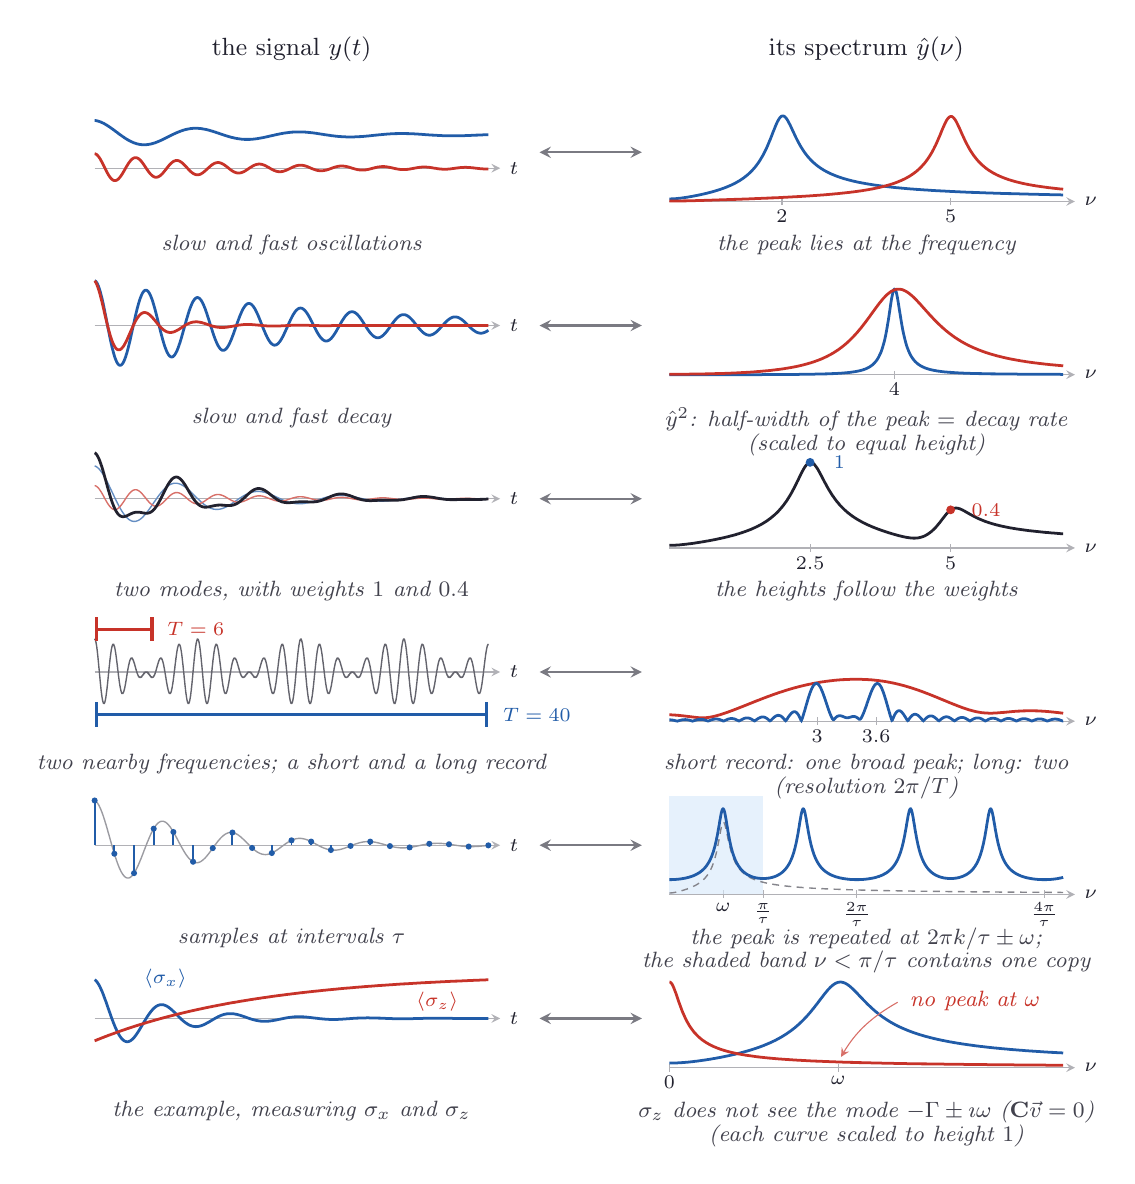
\begin{tikzpicture}[ink/.style={line width=0.9pt, ndInk}, faint/.style={line width=0.4pt, ndInk!35}, dashedink/.style={line width=0.5pt, ndInk!55, dash pattern=on 2.5pt off 2pt}, vec/.style={->, >=stealth, line width=1.2pt}, note/.style={font=\footnotesize\itshape, text=ndInk!85, align=center}, pointer/.style={->, >=stealth, line width=0.4pt, ndInk!60, shorten >=2pt, shorten <=1pt}, dot/.style={circle, fill=ndInk, inner sep=0pt, minimum size=3.4pt}, wash/.style={fill=ndSky, fill opacity=0.55}, every node/.style={text=ndInk}]
\definecolor{ndInk}{rgb}{0.13,0.13,0.18}
\definecolor{ndPaper}{rgb}{0.99,0.96,0.88}
\definecolor{ndSky}{rgb}{0.84,0.91,0.98}
\definecolor{ndRose}{rgb}{0.98,0.86,0.84}
\definecolor{ndBlue}{rgb}{0.13,0.36,0.66}
\definecolor{ndRed}{rgb}{0.78,0.20,0.16}
\definecolor{ndGold}{rgb}{0.88,0.62,0.10}
\definecolor{ndGreen}{rgb}{0.18,0.52,0.30}
\node[font=\small, anchor=south] at (2.500,0.250) {the signal $y(t)$};
\node[font=\small, anchor=south] at (9.800,0.250) {its spectrum $\abs{\hat y(\nu)}$};
\draw[faint, ->, >=stealth] (0.000,-0.977) -- (5.150,-0.977) node[right, font=\scriptsize, text=ndInk] {$t$};
\draw[faint, ->, >=stealth] (7.300,-1.400) -- (12.450,-1.400) node[right, font=\scriptsize, text=ndInk] {$\nu$};
\draw[faint] (8.729,-1.350) -- (8.729,-1.450) node[below, font=\scriptsize, text=ndInk, inner sep=1.5pt] {$2$};
\draw[faint] (10.871,-1.350) -- (10.871,-1.450) node[below, font=\scriptsize, text=ndInk, inner sep=1.5pt] {$5$};
\draw[line width=1.0pt, ndBlue] (0.000,-0.371) -- (0.006,-0.371) -- (0.011,-0.372) -- (0.017,-0.373) -- (0.022,-0.374) -- (0.028,-0.375) -- (0.033,-0.377) -- (0.039,-0.378) -- (0.044,-0.379) -- (0.050,-0.381) -- (0.056,-0.383) -- (0.061,-0.385) -- (0.067,-0.387) -- (0.072,-0.389) -- (0.078,-0.391) -- (0.083,-0.393) -- (0.089,-0.396) -- (0.095,-0.398) -- (0.100,-0.401) -- (0.106,-0.404) -- (0.111,-0.406) -- (0.117,-0.409) -- (0.122,-0.412) -- (0.128,-0.415) -- (0.133,-0.418) -- (0.139,-0.422) -- (0.145,-0.425) -- (0.150,-0.428) -- (0.156,-0.432) -- (0.161,-0.435) -- (0.167,-0.439) -- (0.172,-0.442) -- (0.178,-0.446) -- (0.184,-0.450) -- (0.189,-0.453) -- (0.195,-0.457) -- (0.200,-0.461) -- (0.206,-0.465) -- (0.211,-0.469) -- (0.217,-0.473) -- (0.222,-0.477) -- (0.228,-0.481) -- (0.234,-0.485) -- (0.239,-0.489) -- (0.245,-0.493) -- (0.250,-0.497) -- (0.256,-0.501) -- (0.261,-0.506) -- (0.267,-0.510) -- (0.273,-0.514) -- (0.278,-0.518) -- (0.284,-0.522) -- (0.289,-0.526) -- (0.295,-0.530) -- (0.300,-0.535) -- (0.306,-0.539) -- (0.311,-0.543) -- (0.317,-0.547) -- (0.323,-0.551) -- (0.328,-0.555) -- (0.334,-0.559) -- (0.339,-0.563) -- (0.345,-0.567) -- (0.350,-0.571) -- (0.356,-0.575) -- (0.362,-0.579) -- (0.367,-0.582) -- (0.373,-0.586) -- (0.378,-0.590) -- (0.384,-0.594) -- (0.389,-0.597) -- (0.395,-0.601) -- (0.400,-0.604) -- (0.406,-0.608) -- (0.412,-0.611) -- (0.417,-0.614) -- (0.423,-0.617) -- (0.428,-0.621) -- (0.434,-0.624) -- (0.439,-0.627) -- (0.445,-0.630) -- (0.451,-0.633) -- (0.456,-0.635) -- (0.462,-0.638) -- (0.467,-0.641) -- (0.473,-0.643) -- (0.478,-0.646) -- (0.484,-0.648) -- (0.489,-0.651) -- (0.495,-0.653) -- (0.501,-0.655) -- (0.506,-0.657) -- (0.512,-0.659) -- (0.517,-0.661) -- (0.523,-0.663) -- (0.528,-0.664) -- (0.534,-0.666) -- (0.539,-0.668) -- (0.545,-0.669) -- (0.551,-0.670) -- (0.556,-0.672) -- (0.562,-0.673) -- (0.567,-0.674) -- (0.573,-0.675) -- (0.578,-0.676) -- (0.584,-0.677) -- (0.590,-0.677) -- (0.595,-0.678) -- (0.601,-0.678) -- (0.606,-0.679) -- (0.612,-0.679) -- (0.617,-0.679) -- (0.623,-0.679) -- (0.628,-0.680) -- (0.634,-0.679) -- (0.640,-0.679) -- (0.645,-0.679) -- (0.651,-0.679) -- (0.656,-0.678) -- (0.662,-0.678) -- (0.667,-0.677) -- (0.673,-0.677) -- (0.679,-0.676) -- (0.684,-0.675) -- (0.690,-0.674) -- (0.695,-0.673) -- (0.701,-0.672) -- (0.706,-0.671) -- (0.712,-0.670) -- (0.717,-0.669) -- (0.723,-0.667) -- (0.729,-0.666) -- (0.734,-0.664) -- (0.740,-0.663) -- (0.745,-0.661) -- (0.751,-0.659) -- (0.756,-0.657) -- (0.762,-0.656) -- (0.768,-0.654) -- (0.773,-0.652) -- (0.779,-0.650) -- (0.784,-0.648) -- (0.790,-0.646) -- (0.795,-0.643) -- (0.801,-0.641) -- (0.806,-0.639) -- (0.812,-0.637) -- (0.818,-0.634) -- (0.823,-0.632) -- (0.829,-0.629) -- (0.834,-0.627) -- (0.840,-0.624) -- (0.845,-0.622) -- (0.851,-0.619) -- (0.857,-0.617) -- (0.862,-0.614) -- (0.868,-0.611) -- (0.873,-0.609) -- (0.879,-0.606) -- (0.884,-0.603) -- (0.890,-0.600) -- (0.895,-0.598) -- (0.901,-0.595) -- (0.907,-0.592) -- (0.912,-0.589) -- (0.918,-0.586) -- (0.923,-0.584) -- (0.929,-0.581) -- (0.934,-0.578) -- (0.940,-0.575) -- (0.945,-0.572) -- (0.951,-0.570) -- (0.957,-0.567) -- (0.962,-0.564) -- (0.968,-0.561) -- (0.973,-0.559) -- (0.979,-0.556) -- (0.984,-0.553) -- (0.990,-0.550) -- (0.996,-0.548) -- (1.001,-0.545) -- (1.007,-0.542) -- (1.012,-0.540) -- (1.018,-0.537) -- (1.023,-0.535) -- (1.029,-0.532) -- (1.034,-0.530) -- (1.040,-0.527) -- (1.046,-0.525) -- (1.051,-0.522) -- (1.057,-0.520) -- (1.062,-0.518) -- (1.068,-0.516) -- (1.073,-0.513) -- (1.079,-0.511) -- (1.085,-0.509) -- (1.090,-0.507) -- (1.096,-0.505) -- (1.101,-0.503) -- (1.107,-0.501) -- (1.112,-0.499) -- (1.118,-0.497) -- (1.123,-0.495) -- (1.129,-0.494) -- (1.135,-0.492) -- (1.140,-0.490) -- (1.146,-0.489) -- (1.151,-0.487) -- (1.157,-0.486) -- (1.162,-0.485) -- (1.168,-0.483) -- (1.174,-0.482) -- (1.179,-0.481) -- (1.185,-0.480) -- (1.190,-0.479) -- (1.196,-0.478) -- (1.201,-0.477) -- (1.207,-0.476) -- (1.212,-0.475) -- (1.218,-0.474) -- (1.224,-0.474) -- (1.229,-0.473) -- (1.235,-0.472) -- (1.240,-0.472) -- (1.246,-0.471) -- (1.251,-0.471) -- (1.257,-0.471) -- (1.263,-0.470) -- (1.268,-0.470) -- (1.274,-0.470) -- (1.279,-0.470) -- (1.285,-0.470) -- (1.290,-0.470) -- (1.296,-0.470) -- (1.301,-0.470) -- (1.307,-0.471) -- (1.313,-0.471) -- (1.318,-0.471) -- (1.324,-0.472) -- (1.329,-0.472) -- (1.335,-0.473) -- (1.340,-0.473) -- (1.346,-0.474) -- (1.352,-0.474) -- (1.357,-0.475) -- (1.363,-0.476) -- (1.368,-0.477) -- (1.374,-0.478) -- (1.379,-0.479) -- (1.385,-0.480) -- (1.390,-0.481) -- (1.396,-0.482) -- (1.402,-0.483) -- (1.407,-0.484) -- (1.413,-0.485) -- (1.418,-0.486) -- (1.424,-0.488) -- (1.429,-0.489) -- (1.435,-0.490) -- (1.440,-0.492) -- (1.446,-0.493) -- (1.452,-0.495) -- (1.457,-0.496) -- (1.463,-0.498) -- (1.468,-0.499) -- (1.474,-0.501) -- (1.479,-0.503) -- (1.485,-0.504) -- (1.491,-0.506) -- (1.496,-0.508) -- (1.502,-0.509) -- (1.507,-0.511) -- (1.513,-0.513) -- (1.518,-0.515) -- (1.524,-0.517) -- (1.529,-0.518) -- (1.535,-0.520) -- (1.541,-0.522) -- (1.546,-0.524) -- (1.552,-0.526) -- (1.557,-0.528) -- (1.563,-0.530) -- (1.568,-0.531) -- (1.574,-0.533) -- (1.580,-0.535) -- (1.585,-0.537) -- (1.591,-0.539) -- (1.596,-0.541) -- (1.602,-0.543) -- (1.607,-0.545) -- (1.613,-0.547) -- (1.618,-0.548) -- (1.624,-0.550) -- (1.630,-0.552) -- (1.635,-0.554) -- (1.641,-0.556) -- (1.646,-0.558) -- (1.652,-0.560) -- (1.657,-0.561) -- (1.663,-0.563) -- (1.669,-0.565) -- (1.674,-0.567) -- (1.680,-0.568) -- (1.685,-0.570) -- (1.691,-0.572) -- (1.696,-0.573) -- (1.702,-0.575) -- (1.707,-0.577) -- (1.713,-0.578) -- (1.719,-0.580) -- (1.724,-0.581) -- (1.730,-0.583) -- (1.735,-0.584) -- (1.741,-0.586) -- (1.746,-0.587) -- (1.752,-0.588) -- (1.758,-0.590) -- (1.763,-0.591) -- (1.769,-0.592) -- (1.774,-0.593) -- (1.780,-0.595) -- (1.785,-0.596) -- (1.791,-0.597) -- (1.796,-0.598) -- (1.802,-0.599) -- (1.808,-0.600) -- (1.813,-0.601) -- (1.819,-0.602) -- (1.824,-0.603) -- (1.830,-0.604) -- (1.835,-0.604) -- (1.841,-0.605) -- (1.846,-0.606) -- (1.852,-0.606) -- (1.858,-0.607) -- (1.863,-0.608) -- (1.869,-0.608) -- (1.874,-0.609) -- (1.880,-0.609) -- (1.885,-0.610) -- (1.891,-0.610) -- (1.897,-0.610) -- (1.902,-0.611) -- (1.908,-0.611) -- (1.913,-0.611) -- (1.919,-0.611) -- (1.924,-0.611) -- (1.930,-0.611) -- (1.935,-0.611) -- (1.941,-0.611) -- (1.947,-0.611) -- (1.952,-0.611) -- (1.958,-0.611) -- (1.963,-0.611) -- (1.969,-0.611) -- (1.974,-0.611) -- (1.980,-0.610) -- (1.986,-0.610) -- (1.991,-0.610) -- (1.997,-0.609) -- (2.002,-0.609) -- (2.008,-0.608) -- (2.013,-0.608) -- (2.019,-0.607) -- (2.024,-0.607) -- (2.030,-0.606) -- (2.036,-0.605) -- (2.041,-0.605) -- (2.047,-0.604) -- (2.052,-0.603) -- (2.058,-0.602) -- (2.063,-0.602) -- (2.069,-0.601) -- (2.075,-0.600) -- (2.080,-0.599) -- (2.086,-0.598) -- (2.091,-0.597) -- (2.097,-0.596) -- (2.102,-0.595) -- (2.108,-0.594) -- (2.113,-0.593) -- (2.119,-0.592) -- (2.125,-0.591) -- (2.130,-0.590) -- (2.136,-0.589) -- (2.141,-0.588) -- (2.147,-0.587) -- (2.152,-0.586) -- (2.158,-0.584) -- (2.164,-0.583) -- (2.169,-0.582) -- (2.175,-0.581) -- (2.180,-0.580) -- (2.186,-0.578) -- (2.191,-0.577) -- (2.197,-0.576) -- (2.202,-0.575) -- (2.208,-0.573) -- (2.214,-0.572) -- (2.219,-0.571) -- (2.225,-0.569) -- (2.230,-0.568) -- (2.236,-0.567) -- (2.241,-0.566) -- (2.247,-0.564) -- (2.253,-0.563) -- (2.258,-0.562) -- (2.264,-0.561) -- (2.269,-0.559) -- (2.275,-0.558) -- (2.280,-0.557) -- (2.286,-0.556) -- (2.291,-0.554) -- (2.297,-0.553) -- (2.303,-0.552) -- (2.308,-0.551) -- (2.314,-0.549) -- (2.319,-0.548) -- (2.325,-0.547) -- (2.330,-0.546) -- (2.336,-0.545) -- (2.341,-0.544) -- (2.347,-0.542) -- (2.353,-0.541) -- (2.358,-0.540) -- (2.364,-0.539) -- (2.369,-0.538) -- (2.375,-0.537) -- (2.380,-0.536) -- (2.386,-0.535) -- (2.392,-0.534) -- (2.397,-0.533) -- (2.403,-0.532) -- (2.408,-0.531) -- (2.414,-0.530) -- (2.419,-0.529) -- (2.425,-0.529) -- (2.430,-0.528) -- (2.436,-0.527) -- (2.442,-0.526) -- (2.447,-0.526) -- (2.453,-0.525) -- (2.458,-0.524) -- (2.464,-0.523) -- (2.469,-0.523) -- (2.475,-0.522) -- (2.481,-0.522) -- (2.486,-0.521) -- (2.492,-0.521) -- (2.497,-0.520) -- (2.503,-0.520) -- (2.508,-0.519) -- (2.514,-0.519) -- (2.519,-0.518) -- (2.525,-0.518) -- (2.531,-0.518) -- (2.536,-0.517) -- (2.542,-0.517) -- (2.547,-0.517) -- (2.553,-0.517) -- (2.558,-0.516) -- (2.564,-0.516) -- (2.570,-0.516) -- (2.575,-0.516) -- (2.581,-0.516) -- (2.586,-0.516) -- (2.592,-0.516) -- (2.597,-0.516) -- (2.603,-0.516) -- (2.608,-0.516) -- (2.614,-0.516) -- (2.620,-0.516) -- (2.625,-0.516) -- (2.631,-0.517) -- (2.636,-0.517) -- (2.642,-0.517) -- (2.647,-0.517) -- (2.653,-0.518) -- (2.659,-0.518) -- (2.664,-0.518) -- (2.670,-0.518) -- (2.675,-0.519) -- (2.681,-0.519) -- (2.686,-0.520) -- (2.692,-0.520) -- (2.697,-0.521) -- (2.703,-0.521) -- (2.709,-0.522) -- (2.714,-0.522) -- (2.720,-0.523) -- (2.725,-0.523) -- (2.731,-0.524) -- (2.736,-0.524) -- (2.742,-0.525) -- (2.747,-0.526) -- (2.753,-0.526) -- (2.759,-0.527) -- (2.764,-0.528) -- (2.770,-0.528) -- (2.775,-0.529) -- (2.781,-0.530) -- (2.786,-0.531) -- (2.792,-0.531) -- (2.798,-0.532) -- (2.803,-0.533) -- (2.809,-0.534) -- (2.814,-0.534) -- (2.820,-0.535) -- (2.825,-0.536) -- (2.831,-0.537) -- (2.836,-0.538) -- (2.842,-0.539) -- (2.848,-0.539) -- (2.853,-0.540) -- (2.859,-0.541) -- (2.864,-0.542) -- (2.870,-0.543) -- (2.875,-0.544) -- (2.881,-0.545) -- (2.887,-0.545) -- (2.892,-0.546) -- (2.898,-0.547) -- (2.903,-0.548) -- (2.909,-0.549) -- (2.914,-0.550) -- (2.920,-0.551) -- (2.925,-0.551) -- (2.931,-0.552) -- (2.937,-0.553) -- (2.942,-0.554) -- (2.948,-0.555) -- (2.953,-0.556) -- (2.959,-0.556) -- (2.964,-0.557) -- (2.970,-0.558) -- (2.976,-0.559) -- (2.981,-0.560) -- (2.987,-0.560) -- (2.992,-0.561) -- (2.998,-0.562) -- (3.003,-0.563) -- (3.009,-0.564) -- (3.014,-0.564) -- (3.020,-0.565) -- (3.026,-0.566) -- (3.031,-0.566) -- (3.037,-0.567) -- (3.042,-0.568) -- (3.048,-0.568) -- (3.053,-0.569) -- (3.059,-0.570) -- (3.065,-0.570) -- (3.070,-0.571) -- (3.076,-0.571) -- (3.081,-0.572) -- (3.087,-0.573) -- (3.092,-0.573) -- (3.098,-0.574) -- (3.103,-0.574) -- (3.109,-0.575) -- (3.115,-0.575) -- (3.120,-0.575) -- (3.126,-0.576) -- (3.131,-0.576) -- (3.137,-0.577) -- (3.142,-0.577) -- (3.148,-0.577) -- (3.154,-0.578) -- (3.159,-0.578) -- (3.165,-0.578) -- (3.170,-0.579) -- (3.176,-0.579) -- (3.181,-0.579) -- (3.187,-0.579) -- (3.192,-0.580) -- (3.198,-0.580) -- (3.204,-0.580) -- (3.209,-0.580) -- (3.215,-0.580) -- (3.220,-0.580) -- (3.226,-0.580) -- (3.231,-0.580) -- (3.237,-0.580) -- (3.242,-0.580) -- (3.248,-0.580) -- (3.254,-0.580) -- (3.259,-0.580) -- (3.265,-0.580) -- (3.270,-0.580) -- (3.276,-0.580) -- (3.281,-0.580) -- (3.287,-0.580) -- (3.293,-0.580) -- (3.298,-0.580) -- (3.304,-0.579) -- (3.309,-0.579) -- (3.315,-0.579) -- (3.320,-0.579) -- (3.326,-0.579) -- (3.331,-0.578) -- (3.337,-0.578) -- (3.343,-0.578) -- (3.348,-0.577) -- (3.354,-0.577) -- (3.359,-0.577) -- (3.365,-0.576) -- (3.370,-0.576) -- (3.376,-0.576) -- (3.382,-0.575) -- (3.387,-0.575) -- (3.393,-0.575) -- (3.398,-0.574) -- (3.404,-0.574) -- (3.409,-0.573) -- (3.415,-0.573) -- (3.420,-0.572) -- (3.426,-0.572) -- (3.432,-0.571) -- (3.437,-0.571) -- (3.443,-0.570) -- (3.448,-0.570) -- (3.454,-0.569) -- (3.459,-0.569) -- (3.465,-0.568) -- (3.471,-0.568) -- (3.476,-0.567) -- (3.482,-0.567) -- (3.487,-0.566) -- (3.493,-0.566) -- (3.498,-0.565) -- (3.504,-0.564) -- (3.509,-0.564) -- (3.515,-0.563) -- (3.521,-0.563) -- (3.526,-0.562) -- (3.532,-0.561) -- (3.537,-0.561) -- (3.543,-0.560) -- (3.548,-0.560) -- (3.554,-0.559) -- (3.560,-0.559) -- (3.565,-0.558) -- (3.571,-0.557) -- (3.576,-0.557) -- (3.582,-0.556) -- (3.587,-0.556) -- (3.593,-0.555) -- (3.598,-0.555) -- (3.604,-0.554) -- (3.610,-0.553) -- (3.615,-0.553) -- (3.621,-0.552) -- (3.626,-0.552) -- (3.632,-0.551) -- (3.637,-0.551) -- (3.643,-0.550) -- (3.648,-0.550) -- (3.654,-0.549) -- (3.660,-0.549) -- (3.665,-0.548) -- (3.671,-0.548) -- (3.676,-0.547) -- (3.682,-0.547) -- (3.687,-0.546) -- (3.693,-0.546) -- (3.699,-0.545) -- (3.704,-0.545) -- (3.710,-0.544) -- (3.715,-0.544) -- (3.721,-0.544) -- (3.726,-0.543) -- (3.732,-0.543) -- (3.737,-0.542) -- (3.743,-0.542) -- (3.749,-0.542) -- (3.754,-0.541) -- (3.760,-0.541) -- (3.765,-0.541) -- (3.771,-0.540) -- (3.776,-0.540) -- (3.782,-0.540) -- (3.788,-0.540) -- (3.793,-0.539) -- (3.799,-0.539) -- (3.804,-0.539) -- (3.810,-0.539) -- (3.815,-0.538) -- (3.821,-0.538) -- (3.826,-0.538) -- (3.832,-0.538) -- (3.838,-0.538) -- (3.843,-0.538) -- (3.849,-0.537) -- (3.854,-0.537) -- (3.860,-0.537) -- (3.865,-0.537) -- (3.871,-0.537) -- (3.877,-0.537) -- (3.882,-0.537) -- (3.888,-0.537) -- (3.893,-0.537) -- (3.899,-0.537) -- (3.904,-0.537) -- (3.910,-0.537) -- (3.915,-0.537) -- (3.921,-0.537) -- (3.927,-0.537) -- (3.932,-0.537) -- (3.938,-0.537) -- (3.943,-0.537) -- (3.949,-0.537) -- (3.954,-0.537) -- (3.960,-0.538) -- (3.966,-0.538) -- (3.971,-0.538) -- (3.977,-0.538) -- (3.982,-0.538) -- (3.988,-0.538) -- (3.993,-0.539) -- (3.999,-0.539) -- (4.004,-0.539) -- (4.010,-0.539) -- (4.016,-0.539) -- (4.021,-0.540) -- (4.027,-0.540) -- (4.032,-0.540) -- (4.038,-0.540) -- (4.043,-0.541) -- (4.049,-0.541) -- (4.055,-0.541) -- (4.060,-0.541) -- (4.066,-0.542) -- (4.071,-0.542) -- (4.077,-0.542) -- (4.082,-0.543) -- (4.088,-0.543) -- (4.093,-0.543) -- (4.099,-0.544) -- (4.105,-0.544) -- (4.110,-0.544) -- (4.116,-0.545) -- (4.121,-0.545) -- (4.127,-0.546) -- (4.132,-0.546) -- (4.138,-0.546) -- (4.143,-0.547) -- (4.149,-0.547) -- (4.155,-0.547) -- (4.160,-0.548) -- (4.166,-0.548) -- (4.171,-0.549) -- (4.177,-0.549) -- (4.182,-0.549) -- (4.188,-0.550) -- (4.194,-0.550) -- (4.199,-0.551) -- (4.205,-0.551) -- (4.210,-0.551) -- (4.216,-0.552) -- (4.221,-0.552) -- (4.227,-0.553) -- (4.232,-0.553) -- (4.238,-0.553) -- (4.244,-0.554) -- (4.249,-0.554) -- (4.255,-0.554) -- (4.260,-0.555) -- (4.266,-0.555) -- (4.271,-0.556) -- (4.277,-0.556) -- (4.283,-0.556) -- (4.288,-0.557) -- (4.294,-0.557) -- (4.299,-0.557) -- (4.305,-0.558) -- (4.310,-0.558) -- (4.316,-0.558) -- (4.321,-0.559) -- (4.327,-0.559) -- (4.333,-0.559) -- (4.338,-0.560) -- (4.344,-0.560) -- (4.349,-0.560) -- (4.355,-0.561) -- (4.360,-0.561) -- (4.366,-0.561) -- (4.372,-0.562) -- (4.377,-0.562) -- (4.383,-0.562) -- (4.388,-0.562) -- (4.394,-0.563) -- (4.399,-0.563) -- (4.405,-0.563) -- (4.410,-0.563) -- (4.416,-0.564) -- (4.422,-0.564) -- (4.427,-0.564) -- (4.433,-0.564) -- (4.438,-0.564) -- (4.444,-0.564) -- (4.449,-0.565) -- (4.455,-0.565) -- (4.461,-0.565) -- (4.466,-0.565) -- (4.472,-0.565) -- (4.477,-0.565) -- (4.483,-0.566) -- (4.488,-0.566) -- (4.494,-0.566) -- (4.499,-0.566) -- (4.505,-0.566) -- (4.511,-0.566) -- (4.516,-0.566) -- (4.522,-0.566) -- (4.527,-0.566) -- (4.533,-0.566) -- (4.538,-0.566) -- (4.544,-0.566) -- (4.549,-0.566) -- (4.555,-0.566) -- (4.561,-0.566) -- (4.566,-0.566) -- (4.572,-0.566) -- (4.577,-0.566) -- (4.583,-0.566) -- (4.588,-0.566) -- (4.594,-0.566) -- (4.600,-0.566) -- (4.605,-0.566) -- (4.611,-0.566) -- (4.616,-0.566) -- (4.622,-0.566) -- (4.627,-0.566) -- (4.633,-0.565) -- (4.638,-0.565) -- (4.644,-0.565) -- (4.650,-0.565) -- (4.655,-0.565) -- (4.661,-0.565) -- (4.666,-0.565) -- (4.672,-0.565) -- (4.677,-0.564) -- (4.683,-0.564) -- (4.689,-0.564) -- (4.694,-0.564) -- (4.700,-0.564) -- (4.705,-0.563) -- (4.711,-0.563) -- (4.716,-0.563) -- (4.722,-0.563) -- (4.727,-0.563) -- (4.733,-0.562) -- (4.739,-0.562) -- (4.744,-0.562) -- (4.750,-0.562) -- (4.755,-0.562) -- (4.761,-0.561) -- (4.766,-0.561) -- (4.772,-0.561) -- (4.778,-0.561) -- (4.783,-0.560) -- (4.789,-0.560) -- (4.794,-0.560) -- (4.800,-0.560) -- (4.805,-0.559) -- (4.811,-0.559) -- (4.816,-0.559) -- (4.822,-0.559) -- (4.828,-0.558) -- (4.833,-0.558) -- (4.839,-0.558) -- (4.844,-0.557) -- (4.850,-0.557) -- (4.855,-0.557) -- (4.861,-0.557) -- (4.867,-0.556) -- (4.872,-0.556) -- (4.878,-0.556) -- (4.883,-0.556) -- (4.889,-0.555) -- (4.894,-0.555) -- (4.900,-0.555) -- (4.905,-0.555) -- (4.911,-0.554) -- (4.917,-0.554) -- (4.922,-0.554) -- (4.928,-0.554) -- (4.933,-0.553) -- (4.939,-0.553) -- (4.944,-0.553) -- (4.950,-0.553) -- (4.956,-0.552) -- (4.961,-0.552) -- (4.967,-0.552) -- (4.972,-0.552) -- (4.978,-0.551) -- (4.983,-0.551) -- (4.989,-0.551) -- (4.994,-0.551) -- (5.000,-0.551);
\draw[line width=1.0pt, ndRed] (0.000,-0.793) -- (0.006,-0.794) -- (0.011,-0.796) -- (0.017,-0.799) -- (0.022,-0.802) -- (0.028,-0.806) -- (0.033,-0.811) -- (0.039,-0.817) -- (0.044,-0.823) -- (0.050,-0.830) -- (0.056,-0.838) -- (0.061,-0.846) -- (0.067,-0.854) -- (0.072,-0.863) -- (0.078,-0.873) -- (0.083,-0.883) -- (0.089,-0.893) -- (0.095,-0.904) -- (0.100,-0.915) -- (0.106,-0.926) -- (0.111,-0.937) -- (0.117,-0.948) -- (0.122,-0.960) -- (0.128,-0.971) -- (0.133,-0.982) -- (0.139,-0.994) -- (0.145,-1.005) -- (0.150,-1.016) -- (0.156,-1.026) -- (0.161,-1.037) -- (0.167,-1.047) -- (0.172,-1.056) -- (0.178,-1.066) -- (0.184,-1.074) -- (0.189,-1.083) -- (0.195,-1.090) -- (0.200,-1.098) -- (0.206,-1.104) -- (0.211,-1.110) -- (0.217,-1.116) -- (0.222,-1.120) -- (0.228,-1.125) -- (0.234,-1.128) -- (0.239,-1.131) -- (0.245,-1.133) -- (0.250,-1.134) -- (0.256,-1.134) -- (0.261,-1.134) -- (0.267,-1.134) -- (0.273,-1.132) -- (0.278,-1.130) -- (0.284,-1.127) -- (0.289,-1.123) -- (0.295,-1.119) -- (0.300,-1.115) -- (0.306,-1.109) -- (0.311,-1.103) -- (0.317,-1.097) -- (0.323,-1.090) -- (0.328,-1.083) -- (0.334,-1.075) -- (0.339,-1.067) -- (0.345,-1.058) -- (0.350,-1.050) -- (0.356,-1.041) -- (0.362,-1.031) -- (0.367,-1.022) -- (0.373,-1.012) -- (0.378,-1.003) -- (0.384,-0.993) -- (0.389,-0.983) -- (0.395,-0.973) -- (0.400,-0.964) -- (0.406,-0.954) -- (0.412,-0.945) -- (0.417,-0.936) -- (0.423,-0.927) -- (0.428,-0.918) -- (0.434,-0.910) -- (0.439,-0.902) -- (0.445,-0.895) -- (0.451,-0.888) -- (0.456,-0.881) -- (0.462,-0.875) -- (0.467,-0.869) -- (0.473,-0.864) -- (0.478,-0.859) -- (0.484,-0.855) -- (0.489,-0.852) -- (0.495,-0.849) -- (0.501,-0.846) -- (0.506,-0.844) -- (0.512,-0.843) -- (0.517,-0.843) -- (0.523,-0.843) -- (0.528,-0.844) -- (0.534,-0.845) -- (0.539,-0.847) -- (0.545,-0.849) -- (0.551,-0.852) -- (0.556,-0.855) -- (0.562,-0.859) -- (0.567,-0.864) -- (0.573,-0.869) -- (0.578,-0.874) -- (0.584,-0.880) -- (0.590,-0.886) -- (0.595,-0.893) -- (0.601,-0.900) -- (0.606,-0.907) -- (0.612,-0.915) -- (0.617,-0.922) -- (0.623,-0.930) -- (0.628,-0.938) -- (0.634,-0.947) -- (0.640,-0.955) -- (0.645,-0.963) -- (0.651,-0.972) -- (0.656,-0.980) -- (0.662,-0.988) -- (0.667,-0.996) -- (0.673,-1.004) -- (0.679,-1.012) -- (0.684,-1.020) -- (0.690,-1.027) -- (0.695,-1.034) -- (0.701,-1.041) -- (0.706,-1.047) -- (0.712,-1.053) -- (0.717,-1.059) -- (0.723,-1.064) -- (0.729,-1.069) -- (0.734,-1.074) -- (0.740,-1.078) -- (0.745,-1.081) -- (0.751,-1.084) -- (0.756,-1.087) -- (0.762,-1.089) -- (0.768,-1.091) -- (0.773,-1.092) -- (0.779,-1.092) -- (0.784,-1.092) -- (0.790,-1.091) -- (0.795,-1.090) -- (0.801,-1.089) -- (0.806,-1.087) -- (0.812,-1.084) -- (0.818,-1.081) -- (0.823,-1.078) -- (0.829,-1.074) -- (0.834,-1.070) -- (0.840,-1.065) -- (0.845,-1.060) -- (0.851,-1.055) -- (0.857,-1.050) -- (0.862,-1.044) -- (0.868,-1.037) -- (0.873,-1.031) -- (0.879,-1.024) -- (0.884,-1.018) -- (0.890,-1.011) -- (0.895,-1.004) -- (0.901,-0.997) -- (0.907,-0.990) -- (0.912,-0.983) -- (0.918,-0.975) -- (0.923,-0.968) -- (0.929,-0.961) -- (0.934,-0.955) -- (0.940,-0.948) -- (0.945,-0.941) -- (0.951,-0.935) -- (0.957,-0.929) -- (0.962,-0.923) -- (0.968,-0.918) -- (0.973,-0.912) -- (0.979,-0.908) -- (0.984,-0.903) -- (0.990,-0.899) -- (0.996,-0.895) -- (1.001,-0.891) -- (1.007,-0.888) -- (1.012,-0.886) -- (1.018,-0.884) -- (1.023,-0.882) -- (1.029,-0.880) -- (1.034,-0.880) -- (1.040,-0.879) -- (1.046,-0.879) -- (1.051,-0.879) -- (1.057,-0.880) -- (1.062,-0.882) -- (1.068,-0.883) -- (1.073,-0.885) -- (1.079,-0.888) -- (1.085,-0.891) -- (1.090,-0.894) -- (1.096,-0.898) -- (1.101,-0.902) -- (1.107,-0.906) -- (1.112,-0.910) -- (1.118,-0.915) -- (1.123,-0.920) -- (1.129,-0.925) -- (1.135,-0.931) -- (1.140,-0.936) -- (1.146,-0.942) -- (1.151,-0.948) -- (1.157,-0.954) -- (1.162,-0.960) -- (1.168,-0.966) -- (1.174,-0.972) -- (1.179,-0.978) -- (1.185,-0.984) -- (1.190,-0.990) -- (1.196,-0.996) -- (1.201,-1.002) -- (1.207,-1.007) -- (1.212,-1.013) -- (1.218,-1.018) -- (1.224,-1.023) -- (1.229,-1.028) -- (1.235,-1.032) -- (1.240,-1.036) -- (1.246,-1.040) -- (1.251,-1.044) -- (1.257,-1.047) -- (1.263,-1.050) -- (1.268,-1.053) -- (1.274,-1.055) -- (1.279,-1.057) -- (1.285,-1.059) -- (1.290,-1.060) -- (1.296,-1.061) -- (1.301,-1.061) -- (1.307,-1.061) -- (1.313,-1.061) -- (1.318,-1.060) -- (1.324,-1.059) -- (1.329,-1.058) -- (1.335,-1.056) -- (1.340,-1.054) -- (1.346,-1.051) -- (1.352,-1.049) -- (1.357,-1.045) -- (1.363,-1.042) -- (1.368,-1.039) -- (1.374,-1.035) -- (1.379,-1.031) -- (1.385,-1.026) -- (1.390,-1.022) -- (1.396,-1.017) -- (1.402,-1.012) -- (1.407,-1.007) -- (1.413,-1.002) -- (1.418,-0.997) -- (1.424,-0.992) -- (1.429,-0.987) -- (1.435,-0.982) -- (1.440,-0.977) -- (1.446,-0.972) -- (1.452,-0.966) -- (1.457,-0.961) -- (1.463,-0.957) -- (1.468,-0.952) -- (1.474,-0.947) -- (1.479,-0.943) -- (1.485,-0.938) -- (1.491,-0.934) -- (1.496,-0.930) -- (1.502,-0.927) -- (1.507,-0.923) -- (1.513,-0.920) -- (1.518,-0.917) -- (1.524,-0.915) -- (1.529,-0.913) -- (1.535,-0.911) -- (1.541,-0.909) -- (1.546,-0.908) -- (1.552,-0.907) -- (1.557,-0.906) -- (1.563,-0.906) -- (1.568,-0.906) -- (1.574,-0.906) -- (1.580,-0.906) -- (1.585,-0.907) -- (1.591,-0.908) -- (1.596,-0.910) -- (1.602,-0.912) -- (1.607,-0.914) -- (1.613,-0.916) -- (1.618,-0.919) -- (1.624,-0.922) -- (1.630,-0.925) -- (1.635,-0.928) -- (1.641,-0.931) -- (1.646,-0.935) -- (1.652,-0.939) -- (1.657,-0.943) -- (1.663,-0.947) -- (1.669,-0.951) -- (1.674,-0.955) -- (1.680,-0.960) -- (1.685,-0.964) -- (1.691,-0.968) -- (1.696,-0.973) -- (1.702,-0.977) -- (1.707,-0.982) -- (1.713,-0.986) -- (1.719,-0.990) -- (1.724,-0.995) -- (1.730,-0.999) -- (1.735,-1.003) -- (1.741,-1.006) -- (1.746,-1.010) -- (1.752,-1.014) -- (1.758,-1.017) -- (1.763,-1.020) -- (1.769,-1.023) -- (1.774,-1.026) -- (1.780,-1.028) -- (1.785,-1.030) -- (1.791,-1.032) -- (1.796,-1.034) -- (1.802,-1.035) -- (1.808,-1.037) -- (1.813,-1.037) -- (1.819,-1.038) -- (1.824,-1.038) -- (1.830,-1.038) -- (1.835,-1.038) -- (1.841,-1.038) -- (1.846,-1.037) -- (1.852,-1.036) -- (1.858,-1.035) -- (1.863,-1.033) -- (1.869,-1.032) -- (1.874,-1.030) -- (1.880,-1.027) -- (1.885,-1.025) -- (1.891,-1.022) -- (1.897,-1.020) -- (1.902,-1.017) -- (1.908,-1.014) -- (1.913,-1.010) -- (1.919,-1.007) -- (1.924,-1.003) -- (1.930,-1.000) -- (1.935,-0.996) -- (1.941,-0.992) -- (1.947,-0.989) -- (1.952,-0.985) -- (1.958,-0.981) -- (1.963,-0.977) -- (1.969,-0.974) -- (1.974,-0.970) -- (1.980,-0.966) -- (1.986,-0.963) -- (1.991,-0.959) -- (1.997,-0.956) -- (2.002,-0.952) -- (2.008,-0.949) -- (2.013,-0.946) -- (2.019,-0.943) -- (2.024,-0.941) -- (2.030,-0.938) -- (2.036,-0.936) -- (2.041,-0.934) -- (2.047,-0.932) -- (2.052,-0.930) -- (2.058,-0.929) -- (2.063,-0.928) -- (2.069,-0.927) -- (2.075,-0.926) -- (2.080,-0.925) -- (2.086,-0.925) -- (2.091,-0.925) -- (2.097,-0.925) -- (2.102,-0.925) -- (2.108,-0.926) -- (2.113,-0.927) -- (2.119,-0.928) -- (2.125,-0.929) -- (2.130,-0.931) -- (2.136,-0.932) -- (2.141,-0.934) -- (2.147,-0.936) -- (2.152,-0.938) -- (2.158,-0.941) -- (2.164,-0.943) -- (2.169,-0.946) -- (2.175,-0.949) -- (2.180,-0.952) -- (2.186,-0.955) -- (2.191,-0.958) -- (2.197,-0.961) -- (2.202,-0.964) -- (2.208,-0.967) -- (2.214,-0.970) -- (2.219,-0.974) -- (2.225,-0.977) -- (2.230,-0.980) -- (2.236,-0.983) -- (2.241,-0.986) -- (2.247,-0.989) -- (2.253,-0.992) -- (2.258,-0.995) -- (2.264,-0.998) -- (2.269,-1.001) -- (2.275,-1.003) -- (2.280,-1.006) -- (2.286,-1.008) -- (2.291,-1.010) -- (2.297,-1.012) -- (2.303,-1.014) -- (2.308,-1.016) -- (2.314,-1.017) -- (2.319,-1.019) -- (2.325,-1.020) -- (2.330,-1.020) -- (2.336,-1.021) -- (2.341,-1.022) -- (2.347,-1.022) -- (2.353,-1.022) -- (2.358,-1.022) -- (2.364,-1.022) -- (2.369,-1.021) -- (2.375,-1.020) -- (2.380,-1.019) -- (2.386,-1.018) -- (2.392,-1.017) -- (2.397,-1.016) -- (2.403,-1.014) -- (2.408,-1.012) -- (2.414,-1.010) -- (2.419,-1.008) -- (2.425,-1.006) -- (2.430,-1.004) -- (2.436,-1.002) -- (2.442,-0.999) -- (2.447,-0.997) -- (2.453,-0.994) -- (2.458,-0.991) -- (2.464,-0.989) -- (2.469,-0.986) -- (2.475,-0.983) -- (2.481,-0.980) -- (2.486,-0.978) -- (2.492,-0.975) -- (2.497,-0.972) -- (2.503,-0.970) -- (2.508,-0.967) -- (2.514,-0.964) -- (2.519,-0.962) -- (2.525,-0.959) -- (2.531,-0.957) -- (2.536,-0.955) -- (2.542,-0.953) -- (2.547,-0.951) -- (2.553,-0.949) -- (2.558,-0.947) -- (2.564,-0.946) -- (2.570,-0.944) -- (2.575,-0.943) -- (2.581,-0.942) -- (2.586,-0.941) -- (2.592,-0.940) -- (2.597,-0.940) -- (2.603,-0.939) -- (2.608,-0.939) -- (2.614,-0.939) -- (2.620,-0.939) -- (2.625,-0.939) -- (2.631,-0.940) -- (2.636,-0.940) -- (2.642,-0.941) -- (2.647,-0.942) -- (2.653,-0.943) -- (2.659,-0.944) -- (2.664,-0.946) -- (2.670,-0.947) -- (2.675,-0.949) -- (2.681,-0.950) -- (2.686,-0.952) -- (2.692,-0.954) -- (2.697,-0.956) -- (2.703,-0.958) -- (2.709,-0.960) -- (2.714,-0.963) -- (2.720,-0.965) -- (2.725,-0.967) -- (2.731,-0.970) -- (2.736,-0.972) -- (2.742,-0.974) -- (2.747,-0.977) -- (2.753,-0.979) -- (2.759,-0.981) -- (2.764,-0.984) -- (2.770,-0.986) -- (2.775,-0.988) -- (2.781,-0.990) -- (2.786,-0.992) -- (2.792,-0.994) -- (2.798,-0.996) -- (2.803,-0.998) -- (2.809,-1.000) -- (2.814,-1.001) -- (2.820,-1.003) -- (2.825,-1.004) -- (2.831,-1.005) -- (2.836,-1.006) -- (2.842,-1.007) -- (2.848,-1.008) -- (2.853,-1.009) -- (2.859,-1.009) -- (2.864,-1.010) -- (2.870,-1.010) -- (2.875,-1.010) -- (2.881,-1.010) -- (2.887,-1.010) -- (2.892,-1.009) -- (2.898,-1.009) -- (2.903,-1.008) -- (2.909,-1.007) -- (2.914,-1.006) -- (2.920,-1.005) -- (2.925,-1.004) -- (2.931,-1.003) -- (2.937,-1.002) -- (2.942,-1.000) -- (2.948,-0.999) -- (2.953,-0.997) -- (2.959,-0.995) -- (2.964,-0.994) -- (2.970,-0.992) -- (2.976,-0.990) -- (2.981,-0.988) -- (2.987,-0.986) -- (2.992,-0.984) -- (2.998,-0.982) -- (3.003,-0.980) -- (3.009,-0.978) -- (3.014,-0.976) -- (3.020,-0.974) -- (3.026,-0.972) -- (3.031,-0.970) -- (3.037,-0.968) -- (3.042,-0.966) -- (3.048,-0.964) -- (3.053,-0.963) -- (3.059,-0.961) -- (3.065,-0.960) -- (3.070,-0.958) -- (3.076,-0.957) -- (3.081,-0.956) -- (3.087,-0.954) -- (3.092,-0.953) -- (3.098,-0.952) -- (3.103,-0.952) -- (3.109,-0.951) -- (3.115,-0.950) -- (3.120,-0.950) -- (3.126,-0.950) -- (3.131,-0.949) -- (3.137,-0.949) -- (3.142,-0.949) -- (3.148,-0.949) -- (3.154,-0.950) -- (3.159,-0.950) -- (3.165,-0.951) -- (3.170,-0.951) -- (3.176,-0.952) -- (3.181,-0.953) -- (3.187,-0.954) -- (3.192,-0.955) -- (3.198,-0.956) -- (3.204,-0.957) -- (3.209,-0.959) -- (3.215,-0.960) -- (3.220,-0.962) -- (3.226,-0.963) -- (3.231,-0.965) -- (3.237,-0.966) -- (3.242,-0.968) -- (3.248,-0.970) -- (3.254,-0.971) -- (3.259,-0.973) -- (3.265,-0.975) -- (3.270,-0.977) -- (3.276,-0.978) -- (3.281,-0.980) -- (3.287,-0.982) -- (3.293,-0.983) -- (3.298,-0.985) -- (3.304,-0.986) -- (3.309,-0.988) -- (3.315,-0.989) -- (3.320,-0.991) -- (3.326,-0.992) -- (3.331,-0.993) -- (3.337,-0.995) -- (3.343,-0.996) -- (3.348,-0.997) -- (3.354,-0.998) -- (3.359,-0.998) -- (3.365,-0.999) -- (3.370,-1.000) -- (3.376,-1.000) -- (3.382,-1.001) -- (3.387,-1.001) -- (3.393,-1.001) -- (3.398,-1.001) -- (3.404,-1.001) -- (3.409,-1.001) -- (3.415,-1.001) -- (3.420,-1.000) -- (3.426,-1.000) -- (3.432,-0.999) -- (3.437,-0.999) -- (3.443,-0.998) -- (3.448,-0.997) -- (3.454,-0.996) -- (3.459,-0.995) -- (3.465,-0.994) -- (3.471,-0.993) -- (3.476,-0.992) -- (3.482,-0.991) -- (3.487,-0.989) -- (3.493,-0.988) -- (3.498,-0.987) -- (3.504,-0.985) -- (3.509,-0.984) -- (3.515,-0.982) -- (3.521,-0.981) -- (3.526,-0.979) -- (3.532,-0.978) -- (3.537,-0.976) -- (3.543,-0.975) -- (3.548,-0.974) -- (3.554,-0.972) -- (3.560,-0.971) -- (3.565,-0.969) -- (3.571,-0.968) -- (3.576,-0.967) -- (3.582,-0.966) -- (3.587,-0.965) -- (3.593,-0.963) -- (3.598,-0.962) -- (3.604,-0.962) -- (3.610,-0.961) -- (3.615,-0.960) -- (3.621,-0.959) -- (3.626,-0.959) -- (3.632,-0.958) -- (3.637,-0.958) -- (3.643,-0.957) -- (3.648,-0.957) -- (3.654,-0.957) -- (3.660,-0.957) -- (3.665,-0.957) -- (3.671,-0.957) -- (3.676,-0.957) -- (3.682,-0.957) -- (3.687,-0.958) -- (3.693,-0.958) -- (3.699,-0.959) -- (3.704,-0.959) -- (3.710,-0.960) -- (3.715,-0.961) -- (3.721,-0.962) -- (3.726,-0.963) -- (3.732,-0.964) -- (3.737,-0.965) -- (3.743,-0.966) -- (3.749,-0.967) -- (3.754,-0.968) -- (3.760,-0.969) -- (3.765,-0.970) -- (3.771,-0.971) -- (3.776,-0.973) -- (3.782,-0.974) -- (3.788,-0.975) -- (3.793,-0.977) -- (3.799,-0.978) -- (3.804,-0.979) -- (3.810,-0.980) -- (3.815,-0.981) -- (3.821,-0.983) -- (3.826,-0.984) -- (3.832,-0.985) -- (3.838,-0.986) -- (3.843,-0.987) -- (3.849,-0.988) -- (3.854,-0.989) -- (3.860,-0.990) -- (3.865,-0.991) -- (3.871,-0.991) -- (3.877,-0.992) -- (3.882,-0.993) -- (3.888,-0.993) -- (3.893,-0.994) -- (3.899,-0.994) -- (3.904,-0.994) -- (3.910,-0.994) -- (3.915,-0.995) -- (3.921,-0.995) -- (3.927,-0.995) -- (3.932,-0.995) -- (3.938,-0.994) -- (3.943,-0.994) -- (3.949,-0.994) -- (3.954,-0.993) -- (3.960,-0.993) -- (3.966,-0.992) -- (3.971,-0.992) -- (3.977,-0.991) -- (3.982,-0.990) -- (3.988,-0.990) -- (3.993,-0.989) -- (3.999,-0.988) -- (4.004,-0.987) -- (4.010,-0.986) -- (4.016,-0.985) -- (4.021,-0.984) -- (4.027,-0.983) -- (4.032,-0.982) -- (4.038,-0.981) -- (4.043,-0.980) -- (4.049,-0.979) -- (4.055,-0.978) -- (4.060,-0.977) -- (4.066,-0.976) -- (4.071,-0.975) -- (4.077,-0.974) -- (4.082,-0.973) -- (4.088,-0.972) -- (4.093,-0.971) -- (4.099,-0.970) -- (4.105,-0.969) -- (4.110,-0.968) -- (4.116,-0.967) -- (4.121,-0.967) -- (4.127,-0.966) -- (4.132,-0.965) -- (4.138,-0.965) -- (4.143,-0.964) -- (4.149,-0.964) -- (4.155,-0.963) -- (4.160,-0.963) -- (4.166,-0.963) -- (4.171,-0.962) -- (4.177,-0.962) -- (4.182,-0.962) -- (4.188,-0.962) -- (4.194,-0.962) -- (4.199,-0.963) -- (4.205,-0.963) -- (4.210,-0.963) -- (4.216,-0.963) -- (4.221,-0.964) -- (4.227,-0.964) -- (4.232,-0.965) -- (4.238,-0.965) -- (4.244,-0.966) -- (4.249,-0.966) -- (4.255,-0.967) -- (4.260,-0.968) -- (4.266,-0.969) -- (4.271,-0.969) -- (4.277,-0.970) -- (4.283,-0.971) -- (4.288,-0.972) -- (4.294,-0.973) -- (4.299,-0.974) -- (4.305,-0.975) -- (4.310,-0.976) -- (4.316,-0.977) -- (4.321,-0.977) -- (4.327,-0.978) -- (4.333,-0.979) -- (4.338,-0.980) -- (4.344,-0.981) -- (4.349,-0.982) -- (4.355,-0.983) -- (4.360,-0.984) -- (4.366,-0.984) -- (4.372,-0.985) -- (4.377,-0.986) -- (4.383,-0.986) -- (4.388,-0.987) -- (4.394,-0.987) -- (4.399,-0.988) -- (4.405,-0.988) -- (4.410,-0.989) -- (4.416,-0.989) -- (4.422,-0.989) -- (4.427,-0.990) -- (4.433,-0.990) -- (4.438,-0.990) -- (4.444,-0.990) -- (4.449,-0.990) -- (4.455,-0.990) -- (4.461,-0.990) -- (4.466,-0.990) -- (4.472,-0.989) -- (4.477,-0.989) -- (4.483,-0.989) -- (4.488,-0.988) -- (4.494,-0.988) -- (4.499,-0.988) -- (4.505,-0.987) -- (4.511,-0.986) -- (4.516,-0.986) -- (4.522,-0.985) -- (4.527,-0.985) -- (4.533,-0.984) -- (4.538,-0.983) -- (4.544,-0.982) -- (4.549,-0.982) -- (4.555,-0.981) -- (4.561,-0.980) -- (4.566,-0.979) -- (4.572,-0.979) -- (4.577,-0.978) -- (4.583,-0.977) -- (4.588,-0.976) -- (4.594,-0.975) -- (4.600,-0.975) -- (4.605,-0.974) -- (4.611,-0.973) -- (4.616,-0.973) -- (4.622,-0.972) -- (4.627,-0.971) -- (4.633,-0.971) -- (4.638,-0.970) -- (4.644,-0.969) -- (4.650,-0.969) -- (4.655,-0.969) -- (4.661,-0.968) -- (4.666,-0.968) -- (4.672,-0.967) -- (4.677,-0.967) -- (4.683,-0.967) -- (4.689,-0.967) -- (4.694,-0.966) -- (4.700,-0.966) -- (4.705,-0.966) -- (4.711,-0.966) -- (4.716,-0.966) -- (4.722,-0.966) -- (4.727,-0.967) -- (4.733,-0.967) -- (4.739,-0.967) -- (4.744,-0.967) -- (4.750,-0.968) -- (4.755,-0.968) -- (4.761,-0.968) -- (4.766,-0.969) -- (4.772,-0.969) -- (4.778,-0.970) -- (4.783,-0.970) -- (4.789,-0.971) -- (4.794,-0.971) -- (4.800,-0.972) -- (4.805,-0.973) -- (4.811,-0.973) -- (4.816,-0.974) -- (4.822,-0.975) -- (4.828,-0.975) -- (4.833,-0.976) -- (4.839,-0.977) -- (4.844,-0.977) -- (4.850,-0.978) -- (4.855,-0.979) -- (4.861,-0.979) -- (4.867,-0.980) -- (4.872,-0.981) -- (4.878,-0.981) -- (4.883,-0.982) -- (4.889,-0.982) -- (4.894,-0.983) -- (4.900,-0.983) -- (4.905,-0.984) -- (4.911,-0.984) -- (4.917,-0.985) -- (4.922,-0.985) -- (4.928,-0.985) -- (4.933,-0.986) -- (4.939,-0.986) -- (4.944,-0.986) -- (4.950,-0.986) -- (4.956,-0.986) -- (4.961,-0.986) -- (4.967,-0.987) -- (4.972,-0.987) -- (4.978,-0.986) -- (4.983,-0.986) -- (4.989,-0.986) -- (4.994,-0.986) -- (5.000,-0.986);
\draw[line width=1.0pt, ndBlue] (7.300,-1.367) -- (7.307,-1.367) -- (7.314,-1.367) -- (7.321,-1.367) -- (7.329,-1.366) -- (7.336,-1.366) -- (7.343,-1.366) -- (7.350,-1.365) -- (7.357,-1.365) -- (7.364,-1.365) -- (7.371,-1.364) -- (7.379,-1.364) -- (7.386,-1.363) -- (7.393,-1.362) -- (7.400,-1.362) -- (7.407,-1.361) -- (7.414,-1.360) -- (7.421,-1.360) -- (7.429,-1.359) -- (7.436,-1.358) -- (7.443,-1.357) -- (7.450,-1.356) -- (7.457,-1.355) -- (7.464,-1.354) -- (7.471,-1.353) -- (7.479,-1.352) -- (7.486,-1.351) -- (7.493,-1.350) -- (7.500,-1.349) -- (7.507,-1.348) -- (7.514,-1.347) -- (7.521,-1.346) -- (7.529,-1.345) -- (7.536,-1.344) -- (7.543,-1.342) -- (7.550,-1.341) -- (7.557,-1.340) -- (7.564,-1.339) -- (7.571,-1.337) -- (7.579,-1.336) -- (7.586,-1.335) -- (7.593,-1.334) -- (7.600,-1.332) -- (7.607,-1.331) -- (7.614,-1.330) -- (7.621,-1.328) -- (7.629,-1.327) -- (7.636,-1.325) -- (7.643,-1.324) -- (7.650,-1.323) -- (7.657,-1.321) -- (7.664,-1.320) -- (7.671,-1.318) -- (7.679,-1.317) -- (7.686,-1.315) -- (7.693,-1.314) -- (7.700,-1.312) -- (7.707,-1.310) -- (7.714,-1.309) -- (7.721,-1.307) -- (7.729,-1.306) -- (7.736,-1.304) -- (7.743,-1.302) -- (7.750,-1.301) -- (7.757,-1.299) -- (7.764,-1.297) -- (7.771,-1.295) -- (7.779,-1.294) -- (7.786,-1.292) -- (7.793,-1.290) -- (7.800,-1.288) -- (7.807,-1.286) -- (7.814,-1.285) -- (7.821,-1.283) -- (7.829,-1.281) -- (7.836,-1.279) -- (7.843,-1.277) -- (7.850,-1.275) -- (7.857,-1.273) -- (7.864,-1.271) -- (7.871,-1.269) -- (7.879,-1.267) -- (7.886,-1.265) -- (7.893,-1.262) -- (7.900,-1.260) -- (7.907,-1.258) -- (7.914,-1.256) -- (7.921,-1.254) -- (7.929,-1.251) -- (7.936,-1.249) -- (7.943,-1.247) -- (7.950,-1.244) -- (7.957,-1.242) -- (7.964,-1.239) -- (7.971,-1.237) -- (7.979,-1.234) -- (7.986,-1.232) -- (7.993,-1.229) -- (8.000,-1.226) -- (8.007,-1.224) -- (8.014,-1.221) -- (8.021,-1.218) -- (8.029,-1.215) -- (8.036,-1.212) -- (8.043,-1.209) -- (8.050,-1.206) -- (8.057,-1.203) -- (8.064,-1.200) -- (8.071,-1.197) -- (8.079,-1.194) -- (8.086,-1.191) -- (8.093,-1.187) -- (8.100,-1.184) -- (8.107,-1.180) -- (8.114,-1.177) -- (8.121,-1.173) -- (8.129,-1.170) -- (8.136,-1.166) -- (8.143,-1.162) -- (8.150,-1.158) -- (8.157,-1.154) -- (8.164,-1.150) -- (8.171,-1.146) -- (8.179,-1.142) -- (8.186,-1.138) -- (8.193,-1.133) -- (8.200,-1.129) -- (8.207,-1.124) -- (8.214,-1.119) -- (8.221,-1.115) -- (8.229,-1.110) -- (8.236,-1.105) -- (8.243,-1.100) -- (8.250,-1.094) -- (8.257,-1.089) -- (8.264,-1.083) -- (8.271,-1.078) -- (8.279,-1.072) -- (8.286,-1.066) -- (8.293,-1.060) -- (8.300,-1.054) -- (8.307,-1.047) -- (8.314,-1.041) -- (8.321,-1.034) -- (8.329,-1.027) -- (8.336,-1.020) -- (8.343,-1.013) -- (8.350,-1.005) -- (8.357,-0.998) -- (8.364,-0.990) -- (8.371,-0.982) -- (8.379,-0.973) -- (8.386,-0.965) -- (8.393,-0.956) -- (8.400,-0.947) -- (8.407,-0.938) -- (8.414,-0.928) -- (8.421,-0.918) -- (8.429,-0.908) -- (8.436,-0.898) -- (8.443,-0.887) -- (8.450,-0.876) -- (8.457,-0.864) -- (8.464,-0.852) -- (8.471,-0.840) -- (8.479,-0.828) -- (8.486,-0.815) -- (8.493,-0.802) -- (8.500,-0.788) -- (8.507,-0.774) -- (8.514,-0.760) -- (8.521,-0.745) -- (8.529,-0.730) -- (8.536,-0.715) -- (8.543,-0.699) -- (8.550,-0.682) -- (8.557,-0.666) -- (8.564,-0.649) -- (8.571,-0.631) -- (8.579,-0.614) -- (8.586,-0.596) -- (8.593,-0.578) -- (8.600,-0.560) -- (8.607,-0.541) -- (8.614,-0.523) -- (8.621,-0.505) -- (8.629,-0.487) -- (8.636,-0.469) -- (8.643,-0.451) -- (8.650,-0.434) -- (8.657,-0.418) -- (8.664,-0.402) -- (8.671,-0.387) -- (8.679,-0.373) -- (8.686,-0.360) -- (8.693,-0.349) -- (8.700,-0.339) -- (8.707,-0.330) -- (8.714,-0.324) -- (8.721,-0.318) -- (8.729,-0.315) -- (8.736,-0.313) -- (8.743,-0.313) -- (8.750,-0.315) -- (8.757,-0.318) -- (8.764,-0.323) -- (8.771,-0.330) -- (8.779,-0.338) -- (8.786,-0.347) -- (8.793,-0.357) -- (8.800,-0.369) -- (8.807,-0.381) -- (8.814,-0.394) -- (8.821,-0.408) -- (8.829,-0.422) -- (8.836,-0.437) -- (8.843,-0.452) -- (8.850,-0.467) -- (8.857,-0.482) -- (8.864,-0.498) -- (8.871,-0.513) -- (8.879,-0.529) -- (8.886,-0.544) -- (8.893,-0.559) -- (8.900,-0.574) -- (8.907,-0.589) -- (8.914,-0.603) -- (8.921,-0.617) -- (8.929,-0.631) -- (8.936,-0.645) -- (8.943,-0.658) -- (8.950,-0.671) -- (8.957,-0.684) -- (8.964,-0.696) -- (8.971,-0.708) -- (8.979,-0.720) -- (8.986,-0.731) -- (8.993,-0.742) -- (9.000,-0.753) -- (9.007,-0.764) -- (9.014,-0.774) -- (9.021,-0.784) -- (9.029,-0.793) -- (9.036,-0.803) -- (9.043,-0.812) -- (9.050,-0.821) -- (9.057,-0.830) -- (9.064,-0.838) -- (9.071,-0.846) -- (9.079,-0.854) -- (9.086,-0.862) -- (9.093,-0.870) -- (9.100,-0.877) -- (9.107,-0.884) -- (9.114,-0.891) -- (9.121,-0.898) -- (9.129,-0.905) -- (9.136,-0.911) -- (9.143,-0.917) -- (9.150,-0.923) -- (9.157,-0.929) -- (9.164,-0.935) -- (9.171,-0.941) -- (9.179,-0.947) -- (9.186,-0.952) -- (9.193,-0.957) -- (9.200,-0.962) -- (9.207,-0.967) -- (9.214,-0.972) -- (9.221,-0.977) -- (9.229,-0.982) -- (9.236,-0.986) -- (9.243,-0.991) -- (9.250,-0.995) -- (9.257,-1.000) -- (9.264,-1.004) -- (9.271,-1.008) -- (9.279,-1.012) -- (9.286,-1.016) -- (9.293,-1.020) -- (9.300,-1.024) -- (9.307,-1.027) -- (9.314,-1.031) -- (9.321,-1.034) -- (9.329,-1.038) -- (9.336,-1.041) -- (9.343,-1.045) -- (9.350,-1.048) -- (9.357,-1.051) -- (9.364,-1.054) -- (9.371,-1.057) -- (9.379,-1.060) -- (9.386,-1.063) -- (9.393,-1.066) -- (9.400,-1.069) -- (9.407,-1.072) -- (9.414,-1.075) -- (9.421,-1.077) -- (9.429,-1.080) -- (9.436,-1.083) -- (9.443,-1.085) -- (9.450,-1.088) -- (9.457,-1.090) -- (9.464,-1.093) -- (9.471,-1.095) -- (9.479,-1.098) -- (9.486,-1.100) -- (9.493,-1.102) -- (9.500,-1.104) -- (9.507,-1.107) -- (9.514,-1.109) -- (9.521,-1.111) -- (9.529,-1.113) -- (9.536,-1.115) -- (9.543,-1.117) -- (9.550,-1.119) -- (9.557,-1.121) -- (9.564,-1.123) -- (9.571,-1.125) -- (9.579,-1.127) -- (9.586,-1.129) -- (9.593,-1.130) -- (9.600,-1.132) -- (9.607,-1.134) -- (9.614,-1.136) -- (9.621,-1.138) -- (9.629,-1.139) -- (9.636,-1.141) -- (9.643,-1.143) -- (9.650,-1.144) -- (9.657,-1.146) -- (9.664,-1.147) -- (9.671,-1.149) -- (9.679,-1.151) -- (9.686,-1.152) -- (9.693,-1.154) -- (9.700,-1.155) -- (9.707,-1.157) -- (9.714,-1.158) -- (9.721,-1.159) -- (9.729,-1.161) -- (9.736,-1.162) -- (9.743,-1.164) -- (9.750,-1.165) -- (9.757,-1.166) -- (9.764,-1.168) -- (9.771,-1.169) -- (9.779,-1.170) -- (9.786,-1.171) -- (9.793,-1.173) -- (9.800,-1.174) -- (9.807,-1.175) -- (9.814,-1.176) -- (9.821,-1.178) -- (9.829,-1.179) -- (9.836,-1.180) -- (9.843,-1.181) -- (9.850,-1.182) -- (9.857,-1.183) -- (9.864,-1.184) -- (9.871,-1.186) -- (9.879,-1.187) -- (9.886,-1.188) -- (9.893,-1.189) -- (9.900,-1.190) -- (9.907,-1.191) -- (9.914,-1.192) -- (9.921,-1.193) -- (9.929,-1.194) -- (9.936,-1.195) -- (9.943,-1.196) -- (9.950,-1.197) -- (9.957,-1.198) -- (9.964,-1.199) -- (9.971,-1.200) -- (9.979,-1.201) -- (9.986,-1.202) -- (9.993,-1.203) -- (10.000,-1.203) -- (10.007,-1.204) -- (10.014,-1.205) -- (10.021,-1.206) -- (10.029,-1.207) -- (10.036,-1.208) -- (10.043,-1.209) -- (10.050,-1.210) -- (10.057,-1.210) -- (10.064,-1.211) -- (10.071,-1.212) -- (10.079,-1.213) -- (10.086,-1.214) -- (10.093,-1.215) -- (10.100,-1.215) -- (10.107,-1.216) -- (10.114,-1.217) -- (10.121,-1.218) -- (10.129,-1.218) -- (10.136,-1.219) -- (10.143,-1.220) -- (10.150,-1.221) -- (10.157,-1.221) -- (10.164,-1.222) -- (10.171,-1.223) -- (10.179,-1.224) -- (10.186,-1.224) -- (10.193,-1.225) -- (10.200,-1.226) -- (10.207,-1.226) -- (10.214,-1.227) -- (10.221,-1.228) -- (10.229,-1.228) -- (10.236,-1.229) -- (10.243,-1.230) -- (10.250,-1.230) -- (10.257,-1.231) -- (10.264,-1.232) -- (10.271,-1.232) -- (10.279,-1.233) -- (10.286,-1.234) -- (10.293,-1.234) -- (10.300,-1.235) -- (10.307,-1.235) -- (10.314,-1.236) -- (10.321,-1.237) -- (10.329,-1.237) -- (10.336,-1.238) -- (10.343,-1.238) -- (10.350,-1.239) -- (10.357,-1.240) -- (10.364,-1.240) -- (10.371,-1.241) -- (10.379,-1.241) -- (10.386,-1.242) -- (10.393,-1.242) -- (10.400,-1.243) -- (10.407,-1.243) -- (10.414,-1.244) -- (10.421,-1.245) -- (10.429,-1.245) -- (10.436,-1.246) -- (10.443,-1.246) -- (10.450,-1.247) -- (10.457,-1.247) -- (10.464,-1.248) -- (10.471,-1.248) -- (10.479,-1.249) -- (10.486,-1.249) -- (10.493,-1.250) -- (10.500,-1.250) -- (10.507,-1.251) -- (10.514,-1.251) -- (10.521,-1.252) -- (10.529,-1.252) -- (10.536,-1.253) -- (10.543,-1.253) -- (10.550,-1.254) -- (10.557,-1.254) -- (10.564,-1.255) -- (10.571,-1.255) -- (10.579,-1.255) -- (10.586,-1.256) -- (10.593,-1.256) -- (10.600,-1.257) -- (10.607,-1.257) -- (10.614,-1.258) -- (10.621,-1.258) -- (10.629,-1.259) -- (10.636,-1.259) -- (10.643,-1.259) -- (10.650,-1.260) -- (10.657,-1.260) -- (10.664,-1.261) -- (10.671,-1.261) -- (10.679,-1.262) -- (10.686,-1.262) -- (10.693,-1.262) -- (10.700,-1.263) -- (10.707,-1.263) -- (10.714,-1.264) -- (10.721,-1.264) -- (10.729,-1.264) -- (10.736,-1.265) -- (10.743,-1.265) -- (10.750,-1.266) -- (10.757,-1.266) -- (10.764,-1.266) -- (10.771,-1.267) -- (10.779,-1.267) -- (10.786,-1.268) -- (10.793,-1.268) -- (10.800,-1.268) -- (10.807,-1.269) -- (10.814,-1.269) -- (10.821,-1.269) -- (10.829,-1.270) -- (10.836,-1.270) -- (10.843,-1.271) -- (10.850,-1.271) -- (10.857,-1.271) -- (10.864,-1.272) -- (10.871,-1.272) -- (10.879,-1.272) -- (10.886,-1.273) -- (10.893,-1.273) -- (10.900,-1.273) -- (10.907,-1.274) -- (10.914,-1.274) -- (10.921,-1.274) -- (10.929,-1.275) -- (10.936,-1.275) -- (10.943,-1.275) -- (10.950,-1.276) -- (10.957,-1.276) -- (10.964,-1.276) -- (10.971,-1.277) -- (10.979,-1.277) -- (10.986,-1.277) -- (10.993,-1.278) -- (11.000,-1.278) -- (11.007,-1.278) -- (11.014,-1.279) -- (11.021,-1.279) -- (11.029,-1.279) -- (11.036,-1.279) -- (11.043,-1.280) -- (11.050,-1.280) -- (11.057,-1.280) -- (11.064,-1.281) -- (11.071,-1.281) -- (11.079,-1.281) -- (11.086,-1.282) -- (11.093,-1.282) -- (11.100,-1.282) -- (11.107,-1.282) -- (11.114,-1.283) -- (11.121,-1.283) -- (11.129,-1.283) -- (11.136,-1.284) -- (11.143,-1.284) -- (11.150,-1.284) -- (11.157,-1.284) -- (11.164,-1.285) -- (11.171,-1.285) -- (11.179,-1.285) -- (11.186,-1.286) -- (11.193,-1.286) -- (11.200,-1.286) -- (11.207,-1.286) -- (11.214,-1.287) -- (11.221,-1.287) -- (11.229,-1.287) -- (11.236,-1.287) -- (11.243,-1.288) -- (11.250,-1.288) -- (11.257,-1.288) -- (11.264,-1.289) -- (11.271,-1.289) -- (11.279,-1.289) -- (11.286,-1.289) -- (11.293,-1.290) -- (11.300,-1.290) -- (11.307,-1.290) -- (11.314,-1.290) -- (11.321,-1.291) -- (11.329,-1.291) -- (11.336,-1.291) -- (11.343,-1.291) -- (11.350,-1.292) -- (11.357,-1.292) -- (11.364,-1.292) -- (11.371,-1.292) -- (11.379,-1.293) -- (11.386,-1.293) -- (11.393,-1.293) -- (11.400,-1.293) -- (11.407,-1.293) -- (11.414,-1.294) -- (11.421,-1.294) -- (11.429,-1.294) -- (11.436,-1.294) -- (11.443,-1.295) -- (11.450,-1.295) -- (11.457,-1.295) -- (11.464,-1.295) -- (11.471,-1.296) -- (11.479,-1.296) -- (11.486,-1.296) -- (11.493,-1.296) -- (11.500,-1.296) -- (11.507,-1.297) -- (11.514,-1.297) -- (11.521,-1.297) -- (11.529,-1.297) -- (11.536,-1.298) -- (11.543,-1.298) -- (11.550,-1.298) -- (11.557,-1.298) -- (11.564,-1.298) -- (11.571,-1.299) -- (11.579,-1.299) -- (11.586,-1.299) -- (11.593,-1.299) -- (11.600,-1.299) -- (11.607,-1.300) -- (11.614,-1.300) -- (11.621,-1.300) -- (11.629,-1.300) -- (11.636,-1.300) -- (11.643,-1.301) -- (11.650,-1.301) -- (11.657,-1.301) -- (11.664,-1.301) -- (11.671,-1.301) -- (11.679,-1.302) -- (11.686,-1.302) -- (11.693,-1.302) -- (11.700,-1.302) -- (11.707,-1.302) -- (11.714,-1.303) -- (11.721,-1.303) -- (11.729,-1.303) -- (11.736,-1.303) -- (11.743,-1.303) -- (11.750,-1.304) -- (11.757,-1.304) -- (11.764,-1.304) -- (11.771,-1.304) -- (11.779,-1.304) -- (11.786,-1.305) -- (11.793,-1.305) -- (11.800,-1.305) -- (11.807,-1.305) -- (11.814,-1.305) -- (11.821,-1.305) -- (11.829,-1.306) -- (11.836,-1.306) -- (11.843,-1.306) -- (11.850,-1.306) -- (11.857,-1.306) -- (11.864,-1.307) -- (11.871,-1.307) -- (11.879,-1.307) -- (11.886,-1.307) -- (11.893,-1.307) -- (11.900,-1.307) -- (11.907,-1.308) -- (11.914,-1.308) -- (11.921,-1.308) -- (11.929,-1.308) -- (11.936,-1.308) -- (11.943,-1.308) -- (11.950,-1.309) -- (11.957,-1.309) -- (11.964,-1.309) -- (11.971,-1.309) -- (11.979,-1.309) -- (11.986,-1.309) -- (11.993,-1.310) -- (12.000,-1.310) -- (12.007,-1.310) -- (12.014,-1.310) -- (12.021,-1.310) -- (12.029,-1.310) -- (12.036,-1.311) -- (12.043,-1.311) -- (12.050,-1.311) -- (12.057,-1.311) -- (12.064,-1.311) -- (12.071,-1.311) -- (12.079,-1.312) -- (12.086,-1.312) -- (12.093,-1.312) -- (12.100,-1.312) -- (12.107,-1.312) -- (12.114,-1.312) -- (12.121,-1.312) -- (12.129,-1.313) -- (12.136,-1.313) -- (12.143,-1.313) -- (12.150,-1.313) -- (12.157,-1.313) -- (12.164,-1.313) -- (12.171,-1.314) -- (12.179,-1.314) -- (12.186,-1.314) -- (12.193,-1.314) -- (12.200,-1.314) -- (12.207,-1.314) -- (12.214,-1.314) -- (12.221,-1.315) -- (12.229,-1.315) -- (12.236,-1.315) -- (12.243,-1.315) -- (12.250,-1.315) -- (12.257,-1.315) -- (12.264,-1.315) -- (12.271,-1.316) -- (12.279,-1.316) -- (12.286,-1.316) -- (12.293,-1.316) -- (12.300,-1.316);
\draw[line width=1.0pt, ndRed] (7.300,-1.395) -- (7.307,-1.395) -- (7.314,-1.395) -- (7.321,-1.395) -- (7.329,-1.395) -- (7.336,-1.395) -- (7.343,-1.394) -- (7.350,-1.394) -- (7.357,-1.394) -- (7.364,-1.394) -- (7.371,-1.394) -- (7.379,-1.394) -- (7.386,-1.394) -- (7.393,-1.394) -- (7.400,-1.394) -- (7.407,-1.394) -- (7.414,-1.394) -- (7.421,-1.393) -- (7.429,-1.393) -- (7.436,-1.393) -- (7.443,-1.393) -- (7.450,-1.393) -- (7.457,-1.393) -- (7.464,-1.393) -- (7.471,-1.393) -- (7.479,-1.392) -- (7.486,-1.392) -- (7.493,-1.392) -- (7.500,-1.392) -- (7.507,-1.392) -- (7.514,-1.392) -- (7.521,-1.391) -- (7.529,-1.391) -- (7.536,-1.391) -- (7.543,-1.391) -- (7.550,-1.391) -- (7.557,-1.391) -- (7.564,-1.390) -- (7.571,-1.390) -- (7.579,-1.390) -- (7.586,-1.390) -- (7.593,-1.390) -- (7.600,-1.389) -- (7.607,-1.389) -- (7.614,-1.389) -- (7.621,-1.389) -- (7.629,-1.389) -- (7.636,-1.388) -- (7.643,-1.388) -- (7.650,-1.388) -- (7.657,-1.388) -- (7.664,-1.388) -- (7.671,-1.387) -- (7.679,-1.387) -- (7.686,-1.387) -- (7.693,-1.387) -- (7.700,-1.387) -- (7.707,-1.386) -- (7.714,-1.386) -- (7.721,-1.386) -- (7.729,-1.386) -- (7.736,-1.386) -- (7.743,-1.385) -- (7.750,-1.385) -- (7.757,-1.385) -- (7.764,-1.385) -- (7.771,-1.385) -- (7.779,-1.384) -- (7.786,-1.384) -- (7.793,-1.384) -- (7.800,-1.384) -- (7.807,-1.383) -- (7.814,-1.383) -- (7.821,-1.383) -- (7.829,-1.383) -- (7.836,-1.383) -- (7.843,-1.382) -- (7.850,-1.382) -- (7.857,-1.382) -- (7.864,-1.382) -- (7.871,-1.381) -- (7.879,-1.381) -- (7.886,-1.381) -- (7.893,-1.381) -- (7.900,-1.381) -- (7.907,-1.380) -- (7.914,-1.380) -- (7.921,-1.380) -- (7.929,-1.380) -- (7.936,-1.379) -- (7.943,-1.379) -- (7.950,-1.379) -- (7.957,-1.379) -- (7.964,-1.379) -- (7.971,-1.378) -- (7.979,-1.378) -- (7.986,-1.378) -- (7.993,-1.378) -- (8.000,-1.377) -- (8.007,-1.377) -- (8.014,-1.377) -- (8.021,-1.377) -- (8.029,-1.376) -- (8.036,-1.376) -- (8.043,-1.376) -- (8.050,-1.376) -- (8.057,-1.375) -- (8.064,-1.375) -- (8.071,-1.375) -- (8.079,-1.375) -- (8.086,-1.374) -- (8.093,-1.374) -- (8.100,-1.374) -- (8.107,-1.374) -- (8.114,-1.374) -- (8.121,-1.373) -- (8.129,-1.373) -- (8.136,-1.373) -- (8.143,-1.373) -- (8.150,-1.372) -- (8.157,-1.372) -- (8.164,-1.372) -- (8.171,-1.372) -- (8.179,-1.371) -- (8.186,-1.371) -- (8.193,-1.371) -- (8.200,-1.370) -- (8.207,-1.370) -- (8.214,-1.370) -- (8.221,-1.370) -- (8.229,-1.369) -- (8.236,-1.369) -- (8.243,-1.369) -- (8.250,-1.369) -- (8.257,-1.368) -- (8.264,-1.368) -- (8.271,-1.368) -- (8.279,-1.368) -- (8.286,-1.367) -- (8.293,-1.367) -- (8.300,-1.367) -- (8.307,-1.367) -- (8.314,-1.366) -- (8.321,-1.366) -- (8.329,-1.366) -- (8.336,-1.365) -- (8.343,-1.365) -- (8.350,-1.365) -- (8.357,-1.365) -- (8.364,-1.364) -- (8.371,-1.364) -- (8.379,-1.364) -- (8.386,-1.363) -- (8.393,-1.363) -- (8.400,-1.363) -- (8.407,-1.363) -- (8.414,-1.362) -- (8.421,-1.362) -- (8.429,-1.362) -- (8.436,-1.361) -- (8.443,-1.361) -- (8.450,-1.361) -- (8.457,-1.361) -- (8.464,-1.360) -- (8.471,-1.360) -- (8.479,-1.360) -- (8.486,-1.359) -- (8.493,-1.359) -- (8.500,-1.359) -- (8.507,-1.359) -- (8.514,-1.358) -- (8.521,-1.358) -- (8.529,-1.358) -- (8.536,-1.357) -- (8.543,-1.357) -- (8.550,-1.357) -- (8.557,-1.356) -- (8.564,-1.356) -- (8.571,-1.356) -- (8.579,-1.355) -- (8.586,-1.355) -- (8.593,-1.355) -- (8.600,-1.354) -- (8.607,-1.354) -- (8.614,-1.354) -- (8.621,-1.354) -- (8.629,-1.353) -- (8.636,-1.353) -- (8.643,-1.353) -- (8.650,-1.352) -- (8.657,-1.352) -- (8.664,-1.352) -- (8.671,-1.351) -- (8.679,-1.351) -- (8.686,-1.351) -- (8.693,-1.350) -- (8.700,-1.350) -- (8.707,-1.349) -- (8.714,-1.349) -- (8.721,-1.349) -- (8.729,-1.348) -- (8.736,-1.348) -- (8.743,-1.348) -- (8.750,-1.347) -- (8.757,-1.347) -- (8.764,-1.347) -- (8.771,-1.346) -- (8.779,-1.346) -- (8.786,-1.346) -- (8.793,-1.345) -- (8.800,-1.345) -- (8.807,-1.344) -- (8.814,-1.344) -- (8.821,-1.344) -- (8.829,-1.343) -- (8.836,-1.343) -- (8.843,-1.343) -- (8.850,-1.342) -- (8.857,-1.342) -- (8.864,-1.341) -- (8.871,-1.341) -- (8.879,-1.341) -- (8.886,-1.340) -- (8.893,-1.340) -- (8.900,-1.339) -- (8.907,-1.339) -- (8.914,-1.339) -- (8.921,-1.338) -- (8.929,-1.338) -- (8.936,-1.337) -- (8.943,-1.337) -- (8.950,-1.337) -- (8.957,-1.336) -- (8.964,-1.336) -- (8.971,-1.335) -- (8.979,-1.335) -- (8.986,-1.334) -- (8.993,-1.334) -- (9.000,-1.334) -- (9.007,-1.333) -- (9.014,-1.333) -- (9.021,-1.332) -- (9.029,-1.332) -- (9.036,-1.331) -- (9.043,-1.331) -- (9.050,-1.330) -- (9.057,-1.330) -- (9.064,-1.330) -- (9.071,-1.329) -- (9.079,-1.329) -- (9.086,-1.328) -- (9.093,-1.328) -- (9.100,-1.327) -- (9.107,-1.327) -- (9.114,-1.326) -- (9.121,-1.326) -- (9.129,-1.325) -- (9.136,-1.325) -- (9.143,-1.324) -- (9.150,-1.324) -- (9.157,-1.323) -- (9.164,-1.323) -- (9.171,-1.322) -- (9.179,-1.322) -- (9.186,-1.321) -- (9.193,-1.321) -- (9.200,-1.320) -- (9.207,-1.320) -- (9.214,-1.319) -- (9.221,-1.318) -- (9.229,-1.318) -- (9.236,-1.317) -- (9.243,-1.317) -- (9.250,-1.316) -- (9.257,-1.316) -- (9.264,-1.315) -- (9.271,-1.315) -- (9.279,-1.314) -- (9.286,-1.313) -- (9.293,-1.313) -- (9.300,-1.312) -- (9.307,-1.312) -- (9.314,-1.311) -- (9.321,-1.310) -- (9.329,-1.310) -- (9.336,-1.309) -- (9.343,-1.309) -- (9.350,-1.308) -- (9.357,-1.307) -- (9.364,-1.307) -- (9.371,-1.306) -- (9.379,-1.305) -- (9.386,-1.305) -- (9.393,-1.304) -- (9.400,-1.303) -- (9.407,-1.303) -- (9.414,-1.302) -- (9.421,-1.301) -- (9.429,-1.301) -- (9.436,-1.300) -- (9.443,-1.299) -- (9.450,-1.299) -- (9.457,-1.298) -- (9.464,-1.297) -- (9.471,-1.296) -- (9.479,-1.296) -- (9.486,-1.295) -- (9.493,-1.294) -- (9.500,-1.293) -- (9.507,-1.293) -- (9.514,-1.292) -- (9.521,-1.291) -- (9.529,-1.290) -- (9.536,-1.290) -- (9.543,-1.289) -- (9.550,-1.288) -- (9.557,-1.287) -- (9.564,-1.286) -- (9.571,-1.286) -- (9.579,-1.285) -- (9.586,-1.284) -- (9.593,-1.283) -- (9.600,-1.282) -- (9.607,-1.281) -- (9.614,-1.280) -- (9.621,-1.279) -- (9.629,-1.279) -- (9.636,-1.278) -- (9.643,-1.277) -- (9.650,-1.276) -- (9.657,-1.275) -- (9.664,-1.274) -- (9.671,-1.273) -- (9.679,-1.272) -- (9.686,-1.271) -- (9.693,-1.270) -- (9.700,-1.269) -- (9.707,-1.268) -- (9.714,-1.267) -- (9.721,-1.266) -- (9.729,-1.265) -- (9.736,-1.264) -- (9.743,-1.263) -- (9.750,-1.262) -- (9.757,-1.261) -- (9.764,-1.259) -- (9.771,-1.258) -- (9.779,-1.257) -- (9.786,-1.256) -- (9.793,-1.255) -- (9.800,-1.254) -- (9.807,-1.252) -- (9.814,-1.251) -- (9.821,-1.250) -- (9.829,-1.249) -- (9.836,-1.247) -- (9.843,-1.246) -- (9.850,-1.245) -- (9.857,-1.244) -- (9.864,-1.242) -- (9.871,-1.241) -- (9.879,-1.240) -- (9.886,-1.238) -- (9.893,-1.237) -- (9.900,-1.235) -- (9.907,-1.234) -- (9.914,-1.232) -- (9.921,-1.231) -- (9.929,-1.229) -- (9.936,-1.228) -- (9.943,-1.226) -- (9.950,-1.225) -- (9.957,-1.223) -- (9.964,-1.222) -- (9.971,-1.220) -- (9.979,-1.218) -- (9.986,-1.217) -- (9.993,-1.215) -- (10.000,-1.213) -- (10.007,-1.211) -- (10.014,-1.210) -- (10.021,-1.208) -- (10.029,-1.206) -- (10.036,-1.204) -- (10.043,-1.202) -- (10.050,-1.200) -- (10.057,-1.198) -- (10.064,-1.196) -- (10.071,-1.194) -- (10.079,-1.192) -- (10.086,-1.190) -- (10.093,-1.188) -- (10.100,-1.186) -- (10.107,-1.184) -- (10.114,-1.181) -- (10.121,-1.179) -- (10.129,-1.177) -- (10.136,-1.174) -- (10.143,-1.172) -- (10.150,-1.170) -- (10.157,-1.167) -- (10.164,-1.165) -- (10.171,-1.162) -- (10.179,-1.159) -- (10.186,-1.157) -- (10.193,-1.154) -- (10.200,-1.151) -- (10.207,-1.148) -- (10.214,-1.145) -- (10.221,-1.142) -- (10.229,-1.139) -- (10.236,-1.136) -- (10.243,-1.133) -- (10.250,-1.130) -- (10.257,-1.127) -- (10.264,-1.123) -- (10.271,-1.120) -- (10.279,-1.117) -- (10.286,-1.113) -- (10.293,-1.109) -- (10.300,-1.106) -- (10.307,-1.102) -- (10.314,-1.098) -- (10.321,-1.094) -- (10.329,-1.090) -- (10.336,-1.086) -- (10.343,-1.082) -- (10.350,-1.078) -- (10.357,-1.073) -- (10.364,-1.069) -- (10.371,-1.064) -- (10.379,-1.059) -- (10.386,-1.054) -- (10.393,-1.049) -- (10.400,-1.044) -- (10.407,-1.039) -- (10.414,-1.034) -- (10.421,-1.028) -- (10.429,-1.023) -- (10.436,-1.017) -- (10.443,-1.011) -- (10.450,-1.005) -- (10.457,-0.999) -- (10.464,-0.992) -- (10.471,-0.986) -- (10.479,-0.979) -- (10.486,-0.972) -- (10.493,-0.965) -- (10.500,-0.958) -- (10.507,-0.950) -- (10.514,-0.942) -- (10.521,-0.934) -- (10.529,-0.926) -- (10.536,-0.918) -- (10.543,-0.909) -- (10.550,-0.900) -- (10.557,-0.891) -- (10.564,-0.881) -- (10.571,-0.872) -- (10.579,-0.862) -- (10.586,-0.851) -- (10.593,-0.841) -- (10.600,-0.830) -- (10.607,-0.819) -- (10.614,-0.807) -- (10.621,-0.795) -- (10.629,-0.783) -- (10.636,-0.770) -- (10.643,-0.757) -- (10.650,-0.744) -- (10.657,-0.730) -- (10.664,-0.716) -- (10.671,-0.701) -- (10.679,-0.687) -- (10.686,-0.671) -- (10.693,-0.656) -- (10.700,-0.640) -- (10.707,-0.624) -- (10.714,-0.607) -- (10.721,-0.591) -- (10.729,-0.574) -- (10.736,-0.557) -- (10.743,-0.540) -- (10.750,-0.522) -- (10.757,-0.505) -- (10.764,-0.488) -- (10.771,-0.471) -- (10.779,-0.454) -- (10.786,-0.438) -- (10.793,-0.422) -- (10.800,-0.407) -- (10.807,-0.393) -- (10.814,-0.380) -- (10.821,-0.367) -- (10.829,-0.356) -- (10.836,-0.346) -- (10.843,-0.338) -- (10.850,-0.331) -- (10.857,-0.326) -- (10.864,-0.322) -- (10.871,-0.320) -- (10.879,-0.320) -- (10.886,-0.321) -- (10.893,-0.325) -- (10.900,-0.329) -- (10.907,-0.336) -- (10.914,-0.344) -- (10.921,-0.353) -- (10.929,-0.363) -- (10.936,-0.375) -- (10.943,-0.387) -- (10.950,-0.401) -- (10.957,-0.415) -- (10.964,-0.430) -- (10.971,-0.445) -- (10.979,-0.460) -- (10.986,-0.476) -- (10.993,-0.492) -- (11.000,-0.508) -- (11.007,-0.524) -- (11.014,-0.540) -- (11.021,-0.556) -- (11.029,-0.572) -- (11.036,-0.587) -- (11.043,-0.603) -- (11.050,-0.618) -- (11.057,-0.633) -- (11.064,-0.647) -- (11.071,-0.661) -- (11.079,-0.675) -- (11.086,-0.689) -- (11.093,-0.702) -- (11.100,-0.715) -- (11.107,-0.727) -- (11.114,-0.739) -- (11.121,-0.751) -- (11.129,-0.763) -- (11.136,-0.774) -- (11.143,-0.785) -- (11.150,-0.795) -- (11.157,-0.806) -- (11.164,-0.816) -- (11.171,-0.825) -- (11.179,-0.835) -- (11.186,-0.844) -- (11.193,-0.853) -- (11.200,-0.862) -- (11.207,-0.870) -- (11.214,-0.878) -- (11.221,-0.886) -- (11.229,-0.894) -- (11.236,-0.902) -- (11.243,-0.909) -- (11.250,-0.916) -- (11.257,-0.923) -- (11.264,-0.930) -- (11.271,-0.937) -- (11.279,-0.943) -- (11.286,-0.949) -- (11.293,-0.955) -- (11.300,-0.961) -- (11.307,-0.967) -- (11.314,-0.973) -- (11.321,-0.978) -- (11.329,-0.984) -- (11.336,-0.989) -- (11.343,-0.994) -- (11.350,-0.999) -- (11.357,-1.004) -- (11.364,-1.008) -- (11.371,-1.013) -- (11.379,-1.018) -- (11.386,-1.022) -- (11.393,-1.026) -- (11.400,-1.031) -- (11.407,-1.035) -- (11.414,-1.039) -- (11.421,-1.043) -- (11.429,-1.047) -- (11.436,-1.050) -- (11.443,-1.054) -- (11.450,-1.058) -- (11.457,-1.061) -- (11.464,-1.065) -- (11.471,-1.068) -- (11.479,-1.072) -- (11.486,-1.075) -- (11.493,-1.078) -- (11.500,-1.081) -- (11.507,-1.084) -- (11.514,-1.087) -- (11.521,-1.090) -- (11.529,-1.093) -- (11.536,-1.096) -- (11.543,-1.099) -- (11.550,-1.101) -- (11.557,-1.104) -- (11.564,-1.107) -- (11.571,-1.109) -- (11.579,-1.112) -- (11.586,-1.114) -- (11.593,-1.117) -- (11.600,-1.119) -- (11.607,-1.122) -- (11.614,-1.124) -- (11.621,-1.126) -- (11.629,-1.128) -- (11.636,-1.131) -- (11.643,-1.133) -- (11.650,-1.135) -- (11.657,-1.137) -- (11.664,-1.139) -- (11.671,-1.141) -- (11.679,-1.143) -- (11.686,-1.145) -- (11.693,-1.147) -- (11.700,-1.149) -- (11.707,-1.151) -- (11.714,-1.153) -- (11.721,-1.154) -- (11.729,-1.156) -- (11.736,-1.158) -- (11.743,-1.160) -- (11.750,-1.161) -- (11.757,-1.163) -- (11.764,-1.165) -- (11.771,-1.166) -- (11.779,-1.168) -- (11.786,-1.170) -- (11.793,-1.171) -- (11.800,-1.173) -- (11.807,-1.174) -- (11.814,-1.176) -- (11.821,-1.177) -- (11.829,-1.179) -- (11.836,-1.180) -- (11.843,-1.181) -- (11.850,-1.183) -- (11.857,-1.184) -- (11.864,-1.186) -- (11.871,-1.187) -- (11.879,-1.188) -- (11.886,-1.190) -- (11.893,-1.191) -- (11.900,-1.192) -- (11.907,-1.193) -- (11.914,-1.195) -- (11.921,-1.196) -- (11.929,-1.197) -- (11.936,-1.198) -- (11.943,-1.199) -- (11.950,-1.201) -- (11.957,-1.202) -- (11.964,-1.203) -- (11.971,-1.204) -- (11.979,-1.205) -- (11.986,-1.206) -- (11.993,-1.207) -- (12.000,-1.208) -- (12.007,-1.209) -- (12.014,-1.210) -- (12.021,-1.211) -- (12.029,-1.212) -- (12.036,-1.213) -- (12.043,-1.214) -- (12.050,-1.215) -- (12.057,-1.216) -- (12.064,-1.217) -- (12.071,-1.218) -- (12.079,-1.219) -- (12.086,-1.220) -- (12.093,-1.221) -- (12.100,-1.222) -- (12.107,-1.223) -- (12.114,-1.224) -- (12.121,-1.225) -- (12.129,-1.225) -- (12.136,-1.226) -- (12.143,-1.227) -- (12.150,-1.228) -- (12.157,-1.229) -- (12.164,-1.230) -- (12.171,-1.230) -- (12.179,-1.231) -- (12.186,-1.232) -- (12.193,-1.233) -- (12.200,-1.234) -- (12.207,-1.234) -- (12.214,-1.235) -- (12.221,-1.236) -- (12.229,-1.237) -- (12.236,-1.237) -- (12.243,-1.238) -- (12.250,-1.239) -- (12.257,-1.240) -- (12.264,-1.240) -- (12.271,-1.241) -- (12.279,-1.242) -- (12.286,-1.242) -- (12.293,-1.243) -- (12.300,-1.244);
\node[note, anchor=north] at (2.500,-1.700) {slow and fast oscillations};
\node[note, anchor=north] at (9.800,-1.700) {the peak lies at the frequency};
\draw[<->, >=stealth, line width=0.8pt, ndInk!60] (5.650,-0.775) -- (6.950,-0.775);
\draw[faint, ->, >=stealth] (0.000,-2.975) -- (5.150,-2.975) node[right, font=\scriptsize, text=ndInk] {$t$};
\draw[faint, ->, >=stealth] (7.300,-3.600) -- (12.450,-3.600) node[right, font=\scriptsize, text=ndInk] {$\nu$};
\draw[faint] (10.157,-3.550) -- (10.157,-3.650) node[below, font=\scriptsize, text=ndInk, inner sep=1.5pt] {$4$};
\draw[line width=1.0pt, ndBlue] (0.000,-2.407) -- (0.006,-2.409) -- (0.011,-2.412) -- (0.017,-2.417) -- (0.022,-2.424) -- (0.028,-2.432) -- (0.033,-2.442) -- (0.039,-2.453) -- (0.044,-2.466) -- (0.050,-2.480) -- (0.056,-2.496) -- (0.061,-2.512) -- (0.067,-2.530) -- (0.072,-2.550) -- (0.078,-2.570) -- (0.083,-2.591) -- (0.089,-2.614) -- (0.095,-2.637) -- (0.100,-2.661) -- (0.106,-2.686) -- (0.111,-2.712) -- (0.117,-2.738) -- (0.122,-2.765) -- (0.128,-2.793) -- (0.133,-2.820) -- (0.139,-2.849) -- (0.145,-2.877) -- (0.150,-2.906) -- (0.156,-2.934) -- (0.161,-2.963) -- (0.167,-2.992) -- (0.172,-3.020) -- (0.178,-3.048) -- (0.184,-3.076) -- (0.189,-3.104) -- (0.195,-3.131) -- (0.200,-3.157) -- (0.206,-3.183) -- (0.211,-3.208) -- (0.217,-3.232) -- (0.222,-3.256) -- (0.228,-3.278) -- (0.234,-3.300) -- (0.239,-3.321) -- (0.245,-3.340) -- (0.250,-3.359) -- (0.256,-3.376) -- (0.261,-3.392) -- (0.267,-3.407) -- (0.273,-3.421) -- (0.278,-3.433) -- (0.284,-3.444) -- (0.289,-3.453) -- (0.295,-3.461) -- (0.300,-3.468) -- (0.306,-3.473) -- (0.311,-3.477) -- (0.317,-3.479) -- (0.323,-3.480) -- (0.328,-3.480) -- (0.334,-3.478) -- (0.339,-3.475) -- (0.345,-3.470) -- (0.350,-3.464) -- (0.356,-3.456) -- (0.362,-3.447) -- (0.367,-3.437) -- (0.373,-3.425) -- (0.378,-3.413) -- (0.384,-3.399) -- (0.389,-3.384) -- (0.395,-3.368) -- (0.400,-3.350) -- (0.406,-3.332) -- (0.412,-3.313) -- (0.417,-3.293) -- (0.423,-3.272) -- (0.428,-3.250) -- (0.434,-3.228) -- (0.439,-3.205) -- (0.445,-3.182) -- (0.451,-3.158) -- (0.456,-3.133) -- (0.462,-3.108) -- (0.467,-3.083) -- (0.473,-3.058) -- (0.478,-3.033) -- (0.484,-3.007) -- (0.489,-2.982) -- (0.495,-2.956) -- (0.501,-2.931) -- (0.506,-2.906) -- (0.512,-2.881) -- (0.517,-2.857) -- (0.523,-2.833) -- (0.528,-2.810) -- (0.534,-2.787) -- (0.539,-2.764) -- (0.545,-2.743) -- (0.551,-2.722) -- (0.556,-2.702) -- (0.562,-2.683) -- (0.567,-2.665) -- (0.573,-2.648) -- (0.578,-2.631) -- (0.584,-2.616) -- (0.590,-2.602) -- (0.595,-2.589) -- (0.601,-2.577) -- (0.606,-2.566) -- (0.612,-2.557) -- (0.617,-2.549) -- (0.623,-2.542) -- (0.628,-2.536) -- (0.634,-2.531) -- (0.640,-2.528) -- (0.645,-2.526) -- (0.651,-2.526) -- (0.656,-2.526) -- (0.662,-2.528) -- (0.667,-2.532) -- (0.673,-2.536) -- (0.679,-2.542) -- (0.684,-2.549) -- (0.690,-2.557) -- (0.695,-2.566) -- (0.701,-2.576) -- (0.706,-2.588) -- (0.712,-2.600) -- (0.717,-2.614) -- (0.723,-2.628) -- (0.729,-2.644) -- (0.734,-2.660) -- (0.740,-2.677) -- (0.745,-2.695) -- (0.751,-2.714) -- (0.756,-2.733) -- (0.762,-2.753) -- (0.768,-2.774) -- (0.773,-2.795) -- (0.779,-2.816) -- (0.784,-2.838) -- (0.790,-2.860) -- (0.795,-2.882) -- (0.801,-2.905) -- (0.806,-2.927) -- (0.812,-2.950) -- (0.818,-2.973) -- (0.823,-2.995) -- (0.829,-3.018) -- (0.834,-3.040) -- (0.840,-3.062) -- (0.845,-3.083) -- (0.851,-3.105) -- (0.857,-3.125) -- (0.862,-3.146) -- (0.868,-3.165) -- (0.873,-3.184) -- (0.879,-3.203) -- (0.884,-3.220) -- (0.890,-3.237) -- (0.895,-3.253) -- (0.901,-3.268) -- (0.907,-3.283) -- (0.912,-3.296) -- (0.918,-3.309) -- (0.923,-3.320) -- (0.929,-3.330) -- (0.934,-3.340) -- (0.940,-3.348) -- (0.945,-3.355) -- (0.951,-3.361) -- (0.957,-3.366) -- (0.962,-3.370) -- (0.968,-3.372) -- (0.973,-3.374) -- (0.979,-3.374) -- (0.984,-3.374) -- (0.990,-3.372) -- (0.996,-3.369) -- (1.001,-3.364) -- (1.007,-3.359) -- (1.012,-3.353) -- (1.018,-3.346) -- (1.023,-3.337) -- (1.029,-3.328) -- (1.034,-3.317) -- (1.040,-3.306) -- (1.046,-3.294) -- (1.051,-3.281) -- (1.057,-3.267) -- (1.062,-3.252) -- (1.068,-3.237) -- (1.073,-3.221) -- (1.079,-3.204) -- (1.085,-3.187) -- (1.090,-3.169) -- (1.096,-3.151) -- (1.101,-3.132) -- (1.107,-3.113) -- (1.112,-3.094) -- (1.118,-3.074) -- (1.123,-3.054) -- (1.129,-3.034) -- (1.135,-3.014) -- (1.140,-2.994) -- (1.146,-2.974) -- (1.151,-2.954) -- (1.157,-2.934) -- (1.162,-2.914) -- (1.168,-2.895) -- (1.174,-2.876) -- (1.179,-2.857) -- (1.185,-2.838) -- (1.190,-2.821) -- (1.196,-2.803) -- (1.201,-2.786) -- (1.207,-2.770) -- (1.212,-2.755) -- (1.218,-2.740) -- (1.224,-2.725) -- (1.229,-2.712) -- (1.235,-2.699) -- (1.240,-2.688) -- (1.246,-2.677) -- (1.251,-2.667) -- (1.257,-2.658) -- (1.263,-2.650) -- (1.268,-2.642) -- (1.274,-2.636) -- (1.279,-2.631) -- (1.285,-2.627) -- (1.290,-2.624) -- (1.296,-2.621) -- (1.301,-2.620) -- (1.307,-2.620) -- (1.313,-2.621) -- (1.318,-2.623) -- (1.324,-2.626) -- (1.329,-2.630) -- (1.335,-2.634) -- (1.340,-2.640) -- (1.346,-2.647) -- (1.352,-2.654) -- (1.357,-2.663) -- (1.363,-2.672) -- (1.368,-2.682) -- (1.374,-2.693) -- (1.379,-2.705) -- (1.385,-2.717) -- (1.390,-2.731) -- (1.396,-2.744) -- (1.402,-2.759) -- (1.407,-2.774) -- (1.413,-2.789) -- (1.418,-2.805) -- (1.424,-2.821) -- (1.429,-2.838) -- (1.435,-2.855) -- (1.440,-2.872) -- (1.446,-2.890) -- (1.452,-2.908) -- (1.457,-2.925) -- (1.463,-2.943) -- (1.468,-2.961) -- (1.474,-2.979) -- (1.479,-2.997) -- (1.485,-3.014) -- (1.491,-3.032) -- (1.496,-3.049) -- (1.502,-3.066) -- (1.507,-3.083) -- (1.513,-3.099) -- (1.518,-3.115) -- (1.524,-3.130) -- (1.529,-3.145) -- (1.535,-3.159) -- (1.541,-3.173) -- (1.546,-3.186) -- (1.552,-3.199) -- (1.557,-3.211) -- (1.563,-3.222) -- (1.568,-3.232) -- (1.574,-3.241) -- (1.580,-3.250) -- (1.585,-3.258) -- (1.591,-3.265) -- (1.596,-3.272) -- (1.602,-3.277) -- (1.607,-3.281) -- (1.613,-3.285) -- (1.618,-3.288) -- (1.624,-3.289) -- (1.630,-3.290) -- (1.635,-3.290) -- (1.641,-3.289) -- (1.646,-3.288) -- (1.652,-3.285) -- (1.657,-3.281) -- (1.663,-3.277) -- (1.669,-3.272) -- (1.674,-3.266) -- (1.680,-3.259) -- (1.685,-3.251) -- (1.691,-3.243) -- (1.696,-3.234) -- (1.702,-3.224) -- (1.707,-3.213) -- (1.713,-3.202) -- (1.719,-3.190) -- (1.724,-3.178) -- (1.730,-3.165) -- (1.735,-3.152) -- (1.741,-3.138) -- (1.746,-3.124) -- (1.752,-3.109) -- (1.758,-3.094) -- (1.763,-3.079) -- (1.769,-3.064) -- (1.774,-3.048) -- (1.780,-3.032) -- (1.785,-3.017) -- (1.791,-3.001) -- (1.796,-2.985) -- (1.802,-2.969) -- (1.808,-2.953) -- (1.813,-2.937) -- (1.819,-2.922) -- (1.824,-2.907) -- (1.830,-2.892) -- (1.835,-2.877) -- (1.841,-2.863) -- (1.846,-2.849) -- (1.852,-2.835) -- (1.858,-2.822) -- (1.863,-2.809) -- (1.869,-2.797) -- (1.874,-2.785) -- (1.880,-2.774) -- (1.885,-2.764) -- (1.891,-2.754) -- (1.897,-2.745) -- (1.902,-2.737) -- (1.908,-2.729) -- (1.913,-2.722) -- (1.919,-2.716) -- (1.924,-2.711) -- (1.930,-2.706) -- (1.935,-2.702) -- (1.941,-2.699) -- (1.947,-2.697) -- (1.952,-2.695) -- (1.958,-2.695) -- (1.963,-2.695) -- (1.969,-2.696) -- (1.974,-2.697) -- (1.980,-2.700) -- (1.986,-2.703) -- (1.991,-2.707) -- (1.997,-2.712) -- (2.002,-2.718) -- (2.008,-2.724) -- (2.013,-2.731) -- (2.019,-2.738) -- (2.024,-2.747) -- (2.030,-2.755) -- (2.036,-2.765) -- (2.041,-2.775) -- (2.047,-2.785) -- (2.052,-2.796) -- (2.058,-2.808) -- (2.063,-2.820) -- (2.069,-2.832) -- (2.075,-2.845) -- (2.080,-2.858) -- (2.086,-2.871) -- (2.091,-2.885) -- (2.097,-2.898) -- (2.102,-2.912) -- (2.108,-2.926) -- (2.113,-2.940) -- (2.119,-2.954) -- (2.125,-2.969) -- (2.130,-2.983) -- (2.136,-2.997) -- (2.141,-3.011) -- (2.147,-3.024) -- (2.152,-3.038) -- (2.158,-3.051) -- (2.164,-3.064) -- (2.169,-3.077) -- (2.175,-3.089) -- (2.180,-3.101) -- (2.186,-3.113) -- (2.191,-3.124) -- (2.197,-3.135) -- (2.202,-3.145) -- (2.208,-3.155) -- (2.214,-3.164) -- (2.219,-3.173) -- (2.225,-3.180) -- (2.230,-3.188) -- (2.236,-3.195) -- (2.241,-3.201) -- (2.247,-3.206) -- (2.253,-3.211) -- (2.258,-3.215) -- (2.264,-3.218) -- (2.269,-3.221) -- (2.275,-3.223) -- (2.280,-3.224) -- (2.286,-3.224) -- (2.291,-3.224) -- (2.297,-3.223) -- (2.303,-3.221) -- (2.308,-3.219) -- (2.314,-3.216) -- (2.319,-3.212) -- (2.325,-3.208) -- (2.330,-3.203) -- (2.336,-3.197) -- (2.341,-3.191) -- (2.347,-3.184) -- (2.353,-3.177) -- (2.358,-3.169) -- (2.364,-3.160) -- (2.369,-3.151) -- (2.375,-3.142) -- (2.380,-3.132) -- (2.386,-3.122) -- (2.392,-3.111) -- (2.397,-3.100) -- (2.403,-3.089) -- (2.408,-3.077) -- (2.414,-3.065) -- (2.419,-3.053) -- (2.425,-3.041) -- (2.430,-3.029) -- (2.436,-3.016) -- (2.442,-3.004) -- (2.447,-2.991) -- (2.453,-2.979) -- (2.458,-2.966) -- (2.464,-2.954) -- (2.469,-2.941) -- (2.475,-2.929) -- (2.481,-2.917) -- (2.486,-2.905) -- (2.492,-2.894) -- (2.497,-2.883) -- (2.503,-2.872) -- (2.508,-2.861) -- (2.514,-2.851) -- (2.519,-2.841) -- (2.525,-2.831) -- (2.531,-2.822) -- (2.536,-2.814) -- (2.542,-2.806) -- (2.547,-2.798) -- (2.553,-2.791) -- (2.558,-2.785) -- (2.564,-2.779) -- (2.570,-2.774) -- (2.575,-2.769) -- (2.581,-2.765) -- (2.586,-2.761) -- (2.592,-2.759) -- (2.597,-2.756) -- (2.603,-2.755) -- (2.608,-2.754) -- (2.614,-2.753) -- (2.620,-2.754) -- (2.625,-2.755) -- (2.631,-2.756) -- (2.636,-2.758) -- (2.642,-2.761) -- (2.647,-2.765) -- (2.653,-2.769) -- (2.659,-2.773) -- (2.664,-2.778) -- (2.670,-2.784) -- (2.675,-2.790) -- (2.681,-2.797) -- (2.686,-2.804) -- (2.692,-2.811) -- (2.697,-2.819) -- (2.703,-2.828) -- (2.709,-2.837) -- (2.714,-2.846) -- (2.720,-2.855) -- (2.725,-2.865) -- (2.731,-2.875) -- (2.736,-2.886) -- (2.742,-2.896) -- (2.747,-2.907) -- (2.753,-2.918) -- (2.759,-2.929) -- (2.764,-2.940) -- (2.770,-2.951) -- (2.775,-2.962) -- (2.781,-2.973) -- (2.786,-2.985) -- (2.792,-2.996) -- (2.798,-3.007) -- (2.803,-3.017) -- (2.809,-3.028) -- (2.814,-3.039) -- (2.820,-3.049) -- (2.825,-3.059) -- (2.831,-3.068) -- (2.836,-3.078) -- (2.842,-3.087) -- (2.848,-3.096) -- (2.853,-3.104) -- (2.859,-3.112) -- (2.864,-3.119) -- (2.870,-3.127) -- (2.875,-3.133) -- (2.881,-3.139) -- (2.887,-3.145) -- (2.892,-3.150) -- (2.898,-3.155) -- (2.903,-3.159) -- (2.909,-3.162) -- (2.914,-3.165) -- (2.920,-3.168) -- (2.925,-3.170) -- (2.931,-3.171) -- (2.937,-3.172) -- (2.942,-3.172) -- (2.948,-3.172) -- (2.953,-3.171) -- (2.959,-3.169) -- (2.964,-3.167) -- (2.970,-3.165) -- (2.976,-3.161) -- (2.981,-3.158) -- (2.987,-3.154) -- (2.992,-3.149) -- (2.998,-3.144) -- (3.003,-3.139) -- (3.009,-3.133) -- (3.014,-3.126) -- (3.020,-3.119) -- (3.026,-3.112) -- (3.031,-3.105) -- (3.037,-3.097) -- (3.042,-3.088) -- (3.048,-3.080) -- (3.053,-3.071) -- (3.059,-3.062) -- (3.065,-3.053) -- (3.070,-3.043) -- (3.076,-3.034) -- (3.081,-3.024) -- (3.087,-3.014) -- (3.092,-3.005) -- (3.098,-2.995) -- (3.103,-2.985) -- (3.109,-2.975) -- (3.115,-2.965) -- (3.120,-2.955) -- (3.126,-2.945) -- (3.131,-2.936) -- (3.137,-2.926) -- (3.142,-2.917) -- (3.148,-2.908) -- (3.154,-2.899) -- (3.159,-2.891) -- (3.165,-2.882) -- (3.170,-2.874) -- (3.176,-2.867) -- (3.181,-2.859) -- (3.187,-2.852) -- (3.192,-2.846) -- (3.198,-2.839) -- (3.204,-2.834) -- (3.209,-2.828) -- (3.215,-2.823) -- (3.220,-2.819) -- (3.226,-2.815) -- (3.231,-2.811) -- (3.237,-2.808) -- (3.242,-2.805) -- (3.248,-2.803) -- (3.254,-2.802) -- (3.259,-2.801) -- (3.265,-2.800) -- (3.270,-2.800) -- (3.276,-2.800) -- (3.281,-2.801) -- (3.287,-2.803) -- (3.293,-2.805) -- (3.298,-2.807) -- (3.304,-2.810) -- (3.309,-2.813) -- (3.315,-2.817) -- (3.320,-2.821) -- (3.326,-2.825) -- (3.331,-2.830) -- (3.337,-2.836) -- (3.343,-2.842) -- (3.348,-2.848) -- (3.354,-2.854) -- (3.359,-2.861) -- (3.365,-2.868) -- (3.370,-2.875) -- (3.376,-2.883) -- (3.382,-2.891) -- (3.387,-2.899) -- (3.393,-2.907) -- (3.398,-2.916) -- (3.404,-2.924) -- (3.409,-2.933) -- (3.415,-2.941) -- (3.420,-2.950) -- (3.426,-2.959) -- (3.432,-2.968) -- (3.437,-2.977) -- (3.443,-2.985) -- (3.448,-2.994) -- (3.454,-3.003) -- (3.459,-3.011) -- (3.465,-3.020) -- (3.471,-3.028) -- (3.476,-3.036) -- (3.482,-3.044) -- (3.487,-3.051) -- (3.493,-3.059) -- (3.498,-3.066) -- (3.504,-3.072) -- (3.509,-3.079) -- (3.515,-3.085) -- (3.521,-3.091) -- (3.526,-3.096) -- (3.532,-3.102) -- (3.537,-3.106) -- (3.543,-3.111) -- (3.548,-3.115) -- (3.554,-3.118) -- (3.560,-3.121) -- (3.565,-3.124) -- (3.571,-3.126) -- (3.576,-3.128) -- (3.582,-3.129) -- (3.587,-3.130) -- (3.593,-3.131) -- (3.598,-3.131) -- (3.604,-3.130) -- (3.610,-3.129) -- (3.615,-3.128) -- (3.621,-3.126) -- (3.626,-3.124) -- (3.632,-3.121) -- (3.637,-3.118) -- (3.643,-3.115) -- (3.648,-3.111) -- (3.654,-3.107) -- (3.660,-3.103) -- (3.665,-3.098) -- (3.671,-3.093) -- (3.676,-3.087) -- (3.682,-3.081) -- (3.687,-3.075) -- (3.693,-3.069) -- (3.699,-3.062) -- (3.704,-3.056) -- (3.710,-3.049) -- (3.715,-3.041) -- (3.721,-3.034) -- (3.726,-3.027) -- (3.732,-3.019) -- (3.737,-3.011) -- (3.743,-3.004) -- (3.749,-2.996) -- (3.754,-2.988) -- (3.760,-2.980) -- (3.765,-2.972) -- (3.771,-2.964) -- (3.776,-2.957) -- (3.782,-2.949) -- (3.788,-2.942) -- (3.793,-2.934) -- (3.799,-2.927) -- (3.804,-2.920) -- (3.810,-2.913) -- (3.815,-2.906) -- (3.821,-2.900) -- (3.826,-2.893) -- (3.832,-2.887) -- (3.838,-2.882) -- (3.843,-2.876) -- (3.849,-2.871) -- (3.854,-2.866) -- (3.860,-2.862) -- (3.865,-2.858) -- (3.871,-2.854) -- (3.877,-2.850) -- (3.882,-2.847) -- (3.888,-2.845) -- (3.893,-2.842) -- (3.899,-2.840) -- (3.904,-2.839) -- (3.910,-2.838) -- (3.915,-2.837) -- (3.921,-2.837) -- (3.927,-2.837) -- (3.932,-2.837) -- (3.938,-2.838) -- (3.943,-2.839) -- (3.949,-2.841) -- (3.954,-2.843) -- (3.960,-2.845) -- (3.966,-2.848) -- (3.971,-2.851) -- (3.977,-2.854) -- (3.982,-2.858) -- (3.988,-2.862) -- (3.993,-2.867) -- (3.999,-2.871) -- (4.004,-2.876) -- (4.010,-2.881) -- (4.016,-2.887) -- (4.021,-2.892) -- (4.027,-2.898) -- (4.032,-2.904) -- (4.038,-2.911) -- (4.043,-2.917) -- (4.049,-2.923) -- (4.055,-2.930) -- (4.060,-2.937) -- (4.066,-2.944) -- (4.071,-2.951) -- (4.077,-2.958) -- (4.082,-2.965) -- (4.088,-2.972) -- (4.093,-2.979) -- (4.099,-2.985) -- (4.105,-2.992) -- (4.110,-2.999) -- (4.116,-3.006) -- (4.121,-3.012) -- (4.127,-3.019) -- (4.132,-3.025) -- (4.138,-3.031) -- (4.143,-3.037) -- (4.149,-3.043) -- (4.155,-3.048) -- (4.160,-3.054) -- (4.166,-3.059) -- (4.171,-3.064) -- (4.177,-3.068) -- (4.182,-3.072) -- (4.188,-3.076) -- (4.194,-3.080) -- (4.199,-3.083) -- (4.205,-3.086) -- (4.210,-3.089) -- (4.216,-3.091) -- (4.221,-3.093) -- (4.227,-3.095) -- (4.232,-3.096) -- (4.238,-3.097) -- (4.244,-3.098) -- (4.249,-3.098) -- (4.255,-3.098) -- (4.260,-3.097) -- (4.266,-3.097) -- (4.271,-3.095) -- (4.277,-3.094) -- (4.283,-3.092) -- (4.288,-3.090) -- (4.294,-3.088) -- (4.299,-3.085) -- (4.305,-3.082) -- (4.310,-3.078) -- (4.316,-3.075) -- (4.321,-3.071) -- (4.327,-3.067) -- (4.333,-3.062) -- (4.338,-3.058) -- (4.344,-3.053) -- (4.349,-3.048) -- (4.355,-3.042) -- (4.360,-3.037) -- (4.366,-3.031) -- (4.372,-3.026) -- (4.377,-3.020) -- (4.383,-3.014) -- (4.388,-3.008) -- (4.394,-3.002) -- (4.399,-2.996) -- (4.405,-2.989) -- (4.410,-2.983) -- (4.416,-2.977) -- (4.422,-2.971) -- (4.427,-2.965) -- (4.433,-2.959) -- (4.438,-2.953) -- (4.444,-2.947) -- (4.449,-2.941) -- (4.455,-2.935) -- (4.461,-2.930) -- (4.466,-2.924) -- (4.472,-2.919) -- (4.477,-2.914) -- (4.483,-2.909) -- (4.488,-2.904) -- (4.494,-2.900) -- (4.499,-2.896) -- (4.505,-2.892) -- (4.511,-2.888) -- (4.516,-2.885) -- (4.522,-2.881) -- (4.527,-2.878) -- (4.533,-2.876) -- (4.538,-2.873) -- (4.544,-2.871) -- (4.549,-2.870) -- (4.555,-2.868) -- (4.561,-2.867) -- (4.566,-2.866) -- (4.572,-2.866) -- (4.577,-2.866) -- (4.583,-2.866) -- (4.588,-2.866) -- (4.594,-2.867) -- (4.600,-2.868) -- (4.605,-2.870) -- (4.611,-2.871) -- (4.616,-2.873) -- (4.622,-2.875) -- (4.627,-2.878) -- (4.633,-2.881) -- (4.638,-2.884) -- (4.644,-2.887) -- (4.650,-2.890) -- (4.655,-2.894) -- (4.661,-2.898) -- (4.666,-2.902) -- (4.672,-2.907) -- (4.677,-2.911) -- (4.683,-2.916) -- (4.689,-2.921) -- (4.694,-2.926) -- (4.700,-2.931) -- (4.705,-2.936) -- (4.711,-2.941) -- (4.716,-2.947) -- (4.722,-2.952) -- (4.727,-2.958) -- (4.733,-2.963) -- (4.739,-2.969) -- (4.744,-2.974) -- (4.750,-2.980) -- (4.755,-2.985) -- (4.761,-2.990) -- (4.766,-2.996) -- (4.772,-3.001) -- (4.778,-3.006) -- (4.783,-3.011) -- (4.789,-3.016) -- (4.794,-3.021) -- (4.800,-3.026) -- (4.805,-3.030) -- (4.811,-3.034) -- (4.816,-3.038) -- (4.822,-3.042) -- (4.828,-3.046) -- (4.833,-3.050) -- (4.839,-3.053) -- (4.844,-3.056) -- (4.850,-3.059) -- (4.855,-3.061) -- (4.861,-3.064) -- (4.867,-3.066) -- (4.872,-3.067) -- (4.878,-3.069) -- (4.883,-3.070) -- (4.889,-3.071) -- (4.894,-3.072) -- (4.900,-3.072) -- (4.905,-3.072) -- (4.911,-3.072) -- (4.917,-3.072) -- (4.922,-3.071) -- (4.928,-3.070) -- (4.933,-3.069) -- (4.939,-3.067) -- (4.944,-3.065) -- (4.950,-3.063) -- (4.956,-3.061) -- (4.961,-3.058) -- (4.967,-3.056) -- (4.972,-3.053) -- (4.978,-3.050) -- (4.983,-3.046) -- (4.989,-3.043) -- (4.994,-3.039) -- (5.000,-3.035);
\draw[line width=1.0pt, ndBlue] (7.300,-3.600) -- (7.307,-3.600) -- (7.314,-3.600) -- (7.321,-3.600) -- (7.329,-3.600) -- (7.336,-3.600) -- (7.343,-3.600) -- (7.350,-3.600) -- (7.357,-3.600) -- (7.364,-3.600) -- (7.371,-3.600) -- (7.379,-3.600) -- (7.386,-3.600) -- (7.393,-3.600) -- (7.400,-3.600) -- (7.407,-3.600) -- (7.414,-3.600) -- (7.421,-3.600) -- (7.429,-3.600) -- (7.436,-3.600) -- (7.443,-3.600) -- (7.450,-3.600) -- (7.457,-3.600) -- (7.464,-3.600) -- (7.471,-3.600) -- (7.479,-3.600) -- (7.486,-3.600) -- (7.493,-3.600) -- (7.500,-3.600) -- (7.507,-3.600) -- (7.514,-3.600) -- (7.521,-3.600) -- (7.529,-3.600) -- (7.536,-3.600) -- (7.543,-3.600) -- (7.550,-3.600) -- (7.557,-3.600) -- (7.564,-3.600) -- (7.571,-3.600) -- (7.579,-3.600) -- (7.586,-3.600) -- (7.593,-3.600) -- (7.600,-3.600) -- (7.607,-3.600) -- (7.614,-3.600) -- (7.621,-3.600) -- (7.629,-3.600) -- (7.636,-3.600) -- (7.643,-3.600) -- (7.650,-3.600) -- (7.657,-3.600) -- (7.664,-3.600) -- (7.671,-3.600) -- (7.679,-3.600) -- (7.686,-3.600) -- (7.693,-3.600) -- (7.700,-3.600) -- (7.707,-3.600) -- (7.714,-3.600) -- (7.721,-3.600) -- (7.729,-3.600) -- (7.736,-3.600) -- (7.743,-3.600) -- (7.750,-3.600) -- (7.757,-3.600) -- (7.764,-3.600) -- (7.771,-3.600) -- (7.779,-3.600) -- (7.786,-3.600) -- (7.793,-3.600) -- (7.800,-3.600) -- (7.807,-3.600) -- (7.814,-3.600) -- (7.821,-3.600) -- (7.829,-3.600) -- (7.836,-3.600) -- (7.843,-3.600) -- (7.850,-3.600) -- (7.857,-3.600) -- (7.864,-3.600) -- (7.871,-3.600) -- (7.879,-3.600) -- (7.886,-3.600) -- (7.893,-3.600) -- (7.900,-3.600) -- (7.907,-3.600) -- (7.914,-3.600) -- (7.921,-3.600) -- (7.929,-3.600) -- (7.936,-3.600) -- (7.943,-3.600) -- (7.950,-3.600) -- (7.957,-3.600) -- (7.964,-3.600) -- (7.971,-3.600) -- (7.979,-3.600) -- (7.986,-3.600) -- (7.993,-3.600) -- (8.000,-3.600) -- (8.007,-3.600) -- (8.014,-3.600) -- (8.021,-3.600) -- (8.029,-3.600) -- (8.036,-3.600) -- (8.043,-3.600) -- (8.050,-3.600) -- (8.057,-3.599) -- (8.064,-3.599) -- (8.071,-3.599) -- (8.079,-3.599) -- (8.086,-3.599) -- (8.093,-3.599) -- (8.100,-3.599) -- (8.107,-3.599) -- (8.114,-3.599) -- (8.121,-3.599) -- (8.129,-3.599) -- (8.136,-3.599) -- (8.143,-3.599) -- (8.150,-3.599) -- (8.157,-3.599) -- (8.164,-3.599) -- (8.171,-3.599) -- (8.179,-3.599) -- (8.186,-3.599) -- (8.193,-3.599) -- (8.200,-3.599) -- (8.207,-3.599) -- (8.214,-3.599) -- (8.221,-3.599) -- (8.229,-3.599) -- (8.236,-3.599) -- (8.243,-3.599) -- (8.250,-3.599) -- (8.257,-3.599) -- (8.264,-3.599) -- (8.271,-3.599) -- (8.279,-3.599) -- (8.286,-3.599) -- (8.293,-3.599) -- (8.300,-3.599) -- (8.307,-3.599) -- (8.314,-3.599) -- (8.321,-3.599) -- (8.329,-3.599) -- (8.336,-3.599) -- (8.343,-3.599) -- (8.350,-3.599) -- (8.357,-3.599) -- (8.364,-3.599) -- (8.371,-3.599) -- (8.379,-3.599) -- (8.386,-3.599) -- (8.393,-3.599) -- (8.400,-3.599) -- (8.407,-3.599) -- (8.414,-3.599) -- (8.421,-3.599) -- (8.429,-3.599) -- (8.436,-3.599) -- (8.443,-3.599) -- (8.450,-3.599) -- (8.457,-3.599) -- (8.464,-3.599) -- (8.471,-3.599) -- (8.479,-3.598) -- (8.486,-3.598) -- (8.493,-3.598) -- (8.500,-3.598) -- (8.507,-3.598) -- (8.514,-3.598) -- (8.521,-3.598) -- (8.529,-3.598) -- (8.536,-3.598) -- (8.543,-3.598) -- (8.550,-3.598) -- (8.557,-3.598) -- (8.564,-3.598) -- (8.571,-3.598) -- (8.579,-3.598) -- (8.586,-3.598) -- (8.593,-3.598) -- (8.600,-3.598) -- (8.607,-3.598) -- (8.614,-3.598) -- (8.621,-3.598) -- (8.629,-3.598) -- (8.636,-3.598) -- (8.643,-3.598) -- (8.650,-3.598) -- (8.657,-3.598) -- (8.664,-3.598) -- (8.671,-3.598) -- (8.679,-3.598) -- (8.686,-3.598) -- (8.693,-3.598) -- (8.700,-3.597) -- (8.707,-3.597) -- (8.714,-3.597) -- (8.721,-3.597) -- (8.729,-3.597) -- (8.736,-3.597) -- (8.743,-3.597) -- (8.750,-3.597) -- (8.757,-3.597) -- (8.764,-3.597) -- (8.771,-3.597) -- (8.779,-3.597) -- (8.786,-3.597) -- (8.793,-3.597) -- (8.800,-3.597) -- (8.807,-3.597) -- (8.814,-3.597) -- (8.821,-3.597) -- (8.829,-3.597) -- (8.836,-3.597) -- (8.843,-3.596) -- (8.850,-3.596) -- (8.857,-3.596) -- (8.864,-3.596) -- (8.871,-3.596) -- (8.879,-3.596) -- (8.886,-3.596) -- (8.893,-3.596) -- (8.900,-3.596) -- (8.907,-3.596) -- (8.914,-3.596) -- (8.921,-3.596) -- (8.929,-3.596) -- (8.936,-3.596) -- (8.943,-3.596) -- (8.950,-3.595) -- (8.957,-3.595) -- (8.964,-3.595) -- (8.971,-3.595) -- (8.979,-3.595) -- (8.986,-3.595) -- (8.993,-3.595) -- (9.000,-3.595) -- (9.007,-3.595) -- (9.014,-3.595) -- (9.021,-3.595) -- (9.029,-3.594) -- (9.036,-3.594) -- (9.043,-3.594) -- (9.050,-3.594) -- (9.057,-3.594) -- (9.064,-3.594) -- (9.071,-3.594) -- (9.079,-3.594) -- (9.086,-3.594) -- (9.093,-3.594) -- (9.100,-3.593) -- (9.107,-3.593) -- (9.114,-3.593) -- (9.121,-3.593) -- (9.129,-3.593) -- (9.136,-3.593) -- (9.143,-3.593) -- (9.150,-3.592) -- (9.157,-3.592) -- (9.164,-3.592) -- (9.171,-3.592) -- (9.179,-3.592) -- (9.186,-3.592) -- (9.193,-3.592) -- (9.200,-3.591) -- (9.207,-3.591) -- (9.214,-3.591) -- (9.221,-3.591) -- (9.229,-3.591) -- (9.236,-3.591) -- (9.243,-3.590) -- (9.250,-3.590) -- (9.257,-3.590) -- (9.264,-3.590) -- (9.271,-3.590) -- (9.279,-3.589) -- (9.286,-3.589) -- (9.293,-3.589) -- (9.300,-3.589) -- (9.307,-3.588) -- (9.314,-3.588) -- (9.321,-3.588) -- (9.329,-3.588) -- (9.336,-3.587) -- (9.343,-3.587) -- (9.350,-3.587) -- (9.357,-3.587) -- (9.364,-3.586) -- (9.371,-3.586) -- (9.379,-3.586) -- (9.386,-3.585) -- (9.393,-3.585) -- (9.400,-3.585) -- (9.407,-3.584) -- (9.414,-3.584) -- (9.421,-3.584) -- (9.429,-3.583) -- (9.436,-3.583) -- (9.443,-3.582) -- (9.450,-3.582) -- (9.457,-3.582) -- (9.464,-3.581) -- (9.471,-3.581) -- (9.479,-3.580) -- (9.486,-3.580) -- (9.493,-3.579) -- (9.500,-3.579) -- (9.507,-3.578) -- (9.514,-3.578) -- (9.521,-3.577) -- (9.529,-3.576) -- (9.536,-3.576) -- (9.543,-3.575) -- (9.550,-3.574) -- (9.557,-3.574) -- (9.564,-3.573) -- (9.571,-3.572) -- (9.579,-3.572) -- (9.586,-3.571) -- (9.593,-3.570) -- (9.600,-3.569) -- (9.607,-3.568) -- (9.614,-3.567) -- (9.621,-3.566) -- (9.629,-3.565) -- (9.636,-3.564) -- (9.643,-3.563) -- (9.650,-3.562) -- (9.657,-3.561) -- (9.664,-3.560) -- (9.671,-3.558) -- (9.679,-3.557) -- (9.686,-3.556) -- (9.693,-3.554) -- (9.700,-3.553) -- (9.707,-3.551) -- (9.714,-3.550) -- (9.721,-3.548) -- (9.729,-3.546) -- (9.736,-3.544) -- (9.743,-3.542) -- (9.750,-3.540) -- (9.757,-3.538) -- (9.764,-3.535) -- (9.771,-3.533) -- (9.779,-3.530) -- (9.786,-3.528) -- (9.793,-3.525) -- (9.800,-3.522) -- (9.807,-3.519) -- (9.814,-3.515) -- (9.821,-3.512) -- (9.829,-3.508) -- (9.836,-3.504) -- (9.843,-3.500) -- (9.850,-3.495) -- (9.857,-3.490) -- (9.864,-3.485) -- (9.871,-3.480) -- (9.879,-3.474) -- (9.886,-3.468) -- (9.893,-3.461) -- (9.900,-3.454) -- (9.907,-3.446) -- (9.914,-3.438) -- (9.921,-3.430) -- (9.929,-3.420) -- (9.936,-3.410) -- (9.943,-3.399) -- (9.950,-3.387) -- (9.957,-3.375) -- (9.964,-3.361) -- (9.971,-3.346) -- (9.979,-3.330) -- (9.986,-3.313) -- (9.993,-3.295) -- (10.000,-3.274) -- (10.007,-3.252) -- (10.014,-3.228) -- (10.021,-3.203) -- (10.029,-3.175) -- (10.036,-3.145) -- (10.043,-3.112) -- (10.050,-3.077) -- (10.057,-3.040) -- (10.064,-3.000) -- (10.071,-2.957) -- (10.079,-2.913) -- (10.086,-2.866) -- (10.093,-2.819) -- (10.100,-2.771) -- (10.107,-2.723) -- (10.114,-2.677) -- (10.121,-2.634) -- (10.129,-2.595) -- (10.136,-2.563) -- (10.143,-2.537) -- (10.150,-2.521) -- (10.157,-2.513) -- (10.164,-2.515) -- (10.171,-2.527) -- (10.179,-2.547) -- (10.186,-2.575) -- (10.193,-2.610) -- (10.200,-2.649) -- (10.207,-2.692) -- (10.214,-2.737) -- (10.221,-2.783) -- (10.229,-2.829) -- (10.236,-2.874) -- (10.243,-2.918) -- (10.250,-2.959) -- (10.257,-2.999) -- (10.264,-3.036) -- (10.271,-3.071) -- (10.279,-3.104) -- (10.286,-3.135) -- (10.293,-3.163) -- (10.300,-3.189) -- (10.307,-3.214) -- (10.314,-3.236) -- (10.321,-3.257) -- (10.329,-3.277) -- (10.336,-3.295) -- (10.343,-3.311) -- (10.350,-3.327) -- (10.357,-3.341) -- (10.364,-3.354) -- (10.371,-3.367) -- (10.379,-3.378) -- (10.386,-3.389) -- (10.393,-3.399) -- (10.400,-3.408) -- (10.407,-3.417) -- (10.414,-3.425) -- (10.421,-3.433) -- (10.429,-3.440) -- (10.436,-3.447) -- (10.443,-3.453) -- (10.450,-3.459) -- (10.457,-3.464) -- (10.464,-3.470) -- (10.471,-3.475) -- (10.479,-3.479) -- (10.486,-3.484) -- (10.493,-3.488) -- (10.500,-3.492) -- (10.507,-3.496) -- (10.514,-3.499) -- (10.521,-3.503) -- (10.529,-3.506) -- (10.536,-3.509) -- (10.543,-3.512) -- (10.550,-3.515) -- (10.557,-3.517) -- (10.564,-3.520) -- (10.571,-3.522) -- (10.579,-3.525) -- (10.586,-3.527) -- (10.593,-3.529) -- (10.600,-3.531) -- (10.607,-3.533) -- (10.614,-3.535) -- (10.621,-3.536) -- (10.629,-3.538) -- (10.636,-3.540) -- (10.643,-3.541) -- (10.650,-3.543) -- (10.657,-3.544) -- (10.664,-3.546) -- (10.671,-3.547) -- (10.679,-3.548) -- (10.686,-3.550) -- (10.693,-3.551) -- (10.700,-3.552) -- (10.707,-3.553) -- (10.714,-3.554) -- (10.721,-3.555) -- (10.729,-3.556) -- (10.736,-3.557) -- (10.743,-3.558) -- (10.750,-3.559) -- (10.757,-3.560) -- (10.764,-3.561) -- (10.771,-3.561) -- (10.779,-3.562) -- (10.786,-3.563) -- (10.793,-3.564) -- (10.800,-3.564) -- (10.807,-3.565) -- (10.814,-3.566) -- (10.821,-3.566) -- (10.829,-3.567) -- (10.836,-3.568) -- (10.843,-3.568) -- (10.850,-3.569) -- (10.857,-3.569) -- (10.864,-3.570) -- (10.871,-3.570) -- (10.879,-3.571) -- (10.886,-3.572) -- (10.893,-3.572) -- (10.900,-3.572) -- (10.907,-3.573) -- (10.914,-3.573) -- (10.921,-3.574) -- (10.929,-3.574) -- (10.936,-3.575) -- (10.943,-3.575) -- (10.950,-3.575) -- (10.957,-3.576) -- (10.964,-3.576) -- (10.971,-3.577) -- (10.979,-3.577) -- (10.986,-3.577) -- (10.993,-3.578) -- (11.000,-3.578) -- (11.007,-3.578) -- (11.014,-3.579) -- (11.021,-3.579) -- (11.029,-3.579) -- (11.036,-3.580) -- (11.043,-3.580) -- (11.050,-3.580) -- (11.057,-3.580) -- (11.064,-3.581) -- (11.071,-3.581) -- (11.079,-3.581) -- (11.086,-3.581) -- (11.093,-3.582) -- (11.100,-3.582) -- (11.107,-3.582) -- (11.114,-3.582) -- (11.121,-3.583) -- (11.129,-3.583) -- (11.136,-3.583) -- (11.143,-3.583) -- (11.150,-3.584) -- (11.157,-3.584) -- (11.164,-3.584) -- (11.171,-3.584) -- (11.179,-3.584) -- (11.186,-3.585) -- (11.193,-3.585) -- (11.200,-3.585) -- (11.207,-3.585) -- (11.214,-3.585) -- (11.221,-3.585) -- (11.229,-3.586) -- (11.236,-3.586) -- (11.243,-3.586) -- (11.250,-3.586) -- (11.257,-3.586) -- (11.264,-3.586) -- (11.271,-3.587) -- (11.279,-3.587) -- (11.286,-3.587) -- (11.293,-3.587) -- (11.300,-3.587) -- (11.307,-3.587) -- (11.314,-3.587) -- (11.321,-3.588) -- (11.329,-3.588) -- (11.336,-3.588) -- (11.343,-3.588) -- (11.350,-3.588) -- (11.357,-3.588) -- (11.364,-3.588) -- (11.371,-3.588) -- (11.379,-3.589) -- (11.386,-3.589) -- (11.393,-3.589) -- (11.400,-3.589) -- (11.407,-3.589) -- (11.414,-3.589) -- (11.421,-3.589) -- (11.429,-3.589) -- (11.436,-3.589) -- (11.443,-3.590) -- (11.450,-3.590) -- (11.457,-3.590) -- (11.464,-3.590) -- (11.471,-3.590) -- (11.479,-3.590) -- (11.486,-3.590) -- (11.493,-3.590) -- (11.500,-3.590) -- (11.507,-3.590) -- (11.514,-3.590) -- (11.521,-3.591) -- (11.529,-3.591) -- (11.536,-3.591) -- (11.543,-3.591) -- (11.550,-3.591) -- (11.557,-3.591) -- (11.564,-3.591) -- (11.571,-3.591) -- (11.579,-3.591) -- (11.586,-3.591) -- (11.593,-3.591) -- (11.600,-3.591) -- (11.607,-3.591) -- (11.614,-3.592) -- (11.621,-3.592) -- (11.629,-3.592) -- (11.636,-3.592) -- (11.643,-3.592) -- (11.650,-3.592) -- (11.657,-3.592) -- (11.664,-3.592) -- (11.671,-3.592) -- (11.679,-3.592) -- (11.686,-3.592) -- (11.693,-3.592) -- (11.700,-3.592) -- (11.707,-3.592) -- (11.714,-3.592) -- (11.721,-3.593) -- (11.729,-3.593) -- (11.736,-3.593) -- (11.743,-3.593) -- (11.750,-3.593) -- (11.757,-3.593) -- (11.764,-3.593) -- (11.771,-3.593) -- (11.779,-3.593) -- (11.786,-3.593) -- (11.793,-3.593) -- (11.800,-3.593) -- (11.807,-3.593) -- (11.814,-3.593) -- (11.821,-3.593) -- (11.829,-3.593) -- (11.836,-3.593) -- (11.843,-3.593) -- (11.850,-3.593) -- (11.857,-3.594) -- (11.864,-3.594) -- (11.871,-3.594) -- (11.879,-3.594) -- (11.886,-3.594) -- (11.893,-3.594) -- (11.900,-3.594) -- (11.907,-3.594) -- (11.914,-3.594) -- (11.921,-3.594) -- (11.929,-3.594) -- (11.936,-3.594) -- (11.943,-3.594) -- (11.950,-3.594) -- (11.957,-3.594) -- (11.964,-3.594) -- (11.971,-3.594) -- (11.979,-3.594) -- (11.986,-3.594) -- (11.993,-3.594) -- (12.000,-3.594) -- (12.007,-3.594) -- (12.014,-3.594) -- (12.021,-3.594) -- (12.029,-3.594) -- (12.036,-3.595) -- (12.043,-3.595) -- (12.050,-3.595) -- (12.057,-3.595) -- (12.064,-3.595) -- (12.071,-3.595) -- (12.079,-3.595) -- (12.086,-3.595) -- (12.093,-3.595) -- (12.100,-3.595) -- (12.107,-3.595) -- (12.114,-3.595) -- (12.121,-3.595) -- (12.129,-3.595) -- (12.136,-3.595) -- (12.143,-3.595) -- (12.150,-3.595) -- (12.157,-3.595) -- (12.164,-3.595) -- (12.171,-3.595) -- (12.179,-3.595) -- (12.186,-3.595) -- (12.193,-3.595) -- (12.200,-3.595) -- (12.207,-3.595) -- (12.214,-3.595) -- (12.221,-3.595) -- (12.229,-3.595) -- (12.236,-3.595) -- (12.243,-3.595) -- (12.250,-3.595) -- (12.257,-3.595) -- (12.264,-3.595) -- (12.271,-3.596) -- (12.279,-3.596) -- (12.286,-3.596) -- (12.293,-3.596) -- (12.300,-3.596);
\draw[line width=1.0pt, ndRed] (0.000,-2.407) -- (0.006,-2.414) -- (0.011,-2.422) -- (0.017,-2.432) -- (0.022,-2.443) -- (0.028,-2.455) -- (0.033,-2.469) -- (0.039,-2.484) -- (0.044,-2.500) -- (0.050,-2.517) -- (0.056,-2.535) -- (0.061,-2.554) -- (0.067,-2.574) -- (0.072,-2.595) -- (0.078,-2.616) -- (0.083,-2.638) -- (0.089,-2.660) -- (0.095,-2.683) -- (0.100,-2.707) -- (0.106,-2.730) -- (0.111,-2.754) -- (0.117,-2.778) -- (0.122,-2.802) -- (0.128,-2.826) -- (0.133,-2.850) -- (0.139,-2.873) -- (0.145,-2.897) -- (0.150,-2.920) -- (0.156,-2.943) -- (0.161,-2.966) -- (0.167,-2.988) -- (0.172,-3.009) -- (0.178,-3.030) -- (0.184,-3.051) -- (0.189,-3.071) -- (0.195,-3.090) -- (0.200,-3.108) -- (0.206,-3.126) -- (0.211,-3.142) -- (0.217,-3.158) -- (0.222,-3.173) -- (0.228,-3.188) -- (0.234,-3.201) -- (0.239,-3.213) -- (0.245,-3.224) -- (0.250,-3.235) -- (0.256,-3.244) -- (0.261,-3.253) -- (0.267,-3.260) -- (0.273,-3.266) -- (0.278,-3.272) -- (0.284,-3.276) -- (0.289,-3.280) -- (0.295,-3.282) -- (0.300,-3.284) -- (0.306,-3.284) -- (0.311,-3.284) -- (0.317,-3.283) -- (0.323,-3.281) -- (0.328,-3.278) -- (0.334,-3.274) -- (0.339,-3.269) -- (0.345,-3.264) -- (0.350,-3.258) -- (0.356,-3.251) -- (0.362,-3.244) -- (0.367,-3.236) -- (0.373,-3.227) -- (0.378,-3.218) -- (0.384,-3.208) -- (0.389,-3.198) -- (0.395,-3.187) -- (0.400,-3.176) -- (0.406,-3.165) -- (0.412,-3.153) -- (0.417,-3.141) -- (0.423,-3.129) -- (0.428,-3.116) -- (0.434,-3.104) -- (0.439,-3.091) -- (0.445,-3.078) -- (0.451,-3.065) -- (0.456,-3.053) -- (0.462,-3.040) -- (0.467,-3.027) -- (0.473,-3.015) -- (0.478,-3.002) -- (0.484,-2.990) -- (0.489,-2.978) -- (0.495,-2.966) -- (0.501,-2.955) -- (0.506,-2.944) -- (0.512,-2.933) -- (0.517,-2.922) -- (0.523,-2.912) -- (0.528,-2.902) -- (0.534,-2.893) -- (0.539,-2.884) -- (0.545,-2.876) -- (0.551,-2.868) -- (0.556,-2.860) -- (0.562,-2.853) -- (0.567,-2.847) -- (0.573,-2.841) -- (0.578,-2.836) -- (0.584,-2.831) -- (0.590,-2.826) -- (0.595,-2.822) -- (0.601,-2.819) -- (0.606,-2.816) -- (0.612,-2.814) -- (0.617,-2.812) -- (0.623,-2.811) -- (0.628,-2.810) -- (0.634,-2.810) -- (0.640,-2.810) -- (0.645,-2.811) -- (0.651,-2.812) -- (0.656,-2.814) -- (0.662,-2.816) -- (0.667,-2.818) -- (0.673,-2.821) -- (0.679,-2.825) -- (0.684,-2.828) -- (0.690,-2.832) -- (0.695,-2.837) -- (0.701,-2.841) -- (0.706,-2.846) -- (0.712,-2.852) -- (0.717,-2.857) -- (0.723,-2.863) -- (0.729,-2.869) -- (0.734,-2.875) -- (0.740,-2.881) -- (0.745,-2.888) -- (0.751,-2.894) -- (0.756,-2.901) -- (0.762,-2.907) -- (0.768,-2.914) -- (0.773,-2.921) -- (0.779,-2.928) -- (0.784,-2.935) -- (0.790,-2.941) -- (0.795,-2.948) -- (0.801,-2.955) -- (0.806,-2.961) -- (0.812,-2.968) -- (0.818,-2.974) -- (0.823,-2.981) -- (0.829,-2.987) -- (0.834,-2.993) -- (0.840,-2.998) -- (0.845,-3.004) -- (0.851,-3.009) -- (0.857,-3.015) -- (0.862,-3.019) -- (0.868,-3.024) -- (0.873,-3.029) -- (0.879,-3.033) -- (0.884,-3.037) -- (0.890,-3.040) -- (0.895,-3.044) -- (0.901,-3.047) -- (0.907,-3.050) -- (0.912,-3.052) -- (0.918,-3.055) -- (0.923,-3.057) -- (0.929,-3.058) -- (0.934,-3.060) -- (0.940,-3.061) -- (0.945,-3.062) -- (0.951,-3.063) -- (0.957,-3.063) -- (0.962,-3.063) -- (0.968,-3.063) -- (0.973,-3.062) -- (0.979,-3.062) -- (0.984,-3.061) -- (0.990,-3.060) -- (0.996,-3.058) -- (1.001,-3.057) -- (1.007,-3.055) -- (1.012,-3.053) -- (1.018,-3.051) -- (1.023,-3.048) -- (1.029,-3.046) -- (1.034,-3.043) -- (1.040,-3.040) -- (1.046,-3.037) -- (1.051,-3.034) -- (1.057,-3.031) -- (1.062,-3.028) -- (1.068,-3.025) -- (1.073,-3.021) -- (1.079,-3.018) -- (1.085,-3.014) -- (1.090,-3.010) -- (1.096,-3.007) -- (1.101,-3.003) -- (1.107,-3.000) -- (1.112,-2.996) -- (1.118,-2.992) -- (1.123,-2.989) -- (1.129,-2.985) -- (1.135,-2.982) -- (1.140,-2.978) -- (1.146,-2.975) -- (1.151,-2.971) -- (1.157,-2.968) -- (1.162,-2.965) -- (1.168,-2.962) -- (1.174,-2.959) -- (1.179,-2.956) -- (1.185,-2.953) -- (1.190,-2.951) -- (1.196,-2.948) -- (1.201,-2.946) -- (1.207,-2.944) -- (1.212,-2.942) -- (1.218,-2.940) -- (1.224,-2.938) -- (1.229,-2.936) -- (1.235,-2.935) -- (1.240,-2.934) -- (1.246,-2.932) -- (1.251,-2.931) -- (1.257,-2.930) -- (1.263,-2.930) -- (1.268,-2.929) -- (1.274,-2.929) -- (1.279,-2.928) -- (1.285,-2.928) -- (1.290,-2.928) -- (1.296,-2.928) -- (1.301,-2.928) -- (1.307,-2.929) -- (1.313,-2.929) -- (1.318,-2.930) -- (1.324,-2.931) -- (1.329,-2.932) -- (1.335,-2.933) -- (1.340,-2.934) -- (1.346,-2.935) -- (1.352,-2.936) -- (1.357,-2.937) -- (1.363,-2.939) -- (1.368,-2.940) -- (1.374,-2.942) -- (1.379,-2.944) -- (1.385,-2.945) -- (1.390,-2.947) -- (1.396,-2.949) -- (1.402,-2.951) -- (1.407,-2.953) -- (1.413,-2.954) -- (1.418,-2.956) -- (1.424,-2.958) -- (1.429,-2.960) -- (1.435,-2.962) -- (1.440,-2.964) -- (1.446,-2.966) -- (1.452,-2.968) -- (1.457,-2.970) -- (1.463,-2.972) -- (1.468,-2.974) -- (1.474,-2.975) -- (1.479,-2.977) -- (1.485,-2.979) -- (1.491,-2.981) -- (1.496,-2.982) -- (1.502,-2.984) -- (1.507,-2.985) -- (1.513,-2.987) -- (1.518,-2.988) -- (1.524,-2.989) -- (1.529,-2.991) -- (1.535,-2.992) -- (1.541,-2.993) -- (1.546,-2.994) -- (1.552,-2.995) -- (1.557,-2.996) -- (1.563,-2.997) -- (1.568,-2.997) -- (1.574,-2.998) -- (1.580,-2.998) -- (1.585,-2.999) -- (1.591,-2.999) -- (1.596,-3.000) -- (1.602,-3.000) -- (1.607,-3.000) -- (1.613,-3.000) -- (1.618,-3.000) -- (1.624,-3.000) -- (1.630,-3.000) -- (1.635,-3.000) -- (1.641,-2.999) -- (1.646,-2.999) -- (1.652,-2.999) -- (1.657,-2.998) -- (1.663,-2.998) -- (1.669,-2.997) -- (1.674,-2.996) -- (1.680,-2.996) -- (1.685,-2.995) -- (1.691,-2.994) -- (1.696,-2.993) -- (1.702,-2.992) -- (1.707,-2.992) -- (1.713,-2.991) -- (1.719,-2.990) -- (1.724,-2.989) -- (1.730,-2.988) -- (1.735,-2.987) -- (1.741,-2.986) -- (1.746,-2.985) -- (1.752,-2.984) -- (1.758,-2.983) -- (1.763,-2.982) -- (1.769,-2.981) -- (1.774,-2.980) -- (1.780,-2.979) -- (1.785,-2.978) -- (1.791,-2.977) -- (1.796,-2.976) -- (1.802,-2.975) -- (1.808,-2.974) -- (1.813,-2.973) -- (1.819,-2.972) -- (1.824,-2.971) -- (1.830,-2.970) -- (1.835,-2.969) -- (1.841,-2.969) -- (1.846,-2.968) -- (1.852,-2.967) -- (1.858,-2.967) -- (1.863,-2.966) -- (1.869,-2.965) -- (1.874,-2.965) -- (1.880,-2.964) -- (1.885,-2.964) -- (1.891,-2.963) -- (1.897,-2.963) -- (1.902,-2.963) -- (1.908,-2.962) -- (1.913,-2.962) -- (1.919,-2.962) -- (1.924,-2.962) -- (1.930,-2.962) -- (1.935,-2.962) -- (1.941,-2.962) -- (1.947,-2.962) -- (1.952,-2.962) -- (1.958,-2.962) -- (1.963,-2.962) -- (1.969,-2.962) -- (1.974,-2.962) -- (1.980,-2.962) -- (1.986,-2.963) -- (1.991,-2.963) -- (1.997,-2.963) -- (2.002,-2.964) -- (2.008,-2.964) -- (2.013,-2.964) -- (2.019,-2.965) -- (2.024,-2.965) -- (2.030,-2.966) -- (2.036,-2.966) -- (2.041,-2.967) -- (2.047,-2.967) -- (2.052,-2.968) -- (2.058,-2.968) -- (2.063,-2.969) -- (2.069,-2.969) -- (2.075,-2.970) -- (2.080,-2.970) -- (2.086,-2.971) -- (2.091,-2.972) -- (2.097,-2.972) -- (2.102,-2.973) -- (2.108,-2.973) -- (2.113,-2.974) -- (2.119,-2.974) -- (2.125,-2.975) -- (2.130,-2.975) -- (2.136,-2.976) -- (2.141,-2.976) -- (2.147,-2.977) -- (2.152,-2.977) -- (2.158,-2.978) -- (2.164,-2.978) -- (2.169,-2.978) -- (2.175,-2.979) -- (2.180,-2.979) -- (2.186,-2.980) -- (2.191,-2.980) -- (2.197,-2.980) -- (2.202,-2.980) -- (2.208,-2.981) -- (2.214,-2.981) -- (2.219,-2.981) -- (2.225,-2.981) -- (2.230,-2.982) -- (2.236,-2.982) -- (2.241,-2.982) -- (2.247,-2.982) -- (2.253,-2.982) -- (2.258,-2.982) -- (2.264,-2.982) -- (2.269,-2.982) -- (2.275,-2.982) -- (2.280,-2.982) -- (2.286,-2.982) -- (2.291,-2.982) -- (2.297,-2.982) -- (2.303,-2.982) -- (2.308,-2.982) -- (2.314,-2.982) -- (2.319,-2.981) -- (2.325,-2.981) -- (2.330,-2.981) -- (2.336,-2.981) -- (2.341,-2.981) -- (2.347,-2.980) -- (2.353,-2.980) -- (2.358,-2.980) -- (2.364,-2.980) -- (2.369,-2.979) -- (2.375,-2.979) -- (2.380,-2.979) -- (2.386,-2.979) -- (2.392,-2.978) -- (2.397,-2.978) -- (2.403,-2.978) -- (2.408,-2.977) -- (2.414,-2.977) -- (2.419,-2.977) -- (2.425,-2.977) -- (2.430,-2.976) -- (2.436,-2.976) -- (2.442,-2.976) -- (2.447,-2.975) -- (2.453,-2.975) -- (2.458,-2.975) -- (2.464,-2.975) -- (2.469,-2.974) -- (2.475,-2.974) -- (2.481,-2.974) -- (2.486,-2.974) -- (2.492,-2.973) -- (2.497,-2.973) -- (2.503,-2.973) -- (2.508,-2.973) -- (2.514,-2.973) -- (2.519,-2.972) -- (2.525,-2.972) -- (2.531,-2.972) -- (2.536,-2.972) -- (2.542,-2.972) -- (2.547,-2.972) -- (2.553,-2.972) -- (2.558,-2.971) -- (2.564,-2.971) -- (2.570,-2.971) -- (2.575,-2.971) -- (2.581,-2.971) -- (2.586,-2.971) -- (2.592,-2.971) -- (2.597,-2.971) -- (2.603,-2.971) -- (2.608,-2.971) -- (2.614,-2.971) -- (2.620,-2.971) -- (2.625,-2.971) -- (2.631,-2.971) -- (2.636,-2.971) -- (2.642,-2.972) -- (2.647,-2.972) -- (2.653,-2.972) -- (2.659,-2.972) -- (2.664,-2.972) -- (2.670,-2.972) -- (2.675,-2.972) -- (2.681,-2.972) -- (2.686,-2.972) -- (2.692,-2.973) -- (2.697,-2.973) -- (2.703,-2.973) -- (2.709,-2.973) -- (2.714,-2.973) -- (2.720,-2.973) -- (2.725,-2.973) -- (2.731,-2.974) -- (2.736,-2.974) -- (2.742,-2.974) -- (2.747,-2.974) -- (2.753,-2.974) -- (2.759,-2.974) -- (2.764,-2.975) -- (2.770,-2.975) -- (2.775,-2.975) -- (2.781,-2.975) -- (2.786,-2.975) -- (2.792,-2.975) -- (2.798,-2.975) -- (2.803,-2.976) -- (2.809,-2.976) -- (2.814,-2.976) -- (2.820,-2.976) -- (2.825,-2.976) -- (2.831,-2.976) -- (2.836,-2.976) -- (2.842,-2.976) -- (2.848,-2.976) -- (2.853,-2.977) -- (2.859,-2.977) -- (2.864,-2.977) -- (2.870,-2.977) -- (2.875,-2.977) -- (2.881,-2.977) -- (2.887,-2.977) -- (2.892,-2.977) -- (2.898,-2.977) -- (2.903,-2.977) -- (2.909,-2.977) -- (2.914,-2.977) -- (2.920,-2.977) -- (2.925,-2.977) -- (2.931,-2.977) -- (2.937,-2.977) -- (2.942,-2.977) -- (2.948,-2.977) -- (2.953,-2.977) -- (2.959,-2.977) -- (2.964,-2.977) -- (2.970,-2.977) -- (2.976,-2.977) -- (2.981,-2.977) -- (2.987,-2.977) -- (2.992,-2.977) -- (2.998,-2.977) -- (3.003,-2.977) -- (3.009,-2.976) -- (3.014,-2.976) -- (3.020,-2.976) -- (3.026,-2.976) -- (3.031,-2.976) -- (3.037,-2.976) -- (3.042,-2.976) -- (3.048,-2.976) -- (3.053,-2.976) -- (3.059,-2.976) -- (3.065,-2.976) -- (3.070,-2.976) -- (3.076,-2.975) -- (3.081,-2.975) -- (3.087,-2.975) -- (3.092,-2.975) -- (3.098,-2.975) -- (3.103,-2.975) -- (3.109,-2.975) -- (3.115,-2.975) -- (3.120,-2.975) -- (3.126,-2.975) -- (3.131,-2.975) -- (3.137,-2.975) -- (3.142,-2.975) -- (3.148,-2.975) -- (3.154,-2.974) -- (3.159,-2.974) -- (3.165,-2.974) -- (3.170,-2.974) -- (3.176,-2.974) -- (3.181,-2.974) -- (3.187,-2.974) -- (3.192,-2.974) -- (3.198,-2.974) -- (3.204,-2.974) -- (3.209,-2.974) -- (3.215,-2.974) -- (3.220,-2.974) -- (3.226,-2.974) -- (3.231,-2.974) -- (3.237,-2.974) -- (3.242,-2.974) -- (3.248,-2.974) -- (3.254,-2.974) -- (3.259,-2.974) -- (3.265,-2.974) -- (3.270,-2.974) -- (3.276,-2.974) -- (3.281,-2.974) -- (3.287,-2.974) -- (3.293,-2.974) -- (3.298,-2.974) -- (3.304,-2.974) -- (3.309,-2.974) -- (3.315,-2.974) -- (3.320,-2.974) -- (3.326,-2.974) -- (3.331,-2.974) -- (3.337,-2.974) -- (3.343,-2.974) -- (3.348,-2.974) -- (3.354,-2.974) -- (3.359,-2.974) -- (3.365,-2.974) -- (3.370,-2.974) -- (3.376,-2.975) -- (3.382,-2.975) -- (3.387,-2.975) -- (3.393,-2.975) -- (3.398,-2.975) -- (3.404,-2.975) -- (3.409,-2.975) -- (3.415,-2.975) -- (3.420,-2.975) -- (3.426,-2.975) -- (3.432,-2.975) -- (3.437,-2.975) -- (3.443,-2.975) -- (3.448,-2.975) -- (3.454,-2.975) -- (3.459,-2.975) -- (3.465,-2.975) -- (3.471,-2.975) -- (3.476,-2.975) -- (3.482,-2.975) -- (3.487,-2.975) -- (3.493,-2.975) -- (3.498,-2.975) -- (3.504,-2.975) -- (3.509,-2.975) -- (3.515,-2.975) -- (3.521,-2.975) -- (3.526,-2.975) -- (3.532,-2.976) -- (3.537,-2.976) -- (3.543,-2.976) -- (3.548,-2.976) -- (3.554,-2.976) -- (3.560,-2.976) -- (3.565,-2.976) -- (3.571,-2.976) -- (3.576,-2.976) -- (3.582,-2.976) -- (3.587,-2.976) -- (3.593,-2.976) -- (3.598,-2.976) -- (3.604,-2.976) -- (3.610,-2.976) -- (3.615,-2.976) -- (3.621,-2.976) -- (3.626,-2.976) -- (3.632,-2.976) -- (3.637,-2.975) -- (3.643,-2.975) -- (3.648,-2.975) -- (3.654,-2.975) -- (3.660,-2.975) -- (3.665,-2.975) -- (3.671,-2.975) -- (3.676,-2.975) -- (3.682,-2.975) -- (3.687,-2.975) -- (3.693,-2.975) -- (3.699,-2.975) -- (3.704,-2.975) -- (3.710,-2.975) -- (3.715,-2.975) -- (3.721,-2.975) -- (3.726,-2.975) -- (3.732,-2.975) -- (3.737,-2.975) -- (3.743,-2.975) -- (3.749,-2.975) -- (3.754,-2.975) -- (3.760,-2.975) -- (3.765,-2.975) -- (3.771,-2.975) -- (3.776,-2.975) -- (3.782,-2.975) -- (3.788,-2.975) -- (3.793,-2.975) -- (3.799,-2.975) -- (3.804,-2.975) -- (3.810,-2.975) -- (3.815,-2.975) -- (3.821,-2.975) -- (3.826,-2.975) -- (3.832,-2.975) -- (3.838,-2.975) -- (3.843,-2.975) -- (3.849,-2.975) -- (3.854,-2.975) -- (3.860,-2.975) -- (3.865,-2.975) -- (3.871,-2.975) -- (3.877,-2.975) -- (3.882,-2.975) -- (3.888,-2.975) -- (3.893,-2.975) -- (3.899,-2.975) -- (3.904,-2.975) -- (3.910,-2.975) -- (3.915,-2.975) -- (3.921,-2.975) -- (3.927,-2.975) -- (3.932,-2.975) -- (3.938,-2.975) -- (3.943,-2.975) -- (3.949,-2.975) -- (3.954,-2.975) -- (3.960,-2.975) -- (3.966,-2.975) -- (3.971,-2.975) -- (3.977,-2.975) -- (3.982,-2.975) -- (3.988,-2.975) -- (3.993,-2.975) -- (3.999,-2.975) -- (4.004,-2.975) -- (4.010,-2.975) -- (4.016,-2.975) -- (4.021,-2.975) -- (4.027,-2.975) -- (4.032,-2.975) -- (4.038,-2.975) -- (4.043,-2.975) -- (4.049,-2.975) -- (4.055,-2.975) -- (4.060,-2.975) -- (4.066,-2.975) -- (4.071,-2.975) -- (4.077,-2.975) -- (4.082,-2.975) -- (4.088,-2.975) -- (4.093,-2.975) -- (4.099,-2.975) -- (4.105,-2.975) -- (4.110,-2.975) -- (4.116,-2.975) -- (4.121,-2.975) -- (4.127,-2.975) -- (4.132,-2.975) -- (4.138,-2.975) -- (4.143,-2.975) -- (4.149,-2.975) -- (4.155,-2.975) -- (4.160,-2.975) -- (4.166,-2.975) -- (4.171,-2.975) -- (4.177,-2.975) -- (4.182,-2.975) -- (4.188,-2.975) -- (4.194,-2.975) -- (4.199,-2.975) -- (4.205,-2.975) -- (4.210,-2.975) -- (4.216,-2.975) -- (4.221,-2.975) -- (4.227,-2.975) -- (4.232,-2.975) -- (4.238,-2.975) -- (4.244,-2.975) -- (4.249,-2.975) -- (4.255,-2.975) -- (4.260,-2.975) -- (4.266,-2.975) -- (4.271,-2.975) -- (4.277,-2.975) -- (4.283,-2.975) -- (4.288,-2.975) -- (4.294,-2.975) -- (4.299,-2.975) -- (4.305,-2.975) -- (4.310,-2.975) -- (4.316,-2.975) -- (4.321,-2.975) -- (4.327,-2.975) -- (4.333,-2.975) -- (4.338,-2.975) -- (4.344,-2.975) -- (4.349,-2.975) -- (4.355,-2.975) -- (4.360,-2.975) -- (4.366,-2.975) -- (4.372,-2.975) -- (4.377,-2.975) -- (4.383,-2.975) -- (4.388,-2.975) -- (4.394,-2.975) -- (4.399,-2.975) -- (4.405,-2.975) -- (4.410,-2.975) -- (4.416,-2.975) -- (4.422,-2.975) -- (4.427,-2.975) -- (4.433,-2.975) -- (4.438,-2.975) -- (4.444,-2.975) -- (4.449,-2.975) -- (4.455,-2.975) -- (4.461,-2.975) -- (4.466,-2.975) -- (4.472,-2.975) -- (4.477,-2.975) -- (4.483,-2.975) -- (4.488,-2.975) -- (4.494,-2.975) -- (4.499,-2.975) -- (4.505,-2.975) -- (4.511,-2.975) -- (4.516,-2.975) -- (4.522,-2.975) -- (4.527,-2.975) -- (4.533,-2.975) -- (4.538,-2.975) -- (4.544,-2.975) -- (4.549,-2.975) -- (4.555,-2.975) -- (4.561,-2.975) -- (4.566,-2.975) -- (4.572,-2.975) -- (4.577,-2.975) -- (4.583,-2.975) -- (4.588,-2.975) -- (4.594,-2.975) -- (4.600,-2.975) -- (4.605,-2.975) -- (4.611,-2.975) -- (4.616,-2.975) -- (4.622,-2.975) -- (4.627,-2.975) -- (4.633,-2.975) -- (4.638,-2.975) -- (4.644,-2.975) -- (4.650,-2.975) -- (4.655,-2.975) -- (4.661,-2.975) -- (4.666,-2.975) -- (4.672,-2.975) -- (4.677,-2.975) -- (4.683,-2.975) -- (4.689,-2.975) -- (4.694,-2.975) -- (4.700,-2.975) -- (4.705,-2.975) -- (4.711,-2.975) -- (4.716,-2.975) -- (4.722,-2.975) -- (4.727,-2.975) -- (4.733,-2.975) -- (4.739,-2.975) -- (4.744,-2.975) -- (4.750,-2.975) -- (4.755,-2.975) -- (4.761,-2.975) -- (4.766,-2.975) -- (4.772,-2.975) -- (4.778,-2.975) -- (4.783,-2.975) -- (4.789,-2.975) -- (4.794,-2.975) -- (4.800,-2.975) -- (4.805,-2.975) -- (4.811,-2.975) -- (4.816,-2.975) -- (4.822,-2.975) -- (4.828,-2.975) -- (4.833,-2.975) -- (4.839,-2.975) -- (4.844,-2.975) -- (4.850,-2.975) -- (4.855,-2.975) -- (4.861,-2.975) -- (4.867,-2.975) -- (4.872,-2.975) -- (4.878,-2.975) -- (4.883,-2.975) -- (4.889,-2.975) -- (4.894,-2.975) -- (4.900,-2.975) -- (4.905,-2.975) -- (4.911,-2.975) -- (4.917,-2.975) -- (4.922,-2.975) -- (4.928,-2.975) -- (4.933,-2.975) -- (4.939,-2.975) -- (4.944,-2.975) -- (4.950,-2.975) -- (4.956,-2.975) -- (4.961,-2.975) -- (4.967,-2.975) -- (4.972,-2.975) -- (4.978,-2.975) -- (4.983,-2.975) -- (4.989,-2.975) -- (4.994,-2.975) -- (5.000,-2.975);
\draw[line width=1.0pt, ndRed] (7.300,-3.594) -- (7.307,-3.594) -- (7.314,-3.594) -- (7.321,-3.594) -- (7.329,-3.594) -- (7.336,-3.594) -- (7.343,-3.594) -- (7.350,-3.594) -- (7.357,-3.594) -- (7.364,-3.594) -- (7.371,-3.594) -- (7.379,-3.594) -- (7.386,-3.594) -- (7.393,-3.594) -- (7.400,-3.594) -- (7.407,-3.594) -- (7.414,-3.594) -- (7.421,-3.594) -- (7.429,-3.593) -- (7.436,-3.593) -- (7.443,-3.593) -- (7.450,-3.593) -- (7.457,-3.593) -- (7.464,-3.593) -- (7.471,-3.593) -- (7.479,-3.593) -- (7.486,-3.593) -- (7.493,-3.593) -- (7.500,-3.593) -- (7.507,-3.593) -- (7.514,-3.593) -- (7.521,-3.593) -- (7.529,-3.593) -- (7.536,-3.593) -- (7.543,-3.593) -- (7.550,-3.593) -- (7.557,-3.592) -- (7.564,-3.592) -- (7.571,-3.592) -- (7.579,-3.592) -- (7.586,-3.592) -- (7.593,-3.592) -- (7.600,-3.592) -- (7.607,-3.592) -- (7.614,-3.592) -- (7.621,-3.592) -- (7.629,-3.592) -- (7.636,-3.591) -- (7.643,-3.591) -- (7.650,-3.591) -- (7.657,-3.591) -- (7.664,-3.591) -- (7.671,-3.591) -- (7.679,-3.591) -- (7.686,-3.591) -- (7.693,-3.591) -- (7.700,-3.590) -- (7.707,-3.590) -- (7.714,-3.590) -- (7.721,-3.590) -- (7.729,-3.590) -- (7.736,-3.590) -- (7.743,-3.590) -- (7.750,-3.590) -- (7.757,-3.589) -- (7.764,-3.589) -- (7.771,-3.589) -- (7.779,-3.589) -- (7.786,-3.589) -- (7.793,-3.589) -- (7.800,-3.588) -- (7.807,-3.588) -- (7.814,-3.588) -- (7.821,-3.588) -- (7.829,-3.588) -- (7.836,-3.588) -- (7.843,-3.587) -- (7.850,-3.587) -- (7.857,-3.587) -- (7.864,-3.587) -- (7.871,-3.587) -- (7.879,-3.586) -- (7.886,-3.586) -- (7.893,-3.586) -- (7.900,-3.586) -- (7.907,-3.586) -- (7.914,-3.585) -- (7.921,-3.585) -- (7.929,-3.585) -- (7.936,-3.585) -- (7.943,-3.585) -- (7.950,-3.584) -- (7.957,-3.584) -- (7.964,-3.584) -- (7.971,-3.584) -- (7.979,-3.583) -- (7.986,-3.583) -- (7.993,-3.583) -- (8.000,-3.583) -- (8.007,-3.582) -- (8.014,-3.582) -- (8.021,-3.582) -- (8.029,-3.582) -- (8.036,-3.581) -- (8.043,-3.581) -- (8.050,-3.581) -- (8.057,-3.581) -- (8.064,-3.580) -- (8.071,-3.580) -- (8.079,-3.580) -- (8.086,-3.579) -- (8.093,-3.579) -- (8.100,-3.579) -- (8.107,-3.579) -- (8.114,-3.578) -- (8.121,-3.578) -- (8.129,-3.578) -- (8.136,-3.577) -- (8.143,-3.577) -- (8.150,-3.577) -- (8.157,-3.576) -- (8.164,-3.576) -- (8.171,-3.576) -- (8.179,-3.575) -- (8.186,-3.575) -- (8.193,-3.574) -- (8.200,-3.574) -- (8.207,-3.574) -- (8.214,-3.573) -- (8.221,-3.573) -- (8.229,-3.573) -- (8.236,-3.572) -- (8.243,-3.572) -- (8.250,-3.571) -- (8.257,-3.571) -- (8.264,-3.571) -- (8.271,-3.570) -- (8.279,-3.570) -- (8.286,-3.569) -- (8.293,-3.569) -- (8.300,-3.568) -- (8.307,-3.568) -- (8.314,-3.568) -- (8.321,-3.567) -- (8.329,-3.567) -- (8.336,-3.566) -- (8.343,-3.566) -- (8.350,-3.565) -- (8.357,-3.565) -- (8.364,-3.564) -- (8.371,-3.564) -- (8.379,-3.563) -- (8.386,-3.563) -- (8.393,-3.562) -- (8.400,-3.562) -- (8.407,-3.561) -- (8.414,-3.560) -- (8.421,-3.560) -- (8.429,-3.559) -- (8.436,-3.559) -- (8.443,-3.558) -- (8.450,-3.558) -- (8.457,-3.557) -- (8.464,-3.556) -- (8.471,-3.556) -- (8.479,-3.555) -- (8.486,-3.554) -- (8.493,-3.554) -- (8.500,-3.553) -- (8.507,-3.553) -- (8.514,-3.552) -- (8.521,-3.551) -- (8.529,-3.550) -- (8.536,-3.550) -- (8.543,-3.549) -- (8.550,-3.548) -- (8.557,-3.548) -- (8.564,-3.547) -- (8.571,-3.546) -- (8.579,-3.545) -- (8.586,-3.545) -- (8.593,-3.544) -- (8.600,-3.543) -- (8.607,-3.542) -- (8.614,-3.541) -- (8.621,-3.541) -- (8.629,-3.540) -- (8.636,-3.539) -- (8.643,-3.538) -- (8.650,-3.537) -- (8.657,-3.536) -- (8.664,-3.535) -- (8.671,-3.535) -- (8.679,-3.534) -- (8.686,-3.533) -- (8.693,-3.532) -- (8.700,-3.531) -- (8.707,-3.530) -- (8.714,-3.529) -- (8.721,-3.528) -- (8.729,-3.527) -- (8.736,-3.526) -- (8.743,-3.525) -- (8.750,-3.524) -- (8.757,-3.523) -- (8.764,-3.522) -- (8.771,-3.520) -- (8.779,-3.519) -- (8.786,-3.518) -- (8.793,-3.517) -- (8.800,-3.516) -- (8.807,-3.515) -- (8.814,-3.513) -- (8.821,-3.512) -- (8.829,-3.511) -- (8.836,-3.510) -- (8.843,-3.508) -- (8.850,-3.507) -- (8.857,-3.506) -- (8.864,-3.505) -- (8.871,-3.503) -- (8.879,-3.502) -- (8.886,-3.500) -- (8.893,-3.499) -- (8.900,-3.498) -- (8.907,-3.496) -- (8.914,-3.495) -- (8.921,-3.493) -- (8.929,-3.492) -- (8.936,-3.490) -- (8.943,-3.488) -- (8.950,-3.487) -- (8.957,-3.485) -- (8.964,-3.484) -- (8.971,-3.482) -- (8.979,-3.480) -- (8.986,-3.478) -- (8.993,-3.477) -- (9.000,-3.475) -- (9.007,-3.473) -- (9.014,-3.471) -- (9.021,-3.469) -- (9.029,-3.467) -- (9.036,-3.465) -- (9.043,-3.464) -- (9.050,-3.462) -- (9.057,-3.459) -- (9.064,-3.457) -- (9.071,-3.455) -- (9.079,-3.453) -- (9.086,-3.451) -- (9.093,-3.449) -- (9.100,-3.447) -- (9.107,-3.444) -- (9.114,-3.442) -- (9.121,-3.440) -- (9.129,-3.437) -- (9.136,-3.435) -- (9.143,-3.432) -- (9.150,-3.430) -- (9.157,-3.427) -- (9.164,-3.425) -- (9.171,-3.422) -- (9.179,-3.420) -- (9.186,-3.417) -- (9.193,-3.414) -- (9.200,-3.411) -- (9.207,-3.409) -- (9.214,-3.406) -- (9.221,-3.403) -- (9.229,-3.400) -- (9.236,-3.397) -- (9.243,-3.394) -- (9.250,-3.390) -- (9.257,-3.387) -- (9.264,-3.384) -- (9.271,-3.381) -- (9.279,-3.377) -- (9.286,-3.374) -- (9.293,-3.371) -- (9.300,-3.367) -- (9.307,-3.363) -- (9.314,-3.360) -- (9.321,-3.356) -- (9.329,-3.352) -- (9.336,-3.348) -- (9.343,-3.345) -- (9.350,-3.341) -- (9.357,-3.337) -- (9.364,-3.332) -- (9.371,-3.328) -- (9.379,-3.324) -- (9.386,-3.320) -- (9.393,-3.315) -- (9.400,-3.311) -- (9.407,-3.306) -- (9.414,-3.302) -- (9.421,-3.297) -- (9.429,-3.292) -- (9.436,-3.288) -- (9.443,-3.283) -- (9.450,-3.278) -- (9.457,-3.273) -- (9.464,-3.267) -- (9.471,-3.262) -- (9.479,-3.257) -- (9.486,-3.252) -- (9.493,-3.246) -- (9.500,-3.240) -- (9.507,-3.235) -- (9.514,-3.229) -- (9.521,-3.223) -- (9.529,-3.217) -- (9.536,-3.211) -- (9.543,-3.205) -- (9.550,-3.199) -- (9.557,-3.192) -- (9.564,-3.186) -- (9.571,-3.179) -- (9.579,-3.173) -- (9.586,-3.166) -- (9.593,-3.159) -- (9.600,-3.152) -- (9.607,-3.145) -- (9.614,-3.138) -- (9.621,-3.131) -- (9.629,-3.123) -- (9.636,-3.116) -- (9.643,-3.108) -- (9.650,-3.101) -- (9.657,-3.093) -- (9.664,-3.085) -- (9.671,-3.077) -- (9.679,-3.069) -- (9.686,-3.061) -- (9.693,-3.053) -- (9.700,-3.044) -- (9.707,-3.036) -- (9.714,-3.027) -- (9.721,-3.019) -- (9.729,-3.010) -- (9.736,-3.001) -- (9.743,-2.992) -- (9.750,-2.983) -- (9.757,-2.974) -- (9.764,-2.965) -- (9.771,-2.956) -- (9.779,-2.946) -- (9.786,-2.937) -- (9.793,-2.927) -- (9.800,-2.918) -- (9.807,-2.908) -- (9.814,-2.899) -- (9.821,-2.889) -- (9.829,-2.879) -- (9.836,-2.869) -- (9.843,-2.860) -- (9.850,-2.850) -- (9.857,-2.840) -- (9.864,-2.830) -- (9.871,-2.820) -- (9.879,-2.810) -- (9.886,-2.800) -- (9.893,-2.790) -- (9.900,-2.781) -- (9.907,-2.771) -- (9.914,-2.761) -- (9.921,-2.751) -- (9.929,-2.741) -- (9.936,-2.732) -- (9.943,-2.722) -- (9.950,-2.713) -- (9.957,-2.704) -- (9.964,-2.694) -- (9.971,-2.685) -- (9.979,-2.676) -- (9.986,-2.667) -- (9.993,-2.659) -- (10.000,-2.650) -- (10.007,-2.642) -- (10.014,-2.633) -- (10.021,-2.625) -- (10.029,-2.618) -- (10.036,-2.610) -- (10.043,-2.603) -- (10.050,-2.596) -- (10.057,-2.589) -- (10.064,-2.582) -- (10.071,-2.576) -- (10.079,-2.570) -- (10.086,-2.564) -- (10.093,-2.558) -- (10.100,-2.553) -- (10.107,-2.548) -- (10.114,-2.543) -- (10.121,-2.539) -- (10.129,-2.535) -- (10.136,-2.531) -- (10.143,-2.528) -- (10.150,-2.525) -- (10.157,-2.522) -- (10.164,-2.520) -- (10.171,-2.518) -- (10.179,-2.516) -- (10.186,-2.515) -- (10.193,-2.514) -- (10.200,-2.513) -- (10.207,-2.513) -- (10.214,-2.513) -- (10.221,-2.513) -- (10.229,-2.514) -- (10.236,-2.515) -- (10.243,-2.517) -- (10.250,-2.518) -- (10.257,-2.520) -- (10.264,-2.523) -- (10.271,-2.525) -- (10.279,-2.528) -- (10.286,-2.532) -- (10.293,-2.535) -- (10.300,-2.539) -- (10.307,-2.543) -- (10.314,-2.547) -- (10.321,-2.552) -- (10.329,-2.557) -- (10.336,-2.562) -- (10.343,-2.567) -- (10.350,-2.572) -- (10.357,-2.578) -- (10.364,-2.584) -- (10.371,-2.590) -- (10.379,-2.596) -- (10.386,-2.603) -- (10.393,-2.609) -- (10.400,-2.616) -- (10.407,-2.623) -- (10.414,-2.630) -- (10.421,-2.637) -- (10.429,-2.644) -- (10.436,-2.652) -- (10.443,-2.659) -- (10.450,-2.667) -- (10.457,-2.674) -- (10.464,-2.682) -- (10.471,-2.690) -- (10.479,-2.698) -- (10.486,-2.705) -- (10.493,-2.713) -- (10.500,-2.721) -- (10.507,-2.729) -- (10.514,-2.737) -- (10.521,-2.745) -- (10.529,-2.753) -- (10.536,-2.761) -- (10.543,-2.769) -- (10.550,-2.777) -- (10.557,-2.785) -- (10.564,-2.793) -- (10.571,-2.801) -- (10.579,-2.809) -- (10.586,-2.817) -- (10.593,-2.825) -- (10.600,-2.833) -- (10.607,-2.841) -- (10.614,-2.848) -- (10.621,-2.856) -- (10.629,-2.864) -- (10.636,-2.871) -- (10.643,-2.879) -- (10.650,-2.886) -- (10.657,-2.894) -- (10.664,-2.901) -- (10.671,-2.909) -- (10.679,-2.916) -- (10.686,-2.923) -- (10.693,-2.930) -- (10.700,-2.937) -- (10.707,-2.944) -- (10.714,-2.951) -- (10.721,-2.958) -- (10.729,-2.965) -- (10.736,-2.972) -- (10.743,-2.979) -- (10.750,-2.985) -- (10.757,-2.992) -- (10.764,-2.998) -- (10.771,-3.005) -- (10.779,-3.011) -- (10.786,-3.017) -- (10.793,-3.023) -- (10.800,-3.030) -- (10.807,-3.036) -- (10.814,-3.042) -- (10.821,-3.047) -- (10.829,-3.053) -- (10.836,-3.059) -- (10.843,-3.065) -- (10.850,-3.070) -- (10.857,-3.076) -- (10.864,-3.081) -- (10.871,-3.087) -- (10.879,-3.092) -- (10.886,-3.098) -- (10.893,-3.103) -- (10.900,-3.108) -- (10.907,-3.113) -- (10.914,-3.118) -- (10.921,-3.123) -- (10.929,-3.128) -- (10.936,-3.133) -- (10.943,-3.137) -- (10.950,-3.142) -- (10.957,-3.147) -- (10.964,-3.151) -- (10.971,-3.156) -- (10.979,-3.160) -- (10.986,-3.165) -- (10.993,-3.169) -- (11.000,-3.173) -- (11.007,-3.178) -- (11.014,-3.182) -- (11.021,-3.186) -- (11.029,-3.190) -- (11.036,-3.194) -- (11.043,-3.198) -- (11.050,-3.202) -- (11.057,-3.206) -- (11.064,-3.210) -- (11.071,-3.213) -- (11.079,-3.217) -- (11.086,-3.221) -- (11.093,-3.224) -- (11.100,-3.228) -- (11.107,-3.232) -- (11.114,-3.235) -- (11.121,-3.238) -- (11.129,-3.242) -- (11.136,-3.245) -- (11.143,-3.248) -- (11.150,-3.252) -- (11.157,-3.255) -- (11.164,-3.258) -- (11.171,-3.261) -- (11.179,-3.264) -- (11.186,-3.267) -- (11.193,-3.270) -- (11.200,-3.273) -- (11.207,-3.276) -- (11.214,-3.279) -- (11.221,-3.282) -- (11.229,-3.285) -- (11.236,-3.288) -- (11.243,-3.290) -- (11.250,-3.293) -- (11.257,-3.296) -- (11.264,-3.298) -- (11.271,-3.301) -- (11.279,-3.304) -- (11.286,-3.306) -- (11.293,-3.309) -- (11.300,-3.311) -- (11.307,-3.314) -- (11.314,-3.316) -- (11.321,-3.319) -- (11.329,-3.321) -- (11.336,-3.323) -- (11.343,-3.326) -- (11.350,-3.328) -- (11.357,-3.330) -- (11.364,-3.332) -- (11.371,-3.335) -- (11.379,-3.337) -- (11.386,-3.339) -- (11.393,-3.341) -- (11.400,-3.343) -- (11.407,-3.345) -- (11.414,-3.347) -- (11.421,-3.349) -- (11.429,-3.351) -- (11.436,-3.353) -- (11.443,-3.355) -- (11.450,-3.357) -- (11.457,-3.359) -- (11.464,-3.361) -- (11.471,-3.363) -- (11.479,-3.365) -- (11.486,-3.366) -- (11.493,-3.368) -- (11.500,-3.370) -- (11.507,-3.372) -- (11.514,-3.373) -- (11.521,-3.375) -- (11.529,-3.377) -- (11.536,-3.379) -- (11.543,-3.380) -- (11.550,-3.382) -- (11.557,-3.383) -- (11.564,-3.385) -- (11.571,-3.387) -- (11.579,-3.388) -- (11.586,-3.390) -- (11.593,-3.391) -- (11.600,-3.393) -- (11.607,-3.394) -- (11.614,-3.396) -- (11.621,-3.397) -- (11.629,-3.399) -- (11.636,-3.400) -- (11.643,-3.402) -- (11.650,-3.403) -- (11.657,-3.404) -- (11.664,-3.406) -- (11.671,-3.407) -- (11.679,-3.408) -- (11.686,-3.410) -- (11.693,-3.411) -- (11.700,-3.412) -- (11.707,-3.414) -- (11.714,-3.415) -- (11.721,-3.416) -- (11.729,-3.417) -- (11.736,-3.419) -- (11.743,-3.420) -- (11.750,-3.421) -- (11.757,-3.422) -- (11.764,-3.424) -- (11.771,-3.425) -- (11.779,-3.426) -- (11.786,-3.427) -- (11.793,-3.428) -- (11.800,-3.429) -- (11.807,-3.430) -- (11.814,-3.431) -- (11.821,-3.433) -- (11.829,-3.434) -- (11.836,-3.435) -- (11.843,-3.436) -- (11.850,-3.437) -- (11.857,-3.438) -- (11.864,-3.439) -- (11.871,-3.440) -- (11.879,-3.441) -- (11.886,-3.442) -- (11.893,-3.443) -- (11.900,-3.444) -- (11.907,-3.445) -- (11.914,-3.446) -- (11.921,-3.447) -- (11.929,-3.448) -- (11.936,-3.449) -- (11.943,-3.450) -- (11.950,-3.451) -- (11.957,-3.451) -- (11.964,-3.452) -- (11.971,-3.453) -- (11.979,-3.454) -- (11.986,-3.455) -- (11.993,-3.456) -- (12.000,-3.457) -- (12.007,-3.458) -- (12.014,-3.458) -- (12.021,-3.459) -- (12.029,-3.460) -- (12.036,-3.461) -- (12.043,-3.462) -- (12.050,-3.462) -- (12.057,-3.463) -- (12.064,-3.464) -- (12.071,-3.465) -- (12.079,-3.466) -- (12.086,-3.466) -- (12.093,-3.467) -- (12.100,-3.468) -- (12.107,-3.469) -- (12.114,-3.469) -- (12.121,-3.470) -- (12.129,-3.471) -- (12.136,-3.472) -- (12.143,-3.472) -- (12.150,-3.473) -- (12.157,-3.474) -- (12.164,-3.474) -- (12.171,-3.475) -- (12.179,-3.476) -- (12.186,-3.476) -- (12.193,-3.477) -- (12.200,-3.478) -- (12.207,-3.478) -- (12.214,-3.479) -- (12.221,-3.480) -- (12.229,-3.480) -- (12.236,-3.481) -- (12.243,-3.482) -- (12.250,-3.482) -- (12.257,-3.483) -- (12.264,-3.484) -- (12.271,-3.484) -- (12.279,-3.485) -- (12.286,-3.485) -- (12.293,-3.486) -- (12.300,-3.487);
\node[note, anchor=north] at (2.500,-3.900) {slow and fast decay};
\node[note, anchor=north] at (9.800,-3.900) {$\abs{\hat y}^2$: half-width of the peak $=$ decay rate\\[-1pt] (scaled to equal height)};
\draw[<->, >=stealth, line width=0.8pt, ndInk!60] (5.650,-2.975) -- (6.950,-2.975);
\draw[faint, ->, >=stealth] (0.000,-5.175) -- (5.150,-5.175) node[right, font=\scriptsize, text=ndInk] {$t$};
\draw[faint, ->, >=stealth] (7.300,-5.800) -- (12.450,-5.800) node[right, font=\scriptsize, text=ndInk] {$\nu$};
\draw[faint] (9.086,-5.750) -- (9.086,-5.850) node[below, font=\scriptsize, text=ndInk, inner sep=1.5pt] {$2.5$};
\draw[faint] (10.871,-5.750) -- (10.871,-5.850) node[below, font=\scriptsize, text=ndInk, inner sep=1.5pt] {$5$};
\draw[line width=0.5pt, ndBlue!70] (0.000,-4.758) -- (0.006,-4.760) -- (0.011,-4.763) -- (0.017,-4.765) -- (0.022,-4.769) -- (0.028,-4.772) -- (0.033,-4.776) -- (0.039,-4.781) -- (0.044,-4.786) -- (0.050,-4.791) -- (0.056,-4.797) -- (0.061,-4.803) -- (0.067,-4.809) -- (0.072,-4.816) -- (0.078,-4.823) -- (0.083,-4.831) -- (0.089,-4.839) -- (0.095,-4.847) -- (0.100,-4.855) -- (0.106,-4.864) -- (0.111,-4.873) -- (0.117,-4.882) -- (0.122,-4.892) -- (0.128,-4.902) -- (0.133,-4.912) -- (0.139,-4.922) -- (0.145,-4.932) -- (0.150,-4.943) -- (0.156,-4.954) -- (0.161,-4.965) -- (0.167,-4.976) -- (0.172,-4.987) -- (0.178,-4.998) -- (0.184,-5.010) -- (0.189,-5.021) -- (0.195,-5.033) -- (0.200,-5.045) -- (0.206,-5.057) -- (0.211,-5.068) -- (0.217,-5.080) -- (0.222,-5.092) -- (0.228,-5.104) -- (0.234,-5.116) -- (0.239,-5.127) -- (0.245,-5.139) -- (0.250,-5.151) -- (0.256,-5.163) -- (0.261,-5.174) -- (0.267,-5.186) -- (0.273,-5.197) -- (0.278,-5.208) -- (0.284,-5.219) -- (0.289,-5.230) -- (0.295,-5.241) -- (0.300,-5.252) -- (0.306,-5.262) -- (0.311,-5.273) -- (0.317,-5.283) -- (0.323,-5.293) -- (0.328,-5.303) -- (0.334,-5.312) -- (0.339,-5.321) -- (0.345,-5.330) -- (0.350,-5.339) -- (0.356,-5.348) -- (0.362,-5.356) -- (0.367,-5.364) -- (0.373,-5.372) -- (0.378,-5.379) -- (0.384,-5.386) -- (0.389,-5.393) -- (0.395,-5.400) -- (0.400,-5.406) -- (0.406,-5.412) -- (0.412,-5.417) -- (0.417,-5.423) -- (0.423,-5.428) -- (0.428,-5.432) -- (0.434,-5.437) -- (0.439,-5.441) -- (0.445,-5.444) -- (0.451,-5.448) -- (0.456,-5.451) -- (0.462,-5.453) -- (0.467,-5.456) -- (0.473,-5.458) -- (0.478,-5.459) -- (0.484,-5.461) -- (0.489,-5.462) -- (0.495,-5.462) -- (0.501,-5.463) -- (0.506,-5.463) -- (0.512,-5.463) -- (0.517,-5.462) -- (0.523,-5.461) -- (0.528,-5.460) -- (0.534,-5.458) -- (0.539,-5.456) -- (0.545,-5.454) -- (0.551,-5.452) -- (0.556,-5.449) -- (0.562,-5.446) -- (0.567,-5.442) -- (0.573,-5.439) -- (0.578,-5.435) -- (0.584,-5.431) -- (0.590,-5.426) -- (0.595,-5.422) -- (0.601,-5.417) -- (0.606,-5.412) -- (0.612,-5.407) -- (0.617,-5.401) -- (0.623,-5.395) -- (0.628,-5.389) -- (0.634,-5.383) -- (0.640,-5.377) -- (0.645,-5.370) -- (0.651,-5.364) -- (0.656,-5.357) -- (0.662,-5.350) -- (0.667,-5.343) -- (0.673,-5.335) -- (0.679,-5.328) -- (0.684,-5.320) -- (0.690,-5.313) -- (0.695,-5.305) -- (0.701,-5.297) -- (0.706,-5.289) -- (0.712,-5.282) -- (0.717,-5.274) -- (0.723,-5.266) -- (0.729,-5.257) -- (0.734,-5.249) -- (0.740,-5.241) -- (0.745,-5.233) -- (0.751,-5.225) -- (0.756,-5.217) -- (0.762,-5.209) -- (0.768,-5.201) -- (0.773,-5.193) -- (0.779,-5.185) -- (0.784,-5.177) -- (0.790,-5.169) -- (0.795,-5.161) -- (0.801,-5.153) -- (0.806,-5.146) -- (0.812,-5.138) -- (0.818,-5.131) -- (0.823,-5.123) -- (0.829,-5.116) -- (0.834,-5.109) -- (0.840,-5.102) -- (0.845,-5.095) -- (0.851,-5.088) -- (0.857,-5.082) -- (0.862,-5.076) -- (0.868,-5.069) -- (0.873,-5.063) -- (0.879,-5.057) -- (0.884,-5.052) -- (0.890,-5.046) -- (0.895,-5.041) -- (0.901,-5.036) -- (0.907,-5.031) -- (0.912,-5.026) -- (0.918,-5.022) -- (0.923,-5.017) -- (0.929,-5.013) -- (0.934,-5.009) -- (0.940,-5.006) -- (0.945,-5.002) -- (0.951,-4.999) -- (0.957,-4.996) -- (0.962,-4.993) -- (0.968,-4.991) -- (0.973,-4.988) -- (0.979,-4.986) -- (0.984,-4.984) -- (0.990,-4.983) -- (0.996,-4.981) -- (1.001,-4.980) -- (1.007,-4.979) -- (1.012,-4.978) -- (1.018,-4.978) -- (1.023,-4.978) -- (1.029,-4.978) -- (1.034,-4.978) -- (1.040,-4.978) -- (1.046,-4.979) -- (1.051,-4.980) -- (1.057,-4.981) -- (1.062,-4.982) -- (1.068,-4.983) -- (1.073,-4.985) -- (1.079,-4.987) -- (1.085,-4.989) -- (1.090,-4.991) -- (1.096,-4.994) -- (1.101,-4.996) -- (1.107,-4.999) -- (1.112,-5.002) -- (1.118,-5.005) -- (1.123,-5.009) -- (1.129,-5.012) -- (1.135,-5.016) -- (1.140,-5.019) -- (1.146,-5.023) -- (1.151,-5.027) -- (1.157,-5.032) -- (1.162,-5.036) -- (1.168,-5.040) -- (1.174,-5.045) -- (1.179,-5.050) -- (1.185,-5.054) -- (1.190,-5.059) -- (1.196,-5.064) -- (1.201,-5.069) -- (1.207,-5.075) -- (1.212,-5.080) -- (1.218,-5.085) -- (1.224,-5.090) -- (1.229,-5.096) -- (1.235,-5.101) -- (1.240,-5.107) -- (1.246,-5.112) -- (1.251,-5.118) -- (1.257,-5.123) -- (1.263,-5.129) -- (1.268,-5.134) -- (1.274,-5.140) -- (1.279,-5.146) -- (1.285,-5.151) -- (1.290,-5.157) -- (1.296,-5.162) -- (1.301,-5.168) -- (1.307,-5.173) -- (1.313,-5.178) -- (1.318,-5.184) -- (1.324,-5.189) -- (1.329,-5.194) -- (1.335,-5.200) -- (1.340,-5.205) -- (1.346,-5.210) -- (1.352,-5.215) -- (1.357,-5.220) -- (1.363,-5.224) -- (1.368,-5.229) -- (1.374,-5.234) -- (1.379,-5.238) -- (1.385,-5.243) -- (1.390,-5.247) -- (1.396,-5.251) -- (1.402,-5.255) -- (1.407,-5.259) -- (1.413,-5.263) -- (1.418,-5.266) -- (1.424,-5.270) -- (1.429,-5.273) -- (1.435,-5.277) -- (1.440,-5.280) -- (1.446,-5.283) -- (1.452,-5.286) -- (1.457,-5.288) -- (1.463,-5.291) -- (1.468,-5.293) -- (1.474,-5.295) -- (1.479,-5.298) -- (1.485,-5.299) -- (1.491,-5.301) -- (1.496,-5.303) -- (1.502,-5.304) -- (1.507,-5.306) -- (1.513,-5.307) -- (1.518,-5.308) -- (1.524,-5.309) -- (1.529,-5.309) -- (1.535,-5.310) -- (1.541,-5.310) -- (1.546,-5.310) -- (1.552,-5.310) -- (1.557,-5.310) -- (1.563,-5.310) -- (1.568,-5.310) -- (1.574,-5.309) -- (1.580,-5.308) -- (1.585,-5.308) -- (1.591,-5.307) -- (1.596,-5.305) -- (1.602,-5.304) -- (1.607,-5.303) -- (1.613,-5.301) -- (1.618,-5.300) -- (1.624,-5.298) -- (1.630,-5.296) -- (1.635,-5.294) -- (1.641,-5.292) -- (1.646,-5.290) -- (1.652,-5.287) -- (1.657,-5.285) -- (1.663,-5.282) -- (1.669,-5.279) -- (1.674,-5.277) -- (1.680,-5.274) -- (1.685,-5.271) -- (1.691,-5.268) -- (1.696,-5.265) -- (1.702,-5.261) -- (1.707,-5.258) -- (1.713,-5.255) -- (1.719,-5.251) -- (1.724,-5.248) -- (1.730,-5.244) -- (1.735,-5.241) -- (1.741,-5.237) -- (1.746,-5.234) -- (1.752,-5.230) -- (1.758,-5.226) -- (1.763,-5.222) -- (1.769,-5.219) -- (1.774,-5.215) -- (1.780,-5.211) -- (1.785,-5.207) -- (1.791,-5.203) -- (1.796,-5.200) -- (1.802,-5.196) -- (1.808,-5.192) -- (1.813,-5.188) -- (1.819,-5.184) -- (1.824,-5.181) -- (1.830,-5.177) -- (1.835,-5.173) -- (1.841,-5.169) -- (1.846,-5.166) -- (1.852,-5.162) -- (1.858,-5.159) -- (1.863,-5.155) -- (1.869,-5.152) -- (1.874,-5.148) -- (1.880,-5.145) -- (1.885,-5.142) -- (1.891,-5.138) -- (1.897,-5.135) -- (1.902,-5.132) -- (1.908,-5.129) -- (1.913,-5.126) -- (1.919,-5.123) -- (1.924,-5.120) -- (1.930,-5.118) -- (1.935,-5.115) -- (1.941,-5.113) -- (1.947,-5.110) -- (1.952,-5.108) -- (1.958,-5.106) -- (1.963,-5.103) -- (1.969,-5.101) -- (1.974,-5.099) -- (1.980,-5.098) -- (1.986,-5.096) -- (1.991,-5.094) -- (1.997,-5.093) -- (2.002,-5.091) -- (2.008,-5.090) -- (2.013,-5.089) -- (2.019,-5.087) -- (2.024,-5.086) -- (2.030,-5.086) -- (2.036,-5.085) -- (2.041,-5.084) -- (2.047,-5.083) -- (2.052,-5.083) -- (2.058,-5.083) -- (2.063,-5.082) -- (2.069,-5.082) -- (2.075,-5.082) -- (2.080,-5.082) -- (2.086,-5.082) -- (2.091,-5.083) -- (2.097,-5.083) -- (2.102,-5.083) -- (2.108,-5.084) -- (2.113,-5.085) -- (2.119,-5.085) -- (2.125,-5.086) -- (2.130,-5.087) -- (2.136,-5.088) -- (2.141,-5.089) -- (2.147,-5.091) -- (2.152,-5.092) -- (2.158,-5.093) -- (2.164,-5.095) -- (2.169,-5.096) -- (2.175,-5.098) -- (2.180,-5.100) -- (2.186,-5.101) -- (2.191,-5.103) -- (2.197,-5.105) -- (2.202,-5.107) -- (2.208,-5.109) -- (2.214,-5.111) -- (2.219,-5.113) -- (2.225,-5.115) -- (2.230,-5.118) -- (2.236,-5.120) -- (2.241,-5.122) -- (2.247,-5.125) -- (2.253,-5.127) -- (2.258,-5.129) -- (2.264,-5.132) -- (2.269,-5.134) -- (2.275,-5.137) -- (2.280,-5.140) -- (2.286,-5.142) -- (2.291,-5.145) -- (2.297,-5.147) -- (2.303,-5.150) -- (2.308,-5.153) -- (2.314,-5.155) -- (2.319,-5.158) -- (2.325,-5.160) -- (2.330,-5.163) -- (2.336,-5.166) -- (2.341,-5.168) -- (2.347,-5.171) -- (2.353,-5.173) -- (2.358,-5.176) -- (2.364,-5.178) -- (2.369,-5.181) -- (2.375,-5.183) -- (2.380,-5.186) -- (2.386,-5.188) -- (2.392,-5.191) -- (2.397,-5.193) -- (2.403,-5.195) -- (2.408,-5.198) -- (2.414,-5.200) -- (2.419,-5.202) -- (2.425,-5.204) -- (2.430,-5.206) -- (2.436,-5.208) -- (2.442,-5.210) -- (2.447,-5.212) -- (2.453,-5.214) -- (2.458,-5.216) -- (2.464,-5.218) -- (2.469,-5.219) -- (2.475,-5.221) -- (2.481,-5.222) -- (2.486,-5.224) -- (2.492,-5.225) -- (2.497,-5.227) -- (2.503,-5.228) -- (2.508,-5.229) -- (2.514,-5.230) -- (2.519,-5.231) -- (2.525,-5.232) -- (2.531,-5.233) -- (2.536,-5.234) -- (2.542,-5.235) -- (2.547,-5.236) -- (2.553,-5.236) -- (2.558,-5.237) -- (2.564,-5.237) -- (2.570,-5.238) -- (2.575,-5.238) -- (2.581,-5.238) -- (2.586,-5.239) -- (2.592,-5.239) -- (2.597,-5.239) -- (2.603,-5.239) -- (2.608,-5.239) -- (2.614,-5.238) -- (2.620,-5.238) -- (2.625,-5.238) -- (2.631,-5.238) -- (2.636,-5.237) -- (2.642,-5.237) -- (2.647,-5.236) -- (2.653,-5.235) -- (2.659,-5.235) -- (2.664,-5.234) -- (2.670,-5.233) -- (2.675,-5.232) -- (2.681,-5.231) -- (2.686,-5.230) -- (2.692,-5.229) -- (2.697,-5.228) -- (2.703,-5.227) -- (2.709,-5.226) -- (2.714,-5.224) -- (2.720,-5.223) -- (2.725,-5.222) -- (2.731,-5.220) -- (2.736,-5.219) -- (2.742,-5.218) -- (2.747,-5.216) -- (2.753,-5.215) -- (2.759,-5.213) -- (2.764,-5.211) -- (2.770,-5.210) -- (2.775,-5.208) -- (2.781,-5.206) -- (2.786,-5.205) -- (2.792,-5.203) -- (2.798,-5.201) -- (2.803,-5.200) -- (2.809,-5.198) -- (2.814,-5.196) -- (2.820,-5.194) -- (2.825,-5.192) -- (2.831,-5.191) -- (2.836,-5.189) -- (2.842,-5.187) -- (2.848,-5.185) -- (2.853,-5.183) -- (2.859,-5.182) -- (2.864,-5.180) -- (2.870,-5.178) -- (2.875,-5.176) -- (2.881,-5.175) -- (2.887,-5.173) -- (2.892,-5.171) -- (2.898,-5.169) -- (2.903,-5.168) -- (2.909,-5.166) -- (2.914,-5.164) -- (2.920,-5.163) -- (2.925,-5.161) -- (2.931,-5.160) -- (2.937,-5.158) -- (2.942,-5.157) -- (2.948,-5.155) -- (2.953,-5.154) -- (2.959,-5.152) -- (2.964,-5.151) -- (2.970,-5.150) -- (2.976,-5.148) -- (2.981,-5.147) -- (2.987,-5.146) -- (2.992,-5.145) -- (2.998,-5.144) -- (3.003,-5.143) -- (3.009,-5.142) -- (3.014,-5.141) -- (3.020,-5.140) -- (3.026,-5.139) -- (3.031,-5.138) -- (3.037,-5.137) -- (3.042,-5.136) -- (3.048,-5.136) -- (3.053,-5.135) -- (3.059,-5.134) -- (3.065,-5.134) -- (3.070,-5.133) -- (3.076,-5.133) -- (3.081,-5.133) -- (3.087,-5.132) -- (3.092,-5.132) -- (3.098,-5.132) -- (3.103,-5.132) -- (3.109,-5.131) -- (3.115,-5.131) -- (3.120,-5.131) -- (3.126,-5.131) -- (3.131,-5.131) -- (3.137,-5.131) -- (3.142,-5.132) -- (3.148,-5.132) -- (3.154,-5.132) -- (3.159,-5.132) -- (3.165,-5.133) -- (3.170,-5.133) -- (3.176,-5.134) -- (3.181,-5.134) -- (3.187,-5.135) -- (3.192,-5.135) -- (3.198,-5.136) -- (3.204,-5.136) -- (3.209,-5.137) -- (3.215,-5.138) -- (3.220,-5.138) -- (3.226,-5.139) -- (3.231,-5.140) -- (3.237,-5.141) -- (3.242,-5.142) -- (3.248,-5.143) -- (3.254,-5.144) -- (3.259,-5.145) -- (3.265,-5.146) -- (3.270,-5.147) -- (3.276,-5.148) -- (3.281,-5.149) -- (3.287,-5.150) -- (3.293,-5.151) -- (3.298,-5.152) -- (3.304,-5.153) -- (3.309,-5.154) -- (3.315,-5.156) -- (3.320,-5.157) -- (3.326,-5.158) -- (3.331,-5.159) -- (3.337,-5.160) -- (3.343,-5.162) -- (3.348,-5.163) -- (3.354,-5.164) -- (3.359,-5.165) -- (3.365,-5.167) -- (3.370,-5.168) -- (3.376,-5.169) -- (3.382,-5.170) -- (3.387,-5.171) -- (3.393,-5.173) -- (3.398,-5.174) -- (3.404,-5.175) -- (3.409,-5.176) -- (3.415,-5.177) -- (3.420,-5.179) -- (3.426,-5.180) -- (3.432,-5.181) -- (3.437,-5.182) -- (3.443,-5.183) -- (3.448,-5.184) -- (3.454,-5.185) -- (3.459,-5.186) -- (3.465,-5.187) -- (3.471,-5.188) -- (3.476,-5.189) -- (3.482,-5.190) -- (3.487,-5.191) -- (3.493,-5.192) -- (3.498,-5.193) -- (3.504,-5.194) -- (3.509,-5.195) -- (3.515,-5.196) -- (3.521,-5.196) -- (3.526,-5.197) -- (3.532,-5.198) -- (3.537,-5.198) -- (3.543,-5.199) -- (3.548,-5.200) -- (3.554,-5.200) -- (3.560,-5.201) -- (3.565,-5.201) -- (3.571,-5.202) -- (3.576,-5.202) -- (3.582,-5.203) -- (3.587,-5.203) -- (3.593,-5.203) -- (3.598,-5.204) -- (3.604,-5.204) -- (3.610,-5.204) -- (3.615,-5.204) -- (3.621,-5.205) -- (3.626,-5.205) -- (3.632,-5.205) -- (3.637,-5.205) -- (3.643,-5.205) -- (3.648,-5.205) -- (3.654,-5.205) -- (3.660,-5.205) -- (3.665,-5.205) -- (3.671,-5.205) -- (3.676,-5.204) -- (3.682,-5.204) -- (3.687,-5.204) -- (3.693,-5.204) -- (3.699,-5.203) -- (3.704,-5.203) -- (3.710,-5.203) -- (3.715,-5.202) -- (3.721,-5.202) -- (3.726,-5.202) -- (3.732,-5.201) -- (3.737,-5.201) -- (3.743,-5.200) -- (3.749,-5.200) -- (3.754,-5.199) -- (3.760,-5.198) -- (3.765,-5.198) -- (3.771,-5.197) -- (3.776,-5.197) -- (3.782,-5.196) -- (3.788,-5.195) -- (3.793,-5.195) -- (3.799,-5.194) -- (3.804,-5.193) -- (3.810,-5.192) -- (3.815,-5.192) -- (3.821,-5.191) -- (3.826,-5.190) -- (3.832,-5.189) -- (3.838,-5.188) -- (3.843,-5.188) -- (3.849,-5.187) -- (3.854,-5.186) -- (3.860,-5.185) -- (3.865,-5.184) -- (3.871,-5.183) -- (3.877,-5.183) -- (3.882,-5.182) -- (3.888,-5.181) -- (3.893,-5.180) -- (3.899,-5.179) -- (3.904,-5.178) -- (3.910,-5.178) -- (3.915,-5.177) -- (3.921,-5.176) -- (3.927,-5.175) -- (3.932,-5.174) -- (3.938,-5.173) -- (3.943,-5.173) -- (3.949,-5.172) -- (3.954,-5.171) -- (3.960,-5.170) -- (3.966,-5.170) -- (3.971,-5.169) -- (3.977,-5.168) -- (3.982,-5.167) -- (3.988,-5.167) -- (3.993,-5.166) -- (3.999,-5.165) -- (4.004,-5.165) -- (4.010,-5.164) -- (4.016,-5.163) -- (4.021,-5.163) -- (4.027,-5.162) -- (4.032,-5.162) -- (4.038,-5.161) -- (4.043,-5.160) -- (4.049,-5.160) -- (4.055,-5.159) -- (4.060,-5.159) -- (4.066,-5.159) -- (4.071,-5.158) -- (4.077,-5.158) -- (4.082,-5.157) -- (4.088,-5.157) -- (4.093,-5.157) -- (4.099,-5.156) -- (4.105,-5.156) -- (4.110,-5.156) -- (4.116,-5.156) -- (4.121,-5.155) -- (4.127,-5.155) -- (4.132,-5.155) -- (4.138,-5.155) -- (4.143,-5.155) -- (4.149,-5.155) -- (4.155,-5.155) -- (4.160,-5.154) -- (4.166,-5.154) -- (4.171,-5.154) -- (4.177,-5.154) -- (4.182,-5.155) -- (4.188,-5.155) -- (4.194,-5.155) -- (4.199,-5.155) -- (4.205,-5.155) -- (4.210,-5.155) -- (4.216,-5.155) -- (4.221,-5.155) -- (4.227,-5.156) -- (4.232,-5.156) -- (4.238,-5.156) -- (4.244,-5.156) -- (4.249,-5.157) -- (4.255,-5.157) -- (4.260,-5.157) -- (4.266,-5.158) -- (4.271,-5.158) -- (4.277,-5.158) -- (4.283,-5.159) -- (4.288,-5.159) -- (4.294,-5.160) -- (4.299,-5.160) -- (4.305,-5.161) -- (4.310,-5.161) -- (4.316,-5.162) -- (4.321,-5.162) -- (4.327,-5.163) -- (4.333,-5.163) -- (4.338,-5.164) -- (4.344,-5.164) -- (4.349,-5.165) -- (4.355,-5.165) -- (4.360,-5.166) -- (4.366,-5.166) -- (4.372,-5.167) -- (4.377,-5.167) -- (4.383,-5.168) -- (4.388,-5.169) -- (4.394,-5.169) -- (4.399,-5.170) -- (4.405,-5.170) -- (4.410,-5.171) -- (4.416,-5.171) -- (4.422,-5.172) -- (4.427,-5.173) -- (4.433,-5.173) -- (4.438,-5.174) -- (4.444,-5.174) -- (4.449,-5.175) -- (4.455,-5.175) -- (4.461,-5.176) -- (4.466,-5.177) -- (4.472,-5.177) -- (4.477,-5.178) -- (4.483,-5.178) -- (4.488,-5.179) -- (4.494,-5.179) -- (4.499,-5.180) -- (4.505,-5.180) -- (4.511,-5.181) -- (4.516,-5.181) -- (4.522,-5.182) -- (4.527,-5.182) -- (4.533,-5.183) -- (4.538,-5.183) -- (4.544,-5.183) -- (4.549,-5.184) -- (4.555,-5.184) -- (4.561,-5.185) -- (4.566,-5.185) -- (4.572,-5.185) -- (4.577,-5.186) -- (4.583,-5.186) -- (4.588,-5.186) -- (4.594,-5.187) -- (4.600,-5.187) -- (4.605,-5.187) -- (4.611,-5.187) -- (4.616,-5.188) -- (4.622,-5.188) -- (4.627,-5.188) -- (4.633,-5.188) -- (4.638,-5.188) -- (4.644,-5.188) -- (4.650,-5.189) -- (4.655,-5.189) -- (4.661,-5.189) -- (4.666,-5.189) -- (4.672,-5.189) -- (4.677,-5.189) -- (4.683,-5.189) -- (4.689,-5.189) -- (4.694,-5.189) -- (4.700,-5.189) -- (4.705,-5.189) -- (4.711,-5.189) -- (4.716,-5.189) -- (4.722,-5.189) -- (4.727,-5.189) -- (4.733,-5.189) -- (4.739,-5.189) -- (4.744,-5.188) -- (4.750,-5.188) -- (4.755,-5.188) -- (4.761,-5.188) -- (4.766,-5.188) -- (4.772,-5.188) -- (4.778,-5.187) -- (4.783,-5.187) -- (4.789,-5.187) -- (4.794,-5.187) -- (4.800,-5.186) -- (4.805,-5.186) -- (4.811,-5.186) -- (4.816,-5.186) -- (4.822,-5.185) -- (4.828,-5.185) -- (4.833,-5.185) -- (4.839,-5.184) -- (4.844,-5.184) -- (4.850,-5.184) -- (4.855,-5.183) -- (4.861,-5.183) -- (4.867,-5.183) -- (4.872,-5.182) -- (4.878,-5.182) -- (4.883,-5.181) -- (4.889,-5.181) -- (4.894,-5.181) -- (4.900,-5.180) -- (4.905,-5.180) -- (4.911,-5.179) -- (4.917,-5.179) -- (4.922,-5.179) -- (4.928,-5.178) -- (4.933,-5.178) -- (4.939,-5.178) -- (4.944,-5.177) -- (4.950,-5.177) -- (4.956,-5.176) -- (4.961,-5.176) -- (4.967,-5.176) -- (4.972,-5.175) -- (4.978,-5.175) -- (4.983,-5.174) -- (4.989,-5.174) -- (4.994,-5.174) -- (5.000,-5.173);
\draw[line width=0.5pt, ndRed!70] (0.000,-5.008) -- (0.006,-5.009) -- (0.011,-5.011) -- (0.017,-5.014) -- (0.022,-5.017) -- (0.028,-5.021) -- (0.033,-5.025) -- (0.039,-5.030) -- (0.044,-5.036) -- (0.050,-5.042) -- (0.056,-5.049) -- (0.061,-5.057) -- (0.067,-5.064) -- (0.072,-5.073) -- (0.078,-5.081) -- (0.083,-5.090) -- (0.089,-5.100) -- (0.095,-5.109) -- (0.100,-5.119) -- (0.106,-5.129) -- (0.111,-5.139) -- (0.117,-5.149) -- (0.122,-5.159) -- (0.128,-5.170) -- (0.133,-5.180) -- (0.139,-5.190) -- (0.145,-5.200) -- (0.150,-5.209) -- (0.156,-5.219) -- (0.161,-5.228) -- (0.167,-5.237) -- (0.172,-5.245) -- (0.178,-5.253) -- (0.184,-5.261) -- (0.189,-5.269) -- (0.195,-5.275) -- (0.200,-5.282) -- (0.206,-5.287) -- (0.211,-5.293) -- (0.217,-5.297) -- (0.222,-5.301) -- (0.228,-5.305) -- (0.234,-5.308) -- (0.239,-5.310) -- (0.245,-5.312) -- (0.250,-5.313) -- (0.256,-5.313) -- (0.261,-5.313) -- (0.267,-5.312) -- (0.273,-5.311) -- (0.278,-5.309) -- (0.284,-5.306) -- (0.289,-5.303) -- (0.295,-5.299) -- (0.300,-5.295) -- (0.306,-5.290) -- (0.311,-5.285) -- (0.317,-5.280) -- (0.323,-5.274) -- (0.328,-5.267) -- (0.334,-5.260) -- (0.339,-5.253) -- (0.345,-5.246) -- (0.350,-5.238) -- (0.356,-5.230) -- (0.362,-5.222) -- (0.367,-5.214) -- (0.373,-5.205) -- (0.378,-5.197) -- (0.384,-5.189) -- (0.389,-5.180) -- (0.395,-5.172) -- (0.400,-5.163) -- (0.406,-5.155) -- (0.412,-5.147) -- (0.417,-5.139) -- (0.423,-5.132) -- (0.428,-5.124) -- (0.434,-5.117) -- (0.439,-5.110) -- (0.445,-5.104) -- (0.451,-5.098) -- (0.456,-5.092) -- (0.462,-5.087) -- (0.467,-5.082) -- (0.473,-5.078) -- (0.478,-5.074) -- (0.484,-5.070) -- (0.489,-5.068) -- (0.495,-5.065) -- (0.501,-5.063) -- (0.506,-5.062) -- (0.512,-5.061) -- (0.517,-5.060) -- (0.523,-5.061) -- (0.528,-5.061) -- (0.534,-5.062) -- (0.539,-5.064) -- (0.545,-5.066) -- (0.551,-5.069) -- (0.556,-5.072) -- (0.562,-5.075) -- (0.567,-5.079) -- (0.573,-5.083) -- (0.578,-5.088) -- (0.584,-5.093) -- (0.590,-5.098) -- (0.595,-5.104) -- (0.601,-5.110) -- (0.606,-5.116) -- (0.612,-5.122) -- (0.617,-5.129) -- (0.623,-5.136) -- (0.628,-5.142) -- (0.634,-5.149) -- (0.640,-5.156) -- (0.645,-5.163) -- (0.651,-5.170) -- (0.656,-5.177) -- (0.662,-5.184) -- (0.667,-5.191) -- (0.673,-5.198) -- (0.679,-5.204) -- (0.684,-5.210) -- (0.690,-5.217) -- (0.695,-5.222) -- (0.701,-5.228) -- (0.706,-5.233) -- (0.712,-5.238) -- (0.717,-5.243) -- (0.723,-5.248) -- (0.729,-5.252) -- (0.734,-5.255) -- (0.740,-5.259) -- (0.745,-5.261) -- (0.751,-5.264) -- (0.756,-5.266) -- (0.762,-5.268) -- (0.768,-5.269) -- (0.773,-5.269) -- (0.779,-5.270) -- (0.784,-5.270) -- (0.790,-5.269) -- (0.795,-5.268) -- (0.801,-5.267) -- (0.806,-5.265) -- (0.812,-5.263) -- (0.818,-5.261) -- (0.823,-5.258) -- (0.829,-5.255) -- (0.834,-5.251) -- (0.840,-5.247) -- (0.845,-5.243) -- (0.851,-5.239) -- (0.857,-5.234) -- (0.862,-5.229) -- (0.868,-5.224) -- (0.873,-5.219) -- (0.879,-5.214) -- (0.884,-5.208) -- (0.890,-5.202) -- (0.895,-5.197) -- (0.901,-5.191) -- (0.907,-5.185) -- (0.912,-5.179) -- (0.918,-5.174) -- (0.923,-5.168) -- (0.929,-5.162) -- (0.934,-5.157) -- (0.940,-5.151) -- (0.945,-5.146) -- (0.951,-5.141) -- (0.957,-5.136) -- (0.962,-5.131) -- (0.968,-5.127) -- (0.973,-5.123) -- (0.979,-5.119) -- (0.984,-5.115) -- (0.990,-5.112) -- (0.996,-5.109) -- (1.001,-5.106) -- (1.007,-5.104) -- (1.012,-5.102) -- (1.018,-5.100) -- (1.023,-5.098) -- (1.029,-5.097) -- (1.034,-5.097) -- (1.040,-5.096) -- (1.046,-5.097) -- (1.051,-5.097) -- (1.057,-5.098) -- (1.062,-5.099) -- (1.068,-5.100) -- (1.073,-5.102) -- (1.079,-5.104) -- (1.085,-5.106) -- (1.090,-5.109) -- (1.096,-5.112) -- (1.101,-5.115) -- (1.107,-5.118) -- (1.112,-5.122) -- (1.118,-5.126) -- (1.123,-5.130) -- (1.129,-5.134) -- (1.135,-5.138) -- (1.140,-5.143) -- (1.146,-5.147) -- (1.151,-5.152) -- (1.157,-5.157) -- (1.162,-5.161) -- (1.168,-5.166) -- (1.174,-5.171) -- (1.179,-5.176) -- (1.185,-5.181) -- (1.190,-5.185) -- (1.196,-5.190) -- (1.201,-5.194) -- (1.207,-5.199) -- (1.212,-5.203) -- (1.218,-5.207) -- (1.224,-5.211) -- (1.229,-5.215) -- (1.235,-5.218) -- (1.240,-5.221) -- (1.246,-5.224) -- (1.251,-5.227) -- (1.257,-5.230) -- (1.263,-5.232) -- (1.268,-5.234) -- (1.274,-5.236) -- (1.279,-5.237) -- (1.285,-5.238) -- (1.290,-5.239) -- (1.296,-5.240) -- (1.301,-5.240) -- (1.307,-5.240) -- (1.313,-5.240) -- (1.318,-5.239) -- (1.324,-5.238) -- (1.329,-5.237) -- (1.335,-5.236) -- (1.340,-5.234) -- (1.346,-5.232) -- (1.352,-5.230) -- (1.357,-5.228) -- (1.363,-5.225) -- (1.368,-5.222) -- (1.374,-5.219) -- (1.379,-5.216) -- (1.385,-5.213) -- (1.390,-5.209) -- (1.396,-5.206) -- (1.402,-5.202) -- (1.407,-5.198) -- (1.413,-5.194) -- (1.418,-5.190) -- (1.424,-5.186) -- (1.429,-5.183) -- (1.435,-5.179) -- (1.440,-5.175) -- (1.446,-5.171) -- (1.452,-5.167) -- (1.457,-5.163) -- (1.463,-5.159) -- (1.468,-5.156) -- (1.474,-5.152) -- (1.479,-5.149) -- (1.485,-5.146) -- (1.491,-5.142) -- (1.496,-5.140) -- (1.502,-5.137) -- (1.507,-5.134) -- (1.513,-5.132) -- (1.518,-5.130) -- (1.524,-5.128) -- (1.529,-5.126) -- (1.535,-5.125) -- (1.541,-5.124) -- (1.546,-5.123) -- (1.552,-5.122) -- (1.557,-5.121) -- (1.563,-5.121) -- (1.568,-5.121) -- (1.574,-5.121) -- (1.580,-5.122) -- (1.585,-5.123) -- (1.591,-5.123) -- (1.596,-5.125) -- (1.602,-5.126) -- (1.607,-5.128) -- (1.613,-5.129) -- (1.618,-5.131) -- (1.624,-5.133) -- (1.630,-5.136) -- (1.635,-5.138) -- (1.641,-5.141) -- (1.646,-5.144) -- (1.652,-5.146) -- (1.657,-5.149) -- (1.663,-5.152) -- (1.669,-5.156) -- (1.674,-5.159) -- (1.680,-5.162) -- (1.685,-5.165) -- (1.691,-5.169) -- (1.696,-5.172) -- (1.702,-5.175) -- (1.707,-5.178) -- (1.713,-5.182) -- (1.719,-5.185) -- (1.724,-5.188) -- (1.730,-5.191) -- (1.735,-5.194) -- (1.741,-5.197) -- (1.746,-5.199) -- (1.752,-5.202) -- (1.758,-5.204) -- (1.763,-5.206) -- (1.769,-5.209) -- (1.774,-5.211) -- (1.780,-5.212) -- (1.785,-5.214) -- (1.791,-5.215) -- (1.796,-5.216) -- (1.802,-5.218) -- (1.808,-5.218) -- (1.813,-5.219) -- (1.819,-5.219) -- (1.824,-5.220) -- (1.830,-5.220) -- (1.835,-5.219) -- (1.841,-5.219) -- (1.846,-5.218) -- (1.852,-5.218) -- (1.858,-5.217) -- (1.863,-5.216) -- (1.869,-5.214) -- (1.874,-5.213) -- (1.880,-5.211) -- (1.885,-5.210) -- (1.891,-5.208) -- (1.897,-5.206) -- (1.902,-5.203) -- (1.908,-5.201) -- (1.913,-5.199) -- (1.919,-5.196) -- (1.924,-5.194) -- (1.930,-5.191) -- (1.935,-5.189) -- (1.941,-5.186) -- (1.947,-5.183) -- (1.952,-5.181) -- (1.958,-5.178) -- (1.963,-5.175) -- (1.969,-5.172) -- (1.974,-5.170) -- (1.980,-5.167) -- (1.986,-5.165) -- (1.991,-5.162) -- (1.997,-5.160) -- (2.002,-5.157) -- (2.008,-5.155) -- (2.013,-5.153) -- (2.019,-5.151) -- (2.024,-5.149) -- (2.030,-5.147) -- (2.036,-5.146) -- (2.041,-5.144) -- (2.047,-5.143) -- (2.052,-5.142) -- (2.058,-5.141) -- (2.063,-5.140) -- (2.069,-5.139) -- (2.075,-5.139) -- (2.080,-5.138) -- (2.086,-5.138) -- (2.091,-5.138) -- (2.097,-5.138) -- (2.102,-5.138) -- (2.108,-5.139) -- (2.113,-5.140) -- (2.119,-5.140) -- (2.125,-5.141) -- (2.130,-5.142) -- (2.136,-5.143) -- (2.141,-5.145) -- (2.147,-5.146) -- (2.152,-5.148) -- (2.158,-5.150) -- (2.164,-5.151) -- (2.169,-5.153) -- (2.175,-5.155) -- (2.180,-5.157) -- (2.186,-5.159) -- (2.191,-5.161) -- (2.197,-5.164) -- (2.202,-5.166) -- (2.208,-5.168) -- (2.214,-5.170) -- (2.219,-5.173) -- (2.225,-5.175) -- (2.230,-5.177) -- (2.236,-5.179) -- (2.241,-5.181) -- (2.247,-5.183) -- (2.253,-5.186) -- (2.258,-5.188) -- (2.264,-5.189) -- (2.269,-5.191) -- (2.275,-5.193) -- (2.280,-5.195) -- (2.286,-5.196) -- (2.291,-5.198) -- (2.297,-5.199) -- (2.303,-5.200) -- (2.308,-5.202) -- (2.314,-5.202) -- (2.319,-5.203) -- (2.325,-5.204) -- (2.330,-5.205) -- (2.336,-5.205) -- (2.341,-5.205) -- (2.347,-5.206) -- (2.353,-5.206) -- (2.358,-5.206) -- (2.364,-5.205) -- (2.369,-5.205) -- (2.375,-5.204) -- (2.380,-5.204) -- (2.386,-5.203) -- (2.392,-5.202) -- (2.397,-5.201) -- (2.403,-5.200) -- (2.408,-5.199) -- (2.414,-5.198) -- (2.419,-5.196) -- (2.425,-5.195) -- (2.430,-5.193) -- (2.436,-5.192) -- (2.442,-5.190) -- (2.447,-5.188) -- (2.453,-5.186) -- (2.458,-5.185) -- (2.464,-5.183) -- (2.469,-5.181) -- (2.475,-5.179) -- (2.481,-5.177) -- (2.486,-5.175) -- (2.492,-5.173) -- (2.497,-5.172) -- (2.503,-5.170) -- (2.508,-5.168) -- (2.514,-5.166) -- (2.519,-5.165) -- (2.525,-5.163) -- (2.531,-5.162) -- (2.536,-5.160) -- (2.542,-5.159) -- (2.547,-5.157) -- (2.553,-5.156) -- (2.558,-5.155) -- (2.564,-5.154) -- (2.570,-5.153) -- (2.575,-5.152) -- (2.581,-5.152) -- (2.586,-5.151) -- (2.592,-5.150) -- (2.597,-5.150) -- (2.603,-5.150) -- (2.608,-5.150) -- (2.614,-5.150) -- (2.620,-5.150) -- (2.625,-5.150) -- (2.631,-5.150) -- (2.636,-5.151) -- (2.642,-5.151) -- (2.647,-5.152) -- (2.653,-5.152) -- (2.659,-5.153) -- (2.664,-5.154) -- (2.670,-5.155) -- (2.675,-5.156) -- (2.681,-5.157) -- (2.686,-5.159) -- (2.692,-5.160) -- (2.697,-5.161) -- (2.703,-5.163) -- (2.709,-5.164) -- (2.714,-5.165) -- (2.720,-5.167) -- (2.725,-5.168) -- (2.731,-5.170) -- (2.736,-5.172) -- (2.742,-5.173) -- (2.747,-5.175) -- (2.753,-5.176) -- (2.759,-5.178) -- (2.764,-5.179) -- (2.770,-5.181) -- (2.775,-5.182) -- (2.781,-5.183) -- (2.786,-5.185) -- (2.792,-5.186) -- (2.798,-5.187) -- (2.803,-5.188) -- (2.809,-5.190) -- (2.814,-5.191) -- (2.820,-5.191) -- (2.825,-5.192) -- (2.831,-5.193) -- (2.836,-5.194) -- (2.842,-5.194) -- (2.848,-5.195) -- (2.853,-5.195) -- (2.859,-5.196) -- (2.864,-5.196) -- (2.870,-5.196) -- (2.875,-5.196) -- (2.881,-5.196) -- (2.887,-5.196) -- (2.892,-5.196) -- (2.898,-5.195) -- (2.903,-5.195) -- (2.909,-5.194) -- (2.914,-5.194) -- (2.920,-5.193) -- (2.925,-5.192) -- (2.931,-5.191) -- (2.937,-5.191) -- (2.942,-5.190) -- (2.948,-5.189) -- (2.953,-5.188) -- (2.959,-5.187) -- (2.964,-5.185) -- (2.970,-5.184) -- (2.976,-5.183) -- (2.981,-5.182) -- (2.987,-5.181) -- (2.992,-5.179) -- (2.998,-5.178) -- (3.003,-5.177) -- (3.009,-5.175) -- (3.014,-5.174) -- (3.020,-5.173) -- (3.026,-5.172) -- (3.031,-5.170) -- (3.037,-5.169) -- (3.042,-5.168) -- (3.048,-5.167) -- (3.053,-5.166) -- (3.059,-5.165) -- (3.065,-5.164) -- (3.070,-5.163) -- (3.076,-5.162) -- (3.081,-5.161) -- (3.087,-5.161) -- (3.092,-5.160) -- (3.098,-5.159) -- (3.103,-5.159) -- (3.109,-5.159) -- (3.115,-5.158) -- (3.120,-5.158) -- (3.126,-5.158) -- (3.131,-5.158) -- (3.137,-5.158) -- (3.142,-5.158) -- (3.148,-5.158) -- (3.154,-5.158) -- (3.159,-5.158) -- (3.165,-5.159) -- (3.170,-5.159) -- (3.176,-5.159) -- (3.181,-5.160) -- (3.187,-5.161) -- (3.192,-5.161) -- (3.198,-5.162) -- (3.204,-5.163) -- (3.209,-5.164) -- (3.215,-5.164) -- (3.220,-5.165) -- (3.226,-5.166) -- (3.231,-5.167) -- (3.237,-5.168) -- (3.242,-5.169) -- (3.248,-5.170) -- (3.254,-5.171) -- (3.259,-5.172) -- (3.265,-5.174) -- (3.270,-5.175) -- (3.276,-5.176) -- (3.281,-5.177) -- (3.287,-5.178) -- (3.293,-5.179) -- (3.298,-5.180) -- (3.304,-5.181) -- (3.309,-5.182) -- (3.315,-5.182) -- (3.320,-5.183) -- (3.326,-5.184) -- (3.331,-5.185) -- (3.337,-5.186) -- (3.343,-5.186) -- (3.348,-5.187) -- (3.354,-5.187) -- (3.359,-5.188) -- (3.365,-5.188) -- (3.370,-5.189) -- (3.376,-5.189) -- (3.382,-5.189) -- (3.387,-5.189) -- (3.393,-5.189) -- (3.398,-5.189) -- (3.404,-5.189) -- (3.409,-5.189) -- (3.415,-5.189) -- (3.420,-5.189) -- (3.426,-5.189) -- (3.432,-5.188) -- (3.437,-5.188) -- (3.443,-5.187) -- (3.448,-5.187) -- (3.454,-5.186) -- (3.459,-5.186) -- (3.465,-5.185) -- (3.471,-5.184) -- (3.476,-5.184) -- (3.482,-5.183) -- (3.487,-5.182) -- (3.493,-5.181) -- (3.498,-5.181) -- (3.504,-5.180) -- (3.509,-5.179) -- (3.515,-5.178) -- (3.521,-5.177) -- (3.526,-5.176) -- (3.532,-5.175) -- (3.537,-5.175) -- (3.543,-5.174) -- (3.548,-5.173) -- (3.554,-5.172) -- (3.560,-5.171) -- (3.565,-5.170) -- (3.571,-5.170) -- (3.576,-5.169) -- (3.582,-5.168) -- (3.587,-5.168) -- (3.593,-5.167) -- (3.598,-5.166) -- (3.604,-5.166) -- (3.610,-5.165) -- (3.615,-5.165) -- (3.621,-5.164) -- (3.626,-5.164) -- (3.632,-5.164) -- (3.637,-5.164) -- (3.643,-5.163) -- (3.648,-5.163) -- (3.654,-5.163) -- (3.660,-5.163) -- (3.665,-5.163) -- (3.671,-5.163) -- (3.676,-5.163) -- (3.682,-5.163) -- (3.687,-5.164) -- (3.693,-5.164) -- (3.699,-5.164) -- (3.704,-5.165) -- (3.710,-5.165) -- (3.715,-5.166) -- (3.721,-5.166) -- (3.726,-5.167) -- (3.732,-5.167) -- (3.737,-5.168) -- (3.743,-5.168) -- (3.749,-5.169) -- (3.754,-5.170) -- (3.760,-5.170) -- (3.765,-5.171) -- (3.771,-5.172) -- (3.776,-5.172) -- (3.782,-5.173) -- (3.788,-5.174) -- (3.793,-5.175) -- (3.799,-5.175) -- (3.804,-5.176) -- (3.810,-5.177) -- (3.815,-5.177) -- (3.821,-5.178) -- (3.826,-5.179) -- (3.832,-5.179) -- (3.838,-5.180) -- (3.843,-5.181) -- (3.849,-5.181) -- (3.854,-5.182) -- (3.860,-5.182) -- (3.865,-5.183) -- (3.871,-5.183) -- (3.877,-5.183) -- (3.882,-5.184) -- (3.888,-5.184) -- (3.893,-5.184) -- (3.899,-5.184) -- (3.904,-5.185) -- (3.910,-5.185) -- (3.915,-5.185) -- (3.921,-5.185) -- (3.927,-5.185) -- (3.932,-5.185) -- (3.938,-5.185) -- (3.943,-5.185) -- (3.949,-5.184) -- (3.954,-5.184) -- (3.960,-5.184) -- (3.966,-5.184) -- (3.971,-5.183) -- (3.977,-5.183) -- (3.982,-5.182) -- (3.988,-5.182) -- (3.993,-5.182) -- (3.999,-5.181) -- (4.004,-5.181) -- (4.010,-5.180) -- (4.016,-5.179) -- (4.021,-5.179) -- (4.027,-5.178) -- (4.032,-5.178) -- (4.038,-5.177) -- (4.043,-5.177) -- (4.049,-5.176) -- (4.055,-5.175) -- (4.060,-5.175) -- (4.066,-5.174) -- (4.071,-5.174) -- (4.077,-5.173) -- (4.082,-5.172) -- (4.088,-5.172) -- (4.093,-5.171) -- (4.099,-5.171) -- (4.105,-5.170) -- (4.110,-5.170) -- (4.116,-5.169) -- (4.121,-5.169) -- (4.127,-5.169) -- (4.132,-5.168) -- (4.138,-5.168) -- (4.143,-5.168) -- (4.149,-5.168) -- (4.155,-5.167) -- (4.160,-5.167) -- (4.166,-5.167) -- (4.171,-5.167) -- (4.177,-5.167) -- (4.182,-5.167) -- (4.188,-5.167) -- (4.194,-5.167) -- (4.199,-5.167) -- (4.205,-5.167) -- (4.210,-5.167) -- (4.216,-5.167) -- (4.221,-5.168) -- (4.227,-5.168) -- (4.232,-5.168) -- (4.238,-5.168) -- (4.244,-5.169) -- (4.249,-5.169) -- (4.255,-5.170) -- (4.260,-5.170) -- (4.266,-5.170) -- (4.271,-5.171) -- (4.277,-5.171) -- (4.283,-5.172) -- (4.288,-5.172) -- (4.294,-5.173) -- (4.299,-5.173) -- (4.305,-5.174) -- (4.310,-5.174) -- (4.316,-5.175) -- (4.321,-5.175) -- (4.327,-5.176) -- (4.333,-5.176) -- (4.338,-5.177) -- (4.344,-5.177) -- (4.349,-5.178) -- (4.355,-5.178) -- (4.360,-5.178) -- (4.366,-5.179) -- (4.372,-5.179) -- (4.377,-5.180) -- (4.383,-5.180) -- (4.388,-5.180) -- (4.394,-5.180) -- (4.399,-5.181) -- (4.405,-5.181) -- (4.410,-5.181) -- (4.416,-5.181) -- (4.422,-5.181) -- (4.427,-5.182) -- (4.433,-5.182) -- (4.438,-5.182) -- (4.444,-5.182) -- (4.449,-5.182) -- (4.455,-5.182) -- (4.461,-5.182) -- (4.466,-5.182) -- (4.472,-5.181) -- (4.477,-5.181) -- (4.483,-5.181) -- (4.488,-5.181) -- (4.494,-5.181) -- (4.499,-5.180) -- (4.505,-5.180) -- (4.511,-5.180) -- (4.516,-5.180) -- (4.522,-5.179) -- (4.527,-5.179) -- (4.533,-5.179) -- (4.538,-5.178) -- (4.544,-5.178) -- (4.549,-5.177) -- (4.555,-5.177) -- (4.561,-5.177) -- (4.566,-5.176) -- (4.572,-5.176) -- (4.577,-5.175) -- (4.583,-5.175) -- (4.588,-5.174) -- (4.594,-5.174) -- (4.600,-5.174) -- (4.605,-5.173) -- (4.611,-5.173) -- (4.616,-5.173) -- (4.622,-5.172) -- (4.627,-5.172) -- (4.633,-5.172) -- (4.638,-5.171) -- (4.644,-5.171) -- (4.650,-5.171) -- (4.655,-5.170) -- (4.661,-5.170) -- (4.666,-5.170) -- (4.672,-5.170) -- (4.677,-5.170) -- (4.683,-5.170) -- (4.689,-5.170) -- (4.694,-5.169) -- (4.700,-5.169) -- (4.705,-5.169) -- (4.711,-5.169) -- (4.716,-5.169) -- (4.722,-5.169) -- (4.727,-5.170) -- (4.733,-5.170) -- (4.739,-5.170) -- (4.744,-5.170) -- (4.750,-5.170) -- (4.755,-5.170) -- (4.761,-5.170) -- (4.766,-5.171) -- (4.772,-5.171) -- (4.778,-5.171) -- (4.783,-5.171) -- (4.789,-5.172) -- (4.794,-5.172) -- (4.800,-5.172) -- (4.805,-5.173) -- (4.811,-5.173) -- (4.816,-5.173) -- (4.822,-5.174) -- (4.828,-5.174) -- (4.833,-5.174) -- (4.839,-5.175) -- (4.844,-5.175) -- (4.850,-5.175) -- (4.855,-5.176) -- (4.861,-5.176) -- (4.867,-5.176) -- (4.872,-5.177) -- (4.878,-5.177) -- (4.883,-5.177) -- (4.889,-5.178) -- (4.894,-5.178) -- (4.900,-5.178) -- (4.905,-5.178) -- (4.911,-5.179) -- (4.917,-5.179) -- (4.922,-5.179) -- (4.928,-5.179) -- (4.933,-5.179) -- (4.939,-5.179) -- (4.944,-5.179) -- (4.950,-5.180) -- (4.956,-5.180) -- (4.961,-5.180) -- (4.967,-5.180) -- (4.972,-5.180) -- (4.978,-5.180) -- (4.983,-5.180) -- (4.989,-5.180) -- (4.994,-5.179) -- (5.000,-5.179);
\draw[line width=1.0pt, ndInk] (0.000,-4.592) -- (0.006,-4.595) -- (0.011,-4.599) -- (0.017,-4.604) -- (0.022,-4.610) -- (0.028,-4.618) -- (0.033,-4.627) -- (0.039,-4.636) -- (0.044,-4.647) -- (0.050,-4.658) -- (0.056,-4.671) -- (0.061,-4.684) -- (0.067,-4.699) -- (0.072,-4.714) -- (0.078,-4.730) -- (0.083,-4.746) -- (0.089,-4.763) -- (0.095,-4.781) -- (0.100,-4.799) -- (0.106,-4.818) -- (0.111,-4.837) -- (0.117,-4.856) -- (0.122,-4.876) -- (0.128,-4.896) -- (0.133,-4.916) -- (0.139,-4.936) -- (0.145,-4.957) -- (0.150,-4.977) -- (0.156,-4.997) -- (0.161,-5.018) -- (0.167,-5.038) -- (0.172,-5.057) -- (0.178,-5.077) -- (0.184,-5.096) -- (0.189,-5.115) -- (0.195,-5.133) -- (0.200,-5.151) -- (0.206,-5.169) -- (0.211,-5.186) -- (0.217,-5.203) -- (0.222,-5.218) -- (0.228,-5.234) -- (0.234,-5.249) -- (0.239,-5.263) -- (0.245,-5.276) -- (0.250,-5.289) -- (0.256,-5.301) -- (0.261,-5.312) -- (0.267,-5.323) -- (0.273,-5.333) -- (0.278,-5.342) -- (0.284,-5.351) -- (0.289,-5.358) -- (0.295,-5.366) -- (0.300,-5.372) -- (0.306,-5.378) -- (0.311,-5.383) -- (0.317,-5.387) -- (0.323,-5.391) -- (0.328,-5.395) -- (0.334,-5.397) -- (0.339,-5.399) -- (0.345,-5.401) -- (0.350,-5.402) -- (0.356,-5.403) -- (0.362,-5.403) -- (0.367,-5.403) -- (0.373,-5.402) -- (0.378,-5.401) -- (0.384,-5.400) -- (0.389,-5.398) -- (0.395,-5.396) -- (0.400,-5.394) -- (0.406,-5.392) -- (0.412,-5.390) -- (0.417,-5.387) -- (0.423,-5.384) -- (0.428,-5.382) -- (0.434,-5.379) -- (0.439,-5.376) -- (0.445,-5.373) -- (0.451,-5.371) -- (0.456,-5.368) -- (0.462,-5.365) -- (0.467,-5.363) -- (0.473,-5.361) -- (0.478,-5.358) -- (0.484,-5.356) -- (0.489,-5.354) -- (0.495,-5.353) -- (0.501,-5.351) -- (0.506,-5.350) -- (0.512,-5.348) -- (0.517,-5.347) -- (0.523,-5.347) -- (0.528,-5.346) -- (0.534,-5.346) -- (0.539,-5.345) -- (0.545,-5.345) -- (0.551,-5.345) -- (0.556,-5.346) -- (0.562,-5.346) -- (0.567,-5.347) -- (0.573,-5.347) -- (0.578,-5.348) -- (0.584,-5.349) -- (0.590,-5.350) -- (0.595,-5.351) -- (0.601,-5.352) -- (0.606,-5.353) -- (0.612,-5.354) -- (0.617,-5.355) -- (0.623,-5.356) -- (0.628,-5.357) -- (0.634,-5.357) -- (0.640,-5.358) -- (0.645,-5.359) -- (0.651,-5.359) -- (0.656,-5.359) -- (0.662,-5.359) -- (0.667,-5.358) -- (0.673,-5.358) -- (0.679,-5.357) -- (0.684,-5.356) -- (0.690,-5.354) -- (0.695,-5.353) -- (0.701,-5.350) -- (0.706,-5.348) -- (0.712,-5.345) -- (0.717,-5.342) -- (0.723,-5.338) -- (0.729,-5.334) -- (0.734,-5.330) -- (0.740,-5.325) -- (0.745,-5.319) -- (0.751,-5.314) -- (0.756,-5.308) -- (0.762,-5.301) -- (0.768,-5.294) -- (0.773,-5.287) -- (0.779,-5.279) -- (0.784,-5.271) -- (0.790,-5.263) -- (0.795,-5.254) -- (0.801,-5.245) -- (0.806,-5.236) -- (0.812,-5.226) -- (0.818,-5.216) -- (0.823,-5.206) -- (0.829,-5.196) -- (0.834,-5.185) -- (0.840,-5.174) -- (0.845,-5.163) -- (0.851,-5.152) -- (0.857,-5.141) -- (0.862,-5.130) -- (0.868,-5.119) -- (0.873,-5.107) -- (0.879,-5.096) -- (0.884,-5.085) -- (0.890,-5.074) -- (0.895,-5.063) -- (0.901,-5.052) -- (0.907,-5.041) -- (0.912,-5.030) -- (0.918,-5.020) -- (0.923,-5.010) -- (0.929,-5.000) -- (0.934,-4.991) -- (0.940,-4.982) -- (0.945,-4.973) -- (0.951,-4.965) -- (0.957,-4.957) -- (0.962,-4.950) -- (0.968,-4.943) -- (0.973,-4.936) -- (0.979,-4.930) -- (0.984,-4.924) -- (0.990,-4.919) -- (0.996,-4.915) -- (1.001,-4.911) -- (1.007,-4.908) -- (1.012,-4.905) -- (1.018,-4.903) -- (1.023,-4.901) -- (1.029,-4.900) -- (1.034,-4.900) -- (1.040,-4.900) -- (1.046,-4.900) -- (1.051,-4.901) -- (1.057,-4.903) -- (1.062,-4.906) -- (1.068,-4.908) -- (1.073,-4.912) -- (1.079,-4.916) -- (1.085,-4.920) -- (1.090,-4.925) -- (1.096,-4.930) -- (1.101,-4.936) -- (1.107,-4.942) -- (1.112,-4.949) -- (1.118,-4.956) -- (1.123,-4.963) -- (1.129,-4.971) -- (1.135,-4.979) -- (1.140,-4.987) -- (1.146,-4.996) -- (1.151,-5.004) -- (1.157,-5.013) -- (1.162,-5.022) -- (1.168,-5.032) -- (1.174,-5.041) -- (1.179,-5.051) -- (1.185,-5.060) -- (1.190,-5.070) -- (1.196,-5.079) -- (1.201,-5.089) -- (1.207,-5.098) -- (1.212,-5.108) -- (1.218,-5.117) -- (1.224,-5.126) -- (1.229,-5.135) -- (1.235,-5.144) -- (1.240,-5.153) -- (1.246,-5.161) -- (1.251,-5.170) -- (1.257,-5.178) -- (1.263,-5.186) -- (1.268,-5.193) -- (1.274,-5.201) -- (1.279,-5.208) -- (1.285,-5.214) -- (1.290,-5.221) -- (1.296,-5.227) -- (1.301,-5.233) -- (1.307,-5.238) -- (1.313,-5.243) -- (1.318,-5.248) -- (1.324,-5.252) -- (1.329,-5.257) -- (1.335,-5.260) -- (1.340,-5.264) -- (1.346,-5.267) -- (1.352,-5.270) -- (1.357,-5.272) -- (1.363,-5.274) -- (1.368,-5.276) -- (1.374,-5.278) -- (1.379,-5.279) -- (1.385,-5.280) -- (1.390,-5.281) -- (1.396,-5.282) -- (1.402,-5.282) -- (1.407,-5.282) -- (1.413,-5.282) -- (1.418,-5.282) -- (1.424,-5.281) -- (1.429,-5.281) -- (1.435,-5.280) -- (1.440,-5.279) -- (1.446,-5.278) -- (1.452,-5.277) -- (1.457,-5.276) -- (1.463,-5.275) -- (1.468,-5.274) -- (1.474,-5.273) -- (1.479,-5.271) -- (1.485,-5.270) -- (1.491,-5.269) -- (1.496,-5.267) -- (1.502,-5.266) -- (1.507,-5.265) -- (1.513,-5.264) -- (1.518,-5.263) -- (1.524,-5.262) -- (1.529,-5.261) -- (1.535,-5.260) -- (1.541,-5.259) -- (1.546,-5.258) -- (1.552,-5.257) -- (1.557,-5.257) -- (1.563,-5.256) -- (1.568,-5.256) -- (1.574,-5.256) -- (1.580,-5.255) -- (1.585,-5.255) -- (1.591,-5.255) -- (1.596,-5.255) -- (1.602,-5.255) -- (1.607,-5.255) -- (1.613,-5.256) -- (1.618,-5.256) -- (1.624,-5.256) -- (1.630,-5.257) -- (1.635,-5.257) -- (1.641,-5.258) -- (1.646,-5.258) -- (1.652,-5.259) -- (1.657,-5.259) -- (1.663,-5.260) -- (1.669,-5.260) -- (1.674,-5.260) -- (1.680,-5.261) -- (1.685,-5.261) -- (1.691,-5.261) -- (1.696,-5.261) -- (1.702,-5.262) -- (1.707,-5.262) -- (1.713,-5.261) -- (1.719,-5.261) -- (1.724,-5.261) -- (1.730,-5.260) -- (1.735,-5.260) -- (1.741,-5.259) -- (1.746,-5.258) -- (1.752,-5.257) -- (1.758,-5.255) -- (1.763,-5.254) -- (1.769,-5.252) -- (1.774,-5.250) -- (1.780,-5.248) -- (1.785,-5.246) -- (1.791,-5.244) -- (1.796,-5.241) -- (1.802,-5.238) -- (1.808,-5.235) -- (1.813,-5.232) -- (1.819,-5.229) -- (1.824,-5.225) -- (1.830,-5.221) -- (1.835,-5.218) -- (1.841,-5.214) -- (1.846,-5.209) -- (1.852,-5.205) -- (1.858,-5.200) -- (1.863,-5.196) -- (1.869,-5.191) -- (1.874,-5.186) -- (1.880,-5.181) -- (1.885,-5.176) -- (1.891,-5.171) -- (1.897,-5.166) -- (1.902,-5.161) -- (1.908,-5.155) -- (1.913,-5.150) -- (1.919,-5.145) -- (1.924,-5.139) -- (1.930,-5.134) -- (1.935,-5.129) -- (1.941,-5.124) -- (1.947,-5.118) -- (1.952,-5.113) -- (1.958,-5.108) -- (1.963,-5.104) -- (1.969,-5.099) -- (1.974,-5.094) -- (1.980,-5.090) -- (1.986,-5.085) -- (1.991,-5.081) -- (1.997,-5.077) -- (2.002,-5.073) -- (2.008,-5.070) -- (2.013,-5.067) -- (2.019,-5.063) -- (2.024,-5.060) -- (2.030,-5.058) -- (2.036,-5.055) -- (2.041,-5.053) -- (2.047,-5.051) -- (2.052,-5.050) -- (2.058,-5.048) -- (2.063,-5.047) -- (2.069,-5.046) -- (2.075,-5.046) -- (2.080,-5.045) -- (2.086,-5.045) -- (2.091,-5.046) -- (2.097,-5.046) -- (2.102,-5.047) -- (2.108,-5.048) -- (2.113,-5.049) -- (2.119,-5.051) -- (2.125,-5.052) -- (2.130,-5.054) -- (2.136,-5.057) -- (2.141,-5.059) -- (2.147,-5.062) -- (2.152,-5.065) -- (2.158,-5.068) -- (2.164,-5.071) -- (2.169,-5.074) -- (2.175,-5.078) -- (2.180,-5.082) -- (2.186,-5.086) -- (2.191,-5.089) -- (2.197,-5.094) -- (2.202,-5.098) -- (2.208,-5.102) -- (2.214,-5.106) -- (2.219,-5.111) -- (2.225,-5.115) -- (2.230,-5.120) -- (2.236,-5.124) -- (2.241,-5.129) -- (2.247,-5.133) -- (2.253,-5.138) -- (2.258,-5.142) -- (2.264,-5.146) -- (2.269,-5.151) -- (2.275,-5.155) -- (2.280,-5.159) -- (2.286,-5.163) -- (2.291,-5.168) -- (2.297,-5.171) -- (2.303,-5.175) -- (2.308,-5.179) -- (2.314,-5.183) -- (2.319,-5.186) -- (2.325,-5.189) -- (2.330,-5.193) -- (2.336,-5.196) -- (2.341,-5.199) -- (2.347,-5.201) -- (2.353,-5.204) -- (2.358,-5.206) -- (2.364,-5.209) -- (2.369,-5.211) -- (2.375,-5.213) -- (2.380,-5.215) -- (2.386,-5.216) -- (2.392,-5.218) -- (2.397,-5.219) -- (2.403,-5.220) -- (2.408,-5.221) -- (2.414,-5.222) -- (2.419,-5.223) -- (2.425,-5.224) -- (2.430,-5.224) -- (2.436,-5.225) -- (2.442,-5.225) -- (2.447,-5.225) -- (2.453,-5.225) -- (2.458,-5.225) -- (2.464,-5.225) -- (2.469,-5.225) -- (2.475,-5.225) -- (2.481,-5.225) -- (2.486,-5.224) -- (2.492,-5.224) -- (2.497,-5.223) -- (2.503,-5.223) -- (2.508,-5.222) -- (2.514,-5.222) -- (2.519,-5.221) -- (2.525,-5.220) -- (2.531,-5.220) -- (2.536,-5.219) -- (2.542,-5.219) -- (2.547,-5.218) -- (2.553,-5.217) -- (2.558,-5.217) -- (2.564,-5.216) -- (2.570,-5.216) -- (2.575,-5.215) -- (2.581,-5.215) -- (2.586,-5.215) -- (2.592,-5.214) -- (2.597,-5.214) -- (2.603,-5.214) -- (2.608,-5.213) -- (2.614,-5.213) -- (2.620,-5.213) -- (2.625,-5.213) -- (2.631,-5.213) -- (2.636,-5.213) -- (2.642,-5.213) -- (2.647,-5.213) -- (2.653,-5.213) -- (2.659,-5.213) -- (2.664,-5.213) -- (2.670,-5.213) -- (2.675,-5.213) -- (2.681,-5.214) -- (2.686,-5.214) -- (2.692,-5.214) -- (2.697,-5.214) -- (2.703,-5.214) -- (2.709,-5.215) -- (2.714,-5.215) -- (2.720,-5.215) -- (2.725,-5.215) -- (2.731,-5.215) -- (2.736,-5.216) -- (2.742,-5.216) -- (2.747,-5.216) -- (2.753,-5.216) -- (2.759,-5.216) -- (2.764,-5.216) -- (2.770,-5.215) -- (2.775,-5.215) -- (2.781,-5.215) -- (2.786,-5.215) -- (2.792,-5.214) -- (2.798,-5.214) -- (2.803,-5.213) -- (2.809,-5.212) -- (2.814,-5.212) -- (2.820,-5.211) -- (2.825,-5.210) -- (2.831,-5.209) -- (2.836,-5.208) -- (2.842,-5.206) -- (2.848,-5.205) -- (2.853,-5.204) -- (2.859,-5.202) -- (2.864,-5.201) -- (2.870,-5.199) -- (2.875,-5.197) -- (2.881,-5.196) -- (2.887,-5.194) -- (2.892,-5.192) -- (2.898,-5.190) -- (2.903,-5.188) -- (2.909,-5.185) -- (2.914,-5.183) -- (2.920,-5.181) -- (2.925,-5.179) -- (2.931,-5.176) -- (2.937,-5.174) -- (2.942,-5.171) -- (2.948,-5.169) -- (2.953,-5.166) -- (2.959,-5.164) -- (2.964,-5.161) -- (2.970,-5.159) -- (2.976,-5.156) -- (2.981,-5.154) -- (2.987,-5.152) -- (2.992,-5.149) -- (2.998,-5.147) -- (3.003,-5.144) -- (3.009,-5.142) -- (3.014,-5.140) -- (3.020,-5.138) -- (3.026,-5.135) -- (3.031,-5.133) -- (3.037,-5.131) -- (3.042,-5.130) -- (3.048,-5.128) -- (3.053,-5.126) -- (3.059,-5.124) -- (3.065,-5.123) -- (3.070,-5.122) -- (3.076,-5.120) -- (3.081,-5.119) -- (3.087,-5.118) -- (3.092,-5.117) -- (3.098,-5.116) -- (3.103,-5.116) -- (3.109,-5.115) -- (3.115,-5.115) -- (3.120,-5.114) -- (3.126,-5.114) -- (3.131,-5.114) -- (3.137,-5.114) -- (3.142,-5.114) -- (3.148,-5.115) -- (3.154,-5.115) -- (3.159,-5.116) -- (3.165,-5.116) -- (3.170,-5.117) -- (3.176,-5.118) -- (3.181,-5.119) -- (3.187,-5.120) -- (3.192,-5.121) -- (3.198,-5.123) -- (3.204,-5.124) -- (3.209,-5.126) -- (3.215,-5.127) -- (3.220,-5.129) -- (3.226,-5.131) -- (3.231,-5.132) -- (3.237,-5.134) -- (3.242,-5.136) -- (3.248,-5.138) -- (3.254,-5.140) -- (3.259,-5.142) -- (3.265,-5.144) -- (3.270,-5.146) -- (3.276,-5.148) -- (3.281,-5.150) -- (3.287,-5.153) -- (3.293,-5.155) -- (3.298,-5.157) -- (3.304,-5.159) -- (3.309,-5.161) -- (3.315,-5.163) -- (3.320,-5.165) -- (3.326,-5.167) -- (3.331,-5.169) -- (3.337,-5.171) -- (3.343,-5.173) -- (3.348,-5.175) -- (3.354,-5.176) -- (3.359,-5.178) -- (3.365,-5.180) -- (3.370,-5.181) -- (3.376,-5.183) -- (3.382,-5.184) -- (3.387,-5.186) -- (3.393,-5.187) -- (3.398,-5.188) -- (3.404,-5.189) -- (3.409,-5.191) -- (3.415,-5.192) -- (3.420,-5.193) -- (3.426,-5.193) -- (3.432,-5.194) -- (3.437,-5.195) -- (3.443,-5.196) -- (3.448,-5.196) -- (3.454,-5.197) -- (3.459,-5.197) -- (3.465,-5.198) -- (3.471,-5.198) -- (3.476,-5.198) -- (3.482,-5.198) -- (3.487,-5.199) -- (3.493,-5.199) -- (3.498,-5.199) -- (3.504,-5.199) -- (3.509,-5.199) -- (3.515,-5.199) -- (3.521,-5.199) -- (3.526,-5.198) -- (3.532,-5.198) -- (3.537,-5.198) -- (3.543,-5.198) -- (3.548,-5.198) -- (3.554,-5.197) -- (3.560,-5.197) -- (3.565,-5.197) -- (3.571,-5.196) -- (3.576,-5.196) -- (3.582,-5.196) -- (3.587,-5.196) -- (3.593,-5.195) -- (3.598,-5.195) -- (3.604,-5.195) -- (3.610,-5.195) -- (3.615,-5.194) -- (3.621,-5.194) -- (3.626,-5.194) -- (3.632,-5.194) -- (3.637,-5.193) -- (3.643,-5.193) -- (3.648,-5.193) -- (3.654,-5.193) -- (3.660,-5.193) -- (3.665,-5.193) -- (3.671,-5.193) -- (3.676,-5.193) -- (3.682,-5.193) -- (3.687,-5.193) -- (3.693,-5.193) -- (3.699,-5.193) -- (3.704,-5.193) -- (3.710,-5.193) -- (3.715,-5.193) -- (3.721,-5.193) -- (3.726,-5.193) -- (3.732,-5.193) -- (3.737,-5.193) -- (3.743,-5.193) -- (3.749,-5.194) -- (3.754,-5.194) -- (3.760,-5.194) -- (3.765,-5.194) -- (3.771,-5.194) -- (3.776,-5.194) -- (3.782,-5.194) -- (3.788,-5.194) -- (3.793,-5.194) -- (3.799,-5.194) -- (3.804,-5.194) -- (3.810,-5.194) -- (3.815,-5.194) -- (3.821,-5.194) -- (3.826,-5.194) -- (3.832,-5.194) -- (3.838,-5.193) -- (3.843,-5.193) -- (3.849,-5.193) -- (3.854,-5.193) -- (3.860,-5.192) -- (3.865,-5.192) -- (3.871,-5.191) -- (3.877,-5.191) -- (3.882,-5.191) -- (3.888,-5.190) -- (3.893,-5.189) -- (3.899,-5.189) -- (3.904,-5.188) -- (3.910,-5.187) -- (3.915,-5.187) -- (3.921,-5.186) -- (3.927,-5.185) -- (3.932,-5.184) -- (3.938,-5.183) -- (3.943,-5.182) -- (3.949,-5.181) -- (3.954,-5.180) -- (3.960,-5.179) -- (3.966,-5.178) -- (3.971,-5.177) -- (3.977,-5.176) -- (3.982,-5.175) -- (3.988,-5.174) -- (3.993,-5.172) -- (3.999,-5.171) -- (4.004,-5.170) -- (4.010,-5.169) -- (4.016,-5.168) -- (4.021,-5.167) -- (4.027,-5.165) -- (4.032,-5.164) -- (4.038,-5.163) -- (4.043,-5.162) -- (4.049,-5.161) -- (4.055,-5.160) -- (4.060,-5.159) -- (4.066,-5.158) -- (4.071,-5.157) -- (4.077,-5.156) -- (4.082,-5.155) -- (4.088,-5.154) -- (4.093,-5.153) -- (4.099,-5.152) -- (4.105,-5.151) -- (4.110,-5.151) -- (4.116,-5.150) -- (4.121,-5.149) -- (4.127,-5.149) -- (4.132,-5.148) -- (4.138,-5.148) -- (4.143,-5.147) -- (4.149,-5.147) -- (4.155,-5.147) -- (4.160,-5.147) -- (4.166,-5.146) -- (4.171,-5.146) -- (4.177,-5.146) -- (4.182,-5.146) -- (4.188,-5.146) -- (4.194,-5.147) -- (4.199,-5.147) -- (4.205,-5.147) -- (4.210,-5.147) -- (4.216,-5.148) -- (4.221,-5.148) -- (4.227,-5.149) -- (4.232,-5.149) -- (4.238,-5.150) -- (4.244,-5.150) -- (4.249,-5.151) -- (4.255,-5.152) -- (4.260,-5.152) -- (4.266,-5.153) -- (4.271,-5.154) -- (4.277,-5.155) -- (4.283,-5.156) -- (4.288,-5.156) -- (4.294,-5.157) -- (4.299,-5.158) -- (4.305,-5.159) -- (4.310,-5.160) -- (4.316,-5.161) -- (4.321,-5.162) -- (4.327,-5.163) -- (4.333,-5.164) -- (4.338,-5.165) -- (4.344,-5.166) -- (4.349,-5.167) -- (4.355,-5.168) -- (4.360,-5.169) -- (4.366,-5.170) -- (4.372,-5.171) -- (4.377,-5.172) -- (4.383,-5.173) -- (4.388,-5.174) -- (4.394,-5.175) -- (4.399,-5.175) -- (4.405,-5.176) -- (4.410,-5.177) -- (4.416,-5.178) -- (4.422,-5.179) -- (4.427,-5.179) -- (4.433,-5.180) -- (4.438,-5.180) -- (4.444,-5.181) -- (4.449,-5.182) -- (4.455,-5.182) -- (4.461,-5.183) -- (4.466,-5.183) -- (4.472,-5.184) -- (4.477,-5.184) -- (4.483,-5.184) -- (4.488,-5.185) -- (4.494,-5.185) -- (4.499,-5.185) -- (4.505,-5.185) -- (4.511,-5.186) -- (4.516,-5.186) -- (4.522,-5.186) -- (4.527,-5.186) -- (4.533,-5.186) -- (4.538,-5.186) -- (4.544,-5.186) -- (4.549,-5.186) -- (4.555,-5.186) -- (4.561,-5.186) -- (4.566,-5.186) -- (4.572,-5.186) -- (4.577,-5.186) -- (4.583,-5.186) -- (4.588,-5.186) -- (4.594,-5.186) -- (4.600,-5.186) -- (4.605,-5.185) -- (4.611,-5.185) -- (4.616,-5.185) -- (4.622,-5.185) -- (4.627,-5.185) -- (4.633,-5.185) -- (4.638,-5.185) -- (4.644,-5.184) -- (4.650,-5.184) -- (4.655,-5.184) -- (4.661,-5.184) -- (4.666,-5.184) -- (4.672,-5.184) -- (4.677,-5.184) -- (4.683,-5.184) -- (4.689,-5.184) -- (4.694,-5.184) -- (4.700,-5.184) -- (4.705,-5.183) -- (4.711,-5.183) -- (4.716,-5.183) -- (4.722,-5.183) -- (4.727,-5.183) -- (4.733,-5.183) -- (4.739,-5.183) -- (4.744,-5.183) -- (4.750,-5.183) -- (4.755,-5.183) -- (4.761,-5.183) -- (4.766,-5.183) -- (4.772,-5.184) -- (4.778,-5.184) -- (4.783,-5.184) -- (4.789,-5.184) -- (4.794,-5.184) -- (4.800,-5.184) -- (4.805,-5.184) -- (4.811,-5.184) -- (4.816,-5.184) -- (4.822,-5.184) -- (4.828,-5.184) -- (4.833,-5.184) -- (4.839,-5.184) -- (4.844,-5.184) -- (4.850,-5.184) -- (4.855,-5.184) -- (4.861,-5.184) -- (4.867,-5.184) -- (4.872,-5.184) -- (4.878,-5.184) -- (4.883,-5.184) -- (4.889,-5.184) -- (4.894,-5.183) -- (4.900,-5.183) -- (4.905,-5.183) -- (4.911,-5.183) -- (4.917,-5.183) -- (4.922,-5.183) -- (4.928,-5.182) -- (4.933,-5.182) -- (4.939,-5.182) -- (4.944,-5.182) -- (4.950,-5.181) -- (4.956,-5.181) -- (4.961,-5.181) -- (4.967,-5.180) -- (4.972,-5.180) -- (4.978,-5.179) -- (4.983,-5.179) -- (4.989,-5.179) -- (4.994,-5.178) -- (5.000,-5.178);
\draw[line width=1.0pt, ndInk] (7.300,-5.766) -- (7.307,-5.766) -- (7.314,-5.766) -- (7.321,-5.766) -- (7.329,-5.766) -- (7.336,-5.766) -- (7.343,-5.766) -- (7.350,-5.765) -- (7.357,-5.765) -- (7.364,-5.765) -- (7.371,-5.765) -- (7.379,-5.764) -- (7.386,-5.764) -- (7.393,-5.763) -- (7.400,-5.763) -- (7.407,-5.762) -- (7.414,-5.762) -- (7.421,-5.761) -- (7.429,-5.761) -- (7.436,-5.760) -- (7.443,-5.759) -- (7.450,-5.759) -- (7.457,-5.758) -- (7.464,-5.757) -- (7.471,-5.757) -- (7.479,-5.756) -- (7.486,-5.755) -- (7.493,-5.754) -- (7.500,-5.753) -- (7.507,-5.753) -- (7.514,-5.752) -- (7.521,-5.751) -- (7.529,-5.750) -- (7.536,-5.749) -- (7.543,-5.748) -- (7.550,-5.747) -- (7.557,-5.746) -- (7.564,-5.746) -- (7.571,-5.745) -- (7.579,-5.744) -- (7.586,-5.743) -- (7.593,-5.742) -- (7.600,-5.741) -- (7.607,-5.740) -- (7.614,-5.739) -- (7.621,-5.738) -- (7.629,-5.737) -- (7.636,-5.735) -- (7.643,-5.734) -- (7.650,-5.733) -- (7.657,-5.732) -- (7.664,-5.731) -- (7.671,-5.730) -- (7.679,-5.729) -- (7.686,-5.728) -- (7.693,-5.727) -- (7.700,-5.725) -- (7.707,-5.724) -- (7.714,-5.723) -- (7.721,-5.722) -- (7.729,-5.721) -- (7.736,-5.720) -- (7.743,-5.718) -- (7.750,-5.717) -- (7.757,-5.716) -- (7.764,-5.715) -- (7.771,-5.713) -- (7.779,-5.712) -- (7.786,-5.711) -- (7.793,-5.710) -- (7.800,-5.708) -- (7.807,-5.707) -- (7.814,-5.706) -- (7.821,-5.704) -- (7.829,-5.703) -- (7.836,-5.702) -- (7.843,-5.700) -- (7.850,-5.699) -- (7.857,-5.697) -- (7.864,-5.696) -- (7.871,-5.695) -- (7.879,-5.693) -- (7.886,-5.692) -- (7.893,-5.690) -- (7.900,-5.689) -- (7.907,-5.687) -- (7.914,-5.686) -- (7.921,-5.684) -- (7.929,-5.683) -- (7.936,-5.681) -- (7.943,-5.680) -- (7.950,-5.678) -- (7.957,-5.677) -- (7.964,-5.675) -- (7.971,-5.673) -- (7.979,-5.672) -- (7.986,-5.670) -- (7.993,-5.669) -- (8.000,-5.667) -- (8.007,-5.665) -- (8.014,-5.663) -- (8.021,-5.662) -- (8.029,-5.660) -- (8.036,-5.658) -- (8.043,-5.657) -- (8.050,-5.655) -- (8.057,-5.653) -- (8.064,-5.651) -- (8.071,-5.649) -- (8.079,-5.647) -- (8.086,-5.645) -- (8.093,-5.644) -- (8.100,-5.642) -- (8.107,-5.640) -- (8.114,-5.638) -- (8.121,-5.636) -- (8.129,-5.634) -- (8.136,-5.632) -- (8.143,-5.630) -- (8.150,-5.628) -- (8.157,-5.625) -- (8.164,-5.623) -- (8.171,-5.621) -- (8.179,-5.619) -- (8.186,-5.617) -- (8.193,-5.614) -- (8.200,-5.612) -- (8.207,-5.610) -- (8.214,-5.608) -- (8.221,-5.605) -- (8.229,-5.603) -- (8.236,-5.600) -- (8.243,-5.598) -- (8.250,-5.595) -- (8.257,-5.593) -- (8.264,-5.590) -- (8.271,-5.588) -- (8.279,-5.585) -- (8.286,-5.582) -- (8.293,-5.580) -- (8.300,-5.577) -- (8.307,-5.574) -- (8.314,-5.571) -- (8.321,-5.569) -- (8.329,-5.566) -- (8.336,-5.563) -- (8.343,-5.560) -- (8.350,-5.557) -- (8.357,-5.554) -- (8.364,-5.550) -- (8.371,-5.547) -- (8.379,-5.544) -- (8.386,-5.541) -- (8.393,-5.537) -- (8.400,-5.534) -- (8.407,-5.531) -- (8.414,-5.527) -- (8.421,-5.523) -- (8.429,-5.520) -- (8.436,-5.516) -- (8.443,-5.512) -- (8.450,-5.509) -- (8.457,-5.505) -- (8.464,-5.501) -- (8.471,-5.497) -- (8.479,-5.493) -- (8.486,-5.488) -- (8.493,-5.484) -- (8.500,-5.480) -- (8.507,-5.475) -- (8.514,-5.471) -- (8.521,-5.466) -- (8.529,-5.462) -- (8.536,-5.457) -- (8.543,-5.452) -- (8.550,-5.447) -- (8.557,-5.442) -- (8.564,-5.437) -- (8.571,-5.431) -- (8.579,-5.426) -- (8.586,-5.421) -- (8.593,-5.415) -- (8.600,-5.409) -- (8.607,-5.403) -- (8.614,-5.397) -- (8.621,-5.391) -- (8.629,-5.385) -- (8.636,-5.379) -- (8.643,-5.372) -- (8.650,-5.365) -- (8.657,-5.359) -- (8.664,-5.352) -- (8.671,-5.345) -- (8.679,-5.337) -- (8.686,-5.330) -- (8.693,-5.322) -- (8.700,-5.314) -- (8.707,-5.306) -- (8.714,-5.298) -- (8.721,-5.290) -- (8.729,-5.281) -- (8.736,-5.272) -- (8.743,-5.263) -- (8.750,-5.254) -- (8.757,-5.245) -- (8.764,-5.235) -- (8.771,-5.225) -- (8.779,-5.215) -- (8.786,-5.204) -- (8.793,-5.194) -- (8.800,-5.183) -- (8.807,-5.172) -- (8.814,-5.161) -- (8.821,-5.149) -- (8.829,-5.137) -- (8.836,-5.125) -- (8.843,-5.112) -- (8.850,-5.100) -- (8.857,-5.087) -- (8.864,-5.074) -- (8.871,-5.060) -- (8.879,-5.047) -- (8.886,-5.033) -- (8.893,-5.019) -- (8.900,-5.005) -- (8.907,-4.990) -- (8.914,-4.976) -- (8.921,-4.961) -- (8.929,-4.946) -- (8.936,-4.932) -- (8.943,-4.917) -- (8.950,-4.902) -- (8.957,-4.887) -- (8.964,-4.873) -- (8.971,-4.858) -- (8.979,-4.844) -- (8.986,-4.830) -- (8.993,-4.817) -- (9.000,-4.804) -- (9.007,-4.792) -- (9.014,-4.780) -- (9.021,-4.769) -- (9.029,-4.759) -- (9.036,-4.749) -- (9.043,-4.741) -- (9.050,-4.734) -- (9.057,-4.727) -- (9.064,-4.722) -- (9.071,-4.718) -- (9.079,-4.715) -- (9.086,-4.713) -- (9.093,-4.713) -- (9.100,-4.714) -- (9.107,-4.716) -- (9.114,-4.719) -- (9.121,-4.723) -- (9.129,-4.729) -- (9.136,-4.735) -- (9.143,-4.743) -- (9.150,-4.751) -- (9.157,-4.761) -- (9.164,-4.771) -- (9.171,-4.781) -- (9.179,-4.792) -- (9.186,-4.804) -- (9.193,-4.817) -- (9.200,-4.829) -- (9.207,-4.842) -- (9.214,-4.856) -- (9.221,-4.869) -- (9.229,-4.883) -- (9.236,-4.896) -- (9.243,-4.910) -- (9.250,-4.924) -- (9.257,-4.937) -- (9.264,-4.951) -- (9.271,-4.965) -- (9.279,-4.978) -- (9.286,-4.991) -- (9.293,-5.004) -- (9.300,-5.017) -- (9.307,-5.030) -- (9.314,-5.042) -- (9.321,-5.055) -- (9.329,-5.067) -- (9.336,-5.079) -- (9.343,-5.090) -- (9.350,-5.102) -- (9.357,-5.113) -- (9.364,-5.124) -- (9.371,-5.135) -- (9.379,-5.145) -- (9.386,-5.155) -- (9.393,-5.166) -- (9.400,-5.175) -- (9.407,-5.185) -- (9.414,-5.194) -- (9.421,-5.204) -- (9.429,-5.213) -- (9.436,-5.221) -- (9.443,-5.230) -- (9.450,-5.238) -- (9.457,-5.247) -- (9.464,-5.255) -- (9.471,-5.263) -- (9.479,-5.270) -- (9.486,-5.278) -- (9.493,-5.285) -- (9.500,-5.292) -- (9.507,-5.299) -- (9.514,-5.306) -- (9.521,-5.313) -- (9.529,-5.320) -- (9.536,-5.326) -- (9.543,-5.332) -- (9.550,-5.339) -- (9.557,-5.345) -- (9.564,-5.351) -- (9.571,-5.357) -- (9.579,-5.362) -- (9.586,-5.368) -- (9.593,-5.373) -- (9.600,-5.379) -- (9.607,-5.384) -- (9.614,-5.389) -- (9.621,-5.395) -- (9.629,-5.400) -- (9.636,-5.404) -- (9.643,-5.409) -- (9.650,-5.414) -- (9.657,-5.419) -- (9.664,-5.423) -- (9.671,-5.428) -- (9.679,-5.432) -- (9.686,-5.437) -- (9.693,-5.441) -- (9.700,-5.445) -- (9.707,-5.449) -- (9.714,-5.453) -- (9.721,-5.457) -- (9.729,-5.461) -- (9.736,-5.465) -- (9.743,-5.469) -- (9.750,-5.473) -- (9.757,-5.477) -- (9.764,-5.480) -- (9.771,-5.484) -- (9.779,-5.487) -- (9.786,-5.491) -- (9.793,-5.494) -- (9.800,-5.498) -- (9.807,-5.501) -- (9.814,-5.504) -- (9.821,-5.508) -- (9.829,-5.511) -- (9.836,-5.514) -- (9.843,-5.517) -- (9.850,-5.520) -- (9.857,-5.524) -- (9.864,-5.527) -- (9.871,-5.530) -- (9.879,-5.533) -- (9.886,-5.536) -- (9.893,-5.538) -- (9.900,-5.541) -- (9.907,-5.544) -- (9.914,-5.547) -- (9.921,-5.550) -- (9.929,-5.552) -- (9.936,-5.555) -- (9.943,-5.558) -- (9.950,-5.561) -- (9.957,-5.563) -- (9.964,-5.566) -- (9.971,-5.568) -- (9.979,-5.571) -- (9.986,-5.574) -- (9.993,-5.576) -- (10.000,-5.579) -- (10.007,-5.581) -- (10.014,-5.583) -- (10.021,-5.586) -- (10.029,-5.588) -- (10.036,-5.591) -- (10.043,-5.593) -- (10.050,-5.595) -- (10.057,-5.598) -- (10.064,-5.600) -- (10.071,-5.602) -- (10.079,-5.605) -- (10.086,-5.607) -- (10.093,-5.609) -- (10.100,-5.611) -- (10.107,-5.613) -- (10.114,-5.616) -- (10.121,-5.618) -- (10.129,-5.620) -- (10.136,-5.622) -- (10.143,-5.624) -- (10.150,-5.626) -- (10.157,-5.628) -- (10.164,-5.630) -- (10.171,-5.632) -- (10.179,-5.634) -- (10.186,-5.636) -- (10.193,-5.638) -- (10.200,-5.640) -- (10.207,-5.642) -- (10.214,-5.644) -- (10.221,-5.645) -- (10.229,-5.647) -- (10.236,-5.649) -- (10.243,-5.651) -- (10.250,-5.652) -- (10.257,-5.654) -- (10.264,-5.656) -- (10.271,-5.657) -- (10.279,-5.659) -- (10.286,-5.660) -- (10.293,-5.662) -- (10.300,-5.663) -- (10.307,-5.664) -- (10.314,-5.666) -- (10.321,-5.667) -- (10.329,-5.668) -- (10.336,-5.669) -- (10.343,-5.670) -- (10.350,-5.671) -- (10.357,-5.672) -- (10.364,-5.673) -- (10.371,-5.673) -- (10.379,-5.674) -- (10.386,-5.674) -- (10.393,-5.675) -- (10.400,-5.675) -- (10.407,-5.675) -- (10.414,-5.675) -- (10.421,-5.675) -- (10.429,-5.674) -- (10.436,-5.674) -- (10.443,-5.673) -- (10.450,-5.672) -- (10.457,-5.672) -- (10.464,-5.670) -- (10.471,-5.669) -- (10.479,-5.668) -- (10.486,-5.666) -- (10.493,-5.664) -- (10.500,-5.662) -- (10.507,-5.660) -- (10.514,-5.657) -- (10.521,-5.655) -- (10.529,-5.652) -- (10.536,-5.649) -- (10.543,-5.646) -- (10.550,-5.642) -- (10.557,-5.638) -- (10.564,-5.634) -- (10.571,-5.630) -- (10.579,-5.626) -- (10.586,-5.621) -- (10.593,-5.616) -- (10.600,-5.611) -- (10.607,-5.606) -- (10.614,-5.601) -- (10.621,-5.595) -- (10.629,-5.589) -- (10.636,-5.583) -- (10.643,-5.576) -- (10.650,-5.570) -- (10.657,-5.563) -- (10.664,-5.556) -- (10.671,-5.548) -- (10.679,-5.541) -- (10.686,-5.533) -- (10.693,-5.525) -- (10.700,-5.517) -- (10.707,-5.508) -- (10.714,-5.500) -- (10.721,-5.491) -- (10.729,-5.482) -- (10.736,-5.473) -- (10.743,-5.464) -- (10.750,-5.455) -- (10.757,-5.445) -- (10.764,-5.436) -- (10.771,-5.427) -- (10.779,-5.417) -- (10.786,-5.408) -- (10.793,-5.399) -- (10.800,-5.390) -- (10.807,-5.381) -- (10.814,-5.372) -- (10.821,-5.364) -- (10.829,-5.356) -- (10.836,-5.348) -- (10.843,-5.341) -- (10.850,-5.334) -- (10.857,-5.328) -- (10.864,-5.322) -- (10.871,-5.316) -- (10.879,-5.312) -- (10.886,-5.307) -- (10.893,-5.304) -- (10.900,-5.301) -- (10.907,-5.298) -- (10.914,-5.296) -- (10.921,-5.295) -- (10.929,-5.294) -- (10.936,-5.293) -- (10.943,-5.293) -- (10.950,-5.294) -- (10.957,-5.295) -- (10.964,-5.296) -- (10.971,-5.298) -- (10.979,-5.300) -- (10.986,-5.302) -- (10.993,-5.305) -- (11.000,-5.308) -- (11.007,-5.311) -- (11.014,-5.315) -- (11.021,-5.318) -- (11.029,-5.322) -- (11.036,-5.326) -- (11.043,-5.329) -- (11.050,-5.333) -- (11.057,-5.337) -- (11.064,-5.341) -- (11.071,-5.346) -- (11.079,-5.350) -- (11.086,-5.354) -- (11.093,-5.358) -- (11.100,-5.362) -- (11.107,-5.366) -- (11.114,-5.370) -- (11.121,-5.374) -- (11.129,-5.378) -- (11.136,-5.382) -- (11.143,-5.386) -- (11.150,-5.390) -- (11.157,-5.394) -- (11.164,-5.398) -- (11.171,-5.401) -- (11.179,-5.405) -- (11.186,-5.409) -- (11.193,-5.412) -- (11.200,-5.416) -- (11.207,-5.419) -- (11.214,-5.422) -- (11.221,-5.426) -- (11.229,-5.429) -- (11.236,-5.432) -- (11.243,-5.435) -- (11.250,-5.438) -- (11.257,-5.441) -- (11.264,-5.444) -- (11.271,-5.447) -- (11.279,-5.450) -- (11.286,-5.453) -- (11.293,-5.456) -- (11.300,-5.459) -- (11.307,-5.461) -- (11.314,-5.464) -- (11.321,-5.466) -- (11.329,-5.469) -- (11.336,-5.471) -- (11.343,-5.474) -- (11.350,-5.476) -- (11.357,-5.479) -- (11.364,-5.481) -- (11.371,-5.483) -- (11.379,-5.485) -- (11.386,-5.488) -- (11.393,-5.490) -- (11.400,-5.492) -- (11.407,-5.494) -- (11.414,-5.496) -- (11.421,-5.498) -- (11.429,-5.500) -- (11.436,-5.502) -- (11.443,-5.504) -- (11.450,-5.506) -- (11.457,-5.508) -- (11.464,-5.509) -- (11.471,-5.511) -- (11.479,-5.513) -- (11.486,-5.515) -- (11.493,-5.517) -- (11.500,-5.518) -- (11.507,-5.520) -- (11.514,-5.521) -- (11.521,-5.523) -- (11.529,-5.525) -- (11.536,-5.526) -- (11.543,-5.528) -- (11.550,-5.529) -- (11.557,-5.531) -- (11.564,-5.532) -- (11.571,-5.534) -- (11.579,-5.535) -- (11.586,-5.537) -- (11.593,-5.538) -- (11.600,-5.539) -- (11.607,-5.541) -- (11.614,-5.542) -- (11.621,-5.543) -- (11.629,-5.545) -- (11.636,-5.546) -- (11.643,-5.547) -- (11.650,-5.548) -- (11.657,-5.550) -- (11.664,-5.551) -- (11.671,-5.552) -- (11.679,-5.553) -- (11.686,-5.554) -- (11.693,-5.556) -- (11.700,-5.557) -- (11.707,-5.558) -- (11.714,-5.559) -- (11.721,-5.560) -- (11.729,-5.561) -- (11.736,-5.562) -- (11.743,-5.563) -- (11.750,-5.564) -- (11.757,-5.565) -- (11.764,-5.566) -- (11.771,-5.567) -- (11.779,-5.568) -- (11.786,-5.569) -- (11.793,-5.570) -- (11.800,-5.571) -- (11.807,-5.572) -- (11.814,-5.573) -- (11.821,-5.574) -- (11.829,-5.575) -- (11.836,-5.576) -- (11.843,-5.577) -- (11.850,-5.578) -- (11.857,-5.579) -- (11.864,-5.580) -- (11.871,-5.580) -- (11.879,-5.581) -- (11.886,-5.582) -- (11.893,-5.583) -- (11.900,-5.584) -- (11.907,-5.585) -- (11.914,-5.585) -- (11.921,-5.586) -- (11.929,-5.587) -- (11.936,-5.588) -- (11.943,-5.589) -- (11.950,-5.589) -- (11.957,-5.590) -- (11.964,-5.591) -- (11.971,-5.592) -- (11.979,-5.592) -- (11.986,-5.593) -- (11.993,-5.594) -- (12.000,-5.595) -- (12.007,-5.595) -- (12.014,-5.596) -- (12.021,-5.597) -- (12.029,-5.598) -- (12.036,-5.598) -- (12.043,-5.599) -- (12.050,-5.600) -- (12.057,-5.600) -- (12.064,-5.601) -- (12.071,-5.602) -- (12.079,-5.602) -- (12.086,-5.603) -- (12.093,-5.604) -- (12.100,-5.604) -- (12.107,-5.605) -- (12.114,-5.605) -- (12.121,-5.606) -- (12.129,-5.607) -- (12.136,-5.607) -- (12.143,-5.608) -- (12.150,-5.609) -- (12.157,-5.609) -- (12.164,-5.610) -- (12.171,-5.610) -- (12.179,-5.611) -- (12.186,-5.611) -- (12.193,-5.612) -- (12.200,-5.613) -- (12.207,-5.613) -- (12.214,-5.614) -- (12.221,-5.614) -- (12.229,-5.615) -- (12.236,-5.615) -- (12.243,-5.616) -- (12.250,-5.616) -- (12.257,-5.617) -- (12.264,-5.618) -- (12.271,-5.618) -- (12.279,-5.619) -- (12.286,-5.619) -- (12.293,-5.620) -- (12.300,-5.620);
\fill[ndBlue] (9.086,-4.713) circle (1.6pt);
\fill[ndRed] (10.871,-5.316) circle (1.6pt);
\node[font=\scriptsize, text=ndBlue, anchor=west] at (9.264,-4.713) {$1$};
\node[font=\scriptsize, text=ndRed, anchor=west] at (11.014,-5.316) {$0.4$};
\node[note, anchor=north] at (2.500,-6.100) {two modes, with weights $1$ and $0.4$};
\node[note, anchor=north] at (9.800,-6.100) {the heights follow the weights};
\draw[<->, >=stealth, line width=0.8pt, ndInk!60] (5.650,-5.175) -- (6.950,-5.175);
\draw[faint, ->, >=stealth] (0.000,-7.375) -- (5.150,-7.375) node[right, font=\scriptsize, text=ndInk] {$t$};
\draw[faint, ->, >=stealth] (7.300,-8.000) -- (12.450,-8.000) node[right, font=\scriptsize, text=ndInk] {$\nu$};
\draw[faint] (9.175,-7.950) -- (9.175,-8.050) node[below, font=\scriptsize, text=ndInk, inner sep=1.5pt] {$3$};
\draw[faint] (9.925,-7.950) -- (9.925,-8.050) node[below, font=\scriptsize, text=ndInk, inner sep=1.5pt] {$3.6$};
\draw[line width=0.5pt, ndInk!70] (0.000,-6.958) -- (0.001,-6.958) -- (0.001,-6.959) -- (0.002,-6.959) -- (0.003,-6.959) -- (0.003,-6.960) -- (0.004,-6.960) -- (0.004,-6.961) -- (0.005,-6.962) -- (0.006,-6.963) -- (0.006,-6.964) -- (0.007,-6.965) -- (0.007,-6.967) -- (0.008,-6.968) -- (0.009,-6.969) -- (0.009,-6.971) -- (0.010,-6.973) -- (0.011,-6.975) -- (0.011,-6.977) -- (0.012,-6.979) -- (0.013,-6.981) -- (0.013,-6.983) -- (0.014,-6.986) -- (0.014,-6.988) -- (0.015,-6.991) -- (0.016,-6.994) -- (0.016,-6.996) -- (0.017,-6.999) -- (0.018,-7.002) -- (0.018,-7.005) -- (0.019,-7.009) -- (0.019,-7.012) -- (0.020,-7.015) -- (0.021,-7.019) -- (0.021,-7.023) -- (0.022,-7.026) -- (0.022,-7.030) -- (0.023,-7.034) -- (0.024,-7.038) -- (0.024,-7.042) -- (0.025,-7.046) -- (0.026,-7.051) -- (0.026,-7.055) -- (0.027,-7.060) -- (0.028,-7.064) -- (0.028,-7.069) -- (0.029,-7.073) -- (0.029,-7.078) -- (0.030,-7.083) -- (0.031,-7.088) -- (0.031,-7.093) -- (0.032,-7.098) -- (0.033,-7.103) -- (0.033,-7.109) -- (0.034,-7.114) -- (0.034,-7.119) -- (0.035,-7.125) -- (0.036,-7.130) -- (0.036,-7.136) -- (0.037,-7.142) -- (0.037,-7.147) -- (0.038,-7.153) -- (0.039,-7.159) -- (0.039,-7.165) -- (0.040,-7.171) -- (0.041,-7.177) -- (0.041,-7.183) -- (0.042,-7.189) -- (0.043,-7.195) -- (0.043,-7.201) -- (0.044,-7.208) -- (0.044,-7.214) -- (0.045,-7.220) -- (0.046,-7.227) -- (0.046,-7.233) -- (0.047,-7.240) -- (0.048,-7.246) -- (0.048,-7.253) -- (0.049,-7.259) -- (0.049,-7.266) -- (0.050,-7.272) -- (0.051,-7.279) -- (0.051,-7.286) -- (0.052,-7.292) -- (0.052,-7.299) -- (0.053,-7.306) -- (0.054,-7.313) -- (0.054,-7.319) -- (0.055,-7.326) -- (0.056,-7.333) -- (0.056,-7.340) -- (0.057,-7.346) -- (0.058,-7.353) -- (0.058,-7.360) -- (0.059,-7.367) -- (0.059,-7.374) -- (0.060,-7.380) -- (0.061,-7.387) -- (0.061,-7.394) -- (0.062,-7.401) -- (0.062,-7.408) -- (0.063,-7.414) -- (0.064,-7.421) -- (0.064,-7.428) -- (0.065,-7.435) -- (0.066,-7.441) -- (0.066,-7.448) -- (0.067,-7.455) -- (0.068,-7.461) -- (0.068,-7.468) -- (0.069,-7.474) -- (0.069,-7.481) -- (0.070,-7.487) -- (0.071,-7.494) -- (0.071,-7.500) -- (0.072,-7.507) -- (0.072,-7.513) -- (0.073,-7.519) -- (0.074,-7.526) -- (0.074,-7.532) -- (0.075,-7.538) -- (0.076,-7.544) -- (0.076,-7.550) -- (0.077,-7.556) -- (0.077,-7.562) -- (0.078,-7.568) -- (0.079,-7.574) -- (0.079,-7.580) -- (0.080,-7.586) -- (0.081,-7.591) -- (0.081,-7.597) -- (0.082,-7.603) -- (0.083,-7.608) -- (0.083,-7.614) -- (0.084,-7.619) -- (0.084,-7.624) -- (0.085,-7.629) -- (0.086,-7.635) -- (0.086,-7.640) -- (0.087,-7.645) -- (0.088,-7.650) -- (0.088,-7.654) -- (0.089,-7.659) -- (0.089,-7.664) -- (0.090,-7.668) -- (0.091,-7.673) -- (0.091,-7.677) -- (0.092,-7.682) -- (0.092,-7.686) -- (0.093,-7.690) -- (0.094,-7.694) -- (0.094,-7.698) -- (0.095,-7.702) -- (0.096,-7.706) -- (0.096,-7.710) -- (0.097,-7.713) -- (0.098,-7.717) -- (0.098,-7.720) -- (0.099,-7.724) -- (0.099,-7.727) -- (0.100,-7.730) -- (0.101,-7.733) -- (0.101,-7.736) -- (0.102,-7.739) -- (0.103,-7.741) -- (0.103,-7.744) -- (0.104,-7.747) -- (0.104,-7.749) -- (0.105,-7.751) -- (0.106,-7.753) -- (0.106,-7.756) -- (0.107,-7.758) -- (0.107,-7.759) -- (0.108,-7.761) -- (0.109,-7.763) -- (0.109,-7.764) -- (0.110,-7.766) -- (0.111,-7.767) -- (0.111,-7.769) -- (0.112,-7.770) -- (0.113,-7.771) -- (0.113,-7.772) -- (0.114,-7.772) -- (0.114,-7.773) -- (0.115,-7.774) -- (0.116,-7.774) -- (0.116,-7.774) -- (0.117,-7.775) -- (0.118,-7.775) -- (0.118,-7.775) -- (0.119,-7.775) -- (0.119,-7.775) -- (0.120,-7.774) -- (0.121,-7.774) -- (0.121,-7.773) -- (0.122,-7.773) -- (0.122,-7.772) -- (0.123,-7.771) -- (0.124,-7.770) -- (0.124,-7.769) -- (0.125,-7.768) -- (0.126,-7.767) -- (0.126,-7.765) -- (0.127,-7.764) -- (0.128,-7.762) -- (0.128,-7.761) -- (0.129,-7.759) -- (0.129,-7.757) -- (0.130,-7.755) -- (0.131,-7.753) -- (0.131,-7.751) -- (0.132,-7.748) -- (0.133,-7.746) -- (0.133,-7.743) -- (0.134,-7.741) -- (0.134,-7.738) -- (0.135,-7.735) -- (0.136,-7.732) -- (0.136,-7.729) -- (0.137,-7.726) -- (0.138,-7.723) -- (0.138,-7.720) -- (0.139,-7.716) -- (0.139,-7.713) -- (0.140,-7.709) -- (0.141,-7.706) -- (0.141,-7.702) -- (0.142,-7.698) -- (0.143,-7.694) -- (0.143,-7.690) -- (0.144,-7.686) -- (0.144,-7.682) -- (0.145,-7.678) -- (0.146,-7.674) -- (0.146,-7.669) -- (0.147,-7.665) -- (0.147,-7.660) -- (0.148,-7.656) -- (0.149,-7.651) -- (0.149,-7.646) -- (0.150,-7.641) -- (0.151,-7.637) -- (0.151,-7.632) -- (0.152,-7.627) -- (0.152,-7.622) -- (0.153,-7.616) -- (0.154,-7.611) -- (0.154,-7.606) -- (0.155,-7.601) -- (0.156,-7.595) -- (0.156,-7.590) -- (0.157,-7.584) -- (0.158,-7.579) -- (0.158,-7.573) -- (0.159,-7.568) -- (0.159,-7.562) -- (0.160,-7.556) -- (0.161,-7.551) -- (0.161,-7.545) -- (0.162,-7.539) -- (0.163,-7.533) -- (0.163,-7.527) -- (0.164,-7.521) -- (0.164,-7.515) -- (0.165,-7.509) -- (0.166,-7.503) -- (0.166,-7.497) -- (0.167,-7.491) -- (0.168,-7.485) -- (0.168,-7.479) -- (0.169,-7.472) -- (0.169,-7.466) -- (0.170,-7.460) -- (0.171,-7.454) -- (0.171,-7.448) -- (0.172,-7.441) -- (0.173,-7.435) -- (0.173,-7.429) -- (0.174,-7.423) -- (0.174,-7.416) -- (0.175,-7.410) -- (0.176,-7.404) -- (0.176,-7.398) -- (0.177,-7.391) -- (0.177,-7.385) -- (0.178,-7.379) -- (0.179,-7.372) -- (0.179,-7.366) -- (0.180,-7.360) -- (0.181,-7.354) -- (0.181,-7.348) -- (0.182,-7.341) -- (0.182,-7.335) -- (0.183,-7.329) -- (0.184,-7.323) -- (0.184,-7.317) -- (0.185,-7.311) -- (0.186,-7.305) -- (0.186,-7.299) -- (0.187,-7.293) -- (0.188,-7.287) -- (0.188,-7.281) -- (0.189,-7.275) -- (0.189,-7.269) -- (0.190,-7.263) -- (0.191,-7.257) -- (0.191,-7.252) -- (0.192,-7.246) -- (0.193,-7.240) -- (0.193,-7.235) -- (0.194,-7.229) -- (0.194,-7.224) -- (0.195,-7.218) -- (0.196,-7.213) -- (0.196,-7.207) -- (0.197,-7.202) -- (0.198,-7.197) -- (0.198,-7.192) -- (0.199,-7.186) -- (0.199,-7.181) -- (0.200,-7.176) -- (0.201,-7.171) -- (0.201,-7.166) -- (0.202,-7.162) -- (0.203,-7.157) -- (0.203,-7.152) -- (0.204,-7.148) -- (0.204,-7.143) -- (0.205,-7.139) -- (0.206,-7.134) -- (0.206,-7.130) -- (0.207,-7.126) -- (0.208,-7.121) -- (0.208,-7.117) -- (0.209,-7.113) -- (0.209,-7.109) -- (0.210,-7.105) -- (0.211,-7.102) -- (0.211,-7.098) -- (0.212,-7.094) -- (0.212,-7.091) -- (0.213,-7.087) -- (0.214,-7.084) -- (0.214,-7.081) -- (0.215,-7.077) -- (0.216,-7.074) -- (0.216,-7.071) -- (0.217,-7.068) -- (0.217,-7.065) -- (0.218,-7.063) -- (0.219,-7.060) -- (0.219,-7.057) -- (0.220,-7.055) -- (0.221,-7.053) -- (0.221,-7.050) -- (0.222,-7.048) -- (0.223,-7.046) -- (0.223,-7.044) -- (0.224,-7.042) -- (0.224,-7.040) -- (0.225,-7.038) -- (0.226,-7.037) -- (0.226,-7.035) -- (0.227,-7.034) -- (0.228,-7.033) -- (0.228,-7.031) -- (0.229,-7.030) -- (0.229,-7.029) -- (0.230,-7.028) -- (0.231,-7.027) -- (0.231,-7.026) -- (0.232,-7.026) -- (0.233,-7.025) -- (0.233,-7.025) -- (0.234,-7.024) -- (0.234,-7.024) -- (0.235,-7.024) -- (0.236,-7.024) -- (0.236,-7.024) -- (0.237,-7.024) -- (0.238,-7.024) -- (0.238,-7.025) -- (0.239,-7.025) -- (0.239,-7.025) -- (0.240,-7.026) -- (0.241,-7.027) -- (0.241,-7.028) -- (0.242,-7.028) -- (0.242,-7.029) -- (0.243,-7.030) -- (0.244,-7.032) -- (0.244,-7.033) -- (0.245,-7.034) -- (0.246,-7.036) -- (0.246,-7.037) -- (0.247,-7.039) -- (0.247,-7.041) -- (0.248,-7.042) -- (0.249,-7.044) -- (0.249,-7.046) -- (0.250,-7.048) -- (0.251,-7.050) -- (0.251,-7.053) -- (0.252,-7.055) -- (0.253,-7.057) -- (0.253,-7.060) -- (0.254,-7.062) -- (0.254,-7.065) -- (0.255,-7.068) -- (0.256,-7.071) -- (0.256,-7.073) -- (0.257,-7.076) -- (0.258,-7.079) -- (0.258,-7.083) -- (0.259,-7.086) -- (0.259,-7.089) -- (0.260,-7.092) -- (0.261,-7.096) -- (0.261,-7.099) -- (0.262,-7.103) -- (0.263,-7.106) -- (0.263,-7.110) -- (0.264,-7.114) -- (0.264,-7.118) -- (0.265,-7.121) -- (0.266,-7.125) -- (0.266,-7.129) -- (0.267,-7.133) -- (0.268,-7.137) -- (0.268,-7.142) -- (0.269,-7.146) -- (0.269,-7.150) -- (0.270,-7.154) -- (0.271,-7.159) -- (0.271,-7.163) -- (0.272,-7.168) -- (0.273,-7.172) -- (0.273,-7.177) -- (0.274,-7.181) -- (0.274,-7.186) -- (0.275,-7.191) -- (0.276,-7.196) -- (0.276,-7.200) -- (0.277,-7.205) -- (0.278,-7.210) -- (0.278,-7.215) -- (0.279,-7.220) -- (0.279,-7.225) -- (0.280,-7.230) -- (0.281,-7.235) -- (0.281,-7.240) -- (0.282,-7.245) -- (0.283,-7.250) -- (0.283,-7.255) -- (0.284,-7.260) -- (0.284,-7.265) -- (0.285,-7.270) -- (0.286,-7.276) -- (0.286,-7.281) -- (0.287,-7.286) -- (0.288,-7.291) -- (0.288,-7.296) -- (0.289,-7.302) -- (0.289,-7.307) -- (0.290,-7.312) -- (0.291,-7.317) -- (0.291,-7.323) -- (0.292,-7.328) -- (0.292,-7.333) -- (0.293,-7.338) -- (0.294,-7.344) -- (0.294,-7.349) -- (0.295,-7.354) -- (0.296,-7.359) -- (0.296,-7.365) -- (0.297,-7.370) -- (0.297,-7.375) -- (0.298,-7.380) -- (0.299,-7.385) -- (0.299,-7.391) -- (0.300,-7.396) -- (0.301,-7.401) -- (0.301,-7.406) -- (0.302,-7.411) -- (0.302,-7.416) -- (0.303,-7.421) -- (0.304,-7.426) -- (0.304,-7.431) -- (0.305,-7.436) -- (0.306,-7.441) -- (0.306,-7.446) -- (0.307,-7.451) -- (0.307,-7.455) -- (0.308,-7.460) -- (0.309,-7.465) -- (0.309,-7.470) -- (0.310,-7.474) -- (0.311,-7.479) -- (0.311,-7.484) -- (0.312,-7.488) -- (0.312,-7.493) -- (0.313,-7.497) -- (0.314,-7.501) -- (0.314,-7.506) -- (0.315,-7.510) -- (0.316,-7.514) -- (0.316,-7.519) -- (0.317,-7.523) -- (0.318,-7.527) -- (0.318,-7.531) -- (0.319,-7.535) -- (0.319,-7.539) -- (0.320,-7.543) -- (0.321,-7.547) -- (0.321,-7.550) -- (0.322,-7.554) -- (0.323,-7.558) -- (0.323,-7.561) -- (0.324,-7.565) -- (0.324,-7.568) -- (0.325,-7.572) -- (0.326,-7.575) -- (0.326,-7.578) -- (0.327,-7.581) -- (0.328,-7.585) -- (0.328,-7.588) -- (0.329,-7.591) -- (0.329,-7.594) -- (0.330,-7.596) -- (0.331,-7.599) -- (0.331,-7.602) -- (0.332,-7.605) -- (0.333,-7.607) -- (0.333,-7.610) -- (0.334,-7.612) -- (0.334,-7.614) -- (0.335,-7.617) -- (0.336,-7.619) -- (0.336,-7.621) -- (0.337,-7.623) -- (0.338,-7.625) -- (0.338,-7.627) -- (0.339,-7.629) -- (0.339,-7.631) -- (0.340,-7.632) -- (0.341,-7.634) -- (0.341,-7.635) -- (0.342,-7.637) -- (0.343,-7.638) -- (0.343,-7.639) -- (0.344,-7.641) -- (0.344,-7.642) -- (0.345,-7.643) -- (0.346,-7.644) -- (0.346,-7.645) -- (0.347,-7.645) -- (0.348,-7.646) -- (0.348,-7.647) -- (0.349,-7.647) -- (0.349,-7.648) -- (0.350,-7.648) -- (0.351,-7.649) -- (0.351,-7.649) -- (0.352,-7.649) -- (0.352,-7.649) -- (0.353,-7.649) -- (0.354,-7.649) -- (0.354,-7.649) -- (0.355,-7.649) -- (0.356,-7.649) -- (0.356,-7.648) -- (0.357,-7.648) -- (0.357,-7.647) -- (0.358,-7.647) -- (0.359,-7.646) -- (0.359,-7.646) -- (0.360,-7.645) -- (0.361,-7.644) -- (0.361,-7.643) -- (0.362,-7.642) -- (0.362,-7.641) -- (0.363,-7.640) -- (0.364,-7.638) -- (0.364,-7.637) -- (0.365,-7.636) -- (0.366,-7.634) -- (0.366,-7.633) -- (0.367,-7.631) -- (0.367,-7.630) -- (0.368,-7.628) -- (0.369,-7.626) -- (0.369,-7.624) -- (0.370,-7.623) -- (0.371,-7.621) -- (0.371,-7.619) -- (0.372,-7.617) -- (0.372,-7.614) -- (0.373,-7.612) -- (0.374,-7.610) -- (0.374,-7.608) -- (0.375,-7.605) -- (0.376,-7.603) -- (0.376,-7.600) -- (0.377,-7.598) -- (0.378,-7.595) -- (0.378,-7.593) -- (0.379,-7.590) -- (0.379,-7.587) -- (0.380,-7.584) -- (0.381,-7.582) -- (0.381,-7.579) -- (0.382,-7.576) -- (0.383,-7.573) -- (0.383,-7.570) -- (0.384,-7.567) -- (0.384,-7.564) -- (0.385,-7.561) -- (0.386,-7.557) -- (0.386,-7.554) -- (0.387,-7.551) -- (0.388,-7.548) -- (0.388,-7.544) -- (0.389,-7.541) -- (0.389,-7.538) -- (0.390,-7.534) -- (0.391,-7.531) -- (0.391,-7.527) -- (0.392,-7.524) -- (0.393,-7.520) -- (0.393,-7.517) -- (0.394,-7.513) -- (0.394,-7.509) -- (0.395,-7.506) -- (0.396,-7.502) -- (0.396,-7.498) -- (0.397,-7.495) -- (0.398,-7.491) -- (0.398,-7.487) -- (0.399,-7.483) -- (0.399,-7.480) -- (0.400,-7.476) -- (0.401,-7.472) -- (0.401,-7.468) -- (0.402,-7.464) -- (0.403,-7.461) -- (0.403,-7.457) -- (0.404,-7.453) -- (0.404,-7.449) -- (0.405,-7.445) -- (0.406,-7.441) -- (0.406,-7.437) -- (0.407,-7.434) -- (0.408,-7.430) -- (0.408,-7.426) -- (0.409,-7.422) -- (0.409,-7.418) -- (0.410,-7.414) -- (0.411,-7.411) -- (0.411,-7.407) -- (0.412,-7.403) -- (0.413,-7.399) -- (0.413,-7.395) -- (0.414,-7.392) -- (0.414,-7.388) -- (0.415,-7.384) -- (0.416,-7.380) -- (0.416,-7.376) -- (0.417,-7.373) -- (0.417,-7.369) -- (0.418,-7.365) -- (0.419,-7.362) -- (0.419,-7.358) -- (0.420,-7.354) -- (0.421,-7.351) -- (0.421,-7.347) -- (0.422,-7.344) -- (0.422,-7.340) -- (0.423,-7.337) -- (0.424,-7.333) -- (0.424,-7.330) -- (0.425,-7.326) -- (0.426,-7.323) -- (0.426,-7.320) -- (0.427,-7.316) -- (0.427,-7.313) -- (0.428,-7.310) -- (0.429,-7.307) -- (0.429,-7.304) -- (0.430,-7.300) -- (0.431,-7.297) -- (0.431,-7.294) -- (0.432,-7.291) -- (0.432,-7.288) -- (0.433,-7.285) -- (0.434,-7.282) -- (0.434,-7.280) -- (0.435,-7.277) -- (0.436,-7.274) -- (0.436,-7.271) -- (0.437,-7.269) -- (0.438,-7.266) -- (0.438,-7.263) -- (0.439,-7.261) -- (0.439,-7.258) -- (0.440,-7.256) -- (0.441,-7.253) -- (0.441,-7.251) -- (0.442,-7.249) -- (0.443,-7.246) -- (0.443,-7.244) -- (0.444,-7.242) -- (0.444,-7.240) -- (0.445,-7.238) -- (0.446,-7.236) -- (0.446,-7.234) -- (0.447,-7.232) -- (0.448,-7.230) -- (0.448,-7.228) -- (0.449,-7.226) -- (0.449,-7.225) -- (0.450,-7.223) -- (0.451,-7.221) -- (0.451,-7.220) -- (0.452,-7.218) -- (0.453,-7.217) -- (0.453,-7.216) -- (0.454,-7.214) -- (0.454,-7.213) -- (0.455,-7.212) -- (0.456,-7.211) -- (0.456,-7.210) -- (0.457,-7.208) -- (0.458,-7.207) -- (0.458,-7.206) -- (0.459,-7.206) -- (0.459,-7.205) -- (0.460,-7.204) -- (0.461,-7.203) -- (0.461,-7.203) -- (0.462,-7.202) -- (0.463,-7.201) -- (0.463,-7.201) -- (0.464,-7.200) -- (0.464,-7.200) -- (0.465,-7.200) -- (0.466,-7.199) -- (0.466,-7.199) -- (0.467,-7.199) -- (0.468,-7.199) -- (0.468,-7.199) -- (0.469,-7.199) -- (0.469,-7.199) -- (0.470,-7.199) -- (0.471,-7.199) -- (0.471,-7.199) -- (0.472,-7.199) -- (0.473,-7.199) -- (0.473,-7.200) -- (0.474,-7.200) -- (0.474,-7.201) -- (0.475,-7.201) -- (0.476,-7.202) -- (0.476,-7.202) -- (0.477,-7.203) -- (0.478,-7.203) -- (0.478,-7.204) -- (0.479,-7.205) -- (0.479,-7.206) -- (0.480,-7.207) -- (0.481,-7.207) -- (0.481,-7.208) -- (0.482,-7.209) -- (0.482,-7.210) -- (0.483,-7.211) -- (0.484,-7.212) -- (0.484,-7.214) -- (0.485,-7.215) -- (0.486,-7.216) -- (0.486,-7.217) -- (0.487,-7.219) -- (0.487,-7.220) -- (0.488,-7.221) -- (0.489,-7.223) -- (0.489,-7.224) -- (0.490,-7.226) -- (0.491,-7.227) -- (0.491,-7.229) -- (0.492,-7.230) -- (0.492,-7.232) -- (0.493,-7.233) -- (0.494,-7.235) -- (0.494,-7.237) -- (0.495,-7.239) -- (0.496,-7.240) -- (0.496,-7.242) -- (0.497,-7.244) -- (0.497,-7.246) -- (0.498,-7.248) -- (0.499,-7.249) -- (0.499,-7.251) -- (0.500,-7.253) -- (0.501,-7.255) -- (0.501,-7.257) -- (0.502,-7.259) -- (0.503,-7.261) -- (0.503,-7.263) -- (0.504,-7.265) -- (0.504,-7.267) -- (0.505,-7.270) -- (0.506,-7.272) -- (0.506,-7.274) -- (0.507,-7.276) -- (0.508,-7.278) -- (0.508,-7.280) -- (0.509,-7.282) -- (0.509,-7.285) -- (0.510,-7.287) -- (0.511,-7.289) -- (0.511,-7.291) -- (0.512,-7.293) -- (0.512,-7.296) -- (0.513,-7.298) -- (0.514,-7.300) -- (0.514,-7.302) -- (0.515,-7.304) -- (0.516,-7.307) -- (0.516,-7.309) -- (0.517,-7.311) -- (0.517,-7.313) -- (0.518,-7.316) -- (0.519,-7.318) -- (0.519,-7.320) -- (0.520,-7.322) -- (0.521,-7.325) -- (0.521,-7.327) -- (0.522,-7.329) -- (0.522,-7.331) -- (0.523,-7.334) -- (0.524,-7.336) -- (0.524,-7.338) -- (0.525,-7.340) -- (0.526,-7.342) -- (0.526,-7.344) -- (0.527,-7.347) -- (0.527,-7.349) -- (0.528,-7.351) -- (0.529,-7.353) -- (0.529,-7.355) -- (0.530,-7.357) -- (0.531,-7.359) -- (0.531,-7.361) -- (0.532,-7.363) -- (0.532,-7.365) -- (0.533,-7.368) -- (0.534,-7.370) -- (0.534,-7.371) -- (0.535,-7.373) -- (0.536,-7.375) -- (0.536,-7.377) -- (0.537,-7.379) -- (0.537,-7.381) -- (0.538,-7.383) -- (0.539,-7.385) -- (0.539,-7.387) -- (0.540,-7.388) -- (0.541,-7.390) -- (0.541,-7.392) -- (0.542,-7.394) -- (0.542,-7.395) -- (0.543,-7.397) -- (0.544,-7.399) -- (0.544,-7.400) -- (0.545,-7.402) -- (0.546,-7.403) -- (0.546,-7.405) -- (0.547,-7.406) -- (0.547,-7.408) -- (0.548,-7.409) -- (0.549,-7.411) -- (0.549,-7.412) -- (0.550,-7.414) -- (0.551,-7.415) -- (0.551,-7.416) -- (0.552,-7.418) -- (0.552,-7.419) -- (0.553,-7.420) -- (0.554,-7.421) -- (0.554,-7.422) -- (0.555,-7.424) -- (0.556,-7.425) -- (0.556,-7.426) -- (0.557,-7.427) -- (0.557,-7.428) -- (0.558,-7.429) -- (0.559,-7.430) -- (0.559,-7.431) -- (0.560,-7.431) -- (0.561,-7.432) -- (0.561,-7.433) -- (0.562,-7.434) -- (0.562,-7.435) -- (0.563,-7.435) -- (0.564,-7.436) -- (0.564,-7.437) -- (0.565,-7.437) -- (0.566,-7.438) -- (0.566,-7.439) -- (0.567,-7.439) -- (0.568,-7.440) -- (0.568,-7.440) -- (0.569,-7.441) -- (0.569,-7.441) -- (0.570,-7.441) -- (0.571,-7.442) -- (0.571,-7.442) -- (0.572,-7.442) -- (0.573,-7.443) -- (0.573,-7.443) -- (0.574,-7.443) -- (0.574,-7.443) -- (0.575,-7.443) -- (0.576,-7.443) -- (0.576,-7.443) -- (0.577,-7.444) -- (0.578,-7.444) -- (0.578,-7.444) -- (0.579,-7.444) -- (0.579,-7.443) -- (0.580,-7.443) -- (0.581,-7.443) -- (0.581,-7.443) -- (0.582,-7.443) -- (0.583,-7.443) -- (0.583,-7.443) -- (0.584,-7.442) -- (0.584,-7.442) -- (0.585,-7.442) -- (0.586,-7.441) -- (0.586,-7.441) -- (0.587,-7.441) -- (0.588,-7.440) -- (0.588,-7.440) -- (0.589,-7.440) -- (0.589,-7.439) -- (0.590,-7.439) -- (0.591,-7.438) -- (0.591,-7.438) -- (0.592,-7.437) -- (0.593,-7.437) -- (0.593,-7.436) -- (0.594,-7.436) -- (0.594,-7.435) -- (0.595,-7.434) -- (0.596,-7.434) -- (0.596,-7.433) -- (0.597,-7.432) -- (0.598,-7.432) -- (0.598,-7.431) -- (0.599,-7.430) -- (0.599,-7.430) -- (0.600,-7.429) -- (0.601,-7.428) -- (0.601,-7.427) -- (0.602,-7.427) -- (0.603,-7.426) -- (0.603,-7.425) -- (0.604,-7.424) -- (0.604,-7.423) -- (0.605,-7.423) -- (0.606,-7.422) -- (0.606,-7.421) -- (0.607,-7.420) -- (0.608,-7.419) -- (0.608,-7.419) -- (0.609,-7.418) -- (0.609,-7.417) -- (0.610,-7.416) -- (0.611,-7.415) -- (0.611,-7.414) -- (0.612,-7.413) -- (0.613,-7.413) -- (0.613,-7.412) -- (0.614,-7.411) -- (0.614,-7.410) -- (0.615,-7.409) -- (0.616,-7.408) -- (0.616,-7.407) -- (0.617,-7.406) -- (0.618,-7.406) -- (0.618,-7.405) -- (0.619,-7.404) -- (0.619,-7.403) -- (0.620,-7.402) -- (0.621,-7.401) -- (0.621,-7.401) -- (0.622,-7.400) -- (0.623,-7.399) -- (0.623,-7.398) -- (0.624,-7.397) -- (0.624,-7.396) -- (0.625,-7.396) -- (0.626,-7.395) -- (0.626,-7.394) -- (0.627,-7.393) -- (0.628,-7.393) -- (0.628,-7.392) -- (0.629,-7.391) -- (0.629,-7.390) -- (0.630,-7.390) -- (0.631,-7.389) -- (0.631,-7.388) -- (0.632,-7.388) -- (0.633,-7.387) -- (0.633,-7.386) -- (0.634,-7.386) -- (0.634,-7.385) -- (0.635,-7.385) -- (0.636,-7.384) -- (0.636,-7.383) -- (0.637,-7.383) -- (0.638,-7.382) -- (0.638,-7.382) -- (0.639,-7.381) -- (0.639,-7.381) -- (0.640,-7.380) -- (0.641,-7.380) -- (0.641,-7.380) -- (0.642,-7.379) -- (0.642,-7.379) -- (0.643,-7.378) -- (0.644,-7.378) -- (0.644,-7.378) -- (0.645,-7.377) -- (0.646,-7.377) -- (0.646,-7.377) -- (0.647,-7.377) -- (0.647,-7.376) -- (0.648,-7.376) -- (0.649,-7.376) -- (0.649,-7.376) -- (0.650,-7.376) -- (0.651,-7.375) -- (0.651,-7.375) -- (0.652,-7.375) -- (0.652,-7.375) -- (0.653,-7.375) -- (0.654,-7.375) -- (0.654,-7.375) -- (0.655,-7.375) -- (0.656,-7.375) -- (0.656,-7.375) -- (0.657,-7.375) -- (0.657,-7.375) -- (0.658,-7.375) -- (0.659,-7.375) -- (0.659,-7.376) -- (0.660,-7.376) -- (0.661,-7.376) -- (0.661,-7.376) -- (0.662,-7.376) -- (0.662,-7.377) -- (0.663,-7.377) -- (0.664,-7.377) -- (0.664,-7.378) -- (0.665,-7.378) -- (0.666,-7.378) -- (0.666,-7.379) -- (0.667,-7.379) -- (0.667,-7.379) -- (0.668,-7.380) -- (0.669,-7.380) -- (0.669,-7.381) -- (0.670,-7.381) -- (0.671,-7.382) -- (0.671,-7.382) -- (0.672,-7.383) -- (0.672,-7.383) -- (0.673,-7.384) -- (0.674,-7.384) -- (0.674,-7.385) -- (0.675,-7.386) -- (0.676,-7.386) -- (0.676,-7.387) -- (0.677,-7.387) -- (0.677,-7.388) -- (0.678,-7.389) -- (0.679,-7.389) -- (0.679,-7.390) -- (0.680,-7.391) -- (0.681,-7.392) -- (0.681,-7.392) -- (0.682,-7.393) -- (0.682,-7.394) -- (0.683,-7.395) -- (0.684,-7.395) -- (0.684,-7.396) -- (0.685,-7.397) -- (0.686,-7.398) -- (0.686,-7.399) -- (0.687,-7.399) -- (0.688,-7.400) -- (0.688,-7.401) -- (0.689,-7.402) -- (0.689,-7.403) -- (0.690,-7.404) -- (0.691,-7.404) -- (0.691,-7.405) -- (0.692,-7.406) -- (0.693,-7.407) -- (0.693,-7.408) -- (0.694,-7.409) -- (0.694,-7.410) -- (0.695,-7.410) -- (0.696,-7.411) -- (0.696,-7.412) -- (0.697,-7.413) -- (0.698,-7.414) -- (0.698,-7.415) -- (0.699,-7.416) -- (0.699,-7.416) -- (0.700,-7.417) -- (0.701,-7.418) -- (0.701,-7.419) -- (0.702,-7.420) -- (0.703,-7.421) -- (0.703,-7.422) -- (0.704,-7.422) -- (0.704,-7.423) -- (0.705,-7.424) -- (0.706,-7.425) -- (0.706,-7.426) -- (0.707,-7.426) -- (0.708,-7.427) -- (0.708,-7.428) -- (0.709,-7.429) -- (0.709,-7.429) -- (0.710,-7.430) -- (0.711,-7.431) -- (0.711,-7.431) -- (0.712,-7.432) -- (0.713,-7.433) -- (0.713,-7.433) -- (0.714,-7.434) -- (0.714,-7.435) -- (0.715,-7.435) -- (0.716,-7.436) -- (0.716,-7.436) -- (0.717,-7.437) -- (0.718,-7.437) -- (0.718,-7.438) -- (0.719,-7.438) -- (0.719,-7.439) -- (0.720,-7.439) -- (0.721,-7.440) -- (0.721,-7.440) -- (0.722,-7.441) -- (0.723,-7.441) -- (0.723,-7.441) -- (0.724,-7.442) -- (0.724,-7.442) -- (0.725,-7.442) -- (0.726,-7.442) -- (0.726,-7.443) -- (0.727,-7.443) -- (0.728,-7.443) -- (0.728,-7.443) -- (0.729,-7.443) -- (0.729,-7.443) -- (0.730,-7.443) -- (0.731,-7.444) -- (0.731,-7.444) -- (0.732,-7.444) -- (0.733,-7.443) -- (0.733,-7.443) -- (0.734,-7.443) -- (0.734,-7.443) -- (0.735,-7.443) -- (0.736,-7.443) -- (0.736,-7.443) -- (0.737,-7.442) -- (0.738,-7.442) -- (0.738,-7.442) -- (0.739,-7.441) -- (0.739,-7.441) -- (0.740,-7.441) -- (0.741,-7.440) -- (0.741,-7.440) -- (0.742,-7.439) -- (0.743,-7.439) -- (0.743,-7.438) -- (0.744,-7.438) -- (0.744,-7.437) -- (0.745,-7.436) -- (0.746,-7.436) -- (0.746,-7.435) -- (0.747,-7.434) -- (0.748,-7.433) -- (0.748,-7.433) -- (0.749,-7.432) -- (0.749,-7.431) -- (0.750,-7.430) -- (0.751,-7.429) -- (0.751,-7.428) -- (0.752,-7.427) -- (0.753,-7.426) -- (0.753,-7.425) -- (0.754,-7.424) -- (0.754,-7.423) -- (0.755,-7.422) -- (0.756,-7.421) -- (0.756,-7.419) -- (0.757,-7.418) -- (0.758,-7.417) -- (0.758,-7.415) -- (0.759,-7.414) -- (0.759,-7.413) -- (0.760,-7.411) -- (0.761,-7.410) -- (0.761,-7.409) -- (0.762,-7.407) -- (0.763,-7.406) -- (0.763,-7.404) -- (0.764,-7.402) -- (0.764,-7.401) -- (0.765,-7.399) -- (0.766,-7.398) -- (0.766,-7.396) -- (0.767,-7.394) -- (0.768,-7.393) -- (0.768,-7.391) -- (0.769,-7.389) -- (0.769,-7.387) -- (0.770,-7.386) -- (0.771,-7.384) -- (0.771,-7.382) -- (0.772,-7.380) -- (0.772,-7.378) -- (0.773,-7.376) -- (0.774,-7.374) -- (0.774,-7.372) -- (0.775,-7.370) -- (0.776,-7.368) -- (0.776,-7.366) -- (0.777,-7.364) -- (0.777,-7.362) -- (0.778,-7.360) -- (0.779,-7.358) -- (0.779,-7.356) -- (0.780,-7.354) -- (0.781,-7.352) -- (0.781,-7.350) -- (0.782,-7.347) -- (0.782,-7.345) -- (0.783,-7.343) -- (0.784,-7.341) -- (0.784,-7.339) -- (0.785,-7.337) -- (0.786,-7.334) -- (0.786,-7.332) -- (0.787,-7.330) -- (0.787,-7.328) -- (0.788,-7.326) -- (0.789,-7.323) -- (0.789,-7.321) -- (0.790,-7.319) -- (0.791,-7.317) -- (0.791,-7.314) -- (0.792,-7.312) -- (0.792,-7.310) -- (0.793,-7.308) -- (0.794,-7.305) -- (0.794,-7.303) -- (0.795,-7.301) -- (0.796,-7.299) -- (0.796,-7.296) -- (0.797,-7.294) -- (0.797,-7.292) -- (0.798,-7.290) -- (0.799,-7.288) -- (0.799,-7.285) -- (0.800,-7.283) -- (0.801,-7.281) -- (0.801,-7.279) -- (0.802,-7.277) -- (0.802,-7.275) -- (0.803,-7.272) -- (0.804,-7.270) -- (0.804,-7.268) -- (0.805,-7.266) -- (0.806,-7.264) -- (0.806,-7.262) -- (0.807,-7.260) -- (0.807,-7.258) -- (0.808,-7.256) -- (0.809,-7.254) -- (0.809,-7.252) -- (0.810,-7.250) -- (0.811,-7.248) -- (0.811,-7.246) -- (0.812,-7.245) -- (0.812,-7.243) -- (0.813,-7.241) -- (0.814,-7.239) -- (0.814,-7.237) -- (0.815,-7.236) -- (0.816,-7.234) -- (0.816,-7.232) -- (0.817,-7.231) -- (0.818,-7.229) -- (0.818,-7.228) -- (0.819,-7.226) -- (0.819,-7.225) -- (0.820,-7.223) -- (0.821,-7.222) -- (0.821,-7.220) -- (0.822,-7.219) -- (0.823,-7.218) -- (0.823,-7.216) -- (0.824,-7.215) -- (0.824,-7.214) -- (0.825,-7.213) -- (0.826,-7.212) -- (0.826,-7.211) -- (0.827,-7.210) -- (0.828,-7.209) -- (0.828,-7.208) -- (0.829,-7.207) -- (0.829,-7.206) -- (0.830,-7.205) -- (0.831,-7.204) -- (0.831,-7.204) -- (0.832,-7.203) -- (0.833,-7.202) -- (0.833,-7.202) -- (0.834,-7.201) -- (0.834,-7.201) -- (0.835,-7.200) -- (0.836,-7.200) -- (0.836,-7.200) -- (0.837,-7.199) -- (0.838,-7.199) -- (0.838,-7.199) -- (0.839,-7.199) -- (0.839,-7.199) -- (0.840,-7.199) -- (0.841,-7.199) -- (0.841,-7.199) -- (0.842,-7.199) -- (0.843,-7.199) -- (0.843,-7.199) -- (0.844,-7.200) -- (0.844,-7.200) -- (0.845,-7.200) -- (0.846,-7.201) -- (0.846,-7.201) -- (0.847,-7.202) -- (0.848,-7.202) -- (0.848,-7.203) -- (0.849,-7.204) -- (0.849,-7.204) -- (0.850,-7.205) -- (0.851,-7.206) -- (0.851,-7.207) -- (0.852,-7.208) -- (0.853,-7.209) -- (0.853,-7.210) -- (0.854,-7.211) -- (0.854,-7.213) -- (0.855,-7.214) -- (0.856,-7.215) -- (0.856,-7.216) -- (0.857,-7.218) -- (0.858,-7.219) -- (0.858,-7.221) -- (0.859,-7.222) -- (0.859,-7.224) -- (0.860,-7.226) -- (0.861,-7.228) -- (0.861,-7.229) -- (0.862,-7.231) -- (0.863,-7.233) -- (0.863,-7.235) -- (0.864,-7.237) -- (0.864,-7.239) -- (0.865,-7.241) -- (0.866,-7.243) -- (0.866,-7.245) -- (0.867,-7.248) -- (0.868,-7.250) -- (0.868,-7.252) -- (0.869,-7.255) -- (0.869,-7.257) -- (0.870,-7.260) -- (0.871,-7.262) -- (0.871,-7.265) -- (0.872,-7.267) -- (0.873,-7.270) -- (0.873,-7.273) -- (0.874,-7.276) -- (0.874,-7.278) -- (0.875,-7.281) -- (0.876,-7.284) -- (0.876,-7.287) -- (0.877,-7.290) -- (0.878,-7.293) -- (0.878,-7.296) -- (0.879,-7.299) -- (0.879,-7.302) -- (0.880,-7.305) -- (0.881,-7.309) -- (0.881,-7.312) -- (0.882,-7.315) -- (0.883,-7.318) -- (0.883,-7.322) -- (0.884,-7.325) -- (0.884,-7.329) -- (0.885,-7.332) -- (0.886,-7.335) -- (0.886,-7.339) -- (0.887,-7.342) -- (0.888,-7.346) -- (0.888,-7.349) -- (0.889,-7.353) -- (0.889,-7.357) -- (0.890,-7.360) -- (0.891,-7.364) -- (0.891,-7.368) -- (0.892,-7.371) -- (0.893,-7.375) -- (0.893,-7.379) -- (0.894,-7.382) -- (0.894,-7.386) -- (0.895,-7.390) -- (0.896,-7.394) -- (0.896,-7.398) -- (0.897,-7.401) -- (0.897,-7.405) -- (0.898,-7.409) -- (0.899,-7.413) -- (0.899,-7.417) -- (0.900,-7.421) -- (0.901,-7.424) -- (0.901,-7.428) -- (0.902,-7.432) -- (0.902,-7.436) -- (0.903,-7.440) -- (0.904,-7.444) -- (0.904,-7.448) -- (0.905,-7.451) -- (0.906,-7.455) -- (0.906,-7.459) -- (0.907,-7.463) -- (0.907,-7.467) -- (0.908,-7.471) -- (0.909,-7.474) -- (0.909,-7.478) -- (0.910,-7.482) -- (0.911,-7.486) -- (0.911,-7.489) -- (0.912,-7.493) -- (0.912,-7.497) -- (0.913,-7.501) -- (0.914,-7.504) -- (0.914,-7.508) -- (0.915,-7.511) -- (0.916,-7.515) -- (0.916,-7.519) -- (0.917,-7.522) -- (0.917,-7.526) -- (0.918,-7.529) -- (0.919,-7.533) -- (0.919,-7.536) -- (0.920,-7.540) -- (0.921,-7.543) -- (0.921,-7.546) -- (0.922,-7.550) -- (0.922,-7.553) -- (0.923,-7.556) -- (0.924,-7.559) -- (0.924,-7.562) -- (0.925,-7.566) -- (0.926,-7.569) -- (0.926,-7.572) -- (0.927,-7.575) -- (0.927,-7.578) -- (0.928,-7.581) -- (0.929,-7.583) -- (0.929,-7.586) -- (0.930,-7.589) -- (0.931,-7.592) -- (0.931,-7.594) -- (0.932,-7.597) -- (0.932,-7.599) -- (0.933,-7.602) -- (0.934,-7.604) -- (0.934,-7.607) -- (0.935,-7.609) -- (0.936,-7.611) -- (0.936,-7.614) -- (0.937,-7.616) -- (0.938,-7.618) -- (0.938,-7.620) -- (0.939,-7.622) -- (0.939,-7.624) -- (0.940,-7.626) -- (0.941,-7.627) -- (0.941,-7.629) -- (0.942,-7.631) -- (0.943,-7.632) -- (0.943,-7.634) -- (0.944,-7.635) -- (0.944,-7.637) -- (0.945,-7.638) -- (0.946,-7.639) -- (0.946,-7.640) -- (0.947,-7.642) -- (0.948,-7.643) -- (0.948,-7.644) -- (0.949,-7.644) -- (0.949,-7.645) -- (0.950,-7.646) -- (0.951,-7.647) -- (0.951,-7.647) -- (0.952,-7.648) -- (0.953,-7.648) -- (0.953,-7.649) -- (0.954,-7.649) -- (0.954,-7.649) -- (0.955,-7.649) -- (0.956,-7.649) -- (0.956,-7.649) -- (0.957,-7.649) -- (0.958,-7.649) -- (0.958,-7.649) -- (0.959,-7.649) -- (0.959,-7.648) -- (0.960,-7.648) -- (0.961,-7.647) -- (0.961,-7.646) -- (0.962,-7.646) -- (0.963,-7.645) -- (0.963,-7.644) -- (0.964,-7.643) -- (0.964,-7.642) -- (0.965,-7.641) -- (0.966,-7.640) -- (0.966,-7.639) -- (0.967,-7.637) -- (0.968,-7.636) -- (0.968,-7.634) -- (0.969,-7.633) -- (0.969,-7.631) -- (0.970,-7.629) -- (0.971,-7.628) -- (0.971,-7.626) -- (0.972,-7.624) -- (0.973,-7.622) -- (0.973,-7.620) -- (0.974,-7.618) -- (0.974,-7.615) -- (0.975,-7.613) -- (0.976,-7.611) -- (0.976,-7.608) -- (0.977,-7.606) -- (0.978,-7.603) -- (0.978,-7.600) -- (0.979,-7.598) -- (0.979,-7.595) -- (0.980,-7.592) -- (0.981,-7.589) -- (0.981,-7.586) -- (0.982,-7.583) -- (0.983,-7.580) -- (0.983,-7.576) -- (0.984,-7.573) -- (0.984,-7.570) -- (0.985,-7.566) -- (0.986,-7.563) -- (0.986,-7.559) -- (0.987,-7.555) -- (0.988,-7.552) -- (0.988,-7.548) -- (0.989,-7.544) -- (0.989,-7.540) -- (0.990,-7.536) -- (0.991,-7.533) -- (0.991,-7.528) -- (0.992,-7.524) -- (0.993,-7.520) -- (0.993,-7.516) -- (0.994,-7.512) -- (0.994,-7.508) -- (0.995,-7.503) -- (0.996,-7.499) -- (0.996,-7.494) -- (0.997,-7.490) -- (0.998,-7.485) -- (0.998,-7.481) -- (0.999,-7.476) -- (0.999,-7.472) -- (1.000,-7.467) -- (1.001,-7.462) -- (1.001,-7.457) -- (1.002,-7.453) -- (1.002,-7.448) -- (1.003,-7.443) -- (1.004,-7.438) -- (1.004,-7.433) -- (1.005,-7.428) -- (1.006,-7.423) -- (1.006,-7.418) -- (1.007,-7.413) -- (1.008,-7.408) -- (1.008,-7.403) -- (1.009,-7.398) -- (1.009,-7.393) -- (1.010,-7.387) -- (1.011,-7.382) -- (1.011,-7.377) -- (1.012,-7.372) -- (1.012,-7.367) -- (1.013,-7.361) -- (1.014,-7.356) -- (1.014,-7.351) -- (1.015,-7.346) -- (1.016,-7.340) -- (1.016,-7.335) -- (1.017,-7.330) -- (1.018,-7.325) -- (1.018,-7.319) -- (1.019,-7.314) -- (1.019,-7.309) -- (1.020,-7.304) -- (1.021,-7.298) -- (1.021,-7.293) -- (1.022,-7.288) -- (1.022,-7.283) -- (1.023,-7.278) -- (1.024,-7.272) -- (1.024,-7.267) -- (1.025,-7.262) -- (1.026,-7.257) -- (1.026,-7.252) -- (1.027,-7.247) -- (1.028,-7.242) -- (1.028,-7.237) -- (1.029,-7.232) -- (1.029,-7.227) -- (1.030,-7.222) -- (1.031,-7.217) -- (1.031,-7.212) -- (1.032,-7.207) -- (1.032,-7.202) -- (1.033,-7.197) -- (1.034,-7.193) -- (1.034,-7.188) -- (1.035,-7.183) -- (1.036,-7.179) -- (1.036,-7.174) -- (1.037,-7.170) -- (1.038,-7.165) -- (1.038,-7.161) -- (1.039,-7.156) -- (1.039,-7.152) -- (1.040,-7.148) -- (1.041,-7.143) -- (1.041,-7.139) -- (1.042,-7.135) -- (1.042,-7.131) -- (1.043,-7.127) -- (1.044,-7.123) -- (1.044,-7.119) -- (1.045,-7.115) -- (1.046,-7.111) -- (1.046,-7.108) -- (1.047,-7.104) -- (1.048,-7.101) -- (1.048,-7.097) -- (1.049,-7.094) -- (1.049,-7.090) -- (1.050,-7.087) -- (1.051,-7.084) -- (1.051,-7.081) -- (1.052,-7.078) -- (1.052,-7.075) -- (1.053,-7.072) -- (1.054,-7.069) -- (1.054,-7.066) -- (1.055,-7.063) -- (1.056,-7.061) -- (1.056,-7.058) -- (1.057,-7.056) -- (1.058,-7.054) -- (1.058,-7.051) -- (1.059,-7.049) -- (1.059,-7.047) -- (1.060,-7.045) -- (1.061,-7.043) -- (1.061,-7.041) -- (1.062,-7.039) -- (1.062,-7.038) -- (1.063,-7.036) -- (1.064,-7.035) -- (1.064,-7.033) -- (1.065,-7.032) -- (1.066,-7.031) -- (1.066,-7.030) -- (1.067,-7.029) -- (1.068,-7.028) -- (1.068,-7.027) -- (1.069,-7.026) -- (1.069,-7.026) -- (1.070,-7.025) -- (1.071,-7.025) -- (1.071,-7.024) -- (1.072,-7.024) -- (1.073,-7.024) -- (1.073,-7.024) -- (1.074,-7.024) -- (1.074,-7.024) -- (1.075,-7.024) -- (1.076,-7.025) -- (1.076,-7.025) -- (1.077,-7.026) -- (1.078,-7.026) -- (1.078,-7.027) -- (1.079,-7.028) -- (1.079,-7.029) -- (1.080,-7.030) -- (1.081,-7.031) -- (1.081,-7.032) -- (1.082,-7.033) -- (1.083,-7.035) -- (1.083,-7.036) -- (1.084,-7.038) -- (1.084,-7.039) -- (1.085,-7.041) -- (1.086,-7.043) -- (1.086,-7.045) -- (1.087,-7.047) -- (1.088,-7.049) -- (1.088,-7.052) -- (1.089,-7.054) -- (1.089,-7.056) -- (1.090,-7.059) -- (1.091,-7.062) -- (1.091,-7.064) -- (1.092,-7.067) -- (1.093,-7.070) -- (1.093,-7.073) -- (1.094,-7.076) -- (1.094,-7.079) -- (1.095,-7.083) -- (1.096,-7.086) -- (1.096,-7.089) -- (1.097,-7.093) -- (1.097,-7.096) -- (1.098,-7.100) -- (1.099,-7.104) -- (1.099,-7.108) -- (1.100,-7.112) -- (1.101,-7.116) -- (1.101,-7.120) -- (1.102,-7.124) -- (1.103,-7.128) -- (1.103,-7.132) -- (1.104,-7.137) -- (1.104,-7.141) -- (1.105,-7.146) -- (1.106,-7.150) -- (1.106,-7.155) -- (1.107,-7.160) -- (1.107,-7.165) -- (1.108,-7.169) -- (1.109,-7.174) -- (1.109,-7.179) -- (1.110,-7.184) -- (1.111,-7.190) -- (1.111,-7.195) -- (1.112,-7.200) -- (1.113,-7.205) -- (1.113,-7.211) -- (1.114,-7.216) -- (1.114,-7.221) -- (1.115,-7.227) -- (1.116,-7.232) -- (1.116,-7.238) -- (1.117,-7.244) -- (1.117,-7.249) -- (1.118,-7.255) -- (1.119,-7.261) -- (1.119,-7.267) -- (1.120,-7.273) -- (1.121,-7.278) -- (1.121,-7.284) -- (1.122,-7.290) -- (1.123,-7.296) -- (1.123,-7.302) -- (1.124,-7.308) -- (1.124,-7.314) -- (1.125,-7.321) -- (1.126,-7.327) -- (1.126,-7.333) -- (1.127,-7.339) -- (1.127,-7.345) -- (1.128,-7.351) -- (1.129,-7.358) -- (1.129,-7.364) -- (1.130,-7.370) -- (1.131,-7.376) -- (1.131,-7.383) -- (1.132,-7.389) -- (1.133,-7.395) -- (1.133,-7.401) -- (1.134,-7.408) -- (1.134,-7.414) -- (1.135,-7.420) -- (1.136,-7.426) -- (1.136,-7.433) -- (1.137,-7.439) -- (1.137,-7.445) -- (1.138,-7.451) -- (1.139,-7.458) -- (1.139,-7.464) -- (1.140,-7.470) -- (1.141,-7.476) -- (1.141,-7.482) -- (1.142,-7.488) -- (1.143,-7.495) -- (1.143,-7.501) -- (1.144,-7.507) -- (1.144,-7.513) -- (1.145,-7.519) -- (1.146,-7.525) -- (1.146,-7.531) -- (1.147,-7.537) -- (1.147,-7.542) -- (1.148,-7.548) -- (1.149,-7.554) -- (1.149,-7.560) -- (1.150,-7.565) -- (1.151,-7.571) -- (1.151,-7.577) -- (1.152,-7.582) -- (1.153,-7.588) -- (1.153,-7.593) -- (1.154,-7.599) -- (1.154,-7.604) -- (1.155,-7.609) -- (1.156,-7.614) -- (1.156,-7.620) -- (1.157,-7.625) -- (1.157,-7.630) -- (1.158,-7.635) -- (1.159,-7.640) -- (1.159,-7.644) -- (1.160,-7.649) -- (1.161,-7.654) -- (1.161,-7.659) -- (1.162,-7.663) -- (1.163,-7.668) -- (1.163,-7.672) -- (1.164,-7.676) -- (1.164,-7.681) -- (1.165,-7.685) -- (1.166,-7.689) -- (1.166,-7.693) -- (1.167,-7.697) -- (1.167,-7.701) -- (1.168,-7.704) -- (1.169,-7.708) -- (1.169,-7.712) -- (1.170,-7.715) -- (1.171,-7.719) -- (1.171,-7.722) -- (1.172,-7.725) -- (1.173,-7.728) -- (1.173,-7.731) -- (1.174,-7.734) -- (1.174,-7.737) -- (1.175,-7.740) -- (1.176,-7.742) -- (1.176,-7.745) -- (1.177,-7.747) -- (1.177,-7.750) -- (1.178,-7.752) -- (1.179,-7.754) -- (1.179,-7.756) -- (1.180,-7.758) -- (1.181,-7.760) -- (1.181,-7.762) -- (1.182,-7.763) -- (1.183,-7.765) -- (1.183,-7.766) -- (1.184,-7.768) -- (1.184,-7.769) -- (1.185,-7.770) -- (1.186,-7.771) -- (1.186,-7.772) -- (1.187,-7.773) -- (1.188,-7.773) -- (1.188,-7.774) -- (1.189,-7.774) -- (1.189,-7.775) -- (1.190,-7.775) -- (1.191,-7.775) -- (1.191,-7.775) -- (1.192,-7.775) -- (1.193,-7.775) -- (1.193,-7.774) -- (1.194,-7.774) -- (1.194,-7.773) -- (1.195,-7.773) -- (1.196,-7.772) -- (1.196,-7.771) -- (1.197,-7.770) -- (1.198,-7.769) -- (1.198,-7.768) -- (1.199,-7.766) -- (1.199,-7.765) -- (1.200,-7.764) -- (1.201,-7.762) -- (1.201,-7.760) -- (1.202,-7.758) -- (1.203,-7.756) -- (1.203,-7.754) -- (1.204,-7.752) -- (1.204,-7.750) -- (1.205,-7.747) -- (1.206,-7.745) -- (1.206,-7.742) -- (1.207,-7.740) -- (1.208,-7.737) -- (1.208,-7.734) -- (1.209,-7.731) -- (1.209,-7.728) -- (1.210,-7.725) -- (1.211,-7.722) -- (1.211,-7.718) -- (1.212,-7.715) -- (1.213,-7.711) -- (1.213,-7.707) -- (1.214,-7.704) -- (1.214,-7.700) -- (1.215,-7.696) -- (1.216,-7.692) -- (1.216,-7.688) -- (1.217,-7.683) -- (1.218,-7.679) -- (1.218,-7.675) -- (1.219,-7.670) -- (1.219,-7.666) -- (1.220,-7.661) -- (1.221,-7.656) -- (1.221,-7.651) -- (1.222,-7.647) -- (1.222,-7.642) -- (1.223,-7.637) -- (1.224,-7.631) -- (1.224,-7.626) -- (1.225,-7.621) -- (1.226,-7.616) -- (1.226,-7.610) -- (1.227,-7.605) -- (1.228,-7.599) -- (1.228,-7.594) -- (1.229,-7.588) -- (1.229,-7.582) -- (1.230,-7.576) -- (1.231,-7.571) -- (1.231,-7.565) -- (1.232,-7.559) -- (1.232,-7.553) -- (1.233,-7.547) -- (1.234,-7.541) -- (1.234,-7.534) -- (1.235,-7.528) -- (1.236,-7.522) -- (1.236,-7.516) -- (1.237,-7.509) -- (1.238,-7.503) -- (1.238,-7.496) -- (1.239,-7.490) -- (1.239,-7.483) -- (1.240,-7.477) -- (1.241,-7.470) -- (1.241,-7.464) -- (1.242,-7.457) -- (1.242,-7.451) -- (1.243,-7.444) -- (1.244,-7.437) -- (1.244,-7.430) -- (1.245,-7.424) -- (1.246,-7.417) -- (1.246,-7.410) -- (1.247,-7.404) -- (1.248,-7.397) -- (1.248,-7.390) -- (1.249,-7.383) -- (1.249,-7.376) -- (1.250,-7.370) -- (1.251,-7.363) -- (1.251,-7.356) -- (1.252,-7.349) -- (1.252,-7.342) -- (1.253,-7.336) -- (1.254,-7.329) -- (1.254,-7.322) -- (1.255,-7.315) -- (1.256,-7.308) -- (1.256,-7.302) -- (1.257,-7.295) -- (1.258,-7.288) -- (1.258,-7.282) -- (1.259,-7.275) -- (1.259,-7.268) -- (1.260,-7.262) -- (1.261,-7.255) -- (1.261,-7.249) -- (1.262,-7.242) -- (1.262,-7.236) -- (1.263,-7.229) -- (1.264,-7.223) -- (1.264,-7.216) -- (1.265,-7.210) -- (1.266,-7.204) -- (1.266,-7.198) -- (1.267,-7.191) -- (1.268,-7.185) -- (1.268,-7.179) -- (1.269,-7.173) -- (1.269,-7.167) -- (1.270,-7.161) -- (1.271,-7.155) -- (1.271,-7.150) -- (1.272,-7.144) -- (1.272,-7.138) -- (1.273,-7.133) -- (1.274,-7.127) -- (1.274,-7.121) -- (1.275,-7.116) -- (1.276,-7.111) -- (1.276,-7.105) -- (1.277,-7.100) -- (1.278,-7.095) -- (1.278,-7.090) -- (1.279,-7.085) -- (1.279,-7.080) -- (1.280,-7.075) -- (1.281,-7.071) -- (1.281,-7.066) -- (1.282,-7.061) -- (1.282,-7.057) -- (1.283,-7.052) -- (1.284,-7.048) -- (1.284,-7.044) -- (1.285,-7.040) -- (1.286,-7.036) -- (1.286,-7.032) -- (1.287,-7.028) -- (1.288,-7.024) -- (1.288,-7.020) -- (1.289,-7.017) -- (1.289,-7.013) -- (1.290,-7.010) -- (1.291,-7.007) -- (1.291,-7.004) -- (1.292,-7.000) -- (1.292,-6.998) -- (1.293,-6.995) -- (1.294,-6.992) -- (1.294,-6.989) -- (1.295,-6.987) -- (1.296,-6.984) -- (1.296,-6.982) -- (1.297,-6.980) -- (1.298,-6.978) -- (1.298,-6.976) -- (1.299,-6.974) -- (1.299,-6.972) -- (1.300,-6.970) -- (1.301,-6.969) -- (1.301,-6.967) -- (1.302,-6.966) -- (1.302,-6.964) -- (1.303,-6.963) -- (1.304,-6.962) -- (1.304,-6.961) -- (1.305,-6.961) -- (1.306,-6.960) -- (1.306,-6.959) -- (1.307,-6.959) -- (1.308,-6.959) -- (1.308,-6.958) -- (1.309,-6.958) -- (1.309,-6.958) -- (1.310,-6.958) -- (1.311,-6.959) -- (1.311,-6.959) -- (1.312,-6.960) -- (1.312,-6.960) -- (1.313,-6.961) -- (1.314,-6.962) -- (1.314,-6.963) -- (1.315,-6.964) -- (1.316,-6.965) -- (1.316,-6.966) -- (1.317,-6.967) -- (1.318,-6.969) -- (1.318,-6.970) -- (1.319,-6.972) -- (1.319,-6.974) -- (1.320,-6.976) -- (1.321,-6.978) -- (1.321,-6.980) -- (1.322,-6.982) -- (1.323,-6.985) -- (1.323,-6.987) -- (1.324,-6.990) -- (1.324,-6.992) -- (1.325,-6.995) -- (1.326,-6.998) -- (1.326,-7.001) -- (1.327,-7.004) -- (1.328,-7.007) -- (1.328,-7.011) -- (1.329,-7.014) -- (1.329,-7.018) -- (1.330,-7.021) -- (1.331,-7.025) -- (1.331,-7.029) -- (1.332,-7.033) -- (1.333,-7.037) -- (1.333,-7.041) -- (1.334,-7.045) -- (1.334,-7.049) -- (1.335,-7.053) -- (1.336,-7.058) -- (1.336,-7.062) -- (1.337,-7.067) -- (1.338,-7.072) -- (1.338,-7.076) -- (1.339,-7.081) -- (1.339,-7.086) -- (1.340,-7.091) -- (1.341,-7.096) -- (1.341,-7.101) -- (1.342,-7.107) -- (1.343,-7.112) -- (1.343,-7.117) -- (1.344,-7.123) -- (1.344,-7.128) -- (1.345,-7.134) -- (1.346,-7.139) -- (1.346,-7.145) -- (1.347,-7.151) -- (1.347,-7.157) -- (1.348,-7.162) -- (1.349,-7.168) -- (1.349,-7.174) -- (1.350,-7.180) -- (1.351,-7.187) -- (1.351,-7.193) -- (1.352,-7.199) -- (1.353,-7.205) -- (1.353,-7.211) -- (1.354,-7.218) -- (1.354,-7.224) -- (1.355,-7.231) -- (1.356,-7.237) -- (1.356,-7.243) -- (1.357,-7.250) -- (1.357,-7.257) -- (1.358,-7.263) -- (1.359,-7.270) -- (1.359,-7.276) -- (1.360,-7.283) -- (1.361,-7.290) -- (1.361,-7.296) -- (1.362,-7.303) -- (1.363,-7.310) -- (1.363,-7.317) -- (1.364,-7.323) -- (1.364,-7.330) -- (1.365,-7.337) -- (1.366,-7.344) -- (1.366,-7.351) -- (1.367,-7.357) -- (1.367,-7.364) -- (1.368,-7.371) -- (1.369,-7.378) -- (1.369,-7.385) -- (1.370,-7.391) -- (1.371,-7.398) -- (1.371,-7.405) -- (1.372,-7.412) -- (1.373,-7.418) -- (1.373,-7.425) -- (1.374,-7.432) -- (1.374,-7.439) -- (1.375,-7.445) -- (1.376,-7.452) -- (1.376,-7.459) -- (1.377,-7.465) -- (1.377,-7.472) -- (1.378,-7.478) -- (1.379,-7.485) -- (1.379,-7.491) -- (1.380,-7.498) -- (1.381,-7.504) -- (1.381,-7.511) -- (1.382,-7.517) -- (1.383,-7.523) -- (1.383,-7.529) -- (1.384,-7.536) -- (1.384,-7.542) -- (1.385,-7.548) -- (1.386,-7.554) -- (1.386,-7.560) -- (1.387,-7.566) -- (1.387,-7.572) -- (1.388,-7.578) -- (1.389,-7.583) -- (1.389,-7.589) -- (1.390,-7.595) -- (1.391,-7.600) -- (1.391,-7.606) -- (1.392,-7.611) -- (1.393,-7.617) -- (1.393,-7.622) -- (1.394,-7.627) -- (1.394,-7.633) -- (1.395,-7.638) -- (1.396,-7.643) -- (1.396,-7.648) -- (1.397,-7.652) -- (1.397,-7.657) -- (1.398,-7.662) -- (1.399,-7.667) -- (1.399,-7.671) -- (1.400,-7.676) -- (1.401,-7.680) -- (1.401,-7.684) -- (1.402,-7.689) -- (1.403,-7.693) -- (1.403,-7.697) -- (1.404,-7.701) -- (1.404,-7.704) -- (1.405,-7.708) -- (1.406,-7.712) -- (1.406,-7.715) -- (1.407,-7.719) -- (1.407,-7.722) -- (1.408,-7.725) -- (1.409,-7.729) -- (1.409,-7.732) -- (1.410,-7.735) -- (1.411,-7.738) -- (1.411,-7.740) -- (1.412,-7.743) -- (1.413,-7.746) -- (1.413,-7.748) -- (1.414,-7.750) -- (1.414,-7.753) -- (1.415,-7.755) -- (1.416,-7.757) -- (1.416,-7.759) -- (1.417,-7.761) -- (1.417,-7.762) -- (1.418,-7.764) -- (1.419,-7.765) -- (1.419,-7.767) -- (1.420,-7.768) -- (1.421,-7.769) -- (1.421,-7.770) -- (1.422,-7.771) -- (1.423,-7.772) -- (1.423,-7.773) -- (1.424,-7.773) -- (1.424,-7.774) -- (1.425,-7.774) -- (1.426,-7.775) -- (1.426,-7.775) -- (1.427,-7.775) -- (1.427,-7.775) -- (1.428,-7.775) -- (1.429,-7.774) -- (1.429,-7.774) -- (1.430,-7.774) -- (1.431,-7.773) -- (1.431,-7.772) -- (1.432,-7.772) -- (1.433,-7.771) -- (1.433,-7.770) -- (1.434,-7.769) -- (1.434,-7.767) -- (1.435,-7.766) -- (1.436,-7.765) -- (1.436,-7.763) -- (1.437,-7.761) -- (1.438,-7.760) -- (1.438,-7.758) -- (1.439,-7.756) -- (1.439,-7.754) -- (1.440,-7.752) -- (1.441,-7.749) -- (1.441,-7.747) -- (1.442,-7.744) -- (1.443,-7.742) -- (1.443,-7.739) -- (1.444,-7.736) -- (1.444,-7.734) -- (1.445,-7.731) -- (1.446,-7.728) -- (1.446,-7.724) -- (1.447,-7.721) -- (1.448,-7.718) -- (1.448,-7.714) -- (1.449,-7.711) -- (1.449,-7.707) -- (1.450,-7.704) -- (1.451,-7.700) -- (1.451,-7.696) -- (1.452,-7.692) -- (1.453,-7.688) -- (1.453,-7.684) -- (1.454,-7.680) -- (1.454,-7.675) -- (1.455,-7.671) -- (1.456,-7.667) -- (1.456,-7.662) -- (1.457,-7.658) -- (1.458,-7.653) -- (1.458,-7.648) -- (1.459,-7.643) -- (1.459,-7.639) -- (1.460,-7.634) -- (1.461,-7.629) -- (1.461,-7.624) -- (1.462,-7.618) -- (1.463,-7.613) -- (1.463,-7.608) -- (1.464,-7.603) -- (1.464,-7.597) -- (1.465,-7.592) -- (1.466,-7.587) -- (1.466,-7.581) -- (1.467,-7.575) -- (1.468,-7.570) -- (1.468,-7.564) -- (1.469,-7.559) -- (1.469,-7.553) -- (1.470,-7.547) -- (1.471,-7.541) -- (1.471,-7.535) -- (1.472,-7.529) -- (1.472,-7.523) -- (1.473,-7.518) -- (1.474,-7.512) -- (1.474,-7.505) -- (1.475,-7.499) -- (1.476,-7.493) -- (1.476,-7.487) -- (1.477,-7.481) -- (1.478,-7.475) -- (1.478,-7.469) -- (1.479,-7.463) -- (1.479,-7.456) -- (1.480,-7.450) -- (1.481,-7.444) -- (1.481,-7.438) -- (1.482,-7.431) -- (1.482,-7.425) -- (1.483,-7.419) -- (1.484,-7.413) -- (1.484,-7.406) -- (1.485,-7.400) -- (1.486,-7.394) -- (1.486,-7.387) -- (1.487,-7.381) -- (1.488,-7.375) -- (1.488,-7.369) -- (1.489,-7.362) -- (1.489,-7.356) -- (1.490,-7.350) -- (1.491,-7.344) -- (1.491,-7.338) -- (1.492,-7.331) -- (1.492,-7.325) -- (1.493,-7.319) -- (1.494,-7.313) -- (1.494,-7.307) -- (1.495,-7.301) -- (1.496,-7.295) -- (1.496,-7.289) -- (1.497,-7.283) -- (1.498,-7.277) -- (1.498,-7.271) -- (1.499,-7.265) -- (1.499,-7.260) -- (1.500,-7.254) -- (1.501,-7.248) -- (1.501,-7.242) -- (1.502,-7.237) -- (1.502,-7.231) -- (1.503,-7.226) -- (1.504,-7.220) -- (1.504,-7.215) -- (1.505,-7.209) -- (1.506,-7.204) -- (1.506,-7.199) -- (1.507,-7.194) -- (1.508,-7.188) -- (1.508,-7.183) -- (1.509,-7.178) -- (1.509,-7.173) -- (1.510,-7.168) -- (1.511,-7.164) -- (1.511,-7.159) -- (1.512,-7.154) -- (1.512,-7.149) -- (1.513,-7.145) -- (1.514,-7.140) -- (1.514,-7.136) -- (1.515,-7.131) -- (1.516,-7.127) -- (1.516,-7.123) -- (1.517,-7.119) -- (1.518,-7.115) -- (1.518,-7.111) -- (1.519,-7.107) -- (1.519,-7.103) -- (1.520,-7.099) -- (1.521,-7.096) -- (1.521,-7.092) -- (1.522,-7.089) -- (1.522,-7.085) -- (1.523,-7.082) -- (1.524,-7.079) -- (1.524,-7.075) -- (1.525,-7.072) -- (1.526,-7.069) -- (1.526,-7.067) -- (1.527,-7.064) -- (1.528,-7.061) -- (1.528,-7.058) -- (1.529,-7.056) -- (1.529,-7.053) -- (1.530,-7.051) -- (1.531,-7.049) -- (1.531,-7.047) -- (1.532,-7.045) -- (1.532,-7.043) -- (1.533,-7.041) -- (1.534,-7.039) -- (1.534,-7.037) -- (1.535,-7.036) -- (1.536,-7.034) -- (1.536,-7.033) -- (1.537,-7.032) -- (1.538,-7.031) -- (1.538,-7.029) -- (1.539,-7.028) -- (1.539,-7.028) -- (1.540,-7.027) -- (1.541,-7.026) -- (1.541,-7.025) -- (1.542,-7.025) -- (1.542,-7.025) -- (1.543,-7.024) -- (1.544,-7.024) -- (1.544,-7.024) -- (1.545,-7.024) -- (1.546,-7.024) -- (1.546,-7.024) -- (1.547,-7.024) -- (1.548,-7.025) -- (1.548,-7.025) -- (1.549,-7.026) -- (1.549,-7.026) -- (1.550,-7.027) -- (1.551,-7.028) -- (1.551,-7.029) -- (1.552,-7.030) -- (1.552,-7.031) -- (1.553,-7.032) -- (1.554,-7.034) -- (1.554,-7.035) -- (1.555,-7.037) -- (1.556,-7.038) -- (1.556,-7.040) -- (1.557,-7.042) -- (1.558,-7.043) -- (1.558,-7.045) -- (1.559,-7.047) -- (1.559,-7.050) -- (1.560,-7.052) -- (1.561,-7.054) -- (1.561,-7.056) -- (1.562,-7.059) -- (1.562,-7.061) -- (1.563,-7.064) -- (1.564,-7.067) -- (1.564,-7.069) -- (1.565,-7.072) -- (1.566,-7.075) -- (1.566,-7.078) -- (1.567,-7.081) -- (1.568,-7.084) -- (1.568,-7.088) -- (1.569,-7.091) -- (1.569,-7.094) -- (1.570,-7.098) -- (1.571,-7.101) -- (1.571,-7.105) -- (1.572,-7.109) -- (1.573,-7.112) -- (1.573,-7.116) -- (1.574,-7.120) -- (1.574,-7.124) -- (1.575,-7.128) -- (1.576,-7.132) -- (1.576,-7.136) -- (1.577,-7.140) -- (1.578,-7.144) -- (1.578,-7.148) -- (1.579,-7.153) -- (1.579,-7.157) -- (1.580,-7.162) -- (1.581,-7.166) -- (1.581,-7.170) -- (1.582,-7.175) -- (1.583,-7.180) -- (1.583,-7.184) -- (1.584,-7.189) -- (1.584,-7.194) -- (1.585,-7.198) -- (1.586,-7.203) -- (1.586,-7.208) -- (1.587,-7.213) -- (1.588,-7.218) -- (1.588,-7.223) -- (1.589,-7.228) -- (1.589,-7.233) -- (1.590,-7.238) -- (1.591,-7.243) -- (1.591,-7.248) -- (1.592,-7.253) -- (1.593,-7.258) -- (1.593,-7.263) -- (1.594,-7.268) -- (1.594,-7.273) -- (1.595,-7.279) -- (1.596,-7.284) -- (1.596,-7.289) -- (1.597,-7.294) -- (1.598,-7.300) -- (1.598,-7.305) -- (1.599,-7.310) -- (1.599,-7.315) -- (1.600,-7.321) -- (1.601,-7.326) -- (1.601,-7.331) -- (1.602,-7.336) -- (1.603,-7.342) -- (1.603,-7.347) -- (1.604,-7.352) -- (1.604,-7.357) -- (1.605,-7.363) -- (1.606,-7.368) -- (1.606,-7.373) -- (1.607,-7.378) -- (1.607,-7.383) -- (1.608,-7.388) -- (1.609,-7.394) -- (1.609,-7.399) -- (1.610,-7.404) -- (1.611,-7.409) -- (1.611,-7.414) -- (1.612,-7.419) -- (1.613,-7.424) -- (1.613,-7.429) -- (1.614,-7.434) -- (1.614,-7.439) -- (1.615,-7.444) -- (1.616,-7.449) -- (1.616,-7.454) -- (1.617,-7.458) -- (1.617,-7.463) -- (1.618,-7.468) -- (1.619,-7.473) -- (1.619,-7.477) -- (1.620,-7.482) -- (1.621,-7.486) -- (1.621,-7.491) -- (1.622,-7.495) -- (1.623,-7.500) -- (1.623,-7.504) -- (1.624,-7.508) -- (1.624,-7.513) -- (1.625,-7.517) -- (1.626,-7.521) -- (1.626,-7.525) -- (1.627,-7.529) -- (1.627,-7.533) -- (1.628,-7.537) -- (1.629,-7.541) -- (1.629,-7.545) -- (1.630,-7.549) -- (1.631,-7.553) -- (1.631,-7.556) -- (1.632,-7.560) -- (1.633,-7.563) -- (1.633,-7.567) -- (1.634,-7.570) -- (1.634,-7.574) -- (1.635,-7.577) -- (1.636,-7.580) -- (1.636,-7.583) -- (1.637,-7.586) -- (1.637,-7.589) -- (1.638,-7.592) -- (1.639,-7.595) -- (1.639,-7.598) -- (1.640,-7.601) -- (1.641,-7.604) -- (1.641,-7.606) -- (1.642,-7.609) -- (1.643,-7.611) -- (1.643,-7.613) -- (1.644,-7.616) -- (1.644,-7.618) -- (1.645,-7.620) -- (1.646,-7.622) -- (1.646,-7.624) -- (1.647,-7.626) -- (1.647,-7.628) -- (1.648,-7.630) -- (1.649,-7.632) -- (1.649,-7.633) -- (1.650,-7.635) -- (1.651,-7.636) -- (1.651,-7.638) -- (1.652,-7.639) -- (1.653,-7.640) -- (1.653,-7.641) -- (1.654,-7.642) -- (1.654,-7.643) -- (1.655,-7.644) -- (1.656,-7.645) -- (1.656,-7.646) -- (1.657,-7.647) -- (1.657,-7.647) -- (1.658,-7.648) -- (1.659,-7.648) -- (1.659,-7.649) -- (1.660,-7.649) -- (1.661,-7.649) -- (1.661,-7.649) -- (1.662,-7.649) -- (1.663,-7.649) -- (1.663,-7.649) -- (1.664,-7.649) -- (1.664,-7.649) -- (1.665,-7.649) -- (1.666,-7.648) -- (1.666,-7.648) -- (1.667,-7.647) -- (1.667,-7.647) -- (1.668,-7.646) -- (1.669,-7.645) -- (1.669,-7.644) -- (1.670,-7.643) -- (1.671,-7.642) -- (1.671,-7.641) -- (1.672,-7.640) -- (1.673,-7.639) -- (1.673,-7.638) -- (1.674,-7.636) -- (1.674,-7.635) -- (1.675,-7.634) -- (1.676,-7.632) -- (1.676,-7.630) -- (1.677,-7.629) -- (1.677,-7.627) -- (1.678,-7.625) -- (1.679,-7.623) -- (1.679,-7.621) -- (1.680,-7.619) -- (1.681,-7.617) -- (1.681,-7.615) -- (1.682,-7.613) -- (1.683,-7.611) -- (1.683,-7.609) -- (1.684,-7.606) -- (1.684,-7.604) -- (1.685,-7.601) -- (1.686,-7.599) -- (1.686,-7.596) -- (1.687,-7.594) -- (1.688,-7.591) -- (1.688,-7.588) -- (1.689,-7.586) -- (1.689,-7.583) -- (1.690,-7.580) -- (1.691,-7.577) -- (1.691,-7.574) -- (1.692,-7.571) -- (1.693,-7.568) -- (1.693,-7.565) -- (1.694,-7.562) -- (1.694,-7.559) -- (1.695,-7.555) -- (1.696,-7.552) -- (1.696,-7.549) -- (1.697,-7.546) -- (1.698,-7.542) -- (1.698,-7.539) -- (1.699,-7.535) -- (1.699,-7.532) -- (1.700,-7.529) -- (1.701,-7.525) -- (1.701,-7.521) -- (1.702,-7.518) -- (1.703,-7.514) -- (1.703,-7.511) -- (1.704,-7.507) -- (1.704,-7.503) -- (1.705,-7.500) -- (1.706,-7.496) -- (1.706,-7.492) -- (1.707,-7.489) -- (1.708,-7.485) -- (1.708,-7.481) -- (1.709,-7.477) -- (1.709,-7.474) -- (1.710,-7.470) -- (1.711,-7.466) -- (1.711,-7.462) -- (1.712,-7.458) -- (1.713,-7.454) -- (1.713,-7.451) -- (1.714,-7.447) -- (1.714,-7.443) -- (1.715,-7.439) -- (1.716,-7.435) -- (1.716,-7.431) -- (1.717,-7.427) -- (1.718,-7.424) -- (1.718,-7.420) -- (1.719,-7.416) -- (1.719,-7.412) -- (1.720,-7.408) -- (1.721,-7.404) -- (1.721,-7.401) -- (1.722,-7.397) -- (1.723,-7.393) -- (1.723,-7.389) -- (1.724,-7.385) -- (1.724,-7.382) -- (1.725,-7.378) -- (1.726,-7.374) -- (1.726,-7.371) -- (1.727,-7.367) -- (1.728,-7.363) -- (1.728,-7.360) -- (1.729,-7.356) -- (1.729,-7.352) -- (1.730,-7.349) -- (1.731,-7.345) -- (1.731,-7.342) -- (1.732,-7.338) -- (1.732,-7.335) -- (1.733,-7.331) -- (1.734,-7.328) -- (1.734,-7.324) -- (1.735,-7.321) -- (1.736,-7.318) -- (1.736,-7.314) -- (1.737,-7.311) -- (1.738,-7.308) -- (1.738,-7.305) -- (1.739,-7.302) -- (1.739,-7.299) -- (1.740,-7.295) -- (1.741,-7.292) -- (1.741,-7.289) -- (1.742,-7.286) -- (1.742,-7.284) -- (1.743,-7.281) -- (1.744,-7.278) -- (1.744,-7.275) -- (1.745,-7.272) -- (1.746,-7.270) -- (1.746,-7.267) -- (1.747,-7.264) -- (1.748,-7.262) -- (1.748,-7.259) -- (1.749,-7.257) -- (1.749,-7.254) -- (1.750,-7.252) -- (1.751,-7.250) -- (1.751,-7.247) -- (1.752,-7.245) -- (1.752,-7.243) -- (1.753,-7.241) -- (1.754,-7.239) -- (1.754,-7.237) -- (1.755,-7.235) -- (1.756,-7.233) -- (1.756,-7.231) -- (1.757,-7.229) -- (1.758,-7.227) -- (1.758,-7.225) -- (1.759,-7.224) -- (1.759,-7.222) -- (1.760,-7.221) -- (1.761,-7.219) -- (1.761,-7.218) -- (1.762,-7.216) -- (1.762,-7.215) -- (1.763,-7.214) -- (1.764,-7.212) -- (1.764,-7.211) -- (1.765,-7.210) -- (1.766,-7.209) -- (1.766,-7.208) -- (1.767,-7.207) -- (1.768,-7.206) -- (1.768,-7.205) -- (1.769,-7.204) -- (1.769,-7.204) -- (1.770,-7.203) -- (1.771,-7.202) -- (1.771,-7.202) -- (1.772,-7.201) -- (1.772,-7.201) -- (1.773,-7.200) -- (1.774,-7.200) -- (1.774,-7.199) -- (1.775,-7.199) -- (1.776,-7.199) -- (1.776,-7.199) -- (1.777,-7.199) -- (1.778,-7.199) -- (1.778,-7.199) -- (1.779,-7.199) -- (1.779,-7.199) -- (1.780,-7.199) -- (1.781,-7.199) -- (1.781,-7.199) -- (1.782,-7.200) -- (1.782,-7.200) -- (1.783,-7.200) -- (1.784,-7.201) -- (1.784,-7.201) -- (1.785,-7.202) -- (1.786,-7.203) -- (1.786,-7.203) -- (1.787,-7.204) -- (1.788,-7.205) -- (1.788,-7.205) -- (1.789,-7.206) -- (1.789,-7.207) -- (1.790,-7.208) -- (1.791,-7.209) -- (1.791,-7.210) -- (1.792,-7.211) -- (1.792,-7.212) -- (1.793,-7.213) -- (1.794,-7.214) -- (1.794,-7.216) -- (1.795,-7.217) -- (1.796,-7.218) -- (1.796,-7.219) -- (1.797,-7.221) -- (1.798,-7.222) -- (1.798,-7.224) -- (1.799,-7.225) -- (1.799,-7.226) -- (1.800,-7.228) -- (1.801,-7.230) -- (1.801,-7.231) -- (1.802,-7.233) -- (1.802,-7.234) -- (1.803,-7.236) -- (1.804,-7.238) -- (1.804,-7.240) -- (1.805,-7.241) -- (1.806,-7.243) -- (1.806,-7.245) -- (1.807,-7.247) -- (1.808,-7.249) -- (1.808,-7.251) -- (1.809,-7.253) -- (1.809,-7.255) -- (1.810,-7.256) -- (1.811,-7.258) -- (1.811,-7.260) -- (1.812,-7.263) -- (1.812,-7.265) -- (1.813,-7.267) -- (1.814,-7.269) -- (1.814,-7.271) -- (1.815,-7.273) -- (1.816,-7.275) -- (1.816,-7.277) -- (1.817,-7.279) -- (1.818,-7.281) -- (1.818,-7.284) -- (1.819,-7.286) -- (1.819,-7.288) -- (1.820,-7.290) -- (1.821,-7.292) -- (1.821,-7.295) -- (1.822,-7.297) -- (1.823,-7.299) -- (1.823,-7.301) -- (1.824,-7.304) -- (1.824,-7.306) -- (1.825,-7.308) -- (1.826,-7.310) -- (1.826,-7.313) -- (1.827,-7.315) -- (1.828,-7.317) -- (1.828,-7.319) -- (1.829,-7.322) -- (1.829,-7.324) -- (1.830,-7.326) -- (1.831,-7.328) -- (1.831,-7.330) -- (1.832,-7.333) -- (1.833,-7.335) -- (1.833,-7.337) -- (1.834,-7.339) -- (1.834,-7.341) -- (1.835,-7.344) -- (1.836,-7.346) -- (1.836,-7.348) -- (1.837,-7.350) -- (1.838,-7.352) -- (1.838,-7.354) -- (1.839,-7.356) -- (1.839,-7.359) -- (1.840,-7.361) -- (1.841,-7.363) -- (1.841,-7.365) -- (1.842,-7.367) -- (1.843,-7.369) -- (1.843,-7.371) -- (1.844,-7.373) -- (1.844,-7.375) -- (1.845,-7.377) -- (1.846,-7.378) -- (1.846,-7.380) -- (1.847,-7.382) -- (1.848,-7.384) -- (1.848,-7.386) -- (1.849,-7.388) -- (1.849,-7.389) -- (1.850,-7.391) -- (1.851,-7.393) -- (1.851,-7.395) -- (1.852,-7.396) -- (1.853,-7.398) -- (1.853,-7.400) -- (1.854,-7.401) -- (1.854,-7.403) -- (1.855,-7.404) -- (1.856,-7.406) -- (1.856,-7.407) -- (1.857,-7.409) -- (1.857,-7.410) -- (1.858,-7.412) -- (1.859,-7.413) -- (1.859,-7.414) -- (1.860,-7.416) -- (1.861,-7.417) -- (1.861,-7.418) -- (1.862,-7.420) -- (1.863,-7.421) -- (1.863,-7.422) -- (1.864,-7.423) -- (1.864,-7.424) -- (1.865,-7.425) -- (1.866,-7.426) -- (1.866,-7.427) -- (1.867,-7.428) -- (1.867,-7.429) -- (1.868,-7.430) -- (1.869,-7.431) -- (1.869,-7.432) -- (1.870,-7.433) -- (1.871,-7.434) -- (1.871,-7.434) -- (1.872,-7.435) -- (1.873,-7.436) -- (1.873,-7.436) -- (1.874,-7.437) -- (1.874,-7.438) -- (1.875,-7.438) -- (1.876,-7.439) -- (1.876,-7.439) -- (1.877,-7.440) -- (1.877,-7.440) -- (1.878,-7.441) -- (1.879,-7.441) -- (1.879,-7.442) -- (1.880,-7.442) -- (1.881,-7.442) -- (1.881,-7.442) -- (1.882,-7.443) -- (1.883,-7.443) -- (1.883,-7.443) -- (1.884,-7.443) -- (1.884,-7.443) -- (1.885,-7.443) -- (1.886,-7.443) -- (1.886,-7.444) -- (1.887,-7.444) -- (1.887,-7.444) -- (1.888,-7.443) -- (1.889,-7.443) -- (1.889,-7.443) -- (1.890,-7.443) -- (1.891,-7.443) -- (1.891,-7.443) -- (1.892,-7.443) -- (1.893,-7.442) -- (1.893,-7.442) -- (1.894,-7.442) -- (1.894,-7.442) -- (1.895,-7.441) -- (1.896,-7.441) -- (1.896,-7.441) -- (1.897,-7.440) -- (1.897,-7.440) -- (1.898,-7.439) -- (1.899,-7.439) -- (1.899,-7.438) -- (1.900,-7.438) -- (1.901,-7.437) -- (1.901,-7.437) -- (1.902,-7.436) -- (1.903,-7.436) -- (1.903,-7.435) -- (1.904,-7.435) -- (1.904,-7.434) -- (1.905,-7.433) -- (1.906,-7.433) -- (1.906,-7.432) -- (1.907,-7.431) -- (1.907,-7.431) -- (1.908,-7.430) -- (1.909,-7.429) -- (1.909,-7.428) -- (1.910,-7.428) -- (1.911,-7.427) -- (1.911,-7.426) -- (1.912,-7.425) -- (1.913,-7.425) -- (1.913,-7.424) -- (1.914,-7.423) -- (1.914,-7.422) -- (1.915,-7.421) -- (1.916,-7.421) -- (1.916,-7.420) -- (1.917,-7.419) -- (1.917,-7.418) -- (1.918,-7.417) -- (1.919,-7.416) -- (1.919,-7.415) -- (1.920,-7.415) -- (1.921,-7.414) -- (1.921,-7.413) -- (1.922,-7.412) -- (1.923,-7.411) -- (1.923,-7.410) -- (1.924,-7.409) -- (1.924,-7.409) -- (1.925,-7.408) -- (1.926,-7.407) -- (1.926,-7.406) -- (1.927,-7.405) -- (1.927,-7.404) -- (1.928,-7.403) -- (1.929,-7.403) -- (1.929,-7.402) -- (1.930,-7.401) -- (1.931,-7.400) -- (1.931,-7.399) -- (1.932,-7.398) -- (1.933,-7.398) -- (1.933,-7.397) -- (1.934,-7.396) -- (1.934,-7.395) -- (1.935,-7.394) -- (1.936,-7.394) -- (1.936,-7.393) -- (1.937,-7.392) -- (1.938,-7.391) -- (1.938,-7.391) -- (1.939,-7.390) -- (1.939,-7.389) -- (1.940,-7.389) -- (1.941,-7.388) -- (1.941,-7.387) -- (1.942,-7.387) -- (1.943,-7.386) -- (1.943,-7.385) -- (1.944,-7.385) -- (1.944,-7.384) -- (1.945,-7.384) -- (1.946,-7.383) -- (1.946,-7.383) -- (1.947,-7.382) -- (1.948,-7.382) -- (1.948,-7.381) -- (1.949,-7.381) -- (1.949,-7.380) -- (1.950,-7.380) -- (1.951,-7.379) -- (1.951,-7.379) -- (1.952,-7.379) -- (1.953,-7.378) -- (1.953,-7.378) -- (1.954,-7.377) -- (1.954,-7.377) -- (1.955,-7.377) -- (1.956,-7.377) -- (1.956,-7.376) -- (1.957,-7.376) -- (1.958,-7.376) -- (1.958,-7.376) -- (1.959,-7.376) -- (1.959,-7.375) -- (1.960,-7.375) -- (1.961,-7.375) -- (1.961,-7.375) -- (1.962,-7.375) -- (1.963,-7.375) -- (1.963,-7.375) -- (1.964,-7.375) -- (1.964,-7.375) -- (1.965,-7.375) -- (1.966,-7.375) -- (1.966,-7.375) -- (1.967,-7.375) -- (1.968,-7.375) -- (1.968,-7.376) -- (1.969,-7.376) -- (1.969,-7.376) -- (1.970,-7.376) -- (1.971,-7.376) -- (1.971,-7.377) -- (1.972,-7.377) -- (1.973,-7.377) -- (1.973,-7.377) -- (1.974,-7.378) -- (1.974,-7.378) -- (1.975,-7.378) -- (1.976,-7.379) -- (1.976,-7.379) -- (1.977,-7.380) -- (1.978,-7.380) -- (1.978,-7.381) -- (1.979,-7.381) -- (1.979,-7.381) -- (1.980,-7.382) -- (1.981,-7.382) -- (1.981,-7.383) -- (1.982,-7.384) -- (1.983,-7.384) -- (1.983,-7.385) -- (1.984,-7.385) -- (1.984,-7.386) -- (1.985,-7.387) -- (1.986,-7.387) -- (1.986,-7.388) -- (1.987,-7.389) -- (1.988,-7.389) -- (1.988,-7.390) -- (1.989,-7.391) -- (1.989,-7.391) -- (1.990,-7.392) -- (1.991,-7.393) -- (1.991,-7.394) -- (1.992,-7.394) -- (1.992,-7.395) -- (1.993,-7.396) -- (1.994,-7.397) -- (1.994,-7.397) -- (1.995,-7.398) -- (1.996,-7.399) -- (1.996,-7.400) -- (1.997,-7.401) -- (1.998,-7.402) -- (1.998,-7.402) -- (1.999,-7.403) -- (1.999,-7.404) -- (2.000,-7.405) -- (2.001,-7.406) -- (2.001,-7.407) -- (2.002,-7.408) -- (2.002,-7.408) -- (2.003,-7.409) -- (2.004,-7.410) -- (2.004,-7.411) -- (2.005,-7.412) -- (2.006,-7.413) -- (2.006,-7.414) -- (2.007,-7.414) -- (2.007,-7.415) -- (2.008,-7.416) -- (2.009,-7.417) -- (2.009,-7.418) -- (2.010,-7.419) -- (2.011,-7.420) -- (2.011,-7.420) -- (2.012,-7.421) -- (2.013,-7.422) -- (2.013,-7.423) -- (2.014,-7.424) -- (2.014,-7.424) -- (2.015,-7.425) -- (2.016,-7.426) -- (2.016,-7.427) -- (2.017,-7.428) -- (2.018,-7.428) -- (2.018,-7.429) -- (2.019,-7.430) -- (2.019,-7.430) -- (2.020,-7.431) -- (2.021,-7.432) -- (2.021,-7.433) -- (2.022,-7.433) -- (2.022,-7.434) -- (2.023,-7.434) -- (2.024,-7.435) -- (2.024,-7.436) -- (2.025,-7.436) -- (2.026,-7.437) -- (2.026,-7.437) -- (2.027,-7.438) -- (2.027,-7.438) -- (2.028,-7.439) -- (2.029,-7.439) -- (2.029,-7.440) -- (2.030,-7.440) -- (2.031,-7.440) -- (2.031,-7.441) -- (2.032,-7.441) -- (2.033,-7.442) -- (2.033,-7.442) -- (2.034,-7.442) -- (2.034,-7.442) -- (2.035,-7.443) -- (2.036,-7.443) -- (2.036,-7.443) -- (2.037,-7.443) -- (2.038,-7.443) -- (2.038,-7.443) -- (2.039,-7.443) -- (2.039,-7.444) -- (2.040,-7.444) -- (2.041,-7.444) -- (2.041,-7.443) -- (2.042,-7.443) -- (2.042,-7.443) -- (2.043,-7.443) -- (2.044,-7.443) -- (2.044,-7.443) -- (2.045,-7.443) -- (2.046,-7.442) -- (2.046,-7.442) -- (2.047,-7.442) -- (2.047,-7.442) -- (2.048,-7.441) -- (2.049,-7.441) -- (2.049,-7.440) -- (2.050,-7.440) -- (2.051,-7.439) -- (2.051,-7.439) -- (2.052,-7.438) -- (2.053,-7.438) -- (2.053,-7.437) -- (2.054,-7.437) -- (2.054,-7.436) -- (2.055,-7.435) -- (2.056,-7.435) -- (2.056,-7.434) -- (2.057,-7.433) -- (2.058,-7.432) -- (2.058,-7.431) -- (2.059,-7.430) -- (2.059,-7.429) -- (2.060,-7.429) -- (2.061,-7.428) -- (2.061,-7.427) -- (2.062,-7.425) -- (2.062,-7.424) -- (2.063,-7.423) -- (2.064,-7.422) -- (2.064,-7.421) -- (2.065,-7.420) -- (2.066,-7.419) -- (2.066,-7.417) -- (2.067,-7.416) -- (2.067,-7.415) -- (2.068,-7.413) -- (2.069,-7.412) -- (2.069,-7.411) -- (2.070,-7.409) -- (2.071,-7.408) -- (2.071,-7.406) -- (2.072,-7.405) -- (2.073,-7.403) -- (2.073,-7.402) -- (2.074,-7.400) -- (2.074,-7.398) -- (2.075,-7.397) -- (2.076,-7.395) -- (2.076,-7.393) -- (2.077,-7.392) -- (2.078,-7.390) -- (2.078,-7.388) -- (2.079,-7.386) -- (2.079,-7.384) -- (2.080,-7.383) -- (2.081,-7.381) -- (2.081,-7.379) -- (2.082,-7.377) -- (2.083,-7.375) -- (2.083,-7.373) -- (2.084,-7.371) -- (2.084,-7.369) -- (2.085,-7.367) -- (2.086,-7.365) -- (2.086,-7.363) -- (2.087,-7.361) -- (2.087,-7.359) -- (2.088,-7.357) -- (2.089,-7.355) -- (2.089,-7.353) -- (2.090,-7.350) -- (2.091,-7.348) -- (2.091,-7.346) -- (2.092,-7.344) -- (2.093,-7.342) -- (2.093,-7.340) -- (2.094,-7.337) -- (2.094,-7.335) -- (2.095,-7.333) -- (2.096,-7.331) -- (2.096,-7.329) -- (2.097,-7.326) -- (2.098,-7.324) -- (2.098,-7.322) -- (2.099,-7.320) -- (2.099,-7.317) -- (2.100,-7.315) -- (2.101,-7.313) -- (2.101,-7.311) -- (2.102,-7.308) -- (2.103,-7.306) -- (2.103,-7.304) -- (2.104,-7.302) -- (2.104,-7.300) -- (2.105,-7.297) -- (2.106,-7.295) -- (2.106,-7.293) -- (2.107,-7.291) -- (2.107,-7.288) -- (2.108,-7.286) -- (2.109,-7.284) -- (2.109,-7.282) -- (2.110,-7.280) -- (2.111,-7.278) -- (2.111,-7.275) -- (2.112,-7.273) -- (2.112,-7.271) -- (2.113,-7.269) -- (2.114,-7.267) -- (2.114,-7.265) -- (2.115,-7.263) -- (2.116,-7.261) -- (2.116,-7.259) -- (2.117,-7.257) -- (2.118,-7.255) -- (2.118,-7.253) -- (2.119,-7.251) -- (2.119,-7.249) -- (2.120,-7.247) -- (2.121,-7.245) -- (2.121,-7.244) -- (2.122,-7.242) -- (2.123,-7.240) -- (2.123,-7.238) -- (2.124,-7.236) -- (2.124,-7.235) -- (2.125,-7.233) -- (2.126,-7.231) -- (2.126,-7.230) -- (2.127,-7.228) -- (2.127,-7.227) -- (2.128,-7.225) -- (2.129,-7.224) -- (2.129,-7.222) -- (2.130,-7.221) -- (2.131,-7.220) -- (2.131,-7.218) -- (2.132,-7.217) -- (2.132,-7.216) -- (2.133,-7.215) -- (2.134,-7.213) -- (2.134,-7.212) -- (2.135,-7.211) -- (2.136,-7.210) -- (2.136,-7.209) -- (2.137,-7.208) -- (2.138,-7.207) -- (2.138,-7.206) -- (2.139,-7.205) -- (2.139,-7.205) -- (2.140,-7.204) -- (2.141,-7.203) -- (2.141,-7.203) -- (2.142,-7.202) -- (2.143,-7.201) -- (2.143,-7.201) -- (2.144,-7.201) -- (2.144,-7.200) -- (2.145,-7.200) -- (2.146,-7.199) -- (2.146,-7.199) -- (2.147,-7.199) -- (2.147,-7.199) -- (2.148,-7.199) -- (2.149,-7.199) -- (2.149,-7.199) -- (2.150,-7.199) -- (2.151,-7.199) -- (2.151,-7.199) -- (2.152,-7.199) -- (2.152,-7.199) -- (2.153,-7.200) -- (2.154,-7.200) -- (2.154,-7.200) -- (2.155,-7.201) -- (2.156,-7.201) -- (2.156,-7.202) -- (2.157,-7.203) -- (2.158,-7.203) -- (2.158,-7.204) -- (2.159,-7.205) -- (2.159,-7.206) -- (2.160,-7.207) -- (2.161,-7.208) -- (2.161,-7.209) -- (2.162,-7.210) -- (2.163,-7.211) -- (2.163,-7.212) -- (2.164,-7.213) -- (2.164,-7.215) -- (2.165,-7.216) -- (2.166,-7.217) -- (2.166,-7.219) -- (2.167,-7.220) -- (2.167,-7.222) -- (2.168,-7.223) -- (2.169,-7.225) -- (2.169,-7.227) -- (2.170,-7.229) -- (2.171,-7.230) -- (2.171,-7.232) -- (2.172,-7.234) -- (2.172,-7.236) -- (2.173,-7.238) -- (2.174,-7.240) -- (2.174,-7.242) -- (2.175,-7.245) -- (2.176,-7.247) -- (2.176,-7.249) -- (2.177,-7.251) -- (2.178,-7.254) -- (2.178,-7.256) -- (2.179,-7.259) -- (2.179,-7.261) -- (2.180,-7.264) -- (2.181,-7.266) -- (2.181,-7.269) -- (2.182,-7.272) -- (2.183,-7.275) -- (2.183,-7.277) -- (2.184,-7.280) -- (2.184,-7.283) -- (2.185,-7.286) -- (2.186,-7.289) -- (2.186,-7.292) -- (2.187,-7.295) -- (2.188,-7.298) -- (2.188,-7.301) -- (2.189,-7.304) -- (2.189,-7.307) -- (2.190,-7.311) -- (2.191,-7.314) -- (2.191,-7.317) -- (2.192,-7.320) -- (2.192,-7.324) -- (2.193,-7.327) -- (2.194,-7.331) -- (2.194,-7.334) -- (2.195,-7.338) -- (2.196,-7.341) -- (2.196,-7.345) -- (2.197,-7.348) -- (2.198,-7.352) -- (2.198,-7.355) -- (2.199,-7.359) -- (2.199,-7.362) -- (2.200,-7.366) -- (2.201,-7.370) -- (2.201,-7.374) -- (2.202,-7.377) -- (2.203,-7.381) -- (2.203,-7.385) -- (2.204,-7.389) -- (2.204,-7.392) -- (2.205,-7.396) -- (2.206,-7.400) -- (2.206,-7.404) -- (2.207,-7.408) -- (2.208,-7.411) -- (2.208,-7.415) -- (2.209,-7.419) -- (2.209,-7.423) -- (2.210,-7.427) -- (2.211,-7.431) -- (2.211,-7.434) -- (2.212,-7.438) -- (2.212,-7.442) -- (2.213,-7.446) -- (2.214,-7.450) -- (2.214,-7.454) -- (2.215,-7.458) -- (2.216,-7.461) -- (2.216,-7.465) -- (2.217,-7.469) -- (2.218,-7.473) -- (2.218,-7.477) -- (2.219,-7.480) -- (2.219,-7.484) -- (2.220,-7.488) -- (2.221,-7.492) -- (2.221,-7.495) -- (2.222,-7.499) -- (2.223,-7.503) -- (2.223,-7.506) -- (2.224,-7.510) -- (2.224,-7.514) -- (2.225,-7.517) -- (2.226,-7.521) -- (2.226,-7.524) -- (2.227,-7.528) -- (2.228,-7.531) -- (2.228,-7.535) -- (2.229,-7.538) -- (2.229,-7.542) -- (2.230,-7.545) -- (2.231,-7.548) -- (2.231,-7.552) -- (2.232,-7.555) -- (2.232,-7.558) -- (2.233,-7.561) -- (2.234,-7.564) -- (2.234,-7.567) -- (2.235,-7.570) -- (2.236,-7.573) -- (2.236,-7.576) -- (2.237,-7.579) -- (2.238,-7.582) -- (2.238,-7.585) -- (2.239,-7.588) -- (2.239,-7.591) -- (2.240,-7.593) -- (2.241,-7.596) -- (2.241,-7.598) -- (2.242,-7.601) -- (2.243,-7.603) -- (2.243,-7.606) -- (2.244,-7.608) -- (2.244,-7.610) -- (2.245,-7.613) -- (2.246,-7.615) -- (2.246,-7.617) -- (2.247,-7.619) -- (2.248,-7.621) -- (2.248,-7.623) -- (2.249,-7.625) -- (2.249,-7.627) -- (2.250,-7.628) -- (2.251,-7.630) -- (2.251,-7.632) -- (2.252,-7.633) -- (2.252,-7.635) -- (2.253,-7.636) -- (2.254,-7.637) -- (2.254,-7.639) -- (2.255,-7.640) -- (2.256,-7.641) -- (2.256,-7.642) -- (2.257,-7.643) -- (2.257,-7.644) -- (2.258,-7.645) -- (2.259,-7.646) -- (2.259,-7.646) -- (2.260,-7.647) -- (2.261,-7.648) -- (2.261,-7.648) -- (2.262,-7.648) -- (2.263,-7.649) -- (2.263,-7.649) -- (2.264,-7.649) -- (2.264,-7.649) -- (2.265,-7.649) -- (2.266,-7.649) -- (2.266,-7.649) -- (2.267,-7.649) -- (2.268,-7.649) -- (2.268,-7.648) -- (2.269,-7.648) -- (2.269,-7.647) -- (2.270,-7.647) -- (2.271,-7.646) -- (2.271,-7.645) -- (2.272,-7.644) -- (2.272,-7.644) -- (2.273,-7.643) -- (2.274,-7.642) -- (2.274,-7.640) -- (2.275,-7.639) -- (2.276,-7.638) -- (2.276,-7.636) -- (2.277,-7.635) -- (2.277,-7.633) -- (2.278,-7.632) -- (2.279,-7.630) -- (2.279,-7.628) -- (2.280,-7.627) -- (2.281,-7.625) -- (2.281,-7.623) -- (2.282,-7.621) -- (2.283,-7.618) -- (2.283,-7.616) -- (2.284,-7.614) -- (2.284,-7.612) -- (2.285,-7.609) -- (2.286,-7.607) -- (2.286,-7.604) -- (2.287,-7.601) -- (2.288,-7.599) -- (2.288,-7.596) -- (2.289,-7.593) -- (2.289,-7.590) -- (2.290,-7.587) -- (2.291,-7.584) -- (2.291,-7.581) -- (2.292,-7.578) -- (2.292,-7.574) -- (2.293,-7.571) -- (2.294,-7.568) -- (2.294,-7.564) -- (2.295,-7.561) -- (2.296,-7.557) -- (2.296,-7.553) -- (2.297,-7.550) -- (2.297,-7.546) -- (2.298,-7.542) -- (2.299,-7.538) -- (2.299,-7.534) -- (2.300,-7.530) -- (2.301,-7.526) -- (2.301,-7.522) -- (2.302,-7.518) -- (2.303,-7.514) -- (2.303,-7.509) -- (2.304,-7.505) -- (2.304,-7.501) -- (2.305,-7.496) -- (2.306,-7.492) -- (2.306,-7.487) -- (2.307,-7.483) -- (2.308,-7.478) -- (2.308,-7.473) -- (2.309,-7.469) -- (2.309,-7.464) -- (2.310,-7.459) -- (2.311,-7.454) -- (2.311,-7.450) -- (2.312,-7.445) -- (2.312,-7.440) -- (2.313,-7.435) -- (2.314,-7.430) -- (2.314,-7.425) -- (2.315,-7.420) -- (2.316,-7.415) -- (2.316,-7.410) -- (2.317,-7.405) -- (2.317,-7.400) -- (2.318,-7.395) -- (2.319,-7.389) -- (2.319,-7.384) -- (2.320,-7.379) -- (2.321,-7.374) -- (2.321,-7.369) -- (2.322,-7.363) -- (2.323,-7.358) -- (2.323,-7.353) -- (2.324,-7.348) -- (2.324,-7.343) -- (2.325,-7.337) -- (2.326,-7.332) -- (2.326,-7.327) -- (2.327,-7.322) -- (2.328,-7.316) -- (2.328,-7.311) -- (2.329,-7.306) -- (2.329,-7.301) -- (2.330,-7.295) -- (2.331,-7.290) -- (2.331,-7.285) -- (2.332,-7.280) -- (2.333,-7.274) -- (2.333,-7.269) -- (2.334,-7.264) -- (2.334,-7.259) -- (2.335,-7.254) -- (2.336,-7.249) -- (2.336,-7.244) -- (2.337,-7.239) -- (2.337,-7.234) -- (2.338,-7.229) -- (2.339,-7.224) -- (2.339,-7.219) -- (2.340,-7.214) -- (2.341,-7.209) -- (2.341,-7.204) -- (2.342,-7.199) -- (2.343,-7.195) -- (2.343,-7.190) -- (2.344,-7.185) -- (2.344,-7.180) -- (2.345,-7.176) -- (2.346,-7.171) -- (2.346,-7.167) -- (2.347,-7.162) -- (2.348,-7.158) -- (2.348,-7.154) -- (2.349,-7.149) -- (2.349,-7.145) -- (2.350,-7.141) -- (2.351,-7.137) -- (2.351,-7.133) -- (2.352,-7.128) -- (2.353,-7.125) -- (2.353,-7.121) -- (2.354,-7.117) -- (2.354,-7.113) -- (2.355,-7.109) -- (2.356,-7.106) -- (2.356,-7.102) -- (2.357,-7.098) -- (2.357,-7.095) -- (2.358,-7.092) -- (2.359,-7.088) -- (2.359,-7.085) -- (2.360,-7.082) -- (2.361,-7.079) -- (2.361,-7.076) -- (2.362,-7.073) -- (2.363,-7.070) -- (2.363,-7.067) -- (2.364,-7.064) -- (2.364,-7.062) -- (2.365,-7.059) -- (2.366,-7.057) -- (2.366,-7.054) -- (2.367,-7.052) -- (2.368,-7.050) -- (2.368,-7.048) -- (2.369,-7.046) -- (2.369,-7.044) -- (2.370,-7.042) -- (2.371,-7.040) -- (2.371,-7.038) -- (2.372,-7.037) -- (2.373,-7.035) -- (2.373,-7.034) -- (2.374,-7.033) -- (2.374,-7.031) -- (2.375,-7.030) -- (2.376,-7.029) -- (2.376,-7.028) -- (2.377,-7.027) -- (2.377,-7.027) -- (2.378,-7.026) -- (2.379,-7.025) -- (2.379,-7.025) -- (2.380,-7.024) -- (2.381,-7.024) -- (2.381,-7.024) -- (2.382,-7.024) -- (2.382,-7.024) -- (2.383,-7.024) -- (2.384,-7.024) -- (2.384,-7.024) -- (2.385,-7.025) -- (2.386,-7.025) -- (2.386,-7.026) -- (2.387,-7.027) -- (2.388,-7.027) -- (2.388,-7.028) -- (2.389,-7.029) -- (2.389,-7.030) -- (2.390,-7.032) -- (2.391,-7.033) -- (2.391,-7.034) -- (2.392,-7.036) -- (2.393,-7.037) -- (2.393,-7.039) -- (2.394,-7.041) -- (2.394,-7.042) -- (2.395,-7.044) -- (2.396,-7.046) -- (2.396,-7.049) -- (2.397,-7.051) -- (2.397,-7.053) -- (2.398,-7.055) -- (2.399,-7.058) -- (2.399,-7.061) -- (2.400,-7.063) -- (2.401,-7.066) -- (2.401,-7.069) -- (2.402,-7.072) -- (2.402,-7.075) -- (2.403,-7.078) -- (2.404,-7.081) -- (2.404,-7.085) -- (2.405,-7.088) -- (2.406,-7.091) -- (2.406,-7.095) -- (2.407,-7.099) -- (2.408,-7.102) -- (2.408,-7.106) -- (2.409,-7.110) -- (2.409,-7.114) -- (2.410,-7.118) -- (2.411,-7.122) -- (2.411,-7.126) -- (2.412,-7.131) -- (2.413,-7.135) -- (2.413,-7.139) -- (2.414,-7.144) -- (2.414,-7.149) -- (2.415,-7.153) -- (2.416,-7.158) -- (2.416,-7.163) -- (2.417,-7.167) -- (2.417,-7.172) -- (2.418,-7.177) -- (2.419,-7.182) -- (2.419,-7.187) -- (2.420,-7.193) -- (2.421,-7.198) -- (2.421,-7.203) -- (2.422,-7.208) -- (2.422,-7.214) -- (2.423,-7.219) -- (2.424,-7.225) -- (2.424,-7.230) -- (2.425,-7.236) -- (2.426,-7.241) -- (2.426,-7.247) -- (2.427,-7.253) -- (2.428,-7.259) -- (2.428,-7.264) -- (2.429,-7.270) -- (2.429,-7.276) -- (2.430,-7.282) -- (2.431,-7.288) -- (2.431,-7.294) -- (2.432,-7.300) -- (2.433,-7.306) -- (2.433,-7.312) -- (2.434,-7.318) -- (2.434,-7.324) -- (2.435,-7.330) -- (2.436,-7.337) -- (2.436,-7.343) -- (2.437,-7.349) -- (2.438,-7.355) -- (2.438,-7.361) -- (2.439,-7.368) -- (2.439,-7.374) -- (2.440,-7.380) -- (2.441,-7.386) -- (2.441,-7.393) -- (2.442,-7.399) -- (2.442,-7.405) -- (2.443,-7.411) -- (2.444,-7.418) -- (2.444,-7.424) -- (2.445,-7.430) -- (2.446,-7.436) -- (2.446,-7.443) -- (2.447,-7.449) -- (2.448,-7.455) -- (2.448,-7.461) -- (2.449,-7.468) -- (2.449,-7.474) -- (2.450,-7.480) -- (2.451,-7.486) -- (2.451,-7.492) -- (2.452,-7.498) -- (2.453,-7.504) -- (2.453,-7.510) -- (2.454,-7.516) -- (2.454,-7.522) -- (2.455,-7.528) -- (2.456,-7.534) -- (2.456,-7.540) -- (2.457,-7.546) -- (2.458,-7.552) -- (2.458,-7.557) -- (2.459,-7.563) -- (2.459,-7.569) -- (2.460,-7.574) -- (2.461,-7.580) -- (2.461,-7.586) -- (2.462,-7.591) -- (2.462,-7.596) -- (2.463,-7.602) -- (2.464,-7.607) -- (2.464,-7.612) -- (2.465,-7.618) -- (2.466,-7.623) -- (2.466,-7.628) -- (2.467,-7.633) -- (2.468,-7.638) -- (2.468,-7.643) -- (2.469,-7.647) -- (2.469,-7.652) -- (2.470,-7.657) -- (2.471,-7.661) -- (2.471,-7.666) -- (2.472,-7.670) -- (2.473,-7.675) -- (2.473,-7.679) -- (2.474,-7.683) -- (2.474,-7.687) -- (2.475,-7.691) -- (2.476,-7.695) -- (2.476,-7.699) -- (2.477,-7.703) -- (2.478,-7.707) -- (2.478,-7.710) -- (2.479,-7.714) -- (2.479,-7.717) -- (2.480,-7.721) -- (2.481,-7.724) -- (2.481,-7.727) -- (2.482,-7.730) -- (2.482,-7.733) -- (2.483,-7.736) -- (2.484,-7.739) -- (2.484,-7.741) -- (2.485,-7.744) -- (2.486,-7.746) -- (2.486,-7.749) -- (2.487,-7.751) -- (2.488,-7.753) -- (2.488,-7.755) -- (2.489,-7.757) -- (2.489,-7.759) -- (2.490,-7.761) -- (2.491,-7.763) -- (2.491,-7.764) -- (2.492,-7.766) -- (2.493,-7.767) -- (2.493,-7.768) -- (2.494,-7.769) -- (2.494,-7.771) -- (2.495,-7.771) -- (2.496,-7.772) -- (2.496,-7.773) -- (2.497,-7.774) -- (2.498,-7.774) -- (2.498,-7.774) -- (2.499,-7.775) -- (2.499,-7.775) -- (2.500,-7.775) -- (2.501,-7.775) -- (2.501,-7.775) -- (2.502,-7.774) -- (2.502,-7.774) -- (2.503,-7.774) -- (2.504,-7.773) -- (2.504,-7.772) -- (2.505,-7.771) -- (2.506,-7.770) -- (2.506,-7.769) -- (2.507,-7.768) -- (2.507,-7.767) -- (2.508,-7.766) -- (2.509,-7.764) -- (2.509,-7.763) -- (2.510,-7.761) -- (2.511,-7.759) -- (2.511,-7.757) -- (2.512,-7.755) -- (2.513,-7.753) -- (2.513,-7.751) -- (2.514,-7.748) -- (2.514,-7.746) -- (2.515,-7.743) -- (2.516,-7.741) -- (2.516,-7.738) -- (2.517,-7.735) -- (2.518,-7.732) -- (2.518,-7.729) -- (2.519,-7.726) -- (2.519,-7.723) -- (2.520,-7.719) -- (2.521,-7.716) -- (2.521,-7.712) -- (2.522,-7.709) -- (2.522,-7.705) -- (2.523,-7.701) -- (2.524,-7.697) -- (2.524,-7.693) -- (2.525,-7.689) -- (2.526,-7.685) -- (2.526,-7.681) -- (2.527,-7.676) -- (2.527,-7.672) -- (2.528,-7.667) -- (2.529,-7.663) -- (2.529,-7.658) -- (2.530,-7.653) -- (2.531,-7.649) -- (2.531,-7.644) -- (2.532,-7.639) -- (2.533,-7.633) -- (2.533,-7.628) -- (2.534,-7.623) -- (2.534,-7.618) -- (2.535,-7.612) -- (2.536,-7.607) -- (2.536,-7.601) -- (2.537,-7.596) -- (2.538,-7.590) -- (2.538,-7.585) -- (2.539,-7.579) -- (2.539,-7.573) -- (2.540,-7.567) -- (2.541,-7.561) -- (2.541,-7.555) -- (2.542,-7.549) -- (2.542,-7.543) -- (2.543,-7.537) -- (2.544,-7.531) -- (2.544,-7.524) -- (2.545,-7.518) -- (2.546,-7.512) -- (2.546,-7.505) -- (2.547,-7.499) -- (2.547,-7.493) -- (2.548,-7.486) -- (2.549,-7.480) -- (2.549,-7.473) -- (2.550,-7.466) -- (2.551,-7.460) -- (2.551,-7.453) -- (2.552,-7.447) -- (2.553,-7.440) -- (2.553,-7.433) -- (2.554,-7.426) -- (2.554,-7.420) -- (2.555,-7.413) -- (2.556,-7.406) -- (2.556,-7.399) -- (2.557,-7.393) -- (2.558,-7.386) -- (2.558,-7.379) -- (2.559,-7.372) -- (2.559,-7.365) -- (2.560,-7.359) -- (2.561,-7.352) -- (2.561,-7.345) -- (2.562,-7.338) -- (2.562,-7.331) -- (2.563,-7.325) -- (2.564,-7.318) -- (2.564,-7.311) -- (2.565,-7.304) -- (2.566,-7.298) -- (2.566,-7.291) -- (2.567,-7.284) -- (2.567,-7.278) -- (2.568,-7.271) -- (2.569,-7.264) -- (2.569,-7.258) -- (2.570,-7.251) -- (2.571,-7.245) -- (2.571,-7.238) -- (2.572,-7.232) -- (2.573,-7.225) -- (2.573,-7.219) -- (2.574,-7.213) -- (2.574,-7.206) -- (2.575,-7.200) -- (2.576,-7.194) -- (2.576,-7.188) -- (2.577,-7.182) -- (2.578,-7.176) -- (2.578,-7.170) -- (2.579,-7.164) -- (2.579,-7.158) -- (2.580,-7.152) -- (2.581,-7.146) -- (2.581,-7.140) -- (2.582,-7.135) -- (2.583,-7.129) -- (2.583,-7.124) -- (2.584,-7.118) -- (2.584,-7.113) -- (2.585,-7.107) -- (2.586,-7.102) -- (2.586,-7.097) -- (2.587,-7.092) -- (2.587,-7.087) -- (2.588,-7.082) -- (2.589,-7.077) -- (2.589,-7.072) -- (2.590,-7.068) -- (2.591,-7.063) -- (2.591,-7.059) -- (2.592,-7.054) -- (2.593,-7.050) -- (2.593,-7.046) -- (2.594,-7.041) -- (2.594,-7.037) -- (2.595,-7.033) -- (2.596,-7.029) -- (2.596,-7.026) -- (2.597,-7.022) -- (2.598,-7.018) -- (2.598,-7.015) -- (2.599,-7.011) -- (2.599,-7.008) -- (2.600,-7.005) -- (2.601,-7.002) -- (2.601,-6.999) -- (2.602,-6.996) -- (2.603,-6.993) -- (2.603,-6.990) -- (2.604,-6.988) -- (2.604,-6.985) -- (2.605,-6.983) -- (2.606,-6.981) -- (2.606,-6.978) -- (2.607,-6.976) -- (2.607,-6.974) -- (2.608,-6.973) -- (2.609,-6.971) -- (2.609,-6.969) -- (2.610,-6.968) -- (2.611,-6.966) -- (2.611,-6.965) -- (2.612,-6.964) -- (2.613,-6.963) -- (2.613,-6.962) -- (2.614,-6.961) -- (2.614,-6.960) -- (2.615,-6.960) -- (2.616,-6.959) -- (2.616,-6.959) -- (2.617,-6.959) -- (2.618,-6.958) -- (2.618,-6.958) -- (2.619,-6.958) -- (2.619,-6.959) -- (2.620,-6.959) -- (2.621,-6.959) -- (2.621,-6.960) -- (2.622,-6.961) -- (2.623,-6.961) -- (2.623,-6.962) -- (2.624,-6.963) -- (2.624,-6.964) -- (2.625,-6.965) -- (2.626,-6.967) -- (2.626,-6.968) -- (2.627,-6.970) -- (2.627,-6.971) -- (2.628,-6.973) -- (2.629,-6.975) -- (2.629,-6.977) -- (2.630,-6.979) -- (2.631,-6.981) -- (2.631,-6.984) -- (2.632,-6.986) -- (2.632,-6.989) -- (2.633,-6.991) -- (2.634,-6.994) -- (2.634,-6.997) -- (2.635,-7.000) -- (2.636,-7.003) -- (2.636,-7.006) -- (2.637,-7.009) -- (2.638,-7.013) -- (2.638,-7.016) -- (2.639,-7.020) -- (2.639,-7.023) -- (2.640,-7.027) -- (2.641,-7.031) -- (2.641,-7.035) -- (2.642,-7.039) -- (2.643,-7.043) -- (2.643,-7.047) -- (2.644,-7.052) -- (2.644,-7.056) -- (2.645,-7.060) -- (2.646,-7.065) -- (2.646,-7.070) -- (2.647,-7.074) -- (2.647,-7.079) -- (2.648,-7.084) -- (2.649,-7.089) -- (2.649,-7.094) -- (2.650,-7.099) -- (2.651,-7.104) -- (2.651,-7.110) -- (2.652,-7.115) -- (2.652,-7.120) -- (2.653,-7.126) -- (2.654,-7.131) -- (2.654,-7.137) -- (2.655,-7.143) -- (2.656,-7.149) -- (2.656,-7.154) -- (2.657,-7.160) -- (2.658,-7.166) -- (2.658,-7.172) -- (2.659,-7.178) -- (2.659,-7.184) -- (2.660,-7.190) -- (2.661,-7.196) -- (2.661,-7.203) -- (2.662,-7.209) -- (2.663,-7.215) -- (2.663,-7.222) -- (2.664,-7.228) -- (2.664,-7.234) -- (2.665,-7.241) -- (2.666,-7.247) -- (2.666,-7.254) -- (2.667,-7.261) -- (2.667,-7.267) -- (2.668,-7.274) -- (2.669,-7.280) -- (2.669,-7.287) -- (2.670,-7.294) -- (2.671,-7.300) -- (2.671,-7.307) -- (2.672,-7.314) -- (2.672,-7.321) -- (2.673,-7.327) -- (2.674,-7.334) -- (2.674,-7.341) -- (2.675,-7.348) -- (2.676,-7.355) -- (2.676,-7.361) -- (2.677,-7.368) -- (2.678,-7.375) -- (2.678,-7.382) -- (2.679,-7.389) -- (2.679,-7.395) -- (2.680,-7.402) -- (2.681,-7.409) -- (2.681,-7.416) -- (2.682,-7.423) -- (2.683,-7.429) -- (2.683,-7.436) -- (2.684,-7.443) -- (2.684,-7.449) -- (2.685,-7.456) -- (2.686,-7.463) -- (2.686,-7.469) -- (2.687,-7.476) -- (2.688,-7.482) -- (2.688,-7.489) -- (2.689,-7.495) -- (2.689,-7.502) -- (2.690,-7.508) -- (2.691,-7.514) -- (2.691,-7.521) -- (2.692,-7.527) -- (2.692,-7.533) -- (2.693,-7.539) -- (2.694,-7.546) -- (2.694,-7.552) -- (2.695,-7.558) -- (2.696,-7.564) -- (2.696,-7.570) -- (2.697,-7.575) -- (2.698,-7.581) -- (2.698,-7.587) -- (2.699,-7.593) -- (2.699,-7.598) -- (2.700,-7.604) -- (2.701,-7.609) -- (2.701,-7.615) -- (2.702,-7.620) -- (2.703,-7.625) -- (2.703,-7.630) -- (2.704,-7.636) -- (2.704,-7.641) -- (2.705,-7.646) -- (2.706,-7.651) -- (2.706,-7.655) -- (2.707,-7.660) -- (2.708,-7.665) -- (2.708,-7.669) -- (2.709,-7.674) -- (2.709,-7.678) -- (2.710,-7.683) -- (2.711,-7.687) -- (2.711,-7.691) -- (2.712,-7.695) -- (2.712,-7.699) -- (2.713,-7.703) -- (2.714,-7.707) -- (2.714,-7.710) -- (2.715,-7.714) -- (2.716,-7.717) -- (2.716,-7.721) -- (2.717,-7.724) -- (2.718,-7.727) -- (2.718,-7.731) -- (2.719,-7.734) -- (2.719,-7.736) -- (2.720,-7.739) -- (2.721,-7.742) -- (2.721,-7.745) -- (2.722,-7.747) -- (2.723,-7.749) -- (2.723,-7.752) -- (2.724,-7.754) -- (2.724,-7.756) -- (2.725,-7.758) -- (2.726,-7.760) -- (2.726,-7.762) -- (2.727,-7.763) -- (2.728,-7.765) -- (2.728,-7.766) -- (2.729,-7.768) -- (2.729,-7.769) -- (2.730,-7.770) -- (2.731,-7.771) -- (2.731,-7.772) -- (2.732,-7.773) -- (2.732,-7.773) -- (2.733,-7.774) -- (2.734,-7.774) -- (2.734,-7.775) -- (2.735,-7.775) -- (2.736,-7.775) -- (2.736,-7.775) -- (2.737,-7.775) -- (2.738,-7.775) -- (2.738,-7.774) -- (2.739,-7.774) -- (2.739,-7.773) -- (2.740,-7.773) -- (2.741,-7.772) -- (2.741,-7.771) -- (2.742,-7.770) -- (2.743,-7.769) -- (2.743,-7.768) -- (2.744,-7.767) -- (2.744,-7.765) -- (2.745,-7.764) -- (2.746,-7.762) -- (2.746,-7.760) -- (2.747,-7.758) -- (2.748,-7.757) -- (2.748,-7.755) -- (2.749,-7.752) -- (2.749,-7.750) -- (2.750,-7.748) -- (2.751,-7.745) -- (2.751,-7.743) -- (2.752,-7.740) -- (2.752,-7.737) -- (2.753,-7.735) -- (2.754,-7.732) -- (2.754,-7.729) -- (2.755,-7.726) -- (2.756,-7.722) -- (2.756,-7.719) -- (2.757,-7.716) -- (2.757,-7.712) -- (2.758,-7.709) -- (2.759,-7.705) -- (2.759,-7.701) -- (2.760,-7.697) -- (2.761,-7.694) -- (2.761,-7.690) -- (2.762,-7.685) -- (2.763,-7.681) -- (2.763,-7.677) -- (2.764,-7.673) -- (2.764,-7.668) -- (2.765,-7.664) -- (2.766,-7.659) -- (2.766,-7.655) -- (2.767,-7.650) -- (2.768,-7.645) -- (2.768,-7.640) -- (2.769,-7.636) -- (2.769,-7.631) -- (2.770,-7.626) -- (2.771,-7.620) -- (2.771,-7.615) -- (2.772,-7.610) -- (2.772,-7.605) -- (2.773,-7.600) -- (2.774,-7.594) -- (2.774,-7.589) -- (2.775,-7.583) -- (2.776,-7.578) -- (2.776,-7.572) -- (2.777,-7.566) -- (2.777,-7.561) -- (2.778,-7.555) -- (2.779,-7.549) -- (2.779,-7.543) -- (2.780,-7.538) -- (2.781,-7.532) -- (2.781,-7.526) -- (2.782,-7.520) -- (2.783,-7.514) -- (2.783,-7.508) -- (2.784,-7.502) -- (2.784,-7.496) -- (2.785,-7.490) -- (2.786,-7.484) -- (2.786,-7.477) -- (2.787,-7.471) -- (2.788,-7.465) -- (2.788,-7.459) -- (2.789,-7.453) -- (2.789,-7.446) -- (2.790,-7.440) -- (2.791,-7.434) -- (2.791,-7.428) -- (2.792,-7.421) -- (2.792,-7.415) -- (2.793,-7.409) -- (2.794,-7.403) -- (2.794,-7.396) -- (2.795,-7.390) -- (2.796,-7.384) -- (2.796,-7.377) -- (2.797,-7.371) -- (2.797,-7.365) -- (2.798,-7.359) -- (2.799,-7.352) -- (2.799,-7.346) -- (2.800,-7.340) -- (2.801,-7.334) -- (2.801,-7.328) -- (2.802,-7.322) -- (2.803,-7.316) -- (2.803,-7.309) -- (2.804,-7.303) -- (2.804,-7.297) -- (2.805,-7.291) -- (2.806,-7.285) -- (2.806,-7.280) -- (2.807,-7.274) -- (2.808,-7.268) -- (2.808,-7.262) -- (2.809,-7.256) -- (2.809,-7.250) -- (2.810,-7.245) -- (2.811,-7.239) -- (2.811,-7.233) -- (2.812,-7.228) -- (2.812,-7.222) -- (2.813,-7.217) -- (2.814,-7.212) -- (2.814,-7.206) -- (2.815,-7.201) -- (2.816,-7.196) -- (2.816,-7.190) -- (2.817,-7.185) -- (2.817,-7.180) -- (2.818,-7.175) -- (2.819,-7.170) -- (2.819,-7.165) -- (2.820,-7.161) -- (2.821,-7.156) -- (2.821,-7.151) -- (2.822,-7.147) -- (2.823,-7.142) -- (2.823,-7.138) -- (2.824,-7.133) -- (2.824,-7.129) -- (2.825,-7.125) -- (2.826,-7.120) -- (2.826,-7.116) -- (2.827,-7.112) -- (2.828,-7.108) -- (2.828,-7.105) -- (2.829,-7.101) -- (2.829,-7.097) -- (2.830,-7.093) -- (2.831,-7.090) -- (2.831,-7.087) -- (2.832,-7.083) -- (2.833,-7.080) -- (2.833,-7.077) -- (2.834,-7.074) -- (2.834,-7.071) -- (2.835,-7.068) -- (2.836,-7.065) -- (2.836,-7.062) -- (2.837,-7.059) -- (2.837,-7.057) -- (2.838,-7.054) -- (2.839,-7.052) -- (2.839,-7.050) -- (2.840,-7.048) -- (2.841,-7.046) -- (2.841,-7.044) -- (2.842,-7.042) -- (2.843,-7.040) -- (2.843,-7.038) -- (2.844,-7.036) -- (2.844,-7.035) -- (2.845,-7.034) -- (2.846,-7.032) -- (2.846,-7.031) -- (2.847,-7.030) -- (2.848,-7.029) -- (2.848,-7.028) -- (2.849,-7.027) -- (2.849,-7.026) -- (2.850,-7.026) -- (2.851,-7.025) -- (2.851,-7.025) -- (2.852,-7.024) -- (2.853,-7.024) -- (2.853,-7.024) -- (2.854,-7.024) -- (2.854,-7.024) -- (2.855,-7.024) -- (2.856,-7.024) -- (2.856,-7.025) -- (2.857,-7.025) -- (2.857,-7.026) -- (2.858,-7.026) -- (2.859,-7.027) -- (2.859,-7.028) -- (2.860,-7.029) -- (2.861,-7.030) -- (2.861,-7.031) -- (2.862,-7.032) -- (2.863,-7.033) -- (2.863,-7.035) -- (2.864,-7.036) -- (2.864,-7.038) -- (2.865,-7.039) -- (2.866,-7.041) -- (2.866,-7.043) -- (2.867,-7.045) -- (2.868,-7.047) -- (2.868,-7.049) -- (2.869,-7.051) -- (2.869,-7.053) -- (2.870,-7.055) -- (2.871,-7.058) -- (2.871,-7.060) -- (2.872,-7.063) -- (2.873,-7.066) -- (2.873,-7.068) -- (2.874,-7.071) -- (2.874,-7.074) -- (2.875,-7.077) -- (2.876,-7.080) -- (2.876,-7.083) -- (2.877,-7.086) -- (2.877,-7.090) -- (2.878,-7.093) -- (2.879,-7.096) -- (2.879,-7.100) -- (2.880,-7.103) -- (2.881,-7.107) -- (2.881,-7.111) -- (2.882,-7.115) -- (2.882,-7.118) -- (2.883,-7.122) -- (2.884,-7.126) -- (2.884,-7.130) -- (2.885,-7.134) -- (2.886,-7.138) -- (2.886,-7.143) -- (2.887,-7.147) -- (2.888,-7.151) -- (2.888,-7.155) -- (2.889,-7.160) -- (2.889,-7.164) -- (2.890,-7.169) -- (2.891,-7.173) -- (2.891,-7.178) -- (2.892,-7.182) -- (2.893,-7.187) -- (2.893,-7.192) -- (2.894,-7.197) -- (2.894,-7.201) -- (2.895,-7.206) -- (2.896,-7.211) -- (2.896,-7.216) -- (2.897,-7.221) -- (2.897,-7.226) -- (2.898,-7.231) -- (2.899,-7.236) -- (2.899,-7.241) -- (2.900,-7.246) -- (2.901,-7.251) -- (2.901,-7.256) -- (2.902,-7.261) -- (2.902,-7.266) -- (2.903,-7.271) -- (2.904,-7.277) -- (2.904,-7.282) -- (2.905,-7.287) -- (2.906,-7.292) -- (2.906,-7.297) -- (2.907,-7.303) -- (2.908,-7.308) -- (2.908,-7.313) -- (2.909,-7.318) -- (2.909,-7.324) -- (2.910,-7.329) -- (2.911,-7.334) -- (2.911,-7.339) -- (2.912,-7.345) -- (2.913,-7.350) -- (2.913,-7.355) -- (2.914,-7.360) -- (2.914,-7.366) -- (2.915,-7.371) -- (2.916,-7.376) -- (2.916,-7.381) -- (2.917,-7.386) -- (2.917,-7.392) -- (2.918,-7.397) -- (2.919,-7.402) -- (2.919,-7.407) -- (2.920,-7.412) -- (2.921,-7.417) -- (2.921,-7.422) -- (2.922,-7.427) -- (2.922,-7.432) -- (2.923,-7.437) -- (2.924,-7.442) -- (2.924,-7.447) -- (2.925,-7.452) -- (2.926,-7.456) -- (2.926,-7.461) -- (2.927,-7.466) -- (2.928,-7.471) -- (2.928,-7.475) -- (2.929,-7.480) -- (2.929,-7.485) -- (2.930,-7.489) -- (2.931,-7.494) -- (2.931,-7.498) -- (2.932,-7.502) -- (2.933,-7.507) -- (2.933,-7.511) -- (2.934,-7.515) -- (2.934,-7.519) -- (2.935,-7.524) -- (2.936,-7.528) -- (2.936,-7.532) -- (2.937,-7.536) -- (2.938,-7.540) -- (2.938,-7.544) -- (2.939,-7.547) -- (2.939,-7.551) -- (2.940,-7.555) -- (2.941,-7.558) -- (2.941,-7.562) -- (2.942,-7.566) -- (2.942,-7.569) -- (2.943,-7.572) -- (2.944,-7.576) -- (2.944,-7.579) -- (2.945,-7.582) -- (2.946,-7.585) -- (2.946,-7.588) -- (2.947,-7.591) -- (2.948,-7.594) -- (2.948,-7.597) -- (2.949,-7.600) -- (2.949,-7.602) -- (2.950,-7.605) -- (2.951,-7.608) -- (2.951,-7.610) -- (2.952,-7.613) -- (2.953,-7.615) -- (2.953,-7.617) -- (2.954,-7.619) -- (2.954,-7.621) -- (2.955,-7.624) -- (2.956,-7.625) -- (2.956,-7.627) -- (2.957,-7.629) -- (2.958,-7.631) -- (2.958,-7.633) -- (2.959,-7.634) -- (2.959,-7.636) -- (2.960,-7.637) -- (2.961,-7.638) -- (2.961,-7.640) -- (2.962,-7.641) -- (2.962,-7.642) -- (2.963,-7.643) -- (2.964,-7.644) -- (2.964,-7.645) -- (2.965,-7.646) -- (2.966,-7.646) -- (2.966,-7.647) -- (2.967,-7.648) -- (2.968,-7.648) -- (2.968,-7.648) -- (2.969,-7.649) -- (2.969,-7.649) -- (2.970,-7.649) -- (2.971,-7.649) -- (2.971,-7.649) -- (2.972,-7.649) -- (2.973,-7.649) -- (2.973,-7.649) -- (2.974,-7.649) -- (2.974,-7.648) -- (2.975,-7.648) -- (2.976,-7.647) -- (2.976,-7.647) -- (2.977,-7.646) -- (2.978,-7.645) -- (2.978,-7.645) -- (2.979,-7.644) -- (2.979,-7.643) -- (2.980,-7.642) -- (2.981,-7.641) -- (2.981,-7.639) -- (2.982,-7.638) -- (2.982,-7.637) -- (2.983,-7.636) -- (2.984,-7.634) -- (2.984,-7.633) -- (2.985,-7.631) -- (2.986,-7.629) -- (2.986,-7.628) -- (2.987,-7.626) -- (2.988,-7.624) -- (2.988,-7.622) -- (2.989,-7.620) -- (2.989,-7.618) -- (2.990,-7.616) -- (2.991,-7.614) -- (2.991,-7.612) -- (2.992,-7.609) -- (2.993,-7.607) -- (2.993,-7.605) -- (2.994,-7.602) -- (2.994,-7.600) -- (2.995,-7.597) -- (2.996,-7.595) -- (2.996,-7.592) -- (2.997,-7.589) -- (2.998,-7.587) -- (2.998,-7.584) -- (2.999,-7.581) -- (2.999,-7.578) -- (3.000,-7.575) -- (3.001,-7.572) -- (3.001,-7.569) -- (3.002,-7.566) -- (3.002,-7.563) -- (3.003,-7.560) -- (3.004,-7.557) -- (3.004,-7.553) -- (3.005,-7.550) -- (3.006,-7.547) -- (3.006,-7.544) -- (3.007,-7.540) -- (3.008,-7.537) -- (3.008,-7.533) -- (3.009,-7.530) -- (3.009,-7.526) -- (3.010,-7.523) -- (3.011,-7.519) -- (3.011,-7.516) -- (3.012,-7.512) -- (3.013,-7.509) -- (3.013,-7.505) -- (3.014,-7.501) -- (3.014,-7.498) -- (3.015,-7.494) -- (3.016,-7.490) -- (3.016,-7.486) -- (3.017,-7.483) -- (3.018,-7.479) -- (3.018,-7.475) -- (3.019,-7.471) -- (3.019,-7.467) -- (3.020,-7.464) -- (3.021,-7.460) -- (3.021,-7.456) -- (3.022,-7.452) -- (3.022,-7.448) -- (3.023,-7.444) -- (3.024,-7.441) -- (3.024,-7.437) -- (3.025,-7.433) -- (3.026,-7.429) -- (3.026,-7.425) -- (3.027,-7.421) -- (3.027,-7.417) -- (3.028,-7.414) -- (3.029,-7.410) -- (3.029,-7.406) -- (3.030,-7.402) -- (3.031,-7.398) -- (3.031,-7.394) -- (3.032,-7.391) -- (3.033,-7.387) -- (3.033,-7.383) -- (3.034,-7.379) -- (3.034,-7.376) -- (3.035,-7.372) -- (3.036,-7.368) -- (3.036,-7.365) -- (3.037,-7.361) -- (3.038,-7.357) -- (3.038,-7.354) -- (3.039,-7.350) -- (3.039,-7.347) -- (3.040,-7.343) -- (3.041,-7.340) -- (3.041,-7.336) -- (3.042,-7.333) -- (3.042,-7.329) -- (3.043,-7.326) -- (3.044,-7.322) -- (3.044,-7.319) -- (3.045,-7.316) -- (3.046,-7.312) -- (3.046,-7.309) -- (3.047,-7.306) -- (3.047,-7.303) -- (3.048,-7.300) -- (3.049,-7.297) -- (3.049,-7.294) -- (3.050,-7.291) -- (3.051,-7.288) -- (3.051,-7.285) -- (3.052,-7.282) -- (3.053,-7.279) -- (3.053,-7.276) -- (3.054,-7.273) -- (3.054,-7.271) -- (3.055,-7.268) -- (3.056,-7.265) -- (3.056,-7.263) -- (3.057,-7.260) -- (3.058,-7.258) -- (3.058,-7.255) -- (3.059,-7.253) -- (3.059,-7.250) -- (3.060,-7.248) -- (3.061,-7.246) -- (3.061,-7.244) -- (3.062,-7.242) -- (3.062,-7.239) -- (3.063,-7.237) -- (3.064,-7.235) -- (3.064,-7.233) -- (3.065,-7.231) -- (3.066,-7.230) -- (3.066,-7.228) -- (3.067,-7.226) -- (3.067,-7.224) -- (3.068,-7.223) -- (3.069,-7.221) -- (3.069,-7.220) -- (3.070,-7.218) -- (3.071,-7.217) -- (3.071,-7.215) -- (3.072,-7.214) -- (3.073,-7.213) -- (3.073,-7.212) -- (3.074,-7.210) -- (3.074,-7.209) -- (3.075,-7.208) -- (3.076,-7.207) -- (3.076,-7.206) -- (3.077,-7.205) -- (3.078,-7.205) -- (3.078,-7.204) -- (3.079,-7.203) -- (3.079,-7.202) -- (3.080,-7.202) -- (3.081,-7.201) -- (3.081,-7.201) -- (3.082,-7.200) -- (3.083,-7.200) -- (3.083,-7.200) -- (3.084,-7.199) -- (3.084,-7.199) -- (3.085,-7.199) -- (3.086,-7.199) -- (3.086,-7.199) -- (3.087,-7.199) -- (3.087,-7.199) -- (3.088,-7.199) -- (3.089,-7.199) -- (3.089,-7.199) -- (3.090,-7.199) -- (3.091,-7.200) -- (3.091,-7.200) -- (3.092,-7.200) -- (3.093,-7.201) -- (3.093,-7.201) -- (3.094,-7.202) -- (3.094,-7.202) -- (3.095,-7.203) -- (3.096,-7.204) -- (3.096,-7.204) -- (3.097,-7.205) -- (3.098,-7.206) -- (3.098,-7.207) -- (3.099,-7.208) -- (3.099,-7.209) -- (3.100,-7.209) -- (3.101,-7.211) -- (3.101,-7.212) -- (3.102,-7.213) -- (3.103,-7.214) -- (3.103,-7.215) -- (3.104,-7.216) -- (3.104,-7.218) -- (3.105,-7.219) -- (3.106,-7.220) -- (3.106,-7.222) -- (3.107,-7.223) -- (3.107,-7.224) -- (3.108,-7.226) -- (3.109,-7.227) -- (3.109,-7.229) -- (3.110,-7.231) -- (3.111,-7.232) -- (3.111,-7.234) -- (3.112,-7.235) -- (3.113,-7.237) -- (3.113,-7.239) -- (3.114,-7.241) -- (3.114,-7.242) -- (3.115,-7.244) -- (3.116,-7.246) -- (3.116,-7.248) -- (3.117,-7.250) -- (3.118,-7.252) -- (3.118,-7.254) -- (3.119,-7.256) -- (3.119,-7.258) -- (3.120,-7.260) -- (3.121,-7.262) -- (3.121,-7.264) -- (3.122,-7.266) -- (3.123,-7.268) -- (3.123,-7.270) -- (3.124,-7.272) -- (3.124,-7.274) -- (3.125,-7.276) -- (3.126,-7.278) -- (3.126,-7.281) -- (3.127,-7.283) -- (3.127,-7.285) -- (3.128,-7.287) -- (3.129,-7.289) -- (3.129,-7.292) -- (3.130,-7.294) -- (3.131,-7.296) -- (3.131,-7.298) -- (3.132,-7.300) -- (3.133,-7.303) -- (3.133,-7.305) -- (3.134,-7.307) -- (3.134,-7.309) -- (3.135,-7.312) -- (3.136,-7.314) -- (3.136,-7.316) -- (3.137,-7.318) -- (3.138,-7.321) -- (3.138,-7.323) -- (3.139,-7.325) -- (3.139,-7.327) -- (3.140,-7.330) -- (3.141,-7.332) -- (3.141,-7.334) -- (3.142,-7.336) -- (3.143,-7.338) -- (3.143,-7.341) -- (3.144,-7.343) -- (3.144,-7.345) -- (3.145,-7.347) -- (3.146,-7.349) -- (3.146,-7.351) -- (3.147,-7.353) -- (3.147,-7.356) -- (3.148,-7.358) -- (3.149,-7.360) -- (3.149,-7.362) -- (3.150,-7.364) -- (3.151,-7.366) -- (3.151,-7.368) -- (3.152,-7.370) -- (3.152,-7.372) -- (3.153,-7.374) -- (3.154,-7.376) -- (3.154,-7.378) -- (3.155,-7.380) -- (3.156,-7.381) -- (3.156,-7.383) -- (3.157,-7.385) -- (3.158,-7.387) -- (3.158,-7.389) -- (3.159,-7.391) -- (3.159,-7.392) -- (3.160,-7.394) -- (3.161,-7.396) -- (3.161,-7.397) -- (3.162,-7.399) -- (3.163,-7.401) -- (3.163,-7.402) -- (3.164,-7.404) -- (3.164,-7.405) -- (3.165,-7.407) -- (3.166,-7.408) -- (3.166,-7.410) -- (3.167,-7.411) -- (3.167,-7.413) -- (3.168,-7.414) -- (3.169,-7.415) -- (3.169,-7.417) -- (3.170,-7.418) -- (3.171,-7.419) -- (3.171,-7.420) -- (3.172,-7.421) -- (3.172,-7.423) -- (3.173,-7.424) -- (3.174,-7.425) -- (3.174,-7.426) -- (3.175,-7.427) -- (3.176,-7.428) -- (3.176,-7.429) -- (3.177,-7.430) -- (3.178,-7.431) -- (3.178,-7.432) -- (3.179,-7.432) -- (3.179,-7.433) -- (3.180,-7.434) -- (3.181,-7.435) -- (3.181,-7.436) -- (3.182,-7.436) -- (3.183,-7.437) -- (3.183,-7.438) -- (3.184,-7.438) -- (3.184,-7.439) -- (3.185,-7.439) -- (3.186,-7.440) -- (3.186,-7.440) -- (3.187,-7.441) -- (3.188,-7.441) -- (3.188,-7.441) -- (3.189,-7.442) -- (3.189,-7.442) -- (3.190,-7.442) -- (3.191,-7.443) -- (3.191,-7.443) -- (3.192,-7.443) -- (3.192,-7.443) -- (3.193,-7.443) -- (3.194,-7.443) -- (3.194,-7.443) -- (3.195,-7.444) -- (3.196,-7.444) -- (3.196,-7.444) -- (3.197,-7.443) -- (3.198,-7.443) -- (3.198,-7.443) -- (3.199,-7.443) -- (3.199,-7.443) -- (3.200,-7.443) -- (3.201,-7.443) -- (3.201,-7.443) -- (3.202,-7.442) -- (3.203,-7.442) -- (3.203,-7.442) -- (3.204,-7.441) -- (3.204,-7.441) -- (3.205,-7.441) -- (3.206,-7.440) -- (3.206,-7.440) -- (3.207,-7.439) -- (3.208,-7.439) -- (3.208,-7.439) -- (3.209,-7.438) -- (3.209,-7.438) -- (3.210,-7.437) -- (3.211,-7.437) -- (3.211,-7.436) -- (3.212,-7.435) -- (3.212,-7.435) -- (3.213,-7.434) -- (3.214,-7.434) -- (3.214,-7.433) -- (3.215,-7.432) -- (3.216,-7.432) -- (3.216,-7.431) -- (3.217,-7.430) -- (3.218,-7.429) -- (3.218,-7.429) -- (3.219,-7.428) -- (3.219,-7.427) -- (3.220,-7.426) -- (3.221,-7.426) -- (3.221,-7.425) -- (3.222,-7.424) -- (3.223,-7.423) -- (3.223,-7.423) -- (3.224,-7.422) -- (3.224,-7.421) -- (3.225,-7.420) -- (3.226,-7.419) -- (3.226,-7.418) -- (3.227,-7.418) -- (3.228,-7.417) -- (3.228,-7.416) -- (3.229,-7.415) -- (3.229,-7.414) -- (3.230,-7.413) -- (3.231,-7.412) -- (3.231,-7.411) -- (3.232,-7.411) -- (3.232,-7.410) -- (3.233,-7.409) -- (3.234,-7.408) -- (3.234,-7.407) -- (3.235,-7.406) -- (3.236,-7.405) -- (3.236,-7.405) -- (3.237,-7.404) -- (3.238,-7.403) -- (3.238,-7.402) -- (3.239,-7.401) -- (3.239,-7.400) -- (3.240,-7.400) -- (3.241,-7.399) -- (3.241,-7.398) -- (3.242,-7.397) -- (3.243,-7.396) -- (3.243,-7.396) -- (3.244,-7.395) -- (3.244,-7.394) -- (3.245,-7.393) -- (3.246,-7.392) -- (3.246,-7.392) -- (3.247,-7.391) -- (3.248,-7.390) -- (3.248,-7.390) -- (3.249,-7.389) -- (3.249,-7.388) -- (3.250,-7.388) -- (3.251,-7.387) -- (3.251,-7.386) -- (3.252,-7.386) -- (3.252,-7.385) -- (3.253,-7.384) -- (3.254,-7.384) -- (3.254,-7.383) -- (3.255,-7.383) -- (3.256,-7.382) -- (3.256,-7.382) -- (3.257,-7.381) -- (3.258,-7.381) -- (3.258,-7.380) -- (3.259,-7.380) -- (3.259,-7.379) -- (3.260,-7.379) -- (3.261,-7.379) -- (3.261,-7.378) -- (3.262,-7.378) -- (3.263,-7.378) -- (3.263,-7.377) -- (3.264,-7.377) -- (3.264,-7.377) -- (3.265,-7.376) -- (3.266,-7.376) -- (3.266,-7.376) -- (3.267,-7.376) -- (3.268,-7.376) -- (3.268,-7.376) -- (3.269,-7.375) -- (3.269,-7.375) -- (3.270,-7.375) -- (3.271,-7.375) -- (3.271,-7.375) -- (3.272,-7.375) -- (3.272,-7.375) -- (3.273,-7.375) -- (3.274,-7.375) -- (3.274,-7.375) -- (3.275,-7.375) -- (3.276,-7.375) -- (3.276,-7.375) -- (3.277,-7.376) -- (3.277,-7.376) -- (3.278,-7.376) -- (3.279,-7.376) -- (3.279,-7.376) -- (3.280,-7.376) -- (3.281,-7.377) -- (3.281,-7.377) -- (3.282,-7.377) -- (3.283,-7.378) -- (3.283,-7.378) -- (3.284,-7.378) -- (3.284,-7.379) -- (3.285,-7.379) -- (3.286,-7.379) -- (3.286,-7.380) -- (3.287,-7.380) -- (3.288,-7.381) -- (3.288,-7.381) -- (3.289,-7.382) -- (3.289,-7.382) -- (3.290,-7.383) -- (3.291,-7.383) -- (3.291,-7.384) -- (3.292,-7.384) -- (3.292,-7.385) -- (3.293,-7.386) -- (3.294,-7.386) -- (3.294,-7.387) -- (3.295,-7.388) -- (3.296,-7.388) -- (3.296,-7.389) -- (3.297,-7.390) -- (3.297,-7.390) -- (3.298,-7.391) -- (3.299,-7.392) -- (3.299,-7.393) -- (3.300,-7.393) -- (3.301,-7.394) -- (3.301,-7.395) -- (3.302,-7.396) -- (3.303,-7.396) -- (3.303,-7.397) -- (3.304,-7.398) -- (3.304,-7.399) -- (3.305,-7.400) -- (3.306,-7.400) -- (3.306,-7.401) -- (3.307,-7.402) -- (3.308,-7.403) -- (3.308,-7.404) -- (3.309,-7.405) -- (3.309,-7.405) -- (3.310,-7.406) -- (3.311,-7.407) -- (3.311,-7.408) -- (3.312,-7.409) -- (3.312,-7.410) -- (3.313,-7.411) -- (3.314,-7.412) -- (3.314,-7.412) -- (3.315,-7.413) -- (3.316,-7.414) -- (3.316,-7.415) -- (3.317,-7.416) -- (3.317,-7.417) -- (3.318,-7.418) -- (3.319,-7.418) -- (3.319,-7.419) -- (3.320,-7.420) -- (3.321,-7.421) -- (3.321,-7.422) -- (3.322,-7.423) -- (3.323,-7.423) -- (3.323,-7.424) -- (3.324,-7.425) -- (3.324,-7.426) -- (3.325,-7.426) -- (3.326,-7.427) -- (3.326,-7.428) -- (3.327,-7.429) -- (3.328,-7.429) -- (3.328,-7.430) -- (3.329,-7.431) -- (3.329,-7.432) -- (3.330,-7.432) -- (3.331,-7.433) -- (3.331,-7.434) -- (3.332,-7.434) -- (3.333,-7.435) -- (3.333,-7.435) -- (3.334,-7.436) -- (3.334,-7.437) -- (3.335,-7.437) -- (3.336,-7.438) -- (3.336,-7.438) -- (3.337,-7.439) -- (3.337,-7.439) -- (3.338,-7.440) -- (3.339,-7.440) -- (3.339,-7.440) -- (3.340,-7.441) -- (3.341,-7.441) -- (3.341,-7.441) -- (3.342,-7.442) -- (3.343,-7.442) -- (3.343,-7.442) -- (3.344,-7.443) -- (3.344,-7.443) -- (3.345,-7.443) -- (3.346,-7.443) -- (3.346,-7.443) -- (3.347,-7.443) -- (3.348,-7.443) -- (3.348,-7.443) -- (3.349,-7.444) -- (3.349,-7.444) -- (3.350,-7.444) -- (3.351,-7.443) -- (3.351,-7.443) -- (3.352,-7.443) -- (3.353,-7.443) -- (3.353,-7.443) -- (3.354,-7.443) -- (3.354,-7.443) -- (3.355,-7.442) -- (3.356,-7.442) -- (3.356,-7.442) -- (3.357,-7.441) -- (3.357,-7.441) -- (3.358,-7.441) -- (3.359,-7.440) -- (3.359,-7.440) -- (3.360,-7.439) -- (3.361,-7.439) -- (3.361,-7.438) -- (3.362,-7.437) -- (3.363,-7.437) -- (3.363,-7.436) -- (3.364,-7.436) -- (3.364,-7.435) -- (3.365,-7.434) -- (3.366,-7.433) -- (3.366,-7.432) -- (3.367,-7.432) -- (3.368,-7.431) -- (3.368,-7.430) -- (3.369,-7.429) -- (3.369,-7.428) -- (3.370,-7.427) -- (3.371,-7.426) -- (3.371,-7.425) -- (3.372,-7.424) -- (3.373,-7.423) -- (3.373,-7.421) -- (3.374,-7.420) -- (3.374,-7.419) -- (3.375,-7.418) -- (3.376,-7.417) -- (3.376,-7.415) -- (3.377,-7.414) -- (3.377,-7.413) -- (3.378,-7.411) -- (3.379,-7.410) -- (3.379,-7.408) -- (3.380,-7.407) -- (3.381,-7.405) -- (3.381,-7.404) -- (3.382,-7.402) -- (3.383,-7.401) -- (3.383,-7.399) -- (3.384,-7.397) -- (3.384,-7.396) -- (3.385,-7.394) -- (3.386,-7.392) -- (3.386,-7.390) -- (3.387,-7.389) -- (3.388,-7.387) -- (3.388,-7.385) -- (3.389,-7.383) -- (3.389,-7.381) -- (3.390,-7.380) -- (3.391,-7.378) -- (3.391,-7.376) -- (3.392,-7.374) -- (3.393,-7.372) -- (3.393,-7.370) -- (3.394,-7.368) -- (3.394,-7.366) -- (3.395,-7.364) -- (3.396,-7.362) -- (3.396,-7.360) -- (3.397,-7.358) -- (3.397,-7.356) -- (3.398,-7.353) -- (3.399,-7.351) -- (3.399,-7.349) -- (3.400,-7.347) -- (3.401,-7.345) -- (3.401,-7.343) -- (3.402,-7.341) -- (3.402,-7.338) -- (3.403,-7.336) -- (3.404,-7.334) -- (3.404,-7.332) -- (3.405,-7.330) -- (3.406,-7.327) -- (3.406,-7.325) -- (3.407,-7.323) -- (3.408,-7.321) -- (3.408,-7.318) -- (3.409,-7.316) -- (3.409,-7.314) -- (3.410,-7.312) -- (3.411,-7.309) -- (3.411,-7.307) -- (3.412,-7.305) -- (3.413,-7.303) -- (3.413,-7.300) -- (3.414,-7.298) -- (3.414,-7.296) -- (3.415,-7.294) -- (3.416,-7.292) -- (3.416,-7.289) -- (3.417,-7.287) -- (3.417,-7.285) -- (3.418,-7.283) -- (3.419,-7.281) -- (3.419,-7.278) -- (3.420,-7.276) -- (3.421,-7.274) -- (3.421,-7.272) -- (3.422,-7.270) -- (3.422,-7.268) -- (3.423,-7.266) -- (3.424,-7.264) -- (3.424,-7.262) -- (3.425,-7.260) -- (3.426,-7.258) -- (3.426,-7.256) -- (3.427,-7.254) -- (3.428,-7.252) -- (3.428,-7.250) -- (3.429,-7.248) -- (3.429,-7.246) -- (3.430,-7.244) -- (3.431,-7.242) -- (3.431,-7.241) -- (3.432,-7.239) -- (3.433,-7.237) -- (3.433,-7.235) -- (3.434,-7.234) -- (3.434,-7.232) -- (3.435,-7.230) -- (3.436,-7.229) -- (3.436,-7.227) -- (3.437,-7.226) -- (3.438,-7.224) -- (3.438,-7.223) -- (3.439,-7.222) -- (3.439,-7.220) -- (3.440,-7.219) -- (3.441,-7.217) -- (3.441,-7.216) -- (3.442,-7.215) -- (3.442,-7.214) -- (3.443,-7.213) -- (3.444,-7.212) -- (3.444,-7.210) -- (3.445,-7.209) -- (3.446,-7.208) -- (3.446,-7.208) -- (3.447,-7.207) -- (3.448,-7.206) -- (3.448,-7.205) -- (3.449,-7.204) -- (3.449,-7.204) -- (3.450,-7.203) -- (3.451,-7.202) -- (3.451,-7.202) -- (3.452,-7.201) -- (3.453,-7.201) -- (3.453,-7.200) -- (3.454,-7.200) -- (3.454,-7.200) -- (3.455,-7.199) -- (3.456,-7.199) -- (3.456,-7.199) -- (3.457,-7.199) -- (3.458,-7.199) -- (3.458,-7.199) -- (3.459,-7.199) -- (3.459,-7.199) -- (3.460,-7.199) -- (3.461,-7.199) -- (3.461,-7.199) -- (3.462,-7.200) -- (3.462,-7.200) -- (3.463,-7.200) -- (3.464,-7.201) -- (3.464,-7.201) -- (3.465,-7.202) -- (3.466,-7.202) -- (3.466,-7.203) -- (3.467,-7.204) -- (3.468,-7.205) -- (3.468,-7.205) -- (3.469,-7.206) -- (3.469,-7.207) -- (3.470,-7.208) -- (3.471,-7.209) -- (3.471,-7.210) -- (3.472,-7.212) -- (3.473,-7.213) -- (3.473,-7.214) -- (3.474,-7.215) -- (3.474,-7.217) -- (3.475,-7.218) -- (3.476,-7.220) -- (3.476,-7.221) -- (3.477,-7.223) -- (3.478,-7.224) -- (3.478,-7.226) -- (3.479,-7.228) -- (3.479,-7.230) -- (3.480,-7.232) -- (3.481,-7.233) -- (3.481,-7.235) -- (3.482,-7.237) -- (3.482,-7.239) -- (3.483,-7.242) -- (3.484,-7.244) -- (3.484,-7.246) -- (3.485,-7.248) -- (3.486,-7.251) -- (3.486,-7.253) -- (3.487,-7.255) -- (3.488,-7.258) -- (3.488,-7.260) -- (3.489,-7.263) -- (3.489,-7.265) -- (3.490,-7.268) -- (3.491,-7.271) -- (3.491,-7.273) -- (3.492,-7.276) -- (3.493,-7.279) -- (3.493,-7.282) -- (3.494,-7.285) -- (3.494,-7.288) -- (3.495,-7.291) -- (3.496,-7.294) -- (3.496,-7.297) -- (3.497,-7.300) -- (3.498,-7.303) -- (3.498,-7.306) -- (3.499,-7.309) -- (3.499,-7.313) -- (3.500,-7.316) -- (3.501,-7.319) -- (3.501,-7.322) -- (3.502,-7.326) -- (3.502,-7.329) -- (3.503,-7.333) -- (3.504,-7.336) -- (3.504,-7.340) -- (3.505,-7.343) -- (3.506,-7.347) -- (3.506,-7.350) -- (3.507,-7.354) -- (3.508,-7.357) -- (3.508,-7.361) -- (3.509,-7.365) -- (3.509,-7.368) -- (3.510,-7.372) -- (3.511,-7.376) -- (3.511,-7.380) -- (3.512,-7.383) -- (3.513,-7.387) -- (3.513,-7.391) -- (3.514,-7.395) -- (3.514,-7.398) -- (3.515,-7.402) -- (3.516,-7.406) -- (3.516,-7.410) -- (3.517,-7.414) -- (3.518,-7.418) -- (3.518,-7.421) -- (3.519,-7.425) -- (3.519,-7.429) -- (3.520,-7.433) -- (3.521,-7.437) -- (3.521,-7.441) -- (3.522,-7.444) -- (3.522,-7.448) -- (3.523,-7.452) -- (3.524,-7.456) -- (3.524,-7.460) -- (3.525,-7.464) -- (3.526,-7.468) -- (3.526,-7.471) -- (3.527,-7.475) -- (3.527,-7.479) -- (3.528,-7.483) -- (3.529,-7.486) -- (3.529,-7.490) -- (3.530,-7.494) -- (3.531,-7.498) -- (3.531,-7.501) -- (3.532,-7.505) -- (3.533,-7.509) -- (3.533,-7.512) -- (3.534,-7.516) -- (3.534,-7.519) -- (3.535,-7.523) -- (3.536,-7.527) -- (3.536,-7.530) -- (3.537,-7.533) -- (3.538,-7.537) -- (3.538,-7.540) -- (3.539,-7.544) -- (3.539,-7.547) -- (3.540,-7.550) -- (3.541,-7.554) -- (3.541,-7.557) -- (3.542,-7.560) -- (3.542,-7.563) -- (3.543,-7.566) -- (3.544,-7.569) -- (3.544,-7.572) -- (3.545,-7.575) -- (3.546,-7.578) -- (3.546,-7.581) -- (3.547,-7.584) -- (3.547,-7.587) -- (3.548,-7.589) -- (3.549,-7.592) -- (3.549,-7.595) -- (3.550,-7.597) -- (3.551,-7.600) -- (3.551,-7.602) -- (3.552,-7.605) -- (3.553,-7.607) -- (3.553,-7.610) -- (3.554,-7.612) -- (3.554,-7.614) -- (3.555,-7.616) -- (3.556,-7.618) -- (3.556,-7.620) -- (3.557,-7.622) -- (3.558,-7.624) -- (3.558,-7.626) -- (3.559,-7.628) -- (3.559,-7.629) -- (3.560,-7.631) -- (3.561,-7.633) -- (3.561,-7.634) -- (3.562,-7.636) -- (3.562,-7.637) -- (3.563,-7.638) -- (3.564,-7.639) -- (3.564,-7.641) -- (3.565,-7.642) -- (3.566,-7.643) -- (3.566,-7.644) -- (3.567,-7.645) -- (3.567,-7.645) -- (3.568,-7.646) -- (3.569,-7.647) -- (3.569,-7.647) -- (3.570,-7.648) -- (3.571,-7.648) -- (3.571,-7.649) -- (3.572,-7.649) -- (3.573,-7.649) -- (3.573,-7.649) -- (3.574,-7.649) -- (3.574,-7.649) -- (3.575,-7.649) -- (3.576,-7.649) -- (3.576,-7.649) -- (3.577,-7.648) -- (3.578,-7.648) -- (3.578,-7.648) -- (3.579,-7.647) -- (3.579,-7.646) -- (3.580,-7.646) -- (3.581,-7.645) -- (3.581,-7.644) -- (3.582,-7.643) -- (3.583,-7.642) -- (3.583,-7.641) -- (3.584,-7.640) -- (3.584,-7.638) -- (3.585,-7.637) -- (3.586,-7.636) -- (3.586,-7.634) -- (3.587,-7.633) -- (3.587,-7.631) -- (3.588,-7.629) -- (3.589,-7.627) -- (3.589,-7.625) -- (3.590,-7.623) -- (3.591,-7.621) -- (3.591,-7.619) -- (3.592,-7.617) -- (3.593,-7.615) -- (3.593,-7.613) -- (3.594,-7.610) -- (3.594,-7.608) -- (3.595,-7.605) -- (3.596,-7.602) -- (3.596,-7.600) -- (3.597,-7.597) -- (3.598,-7.594) -- (3.598,-7.591) -- (3.599,-7.588) -- (3.599,-7.585) -- (3.600,-7.582) -- (3.601,-7.579) -- (3.601,-7.576) -- (3.602,-7.572) -- (3.603,-7.569) -- (3.603,-7.565) -- (3.604,-7.562) -- (3.604,-7.558) -- (3.605,-7.555) -- (3.606,-7.551) -- (3.606,-7.547) -- (3.607,-7.543) -- (3.607,-7.540) -- (3.608,-7.536) -- (3.609,-7.532) -- (3.609,-7.528) -- (3.610,-7.524) -- (3.611,-7.519) -- (3.611,-7.515) -- (3.612,-7.511) -- (3.613,-7.507) -- (3.613,-7.502) -- (3.614,-7.498) -- (3.614,-7.493) -- (3.615,-7.489) -- (3.616,-7.484) -- (3.616,-7.480) -- (3.617,-7.475) -- (3.618,-7.471) -- (3.618,-7.466) -- (3.619,-7.461) -- (3.619,-7.456) -- (3.620,-7.452) -- (3.621,-7.447) -- (3.621,-7.442) -- (3.622,-7.437) -- (3.623,-7.432) -- (3.623,-7.427) -- (3.624,-7.422) -- (3.624,-7.417) -- (3.625,-7.412) -- (3.626,-7.407) -- (3.626,-7.402) -- (3.627,-7.397) -- (3.627,-7.391) -- (3.628,-7.386) -- (3.629,-7.381) -- (3.629,-7.376) -- (3.630,-7.371) -- (3.631,-7.366) -- (3.631,-7.360) -- (3.632,-7.355) -- (3.633,-7.350) -- (3.633,-7.345) -- (3.634,-7.339) -- (3.634,-7.334) -- (3.635,-7.329) -- (3.636,-7.324) -- (3.636,-7.318) -- (3.637,-7.313) -- (3.638,-7.308) -- (3.638,-7.303) -- (3.639,-7.297) -- (3.639,-7.292) -- (3.640,-7.287) -- (3.641,-7.282) -- (3.641,-7.276) -- (3.642,-7.271) -- (3.643,-7.266) -- (3.643,-7.261) -- (3.644,-7.256) -- (3.644,-7.251) -- (3.645,-7.246) -- (3.646,-7.241) -- (3.646,-7.236) -- (3.647,-7.231) -- (3.647,-7.226) -- (3.648,-7.221) -- (3.649,-7.216) -- (3.649,-7.211) -- (3.650,-7.206) -- (3.651,-7.201) -- (3.651,-7.196) -- (3.652,-7.192) -- (3.652,-7.187) -- (3.653,-7.182) -- (3.654,-7.178) -- (3.654,-7.173) -- (3.655,-7.169) -- (3.656,-7.164) -- (3.656,-7.160) -- (3.657,-7.155) -- (3.658,-7.151) -- (3.658,-7.147) -- (3.659,-7.142) -- (3.659,-7.138) -- (3.660,-7.134) -- (3.661,-7.130) -- (3.661,-7.126) -- (3.662,-7.122) -- (3.663,-7.118) -- (3.663,-7.114) -- (3.664,-7.111) -- (3.664,-7.107) -- (3.665,-7.103) -- (3.666,-7.100) -- (3.666,-7.096) -- (3.667,-7.093) -- (3.667,-7.090) -- (3.668,-7.086) -- (3.669,-7.083) -- (3.669,-7.080) -- (3.670,-7.077) -- (3.671,-7.074) -- (3.671,-7.071) -- (3.672,-7.068) -- (3.672,-7.066) -- (3.673,-7.063) -- (3.674,-7.060) -- (3.674,-7.058) -- (3.675,-7.055) -- (3.676,-7.053) -- (3.676,-7.051) -- (3.677,-7.049) -- (3.678,-7.047) -- (3.678,-7.045) -- (3.679,-7.043) -- (3.679,-7.041) -- (3.680,-7.039) -- (3.681,-7.037) -- (3.681,-7.036) -- (3.682,-7.034) -- (3.683,-7.033) -- (3.683,-7.032) -- (3.684,-7.031) -- (3.684,-7.030) -- (3.685,-7.029) -- (3.686,-7.028) -- (3.686,-7.027) -- (3.687,-7.026) -- (3.688,-7.026) -- (3.688,-7.025) -- (3.689,-7.025) -- (3.689,-7.024) -- (3.690,-7.024) -- (3.691,-7.024) -- (3.691,-7.024) -- (3.692,-7.024) -- (3.692,-7.024) -- (3.693,-7.024) -- (3.694,-7.025) -- (3.694,-7.025) -- (3.695,-7.026) -- (3.696,-7.026) -- (3.696,-7.027) -- (3.697,-7.028) -- (3.698,-7.029) -- (3.698,-7.030) -- (3.699,-7.031) -- (3.699,-7.032) -- (3.700,-7.034) -- (3.701,-7.035) -- (3.701,-7.037) -- (3.702,-7.038) -- (3.703,-7.040) -- (3.703,-7.042) -- (3.704,-7.044) -- (3.704,-7.046) -- (3.705,-7.048) -- (3.706,-7.050) -- (3.706,-7.052) -- (3.707,-7.055) -- (3.708,-7.057) -- (3.708,-7.060) -- (3.709,-7.062) -- (3.709,-7.065) -- (3.710,-7.068) -- (3.711,-7.071) -- (3.711,-7.074) -- (3.712,-7.077) -- (3.712,-7.080) -- (3.713,-7.083) -- (3.714,-7.087) -- (3.714,-7.090) -- (3.715,-7.094) -- (3.716,-7.097) -- (3.716,-7.101) -- (3.717,-7.105) -- (3.718,-7.109) -- (3.718,-7.112) -- (3.719,-7.116) -- (3.719,-7.121) -- (3.720,-7.125) -- (3.721,-7.129) -- (3.721,-7.133) -- (3.722,-7.138) -- (3.723,-7.142) -- (3.723,-7.147) -- (3.724,-7.151) -- (3.724,-7.156) -- (3.725,-7.161) -- (3.726,-7.166) -- (3.726,-7.170) -- (3.727,-7.175) -- (3.728,-7.180) -- (3.728,-7.185) -- (3.729,-7.191) -- (3.729,-7.196) -- (3.730,-7.201) -- (3.731,-7.206) -- (3.731,-7.212) -- (3.732,-7.217) -- (3.732,-7.223) -- (3.733,-7.228) -- (3.734,-7.234) -- (3.734,-7.239) -- (3.735,-7.245) -- (3.736,-7.251) -- (3.736,-7.256) -- (3.737,-7.262) -- (3.738,-7.268) -- (3.738,-7.274) -- (3.739,-7.280) -- (3.739,-7.286) -- (3.740,-7.292) -- (3.741,-7.298) -- (3.741,-7.304) -- (3.742,-7.310) -- (3.743,-7.316) -- (3.743,-7.322) -- (3.744,-7.328) -- (3.744,-7.334) -- (3.745,-7.340) -- (3.746,-7.346) -- (3.746,-7.353) -- (3.747,-7.359) -- (3.748,-7.365) -- (3.748,-7.371) -- (3.749,-7.378) -- (3.749,-7.384) -- (3.750,-7.390) -- (3.751,-7.396) -- (3.751,-7.403) -- (3.752,-7.409) -- (3.752,-7.415) -- (3.753,-7.421) -- (3.754,-7.428) -- (3.754,-7.434) -- (3.755,-7.440) -- (3.756,-7.447) -- (3.756,-7.453) -- (3.757,-7.459) -- (3.758,-7.465) -- (3.758,-7.471) -- (3.759,-7.478) -- (3.759,-7.484) -- (3.760,-7.490) -- (3.761,-7.496) -- (3.761,-7.502) -- (3.762,-7.508) -- (3.763,-7.514) -- (3.763,-7.520) -- (3.764,-7.526) -- (3.764,-7.532) -- (3.765,-7.538) -- (3.766,-7.544) -- (3.766,-7.549) -- (3.767,-7.555) -- (3.768,-7.561) -- (3.768,-7.567) -- (3.769,-7.572) -- (3.769,-7.578) -- (3.770,-7.583) -- (3.771,-7.589) -- (3.771,-7.594) -- (3.772,-7.600) -- (3.772,-7.605) -- (3.773,-7.610) -- (3.774,-7.615) -- (3.774,-7.621) -- (3.775,-7.626) -- (3.776,-7.631) -- (3.776,-7.636) -- (3.777,-7.641) -- (3.777,-7.645) -- (3.778,-7.650) -- (3.779,-7.655) -- (3.779,-7.659) -- (3.780,-7.664) -- (3.781,-7.668) -- (3.781,-7.673) -- (3.782,-7.677) -- (3.783,-7.681) -- (3.783,-7.686) -- (3.784,-7.690) -- (3.784,-7.694) -- (3.785,-7.698) -- (3.786,-7.701) -- (3.786,-7.705) -- (3.787,-7.709) -- (3.788,-7.712) -- (3.788,-7.716) -- (3.789,-7.719) -- (3.789,-7.722) -- (3.790,-7.726) -- (3.791,-7.729) -- (3.791,-7.732) -- (3.792,-7.735) -- (3.792,-7.738) -- (3.793,-7.740) -- (3.794,-7.743) -- (3.794,-7.745) -- (3.795,-7.748) -- (3.796,-7.750) -- (3.796,-7.752) -- (3.797,-7.755) -- (3.797,-7.757) -- (3.798,-7.759) -- (3.799,-7.760) -- (3.799,-7.762) -- (3.800,-7.764) -- (3.801,-7.765) -- (3.801,-7.767) -- (3.802,-7.768) -- (3.803,-7.769) -- (3.803,-7.770) -- (3.804,-7.771) -- (3.804,-7.772) -- (3.805,-7.773) -- (3.806,-7.773) -- (3.806,-7.774) -- (3.807,-7.774) -- (3.808,-7.775) -- (3.808,-7.775) -- (3.809,-7.775) -- (3.809,-7.775) -- (3.810,-7.775) -- (3.811,-7.775) -- (3.811,-7.774) -- (3.812,-7.774) -- (3.812,-7.773) -- (3.813,-7.773) -- (3.814,-7.772) -- (3.814,-7.771) -- (3.815,-7.770) -- (3.816,-7.769) -- (3.816,-7.768) -- (3.817,-7.766) -- (3.817,-7.765) -- (3.818,-7.763) -- (3.819,-7.762) -- (3.819,-7.760) -- (3.820,-7.758) -- (3.821,-7.756) -- (3.821,-7.754) -- (3.822,-7.752) -- (3.823,-7.749) -- (3.823,-7.747) -- (3.824,-7.744) -- (3.824,-7.742) -- (3.825,-7.739) -- (3.826,-7.736) -- (3.826,-7.733) -- (3.827,-7.730) -- (3.828,-7.727) -- (3.828,-7.724) -- (3.829,-7.721) -- (3.829,-7.717) -- (3.830,-7.714) -- (3.831,-7.710) -- (3.831,-7.707) -- (3.832,-7.703) -- (3.833,-7.699) -- (3.833,-7.695) -- (3.834,-7.691) -- (3.834,-7.687) -- (3.835,-7.683) -- (3.836,-7.678) -- (3.836,-7.674) -- (3.837,-7.669) -- (3.837,-7.665) -- (3.838,-7.660) -- (3.839,-7.655) -- (3.839,-7.650) -- (3.840,-7.646) -- (3.841,-7.641) -- (3.841,-7.635) -- (3.842,-7.630) -- (3.843,-7.625) -- (3.843,-7.620) -- (3.844,-7.615) -- (3.844,-7.609) -- (3.845,-7.604) -- (3.846,-7.598) -- (3.846,-7.592) -- (3.847,-7.587) -- (3.848,-7.581) -- (3.848,-7.575) -- (3.849,-7.569) -- (3.849,-7.563) -- (3.850,-7.557) -- (3.851,-7.551) -- (3.851,-7.545) -- (3.852,-7.539) -- (3.853,-7.533) -- (3.853,-7.527) -- (3.854,-7.521) -- (3.854,-7.514) -- (3.855,-7.508) -- (3.856,-7.502) -- (3.856,-7.495) -- (3.857,-7.489) -- (3.857,-7.482) -- (3.858,-7.476) -- (3.859,-7.469) -- (3.859,-7.462) -- (3.860,-7.456) -- (3.861,-7.449) -- (3.861,-7.442) -- (3.862,-7.436) -- (3.863,-7.429) -- (3.863,-7.422) -- (3.864,-7.416) -- (3.864,-7.409) -- (3.865,-7.402) -- (3.866,-7.395) -- (3.866,-7.389) -- (3.867,-7.382) -- (3.868,-7.375) -- (3.868,-7.368) -- (3.869,-7.361) -- (3.869,-7.354) -- (3.870,-7.348) -- (3.871,-7.341) -- (3.871,-7.334) -- (3.872,-7.327) -- (3.873,-7.321) -- (3.873,-7.314) -- (3.874,-7.307) -- (3.874,-7.300) -- (3.875,-7.294) -- (3.876,-7.287) -- (3.876,-7.280) -- (3.877,-7.274) -- (3.877,-7.267) -- (3.878,-7.260) -- (3.879,-7.254) -- (3.879,-7.247) -- (3.880,-7.241) -- (3.881,-7.234) -- (3.881,-7.228) -- (3.882,-7.221) -- (3.883,-7.215) -- (3.883,-7.209) -- (3.884,-7.203) -- (3.884,-7.196) -- (3.885,-7.190) -- (3.886,-7.184) -- (3.886,-7.178) -- (3.887,-7.172) -- (3.888,-7.166) -- (3.888,-7.160) -- (3.889,-7.154) -- (3.889,-7.148) -- (3.890,-7.143) -- (3.891,-7.137) -- (3.891,-7.131) -- (3.892,-7.126) -- (3.893,-7.120) -- (3.893,-7.115) -- (3.894,-7.110) -- (3.894,-7.104) -- (3.895,-7.099) -- (3.896,-7.094) -- (3.896,-7.089) -- (3.897,-7.084) -- (3.897,-7.079) -- (3.898,-7.074) -- (3.899,-7.070) -- (3.899,-7.065) -- (3.900,-7.060) -- (3.901,-7.056) -- (3.901,-7.052) -- (3.902,-7.047) -- (3.903,-7.043) -- (3.903,-7.039) -- (3.904,-7.035) -- (3.904,-7.031) -- (3.905,-7.027) -- (3.906,-7.023) -- (3.906,-7.020) -- (3.907,-7.016) -- (3.908,-7.013) -- (3.908,-7.009) -- (3.909,-7.006) -- (3.909,-7.003) -- (3.910,-7.000) -- (3.911,-6.997) -- (3.911,-6.994) -- (3.912,-6.991) -- (3.913,-6.989) -- (3.913,-6.986) -- (3.914,-6.984) -- (3.914,-6.981) -- (3.915,-6.979) -- (3.916,-6.977) -- (3.916,-6.975) -- (3.917,-6.973) -- (3.917,-6.971) -- (3.918,-6.970) -- (3.919,-6.968) -- (3.919,-6.967) -- (3.920,-6.965) -- (3.921,-6.964) -- (3.921,-6.963) -- (3.922,-6.962) -- (3.922,-6.961) -- (3.923,-6.961) -- (3.924,-6.960) -- (3.924,-6.959) -- (3.925,-6.959) -- (3.926,-6.959) -- (3.926,-6.958) -- (3.927,-6.958) -- (3.928,-6.958) -- (3.928,-6.959) -- (3.929,-6.959) -- (3.929,-6.959) -- (3.930,-6.960) -- (3.931,-6.960) -- (3.931,-6.961) -- (3.932,-6.962) -- (3.933,-6.963) -- (3.933,-6.964) -- (3.934,-6.965) -- (3.934,-6.966) -- (3.935,-6.968) -- (3.936,-6.969) -- (3.936,-6.971) -- (3.937,-6.973) -- (3.938,-6.974) -- (3.938,-6.976) -- (3.939,-6.978) -- (3.939,-6.981) -- (3.940,-6.983) -- (3.941,-6.985) -- (3.941,-6.988) -- (3.942,-6.990) -- (3.942,-6.993) -- (3.943,-6.996) -- (3.944,-6.999) -- (3.944,-7.002) -- (3.945,-7.005) -- (3.946,-7.008) -- (3.946,-7.011) -- (3.947,-7.015) -- (3.948,-7.018) -- (3.948,-7.022) -- (3.949,-7.026) -- (3.949,-7.029) -- (3.950,-7.033) -- (3.951,-7.037) -- (3.951,-7.041) -- (3.952,-7.046) -- (3.953,-7.050) -- (3.953,-7.054) -- (3.954,-7.059) -- (3.954,-7.063) -- (3.955,-7.068) -- (3.956,-7.073) -- (3.956,-7.077) -- (3.957,-7.082) -- (3.958,-7.087) -- (3.958,-7.092) -- (3.959,-7.097) -- (3.959,-7.102) -- (3.960,-7.108) -- (3.961,-7.113) -- (3.961,-7.118) -- (3.962,-7.124) -- (3.962,-7.129) -- (3.963,-7.135) -- (3.964,-7.141) -- (3.964,-7.146) -- (3.965,-7.152) -- (3.966,-7.158) -- (3.966,-7.164) -- (3.967,-7.170) -- (3.968,-7.176) -- (3.968,-7.182) -- (3.969,-7.188) -- (3.969,-7.194) -- (3.970,-7.200) -- (3.971,-7.206) -- (3.971,-7.213) -- (3.972,-7.219) -- (3.973,-7.225) -- (3.973,-7.232) -- (3.974,-7.238) -- (3.974,-7.245) -- (3.975,-7.251) -- (3.976,-7.258) -- (3.976,-7.264) -- (3.977,-7.271) -- (3.978,-7.278) -- (3.978,-7.284) -- (3.979,-7.291) -- (3.979,-7.298) -- (3.980,-7.305) -- (3.981,-7.311) -- (3.981,-7.318) -- (3.982,-7.325) -- (3.982,-7.332) -- (3.983,-7.338) -- (3.984,-7.345) -- (3.984,-7.352) -- (3.985,-7.359) -- (3.986,-7.366) -- (3.986,-7.372) -- (3.987,-7.379) -- (3.988,-7.386) -- (3.988,-7.393) -- (3.989,-7.400) -- (3.989,-7.406) -- (3.990,-7.413) -- (3.991,-7.420) -- (3.991,-7.427) -- (3.992,-7.433) -- (3.993,-7.440) -- (3.993,-7.447) -- (3.994,-7.453) -- (3.994,-7.460) -- (3.995,-7.467) -- (3.996,-7.473) -- (3.996,-7.480) -- (3.997,-7.486) -- (3.998,-7.493) -- (3.998,-7.499) -- (3.999,-7.506) -- (3.999,-7.512) -- (4.000,-7.518) -- (4.001,-7.525) -- (4.001,-7.531) -- (4.002,-7.537) -- (4.003,-7.543) -- (4.003,-7.549) -- (4.004,-7.555) -- (4.004,-7.561) -- (4.005,-7.567) -- (4.006,-7.573) -- (4.006,-7.579) -- (4.007,-7.585) -- (4.008,-7.590) -- (4.008,-7.596) -- (4.009,-7.602) -- (4.009,-7.607) -- (4.010,-7.613) -- (4.011,-7.618) -- (4.011,-7.623) -- (4.012,-7.628) -- (4.013,-7.634) -- (4.013,-7.639) -- (4.014,-7.644) -- (4.014,-7.649) -- (4.015,-7.653) -- (4.016,-7.658) -- (4.016,-7.663) -- (4.017,-7.668) -- (4.018,-7.672) -- (4.018,-7.677) -- (4.019,-7.681) -- (4.019,-7.685) -- (4.020,-7.689) -- (4.021,-7.693) -- (4.021,-7.697) -- (4.022,-7.701) -- (4.022,-7.705) -- (4.023,-7.709) -- (4.024,-7.713) -- (4.024,-7.716) -- (4.025,-7.720) -- (4.026,-7.723) -- (4.026,-7.726) -- (4.027,-7.729) -- (4.027,-7.732) -- (4.028,-7.735) -- (4.029,-7.738) -- (4.029,-7.741) -- (4.030,-7.744) -- (4.031,-7.746) -- (4.031,-7.749) -- (4.032,-7.751) -- (4.032,-7.753) -- (4.033,-7.755) -- (4.034,-7.757) -- (4.034,-7.759) -- (4.035,-7.761) -- (4.036,-7.763) -- (4.036,-7.764) -- (4.037,-7.766) -- (4.037,-7.767) -- (4.038,-7.768) -- (4.039,-7.769) -- (4.039,-7.770) -- (4.040,-7.771) -- (4.041,-7.772) -- (4.041,-7.773) -- (4.042,-7.774) -- (4.043,-7.774) -- (4.043,-7.774) -- (4.044,-7.775) -- (4.044,-7.775) -- (4.045,-7.775) -- (4.046,-7.775) -- (4.046,-7.775) -- (4.047,-7.774) -- (4.048,-7.774) -- (4.048,-7.774) -- (4.049,-7.773) -- (4.049,-7.772) -- (4.050,-7.771) -- (4.051,-7.770) -- (4.051,-7.769) -- (4.052,-7.768) -- (4.053,-7.767) -- (4.053,-7.766) -- (4.054,-7.764) -- (4.054,-7.763) -- (4.055,-7.761) -- (4.056,-7.759) -- (4.056,-7.757) -- (4.057,-7.755) -- (4.058,-7.753) -- (4.058,-7.751) -- (4.059,-7.749) -- (4.059,-7.746) -- (4.060,-7.744) -- (4.061,-7.741) -- (4.061,-7.739) -- (4.062,-7.736) -- (4.062,-7.733) -- (4.063,-7.730) -- (4.064,-7.727) -- (4.064,-7.724) -- (4.065,-7.720) -- (4.066,-7.717) -- (4.066,-7.714) -- (4.067,-7.710) -- (4.067,-7.706) -- (4.068,-7.703) -- (4.069,-7.699) -- (4.069,-7.695) -- (4.070,-7.691) -- (4.071,-7.687) -- (4.071,-7.683) -- (4.072,-7.679) -- (4.072,-7.674) -- (4.073,-7.670) -- (4.074,-7.666) -- (4.074,-7.661) -- (4.075,-7.657) -- (4.076,-7.652) -- (4.076,-7.647) -- (4.077,-7.642) -- (4.077,-7.638) -- (4.078,-7.633) -- (4.079,-7.628) -- (4.079,-7.623) -- (4.080,-7.617) -- (4.081,-7.612) -- (4.081,-7.607) -- (4.082,-7.602) -- (4.083,-7.596) -- (4.083,-7.591) -- (4.084,-7.585) -- (4.084,-7.580) -- (4.085,-7.574) -- (4.086,-7.569) -- (4.086,-7.563) -- (4.087,-7.557) -- (4.088,-7.552) -- (4.088,-7.546) -- (4.089,-7.540) -- (4.089,-7.534) -- (4.090,-7.528) -- (4.091,-7.522) -- (4.091,-7.516) -- (4.092,-7.510) -- (4.093,-7.504) -- (4.093,-7.498) -- (4.094,-7.492) -- (4.094,-7.486) -- (4.095,-7.480) -- (4.096,-7.474) -- (4.096,-7.467) -- (4.097,-7.461) -- (4.098,-7.455) -- (4.098,-7.449) -- (4.099,-7.443) -- (4.099,-7.436) -- (4.100,-7.430) -- (4.101,-7.424) -- (4.101,-7.418) -- (4.102,-7.411) -- (4.103,-7.405) -- (4.103,-7.399) -- (4.104,-7.392) -- (4.104,-7.386) -- (4.105,-7.380) -- (4.106,-7.374) -- (4.106,-7.367) -- (4.107,-7.361) -- (4.107,-7.355) -- (4.108,-7.349) -- (4.109,-7.343) -- (4.109,-7.336) -- (4.110,-7.330) -- (4.111,-7.324) -- (4.111,-7.318) -- (4.112,-7.312) -- (4.112,-7.306) -- (4.113,-7.300) -- (4.114,-7.294) -- (4.114,-7.288) -- (4.115,-7.282) -- (4.116,-7.276) -- (4.116,-7.270) -- (4.117,-7.264) -- (4.117,-7.258) -- (4.118,-7.253) -- (4.119,-7.247) -- (4.119,-7.241) -- (4.120,-7.236) -- (4.121,-7.230) -- (4.121,-7.225) -- (4.122,-7.219) -- (4.123,-7.214) -- (4.123,-7.208) -- (4.124,-7.203) -- (4.124,-7.198) -- (4.125,-7.193) -- (4.126,-7.187) -- (4.126,-7.182) -- (4.127,-7.177) -- (4.128,-7.172) -- (4.128,-7.167) -- (4.129,-7.163) -- (4.129,-7.158) -- (4.130,-7.153) -- (4.131,-7.148) -- (4.131,-7.144) -- (4.132,-7.139) -- (4.133,-7.135) -- (4.133,-7.131) -- (4.134,-7.126) -- (4.134,-7.122) -- (4.135,-7.118) -- (4.136,-7.114) -- (4.136,-7.110) -- (4.137,-7.106) -- (4.138,-7.102) -- (4.138,-7.099) -- (4.139,-7.095) -- (4.139,-7.091) -- (4.140,-7.088) -- (4.141,-7.084) -- (4.141,-7.081) -- (4.142,-7.078) -- (4.143,-7.075) -- (4.143,-7.072) -- (4.144,-7.069) -- (4.144,-7.066) -- (4.145,-7.063) -- (4.146,-7.060) -- (4.146,-7.058) -- (4.147,-7.055) -- (4.147,-7.053) -- (4.148,-7.051) -- (4.149,-7.048) -- (4.149,-7.046) -- (4.150,-7.044) -- (4.151,-7.042) -- (4.151,-7.041) -- (4.152,-7.039) -- (4.152,-7.037) -- (4.153,-7.036) -- (4.154,-7.034) -- (4.154,-7.033) -- (4.155,-7.031) -- (4.156,-7.030) -- (4.156,-7.029) -- (4.157,-7.028) -- (4.157,-7.027) -- (4.158,-7.027) -- (4.159,-7.026) -- (4.159,-7.025) -- (4.160,-7.025) -- (4.161,-7.024) -- (4.161,-7.024) -- (4.162,-7.024) -- (4.162,-7.024) -- (4.163,-7.024) -- (4.164,-7.024) -- (4.164,-7.024) -- (4.165,-7.024) -- (4.166,-7.025) -- (4.166,-7.025) -- (4.167,-7.026) -- (4.168,-7.027) -- (4.168,-7.027) -- (4.169,-7.028) -- (4.169,-7.029) -- (4.170,-7.030) -- (4.171,-7.031) -- (4.171,-7.033) -- (4.172,-7.034) -- (4.173,-7.035) -- (4.173,-7.037) -- (4.174,-7.038) -- (4.174,-7.040) -- (4.175,-7.042) -- (4.176,-7.044) -- (4.176,-7.046) -- (4.177,-7.048) -- (4.178,-7.050) -- (4.178,-7.052) -- (4.179,-7.054) -- (4.179,-7.057) -- (4.180,-7.059) -- (4.181,-7.062) -- (4.181,-7.065) -- (4.182,-7.067) -- (4.183,-7.070) -- (4.183,-7.073) -- (4.184,-7.076) -- (4.184,-7.079) -- (4.185,-7.082) -- (4.186,-7.085) -- (4.186,-7.088) -- (4.187,-7.092) -- (4.188,-7.095) -- (4.188,-7.099) -- (4.189,-7.102) -- (4.189,-7.106) -- (4.190,-7.109) -- (4.191,-7.113) -- (4.191,-7.117) -- (4.192,-7.121) -- (4.192,-7.125) -- (4.193,-7.129) -- (4.194,-7.133) -- (4.194,-7.137) -- (4.195,-7.141) -- (4.196,-7.145) -- (4.196,-7.149) -- (4.197,-7.154) -- (4.197,-7.158) -- (4.198,-7.162) -- (4.199,-7.167) -- (4.199,-7.171) -- (4.200,-7.176) -- (4.201,-7.181) -- (4.201,-7.185) -- (4.202,-7.190) -- (4.202,-7.195) -- (4.203,-7.199) -- (4.204,-7.204) -- (4.204,-7.209) -- (4.205,-7.214) -- (4.206,-7.219) -- (4.206,-7.224) -- (4.207,-7.229) -- (4.208,-7.234) -- (4.208,-7.239) -- (4.209,-7.244) -- (4.209,-7.249) -- (4.210,-7.254) -- (4.211,-7.259) -- (4.211,-7.264) -- (4.212,-7.269) -- (4.213,-7.275) -- (4.213,-7.280) -- (4.214,-7.285) -- (4.214,-7.290) -- (4.215,-7.295) -- (4.216,-7.301) -- (4.216,-7.306) -- (4.217,-7.311) -- (4.218,-7.316) -- (4.218,-7.322) -- (4.219,-7.327) -- (4.219,-7.332) -- (4.220,-7.337) -- (4.221,-7.343) -- (4.221,-7.348) -- (4.222,-7.353) -- (4.223,-7.358) -- (4.223,-7.364) -- (4.224,-7.369) -- (4.224,-7.374) -- (4.225,-7.379) -- (4.226,-7.384) -- (4.226,-7.390) -- (4.227,-7.395) -- (4.228,-7.400) -- (4.228,-7.405) -- (4.229,-7.410) -- (4.229,-7.415) -- (4.230,-7.420) -- (4.231,-7.425) -- (4.231,-7.430) -- (4.232,-7.435) -- (4.232,-7.440) -- (4.233,-7.445) -- (4.234,-7.450) -- (4.234,-7.455) -- (4.235,-7.459) -- (4.236,-7.464) -- (4.236,-7.469) -- (4.237,-7.473) -- (4.237,-7.478) -- (4.238,-7.483) -- (4.239,-7.487) -- (4.239,-7.492) -- (4.240,-7.496) -- (4.241,-7.501) -- (4.241,-7.505) -- (4.242,-7.509) -- (4.242,-7.514) -- (4.243,-7.518) -- (4.244,-7.522) -- (4.244,-7.526) -- (4.245,-7.530) -- (4.246,-7.534) -- (4.246,-7.538) -- (4.247,-7.542) -- (4.248,-7.546) -- (4.248,-7.550) -- (4.249,-7.553) -- (4.249,-7.557) -- (4.250,-7.561) -- (4.251,-7.564) -- (4.251,-7.568) -- (4.252,-7.571) -- (4.253,-7.574) -- (4.253,-7.578) -- (4.254,-7.581) -- (4.254,-7.584) -- (4.255,-7.587) -- (4.256,-7.590) -- (4.256,-7.593) -- (4.257,-7.596) -- (4.258,-7.599) -- (4.258,-7.601) -- (4.259,-7.604) -- (4.259,-7.607) -- (4.260,-7.609) -- (4.261,-7.612) -- (4.261,-7.614) -- (4.262,-7.616) -- (4.263,-7.618) -- (4.263,-7.621) -- (4.264,-7.623) -- (4.264,-7.625) -- (4.265,-7.627) -- (4.266,-7.628) -- (4.266,-7.630) -- (4.267,-7.632) -- (4.268,-7.634) -- (4.268,-7.635) -- (4.269,-7.636) -- (4.269,-7.638) -- (4.270,-7.639) -- (4.271,-7.640) -- (4.271,-7.642) -- (4.272,-7.643) -- (4.272,-7.644) -- (4.273,-7.644) -- (4.274,-7.645) -- (4.274,-7.646) -- (4.275,-7.647) -- (4.276,-7.647) -- (4.276,-7.648) -- (4.277,-7.648) -- (4.277,-7.649) -- (4.278,-7.649) -- (4.279,-7.649) -- (4.279,-7.649) -- (4.280,-7.649) -- (4.281,-7.649) -- (4.281,-7.649) -- (4.282,-7.649) -- (4.282,-7.649) -- (4.283,-7.648) -- (4.284,-7.648) -- (4.284,-7.648) -- (4.285,-7.647) -- (4.286,-7.646) -- (4.286,-7.646) -- (4.287,-7.645) -- (4.288,-7.644) -- (4.288,-7.643) -- (4.289,-7.642) -- (4.289,-7.641) -- (4.290,-7.640) -- (4.291,-7.639) -- (4.291,-7.637) -- (4.292,-7.636) -- (4.293,-7.635) -- (4.293,-7.633) -- (4.294,-7.632) -- (4.294,-7.630) -- (4.295,-7.628) -- (4.296,-7.627) -- (4.296,-7.625) -- (4.297,-7.623) -- (4.298,-7.621) -- (4.298,-7.619) -- (4.299,-7.617) -- (4.299,-7.615) -- (4.300,-7.613) -- (4.301,-7.610) -- (4.301,-7.608) -- (4.302,-7.606) -- (4.303,-7.603) -- (4.303,-7.601) -- (4.304,-7.598) -- (4.304,-7.596) -- (4.305,-7.593) -- (4.306,-7.590) -- (4.306,-7.588) -- (4.307,-7.585) -- (4.308,-7.582) -- (4.308,-7.579) -- (4.309,-7.576) -- (4.309,-7.573) -- (4.310,-7.570) -- (4.311,-7.567) -- (4.311,-7.564) -- (4.312,-7.561) -- (4.312,-7.558) -- (4.313,-7.555) -- (4.314,-7.552) -- (4.314,-7.548) -- (4.315,-7.545) -- (4.316,-7.542) -- (4.316,-7.538) -- (4.317,-7.535) -- (4.317,-7.531) -- (4.318,-7.528) -- (4.319,-7.524) -- (4.319,-7.521) -- (4.320,-7.517) -- (4.321,-7.514) -- (4.321,-7.510) -- (4.322,-7.506) -- (4.322,-7.503) -- (4.323,-7.499) -- (4.324,-7.495) -- (4.324,-7.492) -- (4.325,-7.488) -- (4.326,-7.484) -- (4.326,-7.480) -- (4.327,-7.477) -- (4.327,-7.473) -- (4.328,-7.469) -- (4.329,-7.465) -- (4.329,-7.461) -- (4.330,-7.457) -- (4.331,-7.454) -- (4.331,-7.450) -- (4.332,-7.446) -- (4.333,-7.442) -- (4.333,-7.438) -- (4.334,-7.434) -- (4.334,-7.430) -- (4.335,-7.427) -- (4.336,-7.423) -- (4.336,-7.419) -- (4.337,-7.415) -- (4.338,-7.411) -- (4.338,-7.407) -- (4.339,-7.404) -- (4.339,-7.400) -- (4.340,-7.396) -- (4.341,-7.392) -- (4.341,-7.388) -- (4.342,-7.385) -- (4.343,-7.381) -- (4.343,-7.377) -- (4.344,-7.373) -- (4.344,-7.370) -- (4.345,-7.366) -- (4.346,-7.362) -- (4.346,-7.359) -- (4.347,-7.355) -- (4.348,-7.352) -- (4.348,-7.348) -- (4.349,-7.344) -- (4.349,-7.341) -- (4.350,-7.337) -- (4.351,-7.334) -- (4.351,-7.331) -- (4.352,-7.327) -- (4.353,-7.324) -- (4.353,-7.320) -- (4.354,-7.317) -- (4.354,-7.314) -- (4.355,-7.311) -- (4.356,-7.307) -- (4.356,-7.304) -- (4.357,-7.301) -- (4.357,-7.298) -- (4.358,-7.295) -- (4.359,-7.292) -- (4.359,-7.289) -- (4.360,-7.286) -- (4.361,-7.283) -- (4.361,-7.280) -- (4.362,-7.277) -- (4.362,-7.274) -- (4.363,-7.272) -- (4.364,-7.269) -- (4.364,-7.266) -- (4.365,-7.264) -- (4.366,-7.261) -- (4.366,-7.259) -- (4.367,-7.256) -- (4.367,-7.254) -- (4.368,-7.251) -- (4.369,-7.249) -- (4.369,-7.247) -- (4.370,-7.245) -- (4.371,-7.242) -- (4.371,-7.240) -- (4.372,-7.238) -- (4.373,-7.236) -- (4.373,-7.234) -- (4.374,-7.232) -- (4.374,-7.230) -- (4.375,-7.229) -- (4.376,-7.227) -- (4.376,-7.225) -- (4.377,-7.223) -- (4.378,-7.222) -- (4.378,-7.220) -- (4.379,-7.219) -- (4.379,-7.217) -- (4.380,-7.216) -- (4.381,-7.215) -- (4.381,-7.213) -- (4.382,-7.212) -- (4.383,-7.211) -- (4.383,-7.210) -- (4.384,-7.209) -- (4.384,-7.208) -- (4.385,-7.207) -- (4.386,-7.206) -- (4.386,-7.205) -- (4.387,-7.204) -- (4.388,-7.203) -- (4.388,-7.203) -- (4.389,-7.202) -- (4.389,-7.201) -- (4.390,-7.201) -- (4.391,-7.200) -- (4.391,-7.200) -- (4.392,-7.200) -- (4.393,-7.199) -- (4.393,-7.199) -- (4.394,-7.199) -- (4.394,-7.199) -- (4.395,-7.199) -- (4.396,-7.199) -- (4.396,-7.199) -- (4.397,-7.199) -- (4.397,-7.199) -- (4.398,-7.199) -- (4.399,-7.199) -- (4.399,-7.199) -- (4.400,-7.200) -- (4.401,-7.200) -- (4.401,-7.201) -- (4.402,-7.201) -- (4.402,-7.201) -- (4.403,-7.202) -- (4.404,-7.203) -- (4.404,-7.203) -- (4.405,-7.204) -- (4.406,-7.205) -- (4.406,-7.206) -- (4.407,-7.206) -- (4.407,-7.207) -- (4.408,-7.208) -- (4.409,-7.209) -- (4.409,-7.210) -- (4.410,-7.211) -- (4.411,-7.212) -- (4.411,-7.213) -- (4.412,-7.215) -- (4.413,-7.216) -- (4.413,-7.217) -- (4.414,-7.218) -- (4.414,-7.220) -- (4.415,-7.221) -- (4.416,-7.222) -- (4.416,-7.224) -- (4.417,-7.225) -- (4.418,-7.227) -- (4.418,-7.228) -- (4.419,-7.230) -- (4.419,-7.232) -- (4.420,-7.233) -- (4.421,-7.235) -- (4.421,-7.236) -- (4.422,-7.238) -- (4.423,-7.240) -- (4.423,-7.242) -- (4.424,-7.244) -- (4.424,-7.245) -- (4.425,-7.247) -- (4.426,-7.249) -- (4.426,-7.251) -- (4.427,-7.253) -- (4.428,-7.255) -- (4.428,-7.257) -- (4.429,-7.259) -- (4.429,-7.261) -- (4.430,-7.263) -- (4.431,-7.265) -- (4.431,-7.267) -- (4.432,-7.269) -- (4.433,-7.271) -- (4.433,-7.273) -- (4.434,-7.275) -- (4.434,-7.278) -- (4.435,-7.280) -- (4.436,-7.282) -- (4.436,-7.284) -- (4.437,-7.286) -- (4.438,-7.288) -- (4.438,-7.291) -- (4.439,-7.293) -- (4.439,-7.295) -- (4.440,-7.297) -- (4.441,-7.300) -- (4.441,-7.302) -- (4.442,-7.304) -- (4.442,-7.306) -- (4.443,-7.309) -- (4.444,-7.311) -- (4.444,-7.313) -- (4.445,-7.315) -- (4.446,-7.318) -- (4.446,-7.320) -- (4.447,-7.322) -- (4.447,-7.324) -- (4.448,-7.326) -- (4.449,-7.329) -- (4.449,-7.331) -- (4.450,-7.333) -- (4.451,-7.335) -- (4.451,-7.338) -- (4.452,-7.340) -- (4.452,-7.342) -- (4.453,-7.344) -- (4.454,-7.346) -- (4.454,-7.348) -- (4.455,-7.351) -- (4.456,-7.353) -- (4.456,-7.355) -- (4.457,-7.357) -- (4.458,-7.359) -- (4.458,-7.361) -- (4.459,-7.363) -- (4.459,-7.365) -- (4.460,-7.367) -- (4.461,-7.369) -- (4.461,-7.371) -- (4.462,-7.373) -- (4.463,-7.375) -- (4.463,-7.377) -- (4.464,-7.379) -- (4.464,-7.381) -- (4.465,-7.383) -- (4.466,-7.384) -- (4.466,-7.386) -- (4.467,-7.388) -- (4.468,-7.390) -- (4.468,-7.392) -- (4.469,-7.393) -- (4.469,-7.395) -- (4.470,-7.397) -- (4.471,-7.398) -- (4.471,-7.400) -- (4.472,-7.402) -- (4.473,-7.403) -- (4.473,-7.405) -- (4.474,-7.406) -- (4.474,-7.408) -- (4.475,-7.409) -- (4.476,-7.411) -- (4.476,-7.412) -- (4.477,-7.413) -- (4.478,-7.415) -- (4.478,-7.416) -- (4.479,-7.417) -- (4.479,-7.419) -- (4.480,-7.420) -- (4.481,-7.421) -- (4.481,-7.422) -- (4.482,-7.423) -- (4.482,-7.424) -- (4.483,-7.426) -- (4.484,-7.427) -- (4.484,-7.428) -- (4.485,-7.429) -- (4.486,-7.429) -- (4.486,-7.430) -- (4.487,-7.431) -- (4.487,-7.432) -- (4.488,-7.433) -- (4.489,-7.434) -- (4.489,-7.435) -- (4.490,-7.435) -- (4.491,-7.436) -- (4.491,-7.437) -- (4.492,-7.437) -- (4.492,-7.438) -- (4.493,-7.438) -- (4.494,-7.439) -- (4.494,-7.439) -- (4.495,-7.440) -- (4.496,-7.440) -- (4.496,-7.441) -- (4.497,-7.441) -- (4.498,-7.442) -- (4.498,-7.442) -- (4.499,-7.442) -- (4.499,-7.442) -- (4.500,-7.443) -- (4.501,-7.443) -- (4.501,-7.443) -- (4.502,-7.443) -- (4.503,-7.443) -- (4.503,-7.443) -- (4.504,-7.444) -- (4.504,-7.444) -- (4.505,-7.444) -- (4.506,-7.444) -- (4.506,-7.443) -- (4.507,-7.443) -- (4.508,-7.443) -- (4.508,-7.443) -- (4.509,-7.443) -- (4.509,-7.443) -- (4.510,-7.443) -- (4.511,-7.442) -- (4.511,-7.442) -- (4.512,-7.442) -- (4.513,-7.442) -- (4.513,-7.441) -- (4.514,-7.441) -- (4.514,-7.440) -- (4.515,-7.440) -- (4.516,-7.440) -- (4.516,-7.439) -- (4.517,-7.439) -- (4.518,-7.438) -- (4.518,-7.438) -- (4.519,-7.437) -- (4.519,-7.437) -- (4.520,-7.436) -- (4.521,-7.436) -- (4.521,-7.435) -- (4.522,-7.434) -- (4.522,-7.434) -- (4.523,-7.433) -- (4.524,-7.432) -- (4.524,-7.432) -- (4.525,-7.431) -- (4.526,-7.430) -- (4.526,-7.430) -- (4.527,-7.429) -- (4.527,-7.428) -- (4.528,-7.428) -- (4.529,-7.427) -- (4.529,-7.426) -- (4.530,-7.425) -- (4.531,-7.424) -- (4.531,-7.424) -- (4.532,-7.423) -- (4.532,-7.422) -- (4.533,-7.421) -- (4.534,-7.420) -- (4.534,-7.420) -- (4.535,-7.419) -- (4.536,-7.418) -- (4.536,-7.417) -- (4.537,-7.416) -- (4.538,-7.415) -- (4.538,-7.414) -- (4.539,-7.414) -- (4.539,-7.413) -- (4.540,-7.412) -- (4.541,-7.411) -- (4.541,-7.410) -- (4.542,-7.409) -- (4.543,-7.408) -- (4.543,-7.407) -- (4.544,-7.407) -- (4.544,-7.406) -- (4.545,-7.405) -- (4.546,-7.404) -- (4.546,-7.403) -- (4.547,-7.402) -- (4.548,-7.402) -- (4.548,-7.401) -- (4.549,-7.400) -- (4.549,-7.399) -- (4.550,-7.398) -- (4.551,-7.397) -- (4.551,-7.397) -- (4.552,-7.396) -- (4.553,-7.395) -- (4.553,-7.394) -- (4.554,-7.394) -- (4.554,-7.393) -- (4.555,-7.392) -- (4.556,-7.391) -- (4.556,-7.391) -- (4.557,-7.390) -- (4.558,-7.389) -- (4.558,-7.389) -- (4.559,-7.388) -- (4.559,-7.387) -- (4.560,-7.387) -- (4.561,-7.386) -- (4.561,-7.385) -- (4.562,-7.385) -- (4.562,-7.384) -- (4.563,-7.384) -- (4.564,-7.383) -- (4.564,-7.382) -- (4.565,-7.382) -- (4.566,-7.381) -- (4.566,-7.381) -- (4.567,-7.380) -- (4.567,-7.380) -- (4.568,-7.380) -- (4.569,-7.379) -- (4.569,-7.379) -- (4.570,-7.378) -- (4.571,-7.378) -- (4.571,-7.378) -- (4.572,-7.377) -- (4.572,-7.377) -- (4.573,-7.377) -- (4.574,-7.377) -- (4.574,-7.376) -- (4.575,-7.376) -- (4.576,-7.376) -- (4.576,-7.376) -- (4.577,-7.376) -- (4.577,-7.375) -- (4.578,-7.375) -- (4.579,-7.375) -- (4.579,-7.375) -- (4.580,-7.375) -- (4.581,-7.375) -- (4.581,-7.375) -- (4.582,-7.375) -- (4.583,-7.375) -- (4.583,-7.375) -- (4.584,-7.375) -- (4.584,-7.375) -- (4.585,-7.375) -- (4.586,-7.375) -- (4.586,-7.376) -- (4.587,-7.376) -- (4.588,-7.376) -- (4.588,-7.376) -- (4.589,-7.376) -- (4.589,-7.377) -- (4.590,-7.377) -- (4.591,-7.377) -- (4.591,-7.377) -- (4.592,-7.378) -- (4.593,-7.378) -- (4.593,-7.379) -- (4.594,-7.379) -- (4.594,-7.379) -- (4.595,-7.380) -- (4.596,-7.380) -- (4.596,-7.381) -- (4.597,-7.381) -- (4.598,-7.382) -- (4.598,-7.382) -- (4.599,-7.383) -- (4.599,-7.383) -- (4.600,-7.384) -- (4.601,-7.384) -- (4.601,-7.385) -- (4.602,-7.385) -- (4.603,-7.386) -- (4.603,-7.387) -- (4.604,-7.387) -- (4.604,-7.388) -- (4.605,-7.389) -- (4.606,-7.389) -- (4.606,-7.390) -- (4.607,-7.391) -- (4.607,-7.391) -- (4.608,-7.392) -- (4.609,-7.393) -- (4.609,-7.394) -- (4.610,-7.394) -- (4.611,-7.395) -- (4.611,-7.396) -- (4.612,-7.397) -- (4.612,-7.398) -- (4.613,-7.398) -- (4.614,-7.399) -- (4.614,-7.400) -- (4.615,-7.401) -- (4.616,-7.402) -- (4.616,-7.403) -- (4.617,-7.403) -- (4.617,-7.404) -- (4.618,-7.405) -- (4.619,-7.406) -- (4.619,-7.407) -- (4.620,-7.408) -- (4.621,-7.409) -- (4.621,-7.409) -- (4.622,-7.410) -- (4.623,-7.411) -- (4.623,-7.412) -- (4.624,-7.413) -- (4.624,-7.414) -- (4.625,-7.415) -- (4.626,-7.415) -- (4.626,-7.416) -- (4.627,-7.417) -- (4.628,-7.418) -- (4.628,-7.419) -- (4.629,-7.420) -- (4.629,-7.421) -- (4.630,-7.421) -- (4.631,-7.422) -- (4.631,-7.423) -- (4.632,-7.424) -- (4.633,-7.425) -- (4.633,-7.425) -- (4.634,-7.426) -- (4.634,-7.427) -- (4.635,-7.428) -- (4.636,-7.428) -- (4.636,-7.429) -- (4.637,-7.430) -- (4.638,-7.431) -- (4.638,-7.431) -- (4.639,-7.432) -- (4.639,-7.433) -- (4.640,-7.433) -- (4.641,-7.434) -- (4.641,-7.435) -- (4.642,-7.435) -- (4.643,-7.436) -- (4.643,-7.436) -- (4.644,-7.437) -- (4.644,-7.437) -- (4.645,-7.438) -- (4.646,-7.438) -- (4.646,-7.439) -- (4.647,-7.439) -- (4.647,-7.440) -- (4.648,-7.440) -- (4.649,-7.441) -- (4.649,-7.441) -- (4.650,-7.441) -- (4.651,-7.442) -- (4.651,-7.442) -- (4.652,-7.442) -- (4.652,-7.442) -- (4.653,-7.443) -- (4.654,-7.443) -- (4.654,-7.443) -- (4.655,-7.443) -- (4.656,-7.443) -- (4.656,-7.443) -- (4.657,-7.443) -- (4.657,-7.444) -- (4.658,-7.444) -- (4.659,-7.444) -- (4.659,-7.443) -- (4.660,-7.443) -- (4.661,-7.443) -- (4.661,-7.443) -- (4.662,-7.443) -- (4.663,-7.443) -- (4.663,-7.443) -- (4.664,-7.442) -- (4.664,-7.442) -- (4.665,-7.442) -- (4.666,-7.442) -- (4.666,-7.441) -- (4.667,-7.441) -- (4.668,-7.440) -- (4.668,-7.440) -- (4.669,-7.439) -- (4.669,-7.439) -- (4.670,-7.438) -- (4.671,-7.438) -- (4.671,-7.437) -- (4.672,-7.436) -- (4.673,-7.436) -- (4.673,-7.435) -- (4.674,-7.434) -- (4.674,-7.434) -- (4.675,-7.433) -- (4.676,-7.432) -- (4.676,-7.431) -- (4.677,-7.430) -- (4.678,-7.429) -- (4.678,-7.428) -- (4.679,-7.427) -- (4.679,-7.426) -- (4.680,-7.425) -- (4.681,-7.424) -- (4.681,-7.423) -- (4.682,-7.422) -- (4.683,-7.421) -- (4.683,-7.420) -- (4.684,-7.418) -- (4.684,-7.417) -- (4.685,-7.416) -- (4.686,-7.414) -- (4.686,-7.413) -- (4.687,-7.412) -- (4.688,-7.410) -- (4.688,-7.409) -- (4.689,-7.407) -- (4.689,-7.406) -- (4.690,-7.404) -- (4.691,-7.403) -- (4.691,-7.401) -- (4.692,-7.400) -- (4.692,-7.398) -- (4.693,-7.396) -- (4.694,-7.395) -- (4.694,-7.393) -- (4.695,-7.391) -- (4.696,-7.389) -- (4.696,-7.388) -- (4.697,-7.386) -- (4.697,-7.384) -- (4.698,-7.382) -- (4.699,-7.380) -- (4.699,-7.378) -- (4.700,-7.377) -- (4.701,-7.375) -- (4.701,-7.373) -- (4.702,-7.371) -- (4.702,-7.369) -- (4.703,-7.367) -- (4.704,-7.365) -- (4.704,-7.363) -- (4.705,-7.361) -- (4.706,-7.358) -- (4.706,-7.356) -- (4.707,-7.354) -- (4.708,-7.352) -- (4.708,-7.350) -- (4.709,-7.348) -- (4.709,-7.346) -- (4.710,-7.344) -- (4.711,-7.341) -- (4.711,-7.339) -- (4.712,-7.337) -- (4.713,-7.335) -- (4.713,-7.333) -- (4.714,-7.330) -- (4.714,-7.328) -- (4.715,-7.326) -- (4.716,-7.324) -- (4.716,-7.321) -- (4.717,-7.319) -- (4.718,-7.317) -- (4.718,-7.315) -- (4.719,-7.313) -- (4.719,-7.310) -- (4.720,-7.308) -- (4.721,-7.306) -- (4.721,-7.304) -- (4.722,-7.301) -- (4.723,-7.299) -- (4.723,-7.297) -- (4.724,-7.295) -- (4.724,-7.292) -- (4.725,-7.290) -- (4.726,-7.288) -- (4.726,-7.286) -- (4.727,-7.284) -- (4.728,-7.281) -- (4.728,-7.279) -- (4.729,-7.277) -- (4.729,-7.275) -- (4.730,-7.273) -- (4.731,-7.271) -- (4.731,-7.269) -- (4.732,-7.267) -- (4.732,-7.264) -- (4.733,-7.262) -- (4.734,-7.260) -- (4.734,-7.258) -- (4.735,-7.256) -- (4.736,-7.254) -- (4.736,-7.253) -- (4.737,-7.251) -- (4.737,-7.249) -- (4.738,-7.247) -- (4.739,-7.245) -- (4.739,-7.243) -- (4.740,-7.241) -- (4.741,-7.240) -- (4.741,-7.238) -- (4.742,-7.236) -- (4.742,-7.234) -- (4.743,-7.233) -- (4.744,-7.231) -- (4.744,-7.230) -- (4.745,-7.228) -- (4.746,-7.226) -- (4.746,-7.225) -- (4.747,-7.223) -- (4.748,-7.222) -- (4.748,-7.221) -- (4.749,-7.219) -- (4.749,-7.218) -- (4.750,-7.217) -- (4.751,-7.215) -- (4.751,-7.214) -- (4.752,-7.213) -- (4.753,-7.212) -- (4.753,-7.211) -- (4.754,-7.210) -- (4.754,-7.209) -- (4.755,-7.208) -- (4.756,-7.207) -- (4.756,-7.206) -- (4.757,-7.205) -- (4.758,-7.205) -- (4.758,-7.204) -- (4.759,-7.203) -- (4.759,-7.202) -- (4.760,-7.202) -- (4.761,-7.201) -- (4.761,-7.201) -- (4.762,-7.200) -- (4.763,-7.200) -- (4.763,-7.200) -- (4.764,-7.199) -- (4.764,-7.199) -- (4.765,-7.199) -- (4.766,-7.199) -- (4.766,-7.199) -- (4.767,-7.199) -- (4.768,-7.199) -- (4.768,-7.199) -- (4.769,-7.199) -- (4.769,-7.199) -- (4.770,-7.199) -- (4.771,-7.199) -- (4.771,-7.200) -- (4.772,-7.200) -- (4.772,-7.201) -- (4.773,-7.201) -- (4.774,-7.202) -- (4.774,-7.202) -- (4.775,-7.203) -- (4.776,-7.204) -- (4.776,-7.204) -- (4.777,-7.205) -- (4.777,-7.206) -- (4.778,-7.207) -- (4.779,-7.208) -- (4.779,-7.209) -- (4.780,-7.210) -- (4.781,-7.211) -- (4.781,-7.212) -- (4.782,-7.214) -- (4.782,-7.215) -- (4.783,-7.216) -- (4.784,-7.218) -- (4.784,-7.219) -- (4.785,-7.221) -- (4.786,-7.222) -- (4.786,-7.224) -- (4.787,-7.225) -- (4.788,-7.227) -- (4.788,-7.229) -- (4.789,-7.231) -- (4.789,-7.233) -- (4.790,-7.235) -- (4.791,-7.237) -- (4.791,-7.239) -- (4.792,-7.241) -- (4.793,-7.243) -- (4.793,-7.245) -- (4.794,-7.247) -- (4.794,-7.250) -- (4.795,-7.252) -- (4.796,-7.254) -- (4.796,-7.257) -- (4.797,-7.259) -- (4.798,-7.262) -- (4.798,-7.264) -- (4.799,-7.267) -- (4.799,-7.270) -- (4.800,-7.272) -- (4.801,-7.275) -- (4.801,-7.278) -- (4.802,-7.281) -- (4.803,-7.284) -- (4.803,-7.287) -- (4.804,-7.289) -- (4.804,-7.292) -- (4.805,-7.296) -- (4.806,-7.299) -- (4.806,-7.302) -- (4.807,-7.305) -- (4.808,-7.308) -- (4.808,-7.311) -- (4.809,-7.315) -- (4.809,-7.318) -- (4.810,-7.321) -- (4.811,-7.325) -- (4.811,-7.328) -- (4.812,-7.331) -- (4.812,-7.335) -- (4.813,-7.338) -- (4.814,-7.342) -- (4.814,-7.345) -- (4.815,-7.349) -- (4.816,-7.352) -- (4.816,-7.356) -- (4.817,-7.360) -- (4.817,-7.363) -- (4.818,-7.367) -- (4.819,-7.371) -- (4.819,-7.374) -- (4.820,-7.378) -- (4.821,-7.382) -- (4.821,-7.386) -- (4.822,-7.389) -- (4.822,-7.393) -- (4.823,-7.397) -- (4.824,-7.401) -- (4.824,-7.405) -- (4.825,-7.408) -- (4.826,-7.412) -- (4.826,-7.416) -- (4.827,-7.420) -- (4.827,-7.424) -- (4.828,-7.428) -- (4.829,-7.431) -- (4.829,-7.435) -- (4.830,-7.439) -- (4.831,-7.443) -- (4.831,-7.447) -- (4.832,-7.451) -- (4.833,-7.455) -- (4.833,-7.458) -- (4.834,-7.462) -- (4.834,-7.466) -- (4.835,-7.470) -- (4.836,-7.474) -- (4.836,-7.477) -- (4.837,-7.481) -- (4.838,-7.485) -- (4.838,-7.489) -- (4.839,-7.492) -- (4.839,-7.496) -- (4.840,-7.500) -- (4.841,-7.504) -- (4.841,-7.507) -- (4.842,-7.511) -- (4.843,-7.514) -- (4.843,-7.518) -- (4.844,-7.522) -- (4.844,-7.525) -- (4.845,-7.529) -- (4.846,-7.532) -- (4.846,-7.536) -- (4.847,-7.539) -- (4.848,-7.542) -- (4.848,-7.546) -- (4.849,-7.549) -- (4.849,-7.552) -- (4.850,-7.556) -- (4.851,-7.559) -- (4.851,-7.562) -- (4.852,-7.565) -- (4.853,-7.568) -- (4.853,-7.571) -- (4.854,-7.574) -- (4.854,-7.577) -- (4.855,-7.580) -- (4.856,-7.583) -- (4.856,-7.586) -- (4.857,-7.588) -- (4.857,-7.591) -- (4.858,-7.594) -- (4.859,-7.596) -- (4.859,-7.599) -- (4.860,-7.601) -- (4.861,-7.604) -- (4.861,-7.606) -- (4.862,-7.609) -- (4.862,-7.611) -- (4.863,-7.613) -- (4.864,-7.615) -- (4.864,-7.617) -- (4.865,-7.619) -- (4.866,-7.621) -- (4.866,-7.623) -- (4.867,-7.625) -- (4.867,-7.627) -- (4.868,-7.629) -- (4.869,-7.630) -- (4.869,-7.632) -- (4.870,-7.634) -- (4.871,-7.635) -- (4.871,-7.636) -- (4.872,-7.638) -- (4.873,-7.639) -- (4.873,-7.640) -- (4.874,-7.641) -- (4.874,-7.642) -- (4.875,-7.643) -- (4.876,-7.644) -- (4.876,-7.645) -- (4.877,-7.646) -- (4.878,-7.647) -- (4.878,-7.647) -- (4.879,-7.648) -- (4.879,-7.648) -- (4.880,-7.649) -- (4.881,-7.649) -- (4.881,-7.649) -- (4.882,-7.649) -- (4.883,-7.649) -- (4.883,-7.649) -- (4.884,-7.649) -- (4.884,-7.649) -- (4.885,-7.649) -- (4.886,-7.649) -- (4.886,-7.648) -- (4.887,-7.648) -- (4.888,-7.647) -- (4.888,-7.647) -- (4.889,-7.646) -- (4.889,-7.645) -- (4.890,-7.644) -- (4.891,-7.643) -- (4.891,-7.642) -- (4.892,-7.641) -- (4.893,-7.640) -- (4.893,-7.639) -- (4.894,-7.638) -- (4.894,-7.636) -- (4.895,-7.635) -- (4.896,-7.633) -- (4.896,-7.632) -- (4.897,-7.630) -- (4.897,-7.628) -- (4.898,-7.626) -- (4.899,-7.624) -- (4.899,-7.622) -- (4.900,-7.620) -- (4.901,-7.618) -- (4.901,-7.616) -- (4.902,-7.613) -- (4.902,-7.611) -- (4.903,-7.609) -- (4.904,-7.606) -- (4.904,-7.603) -- (4.905,-7.601) -- (4.906,-7.598) -- (4.906,-7.595) -- (4.907,-7.592) -- (4.907,-7.589) -- (4.908,-7.586) -- (4.909,-7.583) -- (4.909,-7.580) -- (4.910,-7.577) -- (4.911,-7.574) -- (4.911,-7.570) -- (4.912,-7.567) -- (4.913,-7.563) -- (4.913,-7.560) -- (4.914,-7.556) -- (4.914,-7.552) -- (4.915,-7.549) -- (4.916,-7.545) -- (4.916,-7.541) -- (4.917,-7.537) -- (4.918,-7.533) -- (4.918,-7.529) -- (4.919,-7.525) -- (4.919,-7.521) -- (4.920,-7.517) -- (4.921,-7.513) -- (4.921,-7.508) -- (4.922,-7.504) -- (4.923,-7.500) -- (4.923,-7.495) -- (4.924,-7.491) -- (4.924,-7.486) -- (4.925,-7.482) -- (4.926,-7.477) -- (4.926,-7.472) -- (4.927,-7.468) -- (4.928,-7.463) -- (4.928,-7.458) -- (4.929,-7.453) -- (4.929,-7.449) -- (4.930,-7.444) -- (4.931,-7.439) -- (4.931,-7.434) -- (4.932,-7.429) -- (4.933,-7.424) -- (4.933,-7.419) -- (4.934,-7.414) -- (4.934,-7.409) -- (4.935,-7.404) -- (4.936,-7.399) -- (4.936,-7.394) -- (4.937,-7.388) -- (4.938,-7.383) -- (4.938,-7.378) -- (4.939,-7.373) -- (4.939,-7.368) -- (4.940,-7.362) -- (4.941,-7.357) -- (4.941,-7.352) -- (4.942,-7.347) -- (4.942,-7.341) -- (4.943,-7.336) -- (4.944,-7.331) -- (4.944,-7.326) -- (4.945,-7.320) -- (4.946,-7.315) -- (4.946,-7.310) -- (4.947,-7.305) -- (4.947,-7.299) -- (4.948,-7.294) -- (4.949,-7.289) -- (4.949,-7.284) -- (4.950,-7.279) -- (4.951,-7.273) -- (4.951,-7.268) -- (4.952,-7.263) -- (4.952,-7.258) -- (4.953,-7.253) -- (4.954,-7.248) -- (4.954,-7.243) -- (4.955,-7.238) -- (4.956,-7.233) -- (4.956,-7.228) -- (4.957,-7.223) -- (4.958,-7.218) -- (4.958,-7.213) -- (4.959,-7.208) -- (4.959,-7.203) -- (4.960,-7.198) -- (4.961,-7.194) -- (4.961,-7.189) -- (4.962,-7.184) -- (4.963,-7.179) -- (4.963,-7.175) -- (4.964,-7.170) -- (4.964,-7.166) -- (4.965,-7.161) -- (4.966,-7.157) -- (4.966,-7.153) -- (4.967,-7.148) -- (4.968,-7.144) -- (4.968,-7.140) -- (4.969,-7.136) -- (4.969,-7.132) -- (4.970,-7.128) -- (4.971,-7.124) -- (4.971,-7.120) -- (4.972,-7.116) -- (4.973,-7.112) -- (4.973,-7.108) -- (4.974,-7.105) -- (4.974,-7.101) -- (4.975,-7.098) -- (4.976,-7.094) -- (4.976,-7.091) -- (4.977,-7.088) -- (4.978,-7.084) -- (4.978,-7.081) -- (4.979,-7.078) -- (4.979,-7.075) -- (4.980,-7.072) -- (4.981,-7.069) -- (4.981,-7.067) -- (4.982,-7.064) -- (4.982,-7.061) -- (4.983,-7.059) -- (4.984,-7.056) -- (4.984,-7.054) -- (4.985,-7.052) -- (4.986,-7.049) -- (4.986,-7.047) -- (4.987,-7.045) -- (4.987,-7.043) -- (4.988,-7.042) -- (4.989,-7.040) -- (4.989,-7.038) -- (4.990,-7.037) -- (4.991,-7.035) -- (4.991,-7.034) -- (4.992,-7.032) -- (4.992,-7.031) -- (4.993,-7.030) -- (4.994,-7.029) -- (4.994,-7.028) -- (4.995,-7.027) -- (4.996,-7.026) -- (4.996,-7.026) -- (4.997,-7.025) -- (4.998,-7.025) -- (4.998,-7.024) -- (4.999,-7.024) -- (4.999,-7.024) -- (5.000,-7.024);
\draw[ndRed, line width=1.2pt, |-|] (0.000,-6.833) -- (0.750,-6.833);
\draw[ndBlue, line width=1.2pt, |-|] (0.000,-7.917) -- (5.000,-7.917);
\draw[line width=1.0pt, ndRed] (7.300,-7.918) -- (7.306,-7.918) -- (7.312,-7.919) -- (7.319,-7.919) -- (7.325,-7.919) -- (7.331,-7.920) -- (7.337,-7.920) -- (7.344,-7.921) -- (7.350,-7.921) -- (7.356,-7.921) -- (7.362,-7.922) -- (7.369,-7.922) -- (7.375,-7.923) -- (7.381,-7.923) -- (7.388,-7.924) -- (7.394,-7.924) -- (7.400,-7.925) -- (7.406,-7.925) -- (7.412,-7.926) -- (7.419,-7.926) -- (7.425,-7.927) -- (7.431,-7.928) -- (7.438,-7.928) -- (7.444,-7.929) -- (7.450,-7.930) -- (7.456,-7.930) -- (7.462,-7.931) -- (7.469,-7.932) -- (7.475,-7.932) -- (7.481,-7.933) -- (7.487,-7.934) -- (7.494,-7.934) -- (7.500,-7.935) -- (7.506,-7.936) -- (7.512,-7.937) -- (7.519,-7.937) -- (7.525,-7.938) -- (7.531,-7.939) -- (7.537,-7.940) -- (7.544,-7.941) -- (7.550,-7.941) -- (7.556,-7.942) -- (7.562,-7.943) -- (7.569,-7.944) -- (7.575,-7.945) -- (7.581,-7.945) -- (7.587,-7.946) -- (7.594,-7.947) -- (7.600,-7.948) -- (7.606,-7.948) -- (7.612,-7.949) -- (7.619,-7.950) -- (7.625,-7.951) -- (7.631,-7.951) -- (7.638,-7.952) -- (7.644,-7.952) -- (7.650,-7.953) -- (7.656,-7.954) -- (7.662,-7.954) -- (7.669,-7.955) -- (7.675,-7.955) -- (7.681,-7.956) -- (7.688,-7.956) -- (7.694,-7.956) -- (7.700,-7.956) -- (7.706,-7.957) -- (7.713,-7.957) -- (7.719,-7.957) -- (7.725,-7.957) -- (7.731,-7.957) -- (7.737,-7.957) -- (7.744,-7.956) -- (7.750,-7.956) -- (7.756,-7.956) -- (7.763,-7.955) -- (7.769,-7.955) -- (7.775,-7.954) -- (7.781,-7.954) -- (7.787,-7.953) -- (7.794,-7.952) -- (7.800,-7.951) -- (7.806,-7.950) -- (7.812,-7.949) -- (7.819,-7.948) -- (7.825,-7.947) -- (7.831,-7.946) -- (7.837,-7.945) -- (7.844,-7.943) -- (7.850,-7.942) -- (7.856,-7.941) -- (7.862,-7.939) -- (7.869,-7.938) -- (7.875,-7.936) -- (7.881,-7.935) -- (7.887,-7.933) -- (7.894,-7.931) -- (7.900,-7.930) -- (7.906,-7.928) -- (7.912,-7.926) -- (7.919,-7.924) -- (7.925,-7.923) -- (7.931,-7.921) -- (7.938,-7.919) -- (7.944,-7.917) -- (7.950,-7.915) -- (7.956,-7.913) -- (7.963,-7.911) -- (7.969,-7.909) -- (7.975,-7.907) -- (7.981,-7.905) -- (7.987,-7.903) -- (7.994,-7.901) -- (8.000,-7.899) -- (8.006,-7.897) -- (8.012,-7.895) -- (8.019,-7.892) -- (8.025,-7.890) -- (8.031,-7.888) -- (8.037,-7.886) -- (8.044,-7.884) -- (8.050,-7.881) -- (8.056,-7.879) -- (8.062,-7.877) -- (8.069,-7.875) -- (8.075,-7.872) -- (8.081,-7.870) -- (8.088,-7.868) -- (8.094,-7.865) -- (8.100,-7.863) -- (8.106,-7.861) -- (8.112,-7.858) -- (8.119,-7.856) -- (8.125,-7.853) -- (8.131,-7.851) -- (8.137,-7.849) -- (8.144,-7.846) -- (8.150,-7.844) -- (8.156,-7.841) -- (8.162,-7.839) -- (8.169,-7.837) -- (8.175,-7.834) -- (8.181,-7.832) -- (8.188,-7.829) -- (8.194,-7.827) -- (8.200,-7.824) -- (8.206,-7.822) -- (8.213,-7.819) -- (8.219,-7.817) -- (8.225,-7.815) -- (8.231,-7.812) -- (8.238,-7.810) -- (8.244,-7.807) -- (8.250,-7.805) -- (8.256,-7.802) -- (8.262,-7.800) -- (8.269,-7.797) -- (8.275,-7.795) -- (8.281,-7.792) -- (8.287,-7.790) -- (8.294,-7.787) -- (8.300,-7.785) -- (8.306,-7.782) -- (8.312,-7.780) -- (8.319,-7.777) -- (8.325,-7.775) -- (8.331,-7.772) -- (8.338,-7.770) -- (8.344,-7.767) -- (8.350,-7.765) -- (8.356,-7.762) -- (8.363,-7.760) -- (8.369,-7.757) -- (8.375,-7.755) -- (8.381,-7.752) -- (8.387,-7.750) -- (8.394,-7.747) -- (8.400,-7.745) -- (8.406,-7.742) -- (8.412,-7.740) -- (8.419,-7.737) -- (8.425,-7.735) -- (8.431,-7.733) -- (8.438,-7.730) -- (8.444,-7.728) -- (8.450,-7.725) -- (8.456,-7.723) -- (8.463,-7.720) -- (8.469,-7.718) -- (8.475,-7.716) -- (8.481,-7.713) -- (8.488,-7.711) -- (8.494,-7.708) -- (8.500,-7.706) -- (8.506,-7.704) -- (8.512,-7.701) -- (8.519,-7.699) -- (8.525,-7.696) -- (8.531,-7.694) -- (8.537,-7.692) -- (8.544,-7.689) -- (8.550,-7.687) -- (8.556,-7.685) -- (8.562,-7.683) -- (8.569,-7.680) -- (8.575,-7.678) -- (8.581,-7.676) -- (8.588,-7.673) -- (8.594,-7.671) -- (8.600,-7.669) -- (8.606,-7.667) -- (8.612,-7.664) -- (8.619,-7.662) -- (8.625,-7.660) -- (8.631,-7.658) -- (8.637,-7.655) -- (8.644,-7.653) -- (8.650,-7.651) -- (8.656,-7.649) -- (8.662,-7.647) -- (8.669,-7.645) -- (8.675,-7.642) -- (8.681,-7.640) -- (8.688,-7.638) -- (8.694,-7.636) -- (8.700,-7.634) -- (8.706,-7.632) -- (8.713,-7.630) -- (8.719,-7.628) -- (8.725,-7.626) -- (8.731,-7.624) -- (8.738,-7.622) -- (8.744,-7.620) -- (8.750,-7.618) -- (8.756,-7.616) -- (8.762,-7.614) -- (8.769,-7.612) -- (8.775,-7.610) -- (8.781,-7.608) -- (8.787,-7.606) -- (8.794,-7.604) -- (8.800,-7.602) -- (8.806,-7.600) -- (8.812,-7.598) -- (8.819,-7.596) -- (8.825,-7.595) -- (8.831,-7.593) -- (8.838,-7.591) -- (8.844,-7.589) -- (8.850,-7.587) -- (8.856,-7.586) -- (8.863,-7.584) -- (8.869,-7.582) -- (8.875,-7.580) -- (8.881,-7.578) -- (8.887,-7.577) -- (8.894,-7.575) -- (8.900,-7.573) -- (8.906,-7.572) -- (8.912,-7.570) -- (8.919,-7.568) -- (8.925,-7.567) -- (8.931,-7.565) -- (8.938,-7.563) -- (8.944,-7.562) -- (8.950,-7.560) -- (8.956,-7.559) -- (8.963,-7.557) -- (8.969,-7.556) -- (8.975,-7.554) -- (8.981,-7.552) -- (8.988,-7.551) -- (8.994,-7.549) -- (9.000,-7.548) -- (9.006,-7.546) -- (9.012,-7.545) -- (9.019,-7.544) -- (9.025,-7.542) -- (9.031,-7.541) -- (9.037,-7.539) -- (9.044,-7.538) -- (9.050,-7.537) -- (9.056,-7.535) -- (9.062,-7.534) -- (9.069,-7.532) -- (9.075,-7.531) -- (9.081,-7.530) -- (9.087,-7.529) -- (9.094,-7.527) -- (9.100,-7.526) -- (9.106,-7.525) -- (9.113,-7.523) -- (9.119,-7.522) -- (9.125,-7.521) -- (9.131,-7.520) -- (9.137,-7.519) -- (9.144,-7.517) -- (9.150,-7.516) -- (9.156,-7.515) -- (9.162,-7.514) -- (9.169,-7.513) -- (9.175,-7.512) -- (9.181,-7.511) -- (9.188,-7.510) -- (9.194,-7.509) -- (9.200,-7.507) -- (9.206,-7.506) -- (9.213,-7.505) -- (9.219,-7.504) -- (9.225,-7.503) -- (9.231,-7.502) -- (9.237,-7.501) -- (9.244,-7.500) -- (9.250,-7.500) -- (9.256,-7.499) -- (9.262,-7.498) -- (9.269,-7.497) -- (9.275,-7.496) -- (9.281,-7.495) -- (9.287,-7.494) -- (9.294,-7.493) -- (9.300,-7.492) -- (9.306,-7.492) -- (9.312,-7.491) -- (9.319,-7.490) -- (9.325,-7.489) -- (9.331,-7.488) -- (9.337,-7.488) -- (9.344,-7.487) -- (9.350,-7.486) -- (9.356,-7.485) -- (9.363,-7.485) -- (9.369,-7.484) -- (9.375,-7.483) -- (9.381,-7.483) -- (9.387,-7.482) -- (9.394,-7.481) -- (9.400,-7.481) -- (9.406,-7.480) -- (9.412,-7.480) -- (9.419,-7.479) -- (9.425,-7.478) -- (9.431,-7.478) -- (9.438,-7.477) -- (9.444,-7.477) -- (9.450,-7.476) -- (9.456,-7.476) -- (9.463,-7.475) -- (9.469,-7.475) -- (9.475,-7.474) -- (9.481,-7.474) -- (9.488,-7.473) -- (9.494,-7.473) -- (9.500,-7.473) -- (9.506,-7.472) -- (9.512,-7.472) -- (9.519,-7.472) -- (9.525,-7.471) -- (9.531,-7.471) -- (9.537,-7.471) -- (9.544,-7.470) -- (9.550,-7.470) -- (9.556,-7.470) -- (9.562,-7.469) -- (9.569,-7.469) -- (9.575,-7.469) -- (9.581,-7.469) -- (9.588,-7.469) -- (9.594,-7.468) -- (9.600,-7.468) -- (9.606,-7.468) -- (9.613,-7.468) -- (9.619,-7.468) -- (9.625,-7.468) -- (9.631,-7.467) -- (9.637,-7.467) -- (9.644,-7.467) -- (9.650,-7.467) -- (9.656,-7.467) -- (9.662,-7.467) -- (9.669,-7.467) -- (9.675,-7.467) -- (9.681,-7.467) -- (9.688,-7.467) -- (9.694,-7.467) -- (9.700,-7.467) -- (9.706,-7.467) -- (9.712,-7.468) -- (9.719,-7.468) -- (9.725,-7.468) -- (9.731,-7.468) -- (9.738,-7.468) -- (9.744,-7.468) -- (9.750,-7.469) -- (9.756,-7.469) -- (9.762,-7.469) -- (9.769,-7.469) -- (9.775,-7.469) -- (9.781,-7.470) -- (9.787,-7.470) -- (9.794,-7.470) -- (9.800,-7.471) -- (9.806,-7.471) -- (9.812,-7.471) -- (9.819,-7.472) -- (9.825,-7.472) -- (9.831,-7.473) -- (9.838,-7.473) -- (9.844,-7.473) -- (9.850,-7.474) -- (9.856,-7.474) -- (9.863,-7.475) -- (9.869,-7.475) -- (9.875,-7.476) -- (9.881,-7.476) -- (9.887,-7.477) -- (9.894,-7.478) -- (9.900,-7.478) -- (9.906,-7.479) -- (9.912,-7.480) -- (9.919,-7.480) -- (9.925,-7.481) -- (9.931,-7.482) -- (9.938,-7.482) -- (9.944,-7.483) -- (9.950,-7.484) -- (9.956,-7.484) -- (9.962,-7.485) -- (9.969,-7.486) -- (9.975,-7.487) -- (9.981,-7.488) -- (9.988,-7.489) -- (9.994,-7.489) -- (10.000,-7.490) -- (10.006,-7.491) -- (10.012,-7.492) -- (10.019,-7.493) -- (10.025,-7.494) -- (10.031,-7.495) -- (10.037,-7.496) -- (10.044,-7.497) -- (10.050,-7.498) -- (10.056,-7.499) -- (10.062,-7.500) -- (10.069,-7.501) -- (10.075,-7.503) -- (10.081,-7.504) -- (10.088,-7.505) -- (10.094,-7.506) -- (10.100,-7.507) -- (10.106,-7.508) -- (10.113,-7.510) -- (10.119,-7.511) -- (10.125,-7.512) -- (10.131,-7.513) -- (10.137,-7.515) -- (10.144,-7.516) -- (10.150,-7.517) -- (10.156,-7.519) -- (10.162,-7.520) -- (10.169,-7.522) -- (10.175,-7.523) -- (10.181,-7.524) -- (10.188,-7.526) -- (10.194,-7.527) -- (10.200,-7.529) -- (10.206,-7.530) -- (10.213,-7.532) -- (10.219,-7.533) -- (10.225,-7.535) -- (10.231,-7.537) -- (10.238,-7.538) -- (10.244,-7.540) -- (10.250,-7.541) -- (10.256,-7.543) -- (10.262,-7.545) -- (10.269,-7.546) -- (10.275,-7.548) -- (10.281,-7.550) -- (10.287,-7.552) -- (10.294,-7.553) -- (10.300,-7.555) -- (10.306,-7.557) -- (10.312,-7.559) -- (10.319,-7.561) -- (10.325,-7.562) -- (10.331,-7.564) -- (10.338,-7.566) -- (10.344,-7.568) -- (10.350,-7.570) -- (10.356,-7.572) -- (10.363,-7.574) -- (10.369,-7.576) -- (10.375,-7.578) -- (10.381,-7.580) -- (10.387,-7.582) -- (10.394,-7.584) -- (10.400,-7.586) -- (10.406,-7.588) -- (10.412,-7.590) -- (10.419,-7.592) -- (10.425,-7.594) -- (10.431,-7.596) -- (10.438,-7.599) -- (10.444,-7.601) -- (10.450,-7.603) -- (10.456,-7.605) -- (10.463,-7.607) -- (10.469,-7.609) -- (10.475,-7.612) -- (10.481,-7.614) -- (10.488,-7.616) -- (10.494,-7.618) -- (10.500,-7.621) -- (10.506,-7.623) -- (10.512,-7.625) -- (10.519,-7.628) -- (10.525,-7.630) -- (10.531,-7.632) -- (10.537,-7.635) -- (10.544,-7.637) -- (10.550,-7.639) -- (10.556,-7.642) -- (10.562,-7.644) -- (10.569,-7.647) -- (10.575,-7.649) -- (10.581,-7.651) -- (10.587,-7.654) -- (10.594,-7.656) -- (10.600,-7.659) -- (10.606,-7.661) -- (10.613,-7.664) -- (10.619,-7.666) -- (10.625,-7.669) -- (10.631,-7.671) -- (10.637,-7.674) -- (10.644,-7.676) -- (10.650,-7.679) -- (10.656,-7.681) -- (10.662,-7.684) -- (10.669,-7.686) -- (10.675,-7.689) -- (10.681,-7.691) -- (10.688,-7.694) -- (10.694,-7.696) -- (10.700,-7.699) -- (10.706,-7.702) -- (10.713,-7.704) -- (10.719,-7.707) -- (10.725,-7.709) -- (10.731,-7.712) -- (10.738,-7.714) -- (10.744,-7.717) -- (10.750,-7.720) -- (10.756,-7.722) -- (10.762,-7.725) -- (10.769,-7.727) -- (10.775,-7.730) -- (10.781,-7.733) -- (10.787,-7.735) -- (10.794,-7.738) -- (10.800,-7.740) -- (10.806,-7.743) -- (10.812,-7.746) -- (10.819,-7.748) -- (10.825,-7.751) -- (10.831,-7.753) -- (10.838,-7.756) -- (10.844,-7.758) -- (10.850,-7.761) -- (10.856,-7.764) -- (10.862,-7.766) -- (10.869,-7.769) -- (10.875,-7.771) -- (10.881,-7.774) -- (10.887,-7.776) -- (10.894,-7.779) -- (10.900,-7.781) -- (10.906,-7.784) -- (10.913,-7.786) -- (10.919,-7.789) -- (10.925,-7.791) -- (10.931,-7.794) -- (10.938,-7.796) -- (10.944,-7.799) -- (10.950,-7.801) -- (10.956,-7.804) -- (10.962,-7.806) -- (10.969,-7.808) -- (10.975,-7.811) -- (10.981,-7.813) -- (10.988,-7.815) -- (10.994,-7.818) -- (11.000,-7.820) -- (11.006,-7.822) -- (11.013,-7.825) -- (11.019,-7.827) -- (11.025,-7.829) -- (11.031,-7.831) -- (11.037,-7.833) -- (11.044,-7.836) -- (11.050,-7.838) -- (11.056,-7.840) -- (11.062,-7.842) -- (11.069,-7.844) -- (11.075,-7.846) -- (11.081,-7.848) -- (11.088,-7.850) -- (11.094,-7.852) -- (11.100,-7.854) -- (11.106,-7.856) -- (11.113,-7.858) -- (11.119,-7.860) -- (11.125,-7.861) -- (11.131,-7.863) -- (11.137,-7.865) -- (11.144,-7.867) -- (11.150,-7.868) -- (11.156,-7.870) -- (11.162,-7.871) -- (11.169,-7.873) -- (11.175,-7.874) -- (11.181,-7.876) -- (11.188,-7.877) -- (11.194,-7.879) -- (11.200,-7.880) -- (11.206,-7.881) -- (11.212,-7.883) -- (11.219,-7.884) -- (11.225,-7.885) -- (11.231,-7.886) -- (11.238,-7.887) -- (11.244,-7.888) -- (11.250,-7.889) -- (11.256,-7.890) -- (11.262,-7.891) -- (11.269,-7.892) -- (11.275,-7.892) -- (11.281,-7.893) -- (11.287,-7.894) -- (11.294,-7.894) -- (11.300,-7.895) -- (11.306,-7.895) -- (11.312,-7.896) -- (11.319,-7.896) -- (11.325,-7.897) -- (11.331,-7.897) -- (11.338,-7.897) -- (11.344,-7.897) -- (11.350,-7.898) -- (11.356,-7.898) -- (11.363,-7.898) -- (11.369,-7.898) -- (11.375,-7.898) -- (11.381,-7.898) -- (11.387,-7.898) -- (11.394,-7.898) -- (11.400,-7.898) -- (11.406,-7.898) -- (11.412,-7.897) -- (11.419,-7.897) -- (11.425,-7.897) -- (11.431,-7.897) -- (11.438,-7.896) -- (11.444,-7.896) -- (11.450,-7.896) -- (11.456,-7.895) -- (11.462,-7.895) -- (11.469,-7.894) -- (11.475,-7.894) -- (11.481,-7.893) -- (11.488,-7.893) -- (11.494,-7.892) -- (11.500,-7.892) -- (11.506,-7.891) -- (11.512,-7.891) -- (11.519,-7.890) -- (11.525,-7.890) -- (11.531,-7.889) -- (11.538,-7.889) -- (11.544,-7.888) -- (11.550,-7.888) -- (11.556,-7.887) -- (11.562,-7.886) -- (11.569,-7.886) -- (11.575,-7.885) -- (11.581,-7.885) -- (11.587,-7.884) -- (11.594,-7.883) -- (11.600,-7.883) -- (11.606,-7.882) -- (11.613,-7.882) -- (11.619,-7.881) -- (11.625,-7.881) -- (11.631,-7.880) -- (11.637,-7.880) -- (11.644,-7.879) -- (11.650,-7.878) -- (11.656,-7.878) -- (11.663,-7.877) -- (11.669,-7.877) -- (11.675,-7.876) -- (11.681,-7.876) -- (11.688,-7.875) -- (11.694,-7.875) -- (11.700,-7.875) -- (11.706,-7.874) -- (11.713,-7.874) -- (11.719,-7.873) -- (11.725,-7.873) -- (11.731,-7.872) -- (11.738,-7.872) -- (11.744,-7.872) -- (11.750,-7.871) -- (11.756,-7.871) -- (11.762,-7.871) -- (11.769,-7.870) -- (11.775,-7.870) -- (11.781,-7.870) -- (11.787,-7.870) -- (11.794,-7.869) -- (11.800,-7.869) -- (11.806,-7.869) -- (11.812,-7.869) -- (11.819,-7.869) -- (11.825,-7.868) -- (11.831,-7.868) -- (11.837,-7.868) -- (11.844,-7.868) -- (11.850,-7.868) -- (11.856,-7.868) -- (11.863,-7.868) -- (11.869,-7.868) -- (11.875,-7.868) -- (11.881,-7.868) -- (11.887,-7.868) -- (11.894,-7.868) -- (11.900,-7.868) -- (11.906,-7.868) -- (11.912,-7.868) -- (11.919,-7.868) -- (11.925,-7.868) -- (11.931,-7.868) -- (11.938,-7.868) -- (11.944,-7.868) -- (11.950,-7.869) -- (11.956,-7.869) -- (11.963,-7.869) -- (11.969,-7.869) -- (11.975,-7.869) -- (11.981,-7.870) -- (11.988,-7.870) -- (11.994,-7.870) -- (12.000,-7.870) -- (12.006,-7.871) -- (12.012,-7.871) -- (12.019,-7.871) -- (12.025,-7.872) -- (12.031,-7.872) -- (12.037,-7.873) -- (12.044,-7.873) -- (12.050,-7.873) -- (12.056,-7.874) -- (12.062,-7.874) -- (12.069,-7.875) -- (12.075,-7.875) -- (12.081,-7.876) -- (12.087,-7.876) -- (12.094,-7.877) -- (12.100,-7.877) -- (12.106,-7.878) -- (12.113,-7.878) -- (12.119,-7.879) -- (12.125,-7.879) -- (12.131,-7.880) -- (12.137,-7.881) -- (12.144,-7.881) -- (12.150,-7.882) -- (12.156,-7.882) -- (12.163,-7.883) -- (12.169,-7.884) -- (12.175,-7.884) -- (12.181,-7.885) -- (12.188,-7.886) -- (12.194,-7.886) -- (12.200,-7.887) -- (12.206,-7.888) -- (12.212,-7.888) -- (12.219,-7.889) -- (12.225,-7.890) -- (12.231,-7.891) -- (12.238,-7.891) -- (12.244,-7.892) -- (12.250,-7.893) -- (12.256,-7.893) -- (12.262,-7.894) -- (12.269,-7.895) -- (12.275,-7.896) -- (12.281,-7.896) -- (12.288,-7.897) -- (12.294,-7.898) -- (12.300,-7.899);
\draw[line width=1.0pt, ndBlue] (7.300,-7.983) -- (7.306,-7.983) -- (7.312,-7.983) -- (7.319,-7.984) -- (7.325,-7.984) -- (7.331,-7.985) -- (7.337,-7.986) -- (7.344,-7.987) -- (7.350,-7.988) -- (7.356,-7.989) -- (7.362,-7.991) -- (7.369,-7.992) -- (7.375,-7.994) -- (7.381,-7.995) -- (7.388,-7.997) -- (7.394,-7.998) -- (7.400,-7.999) -- (7.406,-7.997) -- (7.412,-7.995) -- (7.419,-7.994) -- (7.425,-7.992) -- (7.431,-7.990) -- (7.438,-7.989) -- (7.444,-7.987) -- (7.450,-7.986) -- (7.456,-7.985) -- (7.462,-7.983) -- (7.469,-7.982) -- (7.475,-7.982) -- (7.481,-7.981) -- (7.487,-7.981) -- (7.494,-7.980) -- (7.500,-7.980) -- (7.506,-7.980) -- (7.512,-7.981) -- (7.519,-7.981) -- (7.525,-7.982) -- (7.531,-7.983) -- (7.537,-7.984) -- (7.544,-7.985) -- (7.550,-7.987) -- (7.556,-7.988) -- (7.562,-7.990) -- (7.569,-7.992) -- (7.575,-7.994) -- (7.581,-7.996) -- (7.587,-7.997) -- (7.594,-7.999) -- (7.600,-7.997) -- (7.606,-7.995) -- (7.612,-7.993) -- (7.619,-7.991) -- (7.625,-7.989) -- (7.631,-7.987) -- (7.638,-7.986) -- (7.644,-7.984) -- (7.650,-7.982) -- (7.656,-7.981) -- (7.662,-7.980) -- (7.669,-7.979) -- (7.675,-7.978) -- (7.681,-7.977) -- (7.688,-7.977) -- (7.694,-7.977) -- (7.700,-7.977) -- (7.706,-7.977) -- (7.713,-7.978) -- (7.719,-7.978) -- (7.725,-7.979) -- (7.731,-7.980) -- (7.737,-7.982) -- (7.744,-7.983) -- (7.750,-7.985) -- (7.756,-7.987) -- (7.763,-7.989) -- (7.769,-7.992) -- (7.775,-7.994) -- (7.781,-7.996) -- (7.787,-7.998) -- (7.794,-7.998) -- (7.800,-7.996) -- (7.806,-7.993) -- (7.812,-7.991) -- (7.819,-7.988) -- (7.825,-7.986) -- (7.831,-7.984) -- (7.837,-7.982) -- (7.844,-7.980) -- (7.850,-7.978) -- (7.856,-7.976) -- (7.862,-7.975) -- (7.869,-7.974) -- (7.875,-7.973) -- (7.881,-7.973) -- (7.887,-7.972) -- (7.894,-7.972) -- (7.900,-7.972) -- (7.906,-7.973) -- (7.912,-7.974) -- (7.919,-7.975) -- (7.925,-7.976) -- (7.931,-7.978) -- (7.938,-7.979) -- (7.944,-7.981) -- (7.950,-7.984) -- (7.956,-7.986) -- (7.963,-7.989) -- (7.969,-7.991) -- (7.975,-7.994) -- (7.981,-7.997) -- (7.987,-7.998) -- (7.994,-7.996) -- (8.000,-7.993) -- (8.006,-7.990) -- (8.012,-7.987) -- (8.019,-7.984) -- (8.025,-7.982) -- (8.031,-7.979) -- (8.037,-7.977) -- (8.044,-7.974) -- (8.050,-7.972) -- (8.056,-7.971) -- (8.062,-7.969) -- (8.069,-7.968) -- (8.075,-7.967) -- (8.081,-7.967) -- (8.088,-7.966) -- (8.094,-7.966) -- (8.100,-7.967) -- (8.106,-7.968) -- (8.112,-7.969) -- (8.119,-7.970) -- (8.125,-7.972) -- (8.131,-7.974) -- (8.137,-7.976) -- (8.144,-7.979) -- (8.150,-7.982) -- (8.156,-7.985) -- (8.162,-7.988) -- (8.169,-7.991) -- (8.175,-7.995) -- (8.181,-7.997) -- (8.188,-7.996) -- (8.194,-7.993) -- (8.200,-7.990) -- (8.206,-7.986) -- (8.213,-7.982) -- (8.219,-7.979) -- (8.225,-7.976) -- (8.231,-7.973) -- (8.238,-7.970) -- (8.244,-7.967) -- (8.250,-7.965) -- (8.256,-7.963) -- (8.262,-7.961) -- (8.269,-7.960) -- (8.275,-7.959) -- (8.281,-7.958) -- (8.287,-7.958) -- (8.294,-7.959) -- (8.300,-7.959) -- (8.306,-7.960) -- (8.312,-7.962) -- (8.319,-7.964) -- (8.325,-7.966) -- (8.331,-7.969) -- (8.338,-7.972) -- (8.344,-7.975) -- (8.350,-7.979) -- (8.356,-7.983) -- (8.363,-7.987) -- (8.369,-7.991) -- (8.375,-7.995) -- (8.381,-7.997) -- (8.387,-7.993) -- (8.394,-7.989) -- (8.400,-7.985) -- (8.406,-7.980) -- (8.412,-7.976) -- (8.419,-7.971) -- (8.425,-7.967) -- (8.431,-7.963) -- (8.438,-7.960) -- (8.444,-7.957) -- (8.450,-7.954) -- (8.456,-7.951) -- (8.463,-7.949) -- (8.469,-7.948) -- (8.475,-7.947) -- (8.481,-7.946) -- (8.488,-7.946) -- (8.494,-7.947) -- (8.500,-7.948) -- (8.506,-7.950) -- (8.512,-7.952) -- (8.519,-7.954) -- (8.525,-7.958) -- (8.531,-7.961) -- (8.537,-7.965) -- (8.544,-7.970) -- (8.550,-7.975) -- (8.556,-7.980) -- (8.562,-7.985) -- (8.569,-7.991) -- (8.575,-7.996) -- (8.581,-7.994) -- (8.588,-7.989) -- (8.594,-7.983) -- (8.600,-7.977) -- (8.606,-7.971) -- (8.612,-7.965) -- (8.619,-7.959) -- (8.625,-7.954) -- (8.631,-7.948) -- (8.637,-7.944) -- (8.644,-7.939) -- (8.650,-7.936) -- (8.656,-7.932) -- (8.662,-7.930) -- (8.669,-7.928) -- (8.675,-7.926) -- (8.681,-7.926) -- (8.688,-7.926) -- (8.694,-7.927) -- (8.700,-7.928) -- (8.706,-7.931) -- (8.713,-7.934) -- (8.719,-7.937) -- (8.725,-7.942) -- (8.731,-7.947) -- (8.738,-7.953) -- (8.744,-7.960) -- (8.750,-7.967) -- (8.756,-7.974) -- (8.762,-7.982) -- (8.769,-7.990) -- (8.775,-7.995) -- (8.781,-7.990) -- (8.787,-7.981) -- (8.794,-7.972) -- (8.800,-7.963) -- (8.806,-7.953) -- (8.812,-7.944) -- (8.819,-7.935) -- (8.825,-7.927) -- (8.831,-7.919) -- (8.838,-7.911) -- (8.844,-7.904) -- (8.850,-7.898) -- (8.856,-7.893) -- (8.863,-7.888) -- (8.869,-7.884) -- (8.875,-7.882) -- (8.881,-7.880) -- (8.887,-7.880) -- (8.894,-7.880) -- (8.900,-7.882) -- (8.906,-7.885) -- (8.912,-7.890) -- (8.919,-7.896) -- (8.925,-7.903) -- (8.931,-7.911) -- (8.938,-7.920) -- (8.944,-7.931) -- (8.950,-7.943) -- (8.956,-7.956) -- (8.963,-7.970) -- (8.969,-7.985) -- (8.975,-7.992) -- (8.981,-7.978) -- (8.988,-7.961) -- (8.994,-7.942) -- (9.000,-7.922) -- (9.006,-7.902) -- (9.012,-7.881) -- (9.019,-7.860) -- (9.025,-7.838) -- (9.031,-7.817) -- (9.037,-7.795) -- (9.044,-7.774) -- (9.050,-7.752) -- (9.056,-7.731) -- (9.062,-7.711) -- (9.069,-7.691) -- (9.075,-7.671) -- (9.081,-7.653) -- (9.087,-7.635) -- (9.094,-7.618) -- (9.100,-7.603) -- (9.106,-7.588) -- (9.113,-7.575) -- (9.119,-7.563) -- (9.125,-7.553) -- (9.131,-7.543) -- (9.137,-7.536) -- (9.144,-7.530) -- (9.150,-7.525) -- (9.156,-7.522) -- (9.162,-7.521) -- (9.169,-7.521) -- (9.175,-7.522) -- (9.181,-7.525) -- (9.188,-7.530) -- (9.194,-7.536) -- (9.200,-7.544) -- (9.206,-7.553) -- (9.213,-7.563) -- (9.219,-7.574) -- (9.225,-7.587) -- (9.231,-7.600) -- (9.237,-7.615) -- (9.244,-7.630) -- (9.250,-7.647) -- (9.256,-7.664) -- (9.262,-7.681) -- (9.269,-7.699) -- (9.275,-7.718) -- (9.281,-7.736) -- (9.287,-7.755) -- (9.294,-7.774) -- (9.300,-7.793) -- (9.306,-7.811) -- (9.312,-7.830) -- (9.319,-7.848) -- (9.325,-7.866) -- (9.331,-7.883) -- (9.337,-7.899) -- (9.344,-7.915) -- (9.350,-7.930) -- (9.356,-7.944) -- (9.363,-7.957) -- (9.369,-7.969) -- (9.375,-7.977) -- (9.381,-7.981) -- (9.387,-7.979) -- (9.394,-7.973) -- (9.400,-7.966) -- (9.406,-7.960) -- (9.412,-7.953) -- (9.419,-7.948) -- (9.425,-7.943) -- (9.431,-7.939) -- (9.438,-7.936) -- (9.444,-7.934) -- (9.450,-7.932) -- (9.456,-7.931) -- (9.463,-7.931) -- (9.469,-7.931) -- (9.475,-7.932) -- (9.481,-7.933) -- (9.488,-7.935) -- (9.494,-7.937) -- (9.500,-7.939) -- (9.506,-7.942) -- (9.512,-7.944) -- (9.519,-7.947) -- (9.525,-7.949) -- (9.531,-7.952) -- (9.537,-7.954) -- (9.544,-7.955) -- (9.550,-7.956) -- (9.556,-7.957) -- (9.562,-7.957) -- (9.569,-7.956) -- (9.575,-7.955) -- (9.581,-7.953) -- (9.588,-7.951) -- (9.594,-7.950) -- (9.600,-7.948) -- (9.606,-7.946) -- (9.613,-7.944) -- (9.619,-7.942) -- (9.625,-7.941) -- (9.631,-7.941) -- (9.637,-7.940) -- (9.644,-7.940) -- (9.650,-7.941) -- (9.656,-7.942) -- (9.662,-7.944) -- (9.669,-7.947) -- (9.675,-7.950) -- (9.681,-7.954) -- (9.688,-7.958) -- (9.694,-7.963) -- (9.700,-7.968) -- (9.706,-7.973) -- (9.712,-7.976) -- (9.719,-7.976) -- (9.725,-7.972) -- (9.731,-7.965) -- (9.738,-7.955) -- (9.744,-7.944) -- (9.750,-7.931) -- (9.756,-7.918) -- (9.762,-7.903) -- (9.769,-7.888) -- (9.775,-7.872) -- (9.781,-7.855) -- (9.787,-7.838) -- (9.794,-7.821) -- (9.800,-7.803) -- (9.806,-7.785) -- (9.812,-7.766) -- (9.819,-7.748) -- (9.825,-7.730) -- (9.831,-7.712) -- (9.838,-7.694) -- (9.844,-7.677) -- (9.850,-7.660) -- (9.856,-7.643) -- (9.863,-7.627) -- (9.869,-7.612) -- (9.875,-7.598) -- (9.881,-7.585) -- (9.887,-7.573) -- (9.894,-7.562) -- (9.900,-7.552) -- (9.906,-7.543) -- (9.912,-7.536) -- (9.919,-7.530) -- (9.925,-7.526) -- (9.931,-7.523) -- (9.938,-7.521) -- (9.944,-7.522) -- (9.950,-7.523) -- (9.956,-7.527) -- (9.962,-7.531) -- (9.969,-7.538) -- (9.975,-7.546) -- (9.981,-7.555) -- (9.988,-7.566) -- (9.994,-7.578) -- (10.000,-7.592) -- (10.006,-7.607) -- (10.012,-7.623) -- (10.019,-7.640) -- (10.025,-7.658) -- (10.031,-7.677) -- (10.037,-7.697) -- (10.044,-7.718) -- (10.050,-7.739) -- (10.056,-7.760) -- (10.062,-7.782) -- (10.069,-7.805) -- (10.075,-7.827) -- (10.081,-7.849) -- (10.088,-7.871) -- (10.094,-7.893) -- (10.100,-7.914) -- (10.106,-7.935) -- (10.113,-7.955) -- (10.119,-7.974) -- (10.125,-7.989) -- (10.131,-7.985) -- (10.137,-7.970) -- (10.144,-7.955) -- (10.150,-7.940) -- (10.156,-7.927) -- (10.162,-7.915) -- (10.169,-7.904) -- (10.175,-7.895) -- (10.181,-7.887) -- (10.188,-7.880) -- (10.194,-7.875) -- (10.200,-7.871) -- (10.206,-7.868) -- (10.213,-7.867) -- (10.219,-7.867) -- (10.225,-7.868) -- (10.231,-7.871) -- (10.238,-7.874) -- (10.244,-7.879) -- (10.250,-7.885) -- (10.256,-7.891) -- (10.262,-7.899) -- (10.269,-7.907) -- (10.275,-7.916) -- (10.281,-7.925) -- (10.287,-7.935) -- (10.294,-7.945) -- (10.300,-7.955) -- (10.306,-7.965) -- (10.312,-7.976) -- (10.319,-7.986) -- (10.325,-7.993) -- (10.331,-7.990) -- (10.338,-7.981) -- (10.344,-7.972) -- (10.350,-7.963) -- (10.356,-7.955) -- (10.363,-7.947) -- (10.369,-7.940) -- (10.375,-7.934) -- (10.381,-7.928) -- (10.387,-7.923) -- (10.394,-7.920) -- (10.400,-7.916) -- (10.406,-7.914) -- (10.412,-7.913) -- (10.419,-7.912) -- (10.425,-7.913) -- (10.431,-7.914) -- (10.438,-7.916) -- (10.444,-7.919) -- (10.450,-7.922) -- (10.456,-7.926) -- (10.463,-7.931) -- (10.469,-7.937) -- (10.475,-7.943) -- (10.481,-7.949) -- (10.488,-7.956) -- (10.494,-7.963) -- (10.500,-7.970) -- (10.506,-7.977) -- (10.512,-7.984) -- (10.519,-7.991) -- (10.525,-7.995) -- (10.531,-7.990) -- (10.537,-7.984) -- (10.544,-7.977) -- (10.550,-7.971) -- (10.556,-7.965) -- (10.562,-7.959) -- (10.569,-7.954) -- (10.575,-7.949) -- (10.581,-7.945) -- (10.587,-7.941) -- (10.594,-7.938) -- (10.600,-7.936) -- (10.606,-7.934) -- (10.613,-7.933) -- (10.619,-7.933) -- (10.625,-7.933) -- (10.631,-7.934) -- (10.637,-7.935) -- (10.644,-7.938) -- (10.650,-7.940) -- (10.656,-7.944) -- (10.662,-7.948) -- (10.669,-7.952) -- (10.675,-7.957) -- (10.681,-7.962) -- (10.688,-7.967) -- (10.694,-7.973) -- (10.700,-7.978) -- (10.706,-7.984) -- (10.713,-7.990) -- (10.719,-7.994) -- (10.725,-7.995) -- (10.731,-7.990) -- (10.738,-7.985) -- (10.744,-7.979) -- (10.750,-7.974) -- (10.756,-7.969) -- (10.762,-7.965) -- (10.769,-7.961) -- (10.775,-7.957) -- (10.781,-7.953) -- (10.787,-7.951) -- (10.794,-7.948) -- (10.800,-7.947) -- (10.806,-7.945) -- (10.812,-7.945) -- (10.819,-7.944) -- (10.825,-7.945) -- (10.831,-7.946) -- (10.838,-7.947) -- (10.844,-7.949) -- (10.850,-7.952) -- (10.856,-7.955) -- (10.862,-7.958) -- (10.869,-7.962) -- (10.875,-7.966) -- (10.881,-7.970) -- (10.887,-7.974) -- (10.894,-7.979) -- (10.900,-7.984) -- (10.906,-7.989) -- (10.913,-7.993) -- (10.919,-7.996) -- (10.925,-7.994) -- (10.931,-7.990) -- (10.938,-7.985) -- (10.944,-7.980) -- (10.950,-7.976) -- (10.956,-7.972) -- (10.962,-7.968) -- (10.969,-7.965) -- (10.975,-7.962) -- (10.981,-7.959) -- (10.988,-7.957) -- (10.994,-7.955) -- (11.000,-7.954) -- (11.006,-7.953) -- (11.013,-7.952) -- (11.019,-7.952) -- (11.025,-7.953) -- (11.031,-7.954) -- (11.037,-7.955) -- (11.044,-7.957) -- (11.050,-7.959) -- (11.056,-7.962) -- (11.062,-7.965) -- (11.069,-7.968) -- (11.075,-7.972) -- (11.081,-7.976) -- (11.088,-7.980) -- (11.094,-7.984) -- (11.100,-7.988) -- (11.106,-7.992) -- (11.113,-7.996) -- (11.119,-7.996) -- (11.125,-7.993) -- (11.131,-7.989) -- (11.137,-7.985) -- (11.144,-7.981) -- (11.150,-7.977) -- (11.156,-7.974) -- (11.162,-7.971) -- (11.169,-7.968) -- (11.175,-7.965) -- (11.181,-7.963) -- (11.188,-7.961) -- (11.194,-7.960) -- (11.200,-7.959) -- (11.206,-7.958) -- (11.212,-7.958) -- (11.219,-7.958) -- (11.225,-7.959) -- (11.231,-7.960) -- (11.238,-7.961) -- (11.244,-7.963) -- (11.250,-7.965) -- (11.256,-7.968) -- (11.262,-7.970) -- (11.269,-7.974) -- (11.275,-7.977) -- (11.281,-7.980) -- (11.287,-7.984) -- (11.294,-7.988) -- (11.300,-7.991) -- (11.306,-7.995) -- (11.312,-7.997) -- (11.319,-7.995) -- (11.325,-7.992) -- (11.331,-7.988) -- (11.338,-7.985) -- (11.344,-7.981) -- (11.350,-7.978) -- (11.356,-7.975) -- (11.363,-7.972) -- (11.369,-7.970) -- (11.375,-7.968) -- (11.381,-7.966) -- (11.387,-7.965) -- (11.394,-7.963) -- (11.400,-7.963) -- (11.406,-7.962) -- (11.412,-7.962) -- (11.419,-7.963) -- (11.425,-7.964) -- (11.431,-7.965) -- (11.438,-7.966) -- (11.444,-7.968) -- (11.450,-7.970) -- (11.456,-7.972) -- (11.462,-7.975) -- (11.469,-7.978) -- (11.475,-7.981) -- (11.481,-7.984) -- (11.488,-7.987) -- (11.494,-7.990) -- (11.500,-7.994) -- (11.506,-7.996) -- (11.512,-7.997) -- (11.519,-7.994) -- (11.525,-7.991) -- (11.531,-7.988) -- (11.538,-7.985) -- (11.544,-7.982) -- (11.550,-7.979) -- (11.556,-7.976) -- (11.562,-7.974) -- (11.569,-7.972) -- (11.575,-7.970) -- (11.581,-7.968) -- (11.587,-7.967) -- (11.594,-7.966) -- (11.600,-7.966) -- (11.606,-7.966) -- (11.613,-7.966) -- (11.619,-7.966) -- (11.625,-7.967) -- (11.631,-7.968) -- (11.637,-7.970) -- (11.644,-7.972) -- (11.650,-7.974) -- (11.656,-7.976) -- (11.663,-7.978) -- (11.669,-7.981) -- (11.675,-7.984) -- (11.681,-7.987) -- (11.688,-7.990) -- (11.694,-7.993) -- (11.700,-7.996) -- (11.706,-7.997) -- (11.713,-7.996) -- (11.719,-7.993) -- (11.725,-7.990) -- (11.731,-7.987) -- (11.738,-7.984) -- (11.744,-7.982) -- (11.750,-7.979) -- (11.756,-7.977) -- (11.762,-7.975) -- (11.769,-7.973) -- (11.775,-7.972) -- (11.781,-7.970) -- (11.787,-7.969) -- (11.794,-7.969) -- (11.800,-7.969) -- (11.806,-7.969) -- (11.812,-7.969) -- (11.819,-7.970) -- (11.825,-7.970) -- (11.831,-7.972) -- (11.837,-7.973) -- (11.844,-7.975) -- (11.850,-7.977) -- (11.856,-7.979) -- (11.863,-7.981) -- (11.869,-7.984) -- (11.875,-7.987) -- (11.881,-7.989) -- (11.887,-7.992) -- (11.894,-7.995) -- (11.900,-7.997) -- (11.906,-7.997) -- (11.912,-7.995) -- (11.919,-7.992) -- (11.925,-7.989) -- (11.931,-7.987) -- (11.938,-7.984) -- (11.944,-7.982) -- (11.950,-7.980) -- (11.956,-7.978) -- (11.963,-7.976) -- (11.969,-7.974) -- (11.975,-7.973) -- (11.981,-7.972) -- (11.988,-7.971) -- (11.994,-7.971) -- (12.000,-7.971) -- (12.006,-7.971) -- (12.012,-7.971) -- (12.019,-7.972) -- (12.025,-7.973) -- (12.031,-7.974) -- (12.037,-7.976) -- (12.044,-7.978) -- (12.050,-7.980) -- (12.056,-7.982) -- (12.062,-7.984) -- (12.069,-7.986) -- (12.075,-7.989) -- (12.081,-7.992) -- (12.087,-7.994) -- (12.094,-7.997) -- (12.100,-7.998) -- (12.106,-7.996) -- (12.113,-7.994) -- (12.119,-7.991) -- (12.125,-7.989) -- (12.131,-7.986) -- (12.137,-7.984) -- (12.144,-7.982) -- (12.150,-7.980) -- (12.156,-7.978) -- (12.163,-7.977) -- (12.169,-7.975) -- (12.175,-7.974) -- (12.181,-7.974) -- (12.188,-7.973) -- (12.194,-7.973) -- (12.200,-7.973) -- (12.206,-7.973) -- (12.212,-7.974) -- (12.219,-7.974) -- (12.225,-7.976) -- (12.231,-7.977) -- (12.238,-7.978) -- (12.244,-7.980) -- (12.250,-7.982) -- (12.256,-7.984) -- (12.262,-7.986) -- (12.269,-7.989) -- (12.275,-7.991) -- (12.281,-7.993) -- (12.288,-7.996) -- (12.294,-7.998) -- (12.300,-7.997);
\node[font=\scriptsize, text=ndRed, anchor=west] at (0.800,-6.833) {$T=6$};
\node[font=\scriptsize, text=ndBlue, anchor=west] at (5.062,-7.917) {$T=40$};
\node[note, anchor=north] at (2.500,-8.300) {two nearby frequencies; a short and a long record};
\node[note, anchor=north] at (9.800,-8.300) {short record: one broad peak; long: two\\[-1pt] (resolution $2\pi/T$)};
\draw[<->, >=stealth, line width=0.8pt, ndInk!60] (5.650,-7.375) -- (6.950,-7.375);
\draw[faint, ->, >=stealth] (0.000,-9.575) -- (5.150,-9.575) node[right, font=\scriptsize, text=ndInk] {$t$};
\draw[faint, ->, >=stealth] (7.300,-10.200) -- (12.450,-10.200) node[right, font=\scriptsize, text=ndInk] {$\nu$};
\draw[faint] (7.982,-10.150) -- (7.982,-10.250) node[below, font=\scriptsize, text=ndInk, inner sep=1.5pt] {$\omega$};
\draw[faint] (8.490,-10.150) -- (8.490,-10.250) node[below, font=\scriptsize, text=ndInk, inner sep=1.5pt] {$\frac{\pi}{\tau}$};
\draw[faint] (9.680,-10.150) -- (9.680,-10.250) node[below, font=\scriptsize, text=ndInk, inner sep=1.5pt] {$\frac{2\pi}{\tau}$};
\draw[faint] (12.060,-10.150) -- (12.060,-10.250) node[below, font=\scriptsize, text=ndInk, inner sep=1.5pt] {$\frac{4\pi}{\tau}$};
\draw[line width=0.5pt, ndInk!45] (0.000,-9.007) -- (0.006,-9.010) -- (0.011,-9.013) -- (0.017,-9.018) -- (0.022,-9.023) -- (0.028,-9.029) -- (0.033,-9.036) -- (0.039,-9.044) -- (0.044,-9.053) -- (0.050,-9.062) -- (0.056,-9.072) -- (0.061,-9.083) -- (0.067,-9.095) -- (0.072,-9.107) -- (0.078,-9.120) -- (0.083,-9.134) -- (0.089,-9.148) -- (0.095,-9.163) -- (0.100,-9.178) -- (0.106,-9.194) -- (0.111,-9.210) -- (0.117,-9.227) -- (0.122,-9.244) -- (0.128,-9.261) -- (0.133,-9.279) -- (0.139,-9.298) -- (0.145,-9.316) -- (0.150,-9.335) -- (0.156,-9.354) -- (0.161,-9.374) -- (0.167,-9.393) -- (0.172,-9.413) -- (0.178,-9.432) -- (0.184,-9.452) -- (0.189,-9.472) -- (0.195,-9.492) -- (0.200,-9.512) -- (0.206,-9.531) -- (0.211,-9.551) -- (0.217,-9.571) -- (0.222,-9.590) -- (0.228,-9.609) -- (0.234,-9.628) -- (0.239,-9.647) -- (0.245,-9.666) -- (0.250,-9.684) -- (0.256,-9.702) -- (0.261,-9.719) -- (0.267,-9.736) -- (0.273,-9.753) -- (0.278,-9.769) -- (0.284,-9.785) -- (0.289,-9.801) -- (0.295,-9.816) -- (0.300,-9.830) -- (0.306,-9.844) -- (0.311,-9.858) -- (0.317,-9.870) -- (0.323,-9.883) -- (0.328,-9.894) -- (0.334,-9.905) -- (0.339,-9.916) -- (0.345,-9.925) -- (0.350,-9.935) -- (0.356,-9.943) -- (0.362,-9.951) -- (0.367,-9.958) -- (0.373,-9.965) -- (0.378,-9.970) -- (0.384,-9.976) -- (0.389,-9.980) -- (0.395,-9.984) -- (0.400,-9.987) -- (0.406,-9.989) -- (0.412,-9.991) -- (0.417,-9.992) -- (0.423,-9.992) -- (0.428,-9.992) -- (0.434,-9.991) -- (0.439,-9.989) -- (0.445,-9.987) -- (0.451,-9.984) -- (0.456,-9.980) -- (0.462,-9.976) -- (0.467,-9.971) -- (0.473,-9.965) -- (0.478,-9.959) -- (0.484,-9.953) -- (0.489,-9.946) -- (0.495,-9.938) -- (0.501,-9.930) -- (0.506,-9.921) -- (0.512,-9.912) -- (0.517,-9.902) -- (0.523,-9.892) -- (0.528,-9.881) -- (0.534,-9.870) -- (0.539,-9.859) -- (0.545,-9.847) -- (0.551,-9.835) -- (0.556,-9.823) -- (0.562,-9.810) -- (0.567,-9.797) -- (0.573,-9.784) -- (0.578,-9.770) -- (0.584,-9.756) -- (0.590,-9.743) -- (0.595,-9.729) -- (0.601,-9.714) -- (0.606,-9.700) -- (0.612,-9.686) -- (0.617,-9.671) -- (0.623,-9.657) -- (0.628,-9.642) -- (0.634,-9.628) -- (0.640,-9.613) -- (0.645,-9.599) -- (0.651,-9.585) -- (0.656,-9.570) -- (0.662,-9.556) -- (0.667,-9.542) -- (0.673,-9.529) -- (0.679,-9.515) -- (0.684,-9.502) -- (0.690,-9.488) -- (0.695,-9.475) -- (0.701,-9.463) -- (0.706,-9.450) -- (0.712,-9.438) -- (0.717,-9.427) -- (0.723,-9.415) -- (0.729,-9.404) -- (0.734,-9.393) -- (0.740,-9.383) -- (0.745,-9.373) -- (0.751,-9.363) -- (0.756,-9.354) -- (0.762,-9.346) -- (0.768,-9.337) -- (0.773,-9.330) -- (0.779,-9.322) -- (0.784,-9.315) -- (0.790,-9.309) -- (0.795,-9.303) -- (0.801,-9.297) -- (0.806,-9.293) -- (0.812,-9.288) -- (0.818,-9.284) -- (0.823,-9.281) -- (0.829,-9.278) -- (0.834,-9.275) -- (0.840,-9.273) -- (0.845,-9.272) -- (0.851,-9.271) -- (0.857,-9.270) -- (0.862,-9.270) -- (0.868,-9.271) -- (0.873,-9.272) -- (0.879,-9.273) -- (0.884,-9.275) -- (0.890,-9.278) -- (0.895,-9.281) -- (0.901,-9.284) -- (0.907,-9.288) -- (0.912,-9.292) -- (0.918,-9.297) -- (0.923,-9.302) -- (0.929,-9.307) -- (0.934,-9.313) -- (0.940,-9.319) -- (0.945,-9.326) -- (0.951,-9.333) -- (0.957,-9.340) -- (0.962,-9.348) -- (0.968,-9.356) -- (0.973,-9.364) -- (0.979,-9.372) -- (0.984,-9.381) -- (0.990,-9.390) -- (0.996,-9.399) -- (1.001,-9.409) -- (1.007,-9.418) -- (1.012,-9.428) -- (1.018,-9.438) -- (1.023,-9.448) -- (1.029,-9.458) -- (1.034,-9.469) -- (1.040,-9.479) -- (1.046,-9.489) -- (1.051,-9.500) -- (1.057,-9.510) -- (1.062,-9.521) -- (1.068,-9.532) -- (1.073,-9.542) -- (1.079,-9.553) -- (1.085,-9.563) -- (1.090,-9.574) -- (1.096,-9.584) -- (1.101,-9.594) -- (1.107,-9.604) -- (1.112,-9.614) -- (1.118,-9.624) -- (1.123,-9.634) -- (1.129,-9.643) -- (1.135,-9.653) -- (1.140,-9.662) -- (1.146,-9.671) -- (1.151,-9.680) -- (1.157,-9.688) -- (1.162,-9.696) -- (1.168,-9.704) -- (1.174,-9.712) -- (1.179,-9.719) -- (1.185,-9.726) -- (1.190,-9.733) -- (1.196,-9.740) -- (1.201,-9.746) -- (1.207,-9.752) -- (1.212,-9.757) -- (1.218,-9.762) -- (1.224,-9.767) -- (1.229,-9.772) -- (1.235,-9.776) -- (1.240,-9.780) -- (1.246,-9.783) -- (1.251,-9.786) -- (1.257,-9.789) -- (1.263,-9.791) -- (1.268,-9.793) -- (1.274,-9.795) -- (1.279,-9.796) -- (1.285,-9.797) -- (1.290,-9.797) -- (1.296,-9.798) -- (1.301,-9.797) -- (1.307,-9.797) -- (1.313,-9.796) -- (1.318,-9.794) -- (1.324,-9.793) -- (1.329,-9.791) -- (1.335,-9.789) -- (1.340,-9.786) -- (1.346,-9.783) -- (1.352,-9.780) -- (1.357,-9.776) -- (1.363,-9.772) -- (1.368,-9.768) -- (1.374,-9.764) -- (1.379,-9.759) -- (1.385,-9.754) -- (1.390,-9.749) -- (1.396,-9.743) -- (1.402,-9.738) -- (1.407,-9.732) -- (1.413,-9.726) -- (1.418,-9.720) -- (1.424,-9.713) -- (1.429,-9.706) -- (1.435,-9.700) -- (1.440,-9.693) -- (1.446,-9.686) -- (1.452,-9.678) -- (1.457,-9.671) -- (1.463,-9.664) -- (1.468,-9.656) -- (1.474,-9.649) -- (1.479,-9.641) -- (1.485,-9.633) -- (1.491,-9.626) -- (1.496,-9.618) -- (1.502,-9.610) -- (1.507,-9.602) -- (1.513,-9.595) -- (1.518,-9.587) -- (1.524,-9.579) -- (1.529,-9.572) -- (1.535,-9.564) -- (1.541,-9.557) -- (1.546,-9.550) -- (1.552,-9.542) -- (1.557,-9.535) -- (1.563,-9.528) -- (1.568,-9.521) -- (1.574,-9.515) -- (1.580,-9.508) -- (1.585,-9.501) -- (1.591,-9.495) -- (1.596,-9.489) -- (1.602,-9.483) -- (1.607,-9.478) -- (1.613,-9.472) -- (1.618,-9.467) -- (1.624,-9.462) -- (1.630,-9.457) -- (1.635,-9.452) -- (1.641,-9.448) -- (1.646,-9.444) -- (1.652,-9.440) -- (1.657,-9.436) -- (1.663,-9.433) -- (1.669,-9.430) -- (1.674,-9.427) -- (1.680,-9.424) -- (1.685,-9.422) -- (1.691,-9.420) -- (1.696,-9.418) -- (1.702,-9.416) -- (1.707,-9.415) -- (1.713,-9.414) -- (1.719,-9.413) -- (1.724,-9.413) -- (1.730,-9.412) -- (1.735,-9.413) -- (1.741,-9.413) -- (1.746,-9.413) -- (1.752,-9.414) -- (1.758,-9.415) -- (1.763,-9.417) -- (1.769,-9.418) -- (1.774,-9.420) -- (1.780,-9.422) -- (1.785,-9.424) -- (1.791,-9.427) -- (1.796,-9.430) -- (1.802,-9.433) -- (1.808,-9.436) -- (1.813,-9.439) -- (1.819,-9.443) -- (1.824,-9.446) -- (1.830,-9.450) -- (1.835,-9.454) -- (1.841,-9.458) -- (1.846,-9.463) -- (1.852,-9.467) -- (1.858,-9.472) -- (1.863,-9.477) -- (1.869,-9.482) -- (1.874,-9.487) -- (1.880,-9.492) -- (1.885,-9.497) -- (1.891,-9.502) -- (1.897,-9.508) -- (1.902,-9.513) -- (1.908,-9.519) -- (1.913,-9.524) -- (1.919,-9.530) -- (1.924,-9.535) -- (1.930,-9.541) -- (1.935,-9.547) -- (1.941,-9.552) -- (1.947,-9.558) -- (1.952,-9.564) -- (1.958,-9.569) -- (1.963,-9.575) -- (1.969,-9.580) -- (1.974,-9.586) -- (1.980,-9.591) -- (1.986,-9.596) -- (1.991,-9.602) -- (1.997,-9.607) -- (2.002,-9.612) -- (2.008,-9.617) -- (2.013,-9.622) -- (2.019,-9.627) -- (2.024,-9.631) -- (2.030,-9.636) -- (2.036,-9.640) -- (2.041,-9.644) -- (2.047,-9.648) -- (2.052,-9.652) -- (2.058,-9.656) -- (2.063,-9.660) -- (2.069,-9.663) -- (2.075,-9.666) -- (2.080,-9.670) -- (2.086,-9.673) -- (2.091,-9.675) -- (2.097,-9.678) -- (2.102,-9.680) -- (2.108,-9.682) -- (2.113,-9.684) -- (2.119,-9.686) -- (2.125,-9.688) -- (2.130,-9.689) -- (2.136,-9.690) -- (2.141,-9.691) -- (2.147,-9.692) -- (2.152,-9.693) -- (2.158,-9.693) -- (2.164,-9.694) -- (2.169,-9.694) -- (2.175,-9.694) -- (2.180,-9.693) -- (2.186,-9.693) -- (2.191,-9.692) -- (2.197,-9.691) -- (2.202,-9.690) -- (2.208,-9.689) -- (2.214,-9.687) -- (2.219,-9.686) -- (2.225,-9.684) -- (2.230,-9.682) -- (2.236,-9.680) -- (2.241,-9.678) -- (2.247,-9.675) -- (2.253,-9.673) -- (2.258,-9.670) -- (2.264,-9.668) -- (2.269,-9.665) -- (2.275,-9.662) -- (2.280,-9.658) -- (2.286,-9.655) -- (2.291,-9.652) -- (2.297,-9.648) -- (2.303,-9.645) -- (2.308,-9.641) -- (2.314,-9.637) -- (2.319,-9.634) -- (2.325,-9.630) -- (2.330,-9.626) -- (2.336,-9.622) -- (2.341,-9.618) -- (2.347,-9.614) -- (2.353,-9.610) -- (2.358,-9.606) -- (2.364,-9.602) -- (2.369,-9.597) -- (2.375,-9.593) -- (2.380,-9.589) -- (2.386,-9.585) -- (2.392,-9.581) -- (2.397,-9.577) -- (2.403,-9.573) -- (2.408,-9.569) -- (2.414,-9.565) -- (2.419,-9.561) -- (2.425,-9.557) -- (2.430,-9.553) -- (2.436,-9.550) -- (2.442,-9.546) -- (2.447,-9.542) -- (2.453,-9.539) -- (2.458,-9.535) -- (2.464,-9.532) -- (2.469,-9.529) -- (2.475,-9.526) -- (2.481,-9.523) -- (2.486,-9.520) -- (2.492,-9.517) -- (2.497,-9.514) -- (2.503,-9.512) -- (2.508,-9.509) -- (2.514,-9.507) -- (2.519,-9.505) -- (2.525,-9.503) -- (2.531,-9.501) -- (2.536,-9.499) -- (2.542,-9.497) -- (2.547,-9.496) -- (2.553,-9.494) -- (2.558,-9.493) -- (2.564,-9.492) -- (2.570,-9.491) -- (2.575,-9.490) -- (2.581,-9.490) -- (2.586,-9.489) -- (2.592,-9.489) -- (2.597,-9.488) -- (2.603,-9.488) -- (2.608,-9.488) -- (2.614,-9.489) -- (2.620,-9.489) -- (2.625,-9.489) -- (2.631,-9.490) -- (2.636,-9.491) -- (2.642,-9.491) -- (2.647,-9.492) -- (2.653,-9.494) -- (2.659,-9.495) -- (2.664,-9.496) -- (2.670,-9.498) -- (2.675,-9.499) -- (2.681,-9.501) -- (2.686,-9.503) -- (2.692,-9.505) -- (2.697,-9.506) -- (2.703,-9.509) -- (2.709,-9.511) -- (2.714,-9.513) -- (2.720,-9.515) -- (2.725,-9.518) -- (2.731,-9.520) -- (2.736,-9.523) -- (2.742,-9.525) -- (2.747,-9.528) -- (2.753,-9.531) -- (2.759,-9.534) -- (2.764,-9.537) -- (2.770,-9.539) -- (2.775,-9.542) -- (2.781,-9.545) -- (2.786,-9.548) -- (2.792,-9.551) -- (2.798,-9.554) -- (2.803,-9.557) -- (2.809,-9.560) -- (2.814,-9.563) -- (2.820,-9.566) -- (2.825,-9.569) -- (2.831,-9.572) -- (2.836,-9.575) -- (2.842,-9.578) -- (2.848,-9.581) -- (2.853,-9.584) -- (2.859,-9.587) -- (2.864,-9.590) -- (2.870,-9.592) -- (2.875,-9.595) -- (2.881,-9.598) -- (2.887,-9.600) -- (2.892,-9.603) -- (2.898,-9.605) -- (2.903,-9.608) -- (2.909,-9.610) -- (2.914,-9.612) -- (2.920,-9.614) -- (2.925,-9.616) -- (2.931,-9.618) -- (2.937,-9.620) -- (2.942,-9.622) -- (2.948,-9.624) -- (2.953,-9.626) -- (2.959,-9.627) -- (2.964,-9.629) -- (2.970,-9.630) -- (2.976,-9.631) -- (2.981,-9.632) -- (2.987,-9.633) -- (2.992,-9.634) -- (2.998,-9.635) -- (3.003,-9.636) -- (3.009,-9.637) -- (3.014,-9.637) -- (3.020,-9.638) -- (3.026,-9.638) -- (3.031,-9.638) -- (3.037,-9.638) -- (3.042,-9.638) -- (3.048,-9.638) -- (3.053,-9.638) -- (3.059,-9.638) -- (3.065,-9.637) -- (3.070,-9.637) -- (3.076,-9.636) -- (3.081,-9.636) -- (3.087,-9.635) -- (3.092,-9.634) -- (3.098,-9.633) -- (3.103,-9.632) -- (3.109,-9.631) -- (3.115,-9.630) -- (3.120,-9.628) -- (3.126,-9.627) -- (3.131,-9.626) -- (3.137,-9.624) -- (3.142,-9.623) -- (3.148,-9.621) -- (3.154,-9.619) -- (3.159,-9.618) -- (3.165,-9.616) -- (3.170,-9.614) -- (3.176,-9.612) -- (3.181,-9.610) -- (3.187,-9.608) -- (3.192,-9.606) -- (3.198,-9.604) -- (3.204,-9.602) -- (3.209,-9.600) -- (3.215,-9.598) -- (3.220,-9.596) -- (3.226,-9.593) -- (3.231,-9.591) -- (3.237,-9.589) -- (3.242,-9.587) -- (3.248,-9.585) -- (3.254,-9.582) -- (3.259,-9.580) -- (3.265,-9.578) -- (3.270,-9.576) -- (3.276,-9.574) -- (3.281,-9.572) -- (3.287,-9.569) -- (3.293,-9.567) -- (3.298,-9.565) -- (3.304,-9.563) -- (3.309,-9.561) -- (3.315,-9.559) -- (3.320,-9.557) -- (3.326,-9.556) -- (3.331,-9.554) -- (3.337,-9.552) -- (3.343,-9.550) -- (3.348,-9.549) -- (3.354,-9.547) -- (3.359,-9.545) -- (3.365,-9.544) -- (3.370,-9.542) -- (3.376,-9.541) -- (3.382,-9.540) -- (3.387,-9.539) -- (3.393,-9.537) -- (3.398,-9.536) -- (3.404,-9.535) -- (3.409,-9.534) -- (3.415,-9.533) -- (3.420,-9.533) -- (3.426,-9.532) -- (3.432,-9.531) -- (3.437,-9.531) -- (3.443,-9.530) -- (3.448,-9.530) -- (3.454,-9.529) -- (3.459,-9.529) -- (3.465,-9.529) -- (3.471,-9.529) -- (3.476,-9.529) -- (3.482,-9.529) -- (3.487,-9.529) -- (3.493,-9.529) -- (3.498,-9.529) -- (3.504,-9.530) -- (3.509,-9.530) -- (3.515,-9.530) -- (3.521,-9.531) -- (3.526,-9.532) -- (3.532,-9.532) -- (3.537,-9.533) -- (3.543,-9.534) -- (3.548,-9.535) -- (3.554,-9.536) -- (3.560,-9.536) -- (3.565,-9.537) -- (3.571,-9.539) -- (3.576,-9.540) -- (3.582,-9.541) -- (3.587,-9.542) -- (3.593,-9.543) -- (3.598,-9.545) -- (3.604,-9.546) -- (3.610,-9.547) -- (3.615,-9.549) -- (3.621,-9.550) -- (3.626,-9.552) -- (3.632,-9.553) -- (3.637,-9.555) -- (3.643,-9.556) -- (3.648,-9.558) -- (3.654,-9.559) -- (3.660,-9.561) -- (3.665,-9.562) -- (3.671,-9.564) -- (3.676,-9.566) -- (3.682,-9.567) -- (3.687,-9.569) -- (3.693,-9.570) -- (3.699,-9.572) -- (3.704,-9.574) -- (3.710,-9.575) -- (3.715,-9.577) -- (3.721,-9.578) -- (3.726,-9.580) -- (3.732,-9.581) -- (3.737,-9.583) -- (3.743,-9.584) -- (3.749,-9.586) -- (3.754,-9.587) -- (3.760,-9.589) -- (3.765,-9.590) -- (3.771,-9.591) -- (3.776,-9.593) -- (3.782,-9.594) -- (3.788,-9.595) -- (3.793,-9.596) -- (3.799,-9.597) -- (3.804,-9.598) -- (3.810,-9.599) -- (3.815,-9.600) -- (3.821,-9.601) -- (3.826,-9.602) -- (3.832,-9.603) -- (3.838,-9.604) -- (3.843,-9.604) -- (3.849,-9.605) -- (3.854,-9.606) -- (3.860,-9.606) -- (3.865,-9.607) -- (3.871,-9.607) -- (3.877,-9.608) -- (3.882,-9.608) -- (3.888,-9.608) -- (3.893,-9.608) -- (3.899,-9.609) -- (3.904,-9.609) -- (3.910,-9.609) -- (3.915,-9.609) -- (3.921,-9.609) -- (3.927,-9.609) -- (3.932,-9.608) -- (3.938,-9.608) -- (3.943,-9.608) -- (3.949,-9.608) -- (3.954,-9.607) -- (3.960,-9.607) -- (3.966,-9.606) -- (3.971,-9.606) -- (3.977,-9.605) -- (3.982,-9.605) -- (3.988,-9.604) -- (3.993,-9.603) -- (3.999,-9.603) -- (4.004,-9.602) -- (4.010,-9.601) -- (4.016,-9.600) -- (4.021,-9.599) -- (4.027,-9.599) -- (4.032,-9.598) -- (4.038,-9.597) -- (4.043,-9.596) -- (4.049,-9.595) -- (4.055,-9.594) -- (4.060,-9.593) -- (4.066,-9.591) -- (4.071,-9.590) -- (4.077,-9.589) -- (4.082,-9.588) -- (4.088,-9.587) -- (4.093,-9.586) -- (4.099,-9.585) -- (4.105,-9.584) -- (4.110,-9.582) -- (4.116,-9.581) -- (4.121,-9.580) -- (4.127,-9.579) -- (4.132,-9.578) -- (4.138,-9.577) -- (4.143,-9.575) -- (4.149,-9.574) -- (4.155,-9.573) -- (4.160,-9.572) -- (4.166,-9.571) -- (4.171,-9.570) -- (4.177,-9.569) -- (4.182,-9.568) -- (4.188,-9.567) -- (4.194,-9.566) -- (4.199,-9.565) -- (4.205,-9.564) -- (4.210,-9.563) -- (4.216,-9.562) -- (4.221,-9.561) -- (4.227,-9.560) -- (4.232,-9.559) -- (4.238,-9.558) -- (4.244,-9.558) -- (4.249,-9.557) -- (4.255,-9.556) -- (4.260,-9.556) -- (4.266,-9.555) -- (4.271,-9.554) -- (4.277,-9.554) -- (4.283,-9.553) -- (4.288,-9.553) -- (4.294,-9.552) -- (4.299,-9.552) -- (4.305,-9.552) -- (4.310,-9.551) -- (4.316,-9.551) -- (4.321,-9.551) -- (4.327,-9.551) -- (4.333,-9.551) -- (4.338,-9.550) -- (4.344,-9.550) -- (4.349,-9.550) -- (4.355,-9.550) -- (4.360,-9.550) -- (4.366,-9.550) -- (4.372,-9.551) -- (4.377,-9.551) -- (4.383,-9.551) -- (4.388,-9.551) -- (4.394,-9.552) -- (4.399,-9.552) -- (4.405,-9.552) -- (4.410,-9.553) -- (4.416,-9.553) -- (4.422,-9.553) -- (4.427,-9.554) -- (4.433,-9.554) -- (4.438,-9.555) -- (4.444,-9.556) -- (4.449,-9.556) -- (4.455,-9.557) -- (4.461,-9.557) -- (4.466,-9.558) -- (4.472,-9.559) -- (4.477,-9.560) -- (4.483,-9.560) -- (4.488,-9.561) -- (4.494,-9.562) -- (4.499,-9.563) -- (4.505,-9.563) -- (4.511,-9.564) -- (4.516,-9.565) -- (4.522,-9.566) -- (4.527,-9.567) -- (4.533,-9.568) -- (4.538,-9.568) -- (4.544,-9.569) -- (4.549,-9.570) -- (4.555,-9.571) -- (4.561,-9.572) -- (4.566,-9.573) -- (4.572,-9.574) -- (4.577,-9.574) -- (4.583,-9.575) -- (4.588,-9.576) -- (4.594,-9.577) -- (4.600,-9.578) -- (4.605,-9.578) -- (4.611,-9.579) -- (4.616,-9.580) -- (4.622,-9.581) -- (4.627,-9.582) -- (4.633,-9.582) -- (4.638,-9.583) -- (4.644,-9.584) -- (4.650,-9.584) -- (4.655,-9.585) -- (4.661,-9.586) -- (4.666,-9.586) -- (4.672,-9.587) -- (4.677,-9.587) -- (4.683,-9.588) -- (4.689,-9.589) -- (4.694,-9.589) -- (4.700,-9.589) -- (4.705,-9.590) -- (4.711,-9.590) -- (4.716,-9.591) -- (4.722,-9.591) -- (4.727,-9.591) -- (4.733,-9.592) -- (4.739,-9.592) -- (4.744,-9.592) -- (4.750,-9.592) -- (4.755,-9.593) -- (4.761,-9.593) -- (4.766,-9.593) -- (4.772,-9.593) -- (4.778,-9.593) -- (4.783,-9.593) -- (4.789,-9.593) -- (4.794,-9.593) -- (4.800,-9.593) -- (4.805,-9.593) -- (4.811,-9.593) -- (4.816,-9.593) -- (4.822,-9.592) -- (4.828,-9.592) -- (4.833,-9.592) -- (4.839,-9.592) -- (4.844,-9.591) -- (4.850,-9.591) -- (4.855,-9.591) -- (4.861,-9.591) -- (4.867,-9.590) -- (4.872,-9.590) -- (4.878,-9.589) -- (4.883,-9.589) -- (4.889,-9.588) -- (4.894,-9.588) -- (4.900,-9.588) -- (4.905,-9.587) -- (4.911,-9.587) -- (4.917,-9.586) -- (4.922,-9.585) -- (4.928,-9.585) -- (4.933,-9.584) -- (4.939,-9.584) -- (4.944,-9.583) -- (4.950,-9.583) -- (4.956,-9.582) -- (4.961,-9.581) -- (4.967,-9.581) -- (4.972,-9.580) -- (4.978,-9.579) -- (4.983,-9.579) -- (4.989,-9.578) -- (4.994,-9.578) -- (5.000,-9.577);
\draw[ndBlue, line width=0.7pt] (0.000,-9.575) -- (0.000,-9.007);
\fill[ndBlue] (0.000,-9.007) circle (1.1pt);
\draw[ndBlue, line width=0.7pt] (0.250,-9.575) -- (0.250,-9.683);
\fill[ndBlue] (0.250,-9.683) circle (1.1pt);
\draw[ndBlue, line width=0.7pt] (0.500,-9.575) -- (0.500,-9.930);
\fill[ndBlue] (0.500,-9.930) circle (1.1pt);
\draw[ndBlue, line width=0.7pt] (0.750,-9.575) -- (0.750,-9.365);
\fill[ndBlue] (0.750,-9.365) circle (1.1pt);
\draw[ndBlue, line width=0.7pt] (1.000,-9.575) -- (1.000,-9.407);
\fill[ndBlue] (1.000,-9.407) circle (1.1pt);
\draw[ndBlue, line width=0.7pt] (1.250,-9.575) -- (1.250,-9.785);
\fill[ndBlue] (1.250,-9.785) circle (1.1pt);
\draw[ndBlue, line width=0.7pt] (1.500,-9.575) -- (1.500,-9.612);
\fill[ndBlue] (1.500,-9.612) circle (1.1pt);
\draw[ndBlue, line width=0.7pt] (1.750,-9.575) -- (1.750,-9.414);
\fill[ndBlue] (1.750,-9.414) circle (1.1pt);
\draw[ndBlue, line width=0.7pt] (2.000,-9.575) -- (2.000,-9.610);
\fill[ndBlue] (2.000,-9.610) circle (1.1pt);
\draw[ndBlue, line width=0.7pt] (2.250,-9.575) -- (2.250,-9.674);
\fill[ndBlue] (2.250,-9.674) circle (1.1pt);
\draw[ndBlue, line width=0.7pt] (2.500,-9.575) -- (2.500,-9.513);
\fill[ndBlue] (2.500,-9.513) circle (1.1pt);
\draw[ndBlue, line width=0.7pt] (2.750,-9.575) -- (2.750,-9.529);
\fill[ndBlue] (2.750,-9.529) circle (1.1pt);
\draw[ndBlue, line width=0.7pt] (3.000,-9.575) -- (3.000,-9.636);
\fill[ndBlue] (3.000,-9.636) circle (1.1pt);
\draw[ndBlue, line width=0.7pt] (3.250,-9.575) -- (3.250,-9.584);
\fill[ndBlue] (3.250,-9.584) circle (1.1pt);
\draw[ndBlue, line width=0.7pt] (3.500,-9.575) -- (3.500,-9.529);
\fill[ndBlue] (3.500,-9.529) circle (1.1pt);
\draw[ndBlue, line width=0.7pt] (3.750,-9.575) -- (3.750,-9.586);
\fill[ndBlue] (3.750,-9.586) circle (1.1pt);
\draw[ndBlue, line width=0.7pt] (4.000,-9.575) -- (4.000,-9.603);
\fill[ndBlue] (4.000,-9.603) circle (1.1pt);
\draw[ndBlue, line width=0.7pt] (4.250,-9.575) -- (4.250,-9.557);
\fill[ndBlue] (4.250,-9.557) circle (1.1pt);
\draw[ndBlue, line width=0.7pt] (4.500,-9.575) -- (4.500,-9.563);
\fill[ndBlue] (4.500,-9.563) circle (1.1pt);
\draw[ndBlue, line width=0.7pt] (4.750,-9.575) -- (4.750,-9.592);
\fill[ndBlue] (4.750,-9.592) circle (1.1pt);
\draw[ndBlue, line width=0.7pt] (5.000,-9.575) -- (5.000,-9.577);
\fill[ndBlue] (5.000,-9.577) circle (1.1pt);
\fill[ndSky, fill opacity=0.6] (7.300,-10.200) rectangle (8.490,-8.950);
\draw[dashedink] (7.300,-10.182) -- (7.303,-10.182) -- (7.306,-10.182) -- (7.309,-10.182) -- (7.311,-10.182) -- (7.314,-10.182) -- (7.317,-10.181) -- (7.320,-10.181) -- (7.323,-10.181) -- (7.326,-10.181) -- (7.328,-10.180) -- (7.331,-10.180) -- (7.334,-10.180) -- (7.337,-10.179) -- (7.340,-10.179) -- (7.343,-10.179) -- (7.345,-10.178) -- (7.348,-10.178) -- (7.351,-10.177) -- (7.354,-10.177) -- (7.357,-10.176) -- (7.360,-10.176) -- (7.362,-10.175) -- (7.365,-10.175) -- (7.368,-10.174) -- (7.371,-10.174) -- (7.374,-10.173) -- (7.377,-10.172) -- (7.380,-10.172) -- (7.382,-10.171) -- (7.385,-10.171) -- (7.388,-10.170) -- (7.391,-10.169) -- (7.394,-10.169) -- (7.397,-10.168) -- (7.399,-10.167) -- (7.402,-10.167) -- (7.405,-10.166) -- (7.408,-10.165) -- (7.411,-10.165) -- (7.414,-10.164) -- (7.416,-10.163) -- (7.419,-10.162) -- (7.422,-10.162) -- (7.425,-10.161) -- (7.428,-10.160) -- (7.431,-10.160) -- (7.434,-10.159) -- (7.436,-10.158) -- (7.439,-10.157) -- (7.442,-10.156) -- (7.445,-10.156) -- (7.448,-10.155) -- (7.451,-10.154) -- (7.453,-10.153) -- (7.456,-10.152) -- (7.459,-10.152) -- (7.462,-10.151) -- (7.465,-10.150) -- (7.468,-10.149) -- (7.470,-10.148) -- (7.473,-10.147) -- (7.476,-10.146) -- (7.479,-10.146) -- (7.482,-10.145) -- (7.485,-10.144) -- (7.487,-10.143) -- (7.490,-10.142) -- (7.493,-10.141) -- (7.496,-10.140) -- (7.499,-10.139) -- (7.502,-10.138) -- (7.505,-10.137) -- (7.507,-10.136) -- (7.510,-10.136) -- (7.513,-10.135) -- (7.516,-10.134) -- (7.519,-10.133) -- (7.522,-10.132) -- (7.524,-10.131) -- (7.527,-10.130) -- (7.530,-10.129) -- (7.533,-10.127) -- (7.536,-10.126) -- (7.539,-10.125) -- (7.541,-10.124) -- (7.544,-10.123) -- (7.547,-10.122) -- (7.550,-10.121) -- (7.553,-10.120) -- (7.556,-10.119) -- (7.559,-10.118) -- (7.561,-10.117) -- (7.564,-10.115) -- (7.567,-10.114) -- (7.570,-10.113) -- (7.573,-10.112) -- (7.576,-10.111) -- (7.578,-10.109) -- (7.581,-10.108) -- (7.584,-10.107) -- (7.587,-10.106) -- (7.590,-10.104) -- (7.593,-10.103) -- (7.595,-10.102) -- (7.598,-10.101) -- (7.601,-10.099) -- (7.604,-10.098) -- (7.607,-10.096) -- (7.610,-10.095) -- (7.612,-10.094) -- (7.615,-10.092) -- (7.618,-10.091) -- (7.621,-10.089) -- (7.624,-10.088) -- (7.627,-10.086) -- (7.630,-10.085) -- (7.632,-10.083) -- (7.635,-10.082) -- (7.638,-10.080) -- (7.641,-10.079) -- (7.644,-10.077) -- (7.647,-10.075) -- (7.649,-10.074) -- (7.652,-10.072) -- (7.655,-10.070) -- (7.658,-10.069) -- (7.661,-10.067) -- (7.664,-10.065) -- (7.666,-10.063) -- (7.669,-10.061) -- (7.672,-10.059) -- (7.675,-10.058) -- (7.678,-10.056) -- (7.681,-10.054) -- (7.684,-10.052) -- (7.686,-10.050) -- (7.689,-10.048) -- (7.692,-10.045) -- (7.695,-10.043) -- (7.698,-10.041) -- (7.701,-10.039) -- (7.703,-10.037) -- (7.706,-10.034) -- (7.709,-10.032) -- (7.712,-10.030) -- (7.715,-10.027) -- (7.718,-10.025) -- (7.720,-10.022) -- (7.723,-10.020) -- (7.726,-10.017) -- (7.729,-10.015) -- (7.732,-10.012) -- (7.735,-10.009) -- (7.737,-10.006) -- (7.740,-10.004) -- (7.743,-10.001) -- (7.746,-9.998) -- (7.749,-9.995) -- (7.752,-9.991) -- (7.755,-9.988) -- (7.757,-9.985) -- (7.760,-9.982) -- (7.763,-9.978) -- (7.766,-9.975) -- (7.769,-9.971) -- (7.772,-9.968) -- (7.774,-9.964) -- (7.777,-9.960) -- (7.780,-9.957) -- (7.783,-9.953) -- (7.786,-9.949) -- (7.789,-9.944) -- (7.791,-9.940) -- (7.794,-9.936) -- (7.797,-9.931) -- (7.800,-9.927) -- (7.803,-9.922) -- (7.806,-9.917) -- (7.809,-9.913) -- (7.811,-9.908) -- (7.814,-9.902) -- (7.817,-9.897) -- (7.820,-9.892) -- (7.823,-9.886) -- (7.826,-9.880) -- (7.828,-9.874) -- (7.831,-9.868) -- (7.834,-9.862) -- (7.837,-9.856) -- (7.840,-9.849) -- (7.843,-9.842) -- (7.845,-9.835) -- (7.848,-9.828) -- (7.851,-9.820) -- (7.854,-9.813) -- (7.857,-9.805) -- (7.860,-9.797) -- (7.862,-9.788) -- (7.865,-9.780) -- (7.868,-9.771) -- (7.871,-9.762) -- (7.874,-9.752) -- (7.877,-9.743) -- (7.880,-9.732) -- (7.882,-9.722) -- (7.885,-9.711) -- (7.888,-9.700) -- (7.891,-9.689) -- (7.894,-9.677) -- (7.897,-9.665) -- (7.899,-9.653) -- (7.902,-9.640) -- (7.905,-9.627) -- (7.908,-9.614) -- (7.911,-9.600) -- (7.914,-9.586) -- (7.916,-9.572) -- (7.919,-9.557) -- (7.922,-9.542) -- (7.925,-9.527) -- (7.928,-9.511) -- (7.931,-9.495) -- (7.934,-9.480) -- (7.936,-9.464) -- (7.939,-9.448) -- (7.942,-9.432) -- (7.945,-9.417) -- (7.948,-9.402) -- (7.951,-9.387) -- (7.953,-9.372) -- (7.956,-9.359) -- (7.959,-9.346) -- (7.962,-9.334) -- (7.965,-9.323) -- (7.968,-9.313) -- (7.970,-9.304) -- (7.973,-9.297) -- (7.976,-9.291) -- (7.979,-9.287) -- (7.982,-9.284) -- (7.985,-9.283) -- (7.987,-9.284) -- (7.990,-9.286) -- (7.993,-9.289) -- (7.996,-9.295) -- (7.999,-9.301) -- (8.002,-9.309) -- (8.005,-9.317) -- (8.007,-9.327) -- (8.010,-9.338) -- (8.013,-9.349) -- (8.016,-9.361) -- (8.019,-9.374) -- (8.022,-9.387) -- (8.024,-9.400) -- (8.027,-9.414) -- (8.030,-9.428) -- (8.033,-9.441) -- (8.036,-9.455) -- (8.039,-9.469) -- (8.041,-9.482) -- (8.044,-9.496) -- (8.047,-9.509) -- (8.050,-9.522) -- (8.053,-9.535) -- (8.056,-9.548) -- (8.059,-9.560) -- (8.061,-9.572) -- (8.064,-9.583) -- (8.067,-9.595) -- (8.070,-9.606) -- (8.073,-9.617) -- (8.076,-9.627) -- (8.078,-9.638) -- (8.081,-9.648) -- (8.084,-9.657) -- (8.087,-9.667) -- (8.090,-9.676) -- (8.093,-9.685) -- (8.095,-9.693) -- (8.098,-9.702) -- (8.101,-9.710) -- (8.104,-9.718) -- (8.107,-9.725) -- (8.110,-9.733) -- (8.113,-9.740) -- (8.115,-9.747) -- (8.118,-9.754) -- (8.121,-9.761) -- (8.124,-9.767) -- (8.127,-9.773) -- (8.130,-9.779) -- (8.132,-9.785) -- (8.135,-9.791) -- (8.138,-9.797) -- (8.141,-9.802) -- (8.144,-9.808) -- (8.147,-9.813) -- (8.149,-9.818) -- (8.152,-9.823) -- (8.155,-9.828) -- (8.158,-9.832) -- (8.161,-9.837) -- (8.164,-9.841) -- (8.166,-9.846) -- (8.169,-9.850) -- (8.172,-9.854) -- (8.175,-9.858) -- (8.178,-9.862) -- (8.181,-9.866) -- (8.184,-9.870) -- (8.186,-9.873) -- (8.189,-9.877) -- (8.192,-9.880) -- (8.195,-9.884) -- (8.198,-9.887) -- (8.201,-9.890) -- (8.203,-9.894) -- (8.206,-9.897) -- (8.209,-9.900) -- (8.212,-9.903) -- (8.215,-9.906) -- (8.218,-9.909) -- (8.220,-9.912) -- (8.223,-9.914) -- (8.226,-9.917) -- (8.229,-9.920) -- (8.232,-9.922) -- (8.235,-9.925) -- (8.238,-9.927) -- (8.240,-9.930) -- (8.243,-9.932) -- (8.246,-9.935) -- (8.249,-9.937) -- (8.252,-9.939) -- (8.255,-9.941) -- (8.257,-9.944) -- (8.260,-9.946) -- (8.263,-9.948) -- (8.266,-9.950) -- (8.269,-9.952) -- (8.272,-9.954) -- (8.274,-9.956) -- (8.277,-9.958) -- (8.280,-9.960) -- (8.283,-9.962) -- (8.286,-9.964) -- (8.289,-9.965) -- (8.291,-9.967) -- (8.294,-9.969) -- (8.297,-9.971) -- (8.300,-9.972) -- (8.303,-9.974) -- (8.306,-9.976) -- (8.309,-9.977) -- (8.311,-9.979) -- (8.314,-9.980) -- (8.317,-9.982) -- (8.320,-9.984) -- (8.323,-9.985) -- (8.326,-9.986) -- (8.328,-9.988) -- (8.331,-9.989) -- (8.334,-9.991) -- (8.337,-9.992) -- (8.340,-9.994) -- (8.343,-9.995) -- (8.345,-9.996) -- (8.348,-9.998) -- (8.351,-9.999) -- (8.354,-10.000) -- (8.357,-10.001) -- (8.360,-10.003) -- (8.363,-10.004) -- (8.365,-10.005) -- (8.368,-10.006) -- (8.371,-10.007) -- (8.374,-10.009) -- (8.377,-10.010) -- (8.380,-10.011) -- (8.382,-10.012) -- (8.385,-10.013) -- (8.388,-10.014) -- (8.391,-10.015) -- (8.394,-10.016) -- (8.397,-10.017) -- (8.399,-10.018) -- (8.402,-10.019) -- (8.405,-10.020) -- (8.408,-10.021) -- (8.411,-10.022) -- (8.414,-10.023) -- (8.416,-10.024) -- (8.419,-10.025) -- (8.422,-10.026) -- (8.425,-10.027) -- (8.428,-10.028) -- (8.431,-10.029) -- (8.434,-10.030) -- (8.436,-10.031) -- (8.439,-10.032) -- (8.442,-10.032) -- (8.445,-10.033) -- (8.448,-10.034) -- (8.451,-10.035) -- (8.453,-10.036) -- (8.456,-10.037) -- (8.459,-10.037) -- (8.462,-10.038) -- (8.465,-10.039) -- (8.468,-10.040) -- (8.470,-10.041) -- (8.473,-10.041) -- (8.476,-10.042) -- (8.479,-10.043) -- (8.482,-10.044) -- (8.485,-10.044) -- (8.488,-10.045) -- (8.490,-10.046) -- (8.493,-10.046) -- (8.496,-10.047) -- (8.499,-10.048) -- (8.502,-10.048) -- (8.505,-10.049) -- (8.507,-10.050) -- (8.510,-10.051) -- (8.513,-10.051) -- (8.516,-10.052) -- (8.519,-10.052) -- (8.522,-10.053) -- (8.524,-10.054) -- (8.527,-10.054) -- (8.530,-10.055) -- (8.533,-10.056) -- (8.536,-10.056) -- (8.539,-10.057) -- (8.541,-10.057) -- (8.544,-10.058) -- (8.547,-10.059) -- (8.550,-10.059) -- (8.553,-10.060) -- (8.556,-10.060) -- (8.559,-10.061) -- (8.561,-10.062) -- (8.564,-10.062) -- (8.567,-10.063) -- (8.570,-10.063) -- (8.573,-10.064) -- (8.576,-10.064) -- (8.578,-10.065) -- (8.581,-10.065) -- (8.584,-10.066) -- (8.587,-10.066) -- (8.590,-10.067) -- (8.593,-10.067) -- (8.595,-10.068) -- (8.598,-10.068) -- (8.601,-10.069) -- (8.604,-10.069) -- (8.607,-10.070) -- (8.610,-10.070) -- (8.613,-10.071) -- (8.615,-10.071) -- (8.618,-10.072) -- (8.621,-10.072) -- (8.624,-10.073) -- (8.627,-10.073) -- (8.630,-10.074) -- (8.632,-10.074) -- (8.635,-10.075) -- (8.638,-10.075) -- (8.641,-10.075) -- (8.644,-10.076) -- (8.647,-10.076) -- (8.649,-10.077) -- (8.652,-10.077) -- (8.655,-10.078) -- (8.658,-10.078) -- (8.661,-10.078) -- (8.664,-10.079) -- (8.666,-10.079) -- (8.669,-10.080) -- (8.672,-10.080) -- (8.675,-10.081) -- (8.678,-10.081) -- (8.681,-10.081) -- (8.684,-10.082) -- (8.686,-10.082) -- (8.689,-10.083) -- (8.692,-10.083) -- (8.695,-10.083) -- (8.698,-10.084) -- (8.701,-10.084) -- (8.703,-10.084) -- (8.706,-10.085) -- (8.709,-10.085) -- (8.712,-10.086) -- (8.715,-10.086) -- (8.718,-10.086) -- (8.720,-10.087) -- (8.723,-10.087) -- (8.726,-10.087) -- (8.729,-10.088) -- (8.732,-10.088) -- (8.735,-10.088) -- (8.738,-10.089) -- (8.740,-10.089) -- (8.743,-10.089) -- (8.746,-10.090) -- (8.749,-10.090) -- (8.752,-10.090) -- (8.755,-10.091) -- (8.757,-10.091) -- (8.760,-10.091) -- (8.763,-10.092) -- (8.766,-10.092) -- (8.769,-10.092) -- (8.772,-10.093) -- (8.774,-10.093) -- (8.777,-10.093) -- (8.780,-10.094) -- (8.783,-10.094) -- (8.786,-10.094) -- (8.789,-10.095) -- (8.791,-10.095) -- (8.794,-10.095) -- (8.797,-10.095) -- (8.800,-10.096) -- (8.803,-10.096) -- (8.806,-10.096) -- (8.809,-10.097) -- (8.811,-10.097) -- (8.814,-10.097) -- (8.817,-10.098) -- (8.820,-10.098) -- (8.823,-10.098) -- (8.826,-10.098) -- (8.828,-10.099) -- (8.831,-10.099) -- (8.834,-10.099) -- (8.837,-10.099) -- (8.840,-10.100) -- (8.843,-10.100) -- (8.845,-10.100) -- (8.848,-10.101) -- (8.851,-10.101) -- (8.854,-10.101) -- (8.857,-10.101) -- (8.860,-10.102) -- (8.863,-10.102) -- (8.865,-10.102) -- (8.868,-10.102) -- (8.871,-10.103) -- (8.874,-10.103) -- (8.877,-10.103) -- (8.880,-10.103) -- (8.882,-10.104) -- (8.885,-10.104) -- (8.888,-10.104) -- (8.891,-10.104) -- (8.894,-10.105) -- (8.897,-10.105) -- (8.899,-10.105) -- (8.902,-10.105) -- (8.905,-10.106) -- (8.908,-10.106) -- (8.911,-10.106) -- (8.914,-10.106) -- (8.916,-10.107) -- (8.919,-10.107) -- (8.922,-10.107) -- (8.925,-10.107) -- (8.928,-10.108) -- (8.931,-10.108) -- (8.934,-10.108) -- (8.936,-10.108) -- (8.939,-10.108) -- (8.942,-10.109) -- (8.945,-10.109) -- (8.948,-10.109) -- (8.951,-10.109) -- (8.953,-10.110) -- (8.956,-10.110) -- (8.959,-10.110) -- (8.962,-10.110) -- (8.965,-10.110) -- (8.968,-10.111) -- (8.970,-10.111) -- (8.973,-10.111) -- (8.976,-10.111) -- (8.979,-10.111) -- (8.982,-10.112) -- (8.985,-10.112) -- (8.988,-10.112) -- (8.990,-10.112) -- (8.993,-10.112) -- (8.996,-10.113) -- (8.999,-10.113) -- (9.002,-10.113) -- (9.005,-10.113) -- (9.007,-10.113) -- (9.010,-10.114) -- (9.013,-10.114) -- (9.016,-10.114) -- (9.019,-10.114) -- (9.022,-10.114) -- (9.024,-10.115) -- (9.027,-10.115) -- (9.030,-10.115) -- (9.033,-10.115) -- (9.036,-10.115) -- (9.039,-10.116) -- (9.041,-10.116) -- (9.044,-10.116) -- (9.047,-10.116) -- (9.050,-10.116) -- (9.053,-10.117) -- (9.056,-10.117) -- (9.059,-10.117) -- (9.061,-10.117) -- (9.064,-10.117) -- (9.067,-10.117) -- (9.070,-10.118) -- (9.073,-10.118) -- (9.076,-10.118) -- (9.078,-10.118) -- (9.081,-10.118) -- (9.084,-10.118) -- (9.087,-10.119) -- (9.090,-10.119) -- (9.093,-10.119) -- (9.095,-10.119) -- (9.098,-10.119) -- (9.101,-10.120) -- (9.104,-10.120) -- (9.107,-10.120) -- (9.110,-10.120) -- (9.113,-10.120) -- (9.115,-10.120) -- (9.118,-10.121) -- (9.121,-10.121) -- (9.124,-10.121) -- (9.127,-10.121) -- (9.130,-10.121) -- (9.132,-10.121) -- (9.135,-10.121) -- (9.138,-10.122) -- (9.141,-10.122) -- (9.144,-10.122) -- (9.147,-10.122) -- (9.149,-10.122) -- (9.152,-10.122) -- (9.155,-10.123) -- (9.158,-10.123) -- (9.161,-10.123) -- (9.164,-10.123) -- (9.166,-10.123) -- (9.169,-10.123) -- (9.172,-10.123) -- (9.175,-10.124) -- (9.178,-10.124) -- (9.181,-10.124) -- (9.184,-10.124) -- (9.186,-10.124) -- (9.189,-10.124) -- (9.192,-10.125) -- (9.195,-10.125) -- (9.198,-10.125) -- (9.201,-10.125) -- (9.203,-10.125) -- (9.206,-10.125) -- (9.209,-10.125) -- (9.212,-10.126) -- (9.215,-10.126) -- (9.218,-10.126) -- (9.220,-10.126) -- (9.223,-10.126) -- (9.226,-10.126) -- (9.229,-10.126) -- (9.232,-10.127) -- (9.235,-10.127) -- (9.238,-10.127) -- (9.240,-10.127) -- (9.243,-10.127) -- (9.246,-10.127) -- (9.249,-10.127) -- (9.252,-10.127) -- (9.255,-10.128) -- (9.257,-10.128) -- (9.260,-10.128) -- (9.263,-10.128) -- (9.266,-10.128) -- (9.269,-10.128) -- (9.272,-10.128) -- (9.274,-10.129) -- (9.277,-10.129) -- (9.280,-10.129) -- (9.283,-10.129) -- (9.286,-10.129) -- (9.289,-10.129) -- (9.291,-10.129) -- (9.294,-10.129) -- (9.297,-10.130) -- (9.300,-10.130) -- (9.303,-10.130) -- (9.306,-10.130) -- (9.309,-10.130) -- (9.311,-10.130) -- (9.314,-10.130) -- (9.317,-10.130) -- (9.320,-10.131) -- (9.323,-10.131) -- (9.326,-10.131) -- (9.328,-10.131) -- (9.331,-10.131) -- (9.334,-10.131) -- (9.337,-10.131) -- (9.340,-10.131) -- (9.343,-10.132) -- (9.345,-10.132) -- (9.348,-10.132) -- (9.351,-10.132) -- (9.354,-10.132) -- (9.357,-10.132) -- (9.360,-10.132) -- (9.363,-10.132) -- (9.365,-10.132) -- (9.368,-10.133) -- (9.371,-10.133) -- (9.374,-10.133) -- (9.377,-10.133) -- (9.380,-10.133) -- (9.382,-10.133) -- (9.385,-10.133) -- (9.388,-10.133) -- (9.391,-10.133) -- (9.394,-10.134) -- (9.397,-10.134) -- (9.399,-10.134) -- (9.402,-10.134) -- (9.405,-10.134) -- (9.408,-10.134) -- (9.411,-10.134) -- (9.414,-10.134) -- (9.416,-10.134) -- (9.419,-10.135) -- (9.422,-10.135) -- (9.425,-10.135) -- (9.428,-10.135) -- (9.431,-10.135) -- (9.434,-10.135) -- (9.436,-10.135) -- (9.439,-10.135) -- (9.442,-10.135) -- (9.445,-10.136) -- (9.448,-10.136) -- (9.451,-10.136) -- (9.453,-10.136) -- (9.456,-10.136) -- (9.459,-10.136) -- (9.462,-10.136) -- (9.465,-10.136) -- (9.468,-10.136) -- (9.470,-10.136) -- (9.473,-10.137) -- (9.476,-10.137) -- (9.479,-10.137) -- (9.482,-10.137) -- (9.485,-10.137) -- (9.488,-10.137) -- (9.490,-10.137) -- (9.493,-10.137) -- (9.496,-10.137) -- (9.499,-10.137) -- (9.502,-10.138) -- (9.505,-10.138) -- (9.507,-10.138) -- (9.510,-10.138) -- (9.513,-10.138) -- (9.516,-10.138) -- (9.519,-10.138) -- (9.522,-10.138) -- (9.524,-10.138) -- (9.527,-10.138) -- (9.530,-10.139) -- (9.533,-10.139) -- (9.536,-10.139) -- (9.539,-10.139) -- (9.541,-10.139) -- (9.544,-10.139) -- (9.547,-10.139) -- (9.550,-10.139) -- (9.553,-10.139) -- (9.556,-10.139) -- (9.559,-10.139) -- (9.561,-10.140) -- (9.564,-10.140) -- (9.567,-10.140) -- (9.570,-10.140) -- (9.573,-10.140) -- (9.576,-10.140) -- (9.578,-10.140) -- (9.581,-10.140) -- (9.584,-10.140) -- (9.587,-10.140) -- (9.590,-10.140) -- (9.593,-10.141) -- (9.595,-10.141) -- (9.598,-10.141) -- (9.601,-10.141) -- (9.604,-10.141) -- (9.607,-10.141) -- (9.610,-10.141) -- (9.613,-10.141) -- (9.615,-10.141) -- (9.618,-10.141) -- (9.621,-10.141) -- (9.624,-10.141) -- (9.627,-10.142) -- (9.630,-10.142) -- (9.632,-10.142) -- (9.635,-10.142) -- (9.638,-10.142) -- (9.641,-10.142) -- (9.644,-10.142) -- (9.647,-10.142) -- (9.649,-10.142) -- (9.652,-10.142) -- (9.655,-10.142) -- (9.658,-10.142) -- (9.661,-10.143) -- (9.664,-10.143) -- (9.666,-10.143) -- (9.669,-10.143) -- (9.672,-10.143) -- (9.675,-10.143) -- (9.678,-10.143) -- (9.681,-10.143) -- (9.684,-10.143) -- (9.686,-10.143) -- (9.689,-10.143) -- (9.692,-10.143) -- (9.695,-10.144) -- (9.698,-10.144) -- (9.701,-10.144) -- (9.703,-10.144) -- (9.706,-10.144) -- (9.709,-10.144) -- (9.712,-10.144) -- (9.715,-10.144) -- (9.718,-10.144) -- (9.720,-10.144) -- (9.723,-10.144) -- (9.726,-10.144) -- (9.729,-10.144) -- (9.732,-10.145) -- (9.735,-10.145) -- (9.738,-10.145) -- (9.740,-10.145) -- (9.743,-10.145) -- (9.746,-10.145) -- (9.749,-10.145) -- (9.752,-10.145) -- (9.755,-10.145) -- (9.757,-10.145) -- (9.760,-10.145) -- (9.763,-10.145) -- (9.766,-10.145) -- (9.769,-10.145) -- (9.772,-10.146) -- (9.774,-10.146) -- (9.777,-10.146) -- (9.780,-10.146) -- (9.783,-10.146) -- (9.786,-10.146) -- (9.789,-10.146) -- (9.791,-10.146) -- (9.794,-10.146) -- (9.797,-10.146) -- (9.800,-10.146) -- (9.803,-10.146) -- (9.806,-10.146) -- (9.809,-10.146) -- (9.811,-10.147) -- (9.814,-10.147) -- (9.817,-10.147) -- (9.820,-10.147) -- (9.823,-10.147) -- (9.826,-10.147) -- (9.828,-10.147) -- (9.831,-10.147) -- (9.834,-10.147) -- (9.837,-10.147) -- (9.840,-10.147) -- (9.843,-10.147) -- (9.845,-10.147) -- (9.848,-10.147) -- (9.851,-10.148) -- (9.854,-10.148) -- (9.857,-10.148) -- (9.860,-10.148) -- (9.863,-10.148) -- (9.865,-10.148) -- (9.868,-10.148) -- (9.871,-10.148) -- (9.874,-10.148) -- (9.877,-10.148) -- (9.880,-10.148) -- (9.882,-10.148) -- (9.885,-10.148) -- (9.888,-10.148) -- (9.891,-10.148) -- (9.894,-10.149) -- (9.897,-10.149) -- (9.899,-10.149) -- (9.902,-10.149) -- (9.905,-10.149) -- (9.908,-10.149) -- (9.911,-10.149) -- (9.914,-10.149) -- (9.916,-10.149) -- (9.919,-10.149) -- (9.922,-10.149) -- (9.925,-10.149) -- (9.928,-10.149) -- (9.931,-10.149) -- (9.934,-10.149) -- (9.936,-10.149) -- (9.939,-10.150) -- (9.942,-10.150) -- (9.945,-10.150) -- (9.948,-10.150) -- (9.951,-10.150) -- (9.953,-10.150) -- (9.956,-10.150) -- (9.959,-10.150) -- (9.962,-10.150) -- (9.965,-10.150) -- (9.968,-10.150) -- (9.970,-10.150) -- (9.973,-10.150) -- (9.976,-10.150) -- (9.979,-10.150) -- (9.982,-10.150) -- (9.985,-10.150) -- (9.988,-10.151) -- (9.990,-10.151) -- (9.993,-10.151) -- (9.996,-10.151) -- (9.999,-10.151) -- (10.002,-10.151) -- (10.005,-10.151) -- (10.007,-10.151) -- (10.010,-10.151) -- (10.013,-10.151) -- (10.016,-10.151) -- (10.019,-10.151) -- (10.022,-10.151) -- (10.024,-10.151) -- (10.027,-10.151) -- (10.030,-10.151) -- (10.033,-10.151) -- (10.036,-10.152) -- (10.039,-10.152) -- (10.041,-10.152) -- (10.044,-10.152) -- (10.047,-10.152) -- (10.050,-10.152) -- (10.053,-10.152) -- (10.056,-10.152) -- (10.059,-10.152) -- (10.061,-10.152) -- (10.064,-10.152) -- (10.067,-10.152) -- (10.070,-10.152) -- (10.073,-10.152) -- (10.076,-10.152) -- (10.078,-10.152) -- (10.081,-10.152) -- (10.084,-10.152) -- (10.087,-10.153) -- (10.090,-10.153) -- (10.093,-10.153) -- (10.095,-10.153) -- (10.098,-10.153) -- (10.101,-10.153) -- (10.104,-10.153) -- (10.107,-10.153) -- (10.110,-10.153) -- (10.113,-10.153) -- (10.115,-10.153) -- (10.118,-10.153) -- (10.121,-10.153) -- (10.124,-10.153) -- (10.127,-10.153) -- (10.130,-10.153) -- (10.132,-10.153) -- (10.135,-10.153) -- (10.138,-10.154) -- (10.141,-10.154) -- (10.144,-10.154) -- (10.147,-10.154) -- (10.149,-10.154) -- (10.152,-10.154) -- (10.155,-10.154) -- (10.158,-10.154) -- (10.161,-10.154) -- (10.164,-10.154) -- (10.166,-10.154) -- (10.169,-10.154) -- (10.172,-10.154) -- (10.175,-10.154) -- (10.178,-10.154) -- (10.181,-10.154) -- (10.184,-10.154) -- (10.186,-10.154) -- (10.189,-10.154) -- (10.192,-10.154) -- (10.195,-10.155) -- (10.198,-10.155) -- (10.201,-10.155) -- (10.203,-10.155) -- (10.206,-10.155) -- (10.209,-10.155) -- (10.212,-10.155) -- (10.215,-10.155) -- (10.218,-10.155) -- (10.220,-10.155) -- (10.223,-10.155) -- (10.226,-10.155) -- (10.229,-10.155) -- (10.232,-10.155) -- (10.235,-10.155) -- (10.238,-10.155) -- (10.240,-10.155) -- (10.243,-10.155) -- (10.246,-10.155) -- (10.249,-10.155) -- (10.252,-10.155) -- (10.255,-10.156) -- (10.257,-10.156) -- (10.260,-10.156) -- (10.263,-10.156) -- (10.266,-10.156) -- (10.269,-10.156) -- (10.272,-10.156) -- (10.274,-10.156) -- (10.277,-10.156) -- (10.280,-10.156) -- (10.283,-10.156) -- (10.286,-10.156) -- (10.289,-10.156) -- (10.291,-10.156) -- (10.294,-10.156) -- (10.297,-10.156) -- (10.300,-10.156) -- (10.303,-10.156) -- (10.306,-10.156) -- (10.309,-10.156) -- (10.311,-10.156) -- (10.314,-10.157) -- (10.317,-10.157) -- (10.320,-10.157) -- (10.323,-10.157) -- (10.326,-10.157) -- (10.328,-10.157) -- (10.331,-10.157) -- (10.334,-10.157) -- (10.337,-10.157) -- (10.340,-10.157) -- (10.343,-10.157) -- (10.345,-10.157) -- (10.348,-10.157) -- (10.351,-10.157) -- (10.354,-10.157) -- (10.357,-10.157) -- (10.360,-10.157) -- (10.363,-10.157) -- (10.365,-10.157) -- (10.368,-10.157) -- (10.371,-10.157) -- (10.374,-10.157) -- (10.377,-10.157) -- (10.380,-10.158) -- (10.382,-10.158) -- (10.385,-10.158) -- (10.388,-10.158) -- (10.391,-10.158) -- (10.394,-10.158) -- (10.397,-10.158) -- (10.399,-10.158) -- (10.402,-10.158) -- (10.405,-10.158) -- (10.408,-10.158) -- (10.411,-10.158) -- (10.414,-10.158) -- (10.416,-10.158) -- (10.419,-10.158) -- (10.422,-10.158) -- (10.425,-10.158) -- (10.428,-10.158) -- (10.431,-10.158) -- (10.434,-10.158) -- (10.436,-10.158) -- (10.439,-10.158) -- (10.442,-10.158) -- (10.445,-10.159) -- (10.448,-10.159) -- (10.451,-10.159) -- (10.453,-10.159) -- (10.456,-10.159) -- (10.459,-10.159) -- (10.462,-10.159) -- (10.465,-10.159) -- (10.468,-10.159) -- (10.470,-10.159) -- (10.473,-10.159) -- (10.476,-10.159) -- (10.479,-10.159) -- (10.482,-10.159) -- (10.485,-10.159) -- (10.488,-10.159) -- (10.490,-10.159) -- (10.493,-10.159) -- (10.496,-10.159) -- (10.499,-10.159) -- (10.502,-10.159) -- (10.505,-10.159) -- (10.507,-10.159) -- (10.510,-10.159) -- (10.513,-10.159) -- (10.516,-10.160) -- (10.519,-10.160) -- (10.522,-10.160) -- (10.524,-10.160) -- (10.527,-10.160) -- (10.530,-10.160) -- (10.533,-10.160) -- (10.536,-10.160) -- (10.539,-10.160) -- (10.541,-10.160) -- (10.544,-10.160) -- (10.547,-10.160) -- (10.550,-10.160) -- (10.553,-10.160) -- (10.556,-10.160) -- (10.559,-10.160) -- (10.561,-10.160) -- (10.564,-10.160) -- (10.567,-10.160) -- (10.570,-10.160) -- (10.573,-10.160) -- (10.576,-10.160) -- (10.578,-10.160) -- (10.581,-10.160) -- (10.584,-10.160) -- (10.587,-10.160) -- (10.590,-10.161) -- (10.593,-10.161) -- (10.595,-10.161) -- (10.598,-10.161) -- (10.601,-10.161) -- (10.604,-10.161) -- (10.607,-10.161) -- (10.610,-10.161) -- (10.613,-10.161) -- (10.615,-10.161) -- (10.618,-10.161) -- (10.621,-10.161) -- (10.624,-10.161) -- (10.627,-10.161) -- (10.630,-10.161) -- (10.632,-10.161) -- (10.635,-10.161) -- (10.638,-10.161) -- (10.641,-10.161) -- (10.644,-10.161) -- (10.647,-10.161) -- (10.649,-10.161) -- (10.652,-10.161) -- (10.655,-10.161) -- (10.658,-10.161) -- (10.661,-10.161) -- (10.664,-10.161) -- (10.666,-10.161) -- (10.669,-10.162) -- (10.672,-10.162) -- (10.675,-10.162) -- (10.678,-10.162) -- (10.681,-10.162) -- (10.684,-10.162) -- (10.686,-10.162) -- (10.689,-10.162) -- (10.692,-10.162) -- (10.695,-10.162) -- (10.698,-10.162) -- (10.701,-10.162) -- (10.703,-10.162) -- (10.706,-10.162) -- (10.709,-10.162) -- (10.712,-10.162) -- (10.715,-10.162) -- (10.718,-10.162) -- (10.720,-10.162) -- (10.723,-10.162) -- (10.726,-10.162) -- (10.729,-10.162) -- (10.732,-10.162) -- (10.735,-10.162) -- (10.738,-10.162) -- (10.740,-10.162) -- (10.743,-10.162) -- (10.746,-10.162) -- (10.749,-10.162) -- (10.752,-10.163) -- (10.755,-10.163) -- (10.757,-10.163) -- (10.760,-10.163) -- (10.763,-10.163) -- (10.766,-10.163) -- (10.769,-10.163) -- (10.772,-10.163) -- (10.774,-10.163) -- (10.777,-10.163) -- (10.780,-10.163) -- (10.783,-10.163) -- (10.786,-10.163) -- (10.789,-10.163) -- (10.791,-10.163) -- (10.794,-10.163) -- (10.797,-10.163) -- (10.800,-10.163) -- (10.803,-10.163) -- (10.806,-10.163) -- (10.809,-10.163) -- (10.811,-10.163) -- (10.814,-10.163) -- (10.817,-10.163) -- (10.820,-10.163) -- (10.823,-10.163) -- (10.826,-10.163) -- (10.828,-10.163) -- (10.831,-10.163) -- (10.834,-10.163) -- (10.837,-10.163) -- (10.840,-10.164) -- (10.843,-10.164) -- (10.845,-10.164) -- (10.848,-10.164) -- (10.851,-10.164) -- (10.854,-10.164) -- (10.857,-10.164) -- (10.860,-10.164) -- (10.863,-10.164) -- (10.865,-10.164) -- (10.868,-10.164) -- (10.871,-10.164) -- (10.874,-10.164) -- (10.877,-10.164) -- (10.880,-10.164) -- (10.882,-10.164) -- (10.885,-10.164) -- (10.888,-10.164) -- (10.891,-10.164) -- (10.894,-10.164) -- (10.897,-10.164) -- (10.899,-10.164) -- (10.902,-10.164) -- (10.905,-10.164) -- (10.908,-10.164) -- (10.911,-10.164) -- (10.914,-10.164) -- (10.916,-10.164) -- (10.919,-10.164) -- (10.922,-10.164) -- (10.925,-10.164) -- (10.928,-10.164) -- (10.931,-10.164) -- (10.934,-10.165) -- (10.936,-10.165) -- (10.939,-10.165) -- (10.942,-10.165) -- (10.945,-10.165) -- (10.948,-10.165) -- (10.951,-10.165) -- (10.953,-10.165) -- (10.956,-10.165) -- (10.959,-10.165) -- (10.962,-10.165) -- (10.965,-10.165) -- (10.968,-10.165) -- (10.970,-10.165) -- (10.973,-10.165) -- (10.976,-10.165) -- (10.979,-10.165) -- (10.982,-10.165) -- (10.985,-10.165) -- (10.988,-10.165) -- (10.990,-10.165) -- (10.993,-10.165) -- (10.996,-10.165) -- (10.999,-10.165) -- (11.002,-10.165) -- (11.005,-10.165) -- (11.007,-10.165) -- (11.010,-10.165) -- (11.013,-10.165) -- (11.016,-10.165) -- (11.019,-10.165) -- (11.022,-10.165) -- (11.024,-10.165) -- (11.027,-10.165) -- (11.030,-10.166) -- (11.033,-10.166) -- (11.036,-10.166) -- (11.039,-10.166) -- (11.041,-10.166) -- (11.044,-10.166) -- (11.047,-10.166) -- (11.050,-10.166) -- (11.053,-10.166) -- (11.056,-10.166) -- (11.059,-10.166) -- (11.061,-10.166) -- (11.064,-10.166) -- (11.067,-10.166) -- (11.070,-10.166) -- (11.073,-10.166) -- (11.076,-10.166) -- (11.078,-10.166) -- (11.081,-10.166) -- (11.084,-10.166) -- (11.087,-10.166) -- (11.090,-10.166) -- (11.093,-10.166) -- (11.095,-10.166) -- (11.098,-10.166) -- (11.101,-10.166) -- (11.104,-10.166) -- (11.107,-10.166) -- (11.110,-10.166) -- (11.113,-10.166) -- (11.115,-10.166) -- (11.118,-10.166) -- (11.121,-10.166) -- (11.124,-10.166) -- (11.127,-10.166) -- (11.130,-10.166) -- (11.132,-10.166) -- (11.135,-10.167) -- (11.138,-10.167) -- (11.141,-10.167) -- (11.144,-10.167) -- (11.147,-10.167) -- (11.149,-10.167) -- (11.152,-10.167) -- (11.155,-10.167) -- (11.158,-10.167) -- (11.161,-10.167) -- (11.164,-10.167) -- (11.166,-10.167) -- (11.169,-10.167) -- (11.172,-10.167) -- (11.175,-10.167) -- (11.178,-10.167) -- (11.181,-10.167) -- (11.184,-10.167) -- (11.186,-10.167) -- (11.189,-10.167) -- (11.192,-10.167) -- (11.195,-10.167) -- (11.198,-10.167) -- (11.201,-10.167) -- (11.203,-10.167) -- (11.206,-10.167) -- (11.209,-10.167) -- (11.212,-10.167) -- (11.215,-10.167) -- (11.218,-10.167) -- (11.220,-10.167) -- (11.223,-10.167) -- (11.226,-10.167) -- (11.229,-10.167) -- (11.232,-10.167) -- (11.235,-10.167) -- (11.237,-10.167) -- (11.240,-10.167) -- (11.243,-10.167) -- (11.246,-10.168) -- (11.249,-10.168) -- (11.252,-10.168) -- (11.255,-10.168) -- (11.257,-10.168) -- (11.260,-10.168) -- (11.263,-10.168) -- (11.266,-10.168) -- (11.269,-10.168) -- (11.272,-10.168) -- (11.274,-10.168) -- (11.277,-10.168) -- (11.280,-10.168) -- (11.283,-10.168) -- (11.286,-10.168) -- (11.289,-10.168) -- (11.291,-10.168) -- (11.294,-10.168) -- (11.297,-10.168) -- (11.300,-10.168) -- (11.303,-10.168) -- (11.306,-10.168) -- (11.309,-10.168) -- (11.311,-10.168) -- (11.314,-10.168) -- (11.317,-10.168) -- (11.320,-10.168) -- (11.323,-10.168) -- (11.326,-10.168) -- (11.328,-10.168) -- (11.331,-10.168) -- (11.334,-10.168) -- (11.337,-10.168) -- (11.340,-10.168) -- (11.343,-10.168) -- (11.345,-10.168) -- (11.348,-10.168) -- (11.351,-10.168) -- (11.354,-10.168) -- (11.357,-10.168) -- (11.360,-10.168) -- (11.363,-10.168) -- (11.365,-10.169) -- (11.368,-10.169) -- (11.371,-10.169) -- (11.374,-10.169) -- (11.377,-10.169) -- (11.380,-10.169) -- (11.382,-10.169) -- (11.385,-10.169) -- (11.388,-10.169) -- (11.391,-10.169) -- (11.394,-10.169) -- (11.397,-10.169) -- (11.399,-10.169) -- (11.402,-10.169) -- (11.405,-10.169) -- (11.408,-10.169) -- (11.411,-10.169) -- (11.414,-10.169) -- (11.416,-10.169) -- (11.419,-10.169) -- (11.422,-10.169) -- (11.425,-10.169) -- (11.428,-10.169) -- (11.431,-10.169) -- (11.434,-10.169) -- (11.436,-10.169) -- (11.439,-10.169) -- (11.442,-10.169) -- (11.445,-10.169) -- (11.448,-10.169) -- (11.451,-10.169) -- (11.453,-10.169) -- (11.456,-10.169) -- (11.459,-10.169) -- (11.462,-10.169) -- (11.465,-10.169) -- (11.468,-10.169) -- (11.470,-10.169) -- (11.473,-10.169) -- (11.476,-10.169) -- (11.479,-10.169) -- (11.482,-10.169) -- (11.485,-10.169) -- (11.488,-10.169) -- (11.490,-10.170) -- (11.493,-10.170) -- (11.496,-10.170) -- (11.499,-10.170) -- (11.502,-10.170) -- (11.505,-10.170) -- (11.507,-10.170) -- (11.510,-10.170) -- (11.513,-10.170) -- (11.516,-10.170) -- (11.519,-10.170) -- (11.522,-10.170) -- (11.524,-10.170) -- (11.527,-10.170) -- (11.530,-10.170) -- (11.533,-10.170) -- (11.536,-10.170) -- (11.539,-10.170) -- (11.541,-10.170) -- (11.544,-10.170) -- (11.547,-10.170) -- (11.550,-10.170) -- (11.553,-10.170) -- (11.556,-10.170) -- (11.559,-10.170) -- (11.561,-10.170) -- (11.564,-10.170) -- (11.567,-10.170) -- (11.570,-10.170) -- (11.573,-10.170) -- (11.576,-10.170) -- (11.578,-10.170) -- (11.581,-10.170) -- (11.584,-10.170) -- (11.587,-10.170) -- (11.590,-10.170) -- (11.593,-10.170) -- (11.595,-10.170) -- (11.598,-10.170) -- (11.601,-10.170) -- (11.604,-10.170) -- (11.607,-10.170) -- (11.610,-10.170) -- (11.613,-10.170) -- (11.615,-10.170) -- (11.618,-10.170) -- (11.621,-10.170) -- (11.624,-10.171) -- (11.627,-10.171) -- (11.630,-10.171) -- (11.632,-10.171) -- (11.635,-10.171) -- (11.638,-10.171) -- (11.641,-10.171) -- (11.644,-10.171) -- (11.647,-10.171) -- (11.649,-10.171) -- (11.652,-10.171) -- (11.655,-10.171) -- (11.658,-10.171) -- (11.661,-10.171) -- (11.664,-10.171) -- (11.666,-10.171) -- (11.669,-10.171) -- (11.672,-10.171) -- (11.675,-10.171) -- (11.678,-10.171) -- (11.681,-10.171) -- (11.684,-10.171) -- (11.686,-10.171) -- (11.689,-10.171) -- (11.692,-10.171) -- (11.695,-10.171) -- (11.698,-10.171) -- (11.701,-10.171) -- (11.703,-10.171) -- (11.706,-10.171) -- (11.709,-10.171) -- (11.712,-10.171) -- (11.715,-10.171) -- (11.718,-10.171) -- (11.720,-10.171) -- (11.723,-10.171) -- (11.726,-10.171) -- (11.729,-10.171) -- (11.732,-10.171) -- (11.735,-10.171) -- (11.738,-10.171) -- (11.740,-10.171) -- (11.743,-10.171) -- (11.746,-10.171) -- (11.749,-10.171) -- (11.752,-10.171) -- (11.755,-10.171) -- (11.757,-10.171) -- (11.760,-10.171) -- (11.763,-10.171) -- (11.766,-10.171) -- (11.769,-10.172) -- (11.772,-10.172) -- (11.774,-10.172) -- (11.777,-10.172) -- (11.780,-10.172) -- (11.783,-10.172) -- (11.786,-10.172) -- (11.789,-10.172) -- (11.791,-10.172) -- (11.794,-10.172) -- (11.797,-10.172) -- (11.800,-10.172) -- (11.803,-10.172) -- (11.806,-10.172) -- (11.809,-10.172) -- (11.811,-10.172) -- (11.814,-10.172) -- (11.817,-10.172) -- (11.820,-10.172) -- (11.823,-10.172) -- (11.826,-10.172) -- (11.828,-10.172) -- (11.831,-10.172) -- (11.834,-10.172) -- (11.837,-10.172) -- (11.840,-10.172) -- (11.843,-10.172) -- (11.845,-10.172) -- (11.848,-10.172) -- (11.851,-10.172) -- (11.854,-10.172) -- (11.857,-10.172) -- (11.860,-10.172) -- (11.863,-10.172) -- (11.865,-10.172) -- (11.868,-10.172) -- (11.871,-10.172) -- (11.874,-10.172) -- (11.877,-10.172) -- (11.880,-10.172) -- (11.882,-10.172) -- (11.885,-10.172) -- (11.888,-10.172) -- (11.891,-10.172) -- (11.894,-10.172) -- (11.897,-10.172) -- (11.899,-10.172) -- (11.902,-10.172) -- (11.905,-10.172) -- (11.908,-10.172) -- (11.911,-10.172) -- (11.914,-10.172) -- (11.916,-10.172) -- (11.919,-10.172) -- (11.922,-10.172) -- (11.925,-10.173) -- (11.928,-10.173) -- (11.931,-10.173) -- (11.934,-10.173) -- (11.936,-10.173) -- (11.939,-10.173) -- (11.942,-10.173) -- (11.945,-10.173) -- (11.948,-10.173) -- (11.951,-10.173) -- (11.953,-10.173) -- (11.956,-10.173) -- (11.959,-10.173) -- (11.962,-10.173) -- (11.965,-10.173) -- (11.968,-10.173) -- (11.970,-10.173) -- (11.973,-10.173) -- (11.976,-10.173) -- (11.979,-10.173) -- (11.982,-10.173) -- (11.985,-10.173) -- (11.988,-10.173) -- (11.990,-10.173) -- (11.993,-10.173) -- (11.996,-10.173) -- (11.999,-10.173) -- (12.002,-10.173) -- (12.005,-10.173) -- (12.007,-10.173) -- (12.010,-10.173) -- (12.013,-10.173) -- (12.016,-10.173) -- (12.019,-10.173) -- (12.022,-10.173) -- (12.024,-10.173) -- (12.027,-10.173) -- (12.030,-10.173) -- (12.033,-10.173) -- (12.036,-10.173) -- (12.039,-10.173) -- (12.041,-10.173) -- (12.044,-10.173) -- (12.047,-10.173) -- (12.050,-10.173) -- (12.053,-10.173) -- (12.056,-10.173) -- (12.059,-10.173) -- (12.061,-10.173) -- (12.064,-10.173) -- (12.067,-10.173) -- (12.070,-10.173) -- (12.073,-10.173) -- (12.076,-10.173) -- (12.078,-10.173) -- (12.081,-10.173) -- (12.084,-10.173) -- (12.087,-10.173) -- (12.090,-10.173) -- (12.093,-10.174) -- (12.095,-10.174) -- (12.098,-10.174) -- (12.101,-10.174) -- (12.104,-10.174) -- (12.107,-10.174) -- (12.110,-10.174) -- (12.113,-10.174) -- (12.115,-10.174) -- (12.118,-10.174) -- (12.121,-10.174) -- (12.124,-10.174) -- (12.127,-10.174) -- (12.130,-10.174) -- (12.132,-10.174) -- (12.135,-10.174) -- (12.138,-10.174) -- (12.141,-10.174) -- (12.144,-10.174) -- (12.147,-10.174) -- (12.149,-10.174) -- (12.152,-10.174) -- (12.155,-10.174) -- (12.158,-10.174) -- (12.161,-10.174) -- (12.164,-10.174) -- (12.166,-10.174) -- (12.169,-10.174) -- (12.172,-10.174) -- (12.175,-10.174) -- (12.178,-10.174) -- (12.181,-10.174) -- (12.184,-10.174) -- (12.186,-10.174) -- (12.189,-10.174) -- (12.192,-10.174) -- (12.195,-10.174) -- (12.198,-10.174) -- (12.201,-10.174) -- (12.203,-10.174) -- (12.206,-10.174) -- (12.209,-10.174) -- (12.212,-10.174) -- (12.215,-10.174) -- (12.218,-10.174) -- (12.220,-10.174) -- (12.223,-10.174) -- (12.226,-10.174) -- (12.229,-10.174) -- (12.232,-10.174) -- (12.235,-10.174) -- (12.238,-10.174) -- (12.240,-10.174) -- (12.243,-10.174) -- (12.246,-10.174) -- (12.249,-10.174) -- (12.252,-10.174) -- (12.255,-10.174) -- (12.257,-10.174) -- (12.260,-10.174) -- (12.263,-10.174) -- (12.266,-10.174) -- (12.269,-10.174) -- (12.272,-10.175) -- (12.274,-10.175) -- (12.277,-10.175) -- (12.280,-10.175) -- (12.283,-10.175) -- (12.286,-10.175) -- (12.289,-10.175) -- (12.291,-10.175) -- (12.294,-10.175) -- (12.297,-10.175) -- (12.300,-10.175);
\draw[line width=1.0pt, ndBlue] (7.300,-10.012) -- (7.303,-10.012) -- (7.306,-10.012) -- (7.309,-10.012) -- (7.311,-10.012) -- (7.314,-10.012) -- (7.317,-10.012) -- (7.320,-10.012) -- (7.323,-10.012) -- (7.326,-10.012) -- (7.328,-10.012) -- (7.331,-10.011) -- (7.334,-10.011) -- (7.337,-10.011) -- (7.340,-10.011) -- (7.343,-10.011) -- (7.345,-10.011) -- (7.348,-10.011) -- (7.351,-10.011) -- (7.354,-10.011) -- (7.357,-10.010) -- (7.360,-10.010) -- (7.362,-10.010) -- (7.365,-10.010) -- (7.368,-10.010) -- (7.371,-10.010) -- (7.374,-10.010) -- (7.377,-10.009) -- (7.380,-10.009) -- (7.382,-10.009) -- (7.385,-10.009) -- (7.388,-10.008) -- (7.391,-10.008) -- (7.394,-10.008) -- (7.397,-10.008) -- (7.399,-10.008) -- (7.402,-10.007) -- (7.405,-10.007) -- (7.408,-10.007) -- (7.411,-10.006) -- (7.414,-10.006) -- (7.416,-10.006) -- (7.419,-10.006) -- (7.422,-10.005) -- (7.425,-10.005) -- (7.428,-10.005) -- (7.431,-10.004) -- (7.434,-10.004) -- (7.436,-10.003) -- (7.439,-10.003) -- (7.442,-10.003) -- (7.445,-10.002) -- (7.448,-10.002) -- (7.451,-10.002) -- (7.453,-10.001) -- (7.456,-10.001) -- (7.459,-10.000) -- (7.462,-10.000) -- (7.465,-9.999) -- (7.468,-9.999) -- (7.470,-9.998) -- (7.473,-9.998) -- (7.476,-9.997) -- (7.479,-9.997) -- (7.482,-9.996) -- (7.485,-9.996) -- (7.487,-9.995) -- (7.490,-9.995) -- (7.493,-9.994) -- (7.496,-9.994) -- (7.499,-9.993) -- (7.502,-9.993) -- (7.505,-9.992) -- (7.507,-9.991) -- (7.510,-9.991) -- (7.513,-9.990) -- (7.516,-9.989) -- (7.519,-9.989) -- (7.522,-9.988) -- (7.524,-9.987) -- (7.527,-9.987) -- (7.530,-9.986) -- (7.533,-9.985) -- (7.536,-9.985) -- (7.539,-9.984) -- (7.541,-9.983) -- (7.544,-9.982) -- (7.547,-9.981) -- (7.550,-9.981) -- (7.553,-9.980) -- (7.556,-9.979) -- (7.559,-9.978) -- (7.561,-9.977) -- (7.564,-9.976) -- (7.567,-9.976) -- (7.570,-9.975) -- (7.573,-9.974) -- (7.576,-9.973) -- (7.578,-9.972) -- (7.581,-9.971) -- (7.584,-9.970) -- (7.587,-9.969) -- (7.590,-9.968) -- (7.593,-9.967) -- (7.595,-9.966) -- (7.598,-9.964) -- (7.601,-9.963) -- (7.604,-9.962) -- (7.607,-9.961) -- (7.610,-9.960) -- (7.612,-9.959) -- (7.615,-9.957) -- (7.618,-9.956) -- (7.621,-9.955) -- (7.624,-9.954) -- (7.627,-9.952) -- (7.630,-9.951) -- (7.632,-9.950) -- (7.635,-9.948) -- (7.638,-9.947) -- (7.641,-9.945) -- (7.644,-9.944) -- (7.647,-9.942) -- (7.649,-9.941) -- (7.652,-9.939) -- (7.655,-9.938) -- (7.658,-9.936) -- (7.661,-9.934) -- (7.664,-9.933) -- (7.666,-9.931) -- (7.669,-9.929) -- (7.672,-9.927) -- (7.675,-9.926) -- (7.678,-9.924) -- (7.681,-9.922) -- (7.684,-9.920) -- (7.686,-9.918) -- (7.689,-9.916) -- (7.692,-9.914) -- (7.695,-9.912) -- (7.698,-9.910) -- (7.701,-9.908) -- (7.703,-9.905) -- (7.706,-9.903) -- (7.709,-9.901) -- (7.712,-9.898) -- (7.715,-9.896) -- (7.718,-9.893) -- (7.720,-9.891) -- (7.723,-9.888) -- (7.726,-9.886) -- (7.729,-9.883) -- (7.732,-9.880) -- (7.735,-9.877) -- (7.737,-9.875) -- (7.740,-9.872) -- (7.743,-9.869) -- (7.746,-9.866) -- (7.749,-9.862) -- (7.752,-9.859) -- (7.755,-9.856) -- (7.757,-9.853) -- (7.760,-9.849) -- (7.763,-9.846) -- (7.766,-9.842) -- (7.769,-9.838) -- (7.772,-9.834) -- (7.774,-9.830) -- (7.777,-9.826) -- (7.780,-9.822) -- (7.783,-9.818) -- (7.786,-9.814) -- (7.789,-9.809) -- (7.791,-9.805) -- (7.794,-9.800) -- (7.797,-9.795) -- (7.800,-9.791) -- (7.803,-9.786) -- (7.806,-9.780) -- (7.809,-9.775) -- (7.811,-9.770) -- (7.814,-9.764) -- (7.817,-9.758) -- (7.820,-9.752) -- (7.823,-9.746) -- (7.826,-9.740) -- (7.828,-9.733) -- (7.831,-9.727) -- (7.834,-9.720) -- (7.837,-9.713) -- (7.840,-9.706) -- (7.843,-9.698) -- (7.845,-9.690) -- (7.848,-9.683) -- (7.851,-9.674) -- (7.854,-9.666) -- (7.857,-9.657) -- (7.860,-9.648) -- (7.862,-9.639) -- (7.865,-9.630) -- (7.868,-9.620) -- (7.871,-9.610) -- (7.874,-9.599) -- (7.877,-9.589) -- (7.880,-9.577) -- (7.882,-9.566) -- (7.885,-9.554) -- (7.888,-9.542) -- (7.891,-9.530) -- (7.894,-9.517) -- (7.897,-9.504) -- (7.899,-9.490) -- (7.902,-9.476) -- (7.905,-9.462) -- (7.908,-9.447) -- (7.911,-9.432) -- (7.914,-9.417) -- (7.916,-9.401) -- (7.919,-9.385) -- (7.922,-9.369) -- (7.925,-9.352) -- (7.928,-9.336) -- (7.931,-9.319) -- (7.934,-9.302) -- (7.936,-9.285) -- (7.939,-9.268) -- (7.942,-9.252) -- (7.945,-9.236) -- (7.948,-9.220) -- (7.951,-9.204) -- (7.953,-9.190) -- (7.956,-9.176) -- (7.959,-9.163) -- (7.962,-9.152) -- (7.965,-9.142) -- (7.968,-9.133) -- (7.970,-9.125) -- (7.973,-9.120) -- (7.976,-9.116) -- (7.979,-9.113) -- (7.982,-9.113) -- (7.985,-9.115) -- (7.987,-9.118) -- (7.990,-9.123) -- (7.993,-9.130) -- (7.996,-9.139) -- (7.999,-9.149) -- (8.002,-9.160) -- (8.005,-9.173) -- (8.007,-9.187) -- (8.010,-9.202) -- (8.013,-9.217) -- (8.016,-9.234) -- (8.019,-9.250) -- (8.022,-9.267) -- (8.024,-9.285) -- (8.027,-9.302) -- (8.030,-9.320) -- (8.033,-9.337) -- (8.036,-9.355) -- (8.039,-9.372) -- (8.041,-9.389) -- (8.044,-9.406) -- (8.047,-9.422) -- (8.050,-9.438) -- (8.053,-9.454) -- (8.056,-9.469) -- (8.059,-9.485) -- (8.061,-9.499) -- (8.064,-9.513) -- (8.067,-9.527) -- (8.070,-9.541) -- (8.073,-9.554) -- (8.076,-9.567) -- (8.078,-9.579) -- (8.081,-9.591) -- (8.084,-9.602) -- (8.087,-9.614) -- (8.090,-9.625) -- (8.093,-9.635) -- (8.095,-9.645) -- (8.098,-9.655) -- (8.101,-9.665) -- (8.104,-9.674) -- (8.107,-9.683) -- (8.110,-9.692) -- (8.113,-9.701) -- (8.115,-9.709) -- (8.118,-9.717) -- (8.121,-9.725) -- (8.124,-9.732) -- (8.127,-9.739) -- (8.130,-9.746) -- (8.132,-9.753) -- (8.135,-9.760) -- (8.138,-9.766) -- (8.141,-9.773) -- (8.144,-9.779) -- (8.147,-9.785) -- (8.149,-9.790) -- (8.152,-9.796) -- (8.155,-9.801) -- (8.158,-9.807) -- (8.161,-9.812) -- (8.164,-9.817) -- (8.166,-9.822) -- (8.169,-9.827) -- (8.172,-9.831) -- (8.175,-9.836) -- (8.178,-9.840) -- (8.181,-9.844) -- (8.184,-9.848) -- (8.186,-9.852) -- (8.189,-9.856) -- (8.192,-9.860) -- (8.195,-9.864) -- (8.198,-9.868) -- (8.201,-9.871) -- (8.203,-9.875) -- (8.206,-9.878) -- (8.209,-9.881) -- (8.212,-9.884) -- (8.215,-9.888) -- (8.218,-9.891) -- (8.220,-9.894) -- (8.223,-9.897) -- (8.226,-9.899) -- (8.229,-9.902) -- (8.232,-9.905) -- (8.235,-9.907) -- (8.238,-9.910) -- (8.240,-9.913) -- (8.243,-9.915) -- (8.246,-9.917) -- (8.249,-9.920) -- (8.252,-9.922) -- (8.255,-9.924) -- (8.257,-9.926) -- (8.260,-9.929) -- (8.263,-9.931) -- (8.266,-9.933) -- (8.269,-9.935) -- (8.272,-9.937) -- (8.274,-9.939) -- (8.277,-9.940) -- (8.280,-9.942) -- (8.283,-9.944) -- (8.286,-9.946) -- (8.289,-9.947) -- (8.291,-9.949) -- (8.294,-9.951) -- (8.297,-9.952) -- (8.300,-9.954) -- (8.303,-9.955) -- (8.306,-9.957) -- (8.309,-9.958) -- (8.311,-9.960) -- (8.314,-9.961) -- (8.317,-9.962) -- (8.320,-9.964) -- (8.323,-9.965) -- (8.326,-9.966) -- (8.328,-9.967) -- (8.331,-9.968) -- (8.334,-9.970) -- (8.337,-9.971) -- (8.340,-9.972) -- (8.343,-9.973) -- (8.345,-9.974) -- (8.348,-9.975) -- (8.351,-9.976) -- (8.354,-9.977) -- (8.357,-9.978) -- (8.360,-9.979) -- (8.363,-9.980) -- (8.365,-9.981) -- (8.368,-9.981) -- (8.371,-9.982) -- (8.374,-9.983) -- (8.377,-9.984) -- (8.380,-9.984) -- (8.382,-9.985) -- (8.385,-9.986) -- (8.388,-9.987) -- (8.391,-9.987) -- (8.394,-9.988) -- (8.397,-9.988) -- (8.399,-9.989) -- (8.402,-9.990) -- (8.405,-9.990) -- (8.408,-9.991) -- (8.411,-9.991) -- (8.414,-9.992) -- (8.416,-9.992) -- (8.419,-9.993) -- (8.422,-9.993) -- (8.425,-9.994) -- (8.428,-9.994) -- (8.431,-9.994) -- (8.434,-9.995) -- (8.436,-9.995) -- (8.439,-9.995) -- (8.442,-9.996) -- (8.445,-9.996) -- (8.448,-9.996) -- (8.451,-9.996) -- (8.453,-9.997) -- (8.456,-9.997) -- (8.459,-9.997) -- (8.462,-9.997) -- (8.465,-9.997) -- (8.468,-9.998) -- (8.470,-9.998) -- (8.473,-9.998) -- (8.476,-9.998) -- (8.479,-9.998) -- (8.482,-9.998) -- (8.485,-9.998) -- (8.488,-9.998) -- (8.490,-9.998) -- (8.493,-9.998) -- (8.496,-9.998) -- (8.499,-9.998) -- (8.502,-9.998) -- (8.505,-9.998) -- (8.507,-9.998) -- (8.510,-9.998) -- (8.513,-9.998) -- (8.516,-9.997) -- (8.519,-9.997) -- (8.522,-9.997) -- (8.524,-9.997) -- (8.527,-9.997) -- (8.530,-9.996) -- (8.533,-9.996) -- (8.536,-9.996) -- (8.539,-9.996) -- (8.541,-9.995) -- (8.544,-9.995) -- (8.547,-9.995) -- (8.550,-9.994) -- (8.553,-9.994) -- (8.556,-9.993) -- (8.559,-9.993) -- (8.561,-9.993) -- (8.564,-9.992) -- (8.567,-9.992) -- (8.570,-9.991) -- (8.573,-9.991) -- (8.576,-9.990) -- (8.578,-9.990) -- (8.581,-9.989) -- (8.584,-9.988) -- (8.587,-9.988) -- (8.590,-9.987) -- (8.593,-9.986) -- (8.595,-9.986) -- (8.598,-9.985) -- (8.601,-9.984) -- (8.604,-9.984) -- (8.607,-9.983) -- (8.610,-9.982) -- (8.613,-9.981) -- (8.615,-9.980) -- (8.618,-9.979) -- (8.621,-9.979) -- (8.624,-9.978) -- (8.627,-9.977) -- (8.630,-9.976) -- (8.632,-9.975) -- (8.635,-9.974) -- (8.638,-9.973) -- (8.641,-9.972) -- (8.644,-9.970) -- (8.647,-9.969) -- (8.649,-9.968) -- (8.652,-9.967) -- (8.655,-9.966) -- (8.658,-9.965) -- (8.661,-9.963) -- (8.664,-9.962) -- (8.666,-9.961) -- (8.669,-9.959) -- (8.672,-9.958) -- (8.675,-9.956) -- (8.678,-9.955) -- (8.681,-9.953) -- (8.684,-9.952) -- (8.686,-9.950) -- (8.689,-9.949) -- (8.692,-9.947) -- (8.695,-9.945) -- (8.698,-9.944) -- (8.701,-9.942) -- (8.703,-9.940) -- (8.706,-9.938) -- (8.709,-9.936) -- (8.712,-9.934) -- (8.715,-9.932) -- (8.718,-9.930) -- (8.720,-9.928) -- (8.723,-9.926) -- (8.726,-9.924) -- (8.729,-9.922) -- (8.732,-9.919) -- (8.735,-9.917) -- (8.738,-9.914) -- (8.740,-9.912) -- (8.743,-9.909) -- (8.746,-9.907) -- (8.749,-9.904) -- (8.752,-9.901) -- (8.755,-9.899) -- (8.757,-9.896) -- (8.760,-9.893) -- (8.763,-9.890) -- (8.766,-9.887) -- (8.769,-9.884) -- (8.772,-9.880) -- (8.774,-9.877) -- (8.777,-9.874) -- (8.780,-9.870) -- (8.783,-9.867) -- (8.786,-9.863) -- (8.789,-9.859) -- (8.791,-9.855) -- (8.794,-9.851) -- (8.797,-9.847) -- (8.800,-9.843) -- (8.803,-9.839) -- (8.806,-9.835) -- (8.809,-9.830) -- (8.811,-9.825) -- (8.814,-9.821) -- (8.817,-9.816) -- (8.820,-9.811) -- (8.823,-9.806) -- (8.826,-9.800) -- (8.828,-9.795) -- (8.831,-9.789) -- (8.834,-9.783) -- (8.837,-9.777) -- (8.840,-9.771) -- (8.843,-9.765) -- (8.845,-9.758) -- (8.848,-9.752) -- (8.851,-9.745) -- (8.854,-9.738) -- (8.857,-9.730) -- (8.860,-9.723) -- (8.863,-9.715) -- (8.865,-9.707) -- (8.868,-9.699) -- (8.871,-9.690) -- (8.874,-9.681) -- (8.877,-9.672) -- (8.880,-9.663) -- (8.882,-9.653) -- (8.885,-9.643) -- (8.888,-9.633) -- (8.891,-9.622) -- (8.894,-9.611) -- (8.897,-9.600) -- (8.899,-9.588) -- (8.902,-9.576) -- (8.905,-9.564) -- (8.908,-9.551) -- (8.911,-9.538) -- (8.914,-9.524) -- (8.916,-9.510) -- (8.919,-9.496) -- (8.922,-9.481) -- (8.925,-9.466) -- (8.928,-9.450) -- (8.931,-9.434) -- (8.934,-9.418) -- (8.936,-9.402) -- (8.939,-9.385) -- (8.942,-9.368) -- (8.945,-9.350) -- (8.948,-9.333) -- (8.951,-9.315) -- (8.953,-9.298) -- (8.956,-9.280) -- (8.959,-9.263) -- (8.962,-9.246) -- (8.965,-9.230) -- (8.968,-9.213) -- (8.970,-9.198) -- (8.973,-9.184) -- (8.976,-9.170) -- (8.979,-9.158) -- (8.982,-9.146) -- (8.985,-9.137) -- (8.988,-9.128) -- (8.990,-9.122) -- (8.993,-9.117) -- (8.996,-9.114) -- (8.999,-9.113) -- (9.002,-9.114) -- (9.005,-9.116) -- (9.007,-9.121) -- (9.010,-9.127) -- (9.013,-9.135) -- (9.016,-9.144) -- (9.019,-9.155) -- (9.022,-9.166) -- (9.024,-9.179) -- (9.027,-9.193) -- (9.030,-9.208) -- (9.033,-9.224) -- (9.036,-9.239) -- (9.039,-9.256) -- (9.041,-9.272) -- (9.044,-9.289) -- (9.047,-9.306) -- (9.050,-9.323) -- (9.053,-9.340) -- (9.056,-9.356) -- (9.059,-9.373) -- (9.061,-9.389) -- (9.064,-9.405) -- (9.067,-9.420) -- (9.070,-9.436) -- (9.073,-9.451) -- (9.076,-9.465) -- (9.078,-9.480) -- (9.081,-9.493) -- (9.084,-9.507) -- (9.087,-9.520) -- (9.090,-9.533) -- (9.093,-9.545) -- (9.095,-9.557) -- (9.098,-9.569) -- (9.101,-9.580) -- (9.104,-9.591) -- (9.107,-9.602) -- (9.110,-9.612) -- (9.113,-9.622) -- (9.115,-9.632) -- (9.118,-9.641) -- (9.121,-9.651) -- (9.124,-9.659) -- (9.127,-9.668) -- (9.130,-9.676) -- (9.132,-9.685) -- (9.135,-9.692) -- (9.138,-9.700) -- (9.141,-9.707) -- (9.144,-9.715) -- (9.147,-9.722) -- (9.149,-9.728) -- (9.152,-9.735) -- (9.155,-9.741) -- (9.158,-9.748) -- (9.161,-9.754) -- (9.164,-9.760) -- (9.166,-9.765) -- (9.169,-9.771) -- (9.172,-9.776) -- (9.175,-9.782) -- (9.178,-9.787) -- (9.181,-9.792) -- (9.184,-9.797) -- (9.186,-9.801) -- (9.189,-9.806) -- (9.192,-9.811) -- (9.195,-9.815) -- (9.198,-9.819) -- (9.201,-9.823) -- (9.203,-9.827) -- (9.206,-9.831) -- (9.209,-9.835) -- (9.212,-9.839) -- (9.215,-9.843) -- (9.218,-9.846) -- (9.220,-9.850) -- (9.223,-9.853) -- (9.226,-9.857) -- (9.229,-9.860) -- (9.232,-9.863) -- (9.235,-9.866) -- (9.238,-9.869) -- (9.240,-9.872) -- (9.243,-9.875) -- (9.246,-9.878) -- (9.249,-9.881) -- (9.252,-9.884) -- (9.255,-9.886) -- (9.257,-9.889) -- (9.260,-9.892) -- (9.263,-9.894) -- (9.266,-9.897) -- (9.269,-9.899) -- (9.272,-9.901) -- (9.274,-9.904) -- (9.277,-9.906) -- (9.280,-9.908) -- (9.283,-9.910) -- (9.286,-9.912) -- (9.289,-9.914) -- (9.291,-9.916) -- (9.294,-9.918) -- (9.297,-9.920) -- (9.300,-9.922) -- (9.303,-9.924) -- (9.306,-9.926) -- (9.309,-9.928) -- (9.311,-9.930) -- (9.314,-9.931) -- (9.317,-9.933) -- (9.320,-9.935) -- (9.323,-9.936) -- (9.326,-9.938) -- (9.328,-9.940) -- (9.331,-9.941) -- (9.334,-9.943) -- (9.337,-9.944) -- (9.340,-9.946) -- (9.343,-9.947) -- (9.345,-9.949) -- (9.348,-9.950) -- (9.351,-9.951) -- (9.354,-9.953) -- (9.357,-9.954) -- (9.360,-9.955) -- (9.363,-9.956) -- (9.365,-9.958) -- (9.368,-9.959) -- (9.371,-9.960) -- (9.374,-9.961) -- (9.377,-9.962) -- (9.380,-9.964) -- (9.382,-9.965) -- (9.385,-9.966) -- (9.388,-9.967) -- (9.391,-9.968) -- (9.394,-9.969) -- (9.397,-9.970) -- (9.399,-9.971) -- (9.402,-9.972) -- (9.405,-9.973) -- (9.408,-9.974) -- (9.411,-9.975) -- (9.414,-9.976) -- (9.416,-9.977) -- (9.419,-9.978) -- (9.422,-9.978) -- (9.425,-9.979) -- (9.428,-9.980) -- (9.431,-9.981) -- (9.434,-9.982) -- (9.436,-9.982) -- (9.439,-9.983) -- (9.442,-9.984) -- (9.445,-9.985) -- (9.448,-9.985) -- (9.451,-9.986) -- (9.453,-9.987) -- (9.456,-9.988) -- (9.459,-9.988) -- (9.462,-9.989) -- (9.465,-9.990) -- (9.468,-9.990) -- (9.470,-9.991) -- (9.473,-9.992) -- (9.476,-9.992) -- (9.479,-9.993) -- (9.482,-9.993) -- (9.485,-9.994) -- (9.488,-9.994) -- (9.490,-9.995) -- (9.493,-9.996) -- (9.496,-9.996) -- (9.499,-9.997) -- (9.502,-9.997) -- (9.505,-9.998) -- (9.507,-9.998) -- (9.510,-9.999) -- (9.513,-9.999) -- (9.516,-10.000) -- (9.519,-10.000) -- (9.522,-10.000) -- (9.524,-10.001) -- (9.527,-10.001) -- (9.530,-10.002) -- (9.533,-10.002) -- (9.536,-10.002) -- (9.539,-10.003) -- (9.541,-10.003) -- (9.544,-10.004) -- (9.547,-10.004) -- (9.550,-10.004) -- (9.553,-10.005) -- (9.556,-10.005) -- (9.559,-10.005) -- (9.561,-10.006) -- (9.564,-10.006) -- (9.567,-10.006) -- (9.570,-10.006) -- (9.573,-10.007) -- (9.576,-10.007) -- (9.578,-10.007) -- (9.581,-10.008) -- (9.584,-10.008) -- (9.587,-10.008) -- (9.590,-10.008) -- (9.593,-10.009) -- (9.595,-10.009) -- (9.598,-10.009) -- (9.601,-10.009) -- (9.604,-10.009) -- (9.607,-10.010) -- (9.610,-10.010) -- (9.613,-10.010) -- (9.615,-10.010) -- (9.618,-10.010) -- (9.621,-10.010) -- (9.624,-10.011) -- (9.627,-10.011) -- (9.630,-10.011) -- (9.632,-10.011) -- (9.635,-10.011) -- (9.638,-10.011) -- (9.641,-10.011) -- (9.644,-10.011) -- (9.647,-10.011) -- (9.649,-10.011) -- (9.652,-10.012) -- (9.655,-10.012) -- (9.658,-10.012) -- (9.661,-10.012) -- (9.664,-10.012) -- (9.666,-10.012) -- (9.669,-10.012) -- (9.672,-10.012) -- (9.675,-10.012) -- (9.678,-10.012) -- (9.681,-10.012) -- (9.684,-10.012) -- (9.686,-10.012) -- (9.689,-10.012) -- (9.692,-10.012) -- (9.695,-10.012) -- (9.698,-10.012) -- (9.701,-10.012) -- (9.703,-10.012) -- (9.706,-10.012) -- (9.709,-10.012) -- (9.712,-10.011) -- (9.715,-10.011) -- (9.718,-10.011) -- (9.720,-10.011) -- (9.723,-10.011) -- (9.726,-10.011) -- (9.729,-10.011) -- (9.732,-10.011) -- (9.735,-10.011) -- (9.738,-10.010) -- (9.740,-10.010) -- (9.743,-10.010) -- (9.746,-10.010) -- (9.749,-10.010) -- (9.752,-10.010) -- (9.755,-10.009) -- (9.757,-10.009) -- (9.760,-10.009) -- (9.763,-10.009) -- (9.766,-10.009) -- (9.769,-10.008) -- (9.772,-10.008) -- (9.774,-10.008) -- (9.777,-10.008) -- (9.780,-10.007) -- (9.783,-10.007) -- (9.786,-10.007) -- (9.789,-10.007) -- (9.791,-10.006) -- (9.794,-10.006) -- (9.797,-10.006) -- (9.800,-10.005) -- (9.803,-10.005) -- (9.806,-10.005) -- (9.809,-10.004) -- (9.811,-10.004) -- (9.814,-10.004) -- (9.817,-10.003) -- (9.820,-10.003) -- (9.823,-10.003) -- (9.826,-10.002) -- (9.828,-10.002) -- (9.831,-10.001) -- (9.834,-10.001) -- (9.837,-10.001) -- (9.840,-10.000) -- (9.843,-10.000) -- (9.845,-9.999) -- (9.848,-9.999) -- (9.851,-9.998) -- (9.854,-9.998) -- (9.857,-9.997) -- (9.860,-9.997) -- (9.863,-9.996) -- (9.865,-9.996) -- (9.868,-9.995) -- (9.871,-9.995) -- (9.874,-9.994) -- (9.877,-9.994) -- (9.880,-9.993) -- (9.882,-9.992) -- (9.885,-9.992) -- (9.888,-9.991) -- (9.891,-9.991) -- (9.894,-9.990) -- (9.897,-9.989) -- (9.899,-9.989) -- (9.902,-9.988) -- (9.905,-9.987) -- (9.908,-9.987) -- (9.911,-9.986) -- (9.914,-9.985) -- (9.916,-9.984) -- (9.919,-9.984) -- (9.922,-9.983) -- (9.925,-9.982) -- (9.928,-9.981) -- (9.931,-9.980) -- (9.934,-9.980) -- (9.936,-9.979) -- (9.939,-9.978) -- (9.942,-9.977) -- (9.945,-9.976) -- (9.948,-9.975) -- (9.951,-9.974) -- (9.953,-9.973) -- (9.956,-9.972) -- (9.959,-9.971) -- (9.962,-9.971) -- (9.965,-9.969) -- (9.968,-9.968) -- (9.970,-9.967) -- (9.973,-9.966) -- (9.976,-9.965) -- (9.979,-9.964) -- (9.982,-9.963) -- (9.985,-9.962) -- (9.988,-9.961) -- (9.990,-9.960) -- (9.993,-9.958) -- (9.996,-9.957) -- (9.999,-9.956) -- (10.002,-9.955) -- (10.005,-9.953) -- (10.007,-9.952) -- (10.010,-9.951) -- (10.013,-9.949) -- (10.016,-9.948) -- (10.019,-9.946) -- (10.022,-9.945) -- (10.024,-9.943) -- (10.027,-9.942) -- (10.030,-9.940) -- (10.033,-9.939) -- (10.036,-9.937) -- (10.039,-9.936) -- (10.041,-9.934) -- (10.044,-9.932) -- (10.047,-9.931) -- (10.050,-9.929) -- (10.053,-9.927) -- (10.056,-9.925) -- (10.059,-9.923) -- (10.061,-9.921) -- (10.064,-9.919) -- (10.067,-9.918) -- (10.070,-9.915) -- (10.073,-9.913) -- (10.076,-9.911) -- (10.078,-9.909) -- (10.081,-9.907) -- (10.084,-9.905) -- (10.087,-9.902) -- (10.090,-9.900) -- (10.093,-9.898) -- (10.095,-9.895) -- (10.098,-9.893) -- (10.101,-9.890) -- (10.104,-9.888) -- (10.107,-9.885) -- (10.110,-9.882) -- (10.113,-9.880) -- (10.115,-9.877) -- (10.118,-9.874) -- (10.121,-9.871) -- (10.124,-9.868) -- (10.127,-9.865) -- (10.130,-9.862) -- (10.132,-9.858) -- (10.135,-9.855) -- (10.138,-9.852) -- (10.141,-9.848) -- (10.144,-9.845) -- (10.147,-9.841) -- (10.149,-9.837) -- (10.152,-9.833) -- (10.155,-9.830) -- (10.158,-9.825) -- (10.161,-9.821) -- (10.164,-9.817) -- (10.166,-9.813) -- (10.169,-9.808) -- (10.172,-9.804) -- (10.175,-9.799) -- (10.178,-9.794) -- (10.181,-9.789) -- (10.184,-9.784) -- (10.186,-9.779) -- (10.189,-9.774) -- (10.192,-9.768) -- (10.195,-9.763) -- (10.198,-9.757) -- (10.201,-9.751) -- (10.203,-9.745) -- (10.206,-9.738) -- (10.209,-9.732) -- (10.212,-9.725) -- (10.215,-9.718) -- (10.218,-9.711) -- (10.220,-9.704) -- (10.223,-9.696) -- (10.226,-9.689) -- (10.229,-9.681) -- (10.232,-9.672) -- (10.235,-9.664) -- (10.238,-9.655) -- (10.240,-9.646) -- (10.243,-9.637) -- (10.246,-9.627) -- (10.249,-9.617) -- (10.252,-9.607) -- (10.255,-9.597) -- (10.257,-9.586) -- (10.260,-9.575) -- (10.263,-9.563) -- (10.266,-9.551) -- (10.269,-9.539) -- (10.272,-9.527) -- (10.274,-9.514) -- (10.277,-9.500) -- (10.280,-9.487) -- (10.283,-9.473) -- (10.286,-9.458) -- (10.289,-9.443) -- (10.291,-9.428) -- (10.294,-9.413) -- (10.297,-9.397) -- (10.300,-9.381) -- (10.303,-9.365) -- (10.306,-9.348) -- (10.309,-9.332) -- (10.311,-9.315) -- (10.314,-9.298) -- (10.317,-9.281) -- (10.320,-9.264) -- (10.323,-9.248) -- (10.326,-9.232) -- (10.328,-9.216) -- (10.331,-9.201) -- (10.334,-9.187) -- (10.337,-9.173) -- (10.340,-9.161) -- (10.343,-9.149) -- (10.345,-9.139) -- (10.348,-9.131) -- (10.351,-9.124) -- (10.354,-9.118) -- (10.357,-9.115) -- (10.360,-9.113) -- (10.363,-9.113) -- (10.365,-9.115) -- (10.368,-9.119) -- (10.371,-9.125) -- (10.374,-9.132) -- (10.377,-9.141) -- (10.380,-9.152) -- (10.382,-9.163) -- (10.385,-9.176) -- (10.388,-9.191) -- (10.391,-9.205) -- (10.394,-9.221) -- (10.397,-9.238) -- (10.399,-9.254) -- (10.402,-9.271) -- (10.405,-9.289) -- (10.408,-9.306) -- (10.411,-9.324) -- (10.414,-9.341) -- (10.416,-9.359) -- (10.419,-9.376) -- (10.422,-9.393) -- (10.425,-9.410) -- (10.428,-9.426) -- (10.431,-9.442) -- (10.434,-9.458) -- (10.436,-9.473) -- (10.439,-9.488) -- (10.442,-9.503) -- (10.445,-9.517) -- (10.448,-9.531) -- (10.451,-9.544) -- (10.453,-9.557) -- (10.456,-9.570) -- (10.459,-9.582) -- (10.462,-9.594) -- (10.465,-9.605) -- (10.468,-9.616) -- (10.470,-9.627) -- (10.473,-9.638) -- (10.476,-9.648) -- (10.479,-9.658) -- (10.482,-9.667) -- (10.485,-9.676) -- (10.488,-9.685) -- (10.490,-9.694) -- (10.493,-9.703) -- (10.496,-9.711) -- (10.499,-9.719) -- (10.502,-9.726) -- (10.505,-9.734) -- (10.507,-9.741) -- (10.510,-9.748) -- (10.513,-9.755) -- (10.516,-9.761) -- (10.519,-9.768) -- (10.522,-9.774) -- (10.524,-9.780) -- (10.527,-9.786) -- (10.530,-9.792) -- (10.533,-9.797) -- (10.536,-9.803) -- (10.539,-9.808) -- (10.541,-9.813) -- (10.544,-9.818) -- (10.547,-9.823) -- (10.550,-9.828) -- (10.553,-9.832) -- (10.556,-9.837) -- (10.559,-9.841) -- (10.561,-9.845) -- (10.564,-9.849) -- (10.567,-9.853) -- (10.570,-9.857) -- (10.573,-9.861) -- (10.576,-9.865) -- (10.578,-9.868) -- (10.581,-9.872) -- (10.584,-9.875) -- (10.587,-9.879) -- (10.590,-9.882) -- (10.593,-9.885) -- (10.595,-9.888) -- (10.598,-9.891) -- (10.601,-9.894) -- (10.604,-9.897) -- (10.607,-9.900) -- (10.610,-9.903) -- (10.613,-9.905) -- (10.615,-9.908) -- (10.618,-9.911) -- (10.621,-9.913) -- (10.624,-9.916) -- (10.627,-9.918) -- (10.630,-9.920) -- (10.632,-9.923) -- (10.635,-9.925) -- (10.638,-9.927) -- (10.641,-9.929) -- (10.644,-9.931) -- (10.647,-9.933) -- (10.649,-9.935) -- (10.652,-9.937) -- (10.655,-9.939) -- (10.658,-9.941) -- (10.661,-9.943) -- (10.664,-9.944) -- (10.666,-9.946) -- (10.669,-9.948) -- (10.672,-9.949) -- (10.675,-9.951) -- (10.678,-9.953) -- (10.681,-9.954) -- (10.684,-9.956) -- (10.686,-9.957) -- (10.689,-9.959) -- (10.692,-9.960) -- (10.695,-9.961) -- (10.698,-9.963) -- (10.701,-9.964) -- (10.703,-9.965) -- (10.706,-9.966) -- (10.709,-9.968) -- (10.712,-9.969) -- (10.715,-9.970) -- (10.718,-9.971) -- (10.720,-9.972) -- (10.723,-9.973) -- (10.726,-9.974) -- (10.729,-9.975) -- (10.732,-9.976) -- (10.735,-9.977) -- (10.738,-9.978) -- (10.740,-9.979) -- (10.743,-9.980) -- (10.746,-9.981) -- (10.749,-9.982) -- (10.752,-9.982) -- (10.755,-9.983) -- (10.757,-9.984) -- (10.760,-9.985) -- (10.763,-9.985) -- (10.766,-9.986) -- (10.769,-9.987) -- (10.772,-9.987) -- (10.774,-9.988) -- (10.777,-9.989) -- (10.780,-9.989) -- (10.783,-9.990) -- (10.786,-9.990) -- (10.789,-9.991) -- (10.791,-9.991) -- (10.794,-9.992) -- (10.797,-9.992) -- (10.800,-9.993) -- (10.803,-9.993) -- (10.806,-9.994) -- (10.809,-9.994) -- (10.811,-9.994) -- (10.814,-9.995) -- (10.817,-9.995) -- (10.820,-9.995) -- (10.823,-9.996) -- (10.826,-9.996) -- (10.828,-9.996) -- (10.831,-9.997) -- (10.834,-9.997) -- (10.837,-9.997) -- (10.840,-9.997) -- (10.843,-9.997) -- (10.845,-9.997) -- (10.848,-9.998) -- (10.851,-9.998) -- (10.854,-9.998) -- (10.857,-9.998) -- (10.860,-9.998) -- (10.863,-9.998) -- (10.865,-9.998) -- (10.868,-9.998) -- (10.871,-9.998) -- (10.874,-9.998) -- (10.877,-9.998) -- (10.880,-9.998) -- (10.882,-9.998) -- (10.885,-9.998) -- (10.888,-9.998) -- (10.891,-9.998) -- (10.894,-9.998) -- (10.897,-9.997) -- (10.899,-9.997) -- (10.902,-9.997) -- (10.905,-9.997) -- (10.908,-9.997) -- (10.911,-9.996) -- (10.914,-9.996) -- (10.916,-9.996) -- (10.919,-9.996) -- (10.922,-9.995) -- (10.925,-9.995) -- (10.928,-9.995) -- (10.931,-9.994) -- (10.934,-9.994) -- (10.936,-9.993) -- (10.939,-9.993) -- (10.942,-9.992) -- (10.945,-9.992) -- (10.948,-9.992) -- (10.951,-9.991) -- (10.953,-9.990) -- (10.956,-9.990) -- (10.959,-9.989) -- (10.962,-9.989) -- (10.965,-9.988) -- (10.968,-9.988) -- (10.970,-9.987) -- (10.973,-9.986) -- (10.976,-9.986) -- (10.979,-9.985) -- (10.982,-9.984) -- (10.985,-9.983) -- (10.988,-9.983) -- (10.990,-9.982) -- (10.993,-9.981) -- (10.996,-9.980) -- (10.999,-9.979) -- (11.002,-9.978) -- (11.005,-9.977) -- (11.007,-9.976) -- (11.010,-9.975) -- (11.013,-9.974) -- (11.016,-9.973) -- (11.019,-9.972) -- (11.022,-9.971) -- (11.024,-9.970) -- (11.027,-9.969) -- (11.030,-9.968) -- (11.033,-9.967) -- (11.036,-9.965) -- (11.039,-9.964) -- (11.041,-9.963) -- (11.044,-9.962) -- (11.047,-9.960) -- (11.050,-9.959) -- (11.053,-9.957) -- (11.056,-9.956) -- (11.059,-9.955) -- (11.061,-9.953) -- (11.064,-9.951) -- (11.067,-9.950) -- (11.070,-9.948) -- (11.073,-9.947) -- (11.076,-9.945) -- (11.078,-9.943) -- (11.081,-9.941) -- (11.084,-9.940) -- (11.087,-9.938) -- (11.090,-9.936) -- (11.093,-9.934) -- (11.095,-9.932) -- (11.098,-9.930) -- (11.101,-9.928) -- (11.104,-9.925) -- (11.107,-9.923) -- (11.110,-9.921) -- (11.113,-9.919) -- (11.115,-9.916) -- (11.118,-9.914) -- (11.121,-9.911) -- (11.124,-9.909) -- (11.127,-9.906) -- (11.130,-9.904) -- (11.132,-9.901) -- (11.135,-9.898) -- (11.138,-9.895) -- (11.141,-9.892) -- (11.144,-9.889) -- (11.147,-9.886) -- (11.149,-9.883) -- (11.152,-9.880) -- (11.155,-9.876) -- (11.158,-9.873) -- (11.161,-9.869) -- (11.164,-9.866) -- (11.166,-9.862) -- (11.169,-9.858) -- (11.172,-9.854) -- (11.175,-9.850) -- (11.178,-9.846) -- (11.181,-9.842) -- (11.184,-9.838) -- (11.186,-9.833) -- (11.189,-9.829) -- (11.192,-9.824) -- (11.195,-9.819) -- (11.198,-9.815) -- (11.201,-9.809) -- (11.203,-9.804) -- (11.206,-9.799) -- (11.209,-9.793) -- (11.212,-9.788) -- (11.215,-9.782) -- (11.218,-9.776) -- (11.220,-9.770) -- (11.223,-9.763) -- (11.226,-9.757) -- (11.229,-9.750) -- (11.232,-9.743) -- (11.235,-9.736) -- (11.237,-9.728) -- (11.240,-9.721) -- (11.243,-9.713) -- (11.246,-9.705) -- (11.249,-9.696) -- (11.252,-9.688) -- (11.255,-9.679) -- (11.257,-9.670) -- (11.260,-9.660) -- (11.263,-9.651) -- (11.266,-9.641) -- (11.269,-9.630) -- (11.272,-9.619) -- (11.274,-9.608) -- (11.277,-9.597) -- (11.280,-9.585) -- (11.283,-9.573) -- (11.286,-9.561) -- (11.289,-9.548) -- (11.291,-9.534) -- (11.294,-9.521) -- (11.297,-9.507) -- (11.300,-9.492) -- (11.303,-9.477) -- (11.306,-9.462) -- (11.309,-9.446) -- (11.311,-9.430) -- (11.314,-9.414) -- (11.317,-9.398) -- (11.320,-9.381) -- (11.323,-9.364) -- (11.326,-9.346) -- (11.328,-9.329) -- (11.331,-9.311) -- (11.334,-9.294) -- (11.337,-9.276) -- (11.340,-9.259) -- (11.343,-9.242) -- (11.345,-9.226) -- (11.348,-9.210) -- (11.351,-9.195) -- (11.354,-9.180) -- (11.357,-9.167) -- (11.360,-9.155) -- (11.363,-9.144) -- (11.365,-9.135) -- (11.368,-9.127) -- (11.371,-9.121) -- (11.374,-9.116) -- (11.377,-9.114) -- (11.380,-9.113) -- (11.382,-9.114) -- (11.385,-9.117) -- (11.388,-9.122) -- (11.391,-9.129) -- (11.394,-9.137) -- (11.397,-9.146) -- (11.399,-9.157) -- (11.402,-9.169) -- (11.405,-9.183) -- (11.408,-9.197) -- (11.411,-9.212) -- (11.414,-9.227) -- (11.416,-9.243) -- (11.419,-9.260) -- (11.422,-9.276) -- (11.425,-9.293) -- (11.428,-9.310) -- (11.431,-9.327) -- (11.434,-9.344) -- (11.436,-9.360) -- (11.439,-9.377) -- (11.442,-9.393) -- (11.445,-9.409) -- (11.448,-9.424) -- (11.451,-9.439) -- (11.453,-9.454) -- (11.456,-9.469) -- (11.459,-9.483) -- (11.462,-9.497) -- (11.465,-9.510) -- (11.468,-9.523) -- (11.470,-9.536) -- (11.473,-9.548) -- (11.476,-9.560) -- (11.479,-9.572) -- (11.482,-9.583) -- (11.485,-9.594) -- (11.488,-9.604) -- (11.490,-9.615) -- (11.493,-9.625) -- (11.496,-9.634) -- (11.499,-9.644) -- (11.502,-9.653) -- (11.505,-9.662) -- (11.507,-9.670) -- (11.510,-9.678) -- (11.513,-9.686) -- (11.516,-9.694) -- (11.519,-9.702) -- (11.522,-9.709) -- (11.524,-9.716) -- (11.527,-9.723) -- (11.530,-9.730) -- (11.533,-9.737) -- (11.536,-9.743) -- (11.539,-9.749) -- (11.541,-9.755) -- (11.544,-9.761) -- (11.547,-9.767) -- (11.550,-9.772) -- (11.553,-9.778) -- (11.556,-9.783) -- (11.559,-9.788) -- (11.561,-9.793) -- (11.564,-9.798) -- (11.567,-9.803) -- (11.570,-9.807) -- (11.573,-9.812) -- (11.576,-9.816) -- (11.578,-9.820) -- (11.581,-9.824) -- (11.584,-9.828) -- (11.587,-9.832) -- (11.590,-9.836) -- (11.593,-9.840) -- (11.595,-9.844) -- (11.598,-9.847) -- (11.601,-9.851) -- (11.604,-9.854) -- (11.607,-9.857) -- (11.610,-9.861) -- (11.613,-9.864) -- (11.615,-9.867) -- (11.618,-9.870) -- (11.621,-9.873) -- (11.624,-9.876) -- (11.627,-9.879) -- (11.630,-9.882) -- (11.632,-9.884) -- (11.635,-9.887) -- (11.638,-9.890) -- (11.641,-9.892) -- (11.644,-9.895) -- (11.647,-9.897) -- (11.649,-9.899) -- (11.652,-9.902) -- (11.655,-9.904) -- (11.658,-9.906) -- (11.661,-9.909) -- (11.664,-9.911) -- (11.666,-9.913) -- (11.669,-9.915) -- (11.672,-9.917) -- (11.675,-9.919) -- (11.678,-9.921) -- (11.681,-9.923) -- (11.684,-9.925) -- (11.686,-9.927) -- (11.689,-9.928) -- (11.692,-9.930) -- (11.695,-9.932) -- (11.698,-9.934) -- (11.701,-9.935) -- (11.703,-9.937) -- (11.706,-9.938) -- (11.709,-9.940) -- (11.712,-9.942) -- (11.715,-9.943) -- (11.718,-9.945) -- (11.720,-9.946) -- (11.723,-9.947) -- (11.726,-9.949) -- (11.729,-9.950) -- (11.732,-9.952) -- (11.735,-9.953) -- (11.738,-9.954) -- (11.740,-9.956) -- (11.743,-9.957) -- (11.746,-9.958) -- (11.749,-9.959) -- (11.752,-9.960) -- (11.755,-9.962) -- (11.757,-9.963) -- (11.760,-9.964) -- (11.763,-9.965) -- (11.766,-9.966) -- (11.769,-9.967) -- (11.772,-9.968) -- (11.774,-9.969) -- (11.777,-9.970) -- (11.780,-9.971) -- (11.783,-9.972) -- (11.786,-9.973) -- (11.789,-9.974) -- (11.791,-9.975) -- (11.794,-9.976) -- (11.797,-9.977) -- (11.800,-9.978) -- (11.803,-9.979) -- (11.806,-9.979) -- (11.809,-9.980) -- (11.811,-9.981) -- (11.814,-9.982) -- (11.817,-9.983) -- (11.820,-9.983) -- (11.823,-9.984) -- (11.826,-9.985) -- (11.828,-9.986) -- (11.831,-9.986) -- (11.834,-9.987) -- (11.837,-9.988) -- (11.840,-9.988) -- (11.843,-9.989) -- (11.845,-9.990) -- (11.848,-9.990) -- (11.851,-9.991) -- (11.854,-9.992) -- (11.857,-9.992) -- (11.860,-9.993) -- (11.863,-9.993) -- (11.865,-9.994) -- (11.868,-9.995) -- (11.871,-9.995) -- (11.874,-9.996) -- (11.877,-9.996) -- (11.880,-9.997) -- (11.882,-9.997) -- (11.885,-9.998) -- (11.888,-9.998) -- (11.891,-9.999) -- (11.894,-9.999) -- (11.897,-10.000) -- (11.899,-10.000) -- (11.902,-10.001) -- (11.905,-10.001) -- (11.908,-10.001) -- (11.911,-10.002) -- (11.914,-10.002) -- (11.916,-10.003) -- (11.919,-10.003) -- (11.922,-10.003) -- (11.925,-10.004) -- (11.928,-10.004) -- (11.931,-10.004) -- (11.934,-10.005) -- (11.936,-10.005) -- (11.939,-10.005) -- (11.942,-10.006) -- (11.945,-10.006) -- (11.948,-10.006) -- (11.951,-10.007) -- (11.953,-10.007) -- (11.956,-10.007) -- (11.959,-10.007) -- (11.962,-10.008) -- (11.965,-10.008) -- (11.968,-10.008) -- (11.970,-10.008) -- (11.973,-10.009) -- (11.976,-10.009) -- (11.979,-10.009) -- (11.982,-10.009) -- (11.985,-10.009) -- (11.988,-10.010) -- (11.990,-10.010) -- (11.993,-10.010) -- (11.996,-10.010) -- (11.999,-10.010) -- (12.002,-10.010) -- (12.005,-10.011) -- (12.007,-10.011) -- (12.010,-10.011) -- (12.013,-10.011) -- (12.016,-10.011) -- (12.019,-10.011) -- (12.022,-10.011) -- (12.024,-10.011) -- (12.027,-10.011) -- (12.030,-10.012) -- (12.033,-10.012) -- (12.036,-10.012) -- (12.039,-10.012) -- (12.041,-10.012) -- (12.044,-10.012) -- (12.047,-10.012) -- (12.050,-10.012) -- (12.053,-10.012) -- (12.056,-10.012) -- (12.059,-10.012) -- (12.061,-10.012) -- (12.064,-10.012) -- (12.067,-10.012) -- (12.070,-10.012) -- (12.073,-10.012) -- (12.076,-10.012) -- (12.078,-10.012) -- (12.081,-10.012) -- (12.084,-10.012) -- (12.087,-10.012) -- (12.090,-10.012) -- (12.093,-10.011) -- (12.095,-10.011) -- (12.098,-10.011) -- (12.101,-10.011) -- (12.104,-10.011) -- (12.107,-10.011) -- (12.110,-10.011) -- (12.113,-10.011) -- (12.115,-10.011) -- (12.118,-10.010) -- (12.121,-10.010) -- (12.124,-10.010) -- (12.127,-10.010) -- (12.130,-10.010) -- (12.132,-10.010) -- (12.135,-10.009) -- (12.138,-10.009) -- (12.141,-10.009) -- (12.144,-10.009) -- (12.147,-10.009) -- (12.149,-10.008) -- (12.152,-10.008) -- (12.155,-10.008) -- (12.158,-10.008) -- (12.161,-10.007) -- (12.164,-10.007) -- (12.166,-10.007) -- (12.169,-10.007) -- (12.172,-10.006) -- (12.175,-10.006) -- (12.178,-10.006) -- (12.181,-10.005) -- (12.184,-10.005) -- (12.186,-10.005) -- (12.189,-10.004) -- (12.192,-10.004) -- (12.195,-10.004) -- (12.198,-10.003) -- (12.201,-10.003) -- (12.203,-10.003) -- (12.206,-10.002) -- (12.209,-10.002) -- (12.212,-10.001) -- (12.215,-10.001) -- (12.218,-10.001) -- (12.220,-10.000) -- (12.223,-10.000) -- (12.226,-9.999) -- (12.229,-9.999) -- (12.232,-9.998) -- (12.235,-9.998) -- (12.238,-9.997) -- (12.240,-9.997) -- (12.243,-9.996) -- (12.246,-9.996) -- (12.249,-9.995) -- (12.252,-9.995) -- (12.255,-9.994) -- (12.257,-9.993) -- (12.260,-9.993) -- (12.263,-9.992) -- (12.266,-9.992) -- (12.269,-9.991) -- (12.272,-9.990) -- (12.274,-9.990) -- (12.277,-9.989) -- (12.280,-9.988) -- (12.283,-9.988) -- (12.286,-9.987) -- (12.289,-9.986) -- (12.291,-9.986) -- (12.294,-9.985) -- (12.297,-9.984) -- (12.300,-9.983);
\node[note, anchor=north] at (2.500,-10.500) {samples at intervals $\tau$};
\node[note, anchor=north] at (9.800,-10.500) {the peak is repeated at $2\pi k/\tau\pm\omega$;\\[-1pt] the shaded band $\nu<\pi/\tau$ contains one copy};
\draw[<->, >=stealth, line width=0.8pt, ndInk!60] (5.650,-9.575) -- (6.950,-9.575);
\draw[faint, ->, >=stealth] (0.000,-11.775) -- (5.150,-11.775) node[right, font=\scriptsize, text=ndInk] {$t$};
\draw[faint, ->, >=stealth] (7.300,-12.400) -- (12.450,-12.400) node[right, font=\scriptsize, text=ndInk] {$\nu$};
\draw[faint] (7.300,-12.350) -- (7.300,-12.450) node[below, font=\scriptsize, text=ndInk, inner sep=1.5pt] {$0$};
\draw[faint] (9.443,-12.350) -- (9.443,-12.450) node[below, font=\scriptsize, text=ndInk, inner sep=1.5pt] {$\omega$};
\draw[line width=1.0pt, ndBlue] (0.000,-11.283) -- (0.006,-11.287) -- (0.011,-11.291) -- (0.017,-11.296) -- (0.022,-11.302) -- (0.028,-11.309) -- (0.033,-11.316) -- (0.039,-11.324) -- (0.044,-11.332) -- (0.050,-11.341) -- (0.056,-11.351) -- (0.061,-11.361) -- (0.067,-11.372) -- (0.072,-11.384) -- (0.078,-11.395) -- (0.083,-11.408) -- (0.089,-11.420) -- (0.095,-11.434) -- (0.100,-11.447) -- (0.106,-11.461) -- (0.111,-11.475) -- (0.117,-11.490) -- (0.122,-11.505) -- (0.128,-11.520) -- (0.133,-11.535) -- (0.139,-11.550) -- (0.145,-11.566) -- (0.150,-11.582) -- (0.156,-11.598) -- (0.161,-11.614) -- (0.167,-11.630) -- (0.172,-11.646) -- (0.178,-11.662) -- (0.184,-11.678) -- (0.189,-11.694) -- (0.195,-11.709) -- (0.200,-11.725) -- (0.206,-11.741) -- (0.211,-11.756) -- (0.217,-11.772) -- (0.222,-11.787) -- (0.228,-11.802) -- (0.234,-11.816) -- (0.239,-11.831) -- (0.245,-11.845) -- (0.250,-11.859) -- (0.256,-11.872) -- (0.261,-11.885) -- (0.267,-11.898) -- (0.273,-11.910) -- (0.278,-11.922) -- (0.284,-11.934) -- (0.289,-11.945) -- (0.295,-11.956) -- (0.300,-11.966) -- (0.306,-11.976) -- (0.311,-11.986) -- (0.317,-11.995) -- (0.323,-12.003) -- (0.328,-12.011) -- (0.334,-12.019) -- (0.339,-12.026) -- (0.345,-12.032) -- (0.350,-12.038) -- (0.356,-12.044) -- (0.362,-12.049) -- (0.367,-12.053) -- (0.373,-12.057) -- (0.378,-12.061) -- (0.384,-12.063) -- (0.389,-12.066) -- (0.395,-12.068) -- (0.400,-12.069) -- (0.406,-12.070) -- (0.412,-12.071) -- (0.417,-12.070) -- (0.423,-12.070) -- (0.428,-12.069) -- (0.434,-12.067) -- (0.439,-12.065) -- (0.445,-12.063) -- (0.451,-12.060) -- (0.456,-12.057) -- (0.462,-12.053) -- (0.467,-12.049) -- (0.473,-12.044) -- (0.478,-12.040) -- (0.484,-12.034) -- (0.489,-12.029) -- (0.495,-12.023) -- (0.501,-12.017) -- (0.506,-12.010) -- (0.512,-12.003) -- (0.517,-11.996) -- (0.523,-11.988) -- (0.528,-11.981) -- (0.534,-11.973) -- (0.539,-11.965) -- (0.545,-11.956) -- (0.551,-11.948) -- (0.556,-11.939) -- (0.562,-11.930) -- (0.567,-11.921) -- (0.573,-11.912) -- (0.578,-11.903) -- (0.584,-11.894) -- (0.590,-11.884) -- (0.595,-11.875) -- (0.601,-11.865) -- (0.606,-11.856) -- (0.612,-11.846) -- (0.617,-11.837) -- (0.623,-11.828) -- (0.628,-11.818) -- (0.634,-11.809) -- (0.640,-11.799) -- (0.645,-11.790) -- (0.651,-11.781) -- (0.656,-11.772) -- (0.662,-11.763) -- (0.667,-11.754) -- (0.673,-11.746) -- (0.679,-11.737) -- (0.684,-11.729) -- (0.690,-11.721) -- (0.695,-11.713) -- (0.701,-11.706) -- (0.706,-11.698) -- (0.712,-11.691) -- (0.717,-11.684) -- (0.723,-11.677) -- (0.729,-11.671) -- (0.734,-11.664) -- (0.740,-11.658) -- (0.745,-11.653) -- (0.751,-11.647) -- (0.756,-11.642) -- (0.762,-11.637) -- (0.768,-11.633) -- (0.773,-11.628) -- (0.779,-11.624) -- (0.784,-11.621) -- (0.790,-11.617) -- (0.795,-11.614) -- (0.801,-11.611) -- (0.806,-11.609) -- (0.812,-11.607) -- (0.818,-11.605) -- (0.823,-11.603) -- (0.829,-11.602) -- (0.834,-11.601) -- (0.840,-11.600) -- (0.845,-11.600) -- (0.851,-11.600) -- (0.857,-11.600) -- (0.862,-11.601) -- (0.868,-11.601) -- (0.873,-11.602) -- (0.879,-11.604) -- (0.884,-11.605) -- (0.890,-11.607) -- (0.895,-11.609) -- (0.901,-11.612) -- (0.907,-11.614) -- (0.912,-11.617) -- (0.918,-11.620) -- (0.923,-11.623) -- (0.929,-11.627) -- (0.934,-11.630) -- (0.940,-11.634) -- (0.945,-11.638) -- (0.951,-11.642) -- (0.957,-11.647) -- (0.962,-11.651) -- (0.968,-11.656) -- (0.973,-11.660) -- (0.979,-11.665) -- (0.984,-11.670) -- (0.990,-11.675) -- (0.996,-11.681) -- (1.001,-11.686) -- (1.007,-11.691) -- (1.012,-11.697) -- (1.018,-11.702) -- (1.023,-11.708) -- (1.029,-11.713) -- (1.034,-11.719) -- (1.040,-11.724) -- (1.046,-11.730) -- (1.051,-11.736) -- (1.057,-11.741) -- (1.062,-11.747) -- (1.068,-11.753) -- (1.073,-11.758) -- (1.079,-11.764) -- (1.085,-11.769) -- (1.090,-11.774) -- (1.096,-11.780) -- (1.101,-11.785) -- (1.107,-11.790) -- (1.112,-11.795) -- (1.118,-11.800) -- (1.123,-11.805) -- (1.129,-11.809) -- (1.135,-11.814) -- (1.140,-11.819) -- (1.146,-11.823) -- (1.151,-11.827) -- (1.157,-11.831) -- (1.162,-11.835) -- (1.168,-11.839) -- (1.174,-11.842) -- (1.179,-11.846) -- (1.185,-11.849) -- (1.190,-11.852) -- (1.196,-11.855) -- (1.201,-11.858) -- (1.207,-11.861) -- (1.212,-11.863) -- (1.218,-11.865) -- (1.224,-11.868) -- (1.229,-11.869) -- (1.235,-11.871) -- (1.240,-11.873) -- (1.246,-11.874) -- (1.251,-11.875) -- (1.257,-11.876) -- (1.263,-11.877) -- (1.268,-11.878) -- (1.274,-11.878) -- (1.279,-11.879) -- (1.285,-11.879) -- (1.290,-11.879) -- (1.296,-11.878) -- (1.301,-11.878) -- (1.307,-11.878) -- (1.313,-11.877) -- (1.318,-11.876) -- (1.324,-11.875) -- (1.329,-11.874) -- (1.335,-11.872) -- (1.340,-11.871) -- (1.346,-11.869) -- (1.352,-11.868) -- (1.357,-11.866) -- (1.363,-11.864) -- (1.368,-11.862) -- (1.374,-11.860) -- (1.379,-11.857) -- (1.385,-11.855) -- (1.390,-11.852) -- (1.396,-11.850) -- (1.402,-11.847) -- (1.407,-11.844) -- (1.413,-11.841) -- (1.418,-11.838) -- (1.424,-11.835) -- (1.429,-11.832) -- (1.435,-11.829) -- (1.440,-11.826) -- (1.446,-11.823) -- (1.452,-11.820) -- (1.457,-11.816) -- (1.463,-11.813) -- (1.468,-11.810) -- (1.474,-11.806) -- (1.479,-11.803) -- (1.485,-11.800) -- (1.491,-11.796) -- (1.496,-11.793) -- (1.502,-11.790) -- (1.507,-11.787) -- (1.513,-11.783) -- (1.518,-11.780) -- (1.524,-11.777) -- (1.529,-11.774) -- (1.535,-11.771) -- (1.541,-11.768) -- (1.546,-11.765) -- (1.552,-11.762) -- (1.557,-11.759) -- (1.563,-11.756) -- (1.568,-11.753) -- (1.574,-11.750) -- (1.580,-11.748) -- (1.585,-11.745) -- (1.591,-11.743) -- (1.596,-11.740) -- (1.602,-11.738) -- (1.607,-11.736) -- (1.613,-11.734) -- (1.618,-11.732) -- (1.624,-11.730) -- (1.630,-11.728) -- (1.635,-11.726) -- (1.641,-11.725) -- (1.646,-11.723) -- (1.652,-11.722) -- (1.657,-11.721) -- (1.663,-11.720) -- (1.669,-11.718) -- (1.674,-11.717) -- (1.680,-11.717) -- (1.685,-11.716) -- (1.691,-11.715) -- (1.696,-11.715) -- (1.702,-11.714) -- (1.707,-11.714) -- (1.713,-11.714) -- (1.719,-11.714) -- (1.724,-11.714) -- (1.730,-11.714) -- (1.735,-11.714) -- (1.741,-11.714) -- (1.746,-11.714) -- (1.752,-11.715) -- (1.758,-11.716) -- (1.763,-11.716) -- (1.769,-11.717) -- (1.774,-11.718) -- (1.780,-11.719) -- (1.785,-11.720) -- (1.791,-11.721) -- (1.796,-11.722) -- (1.802,-11.723) -- (1.808,-11.724) -- (1.813,-11.726) -- (1.819,-11.727) -- (1.824,-11.729) -- (1.830,-11.730) -- (1.835,-11.732) -- (1.841,-11.733) -- (1.846,-11.735) -- (1.852,-11.737) -- (1.858,-11.738) -- (1.863,-11.740) -- (1.869,-11.742) -- (1.874,-11.744) -- (1.880,-11.746) -- (1.885,-11.748) -- (1.891,-11.750) -- (1.897,-11.752) -- (1.902,-11.754) -- (1.908,-11.755) -- (1.913,-11.757) -- (1.919,-11.759) -- (1.924,-11.761) -- (1.930,-11.763) -- (1.935,-11.765) -- (1.941,-11.767) -- (1.947,-11.769) -- (1.952,-11.771) -- (1.958,-11.773) -- (1.963,-11.775) -- (1.969,-11.777) -- (1.974,-11.779) -- (1.980,-11.780) -- (1.986,-11.782) -- (1.991,-11.784) -- (1.997,-11.786) -- (2.002,-11.787) -- (2.008,-11.789) -- (2.013,-11.790) -- (2.019,-11.792) -- (2.024,-11.793) -- (2.030,-11.795) -- (2.036,-11.796) -- (2.041,-11.798) -- (2.047,-11.799) -- (2.052,-11.800) -- (2.058,-11.801) -- (2.063,-11.802) -- (2.069,-11.803) -- (2.075,-11.804) -- (2.080,-11.805) -- (2.086,-11.806) -- (2.091,-11.807) -- (2.097,-11.808) -- (2.102,-11.808) -- (2.108,-11.809) -- (2.113,-11.809) -- (2.119,-11.810) -- (2.125,-11.810) -- (2.130,-11.811) -- (2.136,-11.811) -- (2.141,-11.811) -- (2.147,-11.811) -- (2.152,-11.811) -- (2.158,-11.811) -- (2.164,-11.811) -- (2.169,-11.811) -- (2.175,-11.811) -- (2.180,-11.811) -- (2.186,-11.811) -- (2.191,-11.810) -- (2.197,-11.810) -- (2.202,-11.810) -- (2.208,-11.809) -- (2.214,-11.809) -- (2.219,-11.808) -- (2.225,-11.807) -- (2.230,-11.807) -- (2.236,-11.806) -- (2.241,-11.805) -- (2.247,-11.805) -- (2.253,-11.804) -- (2.258,-11.803) -- (2.264,-11.802) -- (2.269,-11.801) -- (2.275,-11.800) -- (2.280,-11.799) -- (2.286,-11.798) -- (2.291,-11.797) -- (2.297,-11.796) -- (2.303,-11.795) -- (2.308,-11.794) -- (2.314,-11.793) -- (2.319,-11.792) -- (2.325,-11.791) -- (2.330,-11.789) -- (2.336,-11.788) -- (2.341,-11.787) -- (2.347,-11.786) -- (2.353,-11.785) -- (2.358,-11.784) -- (2.364,-11.782) -- (2.369,-11.781) -- (2.375,-11.780) -- (2.380,-11.779) -- (2.386,-11.778) -- (2.392,-11.777) -- (2.397,-11.776) -- (2.403,-11.774) -- (2.408,-11.773) -- (2.414,-11.772) -- (2.419,-11.771) -- (2.425,-11.770) -- (2.430,-11.769) -- (2.436,-11.768) -- (2.442,-11.767) -- (2.447,-11.766) -- (2.453,-11.765) -- (2.458,-11.764) -- (2.464,-11.764) -- (2.469,-11.763) -- (2.475,-11.762) -- (2.481,-11.761) -- (2.486,-11.761) -- (2.492,-11.760) -- (2.497,-11.759) -- (2.503,-11.759) -- (2.508,-11.758) -- (2.514,-11.757) -- (2.519,-11.757) -- (2.525,-11.756) -- (2.531,-11.756) -- (2.536,-11.755) -- (2.542,-11.755) -- (2.547,-11.755) -- (2.553,-11.754) -- (2.558,-11.754) -- (2.564,-11.754) -- (2.570,-11.754) -- (2.575,-11.754) -- (2.581,-11.754) -- (2.586,-11.753) -- (2.592,-11.753) -- (2.597,-11.753) -- (2.603,-11.753) -- (2.608,-11.754) -- (2.614,-11.754) -- (2.620,-11.754) -- (2.625,-11.754) -- (2.631,-11.754) -- (2.636,-11.754) -- (2.642,-11.755) -- (2.647,-11.755) -- (2.653,-11.755) -- (2.659,-11.756) -- (2.664,-11.756) -- (2.670,-11.756) -- (2.675,-11.757) -- (2.681,-11.757) -- (2.686,-11.758) -- (2.692,-11.758) -- (2.697,-11.759) -- (2.703,-11.759) -- (2.709,-11.760) -- (2.714,-11.760) -- (2.720,-11.761) -- (2.725,-11.762) -- (2.731,-11.762) -- (2.736,-11.763) -- (2.742,-11.763) -- (2.747,-11.764) -- (2.753,-11.765) -- (2.759,-11.765) -- (2.764,-11.766) -- (2.770,-11.767) -- (2.775,-11.768) -- (2.781,-11.768) -- (2.786,-11.769) -- (2.792,-11.770) -- (2.798,-11.770) -- (2.803,-11.771) -- (2.809,-11.772) -- (2.814,-11.772) -- (2.820,-11.773) -- (2.825,-11.774) -- (2.831,-11.774) -- (2.836,-11.775) -- (2.842,-11.776) -- (2.848,-11.776) -- (2.853,-11.777) -- (2.859,-11.778) -- (2.864,-11.778) -- (2.870,-11.779) -- (2.875,-11.779) -- (2.881,-11.780) -- (2.887,-11.780) -- (2.892,-11.781) -- (2.898,-11.782) -- (2.903,-11.782) -- (2.909,-11.782) -- (2.914,-11.783) -- (2.920,-11.783) -- (2.925,-11.784) -- (2.931,-11.784) -- (2.937,-11.785) -- (2.942,-11.785) -- (2.948,-11.785) -- (2.953,-11.786) -- (2.959,-11.786) -- (2.964,-11.786) -- (2.970,-11.786) -- (2.976,-11.787) -- (2.981,-11.787) -- (2.987,-11.787) -- (2.992,-11.787) -- (2.998,-11.787) -- (3.003,-11.787) -- (3.009,-11.788) -- (3.014,-11.788) -- (3.020,-11.788) -- (3.026,-11.788) -- (3.031,-11.788) -- (3.037,-11.788) -- (3.042,-11.788) -- (3.048,-11.788) -- (3.053,-11.788) -- (3.059,-11.788) -- (3.065,-11.787) -- (3.070,-11.787) -- (3.076,-11.787) -- (3.081,-11.787) -- (3.087,-11.787) -- (3.092,-11.787) -- (3.098,-11.786) -- (3.103,-11.786) -- (3.109,-11.786) -- (3.115,-11.786) -- (3.120,-11.785) -- (3.126,-11.785) -- (3.131,-11.785) -- (3.137,-11.784) -- (3.142,-11.784) -- (3.148,-11.784) -- (3.154,-11.783) -- (3.159,-11.783) -- (3.165,-11.783) -- (3.170,-11.782) -- (3.176,-11.782) -- (3.181,-11.782) -- (3.187,-11.781) -- (3.192,-11.781) -- (3.198,-11.780) -- (3.204,-11.780) -- (3.209,-11.780) -- (3.215,-11.779) -- (3.220,-11.779) -- (3.226,-11.778) -- (3.231,-11.778) -- (3.237,-11.778) -- (3.242,-11.777) -- (3.248,-11.777) -- (3.254,-11.776) -- (3.259,-11.776) -- (3.265,-11.776) -- (3.270,-11.775) -- (3.276,-11.775) -- (3.281,-11.774) -- (3.287,-11.774) -- (3.293,-11.774) -- (3.298,-11.773) -- (3.304,-11.773) -- (3.309,-11.773) -- (3.315,-11.772) -- (3.320,-11.772) -- (3.326,-11.772) -- (3.331,-11.771) -- (3.337,-11.771) -- (3.343,-11.771) -- (3.348,-11.770) -- (3.354,-11.770) -- (3.359,-11.770) -- (3.365,-11.770) -- (3.370,-11.769) -- (3.376,-11.769) -- (3.382,-11.769) -- (3.387,-11.769) -- (3.393,-11.769) -- (3.398,-11.768) -- (3.404,-11.768) -- (3.409,-11.768) -- (3.415,-11.768) -- (3.420,-11.768) -- (3.426,-11.768) -- (3.432,-11.768) -- (3.437,-11.768) -- (3.443,-11.768) -- (3.448,-11.768) -- (3.454,-11.767) -- (3.459,-11.767) -- (3.465,-11.767) -- (3.471,-11.767) -- (3.476,-11.767) -- (3.482,-11.767) -- (3.487,-11.768) -- (3.493,-11.768) -- (3.498,-11.768) -- (3.504,-11.768) -- (3.509,-11.768) -- (3.515,-11.768) -- (3.521,-11.768) -- (3.526,-11.768) -- (3.532,-11.768) -- (3.537,-11.768) -- (3.543,-11.768) -- (3.548,-11.769) -- (3.554,-11.769) -- (3.560,-11.769) -- (3.565,-11.769) -- (3.571,-11.769) -- (3.576,-11.770) -- (3.582,-11.770) -- (3.587,-11.770) -- (3.593,-11.770) -- (3.598,-11.770) -- (3.604,-11.771) -- (3.610,-11.771) -- (3.615,-11.771) -- (3.621,-11.771) -- (3.626,-11.771) -- (3.632,-11.772) -- (3.637,-11.772) -- (3.643,-11.772) -- (3.648,-11.772) -- (3.654,-11.773) -- (3.660,-11.773) -- (3.665,-11.773) -- (3.671,-11.773) -- (3.676,-11.774) -- (3.682,-11.774) -- (3.687,-11.774) -- (3.693,-11.774) -- (3.699,-11.775) -- (3.704,-11.775) -- (3.710,-11.775) -- (3.715,-11.775) -- (3.721,-11.775) -- (3.726,-11.776) -- (3.732,-11.776) -- (3.737,-11.776) -- (3.743,-11.776) -- (3.749,-11.777) -- (3.754,-11.777) -- (3.760,-11.777) -- (3.765,-11.777) -- (3.771,-11.777) -- (3.776,-11.777) -- (3.782,-11.778) -- (3.788,-11.778) -- (3.793,-11.778) -- (3.799,-11.778) -- (3.804,-11.778) -- (3.810,-11.778) -- (3.815,-11.779) -- (3.821,-11.779) -- (3.826,-11.779) -- (3.832,-11.779) -- (3.838,-11.779) -- (3.843,-11.779) -- (3.849,-11.779) -- (3.854,-11.779) -- (3.860,-11.779) -- (3.865,-11.779) -- (3.871,-11.779) -- (3.877,-11.779) -- (3.882,-11.779) -- (3.888,-11.779) -- (3.893,-11.779) -- (3.899,-11.779) -- (3.904,-11.779) -- (3.910,-11.779) -- (3.915,-11.779) -- (3.921,-11.779) -- (3.927,-11.779) -- (3.932,-11.779) -- (3.938,-11.779) -- (3.943,-11.779) -- (3.949,-11.779) -- (3.954,-11.779) -- (3.960,-11.779) -- (3.966,-11.779) -- (3.971,-11.779) -- (3.977,-11.779) -- (3.982,-11.779) -- (3.988,-11.779) -- (3.993,-11.779) -- (3.999,-11.779) -- (4.004,-11.778) -- (4.010,-11.778) -- (4.016,-11.778) -- (4.021,-11.778) -- (4.027,-11.778) -- (4.032,-11.778) -- (4.038,-11.778) -- (4.043,-11.778) -- (4.049,-11.777) -- (4.055,-11.777) -- (4.060,-11.777) -- (4.066,-11.777) -- (4.071,-11.777) -- (4.077,-11.777) -- (4.082,-11.777) -- (4.088,-11.776) -- (4.093,-11.776) -- (4.099,-11.776) -- (4.105,-11.776) -- (4.110,-11.776) -- (4.116,-11.776) -- (4.121,-11.776) -- (4.127,-11.775) -- (4.132,-11.775) -- (4.138,-11.775) -- (4.143,-11.775) -- (4.149,-11.775) -- (4.155,-11.775) -- (4.160,-11.775) -- (4.166,-11.775) -- (4.171,-11.774) -- (4.177,-11.774) -- (4.182,-11.774) -- (4.188,-11.774) -- (4.194,-11.774) -- (4.199,-11.774) -- (4.205,-11.774) -- (4.210,-11.774) -- (4.216,-11.773) -- (4.221,-11.773) -- (4.227,-11.773) -- (4.232,-11.773) -- (4.238,-11.773) -- (4.244,-11.773) -- (4.249,-11.773) -- (4.255,-11.773) -- (4.260,-11.773) -- (4.266,-11.773) -- (4.271,-11.773) -- (4.277,-11.773) -- (4.283,-11.773) -- (4.288,-11.773) -- (4.294,-11.773) -- (4.299,-11.772) -- (4.305,-11.772) -- (4.310,-11.772) -- (4.316,-11.772) -- (4.321,-11.772) -- (4.327,-11.772) -- (4.333,-11.772) -- (4.338,-11.772) -- (4.344,-11.772) -- (4.349,-11.772) -- (4.355,-11.772) -- (4.360,-11.772) -- (4.366,-11.772) -- (4.372,-11.772) -- (4.377,-11.772) -- (4.383,-11.772) -- (4.388,-11.772) -- (4.394,-11.773) -- (4.399,-11.773) -- (4.405,-11.773) -- (4.410,-11.773) -- (4.416,-11.773) -- (4.422,-11.773) -- (4.427,-11.773) -- (4.433,-11.773) -- (4.438,-11.773) -- (4.444,-11.773) -- (4.449,-11.773) -- (4.455,-11.773) -- (4.461,-11.773) -- (4.466,-11.773) -- (4.472,-11.773) -- (4.477,-11.773) -- (4.483,-11.774) -- (4.488,-11.774) -- (4.494,-11.774) -- (4.499,-11.774) -- (4.505,-11.774) -- (4.511,-11.774) -- (4.516,-11.774) -- (4.522,-11.774) -- (4.527,-11.774) -- (4.533,-11.774) -- (4.538,-11.774) -- (4.544,-11.774) -- (4.549,-11.775) -- (4.555,-11.775) -- (4.561,-11.775) -- (4.566,-11.775) -- (4.572,-11.775) -- (4.577,-11.775) -- (4.583,-11.775) -- (4.588,-11.775) -- (4.594,-11.775) -- (4.600,-11.775) -- (4.605,-11.775) -- (4.611,-11.775) -- (4.616,-11.775) -- (4.622,-11.776) -- (4.627,-11.776) -- (4.633,-11.776) -- (4.638,-11.776) -- (4.644,-11.776) -- (4.650,-11.776) -- (4.655,-11.776) -- (4.661,-11.776) -- (4.666,-11.776) -- (4.672,-11.776) -- (4.677,-11.776) -- (4.683,-11.776) -- (4.689,-11.776) -- (4.694,-11.776) -- (4.700,-11.776) -- (4.705,-11.776) -- (4.711,-11.776) -- (4.716,-11.776) -- (4.722,-11.776) -- (4.727,-11.776) -- (4.733,-11.776) -- (4.739,-11.777) -- (4.744,-11.777) -- (4.750,-11.777) -- (4.755,-11.777) -- (4.761,-11.777) -- (4.766,-11.777) -- (4.772,-11.777) -- (4.778,-11.777) -- (4.783,-11.777) -- (4.789,-11.777) -- (4.794,-11.777) -- (4.800,-11.777) -- (4.805,-11.777) -- (4.811,-11.777) -- (4.816,-11.777) -- (4.822,-11.776) -- (4.828,-11.776) -- (4.833,-11.776) -- (4.839,-11.776) -- (4.844,-11.776) -- (4.850,-11.776) -- (4.855,-11.776) -- (4.861,-11.776) -- (4.867,-11.776) -- (4.872,-11.776) -- (4.878,-11.776) -- (4.883,-11.776) -- (4.889,-11.776) -- (4.894,-11.776) -- (4.900,-11.776) -- (4.905,-11.776) -- (4.911,-11.776) -- (4.917,-11.776) -- (4.922,-11.776) -- (4.928,-11.776) -- (4.933,-11.776) -- (4.939,-11.776) -- (4.944,-11.776) -- (4.950,-11.776) -- (4.956,-11.776) -- (4.961,-11.776) -- (4.967,-11.775) -- (4.972,-11.775) -- (4.978,-11.775) -- (4.983,-11.775) -- (4.989,-11.775) -- (4.994,-11.775) -- (5.000,-11.775);
\draw[line width=1.0pt, ndRed] (0.000,-12.059) -- (0.006,-12.057) -- (0.011,-12.055) -- (0.017,-12.052) -- (0.022,-12.050) -- (0.028,-12.048) -- (0.033,-12.046) -- (0.039,-12.043) -- (0.044,-12.041) -- (0.050,-12.039) -- (0.056,-12.037) -- (0.061,-12.034) -- (0.067,-12.032) -- (0.072,-12.030) -- (0.078,-12.028) -- (0.083,-12.026) -- (0.089,-12.023) -- (0.095,-12.021) -- (0.100,-12.019) -- (0.106,-12.017) -- (0.111,-12.015) -- (0.117,-12.013) -- (0.122,-12.010) -- (0.128,-12.008) -- (0.133,-12.006) -- (0.139,-12.004) -- (0.145,-12.002) -- (0.150,-12.000) -- (0.156,-11.998) -- (0.161,-11.996) -- (0.167,-11.993) -- (0.172,-11.991) -- (0.178,-11.989) -- (0.184,-11.987) -- (0.189,-11.985) -- (0.195,-11.983) -- (0.200,-11.981) -- (0.206,-11.979) -- (0.211,-11.977) -- (0.217,-11.975) -- (0.222,-11.973) -- (0.228,-11.971) -- (0.234,-11.969) -- (0.239,-11.967) -- (0.245,-11.965) -- (0.250,-11.963) -- (0.256,-11.961) -- (0.261,-11.959) -- (0.267,-11.957) -- (0.273,-11.955) -- (0.278,-11.953) -- (0.284,-11.951) -- (0.289,-11.949) -- (0.295,-11.947) -- (0.300,-11.945) -- (0.306,-11.943) -- (0.311,-11.941) -- (0.317,-11.939) -- (0.323,-11.937) -- (0.328,-11.935) -- (0.334,-11.933) -- (0.339,-11.931) -- (0.345,-11.929) -- (0.350,-11.927) -- (0.356,-11.925) -- (0.362,-11.923) -- (0.367,-11.921) -- (0.373,-11.920) -- (0.378,-11.918) -- (0.384,-11.916) -- (0.389,-11.914) -- (0.395,-11.912) -- (0.400,-11.910) -- (0.406,-11.908) -- (0.412,-11.906) -- (0.417,-11.904) -- (0.423,-11.903) -- (0.428,-11.901) -- (0.434,-11.899) -- (0.439,-11.897) -- (0.445,-11.895) -- (0.451,-11.893) -- (0.456,-11.892) -- (0.462,-11.890) -- (0.467,-11.888) -- (0.473,-11.886) -- (0.478,-11.884) -- (0.484,-11.882) -- (0.489,-11.881) -- (0.495,-11.879) -- (0.501,-11.877) -- (0.506,-11.875) -- (0.512,-11.873) -- (0.517,-11.872) -- (0.523,-11.870) -- (0.528,-11.868) -- (0.534,-11.866) -- (0.539,-11.865) -- (0.545,-11.863) -- (0.551,-11.861) -- (0.556,-11.859) -- (0.562,-11.858) -- (0.567,-11.856) -- (0.573,-11.854) -- (0.578,-11.852) -- (0.584,-11.851) -- (0.590,-11.849) -- (0.595,-11.847) -- (0.601,-11.846) -- (0.606,-11.844) -- (0.612,-11.842) -- (0.617,-11.841) -- (0.623,-11.839) -- (0.628,-11.837) -- (0.634,-11.835) -- (0.640,-11.834) -- (0.645,-11.832) -- (0.651,-11.830) -- (0.656,-11.829) -- (0.662,-11.827) -- (0.667,-11.825) -- (0.673,-11.824) -- (0.679,-11.822) -- (0.684,-11.821) -- (0.690,-11.819) -- (0.695,-11.817) -- (0.701,-11.816) -- (0.706,-11.814) -- (0.712,-11.812) -- (0.717,-11.811) -- (0.723,-11.809) -- (0.729,-11.808) -- (0.734,-11.806) -- (0.740,-11.804) -- (0.745,-11.803) -- (0.751,-11.801) -- (0.756,-11.800) -- (0.762,-11.798) -- (0.768,-11.796) -- (0.773,-11.795) -- (0.779,-11.793) -- (0.784,-11.792) -- (0.790,-11.790) -- (0.795,-11.789) -- (0.801,-11.787) -- (0.806,-11.786) -- (0.812,-11.784) -- (0.818,-11.782) -- (0.823,-11.781) -- (0.829,-11.779) -- (0.834,-11.778) -- (0.840,-11.776) -- (0.845,-11.775) -- (0.851,-11.773) -- (0.857,-11.772) -- (0.862,-11.770) -- (0.868,-11.769) -- (0.873,-11.767) -- (0.879,-11.766) -- (0.884,-11.764) -- (0.890,-11.763) -- (0.895,-11.761) -- (0.901,-11.760) -- (0.907,-11.758) -- (0.912,-11.757) -- (0.918,-11.755) -- (0.923,-11.754) -- (0.929,-11.753) -- (0.934,-11.751) -- (0.940,-11.750) -- (0.945,-11.748) -- (0.951,-11.747) -- (0.957,-11.745) -- (0.962,-11.744) -- (0.968,-11.742) -- (0.973,-11.741) -- (0.979,-11.740) -- (0.984,-11.738) -- (0.990,-11.737) -- (0.996,-11.735) -- (1.001,-11.734) -- (1.007,-11.733) -- (1.012,-11.731) -- (1.018,-11.730) -- (1.023,-11.728) -- (1.029,-11.727) -- (1.034,-11.726) -- (1.040,-11.724) -- (1.046,-11.723) -- (1.051,-11.721) -- (1.057,-11.720) -- (1.062,-11.719) -- (1.068,-11.717) -- (1.073,-11.716) -- (1.079,-11.715) -- (1.085,-11.713) -- (1.090,-11.712) -- (1.096,-11.711) -- (1.101,-11.709) -- (1.107,-11.708) -- (1.112,-11.707) -- (1.118,-11.705) -- (1.123,-11.704) -- (1.129,-11.703) -- (1.135,-11.701) -- (1.140,-11.700) -- (1.146,-11.699) -- (1.151,-11.697) -- (1.157,-11.696) -- (1.162,-11.695) -- (1.168,-11.693) -- (1.174,-11.692) -- (1.179,-11.691) -- (1.185,-11.689) -- (1.190,-11.688) -- (1.196,-11.687) -- (1.201,-11.686) -- (1.207,-11.684) -- (1.212,-11.683) -- (1.218,-11.682) -- (1.224,-11.681) -- (1.229,-11.679) -- (1.235,-11.678) -- (1.240,-11.677) -- (1.246,-11.675) -- (1.251,-11.674) -- (1.257,-11.673) -- (1.263,-11.672) -- (1.268,-11.671) -- (1.274,-11.669) -- (1.279,-11.668) -- (1.285,-11.667) -- (1.290,-11.666) -- (1.296,-11.664) -- (1.301,-11.663) -- (1.307,-11.662) -- (1.313,-11.661) -- (1.318,-11.660) -- (1.324,-11.658) -- (1.329,-11.657) -- (1.335,-11.656) -- (1.340,-11.655) -- (1.346,-11.654) -- (1.352,-11.652) -- (1.357,-11.651) -- (1.363,-11.650) -- (1.368,-11.649) -- (1.374,-11.648) -- (1.379,-11.646) -- (1.385,-11.645) -- (1.390,-11.644) -- (1.396,-11.643) -- (1.402,-11.642) -- (1.407,-11.641) -- (1.413,-11.639) -- (1.418,-11.638) -- (1.424,-11.637) -- (1.429,-11.636) -- (1.435,-11.635) -- (1.440,-11.634) -- (1.446,-11.633) -- (1.452,-11.631) -- (1.457,-11.630) -- (1.463,-11.629) -- (1.468,-11.628) -- (1.474,-11.627) -- (1.479,-11.626) -- (1.485,-11.625) -- (1.491,-11.624) -- (1.496,-11.622) -- (1.502,-11.621) -- (1.507,-11.620) -- (1.513,-11.619) -- (1.518,-11.618) -- (1.524,-11.617) -- (1.529,-11.616) -- (1.535,-11.615) -- (1.541,-11.614) -- (1.546,-11.613) -- (1.552,-11.611) -- (1.557,-11.610) -- (1.563,-11.609) -- (1.568,-11.608) -- (1.574,-11.607) -- (1.580,-11.606) -- (1.585,-11.605) -- (1.591,-11.604) -- (1.596,-11.603) -- (1.602,-11.602) -- (1.607,-11.601) -- (1.613,-11.600) -- (1.618,-11.599) -- (1.624,-11.598) -- (1.630,-11.597) -- (1.635,-11.596) -- (1.641,-11.595) -- (1.646,-11.594) -- (1.652,-11.593) -- (1.657,-11.591) -- (1.663,-11.590) -- (1.669,-11.589) -- (1.674,-11.588) -- (1.680,-11.587) -- (1.685,-11.586) -- (1.691,-11.585) -- (1.696,-11.584) -- (1.702,-11.583) -- (1.707,-11.582) -- (1.713,-11.581) -- (1.719,-11.580) -- (1.724,-11.579) -- (1.730,-11.578) -- (1.735,-11.577) -- (1.741,-11.576) -- (1.746,-11.575) -- (1.752,-11.574) -- (1.758,-11.573) -- (1.763,-11.572) -- (1.769,-11.571) -- (1.774,-11.571) -- (1.780,-11.570) -- (1.785,-11.569) -- (1.791,-11.568) -- (1.796,-11.567) -- (1.802,-11.566) -- (1.808,-11.565) -- (1.813,-11.564) -- (1.819,-11.563) -- (1.824,-11.562) -- (1.830,-11.561) -- (1.835,-11.560) -- (1.841,-11.559) -- (1.846,-11.558) -- (1.852,-11.557) -- (1.858,-11.556) -- (1.863,-11.555) -- (1.869,-11.554) -- (1.874,-11.553) -- (1.880,-11.553) -- (1.885,-11.552) -- (1.891,-11.551) -- (1.897,-11.550) -- (1.902,-11.549) -- (1.908,-11.548) -- (1.913,-11.547) -- (1.919,-11.546) -- (1.924,-11.545) -- (1.930,-11.544) -- (1.935,-11.543) -- (1.941,-11.543) -- (1.947,-11.542) -- (1.952,-11.541) -- (1.958,-11.540) -- (1.963,-11.539) -- (1.969,-11.538) -- (1.974,-11.537) -- (1.980,-11.536) -- (1.986,-11.535) -- (1.991,-11.535) -- (1.997,-11.534) -- (2.002,-11.533) -- (2.008,-11.532) -- (2.013,-11.531) -- (2.019,-11.530) -- (2.024,-11.529) -- (2.030,-11.528) -- (2.036,-11.528) -- (2.041,-11.527) -- (2.047,-11.526) -- (2.052,-11.525) -- (2.058,-11.524) -- (2.063,-11.523) -- (2.069,-11.523) -- (2.075,-11.522) -- (2.080,-11.521) -- (2.086,-11.520) -- (2.091,-11.519) -- (2.097,-11.518) -- (2.102,-11.518) -- (2.108,-11.517) -- (2.113,-11.516) -- (2.119,-11.515) -- (2.125,-11.514) -- (2.130,-11.513) -- (2.136,-11.513) -- (2.141,-11.512) -- (2.147,-11.511) -- (2.152,-11.510) -- (2.158,-11.509) -- (2.164,-11.509) -- (2.169,-11.508) -- (2.175,-11.507) -- (2.180,-11.506) -- (2.186,-11.505) -- (2.191,-11.505) -- (2.197,-11.504) -- (2.202,-11.503) -- (2.208,-11.502) -- (2.214,-11.501) -- (2.219,-11.501) -- (2.225,-11.500) -- (2.230,-11.499) -- (2.236,-11.498) -- (2.241,-11.497) -- (2.247,-11.497) -- (2.253,-11.496) -- (2.258,-11.495) -- (2.264,-11.494) -- (2.269,-11.494) -- (2.275,-11.493) -- (2.280,-11.492) -- (2.286,-11.491) -- (2.291,-11.491) -- (2.297,-11.490) -- (2.303,-11.489) -- (2.308,-11.488) -- (2.314,-11.488) -- (2.319,-11.487) -- (2.325,-11.486) -- (2.330,-11.485) -- (2.336,-11.485) -- (2.341,-11.484) -- (2.347,-11.483) -- (2.353,-11.482) -- (2.358,-11.482) -- (2.364,-11.481) -- (2.369,-11.480) -- (2.375,-11.479) -- (2.380,-11.479) -- (2.386,-11.478) -- (2.392,-11.477) -- (2.397,-11.477) -- (2.403,-11.476) -- (2.408,-11.475) -- (2.414,-11.474) -- (2.419,-11.474) -- (2.425,-11.473) -- (2.430,-11.472) -- (2.436,-11.472) -- (2.442,-11.471) -- (2.447,-11.470) -- (2.453,-11.469) -- (2.458,-11.469) -- (2.464,-11.468) -- (2.469,-11.467) -- (2.475,-11.467) -- (2.481,-11.466) -- (2.486,-11.465) -- (2.492,-11.465) -- (2.497,-11.464) -- (2.503,-11.463) -- (2.508,-11.462) -- (2.514,-11.462) -- (2.519,-11.461) -- (2.525,-11.460) -- (2.531,-11.460) -- (2.536,-11.459) -- (2.542,-11.458) -- (2.547,-11.458) -- (2.553,-11.457) -- (2.558,-11.456) -- (2.564,-11.456) -- (2.570,-11.455) -- (2.575,-11.454) -- (2.581,-11.454) -- (2.586,-11.453) -- (2.592,-11.452) -- (2.597,-11.452) -- (2.603,-11.451) -- (2.608,-11.450) -- (2.614,-11.450) -- (2.620,-11.449) -- (2.625,-11.449) -- (2.631,-11.448) -- (2.636,-11.447) -- (2.642,-11.447) -- (2.647,-11.446) -- (2.653,-11.445) -- (2.659,-11.445) -- (2.664,-11.444) -- (2.670,-11.443) -- (2.675,-11.443) -- (2.681,-11.442) -- (2.686,-11.442) -- (2.692,-11.441) -- (2.697,-11.440) -- (2.703,-11.440) -- (2.709,-11.439) -- (2.714,-11.438) -- (2.720,-11.438) -- (2.725,-11.437) -- (2.731,-11.437) -- (2.736,-11.436) -- (2.742,-11.435) -- (2.747,-11.435) -- (2.753,-11.434) -- (2.759,-11.434) -- (2.764,-11.433) -- (2.770,-11.432) -- (2.775,-11.432) -- (2.781,-11.431) -- (2.786,-11.431) -- (2.792,-11.430) -- (2.798,-11.429) -- (2.803,-11.429) -- (2.809,-11.428) -- (2.814,-11.428) -- (2.820,-11.427) -- (2.825,-11.426) -- (2.831,-11.426) -- (2.836,-11.425) -- (2.842,-11.425) -- (2.848,-11.424) -- (2.853,-11.423) -- (2.859,-11.423) -- (2.864,-11.422) -- (2.870,-11.422) -- (2.875,-11.421) -- (2.881,-11.421) -- (2.887,-11.420) -- (2.892,-11.419) -- (2.898,-11.419) -- (2.903,-11.418) -- (2.909,-11.418) -- (2.914,-11.417) -- (2.920,-11.417) -- (2.925,-11.416) -- (2.931,-11.416) -- (2.937,-11.415) -- (2.942,-11.414) -- (2.948,-11.414) -- (2.953,-11.413) -- (2.959,-11.413) -- (2.964,-11.412) -- (2.970,-11.412) -- (2.976,-11.411) -- (2.981,-11.411) -- (2.987,-11.410) -- (2.992,-11.410) -- (2.998,-11.409) -- (3.003,-11.408) -- (3.009,-11.408) -- (3.014,-11.407) -- (3.020,-11.407) -- (3.026,-11.406) -- (3.031,-11.406) -- (3.037,-11.405) -- (3.042,-11.405) -- (3.048,-11.404) -- (3.053,-11.404) -- (3.059,-11.403) -- (3.065,-11.403) -- (3.070,-11.402) -- (3.076,-11.402) -- (3.081,-11.401) -- (3.087,-11.401) -- (3.092,-11.400) -- (3.098,-11.399) -- (3.103,-11.399) -- (3.109,-11.398) -- (3.115,-11.398) -- (3.120,-11.397) -- (3.126,-11.397) -- (3.131,-11.396) -- (3.137,-11.396) -- (3.142,-11.395) -- (3.148,-11.395) -- (3.154,-11.394) -- (3.159,-11.394) -- (3.165,-11.393) -- (3.170,-11.393) -- (3.176,-11.392) -- (3.181,-11.392) -- (3.187,-11.391) -- (3.192,-11.391) -- (3.198,-11.390) -- (3.204,-11.390) -- (3.209,-11.389) -- (3.215,-11.389) -- (3.220,-11.388) -- (3.226,-11.388) -- (3.231,-11.388) -- (3.237,-11.387) -- (3.242,-11.387) -- (3.248,-11.386) -- (3.254,-11.386) -- (3.259,-11.385) -- (3.265,-11.385) -- (3.270,-11.384) -- (3.276,-11.384) -- (3.281,-11.383) -- (3.287,-11.383) -- (3.293,-11.382) -- (3.298,-11.382) -- (3.304,-11.381) -- (3.309,-11.381) -- (3.315,-11.380) -- (3.320,-11.380) -- (3.326,-11.380) -- (3.331,-11.379) -- (3.337,-11.379) -- (3.343,-11.378) -- (3.348,-11.378) -- (3.354,-11.377) -- (3.359,-11.377) -- (3.365,-11.376) -- (3.370,-11.376) -- (3.376,-11.375) -- (3.382,-11.375) -- (3.387,-11.375) -- (3.393,-11.374) -- (3.398,-11.374) -- (3.404,-11.373) -- (3.409,-11.373) -- (3.415,-11.372) -- (3.420,-11.372) -- (3.426,-11.371) -- (3.432,-11.371) -- (3.437,-11.371) -- (3.443,-11.370) -- (3.448,-11.370) -- (3.454,-11.369) -- (3.459,-11.369) -- (3.465,-11.368) -- (3.471,-11.368) -- (3.476,-11.367) -- (3.482,-11.367) -- (3.487,-11.367) -- (3.493,-11.366) -- (3.498,-11.366) -- (3.504,-11.365) -- (3.509,-11.365) -- (3.515,-11.365) -- (3.521,-11.364) -- (3.526,-11.364) -- (3.532,-11.363) -- (3.537,-11.363) -- (3.543,-11.362) -- (3.548,-11.362) -- (3.554,-11.362) -- (3.560,-11.361) -- (3.565,-11.361) -- (3.571,-11.360) -- (3.576,-11.360) -- (3.582,-11.360) -- (3.587,-11.359) -- (3.593,-11.359) -- (3.598,-11.358) -- (3.604,-11.358) -- (3.610,-11.358) -- (3.615,-11.357) -- (3.621,-11.357) -- (3.626,-11.356) -- (3.632,-11.356) -- (3.637,-11.356) -- (3.643,-11.355) -- (3.648,-11.355) -- (3.654,-11.354) -- (3.660,-11.354) -- (3.665,-11.354) -- (3.671,-11.353) -- (3.676,-11.353) -- (3.682,-11.352) -- (3.687,-11.352) -- (3.693,-11.352) -- (3.699,-11.351) -- (3.704,-11.351) -- (3.710,-11.350) -- (3.715,-11.350) -- (3.721,-11.350) -- (3.726,-11.349) -- (3.732,-11.349) -- (3.737,-11.349) -- (3.743,-11.348) -- (3.749,-11.348) -- (3.754,-11.347) -- (3.760,-11.347) -- (3.765,-11.347) -- (3.771,-11.346) -- (3.776,-11.346) -- (3.782,-11.346) -- (3.788,-11.345) -- (3.793,-11.345) -- (3.799,-11.344) -- (3.804,-11.344) -- (3.810,-11.344) -- (3.815,-11.343) -- (3.821,-11.343) -- (3.826,-11.343) -- (3.832,-11.342) -- (3.838,-11.342) -- (3.843,-11.342) -- (3.849,-11.341) -- (3.854,-11.341) -- (3.860,-11.340) -- (3.865,-11.340) -- (3.871,-11.340) -- (3.877,-11.339) -- (3.882,-11.339) -- (3.888,-11.339) -- (3.893,-11.338) -- (3.899,-11.338) -- (3.904,-11.338) -- (3.910,-11.337) -- (3.915,-11.337) -- (3.921,-11.337) -- (3.927,-11.336) -- (3.932,-11.336) -- (3.938,-11.336) -- (3.943,-11.335) -- (3.949,-11.335) -- (3.954,-11.335) -- (3.960,-11.334) -- (3.966,-11.334) -- (3.971,-11.334) -- (3.977,-11.333) -- (3.982,-11.333) -- (3.988,-11.333) -- (3.993,-11.332) -- (3.999,-11.332) -- (4.004,-11.332) -- (4.010,-11.331) -- (4.016,-11.331) -- (4.021,-11.331) -- (4.027,-11.330) -- (4.032,-11.330) -- (4.038,-11.330) -- (4.043,-11.329) -- (4.049,-11.329) -- (4.055,-11.329) -- (4.060,-11.328) -- (4.066,-11.328) -- (4.071,-11.328) -- (4.077,-11.327) -- (4.082,-11.327) -- (4.088,-11.327) -- (4.093,-11.326) -- (4.099,-11.326) -- (4.105,-11.326) -- (4.110,-11.325) -- (4.116,-11.325) -- (4.121,-11.325) -- (4.127,-11.324) -- (4.132,-11.324) -- (4.138,-11.324) -- (4.143,-11.323) -- (4.149,-11.323) -- (4.155,-11.323) -- (4.160,-11.323) -- (4.166,-11.322) -- (4.171,-11.322) -- (4.177,-11.322) -- (4.182,-11.321) -- (4.188,-11.321) -- (4.194,-11.321) -- (4.199,-11.320) -- (4.205,-11.320) -- (4.210,-11.320) -- (4.216,-11.319) -- (4.221,-11.319) -- (4.227,-11.319) -- (4.232,-11.319) -- (4.238,-11.318) -- (4.244,-11.318) -- (4.249,-11.318) -- (4.255,-11.317) -- (4.260,-11.317) -- (4.266,-11.317) -- (4.271,-11.317) -- (4.277,-11.316) -- (4.283,-11.316) -- (4.288,-11.316) -- (4.294,-11.315) -- (4.299,-11.315) -- (4.305,-11.315) -- (4.310,-11.314) -- (4.316,-11.314) -- (4.321,-11.314) -- (4.327,-11.314) -- (4.333,-11.313) -- (4.338,-11.313) -- (4.344,-11.313) -- (4.349,-11.312) -- (4.355,-11.312) -- (4.360,-11.312) -- (4.366,-11.312) -- (4.372,-11.311) -- (4.377,-11.311) -- (4.383,-11.311) -- (4.388,-11.311) -- (4.394,-11.310) -- (4.399,-11.310) -- (4.405,-11.310) -- (4.410,-11.309) -- (4.416,-11.309) -- (4.422,-11.309) -- (4.427,-11.309) -- (4.433,-11.308) -- (4.438,-11.308) -- (4.444,-11.308) -- (4.449,-11.308) -- (4.455,-11.307) -- (4.461,-11.307) -- (4.466,-11.307) -- (4.472,-11.306) -- (4.477,-11.306) -- (4.483,-11.306) -- (4.488,-11.306) -- (4.494,-11.305) -- (4.499,-11.305) -- (4.505,-11.305) -- (4.511,-11.305) -- (4.516,-11.304) -- (4.522,-11.304) -- (4.527,-11.304) -- (4.533,-11.304) -- (4.538,-11.303) -- (4.544,-11.303) -- (4.549,-11.303) -- (4.555,-11.303) -- (4.561,-11.302) -- (4.566,-11.302) -- (4.572,-11.302) -- (4.577,-11.302) -- (4.583,-11.301) -- (4.588,-11.301) -- (4.594,-11.301) -- (4.600,-11.301) -- (4.605,-11.300) -- (4.611,-11.300) -- (4.616,-11.300) -- (4.622,-11.300) -- (4.627,-11.299) -- (4.633,-11.299) -- (4.638,-11.299) -- (4.644,-11.299) -- (4.650,-11.298) -- (4.655,-11.298) -- (4.661,-11.298) -- (4.666,-11.298) -- (4.672,-11.297) -- (4.677,-11.297) -- (4.683,-11.297) -- (4.689,-11.297) -- (4.694,-11.296) -- (4.700,-11.296) -- (4.705,-11.296) -- (4.711,-11.296) -- (4.716,-11.295) -- (4.722,-11.295) -- (4.727,-11.295) -- (4.733,-11.295) -- (4.739,-11.294) -- (4.744,-11.294) -- (4.750,-11.294) -- (4.755,-11.294) -- (4.761,-11.294) -- (4.766,-11.293) -- (4.772,-11.293) -- (4.778,-11.293) -- (4.783,-11.293) -- (4.789,-11.292) -- (4.794,-11.292) -- (4.800,-11.292) -- (4.805,-11.292) -- (4.811,-11.291) -- (4.816,-11.291) -- (4.822,-11.291) -- (4.828,-11.291) -- (4.833,-11.291) -- (4.839,-11.290) -- (4.844,-11.290) -- (4.850,-11.290) -- (4.855,-11.290) -- (4.861,-11.289) -- (4.867,-11.289) -- (4.872,-11.289) -- (4.878,-11.289) -- (4.883,-11.289) -- (4.889,-11.288) -- (4.894,-11.288) -- (4.900,-11.288) -- (4.905,-11.288) -- (4.911,-11.288) -- (4.917,-11.287) -- (4.922,-11.287) -- (4.928,-11.287) -- (4.933,-11.287) -- (4.939,-11.286) -- (4.944,-11.286) -- (4.950,-11.286) -- (4.956,-11.286) -- (4.961,-11.286) -- (4.967,-11.285) -- (4.972,-11.285) -- (4.978,-11.285) -- (4.983,-11.285) -- (4.989,-11.285) -- (4.994,-11.284) -- (5.000,-11.284);
\node[font=\scriptsize, text=ndBlue, anchor=south west] at (0.500,-11.519) {$\langle\sigma_x\rangle$};
\node[font=\scriptsize, text=ndRed, anchor=north west] at (3.958,-11.320) {$\langle\sigma_z\rangle$};
\draw[line width=1.0pt, ndBlue] (7.300,-12.342) -- (7.307,-12.342) -- (7.314,-12.342) -- (7.321,-12.342) -- (7.329,-12.342) -- (7.336,-12.342) -- (7.343,-12.342) -- (7.350,-12.341) -- (7.357,-12.341) -- (7.364,-12.341) -- (7.371,-12.341) -- (7.379,-12.341) -- (7.386,-12.340) -- (7.393,-12.340) -- (7.400,-12.340) -- (7.407,-12.339) -- (7.414,-12.339) -- (7.421,-12.339) -- (7.429,-12.338) -- (7.436,-12.338) -- (7.443,-12.337) -- (7.450,-12.337) -- (7.457,-12.336) -- (7.464,-12.336) -- (7.471,-12.335) -- (7.479,-12.335) -- (7.486,-12.334) -- (7.493,-12.334) -- (7.500,-12.333) -- (7.507,-12.332) -- (7.514,-12.332) -- (7.521,-12.331) -- (7.529,-12.330) -- (7.536,-12.330) -- (7.543,-12.329) -- (7.550,-12.328) -- (7.557,-12.328) -- (7.564,-12.327) -- (7.571,-12.326) -- (7.579,-12.325) -- (7.586,-12.325) -- (7.593,-12.324) -- (7.600,-12.323) -- (7.607,-12.322) -- (7.614,-12.321) -- (7.621,-12.320) -- (7.629,-12.319) -- (7.636,-12.319) -- (7.643,-12.318) -- (7.650,-12.317) -- (7.657,-12.316) -- (7.664,-12.315) -- (7.671,-12.314) -- (7.679,-12.313) -- (7.686,-12.312) -- (7.693,-12.311) -- (7.700,-12.310) -- (7.707,-12.309) -- (7.714,-12.308) -- (7.721,-12.307) -- (7.729,-12.306) -- (7.736,-12.305) -- (7.743,-12.304) -- (7.750,-12.303) -- (7.757,-12.302) -- (7.764,-12.301) -- (7.771,-12.300) -- (7.779,-12.298) -- (7.786,-12.297) -- (7.793,-12.296) -- (7.800,-12.295) -- (7.807,-12.294) -- (7.814,-12.293) -- (7.821,-12.292) -- (7.829,-12.290) -- (7.836,-12.289) -- (7.843,-12.288) -- (7.850,-12.287) -- (7.857,-12.285) -- (7.864,-12.284) -- (7.871,-12.283) -- (7.879,-12.282) -- (7.886,-12.280) -- (7.893,-12.279) -- (7.900,-12.278) -- (7.907,-12.277) -- (7.914,-12.275) -- (7.921,-12.274) -- (7.929,-12.273) -- (7.936,-12.271) -- (7.943,-12.270) -- (7.950,-12.269) -- (7.957,-12.267) -- (7.964,-12.266) -- (7.971,-12.264) -- (7.979,-12.263) -- (7.986,-12.262) -- (7.993,-12.260) -- (8.000,-12.259) -- (8.007,-12.257) -- (8.014,-12.256) -- (8.021,-12.254) -- (8.029,-12.253) -- (8.036,-12.251) -- (8.043,-12.250) -- (8.050,-12.248) -- (8.057,-12.247) -- (8.064,-12.245) -- (8.071,-12.243) -- (8.079,-12.242) -- (8.086,-12.240) -- (8.093,-12.239) -- (8.100,-12.237) -- (8.107,-12.235) -- (8.114,-12.234) -- (8.121,-12.232) -- (8.129,-12.230) -- (8.136,-12.229) -- (8.143,-12.227) -- (8.150,-12.225) -- (8.157,-12.224) -- (8.164,-12.222) -- (8.171,-12.220) -- (8.179,-12.218) -- (8.186,-12.216) -- (8.193,-12.215) -- (8.200,-12.213) -- (8.207,-12.211) -- (8.214,-12.209) -- (8.221,-12.207) -- (8.229,-12.205) -- (8.236,-12.203) -- (8.243,-12.201) -- (8.250,-12.199) -- (8.257,-12.197) -- (8.264,-12.195) -- (8.271,-12.193) -- (8.279,-12.191) -- (8.286,-12.189) -- (8.293,-12.187) -- (8.300,-12.185) -- (8.307,-12.183) -- (8.314,-12.181) -- (8.321,-12.179) -- (8.329,-12.177) -- (8.336,-12.174) -- (8.343,-12.172) -- (8.350,-12.170) -- (8.357,-12.168) -- (8.364,-12.165) -- (8.371,-12.163) -- (8.379,-12.161) -- (8.386,-12.158) -- (8.393,-12.156) -- (8.400,-12.154) -- (8.407,-12.151) -- (8.414,-12.149) -- (8.421,-12.146) -- (8.429,-12.144) -- (8.436,-12.141) -- (8.443,-12.139) -- (8.450,-12.136) -- (8.457,-12.133) -- (8.464,-12.131) -- (8.471,-12.128) -- (8.479,-12.125) -- (8.486,-12.123) -- (8.493,-12.120) -- (8.500,-12.117) -- (8.507,-12.114) -- (8.514,-12.111) -- (8.521,-12.108) -- (8.529,-12.105) -- (8.536,-12.102) -- (8.543,-12.099) -- (8.550,-12.096) -- (8.557,-12.093) -- (8.564,-12.090) -- (8.571,-12.087) -- (8.579,-12.084) -- (8.586,-12.081) -- (8.593,-12.077) -- (8.600,-12.074) -- (8.607,-12.071) -- (8.614,-12.067) -- (8.621,-12.064) -- (8.629,-12.060) -- (8.636,-12.057) -- (8.643,-12.053) -- (8.650,-12.050) -- (8.657,-12.046) -- (8.664,-12.042) -- (8.671,-12.038) -- (8.679,-12.035) -- (8.686,-12.031) -- (8.693,-12.027) -- (8.700,-12.023) -- (8.707,-12.019) -- (8.714,-12.015) -- (8.721,-12.011) -- (8.729,-12.006) -- (8.736,-12.002) -- (8.743,-11.998) -- (8.750,-11.993) -- (8.757,-11.989) -- (8.764,-11.985) -- (8.771,-11.980) -- (8.779,-11.975) -- (8.786,-11.971) -- (8.793,-11.966) -- (8.800,-11.961) -- (8.807,-11.956) -- (8.814,-11.951) -- (8.821,-11.946) -- (8.829,-11.941) -- (8.836,-11.936) -- (8.843,-11.931) -- (8.850,-11.925) -- (8.857,-11.920) -- (8.864,-11.915) -- (8.871,-11.909) -- (8.879,-11.903) -- (8.886,-11.898) -- (8.893,-11.892) -- (8.900,-11.886) -- (8.907,-11.880) -- (8.914,-11.874) -- (8.921,-11.868) -- (8.929,-11.861) -- (8.936,-11.855) -- (8.943,-11.849) -- (8.950,-11.842) -- (8.957,-11.836) -- (8.964,-11.829) -- (8.971,-11.822) -- (8.979,-11.815) -- (8.986,-11.808) -- (8.993,-11.801) -- (9.000,-11.794) -- (9.007,-11.787) -- (9.014,-11.779) -- (9.021,-11.772) -- (9.029,-11.764) -- (9.036,-11.756) -- (9.043,-11.749) -- (9.050,-11.741) -- (9.057,-11.733) -- (9.064,-11.725) -- (9.071,-11.716) -- (9.079,-11.708) -- (9.086,-11.700) -- (9.093,-11.691) -- (9.100,-11.683) -- (9.107,-11.674) -- (9.114,-11.665) -- (9.121,-11.656) -- (9.129,-11.648) -- (9.136,-11.639) -- (9.143,-11.630) -- (9.150,-11.620) -- (9.157,-11.611) -- (9.164,-11.602) -- (9.171,-11.593) -- (9.179,-11.583) -- (9.186,-11.574) -- (9.193,-11.564) -- (9.200,-11.555) -- (9.207,-11.546) -- (9.214,-11.536) -- (9.221,-11.527) -- (9.229,-11.517) -- (9.236,-11.508) -- (9.243,-11.499) -- (9.250,-11.489) -- (9.257,-11.480) -- (9.264,-11.471) -- (9.271,-11.462) -- (9.279,-11.453) -- (9.286,-11.444) -- (9.293,-11.435) -- (9.300,-11.427) -- (9.307,-11.419) -- (9.314,-11.410) -- (9.321,-11.403) -- (9.329,-11.395) -- (9.336,-11.387) -- (9.343,-11.380) -- (9.350,-11.373) -- (9.357,-11.367) -- (9.364,-11.361) -- (9.371,-11.355) -- (9.379,-11.349) -- (9.386,-11.344) -- (9.393,-11.339) -- (9.400,-11.334) -- (9.407,-11.330) -- (9.414,-11.327) -- (9.421,-11.324) -- (9.429,-11.321) -- (9.436,-11.318) -- (9.443,-11.316) -- (9.450,-11.315) -- (9.457,-11.314) -- (9.464,-11.313) -- (9.471,-11.313) -- (9.479,-11.313) -- (9.486,-11.314) -- (9.493,-11.315) -- (9.500,-11.317) -- (9.507,-11.319) -- (9.514,-11.321) -- (9.521,-11.324) -- (9.529,-11.327) -- (9.536,-11.330) -- (9.543,-11.334) -- (9.550,-11.338) -- (9.557,-11.342) -- (9.564,-11.347) -- (9.571,-11.352) -- (9.579,-11.357) -- (9.586,-11.363) -- (9.593,-11.369) -- (9.600,-11.375) -- (9.607,-11.381) -- (9.614,-11.387) -- (9.621,-11.394) -- (9.629,-11.400) -- (9.636,-11.407) -- (9.643,-11.414) -- (9.650,-11.421) -- (9.657,-11.429) -- (9.664,-11.436) -- (9.671,-11.443) -- (9.679,-11.451) -- (9.686,-11.458) -- (9.693,-11.466) -- (9.700,-11.473) -- (9.707,-11.481) -- (9.714,-11.488) -- (9.721,-11.496) -- (9.729,-11.503) -- (9.736,-11.511) -- (9.743,-11.518) -- (9.750,-11.526) -- (9.757,-11.533) -- (9.764,-11.541) -- (9.771,-11.548) -- (9.779,-11.556) -- (9.786,-11.563) -- (9.793,-11.570) -- (9.800,-11.577) -- (9.807,-11.585) -- (9.814,-11.592) -- (9.821,-11.599) -- (9.829,-11.606) -- (9.836,-11.613) -- (9.843,-11.619) -- (9.850,-11.626) -- (9.857,-11.633) -- (9.864,-11.639) -- (9.871,-11.646) -- (9.879,-11.652) -- (9.886,-11.659) -- (9.893,-11.665) -- (9.900,-11.671) -- (9.907,-11.677) -- (9.914,-11.684) -- (9.921,-11.690) -- (9.929,-11.695) -- (9.936,-11.701) -- (9.943,-11.707) -- (9.950,-11.713) -- (9.957,-11.718) -- (9.964,-11.724) -- (9.971,-11.730) -- (9.979,-11.735) -- (9.986,-11.740) -- (9.993,-11.746) -- (10.000,-11.751) -- (10.007,-11.756) -- (10.014,-11.761) -- (10.021,-11.766) -- (10.029,-11.771) -- (10.036,-11.776) -- (10.043,-11.780) -- (10.050,-11.785) -- (10.057,-11.790) -- (10.064,-11.794) -- (10.071,-11.799) -- (10.079,-11.803) -- (10.086,-11.808) -- (10.093,-11.812) -- (10.100,-11.817) -- (10.107,-11.821) -- (10.114,-11.825) -- (10.121,-11.829) -- (10.129,-11.833) -- (10.136,-11.837) -- (10.143,-11.841) -- (10.150,-11.845) -- (10.157,-11.849) -- (10.164,-11.853) -- (10.171,-11.857) -- (10.179,-11.860) -- (10.186,-11.864) -- (10.193,-11.868) -- (10.200,-11.871) -- (10.207,-11.875) -- (10.214,-11.878) -- (10.221,-11.882) -- (10.229,-11.885) -- (10.236,-11.888) -- (10.243,-11.892) -- (10.250,-11.895) -- (10.257,-11.898) -- (10.264,-11.901) -- (10.271,-11.904) -- (10.279,-11.907) -- (10.286,-11.910) -- (10.293,-11.914) -- (10.300,-11.916) -- (10.307,-11.919) -- (10.314,-11.922) -- (10.321,-11.925) -- (10.329,-11.928) -- (10.336,-11.931) -- (10.343,-11.934) -- (10.350,-11.936) -- (10.357,-11.939) -- (10.364,-11.942) -- (10.371,-11.944) -- (10.379,-11.947) -- (10.386,-11.950) -- (10.393,-11.952) -- (10.400,-11.955) -- (10.407,-11.957) -- (10.414,-11.960) -- (10.421,-11.962) -- (10.429,-11.964) -- (10.436,-11.967) -- (10.443,-11.969) -- (10.450,-11.972) -- (10.457,-11.974) -- (10.464,-11.976) -- (10.471,-11.978) -- (10.479,-11.981) -- (10.486,-11.983) -- (10.493,-11.985) -- (10.500,-11.987) -- (10.507,-11.989) -- (10.514,-11.991) -- (10.521,-11.993) -- (10.529,-11.996) -- (10.536,-11.998) -- (10.543,-12.000) -- (10.550,-12.002) -- (10.557,-12.004) -- (10.564,-12.006) -- (10.571,-12.007) -- (10.579,-12.009) -- (10.586,-12.011) -- (10.593,-12.013) -- (10.600,-12.015) -- (10.607,-12.017) -- (10.614,-12.019) -- (10.621,-12.020) -- (10.629,-12.022) -- (10.636,-12.024) -- (10.643,-12.026) -- (10.650,-12.028) -- (10.657,-12.029) -- (10.664,-12.031) -- (10.671,-12.033) -- (10.679,-12.034) -- (10.686,-12.036) -- (10.693,-12.038) -- (10.700,-12.039) -- (10.707,-12.041) -- (10.714,-12.042) -- (10.721,-12.044) -- (10.729,-12.046) -- (10.736,-12.047) -- (10.743,-12.049) -- (10.750,-12.050) -- (10.757,-12.052) -- (10.764,-12.053) -- (10.771,-12.055) -- (10.779,-12.056) -- (10.786,-12.057) -- (10.793,-12.059) -- (10.800,-12.060) -- (10.807,-12.062) -- (10.814,-12.063) -- (10.821,-12.065) -- (10.829,-12.066) -- (10.836,-12.067) -- (10.843,-12.069) -- (10.850,-12.070) -- (10.857,-12.071) -- (10.864,-12.073) -- (10.871,-12.074) -- (10.879,-12.075) -- (10.886,-12.076) -- (10.893,-12.078) -- (10.900,-12.079) -- (10.907,-12.080) -- (10.914,-12.081) -- (10.921,-12.083) -- (10.929,-12.084) -- (10.936,-12.085) -- (10.943,-12.086) -- (10.950,-12.087) -- (10.957,-12.089) -- (10.964,-12.090) -- (10.971,-12.091) -- (10.979,-12.092) -- (10.986,-12.093) -- (10.993,-12.094) -- (11.000,-12.095) -- (11.007,-12.097) -- (11.014,-12.098) -- (11.021,-12.099) -- (11.029,-12.100) -- (11.036,-12.101) -- (11.043,-12.102) -- (11.050,-12.103) -- (11.057,-12.104) -- (11.064,-12.105) -- (11.071,-12.106) -- (11.079,-12.107) -- (11.086,-12.108) -- (11.093,-12.109) -- (11.100,-12.110) -- (11.107,-12.111) -- (11.114,-12.112) -- (11.121,-12.113) -- (11.129,-12.114) -- (11.136,-12.115) -- (11.143,-12.116) -- (11.150,-12.117) -- (11.157,-12.118) -- (11.164,-12.119) -- (11.171,-12.120) -- (11.179,-12.121) -- (11.186,-12.122) -- (11.193,-12.123) -- (11.200,-12.124) -- (11.207,-12.124) -- (11.214,-12.125) -- (11.221,-12.126) -- (11.229,-12.127) -- (11.236,-12.128) -- (11.243,-12.129) -- (11.250,-12.130) -- (11.257,-12.131) -- (11.264,-12.131) -- (11.271,-12.132) -- (11.279,-12.133) -- (11.286,-12.134) -- (11.293,-12.135) -- (11.300,-12.136) -- (11.307,-12.136) -- (11.314,-12.137) -- (11.321,-12.138) -- (11.329,-12.139) -- (11.336,-12.140) -- (11.343,-12.140) -- (11.350,-12.141) -- (11.357,-12.142) -- (11.364,-12.143) -- (11.371,-12.144) -- (11.379,-12.144) -- (11.386,-12.145) -- (11.393,-12.146) -- (11.400,-12.147) -- (11.407,-12.147) -- (11.414,-12.148) -- (11.421,-12.149) -- (11.429,-12.149) -- (11.436,-12.150) -- (11.443,-12.151) -- (11.450,-12.152) -- (11.457,-12.152) -- (11.464,-12.153) -- (11.471,-12.154) -- (11.479,-12.154) -- (11.486,-12.155) -- (11.493,-12.156) -- (11.500,-12.157) -- (11.507,-12.157) -- (11.514,-12.158) -- (11.521,-12.159) -- (11.529,-12.159) -- (11.536,-12.160) -- (11.543,-12.161) -- (11.550,-12.161) -- (11.557,-12.162) -- (11.564,-12.163) -- (11.571,-12.163) -- (11.579,-12.164) -- (11.586,-12.164) -- (11.593,-12.165) -- (11.600,-12.166) -- (11.607,-12.166) -- (11.614,-12.167) -- (11.621,-12.168) -- (11.629,-12.168) -- (11.636,-12.169) -- (11.643,-12.169) -- (11.650,-12.170) -- (11.657,-12.171) -- (11.664,-12.171) -- (11.671,-12.172) -- (11.679,-12.172) -- (11.686,-12.173) -- (11.693,-12.174) -- (11.700,-12.174) -- (11.707,-12.175) -- (11.714,-12.175) -- (11.721,-12.176) -- (11.729,-12.176) -- (11.736,-12.177) -- (11.743,-12.178) -- (11.750,-12.178) -- (11.757,-12.179) -- (11.764,-12.179) -- (11.771,-12.180) -- (11.779,-12.180) -- (11.786,-12.181) -- (11.793,-12.181) -- (11.800,-12.182) -- (11.807,-12.182) -- (11.814,-12.183) -- (11.821,-12.184) -- (11.829,-12.184) -- (11.836,-12.185) -- (11.843,-12.185) -- (11.850,-12.186) -- (11.857,-12.186) -- (11.864,-12.187) -- (11.871,-12.187) -- (11.879,-12.188) -- (11.886,-12.188) -- (11.893,-12.189) -- (11.900,-12.189) -- (11.907,-12.190) -- (11.914,-12.190) -- (11.921,-12.191) -- (11.929,-12.191) -- (11.936,-12.192) -- (11.943,-12.192) -- (11.950,-12.193) -- (11.957,-12.193) -- (11.964,-12.194) -- (11.971,-12.194) -- (11.979,-12.194) -- (11.986,-12.195) -- (11.993,-12.195) -- (12.000,-12.196) -- (12.007,-12.196) -- (12.014,-12.197) -- (12.021,-12.197) -- (12.029,-12.198) -- (12.036,-12.198) -- (12.043,-12.199) -- (12.050,-12.199) -- (12.057,-12.200) -- (12.064,-12.200) -- (12.071,-12.200) -- (12.079,-12.201) -- (12.086,-12.201) -- (12.093,-12.202) -- (12.100,-12.202) -- (12.107,-12.203) -- (12.114,-12.203) -- (12.121,-12.203) -- (12.129,-12.204) -- (12.136,-12.204) -- (12.143,-12.205) -- (12.150,-12.205) -- (12.157,-12.206) -- (12.164,-12.206) -- (12.171,-12.206) -- (12.179,-12.207) -- (12.186,-12.207) -- (12.193,-12.208) -- (12.200,-12.208) -- (12.207,-12.208) -- (12.214,-12.209) -- (12.221,-12.209) -- (12.229,-12.210) -- (12.236,-12.210) -- (12.243,-12.210) -- (12.250,-12.211) -- (12.257,-12.211) -- (12.264,-12.212) -- (12.271,-12.212) -- (12.279,-12.212) -- (12.286,-12.213) -- (12.293,-12.213) -- (12.300,-12.214);
\draw[line width=1.0pt, ndRed] (7.300,-11.313) -- (7.307,-11.314) -- (7.314,-11.318) -- (7.321,-11.325) -- (7.329,-11.334) -- (7.336,-11.345) -- (7.343,-11.359) -- (7.350,-11.374) -- (7.357,-11.391) -- (7.364,-11.409) -- (7.371,-11.428) -- (7.379,-11.448) -- (7.386,-11.468) -- (7.393,-11.489) -- (7.400,-11.510) -- (7.407,-11.530) -- (7.414,-11.551) -- (7.421,-11.572) -- (7.429,-11.592) -- (7.436,-11.612) -- (7.443,-11.631) -- (7.450,-11.650) -- (7.457,-11.669) -- (7.464,-11.687) -- (7.471,-11.704) -- (7.479,-11.721) -- (7.486,-11.737) -- (7.493,-11.753) -- (7.500,-11.768) -- (7.507,-11.783) -- (7.514,-11.797) -- (7.521,-11.811) -- (7.529,-11.824) -- (7.536,-11.837) -- (7.543,-11.849) -- (7.550,-11.861) -- (7.557,-11.872) -- (7.564,-11.883) -- (7.571,-11.894) -- (7.579,-11.904) -- (7.586,-11.914) -- (7.593,-11.923) -- (7.600,-11.933) -- (7.607,-11.942) -- (7.614,-11.950) -- (7.621,-11.959) -- (7.629,-11.967) -- (7.636,-11.974) -- (7.643,-11.982) -- (7.650,-11.989) -- (7.657,-11.996) -- (7.664,-12.003) -- (7.671,-12.010) -- (7.679,-12.016) -- (7.686,-12.022) -- (7.693,-12.029) -- (7.700,-12.034) -- (7.707,-12.040) -- (7.714,-12.046) -- (7.721,-12.051) -- (7.729,-12.056) -- (7.736,-12.061) -- (7.743,-12.066) -- (7.750,-12.071) -- (7.757,-12.076) -- (7.764,-12.080) -- (7.771,-12.085) -- (7.779,-12.089) -- (7.786,-12.093) -- (7.793,-12.097) -- (7.800,-12.101) -- (7.807,-12.105) -- (7.814,-12.109) -- (7.821,-12.113) -- (7.829,-12.116) -- (7.836,-12.120) -- (7.843,-12.123) -- (7.850,-12.127) -- (7.857,-12.130) -- (7.864,-12.133) -- (7.871,-12.136) -- (7.879,-12.139) -- (7.886,-12.142) -- (7.893,-12.145) -- (7.900,-12.148) -- (7.907,-12.151) -- (7.914,-12.154) -- (7.921,-12.156) -- (7.929,-12.159) -- (7.936,-12.162) -- (7.943,-12.164) -- (7.950,-12.167) -- (7.957,-12.169) -- (7.964,-12.171) -- (7.971,-12.174) -- (7.979,-12.176) -- (7.986,-12.178) -- (7.993,-12.181) -- (8.000,-12.183) -- (8.007,-12.185) -- (8.014,-12.187) -- (8.021,-12.189) -- (8.029,-12.191) -- (8.036,-12.193) -- (8.043,-12.195) -- (8.050,-12.197) -- (8.057,-12.198) -- (8.064,-12.200) -- (8.071,-12.202) -- (8.079,-12.204) -- (8.086,-12.206) -- (8.093,-12.207) -- (8.100,-12.209) -- (8.107,-12.211) -- (8.114,-12.212) -- (8.121,-12.214) -- (8.129,-12.215) -- (8.136,-12.217) -- (8.143,-12.218) -- (8.150,-12.220) -- (8.157,-12.221) -- (8.164,-12.223) -- (8.171,-12.224) -- (8.179,-12.226) -- (8.186,-12.227) -- (8.193,-12.228) -- (8.200,-12.230) -- (8.207,-12.231) -- (8.214,-12.232) -- (8.221,-12.233) -- (8.229,-12.235) -- (8.236,-12.236) -- (8.243,-12.237) -- (8.250,-12.238) -- (8.257,-12.240) -- (8.264,-12.241) -- (8.271,-12.242) -- (8.279,-12.243) -- (8.286,-12.244) -- (8.293,-12.245) -- (8.300,-12.246) -- (8.307,-12.247) -- (8.314,-12.248) -- (8.321,-12.249) -- (8.329,-12.250) -- (8.336,-12.251) -- (8.343,-12.252) -- (8.350,-12.253) -- (8.357,-12.254) -- (8.364,-12.255) -- (8.371,-12.256) -- (8.379,-12.257) -- (8.386,-12.258) -- (8.393,-12.259) -- (8.400,-12.260) -- (8.407,-12.261) -- (8.414,-12.262) -- (8.421,-12.263) -- (8.429,-12.263) -- (8.436,-12.264) -- (8.443,-12.265) -- (8.450,-12.266) -- (8.457,-12.267) -- (8.464,-12.268) -- (8.471,-12.268) -- (8.479,-12.269) -- (8.486,-12.270) -- (8.493,-12.271) -- (8.500,-12.272) -- (8.507,-12.272) -- (8.514,-12.273) -- (8.521,-12.274) -- (8.529,-12.274) -- (8.536,-12.275) -- (8.543,-12.276) -- (8.550,-12.277) -- (8.557,-12.277) -- (8.564,-12.278) -- (8.571,-12.279) -- (8.579,-12.279) -- (8.586,-12.280) -- (8.593,-12.281) -- (8.600,-12.281) -- (8.607,-12.282) -- (8.614,-12.283) -- (8.621,-12.283) -- (8.629,-12.284) -- (8.636,-12.284) -- (8.643,-12.285) -- (8.650,-12.286) -- (8.657,-12.286) -- (8.664,-12.287) -- (8.671,-12.287) -- (8.679,-12.288) -- (8.686,-12.289) -- (8.693,-12.289) -- (8.700,-12.290) -- (8.707,-12.290) -- (8.714,-12.291) -- (8.721,-12.291) -- (8.729,-12.292) -- (8.736,-12.292) -- (8.743,-12.293) -- (8.750,-12.293) -- (8.757,-12.294) -- (8.764,-12.294) -- (8.771,-12.295) -- (8.779,-12.295) -- (8.786,-12.296) -- (8.793,-12.296) -- (8.800,-12.297) -- (8.807,-12.297) -- (8.814,-12.298) -- (8.821,-12.298) -- (8.829,-12.299) -- (8.836,-12.299) -- (8.843,-12.300) -- (8.850,-12.300) -- (8.857,-12.301) -- (8.864,-12.301) -- (8.871,-12.302) -- (8.879,-12.302) -- (8.886,-12.302) -- (8.893,-12.303) -- (8.900,-12.303) -- (8.907,-12.304) -- (8.914,-12.304) -- (8.921,-12.305) -- (8.929,-12.305) -- (8.936,-12.305) -- (8.943,-12.306) -- (8.950,-12.306) -- (8.957,-12.307) -- (8.964,-12.307) -- (8.971,-12.307) -- (8.979,-12.308) -- (8.986,-12.308) -- (8.993,-12.309) -- (9.000,-12.309) -- (9.007,-12.309) -- (9.014,-12.310) -- (9.021,-12.310) -- (9.029,-12.310) -- (9.036,-12.311) -- (9.043,-12.311) -- (9.050,-12.312) -- (9.057,-12.312) -- (9.064,-12.312) -- (9.071,-12.313) -- (9.079,-12.313) -- (9.086,-12.313) -- (9.093,-12.314) -- (9.100,-12.314) -- (9.107,-12.314) -- (9.114,-12.315) -- (9.121,-12.315) -- (9.129,-12.315) -- (9.136,-12.316) -- (9.143,-12.316) -- (9.150,-12.316) -- (9.157,-12.317) -- (9.164,-12.317) -- (9.171,-12.317) -- (9.179,-12.318) -- (9.186,-12.318) -- (9.193,-12.318) -- (9.200,-12.319) -- (9.207,-12.319) -- (9.214,-12.319) -- (9.221,-12.319) -- (9.229,-12.320) -- (9.236,-12.320) -- (9.243,-12.320) -- (9.250,-12.321) -- (9.257,-12.321) -- (9.264,-12.321) -- (9.271,-12.321) -- (9.279,-12.322) -- (9.286,-12.322) -- (9.293,-12.322) -- (9.300,-12.323) -- (9.307,-12.323) -- (9.314,-12.323) -- (9.321,-12.323) -- (9.329,-12.324) -- (9.336,-12.324) -- (9.343,-12.324) -- (9.350,-12.324) -- (9.357,-12.325) -- (9.364,-12.325) -- (9.371,-12.325) -- (9.379,-12.325) -- (9.386,-12.326) -- (9.393,-12.326) -- (9.400,-12.326) -- (9.407,-12.326) -- (9.414,-12.327) -- (9.421,-12.327) -- (9.429,-12.327) -- (9.436,-12.327) -- (9.443,-12.328) -- (9.450,-12.328) -- (9.457,-12.328) -- (9.464,-12.328) -- (9.471,-12.329) -- (9.479,-12.329) -- (9.486,-12.329) -- (9.493,-12.329) -- (9.500,-12.330) -- (9.507,-12.330) -- (9.514,-12.330) -- (9.521,-12.330) -- (9.529,-12.330) -- (9.536,-12.331) -- (9.543,-12.331) -- (9.550,-12.331) -- (9.557,-12.331) -- (9.564,-12.332) -- (9.571,-12.332) -- (9.579,-12.332) -- (9.586,-12.332) -- (9.593,-12.332) -- (9.600,-12.333) -- (9.607,-12.333) -- (9.614,-12.333) -- (9.621,-12.333) -- (9.629,-12.333) -- (9.636,-12.334) -- (9.643,-12.334) -- (9.650,-12.334) -- (9.657,-12.334) -- (9.664,-12.334) -- (9.671,-12.335) -- (9.679,-12.335) -- (9.686,-12.335) -- (9.693,-12.335) -- (9.700,-12.335) -- (9.707,-12.336) -- (9.714,-12.336) -- (9.721,-12.336) -- (9.729,-12.336) -- (9.736,-12.336) -- (9.743,-12.337) -- (9.750,-12.337) -- (9.757,-12.337) -- (9.764,-12.337) -- (9.771,-12.337) -- (9.779,-12.337) -- (9.786,-12.338) -- (9.793,-12.338) -- (9.800,-12.338) -- (9.807,-12.338) -- (9.814,-12.338) -- (9.821,-12.339) -- (9.829,-12.339) -- (9.836,-12.339) -- (9.843,-12.339) -- (9.850,-12.339) -- (9.857,-12.339) -- (9.864,-12.340) -- (9.871,-12.340) -- (9.879,-12.340) -- (9.886,-12.340) -- (9.893,-12.340) -- (9.900,-12.340) -- (9.907,-12.341) -- (9.914,-12.341) -- (9.921,-12.341) -- (9.929,-12.341) -- (9.936,-12.341) -- (9.943,-12.341) -- (9.950,-12.341) -- (9.957,-12.342) -- (9.964,-12.342) -- (9.971,-12.342) -- (9.979,-12.342) -- (9.986,-12.342) -- (9.993,-12.342) -- (10.000,-12.343) -- (10.007,-12.343) -- (10.014,-12.343) -- (10.021,-12.343) -- (10.029,-12.343) -- (10.036,-12.343) -- (10.043,-12.343) -- (10.050,-12.344) -- (10.057,-12.344) -- (10.064,-12.344) -- (10.071,-12.344) -- (10.079,-12.344) -- (10.086,-12.344) -- (10.093,-12.344) -- (10.100,-12.345) -- (10.107,-12.345) -- (10.114,-12.345) -- (10.121,-12.345) -- (10.129,-12.345) -- (10.136,-12.345) -- (10.143,-12.345) -- (10.150,-12.346) -- (10.157,-12.346) -- (10.164,-12.346) -- (10.171,-12.346) -- (10.179,-12.346) -- (10.186,-12.346) -- (10.193,-12.346) -- (10.200,-12.347) -- (10.207,-12.347) -- (10.214,-12.347) -- (10.221,-12.347) -- (10.229,-12.347) -- (10.236,-12.347) -- (10.243,-12.347) -- (10.250,-12.347) -- (10.257,-12.348) -- (10.264,-12.348) -- (10.271,-12.348) -- (10.279,-12.348) -- (10.286,-12.348) -- (10.293,-12.348) -- (10.300,-12.348) -- (10.307,-12.348) -- (10.314,-12.349) -- (10.321,-12.349) -- (10.329,-12.349) -- (10.336,-12.349) -- (10.343,-12.349) -- (10.350,-12.349) -- (10.357,-12.349) -- (10.364,-12.349) -- (10.371,-12.349) -- (10.379,-12.350) -- (10.386,-12.350) -- (10.393,-12.350) -- (10.400,-12.350) -- (10.407,-12.350) -- (10.414,-12.350) -- (10.421,-12.350) -- (10.429,-12.350) -- (10.436,-12.351) -- (10.443,-12.351) -- (10.450,-12.351) -- (10.457,-12.351) -- (10.464,-12.351) -- (10.471,-12.351) -- (10.479,-12.351) -- (10.486,-12.351) -- (10.493,-12.351) -- (10.500,-12.352) -- (10.507,-12.352) -- (10.514,-12.352) -- (10.521,-12.352) -- (10.529,-12.352) -- (10.536,-12.352) -- (10.543,-12.352) -- (10.550,-12.352) -- (10.557,-12.352) -- (10.564,-12.352) -- (10.571,-12.353) -- (10.579,-12.353) -- (10.586,-12.353) -- (10.593,-12.353) -- (10.600,-12.353) -- (10.607,-12.353) -- (10.614,-12.353) -- (10.621,-12.353) -- (10.629,-12.353) -- (10.636,-12.353) -- (10.643,-12.354) -- (10.650,-12.354) -- (10.657,-12.354) -- (10.664,-12.354) -- (10.671,-12.354) -- (10.679,-12.354) -- (10.686,-12.354) -- (10.693,-12.354) -- (10.700,-12.354) -- (10.707,-12.354) -- (10.714,-12.355) -- (10.721,-12.355) -- (10.729,-12.355) -- (10.736,-12.355) -- (10.743,-12.355) -- (10.750,-12.355) -- (10.757,-12.355) -- (10.764,-12.355) -- (10.771,-12.355) -- (10.779,-12.355) -- (10.786,-12.355) -- (10.793,-12.356) -- (10.800,-12.356) -- (10.807,-12.356) -- (10.814,-12.356) -- (10.821,-12.356) -- (10.829,-12.356) -- (10.836,-12.356) -- (10.843,-12.356) -- (10.850,-12.356) -- (10.857,-12.356) -- (10.864,-12.356) -- (10.871,-12.357) -- (10.879,-12.357) -- (10.886,-12.357) -- (10.893,-12.357) -- (10.900,-12.357) -- (10.907,-12.357) -- (10.914,-12.357) -- (10.921,-12.357) -- (10.929,-12.357) -- (10.936,-12.357) -- (10.943,-12.357) -- (10.950,-12.357) -- (10.957,-12.358) -- (10.964,-12.358) -- (10.971,-12.358) -- (10.979,-12.358) -- (10.986,-12.358) -- (10.993,-12.358) -- (11.000,-12.358) -- (11.007,-12.358) -- (11.014,-12.358) -- (11.021,-12.358) -- (11.029,-12.358) -- (11.036,-12.358) -- (11.043,-12.359) -- (11.050,-12.359) -- (11.057,-12.359) -- (11.064,-12.359) -- (11.071,-12.359) -- (11.079,-12.359) -- (11.086,-12.359) -- (11.093,-12.359) -- (11.100,-12.359) -- (11.107,-12.359) -- (11.114,-12.359) -- (11.121,-12.359) -- (11.129,-12.359) -- (11.136,-12.360) -- (11.143,-12.360) -- (11.150,-12.360) -- (11.157,-12.360) -- (11.164,-12.360) -- (11.171,-12.360) -- (11.179,-12.360) -- (11.186,-12.360) -- (11.193,-12.360) -- (11.200,-12.360) -- (11.207,-12.360) -- (11.214,-12.360) -- (11.221,-12.360) -- (11.229,-12.361) -- (11.236,-12.361) -- (11.243,-12.361) -- (11.250,-12.361) -- (11.257,-12.361) -- (11.264,-12.361) -- (11.271,-12.361) -- (11.279,-12.361) -- (11.286,-12.361) -- (11.293,-12.361) -- (11.300,-12.361) -- (11.307,-12.361) -- (11.314,-12.361) -- (11.321,-12.361) -- (11.329,-12.361) -- (11.336,-12.362) -- (11.343,-12.362) -- (11.350,-12.362) -- (11.357,-12.362) -- (11.364,-12.362) -- (11.371,-12.362) -- (11.379,-12.362) -- (11.386,-12.362) -- (11.393,-12.362) -- (11.400,-12.362) -- (11.407,-12.362) -- (11.414,-12.362) -- (11.421,-12.362) -- (11.429,-12.362) -- (11.436,-12.362) -- (11.443,-12.363) -- (11.450,-12.363) -- (11.457,-12.363) -- (11.464,-12.363) -- (11.471,-12.363) -- (11.479,-12.363) -- (11.486,-12.363) -- (11.493,-12.363) -- (11.500,-12.363) -- (11.507,-12.363) -- (11.514,-12.363) -- (11.521,-12.363) -- (11.529,-12.363) -- (11.536,-12.363) -- (11.543,-12.363) -- (11.550,-12.363) -- (11.557,-12.364) -- (11.564,-12.364) -- (11.571,-12.364) -- (11.579,-12.364) -- (11.586,-12.364) -- (11.593,-12.364) -- (11.600,-12.364) -- (11.607,-12.364) -- (11.614,-12.364) -- (11.621,-12.364) -- (11.629,-12.364) -- (11.636,-12.364) -- (11.643,-12.364) -- (11.650,-12.364) -- (11.657,-12.364) -- (11.664,-12.364) -- (11.671,-12.364) -- (11.679,-12.365) -- (11.686,-12.365) -- (11.693,-12.365) -- (11.700,-12.365) -- (11.707,-12.365) -- (11.714,-12.365) -- (11.721,-12.365) -- (11.729,-12.365) -- (11.736,-12.365) -- (11.743,-12.365) -- (11.750,-12.365) -- (11.757,-12.365) -- (11.764,-12.365) -- (11.771,-12.365) -- (11.779,-12.365) -- (11.786,-12.365) -- (11.793,-12.365) -- (11.800,-12.366) -- (11.807,-12.366) -- (11.814,-12.366) -- (11.821,-12.366) -- (11.829,-12.366) -- (11.836,-12.366) -- (11.843,-12.366) -- (11.850,-12.366) -- (11.857,-12.366) -- (11.864,-12.366) -- (11.871,-12.366) -- (11.879,-12.366) -- (11.886,-12.366) -- (11.893,-12.366) -- (11.900,-12.366) -- (11.907,-12.366) -- (11.914,-12.366) -- (11.921,-12.366) -- (11.929,-12.366) -- (11.936,-12.367) -- (11.943,-12.367) -- (11.950,-12.367) -- (11.957,-12.367) -- (11.964,-12.367) -- (11.971,-12.367) -- (11.979,-12.367) -- (11.986,-12.367) -- (11.993,-12.367) -- (12.000,-12.367) -- (12.007,-12.367) -- (12.014,-12.367) -- (12.021,-12.367) -- (12.029,-12.367) -- (12.036,-12.367) -- (12.043,-12.367) -- (12.050,-12.367) -- (12.057,-12.367) -- (12.064,-12.367) -- (12.071,-12.367) -- (12.079,-12.368) -- (12.086,-12.368) -- (12.093,-12.368) -- (12.100,-12.368) -- (12.107,-12.368) -- (12.114,-12.368) -- (12.121,-12.368) -- (12.129,-12.368) -- (12.136,-12.368) -- (12.143,-12.368) -- (12.150,-12.368) -- (12.157,-12.368) -- (12.164,-12.368) -- (12.171,-12.368) -- (12.179,-12.368) -- (12.186,-12.368) -- (12.193,-12.368) -- (12.200,-12.368) -- (12.207,-12.368) -- (12.214,-12.368) -- (12.221,-12.368) -- (12.229,-12.369) -- (12.236,-12.369) -- (12.243,-12.369) -- (12.250,-12.369) -- (12.257,-12.369) -- (12.264,-12.369) -- (12.271,-12.369) -- (12.279,-12.369) -- (12.286,-12.369) -- (12.293,-12.369) -- (12.300,-12.369);
\node[note, anchor=west, text=ndRed] (np) at (10.229,-11.552) {no peak at $\omega$};
\draw[pointer, ndRed!70] (np.west) to[bend right=15] (9.443,-12.324);
\node[note, anchor=north] at (2.500,-12.700) {the example, measuring $\sigma_x$ and $\sigma_z$};
\node[note, anchor=north] at (9.800,-12.700) {$\sigma_z$ does not see the mode $-\Gamma\pm\imath\omega$ ($\mathbf C\vec v=0$)\\[-1pt] (each curve scaled to height $1$)};
\draw[<->, >=stealth, line width=0.8pt, ndInk!60] (5.650,-11.775) -- (6.950,-11.775);
\end{tikzpicture}
}\end{center}}
\end{frame}

\biblio
\end{document}
